\documentclass[11pt,twoside]{article}\makeatletter

\IfFileExists{xcolor.sty}%
  {\RequirePackage{xcolor}}%
  {\RequirePackage{color}}
\usepackage{colortbl}
\usepackage{wrapfig}
\usepackage{ifxetex}
\ifxetex
  \usepackage{fontspec}
  \usepackage{xunicode}
  \catcode`⃥=\active \def⃥{\textbackslash}
  \catcode`❴=\active \def❴{\{}
  \catcode`❵=\active \def❵{\}}
  \def\textJapanese{\fontspec{Noto Sans CJK JP}}
  \def\textChinese{\fontspec{Noto Sans CJK SC}}
  \def\textKorean{\fontspec{Noto Sans CJK KR}}
  \setmonofont{DejaVu Sans Mono}
  
    \setsansfont{DejaVu Sans Mono}
  
    \setromanfont{Linux Libertine O}
  
\else
  \IfFileExists{utf8x.def}%
   {\usepackage[utf8x]{inputenc}
      \PrerenderUnicode{–}
    }%
   {\usepackage[utf8]{inputenc}}
  \usepackage[english]{babel}
  \usepackage[T1]{fontenc}
  \usepackage{float}
  \usepackage[]{ucs}
  \uc@dclc{8421}{default}{\textbackslash }
  \uc@dclc{10100}{default}{\{}
  \uc@dclc{10101}{default}{\}}
  \uc@dclc{8491}{default}{\AA{}}
  \uc@dclc{8239}{default}{\,}
  \uc@dclc{20154}{default}{ }
  \uc@dclc{10148}{default}{>}
  \def\textschwa{\rotatebox{-90}{e}}
  \def\textJapanese{}
  \def\textChinese{}
  \IfFileExists{tipa.sty}{\usepackage{tipa}}{}
  \usepackage{times}
\fi
\def\exampleFont{\ttfamily\small}
\DeclareTextSymbol{\textpi}{OML}{25}
\usepackage{relsize}
\RequirePackage{array}
\def\@testpach{\@chclass
 \ifnum \@lastchclass=6 \@ne \@chnum \@ne \else
  \ifnum \@lastchclass=7 5 \else
   \ifnum \@lastchclass=8 \tw@ \else
    \ifnum \@lastchclass=9 \thr@@
   \else \z@
   \ifnum \@lastchclass = 10 \else
   \edef\@nextchar{\expandafter\string\@nextchar}%
   \@chnum
   \if \@nextchar c\z@ \else
    \if \@nextchar l\@ne \else
     \if \@nextchar r\tw@ \else
   \z@ \@chclass
   \if\@nextchar |\@ne \else
    \if \@nextchar !6 \else
     \if \@nextchar @7 \else
      \if \@nextchar (8 \else
       \if \@nextchar )9 \else
  10
  \@chnum
  \if \@nextchar m\thr@@\else
   \if \@nextchar p4 \else
    \if \@nextchar b5 \else
   \z@ \@chclass \z@ \@preamerr \z@ \fi \fi \fi \fi
   \fi \fi  \fi  \fi  \fi  \fi  \fi \fi \fi \fi \fi \fi}
\gdef\arraybackslash{\let\\=\@arraycr}
\def\@textsubscript#1{{\m@th\ensuremath{_{\mbox{\fontsize\sf@size\z@#1}}}}}
\def\Panel#1#2#3#4{\multicolumn{#3}{){\columncolor{#2}}#4}{#1}}
\def\abbr{}
\def\corr{}
\def\expan{}
\def\gap{}
\def\orig{}
\def\reg{}
\def\ref{}
\def\sic{}
\def\persName{}\def\name{}
\def\placeName{}
\def\orgName{}
\def\textcal#1{{\fontspec{Lucida Calligraphy}#1}}
\def\textgothic#1{{\fontspec{Lucida Blackletter}#1}}
\def\textlarge#1{{\large #1}}
\def\textoverbar#1{\ensuremath{\overline{#1}}}
\def\textquoted#1{‘#1’}
\def\textsmall#1{{\small #1}}
\def\textsubscript#1{\@textsubscript{\selectfont#1}}
\def\textxi{\ensuremath{\xi}}
\def\titlem{\itshape}
\newenvironment{biblfree}{}{\ifvmode\par\fi }
\newenvironment{bibl}{}{}
\newenvironment{byline}{\vskip6pt\itshape\fontsize{16pt}{18pt}\selectfont}{\par }
\newenvironment{citbibl}{}{\ifvmode\par\fi }
\newenvironment{docAuthor}{\ifvmode\vskip4pt\fontsize{16pt}{18pt}\selectfont\fi\itshape}{\ifvmode\par\fi }
\newenvironment{docDate}{}{\ifvmode\par\fi }
\newenvironment{docImprint}{\vskip 6pt}{\ifvmode\par\fi }
\newenvironment{docTitle}{\vskip6pt\bfseries\fontsize{18pt}{22pt}\selectfont}{\par }
\newenvironment{msHead}{\vskip 6pt}{\par}
\newenvironment{msItem}{\vskip 6pt}{\par}
\newenvironment{rubric}{}{}
\newenvironment{titlePart}{}{\par }

\newcolumntype{L}[1]{){\raggedright\arraybackslash}p{#1}}
\newcolumntype{C}[1]{){\centering\arraybackslash}p{#1}}
\newcolumntype{R}[1]{){\raggedleft\arraybackslash}p{#1}}
\newcolumntype{P}[1]{){\arraybackslash}p{#1}}
\newcolumntype{B}[1]{){\arraybackslash}b{#1}}
\newcolumntype{M}[1]{){\arraybackslash}m{#1}}
\definecolor{label}{gray}{0.75}
\def\unusedattribute#1{\sout{\textcolor{label}{#1}}}
\DeclareRobustCommand*{\xref}{\hyper@normalise\xref@}
\def\xref@#1#2{\hyper@linkurl{#2}{#1}}
\begingroup
\catcode`\_=\active
\gdef_#1{\ensuremath{\sb{\mathrm{#1}}}}
\endgroup
\mathcode`\_=\string"8000
\catcode`\_=12\relax

\usepackage[a4paper,twoside,letterpaper,lmargin=1in,rmargin=1in,tmargin=1in,bmargin=1in]{geometry}
\usepackage{framed}

\definecolor{shadecolor}{gray}{0.95}
\usepackage{longtable}
\usepackage[normalem]{ulem}
\usepackage{fancyvrb}
\usepackage{fancyhdr}
\usepackage{graphicx}
\usepackage{marginnote}

\renewcommand{\@cite}[1]{#1}


\renewcommand*{\marginfont}{\itshape\footnotesize}

\def\Gin@extensions{.pdf,.png,.jpg,.mps,.tif}

  \pagestyle{fancy}

\usepackage[pdftitle={The TEI Guidelines},
 pdfauthor={The TEI Consortium}]{hyperref}
\hyperbaseurl{}

	 \paperwidth210mm
	 \paperheight297mm
              
\def\@pnumwidth{1.55em}
\def\@tocrmarg {2.55em}
\def\@dotsep{4.5}
\setcounter{tocdepth}{3}
\clubpenalty=8000
\emergencystretch 3em
\hbadness=4000
\hyphenpenalty=400
\pretolerance=750
\tolerance=2000
\vbadness=4000
\widowpenalty=10000

\renewcommand\section{\@startsection {section}{1}{\z@}%
     {-1.75ex \@plus -0.5ex \@minus -.2ex}%
     {0.5ex \@plus .2ex}%
     {\reset@font\Large\bfseries\sffamily}}
\renewcommand\subsection{\@startsection{subsection}{2}{\z@}%
     {-1.75ex\@plus -0.5ex \@minus- .2ex}%
     {0.5ex \@plus .2ex}%
     {\reset@font\Large\sffamily}}
\renewcommand\subsubsection{\@startsection{subsubsection}{3}{\z@}%
     {-1.5ex\@plus -0.35ex \@minus -.2ex}%
     {0.5ex \@plus .2ex}%
     {\reset@font\large\sffamily}}
\renewcommand\paragraph{\@startsection{paragraph}{4}{\z@}%
     {-1ex \@plus-0.35ex \@minus -0.2ex}%
     {0.5ex \@plus .2ex}%
     {\reset@font\normalsize\sffamily}}
\renewcommand\subparagraph{\@startsection{subparagraph}{5}{\parindent}%
     {1.5ex \@plus1ex \@minus .2ex}%
     {-1em}%
     {\reset@font\normalsize\bfseries}}


\def\l@section#1#2{\addpenalty{\@secpenalty} \addvspace{1.0em plus 1pt}
 \@tempdima 1.5em \begingroup
 \parindent \z@ \rightskip \@pnumwidth 
 \parfillskip -\@pnumwidth 
 \bfseries \leavevmode #1\hfil \hbox to\@pnumwidth{\hss #2}\par
 \endgroup}
\def\l@subsection{\@dottedtocline{2}{1.5em}{2.3em}}
\def\l@subsubsection{\@dottedtocline{3}{3.8em}{3.2em}}
\def\l@paragraph{\@dottedtocline{4}{7.0em}{4.1em}}
\def\l@subparagraph{\@dottedtocline{5}{10em}{5em}}
\@ifundefined{c@section}{\newcounter{section}}{}
\@ifundefined{c@chapter}{\newcounter{chapter}}{}
\newif\if@mainmatter 
\@mainmattertrue
\def\chaptername{Chapter}
\def\frontmatter{%
  \pagenumbering{roman}
  \def\thechapter{\@roman\c@chapter}
  \def\theHchapter{\roman{chapter}}
  \def\thesection{\@roman\c@section}
  \def\theHsection{\roman{section}}
  \def\@chapapp{}%
}
\def\mainmatter{%
  \cleardoublepage
  \def\thechapter{\@arabic\c@chapter}
  \setcounter{chapter}{0}
  \setcounter{section}{0}
  \pagenumbering{arabic}
  \setcounter{secnumdepth}{6}
  \def\@chapapp{\chaptername}%
  \def\theHchapter{\arabic{chapter}}
  \def\thesection{\@arabic\c@section}
  \def\theHsection{\arabic{section}}
}
\def\backmatter{%
  \cleardoublepage
  \setcounter{chapter}{0}
  \setcounter{section}{0}
  \setcounter{secnumdepth}{2}
  \def\@chapapp{\appendixname}%
  \def\thechapter{\@Alph\c@chapter}
  \def\theHchapter{\Alph{chapter}}
  \appendix
}
\newenvironment{bibitemlist}[1]{%
   \list{\@biblabel{\@arabic\c@enumiv}}%
       {\settowidth\labelwidth{\@biblabel{#1}}%
        \leftmargin\labelwidth
        \advance\leftmargin\labelsep
        \@openbib@code
        \usecounter{enumiv}%
        \let\p@enumiv\@empty
        \renewcommand\theenumiv{\@arabic\c@enumiv}%
	}%
  \sloppy
  \clubpenalty4000
  \@clubpenalty \clubpenalty
  \widowpenalty4000%
  \sfcode`\.\@m}%
  {\def\@noitemerr
    {\@latex@warning{Empty `bibitemlist' environment}}%
    \endlist}

\def\tableofcontents{\section*{\contentsname}\@starttoc{toc}}
\parskip0pt
\parindent1em
\def\Panel#1#2#3#4{\multicolumn{#3}{){\columncolor{#2}}#4}{#1}}
\newenvironment{reflist}{%
  \begin{raggedright}\begin{list}{}
  {%
   \setlength{\topsep}{0pt}%
   \setlength{\rightmargin}{0.25in}%
   \setlength{\itemsep}{0pt}%
   \setlength{\itemindent}{0pt}%
   \setlength{\parskip}{0pt}%
   \setlength{\parsep}{2pt}%
   \def\makelabel##1{\itshape ##1}}%
  }
  {\end{list}\end{raggedright}}
\newenvironment{sansreflist}{%
  \begin{raggedright}\begin{list}{}
  {%
   \setlength{\topsep}{0pt}%
   \setlength{\rightmargin}{0.25in}%
   \setlength{\itemindent}{0pt}%
   \setlength{\parskip}{0pt}%
   \setlength{\itemsep}{0pt}%
   \setlength{\parsep}{2pt}%
   \def\makelabel##1{\upshape\sffamily ##1}}%
  }
  {\end{list}\end{raggedright}}
\newenvironment{specHead}[2]%
 {\vspace{20pt}\hrule\vspace{10pt}%
  \phantomsection\label{#1}\markright{#2}%

  \pdfbookmark[1]{#2}{#1}%
  \hspace{-0.75in}{\bfseries\fontsize{16pt}{18pt}\selectfont#2}%
  }{}
      
\usepackage{makeidx}
\makeindex
\defaultfontfeatures{Scale=MatchLowercase}
\setlength{\headheight}{14pt}
\def\TheFullDate{2021-03-29 (revised: //)}
\def\TheID{\makeatother }
\def\TheDate{2021-03-29}
\title{The TEI Guidelines}
\author{The TEI Consortium}\makeatletter \makeatletter
\thispagestyle{plain}\markright{\@title}%
\markboth{\@title}{\@author}%
\fvset{frame=single,numberblanklines=false,xleftmargin=5mm,xrightmargin=5mm}
\fancyhf{} 
\setlength{\headheight}{14pt}
\fancyhead[LE]{\bfseries\leftmark} 
\fancyhead[RO]{\bfseries\rightmark} 
\fancyfoot[RO]{}
\fancyfoot[CO]{\thepage}
\fancyfoot[LO]{}
\fancyfoot[LE]{}
\fancyfoot[CE]{\thepage}
\fancyfoot[RE]{}
\hypersetup{citebordercolor=0.75 0.75 0.75,linkbordercolor=0.75 0.75 0.75,urlbordercolor=0.75 0.75 0.75,bookmarksnumbered=true}
\def\l@section{\@dottedtocline{1}{3em}{2.3em}}
\def\l@subsection{\@dottedtocline{2}{4em}{3.2em}}
\def\l@subsubsection{\@dottedtocline{3}{5em}{4.1em}}
\def\l@paragraph{\@dottedtocline{4}{6em}{6em}}
\def\l@subparagraph{\@dottedtocline{5}{7em}{6em}}
\def\@pnumwidth{3em}
\setcounter{tocdepth}{2}
\def\cleardoublepage{\clearpage\if@twoside \ifodd\c@page\else
\thispagestyle{empty}
\mbox{}
\newpage
\if@twocolumn\hbox{}\newpage\fi\fi\fi}
\def\tableofcontents{
\clearpage
\pdfbookmark[0]{Table of Contents}{TOC}
\hypertarget{TOC}{}
\section*{\contentsname}\@starttoc{toc}}
\fancypagestyle{plain}{\fancyhead{}\renewcommand{\headrulewidth}{0pt}}
\def\chaptermark#1{\markboth {\thechapter. \ #1}{}}
\def\sectionmark#1{\markright { \ifnum \c@secnumdepth >\z@
          \thesection. \ %
        \fi
	#1}}
\def\egxmlcite#1{\raisebox{12pt}[0pt][0pt]{\parbox{.95\textwidth}{\raggedleft #1}}}
\def\oddindex#1{{\bfseries\hyperpage{#1}}}
\def\exampleindex#1{{\itshape\hyperpage{#1}}}
\def\mainexampleindex#1{{\bfseries\itshape\hyperpage{#1}}}
\setlength{\leftmargini}{2\parindent}%
\renewcommand{\@listI}{%
   \setlength{\leftmargin}{\leftmargini}%
   \setlength{\topsep}{\medskipamount}%
   \setlength{\itemsep}{0pt}%
   \setlength{\listparindent}{1em}%
   \setlength{\rightskip}{1em}%
}
\renewcommand\normalsize{\@setfontsize\normalsize{10}{12}%
  \abovedisplayskip 10\p@ plus2\p@ minus5\p@
  \belowdisplayskip \abovedisplayskip
  \abovedisplayshortskip  \z@ plus3\p@
  \belowdisplayshortskip  6\p@ plus3\p@ minus3\p@
  \let\@listi\@listI
}
\renewcommand\small{\@setfontsize\small{9pt}{11pt}%
   \abovedisplayskip 8.5\p@ plus3\p@ minus4\p@
   \belowdisplayskip \abovedisplayskip
   \abovedisplayshortskip \z@ plus2\p@
   \belowdisplayshortskip 4\p@ plus2\p@ minus2\p@
   \def\@listi{\leftmargin\leftmargini
               \topsep 2\p@ plus1\p@ minus1\p@
               \parsep 2\p@ plus\p@ minus\p@
               \itemsep 1pt}
}
\renewcommand\footnotesize{\@setfontsize\footnotesize{8}{9.5}%
  \abovedisplayskip 6\p@ plus2\p@ minus4\p@
  \belowdisplayskip \abovedisplayskip
  \abovedisplayshortskip \z@ plus\p@
  \belowdisplayshortskip 3\p@ plus\p@ minus2\p@
  \def\@listi{\leftmargin\leftmargini
              \topsep 2\p@ plus\p@ minus\p@
              \parsep 2\p@ plus\p@ minus\p@
              \itemsep \parsep}
}
\renewcommand\scriptsize{\@setfontsize\scriptsize{7}{8}}
\renewcommand\tiny{\@setfontsize\tiny{5}{6}}
\renewcommand\large{\@setfontsize\large{12}{14.4}}
\renewcommand\Large{\@setfontsize\Large{14.4}{18}}
\renewcommand\LARGE{\@setfontsize\LARGE{17.28}{22}}
\renewcommand\huge{\@setfontsize\huge{20.74}{25}}
\renewcommand\Huge{\@setfontsize\Huge\@xxvpt{30}}
%\parskip3pt
%\parindent0em
% for refdocs
\renewenvironment{itemize}{%
  \advance\@itemdepth \@ne
  \edef\@itemitem{labelitem\romannumeral\the\@itemdepth}%
  \begin{list}{\csname\@itemitem\endcsname}
  {%
   \setlength{\leftmargin}{\parindent}%
   \setlength{\labelwidth}{.7\parindent}%
   \setlength{\topsep}{2pt}%
   \setlength{\itemsep}{2pt}%
   \setlength{\itemindent}{2pt}%
   \setlength{\parskip}{0pt}%
   \setlength{\parsep}{2pt}%
   \def\makelabel##1{\hfil##1\hfil}}%
  }
  {\end{list}}
\catcode`說=\active \def說{{\fontspec{Noto Sans CJK JP}\char35498}}
\catcode`説=\active \def説{{\fontspec{Noto Sans CJK JP}\char35500}}
\catcode`人=\active \def人{{\fontspec{Noto Sans CJK JP}\char20154}}
\catcode`亻=\active \def亻{{\fontspec{Noto Sans CJK JP}\char20155}}
\catcode`⁊=\active \def⁊{{\fontspec{Junicode}\char8266}} 
\catcode`Å=\active \defÅ{{\fontspec{DejaVu Serif}\char8491}} 
\catcode`⁻=\active \def⁻{\textsuperscript{-}}
\catcode` =\active \def {\,}
\fancyhfoffset[LO,LE]{2em}
\renewcommand\section{\@startsection {section}{1}{-2em}%
     {-1.75ex \@plus -0.5ex \@minus -.2ex}%
     {0.5ex \@plus .2ex}%
     {\reset@font\Large\bfseries\sffamily}}
\renewcommand\subsection{\@startsection{subsection}{2}{-2em}%
     {-1.75ex\@plus -0.5ex \@minus- .2ex}%
     {0.5ex \@plus .2ex}%
     {\reset@font\Large\sffamily}}
\makeatother \makeatother 
\begin{document}
\let\tabcellsep& \frontmatter 

  \begin{titlepage}
\begin{center}
\vfill
\fontsize{36pt}{46pt}\bfseries\selectfont
TEI P5:\\
Guidelines for Electronic Text Encoding and Interchange
\vskip 1in
\fontsize{30pt}{40pt}\mdseries\selectfont
by the TEI Consortium
\vfill
\fontsize{20pt}{24pt}\selectfont
Originally edited by C.M. Sperberg-McQueen and Lou Burnard for the ACH-ALLC-ACL Text Encoding Initiative\\
Now entirely revised and expanded under the supervision of the Technical Council of the TEI Consortium\\

\vskip 0.5in\itshape
  The TEI Consortium\\
  Version 4.3.0a. Last updated on 29th March 2021, revision 27522dec1
  \vskip 1in\upshape
  Text Encoding Initiative Consortium \\
  2021
\end{center}

\begin{docAuthor} The TEI Consortium\end{docAuthor} \begin{docTitle}  \begin{titlePart} \textit{TEI P5:}\end{titlePart} \begin{titlePart} \textit{Guidelines for Electronic Text Encoding and Interchange}\end{titlePart} \end{docTitle} \begin{docImprint} Text Encoding Initiative Consortium \end{docImprint} \begin{docDate} 2021\end{docDate}
  \bgroup
  \fontsize{16pt}{14pt}\selectfont
  \maketitle
  \egroup
  \newpage
  \mbox{}\vskip4in
  \bgroup
  \fontsize{14pt}{16pt}\selectfont
  \begin{center}

  Version 4.3.0a. Last updated on 29th March 2021, revision 27522dec1
  \end{center}

  Distributed under a Creative Commons Attribution 3.0 Unported License.\par
Copyright 2021 TEI Consortium. \par
All rights reserved. \par
Redistribution and use in source and binary forms, with or without modification, are permitted provided that the following conditions are met: \begin{itemize}
\item Redistributions of source code must retain the above copyright notice, this list of conditions and the following disclaimer.
\item Redistributions in binary form must reproduce the above copyright notice, this list of conditions and the following disclaimer in the documentation and/or other materials provided with the distribution.
\end{itemize}  \par
This software is provided by the copyright holders and contributors "as is" and any express or implied warranties, including, but not limited to, the implied warranties of merchantability and fitness for a particular purpose are disclaimed. In no event shall the copyright holder or contributors be liable for any direct, indirect, incidental, special, exemplary, or consequential damages (including, but not limited to, procurement of substitute goods or services; loss of use, data, or profits; or business interruption) however caused and on any theory of liability, whether in contract, strict liability, or tort (including negligence or otherwise) arising in any way out of the use of this software, even if advised of the possibility of such damage.\par
TEI material can be licensed differently depending on the use you intend to make of it. Hence it is made available under both the CC+BY and BSD-2 licences. The CC+BY licence is generally appropriate for usages which treat TEI content as data or documentation. The BSD-2 licence is generally appropriate for usage of TEI content in a software environment. For further information or clarification, please contact the \xref{mailto:info@tei-c.org}{TEI Consortium}.
  \egroup
  \end{titlepage}
  \cleardoublepage
     


      \tableofcontents
     

\section[{Releases of the TEI Guidelines}]{Releases of the TEI Guidelines}\label{TitlePageVerso}\begin{description}

\item[{P1}]1990, C.M. Sperberg-McQueen and Lou Burnard
\item[{P2}]1992, C.M. Sperberg-McQueen and Lou Burnard
\item[{P3}]1994, C.M. Sperberg-McQueen and Lou Burnard
\item[{P4}]2001, Lou Burnard, Syd Bauman, and Steven DeRose
\item[{P5}]2007, Lou Burnard and Syd Bauman
\end{description} 

\section[{Dedication}]{Dedication}\label{dedication}\par
\leftline{\textbf{In memoriam}} \begin{itemize}
\item Donald E. Walker \mbox{}\newline 
22 November 1928 – 26 November 1993
\item Antonio Zampolli \mbox{}\newline 
1937 – 22 August 2003
\item Sebastian Rahtz \mbox{}\newline 
13 February 1955 – 15 March 2016
\end{itemize} 

\section[{Preface and Acknowledgments}]{Preface and Acknowledgments}\label{FM1}\par
This publication constitutes the fifth distinct version of the \textit{Guidelines for Electronic Text Encoding and Interchange}, and the first complete revision since the appearance of P3 in 1994. It includes substantial amounts of new material and a major revision of the underlying technical infrastructure. With this version, these Guidelines enter a new stage in their development as a community-maintained open source project. This edition is the first version to have benefitted from the close overview and oversight of an elected TEI Technical Council. The editors are therefore particularly pleased to acknowledge with gratitude the hard work and dedication put into this project by the Council over the last five years.\par
The Chair of the TEI Board sits on the Technical Council, and the Board appoints the Chair of the Technical Council and one other member of the Council. Other Council members are all elected by the Consortium membership, and serve periods of up to two years at a time. The names and affiliations of all Council members who served during the production of this edition of the Guidelines are listed below. \leftline{\textbf{Board Chair}} \begin{itemize}
\item 2004–2005: Julia Flanders (Brown University)
\item 2006: Matthew Zimmerman (New York University)
\item 2007–2011: Daniel O'Donnell (University of Lethbridge)
\item 2011: Martin Mueller (Northwestern University)
\item 2011–2012: John Unsworth (University of Illinois at Urbana-Champaign / Brandeis University)
\item 2012–2015: Elena Pierazzo (King's College London / Université Stendhal-Grenoble 3)
\item 2016–2017: Michelle Dalmau (Indiana University)
\item 2018-2020: Kathryn Tomasek (Wheaton College)
\end{itemize}  \leftline{\textbf{Technical Council Chair}} \begin{itemize}
\item 2002–2003: John Unsworth (University of Virginia)
\item 2003–2007: Christian Wittern (Kyoto University)
\item 2008–2011: Laurent Romary (Max Planck Digital Library / Inria \& Humboldt-Universität zu Berlin)
\item 2012–2014: James Cummings (University of Oxford)
\item 2015–2017: Hugh Cayless (Duke University)
\item 2018-2020: Martina Scholger (University of Graz)
\end{itemize}  \leftline{\textbf{Members of the Technical Council Appointed by the TEI Board}} \begin{itemize}
\item 2001–2009: Sebastian Rahtz (University of Oxford)
\item 2010–2014: Lou Burnard (University of Oxford / TGE Adonis / Independent Consultant)
\end{itemize}  \leftline{\textbf{Appointed Editors}} \begin{itemize}
\item 2001–2007: Syd Bauman (Brown Univesity)
\item 2001–2007: Lou Burnard (University of Oxford)
\end{itemize}  \leftline{\textbf{Elected Members of the Technical Council}} \begin{itemize}
\item 2011–2012: Piotr Bański (University of Warsaw)
\item 2010–2013: Brett Barney (University of Nebraska)
\item 2013–2020: Syd Bauman (Brown University / Northeastern University)
\item 2016–2021: Elisa Beshero-Bondar (University of Pittsburgh at Greensburg)
\item 2019-2020: Vanessa Bigot Juloux (Ecole Pratique des Hautes Etudes / Paris Sciences et Lettres / Andrews University, Michigan)
\item 2003–2006, 2017–2018: Alejandro Bia (University of Alicante) 
\item 2004–2007: David Birnbaum (University of Pittsburgh)
\item 2008–2013: Gabriel Bodard (King's College London)
\item 2008–2009: Peter Boot (Huygens Institute for Netherlands History)
\item 2020-2021: Meaghan Brown (National Endowment for the Humanities, Washington D.C.)
\item 2007–2008: Tone Merete Bruvik (University of Bergen)
\item 2015–2016: Lou Burnard (Independent Consultant)
\item 2013–2020: Hugh Cayless (New York University / Duke University)
\item 2014–2015: Fabio Ciotti (University of Rome "Tor Vergata")
\item 2007–2009: Arianna Ciula (King's College London / European Science Foundation)
\item 2005–2019: James Cummings (University of Oxford / Newcastle University)
\item 2020: Nicholas Cole (Pembroke College Oxford)
\item 2002–2007, 2010: Matthew Driscoll (University of Copenhagen)
\item 2002–2004: David Durand (Ingenta plc)
\item 2002–2004: Tomas Erjavec (Jozef Stefan Institute, Ljubljana)
\item 2014–2015: Stefanie Gehrke (Biblissima)
\item 2010–2013: Kevin Hawkins (University of Michigan)
\item 2010–2015: Martin Holmes (University of Victoria)
\item 2002: Fotis Jannidis (University of Munich) 
\item 2006: Amit Kumar (University of Illinois at Urbana-Champaign)
\item 2020-2021: Jessica H. Lu (University of Maryland)
\item 2015–2016: Stefan Majewski (Austrian National Library)
\item 2002: Martin Mueller (Northwestern University)
\item 2013–2014, 2016–2019: Elli Mylonas (Brown University)
\item 2010–2011: Julianne Nyhan (University of Trier / University College London)
\item 2008–2011: Elena Pierazzo (King's College London)
\item 2006–2007, 2009–2010: Dot Porter (University of Kentucky / Digital Humanities Observatory / Indiana University)
\item 2002–2003: Merillee Proffitt (Research Libraries Group)
\item 2002: Peter Robinson (De Montfort University)
\item 2009–2014: Sebastian Rahtz (University of Oxford)
\item 2002: Geoffrey Rockwell (Macmaster University)
\item 2002–2007: Laurent Romary (Inria / CNRS / Max Planck Digital Library)
\item 2008–2009, 2012–2015: Paul Schaffner (University of Michigan)
\item 2016–2021: Martina Scholger (University of Graz)
\item 2003–2007: Susan Schreibman (University of Maryland)
\item 2008–2009: David Sewell (University of Virginia)
\item 2004–2005: Natasha Smith (University of North Carolina at Chapel Hill)
\item 2014–2021: Peter Stadler (Carl-Maria-von-Weber-Gesamtausgabe / University of Paderborn)
\item 2017–2019: Sarah Stanley (Florida State University)
\item 2008–2009: Manfred Thaller (University of Cologne)
\item 2006–2007: Conal Tuohy (Victoria University of Wellington)
\item 2016–2021: Magdalena Turska (eXist Solutions / University of Oxford)
\item 2004–2005: Edward Vanhoutte (Royal Academy of Dutch Language and Literature)
\item 2015–2020: Raffaele Viglianti (University of Maryland)
\item 2005–2008: John Walsh (Indiana University)
\item 2012–2013: Rebecca Welzenbach (University of Michigan)
\item 2002–2005: Perry Willett (Indiana University / University of Michigan)
\item 2011–2012: Stuart Yeates (New Zealand Electronic Text Centre)
\end{itemize} \par
The bulk of the Council's work has been carried out by email and by regular telephone conference. In addition, the Council has held many two-day face-to-face meetings. During production of P5, these meetings were generously hosted by the following institutions: \begin{itemize}
\item King's College, London (2002)
\item Oxford University Computing Services (2003)
\item Royal Academy of Dutch Language and Literature, Ghent (2004)
\item AFNOR: Association française de normalisation, Paris (2005)
\item Institute for Research in Humanities, Kyoto University (2006)
\item Berlin-Brandenburgische Akademie der Wissenschaften, Berlin (2007)
\item National University of Ireland, Galway (2008)
\item Ecole Normale Supérieure, Lyon (2009)
\item Royal Irish Academy, Dublin (2010)
\item Big Ten Center, Chicago (2011)
\item Inria, Paris (2011)
\item University of Michigan, Ann Arbor (2012)
\item University of Oxford (2012)
\item Brown University (2013)
\item University of Oxford (2013)
\item University of Oxford (2014)
\item Duke University (2014)
\item University of Michigan, Ann Arbor (2015)
\item Lyon (2015)
\item Brown University (2016)
\item Austrian Academy of Sciences (2016)
\item Prague (2017)
\item Victoria (2017)
\item CCEH, Cologne University (2018)
\item University of Tokyo (2018)
\item Folger Shakespeare Library, Washington, D.C. (2019)
\item ZIM-ACDH, University of Graz (2019)
\end{itemize} \par
During the production of TEI P5, the Council chartered a number of smaller workgroups and similar activities, each of which made significant contribution to the intellectual content of the work. Active members of these are listed below: \begin{description}

\item[{Character Set Workgroup}]\par
Active between July 2001 and January 2005, this group revised and developed the recommendations now forming chapters \textit{\hyperref[CH]{vi\ Languages and Character Sets}} and \textit{\hyperref[WD]{5.\ Characters, Glyphs, and Writing Modes}}. It was chaired by Christian Wittern, and its membership included: Deborah Anderson (Berkeley); Michael Beddow (independent scholar); David Birnbaum (University of Pittsburgh); Martin Duerst (W3C/Keio University); Patrick Durusau (Society of Biblical Literature); Tomohiko Morioka (Kyoto University); and Espen Ore (National Library of Norway).
\item[{Meta Taskforce}]\par
Active between February 2003 and February 2005, this group developed the material now forming \textit{\hyperref[TD]{22.\ Documentation Elements}}. It was chaired by Sebastian Rahtz, and its membership included: Alejandro Bia; David G. Durand; Laurent Romary; Norman Walsh (Sun Microsystems); and Christian Wittern.
\item[{Workgroup on Stand-Off Markup, XLink and XPointer}]\par
Active between February 2002 and January 2006, this group reviewed and expanded the material now largely forming part of \textit{\hyperref[SA]{16.\ Linking, Segmentation, and Alignment}}. It was chaired by David G. Durand, and its membership included: Jean Carletta (Edinburgh University); Chris Caton (University of Oxford); Jessica P. Hekman (Ingenta plc); Nancy M. Ide (Vassar College); and Fabio Vitali (University of Bologna).
\item[{Manuscript Description Task Force}]\par
Active between February 2003 and December 2005, this group reviewed and finalised the material now forming \textit{\hyperref[MS]{10.\ Manuscript Description}}. It was chaired by Matthew Driscoll and comprised David Birnbaum and Merrilee Proffitt, in addition to the TEI Editors.
\item[{Names and Places Activity}]\par
Active between January 2006 and May 2007, this group formulated the new material now forming part of \textit{\hyperref[ND]{13.\ Names, Dates, People, and Places}}. It was chaired by Matthew Driscoll. and its membership included Gabriel Bodard (King's College London); Arianna Ciula; James Cummings; Tom Elliott (University of North Carolina at Chapel Hill); Øyvind Eide (University of Oslo); Leif Isaksen (Oxford Archaeology plc); Richard Light (private consultant); Tadeusz Piotrowski (Opole University); Sebastian Rahtz; and Tatiana Timcenko (Vilnius University).
\item[{Joint TEI/ISO Activity on Feature Structures}]\par
Active between January 2003 and August 2007, this group reviewed the material now presented in \textit{\hyperref[FS]{18.\ Feature Structures}} and revised it for inclusion in ISO Standard 24610. It was chaired by Kiyong Lee (Korea University), and its active membership included the following: Harry Bunt (Tilburg); Lionel Clément (INRIA); Eric de la Clergerie (INRIA); Thierry Declerck (Saarbrücken); Patrick Drouin (University of Montréal); Lee Gillam (Surrey University); and Kōiti Hasida (ICOT).
\end{description} \par
From 2000 to 2008 the TEI had two appointed Editors, Lou Burnard (University of Oxford) and Syd Bauman (Brown University), who served \textit{ex officio} on the Council and, as far as possible, on all Council workgroups.\par
The Council also oversees an Internationalization and Localization project, led by Sebastian Rahtz and with funding from the ALLC. This activity, ongoing since October 2005, is engaged in translating key parts of the P5 source into a variety of languages.\par
Production of the translations currently included in P5 has been coordinated by the following: \begin{description}

\item[{Chinese}]Marcus Bingenheimer (Chung-hwa Institute of Buddhist Studies, Taipei / Temple University) and Weining Hwang (Würzburg University)
\item[{French}]Pierre-Yves Duchemin (ENSSIB); Jean-Luc Benoit (ATILF); Anila Angjeli (BnF); Joëlle Bellec Martini (BnF); Marie-France Claerebout (Aldine); Magali Le Coënt (BIUSJ); Florence Clavaud (EnC); Cécile Pierre (BIUSJ). 
\item[{German}]Werner Wegstein (Würzburg University), Franz Fischer (Cologne University), Martina Scholger (University of Graz) and Peter Stadler (Paderborn University) 
\item[{Italian}]Marco Venuti (University of Venice) and Letizia Cirillo (University of Bologna) 
\item[{Japanese}]Ohya Kazushi (Tsurumi University), Kiyonori Nagasaki (University of Tokyo) and Martin Holmes (University of Victoria)
\item[{Korean}]Beom-mo Kang and Jungha Hong (Korea University)
\item[{Spanish}]Carmen Arronis Llopis (University of Alicante) and Alejandro Bia (Miguel Hernández University)
\end{description} \par
Any one who works closely with the TEI Guidelines, whether as translator, editor, or reader is constantly reminded of the ambitious scope and exceptionally high editorial standards set by the original project, now approaching twenty years ago. It is appropriate therefore to retain a sense of the history of this document, as it has evolved since its first appearance in 1990, and to acknowledge with gratitude the contributions made to that evolution by very many individuals and institutions around the world. The original prefatory notes to each major edition of the Guidelines recording these names are therefore preserved in an appendix to the current edition (see \textit{\hyperref[PREFS]{Appendix H\ Prefatory Notes}}).

\section[{About These Guidelines}]{About These Guidelines}\label{AB}\par
These Guidelines have been developed and are maintained by the Text Encoding Initiative Consortium (TEI); see \textit{\hyperref[ABTEI]{iv.2\ Historical Background}}. They are addressed to anyone who works with any kind of textual resource in digital form.\par
They make recommendations about suitable ways of representing those features of textual resources which need to be identified explicitly in order to facilitate processing by computer programs. In particular, they specify a set of markers (or \textit{tags}) which may be inserted in the electronic representation of the text, in order to mark the text structure and other features of interest. Many, or most, computer programs depend on the presence of such explicit markers for their functionality, since without them a digitized text appears to be nothing but a sequence of undifferentiated bits. The success of the World Wide Web, for example, is partly a consequence of its use of such markup to indicate such features as headings and lists on individual pages, and to indicate links between pages. The process of inserting such explicit markers for implicit textual features is often called ‘markup’, or equivalently within this work ‘encoding’; the term ‘tagging’ is also used informally. We use the term \textit{encoding scheme} or \textit{markup language} to denote the complete set of rules associated with the use of markup in a given context; we use the term \textit{markup vocabulary} for the specific set of markers or named distinctions employed by a given encoding scheme. Thus, this work both describes the TEI encoding scheme, and documents the TEI markup vocabulary.\par
The TEI encoding scheme is of particular usefulness in facilitating the loss-free interchange of data amongst individuals and research groups using different programs, computer systems, or application software. Since they contain an inventory of the features most often deployed for computer-based text processing, these Guidelines are also useful as a starting point for those designing new systems and creating new materials, even where interchange of information is not a primary objective. \par
These Guidelines apply to texts in any natural language, of any date, in any literary genre or text type, without restriction on form or content. They treat both continuous materials (‘running text’) and discontinuous materials such as dictionaries and linguistic corpora. Though principally directed to the needs of the scholarly research community, these Guidelines are not restricted to esoteric academic applications. They are also useful for librarians maintaining and documenting electronic materials, and for publishers and others creating or distributing electronic texts. Although they focus on problems of representing in electronic form texts which already exist in traditional media, these Guidelines are also applicable to textual material which is ‘born digital’. We believe them to be adequate to the widest variety of currently existing practices in using digital textual data, but by no means limited to them.\par
The rules and recommendations made in these Guidelines are expressed in terms of what is currently the most widely-used markup language for digital resources of all kinds: the Extensible Markup Language (XML), as defined by the World Wide Web Consortium's XML Recommendation. However, the TEI encoding scheme itself does not depend on this language; it was originally formulated in terms of SGML (the ISO Standard Generalized Markup Language), a predecessor of XML, and may in future years be re-expressed in other ways as the field of markup develops and matures. For more information on markup languages see chapter \textit{\hyperref[SG]{v\ A Gentle Introduction to XML}}; for more information on the associated character encoding issues see chapter \textit{\hyperref[CH]{vi\ Languages and Character Sets}}.\par
This document provides the authoritative and complete statement of the requirements and usage of the TEI encoding scheme. As such, although it includes numerous small examples, it must be stressed that this work is intended to be a reference manual rather than a tutorial guide. \par
The remainder of this chapter comprises three sections. The first gives an overview of the structure and notational conventions used throughout these Guidelines. The second enumerates the design principles underlying the TEI scheme and the application environments in which it may be found useful. Finally, the third section gives a brief account of the origins and development of the Text Encoding Initiative itself.
\subsection[{Structure and Notational Conventions of this Document}]{Structure and Notational Conventions of this Document}\label{ABSTRUNC}\par
The remaining two sections of the front matter to these Guidelines provide background tutorial material for those unfamiliar with basic markup technologies. Following the present introductory section, we present a detailed introduction to XML itself, intended to cover in a relatively painless manner as much as the novice user of the TEI scheme needs to know about markup languages in general and XML in particular. This is followed by a discussion of the general principles underlying current practice in the representation of different languages and writing systems in digital form. This chapter is largely intended for the user unfamiliar with the Unicode encoding systems, though the expert may also find its historical overview of interest.\par
The body of this edition of these Guidelines proper contains 23 chapters arranged in increasing order of specialist interest. The first five chapters discuss in depth matters likely to be of importance to anyone intending to apply the TEI scheme to virtually any kind of text. The next seven focus on particular kinds of text: verse, drama, spoken text, dictionaries, and manuscript materials. The next nine chapters deal with a wide range of topics, one or more of which are likely to be of interest in specialist applications of various kinds. The last two chapters deal with the XML encoding used to represent the TEI scheme itself, and provide technical information about its implementation. The last chapter also defines the notion of TEI conformance and its implications for interchange of materials produced according to these Guidelines.\par
As noted above, this is a reference work, and is not intended to be read through from beginning to end. However, the reader wishing to understand the full potential of the TEI scheme will need a thorough grasp of the material covered by the first four chapters and the last two. Beyond that, the reader is recommended to select according to their specific interests: one of the strengths of the TEI architecture is its modular nature. \par
As far as possible, extensive cross referencing is provided wherever related topics are dealt with; these are particularly effective in the online version of these Guidelines. In addition, a series of technical appendixes provide detailed formal definitions for every element, every class, and every macro discussed in the body of the work; these are also cross linked as appropriate. Finally, a detailed bibliography is provided, which identifies the source of many examples cited in the text as well as documenting works referred to, and listing other relevant publications.\par
As an aid to the reader, most chapters of these Guidelines follow the same basic organization. The chapter begins with an overview of the subjects treated within it, linked to the following subsections. Within each section where new elements are described, a summary table is first given, which provides their names and a brief description of their intended usage. This is then followed where appropriate by further discussion of each element, including wherever possible usage examples taken somewhat eclectically from a variety of real sources. These examples are not intended to be exhaustive, but rather to suggest typical ways in which the elements concerned may usefully be applied. Where appropriate, a link to a statement of the source for most examples is provided in the online version. Within the examples, use of whitespace such as newlines or indentation is simply intended to aid legibility, and is not prescriptive or normative. \par
Wherever TEI elements or classes are mentioned in the text, they are linked in the online version to the relevant reference specification for the element or class concerned. Element names are always given in the form \hyperref[TEI.name]{<name>}, where ‘name’ is the \textit{generic identifier} of the element; empty elements such as \hyperref[TEI.pb]{<pb>} or \hyperref[TEI.anchor]{<anchor>} include a closing slash to distinguish them wherever they are discussed. References to attributes take the form {\itshape attname}, where ‘attname’ is the name of the attribute. References to classes are also presented as links, for example \textsf{model.divLike} for a model class, and \textsf{att.global} for an attribute class.
\subsubsection[{The use of modal verbs}]{The use of modal verbs}\label{AB-modal}\par
In general the TEI guidelines try to be careful when using modal verbs and phrases such as 'must', 'must not, 'should', 'should not' and 'may'. In terms of the meanings, these generally follow \xref{https://tools.ietf.org/html/bcp14}{https://tools.ietf.org/html/bcp14} in the different meanings of these words. In particular: \begin{description}

\item[{MUST}]This word, or the terms "REQUIRED" or "SHALL", mean that this is an absolute requirement of the TEI Guidelines for production of a TEI conformant file.
\item[{MUST NOT}]This phrase, or the phrase "SHALL NOT", mean that this is an absolute prohibition of the TEI Guidelines for produciton of a TEI conformant file.
\item[{SHOULD}]This word, or the adjective "RECOMMENDED", mean that there may exist valid reasons in particular circumstances to ignore a particular recommendation, but the full implications must be understood and carefully weighed before choosing a different course.
\item[{SHOULD NOT}]This phrase, or the phrase "NOT RECOMMENDED" mean that there may exist valid reasons in particular circumstances when the particular behavior is acceptable or even useful, but the full implications should be understood and the case carefully weighed before implementing any behavior so described.
\item[{MAY}]This word, or the adjective "OPTIONAL", mean that a recommendation is truly optional. One user may choose to follow the recommendation because a particular project requires it or feels that it enhances their work while another project may choose to not follow this recommendation.
\end{description}  However, the prose of the TEI Guidelines continually undergoes revision and all uses may not reflect this. Please report any errors or unclear use of these words.
\subsubsection[{TEI Naming Conventions}]{TEI Naming Conventions}\label{AB-namecon}\par
These Guidelines use a more or less consistent set of conventions in the naming of XML elements and classes. This section summarizes those conventions.
\paragraph[{Element and Attribute Names}]{Element and Attribute Names}\par
An unadorned name such as ‘blort’ is the name of a TEI element or attribute. \footnote{During generation of TEI RELAX NG schema fragments, the patterns corresponding with these TEI names are given a prefix \texttt{tei} to allow them to co-exist with names from other XML namespace. This prefix is not visible to the end user, and is not used in TEI documentation. When generating multi-namespace schemas, however, the user needs to be aware of them.}.\par
The following conventions apply to the choice of names: \begin{itemize}
\item Elements are given generic identifiers as far as possible consisting of one or more \textit{tokens}, by which we mean whole words or recognisable abbreviations of them, taken from the English language.
\item Where an element name contains more than one token, the first letter of the second token, and of any subsequent ones, is capitalized, as in for example \hyperref[TEI.biblStruct]{<biblStruct>}, \hyperref[TEI.listPerson]{<listPerson>}. This ‘camelCasing’ is used also for attribute names and symbolic values.
\item Module names also use whole words, for the most part, but are always all lower case. 
\item The specification for an element or attribute whose name contains abbreviations generally also includes a \hyperref[TEI.gloss]{<gloss>} element providing the expanded sense of the name.
\item An element specification may also contain approved translations for element or attribute names in one or more other languages using the \hyperref[TEI.altIdent]{<altIdent>} element; this is not however generally done in TEI P5.
\end{itemize} \par
Whole words are generally preferred for clarity. The following abbreviations are however commonly used within generic identifiers: \begin{description}

\item[{att}]attribute
\item[{bibl}]bibliographic description or reference in a bibliography
\item[{cat}]category, especially as used in text classification 
\item[{char}]character, typically a Unicode character
\item[{doc}]document: this usually refers to the original source document which is being encoded,
\item[{decl}]declaration: has a specific sense in the TEI header, as discussed in \textit{\hyperref[HD12]{2.1.2.\ Types of Content in the TEI Header}}
\item[{desc}]description: has a specific sense in the TEI header, as discussed in \textit{\hyperref[HD12]{2.1.2.\ Types of Content in the TEI Header}}
\item[{grp}]group. In TEI usage, a group is distinguished from a list in that the former associates several objects which act as a single entity, while the latter does not. For example, a \hyperref[TEI.linkGrp]{<linkGrp>} combines several \hyperref[TEI.link]{<link>} elements which have certain properties in common, whereas a \hyperref[TEI.listBibl]{<listBibl>} simply lists a number of otherwise unrelated \hyperref[TEI.bibl]{<bibl>} elements.
\item[{interp}]interpretation or analysis
\item[{lang}](natural) language
\item[{ms}]manuscript
\item[{org}]organization, that is, a named group of people or legal entity
\item[{rdg}]reading or version found in a specific witness
\item[{ref}]reference or link
\item[{spec}]technical specification or definition
\item[{stmt}]statement: used in a specific sense in the TEI header, as discussed in \textit{\hyperref[HD12]{2.1.2.\ Types of Content in the TEI Header}}
\item[{struct}]structured: that is, containing a specific set of named elements rather than ‘mixed content’
\item[{val}]value, for example of a variable or an attribute
\item[{wit}]witness: that is, a specific document which attests specific readings in a textual tradition or apparatus
\end{description} \par
Some abbreviations are used inconsistently: for example, \hyperref[TEI.add]{<add>} is an addition, and \hyperref[TEI.addSpan]{<addSpan>} is a spanning addition, but \hyperref[TEI.addName]{<addName>} is an additional name, not the name of an addition. Such inconsistencies are relatively few in number, and it is hoped to remove them in subsequent revisions of these Guidelines.\par
Some elements have very short abbreviated names: these are for the most part elements which are likely to be used very frequently in a marked up text, for example \hyperref[TEI.p]{<p>} (paragraph), \hyperref[TEI.s]{<s>} (segment) \hyperref[TEI.hi]{<hi>} (highlighted phrase), \hyperref[TEI.ptr]{<ptr>} (pointer), \hyperref[TEI.div]{<div>} (division) etc. We do not specifically list such elements here: as noted above, an expansion of each such abbreviated name is provided within the documentation using the \hyperref[TEI.gloss]{<gloss>} element .
\subsubsection[{Class, Macro, and Datatype Names}]{Class, Macro, and Datatype Names}\par
All named objects other than elements and attributes have one of the following prefixes, which indicate whether the object is a module, an attribute class, a model class, a datatype, or a macro:  \par 
\begin{longtable}{P{0.30805369127516774\textwidth}P{0.1825503355704698\textwidth}P{0.3593959731543624\textwidth}}
\rowcolor{label}Component\tabcellsep Name\tabcellsep Example\\\hline 
Attribute Classes\tabcellsep att.*\tabcellsep att.global\\
Model Classes\tabcellsep model.*\tabcellsep model.biblPart\\
Macros\tabcellsep macro.*\tabcellsep macro.paraContent\\
Datatypes\tabcellsep teidata.*\tabcellsep teidata.pointer\end{longtable} \par
 \par
The concepts of model class, attribute class, etc. are defined in \textit{\hyperref[ST]{1.\ The TEI Infrastructure}}. Here we simply note some conventions about their naming.\par
The following rules apply to attribute class names: \begin{itemize}
\item Attribute class names take the form \texttt{att.xxx}, where \texttt{xxx} is typically an adjective, or a series of adjectives separated by dots, describing a property common to the attributes which make up the class.
\item Attributes with the same name are considered to have the same semantics, whether the attribute is inherited from a class, or locally defined.
\end{itemize} \par
The following rules apply to model class names: \begin{itemize}
\item Model classes have names beginning \texttt{model.} followed by a \textit{root name}, and zero or more suffixes as described below.
\item A root name may be the name of an element, generally the prototypical parent or sibling for elements which are members of the class.
\item The first suffix should be \texttt{Part}, if the class members are all children of the element named rootname; or \texttt{Like}, if the class members are all siblings of the element named \texttt{rootname}.
\item The rootname \texttt{global} is used to indicate that class members are permitted anywhere in a TEI document.
\item Additional suffixes may be added, prefixed by a dot, to distinguish subclasses, semantic or structural.
\end{itemize} \par
For example, the class of elements which can form part of a \hyperref[TEI.div]{<div>} is called \textsf{model.divPart}. This class includes as a subclass the elements which can form part of a \hyperref[TEI.div]{<div>} in a spoken text, which is named \textsf{model.divPart.spoken}
\subsubsection[{Design Principles}]{Design Principles}\label{ABTEI2}\par
Because of its roots in the humanities research community, the TEI scheme is driven by its original goal of serving the needs of research, and is therefore committed to providing a maximum of comprehensibility, flexibility, and extensibility. More specific design goals of the TEI have been that these Guidelines should: \begin{itemize}
\item provide a standard format for data interchange
\item provide guidance for the encoding of texts in this format
\item support the encoding of all kinds of features of all kinds of texts studied by researchers
\item be application independent
\end{itemize}  This has led to a number of important design decisions, such as: \begin{itemize}
\item the choice of XML and Unicode
\item the provision of a large predefined tag set
\item encodings for different views of text
\item alternative encodings for the same textual features
\item mechanisms for user-defined modification of the scheme
\end{itemize}  We discuss some of these goals in more detail below.\par
The goal of creating a common interchange format which is application independent requires the definition of a specific markup syntax as well as the definition of a large set of elements or concepts. The syntax of the recommendations made in this document conforms to the World Wide Web Consortium's XML Recommendation (\cite{XMLREC}) but their definition is as far as possible independent of any particular schema language.\par
The goal of providing guidance for text encoding suggests that recommendations be made as to what textual features should be recorded in various situations. However, when selecting certain features for encoding in preference to others, these Guidelines have tended to prefer generic solutions to specific ones, and to avoid areas where no consensus exists, while attempting to accommodate as many diverse views as feasible. Consequently, the TEI Guidelines make (with relatively rare exceptions) no suggestions or restrictions as to the relative importance of textual features. The philosophy of these Guidelines is ‘if you want to encode this feature, do it this way’—but very few features are mandatory. In the same spirit, while these Guidelines very rarely require you to encode any particular feature, they do require you to be honest about which features you have encoded, that is, to respect the meanings and usage rules they recommend for specific elements and attributes proposed.\par
The requirement to support all kinds of materials likely to be of interest in research has largely conditioned the development of the TEI into a very flexible and modular system. The development of other XML vocabularies or standards is typically motivated by the desire to create a single fully specified encoding scheme for use in a well-defined application domain. By contrast, the TEI is intended for use in a large number of rather ill-defined and often overlapping domains. It achieves its generality by means of the modular architecture described in \textit{\hyperref[ST]{1.\ The TEI Infrastructure}} which enables each user to create a schema appropriate to their needs without compromising the interoperability of their data.\par
The Guidelines have been written largely with a focus on text capture (i.e. the representation in electronic form of an already existing copy text in another medium) rather than text creation (where no such copy text exists). Hence the frequent use of terms like ‘transcription’, ‘original’, ‘copy text’, etc. However, these Guidelines are equally applicable to text creation, although certain elements, such as \hyperref[TEI.sourceDesc]{<sourceDesc>}, and certain attributes, such as \hyperref[STGAre]{the rendition indicators}, will not be relevant in this case.\par
Concerning text capture the TEI Guidelines do not specify a particular approach to the problem of fidelity to the source text and recoverability of the original; such a choice is the responsibility of the text encoder. The current version of these Guidelines, however, provides a more fully elaborated set of tags for markup of rhetorical, linguistic, and simple typographic characteristics of the text than for detailed markup of page layout or for fine distinctions among type fonts or manuscript hands. It should be noted also that, with the present version of these Guidelines, it is no longer necessarily the case that an unmediated version of the source text can be recovered from an encoded text simply by removing the markup. \par
In these Guidelines, no hard and fast distinction is drawn between ‘objective’ and ‘subjective’ information or between ‘representation’ and ‘interpretation’. These distinctions, though widely made and often useful in narrow, well-defined contexts, are perhaps best interpreted as distinctions between issues on which there is a scholarly consensus and issues where no such consensus exists. Such consensus has been, and no doubt will be, subject to change. The TEI Guidelines do not make suggestions or restrictions as to which of these features should be encoded. The use of the terms \textit{descriptive} and \textit{interpretive} about different types of encoding in these Guidelines is not intended to support any particular view on these theoretical issues. Historically, it reflects a purely practical division of responsibility amongst the original working committees (see further \textit{\hyperref[ABTEI]{iv.2\ Historical Background}}).\par
In general, the accuracy and the reliability of the encoding and the appropriateness of the interpretation is for the individual user of the text to determine. The Guidelines provide a means of documenting the encoding in such a way that a user of the text can know the reasoning behind that encoding, and the general interpretive decisions on which it is based. The TEI header should be used to document and justify many such aspects of the encoding, but the choice of TEI elements for a particular feature is in itself a statement about the interpretation reached by the encoder.\par
In many situations more than one view of a text is needed since no absolute recommendation to embody one specific view of text can apply to all texts and all approaches to them. Within limits, the syntax of XML ensures that some encodings can be ignored for some purposes. To enable encoding multiple views, these Guidelines not only treat a variety of textual features, but sometimes provide several alternative encodings for what appear to be identical textual phenomena. These Guidelines offer the possibility of encoding many different views of the text, simultaneously if necessary. Where different views of the formal structure of a text are required, as opposed to different annotations on a single structural view, however, the formal syntax of XML (which requires a single hierarchical view of text structure) poses some problems; recommendations concerning ways of overcoming or circumventing that restriction are discussed in chapter \textit{\hyperref[NH]{20.\ Non-hierarchical Structures}}.\par
In brief, the TEI Guidelines define a general-purpose encoding scheme which makes it possible to encode different views of text, possibly intended for different applications, serving the majority of scholarly purposes of text studies in the humanities. Because no predefined encoding scheme can possibly serve all research purposes, the TEI scheme is designed to facilitate both selection from a wide range of predefined markup choices, and the addition of new (non-TEI) markup options. By providing a formally verifiable means of extending the TEI recommendations, the TEI makes it simple for such user-identified modifications to be incorporated into future releases of these Guidelines as they evolve. The underlying mechanisms which support these aspects of the scheme are introduced in chapter \textit{\hyperref[ST]{1.\ The TEI Infrastructure}}, and detailed discussions of their use provided in chapter \textit{\hyperref[USE]{23.\ Using the TEI}}.
\subsubsection[{Intended Use}]{Intended Use}\label{ABAPP}\par
We envisage three primary functions for these Guidelines: \begin{itemize}
\item guidance for individual or local practice in text creation and data capture;
\item support of data interchange;
\item support of application-independent local processing.
\end{itemize}  These three functions are so thoroughly interwoven in practice that it is hardly possible to address any one without addressing the others. However, the distinction provides a useful framework for discussing the possible role of these Guidelines in work with electronic texts.
\paragraph[{Use in Text Capture and Text Creation}]{Use in Text Capture and Text Creation}\label{ABAPP1}\par
The description of textual features found in the chapters which follow should provide a useful checklist from which scholars planning to create electronic texts should select the subset of features suitable for their project. \par
Problems specific to text creation or text ‘capture’ have not been considered explicitly in this document. These Guidelines are not concerned with the process by which a digital text comes into being: it can be typed by hand, scanned from a printed book or typescript, read from a typesetter's tape, or acquired from another researcher who may have used another markup scheme (or no explicit markup at all).\par
We include here only some general points which are often raised about markup and the process of data capture.\par
XML can appear distressingly verbose, particularly when (as in these Guidelines) the names of tags and attributes are chosen for clarity and not for brevity. Editor macros and keyboard shortcuts can allow a typist to enter frequently used tags with single keystrokes. It is often possible to transform word-processed or scanned text automatically. Markup-aware software can help with maintaining the hierarchical structure of the document, and display the document with visual formatting rather than raw tags.\par
The techniques described in chapter \textit{\hyperref[MD]{23.3.\ Customization}} may be used to develop simpler data capture TEI-conformant schemas, for example with limited numbers of elements, or with shorter names for the tags being used most often. Documents created with such schemas may then be automatically converted to a more elaborated TEI form.
\paragraph[{Use for Interchange}]{Use for Interchange}\label{ABAPP2}\par
The TEI format may simply be used as an interchange format, permitting projects to share resources even when their local encoding schemes differ. If there are n different encoding formats, to provide mappings between each possible pair of formats requires n×(n-1) translations; with an interchange format, only 2×n such mappings are needed. However, for such translations to be carried out without loss of information, the interchange format chosen must be as expressive (in a formal sense) as any of the target formats; this is a further reason for the TEI's provision of both highly abstract or generic encodings and highly specific ones.\par
To translate between any pair of encoding schemes implies: \begin{enumerate}
\item identifying the sets of textual features distinguished by the two schemes;
\item determining where the two sets of features correspond;
\item creating a suitable set of mappings.
\end{enumerate}\par
For example, to translate from encoding scheme X into the TEI scheme: \begin{enumerate}
\item Make a list of all the textual features distinguished in X. 
\item Identify the corresponding feature in the TEI scheme. There are three possibilities for each feature: \mbox{}\\[-10pt] \begin{enumerate}
\item the feature exists in both X and the TEI scheme;
\item X has a feature which is absent from the TEI scheme;
\item X has a feature which corresponds with more than one feature in the TEI scheme.
\end{enumerate} The first case is a trivial renaming. The second will require an extension to the TEI scheme, as described in chapter \textit{\hyperref[MD]{23.3.\ Customization}}. The third is more problematic, but not impossible, provided that a consistent choice can be made (and documented) amongst the alternatives.
\end{enumerate}\par
The ease with which this translation can be defined will of course depend on the clarity with which scheme X represents the features it encodes.\par
Translating from the TEI into scheme X follows the same pattern, except that if a TEI feature has no equivalent in X, and X cannot be extended, information must be lost in translation.\par
The rules defining conformance to these Guidelines are given in some detail in chapter \textit{\hyperref[CF]{23.4.\ Conformance}}. The basic principles informing those rules may be summarized as follows: \begin{enumerate}
\item The TEI \textit{abstract model} (that is, the set of categorical distinctions which it defines in the prose of the Guidelines) must be respected. The correspondence between a tag X and the semantic function assigned to it by these Guidelines may not be changed; such changes are known as \textit{tag abuse} and strongly discouraged.
\item A TEI document must be expressed as a valid XML-conformant document which uses the TEI namespace appropriately. If, for example, the document encodes features not provided by these Guidelines, such extensions should not be associated with the TEI namespace. 
\item It must be possible to validate a TEI document against a schema derived from these Guidelines, possibly with extensions provided in the recommended manner.
\end{enumerate}
\paragraph[{Use for Local Processing}]{Use for Local Processing}\label{ABAPP3}\par
Machine-readable text can be manipulated in many ways; some users: \begin{itemize}
\item edit texts (e.g. word processors, syntax-directed editors) 
\item edit, display, and link texts in hypertext systems
\item format and print texts using desktop publishing systems, or batch-oriented formatting programs 
\item load texts into free-text retrieval databases or conventional databases 
\item unload texts from databases as search results or for export to other software 
\item search texts for words or phrases 
\item perform content analysis on texts 
\item collate texts for critical editions 
\item scan texts for automatic indexing or similar purposes
\item parse texts linguistically 
\item analyze texts stylistically 
\item scan verse texts metrically 
\item link text and images 
\end{itemize} \par
These applications cover a wide range of likely uses but are by no means exhaustive. The aim has been to make the TEI Guidelines useful for encoding the same texts for different purposes. We have avoided anything which would restrict the use of the text for other applications. We have also tried not to omit anything essential to any single application.\par
Because the TEI format is expressed using XML, almost any modern text processing system is able to process it, and new TEI-aware software systems are able to build on a solid base of existing software libraries. 
\subsection[{Historical Background}]{Historical Background}\label{ABTEI}\par
The Text Encoding Initiative grew out of a planning conference sponsored by the Association for Computers and the Humanities (ACH) and funded by the U.S. National Endowment for the Humanities (NEH), which was held at Vassar College in November 1987. At this conference some thirty representatives of text archives, scholarly societies, and research projects met to discuss the feasibility of a standard encoding scheme and to make recommendations for its scope, structure, content, and drafting. During the conference, the Association for Computational Linguistics and the Association for Literary and Linguistic Computing agreed to join ACH as sponsors of a project to develop these Guidelines. The outcome of the conference was a set of principles (the ‘Poughkeepsie Principles’, \cite{AB-eg-01}), which determined the further course of the project.\par
The Text Encoding Initiative project began in June 1988 with funding from the NEH, soon followed by further funding from the Commission of the European Communities, the Andrew W. Mellon Foundation, and the Social Science and Humanities Research Council of Canada. Four working committees, composed of distinguished scholars and researchers from both Europe and North America, were named to deal with problems of text documentation,  text representation, text analysis and interpretation,  and metalanguage and syntax issues.  Each committee was charged with the task of identifying ‘significant particularities’ in a range of texts, and two editors appointed to harmonize the resulting recommendations.\par
A first draft version (P1, with the ‘P’ here and subsequently standing for ‘Proposal’) of the Guidelines was distributed in July 1990 under the title \textit{Guidelines for the Encoding and Interchange of Machine-Readable Texts}.  Extensive public comment and further work on areas not covered in this version resulted in the drafting of a revised version, TEI P2, distribution of which began in April 1992. This version included substantial amounts of new material, resulting from work carried out by several specialist working groups, set up in 1990 and 1991 to propose extensions and revisions to the text of P1. The overall organization, both of the draft itself and of the scheme it describes, was entirely revised and reorganized in response to public comment on the first draft.\par
In June 1993 an Advisory Board met to review the current state of the TEI Guidelines, and recommended the formal publication of the work done to that time. That version of the TEI Guidelines, TEI P3, consolidated the work published as parts of TEI P2, along with some additional new material and was finally published in May of 1994 without the label \textit{draft}, thus marking the conclusion of the initial development work.\par
In February of 1998 the World Wide Web Consortium issued a final Recommendation for the Extensible Markup Language, XML.\footnote{XML was originally developed as a way of publishing on the World Wide Web richly encoded documents such as those for which the TEI was designed. Several TEI participants contributed heavily to the development of XML, most notably XML's senior co-editor C. M. Sperberg-McQueen, who served as the North American editor for the TEI Guidelines from their inception until 1999.} Following the rapid take-up of this new standard metalanguage, it became evident that the TEI Guidelines (which had been published originally as an SGML application) needed to be re-expressed in this new formalism if they were to survive. The TEI editors, with abundant assistance from others who had developed and used TEI, developed an update plan, and made tentative decisions on relevant syntactic issues.\par
In January of 1999, the University of Virginia and the University of Bergen formally proposed the creation of an international membership organization, to be known as the TEI Consortium, which would maintain, develop, and promote the TEI. Shortly thereafter, two further institutions with longstanding ties to the TEI (Brown University and Oxford University) joined them in formulating an Agreement to Establish a Consortium for the Maintenance of the Text Encoding Initiative (\cite{AB-eg-02}), on which basis the TEI Consortium was eventually established and incorporated as a not-for-profit legal entity at the end of the year 2000. The first members of the new TEI Board took office during January of 2001.\par
The TEI Consortium was established in order to maintain a permanent home for the TEI as a democratically constituted, academically and economically independent, self-sustaining, non-profit organization. In addition, the TEI Consortium was intended to foster a broad-based user community with sustained involvement in the future development and widespread use of the TEI Guidelines (\cite{AB-eg-03}).\par
To oversee and manage the revision process in collaboration with the TEI Editors, the TEI Board formed a Technical Council, with a membership elected from the TEI user community. The Council met for the first time in January 2002 at King's College London. Its first task was to oversee production of an XML version of the TEI Guidelines, updating P3 to enable users to work with the emerging XML toolset. This, the P4 version of the Guidelines, was published in June 2002. It was essentially an XML version of P3, making no substantive changes to the constraints expressed in the schemas apart from those necessitated by the shift to XML, and changing only corrigible errors identified in the prose of the P3 Guidelines. However, given that P3 had by this time been in steady use since 1994, it was clear that a substantial revision of its content was necessary, and work began immediately on the P5 version of the Guidelines. This was planned as a thorough overhaul, involving a public call for features and new development in a number of important areas not previously addressed including character encoding, graphics, manuscript description, biographical and geographical data, and the encoding language in which the TEI Guidelines themselves are written. \par
The members of the TEI Council and its associated workgroups are listed in \textit{\hyperref[FM1]{iii\ Preface and Acknowledgments}}. In preparing this edition, they have been attentive to the requirements and practice of the widest possible range of TEI users, who are now to be found in many different research communities across the world, and have been largely instrumental in transforming the TEI from a grant-supported international research project into a self-sustaining community-based effort. One effect of the incorporation of the TEI has been the legal requirement to hold an annual meeting of the Consortium members; these meetings have emerged as an invaluable opportunity to sustain and reinforce that sense of community.\par
The present work is therefore the result of a sustained period of consultation, drafting, and revision, with input from many different experts. Whatever merits it may have are to be attributed to them; the Editors accept responsibility only for the errors remaining. 
\subsection[{Future Developments and Version Numbers}]{Future Developments and Version Numbers}\label{ABTEI4}\par
The encoding recommended by this document may be used without fear that future versions of the TEI scheme will be inconsistent with it in fundamental ways. The TEI will be sensitive, in revising these Guidelines, to the possible problems which revision might pose for those who are already using this version of these Guidelines. \par
With TEI P5, a version numbering system is introduced following \xref{http://unicode.org/versions/}{the pattern specified by the Unicode Consortium}: the first digit identifies a major version number, the second digit a minor version number, and the third digit a sub-minor version number. The TEI undertakes that no change will be made to the formal expression of these Guidelines (that is, a TEI schema, as defined in \textit{\hyperref[CF]{23.4.\ Conformance}}) such that documents conformant to a given major numbered release cease to be compatible with a subsequent release of the same major number. Moreover, as far as possible, new minor releases will be made only for the purpose of adding new compatible features, or of correcting errors in existing features.\par
The Guidelines are currently maintained as an open source project on the Github site \url{https://github.com/TEIC/TEI}, from which released and development versions may be freely downloaded. See \xref{http://www.tei-c.org/Guidelines/P5/\#previous}{Previous Releases of P5} for information on how to find specific versions of TEI releases (Guidelines, schemas etc.). Notice of errors detected and enhancements requested may be submitted at \url{https://github.com/TEIC/TEI/issues}.

\section[{A Gentle Introduction to XML}]{A Gentle Introduction to XML}\label{SG}\par
The encoding scheme defined by these Guidelines is formulated as an application of the Extensible Markup Language (XML) (\cite{XMLREC}). XML is widely used for the definition of device-independent, system-independent methods of storing and processing texts in electronic form. It is now also the interchange and communication format used by many applications on the World Wide Web. In the present chapter we informally introduce some of its basic concepts and attempt to explain to the reader encountering them for the first time how and why they are used in the TEI scheme. More detailed technical accounts of TEI practice in this respect are provided in chapters \textit{\hyperref[USE]{23.\ Using the TEI}}, \textit{\hyperref[ST]{1.\ The TEI Infrastructure}}, and \textit{\hyperref[TD]{22.\ Documentation Elements}} of these Guidelines.\par
Strictly speaking, XML is a \textit{metalanguage}, that is, a language used to describe other languages, in this case, \textit{markup} languages. Historically, the word \textit{markup} has been used to describe annotation or other marks within a text intended to instruct a compositor or typist how a particular passage should be printed or laid out. Examples include wavy underlining to indicate boldface, special symbols for passages to be omitted or printed in a particular font, and so forth. As the formatting and printing of texts was automated, the term was extended to cover all sorts of special codes inserted into electronic texts to govern formatting, printing, or other processing.\par
Generalizing from that sense, we define \textit{markup}, or (synonymously) \textit{encoding}, as any means of making explicit an interpretation of a text. Of course, all printed texts are implicitly encoded (or marked up) in this sense: punctuation marks, capitalization, disposition of letters around the page, even the spaces between words all might be regarded as a kind of markup, the purpose of which is to help the human reader determine where one word ends and another begins, or how to identify gross structural features such as headings or simple syntactic units such as dependent clauses or sentences. Encoding a text for computer processing is, in principle, like transcribing a manuscript from \textit{scriptio continua}\footnote{In the ‘continuous writing’ characteristic of manuscripts from the early classical period, words are written continuously with no intervening spaces or punctuation.}; it is a process of making explicit what is conjectural or implicit, a process of directing the user as to how the content of the text should be (or has been) interpreted.\par
By \textit{markup language} we mean a set of markup conventions used together for encoding texts. A markup language must specify how markup is to be distinguished from text, what markup is allowed, what markup is required, and what the markup means. XML provides the means for doing the first three; documentation such as these Guidelines is required for the last.\par
The present chapter attempts to give an informal introduction to those parts of XML of which a proper understanding is necessary to make best use of these Guidelines. The interested reader should also consult one or more of the many excellent introductory textbooks and web sites now available on the subject.\footnote{New textbooks and websites about XML appear at regular intervals and to select any one of them would be invidious.  some recommended online courses include \url{http://www.w3schools.com/xml/default.asp} and \url{https://www.ibm.com/developerworks/xml/tutorials/xmlintro/xmlintro.html}.}
\subsection[{What's Special about XML?}]{What's Special about XML?}\label{SG11}\par
XML has three highly distinctive advantages: \begin{enumerate}
\item it places emphasis on descriptive rather than procedural markup;
\item it distinguishes the concepts of syntactic correctness and of \textit{validity} with respect to a \textit{document type definition};
\item it is independent of any one hardware or software system.
\end{enumerate} These three aspects are discussed briefly below, and then in more depth in the remainder of this chapter.\par
XML is frequently compared with HTML, the language in which web pages have generally been written, which shares some of the above characteristics. Compared with HTML, however, XML has some other important features: \begin{itemize}
\item XML is {\itshape extensible}: it does not consist of a fixed set of tags;
\item XML documents must be {\itshape well-formed} according to a defined syntax;
\item an XML document can be formally {\itshape validated} against a set of schema rules for consistent application;
\item XML is more interested in the meaning of data than in its presentation.
\end{itemize} 
\subsubsection[{Descriptive Markup}]{Descriptive Markup}\label{SG111}\par
In a descriptive markup system, the markup codes used do little more than categorize parts of a document. Markup codes such as <para> or \texttt{\textbackslash end\{list\}} simply identify a portion of a document and assert of it that ‘the following item is a paragraph’, or ‘this is the end of the most recently begun list’, etc. By contrast, a procedural markup system defines what processing is to be carried out at particular points in a document: ‘call procedure PARA with parameters 42, b, and x here’ or ‘move the left margin 2 quads left, move the right margin 2 quads right, skip down one line, and go to the new left margin,’ etc. In XML, the instructions needed to process a document for some particular purpose (for example, to format it) are sharply distinguished from the markup used to describe it.\par
Usually, the markup or other information needed to process a document will be maintained separately from the document itself, typically in a distinct document called a \textit{stylesheet}, though it may do much more than simply define the rendition or visual appearance of a document.\footnote{We do not here discuss in any detail the ways that a stylesheet can be used or defined, nor do we discuss the popular W3C Stylesheet Languages XSLT and CSS. See further \cite{XSL11}, \cite{XSLT}, and \cite{CSS1}.}\par
When descriptive markup is used, the same document can readily be processed in many different ways, using only those parts of it which are considered relevant. For example, a content analysis program might disregard entirely the footnotes embedded in an annotated text, while a formatting program might extract and collect them all together for printing at the end of each chapter. Different kinds of processing can be carried out with the same part of a file. For example, one program might extract names of persons and places from a document to create an index or database, while another, operating on the same text, but using a different stylesheet, might print names of persons and places in a distinctive typeface.
\subsubsection[{Types of Document}]{Types of Document}\label{SG112}\par
A second key aspect of XML is its notion of a \textit{document type}: documents are regarded as having types, just as other objects processed by computers do. The type of a document is formally defined by its constituent parts and their structure. The definition of a ‘report’, for example, might be that it consisted of a ‘title’ and possibly an ‘author’, followed by an ‘abstract’ and a sequence of one or more ‘paragraphs’. Anything lacking a title, according to this formal definition, would not formally be a report, and neither would a sequence of paragraphs followed by an abstract, whatever other report-like characteristics these might have for the human reader.\par
If documents are of known types, a special-purpose program (called a \textit{parser}), once provided with an unambiguous definition of a document type, can check that any document claiming to be of that type does in fact conform to the specification. A parser can check that all elements specified for a particular document type are present and no others, that they are combined in appropriate ways, correctly ordered, and so forth. More significantly, different documents of the same type can be processed in a uniform way. Programs can be written which take advantage of the knowledge encapsulated in the document type information, and which can thus behave in a more ‘intelligent’ fashion.
\subsubsection[{Data Independence}]{Data Independence}\label{SG113}\par
A basic design goal of XML is to ensure that documents encoded according to its provisions can move from one hardware and software environment to another without loss of information. The two features discussed so far both address this requirement at an abstract level; the third feature addresses it at the level of the strings of data characters that make up a document. All XML documents, whatever languages or writing systems they employ, use the same underlying character encoding (that is, the same method of representing as binary data those graphic forms making up a particular writing system).\footnote{See \textit{Extensible Markup Language (XML) 1.0}, available from \url{http://www.w3.org/TR/REC-xml/}, Section 2.2 Characters.} This encoding is defined by an international standard,\footnote{ISO/IEC 10646-1993 \textit{Information Technology — Universal Multiple-Octet Coded Character Set} (UCS)} which is implemented by a universal character set maintained by an industry group called the Unicode Consortium, and known as Unicode.\footnote{See \url{http://www.unicode.org/}} Unicode provides a standardized way of representing any of the many thousands of discrete symbols making up the world's writing systems, past and present.\par
Most modern computing systems now support Unicode directly; for those which do not, XML provides a mechanism for the indirect representation of single characters by means of their character number, known as \textit{character references}; see further \textit{\hyperref[SG-er]{v.7.1\ Character References}}.
\subsection[{Textual Structures}]{Textual Structures}\label{SG12}\par
A text is not an undifferentiated sequence of words, much less of bytes. For different purposes, it may be divided into many different units, of different types or sizes. A prose text such as this one might be divided into sections, chapters, paragraphs, and sentences. A verse text might be divided into cantos, stanzas, and lines. Once printed, sequences of prose and verse might be divided into volumes, gatherings, and pages.\par
Structural units of this kind are most often used to identify specific locations or refer to points within a text (‘the third sentence of the second paragraph in chapter ten’; ‘canto 10, line 1234’; ‘page 412’, etc.) but they may also be used to subdivide a text into meaningful fragments for analytic purposes (‘is the average sentence length of section 2 different from that of section 5?’ ‘how many paragraphs separate each occurrence of the word \textit{nature}? how many pages?’). Other structural units are more clearly analytic, in that they characterize a section of a text. A dramatic text might regard each speech by a different character as a unit of one kind, and stage directions or pieces of action as units of another kind. Such an analysis is less useful for locating parts of the text (‘the 93rd speech by Horatio in Act 2’) than for facilitating comparisons between the words used by one character and those of another, or those used by the same character at different points of the play.\par
In a prose text one might similarly wish to regard as units of different types passages in direct or indirect speech, passages employing different stylistic registers (narrative, polemic, commentary, argument, etc.), passages of different authorship and so forth. And for certain types of analysis (most notably textual criticism) the physical appearance of one particular printed or manuscript source may be of importance: paradoxically, one may wish to use descriptive markup to describe presentational features such as typeface, line breaks, use of whitespace and so forth.\par
These textual structures overlap with one another in complex and unpredictable ways. Particularly when dealing with texts as instantiated by paper technology, the reader needs to be aware of both the physical organization of the book and the logical structure of the work it contains. Many great works (Sterne's \textit{Tristram Shandy} for example) cannot be fully appreciated without an awareness of the interplay between narrative units (such as chapters or paragraphs) and presentational ones (such as page divisions). For many types of research, the interplay among different levels of analysis is crucial: the extent to which syntactic structure and narrative structure mesh, or fail to mesh, for example, or the extent to which phonological structures reflect morphology.
\subsection[{XML Structures}]{XML Structures}\label{SG13}\par
This section describes the simple and consistent mechanism for the markup or identification of textual structure provided by XML. It also describes the methods XML provides for the expression of rules defining how units of textual structure can meaningfully be combined in a text.
\subsubsection[{Elements}]{Elements}\label{SG131}\par
The technical term used in XML for a textual unit, viewed as a structural component, is \textit{element}. Different types of elements are given different names, but XML provides no way of expressing the meaning of a particular type of element, other than its relationship to other element types. That is, all one can say about an element called (say) \texttt{<blort>} is that instances of it may (or may not) occur within elements of type \texttt{<farble>}, and that it may (or may not) be decomposed into elements of type \texttt{<blortette>}. It should be stressed that XML is entirely unconcerned with the \textit{semantics} of textual elements, because these are considered to be application dependent. It is up to the creators of XML vocabularies (such as these Guidelines) to choose intelligible element names and to define their intended use in text markup. That is the chief purpose of documents such as the TEI Guidelines. From the need to choose element names indicative of function comes the technical term for the name of an element type, which is \textit{generic identifier}, or GI.\par
Within a marked-up text (a \textit{document instance}), each element must be explicitly marked or tagged in some way. This is done by inserting a tag at the beginning of the element (a \textit{start-tag}) and another at its end (an \textit{end-tag}). The start- and end-tag pair are used to bracket off element occurrences within the running text, in rather the same way as different types of parentheses or quotation marks are used in conventional punctuation. For example, a quotation element in a text might be tagged as follows: \par\bgroup\index{quote=<quote>|exampleindex}\exampleFont \begin{shaded}\noindent\mbox{}... Rosalind's\mbox{}\newline 
 remarks {<\textbf{quote}>}This is the silliest stuff that ere I heard\mbox{}\newline 
 of!{</\textbf{quote}>} clearly indicate ...\end{shaded}\egroup\par \noindent  As this example shows, a start-tag takes the form <quote>, where the opening angle bracket indicates the start of the start-tag, ‘quote’ is the generic identifier of the element that is being delimited, and the closing angle bracket indicates the end of the start-tag. An end-tag takes an identical form, except that the opening angle bracket is followed by a solidus (slash) character, so that the corresponding end-tag is </quote>.\footnote{Because the opening angle bracket has this special function in an XML document, special steps must be taken to use that character for other purposes (for example, as the mathematical less-than operator); see further section \textit{\hyperref[SG-er]{v.7.1\ Character References}}.} The material between the start-tag and the end-tag (the string of words ‘This is the silliest stuff that ere I heard of’ in the example above) is known as the \textit{content} of the element. Sometimes there may be nothing between the start and the end-tag; in this case the two may optionally be merged together into a single composite tag with the solidus at the end, like this: <quote/>.
\subsubsection[{Content Models: an Example}]{Content Models: an Example}\label{SG132}\par
An element may be \textit{empty}, that is, it may have no content at all, or it may contain just a sequence of characters with no other elements. Often, however, elements of one type will be \textit{embedded} (contained entirely) within elements of a different type.\par
To illustrate this, we will consider a very simple structural model. Let us assume that we wish to identify within an anthology only poems, their headings, and the stanzas and lines of which they are composed. In XML terms, our \textit{document type} is the \textit{anthology}, and it consists of a series of \textit{poem}s. Each poem has embedded within it one element, a \textit{heading}, and several occurrences of another, a \textit{stanza}, each stanza having embedded within it a number of \textit{line} elements. Fully marked up, a text conforming to this model might appear as follows: \par\bgroup\exampleFont \begin{shaded}\noindent\mbox{}{<\textbf{anthology}>}\mbox{}\newline 
\hspace*{1em}{<\textbf{poem}>}\mbox{}\newline 
\hspace*{1em}\hspace*{1em}{<\textbf{heading}>}The SICK ROSE{</\textbf{heading}>}\mbox{}\newline 
\hspace*{1em}\hspace*{1em}{<\textbf{stanza}>}\mbox{}\newline 
\hspace*{1em}\hspace*{1em}\hspace*{1em}{<\textbf{line}>}O Rose thou art sick.{</\textbf{line}>}\mbox{}\newline 
\hspace*{1em}\hspace*{1em}\hspace*{1em}{<\textbf{line}>}The invisible worm,{</\textbf{line}>}\mbox{}\newline 
\hspace*{1em}\hspace*{1em}\hspace*{1em}{<\textbf{line}>}That flies in the night{</\textbf{line}>}\mbox{}\newline 
\hspace*{1em}\hspace*{1em}\hspace*{1em}{<\textbf{line}>}In the howling storm:{</\textbf{line}>}\mbox{}\newline 
\hspace*{1em}\hspace*{1em}{</\textbf{stanza}>}\mbox{}\newline 
\hspace*{1em}\hspace*{1em}{<\textbf{stanza}>}\mbox{}\newline 
\hspace*{1em}\hspace*{1em}\hspace*{1em}{<\textbf{line}>}Has found out thy bed{</\textbf{line}>}\mbox{}\newline 
\hspace*{1em}\hspace*{1em}\hspace*{1em}{<\textbf{line}>}Of crimson joy:{</\textbf{line}>}\mbox{}\newline 
\hspace*{1em}\hspace*{1em}\hspace*{1em}{<\textbf{line}>}And his dark secret love{</\textbf{line}>}\mbox{}\newline 
\hspace*{1em}\hspace*{1em}\hspace*{1em}{<\textbf{line}>}Does thy life destroy.{</\textbf{line}>}\mbox{}\newline 
\hspace*{1em}\hspace*{1em}{</\textbf{stanza}>}\mbox{}\newline 
\hspace*{1em}{</\textbf{poem}>}\mbox{}\newline 
\textit{<!-- more poems go here -->}\mbox{}\newline 
{</\textbf{anthology}>}\end{shaded}\egroup\par \par
It should be stressed that this example does \textit{not} use the names proposed for corresponding elements elsewhere in these Guidelines: the above is thus \textit{not} a valid TEI document.\footnote{The element names here have been chosen for clarity of exposition; there is, however, a TEI element corresponding to each.} It will, however, serve as an introduction to the basic notions of XML. Whitespace and line breaks have been added to the example for the sake of visual clarity only; they have no particular significance in the XML encoding itself. Also, the line \par\hfill\bgroup\exampleFont\vskip 10pt\begin{shaded}
\obeyspaces <!-- more poems go here -->\end{shaded}
\par\egroup 
 is an XML \textit{comment} and is not treated as part of the text.\par
As it stands, the above example is what is known as a \textit{well-formed} XML document because it obeys the following simple rules: \begin{enumerate}
\item there is a single element enclosing the whole document: this is known as the \textit{root element} (\texttt{<anthology>} in our case);
\item each element is completely contained by the root element, or by an element that is so contained; elements do not partially overlap one another;
\item a tag explicitly marks the start and end of each element.
\end{enumerate}\par
A well-formed XML document can be processed in a number of useful ways. A simple indexing program could extract only the relevant text elements in order to make a list of headings, first lines, or words used in the poem text; a simple formatting program could insert blank lines between stanzas, perhaps indenting the first line of each, or inserting a stanza number. Different parts of each poem could be typeset in different ways. A more ambitious analytic program could relate the use of punctuation marks to stanzaic and metrical divisions.\footnote{Note that this simple example has not addressed the problem of marking elements such as sentences explicitly; the implications of this are discussed in section \textit{\hyperref[SG152]{v.5\ Complicating the Issue}}.} Scholars wishing to see the implications of changing the stanza or line divisions chosen by the editor of this poem can do so simply by altering the position of the tags. And of course, the text as presented above can be transported from one computer to another and processed by any program (or person) capable of making sense of the tags embedded within it with no need for the sort of transformations and translations needed for files which have been saved in one or other of the proprietary formats preferred by most word-processing programs.\par
As we noted above, one of the attractions of XML is that it enables us to apply our own names for the elements rather than requiring us always to use names predefined by other agencies. Clearly, however, if we wish to exchange our poems with others, or to include poems others have marked up in our anthology, we will need to know a bit more about the names used for the tags. The means that XML provides for this is called a \textit{namespace}. In our simple example, the tags just contain a simple name. As we shall see, it is also possible to use tags that include a \textit{qualified name}, that is, a name with an optional prefix identifying the set of names to which it belongs. For example, we have defined an element \texttt{<line>} for the purpose of marking lines of verse. Another person might, however, define an element called \texttt{<line>} for the purpose of marking typographic lines, or drawn lines. Because of these different meanings, if we wish to share data it will be necessary to distinguish the two ‘line’ components in our marked-up texts. This is achieved by including a \textit{namespace prefix} within the markup, for example like this: \par\hfill\bgroup\exampleFont\vskip 10pt\begin{shaded}
\obeyspaces  <my:line>This is one of my lines</my:line> \newline
<!-- ... --> \newline
<yr:line>This is one of your lines</yr:line>\end{shaded}
\par\egroup 
 This feature is particularly important if we have different definitions of what a ‘line’ is, of course, but there are many occasions when it is useful to distinguish groups of tags belonging to different ‘markup vocabularies’; we discuss this further below (\textit{\hyperref[SGname]{v.7.2\ Namespaces}}). One particularly useful namespace prefix is predefined for XML: it is \texttt{xml} and we will see examples of its use below.\par
Namespaces allow us to represent the fact that a name belongs to a group of names, but don't allow us to do much more by way of checking the integrity or accuracy of our tagging. Simple well-formedness alone is not enough for the full range of what might be useful in marking up a document. It might well be useful if, in the process of preparing our digital anthology, a computer system could check some basic rules about how stanzas, lines, and headings can sensibly co-occur in a document. It would be even more useful if the system could check that stanzas are always tagged <stanza> and not occasionally <canto> or <Stanza>. An XML document in which such rules have been checked is technically known as a \textit{valid} document, and the ability to perform such validation is one of the key advantages of using XML. To carry this out, some way of formally stating the criteria for successful validation is necessary: in XML this formal statement is provided by an additional document known as a \textit{schema}.\footnote{The older terms \textit{Document Type Declaration} and \textit{Document Type Definition}, both abbreviated as DTD, may also be encountered. Throughout these Guidelines we use the term \textit{schema} for any kind of formal document grammar.}
\subsection[{Validating a Document's Structure}]{Validating a Document's Structure}\label{SG14}\par
The design of a schema may be as lax or as restrictive as the occasion warrants. A balance must be struck between the convenience of following simple rules and the complexity of handling real texts. This is particularly the case when the rules being defined relate to texts that already exist: the designer may have only the haziest of notions as to an ancient text's original purpose or meaning and hence find it very difficult to specify consistent rules about its structure. On the other hand, where a new text is being prepared to an exact specification, for entry into a textual database of some kind for example, the more precisely stated the rules, the better they can be enforced. Even in marking up an existing text, a restrictive set of schema rules may be beneficial, especially when applied to test a particular view or hypothesis about the text. A schema designed for use by a small project or team is likely to take a different position on such issues than one intended for use by a large and possibly fragmented community. It is important to remember that every schema results from an interpretation of a text. There is no single schema encompassing the absolute truth about any text, although it may be convenient to privilege some schemas above others for particular types of analysis.\par
XML is widely used in environments where uniformity of document structure is a major desideratum. In the production of technical documentation, for example, it is of major importance that sections and subsections should be properly nested, that cross-references should be properly resolved and so forth. In such situations, documents are seen as raw material to match against predefined sets of rules. As discussed above, however, the use of simple rules can also greatly simplify the task of tagging accurately elements of less rigidly constrained texts. By making these schema rules explicit, scholars reduce their own burdens with consistently marking up and verifying the electronic text. By defining and sharing their schema rules, scholars openly express a project-specific interpretation of the structure and significant particularities of the text being encoded.\par
Schema validation for XML is usually written in the RELAX NG language (\url{http://relaxng.org/}) originally developed within the OASIS Technical Committee and now an ISO standard\footnote{\xref{https://www.iso.org/standard/52348.html}{ISO/IEC FDIS 19757-2 Document Schema Definition Language (DSDL) -- Part 2: Regular-grammar-based validation -- RELAX NG}}, though other older methods include the Document Type Definition (DTD) language which XML inherited from SGML and the XML Schema language (\url{http://www.w3.org/XML/Schema}) defined by the W3C.\footnote{Schema validation languages co-evolved with early markup language specifications, as summarized in \xref{http://xml.coverpages.org/Jelliffe-schema-family-tree3-20061130.jpg}{Rick Jelliffe's Family Tree of Schema Languages for Markup Languages}.} In this chapter, and throughout these Guidelines, we give examples using the ‘compact syntax’ of RELAX NG for ease of reading. The specifications for the TEI Guidelines are first expressed in the TEI language itself and a RELAX NG schema is generated from them for processing convenience. Details about schema customization using the TEI ODD language are addressed in \textit{\hyperref[TD]{22.\ Documentation Elements}}, \textit{\hyperref[MD]{23.3.\ Customization}} and \textit{\hyperref[IM]{23.5.\ Implementation of an ODD System}}.
\subsubsection[{An Example Schema}]{An Example Schema}\label{SG141bis}\par
For the purposes of illustrating how a schema works to restrict how XML may be written, we use the RELAX NG compact syntax in what follows. The following schema can be used to validate our example poem: \par\hfill\bgroup\exampleFont\vskip 10pt\begin{shaded}
\obeyspaces anthology\textunderscore p = element anthology ❴ poem\textunderscore p+ ❵\newline
poem\textunderscore p = element poem ❴ heading\textunderscore p?, stanza\textunderscore p+ ❵\newline
stanza\textunderscore p = element stanza ❴line\textunderscore p+❵\newline
heading\textunderscore p = element heading ❴ text ❵\newline
line\textunderscore p = element line ❴ text ❵\newline
start = anthology\textunderscore p\end{shaded}
\par\egroup 
\par
Note that this is not the only way in which a RELAX NG schema might be written; we have adopted this idiom, however, because it matches that used throughout the rest of these Guidelines.\par
A RELAX NG schema expresses rules about the possible structure of a document in terms of \textit{patterns}; that is, it defines a number of named patterns, each of which acts as a kind of template against which an input document can be matched. The meaning of a pattern is expressed in a schema either by reference to other patterns, or to a small number of fundamental built-in concepts, as we shall see. In the example above, the word to the left of the equals sign is the pattern's name, and the material following it declares a meaning for the pattern. Patterns may also be of particular types; the ones that interest us here are called \textit{element patterns} and \textit{attribute patterns}. In this example we see definitions for five element patterns. Note that we have used similar names for the pattern and the element which the pattern describes: so, for example, the line \texttt{anthology\textunderscore p = element anthology \{poem\textunderscore p+\}} defines an element pattern called \texttt{anthology\textunderscore p}, the value of which defines an element called \texttt{anthology}. These naming conventions are arbitrary; we could use the same name for the pattern as for the element, but we want to make clear that the two are syntactically quite distinct. The name, or \textit{generic identifier}, of the element follows the word ‘element’, and the \textit{content model} for the element is given within the curly braces following that. Each of these parts is discussed further below.\par
The last line of the schema above tells a RELAX NG validator which element (or elements) in a document can be used as the root element: in our case only \texttt{<anthology>}. This enables the validator to detect whether a particular document is well-formed but incomplete; it also simplifies the processing task by providing an ‘entry point’.
\paragraph[{Generic Identifier}]{Generic Identifier}\label{SG141x}\par
Following the word ‘element’ each pattern declaration gives the generic identifier (often abbreviated to GI) of the element being defined, for example \textit{poem}, \textit{heading}, etc. A GI may contain letters, digits, hyphens, underscore characters, or full stops, but must begin with a letter and may not contain a space.\footnote{In XML, a single colon may also appear in a GI, where it has a special significance related to the use of \textit{namespaces}, as further discussed in section \textit{\hyperref[SGname]{v.7.2\ Namespaces}}. The characters defined by Unicode as \textit{combining characters} and as \textit{extenders} are also permitted, as are logograms such as Chinese characters.} Uppercase and lowercase letters are quite distinct: an element with the GI \texttt{<foo>} is \textit{not} the same as an element with the GI \texttt{<Foo>}; the root element of a TEI-conformant document is \hyperref[TEI.TEI]{<TEI>}, \textit{not} \texttt{<tei>}.
\paragraph[{Content Model}]{Content Model}\label{SG143}\par
The second part of each declaration, enclosed in curly braces, is called the \textit{content model} of the element being defined, because it specifies what may legitimately be contained within it. In RELAX NG, the content model is defined in terms of other patterns, either by embedding them, or (as in our examples above) by naming or referring to them. The RELAX NG compact syntax also uses a small number of reserved words to identify other possible contents for an element, of which by far the most commonly encountered is \texttt{text}, as in this example: it means that the element being defined may contain any valid character data, but no elements. If an XML document is thought of as a structure like a family tree, with a single ancestor at the top (in our case, this would be <anthology>), then almost always, following the branches of the tree downwards (for example, from \texttt{<anthology>} to \texttt{<poem>} to \texttt{<stanza>} to \texttt{<line>} and \texttt{<heading>}) will lead eventually to \texttt{text}. In our example, \texttt{<heading>} and \texttt{<line>} are so defined, since their content models say \texttt{text} only and name no embedded elements.
\paragraph[{Occurrence Indicators}]{Occurrence Indicators}\label{SG144}\par
The declaration for \texttt{<stanza>} in the example above states that a stanza consists of one or more lines. It uses an \textit{occurrence indicator} (the plus sign) to indicate how many times something matching the pattern \texttt{line\textunderscore p} may be repeated. There are three occurrence indicators: the plus sign, the question mark, and the asterisk or star. The plus sign means that the pattern can match one or more times; the question mark means that it may match at most once but is not mandatory; the star means that the pattern concerned is not mandatory, but may match more than once. Thus, if the content model for \texttt{<stanza>} were \texttt{\{line\textunderscore p*\}}, stanzas with no lines would be possible as well as those with more than one line. If it were \texttt{\{line\textunderscore p?\}}, again empty stanzas would be permitted, but no stanza could have more than a single line. The declaration for \texttt{<poem>} in the example above thus states that a \texttt{<poem>} cannot have more than one heading, but may have none, and that it must have at least one \texttt{<stanza>} and may have several.
\paragraph[{Connectors}]{Connectors}\label{SG145}\par
The content model \texttt{\{heading\textunderscore p?, stanza\textunderscore p+\}} contains more than one component, and thus needs additionally to specify the order in which these patterns (\texttt{<heading\textunderscore p>} and \texttt{<stanza\textunderscore p>}) may appear. This ordering is determined by the \textit{connector} (the comma) used between its components. The comma connector indicates that the patterns concerned must appear in the sequence given. Another commonly encountered connector is the vertical bar, representing alternation. If the comma in this example were replaced by a vertical bar, then a \texttt{<poem>} would consist of either a heading or just stanzas—but not both!
\paragraph[{Groups}]{Groups}\label{SG146}\par
In our example so far, the components of each content model have been either single patterns or \texttt{text}. We often need to define content models in more complicated ways, in which the components are lists of patterns, combined by connectors. Such lists may also be modified by occurrence indicators and themselves combined by connectors. To demonstrate these facilities, let us expand our example so that it may include non-stanzaic types of verse. For the sake of demonstration, we will categorize poems as one of the following: \textit{stanzaic}, \textit{couplets}, or \textit{blank} (or \textit{stichic}). A blank-verse poem consists simply of lines (we ignore the possibility of verse paragraphs for the moment),  so no additional elements need be defined for it. We could define a couplet as a \texttt{<firstLine>} followed by a \texttt{<secondLine>}, which distinction might be useful in a study of rhyme schemes.\footnote{This example is probably not a good practice for most XML projects, since XPath provides ways of distinguishing elements in an XML structure by their position, or the order in which they appear in relation to one another, without the need to give them distinct names.} \par\hfill\bgroup\exampleFont\vskip 10pt\begin{shaded}
\obeyspaces couplet\textunderscore p = element couplet ❴firstLine\textunderscore p, secondLine\textunderscore p❵\end{shaded}
\par\egroup 
   \par
The patterns firstLine\textunderscore p and secondLine\textunderscore p define elements \texttt{<firstLine>} and \texttt{<secondLine>}; these will have exactly the same content model as the existing \texttt{<line>} element. We will therefore add the following two lines to our example schema: \par\hfill\bgroup\exampleFont\vskip 10pt\begin{shaded}
\obeyspaces firstLine\textunderscore p = element firstLine ❴text❵ secondLine\textunderscore p = element secondLine ❴text❵\end{shaded}
\par\egroup 
 Next, we can change the declaration for the \texttt{<poem>} element to include all three possibilities: \par\hfill\bgroup\exampleFont\vskip 10pt\begin{shaded}
\obeyspaces  poem\textunderscore p = element poem\newline
❴ heading\textunderscore p?, (stanza\textunderscore p+ | couplet\textunderscore p+ | line\textunderscore p+) ❵\end{shaded}
\par\egroup 
 That is, a poem consists of an optional heading, followed by one or several stanzas, or one or several couplets, or one or several lines. Note the difference between this declaration and the following: \par\hfill\bgroup\exampleFont\vskip 10pt\begin{shaded}
\obeyspaces poem\textunderscore p = element poem\newline
❴heading\textunderscore p?, (stanza\textunderscore p | couplet\textunderscore p | line\textunderscore p)+ ❵\end{shaded}
\par\egroup 
 The second version, by applying the occurrence indicator to the group rather than to each element within it, would allow a single poem to contain a mixture of stanzas, couplets, and lines.\par
A group of this kind can contain \texttt{text} as well as named elements: this combination, known as \textit{mixed content}, allows for elements in which the sub-components appear with intervening stretches of character data. For example, if we wished to mark place names wherever they appear inside our verse lines, then, assuming we have also added a pattern for the \texttt{<name>} element, we could change the definition for \texttt{<line>} to \par\hfill\bgroup\exampleFont\vskip 10pt\begin{shaded}
\obeyspaces line\textunderscore p = element\newline
line ❴ (text | name\textunderscore p )* ❵\end{shaded}
\par\egroup 
\par
Some XML schema languages place no constraints on the way that mixed content models may be defined, but in the XML DTD language, when \texttt{text} appears with other elements in a content model, it must always appear as the first option in an alternation; it may appear once only, and in the outermost model group; and if the group containing it is repeated, the star operator must be used. Although these constraints are not strictly necessary in RELAX NG schemas, all TEI content models currently obey them.\par
Quite complex models can be built in this way, to match the structural complexity of many types of text. For example, consider the case of stanzaic verse in which a refrain or chorus appears. Like a stanza, a refrain consists of repetitions of the line element. A refrain can appear at the start of a poem only, or as an optional addition following each stanza. This could be expressed by a pattern such as the following: \par\hfill\bgroup\exampleFont\vskip 10pt\begin{shaded}
\obeyspaces refrain\textunderscore p = element refrain ❴line\textunderscore p+❵\newline
poem\textunderscore p = element poem   ❴heading\textunderscore p?, ( line\textunderscore p+ | (refrain\textunderscore p?, (stanza\textunderscore p,\newline
refrain\textunderscore p?)+ )) ❵\end{shaded}
\par\egroup 
 That is, a poem consists of an optional heading, followed by either a sequence of lines or an unnamed group, which starts with an optional refrain and is followed by one or more occurrences of another group, each member of which is composed of a stanza followed by an optional refrain. A sequence such as \textit{refrain - stanza - stanza - refrain} follows this pattern, as does the sequence \textit{stanza - refrain - stanza - refrain}. The sequence \textit{refrain - refrain - stanza - stanza} does not, however, and neither does the sequence \textit{stanza - refrain - refrain - stanza.} Among other conditions made explicit by this content model are the requirements that at least one stanza must appear in a poem, if it is not composed simply of lines, and that if there is both a heading and a stanza they must appear in that order.\par
Note that the apparent complexity of this model derives from the constraints expressed informally above. A simpler model, such as \par\hfill\bgroup\exampleFont\vskip 10pt\begin{shaded}
\obeyspaces poem\textunderscore p =\newline
element poem ❴heading\textunderscore p?, (line\textunderscore p | refrain\textunderscore p | stanza\textunderscore p)+ ❵\end{shaded}
\par\egroup 
 would not enforce any of them, and would therefore permit such anomalies as a poem consisting only of refrains, or an arbitrary mixture of lines and refrains.\par
It is beyond the scope of this "Gentle Introduction to XML" to provide a complete orientation to schema writing with Relax NG, but interested readers may wish to consult more thorough tutorials on the subject.\footnote{For a complete tutorial introduction to RELAX NG, see \cite{SG-BIBL-1}.} The examples and explanation provided here may be helpful to consult when reading the schema declarations posted for groupings of TEI elements that share the same content model, such as \xref{ref-macro.phraseSeq.html}{macro.phraseSeq}, whose declaration features an example of mixed text and element content. Due to the complexity of the TEI schema as expressed in Relax NG, it is best to customize its content model in TEI itself by writing an ODD, as discussed in \textit{\hyperref[IM]{23.5.\ Implementation of an ODD System}}.
\subsection[{Complicating the Issue}]{Complicating the Issue}\label{SG152}\par
In the simple cases described so far, we have assumed that one can identify the immediate constituents of every element in a textual structure. A poem consists of stanzas, and an anthology consists of poems. Stanzas do not float around unattached to poems or combined into some other unrelated element; a poem cannot contain an anthology. All the elements of a given document type may be arranged into a hierarchic structure like a family tree, with a single ancestor at one end and many children (mostly the elements containing simple text) at the other. For example, we could represent an anthology containing two poems, the first of which contains two four-line stanzas and the second a single stanza, by a tree structure like the following figure:\begin{figure}[htbp]
\noindent\noindent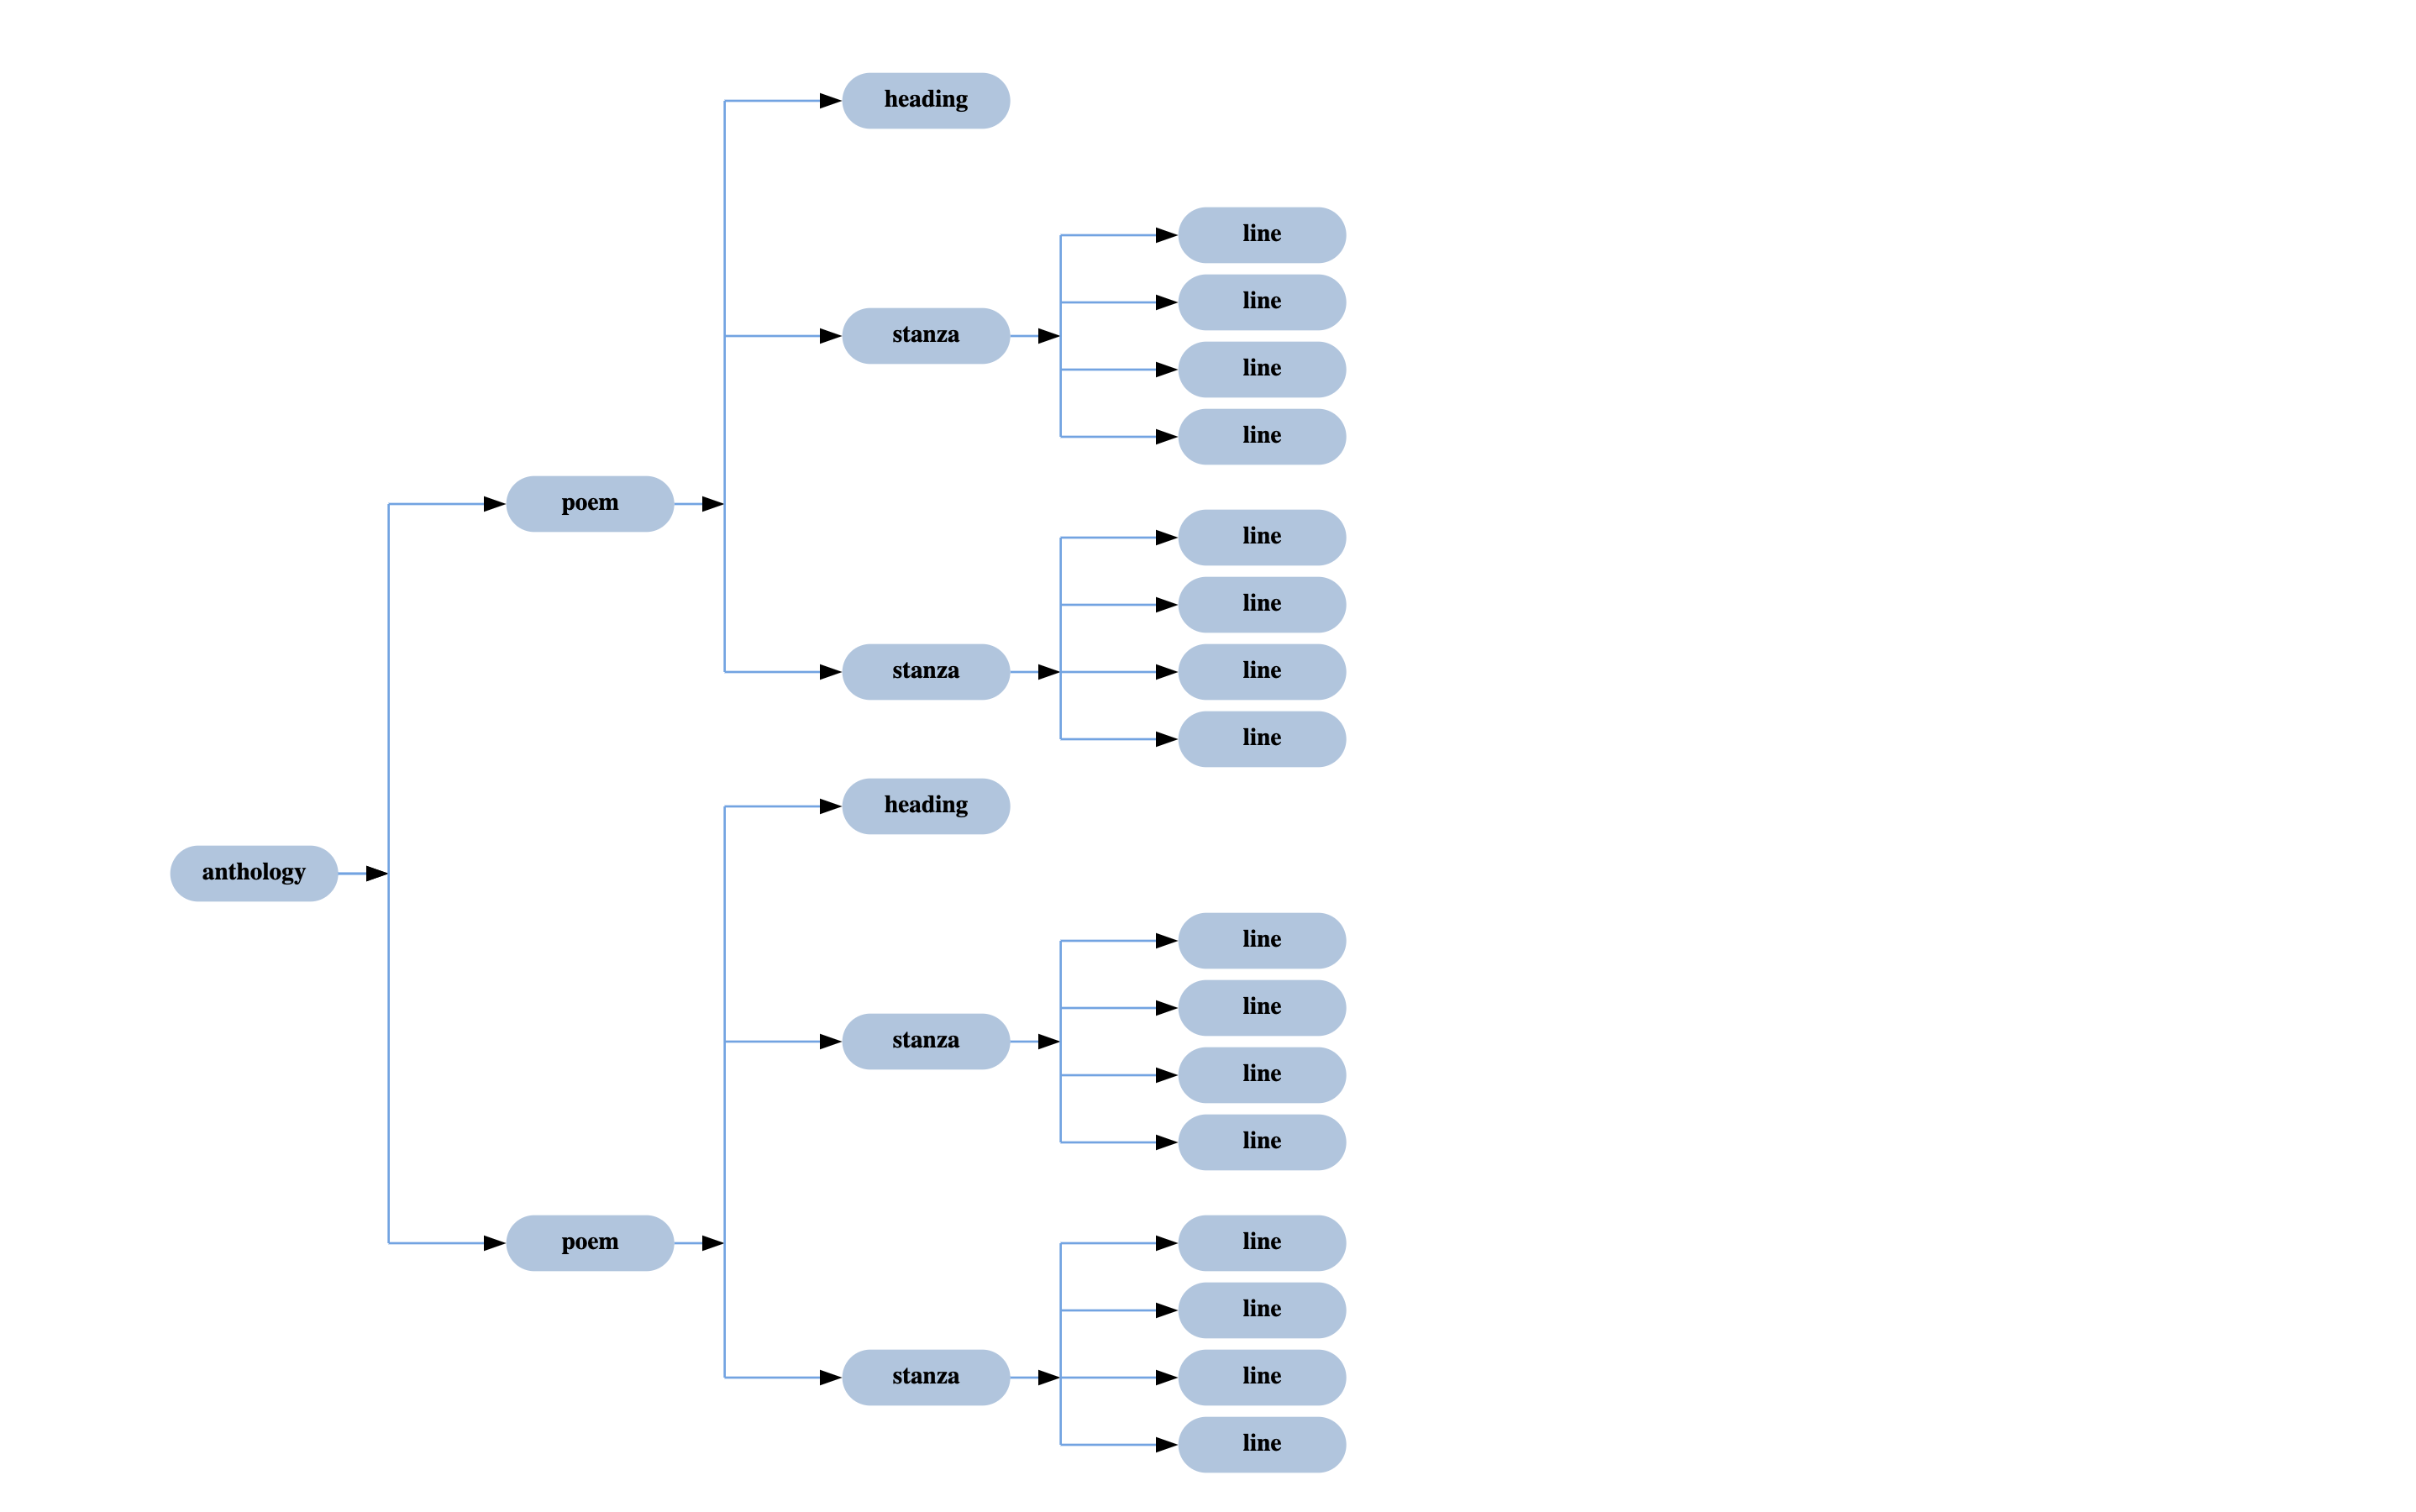
\includegraphics[width=0.8\textwidth,]{Images/xmlFlowChart.png}\end{figure}
\par
This graphic represents the hierarchical structure of an XML document, resembling a family tree. Most XML processing systems now use a standardized way of accessing parts of an XML document called \textit{XPath}.\footnote{The official specification is at \cite{XPATH}; many introductory tutorials are available in the XML references cited above and elsewhere on the Web: good beginners' tutorials include \url{http://dh.obdurodon.org/introduction-xpath.xhtml}, \url{http://www.w3schools.com/xml/xpath\textunderscore intro.asp} and \url{http://www.zvon.org/xxl/XPathTutorial/}, the latter being available in several languages.} XPath gives us a non-graphical way of referring to any part of an XML document: for example, we might refer to the last line of Blake's poem as \texttt{/anthology/poem[1]/stanza[2]/line[4]}. The square brackets here indicate a numerical selection: we are talking about the fourth line in the second stanza of the first poem in the anthology. If we left out all the square-bracketted selections, the corresponding XPath expression would refer to all lines contained by stanzas contained by poems contained by anthologies. An XPath expression can refer to any collection of elements: for example, the expression \texttt{/anthology/poem} refers to all poems in an anthology and the expression \texttt{/anthology/poem/heading} refers to all their headings.\par
The forward slash (‘/’, U+002F SOLIDUS) within an XPath expression behaves in much the same way as a forward slash or backslash does in a filename specification. To use a family tree analogy, a single slash indicates that the item to the immediate left is a parent of the item(s) to the right of it. For example, in the XPath expression \texttt{/anthology/poem}, the single slash between anthology and poem indicates that anthology is a parent of the poem children elements. (The first forward slash in the XPath expression indicates the document node.) In XPath, it is also possible to refer to children, grandchildren, and other descendants of the family tree using two forward slashes together. For example, the XPath expression \texttt{/anthology/poem//line} will refer to all of the lines of all of the stanzas of all the poems, without having to represent the stanza element in the XPath.\par
Clearly, there are many such trees that might be drawn to describe the structure of this or other anthologies. Some of them might be representable as further subdivisions of this tree: for example, we might subdivide the lines into individual words, since in our simple example no word crosses a line boundary. Surprisingly perhaps, this grossly simplified view of what text is (memorably termed an \textit{ordered hierarchy of content objects} (OHCO) view of text by Renear \textit{et al.}\footnote{See \cite{SG-BIBL-2}.}) turns out to be very effective for a large number of purposes. It is not, however, adequate for the full complexity of real textual structures, for which more complex mechanisms need to be employed. There are many other trees that might be drawn which do \textit{not} fit within the anthology model which we have presented so far. We might, for example, be interested in syntactic structures or other linguistic constructs, which rarely respect the formal boundaries of verse. Or, to take a simpler example, we might want to represent the pagination of different editions of the same text.\par
In the OHCO model of text, representation of cases where different elements overlap so that several different trees may be identified in the same document is generally problematic. All the elements marked up in a document, no matter what namespace they belong to, must fit within a single hierarchy. To represent overlapping structures, therefore, a single hierarchy must be chosen, and the points at which other hierarchies intersect with it marked. For example, we might choose the verse structure as our primary hierarchy, and then mark the pagination by means of empty elements inserted at the boundary points between one page and the next. Or we could represent alternative hierarchies by means of the pointing and linking mechanisms described in chapter \textit{\hyperref[SA]{16.\ Linking, Segmentation, and Alignment}} of these Guidelines. These mechanisms all depend on the use of \textit{attributes}, which may be used both to identify particular elements within a document and to point to, link, or align them into arbitrary structures.
\subsection[{Attributes}]{Attributes}\label{SG16}\par
In the XML context, the word \textit{attribute}, like some other words, has a specific technical sense. It is used to describe information that is in some sense descriptive of a specific element occurrence but not regarded as part of its content. For example, you might wish to add a {\itshape status} attribute to occurrences of some elements in a document to indicate their degree of reliability, or to add an {\itshape identifier} attribute so that you could refer to particular element occurrences from elsewhere within a document. Attributes are useful in precisely such circumstances.\par
Although different elements may have attributes with the same name (for example, in the TEI scheme, every element is defined as having an attribute named {\itshape n}), they are always regarded as different, and may have different values assigned to them. If an element has been defined as having attributes, the attribute values are supplied in the document instance as \textit{attribute-value pairs} inside the start-tag for the element occurrence. An end-tag cannot contain an attribute-value specification, since it would be redundant.\par
The order in which attribute-value pairs are supplied inside a tag has no significance; they must, however, be separated by at least one whitespace (blank, newline, or tab) character. The value part must always be given inside matching quotation marks, either single or double\footnote{In the unlikely event that both kinds of quotation marks are needed within the quoted string, either or both can also be presented in escaped form, using the predefined character entities \texttt{\&apos;} or \texttt{\&quot;}}.\par
For example: \par\bgroup\exampleFont \begin{shaded}\noindent\mbox{}{<\textbf{poem}\hspace*{1em}{xml:id}="{Poem1}"\hspace*{1em}{status}="{draft}">} ... {</\textbf{poem}>}\end{shaded}\egroup\par \noindent  Here attribute values are being specified for two attributes previously declared for the \texttt{<poem>} element: {\itshape xml:id} and {\itshape status}. For the instance of a \texttt{<poem>} in this example, represented here by an ellipsis, the {\itshape xml:id} attribute has the value P1 and the {\itshape status} attribute has the value draft. An XML processor can use the values of the attributes in any way it chooses; for example, a \texttt{<poem>} in which the {\itshape status} attribute has the value draft might be formatted differently from one in which the same attribute has the value revised; another processor might use the same attribute to determine whether or not poem elements are to be processed at all. The {\itshape xml:id} attribute is a slightly special case in that, by convention, it is always used to supply a unique value to identify a particular element occurrence, which may be used for cross-reference purposes, as discussed further below (\textit{\hyperref[SG-id]{v.6.2\ Identifiers and Indicators}}).
\subsubsection[{Declaring Attributes}]{Declaring Attributes}\label{SG-att}\par
Attributes are declared in a schema in the same way as elements. As well as specifying an attribute's name and the element to which it is to be attached, it is possible to specify (within limits) what kind of value is acceptable for an attribute.\par
In the compact syntax of RELAX NG, an attribute is defined by means of an attribute pattern, like the following: \par\hfill\bgroup\exampleFont\vskip 10pt\begin{shaded}
\obeyspaces att.status = attribute status ❴"draft" | "revised" | "published"❵\end{shaded}
\par\egroup 
 This defines a new pattern, called \texttt{att.status}, whose value is an attribute pattern defining an attribute named {\itshape status}. Attribute names are subject to the same restrictions as other names in XML; they need not be unique across the whole schema, however, but only within the list of attributes for a given element.\par
A pattern defining the possible values for this attribute is given within the curly braces, in just the same way as a content model is given for an element pattern. In this case, the attribute's value must be one of the strings presented explicitly above. \par
The attribute pattern definition must be included or referenced within the definition for every element to which the attribute is attached. We therefore modify the definition for the \texttt{poem\textunderscore p} pattern given above as follows: \par\hfill\bgroup\exampleFont\vskip 10pt\begin{shaded}
\obeyspaces poem\textunderscore p = element poem ❴ att.status?, heading\textunderscore p?, stanza\textunderscore p+ ❵\end{shaded}
\par\egroup 
 In RELAX NG, an element pattern simply includes any attribute patterns applicable to it along with its other constituents, as shown above. Attribute patterns can also be grouped and alternated in the same way as element patterns, though this particular feature is not widely used in the TEI scheme, since it is not available to the same extent in all schema languages. Because a question mark follows the reference to the \texttt{att.status} pattern in our example, a document in which the {\itshape status} attribute is not specified will still be valid; without this occurrence indicator the {\itshape status} attribute would be required.\par
Instead of supplying a list of explicit values, an attribute pattern can specify that the attribute must have a value of a particular type, for example a text string, a numeric value, a normalized date, etc. This is accomplished by supplying a pattern that refers to a \textit{datatype}. In the example above, because a list of acceptable values is predefined, a parser can check that no \texttt{<poem>} is defined for which the {\itshape status} attribute does not have one of draft, revised, or published as its value. By contrast, with a definition such as \par\hfill\bgroup\exampleFont\vskip 10pt\begin{shaded}
\obeyspaces att.status =\newline
attribute status ❴text❵\end{shaded}
\par\egroup 
 a parser would accept almost any unbroken string of characters (\texttt{status="awful"}, \texttt{status="awe-ful"}, or \texttt{status="12345678"}) as valid for this attribute. Sometimes, of course, the set of possible values cannot be predefined. Where it can, as in this case, it is generally better to do so.\par
Schema languages vary widely in the extent to which they support validation of attribute values. Some languages predefine a small set of possibilities. Others allow the schema designer to use values from a predefined ‘library’ of possible datatypes, or to add their own definitions, possibly of great complexity. A ‘datatype’ might be something fairly general (any positive integer), something very specific or idiosyncratic (any four-character string ending with "T"), or somewhere between the two. In the RELAX NG schemas used by the TEI, general patterns have been defined for about half a dozen datatypes (using the W3C Schema \hyperref[XSD2]{Datatype Library}, and discussed further in \textit{\hyperref[DTYPES]{1.4.2.\ Datatype Specifications}}). In addition to the two possibilities already mentioned—plain text or an explicit list of possible strings—other datatypes likely to be encountered include the following: \begin{description}

\item[{boolean}]values must be either true or false
\item[{numeric}]values must represent a numeric quantity of some kind
\item[{date}]values must represent a possible date and time in some calendar
\end{description} \par
Two further datatypes of particular usefulness in managing XML documents are commonly known as \texttt{ID}—for identifier—and \texttt{URI}—for Universal Resource Indicator, or pointer for short. These are discussed in the next section.
\subsubsection[{Identifiers and Indicators}]{Identifiers and Indicators}\label{SG-id}\par
It is often necessary to refer to an occurrence of one textual element from within another, an obvious example being phrases such as ‘see note 6’ or ‘as discussed in chapter 5’. When a text is being produced the actual numbers associated with the notes or chapters may not be certain. If we are using descriptive markup, such things as page or chapter numbers, being entirely matters of presentation, will not in any case be present in the marked-up text: they will be assigned by whatever processor is operating on the text (and may indeed differ in different applications). XML therefore predefines an attribute that may be used to provide any element occurrence with a special identifier, a kind of label, which may be used to refer to it from anywhere else: since it is defined in the XML namespace, the name of this attribute is {\itshape xml:id} and it is used throughout the TEI schema. Because it is intended to act as an identifier, its values must be unique within a given document. The cross-reference itself will be supplied by an element bearing an attribute of a specific kind, which must also be declared in the schema.\par
Suppose, for example, we wish to include a reference within the notes on one poem that refers to another poem. We will first need to provide some way of attaching a label to each poem: this is easily done using the {\itshape xml:id} attribute. Note that not every poem need carry an {\itshape xml:id} attribute and the parser may safely ignore the lack of one in those that do not. Only poems to which we intend to refer need use this attribute; for each such poem we should now include in its start-tag some unique identifier, for example: \par\bgroup\exampleFont \begin{shaded}\noindent\mbox{}{<\textbf{poem}\hspace*{1em}{xml:id}="{Rose}">} ... {</\textbf{poem}>}\mbox{}\newline 
{<\textbf{poem}\hspace*{1em}{xml:id}="{P40}">} ... {</\textbf{poem}>}\mbox{}\newline 
{<\textbf{poem}>} ... {</\textbf{poem}>}\end{shaded}\egroup\par \par
Next we need to define a new element for the cross-reference itself. This will not have any content—it is only a pointer—but it has an attribute, the value of which will be the identifier of the element pointed at. This is achieved by the following definition: \par\hfill\bgroup\exampleFont\vskip 10pt\begin{shaded}
\obeyspaces poemRef\textunderscore p = element poemRef ❴attribute target ❴anyURI❵, empty❵\end{shaded}
\par\egroup 
\par
The \texttt{<poemRef>} element has no content, but a single attribute called {\itshape target}. The value of this attribute must be a pointer or web reference of type \texttt{anyURI};\footnote{The word ‘anyURI’ is a predefined name, used in schema languages to mean that any \textit{Uniform Resource Identifier} (URI) may be supplied here. The accepted syntax for URIs is an Internet Standard, defined in \url{http://tools.ietf.org/html/rfc3986}. \texttt{anyURI} is one of the \textit{datatypes} defined by the W3C Schema datatype library.} furthermore, because there is no indication of optionality on the attribute pattern, it must be supplied on each occurrence—a \texttt{<poemRef>} with no referent is an impossibility.\par
With these declarations in force, we can now encode a reference to the poem whose {\itshape xml:id} attribute specifies that its identifier is Rose as follows: \par\bgroup\exampleFont \begin{shaded}\noindent\mbox{}Blake's poem on the sick rose\mbox{}\newline 
{<\textbf{poemRef}\hspace*{1em}{target}="{\#Rose}"/>} ...\end{shaded}\egroup\par \noindent  \par
A processor may take any number of actions when it encounters a link encoded in this way: a formatter might construct an exact page and line reference for the location of the poem in the current document and insert it, or just quote the poem's title or first lines. A hypertext style processor might use this element as a signal to activate a link to the poem being referred to, for example by displaying it in a new window. Note, however, that the purpose of the XML markup is simply to indicate that a cross-reference exists: it does not necessarily determine what the processor is to do with it.\par
The target of a URI can be located anywhere: it may not necessarily be part of the same document, nor even located on the same computer system. Equally, it can be a resource of any kind, not necessarily an XML document or document fragment. It is thus a very convenient way of including references to non-XML data such as image files within a document. If, for example, we wished to include an illustration containing a reproduction of Blake's original in our anthology, the most appropriate method would probably be to define a new element called (for the sake of argument) \texttt{<graphic>} with a {\itshape target} attribute of datatype URI: \par\hfill\bgroup\exampleFont\vskip 10pt\begin{shaded}
\obeyspaces graphic\textunderscore p = element graphic ❴att.url, empty❵ att.url =\newline
attribute url ❴anyURI❵\end{shaded}
\par\egroup 
 With these additions to the schema, we can now represent the location of the illustration within our text like this: \par\bgroup\exampleFont \begin{shaded}\noindent\mbox{}{<\textbf{poem}>}\mbox{}\newline 
\hspace*{1em}{<\textbf{graphic}\hspace*{1em}{url}="{http://en.wikisource.org/wiki/Image:Blake\textunderscore sick\textunderscore rose.jpg}"/>}\mbox{}\newline 
{</\textbf{poem}>}\end{shaded}\egroup\par \noindent  By providing a location from which a reproduction of the required image can be downloaded, this encoding makes it possible for appropriate software able to display the image as well as record its existence.\par
Attributes form part of the structure of an XML document in the same way as elements, and can therefore be accessed using XPath. For example, to refer to all the poems in our anthology whose {\itshape status} attribute has the value draft, we might use an XPath such as \texttt{/anthology/poem[@status='draft']}. To find the headings of all such poems, we would use the XPath \texttt{/anthology/poem[@status='draft']/heading}.
\subsection[{Other Components of an XML Document}]{Other Components of an XML Document}\label{SG-oth}\par
In addition to the elements and attributes so far discussed, an XML document can contain a few other formally distinct things. An XML document may contain references to predefined strings of data that a validator must resolve before attempting to validate the document's structure; these are called \textit{entity references}. They may be useful as a means of providing ‘boilerplate’ text or representing character data which cannot easily be keyboarded. As noted earlier, an XML document may also contain instances of elements taken from some other \textit{namespace}. And an XML document may also contain arbitrary signals or flags for use when the document is processed in a particular way by some class of processor (a common example in document production is the need to force a formatter to start a new page at some specific point in a document); such flags are called \textit{processing instructions}. We discuss each of these three cases in the rest of this section.\par
A construct which looks like a processing instruction (but is not) is the \textit{XML declaration} which should be supplied at the beginning of every XML document, for example: \par\hfill\bgroup\exampleFont\vskip 10pt\begin{shaded}
\obeyspaces <?xml version="1.0" encoding="UTF-8"?>\end{shaded}
\par\egroup 
 The XML declaration specifies the version number of the XML Recommendation applicable to the document it introduces (in this case, version 1.0), and optionally also the character encoding used to represent the Unicode characters within it. By default an XML document uses the character encoding UTF-8 or UTF-16; other commonly-encountered encodings include ISO 8859-1. If any character present in the document is not available in the specified character encoding, it must be represented as a character reference (\textit{\hyperref[SG-er]{v.7.1\ Character References}}). The XML declaration is documentary, but should normally be supplied at the start of any XML file. If it is missing many XML-aware processors will be unable to process the associated text correctly.
\subsubsection[{Character References}]{Character References}\label{SG-er}\par
As mentioned above, all XML documents use the same internal character encoding. Since not all computer systems currently support this encoding directly, a special syntax is defined that can be used to represent individual characters from the Unicode character set in a portable way by providing their numeric value, in decimal or hexadecimal notation.\par
For example, the character \textit{é} is represented within an XML document as the Unicode character with hexadecimal value 00E9. If such a document is being prepared on (or exported to) a system using a different character set in which this character is not available, it may instead be represented by the character reference \texttt{\&\#x00E9;} (the \texttt{x} indicating that what follows is a hexadecimal value) or \texttt{\&\#0233;} (its decimal equivalent). References of this type do not need to be predefined, since the underlying character encoding for XML is always the same.\par
To aid legibility, however, it is also possible to use a mnemonic name (such as \texttt{eacute}) for such character references, provided that each such name is mapped to the required Unicode value by means of a construct known as an \textit{entity declaration}. A reference to a named character entity always takes the form of an ampersand, followed by the name, followed by a semicolon. For example an XML document containing the string ‘T\&C’ might be encoded as \texttt{T\&amp;C}.\par
There is a small set of such character entity references that do not have to be declared because they form part of the definition of XML. These include the names used for characters such as the ampersand (\texttt{amp}) and the open angle bracket or less-than sign (\texttt{lt}), which could not easily otherwise be included in an XML document without ambiguity. Other predeclared entity names are those for quotation marks (\texttt{quot} and \texttt{apos} for double and single respectively), and for completeness the closing angle bracket or greater-than sign (\texttt{gt}).\par
For all other named character entities, a set of entity declarations must be provided to an XML processor before the document referring to them can be validated. The declaration itself uses a non-XML syntax inherited from SGML; for example, to define an entity named \textsf{eacute} with the replacement value é, the declaration could have any of the following forms: \par\hfill\bgroup\exampleFont\vskip 10pt\begin{shaded}
\obeyspaces <!ENTITY eacute "é">\end{shaded}
\par\egroup 
 or, using hexadecimal notation: \par\hfill\bgroup\exampleFont\vskip 10pt\begin{shaded}
\obeyspaces <!ENTITY eacute "\&\#xe9;">\end{shaded}
\par\egroup 
 or, using decimal notation: \par\hfill\bgroup\exampleFont\vskip 10pt\begin{shaded}
\obeyspaces <!ENTITY eacute "\&\#233;">\end{shaded}
\par\egroup 
\par
Entities of this kind are useful also for \textit{string substitution} purposes, where the same text needs to be repeated uniformly throughout a text. For example, if a declaration such as \par\hfill\bgroup\exampleFont\vskip 10pt\begin{shaded}
\obeyspaces <!ENTITY TEI "Text Encoding Initiative">\end{shaded}
\par\egroup 
 is included with a document, then references such as \texttt{\&TEI;} may be used within it, each of which will be expanded in the same way and replaced by the string ‘Text Encoding Initiative’ before the text is validated.
\subsubsection[{Namespaces}]{Namespaces}\label{SGname}\par
A valid XML document necessarily specifies the schema in which its constituent elements are defined. However, a well-formed XML document is not required to specify its schema (indeed, it may not even have a schema). It would still be useful to indicate that the element names used in it have some defined provenance. Furthermore, it might be desirable to include in a document elements that are defined (possibly differently) in different schemas. A cabinet-maker's schema might well define an element called \texttt{<table>} with very different characteristics from those of a documentalist's.\par
The concept of \textit{namespace} was introduced into the XML language as a means of addressing these and related problems. If the markup of an XML document is thought of as an expression in some language, then a namespace may be thought of as analogous to the lexicon of that language. Just as a document can contain words taken from different languages, so a well-formed XML document can include elements taken from different namespaces. A namespace resembles a schema in that we may say that a given set of elements ‘belongs to’ a given namespace, or are ‘defined by’ a given schema. However, a schema is a set of element definitions, whereas a namespace is really only a property of a collection of elements: the only tangible form it takes in an XML document is its distinctive \textit{prefix} and the identifying \textit{name} associated with it.\par
Suppose for example that we wish to extend our anthology to include a complex diagram. We might start by considering whether or not to extend our simple schema to include XML markup for such features as arcs, polygons, and other graphical elements. XML can be used to represent any kind of structure, not simply text, and there are clear advantages to having our text and our diagrams all expressed in the same way.\par
Fortunately we do not need to invent a schema for the representation of graphical components such as diagrams; it already exists in the shape of the Scalable Vector Graphics (SVG) language defined by the W3C.\footnote{The W3C Recommendation is defined at \url{http://www.w3.org/Graphics/SVG/}.} SVG is a widely used and rich XML vocabulary for representing all kinds of two-dimensional graphics; it is also well supported by existing software. Using an SVG-aware drawing package, we can easily draw our diagram and save it in XML format for inclusion within our anthology. When we do so, we need to indicate that this part of the document contains elements taken from the SVG namespace, if only to ensure that processing software does not confuse our \texttt{<line>} element with the SVG \texttt{<line>}, which means something quite different.\par
An XML document need not specify any namespace: it is then said to use the ‘null’ namespace. Alternatively, the root element of a document may supply a default namespace, understood to apply to all elements which have no namespace prefix. This is the function of the {\itshape xmlns} attribute which provides a unique name for the default namespace, in the form of a URI: \par\bgroup\exampleFont \begin{shaded}\noindent\mbox{}{<\textbf{anthology}>}\mbox{}\newline 
\textit{<!-- anthology markup elements here -->}\mbox{}\newline 
{</\textbf{anthology}>}\end{shaded}\egroup\par \noindent  In exactly the same way, on the root element for each part of our document which uses the SVG language, we might introduce the SVG namespace name: \par\bgroup\exampleFont \begin{shaded}\noindent\mbox{}{<\textbf{anthology}>}\mbox{}\newline 
\hspace*{1em}\mbox{}\newline 
\textit{<!-- anthology markup elements here -->}\mbox{}\newline 
\hspace*{1em}{<\textbf{svg} xmlns="http://www.w3.org/2000/svg">}\mbox{}\newline 
\textit{<!-- SVG markup elements here -->}\mbox{}\newline 
\hspace*{1em}{</\textbf{svg}>}\mbox{}\newline 
\textit{<!-- more anthology markup elements here -->}\mbox{}\newline 
{</\textbf{anthology}>}\end{shaded}\egroup\par \noindent  Although a namespace name usually uses the URI (Uniform Resource Identifier) syntax, it is not treated as an online address and an XML processor regards it just as a string, providing a longer name for the namespace.\par
The {\itshape xmlns} attribute can also be used to associate a short prefix name with the namespace it defines. This is very useful if we want to mingle elements from different namespaces within the same document, since the prefix can be attached to any element, overriding the implicit namespace for itself (but not its children): \par\bgroup\exampleFont \begin{shaded}\noindent\mbox{}{<\textbf{anthology}\mbox{}\newline 
   xmlns:svg="http://www.w3.org/2000/svg">}\mbox{}\newline 
\hspace*{1em}\mbox{}\newline 
\textit{<!-- anthology markup elements here -->}\mbox{}\newline 
\hspace*{1em}{<\textbf{svg:svg}>}\mbox{}\newline 
\textit{<!-- SVG markup elements here -->}\mbox{}\newline 
\hspace*{1em}{</\textbf{svg:svg}>}\mbox{}\newline 
\textit{<!-- more anthology markup elements here -->}\mbox{}\newline 
{</\textbf{anthology}>}\end{shaded}\egroup\par \par
There is no limit on the number of namespaces that a document can use. Provided that each is uniquely identified, an XML processor can identify those that are relevant, and validate them appropriately. To extend our example further, we might decide to add a linguistic analysis to each of the poems, using a set of elements such as \texttt{<aux>}, \texttt{<adj>}, etc., derived from some pre-existing XML vocabulary for linguistic analysis. \par\bgroup\exampleFont \begin{shaded}\noindent\mbox{}{<\textbf{anthology}\mbox{}\newline 
   xmlns:gram="http://www.gram.org"\mbox{}\newline 
   xmlns:svg="http://www.w3.org/2000/svg">}\mbox{}\newline 
\hspace*{1em}\mbox{}\newline 
\textit{<!-- anthology markup elements here -->}\mbox{}\newline 
\hspace*{1em}{<\textbf{svg:svg}>}\mbox{}\newline 
\textit{<!-- SVG markup elements here -->}\mbox{}\newline 
\hspace*{1em}{</\textbf{svg:svg}>}\mbox{}\newline 
\hspace*{1em}{<\textbf{line}>}\mbox{}\newline 
\hspace*{1em}\hspace*{1em}{<\textbf{gram:itj}>}O{</\textbf{gram:itj}>}\mbox{}\newline 
\hspace*{1em}\hspace*{1em}{<\textbf{gram:nom}>}Rose{</\textbf{gram:nom}>}\mbox{}\newline 
\hspace*{1em}\hspace*{1em}{<\textbf{gram:pron}>}thou{</\textbf{gram:pron}>}\mbox{}\newline 
\hspace*{1em}\hspace*{1em}{<\textbf{gram:aux}>}art{</\textbf{gram:aux}>}\mbox{}\newline 
\hspace*{1em}\hspace*{1em}{<\textbf{gram:adj}>}sick{</\textbf{gram:adj}>}\mbox{}\newline 
\hspace*{1em}{</\textbf{line}>}\mbox{}\newline 
{</\textbf{anthology}>}\end{shaded}\egroup\par 
\paragraph[{Marked Sections}]{Marked Sections}\label{SG-ms}\par
We mentioned above that the syntax of XML requires the encoder to take special action if characters with a syntactic meaning in XML (such as the left angle bracket or ampersand) are to be used in a document to stand for themselves, rather than to signal the start of a tag or an entity reference respectively. The predefined entities \texttt{\&amp;}, \texttt{\&lt;}, and \texttt{\&gt;} provide one method of dealing with this problem, if the number of occurrences of such things is small. Other methods may be considered when the number is large, as in an XML document like the present Guidelines, which contains hundreds of examples of XML markup. One is to label the XML examples as belonging to a different namespace from that of the document itself, which is the approach taken in the present Guidelines. Another and simpler approach is provided by one of the features inherited by XML from its parent SGML: the ‘marked section’.\par
A marked section is a block of text within an XML document introduced by the characters \texttt{<![CDATA[} and terminated by the characters \texttt{]]>}. Between these rather strange brackets, markup recognition is turned off, and any tags or entity references encountered are therefore treated as if they were plain text. For example, when we come to write the users' manual for our anthology, we may find ourselves often producing text like the following: \par\hfill\bgroup\exampleFont\vskip 10pt\begin{shaded}
\obeyspaces Here is an example of the use of the <gi>line</gi> element:\newline
<![CDATA[<line>[...]</line>]]>\end{shaded}
\par\egroup 

\subsubsection[{Processing Instructions}]{Processing Instructions}\label{SG-pi}\par
Although one of the aims of using XML is to remove any information specific to the processing of a document from the document itself, it is occasionally very convenient to be able to include such information—if only so that it can be clearly distinguished from the structure of the document. As suggested above, one common example is the need, when processing an XML document for printed output, to include a suggestion that the formatting processor might use to determine where to begin a new page of output. Page-breaking decisions are usually best made by the formatting engine alone, but there will always be occasions when it may be necessary to override these. An XML processing instruction inserted into the document is one very simple and effective way of doing this without interfering with other aspects of the markup.\par
Here is an example XML processing instruction: \par\hfill\bgroup\exampleFont\vskip 10pt\begin{shaded}
\obeyspaces <?tex ⃥newpage ?>\end{shaded}
\par\egroup 
 It begins with \texttt{<?} and ends with \texttt{?>}. In between are two space-separated strings: by convention, the first is the name of some processor (\texttt{tex} in the above example) and the second is some data intended for the use of that processor (in this case, the instruction to start a new page). The only constraint placed by XML on the strings is that the first one must be a valid XML name; the other can be any arbitrary sequence of characters, not including the closing character-sequence \texttt{?>}.
\subsection[{Putting It All Together}]{Putting It All Together}\label{SG18}\par
In this chapter we have discussed most of the components of an XML document and its associated schema. We have described informally how an XML document is represented, and also introduced one way of representing the rules a RELAX NG validator might use to validate it. In a working system, the following issues will also need to be addressed: \begin{itemize}
\item how does a processor determine the schema (or schemas) that should be used to validate a given XML document instance?
\item if a document contains entity references that must be processed before the document can be validated, where are those entities defined?
\item an XML document instance may be stored in a number of different operating system files; how should they be assembled together?
\item how does a processor determine which stylesheets it should use when processing an XML document, or how to interpret any processing instructions it contains?
\item how does a processor enforce more exact validation than simple datatypes permit (for example of element content)?
\end{itemize} \par
Different schema languages and different XML processing systems take very different positions on all of these topics, since none of them is explicitly addressed in the XML specification itself. Consequently, the best answer is likely to be specific to a particular software environment and schema language. Since this chapter is concerned with XML considered independently of its processing environment, we only address them in summary detail here.
\subsubsection[{Associating Entity Definitions with a Document Instance}]{Associating Entity Definitions with a Document Instance}\label{SG-ass1}\par
In \textit{\hyperref[SG-er]{v.7.1\ Character References}} we introduced the syntax used for the definition of named character entities such as \texttt{eacute}, which XML inherited from SGML. Different schema languages vary in the ways they make a collection of such definitions available to an XML processor, but fortunately there is one method that all current schema languages support.\par
As well as, and following, the XML declaration (\textit{\hyperref[SG-pi]{v.7.3\ Processing Instructions}}), an XML document instance may be prefixed with a special \texttt{DOCTYPE} statement. This declarative statement has been inherited by XML from SGML; in its full form it provides a large number of facilities, but we are here concerned only with the small subset of those facilities recognized by all schema languages.\par
Here is an example DOCTYPE statement which we might consider prefixing to the final version of our anthology: \par\hfill\bgroup\exampleFont\vskip 10pt\begin{shaded}
\obeyspaces <!DOCTYPE anthology [\newline
<!ENTITY mdash "\&\#2014;">\newline
<!ENTITY legalese "This document is available under a Creative Commons\newline
Share and Enjoy Licence">\newline
]>\end{shaded}
\par\egroup 
 Any XML processor encountering this statement will use it to add the two named entities it defines to those already predefined for XML. Before the document instance itself is validated, any references to these entities will be expanded to the character string given. Thus, wherever in the document instance the string \texttt{\&legalese;} appears, it will be replaced by the formulation above. This makes life a little easier for those keyboarding our anthology.\footnote{And, indeed, for those responsible for deciding the licensing conditions if they change their minds later.} The word \texttt{anthology} following the string DOCTYPE in this example is, of course, the name of the root element of the document to which this declaration is prefixed; however, only an XML DTD processor will take note of this fact.
\subsubsection[{Associating a Document Instance with Its Schema}]{Associating a Document Instance with Its Schema}\label{SG-assoc}\par
In the past, different schema languages adopted entirely different attitudes to this question, leading to a variety of different methods of associating schemas with document instances. However, a W3C Working Group Note, \textit{Associating Schemas with XML documents}, (\url{http://www.w3.org/TR/xml-model/}) now provides a standardized method of doing this through the use of a processing instruction: \par\hfill\bgroup\exampleFont\vskip 10pt\begin{shaded}
\obeyspaces <?xml-model href="http://www.tei-c.org/release/xml/tei/custom/schema/relaxng/tei\textunderscore all.rng"?>\end{shaded}
\par\egroup 
 The {\itshape href} \textit{pseudo-attribute} points to the location of the schema. This is the only mandatory pseudo-attribute, but others can be added to give more information about the schema: \par\hfill\bgroup\exampleFont\vskip 10pt\begin{shaded}
\obeyspaces <?xml-model href="burgess.rng" \newline
                       title="Anthony Burgess Project Schema" \newline
                       schematypens="http://relaxng.org/ns/structure/1.0" \newline
                       type="application/xml"\newline
                     ?>\end{shaded}
\par\egroup 
 See the XML Model WG Note for more information on the pseudo-attributes available and how to use them.\par
A document instance may be valid according to many different schemas, each appropriate to a different processing task. All of these may be expressed in the same way: \par\hfill\bgroup\exampleFont\vskip 10pt\begin{shaded}
\obeyspaces <?xml-model href="tei\textunderscore tite.xsd" type="application/xml" ?>\newline
<?xml-model href="checkNames.sch" type="application/xml" schematypens="http://purl.oclc.org/dsdl/schematron" ?>\end{shaded}
\par\egroup 
 This example includes a standard schema in XML Schema format, along with a Schematron schema which might be used for checking the format and linking of names.\par
Any modern XML processing software tool will provide convenient methods of validating documents which are appropriate to the particular schema language chosen. In the interests of maximizing portability of document instances, they should contain as little processing-specific information as possible.
\subsubsection[{Assembling Multiple Resources into a Single Document}]{Assembling Multiple Resources into a Single Document}\label{SG-mult}\par
As we have already indicated, a single XML document may be made up of several different operating system files that need to be pulled together by a processor before the whole document can be validated. The XML DTD language defines a special kind of entity (a \textit{system entity}) that can be used to embed references to whole files into a document for this purpose, in much the same way as the character or string entities discussed in \textit{\hyperref[SG-er]{v.7.1\ Character References}}. Neither RELAX NG nor W3C Schema directly supports this mechanism, however, and we do not discuss it further here.\par
An alternative way of achieving the same effect is to use a special kind of pointer element to refer to the resources that need to be assembled, in exactly the same way as we proposed for the illustration in our anthology. The W3C Recommendation \textit{XML Inclusions } (XInclude)\footnote{\url{http://www.w3.org/TR/xinclude/}.} defines a generic mechanism for this purpose, which is supported by an increasing number of XML processors.
\subsubsection[{Stylesheet Association and Processing}]{Stylesheet Association and Processing}\label{SG-style}\par
As mentioned above, the processing of an XML document will usually involve the use of one or more stylesheets, often but not exclusively to provide specific details of how the document should be displayed or rendered. In general, there is no reason to associate a document instance with any specific stylesheet and the schema languages we have discussed so far do not therefore make any special provision for such association. The association is made when the stylesheet processor is invoked, and is thus entirely application-specific.\par
However, since one very common application for XML documents is to serve them as browsable documents over the Web, the W3C has defined a procedure and a syntax for associating a document instance with its stylesheet (see \url{http://www.w3.org/TR/xml-stylesheet/}). This Recommendation allows a document to supply a link to a default stylesheet and also to categorize the stylesheet according to its \textit{MIME type}, for example to indicate whether the stylesheet is written in CSS or XSLT, using a specialized form of processing instruction.\par
Assuming therefore that we have made a CSS-conformant stylesheet for our anthology and stored it in a file called \texttt{anthology.css} which is available from the same location as the anthology itself, we could make it available over the Web simply by adding a processing instruction like the following to the anthology: \par\hfill\bgroup\exampleFont\vskip 10pt\begin{shaded}
\obeyspaces <?xml-stylesheet href="anthology.css" type="text/css"?>\end{shaded}
\par\egroup 
\par
Multiple stylesheets can be defined for the same document, and options are available to specify how a web browser should select amongst them. For example, if the document also contained a directive: \par\hfill\bgroup\exampleFont\vskip 10pt\begin{shaded}
\obeyspaces <?xml-stylesheet href="anthology\textunderscore m.css" type="text/css" media="mobile"?>\end{shaded}
\par\egroup 
a different stylesheet called \texttt{anthology\textunderscore m.css} could be used when rendering the document on a handheld device such as a mobile phone.\par
Most modern web browsers support CSS (although the extent of their implementation varies), and some of them support XSLT.
\paragraph[{Content Validation}]{Content Validation}\label{SG-val}\par
As we noted above, most schema languages provide some degree of datatype validation for attribute values (\textit{\hyperref[SG-att]{v.6.1\ Declaring Attributes}}). They vary greatly in the validation facilities they offer for the content of elements, other than the syntactic constraints already discussed. Thus, while we may very easily check that our \texttt{<stanza>} elements contain only \texttt{<line>} elements, we cannot easily check that \texttt{<line>} elements contain between five and 500 correctly-spelled English words, should we wish to constrain our poetry in such a way. Also, because attributes and elements are treated differently, it is difficult or impossible to express co-occurrence constraints: for example, if the {\itshape status} of a poem is draft we might wish to permit elements such as \texttt{<editorialQuery>} within its content, but not otherwise.\par
The XML DTD language offers very little beyond syntactic checking of element content. By contrast, a major impetus behind the design and development of the W3C schema language was the addition of a much more general and powerful constraint language to the existing structural constraints of XML DTDs. In RELAX NG the opposite approach was taken, in that all datatype validation, whether of attributes or element content, is regarded as external to the schema language. For attributes, as we have seen, RELAX NG makes use of the W3C Schema Datatype Library (but permits use of others). Because RELAX NG treats both elements and attributes as special cases of patterns, the same datatype validation facilities are available for element content as for attribute values; it is unlike other schema languages in this respect. In addition, for content validation, a different component of DSDL known as Schematron can be used. Schematron is a pattern matching (rather than a grammar-based) language, which allows us to test the components of a document against templates that express constraints such as those mentioned above.\par
Like other XML processors, Schematron uses XPath to identify parts of an XML document; in addition, it provides elements that describe assertions to be tested and conditions which must be validated, as well as elements to report the results of the test. 

\section[{Languages and Character Sets}]{Languages and Character Sets}\label{CH}\par
The documents which users of these Guidelines may wish to encode encompass all kinds of material, potentially expressed in the full range of written and spoken human languages, including the extinct, the non-existent, and the conjectural. Because of this wide scope, special attention has been paid to two particular aspects of the representation of linguistic information often taken for granted: language identification and character encoding.\par
Even within a single document, material in many different languages may be encountered. Human culture, and the texts which embody it, is intrinsically multilingual, and shows no sign of ceasing to be so. Traditional philologists and modern computational linguists alike work in a polyglot world, in which code-switching (in the linguistic sense) and accurate representation of differing language systems constitute the norm, not the exception. The current increased interest in studies of linguistic diversity, most notably in the recording and documentation of endangered languages, is one aspect of this long standing tradition. Because of their historical importance, the needs of endangered and even extinct languages must be taken into account when formulating Guidelines and recommendations such as these. \par
Beyond the sheer number and diversity of human languages, it should be remembered that in their written forms they may deploy a huge variety of scripts or writing systems. These scripts are in turn composed of smaller units, which for simplicity we term here characters. A primary goal when encoding a text should be to capture enough information for subsequent users to correctly identify not only the constituent characters, but also the language and script. In this chapter we address this requirement, and propose recommended mechanisms to indicate the languages, scripts and characters used in a document or a part thereof. \par
Identification of language is dealt with in \textit{\hyperref[CHSH]{vi.1\ Language Identification}}. In summary, it recommends the use of pre-defined identifiers for a language where these are available, as they increasingly are, in part as a result of the twin pressures of an increasing demand for language-specific software and an increased interest in language documentation. Where such identifiers are not available or not standardized, these Guidelines recommend a method for documenting language identifiers and their significance, in the same way as other metadata is documented in the TEI header.\par
Standardization of the means available to represent characters and scripts has moved on considerably since the publication of the first version of these Guidelines. At that time, it was essential to explicitly document the characters and encoded character sets used by almost any digital resource if it was to have any chance of being usable across different computer platforms or environments, but this is no longer the case. With the availability of the Unicode standard, more than 128,000 different characters representing almost all of the world's current writing systems are available and usable in any XML processing environment without formality. Nevertheless, however large the number of standardized characters, there will always be a need to encode documents which use non-standard characters and glyphs, particularly but not exclusively in historical material. The second part of this chapter discusses in some detail the concepts and practice underlying this standard, and also introduces the methods available for extending beyond it, which are more fully discussed in \textit{\hyperref[WD]{5.\ Characters, Glyphs, and Writing Modes}}.
\subsection[{Language Identification}]{Language Identification}\label{CHSH}\par
Identification of the language a document or part thereof is written in is a crucial requirement for many envisioned usages of an electronic document. The TEI therefore accommodates this need in the following way:\begin{itemize}
\item A global attribute {\itshape xml:lang} is defined for all TEI elements. Its value identifies the language and writing system used.
\item The TEI header has a section set aside for the information about the languages used in a document: see further \textit{\hyperref[HD41]{2.4.2.\ Language Usage}}.
\end{itemize} \par
The value of the attribute {\itshape xml:lang} identifies the language (and, optionally, script) using a coded value. For maximal compatibility with existing processes, the identifier for the language must be constructed as in \textit{Best Current Practice 47}\footnote{Currently BCP 47 comprises two Internet Engineering Task Force documents, referred to separately as RFC 5646 and RFC 4647; over time, other IETF documents may succeed these as the best current practice.}. This \textit{same} identifier has to be used to identify the corresponding \hyperref[TEI.language]{<language>} element in the TEI header, if one is present.\par
The first part of BCP 47 is called \hyperref[CH-BIBL-4]{\textit{Tags for Identifying Languages}}, and proposes the following mechanism for constructing an identifier (tag) for languages as administered by the Internet Assigned Numbers Authority (IANA). The tag is assembled from a sequence of subtags separated by the hyphen (-, U+002D) character. It gives the language (possibly further identified with a sublanguage), a script, and a region for the language, each possibly followed by a variant subtag.\par
The authoritative list of registered subtags is maintained by IANA and is available at \url{http://www.iana.org/assignments/language-subtag-registry}. For a good general overview of the construction of language tags, see \url{http://www.w3.org/International/articles/language-tags/}, and for a practical step-by-step guide, see \url{https://www.w3.org/International/questions/qa-choosing-language-tags.en.php}.\par
In addition to the list of registered subtags, BCP 47 provides extensions that can be employed by private convention. The constructs provided can thus be used to generate identifiers for any language, past and present, in any usage in any area of the world. If such private extensions are used within the context of the TEI, they should be documented within the \hyperref[TEI.language]{<language>} element of the TEI header, which might also provide a prose description of the language described by the language tag.\par
While language, region, and script can be adequately identified using this mechanism, there is only very rough provision to express a dimension of time for the language of a document; those codes provided (e.g. \texttt{grc} for ‘Greek, Ancient (to 1453)’) might not reflect the segments appropriate for a text at hand. Text encoders might express the time window of the language used in the document by means of the extension mechanism defined in BCP 47 and relate that to a \hyperref[TEI.date]{<date>} element in the corresponding \hyperref[TEI.language]{<language>} section of the TEI header.\par
Equivalences to language identifiers by other authorities can be given in the \hyperref[TEI.language]{<language>} section as well, but no formal mechanism for doing so has been defined.\par
The scope of the language identification extends to the whole subtree of the document anchored at the element that carries the {\itshape xml:lang} attribute, including all elements and those attributes, if any, where a language might apply.\footnote{This excludes all attributes where a non-textual datatype has been specified, for example tokens, boolean values, dates, and predefined value lists.}
\subsection[{Characters and Character Sets}]{Characters and Character Sets}\label{CHCS}\par
All document encoding has to do with representing one thing by another in an agreed and systematic way. Applied to the smallest distinctive units in any given writing system, which for the moment we may loosely call ‘characters’, such representation raises surprisingly complex and troublesome issues. The reasons are partly historical and partly to do with conceptual unclarities about what is involved in identifying, encoding, processing and rendering the characters of a natural language.
\subsubsection[{Historical Considerations}]{Historical Considerations}\label{D4-41}\par
When the first methods of representing text for storage or transmission by machines were devised, long before the development of computers, the overriding aim was to identify the smallest set of symbols needed to convey the essential semantic content, and to encode that symbol set in the most economical way that the storage or transmission media allowed. The initial outcome were systems that encoded only such content as could be expressed in uppercase letters in the Latin script, plus a few punctuation marks and some ‘control characters’ needed to regulate the storage and transmission devices. Such encodings, originally developed for telegraphy, strongly influenced the way the pioneers of computing conceived of and implemented the handling of text, with consequences that are with us still.\par
For many years after the invention of computers, the way they represented text continued to be constrained by the imperative to use expensive resources with maximal efficiency. Even when storage and processing costs began their dramatic fall, the Anglo-centric outlook of most hardware designers and software engineers hampered initiatives to devise a more generous and flexible model for text representation. The wish to retain compatibility with ‘legacy’ data was an additional disincentive. Eventually, tension in East Asia between commitment to technological progress and the inability of existing computers to cope with local writing systems led to decisive developments. Japanese, Korean, and Chinese standards bodies, who long before the advent of computers had been engaged in the specification of character sets, joined with computer manufacturers and software houses to devise ways of mapping those character sets to numeric encodings and processing the resulting text data.\par
Unfortunately, in the early years there was little or no co-ordination among either the national standards bodies or the manufacturers concerned, so that although commercial necessity dictated that these various local standards were all compatible with the representation of US-American English, they were not straightforwardly compatible with one another. Even within Japan itself there emerged a number of mutually incompatible systems, thanks to a mixture of commercial rivalry, disagreements about how best to manage certain intractable problems, and the fact that such pioneering work inevitably involved some false starts, leading to incompatibilities even between successive products of the same bodies. Roughly at the same time, and for similar reasons, multiple and incompatible ways of representing languages that use Cyrillic scripts were devised, along with methods of encoding ancient writing systems which inevitably could not aim for compatibility with other writing systems apart from basic Latin script. Many of the earliest projects that fed into the TEI were shaped in this developmental phase of the computerized representation of texts, and it was also the context in which SGML was devised and finalized. \par
SGML had of necessity to offer ways of coping with multiple writing systems in multiple representations; or rather, it provided a framework within which SGML-compliant applications capable of handling such multiple representations might be developed by those with sufficient financial and personnel resources (such as are seldom found in academia). Earlier editions of these Guidelines offered advice on character set and writing system issues addressed to the condition of those for whom SGML was the only feasible option. That advice is here substantially altered because of two closely-related developments: the availability of the ISO/Unicode character set as an international standard, and the emergence of XML and related technologies which are committed to the theory and practice of character representation which Unicode embodies. 
\subsubsection[{Terminology and Key Concepts}]{Terminology and Key Concepts}\label{D4-42}\par
Before the significance of Unicode and the implications of the association between XML and Unicode can be adequately explained, it is necessary to clarify some key concepts and attempt to establish an adequately precise terminology for them.\par
\begin{figure}[htbp]
\noindent\noindent\includegraphics[width=0.7\textwidth,]{Images/CHfig.png}
\caption{\label{fig1}Examples of the latin \textit{a}, in both lower and upper case, rendered with different fonts.}\end{figure}
\par
The word ‘character’ will not of itself take us very far towards greater terminological precision. It tends to be used to refer indiscriminately both to the visible symbol on a page and to the letter or ideograph which that symbol represents, two things that it is essential to keep conceptually distinct. The visible symbol obviously has some aspects by which we interpret it as representing one character rather than another; but its appearance may also be significantly determined by features that have no effect on our notion of which character in a writing system it represents. A familiar instance is the lowercase \textit{a}, which in printed texts may be represented either by a ‘single storey’ symbol (\hyperref[fig1]{cf. figure 1} in the examples from URW Gothic L on the bottom row) or by a ‘two storey’ version (as in \hyperref[fig1]{figure 1} in the examples from Umpush, or URW Bookman L Demi Bold). We say that the single and double-storey symbols both represent one and the same the same \textit{abstract character} \textit{a} using two different \textit{glyphs}. Similarly, an uppercase \textit{A} in a serif typeface has additional strokes that are absent from the same letter when printed using a sans-serif typeface, so that once again we have differing glyphs standing for the same abstract character. The distinction between abstract characters and glyphs is fundamental to all machine processing of documents.\par
In most scholarly encoding projects, the accurate recording of the abstract characters which make up the text is of prime importance, because it is the essential prerequisite of digitizing and processing the document without semantic loss. In many cases (though there are important exceptions, to be touched on shortly) it may not be necessary to encode the specific glyphs used to render those abstract characters in the original document. An encoding that faithfully registers the abstract characters of a document allows us to search and analyse our document's content, language, and structure, and to access its full semantics. That same encoding, however, may not contain sufficient information to allow an exact visual representation of the glyphs in the source text or manuscript to be recreated. \par
The importance of this distinction between information content and its visual representation is not always immediately apparent to people unused to the specific complexities of text handling by machine. Such users tend to ask first what (in order of conceptual priority) should actually be their very last question: how do I get a physical image that looks like character x in my source document to appear on to the screen or the output page? Their first question should in fact be: how can I get an abstract representation of character x into my encoded document in a way that will be universally and unambiguously identifiable, no matter what it happens to look like in printout or on any particular display? And occasionally the response they receive as a result of their misguided initial question is a custom ‘solution’ that satisfies their immediate rendering wishes at the price of making their underlying document unintelligible to other users (or even to the original user in other times and places) because it encodes the abstract character in an idiosyncratic way.\par
That said, there will certainly be documents or projects where it is a matter of scholarly significance that the compositor or scribe chose to represent a given abstract character using one particular glyph or set of strokes rather than a semantically-equivalent but visually distinct alternative, and in that case the specific appearance of the form will have to be encoded in one way or another. But that encoding need not (and in most cases will not) involve a notation that visually resembles the original, any more than italicized text in an original document will be represented by the use of italic characters in the encoded version.\par
A collection of the abstract characters needed to represent documents in a given writing system is known as a \textit{character set}, and the character set or \textit{character repertoire} of a processing or rendering device is the set of abstract characters that it is equipped to recognize and handle appropriately. There is, however, a subtle distinction between these two parallel uses of the same term, involving one more key concept which it is essential to grasp. The character set of a document (or the writing system in which it is recorded) is purely a collection of abstract characters. But the character set of a computing device is a set of abstract characters which have been mapped in a well-defined way to a set of numbers or \textit{code points} by which the device represents those abstract characters internally. It can therefore be referred to as a \textit{coded character set}, meaning a set of abstract characters each of which has been assigned a numerical code point (or in some instances a sequence of code points) which unambiguously identifies the character concerned.\par
It is now possible to use this terminology to say what Unicode is: it is a coded character set, devised and actively maintained by an international public body, where each abstract character is identified by a unique name and assigned a distinctive code point.\footnote{Although only Unicode is mentioned here explicitly, it should be noted that the character repertoire and assigned code points of Unicode and the ISO standard 10646 are identical and maintained in a way that ensures this continues to be the case.} Unicode is distinguished from other coded character sets by its (current and potential) size and scope; its built-in provision for (in practical terms) limitless expansion; the range and quality of linguistic and computational expertise on which it draws; the stability, authority, and accessibility it derives from its status as an international public standard; and, perhaps most importantly, the fact that today it is implemented by almost every provider of hardware and software platforms worldwide.
\subsubsection[{Abstract Characters, Glyphs, and Encoding Scheme Design}]{Abstract Characters, Glyphs, and Encoding Scheme Design}\label{D4-43}\par
The distinction between abstract characters and glyphs can be crucial when devising an encoding scheme. When performing searches, text retrieval, or creating concordances, users of electronic text will expect the system to recognize and treat different glyphs as instances of the same character; but when perusing the text itself they may well expect to see glyph variants preserved and rendered. When encoding a pre-existing text, the encoder should determine whether a particular letter or symbol is a character or a glyphic variant. The Unicode Consortium and an ISO work group (ISO/IEC JTC1 SC2/WG2) have developed a detailed model of the relationship between characters and glyphs. This model, presented in \xref{http://www.unicode.org/reports/tr17/}{Unicode Technical Report 17: Character Encoding Model}, is the underpinning of much standards work since, including the current chapter.\par
The model makes explicit the distinction between two different properties of the components of written language: \begin{itemize}
\item their content, i.e. its meaning and phonetic value (represented by characters)
\item their graphical appearance (represented by glyphs).
\end{itemize} \par
When searching for information, a system generally operates on the content aspects of characters, with little or no attention to their appearance. A layout or formatting process, on the other hand, must of necessity be concerned with the exact appearance of characters. Of course, some operations (hyphenation for example) require attention to both kinds of feature, but in general the kind of text encoding described in these Guidelines tends to focus on content rather than appearance (see further \textit{\hyperref[COHQ]{3.3.\ Highlighting and Quotation}}).\par
An encoder wishing to record information about which glyphs are present in a given document may do so at either or both of two levels: \begin{itemize}
\item the level of character encoding, using an appropriate Unicode code point to represent the glyph concerned 
\item the markup level, with the glyph indicated via appropriate elements or attributes
\end{itemize} \par
The encoding practice adopted may be guided by, among other things, an assessment of the most frequent uses to which the encoded text will be put. For example, if recognition of identical characters represented by a variety of glyphs is the main priority, it may be advisable to represent the glyph variations at markup level, so that the character value can be immediately exposed to the indexing and retrieval software. Plainly, an encoding project will need to consider such issues carefully and document the outcome of their deliberations in their TEI customization file (or other local encoding documentation) to ensure encoding consistency. Using Unicode code points to represent glyph information requires that such choices be documented in the TEI header. Such documentation cannot of itself guarantee proper display of the desired glyph but at least makes the intention of the encoder discoverable.\par
At present the Unicode Standard does not offer detailed specifications for the encoding of glyph variations. These Guidelines do give some recommendations; some discussion of related matters is given in \textit{\hyperref[PH]{11.\ Representation of Primary Sources}}, and \textit{\hyperref[WD]{5.\ Characters, Glyphs, and Writing Modes}} offers some features for the definition of variant glyphs.
\subsubsection[{Entry of Characters}]{Entry of Characters}\label{D4-44}\par
The entry of characters was much more complicated before the near-universal adoption of Unicode, for which there are \textit{Input Method Editors} (IMEs) available in most languages and fonts that provide glyphs for the full range of the Unicode specification. In those rare situations where there is difficulty entering the specific character you want, or some problem representing it on the system you are working in, \textit{Numeric Character References} (NCRs) should be used. These take the general form \texttt{\&\#D;} where \texttt{D} is an integer representing the code point of the character in base 10, or \texttt{\&\#xH;}, where \texttt{H} is the code point in hexadecimal notation. Every XML processor is capable of recognising NCRs and replacing them with the required code point value without needing access to any additional data. The disadvantage of NCRs as a means of entering, representing and proofing character data is that most human beings find them anything but ‘readable’ and it is all too easy for the wrong character to be entered in error and retained undetected. Where characters are not defined in Unicode, these Guidelines provide advice on the strategies available for handling their representation in \hyperref[WD]{Chapter 25 Representation of non-standard Characters and Glyphs}.
\subsubsection[{Output of Characters}]{Output of Characters}\label{D4-45a}\par
The rendering of the encoded text is a complicated process that depends largely on the purpose, external requirements, local equipment and so forth, it is thus outside the scope of coverage for these Guidelines. \par
It might however nevertheless be helpful to put some of the terminology used for the rendering process in the context of the discussion of this chapter. As was mentioned above, Unicode encodes abstract characters, not specific glyphs. For any process that makes characters visible, however, concrete, specifically designed glyph shapes have to be used. For a printing process, for example, these shapes describe exactly at which point ink has to be put on the paper and which areas have to be left blank. If we want to print a character from the Latin script, besides the selection of the overall glyph shape, this process also requires that a specific weight of the font has been selected, a specific size and to what degree the shape should be slanted. Beyond individual characters, the overall typesetting process also follows specific rules of how to calculate the distance between characters, how much whitespace occurs between words, at which points line breaks might occur and so forth. \par
If we concern ourselves only with the rendering process of the characters themselves, leaving out all these other parameters, we will realize that of all the information required for this process, only a small amount will be drawn from the encoded text itself. This information is the code point used to encode the character in the document. With this information, the font selected for printing will be queried to provide a glyph shape for this character. Some modern font formats (e.g. OpenType) implement a sophisticated mapping from a code point to the glyph selected, which might take into account surrounding characters (to create ligatures where necessary) and the language or even area this character is printed for to accommodate different typesetting traditions and differences in the usage of glyphs. \par
A TEI document might provide some of the information that is required for this process, for example by identifying the linguistic context with the {\itshape xml:lang} attribute. The selection of fonts and sizes is usually done in a stylesheet, while the actual layout of a page is determined by the typesetting system used. Similarly, if a document is rendered for publication on the Web, information of this kind can be shipped with the document in a stylesheet.\footnote{The World Wide Web Consortium provides recommendations for two standard stylesheet languages: either CSS or XSL could be used for this purpose.}
\subsubsection[{Unicode and XML}]{Unicode and XML}\label{D4-45b}\par
XML was designed with Unicode in mind as its means of representing abstract characters. It is possible to use other character encoding schemes, but in general they are best avoided, as you run the risk of encountering compatibility issues with different XML processors, as well as potential difficulties with rendering their output. We recommend using the \textit{UTF-8} encoding, which for the Basic Latin range is identical to ASCII, and which uses a variable-length set of bytes to represent characters. It should be noted that it is not sufficient simply to declare in the XML Declaration that a document is in UTF-8 format. Doing so merely means that processors will treat the content therein as if it were UTF-8, and may fail to process the document if it is not. For further discussion of UTF-8, see the section below on \textit{\hyperref[D4-48]{vi.2.8\ Issues Arising from the Internal Representations of Unicode}}.
\subsubsection[{Special Aspects of Unicode Character Definitions}]{Special Aspects of Unicode Character Definitions}\label{D4-46}
\paragraph[{Compatibility Characters}]{Compatibility Characters}\label{D4-46-1}\par
The principles of Unicode are judiciously tempered with pragmatism. This means, among other things, that the actual repertoire of characters which the standard encodes, especially those parts dating from its earlier days, include a number of items which on a strict interpretation of the Unicode Consortium's theoretical approach should not have been regarded as abstract characters in their own right. Some of these characters are grouped together into a code-point regions assigned to \textit{compatibility characters}. Ligatures are a case in point. Ligatures (e.g. the joining of adjacent lowercase letters ‘s’ and ‘t’ or ‘f’ and ‘i’ in Latin scripts, whether produced by a scribal practice of not lifting the pen between strokes or dictated by the aesthetics of a type design) are representational features with no added semantic value beyond that of the two letters they unite (though for historians of typography their presence and form in a given edition may be of scholarly significance). However, by the time the Unicode standard was first being debated, it had become common practice to include single glyphs representing the more common ligatures in the repertoires of some typesetting devices and high-end printers, and for the coded character sets built into those devices to use a single code point for such glyphs, even though they represent two distinct abstract characters. So as to increase the acceptance of Unicode among the makers and users of such devices, it was agreed that some such pseudo-characters should be incorporated into the standard as compatibility characters. Nevertheless, if a project requires the presence of such ligatured forms to be encoded, this should normally be done via markup, not by the use of a compatibility character. That way, the presence of the ligature can still be identified (and, if desired, rendered visually) where appropriate, but indexing and retrieval software will treat the code points in the document as a simple sequential occurrence of the two constituent characters concerned and so correctly align their semantics with non-ligatured equivalents. Such ligatures should not be confused with digraphs (usually) indicating diphthongs, as in the French word "cœur". A digraph is an atomic orthographic unit representing an abstract character in its own right, not purely an amalgamation of glyphs, and indexing and retrieval software will need to treat it as such. Where a digraph occurs in a source text, it should normally be encoded using the appropriate code point for the single abstract character which it represents.
\paragraph[{Precomposed and Combining Characters and Normalization}]{Precomposed and Combining Characters and Normalization}\label{D4-46-2}\par
The treatment of characters with diacritical marks within Unicode shows a similar combination of rigour and pragmatism. It is obvious enough that it would be feasible to represent many characters with diacritical marks in Latin and some other scripts by a sequence of code points, where one code point designated the base character and the remainder represented one or more diacritical marks that were to be combined with the base character to produce an appropriate glyphic rendering of the abstract character concerned. From its earliest phase, the Unicode Consortium espoused this view in theory but was prepared in practice to compromise by assigning single code points to \textit{precomposed} characters which were already commonly assigned a single distinctive code point in existing encoding schemes. This means, however, that for quite a large number of commonly-occurring abstract characters, Unicode has two different, but logically and semantically equivalent encodings: a \textit{precomposed} single code point, and a code point sequence of a base character plus one or more \textit{combining} diacritics. Scripts more recently added to Unicode no longer exhibit this code-point duplication (in current practice no new precomposed characters are defined where the use of combining characters is possible) but this does nothing to remove the problem caused by the duplications from older character sets that have been permanently embodied in Unicode. Together with essentially analogous issues arising from the encoding of certain East Asian ideographs. This duplication gives rise to the need to practice \textit{normalization} of Unicode documents. Normalization is the process of ensuring that a given abstract character is represented in one way only in a given Unicode document or document collection. The Unicode Consortium provides four standard normalization forms, of which the \textit{Normalization Form C} (NFC) seems to be most appropriate for text encoding projects. The NFC, as far as possible, defines conversions for all base characters followed by one or more combining characters into the corresponding precomposed characters. The World Wide Web Consortium has produced a document entitled \textit{Character Model for the World Wide Web 1.0}\footnote{Available at \url{http://www.w3.org/TR/charmod/}.}, which among other things discusses normalization issues and outlines some relevant principles. An authoritative reference is Unicode Standard Annex \#15 \textit{Unicode Normalization Forms}\footnote{available at \url{http://www.unicode.org/reports/tr15/}}.\par
It is important that every Unicode-based project should agree on, consistently implement, and fully document a comprehensive and coherent normalization practice. As well as ensuring data integrity within a given project, a consistently implemented and properly documented normalization policy is essential for successful document interchange. While different input methods may themselves differ in what normalization form they use, any programming language that implements Unicode will provide mechanisms for converting between normalization forms, so it is easy in practice to ensure that all documents in a project are in a consistent form, even if different methods are used to enter data.
\paragraph[{Character Semantics}]{Character Semantics}\label{D4-46-3}\par
In addition to the Universal Character Set itself, the Unicode Consortium maintains a database of additional character semantics\footnote{\url{http://www.unicode.org/ucd/}}. This includes names for each character code point and normative properties for it. Character properties, as given in this database, determine the semantics and thus the intended use of a code point or character. The database also contains information that might be needed for correctly processing this character for different purposes. It is an important reference in determining which Unicode code point to use to encode a certain character.\par
In addition to the printed documentation and lists made available by the Unicode consortium, the information it contains may also be accessed by a number of search systems over the Web (e.g. \url{http://www.eki.ee/letter/}). Examples of character properties included in the database include case, numeric value, directionality, and, (where applicable) status as a ‘compatibility character’\footnote{For further details, see \textit{The Unicode Character Property Model} (Unicode Technical Report \#23), at \url{http://www.unicode.org/reports/tr23/}.}. Where a project undertakes local definition of characters with code points in the PUA, it is desirable that any relevant additional information about the characters concerned should be recorded in an analogous way, as further discussed under \textit{\hyperref[WD]{5.\ Characters, Glyphs, and Writing Modes}}.
\subsubsection[{Issues Arising from the Internal Representations of Unicode}]{Issues Arising from the Internal Representations of Unicode}\label{D4-48}\par
In theory it should not be necessary for encoders to have any knowledge of the various ways in which Unicode code points can be represented internally within a document or in the memory of a processing system, but experience shows that problems frequently arise in this area because of mistaken practice or defective software, and in order to recognize the resulting symptoms and correct their causes an outline knowledge of certain aspects of Unicode internal representation is desirable. There are three encodings of Unicode available for use: UTF-8, which uses 1–4 bytes per character, UTF-16, which uses 2–4, and UTF-32, which uses 4 bytes per character. Current practice for documents to be transmitted via the Web recommends only UTF-8.\footnote{See the W3C Internationalization document, \textit{Choosing \& applying a character encoding} at \url{https://www.w3.org/International/questions/qa-choosing-encodings}}
\paragraph[{Encoding Errors Related to UTF-8}]{Encoding Errors Related to UTF-8}\label{D4-48-1}\par
The code points assigned by Unicode 3.0 and later are notionally 32-bit integers, and the most straightforward way to represent each such integer in computer storage would be to use 4 eight-bit bytes. However, many of the code points for characters most commonly used in Latin scripts can be represented in one byte only and the vast majority of the remainder which are in common use (including those assigned from the most frequently used PUA range) can be expressed in two bytes alone. This accounts for the use of UTF-8 and UTF-16 and their special place in the XML standard. UTF-8 and UTF-16 are ways of representing 32-bit code points in an economical way. \par
UTF-8 is a variable length encoding: the more significant bits there are in the underlying code point (or in everyday terminology the bigger the number used to represent the character), the more bytes UTF-8 uses to encode it. What makes UTF-8 particularly attractive for representing Latin scripts, explaining its status as the default encoding in XML documents, is that all code points that can be expressed in seven or fewer bits (the 127 values in the original ASCII character set) are also encoded as the same seven or fewer bits (and therefore in a single byte) in UTF-8. That is why a document which is actually encoded in pure 7-bit ASCII can be fed to an XML processor without alteration and without its encoding being explicitly declared: the processor will regard it as being in the UTF-8 representation of Unicode and be able to handle it correctly on that basis.\par
However, even within the domain of Latin-based scripts, some projects have documents which use characters from 8 bit extensions to ASCII, e.g. those in the ISO-8859-n series of encodings, and the way characters which under ISO-8859-n use all eight bits are encoded in UTF-8 is significantly different, giving rise to puzzling errors. Abstract characters that have a \textit{single} byte code point where the highest bit is set (that is, they have a decimal numeric representation between 129 and 255) are encoded in ISO-8859-n as a \textit{single} byte with the same value as the code point. But in UTF-8 code-point values inside that range are expressed as a \textit{two} byte sequence. That is to say, the abstract character in question is no longer represented in the file or in memory by the same number as its code-point value: it is {\itshape transformed} (hence the T in UTF) into a sequence of two different numbers. Now as a side-effect of the way such UTF-8 sequences are derived from the underlying code-point value, many of the single-byte eight-bit values employed in ISO-8859-n encodings are illegal in UTF-8.\par
This complicated situation has a simple consequence which can cause great bewilderment. XML processors will effortlessly handle character data in pure 7-bit ASCII without that encoding needing to be declared to the parser, and will similarly accept documents encoded in an undeclared ISO-8859-n encoding if they happen to use no characters outside the strict ASCII subset of the ISO character sets; but the parse will immediately fail if an eight-bit character from an ISO-8859-n set is encountered in the input stream, unless the document's encoding has been explicitly and correctly declared. Explicitly declaring the encoding ought to solve the problem, and if the file is correctly encoded throughout, it will do so. But projects dealing with documents of sufficient age may find that they have to deal with some files encoded in UTF-8 along with others in, say, ISO-8859-1. Such encoding differences may go unnoticed, especially if the proportion of characters where the internal encodings are distinguishable is relatively small (for example in a long English text with a smattering of French words). These types of error may or may not manifest in actual processing errors, and may only become visible as ‘garbage’ characters in the eventual display of documents.\par
In projects that routinely handle documents in non-Latin scripts, everyone is well aware of the need to ensure correct and consistent encoding, so in such places mixed encoding problems seldom arise, and when they do are readily identified and remedied. Real confusion tends to arise, however, in projects which have a low awareness of the issues because they employ predominantly unaccented Latin characters, with only thinly-distributed instances of accented letters, or other ‘special characters’ where the internal representation under ISO-8859-n and UTF-8 are different (such as the copyright symbol, or, a frequent troublemaker where eventual HTML output is envisaged, the ‘non-breaking space’). Even, or especially, if such projects view themselves as concerned only with English documents, the close relationship between XML and Unicode means they will need to acquire an understanding of these encoding issues and develop procedures which assure consistency and integrity of encoding and its correct declaration, including the use of appropriate software for transcoding and verification.
\mainmatter 
\section[{The TEI Infrastructure}]{The TEI Infrastructure}\label{ST}\par
This chapter describes the infrastructure for the encoding scheme defined by these Guidelines. It introduces the conceptual framework within which the following chapters are to be understood, and the means by which that conceptual framework is implemented. It assumes some familiarity with XML and XML schemas (see chapter \textit{\hyperref[SG]{v\ A Gentle Introduction to XML}}) but is intended to be accessible to any user of these Guidelines. Other chapters supply further technical details, in particular chapter \textit{\hyperref[TD]{22.\ Documentation Elements}} which describes the XML schema used to express these Guidelines themselves, and chapter \textit{\hyperref[USE]{23.\ Using the TEI}} which combines a discussion of modification and conformance issues with a description of the intended behaviour of an ODD processor; these chapters should be read by anyone intending to implement a new TEI-based system.\par
The TEI encoding scheme consists of a number of \textit{modules}, each of which declares particular XML elements and their attributes. Part of an element's declaration includes its assignment to one or more element \textit{classes}. Another part defines its possible content and attributes with reference to these classes. This indirection gives the TEI system much of its strength and its flexibility. Elements may be combined more or less freely to form a \textit{schema} appropriate to a particular set of requirements. It is also easy to add new elements which reference existing classes or elements to a schema, as it is to exclude some of the elements provided by any module included in a schema.\par
In principle, a TEI schema may be constructed using any combination of modules. However, certain TEI modules are of particular importance, and should always be included in all but exceptional circumstances: the module \textsf{tei} described in the present chapter is of this kind because it defines classes, macros, and datatypes which are used by all other modules. The \textsf{core} module, defined in chapter \textit{\hyperref[CO]{3.\ Elements Available in All TEI Documents}} contains declarations for elements and attributes which are likely to be needed in almost any kind of document, and is therefore recommended for global use. The \textsf{header} module defined in chapter \textit{\hyperref[HD]{2.\ The TEI Header}} provides declarations for the metadata elements and attributes constituting the TEI header, a component which is required for TEI conformance, while the \textsf{textstructure} module defined in chapter \textit{\hyperref[DS]{4.\ Default Text Structure}} declares basic structural elements needed for the encoding of most book-like objects. Most schemas will therefore need to include these four modules.\par
The specification for a TEI schema is itself a TEI document, using elements from the module described in chapter \textit{\hyperref[TD]{22.\ Documentation Elements}}: we refer to such a document informally as an \textit{ODD} document, from the design goal originally formulated for the system: ‘One Document Does it all’. Stylesheets for maintaining and processing ODD documents are maintained by the TEI, and these Guidelines are also maintained as such a document. As further discussed in \textit{\hyperref[IM]{23.5.\ Implementation of an ODD System}}, an ODD document can be processed to generate a schema expressed using any of the three schema languages currently in wide use: the XML DTD language, the ISO RELAX NG language, or the W3C Schema language, as well as to generate documentation such as the \textit{Guidelines} and their associated web site.\par
The bulk of this chapter describes the TEI infrastructure module itself. Although it may be skipped at a first reading, an understanding of the topics addressed here is essential for anyone planning to take full advantage of the TEI customization techniques described in chapter \textit{\hyperref[MD]{23.3.\ Customization}}.\par
The chapter begins by briefly characterizing each of the modules available in the TEI scheme. Section \textit{\hyperref[STIN]{1.2.\ Defining a TEI Schema}} describes in general terms the method of constructing a TEI schema in a specific schema language such as XML DTD language, RELAX NG, or W3C Schema.\par
The next and largest part of the chapter introduces the attribute and element classes used to define groups of elements and their characteristics (section \textit{\hyperref[STEC]{1.3.\ The TEI Class System}}).\par
Finally, section \textit{\hyperref[STmacros]{1.4.\ Macros}} introduces the concept of \textit{macros}, which are used to express some commonly used content models, and lists the \textit{datatypes} used to constrain the range of legal values for TEI attributes (section \textit{\hyperref[DTYPES]{1.4.2.\ Datatype Specifications}}).
\subsection[{TEI Modules}]{TEI Modules}\label{STMA}\par
These Guidelines define several hundred elements and attributes for marking up documents of any kind. Each definition has the following components: \begin{itemize}
\item a prose description
\item a formal declaration, expressed using a special-purpose XML vocabulary defined by these Guidelines in combination with elements taken from the ISO schema language RELAX NG
\item usage examples
\end{itemize} \par
Each chapter of these Guidelines presents a group of related elements, and also defines a corresponding set of declarations, which we call a \textit{module}. All the definitions are collected together in the reference sections provided as an appendix. Formal declarations for a given chapter are collected together within the corresponding module. For convenience, each element is assigned to a single module, typically for use in some specific application area, or to support a particular kind of usage. A module is thus simply a convenient way of grouping together a number of associated element declarations. In the simple case, a TEI schema is made by combining together a small number of modules, as further described in section \textit{\hyperref[STIN]{1.2.\ Defining a TEI Schema}} below.\par
The following table lists the modules defined by the current release of these Guidelines:  \label{tab-mods} \par 
\begin{longtable}{L{.15\textwidth}P{.4\textwidth}L{.35\textwidth}}
\rowcolor{label}Module name\tabcellsep Formal public identifier\tabcellsep Where defined\\\hline 
analysis\tabcellsep Analysis and Interpretation\tabcellsep \textit{\hyperref[AI]{17.\ Simple Analytic Mechanisms}}\\
certainty\tabcellsep Certainty and Uncertainty\tabcellsep \textit{\hyperref[CE]{21.\ Certainty, Precision, and Responsibility}}\\
core\tabcellsep Common Core\tabcellsep \textit{\hyperref[CO]{3.\ Elements Available in All TEI Documents}}\\
corpus\tabcellsep Metadata for Language Corpora\tabcellsep \textit{\hyperref[CC]{15.\ Language Corpora}}\\
dictionaries\tabcellsep Print Dictionaries\tabcellsep \textit{\hyperref[DI]{9.\ Dictionaries}}\\
drama\tabcellsep Performance Texts\tabcellsep \textit{\hyperref[DR]{7.\ Performance Texts}}\\
figures\tabcellsep Tables, Formulae, Figures\tabcellsep \textit{\hyperref[FT]{14.\ Tables, Formulæ, Graphics and Notated Music}}\\
gaiji\tabcellsep Character and Glyph Documentation\tabcellsep \textit{\hyperref[WD]{5.\ Characters, Glyphs, and Writing Modes}}\\
header\tabcellsep Common Metadata\tabcellsep \textit{\hyperref[HD]{2.\ The TEI Header}}\\
iso-fs\tabcellsep Feature Structures\tabcellsep \textit{\hyperref[FS]{18.\ Feature Structures}}\\
linking\tabcellsep Linking, Segmentation, and Alignment\tabcellsep \textit{\hyperref[SA]{16.\ Linking, Segmentation, and Alignment}}\\
msdescription\tabcellsep Manuscript Description\tabcellsep \textit{\hyperref[MS]{10.\ Manuscript Description}}\\
namesdates\tabcellsep Names, Dates, People, and Places\tabcellsep \textit{\hyperref[ND]{13.\ Names, Dates, People, and Places}}\\
nets\tabcellsep Graphs, Networks, and Trees\tabcellsep \textit{\hyperref[GD]{19.\ Graphs, Networks, and Trees}}\\
spoken\tabcellsep Transcribed Speech\tabcellsep \textit{\hyperref[TS]{8.\ Transcriptions of Speech}}\\
tagdocs\tabcellsep Documentation Elements\tabcellsep \textit{\hyperref[TD]{22.\ Documentation Elements}}\\
tei\tabcellsep TEI Infrastructure\tabcellsep \textit{\hyperref[ST]{1.\ The TEI Infrastructure}}\\
textcrit\tabcellsep Text Criticism\tabcellsep \textit{\hyperref[TC]{12.\ Critical Apparatus}}\\
textstructure\tabcellsep Default Text Structure\tabcellsep \textit{\hyperref[DS]{4.\ Default Text Structure}}\\
transcr\tabcellsep Transcription of Primary Sources\tabcellsep \textit{\hyperref[PH]{11.\ Representation of Primary Sources}}\\
verse\tabcellsep Verse\tabcellsep \textit{\hyperref[VE]{6.\ Verse}}\end{longtable} \par
 \par
For each module listed above, the corresponding chapter gives a full description of the classes, elements, and macros which it makes available when it is included in a schema. Other chapters of these Guidelines explore other aspects of using the TEI scheme.
\subsection[{Defining a TEI Schema}]{Defining a TEI Schema}\label{STIN}\par
To determine that an XML document is valid (as opposed to merely well-formed), its structure must be checked against a schema, as discussed in chapter \textit{\hyperref[SG]{v\ A Gentle Introduction to XML}}. For a valid TEI document, this schema must be a conformant TEI schema, as further defined in chapter \textit{\hyperref[CF]{23.4.\ Conformance}}. Local systems may allow their schema to be implicit, but for interchange purposes the schema associated with a document \textit{must} be made explicit. The method of doing this recommended by these Guidelines is to provide explicitly or by reference a TEI schema specification against which the document may be validated.\par
A TEI-conformant schema is a specific combination of TEI modules, possibly also including additional declarations that modify the element and attribute declarations contained by each module, for example to suppress or rename some elements. The TEI provides an application-independent way of specifying a TEI schema by means of the \hyperref[TEI.schemaSpec]{<schemaSpec>} element defined in chapter \textit{\hyperref[TD]{22.\ Documentation Elements}}. The same system may also be used to specify a schema which extends the TEI by adding new elements explicitly, or by reference to other XML vocabularies. In either case, the specification may be processed to generate a formal schema, expressed in a variety of specific schema languages, such as XML DTD language, RELAX NG, or W3C Schema. These output schemas can then be used by an XML processor such as a validator or editor to validate or otherwise process documents. Further information about the processing of a TEI formal specification is given in chapter \textit{\hyperref[USE]{23.\ Using the TEI}}.
\subsubsection[{A Simple Customization}]{A Simple Customization}\label{STINsimpleExample}\par
The simplest customization of the TEI scheme combines just the four recommended modules mentioned above. In ODD format, this schema specification takes this form: \par\bgroup\index{schemaSpec=<schemaSpec>|exampleindex}\index{ident=@ident!<schemaSpec>|exampleindex}\index{start=@start!<schemaSpec>|exampleindex}\index{moduleRef=<moduleRef>|exampleindex}\index{key=@key!<moduleRef>|exampleindex}\index{moduleRef=<moduleRef>|exampleindex}\index{key=@key!<moduleRef>|exampleindex}\index{moduleRef=<moduleRef>|exampleindex}\index{key=@key!<moduleRef>|exampleindex}\index{moduleRef=<moduleRef>|exampleindex}\index{key=@key!<moduleRef>|exampleindex}\exampleFont \begin{shaded}\noindent\mbox{}{<\textbf{schemaSpec}\hspace*{1em}{ident}="{TEI-minimal}"\hspace*{1em}{start}="{TEI}">}\mbox{}\newline 
\hspace*{1em}{<\textbf{moduleRef}\hspace*{1em}{key}="{tei}"/>}\mbox{}\newline 
\hspace*{1em}{<\textbf{moduleRef}\hspace*{1em}{key}="{header}"/>}\mbox{}\newline 
\hspace*{1em}{<\textbf{moduleRef}\hspace*{1em}{key}="{core}"/>}\mbox{}\newline 
\hspace*{1em}{<\textbf{moduleRef}\hspace*{1em}{key}="{textstructure}"/>}\mbox{}\newline 
{</\textbf{schemaSpec}>}\end{shaded}\egroup\par \par
This schema specification contains references to each of four modules, identified by the {\itshape key} attribute on the \hyperref[TEI.moduleRef]{<moduleRef>} element. The schema specification itself is also given an identifier (\textsf{TEI-minimal}). An ODD processor will generate an appropriate schema from this set of declarations, expressed using the XML DTD language, the ISO RELAX NG language, the W3C Schema language, or in principle any other adequately powerful schema language. The resulting schema may then be associated with the document instance by one of a number of different mechanisms, as further described in chapter \textit{\hyperref[SG]{v\ A Gentle Introduction to XML}}. The start point (or root element) of document instances to be validated against the schema is specified by means of the {\itshape start} attribute. Further information about the processing of an ODD specification is given in \textit{\hyperref[IM]{23.5.\ Implementation of an ODD System}}.
\subsubsection[{A Larger Customization}]{A Larger Customization}\label{STINlargerExample}\par
These Guidelines introduce each of the modules making up the TEI scheme one by one, and therefore, for clarity of exposition, each chapter focusses on elements drawn from a single module. In reality, of course, the markup of a text will draw on elements taken from many different modules, partly because texts are heterogeneous objects, and partly because encoders have different goals. Some examples of this heterogeneity include: \begin{itemize}
\item a text may be a collection of other texts of different types: for example, an anthology of prose, verse, and drama;
\item a text may contain other smaller, embedded texts: for example, a poem or song included in a prose narrative;
\item some sections of a text may be written in one form, and others in a different form: for example, a novel where some chapters are in prose, others take the form of dictionary entries, and still others the form of scenes in a play; 
\item an encoded text may include detailed analytic annotation, for example of rhetorical or linguistic features; 
\item an encoded text may combine a literal transcription with a diplomatic edition of the same or different sources; 
\item the description of a text may require additional specialized metadata elements, for example when describing manuscript material in detail.
\end{itemize} \par
The TEI provides mechanisms to support all of these and many other use cases. The architecture permits elements and attributes from any combination of modules to co-exist within a single schema. Within particular modules, elements and attributes are provided to support differing views of the ‘granularity’ of a text, for example: \begin{itemize}
\item a definition of a corpus or collection as a series of \hyperref[TEI.TEI]{<TEI>} documents, sharing a common TEI header (see chapter \textit{\hyperref[CC]{15.\ Language Corpora}})
\item a definition of composite texts which combine optional front- and back-matter with a group of collected texts, themselves possibly composite (see section \textit{\hyperref[DSGRP]{4.3.1.\ Grouped Texts}})
\item an element for the representation of \textit{embedded texts}, where one narrative appears to ‘float’ within another (see section \textit{\hyperref[DSFLT]{4.3.2.\ Floating Texts}})
\end{itemize} \par
Subsequent chapters of these Guidelines describe in detail markup constructs appropriate for these and many other possible features of interest. The markup constructs can be combined as needed for any given set of applications or project.\par
For example, a project aiming to produce an ambitious digital edition of a collection of manuscript materials, to include detailed metadata about each source, digital images of the content, along with a detailed transcription of each source, and a supporting biographical and geographical database might need a schema combining several modules, as follows: \par\bgroup\index{schemaSpec=<schemaSpec>|exampleindex}\index{ident=@ident!<schemaSpec>|exampleindex}\index{start=@start!<schemaSpec>|exampleindex}\index{moduleRef=<moduleRef>|exampleindex}\index{key=@key!<moduleRef>|exampleindex}\index{moduleRef=<moduleRef>|exampleindex}\index{key=@key!<moduleRef>|exampleindex}\index{moduleRef=<moduleRef>|exampleindex}\index{key=@key!<moduleRef>|exampleindex}\index{moduleRef=<moduleRef>|exampleindex}\index{key=@key!<moduleRef>|exampleindex}\index{moduleRef=<moduleRef>|exampleindex}\index{key=@key!<moduleRef>|exampleindex}\index{moduleRef=<moduleRef>|exampleindex}\index{key=@key!<moduleRef>|exampleindex}\index{moduleRef=<moduleRef>|exampleindex}\index{key=@key!<moduleRef>|exampleindex}\index{moduleRef=<moduleRef>|exampleindex}\index{key=@key!<moduleRef>|exampleindex}\exampleFont \begin{shaded}\noindent\mbox{}{<\textbf{schemaSpec}\hspace*{1em}{ident}="{TEI-PROJECT}"\hspace*{1em}{start}="{TEI}">}\mbox{}\newline 
\hspace*{1em}{<\textbf{moduleRef}\hspace*{1em}{key}="{tei}"/>}\mbox{}\newline 
\hspace*{1em}{<\textbf{moduleRef}\hspace*{1em}{key}="{header}"/>}\mbox{}\newline 
\hspace*{1em}{<\textbf{moduleRef}\hspace*{1em}{key}="{core}"/>}\mbox{}\newline 
\hspace*{1em}{<\textbf{moduleRef}\hspace*{1em}{key}="{textstructure}"/>}\mbox{}\newline 
\hspace*{1em}{<\textbf{moduleRef}\hspace*{1em}{key}="{msdescription}"/>}\mbox{}\newline 
\textit{<!-- manuscript description -->}\mbox{}\newline 
\hspace*{1em}{<\textbf{moduleRef}\hspace*{1em}{key}="{transcr}"/>}\mbox{}\newline 
\textit{<!-- transcription of primary sources -->}\mbox{}\newline 
\hspace*{1em}{<\textbf{moduleRef}\hspace*{1em}{key}="{figures}"/>}\mbox{}\newline 
\textit{<!-- figures and tables -->}\mbox{}\newline 
\hspace*{1em}{<\textbf{moduleRef}\hspace*{1em}{key}="{namesdates}"/>}\mbox{}\newline 
\textit{<!-- names, dates, people, and places -->}\mbox{}\newline 
{</\textbf{schemaSpec}>}\end{shaded}\egroup\par \par
Alternatively, a simpler schema might be used for a part of such a project: those preparing the transcriptions, for example, might need only elements from the \textsf{core}, \textsf{textstructure}, and \textsf{transcr} modules, and might therefore prefer to use a simpler schema such as that generated by the following: \par\bgroup\index{schemaSpec=<schemaSpec>|exampleindex}\index{ident=@ident!<schemaSpec>|exampleindex}\index{start=@start!<schemaSpec>|exampleindex}\index{moduleRef=<moduleRef>|exampleindex}\index{key=@key!<moduleRef>|exampleindex}\index{moduleRef=<moduleRef>|exampleindex}\index{key=@key!<moduleRef>|exampleindex}\index{moduleRef=<moduleRef>|exampleindex}\index{key=@key!<moduleRef>|exampleindex}\index{moduleRef=<moduleRef>|exampleindex}\index{key=@key!<moduleRef>|exampleindex}\exampleFont \begin{shaded}\noindent\mbox{}{<\textbf{schemaSpec}\hspace*{1em}{ident}="{TEI-TRANSCR}"\hspace*{1em}{start}="{TEI}">}\mbox{}\newline 
\hspace*{1em}{<\textbf{moduleRef}\hspace*{1em}{key}="{tei}"/>}\mbox{}\newline 
\hspace*{1em}{<\textbf{moduleRef}\hspace*{1em}{key}="{core}"/>}\mbox{}\newline 
\hspace*{1em}{<\textbf{moduleRef}\hspace*{1em}{key}="{textstructure}"/>}\mbox{}\newline 
\hspace*{1em}{<\textbf{moduleRef}\hspace*{1em}{key}="{transcr}"/>}\mbox{}\newline 
{</\textbf{schemaSpec}>}\end{shaded}\egroup\par \par
The TEI architecture also supports more detailed customization beyond the simple selection of modules. A schema may suppress elements from a module, suppress some of their attributes, change their names, or even add new elements and attributes. Detailed discussion of the kind of modification possible in this way is provided in \textit{\hyperref[MD]{23.3.\ Customization}} and conformance rules relating to their application are discussed in \textit{\hyperref[CF]{23.4.\ Conformance}}. These facilities are available for any schema language (though some features may not be available in all languages). The ODD language also makes it possible to combine TEI and non-TEI modules into a single schema, provided that the non-TEI module is expressed using the RELAX NG schema language (see further \textit{\hyperref[ST-aliens]{22.8.2.\ Combining TEI and Non-TEI Modules}}).
\subsection[{The TEI Class System}]{The TEI Class System}\label{STEC}\par
The TEI scheme distinguishes about five hundred different elements. To aid comprehension, modularity, and modification, the majority of these elements are formally classified in some way. Classes are used to express two distinct kinds of commonality among elements. The elements of a class may share some set of attributes, or they may appear in the same locations in a content model. A class is known as an \textit{attribute class} if its members share attributes, and as a \textit{model class} if its members appear in the same locations. In either case, an element is said to \textit{inherit} properties from any classes of which it is a member.\par
Classes (and therefore elements which are members of those classes) may also inherit properties from other classes. For example, supposing that class A is a member (or a \textit{subclass}) of class B, any element which is a member of class A will inherit not only the properties defined by class A, but also those defined by class B. In such a situation, we also say that class B is a \textit{superclass} of class A. The properties of a superclass are inherited by all members of its subclasses.\par
A basic understanding of the classes into which the TEI scheme is organized is strongly recommended and is essential for any successful customization of the system.
\subsubsection[{Attribute Classes}]{Attribute Classes}\label{STECAT}\par
An attribute class groups together elements which share some set of common attributes. Attribute classes are given names composed of the prefix \texttt{att.}, often followed by an adjective. For example, the members of the class \textsf{att.canonical} have in common a {\itshape key} and a {\itshape ref} attribute, both of which are inherited from their membership in the class rather than individually defined for each element. These attributes are said to be defined by (or inherited from) the \textsf{att.canonical} class. If another element were to be added to the TEI scheme for which these attributes were considered useful, the simplest way to provide them would be to make the new element a member of the \textsf{att.canonical} class. Note also that this method ensures that the attributes in question are always defined in the same way, taking the same default values etc., no matter which element they are attached to.\par
Some attribute classes are defined within the \textsf{tei} infrastructural module and are thus globally available. Other attribute classes are specific to particular modules and thus defined in other chapters. Attributes defined by such classes will not be available unless the module concerned is included in a schema.\par
The attributes provided by an attribute class are those specified by the class itself, either directly, or by inheritance from another class. For example, the attribute class \textsf{att.pointing.group} provides attributes {\itshape domains} and {\itshape targFunc} to all of its members. This class is however a subclass of the \textsf{att.pointing} class, from which its members also inherit the attributes {\itshape target}, {\itshape targetLang} and {\itshape evaluate}. Members of the class \textsf{att.pointing} will thus have these three attributes, while members of the class \textsf{att.pointing.group} will have all five.\par
Note that some modules define superclasses of an existing infrastructural class. For example, the global attribute class \textsf{att.divLike} makes attributes {\itshape org} and {\itshape sample} available, while the \textsf{att.metrical} class, which is specific to the \textsf{verse} module, provides attributes {\itshape met}, {\itshape real}, and {\itshape rhyme}. Because \textsf{att.metrical} is defined as a superclass of \textsf{att.divLike}, all five of these attributes are available to elements; the declaration for \textsf{att.metrical} adds its three attributes to the three already defined by \textsf{att.divLike} when the \textsf{verse} module is included in a schema. If, however, this module is not included in a schema, then the \textsf{att.divLike} class supplies only the two attributes first mentioned.\par
Attributes specific to particular modules are documented along with the relevant module rather than in the present chapter. One particular attribute class, known as \textsf{att.global}, is common to all modules, and is therefore described in some detail in the next section. A full list of all attribute classes is given in \textit{\hyperref[REF-CLASSES-ATTS]{Appendix B\ Attribute Classes}} below.
\paragraph[{Global Attributes}]{Global Attributes}\label{STGA}\par
The following attributes are defined in the infrastructure module for every TEI element. 
\begin{sansreflist}
  
\item [\textbf{att.global}] provides attributes common to all elements in the TEI encoding scheme.\hfil\\[-10pt]\begin{sansreflist}
    \item[@{\itshape xml:id}]
  (identifier) provides a unique identifier for the element bearing the attribute.
    \item[@{\itshape n}]
  (number) gives a number (or other label) for an element, which is not necessarily unique within the document.
    \item[@{\itshape xml:lang}]
  (language) indicates the language of the element content using a ‘tag’ generated according to \xref{http://www.rfc-editor.org/rfc/bcp/bcp47.txt}{BCP 47}.
    \item[@{\itshape rend [att.global.rendition]}]
  (rendition) indicates how the element in question was rendered or presented in the source text.
    \item[@{\itshape style [att.global.rendition]}]
  contains an expression in some formal style definition language which defines the rendering or presentation used for this element in the source text
    \item[@{\itshape rendition [att.global.rendition]}]
  points to a description of the rendering or presentation used for this element in the source text.
    \item[@{\itshape xml:base}]
  provides a base URI reference with which applications can resolve relative URI references into absolute URI references.
    \item[@{\itshape xml:space}]
  signals an intention about how white space should be managed by applications.
    \item[@{\itshape source [att.global.source]}]
  specifies the source from which some aspect of this element is drawn.
    \item[@{\itshape cert [att.global.responsibility]}]
  (certainty) signifies the degree of certainty associated with the intervention or interpretation.
    \item[@{\itshape resp [att.global.responsibility]}]
  (responsible party) indicates the agency responsible for the intervention or interpretation, for example an editor or transcriber.
\end{sansreflist}  
\end{sansreflist}
\par
Some of these attributes (specifically {\itshape xml:id}, {\itshape n}, {\itshape xml:lang}, {\itshape xml:base} and {\itshape xml:space}) are provided by the \textsf{att.global} attribute class itself. The others are provided by one its subclasses \textsf{att.global.rendition}, \textsf{att.global.responsibility}, or \textsf{att.global.source}. Their usage is discussed in the following subsections.\par
Several other globally-available attributes are defined by other subclasses of the \textsf{att.global} class. These are provided by other modules, and are therefore discussed in the chapter discussing that module. A brief summary table is provided in section \textit{\hyperref[STGAothers]{1.3.1.1.7.\ Other Globally Available Attributes}} below.
\subparagraph[{Element Identifiers and Labels}]{Element Identifiers and Labels}\label{STGAid}\par
The value supplied for the {\itshape xml:id} attribute must be a legal \textit{name}, as defined in the World Wide Web Consortium's \xref{http://www.w3.org/TR/REC-xml/}{XML Recommendation}. This means that it must begin with a letter, or the underscore character (‘\textunderscore ’), and contain no characters other than letters, digits, hyphens, underscores, full stops, and certain combining and extension characters.\footnote{The colon is also by default a valid name character; however, it has a specific purpose in XML (to indicate namespace prefixes), and may not therefore be used in any other way within a name.}\par
In XML names (and thus the values of {\itshape xml:id} in an XML TEI document) uppercase and lowercase letters are distinguished, and thus \textit{partTime} and \textit{parttime} are two distinctly different names, and could (though perhaps unwisely) be used to denote two different element occurrences.\par
If two elements are given the same identifier, a validating XML parser will signal a syntax error. The following example, therefore, is \textit{not} valid: \par\bgroup\exampleFont \begin{shaded}\noindent\mbox{}\newline
<p xml:id="PAGE1"><q>What's it going to be then, eh?</q></p> \newline
<p xml:id="PAGE1">There was me, that is Alex, and my three droogs, that is Pete,\newline
Georgie, and Dim, ... </p>\end{shaded}\egroup\par \par
For a discussion of methods of providing unique identifiers for elements, see section \textit{\hyperref[CORS2]{3.11.2.\ Creating New Reference Systems}}.\par
The {\itshape n} attribute also provides an identifying name or number for an element, but in this case the information need not be a legal {\itshape xml:id} value. Its value may be any string of characters; typically it is a number or other similar enumerator or label. For example, the numbers given to the items of a numbered list may be recorded with the {\itshape n} attribute; this would make it possible to record errors in the numeration of the original, as in this list of chapters, transcribed from a faulty original in which the number 10 is used twice, and 11 is omitted: \par\bgroup\index{list=<list>|exampleindex}\index{rend=@rend!<list>|exampleindex}\index{item=<item>|exampleindex}\index{n=@n!<item>|exampleindex}\index{item=<item>|exampleindex}\index{n=@n!<item>|exampleindex}\index{item=<item>|exampleindex}\index{n=@n!<item>|exampleindex}\index{item=<item>|exampleindex}\index{n=@n!<item>|exampleindex}\index{item=<item>|exampleindex}\index{n=@n!<item>|exampleindex}\index{item=<item>|exampleindex}\index{n=@n!<item>|exampleindex}\exampleFont \begin{shaded}\noindent\mbox{}{<\textbf{list}\hspace*{1em}{rend}="{numbered}">}\mbox{}\newline 
\hspace*{1em}{<\textbf{item}\hspace*{1em}{n}="{1}">}About These Guidelines{</\textbf{item}>}\mbox{}\newline 
\hspace*{1em}{<\textbf{item}\hspace*{1em}{n}="{2}">}A Gentle Introduction to XML{</\textbf{item}>}\mbox{}\newline 
\hspace*{1em}{<\textbf{item}\hspace*{1em}{n}="{9}">}Verse{</\textbf{item}>}\mbox{}\newline 
\hspace*{1em}{<\textbf{item}\hspace*{1em}{n}="{10}">}Drama{</\textbf{item}>}\mbox{}\newline 
\hspace*{1em}{<\textbf{item}\hspace*{1em}{n}="{10}">}Spoken Materials {</\textbf{item}>}\mbox{}\newline 
\hspace*{1em}{<\textbf{item}\hspace*{1em}{n}="{12}">}Dictionaries{</\textbf{item}>}\mbox{}\newline 
{</\textbf{list}>}\end{shaded}\egroup\par \noindent  The {\itshape n} attribute may also be used to record non-unique names associated with elements in a text, possibly together with a unique identifier as in the following example: \par\bgroup\index{div=<div>|exampleindex}\index{type=@type!<div>|exampleindex}\index{n=@n!<div>|exampleindex}\index{div=<div>|exampleindex}\index{type=@type!<div>|exampleindex}\index{n=@n!<div>|exampleindex}\exampleFont \begin{shaded}\noindent\mbox{}{<\textbf{div}\hspace*{1em}{type}="{book}"\hspace*{1em}{n}="{one}"\hspace*{1em}{xml:id}="{TXT0101}">}\mbox{}\newline 
\textit{<!-- ... -->}\mbox{}\newline 
\hspace*{1em}{<\textbf{div}\hspace*{1em}{type}="{stanza}"\hspace*{1em}{n}="{xlii}">}\mbox{}\newline 
\textit{<!-- ... -->}\mbox{}\newline 
\hspace*{1em}{</\textbf{div}>}\mbox{}\newline 
{</\textbf{div}>}\end{shaded}\egroup\par \par
As noted above there is no requirement to record a value for either the {\itshape xml:id} or the {\itshape n} attribute. Any XML processor can identify the sequential position of one element within another in an XML document without any additional tagging. An encoding in which each line of a long poem is explicitly labelled with its numerical sequence such as the following \par\bgroup\index{l=<l>|exampleindex}\index{n=@n!<l>|exampleindex}\index{l=<l>|exampleindex}\index{n=@n!<l>|exampleindex}\index{l=<l>|exampleindex}\index{n=@n!<l>|exampleindex}\index{l=<l>|exampleindex}\index{n=@n!<l>|exampleindex}\exampleFont \begin{shaded}\noindent\mbox{}{<\textbf{l}\hspace*{1em}{n}="{1}">}\mbox{}\newline 
\textit{<!-- ... -->}\mbox{}\newline 
{</\textbf{l}>}\mbox{}\newline 
{<\textbf{l}\hspace*{1em}{n}="{2}">}\mbox{}\newline 
\textit{<!-- ... -->}\mbox{}\newline 
{</\textbf{l}>}\mbox{}\newline 
{<\textbf{l}\hspace*{1em}{n}="{3}">}\mbox{}\newline 
\textit{<!-- ... -->}\mbox{}\newline 
{</\textbf{l}>}\mbox{}\newline 
\textit{<!-- ... -->}\mbox{}\newline 
{<\textbf{l}\hspace*{1em}{n}="{100}">}\mbox{}\newline 
\textit{<!-- ... -->}\mbox{}\newline 
{</\textbf{l}>}\end{shaded}\egroup\par \noindent  is therefore probably redundant.
\subparagraph[{Language Indicators}]{Language Indicators}\label{STGAla}\par
The {\itshape xml:lang} attribute indicates the natural language and writing system applicable to the content of a given element. If it is not specified, the value is inherited from that of the immediately enclosing element. As a rule, therefore, it is simplest to specify the base language of the text on the \hyperref[TEI.TEI]{<TEI>} element, and allow most elements to take the default value for {\itshape xml:lang}; the language of an element then need be explicitly specified only for elements in languages other than the base language. For this reason, it is recommended practice to supply a default value for the {\itshape xml:lang} attribute, either on the \hyperref[TEI.TEI]{<TEI>} root element, or on both the \hyperref[TEI.teiHeader]{<teiHeader>} and the \hyperref[TEI.text]{<text>} element. The latter is appropriate in the not uncommon case where the text element in a TEI document uses a different default language from that of the TEI header attached to it. Other language shifts in the source should be explicitly identified by use of the {\itshape xml:lang} attribute on an element at an appropriate level wherever possible.\par
In the following example schematic, an English language TEI header is attached to an English language text: \par\bgroup\index{TEI=<TEI>|exampleindex}\index{teiHeader=<teiHeader>|exampleindex}\index{text=<text>|exampleindex}\exampleFont \begin{shaded}\noindent\mbox{}{<\textbf{TEI}\hspace*{1em}{xml:lang}="{en}" xmlns="http://www.tei-c.org/ns/1.0">}\mbox{}\newline 
\hspace*{1em}{<\textbf{teiHeader}>}\mbox{}\newline 
\textit{<!-- ... -->}\mbox{}\newline 
\hspace*{1em}{</\textbf{teiHeader}>}\mbox{}\newline 
\hspace*{1em}{<\textbf{text}>}\mbox{}\newline 
\textit{<!-- ... -->}\mbox{}\newline 
\hspace*{1em}{</\textbf{text}>}\mbox{}\newline 
{</\textbf{TEI}>}\end{shaded}\egroup\par \par
The same effect would be obtained by specifying the default language for both header and text: \par\bgroup\index{TEI=<TEI>|exampleindex}\index{teiHeader=<teiHeader>|exampleindex}\index{text=<text>|exampleindex}\exampleFont \begin{shaded}\noindent\mbox{}{<\textbf{TEI} xmlns="http://www.tei-c.org/ns/1.0">}\mbox{}\newline 
\hspace*{1em}{<\textbf{teiHeader}\hspace*{1em}{xml:lang}="{en}">}\mbox{}\newline 
\textit{<!-- ... -->}\mbox{}\newline 
\hspace*{1em}{</\textbf{teiHeader}>}\mbox{}\newline 
\hspace*{1em}{<\textbf{text}\hspace*{1em}{xml:lang}="{en}">}\mbox{}\newline 
\textit{<!-- ... -->}\mbox{}\newline 
\hspace*{1em}{</\textbf{text}>}\mbox{}\newline 
{</\textbf{TEI}>}\end{shaded}\egroup\par \par
The latter approach is necessary in the case where the two differ: for example, where an English language header is applied to a French text: \par\bgroup\index{TEI=<TEI>|exampleindex}\index{teiHeader=<teiHeader>|exampleindex}\index{text=<text>|exampleindex}\exampleFont \begin{shaded}\noindent\mbox{}{<\textbf{TEI} xmlns="http://www.tei-c.org/ns/1.0">}\mbox{}\newline 
\hspace*{1em}{<\textbf{teiHeader}\hspace*{1em}{xml:lang}="{en}">}\mbox{}\newline 
\textit{<!-- ... -->}\mbox{}\newline 
\hspace*{1em}{</\textbf{teiHeader}>}\mbox{}\newline 
\hspace*{1em}{<\textbf{text}\hspace*{1em}{xml:lang}="{fr}">}\mbox{}\newline 
\textit{<!-- ... -->}\mbox{}\newline 
\hspace*{1em}{</\textbf{text}>}\mbox{}\newline 
{</\textbf{TEI}>}\end{shaded}\egroup\par \par
The same principle applies at any hierarchic level. In the following example, the default language of the text is French, but one section of it is in German: \par\bgroup\index{TEI=<TEI>|exampleindex}\index{teiHeader=<teiHeader>|exampleindex}\index{text=<text>|exampleindex}\index{body=<body>|exampleindex}\index{div=<div>|exampleindex}\index{div=<div>|exampleindex}\index{div=<div>|exampleindex}\exampleFont \begin{shaded}\noindent\mbox{}{<\textbf{TEI} xmlns="http://www.tei-c.org/ns/1.0">}\mbox{}\newline 
\hspace*{1em}{<\textbf{teiHeader}\hspace*{1em}{xml:lang}="{en}">}\mbox{}\newline 
\textit{<!-- ... -->}\mbox{}\newline 
\hspace*{1em}{</\textbf{teiHeader}>}\mbox{}\newline 
\hspace*{1em}{<\textbf{text}\hspace*{1em}{xml:lang}="{fr}">}\mbox{}\newline 
\hspace*{1em}\hspace*{1em}{<\textbf{body}>}\mbox{}\newline 
\hspace*{1em}\hspace*{1em}\hspace*{1em}{<\textbf{div}>}\mbox{}\newline 
\textit{<!-- chapter one is in French -->}\mbox{}\newline 
\hspace*{1em}\hspace*{1em}\hspace*{1em}{</\textbf{div}>}\mbox{}\newline 
\hspace*{1em}\hspace*{1em}\hspace*{1em}{<\textbf{div}\hspace*{1em}{xml:lang}="{de}">}\mbox{}\newline 
\textit{<!-- chapter two is in German -->}\mbox{}\newline 
\hspace*{1em}\hspace*{1em}\hspace*{1em}{</\textbf{div}>}\mbox{}\newline 
\hspace*{1em}\hspace*{1em}\hspace*{1em}{<\textbf{div}>}\mbox{}\newline 
\textit{<!-- chapter three is French -->}\mbox{}\newline 
\hspace*{1em}\hspace*{1em}\hspace*{1em}{</\textbf{div}>}\mbox{}\newline 
\textit{<!-- ... -->}\mbox{}\newline 
\hspace*{1em}\hspace*{1em}{</\textbf{body}>}\mbox{}\newline 
\hspace*{1em}{</\textbf{text}>}\mbox{}\newline 
{</\textbf{TEI}>}\end{shaded}\egroup\par \par
Similarly, in the following example the {\itshape xml:lang} attribute on the \hyperref[TEI.term]{<term>} element allows us to record the fact that the technical terms used are Latin rather than English; no {\itshape xml:lang} attribute is needed on the \hyperref[TEI.q]{<q>} element, by contrast, because it is in the same language as its parent. \par\bgroup\index{p=<p>|exampleindex}\index{q=<q>|exampleindex}\index{term=<term>|exampleindex}\exampleFont \begin{shaded}\noindent\mbox{}{<\textbf{p}\hspace*{1em}{xml:lang}="{en}">}The\mbox{}\newline 
 constitution declares {<\textbf{q}>}that no bill of attainder or {<\textbf{term}\hspace*{1em}{xml:lang}="{la}">}ex post\mbox{}\newline 
\hspace*{1em}\hspace*{1em}\hspace*{1em}\hspace*{1em} facto{</\textbf{term}>} law shall be passed.{</\textbf{q}>} ...{</\textbf{p}>}\end{shaded}\egroup\par \par
Note that in cases where it is advisable or necessary to identify the language of the text that is pointed at, the (non-global) attribute {\itshape targetLang} should be used, for example in \par\bgroup\index{ptr=<ptr>|exampleindex}\index{target=@target!<ptr>|exampleindex}\index{targetLang=@targetLang!<ptr>|exampleindex}\exampleFont \begin{shaded}\noindent\mbox{}{<\textbf{ptr}\hspace*{1em}{target}="{x12}"\hspace*{1em}{targetLang}="{fr}"/>}\end{shaded}\egroup\par \noindent  the pointer references text written in French.\par
The values used for the {\itshape xml:lang} and {\itshape targetLang} attributes must be constructed in a particular way, using values from standard lists. See further \textit{\hyperref[CHSH]{vi.1\ Language Identification}}.\par
Additional information about a particular language may be supplied in the \hyperref[TEI.language]{<language>} element within the header (see section \textit{\hyperref[HD41]{2.4.2.\ Language Usage}}).
\subparagraph[{Rendition Indicators}]{Rendition Indicators}\label{STGAre}\par
The {\itshape rend}, {\itshape rendition}, and {\itshape style} attributes are all used to give information about the physical presentation of the text in the source. In the following example, {\itshape rend} is used to indicate that both the emphasized word and the proper name are printed in italics: \par\bgroup\index{p=<p>|exampleindex}\index{emph=<emph>|exampleindex}\index{rend=@rend!<emph>|exampleindex}\index{name=<name>|exampleindex}\index{rend=@rend!<name>|exampleindex}\exampleFont \begin{shaded}\noindent\mbox{}{<\textbf{p}>} ... Their motives {<\textbf{emph}\hspace*{1em}{rend}="{italics}">}might{</\textbf{emph}>} be pure\mbox{}\newline 
 and pious; but he was equally alarmed by his knowledge of the ambitious {<\textbf{name}\hspace*{1em}{rend}="{italics}">}Bohemond{</\textbf{name}>}, and his ignorance of the Transalpine chiefs:\mbox{}\newline 
 ...{</\textbf{p}>}\end{shaded}\egroup\par \noindent  The same effect might be achieved using the {\itshape style} attribute, as follows: \par\bgroup\index{p=<p>|exampleindex}\index{emph=<emph>|exampleindex}\index{style=@style!<emph>|exampleindex}\index{name=<name>|exampleindex}\index{style=@style!<name>|exampleindex}\exampleFont \begin{shaded}\noindent\mbox{}{<\textbf{p}>} ... Their motives {<\textbf{emph}\hspace*{1em}{style}="{font-style: italic}">}might{</\textbf{emph}>} be pure and pious; but he was equally alarmed by his knowledge of\mbox{}\newline 
 the ambitious {<\textbf{name}\hspace*{1em}{style}="{font-style: italic}">}Bohemond{</\textbf{name}>}, and his ignorance of\mbox{}\newline 
 the Transalpine chiefs: ...{</\textbf{p}>}\end{shaded}\egroup\par \noindent  If all or most \hyperref[TEI.emph]{<emph>} and \hyperref[TEI.name]{<name>} elements are rendered in the text by italics, it will be more convenient to register that fact in the TEI header once and for all (using the \hyperref[TEI.rendition]{<rendition>} element discussed below) and specify a {\itshape rend} or {\itshape style} value only for any elements which deviate from the stated rendition.\par
The main difference between {\itshape rend} attribute and {\itshape style} is that the value used for the former may contain one or more tokens from any vocabulary devised by the encoder, separated by space characters, whereas the value used for the latter must be a single string taken from a formally-defined style definition language such as CSS. The {\itshape rend} attribute values are sequence-indeterminate set of whitespace-separated tokens, whereas {\itshape style} values allow whitespace and sequence relationships as part of the formally-defined style definition language.\par
The \hyperref[TEI.rendition]{<rendition>} element defined in \textit{\hyperref[HD57]{2.3.4.\ The Tagging Declaration}} may be used to hold repeatedly-used format descriptions. A \hyperref[TEI.rendition]{<rendition>} element can then be associated with any element, either by default, or by means of the global {\itshape rendition} attribute. For example: \par\bgroup\index{tagsDecl=<tagsDecl>|exampleindex}\index{rendition=<rendition>|exampleindex}\index{scheme=@scheme!<rendition>|exampleindex}\index{selector=@selector!<rendition>|exampleindex}\index{rendition=<rendition>|exampleindex}\index{scheme=@scheme!<rendition>|exampleindex}\index{selector=@selector!<rendition>|exampleindex}\index{text=<text>|exampleindex}\index{body=<body>|exampleindex}\index{div=<div>|exampleindex}\index{p=<p>|exampleindex}\index{rendition=@rendition!<p>|exampleindex}\index{p=<p>|exampleindex}\exampleFont \begin{shaded}\noindent\mbox{}{<\textbf{tagsDecl}>}\mbox{}\newline 
\textit{<!-- define italic style using CSS, selecting it as default for emph and hi elements -->}\mbox{}\newline 
\hspace*{1em}{<\textbf{rendition}\hspace*{1em}{xml:id}="{IT}"\hspace*{1em}{scheme}="{css}"\mbox{}\newline 
\hspace*{1em}\hspace*{1em}{selector}="{emph, hi}">}font-style: italic;{</\textbf{rendition}>}\mbox{}\newline 
\textit{<!-- define a serif font family, selecting it as default for the text element -->}\mbox{}\newline 
\hspace*{1em}{<\textbf{rendition}\hspace*{1em}{xml:id}="{FontRoman}"\hspace*{1em}{scheme}="{css}"\mbox{}\newline 
\hspace*{1em}\hspace*{1em}{selector}="{text}">}font-family: serif;{</\textbf{rendition}>}\mbox{}\newline 
{</\textbf{tagsDecl}>}\mbox{}\newline 
\textit{<!-- ... -->}\mbox{}\newline 
{<\textbf{text}>}\mbox{}\newline 
\hspace*{1em}{<\textbf{body}>}\mbox{}\newline 
\hspace*{1em}\hspace*{1em}{<\textbf{div}>}\mbox{}\newline 
\hspace*{1em}\hspace*{1em}\hspace*{1em}{<\textbf{p}\hspace*{1em}{rendition}="{\#IT}">}\mbox{}\newline 
\textit{<!-- this paragraph uses the seriffed font, but is in italic-->}\mbox{}\newline 
\hspace*{1em}\hspace*{1em}\hspace*{1em}{</\textbf{p}>}\mbox{}\newline 
\hspace*{1em}\hspace*{1em}\hspace*{1em}{<\textbf{p}>}\mbox{}\newline 
\textit{<!-- this paragraph uses the seriffed font, but is not in italic -->}\mbox{}\newline 
\hspace*{1em}\hspace*{1em}\hspace*{1em}{</\textbf{p}>}\mbox{}\newline 
\hspace*{1em}\hspace*{1em}{</\textbf{div}>}\mbox{}\newline 
\hspace*{1em}{</\textbf{body}>}\mbox{}\newline 
{</\textbf{text}>}\end{shaded}\egroup\par \par
The {\itshape rendition} attribute always points to one or more \hyperref[TEI.rendition]{<rendition>} elements, each of which defines some aspect of the rendering or appearance of the text in its original form. These details may most conveniently be described using a formal style definition language, such as CSS (\cite{CSS1}) or XSL-FO (\cite{XSL11}); in some other formal language developed for a specific project; or even informally in running prose. Although languages such as CSS and XSL-FO are generally used to describe document output to screen or print, they nonetheless provide formal and precise mechanisms for describing the appearance of source documents, especially print documents, but also many aspects of manuscript documents. For example, both CSS and XSL-FO provide mechanisms for describing typefaces, weight, and styles; character and line spacing; and so on.\par
As noted above, the {\itshape style} attribute is provided for encoders wishing to describe the appearance of individual source elements using a language such as CSS directly rather than by reference to a \hyperref[TEI.rendition]{<rendition>} element. Its value may be any expression in the chosen formal style definition language.\par
Formal definition languages such as CSS typically identity a series of \textit{properties} (such as font-style or margin-left) for which \textit{values} are specified. A sequence of such property-value pairs makes up a stylesheet. The TEI uses such languages simply to describe the appearance of a source document, rather than to control how it should be formatted.\par
In the TEI scheme, it is possible to supply information about the appearance of elements within a source document in the following distinct ways: \begin{enumerate}
\item One or more properties may be specified as the default for a set of elements (based on an external scheme, by default CSS), using \hyperref[TEI.rendition]{<rendition>} elements and their {\itshape selector} attributes;
\item One or more properties may be specified for individual element occurrences, using the {\itshape rend} attribute with any convenient set of one or more sequence-indeterminate tokens;
\item One or more properties may be specified for individual element occurrences, using the {\itshape rendition} attribute to point to \hyperref[TEI.rendition]{<rendition>} elements;
\item One or more properties may be supplied explicitly for individual element occurrences, using the {\itshape style} attribute.
\end{enumerate}\par
If the same property is specified in more than one of the above ways, the one with the highest number in the list above is understood to be applicable. The resulting properties from each way are then combined to provide the full set of property-value pairs applicable to the given element, and (by default) to all of its children. \par
For simplicity of processing, the same formal style definition should be used throughout; however, the architecture does permit this to be varied, by using the {\itshape scheme} attribute to indicate a different language for one or more \hyperref[TEI.rendition]{<rendition>} elements. Care should be taken to ensure that such values can be meaningfully combined. Similar considerations apply to the use of the {\itshape rend} attribute, if this is used in combination with either {\itshape rendition} or {\itshape style}.\par
Note that these TEI attributes always describe the rendition or appearance of the source document, \textit{not} intended output renditions, although often the two may be closely related.
\subparagraph[{Sources, certainty, and responsibility}]{Sources, certainty, and responsibility}\label{STGAso}\par
The {\itshape source} attribute is used to indicate the source of an element and its content, for example by pointing to a bibliographic citation for a quotation to indicate the source from which it derives. The target of the pointer may be an entry in a bibliographic list of some kind, or a pointer to a digital version of the source itself.\par
As with other TEI pointers, the value of this attribute is expressed as any form of URI, for example an absolute URL, a relative URL, or a private scheme URI that is expanded to a relative or absolute URL as documented in a \hyperref[TEI.prefixDef]{<prefixDef>}. In the following typical example a relative ‘bare name’ URL value is used to point to a \hyperref[TEI.bibl]{<bibl>} elsewhere in the bibliography of the document which contains a bibliographic source for the quotation itself: \par\bgroup\index{p=<p>|exampleindex}\index{quote=<quote>|exampleindex}\index{source=@source!<quote>|exampleindex}\index{bibl=<bibl>|exampleindex}\index{title=<title>|exampleindex}\index{level=@level!<title>|exampleindex}\index{edition=<edition>|exampleindex}\index{pubPlace=<pubPlace>|exampleindex}\index{publisher=<publisher>|exampleindex}\index{date=<date>|exampleindex}\index{biblScope=<biblScope>|exampleindex}\index{unit=@unit!<biblScope>|exampleindex}\exampleFont \begin{shaded}\noindent\mbox{}{<\textbf{p}>}\mbox{}\newline 
\textit{<!-- ... -->}\mbox{}\newline 
\hspace*{1em}{<\textbf{quote}\hspace*{1em}{source}="{\#chicago-15\textunderscore ed}">}Grammatical theories\mbox{}\newline 
\hspace*{1em}\hspace*{1em} are in flux, and the more we learn, the less we\mbox{}\newline 
\hspace*{1em}\hspace*{1em} seem to know.{</\textbf{quote}>}\mbox{}\newline 
\textit{<!-- ... -->}\mbox{}\newline 
{</\textbf{p}>}\mbox{}\newline 
\textit{<!-- ... -->}\mbox{}\newline 
{<\textbf{bibl}\hspace*{1em}{xml:id}="{chicago-15\textunderscore ed}">}\mbox{}\newline 
\hspace*{1em}{<\textbf{title}\hspace*{1em}{level}="{m}">}The Chicago Manual of Style{</\textbf{title}>},\mbox{}\newline 
{<\textbf{edition}>}15th edition{</\textbf{edition}>}.\mbox{}\newline 
{<\textbf{pubPlace}>}Chicago{</\textbf{pubPlace}>}:\mbox{}\newline 
{<\textbf{publisher}>}University of Chicago Press{</\textbf{publisher}>} \mbox{}\newline 
 ({<\textbf{date}>}2003{</\textbf{date}>}),\mbox{}\newline 
{<\textbf{biblScope}\hspace*{1em}{unit}="{page}">}p.147{</\textbf{biblScope}>}.\mbox{}\newline 
\mbox{}\newline 
{</\textbf{bibl}>}\end{shaded}\egroup\par \par
Alternatively, the quotation might be directly linked to the online edition of this source using a full URI : \par\bgroup\index{p=<p>|exampleindex}\index{quote=<quote>|exampleindex}\index{source=@source!<quote>|exampleindex}\exampleFont \begin{shaded}\noindent\mbox{}{<\textbf{p}>}\mbox{}\newline 
\textit{<!-- ... -->}\mbox{}\newline 
\hspace*{1em}{<\textbf{quote}\hspace*{1em}{source}="{http://www.chicagomanualofstyle.org/15/ch05/ch05\textunderscore sec002.html}">}Grammatical theories\mbox{}\newline 
\hspace*{1em}\hspace*{1em} are in flux, and the more we learn, the less we\mbox{}\newline 
\hspace*{1em}\hspace*{1em} seem to know.{</\textbf{quote}>}\mbox{}\newline 
\textit{<!-- ... -->}\mbox{}\newline 
{</\textbf{p}>}\end{shaded}\egroup\par \noindent  \par
The {\itshape source} attribute is also used on schema documentation elements such as \hyperref[TEI.schemaSpec]{<schemaSpec>} or \hyperref[TEI.elementRef]{<elementRef>} to indicate the location from which declarations for the components being defined may be obtained by an ODD processor. For example, a customization wishing to include the \hyperref[TEI.p]{<p>} element specifically as it was in version 2.0.1 of TEI P5 would indicate the source for this on an \hyperref[TEI.elementRef]{<elementRef>} element like the following: \par\bgroup\index{elementRef=<elementRef>|exampleindex}\index{key=@key!<elementRef>|exampleindex}\index{source=@source!<elementRef>|exampleindex}\exampleFont \begin{shaded}\noindent\mbox{}{<\textbf{elementRef}\hspace*{1em}{key}="{p}"\hspace*{1em}{source}="{tei:2.0.1}"/>}\end{shaded}\egroup\par \noindent  Here the value of the {\itshape source} attribute is provided using private URI syntax, using a short cut predefined for the TEI Guidelines. More generally, an ODD customization can point to a URI from which a compiled version of any ODD can be downloaded. The above shortcut is equivalent to \par\bgroup\index{elementRef=<elementRef>|exampleindex}\index{key=@key!<elementRef>|exampleindex}\index{source=@source!<elementRef>|exampleindex}\exampleFont \begin{shaded}\noindent\mbox{}{<\textbf{elementRef}\hspace*{1em}{key}="{p}"\mbox{}\newline 
\hspace*{1em}{source}="{http://www.tei-c.org/Vault/P5/2.0.1/xml/tei/odd/p5subset.xml}"/>}\end{shaded}\egroup\par \noindent  Elements such as \hyperref[TEI.moduleRef]{<moduleRef>} or \hyperref[TEI.elementRef]{<elementRef>} can use the {\itshape source} attribute in this way to point to any previously compiled set of TEI ODD specifications which are to be included in a schema, as further discussed in section \textit{\hyperref[TDbuild]{22.8.1.\ TEI customizations}}\par
The {\itshape cert} attribute provides a method of indicating the encoder's certainty concerning an intervention or interpretation represented by the markup. It is typically used where the encoder wishes to supply one or more possible corrections to a text, indicating the certainty they wish to attach to each, as in the following example: \par\bgroup\index{choice=<choice>|exampleindex}\index{sic=<sic>|exampleindex}\index{corr=<corr>|exampleindex}\index{cert=@cert!<corr>|exampleindex}\index{corr=<corr>|exampleindex}\index{cert=@cert!<corr>|exampleindex}\exampleFont \begin{shaded}\noindent\mbox{} Blessed are the {<\textbf{choice}>}\mbox{}\newline 
\hspace*{1em}{<\textbf{sic}>}cheesemakers{</\textbf{sic}>}\mbox{}\newline 
\hspace*{1em}{<\textbf{corr}\hspace*{1em}{cert}="{high}">}peacemakers{</\textbf{corr}>}\mbox{}\newline 
\hspace*{1em}{<\textbf{corr}\hspace*{1em}{cert}="{low}">}placemakers{</\textbf{corr}>}\mbox{}\newline 
{</\textbf{choice}>}:\mbox{}\newline 
 for they shall be called the children of God.\end{shaded}\egroup\par \noindent  The {\itshape cert} attribute will usually, as here, characterize the degree of certainty simply as high, medium or low. In situations where a more detailed or nuanced indication is required, it can instead supply a probability value between 0 (minimal probability) and 1 (maximal probability). Other more sophisticated mechanisms are discussed in chapter \textit{\hyperref[CE]{21.\ Certainty, Precision, and Responsibility}}.\par
The {\itshape resp} attribute is used to indicate the person or organization considered responsible for some aspects of the information encoded by an element. For example, the preceding example might be revised as follows to indicate the editors responsible for the two corrections: \par\bgroup\index{corr=<corr>|exampleindex}\index{cert=@cert!<corr>|exampleindex}\index{resp=@resp!<corr>|exampleindex}\index{corr=<corr>|exampleindex}\index{cert=@cert!<corr>|exampleindex}\index{resp=@resp!<corr>|exampleindex}\exampleFont \begin{shaded}\noindent\mbox{} ... {<\textbf{corr}\hspace*{1em}{cert}="{high}"\hspace*{1em}{resp}="{\#ed1}">}peacemakers{</\textbf{corr}>}\mbox{}\newline 
{<\textbf{corr}\hspace*{1em}{cert}="{low}"\hspace*{1em}{resp}="{\#ed2}">}placemakers{</\textbf{corr}>}...\end{shaded}\egroup\par \noindent  When a more detailed or nuanced representation of responsibility is required, it is recommended that the element indicated by the {\itshape resp} attribute should not be a generic agent (for example a \hyperref[TEI.person]{<person>} or \hyperref[TEI.org]{<org>}) but a more precise element such as \hyperref[TEI.respStmt]{<respStmt>}, \hyperref[TEI.author]{<author>}, or \hyperref[TEI.editor]{<editor>} which can document the exact role played by the agent. In the following example, we indicate that the correction of n to u was made by a particular named transcriber: \par\bgroup\index{lg=<lg>|exampleindex}\index{l=<l>|exampleindex}\index{choice=<choice>|exampleindex}\index{sic=<sic>|exampleindex}\index{corr=<corr>|exampleindex}\index{resp=@resp!<corr>|exampleindex}\index{respStmt=<respStmt>|exampleindex}\index{resp=<resp>|exampleindex}\index{name=<name>|exampleindex}\exampleFont \begin{shaded}\noindent\mbox{}\mbox{}\newline 
\textit{<!-- in the <text> ... -->}{<\textbf{lg}>}\mbox{}\newline 
\textit{<!-- ... -->}\mbox{}\newline 
\hspace*{1em}{<\textbf{l}>}Punkes, Panders, baſe extortionizing\mbox{}\newline 
\hspace*{1em}\hspace*{1em} sla{<\textbf{choice}>}\mbox{}\newline 
\hspace*{1em}\hspace*{1em}\hspace*{1em}{<\textbf{sic}>}n{</\textbf{sic}>}\mbox{}\newline 
\hspace*{1em}\hspace*{1em}\hspace*{1em}{<\textbf{corr}\hspace*{1em}{resp}="{\#JENSJ}">}u{</\textbf{corr}>}\mbox{}\newline 
\hspace*{1em}\hspace*{1em}{</\textbf{choice}>}es,{</\textbf{l}>}\mbox{}\newline 
\textit{<!-- ... -->}\mbox{}\newline 
{</\textbf{lg}>}\mbox{}\newline 
\textit{<!-- in the <teiHeader> ... -->}\mbox{}\newline 
\textit{<!-- ... -->}\mbox{}\newline 
{<\textbf{respStmt}\hspace*{1em}{xml:id}="{JENSJ}">}\mbox{}\newline 
\hspace*{1em}{<\textbf{resp}>}Transcriber{</\textbf{resp}>}\mbox{}\newline 
\hspace*{1em}{<\textbf{name}>}Janelle Jenstad{</\textbf{name}>}\mbox{}\newline 
{</\textbf{respStmt}>}\end{shaded}\egroup\par \noindent  Pointing to multiple \hyperref[TEI.respStmt]{<respStmt>}s allows the encoder to specify clearly each of the roles played in part of a TEI file (creating, transcribing, encoding, editing, proofing etc.). If appropriate, the \hyperref[TEI.name]{<name>} element inside a \hyperref[TEI.respStmt]{<respStmt>} may also be associated with a more detailed \hyperref[TEI.person]{<person>} or \hyperref[TEI.org]{<org>} element using methods discussed in chapter \textit{\hyperref[ND]{13.\ Names, Dates, People, and Places}}.
\subparagraph[{Evaluation of Links}]{Evaluation of Links}\label{STGAba}\par
Several TEI elements carry attributes whose values are defined as \texttt{anyURI}, meaning that such attributes supply a link or pointer, typically expressed as a URL. Like other XML applications, the TEI allows use of a special attribute to set the context within which relative URLs are to be evaluated. The global attribute {\itshape xml:base} is defined as part of the XML specification and belongs to the XML namespace rather than the TEI namespace. We do not describe it in detail here: reference information about {\itshape xml:base} is provided by \cite{XMLBASE}\par
In essence {\itshape xml:base} is used to set a context for all relative URLs within the scope of the element on which it is specified. For example: \par\bgroup\index{body=<body>|exampleindex}\index{div=<div>|exampleindex}\index{p=<p>|exampleindex}\index{ptr=<ptr>|exampleindex}\index{target=@target!<ptr>|exampleindex}\index{div=<div>|exampleindex}\index{p=<p>|exampleindex}\index{ptr=<ptr>|exampleindex}\index{target=@target!<ptr>|exampleindex}\exampleFont \begin{shaded}\noindent\mbox{}{<\textbf{body}>}\mbox{}\newline 
\hspace*{1em}{<\textbf{div}\hspace*{1em}{xml:base}="{http://www.example.org/somewhere.xml}">}\mbox{}\newline 
\hspace*{1em}\hspace*{1em}{<\textbf{p}>}\mbox{}\newline 
\textit{<!--... -->}\mbox{}\newline 
\hspace*{1em}\hspace*{1em}\hspace*{1em}{<\textbf{ptr}\hspace*{1em}{target}="{elsewhere.xml}"/>}\mbox{}\newline 
\textit{<!--... -->}\mbox{}\newline 
\hspace*{1em}\hspace*{1em}{</\textbf{p}>}\mbox{}\newline 
\hspace*{1em}{</\textbf{div}>}\mbox{}\newline 
\hspace*{1em}{<\textbf{div}>}\mbox{}\newline 
\hspace*{1em}\hspace*{1em}{<\textbf{p}>}\mbox{}\newline 
\textit{<!--... -->}\mbox{}\newline 
\hspace*{1em}\hspace*{1em}\hspace*{1em}{<\textbf{ptr}\hspace*{1em}{target}="{elsewhere.xml}"/>}\mbox{}\newline 
\textit{<!--... -->}\mbox{}\newline 
\hspace*{1em}\hspace*{1em}{</\textbf{p}>}\mbox{}\newline 
\hspace*{1em}{</\textbf{div}>}\mbox{}\newline 
{</\textbf{body}>}\end{shaded}\egroup\par \noindent The first \hyperref[TEI.ptr]{<ptr>} element here is within the scope of a \hyperref[TEI.div]{<div>} which supplies a value for {\itshape xml:base}; its target is therefore to be found at \texttt{http://www.example.org/elsewhere.xml}. The second \hyperref[TEI.ptr]{<ptr>}, however, is within the scope of a \hyperref[TEI.div]{<div>} which does not change the default context, and its target is therefore a document in the same directory as the current document.\par
The {\itshape xml:base} attribute is intended to enable the stable resolution of relative URIs in a document after that document's context may have changed (for example as a result of being embedded in another document via XInclude). Setting the {\itshape xml:base} simply as a way to allow encoders to write shorter URIs is not recommended. In particular, {\itshape xml:base} may cause ambiguity as to the referent of same-document references in the form \texttt{\#id} (where \texttt{id} is an {\itshape xml:id}). \xref{https://tools.ietf.org/html/rfc3986\#section-4.4}{RFC 3986} states that URIs of this type should not result in the loading of a different document. The RFC therefore assumes that such references are internal to the document in which they are located. Using {\itshape xml:base} to denote arbitrary external bases while also using same-document references may mean that software agents deal with these links in unexpected and inconsistent ways. Further discussion of this attribute and its effect on TEI linking methods is provided in chapter \textit{\hyperref[SA]{16.\ Linking, Segmentation, and Alignment}}.
\subparagraph[{XML Whitespace}]{XML Whitespace}\label{STGAxs}\par
The global attribute {\itshape xml:space} provides a mechanism for indicating to systems processing an XML file how they should treat whitespace, that is, any sequences of consecutive tab (\#x09), space (\#x20), carriage return (\#x0D) or linefeed (\#x0A) characters. Like {\itshape xml:id} this attribute is defined as part of the XML specification and belongs to the XML namespace rather than the TEI namespace. Complete information about this attribute is provided by \xref{http://www.w3.org/TR/REC-xml/\#sec-white-space}{section 2.10 of the XML Specification}; here we provide a summary of how its use affects users of the TEI scheme.\par
The {\itshape xml:space} attribute has only two permitted values: preserve and default. The first indicates that whitespace in a text node—every carriage return, every tab, etc.—should be maintained as is when the document is processed. The second (which is implied when the attribute is not supplied), indicates that whitespace should be handled ‘as appropriate’. Exactly what is deemed appropriate is left unspecified by the XML Recommendation.\par
These Guidelines assume one of two different ways of processing whitespace will apply in a given case, depending on an element's content model. For an element that can contain only other elements with no intervening non-whitespace characters, whitespace is considered to have no semantic significance, and should therefore be discarded by a processor. For example, in a \hyperref[TEI.choice]{<choice>} element, such as \par\bgroup\index{choice=<choice>|exampleindex}\index{sic=<sic>|exampleindex}\index{corr=<corr>|exampleindex}\exampleFont \begin{shaded}\noindent\mbox{}{<\textbf{choice}>}\mbox{}\newline 
\hspace*{1em}{<\textbf{sic}>}1724{</\textbf{sic}>}\mbox{}\newline 
\hspace*{1em}{<\textbf{corr}>}1728{</\textbf{corr}>}\mbox{}\newline 
{</\textbf{choice}>}\end{shaded}\egroup\par \noindent  since non-whitespace text is not permitted between the \hyperref[TEI.choice]{<choice>} start-tag and the \hyperref[TEI.sic]{<sic>} tags or between the \hyperref[TEI.sic]{<sic>} and \hyperref[TEI.corr]{<corr>} tags, any whitespace found there has no significance and can be ignored completely by a processor.\par
Similarly, the \hyperref[TEI.address]{<address>} element has a content model containing only elements: any punctuation or whitespace required between the lines of an address must therefore be supplied by the processor, as any whitespace present in the input document will be ignored.\par
Elements with content models of this type are comparatively unusual in the TEI: a list of them is provided in the TEI release file \textsf{stripspace.xsl.model}, formatted there for use as an \texttt{<xsl:strip-space>} command for XSL stylesheets.\par
Most TEI elements permit what is known as mixed-content: that is, they can contain both text and other elements. Here the assumption of these Guidelines is that whitespace will be normalized. This means that all space, carriage return, linefeed, and tab characters are converted into spaces, all consecutive spaces are then deleted and replaced by one space, and then space immediately after a start-tag or immediately before an end-tag is deleted. The result is that this encoding, \par\bgroup\index{persName=<persName>|exampleindex}\index{forename=<forename>|exampleindex}\index{forename=<forename>|exampleindex}\index{surname=<surname>|exampleindex}\index{type=@type!<surname>|exampleindex}\index{roleName=<roleName>|exampleindex}\index{placeName=<placeName>|exampleindex}\exampleFont \begin{shaded}\noindent\mbox{}{<\textbf{persName}>}\mbox{}\newline 
\hspace*{1em}{<\textbf{forename}>}Edward{</\textbf{forename}>}\mbox{}\newline 
\hspace*{1em}{<\textbf{forename}>}George{</\textbf{forename}>}\mbox{}\newline 
\hspace*{1em}{<\textbf{surname}\hspace*{1em}{type}="{linked}">}Bulwer-Lytton{</\textbf{surname}>}, {<\textbf{roleName}>}Baron Lytton of\mbox{}\newline 
\hspace*{1em}{<\textbf{placeName}>}Knebworth{</\textbf{placeName}>}\mbox{}\newline 
\hspace*{1em}{</\textbf{roleName}>}\mbox{}\newline 
{</\textbf{persName}>}\end{shaded}\egroup\par \noindent  would be rendered as ‘Edward George Bulwer-Lytton, Baron Lytton of Knebworth’. The space before his name has been removed, a space is included between his forenames, the comma is preserved, and the newlines within his name have all been removed.\par
If the default treatment described above is not appropriate for a mixed content element, the processing required may be described in the \hyperref[TEI.encodingDesc]{<encodingDesc>} element of the TEI header, but generic XML processing tools may not take note of this.\par
Alternatively, the {\itshape xml:space} attribute may be supplied with a value of preserve in order to indicate that every space, tab, carriage return and linefeed character found within that element in the document being processed is significant. Typically, the result of that processing will be to retain the whitespace characters in the output. Thus if the above example began <persName xml:space="preserve">, the resulting text would most likely be rendered over five lines, indented, and with a blank line following.\par
The \texttt{xml:space="preserve"} attribute is rarely used in TEI documents because such layout features are generally captured with less risk and more precision by using native TEI elements such as \hyperref[TEI.lb]{<lb>} or \hyperref[TEI.space]{<space>}, or by using the renditional attributes described in section \textit{\hyperref[STGAre]{1.3.1.1.3.\ Rendition Indicators}}.
\subparagraph[{Other Globally Available Attributes}]{Other Globally Available Attributes}\label{STGAothers}\par
The following table lists for convenience other potentially available global attributes. The table specifies the name of the attribute class providing the attributes concerned, the module which must be included in a schema if the attributes are to be made available, and the section of these Guidelines where the class is discussed.  \par 
\begin{longtable}{P{0.17954545454545456\textwidth}P{0.0909090909090909\textwidth}P{0.5795454545454545\textwidth}}
\rowcolor{label}class name\tabcellsep module name\tabcellsep see further\\\hline 
att.global.linking\tabcellsep linking\tabcellsep \textit{\hyperref[SA]{16.\ Linking, Segmentation, and Alignment}}\\
att.global.analytic\tabcellsep analysis\tabcellsep \textit{\hyperref[AI]{17.\ Simple Analytic Mechanisms}}\\
att.global.facs\tabcellsep transcr\tabcellsep \textit{\hyperref[PHFAX]{11.1.\ Digital Facsimiles}}\\
att.global.change\tabcellsep transcr\tabcellsep \textit{\hyperref[PH-changes]{11.7.\ Identifying Changes and Revisions}}\end{longtable} \par
 
\subsubsection[{Model Classes}]{Model Classes}\label{STECCM}\par
As noted above, the members of a given TEI model class share the property that they can all appear in the same location within a document. Wherever possible, the content model of a TEI element is expressed not directly in terms of specific elements, but indirectly in terms of particular model classes. This makes content models simpler and more consistent; it also makes them much easier to understand and to modify.\par
Like attribute classes, model classes may have subclasses or superclasses. Just as elements inherit from a class the ability to appear in certain locations of a document (wherever the class can appear), so all members of a subclass inherit the ability to appear wherever any superclass can appear. To some extent, the class system thus provides a way of reducing the whole TEI galaxy of elements into a tidy hierarchy. This is however not entirely the case.\par
In fact, the nature of a given class of elements can be considered along two dimensions: as noted, it defines a set of places where the class members are permitted within the document hierarchy; it also implies a semantic grouping of some kind. For example, the very large class of elements which can appear within a paragraph comprises a number of other classes, all of which have the same structural property, but which differ in their field of application. Some are related to highlighting, while others relate to names or places, and so on. In some cases, the ‘set of places where class members are permitted’ is very constrained: it may just be within one specific element, or one class of element, for example. In other cases, elements may be permitted to appear in very many places, or in more than one such set of places.\par
These factors are reflected in the way that model classes are named. If a model class has a name containing part, such as \textsf{model.divPart} or \textsf{model.biblPart} then it is primarily defined in terms of its structural location. For example, those elements (or classes of element) which appear as content of a \hyperref[TEI.div]{<div>} constitute the \textsf{model.divPart} class; those which appear as content of a \hyperref[TEI.bibl]{<bibl>} constitute the \textsf{model.biblPart} class. If, however, a model class has a name containing like, such as \textsf{model.biblLike} or \textsf{model.nameLike}, the implication is that its members all have some additional semantic property in common, for example containing a bibliographic description, or containing some form of name, respectively. These semantically-motivated classes often provide a useful way of dividing up large structurally-motivated classes: for example, the very general structural class \textsf{model.pPart.data} (‘data elements that form part of a paragraph’) has four semantically-motivated member classes (\textsf{model.addressLike}, \textsf{model.dateLike}, \textsf{model.measureLike}, and \textsf{model.nameLike}), the last of these being itself a superclass with several members.\par
Although most classes are defined by the \textsf{tei} infrastructure module, a class cannot be populated unless some other specific module is included in a schema, since element declarations are contained by modules. Classes are not declared ‘top down’, but instead gain their members as a consequence of individual elements' declaration of their membership. The same class may therefore contain different members, depending on which modules are active. Consequently, the content model of a given element (being expressed in terms of model classes) may differ depending on which modules are active.\par
Some classes contain only a single member, even when all modules are loaded. One reason for declaring such a class is to make it easier for a customization to add new member elements in a specific place, particularly in areas where the TEI does not make fully elaborated proposals. For example, the TEI class \textsf{model.rdgLike}, initially empty, is expanded by the \textsf{textcrit} module to include just the TEI \hyperref[TEI.rdg]{<rdg>} element. A project wishing to add an alternative way of structuring text-critical information could do so by defining their own elements and adding it to this class.\par
Another reason for declaring single-member classes is where the class members are not needed in all documents, but appear in the same place as elements which are very frequently required. For example, the specialized element \hyperref[TEI.g]{<g>} used to represent a non-Unicode character or glyph is provided as the only member of the \textsf{model.gLike} class when the \textsf{gaiji} module is added to a schema. References to this class are included in almost every content model, since if it is used at all the \hyperref[TEI.g]{<g>} must be available wherever text is available; however these references have no effect unless the gaiji module is loaded.\par
At the other end of the scale, a few of the classes predefined by the tei module are subsequently populated with very many members. For example, the class \textsf{model.pPart.edit} groups all the classes of element for simple editorial correction and transcription which can appear within a \hyperref[TEI.p]{<p>} or paragraph element. The \textsf{core} module alone adds more than fifty elements to this class; the \textsf{namesdates} module adds another twenty, as does the \textsf{tagdocs} module. Since the \hyperref[TEI.p]{<p>} element is one of the basic building blocks of a TEI document it is not surprising that each module will need to add elements to it. The class system here provides a very convenient way of controlling the resulting complexity. Typically, elements are not added directly to these very general classes, but via some intermediate semantically-motivated class.\par
Just as there are a few classes which have a single member, so there are some classes which are used only once in the TEI architecture. These classes, which have no superclass and therefore do not fit into the class hierarchy defined here, are a convenient way of maintaining elements which are highly structured internally, but which appear from the outside to be uniform objects like others at the same level.\footnote{In former editions of these Guidelines, such elements were known metaphorically as ‘crystals’.} Members of such classes can only ever appear within one element, or one class of elements. For example, the class \textsf{model.addrPart} is used only to express the content model for the element \hyperref[TEI.address]{<address>}; it references some other classes of elements, which can appear elsewhere, and also some elements which can only appear inside an address.
\paragraph[{Informal Element Classifications }]{Informal Element Classifications }\label{STBTC}\par
Most TEI elements may also be informally classified as belonging to one of the following groupings: \begin{description}

\item[{\textit{divisions}}]high level, possibly self-nesting, major divisions of texts. These elements populate such classes as \textsf{model.divLike} or \textsf{model.div1Like}, and typically form the largest component units of a text.
\item[{\textit{chunks}}]elements such as paragraphs and other paragraph-level elements, which can appear directly within texts or within divisions of them, but not (usually) within other chunks. These elements populate the class \textsf{model.divPart}, either directly or by means of other classes such as \textsf{model.pLike} (paragraph-like elements), \textsf{model.entryLike}, etc.
\item[{\textit{phrase-level elements}}]elements such as highlighted phrases, book titles, or editorial corrections which can occur only within chunks, but not between them (and thus cannot appear directly within a division). These elements populate the class \textsf{model.phrase}.\footnote{Note that in this context, \textit{phrase} means any string of characters, and can apply to individual words, parts of words, and groups of words indifferently; it does not refer only to linguistically-motivated phrasal units. This may cause confusion for readers accustomed to applying the word in a more restrictive sense.}
\end{description} \par
The TEI also identifies two further groupings derived from these three: \begin{description}

\item[{\textit{inter-level elements}}]elements such as lists, notes, quotations, etc. which can appear either between chunks (as children of a \hyperref[TEI.div]{<div>}) or within them; these elements populate the class \textsf{model.inter}. Note that this class is not a superset of the \textsf{model.phrase} and \textsf{model.divPart} classes but rather a distinct grouping of elements which are both chunk-like and phrase-like. However, the classes \textsf{model.phrase}, \textsf{model.pLike}, and \textsf{model.inter} are all disjoint.
\item[{\textit{components}}]elements which can appear directly within texts or text divisions; this is a combination of the inter- and chunk- level elements defined above. These elements populate the class \textsf{model.common}, which is defined as a superset of the classes \textsf{model.divPart}, \textsf{model.inter}, and (when the dictionary module is included in a schema) \textsf{model.entryLike}.
\end{description}  Broadly speaking, the front, body, and back of a text each comprises a series of components, optionally grouped into divisions.\par
As noted above, some elements do not belong to any model class, and some model classes are not readily associated with any of the above informal groupings. However, over two-thirds of the 589 elements defined in the present edition of these Guidelines are classified in this way, and future editions of these recommendations will extend and develop this classification scheme.\par
A complete alphabetical list of all model classes is provided in \textit{\hyperref[REF-CLASSES-MODEL]{Appendix A\ Model Classes}}.
\subsection[{Macros}]{Macros}\label{STmacros}\par
The infrastructure module defined by this chapter also declares a number of \textit{macros}, or shortcut names for frequently occurring parts of other declarations. Macros are used in two ways in the TEI scheme: to stand for frequently-encountered content models, or parts of content models (\textit{\hyperref[STECST]{1.4.1.\ Standard Content Models}}); and to stand for attribute datatypes (\textit{\hyperref[DTYPES]{1.4.2.\ Datatype Specifications}}).
\subsubsection[{Standard Content Models}]{Standard Content Models}\label{STECST}\par
As far as possible, the TEI schemas use the following set of frequently-encountered content models to help achieve consistency among different elements. 
\begin{sansreflist}
  
\item [\textbf{macro.paraContent}] (paragraph content) defines the content of paragraphs and similar elements.
\item [\textbf{macro.limitedContent}] (paragraph content) defines the content of prose elements that are not used for transcription of extant materials.
\item [\textbf{macro.phraseSeq}] (phrase sequence) defines a sequence of character data and phrase-level elements.
\item [\textbf{macro.phraseSeq.limited}] (limited phrase sequence) defines a sequence of character data and those phrase-level elements that are not typically used for transcribing extant documents.
\item [\textbf{macro.specialPara}] ('special' paragraph content) defines the content model of elements such as notes or list items, which either contain a series of component-level elements or else have the same structure as a paragraph, containing a series of phrase-level and inter-level elements.
\item [\textbf{macro.xtext}] (extended text) defines a sequence of character data and gaiji elements.
\end{sansreflist}
\par
The present version of the TEI Guidelines includes some 589 different elements. \hyperref[tab-content-models]{Table 1} shows, in descending order of frequency, the seven most commonly used content models.\begin{table}\begin{center} \begin{small} \begin{tabular}{P{.25\textwidth}P{.15\textwidth}P{.5\textwidth}}
\rowcolor{label}Content model\tabcellsep Number of elements using this\tabcellsep Description\\\hline 
macro.phraseSeq\tabcellsep 86\tabcellsep defines a sequence of character data and phrase-level elements.\\
macro.paraContent\tabcellsep 53\tabcellsep defines the content of paragraphs and similar elements.\\
macro.specialPara\tabcellsep 33\tabcellsep defines the content model of elements such as notes or list items, which either contain a series of component-level elements or else have the same structure as a paragraph, containing a series of phrase-level and inter-level elements.\\
macro.phraseSeq.limited\tabcellsep 25\tabcellsep defines a sequence of character data and those phrase-level elements that are not typically used for transcribing extant documents.\\
macro.xtext\tabcellsep 10\tabcellsep defines a sequence of character data and gaiji elements.\\
macro.limitedContent\tabcellsep 7\tabcellsep defines the content of prose elements that are not used for transcription of extant materials.\end{tabular} 
      \caption{\label{tab-content-models}}
     \end{small} 
     \end{center}
     \end{table}
\subsubsection[{Datatype Specifications}]{Datatype Specifications}\label{DTYPES}\par
The values which attributes may take in a TEI schema are defined, for the most part, by reference to a TEI \textit{datatype specification}. Each such specification is defined in terms of other primitive datatypes, derived mostly from \hyperref[XSD2]{W3C Schema Datatypes}, literal values, or other datatypes. This indirection makes it possible for a TEI application to set constraints either globally or in individual cases, by redefining the datatype definition or the reference to it respectively. In some cases, the TEI datatype includes additional usage constraints which cannot be enforced by existing schema languages, although a TEI-compliant processor should attempt to validate them (see further discussion in chapter \textit{\hyperref[CF]{23.4.\ Conformance}}).\par
The following element is used to define a TEI datatype: 
\begin{sansreflist}
  
\item [\textbf{<dataSpec>}] (datatype specification) documents a datatype.
\end{sansreflist}
\par
TEI-defined datatypes may be grouped into those which define normalized values for numeric quantities, probabilities, or temporal expressions, those which define various kinds of shorthand codes or keys, and those which define pointers or links.\par
The following datatypes are used for attributes which are intended to hold normalized values of various kinds. First, expressions of quantity or probability: 
\begin{sansreflist}
  
\item {\bfseries \hyperref[TEI.teidata.certainty]{teidata.certainty}} defines the range of attribute values expressing a degree of certainty.
\item {\bfseries \hyperref[TEI.teidata.probability]{teidata.probability}} defines the range of attribute values expressing a probability.
\item {\bfseries \hyperref[TEI.teidata.numeric]{teidata.numeric}} defines the range of attribute values used for numeric values.
\item {\bfseries \hyperref[TEI.teidata.interval]{teidata.interval}} defines attribute values used to express an interval value.
\item {\bfseries \hyperref[TEI.teidata.count]{teidata.count}} defines the range of attribute values used for a non-negative integer value used as a count.
\end{sansreflist}
\par
Examples of attributes using the \textsf{teidata.probability} datatype include {\itshape degree} on \hyperref[TEI.damage]{<damage>} or \hyperref[TEI.certainty]{<certainty>}; examples of \textsf{teidata.numeric} include {\itshape quantity} on members of the \textsf{att.measurement} class or {\itshape value} on \hyperref[TEI.numeric]{<numeric>}; examples of \textsf{teidata.count} include {\itshape cols} on \hyperref[TEI.cell]{<cell>} and \hyperref[TEI.table]{<table>}.\par
Next, the datatypes used for attributes which are intended to hold normalized dates or times, durations, truth values, and language identifiers: 
\begin{sansreflist}
  
\item {\bfseries \hyperref[TEI.teidata.duration.w3c]{teidata.duration.w3c}} defines the range of attribute values available for representation of a duration in time using W3C datatypes.
\item {\bfseries \hyperref[TEI.teidata.temporal.w3c]{teidata.temporal.w3c}} defines the range of attribute values expressing a temporal expression such as a date, a time, or a combination of them, that conform to the W3C \textit{XML Schema Part 2: Datatypes Second Edition} specification.
\item {\bfseries \hyperref[TEI.teidata.temporal.working]{teidata.temporal.working}} defines the range of values, conforming to the W3C \textit{XML Schema Part 2: Datatypes Second Edition} specification, expressing a date or a date and a time within the working life of the document.
\item {\bfseries \hyperref[TEI.teidata.truthValue]{teidata.truthValue}} defines the range of attribute values used to express a truth value.
\item {\bfseries \hyperref[TEI.teidata.xTruthValue]{teidata.xTruthValue}} (extended truth value) defines the range of attribute values used to express a truth value which may be unknown.
\item {\bfseries \hyperref[TEI.teidata.language]{teidata.language}} defines the range of attribute values used to identify a particular combination of human language and writing system.
\end{sansreflist}
\par
Note that in each of these cases the values used are those recommended by existing international standards: ISO 8601 as profiled by \textit{XML Schema Part 2: Datatypes Second Edition} in the case of durations, times, and date; W3C Schema datatypes in the case of truth values; and BCP 47 in the case of language.\par
The following datatypes have more specialized uses: 
\begin{sansreflist}
  
\item {\bfseries \hyperref[TEI.teidata.namespace]{teidata.namespace}} defines the range of attribute values used to indicate XML namespaces as defined by the W3C \xref{http://www.w3.org/TR/1999/REC-xml-names-19990114/}{Namespaces in XML} Technical Recommendation.
\item {\bfseries \hyperref[TEI.teidata.namespaceOrName]{teidata.namespaceOrName}} defines attribute values which contain either an absolute namespace URI or a qualified XML name.
\item {\bfseries \hyperref[TEI.teidata.outputMeasurement]{teidata.outputMeasurement}} defines a range of values for use in specifying the size of an object that is intended for display.
\item {\bfseries \hyperref[TEI.teidata.pattern]{teidata.pattern}} defines attribute values which are expressed as a regular expression.
\item {\bfseries \hyperref[TEI.teidata.point]{teidata.point}} defines the data type used to express a point in cartesian space.
\item {\bfseries \hyperref[TEI.teidata.pointer]{teidata.pointer}} defines the range of attribute values used to provide a single URI, absolute or relative, pointing to some other resource, either within the current document or elsewhere.
\item {\bfseries \hyperref[TEI.teidata.authority]{teidata.authority}} defines attribute values which derive from an authority list, which may be an enumerated list defined in the document's schema, a list or taxonomy elsewhere in the document, or an online taxonomy, gazetteer, or other authority.
\item {\bfseries \hyperref[TEI.teidata.version]{teidata.version}} defines the range of attribute values which may be used to specify a TEI or Unicode version number.
\item {\bfseries \hyperref[TEI.teidata.versionNumber]{teidata.versionNumber}} defines the range of attribute values used for version numbers.
\item {\bfseries \hyperref[TEI.teidata.replacement]{teidata.replacement}} defines attribute values which contain a replacement template.
\item {\bfseries \hyperref[TEI.teidata.xpath]{teidata.xpath}} defines attribute values which contain an XPath expression.
\end{sansreflist}
\par
By far the largest number of TEI attributes take values which are coded values or names of some kind. These values may be constrained or defined in a number of different ways, each of which is given a different name, as follows: 
\begin{sansreflist}
  
\item {\bfseries \hyperref[TEI.teidata.word]{teidata.word}} defines the range of attribute values expressed as a single word or token.
\item {\bfseries \hyperref[TEI.teidata.text]{teidata.text}} defines the range of attribute values used to express some kind of identifying string as a single sequence of Unicode characters possibly including whitespace.
\item {\bfseries \hyperref[TEI.teidata.name]{teidata.name}} defines the range of attribute values expressed as an XML Name.
\item {\bfseries \hyperref[TEI.teidata.enumerated]{teidata.enumerated}} defines the range of attribute values expressed as a single XML name taken from a list of documented possibilities.
\item {\bfseries \hyperref[TEI.teidata.sex]{teidata.sex}} defines the range of attribute values used to identify human or animal sex.
\item {\bfseries \hyperref[TEI.teidata.xmlName]{teidata.xmlName}} defines attribute values which contain an XML name.
\item {\bfseries \hyperref[TEI.teidata.prefix]{teidata.prefix}} defines a range of values that may function as a URI scheme name.
\end{sansreflist}
\par
Attributes of type \textsf{teidata.word}, such as {\itshape age} on \hyperref[TEI.person]{<person>}, are used to supply an identifier expressed as any kind of single token or word. The TEI places a few constraints on the characters which may be used for this purpose: only Unicode characters classified as letters, digits, punctuation characters, or symbols can appear in an attribute value of this kind. Note in particular that such values cannot include whitespace characters. Legal values include cholmondeley, été, 1234, e\textunderscore content, or xml:id, but not grand wazoo. Attributes of this kind are sometimes used to associate (by co-reference) elements of different types.\par
Where identifiers are defined externally, for example as part of a database or file system, the inability to include whitespace or other special characters in a value may be problematic. In other cases, it may also be simply more convenient to supply a short sequence of natural language words including spaces as a single value. For these reasons, we also provide a datatype \textsf{teidata.text} which does permit whitespace and indeed any other Unicode character. Legal values include cholmondeley, été, 1234, e-content, xml:id, and grand wazoo. This datatype should be used with care since XML will not normalize whitespace characters within it: for example the values \texttt{n="a  b"} (two spaces) and \texttt{n="a   b"} (three spaces) would be considered distinct. This case should be distinguished from that of an attribute permitting multiple values, each of which may be separated by whitespace which \textit{will} be normalized (see further \textit{\hyperref[TD-datatypes]{22.5.3.1.\ Datatypes}}).\par
Attributes of type \textsf{teidata.name} are similar to those of type \textsf{teidata.word}, but with the additional constraint that they must be legal XML identifiers, as defined by the XML 1.0 specification, or successors. Hence, they may not begin with digits or punctuation characters. Legal identifiers include cholmondeley, été, e\textunderscore content, or xml:id, but not grand wazoo or 1234. Attributes of this kind are typically used to represent XML element or attribute names.\par
Attributes of type \textsf{teidata.xmlName} are similar to those of type \textsf{teidata.name}, but with the additional constraint that they must not contain a colon character (\textit{:}, U+003A). Thus attributes of this kind are used to represent XML element or attribute names that do not have a namespace prefix.\par
Attributes of type \textsf{teidata.prefix}, such as {\itshape ident} of \hyperref[TEI.prefixDef]{<prefixDef>}, are restricted to strings that form legal URI prefixes.\footnote{Technically \xref{https://tools.ietf.org/html/rfc3986\#section-3.1}{the specification} permits the 26 uppercase letters \textit{A-Z}; however, since ‘the canonical form is lowercase and documents that specify schemes must do so with lowercase letters’, the TEI \textsf{teidata.prefix} datatype does not permit uppercase letters.} Examples of valid values are http, https, tn3270, xmlrpc.beep, and view-source.\par
Attributes of type \textsf{teidata.enumerated}, such as {\itshape new} on \hyperref[TEI.shift]{<shift>} or {\itshape evidence} supplied by \textsf{att.editLike}, have the same definition as \textsf{teidata.word} above, with the added constraint that the word supplied is taken from a specific list of possibilities. In each case, the element or class specification which includes the definition for the attribute will also contain a list of possible values, together with a prose description of their intended significance. This list may be open (in which case the list is advisory), or closed (in which case it determines the range of legal values). In this latter case, the datatype will not be \textsf{teidata.enumerated}, but an explicit list of the possible values.\par
An attribute may, of course, take more than one value of a given type, for example a list of pointer values, or a list of words. In the TEI scheme, this information is regarded as a property of the \hyperref[TEI.datatype]{<datatype>} element used to document the attribute in question rather than as a distinct ‘datatype’, and is provided by the {\itshape minOccurs} or {\itshape maxOccurs} attribute. See further \textit{\hyperref[TD-datatypes]{22.5.3.1.\ Datatypes}}.\par
In a small number of cases, an attribute may take a value of either one datatype or another. These cases are considered as distinct datatypes: 
\begin{sansreflist}
  
\item {\bfseries \hyperref[TEI.teidata.probCert]{teidata.probCert}} defines a range of attribute values which can be expressed either as a numeric probability or as a coded certainty value.
\item {\bfseries \hyperref[TEI.teidata.unboundedInt]{teidata.unboundedInt}} defines an attribute value which can be either any non-negative integer or the string "unbounded".
\item {\bfseries \hyperref[TEI.teidata.nullOrName]{teidata.nullOrName}} defines attribute values which contain either the null string or an XML name.
\end{sansreflist}

\subsection[{The TEI Infrastructure Module}]{The TEI Infrastructure Module}\label{STOV}\par
The \textsf{tei} module defined by this chapter is a required component of any TEI schema. It provides declarations for all datatypes, and initial declarations for the attribute classes, model classes, and macros used by other modules in the TEI scheme. Its components are listed below in alphabetical order: \begin{description}

\item[{Module tei: Declarations for classes, datatypes, and macros available to all TEI modules}]\hspace{1em}\hfill\linebreak
\mbox{}\\[-10pt] \begin{itemize}
\item {\itshape Classes defined}: \hyperref[TEI.att.anchoring]{att.anchoring} \hyperref[TEI.att.ascribed]{att.ascribed} \hyperref[TEI.att.ascribed.directed]{att.ascribed.directed} \hyperref[TEI.att.breaking]{att.breaking} \hyperref[TEI.att.cReferencing]{att.cReferencing} \hyperref[TEI.att.canonical]{att.canonical} \hyperref[TEI.att.citeStructurePart]{att.citeStructurePart} \hyperref[TEI.att.citing]{att.citing} \hyperref[TEI.att.damaged]{att.damaged} \hyperref[TEI.att.datable]{att.datable} \hyperref[TEI.att.datable.w3c]{att.datable.w3c} \hyperref[TEI.att.datcat]{att.datcat} \hyperref[TEI.att.declarable]{att.declarable} \hyperref[TEI.att.declaring]{att.declaring} \hyperref[TEI.att.dimensions]{att.dimensions} \hyperref[TEI.att.divLike]{att.divLike} \hyperref[TEI.att.docStatus]{att.docStatus} \hyperref[TEI.att.duration.iso]{att.duration.iso} \hyperref[TEI.att.duration.w3c]{att.duration.w3c} \hyperref[TEI.att.editLike]{att.editLike} \hyperref[TEI.att.edition]{att.edition} \hyperref[TEI.att.formula]{att.formula} \hyperref[TEI.att.fragmentable]{att.fragmentable} \hyperref[TEI.att.global]{att.global} \hyperref[TEI.att.global.rendition]{att.global.rendition} \hyperref[TEI.att.global.responsibility]{att.global.responsibility} \hyperref[TEI.att.global.source]{att.global.source} \hyperref[TEI.att.handFeatures]{att.handFeatures} \hyperref[TEI.att.internetMedia]{att.internetMedia} att.interpLike \hyperref[TEI.att.measurement]{att.measurement} \hyperref[TEI.att.media]{att.media} \hyperref[TEI.att.naming]{att.naming} \hyperref[TEI.att.notated]{att.notated} \hyperref[TEI.att.partials]{att.partials} \hyperref[TEI.att.personal]{att.personal} \hyperref[TEI.att.placement]{att.placement} \hyperref[TEI.att.pointing]{att.pointing} \hyperref[TEI.att.pointing.group]{att.pointing.group} \hyperref[TEI.att.ranging]{att.ranging} \hyperref[TEI.att.resourced]{att.resourced} \hyperref[TEI.att.scoping]{att.scoping} \hyperref[TEI.att.segLike]{att.segLike} \hyperref[TEI.att.sortable]{att.sortable} \hyperref[TEI.att.spanning]{att.spanning} \hyperref[TEI.att.styleDef]{att.styleDef} \hyperref[TEI.att.timed]{att.timed} \hyperref[TEI.att.transcriptional]{att.transcriptional} \hyperref[TEI.att.typed]{att.typed} \hyperref[TEI.att.written]{att.written} \hyperref[TEI.model.addrPart]{model.addrPart} \hyperref[TEI.model.addressLike]{model.addressLike} \hyperref[TEI.model.annotationLike]{model.annotationLike} \hyperref[TEI.model.annotationPart.body]{model.annotationPart.body} \hyperref[TEI.model.applicationLike]{model.applicationLike} \hyperref[TEI.model.attributable]{model.attributable} \hyperref[TEI.model.availabilityPart]{model.availabilityPart} \hyperref[TEI.model.biblLike]{model.biblLike} \hyperref[TEI.model.biblPart]{model.biblPart} \hyperref[TEI.model.castItemPart]{model.castItemPart} \hyperref[TEI.model.catDescPart]{model.catDescPart} \hyperref[TEI.model.certLike]{model.certLike} \hyperref[TEI.model.choicePart]{model.choicePart} \hyperref[TEI.model.common]{model.common} \hyperref[TEI.model.correspActionPart]{model.correspActionPart} \hyperref[TEI.model.correspContextPart]{model.correspContextPart} \hyperref[TEI.model.correspDescPart]{model.correspDescPart} \hyperref[TEI.model.dateLike]{model.dateLike} \hyperref[TEI.model.descLike]{model.descLike} \hyperref[TEI.model.describedResource]{model.describedResource} \hyperref[TEI.model.dimLike]{model.dimLike} \hyperref[TEI.model.div1Like]{model.div1Like} \hyperref[TEI.model.div2Like]{model.div2Like} \hyperref[TEI.model.div3Like]{model.div3Like} \hyperref[TEI.model.div4Like]{model.div4Like} \hyperref[TEI.model.div5Like]{model.div5Like} \hyperref[TEI.model.div6Like]{model.div6Like} \hyperref[TEI.model.div7Like]{model.div7Like} \hyperref[TEI.model.divBottom]{model.divBottom} \hyperref[TEI.model.divBottomPart]{model.divBottomPart} \hyperref[TEI.model.divGenLike]{model.divGenLike} \hyperref[TEI.model.divLike]{model.divLike} \hyperref[TEI.model.divPart]{model.divPart} \hyperref[TEI.model.divTop]{model.divTop} \hyperref[TEI.model.divTopPart]{model.divTopPart} \hyperref[TEI.model.divWrapper]{model.divWrapper} \hyperref[TEI.model.editorialDeclPart]{model.editorialDeclPart} \hyperref[TEI.model.egLike]{model.egLike} \hyperref[TEI.model.emphLike]{model.emphLike} \hyperref[TEI.model.encodingDescPart]{model.encodingDescPart} \hyperref[TEI.model.entryPart]{model.entryPart} \hyperref[TEI.model.entryPart.top]{model.entryPart.top} \hyperref[TEI.model.eventLike]{model.eventLike} \hyperref[TEI.model.featureVal]{model.featureVal} \hyperref[TEI.model.featureVal.complex]{model.featureVal.complex} \hyperref[TEI.model.featureVal.single]{model.featureVal.single} \hyperref[TEI.model.frontPart]{model.frontPart} \hyperref[TEI.model.frontPart.drama]{model.frontPart.drama} \hyperref[TEI.model.gLike]{model.gLike} \hyperref[TEI.model.global]{model.global} \hyperref[TEI.model.global.edit]{model.global.edit} \hyperref[TEI.model.global.meta]{model.global.meta} \hyperref[TEI.model.glossLike]{model.glossLike} \hyperref[TEI.model.graphicLike]{model.graphicLike} \hyperref[TEI.model.headLike]{model.headLike} \hyperref[TEI.model.hiLike]{model.hiLike} \hyperref[TEI.model.highlighted]{model.highlighted} \hyperref[TEI.model.imprintPart]{model.imprintPart} \hyperref[TEI.model.inter]{model.inter} \hyperref[TEI.model.lLike]{model.lLike} \hyperref[TEI.model.lPart]{model.lPart} \hyperref[TEI.model.labelLike]{model.labelLike} \hyperref[TEI.model.limitedPhrase]{model.limitedPhrase} \hyperref[TEI.model.linePart]{model.linePart} \hyperref[TEI.model.listLike]{model.listLike} \hyperref[TEI.model.measureLike]{model.measureLike} \hyperref[TEI.model.milestoneLike]{model.milestoneLike} \hyperref[TEI.model.msItemPart]{model.msItemPart} \hyperref[TEI.model.msQuoteLike]{model.msQuoteLike} \hyperref[TEI.model.nameLike]{model.nameLike} \hyperref[TEI.model.nameLike.agent]{model.nameLike.agent} \hyperref[TEI.model.noteLike]{model.noteLike} \hyperref[TEI.model.objectLike]{model.objectLike} \hyperref[TEI.model.oddDecl]{model.oddDecl} \hyperref[TEI.model.oddRef]{model.oddRef} \hyperref[TEI.model.offsetLike]{model.offsetLike} \hyperref[TEI.model.orgPart]{model.orgPart} \hyperref[TEI.model.orgStateLike]{model.orgStateLike} \hyperref[TEI.model.pLike]{model.pLike} \hyperref[TEI.model.pLike.front]{model.pLike.front} \hyperref[TEI.model.pPart.data]{model.pPart.data} \hyperref[TEI.model.pPart.edit]{model.pPart.edit} \hyperref[TEI.model.pPart.editorial]{model.pPart.editorial} \hyperref[TEI.model.pPart.msdesc]{model.pPart.msdesc} \hyperref[TEI.model.pPart.transcriptional]{model.pPart.transcriptional} \hyperref[TEI.model.persStateLike]{model.persStateLike} \hyperref[TEI.model.personLike]{model.personLike} \hyperref[TEI.model.personPart]{model.personPart} \hyperref[TEI.model.phrase]{model.phrase} \hyperref[TEI.model.phrase.xml]{model.phrase.xml} \hyperref[TEI.model.placeLike]{model.placeLike} \hyperref[TEI.model.placeNamePart]{model.placeNamePart} \hyperref[TEI.model.placeStateLike]{model.placeStateLike} \hyperref[TEI.model.profileDescPart]{model.profileDescPart} \hyperref[TEI.model.ptrLike]{model.ptrLike} \hyperref[TEI.model.publicationStmtPart.agency]{model.publicationStmtPart.agency} \hyperref[TEI.model.publicationStmtPart.detail]{model.publicationStmtPart.detail} \hyperref[TEI.model.quoteLike]{model.quoteLike} \hyperref[TEI.model.resource]{model.resource} \hyperref[TEI.model.respLike]{model.respLike} \hyperref[TEI.model.segLike]{model.segLike} \hyperref[TEI.model.settingPart]{model.settingPart} \hyperref[TEI.model.sourceDescPart]{model.sourceDescPart} \hyperref[TEI.model.specDescLike]{model.specDescLike} \hyperref[TEI.model.stageLike]{model.stageLike} \hyperref[TEI.model.standOffPart]{model.standOffPart} \hyperref[TEI.model.teiHeaderPart]{model.teiHeaderPart} \hyperref[TEI.model.textDescPart]{model.textDescPart} \hyperref[TEI.model.titlepagePart]{model.titlepagePart}
\item Macros defined: \hyperref[TEI.macro.limitedContent]{macro.limitedContent} \hyperref[TEI.macro.paraContent]{macro.paraContent} \hyperref[TEI.macro.phraseSeq]{macro.phraseSeq} \hyperref[TEI.macro.phraseSeq.limited]{macro.phraseSeq.limited} \hyperref[TEI.macro.specialPara]{macro.specialPara} \hyperref[TEI.macro.xtext]{macro.xtext} \hyperref[TEI.teidata.authority]{teidata.authority} \hyperref[TEI.teidata.certainty]{teidata.certainty} \hyperref[TEI.teidata.count]{teidata.count} \hyperref[TEI.teidata.duration.iso]{teidata.duration.iso} \hyperref[TEI.teidata.duration.w3c]{teidata.duration.w3c} \hyperref[TEI.teidata.enumerated]{teidata.enumerated} \hyperref[TEI.teidata.interval]{teidata.interval} \hyperref[TEI.teidata.language]{teidata.language} \hyperref[TEI.teidata.name]{teidata.name} \hyperref[TEI.teidata.namespace]{teidata.namespace} \hyperref[TEI.teidata.namespaceOrName]{teidata.namespaceOrName} \hyperref[TEI.teidata.nullOrName]{teidata.nullOrName} \hyperref[TEI.teidata.numeric]{teidata.numeric} \hyperref[TEI.teidata.outputMeasurement]{teidata.outputMeasurement} \hyperref[TEI.teidata.pattern]{teidata.pattern} \hyperref[TEI.teidata.point]{teidata.point} \hyperref[TEI.teidata.pointer]{teidata.pointer} \hyperref[TEI.teidata.prefix]{teidata.prefix} \hyperref[TEI.teidata.probCert]{teidata.probCert} \hyperref[TEI.teidata.probability]{teidata.probability} \hyperref[TEI.teidata.replacement]{teidata.replacement} \hyperref[TEI.teidata.sex]{teidata.sex} \hyperref[TEI.teidata.temporal.iso]{teidata.temporal.iso} \hyperref[TEI.teidata.temporal.w3c]{teidata.temporal.w3c} \hyperref[TEI.teidata.temporal.working]{teidata.temporal.working} \hyperref[TEI.teidata.text]{teidata.text} \hyperref[TEI.teidata.truthValue]{teidata.truthValue} \hyperref[TEI.teidata.unboundedInt]{teidata.unboundedInt} \hyperref[TEI.teidata.version]{teidata.version} \hyperref[TEI.teidata.versionNumber]{teidata.versionNumber} \hyperref[TEI.teidata.word]{teidata.word} \hyperref[TEI.teidata.xTruthValue]{teidata.xTruthValue} \hyperref[TEI.teidata.xmlName]{teidata.xmlName} \hyperref[TEI.teidata.xpath]{teidata.xpath}
\end{itemize} 
\end{description} \par
The order in which declarations are made within the infrastructure module is critical, since several class declarations refer to others, which must therefore precede them. Other constraints on the order of declarations derive from the way in which the modularity of the TEI scheme is implemented in different schema languages. The XML DTD fragment implementing this TEI module makes extensive use of \textit{parameter entities} and \textit{marked sections} to effect a kind of conditional construction; the RELAX NG schema fragment similarly predeclares a number of patterns with null (‘notAllowed’) values. These issues are further discussed in chapter \textit{\hyperref[IM]{23.5.\ Implementation of an ODD System}}.

\section[{The TEI Header}]{The TEI Header}\label{HD}\par
This chapter addresses the problems of describing an encoded work so that the text itself, its source, its encoding, and its revisions are all thoroughly documented. Such documentation is equally necessary for scholars using the texts, for software processing them, and for cataloguers in libraries and archives. Together these descriptions and declarations provide an electronic analogue to the title page attached to a printed work. They also constitute an equivalent for the content of the code books or introductory manuals customarily accompanying electronic data sets.\par
Every TEI-conformant text must carry such a set of descriptions, prefixed to it and encoded as described in this chapter. The set is known as the \textit{TEI header}, tagged \hyperref[TEI.teiHeader]{<teiHeader>}, and has five major parts: \begin{enumerate}
\item a \textit{file description}, tagged \hyperref[TEI.fileDesc]{<fileDesc>}, containing a full bibliographical description of the computer file itself, from which a user of the text could derive a proper bibliographic citation, or which a librarian or archivist could use in creating a catalogue entry recording its presence within a library or archive. The term \textit{computer file} here is to be understood as referring to the whole entity or document described by the header, even when this is stored in several distinct operating system files. The file description also includes information about the source or sources from which the electronic document was derived. The TEI elements used to encode the file description are described in section \textit{\hyperref[HD2]{2.2.\ The File Description}} below.
\item an \textit{encoding description}, tagged \hyperref[TEI.encodingDesc]{<encodingDesc>}, which describes the relationship between an electronic text and its source or sources. It allows for detailed description of whether (or how) the text was normalized during transcription, how the encoder resolved ambiguities in the source, what levels of encoding or analysis were applied, and similar matters. The TEI elements used to encode the encoding description are described in section \textit{\hyperref[HD5]{2.3.\ The Encoding Description}} below.
\item a \textit{text profile}, tagged \hyperref[TEI.profileDesc]{<profileDesc>}, containing classificatory and contextual information about the text, such as its subject matter, the situation in which it was produced, the individuals described by or participating in producing it, and so forth. Such a text profile is of particular use in highly structured composite texts such as corpora or language collections, where it is often highly desirable to enforce a controlled descriptive vocabulary or to perform retrievals from a body of text in terms of text type or origin. The text profile may however be of use in any form of automatic text processing. The TEI elements used to encode the profile description are described in section \textit{\hyperref[HD4]{2.4.\ The Profile Description}} below.
\item a container element, tagged \hyperref[TEI.xenoData]{<xenoData>}, which allows easy inclusion of metadata from non-TEI schemes (i.e., other than elements in the TEI namespace). For example, the MARC record for the encoded document might be included using MARCXML or MODS. A simple set of metadata for harvesting might be included encoded in Dublin Core.
\item a \textit{revision history}, tagged \hyperref[TEI.revisionDesc]{<revisionDesc>}, which allows the encoder to provide a history of changes made during the development of the electronic text. The revision history is important for \textit{version control} and for resolving questions about the history of a file. The TEI elements used to encode the revision description are described in section \textit{\hyperref[HD6]{2.6.\ The Revision Description}} below.
\end{enumerate}\par
A TEI header can be a very large and complex object, or it may be a very simple one. Some application areas (for example, the construction of language corpora and the transcription of spoken texts) may require more specialized and detailed information than others. The present proposals therefore define both a \textit{core} set of elements (all of which may be used without formality in any TEI header) and some additional elements which become available within the header as the result of including additional specialized modules within the schema. When the module for language corpora (described in chapter \textit{\hyperref[CC]{15.\ Language Corpora}}) is in use, for example, several additional elements are available, as further detailed in that chapter.\par
The next section of the present chapter briefly introduces the overall structure of the header and the kinds of data it may contain. This is followed by a detailed description of all the constituent elements which may be used in the core header. Section \textit{\hyperref[HD7]{2.7.\ Minimal and Recommended Headers}}, at the end of the present chapter, discusses the recommended content of a minimal TEI header and its relation to standard library cataloguing practices.
\subsection[{Organization of the TEI Header}]{Organization of the TEI Header}\label{HD1}
\subsubsection[{The TEI Header and Its Components}]{The TEI Header and Its Components}\label{HD11}\par
The \hyperref[TEI.teiHeader]{<teiHeader>} element should be clearly distinguished from the \textit{front matter} of the text itself (for which see section \textit{\hyperref[DSFRONT]{4.5.\ Front Matter}}). A composite text, such as a corpus or collection, may contain several headers, as further discussed below. In the general case, however, a TEI-conformant text will contain a single \hyperref[TEI.teiHeader]{<teiHeader>} element, followed by a single \hyperref[TEI.text]{<text>} or \hyperref[TEI.facsimile]{<facsimile>} element, or both.\par
The header element has the following description: 
\begin{sansreflist}
  
\item [\textbf{<teiHeader>}] (TEI header) supplies descriptive and declarative metadata associated with a digital resource or set of resources.
\end{sansreflist}
\par
As discussed above, the \hyperref[TEI.teiHeader]{<teiHeader>} element has five principal components: 
\begin{sansreflist}
  
\item [\textbf{<fileDesc>}] (file description) contains a full bibliographic description of an electronic file.
\item [\textbf{<encodingDesc>}] (encoding description) documents the relationship between an electronic text and the source or sources from which it was derived.
\item [\textbf{<profileDesc>}] (text-profile description) provides a detailed description of non-bibliographic aspects of a text, specifically the languages and sublanguages used, the situation in which it was produced, the participants and their setting.
\item [\textbf{<xenoData>}] (non-TEI metadata) provides a container element into which metadata in non-TEI formats may be placed.
\item [\textbf{<revisionDesc>}] (revision description) summarizes the revision history for a file.
\end{sansreflist}
\par
Of these, only the \hyperref[TEI.fileDesc]{<fileDesc>} element is required in all TEI headers; the others are optional. That is, only one of the five components of the TEI header (the \hyperref[TEI.fileDesc]{<fileDesc>}) is mandatory, and it also has some mandatory components, as further discussed in \textit{\hyperref[HD2]{2.2.\ The File Description}} below. The smallest possible valid TEI header thus looks like this: \par\bgroup\index{teiHeader=<teiHeader>|exampleindex}\index{fileDesc=<fileDesc>|exampleindex}\index{titleStmt=<titleStmt>|exampleindex}\index{title=<title>|exampleindex}\index{publicationStmt=<publicationStmt>|exampleindex}\index{p=<p>|exampleindex}\index{sourceDesc=<sourceDesc>|exampleindex}\index{p=<p>|exampleindex}\exampleFont \begin{shaded}\noindent\mbox{}{<\textbf{teiHeader}>}\mbox{}\newline 
\hspace*{1em}{<\textbf{fileDesc}>}\mbox{}\newline 
\hspace*{1em}\hspace*{1em}{<\textbf{titleStmt}>}\mbox{}\newline 
\hspace*{1em}\hspace*{1em}\hspace*{1em}{<\textbf{title}>}\mbox{}\newline 
\textit{<!-- title of the resource -->}\mbox{}\newline 
\hspace*{1em}\hspace*{1em}\hspace*{1em}{</\textbf{title}>}\mbox{}\newline 
\hspace*{1em}\hspace*{1em}{</\textbf{titleStmt}>}\mbox{}\newline 
\hspace*{1em}\hspace*{1em}{<\textbf{publicationStmt}>}\mbox{}\newline 
\hspace*{1em}\hspace*{1em}\hspace*{1em}{<\textbf{p}>}\mbox{}\newline 
\textit{<!-- Information about distribution of the resource -->}\mbox{}\newline 
\hspace*{1em}\hspace*{1em}\hspace*{1em}{</\textbf{p}>}\mbox{}\newline 
\hspace*{1em}\hspace*{1em}{</\textbf{publicationStmt}>}\mbox{}\newline 
\hspace*{1em}\hspace*{1em}{<\textbf{sourceDesc}>}\mbox{}\newline 
\hspace*{1em}\hspace*{1em}\hspace*{1em}{<\textbf{p}>}\mbox{}\newline 
\textit{<!-- Information about source from which the resource derives -->}\mbox{}\newline 
\hspace*{1em}\hspace*{1em}\hspace*{1em}{</\textbf{p}>}\mbox{}\newline 
\hspace*{1em}\hspace*{1em}{</\textbf{sourceDesc}>}\mbox{}\newline 
\hspace*{1em}{</\textbf{fileDesc}>}\mbox{}\newline 
{</\textbf{teiHeader}>}\end{shaded}\egroup\par \par
The content of the elements making up a TEI header may be given in any language, not necessarily that of the text to which the header applies, and not necessarily English. As elsewhere, the {\itshape xml:lang} attribute should be used at an appropriate level to specify the language. For example, in the following schematic example, an English text has been given a French header: \par\bgroup\index{TEI=<TEI>|exampleindex}\index{teiHeader=<teiHeader>|exampleindex}\index{text=<text>|exampleindex}\exampleFont \begin{shaded}\noindent\mbox{}{<\textbf{TEI} xmlns="http://www.tei-c.org/ns/1.0">}\mbox{}\newline 
\hspace*{1em}{<\textbf{teiHeader}\hspace*{1em}{xml:lang}="{fr}">}\mbox{}\newline 
\textit{<!-- ... -->}\mbox{}\newline 
\hspace*{1em}{</\textbf{teiHeader}>}\mbox{}\newline 
\hspace*{1em}{<\textbf{text}\hspace*{1em}{xml:lang}="{en}">}\mbox{}\newline 
\textit{<!-- ... -->}\mbox{}\newline 
\hspace*{1em}{</\textbf{text}>}\mbox{}\newline 
{</\textbf{TEI}>}\end{shaded}\egroup\par \par
In the case of language corpora or collections, it may be desirable to record header information either at the level of the individual components in the corpus or collection, or at the level of the corpus or collection itself (more details concerning the tagging of composite texts are given in section \textit{\hyperref[CC]{15.\ Language Corpora}}, which should be read in conjunction with the current chapter). A corpus may thus take the form: \par\bgroup\index{teiCorpus=<teiCorpus>|exampleindex}\index{teiHeader=<teiHeader>|exampleindex}\index{TEI=<TEI>|exampleindex}\index{teiHeader=<teiHeader>|exampleindex}\index{text=<text>|exampleindex}\index{TEI=<TEI>|exampleindex}\index{teiHeader=<teiHeader>|exampleindex}\index{text=<text>|exampleindex}\exampleFont \begin{shaded}\noindent\mbox{}{<\textbf{teiCorpus} xmlns="http://www.tei-c.org/ns/1.0">}\mbox{}\newline 
\hspace*{1em}{<\textbf{teiHeader}>}\mbox{}\newline 
\textit{<!-- corpus-level metadata here -->}\mbox{}\newline 
\hspace*{1em}{</\textbf{teiHeader}>}\mbox{}\newline 
\hspace*{1em}{<\textbf{TEI}>}\mbox{}\newline 
\hspace*{1em}\hspace*{1em}{<\textbf{teiHeader}>}\mbox{}\newline 
\textit{<!-- metadata specific to this text here -->}\mbox{}\newline 
\hspace*{1em}\hspace*{1em}{</\textbf{teiHeader}>}\mbox{}\newline 
\hspace*{1em}\hspace*{1em}{<\textbf{text}>}\mbox{}\newline 
\textit{<!-- ... -->}\mbox{}\newline 
\hspace*{1em}\hspace*{1em}{</\textbf{text}>}\mbox{}\newline 
\hspace*{1em}{</\textbf{TEI}>}\mbox{}\newline 
\hspace*{1em}{<\textbf{TEI}>}\mbox{}\newline 
\hspace*{1em}\hspace*{1em}{<\textbf{teiHeader}>}\mbox{}\newline 
\textit{<!-- metadata specific to this text here -->}\mbox{}\newline 
\hspace*{1em}\hspace*{1em}{</\textbf{teiHeader}>}\mbox{}\newline 
\hspace*{1em}\hspace*{1em}{<\textbf{text}>}\mbox{}\newline 
\textit{<!-- ... -->}\mbox{}\newline 
\hspace*{1em}\hspace*{1em}{</\textbf{text}>}\mbox{}\newline 
\hspace*{1em}{</\textbf{TEI}>}\mbox{}\newline 
{</\textbf{teiCorpus}>}\end{shaded}\egroup\par \noindent     
\subsubsection[{Types of Content in the TEI Header}]{Types of Content in the TEI Header}\label{HD12}\par
The elements occurring within the TEI header may contain several types of content; the following list indicates how these types of content are described in the following sections: \begin{description}

\item[{free prose}]Most elements contain simple running prose at some level. Many elements may contain either prose (possibly organized into paragraphs) or more specific elements, which themselves contain prose. In this chapter's descriptions of element content, the phrase \textit{prose description} should be understood to imply a series of paragraphs, each marked as a \hyperref[TEI.p]{<p>} element. The word \textit{phrase}, by contrast, should be understood to imply character data, interspersed as need be with phrase-level elements, but not organized into paragraphs. For more information on paragraphs, highlighted phrases, lists, etc., see section \textit{\hyperref[COPA]{3.1.\ Paragraphs}}.
\item[{grouping elements}]Elements whose names end with the suffix \textit{Stmt} (e.g. \hyperref[TEI.editionStmt]{<editionStmt>}, \hyperref[TEI.titleStmt]{<titleStmt>}) and the \hyperref[TEI.xenoData]{<xenoData>} element enclose a group of specialized elements recording some structured information. In the case of the bibliographic elements, the suffix \textit{Stmt} is used in names of elements corresponding to the ‘areas’ of the International Standard Bibliographic Description.\footnote{For more information on this highly influential family of standards, first proposed in 1969 by the International Federation of Library Associations, see \url{http://www.ifla.org/VII/s13/pubs/isbd.htm}. On the relation between the TEI proposals and other standards for bibliographic description, see further section \textit{\hyperref[HD8]{2.8.\ Note for Library Cataloguers}}.} In the case of the \hyperref[TEI.xenoData]{<xenoData>} element, the specialized elements are not TEI elements, but rather come from some other metadata scheme. In most cases grouping elements may contain prose descriptions as an alternative to the set of specialized elements, thus allowing the encoder to choose whether or not the information concerned should be presented in a structured form or in prose.
\item[{declarations}]Elements whose names end with the suffix \textit{Decl} (e.g. \hyperref[TEI.tagsDecl]{<tagsDecl>}, \hyperref[TEI.refsDecl]{<refsDecl>}) enclose information about specific encoding practices applied in the electronic text; often these practices are described in coded form. Typically, such information takes the form of a series of declarations, identifying a code with some more complex structure or description. A declaration which applies to more than one text or division of a text need not be repeated in the header of each such text or subdivision. Instead, the {\itshape decls} attribute of each text (or subdivision of the text) to which the declaration applies may be used to supply a cross-reference to it, as further described in section \textit{\hyperref[CCAS]{15.3.\ Associating Contextual Information with a Text}}.
\item[{descriptions}]Elements whose names end with the suffix \textit{Desc} (e.g. \hyperref[TEI.settingDesc]{<settingDesc>}, \hyperref[TEI.projectDesc]{<projectDesc>}) contain a prose description, possibly, but not necessarily, organized under some specific headings by suggested sub-elements.
\end{description} 
\subsubsection[{Model Classes in the TEI Header}]{Model Classes in the TEI Header}\par
The TEI header provides a very rich collection of metadata categories, but makes no claim to be exhaustive. It is certainly the case that individual projects may wish to record specialized metadata which either does not fit within one of the predefined categories identified by the TEI header or requires a more specialized element structure than is proposed here. To overcome this problem, the encoder may elect to define additional elements using the customization methods discussed in \textit{\hyperref[MD]{23.3.\ Customization}}. The TEI class system makes such customizations simpler to effect and easier to use in interchange.\par
These classes are specific to parts of the header: 
\begin{sansreflist}
  
\item [\textbf{model.applicationLike}] groups elements used to record application-specific information about a document in its header. \par 
\begin{longtable}{P{0.28826086956521735\textwidth}P{0.5617391304347825\textwidth}}
\hyperref[TEI.application]{application}\tabcellsep provides information about an application which has acted upon the document.\end{longtable} \par
 
\item [\textbf{model.availabilityPart}] groups elements such as licences and paragraphs of text which may appear as part of an availability statement \par 
\begin{longtable}{P{0.22715517241379307\textwidth}P{0.6228448275862069\textwidth}}
\hyperref[TEI.licence]{licence}\tabcellsep contains information about a licence or other legal agreement applicable to the text.\end{longtable} \par
 
\item [\textbf{model.catDescPart}] groups component elements of the TEI header Category Description. \par 
\begin{longtable}{P{0.22620967741935483\textwidth}P{0.6237903225806452\textwidth}}
\hyperref[TEI.textDesc]{textDesc}\tabcellsep (text description) provides a description of a text in terms of its situational parameters.\end{longtable} \par
 
\item [\textbf{model.editorialDeclPart}] groups elements which may be used inside \hyperref[TEI.editorialDecl]{<editorialDecl>} and appear multiple times. \par 
\begin{longtable}{P{0.21336032388663964\textwidth}P{0.6366396761133603\textwidth}}
\hyperref[TEI.correction]{correction}\tabcellsep (correction principles) states how and under what circumstances corrections have been made in the text.\\
\hyperref[TEI.hyphenation]{hyphenation}\tabcellsep (hyphenation) summarizes the way in which hyphenation in a source text has been treated in an encoded version of it.\\
\hyperref[TEI.interpretation]{interpretation}\tabcellsep (interpretation) describes the scope of any analytic or interpretive information added to the text in addition to the transcription.\\
\hyperref[TEI.normalization]{normalization}\tabcellsep (normalization) indicates the extent of normalization or regularization of the original source carried out in converting it to electronic form.\\
\hyperref[TEI.punctuation]{punctuation}\tabcellsep specifies editorial practice adopted with respect to punctuation marks in the original.\\
\hyperref[TEI.quotation]{quotation}\tabcellsep (quotation) specifies editorial practice adopted with respect to quotation marks in the original.\\
\hyperref[TEI.segmentation]{segmentation}\tabcellsep (segmentation) describes the principles according to which the text has been segmented, for example into sentences, tone-units, graphemic strata, etc.\\
\hyperref[TEI.stdVals]{stdVals}\tabcellsep (standard values) specifies the format used when standardized date or number values are supplied.\end{longtable} \par
 
\item [\textbf{model.encodingDescPart}] groups elements which may be used inside \hyperref[TEI.encodingDesc]{<encodingDesc>} and appear multiple times. \par 
\begin{longtable}{P{0.1777151799687011\textwidth}P{0.6722848200312989\textwidth}}
\hyperref[TEI.appInfo]{appInfo}\tabcellsep (application information) records information about an application which has edited the TEI file.\\
\hyperref[TEI.charDecl]{charDecl}\tabcellsep (character declarations) provides information about nonstandard characters and glyphs.\\
\hyperref[TEI.classDecl]{classDecl}\tabcellsep (classification declarations) contains one or more taxonomies defining any classificatory codes used elsewhere in the text.\\
\hyperref[TEI.editorialDecl]{editorialDecl}\tabcellsep (editorial practice declaration) provides details of editorial principles and practices applied during the encoding of a text.\\
\hyperref[TEI.fsdDecl]{fsdDecl}\tabcellsep (feature system declaration) provides a feature system declaration comprising one or more feature structure declarations or feature structure declaration links.\\
\hyperref[TEI.geoDecl]{geoDecl}\tabcellsep (geographic coordinates declaration) documents the notation and the datum used for geographic coordinates expressed as content of the \hyperref[TEI.geo]{<geo>} element elsewhere within the document.\\
\hyperref[TEI.listPrefixDef]{listPrefixDef}\tabcellsep (list of prefix definitions) contains a list of definitions of prefixing schemes used in \textsf{teidata.pointer} values, showing how abbreviated URIs using each scheme may be expanded into full URIs.\\
\hyperref[TEI.metDecl]{metDecl}\tabcellsep (metrical notation declaration) documents the notation employed to represent a metrical pattern when this is specified as the value of a {\itshape met}, {\itshape real}, or {\itshape rhyme} attribute on any structural element of a metrical text (e.g. \hyperref[TEI.lg]{<lg>}, \hyperref[TEI.l]{<l>}, or \hyperref[TEI.seg]{<seg>}).\\
\hyperref[TEI.projectDesc]{projectDesc}\tabcellsep (project description) describes in detail the aim or purpose for which an electronic file was encoded, together with any other relevant information concerning the process by which it was assembled or collected.\\
\hyperref[TEI.refsDecl]{refsDecl}\tabcellsep (references declaration) specifies how canonical references are constructed for this text.\\
\hyperref[TEI.samplingDecl]{samplingDecl}\tabcellsep (sampling declaration) contains a prose description of the rationale and methods used in sampling texts in the creation of a corpus or collection.\\
\hyperref[TEI.schemaRef]{schemaRef}\tabcellsep (schema reference) describes or points to a related customization or schema file\\
\hyperref[TEI.schemaSpec]{schemaSpec}\tabcellsep (schema specification) generates a TEI-conformant schema and documentation for it.\\
\hyperref[TEI.styleDefDecl]{styleDefDecl}\tabcellsep (style definition language declaration) specifies the name of the formal language in which style or renditional information is supplied elsewhere in the document. The specific version of the scheme may also be supplied.\\
\hyperref[TEI.tagsDecl]{tagsDecl}\tabcellsep (tagging declaration) provides detailed information about the tagging applied to a document.\\
\hyperref[TEI.transcriptionDesc]{transcriptionDesc}\tabcellsep describes the set of transcription conventions used, particularly for spoken material.\\
\hyperref[TEI.unitDecl]{unitDecl}\tabcellsep (unit declarations) provides information about units of measurement that are not members of the International System of Units.\\
\hyperref[TEI.variantEncoding]{variantEncoding}\tabcellsep (variant encoding) declares the method used to encode text-critical variants.\end{longtable} \par
 
\item [\textbf{model.profileDescPart}] groups elements which may be used inside \hyperref[TEI.profileDesc]{<profileDesc>} and appear multiple times. \par 
\begin{longtable}{P{0.19574285714285714\textwidth}P{0.6542571428571428\textwidth}}
\hyperref[TEI.abstract]{abstract}\tabcellsep contains a summary or formal abstract prefixed to an existing source document by the encoder.\\
\hyperref[TEI.calendarDesc]{calendarDesc}\tabcellsep (calendar description) contains a description of the calendar system used in any dating expression found in the text.\\
\hyperref[TEI.correspDesc]{correspDesc}\tabcellsep (correspondence description) contains a description of the actions related to one act of correspondence.\\
\hyperref[TEI.creation]{creation}\tabcellsep (creation) contains information about the creation of a text.\\
\hyperref[TEI.handNotes]{handNotes}\tabcellsep contains one or more \hyperref[TEI.handNote]{<handNote>} elements documenting the different hands identified within the source texts.\\
\hyperref[TEI.langUsage]{langUsage}\tabcellsep (language usage) describes the languages, sublanguages, registers, dialects, etc. represented within a text.\\
\hyperref[TEI.listTranspose]{listTranspose}\tabcellsep supplies a list of transpositions, each of which is indicated at some point in a document typically by means of metamarks.\\
\hyperref[TEI.particDesc]{particDesc}\tabcellsep (participation description) describes the identifiable speakers, voices, or other participants in any kind of text or other persons named or otherwise referred to in a text, edition, or metadata.\\
\hyperref[TEI.settingDesc]{settingDesc}\tabcellsep (setting description) describes the setting or settings within which a language interaction takes place, or other places otherwise referred to in a text, edition, or metadata.\\
\hyperref[TEI.textClass]{textClass}\tabcellsep (text classification) groups information which describes the nature or topic of a text in terms of a standard classification scheme, thesaurus, etc.\\
\hyperref[TEI.textDesc]{textDesc}\tabcellsep (text description) provides a description of a text in terms of its situational parameters.\end{longtable} \par
 
\item [\textbf{model.teiHeaderPart}] groups high level elements which may appear more than once in a TEI header. \par 
\begin{longtable}{P{0.16940035273368606\textwidth}P{0.6805996472663138\textwidth}}
\hyperref[TEI.encodingDesc]{encodingDesc}\tabcellsep (encoding description) documents the relationship between an electronic text and the source or sources from which it was derived.\\
\hyperref[TEI.profileDesc]{profileDesc}\tabcellsep (text-profile description) provides a detailed description of non-bibliographic aspects of a text, specifically the languages and sublanguages used, the situation in which it was produced, the participants and their setting.\\
\hyperref[TEI.xenoData]{xenoData}\tabcellsep (non-TEI metadata) provides a container element into which metadata in non-TEI formats may be placed.\end{longtable} \par
 
\item [\textbf{model.sourceDescPart}] groups elements which may be used inside \hyperref[TEI.sourceDesc]{<sourceDesc>} and appear multiple times. \par 
\begin{longtable}{P{0.2463768115942029\textwidth}P{0.6036231884057971\textwidth}}
\hyperref[TEI.recordingStmt]{recordingStmt}\tabcellsep (recording statement) describes a set of recordings used as the basis for transcription of a spoken text.\\
\hyperref[TEI.scriptStmt]{scriptStmt}\tabcellsep (script statement) contains a citation giving details of the script used for a spoken text.\end{longtable} \par
 
\item [\textbf{model.textDescPart}] groups elements used to categorize a text for example in terms of its situational parameters. \par 
\begin{longtable}{P{0.16776315789473684\textwidth}P{0.6822368421052631\textwidth}}
\hyperref[TEI.channel]{channel}\tabcellsep (primary channel) describes the medium or channel by which a text is delivered or experienced. For a written text, this might be print, manuscript, email, etc.; for a spoken one, radio, telephone, face-to-face, etc.\\
\hyperref[TEI.constitution]{constitution}\tabcellsep (constitution) describes the internal composition of a text or text sample, for example as fragmentary, complete, etc.\\
\hyperref[TEI.derivation]{derivation}\tabcellsep (derivation) describes the nature and extent of originality of this text.\\
\hyperref[TEI.domain]{domain}\tabcellsep (domain of use) describes the most important social context in which the text was realized or for which it is intended, for example private vs. public, education, religion, etc.\\
\hyperref[TEI.factuality]{factuality}\tabcellsep (factuality) describes the extent to which the text may be regarded as imaginative or non-imaginative, that is, as describing a fictional or a non-fictional world.\\
\hyperref[TEI.interaction]{interaction}\tabcellsep (interaction) describes the extent, cardinality and nature of any interaction among those producing and experiencing the text, for example in the form of response or interjection, commentary, etc.\\
\hyperref[TEI.preparedness]{preparedness}\tabcellsep (preparedness) describes the extent to which a text may be regarded as prepared or spontaneous.\end{longtable} \par
 
\end{sansreflist}

\subsection[{The File Description}]{The File Description}\label{HD2}\par
This section describes the \hyperref[TEI.fileDesc]{<fileDesc>} element, which is the first component of the \hyperref[TEI.teiHeader]{<teiHeader>} element.\par
The bibliographic description of a machine-readable or digital text resembles in structure that of a book, an article, or any other kind of textual object. The file description element of the TEI header has therefore been closely modelled on existing standards in library cataloguing; it should thus provide enough information to allow users to give standard bibliographic references to the electronic text, and to allow cataloguers to catalogue it. Bibliographic citations occurring elsewhere in the header, and also in the text itself, are derived from the same model (on bibliographic citations in general, see further section \textit{\hyperref[COBI]{3.12.\ Bibliographic Citations and References}}). See further section \textit{\hyperref[HD8]{2.8.\ Note for Library Cataloguers}}.\par
The bibliographic description of an electronic text should be supplied by the mandatory \hyperref[TEI.fileDesc]{<fileDesc>} element: 
\begin{sansreflist}
  
\item [\textbf{<fileDesc>}] (file description) contains a full bibliographic description of an electronic file.
\end{sansreflist}
\par
The \hyperref[TEI.fileDesc]{<fileDesc>} element contains three mandatory elements and four optional elements, each of which is described in more detail in sections \textit{\hyperref[HD21]{2.2.1.\ The Title Statement}} to \textit{\hyperref[HD27]{2.2.6.\ The Notes Statement}} below. These elements are listed below in the order in which they must be given within the \hyperref[TEI.fileDesc]{<fileDesc>} element. 
\begin{sansreflist}
  
\item [\textbf{<titleStmt>}] (title statement) groups information about the title of a work and those responsible for its content.
\item [\textbf{<editionStmt>}] (edition statement) groups information relating to one edition of a text.
\item [\textbf{<extent>}] (extent) describes the approximate size of a text stored on some carrier medium or of some other object, digital or non-digital, specified in any convenient units.
\item [\textbf{<publicationStmt>}] (publication statement) groups information concerning the publication or distribution of an electronic or other text.
\item [\textbf{<seriesStmt>}] (series statement) groups information about the series, if any, to which a publication belongs.
\item [\textbf{<notesStmt>}] (notes statement) collects together any notes providing information about a text additional to that recorded in other parts of the bibliographic description.
\item [\textbf{<sourceDesc>}] (source description) describes the source(s) from which an electronic text was derived or generated, typically a bibliographic description in the case of a digitized text, or a phrase such as "born digital" for a text which has no previous existence.
\end{sansreflist}
\par
A complete file description containing all possible sub-elements might look like this: \par\bgroup\index{teiHeader=<teiHeader>|exampleindex}\index{fileDesc=<fileDesc>|exampleindex}\index{titleStmt=<titleStmt>|exampleindex}\index{title=<title>|exampleindex}\index{editionStmt=<editionStmt>|exampleindex}\index{p=<p>|exampleindex}\index{extent=<extent>|exampleindex}\index{publicationStmt=<publicationStmt>|exampleindex}\index{p=<p>|exampleindex}\index{seriesStmt=<seriesStmt>|exampleindex}\index{p=<p>|exampleindex}\index{notesStmt=<notesStmt>|exampleindex}\index{note=<note>|exampleindex}\index{sourceDesc=<sourceDesc>|exampleindex}\index{p=<p>|exampleindex}\exampleFont \begin{shaded}\noindent\mbox{}{<\textbf{teiHeader}>}\mbox{}\newline 
\hspace*{1em}{<\textbf{fileDesc}>}\mbox{}\newline 
\hspace*{1em}\hspace*{1em}{<\textbf{titleStmt}>}\mbox{}\newline 
\hspace*{1em}\hspace*{1em}\hspace*{1em}{<\textbf{title}>}\mbox{}\newline 
\textit{<!-- title of the resource -->}\mbox{}\newline 
\hspace*{1em}\hspace*{1em}\hspace*{1em}{</\textbf{title}>}\mbox{}\newline 
\hspace*{1em}\hspace*{1em}{</\textbf{titleStmt}>}\mbox{}\newline 
\hspace*{1em}\hspace*{1em}{<\textbf{editionStmt}>}\mbox{}\newline 
\hspace*{1em}\hspace*{1em}\hspace*{1em}{<\textbf{p}>}\mbox{}\newline 
\textit{<!-- information about the edition of the\newline
				resource  -->}\mbox{}\newline 
\hspace*{1em}\hspace*{1em}\hspace*{1em}{</\textbf{p}>}\mbox{}\newline 
\hspace*{1em}\hspace*{1em}{</\textbf{editionStmt}>}\mbox{}\newline 
\hspace*{1em}\hspace*{1em}{<\textbf{extent}>}\mbox{}\newline 
\textit{<!-- description of the size of the resource -->}\mbox{}\newline 
\hspace*{1em}\hspace*{1em}{</\textbf{extent}>}\mbox{}\newline 
\hspace*{1em}\hspace*{1em}{<\textbf{publicationStmt}>}\mbox{}\newline 
\hspace*{1em}\hspace*{1em}\hspace*{1em}{<\textbf{p}>}\mbox{}\newline 
\textit{<!-- information about the distribution\newline
				   of the resource -->}\mbox{}\newline 
\hspace*{1em}\hspace*{1em}\hspace*{1em}{</\textbf{p}>}\mbox{}\newline 
\hspace*{1em}\hspace*{1em}{</\textbf{publicationStmt}>}\mbox{}\newline 
\hspace*{1em}\hspace*{1em}{<\textbf{seriesStmt}>}\mbox{}\newline 
\hspace*{1em}\hspace*{1em}\hspace*{1em}{<\textbf{p}>}\mbox{}\newline 
\textit{<!-- information about any series to which\newline
			      the resource belongs  -->}\mbox{}\newline 
\hspace*{1em}\hspace*{1em}\hspace*{1em}{</\textbf{p}>}\mbox{}\newline 
\hspace*{1em}\hspace*{1em}{</\textbf{seriesStmt}>}\mbox{}\newline 
\hspace*{1em}\hspace*{1em}{<\textbf{notesStmt}>}\mbox{}\newline 
\hspace*{1em}\hspace*{1em}\hspace*{1em}{<\textbf{note}>}\mbox{}\newline 
\textit{<!-- notes on other aspects of the resource -->}\mbox{}\newline 
\hspace*{1em}\hspace*{1em}\hspace*{1em}{</\textbf{note}>}\mbox{}\newline 
\hspace*{1em}\hspace*{1em}{</\textbf{notesStmt}>}\mbox{}\newline 
\hspace*{1em}\hspace*{1em}{<\textbf{sourceDesc}>}\mbox{}\newline 
\hspace*{1em}\hspace*{1em}\hspace*{1em}{<\textbf{p}>}\mbox{}\newline 
\textit{<!-- information about the source from which\newline
			       the resource was derived  -->}\mbox{}\newline 
\hspace*{1em}\hspace*{1em}\hspace*{1em}{</\textbf{p}>}\mbox{}\newline 
\hspace*{1em}\hspace*{1em}{</\textbf{sourceDesc}>}\mbox{}\newline 
\hspace*{1em}{</\textbf{fileDesc}>}\mbox{}\newline 
{</\textbf{teiHeader}>}\end{shaded}\egroup\par \noindent  Of these elements, only the \hyperref[TEI.titleStmt]{<titleStmt>}, \hyperref[TEI.publicationStmt]{<publicationStmt>}, and \hyperref[TEI.sourceDesc]{<sourceDesc>} are required; the others may be omitted unless considered useful.
\subsubsection[{The Title Statement}]{The Title Statement}\label{HD21}\par
The \hyperref[TEI.titleStmt]{<titleStmt>} element is the first component of the \hyperref[TEI.fileDesc]{<fileDesc>} element, and is mandatory: 
\begin{sansreflist}
  
\item [\textbf{<titleStmt>}] (title statement) groups information about the title of a work and those responsible for its content.
\end{sansreflist}
 It contains the title given to the electronic work, together with one or more optional \textit{statements of responsibility} which identify the encoder, editor, author, compiler, or other parties responsible for it: 
\begin{sansreflist}
  
\item [\textbf{<title>}] (title) contains a title for any kind of work.
\item [\textbf{<author>}] (author) in a bibliographic reference, contains the name(s) of an author, personal or corporate, of a work; for example in the same form as that provided by a recognized bibliographic name authority.
\item [\textbf{<editor>}] contains a secondary statement of responsibility for a bibliographic item, for example the name of an individual, institution or organization, (or of several such) acting as editor, compiler, translator, etc.
\item [\textbf{<sponsor>}] (sponsor) specifies the name of a sponsoring organization or institution.
\item [\textbf{<funder>}] (funding body) specifies the name of an individual, institution, or organization responsible for the funding of a project or text.
\item [\textbf{<principal>}] (principal researcher) supplies the name of the principal researcher responsible for the creation of an electronic text.
\item [\textbf{<respStmt>}] (statement of responsibility) supplies a statement of responsibility for the intellectual content of a text, edition, recording, or series, where the specialized elements for authors, editors, etc. do not suffice or do not apply. May also be used to encode information about individuals or organizations which have played a role in the production or distribution of a bibliographic work.
\item [\textbf{<resp>}] (responsibility) contains a phrase describing the nature of a person's intellectual responsibility, or an organization's role in the production or distribution of a work.
\item [\textbf{<name>}] (name, proper noun) contains a proper noun or noun phrase.
\end{sansreflist}
\par
The \hyperref[TEI.title]{<title>} element contains the chief name of the electronic work, including any alternative title or subtitles it may have. It may be repeated, if the work has more than one title (perhaps in different languages) and takes whatever form is considered appropriate by its creator. Where the electronic work is derived from an existing source text, it is strongly recommended that the title for the former should be derived from the latter, but clearly distinguishable from it, for example by the addition of a phrase such as ‘: an electronic transcription’ or ‘a digital edition’.  This will distinguish the electronic work from the source text in citations and in catalogues which contain descriptions of both types of material.\par
The electronic work will also have an external name (its ‘filename’ or ‘data set name’) or reference number on the computer system where it resides at any time. This name is likely to change frequently, as new copies of the file are made on the computer system. Its form is entirely dependent on the particular computer system in use and thus cannot always easily be transferred from one system to another. Moreover, a given work may be composed of many files. For these reasons, these Guidelines strongly recommend that such names should \textit{not} be used as the \hyperref[TEI.title]{<title>} for any electronic work.\par
Helpful guidance on the formulation of useful descriptive titles in difficult cases may be found in chapter 25 of \cite{HD-BIBL-1}) or another national cataloguing code.\par
The elements \hyperref[TEI.author]{<author>}, \hyperref[TEI.editor]{<editor>}, \hyperref[TEI.sponsor]{<sponsor>}, \hyperref[TEI.funder]{<funder>}, and \hyperref[TEI.principal]{<principal>}, are specializations of the more general \hyperref[TEI.respStmt]{<respStmt>} element. These elements are used to provide the \textit{statements of responsibility} which identify the person(s) responsible for the intellectual or artistic content of an item and any corporate bodies from which it emanates.\par
Any number of such statements may occur within the title statement. At a minimum, identify the author of the text and (where appropriate) the creator of the file. If the bibliographic description is for a corpus, identify the creator of the corpus.  Optionally include also names of others involved in the transcription or elaboration of the text, sponsors, and funding agencies. The name of the person responsible for physical data input need not normally be recorded, unless that person is also intellectually responsible for some aspect of the creation of the file.\par
Where the person whose responsibility is to be documented is not an author, sponsor, funding body, or principal researcher, the \hyperref[TEI.respStmt]{<respStmt>} element should be used. This has two subcomponents: a \hyperref[TEI.name]{<name>} element identifying a responsible individual or organization, and a \hyperref[TEI.resp]{<resp>} element indicating the nature of the responsibility. No specific recommendations are made at this time as to appropriate content for the \hyperref[TEI.resp]{<resp>}: it should make clear the nature of the responsibility concerned, as in the examples below.\par
Names given may be personal names or corporate names. Give all names in the form in which the persons or bodies wish to be publicly cited. This would usually be the fullest form of the name, including first names.\footnote{Agencies compiling catalogues of machine-readable files are recommended to use available authority lists, such as the Library of Congress Name Authority List, for all common personal names.}\par
Examples: \par\bgroup\index{titleStmt=<titleStmt>|exampleindex}\index{title=<title>|exampleindex}\index{respStmt=<respStmt>|exampleindex}\index{resp=<resp>|exampleindex}\index{name=<name>|exampleindex}\exampleFont \begin{shaded}\noindent\mbox{}{<\textbf{titleStmt}>}\mbox{}\newline 
\hspace*{1em}{<\textbf{title}>}Capgrave's Life of St. John Norbert: a\mbox{}\newline 
\hspace*{1em}\hspace*{1em} machine-readable transcription{</\textbf{title}>}\mbox{}\newline 
\hspace*{1em}{<\textbf{respStmt}>}\mbox{}\newline 
\hspace*{1em}\hspace*{1em}{<\textbf{resp}>}compiled by{</\textbf{resp}>}\mbox{}\newline 
\hspace*{1em}\hspace*{1em}{<\textbf{name}>}P.J. Lucas{</\textbf{name}>}\mbox{}\newline 
\hspace*{1em}{</\textbf{respStmt}>}\mbox{}\newline 
{</\textbf{titleStmt}>}\end{shaded}\egroup\par \noindent  \par\bgroup\index{titleStmt=<titleStmt>|exampleindex}\index{title=<title>|exampleindex}\index{author=<author>|exampleindex}\index{respStmt=<respStmt>|exampleindex}\index{resp=<resp>|exampleindex}\index{name=<name>|exampleindex}\exampleFont \begin{shaded}\noindent\mbox{}{<\textbf{titleStmt}>}\mbox{}\newline 
\hspace*{1em}{<\textbf{title}>}Two stories by Edgar Allen Poe: electronic version{</\textbf{title}>}\mbox{}\newline 
\hspace*{1em}{<\textbf{author}>}Poe, Edgar Allen (1809-1849){</\textbf{author}>}\mbox{}\newline 
\hspace*{1em}{<\textbf{respStmt}>}\mbox{}\newline 
\hspace*{1em}\hspace*{1em}{<\textbf{resp}>}compiled by{</\textbf{resp}>}\mbox{}\newline 
\hspace*{1em}\hspace*{1em}{<\textbf{name}>}James D. Benson{</\textbf{name}>}\mbox{}\newline 
\hspace*{1em}{</\textbf{respStmt}>}\mbox{}\newline 
{</\textbf{titleStmt}>}\end{shaded}\egroup\par \noindent  \par\bgroup\index{titleStmt=<titleStmt>|exampleindex}\index{title=<title>|exampleindex}\index{title=<title>|exampleindex}\index{funder=<funder>|exampleindex}\index{principal=<principal>|exampleindex}\index{respStmt=<respStmt>|exampleindex}\index{name=<name>|exampleindex}\index{resp=<resp>|exampleindex}\index{respStmt=<respStmt>|exampleindex}\index{name=<name>|exampleindex}\index{resp=<resp>|exampleindex}\exampleFont \begin{shaded}\noindent\mbox{}{<\textbf{titleStmt}>}\mbox{}\newline 
\hspace*{1em}{<\textbf{title}>}Yogadarśanam (arthāt\mbox{}\newline 
\hspace*{1em}\hspace*{1em} yogasūtrapūṭhaḥ):\mbox{}\newline 
\hspace*{1em}\hspace*{1em} a digital edition.{</\textbf{title}>}\mbox{}\newline 
\hspace*{1em}{<\textbf{title}>}The Yogasūtras of Patañjali:\mbox{}\newline 
\hspace*{1em}\hspace*{1em} a digital edition.{</\textbf{title}>}\mbox{}\newline 
\hspace*{1em}{<\textbf{funder}>}Wellcome Institute for the History of Medicine{</\textbf{funder}>}\mbox{}\newline 
\hspace*{1em}{<\textbf{principal}>}Dominik Wujastyk{</\textbf{principal}>}\mbox{}\newline 
\hspace*{1em}{<\textbf{respStmt}>}\mbox{}\newline 
\hspace*{1em}\hspace*{1em}{<\textbf{name}>}Wieslaw Mical{</\textbf{name}>}\mbox{}\newline 
\hspace*{1em}\hspace*{1em}{<\textbf{resp}>}data entry and proof correction{</\textbf{resp}>}\mbox{}\newline 
\hspace*{1em}{</\textbf{respStmt}>}\mbox{}\newline 
\hspace*{1em}{<\textbf{respStmt}>}\mbox{}\newline 
\hspace*{1em}\hspace*{1em}{<\textbf{name}>}Jan Hajic{</\textbf{name}>}\mbox{}\newline 
\hspace*{1em}\hspace*{1em}{<\textbf{resp}>}conversion to TEI-conformant markup{</\textbf{resp}>}\mbox{}\newline 
\hspace*{1em}{</\textbf{respStmt}>}\mbox{}\newline 
{</\textbf{titleStmt}>}\end{shaded}\egroup\par 
\subsubsection[{The Edition Statement}]{The Edition Statement}\label{HD22}\par
The \hyperref[TEI.editionStmt]{<editionStmt>} element is the second component of the \hyperref[TEI.fileDesc]{<fileDesc>} element. It is optional but recommended. 
\begin{sansreflist}
  
\item [\textbf{<editionStmt>}] (edition statement) groups information relating to one edition of a text.
\end{sansreflist}
 It contains either phrases or more specialized elements identifying the edition and those responsible for it: 
\begin{sansreflist}
  
\item [\textbf{<edition>}] (edition) describes the particularities of one edition of a text.
\item [\textbf{<respStmt>}] (statement of responsibility) supplies a statement of responsibility for the intellectual content of a text, edition, recording, or series, where the specialized elements for authors, editors, etc. do not suffice or do not apply. May also be used to encode information about individuals or organizations which have played a role in the production or distribution of a bibliographic work.
\item [\textbf{<name>}] (name, proper noun) contains a proper noun or noun phrase.
\item [\textbf{<resp>}] (responsibility) contains a phrase describing the nature of a person's intellectual responsibility, or an organization's role in the production or distribution of a work.
\end{sansreflist}
\par
For printed texts, the word \textit{edition} applies to the set of all the identical copies of an item produced from one master copy and issued by a particular publishing agency or a group of such agencies. A change in the identity of the distributing body or bodies does not normally constitute a change of edition, while a change in the master copy does.\par
For electronic texts, the notion of a ‘master copy’ is not entirely appropriate, since they are far more easily copied and modified than printed ones; nonetheless the term \textit{edition} may be used for a particular state of a machine-readable text at which substantive changes are made and fixed. Synonymous terms used in these Guidelines are \textit{version}, \textit{level}, and \textit{release}. The words \textit{revision} and \textit{update}, by contrast, are used for minor changes to a file which do not amount to a new edition.\par
No simple rule can specify how ‘substantive’ changes have to be before they are regarded as producing a new edition, rather than a simple update. The general principle proposed here is that the production of a new edition entails a significant change in the intellectual content of the file, rather than its encoding or appearance. The addition of analytic coding to a text would thus constitute a new edition, while automatic conversion from one coded representation to another would not. Changes relating to the character code or physical storage details, corrections of misspellings, simple changes in the arrangement of the contents and changes in the output format do not normally constitute a new edition, whereas the addition of new information (e.g. a linguistic analysis expressed in part-of-speech tagging, sound or graphics, referential links to external data sets) almost always does.\par
Clearly, there will always be borderline cases and the matter is somewhat arbitrary. The simplest rule is: if you think that your file is a new edition, then call it such. An edition statement is optional for the first release of a computer file; it is mandatory for each later release, though this requirement cannot be enforced by the parser. \par
Note that \textit{all} changes in a file considered significant, whether or not they are regarded as constituting a new edition or simply a new revision, should be independently noted in the revision description section of the file header (see section \textit{\hyperref[HD6]{2.6.\ The Revision Description}}).\par
The \hyperref[TEI.edition]{<edition>} element should contain phrases describing the edition or version, including the word \textit{edition}, \textit{version}, or equivalent, together with a number or date, or terms indicating difference from other editions such as \textit{new edition}, \textit{revised edition} etc. Any dates that occur within the edition statement should be marked with the \hyperref[TEI.date]{<date>} element. The {\itshape n} attribute of the \hyperref[TEI.edition]{<edition>} element may be used as elsewhere to supply any formal identification (such as a version number) for the edition.\par
One or more \hyperref[TEI.respStmt]{<respStmt>} elements may also be used to supply statements of responsibility for the edition in question. These may refer to individuals or corporate bodies and can indicate functions such as that of a reviser, or can name the person or body responsible for the provision of supplementary matter, of appendices, etc., in a new edition. For further detail on the \hyperref[TEI.respStmt]{<respStmt>} element, see section \textit{\hyperref[COBI]{3.12.\ Bibliographic Citations and References}}.\par
Some examples follow: \par\bgroup\index{editionStmt=<editionStmt>|exampleindex}\index{edition=<edition>|exampleindex}\index{n=@n!<edition>|exampleindex}\exampleFont \begin{shaded}\noindent\mbox{}{<\textbf{editionStmt}>}\mbox{}\newline 
\hspace*{1em}{<\textbf{edition}\hspace*{1em}{n}="{P2}">}Second draft, substantially\mbox{}\newline 
\hspace*{1em}\hspace*{1em} extended, revised, and corrected.{</\textbf{edition}>}\mbox{}\newline 
{</\textbf{editionStmt}>}\end{shaded}\egroup\par \noindent  \par\bgroup\index{editionStmt=<editionStmt>|exampleindex}\index{edition=<edition>|exampleindex}\index{date=<date>|exampleindex}\index{respStmt=<respStmt>|exampleindex}\index{resp=<resp>|exampleindex}\index{name=<name>|exampleindex}\exampleFont \begin{shaded}\noindent\mbox{}{<\textbf{editionStmt}>}\mbox{}\newline 
\hspace*{1em}{<\textbf{edition}>}Student's edition, {<\textbf{date}>}June 1987{</\textbf{date}>}\mbox{}\newline 
\hspace*{1em}{</\textbf{edition}>}\mbox{}\newline 
\hspace*{1em}{<\textbf{respStmt}>}\mbox{}\newline 
\hspace*{1em}\hspace*{1em}{<\textbf{resp}>}New annotations by{</\textbf{resp}>}\mbox{}\newline 
\hspace*{1em}\hspace*{1em}{<\textbf{name}>}George Brown{</\textbf{name}>}\mbox{}\newline 
\hspace*{1em}{</\textbf{respStmt}>}\mbox{}\newline 
{</\textbf{editionStmt}>}\end{shaded}\egroup\par 
\subsubsection[{Type and Extent of File}]{Type and Extent of File}\label{HD23}\par
The \hyperref[TEI.extent]{<extent>} element is the third component of the \hyperref[TEI.fileDesc]{<fileDesc>} element. It is optional. 
\begin{sansreflist}
  
\item [\textbf{<extent>}] (extent) describes the approximate size of a text stored on some carrier medium or of some other object, digital or non-digital, specified in any convenient units.
\end{sansreflist}
\par
For printed books, information about the carrier, such as the kind of medium used and its size, are of great importance in cataloguing procedures. The print-oriented rules for bibliographic description of an item's medium and extent need some re-interpretation when applied to electronic media. An electronic file exists as a distinct entity quite independently of its carrier and remains the same intellectual object whether it is stored on a magnetic tape, a CD-ROM, a set of floppy disks, or as a file on a mainframe computer. Since, moreover, these Guidelines are specifically aimed at facilitating transparent document storage and interchange, any purely machine-dependent information should be irrelevant as far as the file header is concerned. \par
This is particularly true of information about \textit{file-type} although library-oriented rules for cataloguing often distinguish two types of computer file: ‘data’ and ‘programs’. This distinction is quite difficult to draw in some cases, for example, hypermedia or texts with built in search and retrieval software.\par
Although it is equally system-dependent, some measure of the size of the computer file may be of use for cataloguing and other practical purposes. Because the measurement and expression of file size is fraught with difficulties, only very general recommendations are possible; the element \hyperref[TEI.extent]{<extent>} is provided for this purpose. It contains a phrase indicating the size or approximate size of the computer file in one of the following ways: \begin{itemize}
\item in bytes of a specified length (e.g. ‘4000 16-bit bytes’)
\item as falling within a range of categories, for example: \mbox{}\\[-10pt] \begin{itemize}
\item less than 1 Mb
\item between 1 Mb and 5 Mb
\item between 6 Mb and 10 Mb
\item over 10 Mb
\end{itemize} 
\item in terms of any convenient logical units (for example, words or sentences, citations, paragraphs)
\item in terms of any convenient physical units (for example, blocks, disks, tapes)
\end{itemize} \par
The use of standard abbreviations for units of quantity is recommended where applicable, here as elsewhere (see \url{http://physics.nist.gov/cuu/Units/binary.html}).\par
Examples: \par\bgroup\index{extent=<extent>|exampleindex}\index{extent=<extent>|exampleindex}\index{extent=<extent>|exampleindex}\index{extent=<extent>|exampleindex}\index{extent=<extent>|exampleindex}\exampleFont \begin{shaded}\noindent\mbox{}{<\textbf{extent}>}between 1 and\mbox{}\newline 
 2 Mb{</\textbf{extent}>}\mbox{}\newline 
{<\textbf{extent}>}4.2 MiB{</\textbf{extent}>}\mbox{}\newline 
{<\textbf{extent}>}4532 bytes{</\textbf{extent}>}\mbox{}\newline 
{<\textbf{extent}>}3200 sentences{</\textbf{extent}>}\mbox{}\newline 
{<\textbf{extent}>}Five 90 mm High Density Diskettes{</\textbf{extent}>}\end{shaded}\egroup\par \par
The \hyperref[TEI.measure]{<measure>} element and its attributes may be used to supply machine-tractable or normalised versions of the size or sizes given, as in the following example: \par\bgroup\index{extent=<extent>|exampleindex}\index{measure=<measure>|exampleindex}\index{unit=@unit!<measure>|exampleindex}\index{quantity=@quantity!<measure>|exampleindex}\index{measure=<measure>|exampleindex}\index{unit=@unit!<measure>|exampleindex}\index{quantity=@quantity!<measure>|exampleindex}\exampleFont \begin{shaded}\noindent\mbox{}{<\textbf{extent}>}\mbox{}\newline 
\hspace*{1em}{<\textbf{measure}\hspace*{1em}{unit}="{MiB}"\hspace*{1em}{quantity}="{4.2}">}About four megabytes{</\textbf{measure}>}\mbox{}\newline 
\hspace*{1em}{<\textbf{measure}\hspace*{1em}{unit}="{pages}"\hspace*{1em}{quantity}="{245}">}245 pages of source\mbox{}\newline 
\hspace*{1em}\hspace*{1em} material{</\textbf{measure}>}\mbox{}\newline 
{</\textbf{extent}>}\end{shaded}\egroup\par \noindent  Note that when more than one \hyperref[TEI.measure]{<measure>} is supplied in a single \hyperref[TEI.extent]{<extent>}, the implication is that all the measurements apply to the whole resource.
\subsubsection[{Publication, Distribution, Licensing, etc.}]{Publication, Distribution, Licensing, etc.}\label{HD24}\par
The \hyperref[TEI.publicationStmt]{<publicationStmt>} element is the fourth component of the \hyperref[TEI.fileDesc]{<fileDesc>} element and is mandatory. Its function is to name the agency by which a resource is made available (for example, a publisher or distributor) and to supply any additional information about the way in which it is made available such as licensing conditions, identifying numbers, etc. 
\begin{sansreflist}
  
\item [\textbf{<publicationStmt>}] (publication statement) groups information concerning the publication or distribution of an electronic or other text.
\end{sansreflist}
 It may contain either a simple prose description organized as one or more paragraphs, or the more specialised elements described below.\par
A structured publication statement must begin with one of the following elements: 
\begin{sansreflist}
  
\item [\textbf{<publisher>}] (publisher) provides the name of the organization responsible for the publication or distribution of a bibliographic item.
\item [\textbf{<distributor>}] (distributor) supplies the name of a person or other agency responsible for the distribution of a text.
\item [\textbf{<authority>}] (release authority) supplies the name of a person or other agency responsible for making a work available, other than a publisher or distributor.
\end{sansreflist}
 These elements form the \textsf{model.publicationStmtPart.agency} class; if the agency making the resource available is unknown, but other structured information about it is available, an explicit statement such as ‘publisher unknown’ should be used.\par
The \textit{publisher} is the person or institution by whose authority a given edition of the file is made public. The \textit{distributor} is the person or institution from whom copies of the text may be obtained. Where a text is not considered formally published, but is nevertheless made available for circulation by some individual or organization, this person or institution is termed the \textit{release authority}.\par
Whichever of these elements is chosen, it may be followed by one or more of the following elements, which together form the \textsf{model.publicationStmtPart.detail} class 
\begin{sansreflist}
  
\item [\textbf{<pubPlace>}] (publication place) contains the name of the place where a bibliographic item was published.
\item [\textbf{<address>}] (address) contains a postal address, for example of a publisher, an organization, or an individual.
\item [\textbf{<idno>}] (identifier) supplies any form of identifier used to identify some object, such as a bibliographic item, a person, a title, an organization, etc. in a standardized way.\hfil\\[-10pt]\begin{sansreflist}
    \item[@{\itshape type}]
  categorizes the identifier, for example as an ISBN, Social Security number, etc.
\end{sansreflist}  
\item [\textbf{<availability>}] (availability) supplies information about the availability of a text, for example any restrictions on its use or distribution, its copyright status, any licence applying to it, etc.\hfil\\[-10pt]\begin{sansreflist}
    \item[@{\itshape status}]
  (status) supplies a code identifying the current availability of the text.
\end{sansreflist}  
\item [\textbf{<date>}] (date) contains a date in any format.
\item [\textbf{<licence>}] contains information about a licence or other legal agreement applicable to the text.
\end{sansreflist}
\par
Here is a simple example: \par\bgroup\index{publicationStmt=<publicationStmt>|exampleindex}\index{publisher=<publisher>|exampleindex}\index{pubPlace=<pubPlace>|exampleindex}\index{date=<date>|exampleindex}\index{idno=<idno>|exampleindex}\index{type=@type!<idno>|exampleindex}\index{availability=<availability>|exampleindex}\index{p=<p>|exampleindex}\exampleFont \begin{shaded}\noindent\mbox{}{<\textbf{publicationStmt}>}\mbox{}\newline 
\hspace*{1em}{<\textbf{publisher}>}Oxford University Press{</\textbf{publisher}>}\mbox{}\newline 
\hspace*{1em}{<\textbf{pubPlace}>}Oxford{</\textbf{pubPlace}>}\mbox{}\newline 
\hspace*{1em}{<\textbf{date}>}1989{</\textbf{date}>}\mbox{}\newline 
\hspace*{1em}{<\textbf{idno}\hspace*{1em}{type}="{ISBN}">}0-19-254705-4{</\textbf{idno}>}\mbox{}\newline 
\hspace*{1em}{<\textbf{availability}>}\mbox{}\newline 
\hspace*{1em}\hspace*{1em}{<\textbf{p}>}Copyright 1989, Oxford University Press{</\textbf{p}>}\mbox{}\newline 
\hspace*{1em}{</\textbf{availability}>}\mbox{}\newline 
{</\textbf{publicationStmt}>}\end{shaded}\egroup\par \par
The \textsf{model.publicationStmtPart.detail} elements all supply additional information relating to the the publisher, distributor, or release authority immediately preceding them. In the following example, Benson is identified as responsible for distribution of some resource at the date and place cited: \par\bgroup\index{publicationStmt=<publicationStmt>|exampleindex}\index{authority=<authority>|exampleindex}\index{pubPlace=<pubPlace>|exampleindex}\index{date=<date>|exampleindex}\exampleFont \begin{shaded}\noindent\mbox{}{<\textbf{publicationStmt}>}\mbox{}\newline 
\hspace*{1em}{<\textbf{authority}>}James D. Benson{</\textbf{authority}>}\mbox{}\newline 
\hspace*{1em}{<\textbf{pubPlace}>}London{</\textbf{pubPlace}>}\mbox{}\newline 
\hspace*{1em}{<\textbf{date}>}1994{</\textbf{date}>}\mbox{}\newline 
{</\textbf{publicationStmt}>}\end{shaded}\egroup\par \par
A resource may have (for example) both a publisher and a distributor, or more than one publisher each using different identifiers for the same resource, and so on. For this reason, the sequence of at least one \textsf{model.publicationStmtPart.agency} element followed by zero or more \textsf{model.publicationStmtPart.detail} elements may be repeated as often as necessary.\par
The following example shows a resource published by one agency (Sigma Press) at one address and date, which is also distributed by another (Oxford Text Archive), with a specified identifier and a different date: \par\bgroup\index{publicationStmt=<publicationStmt>|exampleindex}\index{publisher=<publisher>|exampleindex}\index{address=<address>|exampleindex}\index{addrLine=<addrLine>|exampleindex}\index{addrLine=<addrLine>|exampleindex}\index{addrLine=<addrLine>|exampleindex}\index{date=<date>|exampleindex}\index{distributor=<distributor>|exampleindex}\index{idno=<idno>|exampleindex}\index{type=@type!<idno>|exampleindex}\index{availability=<availability>|exampleindex}\index{p=<p>|exampleindex}\index{date=<date>|exampleindex}\exampleFont \begin{shaded}\noindent\mbox{}{<\textbf{publicationStmt}>}\mbox{}\newline 
\hspace*{1em}{<\textbf{publisher}>}Sigma Press{</\textbf{publisher}>}\mbox{}\newline 
\hspace*{1em}{<\textbf{address}>}\mbox{}\newline 
\hspace*{1em}\hspace*{1em}{<\textbf{addrLine}>}21 High Street,{</\textbf{addrLine}>}\mbox{}\newline 
\hspace*{1em}\hspace*{1em}{<\textbf{addrLine}>}Wilmslow,{</\textbf{addrLine}>}\mbox{}\newline 
\hspace*{1em}\hspace*{1em}{<\textbf{addrLine}>}Cheshire M24 3DF{</\textbf{addrLine}>}\mbox{}\newline 
\hspace*{1em}{</\textbf{address}>}\mbox{}\newline 
\hspace*{1em}{<\textbf{date}>}1991{</\textbf{date}>}\mbox{}\newline 
\hspace*{1em}{<\textbf{distributor}>}Oxford Text Archive{</\textbf{distributor}>}\mbox{}\newline 
\hspace*{1em}{<\textbf{idno}\hspace*{1em}{type}="{OTA}">}1256{</\textbf{idno}>}\mbox{}\newline 
\hspace*{1em}{<\textbf{availability}>}\mbox{}\newline 
\hspace*{1em}\hspace*{1em}{<\textbf{p}>}Available with prior consent of depositor for\mbox{}\newline 
\hspace*{1em}\hspace*{1em}\hspace*{1em}\hspace*{1em} purposes of academic research and teaching only.{</\textbf{p}>}\mbox{}\newline 
\hspace*{1em}{</\textbf{availability}>}\mbox{}\newline 
\hspace*{1em}{<\textbf{date}>}1994{</\textbf{date}>}\mbox{}\newline 
{</\textbf{publicationStmt}>}\end{shaded}\egroup\par \par
The \hyperref[TEI.date]{<date>} element used within \hyperref[TEI.publicationStmt]{<publicationStmt>} always refers to the date of publication, first distribution, or initial release. If the text was created at some other date, this may be recorded using the \hyperref[TEI.creation]{<creation>} element within the \hyperref[TEI.profileDesc]{<profileDesc>} element. Other useful dates (such as dates of collection of data) may be given using a note in the \hyperref[TEI.notesStmt]{<notesStmt>} element.\par
The \hyperref[TEI.availability]{<availability>} element may be used, as above, to provide a simple prose statement of any restrictions concerning the distribution of the resource. Alternatively, a more formal statement of the licensing conditions applicable may be provided using the \hyperref[TEI.licence]{<licence>} element: \par\bgroup\index{publicationStmt=<publicationStmt>|exampleindex}\index{publisher=<publisher>|exampleindex}\index{pubPlace=<pubPlace>|exampleindex}\index{date=<date>|exampleindex}\index{availability=<availability>|exampleindex}\index{status=@status!<availability>|exampleindex}\index{licence=<licence>|exampleindex}\index{target=@target!<licence>|exampleindex}\exampleFont \begin{shaded}\noindent\mbox{}{<\textbf{publicationStmt}>}\mbox{}\newline 
\hspace*{1em}{<\textbf{publisher}>}University of Victoria Humanities Computing and Media Centre{</\textbf{publisher}>}\mbox{}\newline 
\hspace*{1em}{<\textbf{pubPlace}>}Victoria, BC{</\textbf{pubPlace}>}\mbox{}\newline 
\hspace*{1em}{<\textbf{date}>}2011{</\textbf{date}>}\mbox{}\newline 
\hspace*{1em}{<\textbf{availability}\hspace*{1em}{status}="{restricted}">}\mbox{}\newline 
\hspace*{1em}\hspace*{1em}{<\textbf{licence}\hspace*{1em}{target}="{http://creativecommons.org/licenses/by-sa/3.0/}">} Distributed under a Creative Commons Attribution-ShareAlike 3.0 Unported License\mbox{}\newline 
\hspace*{1em}\hspace*{1em}{</\textbf{licence}>}\mbox{}\newline 
\hspace*{1em}{</\textbf{availability}>}\mbox{}\newline 
{</\textbf{publicationStmt}>}\end{shaded}\egroup\par \noindent  Note here the use of the {\itshape target} attribute to point to a location from which the licence document itself may be obtained. Alternatively, the licence document may simply be contained within the \hyperref[TEI.licence]{<licence>} element.
\subsubsection[{The Series Statement}]{The Series Statement}\label{HD26}\par
The \hyperref[TEI.seriesStmt]{<seriesStmt>} element is the fifth component of the \hyperref[TEI.fileDesc]{<fileDesc>} element and is optional. 
\begin{sansreflist}
  
\item [\textbf{<seriesStmt>}] (series statement) groups information about the series, if any, to which a publication belongs.
\end{sansreflist}
\par
In bibliographic parlance, a \textit{series} may be defined in one of the following ways: \begin{itemize}
\item A group of separate items related to one another by the fact that each item bears, in addition to its own title proper, a collective title applying to the group as a whole. The individual items may or may not be numbered.
\item Each of two or more volumes of essays, lectures, articles, or other items, similar in character and issued in sequence.
\item A separately numbered sequence of volumes within a series or serial.
\end{itemize}  A \hyperref[TEI.seriesStmt]{<seriesStmt>} element may contain a prose description or one or more of the following more specific elements: 
\begin{sansreflist}
  
\item [\textbf{<title>}] (title) contains a title for any kind of work.
\item [\textbf{<idno>}] (identifier) supplies any form of identifier used to identify some object, such as a bibliographic item, a person, a title, an organization, etc. in a standardized way.
\item [\textbf{<respStmt>}] (statement of responsibility) supplies a statement of responsibility for the intellectual content of a text, edition, recording, or series, where the specialized elements for authors, editors, etc. do not suffice or do not apply. May also be used to encode information about individuals or organizations which have played a role in the production or distribution of a bibliographic work.
\item [\textbf{<resp>}] (responsibility) contains a phrase describing the nature of a person's intellectual responsibility, or an organization's role in the production or distribution of a work.
\item [\textbf{<name>}] (name, proper noun) contains a proper noun or noun phrase.
\end{sansreflist}
\par
The \hyperref[TEI.idno]{<idno>} may be used to supply any identifying number associated with the item, including both standard numbers such as an ISSN and particular issue numbers. (Arabic numerals separated by punctuation are recommended for this purpose: 6.19.33, for example, rather than VI/xix:33). Its {\itshape type} attribute is used to categorize the number further, taking the value ISSN for an ISSN for example. Multiple \hyperref[TEI.seriesStmt]{<seriesStmt>} elements may be supplied if the TEI document is associated with more than one series.\par
Examples: \par\bgroup\index{seriesStmt=<seriesStmt>|exampleindex}\index{title=<title>|exampleindex}\index{level=@level!<title>|exampleindex}\index{respStmt=<respStmt>|exampleindex}\index{resp=<resp>|exampleindex}\index{name=<name>|exampleindex}\index{biblScope=<biblScope>|exampleindex}\index{unit=@unit!<biblScope>|exampleindex}\index{idno=<idno>|exampleindex}\index{type=@type!<idno>|exampleindex}\exampleFont \begin{shaded}\noindent\mbox{}{<\textbf{seriesStmt}>}\mbox{}\newline 
\hspace*{1em}{<\textbf{title}\hspace*{1em}{level}="{s}">}Machine-Readable Texts for the Study of\mbox{}\newline 
\hspace*{1em}\hspace*{1em} Indian Literature{</\textbf{title}>}\mbox{}\newline 
\hspace*{1em}{<\textbf{respStmt}>}\mbox{}\newline 
\hspace*{1em}\hspace*{1em}{<\textbf{resp}>}ed. by{</\textbf{resp}>}\mbox{}\newline 
\hspace*{1em}\hspace*{1em}{<\textbf{name}>}Jan Gonda{</\textbf{name}>}\mbox{}\newline 
\hspace*{1em}{</\textbf{respStmt}>}\mbox{}\newline 
\hspace*{1em}{<\textbf{biblScope}\hspace*{1em}{unit}="{volume}">}1.2{</\textbf{biblScope}>}\mbox{}\newline 
\hspace*{1em}{<\textbf{idno}\hspace*{1em}{type}="{ISSN}">}0 345 6789{</\textbf{idno}>}\mbox{}\newline 
{</\textbf{seriesStmt}>}\end{shaded}\egroup\par \noindent 
\subsubsection[{The Notes Statement}]{The Notes Statement}\label{HD27}\par
The \hyperref[TEI.notesStmt]{<notesStmt>} element is the sixth component of the \hyperref[TEI.fileDesc]{<fileDesc>} element and is optional. If used, it contains one or more \hyperref[TEI.note]{<note>} elements, each containing a single piece of descriptive information of the kind treated as ‘general notes’ in traditional bibliographic descriptions. 
\begin{sansreflist}
  
\item [\textbf{<notesStmt>}] (notes statement) collects together any notes providing information about a text additional to that recorded in other parts of the bibliographic description.
\item [\textbf{<note>}] (note) contains a note or annotation.
\end{sansreflist}
\par
Some information found in the notes area in conventional bibliography has been assigned specific elements in these Guidelines; in particular the following items should be tagged as indicated, rather than as general notes: \begin{itemize}
\item the nature, scope, artistic form, or purpose of the file; also the genre or other intellectual category to which it may belong: e.g. ‘Text types: newspaper editorials and reportage, science fiction, westerns, and detective stories’. These should be formally described within the \hyperref[TEI.profileDesc]{<profileDesc>} element (section \textit{\hyperref[HD4]{2.4.\ The Profile Description}}).
\item an abstract or summary of the content of a document which has been supplied by the encoder because no such abstract forms part of the content of the source. This should be supplied in the \hyperref[TEI.abstract]{<abstract>} element within the \hyperref[TEI.profileDesc]{<profileDesc>} element (section \textit{\hyperref[HD4]{2.4.\ The Profile Description}}).
\item summary description providing a factual, non-evaluative account of the subject content of the file: e.g. ‘Transcribes interviews on general topics with native speakers of English in 17 cities during the spring and summer of 1963.’ These should also be formally described within the \hyperref[TEI.profileDesc]{<profileDesc>} element (section \textit{\hyperref[HD4]{2.4.\ The Profile Description}}).
\item bibliographic details relating to the source or sources of an electronic text: e.g. ‘Transcribed from the Norton facsimile of the 1623 Folio’. These should be formally described in the \hyperref[TEI.sourceDesc]{<sourceDesc>} element (section \textit{\hyperref[HD3]{2.2.7.\ The Source Description}}).
\item further information relating to publication, distribution, or release of the text, including sources from which the text may be obtained, any restrictions on its use or formal terms on its availability. These should be placed in the appropriate division of the \hyperref[TEI.publicationStmt]{<publicationStmt>} element (section \textit{\hyperref[HD24]{2.2.4.\ Publication, Distribution, Licensing, etc.}}).
\item publicly documented numbers associated with the file: e.g. ‘ICPSR study number 1803’ or ‘Oxford Text Archive text number 1243’. These should be placed in an \hyperref[TEI.idno]{<idno>} element within the appropriate division of the \hyperref[TEI.publicationStmt]{<publicationStmt>} element. International Standard Serial Numbers (ISSN), International Standard Book Numbers (ISBN), and other internationally agreed upon standard numbers that uniquely identify an item, should be treated in the same way, rather than as specialized bibliographic notes.
\end{itemize} \par
Nevertheless, the \hyperref[TEI.notesStmt]{<notesStmt>} element may be used to record potentially significant details about the file and its features, e.g.: \begin{itemize}
\item dates, when they are relevant to the content or condition of the computer file: e.g. ‘manual dated 1983’, ‘Interview wave I: Apr. 1989; wave II: Jan. 1990’
\item names of persons or bodies connected with the technical production, administration, or consulting functions of the effort which produced the file, if these are not named in statements of responsibility in the title or edition statements of the file description: e.g. ‘Historical commentary provided by Mark Cohen’
\item availability of the file in an additional medium or information not already recorded about the availability of documentation: e.g. ‘User manual is loose-leaf in eleven paginated sections’
\item language of work and abstract, if not encoded in the \hyperref[TEI.langUsage]{<langUsage>} element, e.g. ‘Text in English with summaries in French and German’
\item The unique name assigned to a serial by the International Serials Data System (ISDS), if not encoded in an \hyperref[TEI.idno]{<idno>}
\item lists of related publications, either describing the source itself, or concerned with the creation or use of the electronic work, e.g. ‘Texts used in \cite{HD-BIBL-2}’
\end{itemize} \par
Each such item of information may be tagged using the general-purpose \hyperref[TEI.note]{<note>} element, which is described in section \textit{\hyperref[CONO]{3.9.\ Notes, Annotation, and Indexing}}. Groups of notes are contained within the \hyperref[TEI.notesStmt]{<notesStmt>} element, as in the following example: \par\bgroup\index{notesStmt=<notesStmt>|exampleindex}\index{note=<note>|exampleindex}\index{note=<note>|exampleindex}\exampleFont \begin{shaded}\noindent\mbox{}{<\textbf{notesStmt}>}\mbox{}\newline 
\hspace*{1em}{<\textbf{note}>}Historical commentary provided by Mark Cohen.{</\textbf{note}>}\mbox{}\newline 
\hspace*{1em}{<\textbf{note}>}OCR scanning done at University of Toronto.{</\textbf{note}>}\mbox{}\newline 
{</\textbf{notesStmt}>}\end{shaded}\egroup\par \noindent  There are advantages, however, to encoding such information with more precise elements elsewhere in the TEI header, when such elements are available. For example, the notes above might be encoded as follows: \par\bgroup\index{titleStmt=<titleStmt>|exampleindex}\index{title=<title>|exampleindex}\index{respStmt=<respStmt>|exampleindex}\index{persName=<persName>|exampleindex}\index{resp=<resp>|exampleindex}\index{respStmt=<respStmt>|exampleindex}\index{orgName=<orgName>|exampleindex}\index{resp=<resp>|exampleindex}\exampleFont \begin{shaded}\noindent\mbox{}{<\textbf{titleStmt}>}\mbox{}\newline 
\hspace*{1em}{<\textbf{title}>}…{</\textbf{title}>}\mbox{}\newline 
\hspace*{1em}{<\textbf{respStmt}>}\mbox{}\newline 
\hspace*{1em}\hspace*{1em}{<\textbf{persName}>}Mark Cohen{</\textbf{persName}>}\mbox{}\newline 
\hspace*{1em}\hspace*{1em}{<\textbf{resp}>}historical commentary{</\textbf{resp}>}\mbox{}\newline 
\hspace*{1em}{</\textbf{respStmt}>}\mbox{}\newline 
\hspace*{1em}{<\textbf{respStmt}>}\mbox{}\newline 
\hspace*{1em}\hspace*{1em}{<\textbf{orgName}>}University of Toronto{</\textbf{orgName}>}\mbox{}\newline 
\hspace*{1em}\hspace*{1em}{<\textbf{resp}>}OCR scanning{</\textbf{resp}>}\mbox{}\newline 
\hspace*{1em}{</\textbf{respStmt}>}\mbox{}\newline 
{</\textbf{titleStmt}>}\end{shaded}\egroup\par \noindent 
\subsubsection[{The Source Description}]{The Source Description}\label{HD3}\par
The \hyperref[TEI.sourceDesc]{<sourceDesc>} element is the seventh and final component of the \hyperref[TEI.fileDesc]{<fileDesc>} element. It is a mandatory element and is used to record details of the source or sources from which a computer file is derived. This might be a printed text or manuscript, another computer file, an audio or video recording of some kind, or a combination of these. An electronic file may also have no source, if what is being catalogued is an original text created in electronic form. 
\begin{sansreflist}
  
\item [\textbf{<sourceDesc>}] (source description) describes the source(s) from which an electronic text was derived or generated, typically a bibliographic description in the case of a digitized text, or a phrase such as "born digital" for a text which has no previous existence.
\end{sansreflist}
\par
The \hyperref[TEI.sourceDesc]{<sourceDesc>} element may contain little more than a simple prose description, or a brief note stating that the document has no source: \par\bgroup\index{sourceDesc=<sourceDesc>|exampleindex}\index{p=<p>|exampleindex}\exampleFont \begin{shaded}\noindent\mbox{}{<\textbf{sourceDesc}>}\mbox{}\newline 
\hspace*{1em}{<\textbf{p}>}Born digital.{</\textbf{p}>}\mbox{}\newline 
{</\textbf{sourceDesc}>}\end{shaded}\egroup\par \par
Alternatively, it may contain elements drawn from the following three classes: 
\begin{sansreflist}
  
\item [\textbf{model.biblLike}] groups elements containing a bibliographic description. \par 
\begin{longtable}{P{0.1619538834951456\textwidth}P{0.6880461165048544\textwidth}}
\hyperref[TEI.bibl]{bibl}\tabcellsep (bibliographic citation) contains a loosely-structured bibliographic citation of which the sub-components may or may not be explicitly tagged.\\
\hyperref[TEI.biblFull]{biblFull}\tabcellsep (fully-structured bibliographic citation) contains a fully-structured bibliographic citation, in which all components of the TEI file description are present.\\
\hyperref[TEI.biblStruct]{biblStruct}\tabcellsep (structured bibliographic citation) contains a structured bibliographic citation, in which only bibliographic sub-elements appear and in a specified order.\\
\hyperref[TEI.listBibl]{listBibl}\tabcellsep (citation list) contains a list of bibliographic citations of any kind.\\
\hyperref[TEI.msDesc]{msDesc}\tabcellsep (manuscript description) contains a description of a single identifiable manuscript or other text-bearing object such as early printed books.\end{longtable} \par
 
\item [\textbf{model.sourceDescPart}] groups elements which may be used inside \hyperref[TEI.sourceDesc]{<sourceDesc>} and appear multiple times. \par 
\begin{longtable}{P{0.2463768115942029\textwidth}P{0.6036231884057971\textwidth}}
\hyperref[TEI.recordingStmt]{recordingStmt}\tabcellsep (recording statement) describes a set of recordings used as the basis for transcription of a spoken text.\\
\hyperref[TEI.scriptStmt]{scriptStmt}\tabcellsep (script statement) contains a citation giving details of the script used for a spoken text.\end{longtable} \par
 
\item [\textbf{model.listLike}] groups list-like elements. \par 
\begin{longtable}{P{0.1834130304841602\textwidth}P{0.6665869695158398\textwidth}}
\hyperref[TEI.list]{list}\tabcellsep (list) contains any sequence of items organized as a list.\\
\hyperref[TEI.listApp]{listApp}\tabcellsep (list of apparatus entries) contains a list of apparatus entries.\\
\hyperref[TEI.listEvent]{listEvent}\tabcellsep (list of events) contains a list of descriptions, each of which provides information about an identifiable event.\\
\hyperref[TEI.listNym]{listNym}\tabcellsep (list of canonical names) contains a list of nyms, that is, standardized names for any thing.\\
\hyperref[TEI.listObject]{listObject}\tabcellsep (list of objects) contains a list of descriptions, each of which provides information about an identifiable physical object.\\
\hyperref[TEI.listOrg]{listOrg}\tabcellsep (list of organizations) contains a list of elements, each of which provides information about an identifiable organization.\\
\hyperref[TEI.listPerson]{listPerson}\tabcellsep (list of persons) contains a list of descriptions, each of which provides information about an identifiable person or a group of people, for example the participants in a language interaction, or the people referred to in a historical source.\\
\hyperref[TEI.listPlace]{listPlace}\tabcellsep (list of places) contains a list of places, optionally followed by a list of relationships (other than containment) defined amongst them.\\
\hyperref[TEI.listRelation]{listRelation}\tabcellsep provides information about relationships identified amongst people, places, and organizations, either informally as prose or as formally expressed relation links.\\
\hyperref[TEI.listWit]{listWit}\tabcellsep (witness list) lists definitions for all the witnesses referred to by a critical apparatus, optionally grouped hierarchically.\\
\hyperref[TEI.table]{table}\tabcellsep (table) contains text displayed in tabular form, in rows and columns.\end{longtable} \par
 
\end{sansreflist}
\par
These classes make available by default a range of ways of providing bibliographic citations which specify the provenance of the text. For written or printed sources, the source may be described in the same way as any other bibliographic citation, using one of the following elements: 
\begin{sansreflist}
  
\item [\textbf{<bibl>}] (bibliographic citation) contains a loosely-structured bibliographic citation of which the sub-components may or may not be explicitly tagged.
\item [\textbf{<biblStruct>}] (structured bibliographic citation) contains a structured bibliographic citation, in which only bibliographic sub-elements appear and in a specified order.
\item [\textbf{<listBibl>}] (citation list) contains a list of bibliographic citations of any kind.
\end{sansreflist}
 These elements are described in more detail in section \textit{\hyperref[COBI]{3.12.\ Bibliographic Citations and References}}. Using them, a source might be described in very simple terms: \par\bgroup\index{sourceDesc=<sourceDesc>|exampleindex}\index{bibl=<bibl>|exampleindex}\exampleFont \begin{shaded}\noindent\mbox{}{<\textbf{sourceDesc}>}\mbox{}\newline 
\hspace*{1em}{<\textbf{bibl}>}The first folio of Shakespeare, prepared by\mbox{}\newline 
\hspace*{1em}\hspace*{1em} Charlton Hinman (The Norton Facsimile, 1968){</\textbf{bibl}>}\mbox{}\newline 
{</\textbf{sourceDesc}>}\end{shaded}\egroup\par \noindent  or with more elaboration: \par\bgroup\index{sourceDesc=<sourceDesc>|exampleindex}\index{biblStruct=<biblStruct>|exampleindex}\index{monogr=<monogr>|exampleindex}\index{author=<author>|exampleindex}\index{title=<title>|exampleindex}\index{title=<title>|exampleindex}\index{type=@type!<title>|exampleindex}\index{imprint=<imprint>|exampleindex}\index{pubPlace=<pubPlace>|exampleindex}\index{publisher=<publisher>|exampleindex}\index{date=<date>|exampleindex}\index{when=@when!<date>|exampleindex}\exampleFont \begin{shaded}\noindent\mbox{}{<\textbf{sourceDesc}>}\mbox{}\newline 
\hspace*{1em}{<\textbf{biblStruct}\hspace*{1em}{xml:lang}="{fr}">}\mbox{}\newline 
\hspace*{1em}\hspace*{1em}{<\textbf{monogr}>}\mbox{}\newline 
\hspace*{1em}\hspace*{1em}\hspace*{1em}{<\textbf{author}>}Eugène Sue{</\textbf{author}>}\mbox{}\newline 
\hspace*{1em}\hspace*{1em}\hspace*{1em}{<\textbf{title}>}Martin, l'enfant trouvé{</\textbf{title}>}\mbox{}\newline 
\hspace*{1em}\hspace*{1em}\hspace*{1em}{<\textbf{title}\hspace*{1em}{type}="{sub}">}Mémoires d'un valet de chambre{</\textbf{title}>}\mbox{}\newline 
\hspace*{1em}\hspace*{1em}\hspace*{1em}{<\textbf{imprint}>}\mbox{}\newline 
\hspace*{1em}\hspace*{1em}\hspace*{1em}\hspace*{1em}{<\textbf{pubPlace}>}Bruxelles et Leipzig{</\textbf{pubPlace}>}\mbox{}\newline 
\hspace*{1em}\hspace*{1em}\hspace*{1em}\hspace*{1em}{<\textbf{publisher}>}C. Muquardt{</\textbf{publisher}>}\mbox{}\newline 
\hspace*{1em}\hspace*{1em}\hspace*{1em}\hspace*{1em}{<\textbf{date}\hspace*{1em}{when}="{1846}">}1846{</\textbf{date}>}\mbox{}\newline 
\hspace*{1em}\hspace*{1em}\hspace*{1em}{</\textbf{imprint}>}\mbox{}\newline 
\hspace*{1em}\hspace*{1em}{</\textbf{monogr}>}\mbox{}\newline 
\hspace*{1em}{</\textbf{biblStruct}>}\mbox{}\newline 
{</\textbf{sourceDesc}>}\end{shaded}\egroup\par \par
When the header describes a text derived from some pre-existing TEI-conformant or other digital document, it may be simpler to use the following element, which is designed specifically for documents derived from texts which were ‘born digital’: 
\begin{sansreflist}
  
\item [\textbf{<biblFull>}] (fully-structured bibliographic citation) contains a fully-structured bibliographic citation, in which all components of the TEI file description are present.
\end{sansreflist}
 For further discussion see section \textit{\hyperref[HD31]{2.2.8.\ Computer Files Derived from Other Computer Files}}.\par
When the module for manuscript description is included in a schema, this class also makes available the following element: 
\begin{sansreflist}
  
\item [\textbf{<msDesc>}] (manuscript description) contains a description of a single identifiable manuscript or other text-bearing object such as early printed books.
\end{sansreflist}
 This element enables the encoder to record very detailed information about one or more manuscript or analogous sources, as further discussed in \textit{\hyperref[MS]{10.\ Manuscript Description}}.\par
The \textsf{model.sourceDescPart} class also makes available additional elements when additional modules are included. For example, when the \textsf{spoken} module is included, the \hyperref[TEI.sourceDesc]{<sourceDesc>} element may also include the following special-purpose elements, intended for cases where an electronic text is derived from a spoken text rather than a written one: 
\begin{sansreflist}
  
\item [\textbf{<scriptStmt>}] (script statement) contains a citation giving details of the script used for a spoken text.
\item [\textbf{<recordingStmt>}] (recording statement) describes a set of recordings used as the basis for transcription of a spoken text.
\end{sansreflist}
 Full descriptions of these elements and their contents are given in section \textit{\hyperref[HD32]{8.2.\ Documenting the Source of Transcribed Speech}}.\par
A single electronic text may be derived from multiple source documents, in whole or in part. The \hyperref[TEI.sourceDesc]{<sourceDesc>} may therefore contain a \hyperref[TEI.listBibl]{<listBibl>} element grouping together \hyperref[TEI.bibl]{<bibl>}, \hyperref[TEI.biblStruct]{<biblStruct>}, or \hyperref[TEI.msDesc]{<msDesc>} elements for each of the sources concerned. It is also possible to repeat the \hyperref[TEI.sourceDesc]{<sourceDesc>} element in such a case. The {\itshape decls} attribute described in section \textit{\hyperref[CCAS]{15.3.\ Associating Contextual Information with a Text}} may be used to associate parts of the encoded text with the bibliographic element from which it derives in either case.\par
The source description may also include lists of names, persons, places, etc. when these are considered to form part of the source for an encoded document. When such information is recorded using the specialized elements discussed in the \textsf{namesdates} module (\textit{\hyperref[ND]{13.\ Names, Dates, People, and Places}}), the class \textsf{model.listLike} makes available the following elements to hold such information: 
\begin{sansreflist}
  
\item [\textbf{<listNym>}] (list of canonical names) contains a list of nyms, that is, standardized names for any thing.
\item [\textbf{<listOrg>}] (list of organizations) contains a list of elements, each of which provides information about an identifiable organization.
\item [\textbf{<listPerson>}] (list of persons) contains a list of descriptions, each of which provides information about an identifiable person or a group of people, for example the participants in a language interaction, or the people referred to in a historical source.
\item [\textbf{<listPlace>}] (list of places) contains a list of places, optionally followed by a list of relationships (other than containment) defined amongst them.
\end{sansreflist}

\subsubsection[{Computer Files Derived from Other Computer Files}]{Computer Files Derived from Other Computer Files}\label{HD31}\par
If a computer file (call it B) is derived not from a printed source but from another computer file (call it A) which includes a TEI header, then the source text of computer file B is another computer file, A. The five sections of A's file header will need to be incorporated into the new header for B in slightly differing ways, as listed below: \begin{description}

\item[{fileDesc}]A's file description should be copied into the \hyperref[TEI.sourceDesc]{<sourceDesc>} section of B's file description, enclosed within a \hyperref[TEI.biblFull]{<biblFull>} element
\item[{profileDesc}]A's \hyperref[TEI.profileDesc]{<profileDesc>} should be copied into B's, in principle unchanged; it may however be expanded by project-specific information relating to B.
\item[{encodingDesc}]A's encoding practice may or (more likely) may not be the same as B's. Since the object of the encoding description is to define the relationship between the current file and its source, in principle only changes in encoding practice between A and B need be documented in B. The relationship between A and its source(s) is then only recoverable from the original header of A. In practice it may be more convenient to create a new complete \hyperref[TEI.encodingDesc]{<encodingDesc>} for B based on A's.
\item[{xenoData}]B is a new computer file, with a different source than A's source (namely, A). Thus it is unlikely that metadata from other schemes about A or its source can be copied wholesale to B, although there may be similarities.
\item[{revisionDesc}]B is a new computer file, and should therefore have a new revision description. If, however, it is felt useful to include some information from A's \hyperref[TEI.revisionDesc]{<revisionDesc>}, for example dates of major updates or versions, such information must be clearly marked as relating to A rather than to B.
\end{description}  This concludes the discussion of the \hyperref[TEI.fileDesc]{<fileDesc>} element and its contents.
\subsection[{The Encoding Description}]{The Encoding Description}\label{HD5}\par
The \hyperref[TEI.encodingDesc]{<encodingDesc>} element is the second major subdivision of the TEI header. It specifies the methods and editorial principles which governed the transcription or encoding of the text in hand and may also include sets of coded definitions used by other components of the header. Though not formally required, its use is highly recommended. 
\begin{sansreflist}
  
\item [\textbf{<encodingDesc>}] (encoding description) documents the relationship between an electronic text and the source or sources from which it was derived.
\end{sansreflist}
 The encoding description may contain any combination of paragraphs of text, marked up using the \hyperref[TEI.p]{<p>} element, along with more specialized elements taken from the \textsf{model.encodingDescPart} class. By default, this class makes available the following elements: 
\begin{sansreflist}
  
\item [\textbf{<projectDesc>}] (project description) describes in detail the aim or purpose for which an electronic file was encoded, together with any other relevant information concerning the process by which it was assembled or collected.
\item [\textbf{<samplingDecl>}] (sampling declaration) contains a prose description of the rationale and methods used in sampling texts in the creation of a corpus or collection.
\item [\textbf{<editorialDecl>}] (editorial practice declaration) provides details of editorial principles and practices applied during the encoding of a text.
\item [\textbf{<tagsDecl>}] (tagging declaration) provides detailed information about the tagging applied to a document.
\item [\textbf{<styleDefDecl>}] (style definition language declaration) specifies the name of the formal language in which style or renditional information is supplied elsewhere in the document. The specific version of the scheme may also be supplied.
\item [\textbf{<refsDecl>}] (references declaration) specifies how canonical references are constructed for this text.
\item [\textbf{<classDecl>}] (classification declarations) contains one or more taxonomies defining any classificatory codes used elsewhere in the text.
\item [\textbf{<geoDecl>}] (geographic coordinates declaration) documents the notation and the datum used for geographic coordinates expressed as content of the \hyperref[TEI.geo]{<geo>} element elsewhere within the document.
\item [\textbf{<unitDecl>}] (unit declarations) provides information about units of measurement that are not members of the International System of Units.
\item [\textbf{<schemaSpec>}] (schema specification) generates a TEI-conformant schema and documentation for it.
\item [\textbf{<schemaRef>}] (schema reference) describes or points to a related customization or schema file
\end{sansreflist}
Each of these elements is further described in the appropriate section below. Other modules have the ability to extend this class; examples are noted in section \textit{\hyperref[HDENCOTH]{2.3.12.\ Module-Specific Declarations}}
\subsubsection[{The Project Description}]{The Project Description}\label{HD51}\par
The \hyperref[TEI.projectDesc]{<projectDesc>} element may be used to describe, in prose, the purpose for which a digital resource was created, together with any other relevant information concerning the process by which it was assembled or collected. This is of particular importance for corpora or miscellaneous collections, but may be of use for any text, for example to explain why one kind of encoding practice has been followed rather than another. 
\begin{sansreflist}
  
\item [\textbf{<projectDesc>}] (project description) describes in detail the aim or purpose for which an electronic file was encoded, together with any other relevant information concerning the process by which it was assembled or collected.
\end{sansreflist}
\par
For example: \par\bgroup\index{encodingDesc=<encodingDesc>|exampleindex}\index{projectDesc=<projectDesc>|exampleindex}\index{p=<p>|exampleindex}\exampleFont \begin{shaded}\noindent\mbox{}{<\textbf{encodingDesc}>}\mbox{}\newline 
\hspace*{1em}{<\textbf{projectDesc}>}\mbox{}\newline 
\hspace*{1em}\hspace*{1em}{<\textbf{p}>}Texts collected for use in the\mbox{}\newline 
\hspace*{1em}\hspace*{1em}\hspace*{1em}\hspace*{1em} Claremont Shakespeare Clinic, June 1990.{</\textbf{p}>}\mbox{}\newline 
\hspace*{1em}{</\textbf{projectDesc}>}\mbox{}\newline 
{</\textbf{encodingDesc}>}\end{shaded}\egroup\par 
\subsubsection[{The Sampling Declaration}]{The Sampling Declaration}\label{HD52}\par
The \hyperref[TEI.samplingDecl]{<samplingDecl>} element may be used to describe, in prose, the rationale and methods used in selecting texts, or parts of text, for inclusion in the resource. 
\begin{sansreflist}
  
\item [\textbf{<samplingDecl>}] (sampling declaration) contains a prose description of the rationale and methods used in sampling texts in the creation of a corpus or collection.
\end{sansreflist}
 It should include information about such matters as \begin{itemize}
\item the size of individual samples
\item the method or methods by which they were selected
\item the underlying population being sampled
\item the object of the sampling procedure used
\end{itemize}  but is not restricted to these.    \par\bgroup\index{samplingDecl=<samplingDecl>|exampleindex}\index{p=<p>|exampleindex}\exampleFont \begin{shaded}\noindent\mbox{}{<\textbf{samplingDecl}>}\mbox{}\newline 
\hspace*{1em}{<\textbf{p}>}Samples of 2000 words taken from the beginning of the text.{</\textbf{p}>}\mbox{}\newline 
{</\textbf{samplingDecl}>}\end{shaded}\egroup\par \par
It may also include a simple description of any parts of the source text included or excluded. \par\bgroup\index{samplingDecl=<samplingDecl>|exampleindex}\index{p=<p>|exampleindex}\exampleFont \begin{shaded}\noindent\mbox{}{<\textbf{samplingDecl}>}\mbox{}\newline 
\hspace*{1em}{<\textbf{p}>}Text of stories only has been transcribed. Pull quotes, captions,\mbox{}\newline 
\hspace*{1em}\hspace*{1em} and advertisements have been silently omitted. Any mathematical\mbox{}\newline 
\hspace*{1em}\hspace*{1em} expressions requiring symbols not present in the ISOnum or ISOpub\mbox{}\newline 
\hspace*{1em}\hspace*{1em} entity sets have been omitted, and their place marked with a GAP\mbox{}\newline 
\hspace*{1em}\hspace*{1em} element.{</\textbf{p}>}\mbox{}\newline 
{</\textbf{samplingDecl}>}\end{shaded}\egroup\par \par
A sampling declaration which applies to more than one text or division of a text need not be repeated in the header of each such text. Instead, the {\itshape decls} attribute of each text (or subdivision of the text) to which the sampling declaration applies may be used to supply a cross-reference to it, as further described in section \textit{\hyperref[CCAS]{15.3.\ Associating Contextual Information with a Text}}.
\subsubsection[{The Editorial Practices Declaration}]{The Editorial Practices Declaration}\label{HD53}\par
The \hyperref[TEI.editorialDecl]{<editorialDecl>} element is used to provide details of the editorial practices applied during the encoding of a text. 
\begin{sansreflist}
  
\item [\textbf{<editorialDecl>}] (editorial practice declaration) provides details of editorial principles and practices applied during the encoding of a text.
\end{sansreflist}
It may contain a prose description only, or one or more of a set of specialized elements, members of the TEI \textsf{model.editorialDeclPart} class. Where an encoder wishes to record an editorial policy not specified above, this may be done by adding a new element to this class, using the mechanisms discussed in chapter \textit{\hyperref[MD]{23.3.\ Customization}}.\par
Some of these policy elements carry attributes to support automated processing of certain well-defined editorial decisions; all of them contain a prose description of the editorial principles adopted with respect to the particular feature concerned. Examples of the kinds of questions which these descriptions are intended to answer are given in the list below.\begin{description}

\item[{\hyperlink{TEI.correction}{}}]\hspace{1em}\hfill\linebreak
\mbox{}\\[-10pt] 
\begin{sansreflist}
  
\item [\textbf{<correction>}] (correction principles) states how and under what circumstances corrections have been made in the text.\hfil\\[-10pt]\begin{sansreflist}
    \item[@{\itshape status}]
  indicates the degree of correction applied to the text.
    \item[@{\itshape method}]
  indicates the method adopted to indicate corrections within the text.
\end{sansreflist}  
\end{sansreflist}
 \par
Was the text corrected during or after data capture? If so, were corrections made silently or are they marked using the tags described in section \textit{\hyperref[COED]{3.5.\ Simple Editorial Changes}}? What principles have been adopted with respect to omissions, truncations, dubious corrections, alternate readings, false starts, repetitions, etc.?
\item[{\hyperlink{TEI.normalization}{}}]\hspace{1em}\hfill\linebreak
\mbox{}\\[-10pt] 
\begin{sansreflist}
  
\item [\textbf{<normalization>}] (normalization) indicates the extent of normalization or regularization of the original source carried out in converting it to electronic form.\hfil\\[-10pt]\begin{sansreflist}
    \item[@{\itshape source [att.global.source]}]
  specifies the source from which some aspect of this element is drawn.
    \item[@{\itshape method}]
  indicates the method adopted to indicate normalizations within the text.
\end{sansreflist}  
\end{sansreflist}
 \par
Was the text normalized, for example by regularizing any non-standard spellings, dialect forms, etc.? If so, were normalizations performed silently or are they marked using the tags described in section \textit{\hyperref[COED]{3.5.\ Simple Editorial Changes}}? What authority was used for the regularization? Also, what principles were used when normalizing numbers to provide the standard values for the {\itshape value} attribute described in section \textit{\hyperref[CONANU]{3.6.3.\ Numbers and Measures}} and what format used for them?
\item[{\hyperlink{TEI.punctuation}{}}]\hspace{1em}\hfill\linebreak
\mbox{}\\[-10pt] 
\begin{sansreflist}
  
\item [\textbf{<punctuation>}] specifies editorial practice adopted with respect to punctuation marks in the original.\hfil\\[-10pt]\begin{sansreflist}
    \item[@{\itshape marks}]
  indicates whether or not punctation marks have been retained as content within the text.
    \item[@{\itshape placement}]
  indicates the positioning of punctuation marks that are associated with marked up text as being encoded within the element surrounding the text or immediately before or after it.
\end{sansreflist}  
\end{sansreflist}
 \par
Are punctuation marks present in the original source retained? Are they identified with the element \hyperref[TEI.pc]{<pc>}, or implied by markup? If retained, how are they placed with respect to related elements? For example, do commas and periods appear inside or outside elements marking phrases and sentences?
\item[{\hyperlink{TEI.quotation}{}}]\hspace{1em}\hfill\linebreak
\mbox{}\\[-10pt] 
\begin{sansreflist}
  
\item [\textbf{<quotation>}] (quotation) specifies editorial practice adopted with respect to quotation marks in the original.\hfil\\[-10pt]\begin{sansreflist}
    \item[@{\itshape marks}]
  (quotation marks) indicates whether or not quotation marks have been retained as content within the text.
\end{sansreflist}  
\end{sansreflist}
 \par
How were quotation marks processed? Are apostrophes and quotation marks distinguished? How? Are quotation marks retained as content in the text or replaced by markup? Are there any special conventions regarding for example the use of single or double quotation marks when nested? Is the file consistent in its practice or has this not been checked? See section \textit{\hyperref[COHQQ]{3.3.3.\ Quotation}} for discussion of ways in which quotation marks may be encoded.
\item[{\hyperlink{TEI.hyphenation}{}}]\hspace{1em}\hfill\linebreak
\mbox{}\\[-10pt] 
\begin{sansreflist}
  
\item [\textbf{<hyphenation>}] (hyphenation) summarizes the way in which hyphenation in a source text has been treated in an encoded version of it.\hfil\\[-10pt]\begin{sansreflist}
    \item[@{\itshape eol}]
  (end-of-line) indicates whether or not end-of-line hyphenation has been retained in a text.
\end{sansreflist}  
\end{sansreflist}
 \par
Does the encoding distinguish ‘soft’ and ‘hard’ hyphens? What principle has been adopted with respect to end-of-line hyphenation where source lineation has not been retained? Have soft hyphens been silently removed, and if so what is the effect on lineation and pagination? See section \textit{\hyperref[COPU-2]{3.2.2.\ Hyphenation}} for discussion of ways in which hyphenation may be encoded.
\item[{\hyperlink{TEI.segmentation}{}}]\hspace{1em}\hfill\linebreak
\mbox{}\\[-10pt] 
\begin{sansreflist}
  
\item [\textbf{<segmentation>}] (segmentation) describes the principles according to which the text has been segmented, for example into sentences, tone-units, graphemic strata, etc.
\end{sansreflist}
 \par
How is the text segmented? If \hyperref[TEI.s]{<s>} or \hyperref[TEI.seg]{<seg>} segmentation units have been used to divide up the text for analysis, how are they marked and how was the segmentation arrived at?
\item[{\hyperlink{TEI.stdVals}{}}]\hspace{1em}\hfill\linebreak
\mbox{}\\[-10pt] 
\begin{sansreflist}
  
\item [\textbf{<stdVals>}] (standard values) specifies the format used when standardized date or number values are supplied.
\end{sansreflist}
 \par
In most cases, attributes bearing standardized values (such as the {\itshape when} or {\itshape when-iso} attribute on dates) should conform to a defined W3C or ISO datatype. In cases where this is not appropriate, this element may be used to describe the standardization methods underlying the values supplied. 
\item[{\hyperlink{TEI.interpretation}{}}]\hspace{1em}\hfill\linebreak
\mbox{}\\[-10pt] 
\begin{sansreflist}
  
\item [\textbf{<interpretation>}] (interpretation) describes the scope of any analytic or interpretive information added to the text in addition to the transcription.
\end{sansreflist}
 \par
Has any analytic or ‘interpretive’ information been provided—that is, information which is felt to be non-obvious, or potentially contentious? If so, how was it generated? How was it encoded? If feature-structure analysis has been used, are \hyperref[TEI.fsdDecl]{<fsdDecl>} elements (section \textit{\hyperref[FD]{18.11.\ Feature System Declaration}}) present?
\end{description} \par
Any information about the editorial principles applied not falling under one of the above headings should be recorded in a distinct list of items. Experience shows that a full record should be kept of decisions relating to editorial principles and encoding practice, both for future users of the text and for the project which produced the text in the first instance. Some simple examples follow: \par\bgroup\index{editorialDecl=<editorialDecl>|exampleindex}\index{segmentation=<segmentation>|exampleindex}\index{p=<p>|exampleindex}\index{gi=<gi>|exampleindex}\index{gi=<gi>|exampleindex}\index{interpretation=<interpretation>|exampleindex}\index{p=<p>|exampleindex}\index{correction=<correction>|exampleindex}\index{p=<p>|exampleindex}\index{normalization=<normalization>|exampleindex}\index{source=@source!<normalization>|exampleindex}\index{p=<p>|exampleindex}\index{quotation=<quotation>|exampleindex}\index{marks=@marks!<quotation>|exampleindex}\index{p=<p>|exampleindex}\index{ident=<ident>|exampleindex}\index{type=@type!<ident>|exampleindex}\index{ident=<ident>|exampleindex}\index{type=@type!<ident>|exampleindex}\exampleFont \begin{shaded}\noindent\mbox{}{<\textbf{editorialDecl}>}\mbox{}\newline 
\hspace*{1em}{<\textbf{segmentation}>}\mbox{}\newline 
\hspace*{1em}\hspace*{1em}{<\textbf{p}>}\mbox{}\newline 
\hspace*{1em}\hspace*{1em}\hspace*{1em}{<\textbf{gi}>}s{</\textbf{gi}>} elements mark orthographic sentences and\mbox{}\newline 
\hspace*{1em}\hspace*{1em}\hspace*{1em}\hspace*{1em} are numbered sequentially\mbox{}\newline 
\hspace*{1em}\hspace*{1em}\hspace*{1em}\hspace*{1em} within their parent {<\textbf{gi}>}div{</\textbf{gi}>} element\mbox{}\newline 
\hspace*{1em}\hspace*{1em}{</\textbf{p}>}\mbox{}\newline 
\hspace*{1em}{</\textbf{segmentation}>}\mbox{}\newline 
\hspace*{1em}{<\textbf{interpretation}>}\mbox{}\newline 
\hspace*{1em}\hspace*{1em}{<\textbf{p}>}The part of speech analysis applied throughout section 4 was\mbox{}\newline 
\hspace*{1em}\hspace*{1em}\hspace*{1em}\hspace*{1em} added by hand and has not been checked.{</\textbf{p}>}\mbox{}\newline 
\hspace*{1em}{</\textbf{interpretation}>}\mbox{}\newline 
\hspace*{1em}{<\textbf{correction}>}\mbox{}\newline 
\hspace*{1em}\hspace*{1em}{<\textbf{p}>}Errors in transcription controlled by using the\mbox{}\newline 
\hspace*{1em}\hspace*{1em}\hspace*{1em}\hspace*{1em} WordPerfect spelling checker.{</\textbf{p}>}\mbox{}\newline 
\hspace*{1em}{</\textbf{correction}>}\mbox{}\newline 
\hspace*{1em}{<\textbf{normalization}\hspace*{1em}{source}="{http://szotar.sztaki.hu/webster/}">}\mbox{}\newline 
\hspace*{1em}\hspace*{1em}{<\textbf{p}>}All words converted to Modern American spelling following\mbox{}\newline 
\hspace*{1em}\hspace*{1em}\hspace*{1em}\hspace*{1em} Websters 9th Collegiate dictionary.{</\textbf{p}>}\mbox{}\newline 
\hspace*{1em}{</\textbf{normalization}>}\mbox{}\newline 
\hspace*{1em}{<\textbf{quotation}\hspace*{1em}{marks}="{all}">}\mbox{}\newline 
\hspace*{1em}\hspace*{1em}{<\textbf{p}>}All opening quotation marks represented by entity reference\mbox{}\newline 
\hspace*{1em}\hspace*{1em}{<\textbf{ident}\hspace*{1em}{type}="{ge}">}odq{</\textbf{ident}>}; all closing quotation marks\mbox{}\newline 
\hspace*{1em}\hspace*{1em}\hspace*{1em}\hspace*{1em} represented by entity reference {<\textbf{ident}\hspace*{1em}{type}="{ge}">}cdq{</\textbf{ident}>}.{</\textbf{p}>}\mbox{}\newline 
\hspace*{1em}{</\textbf{quotation}>}\mbox{}\newline 
{</\textbf{editorialDecl}>}\end{shaded}\egroup\par \par
An editorial practices declaration which applies to more than one text or division of a text need not be repeated in the header of each such text. Instead, the {\itshape decls} attribute of each text (or subdivision of the text) to which it applies may be used to supply a cross-reference to it, as further described in section \textit{\hyperref[CCAS]{15.3.\ Associating Contextual Information with a Text}}.
\subsubsection[{The Tagging Declaration}]{The Tagging Declaration}\label{HD57}\par
The \hyperref[TEI.tagsDecl]{<tagsDecl>} element is used to record the following information about the tagging used within a particular document: \begin{itemize}
\item the namespace to which elements appearing within the transcribed text belong.
\item how often particular elements appear within the text, so that a recipient can validate the integrity of a text during interchange.
\item any comment relating to the usage of particular elements not specified elsewhere in the header.
\item a default rendition applicable to all instances of an element.
\end{itemize} \par
This information is conveyed by the following elements: 
\begin{sansreflist}
  
\item [\textbf{<rendition>}] (rendition) supplies information about the rendition or appearance of one or more elements in the source text.\hfil\\[-10pt]\begin{sansreflist}
    \item[@{\itshape selector}]
  contains a selector or series of selectors specifying the elements to which the contained style description applies, expressed in the language specified in the {\itshape scheme} attribute.
\end{sansreflist}  
\item [\textbf{att.styleDef}] provides attributes to specify the name of a formal definition language used to provide formatting or rendition information.\hfil\\[-10pt]\begin{sansreflist}
    \item[@{\itshape scheme}]
  identifies the language used to describe the rendition.
    \item[@{\itshape schemeVersion}]
  supplies a version number for the style language provided in {\itshape scheme}.
\end{sansreflist}  
\item [\textbf{<namespace>}] (namespace) supplies the formal name of the namespace to which the elements documented by its children belong.
\item [\textbf{<tagUsage>}] (element usage) documents the usage of a specific element within a specified document.
\end{sansreflist}
\par
The \hyperref[TEI.tagsDecl]{<tagsDecl>} element is descriptive, rather than prescriptive: if used, it simply documents practice in the TEI document containing it. The elements constituting a TEI customization file (discussed in chapter \textit{\hyperref[TD]{22.\ Documentation Elements}}) by contrast document expected practice in a number of documents, and may thus be used prescriptively. If there is an inconsistency between the actual state of a document and what is documented by its \hyperref[TEI.tagsDecl]{<tagsDecl>}, then the latter should be corrected. If there is an inconsistency between a document and what is required by the customization file, or a schema derived from it, then it will usually be the document that requires correction.\par
The \hyperref[TEI.tagsDecl]{<tagsDecl>} element consists of an optional sequence of \hyperref[TEI.rendition]{<rendition>} elements, each of which must bear a unique identifier, followed by an optional sequence of one or more \hyperref[TEI.namespace]{<namespace>} elements, each of which contains a series of \hyperref[TEI.tagUsage]{<tagUsage>} elements, up to one for each element type from that namespace occurring within the associated \hyperref[TEI.text]{<text>} element. Note that these \hyperref[TEI.tagUsage]{<tagUsage>} elements must be nested within a \hyperref[TEI.namespace]{<namespace>} element, and cannot appear directly within the \hyperref[TEI.tagsDecl]{<tagsDecl>} element.
\paragraph[{Rendition}]{Rendition}\label{HD57-1}\par
The \hyperref[TEI.rendition]{<rendition>} element allows the encoder to specify how one or more elements are rendered in the original source in any of the following ways: \begin{itemize}
\item using an informal prose description
\item using a standard stylesheet language such as CSS or XSL-FO
\item using a project-defined formal language
\end{itemize} \par
One or more such specifications may be associated with elements of a document in two ways: \begin{itemize}
\item the {\itshape selector} attribute on any \hyperref[TEI.rendition]{<rendition>} element may be used to select a collection of elements to which it applies
\item the global {\itshape rendition} attribute may be used on any element to indicate its rendition, overriding or complementing any supplied default value
\end{itemize}  The global {\itshape rend} and {\itshape style} attributes may also be used to describe the rendering of an element. See further \textit{\hyperref[STGAre]{1.3.1.1.3.\ Rendition Indicators}}.\par
The content of a \hyperref[TEI.rendition]{<rendition>} element may describe the appearance of the source material using prose, a project-defined formal language, or any standard languages such as the Cascading Stylesheet Language (\cite{CSS21}) or the XML vocabulary for specifying formatting semantics which forms a part of the W3C's Extensible Stylesheet Language (\cite{XSL11}). A \hyperref[TEI.styleDefDecl]{<styleDefDecl>} element (\textit{\hyperref[HD57-1a]{2.3.5.\ The Default Style Definition Language Declaration}}) may be supplied within the \hyperref[TEI.encodingDesc]{<encodingDesc>} to specify which of these applies by default, and it may be overridden for one or more specific \hyperref[TEI.rendition]{<rendition>} elements using the {\itshape scheme} attribute.\par
The recommended way to indicate a default rendition on one or more elements is to use the {\itshape selector} attribute together with the {\itshape scheme} attribute on \hyperref[TEI.rendition]{<rendition>}. For example, suppose that all paragraphs in the \hyperref[TEI.front]{<front>} of a text appear in a large font, with significant top and bottom margins, while paragraphs in the main \hyperref[TEI.body]{<body>} are in regular font size and have no top and bottom margins. The use of {\itshape selector} together with {\itshape scheme} provides an efficient way to specify the distinct styling for distinct contexts of the paragraph by means of CSS selectors: \par\bgroup\index{rendition=<rendition>|exampleindex}\index{scheme=@scheme!<rendition>|exampleindex}\index{selector=@selector!<rendition>|exampleindex}\exampleFont \begin{shaded}\noindent\mbox{}{<\textbf{rendition}\hspace*{1em}{scheme}="{css}"\hspace*{1em}{selector}="{front p}">} \mbox{}\newline 
 font-size: 110\%;\mbox{}\newline 
 margin-top: 0.5em;\mbox{}\newline 
 margin-bottom: 0.5em;\mbox{}\newline 
{</\textbf{rendition}>}\end{shaded}\egroup\par \noindent  \par\bgroup\index{rendition=<rendition>|exampleindex}\index{scheme=@scheme!<rendition>|exampleindex}\index{selector=@selector!<rendition>|exampleindex}\exampleFont \begin{shaded}\noindent\mbox{}{<\textbf{rendition}\hspace*{1em}{scheme}="{css}"\hspace*{1em}{selector}="{body p}">} \mbox{}\newline 
 font-size: 100\%;\mbox{}\newline 
 margin-top: 0;\mbox{}\newline 
 margin-bottom: 0;\mbox{}\newline 
{</\textbf{rendition}>}\end{shaded}\egroup\par \par
In the following extended example we consider how to capture the appearance of a typical early 20th century titlepage, such as that in the following figure: \begin{figure}[htbp]
\noindent\noindent\includegraphics[height=400pt,]{Images/HDswinburne.jpg}\end{figure}
 Elements for the encoding of the information on a titlepage are presented in \textit{\hyperref[DSTITL]{4.6.\ Title Pages}}; here we consider how we might go about encoding some of the visual information as well, using the \hyperref[TEI.rendition]{<rendition>} element and its corresponding attributes.\par
First we define a rendition element for each aspect of the source page rendition that we wish to retain. Details of CSS are given in \cite{CSS21}; we use it here simply to provide a vocabulary with which to describe such aspects as font size and style, letter and line spacing, colour, etc. Note that the purpose of this encoding is to describe the original, rather than specify how it should be reproduced, although the two are obviously closely linked. \par\bgroup\index{styleDefDecl=<styleDefDecl>|exampleindex}\index{scheme=@scheme!<styleDefDecl>|exampleindex}\index{schemeVersion=@schemeVersion!<styleDefDecl>|exampleindex}\index{tagsDecl=<tagsDecl>|exampleindex}\index{rendition=<rendition>|exampleindex}\index{rendition=<rendition>|exampleindex}\index{rendition=<rendition>|exampleindex}\index{rendition=<rendition>|exampleindex}\index{rendition=<rendition>|exampleindex}\index{rendition=<rendition>|exampleindex}\index{rendition=<rendition>|exampleindex}\index{rendition=<rendition>|exampleindex}\index{rendition=<rendition>|exampleindex}\exampleFont \begin{shaded}\noindent\mbox{}{<\textbf{styleDefDecl}\hspace*{1em}{scheme}="{css}"\mbox{}\newline 
\hspace*{1em}{schemeVersion}="{2.1}"/>}\mbox{}\newline 
\textit{<!-- ... -->}\mbox{}\newline 
{<\textbf{tagsDecl}>}\mbox{}\newline 
\hspace*{1em}{<\textbf{rendition}\hspace*{1em}{xml:id}="{center}">}text-align: center;{</\textbf{rendition}>}\mbox{}\newline 
\hspace*{1em}{<\textbf{rendition}\hspace*{1em}{xml:id}="{small}">}font-size: small;{</\textbf{rendition}>}\mbox{}\newline 
\hspace*{1em}{<\textbf{rendition}\hspace*{1em}{xml:id}="{large}">}font-size: large;{</\textbf{rendition}>}\mbox{}\newline 
\hspace*{1em}{<\textbf{rendition}\hspace*{1em}{xml:id}="{x-large}">}font-size: x-large;{</\textbf{rendition}>}\mbox{}\newline 
\hspace*{1em}{<\textbf{rendition}\hspace*{1em}{xml:id}="{xx-large}">}font-size: xx-large{</\textbf{rendition}>}\mbox{}\newline 
\hspace*{1em}{<\textbf{rendition}\hspace*{1em}{xml:id}="{expanded}">}letter-spacing: +3pt;{</\textbf{rendition}>}\mbox{}\newline 
\hspace*{1em}{<\textbf{rendition}\hspace*{1em}{xml:id}="{x-space}">}line-height: 150\%;{</\textbf{rendition}>}\mbox{}\newline 
\hspace*{1em}{<\textbf{rendition}\hspace*{1em}{xml:id}="{xx-space}">}line-height: 200\%;{</\textbf{rendition}>}\mbox{}\newline 
\hspace*{1em}{<\textbf{rendition}\hspace*{1em}{xml:id}="{red}">}color: red;{</\textbf{rendition}>}\mbox{}\newline 
{</\textbf{tagsDecl}>}\end{shaded}\egroup\par \par
The global {\itshape rendition} attribute can now be used to specify on any element which of the above rendition features apply to it. For example, a title page might be encoded as follows: \par\bgroup\index{titlePage=<titlePage>|exampleindex}\index{docTitle=<docTitle>|exampleindex}\index{rendition=@rendition!<docTitle>|exampleindex}\index{titlePart=<titlePart>|exampleindex}\index{lb=<lb>|exampleindex}\index{hi=<hi>|exampleindex}\index{rendition=@rendition!<hi>|exampleindex}\index{lb=<lb>|exampleindex}\index{hi=<hi>|exampleindex}\index{rendition=@rendition!<hi>|exampleindex}\index{lb=<lb>|exampleindex}\index{hi=<hi>|exampleindex}\index{rendition=@rendition!<hi>|exampleindex}\index{lb=<lb>|exampleindex}\index{hi=<hi>|exampleindex}\index{rendition=@rendition!<hi>|exampleindex}\index{titlePart=<titlePart>|exampleindex}\index{rendition=@rendition!<titlePart>|exampleindex}\index{lb=<lb>|exampleindex}\index{lb=<lb>|exampleindex}\index{hi=<hi>|exampleindex}\index{rendition=@rendition!<hi>|exampleindex}\index{lb=<lb>|exampleindex}\index{hi=<hi>|exampleindex}\index{rendition=@rendition!<hi>|exampleindex}\index{docImprint=<docImprint>|exampleindex}\index{rendition=@rendition!<docImprint>|exampleindex}\index{lb=<lb>|exampleindex}\index{pubPlace=<pubPlace>|exampleindex}\index{rendition=@rendition!<pubPlace>|exampleindex}\index{lb=<lb>|exampleindex}\index{publisher=<publisher>|exampleindex}\index{rendition=@rendition!<publisher>|exampleindex}\index{lb=<lb>|exampleindex}\index{docDate=<docDate>|exampleindex}\index{when=@when!<docDate>|exampleindex}\index{rendition=@rendition!<docDate>|exampleindex}\exampleFont \begin{shaded}\noindent\mbox{}{<\textbf{titlePage}>}\mbox{}\newline 
\hspace*{1em}{<\textbf{docTitle}\hspace*{1em}{rendition}="{\#center \#x-space}">}\mbox{}\newline 
\hspace*{1em}\hspace*{1em}{<\textbf{titlePart}>}\mbox{}\newline 
\hspace*{1em}\hspace*{1em}\hspace*{1em}{<\textbf{lb}/>}\mbox{}\newline 
\hspace*{1em}\hspace*{1em}\hspace*{1em}{<\textbf{hi}\hspace*{1em}{rendition}="{\#x-large}">}THE POEMS{</\textbf{hi}>}\mbox{}\newline 
\hspace*{1em}\hspace*{1em}\hspace*{1em}{<\textbf{lb}/>}\mbox{}\newline 
\hspace*{1em}\hspace*{1em}\hspace*{1em}{<\textbf{hi}\hspace*{1em}{rendition}="{\#small}">}OF{</\textbf{hi}>}\mbox{}\newline 
\hspace*{1em}\hspace*{1em}\hspace*{1em}{<\textbf{lb}/>}\mbox{}\newline 
\hspace*{1em}\hspace*{1em}\hspace*{1em}{<\textbf{hi}\hspace*{1em}{rendition}="{\#red \#xx-large}">}ALGERNON CHARLES SWINBURNE{</\textbf{hi}>}\mbox{}\newline 
\hspace*{1em}\hspace*{1em}\hspace*{1em}{<\textbf{lb}/>}\mbox{}\newline 
\hspace*{1em}\hspace*{1em}\hspace*{1em}{<\textbf{hi}\hspace*{1em}{rendition}="{\#large \#xx-space}">}IN SIX VOLUMES{</\textbf{hi}>}\mbox{}\newline 
\hspace*{1em}\hspace*{1em}{</\textbf{titlePart}>}\mbox{}\newline 
\hspace*{1em}\hspace*{1em}{<\textbf{titlePart}\hspace*{1em}{rendition}="{\#xx-space}">}\mbox{}\newline 
\hspace*{1em}\hspace*{1em}\hspace*{1em}{<\textbf{lb}/>} VOLUME I.\mbox{}\newline 
\hspace*{1em}\hspace*{1em}{<\textbf{lb}/>}\mbox{}\newline 
\hspace*{1em}\hspace*{1em}\hspace*{1em}{<\textbf{hi}\hspace*{1em}{rendition}="{\#red \#x-large}">}POEMS AND BALLADS{</\textbf{hi}>}\mbox{}\newline 
\hspace*{1em}\hspace*{1em}\hspace*{1em}{<\textbf{lb}/>}\mbox{}\newline 
\hspace*{1em}\hspace*{1em}\hspace*{1em}{<\textbf{hi}\hspace*{1em}{rendition}="{\#x-space}">}FIRST SERIES{</\textbf{hi}>}\mbox{}\newline 
\hspace*{1em}\hspace*{1em}{</\textbf{titlePart}>}\mbox{}\newline 
\hspace*{1em}{</\textbf{docTitle}>}\mbox{}\newline 
\hspace*{1em}{<\textbf{docImprint}\hspace*{1em}{rendition}="{\#center}">}\mbox{}\newline 
\hspace*{1em}\hspace*{1em}{<\textbf{lb}/>}\mbox{}\newline 
\hspace*{1em}\hspace*{1em}{<\textbf{pubPlace}\hspace*{1em}{rendition}="{\#xx-space}">}LONDON{</\textbf{pubPlace}>}\mbox{}\newline 
\hspace*{1em}\hspace*{1em}{<\textbf{lb}/>}\mbox{}\newline 
\hspace*{1em}\hspace*{1em}{<\textbf{publisher}\hspace*{1em}{rendition}="{\#red \#expanded}">}CHATTO \& WINDUS{</\textbf{publisher}>}\mbox{}\newline 
\hspace*{1em}\hspace*{1em}{<\textbf{lb}/>}\mbox{}\newline 
\hspace*{1em}\hspace*{1em}{<\textbf{docDate}\hspace*{1em}{when}="{1904}"\hspace*{1em}{rendition}="{\#small}">}1904{</\textbf{docDate}>}\mbox{}\newline 
\hspace*{1em}{</\textbf{docImprint}>}\mbox{}\newline 
{</\textbf{titlePage}>}\end{shaded}\egroup\par \par
When CSS is used as the style definition language, the {\itshape scope} attribute may be used to specify CSS pseudo-elements. These pseudo-elements are used to specify styling applicable to only a portion of the given text. For example, the \texttt{first-letter} pseudo-element defines styling to be applied to the first letter in the targeted element, while the \texttt{before} and \texttt{after} pseudo-elements can be used often in conjunction with the "content" property to add additional characters which need to be added before or after the element content to make it more closely resemble the appearance of the source.\par
For example, assuming that a text has been encoded using the \hyperref[TEI.q]{<q>} element to enclose passages in quotation marks, but the quotation marks themselves have been routinely omitted from the encoding, a set of renditions such as the following: \par\bgroup\index{rendition=<rendition>|exampleindex}\index{scheme=@scheme!<rendition>|exampleindex}\index{scope=@scope!<rendition>|exampleindex}\index{rendition=<rendition>|exampleindex}\index{scheme=@scheme!<rendition>|exampleindex}\index{scope=@scope!<rendition>|exampleindex}\exampleFont \begin{shaded}\noindent\mbox{}{<\textbf{rendition}\hspace*{1em}{xml:id}="{quoteBefore}"\mbox{}\newline 
\hspace*{1em}{scheme}="{css}"\hspace*{1em}{scope}="{before}">}content:\mbox{}\newline 
 '“';{</\textbf{rendition}>}\mbox{}\newline 
{<\textbf{rendition}\hspace*{1em}{xml:id}="{quoteAfter}"\hspace*{1em}{scheme}="{css}"\mbox{}\newline 
\hspace*{1em}{scope}="{after}">}content:\mbox{}\newline 
 '”';{</\textbf{rendition}>}\end{shaded}\egroup\par \noindent  might be used to predefine pseudo-elements \texttt{quoteBefore} and \texttt{quoteAfter}. Where a \hyperref[TEI.q]{<q>} element is actually rendered in the source with initial and final quotation marks, it may then be encoded as follows: \par\bgroup\index{q=<q>|exampleindex}\index{rendition=@rendition!<q>|exampleindex}\exampleFont \begin{shaded}\noindent\mbox{}{<\textbf{q}\hspace*{1em}{rendition}="{\#quoteBefore \#quoteAfter}">}Four score and seven years\mbox{}\newline 
 ago...{</\textbf{q}>}\end{shaded}\egroup\par 
\paragraph[{Tag Usage}]{Tag Usage}\label{HD57-2}\par
As noted above, each \hyperref[TEI.namespace]{<namespace>} element, if present, should contain up to one occurrence of a \hyperref[TEI.tagUsage]{<tagUsage>} element for each element type from the given namespace that occurs within the outermost \hyperref[TEI.text]{<text>} element associated with the \hyperref[TEI.teiHeader]{<teiHeader>} in which it appears.\footnote{In the case of a TEI corpus (\textit{\hyperref[CC]{15.\ Language Corpora}}), a \hyperref[TEI.tagsDecl]{<tagsDecl>} in a corpus header will describe tag usage across the whole corpus, while one in an individual text header will describe tag usage for the individual text concerned.} The \hyperref[TEI.tagUsage]{<tagUsage>} element may be used to supply a count of the number of occurrences of this element within the text, which is given as the value of its {\itshape occurs} attribute. It may also be used to hold any additional usage information, which is supplied as running prose within the element itself.\par
For example: \par\bgroup\index{tagUsage=<tagUsage>|exampleindex}\index{gi=@gi!<tagUsage>|exampleindex}\index{occurs=@occurs!<tagUsage>|exampleindex}\exampleFont \begin{shaded}\noindent\mbox{}{<\textbf{tagUsage}\hspace*{1em}{gi}="{hi}"\hspace*{1em}{occurs}="{28}">} Used only to mark English words italicised in the copy text.\mbox{}\newline 
{</\textbf{tagUsage}>}\end{shaded}\egroup\par \noindent  This indicates that the \hyperref[TEI.hi]{<hi>} element appears a total of 28 times in the \hyperref[TEI.text]{<text>} element in question, and that the encoder has used it to mark italicised English words only.\par
The {\itshape withId} attribute may optionally be used to specify how many of the occurrences of the element in question bear a value for the global {\itshape xml:id} attribute, as in the following example: \par\bgroup\index{tagUsage=<tagUsage>|exampleindex}\index{gi=@gi!<tagUsage>|exampleindex}\index{occurs=@occurs!<tagUsage>|exampleindex}\index{withId=@withId!<tagUsage>|exampleindex}\exampleFont \begin{shaded}\noindent\mbox{}{<\textbf{tagUsage}\hspace*{1em}{gi}="{pb}"\hspace*{1em}{occurs}="{321}"\hspace*{1em}{withId}="{321}">} Marks page breaks in the York\mbox{}\newline 
 (1734) edition only {</\textbf{tagUsage}>}\end{shaded}\egroup\par \noindent  This indicates that the \hyperref[TEI.pb]{<pb>} element occurs 321 times, on each of which an identifier is provided.\par
The content of the \hyperref[TEI.tagUsage]{<tagUsage>} element is not susceptible of automatic processing. It should not therefore be used to hold information for which provision is already made by other components of the encoding description. A TEI-conformant document is not required to provide any \hyperref[TEI.tagUsage]{<tagUsage>} elements or {\itshape occurs} attributes, but if it does, then the counts provided must correspond with the number of such elements present in the associated \hyperref[TEI.text]{<text>}.
\subsubsection[{The Default Style Definition Language Declaration}]{The Default Style Definition Language Declaration}\label{HD57-1a}\par
The content of the \hyperref[TEI.rendition]{<rendition>} element, the value of its {\itshape selector} attribute, and the value of the {\itshape style} attribute are expressed using one of a small number of formally defined style definition languages. For ease of processing, it is strongly recommended to use a single such language throughout an encoding project, although the TEI system permits a mixture.\par
The element \hyperref[TEI.styleDefDecl]{<styleDefDecl>}, a sibling of the \hyperref[TEI.tagsDecl]{<tagsDecl>} element, is used to supply the name of the default style definition language. The name is supplied as the value of the {\itshape scheme} attribute and may take any of the following values:  \begin{description}

\item[{free}]Informal free text description
\item[{css}]Cascading Stylesheet Language
\item[{xslfo}]Extensible Stylesheet Language Formatting Objects
\item[{other}]A user-defined formal description language
\end{description} . The {\itshape schemeVersion} attribute may be used to supply the precise version of the style definition language used, and the content of this element, if any, may supply additional information.\par
When the {\itshape style} attribute is used, its value must always be expressed using whichever default style definition language is in force. If more than one occurrence of the \hyperref[TEI.styleDefDecl]{<styleDefDecl>} is provided, there will be more than one default available, and the {\itshape decls} attribute must be used to select which is applicable in a given context, as discussed in section \textit{\hyperref[CCAS]{15.3.\ Associating Contextual Information with a Text}}.
\subsubsection[{The Reference System Declaration}]{The Reference System Declaration}\label{HD54}\par
The \hyperref[TEI.refsDecl]{<refsDecl>} element is used to document the way in which any standard referencing scheme built into the encoding works. 
\begin{sansreflist}
  
\item [\textbf{<refsDecl>}] (references declaration) specifies how canonical references are constructed for this text.
\end{sansreflist}
 It may contain either a series of prose paragraphs or the following specialized elements: 
\begin{sansreflist}
  
\item [\textbf{<citeStructure>}] (citation structure) declares a structure and method for citing the current document.
\item [\textbf{<cRefPattern>}] (canonical reference pattern) specifies an expression and replacement pattern for transforming a canonical reference into a URI.
\item [\textbf{<refState>}] (reference state) specifies one component of a canonical reference defined by the milestone method.
\item [\textbf{att.patternReplacement}] provides attributes for regular-expression matching and replacement.\hfil\\[-10pt]\begin{sansreflist}
    \item[@{\itshape matchPattern}]
  specifies a regular expression against which the values of other attributes can be matched.
    \item[@{\itshape replacementPattern}]
  specifies a ‘replacement pattern’, that is, the skeleton of a relative or absolute URI containing references to groups in the {\itshape matchPattern} which, once subpattern substitution has been performed, complete the URI.
\end{sansreflist}  
\item [\textbf{att.citeStructurePart}] provides attributes for selecting particular elements within a document.\hfil\\[-10pt]\begin{sansreflist}
    \item[@{\itshape use}]
  (use) supplies an XPath selection pattern using the syntax defined in \cite{XSLT3}. The XPath pattern is relative to the context given in {\itshape match}, which will either be a sibling attribute in the case of <citeStructure> or on the parent <citeStructure> in the case of <citeData>.
\end{sansreflist}  
\end{sansreflist}
 Note that not all possible referencing schemes are equally easily supported by current software systems. A choice must be made between the convenience of the encoder and the likely efficiency of the particular software applications envisaged, in this context as in many others. For a more detailed discussion of referencing systems supported by these Guidelines, see section \textit{\hyperref[CORS]{3.11.\ Reference Systems}} below.\par
A referencing scheme may be described in one of four ways using this element: \begin{itemize}
\item as a prose description
\item as nested set of citation structure declarations
\item as a series of pairs of regular expressions and XPaths
\item as a concatenation of sequentially organized \textit{milestone}s
\end{itemize}  Each method is described in more detail below. Only one method can be used within a single \hyperref[TEI.refsDecl]{<refsDecl>} element.\par
More than one \hyperref[TEI.refsDecl]{<refsDecl>} element can be included in the header if more than one canonical reference scheme is to be used in the same document, but the current proposals do not check for mutual inconsistency.
\paragraph[{Prose Method}]{Prose Method}\label{HD54P}\par
The referencing scheme may be specified within the \hyperref[TEI.refsDecl]{<refsDecl>} by a simple prose description. Such a description should indicate which elements carry identifying information, and whether this information is represented as attribute values or as content. Any special rules about how the information is to be interpreted when reading or generating a reference string should also be specified here. Such a prose description cannot be processed automatically, and this method of specifying the structure of a canonical reference system is therefore not recommended for automatic processing.\par
For example: \par\bgroup\index{refsDecl=<refsDecl>|exampleindex}\index{p=<p>|exampleindex}\index{att=<att>|exampleindex}\index{gi=<gi>|exampleindex}\index{att=<att>|exampleindex}\index{gi=<gi>|exampleindex}\index{gi=<gi>|exampleindex}\index{gi=<gi>|exampleindex}\index{gi=<gi>|exampleindex}\index{p=<p>|exampleindex}\index{gi=<gi>|exampleindex}\index{gi=<gi>|exampleindex}\index{gi=<gi>|exampleindex}\index{gi=<gi>|exampleindex}\exampleFont \begin{shaded}\noindent\mbox{}{<\textbf{refsDecl}>}\mbox{}\newline 
\hspace*{1em}{<\textbf{p}>}The {<\textbf{att}>}n{</\textbf{att}>} attribute of each text in this corpus carries a\mbox{}\newline 
\hspace*{1em}\hspace*{1em} unique identifying code for the whole text. The title of the text is\mbox{}\newline 
\hspace*{1em}\hspace*{1em} held as the content of the first {<\textbf{gi}>}head{</\textbf{gi}>} element within each\mbox{}\newline 
\hspace*{1em}\hspace*{1em} text. The {<\textbf{att}>}n{</\textbf{att}>} attribute on each {<\textbf{gi}>}div1{</\textbf{gi}>} and\mbox{}\newline 
\hspace*{1em}{<\textbf{gi}>}div2{</\textbf{gi}>} contains the canonical reference for each such\mbox{}\newline 
\hspace*{1em}\hspace*{1em} division, in the form 'XX.yyy', where XX is the book number in Roman\mbox{}\newline 
\hspace*{1em}\hspace*{1em} numerals, and yyy the section number in arabic. Line breaks are\mbox{}\newline 
\hspace*{1em}\hspace*{1em} marked by empty {<\textbf{gi}>}lb{</\textbf{gi}>} elements, each of which includes the\mbox{}\newline 
\hspace*{1em}\hspace*{1em} through line number in Casaubon's edition as the value of its\mbox{}\newline 
\hspace*{1em}{<\textbf{gi}>}n{</\textbf{gi}>} attribute.{</\textbf{p}>}\mbox{}\newline 
\hspace*{1em}{<\textbf{p}>}The through line number and the text identifier uniquely identify\mbox{}\newline 
\hspace*{1em}\hspace*{1em} any line. A canonical reference may be made up by concatenating the\mbox{}\newline 
\hspace*{1em}{<\textbf{gi}>}n{</\textbf{gi}>} values from the {<\textbf{gi}>}text{</\textbf{gi}>}, {<\textbf{gi}>}div1{</\textbf{gi}>}, or\mbox{}\newline 
\hspace*{1em}{<\textbf{gi}>}div2{</\textbf{gi}>} and calculating the line number within each part.{</\textbf{p}>}\mbox{}\newline 
{</\textbf{refsDecl}>}\end{shaded}\egroup\par 
\paragraph[{Search-and-Replace Method}]{Search-and-Replace Method}\label{HD54S}\par
This method often requires a significant investment of effort initially, but permits extremely flexible addressing. For details, see section \textit{\hyperref[SACR]{16.2.5.\ Canonical References}}.  
\begin{sansreflist}
  
\item [\textbf{<cRefPattern>}] (canonical reference pattern) specifies an expression and replacement pattern for transforming a canonical reference into a URI.
\end{sansreflist}

\paragraph[{Milestone Method}]{Milestone Method}\label{HD54M}\par
This method is appropriate when only ‘milestone’ tags (see section \textit{\hyperref[CORS5]{3.11.3.\ Milestone Elements}}) are available to provide the required referencing information. It does not provide any abilities which cannot be mimicked by the search-and-replace referencing method discussed in the previous section, but in the cases where it applies, it provides a somewhat simpler notation.\par
A reference based on milestone tags concatenates the values specified by one or more such tags. Since each tag marks the point at which a value changes, it may be regarded as specifying the \textit{refState} of a variable. A reference declaration using this method therefore specifies the individual components of the canonical reference as a sequence of \hyperref[TEI.refState]{<refState>} elements: 
\begin{sansreflist}
  
\item [\textbf{<refState>}] (reference state) specifies one component of a canonical reference defined by the milestone method.\hfil\\[-10pt]\begin{sansreflist}
    \item[@{\itshape delim}]
  (delimiter) supplies a delimiting string following the reference component.
    \item[@{\itshape length}]
  specifies the fixed length of the reference component.
\end{sansreflist}  
\item [\textbf{att.milestoneUnit}] provides an attribute to indicate the type of section which is changing at a specific milestone.\hfil\\[-10pt]\begin{sansreflist}
    \item[@{\itshape unit}]
  provides a conventional name for the kind of section changing at this milestone.
\end{sansreflist}  
\end{sansreflist}
\par
For example, the reference ‘Matthew 12:34’ might be thought of as representing the state of three variables: the \textsf{book} variable is in state ‘Matthew’; the \textsf{chapter} variable is in state ‘12’, and the \textsf{verse} variable is in state ‘34’. If milestone tagging has been used, there should be a tag marking the point in the text at which each of the above ‘variables’ changes its state.\footnote{On the \hyperref[TEI.milestone]{<milestone>} tag itself, what are here referred to as ‘variables’ are identified by the combination of the {\itshape ed} and {\itshape unit} attributes.} To find ‘Matthew 12:34’ therefore an application must scan left to right through the text, monitoring changes in the state of each of these three variables as it does so. When all three are simultaneously in the required state, the desired point will have been reached. There may of course be several such points.\par
The {\itshape delim} and {\itshape length} attributes are used to specify components of a canonical reference using this method in exactly the same way as for the stepwise method described in the preceding section. The other attributes are used to determine which instances of \hyperref[TEI.milestone]{<milestone>} tags in the text are to be checked for state-changes. A state-change is signalled whenever a new \hyperref[TEI.milestone]{<milestone>} tag is found with {\itshape unit} and, optionally, {\itshape ed} attributes identical to those of the \hyperref[TEI.refState]{<refState>} element in question. The value for the new state may be given explicitly by the {\itshape n} attribute on the \hyperref[TEI.milestone]{<milestone>} element, or it may be implied, if the {\itshape n} attribute is not specified.\par
For example, for canonical references in the form \textit{xx.yyy} where the \textit{xx} represents the page number in the first edition, and \textit{yyy} the line number within this page, a reference system declaration such as the following would be appropriate: \par\bgroup\index{refsDecl=<refsDecl>|exampleindex}\index{refState=<refState>|exampleindex}\index{ed=@ed!<refState>|exampleindex}\index{unit=@unit!<refState>|exampleindex}\index{length=@length!<refState>|exampleindex}\index{delim=@delim!<refState>|exampleindex}\index{refState=<refState>|exampleindex}\index{ed=@ed!<refState>|exampleindex}\index{unit=@unit!<refState>|exampleindex}\index{length=@length!<refState>|exampleindex}\exampleFont \begin{shaded}\noindent\mbox{}{<\textbf{refsDecl}>}\mbox{}\newline 
\hspace*{1em}{<\textbf{refState}\hspace*{1em}{ed}="{first}"\hspace*{1em}{unit}="{page}"\hspace*{1em}{length}="{2}"\mbox{}\newline 
\hspace*{1em}\hspace*{1em}{delim}="{.}"/>}\mbox{}\newline 
\hspace*{1em}{<\textbf{refState}\hspace*{1em}{ed}="{first}"\hspace*{1em}{unit}="{line}"\hspace*{1em}{length}="{3}"/>}\mbox{}\newline 
{</\textbf{refsDecl}>}\end{shaded}\egroup\par \noindent  This implies that milestone tags of the form \par\bgroup\index{milestone=<milestone>|exampleindex}\index{n=@n!<milestone>|exampleindex}\index{ed=@ed!<milestone>|exampleindex}\index{unit=@unit!<milestone>|exampleindex}\index{milestone=<milestone>|exampleindex}\index{ed=@ed!<milestone>|exampleindex}\index{unit=@unit!<milestone>|exampleindex}\exampleFont \begin{shaded}\noindent\mbox{}{<\textbf{milestone}\hspace*{1em}{n}="{II}"\hspace*{1em}{ed}="{first}"\hspace*{1em}{unit}="{page}"/>}\mbox{}\newline 
{<\textbf{milestone}\hspace*{1em}{ed}="{first}"\hspace*{1em}{unit}="{line}"/>}\end{shaded}\egroup\par \noindent  will be found throughout the text, marking the positions at which page and line numbers change. Note that no value has been specified for the {\itshape n} attribute on the second milestone tag above; this implies that its value at each state change is monotonically increased. For more detail on the use of milestone tags, see section \textit{\hyperref[CORS5]{3.11.3.\ Milestone Elements}}.  \par
The milestone referencing scheme, though conceptually simple, is not supported by a generic XML parser. Its use places a correspondingly greater burden of verification and accuracy on the encoder.\par
A reference system declaration which applies to more than one text or division of a text need not be repeated in the header of each such text. Instead, the {\itshape decls} attribute of each text (or subdivision of the text) to which the declaration applies may be used to supply a cross-reference to it, as further described in section \textit{\hyperref[CCAS]{15.3.\ Associating Contextual Information with a Text}}.
\subsubsection[{The Classification Declaration}]{The Classification Declaration}\label{HD55}\par
The \hyperref[TEI.classDecl]{<classDecl>} element is used to group together definitions or sources for any descriptive classification schemes used by other parts of the header or elsewhere in the document. Each such scheme is represented by a \hyperref[TEI.taxonomy]{<taxonomy>} element, which may contain either a simple bibliographic citation, or a definition of the descriptive typology concerned; the following elements are used in defining a descriptive classification scheme: 
\begin{sansreflist}
  
\item [\textbf{<classDecl>}] (classification declarations) contains one or more taxonomies defining any classificatory codes used elsewhere in the text.
\item [\textbf{<taxonomy>}] (taxonomy) defines a typology either implicitly, by means of a bibliographic citation, or explicitly by a structured taxonomy.
\item [\textbf{<category>}] (category) contains an individual descriptive category, possibly nested within a superordinate category, within a user-defined taxonomy.
\item [\textbf{<catDesc>}] (category description) describes some category within a taxonomy or text typology, either in the form of a brief prose description or in terms of the situational parameters used by the TEI formal \hyperref[TEI.textDesc]{<textDesc>}.
\end{sansreflist}
 The \hyperref[TEI.taxonomy]{<taxonomy>} element has two slightly different, but related, functions. For well-recognized and documented public classification schemes, such as Dewey or other published descriptive thesauri, it contains simply a bibliographic citation indicating where a full description of a particular taxonomy may be found. \par\bgroup\index{taxonomy=<taxonomy>|exampleindex}\index{bibl=<bibl>|exampleindex}\index{title=<title>|exampleindex}\index{edition=<edition>|exampleindex}\exampleFont \begin{shaded}\noindent\mbox{}{<\textbf{taxonomy}\hspace*{1em}{xml:id}="{DDC12}">}\mbox{}\newline 
\hspace*{1em}{<\textbf{bibl}>}\mbox{}\newline 
\hspace*{1em}\hspace*{1em}{<\textbf{title}>}Dewey Decimal Classification{</\textbf{title}>}\mbox{}\newline 
\hspace*{1em}\hspace*{1em}{<\textbf{edition}>}Abridged Edition 12{</\textbf{edition}>}\mbox{}\newline 
\hspace*{1em}{</\textbf{bibl}>}\mbox{}\newline 
{</\textbf{taxonomy}>}\end{shaded}\egroup\par \noindent  For less easily accessible schemes, the \hyperref[TEI.taxonomy]{<taxonomy>} element contains a description of the taxonomy itself as well as an optional bibliographic citation. The description consists of a number of \hyperref[TEI.category]{<category>} elements, each defining a single category within the given typology. The category is defined by the contents of a nested \hyperref[TEI.catDesc]{<catDesc>} element, which may contain either a phrase describing the category, or any number of elements from the \textsf{model.catDescPart} class. When the corpus module is included in a schema, this class provides the \hyperref[TEI.textDesc]{<textDesc>} element whose components allow the definition of a text type in terms of a set of ‘situational parameters’ (see further section \textit{\hyperref[CCAHTD]{15.2.1.\ The Text Description}}; if the corpus module is not included in a schema, this class is empty and the \hyperref[TEI.catDesc]{<catDesc>} element may contain only plain text.\par
If the category is subdivided, each subdivision is represented by a nested \hyperref[TEI.category]{<category>} element, having the same structure. Categories may be nested to an arbitrary depth in order to reflect the hierarchical structure of the taxonomy. Each \hyperref[TEI.category]{<category>} element bears a unique {\itshape xml:id} attribute, which is used as the target for \hyperref[TEI.catRef]{<catRef>} elements referring to it. \par\bgroup\index{taxonomy=<taxonomy>|exampleindex}\index{bibl=<bibl>|exampleindex}\index{category=<category>|exampleindex}\index{catDesc=<catDesc>|exampleindex}\index{category=<category>|exampleindex}\index{catDesc=<catDesc>|exampleindex}\index{category=<category>|exampleindex}\index{catDesc=<catDesc>|exampleindex}\index{category=<category>|exampleindex}\index{catDesc=<catDesc>|exampleindex}\index{category=<category>|exampleindex}\index{catDesc=<catDesc>|exampleindex}\index{category=<category>|exampleindex}\index{catDesc=<catDesc>|exampleindex}\index{category=<category>|exampleindex}\index{catDesc=<catDesc>|exampleindex}\index{category=<category>|exampleindex}\index{catDesc=<catDesc>|exampleindex}\index{category=<category>|exampleindex}\index{catDesc=<catDesc>|exampleindex}\index{category=<category>|exampleindex}\index{catDesc=<catDesc>|exampleindex}\exampleFont \begin{shaded}\noindent\mbox{}{<\textbf{taxonomy}\hspace*{1em}{xml:id}="{b}">}\mbox{}\newline 
\hspace*{1em}{<\textbf{bibl}>}Brown Corpus{</\textbf{bibl}>}\mbox{}\newline 
\hspace*{1em}{<\textbf{category}\hspace*{1em}{xml:id}="{b.a}">}\mbox{}\newline 
\hspace*{1em}\hspace*{1em}{<\textbf{catDesc}>}Press Reportage{</\textbf{catDesc}>}\mbox{}\newline 
\hspace*{1em}\hspace*{1em}{<\textbf{category}\hspace*{1em}{xml:id}="{b.a1}">}\mbox{}\newline 
\hspace*{1em}\hspace*{1em}\hspace*{1em}{<\textbf{catDesc}>}Daily{</\textbf{catDesc}>}\mbox{}\newline 
\hspace*{1em}\hspace*{1em}{</\textbf{category}>}\mbox{}\newline 
\hspace*{1em}\hspace*{1em}{<\textbf{category}\hspace*{1em}{xml:id}="{b.a2}">}\mbox{}\newline 
\hspace*{1em}\hspace*{1em}\hspace*{1em}{<\textbf{catDesc}>}Sunday{</\textbf{catDesc}>}\mbox{}\newline 
\hspace*{1em}\hspace*{1em}{</\textbf{category}>}\mbox{}\newline 
\hspace*{1em}\hspace*{1em}{<\textbf{category}\hspace*{1em}{xml:id}="{b.a3}">}\mbox{}\newline 
\hspace*{1em}\hspace*{1em}\hspace*{1em}{<\textbf{catDesc}>}National{</\textbf{catDesc}>}\mbox{}\newline 
\hspace*{1em}\hspace*{1em}{</\textbf{category}>}\mbox{}\newline 
\hspace*{1em}\hspace*{1em}{<\textbf{category}\hspace*{1em}{xml:id}="{b.a4}">}\mbox{}\newline 
\hspace*{1em}\hspace*{1em}\hspace*{1em}{<\textbf{catDesc}>}Provincial{</\textbf{catDesc}>}\mbox{}\newline 
\hspace*{1em}\hspace*{1em}{</\textbf{category}>}\mbox{}\newline 
\hspace*{1em}\hspace*{1em}{<\textbf{category}\hspace*{1em}{xml:id}="{b.a5}">}\mbox{}\newline 
\hspace*{1em}\hspace*{1em}\hspace*{1em}{<\textbf{catDesc}>}Political{</\textbf{catDesc}>}\mbox{}\newline 
\hspace*{1em}\hspace*{1em}{</\textbf{category}>}\mbox{}\newline 
\hspace*{1em}\hspace*{1em}{<\textbf{category}\hspace*{1em}{xml:id}="{b.a6}">}\mbox{}\newline 
\hspace*{1em}\hspace*{1em}\hspace*{1em}{<\textbf{catDesc}>}Sports{</\textbf{catDesc}>}\mbox{}\newline 
\hspace*{1em}\hspace*{1em}{</\textbf{category}>}\mbox{}\newline 
\hspace*{1em}{</\textbf{category}>}\mbox{}\newline 
\hspace*{1em}{<\textbf{category}\hspace*{1em}{xml:id}="{b.d}">}\mbox{}\newline 
\hspace*{1em}\hspace*{1em}{<\textbf{catDesc}>}Religion{</\textbf{catDesc}>}\mbox{}\newline 
\hspace*{1em}\hspace*{1em}{<\textbf{category}\hspace*{1em}{xml:id}="{b.d1}">}\mbox{}\newline 
\hspace*{1em}\hspace*{1em}\hspace*{1em}{<\textbf{catDesc}>}Books{</\textbf{catDesc}>}\mbox{}\newline 
\hspace*{1em}\hspace*{1em}{</\textbf{category}>}\mbox{}\newline 
\hspace*{1em}\hspace*{1em}{<\textbf{category}\hspace*{1em}{xml:id}="{b.d2}">}\mbox{}\newline 
\hspace*{1em}\hspace*{1em}\hspace*{1em}{<\textbf{catDesc}>}Periodicals and tracts{</\textbf{catDesc}>}\mbox{}\newline 
\hspace*{1em}\hspace*{1em}{</\textbf{category}>}\mbox{}\newline 
\hspace*{1em}{</\textbf{category}>}\mbox{}\newline 
{</\textbf{taxonomy}>}\end{shaded}\egroup\par \par
Linkage between a particular text and a category within such a taxonomy is made by means of the \hyperref[TEI.catRef]{<catRef>} element within the \hyperref[TEI.textClass]{<textClass>} element, as described in section \textit{\hyperref[HD43]{2.4.3.\ The Text Classification}}. Where finer-grained analysis is desired, the {\itshape ana} attribute on an element in the text could point to a category, as in the following abbreviated example: \par\bgroup\index{taxonomy=<taxonomy>|exampleindex}\index{category=<category>|exampleindex}\index{catDesc=<catDesc>|exampleindex}\index{category=<category>|exampleindex}\index{catDesc=<catDesc>|exampleindex}\index{category=<category>|exampleindex}\index{catDesc=<catDesc>|exampleindex}\index{category=<category>|exampleindex}\index{catDesc=<catDesc>|exampleindex}\index{category=<category>|exampleindex}\index{catDesc=<catDesc>|exampleindex}\index{category=<category>|exampleindex}\index{catDesc=<catDesc>|exampleindex}\index{category=<category>|exampleindex}\index{catDesc=<catDesc>|exampleindex}\index{category=<category>|exampleindex}\index{catDesc=<catDesc>|exampleindex}\index{category=<category>|exampleindex}\index{catDesc=<catDesc>|exampleindex}\index{category=<category>|exampleindex}\index{catDesc=<catDesc>|exampleindex}\index{category=<category>|exampleindex}\index{catDesc=<catDesc>|exampleindex}\index{lg=<lg>|exampleindex}\index{ana=@ana!<lg>|exampleindex}\index{l=<l>|exampleindex}\exampleFont \begin{shaded}\noindent\mbox{}{<\textbf{taxonomy}>}\mbox{}\newline 
\hspace*{1em}{<\textbf{category}\hspace*{1em}{xml:id}="{poe}">}\mbox{}\newline 
\hspace*{1em}\hspace*{1em}{<\textbf{catDesc}>}Poetry{</\textbf{catDesc}>}\mbox{}\newline 
\hspace*{1em}\hspace*{1em}{<\textbf{category}\hspace*{1em}{xml:id}="{sonn}">}\mbox{}\newline 
\hspace*{1em}\hspace*{1em}\hspace*{1em}{<\textbf{catDesc}>}Sonnet{</\textbf{catDesc}>}\mbox{}\newline 
\hspace*{1em}\hspace*{1em}\hspace*{1em}{<\textbf{category}\hspace*{1em}{xml:id}="{shakesSonn}">}\mbox{}\newline 
\hspace*{1em}\hspace*{1em}\hspace*{1em}\hspace*{1em}{<\textbf{catDesc}>}Shakespearean Sonnet{</\textbf{catDesc}>}\mbox{}\newline 
\hspace*{1em}\hspace*{1em}\hspace*{1em}{</\textbf{category}>}\mbox{}\newline 
\hspace*{1em}\hspace*{1em}\hspace*{1em}{<\textbf{category}\hspace*{1em}{xml:id}="{petraSonn}">}\mbox{}\newline 
\hspace*{1em}\hspace*{1em}\hspace*{1em}\hspace*{1em}{<\textbf{catDesc}>}Petrarchan Sonnet{</\textbf{catDesc}>}\mbox{}\newline 
\hspace*{1em}\hspace*{1em}\hspace*{1em}{</\textbf{category}>}\mbox{}\newline 
\hspace*{1em}\hspace*{1em}{</\textbf{category}>}\mbox{}\newline 
\hspace*{1em}\hspace*{1em}{<\textbf{category}\hspace*{1em}{xml:id}="{met}">}\mbox{}\newline 
\hspace*{1em}\hspace*{1em}\hspace*{1em}{<\textbf{catDesc}>}Metrical Categories{</\textbf{catDesc}>}\mbox{}\newline 
\hspace*{1em}\hspace*{1em}\hspace*{1em}{<\textbf{category}\hspace*{1em}{xml:id}="{ft}">}\mbox{}\newline 
\hspace*{1em}\hspace*{1em}\hspace*{1em}\hspace*{1em}{<\textbf{catDesc}>}Metrical Feet{</\textbf{catDesc}>}\mbox{}\newline 
\hspace*{1em}\hspace*{1em}\hspace*{1em}\hspace*{1em}{<\textbf{category}\hspace*{1em}{xml:id}="{iamb}">}\mbox{}\newline 
\hspace*{1em}\hspace*{1em}\hspace*{1em}\hspace*{1em}\hspace*{1em}{<\textbf{catDesc}>}Iambic{</\textbf{catDesc}>}\mbox{}\newline 
\hspace*{1em}\hspace*{1em}\hspace*{1em}\hspace*{1em}{</\textbf{category}>}\mbox{}\newline 
\hspace*{1em}\hspace*{1em}\hspace*{1em}\hspace*{1em}{<\textbf{category}\hspace*{1em}{xml:id}="{troch}">}\mbox{}\newline 
\hspace*{1em}\hspace*{1em}\hspace*{1em}\hspace*{1em}\hspace*{1em}{<\textbf{catDesc}>}trochaic{</\textbf{catDesc}>}\mbox{}\newline 
\hspace*{1em}\hspace*{1em}\hspace*{1em}\hspace*{1em}{</\textbf{category}>}\mbox{}\newline 
\hspace*{1em}\hspace*{1em}\hspace*{1em}{</\textbf{category}>}\mbox{}\newline 
\hspace*{1em}\hspace*{1em}\hspace*{1em}{<\textbf{category}\hspace*{1em}{xml:id}="{ftNm}">}\mbox{}\newline 
\hspace*{1em}\hspace*{1em}\hspace*{1em}\hspace*{1em}{<\textbf{catDesc}>}Number of feet{</\textbf{catDesc}>}\mbox{}\newline 
\hspace*{1em}\hspace*{1em}\hspace*{1em}\hspace*{1em}{<\textbf{category}\hspace*{1em}{xml:id}="{penta}">}\mbox{}\newline 
\hspace*{1em}\hspace*{1em}\hspace*{1em}\hspace*{1em}\hspace*{1em}{<\textbf{catDesc}>}>Pentameter{</\textbf{catDesc}>}\mbox{}\newline 
\hspace*{1em}\hspace*{1em}\hspace*{1em}\hspace*{1em}{</\textbf{category}>}\mbox{}\newline 
\hspace*{1em}\hspace*{1em}\hspace*{1em}\hspace*{1em}{<\textbf{category}\hspace*{1em}{xml:id}="{tetra}">}\mbox{}\newline 
\hspace*{1em}\hspace*{1em}\hspace*{1em}\hspace*{1em}\hspace*{1em}{<\textbf{catDesc}>}>Tetrameter{</\textbf{catDesc}>}\mbox{}\newline 
\hspace*{1em}\hspace*{1em}\hspace*{1em}\hspace*{1em}{</\textbf{category}>}\mbox{}\newline 
\hspace*{1em}\hspace*{1em}\hspace*{1em}{</\textbf{category}>}\mbox{}\newline 
\hspace*{1em}\hspace*{1em}{</\textbf{category}>}\mbox{}\newline 
\hspace*{1em}{</\textbf{category}>}\mbox{}\newline 
{</\textbf{taxonomy}>}\mbox{}\newline 
\textit{<!-- elsewhere in document -->}\mbox{}\newline 
{<\textbf{lg}\hspace*{1em}{ana}="{\#shakesSonnet \#iamb \#penta}">}\mbox{}\newline 
\hspace*{1em}{<\textbf{l}>}Shall I compare thee to a summer's day{</\textbf{l}>}\mbox{}\newline 
\textit{<!-- ... -->}\mbox{}\newline 
{</\textbf{lg}>}\end{shaded}\egroup\par \par
Where the taxonomy permits of classification along more than one dimension, more than one category will be referenced by a particular \hyperref[TEI.catRef]{<catRef>}, as in the following example, which identifies a text with the sub-categories ‘Daily’, ‘National’, and ‘Political’ within the category ‘Press Reportage’ as defined above. \par\bgroup\index{catRef=<catRef>|exampleindex}\index{target=@target!<catRef>|exampleindex}\exampleFont \begin{shaded}\noindent\mbox{}{<\textbf{catRef}\hspace*{1em}{target}="{\#b.a1 \#b.a3 \#b.a5}"/>}\end{shaded}\egroup\par \par
A single \hyperref[TEI.category]{<category>} may contain more than one \hyperref[TEI.catDesc]{<catDesc>} child, when for example the category is described in more than one language, as in the following example: \par\bgroup\index{category=<category>|exampleindex}\index{catDesc=<catDesc>|exampleindex}\index{catDesc=<catDesc>|exampleindex}\index{category=<category>|exampleindex}\index{catDesc=<catDesc>|exampleindex}\index{catDesc=<catDesc>|exampleindex}\index{category=<category>|exampleindex}\index{catDesc=<catDesc>|exampleindex}\index{catDesc=<catDesc>|exampleindex}\index{category=<category>|exampleindex}\index{catDesc=<catDesc>|exampleindex}\index{catDesc=<catDesc>|exampleindex}\exampleFont \begin{shaded}\noindent\mbox{}{<\textbf{category}\hspace*{1em}{xml:id}="{lit}">}\mbox{}\newline 
\hspace*{1em}{<\textbf{catDesc}\hspace*{1em}{xml:lang}="{pl}">}literatura piękna{</\textbf{catDesc}>}\mbox{}\newline 
\hspace*{1em}{<\textbf{catDesc}\hspace*{1em}{xml:lang}="{en}">}fiction{</\textbf{catDesc}>}\mbox{}\newline 
\hspace*{1em}{<\textbf{category}\hspace*{1em}{xml:id}="{litProza}">}\mbox{}\newline 
\hspace*{1em}\hspace*{1em}{<\textbf{catDesc}\hspace*{1em}{xml:lang}="{pl}">}proza{</\textbf{catDesc}>}\mbox{}\newline 
\hspace*{1em}\hspace*{1em}{<\textbf{catDesc}\hspace*{1em}{xml:lang}="{en}">}prose{</\textbf{catDesc}>}\mbox{}\newline 
\hspace*{1em}{</\textbf{category}>}\mbox{}\newline 
\hspace*{1em}{<\textbf{category}\hspace*{1em}{xml:id}="{litPoezja}">}\mbox{}\newline 
\hspace*{1em}\hspace*{1em}{<\textbf{catDesc}\hspace*{1em}{xml:lang}="{pl}">}poezja{</\textbf{catDesc}>}\mbox{}\newline 
\hspace*{1em}\hspace*{1em}{<\textbf{catDesc}\hspace*{1em}{xml:lang}="{en}">}poetry{</\textbf{catDesc}>}\mbox{}\newline 
\hspace*{1em}{</\textbf{category}>}\mbox{}\newline 
\hspace*{1em}{<\textbf{category}\hspace*{1em}{xml:id}="{litDramat}">}\mbox{}\newline 
\hspace*{1em}\hspace*{1em}{<\textbf{catDesc}\hspace*{1em}{xml:lang}="{pl}">}dramat{</\textbf{catDesc}>}\mbox{}\newline 
\hspace*{1em}\hspace*{1em}{<\textbf{catDesc}\hspace*{1em}{xml:lang}="{en}">}drama{</\textbf{catDesc}>}\mbox{}\newline 
\hspace*{1em}{</\textbf{category}>}\mbox{}\newline 
{</\textbf{category}>}\end{shaded}\egroup\par 
\subsubsection[{The Geographic Coordinates Declaration}]{The Geographic Coordinates Declaration}\label{HDGDECL}\par
The following element is provided to indicate (within the header of a document, or in an external location) that a particular coordinate notation, or a particular datum, has been employed in a text. The default notation is a string containing two real numbers separated by whitespace, of which the first indicates latitude and the second longitude according to the 1984 World Geodetic System (WGS84). 
\begin{sansreflist}
  
\item [\textbf{<geoDecl>}] (geographic coordinates declaration) documents the notation and the datum used for geographic coordinates expressed as content of the \hyperref[TEI.geo]{<geo>} element elsewhere within the document.\hfil\\[-10pt]\begin{sansreflist}
    \item[@{\itshape datum}]
  supplies a commonly used code name for the datum employed.
\end{sansreflist}  
\end{sansreflist}

\subsubsection[{The Unit Declaration}]{The Unit Declaration}\label{HDUDECL}\par
When documents feature units of measurement that are not listed in the \xref{https://www.bipm.org/en/publications/si-brochure/}{International System of Units}, the \hyperref[TEI.unitDecl]{<unitDecl>} element may be used in the encoding description to provide definitions and information about their origins and equivalents. 
\begin{sansreflist}
  
\item [\textbf{<unitDecl>}] (unit declarations) provides information about units of measurement that are not members of the International System of Units.
\end{sansreflist}
\par
The \hyperref[TEI.unitDecl]{<unitDecl>} contains one or more \hyperref[TEI.unitDef]{<unitDef>} child elements that serve to describe units of measure which may be marked in \hyperref[TEI.unit]{<unit>} elements within the \hyperref[TEI.text]{<text>}. 
\begin{sansreflist}
  
\item [\textbf{<unitDef>}] (unit definition) contains descriptive information related to a specific unit of measurement.
\item [\textbf{<unit>}] contains a symbol, a word or a phrase referring to a unit of measurement in any kind of formal or informal system.
\item [\textbf{<conversion>}] defines how to calculate one unit of measure in terms of another.\hfil\\[-10pt]\begin{sansreflist}
    \item[@{\itshape formula [att.formula]}]
  A {\itshape formula} is provided to describe a mathematical calculation such as a conversion between measurement systems.
    \item[@{\itshape fromUnit}]
  indicates a source unit of measure that is to be converted into another unit indicated in {\itshape toUnit}.
    \item[@{\itshape toUnit}]
  the target unit of measurement for a conversion from a source unit referenced in {\itshape fromUnit}.
    \item[@{\itshape from [att.datable.w3c]}]
  indicates the starting point of the period in standard form, e.g. yyyy-mm-dd.
    \item[@{\itshape to [att.datable.w3c]}]
  indicates the ending point of the period in standard form, e.g. yyyy-mm-dd.
    \item[@{\itshape notBefore [att.datable.w3c]}]
  specifies the earliest possible date for the event in standard form, e.g. yyyy-mm-dd.
    \item[@{\itshape notAfter [att.datable.w3c]}]
  specifies the latest possible date for the event in standard form, e.g. yyyy-mm-dd.
    \item[@{\itshape when [att.datable.w3c]}]
  supplies the value of the date or time in a standard form, e.g. yyyy-mm-dd.
\end{sansreflist}  
\item [\textbf{att.formula}] provides attributes for defining a mathematical formula.\hfil\\[-10pt]\begin{sansreflist}
    \item[@{\itshape formula}]
  A {\itshape formula} is provided to describe a mathematical calculation such as a conversion between measurement systems.
\end{sansreflist}  
\end{sansreflist}
 Within the \hyperref[TEI.unitDef]{<unitDef>}, a \hyperref[TEI.conversion]{<conversion>} element may be used to store information relating to conversion between units. The \hyperref[TEI.conversion]{<conversion>} element holds a special pair of attributes, {\itshape fromUnit} and {\itshape toUnit}, which serve to indicate the direction of a calculation from one unit of measure (stored in {\itshape fromUnit}) to another (stored in {\itshape toUnit}). A mathematical calculation to define the relation between these units may be stored in {\itshape formula}, as shown in the following examples. The {\itshape formula} attribute takes a value expressed as an XPath expression, which means that division must be expressed with ‘div’ so as not to be confused with the forward slash used in path navigation.\par\bgroup\index{encodingDesc=<encodingDesc>|exampleindex}\index{unitDecl=<unitDecl>|exampleindex}\index{unitDef=<unitDef>|exampleindex}\index{type=@type!<unitDef>|exampleindex}\index{label=<label>|exampleindex}\index{placeName=<placeName>|exampleindex}\index{ref=@ref!<placeName>|exampleindex}\index{conversion=<conversion>|exampleindex}\index{fromUnit=@fromUnit!<conversion>|exampleindex}\index{toUnit=@toUnit!<conversion>|exampleindex}\index{formula=@formula!<conversion>|exampleindex}\index{from=@from!<conversion>|exampleindex}\index{to=@to!<conversion>|exampleindex}\index{conversion=<conversion>|exampleindex}\index{fromUnit=@fromUnit!<conversion>|exampleindex}\index{toUnit=@toUnit!<conversion>|exampleindex}\index{formula=@formula!<conversion>|exampleindex}\index{from=@from!<conversion>|exampleindex}\index{to=@to!<conversion>|exampleindex}\index{desc=<desc>|exampleindex}\index{unitDef=<unitDef>|exampleindex}\index{type=@type!<unitDef>|exampleindex}\index{label=<label>|exampleindex}\index{placeName=<placeName>|exampleindex}\index{ref=@ref!<placeName>|exampleindex}\index{conversion=<conversion>|exampleindex}\index{fromUnit=@fromUnit!<conversion>|exampleindex}\index{toUnit=@toUnit!<conversion>|exampleindex}\index{formula=@formula!<conversion>|exampleindex}\index{from=@from!<conversion>|exampleindex}\index{to=@to!<conversion>|exampleindex}\index{conversion=<conversion>|exampleindex}\index{fromUnit=@fromUnit!<conversion>|exampleindex}\index{toUnit=@toUnit!<conversion>|exampleindex}\index{formula=@formula!<conversion>|exampleindex}\index{from=@from!<conversion>|exampleindex}\index{to=@to!<conversion>|exampleindex}\index{desc=<desc>|exampleindex}\index{unitDef=<unitDef>|exampleindex}\index{type=@type!<unitDef>|exampleindex}\index{label=<label>|exampleindex}\index{placeName=<placeName>|exampleindex}\index{ref=@ref!<placeName>|exampleindex}\index{desc=<desc>|exampleindex}\exampleFont \begin{shaded}\noindent\mbox{}{<\textbf{encodingDesc}>}\mbox{}\newline 
\hspace*{1em}{<\textbf{unitDecl}>}\mbox{}\newline 
\hspace*{1em}\hspace*{1em}{<\textbf{unitDef}\hspace*{1em}{xml:id}="{keel}"\hspace*{1em}{type}="{weight}">}\mbox{}\newline 
\hspace*{1em}\hspace*{1em}\hspace*{1em}{<\textbf{label}>}keel{</\textbf{label}>}\mbox{}\newline 
\hspace*{1em}\hspace*{1em}\hspace*{1em}{<\textbf{placeName}\hspace*{1em}{ref}="{\#england}"/>}\mbox{}\newline 
\hspace*{1em}\hspace*{1em}\hspace*{1em}{<\textbf{conversion}\hspace*{1em}{fromUnit}="{\#chalder}"\mbox{}\newline 
\hspace*{1em}\hspace*{1em}\hspace*{1em}\hspace*{1em}{toUnit}="{\#keel}"\hspace*{1em}{formula}="{\$fromUnit * 20}"\hspace*{1em}{from}="{1421}"\mbox{}\newline 
\hspace*{1em}\hspace*{1em}\hspace*{1em}\hspace*{1em}{to}="{1676}"/>}\mbox{}\newline 
\hspace*{1em}\hspace*{1em}\hspace*{1em}{<\textbf{conversion}\hspace*{1em}{fromUnit}="{\#chalder}"\mbox{}\newline 
\hspace*{1em}\hspace*{1em}\hspace*{1em}\hspace*{1em}{toUnit}="{\#keel}"\hspace*{1em}{formula}="{\$fromUnit * 16}"\hspace*{1em}{from}="{1676}"\mbox{}\newline 
\hspace*{1em}\hspace*{1em}\hspace*{1em}\hspace*{1em}{to}="{1824}"/>}\mbox{}\newline 
\hspace*{1em}\hspace*{1em}\hspace*{1em}{<\textbf{desc}>}Keel was a unit measuring weight of coal. It had been equal to 20 chalders from 1421 to 1676, and it was made to be equivalent to 16 chalders from 1676 to 1824.{</\textbf{desc}>}\mbox{}\newline 
\hspace*{1em}\hspace*{1em}{</\textbf{unitDef}>}\mbox{}\newline 
\hspace*{1em}\hspace*{1em}{<\textbf{unitDef}\hspace*{1em}{xml:id}="{chalder}"\hspace*{1em}{type}="{weight}">}\mbox{}\newline 
\hspace*{1em}\hspace*{1em}\hspace*{1em}{<\textbf{label}>}chalder{</\textbf{label}>}\mbox{}\newline 
\hspace*{1em}\hspace*{1em}\hspace*{1em}{<\textbf{placeName}\hspace*{1em}{ref}="{\#england}"/>}\mbox{}\newline 
\hspace*{1em}\hspace*{1em}\hspace*{1em}{<\textbf{conversion}\hspace*{1em}{fromUnit}="{\#bushel}"\mbox{}\newline 
\hspace*{1em}\hspace*{1em}\hspace*{1em}\hspace*{1em}{toUnit}="{\#chalder}"\hspace*{1em}{formula}="{\$fromUnit * 32}"\hspace*{1em}{from}="{1421}"\mbox{}\newline 
\hspace*{1em}\hspace*{1em}\hspace*{1em}\hspace*{1em}{to}="{1676}"/>}\mbox{}\newline 
\hspace*{1em}\hspace*{1em}\hspace*{1em}{<\textbf{conversion}\hspace*{1em}{fromUnit}="{\#bushel}"\mbox{}\newline 
\hspace*{1em}\hspace*{1em}\hspace*{1em}\hspace*{1em}{toUnit}="{\#chalder}"\hspace*{1em}{formula}="{\$fromUnit * 36}"\hspace*{1em}{from}="{1676}"\mbox{}\newline 
\hspace*{1em}\hspace*{1em}\hspace*{1em}\hspace*{1em}{to}="{1824}"/>}\mbox{}\newline 
\hspace*{1em}\hspace*{1em}\hspace*{1em}{<\textbf{desc}>}Chalder was a unit measuring weight of coal. It had been equal to 32 bushels from 1421 to 1676, and it was made to be equivalent to 36 bushels from 1676 to 1824.{</\textbf{desc}>}\mbox{}\newline 
\hspace*{1em}\hspace*{1em}{</\textbf{unitDef}>}\mbox{}\newline 
\hspace*{1em}\hspace*{1em}{<\textbf{unitDef}\hspace*{1em}{xml:id}="{bushel}"\hspace*{1em}{type}="{weight}">}\mbox{}\newline 
\hspace*{1em}\hspace*{1em}\hspace*{1em}{<\textbf{label}>}bushel{</\textbf{label}>}\mbox{}\newline 
\hspace*{1em}\hspace*{1em}\hspace*{1em}{<\textbf{placeName}\hspace*{1em}{ref}="{\#england}"/>}\mbox{}\newline 
\hspace*{1em}\hspace*{1em}\hspace*{1em}{<\textbf{desc}>}Bushel was a unit measuring weight of coal.{</\textbf{desc}>}\mbox{}\newline 
\hspace*{1em}\hspace*{1em}{</\textbf{unitDef}>}\mbox{}\newline 
\hspace*{1em}{</\textbf{unitDecl}>}\mbox{}\newline 
{</\textbf{encodingDesc}>}\end{shaded}\egroup\par \par\bgroup\index{encodingDesc=<encodingDesc>|exampleindex}\index{unitDecl=<unitDecl>|exampleindex}\index{unitDef=<unitDef>|exampleindex}\index{type=@type!<unitDef>|exampleindex}\index{label=<label>|exampleindex}\index{conversion=<conversion>|exampleindex}\index{fromUnit=@fromUnit!<conversion>|exampleindex}\index{toUnit=@toUnit!<conversion>|exampleindex}\index{formula=@formula!<conversion>|exampleindex}\index{desc=<desc>|exampleindex}\exampleFont \begin{shaded}\noindent\mbox{}{<\textbf{encodingDesc}>}\mbox{}\newline 
\hspace*{1em}{<\textbf{unitDecl}>}\mbox{}\newline 
\hspace*{1em}\hspace*{1em}{<\textbf{unitDef}\hspace*{1em}{xml:id}="{Celsius}"\mbox{}\newline 
\hspace*{1em}\hspace*{1em}\hspace*{1em}{type}="{temperature}">}\mbox{}\newline 
\hspace*{1em}\hspace*{1em}\hspace*{1em}{<\textbf{label}>}Celsius or Centigrade scale{</\textbf{label}>}\mbox{}\newline 
\hspace*{1em}\hspace*{1em}\hspace*{1em}{<\textbf{conversion}\hspace*{1em}{fromUnit}="{\#Fahrenheit}"\mbox{}\newline 
\hspace*{1em}\hspace*{1em}\hspace*{1em}\hspace*{1em}{toUnit}="{\#Celsius}"\hspace*{1em}{formula}="{(\$fromUnit - 32) * (5 div 9)}"/>}\mbox{}\newline 
\hspace*{1em}\hspace*{1em}\hspace*{1em}{<\textbf{desc}>}To convert from the Fahrenheit to the Celsius scale, subtract 32 from the Celsius temperature and multiply by 5/9.{</\textbf{desc}>}\mbox{}\newline 
\hspace*{1em}\hspace*{1em}{</\textbf{unitDef}>}\mbox{}\newline 
\hspace*{1em}{</\textbf{unitDecl}>}\mbox{}\newline 
{</\textbf{encodingDesc}>}\end{shaded}\egroup\par 
\subsubsection[{The Schema Specification}]{The Schema Specification}\label{HDSCHSPEC}\par
The \hyperref[TEI.schemaSpec]{<schemaSpec>} element contains a schema specification. When this element appears inside \hyperref[TEI.encodingDesc]{<encodingDesc>}, it allows embedding of a TEI ODD customization file inside a TEI header; alternatively, this element may be used in the \hyperref[TEI.body]{<body>} of an ODD document. The use of ODD files, and their relationship to schemas, is described in detail in \textit{\hyperref[TD]{22.\ Documentation Elements}}.\par
A \hyperref[TEI.schemaSpec]{<schemaSpec>} element contains all the information needed to generate schemas for a particular TEI customization, and the ODD documentation elements, by reference to the TEI, are more succinct than the schemas derived from them. Therefore you may find it convenient to make a copy of the \hyperref[TEI.schemaSpec]{<schemaSpec>} from your project's ODD document inside the \hyperref[TEI.teiHeader]{<teiHeader>} itself, in addition to supplying an external schema and/or ODD file; if the XML file becomes separated from its schema, the schema can be regenerated at any time using the information in the \hyperref[TEI.schemaSpec]{<schemaSpec>} element. For example: \par\bgroup\index{encodingDesc=<encodingDesc>|exampleindex}\index{schemaSpec=<schemaSpec>|exampleindex}\index{ident=@ident!<schemaSpec>|exampleindex}\index{docLang=@docLang!<schemaSpec>|exampleindex}\index{prefix=@prefix!<schemaSpec>|exampleindex}\index{source=@source!<schemaSpec>|exampleindex}\index{moduleRef=<moduleRef>|exampleindex}\index{key=@key!<moduleRef>|exampleindex}\index{moduleRef=<moduleRef>|exampleindex}\index{key=@key!<moduleRef>|exampleindex}\index{moduleRef=<moduleRef>|exampleindex}\index{key=@key!<moduleRef>|exampleindex}\index{moduleRef=<moduleRef>|exampleindex}\index{key=@key!<moduleRef>|exampleindex}\exampleFont \begin{shaded}\noindent\mbox{}{<\textbf{encodingDesc}>}\mbox{}\newline 
\textit{<!-- Other encoding description elements... -->}\mbox{}\newline 
\hspace*{1em}{<\textbf{schemaSpec}\hspace*{1em}{ident}="{myTEICustomization}"\mbox{}\newline 
\hspace*{1em}\hspace*{1em}{docLang}="{en}"\hspace*{1em}{prefix}="{tei\textunderscore }"\hspace*{1em}{xml:lang}="{en}"\hspace*{1em}{source}="{\#NONE}">}\mbox{}\newline 
\hspace*{1em}\hspace*{1em}{<\textbf{moduleRef}\hspace*{1em}{key}="{core}"/>}\mbox{}\newline 
\hspace*{1em}\hspace*{1em}{<\textbf{moduleRef}\hspace*{1em}{key}="{tei}"/>}\mbox{}\newline 
\hspace*{1em}\hspace*{1em}{<\textbf{moduleRef}\hspace*{1em}{key}="{header}"/>}\mbox{}\newline 
\hspace*{1em}\hspace*{1em}{<\textbf{moduleRef}\hspace*{1em}{key}="{textstructure}"/>}\mbox{}\newline 
\hspace*{1em}{</\textbf{schemaSpec}>}\mbox{}\newline 
{</\textbf{encodingDesc}>}\end{shaded}\egroup\par \par
Alternatively, it is possible to point to an external ODD customization file or schema through use of the \hyperref[TEI.schemaRef]{<schemaRef>} element. More than one \hyperref[TEI.schemaRef]{<schemaRef>} element may be provided for different sources, stages in a workflow, or formats. \par\bgroup\index{schemaRef=<schemaRef>|exampleindex}\index{type=@type!<schemaRef>|exampleindex}\index{url=@url!<schemaRef>|exampleindex}\index{schemaRef=<schemaRef>|exampleindex}\index{type=@type!<schemaRef>|exampleindex}\index{url=@url!<schemaRef>|exampleindex}\index{schemaRef=<schemaRef>|exampleindex}\index{type=@type!<schemaRef>|exampleindex}\index{url=@url!<schemaRef>|exampleindex}\exampleFont \begin{shaded}\noindent\mbox{}{<\textbf{schemaRef}\hspace*{1em}{type}="{interchangeODD}"\mbox{}\newline 
\hspace*{1em}{url}="{http://www.tei-c.org/release/xml/tei/custom/odd/tei\textunderscore lite.odd}"/>}\mbox{}\newline 
{<\textbf{schemaRef}\hspace*{1em}{type}="{interchangeRNG}"\mbox{}\newline 
\hspace*{1em}{url}="{http://www.tei-c.org/release/xml/tei/custom/odd/tei\textunderscore lite.rng}"/>}\mbox{}\newline 
{<\textbf{schemaRef}\hspace*{1em}{type}="{projectODD}"\mbox{}\newline 
\hspace*{1em}{url}="{file:///schema/project.odd}"/>}\end{shaded}\egroup\par \noindent  The {\itshape url} attribute may be any form of URI pointer including a private URI syntax documented by a \hyperref[TEI.prefixDef]{<prefixDef>}.
\subsubsection[{The Application Information Element}]{The Application Information Element}\label{HDAPP}\par
It is sometimes convenient to store information relating to the processing of an encoded resource within its header. Typical uses for such information might be: \begin{itemize}
\item to allow an application to discover that it has previously opened or edited a file, and what version of itself was used to do that;
\item to show (through a date) which application last edited the file to allow for diagnosis of any problems that might have been caused by that application;
\item to allow users to discover information about an application used to edit the file
\item to allow the application to declare an interest in elements of the file which it has edited, so that other applications or human editors may be more wary of making changes to those sections of the file.
\end{itemize} \par
The class \textsf{model.applicationLike} provides an element, \hyperref[TEI.application]{<application>}, which may be used to record such information within the \hyperref[TEI.appInfo]{<appInfo>} element.
\begin{sansreflist}
  
\item [\textbf{<appInfo>}] (application information) records information about an application which has edited the TEI file.
\item [\textbf{<application>}] provides information about an application which has acted upon the document.\hfil\\[-10pt]\begin{sansreflist}
    \item[@{\itshape ident}]
  supplies an identifier for the application, independent of its version number or display name.
    \item[@{\itshape version}]
  supplies a version number for the application, independent of its identifier or display name.
\end{sansreflist}  
\end{sansreflist}
\par
Each \hyperref[TEI.application]{<application>} element identifies the current state of one software application with regard to the current file. This element is a member of the \textsf{att.datable} class, which provides a variety of attributes for associating this state with a date and time, or a temporal range. The {\itshape ident} and {\itshape version} attributes should be used to uniquely identify the application and its major version number (for example, ImageMarkupTool 1.5). It is not intended that an application should add a new \hyperref[TEI.application]{<application>} each time it touches the file.\par
The following example shows how these elements might be used to document the fact that version 1.5 of an application called ‘Image Markup Tool’ has an interest in two parts of a document which was last saved on June 6 2006. The parts concerned are accessible at the URLs given as target for the two \hyperref[TEI.ptr]{<ptr>} elements. \par\bgroup\index{appInfo=<appInfo>|exampleindex}\index{application=<application>|exampleindex}\index{version=@version!<application>|exampleindex}\index{ident=@ident!<application>|exampleindex}\index{notAfter=@notAfter!<application>|exampleindex}\index{label=<label>|exampleindex}\index{ptr=<ptr>|exampleindex}\index{target=@target!<ptr>|exampleindex}\index{ptr=<ptr>|exampleindex}\index{target=@target!<ptr>|exampleindex}\exampleFont \begin{shaded}\noindent\mbox{}{<\textbf{appInfo}>}\mbox{}\newline 
\hspace*{1em}{<\textbf{application}\hspace*{1em}{version}="{1.5}"\mbox{}\newline 
\hspace*{1em}\hspace*{1em}{ident}="{ImageMarkupTool}"\hspace*{1em}{notAfter}="{2006-06-01}">}\mbox{}\newline 
\hspace*{1em}\hspace*{1em}{<\textbf{label}>}Image Markup Tool{</\textbf{label}>}\mbox{}\newline 
\hspace*{1em}\hspace*{1em}{<\textbf{ptr}\hspace*{1em}{target}="{\#P1}"/>}\mbox{}\newline 
\hspace*{1em}\hspace*{1em}{<\textbf{ptr}\hspace*{1em}{target}="{\#P2}"/>}\mbox{}\newline 
\hspace*{1em}{</\textbf{application}>}\mbox{}\newline 
{</\textbf{appInfo}>}\end{shaded}\egroup\par 
\subsubsection[{Module-Specific Declarations}]{Module-Specific Declarations}\label{HDENCOTH}\par
The elements discussed so far are available to any schema. When the schema in use includes some of the more specialized TEI modules, these make available other more module-specific components of the encoding description. These are discussed fully in the documentation for the module in question, but are also noted briefly here for convenience. \par
The \hyperref[TEI.fsdDecl]{<fsdDecl>} element is available only when the \textsf{iso-fs} module is included in a schema. Its purpose is to document the \textit{feature system declaration} (as defined in chapter \textit{\hyperref[FD]{18.11.\ Feature System Declaration}}) underlying any analytic \textit{feature structures} (as defined in chapter \textit{\hyperref[FS]{18.\ Feature Structures}}) present in the text documented by this header.\par
The \hyperref[TEI.metDecl]{<metDecl>} element is available only when the \textsf{verse} module is included in a schema. Its purpose is to document any metrical notation scheme used in the text, as further discussed in section \textit{\hyperref[VEME]{6.4.\ Rhyme and Metrical Analysis}}. It consists either of a prose description or a series of \hyperref[TEI.metSym]{<metSym>} elements.\par
The \hyperref[TEI.variantEncoding]{<variantEncoding>} element is available only when the \textsf{textcrit} module is included in a schema. Its purpose is to document the method used to encode textual variants in the text, as discussed in section \textit{\hyperref[TCAPLK]{12.2.\ Linking the Apparatus to the Text}}.
\subsection[{The Profile Description}]{The Profile Description}\label{HD4}\par
The \hyperref[TEI.profileDesc]{<profileDesc>} element is the third major subdivision of the TEI header. It is an optional element, the purpose of which is to enable information characterizing various descriptive aspects of a text or a corpus to be recorded within a single unified framework. 
\begin{sansreflist}
  
\item [\textbf{<profileDesc>}] (text-profile description) provides a detailed description of non-bibliographic aspects of a text, specifically the languages and sublanguages used, the situation in which it was produced, the participants and their setting.
\end{sansreflist}
 In principle, almost any component of the header might be of importance as a means of characterizing a text. The author of a written text, its title or its date of publication, may all be regarded as characterizing it at least as strongly as any of the parameters discussed in this section. The rule of thumb applied has been to exclude from discussion here most of the information which generally forms part of a standard bibliographic style description, if only because such information has already been included elsewhere in the TEI header.\par
The \hyperref[TEI.profileDesc]{<profileDesc>} element contains elements taken from the \textsf{model.profileDescPart} class. The default members of this class are the following : 
\begin{sansreflist}
  
\item [\textbf{<abstract>}] contains a summary or formal abstract prefixed to an existing source document by the encoder.
\item [\textbf{<creation>}] (creation) contains information about the creation of a text.
\item [\textbf{<langUsage>}] (language usage) describes the languages, sublanguages, registers, dialects, etc. represented within a text.
\item [\textbf{<textClass>}] (text classification) groups information which describes the nature or topic of a text in terms of a standard classification scheme, thesaurus, etc.
\item [\textbf{<correspDesc>}] (correspondence description) contains a description of the actions related to one act of correspondence.
\item [\textbf{<calendarDesc>}] (calendar description) contains a description of the calendar system used in any dating expression found in the text.
\end{sansreflist}
 These elements are further described in the remainder of this section.\par
When the \textsf{corpus} module described in chapter \textit{\hyperref[CC]{15.\ Language Corpora}} is included in a schema, three further elements become available within the \hyperref[TEI.profileDesc]{<profileDesc>} element: 
\begin{sansreflist}
  
\item [\textbf{<textDesc>}] (text description) provides a description of a text in terms of its situational parameters.
\item [\textbf{<particDesc>}] (participation description) describes the identifiable speakers, voices, or other participants in any kind of text or other persons named or otherwise referred to in a text, edition, or metadata.
\item [\textbf{<settingDesc>}] (setting description) describes the setting or settings within which a language interaction takes place, or other places otherwise referred to in a text, edition, or metadata.
\end{sansreflist}
 For descriptions of these elements, see section \textit{\hyperref[CCAH]{15.2.\ Contextual Information}}.\par
When the \textsf{transcr} module for the transcription of primary sources described in chapter \textit{\hyperref[PH]{11.\ Representation of Primary Sources}} is included in a schema, the following elements become available within the \hyperref[TEI.profileDesc]{<profileDesc>} element: 
\begin{sansreflist}
  
\item [\textbf{<handNotes>}] contains one or more \hyperref[TEI.handNote]{<handNote>} elements documenting the different hands identified within the source texts.
\item [\textbf{<listTranspose>}] supplies a list of transpositions, each of which is indicated at some point in a document typically by means of metamarks.
\end{sansreflist}
 For a description of the \hyperref[TEI.handNotes]{<handNotes>} element, see section \textit{\hyperref[PHDH]{11.3.2.1.\ Document Hands}}. Its purpose is to group together a number of \hyperref[TEI.handNote]{<handNote>} elements, each of which describes a different hand or equivalent identified within a manuscript. The \hyperref[TEI.handNote]{<handNote>} element can also appear within a structured manuscript description, when the \textsf{msdescription} module described in chapter \textit{\hyperref[MS]{10.\ Manuscript Description}} is included in a schema. For this reason, the \hyperref[TEI.handNote]{<handNote>} element is actually declared within the header module, but is only accessible to a schema when one or other of the \textsf{transcr} or \textsf{msdescription} modules is included in a schema. See further the discussion at \textit{\hyperref[PHDH]{11.3.2.1.\ Document Hands}}.\par
The \hyperref[TEI.listTranspose]{<listTranspose>} element is discussed in detail in section \textit{\hyperref[transpo]{11.3.4.5.\ Transpositions}}.
\subsubsection[{Creation}]{Creation}\label{HD4C}\par
The \hyperref[TEI.creation]{<creation>} element contains phrases describing the origin of the text, e.g. the date and place of its composition. 
\begin{sansreflist}
  
\item [\textbf{<creation>}] (creation) contains information about the creation of a text.
\end{sansreflist}
 The date and place of composition are often of particular importance for studies of linguistic variation; since such information cannot be inferred with confidence from the bibliographic description of the copy text, the \hyperref[TEI.creation]{<creation>} element may be used to provide a consistent location for this information: \par\bgroup\index{creation=<creation>|exampleindex}\index{date=<date>|exampleindex}\index{when=@when!<date>|exampleindex}\index{rs=<rs>|exampleindex}\index{type=@type!<rs>|exampleindex}\exampleFont \begin{shaded}\noindent\mbox{}{<\textbf{creation}>}\mbox{}\newline 
\hspace*{1em}{<\textbf{date}\hspace*{1em}{when}="{1992-08}">}August 1992{</\textbf{date}>}\mbox{}\newline 
\hspace*{1em}{<\textbf{rs}\hspace*{1em}{type}="{city}">}Taos, New Mexico{</\textbf{rs}>}\mbox{}\newline 
{</\textbf{creation}>}\end{shaded}\egroup\par 
\subsubsection[{Language Usage}]{Language Usage}\label{HD41}\par
The \hyperref[TEI.langUsage]{<langUsage>} element is used within the \hyperref[TEI.profileDesc]{<profileDesc>} element to describe the languages, sublanguages, registers, dialects, etc. represented within a text. It contains one or more \hyperref[TEI.language]{<language>} elements, each of which provides information about a single language, notably the quantity of that language present in the text. Note that this element should \textit{not} be used to supply information about any non-standard characters or glyphs used by this language; such information should be recorded in the \hyperref[TEI.charDecl]{<charDecl>} element in the encoding description (see further \textit{\hyperref[WD]{5.\ Characters, Glyphs, and Writing Modes}}). 
\begin{sansreflist}
  
\item [\textbf{<langUsage>}] (language usage) describes the languages, sublanguages, registers, dialects, etc. represented within a text.
\item [\textbf{<language>}] (language) characterizes a single language or sublanguage used within a text.\hfil\\[-10pt]\begin{sansreflist}
    \item[@{\itshape usage}]
  specifies the approximate percentage (by volume) of the text which uses this language.
    \item[@{\itshape ident}]
  (identifier) Supplies a language code constructed as defined in \xref{https://tools.ietf.org/html/bcp47}{BCP 47} which is used to identify the language documented by this element, and which is referenced by the global {\itshape xml:lang} attribute.
\end{sansreflist}  
\end{sansreflist}
\par
A \hyperref[TEI.language]{<language>} element may be supplied for each different language used in a document. If used, its {\itshape ident} attribute should specify an appropriate language identifier, as further discussed in section \textit{\hyperref[CHSH]{vi.1\ Language Identification}}. This is particularly important if extended language identifiers have been used as the value of {\itshape xml:lang} attributes elsewhere in the document.\par
Here is an example of the use of this element: \par\bgroup\index{langUsage=<langUsage>|exampleindex}\index{language=<language>|exampleindex}\index{ident=@ident!<language>|exampleindex}\index{usage=@usage!<language>|exampleindex}\index{language=<language>|exampleindex}\index{ident=@ident!<language>|exampleindex}\index{usage=@usage!<language>|exampleindex}\index{language=<language>|exampleindex}\index{ident=@ident!<language>|exampleindex}\index{usage=@usage!<language>|exampleindex}\exampleFont \begin{shaded}\noindent\mbox{}{<\textbf{langUsage}>}\mbox{}\newline 
\hspace*{1em}{<\textbf{language}\hspace*{1em}{ident}="{fr-CA}"\hspace*{1em}{usage}="{60}">}Québecois{</\textbf{language}>}\mbox{}\newline 
\hspace*{1em}{<\textbf{language}\hspace*{1em}{ident}="{en-CA}"\hspace*{1em}{usage}="{20}">}Canadian business English{</\textbf{language}>}\mbox{}\newline 
\hspace*{1em}{<\textbf{language}\hspace*{1em}{ident}="{en-GB}"\hspace*{1em}{usage}="{20}">}British English{</\textbf{language}>}\mbox{}\newline 
{</\textbf{langUsage}>}\end{shaded}\egroup\par 
\subsubsection[{The Text Classification}]{The Text Classification}\label{HD43}\par
The \hyperref[TEI.textClass]{<textClass>} element is used to classify a text in some way. 
\begin{sansreflist}
  
\item [\textbf{<textClass>}] (text classification) groups information which describes the nature or topic of a text in terms of a standard classification scheme, thesaurus, etc.
\end{sansreflist}
\par
Text classification may be carried out according to one or more of the following methods: \begin{itemize}
\item by reference to a recognized international classification such as the Dewey Decimal Classification, the Universal Decimal Classification, the Colon Classification, the Library of Congress Classification, or any other system widely used in library and documentation work
\item by providing a set of keywords, as provided for example by British Library or Library of Congress Cataloguing in Publication data
\item by referencing any other taxonomy of text categories recognized in the field concerned, or peculiar to the material in hand; this may include one based on recurring sets of values for the situational parameters defined in section \textit{\hyperref[CCAHTD]{15.2.1.\ The Text Description}}, or the demographic elements described in section \textit{\hyperref[CCAHPA]{15.2.2.\ The Participant Description}}
\end{itemize}  The last of these may be particularly important for dealing with existing corpora or collections, both as a means of avoiding the expense or inconvenience of reclassification and as a means of documenting the organizing principles of such materials.\par
The following elements are provided for this purpose: 
\begin{sansreflist}
  
\item [\textbf{<keywords>}] (keywords) contains a list of keywords or phrases identifying the topic or nature of a text.\hfil\\[-10pt]\begin{sansreflist}
    \item[@{\itshape scheme}]
  identifies the controlled vocabulary within which the set of keywords concerned is defined, for example by a \hyperref[TEI.taxonomy]{<taxonomy>} element, or by some other resource.
\end{sansreflist}  
\item [\textbf{<classCode>}] (classification code) contains the classification code used for this text in some standard classification system.\hfil\\[-10pt]\begin{sansreflist}
    \item[@{\itshape scheme}]
  identifies the classification system in use, as defined by, e.g. a \hyperref[TEI.taxonomy]{<taxonomy>} element, or some other resource.
\end{sansreflist}  
\item [\textbf{<catRef>}] (category reference) specifies one or more defined categories within some taxonomy or text typology.
\end{sansreflist}
\par
The \hyperref[TEI.keywords]{<keywords>} element simply categorizes an individual text by supplying a list of keywords which may describe its topic or subject matter, its form, date, etc. In some schemes, the order of items in the list is significant, for example, from major topic to minor; in others, the list has an organized substructure of its own. No recommendations are made here as to which method is to be preferred. Wherever possible, such keywords should be taken from a recognized source, such as the British Library/Library of Congress Cataloguing in Publication data in the case of printed books, or a published thesaurus appropriate to the field.\par
The {\itshape scheme} attribute is used to indicate the source of the keywords used, in the case where such a source exists. If the keywords are taken from an externally defined authority which is available online, this attribute should point directly to it, as in the following examples: \par\bgroup\index{keywords=<keywords>|exampleindex}\index{scheme=@scheme!<keywords>|exampleindex}\index{term=<term>|exampleindex}\index{term=<term>|exampleindex}\exampleFont \begin{shaded}\noindent\mbox{}{<\textbf{keywords}\hspace*{1em}{scheme}="{http://classificationweb.net}">}\mbox{}\newline 
\hspace*{1em}{<\textbf{term}>}Babbage, Charles{</\textbf{term}>}\mbox{}\newline 
\hspace*{1em}{<\textbf{term}>}Mathematicians - Great Britain - Biography{</\textbf{term}>}\mbox{}\newline 
{</\textbf{keywords}>}\end{shaded}\egroup\par \noindent  \par\bgroup\index{keywords=<keywords>|exampleindex}\index{scheme=@scheme!<keywords>|exampleindex}\index{term=<term>|exampleindex}\index{term=<term>|exampleindex}\index{term=<term>|exampleindex}\index{term=<term>|exampleindex}\exampleFont \begin{shaded}\noindent\mbox{}{<\textbf{keywords}\hspace*{1em}{scheme}="{http://id.loc.gov/authorities/about.html\#lcsh}">}\mbox{}\newline 
\hspace*{1em}{<\textbf{term}>}English literature -- History and criticism -- Data processing.{</\textbf{term}>}\mbox{}\newline 
\hspace*{1em}{<\textbf{term}>}English literature -- History and criticism -- Theory, etc.{</\textbf{term}>}\mbox{}\newline 
\hspace*{1em}{<\textbf{term}>}English language -- Style -- Data processing.{</\textbf{term}>}\mbox{}\newline 
\hspace*{1em}{<\textbf{term}>}Style, Literary -- Data processing.{</\textbf{term}>}\mbox{}\newline 
{</\textbf{keywords}>}\end{shaded}\egroup\par \par
If the authority file is not available online, but is generally recognized and commonly cited, a bibliographic description for it should be supplied within the \hyperref[TEI.taxonomy]{<taxonomy>} element described in section \textit{\hyperref[HD55]{2.3.7.\ The Classification Declaration}}; the {\itshape scheme} attribute may then reference that \hyperref[TEI.taxonomy]{<taxonomy>} element by means of its identifier in the usual way: \par\bgroup\index{keywords=<keywords>|exampleindex}\index{scheme=@scheme!<keywords>|exampleindex}\index{term=<term>|exampleindex}\index{term=<term>|exampleindex}\index{term=<term>|exampleindex}\index{taxonomy=<taxonomy>|exampleindex}\index{bibl=<bibl>|exampleindex}\index{title=<title>|exampleindex}\index{author=<author>|exampleindex}\index{edition=<edition>|exampleindex}\exampleFont \begin{shaded}\noindent\mbox{}{<\textbf{keywords}\hspace*{1em}{scheme}="{\#welch}">}\mbox{}\newline 
\hspace*{1em}{<\textbf{term}>}ceremonials{</\textbf{term}>}\mbox{}\newline 
\hspace*{1em}{<\textbf{term}>}fairs{</\textbf{term}>}\mbox{}\newline 
\hspace*{1em}{<\textbf{term}>}street life{</\textbf{term}>}\mbox{}\newline 
{</\textbf{keywords}>}\mbox{}\newline 
\textit{<!-- elsewhere in the document -->}\mbox{}\newline 
{<\textbf{taxonomy}\hspace*{1em}{xml:id}="{welch}">}\mbox{}\newline 
\hspace*{1em}{<\textbf{bibl}>}\mbox{}\newline 
\hspace*{1em}\hspace*{1em}{<\textbf{title}>}Notes on London Municipal Literature, and a Suggested\mbox{}\newline 
\hspace*{1em}\hspace*{1em}\hspace*{1em}\hspace*{1em} Scheme for Its Classification{</\textbf{title}>}\mbox{}\newline 
\hspace*{1em}\hspace*{1em}{<\textbf{author}>}Charles Welch{</\textbf{author}>}\mbox{}\newline 
\hspace*{1em}\hspace*{1em}{<\textbf{edition}>}1895{</\textbf{edition}>}\mbox{}\newline 
\hspace*{1em}{</\textbf{bibl}>}\mbox{}\newline 
{</\textbf{taxonomy}>}\end{shaded}\egroup\par \par
If no authority file exists, perhaps because the keywords used were assigned directly by an author, the {\itshape scheme} attribute should be omitted.\par
Alternatively, if the keyword vocabulary itself is locally defined, the {\itshape scheme} attribute will point to the local definition, which will typically be held in a \hyperref[TEI.taxonomy]{<taxonomy>} element within the \hyperref[TEI.classDecl]{<classDecl>} part of the encoding description (see section \textit{\hyperref[HD55]{2.3.7.\ The Classification Declaration}}).    \par
The \hyperref[TEI.classCode]{<classCode>} element also categorizes an individual text, by supplying a numerical or other code rather than descriptive terms. Such codes constitute a recognized classification scheme, such as the Dewey Decimal Classification. On this element, the {\itshape scheme} attribute is required; it indicates the source of the classification scheme in the same way as for keywords: this may be a pointer of any kind, either to a TEI element, possibly in the current document, as in the \hyperref[TEI.keywords]{<keywords>} examples above, or to some canonical source for the scheme, as in the following example: \par\bgroup\index{classCode=<classCode>|exampleindex}\index{scheme=@scheme!<classCode>|exampleindex}\exampleFont \begin{shaded}\noindent\mbox{}{<\textbf{classCode}\hspace*{1em}{scheme}="{http://www.udcc.org/udcsummary/php/index.php}">}005.756{</\textbf{classCode}>}\end{shaded}\egroup\par \par
The \hyperref[TEI.catRef]{<catRef>} element categorizes an individual text by pointing to one or more \hyperref[TEI.category]{<category>} elements using the {\itshape target} attribute, which it inherits from the \textsf{att.pointing} class. The \hyperref[TEI.category]{<category>} element (which is fully described in section \textit{\hyperref[HD55]{2.3.7.\ The Classification Declaration}}) holds information about a particular classification or category within a given taxonomy. Each such category must have a unique identifier, which may be supplied as the value of the {\itshape target} attribute for \hyperref[TEI.catRef]{<catRef>} elements which are regarded as falling within the category indicated.\par
A text may, of course, fall into more than one category, in which case more than one identifier may be supplied as the value for the {\itshape target} attribute on the \hyperref[TEI.catRef]{<catRef>} element, as in the following example: \par\bgroup\index{catRef=<catRef>|exampleindex}\index{target=@target!<catRef>|exampleindex}\exampleFont \begin{shaded}\noindent\mbox{}{<\textbf{catRef}\hspace*{1em}{target}="{\#b.a4 \#b.d2}"/>}\end{shaded}\egroup\par \par
The {\itshape scheme} attribute may be supplied to specify the taxonomy to which the categories identified by the target attribute belong, if this is not adequately conveyed by the resource pointed to. For example, \par\bgroup\index{catRef=<catRef>|exampleindex}\index{target=@target!<catRef>|exampleindex}\index{scheme=@scheme!<catRef>|exampleindex}\index{catRef=<catRef>|exampleindex}\index{target=@target!<catRef>|exampleindex}\exampleFont \begin{shaded}\noindent\mbox{}{<\textbf{catRef}\hspace*{1em}{target}="{\#b.a4 \#b.d2}"\mbox{}\newline 
\hspace*{1em}{scheme}="{http://www.example.com/browncorpus}"/>}\mbox{}\newline 
{<\textbf{catRef}\hspace*{1em}{target}="{http://www.example.com/SUC/\#A45}"/>}\end{shaded}\egroup\par \noindent  Here the same text has been classified as of categories b.a4 and b.d2 within the Brown classification scheme (presumed to be available from \textsf{http://www.example.com/browncorpus}), and as of category ‘A45’ within the SUC classification scheme documented at the URL given.\par
In general, it is a matter of style whether to use a single \hyperref[TEI.catRef]{<catRef>} with multiple identifiers in the value of {\itshape target} or multiple \hyperref[TEI.catRef]{<catRef>} elements, each with a single identifier in the value of {\itshape target}. However, note that maintenance of a TEI document with a large number of values within a single {\itshape target} can be cumbersome.\par
The distinction between the \hyperref[TEI.catRef]{<catRef>} and \hyperref[TEI.classCode]{<classCode>} elements is that the values used as identifying codes are exhaustively enumerated for the former, typically within the TEI header. In the latter case, however, the values use any externally-defined scheme, and therefore may be taken from a more open-ended descriptive classification system.
\subsubsection[{Abstracts}]{Abstracts}\label{HD4ABS}\par
The main purpose of the \hyperref[TEI.abstract]{<abstract>} element is to supply a brief resume or abstract for an article which was originally published without such a component. An abstract or summary forming part of the document at its creation should usually appear in the front matter (\hyperref[TEI.front]{<front>}) of the document. \par\bgroup\index{profileDesc=<profileDesc>|exampleindex}\index{abstract=<abstract>|exampleindex}\index{p=<p>|exampleindex}\exampleFont \begin{shaded}\noindent\mbox{}{<\textbf{profileDesc}>}\mbox{}\newline 
\hspace*{1em}{<\textbf{abstract}>}\mbox{}\newline 
\hspace*{1em}\hspace*{1em}{<\textbf{p}>}This paper is a draft studying\mbox{}\newline 
\hspace*{1em}\hspace*{1em}\hspace*{1em}\hspace*{1em} various aspects of using the TEI\mbox{}\newline 
\hspace*{1em}\hspace*{1em}\hspace*{1em}\hspace*{1em} as a reference serialization framework\mbox{}\newline 
\hspace*{1em}\hspace*{1em}\hspace*{1em}\hspace*{1em} for LMF. Comments are welcome to bring\mbox{}\newline 
\hspace*{1em}\hspace*{1em}\hspace*{1em}\hspace*{1em} this to a useful document for the\mbox{}\newline 
\hspace*{1em}\hspace*{1em}\hspace*{1em}\hspace*{1em} community.\mbox{}\newline 
\hspace*{1em}\hspace*{1em}{</\textbf{p}>}\mbox{}\newline 
\hspace*{1em}{</\textbf{abstract}>}\mbox{}\newline 
{</\textbf{profileDesc}>}\end{shaded}\egroup\par \par
Abstracts may be provided in multiple languages, distinguished by the {\itshape xml:lang} attribute: \par\bgroup\index{profileDesc=<profileDesc>|exampleindex}\index{abstract=<abstract>|exampleindex}\index{p=<p>|exampleindex}\index{foreign=<foreign>|exampleindex}\index{abstract=<abstract>|exampleindex}\index{p=<p>|exampleindex}\index{foreign=<foreign>|exampleindex}\exampleFont \begin{shaded}\noindent\mbox{}{<\textbf{profileDesc}>}\mbox{}\newline 
\hspace*{1em}{<\textbf{abstract}\hspace*{1em}{xml:lang}="{en}">}\mbox{}\newline 
\hspace*{1em}\hspace*{1em}{<\textbf{p}>}The recent archaeological emphasis\mbox{}\newline 
\hspace*{1em}\hspace*{1em}\hspace*{1em}\hspace*{1em} on the study of settlement patterns,\mbox{}\newline 
\hspace*{1em}\hspace*{1em}\hspace*{1em}\hspace*{1em} landscape and palaeoenvironments has\mbox{}\newline 
\hspace*{1em}\hspace*{1em}\hspace*{1em}\hspace*{1em} shaped and re-shaped our understanding\mbox{}\newline 
\hspace*{1em}\hspace*{1em}\hspace*{1em}\hspace*{1em} of the Viking settlement of Iceland.\mbox{}\newline 
\hspace*{1em}\hspace*{1em}\hspace*{1em}\hspace*{1em} This paper reviews the developments\mbox{}\newline 
\hspace*{1em}\hspace*{1em}\hspace*{1em}\hspace*{1em} in Icelandic archaeology, examining\mbox{}\newline 
\hspace*{1em}\hspace*{1em}\hspace*{1em}\hspace*{1em} both theoretical and practical advances.\mbox{}\newline 
\hspace*{1em}\hspace*{1em}\hspace*{1em}\hspace*{1em} Particular attention is paid to new\mbox{}\newline 
\hspace*{1em}\hspace*{1em}\hspace*{1em}\hspace*{1em} ideas in terms of settlement patterns\mbox{}\newline 
\hspace*{1em}\hspace*{1em}\hspace*{1em}\hspace*{1em} and resource exploitation. Finally,\mbox{}\newline 
\hspace*{1em}\hspace*{1em}\hspace*{1em}\hspace*{1em} some of the key studies of the ecological\mbox{}\newline 
\hspace*{1em}\hspace*{1em}\hspace*{1em}\hspace*{1em} consequences of the Norse\mbox{}\newline 
\hspace*{1em}\hspace*{1em}{<\textbf{foreign}\hspace*{1em}{xml:lang}="{is}">}landnám{</\textbf{foreign}>} \mbox{}\newline 
\hspace*{1em}\hspace*{1em}\hspace*{1em}\hspace*{1em} are presented. {</\textbf{p}>}\mbox{}\newline 
\hspace*{1em}{</\textbf{abstract}>}\mbox{}\newline 
\hspace*{1em}{<\textbf{abstract}\hspace*{1em}{xml:lang}="{fr}">}\mbox{}\newline 
\hspace*{1em}\hspace*{1em}{<\textbf{p}>}L’accent récent des\mbox{}\newline 
\hspace*{1em}\hspace*{1em}\hspace*{1em}\hspace*{1em} recherches archéologiques sur l’étude des\mbox{}\newline 
\hspace*{1em}\hspace*{1em}\hspace*{1em}\hspace*{1em} configurations spatiales des colonies, de la\mbox{}\newline 
\hspace*{1em}\hspace*{1em}\hspace*{1em}\hspace*{1em} géographie des sites ainsi que des éléments\mbox{}\newline 
\hspace*{1em}\hspace*{1em}\hspace*{1em}\hspace*{1em} paléo-environnementaux nous mène à réexaminer\mbox{}\newline 
\hspace*{1em}\hspace*{1em}\hspace*{1em}\hspace*{1em} et réévaluer nos connaissances acquises sur\mbox{}\newline 
\hspace*{1em}\hspace*{1em}\hspace*{1em}\hspace*{1em} la colonisation de l’Islande par les Vikings.\mbox{}\newline 
\hspace*{1em}\hspace*{1em}\hspace*{1em}\hspace*{1em} Cet article passe en revue le développement\mbox{}\newline 
\hspace*{1em}\hspace*{1em}\hspace*{1em}\hspace*{1em} de l’archéologie islandaise en examinant les\mbox{}\newline 
\hspace*{1em}\hspace*{1em}\hspace*{1em}\hspace*{1em} progrès théoriques et pratiques en la matière.\mbox{}\newline 
\hspace*{1em}\hspace*{1em}\hspace*{1em}\hspace*{1em} Une attention particulière est portée sur\mbox{}\newline 
\hspace*{1em}\hspace*{1em}\hspace*{1em}\hspace*{1em} l’étude des configurations spatiales des\mbox{}\newline 
\hspace*{1em}\hspace*{1em}\hspace*{1em}\hspace*{1em} colonies ainsi qu’une considération des\mbox{}\newline 
\hspace*{1em}\hspace*{1em}\hspace*{1em}\hspace*{1em} questions d’exploitation des ressources.\mbox{}\newline 
\hspace*{1em}\hspace*{1em}\hspace*{1em}\hspace*{1em} Finalement, l’article présente un aperçu des\mbox{}\newline 
\hspace*{1em}\hspace*{1em}\hspace*{1em}\hspace*{1em} études principales qui traitent des\mbox{}\newline 
\hspace*{1em}\hspace*{1em}\hspace*{1em}\hspace*{1em} conséquences écologiques du\mbox{}\newline 
\hspace*{1em}\hspace*{1em}{<\textbf{foreign}\hspace*{1em}{xml:lang}="{is}">}landnám{</\textbf{foreign}>} \mbox{}\newline 
\hspace*{1em}\hspace*{1em}\hspace*{1em}\hspace*{1em} islandais.{</\textbf{p}>}\mbox{}\newline 
\hspace*{1em}{</\textbf{abstract}>}\mbox{}\newline 
{</\textbf{profileDesc}>}\end{shaded}\egroup\par \par
The same element may be used to provide other summary information supplied by the encoder, perhaps grouped together into a list of discrete items: \par\bgroup\index{profileDesc=<profileDesc>|exampleindex}\index{abstract=<abstract>|exampleindex}\index{list=<list>|exampleindex}\index{item=<item>|exampleindex}\index{item=<item>|exampleindex}\index{name=<name>|exampleindex}\index{key=@key!<name>|exampleindex}\index{name=<name>|exampleindex}\index{type=@type!<name>|exampleindex}\index{key=@key!<name>|exampleindex}\index{item=<item>|exampleindex}\index{item=<item>|exampleindex}\index{name=<name>|exampleindex}\index{key=@key!<name>|exampleindex}\index{item=<item>|exampleindex}\index{name=<name>|exampleindex}\index{key=@key!<name>|exampleindex}\index{name=<name>|exampleindex}\index{key=@key!<name>|exampleindex}\exampleFont \begin{shaded}\noindent\mbox{}{<\textbf{profileDesc}>}\mbox{}\newline 
\hspace*{1em}{<\textbf{abstract}>}\mbox{}\newline 
\hspace*{1em}\hspace*{1em}{<\textbf{list}>}\mbox{}\newline 
\hspace*{1em}\hspace*{1em}\hspace*{1em}{<\textbf{item}>}An annual HBC supply ship is\mbox{}\newline 
\hspace*{1em}\hspace*{1em}\hspace*{1em}\hspace*{1em}\hspace*{1em}\hspace*{1em} set to the North West Coast for mid-September.{</\textbf{item}>}\mbox{}\newline 
\hspace*{1em}\hspace*{1em}\hspace*{1em}{<\textbf{item}>}\mbox{}\newline 
\hspace*{1em}\hspace*{1em}\hspace*{1em}\hspace*{1em}{<\textbf{name}\hspace*{1em}{key}="{pelly\textunderscore jh}">}Pelly{</\textbf{name}>} writes\mbox{}\newline 
\hspace*{1em}\hspace*{1em}\hspace*{1em}\hspace*{1em}\hspace*{1em}\hspace*{1em} to ascertain the British Government's plans\mbox{}\newline 
\hspace*{1em}\hspace*{1em}\hspace*{1em}\hspace*{1em}\hspace*{1em}\hspace*{1em} for the lands associated with the Oregon Treaty;\mbox{}\newline 
\hspace*{1em}\hspace*{1em}\hspace*{1em}\hspace*{1em}\hspace*{1em}\hspace*{1em} he wants to know what will happen to the HBC's\mbox{}\newline 
\hspace*{1em}\hspace*{1em}\hspace*{1em}\hspace*{1em}\hspace*{1em}\hspace*{1em} establishment on the southern {<\textbf{name}\hspace*{1em}{type}="{place}"\mbox{}\newline 
\hspace*{1em}\hspace*{1em}\hspace*{1em}\hspace*{1em}\hspace*{1em}{key}="{vancouver\textunderscore island}">}Vancouver Island{</\textbf{name}>}.\mbox{}\newline 
\hspace*{1em}\hspace*{1em}\hspace*{1em}\hspace*{1em}\hspace*{1em}\hspace*{1em} He adds that a former Crown grant, an 1838 exclusive\mbox{}\newline 
\hspace*{1em}\hspace*{1em}\hspace*{1em}\hspace*{1em}\hspace*{1em}\hspace*{1em} trade-grant for the lands in question, has yet to\mbox{}\newline 
\hspace*{1em}\hspace*{1em}\hspace*{1em}\hspace*{1em}\hspace*{1em}\hspace*{1em} expire.{</\textbf{item}>}\mbox{}\newline 
\hspace*{1em}\hspace*{1em}\hspace*{1em}{<\textbf{item}>}The minutes discuss the nature of the HBC's\mbox{}\newline 
\hspace*{1em}\hspace*{1em}\hspace*{1em}\hspace*{1em}\hspace*{1em}\hspace*{1em} original entitlements and question whether or not,\mbox{}\newline 
\hspace*{1em}\hspace*{1em}\hspace*{1em}\hspace*{1em}\hspace*{1em}\hspace*{1em} and in what capacity, the Oregon Treaty affects the\mbox{}\newline 
\hspace*{1em}\hspace*{1em}\hspace*{1em}\hspace*{1em}\hspace*{1em}\hspace*{1em} HBC's position. The majority council further\mbox{}\newline 
\hspace*{1em}\hspace*{1em}\hspace*{1em}\hspace*{1em}\hspace*{1em}\hspace*{1em} investigation, and to reply cautiously and\mbox{}\newline 
\hspace*{1em}\hspace*{1em}\hspace*{1em}\hspace*{1em}\hspace*{1em}\hspace*{1em} judiciously to the HBC inquiry.{</\textbf{item}>}\mbox{}\newline 
\hspace*{1em}\hspace*{1em}\hspace*{1em}{<\textbf{item}>}A\mbox{}\newline 
\hspace*{1em}\hspace*{1em}\hspace*{1em}\hspace*{1em}\hspace*{1em}\hspace*{1em} summary of a meeting with {<\textbf{name}\hspace*{1em}{key}="{pelly\textunderscore jh}">}Pelly{</\textbf{name}>} is offered in\mbox{}\newline 
\hspace*{1em}\hspace*{1em}\hspace*{1em}\hspace*{1em}\hspace*{1em}\hspace*{1em} order to elucidate the HBC's intentions.{</\textbf{item}>}\mbox{}\newline 
\hspace*{1em}\hspace*{1em}\hspace*{1em}{<\textbf{item}>}\mbox{}\newline 
\hspace*{1em}\hspace*{1em}\hspace*{1em}\hspace*{1em}{<\textbf{name}\hspace*{1em}{key}="{grey\textunderscore hg}">}Lord Grey{</\textbf{name}>} calls\mbox{}\newline 
\hspace*{1em}\hspace*{1em}\hspace*{1em}\hspace*{1em}\hspace*{1em}\hspace*{1em} for greater consideration on the issue of\mbox{}\newline 
\hspace*{1em}\hspace*{1em}\hspace*{1em}\hspace*{1em}\hspace*{1em}\hspace*{1em} colonization; he asks that {<\textbf{name}\hspace*{1em}{key}="{stephen\textunderscore j}">}Stephen{</\textbf{name}>} write the Company,\mbox{}\newline 
\hspace*{1em}\hspace*{1em}\hspace*{1em}\hspace*{1em}\hspace*{1em}\hspace*{1em} asking them to detail their intentions, and to\mbox{}\newline 
\hspace*{1em}\hspace*{1em}\hspace*{1em}\hspace*{1em}\hspace*{1em}\hspace*{1em} state their legal opinion for entitlement.\mbox{}\newline 
\hspace*{1em}\hspace*{1em}\hspace*{1em}{</\textbf{item}>}\mbox{}\newline 
\hspace*{1em}\hspace*{1em}{</\textbf{list}>}\mbox{}\newline 
\hspace*{1em}{</\textbf{abstract}>}\mbox{}\newline 
{</\textbf{profileDesc}>}\end{shaded}\egroup\par 
\subsubsection[{Calendar Description}]{Calendar Description}\label{HD44}\par
The \hyperref[TEI.calendarDesc]{<calendarDesc>} element is used within the \hyperref[TEI.profileDesc]{<profileDesc>} element to document objects referenced by means of either the {\itshape calendar} attribute on \hyperref[TEI.date]{<date>} or the {\itshape datingMethod} attribute on any member of the \textsf{att.datable} class. 
\begin{sansreflist}
  
\item [\textbf{<calendarDesc>}] (calendar description) contains a description of the calendar system used in any dating expression found in the text.
\end{sansreflist}
\par
This element may contain one or more \hyperref[TEI.calendar]{<calendar>} elements: 
\begin{sansreflist}
  
\item [\textbf{<calendar>}] (calendar) describes a calendar or dating system used in a dating formula in the text.
\end{sansreflist}
\par
Each such element contains one or more paragraphs of description for the calendar system concerned, and also supplies an identifying code for it as the value of its {\itshape xml:id} attribute. \par\bgroup\index{calendarDesc=<calendarDesc>|exampleindex}\index{calendar=<calendar>|exampleindex}\index{p=<p>|exampleindex}\index{calendar=<calendar>|exampleindex}\index{p=<p>|exampleindex}\index{calendar=<calendar>|exampleindex}\index{p=<p>|exampleindex}\exampleFont \begin{shaded}\noindent\mbox{}{<\textbf{calendarDesc}>}\mbox{}\newline 
\hspace*{1em}{<\textbf{calendar}\hspace*{1em}{xml:id}="{Gregorian}">}\mbox{}\newline 
\hspace*{1em}\hspace*{1em}{<\textbf{p}>}Gregorian calendar{</\textbf{p}>}\mbox{}\newline 
\hspace*{1em}{</\textbf{calendar}>}\mbox{}\newline 
\hspace*{1em}{<\textbf{calendar}\hspace*{1em}{xml:id}="{Stardate}">}\mbox{}\newline 
\hspace*{1em}\hspace*{1em}{<\textbf{p}>}Fictional Stardate (from Star Trek series){</\textbf{p}>}\mbox{}\newline 
\hspace*{1em}{</\textbf{calendar}>}\mbox{}\newline 
\hspace*{1em}{<\textbf{calendar}\hspace*{1em}{xml:id}="{BP}">}\mbox{}\newline 
\hspace*{1em}\hspace*{1em}{<\textbf{p}>}Calendar years before present (measured from 1950){</\textbf{p}>}\mbox{}\newline 
\hspace*{1em}{</\textbf{calendar}>}\mbox{}\newline 
{</\textbf{calendarDesc}>}\end{shaded}\egroup\par \par
This identifying code may then be referenced from any element supplying a date expressed using that calendar system: \par\bgroup\index{p=<p>|exampleindex}\index{date=<date>|exampleindex}\index{calendar=@calendar!<date>|exampleindex}\exampleFont \begin{shaded}\noindent\mbox{}{<\textbf{p}>}Captain's log {<\textbf{date}\hspace*{1em}{calendar}="{\#stardate}">}stardate 23.9 rounded off\mbox{}\newline 
\hspace*{1em}\hspace*{1em} to the nearest decimal point{</\textbf{date}>}...{</\textbf{p}>}\end{shaded}\egroup\par \noindent  See \textit{\hyperref[NDDATECUSTOM]{13.4.4.\ Using Non-Gregorian Calendars}} for details of the usage of dating attributes in conjunction with \hyperref[TEI.calendar]{<calendar>} elements in the \hyperref[TEI.teiHeader]{<teiHeader>}.
\subsubsection[{Correspondence Description}]{Correspondence Description}\label{HD44CD}\par
The \hyperref[TEI.correspDesc]{<correspDesc>} element is used within the \hyperref[TEI.profileDesc]{<profileDesc>} element to provide detailed correspondence-specific metadata, concerning in particular the communicative aspects (sending, receiving, forwarding etc.) associated with an act of correspondence.\par
This information is complementary to the detailed descriptions of physical objects (such as letters) associated with correspondence acts, which are typically provided by the \hyperref[TEI.sourceDesc]{<sourceDesc>} element. 
\begin{sansreflist}
  
\item [\textbf{<correspDesc>}] (correspondence description) contains a description of the actions related to one act of correspondence.
\end{sansreflist}
\par
The \hyperref[TEI.correspDesc]{<correspDesc>} element contains the elements \hyperref[TEI.correspAction]{<correspAction>} and \hyperref[TEI.correspContext]{<correspContext>}, describing the actions identified and the context in which the correspondence occurs respectively. 
\begin{sansreflist}
  
\item [\textbf{<correspAction>}] (correspondence action) contains a structured description of the place, the name of a person/organization and the date related to the sending/receiving of a message or any other action related to the correspondence.\hfil\\[-10pt]\begin{sansreflist}
    \item[@{\itshape type}]
  describes the nature of the action.
\end{sansreflist}  
\item [\textbf{<correspContext>}] (correspondence context) provides references to preceding or following correspondence related to this piece of correspondence.
\end{sansreflist}
\par
Acts of correspondence typically do not occur in isolation from each other. The \hyperref[TEI.correspContext]{<correspContext>} element is used to group references relevant to the item of correspondence being described, typically to other items such as the item to which it is a reply, or the item which replies to it: \par\bgroup\index{correspContext=<correspContext>|exampleindex}\index{ref=<ref>|exampleindex}\index{type=@type!<ref>|exampleindex}\index{target=@target!<ref>|exampleindex}\index{persName=<persName>|exampleindex}\index{persName=<persName>|exampleindex}\index{date=<date>|exampleindex}\index{when=@when!<date>|exampleindex}\index{ref=<ref>|exampleindex}\index{type=@type!<ref>|exampleindex}\index{target=@target!<ref>|exampleindex}\index{persName=<persName>|exampleindex}\index{persName=<persName>|exampleindex}\index{date=<date>|exampleindex}\index{when=@when!<date>|exampleindex}\exampleFont \begin{shaded}\noindent\mbox{}{<\textbf{correspContext}>}\mbox{}\newline 
\hspace*{1em}{<\textbf{ref}\hspace*{1em}{type}="{prev}"\hspace*{1em}{target}="{\#CLF0102}">}Previous letter of {<\textbf{persName}>}Chamisso{</\textbf{persName}>} to {<\textbf{persName}>}de La\mbox{}\newline 
\hspace*{1em}\hspace*{1em}\hspace*{1em}\hspace*{1em} Foye{</\textbf{persName}>}: {<\textbf{date}\hspace*{1em}{when}="{1807-01-16}">}16 January 1807{</\textbf{date}>}\mbox{}\newline 
\hspace*{1em}{</\textbf{ref}>}\mbox{}\newline 
\hspace*{1em}{<\textbf{ref}\hspace*{1em}{type}="{next}"\hspace*{1em}{target}="{\#CLF0104}">}Next letter of {<\textbf{persName}>}Chamisso{</\textbf{persName}>} to {<\textbf{persName}>}de La Foye{</\textbf{persName}>}:\mbox{}\newline 
\hspace*{1em}{<\textbf{date}\hspace*{1em}{when}="{1810-05-07}">}07 May 1810{</\textbf{date}>}\mbox{}\newline 
\hspace*{1em}{</\textbf{ref}>}\mbox{}\newline 
{</\textbf{correspContext}>}\end{shaded}\egroup\par \par
Many types of correspondence actions may be distinguished. The {\itshape type} attribute should be used to indicate the type of action being documented, using values such as those suggested above.\par
The following simple example uses \hyperref[TEI.correspAction]{<correspAction>} to describe the sending of a letter by Adelbert von Chamisso from Vertus on 29 January 1807 to Louis de La Foye at Caen. The date of reception is unknown: \par\bgroup\index{correspAction=<correspAction>|exampleindex}\index{type=@type!<correspAction>|exampleindex}\index{persName=<persName>|exampleindex}\index{placeName=<placeName>|exampleindex}\index{date=<date>|exampleindex}\index{when=@when!<date>|exampleindex}\index{correspAction=<correspAction>|exampleindex}\index{type=@type!<correspAction>|exampleindex}\index{persName=<persName>|exampleindex}\index{placeName=<placeName>|exampleindex}\index{date=<date>|exampleindex}\exampleFont \begin{shaded}\noindent\mbox{}{<\textbf{correspAction}\hspace*{1em}{type}="{sent}">}\mbox{}\newline 
\hspace*{1em}{<\textbf{persName}>}Adelbert von Chamisso{</\textbf{persName}>}\mbox{}\newline 
\hspace*{1em}{<\textbf{placeName}>}Vertus{</\textbf{placeName}>}\mbox{}\newline 
\hspace*{1em}{<\textbf{date}\hspace*{1em}{when}="{1807-01-29}"/>}\mbox{}\newline 
{</\textbf{correspAction}>}\mbox{}\newline 
{<\textbf{correspAction}\hspace*{1em}{type}="{received}">}\mbox{}\newline 
\hspace*{1em}{<\textbf{persName}>}Louis de La Foye{</\textbf{persName}>}\mbox{}\newline 
\hspace*{1em}{<\textbf{placeName}>}Caen{</\textbf{placeName}>}\mbox{}\newline 
\hspace*{1em}{<\textbf{date}>}unknown{</\textbf{date}>}\mbox{}\newline 
{</\textbf{correspAction}>}\end{shaded}\egroup\par \noindent  Note the use of the {\itshape when} attribute described in \textit{\hyperref[CONADA]{3.6.4.\ Dates and Times}} to provide a normalized form of the date. The content of the \hyperref[TEI.date]{<date>} element may be omitted, since no underlying source is being transcribed.\par
Several senders, recipients, etc. can be specified for a single \hyperref[TEI.correspAction]{<correspAction>} if the action is considered to apply to them all acting as a single group. In the following example, two people are considered to have received the piece of correspondence. \par\bgroup\index{correspAction=<correspAction>|exampleindex}\index{type=@type!<correspAction>|exampleindex}\index{persName=<persName>|exampleindex}\index{persName=<persName>|exampleindex}\index{placeName=<placeName>|exampleindex}\exampleFont \begin{shaded}\noindent\mbox{}{<\textbf{correspAction}\hspace*{1em}{type}="{received}">}\mbox{}\newline 
\hspace*{1em}{<\textbf{persName}>}Hermann Hesse{</\textbf{persName}>}\mbox{}\newline 
\hspace*{1em}{<\textbf{persName}>}Ninon Hesse{</\textbf{persName}>}\mbox{}\newline 
\hspace*{1em}{<\textbf{placeName}>}Montagnola{</\textbf{placeName}>}\mbox{}\newline 
{</\textbf{correspAction}>}\end{shaded}\egroup\par \par
The {\itshape subtype} attribute may be used to further distinguish types of action. In the following example, an e-mail is sent to two people directly and to a third by ‘carbon copy’ (\textit{cc}). \par\bgroup\index{correspAction=<correspAction>|exampleindex}\index{type=@type!<correspAction>|exampleindex}\index{persName=<persName>|exampleindex}\index{date=<date>|exampleindex}\index{when=@when!<date>|exampleindex}\index{correspAction=<correspAction>|exampleindex}\index{type=@type!<correspAction>|exampleindex}\index{subtype=@subtype!<correspAction>|exampleindex}\index{persName=<persName>|exampleindex}\index{correspAction=<correspAction>|exampleindex}\index{type=@type!<correspAction>|exampleindex}\index{subtype=@subtype!<correspAction>|exampleindex}\index{persName=<persName>|exampleindex}\index{correspAction=<correspAction>|exampleindex}\index{type=@type!<correspAction>|exampleindex}\index{subtype=@subtype!<correspAction>|exampleindex}\index{persName=<persName>|exampleindex}\exampleFont \begin{shaded}\noindent\mbox{}{<\textbf{correspAction}\hspace*{1em}{type}="{sent}">}\mbox{}\newline 
\hspace*{1em}{<\textbf{persName}>}PN0001{</\textbf{persName}>}\mbox{}\newline 
\hspace*{1em}{<\textbf{date}\hspace*{1em}{when}="{1999-06-02}"/>}\mbox{}\newline 
{</\textbf{correspAction}>}\mbox{}\newline 
{<\textbf{correspAction}\hspace*{1em}{type}="{received}"\hspace*{1em}{subtype}="{to}">}\mbox{}\newline 
\hspace*{1em}{<\textbf{persName}>}PN0002{</\textbf{persName}>}\mbox{}\newline 
{</\textbf{correspAction}>}\mbox{}\newline 
{<\textbf{correspAction}\hspace*{1em}{type}="{received}"\hspace*{1em}{subtype}="{to}">}\mbox{}\newline 
\hspace*{1em}{<\textbf{persName}>}PN0003{</\textbf{persName}>}\mbox{}\newline 
{</\textbf{correspAction}>}\mbox{}\newline 
{<\textbf{correspAction}\hspace*{1em}{type}="{received}"\hspace*{1em}{subtype}="{cc}">}\mbox{}\newline 
\hspace*{1em}{<\textbf{persName}>}PN0004{</\textbf{persName}>}\mbox{}\newline 
{</\textbf{correspAction}>}\end{shaded}\egroup\par \par
The same person may be associated with several actions. For example, it will often be the case that the author and sender of a message are identical, and that many individual letters will need to be associated with the same person. The {\itshape sameAs} attribute defined in section \textit{\hyperref[SAIE]{16.6.\ Identical Elements and Virtual Copies}} may be used to indicate that the same name applies to many actions. Its value will usually be the identifier of an element defining the person or name concerned, which is supplied elsewhere in the document. \par\bgroup\index{correspAction=<correspAction>|exampleindex}\index{type=@type!<correspAction>|exampleindex}\index{name=<name>|exampleindex}\index{sameAs=@sameAs!<name>|exampleindex}\exampleFont \begin{shaded}\noindent\mbox{}{<\textbf{correspAction}\hspace*{1em}{type}="{sent}">}\mbox{}\newline 
\hspace*{1em}{<\textbf{name}\hspace*{1em}{sameAs}="{\#author}"/>}\mbox{}\newline 
{</\textbf{correspAction}>}\end{shaded}\egroup\par \noindent  \par
It is assumed that each correspondence action applies to a single act of communication. However, it may be the case that the same physical object is involved in several such acts, if for example person A sends a letter to person B, who then annotates it and sends it on to person C, or if persons A and B both use the same document to convey quite different messages. In such situations, multiple \hyperref[TEI.correspDesc]{<correspDesc>} elements should be supplied, one for each communication. In the following example, the same document contains distinct messages, sent by two different people to the same destination: \hyperref[TEI.correspDesc]{<correspDesc>} is used for each separately: \par\bgroup\index{correspDesc=<correspDesc>|exampleindex}\index{correspAction=<correspAction>|exampleindex}\index{type=@type!<correspAction>|exampleindex}\index{persName=<persName>|exampleindex}\index{placeName=<placeName>|exampleindex}\index{date=<date>|exampleindex}\index{when=@when!<date>|exampleindex}\index{correspAction=<correspAction>|exampleindex}\index{type=@type!<correspAction>|exampleindex}\index{persName=<persName>|exampleindex}\index{placeName=<placeName>|exampleindex}\index{correspDesc=<correspDesc>|exampleindex}\index{correspAction=<correspAction>|exampleindex}\index{type=@type!<correspAction>|exampleindex}\index{persName=<persName>|exampleindex}\index{placeName=<placeName>|exampleindex}\index{date=<date>|exampleindex}\index{when=@when!<date>|exampleindex}\index{correspAction=<correspAction>|exampleindex}\index{type=@type!<correspAction>|exampleindex}\index{persName=<persName>|exampleindex}\index{sameAs=@sameAs!<persName>|exampleindex}\index{placeName=<placeName>|exampleindex}\exampleFont \begin{shaded}\noindent\mbox{}{<\textbf{correspDesc}\hspace*{1em}{xml:id}="{message1}">}\mbox{}\newline 
\hspace*{1em}{<\textbf{correspAction}\hspace*{1em}{type}="{sent}">}\mbox{}\newline 
\hspace*{1em}\hspace*{1em}{<\textbf{persName}>}John Gneisenau Neihardt{</\textbf{persName}>}\mbox{}\newline 
\hspace*{1em}\hspace*{1em}{<\textbf{placeName}>}Branson (Montgomery){</\textbf{placeName}>}\mbox{}\newline 
\hspace*{1em}\hspace*{1em}{<\textbf{date}\hspace*{1em}{when}="{1932-12-17}"/>}\mbox{}\newline 
\hspace*{1em}{</\textbf{correspAction}>}\mbox{}\newline 
\hspace*{1em}{<\textbf{correspAction}\hspace*{1em}{type}="{received}">}\mbox{}\newline 
\hspace*{1em}\hspace*{1em}{<\textbf{persName}\hspace*{1em}{xml:id}="{JTH}">}Julius Temple House{</\textbf{persName}>}\mbox{}\newline 
\hspace*{1em}\hspace*{1em}{<\textbf{placeName}>}New York{</\textbf{placeName}>}\mbox{}\newline 
\hspace*{1em}{</\textbf{correspAction}>}\mbox{}\newline 
{</\textbf{correspDesc}>}\mbox{}\newline 
{<\textbf{correspDesc}\hspace*{1em}{xml:id}="{message2}">}\mbox{}\newline 
\hspace*{1em}{<\textbf{correspAction}\hspace*{1em}{type}="{sent}">}\mbox{}\newline 
\hspace*{1em}\hspace*{1em}{<\textbf{persName}>}Enid Neihardt{</\textbf{persName}>}\mbox{}\newline 
\hspace*{1em}\hspace*{1em}{<\textbf{placeName}>}Branson (Montgomery){</\textbf{placeName}>}\mbox{}\newline 
\hspace*{1em}\hspace*{1em}{<\textbf{date}\hspace*{1em}{when}="{1932-12-17}"/>}\mbox{}\newline 
\hspace*{1em}{</\textbf{correspAction}>}\mbox{}\newline 
\hspace*{1em}{<\textbf{correspAction}\hspace*{1em}{type}="{received}">}\mbox{}\newline 
\hspace*{1em}\hspace*{1em}{<\textbf{persName}\hspace*{1em}{sameAs}="{\#JTH}"/>}\mbox{}\newline 
\hspace*{1em}\hspace*{1em}{<\textbf{placeName}>}New York{</\textbf{placeName}>}\mbox{}\newline 
\hspace*{1em}{</\textbf{correspAction}>}\mbox{}\newline 
{</\textbf{correspDesc}>}\end{shaded}\egroup\par 
\subsection[{Non-TEI Metadata}]{Non-TEI Metadata}\label{HD9}\par
Projects often maintain metadata about their TEI documents in more than one form or system. For example, a project may have a database of bibliographic information on the set of documents they intend to encode. From this database, both a MARC record and a \hyperref[TEI.teiHeader]{<teiHeader>} are generated. The document is then encoded, during which process additional information is added to the \hyperref[TEI.teiHeader]{<teiHeader>} manually. Then, when the document is published on the web, a Dublin Core record is generated for discoverability of the resource. It is sometimes advantageous to store some or all of the non-TEI metadata in the TEI file.\par
Such non-TEI data may be placed anywhere within a TEI file (other than as the root element), as it does not affect TEI conformance. However, it is easier for humans to manage these kinds of data if they are grouped together in a single location. In addition, such grouping makes it easy to avoid accidentally flagging non-TEI data as errors during validation of the file against a TEI schema. The \hyperref[TEI.xenoData]{<xenoData>} element, which may appear in the TEI header after the \hyperref[TEI.fileDesc]{<fileDesc>} but before the optional \hyperref[TEI.revisionDesc]{<revisionDesc>}, is provided for this purpose. 
\begin{sansreflist}
  
\item [\textbf{<xenoData>}] (non-TEI metadata) provides a container element into which metadata in non-TEI formats may be placed.
\end{sansreflist}
\par
The \hyperref[TEI.xenoData]{<xenoData>} element may contain anything except TEI elements. It may contain one or more elements from outside the TEI\footnote{As is always the case when mixing elements from different namespaces in an XML document, the namespace of these non-TEI elements must be declared either on the elements themselves or on an ancestor element.} or data in some non-XML text format.\footnote{As is always the case when using text inside an XML document, certain characters cannot occur in their normal form, and must be ‘escaped’. The most common of these are LESS-THAN SIGN (‘<’, U+003C) and AMPERSAND (‘\&’, U+0026), which may be escaped with \texttt{\&lt;} and \texttt{\&amp;} respectively. See \textit{\hyperref[SG-er]{v.7.1\ Character References}}.}\par
In the following example, the prefix \texttt{rdf} is bound to the namespace \texttt{http://www.w3.org/1999/02/22-rdf-syntax-ns\#}, the prefix \texttt{dc} is bound to the namespace \texttt{http://purl.org/dc/elements/1.1/}, and the prefix \texttt{cc} is bound to the namespace \texttt{http://web.resource.org/cc/}. \par\bgroup\index{xenoData=<xenoData>|exampleindex}\exampleFont \begin{shaded}\noindent\mbox{}{<\textbf{xenoData}\mbox{}\newline 
   xmlns:cc="http://web.resource.org/cc/"\mbox{}\newline 
   xmlns:dc="http://purl.org/dc/elements/1.1/"\mbox{}\newline 
   xmlns:rdf="http://www.w3.org/1999/02/22-rdf-syntax-ns\#">}\mbox{}\newline 
\hspace*{1em}{<\textbf{rdf:RDF}>}\mbox{}\newline 
\hspace*{1em}\hspace*{1em}{<\textbf{cc:Work}\hspace*{1em}{rdf:about}="{}">}\mbox{}\newline 
\hspace*{1em}\hspace*{1em}\hspace*{1em}{<\textbf{dc:title}>}Applied Software Project Management - review{</\textbf{dc:title}>}\mbox{}\newline 
\hspace*{1em}\hspace*{1em}\hspace*{1em}{<\textbf{dc:type}\hspace*{1em}{rdf:resource}="{http://purl.org/dc/dcmitype/Text}"/>}\mbox{}\newline 
\hspace*{1em}\hspace*{1em}\hspace*{1em}{<\textbf{dc:license}\hspace*{1em}{rdf:resource}="{http://creativecommons.org/licenses/by-sa/2.0/uk/}"/>}\mbox{}\newline 
\hspace*{1em}\hspace*{1em}{</\textbf{cc:Work}>}\mbox{}\newline 
\hspace*{1em}\hspace*{1em}{<\textbf{cc:License}\hspace*{1em}{rdf:about}="{http://creativecommons.org/licenses/by-sa/2.0/uk/}">}\mbox{}\newline 
\hspace*{1em}\hspace*{1em}\hspace*{1em}{<\textbf{cc:permits}\hspace*{1em}{rdf:resource}="{http://web.resource.org/cc/Reproduction}"/>}\mbox{}\newline 
\hspace*{1em}\hspace*{1em}\hspace*{1em}{<\textbf{cc:permits}\hspace*{1em}{rdf:resource}="{http://web.resource.org/cc/Distribution}"/>}\mbox{}\newline 
\hspace*{1em}\hspace*{1em}\hspace*{1em}{<\textbf{cc:requires}\hspace*{1em}{rdf:resource}="{http://web.resource.org/cc/Notice}"/>}\mbox{}\newline 
\hspace*{1em}\hspace*{1em}\hspace*{1em}{<\textbf{cc:requires}\hspace*{1em}{rdf:resource}="{http://web.resource.org/cc/Attribution}"/>}\mbox{}\newline 
\hspace*{1em}\hspace*{1em}\hspace*{1em}{<\textbf{cc:permits}\hspace*{1em}{rdf:resource}="{http://web.resource.org/cc/DerivativeWorks}"/>}\mbox{}\newline 
\hspace*{1em}\hspace*{1em}\hspace*{1em}{<\textbf{cc:requires}\hspace*{1em}{rdf:resource}="{http://web.resource.org/cc/ShareAlike}"/>}\mbox{}\newline 
\hspace*{1em}\hspace*{1em}{</\textbf{cc:License}>}\mbox{}\newline 
\hspace*{1em}{</\textbf{rdf:RDF}>}\mbox{}\newline 
{</\textbf{xenoData}>}\end{shaded}\egroup\par 
\subsection[{The Revision Description}]{The Revision Description}\label{HD6}\par
The final sub-element of the TEI header, the \hyperref[TEI.revisionDesc]{<revisionDesc>} element, provides a detailed change log in which each change made to a text may be recorded. Its use is optional but highly recommended. It provides essential information for the administration of large numbers of files which are being updated, corrected, or otherwise modified as well as extremely useful documentation for files being passed from researcher to researcher or system to system. Without change logs, it is easy to confuse different versions of a file, or to remain unaware of small but important changes made in the file by some earlier link in the chain of distribution. No significant change should be made in any TEI-conformant file without corresponding entries being made in the change log.
\begin{sansreflist}
  
\item [\textbf{<revisionDesc>}] (revision description) summarizes the revision history for a file.
\item [\textbf{<listChange>}] groups a number of change descriptions associated with either the creation of a source text or the revision of an encoded text.
\item [\textbf{<change>}] (change) documents a change or set of changes made during the production of a source document, or during the revision of an electronic file.
\end{sansreflist}
\par
The main purpose of the revision description is to record changes in the text to which a header is prefixed. However, it is recommended TEI practice to include entries also for significant changes in the header itself (other than the revision description itself, of course). At the very least, an entry should be supplied indicating the date of creation of the header.\par
The log consists of a list of entries, one for each change. Changes may be grouped and organised using either the \hyperref[TEI.listChange]{<listChange>} element described in section \textit{\hyperref[PH-changes]{11.7.\ Identifying Changes and Revisions}} or the simple \hyperref[TEI.list]{<list>} element described in section \textit{\hyperref[COLI]{3.8.\ Lists}}. Alternatively, a simple sequence of \hyperref[TEI.change]{<change>} elements may be given. The attributes {\itshape when} and {\itshape who} may be supplied for each \hyperref[TEI.change]{<change>} element to indicate its date and the person responsible for it respectively. The description of the change itself can range from a simple phrase to a series of paragraphs. If a number is to be associated with one or more changes (for example, a revision number), the global {\itshape n} attribute may be used to indicate it.\par
It is recommended to give changes in reverse chronological order, most recent first.\par
For example: \par\bgroup\index{revisionDesc=<revisionDesc>|exampleindex}\index{change=<change>|exampleindex}\index{n=@n!<change>|exampleindex}\index{when=@when!<change>|exampleindex}\index{who=@who!<change>|exampleindex}\index{val=<val>|exampleindex}\index{gi=<gi>|exampleindex}\index{gi=<gi>|exampleindex}\index{note=<note>|exampleindex}\index{att=<att>|exampleindex}\index{gi=<gi>|exampleindex}\index{val=<val>|exampleindex}\index{change=<change>|exampleindex}\index{n=@n!<change>|exampleindex}\index{when=@when!<change>|exampleindex}\index{who=@who!<change>|exampleindex}\index{att=<att>|exampleindex}\index{att=<att>|exampleindex}\index{gi=<gi>|exampleindex}\index{change=<change>|exampleindex}\index{n=@n!<change>|exampleindex}\index{when=@when!<change>|exampleindex}\index{who=@who!<change>|exampleindex}\exampleFont \begin{shaded}\noindent\mbox{}\mbox{}\newline 
\textit{<!-- ... -->}{<\textbf{revisionDesc}>}\mbox{}\newline 
\hspace*{1em}{<\textbf{change}\hspace*{1em}{n}="{RCS:1.39}"\hspace*{1em}{when}="{2007-08-08}"\mbox{}\newline 
\hspace*{1em}\hspace*{1em}{who}="{\#jwernimo.lrv}">}Changed {<\textbf{val}>}drama.verse{</\textbf{val}>}\mbox{}\newline 
\hspace*{1em}\hspace*{1em}{<\textbf{gi}>}lg{</\textbf{gi}>}s to {<\textbf{gi}>}p{</\textbf{gi}>}s. {<\textbf{note}>}we have opened a discussion about the need for a new\mbox{}\newline 
\hspace*{1em}\hspace*{1em}\hspace*{1em}\hspace*{1em} value for {<\textbf{att}>}type{</\textbf{att}>} of {<\textbf{gi}>}lg{</\textbf{gi}>}, {<\textbf{val}>}drama.free.verse{</\textbf{val}>}, in order to address\mbox{}\newline 
\hspace*{1em}\hspace*{1em}\hspace*{1em}\hspace*{1em} the verse of Behn which is not in regular iambic pentameter. For the time being these\mbox{}\newline 
\hspace*{1em}\hspace*{1em}\hspace*{1em}\hspace*{1em} instances are marked with a comment note until we are able to fully consider the best way\mbox{}\newline 
\hspace*{1em}\hspace*{1em}\hspace*{1em}\hspace*{1em} to encode these instances.{</\textbf{note}>}\mbox{}\newline 
\hspace*{1em}{</\textbf{change}>}\mbox{}\newline 
\hspace*{1em}{<\textbf{change}\hspace*{1em}{n}="{RCS:1.33}"\hspace*{1em}{when}="{2007-06-28}"\mbox{}\newline 
\hspace*{1em}\hspace*{1em}{who}="{\#pcaton.xzc}">}Added {<\textbf{att}>}key{</\textbf{att}>} and {<\textbf{att}>}reg{</\textbf{att}>}\mbox{}\newline 
\hspace*{1em}\hspace*{1em} to {<\textbf{gi}>}name{</\textbf{gi}>}s.{</\textbf{change}>}\mbox{}\newline 
\hspace*{1em}{<\textbf{change}\hspace*{1em}{n}="{RCS:1.31}"\hspace*{1em}{when}="{2006-12-04}"\mbox{}\newline 
\hspace*{1em}\hspace*{1em}{who}="{\#wgui.ner}">}Completed renovation. Validated.{</\textbf{change}>}\mbox{}\newline 
{</\textbf{revisionDesc}>}\end{shaded}\egroup\par \noindent   In the above example, the {\itshape who} attributes point to \hyperref[TEI.respStmt]{<respStmt>} elements which have been included earlier in the \hyperref[TEI.titleStmt]{<titleStmt>} of the same header: \par\bgroup\index{titleStmt=<titleStmt>|exampleindex}\index{title=<title>|exampleindex}\index{author=<author>|exampleindex}\index{persName=<persName>|exampleindex}\index{ref=@ref!<persName>|exampleindex}\index{respStmt=<respStmt>|exampleindex}\index{persName=<persName>|exampleindex}\index{resp=<resp>|exampleindex}\index{respStmt=<respStmt>|exampleindex}\index{persName=<persName>|exampleindex}\index{resp=<resp>|exampleindex}\index{respStmt=<respStmt>|exampleindex}\index{persName=<persName>|exampleindex}\index{resp=<resp>|exampleindex}\exampleFont \begin{shaded}\noindent\mbox{}{<\textbf{titleStmt}>}\mbox{}\newline 
\hspace*{1em}{<\textbf{title}>}The Amorous Prince, or, the Curious Husband, 1671{</\textbf{title}>}\mbox{}\newline 
\hspace*{1em}{<\textbf{author}>}\mbox{}\newline 
\hspace*{1em}\hspace*{1em}{<\textbf{persName}\hspace*{1em}{ref}="{\#abehn.aeh}">}Behn, Aphra{</\textbf{persName}>}\mbox{}\newline 
\hspace*{1em}{</\textbf{author}>}\mbox{}\newline 
\hspace*{1em}{<\textbf{respStmt}\hspace*{1em}{xml:id}="{pcaton.xzc}">}\mbox{}\newline 
\hspace*{1em}\hspace*{1em}{<\textbf{persName}>}Caton, Paul{</\textbf{persName}>}\mbox{}\newline 
\hspace*{1em}\hspace*{1em}{<\textbf{resp}>}electronic publication editor{</\textbf{resp}>}\mbox{}\newline 
\hspace*{1em}{</\textbf{respStmt}>}\mbox{}\newline 
\hspace*{1em}{<\textbf{respStmt}\hspace*{1em}{xml:id}="{wgui.ner}">}\mbox{}\newline 
\hspace*{1em}\hspace*{1em}{<\textbf{persName}>}Gui, Weihsin{</\textbf{persName}>}\mbox{}\newline 
\hspace*{1em}\hspace*{1em}{<\textbf{resp}>}encoder{</\textbf{resp}>}\mbox{}\newline 
\hspace*{1em}{</\textbf{respStmt}>}\mbox{}\newline 
\hspace*{1em}{<\textbf{respStmt}\hspace*{1em}{xml:id}="{jwernimo.lrv}">}\mbox{}\newline 
\hspace*{1em}\hspace*{1em}{<\textbf{persName}>}Wernimont, Jacqueline{</\textbf{persName}>}\mbox{}\newline 
\hspace*{1em}\hspace*{1em}{<\textbf{resp}>}encoder{</\textbf{resp}>}\mbox{}\newline 
\hspace*{1em}{</\textbf{respStmt}>}\mbox{}\newline 
{</\textbf{titleStmt}>}\end{shaded}\egroup\par \noindent  There is however no requirement that the \hyperref[TEI.respStmt]{<respStmt>} be used for this person, or that the elements indicated be contained within the same document. A project might for example maintain a separate document listing all of its personnel in which they were represented using the \hyperref[TEI.person]{<person>} element described in \textit{\hyperref[CCAHPA]{15.2.2.\ The Participant Description}}.
\subsection[{Minimal and Recommended Headers}]{Minimal and Recommended Headers}\label{HD7}\par
The TEI header allows for the provision of a very large amount of information concerning the text itself, its source, its encodings, and revisions of it, as well as a wealth of descriptive information such as the languages it uses and the situation(s) in which it was produced, together with the setting and identity of participants within it. This diversity and richness reflects the diversity of uses to which it is envisaged that electronic texts conforming to these Guidelines will be put. It is emphatically \textit{not} intended that all of the elements described above should be present in every TEI header.\par
The amount of encoding in a header will depend both on the nature and the intended use of the text. At one extreme, an encoder may expect that the header will be needed only to provide a bibliographic identification of the text adequate to local needs. At the other, wishing to ensure that their texts can be used for the widest range of applications, encoders will want to document as explicitly as possible both bibliographic and descriptive information, in such a way that no prior or ancillary knowledge about the text is needed in order to process it. The header in such a case will be very full, approximating to the kind of documentation often supplied in the form of a manual. Most texts will lie somewhere between these extremes; textual corpora in particular will tend more to the latter extreme. In the remainder of this section we demonstrate first the minimal, and next a commonly recommended, level of encoding for the bibliographic information held by the TEI header.\par
Supplying only the minimal level of encoding required, the TEI header of a single text might look like the following example: \par\bgroup\index{teiHeader=<teiHeader>|exampleindex}\index{fileDesc=<fileDesc>|exampleindex}\index{titleStmt=<titleStmt>|exampleindex}\index{title=<title>|exampleindex}\index{respStmt=<respStmt>|exampleindex}\index{resp=<resp>|exampleindex}\index{name=<name>|exampleindex}\index{publicationStmt=<publicationStmt>|exampleindex}\index{distributor=<distributor>|exampleindex}\index{sourceDesc=<sourceDesc>|exampleindex}\index{bibl=<bibl>|exampleindex}\exampleFont \begin{shaded}\noindent\mbox{}{<\textbf{teiHeader}>}\mbox{}\newline 
\hspace*{1em}{<\textbf{fileDesc}>}\mbox{}\newline 
\hspace*{1em}\hspace*{1em}{<\textbf{titleStmt}>}\mbox{}\newline 
\hspace*{1em}\hspace*{1em}\hspace*{1em}{<\textbf{title}>}Thomas Paine: Common sense, a\mbox{}\newline 
\hspace*{1em}\hspace*{1em}\hspace*{1em}\hspace*{1em}\hspace*{1em}\hspace*{1em} machine-readable transcript{</\textbf{title}>}\mbox{}\newline 
\hspace*{1em}\hspace*{1em}\hspace*{1em}{<\textbf{respStmt}>}\mbox{}\newline 
\hspace*{1em}\hspace*{1em}\hspace*{1em}\hspace*{1em}{<\textbf{resp}>}compiled by{</\textbf{resp}>}\mbox{}\newline 
\hspace*{1em}\hspace*{1em}\hspace*{1em}\hspace*{1em}{<\textbf{name}>}Jon K Adams{</\textbf{name}>}\mbox{}\newline 
\hspace*{1em}\hspace*{1em}\hspace*{1em}{</\textbf{respStmt}>}\mbox{}\newline 
\hspace*{1em}\hspace*{1em}{</\textbf{titleStmt}>}\mbox{}\newline 
\hspace*{1em}\hspace*{1em}{<\textbf{publicationStmt}>}\mbox{}\newline 
\hspace*{1em}\hspace*{1em}\hspace*{1em}{<\textbf{distributor}>}Oxford Text Archive{</\textbf{distributor}>}\mbox{}\newline 
\hspace*{1em}\hspace*{1em}{</\textbf{publicationStmt}>}\mbox{}\newline 
\hspace*{1em}\hspace*{1em}{<\textbf{sourceDesc}>}\mbox{}\newline 
\hspace*{1em}\hspace*{1em}\hspace*{1em}{<\textbf{bibl}>}The complete writings of Thomas Paine, collected and edited\mbox{}\newline 
\hspace*{1em}\hspace*{1em}\hspace*{1em}\hspace*{1em}\hspace*{1em}\hspace*{1em} by Phillip S. Foner (New York, Citadel Press, 1945){</\textbf{bibl}>}\mbox{}\newline 
\hspace*{1em}\hspace*{1em}{</\textbf{sourceDesc}>}\mbox{}\newline 
\hspace*{1em}{</\textbf{fileDesc}>}\mbox{}\newline 
{</\textbf{teiHeader}>}\end{shaded}\egroup\par \par
The only mandatory component of the TEI header is the \hyperref[TEI.fileDesc]{<fileDesc>} element. Within this, \hyperref[TEI.titleStmt]{<titleStmt>}, \hyperref[TEI.publicationStmt]{<publicationStmt>}, and \hyperref[TEI.sourceDesc]{<sourceDesc>} are all required constituents. Within the title statement, a title is required, and an author should be specified, even if it is \textit{unknown}, as should some additional statement of responsibility, here given by the \hyperref[TEI.respStmt]{<respStmt>} element. Within the \hyperref[TEI.publicationStmt]{<publicationStmt>}, a publisher, distributor, or other agency responsible for the file must be specified. Finally, the source description should contain at the least a loosely structured bibliographic citation identifying the source of the electronic text if (as is usually the case) there is one.\par
We now present the same example header, expanded to include additionally recommended information, adequate to most bibliographic purposes, in particular to allow for the creation of an \hyperref[HD-BIBL-1]{AACR2}-conformant bibliographic record. We have also added information about the encoding principles used in this (imaginary) encoding, about the text itself (in the form of Library of Congress subject headings), and about the revision of the file.     \par\bgroup\index{teiHeader=<teiHeader>|exampleindex}\index{fileDesc=<fileDesc>|exampleindex}\index{titleStmt=<titleStmt>|exampleindex}\index{title=<title>|exampleindex}\index{author=<author>|exampleindex}\index{respStmt=<respStmt>|exampleindex}\index{resp=<resp>|exampleindex}\index{name=<name>|exampleindex}\index{editionStmt=<editionStmt>|exampleindex}\index{edition=<edition>|exampleindex}\index{date=<date>|exampleindex}\index{publicationStmt=<publicationStmt>|exampleindex}\index{distributor=<distributor>|exampleindex}\index{address=<address>|exampleindex}\index{addrLine=<addrLine>|exampleindex}\index{addrLine=<addrLine>|exampleindex}\index{addrLine=<addrLine>|exampleindex}\index{addrLine=<addrLine>|exampleindex}\index{notesStmt=<notesStmt>|exampleindex}\index{note=<note>|exampleindex}\index{sourceDesc=<sourceDesc>|exampleindex}\index{biblStruct=<biblStruct>|exampleindex}\index{monogr=<monogr>|exampleindex}\index{editor=<editor>|exampleindex}\index{title=<title>|exampleindex}\index{imprint=<imprint>|exampleindex}\index{pubPlace=<pubPlace>|exampleindex}\index{publisher=<publisher>|exampleindex}\index{date=<date>|exampleindex}\index{encodingDesc=<encodingDesc>|exampleindex}\index{samplingDecl=<samplingDecl>|exampleindex}\index{p=<p>|exampleindex}\index{p=<p>|exampleindex}\index{editorialDecl=<editorialDecl>|exampleindex}\index{correction=<correction>|exampleindex}\index{status=@status!<correction>|exampleindex}\index{method=@method!<correction>|exampleindex}\index{p=<p>|exampleindex}\index{list=<list>|exampleindex}\index{item=<item>|exampleindex}\index{item=<item>|exampleindex}\index{item=<item>|exampleindex}\index{item=<item>|exampleindex}\index{item=<item>|exampleindex}\index{item=<item>|exampleindex}\index{item=<item>|exampleindex}\index{normalization=<normalization>|exampleindex}\index{p=<p>|exampleindex}\index{quotation=<quotation>|exampleindex}\index{marks=@marks!<quotation>|exampleindex}\index{p=<p>|exampleindex}\index{hyphenation=<hyphenation>|exampleindex}\index{eol=@eol!<hyphenation>|exampleindex}\index{p=<p>|exampleindex}\index{stdVals=<stdVals>|exampleindex}\index{p=<p>|exampleindex}\index{att=<att>|exampleindex}\index{gi=<gi>|exampleindex}\index{val=<val>|exampleindex}\index{val=<val>|exampleindex}\index{interpretation=<interpretation>|exampleindex}\index{p=<p>|exampleindex}\index{p=<p>|exampleindex}\index{p=<p>|exampleindex}\index{classDecl=<classDecl>|exampleindex}\index{taxonomy=<taxonomy>|exampleindex}\index{bibl=<bibl>|exampleindex}\index{taxonomy=<taxonomy>|exampleindex}\index{bibl=<bibl>|exampleindex}\index{profileDesc=<profileDesc>|exampleindex}\index{creation=<creation>|exampleindex}\index{date=<date>|exampleindex}\index{langUsage=<langUsage>|exampleindex}\index{language=<language>|exampleindex}\index{ident=@ident!<language>|exampleindex}\index{usage=@usage!<language>|exampleindex}\index{textClass=<textClass>|exampleindex}\index{keywords=<keywords>|exampleindex}\index{scheme=@scheme!<keywords>|exampleindex}\index{term=<term>|exampleindex}\index{term=<term>|exampleindex}\index{classCode=<classCode>|exampleindex}\index{scheme=@scheme!<classCode>|exampleindex}\index{revisionDesc=<revisionDesc>|exampleindex}\index{change=<change>|exampleindex}\index{when=@when!<change>|exampleindex}\index{who=@who!<change>|exampleindex}\index{change=<change>|exampleindex}\index{when=@when!<change>|exampleindex}\index{who=@who!<change>|exampleindex}\index{change=<change>|exampleindex}\index{notBefore=@notBefore!<change>|exampleindex}\index{who=@who!<change>|exampleindex}\index{change=<change>|exampleindex}\index{notAfter=@notAfter!<change>|exampleindex}\index{who=@who!<change>|exampleindex}\exampleFont \begin{shaded}\noindent\mbox{}{<\textbf{teiHeader}>}\mbox{}\newline 
\hspace*{1em}{<\textbf{fileDesc}>}\mbox{}\newline 
\hspace*{1em}\hspace*{1em}{<\textbf{titleStmt}>}\mbox{}\newline 
\hspace*{1em}\hspace*{1em}\hspace*{1em}{<\textbf{title}>}Common sense, a machine-readable transcript{</\textbf{title}>}\mbox{}\newline 
\hspace*{1em}\hspace*{1em}\hspace*{1em}{<\textbf{author}>}Paine, Thomas (1737-1809){</\textbf{author}>}\mbox{}\newline 
\hspace*{1em}\hspace*{1em}\hspace*{1em}{<\textbf{respStmt}>}\mbox{}\newline 
\hspace*{1em}\hspace*{1em}\hspace*{1em}\hspace*{1em}{<\textbf{resp}>}compiled by{</\textbf{resp}>}\mbox{}\newline 
\hspace*{1em}\hspace*{1em}\hspace*{1em}\hspace*{1em}{<\textbf{name}>}Jon K Adams{</\textbf{name}>}\mbox{}\newline 
\hspace*{1em}\hspace*{1em}\hspace*{1em}{</\textbf{respStmt}>}\mbox{}\newline 
\hspace*{1em}\hspace*{1em}{</\textbf{titleStmt}>}\mbox{}\newline 
\hspace*{1em}\hspace*{1em}{<\textbf{editionStmt}>}\mbox{}\newline 
\hspace*{1em}\hspace*{1em}\hspace*{1em}{<\textbf{edition}>}\mbox{}\newline 
\hspace*{1em}\hspace*{1em}\hspace*{1em}\hspace*{1em}{<\textbf{date}>}1986{</\textbf{date}>}\mbox{}\newline 
\hspace*{1em}\hspace*{1em}\hspace*{1em}{</\textbf{edition}>}\mbox{}\newline 
\hspace*{1em}\hspace*{1em}{</\textbf{editionStmt}>}\mbox{}\newline 
\hspace*{1em}\hspace*{1em}{<\textbf{publicationStmt}>}\mbox{}\newline 
\hspace*{1em}\hspace*{1em}\hspace*{1em}{<\textbf{distributor}>}Oxford Text Archive.{</\textbf{distributor}>}\mbox{}\newline 
\hspace*{1em}\hspace*{1em}\hspace*{1em}{<\textbf{address}>}\mbox{}\newline 
\hspace*{1em}\hspace*{1em}\hspace*{1em}\hspace*{1em}{<\textbf{addrLine}>}Oxford University Computing Services,{</\textbf{addrLine}>}\mbox{}\newline 
\hspace*{1em}\hspace*{1em}\hspace*{1em}\hspace*{1em}{<\textbf{addrLine}>}13 Banbury Road,{</\textbf{addrLine}>}\mbox{}\newline 
\hspace*{1em}\hspace*{1em}\hspace*{1em}\hspace*{1em}{<\textbf{addrLine}>}Oxford OX2 6RB,{</\textbf{addrLine}>}\mbox{}\newline 
\hspace*{1em}\hspace*{1em}\hspace*{1em}\hspace*{1em}{<\textbf{addrLine}>}UK{</\textbf{addrLine}>}\mbox{}\newline 
\hspace*{1em}\hspace*{1em}\hspace*{1em}{</\textbf{address}>}\mbox{}\newline 
\hspace*{1em}\hspace*{1em}{</\textbf{publicationStmt}>}\mbox{}\newline 
\hspace*{1em}\hspace*{1em}{<\textbf{notesStmt}>}\mbox{}\newline 
\hspace*{1em}\hspace*{1em}\hspace*{1em}{<\textbf{note}>}Brief notes on the text are in a\mbox{}\newline 
\hspace*{1em}\hspace*{1em}\hspace*{1em}\hspace*{1em}\hspace*{1em}\hspace*{1em} supplementary file.{</\textbf{note}>}\mbox{}\newline 
\hspace*{1em}\hspace*{1em}{</\textbf{notesStmt}>}\mbox{}\newline 
\hspace*{1em}\hspace*{1em}{<\textbf{sourceDesc}>}\mbox{}\newline 
\hspace*{1em}\hspace*{1em}\hspace*{1em}{<\textbf{biblStruct}>}\mbox{}\newline 
\hspace*{1em}\hspace*{1em}\hspace*{1em}\hspace*{1em}{<\textbf{monogr}>}\mbox{}\newline 
\hspace*{1em}\hspace*{1em}\hspace*{1em}\hspace*{1em}\hspace*{1em}{<\textbf{editor}>}Foner, Philip S.{</\textbf{editor}>}\mbox{}\newline 
\hspace*{1em}\hspace*{1em}\hspace*{1em}\hspace*{1em}\hspace*{1em}{<\textbf{title}>}The collected writings of Thomas Paine{</\textbf{title}>}\mbox{}\newline 
\hspace*{1em}\hspace*{1em}\hspace*{1em}\hspace*{1em}\hspace*{1em}{<\textbf{imprint}>}\mbox{}\newline 
\hspace*{1em}\hspace*{1em}\hspace*{1em}\hspace*{1em}\hspace*{1em}\hspace*{1em}{<\textbf{pubPlace}>}New York{</\textbf{pubPlace}>}\mbox{}\newline 
\hspace*{1em}\hspace*{1em}\hspace*{1em}\hspace*{1em}\hspace*{1em}\hspace*{1em}{<\textbf{publisher}>}Citadel Press{</\textbf{publisher}>}\mbox{}\newline 
\hspace*{1em}\hspace*{1em}\hspace*{1em}\hspace*{1em}\hspace*{1em}\hspace*{1em}{<\textbf{date}>}1945{</\textbf{date}>}\mbox{}\newline 
\hspace*{1em}\hspace*{1em}\hspace*{1em}\hspace*{1em}\hspace*{1em}{</\textbf{imprint}>}\mbox{}\newline 
\hspace*{1em}\hspace*{1em}\hspace*{1em}\hspace*{1em}{</\textbf{monogr}>}\mbox{}\newline 
\hspace*{1em}\hspace*{1em}\hspace*{1em}{</\textbf{biblStruct}>}\mbox{}\newline 
\hspace*{1em}\hspace*{1em}{</\textbf{sourceDesc}>}\mbox{}\newline 
\hspace*{1em}{</\textbf{fileDesc}>}\mbox{}\newline 
\hspace*{1em}{<\textbf{encodingDesc}>}\mbox{}\newline 
\hspace*{1em}\hspace*{1em}{<\textbf{samplingDecl}>}\mbox{}\newline 
\hspace*{1em}\hspace*{1em}\hspace*{1em}{<\textbf{p}>}Editorial notes in the Foner edition have not\mbox{}\newline 
\hspace*{1em}\hspace*{1em}\hspace*{1em}\hspace*{1em}\hspace*{1em}\hspace*{1em} been reproduced. {</\textbf{p}>}\mbox{}\newline 
\hspace*{1em}\hspace*{1em}\hspace*{1em}{<\textbf{p}>}Blank lines and multiple blank spaces, including paragraph\mbox{}\newline 
\hspace*{1em}\hspace*{1em}\hspace*{1em}\hspace*{1em}\hspace*{1em}\hspace*{1em} indents, have not been preserved. {</\textbf{p}>}\mbox{}\newline 
\hspace*{1em}\hspace*{1em}{</\textbf{samplingDecl}>}\mbox{}\newline 
\hspace*{1em}\hspace*{1em}{<\textbf{editorialDecl}>}\mbox{}\newline 
\hspace*{1em}\hspace*{1em}\hspace*{1em}{<\textbf{correction}\hspace*{1em}{status}="{high}"\mbox{}\newline 
\hspace*{1em}\hspace*{1em}\hspace*{1em}\hspace*{1em}{method}="{silent}">}\mbox{}\newline 
\hspace*{1em}\hspace*{1em}\hspace*{1em}\hspace*{1em}{<\textbf{p}>}The following errors\mbox{}\newline 
\hspace*{1em}\hspace*{1em}\hspace*{1em}\hspace*{1em}\hspace*{1em}\hspace*{1em}\hspace*{1em}\hspace*{1em} in the Foner edition have been corrected:\mbox{}\newline 
\hspace*{1em}\hspace*{1em}\hspace*{1em}\hspace*{1em}{<\textbf{list}>}\mbox{}\newline 
\hspace*{1em}\hspace*{1em}\hspace*{1em}\hspace*{1em}\hspace*{1em}\hspace*{1em}{<\textbf{item}>}p. 13 l. 7 cotemporaries contemporaries{</\textbf{item}>}\mbox{}\newline 
\hspace*{1em}\hspace*{1em}\hspace*{1em}\hspace*{1em}\hspace*{1em}\hspace*{1em}{<\textbf{item}>}p. 28 l. 26 [comma] [period]{</\textbf{item}>}\mbox{}\newline 
\hspace*{1em}\hspace*{1em}\hspace*{1em}\hspace*{1em}\hspace*{1em}\hspace*{1em}{<\textbf{item}>}p. 84 l. 4 kin kind{</\textbf{item}>}\mbox{}\newline 
\hspace*{1em}\hspace*{1em}\hspace*{1em}\hspace*{1em}\hspace*{1em}\hspace*{1em}{<\textbf{item}>}p. 95 l. 1 stuggle struggle{</\textbf{item}>}\mbox{}\newline 
\hspace*{1em}\hspace*{1em}\hspace*{1em}\hspace*{1em}\hspace*{1em}\hspace*{1em}{<\textbf{item}>}p. 101 l. 4 certainy certainty{</\textbf{item}>}\mbox{}\newline 
\hspace*{1em}\hspace*{1em}\hspace*{1em}\hspace*{1em}\hspace*{1em}\hspace*{1em}{<\textbf{item}>}p. 167 l. 6 than that{</\textbf{item}>}\mbox{}\newline 
\hspace*{1em}\hspace*{1em}\hspace*{1em}\hspace*{1em}\hspace*{1em}\hspace*{1em}{<\textbf{item}>}p. 209 l. 24 publshed published{</\textbf{item}>}\mbox{}\newline 
\hspace*{1em}\hspace*{1em}\hspace*{1em}\hspace*{1em}\hspace*{1em}{</\textbf{list}>}\mbox{}\newline 
\hspace*{1em}\hspace*{1em}\hspace*{1em}\hspace*{1em}{</\textbf{p}>}\mbox{}\newline 
\hspace*{1em}\hspace*{1em}\hspace*{1em}{</\textbf{correction}>}\mbox{}\newline 
\hspace*{1em}\hspace*{1em}\hspace*{1em}{<\textbf{normalization}>}\mbox{}\newline 
\hspace*{1em}\hspace*{1em}\hspace*{1em}\hspace*{1em}{<\textbf{p}>}No normalization beyond that performed\mbox{}\newline 
\hspace*{1em}\hspace*{1em}\hspace*{1em}\hspace*{1em}\hspace*{1em}\hspace*{1em}\hspace*{1em}\hspace*{1em} by Foner, if any. {</\textbf{p}>}\mbox{}\newline 
\hspace*{1em}\hspace*{1em}\hspace*{1em}{</\textbf{normalization}>}\mbox{}\newline 
\hspace*{1em}\hspace*{1em}\hspace*{1em}{<\textbf{quotation}\hspace*{1em}{marks}="{all}">}\mbox{}\newline 
\hspace*{1em}\hspace*{1em}\hspace*{1em}\hspace*{1em}{<\textbf{p}>}All double quotation marks\mbox{}\newline 
\hspace*{1em}\hspace*{1em}\hspace*{1em}\hspace*{1em}\hspace*{1em}\hspace*{1em}\hspace*{1em}\hspace*{1em} rendered with ", all single quotation marks with\mbox{}\newline 
\hspace*{1em}\hspace*{1em}\hspace*{1em}\hspace*{1em}\hspace*{1em}\hspace*{1em}\hspace*{1em}\hspace*{1em} apostrophe. {</\textbf{p}>}\mbox{}\newline 
\hspace*{1em}\hspace*{1em}\hspace*{1em}{</\textbf{quotation}>}\mbox{}\newline 
\hspace*{1em}\hspace*{1em}\hspace*{1em}{<\textbf{hyphenation}\hspace*{1em}{eol}="{none}">}\mbox{}\newline 
\hspace*{1em}\hspace*{1em}\hspace*{1em}\hspace*{1em}{<\textbf{p}>}Hyphenated words that appear at the\mbox{}\newline 
\hspace*{1em}\hspace*{1em}\hspace*{1em}\hspace*{1em}\hspace*{1em}\hspace*{1em}\hspace*{1em}\hspace*{1em} end of the line in the Foner edition have been reformed.{</\textbf{p}>}\mbox{}\newline 
\hspace*{1em}\hspace*{1em}\hspace*{1em}{</\textbf{hyphenation}>}\mbox{}\newline 
\hspace*{1em}\hspace*{1em}\hspace*{1em}{<\textbf{stdVals}>}\mbox{}\newline 
\hspace*{1em}\hspace*{1em}\hspace*{1em}\hspace*{1em}{<\textbf{p}>}The values of {<\textbf{att}>}when-iso{</\textbf{att}>} on the {<\textbf{gi}>}time{</\textbf{gi}>}\mbox{}\newline 
\hspace*{1em}\hspace*{1em}\hspace*{1em}\hspace*{1em}\hspace*{1em}\hspace*{1em}\hspace*{1em}\hspace*{1em} element always end in the format {<\textbf{val}>}HH:MM{</\textbf{val}>} or\mbox{}\newline 
\hspace*{1em}\hspace*{1em}\hspace*{1em}\hspace*{1em}{<\textbf{val}>}HH{</\textbf{val}>}; i.e., seconds, fractions thereof, and time\mbox{}\newline 
\hspace*{1em}\hspace*{1em}\hspace*{1em}\hspace*{1em}\hspace*{1em}\hspace*{1em}\hspace*{1em}\hspace*{1em} zone designators are not present.{</\textbf{p}>}\mbox{}\newline 
\hspace*{1em}\hspace*{1em}\hspace*{1em}{</\textbf{stdVals}>}\mbox{}\newline 
\hspace*{1em}\hspace*{1em}\hspace*{1em}{<\textbf{interpretation}>}\mbox{}\newline 
\hspace*{1em}\hspace*{1em}\hspace*{1em}\hspace*{1em}{<\textbf{p}>}Compound proper names are marked. {</\textbf{p}>}\mbox{}\newline 
\hspace*{1em}\hspace*{1em}\hspace*{1em}\hspace*{1em}{<\textbf{p}>}Dates are marked. {</\textbf{p}>}\mbox{}\newline 
\hspace*{1em}\hspace*{1em}\hspace*{1em}\hspace*{1em}{<\textbf{p}>}Italics are recorded without interpretation. {</\textbf{p}>}\mbox{}\newline 
\hspace*{1em}\hspace*{1em}\hspace*{1em}{</\textbf{interpretation}>}\mbox{}\newline 
\hspace*{1em}\hspace*{1em}{</\textbf{editorialDecl}>}\mbox{}\newline 
\hspace*{1em}\hspace*{1em}{<\textbf{classDecl}>}\mbox{}\newline 
\hspace*{1em}\hspace*{1em}\hspace*{1em}{<\textbf{taxonomy}\hspace*{1em}{xml:id}="{lcsh}">}\mbox{}\newline 
\hspace*{1em}\hspace*{1em}\hspace*{1em}\hspace*{1em}{<\textbf{bibl}>}Library of Congress Subject Headings{</\textbf{bibl}>}\mbox{}\newline 
\hspace*{1em}\hspace*{1em}\hspace*{1em}{</\textbf{taxonomy}>}\mbox{}\newline 
\hspace*{1em}\hspace*{1em}\hspace*{1em}{<\textbf{taxonomy}\hspace*{1em}{xml:id}="{lc}">}\mbox{}\newline 
\hspace*{1em}\hspace*{1em}\hspace*{1em}\hspace*{1em}{<\textbf{bibl}>}Library of Congress Classification{</\textbf{bibl}>}\mbox{}\newline 
\hspace*{1em}\hspace*{1em}\hspace*{1em}{</\textbf{taxonomy}>}\mbox{}\newline 
\hspace*{1em}\hspace*{1em}{</\textbf{classDecl}>}\mbox{}\newline 
\hspace*{1em}{</\textbf{encodingDesc}>}\mbox{}\newline 
\hspace*{1em}{<\textbf{profileDesc}>}\mbox{}\newline 
\hspace*{1em}\hspace*{1em}{<\textbf{creation}>}\mbox{}\newline 
\hspace*{1em}\hspace*{1em}\hspace*{1em}{<\textbf{date}>}1774{</\textbf{date}>}\mbox{}\newline 
\hspace*{1em}\hspace*{1em}{</\textbf{creation}>}\mbox{}\newline 
\hspace*{1em}\hspace*{1em}{<\textbf{langUsage}>}\mbox{}\newline 
\hspace*{1em}\hspace*{1em}\hspace*{1em}{<\textbf{language}\hspace*{1em}{ident}="{en}"\hspace*{1em}{usage}="{100}">}English.{</\textbf{language}>}\mbox{}\newline 
\hspace*{1em}\hspace*{1em}{</\textbf{langUsage}>}\mbox{}\newline 
\hspace*{1em}\hspace*{1em}{<\textbf{textClass}>}\mbox{}\newline 
\hspace*{1em}\hspace*{1em}\hspace*{1em}{<\textbf{keywords}\hspace*{1em}{scheme}="{\#lcsh}">}\mbox{}\newline 
\hspace*{1em}\hspace*{1em}\hspace*{1em}\hspace*{1em}{<\textbf{term}>}Political science{</\textbf{term}>}\mbox{}\newline 
\hspace*{1em}\hspace*{1em}\hspace*{1em}\hspace*{1em}{<\textbf{term}>}United States -- Politics and government —\mbox{}\newline 
\hspace*{1em}\hspace*{1em}\hspace*{1em}\hspace*{1em}\hspace*{1em}\hspace*{1em}\hspace*{1em}\hspace*{1em} Revolution, 1775-1783{</\textbf{term}>}\mbox{}\newline 
\hspace*{1em}\hspace*{1em}\hspace*{1em}{</\textbf{keywords}>}\mbox{}\newline 
\hspace*{1em}\hspace*{1em}\hspace*{1em}{<\textbf{classCode}\hspace*{1em}{scheme}="{\#lc}">}JC 177{</\textbf{classCode}>}\mbox{}\newline 
\hspace*{1em}\hspace*{1em}{</\textbf{textClass}>}\mbox{}\newline 
\hspace*{1em}{</\textbf{profileDesc}>}\mbox{}\newline 
\hspace*{1em}{<\textbf{revisionDesc}>}\mbox{}\newline 
\hspace*{1em}\hspace*{1em}{<\textbf{change}\hspace*{1em}{when}="{1996-01-22}"\hspace*{1em}{who}="{\#MSM}">} finished proofreading {</\textbf{change}>}\mbox{}\newline 
\hspace*{1em}\hspace*{1em}{<\textbf{change}\hspace*{1em}{when}="{1995-10-30}"\hspace*{1em}{who}="{\#LB}">} finished proofreading {</\textbf{change}>}\mbox{}\newline 
\hspace*{1em}\hspace*{1em}{<\textbf{change}\hspace*{1em}{notBefore}="{1995-07-04}"\hspace*{1em}{who}="{\#RG}">} finished data entry at end of term {</\textbf{change}>}\mbox{}\newline 
\hspace*{1em}\hspace*{1em}{<\textbf{change}\hspace*{1em}{notAfter}="{1995-01-01}"\hspace*{1em}{who}="{\#RG}">} began data entry before New Year 1995 {</\textbf{change}>}\mbox{}\newline 
\hspace*{1em}{</\textbf{revisionDesc}>}\mbox{}\newline 
{</\textbf{teiHeader}>}\end{shaded}\egroup\par \noindent         \par
Many other examples of recommended usage for the elements discussed in this chapter are provided here, in the reference index and in the associated tutorials. 
\subsection[{Note for Library Cataloguers}]{Note for Library Cataloguers}\label{HD8}\par
A strong motivation in preparing the material in this chapter was to provide in the TEI header a viable chief source of information for cataloguing computer files. The TEI header is not a library catalogue record, and so will not make all of the distinctions essential in standard library work. It also includes much information generally excluded from standard bibliographic descriptions. It is the intention of the developers, however, to ensure that the information required for a catalogue record be retrievable from the TEI file header, and moreover that the mapping from the one to the other be as simple and straightforward as possible. Where the correspondence is not obvious, it may prove useful to consult one of the works which were influential in developing the content of the TEI header. These include:\begin{description}

\item[{\hyperlink{ISBD}{}}]\textit{ISBD: International Standard Bibliographic Description} is an international standard setting out what information should be recorded in a description of a bibliographical item. Until a consolidated edition published in 2011, there was a general standard called ISBD(G) and separate ISBDs covering different types of material, e.g. ISBD(M) for monographs, ISBD(ER) for electronic resources. These separate ISBDs follow the same general scheme as the main ISBD(G), but provide appropriate interpretations for the specific materials under consideration.
\item[{\hyperlink{HD-BIBL-1}{}}]The \textit{Anglo-American Cataloguing Rules (second edition)} were published in 1978, with revisions appearing periodically through 2005. AACR2 provides guidelines for the construction of catalogues in general libraries in the English-speaking world. AACR2 is explicitly based on the general framework of the ISBD(G) and the subsidiary ISBDs: it gives a description of how to describe bibliographic items and how to create access points such as subject or name headings and uniform titles. Other national cataloguing codes exist as well, including the Z44 series of standards from issued by the Association française de normalisation (AFNOR), \textit{Regeln für die alphabetische Katalogisierung in wissenschaftlichen Bibliotheken} (RAK-WB), \textit{Regole italiane di catalogazione per autore} (RICA), and \textit{Система стандартов по информации, библиотечному и издательскому делу. Библиографическая запись. Библиографическое описание. Общие требования и правила составления} (ГОСТ 7.1).
\item[{\hyperlink{COBICOR-eg-246}{}}]The \textit{American National Standard for Bibliographic References} was an American national standard governing bibliographic references for use in bibliographies, end-of-work lists, references in abstracting and indexing publications, and outputs from computerized bibliographic data bases. A revised version is maintained by the National Information Standards Organization (NISO). The related ISO standard is ISO 690. Other relevant national standards include BS 5605:1990, BS 6371:1983. DIN 1505-2, and ГОСТ 7.0.5.
\end{description} \par
Since the TEI file description elements are based on the ISBD areas, it should be possible to use the content of file description as the basis for a catalog record for a TEI document. However, cataloguers should be aware that the permissive nature of the TEI Guidelines may lead to divergences between practice in using the TEI file description and the comparatively strict recommendations of AACR2 and other national cataloguing codes. Such divergences as the following may preclude automatic generation of catalogue records from TEI headers: \begin{itemize}
\item The TEI Guidelines do not require that text be transcribed from the ‘chief source of information’ using normalized capitalization and punctuation .
\item The TEI title statement may not categorize constituent titles in the same way as prescribed by a national cataloguing code.
\item The TEI title statement contains authors, editors, and other responsible parties in separate elements, with names which may not have been normalized; it does not necessarily contain a single statement of responsibility .
\item There is no specific place in a TEI header to specify the \textit{main entry} or \textit{added entries} ( \textit{name or title headings under which a catalogue record is filed}) for the catalogue record.
\item The TEI header does not require use of a particular vocabulary for subject headings nor require the use of subject headings.
\end{itemize} 
\subsection[{The TEI Header Module}]{The TEI Header Module}\par
The module described in this chapter makes available the following components: \begin{description}

\item[{Module header: The TEI header}]\hspace{1em}\hfill\linebreak
\mbox{}\\[-10pt] \begin{itemize}
\item {\itshape Elements defined}: \hyperref[TEI.abstract]{abstract} \hyperref[TEI.appInfo]{appInfo} \hyperref[TEI.application]{application} \hyperref[TEI.authority]{authority} \hyperref[TEI.availability]{availability} \hyperref[TEI.biblFull]{biblFull} \hyperref[TEI.cRefPattern]{cRefPattern} \hyperref[TEI.calendar]{calendar} \hyperref[TEI.calendarDesc]{calendarDesc} \hyperref[TEI.catDesc]{catDesc} \hyperref[TEI.catRef]{catRef} \hyperref[TEI.category]{category} \hyperref[TEI.change]{change} \hyperref[TEI.citeData]{citeData} \hyperref[TEI.citeStructure]{citeStructure} \hyperref[TEI.classCode]{classCode} \hyperref[TEI.classDecl]{classDecl} \hyperref[TEI.conversion]{conversion} \hyperref[TEI.correction]{correction} \hyperref[TEI.correspAction]{correspAction} \hyperref[TEI.correspContext]{correspContext} \hyperref[TEI.correspDesc]{correspDesc} \hyperref[TEI.creation]{creation} \hyperref[TEI.distributor]{distributor} \hyperref[TEI.edition]{edition} \hyperref[TEI.editionStmt]{editionStmt} \hyperref[TEI.editorialDecl]{editorialDecl} \hyperref[TEI.encodingDesc]{encodingDesc} \hyperref[TEI.extent]{extent} \hyperref[TEI.fileDesc]{fileDesc} \hyperref[TEI.funder]{funder} \hyperref[TEI.geoDecl]{geoDecl} \hyperref[TEI.handNote]{handNote} \hyperref[TEI.hyphenation]{hyphenation} \hyperref[TEI.idno]{idno} \hyperref[TEI.interpretation]{interpretation} \hyperref[TEI.keywords]{keywords} \hyperref[TEI.langUsage]{langUsage} \hyperref[TEI.language]{language} \hyperref[TEI.licence]{licence} \hyperref[TEI.listChange]{listChange} \hyperref[TEI.listPrefixDef]{listPrefixDef} \hyperref[TEI.namespace]{namespace} \hyperref[TEI.normalization]{normalization} \hyperref[TEI.notesStmt]{notesStmt} \hyperref[TEI.prefixDef]{prefixDef} \hyperref[TEI.principal]{principal} \hyperref[TEI.profileDesc]{profileDesc} \hyperref[TEI.projectDesc]{projectDesc} \hyperref[TEI.publicationStmt]{publicationStmt} \hyperref[TEI.punctuation]{punctuation} \hyperref[TEI.quotation]{quotation} \hyperref[TEI.refState]{refState} \hyperref[TEI.refsDecl]{refsDecl} \hyperref[TEI.rendition]{rendition} \hyperref[TEI.revisionDesc]{revisionDesc} \hyperref[TEI.samplingDecl]{samplingDecl} \hyperref[TEI.schemaRef]{schemaRef} \hyperref[TEI.scriptNote]{scriptNote} \hyperref[TEI.segmentation]{segmentation} \hyperref[TEI.seriesStmt]{seriesStmt} \hyperref[TEI.sourceDesc]{sourceDesc} \hyperref[TEI.sponsor]{sponsor} \hyperref[TEI.stdVals]{stdVals} \hyperref[TEI.styleDefDecl]{styleDefDecl} \hyperref[TEI.tagUsage]{tagUsage} \hyperref[TEI.tagsDecl]{tagsDecl} \hyperref[TEI.taxonomy]{taxonomy} \hyperref[TEI.teiHeader]{teiHeader} \hyperref[TEI.textClass]{textClass} \hyperref[TEI.titleStmt]{titleStmt} \hyperref[TEI.unitDecl]{unitDecl} \hyperref[TEI.unitDef]{unitDef} \hyperref[TEI.xenoData]{xenoData}
\item {\itshape Classes defined}: \hyperref[TEI.att.patternReplacement]{att.patternReplacement}
\end{itemize} 
\end{description}   The selection and combination of modules to form a TEI schema is described in \textit{\hyperref[STIN]{1.2.\ Defining a TEI Schema}}.

\section[{Elements Available in All TEI Documents}]{Elements Available in All TEI Documents}\label{CO}\par
This chapter describes elements which may appear in any kind of text and the tags used to mark them in all TEI documents. Most of these elements are freely floating phrases, which can appear at any point within the textual structure, although they should generally be contained by a higher-level element of some kind (such as a paragraph). A few of the elements described in this chapter (for example, bibliographic citations and lists) have a comparatively well-defined internal structure, but most of them have no consistent inner structure of their own. In the general case, they contain only a few words, and are often identifiable in a conventionally printed text by the use of typographic conventions such as shifts of font, use of quotation or other punctuation marks, or other changes in layout.\par
This chapter begins by describing the \hyperref[TEI.p]{<p>} tag used to mark paragraphs, the prototypical formal unit for running text in many TEI modules. This is followed, in section \textit{\hyperref[COPU]{3.2.\ Treatment of Punctuation}}, by a discussion of some specific problems associated with the interpretation of conventional punctuation, and the methods proposed by these Guidelines for resolving ambiguities therein.\par
The next section (section \textit{\hyperref[COHQ]{3.3.\ Highlighting and Quotation}}) describes a number of phrase-level elements commonly marked by typographic features (and thus well-represented in conventional markup languages). These include features commonly marked by font shifts (section \textit{\hyperref[COHQH]{3.3.2.\ Emphasis, Foreign Words, and Unusual Language}}) and features commonly marked by quotation marks (section \textit{\hyperref[COHQQ]{3.3.3.\ Quotation}}) as well as such features as terms, cited words, and glosses (section \textit{\hyperref[COHTGEDR]{3.4.\ Terms and Glosses, Ruby Annotations, and Equivalents and Descriptions}}).\par
Section \textit{\hyperref[COED]{3.5.\ Simple Editorial Changes}} introduces some phrase-level elements which may be used to record simple editorial interventions, such as emendation or correction of the encoded text. The elements described here constitute a simple subset of the full mechanisms for encoding such information (described in full in chapter \textit{\hyperref[PH]{11.\ Representation of Primary Sources}}), which should be adequate to most commonly encountered situations.\par
The next section (section \textit{\hyperref[CONA]{3.6.\ Names, Numbers, Dates, Abbreviations, and Addresses}}) describes several phrase-level and inter-level elements which, although often of interest for analysis or processing, are rarely explicitly identified in conventional printing. These include names (section \textit{\hyperref[CONARS]{3.6.1.\ Referring Strings}}), numbers and measures (section \textit{\hyperref[CONANU]{3.6.3.\ Numbers and Measures}}), dates and times (section \textit{\hyperref[CONADA]{3.6.4.\ Dates and Times}}), abbreviations (section \textit{\hyperref[CONAAB]{3.6.5.\ Abbreviations and Their Expansions}}), and addresses (section \textit{\hyperref[CONAAD]{3.6.2.\ Addresses}}).\par
In the same way, the following section (section \textit{\hyperref[COXR]{3.7.\ Simple Links and Cross-References}}) presents only a subset of the facilities available for the encoding of cross-references or text-linkage. The full story may be found in chapter \textit{\hyperref[SA]{16.\ Linking, Segmentation, and Alignment}}; the tags presented here are intended to be usable for a wide variety of simple applications.\par
Sections \textit{\hyperref[COLI]{3.8.\ Lists}}, and \textit{\hyperref[CONO]{3.9.\ Notes, Annotation, and Indexing}}, describe two kinds of quasi-structural elements: lists and notes. These may appear either within chunk-level elements such as paragraphs, or between them. Several kinds of lists are catered for, of an arbitrary complexity. The section on notes discusses both notes found in the source and simple mechanisms for adding annotations of an interpretive nature during the encoding; again, only a subset of the facilities described in full elsewhere (specifically, in chapter \textit{\hyperref[AI]{17.\ Simple Analytic Mechanisms}}) is discussed.\par
Section \textit{\hyperref[COGR]{3.10.\ Graphics and Other Non-textual Components}} introduces some simple ways of representing graphic or other non-textual content found in a text. A fuller discussion of the multimedia facilities supported by these Guidelines may be found in chapters \textit{\hyperref[FT]{14.\ Tables, Formulæ, Graphics and Notated Music}} and \textit{\hyperref[SA]{16.\ Linking, Segmentation, and Alignment}}.\par
Next, section \textit{\hyperref[CORS]{3.11.\ Reference Systems}}, describes methods of encoding within a text the conventional system or systems used when making references to the text. Some reference systems have attained canonical authority and should be recorded to make the text useable in normal work; in other cases, a convenient reference system should be created by the creator or analyst of an electronic text.\par
Like lists and notes, the bibliographic citations discussed in section \textit{\hyperref[COBI]{3.12.\ Bibliographic Citations and References}}, may be regarded as structural elements in their own right. A range of possibilities is presented for the encoding of bibliographic citations or references, which may be treated as simple phrases within a running text, or as highly-structured components suitable for inclusion in a bibliographic database.\par
Additional elements for the encoding of passages of verse or drama (whether prose or verse) are discussed in section \textit{\hyperref[CODV]{3.13.\ Passages of Verse or Drama}}.\par
The chapter concludes with a technical overview of the structure and organization of the module described here. This should be read in conjunction with chapter \textit{\hyperref[ST]{1.\ The TEI Infrastructure}}, describing the structure of the TEI document type definition.
\subsection[{Paragraphs}]{Paragraphs}\label{COPA}\par
The paragraph is the fundamental organizational unit for all prose texts, being the smallest regular unit into which prose can be divided. Prose can appear in all TEI texts, even those that are primarily of another genre (e.g., verse); thus the paragraph is described here, as an element which can appear in any kind of text.\par
Paragraphs can contain any of the other elements described within this chapter, as well as some other elements which are specific to individual text types. We distinguish \textit{phrase-level} elements, which must be entirely contained within a paragraph or similar structure and cannot appear except within one, from \textit{chunks}, which can appear between, but not within, paragraphs, and from \textit{inter-level} elements, which can appear either within a single paragraph or between paragraphs. The class of phrases includes emphasized or quoted phrases, names, dates, etc. The class of inter-level elements includes bibliographic citations, notes, lists, etc. The class of chunks includes the paragraph itself, and other elements which have similar structural properties, notably the \hyperref[TEI.ab]{<ab>} (anonymous block) element described in \textit{\hyperref[SASE]{16.3.\ Blocks, Segments, and Anchors}}) which may be used as an alternative to the paragraph in some kinds of texts.\par
Because paragraphs may appear in different base or additional tag sets, their possible contents may differ in different kinds of documents. In particular, additional elements not listed in this chapter may appear in paragraphs in certain kinds of text. However, the elements described in this chapter are always by default available in all kinds of text.\par
The paragraph is marked using the \hyperref[TEI.p]{<p>} element: 
\begin{sansreflist}
  
\item [\textbf{<p>}] (paragraph) marks paragraphs in prose.
\end{sansreflist}
\par
If a consistent internal subdivision of paragraphs is desired, the \hyperref[TEI.s]{<s>} or \hyperref[TEI.seg]{<seg>} (‘segment’) elements may be used, as discussed in chapters \textit{\hyperref[SA]{16.\ Linking, Segmentation, and Alignment}} and \textit{\hyperref[AI]{17.\ Simple Analytic Mechanisms}} respectively. More usually, however, paragraphs have no firm internal structure, but contain prose encoded as a mix of characters, entity references, phrases marked as described in the rest of this chapter, and embedded elements like lists, figures, or tables.\par
Since paragraphs are usually explicitly marked in Western texts, typically by indentation, the application of the \hyperref[TEI.p]{<p>} tag usually presents few problems.\par
In some cases, the body of a text may comprise but a single paragraph: \par\bgroup\index{body=<body>|exampleindex}\index{p=<p>|exampleindex}\exampleFont \begin{shaded}\noindent\mbox{}{<\textbf{body}>}\mbox{}\newline 
\hspace*{1em}{<\textbf{p}>}I fully appreciate Gen. Pope's splendid achievements with their\mbox{}\newline 
\hspace*{1em}\hspace*{1em} invaluable results; but you must know that Major Generalships in the\mbox{}\newline 
\hspace*{1em}\hspace*{1em} Regular Army, are not as plenty as blackberries.{</\textbf{p}>}\mbox{}\newline 
{</\textbf{body}>}\end{shaded}\egroup\par \par
This news story shows typically short journalistic paragraphs: \par\bgroup\index{head=<head>|exampleindex}\index{p=<p>|exampleindex}\index{p=<p>|exampleindex}\index{p=<p>|exampleindex}\index{p=<p>|exampleindex}\exampleFont \begin{shaded}\noindent\mbox{}{<\textbf{head}>}SARAJEVO, Bosnia and Herzegovina, April 19{</\textbf{head}>}\mbox{}\newline 
{<\textbf{p}>}Serbs seized more territory in this struggling new country today as\mbox{}\newline 
 the United States Air Force ended a two-day airlift of humanitarian\mbox{}\newline 
 aid into the capital, Sarajevo.{</\textbf{p}>}\mbox{}\newline 
{<\textbf{p}>}International relief workers called on European Community nations\mbox{}\newline 
 to step up their humanitarian aid to the former Yugoslav republic,\mbox{}\newline 
 in conjunction with new American aid flights if necessary.{</\textbf{p}>}\mbox{}\newline 
{<\textbf{p}>}A special envoy from the European Community, Colin Doyle, harshly\mbox{}\newline 
 condemned the decision by Serbs to shell Sarajevo on Saturday night\mbox{}\newline 
 during a visit to the Bosnian capital by a senior American official,\mbox{}\newline 
 Deputy Assistant Secretary of State Ralph R. Johnson.{</\textbf{p}>}\mbox{}\newline 
{<\textbf{p}>}...{</\textbf{p}>}\end{shaded}\egroup\par \par
The following extract from a Russian fairy tale demonstrates how other phrase level elements (in this case \hyperref[TEI.q]{<q>} elements representing direct speech; see section \textit{\hyperref[COHQQ]{3.3.3.\ Quotation}}) may be nested within, but not across, paragraphs: \par\bgroup\index{p=<p>|exampleindex}\index{q=<q>|exampleindex}\index{q=<q>|exampleindex}\index{q=<q>|exampleindex}\index{p=<p>|exampleindex}\index{q=<q>|exampleindex}\index{q=<q>|exampleindex}\index{q=<q>|exampleindex}\index{p=<p>|exampleindex}\index{q=<q>|exampleindex}\index{q=<q>|exampleindex}\index{q=<q>|exampleindex}\exampleFont \begin{shaded}\noindent\mbox{}{<\textbf{p}>}A fly built a castle, a tall and mighty castle.\mbox{}\newline 
 There came to the castle the Crawling Louse. {<\textbf{q}>}Who,\mbox{}\newline 
\hspace*{1em}\hspace*{1em} who's in the castle? Who, who's in your house?{</\textbf{q}>}\mbox{}\newline 
 said the Crawling Louse. {<\textbf{q}>}I, I, the Languishing Fly.\mbox{}\newline 
\hspace*{1em}\hspace*{1em} And who art thou?{</\textbf{q}>}\mbox{}\newline 
\hspace*{1em}{<\textbf{q}>}I'm the Crawling Louse.{</\textbf{q}>}\mbox{}\newline 
{</\textbf{p}>}\mbox{}\newline 
{<\textbf{p}>}Then came to the castle the Leaping Flea. {<\textbf{q}>}Who,\mbox{}\newline 
\hspace*{1em}\hspace*{1em} who's in the castle?{</\textbf{q}>} said the Leaping Flea. {<\textbf{q}>}I,\mbox{}\newline 
\hspace*{1em}\hspace*{1em} I, the Languishing Fly, and I, the Crawling Louse. And\mbox{}\newline 
\hspace*{1em}\hspace*{1em} who art thou?{</\textbf{q}>}\mbox{}\newline 
\hspace*{1em}{<\textbf{q}>}I'm the Leaping Flea.{</\textbf{q}>}\mbox{}\newline 
{</\textbf{p}>}\mbox{}\newline 
{<\textbf{p}>}Then came to the castle the Mischievous Mosquito.\mbox{}\newline 
{<\textbf{q}>}Who, who's in the castle?{</\textbf{q}>} said the Mischievous\mbox{}\newline 
 Mosquito. {<\textbf{q}>}I, I, the Languishing Fly, and I, the\mbox{}\newline 
\hspace*{1em}\hspace*{1em} Crawling Louse, and I, the Leaping Flea. And who art\mbox{}\newline 
\hspace*{1em}\hspace*{1em} thou?{</\textbf{q}>}\mbox{}\newline 
\hspace*{1em}{<\textbf{q}>}I'm the Mischievous Mosquito.{</\textbf{q}>}\mbox{}\newline 
{</\textbf{p}>}\end{shaded}\egroup\par 
\subsection[{Treatment of Punctuation}]{Treatment of Punctuation}\label{COPU}\par
Punctuation marks cause two distinct classes of problem for text markup: the marks may not be available in the character set used, and they may be significantly ambiguous. To some extent, the availability of the Unicode character set addresses the first of these problems, since it provides specific code points for most punctuation marks, and also the second to the extent that it distinguishes glyphs (such as stop, comma, and hyphen) which are used with different functions.  Where punctuation itself is the subject of study, the element \hyperref[TEI.pc]{<pc>} (punctuation character) may be used to mark it explicitly, as further discussed in \textit{\hyperref[AIPC]{17.1.2.\ Below the Word Level}}. Where the character used for a punctuation mark is not available in Unicode, the \hyperref[TEI.g]{<g>} element and other facilities described in chapter \textit{\hyperref[WD]{5.\ Characters, Glyphs, and Writing Modes}} may also be used to mark its presence.
\subsubsection[{Functions of Punctuation}]{Functions of Punctuation}\label{COPU-1}\par
Punctuation is itself a form of markup, historically introduced to provide the reader with an indication about how the text should be read. As such, it is unsurprising that encoders will often wish to encode directly the purpose for which punctuation was provided, as well as, or even instead of, the punctuation itself. We discuss some typical cases below.\par
The \textit{Full stop (period)} may mark (orthographic) sentence boundaries, abbreviations, decimal points, or serve as a visual aid in printing numbers. These usages can be distinguished by tagging S-units, abbreviations, and numbers, as described in sections \textit{\hyperref[SASE]{16.3.\ Blocks, Segments, and Anchors}}, \textit{\hyperref[CONAAB]{3.6.5.\ Abbreviations and Their Expansions}}, and \textit{\hyperref[CONANU]{3.6.3.\ Numbers and Measures}} respectively. However, there are independent reasons for tagging these, whether or not they are marked by full stops, and the polysemy of the full stop itself is perhaps no different from that of any other character in the writing system.\par
The \textit{Question mark} and \textit{exclamation mark} usually mark the end of orthographic sentences, but may also be used as a mid-sentence comment by the author (\textit{!} to express surprise or some other strong feeling, \textit{?} to query a word or expression or mark a sentence as dubious in linguistic discussion). Such usages may be distinguished by marking S-units, in which case the mid-sentence uses of these punctuation marks may be left unmarked, or tagged using the \hyperref[TEI.pc]{<pc>} element discussed in \textit{\hyperref[AILC]{17.1.\ Linguistic Segment Categories}}.\par
\textit{Dashes} are used for a variety of purposes: as a mark of omission, insertion, or interruption; to show where a new speaker takes over (in dialogue); or to introduce a list item. In the latter two cases particularly, it is clearly desirable to mark the function as well as its rendition using the elements \hyperref[TEI.q]{<q>} or \hyperref[TEI.item]{<item>}, on which see section \textit{\hyperref[COHQQ]{3.3.3.\ Quotation}}, and section \textit{\hyperref[COLI]{3.8.\ Lists}}, respectively.\par
\textit{Quotation marks} may be removed from text contained by \hyperref[TEI.q]{<q>} or \hyperref[TEI.quote]{<quote>} elements on editorial grounds, or they may be marked in a variety of ways; see the discussion of quotation and related features in section \textit{\hyperref[COHQQ]{3.3.3.\ Quotation}}.\par
\textit{Apostrophes} should be distinguished from single quote marks. As with hyphens, this disambiguation is best performed by selecting the appropriate Unicode character, though it may also be represented by using appropriate XML markup for quotations as suggested above. However, apostrophes have a variety of uses. In English they mark contractions, genitive forms, and (occasionally) plural forms. Full disambiguation of these uses belongs to the level of linguistic analysis and interpretation.\par
\textit{Parentheses} and other marks of suspension such as dashes or ellipses are often used to signal information about the syntactic structure of a text fragment. Full disambiguation of their uses also belongs to the level of linguistic analysis and interpretation, and will therefore need to use the mechanisms discussed in chapter \textit{\hyperref[AI]{17.\ Simple Analytic Mechanisms}}.\par
Where punctuation marks are disambiguated by tagging their assumed function in the text (for example, quotation), it may be debated whether they should be excluded or left as part of the text. In the case of quotation marks, it may be more convenient to distinguish opening from closing marks simply by using the appropriate Unicode character than to use the \hyperref[TEI.q]{<q>} element, with or without an indication of rendition.\par
Where segmentation of a text is performed automatically, the accuracy of the result may be considerably enhanced by a first pass in which the function of different punctuation characters is explicitly marked. This need not be done for all cases, but only where the structural function of the punctuation markup (for example as a word or phrase delimiter) is ambiguous. Thus, dots indicating abbreviation might be distinguished from dots indicating sentence end, and exclamation or question marks internal to a sentence distinguished from those which terminate one. Furthermore, when encoding historical materials, it may be considered essential to retain the original punctuation, whether by using an appropriate character code, if this is available (or using the \hyperref[TEI.g]{<g>} element where it is not) or by an explicit encoding using \hyperref[TEI.pc]{<pc>}. The particular method adopted will vary depending upon the feature concerned and upon the purpose of the project.
\subsubsection[{Hyphenation}]{Hyphenation}\label{COPU-2}\par
Hyphenation as a phenomenon is generally of most concern when producing formatted text for display in print or on screen: different languages and systems have developed quite sophisticated sets of rules about where hyphens may be introduced and for what reason. These generally do not concern the text encoder, since they belong to the domain of formatting and will generally be handled by the rendition software in use. In this section, we discuss issues arising from the appearance of hyphens in pre-existing formatted texts which are being re-encoded for analysis or other processing. Unicode distinguishes four characters visually similar to the hyphen, including the undifferentiated hyphen-minus (U+002D) which is retained for compatibility reasons. The hard hyphen (U+2010) is distinguished from the minus sign (U+2212) which is for use in mathematical expressions, and also from the soft hyphen (U+00AD) which may appear in ‘born digital’ documents to indicate places where it is acceptable to insert a hyphen when the document is formatted.\par
Historically, the hard hyphen has been used in printed or manuscript documents for two distinct purposes. In many languages, it is used between words to show that they function as a single syntactic or lexical unit. For example, in French, \textit{est-ce que}; in English \textit{body-snatcher}, \textit{tea-party} etc. It may also have an important role in disambiguation (for example, by distinguishing say a \textit{man-eating fish} from a \textit{man eating fish}). Such usages, although possibly problematic when a linguistic analysis is undertaken, are not generally of concern to text encoders: the hyphen character is usually retained in the text, because it may be regarded as part of the way a compound or other lexical item is spelled. Deciding whether a compound is to be decomposed into its constituent parts, and if so how, is a different question, involving consideration of many other phenomena in addition to the simple presence of a hyphen.\par
When it appears at the end of a printed or written line however, the hard hyphen generally indicates that—contrary to what might be expected—a word is not yet complete, but continues on the next line (or over the next page or column or other boundary). The hyphen character is not, in this case, part of the word, but just a signal that the word continues over the break. Unfortunately, few languages distinguish these two cases visually, which necessarily poses a problem for text encoders. Suppose, for example, that we wish to investigate a diachronic English corpus for occurrences of \textit{tea-pot} and \textit{teapot}, to find evidence for the point at which this compound becomes lexicalized. Any case where the word is hyphenated across a linebreak, like this: \par\hfill\bgroup\exampleFont\vskip 10pt\begin{shaded}
\obeyspaces tea-\newline
pot\end{shaded}
\par\egroup 
 is ambiguous: there is no simple way of deciding which of the two spellings was intended.\par
As elsewhere, therefore, encoders have a range of choices: \begin{itemize}
\item They may decide simply to remove any end-of-line hyphenation from the encoded text, on the grounds that its presence is purely a secondary matter of formatting. This will obviously apply also if line endings are themselves regarded as unimportant.
\item Alternatively, they may decide to record the presence of the hyphen, perhaps on the grounds that it provides useful morphological information; perhaps in order to retain information about the visual appearance of the original source. In either case, they need to decide whether to record it explicitly, by including an appropriate punctuation character in the text data, or implicitly by supplying an appropriate symbolic value for one or more of the attributes on the \hyperref[TEI.lb]{<lb>} or other milestone element used to record the fact of the line division. If the hyphen is included in the character data of the TEI document, it might be marked up using the \hyperref[TEI.pc]{<pc>} (punctuation character) tag, which allows the encoder to express information about its function as a separator, through the {\itshape force} attribute. For example, the example above could be encoded with a {\itshape force} value of "inter" to indicate that the punctuation mark may or may not be a word separator (See also \textit{\hyperref[AIPC]{17.1.2.\ Below the Word Level}}). \par\bgroup\index{pc=<pc>|exampleindex}\index{force=@force!<pc>|exampleindex}\exampleFont \begin{shaded}\noindent\mbox{}tea{<\textbf{pc}\hspace*{1em}{force}="{inter}">}-{</\textbf{pc}>}pot\end{shaded}\egroup\par 
\end{itemize}  A similar range of possibilities applies equally to the representation of other common punctuation marks, notably quotation marks, as discussed in \textit{\hyperref[COHQQ]{3.3.3.\ Quotation}}.\par
The ‘text data’ of which XML documents are composed is decomposable into smaller units, here called \textit{orthographic tokens}, even if those units are not explicitly indicated by the XML markup. The ambiguity of the end-of-line hyphen also causes problems in the way a processor identifies such tokens in the absence of explicit markup. If token boundaries are not explicitly marked (for example using the \hyperref[TEI.seg]{<seg>} or \hyperref[TEI.w]{<w>} elements), for most languages a processor will rely on character class information to determine where they are to be found: some punctuation characters are considered to be word-breaking, while others are not. In XML, the newline character in text data is a kind of whitespace, and is therefore word breaking. However, it is generally unsafe to assume that whitespace adjacent to markup tags will always be preserved, and it is decidedly unsafe to assume that markup tags themselves are equivalent to whitespace.\par
The \hyperref[TEI.lb]{<lb>}, \hyperref[TEI.pb]{<pb>}, and \hyperref[TEI.cb]{<cb>} elements are notable exceptions to this general rule, since their function is precisely to represent (or replace) line, page, or column breaks, which, as noted above, are generally considered to be equivalent to whitespace. These elements provide a more reliable way of preserving the lineation, pagination, etc of a source document, since the encoder should not assume that (untagged) line breaks etc. in an XML source file will necessarily be preserved.\par
To control the intended tokenization, the encoder may use the {\itshape break} attribute on such elements to indicate whether or not the element is to be regarded as equivalent to whitespace. This attribute can take the values yes or no to indicate whether or not the element corresponds with a token boundary. The value maybe is also available, for cases where the encoder does not wish (or is unable) to determine whether the orthographic token concerned is broken by the line ending.\par
As a final complication, it should be noted that in some languages, particularly German and Dutch, the spelling of a word may be altered in the presence of end of line hyphenation. For example, in Dutch, the word \textit{opaatje} ( \textit{granddad}), occurring at the end of a line may be hyphenated as \textit{opa-tje}, with a single letter a. An encoder wishing to preserve the original form of this orthographic token in a printed text while at the same time facilitating its recognition as the word \textit{opaatje} will therefore need to rely on a more sophisticated process than simply removing the hyphen. This is however essentially the same as any other form of normalization accompanying the recognition of variations in spelling or morphology: as such it may be encoded using the \hyperref[TEI.choice]{<choice>} element discussed in \textit{\hyperref[COED]{3.5.\ Simple Editorial Changes}}, or the more sophisticated mechanisms for linguistic analysis discussed in chapter \textit{\hyperref[AI]{17.\ Simple Analytic Mechanisms}}.
\subsection[{Highlighting and Quotation}]{Highlighting and Quotation}\label{COHQ}\par
This section deals with a variety of textual features, all of which have in common that they are frequently realized in conventional printing practice by the use of such features as underlining, italic fonts, or quotation marks, collectively referred to here as \textit{highlighting}. After an initial discussion of this phenomenon and alternate approaches to encoding it, this section describes ways of encoding the following textual features, all of which are conventionally rendered using some kind of highlighting: \begin{itemize}
\item emphasis, foreign words and other linguistically distinct uses of highlighting
\item representation of speech and thought, quotation, etc.
\item technical terms, glosses, etc.
\end{itemize} 
\subsubsection[{What Is Highlighting?}]{What Is Highlighting?}\label{COHQW}\par
By \textit{highlighting} we mean the use of any combination of typographic features (font, size, hue, etc.) in a printed or written text in order to distinguish some passage of a text from its surroundings.\footnote{Although the way in which a spoken text is performed, (for example, the voice quality, loudness, etc.) might be regarded as analogous to ‘highlighting’ in this sense, these Guidelines recommend distinct elements for the encoding of such ‘highlighting’ in spoken texts. See further section \textit{\hyperref[TSSASH]{8.3.6.\ Shifts}}.} The purpose of highlighting is generally to draw the reader's attention to some feature or characteristic of the passage highlighted; this section describes the elements recommended by these Guidelines for the encoding of such textual features.\par
In conventionally printed modern texts, highlighting is often employed to identify words or phrases which are regarded as being one or more of the following: \begin{itemize}
\item distinct in some way—as foreign, dialectal, archaic, technical, etc.
\item emphatic, and which would for example be stressed when spoken
\item not part of the body of the text, for example cross-references, titles, headings, labels, etc.
\item identified with a distinct narrative stream, for example an internal monologue or commentary.
\item attributed by the narrator to some other agency, either within the text or outside it: for example, direct speech or quotation.
\item set apart from the text in some other way: for example, proverbial phrases, words mentioned but not used, names of persons and places in older texts, editorial corrections or additions, etc.
\end{itemize} \par
The textual functions indicated by highlighting may not be rendered consistently in different parts of a text or in different texts. (For example, a foreign word may appear in italics if the surrounding text is in roman, but in roman if the surrounding text is in italics.) For this reason, these Guidelines distinguish between the encoding of rendering itself and the encoding of the underlying feature expressed by it. \par
Highlighting as such may be encoded by using one of the global attributes {\itshape rend}, {\itshape rendition}, or {\itshape style} (see further \textit{\hyperref[STGA]{1.3.1.1.\ Global Attributes}}). This allows the encoder both to specify the function of a highlighted phrase or word, by selecting the appropriate element described here or elsewhere in these Guidelines, and to further describe the way in which it is highlighted, by means of an attribute. If the encoder wishes to offer no interpretation of the feature underlying the use of highlighting in the source text, then the \hyperref[TEI.hi]{<hi>} element may be used, which indicates only that the text so tagged was highlighted in some way. 
\begin{sansreflist}
  
\item [\textbf{<hi>}] (highlighted) marks a word or phrase as graphically distinct from the surrounding text, for reasons concerning which no claim is made.
\end{sansreflist}
 The \hyperref[TEI.hi]{<hi>} element is provided by the \textsf{model.hiLike} class.\par
The possible values carried by the {\itshape rend} attribute are not formally defined in this version of the Guidelines. It may be used to document any peculiarity of the way a given segment of text was rendered in the original source text, and may thus express a very large range of typographic or other features, by no means restricted to typeface, type size, etc. The {\itshape style} attribute, by contrast, defines the way the source text was rendered using a formally defined style language, such as the W3C standard Cascading Stylesheet Language (\cite{CSS1}). The complementary {\itshape rendition} attribute is used to point to one or more fragments expressed using such a language which have been predefined in the TEI header using the \hyperref[TEI.rendition]{<rendition>} element discussed in section \textit{\hyperref[HD57]{2.3.4.\ The Tagging Declaration}}.\par
Where it is both appropriate and feasible, these Guidelines recommend that the textual feature marked by the highlighting should be encoded, rather than just the simple fact of the highlighting. This is for the following reasons: \begin{itemize}
\item the same kind of highlighting may be used for different purposes in different contexts
\item the same textual function may be highlighted in different ways in different contexts
\item for analytic purposes, it is in general more useful to know the intended function of a highlighted phrase than simply that it is distinct.
\end{itemize} \par
In many, if not most, cases the underlying function of a highlighted phrase will be obvious and non-controversial, since the distinctions indicated by a change of highlighting correspond with distinctions discussed elsewhere in these Guidelines. The elements available to record such distinctions are, for the most part, members of the \textsf{model.emphLike} class. This and the \textsf{model.hiLike} class mentioned above constitute the \textsf{model.highlighted} class, which is a phrase level class. Members of this class may appear anywhere within paragraph level elements.\par
The distinction between the two classes is simple, and typified by the two elements \hyperref[TEI.hi]{<hi>} and \hyperref[TEI.emph]{<emph>}: the former marks simply that a passage is typographically distinct in some way, while the latter asserts that a passage is linguistically emphasized for some purpose. These two properties, though often combined, are not identical. It should however be recognized, however, that cases do exist in which it is not economically feasible to mark the underlying function (e.g. in the preparation of large text corpora), as well as cases in which it is not intellectually appropriate (as in the transcription of some older materials, or in the preparation of material for the study of typographic practice). In such cases, the \hyperref[TEI.hi]{<hi>} element or some other element from the \textsf{model.hiLike} class should be used.\par
Elements which are sometimes realized by typographic distinction but which are not discussed in this section include \hyperref[TEI.title]{<title>} (discussed in section \textit{\hyperref[COBI]{3.12.\ Bibliographic Citations and References}}) and \hyperref[TEI.name]{<name>} (discussed in section \textit{\hyperref[CONARS]{3.6.1.\ Referring Strings}}).
\subsubsection[{Emphasis, Foreign Words, and Unusual Language}]{Emphasis, Foreign Words, and Unusual Language}\label{COHQH}\par
This subsection discusses the following elements: 
\begin{sansreflist}
  
\item [\textbf{<foreign>}] (foreign) identifies a word or phrase as belonging to some language other than that of the surrounding text.
\item [\textbf{<emph>}] (emphasized) marks words or phrases which are stressed or emphasized for linguistic or rhetorical effect.
\item [\textbf{<distinct>}] identifies any word or phrase which is regarded as linguistically distinct, for example as archaic, technical, dialectal, non-preferred, etc., or as forming part of a sublanguage.
\end{sansreflist}
 These elements are all members of the \textsf{model.emphLike} class.
\paragraph[{Foreign Words or Expressions}]{Foreign Words or Expressions}\label{COHQHF}\par
Words or phrases which are not in the main language of the text should be tagged as such, at least where the fact is indicated in the text. Where the word or phrase concerned is already distinguished from the rest of the text by virtue of its function (for example, because it is a name, a technical term, a quotation, a mentioned word, etc.) then the global {\itshape xml:lang} attribute should be used to specify additionally that its language distinguishes it from the surrounding text. Any element in the TEI scheme may take an {\itshape xml:lang} attribute, which specifies both the writing system and the language used by its content (see sections \textit{\hyperref[STGAla]{1.3.1.1.2.\ Language Indicators}} and \textit{\hyperref[CHSH]{vi.1\ Language Identification}} for discussion of this attribute and its values respectively). Where there is no other applicable element, the element \hyperref[TEI.foreign]{<foreign>} may be used to provide a peg onto which the {\itshape xml:lang} may be attached. \par\bgroup\index{q=<q>|exampleindex}\index{foreign=<foreign>|exampleindex}\index{foreign=<foreign>|exampleindex}\index{q=<q>|exampleindex}\exampleFont \begin{shaded}\noindent\mbox{}{<\textbf{q}>}Aren't you confusing {<\textbf{foreign}\hspace*{1em}{xml:lang}="{la}">}post hoc{</\textbf{foreign}>} with {<\textbf{foreign}\hspace*{1em}{xml:lang}="{la}">}propter\mbox{}\newline 
\hspace*{1em}\hspace*{1em} hoc{</\textbf{foreign}>}?{</\textbf{q}>} said the Bee Master. \mbox{}\newline 
{<\textbf{q}>}Wax-moth only succeed when\mbox{}\newline 
 weak bees let them in.{</\textbf{q}>}\end{shaded}\egroup\par \par
The \hyperref[TEI.foreign]{<foreign>} element should not be used to represent foreign words which are mentioned or glossed within the text: for these use the appropriate element from section \textit{\hyperref[COHTG]{3.4.1.\ Terms and Glosses}} below. Compare the following example sentences: \par\bgroup\index{foreign=<foreign>|exampleindex}\exampleFont \begin{shaded}\noindent\mbox{}John eats a {<\textbf{foreign}\hspace*{1em}{xml:lang}="{fr}">}croissant{</\textbf{foreign}>} every morning.\end{shaded}\egroup\par \noindent  \par\bgroup\index{mentioned=<mentioned>|exampleindex}\exampleFont \begin{shaded}\noindent\mbox{}{<\textbf{mentioned}\hspace*{1em}{xml:lang}="{fr}">}Croissant{</\textbf{mentioned}>} is difficult to\mbox{}\newline 
 pronounce with your mouth full.\end{shaded}\egroup\par \noindent  \par\bgroup\index{term=<term>|exampleindex}\exampleFont \begin{shaded}\noindent\mbox{}A {<\textbf{term}\hspace*{1em}{xml:lang}="{fr}">}croissant{</\textbf{term}>} is a crescent-shaped\mbox{}\newline 
 piece of light, buttery, pastry that is usually eaten for\mbox{}\newline 
 breakfast, especially in France.\end{shaded}\egroup\par \par
Elements which do not explicitly state the language of their content by means of an {\itshape xml:lang} attribute are understood to inherit a value for it from their parent element. In the general case, therefore, it is recommended practice to supply a default value for {\itshape xml:lang} on the root \hyperref[TEI.TEI]{<TEI>} or \hyperref[TEI.text]{<text>} element, as further discussed in section \textit{\hyperref[STGAla]{1.3.1.1.2.\ Language Indicators}}
\paragraph[{Emphatic Words and Phrases}]{Emphatic Words and Phrases}\label{COHQHE}\par
The \hyperref[TEI.emph]{<emph>} element is provided to mark words or phrases which are \textit{linguistically} emphatic or stressed. Text which is only typographically ‘emphasized’ falls into the class of highlighted text, and may be tagged with the \hyperref[TEI.hi]{<hi>} element. In printed works, emphasis is generally indicated by devices such as the use of an italic font, a large typeface, or extra wide letter spacing; in manuscripts and typescripts, it is usually indicated by the use of underlining. As the following examples demonstrate, an encoder may choose whether or not to make explicit the particular type of rendition associated with the emphasis. If a source text consistently renders a particular feature (e.g. emphasis or words in foreign languages) in a particular way, the rendering associated with that feature may be described in the TEI header using the \hyperref[TEI.rendition]{<rendition>} element. The {\itshape rend}, {\itshape rendition}, or {\itshape style} attributes may then be used to describe examples which deviate from the norm. For example, assuming that the TEI header has defined a default rendering for the \hyperref[TEI.emph]{<emph>} element, the following encoding would use it: \par\bgroup\index{q=<q>|exampleindex}\index{emph=<emph>|exampleindex}\exampleFont \begin{shaded}\noindent\mbox{}{<\textbf{q}>}Sex, sir, is {<\textbf{emph}>}purely{</\textbf{emph}>} a question\mbox{}\newline 
 of appetite!{</\textbf{q}>} Tarr exclaimed.\end{shaded}\egroup\par \noindent  If on the other hand no such default has been defined for the element, the encoder may specify it informally using the {\itshape rend} attribute: \par\bgroup\index{q=<q>|exampleindex}\index{q=<q>|exampleindex}\index{emph=<emph>|exampleindex}\index{rend=@rend!<emph>|exampleindex}\exampleFont \begin{shaded}\noindent\mbox{}{<\textbf{q}>}What it all comes to is this,{</\textbf{q}>} he said.\mbox{}\newline 
\mbox{}\newline 
{<\textbf{q}>}\mbox{}\newline 
\hspace*{1em}{<\textbf{emph}\hspace*{1em}{rend}="{italic}">}What does Christopher Robin do in the morning\mbox{}\newline 
\hspace*{1em}\hspace*{1em} nowadays?{</\textbf{emph}>}\mbox{}\newline 
{</\textbf{q}>}\end{shaded}\egroup\par \noindent  If the encoder wishes to express information about the rendition used in the source using a formal language such as CSS, then the {\itshape style} attribute can be used in a similar way: \par\bgroup\index{q=<q>|exampleindex}\index{q=<q>|exampleindex}\index{emph=<emph>|exampleindex}\index{style=@style!<emph>|exampleindex}\exampleFont \begin{shaded}\noindent\mbox{}{<\textbf{q}>}What it all comes to is this,{</\textbf{q}>} he said.\mbox{}\newline 
\mbox{}\newline 
{<\textbf{q}>}\mbox{}\newline 
\hspace*{1em}{<\textbf{emph}\hspace*{1em}{style}="{font-style: italic}">}What does Christopher Robin do in\mbox{}\newline 
\hspace*{1em}\hspace*{1em} the morning nowadays?{</\textbf{emph}>}\mbox{}\newline 
{</\textbf{q}>}\end{shaded}\egroup\par \par
In cases where the rendition of a source needs to be indicated several times in a document, it may be more convenient to provide a default value using the \hyperref[TEI.rendition]{<rendition>} element in the header. If a small number of distinct values are required, it may also be convenient to define them all by means of a series of \hyperref[TEI.rendition]{<rendition>} elements which can then be referenced from the elements in question by means of the global {\itshape rendition} attribute: \par\bgroup\index{l=<l>|exampleindex}\index{name=<name>|exampleindex}\index{rendition=@rendition!<name>|exampleindex}\index{l=<l>|exampleindex}\index{emph=<emph>|exampleindex}\index{rendition=@rendition!<emph>|exampleindex}\index{rendition=<rendition>|exampleindex}\index{scheme=@scheme!<rendition>|exampleindex}\exampleFont \begin{shaded}\noindent\mbox{}{<\textbf{l}>}Here Thou, great {<\textbf{name}\hspace*{1em}{rendition}="{\#italic}">}Anna{</\textbf{name}>}!\mbox{}\newline 
 whom three Realms obey,{</\textbf{l}>}\mbox{}\newline 
{<\textbf{l}>}Doth sometimes Counsel take —\mbox{}\newline 
 and sometimes {<\textbf{emph}\hspace*{1em}{rendition}="{\#italic}">}Tea{</\textbf{emph}>}.{</\textbf{l}>}\mbox{}\newline 
\textit{<!-- in the header ... -->}\mbox{}\newline 
{<\textbf{rendition}\hspace*{1em}{xml:id}="{italic}"\hspace*{1em}{scheme}="{css}">}font-style: italic{</\textbf{rendition}>}\end{shaded}\egroup\par \noindent  Further information on the use of the \hyperref[TEI.rendition]{<rendition>} element is provided at \textit{\hyperref[HD57]{2.3.4.\ The Tagging Declaration}}.\par
The \hyperref[TEI.hi]{<hi>} element is used to mark words or phrases which are highlighted in some way, but for which identification of the intended distinction is difficult, controversial, or impossible. It enables an encoder simply to record the fact of highlighting, possibly describing it by the use of a {\itshape rend}, {\itshape style}, or {\itshape rendition} attribute, as discussed above, without however taking a position as to the function of the highlighting. This may also be useful if the text is to be processed in two stages: representing simply typographic distinctions during a first pass, and then replacing the \hyperref[TEI.hi]{<hi>} elements with more specific elements in a second pass.\par
Some simple examples: \par\bgroup\index{hi=<hi>|exampleindex}\index{rend=@rend!<hi>|exampleindex}\index{hi=<hi>|exampleindex}\index{rend=@rend!<hi>|exampleindex}\exampleFont \begin{shaded}\noindent\mbox{}{<\textbf{hi}\hspace*{1em}{rend}="{gothic}">}And this Indenture further witnesseth{</\textbf{hi}>}\mbox{}\newline 
 that the said {<\textbf{hi}\hspace*{1em}{rend}="{italic}">}Walter Shandy{</\textbf{hi}>}, merchant,\mbox{}\newline 
 in consideration of the said intended marriage ...\end{shaded}\egroup\par \noindent  In this example, the first highlighted phrase uses black letter or gothic print to mimic the appearance of a legal document, and italic to mark \textit{Walter Shandy} as a name. In a second pass, the elements \hyperref[TEI.head]{<head>} or \hyperref[TEI.label]{<label>} might be appropriate for the first use, and the element \hyperref[TEI.name]{<name>} for the second. \par\bgroup\index{hi=<hi>|exampleindex}\index{rend=@rend!<hi>|exampleindex}\exampleFont \begin{shaded}\noindent\mbox{}The heaviest rain, and snow, and hail, and\mbox{}\newline 
 sleet, could boast of the advantage over him in only one respect. They\mbox{}\newline 
 often {<\textbf{hi}\hspace*{1em}{rend}="{quoted}">}came down{</\textbf{hi}>} handsomely, and Scrooge never\mbox{}\newline 
 did.\end{shaded}\egroup\par \noindent  In this example, the phrase \textit{came down} uses inverted commas to indicate a play on words.\footnote{The Oxford English Dictionary documents the phrase \textit{to come down} in the sense ‘to bring or put down; {\itshape esp.} to lay down money; to make a disbursement’ as being in use, mostly in colloquial or humorous contexts, from at least 1700 to the latter half of the 19th century.} In a second pass, the element \hyperref[TEI.soCalled]{<soCalled>} might be preferred as a means of indicating that the narrator is distancing himself from this usage.
\paragraph[{Other Linguistically Distinct Material}]{Other Linguistically Distinct Material}\label{COHQHD}\par
For some kinds of analysis, it may be desirable to encode the linguistic distinctiveness of words and phrases with more delicacy than is allowed by the \hyperref[TEI.foreign]{<foreign>} element. The \hyperref[TEI.distinct]{<distinct>} element is provided for this purpose. Its attributes allow for additional information characterizing the nature of the linguistic distinction to be made in two distinct ways: the {\itshape type} attribute simply assigns a user-defined code of some kind to the word or phrase which assigns it to some register, sub-language, etc. No recommendations as to the set of values for this attribute are provided at this time, as little consensus exists in the field.\par
Alternatively, the remaining three attributes may be used in combination to place a word or phrase on a three-dimensional scale sometimes used in descriptive linguistics, as for example in \hyperref[CO-BIBL-1]{Mattheier et al, 1988}. The {\itshape time} attribute places a word or phrase \textit{diachronically}, for example as archaic, old-fashioned, contemporary, futuristic, etc.; the {\itshape space} attribute places a word or phrase \textit{diatopically}, that is, with respect to a geographical classification, for example as national, regional, international, etc.; the {\itshape social} attribute places a word or phrase \textit{diastratically}, that is, with respect to a social classification, for example as technical, polite, impolite, restricted, etc. Again, no recommendations are made for the values of these attributes at this time; the encoder should provide a description of the scheme used in the appropriate section of the header (see section \textit{\hyperref[HD5]{2.3.\ The Encoding Description}}).\par
Examples: \par\bgroup\index{distinct=<distinct>|exampleindex}\index{type=@type!<distinct>|exampleindex}\index{distinct=<distinct>|exampleindex}\index{type=@type!<distinct>|exampleindex}\exampleFont \begin{shaded}\noindent\mbox{}Next morning a boy in that dormitory confided to his\mbox{}\newline 
 bosom friend, a {<\textbf{distinct}\hspace*{1em}{type}="{psSlang}">}fag{</\textbf{distinct}>} of\mbox{}\newline 
 Macrea's, that there was trouble in their midst which\mbox{}\newline 
 King {<\textbf{distinct}\hspace*{1em}{type}="{archaic}">}would fain{</\textbf{distinct}>} keep\mbox{}\newline 
 secret.\end{shaded}\egroup\par \noindent  \par\bgroup\index{distinct=<distinct>|exampleindex}\index{time=@time!<distinct>|exampleindex}\index{space=@space!<distinct>|exampleindex}\index{social=@social!<distinct>|exampleindex}\index{distinct=<distinct>|exampleindex}\index{time=@time!<distinct>|exampleindex}\exampleFont \begin{shaded}\noindent\mbox{}Next morning a boy in that dormitory confided to his\mbox{}\newline 
 bosom friend, a\mbox{}\newline 
{<\textbf{distinct}\hspace*{1em}{time}="{1900}"\hspace*{1em}{space}="{GB}"\mbox{}\newline 
\hspace*{1em}{social}="{publicschool}">}fag{</\textbf{distinct}>}\mbox{}\newline 
 of Macrea's, that there was trouble in their midst which\mbox{}\newline 
 King {<\textbf{distinct}\hspace*{1em}{time}="{archaic}">}would fain{</\textbf{distinct}>} keep\mbox{}\newline 
 secret.\end{shaded}\egroup\par \noindent  Where more complex (or more rigorous) interpretive analyses of the associations of a word are required, the more detailed and general mechanisms described in chapter \textit{\hyperref[FS]{18.\ Feature Structures}} should be preferred to these simple characterizations. It may also be preferable to record the kinds of analysis suggested here by means of the simple annotation element \hyperref[TEI.note]{<note>} described in section \textit{\hyperref[CONO]{3.9.\ Notes, Annotation, and Indexing}}, or the \hyperref[TEI.span]{<span>} element described in section \textit{\hyperref[AISP]{17.3.\ Spans and Interpretations}}.
\subsubsection[{Quotation}]{Quotation}\label{COHQQ}\par
One form of presentational variation found particularly frequently in written and printed texts is the use of quotation marks. As with the typographic variations discussed in the preceding section, it is generally helpful to separate the encoding of the underlying textual feature (for example, a quotation or a piece of direct speech) from the encoding of its rendering (for example, the use of a particular style of quotation marks).\par
This section discusses the following elements, all of which are often rendered by the use of quotation marks: 
\begin{sansreflist}
  
\item [\textbf{<q>}] (quoted) contains material which is distinguished from the surrounding text using quotation marks or a similar method, for any one of a variety of reasons including, but not limited to: direct speech or thought, technical terms or jargon, authorial distance, quotations from elsewhere, and passages that are mentioned but not used.
\item [\textbf{<said>}] (speech or thought) indicates passages thought or spoken aloud, whether explicitly indicated in the source or not, whether directly or indirectly reported, whether by real people or fictional characters.\hfil\\[-10pt]\begin{sansreflist}
    \item[@{\itshape direct}]
  may be used to indicate whether the quoted matter is regarded as direct or indirect speech.
    \item[@{\itshape aloud}]
  may be used to indicate whether the quoted matter is regarded as having been vocalized or signed.
\end{sansreflist}  
\item [\textbf{<quote>}] (quotation) contains a phrase or passage attributed by the narrator or author to some agency external to the text.
\item [\textbf{att.global.source}] provides an attribute used by elements to point to an external source.\hfil\\[-10pt]\begin{sansreflist}
    \item[@{\itshape source}]
  specifies the source from which some aspect of this element is drawn.
\end{sansreflist}  
\item [\textbf{<cit>}] (cited quotation) contains a quotation from some other document, together with a bibliographic reference to its source. In a dictionary it may contain an example text with at least one occurrence of the word form, used in the sense being described, or a translation of the headword, or an example.
\item [\textbf{<mentioned>}] marks words or phrases mentioned, not used.
\item [\textbf{<soCalled>}] (so called) contains a word or phrase for which the author or narrator indicates a disclaiming of responsibility, for example by the use of scare quotes or italics.
\end{sansreflist}
 The elements \hyperref[TEI.mentioned]{<mentioned>} and \hyperref[TEI.soCalled]{<soCalled>} are members of the class \textsf{model.emphLike} while \hyperref[TEI.q]{<q>} stems from \textsf{model.hiLike}; the element \hyperref[TEI.said]{<said>} is a member of the class \textsf{model.attributable} in its own right, while \hyperref[TEI.cit]{<cit>} and \hyperref[TEI.quote]{<quote>} are members of \textsf{model.quoteLike}, a subclass of \textsf{model.attributable}. This class is a subclass of \textsf{model.inter}; hence all of these elements are permitted both within and between paragraph-level elements.\par
The most common and important use of quotation marks is, of course, to mark \textit{quotation}, by which we mean simply any part of the text which the author or narrator wishes to attribute to some agency other than the narrative voice. The \hyperref[TEI.q]{<q>} element may be used if no further distinction beyond this is judged necessary. If it is felt necessary to distinguish such passages further, for example to indicate whether they are regarded as speech, writing, or thought, either the {\itshape type} attribute or one of the more specialized elements discussed in this section may be used. For example, the element \hyperref[TEI.quote]{<quote>} may be used for written passages cited from other works, or the element \hyperref[TEI.said]{<said>} for words or phrases represented as being spoken or thought by people or characters within the current work. The \hyperref[TEI.soCalled]{<soCalled>} element is used for cases where the author or narrator distances him or herself from the words in question without however attributing them to any other voice in particular. The \hyperref[TEI.mentioned]{<mentioned>} element is appropriate for a case where a word or phrase is being discussed in the body of a text rather than forming part of the text directly.\par
As noted above, if the distinction among these various reasons why a passage is offset from surrounding text cannot be made reliably, or is not of interest, then any representation of speech, thought, or writing may simply be marked using the \hyperref[TEI.q]{<q>} element.\par
Quotation may be indicated in a printed source by changes in type face, by special punctuation marks (single or double or angled quotes, dashes, etc.) and by layout (indented paragraphs, etc.), or it may not be explicitly represented at all. If these characteristics are of interest, one or other of the global {\itshape rend} or {\itshape rendition} attributes discussed in section \textit{\hyperref[STGA]{1.3.1.1.\ Global Attributes}} may be used to record them.\par
Quotation marks themselves may, like other punctuation marks, be felt for some purposes to be worth retaining within a text, quite independently of their description by the {\itshape rend} attribute. This should generally be done using the appropriate Unicode character, or, if this is not possible, a numeric character reference (see \textit{\hyperref[SG-er]{v.7.1\ Character References}}). If the encoder decides both to retain the quotation marks and to represent their function by means of an explicit tag such as \hyperref[TEI.quote]{<quote>}, the quotation marks should be included within the element, rather than outside it, as in the first example below: \par\bgroup\index{said=<said>|exampleindex}\index{said=<said>|exampleindex}\index{said=<said>|exampleindex}\exampleFont \begin{shaded}\noindent\mbox{}Adolphe se tourna vers lui :\mbox{}\newline 
{<\textbf{said}>}— Alors, Albert, quoi de neuf?{</\textbf{said}>}\mbox{}\newline 
{<\textbf{said}>}— Pas grand-chose.{</\textbf{said}>}\mbox{}\newline 
{<\textbf{said}>}— Il fait beau,{</\textbf{said}>} dit Robert.\end{shaded}\egroup\par \noindent  Alternatively, since this use of the leading mdash is very common typographic practice, it may be considered unnecessary to retain it in the encoding. Its presence in the source might instead be signalled using one of the attributes {\itshape rend}, {\itshape style}, or {\itshape rendition}. This kind of rendering might be predefined using a \hyperref[TEI.rendition]{<rendition>} element, which can then be referenced using the {\itshape rendition} attribute as follows: \par\bgroup\index{said=<said>|exampleindex}\index{rendition=@rendition!<said>|exampleindex}\index{said=<said>|exampleindex}\index{rendition=@rendition!<said>|exampleindex}\index{said=<said>|exampleindex}\index{rendition=@rendition!<said>|exampleindex}\index{rendition=<rendition>|exampleindex}\index{scope=@scope!<rendition>|exampleindex}\index{quotation=<quotation>|exampleindex}\index{marks=@marks!<quotation>|exampleindex}\exampleFont \begin{shaded}\noindent\mbox{}Adolphe se tourna vers lui :\mbox{}\newline 
{<\textbf{said}\hspace*{1em}{rendition}="{\#dashBefore}">}Alors,\mbox{}\newline 
 Albert, quoi de neuf ?{</\textbf{said}>}\mbox{}\newline 
{<\textbf{said}\hspace*{1em}{rendition}="{\#dashBefore}">}Pas grand-chose.{</\textbf{said}>}\mbox{}\newline 
{<\textbf{said}\hspace*{1em}{rendition}="{\#dashBefore}">}Il fait beau,{</\textbf{said}>}\mbox{}\newline 
 dit Robert.\mbox{}\newline 
\mbox{}\newline 
\textit{<!-- ...  within the header  -->}\mbox{}\newline 
{<\textbf{rendition}\hspace*{1em}{xml:id}="{dashBefore}"\mbox{}\newline 
\hspace*{1em}{scope}="{before}">}content: '— '{</\textbf{rendition}>}\mbox{}\newline 
\textit{<!-- ... -->}\mbox{}\newline 
{<\textbf{quotation}\hspace*{1em}{marks}="{none}"/>}\end{shaded}\egroup\par \par
Whatever policy is adopted, the encoder should document the decision in some way, for example by using the \hyperref[TEI.quotation]{<quotation>} element provided in the TEI header (see \textit{\hyperref[HD53]{2.3.3.\ The Editorial Practices Declaration}}) to indicate that quotation marks have not been retained in the encoding; their presence in the source is implied by the {\itshape rendition} attribute values supplied.\par
Whether or not the quotation marks are suppressed, their presence and nature may be described using some appropriate set of conventions in the {\itshape rend} attribute. These conventions may be entirely idiosyncratic, and hence not necessarily useful for interchange, as in the following example: \par\bgroup\index{said=<said>|exampleindex}\index{rend=@rend!<said>|exampleindex}\index{said=<said>|exampleindex}\index{rend=@rend!<said>|exampleindex}\exampleFont \begin{shaded}\noindent\mbox{}{<\textbf{said}\hspace*{1em}{rend}="{pre(‘) post(’)}">}Who-e debel\mbox{}\newline 
 you?{</\textbf{said}>} — he at last said —\mbox{}\newline 
{<\textbf{said}\hspace*{1em}{rend}="{pre(‘) post(’)}">}you no speak-e,\mbox{}\newline 
 damme, I kill-e.{</\textbf{said}>} And so saying,\mbox{}\newline 
 the lighted tomahawk began flourishing\mbox{}\newline 
 about me in the dark.\end{shaded}\egroup\par \par
Such passages might more effectively be encoded without loss of rendering information by using the {\itshape rendition} attribute and its associated \hyperref[TEI.rendition]{<rendition>} element as described in section \textit{\hyperref[HD57-1]{2.3.4.1.\ Rendition}}. If the rendition of passages tagged as \hyperref[TEI.said]{<said>} is generally uniform throughout a text, then the \hyperref[TEI.rendition]{<rendition>} element may used to specify a default rendering, in which case the same section might simply be tagged: \par\bgroup\index{said=<said>|exampleindex}\index{said=<said>|exampleindex}\index{tagsDecl=<tagsDecl>|exampleindex}\index{partial=@partial!<tagsDecl>|exampleindex}\index{rendition=<rendition>|exampleindex}\index{scheme=@scheme!<rendition>|exampleindex}\index{selector=@selector!<rendition>|exampleindex}\index{scope=@scope!<rendition>|exampleindex}\index{rendition=<rendition>|exampleindex}\index{scheme=@scheme!<rendition>|exampleindex}\index{selector=@selector!<rendition>|exampleindex}\index{scope=@scope!<rendition>|exampleindex}\exampleFont \begin{shaded}\noindent\mbox{}{<\textbf{said}>}Who-e debel\mbox{}\newline 
 you?{</\textbf{said}>} — he at last said —\mbox{}\newline 
{<\textbf{said}>}you no speak-e,\mbox{}\newline 
 damme, I kill-e.{</\textbf{said}>} And so saying,\mbox{}\newline 
 the lighted tomahawk began flourishing\mbox{}\newline 
 about me in the dark.\mbox{}\newline 
\mbox{}\newline 
\textit{<!-- in the header: -->}\mbox{}\newline 
{<\textbf{tagsDecl}\hspace*{1em}{partial}="{true}">}\mbox{}\newline 
\hspace*{1em}{<\textbf{rendition}\hspace*{1em}{scheme}="{css}"\hspace*{1em}{selector}="{said}"\mbox{}\newline 
\hspace*{1em}\hspace*{1em}{scope}="{before}">}content:"‘";{</\textbf{rendition}>}\mbox{}\newline 
\hspace*{1em}{<\textbf{rendition}\hspace*{1em}{scheme}="{css}"\hspace*{1em}{selector}="{said}"\mbox{}\newline 
\hspace*{1em}\hspace*{1em}{scope}="{after}">}content:"’";{</\textbf{rendition}>}\mbox{}\newline 
{</\textbf{tagsDecl}>}\end{shaded}\egroup\par \par
As members of the \textsf{att.ascribed.directed} class, elements \hyperref[TEI.said]{<said>} and \hyperref[TEI.q]{<q>} share the following attributes: 
\begin{sansreflist}
  
\item [\textbf{att.ascribed}] provides attributes for elements representing speech or action that can be ascribed to a specific individual.\hfil\\[-10pt]\begin{sansreflist}
    \item[@{\itshape who}]
  indicates the person, or group of people, to whom the element content is ascribed.
\end{sansreflist}  
\item [\textbf{att.ascribed.directed}] provides attributes for elements representing speech or action that can be directed at a group or individual.\hfil\\[-10pt]\begin{sansreflist}
    \item[@{\itshape toWhom}]
  indicates the person, or group of people, to whom a speech act or action is directed.
\end{sansreflist}  
\end{sansreflist}
 These may be used to make explicit who is speaking and who is being spoken to: \par\bgroup\index{said=<said>|exampleindex}\index{who=@who!<said>|exampleindex}\index{toWhom=@toWhom!<said>|exampleindex}\index{said=<said>|exampleindex}\index{who=@who!<said>|exampleindex}\index{toWhom=@toWhom!<said>|exampleindex}\index{said=<said>|exampleindex}\index{who=@who!<said>|exampleindex}\index{standOff=<standOff>|exampleindex}\index{listPerson=<listPerson>|exampleindex}\index{type=@type!<listPerson>|exampleindex}\index{person=<person>|exampleindex}\index{persName=<persName>|exampleindex}\index{person=<person>|exampleindex}\index{persName=<persName>|exampleindex}\index{person=<person>|exampleindex}\index{persName=<persName>|exampleindex}\exampleFont \begin{shaded}\noindent\mbox{}Adolphe se tourna vers lui :\mbox{}\newline 
{<\textbf{said}\hspace*{1em}{who}="{\#Ado}"\hspace*{1em}{toWhom}="{\#Alb}">}— Alors, Albert, quoi de neuf?{</\textbf{said}>}\mbox{}\newline 
{<\textbf{said}\hspace*{1em}{who}="{\#Alb}"\hspace*{1em}{toWhom}="{\#Ado}">}— Pas grand-chose.{</\textbf{said}>}\mbox{}\newline 
{<\textbf{said}\hspace*{1em}{who}="{\#Rob}">}— Il fait beau,{</\textbf{said}>} dit Robert.\mbox{}\newline 
\mbox{}\newline 
\textit{<!-- ... elsewhere in the document -->}\mbox{}\newline 
{<\textbf{standOff}>}\mbox{}\newline 
\hspace*{1em}{<\textbf{listPerson}\hspace*{1em}{type}="{speakers}">}\mbox{}\newline 
\hspace*{1em}\hspace*{1em}{<\textbf{person}\hspace*{1em}{xml:id}="{Ado}">}\mbox{}\newline 
\hspace*{1em}\hspace*{1em}\hspace*{1em}{<\textbf{persName}>}Adolphe{</\textbf{persName}>}\mbox{}\newline 
\hspace*{1em}\hspace*{1em}{</\textbf{person}>}\mbox{}\newline 
\hspace*{1em}\hspace*{1em}{<\textbf{person}\hspace*{1em}{xml:id}="{Alb}">}\mbox{}\newline 
\hspace*{1em}\hspace*{1em}\hspace*{1em}{<\textbf{persName}>}Albert{</\textbf{persName}>}\mbox{}\newline 
\hspace*{1em}\hspace*{1em}{</\textbf{person}>}\mbox{}\newline 
\hspace*{1em}\hspace*{1em}{<\textbf{person}\hspace*{1em}{xml:id}="{Rob}">}\mbox{}\newline 
\hspace*{1em}\hspace*{1em}\hspace*{1em}{<\textbf{persName}>}Robert{</\textbf{persName}>}\mbox{}\newline 
\hspace*{1em}\hspace*{1em}{</\textbf{person}>}\mbox{}\newline 
\hspace*{1em}{</\textbf{listPerson}>}\mbox{}\newline 
{</\textbf{standOff}>}\end{shaded}\egroup\par \noindent  The {\itshape who} attribute may be supplied whether or not an indication of the speaker is given explicitly in the text. Likewise, the {\itshape toWhom} attribute may be supplied to indicate the encoder's interpretation of the intended recipient of the speech. They may take the form (as above) of an abbreviated or normalized form of the speaker's name, but the role of these attributes is to act as a pointer to a location elsewhere in the text, or another document, where data about each party may be supplied. While these attributes could point to any source of information about the parties involved, the most appropriate place for such information is within the \textit{participant description} component of the TEI header, as further discussed in \textit{\hyperref[CCAHPA]{15.2.2.\ The Participant Description}} but for simple cases like the above, a simple list of speakers located in the front or back matter of the text may suffice.\par
It may also be useful to distinguish representations of speech from representations of thought, in modern printed texts often indicated by a change of typeface. The {\itshape aloud} attribute is provided for this purpose, as in this example: \par\bgroup\index{said=<said>|exampleindex}\index{aloud=@aloud!<said>|exampleindex}\index{said=<said>|exampleindex}\index{aloud=@aloud!<said>|exampleindex}\index{said=<said>|exampleindex}\index{aloud=@aloud!<said>|exampleindex}\exampleFont \begin{shaded}\noindent\mbox{}{<\textbf{said}\hspace*{1em}{aloud}="{true}">}Oh yes,{</\textbf{said}>} said Henry, \mbox{}\newline 
{<\textbf{said}\hspace*{1em}{aloud}="{false}">}I mean\mbox{}\newline 
 Gordon Macrae, for example…{</\textbf{said}>}\mbox{}\newline 
{<\textbf{said}\hspace*{1em}{aloud}="{false}">}Jungian\mbox{}\newline 
 Analyst with Winebox! That's what you called him, you callous bastard,\mbox{}\newline 
 didn't you? Eh? Eh?{</\textbf{said}>}\end{shaded}\egroup\par \par
Quoted matter may be embedded within quoted matter, as when one speaker reports the speech of another: \par\bgroup\index{said=<said>|exampleindex}\index{who=@who!<said>|exampleindex}\index{said=<said>|exampleindex}\index{who=@who!<said>|exampleindex}\index{list=<list>|exampleindex}\index{type=@type!<list>|exampleindex}\index{item=<item>|exampleindex}\index{item=<item>|exampleindex}\exampleFont \begin{shaded}\noindent\mbox{}{<\textbf{said}\hspace*{1em}{who}="{\#Wilson}">}Spaulding, he came down into the office just this day\mbox{}\newline 
 eight weeks with this very paper in his hand, and he says:—\mbox{}\newline 
{<\textbf{said}\hspace*{1em}{who}="{\#WilsonSpaulding}">}I wish to the Lord, Mr. Wilson, that I was a\mbox{}\newline 
\hspace*{1em}\hspace*{1em} red-headed man.{</\textbf{said}>}\mbox{}\newline 
{</\textbf{said}>}\mbox{}\newline 
\textit{<!-- ... -->}\mbox{}\newline 
{<\textbf{list}\hspace*{1em}{type}="{speakers}">}\mbox{}\newline 
\hspace*{1em}{<\textbf{item}\hspace*{1em}{xml:id}="{Wilson}">}Wilson{</\textbf{item}>}\mbox{}\newline 
\hspace*{1em}{<\textbf{item}\hspace*{1em}{xml:id}="{WilsonSpaulding}">}Spaulding reported by Wilson{</\textbf{item}>}\mbox{}\newline 
\textit{<!-- ...-->}\mbox{}\newline 
{</\textbf{list}>}\end{shaded}\egroup\par \par
Direct speech nested in this way is treated in the same way as elsewhere: a change of rendition may occur, but the same element should be used. An encoder may however choose to distinguish between direct speech which contains quotations from extra-textual matter and direct speech itself, as in the following example: \par\bgroup\index{p=<p>|exampleindex}\index{said=<said>|exampleindex}\index{said=<said>|exampleindex}\index{quote=<quote>|exampleindex}\index{l=<l>|exampleindex}\index{l=<l>|exampleindex}\index{l=<l>|exampleindex}\exampleFont \begin{shaded}\noindent\mbox{}{<\textbf{p}>}\mbox{}\newline 
\hspace*{1em}{<\textbf{said}>}The Lord! The Lord! It is Sakya Muni himself,{</\textbf{said}>} the lama half\mbox{}\newline 
 sobbed; and under his breath began the wonderful Buddhist\mbox{}\newline 
 invocation:-{<\textbf{said}>}\mbox{}\newline 
\hspace*{1em}\hspace*{1em}{<\textbf{quote}>}\mbox{}\newline 
\hspace*{1em}\hspace*{1em}\hspace*{1em}{<\textbf{l}>}To Him the Way — the Law — Apart —{</\textbf{l}>}\mbox{}\newline 
\hspace*{1em}\hspace*{1em}\hspace*{1em}{<\textbf{l}>}Whom Maya held beneath her heart{</\textbf{l}>}\mbox{}\newline 
\hspace*{1em}\hspace*{1em}\hspace*{1em}{<\textbf{l}>}Ananda's Lord — the Bodhisat{</\textbf{l}>}\mbox{}\newline 
\hspace*{1em}\hspace*{1em}{</\textbf{quote}>}\mbox{}\newline 
\hspace*{1em}\hspace*{1em} And He is here! The Most Excellent Law is here also. My\mbox{}\newline 
\hspace*{1em}\hspace*{1em} pilgrimage is well begun. And what work! What work!{</\textbf{said}>}\mbox{}\newline 
{</\textbf{p}>}\end{shaded}\egroup\par \par
Quotations from other works are often accompanied by a reference to their source. The \hyperref[TEI.cit]{<cit>} element may be used to group together the quotation and its associated bibliographic reference, which should be encoded using the elements for bibliographic references discussed in section \textit{\hyperref[COBI]{3.12.\ Bibliographic Citations and References}}, as in the following example. \par\bgroup\index{div=<div>|exampleindex}\index{type=@type!<div>|exampleindex}\index{head=<head>|exampleindex}\index{epigraph=<epigraph>|exampleindex}\index{cit=<cit>|exampleindex}\index{quote=<quote>|exampleindex}\index{l=<l>|exampleindex}\index{l=<l>|exampleindex}\index{bibl=<bibl>|exampleindex}\index{title=<title>|exampleindex}\index{author=<author>|exampleindex}\index{p=<p>|exampleindex}\exampleFont \begin{shaded}\noindent\mbox{}{<\textbf{div}\hspace*{1em}{xml:id}="{mm01}"\hspace*{1em}{type}="{chapter}">}\mbox{}\newline 
\hspace*{1em}{<\textbf{head}>}Chapter 1{</\textbf{head}>}\mbox{}\newline 
\hspace*{1em}{<\textbf{epigraph}>}\mbox{}\newline 
\hspace*{1em}\hspace*{1em}{<\textbf{cit}>}\mbox{}\newline 
\hspace*{1em}\hspace*{1em}\hspace*{1em}{<\textbf{quote}>}\mbox{}\newline 
\hspace*{1em}\hspace*{1em}\hspace*{1em}\hspace*{1em}{<\textbf{l}>}Since I can do no good because a woman{</\textbf{l}>}\mbox{}\newline 
\hspace*{1em}\hspace*{1em}\hspace*{1em}\hspace*{1em}{<\textbf{l}>}Reach constantly at something that is near it.{</\textbf{l}>}\mbox{}\newline 
\hspace*{1em}\hspace*{1em}\hspace*{1em}{</\textbf{quote}>}\mbox{}\newline 
\hspace*{1em}\hspace*{1em}\hspace*{1em}{<\textbf{bibl}>}\mbox{}\newline 
\hspace*{1em}\hspace*{1em}\hspace*{1em}\hspace*{1em}{<\textbf{title}>}The Maid's Tragedy{</\textbf{title}>}\mbox{}\newline 
\hspace*{1em}\hspace*{1em}\hspace*{1em}\hspace*{1em}{<\textbf{author}>}Beaumont and Fletcher{</\textbf{author}>}\mbox{}\newline 
\hspace*{1em}\hspace*{1em}\hspace*{1em}{</\textbf{bibl}>}\mbox{}\newline 
\hspace*{1em}\hspace*{1em}{</\textbf{cit}>}\mbox{}\newline 
\hspace*{1em}{</\textbf{epigraph}>}\mbox{}\newline 
\hspace*{1em}{<\textbf{p}>}Miss Brooke had that kind of beauty which seems to be thrown into\mbox{}\newline 
\hspace*{1em}\hspace*{1em} relief by poor dress...{</\textbf{p}>}\mbox{}\newline 
{</\textbf{div}>}\end{shaded}\egroup\par \noindent  Like other bibliographic references, the citation associated with a quotation may be represented simply by a cross-reference, as in this example: \par\bgroup\index{cit=<cit>|exampleindex}\index{quote=<quote>|exampleindex}\index{ref=<ref>|exampleindex}\exampleFont \begin{shaded}\noindent\mbox{}Lexicography has shown little sign of being affected by the\mbox{}\newline 
 work of followers of J.R. Firth, probably best summarized\mbox{}\newline 
 in his slogan, {<\textbf{cit}>}\mbox{}\newline 
\hspace*{1em}{<\textbf{quote}>}You shall know a word by the company it keeps.{</\textbf{quote}>}\mbox{}\newline 
\hspace*{1em}{<\textbf{ref}>}(Firth, 1957){</\textbf{ref}>}\mbox{}\newline 
{</\textbf{cit}>}\end{shaded}\egroup\par \noindent  It is also common for quotations to be separated from their bibliographic reference by intervening text, which makes the use of \hyperref[TEI.cit]{<cit>} impractical. In such circumstances, the quotation can be linked to a bibliographical reference using {\itshape source}: \par\bgroup\index{bibl=<bibl>|exampleindex}\index{quote=<quote>|exampleindex}\index{source=@source!<quote>|exampleindex}\index{title=<title>|exampleindex}\exampleFont \begin{shaded}\noindent\mbox{}{<\textbf{bibl}\hspace*{1em}{xml:id}="{tlk\textunderscore 36}">}Tolkien (1936){</\textbf{bibl}>} tells us that\mbox{}\newline 
{<\textbf{quote}\hspace*{1em}{source}="{\#tlk\textunderscore 36}">}\mbox{}\newline 
\hspace*{1em}{<\textbf{title}>}Beowulf{</\textbf{title}>} is in fact so interesting as\mbox{}\newline 
 poetry, in places poetry so powerful, that this quite\mbox{}\newline 
 overshadows the historical content\mbox{}\newline 
{</\textbf{quote}>}.\end{shaded}\egroup\par \noindent  {\itshape source} could also be used to point to a complete external bibliographic reference in a \hyperref[TEI.listBibl]{<listBibl>} elsewhere in the document, or external to it.\par
Unlike most of the other elements discussed in this chapter, direct speech and quotations may frequently contain other high-level elements such as paragraphs or verse lines, as well as being themselves contained by such elements. Three possible solutions exist for this well-known structural problem: \begin{itemize}
\item the quotation is broken into segments, each of which is entirely contained within a paragraph
\item the quotation is marked up using stand-off markup
\item the quotation boundaries are represented by empty segment boundary delimiter elements
\end{itemize}  For further discussion and several examples, see chapter \textit{\hyperref[NH]{20.\ Non-hierarchical Structures}}.\par
Finally, in this section, the element \hyperref[TEI.soCalled]{<soCalled>} is provided for all cases in which quotation marks are used to distance the quoted text from the narrator or speaker. Common examples include the ‘scare’ quotes often found in newspaper headlines and advertising copy, where the effect is to cast doubts on the veracity of an assertion: \par\bgroup\index{head=<head>|exampleindex}\index{soCalled=<soCalled>|exampleindex}\exampleFont \begin{shaded}\noindent\mbox{}{<\textbf{head}>}PM dodges {<\textbf{soCalled}>}election threat{</\textbf{soCalled}>} in interview{</\textbf{head}>}\end{shaded}\egroup\par \par
The same element should be used to mark a variety of special ironic usages. Some further examples follow: \par\bgroup\index{soCalled=<soCalled>|exampleindex}\exampleFont \begin{shaded}\noindent\mbox{}He hated {<\textbf{soCalled}>}good{</\textbf{soCalled}>} books.\end{shaded}\egroup\par \noindent  \par\bgroup\index{soCalled=<soCalled>|exampleindex}\exampleFont \begin{shaded}\noindent\mbox{}{<\textbf{soCalled}>}Croissants{</\textbf{soCalled}>} indeed! toast not good enough for you?\end{shaded}\egroup\par \noindent   \par\bgroup\index{soCalled=<soCalled>|exampleindex}\index{mentioned=<mentioned>|exampleindex}\exampleFont \begin{shaded}\noindent\mbox{}Although Chomsky's decision that all NL\mbox{}\newline 
 sentences are finite objects was never justified by arguments from\mbox{}\newline 
 the attested properties of NLs, it did have a certain\mbox{}\newline 
{<\textbf{soCalled}>}social{</\textbf{soCalled}>} justification. It was commonly assumed in\mbox{}\newline 
 works on logic until fairly recently that the notion\mbox{}\newline 
{<\textbf{mentioned}>}language{</\textbf{mentioned}>} is necessarily restricted to finite\mbox{}\newline 
 strings.\end{shaded}\egroup\par 
\subsection[{Terms and Glosses, Ruby Annotations, and Equivalents and Descriptions}]{Terms and Glosses, Ruby Annotations, and Equivalents and Descriptions}\label{COHTGEDR}\par
This section describes a set of textual elements which are used to provide a gloss, alternate identification, or description of something.
\subsubsection[{Terms and Glosses}]{Terms and Glosses}\label{COHTG}\par
Technical terms are often italicized or emboldened upon first mention in printed texts; an explanation or gloss is sometimes given in quotation marks. Linguistic analyses conventionally cite words in languages under discussion in italics, providing a gloss immediately following marked with single quotation marks. Other texts in which individual words or phrases are \textit{mentioned} (for example, as examples) rather than \textit{used} may mark them either with italics or with quotation marks, and will gloss them less regularly.
\begin{sansreflist}
  
\item [\textbf{<term>}] (term) contains a single-word, multi-word, or symbolic designation which is regarded as a technical term.
\item [\textbf{<gloss>}] (gloss) identifies a phrase or word used to provide a gloss or definition for some other word or phrase.
\end{sansreflist}
 These elements are also members of the class \textsf{model.emphLike}.\par
A \hyperref[TEI.term]{<term>} may appear with or without a gloss, as may a \hyperref[TEI.mentioned]{<mentioned>} element. Where the \hyperref[TEI.gloss]{<gloss>} is present, it may be linked to the term it is glossing by means of its {\itshape target} attribute. To establish such a link, the encoder should give an {\itshape xml:id} value to the \hyperref[TEI.term]{<term>} or \hyperref[TEI.mentioned]{<mentioned>} element and provide that value, prefixed by a sharp sign, as the value of the {\itshape target} attribute on the \hyperref[TEI.gloss]{<gloss>} element. For example: \par\bgroup\index{term=<term>|exampleindex}\index{rend=@rend!<term>|exampleindex}\index{gloss=<gloss>|exampleindex}\index{target=@target!<gloss>|exampleindex}\exampleFont \begin{shaded}\noindent\mbox{}We may define {<\textbf{term}\hspace*{1em}{xml:id}="{TDPv}"\hspace*{1em}{rend}="{sc}">}discoursal point of view{</\textbf{term}>}\mbox{}\newline 
 as \mbox{}\newline 
{<\textbf{gloss}\hspace*{1em}{target}="{\#TDPv}">}the relationship, expressed through discourse\mbox{}\newline 
 structure, between the implied author or some other addresser,\mbox{}\newline 
 and the fiction.{</\textbf{gloss}>}\end{shaded}\egroup\par \noindent  \par\bgroup\index{gloss=<gloss>|exampleindex}\index{rend=@rend!<gloss>|exampleindex}\index{target=@target!<gloss>|exampleindex}\index{term=<term>|exampleindex}\exampleFont \begin{shaded}\noindent\mbox{}{<\textbf{gloss}\hspace*{1em}{rend}="{unmarked}"\hspace*{1em}{target}="{\#PRSR}">}A computational device that infers\mbox{}\newline 
 structure from grammatical strings of words{</\textbf{gloss}>} is known as a\mbox{}\newline 
{<\textbf{term}\hspace*{1em}{xml:id}="{PRSR}">}parser{</\textbf{term}>}, and much of the history of NLP over the\mbox{}\newline 
 last 20 years has been occupied with the design of parsers.\end{shaded}\egroup\par \par
In the absence of a \hyperref[TEI.gloss]{<gloss>} in the source text, a \hyperref[TEI.term]{<term>} can also be associated with a gloss or definition by means of its {\itshape ref} attribute, as in this imaginary example: \par\bgroup\index{term=<term>|exampleindex}\index{ref=@ref!<term>|exampleindex}\index{rend=@rend!<term>|exampleindex}\exampleFont \begin{shaded}\noindent\mbox{}We discuss Leech's concept of {<\textbf{term}\hspace*{1em}{ref}="{\#TDPV2}"\hspace*{1em}{rend}="{sc}">}discoursal point of view{</\textbf{term}>} below. \end{shaded}\egroup\par \noindent  Here, the value \textsf{\#TDPV2} references some other XML element in the same document. This might be, for example, an entry in a list of technical vocabulary given in the document header, or in an appendix. This attribute could also reference an entry in some centrally maintained terminological database, perhaps using one of the pointing mechanisms discussed in section \textit{\hyperref[SAXP]{16.2.\ Pointing Mechanisms}}.\par
Note that the element \hyperref[TEI.term]{<term>} is intended for use with words or phrases identified as terminological in nature; where words or phrases are simply being cited, discussed, or glossed in a text, it will often be more appropriate to use the \hyperref[TEI.mentioned]{<mentioned>} element, as in the following example: \par\bgroup\index{mentioned=<mentioned>|exampleindex}\index{gloss=<gloss>|exampleindex}\index{target=@target!<gloss>|exampleindex}\index{mentioned=<mentioned>|exampleindex}\index{gloss=<gloss>|exampleindex}\index{target=@target!<gloss>|exampleindex}\exampleFont \begin{shaded}\noindent\mbox{}There is thus a striking accentual difference between a verbal\mbox{}\newline 
 form like {<\textbf{mentioned}\hspace*{1em}{xml:id}="{cw234}"\hspace*{1em}{xml:lang}="{grc}">}eluthemen{</\textbf{mentioned}>}\mbox{}\newline 
{<\textbf{gloss}\hspace*{1em}{target}="{\#cw234}">}we were released,{</\textbf{gloss}>} accented on the\mbox{}\newline 
 second syllable of the word, and its participial derivative\mbox{}\newline 
\mbox{}\newline 
{<\textbf{mentioned}\hspace*{1em}{xml:id}="{cw235}"\hspace*{1em}{xml:lang}="{grc}">}lutheis{</\textbf{mentioned}>}\mbox{}\newline 
{<\textbf{gloss}\hspace*{1em}{target}="{\#cw235}">}released,{</\textbf{gloss}>} accented on the last.\end{shaded}\egroup\par \par
For technical terminology in particular, and generally in terminological studies, it may be useful to associate an instance of a term within a text with a canonical definition for it, which is stored either elsewhere in the same text (for example in a glossary of terms) or externally, for example in a database, authority file, or published standard. The attributes {\itshape key} and {\itshape ref} discussed in section \textit{\hyperref[CONARS]{3.6.1.\ Referring Strings}} below are available on the \hyperref[TEI.term]{<term>} element for this purpose.
\paragraph[{Some Further Examples}]{Some Further Examples}\label{COHTGEG}\par
As a simple example of the elements discussed here and in \textit{\hyperref[COHQ]{3.3.\ Highlighting and Quotation}}, consider the following sentence: 
\begin{quote}On the one hand the \textit{Nibelungenlied} is associated with the new rise of romance of twelfth-century France, the \textit{romans d'antiquité}, the romances of Chrétien de Troyes, and the German adaptations of these works by Heinrich van Veldeke, Hartmann von Aue, and Wolfram von Eschenbach.\end{quote}
 A first approximation to the encoding of this sentence might be simply to record the fact that the phrases printed above in italics are highlighted, as follows: \par\bgroup\index{hi=<hi>|exampleindex}\index{rend=@rend!<hi>|exampleindex}\index{hi=<hi>|exampleindex}\index{rend=@rend!<hi>|exampleindex}\exampleFont \begin{shaded}\noindent\mbox{}On the one hand the {<\textbf{hi}\hspace*{1em}{rend}="{italic}">}Nibelungenlied{</\textbf{hi}>} is\mbox{}\newline 
 associated with the new rise of romance of twelfth-century France,\mbox{}\newline 
 the {<\textbf{hi}\hspace*{1em}{xml:lang}="{fr}"\hspace*{1em}{rend}="{italic}">}romans d'antiquité{</\textbf{hi}>},\mbox{}\newline 
 the romances of Chrétien de Troyes, ...\end{shaded}\egroup\par \noindent  This encoding would, however, lose the important distinction between an italicized title and an italicized foreign phrase. Many other phrases might also be italicized in the text, and a retrieval program seeking to identify foreign terms (for example) would not be able to produce reliable results by simply looking for italicized words. Where economic and intellectual constraints permit, therefore, it would be preferable to encode both the function of the highlighted phrases and their appearance, as follows: \par\bgroup\index{title=<title>|exampleindex}\index{rend=@rend!<title>|exampleindex}\index{foreign=<foreign>|exampleindex}\index{rend=@rend!<foreign>|exampleindex}\exampleFont \begin{shaded}\noindent\mbox{}On the one hand the {<\textbf{title}\hspace*{1em}{rend}="{italic}">}Nibelungenlied{</\textbf{title}>}\mbox{}\newline 
 is associated with the new rise of romance of twelfth-century France,\mbox{}\newline 
 the {<\textbf{foreign}\hspace*{1em}{rend}="{italic}">}romans d'antiquité{</\textbf{foreign}>}, the\mbox{}\newline 
 romances of Chrétien de Troyes, ...\end{shaded}\egroup\par \par
In this example, the decision as to which textual features are distinguished by the highlighting is relatively uncontroversial. As a less straightforward example, consider the use of italic font in the following passage: 
\begin{quote}A pretty common case, I believe; in all {\itshape vehement} debatings. She says I am {\itshape too witty}; Anglicé, {\itshape too pert}; I, that she is {\itshape too wise}; that is to say, being likewise put into English, {\itshape not so young as she has been}: in short, she is grown so much into a {\itshape mother}, that she had forgotten she ever was a {\itshape daughter}. ...\end{quote}
\par
Clearly, the word \textit{vehement} is not italicized for the same reason as the phrase \textit{not so young as she has been}; the former is emphasized, while the latter is proverbial. It also provides an ironic gloss for the words \textit{too wise}, in the same way as \textit{too pert} glosses \textit{too witty}. The glossed phrases are not, however, technical terms or cited words, but quoted phrases, as if the writer were putting words into her own and her mother's mouths. Finally, the words \textit{mother} and \textit{daughter} are apparently italicized simply to oppose them in the sentence; certainly they do not fit into any of the categories so far proposed as reasons for italicizing. Note also that the word \textit{Anglicé} is not italicized although it is not generally considered an English word.\par
The following sample encoding for the above passage attempts to take into account all the above points: \par\bgroup\index{emph=<emph>|exampleindex}\index{q=<q>|exampleindex}\index{rend=@rend!<q>|exampleindex}\index{foreign=<foreign>|exampleindex}\index{rend=@rend!<foreign>|exampleindex}\index{gloss=<gloss>|exampleindex}\index{rend=@rend!<gloss>|exampleindex}\index{q=<q>|exampleindex}\index{rend=@rend!<q>|exampleindex}\index{gloss=<gloss>|exampleindex}\index{rend=@rend!<gloss>|exampleindex}\index{hi=<hi>|exampleindex}\index{rend=@rend!<hi>|exampleindex}\index{hi=<hi>|exampleindex}\index{rend=@rend!<hi>|exampleindex}\exampleFont \begin{shaded}\noindent\mbox{}A pretty common case, I believe; in all {<\textbf{emph}>}vehement{</\textbf{emph}>}\mbox{}\newline 
 debatings. She says I am {<\textbf{q}\hspace*{1em}{rend}="{italic}">}too witty{</\textbf{q}>};\mbox{}\newline 
{<\textbf{foreign}\hspace*{1em}{xml:lang}="{la}"\hspace*{1em}{rend}="{roman}">}Anglicé{</\textbf{foreign}>},\mbox{}\newline 
{<\textbf{gloss}\hspace*{1em}{rend}="{italic}">}too pert{</\textbf{gloss}>}; I, that she is\mbox{}\newline 
{<\textbf{q}\hspace*{1em}{rend}="{italic}">} too wise{</\textbf{q}>}; that is to say, being likewise\mbox{}\newline 
 put into English, {<\textbf{gloss}\hspace*{1em}{rend}="{italic}">}not so young as she has\mbox{}\newline 
 been{</\textbf{gloss}>}: in short, she is grown so much into a\mbox{}\newline 
{<\textbf{hi}\hspace*{1em}{rend}="{italic}">}mother{</\textbf{hi}>}, that she had forgotten she ever\mbox{}\newline 
 was a {<\textbf{hi}\hspace*{1em}{rend}="{italic}">}daughter{</\textbf{hi}>}.\end{shaded}\egroup\par \noindent        
\subsubsection[{Ruby Annotations}]{Ruby Annotations}\label{COHTGRB}\par
The word \textit{ruby} (or \textit{rubi}) refers to a particular method of glossing runs of text which is common in East Asian scripts. In horizontally-oriented text, ruby annotations typically appear above the text being glossed, while in vertical runs of text they may appear to the left or right, or both, also oriented vertically. An English example of a ruby annotation might look like this:\begin{figure}[htbp]
\noindent\noindent
\includegraphics[width=10empt,]{Images/rbTEI.png}\end{figure}
\par
In Japanese, furigana ({\textJapanese 振り仮名}) ruby annotations are often used to provide pronunciation guidance for readers; characters from the largely phonetic hiragana or katakana syllabaries accompany Chinese characters, like this:\begin{figure}[htbp]
\noindent\noindent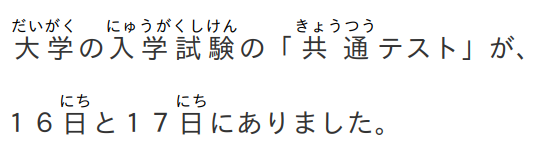
\includegraphics[width=35empt,]{Images/rbNhkEasy.png}
\caption{The first line of a news story from NHK News Web Easy intended for Japanese learners, in which every word composed of Chinese characters has a ruby gloss.}\end{figure}
\par
Pinyin ruby annotations are also used in Chinese to provide pronunciation guidance, and Zhuyin ({\textChinese 注音}) phonetic symbols (commonly known as \textit{bopomofo}) are used in Taiwan for the same purpose.\par
The TEI schema provides many different ways of encoding glosses and annotations, from the simple and flexible \hyperref[TEI.note]{<note>} element to a native implementation of the Web Annotation Data Model (\textit{\hyperref[SASOann]{16.11.\ Annotations}}). However, ruby is a particular, distinct, and widely-used form of annotation that appears in script, print, calligraphy, and web pages, and the TEI therefore provides specific elements for it: 
\begin{sansreflist}
  
\item [\textbf{<ruby>}] (ruby container) contains a passage of base text along with its associated ruby gloss(es).
\item [\textbf{<rb>}] (ruby base) contains the base text annotated by a ruby gloss.
\item [\textbf{<rt>}] (ruby text) contains a ruby text, an annotation closely associated with a passage of the main text.
\end{sansreflist}
 The \hyperref[TEI.rt]{<rt>} element is a member of \textsf{att.placement}, and thus the {\itshape place} attribute may be used to indicate where the ruby gloss is with respect to the base text: 
\begin{sansreflist}
  
\item [\textbf{att.placement}] provides attributes for describing where on the source page or object a textual element appears.\hfil\\[-10pt]\begin{sansreflist}
    \item[@{\itshape place}]
  specifies where this item is placed.
\end{sansreflist}  
\end{sansreflist}
 The most relevant suggested values of {\itshape place} for ruby text are above, below, left, and right.\par
In its simplest representation, a glossed form consists of an \hyperref[TEI.rb]{<rb>} (ruby base) element containing the base form, an \hyperref[TEI.rt]{<rt>} (ruby text) element containing the gloss, and a \hyperref[TEI.ruby]{<ruby>} element which wraps them together: \par\bgroup\index{p=<p>|exampleindex}\index{ruby=<ruby>|exampleindex}\index{rb=<rb>|exampleindex}\index{rt=<rt>|exampleindex}\index{place=@place!<rt>|exampleindex}\exampleFont \begin{shaded}\noindent\mbox{}{<\textbf{p}\hspace*{1em}{xml:lang}="{ja}">}\mbox{}\newline 
\textit{<!--{\textJapanese ...}-->}\mbox{}\newline 
\hspace*{1em}{<\textbf{ruby}>}\mbox{}\newline 
\hspace*{1em}\hspace*{1em}{<\textbf{rb}>}{\textJapanese 大学}{</\textbf{rb}>}\mbox{}\newline 
\hspace*{1em}\hspace*{1em}{<\textbf{rt}\hspace*{1em}{place}="{above}">}{\textJapanese だいがく}{</\textbf{rt}>}\mbox{}\newline 
\hspace*{1em}{</\textbf{ruby}>}\mbox{}\newline 
\textit{<!--{\textJapanese ...}-->}\mbox{}\newline 
{</\textbf{p}>}\end{shaded}\egroup\par \noindent  In the example above, the word {\textJapanese 大学} (\textit{daigaku} = university) is provided with a phonation gloss in hiragana. The full gloss is applied to the complete word. However, it might instead be broken down by character: \par\bgroup\index{p=<p>|exampleindex}\index{ruby=<ruby>|exampleindex}\index{rb=<rb>|exampleindex}\index{rt=<rt>|exampleindex}\index{place=@place!<rt>|exampleindex}\index{ruby=<ruby>|exampleindex}\index{rb=<rb>|exampleindex}\index{rt=<rt>|exampleindex}\index{place=@place!<rt>|exampleindex}\exampleFont \begin{shaded}\noindent\mbox{}{<\textbf{p}\hspace*{1em}{xml:lang}="{ja}">}\mbox{}\newline 
\textit{<!--{\textJapanese ...}-->}\mbox{}\newline 
\hspace*{1em}{<\textbf{ruby}>}\mbox{}\newline 
\hspace*{1em}\hspace*{1em}{<\textbf{rb}>}{\textJapanese 大}{</\textbf{rb}>}\mbox{}\newline 
\hspace*{1em}\hspace*{1em}{<\textbf{rt}\hspace*{1em}{place}="{above}">}{\textJapanese だい}{</\textbf{rt}>}\mbox{}\newline 
\hspace*{1em}{</\textbf{ruby}>}\mbox{}\newline 
\hspace*{1em}{<\textbf{ruby}>}\mbox{}\newline 
\hspace*{1em}\hspace*{1em}{<\textbf{rb}>}{\textJapanese 学}{</\textbf{rb}>}\mbox{}\newline 
\hspace*{1em}\hspace*{1em}{<\textbf{rt}\hspace*{1em}{place}="{above}">}{\textJapanese がく}{</\textbf{rt}>}\mbox{}\newline 
\hspace*{1em}{</\textbf{ruby}>}\mbox{}\newline 
\textit{<!--{\textJapanese ...}-->}\mbox{}\newline 
{</\textbf{p}>}\end{shaded}\egroup\par \noindent  Here is a similar example from Taiwan using bopomofo (pinyin \textit{píngzi} = bottle)\footnote{Taken from \xref{https://en.wikipedia.org/wiki/Bopomofo\#Example}{Wikipedia}.}: \par\bgroup\index{p=<p>|exampleindex}\index{ruby=<ruby>|exampleindex}\index{rb=<rb>|exampleindex}\index{rt=<rt>|exampleindex}\index{place=@place!<rt>|exampleindex}\index{ruby=<ruby>|exampleindex}\index{rb=<rb>|exampleindex}\index{rt=<rt>|exampleindex}\index{place=@place!<rt>|exampleindex}\exampleFont \begin{shaded}\noindent\mbox{}{<\textbf{p}\hspace*{1em}{xml:lang}="{zh-TW}">}\mbox{}\newline 
\textit{<!--{\textChinese ...}-->}\mbox{}\newline 
\hspace*{1em}{<\textbf{ruby}>}\mbox{}\newline 
\hspace*{1em}\hspace*{1em}{<\textbf{rb}>}{\textChinese 瓶}{</\textbf{rb}>}\mbox{}\newline 
\hspace*{1em}\hspace*{1em}{<\textbf{rt}\hspace*{1em}{place}="{right}">}{\textChinese ㄆㄧㄥˊ}{</\textbf{rt}>}\mbox{}\newline 
\hspace*{1em}{</\textbf{ruby}>}\mbox{}\newline 
\hspace*{1em}{<\textbf{ruby}>}\mbox{}\newline 
\hspace*{1em}\hspace*{1em}{<\textbf{rb}>}{\textChinese 子}{</\textbf{rb}>}\mbox{}\newline 
\hspace*{1em}\hspace*{1em}{<\textbf{rt}\hspace*{1em}{place}="{right}">}{\textChinese ˙ㄗ}{</\textbf{rt}>}\mbox{}\newline 
\hspace*{1em}{</\textbf{ruby}>}\mbox{}\newline 
\textit{<!--{\textChinese ...}-->}\mbox{}\newline 
{</\textbf{p}>}\end{shaded}\egroup\par \noindent  Where {\itshape place} is not provided, the default assumption is that the ruby gloss is \textit{above} where the text is horizontal, and to the \textit{right} of the text where it is vertical. See \textit{\hyperref[WDWM]{5.6.\ Writing Modes}} for a detailed guide to writing modes and text directionality.\par
The same ruby base may be accompanied by more than one gloss. Here, the Japanese word {\textJapanese 打球場} (dakyūba, or  \textit{billiard hall}) is glossed with two different pronunciations: ‘biriādo’ (its English equivalent) and ‘dakyū’, a phonation guide for the first two characters. \begin{figure}[htbp]
\noindent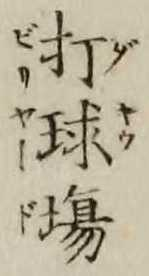
\includegraphics[width=149pt,height=276pt,]{Images/billiardhall.jpg}
\caption{\textit{Billiard hall} with two ruby glosses. \xref{http://school.nijl.ac.jp/kindai/NIJL/NIJL-01116.html\#37}{{\textJapanese 国文学研究資料館所蔵::英国/龍動新繁昌記}}.}\end{figure}
 This example is intriguing in that the right-side ruby glosses apply to the first and second characters respectively, but the left-side gloss applies to the whole word as a unit. We use this instance to exemplify multiple approaches to encoding the same phenomena, which may be appropriate for different projects or editorial preferences. First, using the same segmentation approach as demonstrated for {\textJapanese 大学} above, but with nesting: \par\bgroup\index{p=<p>|exampleindex}\index{style=@style!<p>|exampleindex}\index{ruby=<ruby>|exampleindex}\index{rb=<rb>|exampleindex}\index{ruby=<ruby>|exampleindex}\index{rb=<rb>|exampleindex}\index{rt=<rt>|exampleindex}\index{place=@place!<rt>|exampleindex}\index{ruby=<ruby>|exampleindex}\index{rb=<rb>|exampleindex}\index{rt=<rt>|exampleindex}\index{place=@place!<rt>|exampleindex}\index{rt=<rt>|exampleindex}\index{place=@place!<rt>|exampleindex}\exampleFont \begin{shaded}\noindent\mbox{}{<\textbf{p}\hspace*{1em}{style}="{writing-mode: vertical-rl}"\mbox{}\newline 
\hspace*{1em}{xml:lang}="{ja}">}\mbox{}\newline 
\textit{<!--{\textJapanese ...}-->}\mbox{}\newline 
\hspace*{1em}{<\textbf{ruby}>}\mbox{}\newline 
\hspace*{1em}\hspace*{1em}{<\textbf{rb}>}\mbox{}\newline 
\hspace*{1em}\hspace*{1em}\hspace*{1em}{<\textbf{ruby}>}\mbox{}\newline 
\hspace*{1em}\hspace*{1em}\hspace*{1em}\hspace*{1em}{<\textbf{rb}>}{\textJapanese 打}{</\textbf{rb}>}\mbox{}\newline 
\hspace*{1em}\hspace*{1em}\hspace*{1em}\hspace*{1em}{<\textbf{rt}\hspace*{1em}{place}="{right}">}{\textJapanese ダ}{</\textbf{rt}>}\mbox{}\newline 
\hspace*{1em}\hspace*{1em}\hspace*{1em}{</\textbf{ruby}>}\mbox{}\newline 
\hspace*{1em}\hspace*{1em}\hspace*{1em}{<\textbf{ruby}>}\mbox{}\newline 
\hspace*{1em}\hspace*{1em}\hspace*{1em}\hspace*{1em}{<\textbf{rb}>}{\textJapanese 球}{</\textbf{rb}>}\mbox{}\newline 
\hspace*{1em}\hspace*{1em}\hspace*{1em}\hspace*{1em}{<\textbf{rt}\hspace*{1em}{place}="{right}">}{\textJapanese キウ}{</\textbf{rt}>}\mbox{}\newline 
\hspace*{1em}\hspace*{1em}\hspace*{1em}{</\textbf{ruby}>}{\textJapanese }\mbox{}\newline 
\hspace*{1em}\hspace*{1em}\hspace*{1em}\hspace*{1em} {\textJapanese 場}\mbox{}\newline 
\hspace*{1em}\hspace*{1em}{</\textbf{rb}>}\mbox{}\newline 
\hspace*{1em}\hspace*{1em}{<\textbf{rt}\hspace*{1em}{place}="{left}">}{\textJapanese ビリヤード}{</\textbf{rt}>}\mbox{}\newline 
\hspace*{1em}{</\textbf{ruby}>}\mbox{}\newline 
\textit{<!--{\textJapanese ...}-->}\mbox{}\newline 
{</\textbf{p}>}\end{shaded}\egroup\par \noindent  We could also use a standoff approach with \hyperref[TEI.anchor]{<anchor>} elements and pointers: \par\bgroup\index{p=<p>|exampleindex}\index{style=@style!<p>|exampleindex}\index{ruby=<ruby>|exampleindex}\index{rb=<rb>|exampleindex}\index{anchor=<anchor>|exampleindex}\index{anchor=<anchor>|exampleindex}\index{anchor=<anchor>|exampleindex}\index{anchor=<anchor>|exampleindex}\index{rt=<rt>|exampleindex}\index{place=@place!<rt>|exampleindex}\index{from=@from!<rt>|exampleindex}\index{to=@to!<rt>|exampleindex}\index{rt=<rt>|exampleindex}\index{place=@place!<rt>|exampleindex}\index{from=@from!<rt>|exampleindex}\index{to=@to!<rt>|exampleindex}\index{rt=<rt>|exampleindex}\index{place=@place!<rt>|exampleindex}\index{from=@from!<rt>|exampleindex}\index{to=@to!<rt>|exampleindex}\exampleFont \begin{shaded}\noindent\mbox{}{<\textbf{p}\hspace*{1em}{style}="{writing-mode: vertical-rl}"\mbox{}\newline 
\hspace*{1em}{xml:lang}="{ja}">}\mbox{}\newline 
\textit{<!--{\textJapanese ...}-->}\mbox{}\newline 
\hspace*{1em}{<\textbf{ruby}>}\mbox{}\newline 
\hspace*{1em}\hspace*{1em}{<\textbf{rb}>}\mbox{}\newline 
\hspace*{1em}\hspace*{1em}\hspace*{1em}{<\textbf{anchor}\hspace*{1em}{xml:id}="{da}"/>}{\textJapanese 打}\mbox{}\newline 
\hspace*{1em}\hspace*{1em}{<\textbf{anchor}\hspace*{1em}{xml:id}="{kyuu}"/>}{\textJapanese 球}\mbox{}\newline 
\hspace*{1em}\hspace*{1em}{<\textbf{anchor}\hspace*{1em}{xml:id}="{ba}"/>}{\textJapanese 場}\mbox{}\newline 
\hspace*{1em}\hspace*{1em}{<\textbf{anchor}\hspace*{1em}{xml:id}="{owari}"/>}\mbox{}\newline 
\hspace*{1em}\hspace*{1em}{</\textbf{rb}>}\mbox{}\newline 
\hspace*{1em}\hspace*{1em}{<\textbf{rt}\hspace*{1em}{place}="{left}"\hspace*{1em}{from}="{\#da}"\hspace*{1em}{to}="{\#owari}">}{\textJapanese ビリヤード}{</\textbf{rt}>}\mbox{}\newline 
\hspace*{1em}\hspace*{1em}{<\textbf{rt}\hspace*{1em}{place}="{right}"\hspace*{1em}{from}="{\#da}"\hspace*{1em}{to}="{\#kyuu}">}{\textJapanese ダ}{</\textbf{rt}>}\mbox{}\newline 
\hspace*{1em}\hspace*{1em}{<\textbf{rt}\hspace*{1em}{place}="{right}"\hspace*{1em}{from}="{\#kyuu}"\hspace*{1em}{to}="{\#ba}">}{\textJapanese キウ}{</\textbf{rt}>}\mbox{}\newline 
\hspace*{1em}{</\textbf{ruby}>}\mbox{}\newline 
\textit{<!--{\textJapanese ...}-->}\mbox{}\newline 
{</\textbf{p}>}\end{shaded}\egroup\par \noindent  Alternatively, if the encoding itself already includes segmentation below the word level, we can use the existing elements instead of adding \hyperref[TEI.anchor]{<anchor>}s: \par\bgroup\index{p=<p>|exampleindex}\index{style=@style!<p>|exampleindex}\index{ruby=<ruby>|exampleindex}\index{rb=<rb>|exampleindex}\index{c=<c>|exampleindex}\index{c=<c>|exampleindex}\index{c=<c>|exampleindex}\index{rt=<rt>|exampleindex}\index{place=@place!<rt>|exampleindex}\index{target=@target!<rt>|exampleindex}\index{rt=<rt>|exampleindex}\index{place=@place!<rt>|exampleindex}\index{target=@target!<rt>|exampleindex}\index{rt=<rt>|exampleindex}\index{place=@place!<rt>|exampleindex}\index{target=@target!<rt>|exampleindex}\exampleFont \begin{shaded}\noindent\mbox{}{<\textbf{p}\hspace*{1em}{style}="{writing-mode: vertical-rl}"\mbox{}\newline 
\hspace*{1em}{xml:lang}="{ja}">}\mbox{}\newline 
\textit{<!--{\textJapanese ...}-->}\mbox{}\newline 
\hspace*{1em}{<\textbf{ruby}>}\mbox{}\newline 
\hspace*{1em}\hspace*{1em}{<\textbf{rb}\hspace*{1em}{xml:id}="{dakyuuba}">}\mbox{}\newline 
\hspace*{1em}\hspace*{1em}\hspace*{1em}{<\textbf{c}\hspace*{1em}{xml:id}="{chr1}">}{\textJapanese 打}{</\textbf{c}>}\mbox{}\newline 
\hspace*{1em}\hspace*{1em}\hspace*{1em}{<\textbf{c}\hspace*{1em}{xml:id}="{chr2}">}{\textJapanese 球}{</\textbf{c}>}\mbox{}\newline 
\hspace*{1em}\hspace*{1em}\hspace*{1em}{<\textbf{c}>}{\textJapanese 場}{</\textbf{c}>}\mbox{}\newline 
\hspace*{1em}\hspace*{1em}{</\textbf{rb}>}\mbox{}\newline 
\hspace*{1em}\hspace*{1em}{<\textbf{rt}\hspace*{1em}{place}="{left}"\hspace*{1em}{target}="{\#dakyuuba}">}{\textJapanese ビリヤード}{</\textbf{rt}>}\mbox{}\newline 
\hspace*{1em}\hspace*{1em}{<\textbf{rt}\hspace*{1em}{place}="{right}"\hspace*{1em}{target}="{\#chr1}">}{\textJapanese ダ}{</\textbf{rt}>}\mbox{}\newline 
\hspace*{1em}\hspace*{1em}{<\textbf{rt}\hspace*{1em}{place}="{right}"\hspace*{1em}{target}="{\#chr2}">}{\textJapanese キウ}{</\textbf{rt}>}\mbox{}\newline 
\hspace*{1em}{</\textbf{ruby}>}\mbox{}\newline 
\textit{<!--{\textJapanese ...}-->}\mbox{}\newline 
{</\textbf{p}>}\end{shaded}\egroup\par \par
The current support for ruby is rudimentary, and in future releases of the Guidelines we expect to see more development of these features and recommendations.
\subsubsection[{Equivalents and Descriptions}]{Equivalents and Descriptions}\label{COHTGED}\par
Another group of elements is used to supply different kinds of names for objects described by the TEI. Examples of this are documentation of elements, attributes, classes (and also attribute values where appropriate), and description of glyphs. 
\begin{sansreflist}
  
\item [\textbf{<altIdent>}] (alternate identifier) supplies the recommended XML name for an element, class, attribute, etc. in some language.
\item [\textbf{<desc>}] (description) contains a short description of the purpose, function, or use of its parent element, or when the parent is a documentation element, describes or defines the object being documented. 
\item [\textbf{<equiv>}] (equivalent) specifies a component which is considered equivalent to the parent element, either by co-reference, or by external link.\hfil\\[-10pt]\begin{sansreflist}
    \item[@{\itshape uri}]
  (uniform resource identifier) references the underlying concept of which the parent is a representation by means of some external identifier
    \item[@{\itshape filter}]
  references an external script which contains a method to transform instances of this element to canonical TEI
    \item[@{\itshape name}]
  a single word which follows the rules defining a legal XML name (see \url{http://www.w3.org/TR/REC-xml/\#dt-name}), naming the underlying concept of which the parent is a representation.
    \item[@{\itshape predicate [att.predicate]}]
  the condition under which the element bearing this attribute applies, given as an XPath predicate expression.
\end{sansreflist}  
\end{sansreflist}
 Along with the \hyperref[TEI.gloss]{<gloss>} element mentioned above, these elements constitute the \textsf{model.glossLike} class. They are described in more detail in \textit{\hyperref[TDcrystalsCEdc]{22.4.1.\ Description of Components}}.
\subsection[{Simple Editorial Changes}]{Simple Editorial Changes}\label{COED}\par
As in editing a printed text, so in encoding a text in electronic form, it may be necessary to accommodate editorial comment on the text and to render account of any changes made to the text in preparing it. The tags described in this section may be used to record such editorial interventions, whether made by the encoder, by the editor of a printed edition used as a copy text, by earlier editors, or by the copyists of manuscripts.\par
The tags described here handle most common types of editorial intervention and stereotyped comment; where less structured commentary of other types is to be included, it may be marked using the \hyperref[TEI.note]{<note>} element described in section \textit{\hyperref[CONO]{3.9.\ Notes, Annotation, and Indexing}}. Systematic interpretive annotation is also possible using the various methods described in chapter \textit{\hyperref[SA]{16.\ Linking, Segmentation, and Alignment}}. The examples given here illustrate only simple cases of editorial intervention; in particular, they permit economical encoding of a simple set of alternative readings of a short span of text. To encode multiple views of large or heterogeneous spans of text, the mechanisms described in chapter \textit{\hyperref[SA]{16.\ Linking, Segmentation, and Alignment}} should be used. To encode multiple witnesses of a particular text, a similar mechanism designed specifically for critical editions is described in chapter \textit{\hyperref[TC]{12.\ Critical Apparatus}}.\par
For most of the elements discussed here, some encoders may wish to indicate both a \textit{responsibility}, that is, a code indicating the person or agency responsible for making the editorial intervention in question, and also an indication of the degree of \textit{certainty} which the encoder wishes to associate with the intervention. These requirements are served by the \textsf{att.global.responsibility} class, along with \textsf{att.global.source} and \textsf{att.dimensions}. Any of the elements discussed here thus may potentially carry any of the following optional attributes: 
\begin{sansreflist}
  
\item [\textbf{att.global.responsibility}] provides attributes indicating the agent responsible for some aspect of the text, the markup or something asserted by the markup, and the degree of certainty associated with it.\hfil\\[-10pt]\begin{sansreflist}
    \item[@{\itshape cert}]
  (certainty) signifies the degree of certainty associated with the intervention or interpretation.
    \item[@{\itshape resp}]
  (responsible party) indicates the agency responsible for the intervention or interpretation, for example an editor or transcriber.
\end{sansreflist}  
\item [\textbf{att.global.source}] provides an attribute used by elements to point to an external source.\hfil\\[-10pt]\begin{sansreflist}
    \item[@{\itshape source}]
  specifies the source from which some aspect of this element is drawn.
\end{sansreflist}  
\item [\textbf{att.editLike}] provides attributes describing the nature of an encoded scholarly intervention or interpretation of any kind.\hfil\\[-10pt]\begin{sansreflist}
    \item[@{\itshape evidence}]
  indicates the nature of the evidence supporting the reliability or accuracy of the intervention or interpretation.
\end{sansreflist}  
\item [\textbf{att.dimensions}] provides attributes for describing the size of physical objects.\hfil\\[-10pt]\begin{sansreflist}
    \item[@{\itshape unit}]
  names the unit used for the measurement
    \item[@{\itshape quantity}]
  specifies the length in the units specified
    \item[@{\itshape extent}]
  indicates the size of the object concerned using a project-specific vocabulary combining quantity and units in a single string of words.
    \item[@{\itshape precision}]
  characterizes the precision of the values specified by the other attributes.
    \item[@{\itshape scope}]
  where the measurement summarizes more than one observation, specifies the applicability of this measurement.
\end{sansreflist}  
\end{sansreflist}
\par
Many of the elements discussed here can be used in two ways. Their primary purpose is to indicate that the text encoded as the element's content represents an editorial intervention (or non-intervention) of a specific kind, indicated by the element itself. However, pairs or other meaningful groupings of such elements can also be supplied, wrapped within a special purpose \hyperref[TEI.choice]{<choice>} element: 
\begin{sansreflist}
  
\item [\textbf{<choice>}] (choice) groups a number of alternative encodings for the same point in a text.
\end{sansreflist}
 This element enables the encoder to represent for example a text in its ‘original’ uncorrected and unaltered form, alongside the same text in one or more ‘edited’ forms. This usage permits software to switch automatically between one ‘view’ of a text and another, so that (for example) a stylesheet may be set to display either the text in its original form or after the application of editorial interventions of particular kinds.\par
Elements which can be combined in this way constitute the \textsf{model.choicePart} class. The default members of this class are \hyperref[TEI.sic]{<sic>}, \hyperref[TEI.corr]{<corr>}, \hyperref[TEI.reg]{<reg>}, \hyperref[TEI.orig]{<orig>}, \hyperref[TEI.unclear]{<unclear>}, \hyperref[TEI.supplied]{<supplied>}, \hyperref[TEI.abbr]{<abbr>}, \hyperref[TEI.expan]{<expan>}, \hyperref[TEI.ex]{<ex>}, \hyperref[TEI.am]{<am>} and \hyperref[TEI.seg]{<seg>}; some of their functions and usage are described further below.\par
Three categories of editorial intervention are discussed in this section: \begin{itemize}
\item indication or correction of apparent errors 
\item indication or regularization of variant, irregular, non-standard, or eccentric forms
\item editorial additions, suppressions, and omissions
\end{itemize} \par
A more extended treatment of the use of these tags in transcriptional and editorial work is given in chapter \textit{\hyperref[PH]{11.\ Representation of Primary Sources}}.
\subsubsection[{Apparent Errors}]{Apparent Errors}\label{COEDCOR}\par
When the copy text is manifestly faulty, an encoder or transcriber may elect simply to correct it without comment, although for scholarly purposes it will often be more generally useful to record both the correction and the original state of the text. The elements described here enable all three approaches, and allows the last to be done in such a way as make it easy for software to present either the original or the correction. 
\begin{sansreflist}
  
\item [\textbf{<sic>}] (Latin for thus or so) contains text reproduced although apparently incorrect or inaccurate.
\item [\textbf{<corr>}] (correction) contains the correct form of a passage apparently erroneous in the copy text.
\end{sansreflist}
\par
The following examples show alternative treatment of the same material. The copy text reads: 
\begin{quote}Another property of computer-assisted historical research is that data modelling must permit any one textual feature or part of a textual feature to be a part of more than one information model and to allow the researcher to draw on several such models simultaneously, for example, to select from a machine-readable text those marginal comments which indicate that the date's mentioned in the main body of the text are incorrect.\end{quote}
\par
An encoder may choose to correct the typographic error, either silently or with an indication that a correction has been made, as follows: \par\bgroup\index{corr=<corr>|exampleindex}\exampleFont \begin{shaded}\noindent\mbox{}… marginal comments which indicate that the {<\textbf{corr}>}dates{</\textbf{corr}>}\mbox{}\newline 
 mentioned in the main body of the text are incorrect.\end{shaded}\egroup\par \par
Alternatively, the encoder may simply record the typographic error without correcting it, either without comment or with a \hyperref[TEI.sic]{<sic>} element to indicate the error is not a transcription error in the encoding: \par\bgroup\index{sic=<sic>|exampleindex}\exampleFont \begin{shaded}\noindent\mbox{}… marginal comments which indicate that the {<\textbf{sic}>}date's{</\textbf{sic}>}\mbox{}\newline 
 mentioned in the main body of the text are incorrect.\end{shaded}\egroup\par \par
If the encoder elects both to record the original source text and to provide a correction for the sake of word-search and other programs, both \hyperref[TEI.sic]{<sic>} and \hyperref[TEI.corr]{<corr>} are used, wrapped in a \hyperref[TEI.choice]{<choice>}: \par\bgroup\index{choice=<choice>|exampleindex}\index{corr=<corr>|exampleindex}\index{sic=<sic>|exampleindex}\exampleFont \begin{shaded}\noindent\mbox{}… marginal comments which indicate that the\mbox{}\newline 
{<\textbf{choice}>}\mbox{}\newline 
\hspace*{1em}{<\textbf{corr}>}dates{</\textbf{corr}>}\mbox{}\newline 
\hspace*{1em}{<\textbf{sic}>}date's{</\textbf{sic}>}\mbox{}\newline 
{</\textbf{choice}>} mentioned in the main body of the text are\mbox{}\newline 
 incorrect.\end{shaded}\egroup\par \noindent The \hyperref[TEI.sic]{<sic>} and \hyperref[TEI.corr]{<corr>} elements can appear in either order.\par
If it is desired to indicate the person or edition responsible for the emendation, this might be done as follows: \par\bgroup\index{choice=<choice>|exampleindex}\index{corr=<corr>|exampleindex}\index{resp=@resp!<corr>|exampleindex}\index{sic=<sic>|exampleindex}\index{respStmt=<respStmt>|exampleindex}\index{resp=<resp>|exampleindex}\index{name=<name>|exampleindex}\exampleFont \begin{shaded}\noindent\mbox{}… marginal comments which indicate that the\mbox{}\newline 
{<\textbf{choice}>}\mbox{}\newline 
\hspace*{1em}{<\textbf{corr}\hspace*{1em}{resp}="{\#msm}">}dates{</\textbf{corr}>}\mbox{}\newline 
\hspace*{1em}{<\textbf{sic}>}date's{</\textbf{sic}>}\mbox{}\newline 
{</\textbf{choice}>} mentioned in the main body of the text are\mbox{}\newline 
 incorrect.\mbox{}\newline 
\mbox{}\newline 
\textit{<!-- within the header for this document ... -->}\mbox{}\newline 
{<\textbf{respStmt}\hspace*{1em}{xml:id}="{msm}">}\mbox{}\newline 
\hspace*{1em}{<\textbf{resp}>}editor{</\textbf{resp}>}\mbox{}\newline 
\hspace*{1em}{<\textbf{name}>}C.M. Sperberg-McQueen{</\textbf{name}>}\mbox{}\newline 
{</\textbf{respStmt}>}\end{shaded}\egroup\par \noindent Here the {\itshape resp} attribute has been used to indicate responsibility for the correction. Its value (\#msm) is an example of the \textit{pointer} values discussed in section \textit{\hyperref[COXR]{3.7.\ Simple Links and Cross-References}}; in this case, it points to a \hyperref[TEI.respStmt]{<respStmt>} element within the TEI header, but any element might be indicated in this way, including for example a \hyperref[TEI.name]{<name>} element, or (if the module described in \textit{\hyperref[ND]{13.\ Names, Dates, People, and Places}} has been included) a \hyperref[TEI.person]{<person>} element. The {\itshape resp} attribute is available for all elements which are members of the \textsf{att.global.responsibility} class. The same class makes available a {\itshape cert} attribute, which may be used to indicate the degree of editorial confidence in a particular correction, as in the following example: \par\bgroup\index{choice=<choice>|exampleindex}\index{corr=<corr>|exampleindex}\index{cert=@cert!<corr>|exampleindex}\index{sic=<sic>|exampleindex}\exampleFont \begin{shaded}\noindent\mbox{}An {<\textbf{choice}>}\mbox{}\newline 
\hspace*{1em}{<\textbf{corr}\hspace*{1em}{cert}="{high}">}Autumn{</\textbf{corr}>}\mbox{}\newline 
\hspace*{1em}{<\textbf{sic}>}Antony{</\textbf{sic}>}\mbox{}\newline 
{</\textbf{choice}>} it was,\mbox{}\newline 
 That grew the more by reaping\end{shaded}\egroup\par \noindent  See further the discussion in section \textit{\hyperref[PHCC]{11.3.1.3.\ Correction and Conjecture}}.\par
Where, as here, the correction takes the form of adding text not otherwise present in the text being encoded, the encoder should use the \hyperref[TEI.corr]{<corr>} element. Where the correction is present in the text being encoded, and consists of some combination of visible additions and deletions, the elements \hyperref[TEI.add]{<add>} or \hyperref[TEI.del]{<del>} should be used: see further section \textit{\hyperref[COEDADD]{3.5.3.\ Additions, Deletions, and Omissions}} below. Where the correction takes the form of addition of material not present in the original because of physical damage or illegibility, the \hyperref[TEI.supplied]{<supplied>} element may be used. Where the ‘correction’ is simply a matter of expanding an abbreviation the \hyperref[TEI.ex]{<ex>} element may be used. These and other elements to support the detailed encoding of authorial or scribal interventions of this kind are all provided by the module described in chapter \textit{\hyperref[PH]{11.\ Representation of Primary Sources}}.
\subsubsection[{Regularization and Normalization}]{Regularization and Normalization}\label{COEDREG}\par
When the source text makes extensive use of variant forms or non-standard spellings, it may be desirable for a number of reasons to \textit{regularize} it: that is, to provide ‘standard’ or ‘regularized’ forms equivalent to the non-standard forms.\footnote{In some contexts, the term \textit{regularization} has a narrower and more specific significance than that proposed here: the \hyperref[TEI.reg]{<reg>} element may be used for any kind of regularization, including normalization, standardization, and modernization.}\par
As with other such changes to the copy text, the changes may be made silently (in which case the TEI header should specify the types of silent changes made) or may be explicitly marked using the following elements: 
\begin{sansreflist}
  
\item [\textbf{<reg>}] (regularization) contains a reading which has been regularized or normalized in some sense.
\item [\textbf{<orig>}] (original form) contains a reading which is marked as following the original, rather than being normalized or corrected.
\item [\textbf{<choice>}] (choice) groups a number of alternative encodings for the same point in a text.
\end{sansreflist}
\par
Typical applications for these elements include the production of editions intended for student or lay readers, linguistic research in which spelling or usage variation is not the main question at issue, production of spelling dictionaries, etc.\par
Consider this 16th-century text: 
\begin{quote}how godly a dede it is to overthrowe so wicked a race the world may judge: for my part I thinke there canot be a greater sacryfice to God.\end{quote}
\par
An encoder may choose to preserve the original spelling of this text, but simply flag it as nonstandard by using the \hyperref[TEI.orig]{<orig>} element with no attributes specified, as follows: \par\bgroup\index{p=<p>|exampleindex}\index{orig=<orig>|exampleindex}\index{orig=<orig>|exampleindex}\index{orig=<orig>|exampleindex}\index{orig=<orig>|exampleindex}\index{orig=<orig>|exampleindex}\exampleFont \begin{shaded}\noindent\mbox{}{<\textbf{p}>}...how godly a {<\textbf{orig}>}dede{</\textbf{orig}>} it is to\mbox{}\newline 
{<\textbf{orig}>}overthrowe{</\textbf{orig}>} so wicked a race the\mbox{}\newline 
 world may judge: for my part I {<\textbf{orig}>}thinke{</\textbf{orig}>}\mbox{}\newline 
 there {<\textbf{orig}>}canot{</\textbf{orig}>} be a greater\mbox{}\newline 
{<\textbf{orig}>}sacryfice{</\textbf{orig}>} to God{</\textbf{p}>}\end{shaded}\egroup\par \par
Alternatively, the encoder may simply indicate that certain words have been modernized by using the \hyperref[TEI.reg]{<reg>} element with no attributes specified, as follows:\par\bgroup\index{p=<p>|exampleindex}\index{reg=<reg>|exampleindex}\index{reg=<reg>|exampleindex}\index{reg=<reg>|exampleindex}\index{reg=<reg>|exampleindex}\index{reg=<reg>|exampleindex}\exampleFont \begin{shaded}\noindent\mbox{}{<\textbf{p}>}...how godly a\mbox{}\newline 
{<\textbf{reg}>}deed{</\textbf{reg}>} it is to {<\textbf{reg}>}overthrow{</\textbf{reg}>} so wicked a race the\mbox{}\newline 
 world may judge: for my part I {<\textbf{reg}>}think{</\textbf{reg}>}\mbox{}\newline 
 there {<\textbf{reg}>}cannot{</\textbf{reg}>} be a greater\mbox{}\newline 
{<\textbf{reg}>}sacrifice{</\textbf{reg}>} to God.{</\textbf{p}>}\end{shaded}\egroup\par \par
Alternatively, the encoder may elect to record both old and new spellings, so that (for example) the same electronic text may serve as the basis of an old- or new-spelling edition: \par\bgroup\index{p=<p>|exampleindex}\index{choice=<choice>|exampleindex}\index{orig=<orig>|exampleindex}\index{reg=<reg>|exampleindex}\index{choice=<choice>|exampleindex}\index{orig=<orig>|exampleindex}\index{reg=<reg>|exampleindex}\index{choice=<choice>|exampleindex}\index{orig=<orig>|exampleindex}\index{reg=<reg>|exampleindex}\index{choice=<choice>|exampleindex}\index{orig=<orig>|exampleindex}\index{reg=<reg>|exampleindex}\index{choice=<choice>|exampleindex}\index{orig=<orig>|exampleindex}\index{reg=<reg>|exampleindex}\exampleFont \begin{shaded}\noindent\mbox{}{<\textbf{p}>}...how godly a {<\textbf{choice}>}\mbox{}\newline 
\hspace*{1em}\hspace*{1em}{<\textbf{orig}>}dede{</\textbf{orig}>}\mbox{}\newline 
\hspace*{1em}\hspace*{1em}{<\textbf{reg}>}deed{</\textbf{reg}>}\mbox{}\newline 
\hspace*{1em}{</\textbf{choice}>} it is to\mbox{}\newline 
{<\textbf{choice}>}\mbox{}\newline 
\hspace*{1em}\hspace*{1em}{<\textbf{orig}>}overthrowe{</\textbf{orig}>}\mbox{}\newline 
\hspace*{1em}\hspace*{1em}{<\textbf{reg}>}overthrow{</\textbf{reg}>}\mbox{}\newline 
\hspace*{1em}{</\textbf{choice}>} so wicked a race the\mbox{}\newline 
 world may judge: for my part I {<\textbf{choice}>}\mbox{}\newline 
\hspace*{1em}\hspace*{1em}{<\textbf{orig}>}thinke{</\textbf{orig}>}\mbox{}\newline 
\hspace*{1em}\hspace*{1em}{<\textbf{reg}>}think{</\textbf{reg}>}\mbox{}\newline 
\hspace*{1em}{</\textbf{choice}>}\mbox{}\newline 
 there {<\textbf{choice}>}\mbox{}\newline 
\hspace*{1em}\hspace*{1em}{<\textbf{orig}>}canot{</\textbf{orig}>}\mbox{}\newline 
\hspace*{1em}\hspace*{1em}{<\textbf{reg}>}cannot{</\textbf{reg}>}\mbox{}\newline 
\hspace*{1em}{</\textbf{choice}>} be a greater\mbox{}\newline 
{<\textbf{choice}>}\mbox{}\newline 
\hspace*{1em}\hspace*{1em}{<\textbf{orig}>}sacryfice{</\textbf{orig}>}\mbox{}\newline 
\hspace*{1em}\hspace*{1em}{<\textbf{reg}>}sacrifice{</\textbf{reg}>}\mbox{}\newline 
\hspace*{1em}{</\textbf{choice}>} to God.{</\textbf{p}>}\end{shaded}\egroup\par \par
As elsewhere, the {\itshape resp} attribute may be used to specify the agency responsible for the regularization.
\subsubsection[{Additions, Deletions, and Omissions}]{Additions, Deletions, and Omissions}\label{COEDADD}\par
The following elements are used to indicate when words or phrases have been omitted from, added to, or marked for deletion from, a text. Like the other editorial elements, they allow for a wide range of editorial practices: 
\begin{sansreflist}
  
\item [\textbf{<gap>}] (gap) indicates a point where material has been omitted in a transcription, whether for editorial reasons described in the TEI header, as part of sampling practice, or because the material is illegible, invisible, or inaudible.\hfil\\[-10pt]\begin{sansreflist}
    \item[@{\itshape reason}]
  (reason) gives the reason for omission
\end{sansreflist}  
\item [\textbf{<unclear>}] (unclear) contains a word, phrase, or passage which cannot be transcribed with certainty because it is illegible or inaudible in the source.\hfil\\[-10pt]\begin{sansreflist}
    \item[@{\itshape reason}]
  indicates why the material is hard to transcribe.
\end{sansreflist}  
\item [\textbf{<add>}] (addition) contains letters, words, or phrases inserted in the source text by an author, scribe, or a previous annotator or corrector.
\item [\textbf{<del>}] (deletion) contains a letter, word, or passage deleted, marked as deleted, or otherwise indicated as superfluous or spurious in the copy text by an author, scribe, or a previous annotator or corrector.
\end{sansreflist}
\par
Encoders may choose to omit parts of the copy text for reasons ranging from illegibility of the source or impossibility of transcribing it, to editorial policy, e.g. a systematic exclusion of poetry or prose from an encoding. The full details of the policy decisions concerned should be documented in the TEI header (see section \textit{\hyperref[HD5]{2.3.\ The Encoding Description}}). Each place in the text at which omission has taken place should be marked with a \hyperref[TEI.gap]{<gap>} element, with optionally further information about the reason for the omission, its extent, and the person or agency responsible for it, as in the following examples: \par\bgroup\index{gap=<gap>|exampleindex}\index{reason=@reason!<gap>|exampleindex}\index{unit=@unit!<gap>|exampleindex}\index{quantity=@quantity!<gap>|exampleindex}\exampleFont \begin{shaded}\noindent\mbox{}{<\textbf{gap}\hspace*{1em}{reason}="{illegible}"\hspace*{1em}{unit}="{word}"\mbox{}\newline 
\hspace*{1em}{quantity}="{2}"/>}\end{shaded}\egroup\par \noindent \par\bgroup\index{gap=<gap>|exampleindex}\index{reason=@reason!<gap>|exampleindex}\index{extent=@extent!<gap>|exampleindex}\exampleFont \begin{shaded}\noindent\mbox{}{<\textbf{gap}\hspace*{1em}{reason}="{overwriting illegible}"\mbox{}\newline 
\hspace*{1em}{extent}="{several characters}"/>}\end{shaded}\egroup\par \noindent  Note that the extent of the gap may be marked precisely using attributes {\itshape unit} and {\itshape quantity}, or more descriptively using the {\itshape extent} attribute. Other, more detailed, options are also available for representing dimensions of any kind; see further \textit{\hyperref[msdim]{10.3.4.\ Dimensions}}.\par
The \hyperref[TEI.desc]{<desc>} element may be used to supply a description of the material omitted, where that is considered useful: \par\bgroup\index{gap=<gap>|exampleindex}\index{reason=@reason!<gap>|exampleindex}\index{quantity=@quantity!<gap>|exampleindex}\index{unit=@unit!<gap>|exampleindex}\index{desc=<desc>|exampleindex}\exampleFont \begin{shaded}\noindent\mbox{}{<\textbf{gap}\hspace*{1em}{reason}="{sampling}"\hspace*{1em}{quantity}="{120}"\mbox{}\newline 
\hspace*{1em}{unit}="{lines}">}\mbox{}\newline 
\hspace*{1em}{<\textbf{desc}>}irrelevant commentary{</\textbf{desc}>}\mbox{}\newline 
{</\textbf{gap}>}\end{shaded}\egroup\par \noindent  \par\bgroup\index{gap=<gap>|exampleindex}\index{reason=@reason!<gap>|exampleindex}\index{extent=@extent!<gap>|exampleindex}\index{desc=<desc>|exampleindex}\exampleFont \begin{shaded}\noindent\mbox{}… Their arrangement with respect to Jupiter and to each other was as follows:\mbox{}\newline 
{<\textbf{gap}\hspace*{1em}{reason}="{sampling}"\hspace*{1em}{extent}="{restOfPage}">}\mbox{}\newline 
\hspace*{1em}{<\textbf{desc}>}astrological figure{</\textbf{desc}>}\mbox{}\newline 
{</\textbf{gap}>}\mbox{}\newline 
 That is, there were two stars on the easterly side and one to the\mbox{}\newline 
 west; …\end{shaded}\egroup\par \noindent     \par
The \hyperref[TEI.add]{<add>} and \hyperref[TEI.del]{<del>} elements may be used to record where words or phrases have been added or deleted in the copy text. They are not appropriate where longer passages have been added or deleted, which span several elements; for these, the elements \hyperref[TEI.addSpan]{<addSpan>} and \hyperref[TEI.delSpan]{<delSpan>} described in chapter \textit{\hyperref[PHAD]{11.3.1.4.\ Additions and Deletions}} should be used.\par
Additions to a text may be recorded for a number of reasons. Sometimes they are marked in a distinctive way in the source text, for example by brackets or insertion above the line (\textit{supralinear} insertion), as in the following example, taken from a 19th century manuscript: \par\bgroup\index{add=<add>|exampleindex}\index{place=@place!<add>|exampleindex}\exampleFont \begin{shaded}\noindent\mbox{}The story I am going to relate is true as to its main facts,\mbox{}\newline 
 and as to the consequences {<\textbf{add}\hspace*{1em}{place}="{above}">}of\mbox{}\newline 
 these facts{</\textbf{add}>} from which this tale takes its title.\end{shaded}\egroup\par \par
The \hyperref[TEI.add]{<add>} element should not be used to mark editorial changes, such as supplying a word omitted by mistake from the source text or a passage present in another version. In these cases, either the \hyperref[TEI.corr]{<corr>} or \hyperref[TEI.supplied]{<supplied>} tags should be used, as discussed above in section \textit{\hyperref[COEDCOR]{3.5.1.\ Apparent Errors}}, and in section \textit{\hyperref[PHCC]{11.3.1.3.\ Correction and Conjecture}}, respectively.\par
The \hyperref[TEI.unclear]{<unclear>} element is used to mark passages in the original which cannot be read with confidence, or about which the transcriber is uncertain for other reasons, as for example when transcribing a partially inaudible or illegible source. Its {\itshape reason} and {\itshape resp} attributes are used, as with the \hyperref[TEI.gap]{<gap>} element, to indicate the cause of uncertainty and the person responsible for the conjectured reading.\par
For example: \par\bgroup\index{l=<l>|exampleindex}\index{l=<l>|exampleindex}\index{unclear=<unclear>|exampleindex}\index{reason=@reason!<unclear>|exampleindex}\exampleFont \begin{shaded}\noindent\mbox{}{<\textbf{l}>}And where the sandy mountain Fenwick scald{</\textbf{l}>}\mbox{}\newline 
{<\textbf{l}>}\mbox{}\newline 
\hspace*{1em}{<\textbf{unclear}\hspace*{1em}{reason}="{ink blot}">}The{</\textbf{unclear}>} sea between\mbox{}\newline 
 yet hence his pray'r prevail'd\mbox{}\newline 
{</\textbf{l}>}\end{shaded}\egroup\par \noindent  or from a spoken text: \par\bgroup\index{p=<p>|exampleindex}\index{unclear=<unclear>|exampleindex}\index{reason=@reason!<unclear>|exampleindex}\exampleFont \begin{shaded}\noindent\mbox{}{<\textbf{p}>}... and then {<\textbf{unclear}\hspace*{1em}{reason}="{passingTruck}">}marbled queen{</\textbf{unclear}>}...{</\textbf{p}>}\end{shaded}\egroup\par \par
Where the material affected is entirely illegible or inaudible, the \hyperref[TEI.gap]{<gap>} element discussed above should be used in preference.\par
The \hyperref[TEI.del]{<del>} element is used to mark material which is deleted in the source but which can still be read with some degree of confidence, as opposed to material which has been omitted by the encoder or transcriber either because it is entirely illegible or for some other reason. This is of particular importance in transcribing manuscript material, though deletion is also found in printed texts, sometimes for humorous purposes: \par\bgroup\index{l=<l>|exampleindex}\index{l=<l>|exampleindex}\index{l=<l>|exampleindex}\index{l=<l>|exampleindex}\index{del=<del>|exampleindex}\index{rend=@rend!<del>|exampleindex}\index{l=<l>|exampleindex}\exampleFont \begin{shaded}\noindent\mbox{}{<\textbf{l}>}One day I will sojourn to your shores{</\textbf{l}>}\mbox{}\newline 
{<\textbf{l}>}I live in the middle of England{</\textbf{l}>}\mbox{}\newline 
{<\textbf{l}>}But!{</\textbf{l}>}\mbox{}\newline 
{<\textbf{l}>}Norway! My soul resides in your watery\mbox{}\newline 
{<\textbf{del}\hspace*{1em}{rend}="{overstrike}">}fiords fyords fiiords{</\textbf{del}>}\mbox{}\newline 
{</\textbf{l}>}\mbox{}\newline 
{<\textbf{l}>}Inlets.{</\textbf{l}>}\end{shaded}\egroup\par \par
The {\itshape rend} attribute may be used to distinguish different methods of deletion in manuscript or typescript material, as in this line from the typescript of Eliot's \textit{Waste Land}: \par\bgroup\index{l=<l>|exampleindex}\index{del=<del>|exampleindex}\index{rend=@rend!<del>|exampleindex}\index{del=<del>|exampleindex}\index{type=@type!<del>|exampleindex}\exampleFont \begin{shaded}\noindent\mbox{}{<\textbf{l}>}\mbox{}\newline 
\hspace*{1em}{<\textbf{del}\hspace*{1em}{rend}="{overtyped}">}Mein{</\textbf{del}>} Frisch\mbox{}\newline 
{<\textbf{del}\hspace*{1em}{type}="{overstrike}">}schwebt{</\textbf{del}>} weht der Wind\mbox{}\newline 
{</\textbf{l}>}\end{shaded}\egroup\par \par
Deletion in manuscript or typescript is often associated with addition: \par\bgroup\index{l=<l>|exampleindex}\index{del=<del>|exampleindex}\index{rend=@rend!<del>|exampleindex}\index{add=<add>|exampleindex}\index{place=@place!<add>|exampleindex}\exampleFont \begin{shaded}\noindent\mbox{}{<\textbf{l}>}\mbox{}\newline 
\hspace*{1em}{<\textbf{del}\hspace*{1em}{rend}="{overstrike}">}Inviolable{</\textbf{del}>}\mbox{}\newline 
\hspace*{1em}{<\textbf{add}\hspace*{1em}{place}="{below}">}Inexplicable{</\textbf{add}>}\mbox{}\newline 
 splendour of Corinthian white and gold\mbox{}\newline 
{</\textbf{l}>}\end{shaded}\egroup\par \noindent  The \hyperref[TEI.subst]{<subst>} element discussed in \textit{\hyperref[PHSU]{11.3.1.5.\ Substitutions}} provides a way of grouping additions and deletions of this kind.\par
The \hyperref[TEI.del]{<del>} element should not be used where the deletion is such that material cannot be read with confidence, or read at all, or where the material has been omitted by the transcriber or editor for some other reason. Where the material deleted cannot be read with confidence, the \hyperref[TEI.unclear]{<unclear>} tag should be used with the {\itshape reason} attribute indicating that the difficulty of transcription is due to deletion. Where material has been omitted by the transcriber or editor, this may be indicated by use of the \hyperref[TEI.gap]{<gap>} element. A deletion in which some parts may be read but not others may thus be represented by one or more \hyperref[TEI.gap]{<gap>} elements intermingled with text, all contained by a \hyperref[TEI.del]{<del>} element. Text supplied or marked as unneccessary by an editor should be marked with the \hyperref[TEI.supplied]{<supplied>} and \hyperref[TEI.surplus]{<surplus>} elements (discussed in \textit{\hyperref[PHOM]{11.3.1.7.\ Text Omitted from or Supplied in the Transcription}}) rather than \hyperref[TEI.add]{<add>} and \hyperref[TEI.del]{<del>}. These two sets of elements allow the encoder to distinguish editorial changes from those visible in the source text.
\subsection[{Names, Numbers, Dates, Abbreviations, and Addresses}]{Names, Numbers, Dates, Abbreviations, and Addresses}\label{CONA}\par
This section describes a number of textual features which it is often convenient to distinguish from their surrounding text. Names, dates, and numbers are likely to be of particular importance to the scholar treating a text as source for a database; distinguishing such items from the surrounding text is however equally important to the scholar primarily interested in lexis.\par
The treatment of these textual features proposed here is not intended to be exhaustive: fuller treatments for names, numbers, measures, and dates are provided in the names and dates module (see chapter \textit{\hyperref[ND]{13.\ Names, Dates, People, and Places}}); more detailed treatment of abbreviations is provided by the transcription module (see section \textit{\hyperref[PHAB]{11.3.1.2.\ Abbreviation and Expansion}}).
\subsubsection[{Referring Strings}]{Referring Strings}\label{CONARS}\par
A \textit{referring string} is a phrase which refers to some person, place, object, etc. Two elements are provided to mark such strings: 
\begin{sansreflist}
  
\item [\textbf{<rs>}] (referencing string) contains a general purpose name or referring string.
\item [\textbf{<name>}] (name, proper noun) contains a proper noun or noun phrase.
\end{sansreflist}
 Both the \hyperref[TEI.name]{<name>} and \hyperref[TEI.rs]{<rs>} elements are members of the \textsf{att.typed} class, from which they inherit the following attributes: 
\begin{sansreflist}
  
\item [\textbf{att.typed}] provides attributes which can be used to classify or subclassify elements in any way.\hfil\\[-10pt]\begin{sansreflist}
    \item[@{\itshape type}]
  characterizes the element in some sense, using any convenient classification scheme or typology.
    \item[@{\itshape subtype}]
  (subtype) provides a sub-categorization of the element, if needed
\end{sansreflist}  
\end{sansreflist}
 which may be used to further categorize the kind of object referred to.\par
Examples include: \par\bgroup\index{p=<p>|exampleindex}\index{q=<q>|exampleindex}\index{rs=<rs>|exampleindex}\index{type=@type!<rs>|exampleindex}\index{q=<q>|exampleindex}\index{rs=<rs>|exampleindex}\index{type=@type!<rs>|exampleindex}\exampleFont \begin{shaded}\noindent\mbox{}{<\textbf{p}>}\mbox{}\newline 
\hspace*{1em}{<\textbf{q}>}My dear\mbox{}\newline 
\hspace*{1em}{<\textbf{rs}\hspace*{1em}{type}="{person}">}Mr. Bennet{</\textbf{rs}>}\mbox{}\newline 
\hspace*{1em}{</\textbf{q}>}, said his lady to\mbox{}\newline 
 him one day, {<\textbf{q}>}have you heard that {<\textbf{rs}\hspace*{1em}{type}="{place}">}Netherfield Park{</\textbf{rs}>} is let at last?{</\textbf{q}>}\mbox{}\newline 
{</\textbf{p}>}\end{shaded}\egroup\par \noindent  \par\bgroup\index{p=<p>|exampleindex}\index{rs=<rs>|exampleindex}\index{type=@type!<rs>|exampleindex}\exampleFont \begin{shaded}\noindent\mbox{}{<\textbf{p}>}Collectors of water-rents were appointed by the\mbox{}\newline 
{<\textbf{rs}\hspace*{1em}{type}="{org}">}Watering Committee{</\textbf{rs}>}.\mbox{}\newline 
 They were paid a commission not exceeding four per\mbox{}\newline 
 cent, and gave bond.{</\textbf{p}>}\end{shaded}\egroup\par \noindent  \par\bgroup\index{p=<p>|exampleindex}\index{rs=<rs>|exampleindex}\index{type=@type!<rs>|exampleindex}\index{rs=<rs>|exampleindex}\index{type=@type!<rs>|exampleindex}\index{q=<q>|exampleindex}\exampleFont \begin{shaded}\noindent\mbox{}{<\textbf{p}>}It being one of the principles of the\mbox{}\newline 
{<\textbf{rs}\hspace*{1em}{type}="{org}">}Circumlocution Office{</\textbf{rs}>} never, on any\mbox{}\newline 
 account whatsoever, to give a straightforward answer,\mbox{}\newline 
{<\textbf{rs}\hspace*{1em}{type}="{person}">}Mr Barnacle{</\textbf{rs}>} said, {<\textbf{q}>}Possibly.{</\textbf{q}>}\mbox{}\newline 
{</\textbf{p}>}\end{shaded}\egroup\par \par
As the following example shows, the \hyperref[TEI.rs]{<rs>} element may be used for any reference to a person, place, etc., not only to references in the form of a proper noun or noun phrase. \par\bgroup\index{p=<p>|exampleindex}\index{q=<q>|exampleindex}\index{rs=<rs>|exampleindex}\index{type=@type!<rs>|exampleindex}\index{rs=<rs>|exampleindex}\index{type=@type!<rs>|exampleindex}\exampleFont \begin{shaded}\noindent\mbox{}{<\textbf{p}>}\mbox{}\newline 
\hspace*{1em}{<\textbf{q}>}My dear {<\textbf{rs}\hspace*{1em}{type}="{person}">}Mr. Bennet{</\textbf{rs}>}\mbox{}\newline 
\hspace*{1em}{</\textbf{q}>}, said\mbox{}\newline 
{<\textbf{rs}\hspace*{1em}{type}="{person}">}his lady{</\textbf{rs}>} to him one day ... \mbox{}\newline 
{</\textbf{p}>}\end{shaded}\egroup\par \par
The \hyperref[TEI.name]{<name>} element by contrast is provided for the special case of referencing strings which consist only of proper nouns; it may be used synonymously with the \hyperref[TEI.rs]{<rs>} element, or nested within it if a referring string contains a mixture of common and proper nouns. The following example shows an alternative way of encoding the short sentence from \textit{Pride and Prejudice} quoted above: \par\bgroup\index{p=<p>|exampleindex}\index{q=<q>|exampleindex}\index{name=<name>|exampleindex}\index{type=@type!<name>|exampleindex}\index{rs=<rs>|exampleindex}\index{type=@type!<rs>|exampleindex}\index{q=<q>|exampleindex}\index{name=<name>|exampleindex}\index{type=@type!<name>|exampleindex}\exampleFont \begin{shaded}\noindent\mbox{}{<\textbf{p}>}\mbox{}\newline 
\hspace*{1em}{<\textbf{q}>}My dear {<\textbf{name}\hspace*{1em}{type}="{person}">}Mr. Bennet{</\textbf{name}>},{</\textbf{q}>} said {<\textbf{rs}\hspace*{1em}{type}="{person}">}his lady{</\textbf{rs}>} to him one day,\mbox{}\newline 
{<\textbf{q}>}have you heard that {<\textbf{name}\hspace*{1em}{type}="{place}">}Netherfield Park{</\textbf{name}>} is let at last?{</\textbf{q}>}\mbox{}\newline 
{</\textbf{p}>}\end{shaded}\egroup\par \noindent  As the following example shows, a proper name may be nested within a referring string: \par\bgroup\index{rs=<rs>|exampleindex}\index{name=<name>|exampleindex}\exampleFont \begin{shaded}\noindent\mbox{}{<\textbf{rs}>}His Excellency the Life President, {<\textbf{name}>}Ngwazi Dr H. Kamuzu Banda{</\textbf{name}>}\mbox{}\newline 
{</\textbf{rs}>}\end{shaded}\egroup\par \par
Simply tagging something as a name is generally not enough to enable automatic processing of personal names into the canonical forms usually required for reference purposes. The name as it appears in the text may be inconsistently spelled, partial, or vague. Moreover, name prefixes such as \textit{van} or \textit{de la} may or may not be included as part of the reference form of a name, depending on the language and country of origin of the bearer.\par
Two issues arise in this context: firstly, there may be a need to encode a regularized form of a name, distinct from the actual form in the source to hand; secondly, there may be a need to identify the particular person, place, etc. referred to by the name, irrespective of whether the name itself is normalized or not. The element \hyperref[TEI.reg]{<reg>}, introduced in \textit{\hyperref[COEDREG]{3.5.2.\ Regularization and Normalization}} is provided for the former purpose; the attributes {\itshape key} or {\itshape ref} for the latter.\par
The {\itshape key} and {\itshape ref} attributes are common to all members of the \textsf{att.canonical} class and are defined as follows: 
\begin{sansreflist}
  
\item [\textbf{att.canonical}] provides attributes which can be used to associate a representation such as a name or title with canonical information about the object being named or referenced.\hfil\\[-10pt]\begin{sansreflist}
    \item[@{\itshape key}]
  provides an externally-defined means of identifying the entity (or entities) being named, using a coded value of some kind.
    \item[@{\itshape ref}]
  (reference) provides an explicit means of locating a full definition or identity for the entity being named by means of one or more URIs.
\end{sansreflist}  
\end{sansreflist}
\par
A very useful application for them is as a means of gathering together all references to the same individual or location scattered throughout a document: \par\bgroup\index{q=<q>|exampleindex}\index{rs=<rs>|exampleindex}\index{key=@key!<rs>|exampleindex}\index{type=@type!<rs>|exampleindex}\index{rs=<rs>|exampleindex}\index{key=@key!<rs>|exampleindex}\index{type=@type!<rs>|exampleindex}\index{q=<q>|exampleindex}\index{rs=<rs>|exampleindex}\index{key=@key!<rs>|exampleindex}\index{type=@type!<rs>|exampleindex}\exampleFont \begin{shaded}\noindent\mbox{}{<\textbf{q}>}My dear\mbox{}\newline 
{<\textbf{rs}\hspace*{1em}{key}="{BENM1}"\hspace*{1em}{type}="{person}">}Mr. Bennet{</\textbf{rs}>},{</\textbf{q}>} said\mbox{}\newline 
{<\textbf{rs}\hspace*{1em}{key}="{BENM2}"\hspace*{1em}{type}="{person}">}his lady{</\textbf{rs}>} to him one day,\mbox{}\newline 
\mbox{}\newline 
{<\textbf{q}>}have you heard that\mbox{}\newline 
{<\textbf{rs}\hspace*{1em}{key}="{NETP1}"\hspace*{1em}{type}="{place}">}Netherfield Park{</\textbf{rs}>} is let at\mbox{}\newline 
 last?{</\textbf{q}>}\end{shaded}\egroup\par \noindent  \par\bgroup\index{p=<p>|exampleindex}\index{name=<name>|exampleindex}\index{key=@key!<name>|exampleindex}\index{type=@type!<name>|exampleindex}\index{rs=<rs>|exampleindex}\index{key=@key!<rs>|exampleindex}\exampleFont \begin{shaded}\noindent\mbox{}{<\textbf{p}>}\mbox{}\newline 
\hspace*{1em}{<\textbf{name}\hspace*{1em}{key}="{VOM1}"\hspace*{1em}{type}="{person}">}Mme. de Volanges{</\textbf{name}>} \mbox{}\newline 
 marie {<\textbf{rs}\hspace*{1em}{key}="{VOM2}">}sa fille{</\textbf{rs}>}:\mbox{}\newline 
 c'est encore un secret;\mbox{}\newline 
 mais elle m'en a fait part hier.\mbox{}\newline 
{</\textbf{p}>}\end{shaded}\egroup\par \par
The value of the {\itshape key} attribute may be an unexpanded code, as in the examples above, with no particular significance. More usually however, it will be an externally defined code of some kind, as provided by a standard reference source. \par\bgroup\index{p=<p>|exampleindex}\index{name=<name>|exampleindex}\index{key=@key!<name>|exampleindex}\index{type=@type!<name>|exampleindex}\exampleFont \begin{shaded}\noindent\mbox{}{<\textbf{p}>}\mbox{}\newline 
\hspace*{1em}{<\textbf{name}\hspace*{1em}{key}="{LHR}"\hspace*{1em}{type}="{airport}">}Heathrow{</\textbf{name}>}\mbox{}\newline 
{</\textbf{p}>}\end{shaded}\egroup\par \par
The standard reference source should be documented, for example using a \hyperref[TEI.taxonomy]{<taxonomy>} element in the TEI header.\par
The {\itshape ref} attribute can be used to point directly to some other resource providing more information about the entity named by the element, such as an authority record in a database, an encylopaedia entry, another element in the same or a different document etc. \par\bgroup\index{p=<p>|exampleindex}\index{name=<name>|exampleindex}\index{ref=@ref!<name>|exampleindex}\index{type=@type!<name>|exampleindex}\exampleFont \begin{shaded}\noindent\mbox{}{<\textbf{p}>}\mbox{}\newline 
\hspace*{1em}{<\textbf{name}\hspace*{1em}{ref}="{http://en.wikipedia.org/wiki/Heathrow\textunderscore airport}"\mbox{}\newline 
\hspace*{1em}\hspace*{1em}{type}="{airport}">}Heathrow{</\textbf{name}>}\mbox{}\newline 
{</\textbf{p}>}\end{shaded}\egroup\par \par
This use should be distinguished from the use of a nested \hyperref[TEI.reg]{<reg>} (regularization) element to provide the standard form of a referring string, as in this example: \par\bgroup\index{p=<p>|exampleindex}\index{rs=<rs>|exampleindex}\index{key=@key!<rs>|exampleindex}\index{type=@type!<rs>|exampleindex}\index{reg=<reg>|exampleindex}\exampleFont \begin{shaded}\noindent\mbox{}{<\textbf{p}>}My personal life during\mbox{}\newline 
 the administration of {<\textbf{rs}\hspace*{1em}{key}="{POJA1}"\hspace*{1em}{type}="{person}">}Col. Polk\mbox{}\newline 
\hspace*{1em}\hspace*{1em} ({<\textbf{reg}>}Polk, James K.{</\textbf{reg}>}){</\textbf{rs}>} has but poorly compensated me for the\mbox{}\newline 
 suspended enjoyments and pursuits of private and professional\mbox{}\newline 
 spheres{</\textbf{p}>}\end{shaded}\egroup\par \par
No particular syntax is proposed for the values of the {\itshape key} attribute, since its form will depend entirely on practice within a given project. For the same reason, this attribute is not recommended in data interchange, since there is no way of ensuring that the values used by one project are distinct from those used by another. In such a situation, a preferable approach for magic tokens which follows standard practice on the Web is to use a {\itshape ref} attribute whose value is a tag URI as defined in \hyperref[RFC4151]{RFC 4151}. For example: \par\bgroup\index{p=<p>|exampleindex}\index{name=<name>|exampleindex}\index{ref=@ref!<name>|exampleindex}\index{type=@type!<name>|exampleindex}\index{rs=<rs>|exampleindex}\index{ref=@ref!<rs>|exampleindex}\exampleFont \begin{shaded}\noindent\mbox{}{<\textbf{p}>}\mbox{}\newline 
\hspace*{1em}{<\textbf{name}\hspace*{1em}{ref}="{tag:projectname.org,2012:VOM1}"\mbox{}\newline 
\hspace*{1em}\hspace*{1em}{type}="{person}">}Mme. de Volanges{</\textbf{name}>} marie {<\textbf{rs}\hspace*{1em}{ref}="{tag:theworksoflaclos.org,2012:VOM2}">}sa fille{</\textbf{rs}>}: c'est encore un secret;\mbox{}\newline 
 mais elle m'en a fait part hier.\mbox{}\newline 
{</\textbf{p}>}\end{shaded}\egroup\par \noindent  The inclusion of the domain name of the party responsible for tagging (\textsf{theworksoflaclos.org}), as specified in RFC 4151, helps ensure uniqueness of magic token values across TEI encoding projects, allowing for improved interchange of TEI documents.\par
The \hyperref[TEI.choice]{<choice>} element discussed in \textit{\hyperref[COED]{3.5.\ Simple Editorial Changes}} may be used if it is desired to record both a normalized form of a name and the name used in the source being encoded: \par\bgroup\index{p=<p>|exampleindex}\index{name=<name>|exampleindex}\index{ref=@ref!<name>|exampleindex}\index{type=@type!<name>|exampleindex}\index{choice=<choice>|exampleindex}\index{orig=<orig>|exampleindex}\index{reg=<reg>|exampleindex}\index{name=<name>|exampleindex}\index{ref=@ref!<name>|exampleindex}\index{type=@type!<name>|exampleindex}\index{name=<name>|exampleindex}\index{ref=@ref!<name>|exampleindex}\index{type=@type!<name>|exampleindex}\exampleFont \begin{shaded}\noindent\mbox{}{<\textbf{p}>}\mbox{}\newline 
\hspace*{1em}{<\textbf{name}\hspace*{1em}{ref}="{tag:projectname.org,2012:WADLM1}"\mbox{}\newline 
\hspace*{1em}\hspace*{1em}{type}="{person}">}\mbox{}\newline 
\hspace*{1em}\hspace*{1em}{<\textbf{choice}>}\mbox{}\newline 
\hspace*{1em}\hspace*{1em}\hspace*{1em}{<\textbf{orig}>}Walter de la Mare{</\textbf{orig}>}\mbox{}\newline 
\hspace*{1em}\hspace*{1em}\hspace*{1em}{<\textbf{reg}>}de la Mare, Walter{</\textbf{reg}>}\mbox{}\newline 
\hspace*{1em}\hspace*{1em}{</\textbf{choice}>}\mbox{}\newline 
\hspace*{1em}{</\textbf{name}>}\mbox{}\newline 
 was born at {<\textbf{name}\hspace*{1em}{ref}="{tag:projectname.org,2012:Ch1}"\mbox{}\newline 
\hspace*{1em}\hspace*{1em}{type}="{place}">}Charlton{</\textbf{name}>}, in\mbox{}\newline 
{<\textbf{name}\hspace*{1em}{ref}="{tag:projectname.org,2012:KT1}"\mbox{}\newline 
\hspace*{1em}\hspace*{1em}{type}="{county}">}Kent{</\textbf{name}>}, in 1873.\mbox{}\newline 
{</\textbf{p}>}\end{shaded}\egroup\par \par
The \hyperref[TEI.index]{<index>} element discussed in \textit{\hyperref[CONOIX]{3.9.2.\ Index Entries}} may be more appropriate if the function of the regularization is to provide a consistent index: \par\bgroup\index{p=<p>|exampleindex}\index{name=<name>|exampleindex}\index{type=@type!<name>|exampleindex}\index{name=<name>|exampleindex}\index{type=@type!<name>|exampleindex}\index{index=<index>|exampleindex}\index{term=<term>|exampleindex}\exampleFont \begin{shaded}\noindent\mbox{}{<\textbf{p}>}\mbox{}\newline 
\hspace*{1em}{<\textbf{name}\hspace*{1em}{type}="{place}">}Montaillou{</\textbf{name}>} is not a large parish.\mbox{}\newline 
 At the time of the events which led to\mbox{}\newline 
{<\textbf{name}\hspace*{1em}{type}="{person}">}Fournier{<\textbf{index}>}\mbox{}\newline 
\hspace*{1em}\hspace*{1em}\hspace*{1em}{<\textbf{term}>}Benedict XII, Pope of Avignon (Jacques Fournier){</\textbf{term}>}\mbox{}\newline 
\hspace*{1em}\hspace*{1em}{</\textbf{index}>}\mbox{}\newline 
\hspace*{1em}{</\textbf{name}>}'s\mbox{}\newline 
 investigations, the local population consisted of between 200 and 250 inhabitants.\mbox{}\newline 
{</\textbf{p}>}\end{shaded}\egroup\par \noindent  Although adequate for many simple applications, these methods have two inconveniences: if the name occurs many times, then its regularized form would be repeated many times; and the burden of additional XML markup in the body of the text may be inconvenient to maintain and complex to process. For applications such as onomastics, relating to persons or places named rather than the name itself, or wherever a detailed analysis of the component parts of a name is needed, the specialized elements described in chapter \textit{\hyperref[ND]{13.\ Names, Dates, People, and Places}} or the analytical tools described in chapter \textit{\hyperref[FS]{18.\ Feature Structures}} should be used.
\subsubsection[{Addresses}]{Addresses}\label{CONAAD}\par
These Guidelines propose the following elements to distinguish postal and electronic addresses: 
\begin{sansreflist}
  
\item [\textbf{<address>}] (address) contains a postal address, for example of a publisher, an organization, or an individual.
\item [\textbf{<email>}] (electronic mail address) contains an email address identifying a location to which email messages can be delivered.
\end{sansreflist}
 These two elements constitute the class of \textsf{model.addressLike} elements; for other kinds of address this class may be extended by adding new elements if necessary.\par
These Guidelines provide no particular means for encoding the substructure of an email address (for example, distinguishing the local part from the domain part), nor of distinguishing personal email addresses from generic or fictitious ones. \par\bgroup\index{email=<email>|exampleindex}\exampleFont \begin{shaded}\noindent\mbox{}{<\textbf{email}>}info@tei-c.org{</\textbf{email}>}\end{shaded}\egroup\par \par
The simplest way of encoding a postal address is to regard it as a series of distinct lines, just as they might be written on an envelope. The following element supports this view: 
\begin{sansreflist}
  
\item [\textbf{<addrLine>}] (address line) contains one line of a postal address.
\end{sansreflist}
 Here is an example of a postal address encoded using this approach: \par\bgroup\index{address=<address>|exampleindex}\index{addrLine=<addrLine>|exampleindex}\index{addrLine=<addrLine>|exampleindex}\index{addrLine=<addrLine>|exampleindex}\exampleFont \begin{shaded}\noindent\mbox{}{<\textbf{address}>}\mbox{}\newline 
\hspace*{1em}{<\textbf{addrLine}>}110 Southmoor Road,{</\textbf{addrLine}>}\mbox{}\newline 
\hspace*{1em}{<\textbf{addrLine}>}Oxford OX2 6RB,{</\textbf{addrLine}>}\mbox{}\newline 
\hspace*{1em}{<\textbf{addrLine}>}UK{</\textbf{addrLine}>}\mbox{}\newline 
{</\textbf{address}>}\end{shaded}\egroup\par \par
Alternatively, an address may be encoded as a structure of more semantically rich elements. The class \textsf{model.addrPart} element class identifies a number of such possible components: 
\begin{sansreflist}
  
\item [\textbf{<street>}] contains a full street address including any name or number identifying a building as well as the name of the street or route on which it is located.
\item [\textbf{<name>}] (name, proper noun) contains a proper noun or noun phrase.
\item [\textbf{<postCode>}] (postal code) contains a numerical or alphanumeric code used as part of a postal address to simplify sorting or delivery of mail.
\item [\textbf{<postBox>}] (postal box or post office box) contains a number or other identifier for some postal delivery point other than a street address.
\item [\textbf{model.nameLike}] groups elements which name or refer to a person, place, or organization. \par 
\begin{longtable}{P{0.4008733624454148\textwidth}P{0.44912663755458515\textwidth}}
\hyperref[TEI.model.nameLike.agent]{model.nameLike.agent}\tabcellsep groups elements which contain names of individuals or corporate bodies.\\
\hyperref[TEI.model.offsetLike]{model.offsetLike}\tabcellsep groups elements which can appear only as part of a place name.\\
\hyperref[TEI.model.persNamePart]{model.persNamePart}\tabcellsep groups elements which form part of a personal name.\\
\hyperref[TEI.model.placeStateLike]{model.placeStateLike}\tabcellsep groups elements which describe changing states of a place.\end{longtable} \par
  \par 
\begin{longtable}{P{0.17031539888682745\textwidth}P{0.6796846011131725\textwidth}}
\hyperref[TEI.idno]{idno}\tabcellsep (identifier) supplies any form of identifier used to identify some object, such as a bibliographic item, a person, a title, an organization, etc. in a standardized way.\\
\hyperref[TEI.lang]{lang}\tabcellsep (language name) contains the name of a language mentioned in etymological or other linguistic discussion.\\
\hyperref[TEI.objectName]{objectName}\tabcellsep (name of an object) contains a proper noun or noun phrase used to refer to an object.\\
\hyperref[TEI.rs]{rs}\tabcellsep (referencing string) contains a general purpose name or referring string.\end{longtable} \par
 
\item [\textbf{model.persNamePart}] groups elements which form part of a personal name. \par 
\begin{longtable}{P{0.17762331838565024\textwidth}P{0.6723766816143498\textwidth}}
\hyperref[TEI.addName]{addName}\tabcellsep (additional name) contains an additional name component, such as a nickname, epithet, or alias, or any other descriptive phrase used within a personal name.\\
\hyperref[TEI.forename]{forename}\tabcellsep (forename) contains a forename, given or baptismal name.\\
\hyperref[TEI.genName]{genName}\tabcellsep (generational name component) contains a name component used to distinguish otherwise similar names on the basis of the relative ages or generations of the persons named.\\
\hyperref[TEI.nameLink]{nameLink}\tabcellsep (name link) contains a connecting phrase or link used within a name but not regarded as part of it, such as \textit{van der} or \textit{of}.\\
\hyperref[TEI.persPronouns]{persPronouns}\tabcellsep (personal pronouns) indicates the personal pronouns used, or assumed to be used, by the individual being described.\\
\hyperref[TEI.roleName]{roleName}\tabcellsep (role name) contains a name component which indicates that the referent has a particular role or position in society, such as an official title or rank.\\
\hyperref[TEI.surname]{surname}\tabcellsep (surname) contains a family (inherited) name, as opposed to a given, baptismal, or nick name.\end{longtable} \par
 
\item [\textbf{model.placeNamePart}] groups elements which form part of a place name. \par 
\begin{longtable}{P{0.1712285456187895\textwidth}P{0.6787714543812104\textwidth}}
\hyperref[TEI.bloc]{bloc}\tabcellsep (bloc) contains the name of a geo-political unit consisting of two or more nation states or countries.\\
\hyperref[TEI.country]{country}\tabcellsep (country) contains the name of a geo-political unit, such as a nation, country, colony, or commonwealth, larger than or administratively superior to a region and smaller than a bloc.\\
\hyperref[TEI.district]{district}\tabcellsep (district) contains the name of any kind of subdivision of a settlement, such as a parish, ward, or other administrative or geographic unit.\\
\hyperref[TEI.geogName]{geogName}\tabcellsep (geographical name) identifies a name associated with some geographical feature such as Windrush Valley or Mount Sinai.\\
\hyperref[TEI.placeName]{placeName}\tabcellsep (place name) contains an absolute or relative place name.\\
\hyperref[TEI.region]{region}\tabcellsep (region) contains the name of an administrative unit such as a state, province, or county, larger than a settlement, but smaller than a country.\\
\hyperref[TEI.settlement]{settlement}\tabcellsep (settlement) contains the name of a settlement such as a city, town, or village identified as a single geo-political or administrative unit.\end{longtable} \par
 
\end{sansreflist}
 Any number of elements from the \textsf{model.addrPart} class may appear within an address and in any order. None of them is required.\par
Where code letters are commonly used in addresses (for example, to identify regions or countries) a useful practice is to supply the full name of the region or country as the content of the element, but to supply the abbreviatory code as the value of the global {\itshape n} attribute, so that (for example) an application preparing formatted labels can readily find the required information. Other components of addresses may be represented using the general-purpose \hyperref[TEI.name]{<name>} element or (when the additional module for names and dates is included) the more specialized elements provided for that purpose.\par
Using just the elements defined by the core module, the above address could thus be represented as follows: \par\bgroup\index{address=<address>|exampleindex}\index{street=<street>|exampleindex}\index{name=<name>|exampleindex}\index{type=@type!<name>|exampleindex}\index{postCode=<postCode>|exampleindex}\index{name=<name>|exampleindex}\index{type=@type!<name>|exampleindex}\exampleFont \begin{shaded}\noindent\mbox{}{<\textbf{address}>}\mbox{}\newline 
\hspace*{1em}{<\textbf{street}>}110 Southmoor Road{</\textbf{street}>}\mbox{}\newline 
\hspace*{1em}{<\textbf{name}\hspace*{1em}{type}="{city}">}Oxford{</\textbf{name}>}\mbox{}\newline 
\hspace*{1em}{<\textbf{postCode}>}OX2 6RB{</\textbf{postCode}>}\mbox{}\newline 
\hspace*{1em}{<\textbf{name}\hspace*{1em}{type}="{country}">}United Kingdom{</\textbf{name}>}\mbox{}\newline 
{</\textbf{address}>}\end{shaded}\egroup\par \par
The order of elements within an address is highly culture-specific, and is therefore unconstrained: \par\bgroup\index{address=<address>|exampleindex}\index{name=<name>|exampleindex}\index{type=@type!<name>|exampleindex}\index{name=<name>|exampleindex}\index{type=@type!<name>|exampleindex}\index{postCode=<postCode>|exampleindex}\index{name=<name>|exampleindex}\index{type=@type!<name>|exampleindex}\index{street=<street>|exampleindex}\exampleFont \begin{shaded}\noindent\mbox{}{<\textbf{address}>}\mbox{}\newline 
\hspace*{1em}{<\textbf{name}\hspace*{1em}{type}="{org}">}Università di Bologna{</\textbf{name}>}\mbox{}\newline 
\hspace*{1em}{<\textbf{name}\hspace*{1em}{type}="{country}">}Italy{</\textbf{name}>}\mbox{}\newline 
\hspace*{1em}{<\textbf{postCode}>}40126{</\textbf{postCode}>}\mbox{}\newline 
\hspace*{1em}{<\textbf{name}\hspace*{1em}{type}="{city}">}Bologna{</\textbf{name}>}\mbox{}\newline 
\hspace*{1em}{<\textbf{street}>}via Marsala 24{</\textbf{street}>}\mbox{}\newline 
{</\textbf{address}>}\end{shaded}\egroup\par \par
A telephone number (normally outside of the \hyperref[TEI.address]{<address>} element) might be tagged with an \hyperref[TEI.addrLine]{<addrLine>} and \hyperref[TEI.ref]{<ref>}, with the number itself appearing in the \texttt{tel:} namespace: \par\bgroup\index{addrLine=<addrLine>|exampleindex}\index{ref=<ref>|exampleindex}\index{target=@target!<ref>|exampleindex}\exampleFont \begin{shaded}\noindent\mbox{}{<\textbf{addrLine}>}\mbox{}\newline 
\hspace*{1em}{<\textbf{ref}\hspace*{1em}{target}="{tel:+1-201-555-0123}">}(201) 555 0123{</\textbf{ref}>}\mbox{}\newline 
{</\textbf{addrLine}>}\end{shaded}\egroup\par \par
For further discussion of ways of regularizing the names of places, see section \textit{\hyperref[CONA]{3.6.\ Names, Numbers, Dates, Abbreviations, and Addresses}}. A full postal address may also include the name of the addressee, tagged as above using the general purpose \hyperref[TEI.name]{<name>} element.\par
When a schema includes the names and dates module discussed in chapter \textit{\hyperref[ND]{13.\ Names, Dates, People, and Places}}, a large number of more specific elements such as \hyperref[TEI.country]{<country>} or \hyperref[TEI.settlement]{<settlement>} will be available from the class \textsf{model.addrPart}. The above example might then be encoded as follows: \par\bgroup\index{address=<address>|exampleindex}\index{street=<street>|exampleindex}\index{settlement=<settlement>|exampleindex}\index{postCode=<postCode>|exampleindex}\index{country=<country>|exampleindex}\exampleFont \begin{shaded}\noindent\mbox{}{<\textbf{address}>}\mbox{}\newline 
\hspace*{1em}{<\textbf{street}>}110 Southmoor Road{</\textbf{street}>}\mbox{}\newline 
\hspace*{1em}{<\textbf{settlement}>}Oxford{</\textbf{settlement}>}\mbox{}\newline 
\hspace*{1em}{<\textbf{postCode}>}OX2 6RB{</\textbf{postCode}>}\mbox{}\newline 
\hspace*{1em}{<\textbf{country}>}United Kingdom{</\textbf{country}>}\mbox{}\newline 
{</\textbf{address}>}\end{shaded}\egroup\par 
\subsubsection[{Numbers and Measures}]{Numbers and Measures}\label{CONANU}\par
This section describes elements provided for the simple encoding of numbers and measurements and gives some indication of circumstances in which this may usefully be done. The following phrase level elements are provided for this purpose: 
\begin{sansreflist}
  
\item [\textbf{<num>}] (number) contains a number, written in any form.\hfil\\[-10pt]\begin{sansreflist}
    \item[@{\itshape type}]
  indicates the type of numeric value.
    \item[@{\itshape value}]
  supplies the value of the number in standard form.
\end{sansreflist}  
\item [\textbf{<measure>}] (measure) contains a word or phrase referring to some quantity of an object or commodity, usually comprising a number, a unit, and a commodity name.\hfil\\[-10pt]\begin{sansreflist}
    \item[@{\itshape type}]
  specifies the type of measurement in any convenient typology.
\end{sansreflist}  
\item [\textbf{<measureGrp>}] (measure group) contains a group of dimensional specifications which relate to the same object, for example the height and width of a manuscript page.
\end{sansreflist}
\par
Like names or abbreviations, numbers can occur virtually anywhere in a text. Numbers are special in that they can be written with either letters or digits (\textit{twenty-one}, \textit{xxi}, and \textit{21}) and their presentation is language-dependent (e.g. English \textit{5th} becomes Greek \textit{5.}; English \textit{123,456.78} equals French \textit{123.456,78}).\par
For many kinds of application, e.g. natural-language processing or machine translation, numbers are not regarded as ‘lexical’ in the same way as other parts of a text. For these and other applications, the \hyperref[TEI.num]{<num>} element provides a convenient method of distinguishing numbers from the surrounding text. For other kinds of application, numbers are only useful if normalized: here the \hyperref[TEI.num]{<num>} element is useful precisely because it provides a standardized way of representing a numerical value.\par
For example: \par\bgroup\index{num=<num>|exampleindex}\index{value=@value!<num>|exampleindex}\index{num=<num>|exampleindex}\index{type=@type!<num>|exampleindex}\index{value=@value!<num>|exampleindex}\index{num=<num>|exampleindex}\index{type=@type!<num>|exampleindex}\index{value=@value!<num>|exampleindex}\index{num=<num>|exampleindex}\index{type=@type!<num>|exampleindex}\index{value=@value!<num>|exampleindex}\index{num=<num>|exampleindex}\index{type=@type!<num>|exampleindex}\index{value=@value!<num>|exampleindex}\exampleFont \begin{shaded}\noindent\mbox{}{<\textbf{num}\hspace*{1em}{value}="{33}">}xxxiii{</\textbf{num}>}\mbox{}\newline 
{<\textbf{num}\hspace*{1em}{type}="{cardinal}"\hspace*{1em}{value}="{21}">}twenty-one{</\textbf{num}>}\mbox{}\newline 
{<\textbf{num}\hspace*{1em}{type}="{percentage}"\hspace*{1em}{value}="{10}">}ten percent{</\textbf{num}>}\mbox{}\newline 
{<\textbf{num}\hspace*{1em}{type}="{percentage}"\hspace*{1em}{value}="{10}">}10\%{</\textbf{num}>}\mbox{}\newline 
{<\textbf{num}\hspace*{1em}{type}="{ordinal}"\hspace*{1em}{value}="{5}">}5th{</\textbf{num}>}\end{shaded}\egroup\par \noindent  \par\bgroup\index{num=<num>|exampleindex}\index{type=@type!<num>|exampleindex}\index{value=@value!<num>|exampleindex}\index{num=<num>|exampleindex}\index{type=@type!<num>|exampleindex}\index{value=@value!<num>|exampleindex}\exampleFont \begin{shaded}\noindent\mbox{}{<\textbf{num}\hspace*{1em}{type}="{fraction}"\hspace*{1em}{value}="{0.5}">}one half{</\textbf{num}>}\mbox{}\newline 
{<\textbf{num}\hspace*{1em}{type}="{fraction}"\hspace*{1em}{value}="{0.5}">}1/2{</\textbf{num}>}\end{shaded}\egroup\par \par
Sometimes it may be desired to mark something as numerical which cannot be accurately normalized, for example an expression such as \textit{dozens}; less frequently the number may be recognisable linguistically as such but may use a notation with which the encoder is unfamiliar. To help in these situations, the \hyperref[TEI.num]{<num>} element may also bear either or both of the following attributes from the \textsf{att.ranging} class: 
\begin{sansreflist}
  
\item [\textbf{att.ranging}] provides attributes for describing numerical ranges.\hfil\\[-10pt]\begin{sansreflist}
    \item[@{\itshape atLeast}]
  gives a minimum estimated value for the approximate measurement.
    \item[@{\itshape atMost}]
  gives a maximum estimated value for the approximate measurement.
\end{sansreflist}  
\end{sansreflist}
\par
In its fullest form, a \textit{measure} consists of a number, a phrase expressing units of measure and a phrase expressing the commodity being measured, though not all of these components need be present in every case. It may be helpful to distinguish measures from surrounding text for two reasons. Firstly, a measure may be expressed using a particular notation or system of abbreviations which the encoder does not wish to regard as lexical. Secondly, a quantitative application may wish to distinguish and normalize the internal components of a measure, in order to perform calculations on them.\par
Consider, as an example of the first case, the following list of Celia's charms, in which the encoder has chosen to make explicit the measurements: \par\bgroup\index{div=<div>|exampleindex}\index{n=@n!<div>|exampleindex}\index{list=<list>|exampleindex}\index{type=@type!<list>|exampleindex}\index{label=<label>|exampleindex}\index{item=<item>|exampleindex}\index{label=<label>|exampleindex}\index{item=<item>|exampleindex}\index{label=<label>|exampleindex}\index{item=<item>|exampleindex}\index{label=<label>|exampleindex}\index{item=<item>|exampleindex}\index{label=<label>|exampleindex}\index{item=<item>|exampleindex}\index{label=<label>|exampleindex}\index{item=<item>|exampleindex}\index{label=<label>|exampleindex}\index{item=<item>|exampleindex}\index{measure=<measure>|exampleindex}\index{label=<label>|exampleindex}\index{item=<item>|exampleindex}\index{measure=<measure>|exampleindex}\exampleFont \begin{shaded}\noindent\mbox{}{<\textbf{div}\hspace*{1em}{n}="{2}">}\mbox{}\newline 
\hspace*{1em}{<\textbf{list}\hspace*{1em}{type}="{gloss}">}\mbox{}\newline 
\hspace*{1em}\hspace*{1em}{<\textbf{label}>}Age{</\textbf{label}>}\mbox{}\newline 
\hspace*{1em}\hspace*{1em}{<\textbf{item}>}Unimportant{</\textbf{item}>}\mbox{}\newline 
\hspace*{1em}\hspace*{1em}{<\textbf{label}>}Head{</\textbf{label}>}\mbox{}\newline 
\hspace*{1em}\hspace*{1em}{<\textbf{item}>}Small and round{</\textbf{item}>}\mbox{}\newline 
\hspace*{1em}\hspace*{1em}{<\textbf{label}>}Eyes{</\textbf{label}>}\mbox{}\newline 
\hspace*{1em}\hspace*{1em}{<\textbf{item}>}Green{</\textbf{item}>}\mbox{}\newline 
\hspace*{1em}\hspace*{1em}{<\textbf{label}>}Complexion{</\textbf{label}>}\mbox{}\newline 
\hspace*{1em}\hspace*{1em}{<\textbf{item}>}White{</\textbf{item}>}\mbox{}\newline 
\hspace*{1em}\hspace*{1em}{<\textbf{label}>}Hair{</\textbf{label}>}\mbox{}\newline 
\hspace*{1em}\hspace*{1em}{<\textbf{item}>}yellow{</\textbf{item}>}\mbox{}\newline 
\hspace*{1em}\hspace*{1em}{<\textbf{label}>}Features{</\textbf{label}>}\mbox{}\newline 
\hspace*{1em}\hspace*{1em}{<\textbf{item}>}Mobile{</\textbf{item}>}\mbox{}\newline 
\hspace*{1em}\hspace*{1em}{<\textbf{label}>}Neck{</\textbf{label}>}\mbox{}\newline 
\hspace*{1em}\hspace*{1em}{<\textbf{item}>}\mbox{}\newline 
\hspace*{1em}\hspace*{1em}\hspace*{1em}{<\textbf{measure}>}13¾"{</\textbf{measure}>}\mbox{}\newline 
\hspace*{1em}\hspace*{1em}{</\textbf{item}>}\mbox{}\newline 
\hspace*{1em}\hspace*{1em}{<\textbf{label}>}Upper arm{</\textbf{label}>}\mbox{}\newline 
\hspace*{1em}\hspace*{1em}{<\textbf{item}>}\mbox{}\newline 
\hspace*{1em}\hspace*{1em}\hspace*{1em}{<\textbf{measure}>}11"{</\textbf{measure}>}\mbox{}\newline 
\hspace*{1em}\hspace*{1em}{</\textbf{item}>}\mbox{}\newline 
\textit{<!--...-->}\mbox{}\newline 
\hspace*{1em}{</\textbf{list}>}\mbox{}\newline 
\textit{<!-- ... -->}\mbox{}\newline 
{</\textbf{div}>}\end{shaded}\egroup\par \noindent  In the same way, it may be convenient to mark representations of currency which might otherwise be misinterpreted as lexical: \par\bgroup\index{p=<p>|exampleindex}\index{measure=<measure>|exampleindex}\index{type=@type!<measure>|exampleindex}\exampleFont \begin{shaded}\noindent\mbox{}{<\textbf{p}>}...the sum of\mbox{}\newline 
{<\textbf{measure}\hspace*{1em}{type}="{currency}">}12s 6d{</\textbf{measure}>}...{</\textbf{p}>}\end{shaded}\egroup\par \par
In general, normalization of a measure will require specification of one or more of its three parts: the quantity, the units, and possibly also the commodity being measured. This is accomplished by supplying values for the three attributes {\itshape quantity}, {\itshape unit}, and {\itshape commodity}, which are supplied by the \textsf{att.measurement} class: 
\begin{sansreflist}
  
\item [\textbf{att.measurement}] provides attributes to represent a regularized or normalized measurement.\hfil\\[-10pt]\begin{sansreflist}
    \item[@{\itshape quantity}]
  (quantity) specifies the number of the specified units that comprise the measurement
    \item[@{\itshape unit}]
  (unit) indicates the units used for the measurement, usually using the standard symbol for the desired units.
    \item[@{\itshape commodity}]
  (commodity) indicates the substance that is being measured
\end{sansreflist}  
\end{sansreflist}
 With these attributes, the measurement of Celia's neck may be specified in a normalized form: \par\bgroup\index{measure=<measure>|exampleindex}\index{quantity=@quantity!<measure>|exampleindex}\index{unit=@unit!<measure>|exampleindex}\exampleFont \begin{shaded}\noindent\mbox{}{<\textbf{measure}\hspace*{1em}{quantity}="{13.75}"\hspace*{1em}{unit}="{in}">}13¾"{</\textbf{measure}>}\end{shaded}\egroup\par \noindent  Such techniques are particularly useful when representing historical data such as inventories: \par\bgroup\index{list=<list>|exampleindex}\index{item=<item>|exampleindex}\index{measure=<measure>|exampleindex}\index{type=@type!<measure>|exampleindex}\index{quantity=@quantity!<measure>|exampleindex}\index{unit=@unit!<measure>|exampleindex}\index{commodity=@commodity!<measure>|exampleindex}\index{item=<item>|exampleindex}\index{measure=<measure>|exampleindex}\index{type=@type!<measure>|exampleindex}\index{quantity=@quantity!<measure>|exampleindex}\index{unit=@unit!<measure>|exampleindex}\index{commodity=@commodity!<measure>|exampleindex}\index{item=<item>|exampleindex}\index{measure=<measure>|exampleindex}\index{type=@type!<measure>|exampleindex}\index{quantity=@quantity!<measure>|exampleindex}\index{unit=@unit!<measure>|exampleindex}\index{commodity=@commodity!<measure>|exampleindex}\exampleFont \begin{shaded}\noindent\mbox{}{<\textbf{list}>}\mbox{}\newline 
\hspace*{1em}{<\textbf{item}>}\mbox{}\newline 
\hspace*{1em}\hspace*{1em}{<\textbf{measure}\hspace*{1em}{type}="{volume}"\hspace*{1em}{quantity}="{2}"\mbox{}\newline 
\hspace*{1em}\hspace*{1em}\hspace*{1em}{unit}="{bag}"\hspace*{1em}{commodity}="{hops}">}ii bags hops{</\textbf{measure}>}\mbox{}\newline 
\hspace*{1em}{</\textbf{item}>}\mbox{}\newline 
\hspace*{1em}{<\textbf{item}>}\mbox{}\newline 
\hspace*{1em}\hspace*{1em}{<\textbf{measure}\hspace*{1em}{type}="{volume}"\hspace*{1em}{quantity}="{6}"\mbox{}\newline 
\hspace*{1em}\hspace*{1em}\hspace*{1em}{unit}="{truss}"\hspace*{1em}{commodity}="{cloth}">}six trusses Woolen and linen goods{</\textbf{measure}>}\mbox{}\newline 
\hspace*{1em}{</\textbf{item}>}\mbox{}\newline 
\hspace*{1em}{<\textbf{item}>}\mbox{}\newline 
\hspace*{1em}\hspace*{1em}{<\textbf{measure}\hspace*{1em}{type}="{weight}"\hspace*{1em}{quantity}="{5}"\mbox{}\newline 
\hspace*{1em}\hspace*{1em}\hspace*{1em}{unit}="{ton}"\hspace*{1em}{commodity}="{coal}">}5 tonnes coale{</\textbf{measure}>}\mbox{}\newline 
\hspace*{1em}{</\textbf{item}>}\mbox{}\newline 
{</\textbf{list}>}\end{shaded}\egroup\par \par
The \hyperref[TEI.measureGrp]{<measureGrp>} element is provided as a means of grouping several related measurements together, either because the measurement involves several dimensions (for example height and width) or to avoid the need to repeat all the normalizing attributes: \par\bgroup\index{measureGrp=<measureGrp>|exampleindex}\index{type=@type!<measureGrp>|exampleindex}\index{unit=@unit!<measureGrp>|exampleindex}\index{measure=<measure>|exampleindex}\index{type=@type!<measure>|exampleindex}\index{quantity=@quantity!<measure>|exampleindex}\index{measure=<measure>|exampleindex}\index{type=@type!<measure>|exampleindex}\index{quantity=@quantity!<measure>|exampleindex}\index{measure=<measure>|exampleindex}\index{type=@type!<measure>|exampleindex}\index{quantity=@quantity!<measure>|exampleindex}\exampleFont \begin{shaded}\noindent\mbox{}{<\textbf{measureGrp}\hspace*{1em}{type}="{volume}"\hspace*{1em}{unit}="{in}">}\mbox{}\newline 
\hspace*{1em}{<\textbf{measure}\hspace*{1em}{type}="{height}"\hspace*{1em}{quantity}="{14}">}xiv{</\textbf{measure}>}\mbox{}\newline 
\hspace*{1em}{<\textbf{measure}\hspace*{1em}{type}="{width}"\hspace*{1em}{quantity}="{5}">}v{</\textbf{measure}>}\mbox{}\newline 
\hspace*{1em}{<\textbf{measure}\hspace*{1em}{type}="{depth}"\hspace*{1em}{quantity}="{10}">}x{</\textbf{measure}>}\mbox{}\newline 
{</\textbf{measureGrp}>}\end{shaded}\egroup\par \noindent  \par
The \hyperref[TEI.unit]{<unit>} element may be applied when units of measurement require more detailed encoding about the system they belong to or the what kind of phenomenon they designate. The \hyperref[TEI.unit]{<unit>} element may carry the {\itshape unit} attribute to indicate a standard value, as well as other optional attributes for indicating type, language, and other distinguishing characteristics. 
\begin{sansreflist}
  
\item [\textbf{<unit>}] contains a symbol, a word or a phrase referring to a unit of measurement in any kind of formal or informal system.
\item [\textbf{att.measurement}] provides attributes to represent a regularized or normalized measurement.\hfil\\[-10pt]\begin{sansreflist}
    \item[@{\itshape unit}]
  (unit) indicates the units used for the measurement, usually using the standard symbol for the desired units.
\end{sansreflist}  
\item [\textbf{att.typed}] provides attributes which can be used to classify or subclassify elements in any way.
\item [\textbf{att.global}] provides attributes common to all elements in the TEI encoding scheme.
\end{sansreflist}
 A \hyperref[TEI.measure]{<measure>} element may contain a combination of \hyperref[TEI.num]{<num>} and \hyperref[TEI.unit]{<unit>} elements: \par\bgroup\index{measure=<measure>|exampleindex}\index{type=@type!<measure>|exampleindex}\index{num=<num>|exampleindex}\index{num=<num>|exampleindex}\index{num=<num>|exampleindex}\index{num=<num>|exampleindex}\index{unit=<unit>|exampleindex}\index{type=@type!<unit>|exampleindex}\index{unit=@unit!<unit>|exampleindex}\exampleFont \begin{shaded}\noindent\mbox{}{<\textbf{measure}\hspace*{1em}{type}="{list}">}\mbox{}\newline 
\hspace*{1em}{<\textbf{num}>}1{</\textbf{num}>}, {<\textbf{num}>}2{</\textbf{num}>}, {<\textbf{num}>}5{</\textbf{num}>}, {<\textbf{num}>}7{</\textbf{num}>}\mbox{}\newline 
\hspace*{1em}{<\textbf{unit}\hspace*{1em}{type}="{length}"\hspace*{1em}{unit}="{mm}">}millimètres{</\textbf{unit}>}\mbox{}\newline 
{</\textbf{measure}>}\end{shaded}\egroup\par \noindent  The unit element may also be nested to indicate a complex unit and its component parts, for example, to indicate that rate combines space and time: \par\bgroup\index{p=<p>|exampleindex}\index{num=<num>|exampleindex}\index{value=@value!<num>|exampleindex}\index{unit=<unit>|exampleindex}\index{type=@type!<unit>|exampleindex}\index{unit=@unit!<unit>|exampleindex}\index{unit=<unit>|exampleindex}\index{type=@type!<unit>|exampleindex}\index{unit=<unit>|exampleindex}\index{type=@type!<unit>|exampleindex}\exampleFont \begin{shaded}\noindent\mbox{}{<\textbf{p}>}Light travels at {<\textbf{num}\hspace*{1em}{value}="{3E10}">}3×10\textasciicircum 10{</\textbf{num}>}\mbox{}\newline 
\hspace*{1em}{<\textbf{unit}\hspace*{1em}{type}="{rate}"\hspace*{1em}{unit}="{cm/s}">}\mbox{}\newline 
\hspace*{1em}\hspace*{1em}{<\textbf{unit}\hspace*{1em}{type}="{space}">}cm{</\textbf{unit}>} per {<\textbf{unit}\hspace*{1em}{type}="{time}">}second{</\textbf{unit}>}\mbox{}\newline 
\hspace*{1em}{</\textbf{unit}>}.{</\textbf{p}>}\end{shaded}\egroup\par 
\subsubsection[{Dates and Times}]{Dates and Times}\label{CONADA}\par
Dates and times, like numbers, can appear in widely varying culture- and language-dependent forms, and can pose similar problems in automatic language processing. Such elements constitute the \textsf{model.dateLike} class, of which the default members are: 
\begin{sansreflist}
  
\item [\textbf{<date>}] (date) contains a date in any format.
\item [\textbf{<time>}] (time) contains a phrase defining a time of day in any format.
\end{sansreflist}
 These elements have some additional attributes by virtue of being members of the \textsf{att.datable} and \textsf{att.duration} classes which, in turn, are members of the \textsf{att.datable.w3c} and \textsf{att.duration.w3c} classes. In particular, the {\itshape when} and {\itshape calendar} attributes will be discussed here: 
\begin{sansreflist}
  
\item [\textbf{att.datable.w3c}] provides attributes for normalization of elements that contain datable events conforming to the W3C \textit{XML Schema Part 2: Datatypes Second Edition}.\hfil\\[-10pt]\begin{sansreflist}
    \item[@{\itshape when}]
  supplies the value of the date or time in a standard form, e.g. yyyy-mm-dd.
\end{sansreflist}  
\item [\textbf{att.datable}] provides attributes for normalization of elements that contain dates, times, or datable events.\hfil\\[-10pt]\begin{sansreflist}
    \item[@{\itshape calendar}]
  indicates the system or calendar to which the date represented by the content of this element belongs.
\end{sansreflist}  
\end{sansreflist}
\par
Dates can occur virtually anywhere in a text, but in some contexts (e.g. bibliographic citations) their encoding is recommended or required rather than optional. Times can also appear anywhere but encoding these is more generally optional. \par
Partial dates or times (e.g. \textit{1990}, \textit{September 1990}, \textit{twelvish}) can be expressed in the {\itshape when} attribute by simply omitting a part of the value supplied. Imprecise dates or times (for example \textit{early August}, \textit{some time after ten and before twelve}) may be expressed as date or time ranges.\par
These mechanisms are useful primarily for fully specified dates or times known with certainty. If component parts of dates or times are to be marked up, or if a more complex analysis of the meaning of a temporal expression is required, the techniques described in chapter \textit{\hyperref[ND]{13.\ Names, Dates, People, and Places}} should be used in preference to the simple method outlined here.\par
Where the certainty (i.e. reliability) of the date or time is in question, the encoder should record this fact using the mechanisms discussed in chapter \textit{\hyperref[CE]{21.\ Certainty, Precision, and Responsibility}}. The same chapter also discusses various methods of recording the precision of numerical or temporal assertions.\par
The {\itshape when} attribute is a useful way of normalizing or disambiguating dates and times which can appear in many formats, as the following examples show: \par\bgroup\index{date=<date>|exampleindex}\index{when=@when!<date>|exampleindex}\exampleFont \begin{shaded}\noindent\mbox{}{<\textbf{date}\hspace*{1em}{when}="{1980-02-12}">}12/2/1980{</\textbf{date}>}\end{shaded}\egroup\par \noindent  \par\bgroup\index{date=<date>|exampleindex}\index{when=@when!<date>|exampleindex}\exampleFont \begin{shaded}\noindent\mbox{}Given on the {<\textbf{date}\hspace*{1em}{when}="{1977-06-12}">}Twelfth Day of June\mbox{}\newline 
 in the Year of Our Lord One Thousand Nine Hundred and\mbox{}\newline 
 Seventy-seven of the Republic the Two Hundredth and first\mbox{}\newline 
 and of the University the Eighty-Sixth.{</\textbf{date}>}\end{shaded}\egroup\par \par
The {\itshape when} attribute always supplies a normalized representation of the date given as content of the \hyperref[TEI.date]{<date>} element. The format used should be a valid W3C schema datatype.\footnote{The datatypes are taken from the W3C Recommendation \textit{XML Schema Part 2: Datatypes Second Edition}. The permitted datatypes are: \begin{itemize}
\item \xref{http://www.w3.org/TR/xmlschema-2/\#date}{date}
\item \xref{http://www.w3.org/TR/xmlschema-2/\#gYear}{gYear}
\item \xref{http://www.w3.org/TR/xmlschema-2/\#gMonth}{gMonth}
\item \xref{http://www.w3.org/TR/xmlschema-2/\#gDay}{gDay}
\item \xref{http://www.w3.org/TR/xmlschema-2/\#gYearMonth}{gYearMonth}
\item \xref{http://www.w3.org/TR/xmlschema-2/\#gMonthDay}{gMonthDay}
\item \xref{http://www.w3.org/TR/xmlschema-2/\#time}{time}
\item \xref{http://www.w3.org/TR/xmlschema-2/\#dateTime}{dateTime}
\end{itemize}  There is one exception: these Guidelines permit a time to be expressed as only a number of hours, or as a number of hours and minutes, as per ISO 8601:2004 section 4.2.2.3 and 4.3.3. The W3C \textsf{time} and \textsf{dateTime} datatypes require that the minutes and seconds be included in the normalized value if they are to be correctly processed for example when sorting.} Some typical examples follow: \par\bgroup\index{date=<date>|exampleindex}\index{when=@when!<date>|exampleindex}\index{date=<date>|exampleindex}\index{when=@when!<date>|exampleindex}\index{date=<date>|exampleindex}\index{when=@when!<date>|exampleindex}\index{date=<date>|exampleindex}\index{when=@when!<date>|exampleindex}\index{date=<date>|exampleindex}\index{when=@when!<date>|exampleindex}\index{date=<date>|exampleindex}\index{when=@when!<date>|exampleindex}\index{time=<time>|exampleindex}\index{when=@when!<time>|exampleindex}\index{date=<date>|exampleindex}\index{when=@when!<date>|exampleindex}\exampleFont \begin{shaded}\noindent\mbox{}{<\textbf{date}\hspace*{1em}{when}="{2001}">}The year 2001{</\textbf{date}>}\mbox{}\newline 
{<\textbf{date}\hspace*{1em}{when}="{2001-09}">}September 2001{</\textbf{date}>}\mbox{}\newline 
{<\textbf{date}\hspace*{1em}{when}="{2001-09-11}">}11 Sep 01{</\textbf{date}>}\mbox{}\newline 
{<\textbf{date}\hspace*{1em}{when}="{--09-11}">}9/11{</\textbf{date}>}\mbox{}\newline 
{<\textbf{date}\hspace*{1em}{when}="{--09}">}September{</\textbf{date}>}\mbox{}\newline 
{<\textbf{date}\hspace*{1em}{when}="{---11}">}Eleventh of the month{</\textbf{date}>}\mbox{}\newline 
{<\textbf{time}\hspace*{1em}{when}="{08:48:00}">}8:48{</\textbf{time}>}\mbox{}\newline 
{<\textbf{date}\hspace*{1em}{when}="{2001-09-11T12:48:00}">}Sept 11th, 12 minutes before 9 am{</\textbf{date}>}\end{shaded}\egroup\par \noindent Note in the last example the use of a normalized representation for the date string which includes a time: this example could thus equally well be tagged using the \hyperref[TEI.time]{<time>} element.\par
The following examples demonstrate the use of the \hyperref[TEI.date]{<date>} element to mark a period of time:\par\bgroup\index{p=<p>|exampleindex}\index{date=<date>|exampleindex}\index{from=@from!<date>|exampleindex}\index{to=@to!<date>|exampleindex}\exampleFont \begin{shaded}\noindent\mbox{}{<\textbf{p}>}Those five years —\mbox{}\newline 
{<\textbf{date}\hspace*{1em}{from}="{1918}"\hspace*{1em}{to}="{1923}">}1918 to 1923{</\textbf{date}>}\mbox{}\newline 
 — had been, he suspected,\mbox{}\newline 
 somehow very important.{</\textbf{p}>}\end{shaded}\egroup\par \noindent  \par\bgroup\index{p=<p>|exampleindex}\index{date=<date>|exampleindex}\index{notBefore=@notBefore!<date>|exampleindex}\index{notAfter=@notAfter!<date>|exampleindex}\index{title=<title>|exampleindex}\index{date=<date>|exampleindex}\index{when=@when!<date>|exampleindex}\exampleFont \begin{shaded}\noindent\mbox{}{<\textbf{p}>}The Eddic poems are preserved in a unique\mbox{}\newline 
 manuscript (Codex Regius 2365) from\mbox{}\newline 
{<\textbf{date}\hspace*{1em}{notBefore}="{1250}"\hspace*{1em}{notAfter}="{1300}">}the second half of the\mbox{}\newline 
\hspace*{1em}\hspace*{1em} thirteenth century{</\textbf{date}>}, and {<\textbf{title}>}Hervarar\mbox{}\newline 
\hspace*{1em}\hspace*{1em} saga{</\textbf{title}>} dates from {<\textbf{date}\hspace*{1em}{when}="{1300}">}around 1300{</\textbf{date}>}.{</\textbf{p}>}\end{shaded}\egroup\par \par
The {\itshape calendar} attribute may be used to specify a date in any calendar system; if the {\itshape when} attribute is also supplied, it should specify the equivalent date in the Gregorian calendar.
\subsubsection[{Abbreviations and Their Expansions}]{Abbreviations and Their Expansions}\label{CONAAB}\par
It is sometimes desirable to mark abbreviations in the copy text, whether to trigger special processing for them, to provide the full form of the word or phrase abbreviated, or to allow for different possible expansions of the abbreviation. Abbreviations may be transcribed as they stand, or expanded; they may be left unmarked, or marked using these tags: 
\begin{sansreflist}
  
\item [\textbf{<abbr>}] (abbreviation) contains an abbreviation of any sort.
\item [\textbf{<expan>}] (expansion) contains the expansion of an abbreviation.
\end{sansreflist}
\par
The \hyperref[TEI.abbr]{<abbr>} element is useful as a means of distinguishing semi-lexical items such as acronyms or jargon: \par\bgroup\index{abbr=<abbr>|exampleindex}\index{abbr=<abbr>|exampleindex}\exampleFont \begin{shaded}\noindent\mbox{}We can sum up the above discussion as follows:\mbox{}\newline 
 the identity of a {<\textbf{abbr}>}CC{</\textbf{abbr}>} is defined by that calibration of values which\mbox{}\newline 
 motivates the elements of its {<\textbf{abbr}>}GSP{</\textbf{abbr}>}; ...\end{shaded}\egroup\par \noindent  \par\bgroup\index{abbr=<abbr>|exampleindex}\index{abbr=<abbr>|exampleindex}\index{abbr=<abbr>|exampleindex}\exampleFont \begin{shaded}\noindent\mbox{}Every manufacturer of {<\textbf{abbr}>}3GL{</\textbf{abbr}>} or {<\textbf{abbr}>}4GL{</\textbf{abbr}>}\mbox{}\newline 
 languages is currently nailing on {<\textbf{abbr}>}OOP{</\textbf{abbr}>} extensions.\end{shaded}\egroup\par \par
The {\itshape type} attribute may be used to distinguish types of abbreviation by their function:\par\bgroup\index{abbr=<abbr>|exampleindex}\index{type=@type!<abbr>|exampleindex}\index{abbr=<abbr>|exampleindex}\index{type=@type!<abbr>|exampleindex}\index{abbr=<abbr>|exampleindex}\index{type=@type!<abbr>|exampleindex}\exampleFont \begin{shaded}\noindent\mbox{}{<\textbf{abbr}\hspace*{1em}{type}="{title}">}Dr.{</\textbf{abbr}>}\mbox{}\newline 
{<\textbf{abbr}\hspace*{1em}{type}="{initial}">}M.{</\textbf{abbr}>} Deegan is\mbox{}\newline 
 the Director of the {<\textbf{abbr}\hspace*{1em}{type}="{acronym}">}CTI{</\textbf{abbr}>} Centre for Textual Studies.\end{shaded}\egroup\par \par
Abbreviations such as \textit{Dr. M.} above may be treated as two abbreviations, as above, or as one: \par\bgroup\index{abbr=<abbr>|exampleindex}\index{abbr=<abbr>|exampleindex}\exampleFont \begin{shaded}\noindent\mbox{}{<\textbf{abbr}>}Dr. M.{</\textbf{abbr}>} Deegan is\mbox{}\newline 
 the Director of the {<\textbf{abbr}>}CTI{</\textbf{abbr}>} Centre for Textual Studies.\end{shaded}\egroup\par \par
The \hyperref[TEI.expan]{<expan>} element may be used simply to record that an abbreviation has been silently expanded by the encoder, perhaps for reasons of house style or editorial policy. It should always include the whole of an abbreviated phrase or word. More usually however this will be combined with the \hyperref[TEI.abbr]{<abbr>} element inside a \hyperref[TEI.choice]{<choice>} element to record both the abbreviation and its expansion: \par\bgroup\index{choice=<choice>|exampleindex}\index{expan=<expan>|exampleindex}\index{abbr=<abbr>|exampleindex}\exampleFont \begin{shaded}\noindent\mbox{} the\mbox{}\newline 
{<\textbf{choice}>}\mbox{}\newline 
\hspace*{1em}{<\textbf{expan}>}World Wide Web Consortium{</\textbf{expan}>}\mbox{}\newline 
\hspace*{1em}{<\textbf{abbr}>}W3C{</\textbf{abbr}>}\mbox{}\newline 
{</\textbf{choice}>}\end{shaded}\egroup\par \noindent  Nested abbreviations may also be handled in this way: \par\bgroup\index{choice=<choice>|exampleindex}\index{abbr=<abbr>|exampleindex}\index{expan=<expan>|exampleindex}\index{choice=<choice>|exampleindex}\index{abbr=<abbr>|exampleindex}\index{expan=<expan>|exampleindex}\exampleFont \begin{shaded}\noindent\mbox{}{<\textbf{choice}>}\mbox{}\newline 
\hspace*{1em}{<\textbf{abbr}>}RELAX NG{</\textbf{abbr}>}\mbox{}\newline 
\hspace*{1em}{<\textbf{expan}>}regular\mbox{}\newline 
\hspace*{1em}\hspace*{1em} language for {<\textbf{choice}>}\mbox{}\newline 
\hspace*{1em}\hspace*{1em}\hspace*{1em}{<\textbf{abbr}>}XML{</\textbf{abbr}>}\mbox{}\newline 
\hspace*{1em}\hspace*{1em}\hspace*{1em}{<\textbf{expan}>}extensible markup\mbox{}\newline 
\hspace*{1em}\hspace*{1em}\hspace*{1em}\hspace*{1em}\hspace*{1em}\hspace*{1em} language{</\textbf{expan}>}\mbox{}\newline 
\hspace*{1em}\hspace*{1em}{</\textbf{choice}>}, next\mbox{}\newline 
\hspace*{1em}\hspace*{1em} generation{</\textbf{expan}>}\mbox{}\newline 
{</\textbf{choice}>}\end{shaded}\egroup\par \par
Abbreviation is a particularly important feature of manuscript and other source materials, the transcription of which needs more detailed treatment than is possible using these simple elements. A more detailed set of recommendations is discussed in \textit{\hyperref[PHCH]{11.3.1.\ Altered, Corrected, and Erroneous Texts}}, which includes additional elements made available for the purpose by the \textsf{transcr} module.
\subsection[{Simple Links and Cross-References}]{Simple Links and Cross-References}\label{COXR}\par
Cross-references or links between one location in a document and one or more other locations, either in the same or different XML documents, may be encoded using the elements \hyperref[TEI.ptr]{<ptr>} and \hyperref[TEI.ref]{<ref>}, as discussed in this section. These elements both ‘point’ from one location in a document, the place that the element itself appears, to another (or to several), specified by means of a {\itshape target} attribute, supplied by the \textsf{att.pointing} class: 
\begin{sansreflist}
  
\item [\textbf{att.pointing}] provides a set of attributes used by all elements which point to other elements by means of one or more URI references.\hfil\\[-10pt]\begin{sansreflist}
    \item[@{\itshape target}]
  specifies the destination of the reference by supplying one or more URI References
\end{sansreflist}  
\end{sansreflist}
 Linkages of several other kinds are also provided for in these guidelines; see further chapter \textit{\hyperref[SA]{16.\ Linking, Segmentation, and Alignment}}.\par
The value of the {\itshape target} attribute, wherever it appears, provides a way of pointing to some other element using a method standardized by the W3C consortium, and known as the \textit{XPointer} mechanism. This permits a range of complexity, from the very simple (a reference to the value of the target element's {\itshape xml:id} attribute) to the more complex usage of a full URI with embedded XPointers. For example, the source of the following paragraph looks something like this: \par\bgroup\index{p=<p>|exampleindex}\index{note=<note>|exampleindex}\index{place=@place!<note>|exampleindex}\index{ptr=<ptr>|exampleindex}\index{target=@target!<ptr>|exampleindex}\index{ptr=<ptr>|exampleindex}\index{target=@target!<ptr>|exampleindex}\index{ptr=<ptr>|exampleindex}\index{target=@target!<ptr>|exampleindex}\index{ptr=<ptr>|exampleindex}\index{target=@target!<ptr>|exampleindex}\index{ptr=<ptr>|exampleindex}\index{target=@target!<ptr>|exampleindex}\index{div=<div>|exampleindex}\exampleFont \begin{shaded}\noindent\mbox{}{<\textbf{p}>}...\mbox{}\newline 
 The complete XPointer specification is managed by the W3C{<\textbf{note}\hspace*{1em}{place}="{foot}">}\mbox{}\newline 
\hspace*{1em}\hspace*{1em}{<\textbf{ptr}\hspace*{1em}{target}="{http://www.w3.org/TR/xptr-framework/}"/>},\mbox{}\newline 
\hspace*{1em}{<\textbf{ptr}\hspace*{1em}{target}="{http://www.w3.org/TR/xptr-element/}"/>},\mbox{}\newline 
\hspace*{1em}{<\textbf{ptr}\hspace*{1em}{target}="{http://www.w3.org/TR/xptr-xmlns/}"/>}, and\mbox{}\newline 
\hspace*{1em}{<\textbf{ptr}\hspace*{1em}{target}="{http://www.w3.org/TR/xptr-xpointer/}"/>}\mbox{}\newline 
\hspace*{1em}{</\textbf{note}>};\mbox{}\newline 
 for a discussion of TEI schemes for XPointer, see\mbox{}\newline 
{<\textbf{ptr}\hspace*{1em}{target}="{\#eSATS}"/>}.{</\textbf{p}>}\mbox{}\newline 
\textit{<!--... -->}\mbox{}\newline 
{<\textbf{div}\hspace*{1em}{xml:id}="{eSATS}">}\mbox{}\newline 
\textit{<!--... -->}\mbox{}\newline 
{</\textbf{div}>}\end{shaded}\egroup\par \noindent  Alternatively, if no explicit link is to be encoded, but it is simply required to mark the phrase as a cross-reference, the \hyperref[TEI.ref]{<ref>} element may be used without a {\itshape target} attribute.\par
For an introduction to the use of links in general, see \textit{\hyperref[SA]{16.\ Linking, Segmentation, and Alignment}}. The complete XPointer specification is managed by the W3C\footnote{\url{http://www.w3.org/TR/xptr-framework/}, \url{http://www.w3.org/TR/xptr-element/}, \url{http://www.w3.org/TR/xptr-xmlns/}, and \url{http://www.w3.org/TR/xptr-xpointer/}}; for a discussion of TEI schemes for XPointer, see \textit{\hyperref[SATS]{16.2.4.\ TEI XPointer Schemes}}.\par

\begin{sansreflist}
  
\item [\textbf{<ptr>}] (pointer) defines a pointer to another location.
\item [\textbf{<ref>}] (reference) defines a reference to another location, possibly modified by additional text or comment.
\end{sansreflist}
\par
The elements \hyperref[TEI.ptr]{<ptr>} and \hyperref[TEI.ref]{<ref>} are the default members of the phrase-level model class \textsf{model.ptrLike}. As members of the classes \textsf{att.pointing}, \textsf{att.typed}, \textsf{att.cReferencing}, and \textsf{att.internetMedia} they also carry the following attributes: 
\begin{sansreflist}
  
\item [\textbf{att.pointing}] provides a set of attributes used by all elements which point to other elements by means of one or more URI references.\hfil\\[-10pt]\begin{sansreflist}
    \item[@{\itshape target}]
  specifies the destination of the reference by supplying one or more URI References
    \item[@{\itshape evaluate}]
  (evaluate) specifies the intended meaning when the target of a pointer is itself a pointer.
\end{sansreflist}  
\item [\textbf{att.cReferencing}] provides an attribute which may be used to supply a \textit{canonical reference} as a means of identifying the target of a pointer.\hfil\\[-10pt]\begin{sansreflist}
    \item[@{\itshape cRef}]
  (canonical reference) specifies the destination of the pointer by supplying a canonical reference expressed using the scheme defined in a \hyperref[TEI.refsDecl]{<refsDecl>} element in the TEI header
\end{sansreflist}  
\item [\textbf{att.typed}] provides attributes which can be used to classify or subclassify elements in any way.\hfil\\[-10pt]\begin{sansreflist}
    \item[@{\itshape type}]
  characterizes the element in some sense, using any convenient classification scheme or typology.
    \item[@{\itshape subtype}]
  (subtype) provides a sub-categorization of the element, if needed
\end{sansreflist}  
\item [\textbf{att.internetMedia}] provides attributes for specifying the type of a computer resource using a standard taxonomy.\hfil\\[-10pt]\begin{sansreflist}
    \item[@{\itshape mimeType}]
  (MIME media type) specifies the applicable multimedia internet mail extension (MIME) media type
\end{sansreflist}  
\end{sansreflist}
\par
The two elements may be used in the same way; the difference between them is simply that while the \hyperref[TEI.ptr]{<ptr>} element is empty, the \hyperref[TEI.ref]{<ref>} element may contain phrases specifying, or describing more exactly, the target of a cross-reference, which form the content of the element. Since its content thus serves as a human-readable pointer, in the simplest case a \hyperref[TEI.ref]{<ref>} element need not identify its target in any other way. For example: \par\bgroup\index{ref=<ref>|exampleindex}\exampleFont \begin{shaded}\noindent\mbox{}See {<\textbf{ref}>}section 12 on page 34{</\textbf{ref}>}.\end{shaded}\egroup\par \par
More usually, it will be desirable to identify the target of the cross-reference using either the {\itshape target} or the {\itshape cRef} attribute, so that processing software can access it directly, for example to implement a linkage, to generate an appropriate reference, or to give an error message if it cannot be found. Assuming that section 12 in the previous example has been tagged \par\bgroup\index{div1=<div1>|exampleindex}\exampleFont \begin{shaded}\noindent\mbox{}{<\textbf{div1}\hspace*{1em}{xml:id}="{SEC12}">}\mbox{}\newline 
\textit{<!-- ... -->}\mbox{}\newline 
{</\textbf{div1}>}\end{shaded}\egroup\par \noindent  then the same cross-reference might more exactly be encoded as \par\bgroup\index{ref=<ref>|exampleindex}\index{target=@target!<ref>|exampleindex}\exampleFont \begin{shaded}\noindent\mbox{}See especially {<\textbf{ref}\hspace*{1em}{target}="{\#SEC12}">}section 12 on page 34{</\textbf{ref}>}.\end{shaded}\egroup\par \par
If the cross-reference itself is to be generated according to a fixed pattern, or if no text is to appear in the body of the cross-reference, the \hyperref[TEI.ptr]{<ptr>} element would be used as follows: \par\bgroup\index{ptr=<ptr>|exampleindex}\index{target=@target!<ptr>|exampleindex}\exampleFont \begin{shaded}\noindent\mbox{}See in particular {<\textbf{ptr}\hspace*{1em}{target}="{\#SEC12}"/>}.\end{shaded}\egroup\par \par
The {\itshape cRef} attribute may be used to express the target of a cross reference using some canonical referencing scheme, such as those typically used for ancient texts. In this case, the referencing scheme must be defined using the \hyperref[TEI.cRefPattern]{<cRefPattern>} or \hyperref[TEI.citeStructure]{<citeStructure>} elements discussed below (\textit{\hyperref[CORS6]{3.11.4.\ Declaring Reference Systems}}); the definition these provide may be used to translate the value of the {\itshape cRef} attribute into a conventional pointer value, such as one that might be supplied by the {\itshape target} attribute. It is an error to supply both {\itshape cRef} and {\itshape target} values.\par
When the {\itshape target} attribute is used, a cross reference may point to any number of locations simultaneously, simply by giving more than one identifier as the value of its {\itshape target} attribute. This may be particularly useful where an analytic index is to be encoded, as in the following example: \par\bgroup\index{list=<list>|exampleindex}\index{item=<item>|exampleindex}\index{ptr=<ptr>|exampleindex}\index{target=@target!<ptr>|exampleindex}\index{item=<item>|exampleindex}\index{ptr=<ptr>|exampleindex}\index{target=@target!<ptr>|exampleindex}\index{item=<item>|exampleindex}\index{ptr=<ptr>|exampleindex}\index{target=@target!<ptr>|exampleindex}\index{item=<item>|exampleindex}\index{ptr=<ptr>|exampleindex}\index{target=@target!<ptr>|exampleindex}\exampleFont \begin{shaded}\noindent\mbox{}{<\textbf{list}>}\mbox{}\newline 
\hspace*{1em}{<\textbf{item}>}Saints aid rejected in mel. {<\textbf{ptr}\hspace*{1em}{target}="{\#p299}"/>}\mbox{}\newline 
\hspace*{1em}{</\textbf{item}>}\mbox{}\newline 
\hspace*{1em}{<\textbf{item}>}Sallets censured {<\textbf{ptr}\hspace*{1em}{target}="{\#p143 \#p144}"/>}\mbox{}\newline 
\hspace*{1em}{</\textbf{item}>}\mbox{}\newline 
\hspace*{1em}{<\textbf{item}>}Sanguine mel. signs {<\textbf{ptr}\hspace*{1em}{target}="{\#p263}"/>}\mbox{}\newline 
\hspace*{1em}{</\textbf{item}>}\mbox{}\newline 
\hspace*{1em}{<\textbf{item}>}Scilla or sea onyon, a purger of mel. {<\textbf{ptr}\hspace*{1em}{target}="{\#p442}"/>}\mbox{}\newline 
\hspace*{1em}{</\textbf{item}>}\mbox{}\newline 
{</\textbf{list}>}\end{shaded}\egroup\par \noindent  Here the targets of the cross-references are simply page numbers; it is assumed that corresponding elements with identifiers \textsf{p299}, \textsf{p143}, etc. have been provided in the body of the text, for example as page breaks \par\bgroup\index{pb=<pb>|exampleindex}\index{pb=<pb>|exampleindex}\index{pb=<pb>|exampleindex}\index{pb=<pb>|exampleindex}\index{pb=<pb>|exampleindex}\exampleFont \begin{shaded}\noindent\mbox{}{<\textbf{pb}\hspace*{1em}{xml:id}="{p143}"/>}\mbox{}\newline 
 ...\mbox{}\newline 
{<\textbf{pb}\hspace*{1em}{xml:id}="{p144}"/>}\mbox{}\newline 
 ...\mbox{}\newline 
{<\textbf{pb}\hspace*{1em}{xml:id}="{p263}"/>}\mbox{}\newline 
 ...\mbox{}\newline 
{<\textbf{pb}\hspace*{1em}{xml:id}="{p299}"/>}\mbox{}\newline 
 ...\mbox{}\newline 
{<\textbf{pb}\hspace*{1em}{xml:id}="{p442}"/>}\mbox{}\newline 
 ...\mbox{}\newline 
\end{shaded}\egroup\par \par
A similar method may be used to link annotations on a text with the sigla used to encode their points of attachment in a text. For example: \par\bgroup\index{ref=<ref>|exampleindex}\index{target=@target!<ref>|exampleindex}\index{type=@type!<ref>|exampleindex}\index{note=<note>|exampleindex}\index{type=@type!<note>|exampleindex}\exampleFont \begin{shaded}\noindent\mbox{}annotated text {<\textbf{ref}\hspace*{1em}{target}="{\#a51}"\hspace*{1em}{type}="{noteAnchor}">}⁵¹{</\textbf{ref}>}\mbox{}\newline 
\textit{<!-- ... -->}\mbox{}\newline 
{<\textbf{note}\hspace*{1em}{xml:id}="{a51}"\hspace*{1em}{type}="{footnote}">}text of annotation{</\textbf{note}>}\end{shaded}\egroup\par \par
The {\itshape type} attribute may be used, as elsewhere, to categorize the cross-reference according to any system of importance to the encoder. If bibliographic references require special processing (e.g. in order to provide a consistent short-form reference), they might be tagged thus: \par\bgroup\index{term=<term>|exampleindex}\index{rend=@rend!<term>|exampleindex}\index{ptr=<ptr>|exampleindex}\index{target=@target!<ptr>|exampleindex}\index{ptr=<ptr>|exampleindex}\index{type=@type!<ptr>|exampleindex}\index{target=@target!<ptr>|exampleindex}\index{figure=<figure>|exampleindex}\index{graphic=<graphic>|exampleindex}\index{url=@url!<graphic>|exampleindex}\index{bibl=<bibl>|exampleindex}\exampleFont \begin{shaded}\noindent\mbox{}Similar forms, often called\mbox{}\newline 
{<\textbf{term}\hspace*{1em}{rend}="{ldquo rdquo}">}rewriting systems{</\textbf{term}>}, have a long history\mbox{}\newline 
 among mathematicians, but the specific form of {<\textbf{ptr}\hspace*{1em}{target}="{\#fig22}"/>}\mbox{}\newline 
 was first studied extensively by Chomsky {<\textbf{ptr}\hspace*{1em}{type}="{bibliog}"\hspace*{1em}{target}="{\#chom59}"/>}.\mbox{}\newline 
\mbox{}\newline 
\textit{<!-- ... -->}\mbox{}\newline 
{<\textbf{figure}\hspace*{1em}{xml:id}="{fig22}">}\mbox{}\newline 
\hspace*{1em}{<\textbf{graphic}\hspace*{1em}{url}="{fig22.jpg}"/>}\mbox{}\newline 
{</\textbf{figure}>}\mbox{}\newline 
\textit{<!-- elsewhere, in the bibliography -->}\mbox{}\newline 
{<\textbf{bibl}\hspace*{1em}{xml:id}="{chom59}">}\mbox{}\newline 
\textit{<!-- citation for the book referenced above -->}\mbox{}\newline 
{</\textbf{bibl}>}\end{shaded}\egroup\par \noindent  The value bibliog for the {\itshape type} attribute on the second \hyperref[TEI.ptr]{<ptr>} element here might be used to indicate that the object being referenced here is a bibliographic entry rather than a simple cross-reference to an illustration, as is the first \hyperref[TEI.ptr]{<ptr>}. In either case, the value of the {\itshape target} attribute is a pointer to some other element.\par
The \hyperref[TEI.ptr]{<ptr>} and \hyperref[TEI.ref]{<ref>} elements have many applications in addition to the simple cross-referencing facilities illustrated in this section. In conjunction with the analytic tools discussed in chapters \textit{\hyperref[SA]{16.\ Linking, Segmentation, and Alignment}}, \textit{\hyperref[AI]{17.\ Simple Analytic Mechanisms}}, and \textit{\hyperref[FS]{18.\ Feature Structures}}, they may be used to link analyses of a text to their object, to combine corresponding segments of a text, or to align segments of a text with a temporal or other axis or with each other.\par
Where the {\itshape target} attribute of \hyperref[TEI.ptr]{<ptr>} or \hyperref[TEI.ref]{<ref>} points to an external resource available on the network, the {\itshape mimeType} attribute may be used to specify the mime type of that resource; this may be important for to enable appropriate processing. For example: \par\bgroup\index{p=<p>|exampleindex}\index{ref=<ref>|exampleindex}\index{target=@target!<ref>|exampleindex}\index{mimeType=@mimeType!<ref>|exampleindex}\exampleFont \begin{shaded}\noindent\mbox{}{<\textbf{p}>}The current version of the TEI Guidelines source code\mbox{}\newline 
 is available in the TEI GitHub Repository; {<\textbf{ref}\hspace*{1em}{target}="{https://github.com/TEIC/TEI/blob/dev/P5/Source/guidelines-en.xml}"\mbox{}\newline 
\hspace*{1em}\hspace*{1em}{mimeType}="{application/tei+xml}">}guidelines-en.xml{</\textbf{ref}>} \mbox{}\newline 
 is the root document used to create the English version\mbox{}\newline 
 of these Guidelines.{</\textbf{p}>}\end{shaded}\egroup\par 
\subsection[{Lists}]{Lists}\label{COLI}\par
The following elements are provided for the encoding of lists, their constituent items, and the labels or headings associated with them: 
\begin{sansreflist}
  
\item [\textbf{<list>}] (list) contains any sequence of items organized as a list.
\item [\textbf{<item>}] (item) contains one component of a list.
\item [\textbf{<label>}] (label) contains any label or heading used to identify part of a text, typically but not exclusively in a list or glossary.
\item [\textbf{<head>}] (heading) contains any type of heading, for example the title of a section, or the heading of a list, glossary, manuscript description, etc.
\item [\textbf{<headLabel>}] (heading for list labels) contains the heading for the label or term column in a glossary list or similar structured list.
\item [\textbf{<headItem>}] (heading for list items) contains the heading for the item or gloss column in a glossary list or similar structured list.
\end{sansreflist}
\par
The \hyperref[TEI.list]{<list>} element may be used to mark any kind of \textit{list}: numbered, lettered, bulleted, or unmarked. Lists formatted as such in the copy text should in general be encoded using this element, with an appropriate value for the {\itshape rend} attribute. Suggested values for {\itshape rend} include: \begin{itemize}
\item \textit{bulleted} (items preceded by bullets or similar markings)
\item \textit{inline} (items rendered within continuous prose, with no linebreaks)
\item \textit{numbered} (items preceded by numbers or letters)
\item \textit{simple} (items rendered as blocks, but with no bullet or number)
\end{itemize}  Some of these values may of course be combined; a list may be inline, but also be rendered with numbers. An example appears below. For more sophisticated and detailed description of list rendering, consider using the {\itshape style} attribute with Cascading Stylesheet properties and values, as described in the W3C's \xref{http://www.w3.org/TR/css-lists-3/}{CSS Lists and Counters Module Level 3}.\par
Each distinct item in the list should be encoded as a distinct \hyperref[TEI.item]{<item>} element. If the numbering or other identification for the items in a list is unremarkable and may be reconstructed by any processing program, no enumerator need be specified. If however an enumerator is retained in the encoded text, it may be supplied either by using the {\itshape n} attribute on the \hyperref[TEI.item]{<item>} element, or by using a \hyperref[TEI.label]{<label>} element. The following examples are thus equivalent: \par\bgroup\index{list=<list>|exampleindex}\index{rend=@rend!<list>|exampleindex}\index{label=<label>|exampleindex}\index{item=<item>|exampleindex}\index{label=<label>|exampleindex}\index{item=<item>|exampleindex}\exampleFont \begin{shaded}\noindent\mbox{}I will add two facts, which have seldom occurred in\mbox{}\newline 
 the composition of six, or even five quartos.\mbox{}\newline 
{<\textbf{list}\hspace*{1em}{rend}="{inline numbered}">}\mbox{}\newline 
\hspace*{1em}{<\textbf{label}>}(1){</\textbf{label}>}\mbox{}\newline 
\hspace*{1em}{<\textbf{item}>}My first rough manuscript, without any\mbox{}\newline 
\hspace*{1em}\hspace*{1em} intermediate copy, has been sent to the press.{</\textbf{item}>}\mbox{}\newline 
\hspace*{1em}{<\textbf{label}>}(2){</\textbf{label}>}\mbox{}\newline 
\hspace*{1em}{<\textbf{item}>}Not a sheet has been seen by any human\mbox{}\newline 
\hspace*{1em}\hspace*{1em} eyes, excepting those of the author and the printer:\mbox{}\newline 
\hspace*{1em}\hspace*{1em} the faults and the merits are exclusively my own.{</\textbf{item}>}\mbox{}\newline 
{</\textbf{list}>}\end{shaded}\egroup\par \noindent  \par\bgroup\index{list=<list>|exampleindex}\index{rend=@rend!<list>|exampleindex}\index{item=<item>|exampleindex}\index{n=@n!<item>|exampleindex}\index{item=<item>|exampleindex}\index{n=@n!<item>|exampleindex}\exampleFont \begin{shaded}\noindent\mbox{}I will add two facts, which have seldom occurred in\mbox{}\newline 
 the composition of six, or even five quartos.\mbox{}\newline 
{<\textbf{list}\hspace*{1em}{rend}="{inline numbered}">}\mbox{}\newline 
\hspace*{1em}{<\textbf{item}\hspace*{1em}{n}="{1}">}My first rough manuscript, without any\mbox{}\newline 
\hspace*{1em}\hspace*{1em} intermediate copy, has been sent to the press.{</\textbf{item}>}\mbox{}\newline 
\hspace*{1em}{<\textbf{item}\hspace*{1em}{n}="{2}">}Not a sheet has been seen by any human\mbox{}\newline 
\hspace*{1em}\hspace*{1em} eyes, excepting those of the author and the printer:\mbox{}\newline 
\hspace*{1em}\hspace*{1em} the faults and the merits are exclusively my own.{</\textbf{item}>}\mbox{}\newline 
{</\textbf{list}>}\end{shaded}\egroup\par \noindent  The two styles may not be mixed in the same list: if one item is preceded by a label, all must be.\par
A list need not necessarily be displayed in list format. For example, the following is a reasonable encoding of a list which (in the original) is simply printed as a single paragraph: \par\bgroup\index{list=<list>|exampleindex}\index{rend=@rend!<list>|exampleindex}\index{item=<item>|exampleindex}\index{n=@n!<item>|exampleindex}\index{item=<item>|exampleindex}\index{n=@n!<item>|exampleindex}\index{item=<item>|exampleindex}\index{n=@n!<item>|exampleindex}\index{item=<item>|exampleindex}\index{n=@n!<item>|exampleindex}\index{item=<item>|exampleindex}\index{n=@n!<item>|exampleindex}\index{item=<item>|exampleindex}\index{n=@n!<item>|exampleindex}\index{item=<item>|exampleindex}\index{n=@n!<item>|exampleindex}\index{item=<item>|exampleindex}\index{n=@n!<item>|exampleindex}\index{item=<item>|exampleindex}\index{n=@n!<item>|exampleindex}\index{item=<item>|exampleindex}\index{n=@n!<item>|exampleindex}\index{item=<item>|exampleindex}\index{n=@n!<item>|exampleindex}\index{item=<item>|exampleindex}\index{n=@n!<item>|exampleindex}\index{item=<item>|exampleindex}\index{n=@n!<item>|exampleindex}\index{item=<item>|exampleindex}\index{n=@n!<item>|exampleindex}\exampleFont \begin{shaded}\noindent\mbox{}On those remote pages it is written that animals are\mbox{}\newline 
 divided into {<\textbf{list}\hspace*{1em}{rend}="{inline}">}\mbox{}\newline 
\hspace*{1em}{<\textbf{item}\hspace*{1em}{n}="{a}">}those that belong to the Emperor, {</\textbf{item}>}\mbox{}\newline 
\hspace*{1em}{<\textbf{item}\hspace*{1em}{n}="{b}">}embalmed ones, {</\textbf{item}>}\mbox{}\newline 
\hspace*{1em}{<\textbf{item}\hspace*{1em}{n}="{c}">}those that are trained, {</\textbf{item}>}\mbox{}\newline 
\hspace*{1em}{<\textbf{item}\hspace*{1em}{n}="{d}">}suckling pigs, {</\textbf{item}>}\mbox{}\newline 
\hspace*{1em}{<\textbf{item}\hspace*{1em}{n}="{e}">}mermaids, {</\textbf{item}>}\mbox{}\newline 
\hspace*{1em}{<\textbf{item}\hspace*{1em}{n}="{f}">}fabulous ones, {</\textbf{item}>}\mbox{}\newline 
\hspace*{1em}{<\textbf{item}\hspace*{1em}{n}="{g}">}stray dogs, {</\textbf{item}>}\mbox{}\newline 
\hspace*{1em}{<\textbf{item}\hspace*{1em}{n}="{h}">}those that are included in this classification, {</\textbf{item}>}\mbox{}\newline 
\hspace*{1em}{<\textbf{item}\hspace*{1em}{n}="{i}">}those that tremble as if they were mad, {</\textbf{item}>}\mbox{}\newline 
\hspace*{1em}{<\textbf{item}\hspace*{1em}{n}="{j}">}innumerable ones, {</\textbf{item}>}\mbox{}\newline 
\hspace*{1em}{<\textbf{item}\hspace*{1em}{n}="{k}">}those drawn with a very fine camel's-hair brush, {</\textbf{item}>}\mbox{}\newline 
\hspace*{1em}{<\textbf{item}\hspace*{1em}{n}="{l}">}others, {</\textbf{item}>}\mbox{}\newline 
\hspace*{1em}{<\textbf{item}\hspace*{1em}{n}="{m}">}those that have just broken a flower vase, {</\textbf{item}>}\mbox{}\newline 
\hspace*{1em}{<\textbf{item}\hspace*{1em}{n}="{n}">}those that resemble flies from a distance. {</\textbf{item}>}\mbox{}\newline 
{</\textbf{list}>}\end{shaded}\egroup\par \par
A list may be given a heading or title, for which the \hyperref[TEI.head]{<head>} element should be used, as in the next example, which also demonstrates simple use of the \hyperref[TEI.label]{<label>} element to mark a tabular or glossary list in which each item is associated with a word or phrase rather than a numeric or alphabetic enumerator: \par\bgroup\index{list=<list>|exampleindex}\index{type=@type!<list>|exampleindex}\index{head=<head>|exampleindex}\index{label=<label>|exampleindex}\index{item=<item>|exampleindex}\index{label=<label>|exampleindex}\index{item=<item>|exampleindex}\index{label=<label>|exampleindex}\index{item=<item>|exampleindex}\index{label=<label>|exampleindex}\index{item=<item>|exampleindex}\index{label=<label>|exampleindex}\index{item=<item>|exampleindex}\exampleFont \begin{shaded}\noindent\mbox{}{<\textbf{list}\hspace*{1em}{type}="{gloss}">}\mbox{}\newline 
\hspace*{1em}{<\textbf{head}>}Report of the conduct and progress of Ernest Pontifex.\mbox{}\newline 
\hspace*{1em}\hspace*{1em} Upper Vth form — half term ending Midsummer 1851{</\textbf{head}>}\mbox{}\newline 
\hspace*{1em}{<\textbf{label}>}Classics{</\textbf{label}>}\mbox{}\newline 
\hspace*{1em}{<\textbf{item}>}Idle listless and unimproving{</\textbf{item}>}\mbox{}\newline 
\hspace*{1em}{<\textbf{label}>}Mathematics{</\textbf{label}>}\mbox{}\newline 
\hspace*{1em}{<\textbf{item}>}ditto{</\textbf{item}>}\mbox{}\newline 
\hspace*{1em}{<\textbf{label}>}Divinity{</\textbf{label}>}\mbox{}\newline 
\hspace*{1em}{<\textbf{item}>}ditto{</\textbf{item}>}\mbox{}\newline 
\hspace*{1em}{<\textbf{label}>}Conduct in house{</\textbf{label}>}\mbox{}\newline 
\hspace*{1em}{<\textbf{item}>}Orderly{</\textbf{item}>}\mbox{}\newline 
\hspace*{1em}{<\textbf{label}>}General conduct{</\textbf{label}>}\mbox{}\newline 
\hspace*{1em}{<\textbf{item}>}Not satisfactory, on account of his great\mbox{}\newline 
\hspace*{1em}\hspace*{1em} unpunctuality and inattention to duties{</\textbf{item}>}\mbox{}\newline 
{</\textbf{list}>}\end{shaded}\egroup\par \par
In such a list, the individual items have internal structure. In complex cases, where list items contain many components, the list is better treated as a \textit{table},  on which see chapter \textit{\hyperref[FT]{14.\ Tables, Formulæ, Graphics and Notated Music}}. A particularly important instance of the simple two-column table is the ‘glossary list’, which should be marked by the tag <list type="gloss">. In such lists, each \hyperref[TEI.label]{<label>} element contains a term and each \hyperref[TEI.item]{<item>} its gloss; it is a semantic error for a list tagged with \texttt{type="gloss"} not to have labels. For example: \par\bgroup\index{list=<list>|exampleindex}\index{type=@type!<list>|exampleindex}\index{head=<head>|exampleindex}\index{label=<label>|exampleindex}\index{item=<item>|exampleindex}\index{label=<label>|exampleindex}\index{item=<item>|exampleindex}\index{label=<label>|exampleindex}\index{item=<item>|exampleindex}\index{label=<label>|exampleindex}\index{item=<item>|exampleindex}\index{label=<label>|exampleindex}\index{item=<item>|exampleindex}\exampleFont \begin{shaded}\noindent\mbox{}{<\textbf{list}\hspace*{1em}{type}="{gloss}">}\mbox{}\newline 
\hspace*{1em}{<\textbf{head}>}Unit Three — Vocabulary{</\textbf{head}>}\mbox{}\newline 
\hspace*{1em}{<\textbf{label}\hspace*{1em}{xml:lang}="{la}">}acerbus, -a, -um {</\textbf{label}>}\mbox{}\newline 
\hspace*{1em}{<\textbf{item}>}bitter, harsh{</\textbf{item}>}\mbox{}\newline 
\hspace*{1em}{<\textbf{label}\hspace*{1em}{xml:lang}="{la}">}ager, agrī, M. {</\textbf{label}>}\mbox{}\newline 
\hspace*{1em}{<\textbf{item}>}field{</\textbf{item}>}\mbox{}\newline 
\hspace*{1em}{<\textbf{label}\hspace*{1em}{xml:lang}="{la}">}audiō, īre,\mbox{}\newline 
\hspace*{1em}\hspace*{1em} īvī, ītus {</\textbf{label}>}\mbox{}\newline 
\hspace*{1em}{<\textbf{item}>}hear, listen (to){</\textbf{item}>}\mbox{}\newline 
\hspace*{1em}{<\textbf{label}\hspace*{1em}{xml:lang}="{la}">}bellum, -ī, N. {</\textbf{label}>}\mbox{}\newline 
\hspace*{1em}{<\textbf{item}>}war{</\textbf{item}>}\mbox{}\newline 
\hspace*{1em}{<\textbf{label}\hspace*{1em}{xml:lang}="{la}">}bonus, -a, -um {</\textbf{label}>}\mbox{}\newline 
\hspace*{1em}{<\textbf{item}>}good{</\textbf{item}>}\mbox{}\newline 
{</\textbf{list}>}\end{shaded}\egroup\par \noindent  Additionally, the \hyperref[TEI.term]{<term>} and \hyperref[TEI.gloss]{<gloss>} elements discussed in section \textit{\hyperref[COHTG]{3.4.1.\ Terms and Glosses}} might be used to make explicit the role that each column in the glossary list has, as follows: \par\bgroup\index{list=<list>|exampleindex}\index{type=@type!<list>|exampleindex}\index{head=<head>|exampleindex}\index{label=<label>|exampleindex}\index{term=<term>|exampleindex}\index{item=<item>|exampleindex}\index{gloss=<gloss>|exampleindex}\index{label=<label>|exampleindex}\index{term=<term>|exampleindex}\index{item=<item>|exampleindex}\index{gloss=<gloss>|exampleindex}\index{label=<label>|exampleindex}\index{term=<term>|exampleindex}\index{item=<item>|exampleindex}\index{gloss=<gloss>|exampleindex}\index{label=<label>|exampleindex}\index{term=<term>|exampleindex}\index{item=<item>|exampleindex}\index{gloss=<gloss>|exampleindex}\index{label=<label>|exampleindex}\index{term=<term>|exampleindex}\index{item=<item>|exampleindex}\index{gloss=<gloss>|exampleindex}\exampleFont \begin{shaded}\noindent\mbox{}{<\textbf{list}\hspace*{1em}{type}="{gloss}">}\mbox{}\newline 
\hspace*{1em}{<\textbf{head}>}Unit Three — Vocabulary{</\textbf{head}>}\mbox{}\newline 
\hspace*{1em}{<\textbf{label}>}\mbox{}\newline 
\hspace*{1em}\hspace*{1em}{<\textbf{term}\hspace*{1em}{xml:lang}="{la}">}acerbus, -a, -um{</\textbf{term}>}\mbox{}\newline 
\hspace*{1em}{</\textbf{label}>}\mbox{}\newline 
\hspace*{1em}{<\textbf{item}>}\mbox{}\newline 
\hspace*{1em}\hspace*{1em}{<\textbf{gloss}>}bitter, harsh{</\textbf{gloss}>}\mbox{}\newline 
\hspace*{1em}{</\textbf{item}>}\mbox{}\newline 
\hspace*{1em}{<\textbf{label}>}\mbox{}\newline 
\hspace*{1em}\hspace*{1em}{<\textbf{term}\hspace*{1em}{xml:lang}="{la}">}ager, agrī, M. {</\textbf{term}>}\mbox{}\newline 
\hspace*{1em}{</\textbf{label}>}\mbox{}\newline 
\hspace*{1em}{<\textbf{item}>}\mbox{}\newline 
\hspace*{1em}\hspace*{1em}{<\textbf{gloss}>}field{</\textbf{gloss}>}\mbox{}\newline 
\hspace*{1em}{</\textbf{item}>}\mbox{}\newline 
\hspace*{1em}{<\textbf{label}>}\mbox{}\newline 
\hspace*{1em}\hspace*{1em}{<\textbf{term}\hspace*{1em}{xml:lang}="{la}">}audiō, -īre, -īvī, -ītus{</\textbf{term}>}\mbox{}\newline 
\hspace*{1em}{</\textbf{label}>}\mbox{}\newline 
\hspace*{1em}{<\textbf{item}>}\mbox{}\newline 
\hspace*{1em}\hspace*{1em}{<\textbf{gloss}>}hear, listen (to){</\textbf{gloss}>}\mbox{}\newline 
\hspace*{1em}{</\textbf{item}>}\mbox{}\newline 
\hspace*{1em}{<\textbf{label}>}\mbox{}\newline 
\hspace*{1em}\hspace*{1em}{<\textbf{term}\hspace*{1em}{xml:lang}="{la}">}bellum, -ī, N. {</\textbf{term}>}\mbox{}\newline 
\hspace*{1em}{</\textbf{label}>}\mbox{}\newline 
\hspace*{1em}{<\textbf{item}>}\mbox{}\newline 
\hspace*{1em}\hspace*{1em}{<\textbf{gloss}>}war{</\textbf{gloss}>}\mbox{}\newline 
\hspace*{1em}{</\textbf{item}>}\mbox{}\newline 
\hspace*{1em}{<\textbf{label}>}\mbox{}\newline 
\hspace*{1em}\hspace*{1em}{<\textbf{term}\hspace*{1em}{xml:lang}="{la}">}bonus, -a, -um{</\textbf{term}>}\mbox{}\newline 
\hspace*{1em}{</\textbf{label}>}\mbox{}\newline 
\hspace*{1em}{<\textbf{item}>}\mbox{}\newline 
\hspace*{1em}\hspace*{1em}{<\textbf{gloss}>}good{</\textbf{gloss}>}\mbox{}\newline 
\hspace*{1em}{</\textbf{item}>}\mbox{}\newline 
{</\textbf{list}>}\end{shaded}\egroup\par \noindent  Note in the above examples the use of the global {\itshape xml:lang} attribute to specify on the \hyperref[TEI.label]{<label>} (or \hyperref[TEI.term]{<term>}) element what language the term is from. For further discussion of the {\itshape xml:lang} attribute see section \textit{\hyperref[STGA]{1.3.1.1.\ Global Attributes}}, and section \textit{\hyperref[CHSH]{vi.1\ Language Identification}}. A more elaborate markup for this glossary would distinguish the headword forms from the grammatical information (principal parts and gender), perhaps using elements taken from \textit{\hyperref[DI]{9.\ Dictionaries}}.\par
In addition to the \hyperref[TEI.head]{<head>} element used to supply a title or heading for the whole list, headings for the two columns of a glossary-style list may be specified using the two special elements \hyperref[TEI.headLabel]{<headLabel>} and \hyperref[TEI.headItem]{<headItem>}: \par\bgroup\index{list=<list>|exampleindex}\index{type=@type!<list>|exampleindex}\index{headLabel=<headLabel>|exampleindex}\index{headItem=<headItem>|exampleindex}\index{label=<label>|exampleindex}\index{item=<item>|exampleindex}\index{label=<label>|exampleindex}\index{item=<item>|exampleindex}\index{label=<label>|exampleindex}\index{item=<item>|exampleindex}\index{label=<label>|exampleindex}\index{item=<item>|exampleindex}\index{label=<label>|exampleindex}\index{item=<item>|exampleindex}\exampleFont \begin{shaded}\noindent\mbox{}The simple, straightforward statement of an idea is\mbox{}\newline 
 preferable to the use of a worn-out expression.\mbox{}\newline 
{<\textbf{list}\hspace*{1em}{type}="{gloss}">}\mbox{}\newline 
\hspace*{1em}{<\textbf{headLabel}>}TRITE{</\textbf{headLabel}>}\mbox{}\newline 
\hspace*{1em}{<\textbf{headItem}>}SIMPLE, STRAIGHTFORWARD{</\textbf{headItem}>}\mbox{}\newline 
\hspace*{1em}{<\textbf{label}>}bury the hatchet {</\textbf{label}>}\mbox{}\newline 
\hspace*{1em}{<\textbf{item}>}stop fighting, make peace{</\textbf{item}>}\mbox{}\newline 
\hspace*{1em}{<\textbf{label}>}at loose ends {</\textbf{label}>}\mbox{}\newline 
\hspace*{1em}{<\textbf{item}>}disorganized{</\textbf{item}>}\mbox{}\newline 
\hspace*{1em}{<\textbf{label}>}on speaking terms {</\textbf{label}>}\mbox{}\newline 
\hspace*{1em}{<\textbf{item}>}friendly{</\textbf{item}>}\mbox{}\newline 
\hspace*{1em}{<\textbf{label}>}fair and square {</\textbf{label}>}\mbox{}\newline 
\hspace*{1em}{<\textbf{item}>}completely honest{</\textbf{item}>}\mbox{}\newline 
\hspace*{1em}{<\textbf{label}>}at death's door {</\textbf{label}>}\mbox{}\newline 
\hspace*{1em}{<\textbf{item}>}near death{</\textbf{item}>}\mbox{}\newline 
{</\textbf{list}>}\end{shaded}\egroup\par \par
The elements \hyperref[TEI.label]{<label>}, \hyperref[TEI.head]{<head>}, \hyperref[TEI.headLabel]{<headLabel>}, and \hyperref[TEI.headItem]{<headItem>} may contain only phrase-level elements. The \hyperref[TEI.item]{<item>} element however may contain paragraphs or other ‘chunks’, including other lists. In this example, a glossary list contains two items, each of which is itself a simple list: \par\bgroup\index{list=<list>|exampleindex}\index{type=@type!<list>|exampleindex}\index{label=<label>|exampleindex}\index{item=<item>|exampleindex}\index{list=<list>|exampleindex}\index{rend=@rend!<list>|exampleindex}\index{item=<item>|exampleindex}\index{item=<item>|exampleindex}\index{item=<item>|exampleindex}\index{label=<label>|exampleindex}\index{item=<item>|exampleindex}\index{list=<list>|exampleindex}\index{rend=@rend!<list>|exampleindex}\index{item=<item>|exampleindex}\index{item=<item>|exampleindex}\index{item=<item>|exampleindex}\exampleFont \begin{shaded}\noindent\mbox{}{<\textbf{list}\hspace*{1em}{type}="{gloss}">}\mbox{}\newline 
\hspace*{1em}{<\textbf{label}>}EVIL{</\textbf{label}>}\mbox{}\newline 
\hspace*{1em}{<\textbf{item}>}\mbox{}\newline 
\hspace*{1em}\hspace*{1em}{<\textbf{list}\hspace*{1em}{rend}="{bulleted}">}\mbox{}\newline 
\hspace*{1em}\hspace*{1em}\hspace*{1em}{<\textbf{item}>}I am cast upon a horrible desolate island, void\mbox{}\newline 
\hspace*{1em}\hspace*{1em}\hspace*{1em}\hspace*{1em}\hspace*{1em}\hspace*{1em} of all hope of recovery.{</\textbf{item}>}\mbox{}\newline 
\hspace*{1em}\hspace*{1em}\hspace*{1em}{<\textbf{item}>}I am singled out and separated as it were from\mbox{}\newline 
\hspace*{1em}\hspace*{1em}\hspace*{1em}\hspace*{1em}\hspace*{1em}\hspace*{1em} all the world to be miserable.{</\textbf{item}>}\mbox{}\newline 
\hspace*{1em}\hspace*{1em}\hspace*{1em}{<\textbf{item}>}I am divided from mankind — a solitaire; one\mbox{}\newline 
\hspace*{1em}\hspace*{1em}\hspace*{1em}\hspace*{1em}\hspace*{1em}\hspace*{1em} banished from human society.{</\textbf{item}>}\mbox{}\newline 
\hspace*{1em}\hspace*{1em}{</\textbf{list}>}\mbox{}\newline 
\hspace*{1em}{</\textbf{item}>}\mbox{}\newline 
\hspace*{1em}{<\textbf{label}>}GOOD{</\textbf{label}>}\mbox{}\newline 
\hspace*{1em}{<\textbf{item}>}\mbox{}\newline 
\hspace*{1em}\hspace*{1em}{<\textbf{list}\hspace*{1em}{rend}="{bulleted}">}\mbox{}\newline 
\hspace*{1em}\hspace*{1em}\hspace*{1em}{<\textbf{item}>}But I am alive; and not drowned, as all my\mbox{}\newline 
\hspace*{1em}\hspace*{1em}\hspace*{1em}\hspace*{1em}\hspace*{1em}\hspace*{1em} ship's company were.{</\textbf{item}>}\mbox{}\newline 
\hspace*{1em}\hspace*{1em}\hspace*{1em}{<\textbf{item}>}But I am singled out, too, from all the ship's\mbox{}\newline 
\hspace*{1em}\hspace*{1em}\hspace*{1em}\hspace*{1em}\hspace*{1em}\hspace*{1em} crew, to be spared from death...{</\textbf{item}>}\mbox{}\newline 
\hspace*{1em}\hspace*{1em}\hspace*{1em}{<\textbf{item}>}But I am not starved, and perishing on a barren place,\mbox{}\newline 
\hspace*{1em}\hspace*{1em}\hspace*{1em}\hspace*{1em}\hspace*{1em}\hspace*{1em} affording no sustenances....{</\textbf{item}>}\mbox{}\newline 
\hspace*{1em}\hspace*{1em}{</\textbf{list}>}\mbox{}\newline 
\hspace*{1em}{</\textbf{item}>}\mbox{}\newline 
{</\textbf{list}>}\end{shaded}\egroup\par \par
Lists of different types may be nested to arbitrary depths in this way. 
\subsection[{Notes, Annotation, and Indexing}]{Notes, Annotation, and Indexing}\label{CONO}
\subsubsection[{Notes and Simple Annotation}]{Notes and Simple Annotation}\label{CONONO}\par
The following element is provided for the encoding of discursive notes, whether already present in the copy text or supplied by the encoder: 
\begin{sansreflist}
  
\item [\textbf{<note>}] (note) contains a note or annotation.
\end{sansreflist}
\par
A note is any additional comment found in a text, marked in some way as being out of the main textual stream. All notes should be marked using the same tag, \hyperref[TEI.note]{<note>}, whether they appear as block notes in the main text area, at the foot of the page, at the end of the chapter or volume, in the margin, or in some other place.\par
Notes may be in a different hand or typeface, may be authorial or editorial, and may have been added later. Attributes may be used to specify these and other characteristics of notes, as detailed below. \par
A note is usually attached to a specific point or span within a text, which we term here its \textit{point of attachment}. In conventional printed text, the point of attachment is represented by some siglum such as a star or cross, or a superscript digit.\par
When encoding such a text, it is conventional to replace this siglum by the content of the annotation, duly marked up with a \hyperref[TEI.note]{<note>} element. This may not always be possible for example with marginal notes, which may not be anchored to an exact location. For ease of processing, it may be adequate to position marginal notes before the relevant paragraph or other element. In printed texts, it is sometimes conventional to group notes together at the foot of the page on which their points of attachment appear. This practice is not generally recommended for TEI-encoded texts, since the pagination of a particular printed text is unlikely to be of structural significance. In some cases, however, it may be desirable to transcribe notes not at their point of attachment to the text but at their point of appearance, typically at the end of the volume, or the end of the chapter. In such cases, the {\itshape target} attribute of the \hyperref[TEI.note]{<note>} may be used to indicate the point of attachment. It is also possible to encode the point of attachment itself, using the \hyperref[TEI.ptr]{<ptr>} or \hyperref[TEI.ref]{<ref>} element, pointing from that to the body of the \hyperref[TEI.note]{<note>} placed elsewhere.\par
In cases where the note is applied not to a point but to a span of text, not itself represented as a TEI element, the {\itshape target} attribute may use an appropriate pointer expression, for example using the \textsf{range()} function to specify the span of attachment.\par
For further discussion of pointing to points and spans in the text, see section \textit{\hyperref[COXR]{3.7.\ Simple Links and Cross-References}}.\par
In the following example, the {\itshape type} attribute is used to categorise the note as a gloss: \par\bgroup\index{l=<l>|exampleindex}\index{l=<l>|exampleindex}\index{l=<l>|exampleindex}\index{l=<l>|exampleindex}\index{note=<note>|exampleindex}\index{type=@type!<note>|exampleindex}\index{place=@place!<note>|exampleindex}\exampleFont \begin{shaded}\noindent\mbox{}{<\textbf{l}>}The self-same moment I could pray{</\textbf{l}>}\mbox{}\newline 
{<\textbf{l}>}And from my neck so free{</\textbf{l}>}\mbox{}\newline 
{<\textbf{l}>}The albatross fell off, and sank{</\textbf{l}>}\mbox{}\newline 
{<\textbf{l}>}Like lead into the sea.\mbox{}\newline 
{<\textbf{note}\hspace*{1em}{type}="{gloss}"\hspace*{1em}{place}="{margin}">}The spell begins to break{</\textbf{note}>}\mbox{}\newline 
{</\textbf{l}>}\end{shaded}\egroup\par \noindent  As the \hyperref[TEI.note]{<note>} appears within an \hyperref[TEI.l]{<l>} element, we may infer that its point of attachment is in the margin adjacent to the line in question. In the following version of the same text, however, it may be inferred that the note applies to the whole of the stanza: \par\bgroup\index{lg=<lg>|exampleindex}\index{l=<l>|exampleindex}\index{l=<l>|exampleindex}\index{l=<l>|exampleindex}\index{l=<l>|exampleindex}\index{note=<note>|exampleindex}\index{type=@type!<note>|exampleindex}\index{place=@place!<note>|exampleindex}\exampleFont \begin{shaded}\noindent\mbox{}{<\textbf{lg}>}\mbox{}\newline 
\hspace*{1em}{<\textbf{l}>}The self-same moment I could pray{</\textbf{l}>}\mbox{}\newline 
\hspace*{1em}{<\textbf{l}>}And from my neck so free{</\textbf{l}>}\mbox{}\newline 
\hspace*{1em}{<\textbf{l}>}The albatross fell off, and sank{</\textbf{l}>}\mbox{}\newline 
\hspace*{1em}{<\textbf{l}>}Like lead into the sea.{</\textbf{l}>}\mbox{}\newline 
\hspace*{1em}{<\textbf{note}\hspace*{1em}{type}="{gloss}"\hspace*{1em}{place}="{margin}">}The spell begins to break{</\textbf{note}>}\mbox{}\newline 
{</\textbf{lg}>}\end{shaded}\egroup\par \par
This type of annotation, very common in the early printed texts which Coleridge may be presumed to be imitating in this case, may also be regarded as providing a heading or descriptive label for the passage concerned. The encoder may therefore prefer to use the \hyperref[TEI.label]{<label>} element to represent it, as in the following case: \par\bgroup\index{lg=<lg>|exampleindex}\index{l=<l>|exampleindex}\index{l=<l>|exampleindex}\index{l=<l>|exampleindex}\index{l=<l>|exampleindex}\index{label=<label>|exampleindex}\index{place=@place!<label>|exampleindex}\exampleFont \begin{shaded}\noindent\mbox{}{<\textbf{lg}>}\mbox{}\newline 
\hspace*{1em}{<\textbf{l}>}The self-same moment I could pray{</\textbf{l}>}\mbox{}\newline 
\hspace*{1em}{<\textbf{l}>}And from my neck so free{</\textbf{l}>}\mbox{}\newline 
\hspace*{1em}{<\textbf{l}>}The albatross fell off, and sank{</\textbf{l}>}\mbox{}\newline 
\hspace*{1em}{<\textbf{l}>}Like lead into the sea.{</\textbf{l}>}\mbox{}\newline 
\hspace*{1em}{<\textbf{label}\hspace*{1em}{place}="{margin}">}The spell begins to break{</\textbf{label}>}\mbox{}\newline 
{</\textbf{lg}>}\end{shaded}\egroup\par \par
In the following example, a note which appears at the foot of the page in the printed source is given at its point of attachment within the text. The global {\itshape n} attribute is used to indicate the note number: \par\bgroup\index{note=<note>|exampleindex}\index{n=@n!<note>|exampleindex}\index{place=@place!<note>|exampleindex}\index{mentioned=<mentioned>|exampleindex}\index{mentioned=<mentioned>|exampleindex}\index{mentioned=<mentioned>|exampleindex}\index{mentioned=<mentioned>|exampleindex}\exampleFont \begin{shaded}\noindent\mbox{}Collections are ensembles of\mbox{}\newline 
 distinct entities or objects of any sort.{<\textbf{note}\hspace*{1em}{n}="{1}"\hspace*{1em}{place}="{bottom}">}We\mbox{}\newline 
 explain below why we use the uncommon term\mbox{}\newline 
{<\textbf{mentioned}>}collection{</\textbf{mentioned}>} instead of the expected\mbox{}\newline 
{<\textbf{mentioned}>}set{</\textbf{mentioned}>}. Our usage corresponds to the\mbox{}\newline 
{<\textbf{mentioned}>}aggregate{</\textbf{mentioned}>} of many mathematical writings and to\mbox{}\newline 
 the sense of {<\textbf{mentioned}>}class{</\textbf{mentioned}>} found in older logical\mbox{}\newline 
 writings.{</\textbf{note}>} The elements ...\end{shaded}\egroup\par \par
In addition to transcribing notes already present in the copy text, researchers may wish to add their own notes or comments to it. The \hyperref[TEI.note]{<note>} element may be used for either purpose, but it will usually be advisable to distinguish the two categories. One way might be to use the {\itshape type} attribute shown above, categorizing notes as \textit{authorial}, \textit{editorial}, etc. Where notes derive from many sources, or where a more precise attribution is required, the {\itshape resp} attribute may be used to point to a definition of the person or other agency responsible for the content of the note.\par
As a simple example, an edition of the \textit{Ancient Mariner} might include both Coleridge's original glosses and those of a modern commentator: \par\bgroup\index{lg=<lg>|exampleindex}\index{l=<l>|exampleindex}\index{note=<note>|exampleindex}\index{place=@place!<note>|exampleindex}\index{resp=@resp!<note>|exampleindex}\index{type=@type!<note>|exampleindex}\index{note=<note>|exampleindex}\index{place=@place!<note>|exampleindex}\index{resp=@resp!<note>|exampleindex}\exampleFont \begin{shaded}\noindent\mbox{}{<\textbf{lg}>}\mbox{}\newline 
\textit{<!-- ... -->}\mbox{}\newline 
\hspace*{1em}{<\textbf{l}>}The self-same moment I could pray;\mbox{}\newline 
\hspace*{1em}{<\textbf{note}\hspace*{1em}{place}="{margin}"\hspace*{1em}{resp}="{\#STC}"\mbox{}\newline 
\hspace*{1em}\hspace*{1em}\hspace*{1em}{type}="{gloss}">}The spell begins to break{</\textbf{note}>}\mbox{}\newline 
\hspace*{1em}\hspace*{1em}{<\textbf{note}\hspace*{1em}{place}="{bottom}"\hspace*{1em}{resp}="{\#JLL}">}The turning point of the poem...{</\textbf{note}>}\mbox{}\newline 
\hspace*{1em}{</\textbf{l}>}\mbox{}\newline 
{</\textbf{lg}>}\end{shaded}\egroup\par \noindent  For this to be valid, the codes \texttt{\#JLL} and \texttt{\#STC} must point to some more information identifying the agency concerned. The syntax used is identical to that used for other cross-references, as discussed in \textit{\hyperref[COXR]{3.7.\ Simple Links and Cross-References}}; thus in this case, the TEI header for this text might contain a title statement like the following: \par\bgroup\index{titleStmt=<titleStmt>|exampleindex}\index{title=<title>|exampleindex}\index{author=<author>|exampleindex}\index{editor=<editor>|exampleindex}\exampleFont \begin{shaded}\noindent\mbox{}{<\textbf{titleStmt}>}\mbox{}\newline 
\hspace*{1em}{<\textbf{title}>}The Rime of the Ancient Mariner: an annotated edition{</\textbf{title}>}\mbox{}\newline 
\hspace*{1em}{<\textbf{author}\hspace*{1em}{xml:id}="{STC}">}Samuel Taylor Coleridge{</\textbf{author}>}\mbox{}\newline 
\hspace*{1em}{<\textbf{editor}\hspace*{1em}{xml:id}="{JLL}">}John Livingston Lowes{</\textbf{editor}>}\mbox{}\newline 
{</\textbf{titleStmt}>}\end{shaded}\egroup\par \par
When annotating the electronic text by means of analytic notes in some structured vocabulary, e.g. to specify the topics or themes of a text, the \hyperref[TEI.span]{<span>} and \hyperref[TEI.interp]{<interp>} elements may be more effective than the free form \hyperref[TEI.note]{<note>} element; these elements are available when the module for simple analysis is selected (see section \textit{\hyperref[AISP]{17.3.\ Spans and Interpretations}}).
\paragraph[{Encoding Grouped Notes}]{Encoding Grouped Notes}\label{CONONOGR}\par
The following element is provided for the grouping of notes: 
\begin{sansreflist}
  
\item [\textbf{<noteGrp>}] contains a group of notes
\end{sansreflist}
\par
A text may have multiple alternative versions of the same note, such as the same annotation expressed in multiple languages, or both an extensive note and a short form for different audiences. In such cases multiple \hyperref[TEI.note]{<note>} elements may be grouped within a \hyperref[TEI.noteGrp]{<noteGrp>} element.\par
Typically, the \hyperref[TEI.note]{<note>} elements within a \hyperref[TEI.noteGrp]{<noteGrp>} would be differentiated by use of attributes such as {\itshape xml:lang} or {\itshape type}, while sharing the same point of attachment. This differentiation can be made either implicitly in case of inline notes, or explicitly via a {\itshape target} attribute, which may be specified on the \hyperref[TEI.noteGrp]{<noteGrp>} itself.\par
The simple example below demonstrates the grouping of a short and a full version of the same note, where the short version might be intended for use in contexts with space constraints. \par\bgroup\index{p=<p>|exampleindex}\index{noteGrp=<noteGrp>|exampleindex}\index{note=<note>|exampleindex}\index{type=@type!<note>|exampleindex}\index{note=<note>|exampleindex}\index{type=@type!<note>|exampleindex}\exampleFont \begin{shaded}\noindent\mbox{}{<\textbf{p}>}... reuerendos dominos archiepiscopum et canonicos Leopolienses\mbox{}\newline 
 in duplicibus Quatuortemporibus\mbox{}\newline 
{<\textbf{noteGrp}>}\mbox{}\newline 
\hspace*{1em}\hspace*{1em}{<\textbf{note}\hspace*{1em}{type}="{short}">}Quatuor Tempora, so called dry fast days.{</\textbf{note}>}\mbox{}\newline 
\hspace*{1em}\hspace*{1em}{<\textbf{note}\hspace*{1em}{type}="{full}">}Quatuor Tempora, so called dry fast days (Wednesday, Friday, and Saturday)\mbox{}\newline 
\hspace*{1em}\hspace*{1em}\hspace*{1em}\hspace*{1em} falling on each of the quarters of the year. In the first quarter they were called Cinerum\mbox{}\newline 
\hspace*{1em}\hspace*{1em}\hspace*{1em}\hspace*{1em} (following Ash Wednesday), second Spiritus (following Pentecost), third Crucis\mbox{}\newline 
\hspace*{1em}\hspace*{1em}\hspace*{1em}\hspace*{1em} (after the Exaltation of the Holy Cross, September 14th), and Luciae\mbox{}\newline 
\hspace*{1em}\hspace*{1em}\hspace*{1em}\hspace*{1em} in the fourth (after the feast of St. Lucia, December 13th).\mbox{}\newline 
\hspace*{1em}\hspace*{1em}{</\textbf{note}>}\mbox{}\newline 
\hspace*{1em}{</\textbf{noteGrp}>}\mbox{}\newline 
 totaliter expediui.\mbox{}\newline 
{</\textbf{p}>}\end{shaded}\egroup\par 
\subsubsection[{Index Entries}]{Index Entries}\label{CONOIX}\par
The indexing of scholarly texts is a skilled activity, involving substantial amounts of human judgment and analysis. It should not therefore be assumed that simple searching and information retrieval software will be able to meet all the needs addressed by a well-crafted manual index, although it may complement them for example by providing free text search. The role of an index is to provide access via keywords and phrases which are not necessarily present in the text itself, but must be added by the skill of the indexer. 
\paragraph[{Pre-existing Indexes}]{Pre-existing Indexes}\label{CONOIXpre}\par
When encoding a pre-existing text, therefore, if such an index is present it may be advisable to retain it along with the text, rather than attempt to regenerate it automatically. Elements discussed elsewhere in these Guidelines may be used for this purpose. For example, the \hyperref[TEI.div1]{<div1>} element or \hyperref[TEI.div]{<div>} element may be used to mark the section of the text containing the index and the \hyperref[TEI.list]{<list>} element might be used to mark the index itself, each entry being represented by an \hyperref[TEI.item]{<item>} element, possibly containing within it a series of \hyperref[TEI.ptr]{<ptr>} or \hyperref[TEI.ref]{<ref>} elements, as follows: \par\bgroup\index{div=<div>|exampleindex}\index{type=@type!<div>|exampleindex}\index{list=<list>|exampleindex}\index{type=@type!<list>|exampleindex}\index{item=<item>|exampleindex}\index{ref=<ref>|exampleindex}\index{ref=<ref>|exampleindex}\index{ref=<ref>|exampleindex}\index{ref=<ref>|exampleindex}\index{ref=<ref>|exampleindex}\index{item=<item>|exampleindex}\index{ref=<ref>|exampleindex}\index{item=<item>|exampleindex}\index{ref=<ref>|exampleindex}\index{item=<item>|exampleindex}\exampleFont \begin{shaded}\noindent\mbox{}{<\textbf{div}\hspace*{1em}{type}="{index}">}\mbox{}\newline 
\textit{<!--...-->}\mbox{}\newline 
\hspace*{1em}{<\textbf{list}\hspace*{1em}{type}="{index}">}\mbox{}\newline 
\hspace*{1em}\hspace*{1em}{<\textbf{item}>}Women, how cause of mel. {<\textbf{ref}>}193{</\textbf{ref}>}; their vanity in\mbox{}\newline 
\hspace*{1em}\hspace*{1em}\hspace*{1em}\hspace*{1em} apparell taxed, {<\textbf{ref}>}527{</\textbf{ref}>}; their counterfeit tears\mbox{}\newline 
\hspace*{1em}\hspace*{1em}{<\textbf{ref}>}547{</\textbf{ref}>}; their vices {<\textbf{ref}>}601{</\textbf{ref}>}, commended,\mbox{}\newline 
\hspace*{1em}\hspace*{1em}{<\textbf{ref}>}624{</\textbf{ref}>}.{</\textbf{item}>}\mbox{}\newline 
\hspace*{1em}\hspace*{1em}{<\textbf{item}>}Wormwood, good against mel. {<\textbf{ref}>}443{</\textbf{ref}>}\mbox{}\newline 
\hspace*{1em}\hspace*{1em}{</\textbf{item}>}\mbox{}\newline 
\hspace*{1em}\hspace*{1em}{<\textbf{item}>}World taxed, {<\textbf{ref}>}181{</\textbf{ref}>}\mbox{}\newline 
\hspace*{1em}\hspace*{1em}{</\textbf{item}>}\mbox{}\newline 
\hspace*{1em}\hspace*{1em}{<\textbf{item}>}Writers of the cure of mel. 295{</\textbf{item}>}\mbox{}\newline 
\textit{<!--...-->}\mbox{}\newline 
\hspace*{1em}{</\textbf{list}>}\mbox{}\newline 
{</\textbf{div}>}\end{shaded}\egroup\par \par
Note that this simple representation does not capture the nested structure of the first of these index entries. A more accurate representation might entail the use of nested lists like the following: \par\bgroup\index{item=<item>|exampleindex}\index{list=<list>|exampleindex}\index{item=<item>|exampleindex}\index{ref=<ref>|exampleindex}\index{item=<item>|exampleindex}\index{ref=<ref>|exampleindex}\index{item=<item>|exampleindex}\index{ref=<ref>|exampleindex}\index{item=<item>|exampleindex}\index{list=<list>|exampleindex}\index{item=<item>|exampleindex}\index{ref=<ref>|exampleindex}\index{item=<item>|exampleindex}\index{ref=<ref>|exampleindex}\exampleFont \begin{shaded}\noindent\mbox{}{<\textbf{item}>}Women,\mbox{}\newline 
{<\textbf{list}>}\mbox{}\newline 
\hspace*{1em}\hspace*{1em}{<\textbf{item}>}how cause of mel. {<\textbf{ref}>}193{</\textbf{ref}>};{</\textbf{item}>}\mbox{}\newline 
\hspace*{1em}\hspace*{1em}{<\textbf{item}>}their vanity in apparell taxed, {<\textbf{ref}>}527{</\textbf{ref}>};{</\textbf{item}>}\mbox{}\newline 
\hspace*{1em}\hspace*{1em}{<\textbf{item}>}their counterfeit tears {<\textbf{ref}>}547{</\textbf{ref}>};{</\textbf{item}>}\mbox{}\newline 
\hspace*{1em}\hspace*{1em}{<\textbf{item}>}their vices\mbox{}\newline 
\hspace*{1em}\hspace*{1em}{<\textbf{list}>}\mbox{}\newline 
\hspace*{1em}\hspace*{1em}\hspace*{1em}\hspace*{1em}{<\textbf{item}>}\mbox{}\newline 
\hspace*{1em}\hspace*{1em}\hspace*{1em}\hspace*{1em}\hspace*{1em}{<\textbf{ref}>}601{</\textbf{ref}>},{</\textbf{item}>}\mbox{}\newline 
\hspace*{1em}\hspace*{1em}\hspace*{1em}\hspace*{1em}{<\textbf{item}>} commended, {<\textbf{ref}>}624{</\textbf{ref}>}.{</\textbf{item}>}\mbox{}\newline 
\hspace*{1em}\hspace*{1em}\hspace*{1em}{</\textbf{list}>}\mbox{}\newline 
\hspace*{1em}\hspace*{1em}{</\textbf{item}>}\mbox{}\newline 
\hspace*{1em}{</\textbf{list}>}\mbox{}\newline 
{</\textbf{item}>}\end{shaded}\egroup\par \par
The page references, encoded simply as \hyperref[TEI.ref]{<ref>} elements above, might also include direct links to the appropriate location in the encoded text, using (for example) a target attribute to supply the identifier of an associated page break element: \par\bgroup\index{pb=<pb>|exampleindex}\index{ref=<ref>|exampleindex}\index{target=@target!<ref>|exampleindex}\exampleFont \begin{shaded}\noindent\mbox{}\mbox{}\newline 
\textit{<!-- in the text -->}{<\textbf{pb}\hspace*{1em}{xml:id}="{P624}"/>}\mbox{}\newline 
\textit{<!-- start of  page 624 -->}\mbox{}\newline 
\textit{<!-- in the index -->}\mbox{}\newline 
{<\textbf{ref}\hspace*{1em}{target}="{\#P624}">}624{</\textbf{ref}>}\end{shaded}\egroup\par \noindent  For further discussion of this and alternative ways of encoding such links see the discussion in section \textit{\hyperref[SA]{16.\ Linking, Segmentation, and Alignment}}. Note that similar methods may also be used to encode a table of contents, as further exemplified in section \textit{\hyperref[DSFRONT]{4.5.\ Front Matter}}.
\paragraph[{Auto-generated Indexes}]{Auto-generated Indexes}\label{CONOIXgen}\par
It can also be useful, however, to generate a new index from a machine-readable text, whether the text is being written for the first time with the tags here defined, or as an addition to a text transcribed from some other source. Depending on the complexity of the text and its subject matter, such an automatically-generated index may not in itself satisfy all the needs of scholarly users. However it can assist a professional indexer to construct a fully adequate index, which might then be post-edited into the digital text, marked-up along the lines already suggested for preserving pre-existing index material.\par
Indexes generally contain both references to specific pages or sections and references to page ranges or sequences. The same element is used in either case: 
\begin{sansreflist}
  
\item [\textbf{<index>}] (index entry) marks a location to be indexed for whatever purpose.
\end{sansreflist}
\par
Like the \hyperref[TEI.interp]{<interp>} element described in \textit{\hyperref[AISP]{17.3.\ Spans and Interpretations}} this element may be used simply to provide descriptive or interpretive label of some kind for any location within a text, to be processed in any way by analytic software, but its main purpose is to facilitate the generation of an index for a printed version of the text. An \hyperref[TEI.index]{<index>} element may be placed anywhere within a text, between or within other elements. The headwords to be used when making up this index are given by the \hyperref[TEI.term]{<term>} elements within the \hyperref[TEI.index]{<index>} element. The location of the generated index might be specified by means of a processing instruction within the text, such as the following (the exact form of the PI is of course dependent on the application software in use): \par\hfill\bgroup\exampleFont\vskip 10pt\begin{shaded}
\obeyspaces <?tei indexplacement ?>\end{shaded}
\par\egroup 
 Alternatively, the special purpose \hyperref[TEI.divGen]{<divGen>} element might be used.\par
In the simplest case, a single headword is supplied by a \hyperref[TEI.term]{<term>} element contained by an \hyperref[TEI.index]{<index>} element: \par\bgroup\index{p=<p>|exampleindex}\index{index=<index>|exampleindex}\index{term=<term>|exampleindex}\exampleFont \begin{shaded}\noindent\mbox{}{<\textbf{p}>}The students understand procedures for Arabic lemmatisation\mbox{}\newline 
{<\textbf{index}>}\mbox{}\newline 
\hspace*{1em}\hspace*{1em}{<\textbf{term}>}Lemmatization, Arabic{</\textbf{term}>}\mbox{}\newline 
\hspace*{1em}{</\textbf{index}>}and are beginning to build parsers.{</\textbf{p}>}\end{shaded}\egroup\par \par
The effect of this is to document an index entry for the term ‘Lemmatization, Arabic’, which when processed could reference the location of the original \hyperref[TEI.index]{<index>} element.\par
If the subject of Arabic lemmatization is treated at length in a text, then the index entry generated may need to reference a sequence of locations (e.g. page numbers). In such a case it will be necessary to identify the end of the relevant span of text as well as its starting point. This is most conveniently done by supplying an empty \hyperref[TEI.anchor]{<anchor>} element (as discussed in chapter \textit{\hyperref[SA]{16.\ Linking, Segmentation, and Alignment}}) at the appropriate point and pointing to it from the \hyperref[TEI.index]{<index>} element by means of its {\itshape spanTo} attribute, as in this example: \par\bgroup\index{p=<p>|exampleindex}\index{index=<index>|exampleindex}\index{spanTo=@spanTo!<index>|exampleindex}\index{term=<term>|exampleindex}\index{anchor=<anchor>|exampleindex}\exampleFont \begin{shaded}\noindent\mbox{}{<\textbf{p}>}We now turn to the\mbox{}\newline 
 topic of Arabic lemmatisation\mbox{}\newline 
{<\textbf{index}\hspace*{1em}{spanTo}="{\#ALAMEND}">}\mbox{}\newline 
\hspace*{1em}\hspace*{1em}{<\textbf{term}>}Lemmatization, Arabic{</\textbf{term}>}\mbox{}\newline 
\hspace*{1em}{</\textbf{index}>} concerning which it is important to note [...]\mbox{}\newline 
\mbox{}\newline 
\textit{<!-- much learned material omitted here -->}\mbox{}\newline 
 and now we can build our parser.{<\textbf{anchor}\hspace*{1em}{xml:id}="{ALAMEND}"/>}\mbox{}\newline 
{</\textbf{p}>}\end{shaded}\egroup\par \par
This would generate the same index entries as the previous example, but the reference would be to the whole span of text between the location of the \hyperref[TEI.index]{<index>} element and the location of the element identified by the code \textsf{ALAMEND}, rather than a single point, and thus might (for example) include a sequence of page numbers.\par
Although the position of the \hyperref[TEI.index]{<index>} element in the text provides the target location that will be specified in the generated index entry, no part of the text itself is used to construct that entry. Index terms appearing in the entry come solely from the content of \hyperref[TEI.term]{<term>} elements, which consequently may have to repeat words or phrases from the text proper. This need not be done verbatim, thus giving scope for normalization of spelling (as in the example above) or other modifications which may assist generation of an index in a desired form or sequence.\par
Sometimes, for example when index terms are taken from a different language or consist of mathematical formulae or other expressions, even a normalized form of an index term may be insufficient for an application to order it exactly as desired. The {\itshape sortKey} attribute may be used to address this problem, as in the following example: \par\bgroup\index{p=<p>|exampleindex}\index{index=<index>|exampleindex}\index{term=<term>|exampleindex}\index{sortKey=@sortKey!<term>|exampleindex}\exampleFont \begin{shaded}\noindent\mbox{}{<\textbf{p}>}The @ operator\mbox{}\newline 
{<\textbf{index}>}\mbox{}\newline 
\hspace*{1em}\hspace*{1em}{<\textbf{term}\hspace*{1em}{sortKey}="{0000}">}@{</\textbf{term}>}\mbox{}\newline 
\hspace*{1em}{</\textbf{index}>} precedes an\mbox{}\newline 
 attribute name{</\textbf{p}>}\end{shaded}\egroup\par \noindent  Here, an entry for the symbol @ will appear in the index, but will be sorted alphabetically as if it were the string 0000. This technique is also useful when an index entry is to contain some non-Unicode character or glyph represented by the \hyperref[TEI.g]{<g>} element discussed in chapter \textit{\hyperref[WD]{5.\ Characters, Glyphs, and Writing Modes}}. In the following example, we assume that somewhere a definition for this glyph has been provided using the elements described in chapter \textit{\hyperref[WD]{5.\ Characters, Glyphs, and Writing Modes}}, and given the code PrinceGlyph: \par\bgroup\index{char=<char>|exampleindex}\index{p=<p>|exampleindex}\index{index=<index>|exampleindex}\index{term=<term>|exampleindex}\index{sortKey=@sortKey!<term>|exampleindex}\index{g=<g>|exampleindex}\index{ref=@ref!<g>|exampleindex}\exampleFont \begin{shaded}\noindent\mbox{}{<\textbf{char}\hspace*{1em}{xml:id}="{PrinceGlyph}">}\mbox{}\newline 
\textit{<!-- definition of the glyph here -->}\mbox{}\newline 
{</\textbf{char}>}\mbox{}\newline 
{<\textbf{p}>}The Artist formerly known as Prince {<\textbf{index}>}\mbox{}\newline 
\hspace*{1em}\hspace*{1em}{<\textbf{term}\hspace*{1em}{sortKey}="{Prince}">}\mbox{}\newline 
\hspace*{1em}\hspace*{1em}\hspace*{1em}{<\textbf{g}\hspace*{1em}{ref}="{\#PrinceGlyph}"/>}\mbox{}\newline 
\hspace*{1em}\hspace*{1em}{</\textbf{term}>}\mbox{}\newline 
\hspace*{1em}{</\textbf{index}>}...{</\textbf{p}>}\end{shaded}\egroup\par \noindent  Note that if no value is supplied for the sortKey attribute, a sorting application should always use the content of the \hyperref[TEI.term]{<term>} element as a sort key.\par
It is common practice to compile more than one index for a given text. A biography of a poet, for example, may offer an index of references to poems by the subject of the study, another index of works by other writers, an index of places or historical personages etc. The indexName attribute is used to assigning index terms and locations to one or more specific indexes: \par\bgroup\index{p=<p>|exampleindex}\index{index=<index>|exampleindex}\index{indexName=@indexName!<index>|exampleindex}\index{term=<term>|exampleindex}\index{index=<index>|exampleindex}\index{indexName=@indexName!<index>|exampleindex}\index{term=<term>|exampleindex}\exampleFont \begin{shaded}\noindent\mbox{}{<\textbf{p}>}Sir John Ashford\mbox{}\newline 
{<\textbf{index}\hspace*{1em}{indexName}="{INDEX-PERSONS}">}\mbox{}\newline 
\hspace*{1em}\hspace*{1em}{<\textbf{term}>}Ashford, John{</\textbf{term}>}\mbox{}\newline 
\hspace*{1em}{</\textbf{index}>} was,\mbox{}\newline 
 coincidentally, born in\mbox{}\newline 
{<\textbf{index}\hspace*{1em}{indexName}="{INDEX-PLACES}">}\mbox{}\newline 
\hspace*{1em}\hspace*{1em}{<\textbf{term}>}Ashford\mbox{}\newline 
\hspace*{1em}\hspace*{1em}\hspace*{1em}\hspace*{1em} (Kent){</\textbf{term}>}\mbox{}\newline 
\hspace*{1em}{</\textbf{index}>}Ashford...{</\textbf{p}>}\end{shaded}\egroup\par \par
Multi-level indexing is particularly common in scholarly documents. For example, as well as entries such as \textit{TEI}, or \textit{markup}, an index may contain structured entries like \textit{TEI, markup practices, index terms}, where a top level entry \textit{TEI} is followed by a number of second-level subcategories, any or all of which may have a third-level list attached to them and so on. In order to reflect such a hierarchical index listing, \hyperref[TEI.index]{<index>} elements may be nested to the required depth. For example, suppose that we wish to make a structured index entry for ‘lemmatisation’ with subentries for ‘Arabic’, ‘Sanskrit’, etc. The example at the start of this section might then be encoded with nested \hyperref[TEI.index]{<index>} elements: \par\bgroup\index{p=<p>|exampleindex}\index{index=<index>|exampleindex}\index{term=<term>|exampleindex}\index{index=<index>|exampleindex}\index{term=<term>|exampleindex}\exampleFont \begin{shaded}\noindent\mbox{}{<\textbf{p}>}The students understand procedures for Arabic lemmatisation\mbox{}\newline 
{<\textbf{index}>}\mbox{}\newline 
\hspace*{1em}\hspace*{1em}{<\textbf{term}>}lemmatization{</\textbf{term}>}\mbox{}\newline 
\hspace*{1em}\hspace*{1em}{<\textbf{index}>}\mbox{}\newline 
\hspace*{1em}\hspace*{1em}\hspace*{1em}{<\textbf{term}>}arabic{</\textbf{term}>}\mbox{}\newline 
\hspace*{1em}\hspace*{1em}{</\textbf{index}>}\mbox{}\newline 
\hspace*{1em}{</\textbf{index}>}\mbox{}\newline 
 ...{</\textbf{p}>}\end{shaded}\egroup\par \par
The index entry from Burton's \textit{Anatomy of Melancholy} quoted above might be generated in a similar way. To generate such an entry, the body of the text might include, at page 193, an \hyperref[TEI.index]{<index>} element such as \par\bgroup\index{index=<index>|exampleindex}\index{term=<term>|exampleindex}\index{index=<index>|exampleindex}\index{term=<term>|exampleindex}\exampleFont \begin{shaded}\noindent\mbox{}{<\textbf{index}>}\mbox{}\newline 
\hspace*{1em}{<\textbf{term}>}Women{</\textbf{term}>}\mbox{}\newline 
\hspace*{1em}{<\textbf{index}>}\mbox{}\newline 
\hspace*{1em}\hspace*{1em}{<\textbf{term}>}how cause of mel.{</\textbf{term}>}\mbox{}\newline 
\hspace*{1em}{</\textbf{index}>}\mbox{}\newline 
{</\textbf{index}>}\end{shaded}\egroup\par \noindent . Similarly, page 601 of the body text would include an \hyperref[TEI.index]{<index>} element like the following: \par\bgroup\index{index=<index>|exampleindex}\index{term=<term>|exampleindex}\index{index=<index>|exampleindex}\index{term=<term>|exampleindex}\exampleFont \begin{shaded}\noindent\mbox{}{<\textbf{index}>}\mbox{}\newline 
\hspace*{1em}{<\textbf{term}>}Women{</\textbf{term}>}\mbox{}\newline 
\hspace*{1em}{<\textbf{index}>}\mbox{}\newline 
\hspace*{1em}\hspace*{1em}{<\textbf{term}>}their vices{</\textbf{term}>}\mbox{}\newline 
\hspace*{1em}{</\textbf{index}>}\mbox{}\newline 
{</\textbf{index}>}\end{shaded}\egroup\par \noindent  while the \hyperref[TEI.index]{<index>} element at page 624 would have a structure like the following: \par\bgroup\index{index=<index>|exampleindex}\index{term=<term>|exampleindex}\index{index=<index>|exampleindex}\index{term=<term>|exampleindex}\index{index=<index>|exampleindex}\index{term=<term>|exampleindex}\exampleFont \begin{shaded}\noindent\mbox{}{<\textbf{index}>}\mbox{}\newline 
\hspace*{1em}{<\textbf{term}>}Women{</\textbf{term}>}\mbox{}\newline 
\hspace*{1em}{<\textbf{index}>}\mbox{}\newline 
\hspace*{1em}\hspace*{1em}{<\textbf{term}>}their vices{</\textbf{term}>}\mbox{}\newline 
\hspace*{1em}\hspace*{1em}{<\textbf{index}>}\mbox{}\newline 
\hspace*{1em}\hspace*{1em}\hspace*{1em}{<\textbf{term}>}commended{</\textbf{term}>}\mbox{}\newline 
\hspace*{1em}\hspace*{1em}{</\textbf{index}>}\mbox{}\newline 
\hspace*{1em}{</\textbf{index}>}\mbox{}\newline 
{</\textbf{index}>}\end{shaded}\egroup\par \par
When processing such \hyperref[TEI.index]{<index>} elements, the duplication required to make the structure explicit will normally be removed, so as to produce entries like those quoted above. However, this is not required by the encoding recommended here.\par
As noted above, either a processing instruction or a \hyperref[TEI.divGen]{<divGen>} element may be used to mark the place at which an index generated from \hyperref[TEI.index]{<index>} elements should be inserted into the output of a processing program; typically but not necessarily this will be at some point within the back matter of the document. If the \hyperref[TEI.divGen]{<divGen>} element is used, then the {\itshape type} attribute should be used to specify which kind of index is to be generated, and its value should correspond with that of the {\itshape indexName} attribute on the relevant \hyperref[TEI.index]{<index>} elements. \par\bgroup\index{back=<back>|exampleindex}\index{div=<div>|exampleindex}\index{type=@type!<div>|exampleindex}\index{head=<head>|exampleindex}\index{listBibl=<listBibl>|exampleindex}\index{bibl=<bibl>|exampleindex}\index{divGen=<divGen>|exampleindex}\index{n=@n!<divGen>|exampleindex}\index{type=@type!<divGen>|exampleindex}\index{divGen=<divGen>|exampleindex}\index{n=@n!<divGen>|exampleindex}\index{type=@type!<divGen>|exampleindex}\exampleFont \begin{shaded}\noindent\mbox{}{<\textbf{back}>}\mbox{}\newline 
\hspace*{1em}{<\textbf{div}\hspace*{1em}{type}="{appendix}">}\mbox{}\newline 
\hspace*{1em}\hspace*{1em}{<\textbf{head}>}Bibliography{</\textbf{head}>}\mbox{}\newline 
\hspace*{1em}\hspace*{1em}{<\textbf{listBibl}>}\mbox{}\newline 
\hspace*{1em}\hspace*{1em}\hspace*{1em}{<\textbf{bibl}>} ... {</\textbf{bibl}>}\mbox{}\newline 
\hspace*{1em}\hspace*{1em}{</\textbf{listBibl}>}\mbox{}\newline 
\hspace*{1em}{</\textbf{div}>}\mbox{}\newline 
\hspace*{1em}{<\textbf{divGen}\hspace*{1em}{n}="{Index Nominum}"\mbox{}\newline 
\hspace*{1em}\hspace*{1em}{type}="{INDEX-NAMES}"/>}\mbox{}\newline 
\hspace*{1em}{<\textbf{divGen}\hspace*{1em}{n}="{Index Loci}"\hspace*{1em}{type}="{INDEX-PLACES}"/>}\mbox{}\newline 
{</\textbf{back}>}\end{shaded}\egroup\par \par
As this example shows, the global {\itshape n} attribute may also be used to specify a name or identifier for the generated index itself in the usual way. Any additional headings etc. required for the generated index must be specified as content of the \hyperref[TEI.divGen]{<divGen>} element. \par\bgroup\index{back=<back>|exampleindex}\index{divGen=<divGen>|exampleindex}\index{n=@n!<divGen>|exampleindex}\index{type=@type!<divGen>|exampleindex}\index{head=<head>|exampleindex}\exampleFont \begin{shaded}\noindent\mbox{}{<\textbf{back}>}\mbox{}\newline 
\hspace*{1em}{<\textbf{divGen}\hspace*{1em}{n}="{A1}"\hspace*{1em}{type}="{INDEX-NAMES}">}\mbox{}\newline 
\hspace*{1em}\hspace*{1em}{<\textbf{head}>}An Index of Names{</\textbf{head}>}\mbox{}\newline 
\hspace*{1em}{</\textbf{divGen}>}\mbox{}\newline 
{</\textbf{back}>}\end{shaded}\egroup\par \par
If a processing instruction is used, then these parameters for the generated index may be supplied in some other way.\par
One final feature frequently found in manually-created indexes to printed works cannot readily be encoded by the means provided here, namely cross-references internal to the index term listing. For example, if all references to the TEI in a text have been indexed using the index term \textit{Text Encoding Initiative}, it may also be helpful to include an entry under the term \textit{TEI} containing some text such as ‘see Text Encoding Initiative’. Such internal cross-references must be added as part of the post-editing phase for an auto-generated index.
\subsection[{Graphics and Other Non-textual Components}]{Graphics and Other Non-textual Components}\label{COGR}\par
Graphics, such as illustrations or diagrams, appear in many different kinds of text, and often with different purposes. Audio or video clips may also appear. In some cases, such media form an integral part of a text (indeed, some texts—comic books for example—may be almost entirely graphic); in others the graphic or video may be a kind of optional extra. In some cases, the text may be incomprehensible unless the media is included; in others, the presence of the media adds little to the sense of the work. It will therefore be a matter of encoding policy as to whether or how media found in a source text are transferred to a new encoded version of the same. In documents which are ‘born digital’, media such as graphics and other non-textual components may be particularly salient, but their inclusion in an archival form of the document concerned remains an editorial decision.\par
Considered as structural components, media may be anchored to a particular point in the text, or they may \textit{float} either completely freely, or within some defined scope, such as a chapter or section. Time-based media such as audio or video may need to be synchronized with particular parts of a written text. Media of all kinds often contain associated text such as a heading or label. These Guidelines provide the following different elements to indicate their appearance within a text: 
\begin{sansreflist}
  
\item [\textbf{<figure>}] (figure) groups elements representing or containing graphic information such as an illustration, formula, or figure.
\item [\textbf{<media>}] indicates the location of any form of external media such as an audio or video clip etc.
\item [\textbf{<graphic>}] (graphic) indicates the location of a graphic or illustration, either forming part of a text, or providing an image of it.
\item [\textbf{<binaryObject>}] provides encoded binary data representing an inline graphic, audio, video or other object.
\end{sansreflist}
\par
Media files may be encoded in a number of different ways: \begin{itemize}
\item in some non-XML or binary format such as PNG, JPEG, MP3, MP4 etc.
\item in an XML format such as SVG
\item in a TEI XML format such as the notation for graphs and trees described in \textit{\hyperref[GD]{19.\ Graphs, Networks, and Trees}}
\end{itemize}  In the last two cases, the presence of the graphic will be indicated by an appropriate XML element, drawn from the SVG namespace in the second case, and its content will fully define the graphic to be produced. In the first case, however, one of the elements \hyperref[TEI.graphic]{<graphic>} or \hyperref[TEI.media]{<media>} is used to mark the presence of the graphic only and the visual content itself is stored outside the XML document at a location referenced by means of a {\itshape url} attribute. This attribute is provided by membership of these elements in the \textsf{att.resourced} class. Alternatively, if it is small, the media information may be embedded directly within the document using some suitable binary format such as Base64; in this case the \hyperref[TEI.binaryObject]{<binaryObject>} element may be used to contain it.\par
The elements \hyperref[TEI.graphic]{<graphic>}, \hyperref[TEI.media]{<media>}, and \hyperref[TEI.binaryObject]{<binaryObject>} are made available as members of the class \textsf{model.graphicLike} when this module is included in a schema. These elements are also members of the class \textsf{att.media}, from which they inherit the following attributes: 
\begin{sansreflist}
  
\item [\textbf{att.internetMedia}] provides attributes for specifying the type of a computer resource using a standard taxonomy.\hfil\\[-10pt]\begin{sansreflist}
    \item[@{\itshape mimeType}]
  (MIME media type) specifies the applicable multimedia internet mail extension (MIME) media type
\end{sansreflist}  
\item [\textbf{att.media}] provides attributes for specifying display and related properties of external media.\hfil\\[-10pt]\begin{sansreflist}
    \item[@{\itshape width}]
  Where the media are displayed, indicates the display width
    \item[@{\itshape height}]
  Where the media are displayed, indicates the display height
    \item[@{\itshape scale}]
  Where the media are displayed, indicates a scale factor to be applied when generating the desired display size
\end{sansreflist}  
\end{sansreflist}
\par
For example, the following passage indicates that a copy of the image found in the source text may be recovered from the URL \textsf{zigzag2.png} and that this image is in PNG format: \par\bgroup\index{p=<p>|exampleindex}\index{graphic=<graphic>|exampleindex}\index{url=@url!<graphic>|exampleindex}\index{mimeType=@mimeType!<graphic>|exampleindex}\exampleFont \begin{shaded}\noindent\mbox{}{<\textbf{p}>}These were the four lines I moved in\mbox{}\newline 
 through my first, second, third, and\mbox{}\newline 
 fourth volumes. -- In the fifth volume\mbox{}\newline 
 I have been very good, -- the precise\mbox{}\newline 
 line I have described in it being this:\mbox{}\newline 
{<\textbf{graphic}\hspace*{1em}{url}="{zigzag2.png}"\mbox{}\newline 
\hspace*{1em}\hspace*{1em}{mimeType}="{image/png}"/>} \mbox{}\newline 
 By which it appears, that except at the\mbox{}\newline 
 curve, marked A. where I took a trip\mbox{}\newline 
 to Navarre, -- and the indented curve B.\mbox{}\newline 
 which is the short airing when I was\mbox{}\newline 
 there with the Lady Baussiere and her\mbox{}\newline 
 page, -- I have not taken the least frisk\mbox{}\newline 
 ...{</\textbf{p}>}\end{shaded}\egroup\par \par
The media elements are phrase level elements which may be used anywhere that textual content is permitted, within but not between paragraphs or headings. In the following example, the encoder has decided to treat a specific printer's ornament as a heading: \par\bgroup\index{head=<head>|exampleindex}\index{graphic=<graphic>|exampleindex}\index{url=@url!<graphic>|exampleindex}\exampleFont \begin{shaded}\noindent\mbox{}{<\textbf{head}>}\mbox{}\newline 
\hspace*{1em}{<\textbf{graphic}\hspace*{1em}{url}="{http://www.iath.virginia.edu/gants/Ornaments/Heads/hp-ral02.gif}"/>}\mbox{}\newline 
{</\textbf{head}>}\end{shaded}\egroup\par \noindent .\par
The \hyperref[TEI.figure]{<figure>} element discussed in \textit{\hyperref[FTGRA]{14.4.\ Specific Elements for Graphic Images}} provides additional capabilities, for example the ability to combine a number of images into a hierarchically organized structure or a block of images. The \hyperref[TEI.figure]{<figure>} element carries a {\itshape type} attribute, which can be used to distinguish different kinds of graphic component within a single work, for example, maps as opposed to illustrations. It also provides the ability to associate an image with additional information such as a heading or a description.
\subsection[{Reference Systems}]{Reference Systems}\label{CORS}\par
By \textit{reference system} we mean the system by which names or references are associated with particular passages of a text (e.g. \textit{Ps. 23:3} for the third verse of Psalm 23 or \textit{Amores 2.10.7} for Ovid's \textit{Amores}, book 2, poem 10, line 7). Such names make it possible to mark a place within a text and enable other readers to find it again. A reference system may be based on structural units (chapters, paragraphs, sentences; stanza and verse), typographic units (page and line numbers), or divisions created specifically for reference purposes (chapter and verse in Biblical texts). Where one exists, the traditional reference system for a text should be preserved in an electronic transcript of it, if only to make it easier to compare electronic and non-electronic versions of the text.\par
Reference systems may be recorded in TEI-encoded texts in any of the following ways: \begin{itemize}
\item where a reference system exists, and is based on the same logical structure as that of the text's markup, the reference for a passage may be recorded as the value of the global {\itshape xml:id} or {\itshape n} attribute on an appropriate tag, or may be constructed by combining attribute values from several levels of tags, as described below in section \textit{\hyperref[CORS1]{3.11.1.\ Using the xml:id and n Attributes}}.
\item where there is no pre-existing reference system, the global {\itshape xml:id} or {\itshape n} attributes may be used to construct one (e.g. collections and corpora created in electronic form), as described below in section \textit{\hyperref[CORS2]{3.11.2.\ Creating New Reference Systems}}.
\item where a reference system exists which is not based on the same logical structure as that of the text's markup (for example, one based on the page and line numbers of particular editions of the text rather than on the structural divisions of it), any of a variety of methods for encoding the logical structure representing the reference system may be employed, as described in chapter \textit{\hyperref[NH]{20.\ Non-hierarchical Structures}}.
\item where a reference system exists which does not correspond to any particular logical structure, or where the logical structure concerned is of no interest to the encoder except as a means of supporting the referencing system, then references may be encoded by means of \hyperref[TEI.milestone]{<milestone>} elements, which simply mark points in the text at which values in the reference system change, as described below in section \textit{\hyperref[CORS5]{3.11.3.\ Milestone Elements}}.
\end{itemize}  The specific method used to record traditional or new reference systems for a text should be declared in the TEI header, as further described in section \textit{\hyperref[CORS6]{3.11.4.\ Declaring Reference Systems}} and in section \textit{\hyperref[SACR]{16.2.5.\ Canonical References}}.\par
When a text has no pre-existing associated reference system of any kind, these Guidelines recommend as a minimum that at least the page boundaries of the source text be marked using one of the methods outlined in this section. Retaining page breaks in the markup is also recommended for texts which have a detailed reference system of their own. Line breaks in prose texts may be, but need not be, tagged.\footnote{Many encoders find it convenient to retain the line breaks of the original during data entry, to simplify proofreading, but this may be done without inserting a tag for each line break of the original.}
\subsubsection[{Using the xml:id and n Attributes}]{Using the {\itshape xml:id} and {\itshape n} Attributes}\label{CORS1}\par
When traditional reference schemes represent a hierarchical structuring of the text which mirrors that of the marked-up document, the {\itshape n} attribute defined for all elements may be used to indicate the traditional identifier of the relevant structural units. The {\itshape n} attribute may also be used to record the numbering of sections or list items in the copy text if the copy-text numbering is important for some reason, for example because the numbers are out of sequence.\par
For example, a traditional reference to Ovid's \textit{Amores} might be \textit{Amores 2.10.7}—book 2, poem 10, line 7. Book, poem, and line are structural units of the work and will therefore be tagged in any case. (See chapter \textit{\hyperref[VE]{6.\ Verse}} for a discussion of structural units in verse collections.) In such cases, it is convenient to record traditional reference numbers of the structural units using the {\itshape n} attribute. The relevant tags for our example would be: \par\bgroup\index{div1=<div1>|exampleindex}\index{n=@n!<div1>|exampleindex}\index{type=@type!<div1>|exampleindex}\index{div2=<div2>|exampleindex}\index{n=@n!<div2>|exampleindex}\index{type=@type!<div2>|exampleindex}\index{div2=<div2>|exampleindex}\index{n=@n!<div2>|exampleindex}\index{type=@type!<div2>|exampleindex}\index{div3=<div3>|exampleindex}\index{n=@n!<div3>|exampleindex}\index{type=@type!<div3>|exampleindex}\index{div3=<div3>|exampleindex}\index{n=@n!<div3>|exampleindex}\index{type=@type!<div3>|exampleindex}\index{div3=<div3>|exampleindex}\index{n=@n!<div3>|exampleindex}\index{type=@type!<div3>|exampleindex}\index{l=<l>|exampleindex}\index{n=@n!<l>|exampleindex}\index{l=<l>|exampleindex}\index{n=@n!<l>|exampleindex}\index{l=<l>|exampleindex}\index{n=@n!<l>|exampleindex}\exampleFont \begin{shaded}\noindent\mbox{}{<\textbf{div1}\hspace*{1em}{n}="{Amores}"\hspace*{1em}{type}="{volume}">}\mbox{}\newline 
\hspace*{1em}{<\textbf{div2}\hspace*{1em}{n}="{1}"\hspace*{1em}{type}="{book}">}\mbox{}\newline 
\textit{<!-- ... -->}\mbox{}\newline 
\hspace*{1em}{</\textbf{div2}>}\mbox{}\newline 
\hspace*{1em}{<\textbf{div2}\hspace*{1em}{n}="{2}"\hspace*{1em}{type}="{book}">}\mbox{}\newline 
\hspace*{1em}\hspace*{1em}{<\textbf{div3}\hspace*{1em}{n}="{1}"\hspace*{1em}{type}="{poem}">}\mbox{}\newline 
\textit{<!-- ... -->}\mbox{}\newline 
\hspace*{1em}\hspace*{1em}{</\textbf{div3}>}\mbox{}\newline 
\hspace*{1em}\hspace*{1em}{<\textbf{div3}\hspace*{1em}{n}="{2}"\hspace*{1em}{type}="{poem}">}\mbox{}\newline 
\textit{<!-- ... -->}\mbox{}\newline 
\hspace*{1em}\hspace*{1em}{</\textbf{div3}>}\mbox{}\newline 
\textit{<!-- ... -->}\mbox{}\newline 
\hspace*{1em}\hspace*{1em}{<\textbf{div3}\hspace*{1em}{n}="{10}"\hspace*{1em}{type}="{poem}">}\mbox{}\newline 
\hspace*{1em}\hspace*{1em}\hspace*{1em}{<\textbf{l}\hspace*{1em}{n}="{1}">} ... {</\textbf{l}>}\mbox{}\newline 
\hspace*{1em}\hspace*{1em}\hspace*{1em}{<\textbf{l}\hspace*{1em}{n}="{2}">} ... {</\textbf{l}>}\mbox{}\newline 
\textit{<!-- ... -->}\mbox{}\newline 
\hspace*{1em}\hspace*{1em}\hspace*{1em}{<\textbf{l}\hspace*{1em}{n}="{7}">} ... {</\textbf{l}>}\mbox{}\newline 
\hspace*{1em}\hspace*{1em}{</\textbf{div3}>}\mbox{}\newline 
\textit{<!-- ... -->}\mbox{}\newline 
\hspace*{1em}{</\textbf{div2}>}\mbox{}\newline 
\textit{<!-- ... -->}\mbox{}\newline 
{</\textbf{div1}>}\end{shaded}\egroup\par \par
One may also place the entire standard reference for each portion of the text into the appropriate value for the {\itshape n} attribute, though for obvious reasons this takes more space in the file: \par\bgroup\index{div1=<div1>|exampleindex}\index{n=@n!<div1>|exampleindex}\index{type=@type!<div1>|exampleindex}\index{div2=<div2>|exampleindex}\index{n=@n!<div2>|exampleindex}\index{type=@type!<div2>|exampleindex}\index{div2=<div2>|exampleindex}\index{n=@n!<div2>|exampleindex}\index{type=@type!<div2>|exampleindex}\index{div3=<div3>|exampleindex}\index{n=@n!<div3>|exampleindex}\index{type=@type!<div3>|exampleindex}\index{div3=<div3>|exampleindex}\index{n=@n!<div3>|exampleindex}\index{type=@type!<div3>|exampleindex}\index{l=<l>|exampleindex}\index{n=@n!<l>|exampleindex}\exampleFont \begin{shaded}\noindent\mbox{}{<\textbf{div1}\hspace*{1em}{n}="{Amores}"\hspace*{1em}{type}="{volume}">}\mbox{}\newline 
\hspace*{1em}{<\textbf{div2}\hspace*{1em}{n}="{Amores 1}"\hspace*{1em}{type}="{book}">}\mbox{}\newline 
\textit{<!-- ... -->}\mbox{}\newline 
\hspace*{1em}{</\textbf{div2}>}\mbox{}\newline 
\hspace*{1em}{<\textbf{div2}\hspace*{1em}{n}="{Amores 2}"\hspace*{1em}{type}="{book}">}\mbox{}\newline 
\hspace*{1em}\hspace*{1em}{<\textbf{div3}\hspace*{1em}{n}="{Amores 2.1}"\hspace*{1em}{type}="{poem}">}\mbox{}\newline 
\textit{<!-- ... -->}\mbox{}\newline 
\hspace*{1em}\hspace*{1em}{</\textbf{div3}>}\mbox{}\newline 
\textit{<!-- ... -->}\mbox{}\newline 
\hspace*{1em}\hspace*{1em}{<\textbf{div3}\hspace*{1em}{n}="{Amores 2.10}"\hspace*{1em}{type}="{poem}">}\mbox{}\newline 
\textit{<!-- ... -->}\mbox{}\newline 
\hspace*{1em}\hspace*{1em}\hspace*{1em}{<\textbf{l}\hspace*{1em}{n}="{Amores 2.10.7}">} ... {</\textbf{l}>}\mbox{}\newline 
\textit{<!-- ... -->}\mbox{}\newline 
\hspace*{1em}\hspace*{1em}{</\textbf{div3}>}\mbox{}\newline 
\textit{<!-- ... -->}\mbox{}\newline 
\hspace*{1em}{</\textbf{div2}>}\mbox{}\newline 
\textit{<!-- ... -->}\mbox{}\newline 
{</\textbf{div1}>}\end{shaded}\egroup\par \par
If the names used by the traditional reference system can be formulated as identifiers, then the references can be given as values for the {\itshape xml:id} attribute; this requires that the reference be given without internal spaces, begin with a letter or underscore, and contain no characters other than letters, digits, hyphens, underscores, full stops, and the various combining and extender characters, as defined by the XML specification. Unlike values for the {\itshape n} attribute, values for the {\itshape xml:id} attribute must be unique throughout the document. Our example then looks like this: \par\bgroup\index{div1=<div1>|exampleindex}\index{n=@n!<div1>|exampleindex}\index{type=@type!<div1>|exampleindex}\index{div2=<div2>|exampleindex}\index{type=@type!<div2>|exampleindex}\index{div2=<div2>|exampleindex}\index{type=@type!<div2>|exampleindex}\index{div3=<div3>|exampleindex}\index{type=@type!<div3>|exampleindex}\index{div3=<div3>|exampleindex}\index{type=@type!<div3>|exampleindex}\index{l=<l>|exampleindex}\exampleFont \begin{shaded}\noindent\mbox{}{<\textbf{div1}\hspace*{1em}{n}="{Amores}"\hspace*{1em}{type}="{volume}">}\mbox{}\newline 
\hspace*{1em}{<\textbf{div2}\hspace*{1em}{xml:id}="{am.1}"\hspace*{1em}{type}="{book}">}\mbox{}\newline 
\textit{<!-- ... -->}\mbox{}\newline 
\hspace*{1em}{</\textbf{div2}>}\mbox{}\newline 
\hspace*{1em}{<\textbf{div2}\hspace*{1em}{xml:id}="{am.2}"\hspace*{1em}{type}="{book}">}\mbox{}\newline 
\hspace*{1em}\hspace*{1em}{<\textbf{div3}\hspace*{1em}{xml:id}="{am.2.1}"\hspace*{1em}{type}="{poem}">}\mbox{}\newline 
\textit{<!-- ... -->}\mbox{}\newline 
\hspace*{1em}\hspace*{1em}{</\textbf{div3}>}\mbox{}\newline 
\textit{<!-- ... -->}\mbox{}\newline 
\hspace*{1em}\hspace*{1em}{<\textbf{div3}\hspace*{1em}{xml:id}="{am.2.10}"\hspace*{1em}{type}="{poem}">}\mbox{}\newline 
\textit{<!-- ... -->}\mbox{}\newline 
\hspace*{1em}\hspace*{1em}\hspace*{1em}{<\textbf{l}\hspace*{1em}{xml:id}="{am.2.10.7}">} ... {</\textbf{l}>}\mbox{}\newline 
\textit{<!-- ... -->}\mbox{}\newline 
\hspace*{1em}\hspace*{1em}{</\textbf{div3}>}\mbox{}\newline 
\textit{<!-- ... -->}\mbox{}\newline 
\hspace*{1em}{</\textbf{div2}>}\mbox{}\newline 
\textit{<!-- ... -->}\mbox{}\newline 
{</\textbf{div1}>}\end{shaded}\egroup\par \par
To document the usage and to allow automatic processing of these standard references, it is recommended that the TEI header be used to declare whether standard references are recorded in the {\itshape n} or {\itshape xml:id} attributes and which elements may carry standard references or portions of them. For examples of declarations for the reference systems just shown, see section \textit{\hyperref[CORS6]{3.11.4.\ Declaring Reference Systems}}.\par
Using the {\itshape n} attribute one can specify only a single standard referencing system, a limitation not without problems, since some editions may define structural units differently and thus create alternative reference systems. For example, another edition of the \textit{Amores} considers poem 10 a continuation of poem 9, and therefore would specify the same line as \textit{Amores 2.9.31}. In order to record both of these reference systems one could employ any of a variety of methods discussed in chapter \textit{\hyperref[NH]{20.\ Non-hierarchical Structures}}.
\subsubsection[{Creating New Reference Systems}]{Creating New Reference Systems}\label{CORS2}\par
If a text has no canonical reference system of its own, a new custom reference system may be used.\par
The global attributes {\itshape n} and {\itshape xml:id} may be used to assign reference identifiers to segments of the text. Identifiers specified by either attribute apply to the entire element for which they are given. {\itshape xml:id} attributes must be unique within a single document, and {\itshape xml:id} values must begin with a letter. No such restrictions are made on the values of {\itshape n} attributes.\par
Determining a referencing system for a TEI encoding depends on many factors that may either be derived from textual structure, or influenced by extra-textual contingencies such as project and file management concerns. It is important, therefore, that the attribute used, the elements which can bear standard reference identifiers, and the method for constructing standard reference identifiers, should all be declared in the header as described in section \textit{\hyperref[HD54]{2.3.6.\ The Reference System Declaration}}.\par
The Guidelines do not recommend one specific method for creating new referencing systems; however, the rest of this section lists some possibly useful strategies.
\paragraph[{Referencing system derived from markup}]{Referencing system derived from markup}\label{CORS2-1}\par
A new referencing system may be derived from the structure of the electronic text, specifically from the markup of the text. As with any reference system intended for long-term use, it is important to see the reference as an established, unchanging point in the text. Should the text be revised or rearranged, the reference-system identifiers associated with any section of text must stay with that section of text, even if it means the reference numbers fall out of sequence. (A new reference system may always be created beside the old one if out-of-sequence numbers must be avoided.) \par
A convenient method of mechanically generating unique values for {\itshape xml:id} or {\itshape n} attributes based on the structure of the document is to construct, for each element, a \textit{domain-style address} comprising a series of components separated by full stops, with one component for each level of the document hierarchy. Two methods may be used. In the \textit{typed path} form of identifier, each component in the identifier takes the form of an element identifier, a hyphen, and a number, for example \texttt{p-2}. The element name specifies what type of element is to be sought, and the number specifies which occurrence of that element type is to be selected. (The hyphen and number may be omitted if there is only one element of the given type.) In the \textit{untyped path} form of identifier, each component consists of a number, indicating which element in the sequence of nodes at each level is to be selected. To make the resulting identifier a valid XML identifier, it may need to be prefixed with an unchanging alphabetic letter.\par
Identifiers generated with these methods should use the \hyperref[TEI.text]{<text>} element as their starting point, rather than the \hyperref[TEI.TEI]{<TEI>} or \hyperref[TEI.body]{<body>} elements. The \hyperref[TEI.TEI]{<TEI>} element may be taken as a starting point only if identifiers need to be generated for the \hyperref[TEI.teiHeader]{<teiHeader>}, which is not usually the case; using the \hyperref[TEI.body]{<body>} element as a root would prevent assignment of identifiers for the front and back matter. The component corresponding to the root element can be omitted from identifiers, if no confusion will result. In collections and corpora, the component corresponding to the root may be replaced by the unique identifier assigned to the text or sample.\par
In the following example, each element within the \hyperref[TEI.text]{<text>} element has been given a typed-path identifier as its {\itshape xml:id} value, and an untyped-path identifier as its {\itshape n} value; the latter are prefixed with the string \textit{AB}, which may be imagined to be the general identifier for this text. \par\bgroup\index{text=<text>|exampleindex}\index{n=@n!<text>|exampleindex}\index{front=<front>|exampleindex}\index{n=@n!<front>|exampleindex}\index{div=<div>|exampleindex}\index{n=@n!<div>|exampleindex}\index{p=<p>|exampleindex}\index{titlePage=<titlePage>|exampleindex}\index{n=@n!<titlePage>|exampleindex}\index{titlePart=<titlePart>|exampleindex}\index{div=<div>|exampleindex}\index{n=@n!<div>|exampleindex}\index{p=<p>|exampleindex}\index{body=<body>|exampleindex}\index{n=@n!<body>|exampleindex}\index{p=<p>|exampleindex}\index{n=@n!<p>|exampleindex}\index{p=<p>|exampleindex}\index{n=@n!<p>|exampleindex}\index{div=<div>|exampleindex}\index{n=@n!<div>|exampleindex}\index{head=<head>|exampleindex}\index{n=@n!<head>|exampleindex}\index{p=<p>|exampleindex}\index{n=@n!<p>|exampleindex}\index{p=<p>|exampleindex}\index{n=@n!<p>|exampleindex}\index{div=<div>|exampleindex}\index{n=@n!<div>|exampleindex}\index{head=<head>|exampleindex}\index{n=@n!<head>|exampleindex}\index{p=<p>|exampleindex}\index{n=@n!<p>|exampleindex}\index{p=<p>|exampleindex}\index{n=@n!<p>|exampleindex}\exampleFont \begin{shaded}\noindent\mbox{}{<\textbf{text}\hspace*{1em}{xml:id}="{Text-1}"\hspace*{1em}{n}="{AB}">}\mbox{}\newline 
\hspace*{1em}{<\textbf{front}\hspace*{1em}{xml:id}="{Front}"\hspace*{1em}{n}="{AB.1}">}\mbox{}\newline 
\hspace*{1em}\hspace*{1em}{<\textbf{div}\hspace*{1em}{xml:id}="{Front.div-1}"\hspace*{1em}{n}="{AB.1.1}">}\mbox{}\newline 
\hspace*{1em}\hspace*{1em}\hspace*{1em}{<\textbf{p}>} ... {</\textbf{p}>}\mbox{}\newline 
\hspace*{1em}\hspace*{1em}{</\textbf{div}>}\mbox{}\newline 
\hspace*{1em}\hspace*{1em}{<\textbf{titlePage}\hspace*{1em}{xml:id}="{Front.titlePage}"\mbox{}\newline 
\hspace*{1em}\hspace*{1em}\hspace*{1em}{n}="{AB.1.2}">}\mbox{}\newline 
\hspace*{1em}\hspace*{1em}\hspace*{1em}{<\textbf{titlePart}>} ... {</\textbf{titlePart}>}\mbox{}\newline 
\hspace*{1em}\hspace*{1em}{</\textbf{titlePage}>}\mbox{}\newline 
\hspace*{1em}\hspace*{1em}{<\textbf{div}\hspace*{1em}{xml:id}="{Front.div-2}"\hspace*{1em}{n}="{AB.1.3}">}\mbox{}\newline 
\hspace*{1em}\hspace*{1em}\hspace*{1em}{<\textbf{p}>} ... {</\textbf{p}>}\mbox{}\newline 
\hspace*{1em}\hspace*{1em}{</\textbf{div}>}\mbox{}\newline 
\hspace*{1em}{</\textbf{front}>}\mbox{}\newline 
\hspace*{1em}{<\textbf{body}\hspace*{1em}{xml:id}="{Body}"\hspace*{1em}{n}="{AB.2}">}\mbox{}\newline 
\hspace*{1em}\hspace*{1em}{<\textbf{p}\hspace*{1em}{xml:id}="{Body.p-1}"\hspace*{1em}{n}="{AB.2.1}">} ... {</\textbf{p}>}\mbox{}\newline 
\hspace*{1em}\hspace*{1em}{<\textbf{p}\hspace*{1em}{xml:id}="{Body.p-2}"\hspace*{1em}{n}="{AB.2.2}">} ... {</\textbf{p}>}\mbox{}\newline 
\hspace*{1em}\hspace*{1em}{<\textbf{div}\hspace*{1em}{xml:id}="{Body.div-1}"\hspace*{1em}{n}="{AB.2.3}">}\mbox{}\newline 
\hspace*{1em}\hspace*{1em}\hspace*{1em}{<\textbf{head}\hspace*{1em}{xml:id}="{Body.div-1.head}"\mbox{}\newline 
\hspace*{1em}\hspace*{1em}\hspace*{1em}\hspace*{1em}{n}="{AB.2.3.1}">} ... {</\textbf{head}>}\mbox{}\newline 
\hspace*{1em}\hspace*{1em}\hspace*{1em}{<\textbf{p}\hspace*{1em}{xml:id}="{Body.div-1.p-1}"\hspace*{1em}{n}="{AB.2.3.2}">} ... {</\textbf{p}>}\mbox{}\newline 
\hspace*{1em}\hspace*{1em}\hspace*{1em}{<\textbf{p}\hspace*{1em}{xml:id}="{Body.div-1.p-2}"\hspace*{1em}{n}="{AB.2.3.3}">} ... {</\textbf{p}>}\mbox{}\newline 
\hspace*{1em}\hspace*{1em}{</\textbf{div}>}\mbox{}\newline 
\hspace*{1em}\hspace*{1em}{<\textbf{div}\hspace*{1em}{xml:id}="{Body.div-2}"\hspace*{1em}{n}="{AB.2.4}">}\mbox{}\newline 
\hspace*{1em}\hspace*{1em}\hspace*{1em}{<\textbf{head}\hspace*{1em}{xml:id}="{Body.div-2.head}"\mbox{}\newline 
\hspace*{1em}\hspace*{1em}\hspace*{1em}\hspace*{1em}{n}="{AB.2.4.1}">} ... {</\textbf{head}>}\mbox{}\newline 
\hspace*{1em}\hspace*{1em}\hspace*{1em}{<\textbf{p}\hspace*{1em}{xml:id}="{Body.div-2.p-1}"\hspace*{1em}{n}="{AB.2.4.2}">} ... {</\textbf{p}>}\mbox{}\newline 
\hspace*{1em}\hspace*{1em}\hspace*{1em}{<\textbf{p}\hspace*{1em}{xml:id}="{Body.div-2.p-2}"\hspace*{1em}{n}="{AB.2.4.3}">} ... {</\textbf{p}>}\mbox{}\newline 
\hspace*{1em}\hspace*{1em}{</\textbf{div}>}\mbox{}\newline 
\hspace*{1em}{</\textbf{body}>}\mbox{}\newline 
{</\textbf{text}>}\end{shaded}\egroup\par \noindent  The typed and untyped path methods are convenient, but are in no way required for anyone creating a reference system.\par
If the {\itshape xml:id} attribute is used to record the reference identifiers generated, each value should record the entire path. If the {\itshape n} attribute is used, each value may record either the entire path or only the subpath from the parent element. The attribute used, the elements which can bear standard reference identifiers, and the method for constructing standard reference identifiers, should all be declared in the header as described in section \textit{\hyperref[HD54]{2.3.6.\ The Reference System Declaration}}.
\paragraph[{Referencing systems based on project conventions}]{Referencing systems based on project conventions}\label{CORS2-2}\par
A reference system may be based on an agreed project-specific convention for {\itshape xml:id} attributes. Every convention will have strengths and weaknesses and it is left to encoders to make a decision that enables them to locate information in their TEI document.\par
Here are some examples of referencing systems that have been used in TEI project: \begin{itemize}
\item \textbf{Title-based identifiers:} identifiers constructed with a number of characters from the main document title, followed by an incremental number. E.g. HOL001, HOL002, etc. using a fixed number of digits; or without fixed digits: HOL1, HOL2, etc.
\item \textbf{Based on markup, with prefix:} identifiers constructed on the markup itself, as described in the previous section. To facilitate uniqueness in a corpus, each identifier may be prefixed with the identifier of the root \hyperref[TEI.TEI]{<TEI>} element. E.g. RootID-Body-p-1.
\item \textbf{Opaque identifiers:} computed identifiers using either a randomized algorithm or a universally unique identifier (UUID) algorithm. Note that XSLT's function generate-id() only guarantees identifier unique to the document being processed.
\end{itemize} \par
XML well-formedness requires only that xml:id attributes be unique within a single document. However, it is also worth keeping in mind that for operating with referencing systems across a corpus of TEI files it is helpful (or even necessary in some circumstances) to have unique identifiers across the whole corpus.\par
Values of {\itshape xml:id} may be either populated computationally or manually. In the latter case, it is advisable to put measures in place to avoid human error. Custom data types and Schematron rules may be defined in a customization ODD, and a check digit may be added to prevent unwanted changes. \footnote{A check digit is computed from the value of an identifier and appended to the value itself. If the identifier is changed, the check digit would therefore invalidate it.}
\subsubsection[{Milestone Elements}]{Milestone Elements}\label{CORS5}\par
Where the desired reference system does not correspond to any particular structural hierarchy, or the document combines multiple structural hierarchies (as further discussed in \textit{\hyperref[NH]{20.\ Non-hierarchical Structures}}), simpler though less expressive methods may be necessary. In such cases the simplest solution may be just to mark up changes in the reference system where they occur, by using one or more of the following \textit{milestone} elements: 
\begin{sansreflist}
  
\item [\textbf{<milestone>}] (milestone) marks a boundary point separating any kind of section of a text, typically but not necessarily indicating a point at which some part of a standard reference system changes, where the change is not represented by a structural element.
\item [\textbf{<gb>}] (gathering beginning) marks the beginning of a new gathering or quire in a transcribed codex.
\item [\textbf{<pb>}] (page beginning) marks the beginning of a new page in a paginated document.
\item [\textbf{<lb>}] (line beginning) marks the beginning of a new (typographic) line in some edition or version of a text.
\item [\textbf{<cb>}] (column beginning) marks the beginning of a new column of a text on a multi-column page.
\end{sansreflist}
\par
These elements simply mark the points in a text at which some category in a reference system changes. They have no content but subdivide the text into regions, rather in the same way as milestones mark points along a road, thus implicitly dividing it into segments. The elements \hyperref[TEI.gb]{<gb>}, \hyperref[TEI.pb]{<pb>}, \hyperref[TEI.cb]{<cb>}, and \hyperref[TEI.lb]{<lb>} are specialized types of milestone, marking gathering, page, column, and line boundaries respectively. The global {\itshape n} attribute is used in each case to provide a value for the particular unit associated with this milestone (for example, the page or line number). Since it is not structural, validation of a reference system based on \hyperref[TEI.milestone]{<milestone>}s cannot readily be checked by an XML parser, so it will be the responsibility of the encoder or the application software to ensure that they are given in the correct order.\par
Milestone elements are often used as a simple means of capturing the original appearance of an early printed text, which will rarely coincide exactly with structural units, but they are generally useful wherever a text has two or more competing structures. For example, many English novels were first published as serial works, individual parts of which do not always contain a whole number of chapters. An encoder might decide to represent the chapter-based structure using \hyperref[TEI.div1]{<div1>} elements, with \hyperref[TEI.milestone]{<milestone>} elements to mark the points at which individual parts end; or the reverse. Thus, an encoding in which chapters are regarded as more important than parts might encode some work in which chapter three begins in part one and is concluded in part two as follows: \par\bgroup\index{text=<text>|exampleindex}\index{body=<body>|exampleindex}\index{milestone=<milestone>|exampleindex}\index{unit=@unit!<milestone>|exampleindex}\index{n=@n!<milestone>|exampleindex}\index{div1=<div1>|exampleindex}\index{n=@n!<div1>|exampleindex}\index{type=@type!<div1>|exampleindex}\index{p=<p>|exampleindex}\index{div1=<div1>|exampleindex}\index{n=@n!<div1>|exampleindex}\index{type=@type!<div1>|exampleindex}\index{p=<p>|exampleindex}\index{div1=<div1>|exampleindex}\index{n=@n!<div1>|exampleindex}\index{type=@type!<div1>|exampleindex}\index{p=<p>|exampleindex}\index{milestone=<milestone>|exampleindex}\index{unit=@unit!<milestone>|exampleindex}\index{n=@n!<milestone>|exampleindex}\index{p=<p>|exampleindex}\exampleFont \begin{shaded}\noindent\mbox{}{<\textbf{text}>}\mbox{}\newline 
\hspace*{1em}{<\textbf{body}>}\mbox{}\newline 
\hspace*{1em}\hspace*{1em}{<\textbf{milestone}\hspace*{1em}{unit}="{part}"\hspace*{1em}{n}="{1}"/>}\mbox{}\newline 
\hspace*{1em}\hspace*{1em}{<\textbf{div1}\hspace*{1em}{n}="{1}"\hspace*{1em}{type}="{chapter}">}\mbox{}\newline 
\hspace*{1em}\hspace*{1em}\hspace*{1em}{<\textbf{p}>}\mbox{}\newline 
\textit{<!-- ... -->}\mbox{}\newline 
\hspace*{1em}\hspace*{1em}\hspace*{1em}{</\textbf{p}>}\mbox{}\newline 
\hspace*{1em}\hspace*{1em}{</\textbf{div1}>}\mbox{}\newline 
\hspace*{1em}\hspace*{1em}{<\textbf{div1}\hspace*{1em}{n}="{2}"\hspace*{1em}{type}="{chapter}">}\mbox{}\newline 
\hspace*{1em}\hspace*{1em}\hspace*{1em}{<\textbf{p}>}\mbox{}\newline 
\textit{<!-- ... -->}\mbox{}\newline 
\hspace*{1em}\hspace*{1em}\hspace*{1em}{</\textbf{p}>}\mbox{}\newline 
\hspace*{1em}\hspace*{1em}{</\textbf{div1}>}\mbox{}\newline 
\hspace*{1em}\hspace*{1em}{<\textbf{div1}\hspace*{1em}{n}="{3}"\hspace*{1em}{type}="{chapter}">}\mbox{}\newline 
\hspace*{1em}\hspace*{1em}\hspace*{1em}{<\textbf{p}>}\mbox{}\newline 
\textit{<!-- ... -->}\mbox{}\newline 
\hspace*{1em}\hspace*{1em}\hspace*{1em}{</\textbf{p}>}\mbox{}\newline 
\hspace*{1em}\hspace*{1em}\hspace*{1em}{<\textbf{milestone}\hspace*{1em}{unit}="{part}"\hspace*{1em}{n}="{2}"/>}\mbox{}\newline 
\hspace*{1em}\hspace*{1em}\hspace*{1em}{<\textbf{p}>}\mbox{}\newline 
\textit{<!-- ... -->}\mbox{}\newline 
\hspace*{1em}\hspace*{1em}\hspace*{1em}{</\textbf{p}>}\mbox{}\newline 
\hspace*{1em}\hspace*{1em}{</\textbf{div1}>}\mbox{}\newline 
\hspace*{1em}{</\textbf{body}>}\mbox{}\newline 
{</\textbf{text}>}\end{shaded}\egroup\par \noindent  An encoding of the same work in which parts are regarded as more important than chapters might begin as follows: \par\bgroup\index{text=<text>|exampleindex}\index{body=<body>|exampleindex}\index{div1=<div1>|exampleindex}\index{n=@n!<div1>|exampleindex}\index{type=@type!<div1>|exampleindex}\index{milestone=<milestone>|exampleindex}\index{unit=@unit!<milestone>|exampleindex}\index{n=@n!<milestone>|exampleindex}\index{p=<p>|exampleindex}\index{milestone=<milestone>|exampleindex}\index{unit=@unit!<milestone>|exampleindex}\index{n=@n!<milestone>|exampleindex}\index{p=<p>|exampleindex}\index{milestone=<milestone>|exampleindex}\index{unit=@unit!<milestone>|exampleindex}\index{n=@n!<milestone>|exampleindex}\index{p=<p>|exampleindex}\index{div1=<div1>|exampleindex}\index{n=@n!<div1>|exampleindex}\index{type=@type!<div1>|exampleindex}\index{p=<p>|exampleindex}\index{milestone=<milestone>|exampleindex}\index{unit=@unit!<milestone>|exampleindex}\index{n=@n!<milestone>|exampleindex}\index{p=<p>|exampleindex}\exampleFont \begin{shaded}\noindent\mbox{}{<\textbf{text}>}\mbox{}\newline 
\hspace*{1em}{<\textbf{body}>}\mbox{}\newline 
\hspace*{1em}\hspace*{1em}{<\textbf{div1}\hspace*{1em}{n}="{1}"\hspace*{1em}{type}="{part}">}\mbox{}\newline 
\hspace*{1em}\hspace*{1em}\hspace*{1em}{<\textbf{milestone}\hspace*{1em}{unit}="{chapter}"\hspace*{1em}{n}="{1}"/>}\mbox{}\newline 
\hspace*{1em}\hspace*{1em}\hspace*{1em}{<\textbf{p}>}\mbox{}\newline 
\textit{<!-- ... -->}\mbox{}\newline 
\hspace*{1em}\hspace*{1em}\hspace*{1em}{</\textbf{p}>}\mbox{}\newline 
\hspace*{1em}\hspace*{1em}\hspace*{1em}{<\textbf{milestone}\hspace*{1em}{unit}="{chapter}"\hspace*{1em}{n}="{2}"/>}\mbox{}\newline 
\hspace*{1em}\hspace*{1em}\hspace*{1em}{<\textbf{p}>}\mbox{}\newline 
\textit{<!-- ... -->}\mbox{}\newline 
\hspace*{1em}\hspace*{1em}\hspace*{1em}{</\textbf{p}>}\mbox{}\newline 
\hspace*{1em}\hspace*{1em}\hspace*{1em}{<\textbf{milestone}\hspace*{1em}{unit}="{chapter}"\hspace*{1em}{n}="{3}"/>}\mbox{}\newline 
\hspace*{1em}\hspace*{1em}\hspace*{1em}{<\textbf{p}>}\mbox{}\newline 
\textit{<!-- ... -->}\mbox{}\newline 
\hspace*{1em}\hspace*{1em}\hspace*{1em}{</\textbf{p}>}\mbox{}\newline 
\hspace*{1em}\hspace*{1em}{</\textbf{div1}>}\mbox{}\newline 
\hspace*{1em}\hspace*{1em}{<\textbf{div1}\hspace*{1em}{n}="{2}"\hspace*{1em}{type}="{part}">}\mbox{}\newline 
\hspace*{1em}\hspace*{1em}\hspace*{1em}{<\textbf{p}>}\mbox{}\newline 
\textit{<!-- ... -->}\mbox{}\newline 
\hspace*{1em}\hspace*{1em}\hspace*{1em}{</\textbf{p}>}\mbox{}\newline 
\hspace*{1em}\hspace*{1em}\hspace*{1em}{<\textbf{milestone}\hspace*{1em}{unit}="{chapter}"\hspace*{1em}{n}="{4}"/>}\mbox{}\newline 
\hspace*{1em}\hspace*{1em}\hspace*{1em}{<\textbf{p}>}\mbox{}\newline 
\textit{<!-- ... -->}\mbox{}\newline 
\hspace*{1em}\hspace*{1em}\hspace*{1em}{</\textbf{p}>}\mbox{}\newline 
\hspace*{1em}\hspace*{1em}{</\textbf{div1}>}\mbox{}\newline 
\hspace*{1em}{</\textbf{body}>}\mbox{}\newline 
{</\textbf{text}>}\end{shaded}\egroup\par \par
Similarly, when tagging dramatic verse one may wish to privilege stanzas and lines over speeches and speakers, particularly where speeches cross line and line group boundaries. One might also wish to mark changes in narrative voice in a prose text. In either case, a milestone tag may be used to indicate change of speaker: \par\bgroup\index{lg=<lg>|exampleindex}\index{milestone=<milestone>|exampleindex}\index{unit=@unit!<milestone>|exampleindex}\index{n=@n!<milestone>|exampleindex}\index{l=<l>|exampleindex}\index{l=<l>|exampleindex}\index{milestone=<milestone>|exampleindex}\index{unit=@unit!<milestone>|exampleindex}\index{n=@n!<milestone>|exampleindex}\index{l=<l>|exampleindex}\index{l=<l>|exampleindex}\exampleFont \begin{shaded}\noindent\mbox{}{<\textbf{lg}>}\mbox{}\newline 
\hspace*{1em}{<\textbf{milestone}\hspace*{1em}{unit}="{speaker}"\hspace*{1em}{n}="{Man}"/>}\mbox{}\newline 
\hspace*{1em}{<\textbf{l}>}Oh what is this I cannot see{</\textbf{l}>}\mbox{}\newline 
\hspace*{1em}{<\textbf{l}>}With icy hands gets a hold on me{</\textbf{l}>}\mbox{}\newline 
\hspace*{1em}{<\textbf{milestone}\hspace*{1em}{unit}="{speaker}"\hspace*{1em}{n}="{Death}"/>}\mbox{}\newline 
\hspace*{1em}{<\textbf{l}>}Oh I am Death, none can excel{</\textbf{l}>}\mbox{}\newline 
\hspace*{1em}{<\textbf{l}>}I open the doors of heaven and hell{</\textbf{l}>}\mbox{}\newline 
{</\textbf{lg}>}\end{shaded}\egroup\par \par
Milestone tags also make it possible to record the reference systems used in a number of different editions of the same work. The reference system of any one edition can be recreated from a text in which all are marked by simply ignoring all elements that do not specify that edition on their {\itshape ed} attribute.\par
As a simple example, assuming that edition E1 of some collection of poems regards the first two poems as constituting the first book, while edition E2 regards the first poem as prefatory, a markup scheme like the following might be adopted: \par\bgroup\index{milestone=<milestone>|exampleindex}\index{ed=@ed!<milestone>|exampleindex}\index{unit=@unit!<milestone>|exampleindex}\index{milestone=<milestone>|exampleindex}\index{ed=@ed!<milestone>|exampleindex}\index{unit=@unit!<milestone>|exampleindex}\index{milestone=<milestone>|exampleindex}\index{ed=@ed!<milestone>|exampleindex}\index{unit=@unit!<milestone>|exampleindex}\index{milestone=<milestone>|exampleindex}\index{ed=@ed!<milestone>|exampleindex}\index{unit=@unit!<milestone>|exampleindex}\index{milestone=<milestone>|exampleindex}\index{ed=@ed!<milestone>|exampleindex}\index{unit=@unit!<milestone>|exampleindex}\index{milestone=<milestone>|exampleindex}\index{ed=@ed!<milestone>|exampleindex}\index{unit=@unit!<milestone>|exampleindex}\index{milestone=<milestone>|exampleindex}\index{ed=@ed!<milestone>|exampleindex}\index{unit=@unit!<milestone>|exampleindex}\index{milestone=<milestone>|exampleindex}\index{ed=@ed!<milestone>|exampleindex}\index{unit=@unit!<milestone>|exampleindex}\exampleFont \begin{shaded}\noindent\mbox{}{<\textbf{milestone}\hspace*{1em}{ed}="{E1}"\hspace*{1em}{unit}="{work}"/>}\mbox{}\newline 
{<\textbf{milestone}\hspace*{1em}{ed}="{E2}"\hspace*{1em}{unit}="{work}"/>}\mbox{}\newline 
{<\textbf{milestone}\hspace*{1em}{ed}="{E1}"\hspace*{1em}{unit}="{book}"/>}\mbox{}\newline 
{<\textbf{milestone}\hspace*{1em}{ed}="{E1}"\hspace*{1em}{unit}="{poem}"/>}\mbox{}\newline 
{<\textbf{milestone}\hspace*{1em}{ed}="{E2}"\hspace*{1em}{unit}="{poem}"/>}\mbox{}\newline 
{<\textbf{milestone}\hspace*{1em}{ed}="{E2}"\hspace*{1em}{unit}="{book}"/>}\mbox{}\newline 
{<\textbf{milestone}\hspace*{1em}{ed}="{E1}"\hspace*{1em}{unit}="{poem}"/>}\mbox{}\newline 
{<\textbf{milestone}\hspace*{1em}{ed}="{E2}"\hspace*{1em}{unit}="{poem}"/>}\end{shaded}\egroup\par \par
In this case no {\itshape n} value is specified, since the numbers rise predictably and the application can keep a count from the start of the document, if desired.\par
The value of the {\itshape n} attribute may but need not include the identifiers used for any larger sections. That is, either of the following styles is legitimate: \par\bgroup\index{milestone=<milestone>|exampleindex}\index{ed=@ed!<milestone>|exampleindex}\index{unit=@unit!<milestone>|exampleindex}\index{n=@n!<milestone>|exampleindex}\index{milestone=<milestone>|exampleindex}\index{ed=@ed!<milestone>|exampleindex}\index{unit=@unit!<milestone>|exampleindex}\index{n=@n!<milestone>|exampleindex}\index{milestone=<milestone>|exampleindex}\index{ed=@ed!<milestone>|exampleindex}\index{unit=@unit!<milestone>|exampleindex}\index{n=@n!<milestone>|exampleindex}\index{milestone=<milestone>|exampleindex}\index{ed=@ed!<milestone>|exampleindex}\index{unit=@unit!<milestone>|exampleindex}\index{n=@n!<milestone>|exampleindex}\index{milestone=<milestone>|exampleindex}\index{ed=@ed!<milestone>|exampleindex}\index{unit=@unit!<milestone>|exampleindex}\index{n=@n!<milestone>|exampleindex}\exampleFont \begin{shaded}\noindent\mbox{}{<\textbf{milestone}\hspace*{1em}{ed}="{E1}"\hspace*{1em}{unit}="{work}"\hspace*{1em}{n}="{Amores}"/>}\mbox{}\newline 
{<\textbf{milestone}\hspace*{1em}{ed}="{E1}"\hspace*{1em}{unit}="{book}"\hspace*{1em}{n}="{1}"/>}\mbox{}\newline 
{<\textbf{milestone}\hspace*{1em}{ed}="{E1}"\hspace*{1em}{unit}="{poem}"\hspace*{1em}{n}="{1}"/>}\mbox{}\newline 
{<\textbf{milestone}\hspace*{1em}{ed}="{E1}"\hspace*{1em}{unit}="{poem}"\hspace*{1em}{n}="{2}"/>}\mbox{}\newline 
{<\textbf{milestone}\hspace*{1em}{ed}="{E1}"\hspace*{1em}{unit}="{book}"\hspace*{1em}{n}="{2}"/>}\end{shaded}\egroup\par \noindent  or \par\bgroup\index{milestone=<milestone>|exampleindex}\index{ed=@ed!<milestone>|exampleindex}\index{unit=@unit!<milestone>|exampleindex}\index{n=@n!<milestone>|exampleindex}\index{milestone=<milestone>|exampleindex}\index{ed=@ed!<milestone>|exampleindex}\index{unit=@unit!<milestone>|exampleindex}\index{n=@n!<milestone>|exampleindex}\index{milestone=<milestone>|exampleindex}\index{ed=@ed!<milestone>|exampleindex}\index{unit=@unit!<milestone>|exampleindex}\index{n=@n!<milestone>|exampleindex}\index{milestone=<milestone>|exampleindex}\index{ed=@ed!<milestone>|exampleindex}\index{unit=@unit!<milestone>|exampleindex}\index{n=@n!<milestone>|exampleindex}\index{milestone=<milestone>|exampleindex}\index{ed=@ed!<milestone>|exampleindex}\index{unit=@unit!<milestone>|exampleindex}\index{n=@n!<milestone>|exampleindex}\exampleFont \begin{shaded}\noindent\mbox{}{<\textbf{milestone}\hspace*{1em}{ed}="{E1}"\hspace*{1em}{unit}="{work}"\hspace*{1em}{n}="{Amores}"/>}\mbox{}\newline 
{<\textbf{milestone}\hspace*{1em}{ed}="{E1}"\hspace*{1em}{unit}="{book}"\hspace*{1em}{n}="{1}"/>}\mbox{}\newline 
{<\textbf{milestone}\hspace*{1em}{ed}="{E1}"\hspace*{1em}{unit}="{poem}"\hspace*{1em}{n}="{1.1}"/>}\mbox{}\newline 
{<\textbf{milestone}\hspace*{1em}{ed}="{E1}"\hspace*{1em}{unit}="{poem}"\hspace*{1em}{n}="{1.2}"/>}\mbox{}\newline 
{<\textbf{milestone}\hspace*{1em}{ed}="{E1}"\hspace*{1em}{unit}="{book}"\hspace*{1em}{n}="{2}"/>}\end{shaded}\egroup\par \par
When using \hyperref[TEI.milestone]{<milestone>} tags, line numbers may be supplied for every line or only periodically (every fifth, every tenth line). The latter may be simpler; the former is more reliable.\par
The style of numbering used in the values of {\itshape n} is unrestricted: for the example above, I.i, I.ii, and I.iii could have been used equally well if preferred. The special value unnumbered should be reserved for marking sections of text which fall outside the normal numbering system (e.g. chapter heads, poem numbers, titles, or speaker attributions in a verse drama).\par
By default, there are no constraints on the values supplied for the {\itshape ed} attribute. If it is felt appropriate to enforce such a restriction, the techniques described in \textit{\hyperref[MD]{23.3.\ Customization}} may be used, for example to specify that the attribute must specify one of a predefined set of values.\par
See below, section \textit{\hyperref[CORS6]{3.11.4.\ Declaring Reference Systems}}, for examples of declarations for the reference systems just shown.\par
Milestone elements may be used to mark any kind of shift in the properties associated with a piece of text, whether or not would normally be considered a reference system. For example, they may be used to mark changes in narrative voice in a prose text, or changes of speaker in a dramatic text, where these are not marked using structural elements such as \hyperref[TEI.sp]{<sp>}, perhaps in order to avoid a clash of hierarchies.\par
As noted in \textit{\hyperref[COPU-2]{3.2.2.\ Hyphenation}} above, milestone elements such as \hyperref[TEI.lb]{<lb>} or \hyperref[TEI.pb]{<pb>} represent whitespace and are therefore by default assumed to occur between orthographic tokens in the text, where these are not otherwise indicated. By default it is reasonable to assume that words are not broken across page or line boundaries, and that therefore a sequence such as \par\bgroup\index{lb=<lb>|exampleindex}\exampleFont \begin{shaded}\noindent\mbox{}...sed imp{<\textbf{lb}/>}erator dixit...\mbox{}\newline 
\end{shaded}\egroup\par \noindent  should be tokenized as four words (\textit{sed}, \textit{imp}, \textit{erator}, and \textit{dixit}). The {\itshape break} attribute is provided to change the default assumption. To make explicit that \textit{imperator} in the above example should be treated as a single word, a tagging such as the following is recommended: \par\bgroup\index{lb=<lb>|exampleindex}\index{break=@break!<lb>|exampleindex}\exampleFont \begin{shaded}\noindent\mbox{}...sed imp{<\textbf{lb}\hspace*{1em}{break}="{no}"/>}erator dixit...\mbox{}\newline 
\end{shaded}\egroup\par \noindent  Where hyphenation appears before a line or page break, the encoder may or may not choose to record the fact, either explicitly using an appropriate Unicode character, or descriptively for example by means of the {\itshape rend} attribute; see further \textit{\hyperref[COPU-2]{3.2.2.\ Hyphenation}}.
\subsubsection[{Declaring Reference Systems}]{Declaring Reference Systems}\label{CORS6}\par
Whatever kind of reference system is used in an electronic text, it is recommended that the TEI header contain a description of its construction in the \hyperref[TEI.refsDecl]{<refsDecl>} element described in section \textit{\hyperref[HD54]{2.3.6.\ The Reference System Declaration}}. As described there, the declaration may consist either of a formal declaration using the \hyperref[TEI.cRefPattern]{<cRefPattern>} or \hyperref[TEI.citeStructure]{<citeStructure>} elements, or an informal description in prose. One of the former is recommended because unlike prose they can be processed by software.\par
The three examples given in section \textit{\hyperref[CORS1]{3.11.1.\ Using the xml:id and n Attributes}} would be declared as follows. The first example encodes the standard references for Ovid's \textit{Amores} one level at a time, using the {\itshape n} attribute on the \hyperref[TEI.div1]{<div1>}, \hyperref[TEI.div2]{<div2>}, \hyperref[TEI.div3]{<div3>}, and \hyperref[TEI.l]{<l>} tags. The header section for such an encoding should look something like this: \par\bgroup\index{encodingDesc=<encodingDesc>|exampleindex}\index{refsDecl=<refsDecl>|exampleindex}\index{cRefPattern=<cRefPattern>|exampleindex}\index{matchPattern=@matchPattern!<cRefPattern>|exampleindex}\index{replacementPattern=@replacementPattern!<cRefPattern>|exampleindex}\index{p=<p>|exampleindex}\index{list=<list>|exampleindex}\index{item=<item>|exampleindex}\index{label=<label>|exampleindex}\index{att=<att>|exampleindex}\index{gi=<gi>|exampleindex}\index{item=<item>|exampleindex}\index{item=<item>|exampleindex}\index{label=<label>|exampleindex}\index{att=<att>|exampleindex}\index{gi=<gi>|exampleindex}\index{item=<item>|exampleindex}\index{item=<item>|exampleindex}\index{label=<label>|exampleindex}\index{att=<att>|exampleindex}\index{gi=<gi>|exampleindex}\index{item=<item>|exampleindex}\index{att=<att>|exampleindex}\index{gi=<gi>|exampleindex}\index{cRefPattern=<cRefPattern>|exampleindex}\index{matchPattern=@matchPattern!<cRefPattern>|exampleindex}\index{replacementPattern=@replacementPattern!<cRefPattern>|exampleindex}\index{p=<p>|exampleindex}\index{gi=<gi>|exampleindex}\index{att=<att>|exampleindex}\index{cRefPattern=<cRefPattern>|exampleindex}\index{matchPattern=@matchPattern!<cRefPattern>|exampleindex}\index{replacementPattern=@replacementPattern!<cRefPattern>|exampleindex}\index{p=<p>|exampleindex}\index{gi=<gi>|exampleindex}\index{att=<att>|exampleindex}\exampleFont \begin{shaded}\noindent\mbox{}{<\textbf{encodingDesc}>}\mbox{}\newline 
\hspace*{1em}{<\textbf{refsDecl}>}\mbox{}\newline 
\hspace*{1em}\hspace*{1em}{<\textbf{cRefPattern}\hspace*{1em}{matchPattern}="{([\textasciicircum  ]+) ([0-9]+)⃥.([0-9]+)⃥.([0-9]+)}"\mbox{}\newline 
\hspace*{1em}\hspace*{1em}\hspace*{1em}{replacementPattern}="{\#xpath(//div1[@n='\$1']/div2[@n='\$2']/div3[@n='\$3']/l[@n='\$4']}">}\mbox{}\newline 
\hspace*{1em}\hspace*{1em}\hspace*{1em}{<\textbf{p}>}A canonical reference is assembled with\mbox{}\newline 
\hspace*{1em}\hspace*{1em}\hspace*{1em}{<\textbf{list}>}\mbox{}\newline 
\hspace*{1em}\hspace*{1em}\hspace*{1em}\hspace*{1em}\hspace*{1em}{<\textbf{item}>}the name of the {<\textbf{label}>}work{</\textbf{label}>}: the\mbox{}\newline 
\hspace*{1em}\hspace*{1em}\hspace*{1em}\hspace*{1em}\hspace*{1em}{<\textbf{att}>}n{</\textbf{att}>} of a {<\textbf{gi}>}div1{</\textbf{gi}>},{</\textbf{item}>}\mbox{}\newline 
\hspace*{1em}\hspace*{1em}\hspace*{1em}\hspace*{1em}\hspace*{1em}{<\textbf{item}>}a space,{</\textbf{item}>}\mbox{}\newline 
\hspace*{1em}\hspace*{1em}\hspace*{1em}\hspace*{1em}\hspace*{1em}{<\textbf{item}>}the number of the {<\textbf{label}>}book{</\textbf{label}>}: the\mbox{}\newline 
\hspace*{1em}\hspace*{1em}\hspace*{1em}\hspace*{1em}\hspace*{1em}{<\textbf{att}>}n{</\textbf{att}>} of a child {<\textbf{gi}>}div2{</\textbf{gi}>},{</\textbf{item}>}\mbox{}\newline 
\hspace*{1em}\hspace*{1em}\hspace*{1em}\hspace*{1em}\hspace*{1em}{<\textbf{item}>}a full stop{</\textbf{item}>}\mbox{}\newline 
\hspace*{1em}\hspace*{1em}\hspace*{1em}\hspace*{1em}\hspace*{1em}{<\textbf{item}>}the number of the {<\textbf{label}>}poem{</\textbf{label}>}: the\mbox{}\newline 
\hspace*{1em}\hspace*{1em}\hspace*{1em}\hspace*{1em}\hspace*{1em}{<\textbf{att}>}n{</\textbf{att}>} of a child {<\textbf{gi}>}div3{</\textbf{gi}>},{</\textbf{item}>}\mbox{}\newline 
\hspace*{1em}\hspace*{1em}\hspace*{1em}\hspace*{1em}\hspace*{1em}{<\textbf{item}>}the line number: the {<\textbf{att}>}n{</\textbf{att}>} value of a\mbox{}\newline 
\hspace*{1em}\hspace*{1em}\hspace*{1em}\hspace*{1em}\hspace*{1em}\hspace*{1em}\hspace*{1em}\hspace*{1em}\hspace*{1em}\hspace*{1em} child {<\textbf{gi}>}l{</\textbf{gi}>}\mbox{}\newline 
\hspace*{1em}\hspace*{1em}\hspace*{1em}\hspace*{1em}\hspace*{1em}{</\textbf{item}>}\mbox{}\newline 
\hspace*{1em}\hspace*{1em}\hspace*{1em}\hspace*{1em}{</\textbf{list}>}\mbox{}\newline 
\hspace*{1em}\hspace*{1em}\hspace*{1em}{</\textbf{p}>}\mbox{}\newline 
\hspace*{1em}\hspace*{1em}{</\textbf{cRefPattern}>}\mbox{}\newline 
\hspace*{1em}\hspace*{1em}{<\textbf{cRefPattern}\hspace*{1em}{matchPattern}="{([\textasciicircum  ]+) ([0-9]+)⃥.([0-9]+)}"\mbox{}\newline 
\hspace*{1em}\hspace*{1em}\hspace*{1em}{replacementPattern}="{\#xpath(//div1[@n='\$1']/div2[@n='\$2']/div3[@n='\$3']}">}\mbox{}\newline 
\hspace*{1em}\hspace*{1em}\hspace*{1em}{<\textbf{p}>}Same as above, but without the last component (full\mbox{}\newline 
\hspace*{1em}\hspace*{1em}\hspace*{1em}\hspace*{1em}\hspace*{1em}\hspace*{1em} stop followed by the {<\textbf{gi}>}l{</\textbf{gi}>}'s {<\textbf{att}>}n{</\textbf{att}>}.{</\textbf{p}>}\mbox{}\newline 
\hspace*{1em}\hspace*{1em}{</\textbf{cRefPattern}>}\mbox{}\newline 
\hspace*{1em}\hspace*{1em}{<\textbf{cRefPattern}\hspace*{1em}{matchPattern}="{([\textasciicircum  ]+) ([0-9]+)}"\mbox{}\newline 
\hspace*{1em}\hspace*{1em}\hspace*{1em}{replacementPattern}="{\#xpath(//div1[@n='\$1']/div2[@n='\$2']}">}\mbox{}\newline 
\hspace*{1em}\hspace*{1em}\hspace*{1em}{<\textbf{p}>}Same as above, but without the poem component (full\mbox{}\newline 
\hspace*{1em}\hspace*{1em}\hspace*{1em}\hspace*{1em}\hspace*{1em}\hspace*{1em} stop followed by the {<\textbf{gi}>}div3{</\textbf{gi}>}'s {<\textbf{att}>}n{</\textbf{att}>}.{</\textbf{p}>}\mbox{}\newline 
\hspace*{1em}\hspace*{1em}{</\textbf{cRefPattern}>}\mbox{}\newline 
\hspace*{1em}{</\textbf{refsDecl}>}\mbox{}\newline 
{</\textbf{encodingDesc}>}\end{shaded}\egroup\par \par
The second example encodes the same reference system, again using the {\itshape n} attribute on the \hyperref[TEI.div1]{<div1>}, \hyperref[TEI.div2]{<div2>}, \hyperref[TEI.div3]{<div3>}, and \hyperref[TEI.l]{<l>} tags, but giving the reference string in full on each tag. If canonical references are made only to lines, the reference system could be declared as follows: \par\bgroup\index{refsDecl=<refsDecl>|exampleindex}\index{cRefPattern=<cRefPattern>|exampleindex}\index{matchPattern=@matchPattern!<cRefPattern>|exampleindex}\index{replacementPattern=@replacementPattern!<cRefPattern>|exampleindex}\exampleFont \begin{shaded}\noindent\mbox{}{<\textbf{refsDecl}>}\mbox{}\newline 
\hspace*{1em}{<\textbf{cRefPattern}\hspace*{1em}{matchPattern}="{([\textasciicircum  ]+ [0-9]+⃥.[0-9]+⃥.[0-9]+)}"\mbox{}\newline 
\hspace*{1em}\hspace*{1em}{replacementPattern}="{\#xpath(//l[@n='\$1')}"/>}\mbox{}\newline 
{</\textbf{refsDecl}>}\end{shaded}\egroup\par \noindent  Since the entire regular expression is enclosed as a parenthetical subgroup, the entire canonical reference string is sought as the value of the {\itshape n} attribute on an \hyperref[TEI.l]{<l>} element.\par
In order to handle references to poems as well as to individual lines, the declaration for the reference system must be more complicated: \par\bgroup\index{refsDecl=<refsDecl>|exampleindex}\index{cRefPattern=<cRefPattern>|exampleindex}\index{matchPattern=@matchPattern!<cRefPattern>|exampleindex}\index{replacementPattern=@replacementPattern!<cRefPattern>|exampleindex}\index{cRefPattern=<cRefPattern>|exampleindex}\index{matchPattern=@matchPattern!<cRefPattern>|exampleindex}\index{replacementPattern=@replacementPattern!<cRefPattern>|exampleindex}\exampleFont \begin{shaded}\noindent\mbox{}{<\textbf{refsDecl}>}\mbox{}\newline 
\hspace*{1em}{<\textbf{cRefPattern}\hspace*{1em}{matchPattern}="{([\textasciicircum  ]+ [0-9]+⃥.[0-9]+⃥.[0-9]+)}"\mbox{}\newline 
\hspace*{1em}\hspace*{1em}{replacementPattern}="{\#xpath(//l[@n='\$1')}"/>}\mbox{}\newline 
\hspace*{1em}{<\textbf{cRefPattern}\hspace*{1em}{matchPattern}="{([\textasciicircum  ]+ [0-9]+⃥.[0-9]+)}"\mbox{}\newline 
\hspace*{1em}\hspace*{1em}{replacementPattern}="{\#xpath(//div2[@n='\$1')}"/>}\mbox{}\newline 
{</\textbf{refsDecl}>}\end{shaded}\egroup\par \noindent  This declaration indicates that the entire reference string must be sought as the value of the {\itshape n} attribute on a \hyperref[TEI.div1]{<div1>}, \hyperref[TEI.div2]{<div2>}, \hyperref[TEI.div3]{<div3>}, or \hyperref[TEI.l]{<l>} element.\par
The third example encodes the same reference system, this time giving the entire reference string as the value of the {\itshape xml:id} attribute on the relevant tags. The reference system declaration for such an encoding could be: \par\bgroup\index{refsDecl=<refsDecl>|exampleindex}\index{cRefPattern=<cRefPattern>|exampleindex}\index{matchPattern=@matchPattern!<cRefPattern>|exampleindex}\index{replacementPattern=@replacementPattern!<cRefPattern>|exampleindex}\exampleFont \begin{shaded}\noindent\mbox{}{<\textbf{refsDecl}>}\mbox{}\newline 
\hspace*{1em}{<\textbf{cRefPattern}\hspace*{1em}{matchPattern}="{(.*)}"\mbox{}\newline 
\hspace*{1em}\hspace*{1em}{replacementPattern}="{\#\$1}"/>}\mbox{}\newline 
{</\textbf{refsDecl}>}\end{shaded}\egroup\par \noindent  although in general there seems to be little advantage in this case: it is no more difficult to use a standard relative URI reference as the value of {\itshape target}.\par
In cases where a more complete formal declaration of text structure is desirable, for example in systems that will present the contents of a large TEI file in smaller chunks, the \hyperref[TEI.citeStructure]{<citeStructure>} element may be used. This method permits canonical references to be resolved and also allows them to be extracted, so that, for example, a list of resolvable citations may be generated from the document. The example from the \textit{Amores} above could be implemented using \hyperref[TEI.citeStructure]{<citeStructure>} thus: \par\bgroup\index{refsDecl=<refsDecl>|exampleindex}\index{citeStructure=<citeStructure>|exampleindex}\index{unit=@unit!<citeStructure>|exampleindex}\index{match=@match!<citeStructure>|exampleindex}\index{use=@use!<citeStructure>|exampleindex}\index{citeStructure=<citeStructure>|exampleindex}\index{unit=@unit!<citeStructure>|exampleindex}\index{match=@match!<citeStructure>|exampleindex}\index{use=@use!<citeStructure>|exampleindex}\index{delim=@delim!<citeStructure>|exampleindex}\index{citeStructure=<citeStructure>|exampleindex}\index{unit=@unit!<citeStructure>|exampleindex}\index{match=@match!<citeStructure>|exampleindex}\index{use=@use!<citeStructure>|exampleindex}\index{delim=@delim!<citeStructure>|exampleindex}\index{citeStructure=<citeStructure>|exampleindex}\index{unit=@unit!<citeStructure>|exampleindex}\index{match=@match!<citeStructure>|exampleindex}\index{use=@use!<citeStructure>|exampleindex}\index{delim=@delim!<citeStructure>|exampleindex}\exampleFont \begin{shaded}\noindent\mbox{}{<\textbf{refsDecl}>}\mbox{}\newline 
\hspace*{1em}{<\textbf{citeStructure}\hspace*{1em}{unit}="{work}"\hspace*{1em}{match}="{//div1}"\mbox{}\newline 
\hspace*{1em}\hspace*{1em}{use}="{@n}">}\mbox{}\newline 
\hspace*{1em}\hspace*{1em}{<\textbf{citeStructure}\hspace*{1em}{unit}="{book}"\hspace*{1em}{match}="{div2}"\mbox{}\newline 
\hspace*{1em}\hspace*{1em}\hspace*{1em}{use}="{@n}"\hspace*{1em}{delim}="{ }">}\mbox{}\newline 
\hspace*{1em}\hspace*{1em}\hspace*{1em}{<\textbf{citeStructure}\hspace*{1em}{unit}="{poem}"\hspace*{1em}{match}="{div3}"\mbox{}\newline 
\hspace*{1em}\hspace*{1em}\hspace*{1em}\hspace*{1em}{use}="{@n}"\hspace*{1em}{delim}="{.}">}\mbox{}\newline 
\hspace*{1em}\hspace*{1em}\hspace*{1em}\hspace*{1em}{<\textbf{citeStructure}\hspace*{1em}{unit}="{line}"\hspace*{1em}{match}="{l}"\mbox{}\newline 
\hspace*{1em}\hspace*{1em}\hspace*{1em}\hspace*{1em}\hspace*{1em}{use}="{@n}"\hspace*{1em}{delim}="{.}"/>}\mbox{}\newline 
\hspace*{1em}\hspace*{1em}\hspace*{1em}{</\textbf{citeStructure}>}\mbox{}\newline 
\hspace*{1em}\hspace*{1em}{</\textbf{citeStructure}>}\mbox{}\newline 
\hspace*{1em}{</\textbf{citeStructure}>}\mbox{}\newline 
{</\textbf{refsDecl}>}\end{shaded}\egroup\par \par
\hyperref[TEI.citeStructure]{<citeStructure>} also provides a method for attaching informational properties to units of structure, by means of the \hyperref[TEI.citeData]{<citeData>} element. The work, book, and poem divisions above might all have \hyperref[TEI.head]{<head>} elements which provide a title for the section. If we wish that information to be extractable, we can use citeData to specify where it is to be found: \par\bgroup\index{refsDecl=<refsDecl>|exampleindex}\index{citeStructure=<citeStructure>|exampleindex}\index{unit=@unit!<citeStructure>|exampleindex}\index{match=@match!<citeStructure>|exampleindex}\index{use=@use!<citeStructure>|exampleindex}\index{citeData=<citeData>|exampleindex}\index{property=@property!<citeData>|exampleindex}\index{use=@use!<citeData>|exampleindex}\index{citeStructure=<citeStructure>|exampleindex}\index{unit=@unit!<citeStructure>|exampleindex}\index{match=@match!<citeStructure>|exampleindex}\index{use=@use!<citeStructure>|exampleindex}\index{delim=@delim!<citeStructure>|exampleindex}\index{citeData=<citeData>|exampleindex}\index{property=@property!<citeData>|exampleindex}\index{use=@use!<citeData>|exampleindex}\index{citeStructure=<citeStructure>|exampleindex}\index{unit=@unit!<citeStructure>|exampleindex}\index{match=@match!<citeStructure>|exampleindex}\index{use=@use!<citeStructure>|exampleindex}\index{delim=@delim!<citeStructure>|exampleindex}\index{citeData=<citeData>|exampleindex}\index{property=@property!<citeData>|exampleindex}\index{use=@use!<citeData>|exampleindex}\index{citeStructure=<citeStructure>|exampleindex}\index{unit=@unit!<citeStructure>|exampleindex}\index{match=@match!<citeStructure>|exampleindex}\index{use=@use!<citeStructure>|exampleindex}\index{delim=@delim!<citeStructure>|exampleindex}\exampleFont \begin{shaded}\noindent\mbox{}{<\textbf{refsDecl}>}\mbox{}\newline 
\hspace*{1em}{<\textbf{citeStructure}\hspace*{1em}{unit}="{work}"\hspace*{1em}{match}="{//div1}"\mbox{}\newline 
\hspace*{1em}\hspace*{1em}{use}="{@n}">}\mbox{}\newline 
\hspace*{1em}\hspace*{1em}{<\textbf{citeData}\hspace*{1em}{property}="{http://purl.org/dc/terms/title}"\mbox{}\newline 
\hspace*{1em}\hspace*{1em}\hspace*{1em}{use}="{head}"/>}\mbox{}\newline 
\hspace*{1em}\hspace*{1em}{<\textbf{citeStructure}\hspace*{1em}{unit}="{book}"\hspace*{1em}{match}="{div2}"\mbox{}\newline 
\hspace*{1em}\hspace*{1em}\hspace*{1em}{use}="{@n}"\hspace*{1em}{delim}="{ }">}\mbox{}\newline 
\hspace*{1em}\hspace*{1em}\hspace*{1em}{<\textbf{citeData}\hspace*{1em}{property}="{http://purl.org/dc/terms/title}"\mbox{}\newline 
\hspace*{1em}\hspace*{1em}\hspace*{1em}\hspace*{1em}{use}="{head}"/>}\mbox{}\newline 
\hspace*{1em}\hspace*{1em}\hspace*{1em}{<\textbf{citeStructure}\hspace*{1em}{unit}="{poem}"\hspace*{1em}{match}="{div3}"\mbox{}\newline 
\hspace*{1em}\hspace*{1em}\hspace*{1em}\hspace*{1em}{use}="{@n}"\hspace*{1em}{delim}="{.}">}\mbox{}\newline 
\hspace*{1em}\hspace*{1em}\hspace*{1em}\hspace*{1em}{<\textbf{citeData}\hspace*{1em}{property}="{http://purl.org/dc/terms/title}"\mbox{}\newline 
\hspace*{1em}\hspace*{1em}\hspace*{1em}\hspace*{1em}\hspace*{1em}{use}="{head}"/>}\mbox{}\newline 
\hspace*{1em}\hspace*{1em}\hspace*{1em}\hspace*{1em}{<\textbf{citeStructure}\hspace*{1em}{unit}="{line}"\hspace*{1em}{match}="{l}"\mbox{}\newline 
\hspace*{1em}\hspace*{1em}\hspace*{1em}\hspace*{1em}\hspace*{1em}{use}="{@n}"\hspace*{1em}{delim}="{.}"/>}\mbox{}\newline 
\hspace*{1em}\hspace*{1em}\hspace*{1em}{</\textbf{citeStructure}>}\mbox{}\newline 
\hspace*{1em}\hspace*{1em}{</\textbf{citeStructure}>}\mbox{}\newline 
\hspace*{1em}{</\textbf{citeStructure}>}\mbox{}\newline 
{</\textbf{refsDecl}>}\end{shaded}\egroup\par \noindent  The example above maps the head element to the \hyperref[CO-BIBL-2]{Dublin Core} property \texttt{title}. For convenience, property URIs may be abbreviated using \hyperref[TEI.prefixDef]{<prefixDef>}.\par
Reference systems recorded by means of milestone tags can also be declared; the following prose description could be used to declare the example given in section \textit{\hyperref[CORS5]{3.11.3.\ Milestone Elements}}. \par\bgroup\index{refsDecl=<refsDecl>|exampleindex}\index{p=<p>|exampleindex}\exampleFont \begin{shaded}\noindent\mbox{}{<\textbf{refsDecl}>}\mbox{}\newline 
\hspace*{1em}{<\textbf{p}>}Standard references to work, book, poem, and line may be\mbox{}\newline 
\hspace*{1em}\hspace*{1em} constructed from the milestone tags in the text.{</\textbf{p}>}\mbox{}\newline 
{</\textbf{refsDecl}>}\end{shaded}\egroup\par \noindent  Or in this way, using a formal declaration for this reference scheme derived from edition E1. \par\bgroup\index{refsDecl=<refsDecl>|exampleindex}\index{refState=<refState>|exampleindex}\index{ed=@ed!<refState>|exampleindex}\index{unit=@unit!<refState>|exampleindex}\index{delim=@delim!<refState>|exampleindex}\index{refState=<refState>|exampleindex}\index{ed=@ed!<refState>|exampleindex}\index{unit=@unit!<refState>|exampleindex}\index{delim=@delim!<refState>|exampleindex}\index{refState=<refState>|exampleindex}\index{ed=@ed!<refState>|exampleindex}\index{unit=@unit!<refState>|exampleindex}\index{delim=@delim!<refState>|exampleindex}\index{refState=<refState>|exampleindex}\index{ed=@ed!<refState>|exampleindex}\index{unit=@unit!<refState>|exampleindex}\exampleFont \begin{shaded}\noindent\mbox{}{<\textbf{refsDecl}>}\mbox{}\newline 
\hspace*{1em}{<\textbf{refState}\hspace*{1em}{ed}="{E1}"\hspace*{1em}{unit}="{work}"\hspace*{1em}{delim}="{ }"/>}\mbox{}\newline 
\hspace*{1em}{<\textbf{refState}\hspace*{1em}{ed}="{E1}"\hspace*{1em}{unit}="{book}"\hspace*{1em}{delim}="{.}"/>}\mbox{}\newline 
\hspace*{1em}{<\textbf{refState}\hspace*{1em}{ed}="{E1}"\hspace*{1em}{unit}="{poem}"\hspace*{1em}{delim}="{:}"/>}\mbox{}\newline 
\hspace*{1em}{<\textbf{refState}\hspace*{1em}{ed}="{E1}"\hspace*{1em}{unit}="{line}"/>}\mbox{}\newline 
{</\textbf{refsDecl}>}\end{shaded}\egroup\par 
\subsection[{Bibliographic Citations and References}]{Bibliographic Citations and References}\label{COBI}\par
Bibliographic references (that is, full descriptions of bibliographic items such as books, articles, films, broadcasts, songs, etc.) or pointers to them may appear at various places in a TEI text. They are required at several points within the TEI header's source description, as discussed in section \textit{\hyperref[HD3]{2.2.7.\ The Source Description}}; they may also appear within the body of a text, either singly (for example within a footnote), or collected together in a list as a distinct part of a text; detailed bibliographic descriptions of manuscript or other source materials may also be required. These Guidelines propose a number of specialized elements to encode such descriptions, which together constitute the \textsf{model.biblLike} class. 
\begin{sansreflist}
  
\item [\textbf{model.biblLike}] groups elements containing a bibliographic description. \par 
\begin{longtable}{P{0.1619538834951456\textwidth}P{0.6880461165048544\textwidth}}
\hyperref[TEI.bibl]{bibl}\tabcellsep (bibliographic citation) contains a loosely-structured bibliographic citation of which the sub-components may or may not be explicitly tagged.\\
\hyperref[TEI.biblFull]{biblFull}\tabcellsep (fully-structured bibliographic citation) contains a fully-structured bibliographic citation, in which all components of the TEI file description are present.\\
\hyperref[TEI.biblStruct]{biblStruct}\tabcellsep (structured bibliographic citation) contains a structured bibliographic citation, in which only bibliographic sub-elements appear and in a specified order.\\
\hyperref[TEI.listBibl]{listBibl}\tabcellsep (citation list) contains a list of bibliographic citations of any kind.\\
\hyperref[TEI.msDesc]{msDesc}\tabcellsep (manuscript description) contains a description of a single identifiable manuscript or other text-bearing object such as early printed books.\end{longtable} \par
 
\end{sansreflist}
 Lists of such elements may also be encoded using the following element: 
\begin{sansreflist}
  
\item [\textbf{<listBibl>}] (citation list) contains a list of bibliographic citations of any kind.
\end{sansreflist}
\par
In printed texts, the individual constituents of a bibliographic reference are conventionally marked off from each other and from the flow of text by such features as bracketing, italics, special punctuation conventions, underlining, etc. In electronic texts, such distinctions are also important, whether in order to produce acceptably formatted output or to facilitate intelligent retrieval processing,\footnote{For example, to distinguish \textit{London} as an author's name from \textit{London} as a place of publication or as a component of a title.} quite apart from the need to distinguish the reference itself as a textual object with particular linguistic properties.\par
It should be emphasized that for references as for other textual features, the primary or sole consideration is not how the text should be formatted when it is printed or displayed. The distinctions permitted by the scheme outlined here may not necessarily be all that particular formatters or bibliographic styles require, although they should prove adequate to the needs of many such commonly used software systems.\footnote{Among the bibliographic software systems and subsystems consulted in the design of the \hyperref[TEI.biblStruct]{<biblStruct>} structure were BibTeX, Scribe, and ProCite. The distinctions made by all three may be preserved in \hyperref[TEI.biblStruct]{<biblStruct>} structures, though the nature of their design prevents a simple one-to-one mapping from their data elements to TEI elements. For further information, see section \textit{\hyperref[COBIOT]{3.12.4.\ Relationship to Other Bibliographic Schemes}}.} The features distinguished and described below (in section \textit{\hyperref[COBICO]{3.12.2.\ Components of Bibliographic References}}) constitute a set which has been useful for a wide range of bibliographic purposes and in many applications, and which moreover corresponds to a great extent with existing bibliographic and library cataloguing practice. For a fuller account of that practice as applied to electronic texts see section \textit{\hyperref[HD3]{2.2.7.\ The Source Description}}; for a brief mention of related library standards see section \textit{\hyperref[HD8]{2.8.\ Note for Library Cataloguers}}.\par
The most commonly used elements in the \textsf{model.biblLike} class are \hyperref[TEI.biblStruct]{<biblStruct>} and \hyperref[TEI.bibl]{<bibl>}. \hyperref[TEI.biblStruct]{<biblStruct>} will usually be easier to process mechanically than \hyperref[TEI.bibl]{<bibl>} because its structure is more constrained and predictable. It is suited to situations in which the objective is to represent bibliographic information for machine processing directly by other systems or after conversion to some other bibliographic markup formats such as BibTeXML or MODS. Punctuation delimiting the components of a print citation is not permitted directly within a \hyperref[TEI.biblStruct]{<biblStruct>} element; instead, the presence and order of child elements must be used to reconstruct the punctuation required by a particular style.\par
By contrast, \hyperref[TEI.bibl]{<bibl>} allows for considerable flexibility in that it can include both delimiting punctuation and unmarked-up text; and its constituents can also be ordered in any way. This makes it suitable for marking up bibliographies in existing documents, where it is considered important to preserve the form of references in the original document, while also distinguishing important pieces of information such as authors, dates, publishers, and so on. \hyperref[TEI.bibl]{<bibl>} may also be useful when encoding ‘born digital’ documents which require use of a specific style guide when rendering the content; its flexibility makes it easier to provide all the information for a reference in the exact sequence required by the target rendering, including any necessary punctuation and linking words, rather than using an XSLT stylesheet or similar to reorder and punctuate the data.\par
The third element in the \textsf{model.biblLike} class, \hyperref[TEI.biblFull]{<biblFull>}, has a content model based on the \hyperref[TEI.fileDesc]{<fileDesc>} element of the TEI header. Both are based on the International Standard for Bibliographic Description (ISBD), which forms the basis of several national standards for bibliographic citations. The order of child elements in both \hyperref[TEI.biblFull]{<biblFull>} and \hyperref[TEI.fileDesc]{<fileDesc>} corresponds to the order of bibliographic description ‘areas’ in ISBD with two minor exceptions. First, the \hyperref[TEI.extent]{<extent>} element, corresponding to the \textit{physical description area} in ISBD, appears just after the \textit{publication, production, distribution, etc. area} in ISBD, not before it as in TEI. Second, \hyperref[TEI.biblFull]{<biblFull>} and \hyperref[TEI.fileDesc]{<fileDesc>} use the child element \hyperref[TEI.publicationStmt]{<publicationStmt>} to cover not only the \textit{publication, production, distribution, etc. area} but also the \textit{resource identifier and terms of availability area} associated with that publication. Despite these inconsistencies, users encoding citations and attempting to format them according to a standard that closely adheres to ISBD may find that \hyperref[TEI.biblFull]{<biblFull>}, used with its child elements and without delimiting punctuation, provides an appropriate granularity of encoding with elements that can easily be rendered for the reader. However, it is important to note that some ISBD-derived citation formats (such as ANSI/NISO Z39.29 and ГОСТ 7.1) are not entirely conformant to ISBD either, since they may begin with a statement of authorship that does not map to the ISBD statement of responsibility.
\subsubsection[{Methods of Encoding Bibliographic References and Lists of References}]{Methods of Encoding Bibliographic References and Lists of References}\label{COBITY}\par
The members of the \textsf{model.biblLike} class all share a number of possible component sub-elements. For the \hyperref[TEI.bibl]{<bibl>} and \hyperref[TEI.biblStruct]{<biblStruct>} elements, exactly the same sub-elements are concerned, and they are described together in section \textit{\hyperref[COBICO]{3.12.2.\ Components of Bibliographic References}}; for the \hyperref[TEI.biblFull]{<biblFull>} element, the sub-elements concerned are fully described in section \textit{\hyperref[HD2]{2.2.\ The File Description}}.\par
Different levels of specific tagging may be appropriate in different situations. In some cases, it may be felt necessary to mark just the extent of the reference itself, with perhaps a few distinctions being made within it (for example, between the part of the reference which identifies a title or author and the rest). Such references, containing a mixture of text with specialized bibliographic elements, are regarded as \hyperref[TEI.bibl]{<bibl>} elements, and tagged accordingly. For example: \par\bgroup\index{p=<p>|exampleindex}\index{bibl=<bibl>|exampleindex}\index{title=<title>|exampleindex}\exampleFont \begin{shaded}\noindent\mbox{}{<\textbf{p}>}A book which had a great influence on him\mbox{}\newline 
 was {<\textbf{bibl}>}Tufte's {<\textbf{title}>}Envisioning\mbox{}\newline 
\hspace*{1em}\hspace*{1em}\hspace*{1em}\hspace*{1em} Information{</\textbf{title}>}\mbox{}\newline 
\hspace*{1em}{</\textbf{bibl}>}, although he may\mbox{}\newline 
 never have actually read it.{</\textbf{p}>}\end{shaded}\egroup\par \noindent  Indeed, some encoders may find it unnecessary to mark the bibliographic reference at all: \par\bgroup\index{p=<p>|exampleindex}\index{title=<title>|exampleindex}\exampleFont \begin{shaded}\noindent\mbox{}{<\textbf{p}>}A book which had a great influence on him\mbox{}\newline 
 was Tufte's {<\textbf{title}>}Envisioning Information{</\textbf{title}>},\mbox{}\newline 
 although he may never have actually read it.{</\textbf{p}>}\end{shaded}\egroup\par \par
Some bibliographic references are extremely elliptical, often only a string of the form \textit{Baxter, 1983}. If no further details of Baxter's book are given in the source text and none is supplied by the encoder, then the reference thus given should be tagged as a \hyperref[TEI.bibl]{<bibl>}: \par\bgroup\index{bibl=<bibl>|exampleindex}\exampleFont \begin{shaded}\noindent\mbox{}All of this is of course much more fully treated\mbox{}\newline 
 in {<\textbf{bibl}>}Baxter, 1983{</\textbf{bibl}>}.\end{shaded}\egroup\par \noindent  In general, however, normal modern bibliographic practice, and these Guidelines, distinguish between a bibliographic \textit{reference}, which is a self-sufficient description of a bibliographic item, and a bibliographic \textit{pointer}, which is a short-form citation (e.g. \textit{Baxter, 1983}) which serves usually as a place-holder or pointer to a full long-form reference found elsewhere in the text. The usual encoding of short-form references such as \textit{Baxter, 1983} is not as \hyperref[TEI.bibl]{<bibl>} elements but as cross-references to such elements; see section \textit{\hyperref[COBIXR]{3.12.3.\ Bibliographic Pointers }} below.\par
In cases where the encoder wishes to impose more structure on the bibliographic information, for example to make sure it conforms to a particular stylesheet or retrieval processor, the \hyperref[TEI.biblStruct]{<biblStruct>} element should be used. Note that several of the features in this and later examples are explained later in the current section. \par\bgroup\index{biblStruct=<biblStruct>|exampleindex}\index{monogr=<monogr>|exampleindex}\index{author=<author>|exampleindex}\index{persName=<persName>|exampleindex}\index{forename=<forename>|exampleindex}\index{forename=<forename>|exampleindex}\index{full=@full!<forename>|exampleindex}\index{surname=<surname>|exampleindex}\index{idno=<idno>|exampleindex}\index{type=@type!<idno>|exampleindex}\index{idno=<idno>|exampleindex}\index{type=@type!<idno>|exampleindex}\index{title=<title>|exampleindex}\index{level=@level!<title>|exampleindex}\index{imprint=<imprint>|exampleindex}\index{pubPlace=<pubPlace>|exampleindex}\index{publisher=<publisher>|exampleindex}\index{date=<date>|exampleindex}\index{when=@when!<date>|exampleindex}\exampleFont \begin{shaded}\noindent\mbox{}{<\textbf{biblStruct}>}\mbox{}\newline 
\hspace*{1em}{<\textbf{monogr}>}\mbox{}\newline 
\hspace*{1em}\hspace*{1em}{<\textbf{author}>}\mbox{}\newline 
\hspace*{1em}\hspace*{1em}\hspace*{1em}{<\textbf{persName}>}\mbox{}\newline 
\hspace*{1em}\hspace*{1em}\hspace*{1em}\hspace*{1em}{<\textbf{forename}>}Edward{</\textbf{forename}>}\mbox{}\newline 
\hspace*{1em}\hspace*{1em}\hspace*{1em}\hspace*{1em}{<\textbf{forename}\hspace*{1em}{full}="{init}">}R.{</\textbf{forename}>}\mbox{}\newline 
\hspace*{1em}\hspace*{1em}\hspace*{1em}\hspace*{1em}{<\textbf{surname}>}Tufte{</\textbf{surname}>}\mbox{}\newline 
\hspace*{1em}\hspace*{1em}\hspace*{1em}{</\textbf{persName}>}\mbox{}\newline 
\hspace*{1em}\hspace*{1em}\hspace*{1em}{<\textbf{idno}\hspace*{1em}{type}="{scopus}">}6506403994{</\textbf{idno}>}\mbox{}\newline 
\hspace*{1em}\hspace*{1em}\hspace*{1em}{<\textbf{idno}\hspace*{1em}{type}="{lcaf}">}http://id.loc.gov/authorites/names/n50012763.html{</\textbf{idno}>}\mbox{}\newline 
\hspace*{1em}\hspace*{1em}{</\textbf{author}>}\mbox{}\newline 
\hspace*{1em}\hspace*{1em}{<\textbf{title}\hspace*{1em}{level}="{m}">}Envisioning Information{</\textbf{title}>}\mbox{}\newline 
\hspace*{1em}\hspace*{1em}{<\textbf{imprint}>}\mbox{}\newline 
\hspace*{1em}\hspace*{1em}\hspace*{1em}{<\textbf{pubPlace}>}Cheshire, Conn.{</\textbf{pubPlace}>}\mbox{}\newline 
\hspace*{1em}\hspace*{1em}\hspace*{1em}{<\textbf{publisher}>}Graphics Press{</\textbf{publisher}>}\mbox{}\newline 
\hspace*{1em}\hspace*{1em}\hspace*{1em}{<\textbf{date}\hspace*{1em}{when}="{1990}"/>}\mbox{}\newline 
\hspace*{1em}\hspace*{1em}{</\textbf{imprint}>}\mbox{}\newline 
\hspace*{1em}{</\textbf{monogr}>}\mbox{}\newline 
{</\textbf{biblStruct}>}\end{shaded}\egroup\par \par
A more complex and detailed bibliographic structure is provided by the \hyperref[TEI.biblFull]{<biblFull>} element defined in the TEI header module. This element is provided as a means of embedding the file description of one existing digital text within that of another (see further section \textit{\hyperref[HD2]{2.2.\ The File Description}}); however, its use is not confined to digital texts, and it may be used in the same way as any other bibliographic element, as in this example: \par\bgroup\index{biblFull=<biblFull>|exampleindex}\index{titleStmt=<titleStmt>|exampleindex}\index{title=<title>|exampleindex}\index{author=<author>|exampleindex}\index{extent=<extent>|exampleindex}\index{publicationStmt=<publicationStmt>|exampleindex}\index{publisher=<publisher>|exampleindex}\index{pubPlace=<pubPlace>|exampleindex}\index{date=<date>|exampleindex}\exampleFont \begin{shaded}\noindent\mbox{}{<\textbf{biblFull}>}\mbox{}\newline 
\hspace*{1em}{<\textbf{titleStmt}>}\mbox{}\newline 
\hspace*{1em}\hspace*{1em}{<\textbf{title}>}Envisioning Information{</\textbf{title}>}\mbox{}\newline 
\hspace*{1em}\hspace*{1em}{<\textbf{author}>}Tufte, Edward R[olf]{</\textbf{author}>}\mbox{}\newline 
\hspace*{1em}{</\textbf{titleStmt}>}\mbox{}\newline 
\hspace*{1em}{<\textbf{extent}>}126 pp.{</\textbf{extent}>}\mbox{}\newline 
\hspace*{1em}{<\textbf{publicationStmt}>}\mbox{}\newline 
\hspace*{1em}\hspace*{1em}{<\textbf{publisher}>}Graphics Press{</\textbf{publisher}>}\mbox{}\newline 
\hspace*{1em}\hspace*{1em}{<\textbf{pubPlace}>}Cheshire, Conn. USA{</\textbf{pubPlace}>}\mbox{}\newline 
\hspace*{1em}\hspace*{1em}{<\textbf{date}>}1990{</\textbf{date}>}\mbox{}\newline 
\hspace*{1em}{</\textbf{publicationStmt}>}\mbox{}\newline 
{</\textbf{biblFull}>}\end{shaded}\egroup\par \par
A list of bibliographic items, of whatever kind, may be treated in the same way as any other list (see section \textit{\hyperref[COLI]{3.8.\ Lists}}). Alternatively, the specialized \hyperref[TEI.listBibl]{<listBibl>} element may be used. The difference between the two is that a \hyperref[TEI.list]{<list>} contains \hyperref[TEI.item]{<item>} elements, within which bibliographic elements (\hyperref[TEI.bibl]{<bibl>}, \hyperref[TEI.biblStruct]{<biblStruct>}, or \hyperref[TEI.biblFull]{<biblFull>}) may appear, as well as other phrase- and paragraph-level elements, whereas the \hyperref[TEI.listBibl]{<listBibl>} may contain only bibliographic elements, optionally preceded by a heading and a series of introductory paragraphs. For most purposes, good practice would usually require that a \hyperref[TEI.listBibl]{<listBibl>} contain only one kind of bibliographic element, though the following example combines both fully structured \hyperref[TEI.biblStruct]{<biblStruct>} and informal \hyperref[TEI.bibl]{<bibl>} elements: \par\bgroup\index{listBibl=<listBibl>|exampleindex}\index{head=<head>|exampleindex}\index{biblStruct=<biblStruct>|exampleindex}\index{analytic=<analytic>|exampleindex}\index{author=<author>|exampleindex}\index{persName=<persName>|exampleindex}\index{surname=<surname>|exampleindex}\index{forename=<forename>|exampleindex}\index{forename=<forename>|exampleindex}\index{title=<title>|exampleindex}\index{level=@level!<title>|exampleindex}\index{monogr=<monogr>|exampleindex}\index{title=<title>|exampleindex}\index{level=@level!<title>|exampleindex}\index{editor=<editor>|exampleindex}\index{persName=<persName>|exampleindex}\index{forename=<forename>|exampleindex}\index{forename=<forename>|exampleindex}\index{surname=<surname>|exampleindex}\index{imprint=<imprint>|exampleindex}\index{publisher=<publisher>|exampleindex}\index{pubPlace=<pubPlace>|exampleindex}\index{date=<date>|exampleindex}\index{when=@when!<date>|exampleindex}\index{biblScope=<biblScope>|exampleindex}\index{unit=@unit!<biblScope>|exampleindex}\index{from=@from!<biblScope>|exampleindex}\index{to=@to!<biblScope>|exampleindex}\index{note=<note>|exampleindex}\index{title=<title>|exampleindex}\index{level=@level!<title>|exampleindex}\index{bibl=<bibl>|exampleindex}\index{author=<author>|exampleindex}\index{persName=<persName>|exampleindex}\index{forename=<forename>|exampleindex}\index{surname=<surname>|exampleindex}\index{title=<title>|exampleindex}\index{level=@level!<title>|exampleindex}\index{date=<date>|exampleindex}\index{when=@when!<date>|exampleindex}\index{bibl=<bibl>|exampleindex}\index{author=<author>|exampleindex}\index{persName=<persName>|exampleindex}\index{surname=<surname>|exampleindex}\index{forename=<forename>|exampleindex}\index{title=<title>|exampleindex}\index{level=@level!<title>|exampleindex}\index{pubPlace=<pubPlace>|exampleindex}\index{publisher=<publisher>|exampleindex}\index{date=<date>|exampleindex}\index{when=@when!<date>|exampleindex}\exampleFont \begin{shaded}\noindent\mbox{}{<\textbf{listBibl}>}\newline
   {<\textbf{head}>}Bibliography{</\textbf{head}>}\newline
   {<\textbf{biblStruct}\hspace*{1em}{xml:id}="{NELSON80}">}\newline
      {<\textbf{analytic}>}\newline
        {<\textbf{author}>}\newline
          {<\textbf{persName}>}\newline
            {<\textbf{surname}>}Nelson{</\textbf{surname}>}\newline
            {<\textbf{forename}>}Theodore{</\textbf{forename}>}\newline
            {<\textbf{forename}>}Holm{</\textbf{forename}>}\newline
          {</\textbf{persName}>}\newline
        {</\textbf{author}>}\newline
        {<\textbf{title}\hspace*{1em}{level}="{a}">}Replacing the printed word:\newline
             a complete literary system{</\textbf{title}>}\newline
      {</\textbf{analytic}>}\newline
      {<\textbf{monogr}>}\newline
         {<\textbf{title}\hspace*{1em}{level}="{m}">}Information Processing '80:  Proceedings of the IFIPS\newline
             Congress, October 1980{</\textbf{title}>}\newline
         {<\textbf{editor}>}\newline
           {<\textbf{persName}>}\newline
             {<\textbf{forename}>}Simon{</\textbf{forename}>}\newline
             {<\textbf{forename}>}H.{</\textbf{forename}>}\newline
             {<\textbf{surname}>}Lavington{</\textbf{surname}>}\newline
           {</\textbf{persName}>}\newline
         {</\textbf{editor}>}\newline
         {<\textbf{imprint}>}\newline
            {<\textbf{publisher}>}North-Holland{</\textbf{publisher}>}\newline
            {<\textbf{pubPlace}>}Amsterdam{</\textbf{pubPlace}>}\newline
            {<\textbf{date}\hspace*{1em}{when}="{1980}"/>}\newline
         {</\textbf{imprint}>}\newline
         {<\textbf{biblScope}\hspace*{1em}{unit}="{page}"\hspace*{1em}{from}="{1013}"\mbox{}\newline 
\hspace*{1em}{to}="{1023}">}1013–23{</\textbf{biblScope}>}\newline
      {</\textbf{monogr}>}\newline
      {<\textbf{note}>}Apparently a draft of section 4 of \newline
          {<\textbf{title}\hspace*{1em}{level}="{m}">}Literary Machines{</\textbf{title}>}.{</\textbf{note}>}\newline
   {</\textbf{biblStruct}>}   \newline
\newline
  {<\textbf{bibl}\hspace*{1em}{xml:id}="{NELSON88}">}{<\textbf{author}>}{<\textbf{persName}>}{<\textbf{forename}>}Ted{</\textbf{forename}>}\newline
{<\textbf{surname}>}Nelson{</\textbf{surname}>}{</\textbf{persName}>}{</\textbf{author}>}: \newline
{<\textbf{title}\hspace*{1em}{level}="{u}">}Literary Machines{</\textbf{title}>} (privately published, \newline
{<\textbf{date}\hspace*{1em}{when}="{1987}">}1987{</\textbf{date}>}).{</\textbf{bibl}>}\newline
  \newline
  {<\textbf{bibl}\hspace*{1em}{xml:id}="{BAXTER88}">}{<\textbf{author}>}{<\textbf{persName}>}{<\textbf{surname}>}Baxter{</\textbf{surname}>}, \newline
{<\textbf{forename}>}Glen{</\textbf{forename}>}{</\textbf{persName}>}{</\textbf{author}>}:\newline
{<\textbf{title}\hspace*{1em}{level}="{m}">}Glen Baxter His Life: the years of struggle{</\textbf{title}>} \newline
{<\textbf{pubPlace}>}London{</\textbf{pubPlace}>}: {<\textbf{publisher}>}Thames and Hudson{</\textbf{publisher}>}, \newline
{<\textbf{date}\hspace*{1em}{when}="{1988}">}1988{</\textbf{date}>}.{</\textbf{bibl}>}\newline
{</\textbf{listBibl}>}\end{shaded}\egroup\par \noindent  This example also demonstrates the way that bibliographical markup of authors, titles, dates etc. can be handled differently in \hyperref[TEI.biblStruct]{<biblStruct>}s and \hyperref[TEI.bibl]{<bibl>}s. In the two \hyperref[TEI.bibl]{<bibl>} items, the key information is marked up, but it is presented in an order which makes it suitable for direct rendering, with the punctuation included.\par
The \hyperref[TEI.listBibl]{<listBibl>} element is most appropriate for a more formal bibliography. The same \hyperref[TEI.bibl]{<bibl>} or \hyperref[TEI.biblStruct]{<biblStruct>} elements may however be embedded within an ordinary list, thus allowing them to be mixed with running prose or presented informally, as in the following version of the same example: \par\bgroup\index{list=<list>|exampleindex}\index{head=<head>|exampleindex}\index{item=<item>|exampleindex}\index{bibl=<bibl>|exampleindex}\index{author=<author>|exampleindex}\index{title=<title>|exampleindex}\index{level=@level!<title>|exampleindex}\index{title=<title>|exampleindex}\index{level=@level!<title>|exampleindex}\index{editor=<editor>|exampleindex}\index{publisher=<publisher>|exampleindex}\index{pubPlace=<pubPlace>|exampleindex}\index{date=<date>|exampleindex}\index{biblScope=<biblScope>|exampleindex}\index{note=<note>|exampleindex}\index{title=<title>|exampleindex}\index{item=<item>|exampleindex}\index{bibl=<bibl>|exampleindex}\index{title=<title>|exampleindex}\index{item=<item>|exampleindex}\index{bibl=<bibl>|exampleindex}\index{author=<author>|exampleindex}\index{title=<title>|exampleindex}\exampleFont \begin{shaded}\noindent\mbox{}{<\textbf{list}>}\mbox{}\newline 
\hspace*{1em}{<\textbf{head}>}Bibliography{</\textbf{head}>}\mbox{}\newline 
\hspace*{1em}{<\textbf{item}>}\mbox{}\newline 
\hspace*{1em}\hspace*{1em}{<\textbf{bibl}\hspace*{1em}{xml:id}="{NEL80}">}\mbox{}\newline 
\hspace*{1em}\hspace*{1em}\hspace*{1em}{<\textbf{author}>}Nelson, T. H.{</\textbf{author}>}\mbox{}\newline 
\hspace*{1em}\hspace*{1em}\hspace*{1em}{<\textbf{title}\hspace*{1em}{level}="{a}">}Replacing the printed word:\mbox{}\newline 
\hspace*{1em}\hspace*{1em}\hspace*{1em}\hspace*{1em}\hspace*{1em}\hspace*{1em} a complete literary system{</\textbf{title}>}.\mbox{}\newline 
\hspace*{1em}\hspace*{1em}{<\textbf{title}\hspace*{1em}{level}="{m}">}Information Processing '80:\mbox{}\newline 
\hspace*{1em}\hspace*{1em}\hspace*{1em}\hspace*{1em}\hspace*{1em}\hspace*{1em} Proceedings of the IFIPS Congress, October 1980{</\textbf{title}>}.\mbox{}\newline 
\hspace*{1em}\hspace*{1em}{<\textbf{editor}>}Simon H. Lavington{</\textbf{editor}>}\mbox{}\newline 
\hspace*{1em}\hspace*{1em}\hspace*{1em}{<\textbf{publisher}>}North-Holland{</\textbf{publisher}>}:\mbox{}\newline 
\hspace*{1em}\hspace*{1em}{<\textbf{pubPlace}>}Amsterdam{</\textbf{pubPlace}>},\mbox{}\newline 
\hspace*{1em}\hspace*{1em}{<\textbf{date}>}1980{</\textbf{date}>}.\mbox{}\newline 
\hspace*{1em}\hspace*{1em}{<\textbf{biblScope}>}pp 1013–23\mbox{}\newline 
\hspace*{1em}\hspace*{1em}\hspace*{1em}{</\textbf{biblScope}>}\mbox{}\newline 
\hspace*{1em}\hspace*{1em}\hspace*{1em}{<\textbf{note}>}Apparently a draft of section 4 of\mbox{}\newline 
\hspace*{1em}\hspace*{1em}\hspace*{1em}{<\textbf{title}>}Literary Machines{</\textbf{title}>}.{</\textbf{note}>}\mbox{}\newline 
\hspace*{1em}\hspace*{1em}{</\textbf{bibl}>}\mbox{}\newline 
\hspace*{1em}{</\textbf{item}>}\mbox{}\newline 
\hspace*{1em}{<\textbf{item}>}\mbox{}\newline 
\hspace*{1em}\hspace*{1em}{<\textbf{bibl}\hspace*{1em}{xml:id}="{NEL88}">}Ted Nelson: {<\textbf{title}>}Literary Machines{</\textbf{title}>}\mbox{}\newline 
\hspace*{1em}\hspace*{1em}\hspace*{1em}\hspace*{1em} (privately published, 1987){</\textbf{bibl}>}\mbox{}\newline 
\hspace*{1em}{</\textbf{item}>}\mbox{}\newline 
\hspace*{1em}{<\textbf{item}>}\mbox{}\newline 
\hspace*{1em}\hspace*{1em}{<\textbf{bibl}\hspace*{1em}{xml:id}="{BAX88}">}\mbox{}\newline 
\hspace*{1em}\hspace*{1em}\hspace*{1em}{<\textbf{author}>}Baxter, Glen{</\textbf{author}>}\mbox{}\newline 
\hspace*{1em}\hspace*{1em}\hspace*{1em}{<\textbf{title}>}Glen Baxter His Life: the years of struggle{</\textbf{title}>}\mbox{}\newline 
\hspace*{1em}\hspace*{1em}\hspace*{1em}\hspace*{1em} London: Thames and Hudson, 1988.\mbox{}\newline 
\hspace*{1em}\hspace*{1em}{</\textbf{bibl}>}\mbox{}\newline 
\hspace*{1em}{</\textbf{item}>}\mbox{}\newline 
{</\textbf{list}>}\end{shaded}\egroup\par 
\subsubsection[{Components of Bibliographic References}]{Components of Bibliographic References}\label{COBICO}\par
This section discusses commonly occurring components of bibliographic references and elements used for encoding them. They fall into four groups: \begin{itemize}
\item elements for grouping components of the \textit{analytic}, \textit{monographic}, and \textit{series} levels in a structured bibliographic reference
\item titles of various kinds, and statements of intellectual responsibility (authorship, etc.)
\item information relating to the publication, pagination, etc. of an item (most of these constitute the default members of the \textsf{model.biblPart} class)
\item annotation, commentary, and further detail
\end{itemize}  The following sections describe the elements which may be used to represent such information within a \hyperref[TEI.bibl]{<bibl>} or \hyperref[TEI.biblStruct]{<biblStruct>} element. Within the former, elements from the \textsf{model.biblPart} class, other phrase-level elements, and plain text may be combined without other constraint; within the latter, such of these elements as exist for a given reference must be distinguished, and must also be presented in a specific order, discussed further below (section \textit{\hyperref[COBICOO]{3.12.2.9.\ Order of Components within References}}).
\paragraph[{Analytic, Monographic, and Series Levels}]{Analytic, Monographic, and Series Levels}\label{COBICOL}\par
In common library practice a clear distinction is made between an individual item within a larger collection and a free-standing book, journal, or collection. Similarly a book in a series is distinguished sharply from the series within which it appears. An article forming part of a collection which itself appears in a series thus has a bibliographic description with three quite distinct levels of information: \begin{enumerate}
\item the \textit{analytic} level, giving the title, author, etc., of the article;
\item the \textit{monographic} level, giving the title, editor, etc., of the collection;
\item the \textit{series} level, giving the title of the series, possibly the names of its editors, etc., and the number of the volume within that series.
\end{enumerate} In the same way, an article in a journal requires at least two levels of information: the analytic level describing the article itself, and the monographic level describing the journal.\par
A different identifying number may be supplied for any of these three items, that is, for the analytic item, the monographic item, or the series. \par
Within \hyperref[TEI.bibl]{<bibl>}, these three levels may be distinguished simply by the use of the {\itshape level} attribute on \hyperref[TEI.title]{<title>}. They may also be distinguished through the practice of employing nested \hyperref[TEI.bibl]{<bibl>} elements. In this example, for instance, the monograph-level component of the reference is encapsulated in its own \hyperref[TEI.bibl]{<bibl>} within the main \hyperref[TEI.bibl]{<bibl>} for the article: \par\bgroup\index{bibl=<bibl>|exampleindex}\index{type=@type!<bibl>|exampleindex}\index{subtype=@subtype!<bibl>|exampleindex}\index{author=<author>|exampleindex}\index{name=<name>|exampleindex}\index{surname=<surname>|exampleindex}\index{forename=<forename>|exampleindex}\index{title=<title>|exampleindex}\index{level=@level!<title>|exampleindex}\index{bibl=<bibl>|exampleindex}\index{type=@type!<bibl>|exampleindex}\index{title=<title>|exampleindex}\index{level=@level!<title>|exampleindex}\index{date=<date>|exampleindex}\index{when=@when!<date>|exampleindex}\index{biblScope=<biblScope>|exampleindex}\index{unit=@unit!<biblScope>|exampleindex}\index{from=@from!<biblScope>|exampleindex}\index{to=@to!<biblScope>|exampleindex}\exampleFont \begin{shaded}\noindent\mbox{}{<\textbf{bibl}\hspace*{1em}{type}="{article}"\mbox{}\newline 
\hspace*{1em}{subtype}="{magazine\textunderscore article}"\hspace*{1em}{xml:id}="{beaupaire\textunderscore 1911}">}\mbox{}\newline 
\hspace*{1em}{<\textbf{author}>}\mbox{}\newline 
\hspace*{1em}\hspace*{1em}{<\textbf{name}>}\mbox{}\newline 
\hspace*{1em}\hspace*{1em}\hspace*{1em}{<\textbf{surname}>}Beaupaire{</\textbf{surname}>}\mbox{}\newline 
\hspace*{1em}\hspace*{1em}\hspace*{1em}\hspace*{1em} ({<\textbf{forename}>}Edmond{</\textbf{forename}>}){</\textbf{name}>}\mbox{}\newline 
\hspace*{1em}{</\textbf{author}>},\mbox{}\newline 
{<\textbf{title}\hspace*{1em}{level}="{a}">}A propos de la rue de la Femme-sans-Tête{</\textbf{title}>},\mbox{}\newline 
{<\textbf{bibl}\hspace*{1em}{type}="{monogr}">}\mbox{}\newline 
\hspace*{1em}\hspace*{1em}{<\textbf{title}\hspace*{1em}{level}="{j}">}La Cité{</\textbf{title}>},\mbox{}\newline 
\hspace*{1em}{<\textbf{date}\hspace*{1em}{when}="{1911-01}">}janvier 1911{</\textbf{date}>}, pp. {<\textbf{biblScope}\hspace*{1em}{unit}="{page}"\hspace*{1em}{from}="{5}"\hspace*{1em}{to}="{17}">}5-17{</\textbf{biblScope}>}.\mbox{}\newline 
\hspace*{1em}{</\textbf{bibl}>}\mbox{}\newline 
{</\textbf{bibl}>}\end{shaded}\egroup\par \par
Within \hyperref[TEI.biblStruct]{<biblStruct>}, the levels are distinguished by the use of the following distinct elements: 
\begin{sansreflist}
  
\item [\textbf{<analytic>}] (analytic level) contains bibliographic elements describing an item (e.g. an article or poem) published within a monograph or journal and not as an independent publication.
\item [\textbf{<monogr>}] (monographic level) contains bibliographic elements describing an item (e.g. a book or journal) published as an independent item (i.e. as a separate physical object).
\item [\textbf{<series>}] (series information) contains information about the series in which a book or other bibliographic item has appeared.
\end{sansreflist}
\par
For purposes of TEI encoding, journals and anthologies are both treated as monographs; a journal title should thus be tagged as a <title level="j"> element within a \hyperref[TEI.monogr]{<monogr>} element. Individual articles in the journal or collected texts should be treated at the ‘analytic’ level. When an article has been printed in more than one journal or collection, the bibliographic reference may have more than one \hyperref[TEI.monogr]{<monogr>} element, each possibly followed by one or more \hyperref[TEI.series]{<series>} elements. A \hyperref[TEI.series]{<series>} element always relates to the most recently preceding \hyperref[TEI.monogr]{<monogr>} element. (Whether reprints of an article are treated in the same bibliographic reference or a separate one varies among different styles. Library lists typically use a different entry for each publication, while academic footnoting practice typically treats all publications of the same article in a single entry.)\par
The \hyperref[TEI.biblScope]{<biblScope>} element is used to supply further information about the location of some part of a bibliographic reference. It specifies where to find the component in which it appears within the immediately preceding component of a different level.\par
In the following example, Schacter's article \textit{Iolaos} appeared on pages 64 to 70 of a volume entitled \textit{Herakles to Poseidon}, which was itself the second of a four volumes published together under the title \textit{Cults of Boitia}; this last title constituted the 38th volume in the series of \textit{Bulletin of the Institute of Classical Studies Supplements}: \par\bgroup\index{biblStruct=<biblStruct>|exampleindex}\index{analytic=<analytic>|exampleindex}\index{author=<author>|exampleindex}\index{title=<title>|exampleindex}\index{level=@level!<title>|exampleindex}\index{monogr=<monogr>|exampleindex}\index{title=<title>|exampleindex}\index{level=@level!<title>|exampleindex}\index{imprint=<imprint>|exampleindex}\index{date=<date>|exampleindex}\index{biblScope=<biblScope>|exampleindex}\index{unit=@unit!<biblScope>|exampleindex}\index{monogr=<monogr>|exampleindex}\index{title=<title>|exampleindex}\index{level=@level!<title>|exampleindex}\index{imprint=<imprint>|exampleindex}\index{pubPlace=<pubPlace>|exampleindex}\index{extent=<extent>|exampleindex}\index{biblScope=<biblScope>|exampleindex}\index{unit=@unit!<biblScope>|exampleindex}\index{series=<series>|exampleindex}\index{title=<title>|exampleindex}\index{level=@level!<title>|exampleindex}\index{biblScope=<biblScope>|exampleindex}\index{unit=@unit!<biblScope>|exampleindex}\exampleFont \begin{shaded}\noindent\mbox{}{<\textbf{biblStruct}>}\mbox{}\newline 
\hspace*{1em}{<\textbf{analytic}>}\mbox{}\newline 
\hspace*{1em}\hspace*{1em}{<\textbf{author}>}Albert Schachter{</\textbf{author}>}\mbox{}\newline 
\hspace*{1em}\hspace*{1em}{<\textbf{title}\hspace*{1em}{level}="{a}">}Iolaos{</\textbf{title}>}\mbox{}\newline 
\hspace*{1em}{</\textbf{analytic}>}\mbox{}\newline 
\hspace*{1em}{<\textbf{monogr}>}\mbox{}\newline 
\hspace*{1em}\hspace*{1em}{<\textbf{title}\hspace*{1em}{level}="{m}">}Herakles to Poseidon{</\textbf{title}>}\mbox{}\newline 
\hspace*{1em}\hspace*{1em}{<\textbf{imprint}>}\mbox{}\newline 
\hspace*{1em}\hspace*{1em}\hspace*{1em}{<\textbf{date}>}1986{</\textbf{date}>}\mbox{}\newline 
\hspace*{1em}\hspace*{1em}{</\textbf{imprint}>}\mbox{}\newline 
\hspace*{1em}\hspace*{1em}{<\textbf{biblScope}\hspace*{1em}{unit}="{page}">}64-70{</\textbf{biblScope}>}\mbox{}\newline 
\hspace*{1em}{</\textbf{monogr}>}\mbox{}\newline 
\hspace*{1em}{<\textbf{monogr}>}\mbox{}\newline 
\hspace*{1em}\hspace*{1em}{<\textbf{title}\hspace*{1em}{level}="{m}">}Cults of Boiotia{</\textbf{title}>}\mbox{}\newline 
\hspace*{1em}\hspace*{1em}{<\textbf{imprint}>}\mbox{}\newline 
\hspace*{1em}\hspace*{1em}\hspace*{1em}{<\textbf{pubPlace}>}London{</\textbf{pubPlace}>}\mbox{}\newline 
\hspace*{1em}\hspace*{1em}{</\textbf{imprint}>}\mbox{}\newline 
\hspace*{1em}\hspace*{1em}{<\textbf{extent}>}4 vols.{</\textbf{extent}>}\mbox{}\newline 
\hspace*{1em}\hspace*{1em}{<\textbf{biblScope}\hspace*{1em}{unit}="{part}">}2{</\textbf{biblScope}>}\mbox{}\newline 
\hspace*{1em}{</\textbf{monogr}>}\mbox{}\newline 
\hspace*{1em}{<\textbf{series}>}\mbox{}\newline 
\hspace*{1em}\hspace*{1em}{<\textbf{title}\hspace*{1em}{level}="{s}">}Bulletin of the Institute of Classical Studies\mbox{}\newline 
\hspace*{1em}\hspace*{1em}\hspace*{1em}\hspace*{1em} Supplements{</\textbf{title}>}\mbox{}\newline 
\hspace*{1em}\hspace*{1em}{<\textbf{biblScope}\hspace*{1em}{unit}="{volume}">}38{</\textbf{biblScope}>}\mbox{}\newline 
\hspace*{1em}{</\textbf{series}>}\mbox{}\newline 
{</\textbf{biblStruct}>}\end{shaded}\egroup\par \par
In the following example, the article cited has been published twice, once in a journal (where it appeared in volume 40, on pages 3 -46 of the issue of October 1986) and once as a free-standing item, which appeared as number 11 of a German language series. \par\bgroup\index{biblStruct=<biblStruct>|exampleindex}\index{analytic=<analytic>|exampleindex}\index{author=<author>|exampleindex}\index{persName=<persName>|exampleindex}\index{surname=<surname>|exampleindex}\index{forename=<forename>|exampleindex}\index{title=<title>|exampleindex}\index{level=@level!<title>|exampleindex}\index{monogr=<monogr>|exampleindex}\index{title=<title>|exampleindex}\index{level=@level!<title>|exampleindex}\index{imprint=<imprint>|exampleindex}\index{date=<date>|exampleindex}\index{when=@when!<date>|exampleindex}\index{biblScope=<biblScope>|exampleindex}\index{unit=@unit!<biblScope>|exampleindex}\index{biblScope=<biblScope>|exampleindex}\index{unit=@unit!<biblScope>|exampleindex}\index{from=@from!<biblScope>|exampleindex}\index{to=@to!<biblScope>|exampleindex}\index{monogr=<monogr>|exampleindex}\index{title=<title>|exampleindex}\index{level=@level!<title>|exampleindex}\index{editor=<editor>|exampleindex}\index{persName=<persName>|exampleindex}\index{forename=<forename>|exampleindex}\index{forename=<forename>|exampleindex}\index{full=@full!<forename>|exampleindex}\index{surname=<surname>|exampleindex}\index{imprint=<imprint>|exampleindex}\index{pubPlace=<pubPlace>|exampleindex}\index{publisher=<publisher>|exampleindex}\index{date=<date>|exampleindex}\index{when=@when!<date>|exampleindex}\index{series=<series>|exampleindex}\index{title=<title>|exampleindex}\index{level=@level!<title>|exampleindex}\index{respStmt=<respStmt>|exampleindex}\index{resp=<resp>|exampleindex}\index{name=<name>|exampleindex}\index{type=@type!<name>|exampleindex}\index{name=<name>|exampleindex}\index{type=@type!<name>|exampleindex}\index{title=<title>|exampleindex}\index{level=@level!<title>|exampleindex}\index{biblScope=<biblScope>|exampleindex}\index{unit=@unit!<biblScope>|exampleindex}\exampleFont \begin{shaded}\noindent\mbox{}{<\textbf{biblStruct}>}\mbox{}\newline 
\hspace*{1em}{<\textbf{analytic}>}\mbox{}\newline 
\hspace*{1em}\hspace*{1em}{<\textbf{author}>}\mbox{}\newline 
\hspace*{1em}\hspace*{1em}\hspace*{1em}{<\textbf{persName}>}\mbox{}\newline 
\hspace*{1em}\hspace*{1em}\hspace*{1em}\hspace*{1em}{<\textbf{surname}>}Thaller{</\textbf{surname}>}\mbox{}\newline 
\hspace*{1em}\hspace*{1em}\hspace*{1em}\hspace*{1em}{<\textbf{forename}>}Manfred{</\textbf{forename}>}\mbox{}\newline 
\hspace*{1em}\hspace*{1em}\hspace*{1em}{</\textbf{persName}>}\mbox{}\newline 
\hspace*{1em}\hspace*{1em}{</\textbf{author}>}\mbox{}\newline 
\hspace*{1em}\hspace*{1em}{<\textbf{title}\hspace*{1em}{level}="{a}">}A Draft Proposal for a Standard for the\mbox{}\newline 
\hspace*{1em}\hspace*{1em}\hspace*{1em}\hspace*{1em} Coding of Machine Readable Sources{</\textbf{title}>}\mbox{}\newline 
\hspace*{1em}{</\textbf{analytic}>}\mbox{}\newline 
\hspace*{1em}{<\textbf{monogr}>}\mbox{}\newline 
\hspace*{1em}\hspace*{1em}{<\textbf{title}\hspace*{1em}{level}="{j}">}Historical Social Research{</\textbf{title}>}\mbox{}\newline 
\hspace*{1em}\hspace*{1em}{<\textbf{imprint}>}\mbox{}\newline 
\hspace*{1em}\hspace*{1em}\hspace*{1em}{<\textbf{date}\hspace*{1em}{when}="{1986-10}">}October 1986{</\textbf{date}>}\mbox{}\newline 
\hspace*{1em}\hspace*{1em}{</\textbf{imprint}>}\mbox{}\newline 
\hspace*{1em}\hspace*{1em}{<\textbf{biblScope}\hspace*{1em}{unit}="{volume}">}40{</\textbf{biblScope}>}\mbox{}\newline 
\hspace*{1em}\hspace*{1em}{<\textbf{biblScope}\hspace*{1em}{unit}="{page}"\hspace*{1em}{from}="{3}"\hspace*{1em}{to}="{46}">}3-46{</\textbf{biblScope}>}\mbox{}\newline 
\hspace*{1em}{</\textbf{monogr}>}\mbox{}\newline 
\hspace*{1em}{<\textbf{monogr}>}\mbox{}\newline 
\hspace*{1em}\hspace*{1em}{<\textbf{title}\hspace*{1em}{level}="{m}">}Modelling Historical Data:\mbox{}\newline 
\hspace*{1em}\hspace*{1em}\hspace*{1em}\hspace*{1em} Towards a Standard for Encoding and\mbox{}\newline 
\hspace*{1em}\hspace*{1em}\hspace*{1em}\hspace*{1em} Exchanging Machine-Readable Texts{</\textbf{title}>}\mbox{}\newline 
\hspace*{1em}\hspace*{1em}{<\textbf{editor}>}\mbox{}\newline 
\hspace*{1em}\hspace*{1em}\hspace*{1em}{<\textbf{persName}>}\mbox{}\newline 
\hspace*{1em}\hspace*{1em}\hspace*{1em}\hspace*{1em}{<\textbf{forename}>}Daniel{</\textbf{forename}>}\mbox{}\newline 
\hspace*{1em}\hspace*{1em}\hspace*{1em}\hspace*{1em}{<\textbf{forename}\hspace*{1em}{full}="{init}">}I.{</\textbf{forename}>}\mbox{}\newline 
\hspace*{1em}\hspace*{1em}\hspace*{1em}\hspace*{1em}{<\textbf{surname}>}Greenstein{</\textbf{surname}>}\mbox{}\newline 
\hspace*{1em}\hspace*{1em}\hspace*{1em}{</\textbf{persName}>}\mbox{}\newline 
\hspace*{1em}\hspace*{1em}{</\textbf{editor}>}\mbox{}\newline 
\hspace*{1em}\hspace*{1em}{<\textbf{imprint}\hspace*{1em}{xml:lang}="{de}">}\mbox{}\newline 
\hspace*{1em}\hspace*{1em}\hspace*{1em}{<\textbf{pubPlace}>}St. Katharinen{</\textbf{pubPlace}>}\mbox{}\newline 
\hspace*{1em}\hspace*{1em}\hspace*{1em}{<\textbf{publisher}>}Max-Planck-Institut für Geschichte\mbox{}\newline 
\hspace*{1em}\hspace*{1em}\hspace*{1em}\hspace*{1em}\hspace*{1em}\hspace*{1em} In Kommission bei\mbox{}\newline 
\hspace*{1em}\hspace*{1em}\hspace*{1em}\hspace*{1em}\hspace*{1em}\hspace*{1em} Scripta Mercaturae Verlag{</\textbf{publisher}>}\mbox{}\newline 
\hspace*{1em}\hspace*{1em}\hspace*{1em}{<\textbf{date}\hspace*{1em}{when}="{1991}"/>}\mbox{}\newline 
\hspace*{1em}\hspace*{1em}{</\textbf{imprint}>}\mbox{}\newline 
\hspace*{1em}{</\textbf{monogr}>}\mbox{}\newline 
\hspace*{1em}{<\textbf{series}\hspace*{1em}{xml:lang}="{de}">}\mbox{}\newline 
\hspace*{1em}\hspace*{1em}{<\textbf{title}\hspace*{1em}{level}="{s}">}Halbgraue Reihe\mbox{}\newline 
\hspace*{1em}\hspace*{1em}\hspace*{1em}\hspace*{1em} zur Historischen Fachinformatik{</\textbf{title}>}\mbox{}\newline 
\hspace*{1em}\hspace*{1em}{<\textbf{respStmt}>}\mbox{}\newline 
\hspace*{1em}\hspace*{1em}\hspace*{1em}{<\textbf{resp}>}Herausgegeben von{</\textbf{resp}>}\mbox{}\newline 
\hspace*{1em}\hspace*{1em}\hspace*{1em}{<\textbf{name}\hspace*{1em}{type}="{person}">}Manfred Thaller{</\textbf{name}>}\mbox{}\newline 
\hspace*{1em}\hspace*{1em}\hspace*{1em}{<\textbf{name}\hspace*{1em}{type}="{org}">}Max-Planck-Institut für Geschichte{</\textbf{name}>}\mbox{}\newline 
\hspace*{1em}\hspace*{1em}{</\textbf{respStmt}>}\mbox{}\newline 
\hspace*{1em}\hspace*{1em}{<\textbf{title}\hspace*{1em}{level}="{s}">}Serie A: Historische Quellenkunden{</\textbf{title}>}\mbox{}\newline 
\hspace*{1em}\hspace*{1em}{<\textbf{biblScope}\hspace*{1em}{unit}="{volume}">}11{</\textbf{biblScope}>}\mbox{}\newline 
\hspace*{1em}{</\textbf{series}>}\mbox{}\newline 
{</\textbf{biblStruct}>}\end{shaded}\egroup\par \par
The practice of analytic vs. monographic citation, as described here, should be distinguished from the practice of including within one citation a reference to another work, which the encoder considers to be related to in some way: see further \textit{\hyperref[COBIRI]{3.12.2.7.\ Related Items}} below.\par
If an identifier is available for the analytic item, it should be represented by means of an \hyperref[TEI.idno]{<idno>} element placed within the \hyperref[TEI.analytic]{<analytic>} element, as in the following example where a DOI (Digital Object identifier) is supplied for the article in question.\par\bgroup\index{biblStruct=<biblStruct>|exampleindex}\index{analytic=<analytic>|exampleindex}\index{author=<author>|exampleindex}\index{forename=<forename>|exampleindex}\index{forename=<forename>|exampleindex}\index{surname=<surname>|exampleindex}\index{author=<author>|exampleindex}\index{forename=<forename>|exampleindex}\index{surname=<surname>|exampleindex}\index{author=<author>|exampleindex}\index{forename=<forename>|exampleindex}\index{forename=<forename>|exampleindex}\index{surname=<surname>|exampleindex}\index{title=<title>|exampleindex}\index{level=@level!<title>|exampleindex}\index{idno=<idno>|exampleindex}\index{type=@type!<idno>|exampleindex}\index{ref=<ref>|exampleindex}\index{type=@type!<ref>|exampleindex}\index{monogr=<monogr>|exampleindex}\index{title=<title>|exampleindex}\index{level=@level!<title>|exampleindex}\index{imprint=<imprint>|exampleindex}\index{date=<date>|exampleindex}\index{biblScope=<biblScope>|exampleindex}\index{unit=@unit!<biblScope>|exampleindex}\index{biblScope=<biblScope>|exampleindex}\index{unit=@unit!<biblScope>|exampleindex}\index{biblScope=<biblScope>|exampleindex}\index{unit=@unit!<biblScope>|exampleindex}\exampleFont \begin{shaded}\noindent\mbox{}{<\textbf{biblStruct}>}\mbox{}\newline 
\hspace*{1em}{<\textbf{analytic}>}\mbox{}\newline 
\hspace*{1em}\hspace*{1em}{<\textbf{author}>}\mbox{}\newline 
\hspace*{1em}\hspace*{1em}\hspace*{1em}{<\textbf{forename}>}James{</\textbf{forename}>}\mbox{}\newline 
\hspace*{1em}\hspace*{1em}\hspace*{1em}{<\textbf{forename}>}H.{</\textbf{forename}>}\mbox{}\newline 
\hspace*{1em}\hspace*{1em}\hspace*{1em}{<\textbf{surname}>}Coombs{</\textbf{surname}>}\mbox{}\newline 
\hspace*{1em}\hspace*{1em}{</\textbf{author}>}\mbox{}\newline 
\hspace*{1em}\hspace*{1em}{<\textbf{author}>}\mbox{}\newline 
\hspace*{1em}\hspace*{1em}\hspace*{1em}{<\textbf{forename}>}Allen{</\textbf{forename}>}\mbox{}\newline 
\hspace*{1em}\hspace*{1em}\hspace*{1em}{<\textbf{surname}>}Renear{</\textbf{surname}>}\mbox{}\newline 
\hspace*{1em}\hspace*{1em}{</\textbf{author}>}\mbox{}\newline 
\hspace*{1em}\hspace*{1em}{<\textbf{author}>}\mbox{}\newline 
\hspace*{1em}\hspace*{1em}\hspace*{1em}{<\textbf{forename}>}Steven{</\textbf{forename}>}\mbox{}\newline 
\hspace*{1em}\hspace*{1em}\hspace*{1em}{<\textbf{forename}>}J.{</\textbf{forename}>}\mbox{}\newline 
\hspace*{1em}\hspace*{1em}\hspace*{1em}{<\textbf{surname}>}DeRose{</\textbf{surname}>}\mbox{}\newline 
\hspace*{1em}\hspace*{1em}{</\textbf{author}>}\mbox{}\newline 
\hspace*{1em}\hspace*{1em}{<\textbf{title}\hspace*{1em}{level}="{a}">}Markup Systems and The Future of Scholarly Text\mbox{}\newline 
\hspace*{1em}\hspace*{1em}\hspace*{1em}\hspace*{1em} Processing{</\textbf{title}>}\mbox{}\newline 
\hspace*{1em}\hspace*{1em}{<\textbf{idno}\hspace*{1em}{type}="{DOI}">}10.1145/32206.32209{</\textbf{idno}>}\mbox{}\newline 
\hspace*{1em}\hspace*{1em}{<\textbf{ref}\hspace*{1em}{type}="{url}">}http://xml.coverpages.org/coombs.html{</\textbf{ref}>}\mbox{}\newline 
\hspace*{1em}{</\textbf{analytic}>}\mbox{}\newline 
\hspace*{1em}{<\textbf{monogr}>}\mbox{}\newline 
\hspace*{1em}\hspace*{1em}{<\textbf{title}\hspace*{1em}{level}="{j}">}Communications of the ACM{</\textbf{title}>}\mbox{}\newline 
\hspace*{1em}\hspace*{1em}{<\textbf{imprint}>}\mbox{}\newline 
\hspace*{1em}\hspace*{1em}\hspace*{1em}{<\textbf{date}>}1987{</\textbf{date}>}\mbox{}\newline 
\hspace*{1em}\hspace*{1em}{</\textbf{imprint}>}\mbox{}\newline 
\hspace*{1em}\hspace*{1em}{<\textbf{biblScope}\hspace*{1em}{unit}="{volume}">}30{</\textbf{biblScope}>}\mbox{}\newline 
\hspace*{1em}\hspace*{1em}{<\textbf{biblScope}\hspace*{1em}{unit}="{issue}">}11{</\textbf{biblScope}>}\mbox{}\newline 
\hspace*{1em}\hspace*{1em}{<\textbf{biblScope}\hspace*{1em}{unit}="{page}">}933–947{</\textbf{biblScope}>}\mbox{}\newline 
\hspace*{1em}{</\textbf{monogr}>}\mbox{}\newline 
{</\textbf{biblStruct}>}\end{shaded}\egroup\par \par
Punctuation must not appear between the elements within a structured bibliographic entry encoded with \hyperref[TEI.biblStruct]{<biblStruct>} or \hyperref[TEI.biblFull]{<biblFull>}, unless it is contained within the elements it delimits. When (as in most of the examples in this chapter) entries are encoded without any inter-element punctuation, they can be usually be processed more easily by rendering systems able to output bibliographic references in any of several styles.\par
Within a \hyperref[TEI.bibl]{<bibl>} however, it is possible and often convenient to include punctuation. \par\bgroup\index{bibl=<bibl>|exampleindex}\index{author=<author>|exampleindex}\index{persName=<persName>|exampleindex}\index{surname=<surname>|exampleindex}\index{forename=<forename>|exampleindex}\index{forename=<forename>|exampleindex}\index{date=<date>|exampleindex}\index{when=@when!<date>|exampleindex}\index{title=<title>|exampleindex}\index{level=@level!<title>|exampleindex}\index{title=<title>|exampleindex}\index{level=@level!<title>|exampleindex}\index{editor=<editor>|exampleindex}\index{persName=<persName>|exampleindex}\index{forename=<forename>|exampleindex}\index{forename=<forename>|exampleindex}\index{surname=<surname>|exampleindex}\index{biblScope=<biblScope>|exampleindex}\index{unit=@unit!<biblScope>|exampleindex}\index{pubPlace=<pubPlace>|exampleindex}\index{publisher=<publisher>|exampleindex}\index{note=<note>|exampleindex}\index{ref=<ref>|exampleindex}\index{target=@target!<ref>|exampleindex}\index{title=<title>|exampleindex}\index{level=@level!<title>|exampleindex}\exampleFont \begin{shaded}\noindent\mbox{}{<\textbf{bibl}\hspace*{1em}{xml:id}="{NELSON\textunderscore 80}">}\mbox{}\newline 
\hspace*{1em}{<\textbf{author}>}\mbox{}\newline 
\hspace*{1em}\hspace*{1em}{<\textbf{persName}>}\mbox{}\newline 
\hspace*{1em}\hspace*{1em}\hspace*{1em}{<\textbf{surname}>}Nelson{</\textbf{surname}>},\mbox{}\newline 
\hspace*{1em}\hspace*{1em}{<\textbf{forename}>}T.{</\textbf{forename}>}\mbox{}\newline 
\hspace*{1em}\hspace*{1em}\hspace*{1em}{<\textbf{forename}>}H.{</\textbf{forename}>}\mbox{}\newline 
\hspace*{1em}\hspace*{1em}{</\textbf{persName}>}\mbox{}\newline 
\hspace*{1em}{</\textbf{author}>}\mbox{}\newline 
\hspace*{1em}{<\textbf{date}\hspace*{1em}{when}="{1980}">}1980{</\textbf{date}>}.\mbox{}\newline 
{<\textbf{title}\hspace*{1em}{level}="{a}">}Replacing the printed word: a complete literary\mbox{}\newline 
\hspace*{1em}\hspace*{1em} system{</\textbf{title}>}. In {<\textbf{title}\hspace*{1em}{level}="{m}">}Information Processing '80: Proceedings of the\mbox{}\newline 
\hspace*{1em}\hspace*{1em} IFIPS Congress, October 1980{</\textbf{title}>},\mbox{}\newline 
 ed.\mbox{}\newline 
{<\textbf{editor}>}\mbox{}\newline 
\hspace*{1em}\hspace*{1em}{<\textbf{persName}>}\mbox{}\newline 
\hspace*{1em}\hspace*{1em}\hspace*{1em}{<\textbf{forename}>}Simon{</\textbf{forename}>}\mbox{}\newline 
\hspace*{1em}\hspace*{1em}\hspace*{1em}{<\textbf{forename}>}H.{</\textbf{forename}>}\mbox{}\newline 
\hspace*{1em}\hspace*{1em}\hspace*{1em}{<\textbf{surname}>}Lavington{</\textbf{surname}>}\mbox{}\newline 
\hspace*{1em}\hspace*{1em}{</\textbf{persName}>}\mbox{}\newline 
\hspace*{1em}{</\textbf{editor}>},\mbox{}\newline 
{<\textbf{biblScope}\hspace*{1em}{unit}="{page}">}1013-23{</\textbf{biblScope}>}.\mbox{}\newline 
{<\textbf{pubPlace}>}Amsterdam{</\textbf{pubPlace}>}: {<\textbf{publisher}>}North-\mbox{}\newline 
\hspace*{1em}\hspace*{1em} Holland{</\textbf{publisher}>}. ({<\textbf{note}>}Apparently a draft of section 4 of\mbox{}\newline 
\hspace*{1em}{<\textbf{ref}\hspace*{1em}{target}="{\#NELSON\textunderscore 88}">}\mbox{}\newline 
\hspace*{1em}\hspace*{1em}\hspace*{1em}{<\textbf{title}\hspace*{1em}{level}="{m}">}Literary\mbox{}\newline 
\hspace*{1em}\hspace*{1em}\hspace*{1em}\hspace*{1em}\hspace*{1em}\hspace*{1em} Machines{</\textbf{title}>}\mbox{}\newline 
\hspace*{1em}\hspace*{1em}{</\textbf{ref}>}.{</\textbf{note}>})\mbox{}\newline 
\mbox{}\newline 
{</\textbf{bibl}>}\end{shaded}\egroup\par \noindent  This example shows the components sequenced and punctuated according to the Chicago style, with all the relevant data items marked up appropriately. This markup approach can provide easy rendering, if only one styleguide is targeted, or an original source document uses a specific styleguide, while still allowing for automated recovery of key data items such as names of authors, titles etc.
\paragraph[{Titles, Authors, and Editors}]{Titles, Authors, and Editors}\label{COBICOR}\par
Bibliographic references typically include the title of the work being cited and the names of those intellectually responsible for it. For articles in journals or collections, such statements should appear both for the analytic and for the monographic level. The following elements are provided for tagging such elements: 
\begin{sansreflist}
  
\item [\textbf{<title>}] (title) contains a title for any kind of work.
\item [\textbf{<author>}] (author) in a bibliographic reference, contains the name(s) of an author, personal or corporate, of a work; for example in the same form as that provided by a recognized bibliographic name authority.
\item [\textbf{<editor>}] contains a secondary statement of responsibility for a bibliographic item, for example the name of an individual, institution or organization, (or of several such) acting as editor, compiler, translator, etc.
\item [\textbf{<respStmt>}] (statement of responsibility) supplies a statement of responsibility for the intellectual content of a text, edition, recording, or series, where the specialized elements for authors, editors, etc. do not suffice or do not apply. May also be used to encode information about individuals or organizations which have played a role in the production or distribution of a bibliographic work.
\item [\textbf{<resp>}] (responsibility) contains a phrase describing the nature of a person's intellectual responsibility, or an organization's role in the production or distribution of a work.
\item [\textbf{<name>}] (name, proper noun) contains a proper noun or noun phrase.
\item [\textbf{<meeting>}] contains the formalized descriptive title for a meeting or conference, for use in a bibliographic description for an item derived from such a meeting, or as a heading or preamble to publications emanating from it.
\item [\textbf{<sponsor>}] (sponsor) specifies the name of a sponsoring organization or institution.
\item [\textbf{<funder>}] (funding body) specifies the name of an individual, institution, or organization responsible for the funding of a project or text.
\item [\textbf{<distributor>}] (distributor) supplies the name of a person or other agency responsible for the distribution of a text.
\item [\textbf{<principal>}] (principal researcher) supplies the name of the principal researcher responsible for the creation of an electronic text.
\end{sansreflist}
 The elements \hyperref[TEI.author]{<author>}, \hyperref[TEI.editor]{<editor>}, \hyperref[TEI.respStmt]{<respStmt>}, \hyperref[TEI.meeting]{<meeting>}, \hyperref[TEI.sponsor]{<sponsor>}, \hyperref[TEI.funder]{<funder>}, and \hyperref[TEI.principal]{<principal>} are the default members of the \textsf{model.respLike} class, a subclass of the \textsf{model.biblPart} class to which the constituents of the \hyperref[TEI.bibl]{<bibl>} element belong.\par
In bibliographic references, all titles should be tagged as such, whether analytic, monographic, or series titles. The single element \hyperref[TEI.title]{<title>} is used for all these cases. When it appears directly within an \hyperref[TEI.analytic]{<analytic>}, \hyperref[TEI.monogr]{<monogr>}, or \hyperref[TEI.series]{<series>} element, \hyperref[TEI.title]{<title>} is interpreted as belonging to the appropriate level. However, it is recommended that the {\itshape level} attribute be used to signal this explicitly.\par
It is a semantic error to give a value for the {\itshape level} attribute which is inconsistent with the context. The {\itshape level} value a implies the analytic level; the values m, j, and u imply the monographic level; the value s implies the series level. Note, however, that the semantic error occurs only if the nested title is directly enclosed by the \hyperref[TEI.analytic]{<analytic>}, \hyperref[TEI.monogr]{<monogr>}, or \hyperref[TEI.series]{<series>} element; if it is enclosed only indirectly (i.e., nested more deeply), no semantic error need be present. For example, the analytic title may contain a monographic title, as in the following example: \par\bgroup\index{biblStruct=<biblStruct>|exampleindex}\index{analytic=<analytic>|exampleindex}\index{author=<author>|exampleindex}\index{ref=@ref!<author>|exampleindex}\index{persName=<persName>|exampleindex}\index{forename=<forename>|exampleindex}\index{forename=<forename>|exampleindex}\index{surname=<surname>|exampleindex}\index{title=<title>|exampleindex}\index{title=<title>|exampleindex}\index{level=@level!<title>|exampleindex}\index{monogr=<monogr>|exampleindex}\index{title=<title>|exampleindex}\index{level=@level!<title>|exampleindex}\index{imprint=<imprint>|exampleindex}\index{date=<date>|exampleindex}\index{biblScope=<biblScope>|exampleindex}\index{unit=@unit!<biblScope>|exampleindex}\index{biblScope=<biblScope>|exampleindex}\index{unit=@unit!<biblScope>|exampleindex}\exampleFont \begin{shaded}\noindent\mbox{}{<\textbf{biblStruct}>}\mbox{}\newline 
\hspace*{1em}{<\textbf{analytic}>}\mbox{}\newline 
\hspace*{1em}\hspace*{1em}{<\textbf{author}\hspace*{1em}{ref}="{http://id.loc.gov/authorities/names/no2001067434}">}\mbox{}\newline 
\hspace*{1em}\hspace*{1em}\hspace*{1em}{<\textbf{persName}>}\mbox{}\newline 
\hspace*{1em}\hspace*{1em}\hspace*{1em}\hspace*{1em}{<\textbf{forename}>}Lucy{</\textbf{forename}>}\mbox{}\newline 
\hspace*{1em}\hspace*{1em}\hspace*{1em}\hspace*{1em}{<\textbf{forename}>}Allen{</\textbf{forename}>}\mbox{}\newline 
\hspace*{1em}\hspace*{1em}\hspace*{1em}\hspace*{1em}{<\textbf{surname}>}Paton{</\textbf{surname}>}\mbox{}\newline 
\hspace*{1em}\hspace*{1em}\hspace*{1em}{</\textbf{persName}>}\mbox{}\newline 
\hspace*{1em}\hspace*{1em}{</\textbf{author}>}\mbox{}\newline 
\hspace*{1em}\hspace*{1em}{<\textbf{title}>}Notes on Manuscripts of the\mbox{}\newline 
\hspace*{1em}\hspace*{1em}{<\textbf{title}\hspace*{1em}{level}="{m}"\hspace*{1em}{xml:lang}="{fr}">}Prophécies de Merlin{</\textbf{title}>}\mbox{}\newline 
\hspace*{1em}\hspace*{1em}{</\textbf{title}>}\mbox{}\newline 
\hspace*{1em}{</\textbf{analytic}>}\mbox{}\newline 
\hspace*{1em}{<\textbf{monogr}>}\mbox{}\newline 
\hspace*{1em}\hspace*{1em}{<\textbf{title}\hspace*{1em}{level}="{j}">}PMLA{</\textbf{title}>}\mbox{}\newline 
\hspace*{1em}\hspace*{1em}{<\textbf{imprint}>}\mbox{}\newline 
\hspace*{1em}\hspace*{1em}\hspace*{1em}{<\textbf{date}>}1913{</\textbf{date}>}\mbox{}\newline 
\hspace*{1em}\hspace*{1em}{</\textbf{imprint}>}\mbox{}\newline 
\hspace*{1em}\hspace*{1em}{<\textbf{biblScope}\hspace*{1em}{unit}="{volume}">}8{</\textbf{biblScope}>}\mbox{}\newline 
\hspace*{1em}\hspace*{1em}{<\textbf{biblScope}\hspace*{1em}{unit}="{page}">}122{</\textbf{biblScope}>}\mbox{}\newline 
\hspace*{1em}{</\textbf{monogr}>}\mbox{}\newline 
{</\textbf{biblStruct}>}\end{shaded}\egroup\par \noindent  In this case, the analytic title ‘Notes on Manuscripts of the \textit{Prophécies de Merlin}’ needs no {\itshape level} attribute because it is directly contained by an \hyperref[TEI.analytic]{<analytic>} element; the monographic title contained within it, ‘Prophécies de Merlin’, is not semantically erroneous because it is not directly contained by the \hyperref[TEI.analytic]{<analytic>} element.\par
In some bibliographic applications, it may prove useful to distinguish main titles from subordinate titles, parallel titles, etc. The {\itshape type} attribute is provided to allow this distinction to be recorded.\par
The following reference, from a national standard for bibliographic references, illustrates this type of analysis with its distinction between main and subordinate titles. Note that this uses the more flexible \hyperref[TEI.bibl]{<bibl>}, rather than the structured \hyperref[TEI.biblStruct]{<biblStruct>} element: consequently, there is no requirement to tag all the components of the reference (notably the authors). \par\bgroup\index{bibl=<bibl>|exampleindex}\index{title=<title>|exampleindex}\index{level=@level!<title>|exampleindex}\index{type=@type!<title>|exampleindex}\index{title=<title>|exampleindex}\index{level=@level!<title>|exampleindex}\index{type=@type!<title>|exampleindex}\index{title=<title>|exampleindex}\index{level=@level!<title>|exampleindex}\index{date=<date>|exampleindex}\index{biblScope=<biblScope>|exampleindex}\index{unit=@unit!<biblScope>|exampleindex}\index{biblScope=<biblScope>|exampleindex}\index{unit=@unit!<biblScope>|exampleindex}\index{to=@to!<biblScope>|exampleindex}\exampleFont \begin{shaded}\noindent\mbox{}{<\textbf{bibl}>}Saarikoski, Pirkko-Liisa, and Paavo Suomalainen,\mbox{}\newline 
{<\textbf{title}\hspace*{1em}{level}="{a}"\hspace*{1em}{type}="{main}">}Studies on the physiology of\mbox{}\newline 
\hspace*{1em}\hspace*{1em} the hibernating hedgehog, 15{</\textbf{title}>}\mbox{}\newline 
\hspace*{1em}{<\textbf{title}\hspace*{1em}{level}="{a}"\hspace*{1em}{type}="{sub}">}Effects of seasonal\mbox{}\newline 
\hspace*{1em}\hspace*{1em} and temperature changes on the in vitro glycerol release from\mbox{}\newline 
\hspace*{1em}\hspace*{1em} brown adipose tissue{</\textbf{title}>}\mbox{}\newline 
\hspace*{1em}{<\textbf{title}\hspace*{1em}{level}="{j}">}Ann. Acad. Sci. Fenn., Ser. A4{</\textbf{title}>}\mbox{}\newline 
\hspace*{1em}{<\textbf{date}>}1972{</\textbf{date}>}\mbox{}\newline 
\hspace*{1em}{<\textbf{biblScope}\hspace*{1em}{unit}="{volume}">}187{</\textbf{biblScope}>}\mbox{}\newline 
\hspace*{1em}{<\textbf{biblScope}\hspace*{1em}{unit}="{page}"\hspace*{1em}{to}="{4}">}1-4{</\textbf{biblScope}>}\mbox{}\newline 
{</\textbf{bibl}>}\end{shaded}\egroup\par \noindent  \par
Slightly more complex is the distinction made below among main, subordinate, and parallel titles, in an example from the same source (p. 63). The punctuation and the bibliographic analysis are those given in ANSI Z39.29-1977; the punctuation is in the style prescribed by the International Standard Bibliographic Description (ISBD).\footnote{The analysis is not wholly unproblematic: as the text of the standard points out, the first subordinate title is subordinate only to the parallel title in French, while the second is subordinate to both the English main title and the French parallel title, without this relationship being made clear, either in the markup given in the example or in the reference structure offered by the standard.} Again, it is only because this example uses \hyperref[TEI.bibl]{<bibl>} rather than \hyperref[TEI.biblStruct]{<biblStruct>}, that specific punctuation may be included between the component elements of the reference. \par\bgroup\index{bibl=<bibl>|exampleindex}\index{title=<title>|exampleindex}\index{level=@level!<title>|exampleindex}\index{type=@type!<title>|exampleindex}\index{title=<title>|exampleindex}\index{level=@level!<title>|exampleindex}\index{type=@type!<title>|exampleindex}\index{title=<title>|exampleindex}\index{level=@level!<title>|exampleindex}\index{type=@type!<title>|exampleindex}\index{title=<title>|exampleindex}\index{level=@level!<title>|exampleindex}\index{type=@type!<title>|exampleindex}\exampleFont \begin{shaded}\noindent\mbox{}{<\textbf{bibl}>}Tchaikovsky, Peter Ilich.\mbox{}\newline 
{<\textbf{title}\hspace*{1em}{level}="{m}"\hspace*{1em}{type}="{main}">}The swan lake ballet{</\textbf{title}>}\mbox{}\newline 
 = {<\textbf{title}\hspace*{1em}{level}="{m}"\hspace*{1em}{type}="{parallel}"\mbox{}\newline 
\hspace*{1em}\hspace*{1em}{xml:lang}="{fr}">}Le lac des cygnes{</\textbf{title}>}\mbox{}\newline 
 : {<\textbf{title}\hspace*{1em}{level}="{m}"\hspace*{1em}{type}="{sub}"\hspace*{1em}{xml:lang}="{fr}">}grand ballet en 4 actes{</\textbf{title}>}\mbox{}\newline 
 : {<\textbf{title}\hspace*{1em}{level}="{m}"\hspace*{1em}{type}="{sub}">}op. 20{</\textbf{title}>}\mbox{}\newline 
 [Score].\mbox{}\newline 
 New York: Broude Brothers; [1951] (B.B. 59). vi, 685 p.{</\textbf{bibl}>}\end{shaded}\egroup\par \noindent  \par
The elements \hyperref[TEI.author]{<author>} and \hyperref[TEI.editor]{<editor>} have fairly obvious significance for printed books and articles; for other kinds of bibliographic items their proper usage may be less obvious. The \hyperref[TEI.author]{<author>} element should be used for the person or agency with primary responsibility for a work's intellectual content, and the element \hyperref[TEI.editor]{<editor>} for other people or agencies with some responsibility for that content, whether or not they are called ‘editor’. An organization such as a radio or television station is usually accounted ‘author’ of a broadcast, for example, while the author of a government report will usually be the agency which produced it. A translator, illustrator, or compiler, may however be marked by means of the \hyperref[TEI.editor]{<editor>} element, optionally using the {\itshape role} attribute to specify the nature of their responsibility more exactly.\par
Many bibliographic and Linked Data applications require disambiguation of author names using unique identifiers. Both the \hyperref[TEI.author]{<author>} and \hyperref[TEI.editor]{<editor>} elements may contain one or more \hyperref[TEI.idno]{<idno>} elements, to supply such identifiers. Alternatively, if only a single identifier is to be recorded, the {\itshape key} or {\itshape ref} attribute may be used, as further discussed in \textit{\hyperref[CONARS]{3.6.1.\ Referring Strings}}.\par\bgroup\index{bibl=<bibl>|exampleindex}\index{author=<author>|exampleindex}\index{ref=@ref!<author>|exampleindex}\index{editor=<editor>|exampleindex}\index{ref=@ref!<editor>|exampleindex}\index{editor=<editor>|exampleindex}\index{ref=@ref!<editor>|exampleindex}\exampleFont \begin{shaded}\noindent\mbox{}{<\textbf{bibl}>}\mbox{}\newline 
\hspace*{1em}{<\textbf{author}\hspace*{1em}{ref}="{http://viaf.org/viaf/95301405}">}John Warrack{</\textbf{author}>}. „Es waren seine letzten Töne!“\mbox{}\newline 
 In {<\textbf{editor}\hspace*{1em}{ref}="{http://viaf.org/viaf/263865979}">}Joachim Veit{</\textbf{editor}>} \mbox{}\newline 
 and {<\textbf{editor}\hspace*{1em}{ref}="{http://viaf.org/viaf/268371810}">}Frank Ziegler{</\textbf{editor}>} eds. Weber-Studien Bd. 3, Mainz (1996), pp.300–317\mbox{}\newline 
\mbox{}\newline 
{</\textbf{bibl}>}\end{shaded}\egroup\par \par
For anyone else with responsibility for the work, the \hyperref[TEI.respStmt]{<respStmt>} element should be used. The nature of the responsibility is indicated by means of a \hyperref[TEI.resp]{<resp>} element, and the person, organization, etc. responsible by a \hyperref[TEI.name]{<name>}, \hyperref[TEI.persName]{<persName>}, or \hyperref[TEI.orgName]{<orgName>} element. Strings such as ‘unknown’ may be encoded using the \hyperref[TEI.rs]{<rs>} element. A \hyperref[TEI.respStmt]{<respStmt>} should comprise either at least one of the four naming elements (\hyperref[TEI.name]{<name>}, \hyperref[TEI.persName]{<persName>}, \hyperref[TEI.orgName]{<orgName>}, or \hyperref[TEI.rs]{<rs>}) followed by one or more \hyperref[TEI.resp]{<resp>} elements, or at least one \hyperref[TEI.resp]{<resp>} element followed by one or more of the four naming elements.\par
Examples of secondary responsibility of this kind include the roles of illustrator, translator, encoder, and annotator. The \hyperref[TEI.respStmt]{<respStmt>} element may also be used for editors, if it is desired to record the specific terms in which their role is described.\par
Examples of \hyperref[TEI.author]{<author>} and \hyperref[TEI.editor]{<editor>} may be found in sections \textit{\hyperref[COBITY]{3.12.1.\ Methods of Encoding Bibliographic References and Lists of References}}, and \textit{\hyperref[COBICOL]{3.12.2.1.\ Analytic, Monographic, and Series Levels}}; wherever \hyperref[TEI.author]{<author>} and \hyperref[TEI.editor]{<editor>} may occur, the \hyperref[TEI.respStmt]{<respStmt>} element may also occur. When one of these elements precedes or immediately follows a title, it applies to that title; when it follows an \hyperref[TEI.edition]{<edition>} element or occurs within an edition statement, it applies to the edition in question.\par
In this example, the \hyperref[TEI.respStmt]{<respStmt>} elements apply to the work as a whole, not merely to the first edition:  \par\bgroup\index{bibl=<bibl>|exampleindex}\index{author=<author>|exampleindex}\index{title=<title>|exampleindex}\index{level=@level!<title>|exampleindex}\index{respStmt=<respStmt>|exampleindex}\index{resp=<resp>|exampleindex}\index{name=<name>|exampleindex}\index{respStmt=<respStmt>|exampleindex}\index{resp=<resp>|exampleindex}\index{name=<name>|exampleindex}\index{edition=<edition>|exampleindex}\index{pubPlace=<pubPlace>|exampleindex}\index{publisher=<publisher>|exampleindex}\index{date=<date>|exampleindex}\index{extent=<extent>|exampleindex}\index{title=<title>|exampleindex}\index{level=@level!<title>|exampleindex}\index{note=<note>|exampleindex}\index{place=@place!<note>|exampleindex}\index{title=<title>|exampleindex}\index{level=@level!<title>|exampleindex}\index{idno=<idno>|exampleindex}\index{type=@type!<idno>|exampleindex}\exampleFont \begin{shaded}\noindent\mbox{}{<\textbf{bibl}>}\mbox{}\newline 
\hspace*{1em}{<\textbf{author}>}Lominandze, DG{</\textbf{author}>}.\mbox{}\newline 
{<\textbf{title}\hspace*{1em}{level}="{m}">}Cyclotron waves in plasma{</\textbf{title}>}.\mbox{}\newline 
{<\textbf{respStmt}>}\mbox{}\newline 
\hspace*{1em}\hspace*{1em}{<\textbf{resp}>}Translated by{</\textbf{resp}>}\mbox{}\newline 
\hspace*{1em}\hspace*{1em}{<\textbf{name}>}AN. Dellis{</\textbf{name}>}\mbox{}\newline 
\hspace*{1em}{</\textbf{respStmt}>};\mbox{}\newline 
{<\textbf{respStmt}>}\mbox{}\newline 
\hspace*{1em}\hspace*{1em}{<\textbf{resp}>}edited by{</\textbf{resp}>}\mbox{}\newline 
\hspace*{1em}\hspace*{1em}{<\textbf{name}>}SM. Hamberger{</\textbf{name}>}\mbox{}\newline 
\hspace*{1em}{</\textbf{respStmt}>}.\mbox{}\newline 
{<\textbf{edition}>}1st ed.{</\textbf{edition}>}\mbox{}\newline 
\hspace*{1em}{<\textbf{pubPlace}>}Oxford{</\textbf{pubPlace}>}:\mbox{}\newline 
{<\textbf{publisher}>}Pergamon Press{</\textbf{publisher}>},\mbox{}\newline 
{<\textbf{date}>}1981{</\textbf{date}>}.\mbox{}\newline 
{<\textbf{extent}>}206 p.{</\textbf{extent}>}\mbox{}\newline 
\hspace*{1em}{<\textbf{title}\hspace*{1em}{level}="{s}">}International series in natural philosophy{</\textbf{title}>}.\mbox{}\newline 
{<\textbf{note}\hspace*{1em}{place}="{inline}">}Translation of:\mbox{}\newline 
\hspace*{1em}{<\textbf{title}\hspace*{1em}{xml:lang}="{ru-Latn}"\hspace*{1em}{level}="{m}">}Ciklotronnye volny v\mbox{}\newline 
\hspace*{1em}\hspace*{1em}\hspace*{1em}\hspace*{1em} plazme{</\textbf{title}>}.\mbox{}\newline 
\hspace*{1em}{<\textbf{idno}\hspace*{1em}{type}="{ISBN}">}0-08-021680-3{</\textbf{idno}>}.\mbox{}\newline 
\hspace*{1em}{</\textbf{note}>}\mbox{}\newline 
{</\textbf{bibl}>}\end{shaded}\egroup\par \noindent    \par
This example retains the original punctuation and editorial conventions of the source (ISO 690: 1987) and is therefore encoded using the \hyperref[TEI.bibl]{<bibl>} element.\par
In the following example, by contrast, the \hyperref[TEI.respStmt]{<respStmt>} element applies to the edition, and not to the collection \textit{per se} (Moser and Tervooren were not responsible for the first thirty-five printings). As is permissible within a \hyperref[TEI.biblStruct]{<biblStruct>} element, the component elements have been reordered from their appearance on the title page of the volume in order to ensure the correct relationship of the collection title, the edition statement, and the statement of responsibility. \par\bgroup\index{biblStruct=<biblStruct>|exampleindex}\index{monogr=<monogr>|exampleindex}\index{title=<title>|exampleindex}\index{level=@level!<title>|exampleindex}\index{note=<note>|exampleindex}\index{place=@place!<note>|exampleindex}\index{edition=<edition>|exampleindex}\index{respStmt=<respStmt>|exampleindex}\index{resp=<resp>|exampleindex}\index{name=<name>|exampleindex}\index{name=<name>|exampleindex}\index{name=<name>|exampleindex}\index{name=<name>|exampleindex}\index{name=<name>|exampleindex}\index{name=<name>|exampleindex}\index{imprint=<imprint>|exampleindex}\index{pubPlace=<pubPlace>|exampleindex}\index{publisher=<publisher>|exampleindex}\index{date=<date>|exampleindex}\index{biblScope=<biblScope>|exampleindex}\index{unit=@unit!<biblScope>|exampleindex}\exampleFont \begin{shaded}\noindent\mbox{}{<\textbf{biblStruct}>}\mbox{}\newline 
\hspace*{1em}{<\textbf{monogr}\hspace*{1em}{xml:lang}="{de}">}\mbox{}\newline 
\hspace*{1em}\hspace*{1em}{<\textbf{title}\hspace*{1em}{level}="{m}">}Des Minnesangs Frühling{</\textbf{title}>}\mbox{}\newline 
\hspace*{1em}\hspace*{1em}{<\textbf{note}\hspace*{1em}{place}="{inline}">}Mit 1 Faksimile{</\textbf{note}>}\mbox{}\newline 
\hspace*{1em}\hspace*{1em}{<\textbf{edition}>}36., neugestaltete und erweiterte Auflage{</\textbf{edition}>}\mbox{}\newline 
\hspace*{1em}\hspace*{1em}{<\textbf{respStmt}>}\mbox{}\newline 
\hspace*{1em}\hspace*{1em}\hspace*{1em}{<\textbf{resp}>}Unter Benutzung der Ausgaben von {<\textbf{name}>}Karl\mbox{}\newline 
\hspace*{1em}\hspace*{1em}\hspace*{1em}\hspace*{1em}\hspace*{1em}\hspace*{1em}\hspace*{1em}\hspace*{1em} Lachmann{</\textbf{name}>} und {<\textbf{name}>}Moriz Haupt{</\textbf{name}>}, {<\textbf{name}>}Friedrich\mbox{}\newline 
\hspace*{1em}\hspace*{1em}\hspace*{1em}\hspace*{1em}\hspace*{1em}\hspace*{1em}\hspace*{1em}\hspace*{1em} Vogt{</\textbf{name}>} und {<\textbf{name}>}Carl von Kraus{</\textbf{name}>} bearbeitet von{</\textbf{resp}>}\mbox{}\newline 
\hspace*{1em}\hspace*{1em}\hspace*{1em}{<\textbf{name}>}Hugo Moser{</\textbf{name}>}\mbox{}\newline 
\hspace*{1em}\hspace*{1em}\hspace*{1em}{<\textbf{name}>}Helmut Tervooren{</\textbf{name}>}\mbox{}\newline 
\hspace*{1em}\hspace*{1em}{</\textbf{respStmt}>}\mbox{}\newline 
\hspace*{1em}\hspace*{1em}{<\textbf{imprint}>}\mbox{}\newline 
\hspace*{1em}\hspace*{1em}\hspace*{1em}{<\textbf{pubPlace}>}Stuttgart{</\textbf{pubPlace}>}\mbox{}\newline 
\hspace*{1em}\hspace*{1em}\hspace*{1em}{<\textbf{publisher}>}S. Hirzel Verlag{</\textbf{publisher}>}\mbox{}\newline 
\hspace*{1em}\hspace*{1em}\hspace*{1em}{<\textbf{date}>}1977{</\textbf{date}>}\mbox{}\newline 
\hspace*{1em}\hspace*{1em}{</\textbf{imprint}>}\mbox{}\newline 
\hspace*{1em}\hspace*{1em}{<\textbf{biblScope}\hspace*{1em}{unit}="{volume}">}I Texte{</\textbf{biblScope}>}\mbox{}\newline 
\hspace*{1em}{</\textbf{monogr}>}\mbox{}\newline 
{</\textbf{biblStruct}>}\end{shaded}\egroup\par \noindent    \par
The party with a particular responsibility for the intellectual content may vary over time. Likewise, a given individal's responsibility or role may change over time. These situations may be recorded with the \hyperref[TEI.respStmt]{<respStmt>} element. For example, the following could be used when one proofreader took over for another. \par\bgroup\index{respStmt=<respStmt>|exampleindex}\index{resp=<resp>|exampleindex}\index{persName=<persName>|exampleindex}\index{from=@from!<persName>|exampleindex}\index{to=@to!<persName>|exampleindex}\index{persName=<persName>|exampleindex}\index{from=@from!<persName>|exampleindex}\index{to=@to!<persName>|exampleindex}\exampleFont \begin{shaded}\noindent\mbox{}{<\textbf{respStmt}>}\mbox{}\newline 
\hspace*{1em}{<\textbf{resp}>}proofreading{</\textbf{resp}>}\mbox{}\newline 
\hspace*{1em}{<\textbf{persName}\hspace*{1em}{from}="{1994-02}"\hspace*{1em}{to}="{1994-05}">}Ashley Cross{</\textbf{persName}>}\mbox{}\newline 
\hspace*{1em}{<\textbf{persName}\hspace*{1em}{from}="{1994-06}"\hspace*{1em}{to}="{1994-10}">}Loren Noveck{</\textbf{persName}>}\mbox{}\newline 
{</\textbf{respStmt}>}\end{shaded}\egroup\par \noindent  The following example records the fact that one individual had two distinctly different intellectual responsibilities at different times. \par\bgroup\index{respStmt=<respStmt>|exampleindex}\index{persName=<persName>|exampleindex}\index{resp=<resp>|exampleindex}\index{when=@when!<resp>|exampleindex}\index{resp=<resp>|exampleindex}\index{when=@when!<resp>|exampleindex}\exampleFont \begin{shaded}\noindent\mbox{}{<\textbf{respStmt}>}\mbox{}\newline 
\hspace*{1em}{<\textbf{persName}>}Erica Dillon{</\textbf{persName}>}\mbox{}\newline 
\hspace*{1em}{<\textbf{resp}\hspace*{1em}{when}="{2000-08}">}annotated uncredited citations{</\textbf{resp}>}\mbox{}\newline 
\hspace*{1em}{<\textbf{resp}\hspace*{1em}{when}="{2001-03}">}encoded named entities{</\textbf{resp}>}\mbox{}\newline 
{</\textbf{respStmt}>}\end{shaded}\egroup\par \par
Another form of ‘responsibility’ arises when a work is published as the outcome of a conference, workshop or similar meeting. The \hyperref[TEI.meeting]{<meeting>} element may be used to supply this information, as in the following example: \par\bgroup\index{biblStruct=<biblStruct>|exampleindex}\index{monogr=<monogr>|exampleindex}\index{title=<title>|exampleindex}\index{level=@level!<title>|exampleindex}\index{respStmt=<respStmt>|exampleindex}\index{resp=<resp>|exampleindex}\index{name=<name>|exampleindex}\index{meeting=<meeting>|exampleindex}\index{imprint=<imprint>|exampleindex}\index{pubPlace=<pubPlace>|exampleindex}\exampleFont \begin{shaded}\noindent\mbox{}{<\textbf{biblStruct}>}\mbox{}\newline 
\hspace*{1em}{<\textbf{monogr}>}\mbox{}\newline 
\hspace*{1em}\hspace*{1em}{<\textbf{title}\hspace*{1em}{level}="{m}">}Proceedings of a workshop on corpus resources{</\textbf{title}>}\mbox{}\newline 
\hspace*{1em}\hspace*{1em}{<\textbf{respStmt}>}\mbox{}\newline 
\hspace*{1em}\hspace*{1em}\hspace*{1em}{<\textbf{resp}>}Programme Organizer{</\textbf{resp}>}\mbox{}\newline 
\hspace*{1em}\hspace*{1em}\hspace*{1em}{<\textbf{name}>}Geoffrey Leech{</\textbf{name}>}\mbox{}\newline 
\hspace*{1em}\hspace*{1em}{</\textbf{respStmt}>}\mbox{}\newline 
\hspace*{1em}\hspace*{1em}{<\textbf{meeting}>}DTI Speech and Language Technology Club meeting, 3-4\mbox{}\newline 
\hspace*{1em}\hspace*{1em}\hspace*{1em}\hspace*{1em} January 1990, Wadham College, Oxford{</\textbf{meeting}>}\mbox{}\newline 
\hspace*{1em}\hspace*{1em}{<\textbf{imprint}>}\mbox{}\newline 
\hspace*{1em}\hspace*{1em}\hspace*{1em}{<\textbf{pubPlace}>}Oxford{</\textbf{pubPlace}>}\mbox{}\newline 
\hspace*{1em}\hspace*{1em}{</\textbf{imprint}>}\mbox{}\newline 
\hspace*{1em}{</\textbf{monogr}>}\mbox{}\newline 
{</\textbf{biblStruct}>}\end{shaded}\egroup\par 
\paragraph[{Document Identifiers}]{Document Identifiers}\label{COBICOD}\par
Many bibliographic references include identifiers for a work to help with precise identification of an appropriate document. For example, a book in the \textit{Short Title Catalogue} could be referenced with its STC number: \par\bgroup\index{biblStruct=<biblStruct>|exampleindex}\index{monogr=<monogr>|exampleindex}\index{author=<author>|exampleindex}\index{forename=<forename>|exampleindex}\index{surname=<surname>|exampleindex}\index{title=<title>|exampleindex}\index{type=@type!<title>|exampleindex}\index{idno=<idno>|exampleindex}\index{type=@type!<idno>|exampleindex}\index{imprint=<imprint>|exampleindex}\index{pubPlace=<pubPlace>|exampleindex}\index{publisher=<publisher>|exampleindex}\index{date=<date>|exampleindex}\index{when=@when!<date>|exampleindex}\exampleFont \begin{shaded}\noindent\mbox{}{<\textbf{biblStruct}>}\mbox{}\newline 
\hspace*{1em}{<\textbf{monogr}>}\mbox{}\newline 
\hspace*{1em}\hspace*{1em}{<\textbf{author}>}\mbox{}\newline 
\hspace*{1em}\hspace*{1em}\hspace*{1em}{<\textbf{forename}>}John{</\textbf{forename}>}\mbox{}\newline 
\hspace*{1em}\hspace*{1em}\hspace*{1em}{<\textbf{surname}>}Downame{</\textbf{surname}>}\mbox{}\newline 
\hspace*{1em}\hspace*{1em}{</\textbf{author}>}\mbox{}\newline 
\hspace*{1em}\hspace*{1em}{<\textbf{title}\hspace*{1em}{type}="{short}">}Foure treatises tending to disswade all Christians from foure no lesse hainous then common sinnes{</\textbf{title}>}\mbox{}\newline 
\hspace*{1em}\hspace*{1em}{<\textbf{idno}\hspace*{1em}{type}="{stc2ndEd}">}7141{</\textbf{idno}>}\mbox{}\newline 
\hspace*{1em}\hspace*{1em}{<\textbf{imprint}>}\mbox{}\newline 
\hspace*{1em}\hspace*{1em}\hspace*{1em}{<\textbf{pubPlace}>}At London{</\textbf{pubPlace}>}\mbox{}\newline 
\hspace*{1em}\hspace*{1em}\hspace*{1em}{<\textbf{publisher}>}Imprinted by Felix Kyngston, for William Welby, and are to be sold at his shop in Pauls Church-yard at the signe of the Greyhound{</\textbf{publisher}>}\mbox{}\newline 
\hspace*{1em}\hspace*{1em}\hspace*{1em}{<\textbf{date}\hspace*{1em}{when}="{1609}">}1609{</\textbf{date}>}\mbox{}\newline 
\hspace*{1em}\hspace*{1em}{</\textbf{imprint}>}\mbox{}\newline 
\hspace*{1em}{</\textbf{monogr}>}\mbox{}\newline 
{</\textbf{biblStruct}>}\end{shaded}\egroup\par \par
However, some bibliographic references actually \textit{require} identifiers of various types because they do not include a statement of the title and the names of those intellectually responsible for it. The following elements may be used for such purposes: 
\begin{sansreflist}
  
\item [\textbf{<orgName>}] (organization name) contains an organizational name.
\item [\textbf{<idno>}] (identifier) supplies any form of identifier used to identify some object, such as a bibliographic item, a person, a title, an organization, etc. in a standardized way.
\item [\textbf{<classCode>}] (classification code) contains the classification code used for this text in some standard classification system.
\item [\textbf{<date>}] (date) contains a date in any format.
\end{sansreflist}
\par
For example, a citation to a patent typically includes a country or organization code (a two-character code identifying a patent authority) and a serial number for the patent (whose structure varies by patent authority). The citation might also contain a \textit{kind code} (which characterizes a particular publication for the patent and which corresponds to a specific stage in the patent procedure) and the date when the patent was filed with or published by the issuing authority. For bibliographic references to patents, the above elements may be used as follows: \begin{itemize}
\item \hyperref[TEI.orgName]{<orgName>}, within \hyperref[TEI.authority]{<authority>}, may be used to contain the code of the patent authority. The {\itshape type} attribute may be used to specify the type of patent authority (such as a national patent office or a supra-national patent organization).
\item \hyperref[TEI.idno]{<idno>} may be used to contain the serial number assigned by the corresponding patent authority.
\item \hyperref[TEI.classCode]{<classCode>} may be used to contain the kind code of the patent document.
\item \hyperref[TEI.date]{<date>} may be used to contain the date of the patent document. The {\itshape type} attribute may be used to specify whether this corresponds to the filing date of a patent application or the publication date of a patent publication.
\end{itemize} \par
The following reference illustrates an encoding for a patent publication which might be cited in print as ‘United States patent US 6,885,550 B1, issued April 26, 2005’: \par\bgroup\index{biblStruct=<biblStruct>|exampleindex}\index{type=@type!<biblStruct>|exampleindex}\index{status=@status!<biblStruct>|exampleindex}\index{monogr=<monogr>|exampleindex}\index{authority=<authority>|exampleindex}\index{orgName=<orgName>|exampleindex}\index{type=@type!<orgName>|exampleindex}\index{idno=<idno>|exampleindex}\index{type=@type!<idno>|exampleindex}\index{imprint=<imprint>|exampleindex}\index{classCode=<classCode>|exampleindex}\index{scheme=@scheme!<classCode>|exampleindex}\index{date=<date>|exampleindex}\index{type=@type!<date>|exampleindex}\index{when=@when!<date>|exampleindex}\exampleFont \begin{shaded}\noindent\mbox{}{<\textbf{biblStruct}\hspace*{1em}{type}="{patent}"\mbox{}\newline 
\hspace*{1em}{status}="{publication}">}\mbox{}\newline 
\hspace*{1em}{<\textbf{monogr}>}\mbox{}\newline 
\hspace*{1em}\hspace*{1em}{<\textbf{authority}>}\mbox{}\newline 
\hspace*{1em}\hspace*{1em}\hspace*{1em}{<\textbf{orgName}\hspace*{1em}{type}="{national}">}US{</\textbf{orgName}>}\mbox{}\newline 
\hspace*{1em}\hspace*{1em}{</\textbf{authority}>}\mbox{}\newline 
\hspace*{1em}\hspace*{1em}{<\textbf{idno}\hspace*{1em}{type}="{docNumber}">}6885550{</\textbf{idno}>}\mbox{}\newline 
\hspace*{1em}\hspace*{1em}{<\textbf{imprint}>}\mbox{}\newline 
\hspace*{1em}\hspace*{1em}\hspace*{1em}{<\textbf{classCode}\hspace*{1em}{scheme}="{http://www.uspto.gov/}">}B1{</\textbf{classCode}>}\mbox{}\newline 
\hspace*{1em}\hspace*{1em}\hspace*{1em}{<\textbf{date}\hspace*{1em}{type}="{publicationDate}"\mbox{}\newline 
\hspace*{1em}\hspace*{1em}\hspace*{1em}\hspace*{1em}{when}="{2005-04-26}">}April 26, 2005{</\textbf{date}>}\mbox{}\newline 
\hspace*{1em}\hspace*{1em}{</\textbf{imprint}>}\mbox{}\newline 
\hspace*{1em}{</\textbf{monogr}>}\mbox{}\newline 
{</\textbf{biblStruct}>}\end{shaded}\egroup\par 
\paragraph[{Imprint, Size of a Document, and Reprint Information}]{Imprint, Size of a Document, and Reprint Information}\label{COBICOI}\par
By \textit{imprint} is meant all the information relating to the publication of a work: the person or organization by whose authority and in whose name a bibliographic entity such as a book is made public or distributed (whether a commercial publisher or some other organization), the place and the date of publication. It may also include a full address for the publisher or organization. A full bibliographic references will usually also specify the number of pages in a print publication (or equivalent information for non-print materials), and possibly also the specific location of the material being cited within its containing publication. The following elements are provided to hold this information: 
\begin{sansreflist}
  
\item [\textbf{<imprint>}] groups information relating to the publication or distribution of a bibliographic item.
\item [\textbf{<address>}] (address) contains a postal address, for example of a publisher, an organization, or an individual.
\item [\textbf{<pubPlace>}] (publication place) contains the name of the place where a bibliographic item was published.
\item [\textbf{<publisher>}] (publisher) provides the name of the organization responsible for the publication or distribution of a bibliographic item.
\item [\textbf{<date>}] (date) contains a date in any format.
\item [\textbf{<extent>}] (extent) describes the approximate size of a text stored on some carrier medium or of some other object, digital or non-digital, specified in any convenient units.
\item [\textbf{<idno>}] (identifier) supplies any form of identifier used to identify some object, such as a bibliographic item, a person, a title, an organization, etc. in a standardized way.
\end{sansreflist}
 Members of the model classes \textsf{model.imprintPart} and \textsf{model.dateLike} may appear inside an \hyperref[TEI.imprint]{<imprint>} element in a specific location within a \hyperref[TEI.biblStruct]{<biblStruct>}, or alternatively, they may appear alongside any other bibliographic component inside a \hyperref[TEI.bibl]{<bibl>}. 
\begin{sansreflist}
  
\item [\textbf{model.imprintPart}] groups the bibliographic elements which occur inside imprints. \par 
\begin{longtable}{P{0.19436392914653783\textwidth}P{0.6556360708534621\textwidth}}
\hyperref[TEI.biblScope]{biblScope}\tabcellsep (scope of bibliographic reference) defines the scope of a bibliographic reference, for example as a list of page numbers, or a named subdivision of a larger work.\\
\hyperref[TEI.distributor]{distributor}\tabcellsep (distributor) supplies the name of a person or other agency responsible for the distribution of a text.\\
\hyperref[TEI.publisher]{publisher}\tabcellsep (publisher) provides the name of the organization responsible for the publication or distribution of a bibliographic item.\\
\hyperref[TEI.pubPlace]{pubPlace}\tabcellsep (publication place) contains the name of the place where a bibliographic item was published.\end{longtable} \par
 
\item [\textbf{model.dateLike}] groups elements containing temporal expressions. \par 
\begin{longtable}{P{0.2852348993288591\textwidth}P{0.5647651006711409\textwidth}}
\hyperref[TEI.date]{date}\tabcellsep (date) contains a date in any format.\\
\hyperref[TEI.time]{time}\tabcellsep (time) contains a phrase defining a time of day in any format.\end{longtable} \par
 
\end{sansreflist}
\par
For bibliographic purposes, usually only the place (or places) of publication are required, possibly including the name of the country, rather than a full address; the element \hyperref[TEI.pubPlace]{<pubPlace>} is provided for this purpose. Where however the full postal address is likely to be of importance in identifying or locating the bibliographic item concerned, it may be supplied and tagged using the \hyperref[TEI.address]{<address>} element described in section \textit{\hyperref[CONAAD]{3.6.2.\ Addresses}}. Alternatively, if desired, the \hyperref[TEI.rs]{<rs>} or \hyperref[TEI.name]{<name>} elements described in section \textit{\hyperref[CONARS]{3.6.1.\ Referring Strings}} may be used; this involves no claim that the information given is either a full address or the name of a city.\par
The name of the publisher of an item should be marked using the \hyperref[TEI.publisher]{<publisher>} element even if the item is made public (‘published’) by an organization other than a conventional publisher, as is frequently the case with technical reports: \par\bgroup\index{biblStruct=<biblStruct>|exampleindex}\index{monogr=<monogr>|exampleindex}\index{author=<author>|exampleindex}\index{author=<author>|exampleindex}\index{title=<title>|exampleindex}\index{level=@level!<title>|exampleindex}\index{idno=<idno>|exampleindex}\index{type=@type!<idno>|exampleindex}\index{imprint=<imprint>|exampleindex}\index{pubPlace=<pubPlace>|exampleindex}\index{publisher=<publisher>|exampleindex}\index{date=<date>|exampleindex}\index{when=@when!<date>|exampleindex}\index{extent=<extent>|exampleindex}\exampleFont \begin{shaded}\noindent\mbox{}{<\textbf{biblStruct}>}\mbox{}\newline 
\hspace*{1em}{<\textbf{monogr}>}\mbox{}\newline 
\hspace*{1em}\hspace*{1em}{<\textbf{author}>}Nicholas, Charles K.{</\textbf{author}>}\mbox{}\newline 
\hspace*{1em}\hspace*{1em}{<\textbf{author}>}Welsch, Lawrence A.{</\textbf{author}>}\mbox{}\newline 
\hspace*{1em}\hspace*{1em}{<\textbf{title}\hspace*{1em}{level}="{m}">}On the interchangeability of SGML and ODA{</\textbf{title}>}\mbox{}\newline 
\hspace*{1em}\hspace*{1em}{<\textbf{idno}\hspace*{1em}{type}="{NIST}">}NISTIR 4681{</\textbf{idno}>}\mbox{}\newline 
\hspace*{1em}\hspace*{1em}{<\textbf{imprint}>}\mbox{}\newline 
\hspace*{1em}\hspace*{1em}\hspace*{1em}{<\textbf{pubPlace}>}Gaithersburg, MD{</\textbf{pubPlace}>}\mbox{}\newline 
\hspace*{1em}\hspace*{1em}\hspace*{1em}{<\textbf{publisher}>}National Institute of Standards and Technology\mbox{}\newline 
\hspace*{1em}\hspace*{1em}\hspace*{1em}{</\textbf{publisher}>}\mbox{}\newline 
\hspace*{1em}\hspace*{1em}\hspace*{1em}{<\textbf{date}\hspace*{1em}{when}="{1992-01}">}January 1992{</\textbf{date}>}\mbox{}\newline 
\hspace*{1em}\hspace*{1em}{</\textbf{imprint}>}\mbox{}\newline 
\hspace*{1em}\hspace*{1em}{<\textbf{extent}>}19 pp.{</\textbf{extent}>}\mbox{}\newline 
\hspace*{1em}{</\textbf{monogr}>}\mbox{}\newline 
{</\textbf{biblStruct}>}\end{shaded}\egroup\par \noindent  and with dissertations: \par\bgroup\index{biblStruct=<biblStruct>|exampleindex}\index{monogr=<monogr>|exampleindex}\index{author=<author>|exampleindex}\index{title=<title>|exampleindex}\index{level=@level!<title>|exampleindex}\index{idno=<idno>|exampleindex}\index{type=@type!<idno>|exampleindex}\index{note=<note>|exampleindex}\index{place=@place!<note>|exampleindex}\index{imprint=<imprint>|exampleindex}\index{publisher=<publisher>|exampleindex}\index{pubPlace=<pubPlace>|exampleindex}\index{date=<date>|exampleindex}\index{when=@when!<date>|exampleindex}\exampleFont \begin{shaded}\noindent\mbox{}{<\textbf{biblStruct}>}\mbox{}\newline 
\hspace*{1em}{<\textbf{monogr}>}\mbox{}\newline 
\hspace*{1em}\hspace*{1em}{<\textbf{author}>}Hansen, W.{</\textbf{author}>}\mbox{}\newline 
\hspace*{1em}\hspace*{1em}{<\textbf{title}\hspace*{1em}{level}="{u}">}Creation of hierarchic text\mbox{}\newline 
\hspace*{1em}\hspace*{1em}\hspace*{1em}\hspace*{1em} with a computer display{</\textbf{title}>}\mbox{}\newline 
\hspace*{1em}\hspace*{1em}{<\textbf{idno}\hspace*{1em}{type}="{ANL}">}ANL-7818{</\textbf{idno}>}\mbox{}\newline 
\hspace*{1em}\hspace*{1em}{<\textbf{note}\hspace*{1em}{place}="{inline}">}Ph.D. dissertation{</\textbf{note}>}\mbox{}\newline 
\hspace*{1em}\hspace*{1em}{<\textbf{imprint}>}\mbox{}\newline 
\hspace*{1em}\hspace*{1em}\hspace*{1em}{<\textbf{publisher}>}Dept. of Computer Science, Stanford Univ.{</\textbf{publisher}>}\mbox{}\newline 
\hspace*{1em}\hspace*{1em}\hspace*{1em}{<\textbf{pubPlace}>}Stanford, CA{</\textbf{pubPlace}>}\mbox{}\newline 
\hspace*{1em}\hspace*{1em}\hspace*{1em}{<\textbf{date}\hspace*{1em}{when}="{1971-06}">}June 1971{</\textbf{date}>}\mbox{}\newline 
\hspace*{1em}\hspace*{1em}{</\textbf{imprint}>}\mbox{}\newline 
\hspace*{1em}{</\textbf{monogr}>}\mbox{}\newline 
{</\textbf{biblStruct}>}\end{shaded}\egroup\par \par
In this second example, the \hyperref[TEI.idno]{<idno>} element is used to provide the identifier allocated to the thesis by the Argonne National Laboratory. Since it applies to the monographic element, the \hyperref[TEI.idno]{<idno>} should be provided as a direct child of the \hyperref[TEI.monogr]{<monogr>} element, rather than elsewhere in the \hyperref[TEI.biblStruct]{<biblStruct>} element.\par
The specialist elements \hyperref[TEI.publisher]{<publisher>} and \hyperref[TEI.distributor]{<distributor>} are provided to cover the most common roles related to the production and distribution of a bibliographical item, but other roles such as printer and bookseller may also need to be encoded, and \hyperref[TEI.respStmt]{<respStmt>} is available inside \hyperref[TEI.imprint]{<imprint>} for this purpose.\par
When an item has been reprinted, especially reprinted without change from a specific earlier edition, the reprint may appear in a \hyperref[TEI.monogr]{<monogr>} element with only the \hyperref[TEI.imprint]{<imprint>} and other details of the reprint. In the following example, a microform reprint has been issued without any change in the title or authorship. The series statement here applies only to the second \hyperref[TEI.monogr]{<monogr>} element. \par\bgroup\index{biblStruct=<biblStruct>|exampleindex}\index{monogr=<monogr>|exampleindex}\index{author=<author>|exampleindex}\index{title=<title>|exampleindex}\index{type=@type!<title>|exampleindex}\index{title=<title>|exampleindex}\index{type=@type!<title>|exampleindex}\index{note=<note>|exampleindex}\index{place=@place!<note>|exampleindex}\index{imprint=<imprint>|exampleindex}\index{pubPlace=<pubPlace>|exampleindex}\index{publisher=<publisher>|exampleindex}\index{date=<date>|exampleindex}\index{extent=<extent>|exampleindex}\index{monogr=<monogr>|exampleindex}\index{imprint=<imprint>|exampleindex}\index{pubPlace=<pubPlace>|exampleindex}\index{publisher=<publisher>|exampleindex}\index{date=<date>|exampleindex}\index{extent=<extent>|exampleindex}\index{series=<series>|exampleindex}\index{title=<title>|exampleindex}\index{level=@level!<title>|exampleindex}\exampleFont \begin{shaded}\noindent\mbox{}{<\textbf{biblStruct}>}\mbox{}\newline 
\hspace*{1em}{<\textbf{monogr}>}\mbox{}\newline 
\hspace*{1em}\hspace*{1em}{<\textbf{author}>}Shirley, James{</\textbf{author}>}\mbox{}\newline 
\hspace*{1em}\hspace*{1em}{<\textbf{title}\hspace*{1em}{type}="{main}">}The gentlemen of Venice{</\textbf{title}>}\mbox{}\newline 
\hspace*{1em}\hspace*{1em}{<\textbf{title}\hspace*{1em}{type}="{sub}">}a tragi-comedie presented at the private\mbox{}\newline 
\hspace*{1em}\hspace*{1em}\hspace*{1em}\hspace*{1em} house in Salisbury Court by Her Majesties servants{</\textbf{title}>}\mbox{}\newline 
\hspace*{1em}\hspace*{1em}{<\textbf{note}\hspace*{1em}{place}="{inline}">}[Microform]{</\textbf{note}>}\mbox{}\newline 
\hspace*{1em}\hspace*{1em}{<\textbf{imprint}>}\mbox{}\newline 
\hspace*{1em}\hspace*{1em}\hspace*{1em}{<\textbf{pubPlace}>}London{</\textbf{pubPlace}>}\mbox{}\newline 
\hspace*{1em}\hspace*{1em}\hspace*{1em}{<\textbf{publisher}>}H. Moseley{</\textbf{publisher}>}\mbox{}\newline 
\hspace*{1em}\hspace*{1em}\hspace*{1em}{<\textbf{date}>}1655{</\textbf{date}>}\mbox{}\newline 
\hspace*{1em}\hspace*{1em}{</\textbf{imprint}>}\mbox{}\newline 
\hspace*{1em}\hspace*{1em}{<\textbf{extent}>}78 p.{</\textbf{extent}>}\mbox{}\newline 
\hspace*{1em}{</\textbf{monogr}>}\mbox{}\newline 
\hspace*{1em}{<\textbf{monogr}>}\mbox{}\newline 
\hspace*{1em}\hspace*{1em}{<\textbf{imprint}>}\mbox{}\newline 
\hspace*{1em}\hspace*{1em}\hspace*{1em}{<\textbf{pubPlace}>}New York{</\textbf{pubPlace}>}\mbox{}\newline 
\hspace*{1em}\hspace*{1em}\hspace*{1em}{<\textbf{publisher}>}Readex Microprint{</\textbf{publisher}>}\mbox{}\newline 
\hspace*{1em}\hspace*{1em}\hspace*{1em}{<\textbf{date}>}1953{</\textbf{date}>}\mbox{}\newline 
\hspace*{1em}\hspace*{1em}{</\textbf{imprint}>}\mbox{}\newline 
\hspace*{1em}\hspace*{1em}{<\textbf{extent}>}1 microprint card, 23 x 15 cm.{</\textbf{extent}>}\mbox{}\newline 
\hspace*{1em}{</\textbf{monogr}>}\mbox{}\newline 
\hspace*{1em}{<\textbf{series}>}\mbox{}\newline 
\hspace*{1em}\hspace*{1em}{<\textbf{title}\hspace*{1em}{level}="{s}">}Three centuries of drama: English, 1642–1700{</\textbf{title}>}\mbox{}\newline 
\hspace*{1em}{</\textbf{series}>}\mbox{}\newline 
{</\textbf{biblStruct}>}\end{shaded}\egroup\par \noindent  \par
This encoding can be extended to the case of patent documents, where the same patent application is published, with or without changes, at different stages of the patenting procedure. In this case, the kind code and, optionally, the publication date characterize different publications of the same patent application during the procedure. For example: \par\bgroup\index{biblStruct=<biblStruct>|exampleindex}\index{type=@type!<biblStruct>|exampleindex}\index{status=@status!<biblStruct>|exampleindex}\index{monogr=<monogr>|exampleindex}\index{authority=<authority>|exampleindex}\index{orgName=<orgName>|exampleindex}\index{type=@type!<orgName>|exampleindex}\index{idno=<idno>|exampleindex}\index{type=@type!<idno>|exampleindex}\index{imprint=<imprint>|exampleindex}\index{classCode=<classCode>|exampleindex}\index{scheme=@scheme!<classCode>|exampleindex}\index{date=<date>|exampleindex}\index{type=@type!<date>|exampleindex}\index{when=@when!<date>|exampleindex}\index{monogr=<monogr>|exampleindex}\index{imprint=<imprint>|exampleindex}\index{classCode=<classCode>|exampleindex}\index{scheme=@scheme!<classCode>|exampleindex}\index{date=<date>|exampleindex}\index{type=@type!<date>|exampleindex}\index{when=@when!<date>|exampleindex}\exampleFont \begin{shaded}\noindent\mbox{}{<\textbf{biblStruct}\hspace*{1em}{type}="{patent}"\mbox{}\newline 
\hspace*{1em}{status}="{publication}">}\mbox{}\newline 
\hspace*{1em}{<\textbf{monogr}>}\mbox{}\newline 
\hspace*{1em}\hspace*{1em}{<\textbf{authority}>}\mbox{}\newline 
\hspace*{1em}\hspace*{1em}\hspace*{1em}{<\textbf{orgName}\hspace*{1em}{type}="{national}">}EP{</\textbf{orgName}>}\mbox{}\newline 
\hspace*{1em}\hspace*{1em}{</\textbf{authority}>}\mbox{}\newline 
\hspace*{1em}\hspace*{1em}{<\textbf{idno}\hspace*{1em}{type}="{docNumber}">}1558513{</\textbf{idno}>}\mbox{}\newline 
\hspace*{1em}\hspace*{1em}{<\textbf{imprint}>}\mbox{}\newline 
\hspace*{1em}\hspace*{1em}\hspace*{1em}{<\textbf{classCode}\hspace*{1em}{scheme}="{http://www.epo.org/}">}A1{</\textbf{classCode}>}\mbox{}\newline 
\hspace*{1em}\hspace*{1em}\hspace*{1em}{<\textbf{date}\hspace*{1em}{type}="{publicationDate}"\mbox{}\newline 
\hspace*{1em}\hspace*{1em}\hspace*{1em}\hspace*{1em}{when}="{2005-08-03}"/>}\mbox{}\newline 
\hspace*{1em}\hspace*{1em}{</\textbf{imprint}>}\mbox{}\newline 
\hspace*{1em}{</\textbf{monogr}>}\mbox{}\newline 
\hspace*{1em}{<\textbf{monogr}>}\mbox{}\newline 
\hspace*{1em}\hspace*{1em}{<\textbf{imprint}>}\mbox{}\newline 
\hspace*{1em}\hspace*{1em}\hspace*{1em}{<\textbf{classCode}\hspace*{1em}{scheme}="{http://www.epo.org/}">}B1{</\textbf{classCode}>}\mbox{}\newline 
\hspace*{1em}\hspace*{1em}\hspace*{1em}{<\textbf{date}\hspace*{1em}{type}="{publicationDate}"\mbox{}\newline 
\hspace*{1em}\hspace*{1em}\hspace*{1em}\hspace*{1em}{when}="{2009-09-09}"/>}\mbox{}\newline 
\hspace*{1em}\hspace*{1em}{</\textbf{imprint}>}\mbox{}\newline 
\hspace*{1em}{</\textbf{monogr}>}\mbox{}\newline 
{</\textbf{biblStruct}>}\end{shaded}\egroup\par \par
The above bibliographic reference discloses different publications of the patent EP1558513 during the patenting procedure. The first publication from 3 August 2005 has the kind code "A1" indicating that it is a published patent application comprising the European search report issued after carrying out the search at the European Patent Office, whereas the second publication from 9 September 2009 has the kind code "B1" indicating that it was published after the patent application has been granted.\par
An alternative way of handling the above situations would be to use the \hyperref[TEI.relatedItem]{<relatedItem>} element described in section \textit{\hyperref[COBIRI]{3.12.2.7.\ Related Items}} below.
\paragraph[{Scopes and Ranges in Bibliographic Citations}]{Scopes and Ranges in Bibliographic Citations}\label{COBICOB}\par
Many bibliographic citations contain data limiting the citation to one or more volumes, issues, or pages, or to a name or number of a subdivison of the host work. These come in two varieties: \begin{itemize}
\item the scope of a bibliographic reference (encoded using \hyperref[TEI.biblScope]{<biblScope>})
\item the range of a work cited (encoded using \hyperref[TEI.citedRange]{<citedRange>})
\end{itemize}  Where it is desired to distinguish different classes of such information (volume number, page number, chapter number, etc.), the {\itshape unit} attribute may be used with any convenient typology (see the element definitions for \hyperref[TEI.biblScope]{<biblScope>} and \hyperref[TEI.citedRange]{<citedRange>} for some suggested values).\par
A scope of a bibliographic reference defines that the \textit{entire work cited} may be found in particular volumes, issues, pages, etc. For example: \par\bgroup\index{biblStruct=<biblStruct>|exampleindex}\index{analytic=<analytic>|exampleindex}\index{author=<author>|exampleindex}\index{persName=<persName>|exampleindex}\index{surname=<surname>|exampleindex}\index{forename=<forename>|exampleindex}\index{full=@full!<forename>|exampleindex}\index{forename=<forename>|exampleindex}\index{full=@full!<forename>|exampleindex}\index{title=<title>|exampleindex}\index{level=@level!<title>|exampleindex}\index{monogr=<monogr>|exampleindex}\index{author=<author>|exampleindex}\index{persName=<persName>|exampleindex}\index{surname=<surname>|exampleindex}\index{forename=<forename>|exampleindex}\index{full=@full!<forename>|exampleindex}\index{forename=<forename>|exampleindex}\index{full=@full!<forename>|exampleindex}\index{author=<author>|exampleindex}\index{persName=<persName>|exampleindex}\index{surname=<surname>|exampleindex}\index{forename=<forename>|exampleindex}\index{full=@full!<forename>|exampleindex}\index{forename=<forename>|exampleindex}\index{full=@full!<forename>|exampleindex}\index{forename=<forename>|exampleindex}\index{full=@full!<forename>|exampleindex}\index{title=<title>|exampleindex}\index{level=@level!<title>|exampleindex}\index{imprint=<imprint>|exampleindex}\index{pubPlace=<pubPlace>|exampleindex}\index{publisher=<publisher>|exampleindex}\index{date=<date>|exampleindex}\index{when=@when!<date>|exampleindex}\index{biblScope=<biblScope>|exampleindex}\index{unit=@unit!<biblScope>|exampleindex}\index{from=@from!<biblScope>|exampleindex}\index{to=@to!<biblScope>|exampleindex}\index{series=<series>|exampleindex}\index{title=<title>|exampleindex}\index{level=@level!<title>|exampleindex}\index{biblScope=<biblScope>|exampleindex}\index{unit=@unit!<biblScope>|exampleindex}\exampleFont \begin{shaded}\noindent\mbox{}{<\textbf{biblStruct}>}\mbox{}\newline 
\hspace*{1em}{<\textbf{analytic}>}\mbox{}\newline 
\hspace*{1em}\hspace*{1em}{<\textbf{author}>}\mbox{}\newline 
\hspace*{1em}\hspace*{1em}\hspace*{1em}{<\textbf{persName}>}\mbox{}\newline 
\hspace*{1em}\hspace*{1em}\hspace*{1em}\hspace*{1em}{<\textbf{surname}>}Wrigley{</\textbf{surname}>}\mbox{}\newline 
\hspace*{1em}\hspace*{1em}\hspace*{1em}\hspace*{1em}{<\textbf{forename}\hspace*{1em}{full}="{init}">}E.{</\textbf{forename}>}\mbox{}\newline 
\hspace*{1em}\hspace*{1em}\hspace*{1em}\hspace*{1em}{<\textbf{forename}\hspace*{1em}{full}="{init}">}A.{</\textbf{forename}>}\mbox{}\newline 
\hspace*{1em}\hspace*{1em}\hspace*{1em}{</\textbf{persName}>}\mbox{}\newline 
\hspace*{1em}\hspace*{1em}{</\textbf{author}>}\mbox{}\newline 
\hspace*{1em}\hspace*{1em}{<\textbf{title}\hspace*{1em}{level}="{a}">}Parish registers and the historian{</\textbf{title}>}\mbox{}\newline 
\hspace*{1em}{</\textbf{analytic}>}\mbox{}\newline 
\hspace*{1em}{<\textbf{monogr}>}\mbox{}\newline 
\hspace*{1em}\hspace*{1em}{<\textbf{author}>}\mbox{}\newline 
\hspace*{1em}\hspace*{1em}\hspace*{1em}{<\textbf{persName}>}\mbox{}\newline 
\hspace*{1em}\hspace*{1em}\hspace*{1em}\hspace*{1em}{<\textbf{surname}>}Steel{</\textbf{surname}>}\mbox{}\newline 
\hspace*{1em}\hspace*{1em}\hspace*{1em}\hspace*{1em}{<\textbf{forename}\hspace*{1em}{full}="{init}">}D.{</\textbf{forename}>}\mbox{}\newline 
\hspace*{1em}\hspace*{1em}\hspace*{1em}\hspace*{1em}{<\textbf{forename}\hspace*{1em}{full}="{init}">}J.{</\textbf{forename}>}\mbox{}\newline 
\hspace*{1em}\hspace*{1em}\hspace*{1em}{</\textbf{persName}>}\mbox{}\newline 
\hspace*{1em}\hspace*{1em}{</\textbf{author}>}\mbox{}\newline 
\hspace*{1em}\hspace*{1em}{<\textbf{author}>}\mbox{}\newline 
\hspace*{1em}\hspace*{1em}\hspace*{1em}{<\textbf{persName}>}\mbox{}\newline 
\hspace*{1em}\hspace*{1em}\hspace*{1em}\hspace*{1em}{<\textbf{surname}>}Steel{</\textbf{surname}>}\mbox{}\newline 
\hspace*{1em}\hspace*{1em}\hspace*{1em}\hspace*{1em}{<\textbf{forename}\hspace*{1em}{full}="{init}">}A.{</\textbf{forename}>}\mbox{}\newline 
\hspace*{1em}\hspace*{1em}\hspace*{1em}\hspace*{1em}{<\textbf{forename}\hspace*{1em}{full}="{init}">}E.{</\textbf{forename}>}\mbox{}\newline 
\hspace*{1em}\hspace*{1em}\hspace*{1em}\hspace*{1em}{<\textbf{forename}\hspace*{1em}{full}="{init}">}F.{</\textbf{forename}>}\mbox{}\newline 
\hspace*{1em}\hspace*{1em}\hspace*{1em}{</\textbf{persName}>}\mbox{}\newline 
\hspace*{1em}\hspace*{1em}{</\textbf{author}>}\mbox{}\newline 
\hspace*{1em}\hspace*{1em}{<\textbf{title}\hspace*{1em}{level}="{m}">}General sources of births, marriages and deaths before 1837{</\textbf{title}>}\mbox{}\newline 
\hspace*{1em}\hspace*{1em}{<\textbf{imprint}>}\mbox{}\newline 
\hspace*{1em}\hspace*{1em}\hspace*{1em}{<\textbf{pubPlace}>}London{</\textbf{pubPlace}>}\mbox{}\newline 
\hspace*{1em}\hspace*{1em}\hspace*{1em}{<\textbf{publisher}>}Society of Genealogists{</\textbf{publisher}>}\mbox{}\newline 
\hspace*{1em}\hspace*{1em}\hspace*{1em}{<\textbf{date}\hspace*{1em}{when}="{1968}"/>}\mbox{}\newline 
\hspace*{1em}\hspace*{1em}{</\textbf{imprint}>}\mbox{}\newline 
\hspace*{1em}\hspace*{1em}{<\textbf{biblScope}\hspace*{1em}{unit}="{page}"\hspace*{1em}{from}="{155}"\hspace*{1em}{to}="{167}">}155–167{</\textbf{biblScope}>}\mbox{}\newline 
\hspace*{1em}{</\textbf{monogr}>}\mbox{}\newline 
\hspace*{1em}{<\textbf{series}>}\mbox{}\newline 
\hspace*{1em}\hspace*{1em}{<\textbf{title}\hspace*{1em}{level}="{s}">}National index of parish registers{</\textbf{title}>}\mbox{}\newline 
\hspace*{1em}\hspace*{1em}{<\textbf{biblScope}\hspace*{1em}{unit}="{volume}">}1{</\textbf{biblScope}>}\mbox{}\newline 
\hspace*{1em}{</\textbf{series}>}\mbox{}\newline 
{</\textbf{biblStruct}>}\end{shaded}\egroup\par \par
The {\itshape unit} attribute on \hyperref[TEI.biblScope]{<biblScope>} is optional: both the following are legal examples: \par\bgroup\index{biblStruct=<biblStruct>|exampleindex}\index{analytic=<analytic>|exampleindex}\index{author=<author>|exampleindex}\index{author=<author>|exampleindex}\index{title=<title>|exampleindex}\index{level=@level!<title>|exampleindex}\index{monogr=<monogr>|exampleindex}\index{title=<title>|exampleindex}\index{level=@level!<title>|exampleindex}\index{imprint=<imprint>|exampleindex}\index{date=<date>|exampleindex}\index{biblScope=<biblScope>|exampleindex}\index{unit=@unit!<biblScope>|exampleindex}\index{biblScope=<biblScope>|exampleindex}\index{unit=@unit!<biblScope>|exampleindex}\index{biblScope=<biblScope>|exampleindex}\index{unit=@unit!<biblScope>|exampleindex}\exampleFont \begin{shaded}\noindent\mbox{}{<\textbf{biblStruct}>}\mbox{}\newline 
\hspace*{1em}{<\textbf{analytic}>}\mbox{}\newline 
\hspace*{1em}\hspace*{1em}{<\textbf{author}>}Boguraev, Branimir{</\textbf{author}>}\mbox{}\newline 
\hspace*{1em}\hspace*{1em}{<\textbf{author}>}Neff, Mary{</\textbf{author}>}\mbox{}\newline 
\hspace*{1em}\hspace*{1em}{<\textbf{title}\hspace*{1em}{level}="{a}">}Text Representation, Dictionary Structure,\mbox{}\newline 
\hspace*{1em}\hspace*{1em}\hspace*{1em}\hspace*{1em} and Lexical Knowledge{</\textbf{title}>}\mbox{}\newline 
\hspace*{1em}{</\textbf{analytic}>}\mbox{}\newline 
\hspace*{1em}{<\textbf{monogr}>}\mbox{}\newline 
\hspace*{1em}\hspace*{1em}{<\textbf{title}\hspace*{1em}{level}="{j}">}Literary \& Linguistic Computing{</\textbf{title}>}\mbox{}\newline 
\hspace*{1em}\hspace*{1em}{<\textbf{imprint}>}\mbox{}\newline 
\hspace*{1em}\hspace*{1em}\hspace*{1em}{<\textbf{date}>}1992{</\textbf{date}>}\mbox{}\newline 
\hspace*{1em}\hspace*{1em}{</\textbf{imprint}>}\mbox{}\newline 
\hspace*{1em}\hspace*{1em}{<\textbf{biblScope}\hspace*{1em}{unit}="{volume}">}7{</\textbf{biblScope}>}\mbox{}\newline 
\hspace*{1em}\hspace*{1em}{<\textbf{biblScope}\hspace*{1em}{unit}="{issue}">}2{</\textbf{biblScope}>}\mbox{}\newline 
\hspace*{1em}\hspace*{1em}{<\textbf{biblScope}\hspace*{1em}{unit}="{page}">}110-112{</\textbf{biblScope}>}\mbox{}\newline 
\hspace*{1em}{</\textbf{monogr}>}\mbox{}\newline 
{</\textbf{biblStruct}>}\end{shaded}\egroup\par \noindent  \par\bgroup\index{biblStruct=<biblStruct>|exampleindex}\index{analytic=<analytic>|exampleindex}\index{author=<author>|exampleindex}\index{title=<title>|exampleindex}\index{level=@level!<title>|exampleindex}\index{monogr=<monogr>|exampleindex}\index{title=<title>|exampleindex}\index{level=@level!<title>|exampleindex}\index{imprint=<imprint>|exampleindex}\index{date=<date>|exampleindex}\index{when=@when!<date>|exampleindex}\index{biblScope=<biblScope>|exampleindex}\index{biblScope=<biblScope>|exampleindex}\index{from=@from!<biblScope>|exampleindex}\index{to=@to!<biblScope>|exampleindex}\exampleFont \begin{shaded}\noindent\mbox{}{<\textbf{biblStruct}>}\mbox{}\newline 
\hspace*{1em}{<\textbf{analytic}>}\mbox{}\newline 
\hspace*{1em}\hspace*{1em}{<\textbf{author}>}Chesnutt, David{</\textbf{author}>}\mbox{}\newline 
\hspace*{1em}\hspace*{1em}{<\textbf{title}\hspace*{1em}{level}="{a}">}Historical Editions in the States{</\textbf{title}>}\mbox{}\newline 
\hspace*{1em}{</\textbf{analytic}>}\mbox{}\newline 
\hspace*{1em}{<\textbf{monogr}>}\mbox{}\newline 
\hspace*{1em}\hspace*{1em}{<\textbf{title}\hspace*{1em}{level}="{j}">}Computers and the Humanities{</\textbf{title}>}\mbox{}\newline 
\hspace*{1em}\hspace*{1em}{<\textbf{imprint}>}\mbox{}\newline 
\hspace*{1em}\hspace*{1em}\hspace*{1em}{<\textbf{date}\hspace*{1em}{when}="{1991-12}">}(December, 1991):{</\textbf{date}>}\mbox{}\newline 
\hspace*{1em}\hspace*{1em}{</\textbf{imprint}>}\mbox{}\newline 
\hspace*{1em}\hspace*{1em}{<\textbf{biblScope}>}25.6{</\textbf{biblScope}>}\mbox{}\newline 
\hspace*{1em}\hspace*{1em}{<\textbf{biblScope}\hspace*{1em}{from}="{377}"\hspace*{1em}{to}="{380}">}377–380{</\textbf{biblScope}>}\mbox{}\newline 
\hspace*{1em}{</\textbf{monogr}>}\mbox{}\newline 
{</\textbf{biblStruct}>}\end{shaded}\egroup\par \noindent    \par
On the other hand, a cited range encodes that the author \textit{cited only the portion} defined by this range. For example, a footnote following a quotation from page 378 of ‘Historical Editions in the States’ that includes a full bibliographic reference would be encoded using \hyperref[TEI.biblStruct]{<biblStruct>} as follows: \par\bgroup\index{biblStruct=<biblStruct>|exampleindex}\index{analytic=<analytic>|exampleindex}\index{author=<author>|exampleindex}\index{title=<title>|exampleindex}\index{level=@level!<title>|exampleindex}\index{monogr=<monogr>|exampleindex}\index{title=<title>|exampleindex}\index{level=@level!<title>|exampleindex}\index{imprint=<imprint>|exampleindex}\index{date=<date>|exampleindex}\index{when=@when!<date>|exampleindex}\index{biblScope=<biblScope>|exampleindex}\index{biblScope=<biblScope>|exampleindex}\index{unit=@unit!<biblScope>|exampleindex}\index{from=@from!<biblScope>|exampleindex}\index{to=@to!<biblScope>|exampleindex}\index{citedRange=<citedRange>|exampleindex}\exampleFont \begin{shaded}\noindent\mbox{}{<\textbf{biblStruct}>}\mbox{}\newline 
\hspace*{1em}{<\textbf{analytic}>}\mbox{}\newline 
\hspace*{1em}\hspace*{1em}{<\textbf{author}>}Chesnutt, David{</\textbf{author}>}\mbox{}\newline 
\hspace*{1em}\hspace*{1em}{<\textbf{title}\hspace*{1em}{level}="{a}">}Historical Editions in the States{</\textbf{title}>}\mbox{}\newline 
\hspace*{1em}{</\textbf{analytic}>}\mbox{}\newline 
\hspace*{1em}{<\textbf{monogr}>}\mbox{}\newline 
\hspace*{1em}\hspace*{1em}{<\textbf{title}\hspace*{1em}{level}="{j}">}Computers and the Humanities{</\textbf{title}>}\mbox{}\newline 
\hspace*{1em}\hspace*{1em}{<\textbf{imprint}>}\mbox{}\newline 
\hspace*{1em}\hspace*{1em}\hspace*{1em}{<\textbf{date}\hspace*{1em}{when}="{1991-12}">}(December, 1991):{</\textbf{date}>}\mbox{}\newline 
\hspace*{1em}\hspace*{1em}{</\textbf{imprint}>}\mbox{}\newline 
\hspace*{1em}\hspace*{1em}{<\textbf{biblScope}>}25.6{</\textbf{biblScope}>}\mbox{}\newline 
\hspace*{1em}\hspace*{1em}{<\textbf{biblScope}\hspace*{1em}{unit}="{page}"\hspace*{1em}{from}="{377}"\hspace*{1em}{to}="{380}">}377–380{</\textbf{biblScope}>}\mbox{}\newline 
\hspace*{1em}{</\textbf{monogr}>}\mbox{}\newline 
\hspace*{1em}{<\textbf{citedRange}>}378{</\textbf{citedRange}>}\mbox{}\newline 
{</\textbf{biblStruct}>}\end{shaded}\egroup\par 
\paragraph[{Series Information}]{Series Information}\label{COBICOS}\par
Series information may (in \hyperref[TEI.bibl]{<bibl>} elements) or must (in \hyperref[TEI.biblStruct]{<biblStruct>} elements) be enclosed in a \hyperref[TEI.series]{<series>} element or (in a \hyperref[TEI.biblFull]{<biblFull>} element) a \hyperref[TEI.seriesStmt]{<seriesStmt>} element. The title of the series may be tagged <title level="s">, the volume number <biblScope unit="volume">, and responsibility statements for the series (e.g. the name and affiliation of the editor, as in the example in section \textit{\hyperref[COBICOL]{3.12.2.1.\ Analytic, Monographic, and Series Levels}}) may be tagged \hyperref[TEI.editor]{<editor>} or \hyperref[TEI.respStmt]{<respStmt>}. Any identifier associated with the series itself should be marked using the \hyperref[TEI.idno]{<idno>} element.
\paragraph[{Related Items}]{Related Items}\label{COBIRI}\par
In bibliographic parlance, a \textit{related item} is any bibliographic item which, though related to that being defined, is distinct from it. The distinction between analytic and monographic items made above may be thought of as a special case of this kind of ‘related’ item. More usually however, the term is applied to such items as translations, continuations, different versions, parts, etc.\par
The element \hyperref[TEI.relatedItem]{<relatedItem>} is provided as a means of documenting such associated items: 
\begin{sansreflist}
  
\item [\textbf{<relatedItem>}] contains or references some other bibliographic item which is related to the present one in some specified manner, for example as a constituent or alternative version of it.
\end{sansreflist}
\par
In the following example, the first \hyperref[TEI.biblStruct]{<biblStruct>} describes a facsimile edition, and the second describes the work of which it is a facsimile. The relation between the facsimile and its source is represented by means of a \hyperref[TEI.relatedItem]{<relatedItem>} within the first description, which points to the description of the source. \par\bgroup\index{biblStruct=<biblStruct>|exampleindex}\index{monogr=<monogr>|exampleindex}\index{author=<author>|exampleindex}\index{title=<title>|exampleindex}\index{level=@level!<title>|exampleindex}\index{title=<title>|exampleindex}\index{level=@level!<title>|exampleindex}\index{editor=<editor>|exampleindex}\index{imprint=<imprint>|exampleindex}\index{pubPlace=<pubPlace>|exampleindex}\index{publisher=<publisher>|exampleindex}\index{date=<date>|exampleindex}\index{relatedItem=<relatedItem>|exampleindex}\index{type=@type!<relatedItem>|exampleindex}\index{ref=<ref>|exampleindex}\index{target=@target!<ref>|exampleindex}\index{biblStruct=<biblStruct>|exampleindex}\index{monogr=<monogr>|exampleindex}\index{author=<author>|exampleindex}\index{title=<title>|exampleindex}\index{level=@level!<title>|exampleindex}\index{imprint=<imprint>|exampleindex}\index{pubPlace=<pubPlace>|exampleindex}\index{publisher=<publisher>|exampleindex}\index{date=<date>|exampleindex}\exampleFont \begin{shaded}\noindent\mbox{}{<\textbf{biblStruct}\hspace*{1em}{xml:id}="{bibl03}">}\mbox{}\newline 
\hspace*{1em}{<\textbf{monogr}>}\mbox{}\newline 
\hspace*{1em}\hspace*{1em}{<\textbf{author}>}Swinburne, Algernon Charles{</\textbf{author}>}\mbox{}\newline 
\hspace*{1em}\hspace*{1em}{<\textbf{title}\hspace*{1em}{level}="{m}">}Swinburne's {<\textbf{title}\hspace*{1em}{level}="{m}">}Atalanta in Calydon{</\textbf{title}>}: A Facsimile of the\mbox{}\newline 
\hspace*{1em}\hspace*{1em}\hspace*{1em}\hspace*{1em} First Edition{</\textbf{title}>}\mbox{}\newline 
\hspace*{1em}\hspace*{1em}{<\textbf{editor}>}Georges Lafourcade{</\textbf{editor}>}\mbox{}\newline 
\hspace*{1em}\hspace*{1em}{<\textbf{imprint}>}\mbox{}\newline 
\hspace*{1em}\hspace*{1em}\hspace*{1em}{<\textbf{pubPlace}>}London{</\textbf{pubPlace}>}\mbox{}\newline 
\hspace*{1em}\hspace*{1em}\hspace*{1em}{<\textbf{publisher}>}Oxford UP{</\textbf{publisher}>}\mbox{}\newline 
\hspace*{1em}\hspace*{1em}\hspace*{1em}{<\textbf{date}>}1930{</\textbf{date}>}\mbox{}\newline 
\hspace*{1em}\hspace*{1em}{</\textbf{imprint}>}\mbox{}\newline 
\hspace*{1em}{</\textbf{monogr}>}\mbox{}\newline 
\hspace*{1em}{<\textbf{relatedItem}\hspace*{1em}{type}="{otherEdition}">}\mbox{}\newline 
\hspace*{1em}\hspace*{1em}{<\textbf{ref}\hspace*{1em}{target}="{\#bibl04}"/>}\mbox{}\newline 
\hspace*{1em}{</\textbf{relatedItem}>}\mbox{}\newline 
{</\textbf{biblStruct}>}\mbox{}\newline 
{<\textbf{biblStruct}\hspace*{1em}{xml:id}="{bibl04}">}\mbox{}\newline 
\hspace*{1em}{<\textbf{monogr}>}\mbox{}\newline 
\hspace*{1em}\hspace*{1em}{<\textbf{author}>} Swinburne, Algernon Charles{</\textbf{author}>}\mbox{}\newline 
\hspace*{1em}\hspace*{1em}{<\textbf{title}\hspace*{1em}{level}="{m}">}Atalanta in Calydon{</\textbf{title}>}\mbox{}\newline 
\hspace*{1em}\hspace*{1em}{<\textbf{imprint}>}\mbox{}\newline 
\hspace*{1em}\hspace*{1em}\hspace*{1em}{<\textbf{pubPlace}>}London{</\textbf{pubPlace}>}\mbox{}\newline 
\hspace*{1em}\hspace*{1em}\hspace*{1em}{<\textbf{publisher}>}Edward Moxon{</\textbf{publisher}>}\mbox{}\newline 
\hspace*{1em}\hspace*{1em}\hspace*{1em}{<\textbf{date}>}1865{</\textbf{date}>}\mbox{}\newline 
\hspace*{1em}\hspace*{1em}{</\textbf{imprint}>}\mbox{}\newline 
\hspace*{1em}{</\textbf{monogr}>}\mbox{}\newline 
{</\textbf{biblStruct}>}\end{shaded}\egroup\par \par
The \hyperref[TEI.ref]{<ref>} element in the above example could be replaced by the referenced \hyperref[TEI.biblStruct]{<biblStruct>} itself since a \hyperref[TEI.relatedItem]{<relatedItem>} may contain any form of bibliographic reference. For example, one of the examples quoted above might also be encoded as follows: \par\bgroup\index{biblStruct=<biblStruct>|exampleindex}\index{monogr=<monogr>|exampleindex}\index{author=<author>|exampleindex}\index{title=<title>|exampleindex}\index{type=@type!<title>|exampleindex}\index{imprint=<imprint>|exampleindex}\index{pubPlace=<pubPlace>|exampleindex}\index{publisher=<publisher>|exampleindex}\index{date=<date>|exampleindex}\index{extent=<extent>|exampleindex}\index{series=<series>|exampleindex}\index{title=<title>|exampleindex}\index{level=@level!<title>|exampleindex}\index{relatedItem=<relatedItem>|exampleindex}\index{type=@type!<relatedItem>|exampleindex}\index{biblStruct=<biblStruct>|exampleindex}\index{monogr=<monogr>|exampleindex}\index{author=<author>|exampleindex}\index{title=<title>|exampleindex}\index{type=@type!<title>|exampleindex}\index{level=@level!<title>|exampleindex}\index{title=<title>|exampleindex}\index{type=@type!<title>|exampleindex}\index{level=@level!<title>|exampleindex}\index{imprint=<imprint>|exampleindex}\index{pubPlace=<pubPlace>|exampleindex}\index{publisher=<publisher>|exampleindex}\index{date=<date>|exampleindex}\index{when=@when!<date>|exampleindex}\index{extent=<extent>|exampleindex}\exampleFont \begin{shaded}\noindent\mbox{}{<\textbf{biblStruct}>}\mbox{}\newline 
\hspace*{1em}{<\textbf{monogr}>}\mbox{}\newline 
\hspace*{1em}\hspace*{1em}{<\textbf{author}>}Shirley, James{</\textbf{author}>}\mbox{}\newline 
\hspace*{1em}\hspace*{1em}{<\textbf{title}\hspace*{1em}{type}="{main}">}The gentlemen of Venice{</\textbf{title}>}\mbox{}\newline 
\hspace*{1em}\hspace*{1em}{<\textbf{imprint}>}\mbox{}\newline 
\hspace*{1em}\hspace*{1em}\hspace*{1em}{<\textbf{pubPlace}>}New York{</\textbf{pubPlace}>}\mbox{}\newline 
\hspace*{1em}\hspace*{1em}\hspace*{1em}{<\textbf{publisher}>}Readex Microprint{</\textbf{publisher}>}\mbox{}\newline 
\hspace*{1em}\hspace*{1em}\hspace*{1em}{<\textbf{date}>}1953{</\textbf{date}>}\mbox{}\newline 
\hspace*{1em}\hspace*{1em}{</\textbf{imprint}>}\mbox{}\newline 
\hspace*{1em}\hspace*{1em}{<\textbf{extent}>}1 microprint card, 23 x 15 cm.{</\textbf{extent}>}\mbox{}\newline 
\hspace*{1em}{</\textbf{monogr}>}\mbox{}\newline 
\hspace*{1em}{<\textbf{series}>}\mbox{}\newline 
\hspace*{1em}\hspace*{1em}{<\textbf{title}\hspace*{1em}{level}="{s}">}Three centuries of drama: English, 1642–1700{</\textbf{title}>}\mbox{}\newline 
\hspace*{1em}{</\textbf{series}>}\mbox{}\newline 
\hspace*{1em}{<\textbf{relatedItem}\hspace*{1em}{type}="{otherEdition}">}\mbox{}\newline 
\hspace*{1em}\hspace*{1em}{<\textbf{biblStruct}>}\mbox{}\newline 
\hspace*{1em}\hspace*{1em}\hspace*{1em}{<\textbf{monogr}>}\mbox{}\newline 
\hspace*{1em}\hspace*{1em}\hspace*{1em}\hspace*{1em}{<\textbf{author}>}Shirley, James{</\textbf{author}>}\mbox{}\newline 
\hspace*{1em}\hspace*{1em}\hspace*{1em}\hspace*{1em}{<\textbf{title}\hspace*{1em}{type}="{main}"\hspace*{1em}{level}="{m}">}The gentlemen of Venice{</\textbf{title}>}\mbox{}\newline 
\hspace*{1em}\hspace*{1em}\hspace*{1em}\hspace*{1em}{<\textbf{title}\hspace*{1em}{type}="{sub}"\hspace*{1em}{level}="{m}">}a tragi-comedie presented at the private\mbox{}\newline 
\hspace*{1em}\hspace*{1em}\hspace*{1em}\hspace*{1em}\hspace*{1em}\hspace*{1em}\hspace*{1em}\hspace*{1em} house in Salisbury Court by Her Majesties servants{</\textbf{title}>}\mbox{}\newline 
\hspace*{1em}\hspace*{1em}\hspace*{1em}\hspace*{1em}{<\textbf{imprint}>}\mbox{}\newline 
\hspace*{1em}\hspace*{1em}\hspace*{1em}\hspace*{1em}\hspace*{1em}{<\textbf{pubPlace}>}London{</\textbf{pubPlace}>}\mbox{}\newline 
\hspace*{1em}\hspace*{1em}\hspace*{1em}\hspace*{1em}\hspace*{1em}{<\textbf{publisher}>}H. Moseley{</\textbf{publisher}>}\mbox{}\newline 
\hspace*{1em}\hspace*{1em}\hspace*{1em}\hspace*{1em}\hspace*{1em}{<\textbf{date}\hspace*{1em}{when}="{1655}">}1655{</\textbf{date}>}\mbox{}\newline 
\hspace*{1em}\hspace*{1em}\hspace*{1em}\hspace*{1em}{</\textbf{imprint}>}\mbox{}\newline 
\hspace*{1em}\hspace*{1em}\hspace*{1em}\hspace*{1em}{<\textbf{extent}>}78 p.{</\textbf{extent}>}\mbox{}\newline 
\hspace*{1em}\hspace*{1em}\hspace*{1em}{</\textbf{monogr}>}\mbox{}\newline 
\hspace*{1em}\hspace*{1em}{</\textbf{biblStruct}>}\mbox{}\newline 
\hspace*{1em}{</\textbf{relatedItem}>}\mbox{}\newline 
{</\textbf{biblStruct}>}\end{shaded}\egroup\par \par
The {\itshape type} attribute should be used to indicate the relationship between the bibliographic item and any \hyperref[TEI.relatedItem]{<relatedItem>} it contains or points to. The relationships may be transitive (for example translatedAs or reprintedFrom) or non-transitive (for example otherEdition). The {\itshape subtype} attribute may be used to provide a more detailed classification, where this is appropriate. Some further examples follow: \par\bgroup\index{biblStruct=<biblStruct>|exampleindex}\index{monogr=<monogr>|exampleindex}\index{author=<author>|exampleindex}\index{title=<title>|exampleindex}\index{level=@level!<title>|exampleindex}\index{title=<title>|exampleindex}\index{type=@type!<title>|exampleindex}\index{editor=<editor>|exampleindex}\index{role=@role!<editor>|exampleindex}\index{imprint=<imprint>|exampleindex}\index{pubPlace=<pubPlace>|exampleindex}\index{publisher=<publisher>|exampleindex}\index{date=<date>|exampleindex}\index{relatedItem=<relatedItem>|exampleindex}\index{type=@type!<relatedItem>|exampleindex}\index{bibl=<bibl>|exampleindex}\index{author=<author>|exampleindex}\index{title=<title>|exampleindex}\index{level=@level!<title>|exampleindex}\index{publisher=<publisher>|exampleindex}\index{date=<date>|exampleindex}\exampleFont \begin{shaded}\noindent\mbox{}{<\textbf{biblStruct}>}\mbox{}\newline 
\hspace*{1em}{<\textbf{monogr}>}\mbox{}\newline 
\hspace*{1em}\hspace*{1em}{<\textbf{author}>}Tolkien, J.R.R.{</\textbf{author}>}\mbox{}\newline 
\hspace*{1em}\hspace*{1em}{<\textbf{title}\hspace*{1em}{level}="{m}">}Den hobbit{</\textbf{title}>}\mbox{}\newline 
\hspace*{1em}\hspace*{1em}{<\textbf{title}\hspace*{1em}{type}="{sub}">}aus dem Engleschen iwwersat{</\textbf{title}>}\mbox{}\newline 
\hspace*{1em}\hspace*{1em}{<\textbf{editor}\hspace*{1em}{role}="{translator}">}Henry Wickens{</\textbf{editor}>}\mbox{}\newline 
\hspace*{1em}\hspace*{1em}{<\textbf{imprint}>}\mbox{}\newline 
\hspace*{1em}\hspace*{1em}\hspace*{1em}{<\textbf{pubPlace}>}Esch-sur-Sûre{</\textbf{pubPlace}>}\mbox{}\newline 
\hspace*{1em}\hspace*{1em}\hspace*{1em}{<\textbf{publisher}>}Op der Lay S. àr. L{</\textbf{publisher}>}\mbox{}\newline 
\hspace*{1em}\hspace*{1em}\hspace*{1em}{<\textbf{date}>}2002{</\textbf{date}>}\mbox{}\newline 
\hspace*{1em}\hspace*{1em}{</\textbf{imprint}>}\mbox{}\newline 
\hspace*{1em}{</\textbf{monogr}>}\mbox{}\newline 
\hspace*{1em}{<\textbf{relatedItem}\hspace*{1em}{type}="{translatedFrom}">}\mbox{}\newline 
\hspace*{1em}\hspace*{1em}{<\textbf{bibl}>}\mbox{}\newline 
\hspace*{1em}\hspace*{1em}\hspace*{1em}{<\textbf{author}>}Tolkien, J.R.R.{</\textbf{author}>}\mbox{}\newline 
\hspace*{1em}\hspace*{1em}\hspace*{1em}{<\textbf{title}\hspace*{1em}{level}="{m}">}The Hobbit{</\textbf{title}>}.\mbox{}\newline 
\hspace*{1em}\hspace*{1em}{<\textbf{publisher}>}Collins{</\textbf{publisher}>}\mbox{}\newline 
\hspace*{1em}\hspace*{1em}\hspace*{1em}{<\textbf{date}>}1997{</\textbf{date}>}\mbox{}\newline 
\hspace*{1em}\hspace*{1em}{</\textbf{bibl}>}\mbox{}\newline 
\hspace*{1em}{</\textbf{relatedItem}>}\mbox{}\newline 
{</\textbf{biblStruct}>}\end{shaded}\egroup\par \noindent  In this example, a full bibliographic description of the edition used as source for the translation is provided within the content of the \hyperref[TEI.relatedItem]{<relatedItem>}. Alternatively this might be provided by means of a link, in which case the \hyperref[TEI.relatedItem]{<relatedItem>} would be empty: \par\bgroup\index{relatedItem=<relatedItem>|exampleindex}\index{type=@type!<relatedItem>|exampleindex}\index{target=@target!<relatedItem>|exampleindex}\exampleFont \begin{shaded}\noindent\mbox{}{<\textbf{relatedItem}\hspace*{1em}{type}="{translatedFrom}"\mbox{}\newline 
\hspace*{1em}{target}="{http://www.example.com/bibliography.xml\#TOLK97}"/>}\end{shaded}\egroup\par 
\paragraph[{Notes and Statement of Language}]{Notes and Statement of Language}\label{COBICON}\par
Explanatory notes about the publication of unusual items, the form of an item (e.g. \textit{[Score]} or \textit{[Microform]}), or its provenance (e.g. \textit{translation of ...}) may be tagged using the \hyperref[TEI.note]{<note>} element. The same element may be used for any descriptive annotation of a bibliographic entry in a database. 
\begin{sansreflist}
  
\item [\textbf{<note>}] (note) contains a note or annotation.
\end{sansreflist}
\par
For example: \par\bgroup\index{bibl=<bibl>|exampleindex}\index{author=<author>|exampleindex}\index{title=<title>|exampleindex}\index{level=@level!<title>|exampleindex}\index{title=<title>|exampleindex}\index{level=@level!<title>|exampleindex}\index{biblScope=<biblScope>|exampleindex}\index{note=<note>|exampleindex}\exampleFont \begin{shaded}\noindent\mbox{}{<\textbf{bibl}>}\mbox{}\newline 
\hspace*{1em}{<\textbf{author}>}Coombs, James H., Allen H. Renear,\mbox{}\newline 
\hspace*{1em}\hspace*{1em} and Steven J. DeRose.{</\textbf{author}>}\mbox{}\newline 
\hspace*{1em}{<\textbf{title}\hspace*{1em}{level}="{a}">}Markup Systems and the Future of Scholarly\mbox{}\newline 
\hspace*{1em}\hspace*{1em} Text Processing.{</\textbf{title}>}\mbox{}\newline 
\hspace*{1em}{<\textbf{title}\hspace*{1em}{level}="{j}">}Communications of the ACM{</\textbf{title}>}\mbox{}\newline 
\hspace*{1em}{<\textbf{biblScope}>}30.11 (November 1987): 933–947.{</\textbf{biblScope}>}\mbox{}\newline 
\hspace*{1em}{<\textbf{note}>}Classic polemic supporting descriptive over procedural\mbox{}\newline 
\hspace*{1em}\hspace*{1em} markup in scholarly work.{</\textbf{note}>}\mbox{}\newline 
{</\textbf{bibl}>}\end{shaded}\egroup\par \par
The \hyperref[TEI.textLang]{<textLang>} element may be used to record information about the languages used within a bibliographic item. 
\begin{sansreflist}
  
\item [\textbf{<textLang>}] (text language) describes the languages and writing systems identified within the bibliographic work being described, rather than its description.\hfil\\[-10pt]\begin{sansreflist}
    \item[@{\itshape mainLang}]
  (main language) supplies a code which identifies the chief language used in the bibliographic work.
    \item[@{\itshape otherLangs}]
  (other languages) one or more codes identifying any other languages used in the bibliographic work.
\end{sansreflist}  
\end{sansreflist}
 This element can take the form of a simple note such as: \par\bgroup\index{textLang=<textLang>|exampleindex}\exampleFont \begin{shaded}\noindent\mbox{}{<\textbf{textLang}>}Latin, with some glosses in Anglo-Saxon and French{</\textbf{textLang}>}\end{shaded}\egroup\par \noindent  However, it is generally recommended where feasible to use the {\itshape mainLang} attribute to record the chief language of the bibliographic item, and optionally the {\itshape otherLangs} to identify other languages used in the work. For example: \par\bgroup\index{textLang=<textLang>|exampleindex}\index{mainLang=@mainLang!<textLang>|exampleindex}\index{otherLangs=@otherLangs!<textLang>|exampleindex}\exampleFont \begin{shaded}\noindent\mbox{}{<\textbf{textLang}\hspace*{1em}{mainLang}="{la}"\hspace*{1em}{otherLangs}="{ang fr}">}Latin, with some glosses in Anglo-Saxon and French{</\textbf{textLang}>}\end{shaded}\egroup\par \par
The {\itshape mainLang} and {\itshape otherLangs} attributes should both provide language identifiers in the same form as used for {\itshape xml:lang} as described at \textit{\hyperref[CHSH]{vi.1\ Language Identification}}. Where additional detail is needed correctly to describe a language, or to discuss its deployment in a given text, this should be done using the \hyperref[TEI.langUsage]{<langUsage>} element in the TEI header, within which individual \hyperref[TEI.language]{<language>} elements document the languages used: see \textit{\hyperref[HD41]{2.4.2.\ Language Usage}}.\par
A description, in French, of a work predominantly in German, but also with some Latin might have a \hyperref[TEI.textLang]{<textLang>} like the following: \par\bgroup\index{textLang=<textLang>|exampleindex}\index{mainLang=@mainLang!<textLang>|exampleindex}\index{otherLangs=@otherLangs!<textLang>|exampleindex}\exampleFont \begin{shaded}\noindent\mbox{}{<\textbf{textLang}\hspace*{1em}{xml:lang}="{fr}"\hspace*{1em}{mainLang}="{de}"\mbox{}\newline 
\hspace*{1em}{otherLangs}="{la}">}allemand et latin{</\textbf{textLang}>}\end{shaded}\egroup\par \noindent  For more information about the use of \hyperref[TEI.textLang]{<textLang>} in manuscript descriptions see: \textit{\hyperref[mslangs]{10.6.6.\ Languages and Writing Systems}}.
\paragraph[{Order of Components within References}]{Order of Components within References}\label{COBICOO}\par
The order of elements in \hyperref[TEI.bibl]{<bibl>} elements is not constrained.\par
In \hyperref[TEI.biblStruct]{<biblStruct>} elements, the \hyperref[TEI.analytic]{<analytic>} element, if it occurs, must come first, followed by one or more \hyperref[TEI.monogr]{<monogr>} and \hyperref[TEI.series]{<series>} elements, which may appear intermingled (as long as a \hyperref[TEI.monogr]{<monogr>} element comes first), and then zero or more of the following in any order: \hyperref[TEI.note]{<note>}, \hyperref[TEI.witDetail]{<witDetail>}, \hyperref[TEI.idno]{<idno>}, \hyperref[TEI.ptr]{<ptr>}, \hyperref[TEI.ref]{<ref>}, \hyperref[TEI.relatedItem]{<relatedItem>}, and \hyperref[TEI.citedRange]{<citedRange>}. Within \hyperref[TEI.analytic]{<analytic>}, the title(s), author(s), editor(s), and other statements of responsibility may appear in any order; it is recommended that all forms of the title be given together. Within \hyperref[TEI.monogr]{<monogr>}, the author, editor, and statements of responsibility may either come first or else follow the monographic title(s). Following these, the elements listed below, if present, must appear in the following order: \begin{itemize}
\item \hyperref[TEI.note]{<note>}s on the publication (and \hyperref[TEI.meeting]{<meeting>} elements describing the conference, in the case of a proceedings volume)
\item \hyperref[TEI.edition]{<edition>} elements, each followed by any related \hyperref[TEI.editor]{<editor>} or \hyperref[TEI.respStmt]{<respStmt>} elements
\item \hyperref[TEI.imprint]{<imprint>}
\item \hyperref[TEI.biblScope]{<biblScope>}
\end{itemize}  Within \hyperref[TEI.imprint]{<imprint>}, the elements allowed may appear in any order.\par
Finally, within the \hyperref[TEI.series]{<series>} information in a \hyperref[TEI.biblStruct]{<biblStruct>}, the sequence of elements is not constrained.\par
If more detailed structuring of a bibliographic description is required, the \hyperref[TEI.biblFull]{<biblFull>} element should be used. This is not further described here, as its contents are essentially equivalent to those of the \hyperref[TEI.fileDesc]{<fileDesc>} element in the \hyperref[TEI.teiHeader]{<teiHeader>}, which is fully described in section \textit{\hyperref[HD2]{2.2.\ The File Description}}.
\subsubsection[{Bibliographic Pointers }]{Bibliographic Pointers }\label{COBIXR}\par
References which are pointers to bibliographic items, of whatever kind, should be treated in the same way as other cross-references (see section \textit{\hyperref[COXR]{3.7.\ Simple Links and Cross-References}}). As discussed in that section, cross-referencing within TEI texts is in general represented by means of \hyperref[TEI.ptr]{<ptr>} or \hyperref[TEI.ref]{<ref>} elements. A {\itshape target} attribute on these elements is used to supply an identifying value for the target of the cross-reference, which should be, in the case of bibliographic elements, a bibliographic reference of some kind. Where the form of the reference itself is unimportant, or may be reconstructed mechanically, or is not to be encoded, the \hyperref[TEI.ptr]{<ptr>} element is used, as in the following example: \par\bgroup\index{ptr=<ptr>|exampleindex}\index{target=@target!<ptr>|exampleindex}\exampleFont \begin{shaded}\noindent\mbox{}As shown above ({<\textbf{ptr}\hspace*{1em}{target}="{\#NEL80}"/>}) ...\end{shaded}\egroup\par \par
Where the form of the reference is important, or contains additional qualifying information which is to be kept but distinguished from the surrounding text, the \hyperref[TEI.ref]{<ref>} element should be used, as in the following example: \par\bgroup\index{ref=<ref>|exampleindex}\index{target=@target!<ref>|exampleindex}\exampleFont \begin{shaded}\noindent\mbox{}Nelson claims {<\textbf{ref}\hspace*{1em}{target}="{\#NEL80}">}(ibid, passim){</\textbf{ref}>} ...\end{shaded}\egroup\par \noindent  It may be important to distinguish between the short form of a bibliographic reference and some qualifying or additional information. The latter should not appear within the scope of the \hyperref[TEI.ref]{<ref>} element when this is the case, as for example in an application concerned to normalize bibliographic references: \par\bgroup\index{ref=<ref>|exampleindex}\index{target=@target!<ref>|exampleindex}\exampleFont \begin{shaded}\noindent\mbox{}Nelson claims ({<\textbf{ref}\hspace*{1em}{target}="{\#NEL80}">}Nelson [1980]{</\textbf{ref}>} pages 13–37)\mbox{}\newline 
 ...\end{shaded}\egroup\par \noindent  If it is desired to capture additional information like this in a short-form reference, then \hyperref[TEI.bibl]{<bibl>} may be used with the {\itshape corresp} attribute pointing to the full bibliographic reference: \par\bgroup\index{bibl=<bibl>|exampleindex}\index{corresp=@corresp!<bibl>|exampleindex}\index{biblScope=<biblScope>|exampleindex}\index{unit=@unit!<biblScope>|exampleindex}\index{from=@from!<biblScope>|exampleindex}\index{to=@to!<biblScope>|exampleindex}\exampleFont \begin{shaded}\noindent\mbox{}Nelson claims ({<\textbf{bibl}\hspace*{1em}{corresp}="{\#NEL80}">}Nelson [1980] pages {<\textbf{biblScope}\hspace*{1em}{unit}="{page}"\hspace*{1em}{from}="{13}"\hspace*{1em}{to}="{37}">}13–37{</\textbf{biblScope}>}\mbox{}\newline 
{</\textbf{bibl}>}) ...\end{shaded}\egroup\par \par
The \hyperref[TEI.ref]{<ref>} element may also be used to provide a reference to a copy of the bibliographic item itself, particularly if this is available online, as in the following example: \par\bgroup\index{biblStruct=<biblStruct>|exampleindex}\index{analytic=<analytic>|exampleindex}\index{author=<author>|exampleindex}\index{forename=<forename>|exampleindex}\index{surname=<surname>|exampleindex}\index{title=<title>|exampleindex}\index{level=@level!<title>|exampleindex}\index{ref=<ref>|exampleindex}\index{type=@type!<ref>|exampleindex}\index{monogr=<monogr>|exampleindex}\index{title=<title>|exampleindex}\index{level=@level!<title>|exampleindex}\index{imprint=<imprint>|exampleindex}\index{biblScope=<biblScope>|exampleindex}\index{unit=@unit!<biblScope>|exampleindex}\index{biblScope=<biblScope>|exampleindex}\index{unit=@unit!<biblScope>|exampleindex}\index{date=<date>|exampleindex}\exampleFont \begin{shaded}\noindent\mbox{}{<\textbf{biblStruct}>}\mbox{}\newline 
\hspace*{1em}{<\textbf{analytic}>}\mbox{}\newline 
\hspace*{1em}\hspace*{1em}{<\textbf{author}>}\mbox{}\newline 
\hspace*{1em}\hspace*{1em}\hspace*{1em}{<\textbf{forename}>}Suzana{</\textbf{forename}>}\mbox{}\newline 
\hspace*{1em}\hspace*{1em}\hspace*{1em}{<\textbf{surname}>}Sukovic{</\textbf{surname}>}\mbox{}\newline 
\hspace*{1em}\hspace*{1em}{</\textbf{author}>}\mbox{}\newline 
\hspace*{1em}\hspace*{1em}{<\textbf{title}\hspace*{1em}{level}="{a}">}Beyond the Scriptorium: The Role of the Library in Text\mbox{}\newline 
\hspace*{1em}\hspace*{1em}\hspace*{1em}\hspace*{1em} Encoding{</\textbf{title}>}\mbox{}\newline 
\hspace*{1em}\hspace*{1em}{<\textbf{ref}\hspace*{1em}{type}="{url}">}http://www.dlib.org/dlib/january02/sukovic/01sukovic.html{</\textbf{ref}>}\mbox{}\newline 
\hspace*{1em}{</\textbf{analytic}>}\mbox{}\newline 
\hspace*{1em}{<\textbf{monogr}>}\mbox{}\newline 
\hspace*{1em}\hspace*{1em}{<\textbf{title}\hspace*{1em}{level}="{j}">}D-Lib{</\textbf{title}>}\mbox{}\newline 
\hspace*{1em}\hspace*{1em}{<\textbf{imprint}>}\mbox{}\newline 
\hspace*{1em}\hspace*{1em}\hspace*{1em}{<\textbf{biblScope}\hspace*{1em}{unit}="{volume}">}8{</\textbf{biblScope}>}\mbox{}\newline 
\hspace*{1em}\hspace*{1em}\hspace*{1em}{<\textbf{biblScope}\hspace*{1em}{unit}="{issue}">}1{</\textbf{biblScope}>}\mbox{}\newline 
\hspace*{1em}\hspace*{1em}\hspace*{1em}{<\textbf{date}>}2002{</\textbf{date}>}\mbox{}\newline 
\hspace*{1em}\hspace*{1em}{</\textbf{imprint}>}\mbox{}\newline 
\hspace*{1em}{</\textbf{monogr}>}\mbox{}\newline 
{</\textbf{biblStruct}>}\end{shaded}\egroup\par \par
The \hyperref[TEI.ptr]{<ptr>} element may be used as a child element of \hyperref[TEI.biblStruct]{<biblStruct>} to refer to the online catalog record of this bibliographic item: \par\bgroup\index{biblStruct=<biblStruct>|exampleindex}\index{type=@type!<biblStruct>|exampleindex}\index{monogr=<monogr>|exampleindex}\index{author=<author>|exampleindex}\index{persName=<persName>|exampleindex}\index{forename=<forename>|exampleindex}\index{surname=<surname>|exampleindex}\index{title=<title>|exampleindex}\index{level=@level!<title>|exampleindex}\index{imprint=<imprint>|exampleindex}\index{date=<date>|exampleindex}\index{when=@when!<date>|exampleindex}\index{pubPlace=<pubPlace>|exampleindex}\index{publisher=<publisher>|exampleindex}\index{extent=<extent>|exampleindex}\index{ptr=<ptr>|exampleindex}\index{type=@type!<ptr>|exampleindex}\index{target=@target!<ptr>|exampleindex}\exampleFont \begin{shaded}\noindent\mbox{}{<\textbf{biblStruct}\hspace*{1em}{type}="{manifestation}">}\mbox{}\newline 
\hspace*{1em}{<\textbf{monogr}>}\mbox{}\newline 
\hspace*{1em}\hspace*{1em}{<\textbf{author}>}\mbox{}\newline 
\hspace*{1em}\hspace*{1em}\hspace*{1em}{<\textbf{persName}>}\mbox{}\newline 
\hspace*{1em}\hspace*{1em}\hspace*{1em}\hspace*{1em}{<\textbf{forename}>}Germain{</\textbf{forename}>}\mbox{}\newline 
\hspace*{1em}\hspace*{1em}\hspace*{1em}\hspace*{1em}{<\textbf{surname}>}Brice{</\textbf{surname}>}\mbox{}\newline 
\hspace*{1em}\hspace*{1em}\hspace*{1em}{</\textbf{persName}>}\mbox{}\newline 
\hspace*{1em}\hspace*{1em}{</\textbf{author}>}\mbox{}\newline 
\hspace*{1em}\hspace*{1em}{<\textbf{title}\hspace*{1em}{level}="{m}">}Description de la ville de Paris et de tout ce qu’elle contient de plus remarquable, par Germain Brice ; enrichie d’un nouveau plan et de figures dessinées et gravées correctement. 7e édition, revue et augmentée par l’auteur{</\textbf{title}>}\mbox{}\newline 
\hspace*{1em}\hspace*{1em}{<\textbf{imprint}>}\mbox{}\newline 
\hspace*{1em}\hspace*{1em}\hspace*{1em}{<\textbf{date}\hspace*{1em}{when}="{1717}">}1717{</\textbf{date}>}\mbox{}\newline 
\hspace*{1em}\hspace*{1em}\hspace*{1em}{<\textbf{pubPlace}>}Paris{</\textbf{pubPlace}>}\mbox{}\newline 
\hspace*{1em}\hspace*{1em}\hspace*{1em}{<\textbf{publisher}>}F. Fournier{</\textbf{publisher}>}\mbox{}\newline 
\hspace*{1em}\hspace*{1em}{</\textbf{imprint}>}\mbox{}\newline 
\hspace*{1em}\hspace*{1em}{<\textbf{extent}>}In-12{</\textbf{extent}>}\mbox{}\newline 
\hspace*{1em}{</\textbf{monogr}>}\mbox{}\newline 
\hspace*{1em}{<\textbf{ptr}\hspace*{1em}{type}="{catBnf}"\mbox{}\newline 
\hspace*{1em}\hspace*{1em}{target}="{http://catalogue.bnf.fr/ark:/12148/cb30160624f/}"/>}\mbox{}\newline 
{</\textbf{biblStruct}>}\end{shaded}\egroup\par 
\subsubsection[{Relationship to Other Bibliographic Schemes}]{Relationship to Other Bibliographic Schemes}\label{COBIOT}\par
The bibliographic tagging defined here can capture the distinctions required by most bibliographic encoding systems; for the benefit of users of some commonly used systems, the following lists of equivalences are offered, showing the relationship of the markup defined here to the fields defined for bibliographic records in the Scribe, BibTeX, and ProCite systems. \par
Listed below are the equivalences between the various bibliographic fields defined for use in the Scribe and BibTeX systems of bibliographic databases and the elements defined in this module.\footnote{The BibTeX scheme is intentionally compatible with that of Scribe, although it omits some fields used by Scribe. Hence only one list of fields is given here.} Elements and structures available in the module defined here which have no analogues in Scribe and BibTeX are not noted. \begin{description}

\item[{address}]tag as \hyperref[TEI.placeName]{<placeName>} or \hyperref[TEI.address]{<address>}
\item[{annote}]tag as \hyperref[TEI.note]{<note>}
\item[{author}]tag as \hyperref[TEI.author]{<author>}
\item[{booktitle}]tag as <title level="m"> or \hyperref[TEI.title]{<title>} within \hyperref[TEI.monogr]{<monogr>}
\item[{chapter}]tag as <biblScope unit="chap">
\item[{date}]used only to record date entry was made in the bibliographic database; not supported
\item[{edition}]tag as \hyperref[TEI.edition]{<edition>}
\item[{editor}]tag as \hyperref[TEI.editor]{<editor>} or \hyperref[TEI.respStmt]{<respStmt>}
\item[{editors}]tag as multiple \hyperref[TEI.editor]{<editor>} or \hyperref[TEI.respStmt]{<respStmt>} elements
\item[{fullauthor}]use the \hyperref[TEI.reg]{<reg>} element, possibly inside a \hyperref[TEI.choice]{<choice>} element, inside either an \hyperref[TEI.author]{<author>} or \hyperref[TEI.name]{<name>}
\item[{fullorganization}]use the \hyperref[TEI.reg]{<reg>} element, possibly inside a \hyperref[TEI.choice]{<choice>} element, inside a <name type="org">
\item[{howpublished}]tag as \hyperref[TEI.note]{<note>}, possibly using the form <note place="inline">
\item[{institution}]used only for issuer of technical reports; tag as \hyperref[TEI.publisher]{<publisher>}
\item[{journal}]tag as <title level="j"> or \hyperref[TEI.title]{<title>} within \hyperref[TEI.monogr]{<monogr>}
\item[{key}]used to specify an alternate sort key for the bibliographic item, for use instead of author's or editor's name; not supported
\item[{meeting}]tag as \hyperref[TEI.meeting]{<meeting>} or as \hyperref[TEI.note]{<note>}
\item[{month}]use \hyperref[TEI.date]{<date>}; if the date is not in a trivially parseable form, use the {\itshape when} attribute to provide a normalized equivalent in one of the format from \textit{XML Schema Part 2: Datatypes Second Edition}
\item[{note}]tag as \hyperref[TEI.note]{<note>}
\item[{number}]tag as <biblScope unit="issue"> or <biblScope unit="number">; for technical report numbers, use <idno type="docno">
\item[{organization}]used only for sponsor of conference; use <name type="org"> within \hyperref[TEI.respStmt]{<respStmt>} within \hyperref[TEI.meeting]{<meeting>} element
\item[{pages}]tag as <biblScope unit="pp">
\item[{publisher}]tag as \hyperref[TEI.publisher]{<publisher>}
\item[{school}]used only for institutions at which thesis work is done; tag as \hyperref[TEI.publisher]{<publisher>}
\item[{series}]tag as <title level="s"> or \hyperref[TEI.title]{<title>} within \hyperref[TEI.series]{<series>}
\item[{title}]tag as \hyperref[TEI.title]{<title>} in appropriate context or with appropriate {\itshape level} value
\item[{volume}]tag as <biblScope unit="volume">
\item[{year}]tag as \hyperref[TEI.date]{<date>}; if the date is not in a trivially parseable form, use the {\itshape when} attribute to provide an ISO-format equivalent
\end{description} 
\subsection[{Passages of Verse or Drama}]{Passages of Verse or Drama}\label{CODV}\par
The following elements are included in the core module for the convenience of those encoding texts which include mixtures of prose, verse and drama. 
\begin{sansreflist}
  
\item [\textbf{<l>}] (verse line) contains a single, possibly incomplete, line of verse.
\item [\textbf{<lg>}] (line group) contains one or more verse lines functioning as a formal unit, e.g. a stanza, refrain, verse paragraph, etc.
\item [\textbf{<sp>}] (speech) contains an individual speech in a performance text, or a passage presented as such in a prose or verse text.
\item [\textbf{<speaker>}] contains a specialized form of heading or label, giving the name of one or more speakers in a dramatic text or fragment.
\item [\textbf{<stage>}] (stage direction) contains any kind of stage direction within a dramatic text or fragment.
\end{sansreflist}
\par
Full details of other, more specialized, elements for the encoding of texts which are predominantly verse or drama are described in the appropriate chapter of part three (for verse, see the verse base described in chapter \textit{\hyperref[VE]{6.\ Verse}}; for performance texts, see the drama base described in chapter \textit{\hyperref[DR]{7.\ Performance Texts}}). In this section, we describe only the elements listed above, all of which can appear in any text, whichever of the three modes prose, verse, or drama may predominate in it.
\subsubsection[{Core Tags for Verse}]{Core Tags for Verse}\label{COVE}\par
Like other written texts, verse texts or poems may be hierarchically subdivided, for example into books or cantos. These structural subdivisions should be encoded using the general purpose \hyperref[TEI.div]{<div>} or \hyperref[TEI.div1]{<div1>} (etc.) elements described below in chapters \textit{\hyperref[DS]{4.\ Default Text Structure}} and \textit{\hyperref[VE]{6.\ Verse}}. The fundamental unit of a verse text is the verse line rather than the paragraph, however.\par
The \hyperref[TEI.l]{<l>} element is used to mark up verse lines, that is metrical rather than typographic lines. In some modern or free verse, it may be hard to decide whether the typographic line is to be regarded as a verse line or not, but the distinction is quite clear for verse following regular metrical patterns. Where a metrical line is interrupted by a typographic line break, the encoder may choose to ignore the fact entirely or to use the empty \hyperref[TEI.lb]{<lb>} (line break) element discussed in \textit{\hyperref[CORS]{3.11.\ Reference Systems}}. By convention, the start of a metrical line implies the start of a typographic line; hence there is no need to introduce an \hyperref[TEI.lb]{<lb>} tag at the start of every \hyperref[TEI.l]{<l>} element, but only at places where a new typographic line starts within a metrical line, as in the following example: \par\bgroup\index{l=<l>|exampleindex}\index{lb=<lb>|exampleindex}\index{l=<l>|exampleindex}\index{lb=<lb>|exampleindex}\index{l=<l>|exampleindex}\index{lb=<lb>|exampleindex}\index{l=<l>|exampleindex}\index{l=<l>|exampleindex}\exampleFont \begin{shaded}\noindent\mbox{}{<\textbf{l}>}Of Mans First Disobedience, and{<\textbf{lb}/>} the Fruit{</\textbf{l}>}\mbox{}\newline 
{<\textbf{l}>}Of that Forbidden Tree, whose{<\textbf{lb}/>} mortal tast{</\textbf{l}>}\mbox{}\newline 
{<\textbf{l}>}Brought Death into the World,{<\textbf{lb}/>} and all our woe,{</\textbf{l}>}\mbox{}\newline 
{<\textbf{l}>}With loss of Eden, till one greater Man{</\textbf{l}>}\mbox{}\newline 
{<\textbf{l}>}Restore us, and regain the blissful Seat...{</\textbf{l}>}\end{shaded}\egroup\par \noindent  In the original copy text, the presence of an ornamental capital at the start of the poem means that the measure is not wide enough to print the first four lines on four lines; instead each metrical line occupies two typographic lines, with a break at the point indicated. Note that this encoding makes no attempt to preserve information about the whitespace or indentation associated with either kind of line; if regarded as essential, this information would be recorded using the {\itshape rend} or {\itshape rendition} attributes discussed in \textit{\hyperref[STGA]{1.3.1.1.\ Global Attributes}}.\par
The \hyperref[TEI.l]{<l>} element should not be used to represent typographic lines in non-verse materials: if the line-breaking points in a prose text are considered important for analysis, they should be marked with the \hyperref[TEI.lb]{<lb>} element. Alternatively, a neutral segmentation element such as \hyperref[TEI.seg]{<seg>} or \hyperref[TEI.ab]{<ab>} may be used; see further discussion of these elements in chapter \textit{\hyperref[SA]{16.\ Linking, Segmentation, and Alignment}}. The \hyperref[TEI.l]{<l>} element is a member of the \textsf{model.lLike} class, which is a subclass of the \textsf{model.divPart} class, along with elements from the \textsf{model.pLike} (paragraph-like) class.\par
In some verse forms, regular groupings of lines are regarded as units of some kind, often identified by a regular verse scheme. In stichic verse and couplets, groups of lines analogous to paragraphs are often indicated by indentation. In other verse forms, lines are grouped into irregular sequences indicated simply by whitespace. The \hyperref[TEI.lg]{<lg>} or line group element may be used to mark any such grouping of elements from the \textsf{model.lLike} class. As a member of the \textsf{att.typed} class, the \hyperref[TEI.lg]{<lg>} element bears the following attributes: 
\begin{sansreflist}
  
\item [\textbf{att.typed}] provides attributes which can be used to classify or subclassify elements in any way.\hfil\\[-10pt]\begin{sansreflist}
    \item[@{\itshape type}]
  characterizes the element in some sense, using any convenient classification scheme or typology.
    \item[@{\itshape subtype}]
  (subtype) provides a sub-categorization of the element, if needed
\end{sansreflist}  
\end{sansreflist}
 which may be used to further categorize the line group where this is felt desirable, as in the following example. This example also demonstrates the {\itshape rend} attribute to indicate whether or not a line is indented. \par\bgroup\index{lg=<lg>|exampleindex}\index{l=<l>|exampleindex}\index{l=<l>|exampleindex}\index{rend=@rend!<l>|exampleindex}\index{l=<l>|exampleindex}\index{l=<l>|exampleindex}\index{rend=@rend!<l>|exampleindex}\index{l=<l>|exampleindex}\index{rend=@rend!<l>|exampleindex}\index{l=<l>|exampleindex}\index{lg=<lg>|exampleindex}\index{n=@n!<lg>|exampleindex}\index{type=@type!<lg>|exampleindex}\index{l=<l>|exampleindex}\index{l=<l>|exampleindex}\index{l=<l>|exampleindex}\index{l=<l>|exampleindex}\exampleFont \begin{shaded}\noindent\mbox{}{<\textbf{lg}>}\mbox{}\newline 
\hspace*{1em}{<\textbf{l}>}Come fill up the Glass,{</\textbf{l}>}\mbox{}\newline 
\hspace*{1em}{<\textbf{l}\hspace*{1em}{rend}="{indent}">}Round, round let it pass,{</\textbf{l}>}\mbox{}\newline 
\hspace*{1em}{<\textbf{l}>}'Till our Reason be lost in our Wine:{</\textbf{l}>}\mbox{}\newline 
\hspace*{1em}{<\textbf{l}\hspace*{1em}{rend}="{indent}">}Leave Conscience's Rules{</\textbf{l}>}\mbox{}\newline 
\hspace*{1em}{<\textbf{l}\hspace*{1em}{rend}="{indent}">}To Women and Fools,{</\textbf{l}>}\mbox{}\newline 
\hspace*{1em}{<\textbf{l}>}This only can make us divine.{</\textbf{l}>}\mbox{}\newline 
{</\textbf{lg}>}\mbox{}\newline 
{<\textbf{lg}\hspace*{1em}{n}="{Chorus}"\hspace*{1em}{type}="{refrain}">}\mbox{}\newline 
\hspace*{1em}{<\textbf{l}>}Then a Mohock, a Mohock I'll be,{</\textbf{l}>}\mbox{}\newline 
\hspace*{1em}{<\textbf{l}>}No Laws shall restrain{</\textbf{l}>}\mbox{}\newline 
\hspace*{1em}{<\textbf{l}>}Our Libertine Reign,{</\textbf{l}>}\mbox{}\newline 
\hspace*{1em}{<\textbf{l}>}We'll riot, drink on, and be free.{</\textbf{l}>}\mbox{}\newline 
{</\textbf{lg}>}\end{shaded}\egroup\par \par
For some kinds of analysis, it may be useful to identify different kinds of line group within the same piece of verse. Such line groups may self-nest, in much the same way as the un-numbered \hyperref[TEI.div]{<div>} element described in chapter \textit{\hyperref[DS]{4.\ Default Text Structure}}. For example: \par\bgroup\index{lg=<lg>|exampleindex}\index{type=@type!<lg>|exampleindex}\index{lg=<lg>|exampleindex}\index{type=@type!<lg>|exampleindex}\index{l=<l>|exampleindex}\index{l=<l>|exampleindex}\index{name=<name>|exampleindex}\index{l=<l>|exampleindex}\index{l=<l>|exampleindex}\index{l=<l>|exampleindex}\index{l=<l>|exampleindex}\index{l=<l>|exampleindex}\index{l=<l>|exampleindex}\index{lg=<lg>|exampleindex}\index{type=@type!<lg>|exampleindex}\index{l=<l>|exampleindex}\index{l=<l>|exampleindex}\index{l=<l>|exampleindex}\index{l=<l>|exampleindex}\index{name=<name>|exampleindex}\index{l=<l>|exampleindex}\index{name=<name>|exampleindex}\index{l=<l>|exampleindex}\index{rend=@rend!<l>|exampleindex}\exampleFont \begin{shaded}\noindent\mbox{}{<\textbf{lg}\hspace*{1em}{type}="{sonnet}">}\mbox{}\newline 
\hspace*{1em}{<\textbf{lg}\hspace*{1em}{type}="{octet}">}\mbox{}\newline 
\hspace*{1em}\hspace*{1em}{<\textbf{l}>}Thus speaks the Muse, and bends her brow severe:—{</\textbf{l}>}\mbox{}\newline 
\hspace*{1em}\hspace*{1em}{<\textbf{l}>}“Did I, {<\textbf{name}>}Lætitia{</\textbf{name}>}, lend my choicest lays,{</\textbf{l}>}\mbox{}\newline 
\hspace*{1em}\hspace*{1em}{<\textbf{l}>}And crown thy youthful head with freshest bays,{</\textbf{l}>}\mbox{}\newline 
\hspace*{1em}\hspace*{1em}{<\textbf{l}>}That all the' expectance of thy full-grown year{</\textbf{l}>}\mbox{}\newline 
\hspace*{1em}\hspace*{1em}{<\textbf{l}>}Should lie inert and fruitless? O revere{</\textbf{l}>}\mbox{}\newline 
\hspace*{1em}\hspace*{1em}{<\textbf{l}>}Those sacred gifts whose meed is deathless praise,{</\textbf{l}>}\mbox{}\newline 
\hspace*{1em}\hspace*{1em}{<\textbf{l}>}Whose potent charms the' enraptured soul can raise{</\textbf{l}>}\mbox{}\newline 
\hspace*{1em}\hspace*{1em}{<\textbf{l}>}Far from the vapours of this earthly sphere!{</\textbf{l}>}\mbox{}\newline 
\hspace*{1em}{</\textbf{lg}>}\mbox{}\newline 
\hspace*{1em}{<\textbf{lg}\hspace*{1em}{type}="{sestet}">}\mbox{}\newline 
\hspace*{1em}\hspace*{1em}{<\textbf{l}>}Seize, seize the lyre! resume the lofty strain!{</\textbf{l}>}\mbox{}\newline 
\hspace*{1em}\hspace*{1em}{<\textbf{l}>}'T is time, 't is time! hark how the nations round{</\textbf{l}>}\mbox{}\newline 
\hspace*{1em}\hspace*{1em}{<\textbf{l}>}With jocund notes of liberty resound,—{</\textbf{l}>}\mbox{}\newline 
\hspace*{1em}\hspace*{1em}{<\textbf{l}>}And thy own {<\textbf{name}>}Corsica{</\textbf{name}>} has burst her chain!{</\textbf{l}>}\mbox{}\newline 
\hspace*{1em}\hspace*{1em}{<\textbf{l}>}O let the song to {<\textbf{name}>}Britain's{</\textbf{name}>} shores rebound,{</\textbf{l}>}\mbox{}\newline 
\hspace*{1em}\hspace*{1em}{<\textbf{l}\hspace*{1em}{rend}="{indent(-1)}">}Where Freedom's once-loved voice is heard,\mbox{}\newline 
\hspace*{1em}\hspace*{1em}\hspace*{1em}\hspace*{1em} alas! in vain.”{</\textbf{l}>}\mbox{}\newline 
\hspace*{1em}{</\textbf{lg}>}\mbox{}\newline 
{</\textbf{lg}>}\end{shaded}\egroup\par \par
It is often the case that verse line boundaries conflict with the boundaries of other structural elements. In the following example, the single verse line ‘A Workeman in't... welcome’ is interrupted by a stage direction: \par\bgroup\index{l=<l>|exampleindex}\index{name=<name>|exampleindex}\index{l=<l>|exampleindex}\index{l=<l>|exampleindex}\index{l=<l>|exampleindex}\index{l=<l>|exampleindex}\index{part=@part!<l>|exampleindex}\index{stage=<stage>|exampleindex}\index{l=<l>|exampleindex}\index{part=@part!<l>|exampleindex}\exampleFont \begin{shaded}\noindent\mbox{}{<\textbf{l}>}Thou fumblest {<\textbf{name}>}Eros{</\textbf{name}>}, and my Queenes a Squire{</\textbf{l}>}\mbox{}\newline 
{<\textbf{l}>}More tight at this, then thou: Dispatch. O Loue,{</\textbf{l}>}\mbox{}\newline 
{<\textbf{l}>}That thou couldst see my Warres to day, and knew'st{</\textbf{l}>}\mbox{}\newline 
{<\textbf{l}>}The Royall Occupation, thou should'st see{</\textbf{l}>}\mbox{}\newline 
{<\textbf{l}\hspace*{1em}{part}="{I}">}A Workeman in't.{</\textbf{l}>}\mbox{}\newline 
{<\textbf{stage}>}Enter an Armed Soldier.{</\textbf{stage}>}\mbox{}\newline 
{<\textbf{l}\hspace*{1em}{part}="{F}">}Good morrow to thee, welcome.{</\textbf{l}>}\end{shaded}\egroup\par \noindent  In this encoding, the {\itshape part} attribute is used, as with \hyperref[TEI.div]{<div>}, to indicate that the last two \hyperref[TEI.l]{<l>} elements should be regarded as the initial and final parts of a single line, rather than as two lines.\par
The same technique may be used where verse lines are collected together into units such as verse paragraphs: \par\bgroup\index{lg=<lg>|exampleindex}\index{n=@n!<lg>|exampleindex}\index{type=@type!<lg>|exampleindex}\index{l=<l>|exampleindex}\index{l=<l>|exampleindex}\index{l=<l>|exampleindex}\index{part=@part!<l>|exampleindex}\index{lg=<lg>|exampleindex}\index{type=@type!<lg>|exampleindex}\index{n=@n!<lg>|exampleindex}\index{l=<l>|exampleindex}\index{part=@part!<l>|exampleindex}\index{l=<l>|exampleindex}\index{l=<l>|exampleindex}\exampleFont \begin{shaded}\noindent\mbox{}{<\textbf{lg}\hspace*{1em}{n}="{6}"\hspace*{1em}{type}="{para}">}\mbox{}\newline 
\textit{<!-- ... -->}\mbox{}\newline 
\hspace*{1em}{<\textbf{l}>}Unprofitably travelling toward the grave,{</\textbf{l}>}\mbox{}\newline 
\hspace*{1em}{<\textbf{l}>}Like a false steward who hath much received{</\textbf{l}>}\mbox{}\newline 
\hspace*{1em}{<\textbf{l}\hspace*{1em}{part}="{I}">}And renders nothing back.{</\textbf{l}>}\mbox{}\newline 
{</\textbf{lg}>}\mbox{}\newline 
{<\textbf{lg}\hspace*{1em}{type}="{para}"\hspace*{1em}{n}="{7}">}\mbox{}\newline 
\hspace*{1em}{<\textbf{l}\hspace*{1em}{part}="{F}">}Was it for this{</\textbf{l}>}\mbox{}\newline 
\hspace*{1em}{<\textbf{l}>}That one, the fairest of all rivers, loved{</\textbf{l}>}\mbox{}\newline 
\hspace*{1em}{<\textbf{l}>}To blend his murmurs with my nurse's song,{</\textbf{l}>}\mbox{}\newline 
\textit{<!-- ... -->}\mbox{}\newline 
{</\textbf{lg}>}\end{shaded}\egroup\par \par
The {\itshape part} attribute may also be attached to an \hyperref[TEI.lg]{<lg>} element to indicate that it is incomplete, for example because it forms part of a group that is divided between two speakers, as in the following example: \par\bgroup\index{sp=<sp>|exampleindex}\index{speaker=<speaker>|exampleindex}\index{lg=<lg>|exampleindex}\index{type=@type!<lg>|exampleindex}\index{part=@part!<lg>|exampleindex}\index{l=<l>|exampleindex}\index{l=<l>|exampleindex}\index{sp=<sp>|exampleindex}\index{speaker=<speaker>|exampleindex}\index{lg=<lg>|exampleindex}\index{type=@type!<lg>|exampleindex}\index{part=@part!<lg>|exampleindex}\index{l=<l>|exampleindex}\index{l=<l>|exampleindex}\exampleFont \begin{shaded}\noindent\mbox{}{<\textbf{sp}>}\mbox{}\newline 
\hspace*{1em}{<\textbf{speaker}>}First Voice{</\textbf{speaker}>}\mbox{}\newline 
\hspace*{1em}{<\textbf{lg}\hspace*{1em}{type}="{stanza}"\hspace*{1em}{part}="{I}">}\mbox{}\newline 
\hspace*{1em}\hspace*{1em}{<\textbf{l}>}But why drives on that ship so fast{</\textbf{l}>}\mbox{}\newline 
\hspace*{1em}\hspace*{1em}{<\textbf{l}>}Withouten wave or wind?{</\textbf{l}>}\mbox{}\newline 
\hspace*{1em}{</\textbf{lg}>}\mbox{}\newline 
{</\textbf{sp}>}\mbox{}\newline 
{<\textbf{sp}>}\mbox{}\newline 
\hspace*{1em}{<\textbf{speaker}>}Second Voice{</\textbf{speaker}>}\mbox{}\newline 
\hspace*{1em}{<\textbf{lg}\hspace*{1em}{type}="{stanza}"\hspace*{1em}{part}="{F}">}\mbox{}\newline 
\hspace*{1em}\hspace*{1em}{<\textbf{l}>}The air is cut away before,{</\textbf{l}>}\mbox{}\newline 
\hspace*{1em}\hspace*{1em}{<\textbf{l}>}And closes from behind.{</\textbf{l}>}\mbox{}\newline 
\hspace*{1em}{</\textbf{lg}>}\mbox{}\newline 
{</\textbf{sp}>}\end{shaded}\egroup\par \par
For alternative methods of aligning groups of lines which do not form simple hierarchic groups, or which are discontinuous, see the more detailed discussion in chapter \textit{\hyperref[SA]{16.\ Linking, Segmentation, and Alignment}}. For discussion of other elements and attributes specific to the encoding of verse, see chapter \textit{\hyperref[VE]{6.\ Verse}}.
\subsubsection[{Core Tags for Drama}]{Core Tags for Drama}\label{CODR}\par
Like other written texts, dramatic and other \textit{performance texts} such as cinema or TV scripts are often hierarchically organized, for example into acts and scenes. These structural subdivisions should be encoded using the general purpose \hyperref[TEI.div]{<div>} or \hyperref[TEI.div1]{<div1>} (etc.) elements described below in chapters \textit{\hyperref[DS]{4.\ Default Text Structure}} and \textit{\hyperref[DR]{7.\ Performance Texts}}. Within these divisions, the body of a performance text typically consists of \textit{speeches}, often prefixed by a phrase indicating who is speaking, and occasionally interspersed with stage directions of various kinds.\par
In the following simple example, each speech consists of a single paragraph: \par\bgroup\index{div2=<div2>|exampleindex}\index{n=@n!<div2>|exampleindex}\index{type=@type!<div2>|exampleindex}\index{head=<head>|exampleindex}\index{stage=<stage>|exampleindex}\index{type=@type!<stage>|exampleindex}\index{sp=<sp>|exampleindex}\index{speaker=<speaker>|exampleindex}\index{p=<p>|exampleindex}\index{sp=<sp>|exampleindex}\index{speaker=<speaker>|exampleindex}\index{p=<p>|exampleindex}\index{sp=<sp>|exampleindex}\index{speaker=<speaker>|exampleindex}\index{p=<p>|exampleindex}\exampleFont \begin{shaded}\noindent\mbox{}{<\textbf{div2}\hspace*{1em}{n}="{I.2}"\hspace*{1em}{type}="{scene}">}\mbox{}\newline 
\hspace*{1em}{<\textbf{head}>}Scene 2.{</\textbf{head}>}\mbox{}\newline 
\hspace*{1em}{<\textbf{stage}\hspace*{1em}{type}="{setting}">}Peachum, Filch.{</\textbf{stage}>}\mbox{}\newline 
\hspace*{1em}{<\textbf{sp}>}\mbox{}\newline 
\hspace*{1em}\hspace*{1em}{<\textbf{speaker}>}FILCH.{</\textbf{speaker}>}\mbox{}\newline 
\hspace*{1em}\hspace*{1em}{<\textbf{p}>}Sir, Black Moll hath sent word her Trial comes on in\mbox{}\newline 
\hspace*{1em}\hspace*{1em}\hspace*{1em}\hspace*{1em} the Afternoon, and she hopes you will order Matters\mbox{}\newline 
\hspace*{1em}\hspace*{1em}\hspace*{1em}\hspace*{1em} so as to bring her off.{</\textbf{p}>}\mbox{}\newline 
\hspace*{1em}{</\textbf{sp}>}\mbox{}\newline 
\hspace*{1em}{<\textbf{sp}>}\mbox{}\newline 
\hspace*{1em}\hspace*{1em}{<\textbf{speaker}>}PEACHUM.{</\textbf{speaker}>}\mbox{}\newline 
\hspace*{1em}\hspace*{1em}{<\textbf{p}>}Why, she may plead her Belly at worst; to my\mbox{}\newline 
\hspace*{1em}\hspace*{1em}\hspace*{1em}\hspace*{1em} Knowledge she hath taken care of that Security.\mbox{}\newline 
\hspace*{1em}\hspace*{1em}\hspace*{1em}\hspace*{1em} But, as the Wench is very active and industrious,\mbox{}\newline 
\hspace*{1em}\hspace*{1em}\hspace*{1em}\hspace*{1em} you may satisfy her that I'll soften the Evidence.{</\textbf{p}>}\mbox{}\newline 
\hspace*{1em}{</\textbf{sp}>}\mbox{}\newline 
\hspace*{1em}{<\textbf{sp}>}\mbox{}\newline 
\hspace*{1em}\hspace*{1em}{<\textbf{speaker}>}FILCH.{</\textbf{speaker}>}\mbox{}\newline 
\hspace*{1em}\hspace*{1em}{<\textbf{p}>}Tom Gagg, sir, is found guilty.{</\textbf{p}>}\mbox{}\newline 
\hspace*{1em}{</\textbf{sp}>}\mbox{}\newline 
{</\textbf{div2}>}\end{shaded}\egroup\par \par
In the following example, each speech consists of a sequence of verse lines, some of them being marked as metrically incomplete: \par\bgroup\index{div1=<div1>|exampleindex}\index{n=@n!<div1>|exampleindex}\index{type=@type!<div1>|exampleindex}\index{head=<head>|exampleindex}\index{div2=<div2>|exampleindex}\index{n=@n!<div2>|exampleindex}\index{type=@type!<div2>|exampleindex}\index{head=<head>|exampleindex}\index{stage=<stage>|exampleindex}\index{rend=@rend!<stage>|exampleindex}\index{sp=<sp>|exampleindex}\index{speaker=<speaker>|exampleindex}\index{l=<l>|exampleindex}\index{part=@part!<l>|exampleindex}\index{sp=<sp>|exampleindex}\index{speaker=<speaker>|exampleindex}\index{l=<l>|exampleindex}\index{sp=<sp>|exampleindex}\index{speaker=<speaker>|exampleindex}\index{l=<l>|exampleindex}\index{part=@part!<l>|exampleindex}\index{sp=<sp>|exampleindex}\index{speaker=<speaker>|exampleindex}\index{l=<l>|exampleindex}\index{part=@part!<l>|exampleindex}\index{sp=<sp>|exampleindex}\index{speaker=<speaker>|exampleindex}\index{l=<l>|exampleindex}\index{part=@part!<l>|exampleindex}\index{sp=<sp>|exampleindex}\index{speaker=<speaker>|exampleindex}\index{l=<l>|exampleindex}\index{sp=<sp>|exampleindex}\index{speaker=<speaker>|exampleindex}\index{l=<l>|exampleindex}\index{sp=<sp>|exampleindex}\index{speaker=<speaker>|exampleindex}\index{l=<l>|exampleindex}\index{l=<l>|exampleindex}\index{part=@part!<l>|exampleindex}\exampleFont \begin{shaded}\noindent\mbox{}{<\textbf{div1}\hspace*{1em}{n}="{I}"\hspace*{1em}{type}="{Act}">}\mbox{}\newline 
\hspace*{1em}{<\textbf{head}>}ACT I{</\textbf{head}>}\mbox{}\newline 
\hspace*{1em}{<\textbf{div2}\hspace*{1em}{n}="{1}"\hspace*{1em}{type}="{Scene}">}\mbox{}\newline 
\hspace*{1em}\hspace*{1em}{<\textbf{head}>}SCENE I{</\textbf{head}>}\mbox{}\newline 
\hspace*{1em}\hspace*{1em}{<\textbf{stage}\hspace*{1em}{rend}="{italic}">}Enter Barnardo and Francisco,\mbox{}\newline 
\hspace*{1em}\hspace*{1em}\hspace*{1em}\hspace*{1em} two Sentinels, at several doors{</\textbf{stage}>}\mbox{}\newline 
\hspace*{1em}\hspace*{1em}{<\textbf{sp}>}\mbox{}\newline 
\hspace*{1em}\hspace*{1em}\hspace*{1em}{<\textbf{speaker}>}Barn{</\textbf{speaker}>}\mbox{}\newline 
\hspace*{1em}\hspace*{1em}\hspace*{1em}{<\textbf{l}\hspace*{1em}{part}="{Y}">}Who's there?{</\textbf{l}>}\mbox{}\newline 
\hspace*{1em}\hspace*{1em}{</\textbf{sp}>}\mbox{}\newline 
\hspace*{1em}\hspace*{1em}{<\textbf{sp}>}\mbox{}\newline 
\hspace*{1em}\hspace*{1em}\hspace*{1em}{<\textbf{speaker}>}Fran{</\textbf{speaker}>}\mbox{}\newline 
\hspace*{1em}\hspace*{1em}\hspace*{1em}{<\textbf{l}>}Nay, answer me. Stand and unfold yourself.{</\textbf{l}>}\mbox{}\newline 
\hspace*{1em}\hspace*{1em}{</\textbf{sp}>}\mbox{}\newline 
\hspace*{1em}\hspace*{1em}{<\textbf{sp}>}\mbox{}\newline 
\hspace*{1em}\hspace*{1em}\hspace*{1em}{<\textbf{speaker}>}Barn{</\textbf{speaker}>}\mbox{}\newline 
\hspace*{1em}\hspace*{1em}\hspace*{1em}{<\textbf{l}\hspace*{1em}{part}="{I}">}Long live the King!{</\textbf{l}>}\mbox{}\newline 
\hspace*{1em}\hspace*{1em}{</\textbf{sp}>}\mbox{}\newline 
\hspace*{1em}\hspace*{1em}{<\textbf{sp}>}\mbox{}\newline 
\hspace*{1em}\hspace*{1em}\hspace*{1em}{<\textbf{speaker}>}Fran{</\textbf{speaker}>}\mbox{}\newline 
\hspace*{1em}\hspace*{1em}\hspace*{1em}{<\textbf{l}\hspace*{1em}{part}="{M}">}Barnardo?{</\textbf{l}>}\mbox{}\newline 
\hspace*{1em}\hspace*{1em}{</\textbf{sp}>}\mbox{}\newline 
\hspace*{1em}\hspace*{1em}{<\textbf{sp}>}\mbox{}\newline 
\hspace*{1em}\hspace*{1em}\hspace*{1em}{<\textbf{speaker}>}Barn{</\textbf{speaker}>}\mbox{}\newline 
\hspace*{1em}\hspace*{1em}\hspace*{1em}{<\textbf{l}\hspace*{1em}{part}="{F}">}He.{</\textbf{l}>}\mbox{}\newline 
\hspace*{1em}\hspace*{1em}{</\textbf{sp}>}\mbox{}\newline 
\hspace*{1em}\hspace*{1em}{<\textbf{sp}>}\mbox{}\newline 
\hspace*{1em}\hspace*{1em}\hspace*{1em}{<\textbf{speaker}>}Fran{</\textbf{speaker}>}\mbox{}\newline 
\hspace*{1em}\hspace*{1em}\hspace*{1em}{<\textbf{l}>}You come most carefully upon your hour.{</\textbf{l}>}\mbox{}\newline 
\hspace*{1em}\hspace*{1em}{</\textbf{sp}>}\mbox{}\newline 
\hspace*{1em}\hspace*{1em}{<\textbf{sp}>}\mbox{}\newline 
\hspace*{1em}\hspace*{1em}\hspace*{1em}{<\textbf{speaker}>}Barn{</\textbf{speaker}>}\mbox{}\newline 
\hspace*{1em}\hspace*{1em}\hspace*{1em}{<\textbf{l}>}'Tis now struck twelve. Get thee to bed, Francisco.{</\textbf{l}>}\mbox{}\newline 
\hspace*{1em}\hspace*{1em}{</\textbf{sp}>}\mbox{}\newline 
\hspace*{1em}\hspace*{1em}{<\textbf{sp}>}\mbox{}\newline 
\hspace*{1em}\hspace*{1em}\hspace*{1em}{<\textbf{speaker}>}Fran{</\textbf{speaker}>}\mbox{}\newline 
\hspace*{1em}\hspace*{1em}\hspace*{1em}{<\textbf{l}>}For this relief much thanks. 'Tis bitter cold,{</\textbf{l}>}\mbox{}\newline 
\hspace*{1em}\hspace*{1em}\hspace*{1em}{<\textbf{l}\hspace*{1em}{part}="{I}">}And I am sick at heart.{</\textbf{l}>}\mbox{}\newline 
\hspace*{1em}\hspace*{1em}{</\textbf{sp}>}\mbox{}\newline 
\hspace*{1em}{</\textbf{div2}>}\mbox{}\newline 
{</\textbf{div1}>}\end{shaded}\egroup\par \par
In some cases, as here in the First Quarto of \textit{Hamlet}, the printed speaker attributions need to be supplemented by use of the {\itshape who} attribute; again, the lines are marked as complete or incomplete: \par\bgroup\index{stage=<stage>|exampleindex}\index{add=<add>|exampleindex}\index{place=@place!<add>|exampleindex}\index{name=<name>|exampleindex}\index{name=<name>|exampleindex}\index{sp=<sp>|exampleindex}\index{who=@who!<sp>|exampleindex}\index{speaker=<speaker>|exampleindex}\index{l=<l>|exampleindex}\index{part=@part!<l>|exampleindex}\index{sp=<sp>|exampleindex}\index{who=@who!<sp>|exampleindex}\index{speaker=<speaker>|exampleindex}\index{l=<l>|exampleindex}\index{part=@part!<l>|exampleindex}\index{sp=<sp>|exampleindex}\index{who=@who!<sp>|exampleindex}\index{speaker=<speaker>|exampleindex}\index{l=<l>|exampleindex}\index{sp=<sp>|exampleindex}\index{who=@who!<sp>|exampleindex}\index{speaker=<speaker>|exampleindex}\index{l=<l>|exampleindex}\index{l=<l>|exampleindex}\index{sp=<sp>|exampleindex}\index{who=@who!<sp>|exampleindex}\index{speaker=<speaker>|exampleindex}\index{l=<l>|exampleindex}\index{part=@part!<l>|exampleindex}\index{stage=<stage>|exampleindex}\exampleFont \begin{shaded}\noindent\mbox{}{<\textbf{stage}>}Enter two Centinels.\mbox{}\newline 
{<\textbf{add}\hspace*{1em}{place}="{margin}">}Now call'd {<\textbf{name}\hspace*{1em}{xml:id}="{barnardo}">}Bernardo{</\textbf{name}>} \&\mbox{}\newline 
\hspace*{1em}{<\textbf{name}\hspace*{1em}{xml:id}="{francisco}">}Francesco{</\textbf{name}>}.{</\textbf{add}>}\mbox{}\newline 
{</\textbf{stage}>}\mbox{}\newline 
{<\textbf{sp}\hspace*{1em}{who}="{\#francisco}">}\mbox{}\newline 
\hspace*{1em}{<\textbf{speaker}>}1.{</\textbf{speaker}>}\mbox{}\newline 
\hspace*{1em}{<\textbf{l}\hspace*{1em}{part}="{Y}">}Stand: who is that?{</\textbf{l}>}\mbox{}\newline 
{</\textbf{sp}>}\mbox{}\newline 
{<\textbf{sp}\hspace*{1em}{who}="{\#barnardo}">}\mbox{}\newline 
\hspace*{1em}{<\textbf{speaker}>}2.{</\textbf{speaker}>}\mbox{}\newline 
\hspace*{1em}{<\textbf{l}\hspace*{1em}{part}="{Y}">}Tis I.{</\textbf{l}>}\mbox{}\newline 
{</\textbf{sp}>}\mbox{}\newline 
{<\textbf{sp}\hspace*{1em}{who}="{\#francisco}">}\mbox{}\newline 
\hspace*{1em}{<\textbf{speaker}>}1.{</\textbf{speaker}>}\mbox{}\newline 
\hspace*{1em}{<\textbf{l}>}O you come most carefully vpon your watch,{</\textbf{l}>}\mbox{}\newline 
{</\textbf{sp}>}\mbox{}\newline 
{<\textbf{sp}\hspace*{1em}{who}="{\#barnardo}">}\mbox{}\newline 
\hspace*{1em}{<\textbf{speaker}>}2.{</\textbf{speaker}>}\mbox{}\newline 
\hspace*{1em}{<\textbf{l}>}And if you meete Marcellus and Horatio,{</\textbf{l}>}\mbox{}\newline 
\hspace*{1em}{<\textbf{l}>}The partners of my watch, bid them make haste.{</\textbf{l}>}\mbox{}\newline 
{</\textbf{sp}>}\mbox{}\newline 
{<\textbf{sp}\hspace*{1em}{who}="{\#francisco}">}\mbox{}\newline 
\hspace*{1em}{<\textbf{speaker}>}1.{</\textbf{speaker}>}\mbox{}\newline 
\hspace*{1em}{<\textbf{l}\hspace*{1em}{part}="{Y}">}I will: See who goes there.{</\textbf{l}>}\mbox{}\newline 
{</\textbf{sp}>}\mbox{}\newline 
{<\textbf{stage}>}Enter Horatio and Marcellus.{</\textbf{stage}>}\end{shaded}\egroup\par \par
By contrast with the preceding examples, the following encodes an early printed edition without making any assumption about which parts are prose or verse: \par\bgroup\index{div1=<div1>|exampleindex}\index{n=@n!<div1>|exampleindex}\index{type=@type!<div1>|exampleindex}\index{div2=<div2>|exampleindex}\index{n=@n!<div2>|exampleindex}\index{type=@type!<div2>|exampleindex}\index{head=<head>|exampleindex}\index{rend=@rend!<head>|exampleindex}\index{stage=<stage>|exampleindex}\index{rend=@rend!<stage>|exampleindex}\index{type=@type!<stage>|exampleindex}\index{sp=<sp>|exampleindex}\index{speaker=<speaker>|exampleindex}\index{p=<p>|exampleindex}\index{sp=<sp>|exampleindex}\index{speaker=<speaker>|exampleindex}\index{p=<p>|exampleindex}\index{sp=<sp>|exampleindex}\index{speaker=<speaker>|exampleindex}\index{p=<p>|exampleindex}\index{stage=<stage>|exampleindex}\index{type=@type!<stage>|exampleindex}\index{stage=<stage>|exampleindex}\index{type=@type!<stage>|exampleindex}\index{sp=<sp>|exampleindex}\index{speaker=<speaker>|exampleindex}\index{p=<p>|exampleindex}\exampleFont \begin{shaded}\noindent\mbox{}{<\textbf{div1}\hspace*{1em}{n}="{I}"\hspace*{1em}{type}="{act}">}\mbox{}\newline 
\hspace*{1em}{<\textbf{div2}\hspace*{1em}{n}="{1}"\hspace*{1em}{type}="{scene}">}\mbox{}\newline 
\hspace*{1em}\hspace*{1em}{<\textbf{head}\hspace*{1em}{rend}="{italic}">}Actus primus, Scena prima.{</\textbf{head}>}\mbox{}\newline 
\hspace*{1em}\hspace*{1em}{<\textbf{stage}\hspace*{1em}{rend}="{italic}"\hspace*{1em}{type}="{setting}">}A tempestuous\mbox{}\newline 
\hspace*{1em}\hspace*{1em}\hspace*{1em}\hspace*{1em} noise of Thunder and Lightning heard: Enter\mbox{}\newline 
\hspace*{1em}\hspace*{1em}\hspace*{1em}\hspace*{1em} a Ship-master, and a Boteswaine.{</\textbf{stage}>}\mbox{}\newline 
\hspace*{1em}\hspace*{1em}{<\textbf{sp}>}\mbox{}\newline 
\hspace*{1em}\hspace*{1em}\hspace*{1em}{<\textbf{speaker}>}Master.{</\textbf{speaker}>}\mbox{}\newline 
\hspace*{1em}\hspace*{1em}\hspace*{1em}{<\textbf{p}>}Bote-swaine.{</\textbf{p}>}\mbox{}\newline 
\hspace*{1em}\hspace*{1em}{</\textbf{sp}>}\mbox{}\newline 
\hspace*{1em}\hspace*{1em}{<\textbf{sp}>}\mbox{}\newline 
\hspace*{1em}\hspace*{1em}\hspace*{1em}{<\textbf{speaker}>}Botes.{</\textbf{speaker}>}\mbox{}\newline 
\hspace*{1em}\hspace*{1em}\hspace*{1em}{<\textbf{p}>}Heere Master: What cheere?{</\textbf{p}>}\mbox{}\newline 
\hspace*{1em}\hspace*{1em}{</\textbf{sp}>}\mbox{}\newline 
\hspace*{1em}\hspace*{1em}{<\textbf{sp}>}\mbox{}\newline 
\hspace*{1em}\hspace*{1em}\hspace*{1em}{<\textbf{speaker}>}Mast.{</\textbf{speaker}>}\mbox{}\newline 
\hspace*{1em}\hspace*{1em}\hspace*{1em}{<\textbf{p}>}Good: Speake to th' Mariners: fall\mbox{}\newline 
\hspace*{1em}\hspace*{1em}\hspace*{1em}\hspace*{1em}\hspace*{1em}\hspace*{1em} too't, yarely, or we run our selues a ground,\mbox{}\newline 
\hspace*{1em}\hspace*{1em}\hspace*{1em}\hspace*{1em}\hspace*{1em}\hspace*{1em} bestirre, bestirre. {<\textbf{stage}\hspace*{1em}{type}="{move}">}Exit.{</\textbf{stage}>}\mbox{}\newline 
\hspace*{1em}\hspace*{1em}\hspace*{1em}{</\textbf{p}>}\mbox{}\newline 
\hspace*{1em}\hspace*{1em}{</\textbf{sp}>}\mbox{}\newline 
\hspace*{1em}\hspace*{1em}{<\textbf{stage}\hspace*{1em}{type}="{move}">}Enter Mariners.{</\textbf{stage}>}\mbox{}\newline 
\hspace*{1em}\hspace*{1em}{<\textbf{sp}>}\mbox{}\newline 
\hspace*{1em}\hspace*{1em}\hspace*{1em}{<\textbf{speaker}>}Botes.{</\textbf{speaker}>}\mbox{}\newline 
\hspace*{1em}\hspace*{1em}\hspace*{1em}{<\textbf{p}>}Heigh my hearts, cheerely, cheerely my harts: yare,\mbox{}\newline 
\hspace*{1em}\hspace*{1em}\hspace*{1em}\hspace*{1em}\hspace*{1em}\hspace*{1em} yare: Take in the toppe-sale: Tend to th' Masters whistle:\mbox{}\newline 
\hspace*{1em}\hspace*{1em}\hspace*{1em}\hspace*{1em}\hspace*{1em}\hspace*{1em} Blow till thou burst thy winde, if roome e-nough.{</\textbf{p}>}\mbox{}\newline 
\hspace*{1em}\hspace*{1em}{</\textbf{sp}>}\mbox{}\newline 
\hspace*{1em}{</\textbf{div2}>}\mbox{}\newline 
{</\textbf{div1}>}\end{shaded}\egroup\par \par
The \hyperref[TEI.sp]{<sp>} and \hyperref[TEI.stage]{<stage>} elements should also be used to mark parts of a text otherwise in prose which are presented as if they were dialogue in a play. The following example is taken from a 19th century novel in which passages of narrative and passages of dialogue are mixed within the same chapter: \par\bgroup\index{sp=<sp>|exampleindex}\index{speaker=<speaker>|exampleindex}\index{p=<p>|exampleindex}\index{sp=<sp>|exampleindex}\index{speaker=<speaker>|exampleindex}\index{p=<p>|exampleindex}\index{sp=<sp>|exampleindex}\index{speaker=<speaker>|exampleindex}\index{p=<p>|exampleindex}\index{p=<p>|exampleindex}\exampleFont \begin{shaded}\noindent\mbox{}{<\textbf{sp}>}\mbox{}\newline 
\hspace*{1em}{<\textbf{speaker}>}The reverend Doctor Opimian{</\textbf{speaker}>}\mbox{}\newline 
\hspace*{1em}{<\textbf{p}>}I do not think I have named a single unpresentable fish.{</\textbf{p}>}\mbox{}\newline 
{</\textbf{sp}>}\mbox{}\newline 
{<\textbf{sp}>}\mbox{}\newline 
\hspace*{1em}{<\textbf{speaker}>}Mr Gryll{</\textbf{speaker}>}\mbox{}\newline 
\hspace*{1em}{<\textbf{p}>}Bream, Doctor: there is not much to be said for bream.{</\textbf{p}>}\mbox{}\newline 
{</\textbf{sp}>}\mbox{}\newline 
{<\textbf{sp}>}\mbox{}\newline 
\hspace*{1em}{<\textbf{speaker}>}The Reverend Doctor Opimian{</\textbf{speaker}>}\mbox{}\newline 
\hspace*{1em}{<\textbf{p}>}On the contrary, sir, I think there is much to be said for him.\mbox{}\newline 
\hspace*{1em}\hspace*{1em} In the first place ...{</\textbf{p}>}\mbox{}\newline 
\hspace*{1em}{<\textbf{p}>}Fish, Miss Gryll — I could discourse to you on fish by the\mbox{}\newline 
\hspace*{1em}\hspace*{1em} hour: but for the present I will forbear ...{</\textbf{p}>}\mbox{}\newline 
{</\textbf{sp}>}\end{shaded}\egroup\par \noindent  \par\bgroup\index{sp=<sp>|exampleindex}\index{speaker=<speaker>|exampleindex}\index{stage=<stage>|exampleindex}\index{p=<p>|exampleindex}\index{q=<q>|exampleindex}\index{title=<title>|exampleindex}\index{q=<q>|exampleindex}\index{p=<p>|exampleindex}\exampleFont \begin{shaded}\noindent\mbox{}{<\textbf{sp}>}\mbox{}\newline 
\hspace*{1em}{<\textbf{speaker}>}Lord Curryfin{</\textbf{speaker}>}\mbox{}\newline 
\hspace*{1em}{<\textbf{stage}>}(after a pause).{</\textbf{stage}>}\mbox{}\newline 
\hspace*{1em}{<\textbf{p}>}\mbox{}\newline 
\hspace*{1em}\hspace*{1em}{<\textbf{q}>}Mass{</\textbf{q}>} as the second grave-digger says\mbox{}\newline 
\hspace*{1em}\hspace*{1em} in {<\textbf{title}>}Hamlet{</\textbf{title}>}, {<\textbf{q}>}I cannot tell.{</\textbf{q}>}\mbox{}\newline 
\hspace*{1em}{</\textbf{p}>}\mbox{}\newline 
{</\textbf{sp}>}\mbox{}\newline 
{<\textbf{p}>}A chorus of laughter dissolved the sitting.{</\textbf{p}>}\end{shaded}\egroup\par 
\subsection[{Overview of the Core Module }]{Overview of the Core Module }\label{COOV}\par
All the elements described in this chapter are provided by the \textsf{core} module. \begin{description}

\item[{Module core: Elements common to all TEI documents}]\hspace{1em}\hfill\linebreak
\mbox{}\\[-10pt] \begin{itemize}
\item {\itshape Elements defined}: \hyperref[TEI.abbr]{abbr} \hyperref[TEI.add]{add} \hyperref[TEI.addrLine]{addrLine} \hyperref[TEI.address]{address} \hyperref[TEI.analytic]{analytic} \hyperref[TEI.author]{author} \hyperref[TEI.bibl]{bibl} \hyperref[TEI.biblScope]{biblScope} \hyperref[TEI.biblStruct]{biblStruct} \hyperref[TEI.binaryObject]{binaryObject} \hyperref[TEI.cb]{cb} \hyperref[TEI.choice]{choice} \hyperref[TEI.cit]{cit} \hyperref[TEI.citedRange]{citedRange} \hyperref[TEI.corr]{corr} \hyperref[TEI.date]{date} \hyperref[TEI.del]{del} \hyperref[TEI.desc]{desc} \hyperref[TEI.distinct]{distinct} \hyperref[TEI.divGen]{divGen} \hyperref[TEI.editor]{editor} \hyperref[TEI.email]{email} \hyperref[TEI.emph]{emph} \hyperref[TEI.expan]{expan} \hyperref[TEI.foreign]{foreign} \hyperref[TEI.gap]{gap} \hyperref[TEI.gb]{gb} \hyperref[TEI.gloss]{gloss} \hyperref[TEI.graphic]{graphic} \hyperref[TEI.head]{head} \hyperref[TEI.headItem]{headItem} \hyperref[TEI.headLabel]{headLabel} \hyperref[TEI.hi]{hi} \hyperref[TEI.imprint]{imprint} \hyperref[TEI.index]{index} \hyperref[TEI.item]{item} \hyperref[TEI.l]{l} \hyperref[TEI.label]{label} \hyperref[TEI.lb]{lb} \hyperref[TEI.lg]{lg} \hyperref[TEI.list]{list} \hyperref[TEI.listBibl]{listBibl} \hyperref[TEI.measure]{measure} \hyperref[TEI.measureGrp]{measureGrp} \hyperref[TEI.media]{media} \hyperref[TEI.meeting]{meeting} \hyperref[TEI.mentioned]{mentioned} \hyperref[TEI.milestone]{milestone} \hyperref[TEI.monogr]{monogr} \hyperref[TEI.name]{name} \hyperref[TEI.note]{note} \hyperref[TEI.noteGrp]{noteGrp} \hyperref[TEI.num]{num} \hyperref[TEI.orig]{orig} \hyperref[TEI.p]{p} \hyperref[TEI.pb]{pb} \hyperref[TEI.postBox]{postBox} \hyperref[TEI.postCode]{postCode} \hyperref[TEI.ptr]{ptr} \hyperref[TEI.pubPlace]{pubPlace} \hyperref[TEI.publisher]{publisher} \hyperref[TEI.q]{q} \hyperref[TEI.quote]{quote} \hyperref[TEI.rb]{rb} \hyperref[TEI.ref]{ref} \hyperref[TEI.reg]{reg} \hyperref[TEI.relatedItem]{relatedItem} \hyperref[TEI.resp]{resp} \hyperref[TEI.respStmt]{respStmt} \hyperref[TEI.rs]{rs} \hyperref[TEI.rt]{rt} \hyperref[TEI.ruby]{ruby} \hyperref[TEI.said]{said} \hyperref[TEI.series]{series} \hyperref[TEI.sic]{sic} \hyperref[TEI.soCalled]{soCalled} \hyperref[TEI.sp]{sp} \hyperref[TEI.speaker]{speaker} \hyperref[TEI.stage]{stage} \hyperref[TEI.street]{street} \hyperref[TEI.teiCorpus]{teiCorpus} \hyperref[TEI.term]{term} \hyperref[TEI.textLang]{textLang} \hyperref[TEI.time]{time} \hyperref[TEI.title]{title} \hyperref[TEI.unclear]{unclear} \hyperref[TEI.unit]{unit}
\item {\itshape Classes defined}: \hyperref[TEI.att.milestoneUnit]{att.milestoneUnit}
\end{itemize} 
\end{description}  The selection and combination of modules to form a TEI schema is described in \textit{\hyperref[STIN]{1.2.\ Defining a TEI Schema}}.

\section[{Default Text Structure}]{Default Text Structure}\label{DS}\par
This chapter describes the default high-level structure for TEI documents. A full TEI document combines metadata describing it, represented by a \hyperref[TEI.teiHeader]{<teiHeader>} element, with the document itself, represented by one or more \hyperref[TEI.text]{<text>} elements or other elements taken from the \textsf{model.resource} class. That is, the \hyperref[TEI.TEI]{<TEI>} element is used to group together metadata about an encoded resource (in \hyperref[TEI.teiHeader]{<teiHeader>}, specified by the \textsf{header} module, which is fully described in chapter \textit{\hyperref[HD]{2.\ The TEI Header}}) with an encoded resource. Possible encoded resources are \begin{itemize}
\item a logical transcription of a source document in a \hyperref[TEI.text]{<text>} element; the \hyperref[TEI.text]{<text>} element is specified along with its high-level constituents in the \textsf{textstructure} module and described in the remainder of the current chapter
\item a diplomatic transcription of a source document in a \hyperref[TEI.sourceDoc]{<sourceDoc>} element, which is specified in the \textsf{transcr} module and described in chapter \textit{\hyperref[PH]{11.\ Representation of Primary Sources}}
\item an encoded representation of a text-bearing object as images in a \hyperref[TEI.facsimile]{<facsimile>} element, which is also specified in the \textsf{transcr} module and described in chapter \textit{\hyperref[PH]{11.\ Representation of Primary Sources}}
\item a collection of contextual information or annotations that provides more detail about another encoded resource (whether in the same or a different TEI document) in a \hyperref[TEI.standOff]{<standOff>} element, which is specified in the \textsf{linking} module and described in section \textit{\hyperref[SASOstdf]{16.10.\ The standOff Container}}
\item a feature system declaration which can be used to declare the use of \hyperref[TEI.fs]{<fs>} elements in the rest of the document, which is specified in the \textsf{iso-fs} module and described in section \textit{\hyperref[FD]{18.11.\ Feature System Declaration}}
\end{itemize} \par
In a case in which more than one resource related to the same source document share the same metadata, they may be grouped together in a \hyperref[TEI.TEI]{<TEI>} element following a single \hyperref[TEI.teiHeader]{<teiHeader>}.\par
Because the \hyperref[TEI.TEI]{<TEI>} can be a child of itself, a set or collection of documents may be represented by an outermost \hyperref[TEI.TEI]{<TEI>} element that contains a \hyperref[TEI.teiHeader]{<teiHeader>} with metadata that is applicable to the entire set or collection of transcriptions, and then a complete \hyperref[TEI.TEI]{<TEI>} element for each document in the collection or set; each of these \hyperref[TEI.TEI]{<TEI>} elements contains a \hyperref[TEI.teiHeader]{<teiHeader>} with metadata that is applicable to the individual document, and one or more \hyperref[TEI.text]{<text>} or other elements taken from the \textsf{model.resource} class.\par
A variant on this basic form, the \hyperref[TEI.teiCorpus]{<teiCorpus>}, is also defined for the representation of language corpora, or other collections of encoded texts. A \hyperref[TEI.teiCorpus]{<teiCorpus>} consists of its own metadata in a \hyperref[TEI.teiHeader]{<teiHeader>}, followed by one or more complete \hyperref[TEI.TEI]{<TEI>} elements, each combining a \hyperref[TEI.teiHeader]{<teiHeader>} with one or more elements from the \textsf{model.resource} class. This permits the encoder to distinguish metadata applicable to the whole collection of encoded texts, which is represented by the outermost \hyperref[TEI.teiHeader]{<teiHeader>}, from that applicable to each of the individual \hyperref[TEI.TEI]{<TEI>} elements within the corpus. Further information about the organization and encoding of language corpora is given in chapter \textit{\hyperref[CC]{15.\ Language Corpora}}.\par
Alternatively, the corpus may be represented with a \hyperref[TEI.TEI]{<TEI>} element (perhaps with a {\itshape type} of corpus) in the same manner as a \hyperref[TEI.teiCorpus]{<teiCorpus>}.\par
In summary, when the default structure module is included in a schema, the following elements are available for the representation of the outermost structure of a TEI document: 
\begin{sansreflist}
  
\item [\textbf{<TEI>}] (TEI document) contains a single TEI-conformant document, combining a single TEI header with one or more members of the \textsf{model.resource} class. Multiple \hyperref[TEI.TEI]{<TEI>} elements may be combined within a \hyperref[TEI.TEI]{<TEI>} (or \hyperref[TEI.teiCorpus]{<teiCorpus>}) element.\hfil\\[-10pt]\begin{sansreflist}
    \item[@{\itshape version}]
  specifies the version number of the TEI Guidelines against which this document is valid.
\end{sansreflist}  
\item [\textbf{<teiCorpus>}] (TEI corpus) contains the whole of a TEI encoded corpus, comprising a single corpus header and one or more \hyperref[TEI.TEI]{<TEI>} elements, each containing a single text header and a text.
\item [\textbf{<teiHeader>}] (TEI header) supplies descriptive and declarative metadata associated with a digital resource or set of resources.
\item [\textbf{<text>}] (text) contains a single text of any kind, whether unitary or composite, for example a poem or drama, a collection of essays, a novel, a dictionary, or a corpus sample.
\end{sansreflist}
 As noted above, the \hyperref[TEI.teiHeader]{<teiHeader>} element is formally declared in the \textsf{header} module (see chapter \textit{\hyperref[HD]{2.\ The TEI Header}}). A TEI document may also contain elements from the \textsf{model.resource} class (such as a collection of facsimile images, or a feature system declaration) if the appropriate module is included in a schema (see further \textit{\hyperref[PHFAX]{11.1.\ Digital Facsimiles}} and \textit{\hyperref[FD]{18.11.\ Feature System Declaration}} respectively). By default, however, this class is not populated and hence only the elements \hyperref[TEI.TEI]{<TEI>}, \hyperref[TEI.text]{<text>}, and \hyperref[TEI.teiCorpus]{<teiCorpus>} are available as major parts of a TEI document. These three elements are provided by the \textsf{textstructure} module described by the present chapter.\par
TEI texts may be regarded either as \textit{unitary}, that is, forming an organic whole, or as \textit{composite,} that is, consisting of several components which are in some important sense independent of each other. The distinction is not always entirely obvious: for example a collection of essays might be regarded as a single item in some circumstances, or as a number of distinct items in others. In such borderline cases, the encoder must choose whether to treat the text as unitary or composite; each may have advantages and disadvantages in a given situation.\par
Whether unitary or composite, the text is marked with the \hyperref[TEI.text]{<text>} tag and may contain front matter, a text body, and back matter. In unitary texts, the text body is tagged \hyperref[TEI.body]{<body>}; in composite texts, where the text body consists of a series of subordinate texts or groups, it is tagged \hyperref[TEI.group]{<group>}. The overall structure of any text, unitary or composite, is thus defined by the following elements: 
\begin{sansreflist}
  
\item [\textbf{<front>}] (front matter) contains any prefatory matter (headers, abstracts, title page, prefaces, dedications, etc.) found at the start of a document, before the main body.
\item [\textbf{<body>}] (text body) contains the whole body of a single unitary text, excluding any front or back matter.
\item [\textbf{<group>}] (group) contains the body of a composite text, grouping together a sequence of distinct texts (or groups of such texts) which are regarded as a unit for some purpose, for example the collected works of an author, a sequence of prose essays, etc.
\item [\textbf{<back>}] (back matter) contains any appendixes, etc. following the main part of a text.
\end{sansreflist}
\par
The overall structure of a unitary text is: \par\bgroup\index{TEI=<TEI>|exampleindex}\index{teiHeader=<teiHeader>|exampleindex}\index{text=<text>|exampleindex}\index{front=<front>|exampleindex}\index{body=<body>|exampleindex}\index{back=<back>|exampleindex}\exampleFont \begin{shaded}\noindent\mbox{}{<\textbf{TEI} xmlns="http://www.tei-c.org/ns/1.0">}\mbox{}\newline 
\hspace*{1em}{<\textbf{teiHeader}>}\mbox{}\newline 
\textit{<!-- ... -->}\mbox{}\newline 
\hspace*{1em}{</\textbf{teiHeader}>}\mbox{}\newline 
\hspace*{1em}{<\textbf{text}>}\mbox{}\newline 
\hspace*{1em}\hspace*{1em}{<\textbf{front}>}\mbox{}\newline 
\textit{<!-- front matter of copy text, if any, goes here -->}\mbox{}\newline 
\hspace*{1em}\hspace*{1em}{</\textbf{front}>}\mbox{}\newline 
\hspace*{1em}\hspace*{1em}{<\textbf{body}>}\mbox{}\newline 
\textit{<!-- body of copy text goes here -->}\mbox{}\newline 
\hspace*{1em}\hspace*{1em}{</\textbf{body}>}\mbox{}\newline 
\hspace*{1em}\hspace*{1em}{<\textbf{back}>}\mbox{}\newline 
\textit{<!-- back matter of copy text, if any, goes here -->}\mbox{}\newline 
\hspace*{1em}\hspace*{1em}{</\textbf{back}>}\mbox{}\newline 
\hspace*{1em}{</\textbf{text}>}\mbox{}\newline 
{</\textbf{TEI}>}\end{shaded}\egroup\par \par
The overall structure of a composite text made up of two unitary texts is: \par\bgroup\index{TEI=<TEI>|exampleindex}\index{teiHeader=<teiHeader>|exampleindex}\index{text=<text>|exampleindex}\index{front=<front>|exampleindex}\index{group=<group>|exampleindex}\index{text=<text>|exampleindex}\index{front=<front>|exampleindex}\index{body=<body>|exampleindex}\index{back=<back>|exampleindex}\index{text=<text>|exampleindex}\index{body=<body>|exampleindex}\index{back=<back>|exampleindex}\exampleFont \begin{shaded}\noindent\mbox{}{<\textbf{TEI} xmlns="http://www.tei-c.org/ns/1.0">}\mbox{}\newline 
\hspace*{1em}{<\textbf{teiHeader}>}\mbox{}\newline 
\textit{<!-- ... -->}\mbox{}\newline 
\hspace*{1em}{</\textbf{teiHeader}>}\mbox{}\newline 
\hspace*{1em}{<\textbf{text}>}\mbox{}\newline 
\hspace*{1em}\hspace*{1em}{<\textbf{front}>}\mbox{}\newline 
\textit{<!-- front matter for composite text -->}\mbox{}\newline 
\hspace*{1em}\hspace*{1em}{</\textbf{front}>}\mbox{}\newline 
\hspace*{1em}\hspace*{1em}{<\textbf{group}>}\mbox{}\newline 
\hspace*{1em}\hspace*{1em}\hspace*{1em}{<\textbf{text}>}\mbox{}\newline 
\hspace*{1em}\hspace*{1em}\hspace*{1em}\hspace*{1em}{<\textbf{front}>}\mbox{}\newline 
\textit{<!-- front matter of first unitary text, if any -->}\mbox{}\newline 
\hspace*{1em}\hspace*{1em}\hspace*{1em}\hspace*{1em}{</\textbf{front}>}\mbox{}\newline 
\hspace*{1em}\hspace*{1em}\hspace*{1em}\hspace*{1em}{<\textbf{body}>}\mbox{}\newline 
\textit{<!-- body of first unitary text -->}\mbox{}\newline 
\hspace*{1em}\hspace*{1em}\hspace*{1em}\hspace*{1em}{</\textbf{body}>}\mbox{}\newline 
\hspace*{1em}\hspace*{1em}\hspace*{1em}\hspace*{1em}{<\textbf{back}>}\mbox{}\newline 
\textit{<!-- back matter of first unitary text, if any -->}\mbox{}\newline 
\hspace*{1em}\hspace*{1em}\hspace*{1em}\hspace*{1em}{</\textbf{back}>}\mbox{}\newline 
\hspace*{1em}\hspace*{1em}\hspace*{1em}{</\textbf{text}>}\mbox{}\newline 
\hspace*{1em}\hspace*{1em}\hspace*{1em}{<\textbf{text}>}\mbox{}\newline 
\hspace*{1em}\hspace*{1em}\hspace*{1em}\hspace*{1em}{<\textbf{body}>}\mbox{}\newline 
\textit{<!-- body of second unitary text -->}\mbox{}\newline 
\hspace*{1em}\hspace*{1em}\hspace*{1em}\hspace*{1em}{</\textbf{body}>}\mbox{}\newline 
\hspace*{1em}\hspace*{1em}\hspace*{1em}{</\textbf{text}>}\mbox{}\newline 
\hspace*{1em}\hspace*{1em}{</\textbf{group}>}\mbox{}\newline 
\hspace*{1em}\hspace*{1em}{<\textbf{back}>}\mbox{}\newline 
\textit{<!-- back matter for composite text, if any -->}\mbox{}\newline 
\hspace*{1em}\hspace*{1em}{</\textbf{back}>}\mbox{}\newline 
\hspace*{1em}{</\textbf{text}>}\mbox{}\newline 
{</\textbf{TEI}>}\end{shaded}\egroup\par \par
Finally, a \hyperref[TEI.floatingText]{<floatingText>} element is provided for the case where one text is embedded within another, but does not contribute to its hierarchical organization, for example because it interrupts it, or simply quoted within it. This is useful in such common literary contexts as the ‘play within a play’ or the narrative interrupted by other (often deeply nested) multiple narratives.\par
Each of these elements is further described in the remainder of this chapter. Elements \hyperref[TEI.front]{<front>} and \hyperref[TEI.back]{<back>} are further discussed in sections \textit{\hyperref[DSFRONT]{4.5.\ Front Matter}} and \textit{\hyperref[DSBACK]{4.7.\ Back Matter}}. The \hyperref[TEI.group]{<group>} and \hyperref[TEI.floatingText]{<floatingText>} elements, used for more complex or composite text structures, are further discussed in section \textit{\hyperref[DSGRPF]{4.3.\ Grouped and Floating Texts}}. Other textual elements, such as paragraphs, lists or phrases, which nest within these major structural elements, are discussed in chapter \textit{\hyperref[CO]{3.\ Elements Available in All TEI Documents}}, in the case of elements which can appear in any kind of document, or elsewhere in the case of elements specific to particular kinds of document.
\subsection[{Divisions of the Body}]{Divisions of the Body}\label{DSDIV}\par
In some texts, the body consists simply of a sequence of low-level structural items, referred to here as \textit{components} or \textit{component-level elements} (see section \textit{\hyperref[STEC]{1.3.\ The TEI Class System}}). Examples in prose texts include paragraphs or lists; in dramatic texts, speeches and stage directions; in dictionaries, dictionary entries. In other cases sequences of such elements will be grouped together hierarchically into textual divisions and subdivisions, such as chapters or sections. The names used for these structural subdivisions of texts vary with the genre and period of the text, or even at the whim of the author, editor, or publisher. For example, a major subdivision of an epic or of the Bible is generally called a ‘book’, that of a report is usually called a ‘part’ or ‘section’, that of a novel a ‘chapter’—unless it is an epistolary novel, in which case it may be called a ‘letter’. Even texts which are not organized as linear prose narratives, or not as narratives at all, will frequently be subdivided in a similar way: a drama into ‘acts’ and ‘scenes’; a reference book into ‘sections’; a diary or day book into ‘entries’; a newspaper into ‘issues’ and ‘sections’, and so forth.\par
Because of this variety, these Guidelines propose that all such textual divisions be regarded as occurrences of the same neutrally named elements, with an attribute {\itshape type} used to categorize elements independently of their hierarchic level. Two alternative styles are provided for the marking of these neutral divisions: \textit{numbered} and \textit{un-numbered}. Numbered divisions are named \hyperref[TEI.div1]{<div1>}, \hyperref[TEI.div2]{<div2>}, etc., where the number indicates the depth of this particular division within the hierarchy, the largest such division being ‘div1’, any subdivision within it being ‘div2’, any further sub-sub-division being ‘div3’ and so on. Un-numbered divisions are simply named \hyperref[TEI.div]{<div>}, and allowed to nest recursively to indicate their hierarchic depth. The two styles must \textit{not} be combined within a single \hyperref[TEI.front]{<front>}, \hyperref[TEI.body]{<body>}, or \hyperref[TEI.back]{<back>} element.
\subsubsection[{Un-numbered Divisions}]{Un-numbered Divisions}\label{DSDIV1}\par
The following element is used to identify textual subdivisions in the un-numbered style: 
\begin{sansreflist}
  
\item [\textbf{<div>}] (text division) contains a subdivision of the front, body, or back of a text.
\end{sansreflist}
 As a member of the class \textsf{att.typed}, this element has the following additional attributes: 
\begin{sansreflist}
  
\item [\textbf{att.typed}] provides attributes which can be used to classify or subclassify elements in any way.\hfil\\[-10pt]\begin{sansreflist}
    \item[@{\itshape type}]
  characterizes the element in some sense, using any convenient classification scheme or typology.
    \item[@{\itshape subtype}]
  (subtype) provides a sub-categorization of the element, if needed
\end{sansreflist}  
\end{sansreflist}
\par
Using this style, the body of a text containing two parts, each composed of two chapters, might be represented as follows: \par\bgroup\index{body=<body>|exampleindex}\index{div=<div>|exampleindex}\index{type=@type!<div>|exampleindex}\index{n=@n!<div>|exampleindex}\index{div=<div>|exampleindex}\index{type=@type!<div>|exampleindex}\index{n=@n!<div>|exampleindex}\index{div=<div>|exampleindex}\index{type=@type!<div>|exampleindex}\index{n=@n!<div>|exampleindex}\index{div=<div>|exampleindex}\index{type=@type!<div>|exampleindex}\index{n=@n!<div>|exampleindex}\index{div=<div>|exampleindex}\index{n=@n!<div>|exampleindex}\index{type=@type!<div>|exampleindex}\index{div=<div>|exampleindex}\index{n=@n!<div>|exampleindex}\index{type=@type!<div>|exampleindex}\exampleFont \begin{shaded}\noindent\mbox{}{<\textbf{body}>}\mbox{}\newline 
\hspace*{1em}{<\textbf{div}\hspace*{1em}{type}="{part}"\hspace*{1em}{n}="{1}">}\mbox{}\newline 
\hspace*{1em}\hspace*{1em}{<\textbf{div}\hspace*{1em}{type}="{chapter}"\hspace*{1em}{n}="{1}">}\mbox{}\newline 
\textit{<!-- text of part 1, chapter 1 -->}\mbox{}\newline 
\hspace*{1em}\hspace*{1em}{</\textbf{div}>}\mbox{}\newline 
\hspace*{1em}\hspace*{1em}{<\textbf{div}\hspace*{1em}{type}="{chapter}"\hspace*{1em}{n}="{2}">}\mbox{}\newline 
\textit{<!-- text of part 1, chapter 2 -->}\mbox{}\newline 
\hspace*{1em}\hspace*{1em}{</\textbf{div}>}\mbox{}\newline 
\hspace*{1em}{</\textbf{div}>}\mbox{}\newline 
\hspace*{1em}{<\textbf{div}\hspace*{1em}{type}="{part}"\hspace*{1em}{n}="{2}">}\mbox{}\newline 
\hspace*{1em}\hspace*{1em}{<\textbf{div}\hspace*{1em}{n}="{1}"\hspace*{1em}{type}="{chapter}">}\mbox{}\newline 
\textit{<!-- text of part 2, chapter 1 -->}\mbox{}\newline 
\hspace*{1em}\hspace*{1em}{</\textbf{div}>}\mbox{}\newline 
\hspace*{1em}\hspace*{1em}{<\textbf{div}\hspace*{1em}{n}="{2}"\hspace*{1em}{type}="{chapter}">}\mbox{}\newline 
\textit{<!-- text of part 2, chapter 2 -->}\mbox{}\newline 
\hspace*{1em}\hspace*{1em}{</\textbf{div}>}\mbox{}\newline 
\hspace*{1em}{</\textbf{div}>}\mbox{}\newline 
{</\textbf{body}>}\end{shaded}\egroup\par 
\subsubsection[{Numbered Divisions}]{Numbered Divisions}\label{DSDIV2}\par
The following elements are used to identify textual subdivisions in the numbered style: 
\begin{sansreflist}
  
\item [\textbf{<div1>}] (level-1 text division) contains a first-level subdivision of the front, body, or back of a text.
\item [\textbf{<div2>}] (level-2 text division) contains a second-level subdivision of the front, body, or back of a text.
\item [\textbf{<div3>}] (level-3 text division) contains a third-level subdivision of the front, body, or back of a text.
\item [\textbf{<div4>}] (level-4 text division) contains a fourth-level subdivision of the front, body, or back of a text.
\item [\textbf{<div5>}] (level-5 text division) contains a fifth-level subdivision of the front, body, or back of a text.
\item [\textbf{<div6>}] (level-6 text division) contains a sixth-level subdivision of the front, body, or back of a text.
\item [\textbf{<div7>}] (level-7 text division) contains the smallest possible subdivision of the front, body or back of a text, larger than a paragraph.
\end{sansreflist}
 As members of the class \textsf{att.typed} these elements all bear the following additional attributes: 
\begin{sansreflist}
  
\item [\textbf{att.typed}] provides attributes which can be used to classify or subclassify elements in any way.\hfil\\[-10pt]\begin{sansreflist}
    \item[@{\itshape type}]
  characterizes the element in some sense, using any convenient classification scheme or typology.
    \item[@{\itshape subtype}]
  (subtype) provides a sub-categorization of the element, if needed
\end{sansreflist}  
\end{sansreflist}
\par
The largest possible subdivision of the body is \hyperref[TEI.div1]{<div1>} element and the smallest possible \hyperref[TEI.div7]{<div7>}. If numbered divisions are in use, a division at any one level (say, \hyperref[TEI.div3]{<div3>}), may contain only numbered divisions at the next lowest level (in this case, \hyperref[TEI.div4]{<div4>}).\par
Using this style, the body of a text containing two parts, each composed of two chapters, might be represented as follows: \par\bgroup\index{body=<body>|exampleindex}\index{div1=<div1>|exampleindex}\index{type=@type!<div1>|exampleindex}\index{n=@n!<div1>|exampleindex}\index{div2=<div2>|exampleindex}\index{type=@type!<div2>|exampleindex}\index{n=@n!<div2>|exampleindex}\index{div2=<div2>|exampleindex}\index{type=@type!<div2>|exampleindex}\index{n=@n!<div2>|exampleindex}\index{div1=<div1>|exampleindex}\index{type=@type!<div1>|exampleindex}\index{n=@n!<div1>|exampleindex}\index{div2=<div2>|exampleindex}\index{n=@n!<div2>|exampleindex}\index{type=@type!<div2>|exampleindex}\index{div2=<div2>|exampleindex}\index{n=@n!<div2>|exampleindex}\index{type=@type!<div2>|exampleindex}\exampleFont \begin{shaded}\noindent\mbox{}{<\textbf{body}>}\mbox{}\newline 
\hspace*{1em}{<\textbf{div1}\hspace*{1em}{type}="{part}"\hspace*{1em}{n}="{1}">}\mbox{}\newline 
\hspace*{1em}\hspace*{1em}{<\textbf{div2}\hspace*{1em}{type}="{chapter}"\hspace*{1em}{n}="{1}">}\mbox{}\newline 
\textit{<!-- text of part 1, chapter 1 -->}\mbox{}\newline 
\hspace*{1em}\hspace*{1em}{</\textbf{div2}>}\mbox{}\newline 
\hspace*{1em}\hspace*{1em}{<\textbf{div2}\hspace*{1em}{type}="{chapter}"\hspace*{1em}{n}="{2}">}\mbox{}\newline 
\textit{<!-- text of part 1, chapter 2 -->}\mbox{}\newline 
\hspace*{1em}\hspace*{1em}{</\textbf{div2}>}\mbox{}\newline 
\hspace*{1em}{</\textbf{div1}>}\mbox{}\newline 
\hspace*{1em}{<\textbf{div1}\hspace*{1em}{type}="{part}"\hspace*{1em}{n}="{2}">}\mbox{}\newline 
\hspace*{1em}\hspace*{1em}{<\textbf{div2}\hspace*{1em}{n}="{1}"\hspace*{1em}{type}="{chapter}">}\mbox{}\newline 
\textit{<!-- text of part 2, chapter 1 -->}\mbox{}\newline 
\hspace*{1em}\hspace*{1em}{</\textbf{div2}>}\mbox{}\newline 
\hspace*{1em}\hspace*{1em}{<\textbf{div2}\hspace*{1em}{n}="{2}"\hspace*{1em}{type}="{chapter}">}\mbox{}\newline 
\textit{<!-- text of part 2, chapter 2 -->}\mbox{}\newline 
\hspace*{1em}\hspace*{1em}{</\textbf{div2}>}\mbox{}\newline 
\hspace*{1em}{</\textbf{div1}>}\mbox{}\newline 
{</\textbf{body}>}\end{shaded}\egroup\par \noindent          
\subsubsection[{Numbered or Un-numbered?}]{Numbered or Un-numbered?}\label{DSDIV3}\par
Within the same \hyperref[TEI.front]{<front>}, \hyperref[TEI.body]{<body>}, or \hyperref[TEI.back]{<back>} element, all hierarchic subdivisions must be marked using either nested \hyperref[TEI.div]{<div>} elements, or \hyperref[TEI.div1]{<div1>}, \hyperref[TEI.div2]{<div2>} etc. elements nested as appropriate; the two styles must \textit{not} be mixed.\par
The choice between numbered and un-numbered divisions will depend to some extent on the complexity of the material: un-numbered divisions allow for an arbitrary depth of nesting, while numbered divisions limit the depth of the tree which can be constructed. Where divisions at different levels should be processed differently (for example to ensure that chapters, but not sections, begin on a new page), numbered divisions slightly simplify the task of defining the desired processing for each level, though this distinction could also be made by supplying this information on the {\itshape type} attribute of an un-numbered \hyperref[TEI.div]{<div>}. Some software may find numbered divisions easier to process, as there is no need to maintain knowledge of the whole document structure in order to know the level at which a division occurs; such software may, however, find it difficult to cope with some other aspects of the TEI scheme. On the other hand, in a collection of many works it may prove difficult or impossible to ensure that the same numbered division always corresponds with the same type of textual feature: a ‘chapter’ may be at level 1 in one work and level 3 in another.\par
Whichever style is used, the global {\itshape n} and {\itshape xml:id} attributes (section \textit{\hyperref[STGA]{1.3.1.1.\ Global Attributes}}) may be used to provide reference strings or labels for each division of a text, where appropriate. Such labels should be provided for each section which is regarded as significant for referencing purposes (on reference systems, see further section \textit{\hyperref[CORS]{3.11.\ Reference Systems}}).\par
As indicated above, the {\itshape type} and {\itshape subtype} attributes provided by the \textsf{att.typed} class may be used to provide a name or description for the division. Typical values might be ‘book’, ‘chapter’, ‘section’, ‘part’, or (for verse texts) ‘book’, ‘canto’, ‘stanza’, or (for dramatic texts) ‘act’, ‘scene’. The following extended example uses numbered divisions to indicate the structure of a novel, and illustrates the use of the attributes discussed above. It also uses some elements discussed in section \textit{\hyperref[DSDTB]{4.2.\ Elements Common to All Divisions}} and the \hyperref[TEI.p]{<p>} element discussed in section \textit{\hyperref[COPA]{3.1.\ Paragraphs}}.  \par\bgroup\index{div1=<div1>|exampleindex}\index{type=@type!<div1>|exampleindex}\index{n=@n!<div1>|exampleindex}\index{head=<head>|exampleindex}\index{div2=<div2>|exampleindex}\index{type=@type!<div2>|exampleindex}\index{n=@n!<div2>|exampleindex}\index{head=<head>|exampleindex}\index{p=<p>|exampleindex}\index{div2=<div2>|exampleindex}\index{type=@type!<div2>|exampleindex}\index{n=@n!<div2>|exampleindex}\index{head=<head>|exampleindex}\index{p=<p>|exampleindex}\index{trailer=<trailer>|exampleindex}\index{div1=<div1>|exampleindex}\index{type=@type!<div1>|exampleindex}\index{n=@n!<div1>|exampleindex}\index{head=<head>|exampleindex}\index{div2=<div2>|exampleindex}\index{type=@type!<div2>|exampleindex}\index{n=@n!<div2>|exampleindex}\index{head=<head>|exampleindex}\index{p=<p>|exampleindex}\index{term=<term>|exampleindex}\index{term=<term>|exampleindex}\index{p=<p>|exampleindex}\index{div2=<div2>|exampleindex}\index{type=@type!<div2>|exampleindex}\index{n=@n!<div2>|exampleindex}\index{head=<head>|exampleindex}\index{p=<p>|exampleindex}\exampleFont \begin{shaded}\noindent\mbox{}{<\textbf{div1}\hspace*{1em}{type}="{book}"\hspace*{1em}{n}="{I}"\hspace*{1em}{xml:id}="{JA0100}">}\mbox{}\newline 
\hspace*{1em}{<\textbf{head}>}Book I.{</\textbf{head}>}\mbox{}\newline 
\hspace*{1em}{<\textbf{div2}\hspace*{1em}{type}="{chapter}"\hspace*{1em}{n}="{1}"\hspace*{1em}{xml:id}="{JA0101}">}\mbox{}\newline 
\hspace*{1em}\hspace*{1em}{<\textbf{head}>}Of writing lives in general, and particularly of Pamela, with a word\mbox{}\newline 
\hspace*{1em}\hspace*{1em}\hspace*{1em}\hspace*{1em} by the bye of Colley Cibber and others.{</\textbf{head}>}\mbox{}\newline 
\hspace*{1em}\hspace*{1em}{<\textbf{p}>}It is a trite but true observation, that examples work more forcibly on\mbox{}\newline 
\hspace*{1em}\hspace*{1em}\hspace*{1em}\hspace*{1em} the mind than precepts: ... {</\textbf{p}>}\mbox{}\newline 
\textit{<!-- remainder of chapter 1 here -->}\mbox{}\newline 
\hspace*{1em}{</\textbf{div2}>}\mbox{}\newline 
\hspace*{1em}{<\textbf{div2}\hspace*{1em}{type}="{chapter}"\hspace*{1em}{n}="{2}"\hspace*{1em}{xml:id}="{JA0102}">}\mbox{}\newline 
\hspace*{1em}\hspace*{1em}{<\textbf{head}>}Of Mr. Joseph Andrews, his birth, parentage, education, and great\mbox{}\newline 
\hspace*{1em}\hspace*{1em}\hspace*{1em}\hspace*{1em} endowments; with a word or two concerning ancestors.{</\textbf{head}>}\mbox{}\newline 
\hspace*{1em}\hspace*{1em}{<\textbf{p}>}Mr. Joseph Andrews, the hero of our ensuing history, was esteemed to\mbox{}\newline 
\hspace*{1em}\hspace*{1em}\hspace*{1em}\hspace*{1em} be the only son of Gaffar and Gammar Andrews, and brother to the\mbox{}\newline 
\hspace*{1em}\hspace*{1em}\hspace*{1em}\hspace*{1em} illustrious Pamela, whose virtue is at present so famous ... {</\textbf{p}>}\mbox{}\newline 
\textit{<!-- remainder of chapter 2 here -->}\mbox{}\newline 
\hspace*{1em}{</\textbf{div2}>}\mbox{}\newline 
\textit{<!-- remaining chapters of Book 1 here -->}\mbox{}\newline 
\hspace*{1em}{<\textbf{trailer}>}The end of the first Book{</\textbf{trailer}>}\mbox{}\newline 
{</\textbf{div1}>}\mbox{}\newline 
{<\textbf{div1}\hspace*{1em}{type}="{book}"\hspace*{1em}{n}="{II}"\hspace*{1em}{xml:id}="{JA0200}">}\mbox{}\newline 
\hspace*{1em}{<\textbf{head}>}Book II{</\textbf{head}>}\mbox{}\newline 
\hspace*{1em}{<\textbf{div2}\hspace*{1em}{type}="{chapter}"\hspace*{1em}{n}="{1}"\hspace*{1em}{xml:id}="{JA0201}">}\mbox{}\newline 
\hspace*{1em}\hspace*{1em}{<\textbf{head}>}Of divisions in authors{</\textbf{head}>}\mbox{}\newline 
\hspace*{1em}\hspace*{1em}{<\textbf{p}>}There are certain mysteries or secrets in all trades, from the highest\mbox{}\newline 
\hspace*{1em}\hspace*{1em}\hspace*{1em}\hspace*{1em} to the lowest, from that of {<\textbf{term}>}prime-ministering{</\textbf{term}>}, to this of\mbox{}\newline 
\hspace*{1em}\hspace*{1em}{<\textbf{term}>}authoring{</\textbf{term}>}, which are seldom discovered unless to members of\mbox{}\newline 
\hspace*{1em}\hspace*{1em}\hspace*{1em}\hspace*{1em} the same calling ... {</\textbf{p}>}\mbox{}\newline 
\hspace*{1em}\hspace*{1em}{<\textbf{p}>}I will dismiss this chapter with the following observation: that it\mbox{}\newline 
\hspace*{1em}\hspace*{1em}\hspace*{1em}\hspace*{1em} becomes an author generally to divide a book, as it does a butcher to\mbox{}\newline 
\hspace*{1em}\hspace*{1em}\hspace*{1em}\hspace*{1em} joint his meat, for such assistance is of great help to both the reader\mbox{}\newline 
\hspace*{1em}\hspace*{1em}\hspace*{1em}\hspace*{1em} and the carver. And now having indulged myself a little I will endeavour\mbox{}\newline 
\hspace*{1em}\hspace*{1em}\hspace*{1em}\hspace*{1em} to indulge the curiosity of my reader, who is no doubt impatient to know\mbox{}\newline 
\hspace*{1em}\hspace*{1em}\hspace*{1em}\hspace*{1em} what he will find in the subsequent chapters of this book.{</\textbf{p}>}\mbox{}\newline 
\hspace*{1em}{</\textbf{div2}>}\mbox{}\newline 
\hspace*{1em}{<\textbf{div2}\hspace*{1em}{type}="{chapter}"\hspace*{1em}{n}="{2}"\hspace*{1em}{xml:id}="{JA0202}">}\mbox{}\newline 
\hspace*{1em}\hspace*{1em}{<\textbf{head}>}A surprising instance of Mr. Adams's short memory, with the\mbox{}\newline 
\hspace*{1em}\hspace*{1em}\hspace*{1em}\hspace*{1em} unfortunate consequences which it brought on Joseph.\mbox{}\newline 
\hspace*{1em}\hspace*{1em}{</\textbf{head}>}\mbox{}\newline 
\hspace*{1em}\hspace*{1em}{<\textbf{p}>}Mr. Adams and Joseph were now ready to depart different ways ... {</\textbf{p}>}\mbox{}\newline 
\hspace*{1em}{</\textbf{div2}>}\mbox{}\newline 
{</\textbf{div1}>}\end{shaded}\egroup\par \noindent  \par
As an alternative (or complement) to this use of the {\itshape type} attribute to characterize neutrally named division elements, the modification mechanisms discussed in section \textit{\hyperref[MD]{23.3.\ Customization}} may be used to define new elements such as \texttt{<chapter>}, \texttt{<part>}, etc. To make this simpler, a single member model class is defined for each of the neutrally named division elements: \textsf{model.divLike} (containing \hyperref[TEI.div]{<div>}), \textsf{model.div1Like} (containing \hyperref[TEI.div1]{<div1>}), \textsf{model.div2Like} (containing \hyperref[TEI.div2]{<div2>}), etc. For example, suppose that the body of a text consists of a series of diary entries, each of which is potentially divided into entries for the morning and the afternoon. This might be represented in any of the following ways. First, using the un-numbered style: \par\bgroup\index{body=<body>|exampleindex}\index{div=<div>|exampleindex}\index{type=@type!<div>|exampleindex}\index{n=@n!<div>|exampleindex}\index{div=<div>|exampleindex}\index{type=@type!<div>|exampleindex}\index{n=@n!<div>|exampleindex}\index{p=<p>|exampleindex}\index{div=<div>|exampleindex}\index{type=@type!<div>|exampleindex}\index{n=@n!<div>|exampleindex}\index{p=<p>|exampleindex}\index{div=<div>|exampleindex}\index{type=@type!<div>|exampleindex}\index{n=@n!<div>|exampleindex}\index{div=<div>|exampleindex}\index{type=@type!<div>|exampleindex}\index{n=@n!<div>|exampleindex}\index{p=<p>|exampleindex}\index{div=<div>|exampleindex}\index{type=@type!<div>|exampleindex}\index{n=@n!<div>|exampleindex}\index{p=<p>|exampleindex}\exampleFont \begin{shaded}\noindent\mbox{}{<\textbf{body}>}\mbox{}\newline 
\hspace*{1em}{<\textbf{div}\hspace*{1em}{type}="{entry}"\hspace*{1em}{n}="{1}">}\mbox{}\newline 
\hspace*{1em}\hspace*{1em}{<\textbf{div}\hspace*{1em}{type}="{morning}"\hspace*{1em}{n}="{1.1}">}\mbox{}\newline 
\hspace*{1em}\hspace*{1em}\hspace*{1em}{<\textbf{p}>}[...]{</\textbf{p}>}\mbox{}\newline 
\hspace*{1em}\hspace*{1em}{</\textbf{div}>}\mbox{}\newline 
\hspace*{1em}\hspace*{1em}{<\textbf{div}\hspace*{1em}{type}="{afternoon}"\hspace*{1em}{n}="{1.2}">}\mbox{}\newline 
\hspace*{1em}\hspace*{1em}\hspace*{1em}{<\textbf{p}>}[...]{</\textbf{p}>}\mbox{}\newline 
\hspace*{1em}\hspace*{1em}{</\textbf{div}>}\mbox{}\newline 
\hspace*{1em}{</\textbf{div}>}\mbox{}\newline 
\hspace*{1em}{<\textbf{div}\hspace*{1em}{type}="{entry}"\hspace*{1em}{n}="{2}">}\mbox{}\newline 
\hspace*{1em}\hspace*{1em}{<\textbf{div}\hspace*{1em}{type}="{morning}"\hspace*{1em}{n}="{2.1}">}\mbox{}\newline 
\hspace*{1em}\hspace*{1em}\hspace*{1em}{<\textbf{p}>}[...]{</\textbf{p}>}\mbox{}\newline 
\hspace*{1em}\hspace*{1em}{</\textbf{div}>}\mbox{}\newline 
\hspace*{1em}\hspace*{1em}{<\textbf{div}\hspace*{1em}{type}="{afternoon}"\hspace*{1em}{n}="{2.2}">}\mbox{}\newline 
\hspace*{1em}\hspace*{1em}\hspace*{1em}{<\textbf{p}>}[...]{</\textbf{p}>}\mbox{}\newline 
\hspace*{1em}\hspace*{1em}{</\textbf{div}>}\mbox{}\newline 
\hspace*{1em}{</\textbf{div}>}\mbox{}\newline 
\textit{<!-- ...-->}\mbox{}\newline 
{</\textbf{body}>}\end{shaded}\egroup\par \noindent  Equivalently, using the numbered style: \par\bgroup\index{body=<body>|exampleindex}\index{div1=<div1>|exampleindex}\index{type=@type!<div1>|exampleindex}\index{n=@n!<div1>|exampleindex}\index{div2=<div2>|exampleindex}\index{type=@type!<div2>|exampleindex}\index{n=@n!<div2>|exampleindex}\index{p=<p>|exampleindex}\index{div2=<div2>|exampleindex}\index{type=@type!<div2>|exampleindex}\index{n=@n!<div2>|exampleindex}\index{p=<p>|exampleindex}\index{div1=<div1>|exampleindex}\index{type=@type!<div1>|exampleindex}\index{n=@n!<div1>|exampleindex}\index{div2=<div2>|exampleindex}\index{type=@type!<div2>|exampleindex}\index{n=@n!<div2>|exampleindex}\index{p=<p>|exampleindex}\index{div2=<div2>|exampleindex}\index{type=@type!<div2>|exampleindex}\index{n=@n!<div2>|exampleindex}\index{p=<p>|exampleindex}\exampleFont \begin{shaded}\noindent\mbox{}{<\textbf{body}>}\mbox{}\newline 
\hspace*{1em}{<\textbf{div1}\hspace*{1em}{type}="{entry}"\hspace*{1em}{n}="{1}">}\mbox{}\newline 
\hspace*{1em}\hspace*{1em}{<\textbf{div2}\hspace*{1em}{type}="{morning}"\hspace*{1em}{n}="{1.1}">}\mbox{}\newline 
\hspace*{1em}\hspace*{1em}\hspace*{1em}{<\textbf{p}>}[...]{</\textbf{p}>}\mbox{}\newline 
\hspace*{1em}\hspace*{1em}{</\textbf{div2}>}\mbox{}\newline 
\hspace*{1em}\hspace*{1em}{<\textbf{div2}\hspace*{1em}{type}="{afternoon}"\hspace*{1em}{n}="{1.2}">}\mbox{}\newline 
\hspace*{1em}\hspace*{1em}\hspace*{1em}{<\textbf{p}>}[...]{</\textbf{p}>}\mbox{}\newline 
\hspace*{1em}\hspace*{1em}{</\textbf{div2}>}\mbox{}\newline 
\hspace*{1em}{</\textbf{div1}>}\mbox{}\newline 
\hspace*{1em}{<\textbf{div1}\hspace*{1em}{type}="{entry}"\hspace*{1em}{n}="{2}">}\mbox{}\newline 
\hspace*{1em}\hspace*{1em}{<\textbf{div2}\hspace*{1em}{type}="{morning}"\hspace*{1em}{n}="{2.1}">}\mbox{}\newline 
\hspace*{1em}\hspace*{1em}\hspace*{1em}{<\textbf{p}>}[...]{</\textbf{p}>}\mbox{}\newline 
\hspace*{1em}\hspace*{1em}{</\textbf{div2}>}\mbox{}\newline 
\hspace*{1em}\hspace*{1em}{<\textbf{div2}\hspace*{1em}{type}="{afternoon}"\hspace*{1em}{n}="{2.2}">}\mbox{}\newline 
\hspace*{1em}\hspace*{1em}\hspace*{1em}{<\textbf{p}>}[...]{</\textbf{p}>}\mbox{}\newline 
\hspace*{1em}\hspace*{1em}{</\textbf{div2}>}\mbox{}\newline 
\hspace*{1em}{</\textbf{div1}>}\mbox{}\newline 
\textit{<!-- ...-->}\mbox{}\newline 
{</\textbf{body}>}\end{shaded}\egroup\par \noindent  Now, assuming a customization in which a new element \texttt{<diaryEntry>} has been added to the \textsf{model.divLike} class: \par\bgroup\index{body=<body>|exampleindex}\index{p=<p>|exampleindex}\index{p=<p>|exampleindex}\index{p=<p>|exampleindex}\index{p=<p>|exampleindex}\exampleFont \begin{shaded}\noindent\mbox{}{<\textbf{body}\mbox{}\newline 
   xmlns:my="http://www.example.org/ns/nonTEI">}\mbox{}\newline 
\hspace*{1em}{<\textbf{my:diaryEntry}\hspace*{1em}{type}="{entry}"\hspace*{1em}{n}="{1}">}\mbox{}\newline 
\hspace*{1em}\hspace*{1em}{<\textbf{my:diaryEntry}\hspace*{1em}{type}="{morning}"\hspace*{1em}{n}="{1.1}">}\mbox{}\newline 
\hspace*{1em}\hspace*{1em}\hspace*{1em}{<\textbf{p}>}[...]{</\textbf{p}>}\mbox{}\newline 
\hspace*{1em}\hspace*{1em}{</\textbf{my:diaryEntry}>}\mbox{}\newline 
\hspace*{1em}\hspace*{1em}{<\textbf{my:diaryEntry}\hspace*{1em}{type}="{afternoon}"\hspace*{1em}{n}="{1.2}">}\mbox{}\newline 
\hspace*{1em}\hspace*{1em}\hspace*{1em}{<\textbf{p}>}[...]{</\textbf{p}>}\mbox{}\newline 
\hspace*{1em}\hspace*{1em}{</\textbf{my:diaryEntry}>}\mbox{}\newline 
\hspace*{1em}{</\textbf{my:diaryEntry}>}\mbox{}\newline 
\hspace*{1em}{<\textbf{my:diaryEntry}\hspace*{1em}{type}="{entry}"\hspace*{1em}{n}="{1}">}\mbox{}\newline 
\hspace*{1em}\hspace*{1em}{<\textbf{my:diaryEntry}\hspace*{1em}{type}="{morning}"\hspace*{1em}{n}="{1.1}">}\mbox{}\newline 
\hspace*{1em}\hspace*{1em}\hspace*{1em}{<\textbf{p}>}[...]{</\textbf{p}>}\mbox{}\newline 
\hspace*{1em}\hspace*{1em}{</\textbf{my:diaryEntry}>}\mbox{}\newline 
\hspace*{1em}\hspace*{1em}{<\textbf{my:diaryEntry}\hspace*{1em}{type}="{afternoon}"\hspace*{1em}{n}="{1.2}">}\mbox{}\newline 
\hspace*{1em}\hspace*{1em}\hspace*{1em}{<\textbf{p}>}[...]{</\textbf{p}>}\mbox{}\newline 
\hspace*{1em}\hspace*{1em}{</\textbf{my:diaryEntry}>}\mbox{}\newline 
\hspace*{1em}{</\textbf{my:diaryEntry}>}\mbox{}\newline 
\textit{<!-- ...-->}\mbox{}\newline 
{</\textbf{body}>}\end{shaded}\egroup\par \noindent  And finally, assuming a customization in which three new elements have been added: \texttt{<diaryEntry>} to the \textsf{model.div1Like} class, and \texttt{<amEntry>} and \texttt{<pmEntry>} both to the \textsf{model.div2Like} class: \par\bgroup\index{body=<body>|exampleindex}\index{p=<p>|exampleindex}\index{p=<p>|exampleindex}\index{p=<p>|exampleindex}\index{p=<p>|exampleindex}\index{p=<p>|exampleindex}\exampleFont \begin{shaded}\noindent\mbox{}{<\textbf{body}\mbox{}\newline 
   xmlns:my="http://www.example.org/ns/nonTEI">}\mbox{}\newline 
\hspace*{1em}{<\textbf{p}>}\mbox{}\newline 
\textit{<!-- ... -->}\mbox{}\newline 
\hspace*{1em}{</\textbf{p}>}\mbox{}\newline 
\hspace*{1em}{<\textbf{my:diaryEntry}\hspace*{1em}{type}="{entry}"\hspace*{1em}{n}="{1}">}\mbox{}\newline 
\hspace*{1em}\hspace*{1em}{<\textbf{my:amEntry}\hspace*{1em}{type}="{morning}"\hspace*{1em}{n}="{1.1}">}\mbox{}\newline 
\hspace*{1em}\hspace*{1em}\hspace*{1em}{<\textbf{p}>}[...]{</\textbf{p}>}\mbox{}\newline 
\hspace*{1em}\hspace*{1em}{</\textbf{my:amEntry}>}\mbox{}\newline 
\hspace*{1em}\hspace*{1em}{<\textbf{my:pmEntry}\hspace*{1em}{type}="{afternoon}"\hspace*{1em}{n}="{1.2}">}\mbox{}\newline 
\hspace*{1em}\hspace*{1em}\hspace*{1em}{<\textbf{p}>}[...]{</\textbf{p}>}\mbox{}\newline 
\hspace*{1em}\hspace*{1em}{</\textbf{my:pmEntry}>}\mbox{}\newline 
\hspace*{1em}{</\textbf{my:diaryEntry}>}\mbox{}\newline 
\hspace*{1em}{<\textbf{my:diaryEntry}\hspace*{1em}{type}="{entry}"\hspace*{1em}{n}="{1}">}\mbox{}\newline 
\hspace*{1em}\hspace*{1em}{<\textbf{my:amEntry}\hspace*{1em}{type}="{morning}"\hspace*{1em}{n}="{1.1}">}\mbox{}\newline 
\hspace*{1em}\hspace*{1em}\hspace*{1em}{<\textbf{p}>}[...]{</\textbf{p}>}\mbox{}\newline 
\hspace*{1em}\hspace*{1em}{</\textbf{my:amEntry}>}\mbox{}\newline 
\hspace*{1em}\hspace*{1em}{<\textbf{my:pmEntry}\hspace*{1em}{type}="{afternoon}"\hspace*{1em}{n}="{1.1}">}\mbox{}\newline 
\hspace*{1em}\hspace*{1em}\hspace*{1em}{<\textbf{p}>}[...]{</\textbf{p}>}\mbox{}\newline 
\hspace*{1em}\hspace*{1em}{</\textbf{my:pmEntry}>}\mbox{}\newline 
\hspace*{1em}{</\textbf{my:diaryEntry}>}\mbox{}\newline 
\textit{<!-- ... -->}\mbox{}\newline 
{</\textbf{body}>}\end{shaded}\egroup\par \par
More information about the customization techniques exemplified here is provided in \textit{\hyperref[MD]{23.3.\ Customization}}.
\subsubsection[{Partial and Composite Divisions}]{Partial and Composite Divisions}\label{DSDIV3X}\par
In most situations, the textual subdivisions marked by \hyperref[TEI.div]{<div>} or \hyperref[TEI.div1]{<div1>} (etc.) elements will be both complete and identically organized with reference to the original source. For some purposes however, in particular where dealing with unusually large or unusually small texts, encoders may find it convenient to present as textual divisions sequences of text which are incomplete with reference to the original text, or which are in fact an ad hoc agglomeration of tiny texts. Moreover, in some kinds of texts it is difficult or impossible to determine the order in which individual subdivisions should be combined to form the next higher level of subdivision, as noted below.\par
To overcome these problems, the following additional attributes are defined for all elements in the \textsf{att.divLike} class: 
\begin{sansreflist}
  
\item [\textbf{att.divLike}] provides attributes common to all elements which behave in the same way as divisions.\hfil\\[-10pt]\begin{sansreflist}
    \item[@{\itshape org}]
  (organization) specifies how the content of the division is organized.
    \item[@{\itshape sample}]
  indicates whether this division is a sample of the original source and if so, from which part.
\end{sansreflist}  
\item [\textbf{att.fragmentable}] provides an attribute for representing fragmentation of a structural element, typically as a consequence of some overlapping hierarchy.\hfil\\[-10pt]\begin{sansreflist}
    \item[@{\itshape part}]
  specifies whether or not its parent element is fragmented in some way, typically by some other overlapping structure: for example a speech which is divided between two or more verse stanzas, a paragraph which is split across a page division, a verse line which is divided between two speakers.
\end{sansreflist}  
\end{sansreflist}
\par
For example, an encoder might choose to transcribe only the first two thousand words of each chapter from a novel. In such a case, each chapter might conveniently be regarded as a partial division, and tagged with a \hyperref[TEI.div]{<div>} element in the following form: \par\bgroup\index{div=<div>|exampleindex}\index{n=@n!<div>|exampleindex}\index{sample=@sample!<div>|exampleindex}\index{part=@part!<div>|exampleindex}\index{type=@type!<div>|exampleindex}\index{p=<p>|exampleindex}\exampleFont \begin{shaded}\noindent\mbox{}{<\textbf{div}\hspace*{1em}{n}="{xx}"\hspace*{1em}{sample}="{initial}"\hspace*{1em}{part}="{Y}"\mbox{}\newline 
\hspace*{1em}{type}="{chapter}">}\mbox{}\newline 
\hspace*{1em}{<\textbf{p}>} ... {</\textbf{p}>}\mbox{}\newline 
{</\textbf{div}>}\end{shaded}\egroup\par \noindent  where xx represents a number for the chapter, and the {\itshape part} attribute takes the value Y to indicate that this division is incomplete in some respect. Other possible values for this attribute indicate whether material has been omitted initially (I), finally (F), or in the middle (M) of the division, while the \hyperref[TEI.gap]{<gap>} element (\textit{\hyperref[COEDADD]{3.5.3.\ Additions, Deletions, and Omissions}}) may be used to indicate exactly where material has been omitted: \par\bgroup\index{div=<div>|exampleindex}\index{n=@n!<div>|exampleindex}\index{part=@part!<div>|exampleindex}\index{type=@type!<div>|exampleindex}\index{p=<p>|exampleindex}\index{gap=<gap>|exampleindex}\index{extent=@extent!<gap>|exampleindex}\index{reason=@reason!<gap>|exampleindex}\index{p=<p>|exampleindex}\exampleFont \begin{shaded}\noindent\mbox{}{<\textbf{div}\hspace*{1em}{n}="{xx}"\hspace*{1em}{part}="{M}"\hspace*{1em}{type}="{chapter}">}\mbox{}\newline 
\hspace*{1em}{<\textbf{p}>} ... {</\textbf{p}>}\mbox{}\newline 
\hspace*{1em}{<\textbf{gap}\hspace*{1em}{extent}="{2}"\hspace*{1em}{reason}="{sampling}"/>}\mbox{}\newline 
\hspace*{1em}{<\textbf{p}>} ... {</\textbf{p}>}\mbox{}\newline 
{</\textbf{div}>}\end{shaded}\egroup\par \noindent  The \hyperref[TEI.samplingDecl]{<samplingDecl>} element in the TEI header should also be used to record the principles underlying the selection of incomplete samples, as further described in section \textit{\hyperref[HD52]{2.3.2.\ The Sampling Declaration}}.\par
The following example demonstrates how a newspaper column composed of very short unrelated snippets may be encoded using these attributes: \par\bgroup\index{div1=<div1>|exampleindex}\index{type=@type!<div1>|exampleindex}\index{org=@org!<div1>|exampleindex}\index{head=<head>|exampleindex}\index{div2=<div2>|exampleindex}\index{type=@type!<div2>|exampleindex}\index{head=<head>|exampleindex}\index{soCalled=<soCalled>|exampleindex}\index{p=<p>|exampleindex}\index{div2=<div2>|exampleindex}\index{type=@type!<div2>|exampleindex}\index{head=<head>|exampleindex}\index{p=<p>|exampleindex}\index{div2=<div2>|exampleindex}\index{type=@type!<div2>|exampleindex}\index{head=<head>|exampleindex}\index{p=<p>|exampleindex}\exampleFont \begin{shaded}\noindent\mbox{}{<\textbf{div1}\hspace*{1em}{type}="{storylist}"\hspace*{1em}{org}="{composite}">}\mbox{}\newline 
\hspace*{1em}{<\textbf{head}>}News in brief{</\textbf{head}>}\mbox{}\newline 
\hspace*{1em}{<\textbf{div2}\hspace*{1em}{type}="{story}">}\mbox{}\newline 
\hspace*{1em}\hspace*{1em}{<\textbf{head}>}Police deny {<\textbf{soCalled}>}losing{</\textbf{soCalled}>} bomb{</\textbf{head}>}\mbox{}\newline 
\hspace*{1em}\hspace*{1em}{<\textbf{p}>}Scotland Yard yesterday denied claims in the Sunday\mbox{}\newline 
\hspace*{1em}\hspace*{1em}\hspace*{1em}\hspace*{1em} Express that anti-terrorist officers trailing an IRA van\mbox{}\newline 
\hspace*{1em}\hspace*{1em}\hspace*{1em}\hspace*{1em} loaded with explosives in north London had lost track of\mbox{}\newline 
\hspace*{1em}\hspace*{1em}\hspace*{1em}\hspace*{1em} it 10 days ago.{</\textbf{p}>}\mbox{}\newline 
\hspace*{1em}{</\textbf{div2}>}\mbox{}\newline 
\hspace*{1em}{<\textbf{div2}\hspace*{1em}{type}="{story}">}\mbox{}\newline 
\hspace*{1em}\hspace*{1em}{<\textbf{head}>}Hotel blaze{</\textbf{head}>}\mbox{}\newline 
\hspace*{1em}\hspace*{1em}{<\textbf{p}>}Nearly 200 guests were evacuated before dawn\mbox{}\newline 
\hspace*{1em}\hspace*{1em}\hspace*{1em}\hspace*{1em} yesterday after fire broke out at the Scandic\mbox{}\newline 
\hspace*{1em}\hspace*{1em}\hspace*{1em}\hspace*{1em} Crown hotel in the Royal Mile, Edinburgh.{</\textbf{p}>}\mbox{}\newline 
\hspace*{1em}{</\textbf{div2}>}\mbox{}\newline 
\hspace*{1em}{<\textbf{div2}\hspace*{1em}{type}="{story}">}\mbox{}\newline 
\hspace*{1em}\hspace*{1em}{<\textbf{head}>}Test match split{</\textbf{head}>}\mbox{}\newline 
\hspace*{1em}\hspace*{1em}{<\textbf{p}>}Test Match Special next summer will be split\mbox{}\newline 
\hspace*{1em}\hspace*{1em}\hspace*{1em}\hspace*{1em} between Radio 5 and Radio 3, after protests this\mbox{}\newline 
\hspace*{1em}\hspace*{1em}\hspace*{1em}\hspace*{1em} year that it disrupted Radio 3's music schedule.{</\textbf{p}>}\mbox{}\newline 
\hspace*{1em}{</\textbf{div2}>}\mbox{}\newline 
{</\textbf{div1}>}\end{shaded}\egroup\par \noindent  \par
The {\itshape org} attribute on the \hyperref[TEI.div1]{<div1>} element is used here to indicate that individual stories in this group, marked here as \hyperref[TEI.div2]{<div2>}, are really quite independent of each other, although they are all marked as subdivisions of the whole group. They can be read in any order without affecting the sense of the piece; indeed, in some cases, divisions of this nature are printed in such a way as to make it impossible to determine the order in which they are intended to be read. Individual stories can be added or removed without affecting the existing components.\par
This method of encoding composite texts as composite divisions has some limitations compared with the more general and powerful mechanisms discussed in section \textit{\hyperref[DSGRP]{4.3.1.\ Grouped Texts}}. However, it may be preferable in some circumstances, notably where the individual texts are very small.
\subsection[{Elements Common to All Divisions}]{Elements Common to All Divisions}\label{DSDTB}\par
The divisions of any kind of text may sometimes begin with a brief heading or descriptive title, with or without a byline, an epigraph or brief quotation, or a salutation such as one finds at the start of a letter. They may also conclude with a brief trailer, byline, postscript, or signature. Many of these (e.g. a byline) may appear either at the start or at the end of a text division proper.\par
To support this heterogeneity, the TEI architecture defines five classes, all of which are populated by this module: 
\begin{sansreflist}
  
\item [\textbf{model.divTop}] groups elements appearing at the beginning of a text division. \par 
\begin{longtable}{P{0.3332\textwidth}P{0.5167999999999999\textwidth}}
\hyperref[TEI.model.divTopPart]{model.divTopPart}\tabcellsep groups elements which can occur only at the beginning of a text division.\\
\hyperref[TEI.model.divWrapper]{model.divWrapper}\tabcellsep groups elements which can appear at either top or bottom of a textual division.\end{longtable} \par
 
\item [\textbf{model.divBottom}] groups elements appearing at the end of a text division. \par 
\begin{longtable}{P{0.35359999999999997\textwidth}P{0.49639999999999995\textwidth}}
\hyperref[TEI.model.divBottomPart]{model.divBottomPart}\tabcellsep groups elements which can occur only at the end of a text division.\\
\hyperref[TEI.model.divWrapper]{model.divWrapper}\tabcellsep groups elements which can appear at either top or bottom of a textual division.\end{longtable} \par
 
\item [\textbf{model.divTopPart}] groups elements which can occur only at the beginning of a text division. \par 
\begin{longtable}{P{0.298828125\textwidth}P{0.551171875\textwidth}}
\hyperref[TEI.model.headLike]{model.headLike}\tabcellsep groups elements used to provide a title or heading at the start of a text division.\end{longtable} \par
  \par 
\begin{longtable}{P{0.145\textwidth}P{0.7050000000000001\textwidth}}
\hyperref[TEI.opener]{opener}\tabcellsep (opener) groups together dateline, byline, salutation, and similar phrases appearing as a preliminary group at the start of a division, especially of a letter.\\
\hyperref[TEI.signed]{signed}\tabcellsep (signature) contains the closing salutation, etc., appended to a foreword, dedicatory epistle, or other division of a text.\end{longtable} \par
 
\item [\textbf{model.divBottomPart}] groups elements which can occur only at the end of a text division. \par 
\begin{longtable}{P{0.2083657587548638\textwidth}P{0.6416342412451361\textwidth}}
\hyperref[TEI.closer]{closer}\tabcellsep (closer) groups together salutations, datelines, and similar phrases appearing as a final group at the end of a division, especially of a letter.\\
\hyperref[TEI.postscript]{postscript}\tabcellsep contains a postscript, e.g. to a letter.\\
\hyperref[TEI.signed]{signed}\tabcellsep (signature) contains the closing salutation, etc., appended to a foreword, dedicatory epistle, or other division of a text.\\
\hyperref[TEI.trailer]{trailer}\tabcellsep contains a closing title or footer appearing at the end of a division of a text.\end{longtable} \par
 
\item [\textbf{model.divWrapper}] groups elements which can appear at either top or bottom of a textual division. \par 
\begin{longtable}{P{0.15225669957686883\textwidth}P{0.6977433004231312\textwidth}}
\hyperref[TEI.argument]{argument}\tabcellsep (argument) contains a formal list or prose description of the topics addressed by a subdivision of a text.\\
\hyperref[TEI.byline]{byline}\tabcellsep (byline) contains the primary statement of responsibility given for a work on its title page or at the head or end of the work.\\
\hyperref[TEI.dateline]{dateline}\tabcellsep (dateline) contains a brief description of the place, date, time, etc. of production of a letter, newspaper story, or other work, prefixed or suffixed to it as a kind of heading or trailer.\\
\hyperref[TEI.docAuthor]{docAuthor}\tabcellsep (document author) contains the name of the author of the document, as given on the title page (often but not always contained in a byline).\\
\hyperref[TEI.docDate]{docDate}\tabcellsep (document date) contains the date of a document, as given on a title page or in a dateline.\\
\hyperref[TEI.epigraph]{epigraph}\tabcellsep (epigraph) contains a quotation, anonymous or attributed, appearing at the start or end of a section or on a title page.\\
\hyperref[TEI.meeting]{meeting}\tabcellsep contains the formalized descriptive title for a meeting or conference, for use in a bibliographic description for an item derived from such a meeting, or as a heading or preamble to publications emanating from it.\\
\hyperref[TEI.salute]{salute}\tabcellsep (salutation) contains a salutation or greeting prefixed to a foreword, dedicatory epistle, or other division of a text, or the salutation in the closing of a letter, preface, etc.\end{longtable} \par
 
\end{sansreflist}

\subsubsection[{Headings and Trailers}]{Headings and Trailers}\label{DSHD}\par
The \hyperref[TEI.head]{<head>} element is used to identify a heading prefixed to the start of any textual division, at any level. A given division may contain more than one such element, as in the following example: \par\bgroup\index{div1=<div1>|exampleindex}\index{n=@n!<div1>|exampleindex}\index{head=<head>|exampleindex}\index{head=<head>|exampleindex}\index{p=<p>|exampleindex}\exampleFont \begin{shaded}\noindent\mbox{}{<\textbf{div1}\hspace*{1em}{n}="{Etym}">}\mbox{}\newline 
\hspace*{1em}{<\textbf{head}>}Etymology{</\textbf{head}>}\mbox{}\newline 
\hspace*{1em}{<\textbf{head}>}(Supplied by a late consumptive usher to a\mbox{}\newline 
\hspace*{1em}\hspace*{1em} grammar school){</\textbf{head}>}\mbox{}\newline 
\hspace*{1em}{<\textbf{p}>}The pale Usher — threadbare in coat, heart,\mbox{}\newline 
\hspace*{1em}\hspace*{1em} body and brain; I see him now. He was ever\mbox{}\newline 
\hspace*{1em}\hspace*{1em} dusting his old lexicons and grammars, ...{</\textbf{p}>}\mbox{}\newline 
{</\textbf{div1}>}\end{shaded}\egroup\par \noindent  \par
Unlike some other markup schemes, the TEI scheme does \textit{not} require that headings attached to textual subdivisions at different hierarchic levels have different identifiers. All kinds of heading are marked identically using the \hyperref[TEI.head]{<head>} tag; the type or level of heading intended is implied by the immediate parent of the \hyperref[TEI.head]{<head>} element, which may for example be a \hyperref[TEI.div1]{<div1>}, \hyperref[TEI.div2]{<div2>}, etc., an un-numbered \hyperref[TEI.div]{<div>}, or any member of the \textsf{model.listLike} class. However, as with \hyperref[TEI.div]{<div>} elements, the encoder may choose to extend the \textsf{model.headLike} class of which \hyperref[TEI.head]{<head>} is the sole member to include other such elements if required.\par
In certain kinds of text (notably newspapers), there may be a need to categorize individual headings within the sequence at the start of a division, for example as ‘main’ headings, or ‘detail’ headings: this may readily be done using the {\itshape type} or {\itshape subtype} attribute. Specific elements are provided for certain kinds of heading-like features, (notably \hyperref[TEI.byline]{<byline>}, \hyperref[TEI.dateline]{<dateline>}, and \hyperref[TEI.salute]{<salute>}; see further section \textit{\hyperref[DSOC]{4.2.2.\ Openers and Closers}}), but the {\itshape type} or {\itshape subtype} attributes must be used to discriminate among other forms of heading. These attributes are provided, as elsewhere, by the \textsf{att.typed} attribute class of which the \hyperref[TEI.head]{<head>} element is a member.\par
In the following example, taken from a British newspaper, the lead story and its associated headlines have been encoded as a \hyperref[TEI.div]{<div>} element, with appropriate \textsf{model.divTop} elements attached: \par\bgroup\index{div=<div>|exampleindex}\index{type=@type!<div>|exampleindex}\index{head=<head>|exampleindex}\index{rend=@rend!<head>|exampleindex}\index{type=@type!<head>|exampleindex}\index{head=<head>|exampleindex}\index{rend=@rend!<head>|exampleindex}\index{type=@type!<head>|exampleindex}\index{byline=<byline>|exampleindex}\index{p=<p>|exampleindex}\exampleFont \begin{shaded}\noindent\mbox{}{<\textbf{div}\hspace*{1em}{type}="{story}">}\mbox{}\newline 
\hspace*{1em}{<\textbf{head}\hspace*{1em}{rend}="{underlined}"\hspace*{1em}{type}="{sub}">}President pledges safeguards for 2,400 British\mbox{}\newline 
\hspace*{1em}\hspace*{1em} troops in Bosnia{</\textbf{head}>}\mbox{}\newline 
\hspace*{1em}{<\textbf{head}\hspace*{1em}{rend}="{scream}"\hspace*{1em}{type}="{main}">}Major agrees to enforced no-fly zone{</\textbf{head}>}\mbox{}\newline 
\hspace*{1em}{<\textbf{byline}>}By George Jones, Political Editor, in Washington{</\textbf{byline}>}\mbox{}\newline 
\hspace*{1em}{<\textbf{p}>}Greater Western intervention in the conflict in\mbox{}\newline 
\hspace*{1em}\hspace*{1em} former Yugoslavia was pledged by President Bush ...{</\textbf{p}>}\mbox{}\newline 
{</\textbf{div}>}\end{shaded}\egroup\par \noindent  \par
In older writings, the headings or \textit{incipits} may be longer than in modern works. When heading-like material appears in the middle of a text, the encoder must decide whether or not to treat it as the start of a new division. If the phrase in question appears to be more closely connected with what follows than with what precedes it, then it may be regarded as a heading and tagged as the \hyperref[TEI.head]{<head>} of a new \hyperref[TEI.div]{<div>} element. If it appears to be simply inserted or superimposed—as for example the kind of ‘pull quotes’ often found in newspapers or magazines, then the \hyperref[TEI.quote]{<quote>}, \hyperref[TEI.q]{<q>}, or \hyperref[TEI.cit]{<cit>} element may be more appropriate.\par
The \hyperref[TEI.trailer]{<trailer>} element, which can appear at the end of a division only, is used to mark any heading-like feature appearing in this position, as in this example: \par\bgroup\index{div=<div>|exampleindex}\index{type=@type!<div>|exampleindex}\index{n=@n!<div>|exampleindex}\index{head=<head>|exampleindex}\index{div=<div>|exampleindex}\index{head=<head>|exampleindex}\index{list=<list>|exampleindex}\index{item=<item>|exampleindex}\index{div=<div>|exampleindex}\index{head=<head>|exampleindex}\index{p=<p>|exampleindex}\index{p=<p>|exampleindex}\index{trailer=<trailer>|exampleindex}\exampleFont \begin{shaded}\noindent\mbox{}{<\textbf{div}\hspace*{1em}{type}="{book}"\hspace*{1em}{n}="{I}">}\mbox{}\newline 
\hspace*{1em}{<\textbf{head}>}In the name of Christ here begins the\mbox{}\newline 
\hspace*{1em}\hspace*{1em} first book of the ecclesiastical history of Georgius Florentinus,\mbox{}\newline 
\hspace*{1em}\hspace*{1em} known as Gregory, Bishop of Tours.{</\textbf{head}>}\mbox{}\newline 
\hspace*{1em}{<\textbf{div}>}\mbox{}\newline 
\hspace*{1em}\hspace*{1em}{<\textbf{head}>}Chapter Headings{</\textbf{head}>}\mbox{}\newline 
\hspace*{1em}\hspace*{1em}{<\textbf{list}>}\mbox{}\newline 
\hspace*{1em}\hspace*{1em}\hspace*{1em}{<\textbf{item}>}\mbox{}\newline 
\textit{<!-- chapter head -->}\mbox{}\newline 
\hspace*{1em}\hspace*{1em}\hspace*{1em}{</\textbf{item}>}\mbox{}\newline 
\textit{<!-- further chapter heads omitted -->}\mbox{}\newline 
\hspace*{1em}\hspace*{1em}{</\textbf{list}>}\mbox{}\newline 
\hspace*{1em}{</\textbf{div}>}\mbox{}\newline 
\hspace*{1em}{<\textbf{div}>}\mbox{}\newline 
\hspace*{1em}\hspace*{1em}{<\textbf{head}>}In the name of Christ here begins Book I of the history.{</\textbf{head}>}\mbox{}\newline 
\hspace*{1em}\hspace*{1em}{<\textbf{p}>}Proposing as I do ...{</\textbf{p}>}\mbox{}\newline 
\hspace*{1em}\hspace*{1em}{<\textbf{p}>}From the Passion of our Lord until the death of Saint Martin four\mbox{}\newline 
\hspace*{1em}\hspace*{1em}\hspace*{1em}\hspace*{1em} hundred and twelve years passed.{</\textbf{p}>}\mbox{}\newline 
\hspace*{1em}\hspace*{1em}{<\textbf{trailer}>}Here ends the first Book, which covers five thousand, five\mbox{}\newline 
\hspace*{1em}\hspace*{1em}\hspace*{1em}\hspace*{1em} hundred and ninety-six years from the beginning of the world down\mbox{}\newline 
\hspace*{1em}\hspace*{1em}\hspace*{1em}\hspace*{1em} to the death of Saint Martin.{</\textbf{trailer}>}\mbox{}\newline 
\hspace*{1em}{</\textbf{div}>}\mbox{}\newline 
{</\textbf{div}>}\end{shaded}\egroup\par 
\subsubsection[{Openers and Closers}]{Openers and Closers}\label{DSOC}\par
In addition to headings of various kinds, divisions sometimes include more or less formulaic opening or closing passages, typically conveying such information as the name and address of the person to whom the division is addressed, the place or time of its production, a salutation or exhortation to the reader, and so on. Divisions in epistolary form are particularly liable to include such features. Additional elements for the detailed encoding of personal names, dates, and places are provided in chapter \textit{\hyperref[ND]{13.\ Names, Dates, People, and Places}}. For simple cases, the following elements should be adequate: 
\begin{sansreflist}
  
\item [\textbf{<byline>}] (byline) contains the primary statement of responsibility given for a work on its title page or at the head or end of the work.
\item [\textbf{<dateline>}] (dateline) contains a brief description of the place, date, time, etc. of production of a letter, newspaper story, or other work, prefixed or suffixed to it as a kind of heading or trailer.
\item [\textbf{<salute>}] (salutation) contains a salutation or greeting prefixed to a foreword, dedicatory epistle, or other division of a text, or the salutation in the closing of a letter, preface, etc.
\item [\textbf{<signed>}] (signature) contains the closing salutation, etc., appended to a foreword, dedicatory epistle, or other division of a text.
\end{sansreflist}
\par
The \hyperref[TEI.byline]{<byline>} and \hyperref[TEI.dateline]{<dateline>} elements are used to encode headings which identify the authorship and provenance of a division. Although the terminology derives from newspaper usage, there is no implication that \hyperref[TEI.dateline]{<dateline>} or \hyperref[TEI.byline]{<byline>} elements apply only to newspaper texts. The following example illustrates use of the \hyperref[TEI.dateline]{<dateline>} and \hyperref[TEI.signed]{<signed>} elements at the end of the preface to a novel: \par\bgroup\index{div=<div>|exampleindex}\index{type=@type!<div>|exampleindex}\index{head=<head>|exampleindex}\index{p=<p>|exampleindex}\index{closer=<closer>|exampleindex}\index{signed=<signed>|exampleindex}\index{dateline=<dateline>|exampleindex}\exampleFont \begin{shaded}\noindent\mbox{}{<\textbf{div}\hspace*{1em}{type}="{preface}">}\mbox{}\newline 
\hspace*{1em}{<\textbf{head}>}To Henry Hope.{</\textbf{head}>}\mbox{}\newline 
\hspace*{1em}{<\textbf{p}>}It is not because this volume was conceived and partly\mbox{}\newline 
\hspace*{1em}\hspace*{1em} executed amid the glades and galleries of the Deepdene,\mbox{}\newline 
\hspace*{1em}\hspace*{1em} that I have inscribed it with your name. ... I shall find a\mbox{}\newline 
\hspace*{1em}\hspace*{1em} reflex to their efforts in your own generous spirit and\mbox{}\newline 
\hspace*{1em}\hspace*{1em} enlightened mind.\mbox{}\newline 
\hspace*{1em}{</\textbf{p}>}\mbox{}\newline 
\hspace*{1em}{<\textbf{closer}>}\mbox{}\newline 
\hspace*{1em}\hspace*{1em}{<\textbf{signed}\hspace*{1em}{xml:lang}="{el}">}D.{</\textbf{signed}>}\mbox{}\newline 
\hspace*{1em}\hspace*{1em}{<\textbf{dateline}>}Grosvenor Gate, May-Day, 1844{</\textbf{dateline}>}\mbox{}\newline 
\hspace*{1em}{</\textbf{closer}>}\mbox{}\newline 
{</\textbf{div}>}\end{shaded}\egroup\par \noindent  \par
Where a sequence of such elements appear together, either at the beginning or end of an element, it may be convenient to group them together using one of the following elements: 
\begin{sansreflist}
  
\item [\textbf{<opener>}] (opener) groups together dateline, byline, salutation, and similar phrases appearing as a preliminary group at the start of a division, especially of a letter.
\item [\textbf{<closer>}] (closer) groups together salutations, datelines, and similar phrases appearing as a final group at the end of a division, especially of a letter.
\end{sansreflist}
 The following examples demonstrate the use of the \hyperref[TEI.opener]{<opener>} and \hyperref[TEI.closer]{<closer>} grouping elements: \par\bgroup\index{div=<div>|exampleindex}\index{type=@type!<div>|exampleindex}\index{n=@n!<div>|exampleindex}\index{head=<head>|exampleindex}\index{head=<head>|exampleindex}\index{div=<div>|exampleindex}\index{type=@type!<div>|exampleindex}\index{n=@n!<div>|exampleindex}\index{opener=<opener>|exampleindex}\index{dateline=<dateline>|exampleindex}\index{name=<name>|exampleindex}\index{type=@type!<name>|exampleindex}\index{date=<date>|exampleindex}\index{salute=<salute>|exampleindex}\index{name=<name>|exampleindex}\index{p=<p>|exampleindex}\index{closer=<closer>|exampleindex}\index{salute=<salute>|exampleindex}\index{signed=<signed>|exampleindex}\index{name=<name>|exampleindex}\exampleFont \begin{shaded}\noindent\mbox{}{<\textbf{div}\hspace*{1em}{type}="{narrative}"\hspace*{1em}{n}="{6}">}\mbox{}\newline 
\hspace*{1em}{<\textbf{head}>}Sixth Narrative{</\textbf{head}>}\mbox{}\newline 
\hspace*{1em}{<\textbf{head}>}contributed by Sergeant Cuff{</\textbf{head}>}\mbox{}\newline 
\hspace*{1em}{<\textbf{div}\hspace*{1em}{type}="{fragment}"\hspace*{1em}{n}="{6.1}">}\mbox{}\newline 
\hspace*{1em}\hspace*{1em}{<\textbf{opener}>}\mbox{}\newline 
\hspace*{1em}\hspace*{1em}\hspace*{1em}{<\textbf{dateline}>}\mbox{}\newline 
\hspace*{1em}\hspace*{1em}\hspace*{1em}\hspace*{1em}{<\textbf{name}\hspace*{1em}{type}="{place}">}Dorking, Surrey,{</\textbf{name}>}\mbox{}\newline 
\hspace*{1em}\hspace*{1em}\hspace*{1em}\hspace*{1em}{<\textbf{date}>}July 30th, 1849{</\textbf{date}>}\mbox{}\newline 
\hspace*{1em}\hspace*{1em}\hspace*{1em}{</\textbf{dateline}>}\mbox{}\newline 
\hspace*{1em}\hspace*{1em}\hspace*{1em}{<\textbf{salute}>}To {<\textbf{name}>}Franklin Blake, Esq.{</\textbf{name}>} Sir, —{</\textbf{salute}>}\mbox{}\newline 
\hspace*{1em}\hspace*{1em}{</\textbf{opener}>}\mbox{}\newline 
\hspace*{1em}\hspace*{1em}{<\textbf{p}>}I beg to apologize for the delay that has occurred in the\mbox{}\newline 
\hspace*{1em}\hspace*{1em}\hspace*{1em}\hspace*{1em} production of the Report, with which I engaged to furnish you.\mbox{}\newline 
\hspace*{1em}\hspace*{1em}\hspace*{1em}\hspace*{1em} I have waited to make it a complete Report ...{</\textbf{p}>}\mbox{}\newline 
\hspace*{1em}\hspace*{1em}{<\textbf{closer}>}\mbox{}\newline 
\hspace*{1em}\hspace*{1em}\hspace*{1em}{<\textbf{salute}>}I have the honour to remain, dear sir, your\mbox{}\newline 
\hspace*{1em}\hspace*{1em}\hspace*{1em}\hspace*{1em}\hspace*{1em}\hspace*{1em} obedient servant {</\textbf{salute}>}\mbox{}\newline 
\hspace*{1em}\hspace*{1em}\hspace*{1em}{<\textbf{signed}>}\mbox{}\newline 
\hspace*{1em}\hspace*{1em}\hspace*{1em}\hspace*{1em}{<\textbf{name}>}RICHARD CUFF{</\textbf{name}>} (late sergeant in the\mbox{}\newline 
\hspace*{1em}\hspace*{1em}\hspace*{1em}\hspace*{1em}\hspace*{1em}\hspace*{1em} Detective Force, Scotland Yard, London). {</\textbf{signed}>}\mbox{}\newline 
\hspace*{1em}\hspace*{1em}{</\textbf{closer}>}\mbox{}\newline 
\hspace*{1em}{</\textbf{div}>}\mbox{}\newline 
{</\textbf{div}>}\end{shaded}\egroup\par \noindent   \par\bgroup\index{div=<div>|exampleindex}\index{type=@type!<div>|exampleindex}\index{n=@n!<div>|exampleindex}\index{head=<head>|exampleindex}\index{opener=<opener>|exampleindex}\index{dateline=<dateline>|exampleindex}\index{p=<p>|exampleindex}\index{p=<p>|exampleindex}\index{closer=<closer>|exampleindex}\index{salute=<salute>|exampleindex}\index{signed=<signed>|exampleindex}\exampleFont \begin{shaded}\noindent\mbox{}{<\textbf{div}\hspace*{1em}{type}="{letter}"\hspace*{1em}{n}="{14}">}\mbox{}\newline 
\hspace*{1em}{<\textbf{head}>}Letter XIV: Miss Clarissa Harlowe to Miss Howe{</\textbf{head}>}\mbox{}\newline 
\hspace*{1em}{<\textbf{opener}>}\mbox{}\newline 
\hspace*{1em}\hspace*{1em}{<\textbf{dateline}>}Thursday evening, March 2.{</\textbf{dateline}>}\mbox{}\newline 
\hspace*{1em}{</\textbf{opener}>}\mbox{}\newline 
\hspace*{1em}{<\textbf{p}>}On Hannah's depositing my long letter ...{</\textbf{p}>}\mbox{}\newline 
\hspace*{1em}{<\textbf{p}>}An interruption obliges me to conclude myself\mbox{}\newline 
\hspace*{1em}\hspace*{1em} in some hurry, as well as fright, what I must ever be,{</\textbf{p}>}\mbox{}\newline 
\hspace*{1em}{<\textbf{closer}>}\mbox{}\newline 
\hspace*{1em}\hspace*{1em}{<\textbf{salute}>}Yours more than my own,{</\textbf{salute}>}\mbox{}\newline 
\hspace*{1em}\hspace*{1em}{<\textbf{signed}>}Clarissa Harlowe{</\textbf{signed}>}\mbox{}\newline 
\hspace*{1em}{</\textbf{closer}>}\mbox{}\newline 
{</\textbf{div}>}\end{shaded}\egroup\par \noindent  \par
For further discussion of the encoding of dates and of names of persons and places, see section \textit{\hyperref[CONADA]{3.6.4.\ Dates and Times}} and chapter \textit{\hyperref[ND]{13.\ Names, Dates, People, and Places}}.
\subsubsection[{Arguments, Epigraphs, and Postscripts}]{Arguments, Epigraphs, and Postscripts}\label{DSAE}\par
The \hyperref[TEI.argument]{<argument>} element may be used to encode the prefatory list of topics sometimes found at the start of a chapter or other division. It is most conveniently encoded as a list, since this allows each item to be distinguished, but may also simply be presented as a paragraph. The following are thus both equally valid ways of encoding the same argument: \par\bgroup\index{div=<div>|exampleindex}\index{type=@type!<div>|exampleindex}\index{n=@n!<div>|exampleindex}\index{argument=<argument>|exampleindex}\index{p=<p>|exampleindex}\index{p=<p>|exampleindex}\exampleFont \begin{shaded}\noindent\mbox{}{<\textbf{div}\hspace*{1em}{type}="{chap}"\hspace*{1em}{n}="{6}">}\mbox{}\newline 
\hspace*{1em}{<\textbf{argument}>}\mbox{}\newline 
\hspace*{1em}\hspace*{1em}{<\textbf{p}>}Kingston — Instructive remarks on early English history\mbox{}\newline 
\hspace*{1em}\hspace*{1em}\hspace*{1em}\hspace*{1em} — Instructive observations on carved oak and life in general\mbox{}\newline 
\hspace*{1em}\hspace*{1em}\hspace*{1em}\hspace*{1em} — Sad case of Stivvings, junior — Musings on antiquity\mbox{}\newline 
\hspace*{1em}\hspace*{1em}\hspace*{1em}\hspace*{1em} — I forget that I am steering — Interesting result\mbox{}\newline 
\hspace*{1em}\hspace*{1em}\hspace*{1em}\hspace*{1em} — Hampton Court Maze — Harris as a guide.{</\textbf{p}>}\mbox{}\newline 
\hspace*{1em}{</\textbf{argument}>}\mbox{}\newline 
\hspace*{1em}{<\textbf{p}>}It was a glorious morning, late spring or early summer, as you\mbox{}\newline 
\hspace*{1em}\hspace*{1em} care to take it ...{</\textbf{p}>}\mbox{}\newline 
{</\textbf{div}>}\end{shaded}\egroup\par \noindent  \par\bgroup\index{div=<div>|exampleindex}\index{type=@type!<div>|exampleindex}\index{n=@n!<div>|exampleindex}\index{argument=<argument>|exampleindex}\index{list=<list>|exampleindex}\index{type=@type!<list>|exampleindex}\index{item=<item>|exampleindex}\index{item=<item>|exampleindex}\index{item=<item>|exampleindex}\index{item=<item>|exampleindex}\index{item=<item>|exampleindex}\index{item=<item>|exampleindex}\index{item=<item>|exampleindex}\index{item=<item>|exampleindex}\index{item=<item>|exampleindex}\index{p=<p>|exampleindex}\exampleFont \begin{shaded}\noindent\mbox{}{<\textbf{div}\hspace*{1em}{type}="{chap}"\hspace*{1em}{n}="{6}">}\mbox{}\newline 
\hspace*{1em}{<\textbf{argument}>}\mbox{}\newline 
\hspace*{1em}\hspace*{1em}{<\textbf{list}\hspace*{1em}{type}="{inline}">}\mbox{}\newline 
\hspace*{1em}\hspace*{1em}\hspace*{1em}{<\textbf{item}>}Kingston{</\textbf{item}>}\mbox{}\newline 
\hspace*{1em}\hspace*{1em}\hspace*{1em}{<\textbf{item}>}Instructive remarks on early English history{</\textbf{item}>}\mbox{}\newline 
\hspace*{1em}\hspace*{1em}\hspace*{1em}{<\textbf{item}>}Instructive observations on carved oak and life in\mbox{}\newline 
\hspace*{1em}\hspace*{1em}\hspace*{1em}\hspace*{1em}\hspace*{1em}\hspace*{1em} general{</\textbf{item}>}\mbox{}\newline 
\hspace*{1em}\hspace*{1em}\hspace*{1em}{<\textbf{item}>}Sad case of Stivvings, junior{</\textbf{item}>}\mbox{}\newline 
\hspace*{1em}\hspace*{1em}\hspace*{1em}{<\textbf{item}>}Musings on antiquity{</\textbf{item}>}\mbox{}\newline 
\hspace*{1em}\hspace*{1em}\hspace*{1em}{<\textbf{item}>}I forget that I am steering{</\textbf{item}>}\mbox{}\newline 
\hspace*{1em}\hspace*{1em}\hspace*{1em}{<\textbf{item}>}Interesting result{</\textbf{item}>}\mbox{}\newline 
\hspace*{1em}\hspace*{1em}\hspace*{1em}{<\textbf{item}>}Hampton Court Maze{</\textbf{item}>}\mbox{}\newline 
\hspace*{1em}\hspace*{1em}\hspace*{1em}{<\textbf{item}>}Harris as a guide.{</\textbf{item}>}\mbox{}\newline 
\hspace*{1em}\hspace*{1em}{</\textbf{list}>}\mbox{}\newline 
\hspace*{1em}{</\textbf{argument}>}\mbox{}\newline 
\hspace*{1em}{<\textbf{p}>}It was a glorious morning, late spring or early summer, as you\mbox{}\newline 
\hspace*{1em}\hspace*{1em} care to take it ...{</\textbf{p}>}\mbox{}\newline 
{</\textbf{div}>}\end{shaded}\egroup\par \par
An \textit{epigraph} is a quotation from some other work, a saying, or a motto, appearing on a title page, or at the start of a division. It may be encoded using the special-purpose \hyperref[TEI.epigraph]{<epigraph>} element, as in the following example: \par\bgroup\index{titlePage=<titlePage>|exampleindex}\index{docAuthor=<docAuthor>|exampleindex}\index{docTitle=<docTitle>|exampleindex}\index{titlePart=<titlePart>|exampleindex}\index{epigraph=<epigraph>|exampleindex}\index{q=<q>|exampleindex}\exampleFont \begin{shaded}\noindent\mbox{}{<\textbf{titlePage}>}\mbox{}\newline 
\hspace*{1em}{<\textbf{docAuthor}>}E. M. Forster{</\textbf{docAuthor}>}\mbox{}\newline 
\hspace*{1em}{<\textbf{docTitle}>}\mbox{}\newline 
\hspace*{1em}\hspace*{1em}{<\textbf{titlePart}>}Howards End{</\textbf{titlePart}>}\mbox{}\newline 
\hspace*{1em}{</\textbf{docTitle}>}\mbox{}\newline 
\hspace*{1em}{<\textbf{epigraph}>}\mbox{}\newline 
\hspace*{1em}\hspace*{1em}{<\textbf{q}>}Only connect...{</\textbf{q}>}\mbox{}\newline 
\hspace*{1em}{</\textbf{epigraph}>}\mbox{}\newline 
{</\textbf{titlePage}>}\end{shaded}\egroup\par \noindent  When an epigraph contains a quotation, this may often be associated with a bibliographic reference. In such cases, it is recommended additionally to group the quotation and its source together using the \hyperref[TEI.cit]{<cit>} element, as in the following example: \par\bgroup\index{div=<div>|exampleindex}\index{n=@n!<div>|exampleindex}\index{type=@type!<div>|exampleindex}\index{head=<head>|exampleindex}\index{epigraph=<epigraph>|exampleindex}\index{cit=<cit>|exampleindex}\index{quote=<quote>|exampleindex}\index{q=<q>|exampleindex}\index{bibl=<bibl>|exampleindex}\index{p=<p>|exampleindex}\exampleFont \begin{shaded}\noindent\mbox{}{<\textbf{div}\hspace*{1em}{n}="{19}"\hspace*{1em}{type}="{chap}">}\mbox{}\newline 
\hspace*{1em}{<\textbf{head}>}Chapter 19{</\textbf{head}>}\mbox{}\newline 
\hspace*{1em}{<\textbf{epigraph}>}\mbox{}\newline 
\hspace*{1em}\hspace*{1em}{<\textbf{cit}>}\mbox{}\newline 
\hspace*{1em}\hspace*{1em}\hspace*{1em}{<\textbf{quote}>}I pity the man who can travel\mbox{}\newline 
\hspace*{1em}\hspace*{1em}\hspace*{1em}\hspace*{1em}\hspace*{1em}\hspace*{1em} from Dan to Beersheba, and say {<\textbf{q}>}'Tis all\mbox{}\newline 
\hspace*{1em}\hspace*{1em}\hspace*{1em}\hspace*{1em}\hspace*{1em}\hspace*{1em}\hspace*{1em}\hspace*{1em} barren;{</\textbf{q}>} and so is all the world to him\mbox{}\newline 
\hspace*{1em}\hspace*{1em}\hspace*{1em}\hspace*{1em}\hspace*{1em}\hspace*{1em} who will not cultivate the fruits it offers.\mbox{}\newline 
\hspace*{1em}\hspace*{1em}\hspace*{1em}{</\textbf{quote}>}\mbox{}\newline 
\hspace*{1em}\hspace*{1em}\hspace*{1em}{<\textbf{bibl}>}Sterne: Sentimental Journey.{</\textbf{bibl}>}\mbox{}\newline 
\hspace*{1em}\hspace*{1em}{</\textbf{cit}>}\mbox{}\newline 
\hspace*{1em}{</\textbf{epigraph}>}\mbox{}\newline 
\hspace*{1em}{<\textbf{p}>}To say that Deronda was romantic would be to\mbox{}\newline 
\hspace*{1em}\hspace*{1em} misrepresent him: but under his calm and somewhat\mbox{}\newline 
\hspace*{1em}\hspace*{1em} self-repressed exterior ...{</\textbf{p}>}\mbox{}\newline 
{</\textbf{div}>}\end{shaded}\egroup\par \noindent  \par
For discussion of quotations appearing other than as epigraphs refer to section \textit{\hyperref[COHQQ]{3.3.3.\ Quotation}}.\par
A \textit{postscript} is a passage added after the signature of a letter or, less frequently, the main portion of the body of a book, article, or essay. In English a postscript is often abbreviated as \textit{P.S.} or \textit{PS}, and postscripts are often introduced by labels with one of these abbreviations, as in the following example. \par\bgroup\index{div=<div>|exampleindex}\index{type=@type!<div>|exampleindex}\index{opener=<opener>|exampleindex}\index{dateline=<dateline>|exampleindex}\index{placeName=<placeName>|exampleindex}\index{date=<date>|exampleindex}\index{when=@when!<date>|exampleindex}\index{salute=<salute>|exampleindex}\index{p=<p>|exampleindex}\index{lb=<lb>|exampleindex}\index{lb=<lb>|exampleindex}\index{lb=<lb>|exampleindex}\index{lb=<lb>|exampleindex}\index{lb=<lb>|exampleindex}\index{lb=<lb>|exampleindex}\index{lb=<lb>|exampleindex}\index{lb=<lb>|exampleindex}\index{unclear=<unclear>|exampleindex}\index{lb=<lb>|exampleindex}\index{lb=<lb>|exampleindex}\index{lb=<lb>|exampleindex}\index{closer=<closer>|exampleindex}\index{salute=<salute>|exampleindex}\index{signed=<signed>|exampleindex}\index{postscript=<postscript>|exampleindex}\index{label=<label>|exampleindex}\index{p=<p>|exampleindex}\index{lb=<lb>|exampleindex}\index{lb=<lb>|exampleindex}\index{lb=<lb>|exampleindex}\exampleFont \begin{shaded}\noindent\mbox{}{<\textbf{div}\hspace*{1em}{type}="{letter}">}\mbox{}\newline 
\hspace*{1em}{<\textbf{opener}>}\mbox{}\newline 
\hspace*{1em}\hspace*{1em}{<\textbf{dateline}>}\mbox{}\newline 
\hspace*{1em}\hspace*{1em}\hspace*{1em}{<\textbf{placeName}>}Newport{</\textbf{placeName}>}\mbox{}\newline 
\hspace*{1em}\hspace*{1em}\hspace*{1em}{<\textbf{date}\hspace*{1em}{when}="{1761-05-27}">}May ye 27th 1761{</\textbf{date}>}\mbox{}\newline 
\hspace*{1em}\hspace*{1em}{</\textbf{dateline}>}\mbox{}\newline 
\hspace*{1em}\hspace*{1em}{<\textbf{salute}>}Gentlemen{</\textbf{salute}>}\mbox{}\newline 
\hspace*{1em}{</\textbf{opener}>}\mbox{}\newline 
\hspace*{1em}{<\textbf{p}>}Capt Stoddard's Business\mbox{}\newline 
\hspace*{1em}{<\textbf{lb}/>}calling him to Providence, have\mbox{}\newline 
\hspace*{1em}{<\textbf{lb}/>}got him to look at Hopkins brigantine\mbox{}\newline 
\hspace*{1em}{<\textbf{lb}/>}\& if can agree to Purchase her, shall\mbox{}\newline 
\hspace*{1em}{<\textbf{lb}/>}be much oblig'd for your further\mbox{}\newline 
\hspace*{1em}{<\textbf{lb}/>}assistance herein, \& will acquiesce with\mbox{}\newline 
\hspace*{1em}{<\textbf{lb}/>}whatever you \& he shall Contract\mbox{}\newline 
\hspace*{1em}{<\textbf{lb}/>}for — I Thank you for your\mbox{}\newline 
\hspace*{1em}{<\textbf{lb}/>}\mbox{}\newline 
\hspace*{1em}\hspace*{1em}{<\textbf{unclear}>}Line{</\textbf{unclear}>} respecting the brigantine \& Beg\mbox{}\newline 
\hspace*{1em}{<\textbf{lb}/>}leave to Recommend the Bearer\mbox{}\newline 
\hspace*{1em}{<\textbf{lb}/>}to you for your advice \& Friendship\mbox{}\newline 
\hspace*{1em}{<\textbf{lb}/>}in this matter{</\textbf{p}>}\mbox{}\newline 
\hspace*{1em}{<\textbf{closer}>}\mbox{}\newline 
\hspace*{1em}\hspace*{1em}{<\textbf{salute}>}I am your most humble servant{</\textbf{salute}>}\mbox{}\newline 
\hspace*{1em}\hspace*{1em}{<\textbf{signed}>}Joseph Wanton Jr{</\textbf{signed}>}\mbox{}\newline 
\hspace*{1em}{</\textbf{closer}>}\mbox{}\newline 
\hspace*{1em}{<\textbf{postscript}>}\mbox{}\newline 
\hspace*{1em}\hspace*{1em}{<\textbf{label}>}P.S.{</\textbf{label}>}\mbox{}\newline 
\hspace*{1em}\hspace*{1em}{<\textbf{p}>}I have Mollases, Sugar,\mbox{}\newline 
\hspace*{1em}\hspace*{1em}{<\textbf{lb}/>}Coffee \& Rum, which\mbox{}\newline 
\hspace*{1em}\hspace*{1em}{<\textbf{lb}/>}will Exchange with you\mbox{}\newline 
\hspace*{1em}\hspace*{1em}{<\textbf{lb}/>}for Candles or Oyl{</\textbf{p}>}\mbox{}\newline 
\hspace*{1em}{</\textbf{postscript}>}\mbox{}\newline 
{</\textbf{div}>}\end{shaded}\egroup\par \noindent  
\subsubsection[{Content of Textual Divisions}]{Content of Textual Divisions}\label{DSCO}\par
Other than elements from the \textsf{model.divWrapper}, \textsf{model.divTop}, or \textsf{model.divBottom} classes, every textual division (numbered or un-numbered) consists of a sequence of ungrouped \textsf{macro.component} elements (see \textit{\hyperref[STEC]{1.3.\ The TEI Class System}}). The actual elements available will depend on the modules in use; in all cases, at least the component-level structural elements defined in the core will be available (paragraphs, lists, dramatic speeches, verse lines and line groups etc.). If the drama module has been selected, then other component- or phrase- level items specialized for performance texts (for example, cast lists or camera angles) will be available, as defined in chapter \textit{\hyperref[DR]{7.\ Performance Texts}}) will be available. If the dictionary module is in use, then dictionary entries, related entries, etc. (as defined in chapter \textit{\hyperref[DI]{9.\ Dictionaries}}) will also be available; if the module for transcribed speech is in use, then utterances, pauses, vocals, kinesics, etc., as defined in chapter \textit{\hyperref[TSBA]{8.3.\ Elements Unique to Spoken Texts}} will be available; and so on.\par
Where a text contains low-level elements from more than one module these may appear at any point; there is no requirement that elements from the same module be kept together.
\subsection[{Grouped and Floating Texts}]{Grouped and Floating Texts}\label{DSGRPF}\par
The \hyperref[TEI.group]{<group>} element discussed in \textit{\hyperref[DSGRP]{4.3.1.\ Grouped Texts}} should be used to represent a collection of independent texts which is to be regarded as a single unit for processing or other purposes. The \hyperref[TEI.floatingText]{<floatingText>} element discussed in \textit{\hyperref[DSFLT]{4.3.2.\ Floating Texts}} should be used to represent an independent text which interrupts the text containing it at any point but after which the surrounding text resumes. 
\begin{sansreflist}
  
\item [\textbf{<group>}] (group) contains the body of a composite text, grouping together a sequence of distinct texts (or groups of such texts) which are regarded as a unit for some purpose, for example the collected works of an author, a sequence of prose essays, etc.
\item [\textbf{<floatingText>}] (floating text) contains a single text of any kind, whether unitary or composite, which interrupts the text containing it at any point and after which the surrounding text resumes.
\end{sansreflist}

\subsubsection[{Grouped Texts}]{Grouped Texts}\label{DSGRP}\par
Examples of composite texts which should be represented using the \hyperref[TEI.group]{<group>} element include anthologies and other collections. The presence of common front matter referring to the whole collection, possibly in addition to front matter relating to each individual text, is a good indication that a given text might usefully be encoded in this way; this structure may be found useful in other circumstances too.\par
For example, the overall structure of a collection of short stories might be encoded as follows: \par\bgroup\index{text=<text>|exampleindex}\index{front=<front>|exampleindex}\index{docTitle=<docTitle>|exampleindex}\index{titlePart=<titlePart>|exampleindex}\index{docImprint=<docImprint>|exampleindex}\index{title=<title>|exampleindex}\index{group=<group>|exampleindex}\index{text=<text>|exampleindex}\index{front=<front>|exampleindex}\index{head=<head>|exampleindex}\index{rend=@rend!<head>|exampleindex}\index{docTitle=<docTitle>|exampleindex}\index{titlePart=<titlePart>|exampleindex}\index{titlePart=<titlePart>|exampleindex}\index{byline=<byline>|exampleindex}\index{body=<body>|exampleindex}\index{p=<p>|exampleindex}\index{emph=<emph>|exampleindex}\index{text=<text>|exampleindex}\index{front=<front>|exampleindex}\index{head=<head>|exampleindex}\index{rend=@rend!<head>|exampleindex}\index{docTitle=<docTitle>|exampleindex}\index{titlePart=<titlePart>|exampleindex}\index{titlePart=<titlePart>|exampleindex}\index{byline=<byline>|exampleindex}\index{body=<body>|exampleindex}\index{p=<p>|exampleindex}\index{text=<text>|exampleindex}\index{front=<front>|exampleindex}\index{head=<head>|exampleindex}\index{rend=@rend!<head>|exampleindex}\index{docTitle=<docTitle>|exampleindex}\index{titlePart=<titlePart>|exampleindex}\index{titlePart=<titlePart>|exampleindex}\index{byline=<byline>|exampleindex}\index{body=<body>|exampleindex}\index{p=<p>|exampleindex}\index{q=<q>|exampleindex}\exampleFont \begin{shaded}\noindent\mbox{}{<\textbf{text}>}\mbox{}\newline 
\hspace*{1em}{<\textbf{front}>}\mbox{}\newline 
\hspace*{1em}\hspace*{1em}{<\textbf{docTitle}>}\mbox{}\newline 
\hspace*{1em}\hspace*{1em}\hspace*{1em}{<\textbf{titlePart}>} The Adventures of Sherlock Holmes\mbox{}\newline 
\hspace*{1em}\hspace*{1em}\hspace*{1em}{</\textbf{titlePart}>}\mbox{}\newline 
\hspace*{1em}\hspace*{1em}{</\textbf{docTitle}>}\mbox{}\newline 
\hspace*{1em}\hspace*{1em}{<\textbf{docImprint}>}First published in {<\textbf{title}>}The Strand{</\textbf{title}>}\mbox{}\newline 
\hspace*{1em}\hspace*{1em}\hspace*{1em}\hspace*{1em} between July 1891 and December 1892{</\textbf{docImprint}>}\mbox{}\newline 
\textit{<!-- any other front matter specific to this collection -->}\mbox{}\newline 
\hspace*{1em}{</\textbf{front}>}\mbox{}\newline 
\hspace*{1em}{<\textbf{group}>}\mbox{}\newline 
\hspace*{1em}\hspace*{1em}{<\textbf{text}>}\mbox{}\newline 
\hspace*{1em}\hspace*{1em}\hspace*{1em}{<\textbf{front}>}\mbox{}\newline 
\hspace*{1em}\hspace*{1em}\hspace*{1em}\hspace*{1em}{<\textbf{head}\hspace*{1em}{rend}="{italic}">}Adventures of Sherlock\mbox{}\newline 
\hspace*{1em}\hspace*{1em}\hspace*{1em}\hspace*{1em}\hspace*{1em}\hspace*{1em}\hspace*{1em}\hspace*{1em} Holmes{</\textbf{head}>}\mbox{}\newline 
\hspace*{1em}\hspace*{1em}\hspace*{1em}\hspace*{1em}{<\textbf{docTitle}>}\mbox{}\newline 
\hspace*{1em}\hspace*{1em}\hspace*{1em}\hspace*{1em}\hspace*{1em}{<\textbf{titlePart}>}Adventure I. —{</\textbf{titlePart}>}\mbox{}\newline 
\hspace*{1em}\hspace*{1em}\hspace*{1em}\hspace*{1em}\hspace*{1em}{<\textbf{titlePart}>}A Scandal in Bohemia{</\textbf{titlePart}>}\mbox{}\newline 
\hspace*{1em}\hspace*{1em}\hspace*{1em}\hspace*{1em}{</\textbf{docTitle}>}\mbox{}\newline 
\hspace*{1em}\hspace*{1em}\hspace*{1em}\hspace*{1em}{<\textbf{byline}>}By A. Conan Doyle.{</\textbf{byline}>}\mbox{}\newline 
\hspace*{1em}\hspace*{1em}\hspace*{1em}{</\textbf{front}>}\mbox{}\newline 
\hspace*{1em}\hspace*{1em}\hspace*{1em}{<\textbf{body}>}\mbox{}\newline 
\hspace*{1em}\hspace*{1em}\hspace*{1em}\hspace*{1em}{<\textbf{p}>}To Sherlock Holmes she is always\mbox{}\newline 
\hspace*{1em}\hspace*{1em}\hspace*{1em}\hspace*{1em}{<\textbf{emph}>}the{</\textbf{emph}>} woman. ... {</\textbf{p}>}\mbox{}\newline 
\textit{<!-- remainder of A Scandal in Bohemia here -->}\mbox{}\newline 
\hspace*{1em}\hspace*{1em}\hspace*{1em}{</\textbf{body}>}\mbox{}\newline 
\hspace*{1em}\hspace*{1em}{</\textbf{text}>}\mbox{}\newline 
\hspace*{1em}\hspace*{1em}{<\textbf{text}>}\mbox{}\newline 
\hspace*{1em}\hspace*{1em}\hspace*{1em}{<\textbf{front}>}\mbox{}\newline 
\hspace*{1em}\hspace*{1em}\hspace*{1em}\hspace*{1em}{<\textbf{head}\hspace*{1em}{rend}="{italic}">}Adventures of Sherlock Holmes{</\textbf{head}>}\mbox{}\newline 
\hspace*{1em}\hspace*{1em}\hspace*{1em}\hspace*{1em}{<\textbf{docTitle}>}\mbox{}\newline 
\hspace*{1em}\hspace*{1em}\hspace*{1em}\hspace*{1em}\hspace*{1em}{<\textbf{titlePart}>}Adventure II. —{</\textbf{titlePart}>}\mbox{}\newline 
\hspace*{1em}\hspace*{1em}\hspace*{1em}\hspace*{1em}\hspace*{1em}{<\textbf{titlePart}>}The Red-Headed League{</\textbf{titlePart}>}\mbox{}\newline 
\hspace*{1em}\hspace*{1em}\hspace*{1em}\hspace*{1em}{</\textbf{docTitle}>}\mbox{}\newline 
\hspace*{1em}\hspace*{1em}\hspace*{1em}\hspace*{1em}{<\textbf{byline}>}By A. Conan Doyle.{</\textbf{byline}>}\mbox{}\newline 
\hspace*{1em}\hspace*{1em}\hspace*{1em}{</\textbf{front}>}\mbox{}\newline 
\hspace*{1em}\hspace*{1em}\hspace*{1em}{<\textbf{body}>}\mbox{}\newline 
\hspace*{1em}\hspace*{1em}\hspace*{1em}\hspace*{1em}{<\textbf{p}>}I had called upon my friend, Mr. Sherlock Holmes, one day\mbox{}\newline 
\hspace*{1em}\hspace*{1em}\hspace*{1em}\hspace*{1em}\hspace*{1em}\hspace*{1em}\hspace*{1em}\hspace*{1em} in the autumn of last year and found him in deep conversation\mbox{}\newline 
\hspace*{1em}\hspace*{1em}\hspace*{1em}\hspace*{1em}\hspace*{1em}\hspace*{1em}\hspace*{1em}\hspace*{1em} with a very stout, florid-faced, elderly gentleman with fiery red hair …\mbox{}\newline 
\hspace*{1em}\hspace*{1em}\hspace*{1em}\hspace*{1em}{</\textbf{p}>}\mbox{}\newline 
\textit{<!-- remainder of The Red Headed League here -->}\mbox{}\newline 
\hspace*{1em}\hspace*{1em}\hspace*{1em}{</\textbf{body}>}\mbox{}\newline 
\hspace*{1em}\hspace*{1em}{</\textbf{text}>}\mbox{}\newline 
\hspace*{1em}\hspace*{1em}{<\textbf{text}>}\mbox{}\newline 
\hspace*{1em}\hspace*{1em}\hspace*{1em}{<\textbf{front}>}\mbox{}\newline 
\hspace*{1em}\hspace*{1em}\hspace*{1em}\hspace*{1em}{<\textbf{head}\hspace*{1em}{rend}="{italic}">}Adventures of Sherlock Holmes{</\textbf{head}>}\mbox{}\newline 
\hspace*{1em}\hspace*{1em}\hspace*{1em}\hspace*{1em}{<\textbf{docTitle}>}\mbox{}\newline 
\hspace*{1em}\hspace*{1em}\hspace*{1em}\hspace*{1em}\hspace*{1em}{<\textbf{titlePart}>}Adventure XII. —{</\textbf{titlePart}>}\mbox{}\newline 
\hspace*{1em}\hspace*{1em}\hspace*{1em}\hspace*{1em}\hspace*{1em}{<\textbf{titlePart}>}The Adventure of the Copper Beeches{</\textbf{titlePart}>}\mbox{}\newline 
\hspace*{1em}\hspace*{1em}\hspace*{1em}\hspace*{1em}{</\textbf{docTitle}>}\mbox{}\newline 
\hspace*{1em}\hspace*{1em}\hspace*{1em}\hspace*{1em}{<\textbf{byline}>}By A. Conan Doyle.{</\textbf{byline}>}\mbox{}\newline 
\hspace*{1em}\hspace*{1em}\hspace*{1em}{</\textbf{front}>}\mbox{}\newline 
\hspace*{1em}\hspace*{1em}\hspace*{1em}{<\textbf{body}>}\mbox{}\newline 
\hspace*{1em}\hspace*{1em}\hspace*{1em}\hspace*{1em}{<\textbf{p}>}\mbox{}\newline 
\hspace*{1em}\hspace*{1em}\hspace*{1em}\hspace*{1em}\hspace*{1em}{<\textbf{q}>}To the man who loves art for its\mbox{}\newline 
\hspace*{1em}\hspace*{1em}\hspace*{1em}\hspace*{1em}\hspace*{1em}\hspace*{1em}\hspace*{1em}\hspace*{1em}\hspace*{1em}\hspace*{1em} own sake,{</\textbf{q}>} remarked Sherlock Holmes ...\mbox{}\newline 
\hspace*{1em}\hspace*{1em}\hspace*{1em}\hspace*{1em}\hspace*{1em}\hspace*{1em}\hspace*{1em}\hspace*{1em} \mbox{}\newline 
\hspace*{1em}\hspace*{1em}\hspace*{1em}\hspace*{1em}\mbox{}\newline 
\textit{<!-- remainder of The Copper Beeches here -->}\mbox{}\newline 
\hspace*{1em}\hspace*{1em}\hspace*{1em}\hspace*{1em}\hspace*{1em}\hspace*{1em}\hspace*{1em}\hspace*{1em} \mbox{}\newline 
\hspace*{1em}\hspace*{1em}\hspace*{1em}\hspace*{1em}\hspace*{1em}\hspace*{1em}\hspace*{1em}\hspace*{1em} ... she is now the head of a private school\mbox{}\newline 
\hspace*{1em}\hspace*{1em}\hspace*{1em}\hspace*{1em}\hspace*{1em}\hspace*{1em}\hspace*{1em}\hspace*{1em} at Walsall, where I believe that she has\mbox{}\newline 
\hspace*{1em}\hspace*{1em}\hspace*{1em}\hspace*{1em}\hspace*{1em}\hspace*{1em}\hspace*{1em}\hspace*{1em} met with considerable success.{</\textbf{p}>}\mbox{}\newline 
\hspace*{1em}\hspace*{1em}\hspace*{1em}{</\textbf{body}>}\mbox{}\newline 
\hspace*{1em}\hspace*{1em}{</\textbf{text}>}\mbox{}\newline 
\textit{<!-- end of The Copper Beeches -->}\mbox{}\newline 
\hspace*{1em}{</\textbf{group}>}\mbox{}\newline 
{</\textbf{text}>}\mbox{}\newline 
\textit{<!-- end of the Adventures of Sherlock Holmes -->}\end{shaded}\egroup\par \noindent  \par
A text which is a member of a group may itself contain groups. This is quite common in collections of verse, but may happen in any kind of text. As an example, consider the overall structure of a typical collection, such as the \textit{Muses Library} edition of Crashaw's poetry. Following a critical introduction and table of contents, this work contains the following major sections: \begin{itemize}
\item \textit{Steps to the Temple} (a collection of verse first published in 1648)
\item \textit{Carmen deo Nostro} (a second collection, published in 1652)
\item \textit{The Delights of the Muses} (a third collection, published in 1648)
\item \textit{Posthumous Poems,} I (a collection of fragments all taken from a single manuscript)
\item \textit{Posthumous Poems,} II (a further collection of fragments, taken from a different manuscript)
\end{itemize} \par
Each of the three collections published in Crashaw's lifetime has a reasonable claim to be considered as a text in its own right, and may therefore be encoded as such. It is rather more arbitrary as to whether the two posthumous collections should be treated as two groups, following the practice of the \textit{Muses Library} edition. An encoder might elect to combine the two into a single group or simply to treat each fragment as an ungrouped unitary text.\par
The \textit{Muses Library} edition reprints the whole of each of the three original collections, including their original front matter (title pages, dedications etc.). These should be encoded using the \hyperref[TEI.front]{<front>} element and its constituents (on which see further section \textit{\hyperref[DSFRONT]{4.5.\ Front Matter}}), while the body of each collection should be encoded as a single \hyperref[TEI.group]{<group>} element. Each individual poem within the collections should be encoded as a distinct \hyperref[TEI.text]{<text>} element. The beginning of the whole collection would thus appear as follows (for further discussion of the use of the elements \hyperref[TEI.div]{<div>} and \hyperref[TEI.lg]{<lg>} for textual subdivision of verse, see section \textit{\hyperref[COVE]{3.13.1.\ Core Tags for Verse}} and chapter \textit{\hyperref[VE]{6.\ Verse}}): \par\bgroup\index{text=<text>|exampleindex}\index{front=<front>|exampleindex}\index{titlePage=<titlePage>|exampleindex}\index{docTitle=<docTitle>|exampleindex}\index{titlePart=<titlePart>|exampleindex}\index{byline=<byline>|exampleindex}\index{div=<div>|exampleindex}\index{type=@type!<div>|exampleindex}\index{head=<head>|exampleindex}\index{p=<p>|exampleindex}\index{group=<group>|exampleindex}\index{text=<text>|exampleindex}\index{front=<front>|exampleindex}\index{titlePage=<titlePage>|exampleindex}\index{docTitle=<docTitle>|exampleindex}\index{titlePart=<titlePart>|exampleindex}\index{div=<div>|exampleindex}\index{type=@type!<div>|exampleindex}\index{head=<head>|exampleindex}\index{p=<p>|exampleindex}\index{group=<group>|exampleindex}\index{text=<text>|exampleindex}\index{front=<front>|exampleindex}\index{docTitle=<docTitle>|exampleindex}\index{titlePart=<titlePart>|exampleindex}\index{body=<body>|exampleindex}\index{div1=<div1>|exampleindex}\index{type=@type!<div1>|exampleindex}\index{n=@n!<div1>|exampleindex}\index{head=<head>|exampleindex}\index{epigraph=<epigraph>|exampleindex}\index{l=<l>|exampleindex}\index{lg=<lg>|exampleindex}\index{n=@n!<lg>|exampleindex}\index{type=@type!<lg>|exampleindex}\index{l=<l>|exampleindex}\index{l=<l>|exampleindex}\index{l=<l>|exampleindex}\index{l=<l>|exampleindex}\index{l=<l>|exampleindex}\index{text=<text>|exampleindex}\index{front=<front>|exampleindex}\index{docTitle=<docTitle>|exampleindex}\index{titlePart=<titlePart>|exampleindex}\index{body=<body>|exampleindex}\index{lg=<lg>|exampleindex}\index{n=@n!<lg>|exampleindex}\index{l=<l>|exampleindex}\index{l=<l>|exampleindex}\index{back=<back>|exampleindex}\index{text=<text>|exampleindex}\index{front=<front>|exampleindex}\index{group=<group>|exampleindex}\index{text=<text>|exampleindex}\index{text=<text>|exampleindex}\index{text=<text>|exampleindex}\index{group=<group>|exampleindex}\index{text=<text>|exampleindex}\index{text=<text>|exampleindex}\index{back=<back>|exampleindex}\exampleFont \begin{shaded}\noindent\mbox{}{<\textbf{text}>}\mbox{}\newline 
\hspace*{1em}{<\textbf{front}>}\mbox{}\newline 
\hspace*{1em}\hspace*{1em}{<\textbf{titlePage}>}\mbox{}\newline 
\hspace*{1em}\hspace*{1em}\hspace*{1em}{<\textbf{docTitle}>}\mbox{}\newline 
\hspace*{1em}\hspace*{1em}\hspace*{1em}\hspace*{1em}{<\textbf{titlePart}>}The poems of Richard Crashaw{</\textbf{titlePart}>}\mbox{}\newline 
\hspace*{1em}\hspace*{1em}\hspace*{1em}{</\textbf{docTitle}>}\mbox{}\newline 
\hspace*{1em}\hspace*{1em}\hspace*{1em}{<\textbf{byline}>}Edited by J.R. Tutin{</\textbf{byline}>}\mbox{}\newline 
\hspace*{1em}\hspace*{1em}{</\textbf{titlePage}>}\mbox{}\newline 
\hspace*{1em}\hspace*{1em}{<\textbf{div}\hspace*{1em}{type}="{preface}">}\mbox{}\newline 
\hspace*{1em}\hspace*{1em}\hspace*{1em}{<\textbf{head}>}Editor's Note{</\textbf{head}>}\mbox{}\newline 
\hspace*{1em}\hspace*{1em}\hspace*{1em}{<\textbf{p}>}A few words are necessary ... {</\textbf{p}>}\mbox{}\newline 
\hspace*{1em}\hspace*{1em}{</\textbf{div}>}\mbox{}\newline 
\hspace*{1em}{</\textbf{front}>}\mbox{}\newline 
\hspace*{1em}{<\textbf{group}>}\mbox{}\newline 
\hspace*{1em}\hspace*{1em}{<\textbf{text}>}\mbox{}\newline 
\hspace*{1em}\hspace*{1em}\hspace*{1em}{<\textbf{front}>}\mbox{}\newline 
\hspace*{1em}\hspace*{1em}\hspace*{1em}\hspace*{1em}{<\textbf{titlePage}>}\mbox{}\newline 
\hspace*{1em}\hspace*{1em}\hspace*{1em}\hspace*{1em}\hspace*{1em}{<\textbf{docTitle}>}\mbox{}\newline 
\hspace*{1em}\hspace*{1em}\hspace*{1em}\hspace*{1em}\hspace*{1em}\hspace*{1em}{<\textbf{titlePart}>}Steps to the Temple, Sacred Poems{</\textbf{titlePart}>}\mbox{}\newline 
\hspace*{1em}\hspace*{1em}\hspace*{1em}\hspace*{1em}\hspace*{1em}{</\textbf{docTitle}>}\mbox{}\newline 
\hspace*{1em}\hspace*{1em}\hspace*{1em}\hspace*{1em}{</\textbf{titlePage}>}\mbox{}\newline 
\hspace*{1em}\hspace*{1em}\hspace*{1em}\hspace*{1em}{<\textbf{div}\hspace*{1em}{type}="{address}">}\mbox{}\newline 
\hspace*{1em}\hspace*{1em}\hspace*{1em}\hspace*{1em}\hspace*{1em}{<\textbf{head}>}The Preface to the Reader{</\textbf{head}>}\mbox{}\newline 
\hspace*{1em}\hspace*{1em}\hspace*{1em}\hspace*{1em}\hspace*{1em}{<\textbf{p}>}Learned Reader, The Author's friend will not usurp much\mbox{}\newline 
\hspace*{1em}\hspace*{1em}\hspace*{1em}\hspace*{1em}\hspace*{1em}\hspace*{1em}\hspace*{1em}\hspace*{1em}\hspace*{1em}\hspace*{1em} upon thy eye ... {</\textbf{p}>}\mbox{}\newline 
\hspace*{1em}\hspace*{1em}\hspace*{1em}\hspace*{1em}{</\textbf{div}>}\mbox{}\newline 
\hspace*{1em}\hspace*{1em}\hspace*{1em}{</\textbf{front}>}\mbox{}\newline 
\hspace*{1em}\hspace*{1em}\hspace*{1em}{<\textbf{group}>}\mbox{}\newline 
\hspace*{1em}\hspace*{1em}\hspace*{1em}\hspace*{1em}{<\textbf{text}>}\mbox{}\newline 
\hspace*{1em}\hspace*{1em}\hspace*{1em}\hspace*{1em}\hspace*{1em}{<\textbf{front}>}\mbox{}\newline 
\hspace*{1em}\hspace*{1em}\hspace*{1em}\hspace*{1em}\hspace*{1em}\hspace*{1em}{<\textbf{docTitle}>}\mbox{}\newline 
\hspace*{1em}\hspace*{1em}\hspace*{1em}\hspace*{1em}\hspace*{1em}\hspace*{1em}\hspace*{1em}{<\textbf{titlePart}>}Sospetto D'Herode{</\textbf{titlePart}>}\mbox{}\newline 
\hspace*{1em}\hspace*{1em}\hspace*{1em}\hspace*{1em}\hspace*{1em}\hspace*{1em}{</\textbf{docTitle}>}\mbox{}\newline 
\hspace*{1em}\hspace*{1em}\hspace*{1em}\hspace*{1em}\hspace*{1em}{</\textbf{front}>}\mbox{}\newline 
\hspace*{1em}\hspace*{1em}\hspace*{1em}\hspace*{1em}\hspace*{1em}{<\textbf{body}>}\mbox{}\newline 
\hspace*{1em}\hspace*{1em}\hspace*{1em}\hspace*{1em}\hspace*{1em}\hspace*{1em}{<\textbf{div1}\hspace*{1em}{type}="{book}"\hspace*{1em}{n}="{Herod I}">}\mbox{}\newline 
\hspace*{1em}\hspace*{1em}\hspace*{1em}\hspace*{1em}\hspace*{1em}\hspace*{1em}\hspace*{1em}{<\textbf{head}>}Libro Primo{</\textbf{head}>}\mbox{}\newline 
\hspace*{1em}\hspace*{1em}\hspace*{1em}\hspace*{1em}\hspace*{1em}\hspace*{1em}\hspace*{1em}{<\textbf{epigraph}>}\mbox{}\newline 
\hspace*{1em}\hspace*{1em}\hspace*{1em}\hspace*{1em}\hspace*{1em}\hspace*{1em}\hspace*{1em}\hspace*{1em}{<\textbf{l}>}Casting the times with their strong signs{</\textbf{l}>}\mbox{}\newline 
\hspace*{1em}\hspace*{1em}\hspace*{1em}\hspace*{1em}\hspace*{1em}\hspace*{1em}\hspace*{1em}{</\textbf{epigraph}>}\mbox{}\newline 
\hspace*{1em}\hspace*{1em}\hspace*{1em}\hspace*{1em}\hspace*{1em}\hspace*{1em}\hspace*{1em}{<\textbf{lg}\hspace*{1em}{n}="{I.1}"\hspace*{1em}{type}="{stanza}">}\mbox{}\newline 
\hspace*{1em}\hspace*{1em}\hspace*{1em}\hspace*{1em}\hspace*{1em}\hspace*{1em}\hspace*{1em}\hspace*{1em}{<\textbf{l}>}Muse! now the servant of soft loves no more{</\textbf{l}>}\mbox{}\newline 
\hspace*{1em}\hspace*{1em}\hspace*{1em}\hspace*{1em}\hspace*{1em}\hspace*{1em}\hspace*{1em}\hspace*{1em}{<\textbf{l}>}Hate is thy theme and Herod whose unblest{</\textbf{l}>}\mbox{}\newline 
\hspace*{1em}\hspace*{1em}\hspace*{1em}\hspace*{1em}\hspace*{1em}\hspace*{1em}\hspace*{1em}\hspace*{1em}{<\textbf{l}>}Hand (O, what dares not jealous greatness?) tore{</\textbf{l}>}\mbox{}\newline 
\hspace*{1em}\hspace*{1em}\hspace*{1em}\hspace*{1em}\hspace*{1em}\hspace*{1em}\hspace*{1em}\hspace*{1em}{<\textbf{l}>}A thousand sweet babes from their mothers' breast,{</\textbf{l}>}\mbox{}\newline 
\hspace*{1em}\hspace*{1em}\hspace*{1em}\hspace*{1em}\hspace*{1em}\hspace*{1em}\hspace*{1em}\hspace*{1em}{<\textbf{l}>}The blooms of martyrdom ...{</\textbf{l}>}\mbox{}\newline 
\hspace*{1em}\hspace*{1em}\hspace*{1em}\hspace*{1em}\hspace*{1em}\hspace*{1em}\hspace*{1em}{</\textbf{lg}>}\mbox{}\newline 
\hspace*{1em}\hspace*{1em}\hspace*{1em}\hspace*{1em}\hspace*{1em}\hspace*{1em}{</\textbf{div1}>}\mbox{}\newline 
\hspace*{1em}\hspace*{1em}\hspace*{1em}\hspace*{1em}\hspace*{1em}{</\textbf{body}>}\mbox{}\newline 
\hspace*{1em}\hspace*{1em}\hspace*{1em}\hspace*{1em}{</\textbf{text}>}\mbox{}\newline 
\hspace*{1em}\hspace*{1em}\hspace*{1em}\hspace*{1em}{<\textbf{text}>}\mbox{}\newline 
\hspace*{1em}\hspace*{1em}\hspace*{1em}\hspace*{1em}\hspace*{1em}{<\textbf{front}>}\mbox{}\newline 
\hspace*{1em}\hspace*{1em}\hspace*{1em}\hspace*{1em}\hspace*{1em}\hspace*{1em}{<\textbf{docTitle}>}\mbox{}\newline 
\hspace*{1em}\hspace*{1em}\hspace*{1em}\hspace*{1em}\hspace*{1em}\hspace*{1em}\hspace*{1em}{<\textbf{titlePart}>}The Tear{</\textbf{titlePart}>}\mbox{}\newline 
\hspace*{1em}\hspace*{1em}\hspace*{1em}\hspace*{1em}\hspace*{1em}\hspace*{1em}{</\textbf{docTitle}>}\mbox{}\newline 
\hspace*{1em}\hspace*{1em}\hspace*{1em}\hspace*{1em}\hspace*{1em}{</\textbf{front}>}\mbox{}\newline 
\hspace*{1em}\hspace*{1em}\hspace*{1em}\hspace*{1em}\hspace*{1em}{<\textbf{body}>}\mbox{}\newline 
\hspace*{1em}\hspace*{1em}\hspace*{1em}\hspace*{1em}\hspace*{1em}\hspace*{1em}{<\textbf{lg}\hspace*{1em}{n}="{I}">}\mbox{}\newline 
\hspace*{1em}\hspace*{1em}\hspace*{1em}\hspace*{1em}\hspace*{1em}\hspace*{1em}\hspace*{1em}{<\textbf{l}>}What bright soft thing is this{</\textbf{l}>}\mbox{}\newline 
\hspace*{1em}\hspace*{1em}\hspace*{1em}\hspace*{1em}\hspace*{1em}\hspace*{1em}\hspace*{1em}{<\textbf{l}>}Sweet Mary, thy fair eyes' expense?{</\textbf{l}>}\mbox{}\newline 
\hspace*{1em}\hspace*{1em}\hspace*{1em}\hspace*{1em}\hspace*{1em}\hspace*{1em}{</\textbf{lg}>}\mbox{}\newline 
\hspace*{1em}\hspace*{1em}\hspace*{1em}\hspace*{1em}\hspace*{1em}{</\textbf{body}>}\mbox{}\newline 
\hspace*{1em}\hspace*{1em}\hspace*{1em}\hspace*{1em}{</\textbf{text}>}\mbox{}\newline 
\textit{<!-- remaining poems of the Steps to the Temple appear\newline
	    here, each tagged as a distinct text element -->}\mbox{}\newline 
\hspace*{1em}\hspace*{1em}\hspace*{1em}{</\textbf{group}>}\mbox{}\newline 
\hspace*{1em}\hspace*{1em}\hspace*{1em}{<\textbf{back}>}\mbox{}\newline 
\textit{<!-- back matter for the Steps to the Temple -->}\mbox{}\newline 
\hspace*{1em}\hspace*{1em}\hspace*{1em}{</\textbf{back}>}\mbox{}\newline 
\hspace*{1em}\hspace*{1em}{</\textbf{text}>}\mbox{}\newline 
\hspace*{1em}\hspace*{1em}{<\textbf{text}>}\mbox{}\newline 
\textit{<!-- start of Carmen deo Nostro -->}\mbox{}\newline 
\hspace*{1em}\hspace*{1em}\hspace*{1em}{<\textbf{front}/>}\mbox{}\newline 
\hspace*{1em}\hspace*{1em}\hspace*{1em}{<\textbf{group}>}\mbox{}\newline 
\hspace*{1em}\hspace*{1em}\hspace*{1em}\hspace*{1em}{<\textbf{text}/>}\mbox{}\newline 
\hspace*{1em}\hspace*{1em}\hspace*{1em}\hspace*{1em}{<\textbf{text}/>}\mbox{}\newline 
\textit{<!-- more texts here -->}\mbox{}\newline 
\hspace*{1em}\hspace*{1em}\hspace*{1em}{</\textbf{group}>}\mbox{}\newline 
\hspace*{1em}\hspace*{1em}{</\textbf{text}>}\mbox{}\newline 
\hspace*{1em}\hspace*{1em}{<\textbf{text}>}\mbox{}\newline 
\textit{<!-- start of The Delights of the Muses -->}\mbox{}\newline 
\hspace*{1em}\hspace*{1em}\hspace*{1em}{<\textbf{group}>}\mbox{}\newline 
\hspace*{1em}\hspace*{1em}\hspace*{1em}\hspace*{1em}{<\textbf{text}/>}\mbox{}\newline 
\hspace*{1em}\hspace*{1em}\hspace*{1em}\hspace*{1em}{<\textbf{text}/>}\mbox{}\newline 
\textit{<!-- more texts here -->}\mbox{}\newline 
\hspace*{1em}\hspace*{1em}\hspace*{1em}{</\textbf{group}>}\mbox{}\newline 
\hspace*{1em}\hspace*{1em}{</\textbf{text}>}\mbox{}\newline 
\hspace*{1em}{</\textbf{group}>}\mbox{}\newline 
\hspace*{1em}{<\textbf{back}>}\mbox{}\newline 
\textit{<!-- back matter for the whole collection -->}\mbox{}\newline 
\hspace*{1em}{</\textbf{back}>}\mbox{}\newline 
{</\textbf{text}>}\end{shaded}\egroup\par \par
The \hyperref[TEI.group]{<group>} element may be used in this way to encode any kind of collection of which the constituents are regarded by the encoder as texts in their own right. Examples include anthologies or collections of verse or prose by multiple authors, florilegia, or commonplace books, journals, day books, etc. As a fairly typical example, we consider \textit{The Norton Book of Travel}, an anthology edited by Paul Fussell and published in 1987 by W. W. Norton. This work comprises the following major sections: \begin{enumerate}
\item Front matter (title page, acknowledgments, introductory essay)
\item The Beginnings
\item The Eighteenth Century and the Grand Tour
\item The Heyday
\item Touristic Tendencies
\item Post Tourism
\item Back matter (permissions list, index)
\end{enumerate} Each titled section listed above comprises a group of extracts or complete texts from writers of a given historical period, preceded by an introductory essay. For example, the second group listed above contains, inter alia, the following: \begin{enumerate}
\item Prefatory essay
\item Five letters by Lady Mary Wortley Montagu
\item An extract from Swift's \textit{Gulliver's Travels}
\item Two poems by Alexander Pope
\item Two extracts from Boswell's Journal
\item A poem by William Blake
\end{enumerate} Each group of writings by a single author is preceded by a brief biographical notice. Some of the extracts are quite lengthy, containing several chapters or other divisions; others are quite short. As the above list indicates, the texts included range across all kinds of material: verse, prose, journals and letters.\par
The easiest way of encoding such an anthology is to treat each individual extract as a text in its own right. A sequence of texts by a single author, together with the biographical note preceding it, can then be treated as a single \hyperref[TEI.group]{<group>} element within the larger \hyperref[TEI.group]{<group>} formed by the section. The sequence of single or composite texts making up a single section of the work is likewise treated, together with its prefatory essay, as a single \hyperref[TEI.group]{<group>} within the work. Schematically: \par\bgroup\index{text=<text>|exampleindex}\index{front=<front>|exampleindex}\index{group=<group>|exampleindex}\index{group=<group>|exampleindex}\index{head=<head>|exampleindex}\index{group=<group>|exampleindex}\index{text=<text>|exampleindex}\index{group=<group>|exampleindex}\index{text=<text>|exampleindex}\index{text=<text>|exampleindex}\index{text=<text>|exampleindex}\index{text=<text>|exampleindex}\index{front=<front>|exampleindex}\index{body=<body>|exampleindex}\index{group=<group>|exampleindex}\index{text=<text>|exampleindex}\index{text=<text>|exampleindex}\index{text=<text>|exampleindex}\index{group=<group>|exampleindex}\index{head=<head>|exampleindex}\index{back=<back>|exampleindex}\exampleFont \begin{shaded}\noindent\mbox{}{<\textbf{text}>}\mbox{}\newline 
\textit{<!-- the whole anthology -->}\mbox{}\newline 
\hspace*{1em}{<\textbf{front}>}\mbox{}\newline 
\textit{<!-- title page, acknowledgments, introductory essay -->}\mbox{}\newline 
\hspace*{1em}{</\textbf{front}>}\mbox{}\newline 
\hspace*{1em}{<\textbf{group}>}\mbox{}\newline 
\textit{<!-- body of anthology starts here -->}\mbox{}\newline 
\hspace*{1em}\hspace*{1em}{<\textbf{group}>}\mbox{}\newline 
\hspace*{1em}\hspace*{1em}\hspace*{1em}{<\textbf{head}>}The Beginnings{</\textbf{head}>}\mbox{}\newline 
\textit{<!-- sequence of texts or groups -->}\mbox{}\newline 
\hspace*{1em}\hspace*{1em}{</\textbf{group}>}\mbox{}\newline 
\hspace*{1em}\hspace*{1em}{<\textbf{group}>}\mbox{}\newline 
\textit{<!-- The Eighteenth Century and the Grand Tour -->}\mbox{}\newline 
\hspace*{1em}\hspace*{1em}\hspace*{1em}{<\textbf{text}>}\mbox{}\newline 
\textit{<!-- prefatory essay by editor -->}\mbox{}\newline 
\hspace*{1em}\hspace*{1em}\hspace*{1em}{</\textbf{text}>}\mbox{}\newline 
\hspace*{1em}\hspace*{1em}\hspace*{1em}{<\textbf{group}>}\mbox{}\newline 
\textit{<!-- Section on Lady Mary Wortley Montagu starts -->}\mbox{}\newline 
\hspace*{1em}\hspace*{1em}\hspace*{1em}\hspace*{1em}{<\textbf{text}>}\mbox{}\newline 
\textit{<!-- biographical notice by editor -->}\mbox{}\newline 
\hspace*{1em}\hspace*{1em}\hspace*{1em}\hspace*{1em}{</\textbf{text}>}\mbox{}\newline 
\hspace*{1em}\hspace*{1em}\hspace*{1em}\hspace*{1em}{<\textbf{text}>}\mbox{}\newline 
\textit{<!-- first letter -->}\mbox{}\newline 
\hspace*{1em}\hspace*{1em}\hspace*{1em}\hspace*{1em}{</\textbf{text}>}\mbox{}\newline 
\hspace*{1em}\hspace*{1em}\hspace*{1em}\hspace*{1em}{<\textbf{text}>}\mbox{}\newline 
\textit{<!-- second letter -->}\mbox{}\newline 
\hspace*{1em}\hspace*{1em}\hspace*{1em}\hspace*{1em}{</\textbf{text}>}\mbox{}\newline 
\textit{<!-- ... -->}\mbox{}\newline 
\hspace*{1em}\hspace*{1em}\hspace*{1em}{</\textbf{group}>}\mbox{}\newline 
\textit{<!-- end of Montagu section -->}\mbox{}\newline 
\hspace*{1em}\hspace*{1em}\hspace*{1em}{<\textbf{text}>}\mbox{}\newline 
\textit{<!-- single text by Jonathan Swift starts -->}\mbox{}\newline 
\hspace*{1em}\hspace*{1em}\hspace*{1em}\hspace*{1em}{<\textbf{front}>}\mbox{}\newline 
\textit{<!-- biographical notice by editor -->}\mbox{}\newline 
\hspace*{1em}\hspace*{1em}\hspace*{1em}\hspace*{1em}{</\textbf{front}>}\mbox{}\newline 
\hspace*{1em}\hspace*{1em}\hspace*{1em}\hspace*{1em}{<\textbf{body}/>}\mbox{}\newline 
\hspace*{1em}\hspace*{1em}\hspace*{1em}{</\textbf{text}>}\mbox{}\newline 
\textit{<!-- end of Swift section -->}\mbox{}\newline 
\hspace*{1em}\hspace*{1em}\hspace*{1em}{<\textbf{group}>}\mbox{}\newline 
\textit{<!-- Section on Alexander Pope starts -->}\mbox{}\newline 
\hspace*{1em}\hspace*{1em}\hspace*{1em}\hspace*{1em}{<\textbf{text}>}\mbox{}\newline 
\textit{<!-- biographical notice by editor -->}\mbox{}\newline 
\hspace*{1em}\hspace*{1em}\hspace*{1em}\hspace*{1em}{</\textbf{text}>}\mbox{}\newline 
\hspace*{1em}\hspace*{1em}\hspace*{1em}\hspace*{1em}{<\textbf{text}>}\mbox{}\newline 
\textit{<!-- first poem -->}\mbox{}\newline 
\hspace*{1em}\hspace*{1em}\hspace*{1em}\hspace*{1em}{</\textbf{text}>}\mbox{}\newline 
\hspace*{1em}\hspace*{1em}\hspace*{1em}\hspace*{1em}{<\textbf{text}>}\mbox{}\newline 
\textit{<!-- second poem -->}\mbox{}\newline 
\hspace*{1em}\hspace*{1em}\hspace*{1em}\hspace*{1em}{</\textbf{text}>}\mbox{}\newline 
\hspace*{1em}\hspace*{1em}\hspace*{1em}{</\textbf{group}>}\mbox{}\newline 
\textit{<!-- end of Pope section -->}\mbox{}\newline 
\textit{<!-- ... -->}\mbox{}\newline 
\hspace*{1em}\hspace*{1em}{</\textbf{group}>}\mbox{}\newline 
\textit{<!-- end of 18th century section -->}\mbox{}\newline 
\hspace*{1em}\hspace*{1em}{<\textbf{group}>}\mbox{}\newline 
\hspace*{1em}\hspace*{1em}\hspace*{1em}{<\textbf{head}>}The Heyday{</\textbf{head}>}\mbox{}\newline 
\textit{<!-- texts and subgroups -->}\mbox{}\newline 
\hspace*{1em}\hspace*{1em}{</\textbf{group}>}\mbox{}\newline 
\textit{<!-- ... -->}\mbox{}\newline 
\hspace*{1em}{</\textbf{group}>}\mbox{}\newline 
\textit{<!-- end of the anthology proper -->}\mbox{}\newline 
\hspace*{1em}{<\textbf{back}>}\mbox{}\newline 
\textit{<!-- back matter for anthology -->}\mbox{}\newline 
\hspace*{1em}{</\textbf{back}>}\mbox{}\newline 
{</\textbf{text}>}\end{shaded}\egroup\par \par
Note that the editor's introductory essays on each author may be treated as texts in their own right (as the essays on Lady Mary Wortley Montagu and Alexander Pope have been treated above), or as front matter to the embedded text, as the essay on Swift has been. The treatment in the example is intentionally inconsistent, to allow comparison of the two approaches. Consistency can be imposed either by treating the Swift section as a \hyperref[TEI.group]{<group>} containing one text by Swift and one by the editor, or by treating the Montagu and Pope sections as \hyperref[TEI.text]{<text>} elements containing the editor's essays as front matter. Marked in the second way, the Pope section of the book would look like this: \par\bgroup\index{text=<text>|exampleindex}\index{front=<front>|exampleindex}\index{group=<group>|exampleindex}\index{text=<text>|exampleindex}\index{text=<text>|exampleindex}\exampleFont \begin{shaded}\noindent\mbox{}{<\textbf{text}>}\mbox{}\newline 
\textit{<!-- Section on Alexander Pope starts -->}\mbox{}\newline 
\hspace*{1em}{<\textbf{front}>}\mbox{}\newline 
\textit{<!-- biographical notice by editor -->}\mbox{}\newline 
\hspace*{1em}{</\textbf{front}>}\mbox{}\newline 
\hspace*{1em}{<\textbf{group}>}\mbox{}\newline 
\hspace*{1em}\hspace*{1em}{<\textbf{text}>}\mbox{}\newline 
\textit{<!-- first poem -->}\mbox{}\newline 
\hspace*{1em}\hspace*{1em}{</\textbf{text}>}\mbox{}\newline 
\hspace*{1em}\hspace*{1em}{<\textbf{text}>}\mbox{}\newline 
\textit{<!-- second poem -->}\mbox{}\newline 
\hspace*{1em}\hspace*{1em}{</\textbf{text}>}\mbox{}\newline 
\hspace*{1em}{</\textbf{group}>}\mbox{}\newline 
{</\textbf{text}>}\mbox{}\newline 
\textit{<!-- end of Pope section-->}\end{shaded}\egroup\par \par
The essays on ‘The Eighteenth Century and the Grand Tour’ and other larger sections could also be tagged as ‘front’ matter in the same way, by treating the larger sections as \hyperref[TEI.text]{<text>} elements rather than \hyperref[TEI.group]{<group>} elements.\par
Where, as in this case, an anthology contains different kinds of text (for example, mixtures of prose and drama, or transcribed speech and dictionary entries, or letters and verse), the elements to be encoded will of course be drawn from more than one module. The elements provided by the core module described in chapter \textit{\hyperref[CO]{3.\ Elements Available in All TEI Documents}} should however prove adequate for most simple purposes, where prose, drama, and verse are combined in a single collection.\par
For anthologies of short extracts such as commonplace books, it may often be preferable to regard each extract not as a text in its own right but simply as a quotation or \hyperref[TEI.cit]{<cit>} element. The following component-level elements may be used to encode quotations of this kind: 
\begin{sansreflist}
  
\item [\textbf{<cit>}] (cited quotation) contains a quotation from some other document, together with a bibliographic reference to its source. In a dictionary it may contain an example text with at least one occurrence of the word form, used in the sense being described, or a translation of the headword, or an example.
\item [\textbf{<quote>}] (quotation) contains a phrase or passage attributed by the narrator or author to some agency external to the text.
\end{sansreflist}
 For example, the chapter of ‘extracts’ which appears in the front matter of Melville's \textit{Moby Dick} might be encoded as follows: \par\bgroup\index{div=<div>|exampleindex}\index{n=@n!<div>|exampleindex}\index{type=@type!<div>|exampleindex}\index{head=<head>|exampleindex}\index{head=<head>|exampleindex}\index{p=<p>|exampleindex}\index{p=<p>|exampleindex}\index{cit=<cit>|exampleindex}\index{quote=<quote>|exampleindex}\index{bibl=<bibl>|exampleindex}\index{cit=<cit>|exampleindex}\index{quote=<quote>|exampleindex}\index{l=<l>|exampleindex}\index{l=<l>|exampleindex}\index{bibl=<bibl>|exampleindex}\index{cit=<cit>|exampleindex}\index{quote=<quote>|exampleindex}\index{mentioned=<mentioned>|exampleindex}\index{bibl=<bibl>|exampleindex}\exampleFont \begin{shaded}\noindent\mbox{}{<\textbf{div}\hspace*{1em}{n}="{2}"\hspace*{1em}{type}="{chap}">}\mbox{}\newline 
\hspace*{1em}{<\textbf{head}>}Extracts{</\textbf{head}>}\mbox{}\newline 
\hspace*{1em}{<\textbf{head}>}(Supplied by a sub-sub-Librarian){</\textbf{head}>}\mbox{}\newline 
\hspace*{1em}{<\textbf{p}>}It will be seen that this mere painstaking burrower and\mbox{}\newline 
\hspace*{1em}\hspace*{1em} grubworm of a poor devil of a Sub-Sub appears to have gone\mbox{}\newline 
\hspace*{1em}\hspace*{1em} through the long Vaticans and street-stalls of the earth,\mbox{}\newline 
\hspace*{1em}\hspace*{1em} picking up whatever random allusions to whales he could\mbox{}\newline 
\hspace*{1em}\hspace*{1em} anyways find ...\mbox{}\newline 
\hspace*{1em}\hspace*{1em} Here ye strike but splintered hearts together — there,\mbox{}\newline 
\hspace*{1em}\hspace*{1em} ye shall strike unsplinterable glasses!{</\textbf{p}>}\mbox{}\newline 
\hspace*{1em}{<\textbf{p}>}\mbox{}\newline 
\hspace*{1em}\hspace*{1em}{<\textbf{cit}>}\mbox{}\newline 
\hspace*{1em}\hspace*{1em}\hspace*{1em}{<\textbf{quote}>}And God created great whales.{</\textbf{quote}>}\mbox{}\newline 
\hspace*{1em}\hspace*{1em}\hspace*{1em}{<\textbf{bibl}>}Genesis{</\textbf{bibl}>}\mbox{}\newline 
\hspace*{1em}\hspace*{1em}{</\textbf{cit}>}\mbox{}\newline 
\hspace*{1em}\hspace*{1em}{<\textbf{cit}>}\mbox{}\newline 
\hspace*{1em}\hspace*{1em}\hspace*{1em}{<\textbf{quote}>}\mbox{}\newline 
\hspace*{1em}\hspace*{1em}\hspace*{1em}\hspace*{1em}{<\textbf{l}>}Leviathan maketh a path to shine after him;{</\textbf{l}>}\mbox{}\newline 
\hspace*{1em}\hspace*{1em}\hspace*{1em}\hspace*{1em}{<\textbf{l}>}One would think the deep to be hoary.{</\textbf{l}>}\mbox{}\newline 
\hspace*{1em}\hspace*{1em}\hspace*{1em}{</\textbf{quote}>}\mbox{}\newline 
\hspace*{1em}\hspace*{1em}\hspace*{1em}{<\textbf{bibl}>}Job{</\textbf{bibl}>}\mbox{}\newline 
\hspace*{1em}\hspace*{1em}{</\textbf{cit}>}\mbox{}\newline 
\hspace*{1em}\hspace*{1em}{<\textbf{cit}>}\mbox{}\newline 
\hspace*{1em}\hspace*{1em}\hspace*{1em}{<\textbf{quote}>}By art is created that great Leviathan,\mbox{}\newline 
\hspace*{1em}\hspace*{1em}\hspace*{1em}\hspace*{1em}\hspace*{1em}\hspace*{1em} called a Commonwealth or State — (in Latin,\mbox{}\newline 
\hspace*{1em}\hspace*{1em}\hspace*{1em}{<\textbf{mentioned}\hspace*{1em}{xml:lang}="{la}">}civitas{</\textbf{mentioned}>}), which\mbox{}\newline 
\hspace*{1em}\hspace*{1em}\hspace*{1em}\hspace*{1em}\hspace*{1em}\hspace*{1em} is but an artificial man.{</\textbf{quote}>}\mbox{}\newline 
\hspace*{1em}\hspace*{1em}\hspace*{1em}{<\textbf{bibl}>}Opening sentence of Hobbes's Leviathan{</\textbf{bibl}>}\mbox{}\newline 
\hspace*{1em}\hspace*{1em}{</\textbf{cit}>}\mbox{}\newline 
\hspace*{1em}{</\textbf{p}>}\mbox{}\newline 
{</\textbf{div}>}\end{shaded}\egroup\par \noindent  For more information on the use of the \hyperref[TEI.quote]{<quote>} and \hyperref[TEI.bibl]{<bibl>} elements, see sections \textit{\hyperref[COHQQ]{3.3.3.\ Quotation}} and \textit{\hyperref[COBI]{3.12.\ Bibliographic Citations and References}} respectively.
\subsubsection[{Floating Texts}]{Floating Texts}\label{DSFLT}\par
An important characteristic of the unitary or composite text structures discussed so far is that they can be regarded as forming what is mathematically known as a \textit{tesselation} covering the whole of the available text (or text division) at each hierarchic level. Just as an XML document has a single root element containing a single tree, each node of which forms a properly nested sub-tree, so it seems natural to think of the internal structure of a text as decomposable hierarchically into subparts, each of which is a properly nested subtree. While this is undoubtedly true of a large number of documents, it is not true of all. In particular, it is not true of texts which are only partly tesselated at a given level. For example, if a text A is contained by text B in such a way that part of B precedes A and part follows it, we cannot tesselate the whole of B. In such a case, we say that text A is a ‘floating’ text.\par
The \hyperref[TEI.floatingText]{<floatingText>} element is a member of the \textsf{model.divPart} class, and can thus appear within any division level element in the same way as a paragraph. For example, texts such as the \textit{Decameron} or the \textit{Arabian Nights} might be regarded as containing many floating texts embedded within another single text, the framing narrative, rather than as groups of discrete texts in which the fragments of framing narrative are regarded as front or back matter.\par
As an example, we consider an 18th century text \textit{The Lining to the {\itshape Patch-Work Screen}}, by Jane Barker (1726). This lengthy narrative contains nearly a hundred distinct ‘tales’ embedded (as the title suggests) in a single patchwork. The work begins by introducing the central character, Galecia, but within a few pages launches into a distinct narrative, the story of Captain Manly: \par\bgroup\index{p=<p>|exampleindex}\index{p=<p>|exampleindex}\index{pb=<pb>|exampleindex}\index{n=@n!<pb>|exampleindex}\index{floatingText=<floatingText>|exampleindex}\index{body=<body>|exampleindex}\index{head=<head>|exampleindex}\index{hi=<hi>|exampleindex}\index{p=<p>|exampleindex}\index{pb=<pb>|exampleindex}\index{n=@n!<pb>|exampleindex}\exampleFont \begin{shaded}\noindent\mbox{}{<\textbf{p}>}Galecia one Evening setting alone in her Chamber by a clear Fire,\mbox{}\newline 
 and a clean Hearth [...] reflected on the Providence of our\mbox{}\newline 
 All-wise and Gracious Creator [...] {</\textbf{p}>}\mbox{}\newline 
{<\textbf{p}>}She was thus ruminating, when a Gentleman enter'd the Room, the\mbox{}\newline 
 Door being a jar [...] calling for a Candle, she beg'd a thousand\mbox{}\newline 
 Pardons, engaged him to sit down, and let her know, what had so long\mbox{}\newline 
 conceal'd him from her Correspondence.\mbox{}\newline 
{</\textbf{p}>}\mbox{}\newline 
{<\textbf{pb}\hspace*{1em}{n}="{5}"/>}\mbox{}\newline 
{<\textbf{floatingText}>}\mbox{}\newline 
\hspace*{1em}{<\textbf{body}>}\mbox{}\newline 
\hspace*{1em}\hspace*{1em}{<\textbf{head}>}The Story of {<\textbf{hi}>}Captain Manly{</\textbf{hi}>}\mbox{}\newline 
\hspace*{1em}\hspace*{1em}{</\textbf{head}>}\mbox{}\newline 
\hspace*{1em}\hspace*{1em}{<\textbf{p}>}Dear Galecia, said he, though you partly know the loose, or rather\mbox{}\newline 
\hspace*{1em}\hspace*{1em}\hspace*{1em}\hspace*{1em} lewd Life that I led in my Youth; yet I can't forbear relating part of\mbox{}\newline 
\hspace*{1em}\hspace*{1em}\hspace*{1em}\hspace*{1em} it to you by way of Abhorrence...\mbox{}\newline 
\hspace*{1em}\hspace*{1em}\mbox{}\newline 
\textit{<!-- Captain Manly's story here -->}\mbox{}\newline 
\hspace*{1em}\hspace*{1em}\hspace*{1em}\hspace*{1em} I had lost and spent all I had in the World; in which I verified the\mbox{}\newline 
\hspace*{1em}\hspace*{1em}\hspace*{1em}\hspace*{1em} Old Proverb, That a Rolling Stone never gathers Moss,\mbox{}\newline 
\hspace*{1em}\hspace*{1em}{</\textbf{p}>}\mbox{}\newline 
\hspace*{1em}{</\textbf{body}>}\mbox{}\newline 
{</\textbf{floatingText}>}\mbox{}\newline 
{<\textbf{pb}\hspace*{1em}{n}="{37}"/>}\end{shaded}\egroup\par \par
Following the conclusion of Captain Manly's tale, we are returned to Galecia, and almost immediately after that into two further stories.  However, the Galecia narrative returns between each of the texts, which is why we choose to represent them as \hyperref[TEI.floatingText]{<floatingText>}s: \par\bgroup\index{p=<p>|exampleindex}\index{floatingText=<floatingText>|exampleindex}\index{body=<body>|exampleindex}\index{p=<p>|exampleindex}\index{p=<p>|exampleindex}\index{hi=<hi>|exampleindex}\index{hi=<hi>|exampleindex}\index{pb=<pb>|exampleindex}\index{n=@n!<pb>|exampleindex}\index{p=<p>|exampleindex}\index{floatingText=<floatingText>|exampleindex}\index{body=<body>|exampleindex}\index{head=<head>|exampleindex}\index{hi=<hi>|exampleindex}\index{p=<p>|exampleindex}\index{p=<p>|exampleindex}\index{quote=<quote>|exampleindex}\index{l=<l>|exampleindex}\index{l=<l>|exampleindex}\index{p=<p>|exampleindex}\exampleFont \begin{shaded}\noindent\mbox{}{<\textbf{p}>}The Gentleman having finish'd his Story, Galecia waited on him to\mbox{}\newline 
 the Stairs-head; and at her return, casting her Eyes on the Table, she\mbox{}\newline 
 saw lying there an old dirty rumpled Book, and found in it the\mbox{}\newline 
 following story: {</\textbf{p}>}\mbox{}\newline 
{<\textbf{floatingText}>}\mbox{}\newline 
\hspace*{1em}{<\textbf{body}>}\mbox{}\newline 
\hspace*{1em}\hspace*{1em}{<\textbf{p}>} IN the time of the Holy War when\mbox{}\newline 
\hspace*{1em}\hspace*{1em}\hspace*{1em}\hspace*{1em} Christians from all parts went into the Holy Land to oppose the Turks;\mbox{}\newline 
\hspace*{1em}\hspace*{1em}\hspace*{1em}\hspace*{1em} Amongst these there was a certain English Knight...{</\textbf{p}>}\mbox{}\newline 
\textit{<!-- rest of story here -->}\mbox{}\newline 
\hspace*{1em}\hspace*{1em}{<\textbf{p}>}The King graciously pardoned the Knight; Richard was kindly receiv'd\mbox{}\newline 
\hspace*{1em}\hspace*{1em}\hspace*{1em}\hspace*{1em} into his Convent, and all things went on in good order: But from hence\mbox{}\newline 
\hspace*{1em}\hspace*{1em}\hspace*{1em}\hspace*{1em} came the Proverb, We must not strike {<\textbf{hi}>}Robert{</\textbf{hi}>} for\mbox{}\newline 
\hspace*{1em}\hspace*{1em}{<\textbf{hi}>}Richard.{</\textbf{hi}>}\mbox{}\newline 
\hspace*{1em}\hspace*{1em}{</\textbf{p}>}\mbox{}\newline 
\hspace*{1em}{</\textbf{body}>}\mbox{}\newline 
{</\textbf{floatingText}>}\mbox{}\newline 
{<\textbf{pb}\hspace*{1em}{n}="{43}"/>}\mbox{}\newline 
{<\textbf{p}>}By this time Galecia's Maid brought up her Supper; after which she\mbox{}\newline 
 cast her Eyes again on the foresaid little Book, where she found the\mbox{}\newline 
 following Story, which she read through before she went to bed.\mbox{}\newline 
{</\textbf{p}>}\mbox{}\newline 
{<\textbf{floatingText}>}\mbox{}\newline 
\hspace*{1em}{<\textbf{body}>}\mbox{}\newline 
\hspace*{1em}\hspace*{1em}{<\textbf{head}>}The Cause of the Moors Overrunning\mbox{}\newline 
\hspace*{1em}\hspace*{1em}{<\textbf{hi}>}Spain{</\textbf{hi}>}\mbox{}\newline 
\hspace*{1em}\hspace*{1em}{</\textbf{head}>}\mbox{}\newline 
\hspace*{1em}\hspace*{1em}{<\textbf{p}>}King ———— of Spain at his Death, committed the Government of his\mbox{}\newline 
\hspace*{1em}\hspace*{1em}\hspace*{1em}\hspace*{1em} Kingdom to his Brother Don ——— till his little Son should come of\mbox{}\newline 
\hspace*{1em}\hspace*{1em}\hspace*{1em}\hspace*{1em} Age ...{</\textbf{p}>}\mbox{}\newline 
\hspace*{1em}\hspace*{1em}{<\textbf{p}>}Thus the little Story ended, without telling what Misery\mbox{}\newline 
\hspace*{1em}\hspace*{1em}\hspace*{1em}\hspace*{1em} befel the King and Kingdom, by the Moors, who over ran the Country for\mbox{}\newline 
\hspace*{1em}\hspace*{1em}\hspace*{1em}\hspace*{1em} many Years after. To which, we may well apply the Proverb,\mbox{}\newline 
\hspace*{1em}\hspace*{1em}{<\textbf{quote}>}\mbox{}\newline 
\hspace*{1em}\hspace*{1em}\hspace*{1em}\hspace*{1em}{<\textbf{l}>}Who drives the Devil's Stages,{</\textbf{l}>}\mbox{}\newline 
\hspace*{1em}\hspace*{1em}\hspace*{1em}\hspace*{1em}{<\textbf{l}>}Deserves the Devil's Wages{</\textbf{l}>}\mbox{}\newline 
\hspace*{1em}\hspace*{1em}\hspace*{1em}{</\textbf{quote}>}\mbox{}\newline 
\hspace*{1em}\hspace*{1em}{</\textbf{p}>}\mbox{}\newline 
\hspace*{1em}{</\textbf{body}>}\mbox{}\newline 
{</\textbf{floatingText}>}\mbox{}\newline 
{<\textbf{p}>}The reading this Trifle of a Story detained Galecia from her Rest\mbox{}\newline 
 beyond her usual Hour; for she slept so sound the next Morning, that\mbox{}\newline 
 she did not rise, till a Lady's Footman came to tell her, that his\mbox{}\newline 
 Lady and another or two were coming to breakfast with her...\mbox{}\newline 
{</\textbf{p}>}\end{shaded}\egroup\par \par
In other multi-narrative texts, the individual nested tales may have greater significance than the framing narratives, and it may therefore be preferable to treat the fragments of framing narrative as front or back matter associated with each nested tale. This is commonly done, for example, in texts such as Chaucer's \textit{Canterbury Tales}, where each tale is typically presented with front matter in which the teller of the tale is introduced, and back matter in which the pilgrims comment on it.\par
It is important to distinguish between the uses of \hyperref[TEI.floatingText]{<floatingText>} and \hyperref[TEI.quote]{<quote>}. Whereas the semantics of \hyperref[TEI.quote]{<quote>} suggest that its content derives from a source external to the current text, \hyperref[TEI.floatingText]{<floatingText>} carries no such implication and is simply used whenever the richer content model that it provides is required to support the markup of a part of a text that is presented as a discrete ‘inclusion.’ In some cases, such inclusions could be considered external (e.g., enclosures, attachments, etc.); often however, as in the examples above, the included text bears no signs of emanating from outside.\par
\hyperref[TEI.floatingText]{<floatingText>} and \hyperref[TEI.quote]{<quote>} may be used in combination. For a text with rich internal structure that is quoted at length, \hyperref[TEI.floatingText]{<floatingText>} might be used within \hyperref[TEI.quote]{<quote>}. Also, like a unitary text, \hyperref[TEI.floatingText]{<floatingText>} may include one or more quoted sections, each marked with a \hyperref[TEI.quote]{<quote>} element.
\subsection[{Virtual Divisions}]{Virtual Divisions}\label{DSVIRT}\par
Where the whole of a division can be automatically generated, for example because it is derived from another part of this or another document, an encoder may prefer not to represent it explicitly but instead simply mark its location by means of a processing instruction, or by using the special purpose \hyperref[TEI.divGen]{<divGen>} element: 
\begin{sansreflist}
  
\item [\textbf{<divGen>}] (automatically generated text division) indicates the location at which a textual division generated automatically by a text-processing application is to appear.
\end{sansreflist}
\par
This element is made available by the \textsf{model.divGenLike} class of which it is the sole element. The \hyperref[TEI.divGen]{<divGen>} element is a member of the \textsf{att.typed} class, from which it inherits the {\itshape type} and {\itshape subtype} attributes. It may appear wherever a \hyperref[TEI.div]{<div>} or \hyperref[TEI.div1]{<div1>} (\hyperref[TEI.div2]{<div2>}, etc.) element may appear.\par
For example, if the table of contents (toc) for a given work is simply derived by copying the first \hyperref[TEI.head]{<head>} element from each \hyperref[TEI.div]{<div>} element in a text, it might be more easily encoded as follows: \par\bgroup\index{divGen=<divGen>|exampleindex}\index{type=@type!<divGen>|exampleindex}\exampleFont \begin{shaded}\noindent\mbox{}{<\textbf{divGen}\hspace*{1em}{type}="{toc}"/>}\end{shaded}\egroup\par \noindent  Similarly, in a digital edition combining a transcribed version of some text with a translated version of it, it may be desired to represent the transcript, the translation, and an aligned version of the two as three distinct divisions. This could be achieved by an encoding like the following: \par\bgroup\index{div=<div>|exampleindex}\index{div=<div>|exampleindex}\index{divGen=<divGen>|exampleindex}\index{type=@type!<divGen>|exampleindex}\exampleFont \begin{shaded}\noindent\mbox{}{<\textbf{div}>}\mbox{}\newline 
\textit{<!-- transcript here-->}\mbox{}\newline 
{</\textbf{div}>}\mbox{}\newline 
{<\textbf{div}>}\mbox{}\newline 
\textit{<!-- translation here -->}\mbox{}\newline 
{</\textbf{div}>}\mbox{}\newline 
{<\textbf{divGen}\hspace*{1em}{type}="{alignment}"/>}\end{shaded}\egroup\par \noindent  The processing to be carried out when a \hyperref[TEI.divGen]{<divGen>} element is rendered will be determined by the application program or stylesheet in use: the function of the TEI markup is simply to identify the location at which the virtual division is to be generated, and also to provide some information about the kind of division to be generated. As such it may be regarded as a special kind of processing instruction, and could equally well be represented by one.
\subsection[{Front Matter}]{Front Matter}\label{DSFRONT}\par
By \textit{front matter} we mean distinct sections of a text (usually, but not necessarily, a printed one), prefixed to it by way of introduction or identification as a part of its production. Features such as title pages or prefaces are clear examples; a less definite case might be the prologue attached to a play. The front matter of an encoded text should not be confused with the TEI header described in chapter \textit{\hyperref[HD]{2.\ The TEI Header}}, which serves as a kind of front matter for the computer file itself, not the text it encodes.\par
An encoder may choose simply to ignore the front matter in a text, if the original presentation of the work is of no interest, or for other reasons; alternatively some or all components of the front matter may be thought worth including with the text as components of the \hyperref[TEI.front]{<front>} element.\footnote{This decision should be recorded in the \hyperref[TEI.samplingDecl]{<samplingDecl>} element of the header.} With the exception of the title page, (on which see section \textit{\hyperref[DSTITL]{4.6.\ Title Pages}}), front matter should be encoded using the same elements as the rest of a text. As with the divisions of the text body, no other specific tags are proposed here for the various kinds of subdivision which may appear within front matter: instead either numbered or un-numbered \hyperref[TEI.div]{<div>} elements may be used. The following suggested values\footnote{As with all lists of ‘suggested values’ for attributes, it is recommended that software written to handle TEI-conformant texts be prepared to recognize and handle these values when they occur, without limiting the user to the values in this list.} for the {\itshape type} attribute may be used to distinguish various kinds of division characteristic of front matter: \begin{description}

\item[{preface}]A foreword or preface addressed to the reader in which the author or publisher explains the content, purpose, or origin of the text.
\item[{ack}]A formal declaration of acknowledgment by the author in which persons and institutions are thanked for their part in the creation of a text.
\item[{dedication}]A formal offering or dedication of a text to one or more persons or institutions by the author.
\item[{abstract}]A summary of the content of a text as continuous prose.
\item[{contents}]A table of contents, specifying the structure of a work and listing its constituents. The \hyperref[TEI.list]{<list>} element should be used to mark its structure.
\item[{frontispiece}]A pictorial frontispiece, possibly including some text.
\end{description} \par
The following extended example demonstrates how various parts of the front matter of a text may be encoded. The front part begins with a title page, which is presented in section \textit{\hyperref[DSTITL]{4.6.\ Title Pages}} below. This is followed by a dedication and a preface, each of which is encoded as a distinct \hyperref[TEI.div]{<div>}: \par\bgroup\index{div=<div>|exampleindex}\index{type=@type!<div>|exampleindex}\index{p=<p>|exampleindex}\index{div=<div>|exampleindex}\index{type=@type!<div>|exampleindex}\index{head=<head>|exampleindex}\index{p=<p>|exampleindex}\index{q=<q>|exampleindex}\index{p=<p>|exampleindex}\index{list=<list>|exampleindex}\index{item=<item>|exampleindex}\index{title=<title>|exampleindex}\index{item=<item>|exampleindex}\index{title=<title>|exampleindex}\index{signed=<signed>|exampleindex}\exampleFont \begin{shaded}\noindent\mbox{}{<\textbf{div}\hspace*{1em}{type}="{dedication}">}\mbox{}\newline 
\hspace*{1em}{<\textbf{p}>}To my parents, Ida and Max Fish{</\textbf{p}>}\mbox{}\newline 
{</\textbf{div}>}\mbox{}\newline 
{<\textbf{div}\hspace*{1em}{type}="{preface}">}\mbox{}\newline 
\hspace*{1em}{<\textbf{head}>}Preface{</\textbf{head}>}\mbox{}\newline 
\hspace*{1em}{<\textbf{p}>}The answer this book gives to its title question is {<\textbf{q}>}there is\mbox{}\newline 
\hspace*{1em}\hspace*{1em}\hspace*{1em}\hspace*{1em} and there isn't{</\textbf{q}>}.{</\textbf{p}>}\mbox{}\newline 
\hspace*{1em}{<\textbf{p}>}Chapters 1–12 have been previously published in the\mbox{}\newline 
\hspace*{1em}\hspace*{1em} following journals and collections:\mbox{}\newline 
\hspace*{1em}{<\textbf{list}>}\mbox{}\newline 
\hspace*{1em}\hspace*{1em}\hspace*{1em}{<\textbf{item}>}chapters 1 and 3 in {<\textbf{title}>}New literary History{</\textbf{title}>}\mbox{}\newline 
\hspace*{1em}\hspace*{1em}\hspace*{1em}{</\textbf{item}>}\mbox{}\newline 
\hspace*{1em}\hspace*{1em}\hspace*{1em}{<\textbf{item}>}chapter 10 in {<\textbf{title}>}Boundary II{</\textbf{title}>} (1980){</\textbf{item}>}\mbox{}\newline 
\hspace*{1em}\hspace*{1em}{</\textbf{list}>}.\mbox{}\newline 
\hspace*{1em}\hspace*{1em} I am grateful for permission to reprint.{</\textbf{p}>}\mbox{}\newline 
\hspace*{1em}{<\textbf{signed}>}S.F.{</\textbf{signed}>}\mbox{}\newline 
{</\textbf{div}>}\end{shaded}\egroup\par \par
The front matter concludes with another \hyperref[TEI.div]{<div>} element, shown in the next example, this time containing a table of contents, which contains a \hyperref[TEI.list]{<list>} element (as described in section \textit{\hyperref[COLI]{3.8.\ Lists}}). Note the use of the \hyperref[TEI.ptr]{<ptr>} element to provide page-references: the implication here is that the target identifiers supplied (fish1, fish2, etc.) will correspond with identifiers used for the \hyperref[TEI.div]{<div>} elements containing chapters of the text itself. (For the \hyperref[TEI.ptr]{<ptr>} element, see \textit{\hyperref[COXR]{3.7.\ Simple Links and Cross-References}}.) \par\bgroup\index{div=<div>|exampleindex}\index{type=@type!<div>|exampleindex}\index{head=<head>|exampleindex}\index{list=<list>|exampleindex}\index{item=<item>|exampleindex}\index{ptr=<ptr>|exampleindex}\index{target=@target!<ptr>|exampleindex}\index{item=<item>|exampleindex}\index{list=<list>|exampleindex}\index{head=<head>|exampleindex}\index{item=<item>|exampleindex}\index{n=@n!<item>|exampleindex}\index{ptr=<ptr>|exampleindex}\index{target=@target!<ptr>|exampleindex}\index{item=<item>|exampleindex}\index{n=@n!<item>|exampleindex}\index{ptr=<ptr>|exampleindex}\index{target=@target!<ptr>|exampleindex}\index{div=<div>|exampleindex}\index{head=<head>|exampleindex}\index{div=<div>|exampleindex}\index{head=<head>|exampleindex}\index{div=<div>|exampleindex}\index{head=<head>|exampleindex}\exampleFont \begin{shaded}\noindent\mbox{}{<\textbf{div}\hspace*{1em}{type}="{contents}">}\mbox{}\newline 
\hspace*{1em}{<\textbf{head}>}Contents{</\textbf{head}>}\mbox{}\newline 
\hspace*{1em}{<\textbf{list}>}\mbox{}\newline 
\hspace*{1em}\hspace*{1em}{<\textbf{item}>}Introduction, or How I stopped Worrying and Learned to Love\mbox{}\newline 
\hspace*{1em}\hspace*{1em}\hspace*{1em}\hspace*{1em} Interpretation {<\textbf{ptr}\hspace*{1em}{target}="{\#fish1}"/>}\mbox{}\newline 
\hspace*{1em}\hspace*{1em}{</\textbf{item}>}\mbox{}\newline 
\hspace*{1em}\hspace*{1em}{<\textbf{item}>}\mbox{}\newline 
\hspace*{1em}\hspace*{1em}\hspace*{1em}{<\textbf{list}>}\mbox{}\newline 
\hspace*{1em}\hspace*{1em}\hspace*{1em}\hspace*{1em}{<\textbf{head}>}Part One: Literature in the Reader{</\textbf{head}>}\mbox{}\newline 
\hspace*{1em}\hspace*{1em}\hspace*{1em}\hspace*{1em}{<\textbf{item}\hspace*{1em}{n}="{1}">}Literature in the Reader: Affective Stylistics\mbox{}\newline 
\hspace*{1em}\hspace*{1em}\hspace*{1em}\hspace*{1em}{<\textbf{ptr}\hspace*{1em}{target}="{\#fish2}"/>}\mbox{}\newline 
\hspace*{1em}\hspace*{1em}\hspace*{1em}\hspace*{1em}{</\textbf{item}>}\mbox{}\newline 
\hspace*{1em}\hspace*{1em}\hspace*{1em}\hspace*{1em}{<\textbf{item}\hspace*{1em}{n}="{2}">}What is Stylistics and Why Are They Saying Such\mbox{}\newline 
\hspace*{1em}\hspace*{1em}\hspace*{1em}\hspace*{1em}\hspace*{1em}\hspace*{1em}\hspace*{1em}\hspace*{1em} Terrible Things About It? {<\textbf{ptr}\hspace*{1em}{target}="{\#fish3}"/>}\mbox{}\newline 
\hspace*{1em}\hspace*{1em}\hspace*{1em}\hspace*{1em}{</\textbf{item}>}\mbox{}\newline 
\hspace*{1em}\hspace*{1em}\hspace*{1em}{</\textbf{list}>}\mbox{}\newline 
\hspace*{1em}\hspace*{1em}{</\textbf{item}>}\mbox{}\newline 
\hspace*{1em}{</\textbf{list}>}\mbox{}\newline 
{</\textbf{div}>}\mbox{}\newline 
{<\textbf{div}\hspace*{1em}{xml:id}="{fish1}">}\mbox{}\newline 
\hspace*{1em}{<\textbf{head}>}Introduction{</\textbf{head}>}\mbox{}\newline 
\textit{<!-- ... -->}\mbox{}\newline 
{</\textbf{div}>}\mbox{}\newline 
{<\textbf{div}\hspace*{1em}{xml:id}="{fish2}">}\mbox{}\newline 
\hspace*{1em}{<\textbf{head}>}Literature in the Reader{</\textbf{head}>}\mbox{}\newline 
\textit{<!-- ... -->}\mbox{}\newline 
{</\textbf{div}>}\mbox{}\newline 
{<\textbf{div}\hspace*{1em}{xml:id}="{fish3}">}\mbox{}\newline 
\hspace*{1em}{<\textbf{head}>}What is stylistics?{</\textbf{head}>}\mbox{}\newline 
\textit{<!-- ... -->}\mbox{}\newline 
{</\textbf{div}>}\end{shaded}\egroup\par \noindent  Alternatively, the pointers in the index might link to the page breaks at which a chapter begins, assuming that these have been included in the markup: \par\bgroup\index{item=<item>|exampleindex}\index{n=@n!<item>|exampleindex}\index{ref=<ref>|exampleindex}\index{target=@target!<ref>|exampleindex}\index{div=<div>|exampleindex}\index{type=@type!<div>|exampleindex}\index{head=<head>|exampleindex}\index{pb=<pb>|exampleindex}\exampleFont \begin{shaded}\noindent\mbox{}\mbox{}\newline 
\textit{<!-- ... -->}{<\textbf{item}\hspace*{1em}{n}="{1}">}Literature in the Reader: Affective Stylistics\mbox{}\newline 
{<\textbf{ref}\hspace*{1em}{target}="{\#fish-p24}">}24{</\textbf{ref}>}\mbox{}\newline 
{</\textbf{item}>}\mbox{}\newline 
\textit{<!-- ... -->}\mbox{}\newline 
{<\textbf{div}\hspace*{1em}{type}="{chapter}">}\mbox{}\newline 
\hspace*{1em}{<\textbf{head}>}Literature in the Reader{</\textbf{head}>}\mbox{}\newline 
\hspace*{1em}{<\textbf{pb}\hspace*{1em}{xml:id}="{fish-p24}"/>}\mbox{}\newline 
\textit{<!-- ... -->}\mbox{}\newline 
{</\textbf{div}>}\mbox{}\newline 
\textit{<!-- ... -->}\end{shaded}\egroup\par \par
The following example uses numbered divisions to mark up the front matter of a medieval text. Note that in this case no title page in the modern sense occurs; the title is simply given as a heading at the start of the front matter. Note also the use of the {\itshape type} attribute on the \hyperref[TEI.div]{<div>} elements to indicate document elements comparatively unusual in modern books such as the initial prayer: \par\bgroup\index{front=<front>|exampleindex}\index{div1=<div1>|exampleindex}\index{type=@type!<div1>|exampleindex}\index{p=<p>|exampleindex}\index{title=<title>|exampleindex}\index{div1=<div1>|exampleindex}\index{type=@type!<div1>|exampleindex}\index{head=<head>|exampleindex}\index{p=<p>|exampleindex}\index{div1=<div1>|exampleindex}\index{type=@type!<div1>|exampleindex}\index{head=<head>|exampleindex}\index{p=<p>|exampleindex}\index{p=<p>|exampleindex}\index{div1=<div1>|exampleindex}\index{type=@type!<div1>|exampleindex}\index{head=<head>|exampleindex}\index{list=<list>|exampleindex}\index{label=<label>|exampleindex}\index{item=<item>|exampleindex}\index{label=<label>|exampleindex}\index{item=<item>|exampleindex}\index{label=<label>|exampleindex}\index{item=<item>|exampleindex}\index{trailer=<trailer>|exampleindex}\exampleFont \begin{shaded}\noindent\mbox{}{<\textbf{front}>}\mbox{}\newline 
\hspace*{1em}{<\textbf{div1}\hspace*{1em}{type}="{incipit}">}\mbox{}\newline 
\hspace*{1em}\hspace*{1em}{<\textbf{p}>}Here bygynniþ a book of contemplacyon, þe whiche\mbox{}\newline 
\hspace*{1em}\hspace*{1em}\hspace*{1em}\hspace*{1em} is clepyd {<\textbf{title}>}þE CLOWDE OF VNKNOWYNG{</\textbf{title}>},\mbox{}\newline 
\hspace*{1em}\hspace*{1em}\hspace*{1em}\hspace*{1em} in þe whiche a soule is onyd wiþ GOD.{</\textbf{p}>}\mbox{}\newline 
\hspace*{1em}{</\textbf{div1}>}\mbox{}\newline 
\hspace*{1em}{<\textbf{div1}\hspace*{1em}{type}="{prayer}">}\mbox{}\newline 
\hspace*{1em}\hspace*{1em}{<\textbf{head}>}Here biginneþ þe preyer on þe prologe.{</\textbf{head}>}\mbox{}\newline 
\hspace*{1em}\hspace*{1em}{<\textbf{p}>}God, unto whom alle hertes ben open, \& unto whome alle wille\mbox{}\newline 
\hspace*{1em}\hspace*{1em}\hspace*{1em}\hspace*{1em} spekiþ, \& unto whom no priue þing is hid: I beseche\mbox{}\newline 
\hspace*{1em}\hspace*{1em}\hspace*{1em}\hspace*{1em} þee so for to clense þe entent of myn hert wiþ þe\mbox{}\newline 
\hspace*{1em}\hspace*{1em}\hspace*{1em}\hspace*{1em} unspekable 3ift of þi grace, þat I may parfiteliche\mbox{}\newline 
\hspace*{1em}\hspace*{1em}\hspace*{1em}\hspace*{1em} loue þee \& worþilich preise þee. Amen.{</\textbf{p}>}\mbox{}\newline 
\hspace*{1em}{</\textbf{div1}>}\mbox{}\newline 
\hspace*{1em}{<\textbf{div1}\hspace*{1em}{type}="{preface}">}\mbox{}\newline 
\hspace*{1em}\hspace*{1em}{<\textbf{head}>}Here biginneþ þe prolog.{</\textbf{head}>}\mbox{}\newline 
\hspace*{1em}\hspace*{1em}{<\textbf{p}>}In þe name of þe Fader \& of þe Sone \&\mbox{}\newline 
\hspace*{1em}\hspace*{1em}\hspace*{1em}\hspace*{1em} of þe Holy Goost.{</\textbf{p}>}\mbox{}\newline 
\hspace*{1em}\hspace*{1em}{<\textbf{p}>}I charge þee \& I beseeche þee, wiþ as moche\mbox{}\newline 
\hspace*{1em}\hspace*{1em}\hspace*{1em}\hspace*{1em} power \& vertewe as þe bonde of charite is sufficient\mbox{}\newline 
\hspace*{1em}\hspace*{1em}\hspace*{1em}\hspace*{1em} to suffre, what-so-euer þou be þat þis book schalt\mbox{}\newline 
\hspace*{1em}\hspace*{1em}\hspace*{1em}\hspace*{1em} haue in possession ...{</\textbf{p}>}\mbox{}\newline 
\hspace*{1em}{</\textbf{div1}>}\mbox{}\newline 
\hspace*{1em}{<\textbf{div1}\hspace*{1em}{type}="{contents}">}\mbox{}\newline 
\hspace*{1em}\hspace*{1em}{<\textbf{head}>}Here biginneþ a table of þe chapitres.{</\textbf{head}>}\mbox{}\newline 
\hspace*{1em}\hspace*{1em}{<\textbf{list}>}\mbox{}\newline 
\hspace*{1em}\hspace*{1em}\hspace*{1em}{<\textbf{label}>}þe first chapitre {</\textbf{label}>}\mbox{}\newline 
\hspace*{1em}\hspace*{1em}\hspace*{1em}{<\textbf{item}>}Of foure degrees of Cristen mens leuing; \& of þe\mbox{}\newline 
\hspace*{1em}\hspace*{1em}\hspace*{1em}\hspace*{1em}\hspace*{1em}\hspace*{1em} cours of his cleping þat þis book was maad vnto.{</\textbf{item}>}\mbox{}\newline 
\hspace*{1em}\hspace*{1em}\hspace*{1em}{<\textbf{label}>}þe secound chapitre{</\textbf{label}>}\mbox{}\newline 
\hspace*{1em}\hspace*{1em}\hspace*{1em}{<\textbf{item}>}A schort stering to meeknes \& to þe werk of þis\mbox{}\newline 
\hspace*{1em}\hspace*{1em}\hspace*{1em}\hspace*{1em}\hspace*{1em}\hspace*{1em} book{</\textbf{item}>}\mbox{}\newline 
\hspace*{1em}\hspace*{1em}\hspace*{1em}{<\textbf{label}>}þe fiue and seuenti chapitre{</\textbf{label}>}\mbox{}\newline 
\hspace*{1em}\hspace*{1em}\hspace*{1em}{<\textbf{item}>}Of somme certein tokenes bi þe whiche a man may proue\mbox{}\newline 
\hspace*{1em}\hspace*{1em}\hspace*{1em}\hspace*{1em}\hspace*{1em}\hspace*{1em} wheþer he be clepid of God to worche in þis werk.{</\textbf{item}>}\mbox{}\newline 
\hspace*{1em}\hspace*{1em}{</\textbf{list}>}\mbox{}\newline 
\hspace*{1em}\hspace*{1em}{<\textbf{trailer}>}\& here eendeþ þe table of þe chapitres.{</\textbf{trailer}>}\mbox{}\newline 
\hspace*{1em}{</\textbf{div1}>}\mbox{}\newline 
{</\textbf{front}>}\end{shaded}\egroup\par \noindent  \par
If, however, the table of contents can be automatically generated from the remainder of the text, it may be preferable simply to mark its presence, either by means of an empty \hyperref[TEI.divGen]{<divGen>} element or by using an appropriate processing instruction.
\subsection[{Title Pages}]{Title Pages}\label{DSTITL}\par
Detailed analysis of the title page and other \textit{preliminaries} of older printed books and manuscripts is of major importance in descriptive bibliography and the cataloguing of printed books; such analysis may require a rather more detailed module than that proposed here. The following elements are suggested as a means of encoding the major features of most title pages: 
\begin{sansreflist}
  
\item [\textbf{<titlePage>}] (title page) contains the title page of a text, appearing within the front or back matter.
\item [\textbf{<docTitle>}] (document title) contains the title of a document, including all its constituents, as given on a title page.
\item [\textbf{<titlePart>}] (title part) contains a subsection or division of the title of a work, as indicated on a title page.\hfil\\[-10pt]\begin{sansreflist}
    \item[@{\itshape type}]
  (type) specifies the role of this subdivision of the title.
\end{sansreflist}  
\item [\textbf{<argument>}] (argument) contains a formal list or prose description of the topics addressed by a subdivision of a text.
\item [\textbf{<byline>}] (byline) contains the primary statement of responsibility given for a work on its title page or at the head or end of the work.
\item [\textbf{<docAuthor>}] (document author) contains the name of the author of the document, as given on the title page (often but not always contained in a byline).
\item [\textbf{<epigraph>}] (epigraph) contains a quotation, anonymous or attributed, appearing at the start or end of a section or on a title page.
\item [\textbf{<imprimatur>}] (imprimatur) contains a formal statement authorizing the publication of a work, sometimes required to appear on a title page or its verso.
\item [\textbf{<docEdition>}] (document edition) contains an edition statement as presented on a title page of a document.
\item [\textbf{<docImprint>}] (document imprint) contains the imprint statement (place and date of publication, publisher name), as given (usually) at the foot of a title page.
\item [\textbf{<docDate>}] (document date) contains the date of a document, as given on a title page or in a dateline.
\item [\textbf{<graphic>}] (graphic) indicates the location of a graphic or illustration, either forming part of a text, or providing an image of it.
\end{sansreflist}
\par
Together with the \hyperref[TEI.figure]{<figure>} element described in chapter \textit{\hyperref[FT]{14.\ Tables, Formulæ, Graphics and Notated Music}}, these elements constitute the \textsf{model.titlepagePart} class. Any number of elements from this class can appear grouped together within a \hyperref[TEI.titlePage]{<titlePage>} element. The \hyperref[TEI.figure]{<figure>} element is included so as to enable encoders to record the presence of complex non-textual material on a title page. For simple cases such as printers' ornaments or illustrations the \hyperref[TEI.graphic]{<graphic>} element discussed in section \textit{\hyperref[COGR]{3.10.\ Graphics and Other Non-textual Components}} should be adequate.\par
The elements listed above, together with the \hyperref[TEI.head]{<head>} element, also constitute the class \textsf{model.pLike.front}. The elements in this class can appear within a minimal \hyperref[TEI.front]{<front>} element without any need to group them together and encode a complete title page.\par
Encoders wishing to add new elements to either class may do so using the methods described in section \textit{\hyperref[MD]{23.3.\ Customization}}. Two examples of the use of these elements follow. First, the title page of the work discussed earlier in this section: \par\bgroup\index{front=<front>|exampleindex}\index{titlePage=<titlePage>|exampleindex}\index{docTitle=<docTitle>|exampleindex}\index{titlePart=<titlePart>|exampleindex}\index{type=@type!<titlePart>|exampleindex}\index{titlePart=<titlePart>|exampleindex}\index{type=@type!<titlePart>|exampleindex}\index{docAuthor=<docAuthor>|exampleindex}\index{docImprint=<docImprint>|exampleindex}\index{publisher=<publisher>|exampleindex}\index{pubPlace=<pubPlace>|exampleindex}\index{pubPlace=<pubPlace>|exampleindex}\exampleFont \begin{shaded}\noindent\mbox{}{<\textbf{front}>}\mbox{}\newline 
\hspace*{1em}{<\textbf{titlePage}>}\mbox{}\newline 
\hspace*{1em}\hspace*{1em}{<\textbf{docTitle}>}\mbox{}\newline 
\hspace*{1em}\hspace*{1em}\hspace*{1em}{<\textbf{titlePart}\hspace*{1em}{type}="{main}">}Is There a Text in This Class?{</\textbf{titlePart}>}\mbox{}\newline 
\hspace*{1em}\hspace*{1em}\hspace*{1em}{<\textbf{titlePart}\hspace*{1em}{type}="{sub}">}The Authority of Interpretive Communities{</\textbf{titlePart}>}\mbox{}\newline 
\hspace*{1em}\hspace*{1em}{</\textbf{docTitle}>}\mbox{}\newline 
\hspace*{1em}\hspace*{1em}{<\textbf{docAuthor}>}Stanley Fish{</\textbf{docAuthor}>}\mbox{}\newline 
\hspace*{1em}\hspace*{1em}{<\textbf{docImprint}>}\mbox{}\newline 
\hspace*{1em}\hspace*{1em}\hspace*{1em}{<\textbf{publisher}>}Harvard University Press{</\textbf{publisher}>}\mbox{}\newline 
\hspace*{1em}\hspace*{1em}\hspace*{1em}{<\textbf{pubPlace}>}Cambridge, Massachusetts{</\textbf{pubPlace}>}\mbox{}\newline 
\hspace*{1em}\hspace*{1em}\hspace*{1em}{<\textbf{pubPlace}>}London, England{</\textbf{pubPlace}>}\mbox{}\newline 
\hspace*{1em}\hspace*{1em}{</\textbf{docImprint}>}\mbox{}\newline 
\hspace*{1em}{</\textbf{titlePage}>}\mbox{}\newline 
{</\textbf{front}>}\end{shaded}\egroup\par \par
Second, a characteristically verbose 17th century example. Note the use of the \hyperref[TEI.lb]{<lb>} tag to mark the line breaks of the original where necessary: \par\bgroup\index{titlePage=<titlePage>|exampleindex}\index{docTitle=<docTitle>|exampleindex}\index{titlePart=<titlePart>|exampleindex}\index{type=@type!<titlePart>|exampleindex}\index{lb=<lb>|exampleindex}\index{lb=<lb>|exampleindex}\index{lb=<lb>|exampleindex}\index{lb=<lb>|exampleindex}\index{lb=<lb>|exampleindex}\index{titlePart=<titlePart>|exampleindex}\index{type=@type!<titlePart>|exampleindex}\index{lb=<lb>|exampleindex}\index{titlePart=<titlePart>|exampleindex}\index{type=@type!<titlePart>|exampleindex}\index{lb=<lb>|exampleindex}\index{lb=<lb>|exampleindex}\index{lb=<lb>|exampleindex}\index{epigraph=<epigraph>|exampleindex}\index{cit=<cit>|exampleindex}\index{quote=<quote>|exampleindex}\index{bibl=<bibl>|exampleindex}\index{byline=<byline>|exampleindex}\index{docAuthor=<docAuthor>|exampleindex}\index{imprimatur=<imprimatur>|exampleindex}\index{docImprint=<docImprint>|exampleindex}\index{pubPlace=<pubPlace>|exampleindex}\index{name=<name>|exampleindex}\index{lb=<lb>|exampleindex}\index{name=<name>|exampleindex}\index{name=<name>|exampleindex}\index{lb=<lb>|exampleindex}\index{name=<name>|exampleindex}\index{docDate=<docDate>|exampleindex}\exampleFont \begin{shaded}\noindent\mbox{}{<\textbf{titlePage}>}\mbox{}\newline 
\hspace*{1em}{<\textbf{docTitle}>}\mbox{}\newline 
\hspace*{1em}\hspace*{1em}{<\textbf{titlePart}\hspace*{1em}{type}="{main}">}THE\mbox{}\newline 
\hspace*{1em}\hspace*{1em}{<\textbf{lb}/>}Pilgrim's Progress\mbox{}\newline 
\hspace*{1em}\hspace*{1em}{<\textbf{lb}/>}FROM\mbox{}\newline 
\hspace*{1em}\hspace*{1em}{<\textbf{lb}/>}THIS WORLD,\mbox{}\newline 
\hspace*{1em}\hspace*{1em}{<\textbf{lb}/>}TO\mbox{}\newline 
\hspace*{1em}\hspace*{1em}{<\textbf{lb}/>}That which is to come:{</\textbf{titlePart}>}\mbox{}\newline 
\hspace*{1em}\hspace*{1em}{<\textbf{titlePart}\hspace*{1em}{type}="{sub}">}Delivered under the Similitude of a\mbox{}\newline 
\hspace*{1em}\hspace*{1em}{<\textbf{lb}/>}DREAM{</\textbf{titlePart}>}\mbox{}\newline 
\hspace*{1em}\hspace*{1em}{<\textbf{titlePart}\hspace*{1em}{type}="{desc}">}Wherein is Discovered,\mbox{}\newline 
\hspace*{1em}\hspace*{1em}{<\textbf{lb}/>}The manner of his setting out,\mbox{}\newline 
\hspace*{1em}\hspace*{1em}{<\textbf{lb}/>}His Dangerous Journey; And safe\mbox{}\newline 
\hspace*{1em}\hspace*{1em}{<\textbf{lb}/>}Arrival at the Desired Countrey.{</\textbf{titlePart}>}\mbox{}\newline 
\hspace*{1em}{</\textbf{docTitle}>}\mbox{}\newline 
\hspace*{1em}{<\textbf{epigraph}>}\mbox{}\newline 
\hspace*{1em}\hspace*{1em}{<\textbf{cit}>}\mbox{}\newline 
\hspace*{1em}\hspace*{1em}\hspace*{1em}{<\textbf{quote}>}I have used Similitudes,{</\textbf{quote}>}\mbox{}\newline 
\hspace*{1em}\hspace*{1em}\hspace*{1em}{<\textbf{bibl}>}Hos. 12.10{</\textbf{bibl}>}\mbox{}\newline 
\hspace*{1em}\hspace*{1em}{</\textbf{cit}>}\mbox{}\newline 
\hspace*{1em}{</\textbf{epigraph}>}\mbox{}\newline 
\hspace*{1em}{<\textbf{byline}>}By {<\textbf{docAuthor}>}John Bunyan{</\textbf{docAuthor}>}.{</\textbf{byline}>}\mbox{}\newline 
\hspace*{1em}{<\textbf{imprimatur}>}Licensed and Entred according to Order.{</\textbf{imprimatur}>}\mbox{}\newline 
\hspace*{1em}{<\textbf{docImprint}>}\mbox{}\newline 
\hspace*{1em}\hspace*{1em}{<\textbf{pubPlace}>}LONDON,{</\textbf{pubPlace}>}\mbox{}\newline 
\hspace*{1em}\hspace*{1em} Printed for {<\textbf{name}>}Nath. Ponder{</\textbf{name}>}\mbox{}\newline 
\hspace*{1em}\hspace*{1em}{<\textbf{lb}/>}at the {<\textbf{name}>}Peacock{</\textbf{name}>} in the {<\textbf{name}>}Poultrey{</\textbf{name}>}\mbox{}\newline 
\hspace*{1em}\hspace*{1em}{<\textbf{lb}/>}near {<\textbf{name}>}Cornhil{</\textbf{name}>}, {<\textbf{docDate}>}1678{</\textbf{docDate}>}.\mbox{}\newline 
\hspace*{1em}{</\textbf{docImprint}>}\mbox{}\newline 
{</\textbf{titlePage}>}\end{shaded}\egroup\par \par
Where, as here, it is considered important to encode salient features of the way a title page was originally rendered, the techniques exemplified in \textit{\hyperref[HD57]{2.3.4.\ The Tagging Declaration}} may also be useful.\par
Where title pages are encoded, their physical rendition is often of considerable importance. One approach to this requirement would be to use the \hyperref[TEI.seg]{<seg>} tag, described in chapter \textit{\hyperref[SA]{16.\ Linking, Segmentation, and Alignment}}, to segment the typographic content of each part of the title page, and then use the global {\itshape rend} attribute to specify its rendition. Another would be to use a module specialized for the description of typographic entities such as pages, lines, rules, etc., bearing special-purpose attributes to describe line-height, leading, degree of kerning, font, etc. Further discussion of these problems is provided in chapter \textit{\hyperref[PH]{11.\ Representation of Primary Sources}}.
\subsection[{Back Matter}]{Back Matter}\label{DSBACK}\par
Conventions vary as to which elements are grouped as back matter and which as front. For example, some books place the table of contents at the front, and others at the back. Even title pages may appear at the back of a book as well as at the front. The content model for \hyperref[TEI.back]{<back>} and \hyperref[TEI.front]{<front>} elements are therefore identical.\par
The following suggested values may be used for the {\itshape type} attribute on all division elements, in order to distinguish various kinds of division characteristic of back matter: \begin{description}

\item[{appendix}]An ancillary self-contained section of a work, often providing additional but in some sense extra-canonical text.
\item[{glossary}]A list of terms associated with definition texts (‘glosses’): this should be encoded as a <list type="gloss"> (see section \textit{\hyperref[COLI]{3.8.\ Lists}}).
\item[{notes}]A section in which textual or other kinds of notes are gathered together.
\item[{bibliogr}]A list of bibliographic citations: this should be encoded as a \hyperref[TEI.listBibl]{<listBibl>} (see section \textit{\hyperref[COBI]{3.12.\ Bibliographic Citations and References}}).
\item[{index}]Any form of index to the work.
\item[{colophon}]A statement appearing at the end of a book describing the conditions of its physical production.
\end{description} \par
No additional elements are proposed for the encoding of back matter at present. Some characteristic examples follow; first, an index (for the case in which a printed index is of sufficient interest to merit transcription): \par\bgroup\index{back=<back>|exampleindex}\index{div=<div>|exampleindex}\index{type=@type!<div>|exampleindex}\index{head=<head>|exampleindex}\index{list=<list>|exampleindex}\index{type=@type!<list>|exampleindex}\index{item=<item>|exampleindex}\index{ref=<ref>|exampleindex}\index{item=<item>|exampleindex}\index{ref=<ref>|exampleindex}\index{item=<item>|exampleindex}\index{list=<list>|exampleindex}\index{type=@type!<list>|exampleindex}\index{item=<item>|exampleindex}\index{ref=<ref>|exampleindex}\index{item=<item>|exampleindex}\index{ref=<ref>|exampleindex}\index{item=<item>|exampleindex}\index{ref=<ref>|exampleindex}\index{item=<item>|exampleindex}\index{ref=<ref>|exampleindex}\index{item=<item>|exampleindex}\index{ref=<ref>|exampleindex}\exampleFont \begin{shaded}\noindent\mbox{}{<\textbf{back}>}\mbox{}\newline 
\hspace*{1em}{<\textbf{div}\hspace*{1em}{type}="{index}">}\mbox{}\newline 
\hspace*{1em}\hspace*{1em}{<\textbf{head}>}Index{</\textbf{head}>}\mbox{}\newline 
\hspace*{1em}\hspace*{1em}{<\textbf{list}\hspace*{1em}{type}="{index}">}\mbox{}\newline 
\hspace*{1em}\hspace*{1em}\hspace*{1em}{<\textbf{item}>}Actors, public, paid for the contempt attending\mbox{}\newline 
\hspace*{1em}\hspace*{1em}\hspace*{1em}\hspace*{1em}\hspace*{1em}\hspace*{1em} their profession, {<\textbf{ref}>}263{</\textbf{ref}>}\mbox{}\newline 
\hspace*{1em}\hspace*{1em}\hspace*{1em}{</\textbf{item}>}\mbox{}\newline 
\hspace*{1em}\hspace*{1em}\hspace*{1em}{<\textbf{item}>}Africa, cause assigned for the barbarous state of\mbox{}\newline 
\hspace*{1em}\hspace*{1em}\hspace*{1em}\hspace*{1em}\hspace*{1em}\hspace*{1em} the interior parts of that continent, {<\textbf{ref}>}125{</\textbf{ref}>}\mbox{}\newline 
\hspace*{1em}\hspace*{1em}\hspace*{1em}{</\textbf{item}>}\mbox{}\newline 
\hspace*{1em}\hspace*{1em}\hspace*{1em}{<\textbf{item}>}Agriculture\mbox{}\newline 
\hspace*{1em}\hspace*{1em}\hspace*{1em}{<\textbf{list}\hspace*{1em}{type}="{indexentry}">}\mbox{}\newline 
\hspace*{1em}\hspace*{1em}\hspace*{1em}\hspace*{1em}\hspace*{1em}{<\textbf{item}>}ancient policy of Europe unfavourable to, {<\textbf{ref}>}371{</\textbf{ref}>}\mbox{}\newline 
\hspace*{1em}\hspace*{1em}\hspace*{1em}\hspace*{1em}\hspace*{1em}{</\textbf{item}>}\mbox{}\newline 
\hspace*{1em}\hspace*{1em}\hspace*{1em}\hspace*{1em}\hspace*{1em}{<\textbf{item}>}artificers necessary to carry it on, {<\textbf{ref}>}481{</\textbf{ref}>}\mbox{}\newline 
\hspace*{1em}\hspace*{1em}\hspace*{1em}\hspace*{1em}\hspace*{1em}{</\textbf{item}>}\mbox{}\newline 
\hspace*{1em}\hspace*{1em}\hspace*{1em}\hspace*{1em}\hspace*{1em}{<\textbf{item}>}cattle and tillage mutually improve each other, {<\textbf{ref}>}325{</\textbf{ref}>}\mbox{}\newline 
\hspace*{1em}\hspace*{1em}\hspace*{1em}\hspace*{1em}\hspace*{1em}{</\textbf{item}>}\mbox{}\newline 
\hspace*{1em}\hspace*{1em}\hspace*{1em}\hspace*{1em}\hspace*{1em}{<\textbf{item}>}wealth arising from more solid than that which proceeds\mbox{}\newline 
\hspace*{1em}\hspace*{1em}\hspace*{1em}\hspace*{1em}\hspace*{1em}\hspace*{1em}\hspace*{1em}\hspace*{1em}\hspace*{1em}\hspace*{1em} from commerce {<\textbf{ref}>}520{</\textbf{ref}>}\mbox{}\newline 
\hspace*{1em}\hspace*{1em}\hspace*{1em}\hspace*{1em}\hspace*{1em}{</\textbf{item}>}\mbox{}\newline 
\hspace*{1em}\hspace*{1em}\hspace*{1em}\hspace*{1em}{</\textbf{list}>}\mbox{}\newline 
\hspace*{1em}\hspace*{1em}\hspace*{1em}{</\textbf{item}>}\mbox{}\newline 
\hspace*{1em}\hspace*{1em}\hspace*{1em}{<\textbf{item}>}Alehouses, the number of, not the efficient cause of drunkenness, {<\textbf{ref}>}461{</\textbf{ref}>}\mbox{}\newline 
\hspace*{1em}\hspace*{1em}\hspace*{1em}{</\textbf{item}>}\mbox{}\newline 
\hspace*{1em}\hspace*{1em}{</\textbf{list}>}\mbox{}\newline 
\hspace*{1em}{</\textbf{div}>}\mbox{}\newline 
{</\textbf{back}>}\end{shaded}\egroup\par \noindent   Note that if the page breaks in the original source have also been explicitly encoded, and given identifiers, the references to them in the above index can more usefully be recorded as links. For example, assuming that the encoding of page 461 of the original source starts like this: \par\bgroup\index{pb=<pb>|exampleindex}\exampleFont \begin{shaded}\noindent\mbox{}{<\textbf{pb}\hspace*{1em}{xml:id}="{P461}"/>}\end{shaded}\egroup\par \noindent  then the last item above might be encoded more usefully in either of the following forms: \par\bgroup\index{item=<item>|exampleindex}\index{ref=<ref>|exampleindex}\index{target=@target!<ref>|exampleindex}\index{item=<item>|exampleindex}\index{ptr=<ptr>|exampleindex}\index{target=@target!<ptr>|exampleindex}\exampleFont \begin{shaded}\noindent\mbox{}{<\textbf{item}>}Alehouses, the number of, not\mbox{}\newline 
 the efficient cause of drunkenness, {<\textbf{ref}\hspace*{1em}{target}="{\#P461}">}461{</\textbf{ref}>}\mbox{}\newline 
{</\textbf{item}>}\mbox{}\newline 
{<\textbf{item}>}Alehouses, the number of, not the efficient cause of drunkenness, {<\textbf{ptr}\hspace*{1em}{target}="{\#P461}"/>}\mbox{}\newline 
{</\textbf{item}>}\end{shaded}\egroup\par \par
Next, a back-matter division in epistolary form: \par\bgroup\index{back=<back>|exampleindex}\index{div=<div>|exampleindex}\index{type=@type!<div>|exampleindex}\index{head=<head>|exampleindex}\index{p=<p>|exampleindex}\index{signed=<signed>|exampleindex}\index{name=<name>|exampleindex}\index{epigraph=<epigraph>|exampleindex}\index{p=<p>|exampleindex}\index{trailer=<trailer>|exampleindex}\exampleFont \begin{shaded}\noindent\mbox{}{<\textbf{back}>}\mbox{}\newline 
\hspace*{1em}{<\textbf{div}\hspace*{1em}{type}="{letter}">}\mbox{}\newline 
\hspace*{1em}\hspace*{1em}{<\textbf{head}>}A letter written to his wife, founde with this booke\mbox{}\newline 
\hspace*{1em}\hspace*{1em}\hspace*{1em}\hspace*{1em} after his death.{</\textbf{head}>}\mbox{}\newline 
\hspace*{1em}\hspace*{1em}{<\textbf{p}>}The remembrance of the many wrongs offred thee, and thy\mbox{}\newline 
\hspace*{1em}\hspace*{1em}\hspace*{1em}\hspace*{1em} unreproued vertues, adde greater sorrow to my miserable state,\mbox{}\newline 
\hspace*{1em}\hspace*{1em}\hspace*{1em}\hspace*{1em} than I can utter or thou conceiue. ...\mbox{}\newline 
\hspace*{1em}\hspace*{1em}\hspace*{1em}\hspace*{1em} ... yet trust I in the world to come to find mercie, by the\mbox{}\newline 
\hspace*{1em}\hspace*{1em}\hspace*{1em}\hspace*{1em} merites of my Saiuour to whom I commend thee, and commit\mbox{}\newline 
\hspace*{1em}\hspace*{1em}\hspace*{1em}\hspace*{1em} my soule.{</\textbf{p}>}\mbox{}\newline 
\hspace*{1em}\hspace*{1em}{<\textbf{signed}>}Thy repentant husband for his disloyaltie,\mbox{}\newline 
\hspace*{1em}\hspace*{1em}{<\textbf{name}>}Robert Greene.{</\textbf{name}>}\mbox{}\newline 
\hspace*{1em}\hspace*{1em}{</\textbf{signed}>}\mbox{}\newline 
\hspace*{1em}\hspace*{1em}{<\textbf{epigraph}\hspace*{1em}{xml:lang}="{la}">}\mbox{}\newline 
\hspace*{1em}\hspace*{1em}\hspace*{1em}{<\textbf{p}>}Faelicem fuisse infaustum{</\textbf{p}>}\mbox{}\newline 
\hspace*{1em}\hspace*{1em}{</\textbf{epigraph}>}\mbox{}\newline 
\hspace*{1em}\hspace*{1em}{<\textbf{trailer}>}FINIS{</\textbf{trailer}>}\mbox{}\newline 
\hspace*{1em}{</\textbf{div}>}\mbox{}\newline 
{</\textbf{back}>}\end{shaded}\egroup\par \noindent  \par
And finally, a list of corrigenda and addenda with pseudo-epistolary features: \par\bgroup\index{back=<back>|exampleindex}\index{div=<div>|exampleindex}\index{type=@type!<div>|exampleindex}\index{head=<head>|exampleindex}\index{salute=<salute>|exampleindex}\index{p=<p>|exampleindex}\index{name=<name>|exampleindex}\index{q=<q>|exampleindex}\index{q=<q>|exampleindex}\index{q=<q>|exampleindex}\index{q=<q>|exampleindex}\index{q=<q>|exampleindex}\index{q=<q>|exampleindex}\exampleFont \begin{shaded}\noindent\mbox{}{<\textbf{back}>}\mbox{}\newline 
\hspace*{1em}{<\textbf{div}\hspace*{1em}{type}="{corrigenda}">}\mbox{}\newline 
\hspace*{1em}\hspace*{1em}{<\textbf{head}>}Addenda{</\textbf{head}>}\mbox{}\newline 
\hspace*{1em}\hspace*{1em}{<\textbf{salute}\hspace*{1em}{xml:lang}="{la}">}M. Scriblerus Lectori{</\textbf{salute}>}\mbox{}\newline 
\hspace*{1em}\hspace*{1em}{<\textbf{p}>}Once more, gentle reader I appeal unto thee, from the shameful\mbox{}\newline 
\hspace*{1em}\hspace*{1em}\hspace*{1em}\hspace*{1em} ignorance of the Editor, by whom Our own Specimen of\mbox{}\newline 
\hspace*{1em}\hspace*{1em}{<\textbf{name}>}Virgil{</\textbf{name}>} hath been mangled in such miserable manner, that\mbox{}\newline 
\hspace*{1em}\hspace*{1em}\hspace*{1em}\hspace*{1em} scarce without tears can we behold it. At the very entrance, Instead\mbox{}\newline 
\hspace*{1em}\hspace*{1em}\hspace*{1em}\hspace*{1em} of {<\textbf{q}\hspace*{1em}{xml:lang}="{grc}">}προλεγομενα{</\textbf{q}>}, lo!\mbox{}\newline 
\hspace*{1em}\hspace*{1em}{<\textbf{q}\hspace*{1em}{xml:lang}="{grc}">}προλεγωμενα{</\textbf{q}>} with an Omega!\mbox{}\newline 
\hspace*{1em}\hspace*{1em}\hspace*{1em}\hspace*{1em} and in the same line {<\textbf{q}\hspace*{1em}{xml:lang}="{la}">}consulâs{</\textbf{q}>} with a circumflex!\mbox{}\newline 
\hspace*{1em}\hspace*{1em}\hspace*{1em}\hspace*{1em} In the next page thou findest {<\textbf{q}\hspace*{1em}{xml:lang}="{la}">}leviter perlabere{</\textbf{q}>},\mbox{}\newline 
\hspace*{1em}\hspace*{1em}\hspace*{1em}\hspace*{1em} which his ignorance took to be the infinitive mood of\mbox{}\newline 
\hspace*{1em}\hspace*{1em}{<\textbf{q}\hspace*{1em}{xml:lang}="{la}">}perlabor{</\textbf{q}>} but ought to be\mbox{}\newline 
\hspace*{1em}\hspace*{1em}{<\textbf{q}\hspace*{1em}{xml:lang}="{la}">}perlabi{</\textbf{q}>} ... Wipe away all these\mbox{}\newline 
\hspace*{1em}\hspace*{1em}\hspace*{1em}\hspace*{1em} monsters, Reader, with thy quill.{</\textbf{p}>}\mbox{}\newline 
\hspace*{1em}{</\textbf{div}>}\mbox{}\newline 
{</\textbf{back}>}\end{shaded}\egroup\par \noindent   
\subsection[{Module for Default Text Structure}]{Module for Default Text Structure}\label{DSSTRUC}\par
The module described by the present chapter has the following components: \begin{description}

\item[{Module textstructure: Default text structure}]\hspace{1em}\hfill\linebreak
\mbox{}\\[-10pt] \begin{itemize}
\item {\itshape Elements defined}: \hyperref[TEI.TEI]{TEI} \hyperref[TEI.argument]{argument} \hyperref[TEI.back]{back} \hyperref[TEI.body]{body} \hyperref[TEI.byline]{byline} \hyperref[TEI.closer]{closer} \hyperref[TEI.dateline]{dateline} \hyperref[TEI.div]{div} \hyperref[TEI.div1]{div1} \hyperref[TEI.div2]{div2} \hyperref[TEI.div3]{div3} \hyperref[TEI.div4]{div4} \hyperref[TEI.div5]{div5} \hyperref[TEI.div6]{div6} \hyperref[TEI.div7]{div7} \hyperref[TEI.docAuthor]{docAuthor} \hyperref[TEI.docDate]{docDate} \hyperref[TEI.docEdition]{docEdition} \hyperref[TEI.docImprint]{docImprint} \hyperref[TEI.docTitle]{docTitle} \hyperref[TEI.epigraph]{epigraph} \hyperref[TEI.floatingText]{floatingText} \hyperref[TEI.front]{front} \hyperref[TEI.group]{group} \hyperref[TEI.imprimatur]{imprimatur} \hyperref[TEI.opener]{opener} \hyperref[TEI.postscript]{postscript} \hyperref[TEI.salute]{salute} \hyperref[TEI.signed]{signed} \hyperref[TEI.text]{text} \hyperref[TEI.titlePage]{titlePage} \hyperref[TEI.titlePart]{titlePart} \hyperref[TEI.trailer]{trailer}
\end{itemize} 
\end{description}  The selection and combination of modules to form a TEI schema is described in \textit{\hyperref[STIN]{1.2.\ Defining a TEI Schema}}.

\section[{Characters, Glyphs, and Writing Modes}]{Characters, Glyphs, and Writing Modes}\label{WD}\par
Chapter \textit{\hyperref[CH]{vi\ Languages and Character Sets}} introduced the fundamental notions of language identification and character representation in an encoded TEI document. In this chapter we discuss some additional issues relating to the way that written language is represented in a TEI document. In sections \textit{\hyperref[WDNE]{5.1.\ Is Your Journey Really Necessary?}} and \textit{\hyperref[D25-20]{5.2.\ Markup Constructs for Representation of Characters and Glyphs}} we introduce markup which may be used to represent and document non-standard characters, that is, written symbols for which no codepoint exists in Unicode. The same markup may be used to annotate existing characters according to their visual or other properties, and thus process them as distinct glyphs (see section \textit{\hyperref[D25-30]{5.3.\ Annotating Characters}}), or to define new characters or glyphs (section \textit{\hyperref[D25-40]{5.4.\ Adding New Characters}}). We also provide recommendations concerning the Unicode Private Use Area (\textit{\hyperref[D25-50]{5.5.\ How to Use Code Points from the Private Use Area}}. Finally, in section \textit{\hyperref[WDWM]{5.6.\ Writing Modes}} we discuss ways of documenting the writing mode used in a source text, that is, the directionality of the script, the orientation of individual characters, and related questions.
\subsection[{Is Your Journey Really Necessary?}]{Is Your Journey Really Necessary?}\label{WDNE}\par
Despite the availability of Unicode, text encoders still sometimes find that the published repertoire of available characters is inadequate to their needs. This is particularly the case when dealing with ancient languages, for which encoding standards do not yet exist, or where an encoder wishes to represent variant forms of a character or \textit{glyphs}. The module defined by this chapter provides a mechanism to satisfy that need, while retaining compatibility with standards.\par
When encoders encounter some graphical unit in a document which is to be represented electronically, the first issue to be resolved should be ‘Is this really a different character?’ To determine whether a particular graphical unit \textit{is} a character or not, see \textit{\hyperref[D4-42]{vi.2.2\ Terminology and Key Concepts}}.\par
If the unit is indeed determined to be a character, the next question should be ‘Has this character been encoded already?’ In order to determine whether a character has been encoded, encoders should follow the following steps: \begin{enumerate}
\item \par
Check the Unicode web site at \url{http://www.unicode.org}, in particular the page \xref{http://unicode.org/standard/where/}{"Where is my Character?"}, and the associated character code charts. Alternatively, users can check the latest published version of \textit{The Unicode Standard} (\hyperref[CH-BIBL-3]{Unicode Consortium (2006)}), though the web site is often more up to date than the printed version, and should be checked for preference. \par
The pictures (‘glyphs’) in the Unicode code charts are only meant to be representative, not definitive. If a specific form of an already encoded character is required for a project, refer to the guidelines contained below under \hyperref[D25-30]{Annotating Characters}. Remember that your encoded document may be rendered on a system which has different fonts from yours: if the specific form of a character is important to you, then you should document it.
\item Check the Proposed New Characters web page (\url{http://unicode.org/alloc/Pipeline.html}) to see whether the character is in line for approval.
\item Ask on the Unicode email list (\url{http://www.unicode.org/consortium/distlist.html}) to see whether a proposal is pending, or to determine whether this character is considered eligible for addition to the Unicode Standard.
\end{enumerate}\par
Since there are now over 130,000 characters in Unicode, chances are good that what you need is already there, but it might not be easy to find, since it might have a different name in Unicode. Editors working with East Asian writing systems should consult the \xref{https://unicode.org/charts/unihan.html}{Unihan Database}. Look again, this time at other sites, preferably ones which also provide searches based on scripts and languages. For example \url{https://www.chise.org} (for CJK characters) or \url{http://www.eki.ee/letter/} (for non-CJK characters) . Take care, however, that all the properties of what seems to be a relevant character are consistent with those of the character you are looking for. For example, if your character is definitely a digit, but the properties of the best match you can find for it say that it is a letter, you may have a character not yet defined in Unicode.\par
In general, it is advisable to avoid Unicode characters generally described as presentation forms.\footnote{Specifically, characters in the Unicode blocks Alphabetic Presentation Forms, Arabic Presentation Forms-A, Arabic Presentation Forms-B, Letterlike Symbols,and Number Forms.} However, if the character you are looking for is being used in a notation (rather than as part of the orthography of a language) then it is quite acceptable to select characters from the Mathematical Operators block, provided that they have the appropriate properties (i.e. \texttt{So}: Symbol, Other; or \texttt{Sm}: Symbol, Math).\par
An encoded character may be precomposed or it may be formed from base characters and combining diacritical marks. Either will suffice for a character to be "found" as an encoded character. If there are several possible Unicode characters to choose amongst, it is good practice to consult other colleagues and practitioners to see whether a consensus has emerged in favour of one or other of them.\par
If, however, no suitable form of your character seems to exist, the next question will be: ‘Does the graphical unit in question represent a variant form of a known character, or does it represent a completely unencoded character?’ If the character is determined to be missing from the Unicode Standard, it would be helpful to submit the new character for inclusion (see \url{http://unicode.org/pending/proposals.html}). For assistance on writing or submitting a proposal, potential proposers can contact the UC Berkeley Script Encoding Initiative (\url{http://linguistics.berkeley.edu/sei/}).\par
These guidelines will help you proceed once you have identified a given graphical unit as either a variant or an unencoded character. Determining this will require knowledge of the contents of the document that you have. The first case will be called \textit{annotation} of a character, while the second case will be called \textit{adding} of a new character. How to handle graphical units that represent variants will be discussed below (\textit{\hyperref[D25-30]{5.3.\ Annotating Characters}}) while the problem of representing new characters will be dealt with in section \textit{\hyperref[D25-40]{5.4.\ Adding New Characters}}.\par
While there is some overlap between these requirements, distinct specialized markup constructs have been created for each of these cases. These constructs are presented in section \textit{\hyperref[D25-20]{5.2.\ Markup Constructs for Representation of Characters and Glyphs}} below.
\subsection[{Markup Constructs for Representation of Characters and Glyphs}]{Markup Constructs for Representation of Characters and Glyphs}\label{D25-20}\par
An XML document can, in principle, contain any defined Unicode character. The standard allows these characters to be represented either directly, using an appropriate encoding (UTF-8 by default), or indirectly by means of a \textit{numeric character reference} (NCR), such as \texttt{\&\#196;} (A-umlaut). The encoder can also restrict the range of characters which are represented directly in a document (or part of it) by adding a suitable encoding declaration. For example, if a document begins with the declaration \texttt{<?xml encoding="iso-8859-1"?>} any Unicode characters which are not in the ISO-8859-1 character set must be represented by NCRs.\par
The \textit{gaiji} module defined by this chapter adds a further way of representing specific characters and glyphs in a document. (Gaiji is from Japanese {\textJapanese 外字}, meaning  \textit{external characters}.) This allows the encoder to distinguish characters and glyphs which Unicode regards as identical, to add new nonstandard characters or glyphs, and to represent Unicode characters not available in the document encoding by an alternative means.\par
The mechanism provided here consists functionally of two parts: \begin{enumerate}
\item an element \hyperref[TEI.g]{<g>}, which serves as a proxy for new characters or glyphs
\item elements \hyperref[TEI.char]{<char>} and \hyperref[TEI.glyph]{<glyph>}, providing information about such characters or glyphs; these elements are stored in the \hyperref[TEI.charDecl]{<charDecl>} element in the header.
\end{enumerate}\par
When the gaiji module is included in a schema, the \hyperref[TEI.charDecl]{<charDecl>} element is added to the \textsf{model.encodingDescPart} class, and the \hyperref[TEI.g]{<g>} element is added to the phrase class. These elements and their components are documented in the rest of this section.\par
The Unicode standard defines properties for all the characters it defines in the \xref{https://unicode.org/ucd/}{Unicode Character Database}, knowledge of which is usually built into text processing systems. If the character represented by the \hyperref[TEI.g]{<g>} element does not exist in Unicode at all, its properties are not available. If the character represented is an existing Unicode character, but is not available in the document character set recognized by a given text processing system, it may also be convenient to have access to its properties in the same way. The \hyperref[TEI.char]{<char>} element makes it possible to store properties for use by such applications in a standard way.\par
The list of attributes (properties) for characters is modelled on those in the Unicode Character Database, which distinguishes \textit{normative} and \textit{informative} character properties. The Unicode Consortium also maintains a separate set of character properties specific to East Asian characters in the \xref{http://www.unicode.org/charts/unihan.html}{Unihan database} which TEI fully supports. Lastly, non-Unicode properties may also be supplied. Since the list of properties will vary with different versions of the Unicode Standard, there may not be an exact correspondence between them and the list of properties defined in these Guidelines.\par
Usage examples for these elements are given below at \textit{\hyperref[D25-30]{5.3.\ Annotating Characters}} and \textit{\hyperref[D25-40]{5.4.\ Adding New Characters}}. The gaiji module itself is formally defined in section \textit{\hyperref[WSD-DEF]{5.10.\ Formal Definition}} below. It declares the following additional elements: 
\begin{sansreflist}
  
\item [\textbf{<charDecl>}] (character declarations) provides information about nonstandard characters and glyphs.
\item [\textbf{<g>}] (character or glyph) represents a glyph, or a non-standard character.\hfil\\[-10pt]\begin{sansreflist}
    \item[@{\itshape ref}]
  points to a description of the character or glyph intended.
\end{sansreflist}  
\end{sansreflist}
 The \hyperref[TEI.charDecl]{<charDecl>} element is a member of the class \textsf{model.encodingDescPart}, and thus becomes available within \hyperref[TEI.encodingDesc]{<encodingDesc>} when this module is included in a schema. The \hyperref[TEI.g]{<g>} element is the only member of the class \textsf{model.gLike}: this class is referenced as an alternative to plain text in almost every element which contains plain text, thus permitting the \hyperref[TEI.g]{<g>} element also to appear at such places when this module is included in a schema.\par
The following elements may appear within a \hyperref[TEI.charDecl]{<charDecl>} element: 
\begin{sansreflist}
  
\item [\textbf{<desc>}] (description) contains a short description of the purpose, function, or use of its parent element, or when the parent is a documentation element, describes or defines the object being documented. 
\item [\textbf{<char>}] (character) provides descriptive information about a character.
\item [\textbf{<glyph>}] (character glyph) provides descriptive information about a character glyph.
\end{sansreflist}
\par
The \hyperref[TEI.char]{<char>} and \hyperref[TEI.glyph]{<glyph>} elements have similar contents and are used in similar ways, but their functions are different. The \hyperref[TEI.char]{<char>} element is provided to define a character which is not available in the current document character set, for whatever reason, as stated above. The \hyperref[TEI.glyph]{<glyph>} element is used to annotate a character that has already been defined somewhere (either in the document character set, or through a \hyperref[TEI.char]{<char>} element) by providing a specific glyph that shows how a character appeared in the original document. This is necessary since Unicode code points refer not to a single, specific glyph shape of a character, but rather to a set of glyphs, any of which may be used to render the code point in question; in some cases they can differ considerably.\par
The \hyperref[TEI.glyph]{<glyph>} element is provided for cases where the encoder wants to specify a specific glyph (or family of glyphs) out of all possible glyphs. Unfortunately, due to the way Unicode has been defined, there are cases where several glyphs that logically belong together have been given separate code points, especially in the blocks defining East Asian characters. In such cases, \hyperref[TEI.glyph]{<glyph>} elements can also be used to express the view that these apparently distinct characters are to be regarded as instances of the same character (see further \textit{\hyperref[D25-30]{5.3.\ Annotating Characters}}).\par
The Unicode Standard recommends naming conventions which should be followed strictly where the intention is to annotate an existing Unicode character, and which may also be used as a model when creating new names for characters or glyphs\footnote{It should be noted, however, that this naming convention cannot meaningfully be applied to East Asian characters; the typical Unicode descriptions for these characters take the form ‘CJK Unified Ideograph \texttt{U+4E00}’, where \texttt{U+4E00} is simply the Unicode code point value of the character in question. In cases where no Unicode code point exists, there is little hope of finding a name that helps to identify the character. Names should therefore be constructed in a way meaningful to local practice, for example by using a reference number from a well-known character dictionary or a project-specific serial number.}:\par
Within both \hyperref[TEI.char]{<char>} and \hyperref[TEI.glyph]{<glyph>}, the following elements are available: 
\begin{sansreflist}
  
\item [\textbf{<gloss>}] (gloss) identifies a phrase or word used to provide a gloss or definition for some other word or phrase.
\item [\textbf{<unicodeProp>}] (unicode property) provides a Unicode property for a character (or glyph).
\item [\textbf{<unihanProp>}] (unihan property) holds the name and value of a normative or informative Unihan character (or glyph) property as part of its attributes.
\item [\textbf{<localProp>}] (locally defined property) provides a locally defined character (or glyph) property.
\item [\textbf{<desc>}] (description) contains a short description of the purpose, function, or use of its parent element, or when the parent is a documentation element, describes or defines the object being documented. 
\item [\textbf{<mapping>}] (character mapping) contains one or more characters which are related to the parent character or glyph in some respect, as specified by the {\itshape type} attribute.
\item [\textbf{<figure>}] (figure) groups elements representing or containing graphic information such as an illustration, formula, or figure.
\item [\textbf{<note>}] (note) contains a note or annotation.
\end{sansreflist}
\par
Four of these elements (\hyperref[TEI.gloss]{<gloss>}, \hyperref[TEI.desc]{<desc>}, \hyperref[TEI.figure]{<figure>}, and \hyperref[TEI.note]{<note>}) are defined by other TEI modules, and their usage here is no different from their usage elsewhere. The \hyperref[TEI.figure]{<figure>} element, however, is used here only to link to an image of the character or glyph under discussion, or to contain a representation of it in SVG. The \hyperref[TEI.figure]{<figure>} element may contain more than one \hyperref[TEI.graphic]{<graphic>} element, for example to provide images with different resolution, or in different formats, or may itself be repeated. As elsewhere, the {\itshape mimeType} attribute of \hyperref[TEI.graphic]{<graphic>} should be used to specify the format of the image.\par
The \hyperref[TEI.mapping]{<mapping>} element is similar to the standard TEI \hyperref[TEI.equiv]{<equiv>} element. While the latter is used to express correspondence relationships between TEI concepts or elements and those in other systems or ontologies, the former is used to express any kind of relationship between the character or glyph under discussion and characters or glyphs defined elsewhere. It may contain any Unicode character, or a \hyperref[TEI.g]{<g>} element linked to some other \hyperref[TEI.char]{<char>} or \hyperref[TEI.glyph]{<glyph>} element, if, for example, the intention is to express an association between two non-standard characters. The type of association is indicated by the {\itshape type} attribute, which may take such values as \texttt{exact} for exact equivalences, \texttt{uppercase} for uppercase equivalences, \texttt{lowercase} for lowercase equivalences, \texttt{standard} for standardized forms, and \texttt{simplified} for simplified characters, etc., as in the following example: \par\bgroup\index{charDecl=<charDecl>|exampleindex}\index{char=<char>|exampleindex}\index{localProp=<localProp>|exampleindex}\index{name=@name!<localProp>|exampleindex}\index{value=@value!<localProp>|exampleindex}\index{localProp=<localProp>|exampleindex}\index{name=@name!<localProp>|exampleindex}\index{value=@value!<localProp>|exampleindex}\index{mapping=<mapping>|exampleindex}\index{type=@type!<mapping>|exampleindex}\exampleFont \begin{shaded}\noindent\mbox{}{<\textbf{charDecl}>}\mbox{}\newline 
\hspace*{1em}{<\textbf{char}\hspace*{1em}{xml:id}="{aenl}">}\mbox{}\newline 
\hspace*{1em}\hspace*{1em}{<\textbf{localProp}\hspace*{1em}{name}="{name}"\mbox{}\newline 
\hspace*{1em}\hspace*{1em}\hspace*{1em}{value}="{LATIN LETTER ENLARGED SMALL A}"/>}\mbox{}\newline 
\hspace*{1em}\hspace*{1em}{<\textbf{localProp}\hspace*{1em}{name}="{entity}"\hspace*{1em}{value}="{aenl}"/>}\mbox{}\newline 
\hspace*{1em}\hspace*{1em}{<\textbf{mapping}\hspace*{1em}{type}="{standard}">}a{</\textbf{mapping}>}\mbox{}\newline 
\hspace*{1em}{</\textbf{char}>}\mbox{}\newline 
{</\textbf{charDecl}>}\end{shaded}\egroup\par \par
The mapping element may also be used to represent a mapping of the character or (more likely) glyph under discussion onto a character from the private use area as in this example: \par\bgroup\index{charDecl=<charDecl>|exampleindex}\index{glyph=<glyph>|exampleindex}\index{localProp=<localProp>|exampleindex}\index{name=@name!<localProp>|exampleindex}\index{value=@value!<localProp>|exampleindex}\index{mapping=<mapping>|exampleindex}\index{type=@type!<mapping>|exampleindex}\index{mapping=<mapping>|exampleindex}\index{type=@type!<mapping>|exampleindex}\exampleFont \begin{shaded}\noindent\mbox{}{<\textbf{charDecl}>}\mbox{}\newline 
\hspace*{1em}{<\textbf{glyph}\hspace*{1em}{xml:id}="{z103}">}\mbox{}\newline 
\hspace*{1em}\hspace*{1em}{<\textbf{localProp}\hspace*{1em}{name}="{name}"\mbox{}\newline 
\hspace*{1em}\hspace*{1em}\hspace*{1em}{value}="{LATIN LETTER Z WITH TWO STROKES}"/>}\mbox{}\newline 
\hspace*{1em}\hspace*{1em}{<\textbf{mapping}\hspace*{1em}{type}="{standard}">}Z{</\textbf{mapping}>}\mbox{}\newline 
\hspace*{1em}\hspace*{1em}{<\textbf{mapping}\hspace*{1em}{type}="{PUA}">}U+E304{</\textbf{mapping}>}\mbox{}\newline 
\hspace*{1em}{</\textbf{glyph}>}\mbox{}\newline 
{</\textbf{charDecl}>}\end{shaded}\egroup\par \par
A more precise documentation of the properties of any character or glyph may be supplied using one of the three ‘property’ elements: \hyperref[TEI.localProp]{<localProp>}, \hyperref[TEI.unicodeProp]{<unicodeProp>}, or \hyperref[TEI.unihanProp]{<unihanProp>}; these are described in the next section.
\subsubsection[{Character Properties}]{Character Properties}\label{ucsprops}\par
The Unicode Standard documents ‘ideal’ characters, defined by reference to a number of \textit{properties} (or attribute-value pairs) which they are said to possess. For example, a lowercase letter is said to have the value \texttt{Ll} for the property \texttt{General\textunderscore Category}. The Standard distinguishes between \textit{normative} properties (i.e. properties which form part of the definition of a given character), and \textit{informative} or \textit{additional} properties which are not normative. It also allows for the addition of new properties, and (in some circumstances) alteration of the values currently assigned to certain properties. When making such modifications, great care should be taken not to override standard informative properties for characters which already exist in the Unicode Standard, as documented in \hyperref[CH-eg-02]{Freytag (2006)}.\par
The \hyperref[TEI.unicodeProp]{<unicodeProp>}, \hyperref[TEI.unihanProp]{<unihanProp>}, and \hyperref[TEI.localProp]{<localProp>} elements allow a TEI encoder to record information about a character or glyph: 
\begin{sansreflist}
  
\item [\textbf{<unicodeProp>}] (unicode property) provides a Unicode property for a character (or glyph).\hfil\\[-10pt]\begin{sansreflist}
    \item[@{\itshape name}]
  specifies the normalized name of a Unicode property.
    \item[@{\itshape value}]
  specifies the value of a named Unicode property.
\end{sansreflist}  
\item [\textbf{<unihanProp>}] (unihan property) holds the name and value of a normative or informative Unihan character (or glyph) property as part of its attributes.\hfil\\[-10pt]\begin{sansreflist}
    \item[@{\itshape name}]
  specifies the normalized name of a unicode han database (Unihan) property
    \item[@{\itshape value}]
  specifies the value of a named Unihan property
\end{sansreflist}  
\item [\textbf{<localProp>}] (locally defined property) provides a locally defined character (or glyph) property.\hfil\\[-10pt]\begin{sansreflist}
    \item[@{\itshape name [att.gaijiProp]}]
  provides the name of the character or glyph property being defined.
    \item[@{\itshape value [att.gaijiProp]}]
  provides the value of the character or glyph property being defined.
\end{sansreflist}  
\end{sansreflist}
\par
Where the information concerned relates to a property which has already been identified in the Unicode Standard, use of the appropriate Unicode property name with \hyperref[TEI.unicodeProp]{<unicodeProp>} is strongly encouraged. The use of available Unihan property names with \hyperref[TEI.unihanProp]{<unihanProp>} is similarly encouraged. Validation rules for property names  according to Unicode conventions are incorporated into the TEI schemas. Where neither of these standards suffices use \hyperref[TEI.localProp]{<localProp>}.\par
The three elements for recording Unicode or locally defined properties belong to the \texttt{<att.gaijiProp>} class. This class defines two required attributes for record key-value pairs for character properties:  
\begin{sansreflist}
  
\item [\textbf{att.gaijiProp}] provides attributes for defining the properties of non-standard characters or glyphs. \hfil\\[-10pt]\begin{sansreflist}
    \item[@{\itshape name}]
  provides the name of the character or glyph property being defined.
    \item[@{\itshape value}]
  provides the value of the character or glyph property being defined.
\end{sansreflist}  
\end{sansreflist}
 For each property, the encoder must supply both a {\itshape name} and a {\itshape value}. In cases of boolean properties TEI requires an explict true or false {\itshape value} attribute: \par\bgroup\index{unicodeProp=<unicodeProp>|exampleindex}\index{name=@name!<unicodeProp>|exampleindex}\index{value=@value!<unicodeProp>|exampleindex}\exampleFont \begin{shaded}\noindent\mbox{}{<\textbf{unicodeProp}\hspace*{1em}{name}="{Ideographic}"\mbox{}\newline 
\hspace*{1em}{value}="{false}"/>}\end{shaded}\egroup\par \par
For convenience, we list here some of the normative character properties and their values. For full information, refer to chapter 4 of \textit{The Unicode Standard}, or the online documentation of the Unicode Character Database. \begin{description}

\item[{General\textunderscore Category}]The general category (described in the Unicode Standard chapter 4 section 5) is an assignment to some major classes and subclasses of characters. Suggested values for this property are listed here:  \par 
\begin{longtable}{P{0.3337485172004745\textwidth}P{0.5162514827995255\textwidth}}
\texttt{Lu}\tabcellsep Letter, uppercase\\
\texttt{Ll}\tabcellsep Letter, lowercase\\
\texttt{Lt}\tabcellsep Letter, titlecase\\
\texttt{Lm }\tabcellsep Letter, modifier\\
\texttt{Lo}\tabcellsep Letter, other\\
\texttt{Mn}\tabcellsep Mark, nonspacing\\
\texttt{Mc}\tabcellsep Mark, spacing combining\\
\texttt{Me}\tabcellsep Mark, enclosing\\
\texttt{Nd}\tabcellsep Number, decimal digit\\
\texttt{Nl}\tabcellsep Number, letter\\
\texttt{No}\tabcellsep Number, other\\
\texttt{Pc}\tabcellsep Punctuation, connector\\
\texttt{Pd}\tabcellsep Punctuation, dash\\
\texttt{Ps}\tabcellsep Punctuation, open\\
\texttt{Pe}\tabcellsep Punctuation, close\\
\texttt{Pi}\tabcellsep Punctuation, initial quote\\
\texttt{Pf}\tabcellsep Punctuation, final quote\\
\texttt{Po}\tabcellsep Punctuation, other\\
\texttt{Sm}\tabcellsep Symbol, math\\
\texttt{Sc}\tabcellsep Symbol, currency\\
\texttt{Sk}\tabcellsep Symbol, modifier\\
\texttt{So}\tabcellsep Symbol, other\\
\texttt{Zs}\tabcellsep Separator, space\\
\texttt{Zl}\tabcellsep Separator, line\\
\texttt{Zp}\tabcellsep Separator, paragraph\\
\texttt{Cc}\tabcellsep Other, control\\
\texttt{Cf}\tabcellsep Other, format\\
\texttt{Cs}\tabcellsep Other, surrogate\\
\texttt{Co}\tabcellsep Other, private use\\
\texttt{Cn}\tabcellsep Other, not assigned\end{longtable} \par
 
\item[{Bidi\textunderscore Class}]This property applies to all Unicode characters. It governs the application of the algorithm for bi-directional behaviour, as further specified in Unicode Annex 9, \textit{The Bidirectional Algorithm}. The following 21 different values are currently defined for this property:  \par 
\begin{longtable}{P{0.31676258992805756\textwidth}P{0.5332374100719425\textwidth}}
\texttt{L}\tabcellsep Left-to-Right\\
\texttt{R}\tabcellsep Right-to-Left\\
\texttt{AL}\tabcellsep Right-to-Left Arabic\\
\texttt{EN}\tabcellsep European Number\\
\texttt{ES}\tabcellsep European Number Separator\\
\texttt{ET}\tabcellsep European Number Terminator\\
\texttt{AN}\tabcellsep Arabic Number\\
\texttt{CS}\tabcellsep Common Number Separator\\
\texttt{NSM}\tabcellsep Nonspacing Mark\\
\texttt{BN}\tabcellsep Boundary Neutral\\
\texttt{B}\tabcellsep Paragraph Separator\\
\texttt{S}\tabcellsep Segment Separator\\
\texttt{WS}\tabcellsep Whitespace\\
\texttt{ON}\tabcellsep Other Neutrals\\
\texttt{LRE}\tabcellsep Left-to-Right Embedding\\
\texttt{LRO}\tabcellsep Left-to-Right Override\\
\texttt{RLE}\tabcellsep Right-to-Left Embedding\\
\texttt{RLO}\tabcellsep Right-to-Left Override\\
\texttt{PDF}\tabcellsep Pop Directional Format\\
\texttt{LRI}\tabcellsep Left-to-Right Isolate\\
\texttt{RLI}\tabcellsep Right-to-Left Isolate\\
\texttt{FSI}\tabcellsep First Strong Isolate\\
\texttt{PDI}\tabcellsep Pop Directional Isolate\end{longtable} \par
 
\item[{Canonical\textunderscore Combining\textunderscore Class}]This property exists for characters that are not used independently, but in combination with other characters, for example the strokes making up CJK (Chinese, Japanese, and Korean) characters. It records a class for these characters, which is used to determine how they interact typographically. The following values are defined in the Unicode Standard: (see \xref{http://www.unicode.org/reports/tr44/\#Canonical_Combining_Class_Values}{Unicode Character Database: Canonical Combining Class Values}); these were taken from version 12.1:  \par 
\begin{longtable}{P{0.3071428571428571\textwidth}P{0.5428571428571428\textwidth}}
\texttt{0}\tabcellsep Spacing, split, enclosing, reordrant, and Tibetan subjoined \\
\texttt{1}\tabcellsep Overlays and interior \\
\texttt{7}\tabcellsep Nuktas \\
\texttt{8}\tabcellsep Hiragana/Katakana voicing marks \\
\texttt{9}\tabcellsep Viramas \\
\texttt{10}\tabcellsep Start of fixed position classes \\
\texttt{199}\tabcellsep End of fixed position classes \\
\texttt{200}\tabcellsep Below left attached \\
\texttt{202}\tabcellsep Below attached \\
\texttt{204}\tabcellsep Below right attached \\
\texttt{208}\tabcellsep Left attached (reordrant around single base character) \\
\texttt{210}\tabcellsep Right attached \\
\texttt{212}\tabcellsep Above left attached \\
\texttt{214}\tabcellsep Above attached \\
\texttt{216}\tabcellsep Above right attached \\
\texttt{218}\tabcellsep Below left \\
\texttt{220}\tabcellsep Below \\
\texttt{222}\tabcellsep Below right \\
\texttt{224}\tabcellsep Left (reordrant around single base character) \\
\texttt{226}\tabcellsep Right \\
\texttt{228}\tabcellsep Above left \\
\texttt{230}\tabcellsep Above \\
\texttt{232}\tabcellsep Above right \\
\texttt{233}\tabcellsep Double below \\
\texttt{234}\tabcellsep Double above \\
\texttt{240}\tabcellsep Below (iota subscript) \end{longtable} \par
 
\item[{Decomposition\textunderscore Mapping}]This property is defined for characters, which may be decomposed, for example to a canonical form plus a typographic variation of some kind. For such characters the Unicode standard specifies both a decomposition type and a decomposition mapping (i.e. another Unicode character to which this one may be mapped in the way specified by the decomposition type). The following types of mapping are defined in the Unicode Standard:  \par 
\begin{longtable}{P{0.2634114583333333\textwidth}P{0.5865885416666666\textwidth}}
\texttt{font}\tabcellsep A font variant (e.g. a blackletter form)\\
\texttt{noBreak}\tabcellsep A no-break version of a space or hyphen\\
\texttt{initial}\tabcellsep An initial presentation form (Arabic)\\
\texttt{medial}\tabcellsep A medial presentation form (Arabic)\\
\texttt{final}\tabcellsep A final presentation form (Arabic)\\
\texttt{isolated}\tabcellsep An isolated presentation form (Arabic)\\
\texttt{circle}\tabcellsep An encircled form\\
\texttt{super}\tabcellsep A superscript form\\
\texttt{sub}\tabcellsep A subscript form\\
\texttt{vertical}\tabcellsep A vertical layout presentation form\\
\texttt{wide}\tabcellsep A wide (or zenkaku) compatibility character\\
\texttt{narrow}\tabcellsep A narrow (or hankaku) compatibility character\\
\texttt{small}\tabcellsep A small variant form (CNS compatibility)\\
\texttt{square}\tabcellsep A CJK squared font variant\\
\texttt{fraction}\tabcellsep A vulgar fraction form\\
\texttt{compat}\tabcellsep Otherwise-unspecified compatibility character\end{longtable} \par
 
\item[{Numeric\textunderscore Value}]This property applies for any character which expresses any kind of numeric value. Its value is the intended value in decimal notation.
\item[{mirrored}]The mirrored character property is used to properly render characters such as U+0028, \texttt{OPENING PARENTHESIS} independent of the text direction: it has the value \texttt{Y} (character is mirrored) or \texttt{N} (code is not mirrored).
\end{description} \par
The Unicode Standard also defines a set of informative (but non-normative) properties for Unicode characters. If encoders wish to provide such properties, they should be included using the Unicode name. If a Unicode name exists for a given character this should always be used, however encoders may also supply locally defined names. To tag a Unicode name, use <unicodeProp name="Name"> (or <unihanProp name="Name">). For names specified elsewhere or specified locally use \hyperref[TEI.localProp]{<localProp>}.
\subsection[{Annotating Characters}]{Annotating Characters}\label{D25-30}\par
Annotation of a character becomes necessary when it is desired to distinguish it on the basis of certain aspects (typically, its graphical appearance) only. In a manuscript, for example, where distinctly different forms of the letter \textit{r} can be recognized, it might be useful to distinguish them for analytic purposes, quite distinct from the need to provide an accurate representation of the page. A digital facsimile, particularly one linked to a transcribed and encoded version of the text, will always provide a superior visual representation (for information on how to link a digital facsimile to a transcribed text see \textit{\hyperref[PHFAX]{11.1.\ Digital Facsimiles}}), but cannot be used to support arguments based on the distribution of such different forms. Character annotation as described here provides a solution to this problem.\footnote{It should be kept in mind that any kind of text encoding is an abstraction and an interpretation of the text at hand, which will not necessarily be useful in reproducing an exact facsimile of the appearance of a manuscript.}\par
Assuming that we wish to distinguish the variant glyphs from the standard representation for the character concerned, we will need to define distinct \hyperref[TEI.glyph]{<glyph>} elements, one for each of the forms of the letter we wish to distinguish: \par\bgroup\index{charDecl=<charDecl>|exampleindex}\index{glyph=<glyph>|exampleindex}\index{localProp=<localProp>|exampleindex}\index{name=@name!<localProp>|exampleindex}\index{value=@value!<localProp>|exampleindex}\index{localProp=<localProp>|exampleindex}\index{name=@name!<localProp>|exampleindex}\index{value=@value!<localProp>|exampleindex}\index{figure=<figure>|exampleindex}\index{graphic=<graphic>|exampleindex}\index{url=@url!<graphic>|exampleindex}\index{glyph=<glyph>|exampleindex}\index{localProp=<localProp>|exampleindex}\index{name=@name!<localProp>|exampleindex}\index{value=@value!<localProp>|exampleindex}\index{localProp=<localProp>|exampleindex}\index{name=@name!<localProp>|exampleindex}\index{value=@value!<localProp>|exampleindex}\index{figure=<figure>|exampleindex}\index{graphic=<graphic>|exampleindex}\index{url=@url!<graphic>|exampleindex}\exampleFont \begin{shaded}\noindent\mbox{}{<\textbf{charDecl}>}\mbox{}\newline 
\hspace*{1em}{<\textbf{glyph}\hspace*{1em}{xml:id}="{r1}">}\mbox{}\newline 
\hspace*{1em}\hspace*{1em}{<\textbf{localProp}\hspace*{1em}{name}="{name}"\mbox{}\newline 
\hspace*{1em}\hspace*{1em}\hspace*{1em}{value}="{LATIN SMALL LETTER R WITH ONE FUNNY STROKE}"/>}\mbox{}\newline 
\hspace*{1em}\hspace*{1em}{<\textbf{localProp}\hspace*{1em}{name}="{entity}"\hspace*{1em}{value}="{r1}"/>}\mbox{}\newline 
\hspace*{1em}\hspace*{1em}{<\textbf{figure}>}\mbox{}\newline 
\hspace*{1em}\hspace*{1em}\hspace*{1em}{<\textbf{graphic}\hspace*{1em}{url}="{r1img.png}"/>}\mbox{}\newline 
\hspace*{1em}\hspace*{1em}{</\textbf{figure}>}\mbox{}\newline 
\hspace*{1em}{</\textbf{glyph}>}\mbox{}\newline 
\hspace*{1em}{<\textbf{glyph}\hspace*{1em}{xml:id}="{r2}">}\mbox{}\newline 
\hspace*{1em}\hspace*{1em}{<\textbf{localProp}\hspace*{1em}{name}="{name}"\mbox{}\newline 
\hspace*{1em}\hspace*{1em}\hspace*{1em}{value}="{LATIN SMALL LETTER R WITH TWO FUNNY STROKES}"/>}\mbox{}\newline 
\hspace*{1em}\hspace*{1em}{<\textbf{localProp}\hspace*{1em}{name}="{entity}"\hspace*{1em}{value}="{r2}"/>}\mbox{}\newline 
\hspace*{1em}\hspace*{1em}{<\textbf{figure}>}\mbox{}\newline 
\hspace*{1em}\hspace*{1em}\hspace*{1em}{<\textbf{graphic}\hspace*{1em}{url}="{r2img.png}"/>}\mbox{}\newline 
\hspace*{1em}\hspace*{1em}{</\textbf{figure}>}\mbox{}\newline 
\hspace*{1em}{</\textbf{glyph}>}\mbox{}\newline 
{</\textbf{charDecl}>}\end{shaded}\egroup\par \noindent  With these definitions in place, occurrences of these two special \textit{r}s in the text can be represented using the element \hyperref[TEI.g]{<g>}: \par\bgroup\index{p=<p>|exampleindex}\index{g=<g>|exampleindex}\index{ref=@ref!<g>|exampleindex}\index{g=<g>|exampleindex}\index{ref=@ref!<g>|exampleindex}\exampleFont \begin{shaded}\noindent\mbox{}{<\textbf{p}>}Wo{<\textbf{g}\hspace*{1em}{ref}="{\#r1}">}r{</\textbf{g}>}ds in this\mbox{}\newline 
 manusc{<\textbf{g}\hspace*{1em}{ref}="{\#r2}">}r{</\textbf{g}>}ipt are sometimes\mbox{}\newline 
 written in a funny way.{</\textbf{p}>}\end{shaded}\egroup\par \par
As can be seen in this example, the \hyperref[TEI.glyph]{<glyph>} element pointed to from the \hyperref[TEI.g]{<g>} element will be interpreted as an annotation on the content of the element \hyperref[TEI.g]{<g>}. This mechanism can be used to represent common manuscript abbreviations or ligatures, as in the following examples: \par\bgroup\index{p=<p>|exampleindex}\index{g=<g>|exampleindex}\index{ref=@ref!<g>|exampleindex}\index{glyph=<glyph>|exampleindex}\index{localProp=<localProp>|exampleindex}\index{name=@name!<localProp>|exampleindex}\index{value=@value!<localProp>|exampleindex}\index{figure=<figure>|exampleindex}\index{graphic=<graphic>|exampleindex}\index{url=@url!<graphic>|exampleindex}\exampleFont \begin{shaded}\noindent\mbox{}{<\textbf{p}>} ... {<\textbf{g}\hspace*{1em}{ref}="{\#Filig}">}Fi{</\textbf{g}>}lthy riches...{</\textbf{p}>}\mbox{}\newline 
\textit{<!-- in the charDecl -->}\mbox{}\newline 
{<\textbf{glyph}\hspace*{1em}{xml:id}="{Filig}">}\mbox{}\newline 
\hspace*{1em}{<\textbf{localProp}\hspace*{1em}{name}="{Name}"\mbox{}\newline 
\hspace*{1em}\hspace*{1em}{value}="{LATIN UPPER F AND LATIN LOWER I LIGATURE}"/>}\mbox{}\newline 
\hspace*{1em}{<\textbf{figure}>}\mbox{}\newline 
\hspace*{1em}\hspace*{1em}{<\textbf{graphic}\hspace*{1em}{url}="{Filig.png}"/>}\mbox{}\newline 
\hspace*{1em}{</\textbf{figure}>}\mbox{}\newline 
{</\textbf{glyph}>}\end{shaded}\egroup\par \noindent  \par\bgroup\index{p=<p>|exampleindex}\index{abbr=<abbr>|exampleindex}\index{g=<g>|exampleindex}\index{ref=@ref!<g>|exampleindex}\index{glyph=<glyph>|exampleindex}\index{localProp=<localProp>|exampleindex}\index{name=@name!<localProp>|exampleindex}\index{value=@value!<localProp>|exampleindex}\index{figure=<figure>|exampleindex}\index{graphic=<graphic>|exampleindex}\index{url=@url!<graphic>|exampleindex}\exampleFont \begin{shaded}\noindent\mbox{}{<\textbf{p}>} ... {<\textbf{abbr}>}\mbox{}\newline 
\hspace*{1em}\hspace*{1em}{<\textbf{g}\hspace*{1em}{ref}="{\#per}">}per{</\textbf{g}>}\mbox{}\newline 
\hspace*{1em}{</\textbf{abbr}>} ardua{</\textbf{p}>}\mbox{}\newline 
\textit{<!-- in the charDecl -->}\mbox{}\newline 
{<\textbf{glyph}\hspace*{1em}{xml:id}="{per}">}\mbox{}\newline 
\hspace*{1em}{<\textbf{localProp}\hspace*{1em}{name}="{Name}"\mbox{}\newline 
\hspace*{1em}\hspace*{1em}{value}="{LATIN ABBREVIATION PER}"/>}\mbox{}\newline 
\hspace*{1em}{<\textbf{figure}>}\mbox{}\newline 
\hspace*{1em}\hspace*{1em}{<\textbf{graphic}\hspace*{1em}{url}="{per.png}"/>}\mbox{}\newline 
\hspace*{1em}{</\textbf{figure}>}\mbox{}\newline 
{</\textbf{glyph}>}\end{shaded}\egroup\par \noindent  (In fact the Unicode Standard does provide a character to represent the \texttt{Fi} ligature; the encoder may however prefer not to use it in order to simplify other text processing operations, such as indexing).\par
With this markup in place, it will be possible to write programs to analyze the distribution of the different letters \textit{r} as well as produce more ‘faithful’ renderings of the original. It will also be possible to produce normalized versions by simply ignoring the annotation pointed to by the element \hyperref[TEI.g]{<g>}. \par
For brevity of encoding, it may be preferred to predefine internal entities such as the following: \par\hfill\bgroup\exampleFont\vskip 10pt\begin{shaded}
\obeyspaces <!ENTITY r1 '<g ref="\#r1">r</g>' >\newline
<!ENTITY r2 '<g ref="\#r2">r</g>' >\end{shaded}
\par\egroup 
 which would enable the same material to be encoded as follows: \par\hfill\bgroup\exampleFont\vskip 10pt\begin{shaded}
\obeyspaces <p>Wo\&r1;ds in this manusc\&r2;ipt are\newline
  sometimes written in a funny way.</p> \end{shaded}
\par\egroup 
\par
The same technique may be used to represent particular abbreviation marks as well as to represent other characters or glyphs. For example, if we believe that the r-with-one-funny-stroke is being used as an abbreviation for \texttt{receipt}, this might be represented as follows:\par\hfill\bgroup\exampleFont\vskip 10pt\begin{shaded}
\obeyspaces <abbr>\&r1;</abbr>\end{shaded}
\par\egroup 
\par
Note however that this technique employs markup objects to provide a link between a character in the document and some annotation on that character. Therefore, it cannot be used in places where such markup constructs are not allowed, notably in attribute values. \par
Since the need to use these constructs to annotate or define characters occurs frequently in Chinese, Korean, and Japanese documents, here are some issues that are specific to these documents. There are two slightly different versions of the problem. In the first case, due to the way Unicode is defined, there are occasions when more than one glyph is defined for a character. In such an occasion, one might want to retain the character as used, but add information in a way so that a normalizer (for search or indexing operations) could take advantage of this information. To achieve this, we simply define within a \hyperref[TEI.charDecl]{<charDecl>} element a \hyperref[TEI.glyph]{<glyph>} that has two \hyperref[TEI.mapping]{<mapping>} elements, as shown here: \par\bgroup\index{charDecl=<charDecl>|exampleindex}\index{glyph=<glyph>|exampleindex}\index{mapping=<mapping>|exampleindex}\index{type=@type!<mapping>|exampleindex}\index{mapping=<mapping>|exampleindex}\index{type=@type!<mapping>|exampleindex}\exampleFont \begin{shaded}\noindent\mbox{}{<\textbf{charDecl}>}\mbox{}\newline 
\hspace*{1em}{<\textbf{glyph}\hspace*{1em}{xml:id}="{u8aaa}">}\mbox{}\newline 
\hspace*{1em}\hspace*{1em}{<\textbf{mapping}\hspace*{1em}{type}="{Unicode}">}{\textChinese 說}{</\textbf{mapping}>}\mbox{}\newline 
\hspace*{1em}\hspace*{1em}{<\textbf{mapping}\hspace*{1em}{type}="{standard}">}{\textChinese 説}{</\textbf{mapping}>}\mbox{}\newline 
\hspace*{1em}{</\textbf{glyph}>}\mbox{}\newline 
{</\textbf{charDecl}>}\end{shaded}\egroup\par \noindent  The first of these \hyperref[TEI.mapping]{<mapping>}s, of type Unicode, simply maps our glyph to the code point where Unicode defined it. The other one, of type standard, encodes the fact that in our view, this glyph is a variation of the standard character given in the content of the element. We could then use this \hyperref[TEI.glyph]{<glyph>} element's unique identifier u8aaa to refer to it from within a text as follows. \par\bgroup\index{g=<g>|exampleindex}\index{ref=@ref!<g>|exampleindex}\exampleFont \begin{shaded}\noindent\mbox{}{<\textbf{g}\hspace*{1em}{ref}="{\#u8aaa}">}{\textChinese 說}{</\textbf{g}>}\end{shaded}\egroup\par \par
A slightly different, but related problem occurs when we have multiple variants, none of which has been defined in Unicode. In this case, we need to define one as a new character using \hyperref[TEI.char]{<char>}, and the others as glyphs using \hyperref[TEI.glyph]{<glyph>}. \par\bgroup\index{charDecl=<charDecl>|exampleindex}\index{char=<char>|exampleindex}\index{glyph=<glyph>|exampleindex}\index{mapping=<mapping>|exampleindex}\index{type=@type!<mapping>|exampleindex}\index{g=<g>|exampleindex}\index{ref=@ref!<g>|exampleindex}\exampleFont \begin{shaded}\noindent\mbox{}{<\textbf{charDecl}>}\mbox{}\newline 
\hspace*{1em}{<\textbf{char}\hspace*{1em}{xml:id}="{newchar1}">}\mbox{}\newline 
\textit{<!-- more properties here -->}\mbox{}\newline 
\hspace*{1em}{</\textbf{char}>}\mbox{}\newline 
\hspace*{1em}{<\textbf{glyph}\hspace*{1em}{xml:id}="{varofnewchar1}">}\mbox{}\newline 
\textit{<!-- more properties here -->}\mbox{}\newline 
\hspace*{1em}\hspace*{1em}{<\textbf{mapping}\hspace*{1em}{type}="{standard}">}\mbox{}\newline 
\hspace*{1em}\hspace*{1em}\hspace*{1em}{<\textbf{g}\hspace*{1em}{ref}="{\#newchar1}"/>}\mbox{}\newline 
\hspace*{1em}\hspace*{1em}{</\textbf{mapping}>}\mbox{}\newline 
\hspace*{1em}{</\textbf{glyph}>}\mbox{}\newline 
{</\textbf{charDecl}>}\end{shaded}\egroup\par \noindent  The \hyperref[TEI.char]{<char>} defines a new character, while the \hyperref[TEI.glyph]{<glyph>} element then defines a variant glyph of this newly defined character. Additional properties should be specified in order to make these both identifiable.
\subsection[{Adding New Characters}]{Adding New Characters}\label{D25-40}\par
The creation of additional characters for use in text encoding is quite similar to the annotation of existing characters. The same element \hyperref[TEI.g]{<g>} is used to provide a link from the character instance in the text to a character definition provided within the \hyperref[TEI.charDecl]{<charDecl>} element. This character definition takes the form of a \hyperref[TEI.char]{<char>} element. The element \hyperref[TEI.g]{<g>} itself will usually be empty, but could contain a code point from the Private Use Area (PUA) of the Unicode Standard, which is an area set aside for the very purpose of privately adding new characters to a document. Recommendations on how to use such PUA characters are given in the following section.\par
In some circumstances, it may be desirable to provide a single precomposed form of a character that is encoded in Unicode only as a sequence of code points. For example, in Medieval Nordic material, a character looking like a lowercase letter Y with a dot and an acute-accent above it may be encountered so frequently that the encoder wishes to treat it as a single precomposed character with one single coded value. In the transcription concerned, the encoder enters this letter as \texttt{\&ydotacute;}, which when the transcription is processed can then be expanded in one of three ways, depending on the mapping in force. The entity reference might be translated into the sequence of corresponding Unicode code points or into some locally-defined PUA character (say \texttt{\&\#xE0A4;}) for local processing only. Both these options have disadvantages; the former loses the fact that the sequence of composed characters is regarded as a single object; the second is not reliably portable. Therefore, the recommended representation is to use the \hyperref[TEI.g]{<g>} element defined by the module defined in this chapter: \par\bgroup\index{g=<g>|exampleindex}\index{ref=@ref!<g>|exampleindex}\exampleFont \begin{shaded}\noindent\mbox{}{<\textbf{g}\hspace*{1em}{ref}="{\#ydotacute}"/>}\end{shaded}\egroup\par \noindent . This makes it possible for the encoder to provide useful documentation for the particular character or glyph so referenced: \par\bgroup\index{char=<char>|exampleindex}\index{localProp=<localProp>|exampleindex}\index{name=@name!<localProp>|exampleindex}\index{value=@value!<localProp>|exampleindex}\index{localProp=<localProp>|exampleindex}\index{name=@name!<localProp>|exampleindex}\index{value=@value!<localProp>|exampleindex}\index{mapping=<mapping>|exampleindex}\index{type=@type!<mapping>|exampleindex}\index{mapping=<mapping>|exampleindex}\index{type=@type!<mapping>|exampleindex}\exampleFont \begin{shaded}\noindent\mbox{}{<\textbf{char}\hspace*{1em}{xml:id}="{ydotacute}">}\mbox{}\newline 
\hspace*{1em}{<\textbf{localProp}\hspace*{1em}{name}="{Name}"\mbox{}\newline 
\hspace*{1em}\hspace*{1em}{value}="{LATIN SMALL LETTER Y WITH DOT ABOVE AND ACUTE}"/>}\mbox{}\newline 
\hspace*{1em}{<\textbf{localProp}\hspace*{1em}{name}="{entity}"\hspace*{1em}{value}="{ydotacute}"/>}\mbox{}\newline 
\hspace*{1em}{<\textbf{mapping}\hspace*{1em}{type}="{composed}">}\&\#x0079;\&\#x0307;\&\#x0301;{</\textbf{mapping}>}\mbox{}\newline 
\hspace*{1em}{<\textbf{mapping}\hspace*{1em}{type}="{PUA}">}U+E0A4{</\textbf{mapping}>}\mbox{}\newline 
{</\textbf{char}>}\end{shaded}\egroup\par \noindent  This definition specifies the mapping between this composed character and the individual Unicode-defined code points which make it up. It also supplies a single locally-defined property (‘entity’) for the character concerned, the purpose of which is to supply a recommended character entity name for the character.\par
The composition rules for ideographic characters typically require more complex rules than the \texttt{\&ydotacute;} above. For these cases Unicode provides dedicated symbols to capture the composition in Ideographic Description Sequences (IDS). Encoders are strongly encouraged to provide IDS for each variant ideograph in the header component of the gaiji module to faciliated greater human and machine readability of rare or unencoded characters, as in the following example: \par\bgroup\index{glyph=<glyph>|exampleindex}\index{mapping=<mapping>|exampleindex}\index{type=@type!<mapping>|exampleindex}\index{mapping=<mapping>|exampleindex}\index{type=@type!<mapping>|exampleindex}\exampleFont \begin{shaded}\noindent\mbox{}{<\textbf{glyph}\hspace*{1em}{xml:id}="{U507D-var}">}\mbox{}\newline 
\textit{<!-- more properties here -->}\mbox{}\newline 
\hspace*{1em}{<\textbf{mapping}\hspace*{1em}{type}="{IDS}">}⿻人為{</\textbf{mapping}>}\mbox{}\newline 
\hspace*{1em}{<\textbf{mapping}\hspace*{1em}{type}="{standard}">}偽{</\textbf{mapping}>}\mbox{}\newline 
{</\textbf{glyph}>}\end{shaded}\egroup\par \noindent  The composition rules and further examples appear in \xref{https://www.unicode.org/versions/Unicode11.0.0/ch18.pdf\#G28626}{Chapter 18.2: Ideographic Description Characters} of the Unicode Standard. Editors should be aware that different sequences can accurately describe the same character. In the example, the character "人" (U+4EBA) could have been substituted with "亻" (U+4EBB). Local preferences about how sequences are constructed should be documented in the \hyperref[TEI.encodingDesc]{<encodingDesc>} of the corresponding TEI header (see \textit{\hyperref[HD5]{2.3.\ The Encoding Description}}). Additionally, a number of online services, such as \xref{https://chise.org}{CHISE}, offer querying and retrieving characters via IDS, which facilitates a greater degree of stability across different applications.\par
Under certain circumstances, Chinese Han characters can be written within a circle. Rather than considering this as simply an aspect of the rendering, an encoder may wish to treat such circled characters as entirely distinct derived characters. For a given character (say that represented by the numeric-character reference \texttt{\&\#x4EBA;}) the circled variant might conveniently be represented as \par\bgroup\index{g=<g>|exampleindex}\index{ref=@ref!<g>|exampleindex}\exampleFont \begin{shaded}\noindent\mbox{}{<\textbf{g}\hspace*{1em}{ref}="{\#U4EBA-circled}"/>}\end{shaded}\egroup\par \noindent , which references a definition such as the following: \par\bgroup\index{char=<char>|exampleindex}\index{unicodeProp=<unicodeProp>|exampleindex}\index{name=@name!<unicodeProp>|exampleindex}\index{value=@value!<unicodeProp>|exampleindex}\index{localProp=<localProp>|exampleindex}\index{name=@name!<localProp>|exampleindex}\index{value=@value!<localProp>|exampleindex}\index{localProp=<localProp>|exampleindex}\index{name=@name!<localProp>|exampleindex}\index{value=@value!<localProp>|exampleindex}\index{mapping=<mapping>|exampleindex}\index{type=@type!<mapping>|exampleindex}\index{mapping=<mapping>|exampleindex}\index{type=@type!<mapping>|exampleindex}\exampleFont \begin{shaded}\noindent\mbox{}{<\textbf{char}\hspace*{1em}{xml:id}="{U4EBA-circled}">}\mbox{}\newline 
\hspace*{1em}{<\textbf{unicodeProp}\hspace*{1em}{name}="{Decomposition\textunderscore Mapping}"\mbox{}\newline 
\hspace*{1em}\hspace*{1em}{value}="{cicle}"/>}\mbox{}\newline 
\hspace*{1em}{<\textbf{localProp}\hspace*{1em}{name}="{Name}"\mbox{}\newline 
\hspace*{1em}\hspace*{1em}{value}="{CIRCLED IDEOGRAPH 36}"/>}\mbox{}\newline 
\hspace*{1em}{<\textbf{localProp}\hspace*{1em}{name}="{daikanwa}"\hspace*{1em}{value}="{36}"/>}\mbox{}\newline 
\hspace*{1em}{<\textbf{mapping}\hspace*{1em}{type}="{standard}">} \&\#x4EBA;\mbox{}\newline 
\hspace*{1em}{</\textbf{mapping}>}\mbox{}\newline 
\hspace*{1em}{<\textbf{mapping}\hspace*{1em}{type}="{PUA}">} \&\#xE000;\mbox{}\newline 
\hspace*{1em}{</\textbf{mapping}>}\mbox{}\newline 
{</\textbf{char}>}\end{shaded}\egroup\par \par
In this example, the ‘circled ideograph’ character has been defined with two mappings, and with two properties. The two properties are the Unicode-defined character-decomposition which specifies that this is a circled character, using the appropriate terminology (see \textit{\hyperref[ucsprops]{5.2.1.\ Character Properties}} above) and a locally defined property known as ‘daikanwa’. The two mappings indicate firstly that the standard form of this character is the character \texttt{\&\#x4EBA;}, and secondly that the character used to represent this character locally is the PUA character \texttt{\&\#xE000;}. For convenience of local processing this PUA character may in fact appear as content of the \hyperref[TEI.g]{<g>} element. In general, however, the \hyperref[TEI.g]{<g>} element will be empty.
\subsection[{How to Use Code Points from the Private Use Area}]{How to Use Code Points from the Private Use Area}\label{D25-50}\par
The developers of the Unicode Standard have set aside an area of the codespace for the private use of software vendors, user groups, or individuals. As of this writing (Unicode 12.1), there are around 137,000 code points available in this area, which should be enough for most needs. No code point assignments will be made to this area by standard bodies and only some very basic default properties have been assigned (which may be overridden where necessary by the mechanism outlined in this chapter). Therefore, unlike all other code points defined by the Unicode Standard, PUA code points should \textit{not} be used directly in documents intended for blind interchange. \par
In the two previous examples, we mentioned that the variant characters concerned might well be assigned specific code points from the PUA. This might, for example, facilitate the use of a particular font which displays the desired character at this code point in the local processing environment. Since however this assignment would be valid only on the local site, documents containing such code points are unsuitable for blind interchange. During the process of preparing such documents for interchange, any PUA code points should be replaced by an appropriate use of the \hyperref[TEI.g]{<g>} element, such as <g ref="\#xxxx">, thus associating the character required with the documentation of it provided by the referenced \hyperref[TEI.char]{<char>} element. The PUA character used during the preparation of the document might be recorded in the \hyperref[TEI.char]{<char>} element, as shown in the example in \textit{\hyperref[D25-40]{5.4.\ Adding New Characters}}, or retained as content of the \hyperref[TEI.g]{<g>} element. However, since there is no requirement that the same PUA character be used to represent it at the receiving site, and since it may well be the case that this other site has already made an assignment of some other character to the original PUA code point, it is best practice to remove the locally-defined PUA character. It is to be expected that a further translation into the local processing environment at the receiving site will be necessary to handle such characters, during which variant letters can be converted to hitherto unused code points on the basis of the information provided in the \hyperref[TEI.char]{<char>} element.\par
This mechanism is rather weak in cases where DOM trees or parsed XML fragments are exchanged, which may increasingly be the case. The best an application can do here is to treat any occurrence of a PUA character only in the context of the local document and use the properties provided through the \hyperref[TEI.char]{<char>} element as a handle to the character in other contexts.\par
In the fullness of time, a character may become standardized, and thus assigned a specific code point outside the PUA. Documents which have been encoded using the mechanism must at the least ensure that this changed code point is recorded within the relevant \hyperref[TEI.char]{<char>} element; it will however normally be simpler to remove the \hyperref[TEI.char]{<char>} element and replace all occurrences of \hyperref[TEI.g]{<g>} elements which reference it by occurrences of the newly coded character.
\subsection[{Writing Modes}]{Writing Modes}\label{WDWM}\par
The scripts used for writing human languages vary not only in the glyphs they use, but also in the way (or ways) that those glyphs are arranged on the writing surface. For the majority of modern languages, writing is arranged as a series of lines which are to be read from top to bottom. Within each line, individual characters are frequently presented from left to right (English, Russian, Greek), but there are also several widely-used scripts which run right-to-left (Arabic, Hebrew). Writing in which the lines of glyphs are presented vertically and read from right to left is also often encountered, notably in East Asian scripts (Sinitic characters, Japanese Kana, Korean Hangul, Vietnamese chữ nôm). In many cases, a language normally uses the same \textit{writing mode} (we use this term to refer to the orientation of individual glyphs within a line and the order in which glyphs and lines should be read), but there are exceptions in which the same language may appear in different modes, for example either vertically or horizontally. Many East Asian scripts were traditionally written from top to bottom within the line, with their lines sequenced from right to left. Although modern Japanese, Chinese, and Korean are often written horizontally, the traditional vertical writing mode is still widely used. There are also comparatively rare cases of ancient scripts written with lines running left to right, each line being read top to bottom (Ancient Uighur, classical Mongolian and Manchu), or scripts such as Ogham where the writing direction may start from the bottom left and run around the edge of an inscribed object.\par
When different languages are combined, it is possible that different writing modes will be needed: for example, in Hebrew text, running right to left, sequences of Latin digits still run left to right. When different writing modes are available for the same language, it may be that different glyphs will be preferred when the script is used in different modes. For example, when Japanese is written horizontally, the Unicode character U+3001, the ‘ideographic comma’, is used in preference to Unicode character U+FE11, the vertical mode comma. This ensures that the comma appears in the correct position relative to the surrounding glyphs. Even for scripts which are usually written in exactly the same way, different writing modes may be encountered in particular contexts; for example when a language using Roman script is embedded within vertically-organized Chinese text, it may sometimes be displayed vertically and sometimes horizontally. The writing mode may also vary in response to layout constraints such as those imposed by a complex table, where column or row labels may be written vertically or diagonally to make the most effective use of available space, just as it may vary in response to the size and shape of the carrier in the case of a monumental inscription.\par
For many, perhaps most, TEI documents there may be no need to encode the writing mode explicitly, even in so-called "mixed mode" texts containing passages written in languages which use different writing modes. Modern printed texts in most European languages, for instance, may be expected to use left-to-right/top-to-bottom directionality; while Arabic or Hebrew texts are expected to run right-to-left/top-to-bottom. In a TEI document, language and script are explicitly stated in the markup using the attribute {\itshape xml:lang}; this indication will usually imply a particular default writing mode. Even where this attribute is not used, passages in different scripts will use different Unicode characters, and will thus imply a particular default writing mode.\par
Consider the case of an English text containing a few Arabic words: \par\hfill\bgroup\exampleFont\vskip 10pt\begin{shaded}
\obeyspaces The Arabic term قلم رصاص means "pencil".\end{shaded}
\par\egroup 
 A correct TEI encoding might read as follows: \par\bgroup\index{s=<s>|exampleindex}\index{term=<term>|exampleindex}\exampleFont \begin{shaded}\noindent\mbox{}{<\textbf{s}\hspace*{1em}{xml:lang}="{en}">}The Arabic term\mbox{}\newline 
{<\textbf{term}\hspace*{1em}{xml:lang}="{ar}">}\hbox{قلم رصاص}{</\textbf{term}>} means "pencil".{</\textbf{s}>}\end{shaded}\egroup\par \noindent  We might assume that it is the presence of the {\itshape xml:lang} attribute with value ar that causes processing software to display the Arabic from right to left, but in fact, this is not the case. The order in which the Arabic characters appear when rendered would be the same, even if the markup were not present: \par\bgroup\index{s=<s>|exampleindex}\exampleFont \begin{shaded}\noindent\mbox{}{<\textbf{s}>}The Arabic term قلم رصاص means "pencil".{</\textbf{s}>}\end{shaded}\egroup\par \noindent  This is because Arabic glyphs are always displayed right to left, even when they appear within a left-to-right English sentence. Like most other codepoints in the Unicode standard, they have a specific directionality setting which helps any rendering software determine how they should be ordered. The Latin glyph "a" has a strong left-to-right bidirectionality setting, as do the digits 0 to 9; the Hebrew א (alef) is strongly right-to-left. Of course, some glyphs (common punctuation marks such as the period or comma for example) have weak or neutral settings because they may appear in several contexts.\par
The Unicode Bidirectional Algorithm (\hyperref[WDBIDI]{Unicode Consortium, 2017}) defines a number of rules enabling software to render sequences of characters which have differing directionality properties in a predictable and reliable way, using only those properties. \footnote{Because this algorithm may not always give the desired result, Unicode also provides a set of "directional formatting characters" (\url{http://www.unicode.org/reports/tr9/\#Directional\textunderscore Formatting\textunderscore Characters}). These additional codepoints can be used to signal to rendering software that a specific directionality setting should be turned on or off. However, in the case of documents encoded in XML, there is generally no need to use such characters, and the W3C advises against it unless markup is unavailable. (\url{http://www.w3.org/International/questions/qa-bidi-controls})}. It should be remembered however that individual sequences of characters are always stored in a file in the order in which they should be read, irrespective of the order in which the characters making up a sequence should be displayed or rendered. For example, in a RTL language such as Hebrew, the first character in a file will be that which is displayed at the rightmost end of the first line of text.\par
An encoder wishing to document or to control the order in which sequences of characters in a TEI document are displayed will usually do so by segmenting the text into sequences presented in the desired order and specifying an appropriate language code for each. In situations where this approach may result in ambiguity or lack of precision, or if the encoder wishes to record directional information explicitly in their encoding, we recommend using the global @style attribute to supply detail about the writing mode applicable to the content of any element. The {\itshape style} attribute (discussed in \textit{\hyperref[STGAre]{1.3.1.1.3.\ Rendition Indicators}}) permits use of any formatting language; for these purposes however, we recommend use of CSS, which includes a Writing Modes module \footnote{At the time of writing, this W3C module has the status of a candidate recommendation: see further \cite{CSSWM} } which permits direct specification of a number of useful properties associated with writing modes, notably \texttt{direction} (\texttt{ltr} or \texttt{rtl}); \texttt{writing-mode} (\texttt{horizontal-tb}, \texttt{vertical-rl}, or \texttt{vertical-lr}); and \texttt{text-orientation} (\texttt{mixed}, \texttt{upright}, \texttt{sideways} ...)   as well as properties affecting the behaviour of the unicode-bidi (bidirectional) algorithm. We discuss and exemplify how these properties may be used below.\par
The global TEI {\itshape style} attribute applies to the element on which it is specified (and in most cases, its descendants). Rather than specify it on every element, it will often be more efficient to express sets of commonly-used styling rules as \hyperref[TEI.rendition]{<rendition>} elements in the \hyperref[TEI.teiHeader]{<teiHeader>} and then point to them using the global {\itshape rendition} attribute, as further discussed in \textit{\hyperref[HD57-1]{2.3.4.1.\ Rendition}}. Although the CSS specifications are mainly used to provide instructions for software when rendering a digital text, they also provide a useful means of describing the visual properties of a pre-existing document in a formal and standardized way.\par
The next section presents some examples of how CSS can be used to describe a variety of writing modes. A full description of the appearance of a document will probably include many other properties of course. 
\subsection[{Examples of Different Writing Modes}]{Examples of Different Writing Modes}\label{WDWMEG}\par
The CSS recommendations provides several properties which can be used to encode aspects of the "writing mode". The most useful of these is the property "writing-mode" which may be used to specify a reading-order for both characters within a single line and lines within a single block of text. The property "text-orientation" may also used to indicate the orientation of individual characters with respect to the line, and the property "direction" to determine the reading order of characters within a line only. We give some examples of each below. 
\subsubsection[{Vertical Writing Modes}]{Vertical Writing Modes}\label{WDWMEG1}\par
The \texttt{writing-mode} property is particularly useful for languages which can be written in different writing modes, such as Chinese and Japanese. Its possible values include \texttt{horizontal-tb}, \texttt{vertical-rl} and \texttt{vertical-lr}. Each value has two components: ‘horizontal’ or ‘vertical’ specifies the inline writing direction, while the second component specifies the direction in which lines in a block, and blocks in a sequence are arranged: from top to bottom (as in most European languages, in which lines and paragraphs are arranged from top to bottom on a page), from right to left (as in the case of Japanese written vertically), or left-to-right (as in the case of Mongolian).\par
The following example shows three versions of the same poem: first in Japanese, written top to bottom; next in \textit{romaji} (Japanese in Latin script); and finally in an English translation.\par
\begin{figure}[htbp]
\noindent\noindent
\includegraphics[width=250pt,]{Images/basho_furu_ike_ya.png}
\caption{Taken from p.42 of \textit{Haiku: Japanese Art and Poetry}. Judith Patt, Michiko Warkentyne (calligraphy) and Barry Till. 2010.}\end{figure}
\par
\par
We might encode this as follows: \par\bgroup\index{div=<div>|exampleindex}\index{lg=<lg>|exampleindex}\index{style=@style!<lg>|exampleindex}\index{l=<l>|exampleindex}\index{l=<l>|exampleindex}\index{l=<l>|exampleindex}\index{l=<l>|exampleindex}\index{lg=<lg>|exampleindex}\index{style=@style!<lg>|exampleindex}\index{l=<l>|exampleindex}\index{l=<l>|exampleindex}\index{l=<l>|exampleindex}\index{lg=<lg>|exampleindex}\index{l=<l>|exampleindex}\index{l=<l>|exampleindex}\index{l=<l>|exampleindex}\exampleFont \begin{shaded}\noindent\mbox{}{<\textbf{div}>}\mbox{}\newline 
\hspace*{1em}{<\textbf{lg}\hspace*{1em}{xml:lang}="{ja}"\mbox{}\newline 
\hspace*{1em}\hspace*{1em}{style}="{writing-mode: vertical-rl}">}\mbox{}\newline 
\hspace*{1em}\hspace*{1em}{<\textbf{l}>}{\textJapanese 古池や}{</\textbf{l}>}\mbox{}\newline 
\hspace*{1em}\hspace*{1em}{<\textbf{l}>}{\textJapanese 蛙}{</\textbf{l}>}\mbox{}\newline 
\hspace*{1em}\hspace*{1em}{<\textbf{l}>}{\textJapanese 飛び込む}{</\textbf{l}>}\mbox{}\newline 
\hspace*{1em}\hspace*{1em}{<\textbf{l}>}{\textJapanese 水の音}{</\textbf{l}>}\mbox{}\newline 
\hspace*{1em}{</\textbf{lg}>}\mbox{}\newline 
\hspace*{1em}{<\textbf{lg}\hspace*{1em}{xml:lang}="{ja-Latn}"\mbox{}\newline 
\hspace*{1em}\hspace*{1em}{style}="{writing-mode: horizontal-tb}">}\mbox{}\newline 
\hspace*{1em}\hspace*{1em}{<\textbf{l}>}{\textJapanese furu ike ya}{</\textbf{l}>}\mbox{}\newline 
\hspace*{1em}\hspace*{1em}{<\textbf{l}>}{\textJapanese kawazu tobikomu}{</\textbf{l}>}\mbox{}\newline 
\hspace*{1em}\hspace*{1em}{<\textbf{l}>}{\textJapanese mizu no oto}{</\textbf{l}>}\mbox{}\newline 
\hspace*{1em}{</\textbf{lg}>}\mbox{}\newline 
\hspace*{1em}{<\textbf{lg}\hspace*{1em}{xml:lang}="{en}">}\mbox{}\newline 
\hspace*{1em}\hspace*{1em}{<\textbf{l}>}Old pond,{</\textbf{l}>}\mbox{}\newline 
\hspace*{1em}\hspace*{1em}{<\textbf{l}>}and a frog dives in—{</\textbf{l}>}\mbox{}\newline 
\hspace*{1em}\hspace*{1em}{<\textbf{l}>}"Splash"!{</\textbf{l}>}\mbox{}\newline 
\hspace*{1em}{</\textbf{lg}>}\mbox{}\newline 
{</\textbf{div}>}\end{shaded}\egroup\par \par
For the sake of simplicity, we have not attempted to capture in this encoding such aspects as the indenting of lines in the first Japanese version, or the central alignment of the other two versions, nor any other renditional features such as font weight or size etc. The Japanese transcription has \texttt{writing-mode: vertical-rl}, which is required because Japanese may be written either in this mode or horizontally. The transcription in romaji uses the attribute {\itshape xml:lang} to supply a value of ja-Latn, indicating Japanese written in Latin script. Its {\itshape style} attribute specifies a horizontal writing mode; this may seem superfluous, but vertically-written romaji is not unknown.
\subsubsection[{Vertical Text with Embedded Horizontal Text}]{Vertical Text with Embedded Horizontal Text}\label{WDWMEG2}\par
When Japanese is written vertically, the glyph orientation remains the same as when it is written horizontally. In other words, glyphs are not rotated (although as noted above some different glyphs may be used for some characters, in particular for punctuation which needs to be positioned differently in vertical and in horizontal text). However, it is very common for languages written vertically to have embedded runs of text from languages which are normally written horizontally. This raises the issue of the orientation of the glyphs from the horizontal language. Are they written upright, as they would normally appear in horizontal text runs, or are they rotated? Consider this fragment from a Japanese article about the Indonesian language, which takes the form of a glossary list: \par
\begin{figure}[htbp]
\noindent\noindent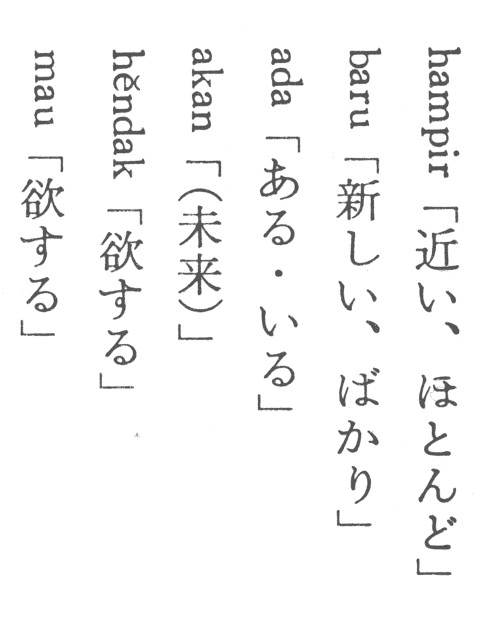
\includegraphics[width=500pt,height=624pt,]{Images/ja_vertical_indonesian_frag.jpg}
\caption{Detail from p.62 of \textit{インドネシア語". 崎山理. 1985. 外国語との対照 II. 講座日本語学 11.}}\end{figure}
\par
The text-orientation property allows us to indicate whether or not glyphs are rotated. In the following example, we have indicated that the list uses a \texttt{vertical-rl} writing mode, but that the orientation of individual glyphs may vary:\par\bgroup\index{list=<list>|exampleindex}\index{type=@type!<list>|exampleindex}\index{style=@style!<list>|exampleindex}\index{label=<label>|exampleindex}\index{item=<item>|exampleindex}\index{label=<label>|exampleindex}\index{item=<item>|exampleindex}\exampleFont \begin{shaded}\noindent\mbox{}{<\textbf{list}\hspace*{1em}{type}="{gloss}"\hspace*{1em}{xml:lang}="{ja}"\mbox{}\newline 
\hspace*{1em}{style}="{writing-mode: vertical-rl; text-orientation: mixed}">}\mbox{}\newline 
\hspace*{1em}{<\textbf{label}\hspace*{1em}{xml:lang}="{id}">}hampir{</\textbf{label}>}\mbox{}\newline 
\hspace*{1em}{<\textbf{item}>}{\textJapanese 「近い、ほとんど」}{</\textbf{item}>}\mbox{}\newline 
\hspace*{1em}{<\textbf{label}\hspace*{1em}{xml:lang}="{id}">}baru{</\textbf{label}>}\mbox{}\newline 
\hspace*{1em}{<\textbf{item}>}{\textJapanese 「新しい、ばかい」}{</\textbf{item}>}\mbox{}\newline 
\textit{<!--{\textJapanese  ... }-->}\mbox{}\newline 
{</\textbf{list}>}\end{shaded}\egroup\par \par
The rule \texttt{text-orientation: mixed} specifies that ‘characters from horizontal-only scripts are set sideways, i.e. 90° clockwise from their standard orientation in horizontal text. Characters from vertical scripts are set with their intrinsic orientation’ (\xref{http://www.w3.org/TR/css-writing-modes-3/\#text-orientation}{fantasai 2014}). Since the default value for \texttt{text-orientation} is \texttt{mixed}, this rule is not strictly required. However, if the Indonesian glyphs (which are roman characters) had been set vertically, like this:\par
\begin{figure}[htbp]
\noindent\noindent
\includegraphics[width=150pt,]{Images/ja_vertical_indonesian_frag_rotated.jpg}
\caption{Fragment of previous image with Indonesian glyphs upright.}\end{figure}
\par
then an encoding like the following could be used to make this explicit: \par\bgroup\index{list=<list>|exampleindex}\index{type=@type!<list>|exampleindex}\index{style=@style!<list>|exampleindex}\index{label=<label>|exampleindex}\index{item=<item>|exampleindex}\index{label=<label>|exampleindex}\index{item=<item>|exampleindex}\exampleFont \begin{shaded}\noindent\mbox{}{<\textbf{list}\hspace*{1em}{type}="{gloss}"\hspace*{1em}{xml:lang}="{ja}"\mbox{}\newline 
\hspace*{1em}{style}="{writing-mode: vertical-rl; text-orientation: upright}">}\mbox{}\newline 
\hspace*{1em}{<\textbf{label}\hspace*{1em}{xml:lang}="{id}">}hampir{</\textbf{label}>}\mbox{}\newline 
\hspace*{1em}{<\textbf{item}>}{\textJapanese 「近い、ほとんど」}{</\textbf{item}>}\mbox{}\newline 
\hspace*{1em}{<\textbf{label}\hspace*{1em}{xml:lang}="{id}">}baru{</\textbf{label}>}\mbox{}\newline 
\hspace*{1em}{<\textbf{item}>}{\textJapanese 「新しい、ばかい」}{</\textbf{item}>}\mbox{}\newline 
\textit{<!--{\textJapanese  ... }-->}\mbox{}\newline 
{</\textbf{list}>}\end{shaded}\egroup\par \par
The rule \texttt{text-orientation: upright} specifies that ‘characters from horizontal-only scripts are rendered upright, i.e. in their standard horizontal orientation. Characters from vertical scripts are set with their intrinsic orientation and shaped normally’ (\xref{http://www.w3.org/TR/css-writing-modes-3/\#text-orientation}{fantasai 2014}).
\subsubsection[{Vertical Orientation in Horizontal Scripts}]{Vertical Orientation in Horizontal Scripts}\label{WDWMEG3}\par
It is not unusual to see text from horizontal languages written vertically even where no vertically-written script is involved. This example is a fragment from a table of information about agricultural development on Vancouver Island, written in 1855: \par
\begin{figure}[htbp]
\noindent\noindent\includegraphics[width=450pt,]{Images/bcgenesis_co_305_06_00131v_table_extract.jpg}
\caption{Enclosure with \textit{Despatch to London} 10048, CO 305/6, p. 131v from \url{https://bcgenesis.uvic.ca/V55116.html}}\end{figure}
\par
Four of the subheading cells in this fragment contain English text written vertically, bottom-to-top, to conserve space on the page. To describe this sort of phenomenon, we can use the \texttt{text-orientation} property again:\par
\texttt{text-orientation: mixed | upright | sideways-right | sideways-left | sideways | use-glyph-orientation}\par
For full details on this property, we refer the reader to the CSS Writing Modes specification. For the present example, we will make use only of the ‘sideways-left’ value, which ‘causes text to be set as if in a horizontal layout, but rotated 90° counter-clockwise.’ We might encode the third of the four cells containing vertical text like this:\par\bgroup\index{cell=<cell>|exampleindex}\index{style=@style!<cell>|exampleindex}\index{lb=<lb>|exampleindex}\index{lb=<lb>|exampleindex}\index{lb=<lb>|exampleindex}\exampleFont \begin{shaded}\noindent\mbox{}{<\textbf{cell}\hspace*{1em}{style}="{writing-mode: vertical-lr; text-orientation: sideways-left}">}\mbox{}\newline 
\hspace*{1em}{<\textbf{lb}/>}Cash Value\mbox{}\newline 
{<\textbf{lb}/>}of\mbox{}\newline 
{<\textbf{lb}/>}Farms\mbox{}\newline 
\mbox{}\newline 
{</\textbf{cell}>}\end{shaded}\egroup\par \par
The \texttt{writing-mode} property captures the fact that the script is written vertically, and its lines are to be read from left to right (so the line containing ‘of’ is to the right of that containing ‘Cash value’), while the \texttt{text-orientation} value encodes the orientation (rotated 90° counter-clockwise). We might also add \texttt{text-align: center} to the style, to express the fact that the text is centrally-aligned.
\subsubsection[{Bottom-to-top Writing}]{Bottom-to-top Writing}\label{WDWMEG4}\par
Of the rather small number of scripts which appear to be written bottom-to-top, perhaps the best-known is Ogham, an alphabet used mainly to write Archaic Irish. Ogham is typically found inscribed along the edge of a standing stone, starting at its base. The CSS Writing Modes specification does not explicitly distinguish between vertical scripts which are written top-to-bottom and those which are written bottom-to-top. Instead, such bottom-to-top scripts are best treated as left-to-right horizontal scripts, oriented vertically because of the constraints of the medium on which they are inscribed. Such scripts are analogous to the vertical English text-runs in the table cells in the example above, and can be handled in exactly the same manner (\texttt{writing-mode: vertical-lr; text-orientation: sideways-left}). In cases where writing follows a curved path (such as Ogham running around the edge of a stone), a meticulous encoder might resort to the use of SVG to describe the path, rather than treating the phenomenon as a writing mode.
\subsubsection[{Mixed Horizontal Directionality}]{Mixed Horizontal Directionality}\label{WDWMEG5}\par
Returning to our previous simple example \par\hfill\bgroup\exampleFont\vskip 10pt\begin{shaded}
\obeyspaces The Arabic term قلم رصاص means "pencil".\end{shaded}
\par\egroup 
\par
we could use the direction property to make directionality explicit:\par
\texttt{direction: ltr | rtl}\par\bgroup\index{s=<s>|exampleindex}\index{style=@style!<s>|exampleindex}\index{term=<term>|exampleindex}\index{style=@style!<term>|exampleindex}\exampleFont \begin{shaded}\noindent\mbox{}{<\textbf{s}\hspace*{1em}{xml:lang}="{en}"\hspace*{1em}{style}="{direction: ltr}">}The Arabic term\mbox{}\newline 
{<\textbf{term}\hspace*{1em}{xml:lang}="{ar}"\mbox{}\newline 
\hspace*{1em}\hspace*{1em}{style}="{direction: rtl; unicode-bidi: embed}">}\hbox{قلم رصاص}{</\textbf{term}>} means "pencil".{</\textbf{s}>}\end{shaded}\egroup\par \par
The use of the \texttt{direction} property to record the observed directionality of the text is unambiguous, even though it is (as we noted above) superfluous. The use of the \texttt{unicode-bidi} property here may require some explanation. By default this property has the value ‘normal’, the effect of which in this context would be to ignore any value supplied for the direction property. The CSS Writing Modes specification stipulates that the direction property ‘has no effect on bidi reordering when specified on inline boxes whose \texttt{unicode-bidi} property’s value is ‘normal’, because the element does not open an additional level of embedding with respect to the bidirectional algorithm.’\par
Mixed horizontal directionality is very common in languages such as Arabic and Hebrew, particularly when numbers (which are always given LTR) or phrases from LTR languages are embedded. It is not impossible, though quite unusual, for ambiguities to arise in such situations, which may give rise to the parts of a document being displayed in unexpected ways that do not correspond to the natural reading order. A more detailed discussion of this issue from an HTML perspective is provided by a W3C Internationalization Working Group report \xref{http://www.w3.org/International/articles/inline-bidi-markup/\#where}{Inline markup and bidirectional text in HTML}.
\subsubsection[{Summary}]{Summary}\par
For most texts, information about text directionality need not be explicitly encoded in a TEI text, either because it follows unambiguously from {\itshape xml:lang} values, or because it can be expected to be handled unequivocally by the Unicode Bidi Algorithm. Where it is considered important to encode such information, properties and values taken from the CSS Writing Modes module may be used by means of the global TEI {\itshape style} attribute (or using the TEI \hyperref[TEI.rendition]{<rendition>} element, linked with the {\itshape rendition} attribute). Most phenomena can be well described in this way; of those which cannot, other approaches based on the CSS Transforms module are presented in the next section.
\subsection[{Text Rotation}]{Text Rotation}\label{WDWMTT}\par
In what follows, we examine a range of textual phenomena which in some ways appear very similar to those examined above, and even overlap with them. We can categorize these as text transformation features, and suggest some strategies for encoding them based on the properties detailed in the \hyperref[CSSTM]{CSS Transforms (Fraser et al 2013)} specification. This CSS module provides a complex array of properties, values and functions which can be used to rotate, skew, translate and otherwise transform textual and graphical objects. We can borrow this vocabulary in order to describe textual phenomena in a precise manner.\par
We begin with a simple example of a rotational transform: \par
\begin{figure}[htbp]
\noindent\noindent\includegraphics[]{Images/rotation_on_z_axis.png}\end{figure}
\par
Here a block of text has been rotated around its z-axis. This is clearly not a ‘writing mode’; the writing mode for this text is horizontal, left to right. Furthermore, even if we wished to treat this as a writing mode, we could not do so, because there is no way to use writing modes properties to describe an text orientation which is angled at 45 degrees; no human languages are consistently written in this orientation. It is more appropriate to treat this as a rotational transformation. We can do this using two properties: \texttt{transform} and \texttt{transform-origin}. (Both of these properties have quite complex value sets, and we will not look at all of them here. See the \hyperref[CSSTM]{specification} for full details.)\par
The \texttt{transform} property takes as its value one or more of the transform functions, one of which is the function \texttt{rotateZ()}:\par\bgroup\index{ab=<ab>|exampleindex}\index{style=@style!<ab>|exampleindex}\exampleFont \begin{shaded}\noindent\mbox{}{<\textbf{ab}\hspace*{1em}{style}="{transform:rotateZ(-45deg)}">}TEI-C.ORG{</\textbf{ab}>}\end{shaded}\egroup\par \par
Any rotation must take place clockwise around an axis positioned relative to the element being rotated, and the \texttt{transform-origin} property can be used to specify the pivot point. By default, the value of \texttt{transform-origin} is ‘50\% 50\%’, the point at the centre of the element, but these values can be changed to reflect rotation around a different origin point. (The TEI \hyperref[TEI.zone]{<zone>} element also bears an attribute {\itshape rotate} which can specify rotation in degrees around the z-axis, but it is not available for any other element.)\par
A block of text may also be rotated about either of its other axes. For example, this shows rotation around the Y (vertical) axis: \par
\begin{figure}[htbp]
\noindent\noindent\includegraphics[]{Images/rotation_on_y_axis.png}\end{figure}
\par\bgroup\index{ab=<ab>|exampleindex}\index{style=@style!<ab>|exampleindex}\exampleFont \begin{shaded}\noindent\mbox{}{<\textbf{ab}\hspace*{1em}{style}="{transform:rotateY(45deg)}">}TEI-C.ORG{</\textbf{ab}>}\end{shaded}\egroup\par \par
These are obviously trivial examples, but similar features do appear in historical texts. George Herbert's \textit{The Temple} includes two stanzas headed ‘Easter Wings’ which are both normally printed in a rotated form so that they represent a pair of wings:\par
\begin{figure}[htbp]
\noindent\noindent\includegraphics[width=300pt,]{Images/herbert_church_p35_sm.jpg}
\caption{Page 35 of George Herbert's \textit{The Temple} (1633), from a copy in the Folger Library.}\end{figure}
\par
This could be encoded thus: \par\bgroup\index{lg=<lg>|exampleindex}\index{style=@style!<lg>|exampleindex}\index{l=<l>|exampleindex}\index{l=<l>|exampleindex}\exampleFont \begin{shaded}\noindent\mbox{}{<\textbf{lg}\hspace*{1em}{style}="{transform:rotateZ(90deg)}">}\mbox{}\newline 
\hspace*{1em}{<\textbf{l}>}My tender age in ſorrow did beginne:{</\textbf{l}>}\mbox{}\newline 
\hspace*{1em}{<\textbf{l}>}And ſtill with ſickneſſes and ſhame{</\textbf{l}>}\mbox{}\newline 
\textit{<!-- ... -->}\mbox{}\newline 
{</\textbf{lg}>}\end{shaded}\egroup\par \par
We might also argue that this is in fact a vertical writing mode by supplying \texttt{writing-mode: vertical-rl; text-orientation: sideways-right} as the value for the {\itshape style} attribute in the preceding example.\par
Rotation is also useful as a method of handling a true writing mode which is not covered by the CSS Writing Modes: \textit{boustrophedon}. This is a writing mode common in inscriptions in Latin, Greek and other languages, in which alternate lines run from left to right and from right to left\footnote{The name is taken from the Greek βουστροφηδόν, meaning ‘ox-turning’ from βοῦς (an ox) and στροφή (‘turn’); that is, turning as an ox does when pulling a plough.}. Right-to-left lines in boustrophedon have another unexpected feature: their glyphs are reversed, so that these lines appear as ‘mirror writing’, as in the following ancient Greek inscription: \begin{figure}[htbp]
\noindent\noindent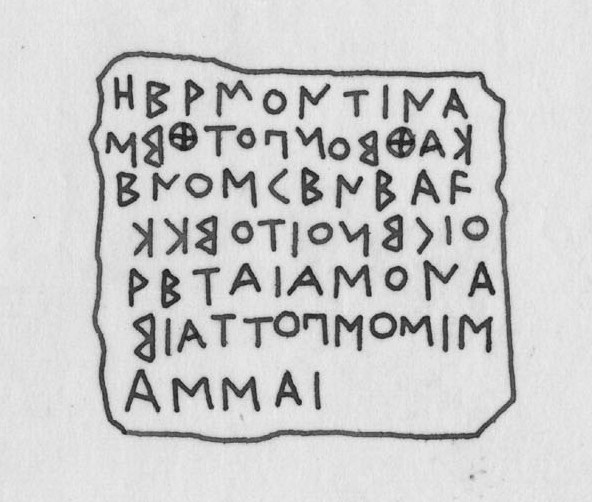
\includegraphics[width=592pt,height=502pt,]{Images/boustrophedon_small_J_NW_Epeiros_13_p03.jpg}
\caption{Leaden plaque bearing an inquiry by Hermon from the oracular precinct at Dodona. (L.H. Jeffery Archive)}\end{figure}
\par
This might be transcribed as follows (ignoring word boundaries for the moment): \par\bgroup\index{ab=<ab>|exampleindex}\index{lb=<lb>|exampleindex}\index{lb=<lb>|exampleindex}\index{seg=<seg>|exampleindex}\index{style=@style!<seg>|exampleindex}\index{lb=<lb>|exampleindex}\index{lb=<lb>|exampleindex}\index{seg=<seg>|exampleindex}\index{style=@style!<seg>|exampleindex}\index{lb=<lb>|exampleindex}\index{lb=<lb>|exampleindex}\index{seg=<seg>|exampleindex}\index{style=@style!<seg>|exampleindex}\index{lb=<lb>|exampleindex}\exampleFont \begin{shaded}\noindent\mbox{}{<\textbf{ab}>}\mbox{}\newline 
\hspace*{1em}{<\textbf{lb}/>}ΗΕΡΜΟΝΤΙΝA\mbox{}\newline 
{<\textbf{lb}/>}\mbox{}\newline 
\hspace*{1em}{<\textbf{seg}\hspace*{1em}{style}="{rotateY(180deg)}">}ΚΑΘΕΟΝΠΟΤΘΕΜ{</\textbf{seg}>}\mbox{}\newline 
\hspace*{1em}{<\textbf{lb}/>}ΕΝΟΣΥΕΝΕΑϜ\mbox{}\newline 
{<\textbf{lb}/>}\mbox{}\newline 
\hspace*{1em}{<\textbf{seg}\hspace*{1em}{style}="{rotateY(180deg)}">}ΟΙΥΕΝΟΙΤΙΕΚΚ{</\textbf{seg}>}\mbox{}\newline 
\hspace*{1em}{<\textbf{lb}/>}ΡΕΤΑΙΑΣΟΝΑ\mbox{}\newline 
{<\textbf{lb}/>}\mbox{}\newline 
\hspace*{1em}{<\textbf{seg}\hspace*{1em}{style}="{rotateY(180deg)}">}ΣΙΜΟΣΟΤΤΑΙΕ{</\textbf{seg}>}\mbox{}\newline 
\hspace*{1em}{<\textbf{lb}/>}ΑΣΣΑΙ\mbox{}\newline 
\mbox{}\newline 
{</\textbf{ab}>}\end{shaded}\egroup\par \par
The 180-degree rotation around the Y (vertical) axis here describes what is happening in the RTL line in boustrophedon; the order of glyphs is reversed, and so is their individual orientation (in fact, we see them ‘from the back’, as it were). \hyperref[TEI.seg]{<seg>} elements have been used here because these are clearly not ‘lines’ in the sense of poetic lines; the text is continuous prose, and linebreaks are incidental.\par
There are obviously some unsatisfactory aspects of this manner of encoding boustrophedon. In the inscription above, some words run across linebreaks, so if we wished to tag both words and the right-to-left phenomena, one hierarchy would have to be privileged over the other. By using a transform function rather than a writing mode property, we are apparently suggesting that boustrophedon is not in fact a writing mode, whereas it clearly is. But the CSS Writing Modes specification does not provide support for boustrophedon, because it is a rather obscure historical phenomenon; using a rotational transform is one practical alternative. 
\subsection[{Caveat}]{Caveat}\label{WDCAV}\par
As with other parts of the CSS specification, the intended effect of CSS Transforms properties and values is defined with reference to a specific \xref{http://www.w3.org/TR/CSS2/visuren.html}{Visual formatting model}; the language is designed to describe how an HTML document should be formatted. This is not, of course, the case for the TEI, which lacks any explicit processing or formatting model, and attempts to define objects as far as possible without consideration of their visual appearance. As long as the properties and values from the CSS Transforms module are used as a convenient, well-specified descriptive language to capture features of a text, without any expectation of using them directly and reliably for rendering, this is not particularly problematic. CSS provides a useful and well-defined vocabulary to describe many aspects of the appearance of source texts, benefitting particularly from the clarity of definition provided by the specification. However, if there is any expectation of using this information to render a text in a predictable and accurate way, it will be essential to provide enough styling information throughout the document hierarchy to resolve all ambiguities with regard to size, positioning, block status, etc. before any element undergoes a transform operation.
\subsection[{Formal Definition}]{Formal Definition}\label{WSD-DEF}\par
The gaiji module described in this chapter makes available the following components: \begin{description}

\item[{Module gaiji: Character and glyph documentation}]\hspace{1em}\hfill\linebreak
\mbox{}\\[-10pt] \begin{itemize}
\item {\itshape Elements defined}: \hyperref[TEI.char]{char} \hyperref[TEI.charDecl]{charDecl} \hyperref[TEI.charName]{charName} \hyperref[TEI.charProp]{charProp} \hyperref[TEI.g]{g} \hyperref[TEI.glyph]{glyph} \hyperref[TEI.glyphName]{glyphName} \hyperref[TEI.localName]{localName} \hyperref[TEI.localProp]{localProp} \hyperref[TEI.mapping]{mapping} \hyperref[TEI.unicodeName]{unicodeName} \hyperref[TEI.unicodeProp]{unicodeProp} \hyperref[TEI.unihanProp]{unihanProp} \hyperref[TEI.value]{value}
\item {\itshape Classes defined}: \hyperref[TEI.att.gaijiProp]{att.gaijiProp}
\end{itemize} 
\end{description}  The selection and combination of modules to form a TEI schema is described in \textit{\hyperref[STIN]{1.2.\ Defining a TEI Schema}}.

\section[{Verse}]{Verse}\label{VE}\par
This module is intended for use when encoding texts which are entirely or predominantly in verse, and for which the elements for encoding verse structure already provided by the core module are inadequate.\par
The tags described in section \textit{\hyperref[COVE]{3.13.1.\ Core Tags for Verse}} include elements for the encoding of verse lines and line groups such as stanzas: these are available for any TEI document, irrespective of the module it uses. Like the modules for prose and for drama, the module for verse additionally makes use of the module defined in chapter \textit{\hyperref[DS]{4.\ Default Text Structure}} to define the basic formal structure of a text, in terms of \hyperref[TEI.front]{<front>}, \hyperref[TEI.body]{<body>} and \hyperref[TEI.back]{<back>} elements and the text-division elements into which these may be subdivided.\par
The module for verse extends the facilities provided by these modules in the following ways: \begin{itemize}
\item a special purpose \hyperref[TEI.caesura]{<caesura>} element is provided, to allow for segmentation of the verse line (see section \textit{\hyperref[VESE]{6.2.\ Components of the Verse Line}})
\item a set of attributes is provided for the encoding of rhyme scheme and metrical information (see sections \textit{\hyperref[VEME]{6.4.\ Rhyme and Metrical Analysis}} and \textit{\hyperref[VERH]{6.5.\ Rhyme}})
\item a special purpose \hyperref[TEI.rhyme]{<rhyme>} element is provided to support simple analysis of rhyming words (see section \textit{\hyperref[VERH]{6.5.\ Rhyme}})
\end{itemize} 
\subsection[{Structural Divisions of Verse Texts}]{Structural Divisions of Verse Texts}\label{VEST}\par
Like other kinds of text, texts written in verse may be of widely differing lengths and structures. A complete poem, no matter how short, may be treated as a free-standing text, and encoded in the same way as a distinct prose text. A group of poems functioning as a single unit may be encoded either as a \hyperref[TEI.group]{<group>} or as a \hyperref[TEI.text]{<text>}, depending on the encoder's view of the text. For further discussion, including an example encoding for a verse anthology, see chapter \textit{\hyperref[DS]{4.\ Default Text Structure}}.\par
Many poems consist only of ungrouped lines.                        This short poem by Emily Dickinson is a simple case: \par\bgroup\index{text=<text>|exampleindex}\index{front=<front>|exampleindex}\index{head=<head>|exampleindex}\index{body=<body>|exampleindex}\index{l=<l>|exampleindex}\index{l=<l>|exampleindex}\index{l=<l>|exampleindex}\index{l=<l>|exampleindex}\index{l=<l>|exampleindex}\exampleFont \begin{shaded}\noindent\mbox{}{<\textbf{text}>}\mbox{}\newline 
\hspace*{1em}{<\textbf{front}>}\mbox{}\newline 
\hspace*{1em}\hspace*{1em}{<\textbf{head}>}1755{</\textbf{head}>}\mbox{}\newline 
\hspace*{1em}{</\textbf{front}>}\mbox{}\newline 
\hspace*{1em}{<\textbf{body}>}\mbox{}\newline 
\hspace*{1em}\hspace*{1em}{<\textbf{l}>}To make a prairie it takes a clover and one bee,{</\textbf{l}>}\mbox{}\newline 
\hspace*{1em}\hspace*{1em}{<\textbf{l}>}One clover, and a bee,{</\textbf{l}>}\mbox{}\newline 
\hspace*{1em}\hspace*{1em}{<\textbf{l}>}And revery.{</\textbf{l}>}\mbox{}\newline 
\hspace*{1em}\hspace*{1em}{<\textbf{l}>}The revery alone will do,{</\textbf{l}>}\mbox{}\newline 
\hspace*{1em}\hspace*{1em}{<\textbf{l}>}If bees are few.{</\textbf{l}>}\mbox{}\newline 
\hspace*{1em}{</\textbf{body}>}\mbox{}\newline 
{</\textbf{text}>}\end{shaded}\egroup\par \noindent    \par
Often, however, lines are grouped, formally or informally, into stanzas, verse paragraphs, etc. The \hyperref[TEI.lg]{<lg>} element defined in the core tag set (in section \textit{\hyperref[COVE]{3.13.1.\ Core Tags for Verse}}) may be used for all such groupings. It may thus serve for informal groupings of lines such as those of the following example from Allen Ginsberg: \par\bgroup\index{text=<text>|exampleindex}\index{body=<body>|exampleindex}\index{head=<head>|exampleindex}\index{lg=<lg>|exampleindex}\index{l=<l>|exampleindex}\index{l=<l>|exampleindex}\index{l=<l>|exampleindex}\index{l=<l>|exampleindex}\index{lg=<lg>|exampleindex}\index{l=<l>|exampleindex}\index{l=<l>|exampleindex}\index{l=<l>|exampleindex}\index{l=<l>|exampleindex}\exampleFont \begin{shaded}\noindent\mbox{}{<\textbf{text}>}\mbox{}\newline 
\hspace*{1em}{<\textbf{body}>}\mbox{}\newline 
\hspace*{1em}\hspace*{1em}{<\textbf{head}>}My Alba{</\textbf{head}>}\mbox{}\newline 
\hspace*{1em}\hspace*{1em}{<\textbf{lg}>}\mbox{}\newline 
\hspace*{1em}\hspace*{1em}\hspace*{1em}{<\textbf{l}>}Now that I've wasted{</\textbf{l}>}\mbox{}\newline 
\hspace*{1em}\hspace*{1em}\hspace*{1em}{<\textbf{l}>}five years in Manhattan{</\textbf{l}>}\mbox{}\newline 
\hspace*{1em}\hspace*{1em}\hspace*{1em}{<\textbf{l}>}life decaying{</\textbf{l}>}\mbox{}\newline 
\hspace*{1em}\hspace*{1em}\hspace*{1em}{<\textbf{l}>}talent a blank{</\textbf{l}>}\mbox{}\newline 
\hspace*{1em}\hspace*{1em}{</\textbf{lg}>}\mbox{}\newline 
\hspace*{1em}\hspace*{1em}{<\textbf{lg}>}\mbox{}\newline 
\hspace*{1em}\hspace*{1em}\hspace*{1em}{<\textbf{l}>}talking disconnected{</\textbf{l}>}\mbox{}\newline 
\hspace*{1em}\hspace*{1em}\hspace*{1em}{<\textbf{l}>}patient and mental{</\textbf{l}>}\mbox{}\newline 
\hspace*{1em}\hspace*{1em}\hspace*{1em}{<\textbf{l}>}sliderule and number{</\textbf{l}>}\mbox{}\newline 
\hspace*{1em}\hspace*{1em}\hspace*{1em}{<\textbf{l}>}machine on a desk{</\textbf{l}>}\mbox{}\newline 
\hspace*{1em}\hspace*{1em}{</\textbf{lg}>}\mbox{}\newline 
\hspace*{1em}{</\textbf{body}>}\mbox{}\newline 
{</\textbf{text}>}\end{shaded}\egroup\par \noindent    \par
It may also be used to mark the verse paragraphs into which longer poems are often divided, as in the following example from Samuel Taylor Coleridge's \textit{Frost at Midnight}: \par\bgroup\index{lg=<lg>|exampleindex}\index{l=<l>|exampleindex}\index{l=<l>|exampleindex}\index{l=<l>|exampleindex}\index{l=<l>|exampleindex}\index{l=<l>|exampleindex}\index{l=<l>|exampleindex}\index{part=@part!<l>|exampleindex}\index{lg=<lg>|exampleindex}\index{l=<l>|exampleindex}\index{part=@part!<l>|exampleindex}\index{l=<l>|exampleindex}\index{l=<l>|exampleindex}\index{l=<l>|exampleindex}\index{hi=<hi>|exampleindex}\index{lg=<lg>|exampleindex}\index{l=<l>|exampleindex}\exampleFont \begin{shaded}\noindent\mbox{}{<\textbf{lg}>}\mbox{}\newline 
\hspace*{1em}{<\textbf{l}>}The Frost performs its secret ministry,{</\textbf{l}>}\mbox{}\newline 
\hspace*{1em}{<\textbf{l}>}Unhelped by any wind. ...{</\textbf{l}>}\mbox{}\newline 
\hspace*{1em}{<\textbf{l}>}Whose puny flaps and freaks the idling Spirit{</\textbf{l}>}\mbox{}\newline 
\hspace*{1em}{<\textbf{l}>}By its own moods interprets, every where{</\textbf{l}>}\mbox{}\newline 
\hspace*{1em}{<\textbf{l}>}Echo or mirror seeking of itself,{</\textbf{l}>}\mbox{}\newline 
\hspace*{1em}{<\textbf{l}\hspace*{1em}{part}="{I}">}And makes a toy of Thought.{</\textbf{l}>}\mbox{}\newline 
{</\textbf{lg}>}\mbox{}\newline 
{<\textbf{lg}>}\mbox{}\newline 
\hspace*{1em}{<\textbf{l}\hspace*{1em}{part}="{F}">}But O! how oft,{</\textbf{l}>}\mbox{}\newline 
\hspace*{1em}{<\textbf{l}>}How oft, at school, with most believing mind{</\textbf{l}>}\mbox{}\newline 
\hspace*{1em}{<\textbf{l}>}Presageful, have I gazed upon the bars,{</\textbf{l}>}\mbox{}\newline 
\hspace*{1em}{<\textbf{l}>}To watch that fluttering {<\textbf{hi}>}stranger{</\textbf{hi}>}! ... {</\textbf{l}>}\mbox{}\newline 
{</\textbf{lg}>}\mbox{}\newline 
{<\textbf{lg}>}\mbox{}\newline 
\hspace*{1em}{<\textbf{l}>}Dear Babe, that sleepest cradled by my side,{</\textbf{l}>}\mbox{}\newline 
{</\textbf{lg}>}\end{shaded}\egroup\par \noindent   Note, in the above example, the use of the {\itshape part} attribute on the \hyperref[TEI.l]{<l>} element, where a verse line is broken between two line groups, as discussed in section \textit{\hyperref[COVE]{3.13.1.\ Core Tags for Verse}}.\par
Most typically, however, the \hyperref[TEI.lg]{<lg>} element is used to mark the highly regular line groups which characterize stanzaic and similar verse forms, as in the following example from Chaucer: \par\bgroup\index{lg=<lg>|exampleindex}\index{l=<l>|exampleindex}\index{l=<l>|exampleindex}\index{l=<l>|exampleindex}\index{l=<l>|exampleindex}\index{l=<l>|exampleindex}\index{l=<l>|exampleindex}\index{lg=<lg>|exampleindex}\index{l=<l>|exampleindex}\index{l=<l>|exampleindex}\exampleFont \begin{shaded}\noindent\mbox{}{<\textbf{lg}>}\mbox{}\newline 
\hspace*{1em}{<\textbf{l}>}Sire Thopas was a doghty swayn;{</\textbf{l}>}\mbox{}\newline 
\hspace*{1em}{<\textbf{l}>}White was his face as payndemayn,{</\textbf{l}>}\mbox{}\newline 
\hspace*{1em}{<\textbf{l}>}His lippes rede as rose;{</\textbf{l}>}\mbox{}\newline 
\hspace*{1em}{<\textbf{l}>}His rode is lyk scarlet in grayn,{</\textbf{l}>}\mbox{}\newline 
\hspace*{1em}{<\textbf{l}>}And I yow telle in good certayn,{</\textbf{l}>}\mbox{}\newline 
\hspace*{1em}{<\textbf{l}>}He hadde a semely nose.{</\textbf{l}>}\mbox{}\newline 
{</\textbf{lg}>}\mbox{}\newline 
{<\textbf{lg}>}\mbox{}\newline 
\hspace*{1em}{<\textbf{l}>}His heer, his ber was lyk saffroun,{</\textbf{l}>}\mbox{}\newline 
\hspace*{1em}{<\textbf{l}>}That to his girdel raughte adoun;{</\textbf{l}>}\mbox{}\newline 
{</\textbf{lg}>}\end{shaded}\egroup\par \noindent  \par
Like other text-division elements, \hyperref[TEI.lg]{<lg>} elements may be nested hierarchically. For example, one particularly common English stanzaic form consists of a quatrain or sestet followed by a couplet. The \hyperref[TEI.lg]{<lg>} element may be used to encode both the stanza and its components, as in the following example from Byron: \par\bgroup\index{lg=<lg>|exampleindex}\index{type=@type!<lg>|exampleindex}\index{lg=<lg>|exampleindex}\index{type=@type!<lg>|exampleindex}\index{l=<l>|exampleindex}\index{l=<l>|exampleindex}\index{l=<l>|exampleindex}\index{l=<l>|exampleindex}\index{l=<l>|exampleindex}\index{l=<l>|exampleindex}\index{lg=<lg>|exampleindex}\index{type=@type!<lg>|exampleindex}\index{l=<l>|exampleindex}\index{l=<l>|exampleindex}\exampleFont \begin{shaded}\noindent\mbox{}{<\textbf{lg}\hspace*{1em}{type}="{stanza}">}\mbox{}\newline 
\hspace*{1em}{<\textbf{lg}\hspace*{1em}{type}="{sestet}">}\mbox{}\newline 
\hspace*{1em}\hspace*{1em}{<\textbf{l}>}In the first year of Freedom's second dawn{</\textbf{l}>}\mbox{}\newline 
\hspace*{1em}\hspace*{1em}{<\textbf{l}>}Died George the Third; although no tyrant, one{</\textbf{l}>}\mbox{}\newline 
\hspace*{1em}\hspace*{1em}{<\textbf{l}>}Who shielded tyrants, till each sense withdrawn{</\textbf{l}>}\mbox{}\newline 
\hspace*{1em}\hspace*{1em}{<\textbf{l}>}Left him nor mental nor external sun:{</\textbf{l}>}\mbox{}\newline 
\hspace*{1em}\hspace*{1em}{<\textbf{l}>}A better farmer ne'er brushed dew from lawn,{</\textbf{l}>}\mbox{}\newline 
\hspace*{1em}\hspace*{1em}{<\textbf{l}>}A worse king never left a realm undone!{</\textbf{l}>}\mbox{}\newline 
\hspace*{1em}{</\textbf{lg}>}\mbox{}\newline 
\hspace*{1em}{<\textbf{lg}\hspace*{1em}{type}="{couplet}">}\mbox{}\newline 
\hspace*{1em}\hspace*{1em}{<\textbf{l}>}He died — but left his subjects still behind,{</\textbf{l}>}\mbox{}\newline 
\hspace*{1em}\hspace*{1em}{<\textbf{l}>}One half as mad — and t'other no less blind.{</\textbf{l}>}\mbox{}\newline 
\hspace*{1em}{</\textbf{lg}>}\mbox{}\newline 
{</\textbf{lg}>}\end{shaded}\egroup\par \noindent  \par
Note the use of the {\itshape type} attribute to name the type of unit encoded by the \hyperref[TEI.lg]{<lg>} element; this attribute is common to all members of the \textsf{att.divLike} class (see section \textit{\hyperref[DSDIV1]{4.1.1.\ Un-numbered Divisions}}).\footnote{For discussion of other attributes of this class, see \textit{\hyperref[DSDIV3X]{4.1.4.\ Partial and Composite Divisions}}.} When used on \hyperref[TEI.lg]{<lg>}, the {\itshape type} attribute is intended solely for conventional names of different classes of text block. For systematic analysis of metrical and rhyme schemes, use the {\itshape met} and {\itshape rhyme} attributes, for which see below, section \textit{\hyperref[VEME]{6.4.\ Rhyme and Metrical Analysis}}.\par
As a further example, consider the Shakespearean sonnet. This may be divided into two parts: a concluding couplet, and a body of twelve lines, itself subdivided into three quatrains:    \par\bgroup\index{text=<text>|exampleindex}\index{body=<body>|exampleindex}\index{lg=<lg>|exampleindex}\index{lg=<lg>|exampleindex}\index{type=@type!<lg>|exampleindex}\index{l=<l>|exampleindex}\index{l=<l>|exampleindex}\index{l=<l>|exampleindex}\index{l=<l>|exampleindex}\index{lg=<lg>|exampleindex}\index{type=@type!<lg>|exampleindex}\index{l=<l>|exampleindex}\index{l=<l>|exampleindex}\index{l=<l>|exampleindex}\index{l=<l>|exampleindex}\index{lg=<lg>|exampleindex}\index{type=@type!<lg>|exampleindex}\index{l=<l>|exampleindex}\index{l=<l>|exampleindex}\index{l=<l>|exampleindex}\index{l=<l>|exampleindex}\index{lg=<lg>|exampleindex}\index{type=@type!<lg>|exampleindex}\index{l=<l>|exampleindex}\index{l=<l>|exampleindex}\exampleFont \begin{shaded}\noindent\mbox{}{<\textbf{text}>}\mbox{}\newline 
\hspace*{1em}{<\textbf{body}>}\mbox{}\newline 
\hspace*{1em}\hspace*{1em}{<\textbf{lg}>}\mbox{}\newline 
\hspace*{1em}\hspace*{1em}\hspace*{1em}{<\textbf{lg}\hspace*{1em}{type}="{quatrain}">}\mbox{}\newline 
\hspace*{1em}\hspace*{1em}\hspace*{1em}\hspace*{1em}{<\textbf{l}>}My Mistres eyes are nothing like the Sunne,{</\textbf{l}>}\mbox{}\newline 
\hspace*{1em}\hspace*{1em}\hspace*{1em}\hspace*{1em}{<\textbf{l}>}Currall is farre more red, then her lips red{</\textbf{l}>}\mbox{}\newline 
\hspace*{1em}\hspace*{1em}\hspace*{1em}\hspace*{1em}{<\textbf{l}>}If snow be white, why then her brests are dun:{</\textbf{l}>}\mbox{}\newline 
\hspace*{1em}\hspace*{1em}\hspace*{1em}\hspace*{1em}{<\textbf{l}>}If haires be wiers, black wiers grown on her head:{</\textbf{l}>}\mbox{}\newline 
\hspace*{1em}\hspace*{1em}\hspace*{1em}{</\textbf{lg}>}\mbox{}\newline 
\hspace*{1em}\hspace*{1em}\hspace*{1em}{<\textbf{lg}\hspace*{1em}{type}="{quatrain}">}\mbox{}\newline 
\hspace*{1em}\hspace*{1em}\hspace*{1em}\hspace*{1em}{<\textbf{l}>}I have seene Roses damaskt, red and white,{</\textbf{l}>}\mbox{}\newline 
\hspace*{1em}\hspace*{1em}\hspace*{1em}\hspace*{1em}{<\textbf{l}>}But no such Roses see I in her cheekes,{</\textbf{l}>}\mbox{}\newline 
\hspace*{1em}\hspace*{1em}\hspace*{1em}\hspace*{1em}{<\textbf{l}>}And in some perfumes is there more delight,{</\textbf{l}>}\mbox{}\newline 
\hspace*{1em}\hspace*{1em}\hspace*{1em}\hspace*{1em}{<\textbf{l}>}Then in the breath that from my Mistres reekes.{</\textbf{l}>}\mbox{}\newline 
\hspace*{1em}\hspace*{1em}\hspace*{1em}{</\textbf{lg}>}\mbox{}\newline 
\hspace*{1em}\hspace*{1em}\hspace*{1em}{<\textbf{lg}\hspace*{1em}{type}="{quatrain}">}\mbox{}\newline 
\hspace*{1em}\hspace*{1em}\hspace*{1em}\hspace*{1em}{<\textbf{l}>}I love to heare her speake, yet well I know,{</\textbf{l}>}\mbox{}\newline 
\hspace*{1em}\hspace*{1em}\hspace*{1em}\hspace*{1em}{<\textbf{l}>}That Musicke hath a farre more pleasing sound:{</\textbf{l}>}\mbox{}\newline 
\hspace*{1em}\hspace*{1em}\hspace*{1em}\hspace*{1em}{<\textbf{l}>}I graunt I never saw a goddesse goe,{</\textbf{l}>}\mbox{}\newline 
\hspace*{1em}\hspace*{1em}\hspace*{1em}\hspace*{1em}{<\textbf{l}>}My Mistres when shee walkes treads on the ground.{</\textbf{l}>}\mbox{}\newline 
\hspace*{1em}\hspace*{1em}\hspace*{1em}{</\textbf{lg}>}\mbox{}\newline 
\hspace*{1em}\hspace*{1em}{</\textbf{lg}>}\mbox{}\newline 
\hspace*{1em}\hspace*{1em}{<\textbf{lg}\hspace*{1em}{type}="{couplet}">}\mbox{}\newline 
\hspace*{1em}\hspace*{1em}\hspace*{1em}{<\textbf{l}>}And yet by heaven I think my love as rare,{</\textbf{l}>}\mbox{}\newline 
\hspace*{1em}\hspace*{1em}\hspace*{1em}{<\textbf{l}>}As any she beli'd with false compare.{</\textbf{l}>}\mbox{}\newline 
\hspace*{1em}\hspace*{1em}{</\textbf{lg}>}\mbox{}\newline 
\hspace*{1em}{</\textbf{body}>}\mbox{}\newline 
{</\textbf{text}>}\end{shaded}\egroup\par \noindent  \par
Particularly lengthy poetic texts are often subdivided into units larger than stanzas or paragraphs, which may themselves be subdivided. Spenser's \textit{Faery Queene}, for example, consists of twelve ‘books’ each of which contains a prologue followed by twelve ‘cantos’. Each prologue and each canto consists of nine-line ‘stanzas’, each of which follows the same regular pattern. Other examples in the same tradition are easy to find.\par
Large structures of this kind are most conveniently represented by \hyperref[TEI.div]{<div>} or \hyperref[TEI.div1]{<div1>} elements, as described in section \textit{\hyperref[DSDIV]{4.1.\ Divisions of the Body}}. Thus the start of the \textit{Faerie Queene} might be encoded as follows: \par\bgroup\index{body=<body>|exampleindex}\index{div=<div>|exampleindex}\index{n=@n!<div>|exampleindex}\index{type=@type!<div>|exampleindex}\index{div=<div>|exampleindex}\index{n=@n!<div>|exampleindex}\index{type=@type!<div>|exampleindex}\index{lg=<lg>|exampleindex}\index{n=@n!<lg>|exampleindex}\index{type=@type!<lg>|exampleindex}\index{l=<l>|exampleindex}\index{l=<l>|exampleindex}\exampleFont \begin{shaded}\noindent\mbox{}{<\textbf{body}>}\mbox{}\newline 
\hspace*{1em}{<\textbf{div}\hspace*{1em}{n}="{I}"\hspace*{1em}{type}="{book}">}\mbox{}\newline 
\hspace*{1em}\hspace*{1em}{<\textbf{div}\hspace*{1em}{n}="{1}"\hspace*{1em}{type}="{canto}">}\mbox{}\newline 
\hspace*{1em}\hspace*{1em}\hspace*{1em}{<\textbf{lg}\hspace*{1em}{n}="{I.1.1}"\hspace*{1em}{type}="{stanza}">}\mbox{}\newline 
\hspace*{1em}\hspace*{1em}\hspace*{1em}\hspace*{1em}{<\textbf{l}>}A Gentle Knight was pricking on the plain{</\textbf{l}>}\mbox{}\newline 
\hspace*{1em}\hspace*{1em}\hspace*{1em}\hspace*{1em}{<\textbf{l}>}Y cladd in mightie armes and silver shielde,{</\textbf{l}>}\mbox{}\newline 
\hspace*{1em}\hspace*{1em}\hspace*{1em}{</\textbf{lg}>}\mbox{}\newline 
\hspace*{1em}\hspace*{1em}{</\textbf{div}>}\mbox{}\newline 
\hspace*{1em}{</\textbf{div}>}\mbox{}\newline 
{</\textbf{body}>}\end{shaded}\egroup\par \noindent  The encoder must choose at which point in the hierarchy of structural units to introduce \hyperref[TEI.lg]{<lg>} elements rather than a yet smaller \hyperref[TEI.div]{<div>} element: it would (for example) also be possible to encode the above example as follows:\par\bgroup\index{body=<body>|exampleindex}\index{div=<div>|exampleindex}\index{n=@n!<div>|exampleindex}\index{type=@type!<div>|exampleindex}\index{div=<div>|exampleindex}\index{n=@n!<div>|exampleindex}\index{type=@type!<div>|exampleindex}\index{div=<div>|exampleindex}\index{n=@n!<div>|exampleindex}\index{type=@type!<div>|exampleindex}\index{l=<l>|exampleindex}\index{l=<l>|exampleindex}\exampleFont \begin{shaded}\noindent\mbox{}{<\textbf{body}>}\mbox{}\newline 
\hspace*{1em}{<\textbf{div}\hspace*{1em}{n}="{I}"\hspace*{1em}{type}="{book}">}\mbox{}\newline 
\hspace*{1em}\hspace*{1em}{<\textbf{div}\hspace*{1em}{n}="{I.1}"\hspace*{1em}{type}="{canto}">}\mbox{}\newline 
\hspace*{1em}\hspace*{1em}\hspace*{1em}{<\textbf{div}\hspace*{1em}{n}="{I.1.1}"\hspace*{1em}{type}="{stanza}">}\mbox{}\newline 
\hspace*{1em}\hspace*{1em}\hspace*{1em}\hspace*{1em}{<\textbf{l}>}A gentle knight was pricking on the plain{</\textbf{l}>}\mbox{}\newline 
\hspace*{1em}\hspace*{1em}\hspace*{1em}\hspace*{1em}{<\textbf{l}>}Ycladd in mightie armes and silver shielde,{</\textbf{l}>}\mbox{}\newline 
\hspace*{1em}\hspace*{1em}\hspace*{1em}{</\textbf{div}>}\mbox{}\newline 
\hspace*{1em}\hspace*{1em}{</\textbf{div}>}\mbox{}\newline 
\hspace*{1em}{</\textbf{div}>}\mbox{}\newline 
{</\textbf{body}>}\end{shaded}\egroup\par \par
One reason for using \hyperref[TEI.div]{<div>} rather than \hyperref[TEI.lg]{<lg>} elements is that the former may contain non-metrical elements, such as epigraphs or dedications and other members of the \textsf{model.divTop} class, whereas \hyperref[TEI.lg]{<lg>} elements may contain only headings or metrical lines.
\subsection[{Components of the Verse Line}]{Components of the Verse Line}\label{VESE}\par
It is often convenient for various kinds of analysis to encode subdivisions of verse lines. The general purpose \hyperref[TEI.seg]{<seg>} element defined in the tag set for segmentation and alignment (section \textit{\hyperref[SASE]{16.3.\ Blocks, Segments, and Anchors}}) is provided for this purpose: 
\begin{sansreflist}
  
\item [\textbf{<seg>}] (arbitrary segment) represents any segmentation of text below the ‘chunk’ level.
\end{sansreflist}
\par
To use this element together with the module for verse, the module for segmentation and alignment must also be enabled as further described in section \textit{\hyperref[STIN]{1.2.\ Defining a TEI Schema}}.\par
In Old and Middle English alliterative verse, individual verse lines are typically split into half lines. The \hyperref[TEI.seg]{<seg>} element may be used to mark these explicitly, as in the following example from Langland's \textit{Piers Plowman}: \par\bgroup\index{l=<l>|exampleindex}\index{seg=<seg>|exampleindex}\index{seg=<seg>|exampleindex}\index{l=<l>|exampleindex}\index{seg=<seg>|exampleindex}\index{seg=<seg>|exampleindex}\index{l=<l>|exampleindex}\index{seg=<seg>|exampleindex}\index{seg=<seg>|exampleindex}\index{l=<l>|exampleindex}\index{seg=<seg>|exampleindex}\index{seg=<seg>|exampleindex}\exampleFont \begin{shaded}\noindent\mbox{}{<\textbf{l}>}\mbox{}\newline 
\hspace*{1em}{<\textbf{seg}>}In a somer\mbox{}\newline 
\hspace*{1em}\hspace*{1em} seson,{</\textbf{seg}>}\mbox{}\newline 
\hspace*{1em}{<\textbf{seg}>}whan softe was the sonne,{</\textbf{seg}>}\mbox{}\newline 
{</\textbf{l}>}\mbox{}\newline 
{<\textbf{l}>}\mbox{}\newline 
\hspace*{1em}{<\textbf{seg}>}I shoop me into shroudes{</\textbf{seg}>}\mbox{}\newline 
\hspace*{1em}{<\textbf{seg}>}as I a sheep were,{</\textbf{seg}>}\mbox{}\newline 
{</\textbf{l}>}\mbox{}\newline 
{<\textbf{l}>}\mbox{}\newline 
\hspace*{1em}{<\textbf{seg}>}In habite as an heremite {</\textbf{seg}>}\mbox{}\newline 
\hspace*{1em}{<\textbf{seg}>}unholy of werkes,{</\textbf{seg}>}\mbox{}\newline 
{</\textbf{l}>}\mbox{}\newline 
{<\textbf{l}>}\mbox{}\newline 
\hspace*{1em}{<\textbf{seg}>}Went wide in this world {</\textbf{seg}>}\mbox{}\newline 
\hspace*{1em}{<\textbf{seg}>}wondres to here.{</\textbf{seg}>}\mbox{}\newline 
{</\textbf{l}>}\end{shaded}\egroup\par \noindent  \par
The \hyperref[TEI.seg]{<seg>} element can be nested hierarchically, in the same way as the \hyperref[TEI.lg]{<lg>} element, down to whatever level of detailed structure is required. In the following example, the line has been divided into \textit{feet}, each of which has been further subdivided into syllables.\footnote{As elsewhere in these Guidelines, this example has been formatted for clarity of exposition rather than correct display. Note in particular that whether an XML processor retains whitespace within the \hyperref[TEI.seg]{<seg>} element or not (this can be configured by means of the {\itshape xml:space} attribute) this example will still require additional processing, since whitespace should be retained for the lower level \hyperref[TEI.seg]{<seg>} elements (those of type syll) but not for the higher level one (those of type foot).} \par\bgroup\index{l=<l>|exampleindex}\index{seg=<seg>|exampleindex}\index{type=@type!<seg>|exampleindex}\index{seg=<seg>|exampleindex}\index{type=@type!<seg>|exampleindex}\index{seg=<seg>|exampleindex}\index{type=@type!<seg>|exampleindex}\index{seg=<seg>|exampleindex}\index{type=@type!<seg>|exampleindex}\index{seg=<seg>|exampleindex}\index{type=@type!<seg>|exampleindex}\index{seg=<seg>|exampleindex}\index{type=@type!<seg>|exampleindex}\index{seg=<seg>|exampleindex}\index{type=@type!<seg>|exampleindex}\index{seg=<seg>|exampleindex}\index{type=@type!<seg>|exampleindex}\index{seg=<seg>|exampleindex}\index{type=@type!<seg>|exampleindex}\index{seg=<seg>|exampleindex}\index{type=@type!<seg>|exampleindex}\index{seg=<seg>|exampleindex}\index{type=@type!<seg>|exampleindex}\index{seg=<seg>|exampleindex}\index{type=@type!<seg>|exampleindex}\index{seg=<seg>|exampleindex}\index{type=@type!<seg>|exampleindex}\index{seg=<seg>|exampleindex}\index{type=@type!<seg>|exampleindex}\index{seg=<seg>|exampleindex}\index{type=@type!<seg>|exampleindex}\index{seg=<seg>|exampleindex}\index{type=@type!<seg>|exampleindex}\index{seg=<seg>|exampleindex}\index{type=@type!<seg>|exampleindex}\index{seg=<seg>|exampleindex}\index{type=@type!<seg>|exampleindex}\index{seg=<seg>|exampleindex}\index{type=@type!<seg>|exampleindex}\index{seg=<seg>|exampleindex}\index{type=@type!<seg>|exampleindex}\index{seg=<seg>|exampleindex}\index{type=@type!<seg>|exampleindex}\exampleFont \begin{shaded}\noindent\mbox{}{<\textbf{l}>}\mbox{}\newline 
\hspace*{1em}{<\textbf{seg}\hspace*{1em}{type}="{foot}">}\mbox{}\newline 
\hspace*{1em}\hspace*{1em}{<\textbf{seg}\hspace*{1em}{type}="{syll}">}Ar{</\textbf{seg}>}\mbox{}\newline 
\hspace*{1em}\hspace*{1em}{<\textbf{seg}\hspace*{1em}{type}="{syll}">}ma {</\textbf{seg}>}\mbox{}\newline 
\hspace*{1em}\hspace*{1em}{<\textbf{seg}\hspace*{1em}{type}="{syll}">}vi{</\textbf{seg}>}\mbox{}\newline 
\hspace*{1em}{</\textbf{seg}>}\mbox{}\newline 
\hspace*{1em}{<\textbf{seg}\hspace*{1em}{type}="{foot}">}\mbox{}\newline 
\hspace*{1em}\hspace*{1em}{<\textbf{seg}\hspace*{1em}{type}="{syll}">}rum{</\textbf{seg}>}\mbox{}\newline 
\hspace*{1em}\hspace*{1em}{<\textbf{seg}\hspace*{1em}{type}="{syll}">}que {</\textbf{seg}>}\mbox{}\newline 
\hspace*{1em}\hspace*{1em}{<\textbf{seg}\hspace*{1em}{type}="{syll}">}ca{</\textbf{seg}>}\mbox{}\newline 
\hspace*{1em}{</\textbf{seg}>}\mbox{}\newline 
\hspace*{1em}{<\textbf{seg}\hspace*{1em}{type}="{foot}">}\mbox{}\newline 
\hspace*{1em}\hspace*{1em}{<\textbf{seg}\hspace*{1em}{type}="{syll}">}no {</\textbf{seg}>}\mbox{}\newline 
\hspace*{1em}\hspace*{1em}{<\textbf{seg}\hspace*{1em}{type}="{syll}">}Tro{</\textbf{seg}>}\mbox{}\newline 
\hspace*{1em}{</\textbf{seg}>}\mbox{}\newline 
\hspace*{1em}{<\textbf{seg}\hspace*{1em}{type}="{foot}">}\mbox{}\newline 
\hspace*{1em}\hspace*{1em}{<\textbf{seg}\hspace*{1em}{type}="{syll}">}iae {</\textbf{seg}>}\mbox{}\newline 
\hspace*{1em}\hspace*{1em}{<\textbf{seg}\hspace*{1em}{type}="{syll}">}qui {</\textbf{seg}>}\mbox{}\newline 
\hspace*{1em}{</\textbf{seg}>}\mbox{}\newline 
\hspace*{1em}{<\textbf{seg}\hspace*{1em}{type}="{foot}">}\mbox{}\newline 
\hspace*{1em}\hspace*{1em}{<\textbf{seg}\hspace*{1em}{type}="{syll}">}pri{</\textbf{seg}>}\mbox{}\newline 
\hspace*{1em}\hspace*{1em}{<\textbf{seg}\hspace*{1em}{type}="{syll}">}mus {</\textbf{seg}>}\mbox{}\newline 
\hspace*{1em}\hspace*{1em}{<\textbf{seg}\hspace*{1em}{type}="{syll}">}ab {</\textbf{seg}>}\mbox{}\newline 
\hspace*{1em}{</\textbf{seg}>}\mbox{}\newline 
\hspace*{1em}{<\textbf{seg}\hspace*{1em}{type}="{foot}">}\mbox{}\newline 
\hspace*{1em}\hspace*{1em}{<\textbf{seg}\hspace*{1em}{type}="{syll}">}or{</\textbf{seg}>}\mbox{}\newline 
\hspace*{1em}\hspace*{1em}{<\textbf{seg}\hspace*{1em}{type}="{syll}">}is {</\textbf{seg}>}\mbox{}\newline 
\hspace*{1em}{</\textbf{seg}>}\mbox{}\newline 
{</\textbf{l}>}\end{shaded}\egroup\par \par
The \hyperref[TEI.seg]{<seg>} element may be used to identify any subcomponent of a line which has content; its type attribute may characterize such units in any way appropriate to the needs of the encoder. For the specific case of labeling each foot with its formal type (‘dactyl’, ‘spondee’, etc.), and each syllable with its metrical or prosodic status (syllables bearing primary or secondary stress, long syllables, short syllables), however, the specialized attributes {\itshape met} and {\itshape real} are defined, which provide a more systematic framework than the {\itshape type} attribute; see section \textit{\hyperref[VEME]{6.4.\ Rhyme and Metrical Analysis}} below.\par
In classical verse, a hexameter like that above may also be formally divided into two \textit{cola} or ‘hemistiches’. This example provides a typical case, in that the boundary of the first colon falls in the middle of one of the feet (between the syllables ‘no’ and ‘Tro’). If both kinds of segmentation are required, the {\itshape part} attribute might be used to mark the overlapping structure as follows. \par\bgroup\index{l=<l>|exampleindex}\index{seg=<seg>|exampleindex}\index{type=@type!<seg>|exampleindex}\index{seg=<seg>|exampleindex}\index{type=@type!<seg>|exampleindex}\index{seg=<seg>|exampleindex}\index{type=@type!<seg>|exampleindex}\index{seg=<seg>|exampleindex}\index{type=@type!<seg>|exampleindex}\index{seg=<seg>|exampleindex}\index{type=@type!<seg>|exampleindex}\index{seg=<seg>|exampleindex}\index{type=@type!<seg>|exampleindex}\index{seg=<seg>|exampleindex}\index{type=@type!<seg>|exampleindex}\index{seg=<seg>|exampleindex}\index{type=@type!<seg>|exampleindex}\index{seg=<seg>|exampleindex}\index{type=@type!<seg>|exampleindex}\index{seg=<seg>|exampleindex}\index{type=@type!<seg>|exampleindex}\index{part=@part!<seg>|exampleindex}\index{seg=<seg>|exampleindex}\index{type=@type!<seg>|exampleindex}\index{seg=<seg>|exampleindex}\index{type=@type!<seg>|exampleindex}\index{seg=<seg>|exampleindex}\index{type=@type!<seg>|exampleindex}\index{part=@part!<seg>|exampleindex}\index{seg=<seg>|exampleindex}\index{type=@type!<seg>|exampleindex}\index{seg=<seg>|exampleindex}\index{type=@type!<seg>|exampleindex}\index{seg=<seg>|exampleindex}\index{type=@type!<seg>|exampleindex}\index{seg=<seg>|exampleindex}\index{type=@type!<seg>|exampleindex}\exampleFont \begin{shaded}\noindent\mbox{}{<\textbf{l}>}\mbox{}\newline 
\hspace*{1em}{<\textbf{seg}\hspace*{1em}{type}="{hemistich}">}\mbox{}\newline 
\hspace*{1em}\hspace*{1em}{<\textbf{seg}\hspace*{1em}{type}="{foot}">}\mbox{}\newline 
\hspace*{1em}\hspace*{1em}\hspace*{1em}{<\textbf{seg}\hspace*{1em}{type}="{syll}">}Ar{</\textbf{seg}>}\mbox{}\newline 
\hspace*{1em}\hspace*{1em}\hspace*{1em}{<\textbf{seg}\hspace*{1em}{type}="{syll}">}ma {</\textbf{seg}>}\mbox{}\newline 
\hspace*{1em}\hspace*{1em}\hspace*{1em}{<\textbf{seg}\hspace*{1em}{type}="{syll}">}vi{</\textbf{seg}>}\mbox{}\newline 
\hspace*{1em}\hspace*{1em}{</\textbf{seg}>}\mbox{}\newline 
\hspace*{1em}\hspace*{1em}{<\textbf{seg}\hspace*{1em}{type}="{foot}">}\mbox{}\newline 
\hspace*{1em}\hspace*{1em}\hspace*{1em}{<\textbf{seg}\hspace*{1em}{type}="{syll}">}rum{</\textbf{seg}>}\mbox{}\newline 
\hspace*{1em}\hspace*{1em}\hspace*{1em}{<\textbf{seg}\hspace*{1em}{type}="{syll}">}que {</\textbf{seg}>}\mbox{}\newline 
\hspace*{1em}\hspace*{1em}\hspace*{1em}{<\textbf{seg}\hspace*{1em}{type}="{syll}">}ca{</\textbf{seg}>}\mbox{}\newline 
\hspace*{1em}\hspace*{1em}{</\textbf{seg}>}\mbox{}\newline 
\hspace*{1em}\hspace*{1em}{<\textbf{seg}\hspace*{1em}{type}="{foot}"\hspace*{1em}{part}="{I}">}\mbox{}\newline 
\hspace*{1em}\hspace*{1em}\hspace*{1em}{<\textbf{seg}\hspace*{1em}{type}="{syll}">}no {</\textbf{seg}>}\mbox{}\newline 
\hspace*{1em}\hspace*{1em}{</\textbf{seg}>}\mbox{}\newline 
\hspace*{1em}{</\textbf{seg}>}\mbox{}\newline 
\hspace*{1em}{<\textbf{seg}\hspace*{1em}{type}="{hemistich}">}\mbox{}\newline 
\hspace*{1em}\hspace*{1em}{<\textbf{seg}\hspace*{1em}{type}="{foot}"\hspace*{1em}{part}="{F}">}\mbox{}\newline 
\hspace*{1em}\hspace*{1em}\hspace*{1em}{<\textbf{seg}\hspace*{1em}{type}="{syll}">}Tro{</\textbf{seg}>}\mbox{}\newline 
\hspace*{1em}\hspace*{1em}{</\textbf{seg}>}\mbox{}\newline 
\hspace*{1em}\hspace*{1em}{<\textbf{seg}\hspace*{1em}{type}="{foot}">}\mbox{}\newline 
\hspace*{1em}\hspace*{1em}\hspace*{1em}{<\textbf{seg}\hspace*{1em}{type}="{syll}">}iae {</\textbf{seg}>}\mbox{}\newline 
\hspace*{1em}\hspace*{1em}\hspace*{1em}{<\textbf{seg}\hspace*{1em}{type}="{syll}">}qui {</\textbf{seg}>}\mbox{}\newline 
\hspace*{1em}\hspace*{1em}{</\textbf{seg}>}\mbox{}\newline 
\hspace*{1em}{</\textbf{seg}>}\mbox{}\newline 
{</\textbf{l}>}\end{shaded}\egroup\par \par
Instead of using the {\itshape part} attribute on the \hyperref[TEI.seg]{<seg>} element, it might be simpler just to mark the point at which the caesura occurs. An additional element is provided for analyses of this kind, in which what is to be marked are points ‘between the words’, which have some significance within a verse line: 
\begin{sansreflist}
  
\item [\textbf{<caesura>}] marks the point at which a metrical line may be divided.
\end{sansreflist}
 In classical prosody, the \textit{caesura}, which occurs within a foot, is distinguished from a \textit{diaeresis}, which occurs on a foot boundary (not to be confused with the division of a diphthong into two syllables, or the diacritic symbol used to indicate such division, each of which is also termed \textit{diaeresis}). This distinction is rarely made nowadays, the term \textit{caesura} being used for any division irrespective of foot boundaries. No special-purpose \texttt{<diaeresis>} element is therefore provided.\par
As an example of the \hyperref[TEI.caesura]{<caesura>} element, we refer again to the example from Langland. An encoder might choose simply to record the location of the caesura within each line, rather than encoding each half-line as a segment in its own right, as follows: \par\bgroup\index{l=<l>|exampleindex}\index{caesura=<caesura>|exampleindex}\index{l=<l>|exampleindex}\index{caesura=<caesura>|exampleindex}\index{l=<l>|exampleindex}\index{caesura=<caesura>|exampleindex}\index{l=<l>|exampleindex}\index{caesura=<caesura>|exampleindex}\exampleFont \begin{shaded}\noindent\mbox{}{<\textbf{l}>}In a somer seson,\mbox{}\newline 
{<\textbf{caesura}/>} whan softe was the sonne, {</\textbf{l}>}\mbox{}\newline 
{<\textbf{l}>}I shoop me into shroudes {<\textbf{caesura}/>} as I a sheep were, {</\textbf{l}>}\mbox{}\newline 
{<\textbf{l}>}In habite as an heremite {<\textbf{caesura}/>} unholy of werkes, {</\textbf{l}>}\mbox{}\newline 
{<\textbf{l}>}Went wide in this world {<\textbf{caesura}/>} wondres to here. {</\textbf{l}>}\end{shaded}\egroup\par \noindent  \par
Logically, the opposite of caesura might be considered to be \textit{enjambement}. When the \textsf{verse} module is included in a schema, an additional class called \textsf{att.enjamb} is defined as follows: 
\begin{sansreflist}
  
\item [\textbf{att.enjamb}] (enjambement) provides an attribute which may be used to indicate enjambement of the parent element.\hfil\\[-10pt]\begin{sansreflist}
    \item[@{\itshape enjamb}]
  (enjambement) indicates that the end of a verse line is marked by enjambement.
\end{sansreflist}  
\end{sansreflist}
 The following lines demonstrate the use of the {\itshape enjamb} attribute to mark places where there is a discrepancy between the boundaries of the \hyperref[TEI.l]{<l>} elements and the syntactic structure of the verse (a discrepancy of some significance in some schools of verse): \par\bgroup\index{l=<l>|exampleindex}\index{enjamb=@enjamb!<l>|exampleindex}\index{l=<l>|exampleindex}\exampleFont \begin{shaded}\noindent\mbox{}{<\textbf{l}\hspace*{1em}{enjamb}="{y}">}Un astrologue, un jour, se laissa choir{</\textbf{l}>}\mbox{}\newline 
{<\textbf{l}>}Au fond d'un puits.{</\textbf{l}>}\end{shaded}\egroup\par \noindent       
\subsection[{Encoding Textual Structures Across Verses}]{Encoding Textual Structures Across Verses}\label{VESA}\par
It is possible that certain textual structures may span multiple lines of verse, either by incorporating more than one, or by crossing line hierarchy. This is common, for example, when lines contain reported thought or speech (i.e. \hyperref[TEI.said]{<said>}), or other forms of quotation (i.e. \hyperref[TEI.q]{<q>}). For these cases, it is recommended practice to fragment and reconstruct the elements representing the textual structures.\par
The following example from Margaret Cavendish's \textit{Nature's Pictures} shows speech encoded across two lines reconstructed by chaining elements with {\itshape prev} and {\itshape next} attributes: \par\bgroup\index{lg=<lg>|exampleindex}\index{type=@type!<lg>|exampleindex}\index{l=<l>|exampleindex}\index{said=<said>|exampleindex}\index{next=@next!<said>|exampleindex}\index{said=<said>|exampleindex}\index{next=@next!<said>|exampleindex}\index{prev=@prev!<said>|exampleindex}\index{l=<l>|exampleindex}\index{said=<said>|exampleindex}\index{prev=@prev!<said>|exampleindex}\exampleFont \begin{shaded}\noindent\mbox{}{<\textbf{lg}\hspace*{1em}{type}="{couplet}">}\mbox{}\newline 
\hspace*{1em}{<\textbf{l}>}\mbox{}\newline 
\hspace*{1em}\hspace*{1em}{<\textbf{said}\hspace*{1em}{xml:id}="{eg1-said1}"\mbox{}\newline 
\hspace*{1em}\hspace*{1em}\hspace*{1em}{next}="{\#eg1-said2}">}Our lives{</\textbf{said}>}, ſaid he,\mbox{}\newline 
\hspace*{1em}{<\textbf{said}\hspace*{1em}{xml:id}="{eg1-said2}"\mbox{}\newline 
\hspace*{1em}\hspace*{1em}\hspace*{1em}{next}="{\#eg1-said3}"\hspace*{1em}{prev}="{\#eg1-said1}">}wee'll give before we yield{</\textbf{said}>},\mbox{}\newline 
\hspace*{1em}{</\textbf{l}>}\mbox{}\newline 
\hspace*{1em}{<\textbf{l}>}\mbox{}\newline 
\hspace*{1em}\hspace*{1em}{<\textbf{said}\hspace*{1em}{xml:id}="{eg1-said3}"\mbox{}\newline 
\hspace*{1em}\hspace*{1em}\hspace*{1em}{prev}="{\#eg1-said2}">}Wee'll win your battles, or dye in the field{</\textbf{said}>}.\mbox{}\newline 
\hspace*{1em}{</\textbf{l}>}\mbox{}\newline 
{</\textbf{lg}>}\end{shaded}\egroup\par \par
Alternatively, the elements may be reconstructed with stand-off markup using the element \hyperref[TEI.join]{<join>}: \par\bgroup\index{lg=<lg>|exampleindex}\index{type=@type!<lg>|exampleindex}\index{l=<l>|exampleindex}\index{seg=<seg>|exampleindex}\index{seg=<seg>|exampleindex}\index{l=<l>|exampleindex}\index{seg=<seg>|exampleindex}\index{p=<p>|exampleindex}\index{join=<join>|exampleindex}\index{result=@result!<join>|exampleindex}\index{scope=@scope!<join>|exampleindex}\index{target=@target!<join>|exampleindex}\exampleFont \begin{shaded}\noindent\mbox{}{<\textbf{lg}\hspace*{1em}{type}="{couplet}">}\mbox{}\newline 
\hspace*{1em}{<\textbf{l}>}\mbox{}\newline 
\hspace*{1em}\hspace*{1em}{<\textbf{seg}\hspace*{1em}{xml:id}="{eg2-said1}">}Our lives{</\textbf{seg}>}, ſaid he,\mbox{}\newline 
\hspace*{1em}{<\textbf{seg}\hspace*{1em}{xml:id}="{eg2-said2}">}wee'll give before we yield{</\textbf{seg}>},\mbox{}\newline 
\hspace*{1em}{</\textbf{l}>}\mbox{}\newline 
\hspace*{1em}{<\textbf{l}>}\mbox{}\newline 
\hspace*{1em}\hspace*{1em}{<\textbf{seg}\hspace*{1em}{xml:id}="{eg2-said3}">}Wee'll win your battles, or dye in the field{</\textbf{seg}>}.\mbox{}\newline 
\hspace*{1em}{</\textbf{l}>}\mbox{}\newline 
{</\textbf{lg}>}\mbox{}\newline 
\textit{<!-- Elsewhere in the document -->}\mbox{}\newline 
{<\textbf{p}>}\mbox{}\newline 
\hspace*{1em}{<\textbf{join}\hspace*{1em}{result}="{said}"\hspace*{1em}{scope}="{root}"\mbox{}\newline 
\hspace*{1em}\hspace*{1em}{target}="{\#eg2-said1 \#eg2-said2 \#eg2-said3}"/>}\mbox{}\newline 
{</\textbf{p}>}\end{shaded}\egroup\par \par
A more general discussion of these and other strategies to deal with fragmentation and reconstruction appears in section \textit{\hyperref[NHVE]{20.3.\ Fragmentation and Reconstitution of Virtual Elements}}.
\subsection[{Rhyme and Metrical Analysis}]{Rhyme and Metrical Analysis}\label{VEME}\par
When the module for verse is in use, the following additional attributes are available to record information about rhyme and metrical form: 
\begin{sansreflist}
  
\item [\textbf{att.metrical}] defines a set of attributes which certain elements may use to represent metrical information.\hfil\\[-10pt]\begin{sansreflist}
    \item[@{\itshape met}]
  (metrical structure, conventional) contains a user-specified encoding for the conventional metrical structure of the element.
    \item[@{\itshape real}]
  (metrical structure, realized) contains a user-specified encoding for the actual realization of the conventional metrical structure applicable to the element.
    \item[@{\itshape rhyme}]
  (rhyme scheme) specifies the rhyme scheme applicable to a group of verse lines.
\end{sansreflist}  
\end{sansreflist}
\par
These attributes may be attached to the \hyperref[TEI.lg]{<lg>} element, or to the higher-level text-division elements \hyperref[TEI.div]{<div>}, \hyperref[TEI.div1]{<div1>}, etc. In general, the attributes should be specified at the highest level possible; they may not however be specifiable at the highest level if some of the subdivisions of a text are in prose and others in verse. All these attributes may also be attached to the \hyperref[TEI.l]{<l>} and \hyperref[TEI.seg]{<seg>} elements, but the default notation for the {\itshape rhyme} attribute has no defined meaning when specified on \hyperref[TEI.l]{<l>} or \hyperref[TEI.seg]{<seg>}. The value for these attributes may take any form desired by the encoder, but the nature of the notation used will determine how well the attribute values can be processed by automatic means.\par
The primary function of the metrical attributes is to encode the conventional metrical or rhyming structure within which the poet is working, rather than the actual prosodic realization of each line; the latter can be recorded using the {\itshape real} attribute, as further discussed below. A simple mechanism is also provided for recording the actual realization of a rhyme pattern; see \textit{\hyperref[VERH]{6.5.\ Rhyme}}.
\subsubsection[{Sample Metrical Analyses}]{Sample Metrical Analyses}\label{VEMEsamp}\par
As a simple example of the use of these attributes, consider the following lines from Pope's ‘Essay on Criticism’: \par\bgroup\index{div=<div>|exampleindex}\index{type=@type!<div>|exampleindex}\index{n=@n!<div>|exampleindex}\index{met=@met!<div>|exampleindex}\index{rhyme=@rhyme!<div>|exampleindex}\index{lg=<lg>|exampleindex}\index{n=@n!<lg>|exampleindex}\index{type=@type!<lg>|exampleindex}\index{l=<l>|exampleindex}\index{l=<l>|exampleindex}\index{hi=<hi>|exampleindex}\index{hi=<hi>|exampleindex}\index{l=<l>|exampleindex}\index{l=<l>|exampleindex}\index{hi=<hi>|exampleindex}\index{hi=<hi>|exampleindex}\exampleFont \begin{shaded}\noindent\mbox{}{<\textbf{div}\hspace*{1em}{type}="{book}"\hspace*{1em}{n}="{1}"\hspace*{1em}{met}="{-+|-+|-+|-+|-+/}"\mbox{}\newline 
\hspace*{1em}{rhyme}="{aa}">}\mbox{}\newline 
\hspace*{1em}{<\textbf{lg}\hspace*{1em}{n}="{1}"\hspace*{1em}{type}="{paragraph}">}\mbox{}\newline 
\hspace*{1em}\hspace*{1em}{<\textbf{l}>}'Tis hard to say, if greater Want of Skill{</\textbf{l}>}\mbox{}\newline 
\hspace*{1em}\hspace*{1em}{<\textbf{l}>}Appear in {<\textbf{hi}>}Writing{</\textbf{hi}>} or in {<\textbf{hi}>}Judging{</\textbf{hi}>} ill;{</\textbf{l}>}\mbox{}\newline 
\hspace*{1em}\hspace*{1em}{<\textbf{l}>}But, of the two, less dang'rous is th'Offence,{</\textbf{l}>}\mbox{}\newline 
\hspace*{1em}\hspace*{1em}{<\textbf{l}>}To tire our {<\textbf{hi}>}Patience{</\textbf{hi}>}, than mis-lead our {<\textbf{hi}>}Sense{</\textbf{hi}>}:{</\textbf{l}>}\mbox{}\newline 
\hspace*{1em}{</\textbf{lg}>}\mbox{}\newline 
{</\textbf{div}>}\end{shaded}\egroup\par \noindent  \par
This text is written entirely in \textit{heroic couplets}; each line is an iambic pentameter (which, using a common notation, can be described with the formula -+|-+|-+|-+|-+/, each - denoting a metrically unstressed syllable, each + a metrically stressed one, each | a foot boundary, and the / a line-end), and the couplets rhyme (which can be represented with the conventional formula aa).\par
Because both rhyme pattern and metrical form are consistent throughout the poem, they may be conveniently specified on the \hyperref[TEI.div]{<div>} element; the values given for the attributes will be inherited by any metrical unit contained within the \hyperref[TEI.div]{<div>} elements of this poem, and must be interpreted in the appropriate way.\par
Since the notation used in the {\itshape met}, {\itshape real}, and {\itshape rhyme} attributes is user-defined, no binding description can be given of its details or of how its interpretation must proceed. (A default notation is provided for the {\itshape rhyme} attribute, which however the encoder can replace with another; see section \textit{\hyperref[VERH]{6.5.\ Rhyme}}.) It is expected, however, that software should be able to support these attributes in useful ways; the more intelligent the software is, and the more knowledge of metrics is built into it, the better it will be able to support these attributes. In the extract given above, for example, the {\itshape met} and {\itshape rhyme} attribute values specified on the \hyperref[TEI.div]{<div>} element are inherited directly by the \hyperref[TEI.lg]{<lg>} elements nested within it. Since the {\itshape met} value specifies the metrical form of a single verse line, the structure of the \hyperref[TEI.lg]{<lg>} as a whole is understood to involve as many repetitions of the pattern as there are lines in the verse paragraph. The same attribute value, when inherited in turn by the \hyperref[TEI.l]{<l>} element, must be understood \textit{not} to repeat. With sufficiently sophisticated software, segments within the line might even be understood as inheriting precisely that portion of the formula which applies to the segment in question; this will, however, be easier to accomplish for some languages than for others.\par
The {\itshape rhyme} attribute in this example uses the default notation to specify a rhyme scheme applicable only to pairs of lines. As elsewhere, the default notation for the {\itshape rhyme} attribute has no meaning for metrical units at the line level or below. In verse forms where line-internal rhyme is structurally significant, e.g. in some skaldic poetry, the default notation is incapable of expressing the required information, since the rhyme pattern may need to be specified for units smaller than the line. In such cases, a user-specified rhyme notation must be substituted for the default notation, or else the rhyme pattern must be described using some alternative method (e.g. by using the \hyperref[TEI.link]{<link>} mechanism described below).\par
The precise semantics of the {\itshape met} attribute and the inferences which software is expected or able to draw from it, are implementation-dependent; so are the semantics and processing of the {\itshape rhyme} attribute, when user-specified notations are used.\par
A formal definition of the significance of each component of the pattern given as the value of the {\itshape met} attribute may be provided in the \hyperref[TEI.metDecl]{<metDecl>} element within the \hyperref[TEI.encodingDesc]{<encodingDesc>} element in the TEI header (see section \textit{\hyperref[HDMN]{6.6.\ Metrical Notation Declaration}}). The encoder is free to invent any notation appropriate to his or her analytic needs, provided that it is adequately documented in this element. The notation may define metrical components using invented or traditional names (such as ‘iamb’ or ‘hexameter’) or in terms of basic units such as codes for stressed or unstressed syllables, or a combination of the two.\par
The {\itshape real} (for ‘realization’) attribute may optionally be specified to indicate any deviation from the pattern defined by the {\itshape met} attribute which the encoder wishes to record. By default, the {\itshape real} attribute has the same value as the {\itshape met} attribute on the same element; it is only necessary to provide an explicit value when the realization differs in some way from the abstract metrical pattern. The tension between conventional metrical pattern and its realization may thus be recorded explicitly. For example, many readers of the above passage would stress the word ‘But’ at the beginning of the third line rather than the word ‘of’ following it, as the metrical pattern would normally require. This variation might be encoded as follows: \par\bgroup\index{l=<l>|exampleindex}\index{real=@real!<l>|exampleindex}\exampleFont \begin{shaded}\noindent\mbox{}{<\textbf{l}\hspace*{1em}{real}="{+-|-+|-+|-+|-+}">}But, of the two, ...{</\textbf{l}>}\end{shaded}\egroup\par \par
Where the {\itshape real} attribute is used to over-ride the default or conventional metrical pattern, it applies only to the element on which it is specified. The default pattern for any subsequent lines is unaffected.\par
As it happens, this particular kind of variation is very common in the English iambic pentameter—it even has a name: \textit{trochaic substitution}—an encoder might therefore    choose to regard this not as an instance of a variant realization, but as an instance of a variant metrical form: \par\bgroup\index{l=<l>|exampleindex}\index{met=@met!<l>|exampleindex}\exampleFont \begin{shaded}\noindent\mbox{}{<\textbf{l}\hspace*{1em}{met}="{+-|-+|-+|-+|-+}">}But, of the two, ...{</\textbf{l}>}\end{shaded}\egroup\par \noindent  Alternatively, a different metrical notation might be defined, in which this kind of variation was permitted throughout the text.\par
In choosing whether to over-ride a metrical specification in this way or by using the {\itshape real} attribute, the encoder is required to determine whether the change is a systematic or conventional one (as in this example) or an occasional variation, perhaps for local effect. In the following example, from Goethe's ‘Auf dem See’, the variation is a matter of local realization:  \par\bgroup\index{lg=<lg>|exampleindex}\index{type=@type!<lg>|exampleindex}\index{met=@met!<lg>|exampleindex}\index{rhyme=@rhyme!<lg>|exampleindex}\index{l=<l>|exampleindex}\index{n=@n!<l>|exampleindex}\index{l=<l>|exampleindex}\index{n=@n!<l>|exampleindex}\index{real=@real!<l>|exampleindex}\index{l=<l>|exampleindex}\index{n=@n!<l>|exampleindex}\index{real=@real!<l>|exampleindex}\index{l=<l>|exampleindex}\index{n=@n!<l>|exampleindex}\index{real=@real!<l>|exampleindex}\index{l=<l>|exampleindex}\index{n=@n!<l>|exampleindex}\index{l=<l>|exampleindex}\index{n=@n!<l>|exampleindex}\index{l=<l>|exampleindex}\index{n=@n!<l>|exampleindex}\index{l=<l>|exampleindex}\index{n=@n!<l>|exampleindex}\exampleFont \begin{shaded}\noindent\mbox{}{<\textbf{lg}\hspace*{1em}{type}="{chevy-chase-stanza}"\mbox{}\newline 
\hspace*{1em}{met}="{-+-+-+-+/-+-+-+}"\hspace*{1em}{rhyme}="{ababcdcd}">}\mbox{}\newline 
\hspace*{1em}{<\textbf{l}\hspace*{1em}{n}="{1}">} Und frische Nahrung, neues Blut{</\textbf{l}>}\mbox{}\newline 
\hspace*{1em}{<\textbf{l}\hspace*{1em}{n}="{2}"\hspace*{1em}{real}="{+--+-+}">} Saug' ich aus freier Welt;{</\textbf{l}>}\mbox{}\newline 
\hspace*{1em}{<\textbf{l}\hspace*{1em}{n}="{3}"\hspace*{1em}{real}="{+--+-+-+}">} Wie ist Natur so hold und gut,{</\textbf{l}>}\mbox{}\newline 
\hspace*{1em}{<\textbf{l}\hspace*{1em}{n}="{4}"\hspace*{1em}{real}="{---+-+}">} Die mich am Busen hält!{</\textbf{l}>}\mbox{}\newline 
\hspace*{1em}{<\textbf{l}\hspace*{1em}{n}="{5}">} Die Welle wieget unsern Kahn{</\textbf{l}>}\mbox{}\newline 
\hspace*{1em}{<\textbf{l}\hspace*{1em}{n}="{6}">} Im Rudertakt hinauf,{</\textbf{l}>}\mbox{}\newline 
\hspace*{1em}{<\textbf{l}\hspace*{1em}{n}="{7}">} Und Berge, wolkig himmelan,{</\textbf{l}>}\mbox{}\newline 
\hspace*{1em}{<\textbf{l}\hspace*{1em}{n}="{8}">} Begegnen unserm Lauf.{</\textbf{l}>}\mbox{}\newline 
{</\textbf{lg}>}\end{shaded}\egroup\par \noindent  On the other hand, the famous inserted alexandrine in Pope's ‘Essay on Criticism’, might be encoded as follows: \par\bgroup\index{l=<l>|exampleindex}\index{n=@n!<l>|exampleindex}\index{l=<l>|exampleindex}\index{n=@n!<l>|exampleindex}\index{met=@met!<l>|exampleindex}\index{real=@real!<l>|exampleindex}\exampleFont \begin{shaded}\noindent\mbox{}{<\textbf{l}\hspace*{1em}{n}="{356}">} A\mbox{}\newline 
 needless alexandrine ends the song, {</\textbf{l}>}\mbox{}\newline 
{<\textbf{l}\hspace*{1em}{n}="{357}"\hspace*{1em}{met}="{-+|-+|-+|-+|-+|-+}"\mbox{}\newline 
\hspace*{1em}{real}="{++|-+|-+|+-|++|-+}">} That, like a wounded\mbox{}\newline 
 snake, drags its slow length along. {</\textbf{l}>}\end{shaded}\egroup\par \noindent    Here the {\itshape met} attribute indicates that a different metrical convention (the alexandrine) is in force, while the {\itshape real} attribute indicates that there is a variation from that convention. As with many other aspects of metrical analysis, however, this is of necessity an entirely interpretive judgment.
\subsubsection[{Segment-Level versus Line-level Tagging}]{Segment-Level versus Line-level Tagging}\label{VEMElevels}\par
The examples given so far have encoded information about the realization of metrical conventions at the level of the whole verse-line. This has obvious advantages of simplicity, but the disadvantage that any deviation from metrical convention is not marked at its precise point of occurrence in the text. Greater precision may be achieved, but only at the cost of marking deviant metrical units explicitly. This may be done with the \hyperref[TEI.seg]{<seg>} element, giving the variant realization as the value of the {\itshape real} attribute on that element. Using this method, the example given immediately above might be encoded as follows: \par\bgroup\index{l=<l>|exampleindex}\index{n=@n!<l>|exampleindex}\index{seg=<seg>|exampleindex}\index{type=@type!<seg>|exampleindex}\index{n=@n!<seg>|exampleindex}\index{real=@real!<seg>|exampleindex}\index{l=<l>|exampleindex}\index{n=@n!<l>|exampleindex}\index{met=@met!<l>|exampleindex}\index{seg=<seg>|exampleindex}\index{n=@n!<seg>|exampleindex}\index{real=@real!<seg>|exampleindex}\index{seg=<seg>|exampleindex}\index{n=@n!<seg>|exampleindex}\index{real=@real!<seg>|exampleindex}\index{seg=<seg>|exampleindex}\index{n=@n!<seg>|exampleindex}\index{real=@real!<seg>|exampleindex}\exampleFont \begin{shaded}\noindent\mbox{}{<\textbf{l}\hspace*{1em}{n}="{356}">} A need{<\textbf{seg}\hspace*{1em}{type}="{foot}"\hspace*{1em}{n}="{2}"\hspace*{1em}{real}="{--}">}less a{</\textbf{seg}>}lexandrine ends the song,{</\textbf{l}>}\mbox{}\newline 
{<\textbf{l}\hspace*{1em}{n}="{357}"\hspace*{1em}{met}="{-+|-+|-+|-+|-+|-+}">}\mbox{}\newline 
\hspace*{1em}{<\textbf{seg}\hspace*{1em}{n}="{1}"\hspace*{1em}{real}="{++}">} That, like {</\textbf{seg}>} a wounded snake, {<\textbf{seg}\hspace*{1em}{n}="{4}"\hspace*{1em}{real}="{+-}">} drags its {</\textbf{seg}>}\mbox{}\newline 
\hspace*{1em}{<\textbf{seg}\hspace*{1em}{n}="{5}"\hspace*{1em}{real}="{++}">} slow length {</\textbf{seg}>} along. \mbox{}\newline 
{</\textbf{l}>}\end{shaded}\egroup\par \noindent  The marking of the foot boundaries with the symbol | in the {\itshape met} attribute value of the \hyperref[TEI.l]{<l>} element allows the human reader, or a sufficiently intelligent software program, to isolate the correct portion of that attribute value as the default value for the same attribute on the \hyperref[TEI.seg]{<seg>} elements for feet, namely -+. It is of course up to the encoder to decide whether or not to include the {\itshape n} attribute of \hyperref[TEI.seg]{<seg>} here, and whether or not also to tag the feet in the line in which there is no deviation from the metrical convention. The ability of software to infer which foot is being marked, if not all are tagged, will depend heavily on the language of the text and the knowledge of prosody built into the software; the fuller and more explicit the markup, the easier it will be for software to handle it. It may prove useful, however, to mark metrical deviations in the manner shown, even if the available software is not sufficiently intelligent to scan lines without aid from the markup. Human readers who are interested in prosody may well be able to exploit the markup in useful ways even with less sophisticated software.\par
There are circumstances where it may also be useful to use the {\itshape met} attribute of \hyperref[TEI.seg]{<seg>}. If we wish to identify the exact location of the different types of foot in the first line of Virgil's \textit{Aeneid}, the text could be encoded as follows (for simplicity's sake the caesura has been omitted): \par\bgroup\index{l=<l>|exampleindex}\index{seg=<seg>|exampleindex}\index{type=@type!<seg>|exampleindex}\index{met=@met!<seg>|exampleindex}\index{seg=<seg>|exampleindex}\index{met=@met!<seg>|exampleindex}\index{seg=<seg>|exampleindex}\index{met=@met!<seg>|exampleindex}\index{seg=<seg>|exampleindex}\index{met=@met!<seg>|exampleindex}\index{seg=<seg>|exampleindex}\index{met=@met!<seg>|exampleindex}\index{seg=<seg>|exampleindex}\index{met=@met!<seg>|exampleindex}\exampleFont \begin{shaded}\noindent\mbox{}{<\textbf{l}>}\mbox{}\newline 
\hspace*{1em}{<\textbf{seg}\hspace*{1em}{type}="{foot}"\hspace*{1em}{met}="{+--}">}Arma vi{</\textbf{seg}>}\mbox{}\newline 
\hspace*{1em}{<\textbf{seg}\hspace*{1em}{met}="{+--}">}rumque ca{</\textbf{seg}>}\mbox{}\newline 
\hspace*{1em}{<\textbf{seg}\hspace*{1em}{met}="{++}">}no Tro{</\textbf{seg}>}\mbox{}\newline 
\hspace*{1em}{<\textbf{seg}\hspace*{1em}{met}="{++}">}iae qui {</\textbf{seg}>}\mbox{}\newline 
\hspace*{1em}{<\textbf{seg}\hspace*{1em}{met}="{+--}">}primus ab{</\textbf{seg}>}\mbox{}\newline 
\hspace*{1em}{<\textbf{seg}\hspace*{1em}{met}="{++}">} oris{</\textbf{seg}>}\mbox{}\newline 
{</\textbf{l}>}\end{shaded}\egroup\par \noindent  An appropriate value of the {\itshape met} attribute might also be supplied on the enclosing \hyperref[TEI.div]{<div>} element, to indicate that each foot may be made up of a dactyl or a spondee, so that the values given here for {\itshape met} at the level of the foot may be considered a series of local variations on this fundamental pattern; in cases like this, of course, the local variations may also be considered aspects of realization rather than of convention, in which case the {\itshape real} attribute may be used instead of {\itshape met}, if desired.
\subsubsection[{Metrical Analysis of Stanzaic Verse}]{Metrical Analysis of Stanzaic Verse}\label{VEMEana}\par
The method described above may be used to encode quite complex verse forms, for instance various kinds of fixed-form stanzas. Let us take one of Dante's canzoni, in which each stanza except the last has the same combination of eleven-syllable and seven-syllable lines, and the same rhyme scheme: \par\bgroup\index{div=<div>|exampleindex}\index{type=@type!<div>|exampleindex}\index{met=@met!<div>|exampleindex}\index{rhyme=@rhyme!<div>|exampleindex}\index{lg=<lg>|exampleindex}\index{n=@n!<lg>|exampleindex}\index{type=@type!<lg>|exampleindex}\index{l=<l>|exampleindex}\index{n=@n!<l>|exampleindex}\exampleFont \begin{shaded}\noindent\mbox{}{<\textbf{div}\hspace*{1em}{type}="{canzone}"\mbox{}\newline 
\hspace*{1em}{met}="{E/E/S/E/S/E/E/S/E/S/E/S/S/E/S/E/E/S/S/E/E}"\hspace*{1em}{rhyme}="{abbcdaccbdceeffghhhgg}">}\mbox{}\newline 
\hspace*{1em}{<\textbf{lg}\hspace*{1em}{n}="{1}"\hspace*{1em}{type}="{stanza}">}\mbox{}\newline 
\hspace*{1em}\hspace*{1em}{<\textbf{l}\hspace*{1em}{n}="{1}">}Doglia mi reca nello core ardire{</\textbf{l}>}\mbox{}\newline 
\hspace*{1em}{</\textbf{lg}>}\mbox{}\newline 
{</\textbf{div}>}\end{shaded}\egroup\par \noindent  \par
Here the {\itshape met} attribute specifies a metrical pattern for each of the twenty-one lines making up a stanza of the \textit{canzone}. Each stanza inherits this definition from the parent \hyperref[TEI.div]{<div>} element. The {\itshape rhyme} attribute specifies a rhyme scheme for each stanza, in the same way.\par
In the metrical notation used here, the letter E represents a line containing nine syllables which may or may not be metrically prominent, a tenth which is prominent and an optional non-prominent eleventh syllable. The letter ‘S’ is used to represent a line containing five syllables which may or may not be metrically prominent, a sixth which is prominent and an optional non-prominent seventh syllable. A suitable definition for this notation might be given by a \hyperref[TEI.metDecl]{<metDecl>} element like the following: \par\bgroup\index{metDecl=<metDecl>|exampleindex}\index{type=@type!<metDecl>|exampleindex}\index{pattern=@pattern!<metDecl>|exampleindex}\index{metSym=<metSym>|exampleindex}\index{value=@value!<metSym>|exampleindex}\index{terminal=@terminal!<metSym>|exampleindex}\index{metSym=<metSym>|exampleindex}\index{value=@value!<metSym>|exampleindex}\index{terminal=@terminal!<metSym>|exampleindex}\index{metSym=<metSym>|exampleindex}\index{value=@value!<metSym>|exampleindex}\index{metSym=<metSym>|exampleindex}\index{value=@value!<metSym>|exampleindex}\index{metSym=<metSym>|exampleindex}\index{value=@value!<metSym>|exampleindex}\index{metSym=<metSym>|exampleindex}\index{value=@value!<metSym>|exampleindex}\exampleFont \begin{shaded}\noindent\mbox{}{<\textbf{metDecl}\hspace*{1em}{type}="{met}"\hspace*{1em}{pattern}="{((E|S)/)+)}">}\mbox{}\newline 
\hspace*{1em}{<\textbf{metSym}\hspace*{1em}{value}="{E}"\hspace*{1em}{terminal}="{false}">}xxxxxxxxx+o{</\textbf{metSym}>}\mbox{}\newline 
\hspace*{1em}{<\textbf{metSym}\hspace*{1em}{value}="{S}"\hspace*{1em}{terminal}="{false}">}xxxxx+o{</\textbf{metSym}>}\mbox{}\newline 
\hspace*{1em}{<\textbf{metSym}\hspace*{1em}{value}="{x}">}metrically prominent or non-prominent{</\textbf{metSym}>}\mbox{}\newline 
\hspace*{1em}{<\textbf{metSym}\hspace*{1em}{value}="{+}">}metrically prominent{</\textbf{metSym}>}\mbox{}\newline 
\hspace*{1em}{<\textbf{metSym}\hspace*{1em}{value}="{o}">}optional non prominent{</\textbf{metSym}>}\mbox{}\newline 
\hspace*{1em}{<\textbf{metSym}\hspace*{1em}{value}="{/}">}line division{</\textbf{metSym}>}\mbox{}\newline 
{</\textbf{metDecl}>}\end{shaded}\egroup\par \par
As noted above, the metrical pattern specified on the \hyperref[TEI.div]{<div>} applies to each \hyperref[TEI.lg]{<lg>} (stanza) element contained within the \hyperref[TEI.div]{<div>}. In fact however, after seven stanzas of this type, there is a final stanza, known as a \textit{commiato} or envoi, which follows a different metrical and rhyming scheme. The solution to this problem is simply to specify a new {\itshape met} attribute on the eighth stanza itself, which will override the default value inherited from parent \hyperref[TEI.div]{<div>}, as follows: \par\bgroup\index{div=<div>|exampleindex}\index{met=@met!<div>|exampleindex}\index{lg=<lg>|exampleindex}\index{l=<l>|exampleindex}\index{lg=<lg>|exampleindex}\index{type=@type!<lg>|exampleindex}\index{met=@met!<lg>|exampleindex}\index{rhyme=@rhyme!<lg>|exampleindex}\index{l=<l>|exampleindex}\index{n=@n!<l>|exampleindex}\exampleFont \begin{shaded}\noindent\mbox{}{<\textbf{div}\hspace*{1em}{met}="{[...]}">}\mbox{}\newline 
\hspace*{1em}{<\textbf{lg}>}\mbox{}\newline 
\hspace*{1em}\hspace*{1em}{<\textbf{l}>} ... {</\textbf{l}>}\mbox{}\newline 
\hspace*{1em}{</\textbf{lg}>}\mbox{}\newline 
\hspace*{1em}{<\textbf{lg}\hspace*{1em}{type}="{commiato}"\mbox{}\newline 
\hspace*{1em}\hspace*{1em}{met}="{E/S/S/E/S/E/E/S/S/E/E}"\hspace*{1em}{rhyme}="{abbccdeeedd}">}\mbox{}\newline 
\hspace*{1em}\hspace*{1em}{<\textbf{l}\hspace*{1em}{n}="{1}">}Canzone, presso di qui è une donna{</\textbf{l}>}\mbox{}\newline 
\hspace*{1em}{</\textbf{lg}>}\mbox{}\newline 
{</\textbf{div}>}\end{shaded}\egroup\par \par
Note that, in the same way as for the {\itshape real} attribute, over-riding of this kind does not affect subsequent elements at the same hierarchic level. Any \hyperref[TEI.lg]{<lg>} element following the \textit{commiato} above would be assumed to use the same metrical and rhyming scheme as the one preceding the \textit{commiato}. Moreover, although it is quite regular (in the sense that the last stanza of each \textit{canzone} is a \textit{commiato}), the over-riding must be specified for each case.
\subsection[{Rhyme}]{Rhyme}\label{VERH}\par
The {\itshape rhyme} attribute is used to specify the rhyme pattern of a verse form. It should not be confused with the \hyperref[TEI.rhyme]{<rhyme>} element, which is used to mark the actual rhyming word or words: 
\begin{sansreflist}
  
\item [\textbf{<rhyme>}] marks the rhyming part of a metrical line.
\end{sansreflist}
\par
Like the {\itshape met} attribute, the {\itshape rhyme} attribute can be used with a user-specified notation documented by the \hyperref[TEI.metDecl]{<metDecl>} element in the TEI header. Unlike {\itshape met}, however, the {\itshape rhyme} attribute has a default notation; if this default notation is used, no \hyperref[TEI.metDecl]{<metDecl>} element need be given.\par
The default notation for rhyme offers the ability to record patterns of rhyming lines, using the traditional notation in which distinct letters stand for rhyming lines. For a work in rhyming couplets, like the Pope example above, the {\itshape rhyme} attribute simply specifies aa, indicating that pairs of adjacent lines rhyme with each other. For a slightly more complex scheme, applicable to groups of four lines, in which lines 1 and 3 rhyme, as do lines 2 and 4, this attribute would have the value abab. The traditional Spenserian stanza has the pattern ababbcbcc, indicating that within each nine line stanza, lines 1 and 3 rhyme with each other, as do lines 2, 4, 5 and 7, and lines 6, 8 and 9.\par
Non-rhyming lines within such a group may be represented using a hyphen or an x, as in the following example: \par\bgroup\index{lg=<lg>|exampleindex}\index{rhyme=@rhyme!<lg>|exampleindex}\index{l=<l>|exampleindex}\index{l=<l>|exampleindex}\index{l=<l>|exampleindex}\index{l=<l>|exampleindex}\exampleFont \begin{shaded}\noindent\mbox{}{<\textbf{lg}\hspace*{1em}{rhyme}="{aa-a}">}\mbox{}\newline 
\hspace*{1em}{<\textbf{l}>}Why, all the Saints and Sages who discuss'd{</\textbf{l}>}\mbox{}\newline 
\hspace*{1em}{<\textbf{l}>}Of the Two Worlds so learnedly, are thrust{</\textbf{l}>}\mbox{}\newline 
\hspace*{1em}{<\textbf{l}>}Like foolish Prophets forth; their Words to Scorn{</\textbf{l}>}\mbox{}\newline 
\hspace*{1em}{<\textbf{l}>}Are scatter'd, and their Mouths are stopt with Dust. {</\textbf{l}>}\mbox{}\newline 
{</\textbf{lg}>}\end{shaded}\egroup\par \par
The \hyperref[TEI.rhyme]{<rhyme>} element may be used to mark the words (or parts of words) which rhyme according to a predefined pattern: \par\bgroup\index{lg=<lg>|exampleindex}\index{type=@type!<lg>|exampleindex}\index{rhyme=@rhyme!<lg>|exampleindex}\index{l=<l>|exampleindex}\index{rhyme=<rhyme>|exampleindex}\index{l=<l>|exampleindex}\index{rhyme=<rhyme>|exampleindex}\exampleFont \begin{shaded}\noindent\mbox{}{<\textbf{lg}\hspace*{1em}{type}="{couplet}"\hspace*{1em}{rhyme}="{aa}">}\mbox{}\newline 
\hspace*{1em}{<\textbf{l}>}Outside in the distance a wildcat did {<\textbf{rhyme}>}growl{</\textbf{rhyme}>}\mbox{}\newline 
\hspace*{1em}{</\textbf{l}>}\mbox{}\newline 
\hspace*{1em}{<\textbf{l}>}Two riders were approaching and the wind began to {<\textbf{rhyme}>}howl{</\textbf{rhyme}>}\mbox{}\newline 
\hspace*{1em}{</\textbf{l}>}\mbox{}\newline 
{</\textbf{lg}>}\end{shaded}\egroup\par \noindent \par
The {\itshape label} attribute is used to specify which parts of a rhyme scheme a given set of rhyming words represent: \par\bgroup\index{lg=<lg>|exampleindex}\index{type=@type!<lg>|exampleindex}\index{rhyme=@rhyme!<lg>|exampleindex}\index{l=<l>|exampleindex}\index{rhyme=<rhyme>|exampleindex}\index{label=@label!<rhyme>|exampleindex}\index{l=<l>|exampleindex}\index{rhyme=<rhyme>|exampleindex}\index{label=@label!<rhyme>|exampleindex}\index{l=<l>|exampleindex}\index{rhyme=<rhyme>|exampleindex}\index{label=@label!<rhyme>|exampleindex}\index{l=<l>|exampleindex}\index{rhyme=<rhyme>|exampleindex}\index{label=@label!<rhyme>|exampleindex}\index{lg=<lg>|exampleindex}\index{rhyme=@rhyme!<lg>|exampleindex}\index{l=<l>|exampleindex}\index{rhyme=<rhyme>|exampleindex}\index{label=@label!<rhyme>|exampleindex}\index{l=<l>|exampleindex}\index{rhyme=<rhyme>|exampleindex}\index{label=@label!<rhyme>|exampleindex}\index{l=<l>|exampleindex}\index{rhyme=<rhyme>|exampleindex}\index{label=@label!<rhyme>|exampleindex}\index{l=<l>|exampleindex}\index{rhyme=<rhyme>|exampleindex}\index{label=@label!<rhyme>|exampleindex}\exampleFont \begin{shaded}\noindent\mbox{}{<\textbf{lg}\hspace*{1em}{type}="{quatrain}"\hspace*{1em}{rhyme}="{abab}">}\mbox{}\newline 
\hspace*{1em}{<\textbf{l}>}I wander thro' each charter'd {<\textbf{rhyme}\hspace*{1em}{label}="{a}">}street{</\textbf{rhyme}>},{</\textbf{l}>}\mbox{}\newline 
\hspace*{1em}{<\textbf{l}>}Near where the charter'd Thames does {<\textbf{rhyme}\hspace*{1em}{label}="{b}">}flow{</\textbf{rhyme}>},{</\textbf{l}>}\mbox{}\newline 
\hspace*{1em}{<\textbf{l}>}And mark in every face I {<\textbf{rhyme}\hspace*{1em}{label}="{a}">}meet{</\textbf{rhyme}>}\mbox{}\newline 
\hspace*{1em}{</\textbf{l}>}\mbox{}\newline 
\hspace*{1em}{<\textbf{l}>}Marks of weakness, marks of {<\textbf{rhyme}\hspace*{1em}{label}="{b}">}woe{</\textbf{rhyme}>}.{</\textbf{l}>}\mbox{}\newline 
{</\textbf{lg}>}\mbox{}\newline 
{<\textbf{lg}\hspace*{1em}{rhyme}="{abab}">}\mbox{}\newline 
\hspace*{1em}{<\textbf{l}>}In every cry of every {<\textbf{rhyme}\hspace*{1em}{label}="{a}">}Man{</\textbf{rhyme}>}\mbox{}\newline 
\hspace*{1em}{</\textbf{l}>}\mbox{}\newline 
\hspace*{1em}{<\textbf{l}>}In every Infant's cry of {<\textbf{rhyme}\hspace*{1em}{label}="{b}">}fear{</\textbf{rhyme}>},{</\textbf{l}>}\mbox{}\newline 
\hspace*{1em}{<\textbf{l}>}In every voice, in every {<\textbf{rhyme}\hspace*{1em}{label}="{a}">}ban{</\textbf{rhyme}>},{</\textbf{l}>}\mbox{}\newline 
\hspace*{1em}{<\textbf{l}>}The mind-forg'd manacles I {<\textbf{rhyme}\hspace*{1em}{label}="{b}">}hear{</\textbf{rhyme}>}.{</\textbf{l}>}\mbox{}\newline 
{</\textbf{lg}>}\end{shaded}\egroup\par \par
Within a given scope, all \hyperref[TEI.rhyme]{<rhyme>} elements with the same value for their {\itshape label} attribute are assumed to rhyme with each other: thus, in the above example, the two rhymes labelled \texttt{a} in the first stanza rhyme with each other, but not necessarily with those labelled \texttt{a} in the second stanza. The scope is defined by the nearest ancestor element for which the {\itshape rhyme} attribute has been supplied.\par
The \hyperref[TEI.rhyme]{<rhyme>} element can appear anywhere within a verse line, and not necessarily around a single word. It can thus be used to mark quite complex internal rhyming schemes, as in the following example: \par\bgroup\index{lg=<lg>|exampleindex}\index{rhyme=@rhyme!<lg>|exampleindex}\index{l=<l>|exampleindex}\index{rhyme=<rhyme>|exampleindex}\index{label=@label!<rhyme>|exampleindex}\index{l=<l>|exampleindex}\index{rhyme=<rhyme>|exampleindex}\index{label=@label!<rhyme>|exampleindex}\index{rhyme=<rhyme>|exampleindex}\index{label=@label!<rhyme>|exampleindex}\index{l=<l>|exampleindex}\index{rhyme=<rhyme>|exampleindex}\index{label=@label!<rhyme>|exampleindex}\index{l=<l>|exampleindex}\index{rhyme=<rhyme>|exampleindex}\index{label=@label!<rhyme>|exampleindex}\index{rhyme=<rhyme>|exampleindex}\index{label=@label!<rhyme>|exampleindex}\index{l=<l>|exampleindex}\index{rhyme=<rhyme>|exampleindex}\index{label=@label!<rhyme>|exampleindex}\index{l=<l>|exampleindex}\index{rhyme=<rhyme>|exampleindex}\index{label=@label!<rhyme>|exampleindex}\exampleFont \begin{shaded}\noindent\mbox{}{<\textbf{lg}\hspace*{1em}{rhyme}="{ABCCBBA}">}\mbox{}\newline 
\hspace*{1em}{<\textbf{l}>}The sunlight on the {<\textbf{rhyme}\hspace*{1em}{label}="{A}">}garden{</\textbf{rhyme}>}\mbox{}\newline 
\hspace*{1em}{</\textbf{l}>}\mbox{}\newline 
\hspace*{1em}{<\textbf{l}>}\mbox{}\newline 
\hspace*{1em}\hspace*{1em}{<\textbf{rhyme}\hspace*{1em}{label}="{A}">}Harden{</\textbf{rhyme}>}s and grows {<\textbf{rhyme}\hspace*{1em}{label}="{B}">}cold{</\textbf{rhyme}>},{</\textbf{l}>}\mbox{}\newline 
\hspace*{1em}{<\textbf{l}>}We cannot cage the {<\textbf{rhyme}\hspace*{1em}{label}="{C}">}minute{</\textbf{rhyme}>}\mbox{}\newline 
\hspace*{1em}{</\textbf{l}>}\mbox{}\newline 
\hspace*{1em}{<\textbf{l}>}Wi{<\textbf{rhyme}\hspace*{1em}{label}="{C}">}thin it{</\textbf{rhyme}>}s nets of {<\textbf{rhyme}\hspace*{1em}{label}="{B}">}gold{</\textbf{rhyme}>}\mbox{}\newline 
\hspace*{1em}{</\textbf{l}>}\mbox{}\newline 
\hspace*{1em}{<\textbf{l}>}When all is {<\textbf{rhyme}\hspace*{1em}{label}="{B}">}told{</\textbf{rhyme}>}\mbox{}\newline 
\hspace*{1em}{</\textbf{l}>}\mbox{}\newline 
\hspace*{1em}{<\textbf{l}>}We cannot beg for {<\textbf{rhyme}\hspace*{1em}{label}="{A}">}pardon{</\textbf{rhyme}>}.{</\textbf{l}>}\mbox{}\newline 
{</\textbf{lg}>}\end{shaded}\egroup\par \noindent  \par
This mechanism, although reasonably simple for simple cases, may not be appropriate for more complex applications. In general, rhyme may be considered as a special form of ‘correspondence’, and hence encoded using the mechanisms defined for that purpose in section \textit{\hyperref[SACS]{16.5.\ Correspondence and Alignment}}. Similar considerations apply to other metrical features such as alliteration or assonance.\par
To use the correspondence mechanisms to represent the complex rhyming pattern of the above example, each \hyperref[TEI.rhyme]{<rhyme>} element must be given a unique identifier, as follows: \par\bgroup\index{lg=<lg>|exampleindex}\index{rhyme=@rhyme!<lg>|exampleindex}\index{l=<l>|exampleindex}\index{rhyme=<rhyme>|exampleindex}\index{l=<l>|exampleindex}\index{rhyme=<rhyme>|exampleindex}\index{rhyme=<rhyme>|exampleindex}\index{l=<l>|exampleindex}\index{rhyme=<rhyme>|exampleindex}\index{l=<l>|exampleindex}\index{rhyme=<rhyme>|exampleindex}\index{rhyme=<rhyme>|exampleindex}\index{l=<l>|exampleindex}\index{rhyme=<rhyme>|exampleindex}\index{l=<l>|exampleindex}\index{rhyme=<rhyme>|exampleindex}\exampleFont \begin{shaded}\noindent\mbox{}{<\textbf{lg}\hspace*{1em}{rhyme}="{AB-BBA}">}\mbox{}\newline 
\hspace*{1em}{<\textbf{l}>}The sunlight on the {<\textbf{rhyme}\hspace*{1em}{xml:id}="{V-A1}">}garden{</\textbf{rhyme}>}\mbox{}\newline 
\hspace*{1em}{</\textbf{l}>}\mbox{}\newline 
\hspace*{1em}{<\textbf{l}>}\mbox{}\newline 
\hspace*{1em}\hspace*{1em}{<\textbf{rhyme}\hspace*{1em}{xml:id}="{V-A2}">}Harden{</\textbf{rhyme}>}s and grows {<\textbf{rhyme}\hspace*{1em}{xml:id}="{V-B1}">}cold,{</\textbf{rhyme}>}\mbox{}\newline 
\hspace*{1em}{</\textbf{l}>}\mbox{}\newline 
\hspace*{1em}{<\textbf{l}>}We cannot cage the {<\textbf{rhyme}\hspace*{1em}{xml:id}="{V-C1}">}minute{</\textbf{rhyme}>}\mbox{}\newline 
\hspace*{1em}{</\textbf{l}>}\mbox{}\newline 
\hspace*{1em}{<\textbf{l}>}Wi{<\textbf{rhyme}\hspace*{1em}{xml:id}="{V-C2}">}thin it{</\textbf{rhyme}>}s nets of {<\textbf{rhyme}\hspace*{1em}{xml:id}="{V-B2}">}gold{</\textbf{rhyme}>}\mbox{}\newline 
\hspace*{1em}{</\textbf{l}>}\mbox{}\newline 
\hspace*{1em}{<\textbf{l}>}When all is {<\textbf{rhyme}\hspace*{1em}{xml:id}="{V-B3}">}told{</\textbf{rhyme}>}\mbox{}\newline 
\hspace*{1em}{</\textbf{l}>}\mbox{}\newline 
\hspace*{1em}{<\textbf{l}>}We cannot beg for {<\textbf{rhyme}\hspace*{1em}{xml:id}="{V-A3}">}pardon{</\textbf{rhyme}>}.{</\textbf{l}>}\mbox{}\newline 
{</\textbf{lg}>}\end{shaded}\egroup\par \noindent  Now that each rhyming word, or part-word, has been tagged and allocated an arbitrary identifier, the general purpose \hyperref[TEI.link]{<link>} element may be used to indicate which of the \hyperref[TEI.rhyme]{<rhyme>} elements share the same rhyme, as follows: \par\bgroup\index{linkGrp=<linkGrp>|exampleindex}\index{type=@type!<linkGrp>|exampleindex}\index{link=<link>|exampleindex}\index{target=@target!<link>|exampleindex}\index{link=<link>|exampleindex}\index{target=@target!<link>|exampleindex}\index{link=<link>|exampleindex}\index{target=@target!<link>|exampleindex}\exampleFont \begin{shaded}\noindent\mbox{}{<\textbf{linkGrp}\hspace*{1em}{type}="{rhyme}">}\mbox{}\newline 
\hspace*{1em}{<\textbf{link}\hspace*{1em}{target}="{\#V-A1 \#V-A2 \#V-A3}"/>}\mbox{}\newline 
\hspace*{1em}{<\textbf{link}\hspace*{1em}{target}="{\#V-B1 \#V-B2 \#V-B3}"/>}\mbox{}\newline 
\hspace*{1em}{<\textbf{link}\hspace*{1em}{target}="{\#V-C1 \#V-C2}"/>}\mbox{}\newline 
{</\textbf{linkGrp}>}\end{shaded}\egroup\par \par
For further discussion of the \hyperref[TEI.link]{<link>} and \hyperref[TEI.linkGrp]{<linkGrp>} element, see section \textit{\hyperref[SACS]{16.5.\ Correspondence and Alignment}}.\par
The \hyperref[TEI.rhyme]{<rhyme>} and \hyperref[TEI.caesura]{<caesura>} phrase level elements are made available by the \textsf{model.lPart} class when the module defined by this chapter is included in a schema.
\subsection[{Metrical Notation Declaration}]{Metrical Notation Declaration}\label{HDMN}\par
When the module defined in this chapter is included in a schema, a specialized element is optionally available in the \hyperref[TEI.encodingDesc]{<encodingDesc>} element of the TEI header to document the metrical notation used in marking up a text. 
\begin{sansreflist}
  
\item [\textbf{<metDecl>}] (metrical notation declaration) documents the notation employed to represent a metrical pattern when this is specified as the value of a {\itshape met}, {\itshape real}, or {\itshape rhyme} attribute on any structural element of a metrical text (e.g. \hyperref[TEI.lg]{<lg>}, \hyperref[TEI.l]{<l>}, or \hyperref[TEI.seg]{<seg>}).\hfil\\[-10pt]\begin{sansreflist}
    \item[@{\itshape pattern}]
  (regular expression pattern) specifies a regular expression defining any value that is legal for this notation.
\end{sansreflist}  
\item [\textbf{<metSym>}] (metrical notation symbol) documents the intended significance of a particular character or character sequence within a metrical notation, either explicitly or in terms of other \hyperref[TEI.metSym]{<metSym>} elements in the same \hyperref[TEI.metDecl]{<metDecl>}.\hfil\\[-10pt]\begin{sansreflist}
    \item[@{\itshape value}]
  specifies the character or character sequence being documented.
    \item[@{\itshape terminal}]
  specifies whether the symbol is defined in terms of other symbols ({\itshape terminal} is set to false) or in prose ({\itshape terminal} is set to true).
\end{sansreflist}  
\end{sansreflist}
\par
As with other components of the header, metrical notation may be specified either formally or informally. In a formal specification, every symbol used in the metrical notation must be documented by a corresponding \hyperref[TEI.metSym]{<metSym>} element; in an informal one, only a brief prose description of the way in which the notation is used need be given. In either case, the optional {\itshape pattern} attribute may be used to supply a regular expression which a processor can use to validate expressions in the intended notation. The following constraints apply: \begin{itemize}
\item if {\itshape pattern} is supplied, any notation used which does not conform to it should be regarded as invalid
\item if any \hyperref[TEI.metSym]{<metSym>} is defined, then any notation using undefined symbols should be regarded as invalid
\item if both pattern and symbol are defined, then every symbol appearing explicitly within pattern must be defined
\item symbols which are not matched by {\itshape pattern} may be defined within a \hyperref[TEI.metDecl]{<metDecl>} element
\end{itemize} \par
As a simple example, consider the case of the notation in which metrical prominence, metrical feet, and line boundaries are all to be encoded. Legal specifications in this notation may be written for any sequence of metrically prominent or non-prominent features, optionally separated by foot or metrical line boundaries at arbitrary points. Assuming that the symbol \textit{1} is used for metrical prominence, \textit{0} for non-prominence, \textit{|} for foot boundary and \textit{/} for line boundary, then the following declaration achieves this objective: \par\bgroup\index{metDecl=<metDecl>|exampleindex}\index{pattern=@pattern!<metDecl>|exampleindex}\index{metSym=<metSym>|exampleindex}\index{value=@value!<metSym>|exampleindex}\index{metSym=<metSym>|exampleindex}\index{value=@value!<metSym>|exampleindex}\index{metSym=<metSym>|exampleindex}\index{value=@value!<metSym>|exampleindex}\index{metSym=<metSym>|exampleindex}\index{value=@value!<metSym>|exampleindex}\exampleFont \begin{shaded}\noindent\mbox{}{<\textbf{metDecl}\hspace*{1em}{pattern}="{((1|0)+⃥|?/?)*}">}\mbox{}\newline 
\hspace*{1em}{<\textbf{metSym}\hspace*{1em}{value}="{1}">}metrical prominence{</\textbf{metSym}>}\mbox{}\newline 
\hspace*{1em}{<\textbf{metSym}\hspace*{1em}{value}="{0}">}metrical non-prominence{</\textbf{metSym}>}\mbox{}\newline 
\hspace*{1em}{<\textbf{metSym}\hspace*{1em}{value}="{|}">}foot boundary{</\textbf{metSym}>}\mbox{}\newline 
\hspace*{1em}{<\textbf{metSym}\hspace*{1em}{value}="{/}">}metrical line boundary{</\textbf{metSym}>}\mbox{}\newline 
{</\textbf{metDecl}>}\end{shaded}\egroup\par \par
The same notation might also be specified less formally, as follows: \par\bgroup\index{metDecl=<metDecl>|exampleindex}\index{p=<p>|exampleindex}\index{p=<p>|exampleindex}\exampleFont \begin{shaded}\noindent\mbox{}{<\textbf{metDecl}>}\mbox{}\newline 
\hspace*{1em}{<\textbf{p}>}Metrically prominent syllables are marked '1' and other\mbox{}\newline 
\hspace*{1em}\hspace*{1em} syllables '0'. Foot divisions are marked by a vertical bar,\mbox{}\newline 
\hspace*{1em}\hspace*{1em} and line divisions with a solidus.{</\textbf{p}>}\mbox{}\newline 
\hspace*{1em}{<\textbf{p}>}This notation may be applied to any metrical unit, of any\mbox{}\newline 
\hspace*{1em}\hspace*{1em} size (including, for example, individual feet as well as\mbox{}\newline 
\hspace*{1em}\hspace*{1em} groups of lines).{</\textbf{p}>}\mbox{}\newline 
{</\textbf{metDecl}>}\end{shaded}\egroup\par \noindent  Note that in this case, because the {\itshape pattern} attribute has not been supplied, no processor can validate {\itshape met} attribute values within the text which use this metrical notation.\par
For more complex cases, it will often be more convenient to define a notation incrementally. The {\itshape terminal} attribute should be used to indicate for a given symbol whether or not it may be re-defined in terms of other symbols used within the same notation. For example, here is a notation for encoding classical metres, in which symbols are provided for the most common types of foot. These symbols are themselves documented within the same notation, in terms of more primitive long and short syllables: \par\bgroup\index{metDecl=<metDecl>|exampleindex}\index{pattern=@pattern!<metDecl>|exampleindex}\index{metSym=<metSym>|exampleindex}\index{n=@n!<metSym>|exampleindex}\index{value=@value!<metSym>|exampleindex}\index{terminal=@terminal!<metSym>|exampleindex}\index{metSym=<metSym>|exampleindex}\index{n=@n!<metSym>|exampleindex}\index{value=@value!<metSym>|exampleindex}\index{terminal=@terminal!<metSym>|exampleindex}\index{metSym=<metSym>|exampleindex}\index{n=@n!<metSym>|exampleindex}\index{value=@value!<metSym>|exampleindex}\index{terminal=@terminal!<metSym>|exampleindex}\index{metSym=<metSym>|exampleindex}\index{n=@n!<metSym>|exampleindex}\index{value=@value!<metSym>|exampleindex}\index{terminal=@terminal!<metSym>|exampleindex}\index{metSym=<metSym>|exampleindex}\index{n=@n!<metSym>|exampleindex}\index{value=@value!<metSym>|exampleindex}\index{terminal=@terminal!<metSym>|exampleindex}\index{metSym=<metSym>|exampleindex}\index{n=@n!<metSym>|exampleindex}\index{value=@value!<metSym>|exampleindex}\index{terminal=@terminal!<metSym>|exampleindex}\index{metSym=<metSym>|exampleindex}\index{value=@value!<metSym>|exampleindex}\index{metSym=<metSym>|exampleindex}\index{value=@value!<metSym>|exampleindex}\exampleFont \begin{shaded}\noindent\mbox{}{<\textbf{metDecl}\hspace*{1em}{pattern}="{[DTIS3A]+}">}\mbox{}\newline 
\hspace*{1em}{<\textbf{metSym}\hspace*{1em}{n}="{dactyl}"\hspace*{1em}{value}="{D}"\mbox{}\newline 
\hspace*{1em}\hspace*{1em}{terminal}="{false}">}-oo{</\textbf{metSym}>}\mbox{}\newline 
\hspace*{1em}{<\textbf{metSym}\hspace*{1em}{n}="{trochee}"\hspace*{1em}{value}="{T}"\mbox{}\newline 
\hspace*{1em}\hspace*{1em}{terminal}="{false}">}-o{</\textbf{metSym}>}\mbox{}\newline 
\hspace*{1em}{<\textbf{metSym}\hspace*{1em}{n}="{iamb}"\hspace*{1em}{value}="{I}"\hspace*{1em}{terminal}="{false}">}o-{</\textbf{metSym}>}\mbox{}\newline 
\hspace*{1em}{<\textbf{metSym}\hspace*{1em}{n}="{spondee}"\hspace*{1em}{value}="{S}"\mbox{}\newline 
\hspace*{1em}\hspace*{1em}{terminal}="{false}">}--{</\textbf{metSym}>}\mbox{}\newline 
\hspace*{1em}{<\textbf{metSym}\hspace*{1em}{n}="{tribrach}"\hspace*{1em}{value}="{3}"\mbox{}\newline 
\hspace*{1em}\hspace*{1em}{terminal}="{false}">}ooo{</\textbf{metSym}>}\mbox{}\newline 
\hspace*{1em}{<\textbf{metSym}\hspace*{1em}{n}="{anapaest}"\hspace*{1em}{value}="{A}"\mbox{}\newline 
\hspace*{1em}\hspace*{1em}{terminal}="{false}">}oo-{</\textbf{metSym}>}\mbox{}\newline 
\hspace*{1em}{<\textbf{metSym}\hspace*{1em}{value}="{o}">}short syllable{</\textbf{metSym}>}\mbox{}\newline 
\hspace*{1em}{<\textbf{metSym}\hspace*{1em}{value}="{-}">}long syllable{</\textbf{metSym}>}\mbox{}\newline 
{</\textbf{metDecl}>}\end{shaded}\egroup\par \noindent  Note here the use of the global {\itshape n} attribute to supply an additional name for the symbols being documented.\par
Where an encoder wishes to use more than one different pattern for metrical notation, multiple \hyperref[TEI.metDecl]{<metDecl>} elements may be included in the \hyperref[TEI.encodingDesc]{<encodingDesc>}, each supplied with an {\itshape xml:id}. The {\itshape decls} attribute may be used in the text of the document to specify which \hyperref[TEI.metDecl]{<metDecl>} is in force at a particular point in the text. In this example, two \hyperref[TEI.metDecl]{<metDecl>}s are defined in the header, one with an English verse pattern and one with a French pattern. In the body of the document, there are two \hyperref[TEI.div]{<div>} elements, one declaring the English pattern and one the French: \par\bgroup\index{encodingDesc=<encodingDesc>|exampleindex}\index{metDecl=<metDecl>|exampleindex}\index{type=@type!<metDecl>|exampleindex}\index{pattern=@pattern!<metDecl>|exampleindex}\index{metSym=<metSym>|exampleindex}\index{value=@value!<metSym>|exampleindex}\index{metSym=<metSym>|exampleindex}\index{value=@value!<metSym>|exampleindex}\index{metSym=<metSym>|exampleindex}\index{value=@value!<metSym>|exampleindex}\index{metDecl=<metDecl>|exampleindex}\index{type=@type!<metDecl>|exampleindex}\index{pattern=@pattern!<metDecl>|exampleindex}\index{metSym=<metSym>|exampleindex}\index{value=@value!<metSym>|exampleindex}\index{metSym=<metSym>|exampleindex}\index{value=@value!<metSym>|exampleindex}\index{metSym=<metSym>|exampleindex}\index{value=@value!<metSym>|exampleindex}\index{body=<body>|exampleindex}\index{div=<div>|exampleindex}\index{decls=@decls!<div>|exampleindex}\index{lg=<lg>|exampleindex}\index{l=<l>|exampleindex}\index{div=<div>|exampleindex}\index{decls=@decls!<div>|exampleindex}\index{lg=<lg>|exampleindex}\index{l=<l>|exampleindex}\exampleFont \begin{shaded}\noindent\mbox{}{<\textbf{encodingDesc}>}\mbox{}\newline 
\textit{<!-- ... -->}\mbox{}\newline 
\hspace*{1em}{<\textbf{metDecl}\hspace*{1em}{xml:id}="{md\textunderscore en}"\hspace*{1em}{type}="{met}"\mbox{}\newline 
\hspace*{1em}\hspace*{1em}{pattern}="{((SU|US)USUSUSUS/)}">}\mbox{}\newline 
\hspace*{1em}\hspace*{1em}{<\textbf{metSym}\hspace*{1em}{value}="{S}">}stressed syllable{</\textbf{metSym}>}\mbox{}\newline 
\hspace*{1em}\hspace*{1em}{<\textbf{metSym}\hspace*{1em}{value}="{U}">}unstressed syllable{</\textbf{metSym}>}\mbox{}\newline 
\hspace*{1em}\hspace*{1em}{<\textbf{metSym}\hspace*{1em}{value}="{/}">}metrical line boundary{</\textbf{metSym}>}\mbox{}\newline 
\hspace*{1em}{</\textbf{metDecl}>}\mbox{}\newline 
\hspace*{1em}{<\textbf{metDecl}\hspace*{1em}{xml:id}="{md\textunderscore fr}"\hspace*{1em}{type}="{met}"\mbox{}\newline 
\hspace*{1em}\hspace*{1em}{pattern}="{(AAAAAT⃥|AAAAT(A)?)}">}\mbox{}\newline 
\hspace*{1em}\hspace*{1em}{<\textbf{metSym}\hspace*{1em}{value}="{T}">}syllabe tonique{</\textbf{metSym}>}\mbox{}\newline 
\hspace*{1em}\hspace*{1em}{<\textbf{metSym}\hspace*{1em}{value}="{A}">}syllabe atone{</\textbf{metSym}>}\mbox{}\newline 
\hspace*{1em}\hspace*{1em}{<\textbf{metSym}\hspace*{1em}{value}="{|}">}pause métrique{</\textbf{metSym}>}\mbox{}\newline 
\hspace*{1em}{</\textbf{metDecl}>}\mbox{}\newline 
\textit{<!-- ... -->}\mbox{}\newline 
{</\textbf{encodingDesc}>}\mbox{}\newline 
\textit{<!-- ... -->}\mbox{}\newline 
{<\textbf{body}>}\mbox{}\newline 
\hspace*{1em}{<\textbf{div}\hspace*{1em}{decls}="{\#md\textunderscore en}">}\mbox{}\newline 
\hspace*{1em}\hspace*{1em}{<\textbf{lg}>}\mbox{}\newline 
\hspace*{1em}\hspace*{1em}\hspace*{1em}{<\textbf{l}>}\mbox{}\newline 
\textit{<!-- ... -->}\mbox{}\newline 
\hspace*{1em}\hspace*{1em}\hspace*{1em}{</\textbf{l}>}\mbox{}\newline 
\textit{<!-- ... -->}\mbox{}\newline 
\hspace*{1em}\hspace*{1em}{</\textbf{lg}>}\mbox{}\newline 
\hspace*{1em}{</\textbf{div}>}\mbox{}\newline 
\hspace*{1em}{<\textbf{div}\hspace*{1em}{decls}="{\#md\textunderscore fr}">}\mbox{}\newline 
\hspace*{1em}\hspace*{1em}{<\textbf{lg}>}\mbox{}\newline 
\hspace*{1em}\hspace*{1em}\hspace*{1em}{<\textbf{l}>}\mbox{}\newline 
\textit{<!-- ... -->}\mbox{}\newline 
\hspace*{1em}\hspace*{1em}\hspace*{1em}{</\textbf{l}>}\mbox{}\newline 
\textit{<!-- ... -->}\mbox{}\newline 
\hspace*{1em}\hspace*{1em}{</\textbf{lg}>}\mbox{}\newline 
\hspace*{1em}{</\textbf{div}>}\mbox{}\newline 
{</\textbf{body}>}\end{shaded}\egroup\par 
\subsection[{Encoding Procedures for Other Verse Features}]{Encoding Procedures for Other Verse Features}\label{VEETC}\par
A number of procedures that may be of particular concern to encoders of verse texts are dealt with elsewhere in these guidelines. Some aspects of layout and physical appearance, especially important in the case of free verse, are dealt with in chapter \textit{\hyperref[PH]{11.\ Representation of Primary Sources}}. Some initial recommendations for the encoding of phonetic or prosodic transcripts, which may be helpful in the analysis of sound structures in poetry, are to be found in chapter \textit{\hyperref[TS]{8.\ Transcriptions of Speech}}; it may also be found convenient to use standard entity names (those proposed for the International Phonetic Alphabet suggest themselves) to mark positions of suprasegmentals such as primary and secondary stress, or other aspects of accentual structure.\par
As already indicated, chapter \textit{\hyperref[SA]{16.\ Linking, Segmentation, and Alignment}} contains much which will be found useful for the aligning of multiple levels of commentary and structure within verse analysis. Encoders of verse (as of other types of literary text) will frequently wish to attach identifying labels to portions of text that are not part of a system of hierarchical divisions, may overlap with one another, and/or may be discontinuous; for instance passages associated with particular characters, themes, images, allusions, topoi, styles, or modes of narration. Much of the computerized analysis of verse seems likely to require dividing texts up into blocks in this way. The \hyperref[TEI.span]{<span>} element discussed in \textit{\hyperref[AISP]{17.3.\ Spans and Interpretations}} provides the means for doing this. Finally, the procedures for the tagging of feature structures, described in chapter \textit{\hyperref[FS]{18.\ Feature Structures}}, provide a powerful means of encoding a wide variety of aspects of verse literature, including not only the metrical structures discussed above, but also such stylistic and rhetorical features as metaphor.\par
For other features it must for the time being be left to encoders to devise their own terminology. Elements such as <metaphor tenor="..." vehicle="..."> ... </metaphor> might well suggest themselves; but given the problems of definition involved, and the great richness of modern metaphor theory, it is clear that any such format, if predefined by these Guidelines, would have seemed objectionable to some and excessively restrictive to many. Leaving the choice of tagging terminology to individual encoders carries with it one vital corollary, however: the encoder must be utterly explicit, in the TEI header, about the methods of tagging used and the criteria and definitions on which they rest. Where no formal elements are currently proposed, such information may readily be given as simple prose description within the \hyperref[TEI.encodingDesc]{<encodingDesc>} element defined in section \textit{\hyperref[HD5]{2.3.\ The Encoding Description}}.
\subsection[{Module for Verse}]{Module for Verse}\label{VESTR}\par
The module described in this chapter makes available the following components: \begin{description}

\item[{Module verse: Verse structures}]\hspace{1em}\hfill\linebreak
\mbox{}\\[-10pt] \begin{itemize}
\item {\itshape Elements defined}: \hyperref[TEI.caesura]{caesura} \hyperref[TEI.metDecl]{metDecl} \hyperref[TEI.metSym]{metSym} \hyperref[TEI.rhyme]{rhyme}
\item {\itshape Classes defined}: \hyperref[TEI.att.enjamb]{att.enjamb} \hyperref[TEI.att.metrical]{att.metrical}
\end{itemize} 
\end{description}   The selection and combination of modules to form a TEI schema is described in \textit{\hyperref[STIN]{1.2.\ Defining a TEI Schema}}.

\section[{Performance Texts}]{Performance Texts}\label{DR}\par
This module is intended for use when encoding printed dramatic texts, screen plays or radio scripts, and written transcriptions of any other form of performance. \par
Section \textit{\hyperref[DRFAB]{7.1.\ Front and Back Matter }} discusses elements such as cast lists, which can appear only in the front or back matter of printed dramatic texts. Section \textit{\hyperref[DRBOD]{7.2.\ The Body of a Performance Text}} discusses the structural components of performance texts: these include major structural divisions such as acts and scenes (section \textit{\hyperref[DRDIV]{7.2.1.\ Major Structural Divisions}}); individual speeches (section \textit{\hyperref[DRSP]{7.2.2.\ Speeches and Speakers}}); groups of speeches (section \textit{\hyperref[DRSPG]{7.2.3.\ Grouped Speeches}}); stage directions (section \textit{\hyperref[DRSTA]{7.2.4.\ Stage Directions}}); and the elements making up individual speeches (section \textit{\hyperref[DRPAL]{7.2.5.\ Speech Contents}}). Section \textit{\hyperref[DREMB]{7.2.6.\ Embedded Structures}} discusses ways of encoding units which cross the simple hierarchic structure so far defined, such as embedded songs or masques. Finally, section \textit{\hyperref[DROTH]{7.3.\ Other Types of Performance Text}} discusses a small number of additional elements characteristic of screen plays and radio or television scripts, as well as some elements for representing technical stage directions such as lighting or blocking.\par
The default structure for dramatic texts is similar to that defined by chapter \textit{\hyperref[DS]{4.\ Default Text Structure}}, as further discussed in section \textit{\hyperref[DRDIV]{7.2.1.\ Major Structural Divisions}}.\par
Two element classes are used by this module. The \textsf{model.frontPart.drama} class supplies specialized elements which can appear only in the front or back matter of performance texts. The \textsf{model.stageLike} class supplies a set of elements for stage directions and similar items such as camera movements, which can occur between or within speeches.
\subsection[{Front and Back Matter }]{Front and Back Matter }\label{DRFAB}\par
In dramatic texts, as in all TEI-conformant documents, the header element is followed by a \hyperref[TEI.text]{<text>} element, which contains optional front and back matter, and either a \hyperref[TEI.body]{<body>} or else a \hyperref[TEI.group]{<group>} of nested \hyperref[TEI.text]{<text>} elements. For more information on these, see chapter \textit{\hyperref[DS]{4.\ Default Text Structure}}.\par
The \hyperref[TEI.front]{<front>} and \hyperref[TEI.back]{<back>} elements are most likely to be of use when encoding preliminary materials in published performance texts. When the module defined by this chapter is included in a schema, the following additional elements not generally found in other forms of text become available as part of the front or back matter: 
\begin{sansreflist}
  
\item [\textbf{<performance>}] (performance) contains a section of front or back matter describing how a dramatic piece is to be performed in general or how it was performed on some specific occasion.
\item [\textbf{<prologue>}] (prologue) contains the prologue to a drama, typically spoken by an actor out of character, possibly in association with a particular performance or venue.
\item [\textbf{<epilogue>}] (epilogue) contains the epilogue to a drama, typically spoken by an actor out of character, possibly in association with a particular performance or venue.
\item [\textbf{<set>}] (setting) contains a description of the setting, time, locale, appearance, etc., of the action of a play, typically found in the front matter of a printed performance text (not a stage direction).
\item [\textbf{<castList>}] (cast list) contains a single cast list or dramatis personae.
\end{sansreflist}
\par
Elements for encoding each of these specific kinds of front matter are discussed in the remainder of this section, in the order given above. In addition, the front matter of dramatic texts may include the same elements as that of any other kind of text, notably title pages and various kinds of text division, as discussed in section \textit{\hyperref[DSFRONT]{4.5.\ Front Matter}}. The encoder may choose to ignore the specialized elements discussed in this section and instead use constructions of the type <div type="performance"> or <div1 type="set">.\par
Most other material in the front matter of a performance text will be marked with the default text structure elements described in chapter \textit{\hyperref[DS]{4.\ Default Text Structure}}. For example, the title page, dedication, other commendatory material, preface, etc., in a printed text should be encoded using \hyperref[TEI.div]{<div>} or \hyperref[TEI.div1]{<div1>} elements, containing headings, paragraphs, and other core tags.
\subsubsection[{The Set Element}]{The Set Element}\label{DRSET}\par
A special form of note describing the setting of a dramatic text (that is, the time and place of its action) is sometimes found in the front matter. 
\begin{sansreflist}
  
\item [\textbf{<set>}] (setting) contains a description of the setting, time, locale, appearance, etc., of the action of a play, typically found in the front matter of a printed performance text (not a stage direction).
\end{sansreflist}
 Descriptions of the setting may also appear as initial stage directions in the body of the play, but such descriptions should be marked as stage directions, not \hyperref[TEI.set]{<set>}. The \hyperref[TEI.set]{<set>} element should be used only where the description forms part of the front matter, as in the following examples: \par\bgroup\index{front=<front>|exampleindex}\index{castList=<castList>|exampleindex}\index{castItem=<castItem>|exampleindex}\index{set=<set>|exampleindex}\index{p=<p>|exampleindex}\exampleFont \begin{shaded}\noindent\mbox{}{<\textbf{front}>}\mbox{}\newline 
\hspace*{1em}{<\textbf{castList}>}\mbox{}\newline 
\hspace*{1em}\hspace*{1em}{<\textbf{castItem}>} ... {</\textbf{castItem}>}\mbox{}\newline 
\hspace*{1em}{</\textbf{castList}>}\mbox{}\newline 
\hspace*{1em}{<\textbf{set}>}\mbox{}\newline 
\hspace*{1em}\hspace*{1em}{<\textbf{p}>}The action of the play is set in Chicago's\mbox{}\newline 
\hspace*{1em}\hspace*{1em}\hspace*{1em}\hspace*{1em} Southside, sometime between World War II and the\mbox{}\newline 
\hspace*{1em}\hspace*{1em}\hspace*{1em}\hspace*{1em} present.{</\textbf{p}>}\mbox{}\newline 
\hspace*{1em}{</\textbf{set}>}\mbox{}\newline 
{</\textbf{front}>}\end{shaded}\egroup\par \noindent  \par\bgroup\index{front=<front>|exampleindex}\index{titlePage=<titlePage>|exampleindex}\index{type=@type!<titlePage>|exampleindex}\index{docTitle=<docTitle>|exampleindex}\index{titlePart=<titlePart>|exampleindex}\index{div=<div>|exampleindex}\index{type=@type!<div>|exampleindex}\index{div=<div>|exampleindex}\index{type=@type!<div>|exampleindex}\index{div=<div>|exampleindex}\index{type=@type!<div>|exampleindex}\index{div=<div>|exampleindex}\index{type=@type!<div>|exampleindex}\index{head=<head>|exampleindex}\index{p=<p>|exampleindex}\index{div=<div>|exampleindex}\index{type=@type!<div>|exampleindex}\index{head=<head>|exampleindex}\index{castList=<castList>|exampleindex}\index{castItem=<castItem>|exampleindex}\index{set=<set>|exampleindex}\index{p=<p>|exampleindex}\index{performance=<performance>|exampleindex}\index{p=<p>|exampleindex}\exampleFont \begin{shaded}\noindent\mbox{}{<\textbf{front}>}\mbox{}\newline 
\hspace*{1em}{<\textbf{titlePage}\hspace*{1em}{type}="{half-title}">}\mbox{}\newline 
\hspace*{1em}\hspace*{1em}{<\textbf{docTitle}>}\mbox{}\newline 
\hspace*{1em}\hspace*{1em}\hspace*{1em}{<\textbf{titlePart}>}Peer Gynt{</\textbf{titlePart}>}\mbox{}\newline 
\hspace*{1em}\hspace*{1em}{</\textbf{docTitle}>}\mbox{}\newline 
\hspace*{1em}{</\textbf{titlePage}>}\mbox{}\newline 
\hspace*{1em}{<\textbf{div}\hspace*{1em}{type}="{copyright\textunderscore page}"/>}\mbox{}\newline 
\hspace*{1em}{<\textbf{div}\hspace*{1em}{type}="{Contents}"/>}\mbox{}\newline 
\hspace*{1em}{<\textbf{div}\hspace*{1em}{type}="{Introduction}"/>}\mbox{}\newline 
\hspace*{1em}{<\textbf{div}\hspace*{1em}{type}="{note}">}\mbox{}\newline 
\hspace*{1em}\hspace*{1em}{<\textbf{head}>}Note on the Translation{</\textbf{head}>}\mbox{}\newline 
\hspace*{1em}\hspace*{1em}{<\textbf{p}>} ... {</\textbf{p}>}\mbox{}\newline 
\hspace*{1em}{</\textbf{div}>}\mbox{}\newline 
\hspace*{1em}{<\textbf{div}\hspace*{1em}{type}="{Dramatis\textunderscore Personae}">}\mbox{}\newline 
\hspace*{1em}\hspace*{1em}{<\textbf{head}>}Characters{</\textbf{head}>}\mbox{}\newline 
\hspace*{1em}\hspace*{1em}{<\textbf{castList}>}\mbox{}\newline 
\hspace*{1em}\hspace*{1em}\hspace*{1em}{<\textbf{castItem}>}\mbox{}\newline 
\textit{<!-- ... -->}\mbox{}\newline 
\hspace*{1em}\hspace*{1em}\hspace*{1em}{</\textbf{castItem}>}\mbox{}\newline 
\hspace*{1em}\hspace*{1em}{</\textbf{castList}>}\mbox{}\newline 
\hspace*{1em}{</\textbf{div}>}\mbox{}\newline 
\hspace*{1em}{<\textbf{set}>}\mbox{}\newline 
\hspace*{1em}\hspace*{1em}{<\textbf{p}>}The action, which opens in the beginning of the nineteenth\mbox{}\newline 
\hspace*{1em}\hspace*{1em}\hspace*{1em}\hspace*{1em} century, and ends around the 1860s, takes place partly in\mbox{}\newline 
\hspace*{1em}\hspace*{1em}\hspace*{1em}\hspace*{1em} Gudbrandsdalen, and on the mountains around it, partly on the coast\mbox{}\newline 
\hspace*{1em}\hspace*{1em}\hspace*{1em}\hspace*{1em} of Morocco, in the desert of Sahara, in a madhouse at Cairo, at sea,\mbox{}\newline 
\hspace*{1em}\hspace*{1em}\hspace*{1em}\hspace*{1em} etc.{</\textbf{p}>}\mbox{}\newline 
\hspace*{1em}{</\textbf{set}>}\mbox{}\newline 
\hspace*{1em}{<\textbf{performance}>}\mbox{}\newline 
\hspace*{1em}\hspace*{1em}{<\textbf{p}>}\mbox{}\newline 
\textit{<!-- ... -->}\mbox{}\newline 
\hspace*{1em}\hspace*{1em}{</\textbf{p}>}\mbox{}\newline 
\hspace*{1em}{</\textbf{performance}>}\mbox{}\newline 
{</\textbf{front}>}\end{shaded}\egroup\par 
\subsubsection[{Prologues and Epilogues}]{Prologues and Epilogues}\label{DRPRO}\par
Many plays in the Western tradition include in their front matter a prologue, spoken by an actor, generally not in character. Similar speeches often also occur at the end of the play, as epilogues. The elements \hyperref[TEI.prologue]{<prologue>} and \hyperref[TEI.epilogue]{<epilogue>} are provided for the encoding of such features within the front or back matter, where appropriate. 
\begin{sansreflist}
  
\item [\textbf{<prologue>}] (prologue) contains the prologue to a drama, typically spoken by an actor out of character, possibly in association with a particular performance or venue.
\item [\textbf{<epilogue>}] (epilogue) contains the epilogue to a drama, typically spoken by an actor out of character, possibly in association with a particular performance or venue.
\end{sansreflist}
 A prologue may be encoded just like a distinct poem, as in the following example: \par\bgroup\index{front=<front>|exampleindex}\index{prologue=<prologue>|exampleindex}\index{head=<head>|exampleindex}\index{name=<name>|exampleindex}\index{l=<l>|exampleindex}\index{l=<l>|exampleindex}\index{l=<l>|exampleindex}\index{l=<l>|exampleindex}\index{l=<l>|exampleindex}\index{l=<l>|exampleindex}\index{castList=<castList>|exampleindex}\index{head=<head>|exampleindex}\index{castItem=<castItem>|exampleindex}\index{set=<set>|exampleindex}\index{head=<head>|exampleindex}\index{p=<p>|exampleindex}\exampleFont \begin{shaded}\noindent\mbox{}{<\textbf{front}>}\mbox{}\newline 
\hspace*{1em}{<\textbf{prologue}>}\mbox{}\newline 
\hspace*{1em}\hspace*{1em}{<\textbf{head}>}Prologue, spoken by {<\textbf{name}>}Mr. Hart{</\textbf{name}>}\mbox{}\newline 
\hspace*{1em}\hspace*{1em}{</\textbf{head}>}\mbox{}\newline 
\hspace*{1em}\hspace*{1em}{<\textbf{l}>}Poets like Cudgel'd Bullys, never do{</\textbf{l}>}\mbox{}\newline 
\hspace*{1em}\hspace*{1em}{<\textbf{l}>}At first, or second blow, submit to you;{</\textbf{l}>}\mbox{}\newline 
\hspace*{1em}\hspace*{1em}{<\textbf{l}>}But will provoke you still, and ne're have done,{</\textbf{l}>}\mbox{}\newline 
\hspace*{1em}\hspace*{1em}{<\textbf{l}>}Till you are weary first, with laying on:{</\textbf{l}>}\mbox{}\newline 
\hspace*{1em}\hspace*{1em}{<\textbf{l}>}We patiently you see, give up to you,{</\textbf{l}>}\mbox{}\newline 
\hspace*{1em}\hspace*{1em}{<\textbf{l}>}Our Poets, Virgins, nay our Matrons too.{</\textbf{l}>}\mbox{}\newline 
\hspace*{1em}{</\textbf{prologue}>}\mbox{}\newline 
\hspace*{1em}{<\textbf{castList}>}\mbox{}\newline 
\hspace*{1em}\hspace*{1em}{<\textbf{head}>}The Persons{</\textbf{head}>}\mbox{}\newline 
\hspace*{1em}\hspace*{1em}{<\textbf{castItem}>} ... {</\textbf{castItem}>}\mbox{}\newline 
\hspace*{1em}{</\textbf{castList}>}\mbox{}\newline 
\hspace*{1em}{<\textbf{set}>}\mbox{}\newline 
\hspace*{1em}\hspace*{1em}{<\textbf{head}>}The SCENE{</\textbf{head}>}\mbox{}\newline 
\hspace*{1em}\hspace*{1em}{<\textbf{p}>}London{</\textbf{p}>}\mbox{}\newline 
\hspace*{1em}{</\textbf{set}>}\mbox{}\newline 
{</\textbf{front}>}\end{shaded}\egroup\par \noindent  \par
A prologue or epilogue may also be encoded as a speech, using the \hyperref[TEI.sp]{<sp>} element described in section \textit{\hyperref[CODR]{3.13.2.\ Core Tags for Drama}}. This is particularly appropriate where stage directions, etc., are involved, as in the following example: \par\bgroup\index{epilogue=<epilogue>|exampleindex}\index{head=<head>|exampleindex}\index{name=<name>|exampleindex}\index{name=<name>|exampleindex}\index{sp=<sp>|exampleindex}\index{lg=<lg>|exampleindex}\index{type=@type!<lg>|exampleindex}\index{l=<l>|exampleindex}\index{l=<l>|exampleindex}\index{l=<l>|exampleindex}\index{l=<l>|exampleindex}\index{lg=<lg>|exampleindex}\index{type=@type!<lg>|exampleindex}\index{l=<l>|exampleindex}\index{l=<l>|exampleindex}\index{l=<l>|exampleindex}\index{stage=<stage>|exampleindex}\index{lg=<lg>|exampleindex}\index{type=@type!<lg>|exampleindex}\index{l=<l>|exampleindex}\exampleFont \begin{shaded}\noindent\mbox{}{<\textbf{epilogue}>}\mbox{}\newline 
\hspace*{1em}{<\textbf{head}>}Written by {<\textbf{name}>}Colley Cibber, Esq{</\textbf{name}>}\mbox{}\newline 
\hspace*{1em}\hspace*{1em} and spoken by {<\textbf{name}>}Mrs. Cibber{</\textbf{name}>}\mbox{}\newline 
\hspace*{1em}{</\textbf{head}>}\mbox{}\newline 
\hspace*{1em}{<\textbf{sp}>}\mbox{}\newline 
\hspace*{1em}\hspace*{1em}{<\textbf{lg}\hspace*{1em}{type}="{stanza}">}\mbox{}\newline 
\hspace*{1em}\hspace*{1em}\hspace*{1em}{<\textbf{l}>}Since Fate has robb'd me of the hapless Youth,{</\textbf{l}>}\mbox{}\newline 
\hspace*{1em}\hspace*{1em}\hspace*{1em}{<\textbf{l}>}For whom my heart had hoarded up its truth;{</\textbf{l}>}\mbox{}\newline 
\hspace*{1em}\hspace*{1em}\hspace*{1em}{<\textbf{l}>}By all the Laws of Love and Honour, now,{</\textbf{l}>}\mbox{}\newline 
\hspace*{1em}\hspace*{1em}\hspace*{1em}{<\textbf{l}>}I'm free again to chuse, — and one of you{</\textbf{l}>}\mbox{}\newline 
\hspace*{1em}\hspace*{1em}{</\textbf{lg}>}\mbox{}\newline 
\hspace*{1em}\hspace*{1em}{<\textbf{lg}\hspace*{1em}{type}="{stanza}">}\mbox{}\newline 
\hspace*{1em}\hspace*{1em}\hspace*{1em}{<\textbf{l}>}Suppose I search the sober Gallery; — No,{</\textbf{l}>}\mbox{}\newline 
\hspace*{1em}\hspace*{1em}\hspace*{1em}{<\textbf{l}>}There's none but Prentices — \& Cuckolds all a row:{</\textbf{l}>}\mbox{}\newline 
\hspace*{1em}\hspace*{1em}\hspace*{1em}{<\textbf{l}>}And these, I doubt, are those that make 'em so.{</\textbf{l}>}\mbox{}\newline 
\hspace*{1em}\hspace*{1em}{</\textbf{lg}>}\mbox{}\newline 
\hspace*{1em}\hspace*{1em}{<\textbf{stage}>}Pointing to the Boxes.{</\textbf{stage}>}\mbox{}\newline 
\hspace*{1em}\hspace*{1em}{<\textbf{lg}\hspace*{1em}{type}="{stanza}">}\mbox{}\newline 
\hspace*{1em}\hspace*{1em}\hspace*{1em}{<\textbf{l}>}'Tis very well, enjoy the jest:{</\textbf{l}>}\mbox{}\newline 
\hspace*{1em}\hspace*{1em}{</\textbf{lg}>}\mbox{}\newline 
\hspace*{1em}{</\textbf{sp}>}\mbox{}\newline 
{</\textbf{epilogue}>}\end{shaded}\egroup\par \noindent  \par
In cases where the prologue or epilogue is clearly a significant part of the dramatic action, it may be preferable to include it in the body of a text, rather than in the front or back matter. In such cases, the encoder (and theatrical tradition) will determine whether or not to regard it as a new scene or division, or simply the final speech in the play. In the First Folio version of Shakespeare's \textit{Tempest}, for example, Prospero's final speech is clearly marked off as a distinct textual unit by the headings and layout of the page, and might therefore be encoded as back matter: \par\bgroup\index{text=<text>|exampleindex}\index{body=<body>|exampleindex}\index{div1=<div1>|exampleindex}\index{type=@type!<div1>|exampleindex}\index{sp=<sp>|exampleindex}\index{l=<l>|exampleindex}\index{part=@part!<l>|exampleindex}\index{l=<l>|exampleindex}\index{l=<l>|exampleindex}\index{stage=<stage>|exampleindex}\index{back=<back>|exampleindex}\index{epilogue=<epilogue>|exampleindex}\index{head=<head>|exampleindex}\index{sp=<sp>|exampleindex}\index{l=<l>|exampleindex}\index{l=<l>|exampleindex}\index{l=<l>|exampleindex}\index{l=<l>|exampleindex}\index{stage=<stage>|exampleindex}\index{set=<set>|exampleindex}\index{p=<p>|exampleindex}\index{castList=<castList>|exampleindex}\index{head=<head>|exampleindex}\index{castItem=<castItem>|exampleindex}\index{castItem=<castItem>|exampleindex}\index{castItem=<castItem>|exampleindex}\index{trailer=<trailer>|exampleindex}\exampleFont \begin{shaded}\noindent\mbox{}{<\textbf{text}>}\mbox{}\newline 
\hspace*{1em}{<\textbf{body}>}\mbox{}\newline 
\hspace*{1em}\hspace*{1em}{<\textbf{div1}\hspace*{1em}{type}="{scene}">}\mbox{}\newline 
\hspace*{1em}\hspace*{1em}\hspace*{1em}{<\textbf{sp}>}\mbox{}\newline 
\hspace*{1em}\hspace*{1em}\hspace*{1em}\hspace*{1em}{<\textbf{l}\hspace*{1em}{part}="{Y}">}I'le deliver all,{</\textbf{l}>}\mbox{}\newline 
\hspace*{1em}\hspace*{1em}\hspace*{1em}\hspace*{1em}{<\textbf{l}>}And promise you calme Seas, auspicious gales,{</\textbf{l}>}\mbox{}\newline 
\hspace*{1em}\hspace*{1em}\hspace*{1em}\hspace*{1em}{<\textbf{l}>}Be free and fare thou well: please you, draw neere.{</\textbf{l}>}\mbox{}\newline 
\hspace*{1em}\hspace*{1em}\hspace*{1em}\hspace*{1em}{<\textbf{stage}>}Exeunt omnes.{</\textbf{stage}>}\mbox{}\newline 
\hspace*{1em}\hspace*{1em}\hspace*{1em}{</\textbf{sp}>}\mbox{}\newline 
\hspace*{1em}\hspace*{1em}{</\textbf{div1}>}\mbox{}\newline 
\hspace*{1em}{</\textbf{body}>}\mbox{}\newline 
\hspace*{1em}{<\textbf{back}>}\mbox{}\newline 
\hspace*{1em}\hspace*{1em}{<\textbf{epilogue}>}\mbox{}\newline 
\hspace*{1em}\hspace*{1em}\hspace*{1em}{<\textbf{head}>}Epilogue, spoken by Prospero.{</\textbf{head}>}\mbox{}\newline 
\hspace*{1em}\hspace*{1em}\hspace*{1em}{<\textbf{sp}>}\mbox{}\newline 
\hspace*{1em}\hspace*{1em}\hspace*{1em}\hspace*{1em}{<\textbf{l}>}Now my Charmes are all ore-throwne,{</\textbf{l}>}\mbox{}\newline 
\hspace*{1em}\hspace*{1em}\hspace*{1em}\hspace*{1em}{<\textbf{l}>}And what strength I have's mine owne{</\textbf{l}>}\mbox{}\newline 
\hspace*{1em}\hspace*{1em}\hspace*{1em}\hspace*{1em}{<\textbf{l}>}As you from crimes would pardon'd be,{</\textbf{l}>}\mbox{}\newline 
\hspace*{1em}\hspace*{1em}\hspace*{1em}\hspace*{1em}{<\textbf{l}>}Let your Indulgence set me free.{</\textbf{l}>}\mbox{}\newline 
\hspace*{1em}\hspace*{1em}\hspace*{1em}{</\textbf{sp}>}\mbox{}\newline 
\hspace*{1em}\hspace*{1em}\hspace*{1em}{<\textbf{stage}>}Exit{</\textbf{stage}>}\mbox{}\newline 
\hspace*{1em}\hspace*{1em}{</\textbf{epilogue}>}\mbox{}\newline 
\hspace*{1em}\hspace*{1em}{<\textbf{set}>}\mbox{}\newline 
\hspace*{1em}\hspace*{1em}\hspace*{1em}{<\textbf{p}>}The Scene, an un-inhabited Island.{</\textbf{p}>}\mbox{}\newline 
\hspace*{1em}\hspace*{1em}{</\textbf{set}>}\mbox{}\newline 
\hspace*{1em}\hspace*{1em}{<\textbf{castList}>}\mbox{}\newline 
\hspace*{1em}\hspace*{1em}\hspace*{1em}{<\textbf{head}>}Names of the Actors.{</\textbf{head}>}\mbox{}\newline 
\hspace*{1em}\hspace*{1em}\hspace*{1em}{<\textbf{castItem}>}Alonso, K. of Naples{</\textbf{castItem}>}\mbox{}\newline 
\hspace*{1em}\hspace*{1em}\hspace*{1em}{<\textbf{castItem}>}Sebastian, his Brother.{</\textbf{castItem}>}\mbox{}\newline 
\hspace*{1em}\hspace*{1em}\hspace*{1em}{<\textbf{castItem}>}Prospero, the right Duke of Millaine.{</\textbf{castItem}>}\mbox{}\newline 
\hspace*{1em}\hspace*{1em}{</\textbf{castList}>}\mbox{}\newline 
\hspace*{1em}\hspace*{1em}{<\textbf{trailer}>}FINIS{</\textbf{trailer}>}\mbox{}\newline 
\hspace*{1em}{</\textbf{back}>}\mbox{}\newline 
{</\textbf{text}>}\end{shaded}\egroup\par \noindent  \par
In many modern editions, the editors have chosen to regard Prospero's speech as a part of the preceding scene: \par\bgroup\index{sp=<sp>|exampleindex}\index{speaker=<speaker>|exampleindex}\index{l=<l>|exampleindex}\index{part=@part!<l>|exampleindex}\index{l=<l>|exampleindex}\index{l=<l>|exampleindex}\index{stage=<stage>|exampleindex}\index{type=@type!<stage>|exampleindex}\index{stage=<stage>|exampleindex}\index{type=@type!<stage>|exampleindex}\index{note=<note>|exampleindex}\index{place=@place!<note>|exampleindex}\index{l=<l>|exampleindex}\index{l=<l>|exampleindex}\index{l=<l>|exampleindex}\index{l=<l>|exampleindex}\index{stage=<stage>|exampleindex}\index{type=@type!<stage>|exampleindex}\exampleFont \begin{shaded}\noindent\mbox{}{<\textbf{sp}>}\mbox{}\newline 
\hspace*{1em}{<\textbf{speaker}>}Prospero{</\textbf{speaker}>}\mbox{}\newline 
\hspace*{1em}{<\textbf{l}\hspace*{1em}{part}="{Y}">}I'll deliver all,{</\textbf{l}>}\mbox{}\newline 
\hspace*{1em}{<\textbf{l}>}And promise you calm seas, auspicious gales,{</\textbf{l}>}\mbox{}\newline 
\hspace*{1em}{<\textbf{l}>}Be free and fare thou well. {<\textbf{stage}\hspace*{1em}{type}="{exit}">}Exit Ariel{</\textbf{stage}>}\mbox{}\newline 
\hspace*{1em}\hspace*{1em} Please you, draw near. {<\textbf{stage}\hspace*{1em}{type}="{exit}">}Exeunt all but Prospero{</\textbf{stage}>}\mbox{}\newline 
\hspace*{1em}\hspace*{1em}{<\textbf{note}\hspace*{1em}{place}="{margin}">}Epilogue{</\textbf{note}>}\mbox{}\newline 
\hspace*{1em}{</\textbf{l}>}\mbox{}\newline 
\hspace*{1em}{<\textbf{l}>}Now my charms are all o'erthrown,{</\textbf{l}>}\mbox{}\newline 
\hspace*{1em}{<\textbf{l}>}And what strength I have's mine own{</\textbf{l}>}\mbox{}\newline 
\hspace*{1em}{<\textbf{l}>}As you from crimes would pardoned be,{</\textbf{l}>}\mbox{}\newline 
\hspace*{1em}{<\textbf{l}>}Let your indulgence set me free.{</\textbf{l}>}\mbox{}\newline 
{</\textbf{sp}>}\mbox{}\newline 
{<\textbf{stage}\hspace*{1em}{type}="{mix}">}He awaits applause, then exit.{</\textbf{stage}>}\end{shaded}\egroup\par \noindent   
\subsubsection[{Records of Performances}]{Records of Performances}\label{DRPERF}\par
Performance texts are not only printed in books to be read, they are also performed. It is common practice therefore to include within the front matter of a printed dramatic text some brief account of particular performances, using the following element: 
\begin{sansreflist}
  
\item [\textbf{<performance>}] (performance) contains a section of front or back matter describing how a dramatic piece is to be performed in general or how it was performed on some specific occasion.
\end{sansreflist}
 The \hyperref[TEI.performance]{<performance>} element may be used to group any and all information relating to the actual performance of a play or screenplay, whether it specifies how the play should be performed in general or how it was performed in practice on some occasion.\par
Performance information may include complex structures such as cast lists, or paragraphs describing the date and location of a performance, details about the setting portrayed in the performance and so forth. (See the discussion of these specialized structures in section \textit{\hyperref[DRFAB]{7.1.\ Front and Back Matter }} above.) If information for more than one performance is being recorded, then more than one \hyperref[TEI.performance]{<performance>} element should be used, wherever possible.\par
Names of persons, places, and dates of particular significance within the performance record may be explicitly marked using the general purpose \hyperref[TEI.name]{<name>}, <rs type="place"> and \hyperref[TEI.date]{<date>} elements described in section \textit{\hyperref[CONADA]{3.6.4.\ Dates and Times}}. No particular elements for such features as stagehouses, directors, etc., are proposed at this time.\par
For example: \par\bgroup\index{performance=<performance>|exampleindex}\index{head=<head>|exampleindex}\index{p=<p>|exampleindex}\index{p=<p>|exampleindex}\index{castList=<castList>|exampleindex}\index{head=<head>|exampleindex}\index{note=<note>|exampleindex}\index{rend=@rend!<note>|exampleindex}\index{place=@place!<note>|exampleindex}\index{castItem=<castItem>|exampleindex}\index{role=<role>|exampleindex}\index{actor=<actor>|exampleindex}\index{castItem=<castItem>|exampleindex}\index{role=<role>|exampleindex}\index{actor=<actor>|exampleindex}\index{castItem=<castItem>|exampleindex}\index{role=<role>|exampleindex}\index{actor=<actor>|exampleindex}\index{castItem=<castItem>|exampleindex}\index{role=<role>|exampleindex}\index{actor=<actor>|exampleindex}\index{p=<p>|exampleindex}\index{name=<name>|exampleindex}\index{p=<p>|exampleindex}\index{name=<name>|exampleindex}\index{p=<p>|exampleindex}\index{name=<name>|exampleindex}\index{p=<p>|exampleindex}\index{name=<name>|exampleindex}\index{rend=@rend!<name>|exampleindex}\index{name=<name>|exampleindex}\index{rend=@rend!<name>|exampleindex}\index{rs=<rs>|exampleindex}\index{type=@type!<rs>|exampleindex}\index{date=<date>|exampleindex}\index{when=@when!<date>|exampleindex}\exampleFont \begin{shaded}\noindent\mbox{}{<\textbf{performance}>}\mbox{}\newline 
\hspace*{1em}{<\textbf{head}>}Death of a Salesman{</\textbf{head}>}\mbox{}\newline 
\hspace*{1em}{<\textbf{p}>}A New Play by Arthur Miller{</\textbf{p}>}\mbox{}\newline 
\hspace*{1em}{<\textbf{p}>}Staged by Elia Kazan{</\textbf{p}>}\mbox{}\newline 
\hspace*{1em}{<\textbf{castList}>}\mbox{}\newline 
\hspace*{1em}\hspace*{1em}{<\textbf{head}>}Cast{</\textbf{head}>}\mbox{}\newline 
\hspace*{1em}\hspace*{1em}{<\textbf{note}\hspace*{1em}{rend}="{small type flush left}"\mbox{}\newline 
\hspace*{1em}\hspace*{1em}\hspace*{1em}{place}="{inline}">}(in order of appearance){</\textbf{note}>}\mbox{}\newline 
\hspace*{1em}\hspace*{1em}{<\textbf{castItem}>}\mbox{}\newline 
\hspace*{1em}\hspace*{1em}\hspace*{1em}{<\textbf{role}>}Willy Loman{</\textbf{role}>}\mbox{}\newline 
\hspace*{1em}\hspace*{1em}\hspace*{1em}{<\textbf{actor}>}Lee J. Cobb{</\textbf{actor}>}\mbox{}\newline 
\hspace*{1em}\hspace*{1em}{</\textbf{castItem}>}\mbox{}\newline 
\hspace*{1em}\hspace*{1em}{<\textbf{castItem}>}\mbox{}\newline 
\hspace*{1em}\hspace*{1em}\hspace*{1em}{<\textbf{role}>}Linda{</\textbf{role}>}\mbox{}\newline 
\hspace*{1em}\hspace*{1em}\hspace*{1em}{<\textbf{actor}>}Mildred Dunnock{</\textbf{actor}>}\mbox{}\newline 
\hspace*{1em}\hspace*{1em}{</\textbf{castItem}>}\mbox{}\newline 
\hspace*{1em}\hspace*{1em}{<\textbf{castItem}>}\mbox{}\newline 
\hspace*{1em}\hspace*{1em}\hspace*{1em}{<\textbf{role}>}Biff{</\textbf{role}>}\mbox{}\newline 
\hspace*{1em}\hspace*{1em}\hspace*{1em}{<\textbf{actor}>}Arthur Kennedy{</\textbf{actor}>}\mbox{}\newline 
\hspace*{1em}\hspace*{1em}{</\textbf{castItem}>}\mbox{}\newline 
\hspace*{1em}\hspace*{1em}{<\textbf{castItem}>}\mbox{}\newline 
\hspace*{1em}\hspace*{1em}\hspace*{1em}{<\textbf{role}>}Happy{</\textbf{role}>}\mbox{}\newline 
\hspace*{1em}\hspace*{1em}\hspace*{1em}{<\textbf{actor}>}Cameron Mitchell{</\textbf{actor}>}\mbox{}\newline 
\hspace*{1em}\hspace*{1em}{</\textbf{castItem}>}\mbox{}\newline 
\textit{<!-- ... -->}\mbox{}\newline 
\hspace*{1em}{</\textbf{castList}>}\mbox{}\newline 
\hspace*{1em}{<\textbf{p}>}The setting and lighting were designed by\mbox{}\newline 
\hspace*{1em}{<\textbf{name}>}Jo Mielziner{</\textbf{name}>}.{</\textbf{p}>}\mbox{}\newline 
\hspace*{1em}{<\textbf{p}>}The incidental music was composed by {<\textbf{name}>}Alex North{</\textbf{name}>}.{</\textbf{p}>}\mbox{}\newline 
\hspace*{1em}{<\textbf{p}>}The costumes were designed by {<\textbf{name}>}Julia Sze{</\textbf{name}>}.{</\textbf{p}>}\mbox{}\newline 
\hspace*{1em}{<\textbf{p}>}Presented by {<\textbf{name}\hspace*{1em}{rend}="{unmarked}">}Kermit Bloomgarden{</\textbf{name}>}\mbox{}\newline 
\hspace*{1em}\hspace*{1em} and {<\textbf{name}\hspace*{1em}{rend}="{unmarked}">}Walter Fried{</\textbf{name}>} at the\mbox{}\newline 
\hspace*{1em}{<\textbf{rs}\hspace*{1em}{type}="{place}">}Morosco Theatre in New York{</\textbf{rs}>} on\mbox{}\newline 
\hspace*{1em}{<\textbf{date}\hspace*{1em}{when}="{1949-02-10}">}February 10, 1949{</\textbf{date}>}.{</\textbf{p}>}\mbox{}\newline 
{</\textbf{performance}>}\end{shaded}\egroup\par \noindent       Or: \par\bgroup\index{performance=<performance>|exampleindex}\index{p=<p>|exampleindex}\index{rs=<rs>|exampleindex}\index{type=@type!<rs>|exampleindex}\index{rs=<rs>|exampleindex}\index{type=@type!<rs>|exampleindex}\index{date=<date>|exampleindex}\index{name=<name>|exampleindex}\exampleFont \begin{shaded}\noindent\mbox{}{<\textbf{performance}>}\mbox{}\newline 
\hspace*{1em}{<\textbf{p}>}La Machine Infernale a été\mbox{}\newline 
\hspace*{1em}\hspace*{1em} représentée pour la première fois au\mbox{}\newline 
\hspace*{1em}{<\textbf{rs}\hspace*{1em}{type}="{place-theatre}">}théâtre Louis-Jouvet{</\textbf{rs}>}\mbox{}\newline 
\hspace*{1em}\hspace*{1em}{<\textbf{rs}\hspace*{1em}{type}="{place-theatre}">}(Comédie des\mbox{}\newline 
\hspace*{1em}\hspace*{1em}\hspace*{1em}\hspace*{1em} Champs-élysées){</\textbf{rs}>}\mbox{}\newline 
\hspace*{1em}\hspace*{1em}{<\textbf{date}>}le 10 avril 1934{</\textbf{date}>},\mbox{}\newline 
\hspace*{1em}\hspace*{1em} avec les décors et les costumes de\mbox{}\newline 
\hspace*{1em}{<\textbf{name}>}Christian Bérard.{</\textbf{name}>} ... {</\textbf{p}>}\mbox{}\newline 
{</\textbf{performance}>}\end{shaded}\egroup\par \noindent  
\subsubsection[{Cast Lists}]{Cast Lists}\label{DRCAST}\par
A \textit{cast list} is a specialized form of list, conventionally found at the start or end of a play, usually listing all the speaking and non-speaking roles in the play, often with additional description (‘Cataplasma, a maker of Periwigges and Attires’) or the name of an actor or actress (‘Old Lady Squeamish. Mrs Rutter’). Cast lists may be encoded with the general purpose \hyperref[TEI.list]{<list>} element described in section \textit{\hyperref[COLI]{3.8.\ Lists}}, but for more detailed work the following specialized elements are provided: 
\begin{sansreflist}
  
\item [\textbf{<castList>}] (cast list) contains a single cast list or dramatis personae.
\item [\textbf{<castGroup>}] (cast list grouping) groups one or more individual \hyperref[TEI.castItem]{<castItem>} elements within a cast list.
\item [\textbf{<castItem>}] (cast list item) contains a single entry within a cast list, describing either a single role or a list of non-speaking roles.\hfil\\[-10pt]\begin{sansreflist}
    \item[@{\itshape type}]
  characterizes the cast item.
\end{sansreflist}  
\end{sansreflist}
\par
A \hyperref[TEI.castItem]{<castItem>} element may contain any mixture of elements taken from the \textsf{model.castItemPart} class, members of which (when this module is included) are: 
\begin{sansreflist}
  
\item [\textbf{<role>}] (role) contains the name of a dramatic role, as given in a cast list.
\item [\textbf{<roleDesc>}] (role description) describes a character's role in a drama.
\item [\textbf{<actor>}] contains the name of an actor appearing within a cast list.
\end{sansreflist}
 Cast lists often have an internal structure of their own; it is quite usual to find, for example, nobility and commoners, or male and female roles, presented in different groups or sublists. Roles are also often grouped together by their function, for example: \begin{itemize}
\item Sons of Cato: \mbox{}\\[-10pt] \begin{itemize}
\item Portius
\item Marcus
\end{itemize} 
\end{itemize} \par
A cast list relating to a specific performance may be accompanied by notes about the time or place of that performance, indicating (for example) the name of the theatre where the play was first presented, the name of the producer or director, and so forth. When the cast list relates to a specific performance, it should be embedded within a \hyperref[TEI.performance]{<performance>} element (see section \textit{\hyperref[DRPERF]{7.1.3.\ Records of Performances}}), as in the following example: \par\bgroup\index{performance=<performance>|exampleindex}\index{p=<p>|exampleindex}\index{title=<title>|exampleindex}\index{date=<date>|exampleindex}\index{when=@when!<date>|exampleindex}\index{name=<name>|exampleindex}\index{name=<name>|exampleindex}\index{castList=<castList>|exampleindex}\index{castItem=<castItem>|exampleindex}\index{castItem=<castItem>|exampleindex}\index{castItem=<castItem>|exampleindex}\exampleFont \begin{shaded}\noindent\mbox{}{<\textbf{performance}>}\mbox{}\newline 
\hspace*{1em}{<\textbf{p}>}The first performance in Great Britain of {<\textbf{title}>}Waiting for\mbox{}\newline 
\hspace*{1em}\hspace*{1em}\hspace*{1em}\hspace*{1em} Godot{</\textbf{title}>} was given at the Arts Theatre, London, on\mbox{}\newline 
\hspace*{1em}{<\textbf{date}\hspace*{1em}{when}="{1955-08-03}">}3rd August 1955{</\textbf{date}>}. It was directed by\mbox{}\newline 
\hspace*{1em}{<\textbf{name}>}Peter Hall{</\textbf{name}>}, and the décor was by {<\textbf{name}>}Peter\mbox{}\newline 
\hspace*{1em}\hspace*{1em}\hspace*{1em}\hspace*{1em} Snow{</\textbf{name}>}. The cast was as follows:{</\textbf{p}>}\mbox{}\newline 
\hspace*{1em}{<\textbf{castList}>}\mbox{}\newline 
\hspace*{1em}\hspace*{1em}{<\textbf{castItem}>}Estragon: Peter Woodthorpe{</\textbf{castItem}>}\mbox{}\newline 
\hspace*{1em}\hspace*{1em}{<\textbf{castItem}>}Vladimir: Paul Daneman{</\textbf{castItem}>}\mbox{}\newline 
\hspace*{1em}\hspace*{1em}{<\textbf{castItem}>} ... {</\textbf{castItem}>}\mbox{}\newline 
\hspace*{1em}{</\textbf{castList}>}\mbox{}\newline 
{</\textbf{performance}>}\end{shaded}\egroup\par \noindent  \par
In this example, the \hyperref[TEI.castItem]{<castItem>} elements have no substructure. If desired, however, their components may be more finely distinguished using the elements \hyperref[TEI.role]{<role>}, \hyperref[TEI.roleDesc]{<roleDesc>}, and \hyperref[TEI.actor]{<actor>}. For example, the second cast item above might be encoded as follows: \par\bgroup\index{castItem=<castItem>|exampleindex}\index{role=<role>|exampleindex}\index{actor=<actor>|exampleindex}\exampleFont \begin{shaded}\noindent\mbox{}{<\textbf{castItem}>}\mbox{}\newline 
\hspace*{1em}{<\textbf{role}\hspace*{1em}{xml:id}="{vlad}">}Vladimir{</\textbf{role}>}:\mbox{}\newline 
{<\textbf{actor}>}Paul Daneman{</\textbf{actor}>}\mbox{}\newline 
{</\textbf{castItem}>}\end{shaded}\egroup\par \par
The {\itshape ref} attribute on \hyperref[TEI.actor]{<actor>} may be used to associate the name with information about the real-world person identified, as further discussed in section ND. In the previous example, we might associate the name of Paul Daneman with his entry in a widely used bibliography as follows : \par\bgroup\index{actor=<actor>|exampleindex}\index{ref=@ref!<actor>|exampleindex}\exampleFont \begin{shaded}\noindent\mbox{}{<\textbf{actor}\hspace*{1em}{ref}="{https://www.worldcat.org/identities/lccn-n84002994/}">}Paul Daneman{</\textbf{actor}>}\end{shaded}\egroup\par \par
The global {\itshape xml:id} attribute may be used to specify a unique identifier for the \hyperref[TEI.role]{<role>} element, where it is desired to link speeches within the text explicitly to the role, using the {\itshape who} attribute, as further discussed in section \textit{\hyperref[DRSP]{7.2.2.\ Speeches and Speakers}} below.\par
The occasionally lengthy descriptions of a role sometimes found in written play scripts may be marked using the \hyperref[TEI.roleDesc]{<roleDesc>} element, as in the following example: \par\bgroup\index{castItem=<castItem>|exampleindex}\index{role=<role>|exampleindex}\index{roleDesc=<roleDesc>|exampleindex}\index{actor=<actor>|exampleindex}\exampleFont \begin{shaded}\noindent\mbox{}{<\textbf{castItem}>}\mbox{}\newline 
\hspace*{1em}{<\textbf{role}>}Tom Thumb the Great{</\textbf{role}>}\mbox{}\newline 
\hspace*{1em}{<\textbf{roleDesc}>}a little hero with a great soul, something violent in his\mbox{}\newline 
\hspace*{1em}\hspace*{1em} temper, which is a little abated by his love for Huncamunca{</\textbf{roleDesc}>}\mbox{}\newline 
\hspace*{1em}{<\textbf{actor}>}Young Verhuyk{</\textbf{actor}>}\mbox{}\newline 
{</\textbf{castItem}>}\end{shaded}\egroup\par \noindent   For non-speaking or un-named roles, a \hyperref[TEI.castItem]{<castItem>} may contain a \hyperref[TEI.roleDesc]{<roleDesc>} without an accompanying \hyperref[TEI.role]{<role>}, for example \par\bgroup\index{castItem=<castItem>|exampleindex}\index{roleDesc=<roleDesc>|exampleindex}\exampleFont \begin{shaded}\noindent\mbox{}{<\textbf{castItem}>}\mbox{}\newline 
\hspace*{1em}{<\textbf{roleDesc}>}Costermonger{</\textbf{roleDesc}>}\mbox{}\newline 
{</\textbf{castItem}>}\end{shaded}\egroup\par \par
When a list of such minor roles is given together, the {\itshape type} attribute of the \hyperref[TEI.castItem]{<castItem>} should indicate that it contains more than one role, by taking a value such as list. The encoder may or may not elect to encode each separate constituent within such a composite \hyperref[TEI.castItem]{<castItem>}. Thus, either of the following is acceptable: \par\bgroup\index{castItem=<castItem>|exampleindex}\index{type=@type!<castItem>|exampleindex}\index{castItem=<castItem>|exampleindex}\index{type=@type!<castItem>|exampleindex}\index{roleDesc=<roleDesc>|exampleindex}\index{roleDesc=<roleDesc>|exampleindex}\index{roleDesc=<roleDesc>|exampleindex}\exampleFont \begin{shaded}\noindent\mbox{}{<\textbf{castItem}\hspace*{1em}{type}="{list}">}Constables, Drawer, Turnkey, etc.{</\textbf{castItem}>}\mbox{}\newline 
{<\textbf{castItem}\hspace*{1em}{type}="{list}">}\mbox{}\newline 
\hspace*{1em}{<\textbf{roleDesc}>}Constables,{</\textbf{roleDesc}>}\mbox{}\newline 
\hspace*{1em}{<\textbf{roleDesc}>}Drawer,{</\textbf{roleDesc}>}\mbox{}\newline 
\hspace*{1em}{<\textbf{roleDesc}>}Turnkey,{</\textbf{roleDesc}>}\mbox{}\newline 
 etc.\mbox{}\newline 
\mbox{}\newline 
{</\textbf{castItem}>}\end{shaded}\egroup\par \par
A group of cast items forming a distinct subdivision of a cast list may be marked as such by using the special purpose \hyperref[TEI.castGroup]{<castGroup>} element. The {\itshape rend} attribute may be used to indicate whether this grouping is indicated in the text by layout alone (i.e. the use of whitespace), by long braces or by some other means. A \hyperref[TEI.castGroup]{<castGroup>} may contain an optional heading (represented as usual by a \hyperref[TEI.head]{<head>} element) followed by a series of \hyperref[TEI.castItem]{<castItem>} elements: \par\bgroup\index{castGroup=<castGroup>|exampleindex}\index{rend=@rend!<castGroup>|exampleindex}\index{head=<head>|exampleindex}\index{castItem=<castItem>|exampleindex}\index{role=<role>|exampleindex}\index{actor=<actor>|exampleindex}\index{castItem=<castItem>|exampleindex}\index{role=<role>|exampleindex}\index{actor=<actor>|exampleindex}\exampleFont \begin{shaded}\noindent\mbox{}{<\textbf{castGroup}\hspace*{1em}{rend}="{braced}">}\mbox{}\newline 
\hspace*{1em}{<\textbf{head}>}friends of Mathias{</\textbf{head}>}\mbox{}\newline 
\hspace*{1em}{<\textbf{castItem}>}\mbox{}\newline 
\hspace*{1em}\hspace*{1em}{<\textbf{role}>}Walter{</\textbf{role}>}\mbox{}\newline 
\hspace*{1em}\hspace*{1em}{<\textbf{actor}>}Mr Frank Hall{</\textbf{actor}>}\mbox{}\newline 
\hspace*{1em}{</\textbf{castItem}>}\mbox{}\newline 
\hspace*{1em}{<\textbf{castItem}>}\mbox{}\newline 
\hspace*{1em}\hspace*{1em}{<\textbf{role}>}Hans{</\textbf{role}>}\mbox{}\newline 
\hspace*{1em}\hspace*{1em}{<\textbf{actor}>}Mr F.W. Irish{</\textbf{actor}>}\mbox{}\newline 
\hspace*{1em}{</\textbf{castItem}>}\mbox{}\newline 
{</\textbf{castGroup}>}\end{shaded}\egroup\par \noindent  \par
Alternatively, the encoder may prefer to regard the phrase ‘friends of Mathias’ as a role description, and encode the above example as follows: \par\bgroup\index{castGroup=<castGroup>|exampleindex}\index{rend=@rend!<castGroup>|exampleindex}\index{roleDesc=<roleDesc>|exampleindex}\index{castItem=<castItem>|exampleindex}\index{role=<role>|exampleindex}\index{actor=<actor>|exampleindex}\index{castItem=<castItem>|exampleindex}\index{role=<role>|exampleindex}\index{actor=<actor>|exampleindex}\exampleFont \begin{shaded}\noindent\mbox{}{<\textbf{castGroup}\hspace*{1em}{rend}="{braced}">}\mbox{}\newline 
\hspace*{1em}{<\textbf{roleDesc}>}friends of Mathias{</\textbf{roleDesc}>}\mbox{}\newline 
\hspace*{1em}{<\textbf{castItem}>}\mbox{}\newline 
\hspace*{1em}\hspace*{1em}{<\textbf{role}>}Walter{</\textbf{role}>}\mbox{}\newline 
\hspace*{1em}\hspace*{1em}{<\textbf{actor}>}Mr Frank Hall{</\textbf{actor}>}\mbox{}\newline 
\hspace*{1em}{</\textbf{castItem}>}\mbox{}\newline 
\hspace*{1em}{<\textbf{castItem}>}\mbox{}\newline 
\hspace*{1em}\hspace*{1em}{<\textbf{role}>}Hans{</\textbf{role}>}\mbox{}\newline 
\hspace*{1em}\hspace*{1em}{<\textbf{actor}>}Mr F.W. Irish{</\textbf{actor}>}\mbox{}\newline 
\hspace*{1em}{</\textbf{castItem}>}\mbox{}\newline 
{</\textbf{castGroup}>}\end{shaded}\egroup\par \par
This version has the advantage that all role descriptions are treated alike, rather than in some cases being treated as headings. On the other hand there are also cases, such as the following, where the role description does function more like a heading: \par\bgroup\index{castList=<castList>|exampleindex}\index{castGroup=<castGroup>|exampleindex}\index{head=<head>|exampleindex}\index{rend=@rend!<head>|exampleindex}\index{castItem=<castItem>|exampleindex}\index{role=<role>|exampleindex}\index{actor=<actor>|exampleindex}\index{castItem=<castItem>|exampleindex}\index{role=<role>|exampleindex}\index{actor=<actor>|exampleindex}\index{castItem=<castItem>|exampleindex}\index{role=<role>|exampleindex}\index{actor=<actor>|exampleindex}\index{castItem=<castItem>|exampleindex}\index{role=<role>|exampleindex}\index{actor=<actor>|exampleindex}\index{castItem=<castItem>|exampleindex}\index{role=<role>|exampleindex}\index{roleDesc=<roleDesc>|exampleindex}\index{actor=<actor>|exampleindex}\index{castGroup=<castGroup>|exampleindex}\index{head=<head>|exampleindex}\index{rend=@rend!<head>|exampleindex}\index{castItem=<castItem>|exampleindex}\index{role=<role>|exampleindex}\index{actor=<actor>|exampleindex}\index{castItem=<castItem>|exampleindex}\index{role=<role>|exampleindex}\index{actor=<actor>|exampleindex}\index{castItem=<castItem>|exampleindex}\index{role=<role>|exampleindex}\index{roleDesc=<roleDesc>|exampleindex}\index{actor=<actor>|exampleindex}\index{castItem=<castItem>|exampleindex}\index{role=<role>|exampleindex}\index{actor=<actor>|exampleindex}\index{castItem=<castItem>|exampleindex}\index{role=<role>|exampleindex}\index{roleDesc=<roleDesc>|exampleindex}\index{actor=<actor>|exampleindex}\exampleFont \begin{shaded}\noindent\mbox{}{<\textbf{castList}>}\mbox{}\newline 
\hspace*{1em}{<\textbf{castGroup}>}\mbox{}\newline 
\hspace*{1em}\hspace*{1em}{<\textbf{head}\hspace*{1em}{rend}="{braced}">}Mendicants{</\textbf{head}>}\mbox{}\newline 
\hspace*{1em}\hspace*{1em}{<\textbf{castItem}>}\mbox{}\newline 
\hspace*{1em}\hspace*{1em}\hspace*{1em}{<\textbf{role}>}Aafaa{</\textbf{role}>}\mbox{}\newline 
\hspace*{1em}\hspace*{1em}\hspace*{1em}{<\textbf{actor}>}Femi Johnson{</\textbf{actor}>}\mbox{}\newline 
\hspace*{1em}\hspace*{1em}{</\textbf{castItem}>}\mbox{}\newline 
\hspace*{1em}\hspace*{1em}{<\textbf{castItem}>}\mbox{}\newline 
\hspace*{1em}\hspace*{1em}\hspace*{1em}{<\textbf{role}>}Blindman{</\textbf{role}>}\mbox{}\newline 
\hspace*{1em}\hspace*{1em}\hspace*{1em}{<\textbf{actor}>}Femi Osofisan{</\textbf{actor}>}\mbox{}\newline 
\hspace*{1em}\hspace*{1em}{</\textbf{castItem}>}\mbox{}\newline 
\hspace*{1em}\hspace*{1em}{<\textbf{castItem}>}\mbox{}\newline 
\hspace*{1em}\hspace*{1em}\hspace*{1em}{<\textbf{role}>}Goyi{</\textbf{role}>}\mbox{}\newline 
\hspace*{1em}\hspace*{1em}\hspace*{1em}{<\textbf{actor}>}Wale Ogunyemi{</\textbf{actor}>}\mbox{}\newline 
\hspace*{1em}\hspace*{1em}{</\textbf{castItem}>}\mbox{}\newline 
\hspace*{1em}\hspace*{1em}{<\textbf{castItem}>}\mbox{}\newline 
\hspace*{1em}\hspace*{1em}\hspace*{1em}{<\textbf{role}>}Cripple{</\textbf{role}>}\mbox{}\newline 
\hspace*{1em}\hspace*{1em}\hspace*{1em}{<\textbf{actor}>}Tunji Oyelana{</\textbf{actor}>}\mbox{}\newline 
\hspace*{1em}\hspace*{1em}{</\textbf{castItem}>}\mbox{}\newline 
\hspace*{1em}{</\textbf{castGroup}>}\mbox{}\newline 
\hspace*{1em}{<\textbf{castItem}>}\mbox{}\newline 
\hspace*{1em}\hspace*{1em}{<\textbf{role}>}Si Bero{</\textbf{role}>}\mbox{}\newline 
\hspace*{1em}\hspace*{1em}{<\textbf{roleDesc}>}Sister to Dr Bero{</\textbf{roleDesc}>}\mbox{}\newline 
\hspace*{1em}\hspace*{1em}{<\textbf{actor}>}Deolo Adedoyin{</\textbf{actor}>}\mbox{}\newline 
\hspace*{1em}{</\textbf{castItem}>}\mbox{}\newline 
\hspace*{1em}{<\textbf{castGroup}>}\mbox{}\newline 
\hspace*{1em}\hspace*{1em}{<\textbf{head}\hspace*{1em}{rend}="{braced}">}Two old women{</\textbf{head}>}\mbox{}\newline 
\hspace*{1em}\hspace*{1em}{<\textbf{castItem}>}\mbox{}\newline 
\hspace*{1em}\hspace*{1em}\hspace*{1em}{<\textbf{role}>}Iya Agba{</\textbf{role}>}\mbox{}\newline 
\hspace*{1em}\hspace*{1em}\hspace*{1em}{<\textbf{actor}>}Nguba Agolia{</\textbf{actor}>}\mbox{}\newline 
\hspace*{1em}\hspace*{1em}{</\textbf{castItem}>}\mbox{}\newline 
\hspace*{1em}\hspace*{1em}{<\textbf{castItem}>}\mbox{}\newline 
\hspace*{1em}\hspace*{1em}\hspace*{1em}{<\textbf{role}>}Iya Mate{</\textbf{role}>}\mbox{}\newline 
\hspace*{1em}\hspace*{1em}\hspace*{1em}{<\textbf{actor}>}Bopo George{</\textbf{actor}>}\mbox{}\newline 
\hspace*{1em}\hspace*{1em}{</\textbf{castItem}>}\mbox{}\newline 
\hspace*{1em}{</\textbf{castGroup}>}\mbox{}\newline 
\hspace*{1em}{<\textbf{castItem}>}\mbox{}\newline 
\hspace*{1em}\hspace*{1em}{<\textbf{role}>}Dr Bero{</\textbf{role}>}\mbox{}\newline 
\hspace*{1em}\hspace*{1em}{<\textbf{roleDesc}>}Specialist{</\textbf{roleDesc}>}\mbox{}\newline 
\hspace*{1em}\hspace*{1em}{<\textbf{actor}>}Nat Okoro{</\textbf{actor}>}\mbox{}\newline 
\hspace*{1em}{</\textbf{castItem}>}\mbox{}\newline 
\hspace*{1em}{<\textbf{castItem}>}\mbox{}\newline 
\hspace*{1em}\hspace*{1em}{<\textbf{role}>}Priest{</\textbf{role}>}\mbox{}\newline 
\hspace*{1em}\hspace*{1em}{<\textbf{actor}>}Gbenga Sonuga{</\textbf{actor}>}\mbox{}\newline 
\hspace*{1em}{</\textbf{castItem}>}\mbox{}\newline 
\hspace*{1em}{<\textbf{castItem}>}\mbox{}\newline 
\hspace*{1em}\hspace*{1em}{<\textbf{role}>}The old man{</\textbf{role}>}\mbox{}\newline 
\hspace*{1em}\hspace*{1em}{<\textbf{roleDesc}>}Bero's father{</\textbf{roleDesc}>}\mbox{}\newline 
\hspace*{1em}\hspace*{1em}{<\textbf{actor}>}Dapo Adelugba{</\textbf{actor}>}\mbox{}\newline 
\hspace*{1em}{</\textbf{castItem}>}\mbox{}\newline 
{</\textbf{castList}>}\end{shaded}\egroup\par \noindent  
\subsection[{The Body of a Performance Text}]{The Body of a Performance Text}\label{DRBOD}\par
The body of a performance text may be divided into structural units, variously called acts, scenes, stasima, entr'actes, etc. All such formal divisions should be encoded using an appropriate text-division element (\hyperref[TEI.div]{<div>}, \hyperref[TEI.div1]{<div1>}, \hyperref[TEI.div2]{<div2>}, etc.), as further discussed in section \textit{\hyperref[DRDIV]{7.2.1.\ Major Structural Divisions}}. Whether divided up into such units or not, all performance texts consist of sequences of speeches (see \textit{\hyperref[DRSP]{7.2.2.\ Speeches and Speakers}}) and stage directions (see \textit{\hyperref[DRSTA]{7.2.4.\ Stage Directions}}). In musical performances, it is also common to identify groups of speeches which act as a single unit, sometimes called a \textit{number}; such units typically float within the structural hierarchy at the same level as speeches preceding or following them and cannot therefore be treated as text-divisions. (see \textit{\hyperref[DRSPG]{7.2.3.\ Grouped Speeches}}). Speeches will generally consist of a sequence of \textit{chunk}-level items: paragraphs, verse lines, stanzas, or (in case of uncertainty as to whether something is verse or prose) \hyperref[TEI.ab]{<ab>} elements (see \textit{\hyperref[DRPAL]{7.2.5.\ Speech Contents}}).\par
The boundaries of formal units such as verse lines or paragraphs do not always coincide with speech boundaries. Units such as songs may be discontinuous or shared among several speakers. As described below in section \textit{\hyperref[DREMB]{7.2.6.\ Embedded Structures}}, such fragmentation may be encoded in a relatively simple fashion using the linkage and aggregation mechanisms defined in chapter \textit{\hyperref[SA]{16.\ Linking, Segmentation, and Alignment}}.
\subsubsection[{Major Structural Divisions}]{Major Structural Divisions}\label{DRDIV}\par
Large divisions in drama such as acts, scenes, stasima, or entr'actes are indicated by numbered or unnumbered \hyperref[TEI.div]{<div>} elements, as described in section \textit{\hyperref[DSDIV]{4.1.\ Divisions of the Body}}. The {\itshape type} and {\itshape n} attributes may be used to define the type of division being marked, and to provide a name or number for it, as in the following example: \par\bgroup\index{body=<body>|exampleindex}\index{div1=<div1>|exampleindex}\index{type=@type!<div1>|exampleindex}\index{n=@n!<div1>|exampleindex}\index{head=<head>|exampleindex}\index{div1=<div1>|exampleindex}\index{type=@type!<div1>|exampleindex}\index{n=@n!<div1>|exampleindex}\index{head=<head>|exampleindex}\exampleFont \begin{shaded}\noindent\mbox{}{<\textbf{body}>}\mbox{}\newline 
\hspace*{1em}{<\textbf{div1}\hspace*{1em}{type}="{scene}"\hspace*{1em}{n}="{1}">}\mbox{}\newline 
\hspace*{1em}\hspace*{1em}{<\textbf{head}>}Night—Faust's Study (i){</\textbf{head}>}\mbox{}\newline 
\hspace*{1em}{</\textbf{div1}>}\mbox{}\newline 
\hspace*{1em}{<\textbf{div1}\hspace*{1em}{type}="{scene}"\hspace*{1em}{n}="{2}">}\mbox{}\newline 
\hspace*{1em}\hspace*{1em}{<\textbf{head}>}Outside the City Gate{</\textbf{head}>}\mbox{}\newline 
\hspace*{1em}{</\textbf{div1}>}\mbox{}\newline 
{</\textbf{body}>}\end{shaded}\egroup\par \noindent  \par
Where the largest divisions of a performance text are themselves subdivided, most obviously in the case of plays traditionally divided into acts and scenes, further nested text-division elements may be used, as in this example: \par\bgroup\index{body=<body>|exampleindex}\index{div1=<div1>|exampleindex}\index{type=@type!<div1>|exampleindex}\index{n=@n!<div1>|exampleindex}\index{head=<head>|exampleindex}\index{div2=<div2>|exampleindex}\index{type=@type!<div2>|exampleindex}\index{n=@n!<div2>|exampleindex}\index{stage=<stage>|exampleindex}\index{sp=<sp>|exampleindex}\index{speaker=<speaker>|exampleindex}\index{p=<p>|exampleindex}\index{div2=<div2>|exampleindex}\index{type=@type!<div2>|exampleindex}\index{n=@n!<div2>|exampleindex}\index{stage=<stage>|exampleindex}\index{div1=<div1>|exampleindex}\index{type=@type!<div1>|exampleindex}\index{n=@n!<div1>|exampleindex}\index{head=<head>|exampleindex}\index{div2=<div2>|exampleindex}\index{type=@type!<div2>|exampleindex}\index{n=@n!<div2>|exampleindex}\index{head=<head>|exampleindex}\index{div2=<div2>|exampleindex}\index{type=@type!<div2>|exampleindex}\index{n=@n!<div2>|exampleindex}\index{head=<head>|exampleindex}\exampleFont \begin{shaded}\noindent\mbox{}{<\textbf{body}>}\mbox{}\newline 
\hspace*{1em}{<\textbf{div1}\hspace*{1em}{type}="{act}"\hspace*{1em}{n}="{1}">}\mbox{}\newline 
\hspace*{1em}\hspace*{1em}{<\textbf{head}>}Act One{</\textbf{head}>}\mbox{}\newline 
\hspace*{1em}\hspace*{1em}{<\textbf{div2}\hspace*{1em}{type}="{scene}"\hspace*{1em}{n}="{1}">}\mbox{}\newline 
\hspace*{1em}\hspace*{1em}\hspace*{1em}{<\textbf{stage}>}Pa Ubu, Ma Ubu{</\textbf{stage}>}\mbox{}\newline 
\hspace*{1em}\hspace*{1em}\hspace*{1em}{<\textbf{sp}>}\mbox{}\newline 
\hspace*{1em}\hspace*{1em}\hspace*{1em}\hspace*{1em}{<\textbf{speaker}>}Pa Ubu{</\textbf{speaker}>}\mbox{}\newline 
\hspace*{1em}\hspace*{1em}\hspace*{1em}\hspace*{1em}{<\textbf{p}>}Pschitt!{</\textbf{p}>}\mbox{}\newline 
\hspace*{1em}\hspace*{1em}\hspace*{1em}{</\textbf{sp}>}\mbox{}\newline 
\hspace*{1em}\hspace*{1em}{</\textbf{div2}>}\mbox{}\newline 
\hspace*{1em}\hspace*{1em}{<\textbf{div2}\hspace*{1em}{type}="{scene}"\hspace*{1em}{n}="{2}">}\mbox{}\newline 
\hspace*{1em}\hspace*{1em}\hspace*{1em}{<\textbf{stage}>}A room in Pa Ubu's house, where a magnificent\mbox{}\newline 
\hspace*{1em}\hspace*{1em}\hspace*{1em}\hspace*{1em}\hspace*{1em}\hspace*{1em} collation is set out{</\textbf{stage}>}\mbox{}\newline 
\hspace*{1em}\hspace*{1em}{</\textbf{div2}>}\mbox{}\newline 
\hspace*{1em}{</\textbf{div1}>}\mbox{}\newline 
\hspace*{1em}{<\textbf{div1}\hspace*{1em}{type}="{act}"\hspace*{1em}{n}="{2}">}\mbox{}\newline 
\hspace*{1em}\hspace*{1em}{<\textbf{head}>}Act Two{</\textbf{head}>}\mbox{}\newline 
\hspace*{1em}\hspace*{1em}{<\textbf{div2}\hspace*{1em}{type}="{scene}"\hspace*{1em}{n}="{1}">}\mbox{}\newline 
\hspace*{1em}\hspace*{1em}\hspace*{1em}{<\textbf{head}>}Scene One{</\textbf{head}>}\mbox{}\newline 
\hspace*{1em}\hspace*{1em}{</\textbf{div2}>}\mbox{}\newline 
\hspace*{1em}\hspace*{1em}{<\textbf{div2}\hspace*{1em}{type}="{scene}"\hspace*{1em}{n}="{2}">}\mbox{}\newline 
\hspace*{1em}\hspace*{1em}\hspace*{1em}{<\textbf{head}>}Scene Two{</\textbf{head}>}\mbox{}\newline 
\hspace*{1em}\hspace*{1em}{</\textbf{div2}>}\mbox{}\newline 
\hspace*{1em}{</\textbf{div1}>}\mbox{}\newline 
{</\textbf{body}>}\end{shaded}\egroup\par \noindent  \par
In the example above, the \hyperref[TEI.div2]{<div2>} element has been used to represent the ‘French scene’ convention, (where the entrance of each new set of characters is marked as a distinct unit in the text) and the \hyperref[TEI.div1]{<div1>} element to represent the acts into which the play is divided. The elements chosen are determined only by the hierarchic position of these units in the text as a whole. If the text had no acts, but only scenes, then the scenes might be represented by \hyperref[TEI.div1]{<div1>} elements. Equally, if a play is divided only into ‘acts’, with no smaller subdivisions, then the \hyperref[TEI.div1]{<div1>} element might be used to represent acts. The {\itshape type} should be used, as above, to make explicit the name associated with a particular category of subdivision.\par
As an alternative to the use of numbered divisions, the encoder may represent all subdivisions with the same element, the unnumbered \hyperref[TEI.div]{<div>}. The second act in the above example would then be represented as follows: \par\bgroup\index{div=<div>|exampleindex}\index{type=@type!<div>|exampleindex}\index{n=@n!<div>|exampleindex}\index{head=<head>|exampleindex}\index{div=<div>|exampleindex}\index{type=@type!<div>|exampleindex}\index{n=@n!<div>|exampleindex}\index{head=<head>|exampleindex}\index{div=<div>|exampleindex}\index{type=@type!<div>|exampleindex}\index{n=@n!<div>|exampleindex}\index{head=<head>|exampleindex}\exampleFont \begin{shaded}\noindent\mbox{}{<\textbf{div}\hspace*{1em}{type}="{act}"\hspace*{1em}{n}="{2}">}\mbox{}\newline 
\hspace*{1em}{<\textbf{head}>}Act Two{</\textbf{head}>}\mbox{}\newline 
\hspace*{1em}{<\textbf{div}\hspace*{1em}{type}="{scene}"\hspace*{1em}{n}="{1}">}\mbox{}\newline 
\hspace*{1em}\hspace*{1em}{<\textbf{head}>}Scene One{</\textbf{head}>}\mbox{}\newline 
\hspace*{1em}{</\textbf{div}>}\mbox{}\newline 
\hspace*{1em}{<\textbf{div}\hspace*{1em}{type}="{scene}"\hspace*{1em}{n}="{2}">}\mbox{}\newline 
\hspace*{1em}\hspace*{1em}{<\textbf{head}>}Scene Two{</\textbf{head}>}\mbox{}\newline 
\hspace*{1em}{</\textbf{div}>}\mbox{}\newline 
{</\textbf{div}>}\end{shaded}\egroup\par \par
For further discussion of the use of numbered and unnumbered divisions, see section \textit{\hyperref[DSDIV]{4.1.\ Divisions of the Body}}.
\subsubsection[{Speeches and Speakers}]{Speeches and Speakers}\label{DRSP}\par
The following elements are used to identify speeches and speakers in a performance text: 
\begin{sansreflist}
  
\item [\textbf{<sp>}] (speech) contains an individual speech in a performance text, or a passage presented as such in a prose or verse text.
\item [\textbf{<speaker>}] contains a specialized form of heading or label, giving the name of one or more speakers in a dramatic text or fragment.
\end{sansreflist}
\par
As noted above, the structure of many performance texts may be analysed as multiply hierarchic: a scene of a verse play, for example, may be divided into speeches and, at the same time, into verse lines. The end of a line may or may not coincide with the end of a speech, and vice versa. Other structures, such as songs, may be discontinuous or split up over several speeches. For some purposes it will be appropriate to regard the verse-structure as the fundamental organizing principle of the text, and for others the speech structure; in some cases, the choice between the two may be arbitrary. The discussion in the remainder of this chapter assumes that it is the speech-based hierarchy which most prominently determines the structure of performance texts, but the same mechanisms could be employed to encode a view of a performance text in which individual speeches were entirely subordinate to the formal units of prose and verse. For more detailed discussion and examples of various treatments of this fundamental issue, refer to chapter \textit{\hyperref[NH]{20.\ Non-hierarchical Structures}}.\par
The {\itshape who} attribute and the \hyperref[TEI.speaker]{<speaker>} element are both used to indicate the speaker or speakers of a speech, but in rather different ways. The \hyperref[TEI.speaker]{<speaker>} element is used to encode the word or phrase actually used within the source text to indicate the speaker: it may contain any string or prefix, and may be thought of as a highly specialized form of stage direction. The {\itshape who} attribute however contains one or more pointer values, each of which indicates one or more other XML elements documenting the character to whom the speech is assigned. Typically, this attribute might point to a \hyperref[TEI.person]{<person>} element in the TEI header \textit{\hyperref[CCAHPA]{15.2.2.\ The Participant Description}}, to a \hyperref[TEI.role]{<role>} element in the cast list \textit{\hyperref[DRCAST]{7.1.4.\ Cast Lists}}, or even to some external source such as an online handbook of dramatic roles. The most usual case is that the pointer value supplied (prefixed by a sharp sign) corresponds with the value of an {\itshape xml:id} attribute, used elsewhere in the document to identify a particular element, as in the following examples: \par\bgroup\index{castList=<castList>|exampleindex}\index{castItem=<castItem>|exampleindex}\index{role=<role>|exampleindex}\index{castItem=<castItem>|exampleindex}\index{role=<role>|exampleindex}\index{sp=<sp>|exampleindex}\index{who=@who!<sp>|exampleindex}\index{speaker=<speaker>|exampleindex}\index{l=<l>|exampleindex}\index{sp=<sp>|exampleindex}\index{who=@who!<sp>|exampleindex}\index{speaker=<speaker>|exampleindex}\index{l=<l>|exampleindex}\index{sp=<sp>|exampleindex}\index{who=@who!<sp>|exampleindex}\index{speaker=<speaker>|exampleindex}\index{l=<l>|exampleindex}\index{l=<l>|exampleindex}\exampleFont \begin{shaded}\noindent\mbox{}{<\textbf{castList}>}\mbox{}\newline 
\hspace*{1em}{<\textbf{castItem}>}\mbox{}\newline 
\hspace*{1em}\hspace*{1em}{<\textbf{role}\hspace*{1em}{xml:id}="{menae}">}Menaechmus{</\textbf{role}>}\mbox{}\newline 
\hspace*{1em}{</\textbf{castItem}>}\mbox{}\newline 
\hspace*{1em}{<\textbf{castItem}>}\mbox{}\newline 
\hspace*{1em}\hspace*{1em}{<\textbf{role}\hspace*{1em}{xml:id}="{penic}">}Peniculus{</\textbf{role}>}\mbox{}\newline 
\hspace*{1em}{</\textbf{castItem}>}\mbox{}\newline 
{</\textbf{castList}>}\mbox{}\newline 
{<\textbf{sp}\hspace*{1em}{who}="{\#menae}">}\mbox{}\newline 
\hspace*{1em}{<\textbf{speaker}>}Menaechmus{</\textbf{speaker}>}\mbox{}\newline 
\hspace*{1em}{<\textbf{l}>}Responde, adulescens, quaeso, quid nomen tibist?{</\textbf{l}>}\mbox{}\newline 
{</\textbf{sp}>}\mbox{}\newline 
{<\textbf{sp}\hspace*{1em}{who}="{\#penic}">}\mbox{}\newline 
\hspace*{1em}{<\textbf{speaker}>}Peniculus{</\textbf{speaker}>}\mbox{}\newline 
\hspace*{1em}{<\textbf{l}>}Etiam derides, quasi nomen non noveris?{</\textbf{l}>}\mbox{}\newline 
{</\textbf{sp}>}\mbox{}\newline 
{<\textbf{sp}\hspace*{1em}{who}="{\#menae}">}\mbox{}\newline 
\hspace*{1em}{<\textbf{speaker}>}Menaechmus{</\textbf{speaker}>}\mbox{}\newline 
\hspace*{1em}{<\textbf{l}>}Non edepol ego te, quot sciam, umquam ante hunc diem{</\textbf{l}>}\mbox{}\newline 
\hspace*{1em}{<\textbf{l}>}Vidi neque novi; ...{</\textbf{l}>}\mbox{}\newline 
{</\textbf{sp}>}\end{shaded}\egroup\par \noindent  \par
If present, a \hyperref[TEI.speaker]{<speaker>} element may only appear as the first part of an \hyperref[TEI.sp]{<sp>} element. The distinction between the \hyperref[TEI.speaker]{<speaker>} element and the {\itshape who} attribute makes it possible to encode uniformly characters whose names are not indicated in a uniform fashion throughout the play, or characters who appear in disguise, as in the following examples: \par\bgroup\index{castList=<castList>|exampleindex}\index{castItem=<castItem>|exampleindex}\index{role=<role>|exampleindex}\index{sp=<sp>|exampleindex}\index{who=@who!<sp>|exampleindex}\index{speaker=<speaker>|exampleindex}\index{p=<p>|exampleindex}\exampleFont \begin{shaded}\noindent\mbox{}{<\textbf{castList}>}\mbox{}\newline 
\hspace*{1em}{<\textbf{castItem}>}\mbox{}\newline 
\hspace*{1em}\hspace*{1em}{<\textbf{role}\hspace*{1em}{xml:id}="{hh}">}Henry Higgins{</\textbf{role}>}\mbox{}\newline 
\hspace*{1em}{</\textbf{castItem}>}\mbox{}\newline 
{</\textbf{castList}>}\mbox{}\newline 
{<\textbf{sp}\hspace*{1em}{who}="{\#hh}">}\mbox{}\newline 
\hspace*{1em}{<\textbf{speaker}>}The Notetaker{</\textbf{speaker}>}\mbox{}\newline 
\hspace*{1em}{<\textbf{p}>} ... {</\textbf{p}>}\mbox{}\newline 
{</\textbf{sp}>}\end{shaded}\egroup\par \noindent  \par
If the speaker attributions are completely regular (and may thus be reconstructed mechanically from the values given for the {\itshape who} attribute), or are of no interest for the encoder of the text (as might be the case with editorially supplied attributions in older texts), then the \hyperref[TEI.speaker]{<speaker>} element need not be used; the former example above then might look like this: \par\bgroup\index{castList=<castList>|exampleindex}\index{castItem=<castItem>|exampleindex}\index{role=<role>|exampleindex}\index{castItem=<castItem>|exampleindex}\index{role=<role>|exampleindex}\index{sp=<sp>|exampleindex}\index{who=@who!<sp>|exampleindex}\index{l=<l>|exampleindex}\index{sp=<sp>|exampleindex}\index{who=@who!<sp>|exampleindex}\index{l=<l>|exampleindex}\index{sp=<sp>|exampleindex}\index{who=@who!<sp>|exampleindex}\index{l=<l>|exampleindex}\index{l=<l>|exampleindex}\exampleFont \begin{shaded}\noindent\mbox{}{<\textbf{castList}>}\mbox{}\newline 
\hspace*{1em}{<\textbf{castItem}>}\mbox{}\newline 
\hspace*{1em}\hspace*{1em}{<\textbf{role}\hspace*{1em}{xml:id}="{menaechmus}">}Menaechmus{</\textbf{role}>}\mbox{}\newline 
\hspace*{1em}{</\textbf{castItem}>}\mbox{}\newline 
\hspace*{1em}{<\textbf{castItem}>}\mbox{}\newline 
\hspace*{1em}\hspace*{1em}{<\textbf{role}\hspace*{1em}{xml:id}="{peniculus}">}Peniculus{</\textbf{role}>}\mbox{}\newline 
\hspace*{1em}{</\textbf{castItem}>}\mbox{}\newline 
{</\textbf{castList}>}\mbox{}\newline 
{<\textbf{sp}\hspace*{1em}{who}="{\#menaechmus}">}\mbox{}\newline 
\hspace*{1em}{<\textbf{l}>}Responde, adulescens, quaeso, quid nomen tibist?{</\textbf{l}>}\mbox{}\newline 
{</\textbf{sp}>}\mbox{}\newline 
{<\textbf{sp}\hspace*{1em}{who}="{\#peniculus}">}\mbox{}\newline 
\hspace*{1em}{<\textbf{l}>}Etiam derides, quasi nomen non noveris?{</\textbf{l}>}\mbox{}\newline 
{</\textbf{sp}>}\mbox{}\newline 
{<\textbf{sp}\hspace*{1em}{who}="{\#menaechmus}">}\mbox{}\newline 
\hspace*{1em}{<\textbf{l}>}Non edepol ego te, quot sciam, umquam ante hunc diem{</\textbf{l}>}\mbox{}\newline 
\hspace*{1em}{<\textbf{l}>}Vidi neque novi; ...{</\textbf{l}>}\mbox{}\newline 
{</\textbf{sp}>}\end{shaded}\egroup\par \noindent  \par
More than one identifier may be listed as value for the {\itshape who} attribute if the speech is spoken by more than one person, as in the following example: \par\bgroup\index{castList=<castList>|exampleindex}\index{castItem=<castItem>|exampleindex}\index{role=<role>|exampleindex}\index{castItem=<castItem>|exampleindex}\index{role=<role>|exampleindex}\index{stage=<stage>|exampleindex}\index{sp=<sp>|exampleindex}\index{who=@who!<sp>|exampleindex}\index{l=<l>|exampleindex}\index{l=<l>|exampleindex}\exampleFont \begin{shaded}\noindent\mbox{}{<\textbf{castList}>}\mbox{}\newline 
\hspace*{1em}{<\textbf{castItem}>}\mbox{}\newline 
\hspace*{1em}\hspace*{1em}{<\textbf{role}\hspace*{1em}{xml:id}="{nan}">}Nano{</\textbf{role}>}\mbox{}\newline 
\hspace*{1em}{</\textbf{castItem}>}\mbox{}\newline 
\hspace*{1em}{<\textbf{castItem}>}\mbox{}\newline 
\hspace*{1em}\hspace*{1em}{<\textbf{role}\hspace*{1em}{xml:id}="{cas}">}Castrone{</\textbf{role}>}\mbox{}\newline 
\hspace*{1em}{</\textbf{castItem}>}\mbox{}\newline 
{</\textbf{castList}>}\mbox{}\newline 
{<\textbf{stage}>}Nano and Castrone sing{</\textbf{stage}>}\mbox{}\newline 
{<\textbf{sp}\hspace*{1em}{who}="{\#nan \#cas}">}\mbox{}\newline 
\hspace*{1em}{<\textbf{l}>}Fools, they are the only nation{</\textbf{l}>}\mbox{}\newline 
\hspace*{1em}{<\textbf{l}>}Worth men's envy or admiration{</\textbf{l}>}\mbox{}\newline 
{</\textbf{sp}>}\end{shaded}\egroup\par \noindent  \par
In the event there is a speech that is assigned to a character that is not listed in the source cast list, a \hyperref[TEI.castList]{<castList>} may be encoded inside the \hyperref[TEI.standOff]{<standOff>} element to provide an element to which the {\itshape who} of \hyperref[TEI.sp]{<sp>} may point.\par
The \hyperref[TEI.sp]{<sp>} and \hyperref[TEI.speaker]{<speaker>} elements are both declared within the core module (see section \textit{\hyperref[CODV]{3.13.\ Passages of Verse or Drama}}).
\subsubsection[{Grouped Speeches}]{Grouped Speeches}\label{DRSPG}\par
This module makes available the following additional element for handling groups of speeches: 
\begin{sansreflist}
  
\item [\textbf{<spGrp>}] (speech group) contains a group of speeches or songs in a performance text presented in a source as constituting a single unit or ‘number’.
\end{sansreflist}
\par
The \hyperref[TEI.spGrp]{<spGrp>} element is intended for cases where the characters in a performance launch into something which might be regarded almost as a kind of separate structural division, typically associated with its own heading or numbering system, but which ‘floats’ in the text, at the same hierarchic level as speeches preceding or following it. Such units are often numbered, titled, and visually presented as distinct objects within the text. Here is a typical example from a well-known American musical comedy: \par\bgroup\index{spGrp=<spGrp>|exampleindex}\index{type=@type!<spGrp>|exampleindex}\index{n=@n!<spGrp>|exampleindex}\index{head=<head>|exampleindex}\index{sp=<sp>|exampleindex}\index{speaker=<speaker>|exampleindex}\index{lg=<lg>|exampleindex}\index{l=<l>|exampleindex}\index{l=<l>|exampleindex}\index{l=<l>|exampleindex}\index{l=<l>|exampleindex}\index{l=<l>|exampleindex}\index{sp=<sp>|exampleindex}\index{speaker=<speaker>|exampleindex}\index{lg=<lg>|exampleindex}\index{l=<l>|exampleindex}\index{l=<l>|exampleindex}\index{l=<l>|exampleindex}\index{l=<l>|exampleindex}\index{l=<l>|exampleindex}\index{sp=<sp>|exampleindex}\index{speaker=<speaker>|exampleindex}\index{lg=<lg>|exampleindex}\index{l=<l>|exampleindex}\index{l=<l>|exampleindex}\index{l=<l>|exampleindex}\index{l=<l>|exampleindex}\index{l=<l>|exampleindex}\index{l=<l>|exampleindex}\index{l=<l>|exampleindex}\index{l=<l>|exampleindex}\index{sp=<sp>|exampleindex}\index{speaker=<speaker>|exampleindex}\index{lg=<lg>|exampleindex}\index{l=<l>|exampleindex}\index{l=<l>|exampleindex}\exampleFont \begin{shaded}\noindent\mbox{}{<\textbf{spGrp}\hspace*{1em}{type}="{number}"\hspace*{1em}{n}="{3}">}\mbox{}\newline 
\hspace*{1em}{<\textbf{head}>}By Strauss : performed by Georges Guetary, Gene Kelly, and Oscar\mbox{}\newline 
\hspace*{1em}\hspace*{1em} Levant{</\textbf{head}>}\mbox{}\newline 
\hspace*{1em}{<\textbf{sp}>}\mbox{}\newline 
\hspace*{1em}\hspace*{1em}{<\textbf{speaker}>}HENRI BAUREL{</\textbf{speaker}>}\mbox{}\newline 
\hspace*{1em}\hspace*{1em}{<\textbf{lg}>}\mbox{}\newline 
\hspace*{1em}\hspace*{1em}\hspace*{1em}{<\textbf{l}>}The waltzes of Mittel Europa {</\textbf{l}>}\mbox{}\newline 
\hspace*{1em}\hspace*{1em}\hspace*{1em}{<\textbf{l}>}They charm you and warm you within {</\textbf{l}>}\mbox{}\newline 
\hspace*{1em}\hspace*{1em}\hspace*{1em}{<\textbf{l}>}While each day discloses {</\textbf{l}>}\mbox{}\newline 
\hspace*{1em}\hspace*{1em}\hspace*{1em}{<\textbf{l}>}What Broadway composes {</\textbf{l}>}\mbox{}\newline 
\hspace*{1em}\hspace*{1em}\hspace*{1em}{<\textbf{l}>}Is emptiness pounding on tin.{</\textbf{l}>}\mbox{}\newline 
\hspace*{1em}\hspace*{1em}{</\textbf{lg}>}\mbox{}\newline 
\hspace*{1em}{</\textbf{sp}>}\mbox{}\newline 
\hspace*{1em}{<\textbf{sp}\hspace*{1em}{xml:lang}="{de}">}\mbox{}\newline 
\hspace*{1em}\hspace*{1em}{<\textbf{speaker}>}JERRY MULLIGAN: ADAM COOK:{</\textbf{speaker}>}\mbox{}\newline 
\hspace*{1em}\hspace*{1em}{<\textbf{lg}>}\mbox{}\newline 
\hspace*{1em}\hspace*{1em}\hspace*{1em}{<\textbf{l}>}Mein Herr! {</\textbf{l}>}\mbox{}\newline 
\hspace*{1em}\hspace*{1em}\hspace*{1em}{<\textbf{l}>}Mein Herr!{</\textbf{l}>}\mbox{}\newline 
\hspace*{1em}\hspace*{1em}\hspace*{1em}{<\textbf{l}>}Bitte, bitte!{</\textbf{l}>}\mbox{}\newline 
\hspace*{1em}\hspace*{1em}\hspace*{1em}{<\textbf{l}>}Denke, danke!{</\textbf{l}>}\mbox{}\newline 
\hspace*{1em}\hspace*{1em}\hspace*{1em}{<\textbf{l}>}Aufwiedersehen! Aufwiedersehen!{</\textbf{l}>}\mbox{}\newline 
\hspace*{1em}\hspace*{1em}{</\textbf{lg}>}\mbox{}\newline 
\hspace*{1em}{</\textbf{sp}>}\mbox{}\newline 
\hspace*{1em}{<\textbf{sp}>}\mbox{}\newline 
\hspace*{1em}\hspace*{1em}{<\textbf{speaker}>}HENRI BAUREL:{</\textbf{speaker}>}\mbox{}\newline 
\hspace*{1em}\hspace*{1em}{<\textbf{lg}>}\mbox{}\newline 
\hspace*{1em}\hspace*{1em}\hspace*{1em}{<\textbf{l}>}How can I be civil {</\textbf{l}>}\mbox{}\newline 
\hspace*{1em}\hspace*{1em}\hspace*{1em}{<\textbf{l}>}When hearing this drivel? {</\textbf{l}>}\mbox{}\newline 
\hspace*{1em}\hspace*{1em}\hspace*{1em}{<\textbf{l}>}It's only for night-clubbing souses. {</\textbf{l}>}\mbox{}\newline 
\hspace*{1em}\hspace*{1em}\hspace*{1em}{<\textbf{l}>}Oh give me the free 'n easy {</\textbf{l}>}\mbox{}\newline 
\hspace*{1em}\hspace*{1em}\hspace*{1em}{<\textbf{l}>}Waltz that is Viennes-y {</\textbf{l}>}\mbox{}\newline 
\hspace*{1em}\hspace*{1em}\hspace*{1em}{<\textbf{l}>}And go tell the band{</\textbf{l}>}\mbox{}\newline 
\hspace*{1em}\hspace*{1em}\hspace*{1em}{<\textbf{l}>}If they want a hand{</\textbf{l}>}\mbox{}\newline 
\hspace*{1em}\hspace*{1em}\hspace*{1em}{<\textbf{l}>}The waltz must be Strauss's{</\textbf{l}>}\mbox{}\newline 
\hspace*{1em}\hspace*{1em}{</\textbf{lg}>}\mbox{}\newline 
\hspace*{1em}{</\textbf{sp}>}\mbox{}\newline 
\hspace*{1em}{<\textbf{sp}>}\mbox{}\newline 
\hspace*{1em}\hspace*{1em}{<\textbf{speaker}>}ALL{</\textbf{speaker}>}\mbox{}\newline 
\hspace*{1em}\hspace*{1em}{<\textbf{lg}>}\mbox{}\newline 
\hspace*{1em}\hspace*{1em}\hspace*{1em}{<\textbf{l}>}Ya ya ya {</\textbf{l}>}\mbox{}\newline 
\hspace*{1em}\hspace*{1em}\hspace*{1em}{<\textbf{l}>}Give me oom pah pah...{</\textbf{l}>}\mbox{}\newline 
\hspace*{1em}\hspace*{1em}{</\textbf{lg}>}\mbox{}\newline 
\hspace*{1em}{</\textbf{sp}>}\mbox{}\newline 
\textit{<!-- ... -->}\mbox{}\newline 
{</\textbf{spGrp}>}\end{shaded}\egroup\par 
\subsubsection[{Stage Directions}]{Stage Directions}\label{DRSTA}\par
Both between and within the speeches of a written performance text, it is normal practice to include a wide variety of descriptive directions to indicate non-verbal action. The following elements are provided to represent these: 
\begin{sansreflist}
  
\item [\textbf{<stage>}] (stage direction) contains any kind of stage direction within a dramatic text or fragment.\hfil\\[-10pt]\begin{sansreflist}
    \item[@{\itshape type}]
  indicates the kind of stage direction.
\end{sansreflist}  
\item [\textbf{<move>}] (movement) marks the actual movement of one or more characters.\hfil\\[-10pt]\begin{sansreflist}
    \item[@{\itshape type}]
  characterizes the movement, for example as an entrance or exit.
    \item[@{\itshape where}]
  specifies the direction of a stage movement.
    \item[@{\itshape perf}]
  (performance) identifies the performance or performances in which this movement occurred as specified by pointing to one or more \hyperref[TEI.performance]{<performance>} elements.
\end{sansreflist}  
\end{sansreflist}
\par
A satisfactory typology of stage directions is difficult to define. Certain basic types such as ‘entrance’, ‘exit’, ‘setting’, ‘delivery’, are easily identified. But the list is not a closed one, and it is not uncommon to mix types within a single direction. No closed set of values for the {\itshape type} attribute is therefore proposed at the present time, though some suggested values are indicated in the list below, which also indicates the range of possibilities. \par\bgroup\index{stage=<stage>|exampleindex}\index{type=@type!<stage>|exampleindex}\index{stage=<stage>|exampleindex}\index{type=@type!<stage>|exampleindex}\index{stage=<stage>|exampleindex}\index{type=@type!<stage>|exampleindex}\index{stage=<stage>|exampleindex}\index{type=@type!<stage>|exampleindex}\index{stage=<stage>|exampleindex}\index{type=@type!<stage>|exampleindex}\index{stage=<stage>|exampleindex}\index{type=@type!<stage>|exampleindex}\index{stage=<stage>|exampleindex}\index{type=@type!<stage>|exampleindex}\index{stage=<stage>|exampleindex}\index{type=@type!<stage>|exampleindex}\index{stage=<stage>|exampleindex}\index{type=@type!<stage>|exampleindex}\index{stage=<stage>|exampleindex}\index{type=@type!<stage>|exampleindex}\index{stage=<stage>|exampleindex}\index{type=@type!<stage>|exampleindex}\exampleFont \begin{shaded}\noindent\mbox{}{<\textbf{stage}\hspace*{1em}{type}="{setting}">}The throne descends.{</\textbf{stage}>}\mbox{}\newline 
{<\textbf{stage}\hspace*{1em}{type}="{setting}">}Music{</\textbf{stage}>}\mbox{}\newline 
{<\textbf{stage}\hspace*{1em}{type}="{entrance}">}Enter Husband as being thrown off his horse.{</\textbf{stage}>}\mbox{}\newline 
{<\textbf{stage}\hspace*{1em}{type}="{exit}">}Exit pursued by a bear.{</\textbf{stage}>}\mbox{}\newline 
{<\textbf{stage}\hspace*{1em}{type}="{business}">}He quickly takes the stone out.{</\textbf{stage}>}\mbox{}\newline 
{<\textbf{stage}\hspace*{1em}{type}="{delivery}">}To Lussurioso.{</\textbf{stage}>}\mbox{}\newline 
{<\textbf{stage}\hspace*{1em}{type}="{delivery}">}Aside.{</\textbf{stage}>}\mbox{}\newline 
{<\textbf{stage}\hspace*{1em}{type}="{delivery}">}Not knowing what to say.{</\textbf{stage}>}\mbox{}\newline 
{<\textbf{stage}\hspace*{1em}{type}="{costume}">}Disguised as Ansaldo.{</\textbf{stage}>}\mbox{}\newline 
{<\textbf{stage}\hspace*{1em}{type}="{location}">}At a window.{</\textbf{stage}>}\mbox{}\newline 
{<\textbf{stage}\hspace*{1em}{type}="{novelistic}">}Having had enough, and embarrassed\mbox{}\newline 
 for the family.{</\textbf{stage}>}\end{shaded}\egroup\par \par
The meaning of the values used for the {\itshape type} attribute on \hyperref[TEI.stage]{<stage>} elements may be defined within the \hyperref[TEI.tagUsage]{<tagUsage>} element of the TEI header (described in section \textit{\hyperref[HD57]{2.3.4.\ The Tagging Declaration}}). For example: \par\bgroup\index{tagUsage=<tagUsage>|exampleindex}\index{gi=@gi!<tagUsage>|exampleindex}\index{list=<list>|exampleindex}\index{type=@type!<list>|exampleindex}\index{label=<label>|exampleindex}\index{item=<item>|exampleindex}\index{label=<label>|exampleindex}\index{item=<item>|exampleindex}\index{label=<label>|exampleindex}\index{item=<item>|exampleindex}\index{label=<label>|exampleindex}\index{item=<item>|exampleindex}\index{label=<label>|exampleindex}\index{item=<item>|exampleindex}\exampleFont \begin{shaded}\noindent\mbox{}{<\textbf{tagUsage}\hspace*{1em}{gi}="{stage}">}This element is used for all stage directions,\mbox{}\newline 
 editorial or authorial. The type attribute on this element takes\mbox{}\newline 
 one or more of the following values:\mbox{}\newline 
{<\textbf{list}\hspace*{1em}{type}="{gloss}">}\mbox{}\newline 
\hspace*{1em}\hspace*{1em}{<\textbf{label}>}setting{</\textbf{label}>}\mbox{}\newline 
\hspace*{1em}\hspace*{1em}{<\textbf{item}>}describes the set{</\textbf{item}>}\mbox{}\newline 
\hspace*{1em}\hspace*{1em}{<\textbf{label}>}blocking{</\textbf{label}>}\mbox{}\newline 
\hspace*{1em}\hspace*{1em}{<\textbf{item}>}describes movement across stage, position, etc.{</\textbf{item}>}\mbox{}\newline 
\hspace*{1em}\hspace*{1em}{<\textbf{label}>}business{</\textbf{label}>}\mbox{}\newline 
\hspace*{1em}\hspace*{1em}{<\textbf{item}>}describes movement other than blocking{</\textbf{item}>}\mbox{}\newline 
\hspace*{1em}\hspace*{1em}{<\textbf{label}>}delivery{</\textbf{label}>}\mbox{}\newline 
\hspace*{1em}\hspace*{1em}{<\textbf{item}>}describes how the line is said{</\textbf{item}>}\mbox{}\newline 
\hspace*{1em}\hspace*{1em}{<\textbf{label}>}motivation{</\textbf{label}>}\mbox{}\newline 
\hspace*{1em}\hspace*{1em}{<\textbf{item}>}describes character's emotional state or through line{</\textbf{item}>}\mbox{}\newline 
\hspace*{1em}{</\textbf{list}>}\mbox{}\newline 
{</\textbf{tagUsage}>}\end{shaded}\egroup\par \par
This approach is purely documentary; in a real project it would generally be more effective to define the range of permitted values explicitly within the project's schema specification, using the techniques described in chapter \textit{\hyperref[MD]{23.3.\ Customization}}. For example, a specification like the following might be used to produce a schema in which the {\itshape type} attribute of the \hyperref[TEI.stage]{<stage>} element is permitted to take only the values listed above: \par\bgroup\index{schemaSpec=<schemaSpec>|exampleindex}\index{ident=@ident!<schemaSpec>|exampleindex}\index{moduleRef=<moduleRef>|exampleindex}\index{key=@key!<moduleRef>|exampleindex}\index{moduleRef=<moduleRef>|exampleindex}\index{key=@key!<moduleRef>|exampleindex}\index{moduleRef=<moduleRef>|exampleindex}\index{key=@key!<moduleRef>|exampleindex}\index{moduleRef=<moduleRef>|exampleindex}\index{key=@key!<moduleRef>|exampleindex}\index{moduleRef=<moduleRef>|exampleindex}\index{key=@key!<moduleRef>|exampleindex}\index{elementSpec=<elementSpec>|exampleindex}\index{ident=@ident!<elementSpec>|exampleindex}\index{mode=@mode!<elementSpec>|exampleindex}\index{attList=<attList>|exampleindex}\index{attDef=<attDef>|exampleindex}\index{ident=@ident!<attDef>|exampleindex}\index{mode=@mode!<attDef>|exampleindex}\index{valList=<valList>|exampleindex}\index{type=@type!<valList>|exampleindex}\index{valItem=<valItem>|exampleindex}\index{ident=@ident!<valItem>|exampleindex}\index{desc=<desc>|exampleindex}\index{valItem=<valItem>|exampleindex}\index{ident=@ident!<valItem>|exampleindex}\index{desc=<desc>|exampleindex}\index{valItem=<valItem>|exampleindex}\index{ident=@ident!<valItem>|exampleindex}\index{desc=<desc>|exampleindex}\index{valItem=<valItem>|exampleindex}\index{ident=@ident!<valItem>|exampleindex}\index{desc=<desc>|exampleindex}\index{valItem=<valItem>|exampleindex}\index{ident=@ident!<valItem>|exampleindex}\index{desc=<desc>|exampleindex}\exampleFont \begin{shaded}\noindent\mbox{}{<\textbf{schemaSpec}\hspace*{1em}{ident}="{myDrama}">}\mbox{}\newline 
\hspace*{1em}{<\textbf{moduleRef}\hspace*{1em}{key}="{core}"/>}\mbox{}\newline 
\hspace*{1em}{<\textbf{moduleRef}\hspace*{1em}{key}="{tei}"/>}\mbox{}\newline 
\hspace*{1em}{<\textbf{moduleRef}\hspace*{1em}{key}="{structure}"/>}\mbox{}\newline 
\hspace*{1em}{<\textbf{moduleRef}\hspace*{1em}{key}="{header}"/>}\mbox{}\newline 
\hspace*{1em}{<\textbf{moduleRef}\hspace*{1em}{key}="{drama}"/>}\mbox{}\newline 
\hspace*{1em}{<\textbf{elementSpec}\hspace*{1em}{ident}="{stage}"\hspace*{1em}{mode}="{change}">}\mbox{}\newline 
\hspace*{1em}\hspace*{1em}{<\textbf{attList}>}\mbox{}\newline 
\hspace*{1em}\hspace*{1em}\hspace*{1em}{<\textbf{attDef}\hspace*{1em}{ident}="{type}"\hspace*{1em}{mode}="{replace}">}\mbox{}\newline 
\hspace*{1em}\hspace*{1em}\hspace*{1em}\hspace*{1em}{<\textbf{valList}\hspace*{1em}{type}="{closed}">}\mbox{}\newline 
\hspace*{1em}\hspace*{1em}\hspace*{1em}\hspace*{1em}\hspace*{1em}{<\textbf{valItem}\hspace*{1em}{ident}="{setting}">}\mbox{}\newline 
\hspace*{1em}\hspace*{1em}\hspace*{1em}\hspace*{1em}\hspace*{1em}\hspace*{1em}{<\textbf{desc}>}describes the set{</\textbf{desc}>}\mbox{}\newline 
\hspace*{1em}\hspace*{1em}\hspace*{1em}\hspace*{1em}\hspace*{1em}{</\textbf{valItem}>}\mbox{}\newline 
\hspace*{1em}\hspace*{1em}\hspace*{1em}\hspace*{1em}\hspace*{1em}{<\textbf{valItem}\hspace*{1em}{ident}="{blocking}">}\mbox{}\newline 
\hspace*{1em}\hspace*{1em}\hspace*{1em}\hspace*{1em}\hspace*{1em}\hspace*{1em}{<\textbf{desc}>}describes movement across stage, position, etc.{</\textbf{desc}>}\mbox{}\newline 
\hspace*{1em}\hspace*{1em}\hspace*{1em}\hspace*{1em}\hspace*{1em}{</\textbf{valItem}>}\mbox{}\newline 
\hspace*{1em}\hspace*{1em}\hspace*{1em}\hspace*{1em}\hspace*{1em}{<\textbf{valItem}\hspace*{1em}{ident}="{business}">}\mbox{}\newline 
\hspace*{1em}\hspace*{1em}\hspace*{1em}\hspace*{1em}\hspace*{1em}\hspace*{1em}{<\textbf{desc}>}describes movement other than blocking{</\textbf{desc}>}\mbox{}\newline 
\hspace*{1em}\hspace*{1em}\hspace*{1em}\hspace*{1em}\hspace*{1em}{</\textbf{valItem}>}\mbox{}\newline 
\hspace*{1em}\hspace*{1em}\hspace*{1em}\hspace*{1em}\hspace*{1em}{<\textbf{valItem}\hspace*{1em}{ident}="{delivery}">}\mbox{}\newline 
\hspace*{1em}\hspace*{1em}\hspace*{1em}\hspace*{1em}\hspace*{1em}\hspace*{1em}{<\textbf{desc}>}describes how the line is said{</\textbf{desc}>}\mbox{}\newline 
\hspace*{1em}\hspace*{1em}\hspace*{1em}\hspace*{1em}\hspace*{1em}{</\textbf{valItem}>}\mbox{}\newline 
\hspace*{1em}\hspace*{1em}\hspace*{1em}\hspace*{1em}\hspace*{1em}{<\textbf{valItem}\hspace*{1em}{ident}="{motivation}">}\mbox{}\newline 
\hspace*{1em}\hspace*{1em}\hspace*{1em}\hspace*{1em}\hspace*{1em}\hspace*{1em}{<\textbf{desc}>}describes character's emotional state or through line{</\textbf{desc}>}\mbox{}\newline 
\hspace*{1em}\hspace*{1em}\hspace*{1em}\hspace*{1em}\hspace*{1em}{</\textbf{valItem}>}\mbox{}\newline 
\hspace*{1em}\hspace*{1em}\hspace*{1em}\hspace*{1em}{</\textbf{valList}>}\mbox{}\newline 
\hspace*{1em}\hspace*{1em}\hspace*{1em}{</\textbf{attDef}>}\mbox{}\newline 
\hspace*{1em}\hspace*{1em}{</\textbf{attList}>}\mbox{}\newline 
\hspace*{1em}{</\textbf{elementSpec}>}\mbox{}\newline 
{</\textbf{schemaSpec}>}\end{shaded}\egroup\par \par
The \hyperref[TEI.stage]{<stage>} element may appear both between and within \hyperref[TEI.sp]{<sp>} elements. It may contain a mixture of phrase level elements, possibly combined into paragraphs, as in the following example: \par\bgroup\index{div1=<div1>|exampleindex}\index{n=@n!<div1>|exampleindex}\index{type=@type!<div1>|exampleindex}\index{stage=<stage>|exampleindex}\index{type=@type!<stage>|exampleindex}\index{p=<p>|exampleindex}\index{p=<p>|exampleindex}\index{sp=<sp>|exampleindex}\index{speaker=<speaker>|exampleindex}\index{p=<p>|exampleindex}\index{stage=<stage>|exampleindex}\index{type=@type!<stage>|exampleindex}\exampleFont \begin{shaded}\noindent\mbox{}{<\textbf{div1}\hspace*{1em}{n}="{1}"\hspace*{1em}{type}="{act}">}\mbox{}\newline 
\hspace*{1em}{<\textbf{stage}\hspace*{1em}{type}="{setting}">}\mbox{}\newline 
\hspace*{1em}\hspace*{1em}{<\textbf{p}>}Scene. — A room furnished comfortably and\mbox{}\newline 
\hspace*{1em}\hspace*{1em}\hspace*{1em}\hspace*{1em} tastefully but not extravagantly ...\mbox{}\newline 
\hspace*{1em}\hspace*{1em}\hspace*{1em}\hspace*{1em} The floor is carpeted and a fire burns in the stove.\mbox{}\newline 
\hspace*{1em}\hspace*{1em}\hspace*{1em}\hspace*{1em} It is winter.{</\textbf{p}>}\mbox{}\newline 
\hspace*{1em}\hspace*{1em}{<\textbf{p}>}A bell rings in the hall; shortly afterwards the\mbox{}\newline 
\hspace*{1em}\hspace*{1em}\hspace*{1em}\hspace*{1em} door is heard to open. Enter NORA humming a tune ...{</\textbf{p}>}\mbox{}\newline 
\hspace*{1em}{</\textbf{stage}>}\mbox{}\newline 
\hspace*{1em}{<\textbf{sp}>}\mbox{}\newline 
\hspace*{1em}\hspace*{1em}{<\textbf{speaker}>}Nora{</\textbf{speaker}>}\mbox{}\newline 
\hspace*{1em}\hspace*{1em}{<\textbf{p}>}Hide the Christmas Tree carefully, Helen. Be sure the\mbox{}\newline 
\hspace*{1em}\hspace*{1em}\hspace*{1em}\hspace*{1em} children do not see it till this evening, when it is\mbox{}\newline 
\hspace*{1em}\hspace*{1em}\hspace*{1em}\hspace*{1em} dressed. {<\textbf{stage}\hspace*{1em}{type}="{delivery}">}To the PORTER taking\mbox{}\newline 
\hspace*{1em}\hspace*{1em}\hspace*{1em}\hspace*{1em}\hspace*{1em}\hspace*{1em} out her purse{</\textbf{stage}>} How much?{</\textbf{p}>}\mbox{}\newline 
\hspace*{1em}{</\textbf{sp}>}\mbox{}\newline 
{</\textbf{div1}>}\end{shaded}\egroup\par \noindent  \par
The \hyperref[TEI.stage]{<stage>} element may also be used in non-theatrical texts, to mark sound effects or musical effects, etc., as further discussed in section \textit{\hyperref[DROTH]{7.3.\ Other Types of Performance Text}}.\par
The \hyperref[TEI.move]{<move>} element is intended to help overcome the fact that the stage directions of a printed text may often not provide full information about either the intended or the actual movement of actors on stage. It may be used to keep track of entrances and exits in detail, so as to know which characters are on stage at which time. Its attributes permit a relatively formal specification for movements of characters, using user-defined codes to identify the characters involved (the {\itshape who} attribute), the direction of the movement ({\itshape type} attribute), and optionally which part of the stage is involved ({\itshape where} attribute). For stage-historical purposes, a {\itshape perf} attribute is also provided; this allows the recording of different \hyperref[TEI.move]{<move>} elements as taken in different performances of the same text.\par
The \hyperref[TEI.move]{<move>} element should be located at the position in the text where the move is presumed to take place. This will often coincide with a stage direction, as in the following simple example: \par\bgroup\index{castList=<castList>|exampleindex}\index{castItem=<castItem>|exampleindex}\index{role=<role>|exampleindex}\index{stage=<stage>|exampleindex}\index{type=@type!<stage>|exampleindex}\index{move=<move>|exampleindex}\index{who=@who!<move>|exampleindex}\index{type=@type!<move>|exampleindex}\exampleFont \begin{shaded}\noindent\mbox{}{<\textbf{castList}>}\mbox{}\newline 
\hspace*{1em}{<\textbf{castItem}>}\mbox{}\newline 
\hspace*{1em}\hspace*{1em}{<\textbf{role}\hspace*{1em}{xml:id}="{bella}">}Bellafront{</\textbf{role}>}\mbox{}\newline 
\hspace*{1em}{</\textbf{castItem}>}\mbox{}\newline 
{</\textbf{castList}>}\mbox{}\newline 
{<\textbf{stage}\hspace*{1em}{type}="{entrance}">}\mbox{}\newline 
\hspace*{1em}{<\textbf{move}\hspace*{1em}{who}="{\#bella}"\hspace*{1em}{type}="{enter}"/>}\mbox{}\newline 
 Enter Bellafront mad.\mbox{}\newline 
{</\textbf{stage}>}\end{shaded}\egroup\par \par
The \hyperref[TEI.move]{<move>} element can however appear independently of a stage direction, as in the following example: \par\bgroup\index{castList=<castList>|exampleindex}\index{castItem=<castItem>|exampleindex}\index{role=<role>|exampleindex}\index{castItem=<castItem>|exampleindex}\index{role=<role>|exampleindex}\index{sp=<sp>|exampleindex}\index{who=@who!<sp>|exampleindex}\index{speaker=<speaker>|exampleindex}\index{p=<p>|exampleindex}\index{move=<move>|exampleindex}\index{who=@who!<move>|exampleindex}\index{type=@type!<move>|exampleindex}\index{where=@where!<move>|exampleindex}\exampleFont \begin{shaded}\noindent\mbox{}{<\textbf{castList}>}\mbox{}\newline 
\hspace*{1em}{<\textbf{castItem}>}\mbox{}\newline 
\hspace*{1em}\hspace*{1em}{<\textbf{role}\hspace*{1em}{xml:id}="{lm}">}Lady Macbeth{</\textbf{role}>}\mbox{}\newline 
\hspace*{1em}{</\textbf{castItem}>}\mbox{}\newline 
\hspace*{1em}{<\textbf{castItem}>}\mbox{}\newline 
\hspace*{1em}\hspace*{1em}{<\textbf{role}\hspace*{1em}{xml:id}="{g1}">}First Gentleman{</\textbf{role}>}\mbox{}\newline 
\hspace*{1em}{</\textbf{castItem}>}\mbox{}\newline 
\textit{<!-- ... -->}\mbox{}\newline 
{</\textbf{castList}>}\mbox{}\newline 
{<\textbf{sp}\hspace*{1em}{who}="{\#g1}">}\mbox{}\newline 
\hspace*{1em}{<\textbf{speaker}>}Gent.{</\textbf{speaker}>}\mbox{}\newline 
\hspace*{1em}{<\textbf{p}>}Neither to you, nor any one; having no witness\mbox{}\newline 
\hspace*{1em}\hspace*{1em} to confirm my speech. {<\textbf{move}\hspace*{1em}{who}="{\#lm}"\hspace*{1em}{type}="{enter}"\hspace*{1em}{where}="{C}"/>}\mbox{}\newline 
\hspace*{1em}\hspace*{1em} Lo you! here she comes. This is her very guise; and,\mbox{}\newline 
\hspace*{1em}\hspace*{1em} upon my life, fast asleep.{</\textbf{p}>}\mbox{}\newline 
{</\textbf{sp}>}\end{shaded}\egroup\par 
\subsubsection[{Speech Contents}]{Speech Contents}\label{DRPAL}\par
The actual speeches of a dramatic text may be composed of running text, which must be formally organized into paragraphs, in the case of prose (see section \textit{\hyperref[COPA]{3.1.\ Paragraphs}}), verse lines or line groups in that of verse (see section \textit{\hyperref[CODV]{3.13.\ Passages of Verse or Drama}}), or \hyperref[TEI.seg]{<seg>} elements, in case of doubt as to whether the material should be treated as verse or prose. The following elements, all of which are defined in the core, are particularly useful when marking units of prose or verse within speeches: 
\begin{sansreflist}
  
\item [\textbf{<p>}] (paragraph) marks paragraphs in prose.
\item [\textbf{<lb>}] (line beginning) marks the beginning of a new (typographic) line in some edition or version of a text.
\item [\textbf{<l>}] (verse line) contains a single, possibly incomplete, line of verse.
\item [\textbf{<lg>}] (line group) contains one or more verse lines functioning as a formal unit, e.g. a stanza, refrain, verse paragraph, etc.
\end{sansreflist}
\par
Like other milestone elements, the element \hyperref[TEI.lb]{<lb>} additionally bears the attributes {\itshape ed} and {\itshape edRef}, from its membership in the class \textsf{att.edition}: 
\begin{sansreflist}
  
\item [\textbf{att.edition}] provides attributes identifying the source edition from which some encoded feature derives.\hfil\\[-10pt]\begin{sansreflist}
    \item[@{\itshape ed}]
  (edition) supplies a sigil or other arbitrary identifier for the source edition in which the associated feature (for example, a page, column, or line break) occurs at this point in the text.
    \item[@{\itshape edRef}]
  (edition reference) provides a pointer to the source edition in which the associated feature (for example, a page, column, or line break) occurs at this point in the text.
\end{sansreflist}  
\end{sansreflist}
\par
As a member of the classes \textsf{att.typed} and \textsf{att.divLike}, the \hyperref[TEI.lg]{<lg>} element also bears the following attributes: 
\begin{sansreflist}
  
\item [\textbf{att.typed}] provides attributes which can be used to classify or subclassify elements in any way.\hfil\\[-10pt]\begin{sansreflist}
    \item[@{\itshape type}]
  characterizes the element in some sense, using any convenient classification scheme or typology.
    \item[@{\itshape subtype}]
  (subtype) provides a sub-categorization of the element, if needed
\end{sansreflist}  
\item [\textbf{att.divLike}] provides attributes common to all elements which behave in the same way as divisions.\hfil\\[-10pt]\begin{sansreflist}
    \item[@{\itshape org}]
  (organization) specifies how the content of the division is organized.
    \item[@{\itshape sample}]
  indicates whether this division is a sample of the original source and if so, from which part.
\end{sansreflist}  
\item [\textbf{att.fragmentable}] provides an attribute for representing fragmentation of a structural element, typically as a consequence of some overlapping hierarchy.\hfil\\[-10pt]\begin{sansreflist}
    \item[@{\itshape part}]
  specifies whether or not its parent element is fragmented in some way, typically by some other overlapping structure: for example a speech which is divided between two or more verse stanzas, a paragraph which is split across a page division, a verse line which is divided between two speakers.
\end{sansreflist}  
\end{sansreflist}
\par
When the \textsf{verse} module is included in a schema, the elements \hyperref[TEI.l]{<l>} and \hyperref[TEI.lg]{<lg>} also gain additional attributes through their membership of the class \textsf{att.metrical}: 
\begin{sansreflist}
  
\item [\textbf{att.metrical}] defines a set of attributes which certain elements may use to represent metrical information.\hfil\\[-10pt]\begin{sansreflist}
    \item[@{\itshape met}]
  (metrical structure, conventional) contains a user-specified encoding for the conventional metrical structure of the element.
    \item[@{\itshape rhyme}]
  (rhyme scheme) specifies the rhyme scheme applicable to a group of verse lines.
\end{sansreflist}  
\end{sansreflist}
\par
In many texts, prose and verse may be inextricably mingled; particularly in earlier printed texts, prose may be printed as verse or verse as prose, or it may be impossible to distinguish the two. In cases of doubt, an encoder may prefer to tag the dubious material consistently as verse, to tag it all as prose, to follow the typography of the source text, or to use the neutral \hyperref[TEI.ab]{<ab>} element to contain the speech itself. When this question arises, the \hyperref[TEI.tagUsage]{<tagUsage>} element in the \hyperref[TEI.encodingDesc]{<encodingDesc>} element of the header may be used to record explicitly what policy has been adopted.\par
Even where they can reliably be distinguished, a single speech may frequently contain a mixture of prose (marked as \hyperref[TEI.p]{<p>}) and verse (marked as \hyperref[TEI.l]{<l>} or—if stanzaic—\hyperref[TEI.lg]{<lg>}).\par
The {\itshape part} attribute which both \hyperref[TEI.l]{<l>} and \hyperref[TEI.lg]{<lg>} elements inherit from the \textsf{att.fragmentable} class provides one simple way of indicating where the boundaries of a speech and of a verse line or line group do not coincide. The encoder may simply indicate that a line or line group is metrically incomplete by specifying the value Y or N, as in the following example: \par\bgroup\index{sp=<sp>|exampleindex}\index{speaker=<speaker>|exampleindex}\index{l=<l>|exampleindex}\index{part=@part!<l>|exampleindex}\index{l=<l>|exampleindex}\index{part=@part!<l>|exampleindex}\index{sp=<sp>|exampleindex}\index{speaker=<speaker>|exampleindex}\index{l=<l>|exampleindex}\index{part=@part!<l>|exampleindex}\index{sp=<sp>|exampleindex}\index{speaker=<speaker>|exampleindex}\index{l=<l>|exampleindex}\index{part=@part!<l>|exampleindex}\index{l=<l>|exampleindex}\index{part=@part!<l>|exampleindex}\index{sp=<sp>|exampleindex}\index{speaker=<speaker>|exampleindex}\index{l=<l>|exampleindex}\index{part=@part!<l>|exampleindex}\exampleFont \begin{shaded}\noindent\mbox{}{<\textbf{sp}>}\mbox{}\newline 
\hspace*{1em}{<\textbf{speaker}>}Face{</\textbf{speaker}>}\mbox{}\newline 
\hspace*{1em}{<\textbf{l}\hspace*{1em}{part}="{N}">}You most\mbox{}\newline 
\hspace*{1em}\hspace*{1em} notorious whelp, you insolent slave{</\textbf{l}>}\mbox{}\newline 
\hspace*{1em}{<\textbf{l}\hspace*{1em}{part}="{Y}">}Dare you do this?{</\textbf{l}>}\mbox{}\newline 
{</\textbf{sp}>}\mbox{}\newline 
{<\textbf{sp}>}\mbox{}\newline 
\hspace*{1em}{<\textbf{speaker}>}Subtle{</\textbf{speaker}>}\mbox{}\newline 
\hspace*{1em}{<\textbf{l}\hspace*{1em}{part}="{Y}">}Yes faith, yes faith.{</\textbf{l}>}\mbox{}\newline 
{</\textbf{sp}>}\mbox{}\newline 
{<\textbf{sp}>}\mbox{}\newline 
\hspace*{1em}{<\textbf{speaker}>}Face{</\textbf{speaker}>}\mbox{}\newline 
\hspace*{1em}{<\textbf{l}\hspace*{1em}{part}="{Y}">}Why! Who{</\textbf{l}>}\mbox{}\newline 
\hspace*{1em}{<\textbf{l}\hspace*{1em}{part}="{Y}">}Am I, my mongrel? Who am I?{</\textbf{l}>}\mbox{}\newline 
{</\textbf{sp}>}\mbox{}\newline 
{<\textbf{sp}>}\mbox{}\newline 
\hspace*{1em}{<\textbf{speaker}>}Subtle{</\textbf{speaker}>}\mbox{}\newline 
\hspace*{1em}{<\textbf{l}\hspace*{1em}{part}="{Y}">}I'll tell you,{</\textbf{l}>}\mbox{}\newline 
\textit{<!-- ... -->}\mbox{}\newline 
{</\textbf{sp}>}\end{shaded}\egroup\par \par
Alternatively, where the fragments of the line or line group are consecutive in the text (though possibly interrupted by stage directions), the values I (initial), M (medial), and F (final) may be used to indicate how metrical lines are constituted: \par\bgroup\index{sp=<sp>|exampleindex}\index{speaker=<speaker>|exampleindex}\index{l=<l>|exampleindex}\index{l=<l>|exampleindex}\index{part=@part!<l>|exampleindex}\index{sp=<sp>|exampleindex}\index{speaker=<speaker>|exampleindex}\index{l=<l>|exampleindex}\index{part=@part!<l>|exampleindex}\index{sp=<sp>|exampleindex}\index{speaker=<speaker>|exampleindex}\index{l=<l>|exampleindex}\index{part=@part!<l>|exampleindex}\index{l=<l>|exampleindex}\index{part=@part!<l>|exampleindex}\index{sp=<sp>|exampleindex}\index{speaker=<speaker>|exampleindex}\index{l=<l>|exampleindex}\index{part=@part!<l>|exampleindex}\exampleFont \begin{shaded}\noindent\mbox{}{<\textbf{sp}>}\mbox{}\newline 
\hspace*{1em}{<\textbf{speaker}>}Face{</\textbf{speaker}>}\mbox{}\newline 
\hspace*{1em}{<\textbf{l}>}You most\mbox{}\newline 
\hspace*{1em}\hspace*{1em} notorious whelp, you insolent slave{</\textbf{l}>}\mbox{}\newline 
\hspace*{1em}{<\textbf{l}\hspace*{1em}{part}="{I}">}Dare you do this?{</\textbf{l}>}\mbox{}\newline 
{</\textbf{sp}>}\mbox{}\newline 
{<\textbf{sp}>}\mbox{}\newline 
\hspace*{1em}{<\textbf{speaker}>}Subtle{</\textbf{speaker}>}\mbox{}\newline 
\hspace*{1em}{<\textbf{l}\hspace*{1em}{part}="{M}">}Yes faith, yes faith.{</\textbf{l}>}\mbox{}\newline 
{</\textbf{sp}>}\mbox{}\newline 
{<\textbf{sp}>}\mbox{}\newline 
\hspace*{1em}{<\textbf{speaker}>}Face{</\textbf{speaker}>}\mbox{}\newline 
\hspace*{1em}{<\textbf{l}\hspace*{1em}{part}="{F}">}Why! Who{</\textbf{l}>}\mbox{}\newline 
\hspace*{1em}{<\textbf{l}\hspace*{1em}{part}="{I}">}Am I, my mongrel? Who am I?{</\textbf{l}>}\mbox{}\newline 
{</\textbf{sp}>}\mbox{}\newline 
{<\textbf{sp}>}\mbox{}\newline 
\hspace*{1em}{<\textbf{speaker}>}Subtle{</\textbf{speaker}>}\mbox{}\newline 
\hspace*{1em}{<\textbf{l}\hspace*{1em}{part}="{F}">}I'll tell you,{</\textbf{l}>}\mbox{}\newline 
\textit{<!-- ... -->}\mbox{}\newline 
{</\textbf{sp}>}\end{shaded}\egroup\par \par
In dramatic texts, the \hyperref[TEI.lg]{<lg>} or line group element is most often of use for the encoding of songs and other stanzaic material. Line groups may be fragmented across speakers in the same way as individual lines, and the same set of attributes may be used to record this fact. The element \hyperref[TEI.spGrp]{<spGrp>} is provided in order to simplify the situation, very common in performances, where performance of a single entity, such as a song, is shared amongst several performers, as in the following example: \par\bgroup\index{spGrp=<spGrp>|exampleindex}\index{head=<head>|exampleindex}\index{sp=<sp>|exampleindex}\index{l=<l>|exampleindex}\index{l=<l>|exampleindex}\index{l=<l>|exampleindex}\index{sp=<sp>|exampleindex}\index{speaker=<speaker>|exampleindex}\index{l=<l>|exampleindex}\index{sp=<sp>|exampleindex}\index{speaker=<speaker>|exampleindex}\index{l=<l>|exampleindex}\exampleFont \begin{shaded}\noindent\mbox{}{<\textbf{spGrp}>}\mbox{}\newline 
\hspace*{1em}{<\textbf{head}>}Song — Sir Joseph{</\textbf{head}>}\mbox{}\newline 
\hspace*{1em}{<\textbf{sp}>}\mbox{}\newline 
\hspace*{1em}\hspace*{1em}{<\textbf{l}>}I am the monarch of the sea,{</\textbf{l}>}\mbox{}\newline 
\hspace*{1em}\hspace*{1em}{<\textbf{l}>}The ruler of the Queen's Navee.{</\textbf{l}>}\mbox{}\newline 
\hspace*{1em}\hspace*{1em}{<\textbf{l}>}Whose praise Great Britain loudly chants.{</\textbf{l}>}\mbox{}\newline 
\hspace*{1em}{</\textbf{sp}>}\mbox{}\newline 
\hspace*{1em}{<\textbf{sp}>}\mbox{}\newline 
\hspace*{1em}\hspace*{1em}{<\textbf{speaker}>}Cousin Hebe{</\textbf{speaker}>}\mbox{}\newline 
\hspace*{1em}\hspace*{1em}{<\textbf{l}>}And we are his sisters and his cousins and his aunts!{</\textbf{l}>}\mbox{}\newline 
\hspace*{1em}{</\textbf{sp}>}\mbox{}\newline 
\hspace*{1em}{<\textbf{sp}>}\mbox{}\newline 
\hspace*{1em}\hspace*{1em}{<\textbf{speaker}>}Rel.{</\textbf{speaker}>}\mbox{}\newline 
\hspace*{1em}\hspace*{1em}{<\textbf{l}>}And we are his sisters and his cousins and his aunts!{</\textbf{l}>}\mbox{}\newline 
\hspace*{1em}{</\textbf{sp}>}\mbox{}\newline 
\textit{<!-- ... -->}\mbox{}\newline 
{</\textbf{spGrp}>}\end{shaded}\egroup\par \par
This encoding however does not indicate that the three lines of Sir Joseph's song and the two lines following it together constitute a single verse stanza. This can be indicated by using the {\itshape part} attribute, as follows: \par\bgroup\index{spGrp=<spGrp>|exampleindex}\index{head=<head>|exampleindex}\index{sp=<sp>|exampleindex}\index{lg=<lg>|exampleindex}\index{part=@part!<lg>|exampleindex}\index{l=<l>|exampleindex}\index{l=<l>|exampleindex}\index{l=<l>|exampleindex}\index{sp=<sp>|exampleindex}\index{speaker=<speaker>|exampleindex}\index{lg=<lg>|exampleindex}\index{part=@part!<lg>|exampleindex}\index{l=<l>|exampleindex}\index{sp=<sp>|exampleindex}\index{speaker=<speaker>|exampleindex}\index{lg=<lg>|exampleindex}\index{part=@part!<lg>|exampleindex}\index{l=<l>|exampleindex}\exampleFont \begin{shaded}\noindent\mbox{}{<\textbf{spGrp}>}\mbox{}\newline 
\hspace*{1em}{<\textbf{head}>}Song — Sir Joseph{</\textbf{head}>}\mbox{}\newline 
\hspace*{1em}{<\textbf{sp}>}\mbox{}\newline 
\hspace*{1em}\hspace*{1em}{<\textbf{lg}\hspace*{1em}{part}="{I}">}\mbox{}\newline 
\hspace*{1em}\hspace*{1em}\hspace*{1em}{<\textbf{l}>}I am the monarch of the sea,{</\textbf{l}>}\mbox{}\newline 
\hspace*{1em}\hspace*{1em}\hspace*{1em}{<\textbf{l}>}The ruler of the Queen's Navee.{</\textbf{l}>}\mbox{}\newline 
\hspace*{1em}\hspace*{1em}\hspace*{1em}{<\textbf{l}>}Whose praise Great Britain loudly chants.{</\textbf{l}>}\mbox{}\newline 
\hspace*{1em}\hspace*{1em}{</\textbf{lg}>}\mbox{}\newline 
\hspace*{1em}{</\textbf{sp}>}\mbox{}\newline 
\hspace*{1em}{<\textbf{sp}>}\mbox{}\newline 
\hspace*{1em}\hspace*{1em}{<\textbf{speaker}>}Cousin Hebe{</\textbf{speaker}>}\mbox{}\newline 
\hspace*{1em}\hspace*{1em}{<\textbf{lg}\hspace*{1em}{part}="{M}">}\mbox{}\newline 
\hspace*{1em}\hspace*{1em}\hspace*{1em}{<\textbf{l}>}And we are his sisters and his cousins and his aunts!{</\textbf{l}>}\mbox{}\newline 
\hspace*{1em}\hspace*{1em}{</\textbf{lg}>}\mbox{}\newline 
\hspace*{1em}{</\textbf{sp}>}\mbox{}\newline 
\hspace*{1em}{<\textbf{sp}>}\mbox{}\newline 
\hspace*{1em}\hspace*{1em}{<\textbf{speaker}>}Rel.{</\textbf{speaker}>}\mbox{}\newline 
\hspace*{1em}\hspace*{1em}{<\textbf{lg}\hspace*{1em}{part}="{F}">}\mbox{}\newline 
\hspace*{1em}\hspace*{1em}\hspace*{1em}{<\textbf{l}>}And we are his sisters and his cousins and his aunts!{</\textbf{l}>}\mbox{}\newline 
\hspace*{1em}\hspace*{1em}{</\textbf{lg}>}\mbox{}\newline 
\hspace*{1em}{</\textbf{sp}>}\mbox{}\newline 
\textit{<!-- ... -->}\mbox{}\newline 
{</\textbf{spGrp}>}\end{shaded}\egroup\par 
\subsubsection[{Embedded Structures}]{Embedded Structures}\label{DREMB}\par
Although primarily composed of speeches, performance texts often contain other structural units such as songs or strophes which are shared among different speakers. More generally, complex nested structures of plays within plays, interpolated masques, or interludes are far from uncommon. In more modern material, comparably complex structural devices such as flashback or nested playback are equally frequent. In all kinds of performance material, it may be necessary to indicate several actions which are happening simultaneously.\par
A number of different devices are available within the TEI scheme to support these complexities in the general case. Texts may be composite or self-nesting (see section \textit{\hyperref[DSGRP]{4.3.1.\ Grouped Texts}}) and multiple hierarchies may be defined (see chapter \textit{\hyperref[NH]{20.\ Non-hierarchical Structures}}). The TEI encoding scheme provides a variety of linking mechanisms, which may be used to indicate temporal alignment and aggregation of fragmented structures. In this section we provide a few specific examples of the application of these techniques to performance texts: \begin{itemize}
\item the use of the \hyperref[TEI.floatingText]{<floatingText>} element
\item the use of the {\itshape part} attribute on fragmentary \hyperref[TEI.lg]{<lg>} elements
\item the use of the {\itshape next} and {\itshape prev} attributes on fragments of embedded structures to join them into a larger whole
\item the use of the \hyperref[TEI.join]{<join>} element to define a ‘virtual element’ composed of the fragments indicated
\end{itemize} \par
When the whole of a song appears within a single speech, it may require no special treatment if it is considered to form a part of the speech: \par\bgroup\index{sp=<sp>|exampleindex}\index{speaker=<speaker>|exampleindex}\index{stage=<stage>|exampleindex}\index{p=<p>|exampleindex}\index{stage=<stage>|exampleindex}\index{lg=<lg>|exampleindex}\index{type=@type!<lg>|exampleindex}\index{l=<l>|exampleindex}\index{l=<l>|exampleindex}\index{l=<l>|exampleindex}\index{l=<l>|exampleindex}\index{sp=<sp>|exampleindex}\index{speaker=<speaker>|exampleindex}\index{stage=<stage>|exampleindex}\index{p=<p>|exampleindex}\exampleFont \begin{shaded}\noindent\mbox{}{<\textbf{sp}>}\mbox{}\newline 
\hspace*{1em}{<\textbf{speaker}>}Kelly{</\textbf{speaker}>}\mbox{}\newline 
\hspace*{1em}{<\textbf{stage}>}(calmly).{</\textbf{stage}>}\mbox{}\newline 
\hspace*{1em}{<\textbf{p}>}Aha, so you've bad minds along with th' love of gain.\mbox{}\newline 
\hspace*{1em}\hspace*{1em} You thry to pin on others th' dirty decorations that\mbox{}\newline 
\hspace*{1em}\hspace*{1em} may be hangin' on your own coats.{</\textbf{p}>}\mbox{}\newline 
\hspace*{1em}{<\textbf{stage}>}(He points, one after the other at Conroy, Bull,\mbox{}\newline 
\hspace*{1em}\hspace*{1em} and Flagonson. Lilting){</\textbf{stage}>}\mbox{}\newline 
\hspace*{1em}{<\textbf{lg}\hspace*{1em}{type}="{song}">}\mbox{}\newline 
\hspace*{1em}\hspace*{1em}{<\textbf{l}>}Who were you with last night?{</\textbf{l}>}\mbox{}\newline 
\hspace*{1em}\hspace*{1em}{<\textbf{l}>}Who were you with last night?{</\textbf{l}>}\mbox{}\newline 
\hspace*{1em}\hspace*{1em}{<\textbf{l}>}Will you tell your missus when you go home{</\textbf{l}>}\mbox{}\newline 
\hspace*{1em}\hspace*{1em}{<\textbf{l}>}Who you were with last night?{</\textbf{l}>}\mbox{}\newline 
\hspace*{1em}{</\textbf{lg}>}\mbox{}\newline 
{</\textbf{sp}>}\mbox{}\newline 
{<\textbf{sp}>}\mbox{}\newline 
\hspace*{1em}{<\textbf{speaker}>}Flagonson{</\textbf{speaker}>}\mbox{}\newline 
\hspace*{1em}{<\textbf{stage}>}(in anguished indignation).{</\textbf{stage}>}\mbox{}\newline 
\hspace*{1em}{<\textbf{p}>}This is more than a hurt to us: this hits at the\mbox{}\newline 
\hspace*{1em}\hspace*{1em} decency of the whole nation!{</\textbf{p}>}\mbox{}\newline 
{</\textbf{sp}>}\end{shaded}\egroup\par \noindent  If however, the song is to be regarded as forming a distinct item, perhaps with its own front and back matter, it may be better to regard it as a floating text: \par\bgroup\index{sp=<sp>|exampleindex}\index{speaker=<speaker>|exampleindex}\index{stage=<stage>|exampleindex}\index{p=<p>|exampleindex}\index{stage=<stage>|exampleindex}\index{floatingText=<floatingText>|exampleindex}\index{front=<front>|exampleindex}\index{titlePart=<titlePart>|exampleindex}\index{body=<body>|exampleindex}\index{l=<l>|exampleindex}\index{l=<l>|exampleindex}\index{l=<l>|exampleindex}\index{l=<l>|exampleindex}\exampleFont \begin{shaded}\noindent\mbox{}{<\textbf{sp}>}\mbox{}\newline 
\hspace*{1em}{<\textbf{speaker}>}Kelly{</\textbf{speaker}>}\mbox{}\newline 
\hspace*{1em}{<\textbf{stage}>}(calmly).{</\textbf{stage}>}\mbox{}\newline 
\hspace*{1em}{<\textbf{p}>}Aha, so you've bad minds along with ...{</\textbf{p}>}\mbox{}\newline 
{</\textbf{sp}>}\mbox{}\newline 
{<\textbf{stage}>}(He points, one after the other at Conroy, Bull,\mbox{}\newline 
 and Flagonson. Lilting):{</\textbf{stage}>}\mbox{}\newline 
{<\textbf{floatingText}>}\mbox{}\newline 
\hspace*{1em}{<\textbf{front}>}\mbox{}\newline 
\hspace*{1em}\hspace*{1em}{<\textbf{titlePart}>}Kelly's Song{</\textbf{titlePart}>}\mbox{}\newline 
\hspace*{1em}{</\textbf{front}>}\mbox{}\newline 
\hspace*{1em}{<\textbf{body}>}\mbox{}\newline 
\hspace*{1em}\hspace*{1em}{<\textbf{l}>}Who were you with last night?{</\textbf{l}>}\mbox{}\newline 
\hspace*{1em}\hspace*{1em}{<\textbf{l}>}Who were you with last night?{</\textbf{l}>}\mbox{}\newline 
\hspace*{1em}\hspace*{1em}{<\textbf{l}>}Will you tell your missus when you go home{</\textbf{l}>}\mbox{}\newline 
\hspace*{1em}\hspace*{1em}{<\textbf{l}>}Who you were with last night?{</\textbf{l}>}\mbox{}\newline 
\hspace*{1em}{</\textbf{body}>}\mbox{}\newline 
{</\textbf{floatingText}>}\end{shaded}\egroup\par \par
When an embedded structure extends across more than one \hyperref[TEI.sp]{<sp>} element, each of its constituent parts must be regarded as a distinct fragment; the problem then facing the encoder is to reconstitute the interrupted whole in some way.\par
As already noted above, the \hyperref[TEI.spGrp]{<spGrp>} element may be used to group together consecutive speeches which are grouped together in some way, for example constituting a single song. Alternatively the {\itshape part} attribute, typically used to indicate that an \hyperref[TEI.l]{<l>} element contains a partial, not a complete, verse line, may also be used on the \hyperref[TEI.lg]{<lg>} element, to indicate that the line group is partial rather than complete, thus: \par\bgroup\index{sp=<sp>|exampleindex}\index{speaker=<speaker>|exampleindex}\index{stage=<stage>|exampleindex}\index{lg=<lg>|exampleindex}\index{type=@type!<lg>|exampleindex}\index{part=@part!<lg>|exampleindex}\index{l=<l>|exampleindex}\index{l=<l>|exampleindex}\index{sp=<sp>|exampleindex}\index{speaker=<speaker>|exampleindex}\index{stage=<stage>|exampleindex}\index{lg=<lg>|exampleindex}\index{type=@type!<lg>|exampleindex}\index{part=@part!<lg>|exampleindex}\index{l=<l>|exampleindex}\index{l=<l>|exampleindex}\exampleFont \begin{shaded}\noindent\mbox{}{<\textbf{sp}>}\mbox{}\newline 
\hspace*{1em}{<\textbf{speaker}>}Kelly{</\textbf{speaker}>}\mbox{}\newline 
\hspace*{1em}{<\textbf{stage}>}(wheeling quietly in his semi-dance,\mbox{}\newline 
\hspace*{1em}\hspace*{1em} as he goes out):{</\textbf{stage}>}\mbox{}\newline 
\hspace*{1em}{<\textbf{lg}\hspace*{1em}{type}="{stanza}"\hspace*{1em}{part}="{I}">}\mbox{}\newline 
\hspace*{1em}\hspace*{1em}{<\textbf{l}>}Goodbye to holy souls left here,{</\textbf{l}>}\mbox{}\newline 
\hspace*{1em}\hspace*{1em}{<\textbf{l}>}Goodbye to man an' fairy;{</\textbf{l}>}\mbox{}\newline 
\hspace*{1em}{</\textbf{lg}>}\mbox{}\newline 
{</\textbf{sp}>}\mbox{}\newline 
{<\textbf{sp}>}\mbox{}\newline 
\hspace*{1em}{<\textbf{speaker}>}Widda Machree{</\textbf{speaker}>}\mbox{}\newline 
\hspace*{1em}{<\textbf{stage}>}(wheeling quietly in her semi-dance,\mbox{}\newline 
\hspace*{1em}\hspace*{1em} as she goes out):{</\textbf{stage}>}\mbox{}\newline 
\hspace*{1em}{<\textbf{lg}\hspace*{1em}{type}="{stanza}"\hspace*{1em}{part}="{F}">}\mbox{}\newline 
\hspace*{1em}\hspace*{1em}{<\textbf{l}>}Goodbye to all of Leicester Square,{</\textbf{l}>}\mbox{}\newline 
\hspace*{1em}\hspace*{1em}{<\textbf{l}>}An' the long way to Tipperary.{</\textbf{l}>}\mbox{}\newline 
\hspace*{1em}{</\textbf{lg}>}\mbox{}\newline 
{</\textbf{sp}>}\end{shaded}\egroup\par \par
When the fragments of a song are separated by other intervening dialogue, or even when not, they may be linked together with the {\itshape next} and {\itshape prev} attributes defined in section \textit{\hyperref[SAAG]{16.7.\ Aggregation}}. For example, the line groups making up Ophelia's song might be encoded as follows: \par\bgroup\index{div1=<div1>|exampleindex}\index{n=@n!<div1>|exampleindex}\index{type=@type!<div1>|exampleindex}\index{div2=<div2>|exampleindex}\index{n=@n!<div2>|exampleindex}\index{type=@type!<div2>|exampleindex}\index{stage=<stage>|exampleindex}\index{stage=<stage>|exampleindex}\index{type=@type!<stage>|exampleindex}\index{sp=<sp>|exampleindex}\index{speaker=<speaker>|exampleindex}\index{p=<p>|exampleindex}\index{sp=<sp>|exampleindex}\index{speaker=<speaker>|exampleindex}\index{p=<p>|exampleindex}\index{sp=<sp>|exampleindex}\index{speaker=<speaker>|exampleindex}\index{stage=<stage>|exampleindex}\index{lg=<lg>|exampleindex}\index{next=@next!<lg>|exampleindex}\index{type=@type!<lg>|exampleindex}\index{part=@part!<lg>|exampleindex}\index{l=<l>|exampleindex}\index{l=<l>|exampleindex}\index{l=<l>|exampleindex}\index{l=<l>|exampleindex}\index{sp=<sp>|exampleindex}\index{speaker=<speaker>|exampleindex}\index{p=<p>|exampleindex}\index{sp=<sp>|exampleindex}\index{speaker=<speaker>|exampleindex}\index{p=<p>|exampleindex}\index{stage=<stage>|exampleindex}\index{lg=<lg>|exampleindex}\index{prev=@prev!<lg>|exampleindex}\index{type=@type!<lg>|exampleindex}\index{part=@part!<lg>|exampleindex}\index{l=<l>|exampleindex}\index{l=<l>|exampleindex}\index{l=<l>|exampleindex}\index{l=<l>|exampleindex}\index{p=<p>|exampleindex}\exampleFont \begin{shaded}\noindent\mbox{}{<\textbf{div1}\hspace*{1em}{n}="{4}"\hspace*{1em}{type}="{act}">}\mbox{}\newline 
\hspace*{1em}{<\textbf{div2}\hspace*{1em}{n}="{5}"\hspace*{1em}{type}="{scene}">}\mbox{}\newline 
\hspace*{1em}\hspace*{1em}{<\textbf{stage}>}Elsinore. A room in the Castle.{</\textbf{stage}>}\mbox{}\newline 
\hspace*{1em}\hspace*{1em}{<\textbf{stage}\hspace*{1em}{type}="{setting}">}Enter Ophelia, distracted.{</\textbf{stage}>}\mbox{}\newline 
\hspace*{1em}\hspace*{1em}{<\textbf{sp}>}\mbox{}\newline 
\hspace*{1em}\hspace*{1em}\hspace*{1em}{<\textbf{speaker}>}Ophelia{</\textbf{speaker}>}\mbox{}\newline 
\hspace*{1em}\hspace*{1em}\hspace*{1em}{<\textbf{p}>}Where is the beauteous Majesty of Denmark?{</\textbf{p}>}\mbox{}\newline 
\hspace*{1em}\hspace*{1em}{</\textbf{sp}>}\mbox{}\newline 
\hspace*{1em}\hspace*{1em}{<\textbf{sp}>}\mbox{}\newline 
\hspace*{1em}\hspace*{1em}\hspace*{1em}{<\textbf{speaker}>}Queen{</\textbf{speaker}>}\mbox{}\newline 
\hspace*{1em}\hspace*{1em}\hspace*{1em}{<\textbf{p}>}How now, Ophelia?{</\textbf{p}>}\mbox{}\newline 
\hspace*{1em}\hspace*{1em}{</\textbf{sp}>}\mbox{}\newline 
\hspace*{1em}\hspace*{1em}{<\textbf{sp}>}\mbox{}\newline 
\hspace*{1em}\hspace*{1em}\hspace*{1em}{<\textbf{speaker}>}Ophelia{</\textbf{speaker}>}\mbox{}\newline 
\hspace*{1em}\hspace*{1em}\hspace*{1em}{<\textbf{stage}>}Singing{</\textbf{stage}>}\mbox{}\newline 
\hspace*{1em}\hspace*{1em}\hspace*{1em}{<\textbf{lg}\hspace*{1em}{next}="{\#Tl2}"\hspace*{1em}{xml:id}="{Tl1}"\hspace*{1em}{type}="{song}"\mbox{}\newline 
\hspace*{1em}\hspace*{1em}\hspace*{1em}\hspace*{1em}{part}="{Y}">}\mbox{}\newline 
\hspace*{1em}\hspace*{1em}\hspace*{1em}\hspace*{1em}{<\textbf{l}>}How should I your true-love know{</\textbf{l}>}\mbox{}\newline 
\hspace*{1em}\hspace*{1em}\hspace*{1em}\hspace*{1em}{<\textbf{l}>}From another one?{</\textbf{l}>}\mbox{}\newline 
\hspace*{1em}\hspace*{1em}\hspace*{1em}\hspace*{1em}{<\textbf{l}>}By his cockle hat and staff{</\textbf{l}>}\mbox{}\newline 
\hspace*{1em}\hspace*{1em}\hspace*{1em}\hspace*{1em}{<\textbf{l}>}And his sandal shoon.{</\textbf{l}>}\mbox{}\newline 
\hspace*{1em}\hspace*{1em}\hspace*{1em}{</\textbf{lg}>}\mbox{}\newline 
\hspace*{1em}\hspace*{1em}{</\textbf{sp}>}\mbox{}\newline 
\hspace*{1em}\hspace*{1em}{<\textbf{sp}>}\mbox{}\newline 
\hspace*{1em}\hspace*{1em}\hspace*{1em}{<\textbf{speaker}>}Queen{</\textbf{speaker}>}\mbox{}\newline 
\hspace*{1em}\hspace*{1em}\hspace*{1em}{<\textbf{p}>}Alas, sweet lady, what imports this song?{</\textbf{p}>}\mbox{}\newline 
\hspace*{1em}\hspace*{1em}{</\textbf{sp}>}\mbox{}\newline 
\hspace*{1em}\hspace*{1em}{<\textbf{sp}>}\mbox{}\newline 
\hspace*{1em}\hspace*{1em}\hspace*{1em}{<\textbf{speaker}>}Ophelia{</\textbf{speaker}>}\mbox{}\newline 
\hspace*{1em}\hspace*{1em}\hspace*{1em}{<\textbf{p}>}Say you? Nay, pray you mark.{</\textbf{p}>}\mbox{}\newline 
\hspace*{1em}\hspace*{1em}\hspace*{1em}{<\textbf{stage}>}Sings{</\textbf{stage}>}\mbox{}\newline 
\hspace*{1em}\hspace*{1em}\hspace*{1em}{<\textbf{lg}\hspace*{1em}{prev}="{\#Tl1}"\hspace*{1em}{xml:id}="{Tl2}"\hspace*{1em}{type}="{song}"\mbox{}\newline 
\hspace*{1em}\hspace*{1em}\hspace*{1em}\hspace*{1em}{part}="{Y}">}\mbox{}\newline 
\hspace*{1em}\hspace*{1em}\hspace*{1em}\hspace*{1em}{<\textbf{l}>}He is dead and gone, lady,{</\textbf{l}>}\mbox{}\newline 
\hspace*{1em}\hspace*{1em}\hspace*{1em}\hspace*{1em}{<\textbf{l}>}He is dead and gone;{</\textbf{l}>}\mbox{}\newline 
\hspace*{1em}\hspace*{1em}\hspace*{1em}\hspace*{1em}{<\textbf{l}>}At his head a grass-green turf,{</\textbf{l}>}\mbox{}\newline 
\hspace*{1em}\hspace*{1em}\hspace*{1em}\hspace*{1em}{<\textbf{l}>}At his heels a stone.{</\textbf{l}>}\mbox{}\newline 
\hspace*{1em}\hspace*{1em}\hspace*{1em}{</\textbf{lg}>}\mbox{}\newline 
\hspace*{1em}\hspace*{1em}\hspace*{1em}{<\textbf{p}>}O, ho!{</\textbf{p}>}\mbox{}\newline 
\hspace*{1em}\hspace*{1em}{</\textbf{sp}>}\mbox{}\newline 
\hspace*{1em}{</\textbf{div2}>}\mbox{}\newline 
{</\textbf{div1}>}\end{shaded}\egroup\par \par
The {\itshape next} and {\itshape prev} attributes are discussed in section \textit{\hyperref[SAAG]{16.7.\ Aggregation}}: they form part of the module for alignment and linking; this module must therefore be included in a schema if they are to be used, as further discussed in section \textit{\hyperref[STIN]{1.2.\ Defining a TEI Schema}}.\par
The fragments of Ophelia's song might also be linked together using the \hyperref[TEI.join]{<join>} mechanism described in section \textit{\hyperref[SAAG]{16.7.\ Aggregation}}. The \hyperref[TEI.join]{<join>} element is specifically intended to encode the fact that several discontiguous elements of the text together form one ‘virtual’ element. Using this mechanism, the example might be encoded as follows: \par\bgroup\index{text=<text>|exampleindex}\index{body=<body>|exampleindex}\index{div1=<div1>|exampleindex}\index{n=@n!<div1>|exampleindex}\index{type=@type!<div1>|exampleindex}\index{div2=<div2>|exampleindex}\index{n=@n!<div2>|exampleindex}\index{type=@type!<div2>|exampleindex}\index{stage=<stage>|exampleindex}\index{type=@type!<stage>|exampleindex}\index{sp=<sp>|exampleindex}\index{speaker=<speaker>|exampleindex}\index{p=<p>|exampleindex}\index{sp=<sp>|exampleindex}\index{speaker=<speaker>|exampleindex}\index{stage=<stage>|exampleindex}\index{type=@type!<stage>|exampleindex}\index{lg=<lg>|exampleindex}\index{type=@type!<lg>|exampleindex}\index{part=@part!<lg>|exampleindex}\index{l=<l>|exampleindex}\index{l=<l>|exampleindex}\index{l=<l>|exampleindex}\index{l=<l>|exampleindex}\index{sp=<sp>|exampleindex}\index{speaker=<speaker>|exampleindex}\index{p=<p>|exampleindex}\index{sp=<sp>|exampleindex}\index{speaker=<speaker>|exampleindex}\index{p=<p>|exampleindex}\index{stage=<stage>|exampleindex}\index{type=@type!<stage>|exampleindex}\index{lg=<lg>|exampleindex}\index{type=@type!<lg>|exampleindex}\index{part=@part!<lg>|exampleindex}\index{l=<l>|exampleindex}\index{l=<l>|exampleindex}\index{l=<l>|exampleindex}\index{l=<l>|exampleindex}\index{p=<p>|exampleindex}\index{join=<join>|exampleindex}\index{type=@type!<join>|exampleindex}\index{target=@target!<join>|exampleindex}\exampleFont \begin{shaded}\noindent\mbox{}{<\textbf{text}>}\mbox{}\newline 
\hspace*{1em}{<\textbf{body}>}\mbox{}\newline 
\hspace*{1em}\hspace*{1em}{<\textbf{div1}\hspace*{1em}{n}="{4}"\hspace*{1em}{type}="{act}">}\mbox{}\newline 
\hspace*{1em}\hspace*{1em}\hspace*{1em}{<\textbf{div2}\hspace*{1em}{n}="{5}"\hspace*{1em}{type}="{scene}">}\mbox{}\newline 
\hspace*{1em}\hspace*{1em}\hspace*{1em}\hspace*{1em}{<\textbf{stage}\hspace*{1em}{type}="{setting}">}Elsinore. A room in the Castle.{</\textbf{stage}>}\mbox{}\newline 
\hspace*{1em}\hspace*{1em}\hspace*{1em}\hspace*{1em}{<\textbf{sp}>}\mbox{}\newline 
\hspace*{1em}\hspace*{1em}\hspace*{1em}\hspace*{1em}\hspace*{1em}{<\textbf{speaker}>}Queen{</\textbf{speaker}>}\mbox{}\newline 
\hspace*{1em}\hspace*{1em}\hspace*{1em}\hspace*{1em}\hspace*{1em}{<\textbf{p}>}How now, Ophelia?{</\textbf{p}>}\mbox{}\newline 
\hspace*{1em}\hspace*{1em}\hspace*{1em}\hspace*{1em}{</\textbf{sp}>}\mbox{}\newline 
\hspace*{1em}\hspace*{1em}\hspace*{1em}\hspace*{1em}{<\textbf{sp}>}\mbox{}\newline 
\hspace*{1em}\hspace*{1em}\hspace*{1em}\hspace*{1em}\hspace*{1em}{<\textbf{speaker}>}Ophelia{</\textbf{speaker}>}\mbox{}\newline 
\hspace*{1em}\hspace*{1em}\hspace*{1em}\hspace*{1em}\hspace*{1em}{<\textbf{stage}\hspace*{1em}{type}="{delivery}">}Singing{</\textbf{stage}>}\mbox{}\newline 
\hspace*{1em}\hspace*{1em}\hspace*{1em}\hspace*{1em}\hspace*{1em}{<\textbf{lg}\hspace*{1em}{xml:id}="{TL1}"\hspace*{1em}{type}="{song}"\hspace*{1em}{part}="{Y}">}\mbox{}\newline 
\hspace*{1em}\hspace*{1em}\hspace*{1em}\hspace*{1em}\hspace*{1em}\hspace*{1em}{<\textbf{l}>}How should I your true-love know{</\textbf{l}>}\mbox{}\newline 
\hspace*{1em}\hspace*{1em}\hspace*{1em}\hspace*{1em}\hspace*{1em}\hspace*{1em}{<\textbf{l}>}From another one?{</\textbf{l}>}\mbox{}\newline 
\hspace*{1em}\hspace*{1em}\hspace*{1em}\hspace*{1em}\hspace*{1em}\hspace*{1em}{<\textbf{l}>}By his cockle hat and staff{</\textbf{l}>}\mbox{}\newline 
\hspace*{1em}\hspace*{1em}\hspace*{1em}\hspace*{1em}\hspace*{1em}\hspace*{1em}{<\textbf{l}>}And his sandal shoon.{</\textbf{l}>}\mbox{}\newline 
\hspace*{1em}\hspace*{1em}\hspace*{1em}\hspace*{1em}\hspace*{1em}{</\textbf{lg}>}\mbox{}\newline 
\hspace*{1em}\hspace*{1em}\hspace*{1em}\hspace*{1em}{</\textbf{sp}>}\mbox{}\newline 
\hspace*{1em}\hspace*{1em}\hspace*{1em}\hspace*{1em}{<\textbf{sp}>}\mbox{}\newline 
\hspace*{1em}\hspace*{1em}\hspace*{1em}\hspace*{1em}\hspace*{1em}{<\textbf{speaker}>}Queen{</\textbf{speaker}>}\mbox{}\newline 
\hspace*{1em}\hspace*{1em}\hspace*{1em}\hspace*{1em}\hspace*{1em}{<\textbf{p}>}Alas, sweet lady, what imports this song?{</\textbf{p}>}\mbox{}\newline 
\hspace*{1em}\hspace*{1em}\hspace*{1em}\hspace*{1em}{</\textbf{sp}>}\mbox{}\newline 
\hspace*{1em}\hspace*{1em}\hspace*{1em}\hspace*{1em}{<\textbf{sp}>}\mbox{}\newline 
\hspace*{1em}\hspace*{1em}\hspace*{1em}\hspace*{1em}\hspace*{1em}{<\textbf{speaker}>}Ophelia{</\textbf{speaker}>}\mbox{}\newline 
\hspace*{1em}\hspace*{1em}\hspace*{1em}\hspace*{1em}\hspace*{1em}{<\textbf{p}>}Say you? Nay, pray you mark.{</\textbf{p}>}\mbox{}\newline 
\hspace*{1em}\hspace*{1em}\hspace*{1em}\hspace*{1em}\hspace*{1em}{<\textbf{stage}\hspace*{1em}{type}="{delivery}">}Sings{</\textbf{stage}>}\mbox{}\newline 
\hspace*{1em}\hspace*{1em}\hspace*{1em}\hspace*{1em}\hspace*{1em}{<\textbf{lg}\hspace*{1em}{xml:id}="{TL2}"\hspace*{1em}{type}="{song}"\hspace*{1em}{part}="{Y}">}\mbox{}\newline 
\hspace*{1em}\hspace*{1em}\hspace*{1em}\hspace*{1em}\hspace*{1em}\hspace*{1em}{<\textbf{l}>}He is dead and gone, lady,{</\textbf{l}>}\mbox{}\newline 
\hspace*{1em}\hspace*{1em}\hspace*{1em}\hspace*{1em}\hspace*{1em}\hspace*{1em}{<\textbf{l}>}He is dead and gone;{</\textbf{l}>}\mbox{}\newline 
\hspace*{1em}\hspace*{1em}\hspace*{1em}\hspace*{1em}\hspace*{1em}\hspace*{1em}{<\textbf{l}>}At his head a grass-green turf,{</\textbf{l}>}\mbox{}\newline 
\hspace*{1em}\hspace*{1em}\hspace*{1em}\hspace*{1em}\hspace*{1em}\hspace*{1em}{<\textbf{l}>}At his heels a stone.{</\textbf{l}>}\mbox{}\newline 
\hspace*{1em}\hspace*{1em}\hspace*{1em}\hspace*{1em}\hspace*{1em}{</\textbf{lg}>}\mbox{}\newline 
\hspace*{1em}\hspace*{1em}\hspace*{1em}\hspace*{1em}\hspace*{1em}{<\textbf{p}>}O, ho!{</\textbf{p}>}\mbox{}\newline 
\hspace*{1em}\hspace*{1em}\hspace*{1em}\hspace*{1em}\hspace*{1em}{<\textbf{join}\hspace*{1em}{type}="{lg}"\hspace*{1em}{target}="{\#TL1 \#TL2}"/>}\mbox{}\newline 
\hspace*{1em}\hspace*{1em}\hspace*{1em}\hspace*{1em}{</\textbf{sp}>}\mbox{}\newline 
\hspace*{1em}\hspace*{1em}\hspace*{1em}{</\textbf{div2}>}\mbox{}\newline 
\hspace*{1em}\hspace*{1em}{</\textbf{div1}>}\mbox{}\newline 
\hspace*{1em}{</\textbf{body}>}\mbox{}\newline 
{</\textbf{text}>}\end{shaded}\egroup\par \noindent  The location of the \hyperref[TEI.join]{<join>} element is not significant; here it has been placed shortly after the conclusion of the song, in order to have it close to the fragments it unifies.\par
Like the {\itshape next} and {\itshape prev} attributes, the \hyperref[TEI.join]{<join>} element requires the additional module for linking, which is selected as shown above.
\subsubsection[{Simultaneous Action}]{Simultaneous Action}\label{DRSIM}\par
In printed or written versions of performance texts, a variety of techniques may be used to indicate the temporal alignment of speeches or actions. Speeches may be printed vertically aligned on the page, or braced together; stage directions (e.g. ‘Speaking at the same time’) are also often used. In operatic or musical works in particular, the need to indicate timing and alignment of individual parts of a song may lead to very complex layout.\par
One simple method of indicating the temporal alignment of speeches or actions is to use the \hyperref[TEI.spGrp]{<spGrp>} element discussed in section \textit{\hyperref[DRSPG]{7.2.3.\ Grouped Speeches}}, with a {\itshape type} attribute to specify the reason for grouping, as in the following example: \par\bgroup\index{sp=<sp>|exampleindex}\index{speaker=<speaker>|exampleindex}\index{stage=<stage>|exampleindex}\index{type=@type!<stage>|exampleindex}\index{p=<p>|exampleindex}\index{stage=<stage>|exampleindex}\index{type=@type!<stage>|exampleindex}\index{spGrp=<spGrp>|exampleindex}\index{type=@type!<spGrp>|exampleindex}\index{rend=@rend!<spGrp>|exampleindex}\index{sp=<sp>|exampleindex}\index{speaker=<speaker>|exampleindex}\index{p=<p>|exampleindex}\index{sp=<sp>|exampleindex}\index{speaker=<speaker>|exampleindex}\index{p=<p>|exampleindex}\index{sp=<sp>|exampleindex}\index{speaker=<speaker>|exampleindex}\index{p=<p>|exampleindex}\index{sp=<sp>|exampleindex}\index{speaker=<speaker>|exampleindex}\index{p=<p>|exampleindex}\index{stage=<stage>|exampleindex}\index{type=@type!<stage>|exampleindex}\index{sp=<sp>|exampleindex}\index{speaker=<speaker>|exampleindex}\index{stage=<stage>|exampleindex}\index{type=@type!<stage>|exampleindex}\index{p=<p>|exampleindex}\exampleFont \begin{shaded}\noindent\mbox{}{<\textbf{sp}>}\mbox{}\newline 
\hspace*{1em}{<\textbf{speaker}>}Mangan{</\textbf{speaker}>}\mbox{}\newline 
\hspace*{1em}{<\textbf{stage}\hspace*{1em}{type}="{delivery}">}wildly{</\textbf{stage}>}\mbox{}\newline 
\hspace*{1em}{<\textbf{p}>}Look here: I'm going to take off all my clothes.{</\textbf{p}>}\mbox{}\newline 
\hspace*{1em}{<\textbf{stage}\hspace*{1em}{type}="{action}">}he begins tearing off his coat.{</\textbf{stage}>}\mbox{}\newline 
{</\textbf{sp}>}\mbox{}\newline 
{<\textbf{spGrp}\hspace*{1em}{type}="{simultaneous}"\hspace*{1em}{rend}="{braced}">}\mbox{}\newline 
\hspace*{1em}{<\textbf{sp}>}\mbox{}\newline 
\hspace*{1em}\hspace*{1em}{<\textbf{speaker}>}Lady Utterword{</\textbf{speaker}>}\mbox{}\newline 
\hspace*{1em}\hspace*{1em}{<\textbf{p}>}Mr Mangan!{</\textbf{p}>}\mbox{}\newline 
\hspace*{1em}{</\textbf{sp}>}\mbox{}\newline 
\hspace*{1em}{<\textbf{sp}>}\mbox{}\newline 
\hspace*{1em}\hspace*{1em}{<\textbf{speaker}>}Captain Shotover{</\textbf{speaker}>}\mbox{}\newline 
\hspace*{1em}\hspace*{1em}{<\textbf{p}>}Whats that?{</\textbf{p}>}\mbox{}\newline 
\hspace*{1em}{</\textbf{sp}>}\mbox{}\newline 
\hspace*{1em}{<\textbf{sp}>}\mbox{}\newline 
\hspace*{1em}\hspace*{1em}{<\textbf{speaker}>}Hector{</\textbf{speaker}>}\mbox{}\newline 
\hspace*{1em}\hspace*{1em}{<\textbf{p}>}Ha! ha! Do. Do.{</\textbf{p}>}\mbox{}\newline 
\hspace*{1em}{</\textbf{sp}>}\mbox{}\newline 
\hspace*{1em}{<\textbf{sp}>}\mbox{}\newline 
\hspace*{1em}\hspace*{1em}{<\textbf{speaker}>}Ellie{</\textbf{speaker}>}\mbox{}\newline 
\hspace*{1em}\hspace*{1em}{<\textbf{p}>}Please dont.{</\textbf{p}>}\mbox{}\newline 
\hspace*{1em}{</\textbf{sp}>}\mbox{}\newline 
\hspace*{1em}{<\textbf{stage}\hspace*{1em}{type}="{delivery}">}in consternation{</\textbf{stage}>}\mbox{}\newline 
{</\textbf{spGrp}>}\mbox{}\newline 
{<\textbf{sp}>}\mbox{}\newline 
\hspace*{1em}{<\textbf{speaker}>}Mrs. Hushabye{</\textbf{speaker}>}\mbox{}\newline 
\hspace*{1em}{<\textbf{stage}\hspace*{1em}{type}="{action}">}catching his arm and stopping him{</\textbf{stage}>}\mbox{}\newline 
\hspace*{1em}{<\textbf{p}>}Alfred: for shame! Are you mad?{</\textbf{p}>}\mbox{}\newline 
{</\textbf{sp}>}\end{shaded}\egroup\par \par
In the original, the stage direction ‘in consternation’ is printed opposite a brace grouping all four speeches, indicating that all four characters speak at once, and that the stage direction applies to all of them. Rather than attempting to represent the appearance of the source, this example encoding represents its presumed meaning: the \hyperref[TEI.stage]{<stage>} element is placed arbitrarily after the last relevant speech, and the four speeches with which it is to be associated are grouped by means of the \hyperref[TEI.spGrp]{<spGrp>} element. The {\itshape rend} attribute is used to specify the fact that the three speeches were grouped by the brace in the copy text. Producing a readable version of the text which simulates the original printed effect may however require more complex markup and processing.\par
More powerful and more precise mechanisms for temporal alignment are defined in chapter \textit{\hyperref[TS]{8.\ Transcriptions of Speech}}. These would be appropriate for encodings the focus of which is on the actual performance of a text rather than its structure or formal properties. The module described in that chapter includes a large number of other detailed proposals for the encoding of such features as voice quality, prosody, etc., which might be relevant to such a treatment of performance texts.
\subsection[{Other Types of Performance Text}]{Other Types of Performance Text}\label{DROTH}\par
Most of the elements and structures identified thus far are derived from traditional theatrical texts. Although other performance texts, such as screenplays or radio scripts, have not been discussed specifically, they can be encoded using the elements and structures listed above. Encoders may however find it convenient to use, as well, the additional specialized elements discussed in this section. For scripts containing very detailed technical information, the \hyperref[TEI.tech]{<tech>} element discussed in section \textit{\hyperref[DRTEC]{7.3.1.\ Technical Information}} may also be useful.\par
Like other texts, screenplays and television or radio scripts may be divided into text divisions marked with \hyperref[TEI.div]{<div>} or \hyperref[TEI.div1]{<div1>}, etc. Within units corresponding with the traditional ‘act’ and ‘scene’, further subdivisions or sequences may be identified, composed of individual ‘shots’, each associated with a single camera angle and setting. Shots and sequences should be encoded using an appropriate text-division element (i.e., a \hyperref[TEI.div3]{<div3>} element if numbered division elements are in use and the next largest unit is a \hyperref[TEI.div2]{<div2>}, or a \hyperref[TEI.div]{<div>} element if un-numbered divisions are in use) specifying sequence or shot as the value of the {\itshape type} attribute, as appropriate.\par
It is normal practice in screenplays and radio scripts to distinguish directions concerning camera angles, sound effects, etc., from other forms of stage direction. Such texts also generally include far more detailed specifications of what the audience actually sees: descriptions of actions and background, etc. Scripts derived from cinema and television productions may also include texts displayed as captions superimposed on the action. All of these may be encoded using the general purpose \hyperref[TEI.stage]{<stage>} element discussed in section \textit{\hyperref[DRSTA]{7.2.4.\ Stage Directions}}, and distinguished by means of its {\itshape type} attribute. Alternatively, or in addition, the following more specific elements may be used, where clear distinctions can be made: 
\begin{sansreflist}
  
\item [\textbf{<view>}] (view) describes the visual context of some part of a screen play in terms of what the spectator sees, generally independent of any dialogue.
\item [\textbf{<camera>}] (camera) describes a particular camera angle or viewpoint in a screen play.
\item [\textbf{<caption>}] (caption) contains the text of a caption or other text displayed as part of a film script or screenplay.
\item [\textbf{<sound>}] (sound) describes a sound effect or musical sequence specified within a screen play or radio script.\hfil\\[-10pt]\begin{sansreflist}
    \item[@{\itshape type}]
  categorizes the sound in some respect, e.g. as music, special effect, etc.
    \item[@{\itshape discrete}]
  indicates whether the sound overlaps the surrounding speeches or interrupts them.
\end{sansreflist}  
\end{sansreflist}
\par
Some examples of the use of these elements follow: \par\bgroup\index{camera=<camera>|exampleindex}\index{view=<view>|exampleindex}\exampleFont \begin{shaded}\noindent\mbox{}{<\textbf{camera}>}Angle on Olivia.{</\textbf{camera}>}\mbox{}\newline 
{<\textbf{view}>}Ryan's wife, standing nervously alone on the sidelines,\mbox{}\newline 
 biting her lip. She's scared and she shows it.{</\textbf{view}>}\end{shaded}\egroup\par \par
Where particular words or phrases within a direction are emphasized (by change of typeface or use of capital letters), an appropriate phrase-level element may be used to indicate the fact, as in the following examples, where certain words in the original are given in small capitals: \par\bgroup\index{view=<view>|exampleindex}\index{camera=<camera>|exampleindex}\index{hi=<hi>|exampleindex}\index{hi=<hi>|exampleindex}\exampleFont \begin{shaded}\noindent\mbox{}{<\textbf{view}>}George glances at the window--and freezes.\mbox{}\newline 
{<\textbf{camera}>}New angle--shock cut{</\textbf{camera}>} Out the window\mbox{}\newline 
 the body of a dead man suddenly slams into\mbox{}\newline 
{<\textbf{hi}>}frame{</\textbf{hi}>}. He dangles grotesquely,\mbox{}\newline 
 held up by his coat caught on a protruding bolt.\mbox{}\newline 
 George gasps. The train {<\textbf{hi}>}whistle{</\textbf{hi}>} screams.{</\textbf{view}>}\end{shaded}\egroup\par \noindent   \par\bgroup\index{view=<view>|exampleindex}\index{name=<name>|exampleindex}\index{sp=<sp>|exampleindex}\index{speaker=<speaker>|exampleindex}\index{p=<p>|exampleindex}\exampleFont \begin{shaded}\noindent\mbox{}{<\textbf{view}>}Ext. TV control van—Early morning.\mbox{}\newline 
 The {<\textbf{name}>}T.V. announcer{</\textbf{name}>} from the Ryan interview\mbox{}\newline 
 stands near the Control Van, the lake in b.g.{</\textbf{view}>}\mbox{}\newline 
{<\textbf{sp}>}\mbox{}\newline 
\hspace*{1em}{<\textbf{speaker}>}T.V. Announcer{</\textbf{speaker}>}\mbox{}\newline 
\hspace*{1em}{<\textbf{p}>}Several years ago, Jack Ryan was a highly\mbox{}\newline 
\hspace*{1em}\hspace*{1em} successful hydroplane racer ...{</\textbf{p}>}\mbox{}\newline 
{</\textbf{sp}>}\end{shaded}\egroup\par \noindent  \par
All of these elements, like other stage directions, can appear both within and between speeches. \par\bgroup\index{sp=<sp>|exampleindex}\index{speaker=<speaker>|exampleindex}\index{p=<p>|exampleindex}\index{view=<view>|exampleindex}\index{camera=<camera>|exampleindex}\exampleFont \begin{shaded}\noindent\mbox{}{<\textbf{sp}>}\mbox{}\newline 
\hspace*{1em}{<\textbf{speaker}>}TV Announcer VO{</\textbf{speaker}>}\mbox{}\newline 
\hspace*{1em}{<\textbf{p}>}Working with Ryan are his two coworkers—\mbox{}\newline 
\hspace*{1em}\hspace*{1em} Strut Bowman, the mechanical engineer—\mbox{}\newline 
\hspace*{1em}{<\textbf{view}>}\mbox{}\newline 
\hspace*{1em}\hspace*{1em}\hspace*{1em}{<\textbf{camera}>}Angle on Strut{</\textbf{camera}>}\mbox{}\newline 
\hspace*{1em}\hspace*{1em}\hspace*{1em}\hspace*{1em} standing in the tow boat, walkie-talkie in hand,\mbox{}\newline 
\hspace*{1em}\hspace*{1em}\hspace*{1em}\hspace*{1em} watching Ryan carefully.{</\textbf{view}>}\mbox{}\newline 
\hspace*{1em}\hspace*{1em} —and Roger Dalton, a rocket\mbox{}\newline 
\hspace*{1em}\hspace*{1em} systems analyst, and one of the scientists\mbox{}\newline 
\hspace*{1em}\hspace*{1em} from the Jet Propulsion Lab ...{</\textbf{p}>}\mbox{}\newline 
{</\textbf{sp}>}\end{shaded}\egroup\par \noindent  \par\bgroup\index{sp=<sp>|exampleindex}\index{speaker=<speaker>|exampleindex}\index{p=<p>|exampleindex}\index{sp=<sp>|exampleindex}\index{speaker=<speaker>|exampleindex}\index{p=<p>|exampleindex}\index{sound=<sound>|exampleindex}\index{sp=<sp>|exampleindex}\index{speaker=<speaker>|exampleindex}\index{p=<p>|exampleindex}\index{sp=<sp>|exampleindex}\index{speaker=<speaker>|exampleindex}\index{p=<p>|exampleindex}\exampleFont \begin{shaded}\noindent\mbox{}{<\textbf{sp}>}\mbox{}\newline 
\hspace*{1em}{<\textbf{speaker}>}Benjy{</\textbf{speaker}>}\mbox{}\newline 
\hspace*{1em}{<\textbf{p}>}Now to business.{</\textbf{p}>}\mbox{}\newline 
{</\textbf{sp}>}\mbox{}\newline 
{<\textbf{sp}>}\mbox{}\newline 
\hspace*{1em}{<\textbf{speaker}>}Ford and Zaphod{</\textbf{speaker}>}\mbox{}\newline 
\hspace*{1em}{<\textbf{p}>}To business.{</\textbf{p}>}\mbox{}\newline 
{</\textbf{sp}>}\mbox{}\newline 
{<\textbf{sound}>}Glasses clink.{</\textbf{sound}>}\mbox{}\newline 
{<\textbf{sp}>}\mbox{}\newline 
\hspace*{1em}{<\textbf{speaker}>}Benjy{</\textbf{speaker}>}\mbox{}\newline 
\hspace*{1em}{<\textbf{p}>}I beg your pardon?{</\textbf{p}>}\mbox{}\newline 
{</\textbf{sp}>}\mbox{}\newline 
{<\textbf{sp}>}\mbox{}\newline 
\hspace*{1em}{<\textbf{speaker}>}Ford{</\textbf{speaker}>}\mbox{}\newline 
\hspace*{1em}{<\textbf{p}>}I'm sorry, I thought you were proposing a toast.{</\textbf{p}>}\mbox{}\newline 
{</\textbf{sp}>}\end{shaded}\egroup\par \noindent   \par\bgroup\index{camera=<camera>|exampleindex}\index{caption=<caption>|exampleindex}\index{caption=<caption>|exampleindex}\index{sound=<sound>|exampleindex}\index{view=<view>|exampleindex}\index{sp=<sp>|exampleindex}\index{speaker=<speaker>|exampleindex}\index{p=<p>|exampleindex}\exampleFont \begin{shaded}\noindent\mbox{}{<\textbf{camera}>}Zoom in to overlay showing some stock film\mbox{}\newline 
 of hansom cabs galloping past.{</\textbf{camera}>}\mbox{}\newline 
{<\textbf{caption}>}London, 1895.{</\textbf{caption}>}\mbox{}\newline 
{<\textbf{caption}>}The residence of Mr Oscar Wilde.{</\textbf{caption}>}\mbox{}\newline 
{<\textbf{sound}>}Suitably classy music starts.{</\textbf{sound}>}\mbox{}\newline 
{<\textbf{view}>}Mix through to Wilde's drawing room. A crowd of suitably\mbox{}\newline 
 dressed folk are engaged in typically brilliant conversation,\mbox{}\newline 
 laughing affectedly and drinking champagne.{</\textbf{view}>}\mbox{}\newline 
{<\textbf{sp}>}\mbox{}\newline 
\hspace*{1em}{<\textbf{speaker}>}Prince of Wales{</\textbf{speaker}>}\mbox{}\newline 
\hspace*{1em}{<\textbf{p}>}My congratulations, Wilde. Your latest play is a great success.{</\textbf{p}>}\mbox{}\newline 
{</\textbf{sp}>}\end{shaded}\egroup\par \noindent  
\subsubsection[{Technical Information}]{Technical Information}\label{DRTEC}\par
Traditional stage scripts may contain additional technical information about such production-related factors as lighting, ‘blocking’ (that is, detailed notes on actors' movements), or props required at particular points. More technical information about intended production effects may also appear in published versions of screenplays or movie scripts. Where these are presented simply as marginal notes, they may be encoded using the general-purpose \hyperref[TEI.note]{<note>} element defined in section \textit{\hyperref[CONO]{3.9.\ Notes, Annotation, and Indexing}}. Alternatively, they may be formally distinguished from other stage directions by using the specialized \hyperref[TEI.tech]{<tech>} element: 
\begin{sansreflist}
  
\item [\textbf{<tech>}] (technical stage direction) describes a special-purpose stage direction that is not meant for the actors.\hfil\\[-10pt]\begin{sansreflist}
    \item[@{\itshape type}]
  categorizes the technical stage direction.
    \item[@{\itshape perf}]
  (performance) points to one or more \hyperref[TEI.performance]{<performance>} elements documenting the performance or performances to which this technical direction applies.
\end{sansreflist}  
\end{sansreflist}
\par
Like stage directions, \hyperref[TEI.tech]{<tech>} elements can appear anywhere within a speech or between speeches.
\subsection[{Module for Performance Texts}]{Module for Performance Texts}\par
The module described in this chapter makes available the following components: \begin{description}

\item[{Module drama: Performance texts}]\hspace{1em}\hfill\linebreak
\mbox{}\\[-10pt] \begin{itemize}
\item {\itshape Elements defined}: \hyperref[TEI.actor]{actor} \hyperref[TEI.camera]{camera} \hyperref[TEI.caption]{caption} \hyperref[TEI.castGroup]{castGroup} \hyperref[TEI.castItem]{castItem} \hyperref[TEI.castList]{castList} \hyperref[TEI.epilogue]{epilogue} \hyperref[TEI.move]{move} \hyperref[TEI.performance]{performance} \hyperref[TEI.prologue]{prologue} \hyperref[TEI.role]{role} \hyperref[TEI.roleDesc]{roleDesc} \hyperref[TEI.set]{set} \hyperref[TEI.sound]{sound} \hyperref[TEI.spGrp]{spGrp} \hyperref[TEI.tech]{tech} \hyperref[TEI.view]{view}
\end{itemize} 
\end{description}  The selection and combination of modules to form a TEI schema is described in \textit{\hyperref[STIN]{1.2.\ Defining a TEI Schema}}.

\section[{Transcriptions of Speech}]{Transcriptions of Speech}\label{TS}\par
The module described in this chapter is intended for use with a wide variety of transcribed spoken material. It should be stressed, however, that the present proposals are not intended to support unmodified every variety of research undertaken upon spoken material now or in the future; some discourse analysts, some phonologists, and doubtless others may wish to extend the scheme presented here to express more precisely the set of distinctions they wish to draw in their transcriptions. Speech regarded as a purely acoustic phenomenon may well require different methods from those outlined here, as may speech regarded solely as a process of social interaction. \par
This chapter begins with a discussion of some of the problems commonly encountered in transcribing spoken language (section \textit{\hyperref[TSOV]{8.1.\ General Considerations and Overview}}). Section \textit{\hyperref[HD32]{8.2.\ Documenting the Source of Transcribed Speech}} documents some additional TEI header elements which may be used to document the recording or other source from which transcribed text is taken. Section \textit{\hyperref[TSBA]{8.3.\ Elements Unique to Spoken Texts}} describes the basic structural elements provided by this module. Finally, section \textit{\hyperref[TSSA]{8.4.\ Elements Defined Elsewhere}} of this chapter reviews further problems specific to the encoding of spoken language, demonstrating how mechanisms and elements discussed elsewhere in these Guidelines may be applied to them.
\subsection[{General Considerations and Overview}]{General Considerations and Overview}\label{TSOV}\par
There is great variation in the ways different researchers have chosen to represent speech using the written medium.\footnote{For a discussion of several of these see \cite{TS-BIBL-1}; \cite{TS-BIBL-2}; and \cite{TS-BIBL-3}.} This reflects the special difficulties which apply to the encoding or \textit{transcription} of speech. Speech varies according to a large number of dimensions, many of which have no counterpart in writing (for example, tempo, loudness, pitch, etc.). The audibility of speech recorded in natural communication situations is often less than perfect, affecting the accuracy of the transcription. Spoken material may be transcribed in the course of linguistic, acoustic, anthropological, psychological, ethnographic, journalistic, or many other types of research. Even in the same field, the interests and theoretical perspectives of different transcribers may lead them to prefer different levels of detail in the transcript and different styles of visual display. The production and comprehension of speech are intimately bound up with the situation in which speech occurs, far more so than is the case for written texts. A speech transcript must therefore include some contextual features; determining which are relevant is not always simple. Moreover, the ethical problems in recording and making public what was produced in a private setting and intended for a limited audience are more frequently encountered in dealing with spoken texts than with written ones.\par
Speech also poses difficult structural problems. Unlike a written text, a speech event takes place in time. Its beginning and end may be hard to determine and its internal composition difficult to define. Most researchers agree that the utterances or \textit{turns} of individual speakers form an important structural component in most kinds of speech, but these are rarely as well-behaved (in the structural sense) as paragraphs or other analogous units in written texts: speakers frequently interrupt each other, use gestures as well as words, leave remarks unfinished and so on. Speech itself, though it may be represented as words, frequently contains items such as vocalized pauses which, although only semi-lexical, have immense importance in the analysis of spoken text. Even non-vocal elements such as gestures may be regarded as forming a component of spoken text for some analytic purposes. Below the level of the individual utterance, speech may be segmented into units defined by phonological, prosodic, or syntactic phenomena; no clear agreement exists, however, even as to appropriate names for such segments.\par
Spoken texts transcribed according to the guidelines presented here are organized as follows. The overall structure of a TEI spoken text is identical to that of any other TEI text: the \hyperref[TEI.TEI]{<TEI>} element for a spoken text contains a \hyperref[TEI.teiHeader]{<teiHeader>} element, followed by a \hyperref[TEI.text]{<text>} element. Even texts primarily composed of transcribed speech may also include conventional front and back matter, and may even be organized into divisions like printed texts.\par
We may say, therefore, that these Guidelines regard transcribed speech as being composed of arbitrary high-level units called \textit{texts}. A spoken \hyperref[TEI.text]{<text>} might typically be a conversation between a small number of people, a lecture, a broadcast TV item, or a similar event. Each such unit has associated with it a \hyperref[TEI.teiHeader]{<teiHeader>} providing detailed contextual information such as the source of the transcript, the identity of the participants, whether the speech is scripted or spontaneous, the physical and social setting in which the discourse takes place and a range of other aspects. Details of the header in general are provided in chapter \textit{\hyperref[HD]{2.\ The TEI Header}}; the particular elements it provides for use with spoken texts are described below (\textit{\hyperref[HD32]{8.2.\ Documenting the Source of Transcribed Speech}}). Details concerning additional elements which may be used for the documentation of participant and contextual information are given in \textit{\hyperref[CCAH]{15.2.\ Contextual Information}}.\par
Defining the bounds of a spoken text is frequently a matter of arbitrary convention or convenience. In public or semi-public contexts, a text may be regarded as synonymous with, for example, a \textit{lecture}, a \textit{broadcast item}, a \textit{meeting}, etc. In informal or private contexts, a text may be simply a conversation involving a specific group of participants. Alternatively, researchers may elect to define spoken texts solely in terms of their duration in time or length in words. By default, these Guidelines assume of a text only that: \begin{itemize}
\item it is internally cohesive,
\item it is describable by a single header, and
\item it represents a single stretch of time with no significant discontinuities.
\end{itemize} \par
Within a \hyperref[TEI.text]{<text>} it may be necessary to identify subdivisions of various kinds, if only for convenience of handling. The neutral \hyperref[TEI.div]{<div>} element discussed in section \textit{\hyperref[DSDIV]{4.1.\ Divisions of the Body}} is recommended for this purpose. It may be found useful also for representing subdivisions relating to discourse structure, speech act theory, transactional analysis, etc., provided only that these divisions are hierarchically well-behaved. Where they are not, as is often the case, the mechanisms discussed in chapters \textit{\hyperref[SA]{16.\ Linking, Segmentation, and Alignment}} and \textit{\hyperref[NH]{20.\ Non-hierarchical Structures}} may be used.\par
A spoken text may contain any of the following components: \begin{itemize}
\item utterances
\item pauses
\item vocalized but non-lexical phenomena such as coughs
\item kinesic (non-verbal, non-lexical) phenomena such as gestures
\item entirely non-linguistic incidents occurring during and possibly influencing the course of speech
\item writing, regarded as a special class of incident in that it can be transcribed, for example captions or overheads displayed during a lecture
\item shifts or changes in vocal quality
\end{itemize} \par
Elements to represent all of these features of spoken language are discussed in section \textit{\hyperref[TSBA]{8.3.\ Elements Unique to Spoken Texts}} below.\par
An utterance (tagged \hyperref[TEI.u]{<u>}) may contain lexical items interspersed with pauses and non-lexical vocal sounds; during an utterance, non-linguistic incidents may occur and written materials may be presented. The \hyperref[TEI.u]{<u>} element can thus contain any of the other elements listed, interspersed with a transcription of the lexical items of the utterance; the other elements may all appear between utterances or next to each other, but except for \hyperref[TEI.writing]{<writing>} they do not contain any other elements nor any data.\par
A spoken text itself may be without substructure, that is, it may consist simply of units such as utterances or pauses, not grouped together in any way, or it may be subdivided. If the notion of what constitutes a ‘text’ in spoken discourse is inevitably rather an arbitrary one, the notion of formal subdivisions within such a ‘text’ may appear even more debatable. Nevertheless, such divisions may be useful for such types of discourse as debates, broadcasts, etc., where structural subdivisions can easily be identified, or more generally wherever it is desired to aggregate utterances or other parts of a transcript into units smaller than a complete ‘text’. Examples might include ‘conversations’ or ‘discourse fragments’, or more narrowly, ‘that part of the conversation where topic x was discussed’, provided only that the set of all such divisions is coextensive with the text.\par
Each such division of a spoken text should be represented by the numbered or unnumbered \hyperref[TEI.div]{<div>} elements defined in chapter \textit{\hyperref[DS]{4.\ Default Text Structure}}. For some detailed kinds of analysis a hierarchy of such divisions may be found useful; nested \hyperref[TEI.div]{<div>} elements may be used for this purpose, as in the following example showing how a collection made up of transcribed ‘sound bites’ taken from speeches given by a politician on different occasions might be encoded. Each extract is regarded as a distinct \hyperref[TEI.div]{<div>}, nested within a single composite \hyperref[TEI.div]{<div>} as follows: \par\bgroup\index{div=<div>|exampleindex}\index{type=@type!<div>|exampleindex}\index{subtype=@subtype!<div>|exampleindex}\index{org=@org!<div>|exampleindex}\index{div=<div>|exampleindex}\index{sample=@sample!<div>|exampleindex}\index{div=<div>|exampleindex}\index{sample=@sample!<div>|exampleindex}\index{div=<div>|exampleindex}\index{sample=@sample!<div>|exampleindex}\exampleFont \begin{shaded}\noindent\mbox{}{<\textbf{div}\hspace*{1em}{type}="{soundbites}"\mbox{}\newline 
\hspace*{1em}{subtype}="{conservative}"\hspace*{1em}{org}="{composite}">}\mbox{}\newline 
\hspace*{1em}{<\textbf{div}\hspace*{1em}{sample}="{medial}"/>}\mbox{}\newline 
\hspace*{1em}{<\textbf{div}\hspace*{1em}{sample}="{medial}"/>}\mbox{}\newline 
\hspace*{1em}{<\textbf{div}\hspace*{1em}{sample}="{initial}"/>}\mbox{}\newline 
{</\textbf{div}>}\end{shaded}\egroup\par \par
As a member of the class \textsf{att.declaring}, the \hyperref[TEI.div]{<div>} element may also carry a {\itshape decls} attribute, for use where the divisions of a text do not all share the same set of the contextual declarations specified in the TEI header. (See further section \textit{\hyperref[CCAS]{15.3.\ Associating Contextual Information with a Text}}).
\subsection[{Documenting the Source of Transcribed Speech}]{Documenting the Source of Transcribed Speech}\label{HD32}\par
Where a computer file is derived from a spoken text rather than a written one, it will usually be desirable to record additional information about the recording or broadcast which constitutes its source. Several additional elements are provided for this purpose within the source description component of the TEI header: 
\begin{sansreflist}
  
\item [\textbf{<scriptStmt>}] (script statement) contains a citation giving details of the script used for a spoken text.
\item [\textbf{<recordingStmt>}] (recording statement) describes a set of recordings used as the basis for transcription of a spoken text.
\item [\textbf{<recording>}] (recording event) provides details of an audio or video recording event used as the source of a spoken text, either directly or from a public broadcast.\hfil\\[-10pt]\begin{sansreflist}
    \item[@{\itshape type}]
  the kind of recording.
\end{sansreflist}  
\item [\textbf{<transcriptionDesc>}] describes the set of transcription conventions used, particularly for spoken material.\hfil\\[-10pt]\begin{sansreflist}
    \item[@{\itshape ident}]
  supplies an identifier for the encoding convention, independent of any version number.
    \item[@{\itshape version}]
  supplies a version number for the encoding conventions used, if any.
\end{sansreflist}  
\end{sansreflist}
 As a member of the \textsf{att.duration} class, the \hyperref[TEI.recording]{<recording>} element inherits the following attribute: 
\begin{sansreflist}
  
\item [\textbf{att.duration.w3c}] provides attributes for recording normalized temporal durations.\hfil\\[-10pt]\begin{sansreflist}
    \item[@{\itshape dur}]
  (duration) indicates the length of this element in time.
\end{sansreflist}  
\end{sansreflist}
\par
Note that detailed information about the participants or setting of an interview or other transcript of spoken language should be recorded in the appropriate division of the profile description, discussed in chapter \textit{\hyperref[CC]{15.\ Language Corpora}}, rather than as part of the source description. The source description is used to hold information only about the source from which the transcribed speech was taken, for example, any script being read and any technical details of how the recording was produced. If the source was a previously-created transcript, it should be treated in the same way as any other source text.\par
The \hyperref[TEI.scriptStmt]{<scriptStmt>} element should be used where it is known that one or more of the participants in a spoken text is speaking from a previously prepared script. The script itself should be documented in the same way as any other written text, using one of the three citation tags mentioned above. Utterances or groups of utterances may be linked to the script concerned by means of the {\itshape decls} attribute, described in section \textit{\hyperref[CCAS]{15.3.\ Associating Contextual Information with a Text}}. \par\bgroup\index{sourceDesc=<sourceDesc>|exampleindex}\index{scriptStmt=<scriptStmt>|exampleindex}\index{bibl=<bibl>|exampleindex}\index{author=<author>|exampleindex}\index{title=<title>|exampleindex}\index{date=<date>|exampleindex}\index{when=@when!<date>|exampleindex}\exampleFont \begin{shaded}\noindent\mbox{}{<\textbf{sourceDesc}>}\mbox{}\newline 
\hspace*{1em}{<\textbf{scriptStmt}\hspace*{1em}{xml:id}="{CNN12}">}\mbox{}\newline 
\hspace*{1em}\hspace*{1em}{<\textbf{bibl}>}\mbox{}\newline 
\hspace*{1em}\hspace*{1em}\hspace*{1em}{<\textbf{author}>}CNN Network News{</\textbf{author}>}\mbox{}\newline 
\hspace*{1em}\hspace*{1em}\hspace*{1em}{<\textbf{title}>}News headlines{</\textbf{title}>}\mbox{}\newline 
\hspace*{1em}\hspace*{1em}\hspace*{1em}{<\textbf{date}\hspace*{1em}{when}="{1991-06-12}">}12 Jun 91{</\textbf{date}>}\mbox{}\newline 
\hspace*{1em}\hspace*{1em}{</\textbf{bibl}>}\mbox{}\newline 
\hspace*{1em}{</\textbf{scriptStmt}>}\mbox{}\newline 
{</\textbf{sourceDesc}>}\end{shaded}\egroup\par \par
The \hyperref[TEI.recordingStmt]{<recordingStmt>} is used to group together information relating to the recordings from which the spoken text was transcribed. The element may contain either a prose description or, more helpfully, one or more \hyperref[TEI.recording]{<recording>} elements, each corresponding with a particular recording. The linkage between utterances or groups of utterances and the relevant recording statement is made by means of the {\itshape decls} attribute, described in section \textit{\hyperref[CCAS]{15.3.\ Associating Contextual Information with a Text}}.\par
The \hyperref[TEI.recording]{<recording>} element should be used to provide a description of how and by whom a recording was made. This information may be provided in the form of a prose description, within which such items as statements of responsibility, names, places, and dates may be identified using the appropriate phrase-level tags. Alternatively, a selection of elements from the \textsf{model.recordingPart} class may be provided. This element class makes available the following elements: 
\begin{sansreflist}
  
\item [\textbf{<date>}] (date) contains a date in any format.
\item [\textbf{<time>}] (time) contains a phrase defining a time of day in any format.
\item [\textbf{<respStmt>}] (statement of responsibility) supplies a statement of responsibility for the intellectual content of a text, edition, recording, or series, where the specialized elements for authors, editors, etc. do not suffice or do not apply. May also be used to encode information about individuals or organizations which have played a role in the production or distribution of a bibliographic work.
\item [\textbf{<equipment>}] (equipment) provides technical details of the equipment and media used for an audio or video recording used as the source for a spoken text.
\item [\textbf{<broadcast>}] (broadcast) describes a broadcast used as the source of a spoken text.
\end{sansreflist}
\par
Specialized collections may wish to add further sub-elements to these major components. These elements should be used only for information relating to the recording process itself; information about the setting or participants (for example) is recorded elsewhere: see sections \textit{\hyperref[CCAHSE]{15.2.3.\ The Setting Description}} and \textit{\hyperref[CCAHPA]{15.2.2.\ The Participant Description}}. \par\bgroup\index{recordingStmt=<recordingStmt>|exampleindex}\index{recording=<recording>|exampleindex}\index{type=@type!<recording>|exampleindex}\index{p=<p>|exampleindex}\exampleFont \begin{shaded}\noindent\mbox{}{<\textbf{recordingStmt}>}\mbox{}\newline 
\hspace*{1em}{<\textbf{recording}\hspace*{1em}{type}="{video}">}\mbox{}\newline 
\hspace*{1em}\hspace*{1em}{<\textbf{p}>}U-matic recording made by college audio-visual department staff,\mbox{}\newline 
\hspace*{1em}\hspace*{1em}\hspace*{1em}\hspace*{1em} available as PAL-standard VHS transfer or sound-only cassette{</\textbf{p}>}\mbox{}\newline 
\hspace*{1em}{</\textbf{recording}>}\mbox{}\newline 
{</\textbf{recordingStmt}>}\end{shaded}\egroup\par \noindent  \par\bgroup\index{recordingStmt=<recordingStmt>|exampleindex}\index{recording=<recording>|exampleindex}\index{type=@type!<recording>|exampleindex}\index{dur=@dur!<recording>|exampleindex}\index{respStmt=<respStmt>|exampleindex}\index{resp=<resp>|exampleindex}\index{name=<name>|exampleindex}\index{equipment=<equipment>|exampleindex}\index{p=<p>|exampleindex}\index{date=<date>|exampleindex}\exampleFont \begin{shaded}\noindent\mbox{}{<\textbf{recordingStmt}>}\mbox{}\newline 
\hspace*{1em}{<\textbf{recording}\hspace*{1em}{type}="{audio}"\hspace*{1em}{dur}="{P30M}">}\mbox{}\newline 
\hspace*{1em}\hspace*{1em}{<\textbf{respStmt}>}\mbox{}\newline 
\hspace*{1em}\hspace*{1em}\hspace*{1em}{<\textbf{resp}>}Location recording by{</\textbf{resp}>}\mbox{}\newline 
\hspace*{1em}\hspace*{1em}\hspace*{1em}{<\textbf{name}>}Sound Services Ltd.{</\textbf{name}>}\mbox{}\newline 
\hspace*{1em}\hspace*{1em}{</\textbf{respStmt}>}\mbox{}\newline 
\hspace*{1em}\hspace*{1em}{<\textbf{equipment}>}\mbox{}\newline 
\hspace*{1em}\hspace*{1em}\hspace*{1em}{<\textbf{p}>}Multiple close microphones mixed down to stereo Digital\mbox{}\newline 
\hspace*{1em}\hspace*{1em}\hspace*{1em}\hspace*{1em}\hspace*{1em}\hspace*{1em} Audio Tape, standard play, 44.1 KHz sampling frequency{</\textbf{p}>}\mbox{}\newline 
\hspace*{1em}\hspace*{1em}{</\textbf{equipment}>}\mbox{}\newline 
\hspace*{1em}\hspace*{1em}{<\textbf{date}>}12 Jan 1987{</\textbf{date}>}\mbox{}\newline 
\hspace*{1em}{</\textbf{recording}>}\mbox{}\newline 
{</\textbf{recordingStmt}>}\end{shaded}\egroup\par \noindent  \par\bgroup\index{recordingStmt=<recordingStmt>|exampleindex}\index{recording=<recording>|exampleindex}\index{type=@type!<recording>|exampleindex}\index{dur=@dur!<recording>|exampleindex}\index{date=<date>|exampleindex}\index{recording=<recording>|exampleindex}\index{type=@type!<recording>|exampleindex}\index{dur=@dur!<recording>|exampleindex}\index{date=<date>|exampleindex}\index{recording=<recording>|exampleindex}\index{type=@type!<recording>|exampleindex}\index{dur=@dur!<recording>|exampleindex}\index{date=<date>|exampleindex}\exampleFont \begin{shaded}\noindent\mbox{}{<\textbf{recordingStmt}>}\mbox{}\newline 
\hspace*{1em}{<\textbf{recording}\hspace*{1em}{type}="{audio}"\hspace*{1em}{dur}="{P15M}"\mbox{}\newline 
\hspace*{1em}\hspace*{1em}{xml:id}="{rec-3001}">}\mbox{}\newline 
\hspace*{1em}\hspace*{1em}{<\textbf{date}>}14 Feb 2001{</\textbf{date}>}\mbox{}\newline 
\hspace*{1em}{</\textbf{recording}>}\mbox{}\newline 
\hspace*{1em}{<\textbf{recording}\hspace*{1em}{type}="{audio}"\hspace*{1em}{dur}="{P15M}"\mbox{}\newline 
\hspace*{1em}\hspace*{1em}{xml:id}="{rec-3002}">}\mbox{}\newline 
\hspace*{1em}\hspace*{1em}{<\textbf{date}>}17 Feb 2001{</\textbf{date}>}\mbox{}\newline 
\hspace*{1em}{</\textbf{recording}>}\mbox{}\newline 
\hspace*{1em}{<\textbf{recording}\hspace*{1em}{type}="{audio}"\hspace*{1em}{dur}="{P15M}"\mbox{}\newline 
\hspace*{1em}\hspace*{1em}{xml:id}="{rec-3003}">}\mbox{}\newline 
\hspace*{1em}\hspace*{1em}{<\textbf{date}>}22 Feb 2001{</\textbf{date}>}\mbox{}\newline 
\hspace*{1em}{</\textbf{recording}>}\mbox{}\newline 
{</\textbf{recordingStmt}>}\end{shaded}\egroup\par \par
When a recording has been made from a public broadcast, details of the broadcast itself should be supplied within the \hyperref[TEI.recording]{<recording>} element, as a nested \hyperref[TEI.broadcast]{<broadcast>} element. A broadcast is closely analogous to a publication and the \hyperref[TEI.broadcast]{<broadcast>} element should therefore contain one or the other of the bibliographic citation elements \hyperref[TEI.bibl]{<bibl>}, \hyperref[TEI.biblStruct]{<biblStruct>}, or \hyperref[TEI.biblFull]{<biblFull>}. The broadcasting agency responsible for a broadcast is regarded as its author, while other participants (for example interviewers, interviewees, script writers, directors, producers, etc.) should be specified using the \hyperref[TEI.respStmt]{<respStmt>} or \hyperref[TEI.editor]{<editor>} element with an appropriate \hyperref[TEI.resp]{<resp>} (see further section \textit{\hyperref[COBI]{3.12.\ Bibliographic Citations and References}}). \par\bgroup\index{recording=<recording>|exampleindex}\index{type=@type!<recording>|exampleindex}\index{dur=@dur!<recording>|exampleindex}\index{equipment=<equipment>|exampleindex}\index{p=<p>|exampleindex}\index{broadcast=<broadcast>|exampleindex}\index{bibl=<bibl>|exampleindex}\index{title=<title>|exampleindex}\index{author=<author>|exampleindex}\index{respStmt=<respStmt>|exampleindex}\index{resp=<resp>|exampleindex}\index{name=<name>|exampleindex}\index{respStmt=<respStmt>|exampleindex}\index{resp=<resp>|exampleindex}\index{name=<name>|exampleindex}\index{series=<series>|exampleindex}\index{title=<title>|exampleindex}\index{note=<note>|exampleindex}\index{date=<date>|exampleindex}\index{when=@when!<date>|exampleindex}\exampleFont \begin{shaded}\noindent\mbox{}{<\textbf{recording}\hspace*{1em}{type}="{audio}"\hspace*{1em}{dur}="{P10M}">}\mbox{}\newline 
\hspace*{1em}{<\textbf{equipment}>}\mbox{}\newline 
\hspace*{1em}\hspace*{1em}{<\textbf{p}>}Recorded from FM Radio to digital tape{</\textbf{p}>}\mbox{}\newline 
\hspace*{1em}{</\textbf{equipment}>}\mbox{}\newline 
\hspace*{1em}{<\textbf{broadcast}>}\mbox{}\newline 
\hspace*{1em}\hspace*{1em}{<\textbf{bibl}>}\mbox{}\newline 
\hspace*{1em}\hspace*{1em}\hspace*{1em}{<\textbf{title}>}Interview on foreign policy{</\textbf{title}>}\mbox{}\newline 
\hspace*{1em}\hspace*{1em}\hspace*{1em}{<\textbf{author}>}BBC Radio 5{</\textbf{author}>}\mbox{}\newline 
\hspace*{1em}\hspace*{1em}\hspace*{1em}{<\textbf{respStmt}>}\mbox{}\newline 
\hspace*{1em}\hspace*{1em}\hspace*{1em}\hspace*{1em}{<\textbf{resp}>}interviewer{</\textbf{resp}>}\mbox{}\newline 
\hspace*{1em}\hspace*{1em}\hspace*{1em}\hspace*{1em}{<\textbf{name}>}Robin Day{</\textbf{name}>}\mbox{}\newline 
\hspace*{1em}\hspace*{1em}\hspace*{1em}{</\textbf{respStmt}>}\mbox{}\newline 
\hspace*{1em}\hspace*{1em}\hspace*{1em}{<\textbf{respStmt}>}\mbox{}\newline 
\hspace*{1em}\hspace*{1em}\hspace*{1em}\hspace*{1em}{<\textbf{resp}>}interviewee{</\textbf{resp}>}\mbox{}\newline 
\hspace*{1em}\hspace*{1em}\hspace*{1em}\hspace*{1em}{<\textbf{name}>}Margaret Thatcher{</\textbf{name}>}\mbox{}\newline 
\hspace*{1em}\hspace*{1em}\hspace*{1em}{</\textbf{respStmt}>}\mbox{}\newline 
\hspace*{1em}\hspace*{1em}\hspace*{1em}{<\textbf{series}>}\mbox{}\newline 
\hspace*{1em}\hspace*{1em}\hspace*{1em}\hspace*{1em}{<\textbf{title}>}The World Tonight{</\textbf{title}>}\mbox{}\newline 
\hspace*{1em}\hspace*{1em}\hspace*{1em}{</\textbf{series}>}\mbox{}\newline 
\hspace*{1em}\hspace*{1em}\hspace*{1em}{<\textbf{note}>}First broadcast on {<\textbf{date}\hspace*{1em}{when}="{1989-11-27}">}27 Nov 1989{</\textbf{date}>}\mbox{}\newline 
\hspace*{1em}\hspace*{1em}\hspace*{1em}{</\textbf{note}>}\mbox{}\newline 
\hspace*{1em}\hspace*{1em}{</\textbf{bibl}>}\mbox{}\newline 
\hspace*{1em}{</\textbf{broadcast}>}\mbox{}\newline 
{</\textbf{recording}>}\end{shaded}\egroup\par \par
When a broadcast contains several distinct recordings (for example a compilation), additional \hyperref[TEI.recording]{<recording>} elements may be further nested within the \hyperref[TEI.broadcast]{<broadcast>} element. \par\bgroup\index{recording=<recording>|exampleindex}\index{dur=@dur!<recording>|exampleindex}\index{broadcast=<broadcast>|exampleindex}\index{recording=<recording>|exampleindex}\exampleFont \begin{shaded}\noindent\mbox{}{<\textbf{recording}\hspace*{1em}{dur}="{P100M}">}\mbox{}\newline 
\hspace*{1em}{<\textbf{broadcast}>}\mbox{}\newline 
\hspace*{1em}\hspace*{1em}{<\textbf{recording}/>}\mbox{}\newline 
\hspace*{1em}{</\textbf{broadcast}>}\mbox{}\newline 
{</\textbf{recording}>}\end{shaded}\egroup\par \noindent   \par
The \hyperref[TEI.transcriptionDesc]{<transcriptionDesc>} element can be used to document the particular transcription conventions (use of space, punctuation, special characters etc.) used in making the transcription. A number of sets of such conventions have been defined within particular research communities, or by users of particular transcription tools. The attributes {\itshape ident} and {\itshape version} may be used to refer to such conventions in a machine tractable way, where this is appropriate. \par\bgroup\index{transcriptionDesc=<transcriptionDesc>|exampleindex}\index{ident=@ident!<transcriptionDesc>|exampleindex}\index{version=@version!<transcriptionDesc>|exampleindex}\exampleFont \begin{shaded}\noindent\mbox{}{<\textbf{transcriptionDesc}\hspace*{1em}{ident}="{HIAT}"\mbox{}\newline 
\hspace*{1em}{version}="{2004}"/>}\end{shaded}\egroup\par 
\subsection[{Elements Unique to Spoken Texts}]{Elements Unique to Spoken Texts}\label{TSBA}\par
The following elements characterize spoken texts, transcribed according to these Guidelines: 
\begin{sansreflist}
  
\item [\textbf{<u>}] (utterance) contains a stretch of speech usually preceded and followed by silence or by a change of speaker.
\item [\textbf{<pause>}] (pause) marks a pause either between or within utterances.
\item [\textbf{<vocal>}] (vocal) marks any vocalized but not necessarily lexical phenomenon, for example voiced pauses, non-lexical backchannels, etc.
\item [\textbf{<kinesic>}] (kinesic) marks any communicative phenomenon, not necessarily vocalized, for example a gesture, frown, etc.
\item [\textbf{<incident>}] (incident) marks any phenomenon or occurrence, not necessarily vocalized or communicative, for example incidental noises or other events affecting communication.
\item [\textbf{<writing>}] (writing) contains a passage of written text revealed to participants in the course of a spoken text.
\item [\textbf{<shift>}] (shift) marks the point at which some paralinguistic feature of a series of utterances by any one speaker changes.
\end{sansreflist}
\par
The \hyperref[TEI.u]{<u>} element may appear directly within a spoken text, and may contain any of the others; the others may also appear directly (for example, a \hyperref[TEI.vocal]{<vocal>} may appear between two utterances) but cannot contain a \hyperref[TEI.u]{<u>} element. In terms of the basic TEI model, therefore, we regard the \hyperref[TEI.u]{<u>} element as analogous to a paragraph, and the others as analogous to ‘phrase’ elements, but with the important difference that they can exist either as siblings or as children of utterances. The class \textsf{model.divPart.spoken} provides the \hyperref[TEI.u]{<u>} element; the class \textsf{model.global.spoken} provides the six other elements listed above.\par
As members of the \textsf{att.ascribed} class, all of these elements share the following attributes: 
\begin{sansreflist}
  
\item [\textbf{att.ascribed}] provides attributes for elements representing speech or action that can be ascribed to a specific individual.\hfil\\[-10pt]\begin{sansreflist}
    \item[@{\itshape who}]
  indicates the person, or group of people, to whom the element content is ascribed.
\end{sansreflist}  
\item [\textbf{att.ascribed.directed}] provides attributes for elements representing speech or action that can be directed at a group or individual.\hfil\\[-10pt]\begin{sansreflist}
    \item[@{\itshape toWhom}]
  indicates the person, or group of people, to whom a speech act or action is directed.
\end{sansreflist}  
\end{sansreflist}
 As members of the \textsf{att.typed}, \textsf{att.timed} and \textsf{att.duration} classes, all of these elements except \hyperref[TEI.shift]{<shift>} share the following attribute: 
\begin{sansreflist}
  
\item [\textbf{att.typed}] provides attributes which can be used to classify or subclassify elements in any way.\hfil\\[-10pt]\begin{sansreflist}
    \item[@{\itshape type}]
  characterizes the element in some sense, using any convenient classification scheme or typology.
    \item[@{\itshape subtype}]
  (subtype) provides a sub-categorization of the element, if needed
\end{sansreflist}  
\item [\textbf{att.timed}] provides attributes common to those elements which have a duration in time, expressed either absolutely or by reference to an alignment map.\hfil\\[-10pt]\begin{sansreflist}
    \item[@{\itshape start}]
  indicates the location within a temporal alignment at which this element begins.
    \item[@{\itshape end}]
  indicates the location within a temporal alignment at which this element ends.
\end{sansreflist}  
\item [\textbf{att.duration.w3c}] provides attributes for recording normalized temporal durations.\hfil\\[-10pt]\begin{sansreflist}
    \item[@{\itshape dur}]
  (duration) indicates the length of this element in time.
\end{sansreflist}  
\end{sansreflist}
\par
Each of these elements is further discussed and specified in sections \textit{\hyperref[TSBAUT]{8.3.1.\ Utterances}} to \textit{\hyperref[TSBAWR]{8.3.4.\ Writing}}.\par
We can show the relationship between four of these constituents of speech using the features \textit{eventive}, \textit{communicative}, \textit{anthropophonic} (for sounds produced by the human vocal apparatus), and \textit{lexical}:  \par 
\begin{longtable}{P{0.28977272727272724\textwidth}P{0.11590909090909089\textwidth}P{0.16420454545454544\textwidth}P{0.17386363636363636\textwidth}P{0.10625\textwidth}}
\rowcolor{label} \tabcellsep eventive\tabcellsep communicative\tabcellsep anthropophonic\tabcellsep lexical\\\hline 
incident\tabcellsep +\tabcellsep -\tabcellsep -\tabcellsep -\\
kinesic\tabcellsep +\tabcellsep +\tabcellsep -\tabcellsep -\\
vocal\tabcellsep +\tabcellsep +\tabcellsep +\tabcellsep -\\
utterance\tabcellsep +\tabcellsep +\tabcellsep +\tabcellsep +\end{longtable} \par
  The differences are not always clear-cut. Among \textit{incidents} might be included actions like slamming the door, which can certainly be communicative. \textit{Vocals} include coughing and sneezing, which are usually involuntary noises. Equally, the distinction between utterances and vocals is not always clear, although for many analytic purposes it will be convenient to regard them as distinct. Individual scholars may differ in the way borderlines are drawn and should declare their definitions in the \hyperref[TEI.editorialDecl]{<editorialDecl>} element of the header (see \textit{\hyperref[HD53]{2.3.3.\ The Editorial Practices Declaration}}).\par
The following short extract exemplifies several of these elements. It is recoded from a text originally transcribed in the CHILDES format.\footnote{The original is a conversation between two children and their parents, recorded in 1987, and discussed in \cite{TS-BIBL-4}} Each utterance is encoded using a \hyperref[TEI.u]{<u>} element (see section \textit{\hyperref[TSBAUT]{8.3.1.\ Utterances}}). The speakers are defined using the \hyperref[TEI.listPerson]{<listPerson>} element discussed in \textit{\hyperref[NDPERSE]{13.3.2.\ The Person Element}} and each is given a unique identifier also used to identify their speech. Pauses marked by the transcriber are indicated using the \hyperref[TEI.pause]{<pause>} element (see section \textit{\hyperref[TSBAPA]{8.3.2.\ Pausing}}). Non-verbal vocal effects such as the child's meowing are indicated either with orthographic transcriptions or with the \hyperref[TEI.vocal]{<vocal>} element, and entirely non-linguistic but significant incidents such as the sound of the toy cat are represented by the \hyperref[TEI.incident]{<incident>} elements (see section \textit{\hyperref[TSBAVO]{8.3.3.\ Vocal, Kinesic, Incident}}). \par\bgroup\index{listPerson=<listPerson>|exampleindex}\index{person=<person>|exampleindex}\index{person=<person>|exampleindex}\index{person=<person>|exampleindex}\index{u=<u>|exampleindex}\index{who=@who!<u>|exampleindex}\index{pause=<pause>|exampleindex}\index{pause=<pause>|exampleindex}\index{u=<u>|exampleindex}\index{who=@who!<u>|exampleindex}\index{incident=<incident>|exampleindex}\index{desc=<desc>|exampleindex}\index{vocal=<vocal>|exampleindex}\index{who=@who!<vocal>|exampleindex}\index{desc=<desc>|exampleindex}\index{u=<u>|exampleindex}\index{who=@who!<u>|exampleindex}\index{u=<u>|exampleindex}\index{who=@who!<u>|exampleindex}\index{choice=<choice>|exampleindex}\index{orig=<orig>|exampleindex}\index{reg=<reg>|exampleindex}\index{emph=<emph>|exampleindex}\index{pause=<pause>|exampleindex}\index{emph=<emph>|exampleindex}\index{kinesic=<kinesic>|exampleindex}\index{desc=<desc>|exampleindex}\index{u=<u>|exampleindex}\index{trans=@trans!<u>|exampleindex}\index{who=@who!<u>|exampleindex}\index{pause=<pause>|exampleindex}\index{u=<u>|exampleindex}\index{who=@who!<u>|exampleindex}\index{seg=<seg>|exampleindex}\index{emph=<emph>|exampleindex}\index{seg=<seg>|exampleindex}\exampleFont \begin{shaded}\noindent\mbox{}\mbox{}\newline 
\textit{<!-- ... in the <particDesc>: -->}{<\textbf{listPerson}>}\mbox{}\newline 
\hspace*{1em}{<\textbf{person}\hspace*{1em}{xml:id}="{mar}">}\mbox{}\newline 
\textit{<!-- ... -->}\mbox{}\newline 
\hspace*{1em}{</\textbf{person}>}\mbox{}\newline 
\hspace*{1em}{<\textbf{person}\hspace*{1em}{xml:id}="{ros}">}\mbox{}\newline 
\textit{<!-- ... -->}\mbox{}\newline 
\hspace*{1em}{</\textbf{person}>}\mbox{}\newline 
\hspace*{1em}{<\textbf{person}\hspace*{1em}{xml:id}="{fat}">}\mbox{}\newline 
\textit{<!-- ... -->}\mbox{}\newline 
\hspace*{1em}{</\textbf{person}>}\mbox{}\newline 
{</\textbf{listPerson}>}\mbox{}\newline 
\textit{<!-- ... in the <text>: -->}\mbox{}\newline 
{<\textbf{u}\hspace*{1em}{who}="{\#mar}">}you\mbox{}\newline 
 never {<\textbf{pause}/>} take this cat for show and tell\mbox{}\newline 
{<\textbf{pause}/>} meow meow{</\textbf{u}>}\mbox{}\newline 
{<\textbf{u}\hspace*{1em}{who}="{\#ros}">}yeah well I dont want to{</\textbf{u}>}\mbox{}\newline 
{<\textbf{incident}>}\mbox{}\newline 
\hspace*{1em}{<\textbf{desc}>}toy cat has bell in tail which continues to make a tinkling sound{</\textbf{desc}>}\mbox{}\newline 
{</\textbf{incident}>}\mbox{}\newline 
{<\textbf{vocal}\hspace*{1em}{who}="{\#mar}">}\mbox{}\newline 
\hspace*{1em}{<\textbf{desc}>}meows{</\textbf{desc}>}\mbox{}\newline 
{</\textbf{vocal}>}\mbox{}\newline 
{<\textbf{u}\hspace*{1em}{who}="{\#ros}">}because it is so old{</\textbf{u}>}\mbox{}\newline 
{<\textbf{u}\hspace*{1em}{who}="{\#mar}">}how {<\textbf{choice}>}\mbox{}\newline 
\hspace*{1em}\hspace*{1em}{<\textbf{orig}>}bout{</\textbf{orig}>}\mbox{}\newline 
\hspace*{1em}\hspace*{1em}{<\textbf{reg}>}about{</\textbf{reg}>}\mbox{}\newline 
\hspace*{1em}{</\textbf{choice}>}\mbox{}\newline 
\hspace*{1em}{<\textbf{emph}>}your{</\textbf{emph}>} cat {<\textbf{pause}/>}yours is {<\textbf{emph}>}new{</\textbf{emph}>}\mbox{}\newline 
\hspace*{1em}{<\textbf{kinesic}>}\mbox{}\newline 
\hspace*{1em}\hspace*{1em}{<\textbf{desc}>}shows Father the cat{</\textbf{desc}>}\mbox{}\newline 
\hspace*{1em}{</\textbf{kinesic}>}\mbox{}\newline 
{</\textbf{u}>}\mbox{}\newline 
{<\textbf{u}\hspace*{1em}{trans}="{pause}"\hspace*{1em}{who}="{\#fat}">}thats {<\textbf{pause}/>} darling{</\textbf{u}>}\mbox{}\newline 
{<\textbf{u}\hspace*{1em}{who}="{\#mar}">}\mbox{}\newline 
\hspace*{1em}{<\textbf{seg}>}no {<\textbf{emph}>}mine{</\textbf{emph}>} isnt old{</\textbf{seg}>}\mbox{}\newline 
\hspace*{1em}{<\textbf{seg}>}mine is just um a little dirty{</\textbf{seg}>}\mbox{}\newline 
{</\textbf{u}>}\end{shaded}\egroup\par \noindent  \par
This example also uses some elements common to all TEI texts, notably the \hyperref[TEI.reg]{<reg>} tag for editorial regularization. Unusually stressed syllables have been encoded with the \hyperref[TEI.emph]{<emph>} element. The \hyperref[TEI.seg]{<seg>} element has also been used to segment the last utterance. Further discussion of all of such options is provided in section \textit{\hyperref[TSSA]{8.4.\ Elements Defined Elsewhere}}.\par
Contextual information is of particular importance in spoken texts, and should be provided by the TEI header of a text. In general, all of the information in a header is understood to be relevant to the whole of the associated text. The element \hyperref[TEI.u]{<u>} as a member of the \textsf{att.declaring} class, may however specify a different context by means of the {\itshape decls} attribute (see further section \textit{\hyperref[CCAS]{15.3.\ Associating Contextual Information with a Text}}).
\subsubsection[{Utterances}]{Utterances}\label{TSBAUT}\par
Each distinct \textit{utterance} in a spoken text is represented by a \hyperref[TEI.u]{<u>} element, described as follows: 
\begin{sansreflist}
  
\item [\textbf{<u>}] (utterance) contains a stretch of speech usually preceded and followed by silence or by a change of speaker.\hfil\\[-10pt]\begin{sansreflist}
    \item[@{\itshape trans}]
  (transition) indicates the nature of the transition between this utterance and the previous one.
\end{sansreflist}  
\end{sansreflist}
\par
Use of the {\itshape who} attribute to associate the utterance with a particular speaker is recommended but not required. Its use implies as a further requirement that all speakers be identified by a \hyperref[TEI.person]{<person>} or \hyperref[TEI.personGrp]{<personGrp>} element, typically in the TEI header (see section \textit{\hyperref[CCAHPA]{15.2.2.\ The Participant Description}}), but it may also point to another external source of information about the speaker. Where utterances or other parts of the transcription cannot be attributed with confidence to any particular participant or group of participants, the encoder may choose to create \hyperref[TEI.personGrp]{<personGrp>} elements with {\itshape xml:id} attributes such as various or unknown, and perhaps give the root \hyperref[TEI.listPerson]{<listPerson>} element an {\itshape xml:id} value of all, then point to those as appropriate using {\itshape who}.\par
The {\itshape trans} attribute is provided as a means of characterizing the transition from one utterance to the next at a simpler level of detail than that provided by the temporal alignment mechanism discussed in section \textit{\hyperref[SASY]{16.4.\ Synchronization}}. The value specified applies to the transition from the preceding utterance into the utterance bearing the attribute. For example:\footnote{For the most part, the examples in this chapter use no sentence punctuation except to mark the rising intonation often found in interrogative statements; for further discussion, see section \textit{\hyperref[TSREG]{8.4.3.\ Regularization of Word Forms}}.} \par\bgroup\index{u=<u>|exampleindex}\index{who=@who!<u>|exampleindex}\index{u=<u>|exampleindex}\index{trans=@trans!<u>|exampleindex}\index{who=@who!<u>|exampleindex}\index{u=<u>|exampleindex}\index{trans=@trans!<u>|exampleindex}\index{who=@who!<u>|exampleindex}\index{u=<u>|exampleindex}\index{trans=@trans!<u>|exampleindex}\index{who=@who!<u>|exampleindex}\exampleFont \begin{shaded}\noindent\mbox{}{<\textbf{u}\hspace*{1em}{xml:id}="{ts\textunderscore a1}"\hspace*{1em}{who}="{\#a}">}Have you heard the{</\textbf{u}>}\mbox{}\newline 
{<\textbf{u}\hspace*{1em}{xml:id}="{ts\textunderscore b1}"\hspace*{1em}{trans}="{latching}"\hspace*{1em}{who}="{\#b}">}the election results? yes{</\textbf{u}>}\mbox{}\newline 
{<\textbf{u}\hspace*{1em}{xml:id}="{ts\textunderscore a2}"\hspace*{1em}{trans}="{pause}"\hspace*{1em}{who}="{\#a}">}it's a disaster{</\textbf{u}>}\mbox{}\newline 
{<\textbf{u}\hspace*{1em}{xml:id}="{ts\textunderscore b2}"\hspace*{1em}{trans}="{overlap}"\hspace*{1em}{who}="{\#b}">}it's a miracle{</\textbf{u}>}\end{shaded}\egroup\par \noindent  In this example, utterance ts\textunderscore b1 latches on to utterance ts\textunderscore a1, while there is a marked pause between ts\textunderscore b1 and ts\textunderscore a2. ts\textunderscore b2 and ts\textunderscore a2 overlap, but by an unspecified amount. For ways of providing a more precise indication of the degree of overlap, see section \textit{\hyperref[TSSAPA]{8.4.2.\ Synchronization and Overlap}}.\par
An utterance may contain either running text, or text within which other basic structural elements are nested. Where such nesting occurs, the {\itshape who} attribute is considered to be inherited for the elements \hyperref[TEI.pause]{<pause>}, \hyperref[TEI.vocal]{<vocal>}, \hyperref[TEI.shift]{<shift>} and \hyperref[TEI.kinesic]{<kinesic>}; that is, a pause or shift (etc.) within an utterance is regarded as being produced by that speaker only, while a pause between utterances applies to all speakers.\par
Occasionally, an utterance may seem to contain other utterances, for example where one speaker interrupts himself, or when another speaker produces a ‘back-channel’ while they are still speaking. The present version of these Guidelines does not support nesting of one \hyperref[TEI.u]{<u>} element within another. The transcriber must therefore decide whether such interruptions constitute a change of utterance, or whether other elements may be used. In the case of self-interruption, the \hyperref[TEI.shift]{<shift>} element may be used to show that the speaker has changed the quality of their speech: \par\bgroup\index{u=<u>|exampleindex}\index{who=@who!<u>|exampleindex}\index{shift=<shift>|exampleindex}\index{new=@new!<shift>|exampleindex}\index{shift=<shift>|exampleindex}\index{new=@new!<shift>|exampleindex}\exampleFont \begin{shaded}\noindent\mbox{}{<\textbf{u}\hspace*{1em}{who}="{\#a}">}Listen to this {<\textbf{shift}\hspace*{1em}{new}="{reading}"/>}The government is\mbox{}\newline 
 confident, he said, that the current economic problems will be\mbox{}\newline 
 completely overcome by June{<\textbf{shift}\hspace*{1em}{new}="{normal}"/>} what nonsense{</\textbf{u}>}\end{shaded}\egroup\par \noindent  Alternatively the \hyperref[TEI.incident]{<incident>} element described in section \textit{\hyperref[TSBAVO]{8.3.3.\ Vocal, Kinesic, Incident}} might be used, without transcribing the read material: \par\bgroup\index{u=<u>|exampleindex}\index{who=@who!<u>|exampleindex}\index{incident=<incident>|exampleindex}\index{desc=<desc>|exampleindex}\exampleFont \begin{shaded}\noindent\mbox{}{<\textbf{u}\hspace*{1em}{who}="{\#a}">}Listen to this\mbox{}\newline 
{<\textbf{incident}>}\mbox{}\newline 
\hspace*{1em}\hspace*{1em}{<\textbf{desc}>}reads aloud from newspaper{</\textbf{desc}>}\mbox{}\newline 
\hspace*{1em}{</\textbf{incident}>} what\mbox{}\newline 
 nonsense{</\textbf{u}>}\end{shaded}\egroup\par \par
Often, back-channelling is only semi-lexicalized and may therefore be represented using the \hyperref[TEI.vocal]{<vocal>} element: \par\bgroup\index{u=<u>|exampleindex}\index{who=@who!<u>|exampleindex}\index{vocal=<vocal>|exampleindex}\index{who=@who!<vocal>|exampleindex}\index{desc=<desc>|exampleindex}\exampleFont \begin{shaded}\noindent\mbox{}{<\textbf{u}\hspace*{1em}{who}="{\#a}">}So what could I have done {<\textbf{vocal}\hspace*{1em}{who}="{\#b}">}\mbox{}\newline 
\hspace*{1em}\hspace*{1em}{<\textbf{desc}>}tut-tutting{</\textbf{desc}>}\mbox{}\newline 
\hspace*{1em}{</\textbf{vocal}>} about it anyway?{</\textbf{u}>}\end{shaded}\egroup\par \noindent  Where this is not possible, it is simplest to regard the back-channel as a distinct utterance.
\subsubsection[{Pausing}]{Pausing}\label{TSBAPA}\par
Speakers differ very much in their rhythm and in particular in the amount of time they leave between words. The following element is provided to mark occasions where the transcriber judges that speech has been paused, irrespective of the actual amount of silence: 
\begin{sansreflist}
  
\item [\textbf{<pause>}] (pause) marks a pause either between or within utterances.
\end{sansreflist}
 A pause contained by an utterance applies to the speaker of that utterance. A pause between utterances applies to all speakers. The {\itshape type} attribute may be used to categorize the pause, for example as short, medium, or long; alternatively the attribute {\itshape dur} may be used to indicate its length more exactly, as in the following example: \par\bgroup\index{u=<u>|exampleindex}\index{pause=<pause>|exampleindex}\index{dur=@dur!<pause>|exampleindex}\index{pause=<pause>|exampleindex}\index{dur=@dur!<pause>|exampleindex}\index{pause=<pause>|exampleindex}\index{dur=@dur!<pause>|exampleindex}\index{pause=<pause>|exampleindex}\index{dur=@dur!<pause>|exampleindex}\index{pause=<pause>|exampleindex}\index{dur=@dur!<pause>|exampleindex}\exampleFont \begin{shaded}\noindent\mbox{}{<\textbf{u}>}Okay {<\textbf{pause}\hspace*{1em}{dur}="{PT2M}"/>}U-m{<\textbf{pause}\hspace*{1em}{dur}="{PT75S}"/>}the scene opens up\mbox{}\newline 
{<\textbf{pause}\hspace*{1em}{dur}="{PT50S}"/>} with {<\textbf{pause}\hspace*{1em}{dur}="{PT20S}"/>} um {<\textbf{pause}\hspace*{1em}{dur}="{PT145S}"/>} you see\mbox{}\newline 
 a tree okay?{</\textbf{u}>}\end{shaded}\egroup\par \noindent   If detailed synchronization of pausing with other vocal phenomena is required, the alignment mechanism defined at section \textit{\hyperref[SASY]{16.4.\ Synchronization}} and discussed informally below should be used. Note that the {\itshape trans} attribute mentioned in the previous section may also be used to characterize the degree of pausing between (but not within) utterances.
\subsubsection[{Vocal, Kinesic, Incident}]{Vocal, Kinesic, Incident}\label{TSBAVO}\par
The presence of non-transcribed semi-lexical or non-lexical phenomena either between or within utterances may be indicated with the following three elements. 
\begin{sansreflist}
  
\item [\textbf{<vocal>}] (vocal) marks any vocalized but not necessarily lexical phenomenon, for example voiced pauses, non-lexical backchannels, etc.
\item [\textbf{<kinesic>}] (kinesic) marks any communicative phenomenon, not necessarily vocalized, for example a gesture, frown, etc.
\item [\textbf{<incident>}] (incident) marks any phenomenon or occurrence, not necessarily vocalized or communicative, for example incidental noises or other events affecting communication.
\end{sansreflist}
\par
The {\itshape who} attribute should be used to specify the person or group responsible for a \hyperref[TEI.vocal]{<vocal>}, \hyperref[TEI.kinesic]{<kinesic>}, or \hyperref[TEI.incident]{<incident>} which is contained within an utterance, if this differs from that of the enclosing utterance. The attribute must be supplied for a \hyperref[TEI.vocal]{<vocal>}, \hyperref[TEI.kinesic]{<kinesic>}, or \hyperref[TEI.incident]{<incident>} which is not contained within an utterance.\par
The {\itshape iterated} attribute may be used to indicate that the vocal, kinesic, or incident is repeated, for example laughter as opposed to laugh. These should both be distinguished from laughing, where what is being encoded is a shift in voice quality. For this last case, the \hyperref[TEI.shift]{<shift>} element discussed in section \textit{\hyperref[TSSASH]{8.3.6.\ Shifts}} should be used.\par
A child \hyperref[TEI.desc]{<desc>} element may be used to supply a conventional representation for the phenomenon, for example: \begin{description}

\item[{non-lexical }]burp, click, cough, exhale, giggle, gulp, inhale, laugh, sneeze, sniff, snort, sob, swallow, throat, yawn 
\item[{semi-lexical }]ah, aha, aw, eh, ehm, er, erm, hmm, huh, mm, mmhm, oh, ooh, oops, phew, tsk, uh, uh-huh, uh-uh, um, urgh, yup
\end{description}  Researchers may prefer to regard some semi-lexical phenomena as ‘words’ within the bounds of the \hyperref[TEI.u]{<u>} element. See further the discussion at section \textit{\hyperref[TSREG]{8.4.3.\ Regularization of Word Forms}} below. As for all basic categories, the definition should be made clear in the \hyperref[TEI.encodingDesc]{<encodingDesc>} element of the TEI header.\par
Some typical examples follow: \par\bgroup\index{u=<u>|exampleindex}\index{who=@who!<u>|exampleindex}\index{incident=<incident>|exampleindex}\index{desc=<desc>|exampleindex}\index{u=<u>|exampleindex}\index{who=@who!<u>|exampleindex}\index{u=<u>|exampleindex}\index{who=@who!<u>|exampleindex}\index{vocal=<vocal>|exampleindex}\index{desc=<desc>|exampleindex}\index{u=<u>|exampleindex}\index{who=@who!<u>|exampleindex}\index{vocal=<vocal>|exampleindex}\index{desc=<desc>|exampleindex}\index{vocal=<vocal>|exampleindex}\index{who=@who!<vocal>|exampleindex}\index{desc=<desc>|exampleindex}\index{listPerson=<listPerson>|exampleindex}\index{person=<person>|exampleindex}\index{person=<person>|exampleindex}\index{person=<person>|exampleindex}\index{person=<person>|exampleindex}\index{person=<person>|exampleindex}\exampleFont \begin{shaded}\noindent\mbox{}{<\textbf{u}\hspace*{1em}{who}="{\#jan}">}This is just delicious{</\textbf{u}>}\mbox{}\newline 
{<\textbf{incident}>}\mbox{}\newline 
\hspace*{1em}{<\textbf{desc}>}telephone rings{</\textbf{desc}>}\mbox{}\newline 
{</\textbf{incident}>}\mbox{}\newline 
{<\textbf{u}\hspace*{1em}{who}="{\#ann}">}I'll get it{</\textbf{u}>}\mbox{}\newline 
{<\textbf{u}\hspace*{1em}{who}="{\#tom}">}I used to {<\textbf{vocal}>}\mbox{}\newline 
\hspace*{1em}\hspace*{1em}{<\textbf{desc}>}cough{</\textbf{desc}>}\mbox{}\newline 
\hspace*{1em}{</\textbf{vocal}>} smoke a lot{</\textbf{u}>}\mbox{}\newline 
{<\textbf{u}\hspace*{1em}{who}="{\#bob}">}\mbox{}\newline 
\hspace*{1em}{<\textbf{vocal}>}\mbox{}\newline 
\hspace*{1em}\hspace*{1em}{<\textbf{desc}>}sniffs{</\textbf{desc}>}\mbox{}\newline 
\hspace*{1em}{</\textbf{vocal}>}He thinks he's tough\mbox{}\newline 
{</\textbf{u}>}\mbox{}\newline 
{<\textbf{vocal}\hspace*{1em}{who}="{\#ann}">}\mbox{}\newline 
\hspace*{1em}{<\textbf{desc}>}snorts{</\textbf{desc}>}\mbox{}\newline 
{</\textbf{vocal}>}\mbox{}\newline 
\textit{<!-- ... elsewhere, e.g., in the <particDesc>: -->}\mbox{}\newline 
{<\textbf{listPerson}>}\mbox{}\newline 
\hspace*{1em}{<\textbf{person}\hspace*{1em}{xml:id}="{ann}">}\mbox{}\newline 
\textit{<!-- ... -->}\mbox{}\newline 
\hspace*{1em}{</\textbf{person}>}\mbox{}\newline 
\hspace*{1em}{<\textbf{person}\hspace*{1em}{xml:id}="{bob}">}\mbox{}\newline 
\textit{<!-- ... -->}\mbox{}\newline 
\hspace*{1em}{</\textbf{person}>}\mbox{}\newline 
\hspace*{1em}{<\textbf{person}\hspace*{1em}{xml:id}="{jan}">}\mbox{}\newline 
\textit{<!-- ... -->}\mbox{}\newline 
\hspace*{1em}{</\textbf{person}>}\mbox{}\newline 
\hspace*{1em}{<\textbf{person}\hspace*{1em}{xml:id}="{kim}">}\mbox{}\newline 
\textit{<!-- ... -->}\mbox{}\newline 
\hspace*{1em}{</\textbf{person}>}\mbox{}\newline 
\hspace*{1em}{<\textbf{person}\hspace*{1em}{xml:id}="{tom}">}\mbox{}\newline 
\textit{<!-- ... -->}\mbox{}\newline 
\hspace*{1em}{</\textbf{person}>}\mbox{}\newline 
{</\textbf{listPerson}>}\end{shaded}\egroup\par \noindent  Note that Ann's snorting could equally well be encoded as follows: \par\bgroup\index{u=<u>|exampleindex}\index{who=@who!<u>|exampleindex}\index{vocal=<vocal>|exampleindex}\index{desc=<desc>|exampleindex}\exampleFont \begin{shaded}\noindent\mbox{}{<\textbf{u}\hspace*{1em}{who}="{\#ann}">}\mbox{}\newline 
\hspace*{1em}{<\textbf{vocal}>}\mbox{}\newline 
\hspace*{1em}\hspace*{1em}{<\textbf{desc}>}snorts{</\textbf{desc}>}\mbox{}\newline 
\hspace*{1em}{</\textbf{vocal}>}\mbox{}\newline 
{</\textbf{u}>}\end{shaded}\egroup\par \par
The extent to which encoding of incidents or kinesics is included in a transcription will depend entirely on the purpose for which the transcription was made. As elsewhere, this will depend on the particular research agenda and the extent to which their presence is felt to be significant for the interpretation of spoken interactions. 
\subsubsection[{Writing}]{Writing}\label{TSBAWR}\par
Written text may also be encountered when speech is transcribed, for example in a television broadcast or cinema performance, or where one participant shows written text to another. The \hyperref[TEI.writing]{<writing>} element may be used to distinguish such written elements from the spoken text in which they are embedded. 
\begin{sansreflist}
  
\item [\textbf{<writing>}] (writing) contains a passage of written text revealed to participants in the course of a spoken text.\hfil\\[-10pt]\begin{sansreflist}
    \item[@{\itshape gradual}]
  indicates whether the writing is revealed all at once or gradually.
\end{sansreflist}  
\item [\textbf{att.global.source}] provides an attribute used by elements to point to an external source.
\end{sansreflist}
  For example, if speaker A in the breakfast table conversation in section \textit{\hyperref[TSBAUT]{8.3.1.\ Utterances}} above had simply shown the newspaper passage to her interlocutor instead of reading it, the interaction might have been encoded as follows: \par\bgroup\index{u=<u>|exampleindex}\index{who=@who!<u>|exampleindex}\index{writing=<writing>|exampleindex}\index{who=@who!<writing>|exampleindex}\index{type=@type!<writing>|exampleindex}\index{gradual=@gradual!<writing>|exampleindex}\index{soCalled=<soCalled>|exampleindex}\index{u=<u>|exampleindex}\index{who=@who!<u>|exampleindex}\exampleFont \begin{shaded}\noindent\mbox{}{<\textbf{u}\hspace*{1em}{who}="{\#a}">}look at this{</\textbf{u}>}\mbox{}\newline 
{<\textbf{writing}\hspace*{1em}{who}="{\#a}"\hspace*{1em}{type}="{newspaper}"\mbox{}\newline 
\hspace*{1em}{gradual}="{false}">}Government claims economic problems\mbox{}\newline 
{<\textbf{soCalled}>}over by June{</\textbf{soCalled}>}\mbox{}\newline 
{</\textbf{writing}>}\mbox{}\newline 
{<\textbf{u}\hspace*{1em}{who}="{\#a}">}what nonsense!{</\textbf{u}>}\end{shaded}\egroup\par \par
If the source of the writing being displayed is known, bibliographic information about it may be stored in a \hyperref[TEI.listBibl]{<listBibl>} within the \hyperref[TEI.sourceDesc]{<sourceDesc>} element of the TEI header, and then pointed to using the {\itshape source} attribute. For example, in the following imaginary example, a lecturer displays two different versions of the same passage of text: \par\bgroup\index{sourceDesc=<sourceDesc>|exampleindex}\index{bibl=<bibl>|exampleindex}\index{bibl=<bibl>|exampleindex}\index{u=<u>|exampleindex}\index{writing=<writing>|exampleindex}\index{source=@source!<writing>|exampleindex}\index{writing=<writing>|exampleindex}\index{source=@source!<writing>|exampleindex}\exampleFont \begin{shaded}\noindent\mbox{}{<\textbf{sourceDesc}>}\mbox{}\newline 
\textit{<!-- ...-->}\mbox{}\newline 
\hspace*{1em}{<\textbf{bibl}\hspace*{1em}{xml:id}="{FOL1}">}Shakespeare First Folio text{</\textbf{bibl}>}\mbox{}\newline 
\hspace*{1em}{<\textbf{bibl}\hspace*{1em}{xml:id}="{FOL2}">}Shakespeare Second Folio text{</\textbf{bibl}>}\mbox{}\newline 
\textit{<!-- ...-->}\mbox{}\newline 
{</\textbf{sourceDesc}>}\mbox{}\newline 
\textit{<!-- ...-->}\mbox{}\newline 
{<\textbf{u}>}[...] now compare the punctuation of lines 12 and 14 in these two\mbox{}\newline 
 versions of page 42...\mbox{}\newline 
{<\textbf{writing}\hspace*{1em}{source}="{\#FOL1}">}[...]{</\textbf{writing}>}\mbox{}\newline 
\hspace*{1em}{<\textbf{writing}\hspace*{1em}{source}="{\#FOL2}">}[...]{</\textbf{writing}>}\mbox{}\newline 
{</\textbf{u}>}\end{shaded}\egroup\par 
\subsubsection[{Temporal Information}]{Temporal Information}\label{TSBATI}\par
As noted above, utterances, vocals, pauses, kinesics, incidents, and writing elements all inherit attributes providing information about their position in time from the classes \textsf{att.timed} and \textsf{att.duration}. These attributes can be used to link parts of the transcription very exactly with points on a timeline, or simply to indicate their duration. Note that if {\itshape start} and {\itshape end} point to \hyperref[TEI.when]{<when>} elements whose temporal distance from each other is specified in a timeline, then {\itshape dur} is ignored.\par
The \hyperref[TEI.anchor]{<anchor>} element (see \textit{\hyperref[SACS]{16.5.\ Correspondence and Alignment}}) may be used as an alternative means of aligning the start and end of timed elements, and is required when the temporal alignment involves points within an element.\par
For further discussion of temporal alignment and synchronization see \textit{\hyperref[TSSAPA]{8.4.2.\ Synchronization and Overlap}} below.
\subsubsection[{Shifts}]{Shifts}\label{TSSASH}\par
A common requirement in transcribing spoken language is to mark positions at which a variety of prosodic features change. Many paralinguistic features (pitch, prominence, loudness, etc.) characterize stretches of speech which are not co-extensive with utterances or any of the other units discussed so far. One simple method of encoding such units is simply to mark their boundaries. An empty element called \hyperref[TEI.shift]{<shift>} is provided for this purpose. 
\begin{sansreflist}
  
\item [\textbf{<shift>}] (shift) marks the point at which some paralinguistic feature of a series of utterances by any one speaker changes.\hfil\\[-10pt]\begin{sansreflist}
    \item[@{\itshape feature}]
  a paralinguistic feature.
    \item[@{\itshape new}]
  specifies the new state of the paralinguistic feature specified.
\end{sansreflist}  
\end{sansreflist}
 A \hyperref[TEI.shift]{<shift>} element may appear within an utterance or a segment to mark a significant change in the particular feature defined by its attributes, which is then understood to apply to all subsequent utterances for the same speaker, unless changed by a new shift for the same feature in the same speaker. Intervening utterances by other speakers do not normally carry the same feature. For example: \par\bgroup\index{u=<u>|exampleindex}\index{shift=<shift>|exampleindex}\index{feature=@feature!<shift>|exampleindex}\index{new=@new!<shift>|exampleindex}\index{u=<u>|exampleindex}\index{u=<u>|exampleindex}\index{shift=<shift>|exampleindex}\index{feature=@feature!<shift>|exampleindex}\index{new=@new!<shift>|exampleindex}\index{pause=<pause>|exampleindex}\index{shift=<shift>|exampleindex}\index{feature=@feature!<shift>|exampleindex}\index{new=@new!<shift>|exampleindex}\exampleFont \begin{shaded}\noindent\mbox{}{<\textbf{u}>}\mbox{}\newline 
\hspace*{1em}{<\textbf{shift}\hspace*{1em}{feature}="{loud}"\hspace*{1em}{new}="{f}"/>}Elizabeth\mbox{}\newline 
{</\textbf{u}>}\mbox{}\newline 
{<\textbf{u}>}Yes{</\textbf{u}>}\mbox{}\newline 
{<\textbf{u}>}\mbox{}\newline 
\hspace*{1em}{<\textbf{shift}\hspace*{1em}{feature}="{loud}"\hspace*{1em}{new}="{normal}"/>}Come and try this {<\textbf{pause}/>}\mbox{}\newline 
\hspace*{1em}{<\textbf{shift}\hspace*{1em}{feature}="{loud}"\hspace*{1em}{new}="{ff}"/>}come on\mbox{}\newline 
{</\textbf{u}>}\end{shaded}\egroup\par \noindent  In this example, the word \textit{Elizabeth} is spoken loudly, the words \textit{Yes} and \textit{Come and try this} with normal volume, and the words \textit{come on} very loudly.\par
The values proposed here for the {\itshape feature} attribute are based on those used by the Survey of English Usage (see further  {\ref Boase 1990}); this list may be revised or supplemented using the methods outlined in section \textit{\hyperref[MD]{23.3.\ Customization}}.\par
The {\itshape new} attribute specifies the new state of the feature following the shift. If this attribute has the special value normal, the implication is that the feature concerned ceases to be remarkable at this point.\par
A list of suggested values for each of the features proposed follows: \begin{itemize}
\item tempo \mbox{}\\[-10pt] \begin{description}

\item[{a }]allegro (fast)
\item[{aa }]very fast
\item[{acc }]accelerando (getting faster)
\item[{l }]lento (slow)
\item[{ll }]very slow
\item[{rall }]rallentando (getting slower)
\end{description} 
\item loud (for loudness): \mbox{}\\[-10pt] \begin{description}

\item[{f }]forte (loud)
\item[{ff }]very loud
\item[{cresc }]crescendo (getting louder)
\item[{p }]piano (soft)
\item[{pp }]very soft
\item[{dimin }]diminuendo (getting softer)
\end{description} 
\item pitch (for pitch range): \mbox{}\\[-10pt] \begin{description}

\item[{high }]high pitch-range
\item[{low }]low pitch-range
\item[{wide }]wide pitch-range
\item[{narrow}]narrow pitch-range
\item[{asc }]ascending
\item[{desc }]descending
\item[{monot }]monotonous
\item[{scand }]scandent, each succeeding syllable higher than the last, generally ending in a falling tone
\end{description} 
\item tension: \mbox{}\\[-10pt] \begin{description}

\item[{sl }]slurred
\item[{lax }]lax, a little slurred
\item[{ten }]tense
\item[{pr }]very precise
\item[{st }]staccato, every stressed syllable being doubly stressed
\item[{leg }]legato, every syllable receiving more or less equal stress
\end{description} 
\item rhythm: \mbox{}\\[-10pt] \begin{description}

\item[{rh }]beatable rhythm
\item[{arrh }]arrhythmic, particularly halting
\item[{spr }]spiky rising, with markedly higher unstressed syllables
\item[{spf }]spiky falling, with markedly lower unstressed syllables
\item[{glr }]glissando rising, like spiky rising but the unstressed syllables, usually several, also rise in pitch relative to each other
\item[{glf }]glissando falling, like spiky falling but with the unstressed syllables also falling in pitch relative to each other
\end{description} 
\item voice (for voice quality): \mbox{}\\[-10pt] \begin{description}

\item[{whisp }]whisper
\item[{breath }]breathy
\item[{husk }]husky
\item[{creak }]creaky
\item[{fals }]falsetto
\item[{reson }]resonant
\item[{giggle }]unvoiced laugh or giggle
\item[{laugh }]voiced laugh
\item[{trem }]tremulous
\item[{sob }]sobbing
\item[{yawn }]yawning
\item[{sigh }]sighing
\end{description} 
\end{itemize} \par
A full definition of the sense of the values provided for each feature may be provided either in the encoding description section of the text header (see section \textit{\hyperref[HD5]{2.3.\ The Encoding Description}}) or as part of a TEI customization, as described in section \textit{\hyperref[MD]{23.3.\ Customization}}.
\subsection[{Elements Defined Elsewhere}]{Elements Defined Elsewhere}\label{TSSA}\par
This section describes the following features characteristic of spoken texts for which elements are defined elsewhere in these Guidelines: \begin{itemize}
\item segmentation below the utterance level
\item synchronization and overlap
\item regularization of orthography
\end{itemize}  The elements discussed here are not provided by the module for spoken texts. Some of them are included in the core module and others are contained in the modules for linking and for analysis respectively. The selection of modules and their combination to define a TEI schema is discussed in section \textit{\hyperref[STIN]{1.2.\ Defining a TEI Schema}}. 
\subsubsection[{Segmentation}]{Segmentation}\label{TSSASE}\par
For some analytic purposes it may be desirable to subdivide the divisions of a spoken text into units smaller than the individual utterance or turn. Segmentation may be performed for a number of different purposes and in terms of a variety of speech phenomena. Common examples include units defined both prosodically (by intonation, pausing, etc.) and syntactically (clauses, phrases, etc.) The term \textit{macrosyntagm} has been used by a number of researchers to define units peculiar to speech transcripts.\footnote{The term was apparently first proposed by \cite{TS-BIBL-7}, where it is defined as follows: ‘A text can be analysed as a sequence of segments which are internally connected by a network of syntactic relations and externally delimited by the absence of such relations with respect to neighbouring segments. Such a segment is a syntactic unit called a macrosyntagm’ (trans. S. Johansson).}\par
These Guidelines propose that such analyses be performed in terms of neutrally-named \textit{segments}, represented by the \hyperref[TEI.seg]{<seg>} element, which is discussed more fully in section \textit{\hyperref[SASE]{16.3.\ Blocks, Segments, and Anchors}}. This element may take a {\itshape type} attribute to specify the kind of segmentation applicable to a particular segment, if more than one is possible in a text. A full definition of the segmentation scheme or schemes used should be provided in the \hyperref[TEI.segmentation]{<segmentation>} element of the \hyperref[TEI.editorialDecl]{<editorialDecl>} element in the TEI header (see \textit{\hyperref[HD53]{2.3.3.\ The Editorial Practices Declaration}}).\par
In the first example below, an utterance has been segmented according to a notion of syntactic completeness not necessarily marked by the speech, although in this case a pause has been recorded between the two sentence-like units. In the second, the segments are defined prosodically (an acute accent has been used to mark the position immediately following the syllable bearing the primary accent or stress), and may be thought of as ‘tone units’. \par\bgroup\index{u=<u>|exampleindex}\index{seg=<seg>|exampleindex}\index{pause=<pause>|exampleindex}\index{seg=<seg>|exampleindex}\index{u=<u>|exampleindex}\index{seg=<seg>|exampleindex}\index{seg=<seg>|exampleindex}\exampleFont \begin{shaded}\noindent\mbox{}{<\textbf{u}>}\mbox{}\newline 
\hspace*{1em}{<\textbf{seg}>}we went to the pub yesterday{</\textbf{seg}>}\mbox{}\newline 
\hspace*{1em}{<\textbf{pause}/>}\mbox{}\newline 
\hspace*{1em}{<\textbf{seg}>}there was no one there{</\textbf{seg}>}\mbox{}\newline 
{</\textbf{u}>}\mbox{}\newline 
{<\textbf{u}>}\mbox{}\newline 
\hspace*{1em}{<\textbf{seg}>}although its an old ide´a{</\textbf{seg}>}\mbox{}\newline 
\hspace*{1em}{<\textbf{seg}>}it hasnt been on the mar´ket very long{</\textbf{seg}>}\mbox{}\newline 
{</\textbf{u}>}\end{shaded}\egroup\par \noindent   In either case, the \hyperref[TEI.segmentation]{<segmentation>} element in the header of the text should specify the principles adopted to define the segments marked in this way.\par
When utterances are segmented end-to-end in the same way as the s-units in written texts, the \hyperref[TEI.s]{<s>} element discussed in chapter \textit{\hyperref[AI]{17.\ Simple Analytic Mechanisms}} may be used, either as an alternative or in addition to the more general purpose \hyperref[TEI.seg]{<seg>} element. The \hyperref[TEI.s]{<s>} element is available without formality in all texts, but does not allow segments to nest within each other.\par
Where segments of different kinds are to be distinguished within the same stretch of speech, the {\itshape type} attribute may be used, as in the following example: \par\bgroup\index{u=<u>|exampleindex}\index{who=@who!<u>|exampleindex}\index{seg=<seg>|exampleindex}\index{type=@type!<seg>|exampleindex}\index{seg=<seg>|exampleindex}\index{type=@type!<seg>|exampleindex}\index{seg=<seg>|exampleindex}\index{type=@type!<seg>|exampleindex}\index{del=<del>|exampleindex}\index{type=@type!<del>|exampleindex}\index{seg=<seg>|exampleindex}\index{type=@type!<seg>|exampleindex}\index{seg=<seg>|exampleindex}\index{type=@type!<seg>|exampleindex}\index{seg=<seg>|exampleindex}\index{type=@type!<seg>|exampleindex}\index{seg=<seg>|exampleindex}\index{type=@type!<seg>|exampleindex}\index{seg=<seg>|exampleindex}\index{type=@type!<seg>|exampleindex}\index{seg=<seg>|exampleindex}\index{type=@type!<seg>|exampleindex}\index{seg=<seg>|exampleindex}\index{type=@type!<seg>|exampleindex}\index{gap=<gap>|exampleindex}\index{extent=@extent!<gap>|exampleindex}\index{seg=<seg>|exampleindex}\index{type=@type!<seg>|exampleindex}\index{gap=<gap>|exampleindex}\index{extent=@extent!<gap>|exampleindex}\exampleFont \begin{shaded}\noindent\mbox{}{<\textbf{u}\hspace*{1em}{who}="{\#T1}">}\mbox{}\newline 
\hspace*{1em}{<\textbf{seg}\hspace*{1em}{type}="{C}">}I think {</\textbf{seg}>}\mbox{}\newline 
\hspace*{1em}{<\textbf{seg}\hspace*{1em}{type}="{C}">}this chap was writing {</\textbf{seg}>}\mbox{}\newline 
\hspace*{1em}{<\textbf{seg}\hspace*{1em}{type}="{C}">}and he {<\textbf{del}\hspace*{1em}{type}="{repeated}">}said hello{</\textbf{del}>} said {</\textbf{seg}>}\mbox{}\newline 
\hspace*{1em}{<\textbf{seg}\hspace*{1em}{type}="{M}">}hello {</\textbf{seg}>}\mbox{}\newline 
\hspace*{1em}{<\textbf{seg}\hspace*{1em}{type}="{C}">}and he said {</\textbf{seg}>}\mbox{}\newline 
\hspace*{1em}{<\textbf{seg}\hspace*{1em}{type}="{C}">}I'm going to a gate\mbox{}\newline 
\hspace*{1em}\hspace*{1em} at twenty past seven {</\textbf{seg}>}\mbox{}\newline 
\hspace*{1em}{<\textbf{seg}\hspace*{1em}{type}="{C}">}he said {</\textbf{seg}>}\mbox{}\newline 
\hspace*{1em}{<\textbf{seg}\hspace*{1em}{type}="{M}">}ok {</\textbf{seg}>}\mbox{}\newline 
\hspace*{1em}{<\textbf{seg}\hspace*{1em}{type}="{M}">}right away {</\textbf{seg}>}\mbox{}\newline 
\hspace*{1em}{<\textbf{seg}\hspace*{1em}{type}="{C}">}and so {<\textbf{gap}\hspace*{1em}{extent}="{1 syll}"/>} on they went {</\textbf{seg}>}\mbox{}\newline 
\hspace*{1em}{<\textbf{seg}\hspace*{1em}{type}="{C}">}and they were {<\textbf{gap}\hspace*{1em}{extent}="{3 sylls}"/>}\mbox{}\newline 
\hspace*{1em}\hspace*{1em} writing there {</\textbf{seg}>}\mbox{}\newline 
{</\textbf{u}>}\end{shaded}\egroup\par \noindent   In this example, recoded from a corpus of language-impaired speech prepared by Fletcher and Garman, the speaker's utterance has been fully segmented into clausal (\texttt{type="C"}) or minor (\texttt{type="M"}) units.\par
For some features, it may be more appropriate or convenient to introduce a new element in a custom namespace: \par\bgroup\index{u=<u>|exampleindex}\index{who=@who!<u>|exampleindex}\index{seg=<seg>|exampleindex}\index{type=@type!<seg>|exampleindex}\index{seg=<seg>|exampleindex}\index{type=@type!<seg>|exampleindex}\exampleFont \begin{shaded}\noindent\mbox{}{<\textbf{u}\hspace*{1em}{who}="{\#T1}"\mbox{}\newline 
   xmlns:ext="http://www.example.org/ns/nonTEI">}\mbox{}\newline 
\textit{<!-- ... -->}\mbox{}\newline 
\hspace*{1em}{<\textbf{seg}\hspace*{1em}{type}="{C}">}and he said {</\textbf{seg}>}\mbox{}\newline 
\hspace*{1em}{<\textbf{seg}\hspace*{1em}{type}="{C}">}I'm going to a\mbox{}\newline 
\hspace*{1em}{<\textbf{ext:paraphasia}>}gate{</\textbf{ext:paraphasia}>}\mbox{}\newline 
\hspace*{1em}\hspace*{1em} at twenty past seven {</\textbf{seg}>}\mbox{}\newline 
\textit{<!-- ... -->}\mbox{}\newline 
{</\textbf{u}>}\end{shaded}\egroup\par \noindent  Here, \texttt{<ext:paraphasia>} has been used to define a particular characteristic of this corpus for which no element exists in the TEI scheme. See further chapter \textit{\hyperref[MD]{23.3.\ Customization}} for a discussion of the way in which this kind of user-defined extension of the TEI scheme may be performed and chapter \textit{\hyperref[ST]{1.\ The TEI Infrastructure}} for the mechanisms on which it depends.\par
This example also uses the core elements \hyperref[TEI.gap]{<gap>} and \hyperref[TEI.del]{<del>} to mark editorial decisions concerning matter completely omitted from the transcript (because of inaudibility), and words which have been transcribed but which the transcriber wishes to exclude from the segment because they are repeated, respectively. See section \textit{\hyperref[COED]{3.5.\ Simple Editorial Changes}} for a discussion of these and related elements.\par
It is often the case that the desired segmentation does not respect utterance boundaries; for example, syntactic units may cross utterance boundaries. For a detailed discussion of this problem, and the various methods proposed by these Guidelines for handling it, see chapter \textit{\hyperref[NH]{20.\ Non-hierarchical Structures}}. Methods discussed there include these: \begin{itemize}
\item ‘milestone’ tags may be used; the special-purpose \hyperref[TEI.shift]{<shift>} tag discussed in section \textit{\hyperref[TSSASH]{8.3.6.\ Shifts}} is an extension of this method
\item where several discontinuous segments are to be grouped together to form a syntactic unit (e.g. a phrasal verb with interposed complement), the \hyperref[TEI.join]{<join>} element may be used
\end{itemize} 
\subsubsection[{Synchronization and Overlap}]{Synchronization and Overlap}\label{TSSAPA}\par
A major difference between spoken and written texts is the importance of the temporal dimension to the former. As a very simple example, consider the following, first as it might be represented in a playscript: \par\bgroup\exampleFont \begin{shaded}\noindent\mbox{} Jane: Have you read Vanity Fair?\newline
Stig: Yes\newline
Lou: (nods vigorously)\end{shaded}\egroup\par \noindent  To encode this, we first define the participants: \par\bgroup\index{listPerson=<listPerson>|exampleindex}\index{person=<person>|exampleindex}\index{person=<person>|exampleindex}\index{person=<person>|exampleindex}\exampleFont \begin{shaded}\noindent\mbox{}{<\textbf{listPerson}>}\mbox{}\newline 
\hspace*{1em}{<\textbf{person}\hspace*{1em}{xml:id}="{stig}">}\mbox{}\newline 
\textit{<!-- ... -->}\mbox{}\newline 
\hspace*{1em}{</\textbf{person}>}\mbox{}\newline 
\hspace*{1em}{<\textbf{person}\hspace*{1em}{xml:id}="{lou}">}\mbox{}\newline 
\textit{<!-- ... -->}\mbox{}\newline 
\hspace*{1em}{</\textbf{person}>}\mbox{}\newline 
\hspace*{1em}{<\textbf{person}\hspace*{1em}{xml:id}="{jane}">}\mbox{}\newline 
\textit{<!-- ... -->}\mbox{}\newline 
\hspace*{1em}{</\textbf{person}>}\mbox{}\newline 
{</\textbf{listPerson}>}\end{shaded}\egroup\par \noindent  Let us assume that Stig and Lou respond to Jane's question before she has finished asking it—a fairly normal situation in spontaneous speech. The simplest way of representing this \textit{overlap} would be to use the {\itshape trans} attribute previously discussed: \par\bgroup\index{u=<u>|exampleindex}\index{who=@who!<u>|exampleindex}\index{u=<u>|exampleindex}\index{trans=@trans!<u>|exampleindex}\index{who=@who!<u>|exampleindex}\exampleFont \begin{shaded}\noindent\mbox{}{<\textbf{u}\hspace*{1em}{who}="{\#jane}">}have you read Vanity Fair{</\textbf{u}>}\mbox{}\newline 
{<\textbf{u}\hspace*{1em}{trans}="{overlap}"\hspace*{1em}{who}="{\#stig}">}yes{</\textbf{u}>}\end{shaded}\egroup\par \noindent  However, this does not allow us to indicate either the extent to which Stig's utterance is overlapped, nor does it show that there are in fact three things which are synchronous: the end of Jane's utterance, Stig's whole utterance, and Lou's kinesic. To overcome these problems, more sophisticated techniques, employing the mechanisms for pointing and alignment discussed in detail in section \textit{\hyperref[SASY]{16.4.\ Synchronization}}, are needed. If the module for linking has been enabled (as described in section \textit{\hyperref[TSSASE]{8.4.1.\ Segmentation}} above), one way to represent the simple example above would be as follows: \par\bgroup\index{u=<u>|exampleindex}\index{who=@who!<u>|exampleindex}\index{anchor=<anchor>|exampleindex}\index{synch=@synch!<anchor>|exampleindex}\index{u=<u>|exampleindex}\index{who=@who!<u>|exampleindex}\index{kinesic=<kinesic>|exampleindex}\index{who=@who!<kinesic>|exampleindex}\index{iterated=@iterated!<kinesic>|exampleindex}\index{desc=<desc>|exampleindex}\exampleFont \begin{shaded}\noindent\mbox{}{<\textbf{u}\hspace*{1em}{xml:id}="{utt1}"\hspace*{1em}{who}="{\#jane}">}have you read Vanity {<\textbf{anchor}\hspace*{1em}{synch}="{\#utt2 \#k1}"\hspace*{1em}{xml:id}="{a1}"/>} Fair{</\textbf{u}>}\mbox{}\newline 
{<\textbf{u}\hspace*{1em}{xml:id}="{utt2}"\hspace*{1em}{who}="{\#stig}">}yes{</\textbf{u}>}\mbox{}\newline 
{<\textbf{kinesic}\hspace*{1em}{xml:id}="{k1}"\hspace*{1em}{who}="{\#lou}"\mbox{}\newline 
\hspace*{1em}{iterated}="{true}">}\mbox{}\newline 
\hspace*{1em}{<\textbf{desc}>}nods head vertically{</\textbf{desc}>}\mbox{}\newline 
{</\textbf{kinesic}>}\end{shaded}\egroup\par \par
For a full discussion of this and related mechanisms, section \textit{\hyperref[SASYMP]{16.4.2.\ Placing Synchronous Events in Time}} should be consulted. The rest of the present section, which should be read in conjunction with that more detailed discussion, presents a number of ways in which these mechanisms may be applied to the specific problem of representing temporal alignment, synchrony, or overlap in transcribing spoken texts.\par
In the simple example above, the first utterance (that with identifier utt1) contains an \hyperref[TEI.anchor]{<anchor>} element, the function of which is simply to mark a point within it. The {\itshape synch} attribute associated with this anchor point specifies the identifiers of the other two elements which are to be synchronized with it: specifically, the second utterance (utt2) and the kinesic (k1). Note that one of these elements has content and the other is empty.\par
This example demonstrates only a way of indicating a point within one utterance at which it can be synchronized with another utterance and a kinesic. For more complex kinds of alignment, involving possibly multiple synchronization points, an additional element is provided, known as a \hyperref[TEI.timeline]{<timeline>}. This consists of a series of \hyperref[TEI.when]{<when>} elements, each representing a point in time, and bearing attributes which indicate its exact temporal position relative to other elements in the same timeline, in addition to the sequencing implied by its position within it.\par
For example: \par\bgroup\index{timeline=<timeline>|exampleindex}\index{unit=@unit!<timeline>|exampleindex}\index{origin=@origin!<timeline>|exampleindex}\index{when=<when>|exampleindex}\index{absolute=@absolute!<when>|exampleindex}\index{when=<when>|exampleindex}\index{interval=@interval!<when>|exampleindex}\index{since=@since!<when>|exampleindex}\index{when=<when>|exampleindex}\index{when=<when>|exampleindex}\index{interval=@interval!<when>|exampleindex}\index{since=@since!<when>|exampleindex}\exampleFont \begin{shaded}\noindent\mbox{}{<\textbf{timeline}\hspace*{1em}{unit}="{s}"\hspace*{1em}{origin}="{\#TS-P1}">}\mbox{}\newline 
\hspace*{1em}{<\textbf{when}\hspace*{1em}{xml:id}="{TS-P1}"\mbox{}\newline 
\hspace*{1em}\hspace*{1em}{absolute}="{12:20:01+01:00}"/>}\mbox{}\newline 
\hspace*{1em}{<\textbf{when}\hspace*{1em}{xml:id}="{TS-P2}"\hspace*{1em}{interval}="{4.5}"\mbox{}\newline 
\hspace*{1em}\hspace*{1em}{since}="{\#TS-P1}"/>}\mbox{}\newline 
\hspace*{1em}{<\textbf{when}\hspace*{1em}{xml:id}="{TS-P6}"/>}\mbox{}\newline 
\hspace*{1em}{<\textbf{when}\hspace*{1em}{xml:id}="{TS-P3}"\hspace*{1em}{interval}="{1.5}"\mbox{}\newline 
\hspace*{1em}\hspace*{1em}{since}="{\#TS-P6}"/>}\mbox{}\newline 
{</\textbf{timeline}>}\end{shaded}\egroup\par \noindent  This timeline represents four points in time, named TS-P1, TS-P2, TS-P6, and TS-P3 (as with all attributes named {\itshape xml:id} in the TEI scheme, the names must be unique within the document but have no other significance). TS-P1 is located absolutely, at 12:20:01:01 BST. TS-P2 is 4.5 seconds later than TS-P2 (i.e. at 12:20:46). TS-P6 is at some unspecified time later than TS-P2 and previous to TS-P3 (this is implied by its position within the timeline, as no attribute values have been specified for it). The fourth point, TS-P3, is 1.5 seconds later than TS-P6.\par
One or more such timelines may be specified within a spoken text, to suit the encoder's convenience. If more than one is supplied, the {\itshape origin} attribute may be used on each to specify which other \hyperref[TEI.timeline]{<timeline>} element it follows. The {\itshape unit} attribute indicates the units used for timings given on \hyperref[TEI.when]{<when>} elements contained by the alignment map. Alternatively, to avoid the need to specify times explicitly, the {\itshape interval} attribute may be used to indicate that all the \hyperref[TEI.when]{<when>} elements in a time line are a fixed distance apart.\par
Three methods are available for aligning points or elements within a spoken text with the points in time defined by the \hyperref[TEI.timeline]{<timeline>}: \begin{itemize}
\item The elements to be synchronized may specify the identifier of a \hyperref[TEI.when]{<when>} element as the value of one of the {\itshape start}, {\itshape end}, or {\itshape synch} attributes
\item The \hyperref[TEI.when]{<when>} element may specify the identifiers of all the elements to be synchronized with it using the {\itshape synch} attribute
\item A free-standing \hyperref[TEI.link]{<link>} element may be used to associate the \hyperref[TEI.when]{<when>} element and the elements synchronized with it by specifying their identifiers as values for its {\itshape target} attribute.
\end{itemize} \par
For example, using the timeline given above: \par\bgroup\index{u=<u>|exampleindex}\index{start=@start!<u>|exampleindex}\index{end=@end!<u>|exampleindex}\index{anchor=<anchor>|exampleindex}\index{synch=@synch!<anchor>|exampleindex}\exampleFont \begin{shaded}\noindent\mbox{}{<\textbf{u}\hspace*{1em}{xml:id}="{TS-U1}"\hspace*{1em}{start}="{\#TS-P2}"\mbox{}\newline 
\hspace*{1em}{end}="{\#TS-P3}">}This is my {<\textbf{anchor}\hspace*{1em}{synch}="{\#TS-P6}"\hspace*{1em}{xml:id}="{TS-P6A}"/>} turn{</\textbf{u}>}\end{shaded}\egroup\par \noindent  The start of utterance TS-U1 is aligned with TS-P2 and its end with TS-P3. The transition between the words \textit{my} and \textit{turn} occurs at point TS-P6A, which is synchronous with point TS-P6 on the timeline.\par
The synchronization represented by the preceding examples could equally well be represented as follows: \par\bgroup\index{timeline=<timeline>|exampleindex}\index{origin=@origin!<timeline>|exampleindex}\index{unit=@unit!<timeline>|exampleindex}\index{when=<when>|exampleindex}\index{absolute=@absolute!<when>|exampleindex}\index{when=<when>|exampleindex}\index{synch=@synch!<when>|exampleindex}\index{interval=@interval!<when>|exampleindex}\index{since=@since!<when>|exampleindex}\index{when=<when>|exampleindex}\index{synch=@synch!<when>|exampleindex}\index{when=<when>|exampleindex}\index{synch=@synch!<when>|exampleindex}\index{interval=@interval!<when>|exampleindex}\index{since=@since!<when>|exampleindex}\index{u=<u>|exampleindex}\index{anchor=<anchor>|exampleindex}\exampleFont \begin{shaded}\noindent\mbox{}{<\textbf{timeline}\hspace*{1em}{origin}="{\#ts-p1}"\hspace*{1em}{unit}="{s}">}\mbox{}\newline 
\hspace*{1em}{<\textbf{when}\hspace*{1em}{xml:id}="{ts-p1}"\mbox{}\newline 
\hspace*{1em}\hspace*{1em}{absolute}="{12:20:01+01:00}"/>}\mbox{}\newline 
\hspace*{1em}{<\textbf{when}\hspace*{1em}{synch}="{\#ts-u1}"\hspace*{1em}{xml:id}="{ts-p2}"\mbox{}\newline 
\hspace*{1em}\hspace*{1em}{interval}="{4.5}"\hspace*{1em}{since}="{\#ts-p1}"/>}\mbox{}\newline 
\hspace*{1em}{<\textbf{when}\hspace*{1em}{synch}="{\#ts-x1}"\hspace*{1em}{xml:id}="{ts-p6}"/>}\mbox{}\newline 
\hspace*{1em}{<\textbf{when}\hspace*{1em}{synch}="{\#ts-u1}"\hspace*{1em}{xml:id}="{ts-p3}"\mbox{}\newline 
\hspace*{1em}\hspace*{1em}{interval}="{1.5}"\hspace*{1em}{since}="{\#ts-p6}"/>}\mbox{}\newline 
{</\textbf{timeline}>}\mbox{}\newline 
{<\textbf{u}\hspace*{1em}{xml:id}="{ts-u1}">}This is my {<\textbf{anchor}\hspace*{1em}{xml:id}="{ts-x1}"/>} turn{</\textbf{u}>}\end{shaded}\egroup\par \noindent  Here, the whole of the object with identifier ts-u1 (the utterance) has been aligned with two different points, ts-p2 and ts-p3. This is interpreted to mean that the utterance spans at least those two points.\par
Finally, a \hyperref[TEI.linkGrp]{<linkGrp>} may be used as an alternative to the {\itshape synch} attribute: \par\bgroup\index{timeline=<timeline>|exampleindex}\index{origin=@origin!<timeline>|exampleindex}\index{unit=@unit!<timeline>|exampleindex}\index{when=<when>|exampleindex}\index{absolute=@absolute!<when>|exampleindex}\index{when=<when>|exampleindex}\index{interval=@interval!<when>|exampleindex}\index{since=@since!<when>|exampleindex}\index{when=<when>|exampleindex}\index{when=<when>|exampleindex}\index{interval=@interval!<when>|exampleindex}\index{since=@since!<when>|exampleindex}\index{u=<u>|exampleindex}\index{anchor=<anchor>|exampleindex}\index{anchor=<anchor>|exampleindex}\index{anchor=<anchor>|exampleindex}\index{linkGrp=<linkGrp>|exampleindex}\index{type=@type!<linkGrp>|exampleindex}\index{link=<link>|exampleindex}\index{target=@target!<link>|exampleindex}\index{link=<link>|exampleindex}\index{target=@target!<link>|exampleindex}\index{link=<link>|exampleindex}\index{target=@target!<link>|exampleindex}\exampleFont \begin{shaded}\noindent\mbox{}{<\textbf{timeline}\hspace*{1em}{origin}="{\#TS-p1}"\hspace*{1em}{unit}="{s}">}\mbox{}\newline 
\hspace*{1em}{<\textbf{when}\hspace*{1em}{xml:id}="{TS-p1}"\hspace*{1em}{absolute}="{12:20:01}"/>}\mbox{}\newline 
\hspace*{1em}{<\textbf{when}\hspace*{1em}{xml:id}="{TS-p2}"\hspace*{1em}{interval}="{4.5}"\mbox{}\newline 
\hspace*{1em}\hspace*{1em}{since}="{\#TS-p1}"/>}\mbox{}\newline 
\hspace*{1em}{<\textbf{when}\hspace*{1em}{xml:id}="{TS-p6}"/>}\mbox{}\newline 
\hspace*{1em}{<\textbf{when}\hspace*{1em}{xml:id}="{TS-p3}"\hspace*{1em}{interval}="{1.5}"\mbox{}\newline 
\hspace*{1em}\hspace*{1em}{since}="{\#TS-p6}"/>}\mbox{}\newline 
{</\textbf{timeline}>}\mbox{}\newline 
{<\textbf{u}\hspace*{1em}{xml:id}="{TS-u1}">}\mbox{}\newline 
\hspace*{1em}{<\textbf{anchor}\hspace*{1em}{xml:id}="{TS-u1start}"/>}\mbox{}\newline 
 This is my {<\textbf{anchor}\hspace*{1em}{xml:id}="{TS-x1}"/>} turn\mbox{}\newline 
{<\textbf{anchor}\hspace*{1em}{xml:id}="{TS-u1end}"/>}\mbox{}\newline 
{</\textbf{u}>}\mbox{}\newline 
{<\textbf{linkGrp}\hspace*{1em}{type}="{synchronous}">}\mbox{}\newline 
\hspace*{1em}{<\textbf{link}\hspace*{1em}{target}="{\#TS-u1start \#TS-p1}"/>}\mbox{}\newline 
\hspace*{1em}{<\textbf{link}\hspace*{1em}{target}="{\#TS-u1end \#TS-p2}"/>}\mbox{}\newline 
\hspace*{1em}{<\textbf{link}\hspace*{1em}{target}="{\#TS-x1 \#TS-p6}"/>}\mbox{}\newline 
{</\textbf{linkGrp}>}\end{shaded}\egroup\par \par
As a further example of the three possibilities, consider the following dialogue, represented first as it might appear in a conventional playscript: \par\bgroup\exampleFont \begin{shaded}\noindent\mbox{}Tom: I used to smoke - -\newline
Bob: (interrupting) You used to smoke?\newline
Tom: (at the same time) a lot more than this.  But I never\newline
     inhaled the smoke\end{shaded}\egroup\par \noindent   A commonly used convention might be to transcribe such a passage as follows: \par\bgroup\exampleFont \begin{shaded}\noindent\mbox{} (1) I used to smoke [ a lot more than this ]\newline
(2)                 [ you used to smoke ]\newline
(1) but I never inhaled the smoke\end{shaded}\egroup\par \noindent  Such conventions have the drawback that they are hard to generalize or to extend beyond the very simple case presented here. Their reliance on the accidentals of physical layout may also make them difficult to transport and to process computationally. These Guidelines recommend the following mechanisms to encode this.\par
Where the whole of one or another utterance is to be synchronized, the {\itshape start} and {\itshape end} attributes may be used: \par\bgroup\index{u=<u>|exampleindex}\index{who=@who!<u>|exampleindex}\index{anchor=<anchor>|exampleindex}\index{anchor=<anchor>|exampleindex}\index{u=<u>|exampleindex}\index{start=@start!<u>|exampleindex}\index{end=@end!<u>|exampleindex}\index{who=@who!<u>|exampleindex}\exampleFont \begin{shaded}\noindent\mbox{}{<\textbf{u}\hspace*{1em}{who}="{\#tom}">}I used to smoke {<\textbf{anchor}\hspace*{1em}{xml:id}="{TS-p10}"/>} a lot more than this\mbox{}\newline 
{<\textbf{anchor}\hspace*{1em}{xml:id}="{TS-p20}"/>}but I never inhaled the smoke{</\textbf{u}>}\mbox{}\newline 
{<\textbf{u}\hspace*{1em}{start}="{\#TS-p10}"\hspace*{1em}{end}="{\#TS-p20}"\hspace*{1em}{who}="{\#bob}">}You used to smoke{</\textbf{u}>}\end{shaded}\egroup\par \noindent  Note that the second utterance above could equally well be encoded as follows with exactly the same effect: \par\bgroup\index{u=<u>|exampleindex}\index{who=@who!<u>|exampleindex}\index{anchor=<anchor>|exampleindex}\index{synch=@synch!<anchor>|exampleindex}\index{anchor=<anchor>|exampleindex}\index{synch=@synch!<anchor>|exampleindex}\exampleFont \begin{shaded}\noindent\mbox{}{<\textbf{u}\hspace*{1em}{who}="{\#bob}">}\mbox{}\newline 
\hspace*{1em}{<\textbf{anchor}\hspace*{1em}{synch}="{\#TS-p10}"/>}You used to smoke{<\textbf{anchor}\hspace*{1em}{synch}="{\#TS-p20}"/>}\mbox{}\newline 
{</\textbf{u}>}\end{shaded}\egroup\par \par
If synchronization with specific timing information is required, a \hyperref[TEI.timeline]{<timeline>} must be included: \par\bgroup\index{timeline=<timeline>|exampleindex}\index{origin=@origin!<timeline>|exampleindex}\index{unit=@unit!<timeline>|exampleindex}\index{when=<when>|exampleindex}\index{absolute=@absolute!<when>|exampleindex}\index{when=<when>|exampleindex}\index{interval=@interval!<when>|exampleindex}\index{since=@since!<when>|exampleindex}\index{u=<u>|exampleindex}\index{who=@who!<u>|exampleindex}\index{anchor=<anchor>|exampleindex}\index{synch=@synch!<anchor>|exampleindex}\index{anchor=<anchor>|exampleindex}\index{synch=@synch!<anchor>|exampleindex}\index{u=<u>|exampleindex}\index{who=@who!<u>|exampleindex}\index{anchor=<anchor>|exampleindex}\index{synch=@synch!<anchor>|exampleindex}\index{anchor=<anchor>|exampleindex}\index{synch=@synch!<anchor>|exampleindex}\exampleFont \begin{shaded}\noindent\mbox{}{<\textbf{timeline}\hspace*{1em}{origin}="{\#TS-t01}"\hspace*{1em}{unit}="{s}">}\mbox{}\newline 
\hspace*{1em}{<\textbf{when}\hspace*{1em}{xml:id}="{TS-t01}"\hspace*{1em}{absolute}="{15:33:01Z}"/>}\mbox{}\newline 
\hspace*{1em}{<\textbf{when}\hspace*{1em}{xml:id}="{TS-t02}"\hspace*{1em}{interval}="{2.5}"\mbox{}\newline 
\hspace*{1em}\hspace*{1em}{since}="{\#TS-t01}"/>}\mbox{}\newline 
{</\textbf{timeline}>}\mbox{}\newline 
{<\textbf{u}\hspace*{1em}{who}="{\#tom}">}I used to smoke\mbox{}\newline 
{<\textbf{anchor}\hspace*{1em}{synch}="{\#TS-t01}"/>}a lot more than this\mbox{}\newline 
{<\textbf{anchor}\hspace*{1em}{synch}="{\#TS-t02}"/>}but I never inhaled the smoke{</\textbf{u}>}\mbox{}\newline 
{<\textbf{u}\hspace*{1em}{who}="{\#bob}">}\mbox{}\newline 
\hspace*{1em}{<\textbf{anchor}\hspace*{1em}{synch}="{\#TS-t01}"/>}You used to smoke{<\textbf{anchor}\hspace*{1em}{synch}="{\#TS-t02}"/>}\mbox{}\newline 
{</\textbf{u}>}\end{shaded}\egroup\par \noindent  (Note that If only the ordering or sequencing of utterances is needed, then specific timing information shown here in {\itshape unit}, {\itshape absolute} and {\itshape interval} does not need to be provided.)\par
As above, since the whole of Bob's utterance is to be aligned, the {\itshape start} and {\itshape end} attributes may be used as an alternative to the second pair of \hyperref[TEI.anchor]{<anchor>} elements: \par\bgroup\index{u=<u>|exampleindex}\index{start=@start!<u>|exampleindex}\index{end=@end!<u>|exampleindex}\index{who=@who!<u>|exampleindex}\exampleFont \begin{shaded}\noindent\mbox{}{<\textbf{u}\hspace*{1em}{start}="{\#TS-t01}"\hspace*{1em}{end}="{\#TS-t02}"\hspace*{1em}{who}="{\#bob}">}You used to smoke{</\textbf{u}>}\end{shaded}\egroup\par \par
An alternative approach is to mark the synchronization by pointing from the \hyperref[TEI.timeline]{<timeline>} to the text: \par\bgroup\index{timeline=<timeline>|exampleindex}\index{origin=@origin!<timeline>|exampleindex}\index{when=<when>|exampleindex}\index{synch=@synch!<when>|exampleindex}\index{when=<when>|exampleindex}\index{synch=@synch!<when>|exampleindex}\index{u=<u>|exampleindex}\index{who=@who!<u>|exampleindex}\index{anchor=<anchor>|exampleindex}\index{anchor=<anchor>|exampleindex}\index{u=<u>|exampleindex}\index{who=@who!<u>|exampleindex}\exampleFont \begin{shaded}\noindent\mbox{}{<\textbf{timeline}\hspace*{1em}{origin}="{\#TS-T01}">}\mbox{}\newline 
\hspace*{1em}{<\textbf{when}\hspace*{1em}{synch}="{\#TS-nm1 \#bob-u2}"\mbox{}\newline 
\hspace*{1em}\hspace*{1em}{xml:id}="{TS-T01}"/>}\mbox{}\newline 
\hspace*{1em}{<\textbf{when}\hspace*{1em}{synch}="{\#TS-nm2 \#bob-u2}"\mbox{}\newline 
\hspace*{1em}\hspace*{1em}{xml:id}="{TS-T02}"/>}\mbox{}\newline 
{</\textbf{timeline}>}\mbox{}\newline 
{<\textbf{u}\hspace*{1em}{who}="{\#tom}">}I used to smoke\mbox{}\newline 
{<\textbf{anchor}\hspace*{1em}{xml:id}="{TS-nm1}"/>}a lot more than this\mbox{}\newline 
{<\textbf{anchor}\hspace*{1em}{xml:id}="{TS-nm2}"/>}but I never inhaled the smoke{</\textbf{u}>}\mbox{}\newline 
{<\textbf{u}\hspace*{1em}{xml:id}="{bob-u2}"\hspace*{1em}{who}="{\#bob}">}You used to smoke{</\textbf{u}>}\end{shaded}\egroup\par \noindent  To avoid deciding whether to point from the timeline to the text or vice versa, a \hyperref[TEI.linkGrp]{<linkGrp>} may be used: \par\bgroup\index{body=<body>|exampleindex}\index{timeline=<timeline>|exampleindex}\index{origin=@origin!<timeline>|exampleindex}\index{when=<when>|exampleindex}\index{when=<when>|exampleindex}\index{u=<u>|exampleindex}\index{who=@who!<u>|exampleindex}\index{anchor=<anchor>|exampleindex}\index{anchor=<anchor>|exampleindex}\index{u=<u>|exampleindex}\index{who=@who!<u>|exampleindex}\index{linkGrp=<linkGrp>|exampleindex}\index{type=@type!<linkGrp>|exampleindex}\index{link=<link>|exampleindex}\index{target=@target!<link>|exampleindex}\index{link=<link>|exampleindex}\index{target=@target!<link>|exampleindex}\exampleFont \begin{shaded}\noindent\mbox{}{<\textbf{body}>}\mbox{}\newline 
\hspace*{1em}{<\textbf{timeline}\hspace*{1em}{origin}="{\#T001}">}\mbox{}\newline 
\hspace*{1em}\hspace*{1em}{<\textbf{when}\hspace*{1em}{xml:id}="{T001}"/>}\mbox{}\newline 
\hspace*{1em}\hspace*{1em}{<\textbf{when}\hspace*{1em}{xml:id}="{T002}"/>}\mbox{}\newline 
\hspace*{1em}{</\textbf{timeline}>}\mbox{}\newline 
\hspace*{1em}{<\textbf{u}\hspace*{1em}{who}="{\#tom}">}I used to smoke\mbox{}\newline 
\hspace*{1em}{<\textbf{anchor}\hspace*{1em}{xml:id}="{NM01}"/>}a lot more than this\mbox{}\newline 
\hspace*{1em}{<\textbf{anchor}\hspace*{1em}{xml:id}="{NM02}"/>}but I never inhaled the smoke{</\textbf{u}>}\mbox{}\newline 
\hspace*{1em}{<\textbf{u}\hspace*{1em}{xml:id}="{bob-U2}"\hspace*{1em}{who}="{\#bob}">}You used to smoke{</\textbf{u}>}\mbox{}\newline 
\hspace*{1em}{<\textbf{linkGrp}\hspace*{1em}{type}="{synchronize}">}\mbox{}\newline 
\hspace*{1em}\hspace*{1em}{<\textbf{link}\hspace*{1em}{target}="{\#T001 \#NM01 \#bob-U2}"/>}\mbox{}\newline 
\hspace*{1em}\hspace*{1em}{<\textbf{link}\hspace*{1em}{target}="{\#T002 \#NM02 \#bob-U2}"/>}\mbox{}\newline 
\hspace*{1em}{</\textbf{linkGrp}>}\mbox{}\newline 
{</\textbf{body}>}\end{shaded}\egroup\par \par
Note that in each case, although Bob's utterance follows Tom's sequentially in the text, it is aligned temporally with its middle, without any need to disrupt the normal syntax of the text.\par
As a final example, consider the following exchange, first as it might be represented using a musical-score-like notation, in which points of synchronization are represented by vertical alignment of the text: \par\bgroup\exampleFont \begin{shaded}\noindent\mbox{} Stig: This is |my  |turn\newline
Jane:         |Balderdash\newline
Lou :         |No, |it's mine\end{shaded}\egroup\par \noindent  All three speakers are simultaneous at the words \textit{my}, \textit{Balderdash}, and \textit{No}; speakers Stig and Lou are simultaneous at the words \textit{turn} and \textit{it's}. This could be encoded as follows, using pointers from the alignment map into the text: \par\bgroup\index{timeline=<timeline>|exampleindex}\index{origin=@origin!<timeline>|exampleindex}\index{when=<when>|exampleindex}\index{synch=@synch!<when>|exampleindex}\index{when=<when>|exampleindex}\index{synch=@synch!<when>|exampleindex}\index{u=<u>|exampleindex}\index{who=@who!<u>|exampleindex}\index{anchor=<anchor>|exampleindex}\index{anchor=<anchor>|exampleindex}\index{u=<u>|exampleindex}\index{who=@who!<u>|exampleindex}\index{u=<u>|exampleindex}\index{who=@who!<u>|exampleindex}\index{anchor=<anchor>|exampleindex}\exampleFont \begin{shaded}\noindent\mbox{}{<\textbf{timeline}\hspace*{1em}{origin}="{\#TSp1}">}\mbox{}\newline 
\hspace*{1em}{<\textbf{when}\hspace*{1em}{synch}="{\#TSa1 \#TSb1 \#TSc1}"\mbox{}\newline 
\hspace*{1em}\hspace*{1em}{xml:id}="{TSp1}"/>}\mbox{}\newline 
\hspace*{1em}{<\textbf{when}\hspace*{1em}{synch}="{\#TSa2 \#TSc2}"\hspace*{1em}{xml:id}="{TSp2}"/>}\mbox{}\newline 
{</\textbf{timeline}>}\mbox{}\newline 
\textit{<!-- ... -->}\mbox{}\newline 
{<\textbf{u}\hspace*{1em}{who}="{\#stig}">}this is {<\textbf{anchor}\hspace*{1em}{xml:id}="{TSa1}"/>} my {<\textbf{anchor}\hspace*{1em}{xml:id}="{TSa2}"/>} turn{</\textbf{u}>}\mbox{}\newline 
{<\textbf{u}\hspace*{1em}{who}="{\#jane}"\hspace*{1em}{xml:id}="{TSb1}">}balderdash{</\textbf{u}>}\mbox{}\newline 
{<\textbf{u}\hspace*{1em}{who}="{\#lou}"\hspace*{1em}{xml:id}="{TSc1}">} no {<\textbf{anchor}\hspace*{1em}{xml:id}="{TSc2}"/>} it's mine{</\textbf{u}>}\end{shaded}\egroup\par 
\subsubsection[{Regularization of Word Forms}]{Regularization of Word Forms}\label{TSREG}\par
When speech is transcribed using ordinary orthographic notation, as is customary, some compromise must be made between the sounds produced and conventional orthography. Particularly when dealing with informal, dialectal, or other varieties of language, the transcriber will frequently have to decide whether a particular sound is to be treated as a distinct vocabulary item or not. For example, while in a given project \textit{kinda} may not be worth distinguishing as a vocabulary item from \textit{kind of}, \textit{isn't} may clearly be worth distinguishing from \textit{is not}; for some purposes, the regional variant \textit{isnae} might also be worth distinguishing in the same way.\par
One rule of thumb might be to allow such variation only where a generally accepted orthographic form exists, for example, in published dictionaries of the language register being encoded; this has the disadvantage that such dictionaries may not exist. Another is to maintain a controlled (but extensible) set of normalized forms for all such words; this has the advantage of enforcing some degree of consistency among different transcribers. Occasionally, as for example when transcribing abbreviations or acronyms, it may be felt necessary to depart from conventional spelling to distinguish between cases where the abbreviation is spelled out letter by letter (e.g. \textit{B B C} or \textit{V A T}) and where it is pronounced as a single word (\textit{VAT} or \textit{RADA}). Similar considerations might apply to pronunciation of foreign words (e.g. \textit{Monsewer} vs. \textit{Monsieur}).\par
In general, use of punctuation, capitalization, etc., in spoken transcripts should be carefully controlled. It is important to distinguish the transcriber's intuition as to what the punctuation should be from the marking of prosodic features such as pausing, intonation, etc.\par
Whatever practice is adopted, it is essential that it be clearly and fully documented in the editorial declarations section of the header. It may also be found helpful to include normalized forms of non-conventional spellings within the text, using the elements for simple editorial changes described in section \textit{\hyperref[COED]{3.5.\ Simple Editorial Changes}} (see further section \textit{\hyperref[TSTPSM]{8.4.5.\ Speech Management}}).
\subsubsection[{Prosody}]{Prosody}\label{TSTPPR}\par
In the absence of conventional punctuation, the marking of prosodic features assumes paramount importance, since these structure and organize the spoken message. Indeed, such prosodic features as points of primary or secondary stress may be represented by specialized punctuation marks, or other characters such as those provided by the Unicode Spacing Modifier Letters block. Pauses have already been dealt with in section \textit{\hyperref[TSBAPA]{8.3.2.\ Pausing}}; while tone units (or intonational phrases) can be indicated by the segmentation tag discussed in section \textit{\hyperref[TSSASE]{8.4.1.\ Segmentation}}. The \hyperref[TEI.shift]{<shift>} element discussed in section \textit{\hyperref[TSSASH]{8.3.6.\ Shifts}} may also be used to encode some prosodic features, for example where all that is required is the ability to record shifts in voice quality.\par
In a more detailed phonological transcript, it is common practice to include a number of conventional signs to mark prosodic features of the surrounding or (more usually) preceding speech. Such signs may be used to record, for example, particular intonation patterns, truncation, vowel quality (long or short) etc. These signs may be preserved in a transcript either by using conventional punctuation or by marking their presence by \hyperref[TEI.g]{<g>} elements. Where a transcript includes many phonetic or phonemic aspects, it will generally be more convenient to use the appropriate Unicode characters (see further chapters \textit{\hyperref[CH]{vi\ Languages and Character Sets}} and \textit{\hyperref[WD]{5.\ Characters, Glyphs, and Writing Modes}}). For representation of phonemic information, the use of the International Phonetic Alphabet, which can be represented in Unicode characters, is recommended.\par
In the following example, special characters have been defined as follows within the \hyperref[TEI.encodingDesc]{<encodingDesc>} of the TEI header \par\bgroup\index{charDecl=<charDecl>|exampleindex}\index{char=<char>|exampleindex}\index{desc=<desc>|exampleindex}\index{char=<char>|exampleindex}\index{desc=<desc>|exampleindex}\index{char=<char>|exampleindex}\index{desc=<desc>|exampleindex}\index{char=<char>|exampleindex}\index{desc=<desc>|exampleindex}\index{char=<char>|exampleindex}\index{desc=<desc>|exampleindex}\index{char=<char>|exampleindex}\index{desc=<desc>|exampleindex}\exampleFont \begin{shaded}\noindent\mbox{}{<\textbf{charDecl}>}\mbox{}\newline 
\hspace*{1em}{<\textbf{char}\hspace*{1em}{xml:id}="{lf}">}\mbox{}\newline 
\hspace*{1em}\hspace*{1em}{<\textbf{desc}>}low fall intonation{</\textbf{desc}>}\mbox{}\newline 
\hspace*{1em}{</\textbf{char}>}\mbox{}\newline 
\hspace*{1em}{<\textbf{char}\hspace*{1em}{xml:id}="{lr}">}\mbox{}\newline 
\hspace*{1em}\hspace*{1em}{<\textbf{desc}>}low rise intonation{</\textbf{desc}>}\mbox{}\newline 
\hspace*{1em}{</\textbf{char}>}\mbox{}\newline 
\hspace*{1em}{<\textbf{char}\hspace*{1em}{xml:id}="{fr}">}\mbox{}\newline 
\hspace*{1em}\hspace*{1em}{<\textbf{desc}>}fall rise intonation{</\textbf{desc}>}\mbox{}\newline 
\hspace*{1em}{</\textbf{char}>}\mbox{}\newline 
\hspace*{1em}{<\textbf{char}\hspace*{1em}{xml:id}="{rf}">}\mbox{}\newline 
\hspace*{1em}\hspace*{1em}{<\textbf{desc}>}rise fall intonation{</\textbf{desc}>}\mbox{}\newline 
\hspace*{1em}{</\textbf{char}>}\mbox{}\newline 
\hspace*{1em}{<\textbf{char}\hspace*{1em}{xml:id}="{long}">}\mbox{}\newline 
\hspace*{1em}\hspace*{1em}{<\textbf{desc}>}lengthened syllable{</\textbf{desc}>}\mbox{}\newline 
\hspace*{1em}{</\textbf{char}>}\mbox{}\newline 
\hspace*{1em}{<\textbf{char}\hspace*{1em}{xml:id}="{short}">}\mbox{}\newline 
\hspace*{1em}\hspace*{1em}{<\textbf{desc}>}shortened syllable{</\textbf{desc}>}\mbox{}\newline 
\hspace*{1em}{</\textbf{char}>}\mbox{}\newline 
{</\textbf{charDecl}>}\end{shaded}\egroup\par \noindent  These declarations might additionally provide information about how the characters concerned should be rendered, their equivalent IPA form, etc. In the transcript itself references to them can then be included as follows: \par\bgroup\index{listPerson=<listPerson>|exampleindex}\index{person=<person>|exampleindex}\index{p=<p>|exampleindex}\index{person=<person>|exampleindex}\index{p=<p>|exampleindex}\index{div=<div>|exampleindex}\index{n=@n!<div>|exampleindex}\index{type=@type!<div>|exampleindex}\index{note=<note>|exampleindex}\index{u=<u>|exampleindex}\index{who=@who!<u>|exampleindex}\index{unclear=<unclear>|exampleindex}\index{g=<g>|exampleindex}\index{ref=@ref!<g>|exampleindex}\index{pause=<pause>|exampleindex}\index{g=<g>|exampleindex}\index{ref=@ref!<g>|exampleindex}\index{pause=<pause>|exampleindex}\index{unclear=<unclear>|exampleindex}\index{g=<g>|exampleindex}\index{ref=@ref!<g>|exampleindex}\index{u=<u>|exampleindex}\index{who=@who!<u>|exampleindex}\index{g=<g>|exampleindex}\index{ref=@ref!<g>|exampleindex}\index{pause=<pause>|exampleindex}\index{g=<g>|exampleindex}\index{ref=@ref!<g>|exampleindex}\index{gap=<gap>|exampleindex}\index{extent=@extent!<gap>|exampleindex}\index{g=<g>|exampleindex}\index{ref=@ref!<g>|exampleindex}\index{u=<u>|exampleindex}\index{trans=@trans!<u>|exampleindex}\index{who=@who!<u>|exampleindex}\index{g=<g>|exampleindex}\index{ref=@ref!<g>|exampleindex}\index{unclear=<unclear>|exampleindex}\index{g=<g>|exampleindex}\index{ref=@ref!<g>|exampleindex}\index{pause=<pause>|exampleindex}\index{g=<g>|exampleindex}\index{ref=@ref!<g>|exampleindex}\index{unclear=<unclear>|exampleindex}\index{g=<g>|exampleindex}\index{ref=@ref!<g>|exampleindex}\index{g=<g>|exampleindex}\index{ref=@ref!<g>|exampleindex}\index{pause=<pause>|exampleindex}\index{g=<g>|exampleindex}\index{ref=@ref!<g>|exampleindex}\index{g=<g>|exampleindex}\index{ref=@ref!<g>|exampleindex}\index{u=<u>|exampleindex}\index{trans=@trans!<u>|exampleindex}\index{who=@who!<u>|exampleindex}\index{g=<g>|exampleindex}\index{ref=@ref!<g>|exampleindex}\index{g=<g>|exampleindex}\index{ref=@ref!<g>|exampleindex}\index{g=<g>|exampleindex}\index{ref=@ref!<g>|exampleindex}\index{u=<u>|exampleindex}\index{who=@who!<u>|exampleindex}\index{gap=<gap>|exampleindex}\index{extent=@extent!<gap>|exampleindex}\index{u=<u>|exampleindex}\index{who=@who!<u>|exampleindex}\index{unclear=<unclear>|exampleindex}\index{g=<g>|exampleindex}\index{ref=@ref!<g>|exampleindex}\exampleFont \begin{shaded}\noindent\mbox{}\mbox{}\newline 
\textit{<!-- ... in the <particDesc>: -->}{<\textbf{listPerson}>}\mbox{}\newline 
\hspace*{1em}{<\textbf{person}\hspace*{1em}{xml:id}="{cwn}">}\mbox{}\newline 
\hspace*{1em}\hspace*{1em}{<\textbf{p}>}Customer WN{</\textbf{p}>}\mbox{}\newline 
\hspace*{1em}{</\textbf{person}>}\mbox{}\newline 
\hspace*{1em}{<\textbf{person}\hspace*{1em}{xml:id}="{aj}">}\mbox{}\newline 
\hspace*{1em}\hspace*{1em}{<\textbf{p}>}Assistant K{</\textbf{p}>}\mbox{}\newline 
\hspace*{1em}{</\textbf{person}>}\mbox{}\newline 
{</\textbf{listPerson}>}\mbox{}\newline 
\textit{<!-- ... within the <text>: -->}\mbox{}\newline 
{<\textbf{div}\hspace*{1em}{n}="{Lod E-03}"\hspace*{1em}{type}="{exchange}">}\mbox{}\newline 
\hspace*{1em}{<\textbf{note}>}C is with a friend{</\textbf{note}>}\mbox{}\newline 
\hspace*{1em}{<\textbf{u}\hspace*{1em}{who}="{\#cwn}">}\mbox{}\newline 
\hspace*{1em}\hspace*{1em}{<\textbf{unclear}>}Excuse me{<\textbf{g}\hspace*{1em}{ref}="{\#lf}"/>}\mbox{}\newline 
\hspace*{1em}\hspace*{1em}{</\textbf{unclear}>}\mbox{}\newline 
\hspace*{1em}\hspace*{1em}{<\textbf{pause}/>} You dont have some\mbox{}\newline 
\hspace*{1em}\hspace*{1em} aesthetic{<\textbf{g}\hspace*{1em}{ref}="{\#short}"/>}\mbox{}\newline 
\hspace*{1em}\hspace*{1em}{<\textbf{pause}/>}\mbox{}\newline 
\hspace*{1em}\hspace*{1em}{<\textbf{unclear}>}specially on early{</\textbf{unclear}>}\mbox{}\newline 
\hspace*{1em}\hspace*{1em} aesthetics terminology {<\textbf{g}\hspace*{1em}{ref}="{\#lr}"/>}\mbox{}\newline 
\hspace*{1em}{</\textbf{u}>}\mbox{}\newline 
\hspace*{1em}{<\textbf{u}\hspace*{1em}{who}="{\#aj}">} No{<\textbf{g}\hspace*{1em}{ref}="{\#lf}"/>}\mbox{}\newline 
\hspace*{1em}\hspace*{1em}{<\textbf{pause}/>}No{<\textbf{g}\hspace*{1em}{ref}="{\#lf}"/>}\mbox{}\newline 
\hspace*{1em}\hspace*{1em}{<\textbf{gap}\hspace*{1em}{extent}="{2 beats}"/>} I'm\mbox{}\newline 
\hspace*{1em}\hspace*{1em} afraid{<\textbf{g}\hspace*{1em}{ref}="{\#lf}"/>}\mbox{}\newline 
\hspace*{1em}{</\textbf{u}>}\mbox{}\newline 
\hspace*{1em}{<\textbf{u}\hspace*{1em}{trans}="{latching}"\hspace*{1em}{who}="{\#cwn}">} No{<\textbf{g}\hspace*{1em}{ref}="{\#lr}"/>}\mbox{}\newline 
\hspace*{1em}\hspace*{1em}{<\textbf{unclear}>}Well{</\textbf{unclear}>} thanks{<\textbf{g}\hspace*{1em}{ref}="{\#lr}"/>}\mbox{}\newline 
\hspace*{1em}\hspace*{1em}{<\textbf{pause}/>} Oh{<\textbf{g}\hspace*{1em}{ref}="{\#short}"/>}\mbox{}\newline 
\hspace*{1em}\hspace*{1em}{<\textbf{unclear}>}you couldnt{<\textbf{g}\hspace*{1em}{ref}="{\#short}"/>} can we{</\textbf{unclear}>} kind of{<\textbf{g}\hspace*{1em}{ref}="{\#long}"/>}\mbox{}\newline 
\hspace*{1em}\hspace*{1em}{<\textbf{pause}/>}I mean ask you to order it for us{<\textbf{g}\hspace*{1em}{ref}="{\#long}"/>}\mbox{}\newline 
\hspace*{1em}\hspace*{1em}{<\textbf{g}\hspace*{1em}{ref}="{\#fr}"/>}\mbox{}\newline 
\hspace*{1em}{</\textbf{u}>}\mbox{}\newline 
\hspace*{1em}{<\textbf{u}\hspace*{1em}{trans}="{latching}"\hspace*{1em}{who}="{\#aj}">} Yes{<\textbf{g}\hspace*{1em}{ref}="{\#fr}"/>} if you know the title{<\textbf{g}\hspace*{1em}{ref}="{\#lf}"/>} Yeah{<\textbf{g}\hspace*{1em}{ref}="{\#lf}"/>}\mbox{}\newline 
\hspace*{1em}{</\textbf{u}>}\mbox{}\newline 
\hspace*{1em}{<\textbf{u}\hspace*{1em}{who}="{\#cwn}">}\mbox{}\newline 
\hspace*{1em}\hspace*{1em}{<\textbf{gap}\hspace*{1em}{extent}="{4 beats}"/>}\mbox{}\newline 
\hspace*{1em}{</\textbf{u}>}\mbox{}\newline 
\hspace*{1em}{<\textbf{u}\hspace*{1em}{who}="{\#aj}">} Yes thats fine. {<\textbf{unclear}>}just as soon as it comes in we'll send\mbox{}\newline 
\hspace*{1em}\hspace*{1em}\hspace*{1em}\hspace*{1em} you a postcard{<\textbf{g}\hspace*{1em}{ref}="{\#lf}"/>}\mbox{}\newline 
\hspace*{1em}\hspace*{1em}{</\textbf{unclear}>}\mbox{}\newline 
\hspace*{1em}{</\textbf{u}>}\mbox{}\newline 
{</\textbf{div}>}\end{shaded}\egroup\par \noindent  \par
This example, which is taken from a corpus of bookshop service encounters,  also demonstrates the use of the \hyperref[TEI.unclear]{<unclear>} and \hyperref[TEI.gap]{<gap>} elements discussed in section \textit{\hyperref[COED]{3.5.\ Simple Editorial Changes}}. Where words are so unclear that only their extent can be recorded, the empty \hyperref[TEI.gap]{<gap>} element may be used; where the encoder can identify the words but wishes to record a degree of uncertainty about their accuracy, the \hyperref[TEI.unclear]{<unclear>} element may be used. More flexible and detailed methods of indicating uncertainty are discussed in chapter \textit{\hyperref[CE]{21.\ Certainty, Precision, and Responsibility}}.\par
For more detailed work, involving a detailed phonological transcript including representation of stress and pitch patterns, it is probably best to maintain the prosodic description in parallel with the conventional written transcript, rather than attempt to embed detailed prosodic information within it. The two parallel streams may be aligned with each other and with other streams, for example an acoustic encoding, using the general alignment mechanisms discussed in section \textit{\hyperref[TSSASH]{8.3.6.\ Shifts}}.
\subsubsection[{Speech Management}]{Speech Management}\label{TSTPSM}\par
Phenomena of \textit{speech management} include disfluencies such as filled and unfilled pauses, interrupted or repeated words, corrections, and reformulations as well as interactional devices asking for or providing feedback. Depending on the importance attached to such features, transcribers may choose to adopt conventionalized representations for them (as discussed in section \textit{\hyperref[TSREG]{8.4.3.\ Regularization of Word Forms}} above), or to transcribe them using IPA or some other transcription system. To simplify analysis of the lexical features of a speech transcript, it may be felt useful to ‘tidy away’ many of these disfluencies. Where this policy has been adopted, these Guidelines recommend the use of the tags for simple editorial intervention discussed in section \textit{\hyperref[COED]{3.5.\ Simple Editorial Changes}}, to make explicit the extent of regularization or normalization performed by the transcriber.\par
For example, false starts, repetition, and truncated words might all be included within a transcript, but marked as editorially deleted, in the following way: \par\bgroup\index{u=<u>|exampleindex}\index{del=<del>|exampleindex}\index{type=@type!<del>|exampleindex}\index{del=<del>|exampleindex}\index{type=@type!<del>|exampleindex}\index{del=<del>|exampleindex}\index{type=@type!<del>|exampleindex}\exampleFont \begin{shaded}\noindent\mbox{}{<\textbf{u}>}\mbox{}\newline 
\hspace*{1em}{<\textbf{del}\hspace*{1em}{type}="{truncation}">}s{</\textbf{del}>}see\mbox{}\newline 
{<\textbf{del}\hspace*{1em}{type}="{repetition}">}you you{</\textbf{del}>} you know\mbox{}\newline 
{<\textbf{del}\hspace*{1em}{type}="{falseStart}">}it's{</\textbf{del}>} he's crazy\mbox{}\newline 
{</\textbf{u}>}\end{shaded}\egroup\par \par
As previously noted, the \hyperref[TEI.gap]{<gap>} element may be used to mark points within a transcript where words have been omitted, for example because they are inaudible, as in the following example in which 5 seconds of speech is drowned out by an external event: \par\bgroup\index{gap=<gap>|exampleindex}\index{reason=@reason!<gap>|exampleindex}\index{quantity=@quantity!<gap>|exampleindex}\index{unit=@unit!<gap>|exampleindex}\exampleFont \begin{shaded}\noindent\mbox{}{<\textbf{gap}\hspace*{1em}{reason}="{passing-truck}"\hspace*{1em}{quantity}="{5}"\mbox{}\newline 
\hspace*{1em}{unit}="{s}"/>}\end{shaded}\egroup\par \par
The \hyperref[TEI.unclear]{<unclear>} element may be used to mark words which have been included although the transcriber is unsure of their accuracy: \par\bgroup\index{u=<u>|exampleindex}\index{unclear=<unclear>|exampleindex}\index{reason=@reason!<unclear>|exampleindex}\exampleFont \begin{shaded}\noindent\mbox{}{<\textbf{u}>}...and then {<\textbf{unclear}\hspace*{1em}{reason}="{passing-truck}">}marbled queen{</\textbf{unclear}>}\mbox{}\newline 
{</\textbf{u}>}\end{shaded}\egroup\par \par
Where a transcriber is believed to have incorrectly identified a word, the elements \hyperref[TEI.corr]{<corr>} or \hyperref[TEI.sic]{<sic>} embedded within a \hyperref[TEI.choice]{<choice>} element may be used to indicate both the original and a corrected form of it: \par\bgroup\index{choice=<choice>|exampleindex}\index{corr=<corr>|exampleindex}\index{sic=<sic>|exampleindex}\exampleFont \begin{shaded}\noindent\mbox{}{<\textbf{choice}>}\mbox{}\newline 
\hspace*{1em}{<\textbf{corr}>}SCSI{</\textbf{corr}>}\mbox{}\newline 
\hspace*{1em}{<\textbf{sic}>}skuzzy{</\textbf{sic}>}\mbox{}\newline 
{</\textbf{choice}>}\end{shaded}\egroup\par \noindent  These elements are further discussed in section \textit{\hyperref[COEDCOR]{3.5.1.\ Apparent Errors}}.\par
Finally phenomena such as \textit{code-switching}, where a speaker switches from one language to another, may easily be represented in a transcript by using the \hyperref[TEI.foreign]{<foreign>} element provided by the core tagset: \par\bgroup\index{u=<u>|exampleindex}\index{who=@who!<u>|exampleindex}\index{foreign=<foreign>|exampleindex}\index{pause=<pause>|exampleindex}\index{dur=@dur!<pause>|exampleindex}\index{emph=<emph>|exampleindex}\exampleFont \begin{shaded}\noindent\mbox{}{<\textbf{u}\hspace*{1em}{who}="{\#P1}">}I proposed that {<\textbf{foreign}\hspace*{1em}{xml:lang}="{de}">} wir können\mbox{}\newline 
\hspace*{1em}{<\textbf{pause}\hspace*{1em}{dur}="{PT1S}"/>} vielleicht {</\textbf{foreign}>} go to warsaw\mbox{}\newline 
 and {<\textbf{emph}>}vienna{</\textbf{emph}>}\mbox{}\newline 
{</\textbf{u}>}\end{shaded}\egroup\par \noindent  
\subsubsection[{Analytic Coding}]{Analytic Coding}\label{TSTPAC}\par
The recommendations made here only concern the establishment of a basic text. Where a more sophisticated analysis is needed, more sophisticated methods of markup will also be appropriate, for example, using stand-off markup to indicate multiple segmentation of the stream of discourse, or complex alignment of several segments within it. Where additional annotations (sometimes called ‘codes’ or ‘tags’) are used to represent such features as linguistic word class (noun, verb, etc.), type of speech act (imperative, concessive, etc.), or information status (theme/rheme, given/new, active/semi-active/new), etc., a selection from the general purpose analytic tools discussed in chapters \textit{\hyperref[SA]{16.\ Linking, Segmentation, and Alignment}}, \textit{\hyperref[AI]{17.\ Simple Analytic Mechanisms}}, and \textit{\hyperref[FS]{18.\ Feature Structures}} may be used to advantage.\par
The general-purpose \hyperref[TEI.annotationBlock]{<annotationBlock>} element may be used to group together a transcription and multiple layers of annotation. It also serves to divide a transcribed text up into meaningful analytic sections. 
\begin{sansreflist}
  
\item [\textbf{<annotationBlock>}] groups together various annotations, e.g. for parallel interpretations of a spoken segment.
\end{sansreflist}

\subsection[{Module for Transcribed Speech}]{Module for Transcribed Speech}\par
The module described in this chapter makes available the following components: \begin{description}

\item[{Module spoken: Transcribed Speech}]\hspace{1em}\hfill\linebreak
\mbox{}\\[-10pt] \begin{itemize}
\item {\itshape Elements defined}: \hyperref[TEI.annotationBlock]{annotationBlock} \hyperref[TEI.broadcast]{broadcast} \hyperref[TEI.equipment]{equipment} \hyperref[TEI.incident]{incident} \hyperref[TEI.kinesic]{kinesic} \hyperref[TEI.pause]{pause} \hyperref[TEI.recording]{recording} \hyperref[TEI.recordingStmt]{recordingStmt} \hyperref[TEI.scriptStmt]{scriptStmt} \hyperref[TEI.shift]{shift} \hyperref[TEI.transcriptionDesc]{transcriptionDesc} \hyperref[TEI.u]{u} \hyperref[TEI.vocal]{vocal} \hyperref[TEI.writing]{writing}
\item {\itshape Classes defined}: \hyperref[TEI.att.duration]{att.duration} \hyperref[TEI.model.divPart.spoken]{model.divPart.spoken} \hyperref[TEI.model.global.spoken]{model.global.spoken} \hyperref[TEI.model.recordingPart]{model.recordingPart}
\end{itemize} 
\end{description}  The selection and combination of modules to form a TEI schema is described in \textit{\hyperref[STIN]{1.2.\ Defining a TEI Schema}}.

\section[{Dictionaries}]{Dictionaries}\label{DI}\par
This chapter defines a module for encoding lexical resources of all kinds, in particular human-oriented monolingual and multilingual dictionaries, glossaries, and similar documents. The elements described here may also be useful in the encoding of computational lexica and similar resources intended for use by language-processing software; they may also be used to provide a rich encoding for wordlists, lexica, glossaries, etc. included within other documents. Dictionaries are most familiar in their printed form; however, increasing numbers of dictionaries exist also in electronic forms which are independent of any particular printed form, but from which various displays can be produced. \par
Both typographically and structurally, print dictionaries are extremely complex. Such lexical resources are moreover of interest to many communities with different and sometimes conflicting goals. As a result, many general problems of text encoding are particularly pronounced here, and more compromises and alternatives within the encoding scheme may be required in the future.\footnote{We refer the reader to previous and current discussions of a common format for encoding lexical resources. For example, \cite{DI-BIBL-1}; \cite{DI-BIBL-2};\cite{DI-BIBL-3}; \cite{DI-BIBL-4}; \cite{DI-BIBL-5}; \cite{DI-BIBL-6}; \cite{DI-BIBL-7}; and \cite{DI-BIBL-8}; \cite{DI-BIBL-9}.} Two problems are particularly prominent.\par
First, because the structure of dictionary entries varies widely both among and within dictionaries, the simplest way for an encoding scheme to accommodate the entire range of structures actually encountered is to allow virtually any element to appear virtually anywhere in a dictionary entry. It is clear, however, that strong and consistent structural principles do govern the vast majority of conventional dictionaries, as well as many or most entries even in more ‘exotic’ dictionaries; encoding guidelines should include these structural principles. We therefore define two distinct elements for dictionary entries, one (\hyperref[TEI.entry]{<entry>}) which captures the regularities of many conventional dictionary entries, and a second (\hyperref[TEI.entryFree]{<entryFree>}) which uses the same elements, but allows them to combine much more freely. It is however recommended that \hyperref[TEI.entry]{<entry>} be used in preference to \hyperref[TEI.entryFree]{<entryFree>} wherever possible. These elements and their contents are described in sections \textit{\hyperref[DIEN]{9.2.\ The Structure of Dictionary Entries}}, \textit{\hyperref[DIFR]{9.6.\ Unstructured Entries}}, and \textit{\hyperref[DIHW]{9.4.\ Headword and Pronunciation References}}.\par
Second, since so much of the information in printed dictionaries is implicit or highly compressed, their encoding requires clear thought about whether it is to capture the precise typographic form of the source text or the underlying structure of the information it presents. Since both of these views of the dictionary may be of interest, it proves necessary to develop methods of recording both, and of recording the interrelationship between them as well. Users interested mainly in the printed format of the dictionary will require an encoding to be faithful to an original printed version. However, other users will be interested primarily in capturing the lexical information in a dictionary in a form suitable for further processing, which may demand the expansion or rearrangement of the information contained in the printed form. Further, some users wish to encode \textit{both} of these views of the data, and retain the links between related elements of the two encodings. Problems of recording these two different views of dictionary data are discussed in section \textit{\hyperref[DIMV]{9.5.\ Typographic and Lexical Information in Dictionary Data}}, together with mechanisms for retaining both views when this is desired.\par
To deal with this complexity, and in particular to account for the wide variety of linguistic contexts within which a dictionary may be designed, it can be necessary to customize or change the schema by providing more restriction or possibly alternate content models for the elements defined in this chapter. Section \textit{\hyperref[DITPGR]{9.3.2.\ Grammatical Information}} illustrates this with the provision of a closed set of values for grammatical descriptors.\par
This chapter contains a large number of examples taken from existing print dictionaries; in each case, the original source is identified. In presenting such examples, we have tried to retain the original typographic appearance of the example as well as presenting a suggested encoding for it. Where this has not been possible (for example in the display of pronunciation) we have adopted the transliteration found in the electronic edition of the \textit{Oxford Advanced Learner's Dictionary}. Also, the middle dot in quoted entries is rendered with a full stop, while within the sample transcriptions hyphenation and syllabification points are indicated by a vertical bar |, regardless of their appearance in the source text.
\subsection[{Dictionary Body and Overall Structure}]{Dictionary Body and Overall Structure}\label{DIBO}\par
Overall, dictionaries have the same structure of front matter, body, and back matter familiar from other texts. In addition, this module defines \hyperref[TEI.entry]{<entry>}, \hyperref[TEI.entryFree]{<entryFree>}, and \hyperref[TEI.superEntry]{<superEntry>} as component-level elements which can occur directly within a text division or the text body.\par
The following tags can therefore be used to mark the gross structure of a printed dictionary; the dictionary-specific tags are discussed further in the following section.
\begin{sansreflist}
  
\item [\textbf{<text>}] (text) contains a single text of any kind, whether unitary or composite, for example a poem or drama, a collection of essays, a novel, a dictionary, or a corpus sample.
\item [\textbf{<front>}] (front matter) contains any prefatory matter (headers, abstracts, title page, prefaces, dedications, etc.) found at the start of a document, before the main body.
\item [\textbf{<body>}] (text body) contains the whole body of a single unitary text, excluding any front or back matter.
\item [\textbf{<back>}] (back matter) contains any appendixes, etc. following the main part of a text.
\item [\textbf{<div>}] (text division) contains a subdivision of the front, body, or back of a text.
\item [\textbf{<entry>}] (entry) contains a single structured entry in any kind of lexical resource, such as a dictionary or lexicon.
\item [\textbf{<entryFree>}] (unstructured entry) contains a single unstructured entry in any kind of lexical resource, such as a dictionary or lexicon.
\item [\textbf{<superEntry>}] (super entry) groups a sequence of entries within any kind of lexical resource, such as a dictionary or lexicon which function as a single unit, for example a set of homographs.
\end{sansreflist}
\par
As members of the classes \textsf{att.entryLike} and \textsf{att.sortable}, \hyperref[TEI.entry]{<entry>} and \hyperref[TEI.entryFree]{<entryFree>} share the following attributes:
\begin{sansreflist}
  
\item [\textbf{att.entryLike}] provides an attribute used to distinguish different styles of dictionary entries.\hfil\\[-10pt]\begin{sansreflist}
    \item[@{\itshape type}]
  indicates type of entry, in dictionaries with multiple types.
\end{sansreflist}  
\item [\textbf{att.sortable}] provides attributes for elements in lists or groups that are sortable, but whose sorting key cannot be derived mechanically from the element content.\hfil\\[-10pt]\begin{sansreflist}
    \item[@{\itshape sortKey}]
  supplies the sort key for this element in an index, list or group which contains it.
\end{sansreflist}  
\end{sansreflist}
\par
The front and back matter of a dictionary may well contain specialized material such as lists of common and proper nouns, grammatical tables, gazetteers, a ‘guide to the use of the dictionary’, etc. These should be tagged using elements defined elsewhere in these Guidelines, chiefly in the core module (chapter \textit{\hyperref[CO]{3.\ Elements Available in All TEI Documents}}) together with the specialized dictionary elements defined in this chapter.\par
The \hyperref[TEI.body]{<body>} element consists of a set of \textit{entries}, optionally grouped into one or several \hyperref[TEI.div]{<div>} elements. These text divisions might, for example, correspond to sections for different letters of the alphabet, or to sections for different languages in a bilingual dictionary, as in the following example: \par\bgroup\index{body=<body>|exampleindex}\index{div=<div>|exampleindex}\index{head=<head>|exampleindex}\index{entry=<entry>|exampleindex}\index{form=<form>|exampleindex}\index{orth=<orth>|exampleindex}\index{entry=<entry>|exampleindex}\index{form=<form>|exampleindex}\index{orth=<orth>|exampleindex}\index{entry=<entry>|exampleindex}\index{form=<form>|exampleindex}\index{orth=<orth>|exampleindex}\index{div=<div>|exampleindex}\index{head=<head>|exampleindex}\index{entry=<entry>|exampleindex}\index{form=<form>|exampleindex}\index{orth=<orth>|exampleindex}\index{entry=<entry>|exampleindex}\index{form=<form>|exampleindex}\index{orth=<orth>|exampleindex}\index{entry=<entry>|exampleindex}\index{form=<form>|exampleindex}\index{orth=<orth>|exampleindex}\exampleFont \begin{shaded}\noindent\mbox{}{<\textbf{body}>}\mbox{}\newline 
\hspace*{1em}{<\textbf{div}>}\mbox{}\newline 
\hspace*{1em}\hspace*{1em}{<\textbf{head}>}English-French{</\textbf{head}>}\mbox{}\newline 
\hspace*{1em}\hspace*{1em}{<\textbf{entry}>}\mbox{}\newline 
\hspace*{1em}\hspace*{1em}\hspace*{1em}{<\textbf{form}>}\mbox{}\newline 
\hspace*{1em}\hspace*{1em}\hspace*{1em}\hspace*{1em}{<\textbf{orth}>}cat{</\textbf{orth}>}\mbox{}\newline 
\hspace*{1em}\hspace*{1em}\hspace*{1em}{</\textbf{form}>}\mbox{}\newline 
\textit{<!-- ... -->}\mbox{}\newline 
\hspace*{1em}\hspace*{1em}{</\textbf{entry}>}\mbox{}\newline 
\hspace*{1em}\hspace*{1em}{<\textbf{entry}>}\mbox{}\newline 
\hspace*{1em}\hspace*{1em}\hspace*{1em}{<\textbf{form}>}\mbox{}\newline 
\hspace*{1em}\hspace*{1em}\hspace*{1em}\hspace*{1em}{<\textbf{orth}>}dog{</\textbf{orth}>}\mbox{}\newline 
\hspace*{1em}\hspace*{1em}\hspace*{1em}{</\textbf{form}>}\mbox{}\newline 
\textit{<!-- ... -->}\mbox{}\newline 
\hspace*{1em}\hspace*{1em}{</\textbf{entry}>}\mbox{}\newline 
\hspace*{1em}\hspace*{1em}{<\textbf{entry}>}\mbox{}\newline 
\hspace*{1em}\hspace*{1em}\hspace*{1em}{<\textbf{form}>}\mbox{}\newline 
\hspace*{1em}\hspace*{1em}\hspace*{1em}\hspace*{1em}{<\textbf{orth}>}horse{</\textbf{orth}>}\mbox{}\newline 
\hspace*{1em}\hspace*{1em}\hspace*{1em}{</\textbf{form}>}\mbox{}\newline 
\textit{<!-- ... -->}\mbox{}\newline 
\hspace*{1em}\hspace*{1em}{</\textbf{entry}>}\mbox{}\newline 
\hspace*{1em}{</\textbf{div}>}\mbox{}\newline 
\hspace*{1em}{<\textbf{div}>}\mbox{}\newline 
\hspace*{1em}\hspace*{1em}{<\textbf{head}>}French-English{</\textbf{head}>}\mbox{}\newline 
\hspace*{1em}\hspace*{1em}{<\textbf{entry}>}\mbox{}\newline 
\hspace*{1em}\hspace*{1em}\hspace*{1em}{<\textbf{form}>}\mbox{}\newline 
\hspace*{1em}\hspace*{1em}\hspace*{1em}\hspace*{1em}{<\textbf{orth}>}chat{</\textbf{orth}>}\mbox{}\newline 
\hspace*{1em}\hspace*{1em}\hspace*{1em}{</\textbf{form}>}\mbox{}\newline 
\textit{<!-- ... -->}\mbox{}\newline 
\hspace*{1em}\hspace*{1em}{</\textbf{entry}>}\mbox{}\newline 
\hspace*{1em}\hspace*{1em}{<\textbf{entry}>}\mbox{}\newline 
\hspace*{1em}\hspace*{1em}\hspace*{1em}{<\textbf{form}>}\mbox{}\newline 
\hspace*{1em}\hspace*{1em}\hspace*{1em}\hspace*{1em}{<\textbf{orth}>}chien{</\textbf{orth}>}\mbox{}\newline 
\hspace*{1em}\hspace*{1em}\hspace*{1em}{</\textbf{form}>}\mbox{}\newline 
\textit{<!-- ... -->}\mbox{}\newline 
\hspace*{1em}\hspace*{1em}{</\textbf{entry}>}\mbox{}\newline 
\hspace*{1em}\hspace*{1em}{<\textbf{entry}>}\mbox{}\newline 
\hspace*{1em}\hspace*{1em}\hspace*{1em}{<\textbf{form}>}\mbox{}\newline 
\hspace*{1em}\hspace*{1em}\hspace*{1em}\hspace*{1em}{<\textbf{orth}>}cheval{</\textbf{orth}>}\mbox{}\newline 
\hspace*{1em}\hspace*{1em}\hspace*{1em}{</\textbf{form}>}\mbox{}\newline 
\textit{<!-- ... -->}\mbox{}\newline 
\hspace*{1em}\hspace*{1em}{</\textbf{entry}>}\mbox{}\newline 
\hspace*{1em}{</\textbf{div}>}\mbox{}\newline 
{</\textbf{body}>}\end{shaded}\egroup\par \par
In a print dictionary, the entries are typically typographically distinct entities, each headed by some morphological form of the lexical item described (the \textit{headword}), and sorted in alphabetical order or (especially for non-alphabetic scripts) in some other conventional sequence. Dictionary entries should be encoded as distinct successive items, each marked as an \hyperref[TEI.entry]{<entry>} or \hyperref[TEI.entryFree]{<entryFree>} element. The {\itshape type} attribute may be used to distinguish different types of entries, for example main entries, related entries, run-on entries, or entries for cross-references, etc.\par
Some dictionaries provide distinct entries for homographs, on the basis of etymology, part-of-speech, or both, and typically provide a numeric superscript on the headword identifying the homograph number. In these cases each homograph should be encoded as a separate entry; the \hyperref[TEI.superEntry]{<superEntry>} element may optionally be used to group such successive homograph entries. In addition to a series of \hyperref[TEI.entry]{<entry>} elements, the \hyperref[TEI.superEntry]{<superEntry>} may contain a preliminary \hyperref[TEI.form]{<form>} group (see section \textit{\hyperref[DITPFO]{9.3.1.\ Information on Written and Spoken Forms}}) when information about hyphenation, pronunciation, etc., is given only once for two or more homograph entries. If the homograph number is to be recorded, the global attribute {\itshape n} may be used for this purpose. In some dictionaries, homographs are treated in distinct parts of the same entry; in these cases, they may be separated by use of the \hyperref[TEI.hom]{<hom>} element, for which see section \textit{\hyperref[DIENHI]{9.2.1.\ Hierarchical Levels}}.\par
A sort key, given in the {\itshape sortKey} attribute, is often required for superentries and entries, especially in cases where the order of entries does not follow the local character-set collating sequence (as, for example, when an entry for ‘3D’ appears at the place where ‘three-D’ would appear).\par
A dictionary with no internal divisions might thus have a structure like the following; a \hyperref[TEI.superEntry]{<superEntry>} is shown grouping two homograph entries.\par\bgroup\index{body=<body>|exampleindex}\index{entry=<entry>|exampleindex}\index{form=<form>|exampleindex}\index{orth=<orth>|exampleindex}\index{entry=<entry>|exampleindex}\index{form=<form>|exampleindex}\index{orth=<orth>|exampleindex}\index{superEntry=<superEntry>|exampleindex}\index{entry=<entry>|exampleindex}\index{type=@type!<entry>|exampleindex}\index{n=@n!<entry>|exampleindex}\index{form=<form>|exampleindex}\index{orth=<orth>|exampleindex}\index{entry=<entry>|exampleindex}\index{type=@type!<entry>|exampleindex}\index{n=@n!<entry>|exampleindex}\index{form=<form>|exampleindex}\index{orth=<orth>|exampleindex}\exampleFont \begin{shaded}\noindent\mbox{}{<\textbf{body}>}\mbox{}\newline 
\hspace*{1em}{<\textbf{entry}>}\mbox{}\newline 
\hspace*{1em}\hspace*{1em}{<\textbf{form}>}\mbox{}\newline 
\hspace*{1em}\hspace*{1em}\hspace*{1em}{<\textbf{orth}>}manifestation{</\textbf{orth}>}\mbox{}\newline 
\textit{<!-- demonstration -->}\mbox{}\newline 
\hspace*{1em}\hspace*{1em}{</\textbf{form}>}\mbox{}\newline 
\hspace*{1em}{</\textbf{entry}>}\mbox{}\newline 
\hspace*{1em}{<\textbf{entry}>}\mbox{}\newline 
\hspace*{1em}\hspace*{1em}{<\textbf{form}>}\mbox{}\newline 
\hspace*{1em}\hspace*{1em}\hspace*{1em}{<\textbf{orth}>}émeute{</\textbf{orth}>}\mbox{}\newline 
\textit{<!-- riot -->}\mbox{}\newline 
\hspace*{1em}\hspace*{1em}{</\textbf{form}>}\mbox{}\newline 
\hspace*{1em}{</\textbf{entry}>}\mbox{}\newline 
\hspace*{1em}{<\textbf{superEntry}>}\mbox{}\newline 
\hspace*{1em}\hspace*{1em}{<\textbf{entry}\hspace*{1em}{type}="{hom}"\hspace*{1em}{n}="{1}">}\mbox{}\newline 
\hspace*{1em}\hspace*{1em}\hspace*{1em}{<\textbf{form}>}\mbox{}\newline 
\hspace*{1em}\hspace*{1em}\hspace*{1em}\hspace*{1em}{<\textbf{orth}>}grève{</\textbf{orth}>}\mbox{}\newline 
\textit{<!-- strike -->}\mbox{}\newline 
\hspace*{1em}\hspace*{1em}\hspace*{1em}{</\textbf{form}>}\mbox{}\newline 
\hspace*{1em}\hspace*{1em}{</\textbf{entry}>}\mbox{}\newline 
\hspace*{1em}\hspace*{1em}{<\textbf{entry}\hspace*{1em}{type}="{hom}"\hspace*{1em}{n}="{2}">}\mbox{}\newline 
\hspace*{1em}\hspace*{1em}\hspace*{1em}{<\textbf{form}>}\mbox{}\newline 
\hspace*{1em}\hspace*{1em}\hspace*{1em}\hspace*{1em}{<\textbf{orth}>}grève{</\textbf{orth}>}\mbox{}\newline 
\textit{<!-- shore -->}\mbox{}\newline 
\hspace*{1em}\hspace*{1em}\hspace*{1em}{</\textbf{form}>}\mbox{}\newline 
\hspace*{1em}\hspace*{1em}{</\textbf{entry}>}\mbox{}\newline 
\hspace*{1em}{</\textbf{superEntry}>}\mbox{}\newline 
{</\textbf{body}>}\end{shaded}\egroup\par 
\subsection[{The Structure of Dictionary Entries}]{The Structure of Dictionary Entries}\label{DIEN}\par
A simple dictionary entry may contain information about the form of the word treated, its grammatical characterization, its definition, synonyms, or translation equivalents, its etymology, cross-references to other entries, usage information, and examples. These we refer to as the \textit{constituent parts} or \textit{constituents} of the entry; some dictionary constituents possess no internal structure, while others are most naturally viewed as groups of smaller elements, which may be marked in their own right. In some styles of markup, tags will be applied only to the low-level items, leaving the constituent groups which contain them untagged. We distinguish the class of \textit{top-level constituents} of dictionary entries, which can occur directly within the \hyperref[TEI.entry]{<entry>} element, from the class of \textit{phrase-level} constituents, which can normally occur only within top-level constituents. The top-level constituents of dictionary entries are described in section \textit{\hyperref[DIENGP]{9.2.2.\ Groups and Constituents}}, and documented more fully, together with their phrase-level sub-constituents, in section \textit{\hyperref[DITP]{9.3.\ Top-level Constituents of Entries}}.\par
In addition, however, dictionary entries often have a complex hierarchical structure. For example, an entry may consist of two or more sub-parts, each corresponding to information for a different part-of-speech homograph of the headword. The entry (or part-of-speech homographs, if the entry is split this way) may also consist of senses, each of which may in turn be composed of two or more sub-senses, etc. Each sub-part, homograph entry, sense, or sub-sense we call a \textit{level}; at any level in an entry, any or all of the constituent parts of dictionary entries may appear. The hierarchical levels of dictionary entries are documented in section \textit{\hyperref[DIENHI]{9.2.1.\ Hierarchical Levels}}.
\subsubsection[{Hierarchical Levels}]{Hierarchical Levels}\label{DIENHI}\par
The outermost structural level of an entry is marked with the elements \hyperref[TEI.entry]{<entry>} or \hyperref[TEI.entryFree]{<entryFree>}. The \hyperref[TEI.hom]{<hom>} element marks the subdivision of entries into homographs differing in their part-of-speech. The \hyperref[TEI.sense]{<sense>} element marks the subdivision of entries and part-of-speech homographs into senses; this element nests recursively in order to provide for a hierarchy of sub-senses of any depth. It is recommended to use the \hyperref[TEI.sense]{<sense>} element even for an entry that has only one sense to group together all parts of the definition relating to the word sense since this leads to more consistent encoding across entries. All of these levels may each contain any of the constituent parts of an entry. A special case of hierarchical structure is represented by the \hyperref[TEI.re]{<re>} (related entry) element, which is discussed in section \textit{\hyperref[DITPRE]{9.3.6.\ Related Entries}}. Finally, the element \hyperref[TEI.dictScrap]{<dictScrap>} may be used at any point in the hierarchy to delimit parts of the dictionary entry which are structurally anomalous, as further discussed in section \textit{\hyperref[DIFR]{9.6.\ Unstructured Entries}}.
\begin{sansreflist}
  
\item [\textbf{<entry>}] (entry) contains a single structured entry in any kind of lexical resource, such as a dictionary or lexicon.
\item [\textbf{<entryFree>}] (unstructured entry) contains a single unstructured entry in any kind of lexical resource, such as a dictionary or lexicon.
\item [\textbf{<hom>}] (homograph) groups information relating to one homograph within an entry.
\item [\textbf{<sense>}] groups together all information relating to one word sense in a dictionary entry, for example definitions, examples, and translation equivalents.\hfil\\[-10pt]\begin{sansreflist}
    \item[@{\itshape level}]
  gives the nesting depth of this sense.
\end{sansreflist}  
\item [\textbf{<dictScrap>}] (dictionary scrap) encloses a part of a dictionary entry in which other phrase-level dictionary elements are freely combined.
\end{sansreflist}
\par
For example, an entry with two senses will have the following structure:\par\bgroup\index{entry=<entry>|exampleindex}\index{sense=<sense>|exampleindex}\index{n=@n!<sense>|exampleindex}\index{sense=<sense>|exampleindex}\index{n=@n!<sense>|exampleindex}\exampleFont \begin{shaded}\noindent\mbox{}{<\textbf{entry}>}\mbox{}\newline 
\hspace*{1em}{<\textbf{sense}\hspace*{1em}{n}="{1}"/>}\mbox{}\newline 
\hspace*{1em}{<\textbf{sense}\hspace*{1em}{n}="{2}"/>}\mbox{}\newline 
{</\textbf{entry}>}\end{shaded}\egroup\par \par
An entry with two homographs, the first with two senses and the second with three (one of which has two sub-senses), may have a structure like this:\par\bgroup\index{entry=<entry>|exampleindex}\index{hom=<hom>|exampleindex}\index{n=@n!<hom>|exampleindex}\index{sense=<sense>|exampleindex}\index{n=@n!<sense>|exampleindex}\index{sense=<sense>|exampleindex}\index{n=@n!<sense>|exampleindex}\index{hom=<hom>|exampleindex}\index{n=@n!<hom>|exampleindex}\index{sense=<sense>|exampleindex}\index{n=@n!<sense>|exampleindex}\index{sense=<sense>|exampleindex}\index{n=@n!<sense>|exampleindex}\index{sense=<sense>|exampleindex}\index{n=@n!<sense>|exampleindex}\index{sense=<sense>|exampleindex}\index{n=@n!<sense>|exampleindex}\index{sense=<sense>|exampleindex}\index{n=@n!<sense>|exampleindex}\exampleFont \begin{shaded}\noindent\mbox{}{<\textbf{entry}>}\mbox{}\newline 
\hspace*{1em}{<\textbf{hom}\hspace*{1em}{n}="{1}">}\mbox{}\newline 
\hspace*{1em}\hspace*{1em}{<\textbf{sense}\hspace*{1em}{n}="{1}">}\mbox{}\newline 
\textit{<!-- ... -->}\mbox{}\newline 
\hspace*{1em}\hspace*{1em}{</\textbf{sense}>}\mbox{}\newline 
\hspace*{1em}\hspace*{1em}{<\textbf{sense}\hspace*{1em}{n}="{2}">}\mbox{}\newline 
\textit{<!-- ... -->}\mbox{}\newline 
\hspace*{1em}\hspace*{1em}{</\textbf{sense}>}\mbox{}\newline 
\hspace*{1em}{</\textbf{hom}>}\mbox{}\newline 
\hspace*{1em}{<\textbf{hom}\hspace*{1em}{n}="{2}">}\mbox{}\newline 
\hspace*{1em}\hspace*{1em}{<\textbf{sense}\hspace*{1em}{n}="{1}">}\mbox{}\newline 
\hspace*{1em}\hspace*{1em}\hspace*{1em}{<\textbf{sense}\hspace*{1em}{n}="{a}">}\mbox{}\newline 
\textit{<!-- ... -->}\mbox{}\newline 
\hspace*{1em}\hspace*{1em}\hspace*{1em}{</\textbf{sense}>}\mbox{}\newline 
\hspace*{1em}\hspace*{1em}\hspace*{1em}{<\textbf{sense}\hspace*{1em}{n}="{b}">}\mbox{}\newline 
\textit{<!-- ... -->}\mbox{}\newline 
\hspace*{1em}\hspace*{1em}\hspace*{1em}{</\textbf{sense}>}\mbox{}\newline 
\hspace*{1em}\hspace*{1em}{</\textbf{sense}>}\mbox{}\newline 
\hspace*{1em}\hspace*{1em}{<\textbf{sense}\hspace*{1em}{n}="{2}">}\mbox{}\newline 
\textit{<!-- ... -->}\mbox{}\newline 
\hspace*{1em}\hspace*{1em}{</\textbf{sense}>}\mbox{}\newline 
\hspace*{1em}\hspace*{1em}{<\textbf{sense}\hspace*{1em}{n}="{3}">}\mbox{}\newline 
\textit{<!-- ... -->}\mbox{}\newline 
\hspace*{1em}\hspace*{1em}{</\textbf{sense}>}\mbox{}\newline 
\hspace*{1em}{</\textbf{hom}>}\mbox{}\newline 
{</\textbf{entry}>}\end{shaded}\egroup\par \noindent  In some dictionaries, homographs have separate entries; in such a case, as noted in section \textit{\hyperref[DIBO]{9.1.\ Dictionary Body and Overall Structure}}, the two homographs may be treated as entries, optionally grouped in a \hyperref[TEI.superEntry]{<superEntry>}:\par\bgroup\index{superEntry=<superEntry>|exampleindex}\index{entry=<entry>|exampleindex}\index{n=@n!<entry>|exampleindex}\index{type=@type!<entry>|exampleindex}\index{sense=<sense>|exampleindex}\index{n=@n!<sense>|exampleindex}\index{sense=<sense>|exampleindex}\index{n=@n!<sense>|exampleindex}\index{entry=<entry>|exampleindex}\index{n=@n!<entry>|exampleindex}\index{type=@type!<entry>|exampleindex}\index{sense=<sense>|exampleindex}\index{n=@n!<sense>|exampleindex}\index{sense=<sense>|exampleindex}\index{n=@n!<sense>|exampleindex}\index{sense=<sense>|exampleindex}\index{n=@n!<sense>|exampleindex}\index{sense=<sense>|exampleindex}\index{n=@n!<sense>|exampleindex}\index{sense=<sense>|exampleindex}\index{n=@n!<sense>|exampleindex}\exampleFont \begin{shaded}\noindent\mbox{}{<\textbf{superEntry}>}\mbox{}\newline 
\hspace*{1em}{<\textbf{entry}\hspace*{1em}{n}="{1}"\hspace*{1em}{type}="{hom}">}\mbox{}\newline 
\hspace*{1em}\hspace*{1em}{<\textbf{sense}\hspace*{1em}{n}="{1}">}\mbox{}\newline 
\textit{<!-- ... -->}\mbox{}\newline 
\hspace*{1em}\hspace*{1em}{</\textbf{sense}>}\mbox{}\newline 
\hspace*{1em}\hspace*{1em}{<\textbf{sense}\hspace*{1em}{n}="{2}">}\mbox{}\newline 
\textit{<!-- ... -->}\mbox{}\newline 
\hspace*{1em}\hspace*{1em}{</\textbf{sense}>}\mbox{}\newline 
\hspace*{1em}{</\textbf{entry}>}\mbox{}\newline 
\hspace*{1em}{<\textbf{entry}\hspace*{1em}{n}="{2}"\hspace*{1em}{type}="{hom}">}\mbox{}\newline 
\hspace*{1em}\hspace*{1em}{<\textbf{sense}\hspace*{1em}{n}="{1}">}\mbox{}\newline 
\hspace*{1em}\hspace*{1em}\hspace*{1em}{<\textbf{sense}\hspace*{1em}{n}="{a}">}\mbox{}\newline 
\textit{<!-- ... -->}\mbox{}\newline 
\hspace*{1em}\hspace*{1em}\hspace*{1em}{</\textbf{sense}>}\mbox{}\newline 
\hspace*{1em}\hspace*{1em}\hspace*{1em}{<\textbf{sense}\hspace*{1em}{n}="{b}">}\mbox{}\newline 
\textit{<!-- ... -->}\mbox{}\newline 
\hspace*{1em}\hspace*{1em}\hspace*{1em}{</\textbf{sense}>}\mbox{}\newline 
\hspace*{1em}\hspace*{1em}{</\textbf{sense}>}\mbox{}\newline 
\hspace*{1em}\hspace*{1em}{<\textbf{sense}\hspace*{1em}{n}="{2}">}\mbox{}\newline 
\textit{<!-- ... -->}\mbox{}\newline 
\hspace*{1em}\hspace*{1em}{</\textbf{sense}>}\mbox{}\newline 
\hspace*{1em}\hspace*{1em}{<\textbf{sense}\hspace*{1em}{n}="{3}">}\mbox{}\newline 
\textit{<!-- ... -->}\mbox{}\newline 
\hspace*{1em}\hspace*{1em}{</\textbf{sense}>}\mbox{}\newline 
\hspace*{1em}{</\textbf{entry}>}\mbox{}\newline 
{</\textbf{superEntry}>}\end{shaded}\egroup\par \par
The hierarchic structure of a dictionary entry is enforced by the structures defined in this module. The content model for \hyperref[TEI.entry]{<entry>} specifies that entries do not nest, that homographs nest within entries, and that senses nest within entries, homographs, or senses, and may be nested to any depth to reflect the embedding of sub-senses. Any of the top-level constituents (\hyperref[TEI.def]{<def>}, \hyperref[TEI.usg]{<usg>}, \hyperref[TEI.form]{<form>}, etc.) can appear at any level (i.e., within entries, homographs, or senses).
\subsubsection[{Groups and Constituents}]{Groups and Constituents}\label{DIENGP}\par
As noted above, dictionary entries, and subordinate levels within dictionary entries, may comprise several constituent parts, each providing a different type of information about the word treated. The \textit{top-level constituents} of dictionary entries are:\begin{itemize}
\item information about the form of the word treated (orthography, pronunciation, hyphenation, etc.)
\item grammatical information (part of speech, grammatical sub-categorization, etc.)
\item definitions or translations into another language
\item etymology
\item examples
\item usage information
\item cross-references to other entries
\item notes
\item entries (often of reduced form) for related words, typically called \textit{related entries}
\end{itemize}  Any of the hierarchical levels (\hyperref[TEI.entry]{<entry>}, \hyperref[TEI.entryFree]{<entryFree>}, \hyperref[TEI.hom]{<hom>}, and \hyperref[TEI.sense]{<sense>}) may contain any of these top-level constituents, since information about word form, particular grammatical information, special pronunciation, usage information, etc., may apply to an entire entry, or to only one homograph, or only to a particular sense. The examples below illustrate this point.\par
The following elements are used to encode these top-level constituents:
\begin{sansreflist}
  
\item [\textbf{<form>}] (form information group) groups all the information on the written and spoken forms of one headword.
\item [\textbf{<gramGrp>}] (grammatical information group) groups morpho-syntactic information about a lexical item, e.g. \hyperref[TEI.pos]{<pos>}, \hyperref[TEI.gen]{<gen>}, \hyperref[TEI.number]{<number>}, \hyperref[TEI.case]{<case>}, or \hyperref[TEI.iType]{<iType>} (inflectional class).
\item [\textbf{<def>}] (definition) contains definition text in a dictionary entry.
\item [\textbf{<cit>}] (cited quotation) contains a quotation from some other document, together with a bibliographic reference to its source. In a dictionary it may contain an example text with at least one occurrence of the word form, used in the sense being described, or a translation of the headword, or an example.
\item [\textbf{<usg>}] (usage) contains usage information in a dictionary entry.
\item [\textbf{<xr>}] (cross-reference phrase) contains a phrase, sentence, or icon referring the reader to some other location in this or another text.
\item [\textbf{<etym>}] (etymology) encloses the etymological information in a dictionary entry.
\item [\textbf{<re>}] (related entry) contains a dictionary entry for a lexical item related to the headword, such as a compound phrase or derived form, embedded inside a larger entry.
\item [\textbf{<note>}] (note) contains a note or annotation.
\end{sansreflist}
\par
In a simple entry with no internal hierarchy, all top-level constituents can appear as children of \hyperref[TEI.entry]{<entry>}. 
\begin{quote}{\bfseries com.peti.tor} \texttt{/k@m"petit@(r)/} n person who competes. \hyperref[DIC-OALD]{OALD}\end{quote}
 \par\bgroup\index{entry=<entry>|exampleindex}\index{form=<form>|exampleindex}\index{orth=<orth>|exampleindex}\index{hyph=<hyph>|exampleindex}\index{pron=<pron>|exampleindex}\index{gramGrp=<gramGrp>|exampleindex}\index{pos=<pos>|exampleindex}\index{def=<def>|exampleindex}\exampleFont \begin{shaded}\noindent\mbox{}{<\textbf{entry}>}\mbox{}\newline 
\hspace*{1em}{<\textbf{form}>}\mbox{}\newline 
\hspace*{1em}\hspace*{1em}{<\textbf{orth}>}competitor{</\textbf{orth}>}\mbox{}\newline 
\hspace*{1em}\hspace*{1em}{<\textbf{hyph}>}com|peti|tor{</\textbf{hyph}>}\mbox{}\newline 
\hspace*{1em}\hspace*{1em}{<\textbf{pron}>}k@m"petit@(r){</\textbf{pron}>}\mbox{}\newline 
\hspace*{1em}{</\textbf{form}>}\mbox{}\newline 
\hspace*{1em}{<\textbf{gramGrp}>}\mbox{}\newline 
\hspace*{1em}\hspace*{1em}{<\textbf{pos}>}n{</\textbf{pos}>}\mbox{}\newline 
\hspace*{1em}{</\textbf{gramGrp}>}\mbox{}\newline 
\hspace*{1em}{<\textbf{def}>}person who competes.{</\textbf{def}>}\mbox{}\newline 
{</\textbf{entry}>}\end{shaded}\egroup\par \noindent  For the elements which appear within the \hyperref[TEI.form]{<form>} and \hyperref[TEI.gramGrp]{<gramGrp>} elements of this and other examples, see below, section \textit{\hyperref[DITPFO]{9.3.1.\ Information on Written and Spoken Forms}}, and section \textit{\hyperref[DITPGR]{9.3.2.\ Grammatical Information}}.\par
Any top-level constituent can appear at any level when the hierarchical structure of the entry is more complex. The most obvious examples are \hyperref[TEI.def]{<def>} and \hyperref[TEI.cit]{<cit>}, which appear at the \hyperref[TEI.sense]{<sense>} level when several senses or translations exist:
\begin{quote}{\bfseries disproof} \texttt{(dɪsˈpru:f)} {\itshape n} {\bfseries 1} facts that disprove something {\bfseries 2} the act of disproving. \hyperref[DIC-CED]{CED}\end{quote}
 \par\bgroup\index{entry=<entry>|exampleindex}\index{form=<form>|exampleindex}\index{orth=<orth>|exampleindex}\index{pron=<pron>|exampleindex}\index{notation=@notation!<pron>|exampleindex}\index{gramGrp=<gramGrp>|exampleindex}\index{pos=<pos>|exampleindex}\index{sense=<sense>|exampleindex}\index{n=@n!<sense>|exampleindex}\index{def=<def>|exampleindex}\index{sense=<sense>|exampleindex}\index{n=@n!<sense>|exampleindex}\index{def=<def>|exampleindex}\exampleFont \begin{shaded}\noindent\mbox{}{<\textbf{entry}>}\mbox{}\newline 
\hspace*{1em}{<\textbf{form}>}\mbox{}\newline 
\hspace*{1em}\hspace*{1em}{<\textbf{orth}>}disproof{</\textbf{orth}>}\mbox{}\newline 
\hspace*{1em}\hspace*{1em}{<\textbf{pron}\hspace*{1em}{notation}="{ipa}">}dɪsˈpru:v{</\textbf{pron}>}\mbox{}\newline 
\hspace*{1em}{</\textbf{form}>}\mbox{}\newline 
\hspace*{1em}{<\textbf{gramGrp}>}\mbox{}\newline 
\hspace*{1em}\hspace*{1em}{<\textbf{pos}>}n{</\textbf{pos}>}\mbox{}\newline 
\hspace*{1em}{</\textbf{gramGrp}>}\mbox{}\newline 
\hspace*{1em}{<\textbf{sense}\hspace*{1em}{n}="{1}">}\mbox{}\newline 
\hspace*{1em}\hspace*{1em}{<\textbf{def}>}facts that disprove something{</\textbf{def}>}\mbox{}\newline 
\hspace*{1em}{</\textbf{sense}>}\mbox{}\newline 
\hspace*{1em}{<\textbf{sense}\hspace*{1em}{n}="{2}">}\mbox{}\newline 
\hspace*{1em}\hspace*{1em}{<\textbf{def}>}the act of disproving{</\textbf{def}>}\mbox{}\newline 
\hspace*{1em}{</\textbf{sense}>}\mbox{}\newline 
{</\textbf{entry}>}\end{shaded}\egroup\par \par
For ease of processing of such entries containing multiple senses along with those containing only a single sense, it is recommended to use \hyperref[TEI.sense]{<sense>} in all entries to wrap those elements relating to a particular word sense.\par
In the following example, \hyperref[TEI.gramGrp]{<gramGrp>} is used to distinguish two homographs:
\begin{quote}{\bfseries bray} \texttt{/breI/} n cry of an ass; sound of a trumpet. ∙ vt [VP2A] make a cry or sound of this kind. \hyperref[DIC-OALD]{OALD}\end{quote}
 \par\bgroup\index{entry=<entry>|exampleindex}\index{form=<form>|exampleindex}\index{orth=<orth>|exampleindex}\index{pron=<pron>|exampleindex}\index{hom=<hom>|exampleindex}\index{gramGrp=<gramGrp>|exampleindex}\index{pos=<pos>|exampleindex}\index{sense=<sense>|exampleindex}\index{def=<def>|exampleindex}\index{hom=<hom>|exampleindex}\index{gramGrp=<gramGrp>|exampleindex}\index{pos=<pos>|exampleindex}\index{subc=<subc>|exampleindex}\index{sense=<sense>|exampleindex}\index{def=<def>|exampleindex}\exampleFont \begin{shaded}\noindent\mbox{}{<\textbf{entry}>}\mbox{}\newline 
\hspace*{1em}{<\textbf{form}>}\mbox{}\newline 
\hspace*{1em}\hspace*{1em}{<\textbf{orth}>}bray{</\textbf{orth}>}\mbox{}\newline 
\hspace*{1em}\hspace*{1em}{<\textbf{pron}>}breI{</\textbf{pron}>}\mbox{}\newline 
\hspace*{1em}{</\textbf{form}>}\mbox{}\newline 
\hspace*{1em}{<\textbf{hom}>}\mbox{}\newline 
\hspace*{1em}\hspace*{1em}{<\textbf{gramGrp}>}\mbox{}\newline 
\hspace*{1em}\hspace*{1em}\hspace*{1em}{<\textbf{pos}>}n{</\textbf{pos}>}\mbox{}\newline 
\hspace*{1em}\hspace*{1em}{</\textbf{gramGrp}>}\mbox{}\newline 
\hspace*{1em}\hspace*{1em}{<\textbf{sense}>}\mbox{}\newline 
\hspace*{1em}\hspace*{1em}\hspace*{1em}{<\textbf{def}>}cry of an ass; sound of a trumpet.{</\textbf{def}>}\mbox{}\newline 
\hspace*{1em}\hspace*{1em}{</\textbf{sense}>}\mbox{}\newline 
\hspace*{1em}{</\textbf{hom}>}\mbox{}\newline 
\hspace*{1em}{<\textbf{hom}>}\mbox{}\newline 
\hspace*{1em}\hspace*{1em}{<\textbf{gramGrp}>}\mbox{}\newline 
\hspace*{1em}\hspace*{1em}\hspace*{1em}{<\textbf{pos}>}vt{</\textbf{pos}>}\mbox{}\newline 
\hspace*{1em}\hspace*{1em}\hspace*{1em}{<\textbf{subc}>}VP2A{</\textbf{subc}>}\mbox{}\newline 
\hspace*{1em}\hspace*{1em}{</\textbf{gramGrp}>}\mbox{}\newline 
\hspace*{1em}\hspace*{1em}{<\textbf{sense}>}\mbox{}\newline 
\hspace*{1em}\hspace*{1em}\hspace*{1em}{<\textbf{def}>}make a cry or sound of this kind.{</\textbf{def}>}\mbox{}\newline 
\hspace*{1em}\hspace*{1em}{</\textbf{sense}>}\mbox{}\newline 
\hspace*{1em}{</\textbf{hom}>}\mbox{}\newline 
{</\textbf{entry}>}\end{shaded}\egroup\par \par
Information of the same kind can appear at different levels within the same entry; here, grammatical information occurs both at entry and homograph level.
\begin{quote}{\bfseries ca.reen} \texttt{/k@"ri:n/} vt,vi 1 [VP6A] turn (a ship) on one side for cleaning, repairing, etc. 2 [VP6A, 2A] (cause to) tilt, lean over to one side. \hyperref[DIC-OALD]{OALD}\end{quote}
 \par\bgroup\index{entry=<entry>|exampleindex}\index{form=<form>|exampleindex}\index{orth=<orth>|exampleindex}\index{hyph=<hyph>|exampleindex}\index{pron=<pron>|exampleindex}\index{gramGrp=<gramGrp>|exampleindex}\index{pos=<pos>|exampleindex}\index{pos=<pos>|exampleindex}\index{sense=<sense>|exampleindex}\index{n=@n!<sense>|exampleindex}\index{gramGrp=<gramGrp>|exampleindex}\index{subc=<subc>|exampleindex}\index{def=<def>|exampleindex}\index{sense=<sense>|exampleindex}\index{n=@n!<sense>|exampleindex}\index{gramGrp=<gramGrp>|exampleindex}\index{subc=<subc>|exampleindex}\index{subc=<subc>|exampleindex}\index{def=<def>|exampleindex}\exampleFont \begin{shaded}\noindent\mbox{}{<\textbf{entry}>}\mbox{}\newline 
\hspace*{1em}{<\textbf{form}>}\mbox{}\newline 
\hspace*{1em}\hspace*{1em}{<\textbf{orth}>}careen{</\textbf{orth}>}\mbox{}\newline 
\hspace*{1em}\hspace*{1em}{<\textbf{hyph}>}ca|reen{</\textbf{hyph}>}\mbox{}\newline 
\hspace*{1em}\hspace*{1em}{<\textbf{pron}>}k@"ri:n{</\textbf{pron}>}\mbox{}\newline 
\hspace*{1em}{</\textbf{form}>}\mbox{}\newline 
\hspace*{1em}{<\textbf{gramGrp}>}\mbox{}\newline 
\hspace*{1em}\hspace*{1em}{<\textbf{pos}>}vt{</\textbf{pos}>}\mbox{}\newline 
\hspace*{1em}\hspace*{1em}{<\textbf{pos}>}vi{</\textbf{pos}>}\mbox{}\newline 
\hspace*{1em}{</\textbf{gramGrp}>}\mbox{}\newline 
\hspace*{1em}{<\textbf{sense}\hspace*{1em}{n}="{1}">}\mbox{}\newline 
\hspace*{1em}\hspace*{1em}{<\textbf{gramGrp}>}\mbox{}\newline 
\hspace*{1em}\hspace*{1em}\hspace*{1em}{<\textbf{subc}>}VP6A{</\textbf{subc}>}\mbox{}\newline 
\hspace*{1em}\hspace*{1em}{</\textbf{gramGrp}>}\mbox{}\newline 
\hspace*{1em}\hspace*{1em}{<\textbf{def}>}turn (a ship) on one side for cleaning, repairing, etc.{</\textbf{def}>}\mbox{}\newline 
\hspace*{1em}{</\textbf{sense}>}\mbox{}\newline 
\hspace*{1em}{<\textbf{sense}\hspace*{1em}{n}="{2}">}\mbox{}\newline 
\hspace*{1em}\hspace*{1em}{<\textbf{gramGrp}>}\mbox{}\newline 
\hspace*{1em}\hspace*{1em}\hspace*{1em}{<\textbf{subc}>}VP6A{</\textbf{subc}>}\mbox{}\newline 
\hspace*{1em}\hspace*{1em}\hspace*{1em}{<\textbf{subc}>}VP2A{</\textbf{subc}>}\mbox{}\newline 
\hspace*{1em}\hspace*{1em}{</\textbf{gramGrp}>}\mbox{}\newline 
\hspace*{1em}\hspace*{1em}{<\textbf{def}>}(cause to) tilt, lean over to one side.{</\textbf{def}>}\mbox{}\newline 
\hspace*{1em}{</\textbf{sense}>}\mbox{}\newline 
{</\textbf{entry}>}\end{shaded}\egroup\par \noindent  \par
Alone among the constituent groups, \hyperref[TEI.form]{<form>} can appear at the \hyperref[TEI.superEntry]{<superEntry>} level as well as at the \hyperref[TEI.entry]{<entry>}, \hyperref[TEI.hom]{<hom>}, and \hyperref[TEI.sense]{<sense>} levels:
\begin{quote}{\bfseries a.ban.don} 1\texttt{/@"band@n/} v [T1] 1 to leave completely and for ever; desert: The sailors abandoned the burning ship. 2 …{\bfseries abandon} 2 n [U] the state when one's feelings and actions are uncontrolled; freedom from control...\hyperref[DIC-LDOCE]{LDOCE}\end{quote}
 \par\bgroup\index{superEntry=<superEntry>|exampleindex}\index{form=<form>|exampleindex}\index{orth=<orth>|exampleindex}\index{hyph=<hyph>|exampleindex}\index{pron=<pron>|exampleindex}\index{entry=<entry>|exampleindex}\index{n=@n!<entry>|exampleindex}\index{gramGrp=<gramGrp>|exampleindex}\index{pos=<pos>|exampleindex}\index{subc=<subc>|exampleindex}\index{sense=<sense>|exampleindex}\index{n=@n!<sense>|exampleindex}\index{def=<def>|exampleindex}\index{sense=<sense>|exampleindex}\index{n=@n!<sense>|exampleindex}\index{entry=<entry>|exampleindex}\index{n=@n!<entry>|exampleindex}\index{gramGrp=<gramGrp>|exampleindex}\index{pos=<pos>|exampleindex}\index{subc=<subc>|exampleindex}\index{sense=<sense>|exampleindex}\index{def=<def>|exampleindex}\exampleFont \begin{shaded}\noindent\mbox{}{<\textbf{superEntry}>}\mbox{}\newline 
\hspace*{1em}{<\textbf{form}>}\mbox{}\newline 
\hspace*{1em}\hspace*{1em}{<\textbf{orth}>}abandon{</\textbf{orth}>}\mbox{}\newline 
\hspace*{1em}\hspace*{1em}{<\textbf{hyph}>}a|ban|don{</\textbf{hyph}>}\mbox{}\newline 
\hspace*{1em}\hspace*{1em}{<\textbf{pron}>}@"band@n{</\textbf{pron}>}\mbox{}\newline 
\hspace*{1em}{</\textbf{form}>}\mbox{}\newline 
\hspace*{1em}{<\textbf{entry}\hspace*{1em}{n}="{1}">}\mbox{}\newline 
\hspace*{1em}\hspace*{1em}{<\textbf{gramGrp}>}\mbox{}\newline 
\hspace*{1em}\hspace*{1em}\hspace*{1em}{<\textbf{pos}>}v{</\textbf{pos}>}\mbox{}\newline 
\hspace*{1em}\hspace*{1em}\hspace*{1em}{<\textbf{subc}>}T1{</\textbf{subc}>}\mbox{}\newline 
\hspace*{1em}\hspace*{1em}{</\textbf{gramGrp}>}\mbox{}\newline 
\hspace*{1em}\hspace*{1em}{<\textbf{sense}\hspace*{1em}{n}="{1}">}\mbox{}\newline 
\hspace*{1em}\hspace*{1em}\hspace*{1em}{<\textbf{def}>}to leave completely and for ever … {</\textbf{def}>}\mbox{}\newline 
\hspace*{1em}\hspace*{1em}{</\textbf{sense}>}\mbox{}\newline 
\hspace*{1em}\hspace*{1em}{<\textbf{sense}\hspace*{1em}{n}="{2}"/>}\mbox{}\newline 
\hspace*{1em}{</\textbf{entry}>}\mbox{}\newline 
\hspace*{1em}{<\textbf{entry}\hspace*{1em}{n}="{2}">}\mbox{}\newline 
\hspace*{1em}\hspace*{1em}{<\textbf{gramGrp}>}\mbox{}\newline 
\hspace*{1em}\hspace*{1em}\hspace*{1em}{<\textbf{pos}>}n{</\textbf{pos}>}\mbox{}\newline 
\hspace*{1em}\hspace*{1em}\hspace*{1em}{<\textbf{subc}>}U{</\textbf{subc}>}\mbox{}\newline 
\hspace*{1em}\hspace*{1em}{</\textbf{gramGrp}>}\mbox{}\newline 
\hspace*{1em}\hspace*{1em}{<\textbf{sense}>}\mbox{}\newline 
\hspace*{1em}\hspace*{1em}\hspace*{1em}{<\textbf{def}>}the state when one's feelings and actions are uncontrolled; freedom\mbox{}\newline 
\hspace*{1em}\hspace*{1em}\hspace*{1em}\hspace*{1em}\hspace*{1em}\hspace*{1em} from control…{</\textbf{def}>}\mbox{}\newline 
\hspace*{1em}\hspace*{1em}{</\textbf{sense}>}\mbox{}\newline 
\hspace*{1em}{</\textbf{entry}>}\mbox{}\newline 
{</\textbf{superEntry}>}\end{shaded}\egroup\par 
\subsection[{Top-level Constituents of Entries}]{Top-level Constituents of Entries}\label{DITP}\par
This section describes the top-level constituents of dictionary entries, together with the phrase-level constituents peculiar to each.\begin{itemize}
\item the \hyperref[TEI.form]{<form>} element, which groups orthographic information and pronunciations, is described in section \textit{\hyperref[DITPFO]{9.3.1.\ Information on Written and Spoken Forms}}
\item the \hyperref[TEI.gramGrp]{<gramGrp>} element, which groups elements for the grammatical characterization of the headword, is described in section \textit{\hyperref[DITPGR]{9.3.2.\ Grammatical Information}}
\item the \hyperref[TEI.def]{<def>} element, which describes the meaning of the headword, is described in section \textit{\hyperref[DITPSE]{9.3.3.\ Sense Information}}
\item the \hyperref[TEI.etym]{<etym>} element and its special phrase-level elements are documented in section \textit{\hyperref[DITPET]{9.3.4.\ Etymological Information}}
\item the \hyperref[TEI.cit]{<cit>} element and its specific applications are described in section \textit{\hyperref[DITPSE]{9.3.3.\ Sense Information}} and section \textit{\hyperref[DITPMI]{9.3.5.\ Other Information}}
\item the \hyperref[TEI.usg]{<usg>}, \hyperref[TEI.lbl]{<lbl>}, \hyperref[TEI.xr]{<xr>}, and \hyperref[TEI.note]{<note>} elements are described in section \textit{\hyperref[DITPMI]{9.3.5.\ Other Information}}
\item the \hyperref[TEI.re]{<re>} element, which marks nested entries for related words, is described in section \textit{\hyperref[DITPRE]{9.3.6.\ Related Entries}}
\end{itemize} 
\subsubsection[{Information on Written and Spoken Forms}]{Information on Written and Spoken Forms}\label{DITPFO}\par
Dictionary entries most often begin with information about the form of the word to which the entry applies. Typically, the orthographic form of the word, sometimes marked for syllabification or hyphenation, is the first item in an entry. Other information about the word, including variant or alternate forms, inflected forms, pronunciation, etc., is also often given. \par
The following elements should be used to encode this information: the \hyperref[TEI.form]{<form>} element groups one or more occurrences of any of them; it can also be recursively nested to reflect more complex sub-grouping of information about word form(s), as shown in the examples.
\begin{sansreflist}
  
\item [\textbf{<form>}] (form information group) groups all the information on the written and spoken forms of one headword.\hfil\\[-10pt]\begin{sansreflist}
    \item[@{\itshape type}]
  classifies form as simple, compound, etc.
\end{sansreflist}  
\item [\textbf{<orth>}] (orthographic form) gives the orthographic form of a dictionary headword.\hfil\\[-10pt]\begin{sansreflist}
    \item[@{\itshape type}]
  gives the type of spelling.
    \item[@{\itshape extent [att.partials]}]
  indicates whether the pronunciation or orthography applies to all or part of a word.
\end{sansreflist}  
\item [\textbf{<pron>}] (pronunciation) contains the pronunciation(s) of the word.\hfil\\[-10pt]\begin{sansreflist}
    \item[@{\itshape extent [att.partials]}]
  indicates whether the pronunciation or orthography applies to all or part of a word.
\end{sansreflist}  
\item [\textbf{<hyph>}] (hyphenation) contains a hyphenated form of a dictionary headword, or hyphenation information in some other form.
\item [\textbf{<syll>}] (syllabification) contains the syllabification of the headword.
\item [\textbf{<stress>}] (stress) contains the stress pattern for a dictionary headword, if given separately.
\item [\textbf{<lbl>}] (label) contains a label for a form, example, translation, or other piece of information, e.g. abbreviation for, contraction of, literally, approximately, synonyms:, etc.
\end{sansreflist}
\par
In addition to those listed above, the following elements, which encode morphological details of the form, may also occur within \hyperref[TEI.form]{<form>} elements:
\begin{sansreflist}
  
\item [\textbf{<gram>}] (grammatical information) within an entry in a dictionary or a terminological data file, contains grammatical information relating to a term, word, or form.\hfil\\[-10pt]\begin{sansreflist}
    \item[@{\itshape type}]
  classifies the grammatical information given according to some convenient typology—in the case of terminological information, preferably the dictionary of data element types specified in \xref{http://www.isocat.org/}{ISO 12620}.
\end{sansreflist}  
\item [\textbf{<gen>}] (gender) identifies the morphological gender of a lexical item, as given in the dictionary.
\item [\textbf{<number>}] (number) indicates grammatical number associated with a form, as given in a dictionary.
\item [\textbf{<case>}] (case) contains grammatical case information given by a dictionary for a given form.
\item [\textbf{<per>}] (person) contains an indication of the grammatical person (1st, 2nd, 3rd, etc.) associated with a given inflected form in a dictionary.
\item [\textbf{<tns>}] (tense) indicates the grammatical tense associated with a given inflected form in a dictionary.
\item [\textbf{<mood>}] (mood) contains information about the grammatical mood of verbs (e.g. indicative, subjunctive, imperative).
\item [\textbf{<iType>}] (inflectional class) indicates the inflectional class associated with a lexical item.\hfil\\[-10pt]\begin{sansreflist}
    \item[@{\itshape type}]
  indicates the type of indicator used to specify the inflection class, when it is necessary to distinguish between the usual abbreviated indications (e.g. \textit{inv}) and other kinds of indicators, such as special codes referring to conjugation patterns, etc.
\end{sansreflist}  
\item [\textbf{<pos>}] (part of speech) indicates the part of speech assigned to a dictionary headword such as noun, verb, or adjective.
\item [\textbf{<subc>}] (subcategorization) contains subcategorization information (transitive/intransitive, countable/non-countable, etc.)
\item [\textbf{<colloc>}] (collocate) contains any sequence of words that co-occur with the headword with significant frequency.
\end{sansreflist}
 Of these, the \hyperref[TEI.gram]{<gram>} element is most general, and all of the others are synonymous with a \hyperref[TEI.gram]{<gram>} element with appropriate values (gen, number, case, etc.) for the {\itshape type} attribute.\par
The use of these elements as children of \hyperref[TEI.form]{<form>} is deprecated; instead, they should always be children of a \hyperref[TEI.gramGrp]{<gramGrp>} within \hyperref[TEI.form]{<form>} when describing that particular form of the word.\par
Different dictionaries use different means to mark hyphenation, syllabification, and stress, and they often use some unusual glyphs (e.g., the ‘middle dot’ for hyphenation). All of these glyphs are in the Unicode character set, as discussed in \textit{\hyperref[SG-er]{v.7.1\ Character References}}. When transcribing representations of pronunciation the International Phonetic Alphabet should be used. It may be convenient (as has been done in the text of this chapter) to use a simple transliteration scheme for this; such a scheme should however be properly documented in the header.\par
In the simplest case, nothing is given but the orthography:\par\bgroup\index{form=<form>|exampleindex}\index{orth=<orth>|exampleindex}\exampleFont \begin{shaded}\noindent\mbox{}{<\textbf{form}>}\mbox{}\newline 
\hspace*{1em}{<\textbf{orth}>}doom-laden{</\textbf{orth}>}\mbox{}\newline 
{</\textbf{form}>}\end{shaded}\egroup\par \par
Often, however, pronunciation is given.
\begin{quote}{\bfseries soucoupe} [sukup] … \hyperref[DIC-DNT]{DNT}\end{quote}
 \par\bgroup\index{form=<form>|exampleindex}\index{orth=<orth>|exampleindex}\index{pron=<pron>|exampleindex}\exampleFont \begin{shaded}\noindent\mbox{}{<\textbf{form}>}\mbox{}\newline 
\hspace*{1em}{<\textbf{orth}>}soucoupe{</\textbf{orth}>}\mbox{}\newline 
\hspace*{1em}{<\textbf{pron}>}sukup{</\textbf{pron}>}\mbox{}\newline 
{</\textbf{form}>}\end{shaded}\egroup\par \par
For a variety of reasons including ease of processing, it may be desired to split into separate elements information which is collapsed into a single element in the source text; orthography and hyphenation may for example be transcribed as separate elements, although given together in the source text. For a discussion of the issues involved, and of methods for retaining both the presentation form and the interpreted form, see section \textit{\hyperref[DIMV]{9.5.\ Typographic and Lexical Information in Dictionary Data}}.\par
This example splits orthography and hyphenation, and adds syllabification because it differs from hyphenation:
\begin{quote}{\bfseries ar.ea} … \hyperref[DIC-W7]{W7}\end{quote}
 \par\bgroup\index{form=<form>|exampleindex}\index{orth=<orth>|exampleindex}\index{hyph=<hyph>|exampleindex}\index{syll=<syll>|exampleindex}\exampleFont \begin{shaded}\noindent\mbox{}{<\textbf{form}>}\mbox{}\newline 
\hspace*{1em}{<\textbf{orth}>}area{</\textbf{orth}>}\mbox{}\newline 
\hspace*{1em}{<\textbf{hyph}>}ar|ea{</\textbf{hyph}>}\mbox{}\newline 
\hspace*{1em}{<\textbf{syll}>}ar|e|a{</\textbf{syll}>}\mbox{}\newline 
{</\textbf{form}>}\end{shaded}\egroup\par \noindent  \par
Multiple orthographic forms may be given, e.g. to illustrate a word's inflectional pattern:
\begin{quote}{\bfseries brag} … {\itshape vb} {\bfseries brags, bragging, bragged} … \hyperref[DIC-CED]{CED}\end{quote}
 \par\bgroup\index{form=<form>|exampleindex}\index{orth=<orth>|exampleindex}\index{gramGrp=<gramGrp>|exampleindex}\index{pos=<pos>|exampleindex}\index{form=<form>|exampleindex}\index{type=@type!<form>|exampleindex}\index{orth=<orth>|exampleindex}\index{orth=<orth>|exampleindex}\index{orth=<orth>|exampleindex}\exampleFont \begin{shaded}\noindent\mbox{}{<\textbf{form}>}\mbox{}\newline 
\hspace*{1em}{<\textbf{orth}>}brag{</\textbf{orth}>}\mbox{}\newline 
{</\textbf{form}>}\mbox{}\newline 
{<\textbf{gramGrp}>}\mbox{}\newline 
\hspace*{1em}{<\textbf{pos}>}vb{</\textbf{pos}>}\mbox{}\newline 
{</\textbf{gramGrp}>}\mbox{}\newline 
{<\textbf{form}\hspace*{1em}{type}="{inflected}">}\mbox{}\newline 
\hspace*{1em}{<\textbf{orth}>}brags{</\textbf{orth}>}\mbox{}\newline 
\hspace*{1em}{<\textbf{orth}>}bragging{</\textbf{orth}>}\mbox{}\newline 
\hspace*{1em}{<\textbf{orth}>}bragged{</\textbf{orth}>}\mbox{}\newline 
{</\textbf{form}>}\end{shaded}\egroup\par \noindent  Or the inflectional pattern may be indicated by reference to a table of paradigms, as here:
\begin{quote}{\bfseries horrifier} \texttt{[ORifje]} (7) vt … [C/R]\end{quote}
 \par\bgroup\index{form=<form>|exampleindex}\index{orth=<orth>|exampleindex}\index{pron=<pron>|exampleindex}\index{gramGrp=<gramGrp>|exampleindex}\index{iType=<iType>|exampleindex}\index{type=@type!<iType>|exampleindex}\exampleFont \begin{shaded}\noindent\mbox{}{<\textbf{form}>}\mbox{}\newline 
\hspace*{1em}{<\textbf{orth}>}horrifier{</\textbf{orth}>}\mbox{}\newline 
\hspace*{1em}{<\textbf{pron}>}ORifje{</\textbf{pron}>}\mbox{}\newline 
\hspace*{1em}{<\textbf{gramGrp}>}\mbox{}\newline 
\hspace*{1em}\hspace*{1em}{<\textbf{iType}\hspace*{1em}{type}="{vbtable}">}7{</\textbf{iType}>}\mbox{}\newline 
\textit{<!-- ... -->}\mbox{}\newline 
\hspace*{1em}{</\textbf{gramGrp}>}\mbox{}\newline 
{</\textbf{form}>}\mbox{}\newline 
\textit{<!-- ... -->}\end{shaded}\egroup\par \par
Explanatory labels may be attached to alternate forms:
\begin{quote}{\bfseries MTBF} {\itshape abbreviation for} mean time between failures \hyperref[DIC-CED]{CED}\end{quote}
 \par\bgroup\index{entry=<entry>|exampleindex}\index{form=<form>|exampleindex}\index{type=@type!<form>|exampleindex}\index{orth=<orth>|exampleindex}\index{form=<form>|exampleindex}\index{type=@type!<form>|exampleindex}\index{lbl=<lbl>|exampleindex}\index{orth=<orth>|exampleindex}\exampleFont \begin{shaded}\noindent\mbox{}{<\textbf{entry}>}\mbox{}\newline 
\hspace*{1em}{<\textbf{form}\hspace*{1em}{type}="{abbrev}">}\mbox{}\newline 
\hspace*{1em}\hspace*{1em}{<\textbf{orth}>}MTBF{</\textbf{orth}>}\mbox{}\newline 
\hspace*{1em}{</\textbf{form}>}\mbox{}\newline 
\hspace*{1em}{<\textbf{form}\hspace*{1em}{type}="{full}">}\mbox{}\newline 
\hspace*{1em}\hspace*{1em}{<\textbf{lbl}>}abbreviation for{</\textbf{lbl}>}\mbox{}\newline 
\hspace*{1em}\hspace*{1em}{<\textbf{orth}>}mean time between failures{</\textbf{orth}>}\mbox{}\newline 
\hspace*{1em}{</\textbf{form}>}\mbox{}\newline 
{</\textbf{entry}>}\end{shaded}\egroup\par \par
When multiple orthographic forms are given, a pronunciation may be associated with all of them, as here:
\begin{quote}{\bfseries biryani} {\itshape or} {\bfseries biriani} \texttt{(ˌbɪrɪˈa:nɪ)} … \hyperref[DIC-CED]{CED}\end{quote}
 \par\bgroup\index{form=<form>|exampleindex}\index{orth=<orth>|exampleindex}\index{orth=<orth>|exampleindex}\index{pron=<pron>|exampleindex}\index{notation=@notation!<pron>|exampleindex}\exampleFont \begin{shaded}\noindent\mbox{}{<\textbf{form}>}\mbox{}\newline 
\hspace*{1em}{<\textbf{orth}>}biryani{</\textbf{orth}>}\mbox{}\newline 
\hspace*{1em}{<\textbf{orth}>}biriani{</\textbf{orth}>}\mbox{}\newline 
\hspace*{1em}{<\textbf{pron}\hspace*{1em}{notation}="{ipa}">}ˌbɪrɪˈa:nɪ{</\textbf{pron}>}\mbox{}\newline 
{</\textbf{form}>}\end{shaded}\egroup\par \par
In other cases, different pronunciations are provided for different orthographic forms; here, the \hyperref[TEI.form]{<form>} element is repeated to associate the first orthographic form explicitly with the first pronunciation, and the second orthographic form with the second pronunciation:
\begin{quote}{\bfseries mackle} \texttt{(ˈmækᵊl)} {\itshape or} {\bfseries macule} \texttt{(ˈmækju:l)} … \hyperref[DIC-CED]{CED}\end{quote}
 \par\bgroup\index{form=<form>|exampleindex}\index{orth=<orth>|exampleindex}\index{pron=<pron>|exampleindex}\index{notation=@notation!<pron>|exampleindex}\index{form=<form>|exampleindex}\index{orth=<orth>|exampleindex}\index{pron=<pron>|exampleindex}\index{notation=@notation!<pron>|exampleindex}\exampleFont \begin{shaded}\noindent\mbox{}{<\textbf{form}>}\mbox{}\newline 
\hspace*{1em}{<\textbf{orth}>}mackle{</\textbf{orth}>}\mbox{}\newline 
\hspace*{1em}{<\textbf{pron}\hspace*{1em}{notation}="{ipa}">}ˈmækᵊl{</\textbf{pron}>}\mbox{}\newline 
{</\textbf{form}>}\mbox{}\newline 
{<\textbf{form}>}\mbox{}\newline 
\hspace*{1em}{<\textbf{orth}>}macule{</\textbf{orth}>}\mbox{}\newline 
\hspace*{1em}{<\textbf{pron}\hspace*{1em}{notation}="{ipa}">}ˈmækju:l{</\textbf{pron}>}\mbox{}\newline 
{</\textbf{form}>}\end{shaded}\egroup\par \par
Recursive nesting of the \hyperref[TEI.form]{<form>} element can preserve relations among elements that are implicit in the text. For example, in the CED entry for ‘hospitaller’, it is clear that ‘U.S.’ is associated only with ‘hospitaler’, but that the pronunciation applies to both forms. The following encoding preserves these relations:
\begin{quote}{\bfseries hospitaller} {\itshape or US} {\bfseries hospitaler} \texttt{(ˈhɒspɪtələ)} … \hyperref[DIC-CED]{CED}\end{quote}
 \par\bgroup\index{form=<form>|exampleindex}\index{orth=<orth>|exampleindex}\index{form=<form>|exampleindex}\index{usg=<usg>|exampleindex}\index{type=@type!<usg>|exampleindex}\index{orth=<orth>|exampleindex}\index{pron=<pron>|exampleindex}\index{notation=@notation!<pron>|exampleindex}\exampleFont \begin{shaded}\noindent\mbox{}{<\textbf{form}>}\mbox{}\newline 
\hspace*{1em}{<\textbf{orth}>}hospitaller{</\textbf{orth}>}\mbox{}\newline 
\hspace*{1em}{<\textbf{form}>}\mbox{}\newline 
\hspace*{1em}\hspace*{1em}{<\textbf{usg}\hspace*{1em}{type}="{geo}">}US{</\textbf{usg}>}\mbox{}\newline 
\hspace*{1em}\hspace*{1em}{<\textbf{orth}>}hospitaler{</\textbf{orth}>}\mbox{}\newline 
\hspace*{1em}{</\textbf{form}>}\mbox{}\newline 
\hspace*{1em}{<\textbf{pron}\hspace*{1em}{notation}="{ipa}">}ˈhɒspɪtələ{</\textbf{pron}>}\mbox{}\newline 
{</\textbf{form}>}\end{shaded}\egroup\par 
\subsubsection[{Grammatical Information}]{Grammatical Information}\label{DITPGR}\par
The \hyperref[TEI.gramGrp]{<gramGrp>} element groups grammatical information, such as part of speech, subcategorization information (e.g., syntactic patterns for verbs, count/mass distinctions for nouns), etc. It can contain any of the morphological elements defined in section \textit{\hyperref[DITPFO]{9.3.1.\ Information on Written and Spoken Forms}} for \hyperref[TEI.form]{<form>} and can appear as a child of \hyperref[TEI.entry]{<entry>}, \hyperref[TEI.form]{<form>}, \hyperref[TEI.sense]{<sense>}, \hyperref[TEI.cit]{<cit>}, or any other element containing content about which there is grammatical information. For example, in the entry ‘{\bfseries pinna} \texttt{(ˈpɪnə)} {\itshape n}, {\itshape pl} {\bfseries -nae} (-ni:) {\itshape or} {\bfseries -nas} \hyperref[DIC-CED]{CED}’, the word defined can be either singular or plural; the ‘pl.’ specification applies only to the inflected forms provided. Compare this with ‘pants (paents) pl. n.’, where ‘pl.’ applies to the headword itself.\par
As noted above in section \textit{\hyperref[DITPFO]{9.3.1.\ Information on Written and Spoken Forms}}, the elements for morphological information are simply shorthand for the general purpose \hyperref[TEI.gram]{<gram>} element. Consider this entry for the French word \textit{médire}:  
\begin{quote}{\bfseries médire} v.t. ind. (de) … \hyperref[DIC-PLC]{PLC}\end{quote}
 This entry can be tagged using specialized grammatical elements:\par\bgroup\index{form=<form>|exampleindex}\index{orth=<orth>|exampleindex}\index{gramGrp=<gramGrp>|exampleindex}\index{pos=<pos>|exampleindex}\index{subc=<subc>|exampleindex}\index{colloc=<colloc>|exampleindex}\exampleFont \begin{shaded}\noindent\mbox{}{<\textbf{form}>}\mbox{}\newline 
\hspace*{1em}{<\textbf{orth}>}médire{</\textbf{orth}>}\mbox{}\newline 
{</\textbf{form}>}\mbox{}\newline 
{<\textbf{gramGrp}>}\mbox{}\newline 
\hspace*{1em}{<\textbf{pos}>}v{</\textbf{pos}>}\mbox{}\newline 
\hspace*{1em}{<\textbf{subc}>}t ind{</\textbf{subc}>}\mbox{}\newline 
\hspace*{1em}{<\textbf{colloc}>}de{</\textbf{colloc}>}\mbox{}\newline 
{</\textbf{gramGrp}>}\end{shaded}\egroup\par \noindent  Or using the \hyperref[TEI.gram]{<gram>} element:\par\bgroup\index{form=<form>|exampleindex}\index{orth=<orth>|exampleindex}\index{gramGrp=<gramGrp>|exampleindex}\index{gram=<gram>|exampleindex}\index{type=@type!<gram>|exampleindex}\index{gram=<gram>|exampleindex}\index{type=@type!<gram>|exampleindex}\index{gram=<gram>|exampleindex}\index{type=@type!<gram>|exampleindex}\exampleFont \begin{shaded}\noindent\mbox{}{<\textbf{form}>}\mbox{}\newline 
\hspace*{1em}{<\textbf{orth}>}médire{</\textbf{orth}>}\mbox{}\newline 
{</\textbf{form}>}\mbox{}\newline 
{<\textbf{gramGrp}>}\mbox{}\newline 
\hspace*{1em}{<\textbf{gram}\hspace*{1em}{type}="{pos}">}v{</\textbf{gram}>}\mbox{}\newline 
\hspace*{1em}{<\textbf{gram}\hspace*{1em}{type}="{subc}">}t ind{</\textbf{gram}>}\mbox{}\newline 
\hspace*{1em}{<\textbf{gram}\hspace*{1em}{type}="{collocPrep}">}de{</\textbf{gram}>}\mbox{}\newline 
{</\textbf{gramGrp}>}\end{shaded}\egroup\par \par
Like \hyperref[TEI.form]{<form>}, \hyperref[TEI.gramGrp]{<gramGrp>} can be repeated, recursively nested, or used at the \hyperref[TEI.sense]{<sense>} level to show relations among elements.
\begin{quote}{\bfseries isotope} adj. et n. m. … \hyperref[DIC-DNT]{DNT}\end{quote}
 \par\bgroup\index{form=<form>|exampleindex}\index{orth=<orth>|exampleindex}\index{gramGrp=<gramGrp>|exampleindex}\index{pos=<pos>|exampleindex}\index{gramGrp=<gramGrp>|exampleindex}\index{pos=<pos>|exampleindex}\index{gen=<gen>|exampleindex}\exampleFont \begin{shaded}\noindent\mbox{}{<\textbf{form}>}\mbox{}\newline 
\hspace*{1em}{<\textbf{orth}>}isotope{</\textbf{orth}>}\mbox{}\newline 
{</\textbf{form}>}\mbox{}\newline 
{<\textbf{gramGrp}>}\mbox{}\newline 
\hspace*{1em}{<\textbf{pos}>}adj{</\textbf{pos}>}\mbox{}\newline 
{</\textbf{gramGrp}>}\mbox{}\newline 
{<\textbf{gramGrp}>}\mbox{}\newline 
\hspace*{1em}{<\textbf{pos}>}n{</\textbf{pos}>}\mbox{}\newline 
\hspace*{1em}{<\textbf{gen}>}m{</\textbf{gen}>}\mbox{}\newline 
{</\textbf{gramGrp}>}\end{shaded}\egroup\par \noindent                                  
\begin{quote}{\bfseries wits} \texttt{(wɪts)} {\itshape pl n} {\bfseries 1} ({\itshape sometimes singular}) the ability to reason and act, esp quickly … \hyperref[DIC-CED]{CED}\end{quote}
 \par\bgroup\index{entry=<entry>|exampleindex}\index{form=<form>|exampleindex}\index{orth=<orth>|exampleindex}\index{pron=<pron>|exampleindex}\index{notation=@notation!<pron>|exampleindex}\index{gramGrp=<gramGrp>|exampleindex}\index{number=<number>|exampleindex}\index{pos=<pos>|exampleindex}\index{sense=<sense>|exampleindex}\index{n=@n!<sense>|exampleindex}\index{gramGrp=<gramGrp>|exampleindex}\index{number=<number>|exampleindex}\index{def=<def>|exampleindex}\exampleFont \begin{shaded}\noindent\mbox{}{<\textbf{entry}>}\mbox{}\newline 
\hspace*{1em}{<\textbf{form}>}\mbox{}\newline 
\hspace*{1em}\hspace*{1em}{<\textbf{orth}>}wits{</\textbf{orth}>}\mbox{}\newline 
\hspace*{1em}\hspace*{1em}{<\textbf{pron}\hspace*{1em}{notation}="{ipa}">}wɪts{</\textbf{pron}>}\mbox{}\newline 
\hspace*{1em}{</\textbf{form}>}\mbox{}\newline 
\hspace*{1em}{<\textbf{gramGrp}>}\mbox{}\newline 
\hspace*{1em}\hspace*{1em}{<\textbf{number}>}pl{</\textbf{number}>}\mbox{}\newline 
\hspace*{1em}\hspace*{1em}{<\textbf{pos}>}n{</\textbf{pos}>}\mbox{}\newline 
\hspace*{1em}{</\textbf{gramGrp}>}\mbox{}\newline 
\hspace*{1em}{<\textbf{sense}\hspace*{1em}{n}="{1}">}\mbox{}\newline 
\hspace*{1em}\hspace*{1em}{<\textbf{gramGrp}>}\mbox{}\newline 
\hspace*{1em}\hspace*{1em}\hspace*{1em}{<\textbf{number}>}sometimes singular{</\textbf{number}>}\mbox{}\newline 
\hspace*{1em}\hspace*{1em}{</\textbf{gramGrp}>}\mbox{}\newline 
\hspace*{1em}\hspace*{1em}{<\textbf{def}>}the ability to reason and act, esp quickly …{</\textbf{def}>}\mbox{}\newline 
\hspace*{1em}{</\textbf{sense}>}\mbox{}\newline 
{</\textbf{entry}>}\end{shaded}\egroup\par 
\subsubsection[{Sense Information}]{Sense Information}\label{DITPSE}\par
Dictionaries may describe the meanings of words in a wide variety of different ways—by means of synonyms, paraphrases, translations into other languages, formal definitions in various highly stylized forms, etc. No attempt is made here to distinguish all the different forms which sense information may take; all of them may be tagged using the \hyperref[TEI.def]{<def>} element described in section \textit{\hyperref[DITPDE]{9.3.3.1.\ Definitions}}.\par
As a special case it is frequently desirable to distinguish the provision of translation equivalents in other languages from other forms of sense information; the use of <cit type="translation"> (which groups a translation equivalent with related information such as its grammatical description) for this purpose is described in section \textit{\hyperref[DITPTR]{9.3.3.2.\ Translation Equivalents}}.
\paragraph[{Definitions}]{Definitions}\label{DITPDE}\par
Dictionary definitions are those pieces of prose in a dictionary entry that describe the meaning of some lexical item. Most often, definitions describe the headword of the entry; in some cases, they describe translated texts, examples, etc.; see <cit type="translation">, section \textit{\hyperref[DITPTR]{9.3.3.2.\ Translation Equivalents}}, and <cit type="example">, section \textit{\hyperref[DITPEG]{9.3.5.1.\ Examples}}. The \hyperref[TEI.def]{<def>} element directly contains the text of the definition; unlike \hyperref[TEI.form]{<form>} and \hyperref[TEI.gramGrp]{<gramGrp>}, it does not serve solely to group a set of smaller elements. The close analysis of definition text, such as the tagging of hypernyms, typical objects, etc., is not covered by these Guidelines.\par
Definitions may occur directly within an entry; when multiple definitions are given, they are typically identified as belonging to distinct senses, as here:
\begin{quote}{\bfseries demigod} (…) n. 1.a. a being who is part mortal, part god. b. a lesser deity. 2. a godlike person. \hyperref[DIC-CP]{CP}\end{quote}
 \par\bgroup\index{entry=<entry>|exampleindex}\index{form=<form>|exampleindex}\index{orth=<orth>|exampleindex}\index{pron=<pron>|exampleindex}\index{gramGrp=<gramGrp>|exampleindex}\index{pos=<pos>|exampleindex}\index{sense=<sense>|exampleindex}\index{n=@n!<sense>|exampleindex}\index{sense=<sense>|exampleindex}\index{n=@n!<sense>|exampleindex}\index{def=<def>|exampleindex}\index{sense=<sense>|exampleindex}\index{n=@n!<sense>|exampleindex}\index{def=<def>|exampleindex}\index{sense=<sense>|exampleindex}\index{n=@n!<sense>|exampleindex}\index{def=<def>|exampleindex}\exampleFont \begin{shaded}\noindent\mbox{}{<\textbf{entry}>}\mbox{}\newline 
\hspace*{1em}{<\textbf{form}>}\mbox{}\newline 
\hspace*{1em}\hspace*{1em}{<\textbf{orth}>}demigod{</\textbf{orth}>}\mbox{}\newline 
\hspace*{1em}\hspace*{1em}{<\textbf{pron}>} … {</\textbf{pron}>}\mbox{}\newline 
\hspace*{1em}{</\textbf{form}>}\mbox{}\newline 
\hspace*{1em}{<\textbf{gramGrp}>}\mbox{}\newline 
\hspace*{1em}\hspace*{1em}{<\textbf{pos}>}n{</\textbf{pos}>}\mbox{}\newline 
\hspace*{1em}{</\textbf{gramGrp}>}\mbox{}\newline 
\hspace*{1em}{<\textbf{sense}\hspace*{1em}{n}="{1}">}\mbox{}\newline 
\hspace*{1em}\hspace*{1em}{<\textbf{sense}\hspace*{1em}{n}="{a}">}\mbox{}\newline 
\hspace*{1em}\hspace*{1em}\hspace*{1em}{<\textbf{def}>}a being who is part mortal, part god.{</\textbf{def}>}\mbox{}\newline 
\hspace*{1em}\hspace*{1em}{</\textbf{sense}>}\mbox{}\newline 
\hspace*{1em}\hspace*{1em}{<\textbf{sense}\hspace*{1em}{n}="{b}">}\mbox{}\newline 
\hspace*{1em}\hspace*{1em}\hspace*{1em}{<\textbf{def}>}a lesser deity.{</\textbf{def}>}\mbox{}\newline 
\hspace*{1em}\hspace*{1em}{</\textbf{sense}>}\mbox{}\newline 
\hspace*{1em}{</\textbf{sense}>}\mbox{}\newline 
\hspace*{1em}{<\textbf{sense}\hspace*{1em}{n}="{2}">}\mbox{}\newline 
\hspace*{1em}\hspace*{1em}{<\textbf{def}>}a godlike person.{</\textbf{def}>}\mbox{}\newline 
\hspace*{1em}{</\textbf{sense}>}\mbox{}\newline 
{</\textbf{entry}>}\end{shaded}\egroup\par \par
In multilingual dictionaries, it is sometimes possible to distinguish translation equivalents from definitions proper; here a \hyperref[TEI.def]{<def>} element is distinguished from the translation information within which it appears.
\begin{quote}{\bfseries rémoulade} \texttt{[Remulad]} nf remoulade, rémoulade ({\itshape dressing containing mustard and herbs}). \hyperref[DIC-CR]{CR}\end{quote}
 \par\bgroup\index{entry=<entry>|exampleindex}\index{form=<form>|exampleindex}\index{orth=<orth>|exampleindex}\index{pron=<pron>|exampleindex}\index{gramGrp=<gramGrp>|exampleindex}\index{pos=<pos>|exampleindex}\index{gen=<gen>|exampleindex}\index{cit=<cit>|exampleindex}\index{type=@type!<cit>|exampleindex}\index{quote=<quote>|exampleindex}\index{quote=<quote>|exampleindex}\index{def=<def>|exampleindex}\exampleFont \begin{shaded}\noindent\mbox{}{<\textbf{entry}>}\mbox{}\newline 
\hspace*{1em}{<\textbf{form}>}\mbox{}\newline 
\hspace*{1em}\hspace*{1em}{<\textbf{orth}>}rémoulade{</\textbf{orth}>}\mbox{}\newline 
\hspace*{1em}\hspace*{1em}{<\textbf{pron}>}Remulad{</\textbf{pron}>}\mbox{}\newline 
\hspace*{1em}{</\textbf{form}>}\mbox{}\newline 
\hspace*{1em}{<\textbf{gramGrp}>}\mbox{}\newline 
\hspace*{1em}\hspace*{1em}{<\textbf{pos}>}n{</\textbf{pos}>}\mbox{}\newline 
\hspace*{1em}\hspace*{1em}{<\textbf{gen}>}f{</\textbf{gen}>}\mbox{}\newline 
\hspace*{1em}{</\textbf{gramGrp}>}\mbox{}\newline 
\hspace*{1em}{<\textbf{cit}\hspace*{1em}{type}="{translation}"\hspace*{1em}{xml:lang}="{en}">}\mbox{}\newline 
\hspace*{1em}\hspace*{1em}{<\textbf{quote}>}remoulade{</\textbf{quote}>}\mbox{}\newline 
\hspace*{1em}\hspace*{1em}{<\textbf{quote}>}rémoulade{</\textbf{quote}>}\mbox{}\newline 
\hspace*{1em}\hspace*{1em}{<\textbf{def}>}dressing containing mustard and herbs{</\textbf{def}>}\mbox{}\newline 
\hspace*{1em}{</\textbf{cit}>}\mbox{}\newline 
{</\textbf{entry}>}\end{shaded}\egroup\par 
\paragraph[{Translation Equivalents}]{Translation Equivalents}\label{DITPTR}\par
Multilingual dictionaries contain information about translations of a given word in some source language for one or more target languages. Minimally, the dictionary provides the corresponding translation in the target language; other material, such as morphological information (gender, case), various kinds of usage restrictions, etc., may also be given. If translation equivalents are to be distinguished from other kinds of sense information, they may be encoded using <cit type="translation">. The global {\itshape xml:lang} attribute should be used to specify the target language.\par
As in monolingual dictionaries, the \hyperref[TEI.sense]{<sense>} element is used in multilingual dictionaries to group information (forms, grammatical information, usage, translation(s), etc.) about a given sense of a word where necessary. Information about the individual translation equivalents within a sense is grouped using <cit type="translation">. This information may include the translation text (tagged \hyperref[TEI.q]{<q>} or \hyperref[TEI.quote]{<quote>}), morphological information (\hyperref[TEI.gen]{<gen>}, \hyperref[TEI.case]{<case>}, etc.), usage notes (\hyperref[TEI.usg]{<usg>}), translation labels (\hyperref[TEI.lbl]{<lbl>}), and definitions (\hyperref[TEI.def]{<def>}).When bibliographic data is provided, the \hyperref[TEI.quote]{<quote>} element should be used.
\begin{sansreflist}
  
\item [\textbf{<cit>}] (cited quotation) contains a quotation from some other document, together with a bibliographic reference to its source. In a dictionary it may contain an example text with at least one occurrence of the word form, used in the sense being described, or a translation of the headword, or an example.
\item [\textbf{<lbl>}] (label) contains a label for a form, example, translation, or other piece of information, e.g. abbreviation for, contraction of, literally, approximately, synonyms:, etc.
\end{sansreflist}
\par
Note how in the following example, different translation equivalents are grouped into the same or different senses, following the punctuation of the source and the usage labels:
\begin{quote}{\bfseries dresser} … (a) (Theat) habilleur m, -euse f; (Comm: window \textasciitilde ) étalagiste mf. she's a stylish \textasciitilde  elle s'habille avec chic; V hair. (b) (tool) (for wood) raboteuse f; (for stone) rabotin m. \hyperref[DIC-CR]{CR}\end{quote}
    \par\bgroup\index{entry=<entry>|exampleindex}\index{n=@n!<entry>|exampleindex}\index{form=<form>|exampleindex}\index{orth=<orth>|exampleindex}\index{sense=<sense>|exampleindex}\index{n=@n!<sense>|exampleindex}\index{sense=<sense>|exampleindex}\index{usg=<usg>|exampleindex}\index{type=@type!<usg>|exampleindex}\index{cit=<cit>|exampleindex}\index{type=@type!<cit>|exampleindex}\index{quote=<quote>|exampleindex}\index{gramGrp=<gramGrp>|exampleindex}\index{gen=<gen>|exampleindex}\index{cit=<cit>|exampleindex}\index{type=@type!<cit>|exampleindex}\index{quote=<quote>|exampleindex}\index{gramGrp=<gramGrp>|exampleindex}\index{gen=<gen>|exampleindex}\index{sense=<sense>|exampleindex}\index{usg=<usg>|exampleindex}\index{type=@type!<usg>|exampleindex}\index{form=<form>|exampleindex}\index{type=@type!<form>|exampleindex}\index{orth=<orth>|exampleindex}\index{oRef=<oRef>|exampleindex}\index{cit=<cit>|exampleindex}\index{type=@type!<cit>|exampleindex}\index{quote=<quote>|exampleindex}\index{gramGrp=<gramGrp>|exampleindex}\index{gen=<gen>|exampleindex}\index{cit=<cit>|exampleindex}\index{type=@type!<cit>|exampleindex}\index{quote=<quote>|exampleindex}\index{oRef=<oRef>|exampleindex}\index{cit=<cit>|exampleindex}\index{type=@type!<cit>|exampleindex}\index{quote=<quote>|exampleindex}\index{xr=<xr>|exampleindex}\index{type=@type!<xr>|exampleindex}\index{ref=<ref>|exampleindex}\index{target=@target!<ref>|exampleindex}\index{sense=<sense>|exampleindex}\index{n=@n!<sense>|exampleindex}\index{usg=<usg>|exampleindex}\index{type=@type!<usg>|exampleindex}\index{sense=<sense>|exampleindex}\index{usg=<usg>|exampleindex}\index{type=@type!<usg>|exampleindex}\index{cit=<cit>|exampleindex}\index{type=@type!<cit>|exampleindex}\index{quote=<quote>|exampleindex}\index{gramGrp=<gramGrp>|exampleindex}\index{gen=<gen>|exampleindex}\index{sense=<sense>|exampleindex}\index{usg=<usg>|exampleindex}\index{type=@type!<usg>|exampleindex}\index{cit=<cit>|exampleindex}\index{type=@type!<cit>|exampleindex}\index{quote=<quote>|exampleindex}\index{gramGrp=<gramGrp>|exampleindex}\index{gen=<gen>|exampleindex}\index{entry=<entry>|exampleindex}\index{sense=<sense>|exampleindex}\exampleFont \begin{shaded}\noindent\mbox{}{<\textbf{entry}\hspace*{1em}{n}="{1}">}\mbox{}\newline 
\hspace*{1em}{<\textbf{form}>}\mbox{}\newline 
\hspace*{1em}\hspace*{1em}{<\textbf{orth}>}dresser{</\textbf{orth}>}\mbox{}\newline 
\hspace*{1em}{</\textbf{form}>}\mbox{}\newline 
\hspace*{1em}{<\textbf{sense}\hspace*{1em}{n}="{a}">}\mbox{}\newline 
\hspace*{1em}\hspace*{1em}{<\textbf{sense}>}\mbox{}\newline 
\hspace*{1em}\hspace*{1em}\hspace*{1em}{<\textbf{usg}\hspace*{1em}{type}="{dom}">}Theat{</\textbf{usg}>}\mbox{}\newline 
\hspace*{1em}\hspace*{1em}\hspace*{1em}{<\textbf{cit}\hspace*{1em}{type}="{translation}"\hspace*{1em}{xml:lang}="{fr}">}\mbox{}\newline 
\hspace*{1em}\hspace*{1em}\hspace*{1em}\hspace*{1em}{<\textbf{quote}>}habilleur{</\textbf{quote}>}\mbox{}\newline 
\hspace*{1em}\hspace*{1em}\hspace*{1em}\hspace*{1em}{<\textbf{gramGrp}>}\mbox{}\newline 
\hspace*{1em}\hspace*{1em}\hspace*{1em}\hspace*{1em}\hspace*{1em}{<\textbf{gen}>}m{</\textbf{gen}>}\mbox{}\newline 
\hspace*{1em}\hspace*{1em}\hspace*{1em}\hspace*{1em}{</\textbf{gramGrp}>}\mbox{}\newline 
\hspace*{1em}\hspace*{1em}\hspace*{1em}{</\textbf{cit}>}\mbox{}\newline 
\hspace*{1em}\hspace*{1em}\hspace*{1em}{<\textbf{cit}\hspace*{1em}{type}="{translation}"\hspace*{1em}{xml:lang}="{fr}">}\mbox{}\newline 
\hspace*{1em}\hspace*{1em}\hspace*{1em}\hspace*{1em}{<\textbf{quote}>}-euse{</\textbf{quote}>}\mbox{}\newline 
\hspace*{1em}\hspace*{1em}\hspace*{1em}\hspace*{1em}{<\textbf{gramGrp}>}\mbox{}\newline 
\hspace*{1em}\hspace*{1em}\hspace*{1em}\hspace*{1em}\hspace*{1em}{<\textbf{gen}>}f{</\textbf{gen}>}\mbox{}\newline 
\hspace*{1em}\hspace*{1em}\hspace*{1em}\hspace*{1em}{</\textbf{gramGrp}>}\mbox{}\newline 
\hspace*{1em}\hspace*{1em}\hspace*{1em}{</\textbf{cit}>}\mbox{}\newline 
\hspace*{1em}\hspace*{1em}{</\textbf{sense}>}\mbox{}\newline 
\hspace*{1em}\hspace*{1em}{<\textbf{sense}>}\mbox{}\newline 
\hspace*{1em}\hspace*{1em}\hspace*{1em}{<\textbf{usg}\hspace*{1em}{type}="{dom}">}Comm{</\textbf{usg}>}\mbox{}\newline 
\hspace*{1em}\hspace*{1em}\hspace*{1em}{<\textbf{form}\hspace*{1em}{type}="{compound}">}\mbox{}\newline 
\hspace*{1em}\hspace*{1em}\hspace*{1em}\hspace*{1em}{<\textbf{orth}>}window {<\textbf{oRef}/>}\mbox{}\newline 
\hspace*{1em}\hspace*{1em}\hspace*{1em}\hspace*{1em}{</\textbf{orth}>}\mbox{}\newline 
\hspace*{1em}\hspace*{1em}\hspace*{1em}{</\textbf{form}>}\mbox{}\newline 
\hspace*{1em}\hspace*{1em}\hspace*{1em}{<\textbf{cit}\hspace*{1em}{type}="{translation}"\hspace*{1em}{xml:lang}="{fr}">}\mbox{}\newline 
\hspace*{1em}\hspace*{1em}\hspace*{1em}\hspace*{1em}{<\textbf{quote}>}étalagiste{</\textbf{quote}>}\mbox{}\newline 
\hspace*{1em}\hspace*{1em}\hspace*{1em}\hspace*{1em}{<\textbf{gramGrp}>}\mbox{}\newline 
\hspace*{1em}\hspace*{1em}\hspace*{1em}\hspace*{1em}\hspace*{1em}{<\textbf{gen}>}mf{</\textbf{gen}>}\mbox{}\newline 
\hspace*{1em}\hspace*{1em}\hspace*{1em}\hspace*{1em}{</\textbf{gramGrp}>}\mbox{}\newline 
\hspace*{1em}\hspace*{1em}\hspace*{1em}{</\textbf{cit}>}\mbox{}\newline 
\hspace*{1em}\hspace*{1em}{</\textbf{sense}>}\mbox{}\newline 
\hspace*{1em}\hspace*{1em}{<\textbf{cit}\hspace*{1em}{type}="{example}">}\mbox{}\newline 
\hspace*{1em}\hspace*{1em}\hspace*{1em}{<\textbf{quote}>}she's a stylish {<\textbf{oRef}/>}\mbox{}\newline 
\hspace*{1em}\hspace*{1em}\hspace*{1em}{</\textbf{quote}>}\mbox{}\newline 
\hspace*{1em}\hspace*{1em}\hspace*{1em}{<\textbf{cit}\hspace*{1em}{type}="{translation}"\hspace*{1em}{xml:lang}="{fr}">}\mbox{}\newline 
\hspace*{1em}\hspace*{1em}\hspace*{1em}\hspace*{1em}{<\textbf{quote}>}elle s'habille avec chic{</\textbf{quote}>}\mbox{}\newline 
\hspace*{1em}\hspace*{1em}\hspace*{1em}{</\textbf{cit}>}\mbox{}\newline 
\hspace*{1em}\hspace*{1em}{</\textbf{cit}>}\mbox{}\newline 
\hspace*{1em}\hspace*{1em}{<\textbf{xr}\hspace*{1em}{type}="{see}">}V. {<\textbf{ref}\hspace*{1em}{target}="{\#hair}">}hair{</\textbf{ref}>}\mbox{}\newline 
\hspace*{1em}\hspace*{1em}{</\textbf{xr}>}\mbox{}\newline 
\hspace*{1em}{</\textbf{sense}>}\mbox{}\newline 
\hspace*{1em}{<\textbf{sense}\hspace*{1em}{n}="{b}">}\mbox{}\newline 
\hspace*{1em}\hspace*{1em}{<\textbf{usg}\hspace*{1em}{type}="{category}">}tool{</\textbf{usg}>}\mbox{}\newline 
\hspace*{1em}\hspace*{1em}{<\textbf{sense}>}\mbox{}\newline 
\hspace*{1em}\hspace*{1em}\hspace*{1em}{<\textbf{usg}\hspace*{1em}{type}="{hint}">}for wood{</\textbf{usg}>}\mbox{}\newline 
\hspace*{1em}\hspace*{1em}\hspace*{1em}{<\textbf{cit}\hspace*{1em}{type}="{translation}"\hspace*{1em}{xml:lang}="{fr}">}\mbox{}\newline 
\hspace*{1em}\hspace*{1em}\hspace*{1em}\hspace*{1em}{<\textbf{quote}>}raboteuse{</\textbf{quote}>}\mbox{}\newline 
\hspace*{1em}\hspace*{1em}\hspace*{1em}\hspace*{1em}{<\textbf{gramGrp}>}\mbox{}\newline 
\hspace*{1em}\hspace*{1em}\hspace*{1em}\hspace*{1em}\hspace*{1em}{<\textbf{gen}>}f{</\textbf{gen}>}\mbox{}\newline 
\hspace*{1em}\hspace*{1em}\hspace*{1em}\hspace*{1em}{</\textbf{gramGrp}>}\mbox{}\newline 
\hspace*{1em}\hspace*{1em}\hspace*{1em}{</\textbf{cit}>}\mbox{}\newline 
\hspace*{1em}\hspace*{1em}{</\textbf{sense}>}\mbox{}\newline 
\hspace*{1em}\hspace*{1em}{<\textbf{sense}>}\mbox{}\newline 
\hspace*{1em}\hspace*{1em}\hspace*{1em}{<\textbf{usg}\hspace*{1em}{type}="{hint}">}for stone{</\textbf{usg}>}\mbox{}\newline 
\hspace*{1em}\hspace*{1em}\hspace*{1em}{<\textbf{cit}\hspace*{1em}{type}="{translation}"\hspace*{1em}{xml:lang}="{fr}">}\mbox{}\newline 
\hspace*{1em}\hspace*{1em}\hspace*{1em}\hspace*{1em}{<\textbf{quote}>}rabotin{</\textbf{quote}>}\mbox{}\newline 
\hspace*{1em}\hspace*{1em}\hspace*{1em}\hspace*{1em}{<\textbf{gramGrp}>}\mbox{}\newline 
\hspace*{1em}\hspace*{1em}\hspace*{1em}\hspace*{1em}\hspace*{1em}{<\textbf{gen}>}m{</\textbf{gen}>}\mbox{}\newline 
\hspace*{1em}\hspace*{1em}\hspace*{1em}\hspace*{1em}{</\textbf{gramGrp}>}\mbox{}\newline 
\hspace*{1em}\hspace*{1em}\hspace*{1em}{</\textbf{cit}>}\mbox{}\newline 
\hspace*{1em}\hspace*{1em}{</\textbf{sense}>}\mbox{}\newline 
\hspace*{1em}{</\textbf{sense}>}\mbox{}\newline 
{</\textbf{entry}>}\mbox{}\newline 
\textit{<!-- ... -->}\mbox{}\newline 
{<\textbf{entry}\hspace*{1em}{xml:id}="{hair}">}\mbox{}\newline 
\hspace*{1em}{<\textbf{sense}>}\mbox{}\newline 
\textit{<!-- ... -->}\mbox{}\newline 
\hspace*{1em}{</\textbf{sense}>}\mbox{}\newline 
{</\textbf{entry}>}\end{shaded}\egroup\par \par
In the following example, a distinction is made between the translation equivalent (‘OAS’) and a descriptive phrase providing further information for the user of the dictionary.
\begin{quote}{\bfseries O.A.S.} ... nf (abrév de {\bfseries Organisation de l'Armée secrète}) OAS ({\itshape illegal military organization supporting French rule of Algeria}). \hyperref[DIC-CR]{CR}\end{quote}
 \par\bgroup\index{entry=<entry>|exampleindex}\index{cit=<cit>|exampleindex}\index{type=@type!<cit>|exampleindex}\index{quote=<quote>|exampleindex}\index{def=<def>|exampleindex}\exampleFont \begin{shaded}\noindent\mbox{}{<\textbf{entry}>}\mbox{}\newline 
\textit{<!-- ... -->}\mbox{}\newline 
\hspace*{1em}{<\textbf{cit}\hspace*{1em}{type}="{translation}"\hspace*{1em}{xml:lang}="{en}">}\mbox{}\newline 
\hspace*{1em}\hspace*{1em}{<\textbf{quote}>}OAS{</\textbf{quote}>}\mbox{}\newline 
\hspace*{1em}\hspace*{1em}{<\textbf{def}>}illegal military organization supporting French rule of\mbox{}\newline 
\hspace*{1em}\hspace*{1em}\hspace*{1em}\hspace*{1em} Algeria{</\textbf{def}>}\mbox{}\newline 
\hspace*{1em}{</\textbf{cit}>}\mbox{}\newline 
{</\textbf{entry}>}\end{shaded}\egroup\par \par
Note that <cit type="translation"> may also be used in monolingual dictionaries when a translation is given for a foreign word: 
\begin{quote}{\itshape\bfseries havdalah} {\itshape or} {\itshape\bfseries havdoloh} {\itshape Hebrew} (\texttt{havdaˈla;} {\itshape Yiddish} \texttt{havˈdɔlə)} {\itshape n Judaism} the ceremony marking the end of the sabbath or of a festival, including the blessings over wine, candles and spices [literally: separation] \hyperref[DIC-CED]{CED}\end{quote}
 \par\bgroup\index{entry=<entry>|exampleindex}\index{type=@type!<entry>|exampleindex}\index{form=<form>|exampleindex}\index{orth=<orth>|exampleindex}\index{orth=<orth>|exampleindex}\index{gramGrp=<gramGrp>|exampleindex}\index{gram=<gram>|exampleindex}\index{type=@type!<gram>|exampleindex}\index{sense=<sense>|exampleindex}\index{usg=<usg>|exampleindex}\index{type=@type!<usg>|exampleindex}\index{def=<def>|exampleindex}\index{cit=<cit>|exampleindex}\index{type=@type!<cit>|exampleindex}\index{usg=<usg>|exampleindex}\index{type=@type!<usg>|exampleindex}\index{quote=<quote>|exampleindex}\exampleFont \begin{shaded}\noindent\mbox{}{<\textbf{entry}\hspace*{1em}{type}="{foreign}">}\mbox{}\newline 
\hspace*{1em}{<\textbf{form}>}\mbox{}\newline 
\hspace*{1em}\hspace*{1em}{<\textbf{orth}>}havdalah{</\textbf{orth}>}\mbox{}\newline 
\hspace*{1em}\hspace*{1em}{<\textbf{orth}>}havdoloh{</\textbf{orth}>}\mbox{}\newline 
\hspace*{1em}\hspace*{1em}{<\textbf{gramGrp}>}\mbox{}\newline 
\hspace*{1em}\hspace*{1em}\hspace*{1em}{<\textbf{gram}\hspace*{1em}{type}="{pos}">}n{</\textbf{gram}>}\mbox{}\newline 
\hspace*{1em}\hspace*{1em}{</\textbf{gramGrp}>}\mbox{}\newline 
\hspace*{1em}{</\textbf{form}>}\mbox{}\newline 
\hspace*{1em}{<\textbf{sense}>}\mbox{}\newline 
\hspace*{1em}\hspace*{1em}{<\textbf{usg}\hspace*{1em}{type}="{dom}">}Judaism{</\textbf{usg}>}\mbox{}\newline 
\hspace*{1em}\hspace*{1em}{<\textbf{def}>}the ceremony marking the end of the sabbath or of a festival,\mbox{}\newline 
\hspace*{1em}\hspace*{1em}\hspace*{1em}\hspace*{1em} including the blessings over wine, candles and spices{</\textbf{def}>}\mbox{}\newline 
\hspace*{1em}{</\textbf{sense}>}\mbox{}\newline 
\hspace*{1em}{<\textbf{cit}\hspace*{1em}{type}="{translation}"\hspace*{1em}{xml:lang}="{en}">}\mbox{}\newline 
\hspace*{1em}\hspace*{1em}{<\textbf{usg}\hspace*{1em}{type}="{style}">}literally{</\textbf{usg}>}\mbox{}\newline 
\hspace*{1em}\hspace*{1em}{<\textbf{quote}>}separation{</\textbf{quote}>}\mbox{}\newline 
\hspace*{1em}{</\textbf{cit}>}\mbox{}\newline 
{</\textbf{entry}>}\end{shaded}\egroup\par 
\subsubsection[{Etymological Information}]{Etymological Information}\label{DITPET}\par
The element \hyperref[TEI.etym]{<etym>} marks a block of etymological information. Etymologies may contain highly structured lists of words in an order indicating their descent from each other, but often also include related words and forms outside the direct line of descent, for comparison. Not infrequently, etymologies include commentary of various sorts, and can grow into short (or long!) essays with prose-like structure. This variation in structure makes it impracticable to define tags which capture the entire intellectual structure of the etymology or record the precise interrelation of all the words mentioned. It is, however, feasible to mark some of the more obvious phrase-level elements frequently found in etymologies, using tags defined in the core module or elsewhere in this chapter. Of particular relevance for the markup of etymologies are:
\begin{sansreflist}
  
\item [\textbf{<etym>}] (etymology) encloses the etymological information in a dictionary entry.
\item [\textbf{<lang>}] (language name) contains the name of a language mentioned in etymological or other linguistic discussion.
\item [\textbf{<date>}] (date) contains a date in any format.
\item [\textbf{<mentioned>}] marks words or phrases mentioned, not used.
\item [\textbf{<gloss>}] (gloss) identifies a phrase or word used to provide a gloss or definition for some other word or phrase.
\item [\textbf{<pron>}] (pronunciation) contains the pronunciation(s) of the word.
\item [\textbf{<usg>}] (usage) contains usage information in a dictionary entry.
\item [\textbf{<lbl>}] (label) contains a label for a form, example, translation, or other piece of information, e.g. abbreviation for, contraction of, literally, approximately, synonyms:, etc.
\end{sansreflist}
\par
As in other prose, individual word forms mentioned in an etymological description are tagged with \hyperref[TEI.mentioned]{<mentioned>} elements. Pronunciations, usage labels, and glosses can be tagged using the \hyperref[TEI.pron]{<pron>}, \hyperref[TEI.usg]{<usg>}, and \hyperref[TEI.gloss]{<gloss>} elements defined elsewhere in these Guidelines. In addition, the \hyperref[TEI.lang]{<lang>} element may be used to identify a particular language name where it appears, in addition to using the {\itshape xml:lang} attribute of the \hyperref[TEI.mentioned]{<mentioned>} element.\par
Examples:
\begin{quote}{\bfseries abismo} m. (del gr. a priv. y byssos, fondo). Sima, gran profundidad. …\end{quote}
 \par\bgroup\index{entry=<entry>|exampleindex}\index{form=<form>|exampleindex}\index{orth=<orth>|exampleindex}\index{etym=<etym>|exampleindex}\index{lang=<lang>|exampleindex}\index{mentioned=<mentioned>|exampleindex}\index{mentioned=<mentioned>|exampleindex}\index{gloss=<gloss>|exampleindex}\exampleFont \begin{shaded}\noindent\mbox{}{<\textbf{entry}>}\mbox{}\newline 
\hspace*{1em}{<\textbf{form}>}\mbox{}\newline 
\hspace*{1em}\hspace*{1em}{<\textbf{orth}>}abismo{</\textbf{orth}>}\mbox{}\newline 
\hspace*{1em}{</\textbf{form}>}\mbox{}\newline 
\hspace*{1em}{<\textbf{etym}>}del {<\textbf{lang}>}gr.{</\textbf{lang}>}\mbox{}\newline 
\hspace*{1em}\hspace*{1em}{<\textbf{mentioned}>}a{</\textbf{mentioned}>} priv. y {<\textbf{mentioned}>}byssos{</\textbf{mentioned}>},\mbox{}\newline 
\hspace*{1em}{<\textbf{gloss}>}fondo{</\textbf{gloss}>}\mbox{}\newline 
\hspace*{1em}{</\textbf{etym}>}\mbox{}\newline 
\textit{<!-- ... -->}\mbox{}\newline 
{</\textbf{entry}>}\end{shaded}\egroup\par \noindent  
\begin{quote}{\bfseries neume} \texttt{\textbackslash 'n(y)üm\textbackslash } n [F, fr. ML pneuma, neuma, fr. Gk pneuma breath — more at {\bfseries pneumatic}]: any of various symbols used in the notation of Gregorian chant … [WNC]\end{quote}
 \par\bgroup\index{entry=<entry>|exampleindex}\index{etym=<etym>|exampleindex}\index{lang=<lang>|exampleindex}\index{lang=<lang>|exampleindex}\index{mentioned=<mentioned>|exampleindex}\index{mentioned=<mentioned>|exampleindex}\index{lang=<lang>|exampleindex}\index{mentioned=<mentioned>|exampleindex}\index{gloss=<gloss>|exampleindex}\index{xr=<xr>|exampleindex}\index{type=@type!<xr>|exampleindex}\index{ptr=<ptr>|exampleindex}\index{target=@target!<ptr>|exampleindex}\index{sense=<sense>|exampleindex}\index{def=<def>|exampleindex}\index{entry=<entry>|exampleindex}\index{etym=<etym>|exampleindex}\exampleFont \begin{shaded}\noindent\mbox{}{<\textbf{entry}>}\mbox{}\newline 
\textit{<!-- ... -->}\mbox{}\newline 
\hspace*{1em}{<\textbf{etym}>}\mbox{}\newline 
\hspace*{1em}\hspace*{1em}{<\textbf{lang}>}F{</\textbf{lang}>} fr. {<\textbf{lang}>}ML{</\textbf{lang}>}\mbox{}\newline 
\hspace*{1em}\hspace*{1em}{<\textbf{mentioned}>}pneuma{</\textbf{mentioned}>}\mbox{}\newline 
\hspace*{1em}\hspace*{1em}{<\textbf{mentioned}>}neuma{</\textbf{mentioned}>} fr. {<\textbf{lang}>}Gk{</\textbf{lang}>}\mbox{}\newline 
\hspace*{1em}\hspace*{1em}{<\textbf{mentioned}>}pneuma{</\textbf{mentioned}>}\mbox{}\newline 
\hspace*{1em}\hspace*{1em}{<\textbf{gloss}>}breath{</\textbf{gloss}>}\mbox{}\newline 
\hspace*{1em}\hspace*{1em}{<\textbf{xr}\hspace*{1em}{type}="{etym}">}more at {<\textbf{ptr}\hspace*{1em}{target}="{\#pneumatic}"/>}\mbox{}\newline 
\hspace*{1em}\hspace*{1em}{</\textbf{xr}>}\mbox{}\newline 
\hspace*{1em}{</\textbf{etym}>}\mbox{}\newline 
\hspace*{1em}{<\textbf{sense}>}\mbox{}\newline 
\hspace*{1em}\hspace*{1em}{<\textbf{def}>}any of various symbols used in the notation of Gregorian chant \mbox{}\newline 
\textit{<!-- ... -->}\mbox{}\newline 
\hspace*{1em}\hspace*{1em}{</\textbf{def}>}\mbox{}\newline 
\hspace*{1em}{</\textbf{sense}>}\mbox{}\newline 
{</\textbf{entry}>}\mbox{}\newline 
\textit{<!-- ... -->}\mbox{}\newline 
{<\textbf{entry}\hspace*{1em}{xml:id}="{pneumatic}">}\mbox{}\newline 
\hspace*{1em}{<\textbf{etym}>}\mbox{}\newline 
\textit{<!-- ... -->}\mbox{}\newline 
\hspace*{1em}{</\textbf{etym}>}\mbox{}\newline 
{</\textbf{entry}>}\end{shaded}\egroup\par 
\subsubsection[{Other Information}]{Other Information}\label{DITPMI}
\paragraph[{Examples}]{Examples}\label{DITPEG}\par
Dictionaries typically include examples of word use, usually accompanying definitions or translations. In some cases, the examples are quotations from another source, and are occasionally followed by a citation to the author. \par
The <cit type="example"> element contains usage examples and associated information; the example text itself should be enclosed in a \hyperref[TEI.q]{<q>} or \hyperref[TEI.quote]{<quote>} element. The \hyperref[TEI.cit]{<cit>} element associates a quotation with a bibliographic reference to its source.
\begin{sansreflist}
  
\item [\textbf{<q>}] (quoted) contains material which is distinguished from the surrounding text using quotation marks or a similar method, for any one of a variety of reasons including, but not limited to: direct speech or thought, technical terms or jargon, authorial distance, quotations from elsewhere, and passages that are mentioned but not used.
\item [\textbf{<quote>}] (quotation) contains a phrase or passage attributed by the narrator or author to some agency external to the text.
\item [\textbf{<cit>}] (cited quotation) contains a quotation from some other document, together with a bibliographic reference to its source. In a dictionary it may contain an example text with at least one occurrence of the word form, used in the sense being described, or a translation of the headword, or an example.
\end{sansreflist}
\par
Examples frequently abbreviate the headword, and so their transcription will frequently make use of the \hyperref[TEI.oRef]{<oRef>} element described below in section \textit{\hyperref[DIHW]{9.4.\ Headword and Pronunciation References}}.\par
Examples:
\begin{quote}{\bfseries multiplex} \texttt{/…/} adj tech having many parts: the multiplex eye of the fly. \hyperref[DIC-LDOCE]{LDOCE}\end{quote}
  \par\bgroup\index{quote=<quote>|exampleindex}\exampleFont \begin{shaded}\noindent\mbox{}{<\textbf{quote}>}the multiplex eye of the fly.{</\textbf{quote}>}\end{shaded}\egroup\par \noindent  Or when one wants a more comprehensive representation of examples:\par\bgroup\index{cit=<cit>|exampleindex}\index{type=@type!<cit>|exampleindex}\index{quote=<quote>|exampleindex}\exampleFont \begin{shaded}\noindent\mbox{}{<\textbf{cit}\hspace*{1em}{type}="{example}">}\mbox{}\newline 
\hspace*{1em}{<\textbf{quote}>}the multiplex eye of the fly.{</\textbf{quote}>}\mbox{}\newline 
{</\textbf{cit}>}\end{shaded}\egroup\par \noindent  As the following example shows, \hyperref[TEI.cit]{<cit>} can also contain elements such as \hyperref[TEI.pron]{<pron>}, \hyperref[TEI.def]{<def>}, etc.
\begin{quote}{\bfseries some} … 4. ({\itshape S\textasciitilde } and {\itshape any} are used with {\itshape more}): Give me \textasciitilde  more\texttt{/s@'mO:(r)/} \hyperref[DIC-OALD]{OALD}\end{quote}
  \par\bgroup\index{sense=<sense>|exampleindex}\index{n=@n!<sense>|exampleindex}\index{usg=<usg>|exampleindex}\index{type=@type!<usg>|exampleindex}\index{oRef=<oRef>|exampleindex}\index{type=@type!<oRef>|exampleindex}\index{mentioned=<mentioned>|exampleindex}\index{mentioned=<mentioned>|exampleindex}\index{cit=<cit>|exampleindex}\index{type=@type!<cit>|exampleindex}\index{quote=<quote>|exampleindex}\index{oRef=<oRef>|exampleindex}\index{pron=<pron>|exampleindex}\index{extent=@extent!<pron>|exampleindex}\exampleFont \begin{shaded}\noindent\mbox{}{<\textbf{sense}\hspace*{1em}{n}="{4}">}\mbox{}\newline 
\hspace*{1em}{<\textbf{usg}\hspace*{1em}{type}="{colloc}">}\mbox{}\newline 
\hspace*{1em}\hspace*{1em}{<\textbf{oRef}\hspace*{1em}{type}="{cap}"/>} and {<\textbf{mentioned}>}any{</\textbf{mentioned}>} are used with\mbox{}\newline 
\hspace*{1em}{<\textbf{mentioned}>}more{</\textbf{mentioned}>}\mbox{}\newline 
\hspace*{1em}{</\textbf{usg}>}\mbox{}\newline 
\hspace*{1em}{<\textbf{cit}\hspace*{1em}{type}="{example}">}\mbox{}\newline 
\hspace*{1em}\hspace*{1em}{<\textbf{quote}>}Give me {<\textbf{oRef}/>} more{</\textbf{quote}>}\mbox{}\newline 
\hspace*{1em}\hspace*{1em}{<\textbf{pron}\hspace*{1em}{extent}="{part}">}s@'mO:(r){</\textbf{pron}>}\mbox{}\newline 
\hspace*{1em}{</\textbf{cit}>}\mbox{}\newline 
{</\textbf{sense}>}\end{shaded}\egroup\par \noindent  In multilingual dictionaries, examples may also be accompanied by translations:
\begin{quote}{\bfseries horrifier} … vt to horrify. {\bfseries elle était horrifiée par la dépense} she was horrified at the expense. \hyperref[DIC-CR]{CR}\end{quote}
  \par\bgroup\index{entry=<entry>|exampleindex}\index{cit=<cit>|exampleindex}\index{type=@type!<cit>|exampleindex}\index{quote=<quote>|exampleindex}\index{cit=<cit>|exampleindex}\index{type=@type!<cit>|exampleindex}\index{quote=<quote>|exampleindex}\index{cit=<cit>|exampleindex}\index{type=@type!<cit>|exampleindex}\index{quote=<quote>|exampleindex}\exampleFont \begin{shaded}\noindent\mbox{}{<\textbf{entry}>}\mbox{}\newline 
\textit{<!-- ... -->}\mbox{}\newline 
\hspace*{1em}{<\textbf{cit}\hspace*{1em}{type}="{translation}"\hspace*{1em}{xml:lang}="{en}">}\mbox{}\newline 
\hspace*{1em}\hspace*{1em}{<\textbf{quote}>}to horrify{</\textbf{quote}>}\mbox{}\newline 
\hspace*{1em}{</\textbf{cit}>}\mbox{}\newline 
\hspace*{1em}{<\textbf{cit}\hspace*{1em}{type}="{example}">}\mbox{}\newline 
\hspace*{1em}\hspace*{1em}{<\textbf{quote}>}elle était horrifiée par la dépense{</\textbf{quote}>}\mbox{}\newline 
\hspace*{1em}\hspace*{1em}{<\textbf{cit}\hspace*{1em}{type}="{translation}"\hspace*{1em}{xml:lang}="{en}">}\mbox{}\newline 
\hspace*{1em}\hspace*{1em}\hspace*{1em}{<\textbf{quote}>}she was horrified at the expense.{</\textbf{quote}>}\mbox{}\newline 
\hspace*{1em}\hspace*{1em}{</\textbf{cit}>}\mbox{}\newline 
\hspace*{1em}{</\textbf{cit}>}\mbox{}\newline 
{</\textbf{entry}>}\end{shaded}\egroup\par \noindent                                When a source is indicated, the example should be marked with a \hyperref[TEI.bibl]{<bibl>} element:
\begin{quote}{\bfseries valeur} … n. f. … 2. Vx. Vaillance, bravoure (spécial., au combat). ‘La valeur n'attend pas le nombre des années’ (Corneille). … \hyperref[DIC-DNT]{DNT}\end{quote}
 \par\bgroup\index{sense=<sense>|exampleindex}\index{n=@n!<sense>|exampleindex}\index{usg=<usg>|exampleindex}\index{type=@type!<usg>|exampleindex}\index{def=<def>|exampleindex}\index{cit=<cit>|exampleindex}\index{type=@type!<cit>|exampleindex}\index{quote=<quote>|exampleindex}\index{bibl=<bibl>|exampleindex}\index{author=<author>|exampleindex}\exampleFont \begin{shaded}\noindent\mbox{}{<\textbf{sense}\hspace*{1em}{n}="{2}">}\mbox{}\newline 
\hspace*{1em}{<\textbf{usg}\hspace*{1em}{type}="{time}">}Vx.{</\textbf{usg}>}\mbox{}\newline 
\hspace*{1em}{<\textbf{def}>}Vaillance, bravoure (spécial., au combat){</\textbf{def}>}\mbox{}\newline 
\hspace*{1em}{<\textbf{cit}\hspace*{1em}{type}="{example}">}\mbox{}\newline 
\hspace*{1em}\hspace*{1em}{<\textbf{quote}>}La valeur n'attend pas le nombre des années{</\textbf{quote}>}\mbox{}\newline 
\hspace*{1em}\hspace*{1em}{<\textbf{bibl}>}\mbox{}\newline 
\hspace*{1em}\hspace*{1em}\hspace*{1em}{<\textbf{author}>}Corneille{</\textbf{author}>}\mbox{}\newline 
\hspace*{1em}\hspace*{1em}{</\textbf{bibl}>}\mbox{}\newline 
\hspace*{1em}{</\textbf{cit}>}\mbox{}\newline 
{</\textbf{sense}>}\end{shaded}\egroup\par 
\paragraph[{Usage Information and Other Labels}]{Usage Information and Other Labels}\label{DITPUS}\par
Most dictionaries provide restrictive labels and phrases indicating the usage of given words or particular senses. Other phrases, not necessarily related to usage, may also be attached to forms, translations, cross-references, and examples. The following elements are provided to mark up such labels:
\begin{sansreflist}
  
\item [\textbf{<usg>}] (usage) contains usage information in a dictionary entry.
\item [\textbf{<lbl>}] (label) contains a label for a form, example, translation, or other piece of information, e.g. abbreviation for, contraction of, literally, approximately, synonyms:, etc.
\end{sansreflist}
 As indicated in the following section (\textit{\hyperref[DITPXR]{9.3.5.3.\ Cross-References to Other Entries}}), the \hyperref[TEI.lbl]{<lbl>} element may be used for any kind of significative phrase or label within the text. The \hyperref[TEI.usg]{<usg>} element is a specialization of this to mark usage labels in particular. Usage labels typically indicate \begin{itemize}
\item temporal use (archaic, obsolete, etc.)
\item register (slang, formal, taboo, ironic, facetious, etc.)
\item style (literal, figurative, etc.)
\item connotative effect (e.g. derogatory, offensive)
\item subject field (Astronomy, Philosophy, etc.)
\item national or regional use (Australian, U.S., Midland dialect, etc.)
\end{itemize}  Many dictionaries provide an explanation and/or a list of such usage labels in a preface or appendix. The type of the usage information may be indicated in the {\itshape type} attribute on the \hyperref[TEI.usg]{<usg>} element. Some typical values are:\begin{description}

\item[{geo}]geographic area
\item[{time}]temporal, historical era (‘archaic’, ‘old’, etc.)
\item[{dom}]domain
\item[{reg}]register
\item[{style}]style (figurative, literal, etc.)
\item[{plev}]preference level (‘chiefly’, ‘usually’, etc.)
\item[{acc}]acceptability
\item[{lang}]language for foreign words, spellings pronunciations, etc.
\item[{gram}]grammatical usage
\end{description}  In addition to this kind of information, multilingual dictionaries often provide ‘semantic cues’ to help the user determine the right sense of a word in the source language (and hence the correct translation). These include synonyms, concept subdivisions, typical subjects and objects, typical verb complements, etc. These labels may also be marked with the \hyperref[TEI.usg]{<usg>} element; sample values for the {\itshape type} attribute in these cases include:\begin{description}

\item[{syn}]synonym given to show use
\item[{hyper}]hypernym given to show usage
\item[{colloc}]collocation given to show usage
\item[{comp}]typical complement
\item[{obj}]typical object
\item[{subj}]typical subject
\item[{verb}]typical verb
\item[{hint}]unclassifiable piece of information to guide sense choice
\end{description} \par
In this entry, one spelling is marked as geographically restricted:
\begin{quote}{\bfseries colour} {\itshape or US} {\bfseries color} … \hyperref[DIC-CED]{CED}\end{quote}
 \par\bgroup\index{form=<form>|exampleindex}\index{orth=<orth>|exampleindex}\index{form=<form>|exampleindex}\index{usg=<usg>|exampleindex}\index{type=@type!<usg>|exampleindex}\index{orth=<orth>|exampleindex}\exampleFont \begin{shaded}\noindent\mbox{}{<\textbf{form}>}\mbox{}\newline 
\hspace*{1em}{<\textbf{orth}>}colour{</\textbf{orth}>}\mbox{}\newline 
\hspace*{1em}{<\textbf{form}>}\mbox{}\newline 
\hspace*{1em}\hspace*{1em}{<\textbf{usg}\hspace*{1em}{type}="{geo}">}US{</\textbf{usg}>}\mbox{}\newline 
\hspace*{1em}\hspace*{1em}{<\textbf{orth}>}color{</\textbf{orth}>}\mbox{}\newline 
\hspace*{1em}{</\textbf{form}>}\mbox{}\newline 
{</\textbf{form}>}\end{shaded}\egroup\par \par
In the next example, usage labels are used to indicate domains, register, and synonyms associated with different senses:
\begin{quote}{\bfseries palette} \texttt{[palEt]} nf (a) (Peinture: lit, fig) palette. (b) (Boucherie) shoulder. (c) (aube de roue) paddle; (battoir à linge) beetle; (Manutention, Constr) pallet. \hyperref[DIC-CR]{CR}\end{quote}
 \par\bgroup\index{sense=<sense>|exampleindex}\index{n=@n!<sense>|exampleindex}\index{usg=<usg>|exampleindex}\index{type=@type!<usg>|exampleindex}\index{usg=<usg>|exampleindex}\index{type=@type!<usg>|exampleindex}\index{usg=<usg>|exampleindex}\index{type=@type!<usg>|exampleindex}\index{cit=<cit>|exampleindex}\index{type=@type!<cit>|exampleindex}\index{quote=<quote>|exampleindex}\index{sense=<sense>|exampleindex}\index{n=@n!<sense>|exampleindex}\index{usg=<usg>|exampleindex}\index{type=@type!<usg>|exampleindex}\index{cit=<cit>|exampleindex}\index{type=@type!<cit>|exampleindex}\index{quote=<quote>|exampleindex}\index{sense=<sense>|exampleindex}\index{n=@n!<sense>|exampleindex}\index{sense=<sense>|exampleindex}\index{usg=<usg>|exampleindex}\index{type=@type!<usg>|exampleindex}\index{cit=<cit>|exampleindex}\index{type=@type!<cit>|exampleindex}\index{quote=<quote>|exampleindex}\index{sense=<sense>|exampleindex}\index{usg=<usg>|exampleindex}\index{type=@type!<usg>|exampleindex}\index{cit=<cit>|exampleindex}\index{type=@type!<cit>|exampleindex}\index{quote=<quote>|exampleindex}\index{sense=<sense>|exampleindex}\index{usg=<usg>|exampleindex}\index{type=@type!<usg>|exampleindex}\index{usg=<usg>|exampleindex}\index{type=@type!<usg>|exampleindex}\index{cit=<cit>|exampleindex}\index{type=@type!<cit>|exampleindex}\index{quote=<quote>|exampleindex}\exampleFont \begin{shaded}\noindent\mbox{}{<\textbf{sense}\hspace*{1em}{n}="{a}">}\mbox{}\newline 
\hspace*{1em}{<\textbf{usg}\hspace*{1em}{type}="{dom}">}Peinture{</\textbf{usg}>}\mbox{}\newline 
\hspace*{1em}{<\textbf{usg}\hspace*{1em}{type}="{style}">}lit{</\textbf{usg}>}\mbox{}\newline 
\hspace*{1em}{<\textbf{usg}\hspace*{1em}{type}="{style}">}fig{</\textbf{usg}>}\mbox{}\newline 
\hspace*{1em}{<\textbf{cit}\hspace*{1em}{type}="{translation}"\hspace*{1em}{xml:lang}="{en}">}\mbox{}\newline 
\hspace*{1em}\hspace*{1em}{<\textbf{quote}>}palette{</\textbf{quote}>}\mbox{}\newline 
\hspace*{1em}{</\textbf{cit}>}\mbox{}\newline 
{</\textbf{sense}>}\mbox{}\newline 
{<\textbf{sense}\hspace*{1em}{n}="{b}">}\mbox{}\newline 
\hspace*{1em}{<\textbf{usg}\hspace*{1em}{type}="{dom}">}Boucherie{</\textbf{usg}>}\mbox{}\newline 
\hspace*{1em}{<\textbf{cit}\hspace*{1em}{type}="{translation}"\hspace*{1em}{xml:lang}="{en}">}\mbox{}\newline 
\hspace*{1em}\hspace*{1em}{<\textbf{quote}>}shoulder{</\textbf{quote}>}\mbox{}\newline 
\hspace*{1em}{</\textbf{cit}>}\mbox{}\newline 
{</\textbf{sense}>}\mbox{}\newline 
{<\textbf{sense}\hspace*{1em}{n}="{c}">}\mbox{}\newline 
\hspace*{1em}{<\textbf{sense}>}\mbox{}\newline 
\hspace*{1em}\hspace*{1em}{<\textbf{usg}\hspace*{1em}{type}="{syn}">}aube de roue{</\textbf{usg}>}\mbox{}\newline 
\hspace*{1em}\hspace*{1em}{<\textbf{cit}\hspace*{1em}{type}="{translation}"\hspace*{1em}{xml:lang}="{en}">}\mbox{}\newline 
\hspace*{1em}\hspace*{1em}\hspace*{1em}{<\textbf{quote}>}paddle{</\textbf{quote}>}\mbox{}\newline 
\hspace*{1em}\hspace*{1em}{</\textbf{cit}>}\mbox{}\newline 
\hspace*{1em}{</\textbf{sense}>}\mbox{}\newline 
\hspace*{1em}{<\textbf{sense}>}\mbox{}\newline 
\hspace*{1em}\hspace*{1em}{<\textbf{usg}\hspace*{1em}{type}="{syn}">}battoir à linge{</\textbf{usg}>}\mbox{}\newline 
\hspace*{1em}\hspace*{1em}{<\textbf{cit}\hspace*{1em}{type}="{translation}"\hspace*{1em}{xml:lang}="{en}">}\mbox{}\newline 
\hspace*{1em}\hspace*{1em}\hspace*{1em}{<\textbf{quote}>}beetle{</\textbf{quote}>}\mbox{}\newline 
\hspace*{1em}\hspace*{1em}{</\textbf{cit}>}\mbox{}\newline 
\hspace*{1em}{</\textbf{sense}>}\mbox{}\newline 
\hspace*{1em}{<\textbf{sense}>}\mbox{}\newline 
\hspace*{1em}\hspace*{1em}{<\textbf{usg}\hspace*{1em}{type}="{dom}">}Manutention{</\textbf{usg}>}\mbox{}\newline 
\hspace*{1em}\hspace*{1em}{<\textbf{usg}\hspace*{1em}{type}="{dom}">}Constr{</\textbf{usg}>}\mbox{}\newline 
\hspace*{1em}\hspace*{1em}{<\textbf{cit}\hspace*{1em}{type}="{translation}"\hspace*{1em}{xml:lang}="{en}">}\mbox{}\newline 
\hspace*{1em}\hspace*{1em}\hspace*{1em}{<\textbf{quote}>}pallet{</\textbf{quote}>}\mbox{}\newline 
\hspace*{1em}\hspace*{1em}{</\textbf{cit}>}\mbox{}\newline 
\hspace*{1em}{</\textbf{sense}>}\mbox{}\newline 
{</\textbf{sense}>}\end{shaded}\egroup\par \noindent                     \par
When the usage label is hard to classify, it may be described as a ‘hint’:
\begin{quote}{\bfseries rempaillage} […] nm reseating, rebottoming ({\itshape with straw}). \hyperref[DIC-CR]{CR}\end{quote}
  \par\bgroup\index{entry=<entry>|exampleindex}\index{cit=<cit>|exampleindex}\index{type=@type!<cit>|exampleindex}\index{quote=<quote>|exampleindex}\index{quote=<quote>|exampleindex}\index{usg=<usg>|exampleindex}\index{type=@type!<usg>|exampleindex}\exampleFont \begin{shaded}\noindent\mbox{}{<\textbf{entry}>}\mbox{}\newline 
\hspace*{1em}{<\textbf{cit}\hspace*{1em}{type}="{translation}"\hspace*{1em}{xml:lang}="{en}">}\mbox{}\newline 
\hspace*{1em}\hspace*{1em}{<\textbf{quote}>}reseating{</\textbf{quote}>}\mbox{}\newline 
\hspace*{1em}\hspace*{1em}{<\textbf{quote}>}rebottoming{</\textbf{quote}>}\mbox{}\newline 
\hspace*{1em}\hspace*{1em}{<\textbf{usg}\hspace*{1em}{type}="{hint}">}with straw{</\textbf{usg}>}\mbox{}\newline 
\hspace*{1em}{</\textbf{cit}>}\mbox{}\newline 
{</\textbf{entry}>}\end{shaded}\egroup\par 
\paragraph[{Cross-References to Other Entries}]{Cross-References to Other Entries}\label{DITPXR}\par
Dictionary entries frequently refer to information in other entries, often using extremely dense notations to convey the headword of the entry to be sought, the particular part of the entry being referred to, and the nature of the information to be sought there (synonyms, antonyms, usage notes, etymology, an illustration, etc.)\par
Cross-references may be tagged in dictionaries using the \hyperref[TEI.ref]{<ref>} and \hyperref[TEI.ptr]{<ptr>} elements defined in the core module (section \textit{\hyperref[COXR]{3.7.\ Simple Links and Cross-References}}). In addition, the \hyperref[TEI.xr]{<xr>} element may be used to group all the information relating to a cross-reference. 
\begin{sansreflist}
  
\item [\textbf{<xr>}] (cross-reference phrase) contains a phrase, sentence, or icon referring the reader to some other location in this or another text.
\item [\textbf{<ref>}] (reference) defines a reference to another location, possibly modified by additional text or comment.
\item [\textbf{<ptr>}] (pointer) defines a pointer to another location.
\item [\textbf{<lbl>}] (label) contains a label for a form, example, translation, or other piece of information, e.g. abbreviation for, contraction of, literally, approximately, synonyms:, etc.
\end{sansreflist}
\par
As in other types of text, the actual pointing element (e.g. \hyperref[TEI.ref]{<ref>} or \hyperref[TEI.ptr]{<ptr>}) is used to tag the cross-reference target proper (in dictionaries, usually the headword, possibly accompanied by a homograph number, a sense number, or other further restriction specifying what portion of the target entry is being referred to). The \hyperref[TEI.xr]{<xr>} element is used to group the target with any accompanying phrases or symbols used to label the cross-reference; the cross-reference label itself may be encoded with \hyperref[TEI.lbl]{<lbl>} or may remain untagged. Both of the following are thus legitimate: 
\begin{quote}{\bfseries glee} … Compare {\bfseries madrigal} (1) \hyperref[DIC-CED]{CED}\end{quote}
 \par\bgroup\index{entry=<entry>|exampleindex}\index{form=<form>|exampleindex}\index{orth=<orth>|exampleindex}\index{xr=<xr>|exampleindex}\index{ptr=<ptr>|exampleindex}\index{target=@target!<ptr>|exampleindex}\index{entry=<entry>|exampleindex}\index{form=<form>|exampleindex}\exampleFont \begin{shaded}\noindent\mbox{}{<\textbf{entry}>}\mbox{}\newline 
\hspace*{1em}{<\textbf{form}>}\mbox{}\newline 
\hspace*{1em}\hspace*{1em}{<\textbf{orth}>}glee{</\textbf{orth}>}\mbox{}\newline 
\hspace*{1em}{</\textbf{form}>}\mbox{}\newline 
\hspace*{1em}{<\textbf{xr}>}Compare {<\textbf{ptr}\hspace*{1em}{target}="{\#madrigal.1}"/>}\mbox{}\newline 
\hspace*{1em}{</\textbf{xr}>}\mbox{}\newline 
{</\textbf{entry}>}\mbox{}\newline 
{<\textbf{entry}\hspace*{1em}{xml:id}="{madrigal.1}">}\mbox{}\newline 
\hspace*{1em}{<\textbf{form}>}\mbox{}\newline 
\textit{<!-- ... -->}\mbox{}\newline 
\hspace*{1em}{</\textbf{form}>}\mbox{}\newline 
{</\textbf{entry}>}\end{shaded}\egroup\par \noindent  
\begin{quote}{\bfseries hostellerie} Syn. de hôtellerie (sens 1). \hyperref[DIC-DNT]{DNT}\end{quote}
 \par\bgroup\index{xr=<xr>|exampleindex}\index{type=@type!<xr>|exampleindex}\index{lbl=<lbl>|exampleindex}\index{ref=<ref>|exampleindex}\exampleFont \begin{shaded}\noindent\mbox{}{<\textbf{xr}\hspace*{1em}{type}="{syn}">}\mbox{}\newline 
\hspace*{1em}{<\textbf{lbl}>}Syn. de{</\textbf{lbl}>}\mbox{}\newline 
\hspace*{1em}{<\textbf{ref}>}hôtellerie (sens 1){</\textbf{ref}>}.\mbox{}\newline 
{</\textbf{xr}>}\end{shaded}\egroup\par \noindent  In addition to using, or not using, \hyperref[TEI.lbl]{<lbl>} to mark the cross-reference label, the two examples differ in another way. The former assumes that the first sense of \textit{madrigal} has the identifier madrigal.1, and that the specific form of the reference in the source volume can be reconstructed, if needed, from that information. The latter does not require the first sense of ‘hôtellerie’ to have an identifier, and retains the print form of the cross-reference; by omitting the {\itshape target} attribute of the \hyperref[TEI.ref]{<ref>} element, however, the second example does assume implicitly either that some software could usefully parse the phrase tagged as a \hyperref[TEI.ref]{<ref>} and find the location referred to, or else that such processing will not be necessary.\par
The {\itshape type} attribute on the pointing element or on the \hyperref[TEI.xr]{<xr>} element may be used to indicate what kind of cross-reference is being made, using any convenient typology. Since different dictionaries may label the same kind of cross-reference in different ways, it may be useful to give normalized indications in the {\itshape type} attribute, enabling the encoder to distinguish irregular forms of cross-reference more reliably:
\begin{quote}{\bfseries rose}\textsuperscript{2} … {\itshape vb} the past tense of {\bfseries rise} \hyperref[DIC-CED]{CED}\end{quote}
 \par\bgroup\index{entry=<entry>|exampleindex}\index{n=@n!<entry>|exampleindex}\index{form=<form>|exampleindex}\index{orth=<orth>|exampleindex}\index{xr=<xr>|exampleindex}\index{type=@type!<xr>|exampleindex}\index{lbl=<lbl>|exampleindex}\index{ref=<ref>|exampleindex}\index{target=@target!<ref>|exampleindex}\index{entry=<entry>|exampleindex}\index{form=<form>|exampleindex}\index{orth=<orth>|exampleindex}\exampleFont \begin{shaded}\noindent\mbox{}{<\textbf{entry}\hspace*{1em}{n}="{2}">}\mbox{}\newline 
\hspace*{1em}{<\textbf{form}>}\mbox{}\newline 
\hspace*{1em}\hspace*{1em}{<\textbf{orth}>}rose{</\textbf{orth}>}\mbox{}\newline 
\hspace*{1em}{</\textbf{form}>}\mbox{}\newline 
\hspace*{1em}{<\textbf{xr}\hspace*{1em}{type}="{inflectedForm}">}\mbox{}\newline 
\hspace*{1em}\hspace*{1em}{<\textbf{lbl}>}the past tense of{</\textbf{lbl}>}\mbox{}\newline 
\hspace*{1em}\hspace*{1em}{<\textbf{ref}\hspace*{1em}{target}="{\#rise}">}rise{</\textbf{ref}>}\mbox{}\newline 
\hspace*{1em}{</\textbf{xr}>}\mbox{}\newline 
{</\textbf{entry}>}\mbox{}\newline 
\textit{<!-- ... -->}\mbox{}\newline 
{<\textbf{entry}\hspace*{1em}{xml:id}="{rise}">}\mbox{}\newline 
\hspace*{1em}{<\textbf{form}>}\mbox{}\newline 
\hspace*{1em}\hspace*{1em}{<\textbf{orth}>}rise{</\textbf{orth}>}\mbox{}\newline 
\hspace*{1em}{</\textbf{form}>}\mbox{}\newline 
\textit{<!-- main entry for "rise" as verb -->}\mbox{}\newline 
{</\textbf{entry}>}\end{shaded}\egroup\par \noindent  from cross-references for synonyms and the like:
\begin{quote}{\bfseries antagonist} … syn see {\bfseries adverse} \hyperref[DIC-W7]{W7}\end{quote}
 \par\bgroup\index{xr=<xr>|exampleindex}\index{type=@type!<xr>|exampleindex}\index{lbl=<lbl>|exampleindex}\index{ref=<ref>|exampleindex}\index{target=@target!<ref>|exampleindex}\index{entry=<entry>|exampleindex}\index{form=<form>|exampleindex}\index{orth=<orth>|exampleindex}\exampleFont \begin{shaded}\noindent\mbox{}{<\textbf{xr}\hspace*{1em}{type}="{synonym}">}\mbox{}\newline 
\hspace*{1em}{<\textbf{lbl}>}syn see{</\textbf{lbl}>}\mbox{}\newline 
\hspace*{1em}{<\textbf{ref}\hspace*{1em}{target}="{\#adverse}">}adverse{</\textbf{ref}>}\mbox{}\newline 
{</\textbf{xr}>}\mbox{}\newline 
\textit{<!-- ... -->}\mbox{}\newline 
{<\textbf{entry}\hspace*{1em}{xml:id}="{adverse}">}\mbox{}\newline 
\hspace*{1em}{<\textbf{form}>}\mbox{}\newline 
\hspace*{1em}\hspace*{1em}{<\textbf{orth}>}adverse{</\textbf{orth}>}\mbox{}\newline 
\hspace*{1em}{</\textbf{form}>}\mbox{}\newline 
\textit{<!-- list of synonyms  for "adverse"  -->}\mbox{}\newline 
{</\textbf{entry}>}\end{shaded}\egroup\par \noindent Strictly speaking, the reference above is not to the entry for \textit{adverse}, but to the list of synonyms found within that entry.   In some cases, the cross-reference is to a particular subset of the meanings of the entry in question:
\begin{quote}{\bfseries globe} …V. {\bfseries armillaire} (sphère) \hyperref[DIC-PR]{PR}\end{quote}
 \par\bgroup\index{xr=<xr>|exampleindex}\index{ref=<ref>|exampleindex}\index{target=@target!<ref>|exampleindex}\index{lbl=<lbl>|exampleindex}\index{type=@type!<lbl>|exampleindex}\exampleFont \begin{shaded}\noindent\mbox{}{<\textbf{xr}>}V. {<\textbf{ref}\hspace*{1em}{target}="{\#armillaire}">}armillaire{</\textbf{ref}>}\mbox{}\newline 
\hspace*{1em}{<\textbf{lbl}\hspace*{1em}{type}="{sense-restriction}">}sphère{</\textbf{lbl}>}\mbox{}\newline 
{</\textbf{xr}>}\end{shaded}\egroup\par \par
Cross-references occasionally occur in definition texts, example texts, etc., or may be free-standing within an entry. These may typically be encoded using \hyperref[TEI.ref]{<ref>} or \hyperref[TEI.ptr]{<ptr>}, without an enclosing \hyperref[TEI.xr]{<xr>}. For example: 
\begin{quote}{\bfseries entacher} … {\itshape Acte entaché de nullité}, contenant un vice de forme ou passé par un incapable*. \hyperref[DIC-DNT]{DNT}\end{quote}
 The asterisk signals a reference to the entry for \textit{incapable}.\par\bgroup\index{def=<def>|exampleindex}\index{ptr=<ptr>|exampleindex}\index{target=@target!<ptr>|exampleindex}\exampleFont \begin{shaded}\noindent\mbox{}{<\textbf{def}>}contenant un vice de forme ou passé par un {<\textbf{ptr}\hspace*{1em}{target}="{\#incapable}"/>}.{</\textbf{def}>}\end{shaded}\egroup\par \noindent   In some cases, the form in the definition is inflected, and thus \hyperref[TEI.ref]{<ref>} must be used to indicate more exactly the intended target, as here:
\begin{quote}{\bfseries justifier} …4. IMPRIM Donner a (une ligne) une longeur convenable au moyen de blancs (2, sens 1, 3). \hyperref[DIC-DNT]{DNT}\end{quote}
 \par\bgroup\index{sense=<sense>|exampleindex}\index{n=@n!<sense>|exampleindex}\index{usg=<usg>|exampleindex}\index{type=@type!<usg>|exampleindex}\index{def=<def>|exampleindex}\index{ref=<ref>|exampleindex}\index{target=@target!<ref>|exampleindex}\index{entry=<entry>|exampleindex}\index{n=@n!<entry>|exampleindex}\index{sense=<sense>|exampleindex}\index{n=@n!<sense>|exampleindex}\index{def=<def>|exampleindex}\exampleFont \begin{shaded}\noindent\mbox{}{<\textbf{sense}\hspace*{1em}{n}="{4}">}\mbox{}\newline 
\hspace*{1em}{<\textbf{usg}\hspace*{1em}{type}="{dom}">}imprim{</\textbf{usg}>}\mbox{}\newline 
\hspace*{1em}{<\textbf{def}>}Donner a (une ligne) une longeur convenable au moyen de\mbox{}\newline 
\hspace*{1em}{<\textbf{ref}\hspace*{1em}{target}="{\#blanc-2.1.3}">}blancs (2, sens 1, 3){</\textbf{ref}>}\mbox{}\newline 
\hspace*{1em}{</\textbf{def}>}\mbox{}\newline 
{</\textbf{sense}>}\mbox{}\newline 
{<\textbf{entry}\hspace*{1em}{xml:id}="{blanc}"\hspace*{1em}{n}="{2}">}\mbox{}\newline 
\textit{<!-- ... -->}\mbox{}\newline 
\hspace*{1em}{<\textbf{sense}\hspace*{1em}{n}="{1}">}\mbox{}\newline 
\textit{<!-- ... -->}\mbox{}\newline 
\hspace*{1em}\hspace*{1em}{<\textbf{def}\hspace*{1em}{xml:id}="{blanc-2.1.3}">}...{</\textbf{def}>}\mbox{}\newline 
\textit{<!-- ... -->}\mbox{}\newline 
\hspace*{1em}{</\textbf{sense}>}\mbox{}\newline 
\textit{<!-- ... -->}\mbox{}\newline 
{</\textbf{entry}>}\end{shaded}\egroup\par 
\paragraph[{Notes within Entries}]{Notes within Entries}\label{DITPNO}\par
Dictionaries may include extensive explanatory notes about usage, grammar, context, etc. within entries. Very often, such notes appear as a separate section at the end of an entry. The standard \hyperref[TEI.note]{<note>} element should be used for such material.
\begin{sansreflist}
  
\item [\textbf{<note>}] (note) contains a note or annotation.
\end{sansreflist}
\par
For example:
\begin{quote}{\bfseries neither} \texttt{(ˈnaɪðə, ˈni:ðə)} {\itshape determiner} {\bfseries 1a} not one nor the other (of two); not either: {\itshape neither foot is swollen} … {\bfseries usage} A verb following a compound subject that uses {\itshape neither}… should be in the singular if both subjects are in the singular: {\itshape neither Jack nor John has done the work} \hyperref[DIC-CED]{CED}\end{quote}
 \par\bgroup\index{entry=<entry>|exampleindex}\index{form=<form>|exampleindex}\index{type=@type!<form>|exampleindex}\index{orth=<orth>|exampleindex}\index{pron=<pron>|exampleindex}\index{notation=@notation!<pron>|exampleindex}\index{pron=<pron>|exampleindex}\index{notation=@notation!<pron>|exampleindex}\index{cit=<cit>|exampleindex}\index{type=@type!<cit>|exampleindex}\index{quote=<quote>|exampleindex}\index{note=<note>|exampleindex}\index{type=@type!<note>|exampleindex}\index{hi=<hi>|exampleindex}\index{rend=@rend!<hi>|exampleindex}\index{hi=<hi>|exampleindex}\index{rend=@rend!<hi>|exampleindex}\exampleFont \begin{shaded}\noindent\mbox{}{<\textbf{entry}>}\mbox{}\newline 
\hspace*{1em}{<\textbf{form}\hspace*{1em}{type}="{contraction}">}\mbox{}\newline 
\hspace*{1em}\hspace*{1em}{<\textbf{orth}>}neither{</\textbf{orth}>}\mbox{}\newline 
\hspace*{1em}\hspace*{1em}{<\textbf{pron}\hspace*{1em}{notation}="{ipa}">}ˈnaɪðə{</\textbf{pron}>},\mbox{}\newline 
\hspace*{1em}{<\textbf{pron}\hspace*{1em}{notation}="{ipa}">}ˈni:ðə{</\textbf{pron}>}\mbox{}\newline 
\hspace*{1em}{</\textbf{form}>}\mbox{}\newline 
\textit{<!-- ... -->}\mbox{}\newline 
\hspace*{1em}{<\textbf{cit}\hspace*{1em}{type}="{example}">}\mbox{}\newline 
\hspace*{1em}\hspace*{1em}{<\textbf{quote}>}neither foot is swollen{</\textbf{quote}>}\mbox{}\newline 
\hspace*{1em}{</\textbf{cit}>}\mbox{}\newline 
\hspace*{1em}{<\textbf{note}\hspace*{1em}{type}="{usage}">}A verb following a compound subject\mbox{}\newline 
\hspace*{1em}\hspace*{1em} that uses {<\textbf{hi}\hspace*{1em}{rend}="{italic}">}neither{</\textbf{hi}>}… should be\mbox{}\newline 
\hspace*{1em}\hspace*{1em} in the singular if both subjects are in the singular:\mbox{}\newline 
\hspace*{1em}{<\textbf{hi}\hspace*{1em}{rend}="{italic}">}neither Jack nor John has done the work{</\textbf{hi}>}\mbox{}\newline 
\hspace*{1em}{</\textbf{note}>}\mbox{}\newline 
{</\textbf{entry}>}\end{shaded}\egroup\par \par
The formal declaration for \hyperref[TEI.note]{<note>} is given in section \textit{\hyperref[CONO]{3.9.\ Notes, Annotation, and Indexing}}.
\subsubsection[{Related Entries}]{Related Entries}\label{DITPRE}\par
The \hyperref[TEI.re]{<re>} element encloses a degenerate entry which appears in the body of another entry for some purpose. Many dictionaries include related entries for direct derivatives or inflected forms of the entry word, or for compound words, phrases, collocations, and idioms containing the entry word.\par
Related entries can be complex, and may in fact include any of the information to be found in a regular entry. Therefore, the \hyperref[TEI.re]{<re>} element is defined to contain the same elements as an \hyperref[TEI.entry]{<entry>} element, with the exception that it may not contain any nested \hyperref[TEI.re]{<re>} elements.\par
Examples:
\begin{quote}{\bfseries bevvy} \texttt{(ˈbɛvɪ)} \textit{informal} n, pl {\bfseries -vies} {\bfseries 1} a drink, esp an alcoholic one: {\itshape we had a few bevvies last night} {\bfseries 2} a session of drinking. ▷ {\itshape vb} {\bfseries -vies}, {\bfseries -vying}, {\bfseries -vied} ({\itshape intr}) {\bfseries 3} to drink alcohol [probably from Old French {\itshape bevee}, {\itshape buvee}, drinking] {\bfseries > 'bevvied} {\itshape adj} \hyperref[DIC-CED]{CED}\end{quote}
 \par\bgroup\index{entry=<entry>|exampleindex}\index{form=<form>|exampleindex}\index{orth=<orth>|exampleindex}\index{pron=<pron>|exampleindex}\index{notation=@notation!<pron>|exampleindex}\index{usg=<usg>|exampleindex}\index{type=@type!<usg>|exampleindex}\index{hom=<hom>|exampleindex}\index{gramGrp=<gramGrp>|exampleindex}\index{pos=<pos>|exampleindex}\index{sense=<sense>|exampleindex}\index{n=@n!<sense>|exampleindex}\index{def=<def>|exampleindex}\index{hom=<hom>|exampleindex}\index{gramGrp=<gramGrp>|exampleindex}\index{pos=<pos>|exampleindex}\index{sense=<sense>|exampleindex}\index{n=@n!<sense>|exampleindex}\index{def=<def>|exampleindex}\index{etym=<etym>|exampleindex}\index{lang=<lang>|exampleindex}\index{mentioned=<mentioned>|exampleindex}\index{mentioned=<mentioned>|exampleindex}\index{gloss=<gloss>|exampleindex}\index{re=<re>|exampleindex}\index{type=@type!<re>|exampleindex}\index{form=<form>|exampleindex}\index{orth=<orth>|exampleindex}\index{gramGrp=<gramGrp>|exampleindex}\index{pos=<pos>|exampleindex}\exampleFont \begin{shaded}\noindent\mbox{}{<\textbf{entry}>}\mbox{}\newline 
\hspace*{1em}{<\textbf{form}>}\mbox{}\newline 
\hspace*{1em}\hspace*{1em}{<\textbf{orth}>}bevvy{</\textbf{orth}>}\mbox{}\newline 
\hspace*{1em}\hspace*{1em}{<\textbf{pron}\hspace*{1em}{notation}="{ipa}">}ˈbɛvɪ{</\textbf{pron}>}\mbox{}\newline 
\hspace*{1em}{</\textbf{form}>}\mbox{}\newline 
\hspace*{1em}{<\textbf{usg}\hspace*{1em}{type}="{reg}">}informal{</\textbf{usg}>}\mbox{}\newline 
\hspace*{1em}{<\textbf{hom}>}\mbox{}\newline 
\hspace*{1em}\hspace*{1em}{<\textbf{gramGrp}>}\mbox{}\newline 
\hspace*{1em}\hspace*{1em}\hspace*{1em}{<\textbf{pos}>}n{</\textbf{pos}>}\mbox{}\newline 
\hspace*{1em}\hspace*{1em}{</\textbf{gramGrp}>}\mbox{}\newline 
\hspace*{1em}\hspace*{1em}{<\textbf{sense}\hspace*{1em}{n}="{1}">}\mbox{}\newline 
\hspace*{1em}\hspace*{1em}\hspace*{1em}{<\textbf{def}>}a drink, esp. an alcoholic one: we had a few bevvies last night.{</\textbf{def}>}\mbox{}\newline 
\hspace*{1em}\hspace*{1em}{</\textbf{sense}>}\mbox{}\newline 
\hspace*{1em}{</\textbf{hom}>}\mbox{}\newline 
\textit{<!-- ... sense 2 ... -->}\mbox{}\newline 
\hspace*{1em}{<\textbf{hom}>}\mbox{}\newline 
\hspace*{1em}\hspace*{1em}{<\textbf{gramGrp}>}\mbox{}\newline 
\hspace*{1em}\hspace*{1em}\hspace*{1em}{<\textbf{pos}>}vb{</\textbf{pos}>}\mbox{}\newline 
\hspace*{1em}\hspace*{1em}{</\textbf{gramGrp}>}\mbox{}\newline 
\hspace*{1em}\hspace*{1em}{<\textbf{sense}\hspace*{1em}{n}="{3}">}\mbox{}\newline 
\hspace*{1em}\hspace*{1em}\hspace*{1em}{<\textbf{def}>}to drink alcohol{</\textbf{def}>}\mbox{}\newline 
\hspace*{1em}\hspace*{1em}{</\textbf{sense}>}\mbox{}\newline 
\hspace*{1em}{</\textbf{hom}>}\mbox{}\newline 
\hspace*{1em}{<\textbf{etym}>}probably from {<\textbf{lang}>}Old French{</\textbf{lang}>}\mbox{}\newline 
\hspace*{1em}\hspace*{1em}{<\textbf{mentioned}>}bevee{</\textbf{mentioned}>}, {<\textbf{mentioned}>}buvee{</\textbf{mentioned}>}\mbox{}\newline 
\hspace*{1em}\hspace*{1em}{<\textbf{gloss}>}drinking{</\textbf{gloss}>}\mbox{}\newline 
\hspace*{1em}{</\textbf{etym}>}\mbox{}\newline 
\hspace*{1em}{<\textbf{re}\hspace*{1em}{type}="{derived}">}\mbox{}\newline 
\hspace*{1em}\hspace*{1em}{<\textbf{form}>}\mbox{}\newline 
\hspace*{1em}\hspace*{1em}\hspace*{1em}{<\textbf{orth}>}bevvied{</\textbf{orth}>}\mbox{}\newline 
\hspace*{1em}\hspace*{1em}{</\textbf{form}>}\mbox{}\newline 
\hspace*{1em}\hspace*{1em}{<\textbf{gramGrp}>}\mbox{}\newline 
\hspace*{1em}\hspace*{1em}\hspace*{1em}{<\textbf{pos}>}adj{</\textbf{pos}>}\mbox{}\newline 
\hspace*{1em}\hspace*{1em}{</\textbf{gramGrp}>}\mbox{}\newline 
\hspace*{1em}{</\textbf{re}>}\mbox{}\newline 
{</\textbf{entry}>}\end{shaded}\egroup\par 
\subsection[{Headword and Pronunciation References}]{Headword and Pronunciation References}\label{DIHW}\par
Examples, definitions, etymologies, and occasionally other elements such as cross-references, orthographic forms, etc., often contain a shortened or iconic reference to the headword, rather than repeating the headword itself. The references may be to the orthographic form or to the pronunciation, to the form given or to a variant of that form. The following elements are used to encode such iconic references to a headword:
\begin{sansreflist}
  
\item [\textbf{<oRef>}] (orthographic-form reference) in a dictionary example, indicates a reference to the orthographic form(s) of the headword.\hfil\\[-10pt]\begin{sansreflist}
    \item[@{\itshape type}]
  indicates the kind of typographic modification made to the headword in the reference.
\end{sansreflist}  
\item [\textbf{<pRef>}] (pronunciation reference) in a dictionary example, indicates a reference to the pronunciation(s) of the headword.
\end{sansreflist}
\par
These elements all inherit the following attributes from the class \textsf{att.pointing} which may optionally be used to resolve any ambiguity about the headword form being referred to.
\begin{sansreflist}
  
\item [\textbf{att.pointing}] provides a set of attributes used by all elements which point to other elements by means of one or more URI references.\hfil\\[-10pt]\begin{sansreflist}
    \item[@{\itshape target}]
  specifies the destination of the reference by supplying one or more URI References
\end{sansreflist}  
\end{sansreflist}
\par
Headword references come in a variety of formats:\begin{description}

\item[{\textasciitilde  }]indicates a reference to the full form of the headword
\item[{pref\textasciitilde  }]gives a prefix to be affixed to the headword
\item[{\textasciitilde suf }]gives a suffix to be affixed to the headword
\item[{A\textasciitilde  }]gives the first letter in uppercase, indicating that the headword is capitalized
\item[{pref\textasciitilde suf }]gives a prefix and a suffix to be affixed to the headword
\item[{a. }]gives the initial of the word followed by a full stop, to indicate reference to the full form of the headword
\item[{A. }]refers to a capitalized form of the headword 
\end{description} \par
The \hyperref[TEI.oRef]{<oRef>} element should be used for iconic or shortened references to the orthographic form(s) of the headword itself. It is an empty element and replaces, rather than enclosing, the reference. Note that the reference to a headword is not necessarily a simple string replacement. In the example ‘{\bfseries colour}1, (US = color) …\textasciitilde  films; \textasciitilde  TV; Red, blue and yellow are \textasciitilde s.’ \hyperref[DIC-OALD]{OALD}, the tilde stands for either headword form (\textit{colour}, \textit{color}).\par
Examples:
\begin{quote}{\bfseries colonel} … army officer above a lieutenant-\textasciitilde . \hyperref[DIC-OALD]{OALD}\end{quote}
 \par\bgroup\index{def=<def>|exampleindex}\index{oRef=<oRef>|exampleindex}\exampleFont \begin{shaded}\noindent\mbox{}{<\textbf{def}>}army officer above a lieutenant-{<\textbf{oRef}/>}\mbox{}\newline 
{</\textbf{def}>}\end{shaded}\egroup\par \noindent           
\begin{quote}{\bfseries academy} … The Royal A\textasciitilde  of Arts \hyperref[DIC-OALD]{OALD}\end{quote}
 \par\bgroup\index{q=<q>|exampleindex}\index{oRef=<oRef>|exampleindex}\index{type=@type!<oRef>|exampleindex}\exampleFont \begin{shaded}\noindent\mbox{}{<\textbf{q}>}The Royal {<\textbf{oRef}\hspace*{1em}{type}="{cap}"/>} of Arts{</\textbf{q}>}\end{shaded}\egroup\par \noindent                                                       \par
The following example demonstrates the use of the {\itshape target} attribute to refer to a specific form of the headword:
\begin{quote}{\bfseries vag-} or {\bfseries vago-} comb form … : vagus nerve < {\bfseries vag}al > < {\bfseries vago}tomy > \hyperref[DIC-W7]{W7}\end{quote}
 \par\bgroup\index{entry=<entry>|exampleindex}\index{form=<form>|exampleindex}\index{orth=<orth>|exampleindex}\index{orth=<orth>|exampleindex}\index{def=<def>|exampleindex}\index{cit=<cit>|exampleindex}\index{type=@type!<cit>|exampleindex}\index{quote=<quote>|exampleindex}\index{oRef=<oRef>|exampleindex}\index{target=@target!<oRef>|exampleindex}\index{type=@type!<oRef>|exampleindex}\index{quote=<quote>|exampleindex}\index{oRef=<oRef>|exampleindex}\index{target=@target!<oRef>|exampleindex}\index{type=@type!<oRef>|exampleindex}\exampleFont \begin{shaded}\noindent\mbox{}{<\textbf{entry}>}\mbox{}\newline 
\hspace*{1em}{<\textbf{form}>}\mbox{}\newline 
\hspace*{1em}\hspace*{1em}{<\textbf{orth}\hspace*{1em}{xml:id}="{di-o1}">}vag-{</\textbf{orth}>}\mbox{}\newline 
\hspace*{1em}\hspace*{1em}{<\textbf{orth}\hspace*{1em}{xml:id}="{di-o2}">}vago-{</\textbf{orth}>}\mbox{}\newline 
\hspace*{1em}{</\textbf{form}>}\mbox{}\newline 
\hspace*{1em}{<\textbf{def}>}vagus nerve{</\textbf{def}>}\mbox{}\newline 
\hspace*{1em}{<\textbf{cit}\hspace*{1em}{type}="{example}">}\mbox{}\newline 
\hspace*{1em}\hspace*{1em}{<\textbf{quote}>}\mbox{}\newline 
\hspace*{1em}\hspace*{1em}\hspace*{1em}{<\textbf{oRef}\hspace*{1em}{target}="{\#di-o1}"\hspace*{1em}{type}="{noHyph}"/>}al{</\textbf{quote}>}\mbox{}\newline 
\hspace*{1em}\hspace*{1em}{<\textbf{quote}>}\mbox{}\newline 
\hspace*{1em}\hspace*{1em}\hspace*{1em}{<\textbf{oRef}\hspace*{1em}{target}="{\#di-o2}"\hspace*{1em}{type}="{noHyph}"/>}tomy{</\textbf{quote}>}\mbox{}\newline 
\hspace*{1em}{</\textbf{cit}>}\mbox{}\newline 
{</\textbf{entry}>}\end{shaded}\egroup\par \noindent                                                                        \par
In many cases the reference is not to the orthographic form of the headword, but rather to another form of the headword—usually to an inflected form. In these cases, the element \hyperref[TEI.oRef]{<oRef>} should be used; this element may take as its content the string as it appears in the text.
\begin{quote}{\bfseries take} … < Mr Burton {\bfseries took} us for French > \hyperref[DIC-NPEG]{NPEG}\end{quote}
 \par\bgroup\index{cit=<cit>|exampleindex}\index{type=@type!<cit>|exampleindex}\index{quote=<quote>|exampleindex}\index{oRef=<oRef>|exampleindex}\index{type=@type!<oRef>|exampleindex}\exampleFont \begin{shaded}\noindent\mbox{}{<\textbf{cit}\hspace*{1em}{type}="{example}">}\mbox{}\newline 
\hspace*{1em}{<\textbf{quote}>}Mr Burton {<\textbf{oRef}\hspace*{1em}{type}="{pt}">}took{</\textbf{oRef}>} us for French{</\textbf{quote}>}\mbox{}\newline 
{</\textbf{cit}>}\end{shaded}\egroup\par \noindent  
\begin{quote}{\bfseries take} … < was quite {\bfseries \textasciitilde n} with him > \hyperref[DIC-NPEG]{NPEG}\end{quote}
 \par\bgroup\index{cit=<cit>|exampleindex}\index{type=@type!<cit>|exampleindex}\index{quote=<quote>|exampleindex}\index{oRef=<oRef>|exampleindex}\index{type=@type!<oRef>|exampleindex}\index{oRef=<oRef>|exampleindex}\exampleFont \begin{shaded}\noindent\mbox{}{<\textbf{cit}\hspace*{1em}{type}="{example}">}\mbox{}\newline 
\hspace*{1em}{<\textbf{quote}>}was quite {<\textbf{oRef}\hspace*{1em}{type}="{pp}">}\mbox{}\newline 
\hspace*{1em}\hspace*{1em}\hspace*{1em}{<\textbf{oRef}/>}n{</\textbf{oRef}>} with him{</\textbf{quote}>}\mbox{}\newline 
{</\textbf{cit}>}\end{shaded}\egroup\par \par
The next example shows a discontinuous reference, using the attributes {\itshape next} and {\itshape prev}, which are defined in the additional module for linking, segmentation, and alignment (see chapter \textit{\hyperref[SA]{16.\ Linking, Segmentation, and Alignment}}) and therefore require that that module be selected in addition to that for dictionaries.
\begin{quote}{\bfseries mix up}… < it's easy to {\bfseries mix} her {\bfseries up} with her sister > \hyperref[DIC-NPEG]{NPEG}\end{quote}
 \par\bgroup\index{cit=<cit>|exampleindex}\index{type=@type!<cit>|exampleindex}\index{quote=<quote>|exampleindex}\index{oRef=<oRef>|exampleindex}\index{next=@next!<oRef>|exampleindex}\index{oRef=<oRef>|exampleindex}\index{prev=@prev!<oRef>|exampleindex}\exampleFont \begin{shaded}\noindent\mbox{}{<\textbf{cit}\hspace*{1em}{type}="{example}">}\mbox{}\newline 
\hspace*{1em}{<\textbf{quote}>}it's easy to {<\textbf{oRef}\hspace*{1em}{next}="{\#ov2}"\hspace*{1em}{xml:id}="{ov1}">}mix{</\textbf{oRef}>} \mbox{}\newline 
\hspace*{1em}\hspace*{1em} her {<\textbf{oRef}\hspace*{1em}{prev}="{\#ov1}"\hspace*{1em}{xml:id}="{ov2}">}up{</\textbf{oRef}>} with her sister{</\textbf{quote}>}\mbox{}\newline 
{</\textbf{cit}>}\end{shaded}\egroup\par \par
In addition, some dictionaries make reference to the pronunciation of the headword in the pronunciation of related entries, variants, or examples. The \hyperref[TEI.pRef]{<pRef>} element should be used for such references.
\begin{quote}{\bfseries hors d'oeuvre} \texttt{/,aw'duhv} (Fr O:r dœvr)/ n, pl hors d'oeuvres also hors d'oeuvre \texttt{/'duhv(z)} (Fr \textasciitilde )/ \hyperref[DIC-NPEG]{NPEG}\end{quote}
 \par\bgroup\index{form=<form>|exampleindex}\index{orth=<orth>|exampleindex}\index{pron=<pron>|exampleindex}\index{form=<form>|exampleindex}\index{usg=<usg>|exampleindex}\index{type=@type!<usg>|exampleindex}\index{pron=<pron>|exampleindex}\index{form=<form>|exampleindex}\index{type=@type!<form>|exampleindex}\index{number=<number>|exampleindex}\index{orth=<orth>|exampleindex}\index{orth=<orth>|exampleindex}\index{pron=<pron>|exampleindex}\index{extent=@extent!<pron>|exampleindex}\index{form=<form>|exampleindex}\index{usg=<usg>|exampleindex}\index{type=@type!<usg>|exampleindex}\index{pron=<pron>|exampleindex}\index{pRef=<pRef>|exampleindex}\index{target=@target!<pRef>|exampleindex}\exampleFont \begin{shaded}\noindent\mbox{}{<\textbf{form}>}\mbox{}\newline 
\hspace*{1em}{<\textbf{orth}>}hors d'oeuvre{</\textbf{orth}>}\mbox{}\newline 
\hspace*{1em}{<\textbf{pron}>}\%aU"dUv{</\textbf{pron}>}\mbox{}\newline 
\hspace*{1em}{<\textbf{form}>}\mbox{}\newline 
\hspace*{1em}\hspace*{1em}{<\textbf{usg}\hspace*{1em}{type}="{lang}">}Fr{</\textbf{usg}>}\mbox{}\newline 
\hspace*{1em}\hspace*{1em}{<\textbf{pron}\hspace*{1em}{xml:id}="{di-p2}">}OR d0vR{</\textbf{pron}>}\mbox{}\newline 
\hspace*{1em}{</\textbf{form}>}\mbox{}\newline 
{</\textbf{form}>}\mbox{}\newline 
{<\textbf{form}\hspace*{1em}{type}="{inflected}">}\mbox{}\newline 
\hspace*{1em}{<\textbf{number}>}pl{</\textbf{number}>}\mbox{}\newline 
\hspace*{1em}{<\textbf{orth}>}hors d'oeuvres{</\textbf{orth}>}\mbox{}\newline 
\hspace*{1em}{<\textbf{orth}>}hors d'oeuvre{</\textbf{orth}>}\mbox{}\newline 
\hspace*{1em}{<\textbf{pron}\hspace*{1em}{extent}="{part}">}"dUv(z){</\textbf{pron}>}\mbox{}\newline 
\hspace*{1em}{<\textbf{form}>}\mbox{}\newline 
\hspace*{1em}\hspace*{1em}{<\textbf{usg}\hspace*{1em}{type}="{lang}">}Fr{</\textbf{usg}>}\mbox{}\newline 
\hspace*{1em}\hspace*{1em}{<\textbf{pron}>}\mbox{}\newline 
\hspace*{1em}\hspace*{1em}\hspace*{1em}{<\textbf{pRef}\hspace*{1em}{target}="{\#di-p2}"/>}\mbox{}\newline 
\hspace*{1em}\hspace*{1em}{</\textbf{pron}>}\mbox{}\newline 
\hspace*{1em}{</\textbf{form}>}\mbox{}\newline 
{</\textbf{form}>}\end{shaded}\egroup\par \par
Because headword and pronunciation references can occur virtually anywhere in an entry, the \hyperref[TEI.oRef]{<oRef>} and \hyperref[TEI.pRef]{<pRef>} elements may appear within any other element defined for dictionary entries.\par
Since existing printed dictionaries use different conventions for headword references (swung dash, first letter abbreviated form, capitalization, or italicization of the word, etc.) the exact method used should be documented in the header.
\subsection[{Typographic and Lexical Information in Dictionary Data}]{Typographic and Lexical Information in Dictionary Data}\label{DIMV}\par
Among the many possible views of dictionaries, it is useful to distinguish at least the following three, which help to clarify some issues raised with particular urgency by dictionaries, on account of the complexity of both their typography and their information structure.\begin{itemize}
\item (a) the \textit{typographic view}—the two-dimensional printed page, including information about line and page breaks and other features of layout
\item (b) the \textit{editorial view}—the one-dimensional sequence of tokens which can be seen as the input to the typesetting process; the wording and punctuation of the text and the sequencing of items are visible in this view, but specifics of the typographic realization are not
\item (c) the \textit{lexical view}—this view includes the underlying information represented in a dictionary, without concern for its exact textual form
\end{itemize} \par
For example, a domain indication in a dictionary entry might be broken over a line and therefore hyphenated (‘naut-’ ‘ical’); the typographic view of the dictionary preserves this information. In a purely editorial view, the particular form in which the domain name is given in the particular dictionary (as ‘nautical’, rather than ‘naut.’, ‘Naut.’, etc.) would be preserved, but the fact of the line break would not. Font shifts might plausibly be included in either a strictly typographic or an editorial view. In the lexical view, the only information preserved concerning domain would be some standard symbol or string representing the nautical domain (e.g. ‘naut.’) regardless of the form in which it appears in the printed dictionary.\par
In practice, publishers begin with the lexical view—i.e., lexical data as it might appear in a database—and generate first the editorial view, which reflects editorial choices for a particular dictionary (such as the use of the abbreviation ‘Naut.’ for ‘nautical’, the fonts in which different types of information are to be rendered, etc.), and then the typographic view, which is tied to a specific printed rendering. Computational linguists and philologists often begin with the typographic view and analyse it to obtain the editorial and/or lexical views. Some users may ultimately be concerned with retaining only the lexical view, or they may wish to preserve the typographic or editorial views as a reference text, perhaps as a guard against the loss or misinterpretation of information in the translation process. Some researchers may wish to retain all three views, and study their interrelations, since research questions may well span all three views.\par
In general, an electronic encoding of a text will allow the recovery of at least one view of that text (the one which guided the encoding); if editorial and typographic practices are consistently applied in the production of a printed dictionary, or if exceptions to the rules are consistently recorded in the electronic encoding, then it is \textit{in principle} possible to recover the editorial view from an encoding of the lexical view, and the typographic view from an encoding of the editorial view. In practice, of course, the severe compression of information in dictionaries, the variety of methods by which this compression is achieved, the complexity of formulating completely explicit rules for editorial and typographic practice, and the relative rarity of complete consistency in the application of such rules, all make the mechanical transformation of information from one view into another something of a vexed question.\par
This section describes some principles which may be useful in capturing one or the other of these views as consistently and completely as possible, and describes some methods of attempting to capture more than one view in a single encoding. Only the editorial and lexical views are explicitly treated here; for methods of recording the physical or typographic details of a text, see chapter \textit{\hyperref[PH]{11.\ Representation of Primary Sources}}. Other approaches to these problems, such as the use of repetitive encoding and links to show their correspondences, or the use of feature structures to capture the information structure, and of the {\itshape ana} and {\itshape inst} attributes to link feature structures to a transcription of the editorial view of a dictionary, are not discussed here (for feature structures, see chapter \textit{\hyperref[FS]{18.\ Feature Structures}}. For linkage of textual form and underlying information, see chapter \textit{\hyperref[AI]{17.\ Simple Analytic Mechanisms}}).
\subsubsection[{Editorial View}]{Editorial View}\label{DIMVTV}\par
Common practice in encoding texts of all sorts relies on principles such as the following, which can be used successfully to capture the editorial view when encoding a dictionary:\begin{enumerate}
\item All characters of the source text should be retained, with the possible exception of \textit{rendition text} (for which see further below).
\item Characters appearing in the source text should typically be given as character data content in the document, rather than as the value of an attribute; again, rendition text may optionally be excepted from this rule. 
\item Apart from the characters or graphics in the source text, nothing else should appear as content in the document, although it may be given in attribute values. 
\item The material in the source text should appear in the encoding in the same order. Complications of the character sequence by footnotes, marginal notes, etc., text wrapping around illustrations, etc., may be dealt with by the usual means (for notes, see section \textit{\hyperref[CONO]{3.9.\ Notes, Annotation, and Indexing}}).\footnote{Complications of sequence caused by marginal or interlinear insertions and deletions, which are frequent in manuscripts, or by unconventional page layouts, as in concrete poetry, magazines with imaginative graphic designers, and texts about the nature of typography as a medium, typically do not occur in dictionaries, and so are not discussed here.}
\end{enumerate}\par
In a very conservative transcription of the editorial view of a text, \textit{rendition characters} (e.g. the commas, parentheses, etc., used in dictionary entries to signal boundaries among parts of the entry) and \textit{rendition text} (for example, conjunctions joining alternate headwords, etc.) are typically retained. Removing the tags from such a transcription will leave all and only the characters of the source text, in their original sequence.\footnote{This is a slight oversimplification. Even in conservative transcriptions, it is common to omit page numbers, signatures of gatherings, running titles and the like. The simple description above also elides, for the sake of simplicity, the difficulties of assigning a meaning to the phrase ‘original sequence’ when it is applied to the printed characters of a source text; the ‘original sequence’ retained or recovered from a conservative transcription of the editorial view is, of course, the one established during the transcription by the encoder.}\par
Consider, for example, the following entry:
\begin{quote}{\bfseries pinna} (ˈpɪnə) {\itshape n}, {\itshape pl} {\bfseries -nae} (-ni:) {\itshape or} {\bfseries -nas} {\bfseries 1} any leaflet of a pinnate compound leaf {\itshape 2} {\itshape zoology} a feather, wing, fin, or similarly shaped part {\bfseries 3} another name for {\bfseries auricle} (2). [C18: via New Latin from Latin: wing, feather, fin] \hyperref[DIC-CED]{CED}\end{quote}
 A conservative encoding of the editorial view of this entry, which retains all rendition text, might resemble the following:\par\bgroup\index{entry=<entry>|exampleindex}\index{form=<form>|exampleindex}\index{orth=<orth>|exampleindex}\index{pron=<pron>|exampleindex}\index{notation=@notation!<pron>|exampleindex}\index{gramGrp=<gramGrp>|exampleindex}\index{pos=<pos>|exampleindex}\index{form=<form>|exampleindex}\index{type=@type!<form>|exampleindex}\index{number=<number>|exampleindex}\index{form=<form>|exampleindex}\index{orth=<orth>|exampleindex}\index{type=@type!<orth>|exampleindex}\index{extent=@extent!<orth>|exampleindex}\index{pron=<pron>|exampleindex}\index{extent=@extent!<pron>|exampleindex}\index{orth=<orth>|exampleindex}\index{type=@type!<orth>|exampleindex}\index{extent=@extent!<orth>|exampleindex}\index{sense=<sense>|exampleindex}\index{n=@n!<sense>|exampleindex}\index{def=<def>|exampleindex}\index{sense=<sense>|exampleindex}\index{n=@n!<sense>|exampleindex}\index{usg=<usg>|exampleindex}\index{type=@type!<usg>|exampleindex}\index{def=<def>|exampleindex}\index{sense=<sense>|exampleindex}\index{n=@n!<sense>|exampleindex}\index{xr=<xr>|exampleindex}\index{type=@type!<xr>|exampleindex}\index{lbl=<lbl>|exampleindex}\index{ref=<ref>|exampleindex}\index{target=@target!<ref>|exampleindex}\index{etym=<etym>|exampleindex}\index{date=<date>|exampleindex}\index{lang=<lang>|exampleindex}\index{lang=<lang>|exampleindex}\index{gloss=<gloss>|exampleindex}\index{gloss=<gloss>|exampleindex}\index{gloss=<gloss>|exampleindex}\index{entry=<entry>|exampleindex}\index{form=<form>|exampleindex}\exampleFont \begin{shaded}\noindent\mbox{}{<\textbf{entry}>}\mbox{}\newline 
\hspace*{1em}{<\textbf{form}>}\mbox{}\newline 
\hspace*{1em}\hspace*{1em}{<\textbf{orth}>}pinna{</\textbf{orth}>}\mbox{}\newline 
\hspace*{1em}\hspace*{1em}{<\textbf{pron}\hspace*{1em}{notation}="{ipa}">}ˈpɪnə{</\textbf{pron}>}\mbox{}\newline 
\hspace*{1em}{</\textbf{form}>}\mbox{}\newline 
\hspace*{1em}{<\textbf{gramGrp}>}\mbox{}\newline 
\hspace*{1em}\hspace*{1em}{<\textbf{pos}>}n{</\textbf{pos}>}, {</\textbf{gramGrp}>}\mbox{}\newline 
\hspace*{1em}{<\textbf{form}\hspace*{1em}{type}="{inflected}">}\mbox{}\newline 
\hspace*{1em}\hspace*{1em}{<\textbf{number}>}pl{</\textbf{number}>}\mbox{}\newline 
\hspace*{1em}\hspace*{1em}{<\textbf{form}>}\mbox{}\newline 
\hspace*{1em}\hspace*{1em}\hspace*{1em}{<\textbf{orth}\hspace*{1em}{type}="{lat}"\hspace*{1em}{extent}="{part}">}-nae{</\textbf{orth}>}\mbox{}\newline 
\hspace*{1em}\hspace*{1em}\hspace*{1em}{<\textbf{pron}\hspace*{1em}{extent}="{part}">}(-ni:){</\textbf{pron}>}\mbox{}\newline 
\hspace*{1em}\hspace*{1em}{</\textbf{form}>} or {<\textbf{orth}\hspace*{1em}{type}="{std}"\hspace*{1em}{extent}="{part}">}-nas{</\textbf{orth}>}\mbox{}\newline 
\hspace*{1em}{</\textbf{form}>}\mbox{}\newline 
\hspace*{1em}{<\textbf{sense}\hspace*{1em}{n}="{1}">}1 {<\textbf{def}>}any leaflet of a pinnate compound leaf{</\textbf{def}>}\mbox{}\newline 
\hspace*{1em}{</\textbf{sense}>}\mbox{}\newline 
\hspace*{1em}{<\textbf{sense}\hspace*{1em}{n}="{2}">}2 {<\textbf{usg}\hspace*{1em}{type}="{dom}">}zoology{</\textbf{usg}>}\mbox{}\newline 
\hspace*{1em}\hspace*{1em}{<\textbf{def}>}a feather, wing, fin, or similarly shaped part{</\textbf{def}>}\mbox{}\newline 
\hspace*{1em}{</\textbf{sense}>}\mbox{}\newline 
\hspace*{1em}{<\textbf{sense}\hspace*{1em}{n}="{3}">}3 {<\textbf{xr}\hspace*{1em}{type}="{syn}">}\mbox{}\newline 
\hspace*{1em}\hspace*{1em}\hspace*{1em}{<\textbf{lbl}>}another name for{</\textbf{lbl}>}\mbox{}\newline 
\hspace*{1em}\hspace*{1em}\hspace*{1em}{<\textbf{ref}\hspace*{1em}{target}="{\#auricle.2}">}auricle (2){</\textbf{ref}>}\mbox{}\newline 
\hspace*{1em}\hspace*{1em}{</\textbf{xr}>}\mbox{}\newline 
\hspace*{1em}{</\textbf{sense}>}\mbox{}\newline 
\hspace*{1em}{<\textbf{etym}>}[{<\textbf{date}>}C18{</\textbf{date}>}: via {<\textbf{lang}>}New Latin{</\textbf{lang}>} from {<\textbf{lang}>}Latin{</\textbf{lang}>}:\mbox{}\newline 
\hspace*{1em}{<\textbf{gloss}>}wing{</\textbf{gloss}>}, {<\textbf{gloss}>}feather{</\textbf{gloss}>},\mbox{}\newline 
\hspace*{1em}{<\textbf{gloss}>}fin{</\textbf{gloss}>}]{</\textbf{etym}>}\mbox{}\newline 
{</\textbf{entry}>}\mbox{}\newline 
{<\textbf{entry}\hspace*{1em}{xml:id}="{auricle.2}">}\mbox{}\newline 
\hspace*{1em}{<\textbf{form}>}\mbox{}\newline 
\textit{<!-- ... -->}\mbox{}\newline 
\hspace*{1em}{</\textbf{form}>}\mbox{}\newline 
{</\textbf{entry}>}\end{shaded}\egroup\par \par
A somewhat simplified encoding of the editorial view of this entry might exploit the fact that rendition text is often systematically recoverable. For example, parentheses consistently appear around pronunciation in this dictionary, and thus are effectively implied by the start- and end-tags for \hyperref[TEI.pron]{<pron>}.\footnote{The omission of rendition text is particularly common in systems for document production; it is considered good practice there, since automatic generation of rendition text is more reliable and more consistent than attempting to maintain it manually in the electronic text.} In such an encoding, removing the tags should exactly reproduce the sequence of characters in the source, minus rendition text. The original character sequence can be recovered fully by replacing tags with any rendition text they imply.\par
Encoding in this way, the example given above might resemble the following. The \hyperref[TEI.tagUsage]{<tagUsage>} element in the header would be used to record the following patterns of rendition text:\begin{itemize}
\item parentheses appear around \hyperref[TEI.pron]{<pron>} elements
\item commas appear before inflected forms
\item the word ‘or’ appears before alternate forms
\item brackets appear around the etymology
\item full stops appear after \hyperref[TEI.pos]{<pos>}, inflection information, and sense numbers
\item senses are numbered in sequence unless otherwise specified using the global {\itshape n} attribute
\end{itemize}  \par\bgroup\index{entry=<entry>|exampleindex}\index{form=<form>|exampleindex}\index{orth=<orth>|exampleindex}\index{pron=<pron>|exampleindex}\index{gramGrp=<gramGrp>|exampleindex}\index{pos=<pos>|exampleindex}\index{form=<form>|exampleindex}\index{type=@type!<form>|exampleindex}\index{number=<number>|exampleindex}\index{form=<form>|exampleindex}\index{orth=<orth>|exampleindex}\index{type=@type!<orth>|exampleindex}\index{extent=@extent!<orth>|exampleindex}\index{pron=<pron>|exampleindex}\index{extent=@extent!<pron>|exampleindex}\index{orth=<orth>|exampleindex}\index{type=@type!<orth>|exampleindex}\index{extent=@extent!<orth>|exampleindex}\index{sense=<sense>|exampleindex}\index{n=@n!<sense>|exampleindex}\index{def=<def>|exampleindex}\index{sense=<sense>|exampleindex}\index{n=@n!<sense>|exampleindex}\index{usg=<usg>|exampleindex}\index{type=@type!<usg>|exampleindex}\index{def=<def>|exampleindex}\index{sense=<sense>|exampleindex}\index{n=@n!<sense>|exampleindex}\index{xr=<xr>|exampleindex}\index{type=@type!<xr>|exampleindex}\index{lbl=<lbl>|exampleindex}\index{ref=<ref>|exampleindex}\index{etym=<etym>|exampleindex}\index{date=<date>|exampleindex}\index{lang=<lang>|exampleindex}\index{lang=<lang>|exampleindex}\index{gloss=<gloss>|exampleindex}\index{gloss=<gloss>|exampleindex}\index{gloss=<gloss>|exampleindex}\exampleFont \begin{shaded}\noindent\mbox{}{<\textbf{entry}>}\mbox{}\newline 
\hspace*{1em}{<\textbf{form}>}\mbox{}\newline 
\hspace*{1em}\hspace*{1em}{<\textbf{orth}>}pinna{</\textbf{orth}>}\mbox{}\newline 
\hspace*{1em}\hspace*{1em}{<\textbf{pron}>}"pIn@{</\textbf{pron}>}\mbox{}\newline 
\hspace*{1em}{</\textbf{form}>}\mbox{}\newline 
\hspace*{1em}{<\textbf{gramGrp}>}\mbox{}\newline 
\hspace*{1em}\hspace*{1em}{<\textbf{pos}>}n{</\textbf{pos}>}\mbox{}\newline 
\hspace*{1em}{</\textbf{gramGrp}>}\mbox{}\newline 
\hspace*{1em}{<\textbf{form}\hspace*{1em}{type}="{inflected}">}\mbox{}\newline 
\hspace*{1em}\hspace*{1em}{<\textbf{number}>}pl{</\textbf{number}>}\mbox{}\newline 
\hspace*{1em}\hspace*{1em}{<\textbf{form}>}\mbox{}\newline 
\hspace*{1em}\hspace*{1em}\hspace*{1em}{<\textbf{orth}\hspace*{1em}{type}="{lat}"\hspace*{1em}{extent}="{part}">}-nae{</\textbf{orth}>}\mbox{}\newline 
\hspace*{1em}\hspace*{1em}\hspace*{1em}{<\textbf{pron}\hspace*{1em}{extent}="{part}">}-ni:{</\textbf{pron}>}\mbox{}\newline 
\hspace*{1em}\hspace*{1em}{</\textbf{form}>}\mbox{}\newline 
\hspace*{1em}\hspace*{1em}{<\textbf{orth}\hspace*{1em}{type}="{std}"\hspace*{1em}{extent}="{part}">}-nas{</\textbf{orth}>}\mbox{}\newline 
\hspace*{1em}{</\textbf{form}>}\mbox{}\newline 
\hspace*{1em}{<\textbf{sense}\hspace*{1em}{n}="{1}">}\mbox{}\newline 
\hspace*{1em}\hspace*{1em}{<\textbf{def}>}any leaflet of a pinnate compound leaf.{</\textbf{def}>}\mbox{}\newline 
\hspace*{1em}{</\textbf{sense}>}\mbox{}\newline 
\hspace*{1em}{<\textbf{sense}\hspace*{1em}{n}="{2}">}\mbox{}\newline 
\hspace*{1em}\hspace*{1em}{<\textbf{usg}\hspace*{1em}{type}="{dom}">}Zoology{</\textbf{usg}>}\mbox{}\newline 
\hspace*{1em}\hspace*{1em}{<\textbf{def}>}a feather, wing, fin, or similarly shaped part.{</\textbf{def}>}\mbox{}\newline 
\hspace*{1em}{</\textbf{sense}>}\mbox{}\newline 
\hspace*{1em}{<\textbf{sense}\hspace*{1em}{n}="{3}">}\mbox{}\newline 
\hspace*{1em}\hspace*{1em}{<\textbf{xr}\hspace*{1em}{type}="{syn}">}\mbox{}\newline 
\hspace*{1em}\hspace*{1em}\hspace*{1em}{<\textbf{lbl}>}another name for{</\textbf{lbl}>}\mbox{}\newline 
\hspace*{1em}\hspace*{1em}\hspace*{1em}{<\textbf{ref}>}auricle (sense 2).{</\textbf{ref}>}\mbox{}\newline 
\hspace*{1em}\hspace*{1em}{</\textbf{xr}>}\mbox{}\newline 
\hspace*{1em}{</\textbf{sense}>}\mbox{}\newline 
\hspace*{1em}{<\textbf{etym}>}\mbox{}\newline 
\hspace*{1em}\hspace*{1em}{<\textbf{date}>}C18{</\textbf{date}>}: via {<\textbf{lang}>}New Latin{</\textbf{lang}>} from {<\textbf{lang}>}Latin{</\textbf{lang}>}:\mbox{}\newline 
\hspace*{1em}{<\textbf{gloss}>}wing{</\textbf{gloss}>}, {<\textbf{gloss}>}feather{</\textbf{gloss}>}, {<\textbf{gloss}>}fin{</\textbf{gloss}>}\mbox{}\newline 
\hspace*{1em}{</\textbf{etym}>}\mbox{}\newline 
{</\textbf{entry}>}\end{shaded}\egroup\par \par
When rendition text is omitted, it is recommended that the means to regenerate it be fully documented, using the \hyperref[TEI.tagUsage]{<tagUsage>} element of the TEI header.\par
If rendition text is used systematically in a dictionary, with only a few mistakes or exceptions, the global attribute {\itshape rend} may be used on any tag to flag exceptions to the normal treatment. The values of the {\itshape rend} attribute are not prescribed, but it can be used with values such as no-comma, no-left-paren, etc. Specific values can be documented using the \hyperref[TEI.rendition]{<rendition>} element in the TEI header.\par
In the following (imaginary) example, no left parenthesis precedes the pronunciation:
\begin{quote}{\bfseries biryani} or {\bfseries biriani} \%bIrI"A:nI) any of a variety of Indian dishes … [from Urdu]\end{quote}
 This irregularity can be recorded thus:\par\bgroup\index{entry=<entry>|exampleindex}\index{form=<form>|exampleindex}\index{orth=<orth>|exampleindex}\index{orth=<orth>|exampleindex}\index{pron=<pron>|exampleindex}\index{rend=@rend!<pron>|exampleindex}\index{def=<def>|exampleindex}\index{etym=<etym>|exampleindex}\index{lang=<lang>|exampleindex}\exampleFont \begin{shaded}\noindent\mbox{}{<\textbf{entry}>}\mbox{}\newline 
\hspace*{1em}{<\textbf{form}>}\mbox{}\newline 
\hspace*{1em}\hspace*{1em}{<\textbf{orth}>}biryani{</\textbf{orth}>}\mbox{}\newline 
\hspace*{1em}\hspace*{1em}{<\textbf{orth}>}biriani{</\textbf{orth}>}\mbox{}\newline 
\hspace*{1em}\hspace*{1em}{<\textbf{pron}\hspace*{1em}{rend}="{noleftparen}">}\%bIrI"A:nI{</\textbf{pron}>}\mbox{}\newline 
\hspace*{1em}{</\textbf{form}>}\mbox{}\newline 
\hspace*{1em}{<\textbf{def}>}any of a variety of Indian dishes … {</\textbf{def}>}\mbox{}\newline 
\hspace*{1em}{<\textbf{etym}>}from {<\textbf{lang}>}Urdu{</\textbf{lang}>}\mbox{}\newline 
\hspace*{1em}{</\textbf{etym}>}\mbox{}\newline 
{</\textbf{entry}>}\end{shaded}\egroup\par 
\subsubsection[{Lexical View}]{Lexical View}\label{DIMVLV}\par
If the text to be interchanged retains only the lexical view of the text, there may be no concern for the recoverability of the editorial (not to speak of the typographic) view of the text. However, it is strongly recommended that the TEI header be used to document fully the nature of all alterations to the original data, such as normalization of domain names, expansion of inflected forms, etc. \par
In an encoding of the lexical view of a text, there are degrees of departure from the original data: normalizing inconsistent forms like ‘nautical’, ‘naut’., ‘Naut.’, etc., to ‘nautical’ is a relatively slight alteration; expansion of ‘delay -ed -ing’ to ‘delay, delayed, delaying’ is a more substantial departure. Still more severe is the rearranging of the order of information in entries; for example:\begin{itemize}
\item reorganizing the order of elements in an entry to show their relationship, as in 
\begin{quote}{\bfseries clem} \texttt{(klɛm)} {\itshape or} {\bfseries clam} {\itshape vb} {\bfseries clems, clemming, clemmed} {\itshape or} {\bfseries clams, clamming, clammed} \hyperref[DIC-CED]{CED}\end{quote}
 where in a strictly lexical view one might wish to group ‘clem’ and ‘clam’ with their respective inflected forms.
\item splitting an entry into two separate entries, as in 
\begin{quote}{\bfseries celi.bacy} /"selIb@sI/ n [U] state of living unmarried, esp as a religious obligation. celi.bate /"selIb@t/ n [C] unmarried person (esp a priest who has taken a vow not to marry). \hyperref[DIC-OALD]{OALD}\end{quote}
 For some purposes, this entry might usefully be split into an entry for ‘celibacy’ and a separate entry for ‘celibate’.
\end{itemize} \par
An encoding which captures the lexical view of the example given in the previous section might look something like the following. In this encoding:\begin{itemize}
\item abbreviated forms have been silently expanded
\item some forms have been moved to allow related forms to be grouped together
\item the part of speech information has been moved to allow all forms to be given together
\item the cross-reference to ‘auricle’ has been simplified
\end{itemize}  \par\bgroup\index{entry=<entry>|exampleindex}\index{form=<form>|exampleindex}\index{orth=<orth>|exampleindex}\index{pron=<pron>|exampleindex}\index{form=<form>|exampleindex}\index{type=@type!<form>|exampleindex}\index{number=<number>|exampleindex}\index{form=<form>|exampleindex}\index{orth=<orth>|exampleindex}\index{type=@type!<orth>|exampleindex}\index{pron=<pron>|exampleindex}\index{orth=<orth>|exampleindex}\index{type=@type!<orth>|exampleindex}\index{gramGrp=<gramGrp>|exampleindex}\index{pos=<pos>|exampleindex}\index{sense=<sense>|exampleindex}\index{n=@n!<sense>|exampleindex}\index{def=<def>|exampleindex}\index{sense=<sense>|exampleindex}\index{n=@n!<sense>|exampleindex}\index{usg=<usg>|exampleindex}\index{type=@type!<usg>|exampleindex}\index{def=<def>|exampleindex}\index{sense=<sense>|exampleindex}\index{n=@n!<sense>|exampleindex}\index{xr=<xr>|exampleindex}\index{type=@type!<xr>|exampleindex}\index{ptr=<ptr>|exampleindex}\index{target=@target!<ptr>|exampleindex}\index{etym=<etym>|exampleindex}\index{date=<date>|exampleindex}\index{lang=<lang>|exampleindex}\index{lang=<lang>|exampleindex}\index{gloss=<gloss>|exampleindex}\index{gloss=<gloss>|exampleindex}\index{gloss=<gloss>|exampleindex}\exampleFont \begin{shaded}\noindent\mbox{}{<\textbf{entry}>}\mbox{}\newline 
\hspace*{1em}{<\textbf{form}>}\mbox{}\newline 
\hspace*{1em}\hspace*{1em}{<\textbf{orth}>}pinna{</\textbf{orth}>}\mbox{}\newline 
\hspace*{1em}\hspace*{1em}{<\textbf{pron}>}"pIn@{</\textbf{pron}>}\mbox{}\newline 
\hspace*{1em}\hspace*{1em}{<\textbf{form}\hspace*{1em}{type}="{inflected}">}\mbox{}\newline 
\hspace*{1em}\hspace*{1em}\hspace*{1em}{<\textbf{number}>}pl{</\textbf{number}>}\mbox{}\newline 
\hspace*{1em}\hspace*{1em}\hspace*{1em}{<\textbf{form}>}\mbox{}\newline 
\hspace*{1em}\hspace*{1em}\hspace*{1em}\hspace*{1em}{<\textbf{orth}\hspace*{1em}{type}="{lat}">}pinnae{</\textbf{orth}>}\mbox{}\newline 
\hspace*{1em}\hspace*{1em}\hspace*{1em}\hspace*{1em}{<\textbf{pron}>}'pIni:{</\textbf{pron}>}\mbox{}\newline 
\hspace*{1em}\hspace*{1em}\hspace*{1em}{</\textbf{form}>}\mbox{}\newline 
\hspace*{1em}\hspace*{1em}\hspace*{1em}{<\textbf{orth}\hspace*{1em}{type}="{std}">}pinnas{</\textbf{orth}>}\mbox{}\newline 
\hspace*{1em}\hspace*{1em}{</\textbf{form}>}\mbox{}\newline 
\hspace*{1em}{</\textbf{form}>}\mbox{}\newline 
\hspace*{1em}{<\textbf{gramGrp}>}\mbox{}\newline 
\hspace*{1em}\hspace*{1em}{<\textbf{pos}>}n{</\textbf{pos}>}\mbox{}\newline 
\hspace*{1em}{</\textbf{gramGrp}>}\mbox{}\newline 
\hspace*{1em}{<\textbf{sense}\hspace*{1em}{n}="{1}">}\mbox{}\newline 
\hspace*{1em}\hspace*{1em}{<\textbf{def}>}any leaflet of a pinnate compound leaf.{</\textbf{def}>}\mbox{}\newline 
\hspace*{1em}{</\textbf{sense}>}\mbox{}\newline 
\hspace*{1em}{<\textbf{sense}\hspace*{1em}{n}="{2}">}\mbox{}\newline 
\hspace*{1em}\hspace*{1em}{<\textbf{usg}\hspace*{1em}{type}="{dom}">}Zoology{</\textbf{usg}>}\mbox{}\newline 
\hspace*{1em}\hspace*{1em}{<\textbf{def}>}a feather, wing, fin, or similarly shaped part.{</\textbf{def}>}\mbox{}\newline 
\hspace*{1em}{</\textbf{sense}>}\mbox{}\newline 
\hspace*{1em}{<\textbf{sense}\hspace*{1em}{n}="{3}">}\mbox{}\newline 
\hspace*{1em}\hspace*{1em}{<\textbf{xr}\hspace*{1em}{type}="{syn}">}\mbox{}\newline 
\hspace*{1em}\hspace*{1em}\hspace*{1em}{<\textbf{ptr}\hspace*{1em}{target}="{\#auricle.2}"/>}\mbox{}\newline 
\hspace*{1em}\hspace*{1em}{</\textbf{xr}>}\mbox{}\newline 
\hspace*{1em}{</\textbf{sense}>}\mbox{}\newline 
\hspace*{1em}{<\textbf{etym}>}\mbox{}\newline 
\hspace*{1em}\hspace*{1em}{<\textbf{date}>}C18{</\textbf{date}>}: via {<\textbf{lang}>}New Latin{</\textbf{lang}>} from {<\textbf{lang}>}Latin{</\textbf{lang}>}:\mbox{}\newline 
\hspace*{1em}{<\textbf{gloss}>}wing{</\textbf{gloss}>}, {<\textbf{gloss}>}feather{</\textbf{gloss}>}, {<\textbf{gloss}>}fin{</\textbf{gloss}>}\mbox{}\newline 
\hspace*{1em}{</\textbf{etym}>}\mbox{}\newline 
{</\textbf{entry}>}\end{shaded}\egroup\par \par
Whether the given dictionary encoding focusses on the lexical view and thus approaches the status of lexical databases, or uses the typographic/editorial view approach and needs to communicate the sometimes informally stated values for the particular descriptive features, the issue of ‘interoperability’ of the content and of the container objects becomes relevant, in view of the growing tendency to interlink pieces of information across Internet resources. In such cases, it becomes crucial to be able to encode the fact that whether the information on, for instance, the value of the grammatical category of Number is provided as "sg.", "sing.", "Singular", or equivalently "poj." in Polish, or "Ez." in German, etc., what is actually referred to is always the same grammatical value that can be rendered with a plethora of markers, depending on the publisher, language, or lexicographic tradition. In order to signal that this variety of surface markers in fact indicate the same underlying value, it is possible to align them with an external inventory of standardized values. The TEI provides means to align grammatical categories as well as their content with the ISOcat reference, which is a Web implementation of \hyperref[ISO-12620]{ISO 12620}.\par
In the example below, a fragment of the entry for \textit{isotope} cited in section \textit{\hyperref[DITPGR]{9.3.2.\ Grammatical Information}} is adorned by references to ISOcat definitions for "part of speech" ({\itshape dcr:datcat}) and "adjective" ({\itshape dcr:valueDatcat}). Depending on the status and extent of the dictionary, various strategies may be used to reduce the redundancy of the repeated ISOcat references.\par\bgroup\index{entry=<entry>|exampleindex}\index{form=<form>|exampleindex}\index{orth=<orth>|exampleindex}\index{gramGrp=<gramGrp>|exampleindex}\index{pos=<pos>|exampleindex}\index{dcr:datcat=@dcr:datcat!<pos>|exampleindex}\index{dcr:valueDatcat=@dcr:valueDatcat!<pos>|exampleindex}\exampleFont \begin{shaded}\noindent\mbox{}{<\textbf{entry}\mbox{}\newline 
   xmlns:dcr="http://www.isocat.org/ns/dcr">}\mbox{}\newline 
\textit{<!--...-->}\mbox{}\newline 
\hspace*{1em}{<\textbf{form}>}\mbox{}\newline 
\hspace*{1em}\hspace*{1em}{<\textbf{orth}>}isotope{</\textbf{orth}>}\mbox{}\newline 
\hspace*{1em}{</\textbf{form}>}\mbox{}\newline 
\hspace*{1em}{<\textbf{gramGrp}>}\mbox{}\newline 
\hspace*{1em}\hspace*{1em}{<\textbf{pos}\hspace*{1em}{dcr:datcat}="{http://www.isocat.org/datcat/DC-1345}"\mbox{}\newline 
\hspace*{1em}\hspace*{1em}\hspace*{1em}{dcr:valueDatcat}="{http://www.isocat.org/datcat/DC-1230}">}adj{</\textbf{pos}>}\mbox{}\newline 
\hspace*{1em}{</\textbf{gramGrp}>}\mbox{}\newline 
\textit{<!--...-->}\mbox{}\newline 
{</\textbf{entry}>}\end{shaded}\egroup\par 
\subsubsection[{Retaining Both Views}]{Retaining Both Views}\label{DIMVBO}\par
It is sometimes desirable to retain both the lexical and the editorial view, in which case a potential conflict exists between the two. When there is a conflict between the encodings for the lexical and editorial views, the principles described in the following sections may be applied. 
\paragraph[{Using Attribute Values to Capture Alternate Views}]{Using Attribute Values to Capture Alternate Views}\label{DIMVAV}\par
If the order of the data is the same in both views, then both views may be captured by encoding one ‘dominant’ view in the character data content of the document, and encoding the other using attribute values on the appropriate elements. If all tags were to be removed, the remaining characters would be those of the dominant view of the text.\par
The attribute class \textsf{att.lexicographic} (which includes the attributes {\itshape norm} and {\itshape org} from class \textsf{att.lexicographic.normalized}) is used to provide attributes for use in encoding multiple views of the same dictionary entry. These attributes are available for use on all elements defined in this chapter when the base module for dictionaries is selected.\par
When the editorial view is dominant, the following attributes may be used to capture the lexical view:
\begin{sansreflist}
  
\item [\textbf{att.lexicographic}] provides a set of attributes for specifying standard and normalized values, grammatical functions, alternate or equivalent forms, and information about composite parts.\hfil\\[-10pt]\begin{sansreflist}
    \item[@{\itshape norm [att.lexicographic.normalized]}]
  (normalized) provides the normalized/standardized form of information present in the source text in a non-normalized form
    \item[@{\itshape split}]
  (split) gives the list of split values for a merged form
\end{sansreflist}  
\end{sansreflist}
\par
When the lexical view is dominant, the following attributes may be used to record the editorial view:
\begin{sansreflist}
  
\item [\textbf{att.lexicographic}] provides a set of attributes for specifying standard and normalized values, grammatical functions, alternate or equivalent forms, and information about composite parts.\hfil\\[-10pt]\begin{sansreflist}
    \item[@{\itshape orig [att.lexicographic.normalized]}]
  (original) gives the original string or is the empty string when the element does not appear in the source text.
    \item[@{\itshape mergedIn}]
  (merged into) gives a reference to another element, where the original appears as a merged form.
\end{sansreflist}  
\end{sansreflist}
\par
One attribute is useful in either view:
\begin{sansreflist}
  
\item [\textbf{att.lexicographic}] provides a set of attributes for specifying standard and normalized values, grammatical functions, alternate or equivalent forms, and information about composite parts.\hfil\\[-10pt]\begin{sansreflist}
    \item[@{\itshape opt}]
  (optional) indicates whether the element is optional or not
\end{sansreflist}  
\end{sansreflist}
\par
For example, if the source text had the domain label ‘naut.’, it might be encoded as follows. With the editorial view dominant:\par\bgroup\index{usg=<usg>|exampleindex}\index{norm=@norm!<usg>|exampleindex}\index{type=@type!<usg>|exampleindex}\exampleFont \begin{shaded}\noindent\mbox{}{<\textbf{usg}\hspace*{1em}{norm}="{nautical}"\hspace*{1em}{type}="{dom}">}naut.{</\textbf{usg}>}\end{shaded}\egroup\par \noindent  The lexical view of the same label would transcribe the normalized form as content of the \hyperref[TEI.usg]{<usg>} element, the typographic form as an attribute value:\par\bgroup\index{usg=<usg>|exampleindex}\index{orig=@orig!<usg>|exampleindex}\index{type=@type!<usg>|exampleindex}\exampleFont \begin{shaded}\noindent\mbox{}{<\textbf{usg}\hspace*{1em}{orig}="{naut.}"\hspace*{1em}{type}="{dom}">}nautical{</\textbf{usg}>}\end{shaded}\egroup\par \par
If the source text gives inflectional information for the verb \textit{delay} as ‘delay, -ed, -ing’, it might usefully be expanded to ‘delayed, delayed, delaying’. An encoding of the editorial view might take this form:\par\bgroup\index{form=<form>|exampleindex}\index{orth=<orth>|exampleindex}\index{form=<form>|exampleindex}\index{type=@type!<form>|exampleindex}\index{orth=<orth>|exampleindex}\index{norm=@norm!<orth>|exampleindex}\index{extent=@extent!<orth>|exampleindex}\index{tns=<tns>|exampleindex}\index{norm=@norm!<tns>|exampleindex}\index{form=<form>|exampleindex}\index{type=@type!<form>|exampleindex}\index{orth=<orth>|exampleindex}\index{norm=@norm!<orth>|exampleindex}\index{extent=@extent!<orth>|exampleindex}\index{tns=<tns>|exampleindex}\index{norm=@norm!<tns>|exampleindex}\exampleFont \begin{shaded}\noindent\mbox{}{<\textbf{form}>}\mbox{}\newline 
\hspace*{1em}{<\textbf{orth}>}delay{</\textbf{orth}>}\mbox{}\newline 
\hspace*{1em}{<\textbf{form}\hspace*{1em}{type}="{inflected}">}\mbox{}\newline 
\hspace*{1em}\hspace*{1em}{<\textbf{orth}\hspace*{1em}{norm}="{delayed}"\hspace*{1em}{extent}="{part}">}-ed{</\textbf{orth}>}\mbox{}\newline 
\hspace*{1em}\hspace*{1em}{<\textbf{tns}\hspace*{1em}{norm}="{pst,pstp}"/>}\mbox{}\newline 
\hspace*{1em}{</\textbf{form}>}\mbox{}\newline 
\hspace*{1em}{<\textbf{form}\hspace*{1em}{type}="{inflected}">}\mbox{}\newline 
\hspace*{1em}\hspace*{1em}{<\textbf{orth}\hspace*{1em}{norm}="{delaying}"\hspace*{1em}{extent}="{part}">}-ing{</\textbf{orth}>}\mbox{}\newline 
\hspace*{1em}\hspace*{1em}{<\textbf{tns}\hspace*{1em}{norm}="{prsp}"/>}\mbox{}\newline 
\hspace*{1em}{</\textbf{form}>}\mbox{}\newline 
{</\textbf{form}>}\end{shaded}\egroup\par \noindent  Note the use of the \hyperref[TEI.tns]{<tns>} tag with null content, to enable the representation of implicit information even though it has no print realization.\par
The lexical view might be encoded thus:\par\bgroup\index{form=<form>|exampleindex}\index{orth=<orth>|exampleindex}\index{form=<form>|exampleindex}\index{type=@type!<form>|exampleindex}\index{orth=<orth>|exampleindex}\index{orig=@orig!<orth>|exampleindex}\index{tns=<tns>|exampleindex}\index{orig=@orig!<tns>|exampleindex}\index{tns=<tns>|exampleindex}\index{orig=@orig!<tns>|exampleindex}\index{form=<form>|exampleindex}\index{type=@type!<form>|exampleindex}\index{orth=<orth>|exampleindex}\index{orig=@orig!<orth>|exampleindex}\index{tns=<tns>|exampleindex}\index{orig=@orig!<tns>|exampleindex}\exampleFont \begin{shaded}\noindent\mbox{}{<\textbf{form}>}\mbox{}\newline 
\hspace*{1em}{<\textbf{orth}>}delay{</\textbf{orth}>}\mbox{}\newline 
\hspace*{1em}{<\textbf{form}\hspace*{1em}{type}="{inflected}">}\mbox{}\newline 
\hspace*{1em}\hspace*{1em}{<\textbf{orth}\hspace*{1em}{orig}="{-ed}">}delayed{</\textbf{orth}>}\mbox{}\newline 
\hspace*{1em}\hspace*{1em}{<\textbf{tns}\hspace*{1em}{orig}="{}">}pst{</\textbf{tns}>}\mbox{}\newline 
\hspace*{1em}\hspace*{1em}{<\textbf{tns}\hspace*{1em}{orig}="{}">}pstp{</\textbf{tns}>}\mbox{}\newline 
\hspace*{1em}{</\textbf{form}>}\mbox{}\newline 
\hspace*{1em}{<\textbf{form}\hspace*{1em}{type}="{inflected}">}\mbox{}\newline 
\hspace*{1em}\hspace*{1em}{<\textbf{orth}\hspace*{1em}{orig}="{-ing}">}delaying{</\textbf{orth}>}\mbox{}\newline 
\hspace*{1em}\hspace*{1em}{<\textbf{tns}\hspace*{1em}{orig}="{}">}prsp{</\textbf{tns}>}\mbox{}\newline 
\hspace*{1em}{</\textbf{form}>}\mbox{}\newline 
{</\textbf{form}>}\end{shaded}\egroup\par \par
A particular problem may be posed by the common practice of presenting two alternate forms of a word in a single string, by marking some parts of the word as optional in some forms. The following entry is for a word which can be spelled either ‘thyrostimuline’ or ‘thyréostimuline’:
\begin{quote}{\bfseries thyr(é)ostimuline} [tiR(e)ostimylin] …\end{quote}
 With the editorial view dominant, this entry might begin thus:\par\bgroup\index{form=<form>|exampleindex}\index{orth=<orth>|exampleindex}\index{split=@split!<orth>|exampleindex}\index{pron=<pron>|exampleindex}\index{split=@split!<pron>|exampleindex}\exampleFont \begin{shaded}\noindent\mbox{}{<\textbf{form}>}\mbox{}\newline 
\hspace*{1em}{<\textbf{orth}\hspace*{1em}{split}="{thyrostimuline, thyréostimuline}">}thyr(é)ostimuline{</\textbf{orth}>}\mbox{}\newline 
\hspace*{1em}{<\textbf{pron}\hspace*{1em}{split}="{tiRostimylin, tiReostimylin}">}tiR(e)ostimylin{</\textbf{pron}>}\mbox{}\newline 
{</\textbf{form}>}\end{shaded}\egroup\par \noindent  With the lexical view dominant, however, two \hyperref[TEI.orth]{<orth>} and two \hyperref[TEI.pron]{<pron>} elements would be encoded, in order to disentangle the two forms; the {\itshape orig} attribute would be used to record the typographic presentation of the information in the source.\par\bgroup\index{form=<form>|exampleindex}\index{orth=<orth>|exampleindex}\index{orig=@orig!<orth>|exampleindex}\index{pron=<pron>|exampleindex}\index{orig=@orig!<pron>|exampleindex}\index{form=<form>|exampleindex}\index{orth=<orth>|exampleindex}\index{mergedIn=@mergedIn!<orth>|exampleindex}\index{pron=<pron>|exampleindex}\index{mergedIn=@mergedIn!<pron>|exampleindex}\exampleFont \begin{shaded}\noindent\mbox{}{<\textbf{form}>}\mbox{}\newline 
\hspace*{1em}{<\textbf{orth}\hspace*{1em}{xml:id}="{dic-o1}"\mbox{}\newline 
\hspace*{1em}\hspace*{1em}{orig}="{thyr(é)ostimuline}">}thyrostimuline{</\textbf{orth}>}\mbox{}\newline 
\hspace*{1em}{<\textbf{pron}\hspace*{1em}{xml:id}="{dic-p1}"\mbox{}\newline 
\hspace*{1em}\hspace*{1em}{orig}="{tiR(e)ostimylin}">}tiRostimylin{</\textbf{pron}>}\mbox{}\newline 
{</\textbf{form}>}\mbox{}\newline 
{<\textbf{form}>}\mbox{}\newline 
\hspace*{1em}{<\textbf{orth}\hspace*{1em}{mergedIn}="{\#dic-o1}">}thyréostimuline{</\textbf{orth}>}\mbox{}\newline 
\hspace*{1em}{<\textbf{pron}\hspace*{1em}{mergedIn}="{\#dic-p1}">}tiReostimylin{</\textbf{pron}>}\mbox{}\newline 
{</\textbf{form}>}\end{shaded}\egroup\par \par
This example might also be encoded using the {\itshape opt} attribute combined with the attributes {\itshape next} and {\itshape prev} defined in chapter \textit{\hyperref[SA]{16.\ Linking, Segmentation, and Alignment}}.\par\bgroup\index{form=<form>|exampleindex}\index{orth=<orth>|exampleindex}\index{next=@next!<orth>|exampleindex}\index{orth=<orth>|exampleindex}\index{next=@next!<orth>|exampleindex}\index{prev=@prev!<orth>|exampleindex}\index{opt=@opt!<orth>|exampleindex}\index{orth=<orth>|exampleindex}\index{prev=@prev!<orth>|exampleindex}\index{pron=<pron>|exampleindex}\index{next=@next!<pron>|exampleindex}\index{pron=<pron>|exampleindex}\index{next=@next!<pron>|exampleindex}\index{prev=@prev!<pron>|exampleindex}\index{opt=@opt!<pron>|exampleindex}\index{pron=<pron>|exampleindex}\index{prev=@prev!<pron>|exampleindex}\exampleFont \begin{shaded}\noindent\mbox{}{<\textbf{form}>}\mbox{}\newline 
\hspace*{1em}{<\textbf{orth}\hspace*{1em}{next}="{\#dict-o2}"\hspace*{1em}{xml:id}="{dict-o1}">}thyr{</\textbf{orth}>}\mbox{}\newline 
\hspace*{1em}{<\textbf{orth}\hspace*{1em}{next}="{\#dict-o3}"\hspace*{1em}{prev}="{\#dict-o1}"\mbox{}\newline 
\hspace*{1em}\hspace*{1em}{xml:id}="{dict-o2}"\hspace*{1em}{opt}="{true}">}é{</\textbf{orth}>}\mbox{}\newline 
\hspace*{1em}{<\textbf{orth}\hspace*{1em}{prev}="{\#dict-o2}"\hspace*{1em}{xml:id}="{dict-o3}">}ostimuline{</\textbf{orth}>}\mbox{}\newline 
\hspace*{1em}{<\textbf{pron}\hspace*{1em}{next}="{\#dict-p2}"\hspace*{1em}{xml:id}="{dict-p1}">}tiR{</\textbf{pron}>}\mbox{}\newline 
\hspace*{1em}{<\textbf{pron}\hspace*{1em}{next}="{\#dict-p3}"\hspace*{1em}{prev}="{\#dict-p1}"\mbox{}\newline 
\hspace*{1em}\hspace*{1em}{xml:id}="{dict-p2}"\hspace*{1em}{opt}="{true}">}e{</\textbf{pron}>}\mbox{}\newline 
\hspace*{1em}{<\textbf{pron}\hspace*{1em}{prev}="{\#dict-p2}"\hspace*{1em}{xml:id}="{dict-p3}">}ostimylin{</\textbf{pron}>}\mbox{}\newline 
{</\textbf{form}>}\end{shaded}\egroup\par \par
Note that this transcription preserves both the lexical and editorial views in a single encoding. However, it has the disadvantage that the strings corresponding to entire words do not appear in the encoding uninterrupted, and therefore complex processing is required to retrieve them from the encoded text. The use of the {\itshape opt} attribute is recommended, however, when long spans of text are involved, or when the optional part contains embedded tags.\par
For example, the following gives two definitions in one text: ‘picture drawn with coloured chalk made into crayons’, and ‘coloured chalk made into crayons’: 
\begin{quote}{\bfseries pas.tel} /"pastl US: pa"stel/ n 1 (picture drawn with) coloured chalk made into crayons. 2… \hyperref[DIC-OALD]{OALD}\end{quote}
\par
A simple encoding solution would be to leave the definition text unanalysed, but this might be felt inadequate since it does not show that there are two definitions. A possible alternative encoding would be:\par\bgroup\index{sense=<sense>|exampleindex}\index{n=@n!<sense>|exampleindex}\index{def=<def>|exampleindex}\index{def=<def>|exampleindex}\exampleFont \begin{shaded}\noindent\mbox{}{<\textbf{sense}\hspace*{1em}{n}="{1}">}\mbox{}\newline 
\hspace*{1em}{<\textbf{def}>}coloured\mbox{}\newline 
\hspace*{1em}\hspace*{1em} chalk made into crayons{</\textbf{def}>}\mbox{}\newline 
\hspace*{1em}{<\textbf{def}>}picture drawn with coloured chalk\mbox{}\newline 
\hspace*{1em}\hspace*{1em} made into crayons{</\textbf{def}>}\mbox{}\newline 
{</\textbf{sense}>}\end{shaded}\egroup\par \par
This transcribes some characters of the source text twice, however, which deviates from the usual practice. The following encoding records both the editorial and lexical views:\par\bgroup\index{sense=<sense>|exampleindex}\index{n=@n!<sense>|exampleindex}\index{def=<def>|exampleindex}\index{next=@next!<def>|exampleindex}\index{opt=@opt!<def>|exampleindex}\index{def=<def>|exampleindex}\index{prev=@prev!<def>|exampleindex}\exampleFont \begin{shaded}\noindent\mbox{}{<\textbf{sense}\hspace*{1em}{n}="{1}">}\mbox{}\newline 
\hspace*{1em}{<\textbf{def}\hspace*{1em}{next}="{\#d2}"\hspace*{1em}{xml:id}="{d1}"\hspace*{1em}{opt}="{true}">}picture drawn\mbox{}\newline 
\hspace*{1em}\hspace*{1em} with{</\textbf{def}>}\mbox{}\newline 
\hspace*{1em}{<\textbf{def}\hspace*{1em}{prev}="{\#d1}"\hspace*{1em}{xml:id}="{d2}">}coloured chalk made into\mbox{}\newline 
\hspace*{1em}\hspace*{1em} crayons{</\textbf{def}>}\mbox{}\newline 
{</\textbf{sense}>}\end{shaded}\egroup\par 
\paragraph[{Recording Original Locations of Transposed Elements}]{Recording Original Locations of Transposed Elements}\label{DIMVOL}\par
The attributes described in the previous section are useful only when the order of material is the same in both the editorial and the lexical view. When the two views impose different orders on the data, the standard linking mechanisms may be used to show the original location of material transposed in an encoding of the lexical view. \par
If the original is only slightly modified, the \hyperref[TEI.anchor]{<anchor>} element may be used to mark the original location of the material, and the {\itshape location} attribute may be used on the lexical encoding of that material to indicate its original location(s). Like those in the preceding section, this attribute is defined for the attribute class \textsf{att.lexicographic}:
\begin{sansreflist}
  
\item [\textbf{att.lexicographic}] provides a set of attributes for specifying standard and normalized values, grammatical functions, alternate or equivalent forms, and information about composite parts.\hfil\\[-10pt]\begin{sansreflist}
    \item[@{\itshape opt}]
  (optional) indicates whether the element is optional or not
\end{sansreflist}  
\end{sansreflist}
\par
For example:
\begin{quote}{\bfseries pinna} \texttt{(ˈpɪnə)} {\itshape n}, {\itshape pl} {\bfseries -nae} (-ni:) {\itshape or} {\bfseries -nas} \hyperref[DIC-CED]{CED}\end{quote}
 \par\bgroup\index{form=<form>|exampleindex}\index{orth=<orth>|exampleindex}\index{pron=<pron>|exampleindex}\index{notation=@notation!<pron>|exampleindex}\index{anchor=<anchor>|exampleindex}\index{form=<form>|exampleindex}\index{type=@type!<form>|exampleindex}\index{number=<number>|exampleindex}\index{form=<form>|exampleindex}\index{orth=<orth>|exampleindex}\index{extent=@extent!<orth>|exampleindex}\index{pron=<pron>|exampleindex}\index{extent=@extent!<pron>|exampleindex}\index{orth=<orth>|exampleindex}\index{extent=@extent!<orth>|exampleindex}\index{gramGrp=<gramGrp>|exampleindex}\index{pos=<pos>|exampleindex}\index{location=@location!<pos>|exampleindex}\exampleFont \begin{shaded}\noindent\mbox{}{<\textbf{form}>}\mbox{}\newline 
\hspace*{1em}{<\textbf{orth}>}pinna{</\textbf{orth}>}\mbox{}\newline 
\hspace*{1em}{<\textbf{pron}\hspace*{1em}{notation}="{ipa}">}ˈpɪnə{</\textbf{pron}>}\mbox{}\newline 
\hspace*{1em}{<\textbf{anchor}\hspace*{1em}{xml:id}="{p01}"/>}\mbox{}\newline 
\hspace*{1em}{<\textbf{form}\hspace*{1em}{type}="{inflected}">}\mbox{}\newline 
\hspace*{1em}\hspace*{1em}{<\textbf{number}>}pl{</\textbf{number}>}\mbox{}\newline 
\hspace*{1em}\hspace*{1em}{<\textbf{form}>}\mbox{}\newline 
\hspace*{1em}\hspace*{1em}\hspace*{1em}{<\textbf{orth}\hspace*{1em}{extent}="{part}">}-nae{</\textbf{orth}>}\mbox{}\newline 
\hspace*{1em}\hspace*{1em}\hspace*{1em}{<\textbf{pron}\hspace*{1em}{extent}="{part}">}-ni:{</\textbf{pron}>}\mbox{}\newline 
\hspace*{1em}\hspace*{1em}{</\textbf{form}>}\mbox{}\newline 
\hspace*{1em}\hspace*{1em}{<\textbf{orth}\hspace*{1em}{extent}="{part}">}-nas{</\textbf{orth}>}\mbox{}\newline 
\hspace*{1em}{</\textbf{form}>}\mbox{}\newline 
{</\textbf{form}>}\mbox{}\newline 
{<\textbf{gramGrp}>}\mbox{}\newline 
\hspace*{1em}{<\textbf{pos}\hspace*{1em}{location}="{\#p01}">}n{</\textbf{pos}>}\mbox{}\newline 
{</\textbf{gramGrp}>}\end{shaded}\egroup\par \noindent                                                                                                                         
\subsection[{Unstructured Entries}]{Unstructured Entries}\label{DIFR}\par
The content model for the \hyperref[TEI.entry]{<entry>} element provides an entry structure suitable for many average dictionaries, as well as many regular entries in more exotic dictionaries. However, the structure of some dictionaries does not allow the restrictions imposed by the content model for \hyperref[TEI.entry]{<entry>}. To handle these cases, the \hyperref[TEI.entryFree]{<entryFree>} and \hyperref[TEI.dictScrap]{<dictScrap>} elements are provided to support much wider variation in entry structure. The \hyperref[TEI.dictScrap]{<dictScrap>} element offers less freedom, in that it can only contain phrase level elements, but it can itself appear at any point within a dictionary entry where any of the structural components of a dictionary entry are permitted. As such, it acts as a container for otherwise anomalous parts of an entry.\par
The \hyperref[TEI.entryFree]{<entryFree>} element places no constraints at all upon the entry: any element defined in this chapter, as well as all the normal phrase-level and inter-level elements, can appear anywhere within it. With the \hyperref[TEI.entryFree]{<entryFree>} element, the encoder is free to use any element anywhere, as well as to use or omit grouping elements such as \hyperref[TEI.form]{<form>}, \hyperref[TEI.gramGrp]{<gramGrp>}, etc.\par
The \hyperref[TEI.entryFree]{<entryFree>} element allows the encoding of entries which violate the structure specified for the \hyperref[TEI.entry]{<entry>} element. For example, in the following entry from a dictionary already in electronic form, it is necessary to include a \hyperref[TEI.pron]{<pron>} element within a \hyperref[TEI.def]{<def>}. This is not permitted in the content model for \hyperref[TEI.entry]{<entry>}, but it poses no problem in the \hyperref[TEI.entryFree]{<entryFree>} element. \par\bgroup\exampleFont \begin{shaded}\noindent\mbox{}<ent\newline
h="demigod"> <hwd>demi|god</hwd> <pr> <ph>"demIgQd</ph> </pr> <hps\newline
ps="n"> <hsn> <def>one who is partly divine and partly human</def>\newline
<def>(in Gk myth, etc) the son of a god and a mortal woman,\newline
eg<cf>Hercules</cf> <pr> <ph>"h3:kjUli:z</ph> </pr> </def> </hsn>\newline
</hps> </ent> \end{shaded}\egroup\par \noindent (\hyperref[DIC-OALD]{OALD}) \par\bgroup\index{entryFree=<entryFree>|exampleindex}\index{form=<form>|exampleindex}\index{orth=<orth>|exampleindex}\index{hyph=<hyph>|exampleindex}\index{pron=<pron>|exampleindex}\index{gramGrp=<gramGrp>|exampleindex}\index{pos=<pos>|exampleindex}\index{def=<def>|exampleindex}\index{def=<def>|exampleindex}\index{mentioned=<mentioned>|exampleindex}\index{pron=<pron>|exampleindex}\exampleFont \begin{shaded}\noindent\mbox{}{<\textbf{entryFree}>}\mbox{}\newline 
\hspace*{1em}{<\textbf{form}>}\mbox{}\newline 
\hspace*{1em}\hspace*{1em}{<\textbf{orth}>}demigod{</\textbf{orth}>}\mbox{}\newline 
\hspace*{1em}\hspace*{1em}{<\textbf{hyph}>}demi|god{</\textbf{hyph}>}\mbox{}\newline 
\hspace*{1em}\hspace*{1em}{<\textbf{pron}>}"demIgQd{</\textbf{pron}>}\mbox{}\newline 
\hspace*{1em}{</\textbf{form}>}\mbox{}\newline 
\hspace*{1em}{<\textbf{gramGrp}>}\mbox{}\newline 
\hspace*{1em}\hspace*{1em}{<\textbf{pos}>}n{</\textbf{pos}>}\mbox{}\newline 
\hspace*{1em}{</\textbf{gramGrp}>}\mbox{}\newline 
\hspace*{1em}{<\textbf{def}>}one who is partly divine and partly human{</\textbf{def}>}\mbox{}\newline 
\hspace*{1em}{<\textbf{def}>}(in Gk myth, etc) the son of a god and a mortal woman, eg\mbox{}\newline 
\hspace*{1em}{<\textbf{mentioned}>}Hercules{</\textbf{mentioned}>}\mbox{}\newline 
\hspace*{1em}{</\textbf{def}>}\mbox{}\newline 
\hspace*{1em}{<\textbf{pron}>}"h3:kjUli:z{</\textbf{pron}>}\mbox{}\newline 
{</\textbf{entryFree}>}\end{shaded}\egroup\par \par
The \hyperref[TEI.entryFree]{<entryFree>} element also makes it possible to transcribe a dictionary using only phrase-level (‘atomic’) elements—that is, using no grouping elements at all. This can be desirable if the encoder wants a completely ‘flat’ view, with no indication of or commitment to the association of one element with another. The following encoding uses no grouping elements, and keeps all rendition text:
\begin{quote}{\bfseries biryani} {\itshape or} {\bfseries biriani} \texttt{(ˌbɪrɪˈa:nɪ)} {\itshape n} any of a variety of Indian dishes … [from Urdu] \hyperref[DIC-CED]{CED}\end{quote}
 \par\bgroup\index{entryFree=<entryFree>|exampleindex}\index{orth=<orth>|exampleindex}\index{orth=<orth>|exampleindex}\index{pron=<pron>|exampleindex}\index{notation=@notation!<pron>|exampleindex}\index{def=<def>|exampleindex}\index{etym=<etym>|exampleindex}\index{lang=<lang>|exampleindex}\exampleFont \begin{shaded}\noindent\mbox{}{<\textbf{entryFree}>}\mbox{}\newline 
\hspace*{1em}{<\textbf{orth}>}biryani{</\textbf{orth}>} or {<\textbf{orth}>}biriani{</\textbf{orth}>}\mbox{}\newline 
\hspace*{1em}{<\textbf{pron}\hspace*{1em}{notation}="{ipa}">}(ˌbɪrɪˈa:nɪ){</\textbf{pron}>}\mbox{}\newline 
\hspace*{1em}{<\textbf{def}>}any of a variety of Indian dishes …{</\textbf{def}>}\mbox{}\newline 
\hspace*{1em}{<\textbf{etym}>}[from {<\textbf{lang}>}Urdu{</\textbf{lang}>}]{</\textbf{etym}>}\mbox{}\newline 
{</\textbf{entryFree}>}\end{shaded}\egroup\par \par
Here is an alternative way of representing the same structure, this time using \hyperref[TEI.dictScrap]{<dictScrap>}:\par\bgroup\index{entry=<entry>|exampleindex}\index{dictScrap=<dictScrap>|exampleindex}\index{orth=<orth>|exampleindex}\index{orth=<orth>|exampleindex}\index{pron=<pron>|exampleindex}\index{notation=@notation!<pron>|exampleindex}\index{def=<def>|exampleindex}\index{etym=<etym>|exampleindex}\index{lang=<lang>|exampleindex}\exampleFont \begin{shaded}\noindent\mbox{}{<\textbf{entry}>}\mbox{}\newline 
\hspace*{1em}{<\textbf{dictScrap}>}\mbox{}\newline 
\hspace*{1em}\hspace*{1em}{<\textbf{orth}>}biryani{</\textbf{orth}>} or {<\textbf{orth}>}biriani{</\textbf{orth}>}\mbox{}\newline 
\hspace*{1em}\hspace*{1em}{<\textbf{pron}\hspace*{1em}{notation}="{ipa}">}(ˌbɪrɪˈa:nɪ){</\textbf{pron}>}\mbox{}\newline 
\hspace*{1em}\hspace*{1em}{<\textbf{def}>}any of a variety of Indian dishes …{</\textbf{def}>}\mbox{}\newline 
\hspace*{1em}\hspace*{1em}{<\textbf{etym}>}[from {<\textbf{lang}>}Urdu{</\textbf{lang}>}]{</\textbf{etym}>}\mbox{}\newline 
\hspace*{1em}{</\textbf{dictScrap}>}\mbox{}\newline 
{</\textbf{entry}>}\end{shaded}\egroup\par 
\subsection[{The Dictionary Module}]{The Dictionary Module}\par
The module defined in this chapter makes available the following components: \begin{description}

\item[{Module dictionaries: Dictionaries}]\hspace{1em}\hfill\linebreak
\mbox{}\\[-10pt] \begin{itemize}
\item {\itshape Elements defined}: \hyperref[TEI.case]{case} \hyperref[TEI.colloc]{colloc} \hyperref[TEI.def]{def} \hyperref[TEI.dictScrap]{dictScrap} \hyperref[TEI.entry]{entry} \hyperref[TEI.entryFree]{entryFree} \hyperref[TEI.etym]{etym} \hyperref[TEI.form]{form} \hyperref[TEI.gen]{gen} \hyperref[TEI.gram]{gram} \hyperref[TEI.gramGrp]{gramGrp} \hyperref[TEI.hom]{hom} \hyperref[TEI.hyph]{hyph} \hyperref[TEI.iType]{iType} \hyperref[TEI.lang]{lang} \hyperref[TEI.lbl]{lbl} \hyperref[TEI.mood]{mood} \hyperref[TEI.number]{number} \hyperref[TEI.oRef]{oRef} \hyperref[TEI.orth]{orth} \hyperref[TEI.pRef]{pRef} \hyperref[TEI.per]{per} \hyperref[TEI.pos]{pos} \hyperref[TEI.pron]{pron} \hyperref[TEI.re]{re} \hyperref[TEI.sense]{sense} \hyperref[TEI.stress]{stress} \hyperref[TEI.subc]{subc} \hyperref[TEI.superEntry]{superEntry} \hyperref[TEI.syll]{syll} \hyperref[TEI.tns]{tns} \hyperref[TEI.usg]{usg} \hyperref[TEI.xr]{xr}
\item {\itshape Classes defined}: \hyperref[TEI.att.entryLike]{att.entryLike} \hyperref[TEI.att.lexicographic]{att.lexicographic} \hyperref[TEI.model.entryLike]{model.entryLike} \hyperref[TEI.model.formPart]{model.formPart} \hyperref[TEI.model.gramPart]{model.gramPart} \hyperref[TEI.model.lexicalRefinement]{model.lexicalRefinement} \hyperref[TEI.model.morphLike]{model.morphLike} \hyperref[TEI.model.ptrLike.form]{model.ptrLike.form}
\end{itemize} 
\end{description}  The selection and combination of modules to form a TEI schema is described in \textit{\hyperref[STIN]{1.2.\ Defining a TEI Schema}}.

\section[{Manuscript Description}]{Manuscript Description}\label{MS}
\subsection[{Overview}]{Overview}\label{msov}\par
The \textsf{msdescription} module\footnote{This chapter is based on the work of the European MASTER (Manuscript Access through Standards for Electronic Records) project, funded by the European Union from January 1999 to June 2001, and led by Peter Robinson, then at the Centre for Technology and the Arts at De Montfort University, Leicester (UK). Significant input also came from a TEI Workgroup headed by Consuelo W. Dutschke of the Rare Book and Manuscript Library, Columbia University (USA) and Ambrogio Piazzoni of the Biblioteca Apostolica Vaticana (IT) during 1998-2000.} defines a special purpose element which can be used to provide detailed descriptive information about handwritten primary sources and other text-bearing objects. Although originally developed to meet the needs of cataloguers and scholars working with medieval manuscripts in the European tradition, the scheme presented here is general enough that it can also be extended to other traditions and materials, and is potentially useful for any kind of text-bearing artefact. Where the textuality of an object is not the primary concern, encoders may wish to use the \hyperref[TEI.object]{<object>} element which provides a very similar system of description (see \textit{\hyperref[NDOBJ]{13.3.5.\ Objects}}.\par
The scheme described here is also intended to accommodate the needs of many different classes of encoders. On the one hand, encoders may be engaged in \textit{retrospective conversion} of existing detailed descriptions and catalogues into machine tractable form; on the other, they may be engaged in cataloguing \textit{ex nihilo}, that is, creating new detailed descriptions for materials never before catalogued. Some may be primarily concerned to represent accurately the description itself, as opposed to the ideas and interpretations the description represents; others may have entirely opposite priorities. At one extreme, a project may simply wish to capture an existing catalogue in a form that can be displayed on the Web, and which can be searched for literal strings, or for such features such as titles, authors and dates; at the other, a project may wish to create, in highly structured and encoded form, a detailed database of information about the physical characteristics, history, interpretation, etc. of the material, able to support practitioners of \textit{quantitative codicology} as well as librarians.\par
To cater for this diversity, here as elsewhere, these Guidelines propose a flexible strategy, in which encoders must choose for themselves the approach appropriate to their needs, and are provided with a choice of encoding mechanisms to support those differing degrees.
\subsection[{The Manuscript Description Element}]{The Manuscript Description Element}\label{msdesc}\par
The \hyperref[TEI.msDesc]{<msDesc>} element will normally appear within the \hyperref[TEI.sourceDesc]{<sourceDesc>} element of the header of a TEI-conformant document, where the document being encoded is a digital representation of some manuscript original, whether as an encoded transcription, as a collection of digital images (as described in \textit{\hyperref[PHFAX]{11.1.\ Digital Facsimiles}}), or as some combination of the two. However, in cases where the document being encoded is essentially a collection of manuscript descriptions, the \hyperref[TEI.msDesc]{<msDesc>} element may be used in the same way as the bibliographic elements (\hyperref[TEI.bibl]{<bibl>}, \hyperref[TEI.biblFull]{<biblFull>}, and \hyperref[TEI.biblStruct]{<biblStruct>}) making up the TEI element class \textsf{model.biblLike}. These typically appear within the \hyperref[TEI.listBibl]{<listBibl>} element. 
\begin{sansreflist}
  
\item [\textbf{<msDesc>}] (manuscript description) contains a description of a single identifiable manuscript or other text-bearing object such as early printed books.
\end{sansreflist}
\par
The \hyperref[TEI.msDesc]{<msDesc>} element has the following components, which provide more detailed information under a number of headings. Each of these component elements is further described in the remainder of this chapter. 
\begin{sansreflist}
  
\item [\textbf{<msIdentifier>}] (manuscript identifier) contains the information required to identify the manuscript or similar object being described.
\item [\textbf{<head>}] (heading) contains any type of heading, for example the title of a section, or the heading of a list, glossary, manuscript description, etc.
\item [\textbf{<msContents>}] (manuscript contents) describes the intellectual content of a manuscript, manuscript part, or other object either as a series of paragraphs or as a series of structured manuscript items.
\item [\textbf{<physDesc>}] (physical description) contains a full physical description of a manuscript, manuscript part, or other object optionally subdivided using more specialized elements from the \textsf{model.physDescPart} class.
\item [\textbf{<history>}] (history) groups elements describing the full history of a manuscript, manuscript part, or other object.
\item [\textbf{<additional>}] (additional) groups additional information, combining bibliographic information about a manuscript or other object, or surrogate copies of it, with curatorial or administrative information.
\item [\textbf{<msPart>}] (manuscript part) contains information about an originally distinct manuscript or part of a manuscript, which is now part of a composite manuscript.
\item [\textbf{<msFrag>}] (manuscript fragment) contains information about a fragment described in relation to a prior context, typically as a description of a virtual reconstruction of a manuscript or other object whose fragments were catalogued separately
\end{sansreflist}
\par
The first of these components, \hyperref[TEI.msIdentifier]{<msIdentifier>}, is the only one which is mandatory; it is described in more detail in \textit{\hyperref[msid]{10.4.\ The Manuscript Identifier}} below. It is followed optionally by one or more \hyperref[TEI.head]{<head>} elements, each holding a brief heading (see \textit{\hyperref[msdo]{10.5.\ The Manuscript Heading}}), and then either one or more paragraphs, marked up as a series of \hyperref[TEI.p]{<p>} elements, or one or more of the specialized elements \hyperref[TEI.msContents]{<msContents>} (\textit{\hyperref[msco]{10.6.\ Intellectual Content}}), \hyperref[TEI.physDesc]{<physDesc>} (\textit{\hyperref[msph]{10.7.\ Physical Description}}), \hyperref[TEI.history]{<history>} (\textit{\hyperref[mshy]{10.8.\ History}}), and \hyperref[TEI.additional]{<additional>} (\textit{\hyperref[msad]{10.9.\ Additional Information}}). These elements are all optional, but if used they must appear in the order given here. Finally, in the case of a composite manuscript (a manuscript composed of several codicological units) or a fragmented manuscript (a manuscript whose parts are now dispersed and kept at different places), a full description may also contain one or more \hyperref[TEI.msPart]{<msPart>} (\textit{\hyperref[mspt]{10.10.\ Manuscript Parts}}) elements and \hyperref[TEI.msFrag]{<msFrag>} (\textit{\hyperref[msfg]{10.11.\ Manuscript Fragments}}) elements, respectively.\par
To demonstrate the use of this module, consider the following sample manuscript description, chosen more or less at random from the Bodleian Library's \textit{Summary catalogue} (\hyperref[MS-eg-001]{[184]}) \begin{figure}[htbp]
\noindent\noindent\includegraphics[width=450pt,]{Images/MSadda61.png}
\caption{Entry for Bodleian MS. Add. A. 61 in Madan et al. 1895-1953}\end{figure}
\par
The simplest way of digitizing this catalogue entry would simply be to key in the text, tagging the relevant parts of it which make up the mandatory \hyperref[TEI.msIdentifier]{<msIdentifier>} element, as follows: \par\bgroup\index{msDesc=<msDesc>|exampleindex}\index{msIdentifier=<msIdentifier>|exampleindex}\index{settlement=<settlement>|exampleindex}\index{repository=<repository>|exampleindex}\index{idno=<idno>|exampleindex}\index{altIdentifier=<altIdentifier>|exampleindex}\index{type=@type!<altIdentifier>|exampleindex}\index{idno=<idno>|exampleindex}\index{p=<p>|exampleindex}\index{p=<p>|exampleindex}\index{p=<p>|exampleindex}\exampleFont \begin{shaded}\noindent\mbox{}{<\textbf{msDesc}>}\mbox{}\newline 
\hspace*{1em}{<\textbf{msIdentifier}>}\mbox{}\newline 
\hspace*{1em}\hspace*{1em}{<\textbf{settlement}>}Oxford{</\textbf{settlement}>}\mbox{}\newline 
\hspace*{1em}\hspace*{1em}{<\textbf{repository}>}Bodleian Library{</\textbf{repository}>}\mbox{}\newline 
\hspace*{1em}\hspace*{1em}{<\textbf{idno}>}MS. Add. A. 61{</\textbf{idno}>}\mbox{}\newline 
\hspace*{1em}\hspace*{1em}{<\textbf{altIdentifier}\hspace*{1em}{type}="{SC}">}\mbox{}\newline 
\hspace*{1em}\hspace*{1em}\hspace*{1em}{<\textbf{idno}>}28843{</\textbf{idno}>}\mbox{}\newline 
\hspace*{1em}\hspace*{1em}{</\textbf{altIdentifier}>}\mbox{}\newline 
\hspace*{1em}{</\textbf{msIdentifier}>}\mbox{}\newline 
\hspace*{1em}{<\textbf{p}>}In Latin, on parchment: written in more than one hand of the 13th cent. in\mbox{}\newline 
\hspace*{1em}\hspace*{1em} England: 7¼ x 5⅜ in., i + 55 leaves, in double columns: with a few coloured\mbox{}\newline 
\hspace*{1em}\hspace*{1em} capitals.{</\textbf{p}>}\mbox{}\newline 
\hspace*{1em}{<\textbf{p}>}'Hic incipit Bruitus Anglie,' the De origine et gestis Regum Angliae of\mbox{}\newline 
\hspace*{1em}\hspace*{1em} Geoffrey of Monmouth (Galfridus Monumetensis: beg. 'Cum mecum multa \& de\mbox{}\newline 
\hspace*{1em}\hspace*{1em} multis.'{</\textbf{p}>}\mbox{}\newline 
\hspace*{1em}{<\textbf{p}>}On fol. 54v very faint is 'Iste liber est fratris guillelmi de buria de ...\mbox{}\newline 
\hspace*{1em}\hspace*{1em} Roberti ordinis fratrum Pred[icatorum],' 14th cent. (?): 'hanauilla' is written\mbox{}\newline 
\hspace*{1em}\hspace*{1em} at the foot of the page (15th cent.). Bought from the rev. W. D. Macray on March\mbox{}\newline 
\hspace*{1em}\hspace*{1em} 17, 1863, for £1 10s.{</\textbf{p}>}\mbox{}\newline 
{</\textbf{msDesc}>}\end{shaded}\egroup\par \noindent  With a suitable stylesheet, this encoding would be as readable as the original; it would not, however, be very useful for search purposes since only shelfmarks and other identifiers are distinguished. To improve on this, one might wrap the paragraphs in the appropriate special-purpose first-child-level elements of \hyperref[TEI.msDesc]{<msDesc>} and add some of the additional phrase-level elements available when this module is in use: \par\bgroup\index{msDesc=<msDesc>|exampleindex}\index{msIdentifier=<msIdentifier>|exampleindex}\index{settlement=<settlement>|exampleindex}\index{repository=<repository>|exampleindex}\index{idno=<idno>|exampleindex}\index{altIdentifier=<altIdentifier>|exampleindex}\index{type=@type!<altIdentifier>|exampleindex}\index{idno=<idno>|exampleindex}\index{msContents=<msContents>|exampleindex}\index{p=<p>|exampleindex}\index{quote=<quote>|exampleindex}\index{title=<title>|exampleindex}\index{quote=<quote>|exampleindex}\index{physDesc=<physDesc>|exampleindex}\index{p=<p>|exampleindex}\index{material=<material>|exampleindex}\index{function=@function!<material>|exampleindex}\index{history=<history>|exampleindex}\index{p=<p>|exampleindex}\index{origPlace=<origPlace>|exampleindex}\index{origDate=<origDate>|exampleindex}\index{quote=<quote>|exampleindex}\index{quote=<quote>|exampleindex}\exampleFont \begin{shaded}\noindent\mbox{}{<\textbf{msDesc}>}\mbox{}\newline 
\hspace*{1em}{<\textbf{msIdentifier}>}\mbox{}\newline 
\hspace*{1em}\hspace*{1em}{<\textbf{settlement}>}Oxford{</\textbf{settlement}>}\mbox{}\newline 
\hspace*{1em}\hspace*{1em}{<\textbf{repository}>}Bodleian Library{</\textbf{repository}>}\mbox{}\newline 
\hspace*{1em}\hspace*{1em}{<\textbf{idno}>}MS. Add. A. 61{</\textbf{idno}>}\mbox{}\newline 
\hspace*{1em}\hspace*{1em}{<\textbf{altIdentifier}\hspace*{1em}{type}="{SC}">}\mbox{}\newline 
\hspace*{1em}\hspace*{1em}\hspace*{1em}{<\textbf{idno}>}28843{</\textbf{idno}>}\mbox{}\newline 
\hspace*{1em}\hspace*{1em}{</\textbf{altIdentifier}>}\mbox{}\newline 
\hspace*{1em}{</\textbf{msIdentifier}>}\mbox{}\newline 
\hspace*{1em}{<\textbf{msContents}>}\mbox{}\newline 
\hspace*{1em}\hspace*{1em}{<\textbf{p}>}\mbox{}\newline 
\hspace*{1em}\hspace*{1em}\hspace*{1em}{<\textbf{quote}>}Hic incipit Bruitus Anglie,{</\textbf{quote}>} the {<\textbf{title}>}De origine et gestis\mbox{}\newline 
\hspace*{1em}\hspace*{1em}\hspace*{1em}\hspace*{1em}\hspace*{1em}\hspace*{1em} Regum Angliae{</\textbf{title}>} of Geoffrey of Monmouth (Galfridus Monumetensis): beg.\mbox{}\newline 
\hspace*{1em}\hspace*{1em}{<\textbf{quote}>}Cum mecum multa \& de multis.{</\textbf{quote}>} In Latin.{</\textbf{p}>}\mbox{}\newline 
\hspace*{1em}{</\textbf{msContents}>}\mbox{}\newline 
\hspace*{1em}{<\textbf{physDesc}>}\mbox{}\newline 
\hspace*{1em}\hspace*{1em}{<\textbf{p}>}\mbox{}\newline 
\hspace*{1em}\hspace*{1em}\hspace*{1em}{<\textbf{material}\hspace*{1em}{function}="{support}">}Parchment{</\textbf{material}>}: written in\mbox{}\newline 
\hspace*{1em}\hspace*{1em}\hspace*{1em}\hspace*{1em} more than one hand: 7¼ x 5⅜ in., i + 55 leaves, in double columns:\mbox{}\newline 
\hspace*{1em}\hspace*{1em}\hspace*{1em}\hspace*{1em} with a few coloured capitals.{</\textbf{p}>}\mbox{}\newline 
\hspace*{1em}{</\textbf{physDesc}>}\mbox{}\newline 
\hspace*{1em}{<\textbf{history}>}\mbox{}\newline 
\hspace*{1em}\hspace*{1em}{<\textbf{p}>}Written in {<\textbf{origPlace}>}England{</\textbf{origPlace}>} in the {<\textbf{origDate}>}13th\mbox{}\newline 
\hspace*{1em}\hspace*{1em}\hspace*{1em}\hspace*{1em}\hspace*{1em}\hspace*{1em} cent.{</\textbf{origDate}>} On fol. 54v very faint is {<\textbf{quote}>}Iste liber est fratris\mbox{}\newline 
\hspace*{1em}\hspace*{1em}\hspace*{1em}\hspace*{1em}\hspace*{1em}\hspace*{1em} guillelmi de buria de ... Roberti ordinis fratrum Pred[icatorum],{</\textbf{quote}>} 14th\mbox{}\newline 
\hspace*{1em}\hspace*{1em}\hspace*{1em}\hspace*{1em} cent. (?): {<\textbf{quote}>}hanauilla{</\textbf{quote}>} is written at the foot of the page (15th\mbox{}\newline 
\hspace*{1em}\hspace*{1em}\hspace*{1em}\hspace*{1em} cent.). Bought from the rev. W. D. Macray on March 17, 1863, for £1 10s.{</\textbf{p}>}\mbox{}\newline 
\hspace*{1em}{</\textbf{history}>}\mbox{}\newline 
{</\textbf{msDesc}>}\end{shaded}\egroup\par \noindent  Note that in this version the text has been slightly reorganized, but no actual rewriting has been necessary. The encoding now allows the user to search for such features as title, material, and date and place of origin; it is also possible to distinguish quoted material from descriptive passages and to search within descriptions relating to a particular topic (for example, history as distinct from material).\par
This process could be continued further, restructuring the whole entry so as to take full advantage of many more of the encoding possibilities provided by the module described in this chapter: \par\bgroup\index{msDesc=<msDesc>|exampleindex}\index{msIdentifier=<msIdentifier>|exampleindex}\index{settlement=<settlement>|exampleindex}\index{repository=<repository>|exampleindex}\index{idno=<idno>|exampleindex}\index{altIdentifier=<altIdentifier>|exampleindex}\index{type=@type!<altIdentifier>|exampleindex}\index{idno=<idno>|exampleindex}\index{msContents=<msContents>|exampleindex}\index{msItem=<msItem>|exampleindex}\index{author=<author>|exampleindex}\index{author=<author>|exampleindex}\index{title=<title>|exampleindex}\index{type=@type!<title>|exampleindex}\index{rubric=<rubric>|exampleindex}\index{incipit=<incipit>|exampleindex}\index{textLang=<textLang>|exampleindex}\index{mainLang=@mainLang!<textLang>|exampleindex}\index{physDesc=<physDesc>|exampleindex}\index{objectDesc=<objectDesc>|exampleindex}\index{form=@form!<objectDesc>|exampleindex}\index{supportDesc=<supportDesc>|exampleindex}\index{material=@material!<supportDesc>|exampleindex}\index{support=<support>|exampleindex}\index{p=<p>|exampleindex}\index{extent=<extent>|exampleindex}\index{dimensions=<dimensions>|exampleindex}\index{scope=@scope!<dimensions>|exampleindex}\index{type=@type!<dimensions>|exampleindex}\index{unit=@unit!<dimensions>|exampleindex}\index{height=<height>|exampleindex}\index{width=<width>|exampleindex}\index{layoutDesc=<layoutDesc>|exampleindex}\index{layout=<layout>|exampleindex}\index{columns=@columns!<layout>|exampleindex}\index{p=<p>|exampleindex}\index{handDesc=<handDesc>|exampleindex}\index{p=<p>|exampleindex}\index{decoDesc=<decoDesc>|exampleindex}\index{p=<p>|exampleindex}\index{history=<history>|exampleindex}\index{origin=<origin>|exampleindex}\index{p=<p>|exampleindex}\index{origPlace=<origPlace>|exampleindex}\index{origDate=<origDate>|exampleindex}\index{notAfter=@notAfter!<origDate>|exampleindex}\index{notBefore=@notBefore!<origDate>|exampleindex}\index{provenance=<provenance>|exampleindex}\index{p=<p>|exampleindex}\index{quote=<quote>|exampleindex}\index{gap=<gap>|exampleindex}\index{ex=<ex>|exampleindex}\index{quote=<quote>|exampleindex}\index{acquisition=<acquisition>|exampleindex}\index{p=<p>|exampleindex}\index{name=<name>|exampleindex}\index{key=@key!<name>|exampleindex}\index{date=<date>|exampleindex}\index{when=@when!<date>|exampleindex}\exampleFont \begin{shaded}\noindent\mbox{}{<\textbf{msDesc}>}\mbox{}\newline 
\hspace*{1em}{<\textbf{msIdentifier}>}\mbox{}\newline 
\hspace*{1em}\hspace*{1em}{<\textbf{settlement}>}Oxford{</\textbf{settlement}>}\mbox{}\newline 
\hspace*{1em}\hspace*{1em}{<\textbf{repository}>}Bodleian Library{</\textbf{repository}>}\mbox{}\newline 
\hspace*{1em}\hspace*{1em}{<\textbf{idno}>}MS. Add. A. 61{</\textbf{idno}>}\mbox{}\newline 
\hspace*{1em}\hspace*{1em}{<\textbf{altIdentifier}\hspace*{1em}{type}="{SC}">}\mbox{}\newline 
\hspace*{1em}\hspace*{1em}\hspace*{1em}{<\textbf{idno}>}28843{</\textbf{idno}>}\mbox{}\newline 
\hspace*{1em}\hspace*{1em}{</\textbf{altIdentifier}>}\mbox{}\newline 
\hspace*{1em}{</\textbf{msIdentifier}>}\mbox{}\newline 
\hspace*{1em}{<\textbf{msContents}>}\mbox{}\newline 
\hspace*{1em}\hspace*{1em}{<\textbf{msItem}>}\mbox{}\newline 
\hspace*{1em}\hspace*{1em}\hspace*{1em}{<\textbf{author}\hspace*{1em}{xml:lang}="{en}">}Geoffrey of Monmouth{</\textbf{author}>}\mbox{}\newline 
\hspace*{1em}\hspace*{1em}\hspace*{1em}{<\textbf{author}\hspace*{1em}{xml:lang}="{la}">}Galfridus Monumetensis{</\textbf{author}>}\mbox{}\newline 
\hspace*{1em}\hspace*{1em}\hspace*{1em}{<\textbf{title}\hspace*{1em}{type}="{uniform}"\hspace*{1em}{xml:lang}="{la}">}De origine et gestis Regum Angliae{</\textbf{title}>}\mbox{}\newline 
\hspace*{1em}\hspace*{1em}\hspace*{1em}{<\textbf{rubric}\hspace*{1em}{xml:lang}="{la}">}Hic incipit Bruitus Anglie{</\textbf{rubric}>}\mbox{}\newline 
\hspace*{1em}\hspace*{1em}\hspace*{1em}{<\textbf{incipit}\hspace*{1em}{xml:lang}="{la}">}Cum mecum multa \& de multis{</\textbf{incipit}>}\mbox{}\newline 
\hspace*{1em}\hspace*{1em}\hspace*{1em}{<\textbf{textLang}\hspace*{1em}{mainLang}="{la}">}Latin{</\textbf{textLang}>}\mbox{}\newline 
\hspace*{1em}\hspace*{1em}{</\textbf{msItem}>}\mbox{}\newline 
\hspace*{1em}{</\textbf{msContents}>}\mbox{}\newline 
\hspace*{1em}{<\textbf{physDesc}>}\mbox{}\newline 
\hspace*{1em}\hspace*{1em}{<\textbf{objectDesc}\hspace*{1em}{form}="{codex}">}\mbox{}\newline 
\hspace*{1em}\hspace*{1em}\hspace*{1em}{<\textbf{supportDesc}\hspace*{1em}{material}="{perg}">}\mbox{}\newline 
\hspace*{1em}\hspace*{1em}\hspace*{1em}\hspace*{1em}{<\textbf{support}>}\mbox{}\newline 
\hspace*{1em}\hspace*{1em}\hspace*{1em}\hspace*{1em}\hspace*{1em}{<\textbf{p}>}Parchment.{</\textbf{p}>}\mbox{}\newline 
\hspace*{1em}\hspace*{1em}\hspace*{1em}\hspace*{1em}{</\textbf{support}>}\mbox{}\newline 
\hspace*{1em}\hspace*{1em}\hspace*{1em}\hspace*{1em}{<\textbf{extent}>}i + 55 leaves {<\textbf{dimensions}\hspace*{1em}{scope}="{all}"\hspace*{1em}{type}="{leaf}"\mbox{}\newline 
\hspace*{1em}\hspace*{1em}\hspace*{1em}\hspace*{1em}\hspace*{1em}\hspace*{1em}{unit}="{inch}">}\mbox{}\newline 
\hspace*{1em}\hspace*{1em}\hspace*{1em}\hspace*{1em}\hspace*{1em}\hspace*{1em}{<\textbf{height}>}7¼{</\textbf{height}>}\mbox{}\newline 
\hspace*{1em}\hspace*{1em}\hspace*{1em}\hspace*{1em}\hspace*{1em}\hspace*{1em}{<\textbf{width}>}5⅜{</\textbf{width}>}\mbox{}\newline 
\hspace*{1em}\hspace*{1em}\hspace*{1em}\hspace*{1em}\hspace*{1em}{</\textbf{dimensions}>}\mbox{}\newline 
\hspace*{1em}\hspace*{1em}\hspace*{1em}\hspace*{1em}{</\textbf{extent}>}\mbox{}\newline 
\hspace*{1em}\hspace*{1em}\hspace*{1em}{</\textbf{supportDesc}>}\mbox{}\newline 
\hspace*{1em}\hspace*{1em}\hspace*{1em}{<\textbf{layoutDesc}>}\mbox{}\newline 
\hspace*{1em}\hspace*{1em}\hspace*{1em}\hspace*{1em}{<\textbf{layout}\hspace*{1em}{columns}="{2}">}\mbox{}\newline 
\hspace*{1em}\hspace*{1em}\hspace*{1em}\hspace*{1em}\hspace*{1em}{<\textbf{p}>}In double columns.{</\textbf{p}>}\mbox{}\newline 
\hspace*{1em}\hspace*{1em}\hspace*{1em}\hspace*{1em}{</\textbf{layout}>}\mbox{}\newline 
\hspace*{1em}\hspace*{1em}\hspace*{1em}{</\textbf{layoutDesc}>}\mbox{}\newline 
\hspace*{1em}\hspace*{1em}{</\textbf{objectDesc}>}\mbox{}\newline 
\hspace*{1em}\hspace*{1em}{<\textbf{handDesc}>}\mbox{}\newline 
\hspace*{1em}\hspace*{1em}\hspace*{1em}{<\textbf{p}>}Written in more than one hand.{</\textbf{p}>}\mbox{}\newline 
\hspace*{1em}\hspace*{1em}{</\textbf{handDesc}>}\mbox{}\newline 
\hspace*{1em}\hspace*{1em}{<\textbf{decoDesc}>}\mbox{}\newline 
\hspace*{1em}\hspace*{1em}\hspace*{1em}{<\textbf{p}>}With a few coloured capitals.{</\textbf{p}>}\mbox{}\newline 
\hspace*{1em}\hspace*{1em}{</\textbf{decoDesc}>}\mbox{}\newline 
\hspace*{1em}{</\textbf{physDesc}>}\mbox{}\newline 
\hspace*{1em}{<\textbf{history}>}\mbox{}\newline 
\hspace*{1em}\hspace*{1em}{<\textbf{origin}>}\mbox{}\newline 
\hspace*{1em}\hspace*{1em}\hspace*{1em}{<\textbf{p}>}Written in {<\textbf{origPlace}>}England{</\textbf{origPlace}>} in the {<\textbf{origDate}\hspace*{1em}{notAfter}="{1300}"\mbox{}\newline 
\hspace*{1em}\hspace*{1em}\hspace*{1em}\hspace*{1em}\hspace*{1em}{notBefore}="{1200}">}13th cent.{</\textbf{origDate}>}\mbox{}\newline 
\hspace*{1em}\hspace*{1em}\hspace*{1em}{</\textbf{p}>}\mbox{}\newline 
\hspace*{1em}\hspace*{1em}{</\textbf{origin}>}\mbox{}\newline 
\hspace*{1em}\hspace*{1em}{<\textbf{provenance}>}\mbox{}\newline 
\hspace*{1em}\hspace*{1em}\hspace*{1em}{<\textbf{p}>}On fol. 54v very faint is {<\textbf{quote}\hspace*{1em}{xml:lang}="{la}">}Iste liber est fratris\mbox{}\newline 
\hspace*{1em}\hspace*{1em}\hspace*{1em}\hspace*{1em}\hspace*{1em}\hspace*{1em}\hspace*{1em}\hspace*{1em} guillelmi de buria de {<\textbf{gap}/>} Roberti ordinis fratrum\mbox{}\newline 
\hspace*{1em}\hspace*{1em}\hspace*{1em}\hspace*{1em}\hspace*{1em}\hspace*{1em}\hspace*{1em}\hspace*{1em} Pred{<\textbf{ex}>}icatorum{</\textbf{ex}>}\mbox{}\newline 
\hspace*{1em}\hspace*{1em}\hspace*{1em}\hspace*{1em}{</\textbf{quote}>}, 14th cent. (?): {<\textbf{quote}>}hanauilla{</\textbf{quote}>} is\mbox{}\newline 
\hspace*{1em}\hspace*{1em}\hspace*{1em}\hspace*{1em}\hspace*{1em}\hspace*{1em} written at the foot of the page (15th cent.).{</\textbf{p}>}\mbox{}\newline 
\hspace*{1em}\hspace*{1em}{</\textbf{provenance}>}\mbox{}\newline 
\hspace*{1em}\hspace*{1em}{<\textbf{acquisition}>}\mbox{}\newline 
\hspace*{1em}\hspace*{1em}\hspace*{1em}{<\textbf{p}>}Bought from the rev. {<\textbf{name}\hspace*{1em}{key}="{MCRAYWD}">}W. D. Macray{</\textbf{name}>} on {<\textbf{date}\hspace*{1em}{when}="{1863-03-17}">}March 17, 1863{</\textbf{date}>}, for £1 10s.{</\textbf{p}>}\mbox{}\newline 
\hspace*{1em}\hspace*{1em}{</\textbf{acquisition}>}\mbox{}\newline 
\hspace*{1em}{</\textbf{history}>}\mbox{}\newline 
{</\textbf{msDesc}>}\end{shaded}\egroup\par \noindent  In the remainder of this chapter we discuss all of the encoding features demonstrated above, together with many other related matters.
\subsection[{Phrase-level Elements}]{Phrase-level Elements}\label{msphrase}\par
When the \textsf{msdescription} module is in use, several extra elements are added to the phrase level class, and thus become available within paragraphs and elsewhere in the document. These elements are listed below in alphabetical order: 
\begin{sansreflist}
  
\item [\textbf{<catchwords>}] (catchwords) describes the system used to ensure correct ordering of the quires or similar making up a codex, incunable, or other object typically by means of annotations at the foot of the page.
\item [\textbf{<dimensions>}] (dimensions) contains a dimensional specification.
\item [\textbf{<heraldry>}] (heraldry) contains a heraldic formula or phrase, typically found as part of a blazon, coat of arms, etc. 
\item [\textbf{<locus>}] (locus) defines a location within a manuscript, manuscript part, or other object typically as a (possibly discontinuous) sequence of folio references.
\item [\textbf{<locusGrp>}] (locus group) groups a number of locations which together form a distinct but discontinuous item within a manuscript, manuscript part, or other object.
\item [\textbf{<material>}] (material) contains a word or phrase describing the material of which the object being described is composed.
\item [\textbf{<watermark>}] (watermark) contains a word or phrase describing a watermark or similar device.
\item [\textbf{<objectType>}] (object type) contains a word or phrase describing the type of object being referred to.
\item [\textbf{<origDate>}] (origin date) contains any form of date, used to identify the date of origin for a manuscript, manuscript part, or other object.
\item [\textbf{<origPlace>}] (origin place) contains any form of place name, used to identify the place of origin for a manuscript, manuscript part, or other object.
\item [\textbf{<secFol>}] (second folio) marks the word or words taken from a fixed point in a codex (typically the beginning of the second leaf) in order to provide a unique identifier for it. 
\item [\textbf{<signatures>}] (signatures) contains discussion of the leaf or quire signatures found within a codex or similar object.
\end{sansreflist}
\par
Within a manuscript description, many other standard TEI phrase level elements are available, notably those described in the Core module (\textit{\hyperref[CO]{3.\ Elements Available in All TEI Documents}}). Additional elements of particular relevance to manuscript description, such as those for names and dates, may also be made available by including the relevant module in one's schema.
\subsubsection[{Origination}]{Origination}\label{msdates}\par
The following elements may be used to provide information about the origins of any aspect of a manuscript: 
\begin{sansreflist}
  
\item [\textbf{<origDate>}] (origin date) contains any form of date, used to identify the date of origin for a manuscript, manuscript part, or other object.
\item [\textbf{<origPlace>}] (origin place) contains any form of place name, used to identify the place of origin for a manuscript, manuscript part, or other object.
\end{sansreflist}
\par
The \hyperref[TEI.origDate]{<origDate>} and \hyperref[TEI.origPlace]{<origPlace>} elements are specialized forms of the existing \hyperref[TEI.date]{<date>} and \hyperref[TEI.name]{<name>} elements respectively, used to indicate specifically the date and place of origin of a manuscript or manuscript part. Such information would normally be encoded within the \hyperref[TEI.history]{<history>} element, discussed in section \textit{\hyperref[mshy]{10.8.\ History}}. \hyperref[TEI.origDate]{<origDate>} and \hyperref[TEI.origPlace]{<origPlace>} can also be used to identify the place or date of origin of any aspect of the manuscript, such as its decoration or binding, when these are not of the same date or from the same location as rest of the manuscript. Both these elements are members of the \textsf{att.editLike} class, from which they inherit many attributes. \par
The \hyperref[TEI.origDate]{<origDate>} element is a member of the \textsf{att.datable} class, and may thus also carry additional attributes giving normalized values for the associated dating. 
\subsubsection[{Material and Object Type}]{Material and Object Type}\label{msmat}\par
The \hyperref[TEI.material]{<material>} element can be used to tag any specific term used for the physical material of which a manuscript (or binding, seal, etc.) is composed. The \hyperref[TEI.objectType]{<objectType>} element may be used to tag any term specifying the type of object or manuscript upon with the text is written. 
\begin{sansreflist}
  
\item [\textbf{<material>}] (material) contains a word or phrase describing the material of which the object being described is composed.\hfil\\[-10pt]\begin{sansreflist}
    \item[@{\itshape function}]
  describes the function or use of the material in relation to the object as a whole.
\end{sansreflist}  
\item [\textbf{<objectType>}] (object type) contains a word or phrase describing the type of object being referred to.
\end{sansreflist}
\par
These elements may appear wherever a term regarded as significant by the encoder occurs, as in the following examples: \par\bgroup\index{binding=<binding>|exampleindex}\index{p=<p>|exampleindex}\index{material=<material>|exampleindex}\exampleFont \begin{shaded}\noindent\mbox{}{<\textbf{binding}>}\mbox{}\newline 
\hspace*{1em}{<\textbf{p}>}Brown {<\textbf{material}>}calfskin{</\textbf{material}>}, previously with two clasps.{</\textbf{p}>}\mbox{}\newline 
{</\textbf{binding}>}\end{shaded}\egroup\par \noindent  \par\bgroup\index{support=<support>|exampleindex}\index{p=<p>|exampleindex}\index{material=<material>|exampleindex}\index{function=@function!<material>|exampleindex}\index{objectType=<objectType>|exampleindex}\index{material=<material>|exampleindex}\index{function=@function!<material>|exampleindex}\exampleFont \begin{shaded}\noindent\mbox{}{<\textbf{support}>}\mbox{}\newline 
\hspace*{1em}{<\textbf{p}>}\mbox{}\newline 
\hspace*{1em}\hspace*{1em}{<\textbf{material}\hspace*{1em}{function}="{support}">}Parchment{</\textbf{material}>}\mbox{}\newline 
\hspace*{1em}\hspace*{1em}{<\textbf{objectType}>}codex{</\textbf{objectType}>} with half {<\textbf{material}\hspace*{1em}{function}="{binding}">}goat-leather{</\textbf{material}>}\mbox{}\newline 
\hspace*{1em}\hspace*{1em} binding.{</\textbf{p}>}\mbox{}\newline 
{</\textbf{support}>}\end{shaded}\egroup\par 
\subsubsection[{Watermarks and Stamps}]{Watermarks and Stamps}\label{mswat}\par
Two further elements are provided to mark up other decorative features characteristic of manuscript leaves and bindings: 
\begin{sansreflist}
  
\item [\textbf{<watermark>}] (watermark) contains a word or phrase describing a watermark or similar device.
\item [\textbf{<stamp>}] (stamp) contains a word or phrase describing a stamp or similar device.
\end{sansreflist}
\par
These element may appear wherever a term regarded as significant by the encoder occurs. The \hyperref[TEI.watermark]{<watermark>} element is most likely to be of use within the \hyperref[TEI.support]{<support>} element discussed in \textit{\hyperref[msph1sup]{10.7.1.1.\ Support}} below. We give a simple example here: \par\bgroup\index{support=<support>|exampleindex}\index{material=<material>|exampleindex}\index{watermark=<watermark>|exampleindex}\exampleFont \begin{shaded}\noindent\mbox{}{<\textbf{support}>}\mbox{}\newline 
\hspace*{1em}{<\textbf{material}>}Rag\mbox{}\newline 
\hspace*{1em}\hspace*{1em} paper{</\textbf{material}>} with {<\textbf{watermark}>}anchor{</\textbf{watermark}>} watermark\mbox{}\newline 
{</\textbf{support}>}\end{shaded}\egroup\par \par
The \hyperref[TEI.stamp]{<stamp>} element will typically appear when text from the source is being transcribed, for example within a rubric in the following case: \par\bgroup\index{rubric=<rubric>|exampleindex}\index{lb=<lb>|exampleindex}\index{lb=<lb>|exampleindex}\index{lb=<lb>|exampleindex}\index{lb=<lb>|exampleindex}\index{stamp=<stamp>|exampleindex}\index{lb=<lb>|exampleindex}\exampleFont \begin{shaded}\noindent\mbox{}{<\textbf{rubric}>}\mbox{}\newline 
\hspace*{1em}{<\textbf{lb}/>}Apologyticu TTVLLIANI AC IGNORATIA IN XPO IHV\mbox{}\newline 
{<\textbf{lb}/>}SI NON LICET\mbox{}\newline 
{<\textbf{lb}/>}NOBIS RO\mbox{}\newline 
{<\textbf{lb}/>}manii imperii {<\textbf{stamp}>}Bodleian stamp{</\textbf{stamp}>}\mbox{}\newline 
\hspace*{1em}{<\textbf{lb}/>}\mbox{}\newline 
{</\textbf{rubric}>}\end{shaded}\egroup\par \par
It may also appear as part of the detailed description of a binding: \par\bgroup\index{binding=<binding>|exampleindex}\index{p=<p>|exampleindex}\index{stamp=<stamp>|exampleindex}\index{mentioned=<mentioned>|exampleindex}\exampleFont \begin{shaded}\noindent\mbox{}{<\textbf{binding}>}\mbox{}\newline 
\hspace*{1em}{<\textbf{p}>}Modern calf recasing with original armorial stamp {<\textbf{stamp}>}with legend\mbox{}\newline 
\hspace*{1em}\hspace*{1em}{<\textbf{mentioned}\hspace*{1em}{xml:lang}="{la}">}Ex Bibliotheca J. Richard\mbox{}\newline 
\hspace*{1em}\hspace*{1em}\hspace*{1em}\hspace*{1em}\hspace*{1em}\hspace*{1em} D.M.{</\textbf{mentioned}>}\mbox{}\newline 
\hspace*{1em}\hspace*{1em}{</\textbf{stamp}>}\mbox{}\newline 
\hspace*{1em}{</\textbf{p}>}\mbox{}\newline 
{</\textbf{binding}>}\end{shaded}\egroup\par \par
If, as here, any text contained by a stamp is included in its description it should be clearly distinguished from that description. The element \hyperref[TEI.mentioned]{<mentioned>} may be used for this purpose, as shown above.
\subsubsection[{Dimensions}]{Dimensions}\label{msdim}\par
The \hyperref[TEI.dimensions]{<dimensions>} element can be used to specify the size of some aspect of the manuscript, and thus may be thought of as a specialized form of the existing TEI \hyperref[TEI.measure]{<measure>} element. 
\begin{sansreflist}
  
\item [\textbf{<dimensions>}] (dimensions) contains a dimensional specification.\hfil\\[-10pt]\begin{sansreflist}
    \item[@{\itshape type}]
  indicates which aspect of the object is being measured.
\end{sansreflist}  
\end{sansreflist}
\par
The \hyperref[TEI.dimensions]{<dimensions>} element will normally occur within the element describing the particular feature or aspect of a manuscript whose dimensions are being given; thus the size of the leaves would be specified within the \hyperref[TEI.support]{<support>} or \hyperref[TEI.extent]{<extent>} element (part of the \hyperref[TEI.physDesc]{<physDesc>} element discussed in \textit{\hyperref[msph1]{10.7.1.\ Object Description}}), while the dimensions of other specific parts of a manuscript, such as accompanying materials, binding, etc., would be given in other parts of the description, as appropriate.\par
The following elements are available within the \hyperref[TEI.dimensions]{<dimensions>} element: 
\begin{sansreflist}
  
\item [\textbf{<height>}] (height) contains a measurement measured along the axis at a right angle to the bottom of the object.
\item [\textbf{<width>}] (width) contains a measurement of an object along the axis parallel to its bottom, e.g. perpendicular to the spine of a book or codex.
\item [\textbf{<depth>}] (depth) contains a measurement from the front to the back of an object, perpendicular to the measurement given by the \hyperref[TEI.width]{<width>} element.
\item [\textbf{<dim>}] contains any single measurement forming part of a dimensional specification of some sort.
\end{sansreflist}
\par
These elements, as well as \hyperref[TEI.dimensions]{<dimensions>} itself, are all members of the \textsf{att.dimensions} class, which also inherits attributes from the \textsf{att.ranging} class. They all thus carry the following attributes: 
\begin{sansreflist}
  
\item [\textbf{att.dimensions}] provides attributes for describing the size of physical objects.\hfil\\[-10pt]\begin{sansreflist}
    \item[@{\itshape scope}]
  where the measurement summarizes more than one observation, specifies the applicability of this measurement.
    \item[@{\itshape extent}]
  indicates the size of the object concerned using a project-specific vocabulary combining quantity and units in a single string of words.
    \item[@{\itshape unit}]
  names the unit used for the measurement
    \item[@{\itshape quantity}]
  specifies the length in the units specified
\end{sansreflist}  
\item [\textbf{att.ranging}] provides attributes for describing numerical ranges.\hfil\\[-10pt]\begin{sansreflist}
    \item[@{\itshape atLeast}]
  gives a minimum estimated value for the approximate measurement.
    \item[@{\itshape atMost}]
  gives a maximum estimated value for the approximate measurement.
    \item[@{\itshape min}]
  where the measurement summarizes more than one observation or a range, supplies the minimum value observed.
    \item[@{\itshape max}]
  where the measurement summarizes more than one observation or a range, supplies the maximum value observed.
\end{sansreflist}  
\end{sansreflist}
\par
Attributes {\itshape scope}, {\itshape min}, and {\itshape max} are used only when the measurement applies to several items, for example the size of all leaves in a manuscript; attributes {\itshape atLeast} and {\itshape atMost} are used when the measurement applies to a single item, for example the size of a specific codex, but has had to be estimated. Attribute {\itshape quantity} is used when the measurement can be given exactly, and applies to a single item; this is the usual situation. In this case, the units in which dimensions are measured may be specified using the {\itshape unit} attribute, the value of which will normally be taken from a closed set of values appropriate to the project, using standard units of measurement wherever possible, such as cm, mm, in, line, char. If however the only data available for the measurement uses some other unit, or it is preferred to normalize it in some other way, then it may be supplied as a string value by means of the {\itshape extent} attribute.\par
In the simplest case, only the {\itshape extent} attribute may be supplied: \par\bgroup\index{width=<width>|exampleindex}\index{extent=@extent!<width>|exampleindex}\exampleFont \begin{shaded}\noindent\mbox{}{<\textbf{width}\hspace*{1em}{extent}="{6 cubit}">}six\mbox{}\newline 
 cubits{</\textbf{width}>}\end{shaded}\egroup\par \noindent  More usually, the measurement will be normalized into a value and an appropriate SI unit: \par\bgroup\index{width=<width>|exampleindex}\index{quantity=@quantity!<width>|exampleindex}\index{unit=@unit!<width>|exampleindex}\exampleFont \begin{shaded}\noindent\mbox{}{<\textbf{width}\hspace*{1em}{quantity}="{270}"\hspace*{1em}{unit}="{cm}">}six cubits{</\textbf{width}>}\end{shaded}\egroup\par \noindent  Where the exact value is uncertain, the attributes {\itshape atLeast} and {\itshape atMost} may be used to indicate the upper and lower bounds of an estimated value: \par\bgroup\index{width=<width>|exampleindex}\index{atLeast=@atLeast!<width>|exampleindex}\index{atMost=@atMost!<width>|exampleindex}\index{unit=@unit!<width>|exampleindex}\exampleFont \begin{shaded}\noindent\mbox{}{<\textbf{width}\hspace*{1em}{atLeast}="{250}"\hspace*{1em}{atMost}="{300}"\hspace*{1em}{unit}="{cm}">}six cubits{</\textbf{width}>}\end{shaded}\egroup\par \par
It is often convenient to supply a measurement which applies to a number of discrete observations: for example, the number of ruled lines on the pages of a manuscript (which may not all be the same), or the diameter of an object like a bell, which will differ depending where it is measured. In such cases, the {\itshape scope} attribute may be used to specify the observations for which this measurement is applicable: \par\bgroup\index{height=<height>|exampleindex}\index{unit=@unit!<height>|exampleindex}\index{scope=@scope!<height>|exampleindex}\index{atLeast=@atLeast!<height>|exampleindex}\exampleFont \begin{shaded}\noindent\mbox{}{<\textbf{height}\hspace*{1em}{unit}="{line}"\hspace*{1em}{scope}="{most}"\mbox{}\newline 
\hspace*{1em}{atLeast}="{20}"/>}\end{shaded}\egroup\par \noindent  This indicates that most pages have at least 20 lines. The attributes {\itshape min} and {\itshape max} can also be used to specify the possible range of values: for example, to show that all pages have between 12 and 30 lines: \par\bgroup\index{height=<height>|exampleindex}\index{unit=@unit!<height>|exampleindex}\index{scope=@scope!<height>|exampleindex}\index{min=@min!<height>|exampleindex}\index{max=@max!<height>|exampleindex}\exampleFont \begin{shaded}\noindent\mbox{}{<\textbf{height}\hspace*{1em}{unit}="{line}"\hspace*{1em}{scope}="{all}"\hspace*{1em}{min}="{12}"\mbox{}\newline 
\hspace*{1em}{max}="{30}"/>}\end{shaded}\egroup\par \par
The \hyperref[TEI.dimensions]{<dimensions>} element may be repeated as often as necessary, with appropriate attribute values to indicate the nature and scope of the measurement concerned. For example, in the following case the leaf size and ruled space of the leaves of the manuscript are specified: \par\bgroup\index{dimensions=<dimensions>|exampleindex}\index{type=@type!<dimensions>|exampleindex}\index{unit=@unit!<dimensions>|exampleindex}\index{height=<height>|exampleindex}\index{scope=@scope!<height>|exampleindex}\index{quantity=@quantity!<height>|exampleindex}\index{unit=@unit!<height>|exampleindex}\index{width=<width>|exampleindex}\index{scope=@scope!<width>|exampleindex}\index{quantity=@quantity!<width>|exampleindex}\index{unit=@unit!<width>|exampleindex}\index{dimensions=<dimensions>|exampleindex}\index{type=@type!<dimensions>|exampleindex}\index{height=<height>|exampleindex}\index{min=@min!<height>|exampleindex}\index{max=@max!<height>|exampleindex}\index{unit=@unit!<height>|exampleindex}\index{width=<width>|exampleindex}\index{quantity=@quantity!<width>|exampleindex}\exampleFont \begin{shaded}\noindent\mbox{}{<\textbf{dimensions}\hspace*{1em}{type}="{ruled}"\hspace*{1em}{unit}="{mm}">}\mbox{}\newline 
\hspace*{1em}{<\textbf{height}\hspace*{1em}{scope}="{most}"\hspace*{1em}{quantity}="{90}"\mbox{}\newline 
\hspace*{1em}\hspace*{1em}{unit}="{mm}"/>}\mbox{}\newline 
\hspace*{1em}{<\textbf{width}\hspace*{1em}{scope}="{most}"\hspace*{1em}{quantity}="{48}"\hspace*{1em}{unit}="{mm}"/>}\mbox{}\newline 
{</\textbf{dimensions}>}\mbox{}\newline 
{<\textbf{dimensions}\hspace*{1em}{type}="{leaves}">}\mbox{}\newline 
\hspace*{1em}{<\textbf{height}\hspace*{1em}{min}="{157}"\hspace*{1em}{max}="{160}"\hspace*{1em}{unit}="{mm}"/>}\mbox{}\newline 
\hspace*{1em}{<\textbf{width}\hspace*{1em}{quantity}="{105}"/>}\mbox{}\newline 
{</\textbf{dimensions}>}\end{shaded}\egroup\par \noindent  This indicates that for most leaves of the manuscript being described the ruled space is 90 mm high and 48 mm wide, while the leaves throughout are between 157 and 160 mm in height and 105 mm in width.\par
The \hyperref[TEI.dim]{<dim>} element is provided for cases where some measurement other than height, width, or depth is required. Its {\itshape type} attribute is used to indicate the type of measurement involved: \par\bgroup\index{dimensions=<dimensions>|exampleindex}\index{unit=@unit!<dimensions>|exampleindex}\index{dim=<dim>|exampleindex}\index{type=@type!<dim>|exampleindex}\index{quantity=@quantity!<dim>|exampleindex}\index{unit=@unit!<dim>|exampleindex}\index{height=<height>|exampleindex}\index{quantity=@quantity!<height>|exampleindex}\index{unit=@unit!<height>|exampleindex}\exampleFont \begin{shaded}\noindent\mbox{}{<\textbf{dimensions}\hspace*{1em}{unit}="{cm}">}\mbox{}\newline 
\hspace*{1em}{<\textbf{dim}\hspace*{1em}{type}="{circumference}"\hspace*{1em}{quantity}="{48}"\mbox{}\newline 
\hspace*{1em}\hspace*{1em}{unit}="{mm}"/>}\mbox{}\newline 
\hspace*{1em}{<\textbf{height}\hspace*{1em}{quantity}="{90}"\hspace*{1em}{unit}="{mm}"/>}\mbox{}\newline 
{</\textbf{dimensions}>}\end{shaded}\egroup\par \par
The order in which components of the \hyperref[TEI.dimensions]{<dimensions>} element may be supplied is not constrained. 
\subsubsection[{References to Locations within a Manuscript}]{References to Locations within a Manuscript}\label{msloc}\par
The \hyperref[TEI.locus]{<locus>} and its grouping element \hyperref[TEI.locusGrp]{<locusGrp>} element are specialized forms of the \hyperref[TEI.ref]{<ref>} element, used to indicate a location, or sequence of locations, within a manuscript. 
\begin{sansreflist}
  
\item [\textbf{<locus>}] (locus) defines a location within a manuscript, manuscript part, or other object typically as a (possibly discontinuous) sequence of folio references.\hfil\\[-10pt]\begin{sansreflist}
    \item[@{\itshape from}]
  (from) specifies the starting point of the location in a normalized form, typically a page number.
    \item[@{\itshape to}]
  (to) specifies the end-point of the location in a normalized form, typically as a page number.
    \item[@{\itshape scheme}]
  (scheme) identifies the foliation scheme in terms of which the location is being specified by pointing to some \hyperref[TEI.foliation]{<foliation>} element defining it, or to some other equivalent resource.
\end{sansreflist}  
\item [\textbf{<locusGrp>}] (locus group) groups a number of locations which together form a distinct but discontinuous item within a manuscript, manuscript part, or other object.\hfil\\[-10pt]\begin{sansreflist}
    \item[@{\itshape scheme}]
  (scheme) identifies the foliation scheme in terms of which all the locations contained by the group are specified by pointing to some \hyperref[TEI.foliation]{<foliation>} element defining it, or to some other equivalent resource.
\end{sansreflist}  
\end{sansreflist}
\par
The \hyperref[TEI.locus]{<locus>} element is used to reference a single location within a manuscript, typically to specify the location occupied by the element within which it appears. If, for example, it is used as the first component of an \hyperref[TEI.msItem]{<msItem>} or \hyperref[TEI.msItemStruct]{<msItemStruct>} element, or of any of the more specific elements appearing within one (see further section \textit{\hyperref[msco]{10.6.\ Intellectual Content}} below) then it is understood to specify the location (or locations) of that item within the manuscript being described.
\paragraph[{Identifying a Location}]{Identifying a Location}\par
A \hyperref[TEI.locus]{<locus>} element can be used to identify any reference to one or more folios within a manuscript, wherever such a reference is appropriate. Locations are conventionally specified as a sequence of folio or page numbers, but may also be a discontinuous list, or a combination of the two. This specification should be given as the content of the \hyperref[TEI.locus]{<locus>} element, using the conventions appropriate to the individual scholar or holding institution, as in the following example: \par\bgroup\index{msItem=<msItem>|exampleindex}\index{n=@n!<msItem>|exampleindex}\index{locus=<locus>|exampleindex}\index{title=<title>|exampleindex}\exampleFont \begin{shaded}\noindent\mbox{}{<\textbf{msItem}\hspace*{1em}{n}="{1}">}\mbox{}\newline 
\hspace*{1em}{<\textbf{locus}>}ff. 1-24r{</\textbf{locus}>}\mbox{}\newline 
\hspace*{1em}{<\textbf{title}>}Apocalypsis beati Ioannis Apostoli{</\textbf{title}>}\mbox{}\newline 
{</\textbf{msItem}>}\end{shaded}\egroup\par \par
A normalized form of the location can also be supplied, using special purpose attributes on the \hyperref[TEI.locus]{<locus>} element, as in the following revision of the above example: \par\bgroup\index{msItem=<msItem>|exampleindex}\index{n=@n!<msItem>|exampleindex}\index{locus=<locus>|exampleindex}\index{from=@from!<locus>|exampleindex}\index{to=@to!<locus>|exampleindex}\index{title=<title>|exampleindex}\exampleFont \begin{shaded}\noindent\mbox{}{<\textbf{msItem}\hspace*{1em}{n}="{1}">}\mbox{}\newline 
\hspace*{1em}{<\textbf{locus}\hspace*{1em}{from}="{1r}"\hspace*{1em}{to}="{24r}">}ff. 1-24r{</\textbf{locus}>}\mbox{}\newline 
\hspace*{1em}{<\textbf{title}>}Apocalypsis beati Ioannis Apostoli{</\textbf{title}>}\mbox{}\newline 
{</\textbf{msItem}>}\end{shaded}\egroup\par \par
When the item concerned occupies a discontinuous sequence of pages, this may simply be indicated in the body of the \hyperref[TEI.locus]{<locus>} element: \par\bgroup\index{msItem=<msItem>|exampleindex}\index{n=@n!<msItem>|exampleindex}\index{locus=<locus>|exampleindex}\index{title=<title>|exampleindex}\exampleFont \begin{shaded}\noindent\mbox{}{<\textbf{msItem}\hspace*{1em}{n}="{1}">}\mbox{}\newline 
\hspace*{1em}{<\textbf{locus}>}ff. 1-12v, 18-24r{</\textbf{locus}>}\mbox{}\newline 
\hspace*{1em}{<\textbf{title}>}Apocalypsis beati Ioannis Apostoli{</\textbf{title}>}\mbox{}\newline 
{</\textbf{msItem}>}\end{shaded}\egroup\par \noindent  Alternatively, if it is desired to indicate normalized values for each part of the sequence, a sequence of \hyperref[TEI.locus]{<locus>} elements can be supplied, grouped within the \hyperref[TEI.locusGrp]{<locusGrp>} element: \par\bgroup\index{msItem=<msItem>|exampleindex}\index{n=@n!<msItem>|exampleindex}\index{locusGrp=<locusGrp>|exampleindex}\index{locus=<locus>|exampleindex}\index{from=@from!<locus>|exampleindex}\index{to=@to!<locus>|exampleindex}\index{locus=<locus>|exampleindex}\index{from=@from!<locus>|exampleindex}\index{to=@to!<locus>|exampleindex}\index{title=<title>|exampleindex}\exampleFont \begin{shaded}\noindent\mbox{}{<\textbf{msItem}\hspace*{1em}{n}="{1}">}\mbox{}\newline 
\hspace*{1em}{<\textbf{locusGrp}>}\mbox{}\newline 
\hspace*{1em}\hspace*{1em}{<\textbf{locus}\hspace*{1em}{from}="{1r}"\hspace*{1em}{to}="{12v}">}ff. 1-12v{</\textbf{locus}>}\mbox{}\newline 
\hspace*{1em}\hspace*{1em}{<\textbf{locus}\hspace*{1em}{from}="{18}"\hspace*{1em}{to}="{24r}">}ff. 18-24r{</\textbf{locus}>}\mbox{}\newline 
\hspace*{1em}{</\textbf{locusGrp}>}\mbox{}\newline 
\hspace*{1em}{<\textbf{title}>}Apocalypsis beati Ioannis Apostoli{</\textbf{title}>}\mbox{}\newline 
{</\textbf{msItem}>}\end{shaded}\egroup\par \noindent  If an existing catalogue is being transcribed and it is desirable to retain formatting of the reference (e.g. superscript or italic text) then the \hyperref[TEI.hi]{<hi>} element may be used. If encoding multiple semantic divisions in a single location reference then a nested \hyperref[TEI.locus]{<locus>} may be used to separate or annotate these.\par
Finally, the content of the \hyperref[TEI.locus]{<locus>} element may be omitted if a formatting application can construct it automatically from the values of the {\itshape from} and {\itshape to} attributes: \par\bgroup\index{msItem=<msItem>|exampleindex}\index{n=@n!<msItem>|exampleindex}\index{locusGrp=<locusGrp>|exampleindex}\index{locus=<locus>|exampleindex}\index{from=@from!<locus>|exampleindex}\index{to=@to!<locus>|exampleindex}\index{locus=<locus>|exampleindex}\index{from=@from!<locus>|exampleindex}\index{to=@to!<locus>|exampleindex}\index{title=<title>|exampleindex}\exampleFont \begin{shaded}\noindent\mbox{}{<\textbf{msItem}\hspace*{1em}{n}="{1}">}\mbox{}\newline 
\hspace*{1em}{<\textbf{locusGrp}>}\mbox{}\newline 
\hspace*{1em}\hspace*{1em}{<\textbf{locus}\hspace*{1em}{from}="{1r}"\hspace*{1em}{to}="{12v}"/>}\mbox{}\newline 
\hspace*{1em}\hspace*{1em}{<\textbf{locus}\hspace*{1em}{from}="{18}"\hspace*{1em}{to}="{24r}"/>}\mbox{}\newline 
\hspace*{1em}{</\textbf{locusGrp}>}\mbox{}\newline 
\hspace*{1em}{<\textbf{title}>}Apocalypsis beati Ioannis Apostoli{</\textbf{title}>}\mbox{}\newline 
{</\textbf{msItem}>}\end{shaded}\egroup\par 
\paragraph[{Linking a Location to a Transcription or an Image}]{Linking a Location to a Transcription or an Image}\par
The \hyperref[TEI.locus]{<locus>} attribute can also be used to associate a location within a manuscript with facsimile images of that location, using the {\itshape facs} attribute, or with a transcription of the text occurring at that location. The former association is effected by means of the {\itshape facs} attribute; the latter by means of the {\itshape target} attribute.\par
The {\itshape facs} is available only when the \textsf{transcr} module described in chapter \textit{\hyperref[PH]{11.\ Representation of Primary Sources}} is included in a schema. It associates a \hyperref[TEI.locus]{<locus>} element with one or more digitized images, as in the following example: \par\bgroup\index{msItem=<msItem>|exampleindex}\index{locus=<locus>|exampleindex}\index{facs=@facs!<locus>|exampleindex}\index{title=<title>|exampleindex}\index{bibl=<bibl>|exampleindex}\index{title=<title>|exampleindex}\index{biblScope=<biblScope>|exampleindex}\exampleFont \begin{shaded}\noindent\mbox{}{<\textbf{msItem}>}\mbox{}\newline 
\hspace*{1em}{<\textbf{locus}\hspace*{1em}{facs}="{images/08v.jpg images/09r.jpg images/09v.jpg images/10r.jpg images/10v.jpg}">}fols. 8v-10v{</\textbf{locus}>}\mbox{}\newline 
\hspace*{1em}{<\textbf{title}>}Birds Praise of Love{</\textbf{title}>}\mbox{}\newline 
\hspace*{1em}{<\textbf{bibl}>}\mbox{}\newline 
\hspace*{1em}\hspace*{1em}{<\textbf{title}>}IMEV{</\textbf{title}>}\mbox{}\newline 
\hspace*{1em}\hspace*{1em}{<\textbf{biblScope}>}1506{</\textbf{biblScope}>}\mbox{}\newline 
\hspace*{1em}{</\textbf{bibl}>}\mbox{}\newline 
{</\textbf{msItem}>}\end{shaded}\egroup\par \noindent  Here, the {\itshape facs} attribute uses a URI reference to point directly to images of the relevant pages. This method may be found cumbersome when many images are to be associated with a single location. It is of most use when specific pages are referenced within a description, as in the following example: \par\bgroup\index{decoDesc=<decoDesc>|exampleindex}\index{p=<p>|exampleindex}\index{locus=<locus>|exampleindex}\index{facs=@facs!<locus>|exampleindex}\index{locus=<locus>|exampleindex}\index{facs=@facs!<locus>|exampleindex}\exampleFont \begin{shaded}\noindent\mbox{}{<\textbf{decoDesc}>}\mbox{}\newline 
\hspace*{1em}{<\textbf{p}>}Several of the miniatures in this section have been damaged and overpainted\mbox{}\newline 
\hspace*{1em}\hspace*{1em} at a later date (e.g. the figure of Christ on {<\textbf{locus}\hspace*{1em}{facs}="{http://www.example.com/images.fr\#F33R}">}fol. 33r{</\textbf{locus}>}; the face of the\mbox{}\newline 
\hspace*{1em}\hspace*{1em} Shepherdess on {<\textbf{locus}\hspace*{1em}{facs}="{http://www.example.com/images.fr\#F59V}">}fol.\mbox{}\newline 
\hspace*{1em}\hspace*{1em}\hspace*{1em}\hspace*{1em} 59v{</\textbf{locus}>}, etc.).{</\textbf{p}>}\mbox{}\newline 
{</\textbf{decoDesc}>}\end{shaded}\egroup\par \noindent  For further discussion of the {\itshape facs} attribute, see section \textit{\hyperref[PHFAX]{11.1.\ Digital Facsimiles}}.\par
Where a transcription of the relevant pages is available, this may be associated with the \hyperref[TEI.locus]{<locus>} element using its {\itshape target} attribute, as in the following example: \par\bgroup\index{msItem=<msItem>|exampleindex}\index{n=@n!<msItem>|exampleindex}\index{locus=<locus>|exampleindex}\index{target=@target!<locus>|exampleindex}\index{author=<author>|exampleindex}\index{title=<title>|exampleindex}\index{rubric=<rubric>|exampleindex}\index{rend=@rend!<rubric>|exampleindex}\index{lb=<lb>|exampleindex}\index{lb=<lb>|exampleindex}\index{incipit=<incipit>|exampleindex}\index{explicit=<explicit>|exampleindex}\index{bibl=<bibl>|exampleindex}\index{name=<name>|exampleindex}\index{title=<title>|exampleindex}\index{pb=<pb>|exampleindex}\index{pb=<pb>|exampleindex}\index{pb=<pb>|exampleindex}\exampleFont \begin{shaded}\noindent\mbox{}{<\textbf{msItem}\hspace*{1em}{n}="{1}">}\mbox{}\newline 
\hspace*{1em}{<\textbf{locus}\hspace*{1em}{target}="{\#f1r \#f1v \#f2r}">}ff. 1r-2r{</\textbf{locus}>}\mbox{}\newline 
\hspace*{1em}{<\textbf{author}>}Ben Jonson{</\textbf{author}>}\mbox{}\newline 
\hspace*{1em}{<\textbf{title}>}Ode to himself{</\textbf{title}>}\mbox{}\newline 
\hspace*{1em}{<\textbf{rubric}\hspace*{1em}{rend}="{italics}">}\mbox{}\newline 
\hspace*{1em}\hspace*{1em}{<\textbf{lb}/>} An Ode\mbox{}\newline 
\hspace*{1em}{<\textbf{lb}/>} to him selfe.{</\textbf{rubric}>}\mbox{}\newline 
\hspace*{1em}{<\textbf{incipit}>}Com leaue the loathed stage{</\textbf{incipit}>}\mbox{}\newline 
\hspace*{1em}{<\textbf{explicit}>}And see his chariot triumph ore his wayne.{</\textbf{explicit}>}\mbox{}\newline 
\hspace*{1em}{<\textbf{bibl}>}\mbox{}\newline 
\hspace*{1em}\hspace*{1em}{<\textbf{name}>}Beal{</\textbf{name}>}, {<\textbf{title}>}Index 1450-1625{</\textbf{title}>}, JnB 380{</\textbf{bibl}>}\mbox{}\newline 
{</\textbf{msItem}>}\mbox{}\newline 
\textit{<!-- within transcription ... -->}\mbox{}\newline 
{<\textbf{pb}\hspace*{1em}{xml:id}="{f1r}"/>}\mbox{}\newline 
\textit{<!-- ... -->}\mbox{}\newline 
{<\textbf{pb}\hspace*{1em}{xml:id}="{f1v}"/>}\mbox{}\newline 
\textit{<!-- ... -->}\mbox{}\newline 
{<\textbf{pb}\hspace*{1em}{xml:id}="{f2r}"/>}\mbox{}\newline 
\textit{<!-- ... -->}\end{shaded}\egroup\par \par
When (as in this example) a sequence of elements is to be supplied as target value, it may be given explicitly as above, or using the xPointer range() syntax defined at \textit{\hyperref[SATSRN]{16.2.4.6.\ range()}}. Note however that support for this pointer mechanism is not widespread in current XML processing systems.\par
The {\itshape target} attribute should only be used to point to elements that contain or indicate a transcription of the locus being described. To associate a \hyperref[TEI.locus]{<locus>} element with a page image or other comparable representation, the global {\itshape facs} attribute should be used instead.
\paragraph[{Using Multiple Location Schemes}]{Using Multiple Location Schemes}\par
Where a manuscript contains more than one foliation, the {\itshape scheme} attribute may be used to distinguish them. For example, MS 65 Corpus Christi College, Cambridge contains two fly leaves bearing music. These leaves have modern foliation 135 and 136 respectively, but are also marked with an older foliation. This may be preserved in an encoding such as the following: \par\bgroup\index{locus=<locus>|exampleindex}\index{scheme=@scheme!<locus>|exampleindex}\index{locus=<locus>|exampleindex}\index{scheme=@scheme!<locus>|exampleindex}\exampleFont \begin{shaded}\noindent\mbox{}{<\textbf{locus}\hspace*{1em}{scheme}="{\#original}">}XCIII{</\textbf{locus}>}\mbox{}\newline 
{<\textbf{locus}\hspace*{1em}{scheme}="{\#modern}">}135{</\textbf{locus}>}\end{shaded}\egroup\par \noindent  Here the {\itshape scheme} attribute points to a \hyperref[TEI.foliation]{<foliation>} element providing more details about the scheme used, as further discussed in \textit{\hyperref[msphfo]{10.7.1.4.\ Foliation}} below.\par
Where discontinuous sequences are identified within two different foliations, the {\itshape scheme} attribute should be supplied on the \hyperref[TEI.locusGrp]{<locusGrp>} element in preference, as in the following: \par\bgroup\index{locusGrp=<locusGrp>|exampleindex}\index{scheme=@scheme!<locusGrp>|exampleindex}\index{locus=<locus>|exampleindex}\index{locus=<locus>|exampleindex}\index{locusGrp=<locusGrp>|exampleindex}\index{scheme=@scheme!<locusGrp>|exampleindex}\index{locus=<locus>|exampleindex}\index{locus=<locus>|exampleindex}\exampleFont \begin{shaded}\noindent\mbox{}{<\textbf{locusGrp}\hspace*{1em}{scheme}="{\#original}">}\mbox{}\newline 
\hspace*{1em}{<\textbf{locus}>}XCIII{</\textbf{locus}>}\mbox{}\newline 
\hspace*{1em}{<\textbf{locus}>}CC-CCII{</\textbf{locus}>}\mbox{}\newline 
{</\textbf{locusGrp}>}\mbox{}\newline 
{<\textbf{locusGrp}\hspace*{1em}{scheme}="{\#modern}">}\mbox{}\newline 
\hspace*{1em}{<\textbf{locus}>}135{</\textbf{locus}>}\mbox{}\newline 
\hspace*{1em}{<\textbf{locus}>}197-204{</\textbf{locus}>}\mbox{}\newline 
{</\textbf{locusGrp}>}\end{shaded}\egroup\par 
\subsubsection[{Names of Persons, Places, and Organizations}]{Names of Persons, Places, and Organizations}\label{msnames}\par
The standard TEI element \hyperref[TEI.name]{<name>} may be used to identify names of any kind occurring within a description: 
\begin{sansreflist}
  
\item [\textbf{<name>}] (name, proper noun) contains a proper noun or noun phrase.
\end{sansreflist}
 As further discussed in \textit{\hyperref[CONARS]{3.6.1.\ Referring Strings}}, this element is a member of the class \textsf{att.canonical}, from which it inherits the following attributes: 
\begin{sansreflist}
  
\item [\textbf{att.canonical}] provides attributes which can be used to associate a representation such as a name or title with canonical information about the object being named or referenced.\hfil\\[-10pt]\begin{sansreflist}
    \item[@{\itshape key}]
  provides an externally-defined means of identifying the entity (or entities) being named, using a coded value of some kind.
    \item[@{\itshape ref}]
  (reference) provides an explicit means of locating a full definition or identity for the entity being named by means of one or more URIs.
\end{sansreflist}  
\end{sansreflist}
\par
Here are some examples of the use of the \hyperref[TEI.name]{<name>} element: \par\bgroup\index{name=<name>|exampleindex}\index{type=@type!<name>|exampleindex}\index{name=<name>|exampleindex}\index{type=@type!<name>|exampleindex}\index{name=<name>|exampleindex}\index{type=@type!<name>|exampleindex}\index{name=<name>|exampleindex}\index{type=@type!<name>|exampleindex}\index{ref=@ref!<name>|exampleindex}\exampleFont \begin{shaded}\noindent\mbox{}{<\textbf{name}\hspace*{1em}{type}="{person}">}Thomas Hoccleve{</\textbf{name}>}\mbox{}\newline 
{<\textbf{name}\hspace*{1em}{type}="{place}">}Villingaholt{</\textbf{name}>}\mbox{}\newline 
{<\textbf{name}\hspace*{1em}{type}="{org}">}Vetus Latina Institut{</\textbf{name}>}\mbox{}\newline 
{<\textbf{name}\hspace*{1em}{type}="{person}"\hspace*{1em}{ref}="{\#HOC001}">}Occleve{</\textbf{name}>}\end{shaded}\egroup\par \par
Note that the \hyperref[TEI.name]{<name>} element is defined as providing information about a \textit{name}, not the person, place, or organization to which that name refers. In the last example above, the {\itshape ref} attribute is used to associate the name with a more detailed description of the person named. This is provided by means of the \hyperref[TEI.person]{<person>} element, which becomes available when the \textsf{namesdates} module described in chapter \textit{\hyperref[ND]{13.\ Names, Dates, People, and Places}} is included in a schema. An element such as the following might then be used to provide detailed information about the person indicated by the name: \par\bgroup\index{person=<person>|exampleindex}\index{persName=<persName>|exampleindex}\index{surname=<surname>|exampleindex}\index{forename=<forename>|exampleindex}\index{birth=<birth>|exampleindex}\index{notBefore=@notBefore!<birth>|exampleindex}\index{occupation=<occupation>|exampleindex}\exampleFont \begin{shaded}\noindent\mbox{}{<\textbf{person}\hspace*{1em}{xml:id}="{HOC001}">}\mbox{}\newline 
\hspace*{1em}{<\textbf{persName}>}\mbox{}\newline 
\hspace*{1em}\hspace*{1em}{<\textbf{surname}>}Hoccleve{</\textbf{surname}>}\mbox{}\newline 
\hspace*{1em}\hspace*{1em}{<\textbf{forename}>}Thomas{</\textbf{forename}>}\mbox{}\newline 
\hspace*{1em}{</\textbf{persName}>}\mbox{}\newline 
\hspace*{1em}{<\textbf{birth}\hspace*{1em}{notBefore}="{1368}"/>}\mbox{}\newline 
\hspace*{1em}{<\textbf{occupation}>}poet{</\textbf{occupation}>}\mbox{}\newline 
\textit{<!-- other personal data -->}\mbox{}\newline 
{</\textbf{person}>}\end{shaded}\egroup\par \noindent   Note that an instance of the \hyperref[TEI.person]{<person>} element must be provided for each distinct {\itshape ref} value specified. For example, in the case above, the value HOC001 must be found as the {\itshape xml:id} attribute of some \hyperref[TEI.person]{<person>} element; the same value will be used as the {\itshape ref} attribute of every reference to Hoccleve in the document (however spelled), but there will only be one \hyperref[TEI.person]{<person>} element with this identifier.\par
Alternatively, the {\itshape key} attribute may be used to supply a unique identifying code for the person referenced by the name independently of both the existence of a \hyperref[TEI.person]{<person>} element and the use of the standard URI reference mechanism. If, for example, a project maintains as its authority file some non-digital resource, or uses a database which cannot readily be integrated with other digital resources for this purpose, the unique codes used by such ‘offline’ resources may be used as values for the {\itshape key} attribute. Although such practices clearly reduce the interchangeability of the resulting encoded texts, they may be judged more convenient or practical in certain situations. As explained in \textit{\hyperref[CONARS]{3.6.1.\ Referring Strings}}, interchange is improved by use of tag URIs in {\itshape ref} instead of {\itshape key}.\par
All the \hyperref[TEI.person]{<person>} elements referenced by a particular document set should be collected together within a \hyperref[TEI.listPerson]{<listPerson>}  element, located in a \hyperref[TEI.standOff]{<standOff>} element. This functions as a kind of prosopography for all the people referenced by the set of manuscripts being described, in much the same way as a \hyperref[TEI.listBibl]{<listBibl>} element may be used to hold bibliographic information for all the works referenced.\par
When the \textsf{namesdates} module described in chapter \textit{\hyperref[ND]{13.\ Names, Dates, People, and Places}} is included in a schema, similar mechanisms are used to maintain and reference canonical lists of places or organizations, as further discussed in sections \textit{\hyperref[NDPLAC]{13.2.3.\ Place Names}} and \textit{\hyperref[NDORG]{13.2.2.\ Organizational Names}} respectively.
\subsubsection[{Catchwords, Signatures, Secundo Folio}]{Catchwords, Signatures, Secundo Folio}\label{msmisc}\par
The \hyperref[TEI.catchwords]{<catchwords>} element is used to describe one method by which correct ordering of the quires of a codex is ensured. Typically, this takes the form of a word or phrase written in the lower margin of the last leaf verso of a gathering, which provides a preview of the first recto leaf of the successive gathering. This may be a simple phrase such as the following: \par\bgroup\index{catchwords=<catchwords>|exampleindex}\exampleFont \begin{shaded}\noindent\mbox{}{<\textbf{catchwords}>}Quires signed on the\mbox{}\newline 
 last leaf verso in roman numerals.{</\textbf{catchwords}>}\end{shaded}\egroup\par \noindent  Alternatively, it may contain more details: \par\bgroup\index{catchwords=<catchwords>|exampleindex}\exampleFont \begin{shaded}\noindent\mbox{}{<\textbf{catchwords}>}Vertical catchwords in the hand of the scribe placed along the inner\mbox{}\newline 
 bounding line, reading from top to bottom.{</\textbf{catchwords}>}\end{shaded}\egroup\par \par
The ‘Signatures’ element is used, in a similar way, to describe a similar system in which quires or leaves are marked progressively in order to facilitate arrangement during binding. For example: \par\bgroup\index{signatures=<signatures>|exampleindex}\exampleFont \begin{shaded}\noindent\mbox{}{<\textbf{signatures}>}At the bottom of the\mbox{}\newline 
 first four leaves of quires 1-14 are the remains of a series of quire signatures\mbox{}\newline 
 a-o plus roman figures in a cursive hand of the fourteenth century.{</\textbf{signatures}>}\end{shaded}\egroup\par \par
The \hyperref[TEI.signatures]{<signatures>} element can be used for either leaf signatures, or a combination of quire and leaf signatures, whether the marking is alphabetic, alphanumeric, or some ad hoc system, as in the following more complex example: \par\bgroup\index{signatures=<signatures>|exampleindex}\exampleFont \begin{shaded}\noindent\mbox{}{<\textbf{signatures}>}Quire and leaf\mbox{}\newline 
 signatures in letters, [b]-v, and roman numerals; those in quires 10 (1) and 17\mbox{}\newline 
 (s) in red ink and different from others; every third quire also signed with red\mbox{}\newline 
 crayon in arabic numerals in the centre lower margin of the first leaf recto:\mbox{}\newline 
 "2" for quire 4 (f. 19), "3" for quire 7 (f. 43); "4", barely visible, for quire\mbox{}\newline 
 10 (f. 65), "5", in a later hand, for quire 13 (f. 89), "6", in a later hand,\mbox{}\newline 
 for quire 16 (f. 113).{</\textbf{signatures}>}\end{shaded}\egroup\par \par
The \hyperref[TEI.secFol]{<secFol>} element (for ‘secundo folio’) is used to record an identifying phrase (also called \textit{dictio probatoria}) taken from a specific known point in a codex (for example the first few words on the second leaf). Since these words will differ from one copy of a text to another, the practice originated in the middle ages of using them when cataloguing a manuscript in order to distinguish individual copies of a work in a way which its opening words could not. \par\bgroup\index{secFol=<secFol>|exampleindex}\exampleFont \begin{shaded}\noindent\mbox{}{<\textbf{secFol}>}(ando-)ssene in una villa{</\textbf{secFol}>}\end{shaded}\egroup\par \noindent  
\subsubsection[{Heraldry}]{Heraldry}\label{mshera}\par
Descriptions of heraldic arms, supporters, devices, and mottos may appear at various points in the description of a manuscript, usually in the context of ownership information, binding descriptions, or detailed accounts of illustrations. A full description may also contain a detailed account of the heraldic components of a manuscript independently considered. Frequently, however, heraldic descriptions will be cited as short phrases within other parts of the record. The phrase level element \hyperref[TEI.heraldry]{<heraldry>} is provided to allow such phrases to be marked for further analysis, as in the following examples: \par\bgroup\index{p=<p>|exampleindex}\index{heraldry=<heraldry>|exampleindex}\index{quote=<quote>|exampleindex}\index{p=<p>|exampleindex}\index{heraldry=<heraldry>|exampleindex}\exampleFont \begin{shaded}\noindent\mbox{}{<\textbf{p}>}Ownership stamp (xvii cent.) on i recto with the arms {<\textbf{heraldry}>}A bull\mbox{}\newline 
\hspace*{1em}\hspace*{1em} passant within a bordure bezanty, in chief a crescent for difference{</\textbf{heraldry}>}\mbox{}\newline 
 [Cole], crest, and the legend {<\textbf{quote}>}Cole Deum{</\textbf{quote}>}.{</\textbf{p}>}\mbox{}\newline 
\textit{<!-- ... -->}\mbox{}\newline 
{<\textbf{p}>}A c. 8r fregio su due lati, {<\textbf{heraldry}>}stemma e imprese medicee{</\textbf{heraldry}>}\mbox{}\newline 
 racchiudono l'inizio dell'epistolario di Paolino.{</\textbf{p}>}\end{shaded}\egroup\par 
\subsection[{The Manuscript Identifier}]{The Manuscript Identifier}\label{msid}\par
The \hyperref[TEI.msIdentifier]{<msIdentifier>} element is intended to provide an unambiguous means of uniquely identifying a particular manuscript. This may be done in a structured way, by providing information about the holding institution and the call number, shelfmark, or other identifier used to indicate its location within that institution. Alternatively, or in addition, a manuscript may be identified simply by a commonly used name. 
\begin{sansreflist}
  
\item [\textbf{<msIdentifier>}] (manuscript identifier) contains the information required to identify the manuscript or similar object being described.
\end{sansreflist}
\par
A manuscript's actual physical location may occasionally be different from its place of ownership; at Cambridge University, for example, manuscripts owned by various colleges are kept in the central University Library. Normally, it is the ownership of the manuscript which should be specified in the manuscript identifier, while additional or more precise information on the physical location of the manuscript can be given within the \hyperref[TEI.adminInfo]{<adminInfo>} element, discussed in section \textit{\hyperref[msadad]{10.9.1.\ Administrative Information}} below.\par
The following elements are available within \hyperref[TEI.msIdentifier]{<msIdentifier>} to identify the holding institution: 
\begin{sansreflist}
  
\item [\textbf{<country>}] (country) contains the name of a geo-political unit, such as a nation, country, colony, or commonwealth, larger than or administratively superior to a region and smaller than a bloc.
\item [\textbf{<region>}] (region) contains the name of an administrative unit such as a state, province, or county, larger than a settlement, but smaller than a country.
\item [\textbf{<settlement>}] (settlement) contains the name of a settlement such as a city, town, or village identified as a single geo-political or administrative unit.
\item [\textbf{<institution>}] (institution) contains the name of an organization such as a university or library, with which a manuscript or other object is identified, generally its holding institution.
\item [\textbf{<repository>}] (repository) contains the name of a repository within which manuscripts or other objects are stored, possibly forming part of an institution.
\end{sansreflist}
\par
These elements are all structurally equivalent to the standard TEI \hyperref[TEI.name]{<name>} element with an appropriate value for its {\itshape type} attribute; however the use of this ‘syntactic sugar’ enables the model for \hyperref[TEI.msIdentifier]{<msIdentifier>} to be constrained rather more tightly than would otherwise be possible. Specifically, only one of each of the elements listed above may appear within the \hyperref[TEI.msIdentifier]{<msIdentifier>} and they must, if present, appear in the order given.\par
Like \hyperref[TEI.name]{<name>}, these elements are all also members of the attribute class \textsf{att.canonical}, and thus can use the attributes {\itshape key} or {\itshape ref} to reference a single standardized source of information about the entity named.\par
The following elements are used within \hyperref[TEI.msIdentifier]{<msIdentifier>} to provide different ways of identifying the manuscript within its holding institution: 
\begin{sansreflist}
  
\item [\textbf{<collection>}] (collection) contains the name of a collection of manuscripts or other objects, not necessarily located within a single repository.
\item [\textbf{<idno>}] (identifier) supplies any form of identifier used to identify some object, such as a bibliographic item, a person, a title, an organization, etc. in a standardized way.
\item [\textbf{<altIdentifier>}] (alternative identifier) contains an alternative or former structured identifier used for a manuscript or other object, such as a former catalogue number.
\item [\textbf{<msName>}] (alternative name) contains any form of unstructured alternative name used for a manuscript or other object, such as an ‘ocellus nominum’, or nickname.
\end{sansreflist}
\par
Major manuscript repositories will usually have a preferred form of citation for manuscript shelfmarks, including rules about punctuation, spacing, abbreviation, etc., which should be adhered to. Where such a format also contains information which might additionally be supplied as a distinct subcomponent of the \hyperref[TEI.msIdentifier]{<msIdentifier>}, for example a collection name, a decision must be taken as to whether to use the more specific element, or to include such information within the \hyperref[TEI.idno]{<idno>} element. For example, the manuscript formally identified as ‘El 26 C 9’ forms a part of the Ellesmere (‘El’) collection. Either of the following encodings is therefore feasible: \par\bgroup\index{msIdentifier=<msIdentifier>|exampleindex}\index{country=<country>|exampleindex}\index{region=<region>|exampleindex}\index{settlement=<settlement>|exampleindex}\index{repository=<repository>|exampleindex}\index{collection=<collection>|exampleindex}\index{idno=<idno>|exampleindex}\index{msName=<msName>|exampleindex}\exampleFont \begin{shaded}\noindent\mbox{}{<\textbf{msIdentifier}>}\mbox{}\newline 
\hspace*{1em}{<\textbf{country}>}USA{</\textbf{country}>}\mbox{}\newline 
\hspace*{1em}{<\textbf{region}>}California{</\textbf{region}>}\mbox{}\newline 
\hspace*{1em}{<\textbf{settlement}>}San Marino{</\textbf{settlement}>}\mbox{}\newline 
\hspace*{1em}{<\textbf{repository}>}Huntington Library{</\textbf{repository}>}\mbox{}\newline 
\hspace*{1em}{<\textbf{collection}>}El{</\textbf{collection}>}\mbox{}\newline 
\hspace*{1em}{<\textbf{idno}>}26 C 9{</\textbf{idno}>}\mbox{}\newline 
\hspace*{1em}{<\textbf{msName}>}The Ellesmere Chaucer{</\textbf{msName}>}\mbox{}\newline 
{</\textbf{msIdentifier}>}\end{shaded}\egroup\par \noindent  \par\bgroup\index{msIdentifier=<msIdentifier>|exampleindex}\index{country=<country>|exampleindex}\index{region=<region>|exampleindex}\index{settlement=<settlement>|exampleindex}\index{repository=<repository>|exampleindex}\index{idno=<idno>|exampleindex}\index{msName=<msName>|exampleindex}\exampleFont \begin{shaded}\noindent\mbox{}{<\textbf{msIdentifier}>}\mbox{}\newline 
\hspace*{1em}{<\textbf{country}>}USA{</\textbf{country}>}\mbox{}\newline 
\hspace*{1em}{<\textbf{region}>}California{</\textbf{region}>}\mbox{}\newline 
\hspace*{1em}{<\textbf{settlement}>}San Marino{</\textbf{settlement}>}\mbox{}\newline 
\hspace*{1em}{<\textbf{repository}>}Huntington Library{</\textbf{repository}>}\mbox{}\newline 
\hspace*{1em}{<\textbf{idno}>}El 26 C 9{</\textbf{idno}>}\mbox{}\newline 
\hspace*{1em}{<\textbf{msName}>}The Ellesmere Chaucer{</\textbf{msName}>}\mbox{}\newline 
{</\textbf{msIdentifier}>}\end{shaded}\egroup\par \par
In the former example, the preferred form of the identifier can be retrieved by prefixing the content of the \hyperref[TEI.idno]{<idno>} element with that of the \hyperref[TEI.collection]{<collection>} element, while in the latter it is given explicitly. The advantage of the former is that it simplifies accurate retrieval of all manuscripts from a given collection; the disadvantage is that encoded abbreviations of this kind may not be as immediately comprehensible. Care should be taken to avoid redundancy: for example \par\bgroup\index{collection=<collection>|exampleindex}\index{idno=<idno>|exampleindex}\exampleFont \begin{shaded}\noindent\mbox{}{<\textbf{collection}>}El{</\textbf{collection}>}\mbox{}\newline 
{<\textbf{idno}>}El 26 C 9{</\textbf{idno}>}\end{shaded}\egroup\par \noindent  would clearly be inappropriate. Equally clearly, \par\bgroup\index{collection=<collection>|exampleindex}\index{idno=<idno>|exampleindex}\exampleFont \begin{shaded}\noindent\mbox{}{<\textbf{collection}>}Ellesmere{</\textbf{collection}>}\mbox{}\newline 
{<\textbf{idno}>}El 26 C 9{</\textbf{idno}>}\end{shaded}\egroup\par \noindent  might be considered helpful in some circumstances (if, for example, some of the items in the Ellesmere collection had shelfmarks which did not begin ‘El’).\par
In some cases the shelfmark may contain no information about the collection; in other cases, the item may be regarded as belonging to more than one collection. The \hyperref[TEI.collection]{<collection>} element may be added, and repeated as often as necessary to cater for such situations: \par\bgroup\index{msIdentifier=<msIdentifier>|exampleindex}\index{country=<country>|exampleindex}\index{settlement=<settlement>|exampleindex}\index{repository=<repository>|exampleindex}\index{collection=<collection>|exampleindex}\index{collection=<collection>|exampleindex}\index{idno=<idno>|exampleindex}\exampleFont \begin{shaded}\noindent\mbox{}{<\textbf{msIdentifier}>}\mbox{}\newline 
\hspace*{1em}{<\textbf{country}>}Hungary{</\textbf{country}>}\mbox{}\newline 
\hspace*{1em}{<\textbf{settlement}>}Budapest{</\textbf{settlement}>}\mbox{}\newline 
\hspace*{1em}{<\textbf{repository}\hspace*{1em}{xml:lang}="{fr}">} Bibliothèque de l'Académie des Sciences de Hongrie {</\textbf{repository}>}\mbox{}\newline 
\hspace*{1em}{<\textbf{collection}>}Oriental Collection{</\textbf{collection}>}\mbox{}\newline 
\hspace*{1em}{<\textbf{collection}>}Sandor Kégl Bequest{</\textbf{collection}>}\mbox{}\newline 
\hspace*{1em}{<\textbf{idno}>}MS 1265{</\textbf{idno}>}\mbox{}\newline 
{</\textbf{msIdentifier}>}\end{shaded}\egroup\par \par
\par\bgroup\index{msIdentifier=<msIdentifier>|exampleindex}\index{country=<country>|exampleindex}\index{region=<region>|exampleindex}\index{settlement=<settlement>|exampleindex}\index{repository=<repository>|exampleindex}\index{collection=<collection>|exampleindex}\index{idno=<idno>|exampleindex}\index{msName=<msName>|exampleindex}\exampleFont \begin{shaded}\noindent\mbox{}{<\textbf{msIdentifier}>}\mbox{}\newline 
\hspace*{1em}{<\textbf{country}>}USA{</\textbf{country}>}\mbox{}\newline 
\hspace*{1em}{<\textbf{region}>}New Jersey{</\textbf{region}>}\mbox{}\newline 
\hspace*{1em}{<\textbf{settlement}>}Princeton{</\textbf{settlement}>}\mbox{}\newline 
\hspace*{1em}{<\textbf{repository}>}Princeton University Library{</\textbf{repository}>}\mbox{}\newline 
\hspace*{1em}{<\textbf{collection}>}Scheide Library{</\textbf{collection}>}\mbox{}\newline 
\hspace*{1em}{<\textbf{idno}>}MS 71{</\textbf{idno}>}\mbox{}\newline 
\hspace*{1em}{<\textbf{msName}>}Blickling Homiliary{</\textbf{msName}>}\mbox{}\newline 
{</\textbf{msIdentifier}>}\end{shaded}\egroup\par \par
Note in the latter case the use of the \hyperref[TEI.msName]{<msName>} element to provide a common name other than the shelfmark by which a manuscript is known. Where a manuscript has several such names, more than one of these elements may be used, as in the following example: \par\bgroup\index{msIdentifier=<msIdentifier>|exampleindex}\index{country=<country>|exampleindex}\index{settlement=<settlement>|exampleindex}\index{repository=<repository>|exampleindex}\index{idno=<idno>|exampleindex}\index{msName=<msName>|exampleindex}\index{msName=<msName>|exampleindex}\exampleFont \begin{shaded}\noindent\mbox{}{<\textbf{msIdentifier}>}\mbox{}\newline 
\hspace*{1em}{<\textbf{country}>}Danmark{</\textbf{country}>}\mbox{}\newline 
\hspace*{1em}{<\textbf{settlement}>}København{</\textbf{settlement}>}\mbox{}\newline 
\hspace*{1em}{<\textbf{repository}>}Det Arnamagnæanske Institut{</\textbf{repository}>}\mbox{}\newline 
\hspace*{1em}{<\textbf{idno}>}AM 45 fol.{</\textbf{idno}>}\mbox{}\newline 
\hspace*{1em}{<\textbf{msName}\hspace*{1em}{xml:lang}="{la}">}Codex Frisianus{</\textbf{msName}>}\mbox{}\newline 
\hspace*{1em}{<\textbf{msName}\hspace*{1em}{xml:lang}="{is}">}Fríssbók{</\textbf{msName}>}\mbox{}\newline 
{</\textbf{msIdentifier}>}\end{shaded}\egroup\par \noindent  Here the globally available {\itshape xml:lang} attribute has been used to specify the language of the alternative names. \par
In very rare cases a repository may have only one manuscript (or only one of any significance), which will have no shelfmark as such but will be known by a particular name or names. In such circumstances, the \hyperref[TEI.idno]{<idno>} element may be omitted, and the manuscript identified by the name or names used for it, using one or more \hyperref[TEI.msName]{<msName>} elements, as in the following example: \par\bgroup\index{msIdentifier=<msIdentifier>|exampleindex}\index{settlement=<settlement>|exampleindex}\index{repository=<repository>|exampleindex}\index{msName=<msName>|exampleindex}\index{msName=<msName>|exampleindex}\index{msName=<msName>|exampleindex}\exampleFont \begin{shaded}\noindent\mbox{}{<\textbf{msIdentifier}>}\mbox{}\newline 
\hspace*{1em}{<\textbf{settlement}>}Rossano{</\textbf{settlement}>}\mbox{}\newline 
\hspace*{1em}{<\textbf{repository}\hspace*{1em}{xml:lang}="{it}">}Biblioteca arcivescovile{</\textbf{repository}>}\mbox{}\newline 
\hspace*{1em}{<\textbf{msName}\hspace*{1em}{xml:lang}="{la}">}Codex Rossanensis{</\textbf{msName}>}\mbox{}\newline 
\hspace*{1em}{<\textbf{msName}\hspace*{1em}{xml:lang}="{la}">}Codex purpureus{</\textbf{msName}>}\mbox{}\newline 
\hspace*{1em}{<\textbf{msName}\hspace*{1em}{xml:lang}="{en}">}The Rossano Gospels{</\textbf{msName}>}\mbox{}\newline 
{</\textbf{msIdentifier}>}\end{shaded}\egroup\par \noindent  If a manuscript name contains a name or referencing string that it is useful to annotate (e.g. by referring to an authority list) then \hyperref[TEI.name]{<name>} or \hyperref[TEI.rs]{<rs>} may be used for this purpose.\par
Where manuscripts have moved from one institution to another, or even within the same institution, they may have identifiers additional to the ones currently used, such as former shelfmarks, which are sometimes retained even after they have been officially superseded. In such cases it may be useful to supply an alternative identifier, with a detailed structure similar to that of the \hyperref[TEI.msIdentifier]{<msIdentifier>} itself. The following example shows a manuscript which had shelfmark \texttt{II-M-5} in the collection of the Duque de Osuna, but which now has the shelfmark \texttt{MS 10237} in the National Library in Madrid: \par\bgroup\index{msIdentifier=<msIdentifier>|exampleindex}\index{settlement=<settlement>|exampleindex}\index{repository=<repository>|exampleindex}\index{idno=<idno>|exampleindex}\index{altIdentifier=<altIdentifier>|exampleindex}\index{region=<region>|exampleindex}\index{settlement=<settlement>|exampleindex}\index{repository=<repository>|exampleindex}\index{idno=<idno>|exampleindex}\exampleFont \begin{shaded}\noindent\mbox{}{<\textbf{msIdentifier}>}\mbox{}\newline 
\hspace*{1em}{<\textbf{settlement}>}Madrid{</\textbf{settlement}>}\mbox{}\newline 
\hspace*{1em}{<\textbf{repository}>}Biblioteca Nacional{</\textbf{repository}>}\mbox{}\newline 
\hspace*{1em}{<\textbf{idno}>}MS 10237{</\textbf{idno}>}\mbox{}\newline 
\hspace*{1em}{<\textbf{altIdentifier}>}\mbox{}\newline 
\hspace*{1em}\hspace*{1em}{<\textbf{region}>}Andalucia{</\textbf{region}>}\mbox{}\newline 
\hspace*{1em}\hspace*{1em}{<\textbf{settlement}>}Osuna{</\textbf{settlement}>}\mbox{}\newline 
\hspace*{1em}\hspace*{1em}{<\textbf{repository}>}Duque de Osuna{</\textbf{repository}>}\mbox{}\newline 
\hspace*{1em}\hspace*{1em}{<\textbf{idno}>}II-M-5{</\textbf{idno}>}\mbox{}\newline 
\hspace*{1em}{</\textbf{altIdentifier}>}\mbox{}\newline 
{</\textbf{msIdentifier}>}\end{shaded}\egroup\par \noindent  Normally, such information would be dealt with under \hyperref[TEI.history]{<history>}, except in cases where a manuscript is likely still to be referred to or known by its former identifier. For example, an institution may have changed its call number system but still wish to retain a record of the earlier number, perhaps because the manuscript concerned is frequently cited in print under its previous number: \par\bgroup\index{msIdentifier=<msIdentifier>|exampleindex}\index{settlement=<settlement>|exampleindex}\index{institution=<institution>|exampleindex}\index{repository=<repository>|exampleindex}\index{idno=<idno>|exampleindex}\index{altIdentifier=<altIdentifier>|exampleindex}\index{idno=<idno>|exampleindex}\exampleFont \begin{shaded}\noindent\mbox{}{<\textbf{msIdentifier}>}\mbox{}\newline 
\hspace*{1em}{<\textbf{settlement}>}Berkeley{</\textbf{settlement}>}\mbox{}\newline 
\hspace*{1em}{<\textbf{institution}>}University of California{</\textbf{institution}>}\mbox{}\newline 
\hspace*{1em}{<\textbf{repository}>}Bancroft Library{</\textbf{repository}>}\mbox{}\newline 
\hspace*{1em}{<\textbf{idno}>}UCB 16{</\textbf{idno}>}\mbox{}\newline 
\hspace*{1em}{<\textbf{altIdentifier}>}\mbox{}\newline 
\hspace*{1em}\hspace*{1em}{<\textbf{idno}>}2MS BS1145 I8{</\textbf{idno}>}\mbox{}\newline 
\hspace*{1em}{</\textbf{altIdentifier}>}\mbox{}\newline 
{</\textbf{msIdentifier}>}\end{shaded}\egroup\par \noindent  Where (as in this example) no repository is specified for the \hyperref[TEI.altIdentifier]{<altIdentifier>}, it is assumed to be the same as that of the parent \hyperref[TEI.msIdentifier]{<msIdentifier>}. Where the holding institution has only one preferred form of citation but wishes to retain the other for internal administrative purposes, the secondary could be given within \hyperref[TEI.altIdentifier]{<altIdentifier>} with an appropriate value on the {\itshape type} attribute: \par\bgroup\index{msIdentifier=<msIdentifier>|exampleindex}\index{settlement=<settlement>|exampleindex}\index{repository=<repository>|exampleindex}\index{idno=<idno>|exampleindex}\index{altIdentifier=<altIdentifier>|exampleindex}\index{type=@type!<altIdentifier>|exampleindex}\index{idno=<idno>|exampleindex}\exampleFont \begin{shaded}\noindent\mbox{}{<\textbf{msIdentifier}>}\mbox{}\newline 
\hspace*{1em}{<\textbf{settlement}>}Oxford{</\textbf{settlement}>}\mbox{}\newline 
\hspace*{1em}{<\textbf{repository}>}Bodleian Library{</\textbf{repository}>}\mbox{}\newline 
\hspace*{1em}{<\textbf{idno}>}MS. Bodley 406{</\textbf{idno}>}\mbox{}\newline 
\hspace*{1em}{<\textbf{altIdentifier}\hspace*{1em}{type}="{SC}">}\mbox{}\newline 
\hspace*{1em}\hspace*{1em}{<\textbf{idno}>}2297{</\textbf{idno}>}\mbox{}\newline 
\hspace*{1em}{</\textbf{altIdentifier}>}\mbox{}\newline 
{</\textbf{msIdentifier}>}\end{shaded}\egroup\par \noindent  It might, however, be preferable to include such information within the \hyperref[TEI.adminInfo]{<adminInfo>} element discussed in section \textit{\hyperref[msadad]{10.9.1.\ Administrative Information}} below.\par
Cases of such changed or alternative identifiers should be clearly distinguished from cases of ‘fragmented’ (\textit{\hyperref[msfg]{10.11.\ Manuscript Fragments}}) manuscripts, that is to say manuscripts which although physically disjoint are nevertheless generally treated as single units.\par
As mentioned above, the smallest possible description is one that contains only the element \hyperref[TEI.msIdentifier]{<msIdentifier>}; good practice in all but exceptional circumstances requires the presence within it of the three sub-elements \hyperref[TEI.settlement]{<settlement>}, \hyperref[TEI.repository]{<repository>}, and \hyperref[TEI.idno]{<idno>}, since they provide what is, by common consent, the minimum amount of information necessary to identify a manuscript.
\subsection[{The Manuscript Heading}]{The Manuscript Heading}\label{msdo}\par
Historically, the briefest possible meaningful description of a manuscript consists of no more than a title, e.g. \textit{Polychronicon}. This will often have been enough to identify a manuscript in a small collection because the identity of the author is implicit. Where a title does not imply the author, and is thus insufficient to identify the main text of a manuscript, the author should be stated explicitly (e.g. \textit{Augustinus, Sermones} or \textit{Cicero, Letters}). Many inventories of manuscripts consist of no more than an author and title, with some form of copy-specific identifier, such as a shelfmark or ‘secundo folio’ reference (e.g. \textit{Arch. B. 3. 2: Evangelium Matthei cum glossa}, \textit{126. Isidori Originum libri octo}, \textit{Biblia Hieronimi, 2o fo. opus est}); information on date and place of writing will sometimes also be included. The standard TEI element \hyperref[TEI.head]{<head>} element can be used to provide a brief description of this kind. 
\begin{sansreflist}
  
\item [\textbf{<head>}] (heading) contains any type of heading, for example the title of a section, or the heading of a list, glossary, manuscript description, etc.
\end{sansreflist}
 In this way the cataloguer or scholar can supply in one place a minimum of essential information, such as might be displayed or printed as the heading of a full description. For example: \par\bgroup\index{head=<head>|exampleindex}\exampleFont \begin{shaded}\noindent\mbox{}{<\textbf{head}>}Marsilius de Inghen, Abbreviata phisicorum Aristotelis; Italy,\mbox{}\newline 
 1463.{</\textbf{head}>}\end{shaded}\egroup\par \noindent  Any phrase-level elements, such as \hyperref[TEI.title]{<title>}, \hyperref[TEI.name]{<name>}, \hyperref[TEI.date]{<date>}, or the specialized elements \hyperref[TEI.origPlace]{<origPlace>} and \hyperref[TEI.origDate]{<origDate>}, can also be used within a \hyperref[TEI.head]{<head>} element, but it should be remembered that the \hyperref[TEI.head]{<head>} element is intended principally to contain a heading. More structured information concerning the contents, physical form, or history of the manuscript should be given within the specialized elements described below, \hyperref[TEI.msContents]{<msContents>}, \hyperref[TEI.physDesc]{<physDesc>}, \hyperref[TEI.history]{<history>}, etc. However, in simple cases, the \hyperref[TEI.p]{<p>} element may also be used to supply an unstructured collection of such information, as in the example given above (\textit{\hyperref[msdesc]{10.2.\ The Manuscript Description Element}}).
\subsection[{Intellectual Content}]{Intellectual Content}\label{msco}\par
The \hyperref[TEI.msContents]{<msContents>} element is used to describe the intellectual content of a manuscript or manuscript part. It comprises \textit{either} a series of informal prose paragraphs \textit{or} a series of \hyperref[TEI.msItem]{<msItem>} or \hyperref[TEI.msItemStruct]{<msItemStruct>} elements, each of which provides a more detailed description of a single item contained within the manuscript. These may be prefaced, if desired, by a \hyperref[TEI.summary]{<summary>} element, which is especially useful where one wishes to provide an overview of a manuscript's contents and describe only some of the items in detail. 
\begin{sansreflist}
  
\item [\textbf{<msContents>}] (manuscript contents) describes the intellectual content of a manuscript, manuscript part, or other object either as a series of paragraphs or as a series of structured manuscript items.
\item [\textbf{<msItem>}] (manuscript item) describes an individual work or item within the intellectual content of a manuscript, manuscript part, or other object.
\item [\textbf{<msItemStruct>}] (structured manuscript item) contains a structured description for an individual work or item within the intellectual content of a manuscript, manuscript part, or other object.
\item [\textbf{<summary>}] contains an overview of the available information concerning some aspect of an item or object (for example, its intellectual content, history, layout, typography etc.) as a complement or alternative to the more detailed information carried by more specific elements.
\end{sansreflist}
\par
In the simplest case, only a brief description may be provided, as in the following examples: \par\bgroup\index{msContents=<msContents>|exampleindex}\index{p=<p>|exampleindex}\index{msContents=<msContents>|exampleindex}\index{p=<p>|exampleindex}\index{msContents=<msContents>|exampleindex}\index{p=<p>|exampleindex}\exampleFont \begin{shaded}\noindent\mbox{}{<\textbf{msContents}>}\mbox{}\newline 
\hspace*{1em}{<\textbf{p}>}A collection of Lollard sermons{</\textbf{p}>}\mbox{}\newline 
{</\textbf{msContents}>}\mbox{}\newline 
{<\textbf{msContents}>}\mbox{}\newline 
\hspace*{1em}{<\textbf{p}>}Atlas of the world from Western Europe and Africa to Indochina, containing 27\mbox{}\newline 
\hspace*{1em}\hspace*{1em} maps and 26 tables{</\textbf{p}>}\mbox{}\newline 
{</\textbf{msContents}>}\mbox{}\newline 
{<\textbf{msContents}>}\mbox{}\newline 
\hspace*{1em}{<\textbf{p}>}Biblia sacra: Antiguo y Nuevo Testamento, con prefacios, prólogos y\mbox{}\newline 
\hspace*{1em}\hspace*{1em} argumentos de san Jerónimo y de otros. Interpretaciones de los nombres\mbox{}\newline 
\hspace*{1em}\hspace*{1em} hebreos.{</\textbf{p}>}\mbox{}\newline 
{</\textbf{msContents}>}\end{shaded}\egroup\par \par
This description may of course be expanded to include any of the TEI elements generally available within a \hyperref[TEI.p]{<p>} element, such as \hyperref[TEI.title]{<title>}, \hyperref[TEI.bibl]{<bibl>}, or \hyperref[TEI.list]{<list>}. More usually, however, each individual work within a manuscript will be given its own description, using the \hyperref[TEI.msItem]{<msItem>} or \hyperref[TEI.msItemStruct]{<msItemStruct>} element described in the next section, as in the following example: \par\bgroup\index{msContents=<msContents>|exampleindex}\index{msItem=<msItem>|exampleindex}\index{n=@n!<msItem>|exampleindex}\index{locus=<locus>|exampleindex}\index{title=<title>|exampleindex}\index{bibl=<bibl>|exampleindex}\index{title=<title>|exampleindex}\index{biblScope=<biblScope>|exampleindex}\index{msItem=<msItem>|exampleindex}\index{n=@n!<msItem>|exampleindex}\index{locus=<locus>|exampleindex}\index{title=<title>|exampleindex}\index{bibl=<bibl>|exampleindex}\index{title=<title>|exampleindex}\index{biblScope=<biblScope>|exampleindex}\index{msItem=<msItem>|exampleindex}\index{n=@n!<msItem>|exampleindex}\index{locus=<locus>|exampleindex}\index{title=<title>|exampleindex}\index{bibl=<bibl>|exampleindex}\index{title=<title>|exampleindex}\index{biblScope=<biblScope>|exampleindex}\index{msItem=<msItem>|exampleindex}\index{n=@n!<msItem>|exampleindex}\index{locus=<locus>|exampleindex}\index{title=<title>|exampleindex}\index{bibl=<bibl>|exampleindex}\index{title=<title>|exampleindex}\index{biblScope=<biblScope>|exampleindex}\index{msItem=<msItem>|exampleindex}\index{n=@n!<msItem>|exampleindex}\index{locus=<locus>|exampleindex}\index{title=<title>|exampleindex}\index{title=<title>|exampleindex}\index{bibl=<bibl>|exampleindex}\index{title=<title>|exampleindex}\index{biblScope=<biblScope>|exampleindex}\index{msItem=<msItem>|exampleindex}\index{n=@n!<msItem>|exampleindex}\index{locus=<locus>|exampleindex}\index{title=<title>|exampleindex}\index{note=<note>|exampleindex}\exampleFont \begin{shaded}\noindent\mbox{}{<\textbf{msContents}>}\mbox{}\newline 
\hspace*{1em}{<\textbf{msItem}\hspace*{1em}{n}="{1}">}\mbox{}\newline 
\hspace*{1em}\hspace*{1em}{<\textbf{locus}>}fols. 5r -7v{</\textbf{locus}>}\mbox{}\newline 
\hspace*{1em}\hspace*{1em}{<\textbf{title}>}An ABC{</\textbf{title}>}\mbox{}\newline 
\hspace*{1em}\hspace*{1em}{<\textbf{bibl}>}\mbox{}\newline 
\hspace*{1em}\hspace*{1em}\hspace*{1em}{<\textbf{title}>}IMEV{</\textbf{title}>}\mbox{}\newline 
\hspace*{1em}\hspace*{1em}\hspace*{1em}{<\textbf{biblScope}>}239{</\textbf{biblScope}>}\mbox{}\newline 
\hspace*{1em}\hspace*{1em}{</\textbf{bibl}>}\mbox{}\newline 
\hspace*{1em}{</\textbf{msItem}>}\mbox{}\newline 
\hspace*{1em}{<\textbf{msItem}\hspace*{1em}{n}="{2}">}\mbox{}\newline 
\hspace*{1em}\hspace*{1em}{<\textbf{locus}>}fols. 7v -8v{</\textbf{locus}>}\mbox{}\newline 
\hspace*{1em}\hspace*{1em}{<\textbf{title}\hspace*{1em}{xml:lang}="{fr}">}Lenvoy de Chaucer a Scogan{</\textbf{title}>}\mbox{}\newline 
\hspace*{1em}\hspace*{1em}{<\textbf{bibl}>}\mbox{}\newline 
\hspace*{1em}\hspace*{1em}\hspace*{1em}{<\textbf{title}>}IMEV{</\textbf{title}>}\mbox{}\newline 
\hspace*{1em}\hspace*{1em}\hspace*{1em}{<\textbf{biblScope}>}3747{</\textbf{biblScope}>}\mbox{}\newline 
\hspace*{1em}\hspace*{1em}{</\textbf{bibl}>}\mbox{}\newline 
\hspace*{1em}{</\textbf{msItem}>}\mbox{}\newline 
\hspace*{1em}{<\textbf{msItem}\hspace*{1em}{n}="{3}">}\mbox{}\newline 
\hspace*{1em}\hspace*{1em}{<\textbf{locus}>}fol. 8v{</\textbf{locus}>}\mbox{}\newline 
\hspace*{1em}\hspace*{1em}{<\textbf{title}>}Truth{</\textbf{title}>}\mbox{}\newline 
\hspace*{1em}\hspace*{1em}{<\textbf{bibl}>}\mbox{}\newline 
\hspace*{1em}\hspace*{1em}\hspace*{1em}{<\textbf{title}>}IMEV{</\textbf{title}>}\mbox{}\newline 
\hspace*{1em}\hspace*{1em}\hspace*{1em}{<\textbf{biblScope}>}809{</\textbf{biblScope}>}\mbox{}\newline 
\hspace*{1em}\hspace*{1em}{</\textbf{bibl}>}\mbox{}\newline 
\hspace*{1em}{</\textbf{msItem}>}\mbox{}\newline 
\hspace*{1em}{<\textbf{msItem}\hspace*{1em}{n}="{4}">}\mbox{}\newline 
\hspace*{1em}\hspace*{1em}{<\textbf{locus}>}fols. 8v-10v{</\textbf{locus}>}\mbox{}\newline 
\hspace*{1em}\hspace*{1em}{<\textbf{title}>}Birds Praise of Love{</\textbf{title}>}\mbox{}\newline 
\hspace*{1em}\hspace*{1em}{<\textbf{bibl}>}\mbox{}\newline 
\hspace*{1em}\hspace*{1em}\hspace*{1em}{<\textbf{title}>}IMEV{</\textbf{title}>}\mbox{}\newline 
\hspace*{1em}\hspace*{1em}\hspace*{1em}{<\textbf{biblScope}>}1506{</\textbf{biblScope}>}\mbox{}\newline 
\hspace*{1em}\hspace*{1em}{</\textbf{bibl}>}\mbox{}\newline 
\hspace*{1em}{</\textbf{msItem}>}\mbox{}\newline 
\hspace*{1em}{<\textbf{msItem}\hspace*{1em}{n}="{5}">}\mbox{}\newline 
\hspace*{1em}\hspace*{1em}{<\textbf{locus}>}fols. 10v -11v{</\textbf{locus}>}\mbox{}\newline 
\hspace*{1em}\hspace*{1em}{<\textbf{title}\hspace*{1em}{xml:lang}="{la}">}De amico ad amicam{</\textbf{title}>}\mbox{}\newline 
\hspace*{1em}\hspace*{1em}{<\textbf{title}\hspace*{1em}{xml:lang}="{la}">}Responcio{</\textbf{title}>}\mbox{}\newline 
\hspace*{1em}\hspace*{1em}{<\textbf{bibl}>}\mbox{}\newline 
\hspace*{1em}\hspace*{1em}\hspace*{1em}{<\textbf{title}>}IMEV{</\textbf{title}>}\mbox{}\newline 
\hspace*{1em}\hspace*{1em}\hspace*{1em}{<\textbf{biblScope}>}16 \& 19{</\textbf{biblScope}>}\mbox{}\newline 
\hspace*{1em}\hspace*{1em}{</\textbf{bibl}>}\mbox{}\newline 
\hspace*{1em}{</\textbf{msItem}>}\mbox{}\newline 
\hspace*{1em}{<\textbf{msItem}\hspace*{1em}{n}="{6}">}\mbox{}\newline 
\hspace*{1em}\hspace*{1em}{<\textbf{locus}>}fols. 14r-126v{</\textbf{locus}>}\mbox{}\newline 
\hspace*{1em}\hspace*{1em}{<\textbf{title}>}Troilus and Criseyde{</\textbf{title}>}\mbox{}\newline 
\hspace*{1em}\hspace*{1em}{<\textbf{note}>}Bk. 1:71-Bk. 5:1701, with additional losses due to mutilation\mbox{}\newline 
\hspace*{1em}\hspace*{1em}\hspace*{1em}\hspace*{1em} throughout{</\textbf{note}>}\mbox{}\newline 
\hspace*{1em}{</\textbf{msItem}>}\mbox{}\newline 
{</\textbf{msContents}>}\end{shaded}\egroup\par \par
The \hyperref[TEI.summary]{<summary>} element may be used in conjunction with one or more \hyperref[TEI.msItem]{<msItem>} elements if it is desired to provide both a general summary of the contents of a manuscript and more detail about some or all of the individual items within it. It may not however be used within an individual \hyperref[TEI.msItem]{<msItem>} element.\par\bgroup\index{msContents=<msContents>|exampleindex}\index{summary=<summary>|exampleindex}\index{msItem=<msItem>|exampleindex}\index{n=@n!<msItem>|exampleindex}\index{locus=<locus>|exampleindex}\index{title=<title>|exampleindex}\index{msItem=<msItem>|exampleindex}\index{n=@n!<msItem>|exampleindex}\index{locus=<locus>|exampleindex}\index{title=<title>|exampleindex}\exampleFont \begin{shaded}\noindent\mbox{}{<\textbf{msContents}>}\mbox{}\newline 
\hspace*{1em}{<\textbf{summary}>}A collection of Lollard sermons{</\textbf{summary}>}\mbox{}\newline 
\hspace*{1em}{<\textbf{msItem}\hspace*{1em}{n}="{1}">}\mbox{}\newline 
\hspace*{1em}\hspace*{1em}{<\textbf{locus}>}fol. 4r-8r{</\textbf{locus}>}\mbox{}\newline 
\hspace*{1em}\hspace*{1em}{<\textbf{title}>}3rd Sunday Before Lent{</\textbf{title}>}\mbox{}\newline 
\hspace*{1em}{</\textbf{msItem}>}\mbox{}\newline 
\hspace*{1em}{<\textbf{msItem}\hspace*{1em}{n}="{2}">}\mbox{}\newline 
\hspace*{1em}\hspace*{1em}{<\textbf{locus}>}fol. 9r-16v{</\textbf{locus}>}\mbox{}\newline 
\hspace*{1em}\hspace*{1em}{<\textbf{title}>}Sexagesima{</\textbf{title}>}\mbox{}\newline 
\hspace*{1em}{</\textbf{msItem}>}\mbox{}\newline 
{</\textbf{msContents}>}\end{shaded}\egroup\par 
\subsubsection[{The msItem and msItemStruct Elements}]{The \texttt{<msItem>} and \texttt{<msItemStruct>} Elements}\label{mscoit}\par
Each discrete item in a manuscript or manuscript part can be described within a distinct \hyperref[TEI.msItem]{<msItem>} or \hyperref[TEI.msItemStruct]{<msItemStruct>} element, and may be classified using the {\itshape class} attribute.\par
These are the possible component elements of \hyperref[TEI.msItem]{<msItem>} and \hyperref[TEI.msItemStruct]{<msItemStruct>}. 
\begin{sansreflist}
  
\item [\textbf{<author>}] (author) in a bibliographic reference, contains the name(s) of an author, personal or corporate, of a work; for example in the same form as that provided by a recognized bibliographic name authority.
\item [\textbf{<respStmt>}] (statement of responsibility) supplies a statement of responsibility for the intellectual content of a text, edition, recording, or series, where the specialized elements for authors, editors, etc. do not suffice or do not apply. May also be used to encode information about individuals or organizations which have played a role in the production or distribution of a bibliographic work.
\item [\textbf{<title>}] (title) contains a title for any kind of work.\hfil\\[-10pt]\begin{sansreflist}
    \item[@{\itshape type}]
  classifies the title according to some convenient typology.
\end{sansreflist}  
\item [\textbf{<rubric>}] (rubric) contains the text of any \textit{rubric} or heading attached to a particular manuscript item, that is, a string of words through which a manuscript or other object signals the beginning of a text division, often with an assertion as to its author and title, which is in some way set off from the text itself, typically in red ink, or by use of different size or type of script, or some other such visual device.
\item [\textbf{<incipit>}] contains the \textit{incipit} of a manuscript or similar object item, that is the opening words of the text proper, exclusive of any \textit{rubric} which might precede it, of sufficient length to identify the work uniquely; such incipits were, in former times, frequently used a means of reference to a work, in place of a title.
\item [\textbf{<quote>}] (quotation) contains a phrase or passage attributed by the narrator or author to some agency external to the text.
\item [\textbf{<explicit>}] (explicit) contains the \textit{explicit} of a item, that is, the closing words of the text proper, exclusive of any rubric or colophon which might follow it.
\item [\textbf{<finalRubric>}] (final rubric) contains the string of words that denotes the end of a text division, often with an assertion as to its author and title, usually set off from the text itself by red ink, by a different size or type of script, or by some other such visual device.
\item [\textbf{<colophon>}] (colophon) contains the \textit{colophon} of an item: that is, a statement providing information regarding the date, place, agency, or reason for production of the manuscript or other object.
\item [\textbf{<decoNote>}] (note on decoration) contains a note describing either a decorative component of a manuscript or other object, or a fairly homogenous class of such components.
\item [\textbf{<listBibl>}] (citation list) contains a list of bibliographic citations of any kind.
\item [\textbf{<bibl>}] (bibliographic citation) contains a loosely-structured bibliographic citation of which the sub-components may or may not be explicitly tagged.
\item [\textbf{<filiation>}] (filiation) contains information concerning the manuscript or other object's \textit{filiation}, i.e. its relationship to other surviving manuscripts or other objects of the same text or contents, its \textit{protographs}, \textit{antigraphs} and \textit{apographs}.
\item [\textbf{<note>}] (note) contains a note or annotation.
\item [\textbf{<textLang>}] (text language) describes the languages and writing systems identified within the bibliographic work being described, rather than its description.
\end{sansreflist}
\par
In addition, an \hyperref[TEI.msItemStruct]{<msItemStruct>} may contain nested \hyperref[TEI.msItemStruct]{<msItemStruct>} elements, just as an \hyperref[TEI.msItem]{<msItem>} may contain nested \hyperref[TEI.msItem]{<msItem>} elements.\par
The main difference between \hyperref[TEI.msItem]{<msItem>} and \hyperref[TEI.msItemStruct]{<msItemStruct>} is that in the former, the order and number of child elements is not constrained; any element, in other words, may be given in any order, and repeated as often as is judged necessary. In the latter, however, the sub-elements, if used, must be given in the order specified above and only some of them may be repeated; specifically, \hyperref[TEI.rubric]{<rubric>}, \hyperref[TEI.finalRubric]{<finalRubric>}. \hyperref[TEI.incipit]{<incipit>}, \hyperref[TEI.textLang]{<textLang>} and \hyperref[TEI.explicit]{<explicit>} can appear only once.\par
While neither \hyperref[TEI.msItem]{<msItem>} nor \hyperref[TEI.msItemStruct]{<msItemStruct>} may contain untagged running text, both permit an unstructured description to be provided in the form of one or more paragraphs of text. They differ in this respect also: if paragraphs are supplied as the content of an \hyperref[TEI.msItem]{<msItem>}, then none of the other component elements listed above is permitted; in the \hyperref[TEI.msItemStruct]{<msItemStruct>} case, however, paragraphs may appear anywhere as an alternative to any of the component elements listed above.\par
As noted above, both \hyperref[TEI.msItem]{<msItem>} and \hyperref[TEI.msItemStruct]{<msItemStruct>} elements may also nest, where a number of separate items in a manuscript are grouped under a single title or rubric, as is the case, for example, with a work like \textit{The Canterbury Tales}.\par
The elements \hyperref[TEI.msContents]{<msContents>}, \hyperref[TEI.msItem]{<msItem>}, \hyperref[TEI.msItemStruct]{<msItemStruct>}, \hyperref[TEI.incipit]{<incipit>}, and \hyperref[TEI.explicit]{<explicit>} are all members of the class \textsf{att.msExcerpt} from which they inherit the {\itshape defective} attribute. 
\begin{sansreflist}
  
\item [\textbf{att.msExcerpt}] (manuscript excerpt) provides attributes used to describe excerpts from a manuscript placed in a description thereof.\hfil\\[-10pt]\begin{sansreflist}
    \item[@{\itshape defective}]
  indicates whether the passage being quoted is defective, i.e. incomplete through loss or damage.
\end{sansreflist}  
\end{sansreflist}
 This attribute can be used for example with collections of fragments, where each fragment is given as a separate \hyperref[TEI.msItem]{<msItem>} and the first and last words of each fragment are transcribed as defective incipits and explicits, as in the following example, a manuscript containing four fragments of a single work: \par\bgroup\index{msContents=<msContents>|exampleindex}\index{msItem=<msItem>|exampleindex}\index{defective=@defective!<msItem>|exampleindex}\index{locus=<locus>|exampleindex}\index{from=@from!<locus>|exampleindex}\index{to=@to!<locus>|exampleindex}\index{title=<title>|exampleindex}\index{msItem=<msItem>|exampleindex}\index{n=@n!<msItem>|exampleindex}\index{locus=<locus>|exampleindex}\index{from=@from!<locus>|exampleindex}\index{to=@to!<locus>|exampleindex}\index{incipit=<incipit>|exampleindex}\index{defective=@defective!<incipit>|exampleindex}\index{ex=<ex>|exampleindex}\index{ex=<ex>|exampleindex}\index{explicit=<explicit>|exampleindex}\index{defective=@defective!<explicit>|exampleindex}\index{expan=<expan>|exampleindex}\index{ex=<ex>|exampleindex}\index{am=<am>|exampleindex}\index{g=<g>|exampleindex}\index{ref=@ref!<g>|exampleindex}\index{ex=<ex>|exampleindex}\exampleFont \begin{shaded}\noindent\mbox{}{<\textbf{msContents}>}\mbox{}\newline 
\hspace*{1em}{<\textbf{msItem}\hspace*{1em}{defective}="{true}">}\mbox{}\newline 
\hspace*{1em}\hspace*{1em}{<\textbf{locus}\hspace*{1em}{from}="{1r}"\hspace*{1em}{to}="{9v}">}1r-9v{</\textbf{locus}>}\mbox{}\newline 
\hspace*{1em}\hspace*{1em}{<\textbf{title}>}Knýtlinga saga{</\textbf{title}>}\mbox{}\newline 
\hspace*{1em}\hspace*{1em}{<\textbf{msItem}\hspace*{1em}{n}="{1.1}">}\mbox{}\newline 
\hspace*{1em}\hspace*{1em}\hspace*{1em}{<\textbf{locus}\hspace*{1em}{from}="{1r:1}"\hspace*{1em}{to}="{2v:30}">}1r:1-2v:30{</\textbf{locus}>}\mbox{}\newline 
\hspace*{1em}\hspace*{1em}\hspace*{1em}{<\textbf{incipit}\hspace*{1em}{defective}="{true}">}dan{<\textbf{ex}>}n{</\textbf{ex}>}a a engl{<\textbf{ex}>}an{</\textbf{ex}>}di{</\textbf{incipit}>}\mbox{}\newline 
\hspace*{1em}\hspace*{1em}\hspace*{1em}{<\textbf{explicit}\hspace*{1em}{defective}="{true}">}en meðan {<\textbf{expan}>}haraldr{</\textbf{expan}>} hein hafði\mbox{}\newline 
\hspace*{1em}\hspace*{1em}\hspace*{1em}\hspace*{1em}\hspace*{1em}\hspace*{1em} k{<\textbf{ex}>}onung{</\textbf{ex}>}r v{<\textbf{am}>}\mbox{}\newline 
\hspace*{1em}\hspace*{1em}\hspace*{1em}\hspace*{1em}\hspace*{1em}{<\textbf{g}\hspace*{1em}{ref}="{http://www.example.com/abbrevs.xml\#er}"/>}\mbox{}\newline 
\hspace*{1em}\hspace*{1em}\hspace*{1em}\hspace*{1em}{</\textbf{am}>}it\mbox{}\newline 
\hspace*{1em}\hspace*{1em}\hspace*{1em}\hspace*{1em}\hspace*{1em}\hspace*{1em} yf{<\textbf{ex}>}ir{</\textbf{ex}>} danmork{</\textbf{explicit}>}\mbox{}\newline 
\hspace*{1em}\hspace*{1em}{</\textbf{msItem}>}\mbox{}\newline 
\textit{<!-- msItems 1.2 to 1.4 -->}\mbox{}\newline 
\hspace*{1em}{</\textbf{msItem}>}\mbox{}\newline 
{</\textbf{msContents}>}\end{shaded}\egroup\par \par
The elements \hyperref[TEI.ex]{<ex>}, \hyperref[TEI.am]{<am>}, and \hyperref[TEI.expan]{<expan>} used in the above example are further discussed in section \textit{\hyperref[PHAB]{11.3.1.2.\ Abbreviation and Expansion}}; they are available only when the \textsf{transcr} module defined by that chapter is selected. Similarly, the \hyperref[TEI.g]{<g>} element used in this example to represent the abbreviation mark is defined by the \textsf{gaiji} module documented in chapter \textit{\hyperref[WD]{5.\ Characters, Glyphs, and Writing Modes}}.
\subsubsection[{Authors and Titles}]{Authors and Titles}\label{msat}\par
When used within a manuscript description, the \hyperref[TEI.title]{<title>} element should be used to supply a regularized form of the item's title, as distinct from any rubric quoted from the manuscript. If the item concerned has a standardized distinctive title, e.g. \textit{Roman de la Rose}, then this should be the form given as content of the \hyperref[TEI.title]{<title>} element, with the value of the {\itshape type} attribute given as \texttt{uniform}. If no uniform title exists for an item, or none has been yet identified, or if one wishes to provide a general designation of the contents, then a ‘supplied’ title can be given, e.g. \textit{missal}, in which case the {\itshape type} attribute on the \hyperref[TEI.title]{<title>} should be given the value \texttt{supplied}.\par
Similarly, if used within a manuscript description, the \hyperref[TEI.author]{<author>} element should always contain the normalized form of an author's name, irrespective of how (or whether) this form of the name is cited in the manuscript. If it is desired to retain the form of the author's name as given in the manuscript, this may be tagged as a distinct \hyperref[TEI.name]{<name>} element, within the text at the point where it occurs.\par
Note that the {\itshape key} attribute can also be used, as on names in general, to specify the identifier of a \hyperref[TEI.person]{<person>} element carrying full details of the person concerned (see further \textit{\hyperref[msnames]{10.3.6.\ Names of Persons, Places, and Organizations}}).\par
The \hyperref[TEI.respStmt]{<respStmt>} element can be used to supply the name and role of a person other than the author who is responsible for some aspect of the intellectual content of the manuscript: \par\bgroup\index{author=<author>|exampleindex}\index{respStmt=<respStmt>|exampleindex}\index{resp=<resp>|exampleindex}\index{name=<name>|exampleindex}\exampleFont \begin{shaded}\noindent\mbox{}{<\textbf{author}>}Diogenes Laertius{</\textbf{author}>}\mbox{}\newline 
{<\textbf{respStmt}>}\mbox{}\newline 
\hspace*{1em}{<\textbf{resp}>}in the translation of{</\textbf{resp}>}\mbox{}\newline 
\hspace*{1em}{<\textbf{name}>}Ambrogio Traversari{</\textbf{name}>}\mbox{}\newline 
{</\textbf{respStmt}>}\end{shaded}\egroup\par \par
The \hyperref[TEI.respStmt]{<respStmt>} element can also be used where there is a discrepancy between the author of an item as given in the manuscript and the accepted scholarly view, as in the following example: \par\bgroup\index{title=<title>|exampleindex}\index{type=@type!<title>|exampleindex}\index{respStmt=<respStmt>|exampleindex}\index{resp=<resp>|exampleindex}\index{name=<name>|exampleindex}\exampleFont \begin{shaded}\noindent\mbox{}{<\textbf{title}\hspace*{1em}{type}="{supplied}">}Sermons on the Epistles and the Gospels{</\textbf{title}>}\mbox{}\newline 
{<\textbf{respStmt}>}\mbox{}\newline 
\hspace*{1em}{<\textbf{resp}>}here erroneously attributed to{</\textbf{resp}>}\mbox{}\newline 
\hspace*{1em}{<\textbf{name}>}St. Bonaventura{</\textbf{name}>}\mbox{}\newline 
{</\textbf{respStmt}>}\end{shaded}\egroup\par \noindent  Note that such attributions of authorship, both correct and incorrect, are frequently found in the rubric or final rubric (and occasionally also elsewhere in the text), and can therefore be transcribed and included in the description, if desired, using the \hyperref[TEI.rubric]{<rubric>}, \hyperref[TEI.finalRubric]{<finalRubric>}, or \hyperref[TEI.quote]{<quote>} elements, as appropriate.
\subsubsection[{Rubrics, Incipits, Explicits, and Other Quotations from the Text}]{Rubrics, Incipits, Explicits, and Other Quotations from the Text}\label{mscorie}\par
It is customary in a manuscript description to record the opening and closing words of a text as well as any headings or colophons it might have, and the specialized elements \hyperref[TEI.rubric]{<rubric>}, \hyperref[TEI.incipit]{<incipit>}, \hyperref[TEI.explicit]{<explicit>}, \hyperref[TEI.finalRubric]{<finalRubric>}, and \hyperref[TEI.colophon]{<colophon>} are available within \hyperref[TEI.msItem]{<msItem>} for doing so, along with the more general \hyperref[TEI.quote]{<quote>}, for recording other bits of the text not covered by these elements. Each of these elements has the same substructure, containing a mixture of phrase-level elements and plain text. A \hyperref[TEI.locus]{<locus>} element can be included within each, in order to specify the location of the component, as in the following example: \par\bgroup\index{msContents=<msContents>|exampleindex}\index{msItem=<msItem>|exampleindex}\index{locus=<locus>|exampleindex}\index{author=<author>|exampleindex}\index{title=<title>|exampleindex}\index{incipit=<incipit>|exampleindex}\index{locus=<locus>|exampleindex}\index{explicit=<explicit>|exampleindex}\index{locus=<locus>|exampleindex}\exampleFont \begin{shaded}\noindent\mbox{}{<\textbf{msContents}>}\mbox{}\newline 
\hspace*{1em}{<\textbf{msItem}>}\mbox{}\newline 
\hspace*{1em}\hspace*{1em}{<\textbf{locus}>}f. 1-223{</\textbf{locus}>}\mbox{}\newline 
\hspace*{1em}\hspace*{1em}{<\textbf{author}>}Radulphus Flaviacensis{</\textbf{author}>}\mbox{}\newline 
\hspace*{1em}\hspace*{1em}{<\textbf{title}>}Expositio super Leviticum {</\textbf{title}>}\mbox{}\newline 
\hspace*{1em}\hspace*{1em}{<\textbf{incipit}>}\mbox{}\newline 
\hspace*{1em}\hspace*{1em}\hspace*{1em}{<\textbf{locus}>}f. 1r{</\textbf{locus}>} Forte Hervei monachi{</\textbf{incipit}>}\mbox{}\newline 
\hspace*{1em}\hspace*{1em}{<\textbf{explicit}>}\mbox{}\newline 
\hspace*{1em}\hspace*{1em}\hspace*{1em}{<\textbf{locus}>}f. 223v{</\textbf{locus}>} Benedictio salis et aquae{</\textbf{explicit}>}\mbox{}\newline 
\hspace*{1em}{</\textbf{msItem}>}\mbox{}\newline 
{</\textbf{msContents}>}\end{shaded}\egroup\par \par
In the following example, standard TEI elements for the transcription of primary sources have been used to mark the expansion of abbreviations and other features present in the original: \par\bgroup\index{msItem=<msItem>|exampleindex}\index{defective=@defective!<msItem>|exampleindex}\index{locus=<locus>|exampleindex}\index{title=<title>|exampleindex}\index{type=@type!<title>|exampleindex}\index{incipit=<incipit>|exampleindex}\index{defective=@defective!<incipit>|exampleindex}\index{lb=<lb>|exampleindex}\index{ex=<ex>|exampleindex}\index{gap=<gap>|exampleindex}\index{reason=@reason!<gap>|exampleindex}\index{quantity=@quantity!<gap>|exampleindex}\index{unit=@unit!<gap>|exampleindex}\index{lb=<lb>|exampleindex}\index{ex=<ex>|exampleindex}\index{explicit=<explicit>|exampleindex}\index{defective=@defective!<explicit>|exampleindex}\index{ex=<ex>|exampleindex}\index{ex=<ex>|exampleindex}\index{ex=<ex>|exampleindex}\index{lb=<lb>|exampleindex}\index{ex=<ex>|exampleindex}\index{ex=<ex>|exampleindex}\index{ex=<ex>|exampleindex}\exampleFont \begin{shaded}\noindent\mbox{}{<\textbf{msItem}\hspace*{1em}{defective}="{true}">}\mbox{}\newline 
\hspace*{1em}{<\textbf{locus}>}ff. 1r-24v{</\textbf{locus}>}\mbox{}\newline 
\hspace*{1em}{<\textbf{title}\hspace*{1em}{type}="{uniform}">}Ágrip af Noregs konunga sǫgum{</\textbf{title}>}\mbox{}\newline 
\hspace*{1em}{<\textbf{incipit}\hspace*{1em}{defective}="{true}">}\mbox{}\newline 
\hspace*{1em}\hspace*{1em}{<\textbf{lb}/>}regi oc h{<\textbf{ex}>}ann{</\textbf{ex}>} seti ho{<\textbf{gap}\hspace*{1em}{reason}="{illegible}"\hspace*{1em}{quantity}="{7}"\mbox{}\newline 
\hspace*{1em}\hspace*{1em}\hspace*{1em}{unit}="{mm}"/>}\mbox{}\newline 
\hspace*{1em}\hspace*{1em}{<\textbf{lb}/>}sc heim se{<\textbf{ex}>}m{</\textbf{ex}>} þio{</\textbf{incipit}>}\mbox{}\newline 
\hspace*{1em}{<\textbf{explicit}\hspace*{1em}{defective}="{true}">}h{<\textbf{ex}>}on{</\textbf{ex}>} hev{<\textbf{ex}>}er{</\textbf{ex}>}\mbox{}\newline 
\hspace*{1em}\hspace*{1em}{<\textbf{ex}>}oc{</\textbf{ex}>} þa buit hesta .ij.\mbox{}\newline 
\hspace*{1em}{<\textbf{lb}/>}annan viþ fé en h{<\textbf{ex}>}on{</\textbf{ex}>}o{<\textbf{ex}>}m{</\textbf{ex}>} annan til\mbox{}\newline 
\hspace*{1em}\hspace*{1em} reiþ{<\textbf{ex}>}ar{</\textbf{ex}>}\mbox{}\newline 
\hspace*{1em}{</\textbf{explicit}>}\mbox{}\newline 
{</\textbf{msItem}>}\end{shaded}\egroup\par \noindent  Note here also the use of the {\itshape defective} attribute on \hyperref[TEI.incipit]{<incipit>} and \hyperref[TEI.explicit]{<explicit>} to indicate that the text begins and ends defectively.\par
The {\itshape xml:lang} attribute for \hyperref[TEI.colophon]{<colophon>}, \hyperref[TEI.explicit]{<explicit>}, \hyperref[TEI.incipit]{<incipit>}, \hyperref[TEI.quote]{<quote>}, and \hyperref[TEI.rubric]{<rubric>} may always be used to identify the language of the text quoted, if this is different from the default language specified by the {\itshape mainLang} attribute on \hyperref[TEI.textLang]{<textLang>}.
\subsubsection[{Filiation}]{Filiation}\label{msfil}\par
The \hyperref[TEI.filiation]{<filiation>} element can be used to provide information on the relationship between the manuscript and other surviving manuscripts of the same text, either specifically or in a general way, as in the following example: \par\bgroup\index{msItem=<msItem>|exampleindex}\index{locus=<locus>|exampleindex}\index{incipit=<incipit>|exampleindex}\index{ref=<ref>|exampleindex}\index{explicit=<explicit>|exampleindex}\index{bibl=<bibl>|exampleindex}\index{filiation=<filiation>|exampleindex}\exampleFont \begin{shaded}\noindent\mbox{}{<\textbf{msItem}>}\mbox{}\newline 
\hspace*{1em}{<\textbf{locus}>}118rb{</\textbf{locus}>}\mbox{}\newline 
\hspace*{1em}{<\textbf{incipit}>}Ecce morior cum nichil horum ... {<\textbf{ref}>}[Dn 13, 43]{</\textbf{ref}>}. Verba ista\mbox{}\newline 
\hspace*{1em}\hspace*{1em} dixit Susanna de illis{</\textbf{incipit}>}\mbox{}\newline 
\hspace*{1em}{<\textbf{explicit}>}ut bonum comune conservatur.{</\textbf{explicit}>}\mbox{}\newline 
\hspace*{1em}{<\textbf{bibl}>}Schneyer 3, 436 (Johannes Contractus OFM){</\textbf{bibl}>}\mbox{}\newline 
\hspace*{1em}{<\textbf{filiation}>}weitere Überl. Uppsala C 181, 35r.{</\textbf{filiation}>}\mbox{}\newline 
{</\textbf{msItem}>}\end{shaded}\egroup\par 
\subsubsection[{Text Classification}]{Text Classification}\label{msclass}\par
One or more text classification or text-type codes may be specified, either for the whole of the \hyperref[TEI.msContents]{<msContents>} element, or for one or more of its constituent \hyperref[TEI.msItem]{<msItem>} elements, using the {\itshape class} attribute as specified above: \par\bgroup\index{msContents=<msContents>|exampleindex}\index{msItem=<msItem>|exampleindex}\index{n=@n!<msItem>|exampleindex}\index{defective=@defective!<msItem>|exampleindex}\index{class=@class!<msItem>|exampleindex}\index{locus=<locus>|exampleindex}\index{from=@from!<locus>|exampleindex}\index{to=@to!<locus>|exampleindex}\index{title=<title>|exampleindex}\index{type=@type!<title>|exampleindex}\index{incipit=<incipit>|exampleindex}\index{ex=<ex>|exampleindex}\index{ex=<ex>|exampleindex}\index{explicit=<explicit>|exampleindex}\index{ex=<ex>|exampleindex}\index{ex=<ex>|exampleindex}\index{ex=<ex>|exampleindex}\exampleFont \begin{shaded}\noindent\mbox{}{<\textbf{msContents}>}\mbox{}\newline 
\hspace*{1em}{<\textbf{msItem}\hspace*{1em}{n}="{1}"\hspace*{1em}{defective}="{false}"\mbox{}\newline 
\hspace*{1em}\hspace*{1em}{class}="{\#law}">}\mbox{}\newline 
\hspace*{1em}\hspace*{1em}{<\textbf{locus}\hspace*{1em}{from}="{1v}"\hspace*{1em}{to}="{71v}">}1v-71v{</\textbf{locus}>}\mbox{}\newline 
\hspace*{1em}\hspace*{1em}{<\textbf{title}\hspace*{1em}{type}="{uniform}">}Jónsbók{</\textbf{title}>}\mbox{}\newline 
\hspace*{1em}\hspace*{1em}{<\textbf{incipit}>}Magnus m{<\textbf{ex}>}ed{</\textbf{ex}>} guds miskun Noregs k{<\textbf{ex}>}onungu{</\textbf{ex}>}r{</\textbf{incipit}>}\mbox{}\newline 
\hspace*{1em}\hspace*{1em}{<\textbf{explicit}>}en{<\textbf{ex}>}n{</\textbf{ex}>} u{<\textbf{ex}>}ir{</\textbf{ex}>}da þo t{<\textbf{ex}>}il{</\textbf{ex}>} fullra aura{</\textbf{explicit}>}\mbox{}\newline 
\hspace*{1em}{</\textbf{msItem}>}\mbox{}\newline 
{</\textbf{msContents}>}\end{shaded}\egroup\par \noindent  The value used for the {\itshape class} attribute in this example points to a \hyperref[TEI.category]{<category>} element with the identifier \texttt{law}, which defines the classification concerned. Such \hyperref[TEI.category]{<category>} elements will typically appear within a \hyperref[TEI.taxonomy]{<taxonomy>} element, within the \hyperref[TEI.classDecl]{<classDecl>} element of the TEI header (\textit{\hyperref[HD55]{2.3.7.\ The Classification Declaration}}) as in the following example: \par\bgroup\index{classDecl=<classDecl>|exampleindex}\index{taxonomy=<taxonomy>|exampleindex}\index{category=<category>|exampleindex}\index{catDesc=<catDesc>|exampleindex}\index{category=<category>|exampleindex}\index{catDesc=<catDesc>|exampleindex}\exampleFont \begin{shaded}\noindent\mbox{}{<\textbf{classDecl}>}\mbox{}\newline 
\hspace*{1em}{<\textbf{taxonomy}>}\mbox{}\newline 
\textit{<!-- -->}\mbox{}\newline 
\hspace*{1em}\hspace*{1em}{<\textbf{category}\hspace*{1em}{xml:id}="{law}">}\mbox{}\newline 
\hspace*{1em}\hspace*{1em}\hspace*{1em}{<\textbf{catDesc}>}Legislation{</\textbf{catDesc}>}\mbox{}\newline 
\hspace*{1em}\hspace*{1em}{</\textbf{category}>}\mbox{}\newline 
\hspace*{1em}\hspace*{1em}{<\textbf{category}\hspace*{1em}{xml:id}="{war}">}\mbox{}\newline 
\hspace*{1em}\hspace*{1em}\hspace*{1em}{<\textbf{catDesc}>}Military topics{</\textbf{catDesc}>}\mbox{}\newline 
\hspace*{1em}\hspace*{1em}{</\textbf{category}>}\mbox{}\newline 
\textit{<!-- -->}\mbox{}\newline 
\hspace*{1em}{</\textbf{taxonomy}>}\mbox{}\newline 
{</\textbf{classDecl}>}\end{shaded}\egroup\par \noindent  More than one classification may apply to a single item. Another text, concerned with legislation about military topics might thus be specified as follows: \par\bgroup\index{msItem=<msItem>|exampleindex}\index{class=@class!<msItem>|exampleindex}\index{p=<p>|exampleindex}\exampleFont \begin{shaded}\noindent\mbox{}{<\textbf{msItem}\hspace*{1em}{class}="{\#law \#war}">}\mbox{}\newline 
\hspace*{1em}{<\textbf{p}>}A treatise on Clausewitz{</\textbf{p}>}\mbox{}\newline 
\textit{<!-- details of the item here -->}\mbox{}\newline 
{</\textbf{msItem}>}\end{shaded}\egroup\par 
\subsubsection[{Languages and Writing Systems}]{Languages and Writing Systems}\label{mslangs}\par
The \hyperref[TEI.textLang]{<textLang>} element should be used to provide information about the languages used within a manuscript item. It may take the form of a simple note, as in the following example: \par\bgroup\index{textLang=<textLang>|exampleindex}\exampleFont \begin{shaded}\noindent\mbox{}{<\textbf{textLang}>}Old Church Slavonic, written in Cyrillic script.{</\textbf{textLang}>}\end{shaded}\egroup\par \par
Where, for validation and indexing purposes, it is thought convenient to add keywords identifying the particular languages used, the {\itshape mainLang} attribute may be used. This attribute takes the same range of values as the global {\itshape xml:lang} attribute, on which see further \textit{\hyperref[CHSH]{vi.1\ Language Identification}}. In the following example a manuscript written chiefly in Old Church Slavonic is described: \par\bgroup\index{textLang=<textLang>|exampleindex}\index{mainLang=@mainLang!<textLang>|exampleindex}\exampleFont \begin{shaded}\noindent\mbox{}{<\textbf{textLang}\hspace*{1em}{mainLang}="{chu}">}Old Church Slavonic{</\textbf{textLang}>}\end{shaded}\egroup\par \par
A manuscript item will sometimes contain material in more than one language. The {\itshape mainLang} attribute should be used only for the chief language. Other languages used may be specified using the {\itshape otherLangs} attribute as in the following example: \par\bgroup\index{textLang=<textLang>|exampleindex}\index{mainLang=@mainLang!<textLang>|exampleindex}\index{otherLangs=@otherLangs!<textLang>|exampleindex}\exampleFont \begin{shaded}\noindent\mbox{}{<\textbf{textLang}\hspace*{1em}{mainLang}="{chu}"\mbox{}\newline 
\hspace*{1em}{otherLangs}="{RUS HEL}">}Mostly Old Church Slavonic, with\mbox{}\newline 
 some Russian and Greek material{</\textbf{textLang}>}\end{shaded}\egroup\par \par
Since Old Church Slavonic may be written in either Cyrillic or Glagolitic scripts, and even occasionally in both within the same manuscript, it might be preferable to use a more explicit identifier: \par\bgroup\index{textLang=<textLang>|exampleindex}\index{mainLang=@mainLang!<textLang>|exampleindex}\exampleFont \begin{shaded}\noindent\mbox{}{<\textbf{textLang}\hspace*{1em}{mainLang}="{chu-Cyrs}">}Old Church Slavonic in Cyrillic script{</\textbf{textLang}>}\end{shaded}\egroup\par \par
The form and scope of language identifiers recommended by these Guidelines is based on the IANA standard described at \textit{\hyperref[CHSH]{vi.1\ Language Identification}} and should be followed throughout. Where additional detail is needed correctly to describe a language, or to discuss its deployment in a given text, this should be done using the \hyperref[TEI.langUsage]{<langUsage>} element in the TEI header, within which individual \hyperref[TEI.language]{<language>} elements document the languages used: see \textit{\hyperref[HD41]{2.4.2.\ Language Usage}}.\par
Note that the \hyperref[TEI.language]{<language>} element defines a particular combination of human language and writing system. Only one \hyperref[TEI.language]{<language>} element may be supplied for each such combination. Standard TEI practice also allows this element to be referenced by any element using the global {\itshape xml:lang} attribute in order to specify the language applicable to the content of that element. For example, assuming that \hyperref[TEI.language]{<language>} elements have been defined with the identifiers \textsf{fr} (for French), \textsf{la} (for Latin), and \textsf{de} (for German), a manuscript description written in French which specifies that a particular manuscript contains predominantly German but also some Latin material, might have a \hyperref[TEI.textLang]{<textLang>} element like the following: \par\bgroup\index{textLang=<textLang>|exampleindex}\index{mainLang=@mainLang!<textLang>|exampleindex}\index{otherLangs=@otherLangs!<textLang>|exampleindex}\exampleFont \begin{shaded}\noindent\mbox{}{<\textbf{textLang}\hspace*{1em}{xml:lang}="{fr}"\hspace*{1em}{mainLang}="{de}"\mbox{}\newline 
\hspace*{1em}{otherLangs}="{la}">}allemand et\mbox{}\newline 
 latin{</\textbf{textLang}>}\end{shaded}\egroup\par 
\subsection[{Physical Description}]{Physical Description}\label{msph}\par
Under the general heading ‘physical description’ we subsume a large number of different aspects generally regarded as useful in the description of a given manuscript. These include: \begin{itemize}
\item aspects of the form, support, extent, and quire structure of the manuscript object and of the way in which the text is laid out on the page (\textit{\hyperref[msph1]{10.7.1.\ Object Description}});
\item the styles of writing, such as the way it is laid out on the page, the styles of writing, decorative features, any musical notation employed and any annotations or marginalia (\textit{\hyperref[msph2]{10.7.2.\ Writing, Decoration, and Other Notations}});
\item and discussion of its binding, seals, and any accompanying material (\textit{\hyperref[msph3]{10.7.3.\ Bindings, Seals, and Additional Material}}).
\end{itemize} \par
Most manuscript descriptions touch on several of these categories of information though few include them all, and not all distinguish them as clearly as we propose here. In particular, it is often the case that an existing description will include information for which we propose distinct elements within a single paragraph, or even sentence. The encoder must then decide whether to rewrite the description using the structure proposed here, or to retain the existing prose, marked up simply as a series of \hyperref[TEI.p]{<p>} elements, directly within the \hyperref[TEI.physDesc]{<physDesc>} element.\par
The \hyperref[TEI.physDesc]{<physDesc>} element may thus be used in either of two distinct ways. It may contain a series of paragraphs addressing topics listed above and similar ones. Alternatively, it may act as a container for any choice of the more specialized elements described in the remainder of this section, each of which itself contains a series of paragraphs, and may also have more specific attributes. \par
In general, it is not recommended to combine unstructured prose description with usage of the more specialized elements, as such an approach complicates processing, and may lead to inconsistency within a single manuscript description. A single \hyperref[TEI.physDesc]{<physDesc>} element will normally contain either a series of \textsf{model.pLike} elements, or a sequence of specialized elements from the \textsf{model.physDescPart} class. There are however circumstances in which this is not feasible, for example: \begin{itemize}
\item the description already exists in a prose form where some of the specialized topics are treated together in paragraphs of prose, but others are treated distinctly;
\item although all parts of the description are clearly distinguished, some of them cannot be mapped to a pre-existing specialized element.
\end{itemize} \par
In such situations, both specialized and generic (\textsf{model.pLike}) elements may be combined in a single \hyperref[TEI.physDesc]{<physDesc>}. Note however that all generic elements given must precede the first specialized element in the description. Thus the following is valid: \par\bgroup\index{physDesc=<physDesc>|exampleindex}\index{p=<p>|exampleindex}\index{objectDesc=<objectDesc>|exampleindex}\index{form=@form!<objectDesc>|exampleindex}\exampleFont \begin{shaded}\noindent\mbox{}{<\textbf{physDesc}>}\mbox{}\newline 
\hspace*{1em}{<\textbf{p}>}Generic descriptive prose...{</\textbf{p}>}\mbox{}\newline 
\textit{<!-- other generic elements here -->}\mbox{}\newline 
\hspace*{1em}{<\textbf{objectDesc}\hspace*{1em}{form}="{codex}">}\mbox{}\newline 
\textit{<!-- ... -->}\mbox{}\newline 
\hspace*{1em}{</\textbf{objectDesc}>}\mbox{}\newline 
\textit{<!-- other specific elements here -->}\mbox{}\newline 
{</\textbf{physDesc}>}\end{shaded}\egroup\par \noindent  but neither of the following is valid: \par\bgroup\exampleFont \begin{shaded}\noindent\mbox{}\newline
<physDesc>\newline
<objectDesc form="codex"> \newline
<!-- ... -->\newline
</objectDesc>\newline
<p>Generic descriptive prose...</p>\newline
</physDesc>\end{shaded}\egroup\par \noindent  \par\bgroup\exampleFont \begin{shaded}\noindent\mbox{}\newline
<physDesc>\newline
<objectDesc form="codex"> \newline
  <!-- ... -->\newline
</objectDesc>\newline
<p>Generic descriptive prose...</p>\newline
<!-- other specific elements here -->\newline
</physDesc>\end{shaded}\egroup\par \noindent  The order in which specific elements may appear is also constrained by the content model; again this is for simplicity of processing. They may of course be processed or displayed in any desired order, but for ease of validation, they must be given in the order specified below.
\subsubsection[{Object Description}]{Object Description}\label{msph1}\par
The \hyperref[TEI.objectDesc]{<objectDesc>} element is used to group together those parts of the physical description which relate specifically to the text-bearing object, its format, constitution, layout, etc. The \hyperref[TEI.objectDesc]{<objectDesc>} element is used for grouping elements relating to the physicality of a text-bearing object as part of a manuscript description. If a full description of an object (text-bearing or not) is desired, the more general \hyperref[TEI.object]{<object>} element may be preferred.\par
The {\itshape form} attribute is used to indicate the specific type of writing vehicle being described, for example, as a codex, roll, tablet, etc. If used it must appear first in the sequence of specialized elements. The \hyperref[TEI.objectDesc]{<objectDesc>} element has two parts: a description of the \textit{support}, i.e. the physical carrier on which the text is inscribed; and a description of the \textit{layout}, i.e. the way text is organized on the carrier.\par
Taking these in turn, the description of the support is tagged using the following elements, each of which is discussed in more detail below: 
\begin{sansreflist}
  
\item [\textbf{<supportDesc>}] (support description) groups elements describing the physical support for the written part of a manuscript or other object.
\item [\textbf{<support>}] (support) contains a description of the materials etc. which make up the physical support for the written part of a manuscript or other object.
\item [\textbf{<extent>}] (extent) describes the approximate size of a text stored on some carrier medium or of some other object, digital or non-digital, specified in any convenient units.
\item [\textbf{<collation>}] (collation) contains a description of how the leaves, bifolia, or similar objects are physically arranged.
\item [\textbf{<foliation>}] (foliation) describes the numbering system or systems used to count the leaves or pages in a codex or similar object.
\item [\textbf{<condition>}] (condition) contains a description of the physical condition of the manuscript or object.
\end{sansreflist}
\par
Each of these elements contains paragraphs relating to the topic concerned. Within these paragraphs, phrase-level elements (in particular those discussed above at \textit{\hyperref[msphrase]{10.3.\ Phrase-level Elements}}), may be used to tag specific terms of interest if so desired. \par\bgroup\index{objectDesc=<objectDesc>|exampleindex}\index{form=@form!<objectDesc>|exampleindex}\index{supportDesc=<supportDesc>|exampleindex}\index{p=<p>|exampleindex}\index{material=<material>|exampleindex}\index{watermark=<watermark>|exampleindex}\index{ref=<ref>|exampleindex}\index{watermark=<watermark>|exampleindex}\index{ref=<ref>|exampleindex}\exampleFont \begin{shaded}\noindent\mbox{}{<\textbf{objectDesc}\hspace*{1em}{form}="{codex}">}\mbox{}\newline 
\hspace*{1em}{<\textbf{supportDesc}>}\mbox{}\newline 
\hspace*{1em}\hspace*{1em}{<\textbf{p}>}Mostly {<\textbf{material}>}paper{</\textbf{material}>}, with watermarks\mbox{}\newline 
\hspace*{1em}\hspace*{1em}{<\textbf{watermark}>}unicorn{</\textbf{watermark}>} ({<\textbf{ref}>}Briquet 9993{</\textbf{ref}>}) and\mbox{}\newline 
\hspace*{1em}\hspace*{1em}{<\textbf{watermark}>}ox{</\textbf{watermark}>} (close to {<\textbf{ref}>}Briquet 2785{</\textbf{ref}>}). The first and last\mbox{}\newline 
\hspace*{1em}\hspace*{1em}\hspace*{1em}\hspace*{1em} leaf of each quire, with the exception of quires xvi and xviii, are constituted\mbox{}\newline 
\hspace*{1em}\hspace*{1em}\hspace*{1em}\hspace*{1em} by bifolia of parchment, and all seven miniatures have been painted on inserted\mbox{}\newline 
\hspace*{1em}\hspace*{1em}\hspace*{1em}\hspace*{1em} singletons of parchment.{</\textbf{p}>}\mbox{}\newline 
\hspace*{1em}{</\textbf{supportDesc}>}\mbox{}\newline 
{</\textbf{objectDesc}>}\end{shaded}\egroup\par \par
This example combines information which might alternatively be more precisely tagged using the more specific elements described in the following subsections.
\paragraph[{Support}]{Support}\label{msph1sup}\par
The \hyperref[TEI.support]{<support>} element groups together information about the physical carrier. Typically, for western manuscripts, this will entail discussion of the material (parchment, paper, or a combination of the two) written on. For paper, a discussion of any watermarks present may also be useful. If this discussion makes reference to standard catalogues of such items, these may be tagged using the standard \hyperref[TEI.ref]{<ref>} element as in the following example: \par\bgroup\index{support=<support>|exampleindex}\index{p=<p>|exampleindex}\index{material=<material>|exampleindex}\index{watermark=<watermark>|exampleindex}\index{watermark=<watermark>|exampleindex}\index{ref=<ref>|exampleindex}\index{date=<date>|exampleindex}\exampleFont \begin{shaded}\noindent\mbox{}{<\textbf{support}>}\mbox{}\newline 
\hspace*{1em}{<\textbf{p}>}\mbox{}\newline 
\hspace*{1em}\hspace*{1em}{<\textbf{material}>}Paper{</\textbf{material}>} with watermark: {<\textbf{watermark}>}anchor in a circle with\mbox{}\newline 
\hspace*{1em}\hspace*{1em}\hspace*{1em}\hspace*{1em} star on top{</\textbf{watermark}>}, {<\textbf{watermark}>}countermark B-B with trefoil{</\textbf{watermark}>}\mbox{}\newline 
\hspace*{1em}\hspace*{1em} similar to {<\textbf{ref}>}Moschin, Anchor N 1680{</\textbf{ref}>}\mbox{}\newline 
\hspace*{1em}\hspace*{1em}{<\textbf{date}>}1570-1585{</\textbf{date}>}.{</\textbf{p}>}\mbox{}\newline 
{</\textbf{support}>}\end{shaded}\egroup\par 
\paragraph[{Extent}]{Extent}\label{msph1ext}\par
The \hyperref[TEI.extent]{<extent>} element, defined in the TEI header, may also be used in a manuscript description to specify the number of leaves a manuscript contains, as in the following example: \par\bgroup\index{extent=<extent>|exampleindex}\exampleFont \begin{shaded}\noindent\mbox{}{<\textbf{extent}>}ii + 97 + ii{</\textbf{extent}>}\end{shaded}\egroup\par \noindent  Information regarding the size of the leaves may be specifically marked using the phrase level \hyperref[TEI.dimensions]{<dimensions>} element, as in the following example, or left as plain prose. \par\bgroup\index{extent=<extent>|exampleindex}\index{dimensions=<dimensions>|exampleindex}\index{unit=@unit!<dimensions>|exampleindex}\index{height=<height>|exampleindex}\index{width=<width>|exampleindex}\exampleFont \begin{shaded}\noindent\mbox{}{<\textbf{extent}>}ii + 321 leaves {<\textbf{dimensions}\hspace*{1em}{unit}="{cm}">}\mbox{}\newline 
\hspace*{1em}\hspace*{1em}{<\textbf{height}>}35{</\textbf{height}>}\mbox{}\newline 
\hspace*{1em}\hspace*{1em}{<\textbf{width}>}27{</\textbf{width}>}\mbox{}\newline 
\hspace*{1em}{</\textbf{dimensions}>}\mbox{}\newline 
{</\textbf{extent}>}\end{shaded}\egroup\par \par
Alternatively, the generic \hyperref[TEI.measure]{<measure>} element might be used within \hyperref[TEI.extent]{<extent>}, as in the following example: \par\bgroup\index{extent=<extent>|exampleindex}\index{measure=<measure>|exampleindex}\index{type=@type!<measure>|exampleindex}\index{unit=@unit!<measure>|exampleindex}\index{quantity=@quantity!<measure>|exampleindex}\index{measure=<measure>|exampleindex}\index{type=@type!<measure>|exampleindex}\index{quantity=@quantity!<measure>|exampleindex}\index{unit=@unit!<measure>|exampleindex}\index{measure=<measure>|exampleindex}\index{type=@type!<measure>|exampleindex}\index{quantity=@quantity!<measure>|exampleindex}\index{unit=@unit!<measure>|exampleindex}\exampleFont \begin{shaded}\noindent\mbox{}{<\textbf{extent}>}\mbox{}\newline 
\hspace*{1em}{<\textbf{measure}\hspace*{1em}{type}="{composition}"\hspace*{1em}{unit}="{leaf}"\mbox{}\newline 
\hspace*{1em}\hspace*{1em}{quantity}="{10}">}10 Bl.{</\textbf{measure}>}\mbox{}\newline 
\hspace*{1em}{<\textbf{measure}\hspace*{1em}{type}="{height}"\hspace*{1em}{quantity}="{37}"\mbox{}\newline 
\hspace*{1em}\hspace*{1em}{unit}="{cm}">}37{</\textbf{measure}>} x {<\textbf{measure}\hspace*{1em}{type}="{width}"\hspace*{1em}{quantity}="{29}"\mbox{}\newline 
\hspace*{1em}\hspace*{1em}{unit}="{cm}">}29{</\textbf{measure}>} cm \mbox{}\newline 
{</\textbf{extent}>}\end{shaded}\egroup\par 
\paragraph[{Collation}]{Collation}\label{msph1col}\par
The \hyperref[TEI.collation]{<collation>} element should be used to provide a description of a book's current and original structure, that is, the arrangement of its leaves and quires. This information may be conveyed using informal prose, or any appropriate notational convention. Although no specific notation is defined here, an appropriate element to enclose such an expression would be the \hyperref[TEI.formula]{<formula>} element, which is provided when the \textsf{figures} module is included in a schema. Here are some examples of different ways of treating collation: \par\bgroup\index{collation=<collation>|exampleindex}\index{p=<p>|exampleindex}\index{formula=<formula>|exampleindex}\index{collation=<collation>|exampleindex}\index{p=<p>|exampleindex}\index{list=<list>|exampleindex}\index{item=<item>|exampleindex}\index{locus=<locus>|exampleindex}\index{locus=<locus>|exampleindex}\index{locus=<locus>|exampleindex}\index{locus=<locus>|exampleindex}\index{locus=<locus>|exampleindex}\index{locus=<locus>|exampleindex}\index{locus=<locus>|exampleindex}\index{item=<item>|exampleindex}\index{item=<item>|exampleindex}\index{locus=<locus>|exampleindex}\index{locus=<locus>|exampleindex}\index{item=<item>|exampleindex}\index{collation=<collation>|exampleindex}\index{p=<p>|exampleindex}\index{collation=<collation>|exampleindex}\index{p=<p>|exampleindex}\index{formula=<formula>|exampleindex}\exampleFont \begin{shaded}\noindent\mbox{}{<\textbf{collation}>}\mbox{}\newline 
\hspace*{1em}{<\textbf{p}>}\mbox{}\newline 
\hspace*{1em}\hspace*{1em}{<\textbf{formula}>}1-3:8, 4:6, 5-13:8{</\textbf{formula}>}\mbox{}\newline 
\hspace*{1em}{</\textbf{p}>}\mbox{}\newline 
{</\textbf{collation}>}\mbox{}\newline 
{<\textbf{collation}>}\mbox{}\newline 
\hspace*{1em}{<\textbf{p}>}There are now four gatherings, the first, second and fourth originally\mbox{}\newline 
\hspace*{1em}\hspace*{1em} consisting of eight leaves, the third of seven. A fifth gathering thought to\mbox{}\newline 
\hspace*{1em}\hspace*{1em} have followed has left no trace. {<\textbf{list}>}\mbox{}\newline 
\hspace*{1em}\hspace*{1em}\hspace*{1em}{<\textbf{item}>}Gathering I consists of 7 leaves, a first leaf, originally conjoint with\mbox{}\newline 
\hspace*{1em}\hspace*{1em}\hspace*{1em}{<\textbf{locus}>}fol. 7{</\textbf{locus}>}, having been cut away leaving only a narrow strip along\mbox{}\newline 
\hspace*{1em}\hspace*{1em}\hspace*{1em}\hspace*{1em}\hspace*{1em}\hspace*{1em} the gutter; the others, {<\textbf{locus}>}fols 1{</\textbf{locus}>} and {<\textbf{locus}>}6{</\textbf{locus}>},\mbox{}\newline 
\hspace*{1em}\hspace*{1em}\hspace*{1em}{<\textbf{locus}>}2{</\textbf{locus}>} and {<\textbf{locus}>}5{</\textbf{locus}>}, and {<\textbf{locus}>}3{</\textbf{locus}>} and\mbox{}\newline 
\hspace*{1em}\hspace*{1em}\hspace*{1em}{<\textbf{locus}>}4{</\textbf{locus}>}, are bifolia.{</\textbf{item}>}\mbox{}\newline 
\hspace*{1em}\hspace*{1em}\hspace*{1em}{<\textbf{item}>}Gathering II consists of 8 leaves, 4 bifolia.{</\textbf{item}>}\mbox{}\newline 
\hspace*{1em}\hspace*{1em}\hspace*{1em}{<\textbf{item}>}Gathering III consists of 7 leaves; {<\textbf{locus}>}fols 16{</\textbf{locus}>} and\mbox{}\newline 
\hspace*{1em}\hspace*{1em}\hspace*{1em}{<\textbf{locus}>}22{</\textbf{locus}>} are conjoint, the others singletons.{</\textbf{item}>}\mbox{}\newline 
\hspace*{1em}\hspace*{1em}\hspace*{1em}{<\textbf{item}>}Gathering IV consists of 2 leaves, a bifolium.{</\textbf{item}>}\mbox{}\newline 
\hspace*{1em}\hspace*{1em}{</\textbf{list}>}\mbox{}\newline 
\hspace*{1em}{</\textbf{p}>}\mbox{}\newline 
{</\textbf{collation}>}\mbox{}\newline 
{<\textbf{collation}>}\mbox{}\newline 
\hspace*{1em}{<\textbf{p}>}I (1, 2+9, 3+8, 4+7, 5+6, 10); II (11, 12+17, 13, 14, 15, 16, 18,\mbox{}\newline 
\hspace*{1em}\hspace*{1em} 19).{</\textbf{p}>}\mbox{}\newline 
{</\textbf{collation}>}\mbox{}\newline 
{<\textbf{collation}>}\mbox{}\newline 
\hspace*{1em}{<\textbf{p}>}\mbox{}\newline 
\hspace*{1em}\hspace*{1em}{<\textbf{formula}>}1-5.8 6.6 (catchword, f. 46, does not match following text) 7-8.8\mbox{}\newline 
\hspace*{1em}\hspace*{1em}\hspace*{1em}\hspace*{1em} 9.10, 11.2 (through f. 82) 12-14.8 15.8(-7){</\textbf{formula}>}\mbox{}\newline 
\hspace*{1em}{</\textbf{p}>}\mbox{}\newline 
{</\textbf{collation}>}\end{shaded}\egroup\par 
\paragraph[{Foliation}]{Foliation}\label{msphfo}\par
The \hyperref[TEI.foliation]{<foliation>} element may be used to indicate the scheme, medium or location of folio, page, column, or line numbers written in the manuscript, frequently including a statement about when and, if known, by whom, the numbering was done. \par\bgroup\index{foliation=<foliation>|exampleindex}\index{p=<p>|exampleindex}\index{foliation=<foliation>|exampleindex}\index{p=<p>|exampleindex}\exampleFont \begin{shaded}\noindent\mbox{}{<\textbf{foliation}>}\mbox{}\newline 
\hspace*{1em}{<\textbf{p}>}Neuere Foliierung, die auch das Vorsatzblatt mitgezählt\mbox{}\newline 
\hspace*{1em}\hspace*{1em} hat.{</\textbf{p}>}\mbox{}\newline 
{</\textbf{foliation}>}\mbox{}\newline 
{<\textbf{foliation}>}\mbox{}\newline 
\hspace*{1em}{<\textbf{p}>}Folio numbers were added in brown ink by Árni Magnússon ca.\mbox{}\newline 
\hspace*{1em}\hspace*{1em} 1720-1730 in the upper right corner of all recto-pages.{</\textbf{p}>}\mbox{}\newline 
{</\textbf{foliation}>}\end{shaded}\egroup\par \par
Where a manuscript contains traces of more than one foliation, each should be recorded as a distinct \hyperref[TEI.foliation]{<foliation>} element and optionally given a distinct value for its {\itshape xml:id} attribute. The \hyperref[TEI.locus]{<locus>} element discussed in \textit{\hyperref[msloc]{10.3.5.\ References to Locations within a Manuscript}} can then indicate which foliation scheme is being cited by means of its {\itshape scheme} attribute, which points to this identifier: \par\bgroup\index{foliation=<foliation>|exampleindex}\index{p=<p>|exampleindex}\index{foliation=<foliation>|exampleindex}\index{p=<p>|exampleindex}\index{locus=<locus>|exampleindex}\index{scheme=@scheme!<locus>|exampleindex}\exampleFont \begin{shaded}\noindent\mbox{}{<\textbf{foliation}\hspace*{1em}{xml:id}="{original}">}\mbox{}\newline 
\hspace*{1em}{<\textbf{p}>}Original foliation in red roman numerals in the\mbox{}\newline 
\hspace*{1em}\hspace*{1em} middle of the outer margin of each recto{</\textbf{p}>}\mbox{}\newline 
{</\textbf{foliation}>}\mbox{}\newline 
{<\textbf{foliation}\hspace*{1em}{xml:id}="{modern}">}\mbox{}\newline 
\hspace*{1em}{<\textbf{p}>}Foliated in pencil in the top right corner of each\mbox{}\newline 
\hspace*{1em}\hspace*{1em} recto page.{</\textbf{p}>}\mbox{}\newline 
{</\textbf{foliation}>}\mbox{}\newline 
\textit{<!-- ... -->}\mbox{}\newline 
{<\textbf{locus}\hspace*{1em}{scheme}="{\#modern}">}ff 1-20{</\textbf{locus}>}\end{shaded}\egroup\par 
\paragraph[{Condition}]{Condition}\label{msphco}\par
The \hyperref[TEI.condition]{<condition>} element is used to summarize the overall physical state of a manuscript, in particular where such information is not recorded elsewhere in the description. It should not, however, be used to describe changes or repairs to a manuscript, as these are more appropriately described as a part of its custodial history (see \textit{\hyperref[msadch]{10.9.1.2.\ Availability and Custodial History}}). It should be supplied within the \hyperref[TEI.supportDesc]{<supportDesc>} element, if it discusses the condition of the physical support of the manuscript; within the \hyperref[TEI.bindingDesc]{<bindingDesc>} or \hyperref[TEI.binding]{<binding>} elements (\textit{\hyperref[msphbi]{10.7.3.1.\ Binding Descriptions}}) if it discusses only the condition of the binding or bindings concerned; or within the \hyperref[TEI.sealDesc]{<sealDesc>} element if it discusses the condition of any seal attached to the manuscript.\par\bgroup\index{supportDesc=<supportDesc>|exampleindex}\index{condition=<condition>|exampleindex}\index{p=<p>|exampleindex}\exampleFont \begin{shaded}\noindent\mbox{}{<\textbf{supportDesc}>}\mbox{}\newline 
\hspace*{1em}{<\textbf{condition}>}\mbox{}\newline 
\hspace*{1em}\hspace*{1em}{<\textbf{p}>}The manuscript shows signs of damage from water and mould on its\mbox{}\newline 
\hspace*{1em}\hspace*{1em}\hspace*{1em}\hspace*{1em} outermost leaves.{</\textbf{p}>}\mbox{}\newline 
\hspace*{1em}{</\textbf{condition}>}\mbox{}\newline 
{</\textbf{supportDesc}>}\end{shaded}\egroup\par \par\bgroup\index{condition=<condition>|exampleindex}\index{p=<p>|exampleindex}\exampleFont \begin{shaded}\noindent\mbox{}{<\textbf{condition}>}\mbox{}\newline 
\hspace*{1em}{<\textbf{p}>}Despite tears on many of the leaves the codex is reasonably well\mbox{}\newline 
\hspace*{1em}\hspace*{1em} preserved. The top and the bottom of f. 1 is damaged, and only a thin slip is\mbox{}\newline 
\hspace*{1em}\hspace*{1em} left of the original second leaf (now foliated as 1bis). The lower margin of f.\mbox{}\newline 
\hspace*{1em}\hspace*{1em} 92 has been cut away. There is a lacuna of one leaf between ff. 193 and 194. The\mbox{}\newline 
\hspace*{1em}\hspace*{1em} manuscript ends defectively (there are approximately six leaves\mbox{}\newline 
\hspace*{1em}\hspace*{1em} missing).{</\textbf{p}>}\mbox{}\newline 
{</\textbf{condition}>}\end{shaded}\egroup\par 
\paragraph[{Layout Description}]{Layout Description}\label{msphla}\par
The second part of the \hyperref[TEI.objectDesc]{<objectDesc>} element is the \hyperref[TEI.layoutDesc]{<layoutDesc>} element, which is used to describe and document the \textit{mise-en-page} of the manuscript, that is the way in which text and illumination are arranged on the page, specifying for example the number of written, ruled, or pricked lines and columns per page, size of margins, distinct textual streams such as glosses, commentaries, etc. This may be given as a simple series of paragraphs. Alternatively, one or more different layouts may be identified within a single manuscript, each described by its own \hyperref[TEI.layout]{<layout>} element. 
\begin{sansreflist}
  
\item [\textbf{<layoutDesc>}] (layout description) collects the set of layout descriptions applicable to a manuscript or other object.
\item [\textbf{<layout>}] (layout) describes how text is laid out on the page or surface of the object, including information about any ruling, pricking, or other evidence of page-preparation techniques.
\end{sansreflist}
\par
Where the \hyperref[TEI.layout]{<layout>} element is used, the layout will often be sufficiently regular for the attributes on this element to convey all that is necessary; more usually however a more detailed treatment will be required. The attributes are provided as a convenient shorthand for commonly occurring cases, and should not be used except where the layout is regular. The value \texttt{NA} (not-applicable) should be used for cases where the layout is either very irregular, or where it cannot be characterized simply in terms of lines and columns, for example, where blocks of commentary and text are arranged in a regular but complex pattern on each page\par
The following examples indicate the range of possibilities: \par\bgroup\index{layout=<layout>|exampleindex}\index{ruledLines=@ruledLines!<layout>|exampleindex}\index{p=<p>|exampleindex}\index{layout=<layout>|exampleindex}\index{columns=@columns!<layout>|exampleindex}\index{writtenLines=@writtenLines!<layout>|exampleindex}\index{p=<p>|exampleindex}\index{layout=<layout>|exampleindex}\index{p=<p>|exampleindex}\exampleFont \begin{shaded}\noindent\mbox{}{<\textbf{layout}\hspace*{1em}{ruledLines}="{25 32}">}\mbox{}\newline 
\hspace*{1em}{<\textbf{p}>}Most pages have between 25 and 32 long lines ruled in lead.{</\textbf{p}>}\mbox{}\newline 
{</\textbf{layout}>}\mbox{}\newline 
{<\textbf{layout}\hspace*{1em}{columns}="{1}"\hspace*{1em}{writtenLines}="{24}">}\mbox{}\newline 
\hspace*{1em}{<\textbf{p}>}Written in one column throughout; 24 lines per page.{</\textbf{p}>}\mbox{}\newline 
{</\textbf{layout}>}\mbox{}\newline 
{<\textbf{layout}>}\mbox{}\newline 
\hspace*{1em}{<\textbf{p}>}Written in 3 columns, with 8 lines of text and interlinear glosses in\mbox{}\newline 
\hspace*{1em}\hspace*{1em} the centre, and up to 26 lines of gloss in the outer two columns. Double\mbox{}\newline 
\hspace*{1em}\hspace*{1em} vertical bounding lines ruled in hard point on hair side. Text lines ruled\mbox{}\newline 
\hspace*{1em}\hspace*{1em} faintly in lead. Remains of prickings in upper, lower, and outer (for 8 lines of\mbox{}\newline 
\hspace*{1em}\hspace*{1em} text only) margins.{</\textbf{p}>}\mbox{}\newline 
{</\textbf{layout}>}\end{shaded}\egroup\par \par
Where multiple \hyperref[TEI.layout]{<layout>} elements are supplied, the scope for each specification can be indicated by means of \hyperref[TEI.locus]{<locus>} elements within the content of the element, as in the following example: \par\bgroup\index{layoutDesc=<layoutDesc>|exampleindex}\index{layout=<layout>|exampleindex}\index{ruledLines=@ruledLines!<layout>|exampleindex}\index{p=<p>|exampleindex}\index{locus=<locus>|exampleindex}\index{from=@from!<locus>|exampleindex}\index{to=@to!<locus>|exampleindex}\index{locus=<locus>|exampleindex}\index{from=@from!<locus>|exampleindex}\index{to=@to!<locus>|exampleindex}\index{layout=<layout>|exampleindex}\index{ruledLines=@ruledLines!<layout>|exampleindex}\index{p=<p>|exampleindex}\index{locus=<locus>|exampleindex}\index{from=@from!<locus>|exampleindex}\index{to=@to!<locus>|exampleindex}\exampleFont \begin{shaded}\noindent\mbox{}{<\textbf{layoutDesc}>}\mbox{}\newline 
\hspace*{1em}{<\textbf{layout}\hspace*{1em}{ruledLines}="{25 32}">}\mbox{}\newline 
\hspace*{1em}\hspace*{1em}{<\textbf{p}>}On {<\textbf{locus}\hspace*{1em}{from}="{1r}"\hspace*{1em}{to}="{202v}">}fols 1r-200v{</\textbf{locus}>} and {<\textbf{locus}\hspace*{1em}{from}="{210r}"\hspace*{1em}{to}="{212v}">}fols 210r-212v{</\textbf{locus}>} there are between 25 and 32 ruled lines.{</\textbf{p}>}\mbox{}\newline 
\hspace*{1em}{</\textbf{layout}>}\mbox{}\newline 
\hspace*{1em}{<\textbf{layout}\hspace*{1em}{ruledLines}="{34 50}">}\mbox{}\newline 
\hspace*{1em}\hspace*{1em}{<\textbf{p}>}On {<\textbf{locus}\hspace*{1em}{from}="{203r}"\hspace*{1em}{to}="{209v}">}fols 203r-209v{</\textbf{locus}>} there are between 34\mbox{}\newline 
\hspace*{1em}\hspace*{1em}\hspace*{1em}\hspace*{1em} and 50 ruled lines.{</\textbf{p}>}\mbox{}\newline 
\hspace*{1em}{</\textbf{layout}>}\mbox{}\newline 
{</\textbf{layoutDesc}>}\end{shaded}\egroup\par 
\subsubsection[{Writing, Decoration, and Other Notations}]{Writing, Decoration, and Other Notations}\label{msph2}\par
The second group of elements within a structured physical description concerns aspects of the writing, illumination, or other notation (notably, music) found in a manuscript, including additions made in later hands—the ‘text’, as it were, as opposed to the carrier. 
\begin{sansreflist}
  
\item [\textbf{<handDesc>}] (description of hands) contains a description of all the different hands used in a manuscript or other object.
\item [\textbf{<handNote>}] (note on hand) describes a particular style or hand distinguished within a manuscript.
\item [\textbf{<scriptDesc>}] contains a description of the scripts used in a manuscript or other object.
\item [\textbf{<scriptNote>}] describes a particular script distinguished within the description of a manuscript or similar resource.
\item [\textbf{<typeDesc>}] (typeface description) contains a description of the typefaces or other aspects of the printing of an incunable or other printed source.
\item [\textbf{<typeNote>}] (typographic note) describes a particular font or other significant typographic feature distinguished within the description of a printed resource.
\item [\textbf{<decoDesc>}] (decoration description) contains a description of the decoration of a manuscript or other object, either as in paragraphs, or as one or more \hyperref[TEI.decoNote]{<decoNote>} elements.
\item [\textbf{<decoNote>}] (note on decoration) contains a note describing either a decorative component of a manuscript or other object, or a fairly homogenous class of such components.
\item [\textbf{<musicNotation>}] (music notation) contains description of type of musical notation.
\item [\textbf{<additions>}] (additions) contains a description of any significant additions found within a manuscript or other object, such as marginalia or other annotations.
\end{sansreflist}

\paragraph[{Writing}]{Writing}\label{msphwr}\par
The \hyperref[TEI.handDesc]{<handDesc>} element can contain a short description of the general characteristics of the writing observed in a manuscript, as in the following example: \par\bgroup\index{handDesc=<handDesc>|exampleindex}\index{p=<p>|exampleindex}\index{term=<term>|exampleindex}\index{term=<term>|exampleindex}\exampleFont \begin{shaded}\noindent\mbox{}{<\textbf{handDesc}>}\mbox{}\newline 
\hspace*{1em}{<\textbf{p}>}Written in a {<\textbf{term}>}late Caroline minuscule{</\textbf{term}>}; versals in a form of\mbox{}\newline 
\hspace*{1em}{<\textbf{term}>}rustic capitals{</\textbf{term}>}; although the marginal and interlinear gloss is\mbox{}\newline 
\hspace*{1em}\hspace*{1em} written in varying shades of ink that are not those of the main text, text and\mbox{}\newline 
\hspace*{1em}\hspace*{1em} gloss appear to have been copied during approximately the same time span.{</\textbf{p}>}\mbox{}\newline 
{</\textbf{handDesc}>}\end{shaded}\egroup\par \par
Note the use of the \hyperref[TEI.term]{<term>} element to mark specific technical terms within the context of the \hyperref[TEI.handDesc]{<handDesc>} element.\par
Where several distinct hands have been identified, this fact can be registered by using the {\itshape hands} attribute, as in the following example: \par\bgroup\index{handDesc=<handDesc>|exampleindex}\index{hands=@hands!<handDesc>|exampleindex}\index{p=<p>|exampleindex}\exampleFont \begin{shaded}\noindent\mbox{}{<\textbf{handDesc}\hspace*{1em}{hands}="{2}">}\mbox{}\newline 
\hspace*{1em}{<\textbf{p}>}The manuscript is written in two contemporary hands, otherwise unknown, but\mbox{}\newline 
\hspace*{1em}\hspace*{1em} clearly those of practised scribes. Hand I writes ff. 1r-22v and hand II ff. 23\mbox{}\newline 
\hspace*{1em}\hspace*{1em} and 24. Some scholars, notably Verner Dahlerup and Hreinn Benediktsson, have\mbox{}\newline 
\hspace*{1em}\hspace*{1em} argued for a third hand on f. 24, but the evidence for this is\mbox{}\newline 
\hspace*{1em}\hspace*{1em} insubstantial.{</\textbf{p}>}\mbox{}\newline 
{</\textbf{handDesc}>}\end{shaded}\egroup\par \par
Alternatively, or in addition, where more specific information about one or more of the hands identified is to be recorded, the \hyperref[TEI.handNote]{<handNote>} element should be used, as in the following example: \par\bgroup\index{handDesc=<handDesc>|exampleindex}\index{hands=@hands!<handDesc>|exampleindex}\index{handNote=<handNote>|exampleindex}\index{scope=@scope!<handNote>|exampleindex}\index{p=<p>|exampleindex}\index{locus=<locus>|exampleindex}\index{from=@from!<locus>|exampleindex}\index{to=@to!<locus>|exampleindex}\index{handNote=<handNote>|exampleindex}\index{scope=@scope!<handNote>|exampleindex}\index{p=<p>|exampleindex}\index{locus=<locus>|exampleindex}\index{from=@from!<locus>|exampleindex}\index{to=@to!<locus>|exampleindex}\index{title=<title>|exampleindex}\index{ref=<ref>|exampleindex}\index{handNote=<handNote>|exampleindex}\index{scope=@scope!<handNote>|exampleindex}\index{p=<p>|exampleindex}\index{ref=<ref>|exampleindex}\exampleFont \begin{shaded}\noindent\mbox{}{<\textbf{handDesc}\hspace*{1em}{hands}="{3}">}\mbox{}\newline 
\hspace*{1em}{<\textbf{handNote}\hspace*{1em}{xml:id}="{Eirsp-1}"\hspace*{1em}{scope}="{minor}">}\mbox{}\newline 
\hspace*{1em}\hspace*{1em}{<\textbf{p}>}The first part of the manuscript, {<\textbf{locus}\hspace*{1em}{from}="{1v}"\hspace*{1em}{to}="{72v:4}">}fols\mbox{}\newline 
\hspace*{1em}\hspace*{1em}\hspace*{1em}\hspace*{1em}\hspace*{1em}\hspace*{1em} 1v-72v:4{</\textbf{locus}>}, is written in a practised Icelandic Gothic bookhand. This hand\mbox{}\newline 
\hspace*{1em}\hspace*{1em}\hspace*{1em}\hspace*{1em} is not found elsewhere.{</\textbf{p}>}\mbox{}\newline 
\hspace*{1em}{</\textbf{handNote}>}\mbox{}\newline 
\hspace*{1em}{<\textbf{handNote}\hspace*{1em}{xml:id}="{Eirsp-2}"\hspace*{1em}{scope}="{major}">}\mbox{}\newline 
\hspace*{1em}\hspace*{1em}{<\textbf{p}>}The second part of the manuscript, {<\textbf{locus}\hspace*{1em}{from}="{72v:4}"\hspace*{1em}{to}="{194v}">}fols\mbox{}\newline 
\hspace*{1em}\hspace*{1em}\hspace*{1em}\hspace*{1em}\hspace*{1em}\hspace*{1em} 72v:4-194{</\textbf{locus}>}, is written in a hand contemporary with the first; it can also\mbox{}\newline 
\hspace*{1em}\hspace*{1em}\hspace*{1em}\hspace*{1em} be found in a fragment of {<\textbf{title}>}Knýtlinga saga{</\textbf{title}>}, {<\textbf{ref}>}AM 20b II\mbox{}\newline 
\hspace*{1em}\hspace*{1em}\hspace*{1em}\hspace*{1em}\hspace*{1em}\hspace*{1em} fol.{</\textbf{ref}>}.{</\textbf{p}>}\mbox{}\newline 
\hspace*{1em}{</\textbf{handNote}>}\mbox{}\newline 
\hspace*{1em}{<\textbf{handNote}\hspace*{1em}{xml:id}="{Eirsp-3}"\hspace*{1em}{scope}="{minor}">}\mbox{}\newline 
\hspace*{1em}\hspace*{1em}{<\textbf{p}>}The third hand has written the majority of the chapter headings. This hand\mbox{}\newline 
\hspace*{1em}\hspace*{1em}\hspace*{1em}\hspace*{1em} has been identified as the one also found in {<\textbf{ref}>}AM 221\mbox{}\newline 
\hspace*{1em}\hspace*{1em}\hspace*{1em}\hspace*{1em}\hspace*{1em}\hspace*{1em} fol.{</\textbf{ref}>}.{</\textbf{p}>}\mbox{}\newline 
\hspace*{1em}{</\textbf{handNote}>}\mbox{}\newline 
{</\textbf{handDesc}>}\end{shaded}\egroup\par \noindent  Note here the use of the \hyperref[TEI.locus]{<locus>} element, discussed in section \textit{\hyperref[msloc]{10.3.5.\ References to Locations within a Manuscript}}, to specify exactly which parts of a manuscript are written by a given hand.\par
When a full or partial transcription of a manuscript is available in addition to the manuscript description, the \hyperref[TEI.handShift]{<handShift>} element described in \textit{\hyperref[PHDH]{11.3.2.1.\ Document Hands}} can be used to link the relevant parts of the transcription to the appropriate \hyperref[TEI.handNote]{<handNote>} element in the description: for example, at the point in the transcript where the second hand listed above starts (i.e. at folio 72v:4), we might insert <handShift new="\#Eirsp-2"/>.\par
Additions, notes, drawings etc. (e.g. \hyperref[TEI.add]{<add>}, \hyperref[TEI.note]{<note>} and \hyperref[TEI.figure]{<figure>}) made by other hands in the text, can be linked to the corresponding \hyperref[TEI.handNote]{<handNote>} element using the {\itshape hand} attribute.\par
The elements \hyperref[TEI.typeDesc]{<typeDesc>}, and \hyperref[TEI.typeNote]{<typeNote>} are used to provide information about the printing of a source, in exactly the same way as the \hyperref[TEI.handDesc]{<handDesc>} or \hyperref[TEI.handNote]{<handNote>} elements provide information about its writing. They are provided for the convenience of those using this module to provide information about early printed sources and incunables. The \hyperref[TEI.typeDesc]{<typeDesc>} element can simply provide a summary description: \par\bgroup\index{typeDesc=<typeDesc>|exampleindex}\index{p=<p>|exampleindex}\exampleFont \begin{shaded}\noindent\mbox{}{<\textbf{typeDesc}>}\mbox{}\newline 
\hspace*{1em}{<\textbf{p}>}Uses a mixture of Roman and Black Letter types.{</\textbf{p}>}\mbox{}\newline 
{</\textbf{typeDesc}>}\end{shaded}\egroup\par \par
Where detailed information about individual typefaces is to be recorded, this may be done using the \hyperref[TEI.typeNote]{<typeNote>} element: \par\bgroup\index{typeDesc=<typeDesc>|exampleindex}\index{summary=<summary>|exampleindex}\index{typeNote=<typeNote>|exampleindex}\index{typeNote=<typeNote>|exampleindex}\exampleFont \begin{shaded}\noindent\mbox{}{<\textbf{typeDesc}>}\mbox{}\newline 
\hspace*{1em}{<\textbf{summary}>}Uses a mixture of Roman and Black Letter types.{</\textbf{summary}>}\mbox{}\newline 
\hspace*{1em}{<\textbf{typeNote}>}Antiqua typeface, showing influence of Jenson's Venetian\mbox{}\newline 
\hspace*{1em}\hspace*{1em} fonts.{</\textbf{typeNote}>}\mbox{}\newline 
\hspace*{1em}{<\textbf{typeNote}>}The black letter face is a variant of Schwabacher.{</\textbf{typeNote}>}\mbox{}\newline 
{</\textbf{typeDesc}>}\end{shaded}\egroup\par \par
Where information is required about both typography and written script, for example where a printed book contains extensive handwritten annotation, both \hyperref[TEI.handDesc]{<handDesc>} and \hyperref[TEI.typeDesc]{<typeDesc>} elements should be supplied. Similarly, in the following example, the source text is a typescript with extensive handwritten annotation: \par\bgroup\index{typeDesc=<typeDesc>|exampleindex}\index{typeNote=<typeNote>|exampleindex}\index{handDesc=<handDesc>|exampleindex}\index{handNote=<handNote>|exampleindex}\index{medium=@medium!<handNote>|exampleindex}\index{handNote=<handNote>|exampleindex}\index{medium=@medium!<handNote>|exampleindex}\exampleFont \begin{shaded}\noindent\mbox{}{<\textbf{typeDesc}>}\mbox{}\newline 
\hspace*{1em}{<\textbf{typeNote}\hspace*{1em}{xml:id}="{TSET}">}Authorial typescript, probably produced on Eliot's own\mbox{}\newline 
\hspace*{1em}\hspace*{1em} Remington. {</\textbf{typeNote}>}\mbox{}\newline 
{</\textbf{typeDesc}>}\mbox{}\newline 
{<\textbf{handDesc}>}\mbox{}\newline 
\hspace*{1em}{<\textbf{handNote}\hspace*{1em}{xml:id}="{EP}"\hspace*{1em}{medium}="{red-ink}">}Ezra Pound's annotations.{</\textbf{handNote}>}\mbox{}\newline 
\hspace*{1em}{<\textbf{handNote}\hspace*{1em}{xml:id}="{TSE}"\hspace*{1em}{medium}="{black-ink}">}Commentary in Eliot's hand.{</\textbf{handNote}>}\mbox{}\newline 
{</\textbf{handDesc}>}\end{shaded}\egroup\par \par
The elements \hyperref[TEI.scriptNote]{<scriptNote>} and \hyperref[TEI.scriptDesc]{<scriptDesc>} may be used in exactly the same way to document a script used in this and other manuscripts, for example to record that this script was used mainly for the production of books or for charters; or that it is characteristic of some geographical area or scriptorium or date. Such information as the letter forms characteristic of this script may also be recorded. By contrast, the \hyperref[TEI.handNote]{<handNote>} element would be used to document the way that a particular scribe uses a script, for example with long or short descenders, or using a pen which is cut in a different way, or an ink of a given colour, and so forth.\par
As with \hyperref[TEI.typeNote]{<typeNote>}, the \hyperref[TEI.scriptNote]{<scriptNote>} element can be used in combination with \hyperref[TEI.handNote]{<handNote>}.
\paragraph[{Decoration}]{Decoration}\label{msphdec}\par
It can be difficult to draw a clear distinction between aspects of a manuscript which are purely physical and those which form part of its intellectual content. This is particularly true of illuminations and other forms of decoration in a manuscript. We propose the following elements for the purpose of delimiting discussion of these aspects within a manuscript description, and for convenience locate them all within the physical description, despite the fact that the illustrative features of a manuscript will in many cases also be seen as constituting part of its intellectual content.\par
The \hyperref[TEI.decoDesc]{<decoDesc>} element may contain simply one or more paragraphs summarizing the overall nature of the decorative features of the manuscript, as in the following example: \par\bgroup\index{decoDesc=<decoDesc>|exampleindex}\index{p=<p>|exampleindex}\exampleFont \begin{shaded}\noindent\mbox{}{<\textbf{decoDesc}>}\mbox{}\newline 
\hspace*{1em}{<\textbf{p}>}The decoration comprises two full page miniatures, perhaps added by the\mbox{}\newline 
\hspace*{1em}\hspace*{1em} original owner, or slightly later; the original major decoration consists of\mbox{}\newline 
\hspace*{1em}\hspace*{1em} twenty-three large miniatures, illustrating the divisions of the Passion\mbox{}\newline 
\hspace*{1em}\hspace*{1em} narrative and the start of the major texts, and the major divisions of the\mbox{}\newline 
\hspace*{1em}\hspace*{1em} Hours; seventeen smaller miniatures, illustrating the suffrages to saints; and\mbox{}\newline 
\hspace*{1em}\hspace*{1em} seven historiated initials, illustrating the pericopes and major prayers.{</\textbf{p}>}\mbox{}\newline 
{</\textbf{decoDesc}>}\end{shaded}\egroup\par \noindent  Alternatively, it may contain a series of more specific typed \hyperref[TEI.decoNote]{<decoNote>} elements, each summarizing a particular aspect or individual instance of the decoration present, for example the use of miniatures, initials (historiated or otherwise), borders, diagrams, etc., as in the following example: \par\bgroup\index{decoDesc=<decoDesc>|exampleindex}\index{decoNote=<decoNote>|exampleindex}\index{type=@type!<decoNote>|exampleindex}\index{p=<p>|exampleindex}\index{decoNote=<decoNote>|exampleindex}\index{type=@type!<decoNote>|exampleindex}\index{p=<p>|exampleindex}\index{decoNote=<decoNote>|exampleindex}\index{type=@type!<decoNote>|exampleindex}\index{p=<p>|exampleindex}\index{decoNote=<decoNote>|exampleindex}\index{type=@type!<decoNote>|exampleindex}\index{p=<p>|exampleindex}\index{decoNote=<decoNote>|exampleindex}\index{type=@type!<decoNote>|exampleindex}\index{p=<p>|exampleindex}\exampleFont \begin{shaded}\noindent\mbox{}{<\textbf{decoDesc}>}\mbox{}\newline 
\hspace*{1em}{<\textbf{decoNote}\hspace*{1em}{type}="{miniature}">}\mbox{}\newline 
\hspace*{1em}\hspace*{1em}{<\textbf{p}>}One full-page miniature, facing the beginning of the first Penitential\mbox{}\newline 
\hspace*{1em}\hspace*{1em}\hspace*{1em}\hspace*{1em} Psalm.{</\textbf{p}>}\mbox{}\newline 
\hspace*{1em}{</\textbf{decoNote}>}\mbox{}\newline 
\hspace*{1em}{<\textbf{decoNote}\hspace*{1em}{type}="{initial}">}\mbox{}\newline 
\hspace*{1em}\hspace*{1em}{<\textbf{p}>}One seven-line historiated initial, commencing the first Penitential\mbox{}\newline 
\hspace*{1em}\hspace*{1em}\hspace*{1em}\hspace*{1em} Psalm.{</\textbf{p}>}\mbox{}\newline 
\hspace*{1em}{</\textbf{decoNote}>}\mbox{}\newline 
\hspace*{1em}{<\textbf{decoNote}\hspace*{1em}{type}="{initial}">}\mbox{}\newline 
\hspace*{1em}\hspace*{1em}{<\textbf{p}>}Six four-line decorated initials, commencing the second through the seventh\mbox{}\newline 
\hspace*{1em}\hspace*{1em}\hspace*{1em}\hspace*{1em} Penitential Psalm.{</\textbf{p}>}\mbox{}\newline 
\hspace*{1em}{</\textbf{decoNote}>}\mbox{}\newline 
\hspace*{1em}{<\textbf{decoNote}\hspace*{1em}{type}="{initial}">}\mbox{}\newline 
\hspace*{1em}\hspace*{1em}{<\textbf{p}>}Some three hundred two-line versal initials with pen-flourishes, commencing\mbox{}\newline 
\hspace*{1em}\hspace*{1em}\hspace*{1em}\hspace*{1em} the psalm verses.{</\textbf{p}>}\mbox{}\newline 
\hspace*{1em}{</\textbf{decoNote}>}\mbox{}\newline 
\hspace*{1em}{<\textbf{decoNote}\hspace*{1em}{type}="{border}">}\mbox{}\newline 
\hspace*{1em}\hspace*{1em}{<\textbf{p}>}Four-sided border decoration surrounding the miniatures and three-sided\mbox{}\newline 
\hspace*{1em}\hspace*{1em}\hspace*{1em}\hspace*{1em} border decoration accompanying the historiated and decorated initials.{</\textbf{p}>}\mbox{}\newline 
\hspace*{1em}{</\textbf{decoNote}>}\mbox{}\newline 
{</\textbf{decoDesc}>}\end{shaded}\egroup\par \par
Where more exact indexing of the decorative content of a manuscript is required, the standard TEI elements \hyperref[TEI.term]{<term>} or \hyperref[TEI.index]{<index>} may be used within the prose description to supply or delimit appropriate iconographic terms, as in the following example: \par\bgroup\index{decoDesc=<decoDesc>|exampleindex}\index{decoNote=<decoNote>|exampleindex}\index{type=@type!<decoNote>|exampleindex}\index{p=<p>|exampleindex}\index{list=<list>|exampleindex}\index{item=<item>|exampleindex}\index{locus=<locus>|exampleindex}\index{term=<term>|exampleindex}\index{item=<item>|exampleindex}\index{locus=<locus>|exampleindex}\index{term=<term>|exampleindex}\index{item=<item>|exampleindex}\index{locus=<locus>|exampleindex}\index{term=<term>|exampleindex}\index{term=<term>|exampleindex}\index{item=<item>|exampleindex}\index{locus=<locus>|exampleindex}\index{term=<term>|exampleindex}\index{term=<term>|exampleindex}\exampleFont \begin{shaded}\noindent\mbox{}{<\textbf{decoDesc}>}\mbox{}\newline 
\hspace*{1em}{<\textbf{decoNote}\hspace*{1em}{type}="{miniatures}">}\mbox{}\newline 
\hspace*{1em}\hspace*{1em}{<\textbf{p}>}Fourteen large miniatures with arched tops, above five lines of text: {<\textbf{list}>}\mbox{}\newline 
\hspace*{1em}\hspace*{1em}\hspace*{1em}\hspace*{1em}{<\textbf{item}>}\mbox{}\newline 
\hspace*{1em}\hspace*{1em}\hspace*{1em}\hspace*{1em}\hspace*{1em}{<\textbf{locus}>}fol. 14r{</\textbf{locus}>}Pericopes. {<\textbf{term}>}St. John writing on Patmos{</\textbf{term}>},\mbox{}\newline 
\hspace*{1em}\hspace*{1em}\hspace*{1em}\hspace*{1em}\hspace*{1em}\hspace*{1em}\hspace*{1em}\hspace*{1em} with the Eagle holding his ink-pot and pen-case; some flaking of pigment,\mbox{}\newline 
\hspace*{1em}\hspace*{1em}\hspace*{1em}\hspace*{1em}\hspace*{1em}\hspace*{1em}\hspace*{1em}\hspace*{1em} especially in the sky{</\textbf{item}>}\mbox{}\newline 
\hspace*{1em}\hspace*{1em}\hspace*{1em}\hspace*{1em}{<\textbf{item}>}\mbox{}\newline 
\hspace*{1em}\hspace*{1em}\hspace*{1em}\hspace*{1em}\hspace*{1em}{<\textbf{locus}>}fol. 26r{</\textbf{locus}>}Hours of the Virgin, Matins.\mbox{}\newline 
\hspace*{1em}\hspace*{1em}\hspace*{1em}\hspace*{1em}{<\textbf{term}>}Annunciation{</\textbf{term}>}; Gabriel and the Dove to the right{</\textbf{item}>}\mbox{}\newline 
\hspace*{1em}\hspace*{1em}\hspace*{1em}\hspace*{1em}{<\textbf{item}>}\mbox{}\newline 
\hspace*{1em}\hspace*{1em}\hspace*{1em}\hspace*{1em}\hspace*{1em}{<\textbf{locus}>}fol. 60r{</\textbf{locus}>}Prime. {<\textbf{term}>}Nativity{</\textbf{term}>}; the {<\textbf{term}>}Virgin and\mbox{}\newline 
\hspace*{1em}\hspace*{1em}\hspace*{1em}\hspace*{1em}\hspace*{1em}\hspace*{1em}\hspace*{1em}\hspace*{1em}\hspace*{1em}\hspace*{1em} Joseph adoring the Child{</\textbf{term}>}\mbox{}\newline 
\hspace*{1em}\hspace*{1em}\hspace*{1em}\hspace*{1em}{</\textbf{item}>}\mbox{}\newline 
\hspace*{1em}\hspace*{1em}\hspace*{1em}\hspace*{1em}{<\textbf{item}>}\mbox{}\newline 
\hspace*{1em}\hspace*{1em}\hspace*{1em}\hspace*{1em}\hspace*{1em}{<\textbf{locus}>}fol. 66r{</\textbf{locus}>}Terce. {<\textbf{term}>}Annunciation to the Shepherds{</\textbf{term}>},\mbox{}\newline 
\hspace*{1em}\hspace*{1em}\hspace*{1em}\hspace*{1em}\hspace*{1em}\hspace*{1em}\hspace*{1em}\hspace*{1em} one with {<\textbf{term}>}bagpipes{</\textbf{term}>}\mbox{}\newline 
\hspace*{1em}\hspace*{1em}\hspace*{1em}\hspace*{1em}{</\textbf{item}>}\mbox{}\newline 
\textit{<!-- ... -->}\mbox{}\newline 
\hspace*{1em}\hspace*{1em}\hspace*{1em}{</\textbf{list}>}\mbox{}\newline 
\hspace*{1em}\hspace*{1em}{</\textbf{p}>}\mbox{}\newline 
\hspace*{1em}{</\textbf{decoNote}>}\mbox{}\newline 
{</\textbf{decoDesc}>}\end{shaded}\egroup\par 
\paragraph[{Musical Notation}]{Musical Notation}\label{msphmu}\par
Where a manuscript contains music, the \hyperref[TEI.musicNotation]{<musicNotation>} element may be used to describe the form of notation employed, as in the following examples: \par\bgroup\index{musicNotation=<musicNotation>|exampleindex}\index{p=<p>|exampleindex}\exampleFont \begin{shaded}\noindent\mbox{}{<\textbf{musicNotation}>}\mbox{}\newline 
\hspace*{1em}{<\textbf{p}>}Square notation on 4-line red staves.{</\textbf{p}>}\mbox{}\newline 
{</\textbf{musicNotation}>}\end{shaded}\egroup\par \noindent  \par\bgroup\index{musicNotation=<musicNotation>|exampleindex}\index{p=<p>|exampleindex}\exampleFont \begin{shaded}\noindent\mbox{}{<\textbf{musicNotation}>}\mbox{}\newline 
\hspace*{1em}{<\textbf{p}>}Neumes in campo aperto of the St. Gall type.{</\textbf{p}>}\mbox{}\newline 
{</\textbf{musicNotation}>}\end{shaded}\egroup\par \par
If a manuscript employs more than one notation, they must both be described within the same \hyperref[TEI.musicNotation]{<musicNotation>} element, for example as different list items. 
\paragraph[{Additions and Marginalia}]{Additions and Marginalia}\label{mspham}\par
The \hyperref[TEI.additions]{<additions>} element can be used to list or describe any additions to the manuscript, such as marginalia, scribblings, doodles, etc., which are considered to be of interest or importance. Such topics may also be discussed or referenced elsewhere in a description, for example in the \hyperref[TEI.history]{<history>} element, in cases where the marginalia provide evidence of ownership. Note that this element may not be repeated within a single manuscript description. If several different kinds of additional matter are discussed, the content may be structured as a labelled list or a series of paragraphs. Some examples follow: \par\bgroup\index{additions=<additions>|exampleindex}\index{p=<p>|exampleindex}\exampleFont \begin{shaded}\noindent\mbox{}{<\textbf{additions}>}\mbox{}\newline 
\hspace*{1em}{<\textbf{p}>}Doodles on most leaves, possibly by children, and often quite\mbox{}\newline 
\hspace*{1em}\hspace*{1em} amusing.{</\textbf{p}>}\mbox{}\newline 
{</\textbf{additions}>}\end{shaded}\egroup\par \noindent  \par\bgroup\index{additions=<additions>|exampleindex}\index{p=<p>|exampleindex}\exampleFont \begin{shaded}\noindent\mbox{}{<\textbf{additions}>}\mbox{}\newline 
\hspace*{1em}{<\textbf{p}\hspace*{1em}{xml:lang}="{fr}">}Quelques annotations marginales des XVIe et XVIIe s.{</\textbf{p}>}\mbox{}\newline 
{</\textbf{additions}>}\end{shaded}\egroup\par \noindent  \par\bgroup\index{additions=<additions>|exampleindex}\index{p=<p>|exampleindex}\index{p=<p>|exampleindex}\exampleFont \begin{shaded}\noindent\mbox{}{<\textbf{additions}>}\mbox{}\newline 
\hspace*{1em}{<\textbf{p}>}The text of this manuscript is not interpolated with sentences from Royal\mbox{}\newline 
\hspace*{1em}\hspace*{1em} decrees promulgated in 1294, 1305 and 1314. In the margins, however, another\mbox{}\newline 
\hspace*{1em}\hspace*{1em} somewhat later scribe has added the relevant paragraphs of these decrees, see\mbox{}\newline 
\hspace*{1em}\hspace*{1em} pp. 8, 24, 44, 47 etc.{</\textbf{p}>}\mbox{}\newline 
\hspace*{1em}{<\textbf{p}>}As a humorous gesture the scribe in one opening of the manuscript, pp. 36 and\mbox{}\newline 
\hspace*{1em}\hspace*{1em} 37, has prolonged the lower stems of one letter f and five letters þ and has\mbox{}\newline 
\hspace*{1em}\hspace*{1em} them drizzle down the margin.{</\textbf{p}>}\mbox{}\newline 
{</\textbf{additions}>}\end{shaded}\egroup\par \noindent  \par\bgroup\index{additions=<additions>|exampleindex}\index{p=<p>|exampleindex}\index{locus=<locus>|exampleindex}\index{locus=<locus>|exampleindex}\index{locus=<locus>|exampleindex}\index{locus=<locus>|exampleindex}\index{locus=<locus>|exampleindex}\index{locus=<locus>|exampleindex}\index{quote=<quote>|exampleindex}\index{ex=<ex>|exampleindex}\index{ex=<ex>|exampleindex}\index{locus=<locus>|exampleindex}\index{quote=<quote>|exampleindex}\index{ex=<ex>|exampleindex}\index{locus=<locus>|exampleindex}\index{quote=<quote>|exampleindex}\index{ex=<ex>|exampleindex}\index{ex=<ex>|exampleindex}\index{ex=<ex>|exampleindex}\index{p=<p>|exampleindex}\index{list=<list>|exampleindex}\index{item=<item>|exampleindex}\index{locus=<locus>|exampleindex}\index{quote=<quote>|exampleindex}\index{ex=<ex>|exampleindex}\index{lb=<lb>|exampleindex}\index{item=<item>|exampleindex}\index{locus=<locus>|exampleindex}\index{quote=<quote>|exampleindex}\index{ex=<ex>|exampleindex}\index{ex=<ex>|exampleindex}\index{ex=<ex>|exampleindex}\index{ex=<ex>|exampleindex}\index{ex=<ex>|exampleindex}\index{item=<item>|exampleindex}\index{locus=<locus>|exampleindex}\index{quote=<quote>|exampleindex}\index{sic=<sic>|exampleindex}\index{lb=<lb>|exampleindex}\index{lb=<lb>|exampleindex}\index{p=<p>|exampleindex}\index{locus=<locus>|exampleindex}\index{locus=<locus>|exampleindex}\index{locus=<locus>|exampleindex}\index{locus=<locus>|exampleindex}\exampleFont \begin{shaded}\noindent\mbox{}{<\textbf{additions}>}\mbox{}\newline 
\hspace*{1em}{<\textbf{p}>}Spaces for initials and chapter headings were left by the scribe but not\mbox{}\newline 
\hspace*{1em}\hspace*{1em} filled in. A later, probably fifteenth-century, hand has added initials and\mbox{}\newline 
\hspace*{1em}\hspace*{1em} chapter headings in greenish-coloured ink on fols {<\textbf{locus}>}8r{</\textbf{locus}>},\mbox{}\newline 
\hspace*{1em}{<\textbf{locus}>}8v{</\textbf{locus}>}, {<\textbf{locus}>}9r{</\textbf{locus}>}, {<\textbf{locus}>}10r{</\textbf{locus}>} and {<\textbf{locus}>}11r{</\textbf{locus}>}.\mbox{}\newline 
\hspace*{1em}\hspace*{1em} Although a few of these chapter headings are now rather difficult to read, most\mbox{}\newline 
\hspace*{1em}\hspace*{1em} can be made out, e.g. fol. {<\textbf{locus}>}8rb{</\textbf{locus}>}\mbox{}\newline 
\hspace*{1em}\hspace*{1em}{<\textbf{quote}\hspace*{1em}{xml:lang}="{is}">}floti ast{<\textbf{ex}>}ri{</\textbf{ex}>}d{<\textbf{ex}>}ar{</\textbf{ex}>}\mbox{}\newline 
\hspace*{1em}\hspace*{1em}{</\textbf{quote}>}; fol.\mbox{}\newline 
\hspace*{1em}{<\textbf{locus}>}9rb{</\textbf{locus}>}\mbox{}\newline 
\hspace*{1em}\hspace*{1em}{<\textbf{quote}\hspace*{1em}{xml:lang}="{is}">}v{<\textbf{ex}>}m{</\textbf{ex}>} olaf conung{</\textbf{quote}>}, and fol.\mbox{}\newline 
\hspace*{1em}{<\textbf{locus}>}10ra{</\textbf{locus}>}\mbox{}\newline 
\hspace*{1em}\hspace*{1em}{<\textbf{quote}\hspace*{1em}{xml:lang}="{is}">}Gipti{<\textbf{ex}>}n{</\textbf{ex}>}g ol{<\textbf{ex}>}a{</\textbf{ex}>}fs\mbox{}\newline 
\hspace*{1em}\hspace*{1em}\hspace*{1em}\hspace*{1em} k{<\textbf{ex}>}onun{</\textbf{ex}>}gs{</\textbf{quote}>}.{</\textbf{p}>}\mbox{}\newline 
\hspace*{1em}{<\textbf{p}>}The manuscript contains the following marginalia: {<\textbf{list}>}\mbox{}\newline 
\hspace*{1em}\hspace*{1em}\hspace*{1em}{<\textbf{item}>}Fol. {<\textbf{locus}>}4v{</\textbf{locus}>}, left margin: {<\textbf{quote}\hspace*{1em}{xml:lang}="{is}">}hialmadr\mbox{}\newline 
\hspace*{1em}\hspace*{1em}\hspace*{1em}\hspace*{1em}{<\textbf{ex}>}ok{</\textbf{ex}>}\mbox{}\newline 
\hspace*{1em}\hspace*{1em}\hspace*{1em}\hspace*{1em}\hspace*{1em}{<\textbf{lb}/>}brynjadr{</\textbf{quote}>}, in a fifteenth-century hand, imitating an addition made\mbox{}\newline 
\hspace*{1em}\hspace*{1em}\hspace*{1em}\hspace*{1em}\hspace*{1em}\hspace*{1em} to the text by the scribe at this point.{</\textbf{item}>}\mbox{}\newline 
\hspace*{1em}\hspace*{1em}\hspace*{1em}{<\textbf{item}>}Fol. {<\textbf{locus}>}5r{</\textbf{locus}>}, lower margin: {<\textbf{quote}\hspace*{1em}{xml:lang}="{is}">}þ{<\textbf{ex}>}e{</\textbf{ex}>}tta\mbox{}\newline 
\hspace*{1em}\hspace*{1em}\hspace*{1em}\hspace*{1em}\hspace*{1em}\hspace*{1em}\hspace*{1em}\hspace*{1em} þiki m{<\textbf{ex}>}er{</\textbf{ex}>} v{<\textbf{ex}>}er{</\textbf{ex}>}a gott blek en{<\textbf{ex}>}n{</\textbf{ex}>}da kan{<\textbf{ex}>}n{</\textbf{ex}>} ek icki\mbox{}\newline 
\hspace*{1em}\hspace*{1em}\hspace*{1em}\hspace*{1em}\hspace*{1em}\hspace*{1em}\hspace*{1em}\hspace*{1em} betr sia{</\textbf{quote}>}, in a fifteenth-century hand, probably the same as that on the\mbox{}\newline 
\hspace*{1em}\hspace*{1em}\hspace*{1em}\hspace*{1em}\hspace*{1em}\hspace*{1em} previous page.{</\textbf{item}>}\mbox{}\newline 
\hspace*{1em}\hspace*{1em}\hspace*{1em}{<\textbf{item}>}Fol. {<\textbf{locus}>}9v{</\textbf{locus}>}, bottom margin: {<\textbf{quote}\hspace*{1em}{xml:lang}="{is}">}þessa bok\mbox{}\newline 
\hspace*{1em}\hspace*{1em}\hspace*{1em}\hspace*{1em}\hspace*{1em}\hspace*{1em}\hspace*{1em}\hspace*{1em} uilda eg {<\textbf{sic}>}gæt{</\textbf{sic}>} lært med\mbox{}\newline 
\hspace*{1em}\hspace*{1em}\hspace*{1em}\hspace*{1em}{<\textbf{lb}/>}an Gud gefe myer Gott ad\mbox{}\newline 
\hspace*{1em}\hspace*{1em}\hspace*{1em}\hspace*{1em}{<\textbf{lb}/>}læra{</\textbf{quote}>}; seventeenth-century hand.{</\textbf{item}>}\mbox{}\newline 
\hspace*{1em}\hspace*{1em}{</\textbf{list}>}\mbox{}\newline 
\hspace*{1em}{</\textbf{p}>}\mbox{}\newline 
\hspace*{1em}{<\textbf{p}>}There are in addition a number of illegible scribbles in a later hand (or\mbox{}\newline 
\hspace*{1em}\hspace*{1em} hands) on fols {<\textbf{locus}>}2r{</\textbf{locus}>}, {<\textbf{locus}>}3r{</\textbf{locus}>}, {<\textbf{locus}>}5v{</\textbf{locus}>} and\mbox{}\newline 
\hspace*{1em}{<\textbf{locus}>}19r{</\textbf{locus}>}.{</\textbf{p}>}\mbox{}\newline 
{</\textbf{additions}>}\end{shaded}\egroup\par 
\subsubsection[{Bindings, Seals, and Additional Material}]{Bindings, Seals, and Additional Material}\label{msph3}\par
The third major component of the physical description relates to supporting but distinct physical components, such as bindings, seals and accompanying material. These may be described using the following specialist elements: 
\begin{sansreflist}
  
\item [\textbf{<bindingDesc>}] (binding description) describes the present and former bindings of a manuscript or other object, either as a series of paragraphs or as a series of distinct \hyperref[TEI.binding]{<binding>} elements, one for each binding of the manuscript.
\item [\textbf{<binding>}] (binding) contains a description of one binding, i.e. type of covering, boards, etc. applied to a manuscript or other object.
\item [\textbf{<sealDesc>}] (seal description) describes the seals or similar items related to the object described, either as a series of paragraphs or as a series of \hyperref[TEI.seal]{<seal>} elements.
\item [\textbf{<seal>}] (seal) contains a description of one seal or similar applied to the object described
\item [\textbf{<accMat>}] (accompanying material) contains details of any significant additional material which may be closely associated with the manuscript or object being described, such as non-contemporaneous documents or fragments bound in with it at some earlier historical period.
\end{sansreflist}

\paragraph[{Binding Descriptions}]{Binding Descriptions}\label{msphbi}\par
The \hyperref[TEI.bindingDesc]{<bindingDesc>} element contains a description of the state of the present and former bindings of a manuscript, including information about its material, any distinctive marks, and provenance information. This may be given as a series of paragraphs if only one binding is being described, or as a series of distinct \hyperref[TEI.binding]{<binding>} elements, each describing a distinct binding where these are separately described. For example: \par\bgroup\index{bindingDesc=<bindingDesc>|exampleindex}\index{p=<p>|exampleindex}\exampleFont \begin{shaded}\noindent\mbox{}{<\textbf{bindingDesc}>}\mbox{}\newline 
\hspace*{1em}{<\textbf{p}>}Sewing not visible; tightly rebound over 19th-century pasteboards, reusing\mbox{}\newline 
\hspace*{1em}\hspace*{1em} panels of 16th-century brown leather with gilt tooling à la fanfare, Paris c.\mbox{}\newline 
\hspace*{1em}\hspace*{1em} 1580-90, the centre of each cover inlaid with a 17th-century oval medallion of\mbox{}\newline 
\hspace*{1em}\hspace*{1em} red morocco tooled in gilt (perhaps replacing the identifying mark of a previous\mbox{}\newline 
\hspace*{1em}\hspace*{1em} owner); the spine similarly tooled, without raised bands or title-piece;\mbox{}\newline 
\hspace*{1em}\hspace*{1em} coloured endbands; the edges of the leaves and boards gilt. Boxed.{</\textbf{p}>}\mbox{}\newline 
{</\textbf{bindingDesc}>}\end{shaded}\egroup\par \par
Within a binding description, the elements \hyperref[TEI.decoNote]{<decoNote>} and \hyperref[TEI.condition]{<condition>} are available, as alternatives to \hyperref[TEI.p]{<p>}, for paragraphs dealing exclusively with information about decorative features of a binding, or about its condition, respectively. \par\bgroup\index{binding=<binding>|exampleindex}\index{p=<p>|exampleindex}\index{material=<material>|exampleindex}\index{decoNote=<decoNote>|exampleindex}\index{p=<p>|exampleindex}\index{decoNote=<decoNote>|exampleindex}\index{p=<p>|exampleindex}\index{condition=<condition>|exampleindex}\index{p=<p>|exampleindex}\exampleFont \begin{shaded}\noindent\mbox{}{<\textbf{binding}>}\mbox{}\newline 
\hspace*{1em}{<\textbf{p}>}Bound, s. XVIII (?), in {<\textbf{material}>}diced russia leather{</\textbf{material}>}\mbox{}\newline 
\hspace*{1em}\hspace*{1em} retaining most of the original 15th century metal ornaments (but with some\mbox{}\newline 
\hspace*{1em}\hspace*{1em} replacements) as well as the heavy wooden boards.{</\textbf{p}>}\mbox{}\newline 
\hspace*{1em}{<\textbf{decoNote}>}\mbox{}\newline 
\hspace*{1em}\hspace*{1em}{<\textbf{p}>}On each cover: alternating circular stamps of the Holy Monogram, a\mbox{}\newline 
\hspace*{1em}\hspace*{1em}\hspace*{1em}\hspace*{1em} sunburst, and a flower.{</\textbf{p}>}\mbox{}\newline 
\hspace*{1em}{</\textbf{decoNote}>}\mbox{}\newline 
\hspace*{1em}{<\textbf{decoNote}>}\mbox{}\newline 
\hspace*{1em}\hspace*{1em}{<\textbf{p}>}On the cornerpieces, one of which is missing, a rectangular stamp\mbox{}\newline 
\hspace*{1em}\hspace*{1em}\hspace*{1em}\hspace*{1em} of the Agnus Dei.{</\textbf{p}>}\mbox{}\newline 
\hspace*{1em}{</\textbf{decoNote}>}\mbox{}\newline 
\hspace*{1em}{<\textbf{condition}>}Front and back leather inlaid panels very badly worn.{</\textbf{condition}>}\mbox{}\newline 
\hspace*{1em}{<\textbf{p}>}Rebacked during the 19th century.{</\textbf{p}>}\mbox{}\newline 
{</\textbf{binding}>}\end{shaded}\egroup\par \par
As noted above, (\textit{\hyperref[msphco]{10.7.1.5.\ Condition}}) the element \hyperref[TEI.condition]{<condition>} may also be used as an alternative to \hyperref[TEI.p]{<p>} for paragraphs concerned exclusively with the condition of a binding, where this has not been supplied as part of the physical description.
\paragraph[{Seals}]{Seals}\label{msphse}\par
The \hyperref[TEI.sealDesc]{<sealDesc>} element supplies information about the seal(s) attached to documents to guarantee their integrity, or to show authentication of the issuer or consent of the participants. It may contain one or more paragraphs summarizing the overall nature of the seals, or may contain one or more \hyperref[TEI.seal]{<seal>} elements. \par\bgroup\index{sealDesc=<sealDesc>|exampleindex}\index{seal=<seal>|exampleindex}\index{n=@n!<seal>|exampleindex}\index{type=@type!<seal>|exampleindex}\index{subtype=@subtype!<seal>|exampleindex}\index{p=<p>|exampleindex}\index{name=<name>|exampleindex}\index{bibl=<bibl>|exampleindex}\index{ref=<ref>|exampleindex}\index{quote=<quote>|exampleindex}\index{seal=<seal>|exampleindex}\index{n=@n!<seal>|exampleindex}\index{type=@type!<seal>|exampleindex}\index{subtype=@subtype!<seal>|exampleindex}\index{p=<p>|exampleindex}\index{name=<name>|exampleindex}\index{bibl=<bibl>|exampleindex}\index{ref=<ref>|exampleindex}\index{quote=<quote>|exampleindex}\index{quote=<quote>|exampleindex}\exampleFont \begin{shaded}\noindent\mbox{}{<\textbf{sealDesc}>}\mbox{}\newline 
\hspace*{1em}{<\textbf{seal}\hspace*{1em}{n}="{1}"\hspace*{1em}{type}="{pendant}"\mbox{}\newline 
\hspace*{1em}\hspace*{1em}{subtype}="{cauda\textunderscore duplex}">}\mbox{}\newline 
\hspace*{1em}\hspace*{1em}{<\textbf{p}>}Round seal of {<\textbf{name}>}Anders Olufsen{</\textbf{name}>} in black wax: {<\textbf{bibl}>}\mbox{}\newline 
\hspace*{1em}\hspace*{1em}\hspace*{1em}\hspace*{1em}{<\textbf{ref}>}DAS\mbox{}\newline 
\hspace*{1em}\hspace*{1em}\hspace*{1em}\hspace*{1em}\hspace*{1em}\hspace*{1em}\hspace*{1em}\hspace*{1em} 930{</\textbf{ref}>}\mbox{}\newline 
\hspace*{1em}\hspace*{1em}\hspace*{1em}{</\textbf{bibl}>}. Parchment tag, on which is written: {<\textbf{quote}>}pertinere nos\mbox{}\newline 
\hspace*{1em}\hspace*{1em}\hspace*{1em}\hspace*{1em}\hspace*{1em}\hspace*{1em} predictorum placiti nostri iusticarii precessorum dif{</\textbf{quote}>}.{</\textbf{p}>}\mbox{}\newline 
\hspace*{1em}{</\textbf{seal}>}\mbox{}\newline 
\hspace*{1em}{<\textbf{seal}\hspace*{1em}{n}="{2}"\hspace*{1em}{type}="{pendant}"\mbox{}\newline 
\hspace*{1em}\hspace*{1em}{subtype}="{cauda\textunderscore duplex}">}\mbox{}\newline 
\hspace*{1em}\hspace*{1em}{<\textbf{p}>}The seal of {<\textbf{name}>}Jens Olufsen{</\textbf{name}>} in black wax: {<\textbf{bibl}>}\mbox{}\newline 
\hspace*{1em}\hspace*{1em}\hspace*{1em}\hspace*{1em}{<\textbf{ref}>}DAS\mbox{}\newline 
\hspace*{1em}\hspace*{1em}\hspace*{1em}\hspace*{1em}\hspace*{1em}\hspace*{1em}\hspace*{1em}\hspace*{1em} 1061{</\textbf{ref}>}\mbox{}\newline 
\hspace*{1em}\hspace*{1em}\hspace*{1em}{</\textbf{bibl}>}. Legend: {<\textbf{quote}>}S IOHANNES OLAVI{</\textbf{quote}>}. Parchment tag on\mbox{}\newline 
\hspace*{1em}\hspace*{1em}\hspace*{1em}\hspace*{1em} which is written: {<\textbf{quote}>}Woldorp Iohanne G{</\textbf{quote}>}.{</\textbf{p}>}\mbox{}\newline 
\hspace*{1em}{</\textbf{seal}>}\mbox{}\newline 
{</\textbf{sealDesc}>}\end{shaded}\egroup\par 
\paragraph[{Accompanying Material}]{Accompanying Material}\label{msadac}\par
The circumstance may arise where material not originally part of a manuscript is bound into or otherwise kept with a manuscript. In some cases this material would best be treated in a separate \hyperref[TEI.msPart]{<msPart>} element (see \textit{\hyperref[mspt]{10.10.\ Manuscript Parts}} below). There are, however, cases where the additional matter is not self-evidently a distinct manuscript: it might, for example, be a set of notes by a later scholar, or a file of correspondence relating to the manuscript. The \hyperref[TEI.accMat]{<accMat>} element is provided as a holder for this kind of information. 
\begin{sansreflist}
  
\item [\textbf{<accMat>}] (accompanying material) contains details of any significant additional material which may be closely associated with the manuscript or object being described, such as non-contemporaneous documents or fragments bound in with it at some earlier historical period.
\end{sansreflist}
\par
Here is an example of the use of this element, describing a note by the Icelandic manuscript collector Árni Magnússon which has been bound with the manuscript: \par\bgroup\index{accMat=<accMat>|exampleindex}\index{p=<p>|exampleindex}\index{quote=<quote>|exampleindex}\index{ex=<ex>|exampleindex}\index{ex=<ex>|exampleindex}\index{ex=<ex>|exampleindex}\exampleFont \begin{shaded}\noindent\mbox{}{<\textbf{accMat}>}\mbox{}\newline 
\hspace*{1em}{<\textbf{p}>}A slip in Árni Magnússon's hand has been stuck to the pastedown on the inside\mbox{}\newline 
\hspace*{1em}\hspace*{1em} front cover; the text reads: {<\textbf{quote}\hspace*{1em}{xml:lang}="{is}">}Þidreks Søgu þessa hefi eg\mbox{}\newline 
\hspace*{1em}\hspace*{1em}\hspace*{1em}\hspace*{1em} feiged af Sekreterer Wielandt Anno 1715 i Kaupmanna høfn. Hun er, sem eg sie,\mbox{}\newline 
\hspace*{1em}\hspace*{1em}\hspace*{1em}\hspace*{1em} Copia af Austfirda bókinni (Eidagás) en{<\textbf{ex}>}n{</\textbf{ex}>} ecki progenies Brædratungu\mbox{}\newline 
\hspace*{1em}\hspace*{1em}\hspace*{1em}\hspace*{1em} bokarinnar. Og er þar fyrer eigi i allan{<\textbf{ex}>}n{</\textbf{ex}>} máta samhlioda\mbox{}\newline 
\hspace*{1em}\hspace*{1em}\hspace*{1em}\hspace*{1em} þ{<\textbf{ex}>}eir{</\textbf{ex}>}re er Sr Jon Erlendz son hefer ritad fyrer Mag. Bryniolf. Þesse\mbox{}\newline 
\hspace*{1em}\hspace*{1em}\hspace*{1em}\hspace*{1em} Þidreks Saga mun vera komin fra Sr Vigfuse á Helgafelle.{</\textbf{quote}>}\mbox{}\newline 
\hspace*{1em}{</\textbf{p}>}\mbox{}\newline 
{</\textbf{accMat}>}\end{shaded}\egroup\par 
\subsection[{History}]{History}\label{mshy}\par
The following elements are used to record information about the history of a manuscript: 
\begin{sansreflist}
  
\item [\textbf{<history>}] (history) groups elements describing the full history of a manuscript, manuscript part, or other object.
\item [\textbf{<origin>}] (origin) contains any descriptive or other information concerning the origin of a manuscript, manuscript part, or other object.
\item [\textbf{<provenance>}] (provenance) contains any descriptive or other information concerning a single identifiable episode during the history of a manuscript, manuscript part, or other object after its creation but before its acquisition.
\item [\textbf{<acquisition>}] (acquisition) contains any descriptive or other information concerning the process by which a manuscript or manuscript part or other object entered the holding institution.
\end{sansreflist}
\par
The three components of the \hyperref[TEI.history]{<history>} element all have the same substructure, consisting of one or more paragraphs marked as \hyperref[TEI.p]{<p>} elements. Each of these three elements is also a member of the \textsf{att.datable} attribute class, itself a member of the \textsf{att.datable.w3c} class, and thus also carries the following optional attributes: 
\begin{sansreflist}
  
\item [\textbf{att.datable.w3c}] provides attributes for normalization of elements that contain datable events conforming to the W3C \textit{XML Schema Part 2: Datatypes Second Edition}.\hfil\\[-10pt]\begin{sansreflist}
    \item[@{\itshape notBefore}]
  specifies the earliest possible date for the event in standard form, e.g. yyyy-mm-dd.
    \item[@{\itshape notAfter}]
  specifies the latest possible date for the event in standard form, e.g. yyyy-mm-dd.
\end{sansreflist}  
\end{sansreflist}
\par
Information about the origins of the manuscript, its place and date of writing, should be given as one or more paragraphs contained by a single \hyperref[TEI.origin]{<origin>} element; following this, any available information on distinct stages in the history of the manuscript before its acquisition by its current holding institution should be included as paragraphs within one or more \hyperref[TEI.provenance]{<provenance>} elements. Finally, any information specific to the means by which the manuscript was acquired by its present owners should be given as paragraphs within the \hyperref[TEI.acquisition]{<acquisition>} element.\par
Here is a fairly simple example of the use of this element: \par\bgroup\index{history=<history>|exampleindex}\index{origin=<origin>|exampleindex}\index{p=<p>|exampleindex}\index{origPlace=<origPlace>|exampleindex}\index{origDate=<origDate>|exampleindex}\index{notBefore=@notBefore!<origDate>|exampleindex}\index{notAfter=@notAfter!<origDate>|exampleindex}\index{provenance=<provenance>|exampleindex}\index{p=<p>|exampleindex}\index{name=<name>|exampleindex}\index{type=@type!<name>|exampleindex}\index{date=<date>|exampleindex}\index{date=<date>|exampleindex}\index{provenance=<provenance>|exampleindex}\index{p=<p>|exampleindex}\index{name=<name>|exampleindex}\index{type=@type!<name>|exampleindex}\index{name=<name>|exampleindex}\index{type=@type!<name>|exampleindex}\index{name=<name>|exampleindex}\index{type=@type!<name>|exampleindex}\index{name=<name>|exampleindex}\index{type=@type!<name>|exampleindex}\index{acquisition=<acquisition>|exampleindex}\index{p=<p>|exampleindex}\index{name=<name>|exampleindex}\index{type=@type!<name>|exampleindex}\index{date=<date>|exampleindex}\index{name=<name>|exampleindex}\index{type=@type!<name>|exampleindex}\index{name=<name>|exampleindex}\index{type=@type!<name>|exampleindex}\exampleFont \begin{shaded}\noindent\mbox{}{<\textbf{history}>}\mbox{}\newline 
\hspace*{1em}{<\textbf{origin}>}\mbox{}\newline 
\hspace*{1em}\hspace*{1em}{<\textbf{p}>}Written in {<\textbf{origPlace}>}Durham{</\textbf{origPlace}>} during {<\textbf{origDate}\hspace*{1em}{notBefore}="{1125}"\mbox{}\newline 
\hspace*{1em}\hspace*{1em}\hspace*{1em}\hspace*{1em}{notAfter}="{1175}">}the mid-twelfth\mbox{}\newline 
\hspace*{1em}\hspace*{1em}\hspace*{1em}\hspace*{1em}\hspace*{1em}\hspace*{1em} century{</\textbf{origDate}>}.{</\textbf{p}>}\mbox{}\newline 
\hspace*{1em}{</\textbf{origin}>}\mbox{}\newline 
\hspace*{1em}{<\textbf{provenance}>}\mbox{}\newline 
\hspace*{1em}\hspace*{1em}{<\textbf{p}>}Recorded in two medieval catalogues of the books belonging to\mbox{}\newline 
\hspace*{1em}\hspace*{1em}{<\textbf{name}\hspace*{1em}{type}="{org}">}Durham Priory{</\textbf{name}>}, made in {<\textbf{date}>}1391{</\textbf{date}>} and\mbox{}\newline 
\hspace*{1em}\hspace*{1em}{<\textbf{date}>}1405{</\textbf{date}>}.{</\textbf{p}>}\mbox{}\newline 
\hspace*{1em}{</\textbf{provenance}>}\mbox{}\newline 
\hspace*{1em}{<\textbf{provenance}>}\mbox{}\newline 
\hspace*{1em}\hspace*{1em}{<\textbf{p}>}Given to {<\textbf{name}\hspace*{1em}{type}="{person}">}W. Olleyf{</\textbf{name}>} by {<\textbf{name}\hspace*{1em}{type}="{person}">}William Ebchester, Prior (1446-56){</\textbf{name}>} and later belonged to\mbox{}\newline 
\hspace*{1em}\hspace*{1em}{<\textbf{name}\hspace*{1em}{type}="{person}">}Henry Dalton{</\textbf{name}>}, Prior of Holy Island ({<\textbf{name}\hspace*{1em}{type}="{place}">}Lindisfarne{</\textbf{name}>}) according to inscriptions on ff. 4v and 5.{</\textbf{p}>}\mbox{}\newline 
\hspace*{1em}{</\textbf{provenance}>}\mbox{}\newline 
\hspace*{1em}{<\textbf{acquisition}>}\mbox{}\newline 
\hspace*{1em}\hspace*{1em}{<\textbf{p}>}Presented to {<\textbf{name}\hspace*{1em}{type}="{org}">}Trinity College{</\textbf{name}>} in\mbox{}\newline 
\hspace*{1em}\hspace*{1em}{<\textbf{date}>}1738{</\textbf{date}>} by {<\textbf{name}\hspace*{1em}{type}="{person}">}Thomas Gale{</\textbf{name}>} and his son {<\textbf{name}\hspace*{1em}{type}="{person}">}Roger{</\textbf{name}>}.{</\textbf{p}>}\mbox{}\newline 
\hspace*{1em}{</\textbf{acquisition}>}\mbox{}\newline 
{</\textbf{history}>}\end{shaded}\egroup\par \par
Here is a fuller example, demonstrating the use of multiple \hyperref[TEI.provenance]{<provenance>} elements where distinct periods of ownership for the manuscript have been identified: \par\bgroup\index{history=<history>|exampleindex}\index{origin=<origin>|exampleindex}\index{notBefore=@notBefore!<origin>|exampleindex}\index{notAfter=@notAfter!<origin>|exampleindex}\index{provenance=<provenance>|exampleindex}\index{name=<name>|exampleindex}\index{type=@type!<name>|exampleindex}\index{provenance=<provenance>|exampleindex}\index{foreign=<foreign>|exampleindex}\index{name=<name>|exampleindex}\index{type=@type!<name>|exampleindex}\index{date=<date>|exampleindex}\index{date=<date>|exampleindex}\index{provenance=<provenance>|exampleindex}\index{foreign=<foreign>|exampleindex}\index{name=<name>|exampleindex}\index{type=@type!<name>|exampleindex}\index{acquisition=<acquisition>|exampleindex}\index{notBefore=@notBefore!<acquisition>|exampleindex}\index{notAfter=@notAfter!<acquisition>|exampleindex}\exampleFont \begin{shaded}\noindent\mbox{}{<\textbf{history}>}\mbox{}\newline 
\hspace*{1em}{<\textbf{origin}\hspace*{1em}{notBefore}="{1225}"\hspace*{1em}{notAfter}="{1275}">} Written in Spain or Portugal in the\mbox{}\newline 
\hspace*{1em}\hspace*{1em} middle of the 13th century (the date 1042, given in a marginal note on f. 97v,\mbox{}\newline 
\hspace*{1em}\hspace*{1em} cannot be correct.){</\textbf{origin}>}\mbox{}\newline 
\hspace*{1em}{<\textbf{provenance}>}The Spanish scholar {<\textbf{name}\hspace*{1em}{type}="{person}">}Benito Arias Montano{</\textbf{name}>}\mbox{}\newline 
\hspace*{1em}\hspace*{1em} (1527-1598) has written his name on f. 97r, and may be presumed to have owned\mbox{}\newline 
\hspace*{1em}\hspace*{1em} the manuscript. {</\textbf{provenance}>}\mbox{}\newline 
\hspace*{1em}{<\textbf{provenance}>}It came somehow into the possession of {<\textbf{foreign}\hspace*{1em}{xml:lang}="{da}">}etatsråd{</\textbf{foreign}>}\mbox{}\newline 
\hspace*{1em}\hspace*{1em}{<\textbf{name}\hspace*{1em}{type}="{person}">}Holger Parsberg{</\textbf{name}>} (1636-1692), who has written his name\mbox{}\newline 
\hspace*{1em}\hspace*{1em} twice, once on the front pastedown and once on f. 1r, the former dated\mbox{}\newline 
\hspace*{1em}{<\textbf{date}>}1680{</\textbf{date}>} and the latter {<\textbf{date}>}1682{</\textbf{date}>}.{</\textbf{provenance}>}\mbox{}\newline 
\hspace*{1em}{<\textbf{provenance}>}Following Parsberg's death the manuscript was bought by\mbox{}\newline 
\hspace*{1em}{<\textbf{foreign}>}etatsråd{</\textbf{foreign}>}\mbox{}\newline 
\hspace*{1em}\hspace*{1em}{<\textbf{name}\hspace*{1em}{type}="{person}">}Jens Rosenkrantz{</\textbf{name}>} (1640-1695) when Parsberg's library\mbox{}\newline 
\hspace*{1em}\hspace*{1em} was auctioned off (23 October 1693).{</\textbf{provenance}>}\mbox{}\newline 
\hspace*{1em}{<\textbf{acquisition}\hspace*{1em}{notBefore}="{1696}"\mbox{}\newline 
\hspace*{1em}\hspace*{1em}{notAfter}="{1697}">}The manuscript was acquired by\mbox{}\newline 
\hspace*{1em}\hspace*{1em} Árni Magnússon from the estate of Jens Rosenkrantz, presumably at auction (the\mbox{}\newline 
\hspace*{1em}\hspace*{1em} auction lot number 468 is written in red chalk on the flyleaf), either in 1696\mbox{}\newline 
\hspace*{1em}\hspace*{1em} or 97.{</\textbf{acquisition}>}\mbox{}\newline 
{</\textbf{history}>}\end{shaded}\egroup\par 
\subsection[{Additional Information}]{Additional Information}\label{msad}\par
Three categories of additional information are provided for by the scheme described here, grouped together within the \hyperref[TEI.additional]{<additional>} element described in this section. 
\begin{sansreflist}
  
\item [\textbf{<additional>}] (additional) groups additional information, combining bibliographic information about a manuscript or other object, or surrogate copies of it, with curatorial or administrative information.
\item [\textbf{<adminInfo>}] (administrative information) contains information about the present custody and availability of the manuscript or other object, and also about the record description itself.
\item [\textbf{<surrogates>}] (surrogates) contains information about any representations of the manuscript or other object being described which may exist in the holding institution or elsewhere.
\item [\textbf{<listBibl>}] (citation list) contains a list of bibliographic citations of any kind.
\end{sansreflist}
\par
None of the constituent elements of \hyperref[TEI.additional]{<additional>} is required. If any is supplied, it may appear once only; furthermore, the order in which elements are supplied should be as specified above.
\subsubsection[{Administrative Information}]{Administrative Information}\label{msadad}\par
The \hyperref[TEI.adminInfo]{<adminInfo>} element is used to hold information relating to the curation and management of a manuscript. This may be supplied as a note using the global \hyperref[TEI.note]{<note>} element. Alternatively, different aspects of this information may be presented grouped within one of the following specialized elements: 
\begin{sansreflist}
  
\item [\textbf{<recordHist>}] (recorded history) provides information about the source and revision status of the parent manuscript or object description itself.
\item [\textbf{<availability>}] (availability) supplies information about the availability of a text, for example any restrictions on its use or distribution, its copyright status, any licence applying to it, etc.
\item [\textbf{<custodialHist>}] (custodial history) contains a description of a manuscript or other object's custodial history, either as running prose or as a series of dated custodial events.
\end{sansreflist}

\paragraph[{Record History}]{Record History}\label{msrh}\par
The \hyperref[TEI.recordHist]{<recordHist>} element may contain simply a series of paragraphs. Alternatively it may contain a \hyperref[TEI.source]{<source>} element, followed by an optional series of \hyperref[TEI.change]{<change>} elements. 
\begin{sansreflist}
  
\item [\textbf{<source>}] (source) describes the original source for the information contained with a manuscript or object description.
\item [\textbf{<change>}] (change) documents a change or set of changes made during the production of a source document, or during the revision of an electronic file.
\end{sansreflist}
\par
The \hyperref[TEI.source]{<source>} element is used to document the primary source of information for the record containing it, in a similar way to the standard TEI \hyperref[TEI.sourceDesc]{<sourceDesc>} element within a TEI Header. If the record is a new one, made without reference to anything other than the manuscript itself, then it may simply contain a \hyperref[TEI.p]{<p>} element, as in the following example: \par\bgroup\index{source=<source>|exampleindex}\index{p=<p>|exampleindex}\exampleFont \begin{shaded}\noindent\mbox{}{<\textbf{source}>}\mbox{}\newline 
\hspace*{1em}{<\textbf{p}>}Directly catalogued from the original manuscript.{</\textbf{p}>}\mbox{}\newline 
{</\textbf{source}>}\end{shaded}\egroup\par \par
Frequently, however, the record will be derived from some previously existing description, which may be specified using the standard TEI \hyperref[TEI.bibl]{<bibl>} element, as in the following example: \par\bgroup\index{recordHist=<recordHist>|exampleindex}\index{source=<source>|exampleindex}\index{p=<p>|exampleindex}\index{bibl=<bibl>|exampleindex}\index{title=<title>|exampleindex}\index{biblScope=<biblScope>|exampleindex}\exampleFont \begin{shaded}\noindent\mbox{}{<\textbf{recordHist}>}\mbox{}\newline 
\hspace*{1em}{<\textbf{source}>}\mbox{}\newline 
\hspace*{1em}\hspace*{1em}{<\textbf{p}>}Information transcribed from {<\textbf{bibl}>}\mbox{}\newline 
\hspace*{1em}\hspace*{1em}\hspace*{1em}\hspace*{1em}{<\textbf{title}>}The index of Middle English\mbox{}\newline 
\hspace*{1em}\hspace*{1em}\hspace*{1em}\hspace*{1em}\hspace*{1em}\hspace*{1em}\hspace*{1em}\hspace*{1em} verse{</\textbf{title}>}\mbox{}\newline 
\hspace*{1em}\hspace*{1em}\hspace*{1em}\hspace*{1em}{<\textbf{biblScope}>}123{</\textbf{biblScope}>}\mbox{}\newline 
\hspace*{1em}\hspace*{1em}\hspace*{1em}{</\textbf{bibl}>}.{</\textbf{p}>}\mbox{}\newline 
\hspace*{1em}{</\textbf{source}>}\mbox{}\newline 
{</\textbf{recordHist}>}\end{shaded}\egroup\par \par
If, as is likely, a full bibliographic description of the source from which cataloguing information was taken is included within the \hyperref[TEI.listBibl]{<listBibl>} element contained by the current \hyperref[TEI.additional]{<additional>} element, or elsewhere in the current document, then it need not be repeated here. Instead, it should be referenced using the standard TEI \hyperref[TEI.ref]{<ref>} element, as in the following example: \par\bgroup\index{additional=<additional>|exampleindex}\index{adminInfo=<adminInfo>|exampleindex}\index{recordHist=<recordHist>|exampleindex}\index{source=<source>|exampleindex}\index{p=<p>|exampleindex}\index{bibl=<bibl>|exampleindex}\index{ref=<ref>|exampleindex}\index{target=@target!<ref>|exampleindex}\index{listBibl=<listBibl>|exampleindex}\index{bibl=<bibl>|exampleindex}\index{author=<author>|exampleindex}\index{author=<author>|exampleindex}\index{title=<title>|exampleindex}\index{level=@level!<title>|exampleindex}\index{pubPlace=<pubPlace>|exampleindex}\index{date=<date>|exampleindex}\exampleFont \begin{shaded}\noindent\mbox{}{<\textbf{additional}>}\mbox{}\newline 
\hspace*{1em}{<\textbf{adminInfo}>}\mbox{}\newline 
\hspace*{1em}\hspace*{1em}{<\textbf{recordHist}>}\mbox{}\newline 
\hspace*{1em}\hspace*{1em}\hspace*{1em}{<\textbf{source}>}\mbox{}\newline 
\hspace*{1em}\hspace*{1em}\hspace*{1em}\hspace*{1em}{<\textbf{p}>}Information transcribed from {<\textbf{bibl}>}\mbox{}\newline 
\hspace*{1em}\hspace*{1em}\hspace*{1em}\hspace*{1em}\hspace*{1em}\hspace*{1em}{<\textbf{ref}\hspace*{1em}{target}="{\#IMEV}">}IMEV{</\textbf{ref}>}\mbox{}\newline 
\hspace*{1em}\hspace*{1em}\hspace*{1em}\hspace*{1em}\hspace*{1em}\hspace*{1em}\hspace*{1em}\hspace*{1em}\hspace*{1em}\hspace*{1em} 123{</\textbf{bibl}>}.{</\textbf{p}>}\mbox{}\newline 
\hspace*{1em}\hspace*{1em}\hspace*{1em}{</\textbf{source}>}\mbox{}\newline 
\hspace*{1em}\hspace*{1em}{</\textbf{recordHist}>}\mbox{}\newline 
\hspace*{1em}{</\textbf{adminInfo}>}\mbox{}\newline 
\hspace*{1em}{<\textbf{listBibl}>}\mbox{}\newline 
\hspace*{1em}\hspace*{1em}{<\textbf{bibl}\hspace*{1em}{xml:id}="{IMEV}">}\mbox{}\newline 
\hspace*{1em}\hspace*{1em}\hspace*{1em}{<\textbf{author}>}Carleton Brown{</\textbf{author}>} and {<\textbf{author}>}Rossell Hope Robbins{</\textbf{author}>}\mbox{}\newline 
\hspace*{1em}\hspace*{1em}\hspace*{1em}{<\textbf{title}\hspace*{1em}{level}="{m}">}The index of Middle English verse{</\textbf{title}>}\mbox{}\newline 
\hspace*{1em}\hspace*{1em}\hspace*{1em}{<\textbf{pubPlace}>}New York{</\textbf{pubPlace}>}\mbox{}\newline 
\hspace*{1em}\hspace*{1em}\hspace*{1em}{<\textbf{date}>}1943{</\textbf{date}>}\mbox{}\newline 
\hspace*{1em}\hspace*{1em}{</\textbf{bibl}>}\mbox{}\newline 
\textit{<!-- other bibliographic records relating to this manuscript here -->}\mbox{}\newline 
\hspace*{1em}{</\textbf{listBibl}>}\mbox{}\newline 
{</\textbf{additional}>}\end{shaded}\egroup\par \par
The \hyperref[TEI.change]{<change>} element may also appear within the \hyperref[TEI.revisionDesc]{<revisionDesc>} element of the standard TEI header; its use here is intended to signal the similarity of function between the two container elements. Where the TEI header should be used to document the revision history of the whole electronic file to which it is prefixed, the \hyperref[TEI.recordHist]{<recordHist>} element may be used to document changes at a lower level, relating to the individual description, as in the following example: \par\bgroup\index{change=<change>|exampleindex}\index{when=@when!<change>|exampleindex}\index{name=<name>|exampleindex}\exampleFont \begin{shaded}\noindent\mbox{}{<\textbf{change}\hspace*{1em}{when}="{2005-03-10}">}On 10 March 2005 {<\textbf{name}>}MJD{</\textbf{name}>} added provenance\mbox{}\newline 
 information{</\textbf{change}>}\end{shaded}\egroup\par 
\paragraph[{Availability and Custodial History}]{Availability and Custodial History}\label{msadch}\par
The \hyperref[TEI.availability]{<availability>} element is another element also available in the TEI header, which should be used here to supply any information concerning access to the current manuscript, such as its physical location (where this is not implicit in its identifier), any restrictions on access, information about copyright, etc. \par\bgroup\index{availability=<availability>|exampleindex}\index{p=<p>|exampleindex}\index{availability=<availability>|exampleindex}\index{p=<p>|exampleindex}\index{availability=<availability>|exampleindex}\index{p=<p>|exampleindex}\exampleFont \begin{shaded}\noindent\mbox{}{<\textbf{availability}>}\mbox{}\newline 
\hspace*{1em}{<\textbf{p}>}Viewed by appointment only, to be arranged with curator.{</\textbf{p}>}\mbox{}\newline 
{</\textbf{availability}>}\mbox{}\newline 
{<\textbf{availability}>}\mbox{}\newline 
\hspace*{1em}{<\textbf{p}>}In conservation, Jan. - Mar., 2002. On loan to the Bayerische\mbox{}\newline 
\hspace*{1em}\hspace*{1em} Staatsbibliothek, April - July, 2002.{</\textbf{p}>}\mbox{}\newline 
{</\textbf{availability}>}\mbox{}\newline 
{<\textbf{availability}>}\mbox{}\newline 
\hspace*{1em}{<\textbf{p}>}The manuscript is in poor condition, due to many of the leaves being brittle\mbox{}\newline 
\hspace*{1em}\hspace*{1em} and fragile and the poor quality of a number of earlier repairs; it should\mbox{}\newline 
\hspace*{1em}\hspace*{1em} therefore not be used or lent out until it has been conserved.{</\textbf{p}>}\mbox{}\newline 
{</\textbf{availability}>}\end{shaded}\egroup\par \par
The \hyperref[TEI.custodialHist]{<custodialHist>} record is used to describe the custodial history of a manuscript, recording any significant events noted during the period that it has been located within its holding institution. It may contain either a series of \hyperref[TEI.p]{<p>} elements, or a series of \hyperref[TEI.custEvent]{<custEvent>} elements, each describing a distinct incident or event, further specified by a {\itshape type} attribute, and carrying dating information by virtue of its membership in the \textsf{att.datable} class, as noted above. 
\begin{sansreflist}
  
\item [\textbf{<custEvent>}] (custodial event) describes a single event during the custodial history of a manuscript or other object.
\end{sansreflist}
\par
Here is an example of the use of this element: \par\bgroup\index{custodialHist=<custodialHist>|exampleindex}\index{custEvent=<custEvent>|exampleindex}\index{type=@type!<custEvent>|exampleindex}\index{notBefore=@notBefore!<custEvent>|exampleindex}\index{notAfter=@notAfter!<custEvent>|exampleindex}\index{p=<p>|exampleindex}\index{custEvent=<custEvent>|exampleindex}\index{type=@type!<custEvent>|exampleindex}\index{notBefore=@notBefore!<custEvent>|exampleindex}\index{notAfter=@notAfter!<custEvent>|exampleindex}\index{p=<p>|exampleindex}\index{custEvent=<custEvent>|exampleindex}\index{type=@type!<custEvent>|exampleindex}\index{notBefore=@notBefore!<custEvent>|exampleindex}\index{notAfter=@notAfter!<custEvent>|exampleindex}\index{p=<p>|exampleindex}\exampleFont \begin{shaded}\noindent\mbox{}{<\textbf{custodialHist}>}\mbox{}\newline 
\hspace*{1em}{<\textbf{custEvent}\hspace*{1em}{type}="{conservation}"\mbox{}\newline 
\hspace*{1em}\hspace*{1em}{notBefore}="{1961-03-01}"\hspace*{1em}{notAfter}="{1963-02-28}">}\mbox{}\newline 
\hspace*{1em}\hspace*{1em}{<\textbf{p}>}Conserved between March 1961 and February 1963 at Birgitte Dalls\mbox{}\newline 
\hspace*{1em}\hspace*{1em}\hspace*{1em}\hspace*{1em} Konserveringsværksted.{</\textbf{p}>}\mbox{}\newline 
\hspace*{1em}{</\textbf{custEvent}>}\mbox{}\newline 
\hspace*{1em}{<\textbf{custEvent}\hspace*{1em}{type}="{photography}"\mbox{}\newline 
\hspace*{1em}\hspace*{1em}{notBefore}="{1988-05-01}"\hspace*{1em}{notAfter}="{1988-05-30}">}\mbox{}\newline 
\hspace*{1em}\hspace*{1em}{<\textbf{p}>}Photographed in May 1988 by AMI/FA.{</\textbf{p}>}\mbox{}\newline 
\hspace*{1em}{</\textbf{custEvent}>}\mbox{}\newline 
\hspace*{1em}{<\textbf{custEvent}\hspace*{1em}{type}="{transfer}"\mbox{}\newline 
\hspace*{1em}\hspace*{1em}{notBefore}="{1989-11-13}"\hspace*{1em}{notAfter}="{1989-11-13}">}\mbox{}\newline 
\hspace*{1em}\hspace*{1em}{<\textbf{p}>}Dispatched to Iceland 13 November 1989.{</\textbf{p}>}\mbox{}\newline 
\hspace*{1em}{</\textbf{custEvent}>}\mbox{}\newline 
{</\textbf{custodialHist}>}\end{shaded}\egroup\par 
\subsubsection[{Surrogates}]{Surrogates}\label{msadsu}\par
The \hyperref[TEI.surrogates]{<surrogates>} element is used to provide information about representations such as photographs or other representations of the manuscript which may exist within the holding institution or elsewhere. 
\begin{sansreflist}
  
\item [\textbf{<surrogates>}] (surrogates) contains information about any representations of the manuscript or other object being described which may exist in the holding institution or elsewhere.
\end{sansreflist}
\par
The \hyperref[TEI.surrogates]{<surrogates>} element should not be used to repeat information about representations of the manuscript available within published works; this should normally be documented within the \hyperref[TEI.listBibl]{<listBibl>} element within the \hyperref[TEI.additional]{<additional>} element. However, it is often also convenient to record information such as negative numbers or digital identifiers for unpublished collections of manuscript images maintained within the holding institution, as well as to provide more detailed descriptive information about the surrogate itself. Such information may be provided as prose paragraphs, within which identifying information about particular surrogates may be presented using the standard TEI \hyperref[TEI.bibl]{<bibl>} element, as in the following example: \par\bgroup\index{surrogates=<surrogates>|exampleindex}\index{bibl=<bibl>|exampleindex}\index{title=<title>|exampleindex}\index{type=@type!<title>|exampleindex}\index{idno=<idno>|exampleindex}\index{bibl=<bibl>|exampleindex}\index{title=<title>|exampleindex}\index{type=@type!<title>|exampleindex}\index{idno=<idno>|exampleindex}\index{bibl=<bibl>|exampleindex}\index{title=<title>|exampleindex}\index{type=@type!<title>|exampleindex}\index{idno=<idno>|exampleindex}\index{date=<date>|exampleindex}\index{when=@when!<date>|exampleindex}\index{note=<note>|exampleindex}\index{bibl=<bibl>|exampleindex}\index{title=<title>|exampleindex}\index{type=@type!<title>|exampleindex}\index{idno=<idno>|exampleindex}\index{date=<date>|exampleindex}\index{when=@when!<date>|exampleindex}\index{note=<note>|exampleindex}\exampleFont \begin{shaded}\noindent\mbox{}{<\textbf{surrogates}>}\mbox{}\newline 
\hspace*{1em}{<\textbf{bibl}>}\mbox{}\newline 
\hspace*{1em}\hspace*{1em}{<\textbf{title}\hspace*{1em}{type}="{gmd}">}microfilm (master){</\textbf{title}>}\mbox{}\newline 
\hspace*{1em}\hspace*{1em}{<\textbf{idno}>}G.neg. 160{</\textbf{idno}>}\mbox{}\newline 
\hspace*{1em}\hspace*{1em} n.d.{</\textbf{bibl}>}\mbox{}\newline 
\hspace*{1em}{<\textbf{bibl}>}\mbox{}\newline 
\hspace*{1em}\hspace*{1em}{<\textbf{title}\hspace*{1em}{type}="{gmd}">}microfilm (archive){</\textbf{title}>}\mbox{}\newline 
\hspace*{1em}\hspace*{1em}{<\textbf{idno}>}G.pos. 186{</\textbf{idno}>}\mbox{}\newline 
\hspace*{1em}\hspace*{1em} n.d.{</\textbf{bibl}>}\mbox{}\newline 
\hspace*{1em}{<\textbf{bibl}>}\mbox{}\newline 
\hspace*{1em}\hspace*{1em}{<\textbf{title}\hspace*{1em}{type}="{gmd}">}b/w prints{</\textbf{title}>}\mbox{}\newline 
\hspace*{1em}\hspace*{1em}{<\textbf{idno}>}AM 795 4to{</\textbf{idno}>}\mbox{}\newline 
\hspace*{1em}\hspace*{1em}{<\textbf{date}\hspace*{1em}{when}="{1999-01-27}">}27 January 1999{</\textbf{date}>}\mbox{}\newline 
\hspace*{1em}\hspace*{1em}{<\textbf{note}>}copy of G.pos.\mbox{}\newline 
\hspace*{1em}\hspace*{1em}\hspace*{1em}\hspace*{1em} 186{</\textbf{note}>}\mbox{}\newline 
\hspace*{1em}{</\textbf{bibl}>}\mbox{}\newline 
\hspace*{1em}{<\textbf{bibl}>}\mbox{}\newline 
\hspace*{1em}\hspace*{1em}{<\textbf{title}\hspace*{1em}{type}="{gmd}">}b/w prints{</\textbf{title}>}\mbox{}\newline 
\hspace*{1em}\hspace*{1em}{<\textbf{idno}>}reg.nr. 75{</\textbf{idno}>}\mbox{}\newline 
\hspace*{1em}\hspace*{1em}{<\textbf{date}\hspace*{1em}{when}="{1999-01-25}">}25 January 1999{</\textbf{date}>}\mbox{}\newline 
\hspace*{1em}\hspace*{1em}{<\textbf{note}>}photographs of the spine, outside covers, stitching etc.{</\textbf{note}>}\mbox{}\newline 
\hspace*{1em}{</\textbf{bibl}>}\mbox{}\newline 
{</\textbf{surrogates}>}\end{shaded}\egroup\par \noindent  Note the use of the specialized form of title (\textit{general material designation}) to specify the kind of surrogate being documented.\par
At a later revision, the content of the \hyperref[TEI.surrogates]{<surrogates>} element is likely to be expanded to include elements more specifically intended to provide detailed information such as technical details of the process by which a digital or photographic image was made. For information about the inclusion of digital facsimile images within a TEI document, refer also to \textit{\hyperref[PHFAX]{11.1.\ Digital Facsimiles}}.
\subsection[{Manuscript Parts}]{Manuscript Parts}\label{mspt}\par
The \hyperref[TEI.msPart]{<msPart>} element may be used in cases where manuscripts or parts of manuscripts that were originally physically separate have been bound together and/or share the same call number. 
\begin{sansreflist}
  
\item [\textbf{<msPart>}] (manuscript part) contains information about an originally distinct manuscript or part of a manuscript, which is now part of a composite manuscript.
\end{sansreflist}
\par
Since each component of such a composite manuscript will in all likelihood have its own content, physical description, history, and so on, the structure of \hyperref[TEI.msPart]{<msPart>} is in the main identical to that of \hyperref[TEI.msDesc]{<msDesc>}, allowing one to retain the top level of identity (\hyperref[TEI.msIdentifier]{<msIdentifier>}), but to branch out thereafter into as many parts, or even subparts, as necessary.       \par\bgroup\index{msDesc=<msDesc>|exampleindex}\index{type=@type!<msDesc>|exampleindex}\index{msIdentifier=<msIdentifier>|exampleindex}\index{settlement=<settlement>|exampleindex}\index{key=@key!<settlement>|exampleindex}\index{repository=<repository>|exampleindex}\index{idno=<idno>|exampleindex}\index{msContents=<msContents>|exampleindex}\index{summary=<summary>|exampleindex}\index{textLang=<textLang>|exampleindex}\index{mainLang=@mainLang!<textLang>|exampleindex}\index{physDesc=<physDesc>|exampleindex}\index{objectDesc=<objectDesc>|exampleindex}\index{form=@form!<objectDesc>|exampleindex}\index{msPart=<msPart>|exampleindex}\index{msIdentifier=<msIdentifier>|exampleindex}\index{idno=<idno>|exampleindex}\index{msContents=<msContents>|exampleindex}\index{summary=<summary>|exampleindex}\index{textLang=<textLang>|exampleindex}\index{mainLang=@mainLang!<textLang>|exampleindex}\index{msPart=<msPart>|exampleindex}\index{msIdentifier=<msIdentifier>|exampleindex}\index{idno=<idno>|exampleindex}\index{msContents=<msContents>|exampleindex}\index{summary=<summary>|exampleindex}\index{textLang=<textLang>|exampleindex}\index{mainLang=@mainLang!<textLang>|exampleindex}\exampleFont \begin{shaded}\noindent\mbox{}{<\textbf{msDesc}\hspace*{1em}{xml:id}="{KBR\textunderscore ms\textunderscore 10066-77}"\mbox{}\newline 
\hspace*{1em}{xml:lang}="{en}"\hspace*{1em}{type}="{composite}">}\mbox{}\newline 
\hspace*{1em}{<\textbf{msIdentifier}>}\mbox{}\newline 
\hspace*{1em}\hspace*{1em}{<\textbf{settlement}\hspace*{1em}{key}="{tgn\textunderscore 7007868}">}Brussels{</\textbf{settlement}>}\mbox{}\newline 
\hspace*{1em}\hspace*{1em}{<\textbf{repository}>}Koninklijke Bibliotheek van België / Bibliothèque royale de\mbox{}\newline 
\hspace*{1em}\hspace*{1em}\hspace*{1em}\hspace*{1em} Belgique{</\textbf{repository}>}\mbox{}\newline 
\hspace*{1em}\hspace*{1em}{<\textbf{idno}>}ms. 10066-77{</\textbf{idno}>}\mbox{}\newline 
\hspace*{1em}{</\textbf{msIdentifier}>}\mbox{}\newline 
\hspace*{1em}{<\textbf{msContents}>}\mbox{}\newline 
\hspace*{1em}\hspace*{1em}{<\textbf{summary}\hspace*{1em}{xml:lang}="{la}">}Miscellany of various texts; Prudentius,\mbox{}\newline 
\hspace*{1em}\hspace*{1em}\hspace*{1em}\hspace*{1em} Psychomachia; Physiologus de natura animantium{</\textbf{summary}>}\mbox{}\newline 
\hspace*{1em}\hspace*{1em}{<\textbf{textLang}\hspace*{1em}{mainLang}="{la}">}Latin{</\textbf{textLang}>}\mbox{}\newline 
\hspace*{1em}{</\textbf{msContents}>}\mbox{}\newline 
\hspace*{1em}{<\textbf{physDesc}>}\mbox{}\newline 
\hspace*{1em}\hspace*{1em}{<\textbf{objectDesc}\hspace*{1em}{form}="{composite\textunderscore manuscript}"/>}\mbox{}\newline 
\hspace*{1em}{</\textbf{physDesc}>}\mbox{}\newline 
\hspace*{1em}{<\textbf{msPart}>}\mbox{}\newline 
\hspace*{1em}\hspace*{1em}{<\textbf{msIdentifier}>}\mbox{}\newline 
\hspace*{1em}\hspace*{1em}\hspace*{1em}{<\textbf{idno}>}ms. 10066-77 ff. 140r-156v{</\textbf{idno}>}\mbox{}\newline 
\hspace*{1em}\hspace*{1em}{</\textbf{msIdentifier}>}\mbox{}\newline 
\hspace*{1em}\hspace*{1em}{<\textbf{msContents}>}\mbox{}\newline 
\hspace*{1em}\hspace*{1em}\hspace*{1em}{<\textbf{summary}\hspace*{1em}{xml:lang}="{la}">}Physiologus{</\textbf{summary}>}\mbox{}\newline 
\hspace*{1em}\hspace*{1em}\hspace*{1em}{<\textbf{textLang}\hspace*{1em}{mainLang}="{la}">}Latin{</\textbf{textLang}>}\mbox{}\newline 
\hspace*{1em}\hspace*{1em}{</\textbf{msContents}>}\mbox{}\newline 
\hspace*{1em}{</\textbf{msPart}>}\mbox{}\newline 
\hspace*{1em}{<\textbf{msPart}>}\mbox{}\newline 
\hspace*{1em}\hspace*{1em}{<\textbf{msIdentifier}>}\mbox{}\newline 
\hspace*{1em}\hspace*{1em}\hspace*{1em}{<\textbf{idno}>}ms. 10066-77 ff. 112r-139r{</\textbf{idno}>}\mbox{}\newline 
\hspace*{1em}\hspace*{1em}{</\textbf{msIdentifier}>}\mbox{}\newline 
\hspace*{1em}\hspace*{1em}{<\textbf{msContents}>}\mbox{}\newline 
\hspace*{1em}\hspace*{1em}\hspace*{1em}{<\textbf{summary}\hspace*{1em}{xml:lang}="{la}">}Prudentius, Psychomachia{</\textbf{summary}>}\mbox{}\newline 
\hspace*{1em}\hspace*{1em}\hspace*{1em}{<\textbf{textLang}\hspace*{1em}{mainLang}="{la}">}Latin{</\textbf{textLang}>}\mbox{}\newline 
\hspace*{1em}\hspace*{1em}{</\textbf{msContents}>}\mbox{}\newline 
\hspace*{1em}{</\textbf{msPart}>}\mbox{}\newline 
{</\textbf{msDesc}>}\end{shaded}\egroup\par 
\subsection[{Manuscript Fragments}]{Manuscript Fragments}\label{msfg}\par
The \hyperref[TEI.msFrag]{<msFrag>} element may be used inside \hyperref[TEI.msDesc]{<msDesc>} when encoding one or more fragments of a scattered or fragmented manuscript. The fragment(s) described in a single \hyperref[TEI.msDesc]{<msDesc>} element may be held either at several institutions or at a single institution, so different call numbers may be attached to the fragments. Inside the \hyperref[TEI.msFrag]{<msFrag>} element, information about the single fragment or each dispersed part is provided: e.g. the current shelfmark or call number, the labels of the range of folios concerned if the fragment currently forms part of a larger manuscript, dimensions, extent, title, author, annotations, illuminations and so on. 
\begin{sansreflist}
  
\item [\textbf{<msFrag>}] (manuscript fragment) contains information about a fragment described in relation to a prior context, typically as a description of a virtual reconstruction of a manuscript or other object whose fragments were catalogued separately
\end{sansreflist}
\par
One well-known example of fragmentation is the Old Church Slavonic manuscript known as \textit{Codex Suprasliensis}, substantial parts of which are to be found in three separate repositories, in Ljubljana, Warsaw, and St. Petersburg. This manuscript should be represented using one single \hyperref[TEI.msDesc]{<msDesc>} element in which \hyperref[TEI.msName]{<msName>} is used to identify the fragmented manuscript, along with three distinct \hyperref[TEI.msFrag]{<msFrag>} elements, each of which contains the current identifier of one of the fragments, a physical description, and other related information: \par\bgroup\index{msDesc=<msDesc>|exampleindex}\index{msIdentifier=<msIdentifier>|exampleindex}\index{msName=<msName>|exampleindex}\index{msFrag=<msFrag>|exampleindex}\index{msIdentifier=<msIdentifier>|exampleindex}\index{settlement=<settlement>|exampleindex}\index{repository=<repository>|exampleindex}\index{idno=<idno>|exampleindex}\index{msContents=<msContents>|exampleindex}\index{summary=<summary>|exampleindex}\index{msFrag=<msFrag>|exampleindex}\index{msIdentifier=<msIdentifier>|exampleindex}\index{settlement=<settlement>|exampleindex}\index{repository=<repository>|exampleindex}\index{idno=<idno>|exampleindex}\index{msFrag=<msFrag>|exampleindex}\index{msIdentifier=<msIdentifier>|exampleindex}\index{settlement=<settlement>|exampleindex}\index{repository=<repository>|exampleindex}\index{idno=<idno>|exampleindex}\exampleFont \begin{shaded}\noindent\mbox{}{<\textbf{msDesc}>}\mbox{}\newline 
\hspace*{1em}{<\textbf{msIdentifier}>}\mbox{}\newline 
\hspace*{1em}\hspace*{1em}{<\textbf{msName}\hspace*{1em}{xml:lang}="{la}">}Codex Suprasliensis{</\textbf{msName}>}\mbox{}\newline 
\hspace*{1em}{</\textbf{msIdentifier}>}\mbox{}\newline 
\hspace*{1em}{<\textbf{msFrag}>}\mbox{}\newline 
\hspace*{1em}\hspace*{1em}{<\textbf{msIdentifier}>}\mbox{}\newline 
\hspace*{1em}\hspace*{1em}\hspace*{1em}{<\textbf{settlement}>}Ljubljana{</\textbf{settlement}>}\mbox{}\newline 
\hspace*{1em}\hspace*{1em}\hspace*{1em}{<\textbf{repository}>}Narodna in univerzitetna knjiznica{</\textbf{repository}>}\mbox{}\newline 
\hspace*{1em}\hspace*{1em}\hspace*{1em}{<\textbf{idno}>}MS Kopitar 2{</\textbf{idno}>}\mbox{}\newline 
\hspace*{1em}\hspace*{1em}{</\textbf{msIdentifier}>}\mbox{}\newline 
\hspace*{1em}\hspace*{1em}{<\textbf{msContents}>}\mbox{}\newline 
\hspace*{1em}\hspace*{1em}\hspace*{1em}{<\textbf{summary}>}Contains ff. 10 to 42 only{</\textbf{summary}>}\mbox{}\newline 
\hspace*{1em}\hspace*{1em}{</\textbf{msContents}>}\mbox{}\newline 
\hspace*{1em}{</\textbf{msFrag}>}\mbox{}\newline 
\hspace*{1em}{<\textbf{msFrag}>}\mbox{}\newline 
\hspace*{1em}\hspace*{1em}{<\textbf{msIdentifier}>}\mbox{}\newline 
\hspace*{1em}\hspace*{1em}\hspace*{1em}{<\textbf{settlement}>}Warszawa{</\textbf{settlement}>}\mbox{}\newline 
\hspace*{1em}\hspace*{1em}\hspace*{1em}{<\textbf{repository}>}Biblioteka Narodowa{</\textbf{repository}>}\mbox{}\newline 
\hspace*{1em}\hspace*{1em}\hspace*{1em}{<\textbf{idno}>}BO 3.201{</\textbf{idno}>}\mbox{}\newline 
\hspace*{1em}\hspace*{1em}{</\textbf{msIdentifier}>}\mbox{}\newline 
\hspace*{1em}{</\textbf{msFrag}>}\mbox{}\newline 
\hspace*{1em}{<\textbf{msFrag}>}\mbox{}\newline 
\hspace*{1em}\hspace*{1em}{<\textbf{msIdentifier}>}\mbox{}\newline 
\hspace*{1em}\hspace*{1em}\hspace*{1em}{<\textbf{settlement}>}Sankt-Peterburg{</\textbf{settlement}>}\mbox{}\newline 
\hspace*{1em}\hspace*{1em}\hspace*{1em}{<\textbf{repository}>}Rossiiskaia natsional'naia biblioteka{</\textbf{repository}>}\mbox{}\newline 
\hspace*{1em}\hspace*{1em}\hspace*{1em}{<\textbf{idno}>}Q.p.I.72{</\textbf{idno}>}\mbox{}\newline 
\hspace*{1em}\hspace*{1em}{</\textbf{msIdentifier}>}\mbox{}\newline 
\hspace*{1em}{</\textbf{msFrag}>}\mbox{}\newline 
{</\textbf{msDesc}>}\end{shaded}\egroup\par 
\subsection[{Module for Manuscript Description}]{Module for Manuscript Description}\label{MSref}\par
The module described in this chapter makes available the following components: \begin{description}

\item[{Module msdescription: Manuscript Description}]\hspace{1em}\hfill\linebreak
\mbox{}\\[-10pt] \begin{itemize}
\item {\itshape Elements defined}: \hyperref[TEI.accMat]{accMat} \hyperref[TEI.acquisition]{acquisition} \hyperref[TEI.additional]{additional} \hyperref[TEI.additions]{additions} \hyperref[TEI.adminInfo]{adminInfo} \hyperref[TEI.altIdentifier]{altIdentifier} \hyperref[TEI.binding]{binding} \hyperref[TEI.bindingDesc]{bindingDesc} \hyperref[TEI.catchwords]{catchwords} \hyperref[TEI.collation]{collation} \hyperref[TEI.collection]{collection} \hyperref[TEI.colophon]{colophon} \hyperref[TEI.condition]{condition} \hyperref[TEI.custEvent]{custEvent} \hyperref[TEI.custodialHist]{custodialHist} \hyperref[TEI.decoDesc]{decoDesc} \hyperref[TEI.decoNote]{decoNote} \hyperref[TEI.depth]{depth} \hyperref[TEI.dim]{dim} \hyperref[TEI.dimensions]{dimensions} \hyperref[TEI.explicit]{explicit} \hyperref[TEI.filiation]{filiation} \hyperref[TEI.finalRubric]{finalRubric} \hyperref[TEI.foliation]{foliation} \hyperref[TEI.handDesc]{handDesc} \hyperref[TEI.height]{height} \hyperref[TEI.heraldry]{heraldry} \hyperref[TEI.history]{history} \hyperref[TEI.incipit]{incipit} \hyperref[TEI.institution]{institution} \hyperref[TEI.layout]{layout} \hyperref[TEI.layoutDesc]{layoutDesc} \hyperref[TEI.locus]{locus} \hyperref[TEI.locusGrp]{locusGrp} \hyperref[TEI.material]{material} \hyperref[TEI.msContents]{msContents} \hyperref[TEI.msDesc]{msDesc} \hyperref[TEI.msFrag]{msFrag} \hyperref[TEI.msIdentifier]{msIdentifier} \hyperref[TEI.msItem]{msItem} \hyperref[TEI.msItemStruct]{msItemStruct} \hyperref[TEI.msName]{msName} \hyperref[TEI.msPart]{msPart} \hyperref[TEI.musicNotation]{musicNotation} \hyperref[TEI.objectDesc]{objectDesc} \hyperref[TEI.objectType]{objectType} \hyperref[TEI.origDate]{origDate} \hyperref[TEI.origPlace]{origPlace} \hyperref[TEI.origin]{origin} \hyperref[TEI.physDesc]{physDesc} \hyperref[TEI.provenance]{provenance} \hyperref[TEI.recordHist]{recordHist} \hyperref[TEI.repository]{repository} \hyperref[TEI.rubric]{rubric} \hyperref[TEI.scriptDesc]{scriptDesc} \hyperref[TEI.seal]{seal} \hyperref[TEI.sealDesc]{sealDesc} \hyperref[TEI.secFol]{secFol} \hyperref[TEI.signatures]{signatures} \hyperref[TEI.source]{source} \hyperref[TEI.stamp]{stamp} \hyperref[TEI.summary]{summary} \hyperref[TEI.support]{support} \hyperref[TEI.supportDesc]{supportDesc} \hyperref[TEI.surrogates]{surrogates} \hyperref[TEI.typeDesc]{typeDesc} \hyperref[TEI.typeNote]{typeNote} \hyperref[TEI.watermark]{watermark} \hyperref[TEI.width]{width}
\item {\itshape Classes defined}: \hyperref[TEI.att.msClass]{att.msClass} \hyperref[TEI.att.msExcerpt]{att.msExcerpt} \hyperref[TEI.model.physDescPart]{model.physDescPart}
\end{itemize} 
\end{description}  The selection and combination of modules to form a TEI schema is described in \textit{\hyperref[STIN]{1.2.\ Defining a TEI Schema}}.

\section[{Representation of Primary Sources}]{Representation of Primary Sources}\label{PH}\par
This chapter describes elements that may be used to represent primary source materials, such as manuscripts, printed books, ephemera, or other textual documents. Some of these specialized elements, particularly at phrase-level, add to the other elements available within \hyperref[TEI.text]{<text>} to deal with textual phenomena more specific to primary source transcription. Other structural and block-level elements described here can be used to represent primary source materials by prioritizing the encoding of their spatial features over their logical textual structure (that is, the elements described in chapter \textit{\hyperref[DS]{4.\ Default Text Structure}}). These elements, \hyperref[TEI.facsimile]{<facsimile>}, \hyperref[TEI.sourceDoc]{<sourceDoc>}, and their children, may be used in parallel and in combination with an encoding of logical text structures with \hyperref[TEI.text]{<text>}, or as standalone representations. The element \hyperref[TEI.sourceDoc]{<sourceDoc>} in particular provides a way of combining facsimile and transcriptions by embedding transcribed text. This approach focuses on physical and textual features that can be primarily described spatially, such as the sequence of pages in a manuscript, or the layout of a printed page. This is not meant to be the only way of transcribing primary sources in TEI, or even a preferred way; which approach is more appropriate will depend on the specific needs of your project.\par
Although this chapter discusses manuscript materials more frequently than other forms of written text, most of the recommendations presented are equally applicable to facsimiles of a wide variety of media, including printed matter, monumental inscriptions, and art. Each medium has its own vocabulary of agents. In the following examples, terms such as ‘scribe’, ‘author’, ‘editor’, ‘annotator’ or ‘corrector’ may be re-interpreted in terms more appropriate to the medium being transcribed. In printed material, for example, the ‘compositor’ plays a role analogous to the ‘scribe’, while in an authorial manuscript, the ‘author’ and the ‘scribe’ are the same person.\par
This module may be used in conjunction with other modules. These recommendations are not intended to meet every transcriptional circumstance likely to be faced by any scholar. They are intended rather as a base to enable encoding of the most common phenomena found in the course of scholarly transcription of primary source materials. These guidelines do not address the encoding of physical description of textual witnesses: the materials of the carrier, the medium of the inscribing implement, the organisation of the carrier materials themselves (such as quiring, collation), authorial instructions or scribal markup, etc., except insofar as these are involved in the broader question of manuscript description, as addressed by the \textsf{msdescription} module described in chapter \textit{\hyperref[MS]{10.\ Manuscript Description}}.\par
This chapter begins by describing elements for handling digitally-encoded images of primary source materials for the purpose of creating digital facsimiles using the \hyperref[TEI.facsimile]{<facsimile>} element (\textit{\hyperref[PHFAX]{11.1.\ Digital Facsimiles}}).\par
The next section (\textit{\hyperref[PH-transcr]{11.2.\ Combining Transcription with Facsimile}}) describes two ways of combining a facsimile images with a transcription; either by referencing a parallel transcription in \hyperref[TEI.text]{<text>}, or by providing an ‘embedded’ transcription that prioritizes the encoding of a resource’s spatial features via the \hyperref[TEI.sourceDoc]{<sourceDoc>} element and a number of transcriptional elements.\par
Section \textit{\hyperref[PHST]{11.3.\ Scope of Transcriptions}} documents elements that support scholars in recording information about specific features of the text written on its physical carrier, such as \textit{\hyperref[PHCH]{11.3.1.\ Altered, Corrected, and Erroneous Texts}} and \textit{\hyperref[PHPH]{11.3.2.\ Hands and Responsibility}}\par
Section \textit{\hyperref[PHLAY]{11.4.\ Aspects of Layout}} describes how complex page layouts may be represented.\par
Section \textit{\hyperref[PHSK]{11.6.\ Headers, Footers, and Similar Matter}} introduces the element \hyperref[TEI.fw]{<fw>} (\textit{forme work}) for encoding material repeated from page to page that falls outside the stream of the text.\par
Section \textit{\hyperref[PH-changes]{11.7.\ Identifying Changes and Revisions}} describes how to document changes made during the production or revision of a primary source.\par
The chapter concludes with a technical overview of the structure and organization of the module described here. Some elements from other chapters are recontexualized for situations involving the transcription of primary source materials, whether within \hyperref[TEI.text]{<text>} or \hyperref[TEI.sourceDoc]{<sourceDoc>}. Therefore, this overview should be read in conjunction with chapters \textit{\hyperref[CO]{3.\ Elements Available in All TEI Documents}} and \textit{\hyperref[WD]{5.\ Characters, Glyphs, and Writing Modes}}.
\subsection[{Digital Facsimiles}]{Digital Facsimiles}\label{PHFAX}\par
A common approach in the TEI to representing pre-existing sources involves transcribing or otherwise converting sources into character form before marking them up. However, it is also a common practice to make a different form of ‘digital text’ that is instead composed of digital images of the original source, typically one per page, or other written surface. We call such a resource a \textit{digital facsimile}. A digital facsimile may, in the simplest case, just consist of a collection of images, with some metadata to identify them and the source materials portrayed. It may sometimes contain a variety of images of the same source pages, perhaps of different resolutions, or of different kinds. Such a collection may form part of any kind of document, for example a commentary of a codicological or paleographic nature, where there is a need to align explanatory text with image data. It may also be complemented by a transcribed or encoded version of the original source, which may be linked to the page images or ‘embedded’ as discussed in \textit{\hyperref[PH-transcr]{11.2.\ Combining Transcription with Facsimile}}. In this section we present elements designed to support these various possibilities and discuss the associated mechanisms provided by these Guidelines.\par
When this module is included in a schema, the class \textsf{att.global} is extended to include two new pointer attributes, {\itshape facs} and {\itshape change}: 
\begin{sansreflist}
  
\item [\textbf{att.global.facs}] provides an attribute used to express correspondence between an element containing transcribed text and all or part of an image representing that text.\hfil\\[-10pt]\begin{sansreflist}
    \item[@{\itshape facs}]
  (facsimile) points to all or part of an image which corresponds with the content of the element.
\end{sansreflist}  
\item [\textbf{att.global.change}] supplies the {\itshape change} attribute, allowing its member elements to specify one or more states or revision campaigns with which they are associated.\hfil\\[-10pt]\begin{sansreflist}
    \item[@{\itshape change}]
  points to one or more \hyperref[TEI.change]{<change>} elements documenting a state or revision campaign to which the element bearing this attribute and its children have been assigned by the encoder.
\end{sansreflist}  
\end{sansreflist}
 The {\itshape change} attribute is discussed further below in section \textit{\hyperref[PH-changes]{11.7.\ Identifying Changes and Revisions}}. The {\itshape facs} attribute is used to associate any element in a transcription with an image of the corresponding part of the source, by means of the usual URI pointing mechanism. \par
In the simple case where a digital text is composed of page images, the {\itshape facs} attribute on the \hyperref[TEI.pb]{<pb>} element may be used to associate each image with an appropriate point in the text: \par\bgroup\index{TEI=<TEI>|exampleindex}\index{teiHeader=<teiHeader>|exampleindex}\index{text=<text>|exampleindex}\index{pb=<pb>|exampleindex}\index{facs=@facs!<pb>|exampleindex}\index{pb=<pb>|exampleindex}\index{facs=@facs!<pb>|exampleindex}\exampleFont \begin{shaded}\noindent\mbox{}{<\textbf{TEI} xmlns="http://www.tei-c.org/ns/1.0">}\mbox{}\newline 
\hspace*{1em}{<\textbf{teiHeader}>}\mbox{}\newline 
\textit{<!--...-->}\mbox{}\newline 
\hspace*{1em}{</\textbf{teiHeader}>}\mbox{}\newline 
\hspace*{1em}{<\textbf{text}>}\mbox{}\newline 
\hspace*{1em}\hspace*{1em}{<\textbf{pb}\hspace*{1em}{facs}="{page1.png}"/>}\mbox{}\newline 
\textit{<!-- text contained on page 1 is encoded here -->}\mbox{}\newline 
\hspace*{1em}\hspace*{1em}{<\textbf{pb}\hspace*{1em}{facs}="{page2.png}"/>}\mbox{}\newline 
\textit{<!-- text contained on page 2 is encoded here -->}\mbox{}\newline 
\hspace*{1em}{</\textbf{text}>}\mbox{}\newline 
{</\textbf{TEI}>}\end{shaded}\egroup\par \noindent  By convention, this encoding indicates that the image indicated by the {\itshape facs} attribute represents the whole of the text following the \hyperref[TEI.pb]{<pb>} (page beginning) element, up to the next \hyperref[TEI.pb]{<pb>} element. Any convenient milestone element (see further \textit{\hyperref[CORS5]{3.11.3.\ Milestone Elements}}) could be used in the same way; for example if the images represent individual columns, the \hyperref[TEI.cb]{<cb>} element might be used. Though simple, this method has some drawbacks. It does not scale well to more complex cases where, for example, the images do not correspond exactly with transcribed pages, or where the intention is to align specific marked up elements with detailed images, or parts of images. The management of information about the images may become more difficult if references to them are scattered through many files rather than being concentrated in a single identifiable location. Nevertheless, this solution may be adequate for many straightforward ‘digital library’ applications.\par
The recommended approach to encoding facsimiles is instead to use the {\itshape facs} attribute in conjunction with the elements \hyperref[TEI.facsimile]{<facsimile>} or \hyperref[TEI.sourceDoc]{<sourceDoc>}, and the elements \hyperref[TEI.surface]{<surface>}, \hyperref[TEI.surfaceGrp]{<surfaceGrp>}, and \hyperref[TEI.zone]{<zone>}, which are also provided by this module. These elements make it possible to accommodate multiple images of each page, as well as to record the position and relative size of elements identified on any kind of written surface and to link such elements with digital facsimile images of them. Typical applications include the provision of full text search in ‘digital facsimile editions’, and ways of annotating graphics, for example so as to identify individuals appearing in group portraits and link them to data about the people represented.\par
The following elements are available to represent components of a digital facsimile: 
\begin{sansreflist}
  
\item [\textbf{<facsimile>}] contains a representation of some written source in the form of a set of images rather than as transcribed or encoded text.
\item [\textbf{<sourceDoc>}] contains a transcription or other representation of a single source document potentially forming part of a \textit{dossier génétique} or collection of sources.
\item [\textbf{<surface>}] defines a written surface as a two-dimensional coordinate space, optionally grouping one or more graphic representations of that space, zones of interest within that space, and transcriptions of the writing within them.
\item [\textbf{<surfaceGrp>}] defines any kind of useful grouping of written surfaces, for example the recto and verso of a single leaf, which the encoder wishes to treat as a single unit.
\item [\textbf{<zone>}] defines any two-dimensional area within a \hyperref[TEI.surface]{<surface>} element.\hfil\\[-10pt]\begin{sansreflist}
    \item[@{\itshape points [att.coordinated]}]
  identifies a two dimensional area by means of a series of pairs of numbers, each of which gives the x,y coordinates of a point on a line enclosing the area.
\end{sansreflist}  
\item [\textbf{<path>}] (path) defines any line passing through two or more points within a \hyperref[TEI.surface]{<surface>} element.\hfil\\[-10pt]\begin{sansreflist}
    \item[@{\itshape points}]
  identifies a line within the container or bounding box specified by the parent element by means of a series of two or more pairs of numbers, each of which gives the x,y coordinates of a point on the line.
\end{sansreflist}  
\end{sansreflist}
\par
Either of the \hyperref[TEI.facsimile]{<facsimile>} or \hyperref[TEI.sourceDoc]{<sourceDoc>} elements may be used to represent a digital facsimile. Either may appear within a TEI document along with, or instead of, the \hyperref[TEI.text]{<text>} element introduced in section \textit{\hyperref[DS]{4.\ Default Text Structure}}. The \hyperref[TEI.sourceDoc]{<sourceDoc>} element is used when a digital facsimile contains a transcription that prioritizes the encoding of the spatial features and layout of a text document over the text’s logical textual structure; the \hyperref[TEI.text]{<text>} element should be used when it contains a textual transcription focused on its logical features. When the digital facsimile contains only images, however, only \hyperref[TEI.facsimile]{<facsimile>} elements should be used. In this section, we first discuss the simpler case, returning to the use of the \hyperref[TEI.sourceDoc]{<sourceDoc>} element in section \textit{\hyperref[PH-transcr]{11.2.\ Combining Transcription with Facsimile}} below. When this module is selected therefore, a legal TEI document may thus comprise any of the following: \begin{itemize}
\item a TEI header and a text element
\item a TEI header and a facsimile element
\item a TEI header and a sourceDoc element
\item a TEI header, a facsimile element, and a text element
\item a TEI header, one or more sourceDoc or facsimile elements, and a text element
\end{itemize} \par
Like the \hyperref[TEI.text]{<text>} element, a \hyperref[TEI.facsimile]{<facsimile>} element may also contain an optional \hyperref[TEI.front]{<front>} or \hyperref[TEI.back]{<back>} element, used in the same way as described in sections \textit{\hyperref[DSFRONT]{4.5.\ Front Matter}} and \textit{\hyperref[DSBACK]{4.7.\ Back Matter}}.\par
In the simplest case, a facsimile just contains a series of \hyperref[TEI.graphic]{<graphic>} elements, each of which identifies an image file: \par\bgroup\index{facsimile=<facsimile>|exampleindex}\index{graphic=<graphic>|exampleindex}\index{url=@url!<graphic>|exampleindex}\index{graphic=<graphic>|exampleindex}\index{url=@url!<graphic>|exampleindex}\index{graphic=<graphic>|exampleindex}\index{url=@url!<graphic>|exampleindex}\index{graphic=<graphic>|exampleindex}\index{url=@url!<graphic>|exampleindex}\exampleFont \begin{shaded}\noindent\mbox{}{<\textbf{facsimile}>}\mbox{}\newline 
\hspace*{1em}{<\textbf{graphic}\hspace*{1em}{url}="{page1.png}"/>}\mbox{}\newline 
\hspace*{1em}{<\textbf{graphic}\hspace*{1em}{url}="{page2.png}"/>}\mbox{}\newline 
\hspace*{1em}{<\textbf{graphic}\hspace*{1em}{url}="{page3.png}"/>}\mbox{}\newline 
\hspace*{1em}{<\textbf{graphic}\hspace*{1em}{url}="{page4.png}"/>}\mbox{}\newline 
{</\textbf{facsimile}>}\end{shaded}\egroup\par \noindent  If desired, the \hyperref[TEI.binaryObject]{<binaryObject>} element described in \textit{\hyperref[COGR]{3.10.\ Graphics and Other Non-textual Components}} (or any other element from the \textsf{model.graphicLike} class) can be used instead of a \hyperref[TEI.graphic]{<graphic>}.\par
In this simple case, the four page images are understood to represent the complete facsimile, and are to be read in the sequence given. Suppose, however, that the second page of this particular work is available both as an ordinary photograph and as an infra-red image, or in two different resolutions. The \hyperref[TEI.surface]{<surface>} element may be used to group the two image files, since these correspond with the same area of the work: \par\bgroup\index{facsimile=<facsimile>|exampleindex}\index{graphic=<graphic>|exampleindex}\index{url=@url!<graphic>|exampleindex}\index{surface=<surface>|exampleindex}\index{graphic=<graphic>|exampleindex}\index{url=@url!<graphic>|exampleindex}\index{graphic=<graphic>|exampleindex}\index{url=@url!<graphic>|exampleindex}\index{graphic=<graphic>|exampleindex}\index{url=@url!<graphic>|exampleindex}\index{graphic=<graphic>|exampleindex}\index{url=@url!<graphic>|exampleindex}\exampleFont \begin{shaded}\noindent\mbox{}{<\textbf{facsimile}>}\mbox{}\newline 
\hspace*{1em}{<\textbf{graphic}\hspace*{1em}{url}="{page1.png}"/>}\mbox{}\newline 
\hspace*{1em}{<\textbf{surface}>}\mbox{}\newline 
\hspace*{1em}\hspace*{1em}{<\textbf{graphic}\hspace*{1em}{url}="{page2-highRes.png}"/>}\mbox{}\newline 
\hspace*{1em}\hspace*{1em}{<\textbf{graphic}\hspace*{1em}{url}="{page2-lowRes.png}"/>}\mbox{}\newline 
\hspace*{1em}{</\textbf{surface}>}\mbox{}\newline 
\hspace*{1em}{<\textbf{graphic}\hspace*{1em}{url}="{page3.png}"/>}\mbox{}\newline 
\hspace*{1em}{<\textbf{graphic}\hspace*{1em}{url}="{page4.png}"/>}\mbox{}\newline 
{</\textbf{facsimile}>}\end{shaded}\egroup\par \par
The \hyperref[TEI.surface]{<surface>} element provides a way of indicating that the two images of page2 represent the same surface within the source material. A \textit{surface} might be one side of a piece of paper or parchment, an opening in a codex treated as a single surface by the writer, a face of a monument, a billboard, a membrane of a scroll, or indeed any two-dimensional surface, of any size.\par
The \hyperref[TEI.surfaceGrp]{<surfaceGrp>} element may be used to indicate that two (or more) surfaces are associated in some way, for example because they represent the recto and verso of the same leaf, as in this example: \par\bgroup\index{facsimile=<facsimile>|exampleindex}\index{surfaceGrp=<surfaceGrp>|exampleindex}\index{n=@n!<surfaceGrp>|exampleindex}\index{surface=<surface>|exampleindex}\index{graphic=<graphic>|exampleindex}\index{url=@url!<graphic>|exampleindex}\index{surface=<surface>|exampleindex}\index{graphic=<graphic>|exampleindex}\index{url=@url!<graphic>|exampleindex}\index{graphic=<graphic>|exampleindex}\index{url=@url!<graphic>|exampleindex}\exampleFont \begin{shaded}\noindent\mbox{}{<\textbf{facsimile}>}\mbox{}\newline 
\hspace*{1em}{<\textbf{surfaceGrp}\hspace*{1em}{n}="{leaf1}">}\mbox{}\newline 
\hspace*{1em}\hspace*{1em}{<\textbf{surface}>}\mbox{}\newline 
\hspace*{1em}\hspace*{1em}\hspace*{1em}{<\textbf{graphic}\hspace*{1em}{url}="{page1.png}"/>}\mbox{}\newline 
\hspace*{1em}\hspace*{1em}{</\textbf{surface}>}\mbox{}\newline 
\hspace*{1em}\hspace*{1em}{<\textbf{surface}>}\mbox{}\newline 
\hspace*{1em}\hspace*{1em}\hspace*{1em}{<\textbf{graphic}\hspace*{1em}{url}="{page2-highRes.png}"/>}\mbox{}\newline 
\hspace*{1em}\hspace*{1em}\hspace*{1em}{<\textbf{graphic}\hspace*{1em}{url}="{page2-lowRes.png}"/>}\mbox{}\newline 
\hspace*{1em}\hspace*{1em}{</\textbf{surface}>}\mbox{}\newline 
\hspace*{1em}{</\textbf{surfaceGrp}>}\mbox{}\newline 
{</\textbf{facsimile}>}\end{shaded}\egroup\par \noindent  The \hyperref[TEI.surfaceGrp]{<surfaceGrp>} element may also be useful as a means of identifying other groups of written surfaces, such as adjacent faces of a monument, or gatherings of leaves.\par
Simply grouping related graphics is not however the main purpose of the \hyperref[TEI.surface]{<surface>} element: rather it is to help identify the location and size of the various two-dimensional spaces constituting the digital facsimile. Note that the actual dimensions of the object represented are not provided by the \hyperref[TEI.surface]{<surface>} element ; rather, the \hyperref[TEI.surface]{<surface>} element defines an abstract coordinate space which may be used to address parts of the image. Four attributes supplied by the \textsf{att.coordinated} class are used to define this space.  
\begin{sansreflist}
  
\item [\textbf{att.coordinated}] provides attributes which can be used to position their parent element within a two dimensional coordinate system.\hfil\\[-10pt]\begin{sansreflist}
    \item[@{\itshape ulx}]
  gives the x coordinate value for the upper left corner of a rectangular space.
    \item[@{\itshape uly}]
  gives the y coordinate value for the upper left corner of a rectangular space.
    \item[@{\itshape lrx}]
  gives the x coordinate value for the lower right corner of a rectangular space.
    \item[@{\itshape lry}]
  gives the y coordinate value for the lower right corner of a rectangular space.
\end{sansreflist}  
\end{sansreflist}
\par
By default, the same coordinate space is used for a \hyperref[TEI.surface]{<surface>} and for all of its child elements.\footnote{The coordinate space may be thought of as a grid superimposed on a rectangular space. Rectangular areas of the grid are defined as four numbers a b c d: the first two identify the grid point which is at the upper left corner of the rectangle; the second two give the grid point located at the lower right corner of the rectangle. The grid point a b is understood to be the point which is located a points from the origin along the x (horizontal) axis, and b points from the origin along the y (vertical) axis.} It may be most convenient to derive a coordinate space from a digital image of the surface in question such that each pixel in the image corresponds with a whole number of units (typically 1) in the coordinate space. In other cases it may be more convenient to use units such as millimetres. Neither practice implies any specific mapping between the coordinate system used and the actual dimensions of the physical object represented.\par
A \hyperref[TEI.surface]{<surface>} element can contain one or more \hyperref[TEI.zone]{<zone>} elements, each of which represents a region or \textit{bounding box} defined in terms of the same coordinate space as that of its parent \hyperref[TEI.surface]{<surface>} element. A zone may be rectangular or non-rectangular: a rectangular zone is defined by a sequence of four coordinates in the same way as a surface; a non-rectangular zone is defined using the attribute {\itshape points}, which provides a sequence of coordinates, each of which specifies a point on the perimeter of the zone.\footnote{The {\itshape points} attribute supplies a ‘points specification’ in the same form as that required by the \texttt{<polyline>} or \texttt{<polygon>} elements in the SVG standard. See \url{http://www.w3.org/TR/SVG/shapes.html\#PointsBNF}}\par
A zone may be used to define any region of interest, such as a detail or illustration, or some part of the surface which is to be aligned with a particular text element, or otherwise distinguished from the rest of the surface. A surface establishes a coordinate system which may be used to address parts or the whole of some digital representation of a written surface. A zone, by contrast, defines any arbitrary area of interest relative to that surface, using the same coordinate system. It might be bigger or smaller than its parent surface, or might overlap its boundaries. The only constraint is that it must be defined using the same coordinate system. \par
When an image of some kind is supplied within either a zone or a surface, the implication is that the image represents the whole of the zone or surface concerned. In the simple case therefore, we might imagine a surface defining a page, within which there is a graphic representing the whole of that page, and a number of zones defining parts of the page, each with its own graphic, each representing a part of the page. If however one of those graphics actually represents an area larger than the page (for example to include a binding or the surface of a desk on which the page rests), then it will be enclosed by a zone with coordinates larger than those of the parent surface. \par
For example, consider the following figure: \begin{figure}[htbp]
\noindent\noindent\includegraphics[]{Images/facs-fig2.jpg}
\caption{\label{durlach}Badische Landesbibliothek, Manuscript Durlach 1, Fols. 95v-96r }\end{figure}
 This is an image of a two page spread from a manuscript in the Badische Landesbibliothek, Karlsruhe. We have no information as to the dimensions of the original object, but the low resolution image displayed here contains 500 pixels horizontally and 321 pixels vertically. For convenience, we might map each pixel to one cell of the coordinate space.\footnote{The coordinate space used here is based on pixels, but the mapping between pixels and units in the coordinate space need not be one-to-one; it might be convenient to define a more delicate grid, to enable us to address much smaller parts of the image. This can be done simply by supplying appropriate values for the attributes which define the coordinate space; for example doubling them all would map each pixel to two grid points in the coordinate space.}\par
We therefore define a \hyperref[TEI.surface]{<surface>} element corresponding with the area of the image which represents the whole of the two page spread and embed the graphic within it: \par\bgroup\index{facsimile=<facsimile>|exampleindex}\index{surface=<surface>|exampleindex}\index{ulx=@ulx!<surface>|exampleindex}\index{uly=@uly!<surface>|exampleindex}\index{lrx=@lrx!<surface>|exampleindex}\index{lry=@lry!<surface>|exampleindex}\index{graphic=<graphic>|exampleindex}\index{url=@url!<graphic>|exampleindex}\exampleFont \begin{shaded}\noindent\mbox{}{<\textbf{facsimile}>}\mbox{}\newline 
\hspace*{1em}{<\textbf{surface}\hspace*{1em}{ulx}="{0}"\hspace*{1em}{uly}="{0}"\hspace*{1em}{lrx}="{500}"\hspace*{1em}{lry}="{321}">}\mbox{}\newline 
\hspace*{1em}\hspace*{1em}{<\textbf{graphic}\hspace*{1em}{url}="{http://upload.wikimedia.org/wikipedia/commons/5/50/Handschrift.karlsruhe.blb.jpg}"/>}\mbox{}\newline 
\hspace*{1em}{</\textbf{surface}>}\mbox{}\newline 
{</\textbf{facsimile}>}\end{shaded}\egroup\par \par
If desired, the \hyperref[TEI.binaryObject]{<binaryObject>} element described in \textit{\hyperref[COGR]{3.10.\ Graphics and Other Non-textual Components}} (or any other element from the \textsf{model.graphicLike} class) may be used instead of a \hyperref[TEI.graphic]{<graphic>} element.\par
Since the image in this example is of a two page opening, we will probably wish to define at least two nested zones, one for each page: \par\bgroup\index{facsimile=<facsimile>|exampleindex}\index{surface=<surface>|exampleindex}\index{ulx=@ulx!<surface>|exampleindex}\index{uly=@uly!<surface>|exampleindex}\index{lrx=@lrx!<surface>|exampleindex}\index{lry=@lry!<surface>|exampleindex}\index{zone=<zone>|exampleindex}\index{ulx=@ulx!<zone>|exampleindex}\index{uly=@uly!<zone>|exampleindex}\index{lrx=@lrx!<zone>|exampleindex}\index{lry=@lry!<zone>|exampleindex}\index{graphic=<graphic>|exampleindex}\index{url=@url!<graphic>|exampleindex}\index{zone=<zone>|exampleindex}\index{ulx=@ulx!<zone>|exampleindex}\index{uly=@uly!<zone>|exampleindex}\index{lrx=@lrx!<zone>|exampleindex}\index{lry=@lry!<zone>|exampleindex}\index{zone=<zone>|exampleindex}\index{ulx=@ulx!<zone>|exampleindex}\index{uly=@uly!<zone>|exampleindex}\index{lrx=@lrx!<zone>|exampleindex}\index{lry=@lry!<zone>|exampleindex}\index{zone=<zone>|exampleindex}\index{ulx=@ulx!<zone>|exampleindex}\index{uly=@uly!<zone>|exampleindex}\index{lrx=@lrx!<zone>|exampleindex}\index{lry=@lry!<zone>|exampleindex}\exampleFont \begin{shaded}\noindent\mbox{}{<\textbf{facsimile}>}\mbox{}\newline 
\hspace*{1em}{<\textbf{surface}\hspace*{1em}{ulx}="{50}"\hspace*{1em}{uly}="{20}"\hspace*{1em}{lrx}="{400}"\mbox{}\newline 
\hspace*{1em}\hspace*{1em}{lry}="{280}">}\mbox{}\newline 
\hspace*{1em}\hspace*{1em}{<\textbf{zone}\hspace*{1em}{ulx}="{0}"\hspace*{1em}{uly}="{0}"\hspace*{1em}{lrx}="{500}"\hspace*{1em}{lry}="{321}">}\mbox{}\newline 
\hspace*{1em}\hspace*{1em}\hspace*{1em}{<\textbf{graphic}\hspace*{1em}{url}="{http://upload.wikimedia.org/wikipedia/commons/5/50/Handschrift.karlsruhe.blb.jpg}"/>}\mbox{}\newline 
\hspace*{1em}\hspace*{1em}{</\textbf{zone}>}\mbox{}\newline 
\hspace*{1em}\hspace*{1em}{<\textbf{zone}\hspace*{1em}{ulx}="{50}"\hspace*{1em}{uly}="{20}"\hspace*{1em}{lrx}="{210}"\hspace*{1em}{lry}="{280}">}\mbox{}\newline 
\textit{<!-- left hand page -->}\mbox{}\newline 
\hspace*{1em}\hspace*{1em}{</\textbf{zone}>}\mbox{}\newline 
\hspace*{1em}\hspace*{1em}{<\textbf{zone}\hspace*{1em}{ulx}="{240}"\hspace*{1em}{uly}="{25}"\hspace*{1em}{lrx}="{400}"\mbox{}\newline 
\hspace*{1em}\hspace*{1em}\hspace*{1em}{lry}="{280}">}\mbox{}\newline 
\textit{<!-- right hand page -->}\mbox{}\newline 
\hspace*{1em}\hspace*{1em}{</\textbf{zone}>}\mbox{}\newline 
\hspace*{1em}\hspace*{1em}{<\textbf{zone}\hspace*{1em}{ulx}="{90}"\hspace*{1em}{uly}="{40}"\hspace*{1em}{lrx}="{200}"\hspace*{1em}{lry}="{225}">}\mbox{}\newline 
\textit{<!--- written part of left hand page -->}\mbox{}\newline 
\hspace*{1em}\hspace*{1em}{</\textbf{zone}>}\mbox{}\newline 
\hspace*{1em}{</\textbf{surface}>}\mbox{}\newline 
{</\textbf{facsimile}>}\end{shaded}\egroup\par \par
As this example shows, in addition to acting as a container for \hyperref[TEI.graphic]{<graphic>} elements, \hyperref[TEI.zone]{<zone>} elements may be used to identify parts of a surface for analytical purposes.\par
The relationship between zone and surface can be quite complex: for example, it may be appropriate to treat the whole of a two page spread as a single written surface, perhaps because particular written zones span both pages. A zone may contain a nested surface, if for example a page has an additional scrap of paper attached to it. A zone may be of any shape, not simply rectangular. Discussion of these and other cases are provided in section \textit{\hyperref[PH-surfzone]{11.2.2.1.\ Advanced Uses of surface and zone}} below.\par
In the following extended example, we discuss a hypothetical digital edition of an early 16th century French work, Charles de Bovelles' \textit{Géometrie Pratique}.\footnote{The image is taken from the collection at \url{https://web.archive.org/web/http://ancilla.unice.fr/illustr.html}, and was digitized from a copy in the Bibliothèque Municipale de Lyon, by whose kind permission it is included here.} In this edition, each page has been digitized as a separate file: for example, recto page 49 is stored in a file called \textsf{Bovelles-49r.png}. In the \hyperref[TEI.facsimile]{<facsimile>} element used to contain the whole set of pages, we define a \hyperref[TEI.surface]{<surface>} element for this page, which we situate within a coordinate scale running from 0 to 200 in the x (horizontal) axis, and 0 to 300 in the y (vertical) axis. The \hyperref[TEI.surface]{<surface>} element contains a \hyperref[TEI.graphic]{<graphic>} element which represents the whole of this surface: \par\bgroup\index{facsimile=<facsimile>|exampleindex}\index{surface=<surface>|exampleindex}\index{ulx=@ulx!<surface>|exampleindex}\index{uly=@uly!<surface>|exampleindex}\index{lrx=@lrx!<surface>|exampleindex}\index{lry=@lry!<surface>|exampleindex}\index{graphic=<graphic>|exampleindex}\index{url=@url!<graphic>|exampleindex}\exampleFont \begin{shaded}\noindent\mbox{}{<\textbf{facsimile}>}\mbox{}\newline 
\hspace*{1em}{<\textbf{surface}\hspace*{1em}{ulx}="{0}"\hspace*{1em}{uly}="{0}"\hspace*{1em}{lrx}="{200}"\hspace*{1em}{lry}="{300}">}\mbox{}\newline 
\hspace*{1em}\hspace*{1em}{<\textbf{graphic}\hspace*{1em}{url}="{Bovelles-49r.png}"/>}\mbox{}\newline 
\hspace*{1em}{</\textbf{surface}>}\mbox{}\newline 
{</\textbf{facsimile}>}\end{shaded}\egroup\par \noindent  We can now identify distinct zones within the page image using the coordinate scale defined for the surface. In the following figure \ref{facs-fig1} we show the upper part of the page, with boxes indicating four such zones. Each of these will be represented by a \hyperref[TEI.zone]{<zone>} element, given within the \hyperref[TEI.surface]{<surface>} element already defined, and specified in terms of the same coordinate system. Some zones of interest are indicated by red lines in the following image. \begin{figure}[htbp]
\noindent\noindent\includegraphics[]{Images/facs-fig1.png}
\caption{\label{facs-fig1}Detail of p 49r from Bovelles \textit{Géometrie Pratique}}\end{figure}
 The following encoding defines each of the four zones identified in the figure above. \par\bgroup\index{facsimile=<facsimile>|exampleindex}\index{surface=<surface>|exampleindex}\index{ulx=@ulx!<surface>|exampleindex}\index{uly=@uly!<surface>|exampleindex}\index{lrx=@lrx!<surface>|exampleindex}\index{lry=@lry!<surface>|exampleindex}\index{graphic=<graphic>|exampleindex}\index{url=@url!<graphic>|exampleindex}\index{zone=<zone>|exampleindex}\index{ulx=@ulx!<zone>|exampleindex}\index{uly=@uly!<zone>|exampleindex}\index{lrx=@lrx!<zone>|exampleindex}\index{lry=@lry!<zone>|exampleindex}\index{zone=<zone>|exampleindex}\index{ulx=@ulx!<zone>|exampleindex}\index{uly=@uly!<zone>|exampleindex}\index{lrx=@lrx!<zone>|exampleindex}\index{lry=@lry!<zone>|exampleindex}\index{zone=<zone>|exampleindex}\index{ulx=@ulx!<zone>|exampleindex}\index{uly=@uly!<zone>|exampleindex}\index{lrx=@lrx!<zone>|exampleindex}\index{lry=@lry!<zone>|exampleindex}\index{zone=<zone>|exampleindex}\index{ulx=@ulx!<zone>|exampleindex}\index{uly=@uly!<zone>|exampleindex}\index{lrx=@lrx!<zone>|exampleindex}\index{lry=@lry!<zone>|exampleindex}\exampleFont \begin{shaded}\noindent\mbox{}{<\textbf{facsimile}>}\mbox{}\newline 
\hspace*{1em}{<\textbf{surface}\hspace*{1em}{ulx}="{0}"\hspace*{1em}{uly}="{0}"\hspace*{1em}{lrx}="{200}"\hspace*{1em}{lry}="{300}">}\mbox{}\newline 
\hspace*{1em}\hspace*{1em}{<\textbf{graphic}\hspace*{1em}{url}="{Bovelles-49r.png}"/>}\mbox{}\newline 
\hspace*{1em}\hspace*{1em}{<\textbf{zone}\hspace*{1em}{ulx}="{25}"\hspace*{1em}{uly}="{25}"\hspace*{1em}{lrx}="{180}"\hspace*{1em}{lry}="{60}">}\mbox{}\newline 
\textit{<!-- contains the title -->}\mbox{}\newline 
\hspace*{1em}\hspace*{1em}{</\textbf{zone}>}\mbox{}\newline 
\hspace*{1em}\hspace*{1em}{<\textbf{zone}\hspace*{1em}{ulx}="{28}"\hspace*{1em}{uly}="{75}"\hspace*{1em}{lrx}="{175}"\hspace*{1em}{lry}="{178}"/>}\mbox{}\newline 
\textit{<!--  contains the paragraph in italics -->}\mbox{}\newline 
\hspace*{1em}\hspace*{1em}{<\textbf{zone}\hspace*{1em}{ulx}="{105}"\hspace*{1em}{uly}="{76}"\hspace*{1em}{lrx}="{175}"\mbox{}\newline 
\hspace*{1em}\hspace*{1em}\hspace*{1em}{lry}="{160}"/>}\mbox{}\newline 
\textit{<!-- contains the figure -->}\mbox{}\newline 
\hspace*{1em}\hspace*{1em}{<\textbf{zone}\hspace*{1em}{ulx}="{45}"\hspace*{1em}{uly}="{125}"\hspace*{1em}{lrx}="{60}"\hspace*{1em}{lry}="{130}"/>}\mbox{}\newline 
\textit{<!-- contains the word "pendans" -->}\mbox{}\newline 
\hspace*{1em}{</\textbf{surface}>}\mbox{}\newline 
{</\textbf{facsimile}>}\end{shaded}\egroup\par \noindent  Note that the location of each zone is defined independently but using the same coordinate system.\par
A non rectangular-zone, for example that containing the word \textit{cloche.} at bottom left of the page, could also be defined, using the {\itshape points} attribute: \par\bgroup\index{facsimile=<facsimile>|exampleindex}\index{surface=<surface>|exampleindex}\index{ulx=@ulx!<surface>|exampleindex}\index{uly=@uly!<surface>|exampleindex}\index{lrx=@lrx!<surface>|exampleindex}\index{lry=@lry!<surface>|exampleindex}\index{graphic=<graphic>|exampleindex}\index{url=@url!<graphic>|exampleindex}\index{zone=<zone>|exampleindex}\index{points=@points!<zone>|exampleindex}\exampleFont \begin{shaded}\noindent\mbox{}{<\textbf{facsimile}>}\mbox{}\newline 
\hspace*{1em}{<\textbf{surface}\hspace*{1em}{ulx}="{0}"\hspace*{1em}{uly}="{0}"\hspace*{1em}{lrx}="{200}"\hspace*{1em}{lry}="{300}">}\mbox{}\newline 
\hspace*{1em}\hspace*{1em}{<\textbf{graphic}\hspace*{1em}{url}="{Bovelles-49r.png}"/>}\mbox{}\newline 
\hspace*{1em}\hspace*{1em}{<\textbf{zone}\hspace*{1em}{points}="{4.8,31.0 5.4,30.7 5.5,32.2 5.8,32.8 6.1,33.4 5.5,33.7 5.1,33.3 4.6,32.2}"/>}\mbox{}\newline 
\hspace*{1em}{</\textbf{surface}>}\mbox{}\newline 
{</\textbf{facsimile}>}\end{shaded}\egroup\par \par
In the examples above a single \hyperref[TEI.graphic]{<graphic>} element has been associated directly with the surface of the page rather than nesting it within a zone. However, it is also possible to include multiple \hyperref[TEI.zone]{<zone>} elements which contain a \hyperref[TEI.graphic]{<graphic>} element, if for example a detailed image is available. Since all \hyperref[TEI.zone]{<zone>} elements use the same coordinate system (that defined by their parent \hyperref[TEI.surface]{<surface>}), there is no need to demonstrate enclosure of one zone within another by means of nesting. To continue the current example, supposing that we have an additional image called \textsf{Bovelles49r-detail.png} containing an additional image of the figure in the third zone above, we might encode that zone as follows: \par\bgroup\index{zone=<zone>|exampleindex}\index{ulx=@ulx!<zone>|exampleindex}\index{uly=@uly!<zone>|exampleindex}\index{lrx=@lrx!<zone>|exampleindex}\index{lry=@lry!<zone>|exampleindex}\index{graphic=<graphic>|exampleindex}\index{url=@url!<graphic>|exampleindex}\exampleFont \begin{shaded}\noindent\mbox{}{<\textbf{zone}\hspace*{1em}{ulx}="{105}"\hspace*{1em}{uly}="{76}"\hspace*{1em}{lrx}="{175}"\hspace*{1em}{lry}="{160}">}\mbox{}\newline 
\hspace*{1em}{<\textbf{graphic}\hspace*{1em}{url}="{Bovelles49r-detail.png}"/>}\mbox{}\newline 
{</\textbf{zone}>}\end{shaded}\egroup\par \par
Within a \hyperref[TEI.surface]{<surface>} or \hyperref[TEI.zone]{<zone>}, individual lines can be identified using the \hyperref[TEI.path]{<path>} element, which also carries the {\itshape points} attribute: \begin{figure}[htbp]
\noindent\noindent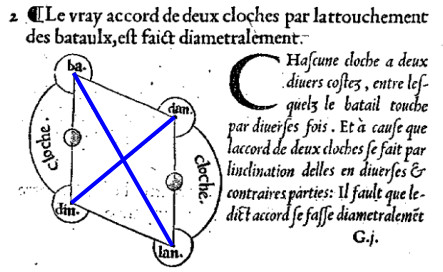
\includegraphics[]{Images/facs-fig3.jpg}
\caption{\label{facs-fig3}Smaller detail of p 49r from Bovelles highlighting two specific lines}\end{figure}
 \par\bgroup\index{surface=<surface>|exampleindex}\index{ulx=@ulx!<surface>|exampleindex}\index{uly=@uly!<surface>|exampleindex}\index{lrx=@lrx!<surface>|exampleindex}\index{lry=@lry!<surface>|exampleindex}\index{graphic=<graphic>|exampleindex}\index{url=@url!<graphic>|exampleindex}\index{path=<path>|exampleindex}\index{points=@points!<path>|exampleindex}\index{path=<path>|exampleindex}\index{points=@points!<path>|exampleindex}\exampleFont \begin{shaded}\noindent\mbox{}{<\textbf{surface}\hspace*{1em}{ulx}="{0}"\hspace*{1em}{uly}="{0}"\hspace*{1em}{lrx}="{443}"\hspace*{1em}{lry}="{272}">}\mbox{}\newline 
\hspace*{1em}{<\textbf{graphic}\hspace*{1em}{url}="{facs-fig3.jpg}"/>}\mbox{}\newline 
\hspace*{1em}{<\textbf{path}\hspace*{1em}{points}="{74,73 171,244}"\mbox{}\newline 
\hspace*{1em}\hspace*{1em}{xml:id}="{balan}"/>}\mbox{}\newline 
\hspace*{1em}{<\textbf{path}\hspace*{1em}{points}="{71,203 173,116}"\mbox{}\newline 
\hspace*{1em}\hspace*{1em}{xml:id}="{dindan}"/>}\mbox{}\newline 
{</\textbf{surface}>}\end{shaded}\egroup\par \noindent  This is useful for linking an annotation or explanation to a specific line on an object surface. Any number of coordinates can be included to specify lines which are not straight; this example shows how the first of the famous ‘story lines’ appearing at the beginning of chapter 40 of \textit{Tristram Shandy} might be encoded: \begin{figure}[htbp]
\noindent\noindent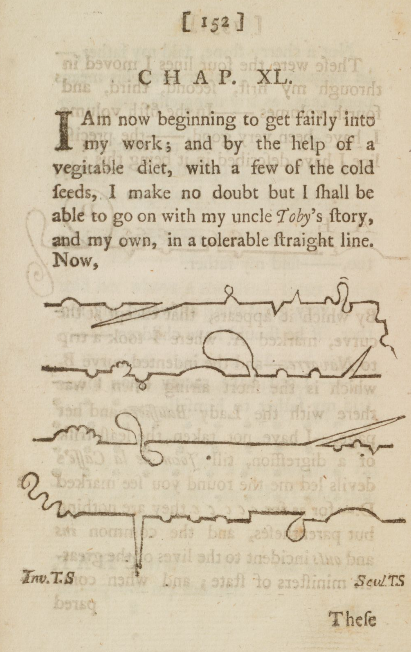
\includegraphics[]{Images/sterne.png}
\caption{\label{facs-fig4}Page 152 of \textit{Tristram Shandy}}\end{figure}
 \par\bgroup\index{surface=<surface>|exampleindex}\index{ulx=@ulx!<surface>|exampleindex}\index{uly=@uly!<surface>|exampleindex}\index{lrx=@lrx!<surface>|exampleindex}\index{lry=@lry!<surface>|exampleindex}\index{graphic=<graphic>|exampleindex}\index{url=@url!<graphic>|exampleindex}\index{path=<path>|exampleindex}\index{points=@points!<path>|exampleindex}\exampleFont \begin{shaded}\noindent\mbox{}{<\textbf{surface}\hspace*{1em}{ulx}="{0}"\hspace*{1em}{uly}="{0}"\hspace*{1em}{lrx}="{411}"\hspace*{1em}{lry}="{652}">}\mbox{}\newline 
\hspace*{1em}{<\textbf{graphic}\hspace*{1em}{url}="{sterne.png}"/>}\mbox{}\newline 
\hspace*{1em}{<\textbf{path}\hspace*{1em}{points}="{65,511 88,510 92,517 100,521 107,520 112,516 116,512 117,511 152,512 
 156,508 162,505 169,505 174,506 178,509 179,512 236,514 136,479 208,493 
 270,512 328,513 336,525 339,528 339,536 331,539 328,535 329,530 334,526 
 342,521 345,519 350,512 397,514 402,498 414,515 425,515 435,531 440,513 
 475,513 475,518 477,520 479,521 481,522 483,521 484,518 486,516 486,514 
 491,512 494,514 496,520 496,529 493,535 494,539 497,543 501,543 504,543 
 507,540 508,537 507,526 505,518 502,510 501,508 501,503 503,501 506,500 
 510,500 512,503 513,507 511,513 543,516 552,513 552,501 550,496 549,490 
 552,486 562,487 564,468 559,465 557,462 556,457 558,453 562,450 570,451 
 573,446 579,433}"/>}\mbox{}\newline 
{</\textbf{surface}>}\end{shaded}\egroup\par 
\subsection[{Combining Transcription with Facsimile}]{Combining Transcription with Facsimile}\label{PH-transcr}\par
A digitized source document may contain nothing more than page images and a small amount of metadata. It may also contain an encoded transcription of the pages represented, which may either be ‘embedded’ within a \hyperref[TEI.sourceDoc]{<sourceDoc>} element, or supplied in parallel with a \hyperref[TEI.facsimile]{<facsimile>} as defined above.\par
If the transcription is regarded as a text in its own right, organized and structured independently of its physical realization in the document or documents represented by the facsimile, then the recommended practice is to use the \hyperref[TEI.text]{<text>} element to contain such a structured representation, and to present it in parallel. The \hyperref[TEI.text]{<text>} element is a sibling of the \hyperref[TEI.facsimile]{<facsimile>} and \hyperref[TEI.sourceDoc]{<sourceDoc>} elements. This approach is illustrated in section \textit{\hyperref[PH-bov]{11.2.1.\ Parallel Transcription}} below. Alternatively, if the transcription is intended not to prioritize representation of the final text so much as the process by which the document came to take its present form, or the physical disposition of its component parts, it can be presented as an embedded transcription, as further described in section \textit{\hyperref[PHZLAB]{11.2.2.\ Embedded Transcription}} below.
\subsubsection[{Parallel Transcription}]{Parallel Transcription}\label{PH-bov}\par
Suppose now that we wish to align a transcription of the page discussed in the preceding section with particular zones. We begin by giving each relevant part of the facsimile an identifier: \par\bgroup\index{facsimile=<facsimile>|exampleindex}\index{surface=<surface>|exampleindex}\index{ulx=@ulx!<surface>|exampleindex}\index{uly=@uly!<surface>|exampleindex}\index{lrx=@lrx!<surface>|exampleindex}\index{lry=@lry!<surface>|exampleindex}\index{zone=<zone>|exampleindex}\index{ulx=@ulx!<zone>|exampleindex}\index{uly=@uly!<zone>|exampleindex}\index{lrx=@lrx!<zone>|exampleindex}\index{lry=@lry!<zone>|exampleindex}\index{graphic=<graphic>|exampleindex}\index{url=@url!<graphic>|exampleindex}\index{zone=<zone>|exampleindex}\index{ulx=@ulx!<zone>|exampleindex}\index{uly=@uly!<zone>|exampleindex}\index{lrx=@lrx!<zone>|exampleindex}\index{lry=@lry!<zone>|exampleindex}\index{graphic=<graphic>|exampleindex}\index{url=@url!<graphic>|exampleindex}\index{zone=<zone>|exampleindex}\index{ulx=@ulx!<zone>|exampleindex}\index{uly=@uly!<zone>|exampleindex}\index{lrx=@lrx!<zone>|exampleindex}\index{lry=@lry!<zone>|exampleindex}\index{zone=<zone>|exampleindex}\index{ulx=@ulx!<zone>|exampleindex}\index{uly=@uly!<zone>|exampleindex}\index{lrx=@lrx!<zone>|exampleindex}\index{lry=@lry!<zone>|exampleindex}\index{zone=<zone>|exampleindex}\index{ulx=@ulx!<zone>|exampleindex}\index{uly=@uly!<zone>|exampleindex}\index{lrx=@lrx!<zone>|exampleindex}\index{lry=@lry!<zone>|exampleindex}\index{zone=<zone>|exampleindex}\index{ulx=@ulx!<zone>|exampleindex}\index{uly=@uly!<zone>|exampleindex}\index{lrx=@lrx!<zone>|exampleindex}\index{lry=@lry!<zone>|exampleindex}\exampleFont \begin{shaded}\noindent\mbox{}{<\textbf{facsimile}>}\mbox{}\newline 
\hspace*{1em}{<\textbf{surface}\hspace*{1em}{ulx}="{0}"\hspace*{1em}{uly}="{0}"\hspace*{1em}{lrx}="{200}"\hspace*{1em}{lry}="{300}">}\mbox{}\newline 
\hspace*{1em}\hspace*{1em}{<\textbf{zone}\hspace*{1em}{xml:id}="{B49r}"\hspace*{1em}{ulx}="{0}"\hspace*{1em}{uly}="{0}"\mbox{}\newline 
\hspace*{1em}\hspace*{1em}\hspace*{1em}{lrx}="{200}"\hspace*{1em}{lry}="{300}">}\mbox{}\newline 
\hspace*{1em}\hspace*{1em}\hspace*{1em}{<\textbf{graphic}\hspace*{1em}{url}="{Bovelles-49r.png}"/>}\mbox{}\newline 
\hspace*{1em}\hspace*{1em}{</\textbf{zone}>}\mbox{}\newline 
\hspace*{1em}\hspace*{1em}{<\textbf{zone}\hspace*{1em}{ulx}="{105}"\hspace*{1em}{uly}="{76}"\hspace*{1em}{lrx}="{175}"\mbox{}\newline 
\hspace*{1em}\hspace*{1em}\hspace*{1em}{lry}="{160}">}\mbox{}\newline 
\hspace*{1em}\hspace*{1em}\hspace*{1em}{<\textbf{graphic}\hspace*{1em}{url}="{Bovelles49r-detail.png}"/>}\mbox{}\newline 
\hspace*{1em}\hspace*{1em}{</\textbf{zone}>}\mbox{}\newline 
\hspace*{1em}\hspace*{1em}{<\textbf{zone}\hspace*{1em}{xml:id}="{B49rHead}"\hspace*{1em}{ulx}="{25}"\hspace*{1em}{uly}="{25}"\mbox{}\newline 
\hspace*{1em}\hspace*{1em}\hspace*{1em}{lrx}="{180}"\hspace*{1em}{lry}="{60}"/>}\mbox{}\newline 
\textit{<!-- contains the title -->}\mbox{}\newline 
\hspace*{1em}\hspace*{1em}{<\textbf{zone}\hspace*{1em}{xml:id}="{B49rPara2}"\hspace*{1em}{ulx}="{28}"\hspace*{1em}{uly}="{75}"\mbox{}\newline 
\hspace*{1em}\hspace*{1em}\hspace*{1em}{lrx}="{175}"\hspace*{1em}{lry}="{178}"/>}\mbox{}\newline 
\textit{<!-- contains the first paragraph in italics -->}\mbox{}\newline 
\hspace*{1em}\hspace*{1em}{<\textbf{zone}\hspace*{1em}{xml:id}="{B49rFig1}"\hspace*{1em}{ulx}="{105}"\hspace*{1em}{uly}="{76}"\mbox{}\newline 
\hspace*{1em}\hspace*{1em}\hspace*{1em}{lrx}="{175}"\hspace*{1em}{lry}="{160}"/>}\mbox{}\newline 
\textit{<!-- contains the figure -->}\mbox{}\newline 
\hspace*{1em}\hspace*{1em}{<\textbf{zone}\hspace*{1em}{xml:id}="{B49rW457}"\hspace*{1em}{ulx}="{45}"\hspace*{1em}{uly}="{125}"\mbox{}\newline 
\hspace*{1em}\hspace*{1em}\hspace*{1em}{lrx}="{60}"\hspace*{1em}{lry}="{130}"/>}\mbox{}\newline 
\textit{<!-- contains the word "pendans" -->}\mbox{}\newline 
\hspace*{1em}{</\textbf{surface}>}\mbox{}\newline 
{</\textbf{facsimile}>}\end{shaded}\egroup\par \noindent  The alignment between transcription and image is made, as usual, by means of the {\itshape facs} attribute: \par\bgroup\index{pb=<pb>|exampleindex}\index{facs=@facs!<pb>|exampleindex}\index{fw=<fw>|exampleindex}\index{head=<head>|exampleindex}\index{facs=@facs!<head>|exampleindex}\index{lb=<lb>|exampleindex}\index{lb=<lb>|exampleindex}\index{lb=<lb>|exampleindex}\index{div=<div>|exampleindex}\index{n=@n!<div>|exampleindex}\index{p=<p>|exampleindex}\index{lb=<lb>|exampleindex}\index{p=<p>|exampleindex}\index{rend=@rend!<p>|exampleindex}\index{facs=@facs!<p>|exampleindex}\index{lb=<lb>|exampleindex}\index{lb=<lb>|exampleindex}\index{lb=<lb>|exampleindex}\index{lb=<lb>|exampleindex}\index{lb=<lb>|exampleindex}\index{lb=<lb>|exampleindex}\index{w=<w>|exampleindex}\index{facs=@facs!<w>|exampleindex}\index{lb=<lb>|exampleindex}\index{lb=<lb>|exampleindex}\index{ex=<ex>|exampleindex}\index{lb=<lb>|exampleindex}\index{ex=<ex>|exampleindex}\index{ex=<ex>|exampleindex}\index{lb=<lb>|exampleindex}\index{lb=<lb>|exampleindex}\index{lb=<lb>|exampleindex}\index{figure=<figure>|exampleindex}\index{facs=@facs!<figure>|exampleindex}\index{graphic=<graphic>|exampleindex}\index{url=@url!<graphic>|exampleindex}\exampleFont \begin{shaded}\noindent\mbox{}{<\textbf{pb}\hspace*{1em}{facs}="{\#B49r}"/>}\mbox{}\newline 
{<\textbf{fw}>}De Geometrie 49{</\textbf{fw}>}\mbox{}\newline 
{<\textbf{head}\hspace*{1em}{facs}="{\#B49rHead}">} DU SON ET ACCORD DES CLOCHES ET {<\textbf{lb}/>} des alleures des\mbox{}\newline 
 chevaulx, chariotz \& charges, des fontaines:\& {<\textbf{lb}/>} encyclie du monde,\mbox{}\newline 
 \& de la dimension du corps humain.{<\textbf{lb}/>} Chapitre septiesme{</\textbf{head}>}\mbox{}\newline 
{<\textbf{div}\hspace*{1em}{n}="{1}">}\mbox{}\newline 
\hspace*{1em}{<\textbf{p}>}Le son \& accord des cloches pendans en ung mesme {<\textbf{lb}/>} axe, est faict en\mbox{}\newline 
\hspace*{1em}\hspace*{1em} contraires parties.{</\textbf{p}>}\mbox{}\newline 
\hspace*{1em}{<\textbf{p}\hspace*{1em}{rend}="{it}"\hspace*{1em}{facs}="{\#B49rPara2}">}LEs cloches ont quasi fi{<\textbf{lb}/>}gures de rondes\mbox{}\newline 
\hspace*{1em}\hspace*{1em} pyra{<\textbf{lb}/>}mides imperfaictes \& {<\textbf{lb}/>} irregulieres: \& leur accord se\mbox{}\newline 
\hspace*{1em}{<\textbf{lb}/>} fait par reigle geometrique. Com{<\textbf{lb}/>}me si les deux cloches C \& D\mbox{}\newline 
\hspace*{1em}{<\textbf{lb}/>} sont {<\textbf{w}\hspace*{1em}{facs}="{\#B49rW457}">}pendans{</\textbf{w}>} à ung mesme axe {<\textbf{lb}/>} ou essieu A B:\mbox{}\newline 
\hspace*{1em}\hspace*{1em} je dis que leur ac{<\textbf{lb}/>}cord se fera en co{<\textbf{ex}>}n{</\textbf{ex}>}traires parties{<\textbf{lb}/>}\mbox{}\newline 
\hspace*{1em}\hspace*{1em} co{<\textbf{ex}>}m{</\textbf{ex}>}me voyez icy figuré. Car qua{<\textbf{ex}>}n{</\textbf{ex}>}d {<\textbf{lb}/>} lune sera en\mbox{}\newline 
\hspace*{1em}\hspace*{1em} hault, laultre declinera embas. Aultrement si elles decli{<\textbf{lb}/>}nent toutes deux\mbox{}\newline 
\hspace*{1em}\hspace*{1em} ensembles en une mesme partie, elles seront discord, {<\textbf{lb}/>} \& sera leur\mbox{}\newline 
\hspace*{1em}\hspace*{1em} sonnerie mal plaisante à oyr.{<\textbf{figure}\hspace*{1em}{facs}="{\#B49rFig1}">}\mbox{}\newline 
\hspace*{1em}\hspace*{1em}\hspace*{1em}{<\textbf{graphic}\hspace*{1em}{url}="{Bovelles49r-detail.png}"/>}\mbox{}\newline 
\hspace*{1em}\hspace*{1em}{</\textbf{figure}>}\mbox{}\newline 
\hspace*{1em}{</\textbf{p}>}\mbox{}\newline 
{</\textbf{div}>}\end{shaded}\egroup\par \par
It is also possible to point in the other direction, from a \hyperref[TEI.surface]{<surface>} or \hyperref[TEI.zone]{<zone>} to the corresponding text. This is the function of the {\itshape start} attribute, which supplies the identifier of the element containing at least the start of the transcribed text found within the surface or zone concerned. Thus, another way of linking this page with its transcription would be simply \par\bgroup\index{facsimile=<facsimile>|exampleindex}\index{surface=<surface>|exampleindex}\index{start=@start!<surface>|exampleindex}\index{graphic=<graphic>|exampleindex}\index{url=@url!<graphic>|exampleindex}\index{text=<text>|exampleindex}\index{body=<body>|exampleindex}\index{div=<div>|exampleindex}\index{pb=<pb>|exampleindex}\index{fw=<fw>|exampleindex}\exampleFont \begin{shaded}\noindent\mbox{}{<\textbf{facsimile}>}\mbox{}\newline 
\hspace*{1em}{<\textbf{surface}\hspace*{1em}{start}="{\#PB49R}">}\mbox{}\newline 
\hspace*{1em}\hspace*{1em}{<\textbf{graphic}\hspace*{1em}{url}="{Bovelles-49r.png}"/>}\mbox{}\newline 
\hspace*{1em}{</\textbf{surface}>}\mbox{}\newline 
{</\textbf{facsimile}>}\mbox{}\newline 
{<\textbf{text}>}\mbox{}\newline 
\hspace*{1em}{<\textbf{body}>}\mbox{}\newline 
\hspace*{1em}\hspace*{1em}{<\textbf{div}>}\mbox{}\newline 
\textit{<!-- ... -->}\mbox{}\newline 
\hspace*{1em}\hspace*{1em}\hspace*{1em}{<\textbf{pb}\hspace*{1em}{xml:id}="{PB49R}"/>}\mbox{}\newline 
\hspace*{1em}\hspace*{1em}\hspace*{1em}{<\textbf{fw}>}De Geometrie 49{</\textbf{fw}>}\mbox{}\newline 
\textit{<!-- ... -->}\mbox{}\newline 
\hspace*{1em}\hspace*{1em}{</\textbf{div}>}\mbox{}\newline 
\hspace*{1em}{</\textbf{body}>}\mbox{}\newline 
{</\textbf{text}>}\end{shaded}\egroup\par 
\subsubsection[{Embedded Transcription}]{Embedded Transcription}\label{PHZLAB}\par
An \textit{embedded transcription} is one in which words and other written traces are encoded as subcomponents of elements representing the physical surfaces carrying them rather than independently of them.\par
The following elements are available for this purpose: 
\begin{sansreflist}
  
\item [\textbf{<sourceDoc>}] contains a transcription or other representation of a single source document potentially forming part of a \textit{dossier génétique} or collection of sources.
\item [\textbf{<surface>}] defines a written surface as a two-dimensional coordinate space, optionally grouping one or more graphic representations of that space, zones of interest within that space, and transcriptions of the writing within them.
\item [\textbf{<zone>}] defines any two-dimensional area within a \hyperref[TEI.surface]{<surface>} element.
\item [\textbf{<line>}] contains the transcription of a topographic line in the source document
\item [\textbf{<seg>}] (arbitrary segment) represents any segmentation of text below the ‘chunk’ level.
\end{sansreflist}
\par
The elements \hyperref[TEI.surface]{<surface>}, \hyperref[TEI.surfaceGrp]{<surfaceGrp>}, and \hyperref[TEI.zone]{<zone>} were introduced above in section \textit{\hyperref[PHFAX]{11.1.\ Digital Facsimiles}}. When supplied within a \hyperref[TEI.sourceDoc]{<sourceDoc>} element, these elements may contain transcriptions of the written content of a source in addition to or as an alternative to digital images of them. Such transcription may be placed directly within the \hyperref[TEI.zone]{<zone>} element, or within one or more \hyperref[TEI.line]{<line>} elements, for cases where the writing is linear, in the sense that it is composed of discrete tokens organized physically into groups, typically organized in a sequence corresponding with the way they are intended to be read. Depending on the directionality of the writing system used, this might be any combination of top-down and left to right, or vice versa. The element \hyperref[TEI.line]{<line>} may be used to hold a complete group of such tokens. Where, however, the lineation is not considered significant, any group of tokens may be indicated using the \hyperref[TEI.zone]{<zone>} element. The \hyperref[TEI.seg]{<seg>} element described in section \textit{\hyperref[SASE]{16.3.\ Blocks, Segments, and Anchors}} may also be used to indicate smaller sequences of tokens within \hyperref[TEI.zone]{<zone>}, or \hyperref[TEI.line]{<line>} as appropriate.\par
Returning to the preceding example, we might transcribe the content of the zone to which we gave the identifier \textsf{B49rPara2} within a \hyperref[TEI.sourceDoc]{<sourceDoc>} element as follows:\par\bgroup\index{sourceDoc=<sourceDoc>|exampleindex}\index{surface=<surface>|exampleindex}\index{ulx=@ulx!<surface>|exampleindex}\index{uly=@uly!<surface>|exampleindex}\index{lrx=@lrx!<surface>|exampleindex}\index{lry=@lry!<surface>|exampleindex}\index{zone=<zone>|exampleindex}\index{ulx=@ulx!<zone>|exampleindex}\index{uly=@uly!<zone>|exampleindex}\index{lrx=@lrx!<zone>|exampleindex}\index{lry=@lry!<zone>|exampleindex}\index{graphic=<graphic>|exampleindex}\index{url=@url!<graphic>|exampleindex}\index{zone=<zone>|exampleindex}\index{ulx=@ulx!<zone>|exampleindex}\index{uly=@uly!<zone>|exampleindex}\index{lrx=@lrx!<zone>|exampleindex}\index{lry=@lry!<zone>|exampleindex}\index{line=<line>|exampleindex}\index{line=<line>|exampleindex}\index{line=<line>|exampleindex}\index{line=<line>|exampleindex}\index{line=<line>|exampleindex}\index{line=<line>|exampleindex}\index{line=<line>|exampleindex}\index{zone=<zone>|exampleindex}\index{ulx=@ulx!<zone>|exampleindex}\index{uly=@uly!<zone>|exampleindex}\index{lrx=@lrx!<zone>|exampleindex}\index{lry=@lry!<zone>|exampleindex}\index{line=<line>|exampleindex}\index{line=<line>|exampleindex}\index{line=<line>|exampleindex}\index{line=<line>|exampleindex}\index{line=<line>|exampleindex}\index{zone=<zone>|exampleindex}\index{ulx=@ulx!<zone>|exampleindex}\index{uly=@uly!<zone>|exampleindex}\index{lrx=@lrx!<zone>|exampleindex}\index{lry=@lry!<zone>|exampleindex}\index{graphic=<graphic>|exampleindex}\index{url=@url!<graphic>|exampleindex}\exampleFont \begin{shaded}\noindent\mbox{}{<\textbf{sourceDoc}>}\mbox{}\newline 
\hspace*{1em}{<\textbf{surface}\hspace*{1em}{ulx}="{0}"\hspace*{1em}{uly}="{0}"\hspace*{1em}{lrx}="{200}"\hspace*{1em}{lry}="{300}">}\mbox{}\newline 
\hspace*{1em}\hspace*{1em}{<\textbf{zone}\hspace*{1em}{ulx}="{0}"\hspace*{1em}{uly}="{0}"\hspace*{1em}{lrx}="{200}"\hspace*{1em}{lry}="{300}">}\mbox{}\newline 
\hspace*{1em}\hspace*{1em}\hspace*{1em}{<\textbf{graphic}\hspace*{1em}{url}="{Bovelles-49r.png}"/>}\mbox{}\newline 
\hspace*{1em}\hspace*{1em}{</\textbf{zone}>}\mbox{}\newline 
\textit{<!-- ... -->}\mbox{}\newline 
\hspace*{1em}\hspace*{1em}{<\textbf{zone}\hspace*{1em}{ulx}="{28}"\hspace*{1em}{uly}="{75}"\hspace*{1em}{lrx}="{175}"\hspace*{1em}{lry}="{178}">}\mbox{}\newline 
\hspace*{1em}\hspace*{1em}\hspace*{1em}{<\textbf{line}>}LEs cloches ont quasi\mbox{}\newline 
\hspace*{1em}\hspace*{1em}\hspace*{1em}\hspace*{1em}\hspace*{1em}\hspace*{1em} fi{</\textbf{line}>}\mbox{}\newline 
\hspace*{1em}\hspace*{1em}\hspace*{1em}{<\textbf{line}>}gures de rondes pyra{</\textbf{line}>}\mbox{}\newline 
\hspace*{1em}\hspace*{1em}\hspace*{1em}{<\textbf{line}>}mides imperfaictes \&\mbox{}\newline 
\hspace*{1em}\hspace*{1em}\hspace*{1em}{</\textbf{line}>}\mbox{}\newline 
\hspace*{1em}\hspace*{1em}\hspace*{1em}{<\textbf{line}>} irregulieres: \& leur accord se{</\textbf{line}>}\mbox{}\newline 
\hspace*{1em}\hspace*{1em}\hspace*{1em}{<\textbf{line}>} fait par reigle geometrique. Com{</\textbf{line}>}\mbox{}\newline 
\hspace*{1em}\hspace*{1em}\hspace*{1em}{<\textbf{line}>}me si les deux cloches C\mbox{}\newline 
\hspace*{1em}\hspace*{1em}\hspace*{1em}\hspace*{1em}\hspace*{1em}\hspace*{1em} \& D {</\textbf{line}>}\mbox{}\newline 
\hspace*{1em}\hspace*{1em}\hspace*{1em}{<\textbf{line}>} sont {<\textbf{zone}\hspace*{1em}{ulx}="{45}"\hspace*{1em}{uly}="{125}"\hspace*{1em}{lrx}="{60}"\mbox{}\newline 
\hspace*{1em}\hspace*{1em}\hspace*{1em}\hspace*{1em}\hspace*{1em}{lry}="{130}">}pendans{</\textbf{zone}>} à ung mesme axe{</\textbf{line}>}\mbox{}\newline 
\hspace*{1em}\hspace*{1em}\hspace*{1em}{<\textbf{line}>} ou essieu A B: je dis que\mbox{}\newline 
\hspace*{1em}\hspace*{1em}\hspace*{1em}\hspace*{1em}\hspace*{1em}\hspace*{1em} leur ac{</\textbf{line}>}\mbox{}\newline 
\hspace*{1em}\hspace*{1em}\hspace*{1em}{<\textbf{line}>}cord se fera en cõtraires parties{</\textbf{line}>}\mbox{}\newline 
\hspace*{1em}\hspace*{1em}\hspace*{1em}{<\textbf{line}>} cõme\mbox{}\newline 
\hspace*{1em}\hspace*{1em}\hspace*{1em}\hspace*{1em}\hspace*{1em}\hspace*{1em} voyez icy figuré. Car quãd {</\textbf{line}>}\mbox{}\newline 
\hspace*{1em}\hspace*{1em}\hspace*{1em}{<\textbf{line}>} lune sera en hault, laultre\mbox{}\newline 
\hspace*{1em}\hspace*{1em}\hspace*{1em}\hspace*{1em}\hspace*{1em}\hspace*{1em} declinera embas. Aultrement si elles declinent toutes deux ensembles en une\mbox{}\newline 
\hspace*{1em}\hspace*{1em}\hspace*{1em}\hspace*{1em}\hspace*{1em}\hspace*{1em} mesme partie, elles seront discord,{</\textbf{line}>}\mbox{}\newline 
\hspace*{1em}\hspace*{1em}\hspace*{1em}{<\textbf{line}>} \& sera leur sonnerie\mbox{}\newline 
\hspace*{1em}\hspace*{1em}\hspace*{1em}\hspace*{1em}\hspace*{1em}\hspace*{1em} mal plaisante à oyr.{</\textbf{line}>}\mbox{}\newline 
\hspace*{1em}\hspace*{1em}{</\textbf{zone}>}\mbox{}\newline 
\hspace*{1em}\hspace*{1em}{<\textbf{zone}\hspace*{1em}{ulx}="{105}"\hspace*{1em}{uly}="{76}"\hspace*{1em}{lrx}="{175}"\mbox{}\newline 
\hspace*{1em}\hspace*{1em}\hspace*{1em}{lry}="{160}">}\mbox{}\newline 
\hspace*{1em}\hspace*{1em}\hspace*{1em}{<\textbf{graphic}\hspace*{1em}{url}="{Bovelles49r-detail.png}"/>}\mbox{}\newline 
\hspace*{1em}\hspace*{1em}{</\textbf{zone}>}\mbox{}\newline 
\hspace*{1em}{</\textbf{surface}>}\mbox{}\newline 
{</\textbf{sourceDoc}>}\end{shaded}\egroup\par \par
As mentioned above, some or all of the written surfaces being transcribed may be composed of physically distinct scraps. In the following example, taken from the Walt Whitman Archive, two pieces of newsprint have been glued to a piece of blue paper on which a poem is being drafted: \begin{figure}[htbp]
\noindent\noindent\includegraphics[width=400pt,]{Images/whitman01.jpg}
\caption{\label{sleeprs}Single leaf of notes possibly related to the poem eventually titled Sleepers. From the Walt Whitman Archive (Duke 258).}\end{figure}
 The two pieces of newsprint might simply be regarded as special kinds of zone, but they are also new surfaces, since they might contain additional written zones themselves (such as the numbers in this case).\par
Using these elements, the Whitman draft above might be encoded as follows: \par\bgroup\index{surface=<surface>|exampleindex}\index{zone=<zone>|exampleindex}\index{line=<line>|exampleindex}\index{line=<line>|exampleindex}\index{line=<line>|exampleindex}\index{line=<line>|exampleindex}\index{line=<line>|exampleindex}\index{zone=<zone>|exampleindex}\index{surface=<surface>|exampleindex}\index{type=@type!<surface>|exampleindex}\index{attachment=@attachment!<surface>|exampleindex}\index{flipping=@flipping!<surface>|exampleindex}\index{zone=<zone>|exampleindex}\index{metamark=<metamark>|exampleindex}\index{function=@function!<metamark>|exampleindex}\index{zone=<zone>|exampleindex}\index{surface=<surface>|exampleindex}\index{type=@type!<surface>|exampleindex}\index{attachment=@attachment!<surface>|exampleindex}\index{flipping=@flipping!<surface>|exampleindex}\index{zone=<zone>|exampleindex}\index{metamark=<metamark>|exampleindex}\index{function=@function!<metamark>|exampleindex}\exampleFont \begin{shaded}\noindent\mbox{}{<\textbf{surface}>}\mbox{}\newline 
\hspace*{1em}{<\textbf{zone}>}\mbox{}\newline 
\hspace*{1em}\hspace*{1em}{<\textbf{line}>}Poem{</\textbf{line}>}\mbox{}\newline 
\hspace*{1em}\hspace*{1em}{<\textbf{line}>}As in Visions of — at{</\textbf{line}>}\mbox{}\newline 
\hspace*{1em}\hspace*{1em}{<\textbf{line}>}night —{</\textbf{line}>}\mbox{}\newline 
\hspace*{1em}\hspace*{1em}{<\textbf{line}>}All sorts of fancies running through{</\textbf{line}>}\mbox{}\newline 
\hspace*{1em}\hspace*{1em}{<\textbf{line}>}the head{</\textbf{line}>}\mbox{}\newline 
\hspace*{1em}{</\textbf{zone}>}\mbox{}\newline 
\hspace*{1em}{<\textbf{zone}>}\mbox{}\newline 
\hspace*{1em}\hspace*{1em}{<\textbf{surface}\hspace*{1em}{type}="{newsprint}"\mbox{}\newline 
\hspace*{1em}\hspace*{1em}\hspace*{1em}{attachment}="{glue}"\hspace*{1em}{flipping}="{false}">}\mbox{}\newline 
\hspace*{1em}\hspace*{1em}\hspace*{1em}{<\textbf{zone}>}Spring has just set in here, and the weather[...] a steamer {</\textbf{zone}>}\mbox{}\newline 
\hspace*{1em}\hspace*{1em}\hspace*{1em}{<\textbf{metamark}\hspace*{1em}{function}="{sequence}">}2{</\textbf{metamark}>}\mbox{}\newline 
\hspace*{1em}\hspace*{1em}{</\textbf{surface}>}\mbox{}\newline 
\hspace*{1em}{</\textbf{zone}>}\mbox{}\newline 
\hspace*{1em}{<\textbf{zone}>}\mbox{}\newline 
\hspace*{1em}\hspace*{1em}{<\textbf{surface}\hspace*{1em}{type}="{newsprint}"\mbox{}\newline 
\hspace*{1em}\hspace*{1em}\hspace*{1em}{attachment}="{glue}"\hspace*{1em}{flipping}="{false}">}\mbox{}\newline 
\hspace*{1em}\hspace*{1em}\hspace*{1em}{<\textbf{zone}>}"The shores on either side of the Sound are... The In- {</\textbf{zone}>}\mbox{}\newline 
\hspace*{1em}\hspace*{1em}\hspace*{1em}{<\textbf{metamark}\hspace*{1em}{function}="{sequence}">}3{</\textbf{metamark}>}\mbox{}\newline 
\hspace*{1em}\hspace*{1em}{</\textbf{surface}>}\mbox{}\newline 
\hspace*{1em}{</\textbf{zone}>}\mbox{}\newline 
{</\textbf{surface}>}\end{shaded}\egroup\par \par
The \hyperref[TEI.metamark]{<metamark>} element used in this example is further discussed below (\textit{\hyperref[PH-meta]{11.3.4.2.\ Metamarks}})\par
Note that in this example we have not included any \hyperref[TEI.graphic]{<graphic>} element corresponding with the \hyperref[TEI.zone]{<zone>} or \hyperref[TEI.surface]{<surface>} elements identified in the transcription. The encoder may choose to complement a transcription with graphic representations of its source at whatever level is considered effective, or not at all. Equally, the encoder may choose to provide only graphics without any transcription, to provide only a structured (non-embedded) transcription, or to provide any combination of the three.\par
This example also lacks any coordinate information to specify either the size of the two newspaper fragments or whereabouts on the parent \hyperref[TEI.surface]{<surface>} element they are to be found, other than the reading order implicit in their sequence. Such information could be added if desired by specifying a coordinate system on the outermost \hyperref[TEI.surface]{<surface>} element, and then indicating values within that system for each of the two fragments, as was discussed above. We discuss this in further detail in section \textit{\hyperref[PH-surfzone]{11.2.2.1.\ Advanced Uses of surface and zone}} below.
\paragraph[{Advanced Uses of surface and zone}]{Advanced Uses of \texttt{<surface>} and \texttt{<zone>}}\label{PH-surfzone}\par
As a child of \hyperref[TEI.sourceDoc]{<sourceDoc>}, the \hyperref[TEI.surface]{<surface>} element both identifies a specific area containing writing and provides a two dimensional set of coordinates which can be used to position and define dimensions for sub-parts of it. Furthermore, surfaces may nest within other surfaces, as in the case of ‘patches’ or other written materials attached to the main writing surface. In the general case, the position and dimensions of such nested surfaces will be defined using the same coordinate system as that supplied by the parent \hyperref[TEI.surface]{<surface>} element. It is also possible, however, that a different coordinate system is required for such a nested surface, perhaps because it requires a more complex granularity. We consider both possibilities.\par
In the earlier examples showing nested examples we did not provide any coordinate information, for simplicity of presentation. Suppose however, that we wish to indicate the position and sizes of the newspaper scraps in \ref{sleeprs} above, relative to the whole page. As previously noted, the four attributes {\itshape ulx}, {\itshape uly}, {\itshape lrx} and {\itshape lry} when given on the \hyperref[TEI.surface]{<surface>} element define the coordinate scheme, rather than specifying the location of that surface. We must therefore introduce an additional \hyperref[TEI.zone]{<zone>} element, as in the following revised encoding for this example \par\bgroup\index{surface=<surface>|exampleindex}\index{ulx=@ulx!<surface>|exampleindex}\index{uly=@uly!<surface>|exampleindex}\index{lrx=@lrx!<surface>|exampleindex}\index{lry=@lry!<surface>|exampleindex}\index{zone=<zone>|exampleindex}\index{ulx=@ulx!<zone>|exampleindex}\index{uly=@uly!<zone>|exampleindex}\index{lrx=@lrx!<zone>|exampleindex}\index{lry=@lry!<zone>|exampleindex}\index{line=<line>|exampleindex}\index{line=<line>|exampleindex}\index{line=<line>|exampleindex}\index{line=<line>|exampleindex}\index{line=<line>|exampleindex}\index{zone=<zone>|exampleindex}\index{ulx=@ulx!<zone>|exampleindex}\index{uly=@uly!<zone>|exampleindex}\index{lrx=@lrx!<zone>|exampleindex}\index{lry=@lry!<zone>|exampleindex}\index{surface=<surface>|exampleindex}\index{type=@type!<surface>|exampleindex}\index{attachment=@attachment!<surface>|exampleindex}\index{flipping=@flipping!<surface>|exampleindex}\index{zone=<zone>|exampleindex}\index{metamark=<metamark>|exampleindex}\index{function=@function!<metamark>|exampleindex}\exampleFont \begin{shaded}\noindent\mbox{}{<\textbf{surface}\hspace*{1em}{ulx}="{0}"\hspace*{1em}{uly}="{0}"\hspace*{1em}{lrx}="{50}"\hspace*{1em}{lry}="{50}">}\mbox{}\newline 
\hspace*{1em}{<\textbf{zone}\hspace*{1em}{ulx}="{1}"\hspace*{1em}{uly}="{1}"\hspace*{1em}{lrx}="{10}"\hspace*{1em}{lry}="{10}">}\mbox{}\newline 
\hspace*{1em}\hspace*{1em}{<\textbf{line}>}Poem{</\textbf{line}>}\mbox{}\newline 
\hspace*{1em}\hspace*{1em}{<\textbf{line}>}As in Visions of — at{</\textbf{line}>}\mbox{}\newline 
\hspace*{1em}\hspace*{1em}{<\textbf{line}>}night —{</\textbf{line}>}\mbox{}\newline 
\hspace*{1em}\hspace*{1em}{<\textbf{line}>}All sorts of fancies running through{</\textbf{line}>}\mbox{}\newline 
\hspace*{1em}\hspace*{1em}{<\textbf{line}>}the head{</\textbf{line}>}\mbox{}\newline 
\hspace*{1em}{</\textbf{zone}>}\mbox{}\newline 
\hspace*{1em}{<\textbf{zone}\hspace*{1em}{ulx}="{4}"\hspace*{1em}{uly}="{4}"\hspace*{1em}{lrx}="{20}"\hspace*{1em}{lry}="{20}">}\mbox{}\newline 
\hspace*{1em}\hspace*{1em}{<\textbf{surface}\hspace*{1em}{type}="{newsprint}"\mbox{}\newline 
\hspace*{1em}\hspace*{1em}\hspace*{1em}{attachment}="{glue}"\hspace*{1em}{flipping}="{false}">}\mbox{}\newline 
\hspace*{1em}\hspace*{1em}\hspace*{1em}{<\textbf{zone}>}Spring has just set in here, and the weather[...] a steamer {</\textbf{zone}>}\mbox{}\newline 
\hspace*{1em}\hspace*{1em}\hspace*{1em}{<\textbf{metamark}\hspace*{1em}{function}="{sequence}">}2{</\textbf{metamark}>}\mbox{}\newline 
\hspace*{1em}\hspace*{1em}{</\textbf{surface}>}\mbox{}\newline 
\hspace*{1em}{</\textbf{zone}>}\mbox{}\newline 
{</\textbf{surface}>}\end{shaded}\egroup\par \noindent  In this version of the encoding, the inner surface, corresponding with the first piece of newsprint, inherits locational information from the \hyperref[TEI.zone]{<zone>} element that contains it. This zone, and the preceding one, which contains a sequence of \hyperref[TEI.line]{<line>} elements, are both positioned in terms of the coordinates specified on the outermost \hyperref[TEI.surface]{<surface>} element, which defines a scale running from 0 to 50 in either direction. On that scale, the \hyperref[TEI.line]{<line>} elements occupy a rectangle with coordinates (1,1,10,10), while the nested surface occupies a rectangle with coordinates (4,4,20,20).\par
Now suppose that we wish to define a finer scale grid for the newspaper patch, perhaps because we wish to localize zones within it with greater accuracy. To do this we will need to specify the position of the nested surface as in the previous example, but also to define the new coordinate system. We accomplish this as follows: \par\bgroup\index{surface=<surface>|exampleindex}\index{ulx=@ulx!<surface>|exampleindex}\index{uly=@uly!<surface>|exampleindex}\index{lrx=@lrx!<surface>|exampleindex}\index{lry=@lry!<surface>|exampleindex}\index{zone=<zone>|exampleindex}\index{ulx=@ulx!<zone>|exampleindex}\index{uly=@uly!<zone>|exampleindex}\index{lrx=@lrx!<zone>|exampleindex}\index{lry=@lry!<zone>|exampleindex}\index{line=<line>|exampleindex}\index{line=<line>|exampleindex}\index{zone=<zone>|exampleindex}\index{ulx=@ulx!<zone>|exampleindex}\index{uly=@uly!<zone>|exampleindex}\index{lrx=@lrx!<zone>|exampleindex}\index{lry=@lry!<zone>|exampleindex}\index{surface=<surface>|exampleindex}\index{ulx=@ulx!<surface>|exampleindex}\index{uly=@uly!<surface>|exampleindex}\index{lrx=@lrx!<surface>|exampleindex}\index{lry=@lry!<surface>|exampleindex}\index{zone=<zone>|exampleindex}\index{ulx=@ulx!<zone>|exampleindex}\index{uly=@uly!<zone>|exampleindex}\index{lrx=@lrx!<zone>|exampleindex}\index{lry=@lry!<zone>|exampleindex}\exampleFont \begin{shaded}\noindent\mbox{}{<\textbf{surface}\hspace*{1em}{ulx}="{0}"\hspace*{1em}{uly}="{0}"\hspace*{1em}{lrx}="{50}"\hspace*{1em}{lry}="{50}">}\mbox{}\newline 
\hspace*{1em}{<\textbf{zone}\hspace*{1em}{ulx}="{1}"\hspace*{1em}{uly}="{1}"\hspace*{1em}{lrx}="{10}"\hspace*{1em}{lry}="{10}">}\mbox{}\newline 
\hspace*{1em}\hspace*{1em}{<\textbf{line}>}Poem{</\textbf{line}>}\mbox{}\newline 
\textit{<!-- ... -->}\mbox{}\newline 
\hspace*{1em}\hspace*{1em}{<\textbf{line}>}the head{</\textbf{line}>}\mbox{}\newline 
\hspace*{1em}{</\textbf{zone}>}\mbox{}\newline 
\hspace*{1em}{<\textbf{zone}\hspace*{1em}{ulx}="{4}"\hspace*{1em}{uly}="{4}"\hspace*{1em}{lrx}="{20}"\hspace*{1em}{lry}="{20}">}\mbox{}\newline 
\hspace*{1em}\hspace*{1em}{<\textbf{surface}\hspace*{1em}{ulx}="{0}"\hspace*{1em}{uly}="{0}"\hspace*{1em}{lrx}="{100}"\mbox{}\newline 
\hspace*{1em}\hspace*{1em}\hspace*{1em}{lry}="{100}">}\mbox{}\newline 
\hspace*{1em}\hspace*{1em}\hspace*{1em}{<\textbf{zone}\hspace*{1em}{ulx}="{10}"\hspace*{1em}{uly}="{10}"\hspace*{1em}{lrx}="{90}"\hspace*{1em}{lry}="{95}">} Spring has just set in here, and the\mbox{}\newline 
\hspace*{1em}\hspace*{1em}\hspace*{1em}\hspace*{1em}\hspace*{1em}\hspace*{1em} weather [...] a steamer {</\textbf{zone}>}\mbox{}\newline 
\hspace*{1em}\hspace*{1em}{</\textbf{surface}>}\mbox{}\newline 
\hspace*{1em}{</\textbf{zone}>}\mbox{}\newline 
{</\textbf{surface}>}\end{shaded}\egroup\par \noindent  As before, the second zone defines the position and size of the newspaper patch itself in terms of a coordinate system running from 0 to 50 on both X and Y axes. The nested \hyperref[TEI.surface]{<surface>} element however defines a new scale for all of its components, running from 0 to 100 on both X and Y axes. The position of the nested zone containing the text \textit{Spring ... steamer} is now given in terms of this scale.\par
All of the examples so far given have involved rectangular zones, for clarity of exposition. As noted above, the {\itshape points} attribute may be used to define non-rectangular zones as a series of points. For example, in the last of the Whitman examples discussed in section \textit{\hyperref[PH-meta]{11.3.4.2.\ Metamarks}} above, we might wish to record the exact shape of the zone containing the metamark \textit{Entered}. Since this is not a rectangular zone, we use the {\itshape points} attribute to indicate the points defining a polygon which contains it. The values used are expressed in terms of a coordinate space running from 0 to 229 in the X dimension, and 0 to 160 in the Y dimension.\par\bgroup\index{surface=<surface>|exampleindex}\index{ulx=@ulx!<surface>|exampleindex}\index{uly=@uly!<surface>|exampleindex}\index{lrx=@lrx!<surface>|exampleindex}\index{lry=@lry!<surface>|exampleindex}\index{graphic=<graphic>|exampleindex}\index{url=@url!<graphic>|exampleindex}\index{zone=<zone>|exampleindex}\index{points=@points!<zone>|exampleindex}\exampleFont \begin{shaded}\noindent\mbox{}{<\textbf{surface}\hspace*{1em}{ulx}="{0}"\hspace*{1em}{uly}="{0}"\hspace*{1em}{lrx}="{229}"\hspace*{1em}{lry}="{160}">}\mbox{}\newline 
\hspace*{1em}{<\textbf{graphic}\hspace*{1em}{url}="{whitman-02.jpg}"/>}\mbox{}\newline 
\hspace*{1em}{<\textbf{zone}\hspace*{1em}{xml:id}="{entered}"\mbox{}\newline 
\hspace*{1em}\hspace*{1em}{points}="{142,122 155,113 178,122 208,144 198,154 178,139}"/>}\mbox{}\newline 
{</\textbf{surface}>}\end{shaded}\egroup\par \par
In exactly the same way, we may wish to identify the curved zone in the following image containing the word \textit{Northamptonshire}: \begin{figure}[htbp]
\noindent\noindent\includegraphics[]{Images/mould-stone.jpg}
\caption{Gravestone of Private Moulds}\end{figure}
 This curved zone might be encoded in the following way: \par\bgroup\index{surface=<surface>|exampleindex}\index{ulx=@ulx!<surface>|exampleindex}\index{uly=@uly!<surface>|exampleindex}\index{lrx=@lrx!<surface>|exampleindex}\index{lry=@lry!<surface>|exampleindex}\index{graphic=<graphic>|exampleindex}\index{url=@url!<graphic>|exampleindex}\index{zone=<zone>|exampleindex}\index{points=@points!<zone>|exampleindex}\exampleFont \begin{shaded}\noindent\mbox{}{<\textbf{surface}\hspace*{1em}{xml:id}="{badge}"\hspace*{1em}{ulx}="{14.54}"\mbox{}\newline 
\hspace*{1em}{uly}="{16.14}"\hspace*{1em}{lrx}="{0}"\hspace*{1em}{lry}="{0}">}\mbox{}\newline 
\hspace*{1em}{<\textbf{graphic}\hspace*{1em}{url}="{stone.jpg}"/>}\mbox{}\newline 
\hspace*{1em}{<\textbf{zone}\hspace*{1em}{xml:id}="{county}"\mbox{}\newline 
\hspace*{1em}\hspace*{1em}{points}="{4.6,6.3 5.25,5.85 6.2,6.6 8.2,7.4 9.9,6.6 10.9,6.1 11.4,6.7 8.2,8.3 
 6.2,7.6}"/>}\mbox{}\newline 
{</\textbf{surface}>}\end{shaded}\egroup\par \par
Finally, it should be noted that a \hyperref[TEI.zone]{<zone>} does not need to be entirely contained within the two-dimensional space defined by its parent surface. For example, we might wish to encode the example in \ref{durlach} above not as a surface representing the whole of the two page spread, but as a surface representing only the written part of this opening. The written part appears 50 units from the left of the image and 20 units from the top, while the bottom right corner of the written part appears 400 units from the left of the image, and 280 units from the top. We therefore define the written surface within this image as follows: \par\bgroup\index{facsimile=<facsimile>|exampleindex}\index{surface=<surface>|exampleindex}\index{ulx=@ulx!<surface>|exampleindex}\index{uly=@uly!<surface>|exampleindex}\index{lrx=@lrx!<surface>|exampleindex}\index{lry=@lry!<surface>|exampleindex}\exampleFont \begin{shaded}\noindent\mbox{}{<\textbf{facsimile}>}\mbox{}\newline 
\hspace*{1em}{<\textbf{surface}\hspace*{1em}{ulx}="{50}"\hspace*{1em}{uly}="{20}"\hspace*{1em}{lrx}="{400}"\mbox{}\newline 
\hspace*{1em}\hspace*{1em}{lry}="{280}">}\mbox{}\newline 
\textit{<!-- ... -->}\mbox{}\newline 
\hspace*{1em}{</\textbf{surface}>}\mbox{}\newline 
{</\textbf{facsimile}>}\end{shaded}\egroup\par \noindent  To describe the whole image, we will now need to define a zone of interest which represents an area larger than this surface. Using the same coordinate system as that defined for the surface, its coordinates are 0,0,500,321. This zone of interest can be defined by a \hyperref[TEI.zone]{<zone>} element, within which we can place the uncropped \hyperref[TEI.graphic]{<graphic>}: \par\bgroup\index{facsimile=<facsimile>|exampleindex}\index{surface=<surface>|exampleindex}\index{ulx=@ulx!<surface>|exampleindex}\index{uly=@uly!<surface>|exampleindex}\index{lrx=@lrx!<surface>|exampleindex}\index{lry=@lry!<surface>|exampleindex}\index{zone=<zone>|exampleindex}\index{ulx=@ulx!<zone>|exampleindex}\index{uly=@uly!<zone>|exampleindex}\index{lrx=@lrx!<zone>|exampleindex}\index{lry=@lry!<zone>|exampleindex}\index{graphic=<graphic>|exampleindex}\index{url=@url!<graphic>|exampleindex}\exampleFont \begin{shaded}\noindent\mbox{}{<\textbf{facsimile}>}\mbox{}\newline 
\hspace*{1em}{<\textbf{surface}\hspace*{1em}{ulx}="{50}"\hspace*{1em}{uly}="{20}"\hspace*{1em}{lrx}="{400}"\mbox{}\newline 
\hspace*{1em}\hspace*{1em}{lry}="{280}">}\mbox{}\newline 
\hspace*{1em}\hspace*{1em}{<\textbf{zone}\hspace*{1em}{ulx}="{0}"\hspace*{1em}{uly}="{0}"\hspace*{1em}{lrx}="{500}"\hspace*{1em}{lry}="{321}">}\mbox{}\newline 
\hspace*{1em}\hspace*{1em}\hspace*{1em}{<\textbf{graphic}\hspace*{1em}{url}="{http://upload.wikimedia.org/wikipedia/commons/5/50/Handschrift.karlsruhe.blb.jpg}"/>}\mbox{}\newline 
\hspace*{1em}\hspace*{1em}{</\textbf{zone}>}\mbox{}\newline 
\hspace*{1em}{</\textbf{surface}>}\mbox{}\newline 
{</\textbf{facsimile}>}\end{shaded}\egroup\par 
\subsection[{Scope of Transcriptions}]{Scope of Transcriptions}\label{PHST}\par
When transcribing a primary source, whether using \hyperref[TEI.text]{<text>} or \hyperref[TEI.sourceDoc]{<sourceDoc>}, scholars may wish to record information concerning individual readings of letters, words, or larger units.They may also wish to include other editorial material, such as comments on the status or possible origin of particular readings, corrections, or text supplied to fill lacunae.\par
Such elements may also be used for digital transcriptions in which the object is not to represent a finished text, but rather to represent the creative process, as evidenced by different ‘layers’ or ‘traces’ of writing in one or more documents. Transcriptions of this kind are closely focussed on the physical appearance of specific documents, needing to distinguish the traces of different writing activities on them, such as additions and deletions but also other indications of how the writing is to be read, such as indications of transposition, re-affirmation of writing which has been deleted, and so on. Such distinctions are considered of particular importance when dealing with authorial manuscripts, but are also relevant in the case of historical sources such as charters or other legal documents.\par
In either case, it is customary in transcriptions to register certain features of the source, such as ornamentation, underlining, deletion, areas of damage and lacunae. This chapter provides ways of encoding such information: \begin{itemize}
\item methods of recording editorial or other alterations to the text, such as expansion of abbreviations, corrections, conjectures, etc. (section \textit{\hyperref[PHCH]{11.3.1.\ Altered, Corrected, and Erroneous Texts}})
\item methods of describing important extra-linguistic phenomena in the source: unusual spaces, lines, page and line breaks, changes of manuscript hand, etc. (section \textit{\hyperref[PHPH]{11.3.2.\ Hands and Responsibility}})
\item methods of representing aspects of layout such as spacing or lines \textit{\hyperref[PHLAY]{11.4.\ Aspects of Layout}}
\item methods of representing material such as running heads, catch-words, and the like (section \textit{\hyperref[PHSK]{11.6.\ Headers, Footers, and Similar Matter}})
\end{itemize} \par
The remainder of this chapter describes a model for encoding such transcriptions, in which elements such as \hyperref[TEI.mod]{<mod>}, \hyperref[TEI.del]{<del>}, etc. are used to mark writing traces and their functions within the document. Each such element can be assigned to one or more editorially-defined modification groups, termed a \textit{change}, by means of a global {\itshape change} attribute, which references a definition for the modification group concerned, typically provided within the TEI header \hyperref[TEI.creation]{<creation>} element; see further \textit{\hyperref[PH-changes]{11.7.\ Identifying Changes and Revisions}}. The transcription itself may be embedded within the elements \hyperref[TEI.surface]{<surface>} and \hyperref[TEI.zone]{<zone>} described in section \textit{\hyperref[PHFAX]{11.1.\ Digital Facsimiles}}, or provided in parallel within a \hyperref[TEI.text]{<text>} element. Within a \hyperref[TEI.zone]{<zone>}, the transcription may be organized topographically in terms of lines of writing, using the \hyperref[TEI.line]{<line>} element, or in terms of further nested zones, or as a combination of the two (\textit{\hyperref[PHZLAB]{11.2.2.\ Embedded Transcription}}).\par
These recommendations are not intended to meet every transcriptional circumstance likely to be faced by any scholar. Rather, they should be regarded as a base which can be elaborated if necessary by different scholars in different disciplines \par
As a rule, all elements which may be used in the course of a transcription of a single witness may also be used in a critical apparatus, i.e. within the elements proposed in chapter \textit{\hyperref[TC]{12.\ Critical Apparatus}}. This can generally be achieved by nesting a particular reading containing tagged elements from a particular witness within the \hyperref[TEI.rdg]{<rdg>} element in an \hyperref[TEI.app]{<app>} structure.\par
Just as a critical apparatus may contain transcriptional elements within its record of variant readings in various witnesses, one may record variant readings in an individual witness by use of the apparatus mechanisms \hyperref[TEI.app]{<app>} and \hyperref[TEI.rdg]{<rdg>}. This is discussed in section \textit{\hyperref[TCTR]{12.3.\ Using Apparatus Elements in Transcriptions}}.
\subsubsection[{Altered, Corrected, and Erroneous Texts}]{Altered, Corrected, and Erroneous Texts}\label{PHCH}\par
In the detailed transcription of any source, it may prove necessary to record various types of actual or potential alteration of the text: expansion of abbreviations, correction of the text (either by author, scribe, or later hand, or by previous or current editors or scholars), addition, deletion, or substitution of material, and similar matters. The sections below describe how such phenomena may be encoded using either elements defined in the core module (defined in chapter \textit{\hyperref[CO]{3.\ Elements Available in All TEI Documents}}) or specialized elements available only when the module described in this chapter is available.
\paragraph[{Core Elements for Transcriptional Work}]{Core Elements for Transcriptional Work}\label{PHCO}\par
In transcribing individual sources of any type, encoders may record corrections, normalizations, additions, and omissions using the elements described in section \textit{\hyperref[COED]{3.5.\ Simple Editorial Changes}}. Representation of abbreviations and their expansions may also involve use of elements described in section \textit{\hyperref[CONA]{3.6.\ Names, Numbers, Dates, Abbreviations, and Addresses}}. Elements particularly relevant to this chapter include: 
\begin{sansreflist}
  
\item [\textbf{<abbr>}] (abbreviation) contains an abbreviation of any sort.
\item [\textbf{<add>}] (addition) contains letters, words, or phrases inserted in the source text by an author, scribe, or a previous annotator or corrector.
\item [\textbf{<choice>}] (choice) groups a number of alternative encodings for the same point in a text.
\item [\textbf{<corr>}] (correction) contains the correct form of a passage apparently erroneous in the copy text.
\item [\textbf{<del>}] (deletion) contains a letter, word, or passage deleted, marked as deleted, or otherwise indicated as superfluous or spurious in the copy text by an author, scribe, or a previous annotator or corrector.
\item [\textbf{<expan>}] (expansion) contains the expansion of an abbreviation.
\item [\textbf{<gap>}] (gap) indicates a point where material has been omitted in a transcription, whether for editorial reasons described in the TEI header, as part of sampling practice, or because the material is illegible, invisible, or inaudible.
\item [\textbf{<sic>}] (Latin for thus or so) contains text reproduced although apparently incorrect or inaccurate.
\end{sansreflist}
\par
All of these elements bear additional attributes for specifying who is responsible for the interpretation represented by the markup, and the associated certainty. In addition, some of them bear an attribute allowing the markup to be categorized by type and source. 
\begin{sansreflist}
  
\item [\textbf{att.editLike}] provides attributes describing the nature of an encoded scholarly intervention or interpretation of any kind.\hfil\\[-10pt]\begin{sansreflist}
    \item[@{\itshape evidence}]
  indicates the nature of the evidence supporting the reliability or accuracy of the intervention or interpretation.
\end{sansreflist}  
\item [\textbf{att.global.source}] provides an attribute used by elements to point to an external source.\hfil\\[-10pt]\begin{sansreflist}
    \item[@{\itshape source}]
  specifies the source from which some aspect of this element is drawn.
\end{sansreflist}  
\item [\textbf{att.global.responsibility}] provides attributes indicating the agent responsible for some aspect of the text, the markup or something asserted by the markup, and the degree of certainty associated with it.\hfil\\[-10pt]\begin{sansreflist}
    \item[@{\itshape cert}]
  (certainty) signifies the degree of certainty associated with the intervention or interpretation.
    \item[@{\itshape resp}]
  (responsible party) indicates the agency responsible for the intervention or interpretation, for example an editor or transcriber.
\end{sansreflist}  
\item [\textbf{att.typed}] provides attributes which can be used to classify or subclassify elements in any way.\hfil\\[-10pt]\begin{sansreflist}
    \item[@{\itshape type}]
  characterizes the element in some sense, using any convenient classification scheme or typology.
    \item[@{\itshape subtype}]
  (subtype) provides a sub-categorization of the element, if needed
\end{sansreflist}  
\end{sansreflist}
 The specific aspect of the markup described by these attributes differs on different elements; for further discussion, see the relevant sections below, especially section \textit{\hyperref[PHHR]{11.3.2.2.\ Hand, Responsibility, and Certainty Attributes}}.\par
The following sections describe how the core elements just named may be used in the transcription of primary source materials. 
\paragraph[{Abbreviation and Expansion}]{Abbreviation and Expansion}\label{PHAB}\par
The writing of manuscripts by hand lends itself to the use of abbreviation to shorten scribal labour. Commonly occurring letters, groups of letters, words, or even whole phrases, may be represented by significant marks. This phenomenon of manuscript abbreviation is so widespread and so various that no taxonomy of it is here attempted. Instead, methods are shown which allow abbreviations to be encoded using the core elements mentioned above.\par
A manuscript abbreviation may be viewed in two ways. One may transcribe it as a particular sequence of letters or marks upon the page: thus, a ‘p with a bar through the descender’, a ‘superscript hook’, a ‘macron’. One may also interpret the abbreviation in terms of the letter or letters it is seen as standing for: thus, ‘per’, ‘re’, ‘n’. Both of these views are supported by these Guidelines.\par
In many cases the glyph found in the manuscript source also exists in the Unicode character set: for example the common Latin brevigraph ⁊, standing for \textit{et} and often known as the ‘Tironian et’ can be directly represented in any XML document as the Unicode character with code point U+204A (see further \textit{\hyperref[SG-er]{v.7.1\ Character References}} and \textit{\hyperref[CHSH]{vi.1\ Language Identification}}). In cases where it does not, these Guidelines recommend use of the \hyperref[TEI.g]{<g>} element provided by the \textsf{gaiji} module described in chapter \textit{\hyperref[WD]{5.\ Characters, Glyphs, and Writing Modes}}. This module allows the encoder great flexibility both in processing and in documenting non-standard characters or glyphs, including the ability to provide detailed documentation and images for them.\par
These two methods of coding abbreviation may also be combined. An encoder may record, for any abbreviation, both the sequence of letters or marks which constitutes it, and its sense, that is, the letter or letters for which it is believed to stand. For example, in the following fragment the phrase \textit{euery persone} is represented by a sequence of abbreviated characters: \begin{figure}[htbp]
\noindent\noindent\includegraphics[]{Images/euerypersone.png}
\caption{Detail from fol. 126v of Bodleian MS Laud Misc 517}\end{figure}
 These lines may be transcribed directly, using the \hyperref[TEI.g]{<g>} element to indicate the two brevigraphs as follows: \par\bgroup\index{g=<g>|exampleindex}\index{ref=@ref!<g>|exampleindex}\index{g=<g>|exampleindex}\index{ref=@ref!<g>|exampleindex}\index{charDecl=<charDecl>|exampleindex}\index{char=<char>|exampleindex}\index{char=<char>|exampleindex}\exampleFont \begin{shaded}\noindent\mbox{}eu{<\textbf{g}\hspace*{1em}{ref}="{\#b-er}">}er{</\textbf{g}>}y {<\textbf{g}\hspace*{1em}{ref}="{\#b-per}">}per{</\textbf{g}>}sone that loketh after heuen hath a place in\mbox{}\newline 
 this ladder \mbox{}\newline 
\textit{<!-- elsewhere -->}\mbox{}\newline 
{<\textbf{charDecl}>}\mbox{}\newline 
\hspace*{1em}{<\textbf{char}\hspace*{1em}{xml:id}="{b-er}">}\mbox{}\newline 
\textit{<!-- definition for the er brevigraph -->}\mbox{}\newline 
\hspace*{1em}{</\textbf{char}>}\mbox{}\newline 
\hspace*{1em}{<\textbf{char}\hspace*{1em}{xml:id}="{b-per}">}\mbox{}\newline 
\textit{<!-- definition for the per brevigraph -->}\mbox{}\newline 
\hspace*{1em}{</\textbf{char}>}\mbox{}\newline 
{</\textbf{charDecl}>}\end{shaded}\egroup\par \noindent  Note that in each case the \hyperref[TEI.g]{<g>} element may contain a suggested replacement for the referenced brevigraph; this is purely advisory however, and may not be appropriate in all cases. The referenced character definitions may be located elsewhere in this or some other document, typically forming part of a \hyperref[TEI.charDecl]{<charDecl>} element, as described in \textit{\hyperref[D25-20]{5.2.\ Markup Constructs for Representation of Characters and Glyphs}}.\par
The transcriber may also wish to indicate that, because of the presence of these particular characters, the two words are actually abbreviations, by using the \hyperref[TEI.abbr]{<abbr>} element: \par\bgroup\index{abbr=<abbr>|exampleindex}\index{g=<g>|exampleindex}\index{ref=@ref!<g>|exampleindex}\index{abbr=<abbr>|exampleindex}\index{g=<g>|exampleindex}\index{ref=@ref!<g>|exampleindex}\exampleFont \begin{shaded}\noindent\mbox{}{<\textbf{abbr}>}eu{<\textbf{g}\hspace*{1em}{ref}="{\#b-er}">}er{</\textbf{g}>}y{</\textbf{abbr}>}\mbox{}\newline 
{<\textbf{abbr}>}\mbox{}\newline 
\hspace*{1em}{<\textbf{g}\hspace*{1em}{ref}="{\#b-per}">}per{</\textbf{g}>}sone\mbox{}\newline 
{</\textbf{abbr}>} ... \end{shaded}\egroup\par \noindent  Alternatively, the transcriber may choose silently to expand these abbreviations, using the \hyperref[TEI.expan]{<expan>} element: \par\bgroup\index{expan=<expan>|exampleindex}\index{expan=<expan>|exampleindex}\exampleFont \begin{shaded}\noindent\mbox{}{<\textbf{expan}>}euery{</\textbf{expan}>}\mbox{}\newline 
{<\textbf{expan}>}persone{</\textbf{expan}>} ... \end{shaded}\egroup\par \noindent  And, of course, the \hyperref[TEI.choice]{<choice>} element can be used to show that one encoding is an alternative for the other: \par\bgroup\index{choice=<choice>|exampleindex}\index{abbr=<abbr>|exampleindex}\index{g=<g>|exampleindex}\index{ref=@ref!<g>|exampleindex}\index{expan=<expan>|exampleindex}\exampleFont \begin{shaded}\noindent\mbox{}{<\textbf{choice}>}\mbox{}\newline 
\hspace*{1em}{<\textbf{abbr}>}eu{<\textbf{g}\hspace*{1em}{ref}="{\#b-er}">}er{</\textbf{g}>}y{</\textbf{abbr}>}\mbox{}\newline 
\hspace*{1em}{<\textbf{expan}>}euery{</\textbf{expan}>}\mbox{}\newline 
{</\textbf{choice}>}\end{shaded}\egroup\par \par
When abbreviated forms such as these are expanded, two processes are carried out: some characters not present in the abbreviation are added (always), and some characters or glyphs present in the abbreviation are omitted or replaced (often). For example, when the abbreviation \textit{Dr.} is expanded to \textit{Doctor}, the dot in the abbreviation is removed, and the letters \textit{octo} are added. Where detailed markup of abbreviated words is required, these two aspects may be marked up explicitly, using the following elements: 
\begin{sansreflist}
  
\item [\textbf{<ex>}] (editorial expansion) contains a sequence of letters added by an editor or transcriber when expanding an abbreviation.
\item [\textbf{<am>}] (abbreviation marker) contains a sequence of letters or signs present in an abbreviation which are omitted or replaced in the expanded form of the abbreviation.
\end{sansreflist}
 Using these elements, a transcriber may indicate the status of the individual letters or signs within both the abbreviation and the expansion. The \hyperref[TEI.am]{<am>} element surrounds characters or signs such as tittles or tildes, used to indicate the presence of an abbreviation, which are typically removed or replaced by other characters in the expanded form of the abbreviation: \par\bgroup\index{abbr=<abbr>|exampleindex}\index{am=<am>|exampleindex}\index{g=<g>|exampleindex}\index{ref=@ref!<g>|exampleindex}\index{abbr=<abbr>|exampleindex}\index{am=<am>|exampleindex}\index{g=<g>|exampleindex}\index{ref=@ref!<g>|exampleindex}\exampleFont \begin{shaded}\noindent\mbox{}{<\textbf{abbr}>}eu{<\textbf{am}>}\mbox{}\newline 
\hspace*{1em}\hspace*{1em}{<\textbf{g}\hspace*{1em}{ref}="{\#b-er}"/>}\mbox{}\newline 
\hspace*{1em}{</\textbf{am}>}y{</\textbf{abbr}>}\mbox{}\newline 
{<\textbf{abbr}>}\mbox{}\newline 
\hspace*{1em}{<\textbf{am}>}\mbox{}\newline 
\hspace*{1em}\hspace*{1em}{<\textbf{g}\hspace*{1em}{ref}="{\#b-per}"/>}\mbox{}\newline 
\hspace*{1em}{</\textbf{am}>}sone\mbox{}\newline 
{</\textbf{abbr}>} ... \end{shaded}\egroup\par \noindent  while the \hyperref[TEI.ex]{<ex>} element may be used to indicate those characters within the expansion which are not present in the abbreviated form. \par\bgroup\index{expan=<expan>|exampleindex}\index{ex=<ex>|exampleindex}\index{expan=<expan>|exampleindex}\index{ex=<ex>|exampleindex}\exampleFont \begin{shaded}\noindent\mbox{}{<\textbf{expan}>}eu{<\textbf{ex}>}er{</\textbf{ex}>}y{</\textbf{expan}>}\mbox{}\newline 
{<\textbf{expan}>}\mbox{}\newline 
\hspace*{1em}{<\textbf{ex}>}per{</\textbf{ex}>}sone\mbox{}\newline 
{</\textbf{expan}>} ... \end{shaded}\egroup\par \noindent  The content of the \hyperref[TEI.abbr]{<abbr>} element should usually include the whole of the abbreviated word, while the \hyperref[TEI.expan]{<expan>} element should include the whole of its expansion. If this is not considered necessary, the \hyperref[TEI.am]{<am>} and \hyperref[TEI.ex]{<ex>} elements may be used within a \hyperref[TEI.choice]{<choice>} element, as in this example: \par\bgroup\index{choice=<choice>|exampleindex}\index{am=<am>|exampleindex}\index{g=<g>|exampleindex}\index{ref=@ref!<g>|exampleindex}\index{ex=<ex>|exampleindex}\index{choice=<choice>|exampleindex}\index{am=<am>|exampleindex}\index{g=<g>|exampleindex}\index{ref=@ref!<g>|exampleindex}\index{ex=<ex>|exampleindex}\exampleFont \begin{shaded}\noindent\mbox{}eu{<\textbf{choice}>}\mbox{}\newline 
\hspace*{1em}{<\textbf{am}>}\mbox{}\newline 
\hspace*{1em}\hspace*{1em}{<\textbf{g}\hspace*{1em}{ref}="{\#b-er}"/>}\mbox{}\newline 
\hspace*{1em}{</\textbf{am}>}\mbox{}\newline 
\hspace*{1em}{<\textbf{ex}>}er{</\textbf{ex}>}\mbox{}\newline 
{</\textbf{choice}>}y {<\textbf{choice}>}\mbox{}\newline 
\hspace*{1em}{<\textbf{am}>}\mbox{}\newline 
\hspace*{1em}\hspace*{1em}{<\textbf{g}\hspace*{1em}{ref}="{\#b-per}"/>}\mbox{}\newline 
\hspace*{1em}{</\textbf{am}>}\mbox{}\newline 
\hspace*{1em}{<\textbf{ex}>}per{</\textbf{ex}>}\mbox{}\newline 
{</\textbf{choice}>}sone ... \end{shaded}\egroup\par \par
As implied in the preceding discussion, making decisions about which of these various methods of representing abbreviation to use will form an important part of an encoder's practice. As a rule, the \hyperref[TEI.abbr]{<abbr>} and \hyperref[TEI.am]{<am>} elements should be preferred where it is wished to signify that the content of the element is an abbreviation, without necessarily indicating what the abbreviation may stand for. The \hyperref[TEI.ex]{<ex>} and \hyperref[TEI.expan]{<expan>} elements should be used where it is wished to signify that the content of the element is not present in the source but has been supplied by the transcriber, without necessarily indicating the abbreviation used in the original. The decision as to which course of action is appropriate may vary from abbreviation to abbreviation; there is no requirement that the same system be used throughout a transcription, although doing so will generally simplify processing. The choice is likely to be a matter of editorial policy. If the highest priority is to transcribe the text \textit{literatim} (letter by letter), while indicating the presence of abbreviations, the choice will be to use \hyperref[TEI.abbr]{<abbr>} or \hyperref[TEI.am]{<am>} throughout. If the highest priority is to present a reading transcription, while indicating that some letters or words are not actually present in the original, the choice will be to use \hyperref[TEI.ex]{<ex>} or \hyperref[TEI.expan]{<expan>} throughout.\par
Further information may be attached to instances of these elements by the \hyperref[TEI.note]{<note>} element, on which see section \textit{\hyperref[CONO]{3.9.\ Notes, Annotation, and Indexing}}, and by use of the {\itshape resp} and {\itshape cert} attributes. In this instance from the English \textit{Brut}, a note is attached to an editorial expansion of the tail on the final d of \textit{good} to \textit{goode}: \par\bgroup\index{ex=<ex>|exampleindex}\exampleFont \begin{shaded}\noindent\mbox{}For alle the while\mbox{}\newline 
 that I had good{<\textbf{ex}\hspace*{1em}{xml:id}="{exp01}">}e{</\textbf{ex}>} I was welbeloued\end{shaded}\egroup\par \noindent   Then the note: \par\bgroup\index{note=<note>|exampleindex}\index{target=@target!<note>|exampleindex}\index{hi=<hi>|exampleindex}\index{rend=@rend!<hi>|exampleindex}\index{q=<q>|exampleindex}\index{q=<q>|exampleindex}\exampleFont \begin{shaded}\noindent\mbox{}{<\textbf{note}\hspace*{1em}{target}="{\#exp01}">}The stroke added to\mbox{}\newline 
 the final d could signify the plural ending (-es, -is, -ys>) but the\mbox{}\newline 
 singular {<\textbf{hi}\hspace*{1em}{rend}="{it}">}goode{</\textbf{hi}>} was used with the meaning {<\textbf{q}>}property{</\textbf{q}>},\mbox{}\newline 
{<\textbf{q}>}wealth{</\textbf{q}>}, at this time (v. examples quoted in OED, sb. Good, C. 7, b,\mbox{}\newline 
 c, d and 8 spec.){</\textbf{note}>}\end{shaded}\egroup\par \noindent  The editor might declare a degree of certainty for this expansion, based on the OED examples, and state the responsibility for the expansion: \par\bgroup\index{ex=<ex>|exampleindex}\index{resp=@resp!<ex>|exampleindex}\index{cert=@cert!<ex>|exampleindex}\exampleFont \begin{shaded}\noindent\mbox{}For alle the while that I\mbox{}\newline 
 had good{<\textbf{ex}\hspace*{1em}{resp}="{\#mp}"\hspace*{1em}{cert}="{high}">}e{</\textbf{ex}>} I was welbeloued\end{shaded}\egroup\par \noindent  The value supplied for the {\itshape resp} attribute should point to the name of the editor responsible for this and possibly other interventions; an appropriate element therefore might be a \hyperref[TEI.respStmt]{<respStmt>} element in the header like the following: \par\bgroup\index{respStmt=<respStmt>|exampleindex}\index{resp=<resp>|exampleindex}\index{name=<name>|exampleindex}\exampleFont \begin{shaded}\noindent\mbox{}{<\textbf{respStmt}\hspace*{1em}{xml:id}="{mp}">}\mbox{}\newline 
\hspace*{1em}{<\textbf{resp}>}Editorial emendations{</\textbf{resp}>}\mbox{}\newline 
\hspace*{1em}{<\textbf{name}>}Malcom Parkes{</\textbf{name}>}\mbox{}\newline 
{</\textbf{respStmt}>}\end{shaded}\egroup\par \noindent  Observe that the {\itshape cert} and {\itshape resp} attributes are used with the \hyperref[TEI.ex]{<ex>} element only to indicate confidence in the content of the element (i.e. the expansion), and responsibility for suggesting this expansion respectively.\par
The \hyperref[TEI.choice]{<choice>} element may be used to indicate that the proposed expansion is one way of encoding what might equally well be represented as an abbreviation, represented by the hooked D, as follows: \par\bgroup\index{choice=<choice>|exampleindex}\index{sic=<sic>|exampleindex}\index{abbr=<abbr>|exampleindex}\index{expan=<expan>|exampleindex}\index{resp=@resp!<expan>|exampleindex}\index{cert=@cert!<expan>|exampleindex}\index{ex=<ex>|exampleindex}\exampleFont \begin{shaded}\noindent\mbox{}For alle the while that I had\mbox{}\newline 
{<\textbf{choice}>}\mbox{}\newline 
\hspace*{1em}{<\textbf{sic}>}goo{<\textbf{abbr}>}ɗ{</\textbf{abbr}>}\mbox{}\newline 
\hspace*{1em}{</\textbf{sic}>}\mbox{}\newline 
\hspace*{1em}{<\textbf{expan}\hspace*{1em}{resp}="{\#mp}"\hspace*{1em}{cert}="{high}">}good{<\textbf{ex}>}e{</\textbf{ex}>}\mbox{}\newline 
\hspace*{1em}{</\textbf{expan}>}\mbox{}\newline 
{</\textbf{choice}>} I was\mbox{}\newline 
 welbeloued\end{shaded}\egroup\par \noindent  If it is desired to express aspects of certainty and responsibility for some other aspect of the use of these elements, then the mechanisms discussed in chapter \textit{\hyperref[CE]{21.\ Certainty, Precision, and Responsibility}} should be used. See also \textit{\hyperref[PHHR]{11.3.2.2.\ Hand, Responsibility, and Certainty Attributes}} for discussion of the issues of certainty and responsibility in the context of transcription.\par
If more than one expansion for the same abbreviation is to be recorded, multiple notes may be supplied. It may also be appropriate to use the markup for critical apparatus; an example is given in section \textit{\hyperref[TCTR]{12.3.\ Using Apparatus Elements in Transcriptions}}.
\paragraph[{Correction and Conjecture}]{Correction and Conjecture}\label{PHCC}\par
The \hyperref[TEI.sic]{<sic>}, \hyperref[TEI.corr]{<corr>}, and \hyperref[TEI.choice]{<choice>} elements, defined in the \textsf{core} module should be used to indicate passages deemed in need of correction, or actually corrected, during the transcription of a source. For example, in the manuscript of William James's \textit{A Pluralistic Universe} as edited by Fredson Bowers (Cambridge: Harvard University Press, 1977), a sentence first written 
\begin{quote}One must have lived longer with this system, to appreciate its advantages.\end{quote}
 has been modified by James to begin ‘But One must ...’, without the initial capital O having been reduced to lowercase. This non-standard orthography could be recorded thus: \par\bgroup\index{sic=<sic>|exampleindex}\exampleFont \begin{shaded}\noindent\mbox{}But {<\textbf{sic}>}One{</\textbf{sic}>} must have lived\mbox{}\newline 
 ...\end{shaded}\egroup\par \noindent  or corrected: \par\bgroup\index{corr=<corr>|exampleindex}\exampleFont \begin{shaded}\noindent\mbox{}But\mbox{}\newline 
{<\textbf{corr}>}one{</\textbf{corr}>} must have lived ...\end{shaded}\egroup\par \noindent  or the two possibilities might be represented as a choice: \par\bgroup\index{choice=<choice>|exampleindex}\index{sic=<sic>|exampleindex}\index{corr=<corr>|exampleindex}\exampleFont \begin{shaded}\noindent\mbox{}But\mbox{}\newline 
{<\textbf{choice}>}\mbox{}\newline 
\hspace*{1em}{<\textbf{sic}>}One{</\textbf{sic}>}\mbox{}\newline 
\hspace*{1em}{<\textbf{corr}>}one{</\textbf{corr}>}\mbox{}\newline 
{</\textbf{choice}>} must have lived\mbox{}\newline 
 ...\end{shaded}\egroup\par \par
Similarly, in this example from Albertus Magnus, both a manuscript error \textit{angues} and its correction \textit{augens} are registered within a \hyperref[TEI.choice]{<choice>} element: \par\bgroup\index{choice=<choice>|exampleindex}\index{sic=<sic>|exampleindex}\index{corr=<corr>|exampleindex}\exampleFont \begin{shaded}\noindent\mbox{}Nos autem iam\mbox{}\newline 
 ostendimus quod nutrimentum et\mbox{}\newline 
{<\textbf{choice}>}\mbox{}\newline 
\hspace*{1em}{<\textbf{sic}>}angues{</\textbf{sic}>}\mbox{}\newline 
\hspace*{1em}{<\textbf{corr}>}augens{</\textbf{corr}>}\mbox{}\newline 
{</\textbf{choice}>}.\end{shaded}\egroup\par \par
Note that the \hyperref[TEI.corr]{<corr>} element is used to provide a corrected form which is \textit{not} present in the source; in the case of a correction made in the source itself, whether scribal, authorial, or by some other hand, the \hyperref[TEI.add]{<add>}, \hyperref[TEI.del]{<del>}, and \hyperref[TEI.subst]{<subst>} elements described in \textit{\hyperref[PHAD]{11.3.1.4.\ Additions and Deletions}} should be used.\par
The \hyperref[TEI.sic]{<sic>} element is used to mark passages considered by the transcriber to be erroneous; in such cases, the \hyperref[TEI.corr]{<corr>} element indicates the transcriber's correction of them. Where the transcriber considers that one or more words have been erroneously omitted in the original source and corrects this omission, the \hyperref[TEI.supplied]{<supplied>} element discussed in \textit{\hyperref[PHOM]{11.3.1.7.\ Text Omitted from or Supplied in the Transcription}} should be used in preference to \hyperref[TEI.corr]{<corr>}. Thus, in the following example, from George Moore's draft of additional materials for \textit{Memoirs of My Dead Life}, the transcriber supplies the word \textit{we} omitted by the author: \par\bgroup\index{supplied=<supplied>|exampleindex}\exampleFont \begin{shaded}\noindent\mbox{}You see that I avoid\mbox{}\newline 
 the word create for we create nothing {<\textbf{supplied}>}we{</\textbf{supplied}>} develope.\end{shaded}\egroup\par \par
As with \hyperref[TEI.expan]{<expan>} and \hyperref[TEI.abbr]{<abbr>}, the choice as to whether to record simply that there is an apparent error, or simply that a correction has been applied, or to record both possible readings within a \hyperref[TEI.choice]{<choice>} element is left to the encoder. The decision is likely to be a matter of editorial policy, which might be applied consistently throughout or decided case by case. If the highest priority is to present an uncorrected transcription while noting perceived errors in the original, the choice will typically be to use only \hyperref[TEI.sic]{<sic>} throughout. If the highest priority is to present a reading transcription, while indicating that perceived errors in the original have been corrected, the choice will be to use only \hyperref[TEI.corr]{<corr>} throughout.\par
Further information may be attached to instances of these elements by the \hyperref[TEI.note]{<note>} element and {\itshape resp} and {\itshape cert} attributes. Instances of these elements may also be classified according to any convenient typology using the {\itshape type} attribute.\par
For example, consider the following encoding of an emendation in the Hengwrt manuscript proposed by E. Talbot Donaldson: \par\bgroup\index{choice=<choice>|exampleindex}\index{sic=<sic>|exampleindex}\index{corr=<corr>|exampleindex}\index{note=<note>|exampleindex}\index{target=@target!<note>|exampleindex}\index{bibl=<bibl>|exampleindex}\index{title=<title>|exampleindex}\exampleFont \begin{shaded}\noindent\mbox{}Telle me also, to what conclusioun Were\mbox{}\newline 
 membres maad, of generacioun And of so parfit wis a {<\textbf{choice}\hspace*{1em}{xml:id}="{corr117}">}\mbox{}\newline 
\hspace*{1em}{<\textbf{sic}>}wight{</\textbf{sic}>}\mbox{}\newline 
\hspace*{1em}{<\textbf{corr}>}wright{</\textbf{corr}>}\mbox{}\newline 
{</\textbf{choice}>} ywroght? \mbox{}\newline 
\textit{<!-- ... -->}\mbox{}\newline 
{<\textbf{note}\hspace*{1em}{target}="{\#corr117}">}This emendation of the Hengwrt copy text, based on a Latin\mbox{}\newline 
 source and on the reading of three late and usually unauthoritative\mbox{}\newline 
 manuscripts, was proposed by E. Talbot Donaldson in\mbox{}\newline 
{<\textbf{bibl}>}\mbox{}\newline 
\hspace*{1em}\hspace*{1em}{<\textbf{title}>}Speculum{</\textbf{title}>} 40 (1965) 626–33.{</\textbf{bibl}>}\mbox{}\newline 
{</\textbf{note}>}\end{shaded}\egroup\par \noindent  The \hyperref[TEI.note]{<note>} element discussed in \textit{\hyperref[CONO]{3.9.\ Notes, Annotation, and Indexing}} may be used to give a more detailed discussion of the motivation for or scope of a correction. If linked by means of a pointer (as in this example) it may be located anywhere convenient within the transcription; typically all detailed notes will be collected together in a separate \hyperref[TEI.div]{<div>} element in the \hyperref[TEI.back]{<back>}. Alternatively, the pointer may be omitted, and the \hyperref[TEI.note]{<note>} placed immediately adjacent to the element being annotated. The advantage of the former solution is that it permits the same annotation to refer to several corrections, by supplying more than one pointer in the {\itshape target} attribute of the \hyperref[TEI.note]{<note>}, as shown in the example below.\par
The attribute {\itshape cert} may be used to indicate the degree of confidence ascribed by the encoder to the proposed emendation on a broad scale: high, medium, or low. The attribute {\itshape resp} is used to indicate who is responsible for the proposed emendation. Its value is a pointer, which will typically indicate a \hyperref[TEI.respStmt]{<respStmt>} or \hyperref[TEI.name]{<name>} element in the header of the transcribed document, but can point anywhere, for example to some online authority file. Using these two attributes, the \hyperref[TEI.corr]{<corr>} element presented above might usefully be enhanced as follows: \par\bgroup\index{name=<name>|exampleindex}\index{choice=<choice>|exampleindex}\index{sic=<sic>|exampleindex}\index{corr=<corr>|exampleindex}\index{resp=@resp!<corr>|exampleindex}\index{cert=@cert!<corr>|exampleindex}\exampleFont \begin{shaded}\noindent\mbox{}\mbox{}\newline 
\textit{<!-- somewhere in the header ... -->}{<\textbf{name}\hspace*{1em}{xml:id}="{ETD}">}E Talbot Donaldson{</\textbf{name}>}\mbox{}\newline 
\textit{<!-- ... -->} And of so parfit wis a {<\textbf{choice}>}\mbox{}\newline 
\hspace*{1em}{<\textbf{sic}>}wight{</\textbf{sic}>}\mbox{}\newline 
\hspace*{1em}{<\textbf{corr}\hspace*{1em}{resp}="{\#ETD}"\hspace*{1em}{cert}="{medium}">}wright{</\textbf{corr}>}\mbox{}\newline 
{</\textbf{choice}>} ywroght? \end{shaded}\egroup\par \par
As remarked above, where the same annotation applies to several corrections, this may be represented by supplying multiple pointers on the note. Consider for example such corrections as the following, in Dudo of S. Quentin. Parkes cites two cases in this manuscript of the same phenomenon: \par\bgroup\index{choice=<choice>|exampleindex}\index{sic=<sic>|exampleindex}\index{corr=<corr>|exampleindex}\index{choice=<choice>|exampleindex}\index{corr=<corr>|exampleindex}\index{sic=<sic>|exampleindex}\exampleFont \begin{shaded}\noindent\mbox{}quamuis {<\textbf{choice}\hspace*{1em}{xml:id}="{sic-1}">}\mbox{}\newline 
\hspace*{1em}{<\textbf{sic}>}mens{</\textbf{sic}>}\mbox{}\newline 
\hspace*{1em}{<\textbf{corr}>}iners{</\textbf{corr}>}\mbox{}\newline 
{</\textbf{choice}>} que nutu dei gesta\mbox{}\newline 
 sunt ... unde esset uiriliter \mbox{}\newline 
{<\textbf{choice}\hspace*{1em}{xml:id}="{sic-2}">}\mbox{}\newline 
\hspace*{1em}{<\textbf{corr}>}uegetata{</\textbf{corr}>}\mbox{}\newline 
\hspace*{1em}{<\textbf{sic}>}negata{</\textbf{sic}>}\mbox{}\newline 
{</\textbf{choice}>}\end{shaded}\egroup\par \noindent  which may be described as follows: \par\bgroup\index{note=<note>|exampleindex}\index{target=@target!<note>|exampleindex}\exampleFont \begin{shaded}\noindent\mbox{}{<\textbf{note}\hspace*{1em}{target}="{\#sic-1 \#sic-2}">}Substitution of a more familiar word which resembles\mbox{}\newline 
 graphically what the scribe should be copying but which does not make sense in\mbox{}\newline 
 the context.{</\textbf{note}>}\end{shaded}\egroup\par \par
The {\itshape target} attribute on the \hyperref[TEI.note]{<note>} element indicates the \hyperref[TEI.choice]{<choice>} elements which exemplify this kind of scribal error. This necessitates the addition of an identifier to each \hyperref[TEI.choice]{<choice>} element. However, if the number of corrections is large and the number of notes is small, it may well be both more practical and more appropriate to regard the collection of annotations as constituting a typology and then use the {\itshape type} attribute. Suppose that the note given above is one of half a dozen possible kinds of corrected phenomena identified in a given text; others might include, say, ‘repetition of a word from the preceding line’, etc. The {\itshape type} attribute on the \hyperref[TEI.corr]{<corr>} element can be used to specify an arbitrary code for the particular kind of correction (or other editorial intervention) identified within it. This code can be chosen freely and is not treated as a pointer. \par\bgroup\index{choice=<choice>|exampleindex}\index{sic=<sic>|exampleindex}\index{corr=<corr>|exampleindex}\index{type=@type!<corr>|exampleindex}\index{choice=<choice>|exampleindex}\index{corr=<corr>|exampleindex}\index{type=@type!<corr>|exampleindex}\index{sic=<sic>|exampleindex}\exampleFont \begin{shaded}\noindent\mbox{}quamuis {<\textbf{choice}>}\mbox{}\newline 
\hspace*{1em}{<\textbf{sic}>}mens{</\textbf{sic}>}\mbox{}\newline 
\hspace*{1em}{<\textbf{corr}\hspace*{1em}{type}="{graphSubs}">}iners{</\textbf{corr}>}\mbox{}\newline 
{</\textbf{choice}>} que nutu dei gesta sunt ... unde\mbox{}\newline 
 esset uiriliter \mbox{}\newline 
{<\textbf{choice}>}\mbox{}\newline 
\hspace*{1em}{<\textbf{corr}\hspace*{1em}{type}="{graphSubs}">}uegetata{</\textbf{corr}>}\mbox{}\newline 
\hspace*{1em}{<\textbf{sic}>}negata{</\textbf{sic}>}\mbox{}\newline 
{</\textbf{choice}>}\end{shaded}\egroup\par \noindent  Note that this encoding might be extended to include a range of possible corrections: \par\bgroup\index{choice=<choice>|exampleindex}\index{sic=<sic>|exampleindex}\index{corr=<corr>|exampleindex}\index{type=@type!<corr>|exampleindex}\index{corr=<corr>|exampleindex}\index{type=@type!<corr>|exampleindex}\exampleFont \begin{shaded}\noindent\mbox{}quamuis {<\textbf{choice}>}\mbox{}\newline 
\hspace*{1em}{<\textbf{sic}>}mens{</\textbf{sic}>}\mbox{}\newline 
\hspace*{1em}{<\textbf{corr}\hspace*{1em}{type}="{graphSubs}">}iners{</\textbf{corr}>}\mbox{}\newline 
\hspace*{1em}{<\textbf{corr}\hspace*{1em}{type}="{reversal}">}inres{</\textbf{corr}>}\mbox{}\newline 
{</\textbf{choice}>} que\mbox{}\newline 
 nutu dei gesta sunt ...\end{shaded}\egroup\par \noindent  In addition, the conscientious encoder will provide documentation explaining the circumstances in which particular codes are judged appropriate. A suitable location for this might be within the \hyperref[TEI.correction]{<correction>} element of the \hyperref[TEI.encodingDesc]{<encodingDesc>} of the header, which might include a \hyperref[TEI.list]{<list>} such as the following: \par\bgroup\index{correction=<correction>|exampleindex}\index{p=<p>|exampleindex}\index{list=<list>|exampleindex}\index{type=@type!<list>|exampleindex}\index{label=<label>|exampleindex}\index{item=<item>|exampleindex}\exampleFont \begin{shaded}\noindent\mbox{}{<\textbf{correction}>}\mbox{}\newline 
\hspace*{1em}{<\textbf{p}>}The following codes are used to categorize corrections identified in this\mbox{}\newline 
\hspace*{1em}\hspace*{1em} transcription: {<\textbf{list}\hspace*{1em}{type}="{gloss}">}\mbox{}\newline 
\hspace*{1em}\hspace*{1em}\hspace*{1em}{<\textbf{label}>}graphSubs{</\textbf{label}>}\mbox{}\newline 
\hspace*{1em}\hspace*{1em}\hspace*{1em}{<\textbf{item}>}Substitution of a more familiar word which resembles graphically\mbox{}\newline 
\hspace*{1em}\hspace*{1em}\hspace*{1em}\hspace*{1em}\hspace*{1em}\hspace*{1em} what the scribe should be copying but which does not make sense in the\mbox{}\newline 
\hspace*{1em}\hspace*{1em}\hspace*{1em}\hspace*{1em}\hspace*{1em}\hspace*{1em} context.{</\textbf{item}>}\mbox{}\newline 
\textit{<!-- ... -->}\mbox{}\newline 
\hspace*{1em}\hspace*{1em}{</\textbf{list}>}\mbox{}\newline 
\hspace*{1em}{</\textbf{p}>}\mbox{}\newline 
{</\textbf{correction}>}\end{shaded}\egroup\par \noindent  A {\itshape subtype} attribute may be used in conjunction with the {\itshape type} for subclassification purposes: the above examples might thus be represented as <choice type="substitution" subtype="graphicResemblance"> for example.\par
For a given project, it may well be desirable to limit the possible values for the {\itshape type} or {\itshape subtype} attributes automatically. This is easily done but requires customization of the TEI system using techniques described in \textit{\hyperref[MD]{23.3.\ Customization}}, in particular \textit{\hyperref[MDMDAL]{23.3.1.3.\ Modification of Attribute and Attribute Value Lists}}, which should be consulted for further information on this topic.\par
When making a correction in a source which forms part of a textual tradition attested by many witnesses, a textual editor will sometimes use a reading from one witness to correct the reading of the source text. In the general case, such encoding is best achieved with the mechanisms provided by the module for textual criticism described in chapter \textit{\hyperref[TC]{12.\ Critical Apparatus}}. However, for simple cases, the {\itshape source} attribute of the \hyperref[TEI.corr]{<corr>} element may suffice. In the passage from Chaucer's \textit{Wife of Bath's Tale} mentioned above, Parkes proposes to emend the problematic word \textit{wight} to \textit{wyf} which is the reading found in the Cambridge manuscript Gg.1. 27. This may be simply represented as follows: \par\bgroup\index{choice=<choice>|exampleindex}\index{sic=<sic>|exampleindex}\index{corr=<corr>|exampleindex}\index{resp=@resp!<corr>|exampleindex}\index{source=@source!<corr>|exampleindex}\exampleFont \begin{shaded}\noindent\mbox{} And of so\mbox{}\newline 
 parfit wis a {<\textbf{choice}>}\mbox{}\newline 
\hspace*{1em}{<\textbf{sic}>}wight{</\textbf{sic}>}\mbox{}\newline 
\hspace*{1em}{<\textbf{corr}\hspace*{1em}{resp}="{\#mp}"\hspace*{1em}{source}="{\#Gg}">}wyf{</\textbf{corr}>}\mbox{}\newline 
{</\textbf{choice}>} ywroght?\end{shaded}\egroup\par \noindent  The value of the {\itshape source} attribute here is, like the value of the {\itshape resp} attribute, a pointer, in this case indicating the manuscript used as a witness. Elsewhere in the transcribed text, a list of witnesses used in this text will be given, one of which has an identifier \texttt{Gg}. Each witness will be represented either by a \hyperref[TEI.witness]{<witness>} element (see \textit{\hyperref[TCAPLL]{12.1.\ The Apparatus Entry, Readings, and Witnesses}}) or more fully by an \hyperref[TEI.msDesc]{<msDesc>} element (see \textit{\hyperref[MS]{10.\ Manuscript Description}}): \par\bgroup\index{msDesc=<msDesc>|exampleindex}\index{msIdentifier=<msIdentifier>|exampleindex}\index{settlement=<settlement>|exampleindex}\index{repository=<repository>|exampleindex}\index{idno=<idno>|exampleindex}\exampleFont \begin{shaded}\noindent\mbox{}{<\textbf{msDesc}\hspace*{1em}{xml:id}="{Gg}">}\mbox{}\newline 
\hspace*{1em}{<\textbf{msIdentifier}>}\mbox{}\newline 
\hspace*{1em}\hspace*{1em}{<\textbf{settlement}>}Cambridge{</\textbf{settlement}>}\mbox{}\newline 
\hspace*{1em}\hspace*{1em}{<\textbf{repository}>}University Library{</\textbf{repository}>}\mbox{}\newline 
\hspace*{1em}\hspace*{1em}{<\textbf{idno}>}Gg.1. 27{</\textbf{idno}>}\mbox{}\newline 
\hspace*{1em}{</\textbf{msIdentifier}>}\mbox{}\newline 
\textit{<!-- further description of the manuscript here -->}\mbox{}\newline 
{</\textbf{msDesc}>}\end{shaded}\egroup\par \par
The \hyperref[TEI.app]{<app>} element described in chapter \textit{\hyperref[TC]{12.\ Critical Apparatus}} provides a more powerful way of representing all three possible readings in parallel: \par\bgroup\index{app=<app>|exampleindex}\index{rdg=<rdg>|exampleindex}\index{wit=@wit!<rdg>|exampleindex}\index{rdg=<rdg>|exampleindex}\index{wit=@wit!<rdg>|exampleindex}\index{rdg=<rdg>|exampleindex}\index{wit=@wit!<rdg>|exampleindex}\exampleFont \begin{shaded}\noindent\mbox{}And of so parfit wis a {<\textbf{app}>}\mbox{}\newline 
\hspace*{1em}{<\textbf{rdg}\hspace*{1em}{wit}="{\#Hg}">}wight{</\textbf{rdg}>}\mbox{}\newline 
\hspace*{1em}{<\textbf{rdg}\hspace*{1em}{wit}="{\#Ln \#Ry2 \#Ld}">}wright{</\textbf{rdg}>}\mbox{}\newline 
\hspace*{1em}{<\textbf{rdg}\hspace*{1em}{wit}="{\#Gg}">}wyf{</\textbf{rdg}>}\mbox{}\newline 
{</\textbf{app}>}\end{shaded}\egroup\par \par
This encoding simply records the three readings found in the various traditions, and gives (by means of the {\itshape wit} attribute) an indication of the witnesses supporting each. If the {\itshape resp} attribute were supplied on the \hyperref[TEI.rdg]{<rdg>} element, it would indicate the person responsible for asserting that the manuscript indicated has this reading, who is not necessarily the same as the person responsible for asserting that this reading should be used to correct the others. Editorial intervention elements such as \hyperref[TEI.corr]{<corr>} can however be nested within a \hyperref[TEI.rdg]{<rdg>} to provide this additional information: \par\bgroup\index{app=<app>|exampleindex}\index{rdg=<rdg>|exampleindex}\index{wit=@wit!<rdg>|exampleindex}\index{rdg=<rdg>|exampleindex}\index{wit=@wit!<rdg>|exampleindex}\index{corr=<corr>|exampleindex}\index{resp=@resp!<corr>|exampleindex}\index{rdg=<rdg>|exampleindex}\index{wit=@wit!<rdg>|exampleindex}\index{corr=<corr>|exampleindex}\index{resp=@resp!<corr>|exampleindex}\exampleFont \begin{shaded}\noindent\mbox{}And of so parfit wis a {<\textbf{app}>}\mbox{}\newline 
\hspace*{1em}{<\textbf{rdg}\hspace*{1em}{wit}="{\#Hg}">}wight{</\textbf{rdg}>}\mbox{}\newline 
\hspace*{1em}{<\textbf{rdg}\hspace*{1em}{wit}="{\#Ln \#Ry2 \#Ld}">}\mbox{}\newline 
\hspace*{1em}\hspace*{1em}{<\textbf{corr}\hspace*{1em}{resp}="{\#ETD}">}wright{</\textbf{corr}>}\mbox{}\newline 
\hspace*{1em}{</\textbf{rdg}>}\mbox{}\newline 
\hspace*{1em}{<\textbf{rdg}\hspace*{1em}{wit}="{\#Gg}">}\mbox{}\newline 
\hspace*{1em}\hspace*{1em}{<\textbf{corr}\hspace*{1em}{resp}="{\#mp}">}wyf{</\textbf{corr}>}\mbox{}\newline 
\hspace*{1em}{</\textbf{rdg}>}\mbox{}\newline 
{</\textbf{app}>}\end{shaded}\egroup\par \noindent  This encoding asserts that the reading \textit{wyf} found in Gg is regarded as a correction by Parkes.\par
Like the {\itshape resp} attribute, the {\itshape cert} attribute may be used with both \hyperref[TEI.corr]{<corr>} and \hyperref[TEI.rdg]{<rdg>} elements. When used on the \hyperref[TEI.rdg]{<rdg>} element, these attributes indicate confidence in and responsibility for identifying the reading within the sources specified; when used on the \hyperref[TEI.corr]{<corr>} element they indicate confidence in and responsibility for the use of the reading to correct the base text. If no other source is indicated (either by the {\itshape source} attribute, or by the {\itshape wit} attribute of a parent \hyperref[TEI.rdg]{<rdg>}), the reading supplied within a \hyperref[TEI.corr]{<corr>} has been provided by the person indicated by the {\itshape resp} attribute.\par
If it is desired to express certainty of or responsibility for some other aspect of the use of these elements, then the mechanisms discussed in chapter \textit{\hyperref[CE]{21.\ Certainty, Precision, and Responsibility}} may be found useful. See also \textit{\hyperref[PHHR]{11.3.2.2.\ Hand, Responsibility, and Certainty Attributes}} for further discussion of the issues of certainty and responsibility in the context of transcription.
\paragraph[{Additions and Deletions}]{Additions and Deletions}\label{PHAD}\par
Additions and deletions observed in a source text may be described using the following elements: 
\begin{sansreflist}
  
\item [\textbf{<add>}] (addition) contains letters, words, or phrases inserted in the source text by an author, scribe, or a previous annotator or corrector.
\item [\textbf{<addSpan>}] (added span of text) marks the beginning of a longer sequence of text added by an author, scribe, annotator or corrector (see also \hyperref[TEI.add]{<add>}).
\item [\textbf{<del>}] (deletion) contains a letter, word, or passage deleted, marked as deleted, or otherwise indicated as superfluous or spurious in the copy text by an author, scribe, or a previous annotator or corrector.
\item [\textbf{<delSpan>}] (deleted span of text) marks the beginning of a longer sequence of text deleted, marked as deleted, or otherwise signaled as superfluous or spurious by an author, scribe, annotator, or corrector.
\end{sansreflist}
 Of these, \hyperref[TEI.add]{<add>} and \hyperref[TEI.del]{<del>} are included in the core module, while \hyperref[TEI.addSpan]{<addSpan>} and \hyperref[TEI.delSpan]{<delSpan>} are available only when using the module defined in this chapter. These particular elements are members of the \textsf{att.spanning} class, from which they inherit the following attribute: 
\begin{sansreflist}
  
\item [\textbf{att.spanning}] provides attributes for elements which delimit a span of text by pointing mechanisms rather than by enclosing it.\hfil\\[-10pt]\begin{sansreflist}
    \item[@{\itshape spanTo}]
  indicates the end of a span initiated by the element bearing this attribute.
\end{sansreflist}  
\end{sansreflist}
\par
Further characteristics of each addition and deletion, such as the hand used, its effect (complete or incomplete, for example), or its position in a sequence of such operations may conveniently be recorded as attributes of these elements, all of which are members of the \textsf{att.transcriptional} class: 
\begin{sansreflist}
  
\item [\textbf{att.transcriptional}] provides attributes specific to elements encoding authorial or scribal intervention in a text when transcribing manuscript or similar sources.\hfil\\[-10pt]\begin{sansreflist}
    \item[@{\itshape seq}]
  (sequence) assigns a sequence number related to the order in which the encoded features carrying this attribute are believed to have occurred.
    \item[@{\itshape status}]
  indicates the effect of the intervention, for example in the case of a deletion, strikeouts which include too much or too little text, or in the case of an addition, an insertion which duplicates some of the text already present.
    \item[@{\itshape hand [att.written]}]
  points to a \hyperref[TEI.handNote]{<handNote>} element describing the hand considered responsible for the content of the element concerned.
\end{sansreflist}  
\end{sansreflist}
\par
As described in section \textit{\hyperref[COED]{3.5.\ Simple Editorial Changes}}, the \hyperref[TEI.add]{<add>} element is used to record any manuscript addition observed in the text, whether it is considered to be authorial or scribal. In the autograph manuscript of Max Beerbohm's \textit{The Golden Drugget}, the author's addition of \textit{do ever} may be recorded as follows, with the {\itshape hand} attribute indicating that the addition was Beerbohm's by referencing a \hyperref[TEI.handNote]{<handNote>} element defined elsewhere in the document (see further \textit{\hyperref[PHDH]{11.3.2.1.\ Document Hands}}): \par\bgroup\index{add=<add>|exampleindex}\index{hand=@hand!<add>|exampleindex}\index{handNote=<handNote>|exampleindex}\exampleFont \begin{shaded}\noindent\mbox{}Some things are best\mbox{}\newline 
 at first sight. Others — and here is one of them — {<\textbf{add}\hspace*{1em}{hand}="{\#mb}">}do ever{</\textbf{add}>}\mbox{}\newline 
 improve by recognition [...] \mbox{}\newline 
{<\textbf{handNote}\hspace*{1em}{xml:id}="{mb}">}Max Beerbohm\mbox{}\newline 
 holograph{</\textbf{handNote}>}\end{shaded}\egroup\par \par
The \hyperref[TEI.del]{<del>} element is used to record manuscript deletions in a similar way. In the autograph manuscript of D. H. Lawrence's \textit{Eloi, Eloi, lama sabachthani} the author's deletion of \textit{my} may be recorded as follows. In this case, the {\itshape hand} attribute indicating that the deletion was Lawrence's is complemented by a {\itshape rend} attribute indicating that the deletion was by strike-through: \par\bgroup\index{del=<del>|exampleindex}\index{rend=@rend!<del>|exampleindex}\index{hand=@hand!<del>|exampleindex}\index{handNote=<handNote>|exampleindex}\exampleFont \begin{shaded}\noindent\mbox{}For I hate this {<\textbf{del}\hspace*{1em}{rend}="{strikethrough}"\hspace*{1em}{hand}="{\#dhl}">}my{</\textbf{del}>} body, which is so dear to me ...\mbox{}\newline 
\mbox{}\newline 
{<\textbf{handNote}\hspace*{1em}{xml:id}="{dhl}">}D H Lawrence holograph{</\textbf{handNote}>}\end{shaded}\egroup\par \par
If deletions are classified systematically, the {\itshape type} attribute may be useful to indicate the classification; when they are classified by the manner in which they were effected, or by their appearance, however, this will lead to a certain arbitrariness in deciding whether to use the {\itshape type} or the {\itshape rend} attribute to hold the information. In general, it is recommended that the {\itshape rend} attribute be used for description of the appearance or method of deletion, and that the {\itshape type} attribute be reserved for higher level or more abstract classifications.\par
The {\itshape place} attribute is also available to indicate the location of an addition. For example, consider the following passage from a draft letter by Robert Graves: \begin{figure}[htbp]
\noindent\noindent\includegraphics[width=500pt,]{Images/PHgraves2.png}
\caption{Draft letter from Robert Graves to Desmond Flower, 17 Dec 1938 (detail). }\end{figure}
 At the end of this extract, the writer inserts the word ‘cant,’ above the line, with a stroke to indicate insertion. Assuming that we have previously defined the identifier \texttt{RG} somewhere: \par\bgroup\index{listPerson=<listPerson>|exampleindex}\index{person=<person>|exampleindex}\exampleFont \begin{shaded}\noindent\mbox{}{<\textbf{listPerson}>}\mbox{}\newline 
\hspace*{1em}{<\textbf{person}\hspace*{1em}{xml:id}="{RG}">}\mbox{}\newline 
\textit{<!-- information about Robert Graves here -->}\mbox{}\newline 
\hspace*{1em}{</\textbf{person}>}\mbox{}\newline 
{</\textbf{listPerson}>}\end{shaded}\egroup\par \noindent , this extract might now be encoded as follows: \par\bgroup\index{del=<del>|exampleindex}\index{hand=@hand!<del>|exampleindex}\index{add=<add>|exampleindex}\index{hand=@hand!<add>|exampleindex}\index{place=@place!<add>|exampleindex}\exampleFont \begin{shaded}\noindent\mbox{} The O.E.D. is not a\mbox{}\newline 
 dictionary so much as a corpus of precedents {<\textbf{del}\hspace*{1em}{hand}="{\#RG}">}in the{</\textbf{del}>}:\mbox{}\newline 
 current, obsolete, {<\textbf{add}\hspace*{1em}{hand}="{\#RG}"\hspace*{1em}{place}="{above}">}cant,{</\textbf{add}>} cataphretic and\mbox{}\newline 
 nonce-words are all included. \end{shaded}\egroup\par \noindent  A little earlier in the same extract, Graves writes ‘for an abridgement’ above the line, and then deletes it. This may be encoded similarly: \par\bgroup\index{del=<del>|exampleindex}\index{add=<add>|exampleindex}\index{hand=@hand!<add>|exampleindex}\index{place=@place!<add>|exampleindex}\exampleFont \begin{shaded}\noindent\mbox{} As for 'significant artist.' You quote the O.E.D {<\textbf{del}>}\mbox{}\newline 
\hspace*{1em}{<\textbf{add}\hspace*{1em}{hand}="{\#RG}"\hspace*{1em}{place}="{above}">}for an abridgement{</\textbf{add}>}\mbox{}\newline 
{</\textbf{del}>} in explanation...\mbox{}\newline 
\end{shaded}\egroup\par \noindent  Similarly, in the margin, the word ‘Norton’ has been added and then deleted: \par\bgroup\index{del=<del>|exampleindex}\index{add=<add>|exampleindex}\index{hand=@hand!<add>|exampleindex}\index{place=@place!<add>|exampleindex}\exampleFont \begin{shaded}\noindent\mbox{} You\mbox{}\newline 
 quote the {<\textbf{del}>}\mbox{}\newline 
\hspace*{1em}{<\textbf{add}\hspace*{1em}{hand}="{\#RG}"\hspace*{1em}{place}="{margin}">}Norton{</\textbf{add}>}\mbox{}\newline 
{</\textbf{del}>} O.E.D...\end{shaded}\egroup\par \noindent  The word ‘O.E.D.’ in this first sentence has also clearly been the result of some redrafting: it may be that Graves started to write ‘Oxford’, and then changed it; it may be that he inserted other punctuation marks between the letters before replacing them with the centre dots used elsewhere to represent this acronym. We do not deal with these possibilities here, and mention them only to indicate that any encoding of manuscript material of this complexity will need to make decisions about what is and is not worth mentioning.\par
An encoder may also wish to indicate that an addition replaces a specific deletion, that is to encode a substitution as a single intervention in the text. This may be achieved by grouping the addition and deletion together within a \hyperref[TEI.subst]{<subst>} element. At the end of the passage illustrated above, Graves first writes ‘It is the expressed...’, then deletes ‘It is’, and substitutes an uppercase T at the start of ‘the’. \par\bgroup\index{del=<del>|exampleindex}\index{hand=@hand!<del>|exampleindex}\index{subst=<subst>|exampleindex}\index{add=<add>|exampleindex}\index{del=<del>|exampleindex}\exampleFont \begin{shaded}\noindent\mbox{} ... are all included. {<\textbf{del}\hspace*{1em}{hand}="{\#RG}">}It is{</\textbf{del}>}\mbox{}\newline 
{<\textbf{subst}>}\mbox{}\newline 
\hspace*{1em}{<\textbf{add}>}T{</\textbf{add}>}\mbox{}\newline 
\hspace*{1em}{<\textbf{del}>}t{</\textbf{del}>}\mbox{}\newline 
{</\textbf{subst}>}he expressed \end{shaded}\egroup\par \noindent  The use of this element and of the {\itshape seq} attribute to indicate the order in which interventions such as deletions are believed to have occurred are further discussed in section \textit{\hyperref[PHSU]{11.3.1.5.\ Substitutions}} below.\par
The \hyperref[TEI.add]{<add>} and \hyperref[TEI.del]{<del>} elements defined in the core module suffice only for the description of additions and deletions which fit within the structure of the text being transcribed, that is, which each deletion or addition is completely contained by the structural element (paragraph, line, division) within which it occurs. Where this is not the case, for example because an individual addition or deletion involves several distinct structural subdivisions, such as poems or prose items, or otherwise crosses a structural boundary in the text being encoded, special treatment is needed. The \hyperref[TEI.addSpan]{<addSpan>} and \hyperref[TEI.delSpan]{<delSpan>} elements are provided by this module for that purpose. (For a general discussion of the issue see further \textit{\hyperref[NH]{20.\ Non-hierarchical Structures}}).\par
In this example of the use of \hyperref[TEI.addSpan]{<addSpan>}, the insertion by Helgi Ólafsson of a gathering containing four neo-Eddic poems into \textit{Lbs 1562 4to} is recorded as follows.  A \hyperref[TEI.handNote]{<handNote>} element is first declared, within the header of the document, to associate the identifier heol with Helgi. Each of the added poems is encoded as a distinct \hyperref[TEI.div]{<div>} element. In the body of the text, an \hyperref[TEI.addSpan]{<addSpan>} element is placed to mark the beginning of the span of added text, and an \hyperref[TEI.anchor]{<anchor>} is used to mark its end. The {\itshape hand} attribute on the \hyperref[TEI.addSpan]{<addSpan>} element ascribes responsibility for the addition to the manuscript to Helgi, and the {\itshape spanTo} attribute points to the end of the added text: \par\bgroup\index{handNote=<handNote>|exampleindex}\index{scribe=@scribe!<handNote>|exampleindex}\index{body=<body>|exampleindex}\index{div=<div>|exampleindex}\index{addSpan=<addSpan>|exampleindex}\index{n=@n!<addSpan>|exampleindex}\index{hand=@hand!<addSpan>|exampleindex}\index{spanTo=@spanTo!<addSpan>|exampleindex}\index{div=<div>|exampleindex}\index{div=<div>|exampleindex}\index{div=<div>|exampleindex}\index{div=<div>|exampleindex}\index{anchor=<anchor>|exampleindex}\index{div=<div>|exampleindex}\exampleFont \begin{shaded}\noindent\mbox{}{<\textbf{handNote}\hspace*{1em}{xml:id}="{heol}"\mbox{}\newline 
\hspace*{1em}{scribe}="{HelgiÓlafsson}"/>}\mbox{}\newline 
\textit{<!-- ... -->}\mbox{}\newline 
{<\textbf{body}>}\mbox{}\newline 
\hspace*{1em}{<\textbf{div}>}\mbox{}\newline 
\textit{<!-- text here -->}\mbox{}\newline 
\hspace*{1em}{</\textbf{div}>}\mbox{}\newline 
\hspace*{1em}{<\textbf{addSpan}\hspace*{1em}{n}="{added gathering}"\hspace*{1em}{hand}="{\#heol}"\mbox{}\newline 
\hspace*{1em}\hspace*{1em}{spanTo}="{\#p025}"/>}\mbox{}\newline 
\hspace*{1em}{<\textbf{div}>}\mbox{}\newline 
\textit{<!-- text of first added poem here -->}\mbox{}\newline 
\hspace*{1em}{</\textbf{div}>}\mbox{}\newline 
\hspace*{1em}{<\textbf{div}>}\mbox{}\newline 
\textit{<!-- text of second added poem here -->}\mbox{}\newline 
\hspace*{1em}{</\textbf{div}>}\mbox{}\newline 
\hspace*{1em}{<\textbf{div}>}\mbox{}\newline 
\textit{<!-- text of third added poem here -->}\mbox{}\newline 
\hspace*{1em}{</\textbf{div}>}\mbox{}\newline 
\hspace*{1em}{<\textbf{div}>}\mbox{}\newline 
\textit{<!-- text of fourth added poem here -->}\mbox{}\newline 
\hspace*{1em}{</\textbf{div}>}\mbox{}\newline 
\hspace*{1em}{<\textbf{anchor}\hspace*{1em}{xml:id}="{p025}"/>}\mbox{}\newline 
\hspace*{1em}{<\textbf{div}>}\mbox{}\newline 
\textit{<!-- more text here -->}\mbox{}\newline 
\hspace*{1em}{</\textbf{div}>}\mbox{}\newline 
{</\textbf{body}>}\end{shaded}\egroup\par \par
The \hyperref[TEI.delSpan]{<delSpan>} element is used in the same way. An authorial manuscript will often contain  several occasions where sequences of whole lines are marked for deletion, either by boxes or by being struck out. If the encoder is marking up individual verse lines with the \hyperref[TEI.l]{<l>} element, such deletions are problematic: deletion of two consecutive lines should be regarded as a single deletion, but the \hyperref[TEI.del]{<del>} element must be properly nested within a single \hyperref[TEI.l]{<l>} element. The \hyperref[TEI.delSpan]{<delSpan>} element solves this problem: \par\bgroup\index{l=<l>|exampleindex}\index{delSpan=<delSpan>|exampleindex}\index{spanTo=@spanTo!<delSpan>|exampleindex}\index{resp=@resp!<delSpan>|exampleindex}\index{rend=@rend!<delSpan>|exampleindex}\index{l=<l>|exampleindex}\index{l=<l>|exampleindex}\index{anchor=<anchor>|exampleindex}\index{l=<l>|exampleindex}\exampleFont \begin{shaded}\noindent\mbox{}{<\textbf{l}>}Flowed up the hill and down King William Street,{</\textbf{l}>}\mbox{}\newline 
{<\textbf{delSpan}\hspace*{1em}{spanTo}="{\#EPdelEnd}"\hspace*{1em}{resp}="{\#EP}"\mbox{}\newline 
\hspace*{1em}{rend}="{strikethrough}"/>}\mbox{}\newline 
{<\textbf{l}>}To where Saint Mary Woolnoth kept the time,{</\textbf{l}>}\mbox{}\newline 
{<\textbf{l}>}With a dead sound on the final stroke of nine.{</\textbf{l}>}\mbox{}\newline 
{<\textbf{anchor}\hspace*{1em}{xml:id}="{EPdelEnd}"/>}\mbox{}\newline 
{<\textbf{l}>}There I saw one I knew, and stopped him, crying "Stetson!{</\textbf{l}>}... \end{shaded}\egroup\par \par
It is also often the case that deletions and additions may themselves contain other deletions and additions. For example, in Thomas Moore's autograph of the second version of \textit{Lalla Rookh} two lines are marked for omission by vertical strike-through. Within the first of the two lines, the word \textit{upon} has also been struck out, and the word \textit{over} has been added: \par\bgroup\index{l=<l>|exampleindex}\index{delSpan=<delSpan>|exampleindex}\index{rend=@rend!<delSpan>|exampleindex}\index{spanTo=@spanTo!<delSpan>|exampleindex}\index{del=<del>|exampleindex}\index{add=<add>|exampleindex}\index{l=<l>|exampleindex}\index{anchor=<anchor>|exampleindex}\exampleFont \begin{shaded}\noindent\mbox{}{<\textbf{l}>}\mbox{}\newline 
\hspace*{1em}{<\textbf{delSpan}\hspace*{1em}{rend}="{verticalStrike}"\mbox{}\newline 
\hspace*{1em}\hspace*{1em}{spanTo}="{\#delend01}"/>} Tis moonlight\mbox{}\newline 
{<\textbf{del}>}upon{</\textbf{del}>}\mbox{}\newline 
\hspace*{1em}{<\textbf{add}>}over{</\textbf{add}>} Oman's sky\mbox{}\newline 
{</\textbf{l}>}\mbox{}\newline 
{<\textbf{l}>}Her isles of pearl look lovelily{<\textbf{anchor}\hspace*{1em}{xml:id}="{delend01}"/>}\mbox{}\newline 
{</\textbf{l}>}\end{shaded}\egroup\par \noindent  In this case the \hyperref[TEI.anchor]{<anchor>} and \hyperref[TEI.delSpan]{<delSpan>} have been placed within the structural elements (the \hyperref[TEI.l]{<l>}s) rather than between, as in the previous example. This is to indicate that placement of these empty elements is arbitrary.\par
The text deleted must be at least partially legible, in order for the encoder to be able to transcribe it. If all of part of it is not legible, the \hyperref[TEI.gap]{<gap>} element should be used to indicate where text has not been transcribed, because it could not be. The \hyperref[TEI.unclear]{<unclear>} element described in section \textit{\hyperref[PHDA]{11.3.3.1.\ Damage, Illegibility, and Supplied Text}} may be used to indicate areas of text which cannot be read with confidence. See further section \textit{\hyperref[PHOM]{11.3.1.7.\ Text Omitted from or Supplied in the Transcription}} and section \textit{\hyperref[PHDA]{11.3.3.1.\ Damage, Illegibility, and Supplied Text}}.
\paragraph[{Substitutions}]{Substitutions}\label{PHSU}\par
Substitution of one word or phrase for another is perhaps the most common of all phenomena requiring special treatment in transcription of primary textual sources. It may be simply one word written over the top of another, or deletion of one word and its replacement by another written above it by the same hand on the same occasion; the deletion and replacement may be done by different hands at different times; there may be a long chain of substitutions on the same stretch of text, with uncertainty as to the order of substitution and as to which of many possible readings should be preferred.\par
As we have shown, the simplest method of recording a substitution is simply to record both the addition and the deletion. However, when the module defined by this chapter is in use, additional elements are available to indicate that the encoder believes the addition and the deletion to be part of the same intervention: a substitution. 
\begin{sansreflist}
  
\item [\textbf{<subst>}] (substitution) groups one or more deletions (or surplus text) with one or more additions when the combination is to be regarded as a single intervention in the text.
\item [\textbf{<substJoin>}] (substitution join) identifies a series of possibly fragmented additions, deletions, or other revisions on a manuscript that combine to make up a single intervention in the text
\end{sansreflist}
 Using the \hyperref[TEI.subst]{<subst>} element, the example at the end of the last section might be encoded as follows: \par\bgroup\index{l=<l>|exampleindex}\index{delSpan=<delSpan>|exampleindex}\index{rend=@rend!<delSpan>|exampleindex}\index{spanTo=@spanTo!<delSpan>|exampleindex}\index{subst=<subst>|exampleindex}\index{del=<del>|exampleindex}\index{add=<add>|exampleindex}\index{l=<l>|exampleindex}\index{anchor=<anchor>|exampleindex}\exampleFont \begin{shaded}\noindent\mbox{}{<\textbf{l}>}\mbox{}\newline 
\hspace*{1em}{<\textbf{delSpan}\hspace*{1em}{rend}="{verticalStrike}"\mbox{}\newline 
\hspace*{1em}\hspace*{1em}{spanTo}="{\#delend02}"/>} Tis moonlight\mbox{}\newline 
{<\textbf{subst}>}\mbox{}\newline 
\hspace*{1em}\hspace*{1em}{<\textbf{del}>}upon{</\textbf{del}>}\mbox{}\newline 
\hspace*{1em}\hspace*{1em}{<\textbf{add}>}over{</\textbf{add}>}\mbox{}\newline 
\hspace*{1em}{</\textbf{subst}>} Oman's sky\mbox{}\newline 
{</\textbf{l}>}\mbox{}\newline 
{<\textbf{l}>}Her isles of pearl look lovelily{<\textbf{anchor}\hspace*{1em}{xml:id}="{delend02}"/>}\mbox{}\newline 
{</\textbf{l}>}\end{shaded}\egroup\par \noindent  Since the purpose of this element is solely to group its child elements together, the order in which they are presented is not significant. When both deletion and addition are present, it may not always be clear which occurs first: using the {\itshape seq} attribute is a simple way of resolving any such ambiguities.\par
For example, returning to the example from William James, in a passage first written out by James as ‘One must have lived longer with this system, to appreciate its advantages’, the word \textit{this} is first replaced by \textit{such a} and this is then replaced by \textit{a}.\footnote{The manuscript contains several other substitutions, ignored here for the sake of clarity.} This may be encoded as follows, representing the two changes as a sequence of additions and deletions: \par\bgroup\index{subst=<subst>|exampleindex}\index{del=<del>|exampleindex}\index{seq=@seq!<del>|exampleindex}\index{del=<del>|exampleindex}\index{seq=@seq!<del>|exampleindex}\index{add=<add>|exampleindex}\index{seq=@seq!<add>|exampleindex}\index{add=<add>|exampleindex}\index{seq=@seq!<add>|exampleindex}\exampleFont \begin{shaded}\noindent\mbox{}One must have lived longer\mbox{}\newline 
 with {<\textbf{subst}>}\mbox{}\newline 
\hspace*{1em}{<\textbf{del}\hspace*{1em}{seq}="{1}">}this{</\textbf{del}>}\mbox{}\newline 
\hspace*{1em}{<\textbf{del}\hspace*{1em}{seq}="{2}">}\mbox{}\newline 
\hspace*{1em}\hspace*{1em}{<\textbf{add}\hspace*{1em}{seq}="{1}">}such a{</\textbf{add}>}\mbox{}\newline 
\hspace*{1em}{</\textbf{del}>}\mbox{}\newline 
\hspace*{1em}{<\textbf{add}\hspace*{1em}{seq}="{2}">}a{</\textbf{add}>}\mbox{}\newline 
{</\textbf{subst}>} system, to appreciate its advantages.\end{shaded}\egroup\par \noindent  Note the nesting of an \hyperref[TEI.add]{<add>} element within a \hyperref[TEI.del]{<del>} to record text first added, then deleted in the source. The numbers assigned by the {\itshape seq} attribute may be used to identify the order in which the various additions and deletions are believed by the encoder to have been carried out, and thus provide a simple method of supporting the kind of ‘genetic’ textual criticism typified by (for example) Hans Walter Gabler's work on the reconstruction of the ‘overlay’ levels implicit in the manuscripts of James Joyce's \textit{Ulysses}. A fuller and more complex way of supporting such an approach is discussed in \textit{\hyperref[PH-changes]{11.7.\ Identifying Changes and Revisions}}.\par
A special case of a substitution may consist of a superfluous word or phrase that is silently replaced by some addition. E.g. a scribe abandons a word (without indicating it should be deleted), and then writes a replacement word immediately after. Here the encoder may interpret this as an ‘unmarked’ deletion which can then be combined with a corresponding addition to a substitution.\par
The case of a single substitution or scribal correction that involves non-contiguous addition and deletion can be handled by using the \hyperref[TEI.substJoin]{<substJoin>} element to make an explicit connection between one or more \hyperref[TEI.add]{<add>} and \hyperref[TEI.del]{<del>} elements. In the following example from Thomas Moore's Lalla Rookh, the deletion and addition are not contiguous: they are separated by the word ‘thus’, which is not part of the scribal intervention being marked. Because of this intervening text, it would be inappropriate to use \hyperref[TEI.subst]{<subst>} to group this \hyperref[TEI.add]{<add>} and \hyperref[TEI.del]{<del>}. \hyperref[TEI.substJoin]{<substJoin>} allows the encoder to indicate that additions and deletions separated in this way are part of a single scribal intervention: \par\bgroup\index{del=<del>|exampleindex}\index{add=<add>|exampleindex}\index{substJoin=<substJoin>|exampleindex}\index{target=@target!<substJoin>|exampleindex}\exampleFont \begin{shaded}\noindent\mbox{} While {<\textbf{del}\hspace*{1em}{xml:id}="{change1}">}pondering{</\textbf{del}>} thus {<\textbf{add}\hspace*{1em}{xml:id}="{change2}">}she mus'd{</\textbf{add}>}, her pinions\mbox{}\newline 
 fann'd\mbox{}\newline 
{<\textbf{substJoin}\hspace*{1em}{target}="{\#change1 \#change2}"/>}\end{shaded}\egroup\par \noindent  Note that, unlike \hyperref[TEI.subst]{<subst>}, the placement of the \hyperref[TEI.substJoin]{<substJoin>} is arbitrary. It may occur before or after the relevant \hyperref[TEI.add]{<add>} and \hyperref[TEI.del]{<del>} elements.\par
As a more complex example, consider the following passage: \begin{figure}[htbp]
\noindent\noindent\includegraphics[width=450pt,]{Images/PHowen.png}
\caption{Detail from \textit{Dulce et decorum est} autograph manuscript in the English Faculty Library, Oxford University.}\end{figure}
 This passage might be encoded as follows: \par\bgroup\index{l=<l>|exampleindex}\index{l=<l>|exampleindex}\index{subst=<subst>|exampleindex}\index{del=<del>|exampleindex}\index{add=<add>|exampleindex}\index{l=<l>|exampleindex}\index{subst=<subst>|exampleindex}\index{del=<del>|exampleindex}\index{status=@status!<del>|exampleindex}\index{add=<add>|exampleindex}\index{l=<l>|exampleindex}\index{l=<l>|exampleindex}\index{del=<del>|exampleindex}\exampleFont \begin{shaded}\noindent\mbox{}{<\textbf{l}>}And towards our distant rest began to trudge,{</\textbf{l}>}\mbox{}\newline 
{<\textbf{l}>}\mbox{}\newline 
\hspace*{1em}{<\textbf{subst}>}\mbox{}\newline 
\hspace*{1em}\hspace*{1em}{<\textbf{del}>}Helping the worst amongst us{</\textbf{del}>}\mbox{}\newline 
\hspace*{1em}\hspace*{1em}{<\textbf{add}>}Dragging the worst amongt\mbox{}\newline 
\hspace*{1em}\hspace*{1em}\hspace*{1em}\hspace*{1em} us{</\textbf{add}>}\mbox{}\newline 
\hspace*{1em}{</\textbf{subst}>}, who'd no boots\mbox{}\newline 
{</\textbf{l}>}\mbox{}\newline 
{<\textbf{l}>}But limped on, blood-shod. All went lame; {<\textbf{subst}>}\mbox{}\newline 
\hspace*{1em}\hspace*{1em}{<\textbf{del}\hspace*{1em}{status}="{shortEnd}">}half-{</\textbf{del}>}\mbox{}\newline 
\hspace*{1em}\hspace*{1em}{<\textbf{add}>}all{</\textbf{add}>}\mbox{}\newline 
\hspace*{1em}{</\textbf{subst}>} blind;{</\textbf{l}>}\mbox{}\newline 
{<\textbf{l}>}Drunk with fatigue ; deaf even to the hoots{</\textbf{l}>}\mbox{}\newline 
{<\textbf{l}>}Of tired, outstripped {<\textbf{del}>}fif{</\textbf{del}>} five-nines that dropped\mbox{}\newline 
 behind.{</\textbf{l}>}\end{shaded}\egroup\par \noindent  In this representation, \begin{itemize}
\item the authorial slip (\textit{amongt} for \textit{amongst}) is retained without comment.
\item the other two authorial corrections are marked as substitutions, each combining a deletion and an addition. 
\item the false start \textit{fif} in the last line is simply marked as a deletion;
\end{itemize} \par
The \hyperref[TEI.app]{<app>} element presented in chapter \textit{\hyperref[TC]{12.\ Critical Apparatus}} provides similar facilities, by treating each state of the text as a distinct reading. The \hyperref[TEI.rdg]{<rdg>} element has a {\itshape varSeq} attribute which may be used in the same way as the {\itshape seq} attribute to indicate the preferred sequence. The James example above might thus be represented as follows: \par\bgroup\index{app=<app>|exampleindex}\index{rdg=<rdg>|exampleindex}\index{varSeq=@varSeq!<rdg>|exampleindex}\index{del=<del>|exampleindex}\index{rdg=<rdg>|exampleindex}\index{varSeq=@varSeq!<rdg>|exampleindex}\index{del=<del>|exampleindex}\index{add=<add>|exampleindex}\index{rdg=<rdg>|exampleindex}\index{varSeq=@varSeq!<rdg>|exampleindex}\index{add=<add>|exampleindex}\exampleFont \begin{shaded}\noindent\mbox{}One must have lived longer with {<\textbf{app}>}\mbox{}\newline 
\hspace*{1em}{<\textbf{rdg}\hspace*{1em}{varSeq}="{1}">}\mbox{}\newline 
\hspace*{1em}\hspace*{1em}{<\textbf{del}>}this{</\textbf{del}>}\mbox{}\newline 
\hspace*{1em}{</\textbf{rdg}>}\mbox{}\newline 
\hspace*{1em}{<\textbf{rdg}\hspace*{1em}{varSeq}="{2}">}\mbox{}\newline 
\hspace*{1em}\hspace*{1em}{<\textbf{del}>}\mbox{}\newline 
\hspace*{1em}\hspace*{1em}\hspace*{1em}{<\textbf{add}>}such a{</\textbf{add}>}\mbox{}\newline 
\hspace*{1em}\hspace*{1em}{</\textbf{del}>}\mbox{}\newline 
\hspace*{1em}{</\textbf{rdg}>}\mbox{}\newline 
\hspace*{1em}{<\textbf{rdg}\hspace*{1em}{varSeq}="{3}">}\mbox{}\newline 
\hspace*{1em}\hspace*{1em}{<\textbf{add}>}a{</\textbf{add}>}\mbox{}\newline 
\hspace*{1em}{</\textbf{rdg}>}\mbox{}\newline 
{</\textbf{app}>} system, to appreciate its advantages.\end{shaded}\egroup\par 
\paragraph[{Cancellation of Deletions and Other Markings}]{Cancellation of Deletions and Other Markings}\label{PHCD}\par
An author or scribe may mark a word or phrase in some way, and then on reflection decide to cancel the marking. For example, text may be marked for deletion and the deletion then cancelled, thus restoring the deleted text. Such cancellation may be indicated by the \hyperref[TEI.restore]{<restore>} element: 
\begin{sansreflist}
  
\item [\textbf{<restore>}] (restore) indicates restoration of text to an earlier state by cancellation of an editorial or authorial marking or instruction.
\end{sansreflist}
\par
This element bears the same attributes as the other transcriptional elements. These may be used to supply further information such as the hand in which the restoration is carried out, the type of restoration, and the person responsible for identifying the restoration as such, in the same way as elsewhere. \par
Presume that Lawrence decided to restore \textit{my} to the phrase of \textit{Eloi, Eloi, lama sabachthani} first written ‘For I hate this my body’, with the \textit{my} first deleted then restored by writing ‘stet’ in the margin. This may be encoded: \par\bgroup\index{restore=<restore>|exampleindex}\index{hand=@hand!<restore>|exampleindex}\index{type=@type!<restore>|exampleindex}\index{del=<del>|exampleindex}\exampleFont \begin{shaded}\noindent\mbox{}For I hate this {<\textbf{restore}\hspace*{1em}{hand}="{\#dhl}"\mbox{}\newline 
\hspace*{1em}{type}="{marginalStetNote}">}\mbox{}\newline 
\hspace*{1em}{<\textbf{del}>}my{</\textbf{del}>}\mbox{}\newline 
{</\textbf{restore}>} body\end{shaded}\egroup\par \par
Another feature commonly encountered in manuscripts is the use of circles, lines, or arrows to indicate transposition of material from one point in the text to another. No specific markup for this phenomenon is proposed at this time. Such cases are most simply encoded as additions at the point of insertion and deletions at the point of encirclement or other marking. 
\paragraph[{Text Omitted from or Supplied in the Transcription}]{Text Omitted from or Supplied in the Transcription}\label{PHOM}\par
Where text is not transcribed, whether because of damage to the original, or because it is illegible, or for some other reason such as editorial policy, the \hyperref[TEI.gap]{<gap>} core element may be used to register the omission; where such text is transcribed, but the editor wishes to indicate that they consider it to be superfluous, for example because it is an inadvertent scribal repetition or an interpolation from another source, the \hyperref[TEI.surplus]{<surplus>} element may be used in preference. Where the editor believes text to be interpolated but genuine, the \hyperref[TEI.secl]{<secl>} element may be used instead. Where text not present in the source is supplied (whether conjecturally or from other witnesses) to fill an apparent gap in the text, the \hyperref[TEI.supplied]{<supplied>} element may be used. 
\begin{sansreflist}
  
\item [\textbf{<gap>}] (gap) indicates a point where material has been omitted in a transcription, whether for editorial reasons described in the TEI header, as part of sampling practice, or because the material is illegible, invisible, or inaudible.\hfil\\[-10pt]\begin{sansreflist}
    \item[@{\itshape reason}]
  (reason) gives the reason for omission
    \item[@{\itshape agent}]
  (agent) in the case of text omitted because of damage, categorizes the cause of the damage, if it can be identified.
\end{sansreflist}  
\item [\textbf{<surplus>}] (surplus) marks text present in the source which the editor believes to be superfluous or redundant.\hfil\\[-10pt]\begin{sansreflist}
    \item[@{\itshape reason}]
  one or more words indicating why this text is believed to be superfluous, e.g. \textit{repeated}, \textit{interpolated} etc.
\end{sansreflist}  
\item [\textbf{<secl>}] (secluded text) Secluded. Marks text present in the source which the editor believes to be genuine but out of its original place (which is unknown).\hfil\\[-10pt]\begin{sansreflist}
    \item[@{\itshape reason}]
  one or more words indicating why this text has been secluded, e.g. \textit{interpolated} etc.
\end{sansreflist}  
\item [\textbf{<supplied>}] (supplied) signifies text supplied by the transcriber or editor for any reason; for example because the original cannot be read due to physical damage, or because of an obvious omission by the author or scribe.\hfil\\[-10pt]\begin{sansreflist}
    \item[@{\itshape reason}]
  one or more words indicating why the text has had to be supplied, e.g. \textit{overbinding}, \textit{faded-ink}, \textit{lost-folio}, \textit{omitted-in-original}.
\end{sansreflist}  
\end{sansreflist}
\par
By its nature, the \hyperref[TEI.gap]{<gap>} element has no content. It marks a point in the text where nothing at all can be read, whether because of authorial or scribal erasure, physical damage, or any other form of illegibility. Its attributes allow the encoder to specify the amount of text which is illegible in this way at this point, using any convenient units, where this can be determined. For example, in the Beerbohm manuscript of \textit{The Golden Drugget} cited above, the author has erased a passage amounting about 10 cm in length by inking over it completely: \par\bgroup\index{gap=<gap>|exampleindex}\index{reason=@reason!<gap>|exampleindex}\index{quantity=@quantity!<gap>|exampleindex}\index{unit=@unit!<gap>|exampleindex}\exampleFont \begin{shaded}\noindent\mbox{}Others {<\textbf{gap}\hspace*{1em}{reason}="{cancelled}"\hspace*{1em}{quantity}="{10}"\mbox{}\newline 
\hspace*{1em}{unit}="{cm}"/>}—and here is one of\mbox{}\newline 
 them...\end{shaded}\egroup\par \par
In an autograph letter of Sydney Smith now in the Pierpont Morgan library three words in the signature are quite illegible: \par\bgroup\index{gap=<gap>|exampleindex}\index{reason=@reason!<gap>|exampleindex}\index{quantity=@quantity!<gap>|exampleindex}\index{unit=@unit!<gap>|exampleindex}\exampleFont \begin{shaded}\noindent\mbox{}I am dr Sr yr {<\textbf{gap}\hspace*{1em}{reason}="{illegible}"\hspace*{1em}{quantity}="{3}"\mbox{}\newline 
\hspace*{1em}{unit}="{word}"/>}Sydney Smith\end{shaded}\egroup\par \noindent  The degree of precision attempted when measuring the size of a gap will vary with the purpose of the encoding and the nature of the material: no particular recommendation is made here.\par
As noted above, the \hyperref[TEI.gap]{<gap>} element should only be used where text has not been transcribed. If partially legible text has been transcribed, one of the elements \hyperref[TEI.damage]{<damage>} and \hyperref[TEI.unclear]{<unclear>} should be used instead (these elements are described in section \textit{\hyperref[PHDA]{11.3.3.1.\ Damage, Illegibility, and Supplied Text}}); if the text is legible and has been transcribed, but the editor wishes to indicate that they regard it is superfluous or redundant, then the element \hyperref[TEI.surplus]{<surplus>} may be used in preference to the core element \hyperref[TEI.sic]{<sic>} used to indicate text regarded as erroneous.\par
Amongst the many examples cited in Hans Krummrey \& Silvio Panciera's classic text on the editing of epigraphic inscriptions is the following. In a late classical inscription, the form ‘dedikararunt’ is encountered. The editor may choose any of the following three possibilities:\begin{itemize}
\item mark this as an erroneous form \par\bgroup\index{sic=<sic>|exampleindex}\exampleFont \begin{shaded}\noindent\mbox{}{<\textbf{sic}>}dedikararunt{</\textbf{sic}>}\end{shaded}\egroup\par 
\item additionally supply a corrected form \par\bgroup\index{choice=<choice>|exampleindex}\index{sic=<sic>|exampleindex}\index{corr=<corr>|exampleindex}\exampleFont \begin{shaded}\noindent\mbox{}{<\textbf{choice}>}\mbox{}\newline 
\hspace*{1em}{<\textbf{sic}>}dedikararunt{</\textbf{sic}>}\mbox{}\newline 
\hspace*{1em}{<\textbf{corr}>}dedikarunt{</\textbf{corr}>}\mbox{}\newline 
{</\textbf{choice}>}\end{shaded}\egroup\par 
\item indicate that the erroneous form contains surplus characters which the editor wishes to suppress \par\bgroup\index{surplus=<surplus>|exampleindex}\exampleFont \begin{shaded}\noindent\mbox{} dedika{<\textbf{surplus}>}ra{</\textbf{surplus}>}runt \end{shaded}\egroup\par 
\end{itemize} \par
The \hyperref[TEI.surplus]{<surplus>} element may also be used to mark up interpolations, as in the following example taken from a 13th century Italian source: \par\bgroup\index{l=<l>|exampleindex}\index{n=@n!<l>|exampleindex}\index{surplus=<surplus>|exampleindex}\index{reason=@reason!<surplus>|exampleindex}\index{l=<l>|exampleindex}\index{n=@n!<l>|exampleindex}\index{gap=<gap>|exampleindex}\index{l=<l>|exampleindex}\index{n=@n!<l>|exampleindex}\index{surplus=<surplus>|exampleindex}\index{reason=@reason!<surplus>|exampleindex}\index{l=<l>|exampleindex}\index{n=@n!<l>|exampleindex}\exampleFont \begin{shaded}\noindent\mbox{}{<\textbf{l}\hspace*{1em}{n}="{4}">}a darmi morte, poi m'avete preso {<\textbf{surplus}\hspace*{1em}{reason}="{interpolated}">}a\mbox{}\newline 
\hspace*{1em}\hspace*{1em} tradimento{</\textbf{surplus}>}\mbox{}\newline 
{</\textbf{l}>}\mbox{}\newline 
{<\textbf{l}\hspace*{1em}{n}="{5}">}sì com' l'uccellator prende l'uccello{</\textbf{l}>}\mbox{}\newline 
{<\textbf{gap}/>}\mbox{}\newline 
{<\textbf{l}\hspace*{1em}{n}="{43}">}e lettere dintorno che diriano {<\textbf{surplus}\hspace*{1em}{reason}="{interpolated}">}in questa\mbox{}\newline 
\hspace*{1em}\hspace*{1em} guisa{</\textbf{surplus}>}\mbox{}\newline 
{</\textbf{l}>}\mbox{}\newline 
{<\textbf{l}\hspace*{1em}{n}="{44}">}Più v'amo, dëa, che non faccio Deo{</\textbf{l}>}\end{shaded}\egroup\par \noindent  The words marked as \hyperref[TEI.surplus]{<surplus>} here are metrically inconsistent with the rest and have been marked by the editor as such.\par
In the case of an interpolation which the editor regards as genuine (i.e. written by the author in question), but out of its original place, the \hyperref[TEI.secl]{<secl>} element should be used instead of \hyperref[TEI.surplus]{<surplus>}. For example: \par\bgroup\index{sp=<sp>|exampleindex}\index{ab=<ab>|exampleindex}\index{lb=<lb>|exampleindex}\index{n=@n!<lb>|exampleindex}\index{lb=<lb>|exampleindex}\index{n=@n!<lb>|exampleindex}\index{lb=<lb>|exampleindex}\index{n=@n!<lb>|exampleindex}\index{lb=<lb>|exampleindex}\index{n=@n!<lb>|exampleindex}\index{lb=<lb>|exampleindex}\index{n=@n!<lb>|exampleindex}\index{lb=<lb>|exampleindex}\index{n=@n!<lb>|exampleindex}\index{lb=<lb>|exampleindex}\index{n=@n!<lb>|exampleindex}\index{secl=<secl>|exampleindex}\exampleFont \begin{shaded}\noindent\mbox{}\newline
{<\textbf{sp}>}\newline
  {<\textbf{ab}>}\newline
    {<\textbf{lb}\hspace*{1em}{n}="{545}"/>}Great praise and thanks be to Perfidy as she\newline
    {<\textbf{lb}\hspace*{1em}{n}="{546}"/>}deserves, since by our swindles, tricks, and clever moves, relying \newline
    {<\textbf{lb}\hspace*{1em}{n}="{547}"/>}on the daring of our shoulder blades and the excellence of our \newline
    {<\textbf{lb}\hspace*{1em}{n}="{548}"/>}forearms who went against cattle-prods, hot iron-blades, \newline
    {<\textbf{lb}\hspace*{1em}{n}="{549-550}"/>}crosses and shackles, neck-irons, chains, prisons, collars, fetters, \newline
    {<\textbf{lb}\hspace*{1em}{n}="{551}"/>}and yokes, the fiercest painters fully acquainted with our backs \newline
    {<\textbf{lb}\hspace*{1em}{n}="{552}"/>}{<\textbf{secl}>}who have often before put scars on our shoulder blades{</\textbf{secl}>}\newline
    ...\newline
  {</\textbf{ab}>}\newline
{</\textbf{sp}>}\newline
           \end{shaded}\egroup\par \noindent  The final line is bracketed in the Loeb edition, with a note: ‘versum secl. Bothe’, meaning Bothe regarded this line as Plautine, but probably interpolated. It is easy to see how the line might have crept in as a gloss on the metaphor in the previous line.\par
If some part of the source text is completely illegible or missing, an encoder may sometimes wish to supply new (conjectural) material to replace it. This conjectural reading is analogous to a correction in that it contains text provided by the encoder and not attested in the source. This is not however a correction, since no error is necessarily present in the original; for that reason a different element \hyperref[TEI.supplied]{<supplied>} should be used. If another (imaginary) copy of the letter above preserved the signature as reading ‘I am dear Sir your very humble Servt Sydney Smith’, the text illegible in the autograph might be supplied in the transcription: \par\bgroup\index{supplied=<supplied>|exampleindex}\index{reason=@reason!<supplied>|exampleindex}\index{resp=@resp!<supplied>|exampleindex}\index{source=@source!<supplied>|exampleindex}\exampleFont \begin{shaded}\noindent\mbox{}I am dr Sr yr\mbox{}\newline 
{<\textbf{supplied}\hspace*{1em}{reason}="{illegible}"\hspace*{1em}{resp}="{\#msm}"\mbox{}\newline 
\hspace*{1em}{source}="{\#Ry2}">}very humble\mbox{}\newline 
 Servt{</\textbf{supplied}>} Sydney Smith\end{shaded}\egroup\par \noindent  Here the {\itshape source} and {\itshape resp} attributes are used, as elsewhere, to indicate respectively the sigil of a manuscript from which the supplied reading has been taken, and the identifier of the person responsible for deciding to supply the text. If the {\itshape source} attribute is not supplied, the implication is that the encoder (or whoever is indicated by the value of the {\itshape resp} attribute) has supplied the missing reading. Both \hyperref[TEI.gap]{<gap>} and \hyperref[TEI.supplied]{<supplied>} may be used in combination with \hyperref[TEI.unclear]{<unclear>}, \hyperref[TEI.damage]{<damage>}, and other elements; for discussion, see section \textit{\hyperref[PHCOMB]{11.3.3.2.\ Use of the gap, del, damage, unclear, and supplied Elements in Combination}}.
\subsubsection[{Hands and Responsibility}]{Hands and Responsibility}\label{PHPH}\par
This section discusses in more detail the representation of aspects of responsibility perceived or to be recorded for the writing of a primary source. These include points at which one scribe takes over from another, or at which ink, pen, or other characteristics of the writing change. A discussion of the usage of the {\itshape hand}, {\itshape resp}, and {\itshape cert} attributes is also included.
\paragraph[{Document Hands}]{Document Hands}\label{PHDH}\par
For many text-critical purposes it is important to signal the person responsible (the \textit{hand}) for the writing of a whole document, a stretch of text within a document, or a particular feature within the document. A hand, as the name suggests, need not necessarily be identified with a particular known (or unknown) scribe or author; it may simply indicate a particular combination of writing features recognized within one or more documents. The examples given above of the use of the {\itshape hand} attribute with coding of additions and deletions illustrate this.\par
The \hyperref[TEI.handNote]{<handNote>} element is used to provide information about each hand distinguished within the encoded document. 
\begin{sansreflist}
  
\item [\textbf{<handNote>}] (note on hand) describes a particular style or hand distinguished within a manuscript.
\end{sansreflist}
\par
A \hyperref[TEI.handNote]{<handNote>} element, with an identifier given by its {\itshape xml:id} attribute, may appear in either of two places in the TEI header, depending on which modules are included in a schema. When the \textsf{transcr} module defined by the present chapter is used, the element \hyperref[TEI.handNotes]{<handNotes>} is available, within the \hyperref[TEI.profileDesc]{<profileDesc>} element of the TEI header, to hold one or more \hyperref[TEI.handNote]{<handNote>} elements. When the \textsf{msdescription} module defined in chapter \textit{\hyperref[MS]{10.\ Manuscript Description}} is included, the \hyperref[TEI.handDesc]{<handDesc>} element described in \textit{\hyperref[msph2]{10.7.2.\ Writing, Decoration, and Other Notations}} also becomes available as part of a structured manuscript description. The encoder may choose to place \hyperref[TEI.handNote]{<handNote>} elements identifying individual hands in either location without affecting their accessibility since the element is always addressed by means of its {\itshape xml:id} attribute. The \hyperref[TEI.handDesc]{<handDesc>} element may be more appropriate when a full cataloguing of each manuscript is required; the \hyperref[TEI.handNotes]{<handNotes>} element if only a brief characterization of each hand is needed. It is also possible to use the two elements together if, for example, the \hyperref[TEI.handDesc]{<handDesc>} element contains a single summary describing all the hands discursively, while the \hyperref[TEI.handNotes]{<handNotes>} element gives specific details of each. The choice will depend on individual encoders' priorities.\par
As shown above, the {\itshape hand} attribute is available on several elements to indicate the hand in which the content of the element (usually a deletion or addition) is carried out. The \hyperref[TEI.handShift]{<handShift>} element may also be used within the body of a transcription to indicate where a change of hand is detected for whatever reason. 
\begin{sansreflist}
  
\item [\textbf{<handShift>}] (handwriting shift) marks the beginning of a sequence of text written in a new hand, or the beginning of a scribal stint.
\end{sansreflist}
\par
Both \hyperref[TEI.handShift]{<handShift>} and \hyperref[TEI.handNote]{<handNote>} are members of the \textsf{att.handFeatures} class, and thus share the following attributes: 
\begin{sansreflist}
  
\item [\textbf{att.handFeatures}] provides attributes describing aspects of the hand in which a manuscript is written.\hfil\\[-10pt]\begin{sansreflist}
    \item[@{\itshape scribe}]
  gives a name or other identifier for the scribe believed to be responsible for this hand.
    \item[@{\itshape script}]
  characterizes the particular script or writing style used by this hand, for example \textit{secretary}, \textit{copperplate}, \textit{Chancery}, \textit{Italian}, etc.
    \item[@{\itshape scribeRef}]
  points to a full description of the scribe concerned, typically supplied by a \hyperref[TEI.person]{<person>} element elsewhere in the description.
    \item[@{\itshape scriptRef}]
  points to a full description of the script or writing style used by this hand, typically supplied by a \hyperref[TEI.scriptNote]{<scriptNote>} element elsewhere in the description.
    \item[@{\itshape medium}]
  describes the tint or type of ink, e.g. \textit{brown}, or other writing medium, e.g. \textit{pencil}
    \item[@{\itshape scope}]
  specifies how widely this hand is used in the manuscript.
\end{sansreflist}  
\end{sansreflist}
\par
A single hand may employ different writing styles and inks within a document, or may change character. For example, the writing style might shift from ‘anglicana’ to ‘secretary’, or the ink from blue to brown, or the character of the hand may change. Simple changes of this kind may be indicated by assigning a new value to the appropriate attribute within the \hyperref[TEI.handShift]{<handShift>} element. It is for the encoder to decide whether a change in these properties of the writing style is so marked as to require treatment as a distinct hand.\par
Where such a change is to be identified, the {\itshape new} attribute indicates the hand applicable to the material following the \hyperref[TEI.handShift]{<handShift>}. The sequence of such \hyperref[TEI.handShift]{<handShift>} elements will often, but not necessarily, correspond with the order in which the material was originally written. Where this is not the case, the facilities described in section \textit{\hyperref[PH-changes]{11.7.\ Identifying Changes and Revisions}} may be found helpful.\par
As might be expected, a single hand may also vary renditions within the same writing style, for example medieval scribes often indicate a structural division by emboldening all the words within a line. Such changes should be indicated by use of the {\itshape rend} attribute, in the same manner as underlining, emboldening, font shifts, etc. are represented in transcription of a printed text, rather than by introducing a new \hyperref[TEI.handShift]{<handShift>} element.\par
In the following example there is a change of ink within a single hand. This is simply indicated by a new value for the {\itshape medium} attribute on the \hyperref[TEI.handShift]{<handShift>} element: \par\bgroup\index{l=<l>|exampleindex}\index{handShift=<handShift>|exampleindex}\index{medium=@medium!<handShift>|exampleindex}\index{l=<l>|exampleindex}\index{handShift=<handShift>|exampleindex}\index{medium=@medium!<handShift>|exampleindex}\exampleFont \begin{shaded}\noindent\mbox{}{<\textbf{l}>}When wolde the cat dwelle in his ynne{</\textbf{l}>}\mbox{}\newline 
{<\textbf{handShift}\hspace*{1em}{medium}="{greenish-ink}"/>}\mbox{}\newline 
{<\textbf{l}>}And if the cattes skynne be slyk {<\textbf{handShift}\hspace*{1em}{medium}="{black-ink}"/>} and\mbox{}\newline 
 gaye{</\textbf{l}>}\end{shaded}\egroup\par \par
In the following example, the encoder has identified two distinct hands within the document and given them identifiers h1 and h2, by means of the following declarations included in the document's TEI header: \par\bgroup\index{handNotes=<handNotes>|exampleindex}\index{handNote=<handNote>|exampleindex}\index{script=@script!<handNote>|exampleindex}\index{medium=@medium!<handNote>|exampleindex}\index{handNote=<handNote>|exampleindex}\index{script=@script!<handNote>|exampleindex}\index{medium=@medium!<handNote>|exampleindex}\exampleFont \begin{shaded}\noindent\mbox{}{<\textbf{handNotes}>}\mbox{}\newline 
\hspace*{1em}{<\textbf{handNote}\hspace*{1em}{xml:id}="{h1}"\hspace*{1em}{script}="{copperplate}"\mbox{}\newline 
\hspace*{1em}\hspace*{1em}{medium}="{brown-ink}">}Carefully written\mbox{}\newline 
\hspace*{1em}\hspace*{1em} with regular descenders{</\textbf{handNote}>}\mbox{}\newline 
\hspace*{1em}{<\textbf{handNote}\hspace*{1em}{xml:id}="{h2}"\hspace*{1em}{script}="{print}"\mbox{}\newline 
\hspace*{1em}\hspace*{1em}{medium}="{pencil}">}Unschooled\mbox{}\newline 
\hspace*{1em}\hspace*{1em} scrawl{</\textbf{handNote}>}\mbox{}\newline 
{</\textbf{handNotes}>}\end{shaded}\egroup\par \par
Then the change of hand is indicated in the text: \par\bgroup\index{handShift=<handShift>|exampleindex}\index{new=@new!<handShift>|exampleindex}\index{resp=@resp!<handShift>|exampleindex}\index{handShift=<handShift>|exampleindex}\index{new=@new!<handShift>|exampleindex}\index{resp=@resp!<handShift>|exampleindex}\exampleFont \begin{shaded}\noindent\mbox{}{<\textbf{handShift}\hspace*{1em}{new}="{\#h1}"\hspace*{1em}{resp}="{\#das}"/>}... and that good Order Decency and regular worship may be once\mbox{}\newline 
 more introduced and Established in this Parish according to the Rules and\mbox{}\newline 
 Ceremonies of the Church of England and as under a good Consciencious and sober\mbox{}\newline 
 Curate there would and ought to be {<\textbf{handShift}\hspace*{1em}{new}="{\#h2}"\hspace*{1em}{resp}="{\#das}"/>} and for that\mbox{}\newline 
 purpose the parishioners pray\end{shaded}\egroup\par \par
When a more precise or nuanced discussion of the writing in a manuscript is required, the \hyperref[TEI.handNote]{<handNote>} and \hyperref[TEI.scriptNote]{<scriptNote>} elements discussed in \textit{\hyperref[msph2]{10.7.2.\ Writing, Decoration, and Other Notations}} should be used. Either element may serve as the target for a \hyperref[TEI.handShift]{<handShift>}.
\paragraph[{Hand, Responsibility, and Certainty Attributes}]{Hand, Responsibility, and Certainty Attributes}\label{PHHR}\par
The {\itshape hand} and {\itshape resp} attributes have similar, but not identical, meanings. Observe their distinctive uses in the following encoding of the William James passage mentioned above in section \textit{\hyperref[PHCC]{11.3.1.3.\ Correction and Conjecture}}. In this example, the \textit{But} inserted by James is tagged as an \hyperref[TEI.add]{<add>}, and the consequent editorial correction of \textit{One} to \textit{one} treated separately: \par\bgroup\index{add=<add>|exampleindex}\index{place=@place!<add>|exampleindex}\index{resp=@resp!<add>|exampleindex}\index{hand=@hand!<add>|exampleindex}\index{choice=<choice>|exampleindex}\index{sic=<sic>|exampleindex}\index{corr=<corr>|exampleindex}\index{resp=@resp!<corr>|exampleindex}\index{respStmt=<respStmt>|exampleindex}\index{resp=<resp>|exampleindex}\index{name=<name>|exampleindex}\index{respStmt=<respStmt>|exampleindex}\index{resp=<resp>|exampleindex}\index{name=<name>|exampleindex}\exampleFont \begin{shaded}\noindent\mbox{}{<\textbf{add}\hspace*{1em}{place}="{above}"\hspace*{1em}{resp}="{\#FB}"\hspace*{1em}{hand}="{\#WJ}">}But{</\textbf{add}>}\mbox{}\newline 
{<\textbf{choice}>}\mbox{}\newline 
\hspace*{1em}{<\textbf{sic}>}One{</\textbf{sic}>}\mbox{}\newline 
\hspace*{1em}{<\textbf{corr}\hspace*{1em}{resp}="{\#FB}">}one{</\textbf{corr}>}\mbox{}\newline 
{</\textbf{choice}>} must have lived ... \mbox{}\newline 
\textit{<!-- elsewhere -->}\mbox{}\newline 
{<\textbf{respStmt}\hspace*{1em}{xml:id}="{FB}">}\mbox{}\newline 
\hspace*{1em}{<\textbf{resp}>}editorial changes{</\textbf{resp}>}\mbox{}\newline 
\hspace*{1em}{<\textbf{name}>}Fredson Bowers{</\textbf{name}>}\mbox{}\newline 
{</\textbf{respStmt}>}\mbox{}\newline 
{<\textbf{respStmt}\hspace*{1em}{xml:id}="{WJ}">}\mbox{}\newline 
\hspace*{1em}{<\textbf{resp}>}authorial changes{</\textbf{resp}>}\mbox{}\newline 
\hspace*{1em}{<\textbf{name}>}William James{</\textbf{name}>}\mbox{}\newline 
{</\textbf{respStmt}>}\end{shaded}\egroup\par \noindent  As in this example, {\itshape hand} should be reserved for indicating the hand of any form of marking—here, addition but also deletion, correction, annotation, underlining, etc.—within the primary text being transcribed. The scribal or authorial responsibility for this marking may be inferred from the value of the {\itshape hand} attribute. The value of the {\itshape hand} attribute should be a pointer to a hand identifiers typically declared in the document header but potentially in another document or repository (see section \textit{\hyperref[PHDH]{11.3.2.1.\ Document Hands}}).\par
The {\itshape resp} attribute, by contrast, indicates the person responsible for deciding to mark up this part of the text with this particular element. In the case of the \hyperref[TEI.add]{<add>} element, for example, the {\itshape resp} attribute will indicate the responsibility for identifying that the addition is indeed an addition, and also (if the {\itshape hand} attribute is supplied) to which hand it should be attributed. In this case, Bowers is credited with identifying the hand as that of William James. In the case of the \hyperref[TEI.corr]{<corr>} element, the {\itshape resp} attribute indicates who is responsible for supplying the intellectual content of the correction reported in the transcription: here, Bowers' correction of ‘One’ to ‘one’. In the case of a deletion, the {\itshape resp} attribute will similarly indicate who bears responsibility for identifying or categorizing the deletion itself, while other attributes ({\itshape hand} most obviously) attribute responsibility for the deletion itself. It should be noted that the {\itshape source} attribute may be used in a simiilar fashion to indicate, for example, when an encoding decision is based on the work of a previous editor or on an article. In that case, the {\itshape source} would point to a \hyperref[TEI.bibl]{<bibl>} in the bibliography.\par
 In cases where both the {\itshape resp} and {\itshape cert} attributes are defined for a particular element, the two attributes refer to the same aspect of the markup. The one indicates who is intellectually responsible for some item of information, the other indicates the degree of confidence in the information. Thus, for a correction, the {\itshape resp} attribute signifies the person responsible for supplying the correction, while the {\itshape cert} attribute signifies the degree of editorial confidence felt in that correction. For the expansion of an abbreviation, the {\itshape resp} attribute signifies the person responsible for supplying the expansion and the {\itshape cert} attribute signifies the degree of editorial confidence felt in the expansion.\par
This close definition of the use of the {\itshape resp} and {\itshape cert} attributes with each element is intended to provide for the most frequent circumstances in which encoders might wish to make unambiguous statements regarding the responsibility for and certainty of aspects of their encoding. The {\itshape resp} and {\itshape cert} attributes, as so defined, give a convenient mechanism for this. However, there will be cases where it is desirable to state responsibility for and certainty concerning other aspects of the encoding. For example, one may wish in the case of an apparent addition to state the responsibility for the use of the \hyperref[TEI.add]{<add>} element, rather than the responsibility for identifying the hand of the addition. It may also be that one editor may make an electronic transcription of another editor's printed transcription of a manuscript text—here, one will wish to assign layers of responsibility, so as to allow the reader to determine exactly what in the final transcription was the responsibility of each editor. In these complex cases of divided editorial responsibility for and certainty concerning the content, attributes, and application of a particular element, the more general mechanisms for representing certainty and responsibility described in chapter \textit{\hyperref[CE]{21.\ Certainty, Precision, and Responsibility}} should be used.\par
It should be noted that the certainty and responsibility mechanisms described in chapter \textit{\hyperref[CE]{21.\ Certainty, Precision, and Responsibility}} replicate all the functions of the {\itshape resp} and {\itshape cert} attributes on particular elements. For example, the encoding of Donaldson's conjectured emendation of \textit{wight} to \textit{wright} in line 117 of Chaucer's \textit{Wife of Bath's Prologue} (see \textit{\hyperref[PHCC]{11.3.1.3.\ Correction and Conjecture}}) may be encoded as follows using the {\itshape resp} and {\itshape cert} attributes on the \hyperref[TEI.corr]{<corr>} element: \par\bgroup\index{choice=<choice>|exampleindex}\index{sic=<sic>|exampleindex}\index{corr=<corr>|exampleindex}\index{resp=@resp!<corr>|exampleindex}\index{cert=@cert!<corr>|exampleindex}\exampleFont \begin{shaded}\noindent\mbox{}{<\textbf{choice}>}\mbox{}\newline 
\hspace*{1em}{<\textbf{sic}>}wight{</\textbf{sic}>}\mbox{}\newline 
\hspace*{1em}{<\textbf{corr}\hspace*{1em}{resp}="{\#ETD}"\hspace*{1em}{cert}="{medium}">}wright{</\textbf{corr}>}\mbox{}\newline 
{</\textbf{choice}>}\end{shaded}\egroup\par \noindent  Exactly the same information could be conveyed using the certainty and responsibility mechanisms, as follows: \par\bgroup\index{choice=<choice>|exampleindex}\index{corr=<corr>|exampleindex}\index{sic=<sic>|exampleindex}\index{certainty=<certainty>|exampleindex}\index{target=@target!<certainty>|exampleindex}\index{locus=@locus!<certainty>|exampleindex}\index{degree=@degree!<certainty>|exampleindex}\index{respons=<respons>|exampleindex}\index{target=@target!<respons>|exampleindex}\index{locus=@locus!<respons>|exampleindex}\index{resp=@resp!<respons>|exampleindex}\exampleFont \begin{shaded}\noindent\mbox{}{<\textbf{choice}>}\mbox{}\newline 
\hspace*{1em}{<\textbf{corr}\hspace*{1em}{xml:id}="{c117}">}wright{</\textbf{corr}>}\mbox{}\newline 
\hspace*{1em}{<\textbf{sic}>}wight{</\textbf{sic}>}\mbox{}\newline 
{</\textbf{choice}>}\mbox{}\newline 
{<\textbf{certainty}\hspace*{1em}{target}="{\#c117}"\hspace*{1em}{locus}="{value}"\mbox{}\newline 
\hspace*{1em}{degree}="{0.7}"/>}\mbox{}\newline 
{<\textbf{respons}\hspace*{1em}{target}="{\#c117}"\hspace*{1em}{locus}="{value}"\mbox{}\newline 
\hspace*{1em}{resp}="{\#ETD}"/>}\end{shaded}\egroup\par \noindent  The choice of which mechanism to use is left to the encoder. In transcriptions where only such statements of responsibility and certainty are made as can be accommodated within the {\itshape resp} and {\itshape cert} attributes of particular elements, it will be economical to use the {\itshape resp} and {\itshape cert} attributes of those elements. Where many statements of responsibility and certainty are made which cannot be so accommodated, it may be economical to use the \hyperref[TEI.respons]{<respons>} and \hyperref[TEI.certainty]{<certainty>} elements throughout.\par
The above discussion supposes that in each case an encoder is able to specify exactly what it is that one wishes to state responsibility for and certainty about. Situations may arise when an encoder wishes to make a statement concerning certainty or responsibility but is unable or unwilling to specify so precisely the domain of the certainty or responsibility. In these cases, the \hyperref[TEI.note]{<note>} element may be used with the {\itshape type} attribute set to ‘cert’ or ‘resp’ and the content of the note giving a prose description of the state of affairs.
\subsubsection[{Damage and Conjecture}]{Damage and Conjecture}\label{PHDAMCON}\par
The carrier medium of a primary source may often sustain physical damage which makes parts of it hard or impossible to read. In this section we discuss elements which may be used to represent such situations and give recommendations about how these should be used in conjunction with the other related elements introduced previously in this chapter. 
\paragraph[{Damage, Illegibility, and Supplied Text}]{Damage, Illegibility, and Supplied Text}\label{PHDA}\par
The \hyperref[TEI.gap]{<gap>} and \hyperref[TEI.supplied]{<supplied>} elements described above (section \textit{\hyperref[PHOM]{11.3.1.7.\ Text Omitted from or Supplied in the Transcription}}) should be used with appropriate attributes where the degree of damage or illegibility in a text is such that nothing can be read and the text must be either omitted or supplied conjecturally or from one or more other sources. In many cases, however, despite damage or illegibility, the text may yet be read with reasonable confidence. In these cases, the following elements should be used: 
\begin{sansreflist}
  
\item [\textbf{<damage>}] (damage) contains an area of damage to the text witness.
\item [\textbf{<damageSpan>}] (damaged span of text) marks the beginning of a longer sequence of text which is damaged in some way but still legible.
\end{sansreflist}
 As members of the class \textsf{att.damaged}, these elements bear the following attributes: 
\begin{sansreflist}
  
\item [\textbf{att.damaged}] provides attributes describing the nature of any physical damage affecting a reading.\hfil\\[-10pt]\begin{sansreflist}
    \item[@{\itshape hand [att.written]}]
  points to a \hyperref[TEI.handNote]{<handNote>} element describing the hand considered responsible for the content of the element concerned.
    \item[@{\itshape agent}]
  categorizes the cause of the damage, if it can be identified.
    \item[@{\itshape degree}]
  provides a coded representation of the degree of damage, either as a number between 0 (undamaged) and 1 (very extensively damaged), or as one of the codes high, medium, low, or unknown. The \hyperref[TEI.damage]{<damage>} element with the {\itshape degree} attribute should only be used where the text may be read with some confidence; text supplied from other sources should be tagged as \hyperref[TEI.supplied]{<supplied>}.
    \item[@{\itshape group}]
  assigns an arbitrary number to each stretch of damage regarded as forming part of the same physical phenomenon.
\end{sansreflist}  
\end{sansreflist}
 The class \textsf{att.damaged} is a subclass of the class \textsf{att.dimensions}, itself a subclass of the class \textsf{att.ranging}. Consequently these elements also therefore bear at least the following attributes: 
\begin{sansreflist}
  
\item [\textbf{att.dimensions}] provides attributes for describing the size of physical objects.\hfil\\[-10pt]\begin{sansreflist}
    \item[@{\itshape extent}]
  indicates the size of the object concerned using a project-specific vocabulary combining quantity and units in a single string of words.
    \item[@{\itshape unit}]
  names the unit used for the measurement
    \item[@{\itshape quantity}]
  specifies the length in the units specified
\end{sansreflist}  
\item [\textbf{att.ranging}] provides attributes for describing numerical ranges.\hfil\\[-10pt]\begin{sansreflist}
    \item[@{\itshape min}]
  where the measurement summarizes more than one observation or a range, supplies the minimum value observed.
    \item[@{\itshape max}]
  where the measurement summarizes more than one observation or a range, supplies the maximum value observed.
    \item[@{\itshape atLeast}]
  gives a minimum estimated value for the approximate measurement.
    \item[@{\itshape atMost}]
  gives a maximum estimated value for the approximate measurement.
\end{sansreflist}  
\end{sansreflist}
 From the \textsf{att.spanning} class, \hyperref[TEI.damageSpan]{<damageSpan>} inherits the following additional attribute: 
\begin{sansreflist}
  
\item [\textbf{att.spanning}] provides attributes for elements which delimit a span of text by pointing mechanisms rather than by enclosing it.\hfil\\[-10pt]\begin{sansreflist}
    \item[@{\itshape spanTo}]
  indicates the end of a span initiated by the element bearing this attribute.
\end{sansreflist}  
\end{sansreflist}
\par
The following examples all refer to the recto of folio 5 of the unique manuscript of the Elder Edda. Here, the manuscript of \textit{Vóluspá} has been damaged through irregular rubbing so that letters in various places are obscured and in some cases cannot be read at all.\par
In the first line of this leaf, the transcriber may believe that the last three letters of \textit{daga} can be read clearly despite the damage: \par\bgroup\index{damage=<damage>|exampleindex}\exampleFont \begin{shaded}\noindent\mbox{}um aldr\mbox{}\newline 
 d{<\textbf{damage}>}aga{</\textbf{damage}>} yndisniota\end{shaded}\egroup\par \par
If, as is often the case, the damage crosses structural divisions, so that the \hyperref[TEI.damage]{<damage>} element cannot be nested properly within the containing \hyperref[TEI.div]{<div>} elements, the \hyperref[TEI.damageSpan]{<damageSpan>} element may be used, in the same way as the \hyperref[TEI.delSpan]{<delSpan>} and \hyperref[TEI.addSpan]{<addSpan>} elements discussed in section \textit{\hyperref[PHAD]{11.3.1.4.\ Additions and Deletions}}. \par\bgroup\index{p=<p>|exampleindex}\index{pb=<pb>|exampleindex}\index{n=@n!<pb>|exampleindex}\index{damageSpan=<damageSpan>|exampleindex}\index{agent=@agent!<damageSpan>|exampleindex}\index{extent=@extent!<damageSpan>|exampleindex}\index{spanTo=@spanTo!<damageSpan>|exampleindex}\index{p=<p>|exampleindex}\index{p=<p>|exampleindex}\index{pb=<pb>|exampleindex}\index{n=@n!<pb>|exampleindex}\exampleFont \begin{shaded}\noindent\mbox{}{<\textbf{p}>}\mbox{}\newline 
\textit{<!-- ... -->}\mbox{}\newline 
\hspace*{1em}{<\textbf{pb}\hspace*{1em}{n}="{5r}"/>}\mbox{}\newline 
\hspace*{1em}{<\textbf{damageSpan}\hspace*{1em}{agent}="{rubbing}"\mbox{}\newline 
\hspace*{1em}\hspace*{1em}{extent}="{whole leaf}"\hspace*{1em}{spanTo}="{\#damageEnd}"/>}\mbox{}\newline 
{</\textbf{p}>}\mbox{}\newline 
{<\textbf{p}>} [...] {</\textbf{p}>}\mbox{}\newline 
{<\textbf{p}>} [...] {<\textbf{pb}\hspace*{1em}{n}="{5v}"\hspace*{1em}{xml:id}="{damageEnd}"/>}\mbox{}\newline 
{</\textbf{p}>}\end{shaded}\egroup\par \noindent  Note that in this example the {\itshape spanTo} element points to the next \hyperref[TEI.pb]{<pb>} element rather than to an inserted \hyperref[TEI.anchor]{<anchor>} element, since it is the whole of the leaf (the text between the two \hyperref[TEI.pb]{<pb>} elements) which has sustained damage. For other techniques of handling non-nesting information, see chapter \textit{\hyperref[NH]{20.\ Non-hierarchical Structures}}.\par
If, as is also likely, the damage affects several disjoint parts of the text, each such part must be marked with a separate \hyperref[TEI.damage]{<damage>} or \hyperref[TEI.damageSpan]{<damageSpan>} element. To indicate that each of these is to be regarded as forming part of the same damaged area, the {\itshape group} attribute may be used as in the following example. In this (imaginary) text of Fitzgerald's translation from Omar Khayam, water damage has affected an area covering parts of several lines: \par\bgroup\index{l=<l>|exampleindex}\index{damage=<damage>|exampleindex}\index{agent=@agent!<damage>|exampleindex}\index{group=@group!<damage>|exampleindex}\index{l=<l>|exampleindex}\index{damage=<damage>|exampleindex}\index{agent=@agent!<damage>|exampleindex}\index{group=@group!<damage>|exampleindex}\index{l=<l>|exampleindex}\index{damageSpan=<damageSpan>|exampleindex}\index{agent=@agent!<damageSpan>|exampleindex}\index{group=@group!<damageSpan>|exampleindex}\index{spanTo=@spanTo!<damageSpan>|exampleindex}\index{l=<l>|exampleindex}\index{anchor=<anchor>|exampleindex}\exampleFont \begin{shaded}\noindent\mbox{}{<\textbf{l}>} The Moving Finger wri{<\textbf{damage}\hspace*{1em}{agent}="{water}"\hspace*{1em}{group}="{1}">}es; and{</\textbf{damage}>} having writ,{</\textbf{l}>}\mbox{}\newline 
{<\textbf{l}>}Moves {<\textbf{damage}\hspace*{1em}{agent}="{water}"\hspace*{1em}{group}="{1}">}on: nor all your{</\textbf{damage}>} Piety nor\mbox{}\newline 
 Wit{</\textbf{l}>}\mbox{}\newline 
{<\textbf{l}>}\mbox{}\newline 
\hspace*{1em}{<\textbf{damageSpan}\hspace*{1em}{agent}="{water}"\hspace*{1em}{group}="{1}"\mbox{}\newline 
\hspace*{1em}\hspace*{1em}{spanTo}="{\#washOut}"/>}Shall lure it back to\mbox{}\newline 
 cancel half a Line,\mbox{}\newline 
{</\textbf{l}>}\mbox{}\newline 
{<\textbf{l}>}Nor all your Tears wash {<\textbf{anchor}\hspace*{1em}{xml:id}="{washOut}"/>} out a Word of it{</\textbf{l}>}\end{shaded}\egroup\par \par
A more general solution to this problem is provided by the \hyperref[TEI.join]{<join>} element discussed in \textit{\hyperref[SAAG]{16.7.\ Aggregation}} which may be used to link together arbitrary elements of any kind in the transcription. Here, several phenomena of illegibility and conjecture all result from a single cause: an area of damage to the text caused by rubbing at various points. The damage is not continuous, and affects the text at irregular points. In cases such as this, the join element may be used to indicate which tagged features are part of the same physical phenomenon.\par
If the damage has been so severe as to render parts of the text only imperfectly legible, the \hyperref[TEI.unclear]{<unclear>} element should be used to mark the fact. Returning to the Eddic example above, an encoder less confident in the \textit{daga} reading might indicate this as follows: \par\bgroup\index{unclear=<unclear>|exampleindex}\index{reason=@reason!<unclear>|exampleindex}\exampleFont \begin{shaded}\noindent\mbox{}um aldr d{<\textbf{unclear}\hspace*{1em}{reason}="{damage}">}aga{</\textbf{unclear}>} yndisniota\end{shaded}\egroup\par \par
If it is desired to supply more information about the kind of damage, it is also possible to nest an \hyperref[TEI.unclear]{<unclear>} element within the \hyperref[TEI.damage]{<damage>} element: \par\bgroup\index{damage=<damage>|exampleindex}\index{agent=@agent!<damage>|exampleindex}\index{unclear=<unclear>|exampleindex}\exampleFont \begin{shaded}\noindent\mbox{}um aldr d{<\textbf{damage}\hspace*{1em}{agent}="{rubbing}">}\mbox{}\newline 
\hspace*{1em}{<\textbf{unclear}>}aga{</\textbf{unclear}>}\mbox{}\newline 
{</\textbf{damage}>} yndisniota\end{shaded}\egroup\par \par
Alternatively, the transcriber may not feel able to read the last three letters of \textit{daga} but may wish to supply them by conjecture. Note the use of the {\itshape resp} attribute to assign the conjecture to Finnur Jónsson: \par\bgroup\index{supplied=<supplied>|exampleindex}\index{reason=@reason!<supplied>|exampleindex}\index{resp=@resp!<supplied>|exampleindex}\exampleFont \begin{shaded}\noindent\mbox{}um aldr d{<\textbf{supplied}\hspace*{1em}{reason}="{rubbing}"\hspace*{1em}{resp}="{\#finjon}">}aga{</\textbf{supplied}>}\mbox{}\newline 
 yndisniota\end{shaded}\egroup\par \noindent  The \hyperref[TEI.supplied]{<supplied>} element may if desired be enclosed within a \hyperref[TEI.damage]{<damage>} element: \par\bgroup\index{damage=<damage>|exampleindex}\index{agent=@agent!<damage>|exampleindex}\index{supplied=<supplied>|exampleindex}\index{source=@source!<supplied>|exampleindex}\exampleFont \begin{shaded}\noindent\mbox{}um aldr d{<\textbf{damage}\hspace*{1em}{agent}="{rubbing}">}\mbox{}\newline 
\hspace*{1em}{<\textbf{supplied}\hspace*{1em}{source}="{\#msm}">}aga{</\textbf{supplied}>}\mbox{}\newline 
{</\textbf{damage}>}\mbox{}\newline 
 yndisniota\end{shaded}\egroup\par \noindent  The transcriber may also provide alternative conjectures by enclosing multiple \hyperref[TEI.supplied]{<supplied>} elements within a \hyperref[TEI.choice]{<choice>} element.\par
Contrast the use of \hyperref[TEI.gap]{<gap>} in the next line, where the transcriber believes that four letters cannot be read at all because of the damage: \par\bgroup\index{gap=<gap>|exampleindex}\index{reason=@reason!<gap>|exampleindex}\index{agent=@agent!<gap>|exampleindex}\index{quantity=@quantity!<gap>|exampleindex}\index{unit=@unit!<gap>|exampleindex}\exampleFont \begin{shaded}\noindent\mbox{}þar komr inn dimmi\mbox{}\newline 
 dreki fliugandi naþr frann neþan {<\textbf{gap}\hspace*{1em}{reason}="{illegible}"\hspace*{1em}{agent}="{rubbing}"\mbox{}\newline 
\hspace*{1em}{quantity}="{4}"\hspace*{1em}{unit}="{letter}"/>}\end{shaded}\egroup\par \noindent  As with \hyperref[TEI.supplied]{<supplied>}, this \hyperref[TEI.gap]{<gap>} might be enclosed by a \hyperref[TEI.damage]{<damage>} element.\par
Where elements are nested in this way, information about agency, etc. is by default inherited. In the following imaginary example, there is a smoke-damaged part within which two stretches can be read with some difficulty, and a third stretch which cannot be read at all: \par\bgroup\index{damage=<damage>|exampleindex}\index{agent=@agent!<damage>|exampleindex}\index{unclear=<unclear>|exampleindex}\index{gap=<gap>|exampleindex}\index{unclear=<unclear>|exampleindex}\exampleFont \begin{shaded}\noindent\mbox{}{<\textbf{damage}\hspace*{1em}{agent}="{smoke}">}\mbox{}\newline 
\hspace*{1em}{<\textbf{unclear}>}and the proof of this is{</\textbf{unclear}>}\mbox{}\newline 
\hspace*{1em}{<\textbf{gap}/>}\mbox{}\newline 
\hspace*{1em}{<\textbf{unclear}>}margin{</\textbf{unclear}>}\mbox{}\newline 
{</\textbf{damage}>}\end{shaded}\egroup\par \par
The above examples record imperfect legibility due to damage. When imperfect legibility is due to some other reason (typically because the handwriting is ill-formed), the \hyperref[TEI.unclear]{<unclear>} element should be used without any enclosing \hyperref[TEI.damage]{<damage>} element. In Robert Southey's autograph of \textit{The Life of Cowper} the final six letters of \textit{attention} are difficult to read because of the haste of the writing, though reasonably certain from the context. \par\bgroup\index{unclear=<unclear>|exampleindex}\exampleFont \begin{shaded}\noindent\mbox{}and\mbox{}\newline 
 from time to time invited in like manner his att{<\textbf{unclear}>}ention{</\textbf{unclear}>}\end{shaded}\egroup\par \noindent  The {\itshape cert} attribute on the \hyperref[TEI.unclear]{<unclear>} element may be used to indicate the level of editorial confidence in the reading contained within it.
\paragraph[{Use of the gap, del, damage, unclear, and supplied Elements in Combination}]{Use of the \texttt{<gap>}, \texttt{<del>}, \texttt{<damage>}, \texttt{<unclear>}, and \texttt{<supplied>} Elements in Combination}\label{PHCOMB}\par
The \hyperref[TEI.gap]{<gap>}, \hyperref[TEI.damage]{<damage>}, \hyperref[TEI.unclear]{<unclear>}, \hyperref[TEI.supplied]{<supplied>}, and \hyperref[TEI.del]{<del>} elements may be closely allied in their use. For example, an area of damage in a primary source might be encoded with any one of the first four of these elements, depending on how far the damage has affected the readability of the text. Further, certain of the elements may nest within one another. The examples given in the last sections illustrate something of how these elements are to be distinguished in use. This may be formulated as follows: \begin{itemize}
\item where the text has been rendered completely illegible by deletion or damage and no text is supplied by the editor in place of what is lost: place an empty \hyperref[TEI.gap]{<gap>} element at the point of deletion or damage. Note that the \hyperref[TEI.gap]{<gap>} could be wrapped in a \hyperref[TEI.del]{<del>} or \hyperref[TEI.damage]{<damage>} element. Use the {\itshape reason} attribute to state the cause (damage, deletion, etc.) of the loss of text.
\item where the text has been rendered completely illegible by deletion or damage and text is supplied by the editor in place of what is lost: surround the text supplied at the point of deletion or damage with the \hyperref[TEI.supplied]{<supplied>} element. Use the {\itshape reason} attribute to state the cause (damage, deletion, etc.) of the loss of text leading to the need to supply the text.
\item where the text has been rendered partly illegible by deletion or damage so that the text can be read but without perfect confidence: transcribe the text and surround it with the \hyperref[TEI.unclear]{<unclear>} element. Use the {\itshape reason} attribute to state the cause (damage, deletion, etc.) of the uncertainty in transcription and the {\itshape cert} attribute to indicate the confidence in the transcription.
\item where there is deletion or damage but at least some of the text can be read with perfect confidence: transcribe the text and surround it with the \hyperref[TEI.del]{<del>} element (for deletion) or the \hyperref[TEI.damage]{<damage>} element (for damage). Use appropriate attribute values to indicate the cause and type of deletion or damage. Observe that the {\itshape degree} attribute on the \hyperref[TEI.damage]{<damage>} element permits the encoding to show that a letter, word, or phrase is not perfectly preserved, though it may be read with confidence.
\item where there is an area of deletion or damage and parts of the text within that area can be read with perfect confidence, other parts with less confidence, other parts not at all: in transcription, surround the whole area with the \hyperref[TEI.del]{<del>} element (for deletion; or the \hyperref[TEI.delSpan]{<delSpan>} element where it crosses a structural boundary); or the \hyperref[TEI.damage]{<damage>} element (for damage). Text within the damaged area which can be read with perfect confidence needs no further tagging. Text within the damaged area which cannot be read with perfect confidence may be surrounded with the \hyperref[TEI.unclear]{<unclear>} element. Places within the damaged area where the text has been rendered completely illegible and no text is supplied by the editor may be marked with the \hyperref[TEI.gap]{<gap>} element. For each element, one may use appropriate attribute values to indicate the cause and type of deletion or damage and the certainty of the reading.
\end{itemize} \par
The rules for combinations of the \hyperref[TEI.add]{<add>} and \hyperref[TEI.del]{<del>} elements, and for the interpretation of such combinations, are similar:\begin{itemize}
\item if one \hyperref[TEI.add]{<add>} element (with identifier \textsf{ADD1}) contains another (with identifier \textsf{ADD2}), then the addition \textsf{ADD1} was first made to the text, and later a second addition (\textsf{ADD2}) was made within that added text: \par\bgroup\index{add=<add>|exampleindex}\index{add=<add>|exampleindex}\exampleFont \begin{shaded}\noindent\mbox{}This is the text {<\textbf{add}\hspace*{1em}{xml:id}="{ADD1}">}with some added {<\textbf{add}\hspace*{1em}{xml:id}="{ADD2}">}(interlinear!){</\textbf{add}>} material{</\textbf{add}>} as\mbox{}\newline 
 written.\end{shaded}\egroup\par 
\item if one \hyperref[TEI.del]{<del>} element contains another, and the {\itshape seq} attribute does not indicate otherwise, it should be assumed that the inner deletion was made before the enclosing one. In the following example, the word \textit{redundant} was deleted before a second deletion removed the entire passage: \par\bgroup\index{del=<del>|exampleindex}\index{del=<del>|exampleindex}\exampleFont \begin{shaded}\noindent\mbox{}{<\textbf{del}>}This\mbox{}\newline 
 sentence contains some {<\textbf{del}>}redundant{</\textbf{del}>} unnecessary\mbox{}\newline 
 verbiage.{</\textbf{del}>}\end{shaded}\egroup\par 
\item if a \hyperref[TEI.del]{<del>} element contains an \hyperref[TEI.add]{<add>} element, the normal interpretation will be that an addition was made within a passage which was later deleted in its entirety: \par\bgroup\index{del=<del>|exampleindex}\index{add=<add>|exampleindex}\exampleFont \begin{shaded}\noindent\mbox{}{<\textbf{del}>}This\mbox{}\newline 
 sentence was deleted {<\textbf{add}>}originally{</\textbf{add}>} from the\mbox{}\newline 
 text.{</\textbf{del}>}\end{shaded}\egroup\par 
\item if an \hyperref[TEI.add]{<add>} element contains a \hyperref[TEI.del]{<del>} element, the normal interpretation will be that a deletion was made from a passage which had earlier been added: \par\bgroup\index{add=<add>|exampleindex}\index{del=<del>|exampleindex}\exampleFont \begin{shaded}\noindent\mbox{}{<\textbf{add}>}This sentence was\mbox{}\newline 
 added {<\textbf{del}>}eventually{</\textbf{del}>} to the text.{</\textbf{add}>}\end{shaded}\egroup\par 
\item When some text has been blackened out so thoroughly that can no longer be read, the encoding should be: \par\bgroup\index{gap=<gap>|exampleindex}\index{extent=@extent!<gap>|exampleindex}\exampleFont \begin{shaded}\noindent\mbox{}runs out the door in {<\textbf{gap}\hspace*{1em}{extent}="{1 word}"/>} shirt\end{shaded}\egroup\par 
\item For consistency, one might prefer to encode the deletion as such, using \hyperref[TEI.del]{<del>}, and containing a \hyperref[TEI.gap]{<gap>}, as in the following example: \par\bgroup\index{del=<del>|exampleindex}\index{gap=<gap>|exampleindex}\index{extent=@extent!<gap>|exampleindex}\exampleFont \begin{shaded}\noindent\mbox{}runs out the door in {<\textbf{del}>}\mbox{}\newline 
\hspace*{1em}{<\textbf{gap}\hspace*{1em}{extent}="{1 word}"/>}\mbox{}\newline 
{</\textbf{del}>} shirt\end{shaded}\egroup\par 
\item This is something that would be necessary if one wanted to encode a \hyperref[TEI.subst]{<subst>} including an illegible deletion: \par\bgroup\index{subst=<subst>|exampleindex}\index{del=<del>|exampleindex}\index{gap=<gap>|exampleindex}\index{extent=@extent!<gap>|exampleindex}\index{add=<add>|exampleindex}\index{place=@place!<add>|exampleindex}\exampleFont \begin{shaded}\noindent\mbox{}sum{<\textbf{subst}>}\mbox{}\newline 
\hspace*{1em}{<\textbf{del}>}\mbox{}\newline 
\hspace*{1em}\hspace*{1em}{<\textbf{gap}\hspace*{1em}{extent}="{2 characters}"/>}\mbox{}\newline 
\hspace*{1em}{</\textbf{del}>}\mbox{}\newline 
\hspace*{1em}{<\textbf{add}\hspace*{1em}{place}="{inline}">}mo{</\textbf{add}>}\mbox{}\newline 
{</\textbf{subst}>}ns\end{shaded}\egroup\par 
\item If some parts of the deleted text are readable, and other parts unreadable, it should be encoded as in the following example: \par\bgroup\index{del=<del>|exampleindex}\index{gap=<gap>|exampleindex}\index{extent=@extent!<gap>|exampleindex}\index{gap=<gap>|exampleindex}\index{extent=@extent!<gap>|exampleindex}\exampleFont \begin{shaded}\noindent\mbox{}Billy in The {<\textbf{del}>}\mbox{}\newline 
\hspace*{1em}{<\textbf{gap}\hspace*{1em}{extent}="{1 character}"/>}ng{<\textbf{gap}\hspace*{1em}{extent}="{2 characters}"/>}\mbox{}\newline 
{</\textbf{del}>} Silver Dollar.. \end{shaded}\egroup\par 
\end{itemize} 
\subsubsection[{Marking up the Writing Process}]{Marking up the Writing Process}\label{alterations}\par
Modifications of various kinds (correction, addition, deletion, etc.) are frequently found within a single document, and may also be inferred when different documents are compared, although it may be an open question as to whether inter-document discrepancies  should be regarded in the same way as intra-document alterations. When two witnesses are collated, we may observe that a word present in one is missing from the other: this does not necessarily imply that the word was added to the first witness, nor that it was deleted from the other.\par
In this section we discuss a number of elements which may be useful when attempting to record traces of the writing process within a document. 
\paragraph[{Generic Modification}]{Generic Modification}\label{PH-mod}\par
Most, if not all, transcriptional elements imply a certain level of semantic interpretation. For instance, using the \hyperref[TEI.add]{<add>} element to encode a word or phrase that occupies interlinear space involves a decision that it has been deliberately inserted as an addition rather than an alternative, and indeed a judgment that it was written after, rather than before, the other lines. Where it is felt desirable to keep the recording of ‘what is on the page’ entirely separate from ‘what is the editor’s interpretation’, the generic \hyperref[TEI.mod]{<mod>} element may be preferred. 
\begin{sansreflist}
  
\item [\textbf{<mod>}] represents any kind of modification identified within a single document.
\end{sansreflist}
 This element simply indicates any kind of modification that has been identified in the document, without prejudice as to its function. Occurrences of the \hyperref[TEI.mod]{<mod>} element may be categorized by means of their {\itshape type} attribute, and visual aspects of their appearance can be described by means of the {\itshape rend} attribute, but they provide no further interpretation of the function or intention of the passage so marked up. The {\itshape spanTo} attribute may be used to indicate the end of a modified passage if this extends across the boundaries of some other XML element, for example from the middle of one line tagged as a \hyperref[TEI.line]{<line>} to the middle of another \hyperref[TEI.line]{<line>} some distance further on in the document.\par\bgroup\index{line=<line>|exampleindex}\index{mod=<mod>|exampleindex}\index{rend=@rend!<mod>|exampleindex}\index{spanTo=@spanTo!<mod>|exampleindex}\index{line=<line>|exampleindex}\index{anchor=<anchor>|exampleindex}\exampleFont \begin{shaded}\noindent\mbox{}{<\textbf{line}>}words words words {<\textbf{mod}\hspace*{1em}{rend}="{wavy-underlining}"\mbox{}\newline 
\hspace*{1em}\hspace*{1em}{spanTo}="{\#enduw}"/>}words with wavy\mbox{}\newline 
 underline{</\textbf{line}>} <!-- more lines here --> \mbox{}\newline 
{<\textbf{line}>}wavy underlining finishes\mbox{}\newline 
 here{<\textbf{anchor}\hspace*{1em}{xml:id}="{enduw}"/>} more words{</\textbf{line}>}\end{shaded}\egroup\par \par
The distinction between an example such as that above and the simple use of \hyperref[TEI.hi]{<hi>} to mark the visual salience of the underlining (apart from the use of the {\itshape spanTo} attribute) is that \hyperref[TEI.hi]{<hi>} does not imply that the visual effect being recorded is understood to represent some kind of modification.
\paragraph[{Metamarks}]{Metamarks}\label{PH-meta}\par
By \textit{metamark} we mean marks such as numbers, arrows, crosses, or other symbols introduced by the writer into a document expressly for the purpose of indicating how the text is to be read. Such marks thus constitute a kind of markup of the document, rather than forming part of the text. 
\begin{sansreflist}
  
\item [\textbf{<metamark>}] contains or describes any kind of graphic or written signal within a document the function of which is to determine how it should be read rather than forming part of the actual content of the document.\hfil\\[-10pt]\begin{sansreflist}
    \item[@{\itshape function}]
  describes the function (for example status, insertion, deletion, transposition) of the metamark.
    \item[@{\itshape target}]
  identifies one or more elements to which the metamark applies.
\end{sansreflist}  
\end{sansreflist}
\par
Unlike marginal notes or other additions to the text, metamarks are used by the writer to indicate a deliberate alteration of the writing itself, such as ‘move this passage over there’. An addition or annotation by contrast would typically concern some property of the passage other than its intended location or status within the text flow. A metamark may contain text, or some other graphic which the encoder wishes to represent, or it may simply consist of arrows, dots, lines etc. which the encoder simply describes.\par
The \hyperref[TEI.metamark]{<metamark>} element carries a {\itshape function} attribute which specifies the function of the metamark, using values such as reorder, flag, delete, insert or used. The passage to which the metamark applies may be indicated in either of two ways: the {\itshape target} attribute may be used to point to the element or elements containing the passage concerned, or the {\itshape spanTo} element may be used to point to a position in the document at which the passage concerned finishes. In the latter case, the \hyperref[TEI.metamark]{<metamark>} itself must be supplied at the position in the document where the passage concerned begins; in the former case it may be supplied at any convenient point. Both attributes should not be supplied.\par
The following example is taken from an 15th century legal book from the city of Göttingen, containing regulations of everyday life issued by the city council \begin{figure}[htbp]
\noindent\noindent\includegraphics[width=0.7\textwidth,]{Images/ka04_1v-dtl.jpg}
\caption{\textit{Kundige bok 2}, fol 1v.}\end{figure}
\par
In the second paragraph, the word \textit{lege} ("read") was written in the left hand margin, next to the sentence beginning ‘Ock en schullen de bruwere...’. It is thought to function as a metamark, indicating that this sentence forms part of the regulations. A further sentence was then added, while at some later stage the text and also the metamark were deleted. We might encode this as follows as an embedded transcription (keeping in mind that the elements described here can also be used within \hyperref[TEI.text]{<text>}): \par\bgroup\index{delSpan=<delSpan>|exampleindex}\index{spanTo=@spanTo!<delSpan>|exampleindex}\index{change=@change!<delSpan>|exampleindex}\index{metamark=<metamark>|exampleindex}\index{function=@function!<metamark>|exampleindex}\index{target=@target!<metamark>|exampleindex}\index{change=@change!<metamark>|exampleindex}\index{zone=<zone>|exampleindex}\index{change=@change!<zone>|exampleindex}\index{addSpan=<addSpan>|exampleindex}\index{spanTo=@spanTo!<addSpan>|exampleindex}\index{change=@change!<addSpan>|exampleindex}\index{zone=<zone>|exampleindex}\index{anchor=<anchor>|exampleindex}\exampleFont \begin{shaded}\noindent\mbox{}{<\textbf{delSpan}\hspace*{1em}{spanTo}="{\#endDel}"\hspace*{1em}{change}="{\#L3}"/>}\mbox{}\newline 
{<\textbf{metamark}\hspace*{1em}{function}="{flag}"\hspace*{1em}{target}="{\#zone-1}"\mbox{}\newline 
\hspace*{1em}{change}="{\#L2}">}lege{</\textbf{metamark}>}\mbox{}\newline 
{<\textbf{zone}\hspace*{1em}{xml:id}="{zone-1}"\hspace*{1em}{change}="{\#L1}">}Ock en schullen de bruwere des hilgen dages\mbox{}\newline 
 nicht over setten noch uppe den stillen fridach bruwen.{</\textbf{zone}>}\mbox{}\newline 
{<\textbf{addSpan}\hspace*{1em}{spanTo}="{\#endDel}"\hspace*{1em}{change}="{\#L2}"/>}\mbox{}\newline 
{<\textbf{zone}>}Noch nymande over setten, se en sehin denne erst, dat uppe den bonen neyn\mbox{}\newline 
 stro noch, huw noch flaß ligghe, by pine eyner halven roden, deme bruwere so\mbox{}\newline 
 wol alse dem bruwheren to murende.{</\textbf{zone}>}\mbox{}\newline 
{<\textbf{anchor}\hspace*{1em}{xml:id}="{endDel}"/>}\end{shaded}\egroup\par \par
The {\itshape change} attribute used here to indicate the sequencing of these various interventions is discussed below, in section \textit{\hyperref[PH-changes]{11.7.\ Identifying Changes and Revisions}}. The elements \hyperref[TEI.addSpan]{<addSpan>} and \hyperref[TEI.delSpan]{<delSpan>} are discussed in section \textit{\hyperref[PHAD]{11.3.1.4.\ Additions and Deletions}}.\par
The \hyperref[TEI.metamark]{<metamark>} element may also be used to encode the symbols etc. often found in marked-up proofs such as the following, taken from the Walt Whitman archive: \begin{figure}[htbp]
\noindent\noindent\includegraphics[width=400pt,]{Images/whitman-03.jpg}
\caption{From a corrected proof of \textit{Miracles} (Walt Whitman Archive)}\end{figure}
\par
In this example, the whole of what was originally the 14th section of the poem has been marked for deletion, both by horizontal and vertical lines, and by the proofreading mark resembling the ‘deleatur’ or ‘dele’ deletion symbol to left and right of the section. The deletion itself might be encoded by using the normal \hyperref[TEI.del]{<del>} or \hyperref[TEI.delSpan]{<delSpan>} element, and the metamarks by the \hyperref[TEI.metamark]{<metamark>} element. This is quite a different case from that of the next example, in which the writer does not intend to suppress the content, but only to mark that it has been copied to another manuscript or reused.\par
\begin{figure}[htbp]
\noindent\noindent\includegraphics[width=0.7\textwidth,]{Images/whitman-02.jpg}
\caption{From "I am that halfgrown angry boy" (MS q 25), David M. Rubenstein Rare Book \& Manuscript Library, Duke University. }\end{figure}
\par
This page contains internal deletions, additions, and retracings but these are semantically quite different from the apparent ‘deletion’ signalled by the larger of the two single vertical lines, which shows that the written material has been transferred or re-used, not deleted.\par\bgroup\index{surface=<surface>|exampleindex}\index{metamark=<metamark>|exampleindex}\index{function=@function!<metamark>|exampleindex}\index{rend=@rend!<metamark>|exampleindex}\index{target=@target!<metamark>|exampleindex}\index{zone=<zone>|exampleindex}\index{line=<line>|exampleindex}\index{add=<add>|exampleindex}\index{line=<line>|exampleindex}\index{line=<line>|exampleindex}\index{line=<line>|exampleindex}\index{add=<add>|exampleindex}\index{del=<del>|exampleindex}\index{retrace=<retrace>|exampleindex}\index{line=<line>|exampleindex}\index{line=<line>|exampleindex}\index{line=<line>|exampleindex}\index{line=<line>|exampleindex}\index{metamark=<metamark>|exampleindex}\index{function=@function!<metamark>|exampleindex}\index{target=@target!<metamark>|exampleindex}\exampleFont \begin{shaded}\noindent\mbox{}{<\textbf{surface}>}\mbox{}\newline 
\hspace*{1em}{<\textbf{metamark}\hspace*{1em}{function}="{used}"\hspace*{1em}{rend}="{line}"\mbox{}\newline 
\hspace*{1em}\hspace*{1em}{target}="{\#X2}"/>}\mbox{}\newline 
\hspace*{1em}{<\textbf{zone}\hspace*{1em}{xml:id}="{X2}">}\mbox{}\newline 
\hspace*{1em}\hspace*{1em}{<\textbf{line}>}I am that halfgrown {<\textbf{add}>}angry{</\textbf{add}>} boy, fallen asleep{</\textbf{line}>}\mbox{}\newline 
\hspace*{1em}\hspace*{1em}{<\textbf{line}>}The tears of foolish passion yet undried{</\textbf{line}>}\mbox{}\newline 
\hspace*{1em}\hspace*{1em}{<\textbf{line}>}upon my cheeks.{</\textbf{line}>}\mbox{}\newline 
\textit{<!-- ... -->}\mbox{}\newline 
\hspace*{1em}\hspace*{1em}{<\textbf{line}>}I pass through {<\textbf{add}>}the{</\textbf{add}>} travels and {<\textbf{del}>}fortunes{</\textbf{del}>} of\mbox{}\newline 
\hspace*{1em}\hspace*{1em}{<\textbf{retrace}>}thirty{</\textbf{retrace}>}\mbox{}\newline 
\hspace*{1em}\hspace*{1em}{</\textbf{line}>}\mbox{}\newline 
\hspace*{1em}\hspace*{1em}{<\textbf{line}>}years and become old,{</\textbf{line}>}\mbox{}\newline 
\hspace*{1em}\hspace*{1em}{<\textbf{line}>}Each in its due order comes and goes,{</\textbf{line}>}\mbox{}\newline 
\hspace*{1em}\hspace*{1em}{<\textbf{line}>}And thus a message for me comes.{</\textbf{line}>}\mbox{}\newline 
\hspace*{1em}\hspace*{1em}{<\textbf{line}>}The{</\textbf{line}>}\mbox{}\newline 
\hspace*{1em}{</\textbf{zone}>}\mbox{}\newline 
\hspace*{1em}{<\textbf{metamark}\hspace*{1em}{function}="{used}"\hspace*{1em}{target}="{\#X2}">}Entered - Yes{</\textbf{metamark}>}\mbox{}\newline 
{</\textbf{surface}>}\end{shaded}\egroup\par \par
In this embedded transcription example, we class as metamarks both the long vertical line and the annotation ‘Entered - yes’.  Both metamarks are assumed to indicate that the whole of the written zone with identifier \texttt{X2} is marked as having been used. \hyperref[TEI.metamark]{<metamark>} can be similarly used within \hyperref[TEI.text]{<text>} to encode the same phenomenon as part of a transcription that privileges logical over physical and layout structures.
\paragraph[{Fixation and Clarification}]{Fixation and Clarification}\label{PH-fix}\par
A writer may sometimes rewrite material a second time without significant change and in the same place. We consider this a distinct activity from addition as usually defined because no new textual material results; instead the status of existing material is reaffirmed. We may distinguish two variants of this: \textit{fixation} where the first version was a tentative draft which is subsequently reaffirmed, for example by inking it over; and \textit{clarification}, where the first version was badly written and has been rewritten for clarity. The element \hyperref[TEI.retrace]{<retrace>} is provided for both cases; its {\itshape cause} attribute may be used to distinguish these or other cases. 
\begin{sansreflist}
  
\item [\textbf{<retrace>}] contains a sequence of writing which has been retraced, for example by over-inking, to clarify or fix it.
\end{sansreflist}
\par
In this simple example, taken from the papers of Henrik Ibsen, the writer wrote the word \textit{skuldren} hastily, and then returned to it to make the letter \textit{l} larger and clearer: \begin{figure}[htbp]
\noindent\noindent\includegraphics[width=400pt,]{Images/skuldren.jpg}
\caption{From autograph ms of \textit{Peer Gynt}, Collin 2869, 4°, I.1.1, the Royal Library of Copenhagen}\end{figure}
 We might transcribe this word as follows: \par\bgroup\index{retrace=<retrace>|exampleindex}\index{cause=@cause!<retrace>|exampleindex}\exampleFont \begin{shaded}\noindent\mbox{} Sku{<\textbf{retrace}\hspace*{1em}{cause}="{unclear}">}l{</\textbf{retrace}>}dren\mbox{}\newline 
\end{shaded}\egroup\par \par
A single rewrite may not be sufficient, and it may be that the document becomes almost unreadable as a result of repeated clarification. In the following example, we can distinguish at least three attempts to write the letters \textit{er} in the word \textit{bægerklang}: \begin{figure}[htbp]
\noindent\noindent\includegraphics[width=400pt,]{Images/munch01.jpg}
\caption{Detail from autograph ms \textit{Brand} in The Royal Library, Denmark (KBK Collin 262)}\end{figure}
 We might encode this by nesting the \hyperref[TEI.retrace]{<retrace>} element as follows: \par\bgroup\index{retrace=<retrace>|exampleindex}\index{cause=@cause!<retrace>|exampleindex}\index{change=@change!<retrace>|exampleindex}\index{retrace=<retrace>|exampleindex}\index{cause=@cause!<retrace>|exampleindex}\index{change=@change!<retrace>|exampleindex}\exampleFont \begin{shaded}\noindent\mbox{} ved Bæg{<\textbf{retrace}\hspace*{1em}{cause}="{unclear}"\hspace*{1em}{change}="{\#stage2}">}\mbox{}\newline 
\hspace*{1em}{<\textbf{retrace}\hspace*{1em}{cause}="{unclear}"\hspace*{1em}{change}="{\#stage1}">}er{</\textbf{retrace}>}\mbox{}\newline 
{</\textbf{retrace}>} ...\mbox{}\newline 
\end{shaded}\egroup\par \noindent  The {\itshape change} attribute used here is discussed further below (\textit{\hyperref[PH-changes]{11.7.\ Identifying Changes and Revisions}}).\par
The \hyperref[TEI.retrace]{<retrace>} element is used only for cases where text has been written multiple times. When metamarks and other markup-like strokes have been rewritten multiple times, the \hyperref[TEI.redo]{<redo>} element described in the next section should be used in preference.
\paragraph[{Confirmation, Cancellation, and Reinstatement of Modifications}]{Confirmation, Cancellation, and Reinstatement of Modifications}\label{undo}\par
 A writer may  indicate that an alteration is itself to be altered: for example, a struck-through passage may be restored via a dotted underlining, or the underlining of a passage may be deleted by a wavy line.\par
The following elements are provided to represent these situations: 
\begin{sansreflist}
  
\item [\textbf{<redo>}] indicates one or more cancelled interventions in a document which have subsequently been marked as reaffirmed or repeated.\hfil\\[-10pt]\begin{sansreflist}
    \item[@{\itshape target}]
  points to one or more elements representing the interventions which are being reasserted.
\end{sansreflist}  
\item [\textbf{<undo>}] indicates one or more marked-up interventions in a document which have subsequently been marked for cancellation.\hfil\\[-10pt]\begin{sansreflist}
    \item[@{\itshape target}]
  points to one or more elements representing the interventions which are to be reverted or undone.
\end{sansreflist}  
\end{sansreflist}
\par
The element \hyperref[TEI.restore]{<restore>} (\textit{\hyperref[PHCD]{11.3.1.6.\ Cancellation of Deletions and Other Markings}}) is provided for the comparatively simple case where a simple deletion is marked as having been subsequently cancelled. The \hyperref[TEI.undo]{<undo>} element discussed here is more widely applicable and may be used for any kind of cancellation. It points to the element or elements which are being cancelled. These components need not be contiguous, provided that the cancellation is clearly a single act; each distinct act of cancellation requires a distinct \hyperref[TEI.undo]{<undo>} element, however. Either of the attributes {\itshape target} or {\itshape spanTo} may be used to indicate the passages concerned.\par
Consider the following imaginary example: \begin{figure}[htbp]
\noindent\noindent\includegraphics[width=0.8\textwidth,]{Images/undoing1.jpg}
\caption{Imaginary example demonstrating restoring and undoing}\end{figure}
 We hypothesize that the text has gone through three states or changes, as follows: \begin{enumerate}
\item This is just some sample text, we need a real example. 
\item This is not a real example.
\item This is just some text, not a real example.
\end{enumerate}\par
This sequence of events might be encoded as follows: \par\bgroup\index{del=<del>|exampleindex}\index{change=@change!<del>|exampleindex}\index{rend=@rend!<del>|exampleindex}\index{undo=<undo>|mainexampleindex}\index{spanTo=@spanTo!<undo>|exampleindex}\index{rend=@rend!<undo>|exampleindex}\index{change=@change!<undo>|exampleindex}\index{anchor=<anchor>|exampleindex}\index{undo=<undo>|mainexampleindex}\index{spanTo=@spanTo!<undo>|exampleindex}\index{rend=@rend!<undo>|exampleindex}\index{change=@change!<undo>|exampleindex}\index{anchor=<anchor>|exampleindex}\index{add=<add>|exampleindex}\index{change=@change!<add>|exampleindex}\exampleFont \begin{shaded}\noindent\mbox{} This is {<\textbf{del}\hspace*{1em}{change}="{\#s2}"\hspace*{1em}{rend}="{overstrike}">}\mbox{}\newline 
\hspace*{1em}{<\textbf{undo}\hspace*{1em}{spanTo}="{\#Xa}"\hspace*{1em}{rend}="{dotted}"\mbox{}\newline 
\hspace*{1em}\hspace*{1em}{change}="{\#s3}"/>}just some {<\textbf{anchor}\hspace*{1em}{xml:id}="{Xa}"/>} sample {<\textbf{undo}\hspace*{1em}{spanTo}="{\#Xb}"\hspace*{1em}{rend}="{dotted}"\mbox{}\newline 
\hspace*{1em}\hspace*{1em}{change}="{\#s3}"/>}text, {<\textbf{anchor}\hspace*{1em}{xml:id}="{Xb}"/>} we need\mbox{}\newline 
{</\textbf{del}>}\mbox{}\newline 
{<\textbf{add}\hspace*{1em}{change}="{\#s2}">}not{</\textbf{add}>} a real example.\mbox{}\newline 
\end{shaded}\egroup\par \noindent  using two \hyperref[TEI.undo]{<undo>} elements, each with a {\itshape spanTo} attribute, to delimit the two parts of the deletion which were reverted at change s3. Note that in this case, since {\itshape target} is not supplied, it is the effect of the parent element (the \hyperref[TEI.del]{<del>}) which is assumed to be undone.\par
Alternatively, we might more economically use the generic \hyperref[TEI.seg]{<seg>} element to delimit the two sequences whose deletion is being reverted, and then use the {\itshape target} attribute on a single \hyperref[TEI.undo]{<undo>} element: \par\bgroup\index{del=<del>|exampleindex}\index{change=@change!<del>|exampleindex}\index{rend=@rend!<del>|exampleindex}\index{seg=<seg>|exampleindex}\index{seg=<seg>|exampleindex}\index{add=<add>|exampleindex}\index{change=@change!<add>|exampleindex}\index{undo=<undo>|mainexampleindex}\index{target=@target!<undo>|exampleindex}\index{rend=@rend!<undo>|exampleindex}\index{change=@change!<undo>|exampleindex}\exampleFont \begin{shaded}\noindent\mbox{} This is {<\textbf{del}\hspace*{1em}{change}="{\#s2}"\hspace*{1em}{rend}="{overstrike}">}\mbox{}\newline 
\hspace*{1em}{<\textbf{seg}\hspace*{1em}{xml:id}="{X-a}">}just some{</\textbf{seg}>} sample {<\textbf{seg}\hspace*{1em}{xml:id}="{X-b}">}text{</\textbf{seg}>}, we\mbox{}\newline 
 need\mbox{}\newline 
{</\textbf{del}>}\mbox{}\newline 
{<\textbf{add}\hspace*{1em}{change}="{\#s2}">}not{</\textbf{add}>} a real example.\mbox{}\newline 
\mbox{}\newline 
{<\textbf{undo}\hspace*{1em}{target}="{\#X-a \#X-b}"\hspace*{1em}{rend}="{dotted}"\mbox{}\newline 
\hspace*{1em}{change}="{\#s3}"/>}\end{shaded}\egroup\par \noindent  
\paragraph[{Transpositions}]{Transpositions}\label{transpo}\par
A \textit{transposition} occurs when metamarks are found in a document indicating that passages should be moved to a different position. Typically this may be done using arrows, asterisks or numbers, or other means. By definition the result of a transposition is not present in the document, and should not therefore be encoded, if the intention is to represent the actual appearance of the document. Instead, the following elements may be used to indicate the intended reordering: 
\begin{sansreflist}
  
\item [\textbf{<listTranspose>}] supplies a list of transpositions, each of which is indicated at some point in a document typically by means of metamarks.
\item [\textbf{<transpose>}] describes a single textual transposition as an ordered list of at least two pointers specifying the order in which the elements indicated should be re-combined.
\end{sansreflist}
\par
Consider for example, the following extract from an Ibsen manuscript \begin{figure}[htbp]
\noindent\noindent\includegraphics[width=400pt,]{Images/ibsen01.jpg}
\caption{Extract from autograph \textit{Digte} (Poems) NBO Ms. 4º 1110a}\end{figure}
 The underlined numbers 1 and 2 here indicate that, although the word \textit{bör} precedes the word \textit{hör} in the text, the order of the two words should be reversed. We may encode this as follows: \par\bgroup\index{seg=<seg>|exampleindex}\index{metamark=<metamark>|exampleindex}\index{rend=@rend!<metamark>|exampleindex}\index{function=@function!<metamark>|exampleindex}\index{target=@target!<metamark>|exampleindex}\index{place=@place!<metamark>|exampleindex}\index{seg=<seg>|exampleindex}\index{metamark=<metamark>|exampleindex}\index{rend=@rend!<metamark>|exampleindex}\index{function=@function!<metamark>|exampleindex}\index{target=@target!<metamark>|exampleindex}\index{place=@place!<metamark>|exampleindex}\index{listTranspose=<listTranspose>|exampleindex}\index{transpose=<transpose>|exampleindex}\index{ptr=<ptr>|exampleindex}\index{target=@target!<ptr>|exampleindex}\index{ptr=<ptr>|exampleindex}\index{target=@target!<ptr>|exampleindex}\exampleFont \begin{shaded}\noindent\mbox{}{<\textbf{seg}\hspace*{1em}{xml:id}="{ib01}">}bör{</\textbf{seg}>}\mbox{}\newline 
{<\textbf{metamark}\hspace*{1em}{rend}="{underline}"\mbox{}\newline 
\hspace*{1em}{function}="{transposition}"\hspace*{1em}{target}="{\#ib01}"\hspace*{1em}{place}="{above}">}2.{</\textbf{metamark}>} og \mbox{}\newline 
{<\textbf{seg}\hspace*{1em}{xml:id}="{ib02}">}hör{</\textbf{seg}>}\mbox{}\newline 
{<\textbf{metamark}\hspace*{1em}{rend}="{underline}"\mbox{}\newline 
\hspace*{1em}{function}="{transposition}"\hspace*{1em}{target}="{\#ib02}"\hspace*{1em}{place}="{above}">}1.{</\textbf{metamark}>}\mbox{}\newline 
\textit{<!-- either nearby or elsewhere, typically inside <profileDesc> or <standOff>: -->}\mbox{}\newline 
{<\textbf{listTranspose}>}\mbox{}\newline 
\hspace*{1em}{<\textbf{transpose}>}\mbox{}\newline 
\hspace*{1em}\hspace*{1em}{<\textbf{ptr}\hspace*{1em}{target}="{\#ib02}"/>}\mbox{}\newline 
\hspace*{1em}\hspace*{1em}{<\textbf{ptr}\hspace*{1em}{target}="{\#ib01}"/>}\mbox{}\newline 
\hspace*{1em}{</\textbf{transpose}>}\mbox{}\newline 
{</\textbf{listTranspose}>}\end{shaded}\egroup\par \par
Note the use of the generic \hyperref[TEI.seg]{<seg>} element to identify the sections of text being transposed. The following example uses an embedded transcription approach, which typically identifies lines of writing with the \hyperref[TEI.line]{<line>} element. This makes it trivial to refer to the transposed line, but when encoding transposition within \hyperref[TEI.text]{<text>} the encoder will need to find a way to identify the line with another element, such as \hyperref[TEI.seg]{<seg>}.\begin{figure}[htbp]
\noindent\noindent\includegraphics[width=600pt,]{Images/ibsen04.jpg}
\caption{Detail from autograph ms of \textit{Den episke Brand} (KBK Collin 2869)}\end{figure}
 \par\bgroup\index{line=<line>|exampleindex}\index{metamark=<metamark>|exampleindex}\index{function=@function!<metamark>|exampleindex}\index{place=@place!<metamark>|exampleindex}\index{line=<line>|exampleindex}\index{metamark=<metamark>|exampleindex}\index{function=@function!<metamark>|exampleindex}\index{place=@place!<metamark>|exampleindex}\index{listTranspose=<listTranspose>|exampleindex}\index{transpose=<transpose>|exampleindex}\index{ptr=<ptr>|exampleindex}\index{target=@target!<ptr>|exampleindex}\index{ptr=<ptr>|exampleindex}\index{target=@target!<ptr>|exampleindex}\exampleFont \begin{shaded}\noindent\mbox{}{<\textbf{line}\hspace*{1em}{xml:id}="{ib3}">}\mbox{}\newline 
\hspace*{1em}{<\textbf{metamark}\hspace*{1em}{function}="{transposition}"\mbox{}\newline 
\hspace*{1em}\hspace*{1em}{place}="{margin-left}">}2.){</\textbf{metamark}>} thi da er du med Himmelen i Pagt; — \mbox{}\newline 
{</\textbf{line}>}\mbox{}\newline 
{<\textbf{line}\hspace*{1em}{xml:id}="{ib4}">}\mbox{}\newline 
\hspace*{1em}{<\textbf{metamark}\hspace*{1em}{function}="{transposition}"\mbox{}\newline 
\hspace*{1em}\hspace*{1em}{place}="{margin-left}">}1.){</\textbf{metamark}>} da kan du\mbox{}\newline 
 Folkets Jøkelhjerter tine;\mbox{}\newline 
{</\textbf{line}>}\mbox{}\newline 
\textit{<!-- either nearby or elsewhere, typically inside <profileDesc> or <standOff>: -->}\mbox{}\newline 
{<\textbf{listTranspose}>}\mbox{}\newline 
\hspace*{1em}{<\textbf{transpose}>}\mbox{}\newline 
\hspace*{1em}\hspace*{1em}{<\textbf{ptr}\hspace*{1em}{target}="{\#ib4}"/>}\mbox{}\newline 
\hspace*{1em}\hspace*{1em}{<\textbf{ptr}\hspace*{1em}{target}="{\#ib3}"/>}\mbox{}\newline 
\hspace*{1em}{</\textbf{transpose}>}\mbox{}\newline 
{</\textbf{listTranspose}>}\end{shaded}\egroup\par \noindent  When transposition is made, the whole element indicated is understood to be moved, not just its contents. In the above example, the metamarks are thus understood to be moved along with the lines to which they apply.\par
One or more \hyperref[TEI.listTranspose]{<listTranspose>} elements may be supplied either embedded within the text, in the \hyperref[TEI.profileDesc]{<profileDesc>} of the header, or in a \hyperref[TEI.standOff]{<standOff>} depending on local preference. Each \hyperref[TEI.listTranspose]{<listTranspose>} can contain one or more \hyperref[TEI.transpose]{<transpose>} elements, each of which defines a single transposition.
\paragraph[{Alternative Readings}]{Alternative Readings}\label{alter}\par
\begin{figure}[htbp]
\noindent\noindent\includegraphics[width=400pt,]{Images/moore04.png}
\caption{Detail from autograph manuscript of the second version of \textit{Lalla Rookh}, Pierpont Morgan MA 310}\end{figure}
 In this example two alternative readings are provided, but no preference is indicated. While the author apparently first composed the line ‘Alone before his native river -’, at some later point, he entertained the possibility of using the word \textit{beside} instead of \textit{before}. The manuscript supplies no indication of which word Moore favours at this point, although in fact, in the first printed edition of \textit{Lalla Rookh} the word \textit{beside} was chosen.\par
The element \hyperref[TEI.alt]{<alt>} provided by the \textsf{linking} module gives a simple way of encoding the state of this manuscript, as follows: \par\bgroup\index{seg=<seg>|exampleindex}\index{add=<add>|exampleindex}\index{place=@place!<add>|exampleindex}\index{alt=<alt>|exampleindex}\index{target=@target!<alt>|exampleindex}\index{mode=@mode!<alt>|exampleindex}\index{weights=@weights!<alt>|exampleindex}\exampleFont \begin{shaded}\noindent\mbox{}Alone {<\textbf{seg}\hspace*{1em}{xml:id}="{alt1}">}before{</\textbf{seg}>}\mbox{}\newline 
{<\textbf{add}\hspace*{1em}{place}="{above}"\hspace*{1em}{xml:id}="{alt2}">}beside{</\textbf{add}>} his native river ­—\mbox{}\newline 
\mbox{}\newline 
{<\textbf{alt}\hspace*{1em}{target}="{\#alt1 \#alt2}"\hspace*{1em}{mode}="{excl}"\mbox{}\newline 
\hspace*{1em}{weights}="{0 1}"/>}\end{shaded}\egroup\par \par
The {\itshape mode} attribute here indicates that the two possible readings indicated by the {\itshape target} attribute are mutually exclusive. The {\itshape weights} attribute indicates the relative importance or preference to be attached to the two readings on a scale running from zero (most improbable) to one (most probable). In this case, we have a very strong preference for the second reading because this is the one that appears in the published version of the poem. The \hyperref[TEI.alt]{<alt>} element is further discussed in section \textit{\hyperref[SAAT]{16.8.\ Alternation}}.
\paragraph[{Instant Corrections}]{Instant Corrections}\label{instantcorr}\par
The use of elements such as \hyperref[TEI.del]{<del>} and \hyperref[TEI.add]{<add>} necessarily implies that the modifications they indicate were made at some time after the original writing. An exception to this is where a false start or ‘instant’ correction has been identified: the author starts to write, and then immediately corrects what has been written.\par
The {\itshape instant} attribute defined by this module may be used on any element which is a member of the \textsf{att.editLike} class to modify this default assumption. When the value of {\itshape instant} is set to true, the addition or deletion is considered to belong to the same change as its parent element, while \texttt{false} means some change later than that of its parent.\par
An example of false start or instant correction can be seen in the following line: \begin{figure}[htbp]
\noindent\noindent\includegraphics[width=0.7\textwidth,]{Images/whitman03a.jpg}
\caption{Detail fron \textit{[I am a curse]}, one of the drafts for Whitman's \textit{Song of Myself}}\end{figure}
 in which we can detect the following sequence of events: \begin{enumerate}
\item The letter T is written and then immediately deleted
\item The word The is written, deleted, and replaced by the word His
\item The added word His is then deleted
\item The initial letter i of the words \textit{iron necklace} is overwritten with a capital I
\end{enumerate} To indicate that the first of these acts must have taken place during the main act of writing, before the other deletion and additions, we might encode this revision campaign as follows: \par\bgroup\index{del=<del>|exampleindex}\index{instant=@instant!<del>|exampleindex}\index{mod=<mod>|exampleindex}\index{type=@type!<mod>|exampleindex}\index{del=<del>|exampleindex}\index{add=<add>|exampleindex}\index{place=@place!<add>|exampleindex}\index{del=<del>|exampleindex}\index{rend=@rend!<del>|exampleindex}\index{mod=<mod>|exampleindex}\index{type=@type!<mod>|exampleindex}\index{del=<del>|exampleindex}\index{rend=@rend!<del>|exampleindex}\index{add=<add>|exampleindex}\index{place=@place!<add>|exampleindex}\exampleFont \begin{shaded}\noindent\mbox{}{<\textbf{del}\hspace*{1em}{instant}="{true}">}T{</\textbf{del}>}\mbox{}\newline 
{<\textbf{mod}\hspace*{1em}{type}="{subst}">}\mbox{}\newline 
\hspace*{1em}{<\textbf{del}>}The{</\textbf{del}>}\mbox{}\newline 
\hspace*{1em}{<\textbf{add}\hspace*{1em}{place}="{above}">}\mbox{}\newline 
\hspace*{1em}\hspace*{1em}{<\textbf{del}\hspace*{1em}{rend}="{overstrike}">}His{</\textbf{del}>}\mbox{}\newline 
\hspace*{1em}{</\textbf{add}>}\mbox{}\newline 
{</\textbf{mod}>}\mbox{}\newline 
{<\textbf{mod}\hspace*{1em}{type}="{subst}">}\mbox{}\newline 
\hspace*{1em}{<\textbf{del}\hspace*{1em}{rend}="{overwritten}">}i{</\textbf{del}>}\mbox{}\newline 
\hspace*{1em}{<\textbf{add}\hspace*{1em}{place}="{superimposed}">}I{</\textbf{add}>}\mbox{}\newline 
{</\textbf{mod}>}ron necklace\mbox{}\newline 
\end{shaded}\egroup\par 
\subsection[{Aspects of Layout}]{Aspects of Layout}\label{PHLAY}\par
The following methods are available to capture general aspects of the layout of material on a page where this is considered important. Within the \hyperref[TEI.sourceDoc]{<sourceDoc>} element, as already indicated, the element \hyperref[TEI.surface]{<surface>} and \hyperref[TEI.surfaceGrp]{<surfaceGrp>} enable the encoder to represent directly the structure of a codex as gatherings or quires, leaves, and surfaces, as in the following example: \par\bgroup\index{sourceDoc=<sourceDoc>|exampleindex}\index{surfaceGrp=<surfaceGrp>|exampleindex}\index{type=@type!<surfaceGrp>|exampleindex}\index{n=@n!<surfaceGrp>|exampleindex}\index{surfaceGrp=<surfaceGrp>|exampleindex}\index{type=@type!<surfaceGrp>|exampleindex}\index{n=@n!<surfaceGrp>|exampleindex}\index{surface=<surface>|exampleindex}\index{type=@type!<surface>|exampleindex}\index{n=@n!<surface>|exampleindex}\index{surface=<surface>|exampleindex}\index{type=@type!<surface>|exampleindex}\index{n=@n!<surface>|exampleindex}\index{surfaceGrp=<surfaceGrp>|exampleindex}\index{type=@type!<surfaceGrp>|exampleindex}\index{n=@n!<surfaceGrp>|exampleindex}\index{surface=<surface>|exampleindex}\index{type=@type!<surface>|exampleindex}\index{n=@n!<surface>|exampleindex}\index{surface=<surface>|exampleindex}\index{type=@type!<surface>|exampleindex}\index{n=@n!<surface>|exampleindex}\exampleFont \begin{shaded}\noindent\mbox{}{<\textbf{sourceDoc}>}\mbox{}\newline 
\hspace*{1em}{<\textbf{surfaceGrp}\hspace*{1em}{type}="{quire}"\hspace*{1em}{n}="{1}">}\mbox{}\newline 
\hspace*{1em}\hspace*{1em}{<\textbf{surfaceGrp}\hspace*{1em}{type}="{leaf}"\hspace*{1em}{n}="{1}">}\mbox{}\newline 
\hspace*{1em}\hspace*{1em}\hspace*{1em}{<\textbf{surface}\hspace*{1em}{type}="{recto}"\hspace*{1em}{n}="{1r}">}\mbox{}\newline 
\textit{<!-- ... -->}\mbox{}\newline 
\hspace*{1em}\hspace*{1em}\hspace*{1em}{</\textbf{surface}>}\mbox{}\newline 
\hspace*{1em}\hspace*{1em}\hspace*{1em}{<\textbf{surface}\hspace*{1em}{type}="{verso}"\hspace*{1em}{n}="{1v}">}\mbox{}\newline 
\textit{<!-- ... -->}\mbox{}\newline 
\hspace*{1em}\hspace*{1em}\hspace*{1em}{</\textbf{surface}>}\mbox{}\newline 
\hspace*{1em}\hspace*{1em}{</\textbf{surfaceGrp}>}\mbox{}\newline 
\hspace*{1em}\hspace*{1em}{<\textbf{surfaceGrp}\hspace*{1em}{type}="{leaf}"\hspace*{1em}{n}="{2}">}\mbox{}\newline 
\hspace*{1em}\hspace*{1em}\hspace*{1em}{<\textbf{surface}\hspace*{1em}{type}="{recto}"\hspace*{1em}{n}="{2r}">}\mbox{}\newline 
\textit{<!-- ... -->}\mbox{}\newline 
\hspace*{1em}\hspace*{1em}\hspace*{1em}{</\textbf{surface}>}\mbox{}\newline 
\hspace*{1em}\hspace*{1em}\hspace*{1em}{<\textbf{surface}\hspace*{1em}{type}="{verso}"\hspace*{1em}{n}="{2v}">}\mbox{}\newline 
\textit{<!-- ... -->}\mbox{}\newline 
\hspace*{1em}\hspace*{1em}\hspace*{1em}{</\textbf{surface}>}\mbox{}\newline 
\hspace*{1em}\hspace*{1em}{</\textbf{surfaceGrp}>}\mbox{}\newline 
\textit{<!-- other leaves in first quire -->}\mbox{}\newline 
\hspace*{1em}{</\textbf{surfaceGrp}>}\mbox{}\newline 
\textit{<!-- other quires here -->}\mbox{}\newline 
{</\textbf{sourceDoc}>}\end{shaded}\egroup\par \par
In some cases, it may be preferable to define \hyperref[TEI.surface]{<surface>}s corresponding with each two page opening, for example where it is clear that the writer regarded each such opening as a single writing surface, with written zones or other features crossing the page divide. An example is shown here: \begin{figure}[htbp]
\noindent\noindent\includegraphics[width=0.8\textwidth,]{Images/proust-42v.png}
\caption{Opening from autograph ms of Proust's \textit{A la recherche du temps perdu} (f 42v-43r)}\end{figure}
\par
The coloured lines added to this image indicate a number of zones of writing, colour coded to indicate the order in which they were written (purple, then green, then red). For example, the zone marked in red on the left contains a note referring to the purple zone on the right. \par
This approach assumes that the transcription will primarily be organized in the same way as the physical layout of the source, using embedded transcription elements. Alternatively, where the a non-embedded transcription has been provided, using the \hyperref[TEI.text]{<text>} element, it is still possible to record gathering breaks, page breaks, column breaks, line breaks etc in the source, using the elements described in section \textit{\hyperref[CORS]{3.11.\ Reference Systems}}. Detailed metadata about the physical make-up of a source will usually be summarized by the \hyperref[TEI.physDesc]{<physDesc>} component of an \hyperref[TEI.msDesc]{<msDesc>} element discussed in \textit{\hyperref[msph]{10.7.\ Physical Description}}.
\subsubsection[{Space}]{Space}\label{PHSP}\par
The author or scribe may have left space for a word, or for an initial capital, and for some reason the word or capital was never supplied and the space left empty. The presence of significant space in the text being transcribed may be indicated by the \hyperref[TEI.space]{<space>} element. 
\begin{sansreflist}
  
\item [\textbf{<space>}] (space) indicates the location of a significant space in the text.\hfil\\[-10pt]\begin{sansreflist}
    \item[@{\itshape resp}]
  (responsible party) (responsible party) indicates the individual responsible for identifying and measuring the space
\end{sansreflist}  
\end{sansreflist}
 Note that this element should not be used to mark normal inter-word space or the like.\par
In line 694 of Chaucer's \textit{Wife of Bath's Prologue} in the Holkham manuscript the scribe has left a space for a word where other manuscripts read \textit{preestes}: \par\bgroup\index{space=<space>|exampleindex}\index{quantity=@quantity!<space>|exampleindex}\index{unit=@unit!<space>|exampleindex}\exampleFont \begin{shaded}\noindent\mbox{}By\mbox{}\newline 
 god if wommen had writen storyes As {<\textbf{space}\hspace*{1em}{quantity}="{7}"\hspace*{1em}{unit}="{chars}"/>} han within her\mbox{}\newline 
 oratoryes\end{shaded}\egroup\par \noindent  The \hyperref[TEI.supplied]{<supplied>} element discussed in the previous section may be used to supply the text presumed missing: \par\bgroup\index{supplied=<supplied>|exampleindex}\index{reason=@reason!<supplied>|exampleindex}\index{resp=@resp!<supplied>|exampleindex}\index{source=@source!<supplied>|exampleindex}\exampleFont \begin{shaded}\noindent\mbox{}By god if wommen had writen storyes As\mbox{}\newline 
{<\textbf{supplied}\hspace*{1em}{reason}="{space}"\hspace*{1em}{resp}="{\#ETD}"\mbox{}\newline 
\hspace*{1em}{source}="{\#Hg}">}preestes{</\textbf{supplied}>} han within\mbox{}\newline 
 her oratoryes\end{shaded}\egroup\par \noindent  Here, the fact of the space within the manuscript is indicated by the value of the {\itshape reason} attribute. The source of the supplied text is shown by the value of the {\itshape source} attribute as the Hengwrt manuscript; the transcriber responsible for supplying the text is ES.
\subsubsection[{Lines}]{Lines}\label{PHLN}\par
One of the more common forms of modification encountered in written documents of any kind is the presence of lines written under, beside, or through the text. Such lines may be of various types: they may be solid, dashed or dotted, doubled or tripled, wavy or straight, or a combination of these and other renderings. The line may be used for emphasis, or to mark a foreign or technical term, or to signal a quotation or a title, etc.: the elements \hyperref[TEI.emph]{<emph>}, \hyperref[TEI.foreign]{<foreign>}, \hyperref[TEI.term]{<term>}, \hyperref[TEI.mentioned]{<mentioned>}, or \hyperref[TEI.title]{<title>} may be used for these. Where the line has a clear paratextual function the \hyperref[TEI.metamark]{<metamark>} element may be considered more appropriate. Frequently, a scholar may judge that a line is used to delete text: the \hyperref[TEI.del]{<del>} element is available to indicate this. In all these cases, the {\itshape rend} attribute may be used to supply further details concerning the style of the line. Thus, Lawrence's deletion by strike-through of \textit{my} in the autograph of \textit{Eloi, Eloi, lama sabachthani} may be encoded: \par\bgroup\index{del=<del>|exampleindex}\index{rend=@rend!<del>|exampleindex}\index{hand=@hand!<del>|exampleindex}\exampleFont \begin{shaded}\noindent\mbox{}For I hate this {<\textbf{del}\hspace*{1em}{rend}="{strikethrough}"\hspace*{1em}{hand}="{\#dhl}">}my{</\textbf{del}>} body, which is so\mbox{}\newline 
 dear to me\end{shaded}\egroup\par \par
There will be instances, however, where a scholar wishes only to register the occurrence of lines in the text, without making any judgement as to what the lines signify. In these cases the \hyperref[TEI.hi]{<hi>} element may be used, with the {\itshape rend} attribute to mark the style of line. In the manuscript of a letter by Robert Browning to George Moulton-Barrett the underlining of the phrase \textit{had obtained all the letters to Mr Boyd} may be marked-up as follows: \par\bgroup\index{hi=<hi>|exampleindex}\index{rend=@rend!<hi>|exampleindex}\exampleFont \begin{shaded}\noindent\mbox{}I have once — by\mbox{}\newline 
 declaring I would prosecute by law — hindered a man's proceedings who {<\textbf{hi}\hspace*{1em}{rend}="{underline}">}had obtained all the letters to Mr Boyd{</\textbf{hi}>}\end{shaded}\egroup\par \par
The above examples presume the common case where a single word or phrase is marked by a line, with no doubt as to where the marking begins or ends and with no overlapping of the area of text with other marked areas of text. Where there is doubt, the \hyperref[TEI.certainty]{<certainty>} element may be used to record the doubt. In the Browning example cited above the underlining actually begins half-way under \textit{who}, and this uncertainty could be remarked as follows: \par\bgroup\index{hi=<hi>|exampleindex}\index{rend=@rend!<hi>|exampleindex}\index{certainty=<certainty>|exampleindex}\index{target=@target!<certainty>|exampleindex}\index{locus=@locus!<certainty>|exampleindex}\index{degree=@degree!<certainty>|exampleindex}\index{desc=<desc>|exampleindex}\exampleFont \begin{shaded}\noindent\mbox{}I have once — by declaring I would prosecute\mbox{}\newline 
 by law — hindered a man's proceedings who {<\textbf{hi}\hspace*{1em}{xml:id}="{cstart1}"\hspace*{1em}{rend}="{underline}">}had\mbox{}\newline 
 obtained all the letters to Mr Boyd{</\textbf{hi}>}\mbox{}\newline 
\textit{<!-- ... -->}\mbox{}\newline 
{<\textbf{certainty}\hspace*{1em}{target}="{\#cstart1}"\hspace*{1em}{locus}="{start}"\mbox{}\newline 
\hspace*{1em}{degree}="{0.70}">}\mbox{}\newline 
\hspace*{1em}{<\textbf{desc}>}may begin with previous word{</\textbf{desc}>}\mbox{}\newline 
{</\textbf{certainty}>}\end{shaded}\egroup\par \par
Where the area of text marked overlaps other areas of text, for example crossing a structural division, one of the spanning mechanisms mentioned above must be used; for example where the line is thought to mark a deletion, the \hyperref[TEI.delSpan]{<delSpan>} element may be used. Where it is desired simply to record the marking of a span of text in circumstances where it is not possible to surround the text with a \hyperref[TEI.hi]{<hi>} element, the \hyperref[TEI.span]{<span>} element may be used with the {\itshape rend} or {\itshape type} attribute indicating the style of line-marking.\par
More work needs to be done on clarifying the treatment of other textual features marked by lines which might so overlap or nest. For example, in many Middle English manuscripts (e.g. the Jesus and Digby verse collections), marginal sidebars may indicate metrical structure: couplets may be linked in pairs, with the pairs themselves linked into stanzas. Or, marginal sidebars may indicate emphasis, or may point out a region of text on which there is some annotation: in many manuscripts of Chaucer's \textit{Wife of Bath's Prologue} lines 655–8 are marked with nesting parentheses against which the scribe has written \textit{nota}.\par
Such features could be captured by use of the \hyperref[TEI.note]{<note>} element, containing a prose description of the manuscript at this point, enhanced by a link to a visual representation (or facsimile) of the feature in question. For example, in the Chaucer example just cited, one may wish to record that the \textit{nota} is written in the Hengwrt manuscript in the right margin against a single large left parenthesis bracketing the four lines, with two right parentheses in the right margin bracketing two overlapping pairs of lines: the first and third, the second and fourth. The \hyperref[TEI.note]{<note>} element allows us to record that the scribe wrote \textit{nota}, but is not well-adapted to show that the \textit{nota} points both at all four lines and at two pairs of lines within the four lines. The \hyperref[TEI.metamark]{<metamark>} element discussed in section \textit{\hyperref[PH-meta]{11.3.4.2.\ Metamarks}} above provides better facilities for this kind of complex annotation.
\subsection[{Transcription and Ruby}]{Transcription and Ruby}\label{PHRB}\par
These Guidelines also provide special elements to support the encoding of ruby annotations, which are common in East Asian textual traditions. These elements provide a method of capturing a specific type of annotation, in addition to the generic methods like the \hyperref[TEI.note]{<note>} or \hyperref[TEI.interp]{<interp>} elements. Both the specific and general methods should integrate well with the transcriptional elements described above, allowing authorial and scribal features to be captured in conjunction with ruby base text and annotations. See \textit{\hyperref[COHTGRB]{3.4.2.\ Ruby Annotations}} for more information about these elements.
\subsection[{Headers, Footers, and Similar Matter}]{Headers, Footers, and Similar Matter}\label{PHSK}\par
Such information as page numbers, signatures, or catchwords may be recorded in a specialized \hyperref[TEI.fw]{<fw>} element provided for that purpose. Although the name derives from the term \textit{forme work}, used in description of early printed documents (the ‘forme’ being the block used to hold movable type), the \hyperref[TEI.fw]{<fw>} element may be used for such features of any document, written or printed. Note that the purpose of this element is to record page numbers etc. \textit{actually present} in the document being encoded, not necessarily to provide a complete or accurate pagination of it.\par
Information about pagination etc. may also be provided using the {\itshape n} attribute of the \hyperref[TEI.pb]{<pb>} or \hyperref[TEI.gb]{<gb>} elements, or by other appropriate \hyperref[TEI.milestone]{<milestone>} elements, as further discussed in section \textit{\hyperref[CORS]{3.11.\ Reference Systems}}: since this information is usually provided by the encoder, it is not subject to the constraint that it should be present only if textually present in the source being encoded. In text-critical situations it may be useful to provide both a normalized version of the pagination and a representation of the catch-word or numbering, especially when the latter presents a variant reading, or is significant for compositor identification. 
\begin{sansreflist}
  
\item [\textbf{<fw>}] (forme work) contains a running head (e.g. a header, footer), catchword, or similar material appearing on the current page.
\end{sansreflist}
 The \hyperref[TEI.fw]{<fw>} element may be used to encode any of the unchanging portions of a page forme, such as: \begin{itemize}
\item running heads (whether repeated or changing on every page, or alternating pages)
\item running footers
\item page numbers
\item catch-words
\item other material repeated from page to page, which falls outside the stream of the text
\end{itemize}  It should not be used for marginal glosses, annotations, or textual variants, which should be tagged using \hyperref[TEI.gloss]{<gloss>}, \hyperref[TEI.note]{<note>}, or the text-critical tags described in chapter \textit{\hyperref[TC]{12.\ Critical Apparatus}}, respectively.\par
For example: \par\bgroup\index{fw=<fw>|exampleindex}\index{type=@type!<fw>|exampleindex}\index{place=@place!<fw>|exampleindex}\index{fw=<fw>|exampleindex}\index{type=@type!<fw>|exampleindex}\index{place=@place!<fw>|exampleindex}\index{fw=<fw>|exampleindex}\index{type=@type!<fw>|exampleindex}\index{place=@place!<fw>|exampleindex}\index{fw=<fw>|exampleindex}\index{type=@type!<fw>|exampleindex}\index{place=@place!<fw>|exampleindex}\exampleFont \begin{shaded}\noindent\mbox{}{<\textbf{fw}\hspace*{1em}{type}="{head}"\hspace*{1em}{place}="{top-centre}">}Poëms.{</\textbf{fw}>}\mbox{}\newline 
{<\textbf{fw}\hspace*{1em}{type}="{pageNum}"\hspace*{1em}{place}="{top-right}">}29{</\textbf{fw}>}\mbox{}\newline 
{<\textbf{fw}\hspace*{1em}{type}="{sig}"\hspace*{1em}{place}="{bot-centre}">}E3{</\textbf{fw}>}\mbox{}\newline 
{<\textbf{fw}\hspace*{1em}{type}="{catch}"\hspace*{1em}{place}="{bot-right}">}TEMPLE{</\textbf{fw}>}\end{shaded}\egroup\par \noindent    
\subsection[{Identifying Changes and Revisions}]{Identifying Changes and Revisions}\label{PH-changes}\par
A major purpose of genetic editing is the identification of ‘revision campaigns’ or, more generally, \textit{changes}. An editor may wish to regard a particular set of alterations (deletions, additions, substitutions, transpositions, etc.) or any other act of writing as a single object for which we use the general term \textit{change}, to indicate both that one or more of such phenomena preceded or followed another and also to indicate that they are related in some way, for example that one is a consequence of the other. They might also wish to group together certain revisions, regardless of when they might have occurred, based on a variety of other shared characteristics (e.g., corrections of factual errors or revisions that incorporate suggestions made by a given reader). To document this we need: \begin{itemize}
\item a system to assign phenomena to a particular ‘change’ as defined above
\item a way to characterize each such change, in itself and in relation to others.
\end{itemize} \par
The element \hyperref[TEI.creation]{<creation>} (within the TEI header profile description) contains all information relating to the genesis or production of a text. It may contain a \hyperref[TEI.listChange]{<listChange>} element which contains a number of \hyperref[TEI.change]{<change>} elements, one for each set of alterations identified: 
\begin{sansreflist}
  
\item [\textbf{<listChange>}] groups a number of change descriptions associated with either the creation of a source text or the revision of an encoded text.\hfil\\[-10pt]\begin{sansreflist}
    \item[@{\itshape ordered}]
  indicates whether the ordering of its child \hyperref[TEI.change]{<change>} elements is to be considered significant or not
\end{sansreflist}  
\item [\textbf{<change>}] (change) documents a change or set of changes made during the production of a source document, or during the revision of an electronic file.
\end{sansreflist}
\par
In the following example an editor has identified four distinct sets of alterations:\par\bgroup\index{profileDesc=<profileDesc>|exampleindex}\index{creation=<creation>|exampleindex}\index{listChange=<listChange>|exampleindex}\index{ordered=@ordered!<listChange>|exampleindex}\index{change=<change>|exampleindex}\index{change=<change>|exampleindex}\index{change=<change>|exampleindex}\index{change=<change>|exampleindex}\exampleFont \begin{shaded}\noindent\mbox{}{<\textbf{profileDesc}>}\mbox{}\newline 
\hspace*{1em}{<\textbf{creation}>}\mbox{}\newline 
\hspace*{1em}\hspace*{1em}{<\textbf{listChange}\hspace*{1em}{ordered}="{true}">}\mbox{}\newline 
\hspace*{1em}\hspace*{1em}\hspace*{1em}{<\textbf{change}\hspace*{1em}{xml:id}="{ST-1}">}First stage, written in ink {</\textbf{change}>}\mbox{}\newline 
\hspace*{1em}\hspace*{1em}\hspace*{1em}{<\textbf{change}\hspace*{1em}{xml:id}="{ST-2}">}Second stage, with revisions written in the author's hand\mbox{}\newline 
\hspace*{1em}\hspace*{1em}\hspace*{1em}\hspace*{1em}\hspace*{1em}\hspace*{1em} using pencil{</\textbf{change}>}\mbox{}\newline 
\hspace*{1em}\hspace*{1em}\hspace*{1em}{<\textbf{change}\hspace*{1em}{xml:id}="{ST-3}">}Fixation of the pencilled revisions together with further\mbox{}\newline 
\hspace*{1em}\hspace*{1em}\hspace*{1em}\hspace*{1em}\hspace*{1em}\hspace*{1em} revisions in the author's hand using ink{</\textbf{change}>}\mbox{}\newline 
\hspace*{1em}\hspace*{1em}\hspace*{1em}{<\textbf{change}\hspace*{1em}{xml:id}="{ST-4}">}Additions in a different hand, probably at a later\mbox{}\newline 
\hspace*{1em}\hspace*{1em}\hspace*{1em}\hspace*{1em}\hspace*{1em}\hspace*{1em} stage{</\textbf{change}>}\mbox{}\newline 
\hspace*{1em}\hspace*{1em}{</\textbf{listChange}>}\mbox{}\newline 
\hspace*{1em}{</\textbf{creation}>}\mbox{}\newline 
{</\textbf{profileDesc}>}\end{shaded}\egroup\par \par
The \hyperref[TEI.listChange]{<listChange>} element carries an attribute {\itshape ordered}, which can take the values \texttt{true} or \texttt{false} (the default). The attribute specifies whether the order of child elements signifies a temporal order for the revision campaigns which they document. In the example above, the editor has asserted that the four sets distinguished are ordered chronologically according to the order of the \hyperref[TEI.change]{<change>} elements.  If necessary, \hyperref[TEI.listChange]{<listChange>} elements can be nested hierarchically. This may be helpful in two cases. Firstly one can build up hypotheses about related revisions step-by-step, starting with \hyperref[TEI.change]{<change>} elements of smaller coverage, whose members are certainly related, and then in a subsequent pass grouping these in turn, thereby extending their reach.\par\bgroup\index{profileDesc=<profileDesc>|exampleindex}\index{creation=<creation>|exampleindex}\index{listChange=<listChange>|exampleindex}\index{change=<change>|exampleindex}\index{listChange=<listChange>|exampleindex}\index{change=<change>|exampleindex}\index{change=<change>|exampleindex}\index{change=<change>|exampleindex}\exampleFont \begin{shaded}\noindent\mbox{}{<\textbf{profileDesc}>}\mbox{}\newline 
\hspace*{1em}{<\textbf{creation}>}\mbox{}\newline 
\hspace*{1em}\hspace*{1em}{<\textbf{listChange}>}\mbox{}\newline 
\hspace*{1em}\hspace*{1em}\hspace*{1em}{<\textbf{change}\hspace*{1em}{xml:id}="{o}">}An unrelated change note{</\textbf{change}>}\mbox{}\newline 
\hspace*{1em}\hspace*{1em}\hspace*{1em}{<\textbf{listChange}\hspace*{1em}{xml:id}="{m}">}\mbox{}\newline 
\hspace*{1em}\hspace*{1em}\hspace*{1em}\hspace*{1em}{<\textbf{change}\hspace*{1em}{xml:id}="{m1}">}Alterations on one manuscript page, certainly\mbox{}\newline 
\hspace*{1em}\hspace*{1em}\hspace*{1em}\hspace*{1em}\hspace*{1em}\hspace*{1em}\hspace*{1em}\hspace*{1em} related{</\textbf{change}>}\mbox{}\newline 
\hspace*{1em}\hspace*{1em}\hspace*{1em}\hspace*{1em}{<\textbf{change}\hspace*{1em}{xml:id}="{m2}">}Alterations on another manuscript page, certainly\mbox{}\newline 
\hspace*{1em}\hspace*{1em}\hspace*{1em}\hspace*{1em}\hspace*{1em}\hspace*{1em}\hspace*{1em}\hspace*{1em} related{</\textbf{change}>}\mbox{}\newline 
\hspace*{1em}\hspace*{1em}\hspace*{1em}{</\textbf{listChange}>}\mbox{}\newline 
\hspace*{1em}\hspace*{1em}\hspace*{1em}{<\textbf{change}\hspace*{1em}{xml:id}="{p}">}Another unrelated change note{</\textbf{change}>}\mbox{}\newline 
\hspace*{1em}\hspace*{1em}{</\textbf{listChange}>}\mbox{}\newline 
\hspace*{1em}{</\textbf{creation}>}\mbox{}\newline 
{</\textbf{profileDesc}>}\end{shaded}\egroup\par \par
A nested \hyperref[TEI.listChange]{<listChange>} element is also useful to indicate a \textit{partial} ordering of \hyperref[TEI.change]{<change>} elements.\par\bgroup\index{listChange=<listChange>|exampleindex}\index{ordered=@ordered!<listChange>|exampleindex}\index{change=<change>|exampleindex}\index{listChange=<listChange>|exampleindex}\index{ordered=@ordered!<listChange>|exampleindex}\index{change=<change>|exampleindex}\index{change=<change>|exampleindex}\index{change=<change>|exampleindex}\exampleFont \begin{shaded}\noindent\mbox{}{<\textbf{listChange}\hspace*{1em}{ordered}="{true}">}\mbox{}\newline 
\hspace*{1em}{<\textbf{change}\hspace*{1em}{xml:id}="{ST1}">}The first stage{</\textbf{change}>}\mbox{}\newline 
\hspace*{1em}{<\textbf{listChange}\hspace*{1em}{ordered}="{false}">}\mbox{}\newline 
\textit{<!-- We have no information about the order of these changes, except\newline
     that they both followed ST1 and preceded STX  -->}\mbox{}\newline 
\hspace*{1em}\hspace*{1em}{<\textbf{change}\hspace*{1em}{xml:id}="{ST-rev1}">}A revision of the first stage{</\textbf{change}>}\mbox{}\newline 
\hspace*{1em}\hspace*{1em}{<\textbf{change}\hspace*{1em}{xml:id}="{ST-rev2}">}Another revision of the first stage{</\textbf{change}>}\mbox{}\newline 
\hspace*{1em}{</\textbf{listChange}>}\mbox{}\newline 
\hspace*{1em}{<\textbf{change}\hspace*{1em}{xml:id}="{STX}">}The last stage{</\textbf{change}>}\mbox{}\newline 
{</\textbf{listChange}>}\end{shaded}\egroup\par \par
In addition to the possibility of being ordered by their sequence within a \hyperref[TEI.listChange]{<listChange>} element, \hyperref[TEI.change]{<change>} elements may carry a number of attributes from the \textsf{att.datable} class ({\itshape period}, {\itshape when}, {\itshape notBefore}, {\itshape notAfter}, {\itshape from}, and {\itshape to}) which allow each element to be dated as exactly or inexactly as necessary, in the same way as is currently possible for the TEI \hyperref[TEI.date]{<date>} element.\par\bgroup\index{profileDesc=<profileDesc>|exampleindex}\index{creation=<creation>|exampleindex}\index{date=<date>|exampleindex}\index{notAfter=@notAfter!<date>|exampleindex}\index{listChange=<listChange>|exampleindex}\index{ordered=@ordered!<listChange>|exampleindex}\index{change=<change>|exampleindex}\index{when=@when!<change>|exampleindex}\index{title=<title>|exampleindex}\index{date=<date>|exampleindex}\index{q=<q>|exampleindex}\index{ref=<ref>|exampleindex}\index{target=@target!<ref>|exampleindex}\index{change=<change>|exampleindex}\index{notBefore=@notBefore!<change>|exampleindex}\index{date=<date>|exampleindex}\index{ref=<ref>|exampleindex}\index{target=@target!<ref>|exampleindex}\index{ref=<ref>|exampleindex}\index{target=@target!<ref>|exampleindex}\index{date=<date>|exampleindex}\index{ref=<ref>|exampleindex}\index{target=@target!<ref>|exampleindex}\index{date=<date>|exampleindex}\index{ref=<ref>|exampleindex}\index{target=@target!<ref>|exampleindex}\index{change=<change>|exampleindex}\index{notBefore=@notBefore!<change>|exampleindex}\index{date=<date>|exampleindex}\exampleFont \begin{shaded}\noindent\mbox{}{<\textbf{profileDesc}>}\mbox{}\newline 
\hspace*{1em}{<\textbf{creation}>}\mbox{}\newline 
\hspace*{1em}\hspace*{1em}{<\textbf{date}\hspace*{1em}{notAfter}="{1816-07-18}"/>}\mbox{}\newline 
\hspace*{1em}\hspace*{1em}{<\textbf{listChange}\hspace*{1em}{ordered}="{true}">}\mbox{}\newline 
\hspace*{1em}\hspace*{1em}\hspace*{1em}{<\textbf{change}\hspace*{1em}{xml:id}="{mod1}"\hspace*{1em}{when}="{1816-07-16}">}The first draft of\mbox{}\newline 
\hspace*{1em}\hspace*{1em}\hspace*{1em}{<\textbf{title}>}Persuasion{</\textbf{title}>}, completed by the date {<\textbf{date}>}July 16 1816{</\textbf{date}>}\mbox{}\newline 
\hspace*{1em}\hspace*{1em}\hspace*{1em}\hspace*{1em}\hspace*{1em}\hspace*{1em} which is written after the word {<\textbf{q}>}Finis{</\textbf{q}>} at {<\textbf{ref}\hspace*{1em}{target}="{\#pers-30}">}page\mbox{}\newline 
\hspace*{1em}\hspace*{1em}\hspace*{1em}\hspace*{1em}\hspace*{1em}\hspace*{1em}\hspace*{1em}\hspace*{1em} 30{</\textbf{ref}>}.{</\textbf{change}>}\mbox{}\newline 
\hspace*{1em}\hspace*{1em}\hspace*{1em}{<\textbf{change}\hspace*{1em}{xml:id}="{mod2}"\mbox{}\newline 
\hspace*{1em}\hspace*{1em}\hspace*{1em}\hspace*{1em}{notBefore}="{1816-07-16}">}After the {<\textbf{date}>}16th of July{</\textbf{date}>}\mbox{}\newline 
\hspace*{1em}\hspace*{1em}\hspace*{1em}\hspace*{1em}\hspace*{1em}\hspace*{1em} Austen starts revision of the two final chapters, by rewriting the end and\mbox{}\newline 
\hspace*{1em}\hspace*{1em}\hspace*{1em}\hspace*{1em}\hspace*{1em}\hspace*{1em} adding a new zone ({<\textbf{ref}\hspace*{1em}{target}="{\#transp-1}">}pages 32-35{</\textbf{ref}>}) to be inserted at\mbox{}\newline 
\hspace*{1em}\hspace*{1em}\hspace*{1em}{<\textbf{ref}\hspace*{1em}{target}="{\#insertion-p1}">}page 19{</\textbf{ref}>}. This stage is documented by the\mbox{}\newline 
\hspace*{1em}\hspace*{1em}\hspace*{1em}\hspace*{1em}\hspace*{1em}\hspace*{1em} deletion of the date ({<\textbf{date}>}July 16 1816{</\textbf{date}>}) at {<\textbf{ref}\hspace*{1em}{target}="{\#pers-30}">}page\mbox{}\newline 
\hspace*{1em}\hspace*{1em}\hspace*{1em}\hspace*{1em}\hspace*{1em}\hspace*{1em}\hspace*{1em}\hspace*{1em} 30{</\textbf{ref}>}, and the addition of more text and of a new date ({<\textbf{date}>}July 18.\mbox{}\newline 
\hspace*{1em}\hspace*{1em}\hspace*{1em}\hspace*{1em}\hspace*{1em}\hspace*{1em}\hspace*{1em}\hspace*{1em} 1816{</\textbf{date}>}) at {<\textbf{ref}\hspace*{1em}{target}="{\#pers-31}">}page 31{</\textbf{ref}>}\mbox{}\newline 
\hspace*{1em}\hspace*{1em}\hspace*{1em}{</\textbf{change}>}\mbox{}\newline 
\hspace*{1em}\hspace*{1em}\hspace*{1em}{<\textbf{change}\hspace*{1em}{notBefore}="{1816-07-18}">}Before publication, after {<\textbf{date}>}July 18th,\mbox{}\newline 
\hspace*{1em}\hspace*{1em}\hspace*{1em}\hspace*{1em}\hspace*{1em}\hspace*{1em}\hspace*{1em}\hspace*{1em} 1816{</\textbf{date}>} chapters 10-11 were broken into three chapters, 10, 11, 12, as\mbox{}\newline 
\hspace*{1em}\hspace*{1em}\hspace*{1em}\hspace*{1em}\hspace*{1em}\hspace*{1em} witnessed by the print.{</\textbf{change}>}\mbox{}\newline 
\hspace*{1em}\hspace*{1em}{</\textbf{listChange}>}\mbox{}\newline 
\hspace*{1em}{</\textbf{creation}>}\mbox{}\newline 
{</\textbf{profileDesc}>}\end{shaded}\egroup\par \par
Each \hyperref[TEI.change]{<change>} element, apart from declaring a distinct moment or phase in the creation of the document, may also contain references to other annotations contained within the \hyperref[TEI.teiHeader]{<teiHeader>} or in the document (as shown in the previous example). Such references, along with the textual content, are purely documentary. The association between a textual component and a \hyperref[TEI.change]{<change>} element is always made explicitly, either by using the {\itshape target} attribute on the \hyperref[TEI.change]{<change>} element to point to one or more textual elements, or by pointing from the element or elements concerned to the \hyperref[TEI.change]{<change>} element by means of their {\itshape change} attribute. If a \hyperref[TEI.change]{<change>} element is associated with some element, it is also associated with all of that element's children, unless otherwise indicated, for example by a new value for the {\itshape change} attribute.\par
In the following simple example, the text at one stage read ‘This is a mouse’, and at the next ‘This is a house mouse’: \par\bgroup\index{line=<line>|exampleindex}\index{change=@change!<line>|exampleindex}\index{add=<add>|exampleindex}\index{change=@change!<add>|exampleindex}\exampleFont \begin{shaded}\noindent\mbox{}{<\textbf{line}\hspace*{1em}{change}="{\#firstStage}">}This is a {<\textbf{add}\hspace*{1em}{change}="{\#secondStage}">}house{</\textbf{add}>}\mbox{}\newline 
 mouse.{</\textbf{line}>}\end{shaded}\egroup\par \par
In this example, however, the text originally read ‘This is a house’, and subsequently ‘This is a mouse’: \par\bgroup\index{line=<line>|exampleindex}\index{change=@change!<line>|exampleindex}\index{mod=<mod>|exampleindex}\index{type=@type!<mod>|exampleindex}\index{change=@change!<mod>|exampleindex}\index{del=<del>|exampleindex}\index{add=<add>|exampleindex}\exampleFont \begin{shaded}\noindent\mbox{}{<\textbf{line}\hspace*{1em}{change}="{\#firstStage}">}This is a {<\textbf{mod}\hspace*{1em}{type}="{subst}"\hspace*{1em}{change}="{\#secondStage}">}\mbox{}\newline 
\hspace*{1em}\hspace*{1em}{<\textbf{del}>}house{</\textbf{del}>}\mbox{}\newline 
\hspace*{1em}\hspace*{1em}{<\textbf{add}>}mouse{</\textbf{add}>}\mbox{}\newline 
\hspace*{1em}{</\textbf{mod}>}.{</\textbf{line}>}\end{shaded}\egroup\par \noindent  Note that in this case both the deletion and the addition are associated with the second \hyperref[TEI.change]{<change>} element. The word ‘house’, because its deletion forms part of this second set of alterations, must have been present originally, whereas the word ‘mouse’ must have been added during the second set of alterations.\par
Elements such as \hyperref[TEI.add]{<add>} and \hyperref[TEI.del]{<del>} and the like carry an implied semantics concerning the order in which events in the writing of a document was carried out: something which is deleted must have been written before it was deleted; something which is added must have been added at a later stage of the writing. Even when a combination of such elements is used, the chronology can usually be inferred (see further \textit{\hyperref[PHCOMB]{11.3.3.2.\ Use of the gap, del, damage, unclear, and supplied Elements in Combination}}). Explicit indication of the set of alterations to which some modification belongs is mostly useful in situations where all the alterations identified in a document are to be grouped, for example chronologically.\par
The interpretation of \hyperref[TEI.change]{<change>} elements with respect to a particular text passage is based on a number of implicit assumptions and constraints which have the effect of minimizing the amount of tagging necessary. The system is also flexible enough to support an explicit distinction between acts of writing and textual alterations, since either of these can be associated with changes described in the encoding. The following example shows an encoding in which the same passage is transcribed twice, once from a documentary perspective, and once from a textual one: \par\bgroup\index{profileDesc=<profileDesc>|exampleindex}\index{creation=<creation>|exampleindex}\index{listChange=<listChange>|exampleindex}\index{ordered=@ordered!<listChange>|exampleindex}\index{change=<change>|exampleindex}\index{target=@target!<change>|exampleindex}\index{change=<change>|exampleindex}\index{target=@target!<change>|exampleindex}\index{change=<change>|exampleindex}\index{target=@target!<change>|exampleindex}\index{sourceDoc=<sourceDoc>|exampleindex}\index{surface=<surface>|exampleindex}\index{zone=<zone>|exampleindex}\index{line=<line>|exampleindex}\index{handShift=<handShift>|exampleindex}\index{new=@new!<handShift>|exampleindex}\index{retrace=<retrace>|exampleindex}\index{hand=@hand!<retrace>|exampleindex}\index{line=<line>|exampleindex}\index{handShift=<handShift>|exampleindex}\index{new=@new!<handShift>|exampleindex}\index{line=<line>|exampleindex}\index{handShift=<handShift>|exampleindex}\index{new=@new!<handShift>|exampleindex}\index{retrace=<retrace>|exampleindex}\index{hand=@hand!<retrace>|exampleindex}\index{line=<line>|exampleindex}\index{text=<text>|exampleindex}\index{body=<body>|exampleindex}\index{l=<l>|exampleindex}\index{n=@n!<l>|exampleindex}\index{subst=<subst>|exampleindex}\index{del=<del>|exampleindex}\index{add=<add>|exampleindex}\index{l=<l>|exampleindex}\index{n=@n!<l>|exampleindex}\index{subst=<subst>|exampleindex}\index{del=<del>|exampleindex}\index{add=<add>|exampleindex}\exampleFont \begin{shaded}\noindent\mbox{}{<\textbf{profileDesc}>}\mbox{}\newline 
\hspace*{1em}{<\textbf{creation}>}\mbox{}\newline 
\hspace*{1em}\hspace*{1em}{<\textbf{listChange}\hspace*{1em}{ordered}="{true}">}\mbox{}\newline 
\hspace*{1em}\hspace*{1em}\hspace*{1em}{<\textbf{change}\hspace*{1em}{target}="{\#zone\textunderscore 1 \#subst\textunderscore 3}">}First stage, written in ink by a\mbox{}\newline 
\hspace*{1em}\hspace*{1em}\hspace*{1em}\hspace*{1em}\hspace*{1em}\hspace*{1em} scribe{</\textbf{change}>}\mbox{}\newline 
\hspace*{1em}\hspace*{1em}\hspace*{1em}{<\textbf{change}\hspace*{1em}{target}="{\#zone\textunderscore 2 \#mod\textunderscore 1 \#line\textunderscore 1 \#line\textunderscore 2 \#subst\textunderscore 1 \#subst\textunderscore 2 \#subst\textunderscore 4 \#delSpan\textunderscore 1}">}Revised by Goethe using pencil{</\textbf{change}>}\mbox{}\newline 
\hspace*{1em}\hspace*{1em}\hspace*{1em}{<\textbf{change}\hspace*{1em}{target}="{\#redo\textunderscore 1 \#redo\textunderscore 2 \#redo\textunderscore 3 \#subst\textunderscore 1 \#subst\textunderscore 2 \#delSpan\textunderscore 1 \#add\textunderscore 1}">}Fixation of the revised passages and further revisions by Goethe using\mbox{}\newline 
\hspace*{1em}\hspace*{1em}\hspace*{1em}\hspace*{1em}\hspace*{1em}\hspace*{1em} ink{</\textbf{change}>}\mbox{}\newline 
\hspace*{1em}\hspace*{1em}{</\textbf{listChange}>}\mbox{}\newline 
\hspace*{1em}{</\textbf{creation}>}\mbox{}\newline 
{</\textbf{profileDesc}>}\mbox{}\newline 
{<\textbf{sourceDoc}>}\mbox{}\newline 
\hspace*{1em}{<\textbf{surface}>}\mbox{}\newline 
\hspace*{1em}\hspace*{1em}{<\textbf{zone}\hspace*{1em}{xml:id}="{zone\textunderscore 1}">}\mbox{}\newline 
\hspace*{1em}\hspace*{1em}\hspace*{1em}{<\textbf{line}\hspace*{1em}{xml:id}="{line\textunderscore 1}">}\mbox{}\newline 
\hspace*{1em}\hspace*{1em}\hspace*{1em}\hspace*{1em}{<\textbf{handShift}\hspace*{1em}{new}="{\#g\textunderscore bl}"/>}\mbox{}\newline 
\hspace*{1em}\hspace*{1em}\hspace*{1em}\hspace*{1em}{<\textbf{retrace}\hspace*{1em}{hand}="{\#g\textunderscore t}"\hspace*{1em}{xml:id}="{redo\textunderscore 1}">}Nun{</\textbf{retrace}>}\mbox{}\newline 
\hspace*{1em}\hspace*{1em}\hspace*{1em}{</\textbf{line}>}\mbox{}\newline 
\hspace*{1em}\hspace*{1em}\hspace*{1em}{<\textbf{line}>}\mbox{}\newline 
\hspace*{1em}\hspace*{1em}\hspace*{1em}\hspace*{1em}{<\textbf{handShift}\hspace*{1em}{new}="{\#jo\textunderscore t}"/>}Ihr wanſtige Schuften mit den Feuerbacken{</\textbf{line}>}\mbox{}\newline 
\hspace*{1em}\hspace*{1em}\hspace*{1em}{<\textbf{line}\hspace*{1em}{xml:id}="{line\textunderscore 2}">}\mbox{}\newline 
\hspace*{1em}\hspace*{1em}\hspace*{1em}\hspace*{1em}{<\textbf{handShift}\hspace*{1em}{new}="{\#g\textunderscore bl}"/>}\mbox{}\newline 
\hspace*{1em}\hspace*{1em}\hspace*{1em}\hspace*{1em}{<\textbf{retrace}\hspace*{1em}{hand}="{\#g\textunderscore t}"\hspace*{1em}{xml:id}="{redo\textunderscore 2}">}feiſt{</\textbf{retrace}>}\mbox{}\newline 
\hspace*{1em}\hspace*{1em}\hspace*{1em}{</\textbf{line}>}\mbox{}\newline 
\hspace*{1em}\hspace*{1em}\hspace*{1em}{<\textbf{line}>}Ihr glüht ſo recht vom Höllen Schwefel ſatt.{</\textbf{line}>} [...] {</\textbf{zone}>}\mbox{}\newline 
\hspace*{1em}{</\textbf{surface}>}\mbox{}\newline 
{</\textbf{sourceDoc}>}\mbox{}\newline 
{<\textbf{text}>}\mbox{}\newline 
\hspace*{1em}{<\textbf{body}>}\mbox{}\newline 
\hspace*{1em}\hspace*{1em}{<\textbf{l}\hspace*{1em}{n}="{11656}">}\mbox{}\newline 
\hspace*{1em}\hspace*{1em}\hspace*{1em}{<\textbf{subst}\hspace*{1em}{xml:id}="{subst\textunderscore 1}">}\mbox{}\newline 
\hspace*{1em}\hspace*{1em}\hspace*{1em}\hspace*{1em}{<\textbf{del}>}Ihr{</\textbf{del}>}\mbox{}\newline 
\hspace*{1em}\hspace*{1em}\hspace*{1em}\hspace*{1em}{<\textbf{add}>}Nun{</\textbf{add}>}\mbox{}\newline 
\hspace*{1em}\hspace*{1em}\hspace*{1em}{</\textbf{subst}>} wanſtige Schuften mit den Feuerbacken{</\textbf{l}>}\mbox{}\newline 
\hspace*{1em}\hspace*{1em}{<\textbf{l}\hspace*{1em}{n}="{11657}">}Ihr glüht ſo recht vom Höllen Schwefel {<\textbf{subst}\hspace*{1em}{xml:id}="{subst\textunderscore 2}">}\mbox{}\newline 
\hspace*{1em}\hspace*{1em}\hspace*{1em}\hspace*{1em}{<\textbf{del}>}ſatt{</\textbf{del}>}\mbox{}\newline 
\hspace*{1em}\hspace*{1em}\hspace*{1em}\hspace*{1em}{<\textbf{add}>}feiſt{</\textbf{add}>}\mbox{}\newline 
\hspace*{1em}\hspace*{1em}\hspace*{1em}{</\textbf{subst}>}.{</\textbf{l}>}\mbox{}\newline 
\hspace*{1em}{</\textbf{body}>}\mbox{}\newline 
{</\textbf{text}>}\end{shaded}\egroup\par \par
The documentary transcription stresses the writing process, while the textual transcription emphasizes textual alterations. In either case, the change of writing activity associated with a particular feature in the transcript is explicitly indicated. From the documentary perspective, by assigning particular modifications to a specific \hyperref[TEI.change]{<change>} element, we describe the writing process, in that they specify which segment has been written when . From the textual perspective, the markup concentrates simply on the existence of textual alterations and makes no explicit claims about the order of writing. 
\subsection[{Other Primary Source Features not Covered in these Guidelines}]{Other Primary Source Features not Covered in these Guidelines}\label{PHTRXX}\par
We repeat the advice given at the beginning of this chapter, that these recommendations are not intended to meet every transcriptional circumstance ever likely to be faced by any scholar. They are intended rather as a base to enable encoding of the most common phenomena found in the course of scholarly transcription of primary source materials. These guidelines particularly do not address the encoding of physical description of textual witnesses: the materials of the carrier, the medium of the inscribing implement, the organisation of the carrier materials themselves (as quiring, collation, etc.), and authorial instructions or scribal markup, except insofar as these are involved in the broader question of manuscript description, as addressed by the \textsf{msdescription} module described in chapter \textit{\hyperref[MS]{10.\ Manuscript Description}}.
\subsection[{Module for Transcription of Primary Sources}]{Module for Transcription of Primary Sources}\par
The module described in this chapter makes available the following components: \begin{description}

\item[{Module transcr: Transcription of primary sources}]\hspace{1em}\hfill\linebreak
\mbox{}\\[-10pt] \begin{itemize}
\item {\itshape Elements defined}: \hyperref[TEI.addSpan]{addSpan} \hyperref[TEI.am]{am} \hyperref[TEI.damage]{damage} \hyperref[TEI.damageSpan]{damageSpan} \hyperref[TEI.delSpan]{delSpan} \hyperref[TEI.ex]{ex} \hyperref[TEI.facsimile]{facsimile} \hyperref[TEI.fw]{fw} \hyperref[TEI.handNotes]{handNotes} \hyperref[TEI.handShift]{handShift} \hyperref[TEI.line]{line} \hyperref[TEI.listTranspose]{listTranspose} \hyperref[TEI.metamark]{metamark} \hyperref[TEI.mod]{mod} \hyperref[TEI.path]{path} \hyperref[TEI.redo]{redo} \hyperref[TEI.restore]{restore} \hyperref[TEI.retrace]{retrace} \hyperref[TEI.secl]{secl} \hyperref[TEI.sourceDoc]{sourceDoc} \hyperref[TEI.space]{space} \hyperref[TEI.subst]{subst} \hyperref[TEI.substJoin]{substJoin} \hyperref[TEI.supplied]{supplied} \hyperref[TEI.surface]{surface} \hyperref[TEI.surfaceGrp]{surfaceGrp} \hyperref[TEI.surplus]{surplus} \hyperref[TEI.transpose]{transpose} \hyperref[TEI.undo]{undo} \hyperref[TEI.zone]{zone}
\item {\itshape Classes defined}: \hyperref[TEI.att.coordinated]{att.coordinated} \hyperref[TEI.att.global.change]{att.global.change} \hyperref[TEI.att.global.facs]{att.global.facs}
\end{itemize} 
\end{description}   The selection and combination of modules to form a TEI schema is described in \textit{\hyperref[STIN]{1.2.\ Defining a TEI Schema}}.

\section[{Critical Apparatus}]{Critical Apparatus}\label{TC}\par
Scholarly editions of texts, especially texts of great antiquity or importance, often record some or all of the known variations among different \textit{witnesses} to the text. Witnesses to a text may include authorial or other manuscripts, printed editions of the work, early translations, or quotations of a work in other texts. Information concerning variant readings of a text may be accumulated in highly structured form in a critical apparatus of variants. This chapter defines a module for use in encoding such an apparatus of variants, which may be used in conjunction with any of the modules defined in these Guidelines. It also defines an element class which provides extra attributes for some elements of the core tag set when this module is selected. In printed critical editions, the apparatus takes the form of highly-compressed notes at the bottom of each page. TEI’s critical apparatus module allows variation to be encoded so that such notes may be generated, but it also models the variation so that, for example, interactive editions in which readers can choose which witness readings to display are possible.\par
Information about variant readings (whether or not represented by a critical apparatus in the source text) may be recorded in a series of \textit{apparatus entries}, each entry documenting one \textit{variation}, or set of readings, in the text. Elements for the apparatus entry and readings, and for the documentation of the witnesses whose readings are included in the apparatus, are described in section \textit{\hyperref[TCAPLL]{12.1.\ The Apparatus Entry, Readings, and Witnesses}}. Special tags for fragmentary witnesses are described in section \textit{\hyperref[TCAPMI]{12.1.5.\ Fragmentary Witnesses}}. The available methods for embedding the apparatus in the rest of the text, or for linking an external apparatus to the text of the edition, are described in section \textit{\hyperref[TCAPLK]{12.2.\ Linking the Apparatus to the Text}}. Finally, several extra attributes for some tags of the core tag set, made available when the additional tag set for text criticism is selected, are documented in section \textit{\hyperref[PHCO]{11.3.1.1.\ Core Elements for Transcriptional Work}}.\par
Scholarly practice in representing critical editions differs widely across disciplines, time periods, and languages. The TEI does not make any recommendations as to which text-critical methods are best suited to any given text. Editors will wish to consider questions such as: \begin{itemize}
\item What source documents will be used? Are there many witnesses, few, or one? Are the sources relatively close copies or not?
\item Will there be a single ‘base’ text? Or will witnesses be separately transcribed?
\item If a single base text will be used, will it be that of a particular witness, or will the editor attempt to reconstruct an ideal or original text?
\item Will each reading in an apparatus entry record every attestation (a ‘positive’ apparatus), or merely witnesses that deviate from the base text (a ‘negative’ apparatus)?
\item Will the readings of most or all witnesses be represented in the apparatus, or only a selection the editor deems relevant?
\item What level of variation will require distinguishing one witness reading from another? For example, will the editor consider an abbreviated word in a witness as agreeing with the base text, or not?
\item Will conjectures (variant readings suggested by an editor) be treated differently than readings found in witnesses?
\item Will there be a need to distinguish different types of variation, for example orthographic vs. morphological or lexical variants?
\end{itemize} \par
Different editorial methodologies will produce different answers to these questions, and those answers may influence choices of markup used in the edition. For example, if there will be multiple witness transcriptions and a single apparatus, then the \hyperref[TCAPDE]{double end-point attachment} method may be the best choice of apparatus linking style. The \hyperref[TCAPPS]{parallel segmentation} method may present several advantages to editors producing an edition with a single base text. Editors of single-source editions may care to note material aspects of the text (such as \hyperref[TEI.damage]{<damage>} or \hyperref[TEI.unclear]{<unclear>} text). On the other hand, editors attempting to synthesize an ideal or original text from many witnesses may feel little need to represent the material aspects of individual witnesses. Editors wishing to distinguish witness readings from conjectures by modern editors may wish to use {\itshape wit} to indicate the former and {\itshape source} for the latter. Differences in types of variation might be marked using {\itshape type} or {\itshape ana} on the \hyperref[TEI.rdg]{<rdg>} element.\par
Many examples given in this chapter refer to the following texts of the opening (usually just line 1) of Chaucer's \textit{Wife of Bath's Prologue}, as it appears in each of the four different manuscripts \begin{itemize}
\item Ellesmere, Huntingdon Library 26.C.9 (\textbf{El}) 
\item Hengwrt, National Library of Wales, Aberystwyth, Peniarth 392D (\textbf{Hg}) 
\item British Library Lansdowne 851 (\textbf{La}) 
\item Bodleian Library Rawlinson Poetic 149 (\textbf{Ra2}) 
\end{itemize} 
\subsection[{The Apparatus Entry, Readings, and Witnesses}]{The Apparatus Entry, Readings, and Witnesses}\label{TCAPLL}\par
This section introduces the fundamental markup methods used to encode textual variations: \begin{itemize}
\item the \hyperref[TEI.app]{<app>} element for entries in the critical apparatus: see section \textit{\hyperref[TCAPEN]{12.1.1.\ The Apparatus Entry}}.
\item elements for identifying individual readings: see section \textit{\hyperref[TCAPLR]{12.1.2.\ Readings}}.
\item ways of grouping readings together: see section \textit{\hyperref[TCAPSU]{12.1.3.\ Indicating Subvariation in Apparatus Entries}}.
\item methods of identifying which witnesses support a particular reading, and for describing the witnesses included in the apparatus: see section \textit{\hyperref[TCAPLW]{12.1.4.\ Witness Information}}.
\item elements for indicating which portions of a text are covered by fragmentary witnesses: see section \textit{\hyperref[TCAPMI]{12.1.5.\ Fragmentary Witnesses}}.
\end{itemize} \par
The \hyperref[TEI.app]{<app>} element is in one sense a more sophisticated and complex version of the \hyperref[TEI.choice]{<choice>} element introduced in \textit{\hyperref[COEDCOR]{3.5.1.\ Apparent Errors}} as a way of marking points where the encoding of a passage in a single source may be carried out in more than one way. Unlike \hyperref[TEI.choice]{<choice>}, however, the \hyperref[TEI.app]{<app>} element allows for the representation of many different versions of the same passage taken from different sources.
\subsubsection[{The Apparatus Entry}]{The Apparatus Entry}\label{TCAPEN}\par
Individual textual variations are encoded using the \hyperref[TEI.app]{<app>} element, which groups together all the readings constituting the variation. The identification of discrete textual variations or apparatus entries is not a purely mechanical process; different editors will group readings differently. No rules are given here as to how to collect readings into apparatus entries.\par
The individual apparatus entry is encoded with the \hyperref[TEI.app]{<app>} element: 
\begin{sansreflist}
  
\item [\textbf{<app>}] (apparatus entry) contains one entry in a critical apparatus, with an optional lemma and usually one or more readings or notes on the relevant passage.\hfil\\[-10pt]\begin{sansreflist}
    \item[@{\itshape type}]
  classifies the variation contained in this element according to some convenient typology.
    \item[@{\itshape from}]
  identifies the beginning of the lemma in the base text.
    \item[@{\itshape to}]
  identifies the endpoint of the lemma in the base text.
    \item[@{\itshape loc}]
  (location) indicates the location of the variation, when the location-referenced method of apparatus markup is used.
\end{sansreflist}  
\end{sansreflist}
\par
The attributes {\itshape loc}, {\itshape from}, and {\itshape to}, are used to link the apparatus entry to the base text, if present. In such cases, several methods may be used for such linkage, each involving a slightly different usage for these attributes. Linkage between text and apparatus is described below in section \textit{\hyperref[TCAPLK]{12.2.\ Linking the Apparatus to the Text}}. For the use of the \hyperref[TEI.app]{<app>} element without a base text, see \textit{\hyperref[TCAPPS]{12.2.3.\ The Parallel Segmentation Method}}.\par
Each \hyperref[TEI.app]{<app>} element usually comprises one or more readings, which in turn are encoded using the \hyperref[TEI.rdg]{<rdg>} or other elements, as described in the next section. A very simple partial apparatus for the first line of the \textit{Wife of Bath's Prologue} might take a form something like this: \par\bgroup\index{app=<app>|exampleindex}\index{rdg=<rdg>|exampleindex}\index{wit=@wit!<rdg>|exampleindex}\index{rdg=<rdg>|exampleindex}\index{wit=@wit!<rdg>|exampleindex}\index{rdg=<rdg>|exampleindex}\index{wit=@wit!<rdg>|exampleindex}\exampleFont \begin{shaded}\noindent\mbox{}{<\textbf{app}>}\mbox{}\newline 
\hspace*{1em}{<\textbf{rdg}\hspace*{1em}{wit}="{\#El}">}Experience though noon Auctoritee{</\textbf{rdg}>}\mbox{}\newline 
\hspace*{1em}{<\textbf{rdg}\hspace*{1em}{wit}="{\#La}">}Experiment thouh noon Auctoritee{</\textbf{rdg}>}\mbox{}\newline 
\hspace*{1em}{<\textbf{rdg}\hspace*{1em}{wit}="{\#Ra2}">}Eryment though none auctorite{</\textbf{rdg}>}\mbox{}\newline 
{</\textbf{app}>}\end{shaded}\egroup\par \noindent  Of course, in practice the apparatus will be somewhat more complex. Specifically, it may be desired to record more obviously that manuscripts El and La agree on the words ‘noon Auctoritee’, to indicate a preference for one reading, etc. The following sections on readings, subvariation, and witness information describe some of the more important complications which can arise.
\subsubsection[{Readings}]{Readings}\label{TCAPLR}\par
Individual readings are the crucial elements in any critical apparatus of variants. The following elements should be used to tag individual readings within an apparatus entry: 
\begin{sansreflist}
  
\item [\textbf{<lem>}] (lemma) contains the lemma, or base text, of a textual variation.
\item [\textbf{<rdg>}] (reading) contains a single reading within a textual variation.
\end{sansreflist}
 N.B. the term \textit{lemma} is used here in the text-critical sense of ‘the reading accepted as that of the original or of the base text’. This sense differs from that in which the word is used elsewhere in the Guidelines, for example as in the attribute {\itshape lemma} where the intended sense is ‘the root form of an inflected word’, or ‘the heading of an entry in a reference book, especially a dictionary’. \par
In recording readings within an apparatus entry, the \hyperref[TEI.rdg]{<rdg>} element should always be used; each \hyperref[TEI.app]{<app>} usually contains at least one \hyperref[TEI.rdg]{<rdg>}, though it may contain only \hyperref[TEI.note]{<note>}s.\par
The \hyperref[TEI.lem]{<lem>} element may also be used to record the base text of the source edition, to mark the readings of a base witness, to indicate the preference of an editor or encoder for a particular reading, or (e.g. in the case of an external apparatus) to indicate precisely to which portion of the main text the variation applies. Those who prefer to work without the notion of a base text or who are not using the parallel segmentation method may prefer not to use it at all. How it is used depends in part on the method chosen for linking the apparatus to the text; for more information, see section \textit{\hyperref[TCAPLK]{12.2.\ Linking the Apparatus to the Text}}.\par
Readings may be encoded individually, or grouped for clarity using the \hyperref[TEI.rdgGrp]{<rdgGrp>} element described in section \textit{\hyperref[TCAPSU]{12.1.3.\ Indicating Subvariation in Apparatus Entries}}.\par
As members of the attribute class \textsf{att.textCritical}, both of these elements inherit the following attributes: 
\begin{sansreflist}
  
\item [\textbf{att.textCritical}] defines a set of attributes common to all elements representing variant readings in text critical work.\hfil\\[-10pt]\begin{sansreflist}
    \item[@{\itshape type}]
  classifies the reading according to some useful typology.
    \item[@{\itshape cause}]
  classifies the cause for the variant reading, according to any appropriate typology of possible origins.
    \item[@{\itshape varSeq}]
  (variant sequence) provides a number indicating the position of this reading in a sequence, when there is reason to presume a sequence to the variants. 
    \item[@{\itshape hand [att.written]}]
  points to a \hyperref[TEI.handNote]{<handNote>} element describing the hand considered responsible for the content of the element concerned.
\end{sansreflist}  
\end{sansreflist}
. \hyperref[TEI.rdg]{<rdg>} (but not \hyperref[TEI.rdgGrp]{<rdgGrp>}) is also a member of \textsf{att.witnessed}: 
\begin{sansreflist}
  
\item [\textbf{att.witnessed}] supplies the attribute used to identify the witnesses supporting a particular reading in a critical apparatus.\hfil\\[-10pt]\begin{sansreflist}
    \item[@{\itshape wit}]
  (witness or witnesses) contains a space-delimited list of one or more pointers indicating the witnesses which attest to a given reading.
\end{sansreflist}  
\end{sansreflist}
 These elements also inherit the following attributes from the \textsf{att.global.responsibility} class: 
\begin{sansreflist}
  
\item [\textbf{att.global.responsibility}] provides attributes indicating the agent responsible for some aspect of the text, the markup or something asserted by the markup, and the degree of certainty associated with it.\hfil\\[-10pt]\begin{sansreflist}
    \item[@{\itshape resp}]
  (responsible party) indicates the agency responsible for the intervention or interpretation, for example an editor or transcriber.
    \item[@{\itshape cert}]
  (certainty) signifies the degree of certainty associated with the intervention or interpretation.
\end{sansreflist}  
\end{sansreflist}
 As elsewhere, these attributes may be used to indicate the person responsible for the editorial decision being recorded, and also the degree of certainty associated with that decision by the person carrying out the encoding.\par
The {\itshape wit} attribute identifies the witnesses which have the reading in question. It is required if the apparatus gathers together readings from different witnesses, but may be omitted in an apparatus recording the readings of only one witness, e.g. substitutions, divergent opinions on what is in the witness or on how to expand abbreviations, etc. Even in such a one-witness apparatus, however, the {\itshape wit} attribute may still be useful when it is desired to record the occurrence of a particular reading in some other witness. For other methods of identifying the witnesses to a reading, see section \textit{\hyperref[TCAPLW]{12.1.4.\ Witness Information}}.\par
The {\itshape type} attribute allows the encoder to classify readings in any convenient way, for example as substantive variants of the lemma: \par\bgroup\index{app=<app>|exampleindex}\index{lem=<lem>|exampleindex}\index{wit=@wit!<lem>|exampleindex}\index{rdg=<rdg>|exampleindex}\index{wit=@wit!<rdg>|exampleindex}\index{type=@type!<rdg>|exampleindex}\index{rdg=<rdg>|exampleindex}\index{wit=@wit!<rdg>|exampleindex}\index{type=@type!<rdg>|exampleindex}\exampleFont \begin{shaded}\noindent\mbox{}{<\textbf{app}>}\mbox{}\newline 
\hspace*{1em}{<\textbf{lem}\hspace*{1em}{wit}="{\#El \#Hg}">}Experience{</\textbf{lem}>}\mbox{}\newline 
\hspace*{1em}{<\textbf{rdg}\hspace*{1em}{wit}="{\#La}"\hspace*{1em}{type}="{substantive}">}Experiment{</\textbf{rdg}>}\mbox{}\newline 
\hspace*{1em}{<\textbf{rdg}\hspace*{1em}{wit}="{\#Ra2}"\hspace*{1em}{type}="{substantive}">}Eryment{</\textbf{rdg}>}\mbox{}\newline 
{</\textbf{app}>}\end{shaded}\egroup\par \noindent  or as orthographic variants: \par\bgroup\index{app=<app>|exampleindex}\index{lem=<lem>|exampleindex}\index{wit=@wit!<lem>|exampleindex}\index{rdg=<rdg>|exampleindex}\index{wit=@wit!<rdg>|exampleindex}\index{type=@type!<rdg>|exampleindex}\exampleFont \begin{shaded}\noindent\mbox{}{<\textbf{app}>}\mbox{}\newline 
\hspace*{1em}{<\textbf{lem}\hspace*{1em}{wit}="{\#El \#Ra2}">}though{</\textbf{lem}>}\mbox{}\newline 
\hspace*{1em}{<\textbf{rdg}\hspace*{1em}{wit}="{\#La}"\hspace*{1em}{type}="{orthographic}">}thouh{</\textbf{rdg}>}\mbox{}\newline 
{</\textbf{app}>}\end{shaded}\egroup\par \par
The {\itshape varSeq} and {\itshape cause} attributes may be used to convey information on the sequence and cause of variation. In the following apparatus fragment, the reading \textit{Eryment} is tagged as sequential to (derived from) the reading \textit{Experiment}, and the cause is given as loss of the abbreviation for \textit{per}. \par\bgroup\index{app=<app>|exampleindex}\index{rdg=<rdg>|exampleindex}\index{wit=@wit!<rdg>|exampleindex}\index{varSeq=@varSeq!<rdg>|exampleindex}\index{rdg=<rdg>|exampleindex}\index{wit=@wit!<rdg>|exampleindex}\index{cause=@cause!<rdg>|exampleindex}\index{varSeq=@varSeq!<rdg>|exampleindex}\exampleFont \begin{shaded}\noindent\mbox{}{<\textbf{app}>}\mbox{}\newline 
\hspace*{1em}{<\textbf{rdg}\hspace*{1em}{wit}="{\#La}"\hspace*{1em}{varSeq}="{1}">}Experiment{</\textbf{rdg}>}\mbox{}\newline 
\hspace*{1em}{<\textbf{rdg}\hspace*{1em}{wit}="{\#Ra2}"\hspace*{1em}{cause}="{abbreviation\textunderscore loss}"\mbox{}\newline 
\hspace*{1em}\hspace*{1em}{varSeq}="{2}">}Eryment{</\textbf{rdg}>}\mbox{}\newline 
{</\textbf{app}>}\end{shaded}\egroup\par \par
If a manuscript is written in several hands, and it is desired to report which hand wrote a particular reading, the {\itshape hand} attribute should be used. For example, in the Munich manuscript containing the \textit{Carmina Burana}, the word \textit{alle} has been changed to \textit{allen}: \par\bgroup\index{l=<l>|exampleindex}\index{l=<l>|exampleindex}\index{l=<l>|exampleindex}\index{l=<l>|exampleindex}\index{app=<app>|exampleindex}\index{rdg=<rdg>|exampleindex}\index{wit=@wit!<rdg>|exampleindex}\index{varSeq=@varSeq!<rdg>|exampleindex}\index{hand=@hand!<rdg>|exampleindex}\index{rdg=<rdg>|exampleindex}\index{wit=@wit!<rdg>|exampleindex}\index{cause=@cause!<rdg>|exampleindex}\index{varSeq=@varSeq!<rdg>|exampleindex}\index{hand=@hand!<rdg>|exampleindex}\exampleFont \begin{shaded}\noindent\mbox{}{<\textbf{l}>}Swaz hi gât umbe{</\textbf{l}>}\mbox{}\newline 
{<\textbf{l}>}daz sint alle megede,{</\textbf{l}>}\mbox{}\newline 
{<\textbf{l}>}die wellent ân man{</\textbf{l}>}\mbox{}\newline 
{<\textbf{l}>}\mbox{}\newline 
\hspace*{1em}{<\textbf{app}>}\mbox{}\newline 
\hspace*{1em}\hspace*{1em}{<\textbf{rdg}\hspace*{1em}{wit}="{\#Mu}"\hspace*{1em}{varSeq}="{1}"\hspace*{1em}{hand}="{\#m1}">}alle{</\textbf{rdg}>}\mbox{}\newline 
\hspace*{1em}\hspace*{1em}{<\textbf{rdg}\hspace*{1em}{wit}="{\#Mu}"\hspace*{1em}{cause}="{nachgetragen}"\mbox{}\newline 
\hspace*{1em}\hspace*{1em}\hspace*{1em}{varSeq}="{2}"\hspace*{1em}{hand}="{\#m2}">}allen{</\textbf{rdg}>}\mbox{}\newline 
\hspace*{1em}{</\textbf{app}>}\mbox{}\newline 
 disen sumer gân.\mbox{}\newline 
{</\textbf{l}>}\end{shaded}\egroup\par \noindent    \par
Similarly, if a witness is hard to decipher, it may be desired to indicate responsibility for the claim that a particular reading is supported by a particular witness. In line 2212a of \textit{Beowulf}, for example, the manuscript is read in different ways by different scholars; the editor Klaeber prints one text, using parentheses to indicate his expansion, and records in the apparatus two different accounts of the manuscript reading, by Zupitza and Chambers:\footnote{For the sake of legibility in the example, long marks over vowels are omitted.} \par\bgroup\index{l=<l>|exampleindex}\index{app=<app>|exampleindex}\index{rdg=<rdg>|exampleindex}\index{wit=@wit!<rdg>|exampleindex}\index{rdg=<rdg>|exampleindex}\index{wit=@wit!<rdg>|exampleindex}\index{source=@source!<rdg>|exampleindex}\index{rdg=<rdg>|exampleindex}\index{wit=@wit!<rdg>|exampleindex}\index{source=@source!<rdg>|exampleindex}\index{l=<l>|exampleindex}\exampleFont \begin{shaded}\noindent\mbox{}{<\textbf{l}>}se ðe on\mbox{}\newline 
{<\textbf{app}>}\mbox{}\newline 
\hspace*{1em}\hspace*{1em}{<\textbf{rdg}\hspace*{1em}{wit}="{\#Kl}">}hea(um) h(æþ)e{</\textbf{rdg}>}\mbox{}\newline 
\hspace*{1em}\hspace*{1em}{<\textbf{rdg}\hspace*{1em}{wit}="{\#ms}"\hspace*{1em}{source}="{\#Z}">}heaðo hlæwe{</\textbf{rdg}>}\mbox{}\newline 
\hspace*{1em}\hspace*{1em}{<\textbf{rdg}\hspace*{1em}{wit}="{\#ms}"\hspace*{1em}{source}="{\#Cha}">}heaum hope{</\textbf{rdg}>}\mbox{}\newline 
\hspace*{1em}{</\textbf{app}>}\mbox{}\newline 
{</\textbf{l}>}\mbox{}\newline 
{<\textbf{l}>}hord beweotode,{</\textbf{l}>}\end{shaded}\egroup\par \par
Because the {\itshape hand} attribute indicates a particular manuscript hand, it is intelligible only on a reading from a single witness. If an encoder wishes to indicate that a particular reading from a list in {\itshape wit} is in a particular hand, the \hyperref[TEI.witDetail]{<witDetail>} element should be used; see section \textit{\hyperref[TCAPLW]{12.1.4.\ Witness Information}}.\par
Where there is a greater weight of editorial discussion and interpretation than can conveniently be expressed through the attributes provided on these elements (for example where the editor wishes to discuss how a section of text might be punctuated) this information can be attached to the apparatus in a note.\par
The \hyperref[TEI.note]{<note>} element may also be used to record the specific wording of notes in the apparatus of the source edition, as here in a transcription of Friedrich Klaeber's note on \textit{Beowulf} 2207a: \par\bgroup\index{l=<l>|exampleindex}\index{n=@n!<l>|exampleindex}\index{app=<app>|exampleindex}\index{lem=<lem>|exampleindex}\index{note=<note>|exampleindex}\index{source=@source!<note>|exampleindex}\index{mentioned=<mentioned>|exampleindex}\index{l=<l>|exampleindex}\index{n=@n!<l>|exampleindex}\exampleFont \begin{shaded}\noindent\mbox{}{<\textbf{l}\hspace*{1em}{n}="{2207a}">}syððan {<\textbf{app}>}\mbox{}\newline 
\hspace*{1em}\hspace*{1em}{<\textbf{lem}>}Beowulfe{</\textbf{lem}>}\mbox{}\newline 
\hspace*{1em}\hspace*{1em}{<\textbf{note}\hspace*{1em}{source}="{\#Kl}">}Fol. 179a {<\textbf{mentioned}>}beowulfe{</\textbf{mentioned}>}.\mbox{}\newline 
\hspace*{1em}\hspace*{1em}\hspace*{1em}\hspace*{1em} Folio 179, with the last page (Fol. 198b), is the worst part of the\mbox{}\newline 
\hspace*{1em}\hspace*{1em}\hspace*{1em}\hspace*{1em} entire MS. It has been freshened up by a later hand, but not always\mbox{}\newline 
\hspace*{1em}\hspace*{1em}\hspace*{1em}\hspace*{1em} correctly. Information on doubtful readings is in the notes of\mbox{}\newline 
\hspace*{1em}\hspace*{1em}\hspace*{1em}\hspace*{1em} Zupitza and Chambers.{</\textbf{note}>}\mbox{}\newline 
\hspace*{1em}{</\textbf{app}>}\mbox{}\newline 
{</\textbf{l}>}\mbox{}\newline 
{<\textbf{l}\hspace*{1em}{n}="{2207b}">}brade rice{</\textbf{l}>}\end{shaded}\egroup\par \noindent   Notes providing details of the reading of one particular witness should be encoded using the specialized \hyperref[TEI.witDetail]{<witDetail>} element described in section \textit{\hyperref[TCAPLW]{12.1.4.\ Witness Information}}.\par
Encoders should be aware of the distinct fields of use of the attribute values {\itshape wit}, {\itshape hand}, and {\itshape source}. Broadly, {\itshape wit} identifies the physical entity in which the reading is found (manuscript, clay tablet, papyrus, printed edition); {\itshape hand} refers to the agent responsible for inscribing that reading in that physical entity (scribe, author, inscriber, hand 1, hand 2); {\itshape source} indicates the scholar responsible for asserting the existence of that reading in that physical entity. In some cases, the categories may blur: a scholar may produce an edition introducing readings for which he or she is responsible; that edition may itself become a witness in a later critical apparatus. Thus, readings introduced as corrections in the earlier edition will be seen in the later apparatus as witnessed by the earlier edition. As observed in the discussion concerning the discrimination of {\itshape hand} and {\itshape resp} in transcription of primary sources in section \textit{\hyperref[PHHR]{11.3.2.2.\ Hand, Responsibility, and Certainty Attributes}}, the division of layers of responsibility through various scholars for particular aspects of a particular reading may require the more complex mechanisms for assigning responsibility described in chapter \textit{\hyperref[CE]{21.\ Certainty, Precision, and Responsibility}}.
\subsubsection[{Indicating Subvariation in Apparatus Entries}]{Indicating Subvariation in Apparatus Entries}\label{TCAPSU}\par
The \hyperref[TEI.rdgGrp]{<rdgGrp>} element may be used to group readings, either because they have identical values on one or more attributes, or because they are seen as forming a self-contained variant sequence, or for some other reason. This grouping of readings is entirely optional: no such grouping of readings is required. 
\begin{sansreflist}
  
\item [\textbf{<rdgGrp>}] (reading group) within a textual variation, groups two or more readings perceived to have a genetic relationship or other affinity.
\end{sansreflist}
\par
The \hyperref[TEI.rdgGrp]{<rdgGrp>} element is a member of class \textsf{att.textCritical} and therefore can carry the {\itshape type}, {\itshape cause}, {\itshape varSeq}, {\itshape hand}, and {\itshape resp} attributes described in the preceding section. When values for any of these attributes are given on a \hyperref[TEI.rdgGrp]{<rdgGrp>} element, the values given are inherited by the \hyperref[TEI.rdg]{<rdg>} or \hyperref[TEI.lem]{<lem>} elements nested within the reading group, unless overridden by a new specification on the individual reading element.\par
To indicate that both Hg and La vary only orthographically from the lemma, one might tag both readings <rdg type='orthographic'>, as shown in the preceding section. This fact can be expressed more perspicuously, however, by grouping their readings into a \hyperref[TEI.rdgGrp]{<rdgGrp>}, thus: \par\bgroup\index{app=<app>|exampleindex}\index{lem=<lem>|exampleindex}\index{wit=@wit!<lem>|exampleindex}\index{rdgGrp=<rdgGrp>|exampleindex}\index{type=@type!<rdgGrp>|exampleindex}\index{rdg=<rdg>|exampleindex}\index{wit=@wit!<rdg>|exampleindex}\index{rdg=<rdg>|exampleindex}\index{wit=@wit!<rdg>|exampleindex}\exampleFont \begin{shaded}\noindent\mbox{}{<\textbf{app}>}\mbox{}\newline 
\hspace*{1em}{<\textbf{lem}\hspace*{1em}{wit}="{\#El \#Ra2}">}though{</\textbf{lem}>}\mbox{}\newline 
\hspace*{1em}{<\textbf{rdgGrp}\hspace*{1em}{type}="{orthographic}">}\mbox{}\newline 
\hspace*{1em}\hspace*{1em}{<\textbf{rdg}\hspace*{1em}{wit}="{\#La}">}thogh{</\textbf{rdg}>}\mbox{}\newline 
\hspace*{1em}\hspace*{1em}{<\textbf{rdg}\hspace*{1em}{wit}="{\#Hg}">}thouh{</\textbf{rdg}>}\mbox{}\newline 
\hspace*{1em}{</\textbf{rdgGrp}>}\mbox{}\newline 
{</\textbf{app}>}\end{shaded}\egroup\par \par
Similarly, \hyperref[TEI.rdgGrp]{<rdgGrp>} may be used to organize the substantive variants of an apparatus entry. Editors may need to indicate that each of a group of witnesses may be taken as all supporting a particular reading, even though there may be variation concerning the exact form of that reading in, or the degree of support offered by, those witnesses. For example: one may identify three substantive variants on the first word of Chaucer's \textit{Wife of Bath's Prologue} in the manuscripts: these might be expressed in regularized spelling as \textit{Experience}, \textit{Experiment}, and \textit{Eriment}. In fact, the manuscripts display many different spellings of these words, and a scholar may wish both to show that the manuscripts have all these variant spellings and that these variant spellings actually support only the three regularized spelling forms. One may term these variant spellings as ‘subvariants’ of the regularized spelling forms.\par
This subvariation can be expressed within an \hyperref[TEI.app]{<app>} element by gathering the readings into three groups according to the normalized form of their reading. All the readings within each group may be accounted subvariants of the main reading for the group, which may be indicated by tagging it as a \hyperref[TEI.lem]{<lem>} element or as <rdg type='groupBase'>.\par
In this example, the different subvariants on \textit{Experience}, \textit{Experiment}, and \textit{Eriment} are held within three \hyperref[TEI.rdgGrp]{<rdgGrp>} elements nested within the enclosing \hyperref[TEI.app]{<app>} element: \par\bgroup\index{app=<app>|exampleindex}\index{type=@type!<app>|exampleindex}\index{rdgGrp=<rdgGrp>|exampleindex}\index{type=@type!<rdgGrp>|exampleindex}\index{lem=<lem>|exampleindex}\index{wit=@wit!<lem>|exampleindex}\index{rdg=<rdg>|exampleindex}\index{wit=@wit!<rdg>|exampleindex}\index{rdgGrp=<rdgGrp>|exampleindex}\index{type=@type!<rdgGrp>|exampleindex}\index{lem=<lem>|exampleindex}\index{wit=@wit!<lem>|exampleindex}\index{rdg=<rdg>|exampleindex}\index{wit=@wit!<rdg>|exampleindex}\index{g=<g>|exampleindex}\index{ref=@ref!<g>|exampleindex}\index{rdgGrp=<rdgGrp>|exampleindex}\index{type=@type!<rdgGrp>|exampleindex}\index{lem=<lem>|exampleindex}\index{resp=@resp!<lem>|exampleindex}\index{rdg=<rdg>|exampleindex}\index{wit=@wit!<rdg>|exampleindex}\exampleFont \begin{shaded}\noindent\mbox{}{<\textbf{app}\hspace*{1em}{type}="{substantive}">}\mbox{}\newline 
\hspace*{1em}{<\textbf{rdgGrp}\hspace*{1em}{type}="{subvariants}">}\mbox{}\newline 
\hspace*{1em}\hspace*{1em}{<\textbf{lem}\hspace*{1em}{wit}="{\#El \#Hg}">}Experience{</\textbf{lem}>}\mbox{}\newline 
\hspace*{1em}\hspace*{1em}{<\textbf{rdg}\hspace*{1em}{wit}="{\#Ha4}">}Experiens{</\textbf{rdg}>}\mbox{}\newline 
\hspace*{1em}{</\textbf{rdgGrp}>}\mbox{}\newline 
\hspace*{1em}{<\textbf{rdgGrp}\hspace*{1em}{type}="{subvariants}">}\mbox{}\newline 
\hspace*{1em}\hspace*{1em}{<\textbf{lem}\hspace*{1em}{wit}="{\#Cp \#Ld1}">}Experiment{</\textbf{lem}>}\mbox{}\newline 
\hspace*{1em}\hspace*{1em}{<\textbf{rdg}\hspace*{1em}{wit}="{\#La}">}Ex{<\textbf{g}\hspace*{1em}{ref}="{\#per}"/>}iment{</\textbf{rdg}>}\mbox{}\newline 
\hspace*{1em}{</\textbf{rdgGrp}>}\mbox{}\newline 
\hspace*{1em}{<\textbf{rdgGrp}\hspace*{1em}{type}="{subvariants}">}\mbox{}\newline 
\hspace*{1em}\hspace*{1em}{<\textbf{lem}\hspace*{1em}{resp}="{\#ed2013}">}Eriment{</\textbf{lem}>}\mbox{}\newline 
\hspace*{1em}\hspace*{1em}{<\textbf{rdg}\hspace*{1em}{wit}="{\#Ra2}">}Eryment{</\textbf{rdg}>}\mbox{}\newline 
\hspace*{1em}{</\textbf{rdgGrp}>}\mbox{}\newline 
{</\textbf{app}>}\end{shaded}\egroup\par \noindent  From this, one may deduce that the regularized reading \textit{Experience} is supported by all three manuscripts El Hg Ha4, although the spelling differs in Ha4, and that the regularized reading \textit{Eriment} is supported by Ra2, even though the form differs in that manuscript. Accordingly, an application which recognizes that these apparatus entries show subvariation may then assign all the witnesses instanced as attesting the sub-variants on that lemma as actually supporting the reading of the lemma itself at a higher level of classification. Thus, Ha4 here supports the reading \textit{Experience} found in El and Hg, even though it is spelt slightly differently in Ha4.\par
Reading groups may nest recursively, so that variants can be classified to any desired depth. Because apparatus entries may also nest, the \hyperref[TEI.app]{<app>} element might also be used to group readings in the same way. The example above is substantially identical to the following, which uses \hyperref[TEI.app]{<app>} instead of \hyperref[TEI.rdgGrp]{<rdgGrp>}: \par\bgroup\index{app=<app>|exampleindex}\index{n=@n!<app>|exampleindex}\index{type=@type!<app>|exampleindex}\index{rdg=<rdg>|exampleindex}\index{wit=@wit!<rdg>|exampleindex}\index{app=<app>|exampleindex}\index{n=@n!<app>|exampleindex}\index{type=@type!<app>|exampleindex}\index{lem=<lem>|exampleindex}\index{wit=@wit!<lem>|exampleindex}\index{rdg=<rdg>|exampleindex}\index{wit=@wit!<rdg>|exampleindex}\index{rdg=<rdg>|exampleindex}\index{wit=@wit!<rdg>|exampleindex}\index{app=<app>|exampleindex}\index{n=@n!<app>|exampleindex}\index{type=@type!<app>|exampleindex}\index{lem=<lem>|exampleindex}\index{wit=@wit!<lem>|exampleindex}\index{rdg=<rdg>|exampleindex}\index{wit=@wit!<rdg>|exampleindex}\index{g=<g>|exampleindex}\index{ref=@ref!<g>|exampleindex}\index{rdg=<rdg>|exampleindex}\index{wit=@wit!<rdg>|exampleindex}\index{app=<app>|exampleindex}\index{n=@n!<app>|exampleindex}\index{type=@type!<app>|exampleindex}\index{lem=<lem>|exampleindex}\index{resp=@resp!<lem>|exampleindex}\index{rdg=<rdg>|exampleindex}\index{wit=@wit!<rdg>|exampleindex}\exampleFont \begin{shaded}\noindent\mbox{}{<\textbf{app}\hspace*{1em}{n}="{a1}"\hspace*{1em}{type}="{substantive}">}\mbox{}\newline 
\hspace*{1em}{<\textbf{rdg}\hspace*{1em}{wit}="{\#El \#Hg \#Ha4}">}\mbox{}\newline 
\hspace*{1em}\hspace*{1em}{<\textbf{app}\hspace*{1em}{n}="{a2}"\hspace*{1em}{type}="{orthographic}">}\mbox{}\newline 
\hspace*{1em}\hspace*{1em}\hspace*{1em}{<\textbf{lem}\hspace*{1em}{wit}="{\#El \#Hg}">}Experience{</\textbf{lem}>}\mbox{}\newline 
\hspace*{1em}\hspace*{1em}\hspace*{1em}{<\textbf{rdg}\hspace*{1em}{wit}="{\#Ha4}">}Experiens{</\textbf{rdg}>}\mbox{}\newline 
\hspace*{1em}\hspace*{1em}{</\textbf{app}>}\mbox{}\newline 
\hspace*{1em}{</\textbf{rdg}>}\mbox{}\newline 
\hspace*{1em}{<\textbf{rdg}\hspace*{1em}{wit}="{\#Cp \#Ld1 \#La}">}\mbox{}\newline 
\hspace*{1em}\hspace*{1em}{<\textbf{app}\hspace*{1em}{n}="{a3}"\hspace*{1em}{type}="{orthographic}">}\mbox{}\newline 
\hspace*{1em}\hspace*{1em}\hspace*{1em}{<\textbf{lem}\hspace*{1em}{wit}="{\#Cp \#Ld1}">}Experiment{</\textbf{lem}>}\mbox{}\newline 
\hspace*{1em}\hspace*{1em}\hspace*{1em}{<\textbf{rdg}\hspace*{1em}{wit}="{\#La}">}Ex{<\textbf{g}\hspace*{1em}{ref}="{\#per}"/>}iment{</\textbf{rdg}>}\mbox{}\newline 
\hspace*{1em}\hspace*{1em}{</\textbf{app}>}\mbox{}\newline 
\hspace*{1em}{</\textbf{rdg}>}\mbox{}\newline 
\hspace*{1em}{<\textbf{rdg}\hspace*{1em}{wit}="{\#Ra2}">}\mbox{}\newline 
\hspace*{1em}\hspace*{1em}{<\textbf{app}\hspace*{1em}{n}="{a4}"\hspace*{1em}{type}="{orthographic}">}\mbox{}\newline 
\hspace*{1em}\hspace*{1em}\hspace*{1em}{<\textbf{lem}\hspace*{1em}{resp}="{\#ed2013}">}Eriment{</\textbf{lem}>}\mbox{}\newline 
\hspace*{1em}\hspace*{1em}\hspace*{1em}{<\textbf{rdg}\hspace*{1em}{wit}="{\#Ra2}">}Eryment{</\textbf{rdg}>}\mbox{}\newline 
\hspace*{1em}\hspace*{1em}{</\textbf{app}>}\mbox{}\newline 
\hspace*{1em}{</\textbf{rdg}>}\mbox{}\newline 
{</\textbf{app}>}\end{shaded}\egroup\par \noindent  This expresses even more clearly than the previous encoding of this material that at the highest level of classification (apparatus entry A1), this variation has three normalized readings, and that the first of these is supported by manuscripts El, Hg, and Ha4; the second by Cp, Ld1, and La; and the third by Ra2. Some encoders may find the use of nested apparatus entries less intuitive than the use of reading groups, however, so both methods of classifying the readings of a variation are allowed.\par
Reading groups may also be used to bring together variants which form an apparent developmental sequence, and to make clear that other readings are not part of that sequence, as in the following example, which makes clear that the variant sequence \textit{experiment} to \textit{eriment} says nothing about the relative priority of \textit{experiment} and \textit{experience}: \par\bgroup\index{app=<app>|exampleindex}\index{type=@type!<app>|exampleindex}\index{rdgGrp=<rdgGrp>|exampleindex}\index{type=@type!<rdgGrp>|exampleindex}\index{lem=<lem>|exampleindex}\index{wit=@wit!<lem>|exampleindex}\index{rdg=<rdg>|exampleindex}\index{wit=@wit!<rdg>|exampleindex}\index{rdgGrp=<rdgGrp>|exampleindex}\index{type=@type!<rdgGrp>|exampleindex}\index{rdgGrp=<rdgGrp>|exampleindex}\index{varSeq=@varSeq!<rdgGrp>|exampleindex}\index{type=@type!<rdgGrp>|exampleindex}\index{lem=<lem>|exampleindex}\index{wit=@wit!<lem>|exampleindex}\index{rdg=<rdg>|exampleindex}\index{wit=@wit!<rdg>|exampleindex}\index{g=<g>|exampleindex}\index{ref=@ref!<g>|exampleindex}\index{rdgGrp=<rdgGrp>|exampleindex}\index{varSeq=@varSeq!<rdgGrp>|exampleindex}\index{cause=@cause!<rdgGrp>|exampleindex}\index{lem=<lem>|exampleindex}\index{resp=@resp!<lem>|exampleindex}\index{rdg=<rdg>|exampleindex}\index{wit=@wit!<rdg>|exampleindex}\exampleFont \begin{shaded}\noindent\mbox{}{<\textbf{app}\hspace*{1em}{type}="{substantive}">}\mbox{}\newline 
\hspace*{1em}{<\textbf{rdgGrp}\hspace*{1em}{type}="{subvariants}">}\mbox{}\newline 
\hspace*{1em}\hspace*{1em}{<\textbf{lem}\hspace*{1em}{wit}="{\#El \#Hg}">}Experience{</\textbf{lem}>}\mbox{}\newline 
\hspace*{1em}\hspace*{1em}{<\textbf{rdg}\hspace*{1em}{wit}="{\#Ha4}">}Experiens{</\textbf{rdg}>}\mbox{}\newline 
\hspace*{1em}{</\textbf{rdgGrp}>}\mbox{}\newline 
\hspace*{1em}{<\textbf{rdgGrp}\hspace*{1em}{type}="{sequence}">}\mbox{}\newline 
\hspace*{1em}\hspace*{1em}{<\textbf{rdgGrp}\hspace*{1em}{varSeq}="{1}"\hspace*{1em}{type}="{subvariants}">}\mbox{}\newline 
\hspace*{1em}\hspace*{1em}\hspace*{1em}{<\textbf{lem}\hspace*{1em}{wit}="{\#Cp \#Ld1}">}Experiment{</\textbf{lem}>}\mbox{}\newline 
\hspace*{1em}\hspace*{1em}\hspace*{1em}{<\textbf{rdg}\hspace*{1em}{wit}="{\#La}">}Ex{<\textbf{g}\hspace*{1em}{ref}="{\#per}"/>}iment{</\textbf{rdg}>}\mbox{}\newline 
\hspace*{1em}\hspace*{1em}{</\textbf{rdgGrp}>}\mbox{}\newline 
\hspace*{1em}\hspace*{1em}{<\textbf{rdgGrp}\hspace*{1em}{varSeq}="{2}"\mbox{}\newline 
\hspace*{1em}\hspace*{1em}\hspace*{1em}{cause}="{abbreviation\textunderscore loss}">}\mbox{}\newline 
\hspace*{1em}\hspace*{1em}\hspace*{1em}{<\textbf{lem}\hspace*{1em}{resp}="{\#ed2013}">}Eriment{</\textbf{lem}>}\mbox{}\newline 
\hspace*{1em}\hspace*{1em}\hspace*{1em}{<\textbf{rdg}\hspace*{1em}{wit}="{\#Ra2}">}Eryment{</\textbf{rdg}>}\mbox{}\newline 
\hspace*{1em}\hspace*{1em}{</\textbf{rdgGrp}>}\mbox{}\newline 
\hspace*{1em}{</\textbf{rdgGrp}>}\mbox{}\newline 
{</\textbf{app}>}\end{shaded}\egroup\par 
\subsubsection[{Witness Information}]{Witness Information}\label{TCAPLW}\par
A given reading is associated with the set of witnesses attesting it by listing the witnesses in the {\itshape wit} attribute on the \hyperref[TEI.rdg]{<rdg>} or \hyperref[TEI.lem]{<lem>} element. Special mechanisms, described in the following sections, are needed to associate annotation on a reading with one specific witness among several (section \textit{\hyperref[TCAPWD]{12.1.4.1.\ Witness Detail Information}}), to transcribe witness information verbatim from a source edition (section \textit{\hyperref[TCSCWL]{12.1.4.2.\ Witness Information in the Source}}), and to identify the formal lists of witnesses typically provided in the front matter of critical editions (section \textit{\hyperref[TCAPWL]{12.1.4.3.\ The Witness List}}).
\paragraph[{Witness Detail Information}]{Witness Detail Information}\label{TCAPWD}\par
When it is desired to give additional information about the reading of a particular witness or witnesses, such as noting that it appears in the margin or was corrected for the reading, that information may be given in a \hyperref[TEI.witDetail]{<witDetail>} element. This is a specialized note, which can be linked to both a reading and to one or more of the witnesses for that reading. The link to the reading may be inferred from \hyperref[TEI.witDetail]{<witDetail>}'s position or made explicit by the {\itshape target} attribute which \hyperref[TEI.witDetail]{<witDetail>} inherits from the attribute class \textsf{att.pointing}; the link to the witness, by the {\itshape wit} attribute. 
\begin{sansreflist}
  
\item [\textbf{att.pointing}] provides a set of attributes used by all elements which point to other elements by means of one or more URI references.\hfil\\[-10pt]\begin{sansreflist}
    \item[@{\itshape target}]
  specifies the destination of the reference by supplying one or more URI References
\end{sansreflist}  
\item [\textbf{<witDetail>}] (witness detail) gives further information about a particular witness, or witnesses, to a particular reading.\hfil\\[-10pt]\begin{sansreflist}
    \item[@{\itshape wit}]
  (witnesses) indicates the sigil or sigla identifying the witness or witnesses to which the detail refers.
\end{sansreflist}  
\end{sansreflist}
\par
Because it annotates an attribute value, \hyperref[TEI.witDetail]{<witDetail>} cannot be included in the text at the point of attachment; without a {\itshape target} attribute, it refers to the closest preceding \hyperref[TEI.lem]{<lem>} or \hyperref[TEI.rdg]{<rdg>}. But if there is any ambiguity or if the \hyperref[TEI.witDetail]{<witDetail>} refers to multiple readings, {\itshape target} must be used to point to the reading(s) being annotated. To indicate that the Ellesmere manuscript has an ornamental capital in the word \textit{Experience}, for example, one might write: \par\bgroup\index{app=<app>|exampleindex}\index{type=@type!<app>|exampleindex}\index{lem=<lem>|exampleindex}\index{wit=@wit!<lem>|exampleindex}\index{witDetail=<witDetail>|exampleindex}\index{wit=@wit!<witDetail>|exampleindex}\index{rdg=<rdg>|exampleindex}\index{wit=@wit!<rdg>|exampleindex}\exampleFont \begin{shaded}\noindent\mbox{}{<\textbf{app}\hspace*{1em}{type}="{substantive}">}\mbox{}\newline 
\hspace*{1em}{<\textbf{lem}\hspace*{1em}{wit}="{\#El \#Hg}">}Experience{</\textbf{lem}>}\mbox{}\newline 
\hspace*{1em}{<\textbf{witDetail}\hspace*{1em}{wit}="{\#El}">}Ornamental capital.{</\textbf{witDetail}>}\mbox{}\newline 
\hspace*{1em}{<\textbf{rdg}\hspace*{1em}{wit}="{\#Ha4}">}Experiens{</\textbf{rdg}>}\mbox{}\newline 
{</\textbf{app}>}\end{shaded}\egroup\par \noindent  This encoding makes clear that the ornamental capital mentioned is in the Ellesmere manuscript, and not in Hengwrt or Ha4.\par
Like \hyperref[TEI.note]{<note>}, \hyperref[TEI.witDetail]{<witDetail>} may be used to record the specific wording of information in the source text, even when the information itself is captured in some more formal way elsewhere. The example from the \textit{Carmina Burana} above (section \textit{\hyperref[TCAPLR]{12.1.2.\ Readings}}), for example, might be extended thus, to record the wording of the note explaining that the variant reading adds \textit{n} to the original in a second hand: \par\bgroup\index{l=<l>|exampleindex}\index{l=<l>|exampleindex}\index{l=<l>|exampleindex}\index{l=<l>|exampleindex}\index{app=<app>|exampleindex}\index{rdg=<rdg>|exampleindex}\index{wit=@wit!<rdg>|exampleindex}\index{hand=@hand!<rdg>|exampleindex}\index{rdg=<rdg>|exampleindex}\index{wit=@wit!<rdg>|exampleindex}\index{hand=@hand!<rdg>|exampleindex}\index{witDetail=<witDetail>|exampleindex}\index{wit=@wit!<witDetail>|exampleindex}\index{mentioned=<mentioned>|exampleindex}\exampleFont \begin{shaded}\noindent\mbox{}{<\textbf{l}>}Swaz hi gât umbe{</\textbf{l}>}\mbox{}\newline 
{<\textbf{l}>}daz sint alle megede,{</\textbf{l}>}\mbox{}\newline 
{<\textbf{l}>}die wellent ân man{</\textbf{l}>}\mbox{}\newline 
{<\textbf{l}>}\mbox{}\newline 
\hspace*{1em}{<\textbf{app}>}\mbox{}\newline 
\hspace*{1em}\hspace*{1em}{<\textbf{rdg}\hspace*{1em}{wit}="{\#Mu}"\hspace*{1em}{hand}="{\#m1}">}alle{</\textbf{rdg}>}\mbox{}\newline 
\hspace*{1em}\hspace*{1em}{<\textbf{rdg}\hspace*{1em}{wit}="{\#Mu}"\hspace*{1em}{hand}="{\#m2}">}allen{</\textbf{rdg}>}\mbox{}\newline 
\hspace*{1em}\hspace*{1em}{<\textbf{witDetail}\hspace*{1em}{wit}="{\#Mu}">}\mbox{}\newline 
\hspace*{1em}\hspace*{1em}\hspace*{1em}{<\textbf{mentioned}>}n{</\textbf{mentioned}>} nachgetragen.\mbox{}\newline 
\hspace*{1em}\hspace*{1em}{</\textbf{witDetail}>}\mbox{}\newline 
\hspace*{1em}{</\textbf{app}>}\mbox{}\newline 
 disen sumer gân.\mbox{}\newline 
{</\textbf{l}>}\end{shaded}\egroup\par \noindent    \par
Feature structures containing information about the text in a witness (whether retroversion, regularization, or other) can also be linked to specific \hyperref[TEI.lem]{<lem>} and \hyperref[TEI.rdg]{<rdg>} instances. See chapter \textit{\hyperref[FS]{18.\ Feature Structures}}.
\paragraph[{Witness Information in the Source}]{Witness Information in the Source}\label{TCSCWL}\par
Although \hyperref[TEI.witDetail]{<witDetail>} provides a good way to annotate witness references in {\itshape wit}, lists of sigla \footnote{The Latin word \textit{siglum} ( \textit{sign}), pl. \textit{sigla} denotes the abbreviation used in a critical apparatus to indicate a particular witness.} may be complex enough that it is impractical to use the combination of {\itshape wit} and \hyperref[TEI.witDetail]{<witDetail>}. Moreover, in the transcription of printed critical editions, it may be desirable to retain for future reference the exact form in which the source edition records the witnesses to a particular reading; this is particularly important in cases of ambiguity in the information, or uncertainty as to the correct interpretation. The \hyperref[TEI.wit]{<wit>} element may be used to transcribe such lists of witnesses to a particular reading. 
\begin{sansreflist}
  
\item [\textbf{<wit>}] (wit) contains a list of one or more sigla of witnesses attesting a given reading, in a textual variation.
\end{sansreflist}
 The \hyperref[TEI.wit]{<wit>} list may appear following a \hyperref[TEI.rdg]{<rdg>}, \hyperref[TEI.rdgGrp]{<rdgGrp>}, or \hyperref[TEI.lem]{<lem>} element in any apparatus entry. \hyperref[TEI.wit]{<wit>} may be used in a way functionally equivalent to {\itshape wit} if the sigla therein are wrapped in \hyperref[TEI.ref]{<ref>}s with {\itshape target} attributes pointing to a predefined witness. For example \par\bgroup\index{app=<app>|exampleindex}\index{lem=<lem>|exampleindex}\index{rdg=<rdg>|exampleindex}\index{wit=@wit!<rdg>|exampleindex}\index{ana=@ana!<rdg>|exampleindex}\index{witDetail=<witDetail>|exampleindex}\index{wit=@wit!<witDetail>|exampleindex}\index{target=@target!<witDetail>|exampleindex}\index{ref=<ref>|exampleindex}\index{target=@target!<ref>|exampleindex}\index{hi=<hi>|exampleindex}\index{rend=@rend!<hi>|exampleindex}\exampleFont \begin{shaded}\noindent\mbox{}{<\textbf{app}>}\mbox{}\newline 
\hspace*{1em}{<\textbf{lem}>}Nondum{</\textbf{lem}>}\mbox{}\newline 
\hspace*{1em}{<\textbf{rdg}\hspace*{1em}{wit}="{\#G \#P}"\hspace*{1em}{xml:id}="{rdg1.1nundum}"\mbox{}\newline 
\hspace*{1em}\hspace*{1em}{ana}="{\#orthographical}">}nundum{</\textbf{rdg}>}\mbox{}\newline 
\hspace*{1em}{<\textbf{witDetail}\hspace*{1em}{wit}="{\#G}"\hspace*{1em}{target}="{\#rdg1.1nundum}">}corr. {<\textbf{ref}\hspace*{1em}{target}="{\#G1}">}G{<\textbf{hi}\hspace*{1em}{rend}="{super}">}1{</\textbf{hi}>}\mbox{}\newline 
\hspace*{1em}\hspace*{1em}{</\textbf{ref}>}\mbox{}\newline 
\hspace*{1em}{</\textbf{witDetail}>}\mbox{}\newline 
{</\textbf{app}>}\end{shaded}\egroup\par \noindent  which indicates that the reading ‘nundum’ for ‘nondum’ is to be found in MSS G (although it is corrected to \textit{nondum} in the primary hand) and P, might be written: \par\bgroup\index{app=<app>|exampleindex}\index{lem=<lem>|exampleindex}\index{rdg=<rdg>|exampleindex}\index{wit=@wit!<rdg>|exampleindex}\index{ana=@ana!<rdg>|exampleindex}\index{wit=<wit>|exampleindex}\index{ref=<ref>|exampleindex}\index{target=@target!<ref>|exampleindex}\index{ref=<ref>|exampleindex}\index{target=@target!<ref>|exampleindex}\index{hi=<hi>|exampleindex}\index{rend=@rend!<hi>|exampleindex}\index{ref=<ref>|exampleindex}\index{target=@target!<ref>|exampleindex}\exampleFont \begin{shaded}\noindent\mbox{}{<\textbf{app}>}\mbox{}\newline 
\hspace*{1em}{<\textbf{lem}>}Nondum{</\textbf{lem}>}\mbox{}\newline 
\hspace*{1em}{<\textbf{rdg}\hspace*{1em}{wit}="{\#G \#P}"\hspace*{1em}{ana}="{\#orthographical}">}nundum{</\textbf{rdg}>}\mbox{}\newline 
\hspace*{1em}{<\textbf{wit}>}\mbox{}\newline 
\hspace*{1em}\hspace*{1em}{<\textbf{ref}\hspace*{1em}{target}="{\#G}">}G{</\textbf{ref}>}(corr. {<\textbf{ref}\hspace*{1em}{target}="{\#G1}">}G{<\textbf{hi}\hspace*{1em}{rend}="{super}">}1{</\textbf{hi}>}\mbox{}\newline 
\hspace*{1em}\hspace*{1em}{</\textbf{ref}>}){<\textbf{ref}\hspace*{1em}{target}="{\#P}">}P{</\textbf{ref}>}\mbox{}\newline 
\hspace*{1em}{</\textbf{wit}>}\mbox{}\newline 
{</\textbf{app}>}\end{shaded}\egroup\par \noindent  This is somewhat more verbose, but accomplishes the same goal. Because {\itshape wit} is more succinct, and because it makes the automated verification of correct witness references easier, using {\itshape wit} (with \hyperref[TEI.witDetail]{<witDetail>} when needed) is almost always to be preferred.
\paragraph[{The Witness List}]{The Witness List}\label{TCAPWL}\par
A list of all identified witnesses should normally be supplied in the front matter of the edition, or in the \hyperref[TEI.sourceDesc]{<sourceDesc>} element of its header. This may be given either as a simple bibliographic list, using the \hyperref[TEI.listBibl]{<listBibl>} element described in \textit{\hyperref[COBI]{3.12.\ Bibliographic Citations and References}}, or as a \hyperref[TEI.listWit]{<listWit>} element, which contains a series of \hyperref[TEI.witness]{<witness>} elements. Each \hyperref[TEI.witness]{<witness>} element may contain a brief characterization of the witness, given as one or more prose paragraphs. If more detailed information about a manuscript witness is available, it should be represented using the \hyperref[TEI.msDesc]{<msDesc>} element provided by the \textsf{msdescription} module; an \hyperref[TEI.msDesc]{<msDesc>} may appear within a \hyperref[TEI.listBibl]{<listBibl>}.\par
Whether information about a particular witness is supplied by means of a \hyperref[TEI.bibl]{<bibl>}, \hyperref[TEI.msDesc]{<msDesc>}, or \hyperref[TEI.witness]{<witness>} element, a unique siglum for this source should always be supplied, using the global {\itshape xml:id} attribute. This identifier can then be used elsewhere to refer to this particular witness. 
\begin{sansreflist}
  
\item [\textbf{<listWit>}] (witness list) lists definitions for all the witnesses referred to by a critical apparatus, optionally grouped hierarchically.
\item [\textbf{<witness>}] (witness) contains either a description of a single witness referred to within the critical apparatus, or a list of witnesses which is to be referred to by a single sigil.
\item [\textbf{<msDesc>}] (manuscript description) contains a description of a single identifiable manuscript or other text-bearing object such as early printed books.
\item [\textbf{<bibl>}] (bibliographic citation) contains a loosely-structured bibliographic citation of which the sub-components may or may not be explicitly tagged.
\item [\textbf{<listBibl>}] (citation list) contains a list of bibliographic citations of any kind.
\end{sansreflist}
\par
The minimal information provided by a witness list is thus the set of sigla for all the witnesses named in the apparatus. For example, the witnesses referenced by the examples of this chapter might simply be listed thus: \par\bgroup\index{listWit=<listWit>|exampleindex}\index{witness=<witness>|exampleindex}\index{witness=<witness>|exampleindex}\index{witness=<witness>|exampleindex}\index{witness=<witness>|exampleindex}\index{witness=<witness>|exampleindex}\index{witness=<witness>|exampleindex}\index{witness=<witness>|exampleindex}\index{witness=<witness>|exampleindex}\index{witness=<witness>|exampleindex}\index{witness=<witness>|exampleindex}\index{witness=<witness>|exampleindex}\index{witness=<witness>|exampleindex}\index{witness=<witness>|exampleindex}\index{witness=<witness>|exampleindex}\exampleFont \begin{shaded}\noindent\mbox{}{<\textbf{listWit}>}\mbox{}\newline 
\hspace*{1em}{<\textbf{witness}\hspace*{1em}{xml:id}="{Chi3}"/>}\mbox{}\newline 
\hspace*{1em}{<\textbf{witness}\hspace*{1em}{xml:id}="{Ha4}"/>}\mbox{}\newline 
\hspace*{1em}{<\textbf{witness}\hspace*{1em}{xml:id}="{Ju}"/>}\mbox{}\newline 
\hspace*{1em}{<\textbf{witness}\hspace*{1em}{xml:id}="{K}"/>}\mbox{}\newline 
\hspace*{1em}{<\textbf{witness}\hspace*{1em}{xml:id}="{Kb}"/>}\mbox{}\newline 
\hspace*{1em}{<\textbf{witness}\hspace*{1em}{xml:id}="{Kl}"/>}\mbox{}\newline 
\hspace*{1em}{<\textbf{witness}\hspace*{1em}{xml:id}="{Kv}"/>}\mbox{}\newline 
\hspace*{1em}{<\textbf{witness}\hspace*{1em}{xml:id}="{Ld}"/>}\mbox{}\newline 
\hspace*{1em}{<\textbf{witness}\hspace*{1em}{xml:id}="{Ld1}"/>}\mbox{}\newline 
\hspace*{1em}{<\textbf{witness}\hspace*{1em}{xml:id}="{Ln}"/>}\mbox{}\newline 
\hspace*{1em}{<\textbf{witness}\hspace*{1em}{xml:id}="{Mu}"/>}\mbox{}\newline 
\hspace*{1em}{<\textbf{witness}\hspace*{1em}{xml:id}="{Ry2}"/>}\mbox{}\newline 
\hspace*{1em}{<\textbf{witness}\hspace*{1em}{xml:id}="{Wa}"/>}\mbox{}\newline 
\hspace*{1em}{<\textbf{witness}\hspace*{1em}{xml:id}="{X}"/>}\mbox{}\newline 
{</\textbf{listWit}>}\end{shaded}\egroup\par \par
It is more helpful, however, for witness lists to be somewhat more informative: each \hyperref[TEI.witness]{<witness>} element should contain at least a brief prose description of the witness, perhaps including a bibliographic citation, as in the following examples: \par\bgroup\index{listWit=<listWit>|exampleindex}\index{witness=<witness>|exampleindex}\index{witness=<witness>|exampleindex}\index{witness=<witness>|exampleindex}\index{ptr=<ptr>|exampleindex}\index{target=@target!<ptr>|exampleindex}\exampleFont \begin{shaded}\noindent\mbox{}{<\textbf{listWit}>}\mbox{}\newline 
\hspace*{1em}{<\textbf{witness}\hspace*{1em}{xml:id}="{El}">}Ellesmere, Huntingdon Library 26.C.9{</\textbf{witness}>}\mbox{}\newline 
\hspace*{1em}{<\textbf{witness}\hspace*{1em}{xml:id}="{Hg}">}Hengwrt, National Library of Wales,\mbox{}\newline 
\hspace*{1em}\hspace*{1em} Aberystwyth, Peniarth 392D{</\textbf{witness}>}\mbox{}\newline 
\hspace*{1em}{<\textbf{witness}\hspace*{1em}{xml:id}="{Ra2}">}Bodleian Library Rawlinson Poetic 149\mbox{}\newline 
\hspace*{1em}\hspace*{1em} (see further {<\textbf{ptr}\hspace*{1em}{target}="{http://example.com/msDescs\#MSRP149}"/>}){</\textbf{witness}>}\mbox{}\newline 
{</\textbf{listWit}>}\end{shaded}\egroup\par \noindent  As the last example shows, the witness description here may be complemented by a reference to a full description of the manuscript supplied elsewhere, typically as the content of an \hyperref[TEI.msDesc]{<msDesc>} or \hyperref[TEI.bibl]{<bibl>} element. Alternatively, it may contain a whole paragraph of commentary for each witness: \par\bgroup\index{listWit=<listWit>|exampleindex}\index{witness=<witness>|exampleindex}\index{soCalled=<soCalled>|exampleindex}\index{bibl=<bibl>|exampleindex}\index{quote=<quote>|exampleindex}\index{bibl=<bibl>|exampleindex}\index{author=<author>|exampleindex}\index{ref=<ref>|exampleindex}\index{quote=<quote>|exampleindex}\index{bibl=<bibl>|exampleindex}\index{author=<author>|exampleindex}\index{witness=<witness>|exampleindex}\index{bibl=<bibl>|exampleindex}\index{author=<author>|exampleindex}\index{witness=<witness>|exampleindex}\index{soCalled=<soCalled>|exampleindex}\index{bibl=<bibl>|exampleindex}\exampleFont \begin{shaded}\noindent\mbox{}{<\textbf{listWit}>}\mbox{}\newline 
\hspace*{1em}{<\textbf{witness}\hspace*{1em}{xml:id}="{A}">}die sog. {<\textbf{soCalled}>}Kleine (oder alte)\mbox{}\newline 
\hspace*{1em}\hspace*{1em}\hspace*{1em}\hspace*{1em} Heidelberger Liederhandschrift{</\textbf{soCalled}>}.\mbox{}\newline 
\hspace*{1em}{<\textbf{bibl}>}Universitätsbibliothek Heidelberg col. pal.\mbox{}\newline 
\hspace*{1em}\hspace*{1em}\hspace*{1em}\hspace*{1em} germ. 357. Pergament, 45 Fll. 18,5 × 13,5 cm.{</\textbf{bibl}>}\mbox{}\newline 
\hspace*{1em}\hspace*{1em} Wahrscheinlich die älteste der drei großen Hss. Sie\mbox{}\newline 
\hspace*{1em}{<\textbf{quote}>}datiert aus dem 13. Jahrhundert, etwa um 1275. Ihre Sprache\mbox{}\newline 
\hspace*{1em}\hspace*{1em}\hspace*{1em}\hspace*{1em} weist ins Elsaß, evtl. nach Straßburg. Man geht wohl nicht\mbox{}\newline 
\hspace*{1em}\hspace*{1em}\hspace*{1em}\hspace*{1em} fehl, in ihr eine Sammlung aus dem Stadtpatriziat zu sehen{</\textbf{quote}>}\mbox{}\newline 
\hspace*{1em}\hspace*{1em} ({<\textbf{bibl}>}\mbox{}\newline 
\hspace*{1em}\hspace*{1em}\hspace*{1em}{<\textbf{author}>}Blank{</\textbf{author}>}, [vgl. {<\textbf{ref}>}Lit. z. Hss. Bd. 2,\mbox{}\newline 
\hspace*{1em}\hspace*{1em}\hspace*{1em}\hspace*{1em}\hspace*{1em}\hspace*{1em} S. 39{</\textbf{ref}>}] S. 14{</\textbf{bibl}>}). Sie enthält 34 namentlich\mbox{}\newline 
\hspace*{1em}\hspace*{1em} genannte Dichter. {<\textbf{quote}>}Zu den Vorzügen von A gehört, daß\mbox{}\newline 
\hspace*{1em}\hspace*{1em}\hspace*{1em}\hspace*{1em} sie kaum je bewußt geändert hat, so daß sie für\mbox{}\newline 
\hspace*{1em}\hspace*{1em}\hspace*{1em}\hspace*{1em} manche Dichter ... oft den besten Text liefert{</\textbf{quote}>} (so wohl mit\mbox{}\newline 
\hspace*{1em}\hspace*{1em} Recht {<\textbf{bibl}>}\mbox{}\newline 
\hspace*{1em}\hspace*{1em}\hspace*{1em}{<\textbf{author}>}v. Kraus{</\textbf{author}>}\mbox{}\newline 
\hspace*{1em}\hspace*{1em}{</\textbf{bibl}>}).{</\textbf{witness}>}\mbox{}\newline 
\hspace*{1em}{<\textbf{witness}\hspace*{1em}{xml:id}="{a}">}Bezeichnung {<\textbf{bibl}>}\mbox{}\newline 
\hspace*{1em}\hspace*{1em}\hspace*{1em}{<\textbf{author}>}Lachmann{</\textbf{author}>}\mbox{}\newline 
\hspace*{1em}\hspace*{1em}{</\textbf{bibl}>}s für die von einer 2. Hand auf bl. 40–43\mbox{}\newline 
\hspace*{1em}\hspace*{1em} geschriebenen Strophen der Hs. A.{</\textbf{witness}>}\mbox{}\newline 
\hspace*{1em}{<\textbf{witness}\hspace*{1em}{xml:id}="{B}">}die {<\textbf{soCalled}>}Weingartner (Stuttgarter)\mbox{}\newline 
\hspace*{1em}\hspace*{1em}\hspace*{1em}\hspace*{1em} Liederhandschrift{</\textbf{soCalled}>}. {<\textbf{bibl}>}Württembergische\mbox{}\newline 
\hspace*{1em}\hspace*{1em}\hspace*{1em}\hspace*{1em} Landesbibliothek Stuttgart, HB XIII poetae germanici 1.\mbox{}\newline 
\hspace*{1em}\hspace*{1em}\hspace*{1em}\hspace*{1em} Pergament, 156 Bll. 15 × 11,5 cm; 25 teils ganzseitig,\mbox{}\newline 
\hspace*{1em}\hspace*{1em}\hspace*{1em}\hspace*{1em} teils halbseitige Miniaturen.{</\textbf{bibl}>} Kaum vor 1306 in Konstanz\mbox{}\newline 
\hspace*{1em}\hspace*{1em} geschrieben. Sie enthält Lieder von 25 namentlich genannten\mbox{}\newline 
\hspace*{1em}\hspace*{1em} Dichtern. (Dazu kommen Gedichte von einigen ungenannten\mbox{}\newline 
\hspace*{1em}\hspace*{1em} bzw. unbekannten Dichtern, ein Marienlobpreis und eine\mbox{}\newline 
\hspace*{1em}\hspace*{1em} Minnelehre.){</\textbf{witness}>}\mbox{}\newline 
{</\textbf{listWit}>}\end{shaded}\egroup\par \noindent  \par
It would however generally be preferable to represent such detailed information using an appropriately structured \hyperref[TEI.msDesc]{<msDesc>} element, as discussed in chapter \textit{\hyperref[MS]{10.\ Manuscript Description}}. Note also that if the witnesses being recorded are not manuscripts but printed works, it may be preferable to document them using the standard \hyperref[TEI.bibl]{<bibl>} or \hyperref[TEI.biblStruct]{<biblStruct>} elements described in \textit{\hyperref[COBI]{3.12.\ Bibliographic Citations and References}}, as in this example: \par\bgroup\index{listBibl=<listBibl>|exampleindex}\index{bibl=<bibl>|exampleindex}\index{bibl=<bibl>|exampleindex}\index{bibl=<bibl>|exampleindex}\exampleFont \begin{shaded}\noindent\mbox{}{<\textbf{listBibl}>}\mbox{}\newline 
\hspace*{1em}{<\textbf{bibl}\hspace*{1em}{xml:id}="{bcn\textunderscore 1482}">}T. Kempis, De la imitació de Jesuchrist e del\mbox{}\newline 
\hspace*{1em}\hspace*{1em} menyspreu del món (trad. Miquel Peres); Barcelona, 1482, Pere\mbox{}\newline 
\hspace*{1em}\hspace*{1em} Posa. Editio princeps.{</\textbf{bibl}>}\mbox{}\newline 
\hspace*{1em}{<\textbf{bibl}\hspace*{1em}{xml:id}="{val\textunderscore 1491}">}T. Kempis, Del menyspreu del món (trad. Miquel\mbox{}\newline 
\hspace*{1em}\hspace*{1em} Peres); València, 1491.{</\textbf{bibl}>}\mbox{}\newline 
\hspace*{1em}{<\textbf{bibl}\hspace*{1em}{xml:id}="{bcn\textunderscore 1518}">}T. Kempis, Libre del menysprey del món e de la\mbox{}\newline 
\hspace*{1em}\hspace*{1em} imitació de nostre senyor Déu Jesucrist, (trad. Miquel Peres);\mbox{}\newline 
\hspace*{1em}\hspace*{1em} Barcelona, 1518, Carles Amorós. {</\textbf{bibl}>}\mbox{}\newline 
{</\textbf{listBibl}>}\end{shaded}\egroup\par \par
In text-critical work it is customary to refer to frequently occurring groups of witnesses by means of a single common siglum. Such sigla may be documented as pseudo-witnesses in their own right by including a nested witness list within the witness list, which uses the siglum for the group as its identifier, and supplies a fuller name for the group in its optional child \hyperref[TEI.head]{<head>} element, before listing the other witnesses contained by the group. For example, the Constant Group C of manuscripts comprising witnesses Cp, La, and S12, might be represented as follows: \par\bgroup\index{listWit=<listWit>|exampleindex}\index{witness=<witness>|exampleindex}\index{listWit=<listWit>|exampleindex}\index{head=<head>|exampleindex}\index{witness=<witness>|exampleindex}\index{witness=<witness>|exampleindex}\index{witness=<witness>|exampleindex}\exampleFont \begin{shaded}\noindent\mbox{}{<\textbf{listWit}>}\mbox{}\newline 
\hspace*{1em}{<\textbf{witness}\hspace*{1em}{xml:id}="{Ellesmere}">}Ellesmere, Huntingdon Library 26.C.9{</\textbf{witness}>}\mbox{}\newline 
\textit{<!-- ... -->}\mbox{}\newline 
\hspace*{1em}{<\textbf{listWit}\hspace*{1em}{xml:id}="{Con}">}\mbox{}\newline 
\hspace*{1em}\hspace*{1em}{<\textbf{head}>}Constant Group C{</\textbf{head}>}\mbox{}\newline 
\hspace*{1em}\hspace*{1em}{<\textbf{witness}\hspace*{1em}{xml:id}="{Cp}">}Corpus Christi Oxford MS 198{</\textbf{witness}>}\mbox{}\newline 
\hspace*{1em}\hspace*{1em}{<\textbf{witness}\hspace*{1em}{xml:id}="{La}">}British Library Lansdowne 851{</\textbf{witness}>}\mbox{}\newline 
\hspace*{1em}\hspace*{1em}{<\textbf{witness}\hspace*{1em}{xml:id}="{Sl2}">}British Library Sloane MS 1686{</\textbf{witness}>}\mbox{}\newline 
\hspace*{1em}{</\textbf{listWit}>}\mbox{}\newline 
{</\textbf{listWit}>}\end{shaded}\egroup\par \noindent  That the reading \textit{Experiment} occurs in all three manuscripts can now be indicated simply as follows: \par\bgroup\index{rdg=<rdg>|exampleindex}\index{wit=@wit!<rdg>|exampleindex}\exampleFont \begin{shaded}\noindent\mbox{}{<\textbf{rdg}\hspace*{1em}{wit}="{\#Con}">}Experiment{</\textbf{rdg}>}\end{shaded}\egroup\par \par
The more elaborate example below shows both multiple levels of nesting and a strategy for mapping the the {\itshape xml:id} of the witness to the siglum which will be displayed to the reader of a derived visualisation: \par\bgroup\index{witness=<witness>|exampleindex}\index{abbr=<abbr>|exampleindex}\index{type=@type!<abbr>|exampleindex}\index{listWit=<listWit>|exampleindex}\index{witness=<witness>|exampleindex}\index{abbr=<abbr>|exampleindex}\index{type=@type!<abbr>|exampleindex}\index{listWit=<listWit>|exampleindex}\index{witness=<witness>|exampleindex}\index{abbr=<abbr>|exampleindex}\index{type=@type!<abbr>|exampleindex}\index{witness=<witness>|exampleindex}\index{abbr=<abbr>|exampleindex}\index{type=@type!<abbr>|exampleindex}\index{witness=<witness>|exampleindex}\index{abbr=<abbr>|exampleindex}\index{type=@type!<abbr>|exampleindex}\index{listWit=<listWit>|exampleindex}\index{witness=<witness>|exampleindex}\index{abbr=<abbr>|exampleindex}\index{type=@type!<abbr>|exampleindex}\index{listWit=<listWit>|exampleindex}\index{witness=<witness>|exampleindex}\index{abbr=<abbr>|exampleindex}\index{type=@type!<abbr>|exampleindex}\index{listWit=<listWit>|exampleindex}\index{witness=<witness>|exampleindex}\index{abbr=<abbr>|exampleindex}\index{type=@type!<abbr>|exampleindex}\index{witness=<witness>|exampleindex}\index{abbr=<abbr>|exampleindex}\index{type=@type!<abbr>|exampleindex}\index{witness=<witness>|exampleindex}\index{abbr=<abbr>|exampleindex}\index{type=@type!<abbr>|exampleindex}\index{hi=<hi>|exampleindex}\index{rend=@rend!<hi>|exampleindex}\index{witness=<witness>|exampleindex}\index{abbr=<abbr>|exampleindex}\index{type=@type!<abbr>|exampleindex}\index{listWit=<listWit>|exampleindex}\index{witness=<witness>|exampleindex}\index{abbr=<abbr>|exampleindex}\index{type=@type!<abbr>|exampleindex}\index{witness=<witness>|exampleindex}\index{abbr=<abbr>|exampleindex}\index{type=@type!<abbr>|exampleindex}\index{witness=<witness>|exampleindex}\index{abbr=<abbr>|exampleindex}\index{type=@type!<abbr>|exampleindex}\index{witness=<witness>|exampleindex}\index{abbr=<abbr>|exampleindex}\index{type=@type!<abbr>|exampleindex}\index{ref=<ref>|exampleindex}\index{target=@target!<ref>|exampleindex}\index{witness=<witness>|exampleindex}\index{abbr=<abbr>|exampleindex}\index{type=@type!<abbr>|exampleindex}\index{listWit=<listWit>|exampleindex}\index{witness=<witness>|exampleindex}\index{abbr=<abbr>|exampleindex}\index{type=@type!<abbr>|exampleindex}\index{hi=<hi>|exampleindex}\index{rend=@rend!<hi>|exampleindex}\index{witness=<witness>|exampleindex}\index{abbr=<abbr>|exampleindex}\index{type=@type!<abbr>|exampleindex}\index{witness=<witness>|exampleindex}\index{abbr=<abbr>|exampleindex}\index{type=@type!<abbr>|exampleindex}\index{hi=<hi>|exampleindex}\index{rend=@rend!<hi>|exampleindex}\index{witness=<witness>|exampleindex}\index{abbr=<abbr>|exampleindex}\index{type=@type!<abbr>|exampleindex}\index{witness=<witness>|exampleindex}\index{abbr=<abbr>|exampleindex}\index{type=@type!<abbr>|exampleindex}\index{listWit=<listWit>|exampleindex}\index{witness=<witness>|exampleindex}\index{abbr=<abbr>|exampleindex}\index{type=@type!<abbr>|exampleindex}\index{hi=<hi>|exampleindex}\index{rend=@rend!<hi>|exampleindex}\index{witness=<witness>|exampleindex}\index{abbr=<abbr>|exampleindex}\index{type=@type!<abbr>|exampleindex}\index{hi=<hi>|exampleindex}\index{rend=@rend!<hi>|exampleindex}\index{witness=<witness>|exampleindex}\index{abbr=<abbr>|exampleindex}\index{type=@type!<abbr>|exampleindex}\index{witness=<witness>|exampleindex}\index{abbr=<abbr>|exampleindex}\index{type=@type!<abbr>|exampleindex}\exampleFont \begin{shaded}\noindent\mbox{}{<\textbf{witness}\hspace*{1em}{xml:id}="{Σ}">}Servius ({<\textbf{abbr}\hspace*{1em}{type}="{siglum}">}Σ{</\textbf{abbr}>}) = ΔΓ\mbox{}\newline 
{<\textbf{listWit}>}\mbox{}\newline 
\hspace*{1em}\hspace*{1em}{<\textbf{witness}\hspace*{1em}{xml:id}="{Δ}">}\mbox{}\newline 
\hspace*{1em}\hspace*{1em}\hspace*{1em}{<\textbf{abbr}\hspace*{1em}{type}="{siglum}">}Δ{</\textbf{abbr}>}\mbox{}\newline 
\hspace*{1em}\hspace*{1em}\hspace*{1em}{<\textbf{listWit}>}\mbox{}\newline 
\hspace*{1em}\hspace*{1em}\hspace*{1em}\hspace*{1em}{<\textbf{witness}\hspace*{1em}{xml:id}="{J}">}\mbox{}\newline 
\hspace*{1em}\hspace*{1em}\hspace*{1em}\hspace*{1em}\hspace*{1em}{<\textbf{abbr}\hspace*{1em}{type}="{siglum}">}J{</\textbf{abbr}>} = Metens. Bibl. mun. 292, s. IX {</\textbf{witness}>}\mbox{}\newline 
\hspace*{1em}\hspace*{1em}\hspace*{1em}\hspace*{1em}{<\textbf{witness}\hspace*{1em}{xml:id}="{L}">}\mbox{}\newline 
\hspace*{1em}\hspace*{1em}\hspace*{1em}\hspace*{1em}\hspace*{1em}{<\textbf{abbr}\hspace*{1em}{type}="{siglum}">}L{</\textbf{abbr}>} = Leid. Bibl. der Rijksuniv. B.P.L. 52, s. VIII / IX{</\textbf{witness}>}\mbox{}\newline 
\hspace*{1em}\hspace*{1em}\hspace*{1em}{</\textbf{listWit}>}\mbox{}\newline 
\hspace*{1em}\hspace*{1em}{</\textbf{witness}>}\mbox{}\newline 
\hspace*{1em}\hspace*{1em}{<\textbf{witness}\hspace*{1em}{xml:id}="{Γ}">}\mbox{}\newline 
\hspace*{1em}\hspace*{1em}\hspace*{1em}{<\textbf{abbr}\hspace*{1em}{type}="{siglum}">}Γ{</\textbf{abbr}>}\mbox{}\newline 
\hspace*{1em}\hspace*{1em}\hspace*{1em}{<\textbf{listWit}>}\mbox{}\newline 
\hspace*{1em}\hspace*{1em}\hspace*{1em}\hspace*{1em}{<\textbf{witness}\hspace*{1em}{xml:id}="{θ}">}\mbox{}\newline 
\hspace*{1em}\hspace*{1em}\hspace*{1em}\hspace*{1em}\hspace*{1em}{<\textbf{abbr}\hspace*{1em}{type}="{siglum}">}θ{</\textbf{abbr}>}\mbox{}\newline 
\hspace*{1em}\hspace*{1em}\hspace*{1em}\hspace*{1em}\hspace*{1em}{<\textbf{listWit}>}\mbox{}\newline 
\hspace*{1em}\hspace*{1em}\hspace*{1em}\hspace*{1em}\hspace*{1em}\hspace*{1em}{<\textbf{witness}\hspace*{1em}{xml:id}="{Α}">}\mbox{}\newline 
\hspace*{1em}\hspace*{1em}\hspace*{1em}\hspace*{1em}\hspace*{1em}\hspace*{1em}\hspace*{1em}{<\textbf{abbr}\hspace*{1em}{type}="{siglum}">}A{</\textbf{abbr}>} = Caroliruh. Bad. Landesbibl. Aug. CXVI, s. IX2 (Reichenau); de codice A derivati:\mbox{}\newline 
\hspace*{1em}\hspace*{1em}\hspace*{1em}\hspace*{1em}\hspace*{1em}\hspace*{1em}{<\textbf{listWit}>}\mbox{}\newline 
\hspace*{1em}\hspace*{1em}\hspace*{1em}\hspace*{1em}\hspace*{1em}\hspace*{1em}\hspace*{1em}\hspace*{1em}{<\textbf{witness}\hspace*{1em}{xml:id}="{S}">}\mbox{}\newline 
\hspace*{1em}\hspace*{1em}\hspace*{1em}\hspace*{1em}\hspace*{1em}\hspace*{1em}\hspace*{1em}\hspace*{1em}\hspace*{1em}{<\textbf{abbr}\hspace*{1em}{type}="{siglum}">}S{</\textbf{abbr}>} = Sangall. Stiftsbibl. 861 + 862, s. IX / X{</\textbf{witness}>}\mbox{}\newline 
\hspace*{1em}\hspace*{1em}\hspace*{1em}\hspace*{1em}\hspace*{1em}\hspace*{1em}\hspace*{1em}\hspace*{1em}{<\textbf{witness}\hspace*{1em}{xml:id}="{Guelf}">}\mbox{}\newline 
\hspace*{1em}\hspace*{1em}\hspace*{1em}\hspace*{1em}\hspace*{1em}\hspace*{1em}\hspace*{1em}\hspace*{1em}\hspace*{1em}{<\textbf{abbr}\hspace*{1em}{type}="{siglum}">}Guelf.{</\textbf{abbr}>} = Guelf. HAB 2546 (44.23 Aug. fol.), s. XV{</\textbf{witness}>}\mbox{}\newline 
\hspace*{1em}\hspace*{1em}\hspace*{1em}\hspace*{1em}\hspace*{1em}\hspace*{1em}\hspace*{1em}{</\textbf{listWit}>}\mbox{}\newline 
\hspace*{1em}\hspace*{1em}\hspace*{1em}\hspace*{1em}\hspace*{1em}\hspace*{1em}{</\textbf{witness}>}\mbox{}\newline 
\hspace*{1em}\hspace*{1em}\hspace*{1em}\hspace*{1em}\hspace*{1em}\hspace*{1em}{<\textbf{witness}\hspace*{1em}{xml:id}="{O}">}\mbox{}\newline 
\hspace*{1em}\hspace*{1em}\hspace*{1em}\hspace*{1em}\hspace*{1em}\hspace*{1em}\hspace*{1em}{<\textbf{abbr}\hspace*{1em}{type}="{siglum}">}O{</\textbf{abbr}>} = Oxon. Bodl. Laud lat. 117, s. XI{<\textbf{hi}\hspace*{1em}{rend}="{superscript}">}2{</\textbf{hi}>}\mbox{}\newline 
\hspace*{1em}\hspace*{1em}\hspace*{1em}\hspace*{1em}\hspace*{1em}\hspace*{1em}{</\textbf{witness}>}\mbox{}\newline 
\hspace*{1em}\hspace*{1em}\hspace*{1em}\hspace*{1em}\hspace*{1em}{</\textbf{listWit}>}\mbox{}\newline 
\hspace*{1em}\hspace*{1em}\hspace*{1em}\hspace*{1em}{</\textbf{witness}>}\mbox{}\newline 
\hspace*{1em}\hspace*{1em}\hspace*{1em}\hspace*{1em}{<\textbf{witness}\hspace*{1em}{xml:id}="{τ}">}\mbox{}\newline 
\hspace*{1em}\hspace*{1em}\hspace*{1em}\hspace*{1em}\hspace*{1em}{<\textbf{abbr}\hspace*{1em}{type}="{siglum}">}τ{</\textbf{abbr}>}\mbox{}\newline 
\hspace*{1em}\hspace*{1em}\hspace*{1em}\hspace*{1em}\hspace*{1em}{<\textbf{listWit}>}\mbox{}\newline 
\hspace*{1em}\hspace*{1em}\hspace*{1em}\hspace*{1em}\hspace*{1em}\hspace*{1em}{<\textbf{witness}\hspace*{1em}{xml:id}="{Pa}">}\mbox{}\newline 
\hspace*{1em}\hspace*{1em}\hspace*{1em}\hspace*{1em}\hspace*{1em}\hspace*{1em}\hspace*{1em}{<\textbf{abbr}\hspace*{1em}{type}="{siglum}">}Pa{</\textbf{abbr}>} = Paris. BnF lat. 7959, s. IX (Tours){</\textbf{witness}>}\mbox{}\newline 
\hspace*{1em}\hspace*{1em}\hspace*{1em}\hspace*{1em}\hspace*{1em}\hspace*{1em}{<\textbf{witness}\hspace*{1em}{xml:id}="{Pc}">}\mbox{}\newline 
\hspace*{1em}\hspace*{1em}\hspace*{1em}\hspace*{1em}\hspace*{1em}\hspace*{1em}\hspace*{1em}{<\textbf{abbr}\hspace*{1em}{type}="{siglum}">}Pc{</\textbf{abbr}>} = Paris. BnF lat. 7961, s. X / XI{</\textbf{witness}>}\mbox{}\newline 
\hspace*{1em}\hspace*{1em}\hspace*{1em}\hspace*{1em}\hspace*{1em}\hspace*{1em}{<\textbf{witness}\hspace*{1em}{xml:id}="{Q}">}\mbox{}\newline 
\hspace*{1em}\hspace*{1em}\hspace*{1em}\hspace*{1em}\hspace*{1em}\hspace*{1em}\hspace*{1em}{<\textbf{abbr}\hspace*{1em}{type}="{siglum}">}Q{</\textbf{abbr}>}Flor. BML Plut. 45.14, s. IX{</\textbf{witness}>}\mbox{}\newline 
\hspace*{1em}\hspace*{1em}\hspace*{1em}\hspace*{1em}\hspace*{1em}\hspace*{1em}{<\textbf{witness}\hspace*{1em}{xml:id}="{Lb}">}\mbox{}\newline 
\hspace*{1em}\hspace*{1em}\hspace*{1em}\hspace*{1em}\hspace*{1em}\hspace*{1em}\hspace*{1em}{<\textbf{abbr}\hspace*{1em}{type}="{siglum}">}Lb{</\textbf{abbr}>} = corrector cod. {<\textbf{ref}\hspace*{1em}{target}="{\#L}">}L{</\textbf{ref}>} (sup.){</\textbf{witness}>}\mbox{}\newline 
\hspace*{1em}\hspace*{1em}\hspace*{1em}\hspace*{1em}\hspace*{1em}{</\textbf{listWit}>}\mbox{}\newline 
\hspace*{1em}\hspace*{1em}\hspace*{1em}\hspace*{1em}{</\textbf{witness}>}\mbox{}\newline 
\hspace*{1em}\hspace*{1em}\hspace*{1em}\hspace*{1em}{<\textbf{witness}\hspace*{1em}{xml:id}="{γ}">}\mbox{}\newline 
\hspace*{1em}\hspace*{1em}\hspace*{1em}\hspace*{1em}\hspace*{1em}{<\textbf{abbr}\hspace*{1em}{type}="{siglum}">}γ{</\textbf{abbr}>}\mbox{}\newline 
\hspace*{1em}\hspace*{1em}\hspace*{1em}\hspace*{1em}\hspace*{1em}{<\textbf{listWit}>}\mbox{}\newline 
\hspace*{1em}\hspace*{1em}\hspace*{1em}\hspace*{1em}\hspace*{1em}\hspace*{1em}{<\textbf{witness}\hspace*{1em}{xml:id}="{E}">}\mbox{}\newline 
\hspace*{1em}\hspace*{1em}\hspace*{1em}\hspace*{1em}\hspace*{1em}\hspace*{1em}\hspace*{1em}{<\textbf{abbr}\hspace*{1em}{type}="{siglum}">}E{</\textbf{abbr}>} = Escorial. Bibl. S. Lorenzo T.II.17, s. IX{<\textbf{hi}\hspace*{1em}{rend}="{superscript}">}2{</\textbf{hi}>} (Ital. septentrion.) {</\textbf{witness}>}\mbox{}\newline 
\hspace*{1em}\hspace*{1em}\hspace*{1em}\hspace*{1em}\hspace*{1em}\hspace*{1em}{<\textbf{witness}\hspace*{1em}{xml:id}="{Pb}">}\mbox{}\newline 
\hspace*{1em}\hspace*{1em}\hspace*{1em}\hspace*{1em}\hspace*{1em}\hspace*{1em}\hspace*{1em}{<\textbf{abbr}\hspace*{1em}{type}="{siglum}">}Pb{</\textbf{abbr}>}Paris. BnF lat. 16236, s. X / XI{</\textbf{witness}>}\mbox{}\newline 
\hspace*{1em}\hspace*{1em}\hspace*{1em}\hspace*{1em}\hspace*{1em}\hspace*{1em}{<\textbf{witness}\hspace*{1em}{xml:id}="{Y}">}\mbox{}\newline 
\hspace*{1em}\hspace*{1em}\hspace*{1em}\hspace*{1em}\hspace*{1em}\hspace*{1em}\hspace*{1em}{<\textbf{abbr}\hspace*{1em}{type}="{siglum}">}Y{</\textbf{abbr}>} = Trident. Bib. com. 3388 (olim Vind. 72), s.\mbox{}\newline 
\hspace*{1em}\hspace*{1em}\hspace*{1em}\hspace*{1em}\hspace*{1em}\hspace*{1em}\hspace*{1em}\hspace*{1em}\hspace*{1em}\hspace*{1em}\hspace*{1em}\hspace*{1em} IX{<\textbf{hi}\hspace*{1em}{rend}="{superscript}">}2{</\textbf{hi}>}\mbox{}\newline 
\hspace*{1em}\hspace*{1em}\hspace*{1em}\hspace*{1em}\hspace*{1em}\hspace*{1em}{</\textbf{witness}>}\mbox{}\newline 
\hspace*{1em}\hspace*{1em}\hspace*{1em}\hspace*{1em}\hspace*{1em}\hspace*{1em}{<\textbf{witness}\hspace*{1em}{xml:id}="{M}">}\mbox{}\newline 
\hspace*{1em}\hspace*{1em}\hspace*{1em}\hspace*{1em}\hspace*{1em}\hspace*{1em}\hspace*{1em}{<\textbf{abbr}\hspace*{1em}{type}="{siglum}">}M{</\textbf{abbr}>} = Monac. Bay. Staatsbibl. Clm 6394, s. XI\mbox{}\newline 
\hspace*{1em}\hspace*{1em}\hspace*{1em}\hspace*{1em}\hspace*{1em}\hspace*{1em}{</\textbf{witness}>}\mbox{}\newline 
\hspace*{1em}\hspace*{1em}\hspace*{1em}\hspace*{1em}\hspace*{1em}{</\textbf{listWit}>}\mbox{}\newline 
\hspace*{1em}\hspace*{1em}\hspace*{1em}\hspace*{1em}{</\textbf{witness}>}\mbox{}\newline 
\hspace*{1em}\hspace*{1em}\hspace*{1em}\hspace*{1em}{<\textbf{witness}\hspace*{1em}{xml:id}="{σ}">}\mbox{}\newline 
\hspace*{1em}\hspace*{1em}\hspace*{1em}\hspace*{1em}\hspace*{1em}{<\textbf{abbr}\hspace*{1em}{type}="{siglum}">}σ{</\textbf{abbr}>}\mbox{}\newline 
\hspace*{1em}\hspace*{1em}\hspace*{1em}\hspace*{1em}\hspace*{1em}{<\textbf{listWit}>}\mbox{}\newline 
\hspace*{1em}\hspace*{1em}\hspace*{1em}\hspace*{1em}\hspace*{1em}\hspace*{1em}{<\textbf{witness}\hspace*{1em}{xml:id}="{W}">}\mbox{}\newline 
\hspace*{1em}\hspace*{1em}\hspace*{1em}\hspace*{1em}\hspace*{1em}\hspace*{1em}\hspace*{1em}{<\textbf{abbr}\hspace*{1em}{type}="{siglum}">}W{</\textbf{abbr}>} = Guelf. HAB 2091, s. XIII{<\textbf{hi}\hspace*{1em}{rend}="{superscript}">}ex.{</\textbf{hi}>}\mbox{}\newline 
\hspace*{1em}\hspace*{1em}\hspace*{1em}\hspace*{1em}\hspace*{1em}\hspace*{1em}{</\textbf{witness}>}\mbox{}\newline 
\hspace*{1em}\hspace*{1em}\hspace*{1em}\hspace*{1em}\hspace*{1em}\hspace*{1em}{<\textbf{witness}\hspace*{1em}{xml:id}="{Ν}">}\mbox{}\newline 
\hspace*{1em}\hspace*{1em}\hspace*{1em}\hspace*{1em}\hspace*{1em}\hspace*{1em}\hspace*{1em}{<\textbf{abbr}\hspace*{1em}{type}="{siglum}">}N{</\textbf{abbr}>} = Neap. Bibl. naz. lat. 5 (olim Vind. 27), s.\mbox{}\newline 
\hspace*{1em}\hspace*{1em}\hspace*{1em}\hspace*{1em}\hspace*{1em}\hspace*{1em}\hspace*{1em}\hspace*{1em}\hspace*{1em}\hspace*{1em}\hspace*{1em}\hspace*{1em} X{<\textbf{hi}\hspace*{1em}{rend}="{superscript}">}1{</\textbf{hi}>}\mbox{}\newline 
\hspace*{1em}\hspace*{1em}\hspace*{1em}\hspace*{1em}\hspace*{1em}\hspace*{1em}{</\textbf{witness}>}\mbox{}\newline 
\hspace*{1em}\hspace*{1em}\hspace*{1em}\hspace*{1em}\hspace*{1em}\hspace*{1em}{<\textbf{witness}\hspace*{1em}{xml:id}="{U}">}\mbox{}\newline 
\hspace*{1em}\hspace*{1em}\hspace*{1em}\hspace*{1em}\hspace*{1em}\hspace*{1em}\hspace*{1em}{<\textbf{abbr}\hspace*{1em}{type}="{siglum}">}U{</\textbf{abbr}>} = Berolin. Staatsbibl. lat. quart. 219, s. XII{</\textbf{witness}>}\mbox{}\newline 
\hspace*{1em}\hspace*{1em}\hspace*{1em}\hspace*{1em}\hspace*{1em}{</\textbf{listWit}>}\mbox{}\newline 
\hspace*{1em}\hspace*{1em}\hspace*{1em}\hspace*{1em}{</\textbf{witness}>}\mbox{}\newline 
\hspace*{1em}\hspace*{1em}\hspace*{1em}\hspace*{1em}{<\textbf{witness}\hspace*{1em}{xml:id}="{ο}">}\mbox{}\newline 
\hspace*{1em}\hspace*{1em}\hspace*{1em}\hspace*{1em}\hspace*{1em}{<\textbf{abbr}\hspace*{1em}{type}="{siglum}">}º{</\textbf{abbr}>} classis codicum de Γ defluentium quibus lectiones faciliores in contextum contaminatione inferre valde placuit (= PaPcγσ in A. 9.1-10.190, 10.397-12.162; PaPcγU in A. 12.162-320; PaPcγ in A. 12.320-522); cf. praef. n. 30.{</\textbf{witness}>}\mbox{}\newline 
\hspace*{1em}\hspace*{1em}\hspace*{1em}{</\textbf{listWit}>}\mbox{}\newline 
\hspace*{1em}\hspace*{1em}{</\textbf{witness}>}\mbox{}\newline 
\hspace*{1em}{</\textbf{listWit}>}\mbox{}\newline 
{</\textbf{witness}>}\end{shaded}\egroup\par \noindent  Here we have a summary of the witnesses, with their sigla, used in an edition, as is generally found in the \textit{conspectus siglorum} in the front matter of a critical edition. Families are indicated with Greek letters and manuscript witnesses with Latin letters. The siglum for display is always contained in the \hyperref[TEI.abbr]{<abbr>} with {\itshape type} ‘siglum’ child of each witness, so it is always easy to retrieve the display siglum for a given identifier reference.\par
Situations commonly arise where there are many more or less fragmentary witnesses, such that there may be quite distinct groups of witnesses for different parts of a text or collection of texts. One may treat this with distinct \hyperref[TEI.listWit]{<listWit>} elements for each different part. Alternatively, one may have a single \hyperref[TEI.listWit]{<listWit>} element at the beginning of the file or in its header listing all the witnesses, partial and complete, for the text, with the attestation of fragmentary witnesses indicated within the apparatus by use of the \hyperref[TEI.witStart]{<witStart>} and \hyperref[TEI.witEnd]{<witEnd>} elements described in section \textit{\hyperref[TCAPMI]{12.1.5.\ Fragmentary Witnesses}}.\par
If a witness list is provided, it may be unnecessary to give, in each apparatus entry, an exhaustive list of the witnesses which agree with the base text. An application program can—in principle—compare the witnesses given for each variant found with those given in the full list of witnesses, subtracting from this list all the witnesses not active at this point (perhaps because of lacuna, or because they contain a variation on a different, overlapping lemma) and thence calculate all the manuscripts agreeing with the base text. In practice, encoders may find it less error-prone to list all witnesses explicitly in each apparatus entry.
\subsubsection[{Fragmentary Witnesses}]{Fragmentary Witnesses}\label{TCAPMI}\par
If a witness is incomplete (whether a single fragment, a series of fragments, or a relatively complete text with one or more lacunae), it is usually desirable to record explicitly where its preserved portions begin and end. The following empty tags, which may occur within any \hyperref[TEI.lem]{<lem>} or \hyperref[TEI.rdg]{<rdg>} element, indicate the beginning or end of a fragmentary witness or of a lacuna within a witness: 
\begin{sansreflist}
  
\item [\textbf{<witStart>}] (fragmented witness start) indicates the beginning, or resumption, of the text of a fragmentary witness.
\item [\textbf{<witEnd>}] (fragmented witness end) indicates the end, or suspension, of the text of a fragmentary witness.
\item [\textbf{<lacunaStart>}] (lacuna start) indicates the beginning of a lacuna in the text of a mostly complete textual witness.
\item [\textbf{<lacunaEnd>}] (lacuna end) indicates the end of a lacuna in a mostly complete textual witness.
\end{sansreflist}
 These elements constitute the class \textsf{model.rdgPart}, members of which are permitted within the elements \hyperref[TEI.lem]{<lem>} and \hyperref[TEI.rdg]{<rdg>} when the module defined by this chapter is included in a schema.\par
Suppose a fragment of a manuscript X of the \textit{Wife of Bath's Prologue} has a physical lacuna, and the text of the manuscript begins with \textit{auctorite}. In an apparatus this might appear thus, distinguished from the reading of other manuscripts by the presence of the \hyperref[TEI.lacunaEnd]{<lacunaEnd>} element: \par\bgroup\index{app=<app>|exampleindex}\index{lem=<lem>|exampleindex}\index{wit=@wit!<lem>|exampleindex}\index{rdg=<rdg>|exampleindex}\index{wit=@wit!<rdg>|exampleindex}\index{rdg=<rdg>|exampleindex}\index{wit=@wit!<rdg>|exampleindex}\index{lacunaEnd=<lacunaEnd>|exampleindex}\exampleFont \begin{shaded}\noindent\mbox{}{<\textbf{app}>}\mbox{}\newline 
\hspace*{1em}{<\textbf{lem}\hspace*{1em}{wit}="{\#El \#Hg}">}Auctoritee{</\textbf{lem}>}\mbox{}\newline 
\hspace*{1em}{<\textbf{rdg}\hspace*{1em}{wit}="{\#La \#Ra2}">}auctorite{</\textbf{rdg}>}\mbox{}\newline 
\hspace*{1em}{<\textbf{rdg}\hspace*{1em}{wit}="{\#X}">}\mbox{}\newline 
\hspace*{1em}\hspace*{1em}{<\textbf{lacunaEnd}/>}auctorite{</\textbf{rdg}>}\mbox{}\newline 
{</\textbf{app}>}\end{shaded}\egroup\par \noindent  Alternatively, it may be clearer to record this as \par\bgroup\index{app=<app>|exampleindex}\index{lem=<lem>|exampleindex}\index{wit=@wit!<lem>|exampleindex}\index{rdg=<rdg>|exampleindex}\index{wit=@wit!<rdg>|exampleindex}\index{lacunaEnd=<lacunaEnd>|exampleindex}\index{wit=@wit!<lacunaEnd>|exampleindex}\exampleFont \begin{shaded}\noindent\mbox{}{<\textbf{app}>}\mbox{}\newline 
\hspace*{1em}{<\textbf{lem}\hspace*{1em}{wit}="{\#El \#Hg}">}Auctoritee{</\textbf{lem}>}\mbox{}\newline 
\hspace*{1em}{<\textbf{rdg}\hspace*{1em}{wit}="{\#La \#Ra2 \#X}">}\mbox{}\newline 
\hspace*{1em}\hspace*{1em}{<\textbf{lacunaEnd}\hspace*{1em}{wit}="{\#X}"/>}auctorite{</\textbf{rdg}>}\mbox{}\newline 
{</\textbf{app}>}\end{shaded}\egroup\par \noindent  since this shows more clearly that the lacuna and the reading of ‘auctorite’ both appear in witness X. In some cases, the apparatus in the source may commence recording the readings for a particular witness without its being clear whether the previous absence of readings for this witness is due to a lacuna, or to some other reason. The \hyperref[TEI.witStart]{<witStart>} element may be used in this circumstance: \par\bgroup\index{app=<app>|exampleindex}\index{lem=<lem>|exampleindex}\index{wit=@wit!<lem>|exampleindex}\index{rdg=<rdg>|exampleindex}\index{wit=@wit!<rdg>|exampleindex}\index{rdg=<rdg>|exampleindex}\index{wit=@wit!<rdg>|exampleindex}\index{witStart=<witStart>|exampleindex}\exampleFont \begin{shaded}\noindent\mbox{}{<\textbf{app}>}\mbox{}\newline 
\hspace*{1em}{<\textbf{lem}\hspace*{1em}{wit}="{\#El \#Hg}">}Auctoritee{</\textbf{lem}>}\mbox{}\newline 
\hspace*{1em}{<\textbf{rdg}\hspace*{1em}{wit}="{\#La \#Ra2}">}auctorite{</\textbf{rdg}>}\mbox{}\newline 
\hspace*{1em}{<\textbf{rdg}\hspace*{1em}{wit}="{\#X}">}\mbox{}\newline 
\hspace*{1em}\hspace*{1em}{<\textbf{witStart}/>}auctorite{</\textbf{rdg}>}\mbox{}\newline 
{</\textbf{app}>}\end{shaded}\egroup\par 
\subsection[{Linking the Apparatus to the Text}]{Linking the Apparatus to the Text}\label{TCAPLK}\par
Three different methods may be used to link a critical apparatus to the text: \begin{enumerate}
\item the location-referenced method,
\item the double-end-point-attached method, and
\item the parallel segmentation method.
\end{enumerate}\par
Both the location-referenced and the double end-point methods may be used with either \textit{in-line} or \textit{external} apparatus, the former dispersed within the base text, the latter held in some separate location, within or outside the document containing the base text. The parallel segmentation method may only be used for in-line apparatus.\par
Where an \textit{external} apparatus is used, the \hyperref[TEI.listApp]{<listApp>} element provides a useful means of grouping together a series of \hyperref[TEI.app]{<app>} elements of a specific type, or from a particular source: 
\begin{sansreflist}
  
\item [\textbf{<listApp>}] (list of apparatus entries) contains a list of apparatus entries.
\item [\textbf{att.typed}] provides attributes which can be used to classify or subclassify elements in any way.\hfil\\[-10pt]\begin{sansreflist}
    \item[@{\itshape type}]
  characterizes the element in some sense, using any convenient classification scheme or typology.
    \item[@{\itshape subtype}]
  (subtype) provides a sub-categorization of the element, if needed
\end{sansreflist}  
\end{sansreflist}
 \hyperref[TEI.listApp]{<listApp>} elements would normally appear in the \hyperref[TEI.back]{<back>} of a document, but they may also be placed in any other convenient location.\par
Any document containing \hyperref[TEI.app]{<app>} elements requires a \hyperref[TEI.variantEncoding]{<variantEncoding>} declaration in the \hyperref[TEI.encodingDesc]{<encodingDesc>} element of its TEI header, thus: 
\begin{sansreflist}
  
\item [\textbf{<variantEncoding>}] (variant encoding) declares the method used to encode text-critical variants.\hfil\\[-10pt]\begin{sansreflist}
    \item[@{\itshape method}]
  indicates which method is used to encode the apparatus of variants.
    \item[@{\itshape location}]
  indicates whether the apparatus appears within the running text or external to it.
\end{sansreflist}  
\end{sansreflist}

\subsubsection[{The Location-referenced Method}]{The Location-referenced Method}\label{TCAPLO}\par
The location-referenced method of encoding apparatus provides a convenient method for encoding printed apparatus; in this method as in most printed editions, the apparatus is linked to the base text by indicating explicitly only the block of text on which there is a variant (noted usually by a canonical reference scheme, or by line number in the edition, such as A 137 or \textit{Page 15 line 1}).\par
If the location-referenced method is used for an apparatus stored externally to the base text, the TEI header must have the declaration: \par\bgroup\index{variantEncoding=<variantEncoding>|exampleindex}\index{method=@method!<variantEncoding>|exampleindex}\index{location=@location!<variantEncoding>|exampleindex}\exampleFont \begin{shaded}\noindent\mbox{}{<\textbf{variantEncoding}\hspace*{1em}{method}="{location-referenced}"\mbox{}\newline 
\hspace*{1em}{location}="{external}"/>}\end{shaded}\egroup\par \par
In the \hyperref[TEI.body]{<body>} of the document, the base text (here El) will appear: \par\bgroup\index{text=<text>|exampleindex}\index{body=<body>|exampleindex}\index{div=<div>|exampleindex}\index{n=@n!<div>|exampleindex}\index{type=@type!<div>|exampleindex}\index{head=<head>|exampleindex}\index{l=<l>|exampleindex}\index{n=@n!<l>|exampleindex}\index{l=<l>|exampleindex}\exampleFont \begin{shaded}\noindent\mbox{}{<\textbf{text}>}\mbox{}\newline 
\hspace*{1em}{<\textbf{body}>}\mbox{}\newline 
\hspace*{1em}\hspace*{1em}{<\textbf{div}\hspace*{1em}{n}="{WBP}"\hspace*{1em}{type}="{prologue}">}\mbox{}\newline 
\hspace*{1em}\hspace*{1em}\hspace*{1em}{<\textbf{head}>}The Prologe of the Wyves Tale of Bathe{</\textbf{head}>}\mbox{}\newline 
\hspace*{1em}\hspace*{1em}\hspace*{1em}{<\textbf{l}\hspace*{1em}{n}="{1}">}Experience though noon Auctoritee{</\textbf{l}>}\mbox{}\newline 
\hspace*{1em}\hspace*{1em}\hspace*{1em}{<\textbf{l}>}Were in this world ...{</\textbf{l}>}\mbox{}\newline 
\hspace*{1em}\hspace*{1em}{</\textbf{div}>}\mbox{}\newline 
\hspace*{1em}{</\textbf{body}>}\mbox{}\newline 
{</\textbf{text}>}\end{shaded}\egroup\par \par
Elsewhere in the document, or in a separate file, the apparatus will appear. On each \hyperref[TEI.app]{<app>} element, the {\itshape loc} attribute should be specified to indicate where the variant occurs in the base text. \par\bgroup\index{app=<app>|exampleindex}\index{loc=@loc!<app>|exampleindex}\index{rdg=<rdg>|exampleindex}\index{wit=@wit!<rdg>|exampleindex}\index{rdg=<rdg>|exampleindex}\index{wit=@wit!<rdg>|exampleindex}\exampleFont \begin{shaded}\noindent\mbox{}{<\textbf{app}\hspace*{1em}{loc}="{WBP 1}">}\mbox{}\newline 
\hspace*{1em}{<\textbf{rdg}\hspace*{1em}{wit}="{\#La}">}Experiment{</\textbf{rdg}>}\mbox{}\newline 
\hspace*{1em}{<\textbf{rdg}\hspace*{1em}{wit}="{\#Ra2}">}Eryment{</\textbf{rdg}>}\mbox{}\newline 
{</\textbf{app}>}\end{shaded}\egroup\par \par
If the same text is encoded using in-line storage, the apparatus is dispersed through the base text block to which it refers. In this case, the location of the variant can be read from the line in which it occurs. \par\bgroup\index{variantEncoding=<variantEncoding>|exampleindex}\index{method=@method!<variantEncoding>|exampleindex}\index{location=@location!<variantEncoding>|exampleindex}\index{l=<l>|exampleindex}\index{n=@n!<l>|exampleindex}\index{app=<app>|exampleindex}\index{rdg=<rdg>|exampleindex}\index{wit=@wit!<rdg>|exampleindex}\index{rdg=<rdg>|exampleindex}\index{wit=@wit!<rdg>|exampleindex}\index{l=<l>|exampleindex}\exampleFont \begin{shaded}\noindent\mbox{}{<\textbf{variantEncoding}\hspace*{1em}{method}="{location-referenced}"\mbox{}\newline 
\hspace*{1em}{location}="{internal}"/>}\mbox{}\newline 
\textit{<!-- ... -->}\mbox{}\newline 
{<\textbf{l}\hspace*{1em}{n}="{1}">}Experience\mbox{}\newline 
{<\textbf{app}>}\mbox{}\newline 
\hspace*{1em}\hspace*{1em}{<\textbf{rdg}\hspace*{1em}{wit}="{\#La}">}Experiment{</\textbf{rdg}>}\mbox{}\newline 
\hspace*{1em}\hspace*{1em}{<\textbf{rdg}\hspace*{1em}{wit}="{\#Ra2}">}Eryment{</\textbf{rdg}>}\mbox{}\newline 
\hspace*{1em}{</\textbf{app}>}\mbox{}\newline 
 though noon Auctoritee{</\textbf{l}>}\mbox{}\newline 
{<\textbf{l}>}Were in this world ...{</\textbf{l}>}\end{shaded}\egroup\par \par
Since the location is not required to be exact, the apparatus for a line might also appear at the end of the line: \par\bgroup\index{l=<l>|exampleindex}\index{n=@n!<l>|exampleindex}\index{app=<app>|exampleindex}\index{rdg=<rdg>|exampleindex}\index{wit=@wit!<rdg>|exampleindex}\index{rdg=<rdg>|exampleindex}\index{wit=@wit!<rdg>|exampleindex}\index{l=<l>|exampleindex}\exampleFont \begin{shaded}\noindent\mbox{}{<\textbf{l}\hspace*{1em}{n}="{1}">}Experience though noon Auctoritee\mbox{}\newline 
{<\textbf{app}>}\mbox{}\newline 
\hspace*{1em}\hspace*{1em}{<\textbf{rdg}\hspace*{1em}{wit}="{\#La}">} Experiment{</\textbf{rdg}>}\mbox{}\newline 
\hspace*{1em}\hspace*{1em}{<\textbf{rdg}\hspace*{1em}{wit}="{\#Ra2}">} Eryment{</\textbf{rdg}>}\mbox{}\newline 
\hspace*{1em}{</\textbf{app}>}\mbox{}\newline 
{</\textbf{l}>}\mbox{}\newline 
{<\textbf{l}>}Were in this world ...{</\textbf{l}>}\end{shaded}\egroup\par \par
When the apparatus is linked to the text by means of location references, as shown here, it is not possible to find automatically the precise portion of text varied by the readings. In order to show explicitly what portion of the base text is replaced by the variant readings, the \hyperref[TEI.lem]{<lem>} element may be used: \par\bgroup\index{l=<l>|exampleindex}\index{n=@n!<l>|exampleindex}\index{app=<app>|exampleindex}\index{lem=<lem>|exampleindex}\index{wit=@wit!<lem>|exampleindex}\index{rdg=<rdg>|exampleindex}\index{wit=@wit!<rdg>|exampleindex}\index{rdg=<rdg>|exampleindex}\index{wit=@wit!<rdg>|exampleindex}\index{l=<l>|exampleindex}\exampleFont \begin{shaded}\noindent\mbox{}{<\textbf{l}\hspace*{1em}{n}="{1}">}Experience though noon Auctoritee\mbox{}\newline 
{<\textbf{app}>}\mbox{}\newline 
\hspace*{1em}\hspace*{1em}{<\textbf{lem}\hspace*{1em}{wit}="{\#El}">}Experience{</\textbf{lem}>}\mbox{}\newline 
\hspace*{1em}\hspace*{1em}{<\textbf{rdg}\hspace*{1em}{wit}="{\#La}">}Experiment{</\textbf{rdg}>}\mbox{}\newline 
\hspace*{1em}\hspace*{1em}{<\textbf{rdg}\hspace*{1em}{wit}="{\#Ra2}">}Eryment{</\textbf{rdg}>}\mbox{}\newline 
\hspace*{1em}{</\textbf{app}>}\mbox{}\newline 
{</\textbf{l}>}\mbox{}\newline 
{<\textbf{l}>}Were in this world ...{</\textbf{l}>}\end{shaded}\egroup\par \noindent  Often the lemma will have no attributes, being simply the ‘base text reading’ and requiring no qualification, but it may optionally carry the normal attributes, as shown here. Some text critics prefer to abbreviate or elide the lemma, in order to save space or trouble; such practice is not forbidden by these Guidelines, but no recommendations are made for conventions of abbreviating the lemma, whether abbreviation of each word, or suppression of all but the first and last word, etc.\par
Where it is intended that the apparatus be complete enough to allow the reconstruction of the witnesses (or at least of their non-orthographic variations), simple location-reference methods are unlikely to be as successful as the other two methods, which allow the unambiguous reconstruction of the lemma from the encoding.
\subsubsection[{The Double End-Point Attachment Method}]{The Double End-Point Attachment Method}\label{TCAPDE}\par
In the double end-point attachment method, the beginning and end of the lemma in the base text are both explicitly indicated. It thus differs from the location-referenced method, in which only the larger span of text containing the lemma is indicated. Double end-point attachment permits unambiguous matching of each variant reading against its lemma. It or the parallel-segmentation method should be used in all cases where this is desired, for example where the apparatus is intended to enable full reconstruction of the text, or of the substantives, of every witness.\par
When the double end-point attachment method is used, the {\itshape from} and {\itshape to} attributes of the \hyperref[TEI.app]{<app>} element are used to indicate the beginning and ending points of the reading in the base text: their values are identifiers which occur at the locations in question. If no other markup is present there, the beginning and ending points should be marked using the \hyperref[TEI.anchor]{<anchor>} element defined in chapter \textit{\hyperref[SA]{16.\ Linking, Segmentation, and Alignment}}. In cases where it is not possible to insert anchors within the base text (e.g. where the text is on a read-only medium) the beginning and end of the lemma may be indicated by using the ‘indirect pointing’ mechanisms discussed in chapter \textit{\hyperref[SA]{16.\ Linking, Segmentation, and Alignment}}. Explicit anchors are more likely to be reliable, and are therefore to be preferred.\par
The double end-point attachment method may be used with in-line or external apparatus. In the latter case, the base text (here El) will appear with \hyperref[TEI.anchor]{<anchor>} elements inserted at every place where a variant begins or ends (unless some element with an identifier already begins or ends at that point): \par\bgroup\index{variantEncoding=<variantEncoding>|exampleindex}\index{method=@method!<variantEncoding>|exampleindex}\index{location=@location!<variantEncoding>|exampleindex}\index{div=<div>|exampleindex}\index{n=@n!<div>|exampleindex}\index{type=@type!<div>|exampleindex}\index{head=<head>|exampleindex}\index{l=<l>|exampleindex}\index{n=@n!<l>|exampleindex}\index{anchor=<anchor>|exampleindex}\index{l=<l>|exampleindex}\exampleFont \begin{shaded}\noindent\mbox{}{<\textbf{variantEncoding}\hspace*{1em}{method}="{double-end-point}"\mbox{}\newline 
\hspace*{1em}{location}="{external}"/>}\mbox{}\newline 
\textit{<!-- ... -->}\mbox{}\newline 
{<\textbf{div}\hspace*{1em}{n}="{WBP}"\hspace*{1em}{type}="{prologue}">}\mbox{}\newline 
\hspace*{1em}{<\textbf{head}>}The Prologe ... {</\textbf{head}>}\mbox{}\newline 
\hspace*{1em}{<\textbf{l}\hspace*{1em}{n}="{1}"\hspace*{1em}{xml:id}="{WBP.1}">}Experience{<\textbf{anchor}\hspace*{1em}{xml:id}="{WBP-A2}"/>} though noon Auctoritee{</\textbf{l}>}\mbox{}\newline 
\hspace*{1em}{<\textbf{l}>}Were in this world ...{</\textbf{l}>}\mbox{}\newline 
{</\textbf{div}>}\end{shaded}\egroup\par \noindent  The apparatus will be separately encoded: \par\bgroup\index{app=<app>|exampleindex}\index{from=@from!<app>|exampleindex}\index{to=@to!<app>|exampleindex}\index{rdg=<rdg>|exampleindex}\index{wit=@wit!<rdg>|exampleindex}\index{rdg=<rdg>|exampleindex}\index{wit=@wit!<rdg>|exampleindex}\exampleFont \begin{shaded}\noindent\mbox{}{<\textbf{app}\hspace*{1em}{from}="{\#WBP.1}"\hspace*{1em}{to}="{\#WBP-A2}">}\mbox{}\newline 
\hspace*{1em}{<\textbf{rdg}\hspace*{1em}{wit}="{\#La}">}Experiment{</\textbf{rdg}>}\mbox{}\newline 
\hspace*{1em}{<\textbf{rdg}\hspace*{1em}{wit}="{\#Ra2}">}Eryment{</\textbf{rdg}>}\mbox{}\newline 
{</\textbf{app}>}\end{shaded}\egroup\par \noindent  No \hyperref[TEI.anchor]{<anchor>} element is needed at the beginning of the line, since the {\itshape from} attribute can use the identifier for the line as a whole; the lemma is assumed to run from the beginning of the element indicated by the {\itshape from} attribute, to the end of that indicated by the {\itshape to} attribute. If no value is given for {\itshape to}, the lemma runs from the beginning to the end of the element indicated by the {\itshape from} attribute.\par
When the apparatus is encoded in-line, it is dispersed through the base text. Only the beginning of the lemma need be marked with an \hyperref[TEI.anchor]{<anchor>}, since the \hyperref[TEI.app]{<app>} is inserted at the end of the lemma, and itself therefore marks the end of the lemma. \par\bgroup\index{variantEncoding=<variantEncoding>|exampleindex}\index{method=@method!<variantEncoding>|exampleindex}\index{location=@location!<variantEncoding>|exampleindex}\index{l=<l>|exampleindex}\index{n=@n!<l>|exampleindex}\index{app=<app>|exampleindex}\index{from=@from!<app>|exampleindex}\index{rdg=<rdg>|exampleindex}\index{wit=@wit!<rdg>|exampleindex}\index{rdg=<rdg>|exampleindex}\index{wit=@wit!<rdg>|exampleindex}\index{l=<l>|exampleindex}\exampleFont \begin{shaded}\noindent\mbox{}{<\textbf{variantEncoding}\hspace*{1em}{method}="{double-end-point}"\mbox{}\newline 
\hspace*{1em}{location}="{internal}"/>}\mbox{}\newline 
\textit{<!-- ... -->}\mbox{}\newline 
{<\textbf{l}\hspace*{1em}{n}="{1}"\hspace*{1em}{xml:id}="{wbp.1}">}Experience\mbox{}\newline 
{<\textbf{app}\hspace*{1em}{from}="{\#wbp.1}">}\mbox{}\newline 
\hspace*{1em}\hspace*{1em}{<\textbf{rdg}\hspace*{1em}{wit}="{\#La}">}Experiment{</\textbf{rdg}>}\mbox{}\newline 
\hspace*{1em}\hspace*{1em}{<\textbf{rdg}\hspace*{1em}{wit}="{\#Ra2}">}Eryment{</\textbf{rdg}>}\mbox{}\newline 
\hspace*{1em}{</\textbf{app}>}\mbox{}\newline 
 though noon Auctoritee{</\textbf{l}>}\mbox{}\newline 
{<\textbf{l}>}Were in this world ...{</\textbf{l}>}\end{shaded}\egroup\par \par
The lemma need not be repeated within the \hyperref[TEI.app]{<app>} element in this method, as it may be extracted reliably from the base text. If an exhaustive list of witnesses is available, it will also not be necessary to specify just which manuscripts agree with the base text to enable reconstruction of witnesses. An application will be able to determine the manuscripts that witness the base reading, by noting which witnesses are attested as having a variant reading, and inferring the base text reading for all others after adjusting for fragmentary witnesses and for witnesses carrying overlapping variant readings.\par
Alternatively, if it is desired to make an explicit record of the attestation of the base text, the \hyperref[TEI.lem]{<lem>} element may be embedded within \hyperref[TEI.app]{<app>}, carrying the witnesses to the base. Thus \par\bgroup\index{app=<app>|exampleindex}\index{from=@from!<app>|exampleindex}\index{to=@to!<app>|exampleindex}\index{lem=<lem>|exampleindex}\index{wit=@wit!<lem>|exampleindex}\index{rdg=<rdg>|exampleindex}\index{wit=@wit!<rdg>|exampleindex}\index{rdg=<rdg>|exampleindex}\index{wit=@wit!<rdg>|exampleindex}\exampleFont \begin{shaded}\noindent\mbox{}{<\textbf{app}\hspace*{1em}{from}="{\#WBP.1}"\hspace*{1em}{to}="{\#WBP-A2}">}\mbox{}\newline 
\hspace*{1em}{<\textbf{lem}\hspace*{1em}{wit}="{\#El \#Hg}">}Experience{</\textbf{lem}>}\mbox{}\newline 
\hspace*{1em}{<\textbf{rdg}\hspace*{1em}{wit}="{\#La}">}Experiment{</\textbf{rdg}>}\mbox{}\newline 
\hspace*{1em}{<\textbf{rdg}\hspace*{1em}{wit}="{\#Ra2}">}Eryment{</\textbf{rdg}>}\mbox{}\newline 
{</\textbf{app}>}\end{shaded}\egroup\par \par
This method is designed to cope with ‘overlapping lemmata’. For example, at line 117 of the Wife of Bath's Prologue, the manuscripts Hg (Hengwrt), El (Ellesmere), and Ha4 (British Library Harleian 7334) read: \begin{description}

\item[{Hg}]And of so parfit wys a wight ywroght
\item[{El}]And for what profit was a wight ywroght
\item[{Ha4}]And in what wise was a wight ywroght
\end{description} \par
In this case, one might wish to record \textit{in what wise was} in Ha4 as a single variant for \textit{of so parfit wys} in Hg, and \textit{was a wight} in El and Ha4 as a variant on \textit{wys a wight} in Hg. This method can readily cope with such difficult situations, typically found in large and complex traditions: \par\bgroup\index{l=<l>|exampleindex}\index{n=@n!<l>|exampleindex}\index{anchor=<anchor>|exampleindex}\index{anchor=<anchor>|exampleindex}\index{anchor=<anchor>|exampleindex}\index{anchor=<anchor>|exampleindex}\index{app=<app>|exampleindex}\index{from=@from!<app>|exampleindex}\index{to=@to!<app>|exampleindex}\index{lem=<lem>|exampleindex}\index{wit=@wit!<lem>|exampleindex}\index{rdg=<rdg>|exampleindex}\index{wit=@wit!<rdg>|exampleindex}\index{app=<app>|exampleindex}\index{from=@from!<app>|exampleindex}\index{to=@to!<app>|exampleindex}\index{lem=<lem>|exampleindex}\index{wit=@wit!<lem>|exampleindex}\index{rdg=<rdg>|exampleindex}\index{wit=@wit!<rdg>|exampleindex}\exampleFont \begin{shaded}\noindent\mbox{}{<\textbf{l}\hspace*{1em}{xml:id}="{WBP.117}"\hspace*{1em}{n}="{117}">} And\mbox{}\newline 
{<\textbf{anchor}\hspace*{1em}{xml:id}="{WBP-A117.1}"/>} of so parfit\mbox{}\newline 
{<\textbf{anchor}\hspace*{1em}{xml:id}="{WBP-A117.2}"/>} wys\mbox{}\newline 
{<\textbf{anchor}\hspace*{1em}{xml:id}="{WBP-A117.3}"/>} a wight\mbox{}\newline 
{<\textbf{anchor}\hspace*{1em}{xml:id}="{WBP-A117.4}"/>} ywroght\mbox{}\newline 
{<\textbf{app}\hspace*{1em}{from}="{\#WBP-A117.1}"\hspace*{1em}{to}="{\#WBP-A117.3}">}\mbox{}\newline 
\hspace*{1em}\hspace*{1em}{<\textbf{lem}\hspace*{1em}{wit}="{\#Hg}">}of so parfit wys{</\textbf{lem}>}\mbox{}\newline 
\hspace*{1em}\hspace*{1em}{<\textbf{rdg}\hspace*{1em}{wit}="{\#Ha4}">}in what wise was{</\textbf{rdg}>}\mbox{}\newline 
\hspace*{1em}{</\textbf{app}>}\mbox{}\newline 
\hspace*{1em}{<\textbf{app}\hspace*{1em}{from}="{\#WBP-A117.2}"\hspace*{1em}{to}="{\#WBP-A117.4}">}\mbox{}\newline 
\hspace*{1em}\hspace*{1em}{<\textbf{lem}\hspace*{1em}{wit}="{\#Hg}">}wys a wight{</\textbf{lem}>}\mbox{}\newline 
\hspace*{1em}\hspace*{1em}{<\textbf{rdg}\hspace*{1em}{wit}="{\#El \#Ha4}">}was a wight{</\textbf{rdg}>}\mbox{}\newline 
\hspace*{1em}{</\textbf{app}>}\mbox{}\newline 
{</\textbf{l}>}\end{shaded}\egroup\par \noindent  The parallel segmentation method, to be discussed next, cannot handle overlaps among variants, and would require the individual variants to be split into pieces.\par
Because creation and interpretation of double end-point attachment apparatus will be lengthy and difficult it is likely that they will usually be created and examined by scholars only with mechanical assistance.
\subsubsection[{The Parallel Segmentation Method}]{The Parallel Segmentation Method}\label{TCAPPS}\par
This method differs from the double end-point attachment method in that all variants at any point of the text are expressed as variants on one another. In this method, no two variations can overlap, although they may nest. The texts compared are divided into matching segments all synchronized with one another. This permits direct comparison of any span of text in any witness with that in any other witness. With a positive apparatus, it is straightforward for an application to extract the full text of any one witness from the apparatus.\footnote{Some care must be taken with this approach, as a derived view of a witness may not be a complete and accurate transcription of that witness. It is more likely to be the base text with all readings from that witness applied.}\par
This method will (by definition) always be satisfactory when there are just two texts for comparison (assuming they are in the same language and script). It will however be less convenient for textual traditions where establishing a base text with variations from it is not a satisfactory goal for the edition, or in some cases where every detail of variation needs to be modeled.\par
In the parallel segmentation method, each segment of text on which there is variation is marked by an \hyperref[TEI.app]{<app>} element. If there is a preferred (or base) reading it is tagged with \hyperref[TEI.lem]{<lem>}; each reading is given in a \hyperref[TEI.rdg]{<rdg>} element: \par\bgroup\index{variantEncoding=<variantEncoding>|exampleindex}\index{method=@method!<variantEncoding>|exampleindex}\index{location=@location!<variantEncoding>|exampleindex}\index{l=<l>|exampleindex}\index{n=@n!<l>|exampleindex}\index{app=<app>|exampleindex}\index{lem=<lem>|exampleindex}\index{wit=@wit!<lem>|exampleindex}\index{rdg=<rdg>|exampleindex}\index{wit=@wit!<rdg>|exampleindex}\index{rdg=<rdg>|exampleindex}\index{wit=@wit!<rdg>|exampleindex}\index{l=<l>|exampleindex}\exampleFont \begin{shaded}\noindent\mbox{}{<\textbf{variantEncoding}\hspace*{1em}{method}="{parallel-segmentation}"\mbox{}\newline 
\hspace*{1em}{location}="{internal}"/>}\mbox{}\newline 
\textit{<!-- ... -->}\mbox{}\newline 
{<\textbf{l}\hspace*{1em}{n}="{1}">}\mbox{}\newline 
\hspace*{1em}{<\textbf{app}>}\mbox{}\newline 
\hspace*{1em}\hspace*{1em}{<\textbf{lem}\hspace*{1em}{wit}="{\#El \#Hg}">}Experience{</\textbf{lem}>}\mbox{}\newline 
\hspace*{1em}\hspace*{1em}{<\textbf{rdg}\hspace*{1em}{wit}="{\#La}">}Experiment{</\textbf{rdg}>}\mbox{}\newline 
\hspace*{1em}\hspace*{1em}{<\textbf{rdg}\hspace*{1em}{wit}="{\#Ra2}">}Eryment{</\textbf{rdg}>}\mbox{}\newline 
\hspace*{1em}{</\textbf{app}>} though noon Auctoritee\mbox{}\newline 
{</\textbf{l}>}\mbox{}\newline 
{<\textbf{l}>}Were in this world ...{</\textbf{l}>}\end{shaded}\egroup\par \par
This method cannot be used with external apparatus: it must be used in-line. Note that apparatus encoded with this method may be translated into the double end-point attachment method and back without loss of information. Where double-end-point-attachment encodings have no overlapping lemmata, translation of these to the parallel segmentation encoding and back will also be possible without loss of information.\par
As noted, apparatus entries may nest in this method: if an imaginary fifth manuscript of the text read \textit{Auctoritee, though none experience}, the variation on the individual words of the line would nest within that for the line as a whole: \par\bgroup\index{l=<l>|exampleindex}\index{n=@n!<l>|exampleindex}\index{app=<app>|exampleindex}\index{rdg=<rdg>|exampleindex}\index{wit=@wit!<rdg>|exampleindex}\index{rdg=<rdg>|exampleindex}\index{app=<app>|exampleindex}\index{rdg=<rdg>|exampleindex}\index{wit=@wit!<rdg>|exampleindex}\index{rdg=<rdg>|exampleindex}\index{wit=@wit!<rdg>|exampleindex}\index{rdg=<rdg>|exampleindex}\index{wit=@wit!<rdg>|exampleindex}\index{app=<app>|exampleindex}\index{rdg=<rdg>|exampleindex}\index{wit=@wit!<rdg>|exampleindex}\index{rdg=<rdg>|exampleindex}\index{wit=@wit!<rdg>|exampleindex}\index{rdg=<rdg>|exampleindex}\index{wit=@wit!<rdg>|exampleindex}\index{app=<app>|exampleindex}\index{rdg=<rdg>|exampleindex}\index{wit=@wit!<rdg>|exampleindex}\index{rdg=<rdg>|exampleindex}\index{wit=@wit!<rdg>|exampleindex}\exampleFont \begin{shaded}\noindent\mbox{}{<\textbf{l}\hspace*{1em}{n}="{1}">}\mbox{}\newline 
\hspace*{1em}{<\textbf{app}>}\mbox{}\newline 
\hspace*{1em}\hspace*{1em}{<\textbf{rdg}\hspace*{1em}{wit}="{\#Chi3}">}Auctoritee, though none experience{</\textbf{rdg}>}\mbox{}\newline 
\hspace*{1em}\hspace*{1em}{<\textbf{rdg}>}\mbox{}\newline 
\hspace*{1em}\hspace*{1em}\hspace*{1em}{<\textbf{app}>}\mbox{}\newline 
\hspace*{1em}\hspace*{1em}\hspace*{1em}\hspace*{1em}{<\textbf{rdg}\hspace*{1em}{wit}="{\#El \#Hg}">}Experience{</\textbf{rdg}>}\mbox{}\newline 
\hspace*{1em}\hspace*{1em}\hspace*{1em}\hspace*{1em}{<\textbf{rdg}\hspace*{1em}{wit}="{\#La}">}Experiment{</\textbf{rdg}>}\mbox{}\newline 
\hspace*{1em}\hspace*{1em}\hspace*{1em}\hspace*{1em}{<\textbf{rdg}\hspace*{1em}{wit}="{\#Ra2}">}Eryment{</\textbf{rdg}>}\mbox{}\newline 
\hspace*{1em}\hspace*{1em}\hspace*{1em}{</\textbf{app}>}\mbox{}\newline 
\hspace*{1em}\hspace*{1em}\hspace*{1em}{<\textbf{app}>}\mbox{}\newline 
\hspace*{1em}\hspace*{1em}\hspace*{1em}\hspace*{1em}{<\textbf{rdg}\hspace*{1em}{wit}="{\#El \#Ra2}">}though{</\textbf{rdg}>}\mbox{}\newline 
\hspace*{1em}\hspace*{1em}\hspace*{1em}\hspace*{1em}{<\textbf{rdg}\hspace*{1em}{wit}="{\#Hg}">}thogh{</\textbf{rdg}>}\mbox{}\newline 
\hspace*{1em}\hspace*{1em}\hspace*{1em}\hspace*{1em}{<\textbf{rdg}\hspace*{1em}{wit}="{\#La}">}thouh{</\textbf{rdg}>}\mbox{}\newline 
\hspace*{1em}\hspace*{1em}\hspace*{1em}{</\textbf{app}>}\mbox{}\newline 
\hspace*{1em}\hspace*{1em}\hspace*{1em}{<\textbf{app}>}\mbox{}\newline 
\hspace*{1em}\hspace*{1em}\hspace*{1em}\hspace*{1em}{<\textbf{rdg}\hspace*{1em}{wit}="{\#El \#Hg}">}noon Auctorite{</\textbf{rdg}>}\mbox{}\newline 
\hspace*{1em}\hspace*{1em}\hspace*{1em}\hspace*{1em}{<\textbf{rdg}\hspace*{1em}{wit}="{\#La \#Ra2}">}none auctorite{</\textbf{rdg}>}\mbox{}\newline 
\hspace*{1em}\hspace*{1em}\hspace*{1em}{</\textbf{app}>}\mbox{}\newline 
\hspace*{1em}\hspace*{1em}{</\textbf{rdg}>}\mbox{}\newline 
\hspace*{1em}{</\textbf{app}>}\mbox{}\newline 
{</\textbf{l}>}\end{shaded}\egroup\par \par
Parallel segmentation cannot, however, deal very gracefully with variants which overlap without nesting: such variants must be broken up into pieces in order to keep all witnesses synchronized. 
\subsubsection[{Other Linking Methods}]{Other Linking Methods}\label{TCAPLN}\par
When an apparatus is provided it does not need to be given at the location in the transcription where the variation, emendation, attribution, or other apparatus observation occurs. Instead it may be stored in a separate place in the same file, or indeed in another file, and point to the location at which it is meant to be used. Storing apparatus entries separately can be beneficial when encoding multiple competing, potentially overlapping, interpretations of the same point in the source texts. \par
The location-referenced method can be used to point a position in a text using the {\itshape loc} attribute and a canonical reference that is understood and documented in the context of the file where it is used. Where possible it is recommended that other methods use the {\itshape from} attribute to point to an {\itshape xml:id} attribute on an \hyperref[TEI.anchor]{<anchor>} or other element at the location where the apparatus observation takes place. The contents of an element pointed to are understood to be equivalent to a \hyperref[TEI.lem]{<lem>} if none exists in the \hyperref[TEI.app]{<app>}, and if a \hyperref[TEI.lem]{<lem>} does exist this should replace any content.\par
The {\itshape from} attribute is a \textsf{teidata.pointer} datatype and thus contains a URI as a value. This means that it can point directly to an {\itshape xml:id}, an {\itshape xml:id} in another local file, or indeed a file identified by any URL or URN. \par\bgroup\index{l=<l>|exampleindex}\index{n=@n!<l>|exampleindex}\index{seg=<seg>|exampleindex}\index{app=<app>|exampleindex}\index{from=@from!<app>|exampleindex}\index{rdg=<rdg>|exampleindex}\index{wit=@wit!<rdg>|exampleindex}\index{rdg=<rdg>|exampleindex}\index{wit=@wit!<rdg>|exampleindex}\exampleFont \begin{shaded}\noindent\mbox{}{<\textbf{l}\hspace*{1em}{n}="{1}">}\mbox{}\newline 
\hspace*{1em}{<\textbf{seg}\hspace*{1em}{xml:id}="{WBP-so.1.1}">}Experience{</\textbf{seg}>} though noon Auctoritee\mbox{}\newline 
{</\textbf{l}>}\mbox{}\newline 
\textit{<!-- In another file -->}\mbox{}\newline 
{<\textbf{app}\hspace*{1em}{from}="{example.xml\#WBP-so.1.1}">}\mbox{}\newline 
\hspace*{1em}{<\textbf{rdg}\hspace*{1em}{wit}="{\#La}">}Experiment{</\textbf{rdg}>}\mbox{}\newline 
\hspace*{1em}{<\textbf{rdg}\hspace*{1em}{wit}="{\#Ra2}">}Eryment{</\textbf{rdg}>}\mbox{}\newline 
{</\textbf{app}>}\end{shaded}\egroup\par \noindent  This could also be encoded as: \par\bgroup\index{l=<l>|exampleindex}\index{n=@n!<l>|exampleindex}\index{anchor=<anchor>|exampleindex}\index{app=<app>|exampleindex}\index{from=@from!<app>|exampleindex}\index{lem=<lem>|exampleindex}\index{rdg=<rdg>|exampleindex}\index{wit=@wit!<rdg>|exampleindex}\index{rdg=<rdg>|exampleindex}\index{wit=@wit!<rdg>|exampleindex}\exampleFont \begin{shaded}\noindent\mbox{}{<\textbf{l}\hspace*{1em}{n}="{1}">}\mbox{}\newline 
\hspace*{1em}{<\textbf{anchor}\hspace*{1em}{xml:id}="{WBP-so.1.1a}"/>} though noon Auctoritee\mbox{}\newline 
{</\textbf{l}>}\mbox{}\newline 
\textit{<!-- In another file -->}\mbox{}\newline 
{<\textbf{app}\hspace*{1em}{from}="{http://www.example.com/example.xml\#WBP-so.1.1a}">}\mbox{}\newline 
\hspace*{1em}{<\textbf{lem}>}Experience{</\textbf{lem}>}\mbox{}\newline 
\hspace*{1em}{<\textbf{rdg}\hspace*{1em}{wit}="{\#La}">}Experiment{</\textbf{rdg}>}\mbox{}\newline 
\hspace*{1em}{<\textbf{rdg}\hspace*{1em}{wit}="{\#Ra2}">}Eryment{</\textbf{rdg}>}\mbox{}\newline 
{</\textbf{app}>}\end{shaded}\egroup\par \noindent  However, this should be considered more fragile since a full reading of the \hyperref[TEI.lem]{<lem>} is not provided in the source file.\par
In addition, URLs can contain XPointer schemes including xpath(), range(), and string-range() which can be used in providing the location of an \hyperref[TEI.app]{<app>} that is stored separately from the text to which it applies. Both {\itshape from} and {\itshape to} can be used, as in the double end-point attachment method, to identify the starting and ending location for an apparatus using XPointer schemes described in \textit{\hyperref[SATS]{16.2.4.\ TEI XPointer Schemes}} section to more precisely identify this location where beneficial. \par\bgroup\index{l=<l>|exampleindex}\index{n=@n!<l>|exampleindex}\index{app=<app>|exampleindex}\index{from=@from!<app>|exampleindex}\index{lem=<lem>|exampleindex}\index{rdg=<rdg>|exampleindex}\index{wit=@wit!<rdg>|exampleindex}\index{rdg=<rdg>|exampleindex}\index{wit=@wit!<rdg>|exampleindex}\exampleFont \begin{shaded}\noindent\mbox{}{<\textbf{l}\hspace*{1em}{n}="{1}"\hspace*{1em}{xml:id}="{WP.1a}">}Experience though noon Auctoritee{</\textbf{l}>}\mbox{}\newline 
\textit{<!-- In another file -->}\mbox{}\newline 
{<\textbf{app}\hspace*{1em}{from}="{example.xml\#string-range(WP.1a, 0, 10)}">}\mbox{}\newline 
\hspace*{1em}{<\textbf{lem}>}Experience{</\textbf{lem}>}\mbox{}\newline 
\hspace*{1em}{<\textbf{rdg}\hspace*{1em}{wit}="{\#La}">}Experiment{</\textbf{rdg}>}\mbox{}\newline 
\hspace*{1em}{<\textbf{rdg}\hspace*{1em}{wit}="{\#Ra2}">}Eryment{</\textbf{rdg}>}\mbox{}\newline 
{</\textbf{app}>}\end{shaded}\egroup\par \par
If only the {\itshape from} attribute is provided then it should be understood that this supplies the location of the textual variance that the apparatus documents. If the {\itshape from} attribute contains an XPointer scheme that identifies a range of text (or elements) then this is understood to record the starting and ending of the range as in the double end-point attachment method. In such a case a @to attribute is unnecessary.
\subsection[{Using Apparatus Elements in Transcriptions}]{Using Apparatus Elements in Transcriptions}\label{TCTR}\par
It is often desirable to record different transcriptions of one stretch of text. These variant transcriptions may be grouped within a single \hyperref[TEI.app]{<app>} element. An application may then construct different ‘views’ of the transcription by extraction of the appropriate variant readings from the apparatus elements embedded in the transcription.\par
For example, alternative expansions can be recorded in several different \hyperref[TEI.expan]{<expan>} elements, all grouped within an \hyperref[TEI.app]{<app>} element. Consider, for example, the three different transcriptions given below of line 105 of the Hengwrt manuscript of Chaucer's \textit{The Wife of Bath's Prologue}. The last word of the line \textit{Virginite is grete perfection} is written \textit{perfectio} followed by two minims over which a bar has been drawn, which has been read in different ways by different scholars. The first transcription, by Elizabeth Solopova, represents the two minims with bar above as a special composite character using the \hyperref[TEI.g]{<g>} element. This transcription notes this as a mark of abbreviation but gives no expansion for it. A second transcriber, F. J. Furnivall, regards the bar as an abbreviation of \textit{u}, and therefore reads the two minims as an \textit{n}. A third transcriber, P. G. Ruggiers, regards the bar as an abbreviation of \textit{n}, reading the minims as \textit{u}. This information may be held within an \hyperref[TEI.app]{<app>} structure, as follows: \par\bgroup\index{app=<app>|exampleindex}\index{rdg=<rdg>|exampleindex}\index{source=@source!<rdg>|exampleindex}\index{am=<am>|exampleindex}\index{g=<g>|exampleindex}\index{ref=@ref!<g>|exampleindex}\index{rdg=<rdg>|exampleindex}\index{source=@source!<rdg>|exampleindex}\index{ex=<ex>|exampleindex}\index{rdg=<rdg>|exampleindex}\index{source=@source!<rdg>|exampleindex}\index{ex=<ex>|exampleindex}\exampleFont \begin{shaded}\noindent\mbox{}Virginite is grete\mbox{}\newline 
{<\textbf{app}>}\mbox{}\newline 
\hspace*{1em}{<\textbf{rdg}\hspace*{1em}{source}="{\#ES}">}perfectio{<\textbf{am}>}\mbox{}\newline 
\hspace*{1em}\hspace*{1em}\hspace*{1em}{<\textbf{g}\hspace*{1em}{ref}="{\#ii}"/>}\mbox{}\newline 
\hspace*{1em}\hspace*{1em}{</\textbf{am}>}\mbox{}\newline 
\hspace*{1em}{</\textbf{rdg}>}\mbox{}\newline 
\hspace*{1em}{<\textbf{rdg}\hspace*{1em}{source}="{\#FJF}">}perfectio{<\textbf{ex}>}u{</\textbf{ex}>}n{</\textbf{rdg}>}\mbox{}\newline 
\hspace*{1em}{<\textbf{rdg}\hspace*{1em}{source}="{\#PGR}">}perfectiou{<\textbf{ex}>}n{</\textbf{ex}>}\mbox{}\newline 
\hspace*{1em}{</\textbf{rdg}>}\mbox{}\newline 
{</\textbf{app}>}\end{shaded}\egroup\par \noindent  This example uses special purpose elements \hyperref[TEI.am]{<am>} and \hyperref[TEI.ex]{<ex>} used to represent abbreviation marks and editorial expansion respectively; these elements are provided by the \textsf{transcr} module documented in chapter \textit{\hyperref[PH]{11.\ Representation of Primary Sources}}, which should be consulted for further discussion of methods of representing multiple readings of a source. \par
Editorial notes may also be attached to \hyperref[TEI.app]{<app>} structures within transcriptions. Here, editorial preference for Ruggiers' expansion and an explanation of that preference is given: \par\bgroup\index{app=<app>|exampleindex}\index{rdg=<rdg>|exampleindex}\index{source=@source!<rdg>|exampleindex}\index{am=<am>|exampleindex}\index{g=<g>|exampleindex}\index{ref=@ref!<g>|exampleindex}\index{rdg=<rdg>|exampleindex}\index{source=@source!<rdg>|exampleindex}\index{ex=<ex>|exampleindex}\index{rdg=<rdg>|exampleindex}\index{source=@source!<rdg>|exampleindex}\index{ex=<ex>|exampleindex}\index{note=<note>|exampleindex}\index{target=@target!<note>|exampleindex}\exampleFont \begin{shaded}\noindent\mbox{}Virginite is grete\mbox{}\newline 
{<\textbf{app}>}\mbox{}\newline 
\hspace*{1em}{<\textbf{rdg}\hspace*{1em}{source}="{\#ES}">}perfecti{<\textbf{am}>}\mbox{}\newline 
\hspace*{1em}\hspace*{1em}\hspace*{1em}{<\textbf{g}\hspace*{1em}{ref}="{\#ii}"/>}\mbox{}\newline 
\hspace*{1em}\hspace*{1em}{</\textbf{am}>}\mbox{}\newline 
\hspace*{1em}{</\textbf{rdg}>}\mbox{}\newline 
\hspace*{1em}{<\textbf{rdg}\hspace*{1em}{xml:id}="{f105}"\hspace*{1em}{source}="{\#FJF}">}perfectio{<\textbf{ex}>}u{</\textbf{ex}>}n{</\textbf{rdg}>}\mbox{}\newline 
\hspace*{1em}{<\textbf{rdg}\hspace*{1em}{xml:id}="{r105}"\hspace*{1em}{source}="{\#PGR}">}perfectiou{<\textbf{ex}>}n{</\textbf{ex}>}\mbox{}\newline 
\hspace*{1em}{</\textbf{rdg}>}\mbox{}\newline 
{</\textbf{app}>}\mbox{}\newline 
\textit{<!-- ... <note> appearing elsewhere in the document ... -->}\mbox{}\newline 
{<\textbf{note}\hspace*{1em}{target}="{\#r105 \#f105}">}Furnivall's expansion implies that the bar\mbox{}\newline 
 is an abbreviation for 'u'. There are no certain instances of\mbox{}\newline 
 this mark as an abbreviation for 'u' in these manuscripts and it is\mbox{}\newline 
 widely used as an abbreviation for 'n'. Ruggiers' expansion is to\mbox{}\newline 
 be accepted.{</\textbf{note}>}\end{shaded}\egroup\par \par
In most cases, elements used to indicate features of a primary textual source may be represented within an \hyperref[TEI.app]{<app>} structure simply by nesting them within its readings, just as the \hyperref[TEI.am]{<am>} and \hyperref[TEI.ex]{<ex>} elements are nested within the \hyperref[TEI.rdg]{<rdg>} elements in the example just given. However, in cases where the tagged feature extends across a span of text which might itself contain variant readings which it is desired to represent by \hyperref[TEI.app]{<app>} structures, some adaptation of the tagging may be necessary. For example, a span of text may be marked in the transcription of the primary source as a single deletion but it may be desirable to represent just a few words from this source as individual deletions within the context of a critical apparatus drawing together readings from this and several other witnesses. In this case, the tagging of the span of words as one deletion may need to be decomposed into a series of one-word deletions for encoding within the apparatus. If it is important to record the fact that all were deleted by the same act, the markup may use the \hyperref[TEI.join]{<join>} element or the {\itshape next} and {\itshape prev} attributes defined by chapter \textit{\hyperref[SA]{16.\ Linking, Segmentation, and Alignment}}.
\subsection[{Strategies for Encoding Variation}]{Strategies for Encoding Variation}\par
Textual variation may manifest itself in many ways. Variation most frequently occurs at the phrase level, but is also common at higher structural levels, such as the verse line, paragraph, or chapter. When these structures are involved, some care must be taken in their encoding to ensure that TEI's Abstract Model is not being broken. It would be an error, for example, to have a \hyperref[TEI.div]{<div>} in the \hyperref[TEI.lem]{<lem>}, but a \hyperref[TEI.p]{<p>} in a \hyperref[TEI.rdg]{<rdg>} inside the same apparatus entry, because these structures cannot occur at the same level. Similarly, it is an error if the contents of an apparatus entry place a \hyperref[TEI.p]{<p>} inside another \hyperref[TEI.p]{<p>} or an \hyperref[TEI.l]{<l>} inside an \hyperref[TEI.l]{<l>}.\par
Phenomena such as omissions and transpositions in witnesses will require some encoding strategies that differ from those in the examples above. An editor wishing to signal an omission in one witness should encode the omission using an empty \hyperref[TEI.rdg]{<rdg>}, thus: \par\bgroup\index{app=<app>|exampleindex}\index{lem=<lem>|exampleindex}\index{source=@source!<lem>|exampleindex}\index{l=<l>|exampleindex}\index{n=@n!<l>|exampleindex}\index{rdg=<rdg>|exampleindex}\index{wit=@wit!<rdg>|exampleindex}\index{cause=@cause!<rdg>|exampleindex}\exampleFont \begin{shaded}\noindent\mbox{}{<\textbf{app}\hspace*{1em}{xml:id}="{d1e372}">}\mbox{}\newline 
\hspace*{1em}{<\textbf{lem}\hspace*{1em}{xml:id}="{d1e373}"\hspace*{1em}{source}="{\#Heyworth}">}\mbox{}\newline 
\hspace*{1em}\hspace*{1em}{<\textbf{l}\hspace*{1em}{n}="{18}">}Hypsipyle uacuo constitit in thalamo:{</\textbf{l}>}\mbox{}\newline 
\hspace*{1em}{</\textbf{lem}>}\mbox{}\newline 
\hspace*{1em}{<\textbf{rdg}\hspace*{1em}{xml:id}="{d1e376}"\hspace*{1em}{wit}="{\#J}"\mbox{}\newline 
\hspace*{1em}\hspace*{1em}{cause}="{homeoarchon}"/>}\mbox{}\newline 
{</\textbf{app}>}\end{shaded}\egroup\par \noindent  Notice that in this example, the variation occurs at the unit of the verse line. The scribe of MS J has skipped line 18 (probably by mistake) because, like line 19, it begins with the name "Hypsipyle." If a witness contains an interpolation that the editor does not wish to show in the base text, an empty \hyperref[TEI.lem]{<lem>} should be used, in the same fashion.\par
Transpositions are harder to encode, because they involve variation that occurs in different locations. A single \hyperref[TEI.app]{<app>} will therefore not be sufficient, and the variants must be linked. For example, in his edition of Propertius 1.16, Housman printed lines 25-6 after line 32, Heyworth prints them in place. We might encode Heyworth's edition, which records Housman's conjecture despite disagreeing with it, as follows: \par\bgroup\index{app=<app>|exampleindex}\index{exclude=@exclude!<app>|exampleindex}\index{lem=<lem>|exampleindex}\index{source=@source!<lem>|exampleindex}\index{l=<l>|exampleindex}\index{n=@n!<l>|exampleindex}\index{l=<l>|exampleindex}\index{n=@n!<l>|exampleindex}\exampleFont \begin{shaded}\noindent\mbox{}{<\textbf{app}\hspace*{1em}{xml:id}="{app-lem-l25-l26}"\mbox{}\newline 
\hspace*{1em}{exclude}="{\#app-rdg-Housman-l25-26}">}\mbox{}\newline 
\hspace*{1em}{<\textbf{lem}\hspace*{1em}{xml:id}="{d1e462}"\hspace*{1em}{source}="{\#Heyworth}">}\mbox{}\newline 
\hspace*{1em}\hspace*{1em}{<\textbf{l}\hspace*{1em}{n}="{25}"\hspace*{1em}{xml:id}="{l25}">}desine iam reuocare tuis periuria verbis,{</\textbf{l}>}\mbox{}\newline 
\hspace*{1em}\hspace*{1em}{<\textbf{l}\hspace*{1em}{n}="{26}"\hspace*{1em}{xml:id}="{l26}">}Cynthia, et oblitos parce movere deos;{</\textbf{l}>}\mbox{}\newline 
\hspace*{1em}{</\textbf{lem}>}\mbox{}\newline 
{</\textbf{app}>}\end{shaded}\egroup\par \noindent  and then, after line 32: \par\bgroup\index{app=<app>|exampleindex}\index{exclude=@exclude!<app>|exampleindex}\index{rdg=<rdg>|exampleindex}\index{source=@source!<rdg>|exampleindex}\index{l=<l>|exampleindex}\index{copyOf=@copyOf!<l>|exampleindex}\index{l=<l>|exampleindex}\index{copyOf=@copyOf!<l>|exampleindex}\index{note=<note>|exampleindex}\index{target=@target!<note>|exampleindex}\exampleFont \begin{shaded}\noindent\mbox{}{<\textbf{app}\hspace*{1em}{xml:id}="{app-rdg-Housman-l25-26}"\mbox{}\newline 
\hspace*{1em}{exclude}="{\#app-lem-l25-l26}">}\mbox{}\newline 
\hspace*{1em}{<\textbf{rdg}\hspace*{1em}{xml:id}="{d1e603}"\hspace*{1em}{source}="{\#Housman}">}\mbox{}\newline 
\hspace*{1em}\hspace*{1em}{<\textbf{l}\hspace*{1em}{copyOf}="{\#l25}"/>}\mbox{}\newline 
\hspace*{1em}\hspace*{1em}{<\textbf{l}\hspace*{1em}{copyOf}="{\#l26}"/>}\mbox{}\newline 
\hspace*{1em}{</\textbf{rdg}>}\mbox{}\newline 
\hspace*{1em}{<\textbf{note}\hspace*{1em}{target}="{\#d1e603}">}Housman put these lines after 32.{</\textbf{note}>}\mbox{}\newline 
{</\textbf{app}>}\end{shaded}\egroup\par \noindent  Note that both \hyperref[TEI.app]{<app>}s are linked via the {\itshape exclude} attribute, because they are mutually exclusive: if one reading is chosen for display in a reading interface, for example, the other must disappear and vice versa. To avoid repetition, the second pair of lines can make use of the {\itshape copyOf} attribute. If they were both transposed and somewhat different, then both sets should be written in full.\par
Apparatus entries may nest when there is variation at both higher and lower structural levels, e.g.: \par\bgroup\index{app=<app>|exampleindex}\index{lem=<lem>|exampleindex}\index{source=@source!<lem>|exampleindex}\index{l=<l>|exampleindex}\index{n=@n!<l>|exampleindex}\index{app=<app>|exampleindex}\index{lem=<lem>|exampleindex}\index{wit=@wit!<lem>|exampleindex}\index{rdg=<rdg>|exampleindex}\index{wit=@wit!<rdg>|exampleindex}\index{rdg=<rdg>|exampleindex}\index{source=@source!<rdg>|exampleindex}\index{note=<note>|exampleindex}\index{target=@target!<note>|exampleindex}\index{rdg=<rdg>|exampleindex}\index{source=@source!<rdg>|exampleindex}\index{cert=@cert!<rdg>|exampleindex}\index{l=<l>|exampleindex}\index{n=@n!<l>|exampleindex}\index{app=<app>|exampleindex}\index{lem=<lem>|exampleindex}\index{rdg=<rdg>|exampleindex}\index{wit=@wit!<rdg>|exampleindex}\index{app=<app>|exampleindex}\index{lem=<lem>|exampleindex}\index{rdg=<rdg>|exampleindex}\index{source=@source!<rdg>|exampleindex}\index{l=<l>|exampleindex}\index{n=@n!<l>|exampleindex}\index{l=<l>|exampleindex}\index{n=@n!<l>|exampleindex}\index{rdg=<rdg>|exampleindex}\index{wit=@wit!<rdg>|exampleindex}\index{cause=@cause!<rdg>|exampleindex}\index{note=<note>|exampleindex}\index{target=@target!<note>|exampleindex}\exampleFont \begin{shaded}\noindent\mbox{}{<\textbf{app}\hspace*{1em}{xml:id}="{d1e275}">}\mbox{}\newline 
\hspace*{1em}{<\textbf{lem}\hspace*{1em}{xml:id}="{d1e277}"\hspace*{1em}{source}="{\#Heyworth}">}\mbox{}\newline 
\hspace*{1em}\hspace*{1em}{<\textbf{l}\hspace*{1em}{n}="{8}">}\mbox{}\newline 
\hspace*{1em}\hspace*{1em}\hspace*{1em}{<\textbf{app}\hspace*{1em}{xml:id}="{d1e280}">}\mbox{}\newline 
\hspace*{1em}\hspace*{1em}\hspace*{1em}\hspace*{1em}{<\textbf{lem}\hspace*{1em}{xml:id}="{d1e281}"\hspace*{1em}{wit}="{\#N \#Λ}">}ut{</\textbf{lem}>}\mbox{}\newline 
\hspace*{1em}\hspace*{1em}\hspace*{1em}\hspace*{1em}{<\textbf{rdg}\hspace*{1em}{xml:id}="{d1e283}"\hspace*{1em}{wit}="{\#A}">}et{</\textbf{rdg}>}\mbox{}\newline 
\hspace*{1em}\hspace*{1em}\hspace*{1em}\hspace*{1em}{<\textbf{rdg}\hspace*{1em}{xml:id}="{d1e285}"\hspace*{1em}{source}="{\#Nodell}">}ac{</\textbf{rdg}>}\mbox{}\newline 
\hspace*{1em}\hspace*{1em}\hspace*{1em}\hspace*{1em}{<\textbf{note}\hspace*{1em}{target}="{\#d1e287}">}perhaps{</\textbf{note}>}\mbox{}\newline 
\hspace*{1em}\hspace*{1em}\hspace*{1em}\hspace*{1em}{<\textbf{rdg}\hspace*{1em}{xml:id}="{d1e287}"\hspace*{1em}{source}="{\#Heyworth}"\mbox{}\newline 
\hspace*{1em}\hspace*{1em}\hspace*{1em}\hspace*{1em}\hspace*{1em}{cert}="{low}">}quam{</\textbf{rdg}>}\mbox{}\newline 
\hspace*{1em}\hspace*{1em}\hspace*{1em}{</\textbf{app}>} formosa nouo quae parat ire uiro.{</\textbf{l}>}\mbox{}\newline 
\hspace*{1em}\hspace*{1em}{<\textbf{l}\hspace*{1em}{n}="{9}">}\mbox{}\newline 
\hspace*{1em}\hspace*{1em}\hspace*{1em}{<\textbf{app}\hspace*{1em}{xml:id}="{d1e294}">}\mbox{}\newline 
\hspace*{1em}\hspace*{1em}\hspace*{1em}\hspace*{1em}{<\textbf{lem}\hspace*{1em}{xml:id}="{d1e295}">}at{</\textbf{lem}>}\mbox{}\newline 
\hspace*{1em}\hspace*{1em}\hspace*{1em}\hspace*{1em}{<\textbf{rdg}\hspace*{1em}{xml:id}="{d1e297}"\hspace*{1em}{wit}="{\#A}">}et{</\textbf{rdg}>}\mbox{}\newline 
\hspace*{1em}\hspace*{1em}\hspace*{1em}{</\textbf{app}>} non sic, Ithaci digressu {<\textbf{app}\hspace*{1em}{xml:id}="{d1e300}">}\mbox{}\newline 
\hspace*{1em}\hspace*{1em}\hspace*{1em}\hspace*{1em}{<\textbf{lem}\hspace*{1em}{xml:id}="{d1e301}">}mota{</\textbf{lem}>}\mbox{}\newline 
\hspace*{1em}\hspace*{1em}\hspace*{1em}\hspace*{1em}{<\textbf{rdg}\hspace*{1em}{xml:id}="{d1e303}"\hspace*{1em}{source}="{\#Graevius}">}immota{</\textbf{rdg}>}\mbox{}\newline 
\hspace*{1em}\hspace*{1em}\hspace*{1em}{</\textbf{app}>}, Calypso{</\textbf{l}>}\mbox{}\newline 
\hspace*{1em}\hspace*{1em}{<\textbf{l}\hspace*{1em}{n}="{10}">}desertis olim fleuerat aequoribus:{</\textbf{l}>}\mbox{}\newline 
\hspace*{1em}\hspace*{1em}{<\textbf{l}\hspace*{1em}{n}="{11}">}multos illa dies incomptis maesta capillis{</\textbf{l}>}\mbox{}\newline 
\hspace*{1em}{</\textbf{lem}>}\mbox{}\newline 
\hspace*{1em}{<\textbf{rdg}\hspace*{1em}{xml:id}="{d1e314}"\hspace*{1em}{wit}="{\#C}"\mbox{}\newline 
\hspace*{1em}\hspace*{1em}{cause}="{homoeoteleuton}"/>}\mbox{}\newline 
\hspace*{1em}{<\textbf{note}\hspace*{1em}{target}="{\#d1e314}">}omits lines 8-11 because of homoeoteleuton.{</\textbf{note}>}\mbox{}\newline 
{</\textbf{app}>}\end{shaded}\egroup\par \noindent  Here, MS C omits lines 8-11, but there are variations the editor wishes to record in the other witnesses which do have these lines. Therefore, an outer \hyperref[TEI.app]{<app>} gives the lines in the \hyperref[TEI.lem]{<lem>} and the omission in a \hyperref[TEI.rdg]{<rdg>}. Further variation is encoded for lines 8 and 9 using nested \hyperref[TEI.app]{<app>}s.
\subsection[{Module for Critical Apparatus}]{Module for Critical Apparatus}\par
The module described in this chapter makes available the following components: \begin{description}

\item[{Module textcrit: Critical Apparatus}]\hspace{1em}\hfill\linebreak
\mbox{}\\[-10pt] \begin{itemize}
\item {\itshape Elements defined}: \hyperref[TEI.app]{app} \hyperref[TEI.lacunaEnd]{lacunaEnd} \hyperref[TEI.lacunaStart]{lacunaStart} \hyperref[TEI.lem]{lem} \hyperref[TEI.listApp]{listApp} \hyperref[TEI.listWit]{listWit} \hyperref[TEI.rdg]{rdg} \hyperref[TEI.rdgGrp]{rdgGrp} \hyperref[TEI.variantEncoding]{variantEncoding} \hyperref[TEI.wit]{wit} \hyperref[TEI.witDetail]{witDetail} \hyperref[TEI.witEnd]{witEnd} \hyperref[TEI.witStart]{witStart} \hyperref[TEI.witness]{witness}
\item {\itshape Classes defined}: \hyperref[TEI.att.rdgPart]{att.rdgPart} \hyperref[TEI.att.textCritical]{att.textCritical} \hyperref[TEI.att.witnessed]{att.witnessed} \hyperref[TEI.model.rdgLike]{model.rdgLike} \hyperref[TEI.model.rdgPart]{model.rdgPart}
\end{itemize} 
\end{description}  The selection and combination of modules to form a TEI schema is described in \textit{\hyperref[STIN]{1.2.\ Defining a TEI Schema}}.

\section[{Names, Dates, People, and Places}]{Names, Dates, People, and Places}\label{ND}\par
This chapter describes a module which may be used for the encoding of names and other phrases descriptive of persons, places, or organizations, in a manner more detailed than that possible using the elements already provided for these purposes in the Core module. In section \textit{\hyperref[CONA]{3.6.\ Names, Numbers, Dates, Abbreviations, and Addresses}} it was noted that the elements provided in the core module allow an encoder to specify that a given text segment is a proper noun, or a \textit{referring string}, and to specify the kind of object named or referred to only by supplying a value for the {\itshape type} attribute. The elements provided by the present module allow the encoder to supply a detailed sub-structure for such referring strings, and to distinguish explicitly between names of persons, places, and organizations.\par
This module also provides elements for the representation of information about the person, place, or organization to which a given name is understood to refer and to represent the name itself, independently of its application. In simple terms, where the core module allows one simply to represent that a given piece of text is a \textit{name}, this module allows one further to represent a \textit{personal name}, to represent the \textit{person} being named, and to represent the \textit{canonical name} being used. A similar range is provided for names of places and organizations. The main intended applications for this module are in biographical, historical, or geographical data systems such as gazetteers and biographical databases, where these are to be integrated with encoded texts.\par
The chapter begins by discussing attributes common to many of the elements discussed in the remaining parts of the chapter (\textit{\hyperref[NDATTS]{13.1.\ Attribute Classes Defined by This Module}}) before discussing specifically the elements provided for the encoding of component parts of personal names (section \textit{\hyperref[NDPER]{13.2.1.\ Personal Names}}), place names (section \textit{\hyperref[NDPLAC]{13.2.3.\ Place Names}}) and organizational names (section \textit{\hyperref[NDORG]{13.2.2.\ Organizational Names}}). Elements for encoding personal and organizational data are discussed in section \textit{\hyperref[NDPERS]{13.3.\ Biographical and Prosopographical Data}}. Elements for the encoding of geographical data are discussed in section \textit{\hyperref[NDGEOG]{13.3.4.\ Places}}. Finally, elements for encoding onomastic data are discussed in \textit{\hyperref[NDNYM]{13.3.6.\ Names and Nyms}}, and the detailed encoding of dates and times is described in section \textit{\hyperref[NDDATE]{13.4.\ Dates}}.
\subsection[{Attribute Classes Defined by This Module}]{Attribute Classes Defined by This Module}\label{NDATTS}\par
Most of the elements made available by this chapter share some important characteristics which are expressed by their membership in specific attribute classes. Members of the class \textsf{att.naming} have specialized attributes which support linkage of a naming element with the entity (person, place, organization) being named; members of the class \textsf{att.datable} have specialized attributes which support a number of ways of normalizing the date or time of the data encoded by the element concerned.
\subsubsection[{Linking Names and Their Referents}]{Linking Names and Their Referents}\label{NDATTSnr}\par
The class \textsf{att.naming} is a subclass of the class \textsf{att.canonical}, from which it inherits the following attributes: 
\begin{sansreflist}
  
\item [\textbf{att.canonical}] provides attributes which can be used to associate a representation such as a name or title with canonical information about the object being named or referenced.\hfil\\[-10pt]\begin{sansreflist}
    \item[@{\itshape key}]
  provides an externally-defined means of identifying the entity (or entities) being named, using a coded value of some kind.
    \item[@{\itshape ref}]
  (reference) provides an explicit means of locating a full definition or identity for the entity being named by means of one or more URIs.
\end{sansreflist}  
\end{sansreflist}
 As discussed in \textit{\hyperref[CONARS]{3.6.1.\ Referring Strings}}, these attributes provide two different ways of associating any sort of name with its referent. For cases where all that is required is to provide some minimal information about the person name, for example their occupation or status, the \textsf{att.naming} class also provides a simple {\itshape role} attribute. It also provides an additional attribute, which allows the name itself to be associated with a base or canonical form: 
\begin{sansreflist}
  
\item [\textbf{att.naming}] provides attributes common to elements which refer to named persons, places, organizations etc.\hfil\\[-10pt]\begin{sansreflist}
    \item[@{\itshape role}]
  may be used to specify further information about the entity referenced by this name in the form of a set of whitespace-separated values, for example the occupation of a person, or the status of a place.
    \item[@{\itshape nymRef}]
  (reference to the canonical name) provides a means of locating the canonical form (\textit{nym}) of the names associated with the object named by the element bearing it.
\end{sansreflist}  
\end{sansreflist}
 The encoder may use these attributes in combination as appropriate. For example: \par\bgroup\index{name=<name>|exampleindex}\index{role=@role!<name>|exampleindex}\index{type=@type!<name>|exampleindex}\exampleFont \begin{shaded}\noindent\mbox{}That silly man {<\textbf{name}\hspace*{1em}{role}="{politician}"\hspace*{1em}{type}="{person}">}David Paul Brown{</\textbf{name}>}\mbox{}\newline 
 has suffered ...\end{shaded}\egroup\par \noindent  The {\itshape ref} attribute should be used wherever it is possible to supply a direct link such as a URI to indicate the location of canonical information about the referent. \par\bgroup\index{name=<name>|exampleindex}\index{ref=@ref!<name>|exampleindex}\index{type=@type!<name>|exampleindex}\exampleFont \begin{shaded}\noindent\mbox{}That silly man {<\textbf{name}\hspace*{1em}{ref}="{\#DPB1}"\hspace*{1em}{type}="{person}">}David Paul Brown{</\textbf{name}>} has\mbox{}\newline 
 suffered ...\end{shaded}\egroup\par \noindent  This encoding requires that there exist somewhere a \hyperref[TEI.person]{<person>} element with the identifier \texttt{DPB1}, which will contain canonical information about this particular person, marked up using the elements discussed in \textit{\hyperref[NDPERS]{13.3.\ Biographical and Prosopographical Data}} below. The same element might alternatively be provided by some other document, of course, which the same attribute could refer to by means of a URI, as explained in \textit{\hyperref[SAXP]{16.2.\ Pointing Mechanisms}}: \par\bgroup\index{name=<name>|exampleindex}\index{ref=@ref!<name>|exampleindex}\index{type=@type!<name>|exampleindex}\exampleFont \begin{shaded}\noindent\mbox{}That silly man {<\textbf{name}\hspace*{1em}{ref}="{http://www.example.com/personography.xml\#DPB1}"\mbox{}\newline 
\hspace*{1em}{type}="{person}">}David Paul Brown{</\textbf{name}>} has suffered ...\end{shaded}\egroup\par \noindent More than one URI may be supplied if the name refers to more than one person. For example, assuming the existence of another \hyperref[TEI.person]{<person>} element for Mrs Brown, with identifier \texttt{EBB1}, a reference to ‘the Browns’ might be encoded \par\bgroup\index{name=<name>|exampleindex}\index{ref=@ref!<name>|exampleindex}\index{type=@type!<name>|exampleindex}\exampleFont \begin{shaded}\noindent\mbox{}That wretched pair {<\textbf{name}\hspace*{1em}{ref}="{\#DPB1 \#EBB1}"\hspace*{1em}{type}="{person}">}the Browns{</\textbf{name}>} came\mbox{}\newline 
 to dine ...\end{shaded}\egroup\par \par
The {\itshape key} attribute is provided for cases where no such direct link is required: for example because resolution of the reference is carried out by some local convention, or because the encoder judges that no such resolution is necessary. As an example of the first case, a project might maintain its own local database system containing canonical information about persons and places, each entry in which is accessed by means of some system-specific identifier constructed in a project-specific way from the value supplied for the {\itshape key} attribute.\footnote{In the module described by chapter \textit{\hyperref[TD]{22.\ Documentation Elements}} a similar method is used to link element descriptions to the modules or classes to which they belong, for example.} As an example of the second case, consider the use of well-established codifications such as country or airport codes, which it is probably unnecessary for an encoder to expand further: \par\bgroup\index{name=<name>|exampleindex}\index{key=@key!<name>|exampleindex}\index{type=@type!<name>|exampleindex}\index{name=<name>|exampleindex}\index{key=@key!<name>|exampleindex}\index{type=@type!<name>|exampleindex}\exampleFont \begin{shaded}\noindent\mbox{} I never fly from {<\textbf{name}\hspace*{1em}{key}="{LHR}"\hspace*{1em}{type}="{place}">}Heathrow Airport{</\textbf{name}>} to \mbox{}\newline 
{<\textbf{name}\hspace*{1em}{key}="{FR}"\hspace*{1em}{type}="{place}">}France{</\textbf{name}>}\end{shaded}\egroup\par \par
However, as explained in \textit{\hyperref[CONARS]{3.6.1.\ Referring Strings}}, interchange is improved by use of tag URIs in {\itshape ref} instead of {\itshape key}.\par
The {\itshape nymRef} attribute has a more specialized use, where it is the name itself which is of interest rather than the person, place, or organization being named. See section \textit{\hyperref[NDNYM]{13.3.6.\ Names and Nyms}} for further discussion.\par
All members of the \textsf{att.naming} class inherit the following attributes from the \textsf{att.global.responsibility} class: 
\begin{sansreflist}
  
\item [\textbf{att.global.responsibility}] provides attributes indicating the agent responsible for some aspect of the text, the markup or something asserted by the markup, and the degree of certainty associated with it.\hfil\\[-10pt]\begin{sansreflist}
    \item[@{\itshape resp}]
  (responsible party) indicates the agency responsible for the intervention or interpretation, for example an editor or transcriber.
    \item[@{\itshape cert}]
  (certainty) signifies the degree of certainty associated with the intervention or interpretation.
\end{sansreflist}  
\end{sansreflist}
 This enables an encoder to record the agency responsible for a given assertion (for example, the name) and the confidence placed in that assertion by the encoder. Examples are given below.
\subsubsection[{Dating Attributes}]{Dating Attributes}\label{NDATTSda}\par
Members of the \textsf{att.datable} class share the following attributes: 
\begin{sansreflist}
  
\item [\textbf{att.datable}] provides attributes for normalization of elements that contain dates, times, or datable events.\hfil\\[-10pt]\begin{sansreflist}
    \item[@{\itshape period}]
  supplies a pointer to some location defining a named period of time within which the datable item is understood to have occurred.
\end{sansreflist}  
\item [\textbf{att.datable.w3c}] provides attributes for normalization of elements that contain datable events conforming to the W3C \textit{XML Schema Part 2: Datatypes Second Edition}.\hfil\\[-10pt]\begin{sansreflist}
    \item[@{\itshape when}]
  supplies the value of the date or time in a standard form, e.g. yyyy-mm-dd.
    \item[@{\itshape notBefore}]
  specifies the earliest possible date for the event in standard form, e.g. yyyy-mm-dd.
    \item[@{\itshape notAfter}]
  specifies the latest possible date for the event in standard form, e.g. yyyy-mm-dd.
    \item[@{\itshape from}]
  indicates the starting point of the period in standard form, e.g. yyyy-mm-dd.
    \item[@{\itshape to}]
  indicates the ending point of the period in standard form, e.g. yyyy-mm-dd.
\end{sansreflist}  
\end{sansreflist}
\par
The {\itshape when} attribute is used to specify a normalized form for any temporal expression, independently of how it is represented in the text, as in the following example: \par\bgroup\index{date=<date>|exampleindex}\index{when=@when!<date>|exampleindex}\index{date=<date>|exampleindex}\index{when=@when!<date>|exampleindex}\exampleFont \begin{shaded}\noindent\mbox{}{<\textbf{date}\hspace*{1em}{when}="{1807-06-09}">}June 9th{</\textbf{date}>} The period is approaching which will terminate my present\mbox{}\newline 
 copartnership. On the {<\textbf{date}\hspace*{1em}{when}="{1808-01-01}">}1st Jany.{</\textbf{date}>} next, it expires by its own limitation.\end{shaded}\egroup\par \par
The {\itshape period} attribute provides a convenient way of associating an event or date with a named period. Its value is a pointer which should indicate some other element where the period concerned is more precisely defined. A convenient location for such definitions is the \hyperref[TEI.taxonomy]{<taxonomy>} element in the \hyperref[TEI.classDecl]{<classDecl>} (classification declaration) in the \hyperref[TEI.encodingDesc]{<encodingDesc>} of a TEI header. A \hyperref[TEI.taxonomy]{<taxonomy>} may contain simply a bibliographic reference to an external definition for it. More usefully, it may also contain a series of \hyperref[TEI.category]{<category>} elements, each with an identifier and a description. The identifier can then be used as the target for a {\itshape period} attribute. For example, a taxonomy of named periods might be defined as follows: \par\bgroup\index{taxonomy=<taxonomy>|exampleindex}\index{category=<category>|exampleindex}\index{catDesc=<catDesc>|exampleindex}\index{category=<category>|exampleindex}\index{catDesc=<catDesc>|exampleindex}\index{category=<category>|exampleindex}\index{catDesc=<catDesc>|exampleindex}\index{ref=<ref>|exampleindex}\index{target=@target!<ref>|exampleindex}\index{date=<date>|exampleindex}\index{notBefore=@notBefore!<date>|exampleindex}\index{notAfter=@notAfter!<date>|exampleindex}\index{category=<category>|exampleindex}\index{catDesc=<catDesc>|exampleindex}\index{ref=<ref>|exampleindex}\index{target=@target!<ref>|exampleindex}\index{category=<category>|exampleindex}\index{catDesc=<catDesc>|exampleindex}\index{date=<date>|exampleindex}\index{when=@when!<date>|exampleindex}\exampleFont \begin{shaded}\noindent\mbox{}{<\textbf{taxonomy}\hspace*{1em}{xml:id}="{greekperiods}">}\mbox{}\newline 
\hspace*{1em}{<\textbf{category}\hspace*{1em}{xml:id}="{tyranny}">}\mbox{}\newline 
\hspace*{1em}\hspace*{1em}{<\textbf{catDesc}>}Before 510 BC{</\textbf{catDesc}>}\mbox{}\newline 
\hspace*{1em}{</\textbf{category}>}\mbox{}\newline 
\hspace*{1em}{<\textbf{category}\hspace*{1em}{xml:id}="{classical}">}\mbox{}\newline 
\hspace*{1em}\hspace*{1em}{<\textbf{catDesc}>}Between 510 and 323 BC{</\textbf{catDesc}>}\mbox{}\newline 
\hspace*{1em}{</\textbf{category}>}\mbox{}\newline 
\hspace*{1em}{<\textbf{category}\hspace*{1em}{xml:id}="{hellenistic}">}\mbox{}\newline 
\hspace*{1em}\hspace*{1em}{<\textbf{catDesc}>}\mbox{}\newline 
\hspace*{1em}\hspace*{1em}\hspace*{1em}{<\textbf{ref}\hspace*{1em}{target}="{http://www.wikipedia.com/wiki/Hellenistic}">}Hellenistic{</\textbf{ref}>}. Commonly treated as {<\textbf{date}\hspace*{1em}{notBefore}="{-0323}"\hspace*{1em}{notAfter}="{-0031}">}from the death of Alexander to the Roman conquest.{</\textbf{date}>}\mbox{}\newline 
\hspace*{1em}\hspace*{1em}{</\textbf{catDesc}>}\mbox{}\newline 
\hspace*{1em}{</\textbf{category}>}\mbox{}\newline 
\hspace*{1em}{<\textbf{category}\hspace*{1em}{xml:id}="{roman}">}\mbox{}\newline 
\hspace*{1em}\hspace*{1em}{<\textbf{catDesc}>}\mbox{}\newline 
\hspace*{1em}\hspace*{1em}\hspace*{1em}{<\textbf{ref}\hspace*{1em}{target}="{http://www.wikipedia.com/wiki/Roman\textunderscore Empire}">}Roman{</\textbf{ref}>}\mbox{}\newline 
\hspace*{1em}\hspace*{1em}{</\textbf{catDesc}>}\mbox{}\newline 
\hspace*{1em}{</\textbf{category}>}\mbox{}\newline 
\hspace*{1em}{<\textbf{category}\hspace*{1em}{xml:id}="{christian}">}\mbox{}\newline 
\hspace*{1em}\hspace*{1em}{<\textbf{catDesc}>} The Christian period technically starts at the birth of Jesus, but in practice is considered to date from\mbox{}\newline 
\hspace*{1em}\hspace*{1em}\hspace*{1em}\hspace*{1em} the conversion of Constantine in {<\textbf{date}\hspace*{1em}{when}="{0312}">}312 AD{</\textbf{date}>}. {</\textbf{catDesc}>}\mbox{}\newline 
\hspace*{1em}{</\textbf{category}>}\mbox{}\newline 
{</\textbf{taxonomy}>}\end{shaded}\egroup\par \par
With these definitions in place, any datable element may be associated with a specific period: \par\bgroup\index{placeName=<placeName>|exampleindex}\index{period=@period!<placeName>|exampleindex}\exampleFont \begin{shaded}\noindent\mbox{}{<\textbf{placeName}\hspace*{1em}{period}="{\#christian}">}Stauropolis{</\textbf{placeName}>}\end{shaded}\egroup\par \par
The other dating attributes provided by this class support a wide range of methods of specifying temporal information in a normalized form. The {\itshape from} and {\itshape to} attributes may be used to express the begining and ending of a period of time, for example: \par\bgroup\index{event=<event>|exampleindex}\index{from=@from!<event>|exampleindex}\index{to=@to!<event>|exampleindex}\index{label=<label>|exampleindex}\index{desc=<desc>|exampleindex}\index{placeName=<placeName>|exampleindex}\index{ref=@ref!<placeName>|exampleindex}\exampleFont \begin{shaded}\noindent\mbox{}{<\textbf{event}\hspace*{1em}{xml:id}="{eMBB}"\hspace*{1em}{from}="{1955-12-01}"\mbox{}\newline 
\hspace*{1em}{to}="{1956-12-20}">}\mbox{}\newline 
\hspace*{1em}{<\textbf{label}>}Montgomery Bus Boycott{</\textbf{label}>}\mbox{}\newline 
\hspace*{1em}{<\textbf{desc}>}A political and social protest campaign against the policy of racial segregation on the public transit system of\mbox{}\newline 
\hspace*{1em}\hspace*{1em} the city of {<\textbf{placeName}\hspace*{1em}{ref}="{\#MONT}">}Montgomery{</\textbf{placeName}>}.{</\textbf{desc}>}\mbox{}\newline 
{</\textbf{event}>}\end{shaded}\egroup\par \par
The {\itshape notBefore} and {\itshape notAfter} attributes may be used to express a range of possibilities for a particular date (or time). For example the following element, extracted from an imaginary prosopographic entry for Anne Calthorpe, indicates that although the exact date of her death is not known, it can be narrowed down to a particular range: from 22 August 1579 to 28 March 1582, inclusive. Ostensibly the encoder has evidence that Anne Calthorpe was alive on the 22nd of August 1579 and evidence that she was already dead on the 28th of March 1582. \par\bgroup\index{death=<death>|exampleindex}\index{notBefore=@notBefore!<death>|exampleindex}\index{notAfter=@notAfter!<death>|exampleindex}\exampleFont \begin{shaded}\noindent\mbox{}{<\textbf{death}\hspace*{1em}{notBefore}="{1579-08-22}"\mbox{}\newline 
\hspace*{1em}{notAfter}="{1582-03-28}"/>}\end{shaded}\egroup\par \par
Since {\itshape when} is used for a particular date or time, {\itshape from} and {\itshape to} for a duration, and {\itshape notBefore} and {\itshape notAfter} for a date or time within a range, it makes no sense to use {\itshape when} in combination with one or more of the others. Thus these Guidelines at present recommend against the use of {\itshape when} in combination with any of {\itshape from}, {\itshape to}, {\itshape notBefore}, or {\itshape notAfter}.\par
The {\itshape from} or {\itshape to} attributes imply that the temporal expression to which they are attached signifies a duration, so the use of either with {\itshape notBefore} or {\itshape notAfter} means a duration is indicated.  \par 
\begin{longtable}{P{0.12839879154078548\textwidth}P{0.3338368580060423\textwidth}P{0.3877643504531722\textwidth}}
\rowcolor{label}\tabcellsep {\itshape notBefore}\tabcellsep {\itshape from}\\\hline 
\Panel{{\itshape\bfseries notAfter}}{label}{1}{l}\tabcellsep range of possibilities, inclusive\tabcellsep duration from {\itshape from} to sometime before {\itshape notAfter}, inclusive\\
\Panel{{\itshape\bfseries to}}{label}{1}{l}\tabcellsep duration from sometime after {\itshape notBefore} to {\itshape to}, inclusive\tabcellsep duration from {\itshape from} to {\itshape to}, inclusive\end{longtable} \par
 \par
Some further self-explanatory examples follow: \par\bgroup\index{birth=<birth>|exampleindex}\index{when=@when!<birth>|exampleindex}\exampleFont \begin{shaded}\noindent\mbox{}{<\textbf{birth}\hspace*{1em}{when}="{1857-03-15}">}15 March 1857.{</\textbf{birth}>}\end{shaded}\egroup\par \noindent  \par\bgroup\index{birth=<birth>|exampleindex}\index{notBefore=@notBefore!<birth>|exampleindex}\index{notAfter=@notAfter!<birth>|exampleindex}\exampleFont \begin{shaded}\noindent\mbox{}{<\textbf{birth}\hspace*{1em}{notBefore}="{1857-03-01}"\mbox{}\newline 
\hspace*{1em}{notAfter}="{1857-04-30}">}Some time in March or April of 1857.{</\textbf{birth}>}\end{shaded}\egroup\par \noindent  \par\bgroup\index{residence=<residence>|exampleindex}\index{from=@from!<residence>|exampleindex}\index{to=@to!<residence>|exampleindex}\exampleFont \begin{shaded}\noindent\mbox{}{<\textbf{residence}\hspace*{1em}{from}="{1857-03-01}"\mbox{}\newline 
\hspace*{1em}{to}="{1857-04-30}">}Lived in Amsterdam during March and April of 1857.{</\textbf{residence}>}\end{shaded}\egroup\par \noindent  \par\bgroup\index{date=<date>|exampleindex}\index{from=@from!<date>|exampleindex}\index{notAfter=@notAfter!<date>|exampleindex}\exampleFont \begin{shaded}\noindent\mbox{}{<\textbf{date}\hspace*{1em}{from}="{1857-03-01}"\mbox{}\newline 
\hspace*{1em}{notAfter}="{1857-04-30}">}From the 1st of March to some time later in March or April of 1857.{</\textbf{date}>}\end{shaded}\egroup\par \noindent  \par\bgroup\index{residence=<residence>|exampleindex}\index{notBefore=@notBefore!<residence>|exampleindex}\index{to=@to!<residence>|exampleindex}\exampleFont \begin{shaded}\noindent\mbox{}{<\textbf{residence}\hspace*{1em}{notBefore}="{1857-03-01}"\mbox{}\newline 
\hspace*{1em}{to}="{1857-04-30}">}From the 1st of March or sometime later to the end of April,\mbox{}\newline 
 1857.{</\textbf{residence}>}\end{shaded}\egroup\par \noindent  \par\bgroup\index{residence=<residence>|exampleindex}\index{from=@from!<residence>|exampleindex}\index{to=@to!<residence>|exampleindex}\exampleFont \begin{shaded}\noindent\mbox{}{<\textbf{residence}\hspace*{1em}{from}="{1856-03}"\hspace*{1em}{to}="{1858-04}">}From sometime in March of 1856 to sometime in April of 1858.{</\textbf{residence}>}\end{shaded}\egroup\par \par
Normalization of date and time values permits the efficient processing of data (for example, to determine whether one event precedes or follows another). These examples all use the W3C standard format for representation of dates and times. Further examples, and discussion of some alternative approaches to normalization are given in section \textit{\hyperref[NDDATEISO]{13.4.3.\ More Expressive Normalizations}} below.
\subsection[{Names}]{Names}\label{NDNA}
\subsubsection[{Personal Names}]{Personal Names}\label{NDPER}\par
The core \hyperref[TEI.rs]{<rs>} and \hyperref[TEI.name]{<name>} elements can distinguish names in a text but are insufficiently powerful to mark their internal components or structure. To conduct nominal record linkage or even to create an alphabetically sorted list of personal names, it is important to distinguish between a family name, a forename and an honorary title. Similarly, when confronted with a string such as ‘John, by the grace of God, king of England, lord of Ireland, duke of Normandy and Aquitaine, and count of Anjou’, the analyst will often wish to distinguish amongst the various constituent elements present, since they provide additional information about the status, occupation, or residence of the person to whom the name belongs. The following elements are provided for these and related purposes: 
\begin{sansreflist}
  
\item [\textbf{<persName>}] (personal name) contains a proper noun or proper-noun phrase referring to a person, possibly including one or more of the person's forenames, surnames, honorifics, added names, etc.
\item [\textbf{<surname>}] (surname) contains a family (inherited) name, as opposed to a given, baptismal, or nick name.
\item [\textbf{<forename>}] (forename) contains a forename, given or baptismal name.
\item [\textbf{<roleName>}] (role name) contains a name component which indicates that the referent has a particular role or position in society, such as an official title or rank.
\item [\textbf{<addName>}] (additional name) contains an additional name component, such as a nickname, epithet, or alias, or any other descriptive phrase used within a personal name.
\item [\textbf{<nameLink>}] (name link) contains a connecting phrase or link used within a name but not regarded as part of it, such as \textit{van der} or \textit{of}.
\item [\textbf{<genName>}] (generational name component) contains a name component used to distinguish otherwise similar names on the basis of the relative ages or generations of the persons named.
\end{sansreflist}
\par
In addition to the \textsf{att.naming} attributes mentioned above, all of the above elements are members of the class \textsf{att.personal}, and thus share the following attributes: 
\begin{sansreflist}
  
\item [\textbf{att.personal}] (attributes for components of names usually, but not necessarily, personal names) common attributes for those elements which form part of a name usually, but not necessarily, a personal name.\hfil\\[-10pt]\begin{sansreflist}
    \item[@{\itshape full}]
  indicates whether the name component is given in full, as an abbreviation or simply as an initial.
    \item[@{\itshape sort}]
  (sort) specifies the sort order of the name component in relation to others within the name.
\end{sansreflist}  
\end{sansreflist}
\par
The \hyperref[TEI.persName]{<persName>} element may be used in preference to the general \hyperref[TEI.name]{<name>} element irrespective of whether or not the components of the personal name are also to be marked. The element \hyperref[TEI.persName]{<persName>} is synonymous with the element <name type="person">, except that its {\itshape type} attribute allows for further subcategorization of the personal name itself, for example as a married, birth, pen, pseudo, or religious name. Consequently the following examples are equivalent: \par\bgroup\index{rs=<rs>|exampleindex}\index{ref=@ref!<rs>|exampleindex}\index{type=@type!<rs>|exampleindex}\exampleFont \begin{shaded}\noindent\mbox{}That silly man {<\textbf{rs}\hspace*{1em}{ref}="{tag:projectname.org,2012:DPB1}"\mbox{}\newline 
\hspace*{1em}{type}="{person}">}David Paul Brown{</\textbf{rs}>} has suffered the furniture of his office to be seized the third time for\mbox{}\newline 
 rent.\end{shaded}\egroup\par \noindent  \par\bgroup\index{rs=<rs>|exampleindex}\index{ref=@ref!<rs>|exampleindex}\index{type=@type!<rs>|exampleindex}\index{name=<name>|exampleindex}\exampleFont \begin{shaded}\noindent\mbox{}That silly man {<\textbf{rs}\hspace*{1em}{ref}="{tag:projectname.org,2012:DPB1}"\mbox{}\newline 
\hspace*{1em}{type}="{person}">}\mbox{}\newline 
\hspace*{1em}{<\textbf{name}>}David Paul Brown{</\textbf{name}>}\mbox{}\newline 
{</\textbf{rs}>} has suffered ...\end{shaded}\egroup\par \noindent  \par\bgroup\index{name=<name>|exampleindex}\index{ref=@ref!<name>|exampleindex}\index{type=@type!<name>|exampleindex}\exampleFont \begin{shaded}\noindent\mbox{}That silly man {<\textbf{name}\hspace*{1em}{ref}="{tag:projectname.org,2012:DPB1}"\mbox{}\newline 
\hspace*{1em}{type}="{person}">}David Paul Brown{</\textbf{name}>} has suffered ...\end{shaded}\egroup\par \noindent  \par\bgroup\index{persName=<persName>|exampleindex}\index{ref=@ref!<persName>|exampleindex}\exampleFont \begin{shaded}\noindent\mbox{}That silly man {<\textbf{persName}\hspace*{1em}{ref}="{tag:projectname.org,2012:DPB1}">}David Paul\mbox{}\newline 
 Brown{</\textbf{persName}>} has suffered ...\end{shaded}\egroup\par \par
The \hyperref[TEI.persName]{<persName>} element is more powerful than the \hyperref[TEI.rs]{<rs>} and \hyperref[TEI.name]{<name>} elements because distinctive name components occurring within it can be marked as such.\par
Many cultures distinguish between a family or inherited \textit{surname} and additional personal names, often known as \textit{given names}. These should be tagged using the \hyperref[TEI.surname]{<surname>} and \hyperref[TEI.forename]{<forename>} elements respectively and may occur in any order: \par\bgroup\index{persName=<persName>|exampleindex}\index{surname=<surname>|exampleindex}\index{forename=<forename>|exampleindex}\index{forename=<forename>|exampleindex}\index{persName=<persName>|exampleindex}\index{forename=<forename>|exampleindex}\index{forename=<forename>|exampleindex}\index{surname=<surname>|exampleindex}\exampleFont \begin{shaded}\noindent\mbox{}{<\textbf{persName}>}\mbox{}\newline 
\hspace*{1em}{<\textbf{surname}>}Roosevelt{</\textbf{surname}>}, {<\textbf{forename}>}Franklin{</\textbf{forename}>}\mbox{}\newline 
\hspace*{1em}{<\textbf{forename}>}Delano{</\textbf{forename}>}\mbox{}\newline 
{</\textbf{persName}>}\mbox{}\newline 
{<\textbf{persName}>}\mbox{}\newline 
\hspace*{1em}{<\textbf{forename}>}Franklin{</\textbf{forename}>}\mbox{}\newline 
\hspace*{1em}{<\textbf{forename}>}Delano{</\textbf{forename}>}\mbox{}\newline 
\hspace*{1em}{<\textbf{surname}>}Roosevelt{</\textbf{surname}>}\mbox{}\newline 
{</\textbf{persName}>}\end{shaded}\egroup\par \par
The {\itshape type} attribute may be used with both \hyperref[TEI.forename]{<forename>} and \hyperref[TEI.surname]{<surname>} elements to provide further culture- or project-specific detail about the name component, for example: \par\bgroup\index{persName=<persName>|exampleindex}\index{forename=<forename>|exampleindex}\index{type=@type!<forename>|exampleindex}\index{forename=<forename>|exampleindex}\index{type=@type!<forename>|exampleindex}\index{surname=<surname>|exampleindex}\index{persName=<persName>|exampleindex}\index{forename=<forename>|exampleindex}\index{type=@type!<forename>|exampleindex}\index{forename=<forename>|exampleindex}\index{type=@type!<forename>|exampleindex}\index{surname=<surname>|exampleindex}\index{type=@type!<surname>|exampleindex}\index{surname=<surname>|exampleindex}\index{type=@type!<surname>|exampleindex}\index{persName=<persName>|exampleindex}\index{type=@type!<persName>|exampleindex}\index{persName=<persName>|exampleindex}\index{forename=<forename>|exampleindex}\index{surname=<surname>|exampleindex}\index{type=@type!<surname>|exampleindex}\exampleFont \begin{shaded}\noindent\mbox{}{<\textbf{persName}>}\mbox{}\newline 
\hspace*{1em}{<\textbf{forename}\hspace*{1em}{type}="{first}">}Franklin{</\textbf{forename}>}\mbox{}\newline 
\hspace*{1em}{<\textbf{forename}\hspace*{1em}{type}="{middle}">}Delano{</\textbf{forename}>}\mbox{}\newline 
\hspace*{1em}{<\textbf{surname}>}Roosevelt{</\textbf{surname}>}\mbox{}\newline 
{</\textbf{persName}>}\mbox{}\newline 
{<\textbf{persName}>}\mbox{}\newline 
\hspace*{1em}{<\textbf{forename}\hspace*{1em}{type}="{given}">}Margaret{</\textbf{forename}>}\mbox{}\newline 
\hspace*{1em}{<\textbf{forename}\hspace*{1em}{type}="{unused}">}Hilda{</\textbf{forename}>}\mbox{}\newline 
\hspace*{1em}{<\textbf{surname}\hspace*{1em}{type}="{birth}">}Roberts{</\textbf{surname}>}\mbox{}\newline 
\hspace*{1em}{<\textbf{surname}\hspace*{1em}{type}="{married}">}Thatcher{</\textbf{surname}>}\mbox{}\newline 
{</\textbf{persName}>}\mbox{}\newline 
{<\textbf{persName}\hspace*{1em}{type}="{religious}">}Muhammad Ali{</\textbf{persName}>}\mbox{}\newline 
{<\textbf{persName}>}\mbox{}\newline 
\hspace*{1em}{<\textbf{forename}>}Norman{</\textbf{forename}>}\mbox{}\newline 
\hspace*{1em}{<\textbf{surname}\hspace*{1em}{type}="{complex}">}St John Stevas{</\textbf{surname}>}\mbox{}\newline 
{</\textbf{persName}>}\end{shaded}\egroup\par \noindent  Values for the {\itshape type} attribute are not constrained, and may be chosen as appropriate to the encoding needs of the project. They may be used to distinguish different kinds of forename or surname, as well as to indicate the function a name component fills within the whole. In this example, we indicate that a surname is toponymic, and also point to the specific place name from which it is derived: \par\bgroup\index{persName=<persName>|exampleindex}\index{forename=<forename>|exampleindex}\index{surname=<surname>|exampleindex}\index{type=@type!<surname>|exampleindex}\index{ref=@ref!<surname>|exampleindex}\index{placeName=<placeName>|exampleindex}\exampleFont \begin{shaded}\noindent\mbox{}{<\textbf{persName}>}\mbox{}\newline 
\hspace*{1em}{<\textbf{forename}>}Johan{</\textbf{forename}>}\mbox{}\newline 
\hspace*{1em}{<\textbf{surname}\hspace*{1em}{type}="{toponymic}"\hspace*{1em}{ref}="{\#dystvold}">}Dystvold{</\textbf{surname}>}\mbox{}\newline 
{</\textbf{persName}>}\mbox{}\newline 
\textit{<!-- ... -->}\mbox{}\newline 
{<\textbf{placeName}\hspace*{1em}{xml:id}="{dystvold}">}Dystvold{</\textbf{placeName}>}\end{shaded}\egroup\par \par
The value complex was suggested above for the not uncommon case where the whole of a surname is composed of several other surname elements. These nested surnames may be individually tagged as well, together with appropriate type values: \par\bgroup\index{persName=<persName>|exampleindex}\index{forename=<forename>|exampleindex}\index{surname=<surname>|exampleindex}\index{type=@type!<surname>|exampleindex}\index{surname=<surname>|exampleindex}\index{type=@type!<surname>|exampleindex}\index{surname=<surname>|exampleindex}\index{type=@type!<surname>|exampleindex}\exampleFont \begin{shaded}\noindent\mbox{}{<\textbf{persName}>}\mbox{}\newline 
\hspace*{1em}{<\textbf{forename}>}Kara{</\textbf{forename}>}\mbox{}\newline 
\hspace*{1em}{<\textbf{surname}\hspace*{1em}{type}="{complex}">}\mbox{}\newline 
\hspace*{1em}\hspace*{1em}{<\textbf{surname}\hspace*{1em}{type}="{paternal}">}Hattersley{</\textbf{surname}>}- {<\textbf{surname}\hspace*{1em}{type}="{maternal}">}Smith{</\textbf{surname}>}\mbox{}\newline 
\hspace*{1em}{</\textbf{surname}>}\mbox{}\newline 
{</\textbf{persName}>}\end{shaded}\egroup\par \par
The {\itshape full} attribute may be used to indicate whether a name is an abbreviation, initials, or given in full: \par\bgroup\index{persName=<persName>|exampleindex}\index{forename=<forename>|exampleindex}\index{full=@full!<forename>|exampleindex}\index{surname=<surname>|exampleindex}\exampleFont \begin{shaded}\noindent\mbox{}{<\textbf{persName}>}\mbox{}\newline 
\hspace*{1em}{<\textbf{forename}\hspace*{1em}{full}="{abb}">}Maggie{</\textbf{forename}>}\mbox{}\newline 
\hspace*{1em}{<\textbf{surname}>}Thatcher{</\textbf{surname}>}\mbox{}\newline 
{</\textbf{persName}>}\end{shaded}\egroup\par \par
These elements may be applied as the encoder considers appropriate, including cases where phrases or expressions are used to stand for surnames or forenames, as in the following: \par\bgroup\index{s=<s>|exampleindex}\index{persName=<persName>|exampleindex}\index{forename=<forename>|exampleindex}\index{surname=<surname>|exampleindex}\index{persName=<persName>|exampleindex}\index{forename=<forename>|exampleindex}\index{surname=<surname>|exampleindex}\exampleFont \begin{shaded}\noindent\mbox{}{<\textbf{s}>}\mbox{}\newline 
\hspace*{1em}{<\textbf{persName}>}\mbox{}\newline 
\hspace*{1em}\hspace*{1em}{<\textbf{forename}>}Peter{</\textbf{forename}>}\mbox{}\newline 
\hspace*{1em}\hspace*{1em}{<\textbf{surname}>}son of Herbert{</\textbf{surname}>}\mbox{}\newline 
\hspace*{1em}{</\textbf{persName}>} gives the king 40 m. for having custody of the land and heir of\mbox{}\newline 
{<\textbf{persName}>}\mbox{}\newline 
\hspace*{1em}\hspace*{1em}{<\textbf{forename}>}John{</\textbf{forename}>}\mbox{}\newline 
\hspace*{1em}\hspace*{1em}{<\textbf{surname}>}son of Hugh{</\textbf{surname}>}\mbox{}\newline 
\hspace*{1em}{</\textbf{persName}>}...\mbox{}\newline 
{</\textbf{s}>}\end{shaded}\egroup\par \par
Similarly, patronymics may be treated as forenames, thus: \par\bgroup\index{persName=<persName>|exampleindex}\index{forename=<forename>|exampleindex}\index{forename=<forename>|exampleindex}\exampleFont \begin{shaded}\noindent\mbox{}... but it remained for {<\textbf{persName}>}\mbox{}\newline 
\hspace*{1em}{<\textbf{forename}>}Snorri{</\textbf{forename}>}\mbox{}\newline 
\hspace*{1em}{<\textbf{forename}>}Sturluson{</\textbf{forename}>}\mbox{}\newline 
{</\textbf{persName}>} to combine the two traditions in cyclic form.\end{shaded}\egroup\par \noindent  When a patronymic is used as a surname, however (e.g. by an individual who otherwise would have no surname, but lives in a culture which requires surnames), it may be tagged as such: \par\bgroup\index{persName=<persName>|exampleindex}\index{forename=<forename>|exampleindex}\index{surname=<surname>|exampleindex}\exampleFont \begin{shaded}\noindent\mbox{}Even {<\textbf{persName}>}\mbox{}\newline 
\hspace*{1em}{<\textbf{forename}>}Finnur{</\textbf{forename}>}\mbox{}\newline 
\hspace*{1em}{<\textbf{surname}>}Jonsson{</\textbf{surname}>}\mbox{}\newline 
{</\textbf{persName}>} acknowledged the artificiality of the procedure...\end{shaded}\egroup\par \noindent  Alternatively, it may be felt more appropriate to mark a patronymic as a distinct kind of name, neither a forename nor a surname, using the \hyperref[TEI.addName]{<addName>} element: \par\bgroup\index{persName=<persName>|exampleindex}\index{forename=<forename>|exampleindex}\index{addName=<addName>|exampleindex}\index{type=@type!<addName>|exampleindex}\exampleFont \begin{shaded}\noindent\mbox{}{<\textbf{persName}>}\mbox{}\newline 
\hspace*{1em}{<\textbf{forename}>}Egill{</\textbf{forename}>}\mbox{}\newline 
\hspace*{1em}{<\textbf{addName}\hspace*{1em}{type}="{patronym}">}Skallagrmsson{</\textbf{addName}>}\mbox{}\newline 
{</\textbf{persName}>}\end{shaded}\egroup\par \noindent  In the following example, the {\itshape type} attribute is used to distinguish a patronymic from other forenames: \par\bgroup\index{persName=<persName>|exampleindex}\index{ref=@ref!<persName>|exampleindex}\index{forename=<forename>|exampleindex}\index{sort=@sort!<forename>|exampleindex}\index{forename=<forename>|exampleindex}\index{sort=@sort!<forename>|exampleindex}\index{type=@type!<forename>|exampleindex}\index{surname=<surname>|exampleindex}\index{sort=@sort!<surname>|exampleindex}\exampleFont \begin{shaded}\noindent\mbox{}{<\textbf{persName}\hspace*{1em}{ref}="{tag:projectname.org,2012:pn9}">}\mbox{}\newline 
\hspace*{1em}{<\textbf{forename}\hspace*{1em}{sort}="{2}">}Sergei{</\textbf{forename}>}\mbox{}\newline 
\hspace*{1em}{<\textbf{forename}\hspace*{1em}{sort}="{3}"\hspace*{1em}{type}="{patronym}">}Mikhailovic{</\textbf{forename}>}\mbox{}\newline 
\hspace*{1em}{<\textbf{surname}\hspace*{1em}{sort}="{1}">}Uspensky{</\textbf{surname}>}\mbox{}\newline 
{</\textbf{persName}>}\end{shaded}\egroup\par \par
This example also demonstrates the use of the {\itshape sort} attribute common to all members of the \textsf{model.persNamePart} class; its effect is to state the sequence in which \hyperref[TEI.forename]{<forename>} and \hyperref[TEI.surname]{<surname>} elements should be combined when constructing a sort key for the name.\par
Some names include generational or dynastic information, such as a number, or phrases such as ‘Junior’, or ‘the Elder’; these qualifications may also be used to distinguish similarly named but unrelated people. In either case, the \hyperref[TEI.genName]{<genName>} element may be used to distinguish such labels from other parts of the name, as in the following examples: \par\bgroup\index{persName=<persName>|exampleindex}\index{ref=@ref!<persName>|exampleindex}\index{surname=<surname>|exampleindex}\index{genName=<genName>|exampleindex}\index{forename=<forename>|exampleindex}\exampleFont \begin{shaded}\noindent\mbox{}{<\textbf{persName}\hspace*{1em}{ref}="{tag:projectname.org,2012:HEMA1}">}\mbox{}\newline 
\hspace*{1em}{<\textbf{surname}>}Marques{</\textbf{surname}>}\mbox{}\newline 
\hspace*{1em}{<\textbf{genName}>}Junior{</\textbf{genName}>}, {<\textbf{forename}>}Henrique{</\textbf{forename}>}\mbox{}\newline 
{</\textbf{persName}>}\end{shaded}\egroup\par \noindent  \par\bgroup\index{persName=<persName>|exampleindex}\index{forename=<forename>|exampleindex}\index{genName=<genName>|exampleindex}\exampleFont \begin{shaded}\noindent\mbox{}{<\textbf{persName}>}\mbox{}\newline 
\hspace*{1em}{<\textbf{forename}>}Charles{</\textbf{forename}>}\mbox{}\newline 
\hspace*{1em}{<\textbf{genName}>}II{</\textbf{genName}>}\mbox{}\newline 
{</\textbf{persName}>}\end{shaded}\egroup\par \noindent  \par\bgroup\index{persName=<persName>|exampleindex}\index{forename=<forename>|exampleindex}\index{genName=<genName>|exampleindex}\index{surname=<surname>|exampleindex}\exampleFont \begin{shaded}\noindent\mbox{}{<\textbf{persName}\hspace*{1em}{xml:lang}="{de}">}\mbox{}\newline 
\hspace*{1em}{<\textbf{forename}>}Rudolf{</\textbf{forename}>}\mbox{}\newline 
\hspace*{1em}{<\textbf{genName}>}II{</\textbf{genName}>}\mbox{}\newline 
\hspace*{1em}{<\textbf{surname}>}von Habsburg{</\textbf{surname}>}\mbox{}\newline 
{</\textbf{persName}>}\end{shaded}\egroup\par \noindent  \par\bgroup\index{persName=<persName>|exampleindex}\index{surname=<surname>|exampleindex}\index{genName=<genName>|exampleindex}\exampleFont \begin{shaded}\noindent\mbox{}{<\textbf{persName}>}\mbox{}\newline 
\hspace*{1em}{<\textbf{surname}>}Smith{</\textbf{surname}>}\mbox{}\newline 
\hspace*{1em}{<\textbf{genName}>}Minor{</\textbf{genName}>}\mbox{}\newline 
{</\textbf{persName}>}\end{shaded}\egroup\par \par
It is also often convenient to distinguish phrases (historically similar to the generational labels mentioned above) used to link parts of a name together, such as ‘von’, ‘of’, ‘de’ etc. It is often a matter of arbitrary choice whether such components are regarded as part of the surname or not; the \hyperref[TEI.nameLink]{<nameLink>} element is provided as a means of making clear what the correct usage should be in a given case, as in the following examples: \par\bgroup\index{persName=<persName>|exampleindex}\index{ref=@ref!<persName>|exampleindex}\index{roleName=<roleName>|exampleindex}\index{type=@type!<roleName>|exampleindex}\index{full=@full!<roleName>|exampleindex}\index{nameLink=<nameLink>|exampleindex}\index{surname=<surname>|exampleindex}\exampleFont \begin{shaded}\noindent\mbox{}{<\textbf{persName}\hspace*{1em}{ref}="{tag:projectname.org,2012:DUDO1}">}\mbox{}\newline 
\hspace*{1em}{<\textbf{roleName}\hspace*{1em}{type}="{honorific}"\hspace*{1em}{full}="{abb}">}Mme{</\textbf{roleName}>}\mbox{}\newline 
\hspace*{1em}{<\textbf{nameLink}>}de la{</\textbf{nameLink}>}\mbox{}\newline 
\hspace*{1em}{<\textbf{surname}>}Rochefoucault{</\textbf{surname}>}\mbox{}\newline 
{</\textbf{persName}>}\end{shaded}\egroup\par \noindent  \par\bgroup\index{persName=<persName>|exampleindex}\index{forename=<forename>|exampleindex}\index{surname=<surname>|exampleindex}\exampleFont \begin{shaded}\noindent\mbox{}{<\textbf{persName}>}\mbox{}\newline 
\hspace*{1em}{<\textbf{forename}>}Walter{</\textbf{forename}>}\mbox{}\newline 
\hspace*{1em}{<\textbf{surname}>}de la Mare{</\textbf{surname}>}\mbox{}\newline 
{</\textbf{persName}>}\end{shaded}\egroup\par \par
Finally, the \hyperref[TEI.addName]{<addName>} and \hyperref[TEI.roleName]{<roleName>} elements are used to mark all name components other than those already listed. The distinction between them is that a \hyperref[TEI.roleName]{<roleName>} encloses an associated name component such as an aristocratic or official title which exists in some sense independently of its bearer. The distinction is not always a clear one. As elsewhere, the {\itshape type} attribute may be used with either element to supply culture- or application- specific distinctions. Some typical values for this attribute for names in the Western European tradition follow: \begin{description}

\item[{nobility}]An inherited or life-time title of nobility such as \textit{Lord}, \textit{Viscount}, \textit{Baron}, etc.
\item[{honorific}]An academic or other honorific prefixed to a name e.g. \textit{Doctor}, \textit{Professor}, \textit{Mrs.}, etc.
\item[{office}]Membership of some elected or appointed organization such as \textit{President}, \textit{Governor}, etc.
\item[{military}]Military rank such as \textit{Colonel}.
\item[{epithet}]A traditional descriptive phrase or nick-name such as \textit{The Hammer}, \textit{The Great}, etc.
\end{description}  Note, however, that the \textit{role} a person has in a given context (such as \textit{witness}, \textit{defendant}, etc. in a legal document) should not be encoded using the \hyperref[TEI.roleName]{<roleName>} element, since this is intended to mark roles which function as part of a person's name, not the role of the person bearing the name in general. Information about roles, occupations, etc. of a person are encoded within the \hyperref[TEI.person]{<person>} element discussed below in \textit{\hyperref[NDPERS]{13.3.\ Biographical and Prosopographical Data}}.\par
Here are some further examples of the usage of these elements: \par\bgroup\index{persName=<persName>|exampleindex}\index{ref=@ref!<persName>|exampleindex}\index{roleName=<roleName>|exampleindex}\index{type=@type!<roleName>|exampleindex}\index{forename=<forename>|exampleindex}\exampleFont \begin{shaded}\noindent\mbox{}{<\textbf{persName}\hspace*{1em}{ref}="{tag:projectname.org,2012:PGK1}">}\mbox{}\newline 
\hspace*{1em}{<\textbf{roleName}\hspace*{1em}{type}="{nobility}">}Princess{</\textbf{roleName}>}\mbox{}\newline 
\hspace*{1em}{<\textbf{forename}>}Grace{</\textbf{forename}>}\mbox{}\newline 
{</\textbf{persName}>}\end{shaded}\egroup\par \noindent  \par\bgroup\index{persName=<persName>|exampleindex}\index{ref=@ref!<persName>|exampleindex}\index{type=@type!<persName>|exampleindex}\index{addName=<addName>|exampleindex}\index{type=@type!<addName>|exampleindex}\index{surname=<surname>|exampleindex}\exampleFont \begin{shaded}\noindent\mbox{}{<\textbf{persName}\hspace*{1em}{ref}="{tag:projectname.org,2012:GRMO1}"\mbox{}\newline 
\hspace*{1em}{type}="{pseudo}">}\mbox{}\newline 
\hspace*{1em}{<\textbf{addName}\hspace*{1em}{type}="{honorific}">}Grandma{</\textbf{addName}>}\mbox{}\newline 
\hspace*{1em}{<\textbf{surname}>}Moses{</\textbf{surname}>}\mbox{}\newline 
{</\textbf{persName}>}\end{shaded}\egroup\par \noindent  \par\bgroup\index{persName=<persName>|exampleindex}\index{ref=@ref!<persName>|exampleindex}\index{roleName=<roleName>|exampleindex}\index{type=@type!<roleName>|exampleindex}\index{forename=<forename>|exampleindex}\index{surname=<surname>|exampleindex}\exampleFont \begin{shaded}\noindent\mbox{}{<\textbf{persName}\hspace*{1em}{ref}="{tag:projectname.org,2012:SLWICL1}">}\mbox{}\newline 
\hspace*{1em}{<\textbf{roleName}\hspace*{1em}{type}="{office}">}President{</\textbf{roleName}>}\mbox{}\newline 
\hspace*{1em}{<\textbf{forename}>}Bill{</\textbf{forename}>}\mbox{}\newline 
\hspace*{1em}{<\textbf{surname}>}Clinton{</\textbf{surname}>}\mbox{}\newline 
{</\textbf{persName}>}\end{shaded}\egroup\par \noindent  \par\bgroup\index{persName=<persName>|exampleindex}\index{ref=@ref!<persName>|exampleindex}\index{roleName=<roleName>|exampleindex}\index{type=@type!<roleName>|exampleindex}\index{surname=<surname>|exampleindex}\exampleFont \begin{shaded}\noindent\mbox{}{<\textbf{persName}\hspace*{1em}{ref}="{tag:projectname.org,2012:MOGA1}">}\mbox{}\newline 
\hspace*{1em}{<\textbf{roleName}\hspace*{1em}{type}="{military}">}Colonel{</\textbf{roleName}>}\mbox{}\newline 
\hspace*{1em}{<\textbf{surname}>}Gaddafi{</\textbf{surname}>}\mbox{}\newline 
{</\textbf{persName}>}\end{shaded}\egroup\par \noindent  \par\bgroup\index{persName=<persName>|exampleindex}\index{ref=@ref!<persName>|exampleindex}\index{forename=<forename>|exampleindex}\index{addName=<addName>|exampleindex}\index{type=@type!<addName>|exampleindex}\exampleFont \begin{shaded}\noindent\mbox{}{<\textbf{persName}\hspace*{1em}{ref}="{tag:projectname.org,2012:FRTG1}">}\mbox{}\newline 
\hspace*{1em}{<\textbf{forename}>}Frederick{</\textbf{forename}>}\mbox{}\newline 
\hspace*{1em}{<\textbf{addName}\hspace*{1em}{type}="{epithet}">}the Great{</\textbf{addName}>}\mbox{}\newline 
{</\textbf{persName}>}\end{shaded}\egroup\par \par
A name may have any combination of the above elements: \par\bgroup\index{persName=<persName>|exampleindex}\index{ref=@ref!<persName>|exampleindex}\index{roleName=<roleName>|exampleindex}\index{type=@type!<roleName>|exampleindex}\index{forename=<forename>|exampleindex}\index{sort=@sort!<forename>|exampleindex}\index{forename=<forename>|exampleindex}\index{full=@full!<forename>|exampleindex}\index{sort=@sort!<forename>|exampleindex}\index{addName=<addName>|exampleindex}\index{type=@type!<addName>|exampleindex}\index{addName=<addName>|exampleindex}\index{type=@type!<addName>|exampleindex}\index{surname=<surname>|exampleindex}\index{sort=@sort!<surname>|exampleindex}\index{genName=<genName>|exampleindex}\index{full=@full!<genName>|exampleindex}\exampleFont \begin{shaded}\noindent\mbox{}{<\textbf{persName}\hspace*{1em}{ref}="{tag:projectname.org,2012:EGBR1}">}\mbox{}\newline 
\hspace*{1em}{<\textbf{roleName}\hspace*{1em}{type}="{office}">}Governor{</\textbf{roleName}>}\mbox{}\newline 
\hspace*{1em}{<\textbf{forename}\hspace*{1em}{sort}="{2}">}Edmund{</\textbf{forename}>}\mbox{}\newline 
\hspace*{1em}{<\textbf{forename}\hspace*{1em}{full}="{init}"\hspace*{1em}{sort}="{3}">}G.{</\textbf{forename}>}\mbox{}\newline 
\hspace*{1em}{<\textbf{addName}\hspace*{1em}{type}="{nick}">}Jerry{</\textbf{addName}>}\mbox{}\newline 
\hspace*{1em}{<\textbf{addName}\hspace*{1em}{type}="{epithet}">}Moonbeam{</\textbf{addName}>}\mbox{}\newline 
\hspace*{1em}{<\textbf{surname}\hspace*{1em}{sort}="{1}">}Brown{</\textbf{surname}>}\mbox{}\newline 
\hspace*{1em}{<\textbf{genName}\hspace*{1em}{full}="{abb}">}Jr{</\textbf{genName}>}. \mbox{}\newline 
{</\textbf{persName}>}\end{shaded}\egroup\par \par
Although highly flexible, these mechanisms for marking personal name components will not cater for every personal name, nor for every processing need. Where the internal structure of personal names is highly complex or where name components are particularly ambiguous, feature structures are recommended as the most appropriate mechanism to mark and analyze them, as further discussed in chapter \textit{\hyperref[FS]{18.\ Feature Structures}}.\par
White space is allowed and therefore significant between elements within \hyperref[TEI.name]{<name>}, \hyperref[TEI.persName]{<persName>}, \hyperref[TEI.orgName]{<orgName>}, and \hyperref[TEI.placeName]{<placeName>}. Therefore \par\hfill\bgroup\exampleFont\vskip 10pt\begin{shaded}
\obeyspaces <persName> <forename>Mary</forename> <forename>Ann</forename> <nameLink>De</nameLink><surname>Mint</surname> </persName>\end{shaded}
\par\egroup 
 encodes ‘Mary Ann DeMint’ and \par\hfill\bgroup\exampleFont\vskip 10pt\begin{shaded}
\obeyspaces <persName> <forename>Mary</forename><forename>Ann</forename> <nameLink>De</nameLink> <surname>Mint</surname> </persName>\end{shaded}
\par\egroup 
 encodes ‘MaryAnn De Mint’. See \textit{\hyperref[STGAxs]{1.3.1.1.6.\ XML Whitespace}} for more information on whitespace in XML.
\subsubsection[{Organizational Names}]{Organizational Names}\label{NDORG}\par
In these Guidelines, we use the term ‘organization’ for any named collection of people regarded as a single unit. Typical examples include institutions such as ‘Harvard College’ or ‘the BBC’ and businesses such as ‘Apple’ or ‘Google’ but also racial or ethnic groupings or political factions where these are regarded as forming a single agency such as ‘the Scythians’ or ‘the Militant Tendency’. Giving a loosely-defined group of individuals a name often serves a particular political or social agenda and an analysis of the way such phrases are constructed and used may therefore be of considerable importance to the social historian, even where the objective existence of an ‘organization’ in this sense is harder to demonstrate than that of (say) a named person. In the case of businesses or other formally constituted institutions, the component parts of an organizational name may help to characterize the organization in terms of its perceived geographical location, ownership, likely number of employees, management structure, etc.\par
Like names of persons or places, organizational names can be marked up as referring strings or as proper names with the \hyperref[TEI.rs]{<rs>} or \hyperref[TEI.name]{<name>} elements respectively. The element \hyperref[TEI.orgName]{<orgName>} is provided for use where it is desired to distinguish organizational names more explicitly. 
\begin{sansreflist}
  
\item [\textbf{<orgName>}] (organization name) contains an organizational name.
\end{sansreflist}
 This element is a member of the same attribute classes as \hyperref[TEI.persName]{<persName>}, as discussed above in \textit{\hyperref[NDATTSnr]{13.1.1.\ Linking Names and Their Referents}}.\par
The \hyperref[TEI.orgName]{<orgName>} element may be used to mark up any form of organizational name: \par\bgroup\index{orgName=<orgName>|exampleindex}\index{type=@type!<orgName>|exampleindex}\index{ref=@ref!<orgName>|exampleindex}\exampleFont \begin{shaded}\noindent\mbox{}About a year back, a question of considerable interest\mbox{}\newline 
 was agitated in the {<\textbf{orgName}\hspace*{1em}{type}="{voluntary}"\mbox{}\newline 
\hspace*{1em}{ref}="{tag:projectname.org,2012:PAS1}">}Pennsyla. Abolition\mbox{}\newline 
 Society{</\textbf{orgName}>}\end{shaded}\egroup\par \noindent  This encoding is equivalent to, but more specific than, either of the following representations: \par\bgroup\index{rs=<rs>|exampleindex}\index{ref=@ref!<rs>|exampleindex}\index{type=@type!<rs>|exampleindex}\index{name=<name>|exampleindex}\exampleFont \begin{shaded}\noindent\mbox{}About a year back, a question of considerable interest\mbox{}\newline 
 was agitated in the {<\textbf{rs}\hspace*{1em}{ref}="{tag:projectname.org,2012:PAS1}"\mbox{}\newline 
\hspace*{1em}{type}="{org}">}\mbox{}\newline 
\hspace*{1em}{<\textbf{name}>}Pennsyla. Abolition Society{</\textbf{name}>}\mbox{}\newline 
{</\textbf{rs}>}.\end{shaded}\egroup\par \noindent  \par\bgroup\index{name=<name>|exampleindex}\index{ref=@ref!<name>|exampleindex}\index{type=@type!<name>|exampleindex}\exampleFont \begin{shaded}\noindent\mbox{}About a year back, a question of considerable interest was agitated in the\mbox{}\newline 
{<\textbf{name}\hspace*{1em}{ref}="{tag:projectname.org,2012:PAS1}"\mbox{}\newline 
\hspace*{1em}{type}="{org}">}Pennsyla. Abolition Society{</\textbf{name}>}.\end{shaded}\egroup\par \noindent  As shown above, like the \hyperref[TEI.rs]{<rs>} and \hyperref[TEI.name]{<name>} elements, the \hyperref[TEI.orgName]{<orgName>} element has a {\itshape key} attribute with which an external identifier such as a database key can be assigned to the organization name, and also a {\itshape ref} attribute which can be used to point directly to an \hyperref[TEI.org]{<org>} element containing information about the organization itself (see further \textit{\hyperref[ND-org]{13.3.3.\ Organizational Data}}). Its {\itshape type} attribute should be used to characterize the name (rather than the organization), for example as an acronym: \par\bgroup\index{orgName=<orgName>|exampleindex}\index{type=@type!<orgName>|exampleindex}\index{orgName=<orgName>|exampleindex}\index{type=@type!<orgName>|exampleindex}\exampleFont \begin{shaded}\noindent\mbox{}Mr Frost will be able to earn an\mbox{}\newline 
 extra fee from {<\textbf{orgName}\hspace*{1em}{type}="{acronym}">}BSkyB{</\textbf{orgName}>} rather than the \mbox{}\newline 
{<\textbf{orgName}\hspace*{1em}{type}="{acronym}">}BBC{</\textbf{orgName}>}\end{shaded}\egroup\par \noindent  as a phrase: \par\bgroup\index{country=<country>|exampleindex}\index{orgName=<orgName>|exampleindex}\index{type=@type!<orgName>|exampleindex}\index{orgName=<orgName>|exampleindex}\index{type=@type!<orgName>|exampleindex}\exampleFont \begin{shaded}\noindent\mbox{} The feeling in\mbox{}\newline 
{<\textbf{country}>}Canada{</\textbf{country}>} is one of strong aversion to the {<\textbf{orgName}\hspace*{1em}{type}="{phrase}">}United States Government{</\textbf{orgName}>},\mbox{}\newline 
 and of predilection for self-government under the \mbox{}\newline 
{<\textbf{orgName}\hspace*{1em}{type}="{phrase}">}English Crown{</\textbf{orgName}>}\end{shaded}\egroup\par \noindent  \par\bgroup\index{orgName=<orgName>|exampleindex}\exampleFont \begin{shaded}\noindent\mbox{}{<\textbf{orgName}>}The Justified Ancients of Mu Mu{</\textbf{orgName}>}\end{shaded}\egroup\par \noindent  or as a composite of other kinds of name: \par\bgroup\index{orgName=<orgName>|exampleindex}\index{type=@type!<orgName>|exampleindex}\index{surname=<surname>|exampleindex}\index{surname=<surname>|exampleindex}\exampleFont \begin{shaded}\noindent\mbox{}{<\textbf{orgName}\hspace*{1em}{type}="{partnerNames}">}\mbox{}\newline 
\hspace*{1em}{<\textbf{surname}>}Ernst{</\textbf{surname}>} \& {<\textbf{surname}>}Young{</\textbf{surname}>}\mbox{}\newline 
{</\textbf{orgName}>}\end{shaded}\egroup\par \par
The components of an organization's name may include place names as well as personal names: \par\bgroup\index{orgName=<orgName>|exampleindex}\index{type=@type!<orgName>|exampleindex}\index{orgName=<orgName>|exampleindex}\index{country=<country>|exampleindex}\exampleFont \begin{shaded}\noindent\mbox{}A spokesman from {<\textbf{orgName}\hspace*{1em}{type}="{regional}">}\mbox{}\newline 
\hspace*{1em}{<\textbf{orgName}>}IBM{</\textbf{orgName}>}\mbox{}\newline 
\hspace*{1em}{<\textbf{country}>}UK{</\textbf{country}>}\mbox{}\newline 
{</\textbf{orgName}>} said ... \end{shaded}\egroup\par \noindent  or role names: \par\bgroup\index{orgName=<orgName>|exampleindex}\index{name=<name>|exampleindex}\index{type=@type!<name>|exampleindex}\index{hi=<hi>|exampleindex}\exampleFont \begin{shaded}\noindent\mbox{}THE TICKET which you will\mbox{}\newline 
 receive herewith has been formed by the {<\textbf{orgName}>}Democratic Whig {<\textbf{name}\hspace*{1em}{type}="{role}">}party{</\textbf{name}>}\mbox{}\newline 
{</\textbf{orgName}>} after the most careful deliberation, with a reference to all the great objects of NATIONAL, STATE, COUNTY and\mbox{}\newline 
 CITY concern, and with a single eye to the {<\textbf{hi}>}Welfare and Best Interests of the Community{</\textbf{hi}>}.\end{shaded}\egroup\par \par
As indicated above, organizational names may also be specified hierarchically particularly where the named organization is itself a department or a branch of a larger organizational entity. ‘The Department of Modern History, Glasgow University’ is an example: \par\bgroup\index{orgName=<orgName>|exampleindex}\index{orgName=<orgName>|exampleindex}\index{orgName=<orgName>|exampleindex}\index{name=<name>|exampleindex}\index{type=@type!<name>|exampleindex}\index{name=<name>|exampleindex}\index{type=@type!<name>|exampleindex}\exampleFont \begin{shaded}\noindent\mbox{}{<\textbf{orgName}>}\mbox{}\newline 
\hspace*{1em}{<\textbf{orgName}>}Department of Modern History{</\textbf{orgName}>}\mbox{}\newline 
\hspace*{1em}{<\textbf{orgName}>}\mbox{}\newline 
\hspace*{1em}\hspace*{1em}{<\textbf{name}\hspace*{1em}{type}="{city}">}Glasgow{</\textbf{name}>}\mbox{}\newline 
\hspace*{1em}\hspace*{1em}{<\textbf{name}\hspace*{1em}{type}="{role}">}University{</\textbf{name}>}\mbox{}\newline 
\hspace*{1em}{</\textbf{orgName}>}\mbox{}\newline 
{</\textbf{orgName}>}\end{shaded}\egroup\par \par

\subsubsection[{Place Names}]{Place Names}\label{NDPLAC}\par
Like other proper nouns or noun phrases used as names, place names can simply be marked up with the \hyperref[TEI.rs]{<rs>} element, or with the \hyperref[TEI.name]{<name>} element. For cartographers and historical geographers, however, the component parts of a place name provide important information about the relation between the name and some spot in space and time. They also provide important evidence in historical linguistics.\par
These Guidelines distinguish three ways of referring to places. A place name (represented using the \hyperref[TEI.placeName]{<placeName>} element) may consist of one or more names for hierarchically-organized geo-political or administrative units (see section \textit{\hyperref[NDPLGU]{13.2.3.1.\ Geo-political Place Names}}). A place named simply in terms of geographical features such as mountains or rivers is represented using the \hyperref[TEI.geogName]{<geogName>} element (see section \textit{\hyperref[NDPLGF]{13.2.3.2.\ Geographic Names}}). Finally, an expression consisting of phrases expressing spatial or other kinds of relationship between other kinds of named place may itself be regarded as a way of referring to a place, and hence as a kind of named place (see section \textit{\hyperref[NDPLR]{13.2.3.3.\ Relative Place Names}}). 
\begin{sansreflist}
  
\item [\textbf{<placeName>}] (place name) contains an absolute or relative place name.
\item [\textbf{<geogName>}] (geographical name) identifies a name associated with some geographical feature such as Windrush Valley or Mount Sinai.
\end{sansreflist}
\par
As members of the \textsf{att.naming} class, all of these elements bear the attributes {\itshape key}, {\itshape ref}, and {\itshape nymRef} mentioned above. These attributes are primarily useful as a means of linking a place name with information about a specific place. Recommendations for the encoding of information about a place, as distinct from its name, are provided in \textit{\hyperref[NDGEOG]{13.3.4.\ Places}} below.\par
Like the \hyperref[TEI.persName]{<persName>} element discussed in section \textit{\hyperref[NDPER]{13.2.1.\ Personal Names}}, the \hyperref[TEI.placeName]{<placeName>} element may be regarded simply as an abbreviation for the elements <name type="place"> or <rs type="place">. The following encodings are thus equivalent:\footnote{Strictly, a suitable value such as figurative should be added to the two place names which are presented periphrastically in the second version of this example. This would preserve the distinction indicated by the choice of \hyperref[TEI.rs]{<rs>} rather than \hyperref[TEI.name]{<name>} to encode them in the first version of this example.} \par\bgroup\index{rs=<rs>|exampleindex}\index{ref=@ref!<rs>|exampleindex}\index{type=@type!<rs>|exampleindex}\index{name=<name>|exampleindex}\index{ref=@ref!<name>|exampleindex}\index{type=@type!<name>|exampleindex}\index{name=<name>|exampleindex}\index{ref=@ref!<name>|exampleindex}\index{type=@type!<name>|exampleindex}\index{rs=<rs>|exampleindex}\index{ref=@ref!<rs>|exampleindex}\index{type=@type!<rs>|exampleindex}\exampleFont \begin{shaded}\noindent\mbox{}After spending some time in our {<\textbf{rs}\hspace*{1em}{ref}="{tag:projectname.org,2012:NY1}"\mbox{}\newline 
\hspace*{1em}{type}="{place}">}modern {<\textbf{name}\hspace*{1em}{ref}="{tag:projectname.org,2012:BA1}"\mbox{}\newline 
\hspace*{1em}\hspace*{1em}{type}="{place}">}Babylon{</\textbf{name}>}\mbox{}\newline 
{</\textbf{rs}>}, {<\textbf{name}\hspace*{1em}{ref}="{tag:projectname.org,2012:NY1}"\mbox{}\newline 
\hspace*{1em}{type}="{place}">}New York{</\textbf{name}>}, I have proceeded to the {<\textbf{rs}\hspace*{1em}{ref}="{tag:projectname.org,2012:PH1}"\mbox{}\newline 
\hspace*{1em}{type}="{place}">}City of Brotherly Love{</\textbf{rs}>}.\end{shaded}\egroup\par \noindent  \par\bgroup\index{placeName=<placeName>|exampleindex}\index{ref=@ref!<placeName>|exampleindex}\index{placeName=<placeName>|exampleindex}\index{ref=@ref!<placeName>|exampleindex}\index{placeName=<placeName>|exampleindex}\index{ref=@ref!<placeName>|exampleindex}\index{placeName=<placeName>|exampleindex}\index{ref=@ref!<placeName>|exampleindex}\exampleFont \begin{shaded}\noindent\mbox{}After spending some time in our {<\textbf{placeName}\hspace*{1em}{ref}="{tag:projectname.org,2012:NY1}">}modern {<\textbf{placeName}\hspace*{1em}{ref}="{tag:projectname.org,2012:BA1}">}Babylon{</\textbf{placeName}>}\mbox{}\newline 
{</\textbf{placeName}>}, {<\textbf{placeName}\hspace*{1em}{ref}="{tag:projectname.org,2012:NY1}">}New York{</\textbf{placeName}>}, I have proceeded\mbox{}\newline 
 to the {<\textbf{placeName}\hspace*{1em}{ref}="{tag:projectname.org,2012:PH1}">}City of Brotherly Love{</\textbf{placeName}>}.\end{shaded}\egroup\par 
\paragraph[{Geo-political Place Names}]{Geo-political Place Names}\label{NDPLGU}\par
A place name may contain text with no indication of its internal structure: \par\bgroup\index{placeName=<placeName>|exampleindex}\exampleFont \begin{shaded}\noindent\mbox{}{<\textbf{placeName}>}Rochester, NY{</\textbf{placeName}>}\end{shaded}\egroup\par \noindent  More usually however, a place name of this kind will be further analysed in terms of its constitutive geo-political or administrative units. These may be arranged in ascending sequence according to their size or administrative importance, for example: ‘Rochester, New York’, or as a single such unit, for example ‘Belgium’. These Guidelines provide a hierarchy of generic element names, each of which may be more exactly specified by means of a {\itshape type} attribute: 
\begin{sansreflist}
  
\item [\textbf{<district>}] (district) contains the name of any kind of subdivision of a settlement, such as a parish, ward, or other administrative or geographic unit.
\item [\textbf{<settlement>}] (settlement) contains the name of a settlement such as a city, town, or village identified as a single geo-political or administrative unit.
\item [\textbf{<region>}] (region) contains the name of an administrative unit such as a state, province, or county, larger than a settlement, but smaller than a country.
\item [\textbf{<country>}] (country) contains the name of a geo-political unit, such as a nation, country, colony, or commonwealth, larger than or administratively superior to a region and smaller than a bloc.
\item [\textbf{<bloc>}] (bloc) contains the name of a geo-political unit consisting of two or more nation states or countries.
\end{sansreflist}
\par
These elements are all members of the \textsf{model.placeNamePart} class, members of which may be used anywhere that text is permitted, including within each other as in the following examples: \par\bgroup\index{placeName=<placeName>|exampleindex}\index{settlement=<settlement>|exampleindex}\index{type=@type!<settlement>|exampleindex}\index{region=<region>|exampleindex}\index{type=@type!<region>|exampleindex}\exampleFont \begin{shaded}\noindent\mbox{}{<\textbf{placeName}>}\mbox{}\newline 
\hspace*{1em}{<\textbf{settlement}\hspace*{1em}{type}="{city}">}Rochester{</\textbf{settlement}>}, {<\textbf{region}\hspace*{1em}{type}="{state}">}New York{</\textbf{region}>}\mbox{}\newline 
{</\textbf{placeName}>}\end{shaded}\egroup\par \noindent  \par\bgroup\index{placeName=<placeName>|exampleindex}\index{ref=@ref!<placeName>|exampleindex}\index{country=<country>|exampleindex}\index{type=@type!<country>|exampleindex}\index{bloc=<bloc>|exampleindex}\index{type=@type!<bloc>|exampleindex}\exampleFont \begin{shaded}\noindent\mbox{}{<\textbf{placeName}\hspace*{1em}{ref}="{tag:projectname.org,2012:LSEA1}">}\mbox{}\newline 
\hspace*{1em}{<\textbf{country}\hspace*{1em}{type}="{nation}">}Laos{</\textbf{country}>}, {<\textbf{bloc}\hspace*{1em}{type}="{sub-continent}">}Southeast Asia{</\textbf{bloc}>}\mbox{}\newline 
{</\textbf{placeName}>}\end{shaded}\egroup\par \noindent  \par\bgroup\index{placeName=<placeName>|exampleindex}\index{district=<district>|exampleindex}\index{type=@type!<district>|exampleindex}\index{settlement=<settlement>|exampleindex}\index{type=@type!<settlement>|exampleindex}\index{country=<country>|exampleindex}\exampleFont \begin{shaded}\noindent\mbox{}{<\textbf{placeName}>}\mbox{}\newline 
\hspace*{1em}{<\textbf{district}\hspace*{1em}{type}="{arondissement}">}6ème{</\textbf{district}>}\mbox{}\newline 
\hspace*{1em}{<\textbf{settlement}\hspace*{1em}{type}="{city}">}Paris, {</\textbf{settlement}>}\mbox{}\newline 
\hspace*{1em}{<\textbf{country}>}France{</\textbf{country}>}\mbox{}\newline 
{</\textbf{placeName}>}\end{shaded}\egroup\par 
\paragraph[{Geographic Names}]{Geographic Names}\label{NDPLGF}\par
Places may also be named in terms of geographic features such as mountains, lakes, or rivers, independently of geo-political units. The \hyperref[TEI.geogName]{<geogName>} is provided to mark up such names, as an alternative to the \hyperref[TEI.placeName]{<placeName>} element discussed above. For example: \par\bgroup\index{geogName=<geogName>|exampleindex}\index{ref=@ref!<geogName>|exampleindex}\index{type=@type!<geogName>|exampleindex}\exampleFont \begin{shaded}\noindent\mbox{}{<\textbf{geogName}\hspace*{1em}{ref}="{tag:projectname.org,2012:MIRI1}"\mbox{}\newline 
\hspace*{1em}{type}="{river}">}Mississippi River{</\textbf{geogName}>}\end{shaded}\egroup\par \par
In addition to the usual phrase level elements, the \hyperref[TEI.geogName]{<geogName>} element may contain the following specialized element: 
\begin{sansreflist}
  
\item [\textbf{<geogFeat>}] (geographical feature name) contains a common noun identifying some geographical feature contained within a geographic name, such as valley, mount, etc.
\end{sansreflist}
\par
Where the \hyperref[TEI.geogFeat]{<geogFeat>} element is used to characterize the kind of geographic feature being named, the \hyperref[TEI.name]{<name>} element will generally also be used to mark the associated proper noun or noun phrase: \par\bgroup\index{geogName=<geogName>|exampleindex}\index{ref=@ref!<geogName>|exampleindex}\index{type=@type!<geogName>|exampleindex}\index{name=<name>|exampleindex}\index{geogFeat=<geogFeat>|exampleindex}\exampleFont \begin{shaded}\noindent\mbox{}{<\textbf{geogName}\hspace*{1em}{ref}="{tag:projectname.org,2012:MIRI1}"\mbox{}\newline 
\hspace*{1em}{type}="{river}">}\mbox{}\newline 
\hspace*{1em}{<\textbf{name}>}Mississippi{</\textbf{name}>}\mbox{}\newline 
\hspace*{1em}{<\textbf{geogFeat}>}River{</\textbf{geogFeat}>}\mbox{}\newline 
{</\textbf{geogName}>}\end{shaded}\egroup\par \noindent  A more complex example, showing a variety of practices, follows: \par\bgroup\index{name=<name>|exampleindex}\index{ref=@ref!<name>|exampleindex}\index{type=@type!<name>|exampleindex}\index{geogName=<geogName>|exampleindex}\index{ref=@ref!<geogName>|exampleindex}\index{type=@type!<geogName>|exampleindex}\index{geogFeat=<geogFeat>|exampleindex}\index{name=<name>|exampleindex}\index{geogName=<geogName>|exampleindex}\index{ref=@ref!<geogName>|exampleindex}\index{type=@type!<geogName>|exampleindex}\index{geogFeat=<geogFeat>|exampleindex}\index{name=<name>|exampleindex}\index{geogName=<geogName>|exampleindex}\index{ref=@ref!<geogName>|exampleindex}\index{type=@type!<geogName>|exampleindex}\index{geogFeat=<geogFeat>|exampleindex}\index{name=<name>|exampleindex}\exampleFont \begin{shaded}\noindent\mbox{}The isolated ridge separates two great corridors which run from {<\textbf{name}\hspace*{1em}{ref}="{tag:projectname.org,2012:GLCO1}"\mbox{}\newline 
\hspace*{1em}{type}="{place}">}Glencoe{</\textbf{name}>} into {<\textbf{geogName}\hspace*{1em}{ref}="{tag:projectname.org,2012:GLET1}"\mbox{}\newline 
\hspace*{1em}{type}="{glen}">}\mbox{}\newline 
\hspace*{1em}{<\textbf{geogFeat}>}Glen{</\textbf{geogFeat}>}\mbox{}\newline 
\hspace*{1em}{<\textbf{name}>}Etive{</\textbf{name}>}\mbox{}\newline 
{</\textbf{geogName}>}, the {<\textbf{geogName}\hspace*{1em}{ref}="{tag:projectname.org,2012:LAGA1}"\mbox{}\newline 
\hspace*{1em}{type}="{hill}">}\mbox{}\newline 
\hspace*{1em}{<\textbf{geogFeat}\hspace*{1em}{xml:lang}="{gd}">}Lairig{</\textbf{geogFeat}>}\mbox{}\newline 
\hspace*{1em}{<\textbf{name}>}Gartain{</\textbf{name}>}\mbox{}\newline 
{</\textbf{geogName}>} and the \mbox{}\newline 
{<\textbf{geogName}\hspace*{1em}{ref}="{tag:projectname.org,2012:LAEI1}"\mbox{}\newline 
\hspace*{1em}{type}="{hill}">}\mbox{}\newline 
\hspace*{1em}{<\textbf{geogFeat}\hspace*{1em}{xml:lang}="{gd}">}Lairig{</\textbf{geogFeat}>}\mbox{}\newline 
\hspace*{1em}{<\textbf{name}>}Eilde{</\textbf{name}>}\mbox{}\newline 
{</\textbf{geogName}>}\end{shaded}\egroup\par \par
The Gaelic word \textit{lairig} may be glossed as  \textit{sloping hill face}. The most efficient way of including this information in the above encoding would be to create a separate \hyperref[TEI.nym]{<nym>} element for this component of the name and then point to it using the {\itshape nymRef} attribute, as further discussed in \textit{\hyperref[NDNYM]{13.3.6.\ Names and Nyms}}.
\paragraph[{Relative Place Names}]{Relative Place Names}\label{NDPLR}\par
All the place name specifications so far discussed are \textit{absolute}, in the sense that they define only one place. A place may however be specified in terms of its relationship to another place, for example ‘10 miles northeast of Paris’ or ‘near the top of Mount Sinai’. These \textit{relative place names} will contain a place name which acts as a referent (e.g. ‘Paris’ and ‘Mount Sinai’). They will also contain a word or phrase indicating the position of the place being named in relation to the referent (e.g. ‘the top of’, ‘north of’). A distance, possibly only vaguely specified, between the referent place and the place being indicated may also be present (e.g. ‘10 miles’, ‘near’).\par
Relative place names may be encoded using the following elements in combination with either a \hyperref[TEI.placeName]{<placeName>} or a \hyperref[TEI.geogName]{<geogName>} element. 
\begin{sansreflist}
  
\item [\textbf{<offset>}] (offset) marks that part of a relative temporal or spatial expression which indicates the direction of the offset between the two place names, dates, or times involved in the expression.
\item [\textbf{<measure>}] (measure) contains a word or phrase referring to some quantity of an object or commodity, usually comprising a number, a unit, and a commodity name.
\end{sansreflist}
 Some examples of relative place names are: \par\bgroup\index{placeName=<placeName>|exampleindex}\index{ref=@ref!<placeName>|exampleindex}\index{offset=<offset>|exampleindex}\index{geogName=<geogName>|exampleindex}\index{geogFeat=<geogFeat>|exampleindex}\index{name=<name>|exampleindex}\exampleFont \begin{shaded}\noindent\mbox{}{<\textbf{placeName}\hspace*{1em}{ref}="{tag:projectname.org,2012:NRPA1}">}\mbox{}\newline 
\hspace*{1em}{<\textbf{offset}>}near the top of{</\textbf{offset}>}\mbox{}\newline 
\hspace*{1em}{<\textbf{geogName}>}\mbox{}\newline 
\hspace*{1em}\hspace*{1em}{<\textbf{geogFeat}>}Mount{</\textbf{geogFeat}>}\mbox{}\newline 
\hspace*{1em}\hspace*{1em}{<\textbf{name}>}Sinai{</\textbf{name}>}\mbox{}\newline 
\hspace*{1em}{</\textbf{geogName}>}\mbox{}\newline 
{</\textbf{placeName}>}\end{shaded}\egroup\par \noindent  \par\bgroup\index{placeName=<placeName>|exampleindex}\index{measure=<measure>|exampleindex}\index{offset=<offset>|exampleindex}\index{settlement=<settlement>|exampleindex}\index{type=@type!<settlement>|exampleindex}\exampleFont \begin{shaded}\noindent\mbox{}{<\textbf{placeName}>}\mbox{}\newline 
\hspace*{1em}{<\textbf{measure}>}20 km{</\textbf{measure}>}\mbox{}\newline 
\hspace*{1em}{<\textbf{offset}>}north of{</\textbf{offset}>}\mbox{}\newline 
\hspace*{1em}{<\textbf{settlement}\hspace*{1em}{type}="{city}">}Paris{</\textbf{settlement}>}\mbox{}\newline 
{</\textbf{placeName}>}\end{shaded}\egroup\par \noindent  If desired, the distance specified may be normalized using the {\itshape unit} and {\itshape quantity} attributes of \hyperref[TEI.measure]{<measure>}: \par\bgroup\index{placeName=<placeName>|exampleindex}\index{ref=@ref!<placeName>|exampleindex}\index{measure=<measure>|exampleindex}\index{unit=@unit!<measure>|exampleindex}\index{quantity=@quantity!<measure>|exampleindex}\index{offset=<offset>|exampleindex}\index{settlement=<settlement>|exampleindex}\index{type=@type!<settlement>|exampleindex}\index{region=<region>|exampleindex}\index{type=@type!<region>|exampleindex}\exampleFont \begin{shaded}\noindent\mbox{}{<\textbf{placeName}\hspace*{1em}{ref}="{tag:projectname.org,2012:Duncan}">}\mbox{}\newline 
\hspace*{1em}{<\textbf{measure}\hspace*{1em}{unit}="{km}"\hspace*{1em}{quantity}="{17.7}">}11 miles{</\textbf{measure}>}\mbox{}\newline 
\hspace*{1em}{<\textbf{offset}>}Northwest of{</\textbf{offset}>}\mbox{}\newline 
\hspace*{1em}{<\textbf{settlement}\hspace*{1em}{type}="{city}">}Providence{</\textbf{settlement}>}, {<\textbf{region}\hspace*{1em}{type}="{state}">}RI{</\textbf{region}>}\mbox{}\newline 
{</\textbf{placeName}>}\end{shaded}\egroup\par \par
The internal structure of place names is like that of personal names—complex and subject to an enormous amount of variation across time and different cultures. The recommendations in this section should however be adequate for a majority of users and applications; they may be extended using the mechanisms described in chapter \textit{\hyperref[MD]{23.3.\ Customization}} to add new elements to the existing classes. When the focus of interest is on the name components themselves, as in place name studies for example, the elements discussed in \textit{\hyperref[NDNYM]{13.3.6.\ Names and Nyms}} may also be of use. Alternatively, the meaning structure itself may be represented using feature structures (\textit{\hyperref[FS]{18.\ Feature Structures}}).\par

\subsubsection[{Object Names}]{Object Names}\label{NDOBJN}\par

\begin{sansreflist}
  
\item [\textbf{<objectName>}] (name of an object) contains a proper noun or noun phrase used to refer to an object.
\end{sansreflist}
\par
As with other proper nouns or noun phrases used as names, the names of objects may be marked up simply with the \hyperref[TEI.name]{<name>} element. For those working with a variety of named objects the \hyperref[TEI.objectName]{<objectName>} element provides more flexibility. \par\bgroup\index{p=<p>|exampleindex}\index{objectName=<objectName>|exampleindex}\index{ref=@ref!<objectName>|exampleindex}\index{objectName=<objectName>|exampleindex}\index{ref=@ref!<objectName>|exampleindex}\index{placeName=<placeName>|exampleindex}\index{ref=@ref!<placeName>|exampleindex}\index{placeName=<placeName>|exampleindex}\index{ref=@ref!<placeName>|exampleindex}\index{orgName=<orgName>|exampleindex}\index{ref=@ref!<orgName>|exampleindex}\exampleFont \begin{shaded}\noindent\mbox{}{<\textbf{p}>}The {<\textbf{objectName}\hspace*{1em}{ref}="{\#MinsterLovellJewel}">}Minster Lovell Jewel{</\textbf{objectName}>} is probably the most similar to the\mbox{}\newline 
{<\textbf{objectName}\hspace*{1em}{ref}="{\#AlfredJewel}">}Alfred Jewel{</\textbf{objectName}>} and was found in {<\textbf{placeName}\hspace*{1em}{ref}="{\#MinsterLovell}">}Minster\mbox{}\newline 
\hspace*{1em}\hspace*{1em} Lovell{</\textbf{placeName}>} in {<\textbf{placeName}\hspace*{1em}{ref}="{\#Oxfordshire}">}Oxfordshire{</\textbf{placeName}>} and is kept at the {<\textbf{orgName}\hspace*{1em}{ref}="{\#AshmoleanMuseum}">}Ashmolean Museum{</\textbf{orgName}>}.{</\textbf{p}>}\end{shaded}\egroup\par \par
The \hyperref[TEI.objectName]{<objectName>} element may be used to encode any named object whether or not this is a text-bearing object. The use of \hyperref[TEI.objectName]{<objectName>} by itself does not categorize the object referenced, but this may be done further with the {\itshape type} and {\itshape subtype} attributes or through reference to a \hyperref[TEI.taxonomy]{<taxonomy>}. Additionally, the use of the \hyperref[TEI.objectName]{<objectName>} element says nothing about the physical reality of the object – that is whether it is real, fictional, purported, or missing – and this may be one aspect that some may wish to record through the {\itshape type} attribute. Where more detailed information is available for a named object the {\itshape ref} attribute should be used to point to an \hyperref[TEI.object]{<object>} element or other source of information about this object. The \hyperref[TEI.objectName]{<objectName>} element is intended for named objects; where an object is mentioned through a descriptive phrase but not named explicitly the \hyperref[TEI.rs]{<rs>} element should be used.
\subsection[{Biographical and Prosopographical Data}]{Biographical and Prosopographical Data}\label{NDPERS}\par
This module defines a number of special purpose elements which can be used to markup biographical, historical, and prosopographical data. We envisage a number of users and uses for these elements. For example, an encoder may be interested in creating or converting a set of biographical records, for example of the type found in a Dictionary of National Biography. Another use is the creation or conversion of a database-like collection of information about a group of people, such as the people referenced in a marked-up collection of documents, or persons who have served as informants in the creation of spoken corpora. It is also appropriate to use these elements to register information relating to those who have taken part in the creation of a TEI document.\par
To cater for this diversity, these Guidelines propose a flexible strategy, in which encoders may choose for themselves the approach appropriate to their needs. If one were interested, for example, in converting existing DNB-type records, and wanted to preserve the text as is, the \hyperref[TEI.person]{<person>} element (see \textit{\hyperref[NDPERSE]{13.3.2.\ The Person Element}}) could simply contain the text of an article, placed within \hyperref[TEI.p]{<p>} elements, possibly using elements such as \hyperref[TEI.name]{<name>} or \hyperref[TEI.date]{<date>} to mark up features of that text. For a more structured entry, however, one would extract the data and place information contained in the text, and encode it directly using the more specific elements described in this section.
\subsubsection[{Basic Principles}]{Basic Principles}\label{NDPERSbp}\par
Information about people, places, and organizations, of whatever type, essentially comprises a series of statements or assertions relating to: \begin{itemize}
\item characteristics or \textit{traits} which do not, by and large, change over time
\item characteristics or \textit{states} which hold true only at a specific time
\item \textit{events} or incidents which may lead to a change of state or, less frequently, trait,
\item external resources where other information on the subject can be found.
\end{itemize} \par
‘Characteristics’ or ‘traits’ are typically independent of an individual's volition or action and can be either physical, such as sex or hair and eye colour, or cultural, such as ethnicity, caste, or faith. The distinction is not entirely straightforward, however: while sex is fairly obviously a physical trait, gender should rather be regarded as culturally determined, and the division of mankind into different ‘races’, proposed by early (white European) anthropologists on the basis of physical characteristics such as skin colour, hair type and skull measurements, is now considered to be more a social or mental construct. Furthermore, while some characteristics will obviously change over time, hair colour for example, none, in principle—not even sex—is immutable.\par
‘States’ include, for example, marital status, place of residence and position or occupation. Such states have a definite duration, that is, they have a beginning and an end and are typically a consequence of the individual's own action or that of others.\par
By ‘changes in state’ are meant the events in a person's life such as birth, marriage, or appointment to office; such events will normally be associated with a specific date or a fairly narrow date-range. Changes in states can also cause or be caused by changes in characteristics. Any statement or assertion on any of these aspects of a person's life will be based on some source, possibly multiple sources, possibly contradictory. Taking all this into account it follows that each such statement or assertion needs to be able to be documented, put into a time frame and be relatable to other statements or assertions of the same or any of the other types.\par
The elements defined by the module described in this chapter may, for the most part, all be regarded as specializations of one or other of the above three classes. Generic elements for state, trait, and event are also defined: 
\begin{sansreflist}
  
\item [\textbf{<state>}] (state) contains a description of some status or quality attributed to a person, place, or organization often at some specific time or for a specific date range.
\item [\textbf{<trait>}] (trait) contains a description of some status or quality attributed to a person, place, or organization typically, but not necessarily, independent of the volition or action of the holder and usually not at some specific time or for a specific date range.
\item [\textbf{<event>}] (event) contains data relating to any kind of significant event associated with a person, place, or organization.\hfil\\[-10pt]\begin{sansreflist}
    \item[@{\itshape where}]
  indicates the location of an event by pointing to a \hyperref[TEI.place]{<place>} element
\end{sansreflist}  
\item [\textbf{<listEvent>}] (list of events) contains a list of descriptions, each of which provides information about an identifiable event.
\end{sansreflist}
\par
When developing a prosopography record of a named entity it is a common practice to refer explicitly to other resources, for example the Library of Congress Name Authority File, Virtual Internationl Authority File (VIAF), a gazetteer of places like Pleiades, or a printed book. 
\begin{sansreflist}
  
\item [\textbf{<idno>}] (identifier) supplies any form of identifier used to identify some object, such as a bibliographic item, a person, a title, an organization, etc. in a standardized way.\hfil\\[-10pt]\begin{sansreflist}
    \item[@{\itshape type}]
  categorizes the identifier, for example as an ISBN, Social Security number, etc.
\end{sansreflist}  
\end{sansreflist}
\par
Here is a simple example: \par\bgroup\index{place=<place>|exampleindex}\index{placeName=<placeName>|exampleindex}\index{location=<location>|exampleindex}\index{geo=<geo>|exampleindex}\index{idno=<idno>|exampleindex}\index{type=@type!<idno>|exampleindex}\index{note=<note>|exampleindex}\exampleFont \begin{shaded}\noindent\mbox{}{<\textbf{place}\hspace*{1em}{xml:id}="{Rome}">}\mbox{}\newline 
\hspace*{1em}{<\textbf{placeName}>}Rome{</\textbf{placeName}>}\mbox{}\newline 
\hspace*{1em}{<\textbf{location}>}\mbox{}\newline 
\hspace*{1em}\hspace*{1em}{<\textbf{geo}>}41.891775, 12.486137{</\textbf{geo}>}\mbox{}\newline 
\hspace*{1em}{</\textbf{location}>}\mbox{}\newline 
\hspace*{1em}{<\textbf{idno}\hspace*{1em}{type}="{Pleiades}">}423025{</\textbf{idno}>}\mbox{}\newline 
\hspace*{1em}{<\textbf{note}>}capital of the Roman Empire{</\textbf{note}>}\mbox{}\newline 
{</\textbf{place}>}\end{shaded}\egroup\par 
\subsubsection[{The Person Element}]{The Person Element}\label{NDPERSE}\par
Information about a person, as distinct from references to a person, for example by name, is grouped together within a \hyperref[TEI.person]{<person>} element. Information about a group of people regarded as a single entity (for example ‘the audience’ of a performance) may be encoded using the \hyperref[TEI.personGrp]{<personGrp>} element. Note however that information about a group of people with a distinct identity (for example a named theatrical troupe) should be recorded using the \hyperref[TEI.org]{<org>} element described in section \textit{\hyperref[ND-org]{13.3.3.\ Organizational Data}} below.\par
These elements may appear only within a \hyperref[TEI.listPerson]{<listPerson>} element, which groups such descriptions together, and optionally also describes relationships amongst the people listed. 
\begin{sansreflist}
  
\item [\textbf{<listPerson>}] (list of persons) contains a list of descriptions, each of which provides information about an identifiable person or a group of people, for example the participants in a language interaction, or the people referred to in a historical source.
\item [\textbf{<listRelation>}] provides information about relationships identified amongst people, places, and organizations, either informally as prose or as formally expressed relation links.
\end{sansreflist}
\par
One or more \hyperref[TEI.listPerson]{<listPerson>} elements may be supplied within the \hyperref[TEI.standOff]{<standOff>} element (see \textit{\hyperref[SASOstdf]{16.10.\ The standOff Container}}) or, when used to list the participants in a linguistic interaction, within the \hyperref[TEI.particDesc]{<particDesc>} (participant description) element in the \hyperref[TEI.profileDesc]{<profileDesc>} element of a TEI header. Like other forms of list, however, \hyperref[TEI.listPerson]{<listPerson>} can also appear within the body of a text when the module defined by this chapter is included in a schema.\par
The {\itshape type} attribute may be used to distinguish lists of people of different kinds where this is considered convenient: \par\bgroup\index{standOff=<standOff>|exampleindex}\index{listPerson=<listPerson>|exampleindex}\index{type=@type!<listPerson>|exampleindex}\index{person=<person>|exampleindex}\index{persName=<persName>|exampleindex}\index{note=<note>|exampleindex}\index{placeName=<placeName>|exampleindex}\index{title=<title>|exampleindex}\index{person=<person>|exampleindex}\index{persName=<persName>|exampleindex}\index{note=<note>|exampleindex}\index{choice=<choice>|exampleindex}\index{abbr=<abbr>|exampleindex}\index{expan=<expan>|exampleindex}\index{title=<title>|exampleindex}\index{title=<title>|exampleindex}\index{person=<person>|exampleindex}\index{persName=<persName>|exampleindex}\index{note=<note>|exampleindex}\index{placeName=<placeName>|exampleindex}\index{title=<title>|exampleindex}\index{person=<person>|exampleindex}\index{persName=<persName>|exampleindex}\index{note=<note>|exampleindex}\index{placeName=<placeName>|exampleindex}\index{title=<title>|exampleindex}\index{title=<title>|exampleindex}\index{title=<title>|exampleindex}\index{person=<person>|exampleindex}\index{persName=<persName>|exampleindex}\index{note=<note>|exampleindex}\index{placeName=<placeName>|exampleindex}\index{title=<title>|exampleindex}\index{title=<title>|exampleindex}\index{person=<person>|exampleindex}\index{persName=<persName>|exampleindex}\index{note=<note>|exampleindex}\index{choice=<choice>|exampleindex}\index{abbr=<abbr>|exampleindex}\index{expan=<expan>|exampleindex}\index{title=<title>|exampleindex}\index{listPerson=<listPerson>|exampleindex}\index{type=@type!<listPerson>|exampleindex}\index{person=<person>|exampleindex}\index{persName=<persName>|exampleindex}\index{note=<note>|exampleindex}\index{person=<person>|exampleindex}\index{persName=<persName>|exampleindex}\index{note=<note>|exampleindex}\index{person=<person>|exampleindex}\index{persName=<persName>|exampleindex}\index{note=<note>|exampleindex}\index{person=<person>|exampleindex}\index{persName=<persName>|exampleindex}\index{note=<note>|exampleindex}\index{person=<person>|exampleindex}\index{persName=<persName>|exampleindex}\index{note=<note>|exampleindex}\index{person=<person>|exampleindex}\index{persName=<persName>|exampleindex}\index{note=<note>|exampleindex}\exampleFont \begin{shaded}\noindent\mbox{}{<\textbf{standOff}>}\mbox{}\newline 
\hspace*{1em}{<\textbf{listPerson}\hspace*{1em}{type}="{fictional}">}\mbox{}\newline 
\hspace*{1em}\hspace*{1em}{<\textbf{person}\hspace*{1em}{xml:id}="{person\textunderscore FAS}">}\mbox{}\newline 
\hspace*{1em}\hspace*{1em}\hspace*{1em}{<\textbf{persName}>}Adam Schiff{</\textbf{persName}>}\mbox{}\newline 
\hspace*{1em}\hspace*{1em}\hspace*{1em}{<\textbf{note}>}District Attorney for {<\textbf{placeName}>}Manhattan{</\textbf{placeName}>} in\mbox{}\newline 
\hspace*{1em}\hspace*{1em}\hspace*{1em}\hspace*{1em}\hspace*{1em}\hspace*{1em} seasons 1 to 10 of {<\textbf{title}>}Law and Order{</\textbf{title}>}.{</\textbf{note}>}\mbox{}\newline 
\hspace*{1em}\hspace*{1em}{</\textbf{person}>}\mbox{}\newline 
\hspace*{1em}\hspace*{1em}{<\textbf{person}\hspace*{1em}{xml:id}="{person\textunderscore FML}">}\mbox{}\newline 
\hspace*{1em}\hspace*{1em}\hspace*{1em}{<\textbf{persName}>}Mike Logan{</\textbf{persName}>}\mbox{}\newline 
\hspace*{1em}\hspace*{1em}\hspace*{1em}{<\textbf{note}>}\mbox{}\newline 
\hspace*{1em}\hspace*{1em}\hspace*{1em}\hspace*{1em}{<\textbf{choice}>}\mbox{}\newline 
\hspace*{1em}\hspace*{1em}\hspace*{1em}\hspace*{1em}\hspace*{1em}{<\textbf{abbr}>}NYPD{</\textbf{abbr}>}\mbox{}\newline 
\hspace*{1em}\hspace*{1em}\hspace*{1em}\hspace*{1em}\hspace*{1em}{<\textbf{expan}>}New York Police\mbox{}\newline 
\hspace*{1em}\hspace*{1em}\hspace*{1em}\hspace*{1em}\hspace*{1em}\hspace*{1em}\hspace*{1em}\hspace*{1em}\hspace*{1em}\hspace*{1em} Department{</\textbf{expan}>}\mbox{}\newline 
\hspace*{1em}\hspace*{1em}\hspace*{1em}\hspace*{1em}{</\textbf{choice}>} Detective regularly appearing in\mbox{}\newline 
\hspace*{1em}\hspace*{1em}\hspace*{1em}\hspace*{1em}\hspace*{1em}\hspace*{1em} seasons 1 to 5 of {<\textbf{title}>}Law and Order{</\textbf{title}>} and seasons 5 to 7\mbox{}\newline 
\hspace*{1em}\hspace*{1em}\hspace*{1em}\hspace*{1em}\hspace*{1em}\hspace*{1em} of {<\textbf{title}>}Law and Order: Criminal Intent{</\textbf{title}>}.{</\textbf{note}>}\mbox{}\newline 
\hspace*{1em}\hspace*{1em}{</\textbf{person}>}\mbox{}\newline 
\hspace*{1em}\hspace*{1em}{<\textbf{person}\hspace*{1em}{xml:id}="{person\textunderscore FBS}">}\mbox{}\newline 
\hspace*{1em}\hspace*{1em}\hspace*{1em}{<\textbf{persName}>}Benjamin Stone{</\textbf{persName}>}\mbox{}\newline 
\hspace*{1em}\hspace*{1em}\hspace*{1em}{<\textbf{note}>}Executive Assistant District Attorney for\mbox{}\newline 
\hspace*{1em}\hspace*{1em}\hspace*{1em}{<\textbf{placeName}>}Manhattan{</\textbf{placeName}>} in seasons 1 to 4 of {<\textbf{title}>}Law\mbox{}\newline 
\hspace*{1em}\hspace*{1em}\hspace*{1em}\hspace*{1em}\hspace*{1em}\hspace*{1em}\hspace*{1em}\hspace*{1em} and Order{</\textbf{title}>}\mbox{}\newline 
\hspace*{1em}\hspace*{1em}\hspace*{1em}{</\textbf{note}>}\mbox{}\newline 
\hspace*{1em}\hspace*{1em}{</\textbf{person}>}\mbox{}\newline 
\hspace*{1em}\hspace*{1em}{<\textbf{person}\hspace*{1em}{xml:id}="{person\textunderscore FJM}">}\mbox{}\newline 
\hspace*{1em}\hspace*{1em}\hspace*{1em}{<\textbf{persName}>}Jack McCoy{</\textbf{persName}>}\mbox{}\newline 
\hspace*{1em}\hspace*{1em}\hspace*{1em}{<\textbf{note}>}An Executive Assistant District Attorney then District\mbox{}\newline 
\hspace*{1em}\hspace*{1em}\hspace*{1em}\hspace*{1em}\hspace*{1em}\hspace*{1em} Attorney for {<\textbf{placeName}>}Manhattan{</\textbf{placeName}>} in seasons 5 to 10\mbox{}\newline 
\hspace*{1em}\hspace*{1em}\hspace*{1em}\hspace*{1em}\hspace*{1em}\hspace*{1em} of {<\textbf{title}>}Law and Order{</\textbf{title}>}, in seasons 1, 9, 11, and 19 of\mbox{}\newline 
\hspace*{1em}\hspace*{1em}\hspace*{1em}{<\textbf{title}>}Law and Order: Special Victims Unit{</\textbf{title}>}, and in\mbox{}\newline 
\hspace*{1em}\hspace*{1em}\hspace*{1em}\hspace*{1em}\hspace*{1em}\hspace*{1em} season 1 of {<\textbf{title}>}Law and Order: Trial by Jury{</\textbf{title}>}.{</\textbf{note}>}\mbox{}\newline 
\hspace*{1em}\hspace*{1em}{</\textbf{person}>}\mbox{}\newline 
\hspace*{1em}\hspace*{1em}{<\textbf{person}\hspace*{1em}{xml:id}="{person\textunderscore FJR}">}\mbox{}\newline 
\hspace*{1em}\hspace*{1em}\hspace*{1em}{<\textbf{persName}>}Jamie Ross{</\textbf{persName}>}\mbox{}\newline 
\hspace*{1em}\hspace*{1em}\hspace*{1em}{<\textbf{note}>}An Assistant District Attorney for\mbox{}\newline 
\hspace*{1em}\hspace*{1em}\hspace*{1em}{<\textbf{placeName}>}Manhattan{</\textbf{placeName}>} in seasons 7 \& 8 of\mbox{}\newline 
\hspace*{1em}\hspace*{1em}\hspace*{1em}{<\textbf{title}>}Law and Order{</\textbf{title}>}, and a defense attorney in seasons\mbox{}\newline 
\hspace*{1em}\hspace*{1em}\hspace*{1em}\hspace*{1em}\hspace*{1em}\hspace*{1em} 10 \& 11, and then a judge in {<\textbf{title}>}Law and Order: Trial by\mbox{}\newline 
\hspace*{1em}\hspace*{1em}\hspace*{1em}\hspace*{1em}\hspace*{1em}\hspace*{1em}\hspace*{1em}\hspace*{1em} Jury{</\textbf{title}>}.{</\textbf{note}>}\mbox{}\newline 
\hspace*{1em}\hspace*{1em}{</\textbf{person}>}\mbox{}\newline 
\hspace*{1em}\hspace*{1em}{<\textbf{person}\hspace*{1em}{xml:id}="{person\textunderscore FJF}">}\mbox{}\newline 
\hspace*{1em}\hspace*{1em}\hspace*{1em}{<\textbf{persName}>}Joe Fontana{</\textbf{persName}>}\mbox{}\newline 
\hspace*{1em}\hspace*{1em}\hspace*{1em}{<\textbf{note}>}\mbox{}\newline 
\hspace*{1em}\hspace*{1em}\hspace*{1em}\hspace*{1em}{<\textbf{choice}>}\mbox{}\newline 
\hspace*{1em}\hspace*{1em}\hspace*{1em}\hspace*{1em}\hspace*{1em}{<\textbf{abbr}>}NYPD{</\textbf{abbr}>}\mbox{}\newline 
\hspace*{1em}\hspace*{1em}\hspace*{1em}\hspace*{1em}\hspace*{1em}{<\textbf{expan}>}New York Police\mbox{}\newline 
\hspace*{1em}\hspace*{1em}\hspace*{1em}\hspace*{1em}\hspace*{1em}\hspace*{1em}\hspace*{1em}\hspace*{1em}\hspace*{1em}\hspace*{1em} Department{</\textbf{expan}>}\mbox{}\newline 
\hspace*{1em}\hspace*{1em}\hspace*{1em}\hspace*{1em}{</\textbf{choice}>} Detective regularly appearing\mbox{}\newline 
\hspace*{1em}\hspace*{1em}\hspace*{1em}\hspace*{1em}\hspace*{1em}\hspace*{1em} in seasons 15 \& 16 of {<\textbf{title}>}Law and Order{</\textbf{title}>}.{</\textbf{note}>}\mbox{}\newline 
\hspace*{1em}\hspace*{1em}{</\textbf{person}>}\mbox{}\newline 
\hspace*{1em}{</\textbf{listPerson}>}\mbox{}\newline 
\textit{<!-- == == -->}\mbox{}\newline 
\hspace*{1em}{<\textbf{listPerson}\hspace*{1em}{type}="{real}">}\mbox{}\newline 
\hspace*{1em}\hspace*{1em}{<\textbf{person}\hspace*{1em}{xml:id}="{person\textunderscore RAS}">}\mbox{}\newline 
\hspace*{1em}\hspace*{1em}\hspace*{1em}{<\textbf{persName}>}Adam Schiff{</\textbf{persName}>}\mbox{}\newline 
\hspace*{1em}\hspace*{1em}\hspace*{1em}{<\textbf{note}>}U.S. Representative from California since 2013.{</\textbf{note}>}\mbox{}\newline 
\hspace*{1em}\hspace*{1em}{</\textbf{person}>}\mbox{}\newline 
\hspace*{1em}\hspace*{1em}{<\textbf{person}\hspace*{1em}{xml:id}="{person\textunderscore RML}">}\mbox{}\newline 
\hspace*{1em}\hspace*{1em}\hspace*{1em}{<\textbf{persName}>}Mike Logan{</\textbf{persName}>}\mbox{}\newline 
\hspace*{1em}\hspace*{1em}\hspace*{1em}{<\textbf{note}>}Gridiron football player for the Pittsburgh Steelers from\mbox{}\newline 
\hspace*{1em}\hspace*{1em}\hspace*{1em}\hspace*{1em}\hspace*{1em}\hspace*{1em} 2001 to 2006.{</\textbf{note}>}\mbox{}\newline 
\hspace*{1em}\hspace*{1em}{</\textbf{person}>}\mbox{}\newline 
\hspace*{1em}\hspace*{1em}{<\textbf{person}\hspace*{1em}{xml:id}="{person\textunderscore RBS}">}\mbox{}\newline 
\hspace*{1em}\hspace*{1em}\hspace*{1em}{<\textbf{persName}>}Benjamin Stone{</\textbf{persName}>}\mbox{}\newline 
\hspace*{1em}\hspace*{1em}\hspace*{1em}{<\textbf{note}>}Michigan State Senator from 1968 to 1979.{</\textbf{note}>}\mbox{}\newline 
\hspace*{1em}\hspace*{1em}{</\textbf{person}>}\mbox{}\newline 
\hspace*{1em}\hspace*{1em}{<\textbf{person}\hspace*{1em}{xml:id}="{person\textunderscore RJM}">}\mbox{}\newline 
\hspace*{1em}\hspace*{1em}\hspace*{1em}{<\textbf{persName}>}Jack McCoy{</\textbf{persName}>}\mbox{}\newline 
\hspace*{1em}\hspace*{1em}\hspace*{1em}{<\textbf{note}>}Iowa State Representative from 1955 to 1959.{</\textbf{note}>}\mbox{}\newline 
\hspace*{1em}\hspace*{1em}{</\textbf{person}>}\mbox{}\newline 
\hspace*{1em}\hspace*{1em}{<\textbf{person}\hspace*{1em}{xml:id}="{person\textunderscore RJR}">}\mbox{}\newline 
\hspace*{1em}\hspace*{1em}\hspace*{1em}{<\textbf{persName}>}Jamie Ross{</\textbf{persName}>}\mbox{}\newline 
\hspace*{1em}\hspace*{1em}\hspace*{1em}{<\textbf{note}>}Broadway actor, with occasional forays into television,\mbox{}\newline 
\hspace*{1em}\hspace*{1em}\hspace*{1em}\hspace*{1em}\hspace*{1em}\hspace*{1em} from 1971 to roughly 2007.{</\textbf{note}>}\mbox{}\newline 
\hspace*{1em}\hspace*{1em}{</\textbf{person}>}\mbox{}\newline 
\hspace*{1em}\hspace*{1em}{<\textbf{person}\hspace*{1em}{xml:id}="{person\textunderscore RJF}">}\mbox{}\newline 
\hspace*{1em}\hspace*{1em}\hspace*{1em}{<\textbf{persName}>}Joe Fontana{</\textbf{persName}>}\mbox{}\newline 
\hspace*{1em}\hspace*{1em}\hspace*{1em}{<\textbf{note}>}A member of Canada’s House of Commons from 1987 to 2006,\mbox{}\newline 
\hspace*{1em}\hspace*{1em}\hspace*{1em}\hspace*{1em}\hspace*{1em}\hspace*{1em} and mayor of London, Ontario from 2010 to 2014.{</\textbf{note}>}\mbox{}\newline 
\hspace*{1em}\hspace*{1em}{</\textbf{person}>}\mbox{}\newline 
\hspace*{1em}{</\textbf{listPerson}>}\mbox{}\newline 
{</\textbf{standOff}>}\end{shaded}\egroup\par \par
The \hyperref[TEI.person]{<person>} element carries several attributes. As a member of the classes \textsf{att.global.responsibility}, \textsf{att.editLike}, and \textsf{att.global.source} class, it carries the usual attributes for providing details about the information recorded for that person, such as its reliability or source: 
\begin{sansreflist}
  
\item [\textbf{att.global.responsibility}] provides attributes indicating the agent responsible for some aspect of the text, the markup or something asserted by the markup, and the degree of certainty associated with it.\hfil\\[-10pt]\begin{sansreflist}
    \item[@{\itshape cert}]
  (certainty) signifies the degree of certainty associated with the intervention or interpretation.
    \item[@{\itshape resp}]
  (responsible party) indicates the agency responsible for the intervention or interpretation, for example an editor or transcriber.
\end{sansreflist}  
\item [\textbf{att.editLike}] provides attributes describing the nature of an encoded scholarly intervention or interpretation of any kind.\hfil\\[-10pt]\begin{sansreflist}
    \item[@{\itshape evidence}]
  indicates the nature of the evidence supporting the reliability or accuracy of the intervention or interpretation.
\end{sansreflist}  
\item [\textbf{att.global.source}] provides an attribute used by elements to point to an external source.\hfil\\[-10pt]\begin{sansreflist}
    \item[@{\itshape source}]
  specifies the source from which some aspect of this element is drawn.
\end{sansreflist}  
\end{sansreflist}
 In addition, a small number of very commonly used personal properties may be recorded using attributes specific to \hyperref[TEI.person]{<person>} and \hyperref[TEI.personGrp]{<personGrp>}: 
\begin{sansreflist}
  
\item [\textbf{<person>}] (person) provides information about an identifiable individual, for example a participant in a language interaction, or a person referred to in a historical source.\hfil\\[-10pt]\begin{sansreflist}
    \item[@{\itshape role}]
  specifies a primary role or classification for the person.
    \item[@{\itshape sex}]
  specifies the sex of the person.
    \item[@{\itshape age}]
  specifies an age group for the person.
\end{sansreflist}  
\item [\textbf{<personGrp>}] (personal group) describes a group of individuals treated as a single person for analytic purposes.
\end{sansreflist}
\par
These attributes are intended for use where only a small amount of data is to be encoded in a more or less normalized form, possibly for many person elements, for example when encoding basic facts about respondents to a questionnaire. When however a more detailed encoding is required for all kinds of information about a person, for example in a historical gazetteer, then it will be more appropriate to use the elements \hyperref[TEI.age]{<age>}, \hyperref[TEI.sex]{<sex>} and others described elsewhere in this chapter.\par
Note that the {\itshape age} attribute is not intended to record the person's age expressed in years, months, or other temporal unit. Rather it is intended to record into which age bracket, for the purposes of some analysis, the person falls. A simple (perhaps too simple to be useful) binary classification of age brackets would be child and adult. The actual age brackets useful to various projects are likely to be varied and idiosyncratic, and thus these Guidelines make no particular recommendation as to possible values. Instead, individual projects are recommended to define the values they use in their own customization file, using a declaration like the following: \par\bgroup\index{elementSpec=<elementSpec>|exampleindex}\index{ident=@ident!<elementSpec>|exampleindex}\index{module=@module!<elementSpec>|exampleindex}\index{mode=@mode!<elementSpec>|exampleindex}\index{attList=<attList>|exampleindex}\index{attDef=<attDef>|exampleindex}\index{mode=@mode!<attDef>|exampleindex}\index{ident=@ident!<attDef>|exampleindex}\index{datatype=<datatype>|exampleindex}\index{dataRef=<dataRef>|exampleindex}\index{key=@key!<dataRef>|exampleindex}\index{valList=<valList>|exampleindex}\index{type=@type!<valList>|exampleindex}\index{valItem=<valItem>|exampleindex}\index{ident=@ident!<valItem>|exampleindex}\index{desc=<desc>|exampleindex}\index{valItem=<valItem>|exampleindex}\index{ident=@ident!<valItem>|exampleindex}\index{desc=<desc>|exampleindex}\index{valItem=<valItem>|exampleindex}\index{ident=@ident!<valItem>|exampleindex}\index{desc=<desc>|exampleindex}\exampleFont \begin{shaded}\noindent\mbox{}{<\textbf{elementSpec}\hspace*{1em}{ident}="{person}"\mbox{}\newline 
\hspace*{1em}{module}="{namesdates}"\hspace*{1em}{mode}="{change}">}\mbox{}\newline 
\hspace*{1em}{<\textbf{attList}>}\mbox{}\newline 
\hspace*{1em}\hspace*{1em}{<\textbf{attDef}\hspace*{1em}{mode}="{replace}"\hspace*{1em}{ident}="{age}">}\mbox{}\newline 
\hspace*{1em}\hspace*{1em}\hspace*{1em}{<\textbf{datatype}>}\mbox{}\newline 
\hspace*{1em}\hspace*{1em}\hspace*{1em}\hspace*{1em}{<\textbf{dataRef}\hspace*{1em}{key}="{teidata.enumerated}"/>}\mbox{}\newline 
\hspace*{1em}\hspace*{1em}\hspace*{1em}{</\textbf{datatype}>}\mbox{}\newline 
\hspace*{1em}\hspace*{1em}\hspace*{1em}{<\textbf{valList}\hspace*{1em}{type}="{closed}">}\mbox{}\newline 
\hspace*{1em}\hspace*{1em}\hspace*{1em}\hspace*{1em}{<\textbf{valItem}\hspace*{1em}{ident}="{child}">}\mbox{}\newline 
\hspace*{1em}\hspace*{1em}\hspace*{1em}\hspace*{1em}\hspace*{1em}{<\textbf{desc}>}less than 18 years of age{</\textbf{desc}>}\mbox{}\newline 
\hspace*{1em}\hspace*{1em}\hspace*{1em}\hspace*{1em}{</\textbf{valItem}>}\mbox{}\newline 
\hspace*{1em}\hspace*{1em}\hspace*{1em}\hspace*{1em}{<\textbf{valItem}\hspace*{1em}{ident}="{adult}">}\mbox{}\newline 
\hspace*{1em}\hspace*{1em}\hspace*{1em}\hspace*{1em}\hspace*{1em}{<\textbf{desc}>}18 to 65 years of age{</\textbf{desc}>}\mbox{}\newline 
\hspace*{1em}\hspace*{1em}\hspace*{1em}\hspace*{1em}{</\textbf{valItem}>}\mbox{}\newline 
\hspace*{1em}\hspace*{1em}\hspace*{1em}\hspace*{1em}{<\textbf{valItem}\hspace*{1em}{ident}="{retired}">}\mbox{}\newline 
\hspace*{1em}\hspace*{1em}\hspace*{1em}\hspace*{1em}\hspace*{1em}{<\textbf{desc}>}over 65 years of age{</\textbf{desc}>}\mbox{}\newline 
\hspace*{1em}\hspace*{1em}\hspace*{1em}\hspace*{1em}{</\textbf{valItem}>}\mbox{}\newline 
\hspace*{1em}\hspace*{1em}\hspace*{1em}{</\textbf{valList}>}\mbox{}\newline 
\hspace*{1em}\hspace*{1em}{</\textbf{attDef}>}\mbox{}\newline 
\hspace*{1em}{</\textbf{attList}>}\mbox{}\newline 
{</\textbf{elementSpec}>}\end{shaded}\egroup\par \noindent  The above declaration, were it properly placed in a customization file, establishes that the {\itshape age} attribute of \hyperref[TEI.person]{<person>} has only three possible values, child, adult, and retired. For more information on customization see \textit{\hyperref[MD]{23.3.\ Customization}}.\par
The \hyperref[TEI.person]{<person>} element may contain many sub-elements, each specifying a different property of the person being described. The remainder of this section describes these more specific elements. For convenience, these elements are grouped into three classes, corresponding with the tripartite division outlined above: one for traits, one for states and one for events. Each class may contain specific elements for common types of biographical information, and contains a generic element for other, user-defined, types of information.\par
All the elements in these three classes belong to the attribute class \textsf{att.datable}, which provides the following attributes: 
\begin{sansreflist}
  
\item [\textbf{att.datable.w3c}] provides attributes for normalization of elements that contain datable events conforming to the W3C \textit{XML Schema Part 2: Datatypes Second Edition}.\hfil\\[-10pt]\begin{sansreflist}
    \item[@{\itshape when}]
  supplies the value of the date or time in a standard form, e.g. yyyy-mm-dd.
    \item[@{\itshape notBefore}]
  specifies the earliest possible date for the event in standard form, e.g. yyyy-mm-dd.
    \item[@{\itshape notAfter}]
  specifies the latest possible date for the event in standard form, e.g. yyyy-mm-dd.
    \item[@{\itshape from}]
  indicates the starting point of the period in standard form, e.g. yyyy-mm-dd.
    \item[@{\itshape to}]
  indicates the ending point of the period in standard form, e.g. yyyy-mm-dd.
\end{sansreflist}  
\end{sansreflist}
 as discussed in \textit{\hyperref[NDATTS]{13.1.\ Attribute Classes Defined by This Module}} above.
\paragraph[{Personal Characteristics}]{Personal Characteristics}\label{NDPERSEpc}\par
The \textsf{model.persStateLike} class contains elements describing physical or socially-constructed characteristics, traits, or states of a person. Members of the class comprise the following specific elements:  
\begin{sansreflist}
  
\item [\textbf{<faith>}] (faith) specifies the faith, religion, or belief set of a person.
\item [\textbf{<langKnowledge>}] (language knowledge) summarizes the state of a person's linguistic knowledge, either as prose or by a list of \hyperref[TEI.langKnown]{<langKnown>} elements.
\item [\textbf{<nationality>}] (nationality) contains an informal description of a person's present or past nationality or citizenship.
\item [\textbf{<persPronouns>}] (personal pronouns) indicates the personal pronouns used, or assumed to be used, by the individual being described.
\item [\textbf{<sex>}] (sex) specifies the sex of a person.
\item [\textbf{<age>}] (age) specifies the age of a person.
\item [\textbf{<socecStatus>}] (socio-economic status) contains an informal description of a person's perceived social or economic status.
\item [\textbf{<persName>}] (personal name) contains a proper noun or proper-noun phrase referring to a person, possibly including one or more of the person's forenames, surnames, honorifics, added names, etc.
\item [\textbf{<occupation>}] (occupation) contains an informal description of a person's trade, profession or occupation.
\item [\textbf{<residence>}] (residence) describes a person's present or past places of residence.
\item [\textbf{<affiliation>}] (affiliation) contains an informal description of a person's present or past affiliation with some organization, for example an employer or sponsor.
\item [\textbf{<education>}] (education) contains a description of the educational experience of a person.
\item [\textbf{<floruit>}] (floruit) contains information about a person's period of activity.
\item [\textbf{<persona>}] provides information about one of the personalities identified for a given individual, where an individual has multiple personalities.
\item [\textbf{<state>}] (state) contains a description of some status or quality attributed to a person, place, or organization often at some specific time or for a specific date range.
\item [\textbf{<trait>}] (trait) contains a description of some status or quality attributed to a person, place, or organization typically, but not necessarily, independent of the volition or action of the holder and usually not at some specific time or for a specific date range.
\end{sansreflist}
 All, apart from \hyperref[TEI.langKnowledge]{<langKnowledge>} and \hyperref[TEI.persona]{<persona>}, allow content of ordinary prose containing phrase-level elements. \par\bgroup\index{socecStatus=<socecStatus>|exampleindex}\index{ref=@ref!<socecStatus>|exampleindex}\exampleFont \begin{shaded}\noindent\mbox{}{<\textbf{socecStatus}\hspace*{1em}{ref}="{tag:projectname.org,2012:AB1}">}Status AB1 in the RG Classification scheme{</\textbf{socecStatus}>}\end{shaded}\egroup\par \noindent  \par
The meanings of concepts such as sex, nationality, or age are highly culturally-dependent, and the encoder should take particular care to be explicit about any assumptions underlying their usage of them. For example, when recording personal age in different cultures, there may be different assumptions about the point from which age is reckoned. A statement of the practice adopted in a given encoding may usefully be provided in the \hyperref[TEI.editorialDecl]{<editorialDecl>} element discussed in \textit{\hyperref[HD53]{2.3.3.\ The Editorial Practices Declaration}}.\par
The \hyperref[TEI.langKnowledge]{<langKnowledge>} element contains either paragraphs or a number of \hyperref[TEI.langKnown]{<langKnown>} elements; it may take a {\itshape tags} attribute, which provides one or more standard codes or ‘tag’s for the languages. The \hyperref[TEI.langKnown]{<langKnown>} element must have a {\itshape tag} attribute, which indicates the language with the same kind of ‘language tag’. These ‘language tags’ are discussed in detail in \textit{\hyperref[CHSH]{vi.1\ Language Identification}}.\par
Furthermore, the \hyperref[TEI.langKnown]{<langKnown>} element also has a {\itshape level} attribute to indicate the level of the person's competence in the language. It is thus possible either to say: \par\bgroup\index{langKnowledge=<langKnowledge>|exampleindex}\index{tags=@tags!<langKnowledge>|exampleindex}\index{p=<p>|exampleindex}\exampleFont \begin{shaded}\noindent\mbox{}{<\textbf{langKnowledge}\hspace*{1em}{tags}="{ff fr wo en}">}\mbox{}\newline 
\hspace*{1em}{<\textbf{p}>}Speaks fluent Fulani, Wolof, and French. Some knowledge of\mbox{}\newline 
\hspace*{1em}\hspace*{1em} English.{</\textbf{p}>}\mbox{}\newline 
{</\textbf{langKnowledge}>}\end{shaded}\egroup\par \noindent  or \par\bgroup\index{langKnowledge=<langKnowledge>|exampleindex}\index{langKnown=<langKnown>|exampleindex}\index{level=@level!<langKnown>|exampleindex}\index{tag=@tag!<langKnown>|exampleindex}\index{langKnown=<langKnown>|exampleindex}\index{level=@level!<langKnown>|exampleindex}\index{tag=@tag!<langKnown>|exampleindex}\index{langKnown=<langKnown>|exampleindex}\index{level=@level!<langKnown>|exampleindex}\index{tag=@tag!<langKnown>|exampleindex}\index{langKnown=<langKnown>|exampleindex}\index{level=@level!<langKnown>|exampleindex}\index{tag=@tag!<langKnown>|exampleindex}\exampleFont \begin{shaded}\noindent\mbox{}{<\textbf{langKnowledge}>}\mbox{}\newline 
\hspace*{1em}{<\textbf{langKnown}\hspace*{1em}{level}="{fluent}"\hspace*{1em}{tag}="{ff}">}Fulani{</\textbf{langKnown}>}\mbox{}\newline 
\hspace*{1em}{<\textbf{langKnown}\hspace*{1em}{level}="{fluent}"\hspace*{1em}{tag}="{wo}">}Wolof{</\textbf{langKnown}>}\mbox{}\newline 
\hspace*{1em}{<\textbf{langKnown}\hspace*{1em}{level}="{fluent}"\hspace*{1em}{tag}="{fr}">}French{</\textbf{langKnown}>}\mbox{}\newline 
\hspace*{1em}{<\textbf{langKnown}\hspace*{1em}{level}="{basic}"\hspace*{1em}{tag}="{en}">}English{</\textbf{langKnown}>}\mbox{}\newline 
{</\textbf{langKnowledge}>}\end{shaded}\egroup\par \par
The \hyperref[TEI.persona]{<persona>} element may contain the same component elements as a \hyperref[TEI.person]{<person>} element. Its function is to document a distinct persona assumed by the \hyperref[TEI.person]{<person>} element containing it. A person, not necessarily fictional, may take on different personas at different times or in different situations, each persona having different personal characteristics, such as name, age, sex etc. We distinguish a persona, which is a set of characteristics associated with one specific individual, from a role, which is a set of characteristics that many different people can assume. An actor does not change their persona when adopting a different role, but none of the personas associated with one person can properly be associated with another.\par
The \hyperref[TEI.persPronouns]{<persPronouns>} element may be used to indicate the personal pronouns used, or assumed to be used, by the individual being described. It is common practice in email signatures and biographies, for people to include their preferred personal pronouns along with their name or handle. This allows transgender and gender variant people to express how they wish to be identified, without having to share their gender identity (though some do). Cisgender people have also adopted the practice, which normalizes the idea that a person's personal pronouns should not be inferred by their name, sex, gender, or gender presentation. The \hyperref[TEI.persPronouns]{<persPronouns>} element may be used either in transcribed content to encode a phrase used to indicate preferred personal pronouns, or may be used inside a \hyperref[TEI.person]{<person>} or \hyperref[TEI.persona]{<persona>} element to indicate the associated pronouns.\par
For example, the following entry from a hypothetical prosopography lists only the nominative case of the preferred pronouns as identified by Miss Major Griffin-Gracy, a historical figure.   \par\bgroup\index{person=<person>|exampleindex}\index{persName=<persName>|exampleindex}\index{forename=<forename>|exampleindex}\index{surname=<surname>|exampleindex}\index{birth=<birth>|exampleindex}\index{when=@when!<birth>|exampleindex}\index{sex=<sex>|exampleindex}\index{value=@value!<sex>|exampleindex}\index{evidence=@evidence!<sex>|exampleindex}\index{persPronouns=<persPronouns>|exampleindex}\index{value=@value!<persPronouns>|exampleindex}\index{evidence=@evidence!<persPronouns>|exampleindex}\index{note=<note>|exampleindex}\index{p=<p>|exampleindex}\exampleFont \begin{shaded}\noindent\mbox{}{<\textbf{person}>}\mbox{}\newline 
\hspace*{1em}{<\textbf{persName}>}\mbox{}\newline 
\hspace*{1em}\hspace*{1em}{<\textbf{forename}>}Miss Major{</\textbf{forename}>}\mbox{}\newline 
\hspace*{1em}\hspace*{1em}{<\textbf{surname}>}Griffin-Gracy{</\textbf{surname}>}\mbox{}\newline 
\hspace*{1em}{</\textbf{persName}>}\mbox{}\newline 
\hspace*{1em}{<\textbf{birth}\hspace*{1em}{when}="{1940-10-25}"/>}\mbox{}\newline 
\hspace*{1em}{<\textbf{sex}\hspace*{1em}{value}="{transFemale}"\mbox{}\newline 
\hspace*{1em}\hspace*{1em}{evidence}="{selfIdentification}">}trans woman{</\textbf{sex}>}\mbox{}\newline 
\hspace*{1em}{<\textbf{persPronouns}\hspace*{1em}{value}="{she}"\mbox{}\newline 
\hspace*{1em}\hspace*{1em}{evidence}="{selfIdentification}"/>}\mbox{}\newline 
\hspace*{1em}{<\textbf{note}>}\mbox{}\newline 
\hspace*{1em}\hspace*{1em}{<\textbf{p}>}Veteran of the Stonewall Riots. Founder of the\mbox{}\newline 
\hspace*{1em}\hspace*{1em}\hspace*{1em}\hspace*{1em} Griffin-Gracy Educational Retreat and Historical\mbox{}\newline 
\hspace*{1em}\hspace*{1em}\hspace*{1em}\hspace*{1em} Center (the House of GG). Activist and advocate for\mbox{}\newline 
\hspace*{1em}\hspace*{1em}\hspace*{1em}\hspace*{1em} transgender and gender-nonconforming people of\mbox{}\newline 
\hspace*{1em}\hspace*{1em}\hspace*{1em}\hspace*{1em} color.{</\textbf{p}>}\mbox{}\newline 
\hspace*{1em}{</\textbf{note}>}\mbox{}\newline 
{</\textbf{person}>}\end{shaded}\egroup\par \par
Personal pronouns often occur as part of the closer of an email, post, or other electronic communication.  \par\bgroup\index{div=<div>|exampleindex}\index{type=@type!<div>|exampleindex}\index{opener=<opener>|exampleindex}\index{salute=<salute>|exampleindex}\index{p=<p>|exampleindex}\index{closer=<closer>|exampleindex}\index{lb=<lb>|exampleindex}\index{persName=<persName>|exampleindex}\index{lb=<lb>|exampleindex}\index{roleName=<roleName>|exampleindex}\index{lb=<lb>|exampleindex}\index{roleName=<roleName>|exampleindex}\index{lb=<lb>|exampleindex}\index{orgName=<orgName>|exampleindex}\index{lb=<lb>|exampleindex}\index{email=<email>|exampleindex}\index{lb=<lb>|exampleindex}\index{persPronouns=<persPronouns>|exampleindex}\index{lb=<lb>|exampleindex}\index{lb=<lb>|exampleindex}\index{roleName=<roleName>|exampleindex}\index{lb=<lb>|exampleindex}\index{orgName=<orgName>|exampleindex}\index{orgName=<orgName>|exampleindex}\index{lb=<lb>|exampleindex}\index{roleName=<roleName>|exampleindex}\index{orgName=<orgName>|exampleindex}\exampleFont \begin{shaded}\noindent\mbox{}{<\textbf{div}\hspace*{1em}{type}="{email}">}\mbox{}\newline 
\hspace*{1em}{<\textbf{opener}>}\mbox{}\newline 
\hspace*{1em}\hspace*{1em}{<\textbf{salute}>}Dear all,{</\textbf{salute}>}\mbox{}\newline 
\hspace*{1em}{</\textbf{opener}>}\mbox{}\newline 
\hspace*{1em}{<\textbf{p}>}With apologies for length. I'm expanding a schema …{</\textbf{p}>}\mbox{}\newline 
\textit{<!-- ... -->}\mbox{}\newline 
\hspace*{1em}{<\textbf{closer}>}\mbox{}\newline 
\hspace*{1em}\hspace*{1em}{<\textbf{lb}/>}\mbox{}\newline 
\hspace*{1em}\hspace*{1em}{<\textbf{persName}>}Diane Jakacki, Ph.D.{</\textbf{persName}>}\mbox{}\newline 
\hspace*{1em}\hspace*{1em}{<\textbf{lb}/>}\mbox{}\newline 
\hspace*{1em}\hspace*{1em}{<\textbf{roleName}>}Digital Scholarship Coordinator{</\textbf{roleName}>}\mbox{}\newline 
\hspace*{1em}\hspace*{1em}{<\textbf{lb}/>}\mbox{}\newline 
\hspace*{1em}\hspace*{1em}{<\textbf{roleName}>}Affiliate Faculty in Comparative \& Digital Humanities{</\textbf{roleName}>}\mbox{}\newline 
\hspace*{1em}\hspace*{1em}{<\textbf{lb}/>}\mbox{}\newline 
\hspace*{1em}\hspace*{1em}{<\textbf{orgName}>}Bucknell University{</\textbf{orgName}>}\mbox{}\newline 
\hspace*{1em}\hspace*{1em}{<\textbf{lb}/>}\mbox{}\newline 
\hspace*{1em}\hspace*{1em}{<\textbf{email}>}d…@….edu{</\textbf{email}>}\mbox{}\newline 
\hspace*{1em}\hspace*{1em}{<\textbf{lb}/>}({<\textbf{persPronouns}>}she/her/hers{</\textbf{persPronouns}>})\mbox{}\newline 
\hspace*{1em}{<\textbf{lb}/>}\mbox{}\newline 
\hspace*{1em}\hspace*{1em}{<\textbf{lb}/>}\mbox{}\newline 
\hspace*{1em}\hspace*{1em}{<\textbf{roleName}>}Principal Investigator{</\textbf{roleName}>},\mbox{}\newline 
\hspace*{1em}{<\textbf{lb}/>}\mbox{}\newline 
\hspace*{1em}\hspace*{1em}{<\textbf{orgName}>}LAB Cooperative{</\textbf{orgName}>} and {<\textbf{orgName}>}REED London Online{</\textbf{orgName}>}\mbox{}\newline 
\hspace*{1em}\hspace*{1em}{<\textbf{lb}/>}\mbox{}\newline 
\hspace*{1em}\hspace*{1em}{<\textbf{roleName}>}Chair{</\textbf{roleName}>}, {<\textbf{orgName}>}ADHO Conference Coordinating Committee{</\textbf{orgName}>}\mbox{}\newline 
\hspace*{1em}{</\textbf{closer}>}\mbox{}\newline 
{</\textbf{div}>}\end{shaded}\egroup\par \par
The \hyperref[TEI.sex]{<sex>} element carries a {\itshape value} attribute to give values from a project-internal taxonomy, or an external standard, such as vCard's sex property \url{http://microformats.org/wiki/gender-formats} (in which M indicates male, F indicates female, O indicates other, N indicates none or not applicable, U indicates unknown) or the often used ISO 5218:2004 \textit{Representation of Human Sexes} \url{http://standards.iso.org/ittf/PubliclyAvailableStandards/c036266\textunderscore ISO\textunderscore IEC\textunderscore 5218\textunderscore 2004(E\textunderscore F).zip} (in which 0 indicates unknown; 1 indicates male; 2 indicates female; and 9 indicates not applicable, although the ISO standard is widely considered inadequate). \par\bgroup\index{sex=<sex>|exampleindex}\index{value=@value!<sex>|exampleindex}\exampleFont \begin{shaded}\noindent\mbox{}{<\textbf{sex}\hspace*{1em}{value}="{F}">}female{</\textbf{sex}>}\end{shaded}\egroup\par \noindent  As elsewhere, these coded values may be used as an alternative to or normalization of the actual descriptive text contained in the element. The previous example might equally well be given as \par\bgroup\index{sex=<sex>|exampleindex}\index{value=@value!<sex>|exampleindex}\exampleFont \begin{shaded}\noindent\mbox{}{<\textbf{sex}\hspace*{1em}{value}="{F}"/>}\end{shaded}\egroup\par \par
The generic \hyperref[TEI.trait]{<trait>} and \hyperref[TEI.state]{<state>} elements are also members of this class, 
\begin{sansreflist}
  
\item [\textbf{<trait>}] (trait) contains a description of some status or quality attributed to a person, place, or organization typically, but not necessarily, independent of the volition or action of the holder and usually not at some specific time or for a specific date range.
\item [\textbf{<state>}] (state) contains a description of some status or quality attributed to a person, place, or organization often at some specific time or for a specific date range.
\end{sansreflist}
 These element can be used to extend the range of information supplied about an individual's personal characteristics. Either may contain an optional \hyperref[TEI.label]{<label>} element, used to provide a human-readable specification for the characteristic concerned and a description of the feature itself supplied within a \hyperref[TEI.desc]{<desc>} element. These may be followed by or one or more \hyperref[TEI.p]{<p>} elements supplying more detailed information about the trait. In either case, these may be followed by one or more notes or bibliographical references. The {\itshape type}, {\itshape ref}, and {\itshape key} attributes may be used to indicate a fuller definition of the combination of feature and value. \par\bgroup\index{trait=<trait>|exampleindex}\index{type=@type!<trait>|exampleindex}\index{key=@key!<trait>|exampleindex}\index{label=<label>|exampleindex}\index{desc=<desc>|exampleindex}\exampleFont \begin{shaded}\noindent\mbox{}{<\textbf{trait}\hspace*{1em}{type}="{ethnicity}"\hspace*{1em}{key}="{alb}">}\mbox{}\newline 
\hspace*{1em}{<\textbf{label}>}Ethnicity{</\textbf{label}>}\mbox{}\newline 
\hspace*{1em}{<\textbf{desc}>}Ethnic Albanian.{</\textbf{desc}>}\mbox{}\newline 
{</\textbf{trait}>}\end{shaded}\egroup\par \par
These elements are provided as a simple means of extending the set of descriptive features available in a standardized way. For example, there are no predefined elements for such features as eye or hair colour. If these are to be recorded, they may simply be added as new types of trait: \par\bgroup\index{trait=<trait>|exampleindex}\index{type=@type!<trait>|exampleindex}\index{label=<label>|exampleindex}\index{desc=<desc>|exampleindex}\index{trait=<trait>|exampleindex}\index{type=@type!<trait>|exampleindex}\index{label=<label>|exampleindex}\index{desc=<desc>|exampleindex}\exampleFont \begin{shaded}\noindent\mbox{}{<\textbf{trait}\hspace*{1em}{type}="{physical}">}\mbox{}\newline 
\hspace*{1em}{<\textbf{label}>}eye colour{</\textbf{label}>}\mbox{}\newline 
\hspace*{1em}{<\textbf{desc}>}blue{</\textbf{desc}>}\mbox{}\newline 
{</\textbf{trait}>}\mbox{}\newline 
{<\textbf{trait}\hspace*{1em}{type}="{physical}">}\mbox{}\newline 
\hspace*{1em}{<\textbf{label}>}hair colour{</\textbf{label}>}\mbox{}\newline 
\hspace*{1em}{<\textbf{desc}>}brown{</\textbf{desc}>}\mbox{}\newline 
{</\textbf{trait}>}\end{shaded}\egroup\par \par
If none of the more specialized elements listed above is appropriate, then a choice must be made between the two generic elements \hyperref[TEI.trait]{<trait>} and \hyperref[TEI.state]{<state>}. If you wish to distinguish between characteristics that are generally perceived to be transient and those which are generally considered unchanging, use \hyperref[TEI.state]{<state>} for the former, and \hyperref[TEI.trait]{<trait>} for the latter. It may also be helpful to note that traits are typically, but not necessarily, independent of the volition or action of the holder. If the distinction between state and trait is not considered relevant or useful, use \hyperref[TEI.state]{<state>}.\par
The \hyperref[TEI.persName]{<persName>} element is repeatable and can, like all TEI elements, take the attribute {\itshape xml:lang} to indicate the language of the content of the element, as well as a {\itshape type} attribute to indicate the type of name, whether a nickname, maiden or birth name, alternative form, etc. This is useful in cases where, for example, a person is known by a Latin name and also by any number of vernacular names, many or all of which may have claims to ‘authenticity’. In order to ensure uniformity, the method generally employed in the library world has been to accept the form found in some authority file, for example that of the American Library of Congress, as the ‘base’ or ‘neutral’ form. Feelings can run high on this matter, however, and people are often reluctant to accept as ‘neutral’ an overtly foreign form of the name of their local saint or hero. Within the \hyperref[TEI.person]{<person>} element any number of variant forms of a name can be given, with no prioritization, and hence less likelihood of offence. The Icelandic scholar and manuscript collector Árni Magnússon, to give his name in standard modern Icelandic spelling, is known in Danish as Arne Magnusson, the form which he himself, as a long term resident of Denmark, generally used; there is also a Latinized form, Arnas Magnæus, which he used in his scholarly writings. All three forms can be given, and in any order: \par\bgroup\index{person=<person>|exampleindex}\index{persName=<persName>|exampleindex}\index{persName=<persName>|exampleindex}\index{persName=<persName>|exampleindex}\exampleFont \begin{shaded}\noindent\mbox{}{<\textbf{person}\hspace*{1em}{xml:id}="{ArnMag}">}\mbox{}\newline 
\hspace*{1em}{<\textbf{persName}\hspace*{1em}{xml:lang}="{is}">}Árni Magnússon{</\textbf{persName}>}\mbox{}\newline 
\hspace*{1em}{<\textbf{persName}\hspace*{1em}{xml:lang}="{da}">}Arne Magnusson{</\textbf{persName}>}\mbox{}\newline 
\hspace*{1em}{<\textbf{persName}\hspace*{1em}{xml:lang}="{la}">}Arnas Magnæus{</\textbf{persName}>}\mbox{}\newline 
{</\textbf{person}>}\end{shaded}\egroup\par \par
At the other extreme, a person may be named periphrastically as in the following example: \par\bgroup\index{person=<person>|exampleindex}\index{persName=<persName>|exampleindex}\index{residence=<residence>|exampleindex}\index{placeName=<placeName>|exampleindex}\index{region=<region>|exampleindex}\index{floruit=<floruit>|exampleindex}\index{notBefore=@notBefore!<floruit>|exampleindex}\index{notAfter=@notAfter!<floruit>|exampleindex}\exampleFont \begin{shaded}\noindent\mbox{}{<\textbf{person}\hspace*{1em}{xml:id}="{simon\textunderscore son\textunderscore of\textunderscore richard2}">}\mbox{}\newline 
\hspace*{1em}{<\textbf{persName}>}Simon, son of Richard{</\textbf{persName}>}\mbox{}\newline 
\hspace*{1em}{<\textbf{residence}>}\mbox{}\newline 
\hspace*{1em}\hspace*{1em}{<\textbf{placeName}>}\mbox{}\newline 
\hspace*{1em}\hspace*{1em}\hspace*{1em}{<\textbf{region}>}Essex{</\textbf{region}>}\mbox{}\newline 
\hspace*{1em}\hspace*{1em}{</\textbf{placeName}>}\mbox{}\newline 
\hspace*{1em}{</\textbf{residence}>}\mbox{}\newline 
\hspace*{1em}{<\textbf{floruit}\hspace*{1em}{notBefore}="{1219}"\hspace*{1em}{notAfter}="{1223}">}1219-1223{</\textbf{floruit}>}\mbox{}\newline 
{</\textbf{person}>}\end{shaded}\egroup\par \par
Alternatively, the generic \hyperref[TEI.name]{<name>} element may be used for all of the naming components in a description. For example, a description of the first living held by the Icelandic clergyman and poet Jón Oddsson Hjaltalín might be tagged as follows: \par\bgroup\index{state=<state>|exampleindex}\index{type=@type!<state>|exampleindex}\index{from=@from!<state>|exampleindex}\index{to=@to!<state>|exampleindex}\index{p=<p>|exampleindex}\index{name=<name>|exampleindex}\index{type=@type!<name>|exampleindex}\index{name=<name>|exampleindex}\index{type=@type!<name>|exampleindex}\index{q=<q>|exampleindex}\index{name=<name>|exampleindex}\index{type=@type!<name>|exampleindex}\index{ref=@ref!<name>|exampleindex}\index{name=<name>|exampleindex}\index{type=@type!<name>|exampleindex}\index{name=<name>|exampleindex}\index{type=@type!<name>|exampleindex}\index{bibl=<bibl>|exampleindex}\index{bibl=<bibl>|exampleindex}\exampleFont \begin{shaded}\noindent\mbox{}{<\textbf{state}\hspace*{1em}{type}="{office}"\hspace*{1em}{from}="{1777-04-07}"\mbox{}\newline 
\hspace*{1em}{to}="{1780-07-12}">}\mbox{}\newline 
\hspace*{1em}{<\textbf{p}>}Jón's first living — which he apparently accepted rather reluctantly — was at {<\textbf{name}\hspace*{1em}{type}="{place}">}Háls í\mbox{}\newline 
\hspace*{1em}\hspace*{1em}\hspace*{1em}\hspace*{1em} Hamarsfirði{</\textbf{name}>}, {<\textbf{name}\hspace*{1em}{type}="{place}">}Múlasýsla{</\textbf{name}>}, to which he was presented on 7 April 1777. He was\mbox{}\newline 
\hspace*{1em}\hspace*{1em} ordained the following month and spent three years at Háls, but was never happy there, due largely to the general\mbox{}\newline 
\hspace*{1em}\hspace*{1em} penury in which he was forced to live — a recurrent theme throughout the early part of his life. In June of 1780\mbox{}\newline 
\hspace*{1em}\hspace*{1em} the bishop recommended that Jón should {<\textbf{q}\hspace*{1em}{xml:lang}="{da}">}promoveres til andet bedre kald, end det hand hidindtil\mbox{}\newline 
\hspace*{1em}\hspace*{1em}\hspace*{1em}\hspace*{1em} har havt{</\textbf{q}>}, and on 12 July it was agreed that he should exchange livings with {<\textbf{name}\hspace*{1em}{type}="{person}"\mbox{}\newline 
\hspace*{1em}\hspace*{1em}\hspace*{1em}{ref}="{tag:projectname.org,2012:ThorJon}">}sr. Þórður Jónsson{</\textbf{name}>} at {<\textbf{name}\hspace*{1em}{type}="{place}">}Kálfafell á Síðu{</\textbf{name}>},\mbox{}\newline 
\hspace*{1em}{<\textbf{name}\hspace*{1em}{type}="{place}">}Skaftafellssýsla{</\textbf{name}>}.{</\textbf{p}>}\mbox{}\newline 
\hspace*{1em}{<\textbf{bibl}>}ÞÍ, Stms I.15, p. 733.{</\textbf{bibl}>}\mbox{}\newline 
\hspace*{1em}{<\textbf{bibl}>}ÞÍ, Stms I.17, p.\mbox{}\newline 
\hspace*{1em}\hspace*{1em} 102.{</\textbf{bibl}>}\mbox{}\newline 
{</\textbf{state}>}\end{shaded}\egroup\par \par
Similarly, the generic \hyperref[TEI.state]{<state>} or \hyperref[TEI.trait]{<trait>} element may be used in preference to the more specific elements listed above: \par\bgroup\index{state=<state>|exampleindex}\index{type=@type!<state>|exampleindex}\index{notBefore=@notBefore!<state>|exampleindex}\index{label=<label>|exampleindex}\index{desc=<desc>|exampleindex}\exampleFont \begin{shaded}\noindent\mbox{}{<\textbf{state}\hspace*{1em}{type}="{nationality}"\mbox{}\newline 
\hspace*{1em}{notBefore}="{2002-01-15}">}\mbox{}\newline 
\hspace*{1em}{<\textbf{label}>}Nationality{</\textbf{label}>}\mbox{}\newline 
\hspace*{1em}{<\textbf{desc}>}American citizen from 15 January 2002.{</\textbf{desc}>}\mbox{}\newline 
{</\textbf{state}>}\end{shaded}\egroup\par \noindent  is the same as: \par\bgroup\index{nationality=<nationality>|exampleindex}\index{notBefore=@notBefore!<nationality>|exampleindex}\exampleFont \begin{shaded}\noindent\mbox{}{<\textbf{nationality}\hspace*{1em}{notBefore}="{2002-01-15}">}American citizen from 15 January 2002.{</\textbf{nationality}>}\end{shaded}\egroup\par \noindent  or even: \par\bgroup\index{nationality=<nationality>|exampleindex}\index{notBefore=@notBefore!<nationality>|exampleindex}\index{key=@key!<nationality>|exampleindex}\exampleFont \begin{shaded}\noindent\mbox{}{<\textbf{nationality}\hspace*{1em}{notBefore}="{2002-01-15}"\mbox{}\newline 
\hspace*{1em}{key}="{US}"/>}\end{shaded}\egroup\par 
\paragraph[{Personal Events}]{Personal Events}\label{NDPERSEpe}\par
Events in a person's history are not characteristics of an individual, but often cause an individual to gain such characteristics, or to enter a new state. Most such events, for example marriage, appointment, promotion, or a journey may be recorded using the generic element \hyperref[TEI.event]{<event>}, which may be grouped with \hyperref[TEI.listEvent]{<listEvent>}, and has a content model similar to that of \hyperref[TEI.state]{<state>} and \hyperref[TEI.trait]{<trait>}. The chief difference is that \hyperref[TEI.event]{<event>} can include a \hyperref[TEI.placeName]{<placeName>} element to identify the name of the place where the event occurred.\par
Two particular events in a persons life, namely birth and death, are both ubiquitous and usually considered particularly important, and thus may be represented by specialized elements for the purpose: 
\begin{sansreflist}
  
\item [\textbf{<birth>}] (birth) contains information about a person's birth, such as its date and place.
\item [\textbf{<death>}] (death) contains information about a person's death, such as its date and place.
\end{sansreflist}
\par
In the following example, we give a brief summary of the wedding of Jane Burden to the English writer, designer, and socialist William Morris, encoded as an \hyperref[TEI.event]{<event>} element embedded within the \hyperref[TEI.person]{<person>} element used to record data about Morris, though we could equally well have embedded the \hyperref[TEI.event]{<event>} element within the \hyperref[TEI.person]{<person>} element for Burden, or have encoded it independently of either \hyperref[TEI.person]{<person>} element: \par\bgroup\index{person=<person>|exampleindex}\index{event=<event>|exampleindex}\index{type=@type!<event>|exampleindex}\index{when=@when!<event>|exampleindex}\index{label=<label>|exampleindex}\index{desc=<desc>|exampleindex}\index{name=<name>|exampleindex}\index{type=@type!<name>|exampleindex}\index{ref=@ref!<name>|exampleindex}\index{name=<name>|exampleindex}\index{type=@type!<name>|exampleindex}\index{ref=@ref!<name>|exampleindex}\index{name=<name>|exampleindex}\index{type=@type!<name>|exampleindex}\index{date=<date>|exampleindex}\index{when=@when!<date>|exampleindex}\index{name=<name>|exampleindex}\index{type=@type!<name>|exampleindex}\index{ref=@ref!<name>|exampleindex}\index{name=<name>|exampleindex}\index{type=@type!<name>|exampleindex}\index{ref=@ref!<name>|exampleindex}\index{name=<name>|exampleindex}\index{type=@type!<name>|exampleindex}\index{ref=@ref!<name>|exampleindex}\index{name=<name>|exampleindex}\index{type=@type!<name>|exampleindex}\index{ref=@ref!<name>|exampleindex}\index{name=<name>|exampleindex}\index{type=@type!<name>|exampleindex}\index{ref=@ref!<name>|exampleindex}\index{quote=<quote>|exampleindex}\index{said=<said>|exampleindex}\index{quote=<quote>|exampleindex}\index{bibl=<bibl>|exampleindex}\index{title=<title>|exampleindex}\index{person=<person>|exampleindex}\index{persName=<persName>|exampleindex}\index{person=<person>|exampleindex}\index{persName=<persName>|exampleindex}\index{person=<person>|exampleindex}\index{persName=<persName>|exampleindex}\index{person=<person>|exampleindex}\index{persName=<persName>|exampleindex}\index{forename=<forename>|exampleindex}\index{surname=<surname>|exampleindex}\index{person=<person>|exampleindex}\index{persName=<persName>|exampleindex}\exampleFont \begin{shaded}\noindent\mbox{}{<\textbf{person}\hspace*{1em}{xml:id}="{WM}">}\mbox{}\newline 
\textit{<!-- ... -->}\mbox{}\newline 
\hspace*{1em}{<\textbf{event}\hspace*{1em}{type}="{marriage}"\hspace*{1em}{when}="{1859-04-26}">}\mbox{}\newline 
\hspace*{1em}\hspace*{1em}{<\textbf{label}>}Marriage{</\textbf{label}>}\mbox{}\newline 
\hspace*{1em}\hspace*{1em}{<\textbf{desc}>}\mbox{}\newline 
\hspace*{1em}\hspace*{1em}\hspace*{1em}{<\textbf{name}\hspace*{1em}{type}="{person}"\hspace*{1em}{ref}="{\#WM}">}William Morris{</\textbf{name}>} and {<\textbf{name}\hspace*{1em}{type}="{person}"\mbox{}\newline 
\hspace*{1em}\hspace*{1em}\hspace*{1em}\hspace*{1em}{ref}="{http://en.wikipedia.org/wiki/Jane\textunderscore Burden}">}Jane Burden{</\textbf{name}>} were married at {<\textbf{name}\hspace*{1em}{type}="{place}">}St\mbox{}\newline 
\hspace*{1em}\hspace*{1em}\hspace*{1em}\hspace*{1em}\hspace*{1em}\hspace*{1em} Michael's Church, Ship Street, Oxford{</\textbf{name}>} on {<\textbf{date}\hspace*{1em}{when}="{1859-04-26}">}26 April 1859{</\textbf{date}>}. The wedding was\mbox{}\newline 
\hspace*{1em}\hspace*{1em}\hspace*{1em}\hspace*{1em} conducted by Morris's friend {<\textbf{name}\hspace*{1em}{type}="{person}"\hspace*{1em}{ref}="{\#RWD}">}R. W. Dixon{</\textbf{name}>} with {<\textbf{name}\hspace*{1em}{type}="{person}"\hspace*{1em}{ref}="{\#CBF}">}Charles Faulkner{</\textbf{name}>} as the best man. The bride was given away by her father, {<\textbf{name}\hspace*{1em}{type}="{person}"\hspace*{1em}{ref}="{\#RB}">}Robert Burden{</\textbf{name}>}. According to the account that {<\textbf{name}\hspace*{1em}{type}="{person}"\mbox{}\newline 
\hspace*{1em}\hspace*{1em}\hspace*{1em}\hspace*{1em}{ref}="{http://en.wikipedia.org/wiki/Edward\textunderscore Burne-Jones}">}Burne-Jones{</\textbf{name}>} gave {<\textbf{name}\hspace*{1em}{type}="{person}"\hspace*{1em}{ref}="{\#JWM}">}Mackail{</\textbf{name}>}\mbox{}\newline 
\hspace*{1em}\hspace*{1em}\hspace*{1em}{<\textbf{quote}>}M. said to Dixon beforehand {<\textbf{said}>}Mind you don't call her Mary{</\textbf{said}>} but he did{</\textbf{quote}>}. The entry in\mbox{}\newline 
\hspace*{1em}\hspace*{1em}\hspace*{1em}\hspace*{1em} the Register reads: {<\textbf{quote}>}William Morris, 25, Bachelor Gentleman, 13 George Street, son of William Morris decd.\mbox{}\newline 
\hspace*{1em}\hspace*{1em}\hspace*{1em}\hspace*{1em}\hspace*{1em}\hspace*{1em} Gentleman. Jane Burden, minor, spinster, 65 Holywell Street, d. of Robert Burden, Groom.{</\textbf{quote}>} The witnesses\mbox{}\newline 
\hspace*{1em}\hspace*{1em}\hspace*{1em}\hspace*{1em} were Jane's parents and Faulkner. None of Morris's family attended the ceremony. Morris presented Jane with a\mbox{}\newline 
\hspace*{1em}\hspace*{1em}\hspace*{1em}\hspace*{1em} plain gold ring bearing the London hallmark for 1858. She gave her husband a double-handled antique silver\mbox{}\newline 
\hspace*{1em}\hspace*{1em}\hspace*{1em}\hspace*{1em} cup.{</\textbf{desc}>}\mbox{}\newline 
\hspace*{1em}\hspace*{1em}{<\textbf{bibl}>}J. W. Mackail, {<\textbf{title}>}The Life of William Morris{</\textbf{title}>}, 1899.{</\textbf{bibl}>}\mbox{}\newline 
\hspace*{1em}{</\textbf{event}>}\mbox{}\newline 
{</\textbf{person}>}\mbox{}\newline 
{<\textbf{person}\hspace*{1em}{xml:id}="{RB}">}\mbox{}\newline 
\hspace*{1em}{<\textbf{persName}>}Robert Burden{</\textbf{persName}>}\mbox{}\newline 
{</\textbf{person}>}\mbox{}\newline 
{<\textbf{person}\hspace*{1em}{xml:id}="{RWD}">}\mbox{}\newline 
\hspace*{1em}{<\textbf{persName}>}R.W. Dixon{</\textbf{persName}>}\mbox{}\newline 
{</\textbf{person}>}\mbox{}\newline 
{<\textbf{person}\hspace*{1em}{xml:id}="{CBF}">}\mbox{}\newline 
\hspace*{1em}{<\textbf{persName}>}Charles Faulkner{</\textbf{persName}>}\mbox{}\newline 
{</\textbf{person}>}\mbox{}\newline 
{<\textbf{person}\hspace*{1em}{xml:id}="{EBJ}">}\mbox{}\newline 
\hspace*{1em}{<\textbf{persName}>}\mbox{}\newline 
\hspace*{1em}\hspace*{1em}{<\textbf{forename}>}Edward{</\textbf{forename}>}\mbox{}\newline 
\hspace*{1em}\hspace*{1em}{<\textbf{surname}>}Burne-Jones{</\textbf{surname}>}\mbox{}\newline 
\hspace*{1em}{</\textbf{persName}>}\mbox{}\newline 
{</\textbf{person}>}\mbox{}\newline 
{<\textbf{person}\hspace*{1em}{xml:id}="{JWM}">}\mbox{}\newline 
\hspace*{1em}{<\textbf{persName}>}J.W. Mackail{</\textbf{persName}>}\mbox{}\newline 
{</\textbf{person}>}\end{shaded}\egroup\par \noindent  In this example the {\itshape ref} attributes on the various \hyperref[TEI.name]{<name>} elements point either to an external source or to a \hyperref[TEI.person]{<person>} element within which other information about the person named may be found. As further discussed below (\textit{\hyperref[NDPERSREL]{13.3.2.3.\ Personal Relationships}}), a \hyperref[TEI.relation]{<relation>} element may then be used to link them in a more meaningful way: \par\bgroup\index{relation=<relation>|exampleindex}\index{name=@name!<relation>|exampleindex}\index{mutual=@mutual!<relation>|exampleindex}\index{relation=<relation>|exampleindex}\index{name=@name!<relation>|exampleindex}\index{mutual=@mutual!<relation>|exampleindex}\index{relation=<relation>|exampleindex}\index{name=@name!<relation>|exampleindex}\index{active=@active!<relation>|exampleindex}\index{passive=@passive!<relation>|exampleindex}\exampleFont \begin{shaded}\noindent\mbox{}{<\textbf{relation}\hspace*{1em}{name}="{spouse}"\hspace*{1em}{mutual}="{\#WM \#JBM}"/>}\mbox{}\newline 
{<\textbf{relation}\hspace*{1em}{name}="{friend}"\hspace*{1em}{mutual}="{\#WM \#RWD}"/>}\mbox{}\newline 
{<\textbf{relation}\hspace*{1em}{name}="{parent}"\hspace*{1em}{active}="{\#RB}"\mbox{}\newline 
\hspace*{1em}{passive}="{\#JBM}"/>}\end{shaded}\egroup\par \par
As mentioned above, all these elements, both the specific and the generic, are members of the \textsf{att.datable} attribute class, which means they can be limited in terms of time. The following encoding, for example, demonstrates that the person named David Jones changed his name in 1966 to David Bowie: \par\bgroup\index{person=<person>|exampleindex}\index{persName=<persName>|exampleindex}\index{notAfter=@notAfter!<persName>|exampleindex}\index{persName=<persName>|exampleindex}\index{notBefore=@notBefore!<persName>|exampleindex}\exampleFont \begin{shaded}\noindent\mbox{}{<\textbf{person}\hspace*{1em}{xml:id}="{DB}">}\mbox{}\newline 
\hspace*{1em}{<\textbf{persName}\hspace*{1em}{notAfter}="{1966}">}David Jones{</\textbf{persName}>}\mbox{}\newline 
\hspace*{1em}{<\textbf{persName}\hspace*{1em}{notBefore}="{1966}">}David Bowie{</\textbf{persName}>}\mbox{}\newline 
{</\textbf{person}>}\end{shaded}\egroup\par \par
All the generic elements are also members of the \textsf{att.global.responsibility} and \textsf{att.editLike} classes. These classes make available the attributes {\itshape cert}, to indicate the degree of certainty, {\itshape resp}, the agency responsible, {\itshape evidence}, the nature of the evidence used, and {\itshape source}, a pointer to a resource from which the information derives. In this way it is possible, in the case of multiple and conflicting sources, to provide more than one view of what happened, as in the following example: \par\bgroup\index{event=<event>|exampleindex}\index{type=@type!<event>|exampleindex}\index{resp=@resp!<event>|exampleindex}\index{cert=@cert!<event>|exampleindex}\index{p=<p>|exampleindex}\index{name=<name>|exampleindex}\index{type=@type!<name>|exampleindex}\index{event=<event>|exampleindex}\index{type=@type!<event>|exampleindex}\index{resp=@resp!<event>|exampleindex}\index{cert=@cert!<event>|exampleindex}\index{p=<p>|exampleindex}\index{name=<name>|exampleindex}\index{type=@type!<name>|exampleindex}\exampleFont \begin{shaded}\noindent\mbox{}{<\textbf{event}\hspace*{1em}{type}="{birth}"\hspace*{1em}{resp}="{\#XYZ}"\hspace*{1em}{cert}="{high}">}\mbox{}\newline 
\hspace*{1em}{<\textbf{p}>}Born in {<\textbf{name}\hspace*{1em}{type}="{place}">}Brixton{</\textbf{name}>} on 8 January\mbox{}\newline 
\hspace*{1em}\hspace*{1em} 1947.{</\textbf{p}>}\mbox{}\newline 
{</\textbf{event}>}\mbox{}\newline 
{<\textbf{event}\hspace*{1em}{type}="{birth}"\hspace*{1em}{resp}="{\#ABC}"\hspace*{1em}{cert}="{low}">}\mbox{}\newline 
\hspace*{1em}{<\textbf{p}>}Born in {<\textbf{name}\hspace*{1em}{type}="{place}">}Berkhamsted{</\textbf{name}>} on 9 January\mbox{}\newline 
\hspace*{1em}\hspace*{1em} 1947.{</\textbf{p}>}\mbox{}\newline 
{</\textbf{event}>}\end{shaded}\egroup\par 
\paragraph[{Personal Relationships}]{Personal Relationships}\label{NDPERSREL}\par
When the module defined by this chapter is included in a schema, the following two elements may be used to document relationships amongst the persons, places, or organizations identified: 
\begin{sansreflist}
  
\item [\textbf{<listRelation>}] provides information about relationships identified amongst people, places, and organizations, either informally as prose or as formally expressed relation links.
\item [\textbf{<relation>}] (relationship) describes any kind of relationship or linkage amongst a specified group of places, events, persons, objects or other items.\hfil\\[-10pt]\begin{sansreflist}
    \item[@{\itshape name}]
  supplies a name for the kind of relationship of which this is an instance.
    \item[@{\itshape active}]
  identifies the ‘active’ participants in a non-mutual relationship, or all the participants in a mutual one.
    \item[@{\itshape mutual}]
  supplies a list of participants amongst all of whom the relationship holds equally.
    \item[@{\itshape passive}]
  identifies the ‘passive’ participants in a non-mutual relationship.
\end{sansreflist}  
\end{sansreflist}
 These elements are both members of the \textsf{att.typed} class, from which they inherit the {\itshape type} and {\itshape subtype} attributes in the usual way. The value specified for either attribute on a \hyperref[TEI.listRelation]{<listRelation>} element is implicitly applicable to all of its child \hyperref[TEI.relation]{<relation>} elements, unless overridden.\par
A \textit{relationship}, as defined here, may be any kind of describable link between specified participants. A participant (in this sense) might be a person, a place, or an organization. In the case of persons, therefore, a relationship might be a social relationship (such as employer/employee), a personal relationship (such as sibling, spouse, etc.) or something less precise such as ‘possessing shared knowledge’. A relationship may be \textit{mutual}, in that all the participants engage in it on an equal footing (for example the ‘sibling’ relationship); or it may not be if participants are not identical with respect to their role in the relationship (for example, the ‘employer’ relationship). For non-mutual relationships, only two kinds of role are currently supported; they are named \textit{active} and \textit{passive}. These names are chosen to reflect the fact that non-mutual relations are \textit{directed}, in the sense that they are most readily described by a transitive verb, or a verb phrase of the form \textit{is X of} or \textit{is X to}. The subject of the verb is classed as \textit{active}; the direct object of the verb, or the object of the concluding preposition, as \textit{passive}. Thus parents are ‘active’ and children ‘passive’ in the relationship ‘parent’ (interpreted as \textit{is parent of}); the employer is ‘active’, the employee ‘passive’, in the relationship \textit{employs}. These relationships can be inverted: parents are ‘passive’ and children ‘active’ in the relationship \textit{is child of}; similarly ‘works for’ inverts the active and passive roles of ‘employs’.\par
For example: \par\bgroup\index{listRelation=<listRelation>|exampleindex}\index{relation=<relation>|exampleindex}\index{name=@name!<relation>|exampleindex}\index{active=@active!<relation>|exampleindex}\index{passive=@passive!<relation>|exampleindex}\index{relation=<relation>|exampleindex}\index{name=@name!<relation>|exampleindex}\index{mutual=@mutual!<relation>|exampleindex}\index{relation=<relation>|exampleindex}\index{type=@type!<relation>|exampleindex}\index{name=@name!<relation>|exampleindex}\index{active=@active!<relation>|exampleindex}\index{passive=@passive!<relation>|exampleindex}\exampleFont \begin{shaded}\noindent\mbox{}{<\textbf{listRelation}>}\mbox{}\newline 
\hspace*{1em}{<\textbf{relation}\hspace*{1em}{name}="{parent}"\hspace*{1em}{active}="{\#P1 \#P2}"\mbox{}\newline 
\hspace*{1em}\hspace*{1em}{passive}="{\#P3 \#P4}"/>}\mbox{}\newline 
\hspace*{1em}{<\textbf{relation}\hspace*{1em}{name}="{spouse}"\hspace*{1em}{mutual}="{\#P1 \#P2}"/>}\mbox{}\newline 
\hspace*{1em}{<\textbf{relation}\hspace*{1em}{type}="{social}"\hspace*{1em}{name}="{employer}"\mbox{}\newline 
\hspace*{1em}\hspace*{1em}{active}="{\#P1}"\hspace*{1em}{passive}="{\#P3 \#P4}"/>}\mbox{}\newline 
{</\textbf{listRelation}>}\end{shaded}\egroup\par \noindent  This example defines the relationships amongst a number of people not further described here; we assume however that each person has been allocated an identifier such as P1, P2, etc. which can be linked to using references such as \#P1, \#P2, etc. Then the above set of \hyperref[TEI.relation]{<relation>} elements describe the following three relationships amongst the people referenced: \begin{itemize}
\item P1 and P2 are parents of P3 and P4.
\item P1 and P2 are linked in a mutual relationship called ‘spouse’—that is, P2 is the spouse of P1, and P1 is the spouse of P2.
\item P1 has the social relationship ‘employer’ with respect to P3 and P4.
\end{itemize} \par
Relationships within places and organizations are further discussed in the relevant sections below. Relationships between for example organizations and places, or places and persons, may be handled in exactly the same way. 
\subsubsection[{Organizational Data}]{Organizational Data}\label{ND-org}\par
The \hyperref[TEI.org]{<org>} and \hyperref[TEI.listOrg]{<listOrg>} elements are used to store data about an organization such as its preferred name, its locations, or key persons within it. 
\begin{sansreflist}
  
\item [\textbf{<org>}] (organization) provides information about an identifiable organization such as a business, a tribe, or any other grouping of people.
\item [\textbf{<listOrg>}] (list of organizations) contains a list of elements, each of which provides information about an identifiable organization.
\end{sansreflist}
 These elements are intended to be used in a way analogous to the \hyperref[TEI.place]{<place>} and \hyperref[TEI.person]{<person>} elements discussed elsewhere in this chapter, that is to provide a unique wrapper element for information about an entity, distinct from references to that entity which are typically encoded using a naming element such as <name type="org"> or \hyperref[TEI.orgName]{<orgName>}. The content of a naming element will represent the way an organization is named in a given context; the content of an \hyperref[TEI.org]{<org>} represents the information known to the encoder about that organization, gathered together in a single place, and independent of its textual realization.\par
An organization is not the same thing as a list or group of people because it has an identity of its own. That identity may be expressed solely in the existence of a name (for example ‘The Scythians’), but is likely to consist in the combination of that name with a number of events, traits, or states which are considered to apply to the organization itself, rather than any of its members. For example, a sports team might be described in terms of its membership (a \hyperref[TEI.listPerson]{<listPerson>}), its fixtures (a \hyperref[TEI.listPlace]{<listPlace>}), its geographical affiliation (a \hyperref[TEI.placeName]{<placeName>}), or any combination of these. It will also have properties which may be used to categorize it in some way such as the kind of sport played, whether the team is amateur or professional, and so on: these are probably best dealt with by means of the {\itshape type} attribute. However, it is the name of the sports team alone which identifies it.\par
The content model for \hyperref[TEI.org]{<org>} permits any mixture of generic \hyperref[TEI.state]{<state>}, \hyperref[TEI.trait]{<trait>}, or \hyperref[TEI.event]{<event>} elements: the presence of the \hyperref[TEI.orgName]{<orgName>} element described in \textit{\hyperref[NDORG]{13.2.2.\ Organizational Names}} is however strongly recommended.\par
In other respects, the \hyperref[TEI.org]{<org>} element is used in much the same way as \hyperref[TEI.place]{<place>} or \hyperref[TEI.person]{<person>}. An organization may have different names at different times: \par\bgroup\index{org=<org>|exampleindex}\index{orgName=<orgName>|exampleindex}\index{notAfter=@notAfter!<orgName>|exampleindex}\index{orgName=<orgName>|exampleindex}\index{from=@from!<orgName>|exampleindex}\exampleFont \begin{shaded}\noindent\mbox{}{<\textbf{org}\hspace*{1em}{xml:id}="{fab4}">}\mbox{}\newline 
\hspace*{1em}{<\textbf{orgName}\hspace*{1em}{notAfter}="{1960}">}The Silver Beetles{</\textbf{orgName}>}\mbox{}\newline 
\hspace*{1em}{<\textbf{orgName}\hspace*{1em}{from}="{1960-08}">}The Beatles{</\textbf{orgName}>}\mbox{}\newline 
{</\textbf{org}>}\end{shaded}\egroup\par \par
The names of the people making up an organization can also change over time, (if they are known at all). For example: \par\bgroup\index{org=<org>|exampleindex}\index{orgName=<orgName>|exampleindex}\index{notAfter=@notAfter!<orgName>|exampleindex}\index{orgName=<orgName>|exampleindex}\index{notBefore=@notBefore!<orgName>|exampleindex}\index{state=<state>|exampleindex}\index{type=@type!<state>|exampleindex}\index{from=@from!<state>|exampleindex}\index{to=@to!<state>|exampleindex}\index{desc=<desc>|exampleindex}\index{persName=<persName>|exampleindex}\index{persName=<persName>|exampleindex}\index{persName=<persName>|exampleindex}\index{persName=<persName>|exampleindex}\index{persName=<persName>|exampleindex}\index{state=<state>|exampleindex}\index{type=@type!<state>|exampleindex}\index{notBefore=@notBefore!<state>|exampleindex}\index{desc=<desc>|exampleindex}\index{persName=<persName>|exampleindex}\index{persName=<persName>|exampleindex}\index{persName=<persName>|exampleindex}\index{persName=<persName>|exampleindex}\exampleFont \begin{shaded}\noindent\mbox{}{<\textbf{org}\hspace*{1em}{xml:id}="{FAB4}">}\mbox{}\newline 
\hspace*{1em}{<\textbf{orgName}\hspace*{1em}{notAfter}="{1960}">}The Silver Beetles{</\textbf{orgName}>}\mbox{}\newline 
\hspace*{1em}{<\textbf{orgName}\hspace*{1em}{notBefore}="{1960}">}The Beatles{</\textbf{orgName}>}\mbox{}\newline 
\hspace*{1em}{<\textbf{state}\hspace*{1em}{type}="{membership}"\hspace*{1em}{from}="{1960-08}"\mbox{}\newline 
\hspace*{1em}\hspace*{1em}{to}="{1962-05}">}\mbox{}\newline 
\hspace*{1em}\hspace*{1em}{<\textbf{desc}>}\mbox{}\newline 
\hspace*{1em}\hspace*{1em}\hspace*{1em}{<\textbf{persName}>}John Lennon{</\textbf{persName}>}\mbox{}\newline 
\hspace*{1em}\hspace*{1em}\hspace*{1em}{<\textbf{persName}>}Paul McCartney{</\textbf{persName}>}\mbox{}\newline 
\hspace*{1em}\hspace*{1em}\hspace*{1em}{<\textbf{persName}>}George Harrison{</\textbf{persName}>}\mbox{}\newline 
\hspace*{1em}\hspace*{1em}\hspace*{1em}{<\textbf{persName}>}Stuart Sutcliffe{</\textbf{persName}>}\mbox{}\newline 
\hspace*{1em}\hspace*{1em}\hspace*{1em}{<\textbf{persName}>}Pete Best{</\textbf{persName}>}\mbox{}\newline 
\hspace*{1em}\hspace*{1em}{</\textbf{desc}>}\mbox{}\newline 
\hspace*{1em}{</\textbf{state}>}\mbox{}\newline 
\hspace*{1em}{<\textbf{state}\hspace*{1em}{type}="{membership}"\hspace*{1em}{notBefore}="{1963}">}\mbox{}\newline 
\hspace*{1em}\hspace*{1em}{<\textbf{desc}>}\mbox{}\newline 
\hspace*{1em}\hspace*{1em}\hspace*{1em}{<\textbf{persName}>}John Lennon{</\textbf{persName}>}\mbox{}\newline 
\hspace*{1em}\hspace*{1em}\hspace*{1em}{<\textbf{persName}>}Paul McCartney{</\textbf{persName}>}\mbox{}\newline 
\hspace*{1em}\hspace*{1em}\hspace*{1em}{<\textbf{persName}>}George Harrison{</\textbf{persName}>}\mbox{}\newline 
\hspace*{1em}\hspace*{1em}\hspace*{1em}{<\textbf{persName}>}Ringo Starr{</\textbf{persName}>}\mbox{}\newline 
\hspace*{1em}\hspace*{1em}{</\textbf{desc}>}\mbox{}\newline 
\hspace*{1em}{</\textbf{state}>}\mbox{}\newline 
{</\textbf{org}>}\end{shaded}\egroup\par \par
An \hyperref[TEI.org]{<org>} may contain subordinate \hyperref[TEI.org]{<org>}s: \par\bgroup\index{org=<org>|exampleindex}\index{orgName=<orgName>|exampleindex}\index{org=<org>|exampleindex}\index{orgName=<orgName>|exampleindex}\index{org=<org>|exampleindex}\index{orgName=<orgName>|exampleindex}\index{org=<org>|exampleindex}\index{orgName=<orgName>|exampleindex}\index{org=<org>|exampleindex}\index{orgName=<orgName>|exampleindex}\index{org=<org>|exampleindex}\index{orgName=<orgName>|exampleindex}\exampleFont \begin{shaded}\noindent\mbox{}{<\textbf{org}\hspace*{1em}{xml:id}="{OUCS}">}\mbox{}\newline 
\hspace*{1em}{<\textbf{orgName}>}Oxford University Computing Services{</\textbf{orgName}>}\mbox{}\newline 
\hspace*{1em}{<\textbf{org}\hspace*{1em}{xml:id}="{OUCSisg}">}\mbox{}\newline 
\hspace*{1em}\hspace*{1em}{<\textbf{orgName}>}Information and Support Group{</\textbf{orgName}>}\mbox{}\newline 
\hspace*{1em}{</\textbf{org}>}\mbox{}\newline 
\hspace*{1em}{<\textbf{org}\hspace*{1em}{xml:id}="{OUCSig}">}\mbox{}\newline 
\hspace*{1em}\hspace*{1em}{<\textbf{orgName}>}Infrastructure Group{</\textbf{orgName}>}\mbox{}\newline 
\hspace*{1em}\hspace*{1em}{<\textbf{org}\hspace*{1em}{xml:id}="{OUCSig.nt}">}\mbox{}\newline 
\hspace*{1em}\hspace*{1em}\hspace*{1em}{<\textbf{orgName}>}Networking Team{</\textbf{orgName}>}\mbox{}\newline 
\hspace*{1em}\hspace*{1em}{</\textbf{org}>}\mbox{}\newline 
\hspace*{1em}\hspace*{1em}{<\textbf{org}\hspace*{1em}{xml:id}="{OUCSig.sdt}">}\mbox{}\newline 
\hspace*{1em}\hspace*{1em}\hspace*{1em}{<\textbf{orgName}>}System Development Team{</\textbf{orgName}>}\mbox{}\newline 
\hspace*{1em}\hspace*{1em}{</\textbf{org}>}\mbox{}\newline 
\hspace*{1em}{</\textbf{org}>}\mbox{}\newline 
\hspace*{1em}{<\textbf{org}\hspace*{1em}{xml:id}="{OUCSltg}">}\mbox{}\newline 
\hspace*{1em}\hspace*{1em}{<\textbf{orgName}>}Learning Technologies Group{</\textbf{orgName}>}\mbox{}\newline 
\hspace*{1em}{</\textbf{org}>}\mbox{}\newline 
{</\textbf{org}>}\end{shaded}\egroup\par \par
The following example demonstrates the use of the \hyperref[TEI.listOrg]{<listOrg>} element to group together a number of \hyperref[TEI.org]{<org>} elements, each of which is defined solely by means of an informal description, itself containing other names. \par\bgroup\index{p=<p>|exampleindex}\index{listOrg=<listOrg>|exampleindex}\index{org=<org>|exampleindex}\index{orgName=<orgName>|exampleindex}\index{desc=<desc>|exampleindex}\index{name=<name>|exampleindex}\index{type=@type!<name>|exampleindex}\index{orgName=<orgName>|exampleindex}\index{org=<org>|exampleindex}\index{orgName=<orgName>|exampleindex}\index{desc=<desc>|exampleindex}\index{orgName=<orgName>|exampleindex}\index{orgName=<orgName>|exampleindex}\index{orgName=<orgName>|exampleindex}\index{org=<org>|exampleindex}\index{orgName=<orgName>|exampleindex}\index{desc=<desc>|exampleindex}\index{orgName=<orgName>|exampleindex}\index{orgName=<orgName>|exampleindex}\index{org=<org>|exampleindex}\index{orgName=<orgName>|exampleindex}\index{desc=<desc>|exampleindex}\index{orgName=<orgName>|exampleindex}\index{orgName=<orgName>|exampleindex}\exampleFont \begin{shaded}\noindent\mbox{}{<\textbf{p}>}The TEI institutional hosts are: {<\textbf{listOrg}>}\mbox{}\newline 
\hspace*{1em}\hspace*{1em}{<\textbf{org}\hspace*{1em}{xml:id}="{bu}">}\mbox{}\newline 
\hspace*{1em}\hspace*{1em}\hspace*{1em}{<\textbf{orgName}>}Brown University{</\textbf{orgName}>}\mbox{}\newline 
\hspace*{1em}\hspace*{1em}\hspace*{1em}{<\textbf{desc}>}The host contribution is made jointly by the {<\textbf{name}\hspace*{1em}{type}="{project}">}Brown University Women Writers\mbox{}\newline 
\hspace*{1em}\hspace*{1em}\hspace*{1em}\hspace*{1em}\hspace*{1em}\hspace*{1em}\hspace*{1em}\hspace*{1em} Project{</\textbf{name}>} and the {<\textbf{orgName}>}Brown University Library's Center for Digital Initiatives{</\textbf{orgName}>}.{</\textbf{desc}>}\mbox{}\newline 
\hspace*{1em}\hspace*{1em}{</\textbf{org}>}\mbox{}\newline 
\hspace*{1em}\hspace*{1em}{<\textbf{org}\hspace*{1em}{xml:id}="{na}">}\mbox{}\newline 
\hspace*{1em}\hspace*{1em}\hspace*{1em}{<\textbf{orgName}>}Nancy{</\textbf{orgName}>}\mbox{}\newline 
\hspace*{1em}\hspace*{1em}\hspace*{1em}{<\textbf{desc}>}Hosting is provided by a group of institutions located in Nancy, France, coordinated by\mbox{}\newline 
\hspace*{1em}\hspace*{1em}\hspace*{1em}{<\textbf{orgName}>}Loria{</\textbf{orgName}>} and also including {<\textbf{orgName}>}ATILF{</\textbf{orgName}>} and {<\textbf{orgName}>}INIST{</\textbf{orgName}>}.{</\textbf{desc}>}\mbox{}\newline 
\hspace*{1em}\hspace*{1em}{</\textbf{org}>}\mbox{}\newline 
\hspace*{1em}\hspace*{1em}{<\textbf{org}\hspace*{1em}{xml:id}="{ou}">}\mbox{}\newline 
\hspace*{1em}\hspace*{1em}\hspace*{1em}{<\textbf{orgName}>}Oxford University{</\textbf{orgName}>}\mbox{}\newline 
\hspace*{1em}\hspace*{1em}\hspace*{1em}{<\textbf{desc}>}Hosting is provided by the {<\textbf{orgName}>}Research Technologies Service{</\textbf{orgName}>} at {<\textbf{orgName}>}Oxford University\mbox{}\newline 
\hspace*{1em}\hspace*{1em}\hspace*{1em}\hspace*{1em}\hspace*{1em}\hspace*{1em}\hspace*{1em}\hspace*{1em} Computing Services{</\textbf{orgName}>}.{</\textbf{desc}>}\mbox{}\newline 
\hspace*{1em}\hspace*{1em}{</\textbf{org}>}\mbox{}\newline 
\hspace*{1em}\hspace*{1em}{<\textbf{org}\hspace*{1em}{xml:id}="{uv}">}\mbox{}\newline 
\hspace*{1em}\hspace*{1em}\hspace*{1em}{<\textbf{orgName}>}University of Virginia{</\textbf{orgName}>}\mbox{}\newline 
\hspace*{1em}\hspace*{1em}\hspace*{1em}{<\textbf{desc}>}Virginia's host support comes jointly from the {<\textbf{orgName}>}Institute for Advanced Technology in the\mbox{}\newline 
\hspace*{1em}\hspace*{1em}\hspace*{1em}\hspace*{1em}\hspace*{1em}\hspace*{1em}\hspace*{1em}\hspace*{1em} Humanities{</\textbf{orgName}>} and the {<\textbf{orgName}>}University of Virginia Library{</\textbf{orgName}>}.{</\textbf{desc}>}\mbox{}\newline 
\hspace*{1em}\hspace*{1em}{</\textbf{org}>}\mbox{}\newline 
\hspace*{1em}{</\textbf{listOrg}>}\mbox{}\newline 
{</\textbf{p}>}\end{shaded}\egroup\par \noindent  In a more elaborated version of this example, the organizational names tagged using \hyperref[TEI.orgName]{<orgName>} might be linked using the {\itshape key} or {\itshape ref} attribute to a unique \hyperref[TEI.org]{<org>} element elsewhere.
\subsubsection[{Places}]{Places}\label{NDGEOG}\par
In \textit{\hyperref[NDPLAC]{13.2.3.\ Place Names}} we discuss various ways of naming places such as towns, countries, etc. In much the same way as these Guidelines distinguish between the encoding of names for people and the encoding of other data about people, so they also distinguish between the encoding of names for places and the encoding of other data about places. In this section we present elements which may be used to record in a structured way data about places of any kind which might be named or referenced within a text. Such data may be useful as a way of normalizing or standardizing references to particular places, as the raw material for a gazetteer or similar reference document associated with a particular text or set of texts, or in conjunction with any form of geographical information system.\par
The following elements are provided for this purpose: 
\begin{sansreflist}
  
\item [\textbf{<listPlace>}] (list of places) contains a list of places, optionally followed by a list of relationships (other than containment) defined amongst them.
\item [\textbf{<place>}] (place) contains data about a geographic location
\end{sansreflist}
\par
The \textsf{model.placeStateLike} class contains elements describing characteristics of a place which have a definite duration, such as its name. Any member of the \textsf{model.placeNamePart} may be used for this purpose, since a \hyperref[TEI.place]{<place>} element will usually contain at least one, and possibly several, \hyperref[TEI.placeName]{<placeName>}-like elements indicating the names associated with it, by different people, in different languages, or at different times.\par
For example, the modern city of Lyon in France was in Roman times known as Lugdunum. Although the modern and the Roman city are not physically co-extensive, they have significant areas which overlap, and we may therefore wish to regard them as the same place, while supplying both names with an indication of the time period during which each was current.\par
Places usually have physical locations in addition to names. As with the example of Lyon, the precise geographic location and extent of a place may change over time, and so locations like names may need to be qualified with indications of the time period to which they apply. Locations may be specified in a number of ways: as a set of coordinates defining a point or an area on the surface of the earth, or by providing a description of how the place may be found, usually in terms of other place names. For example, we can identify the location of the Canadian city of London, either by specifying its latitude and longitude, or by specifying that we mean the city called London located in the province called Ontario within the country called Canada.\par
In addition we may wish to supply a brief characterization of the place identified, for example to state that it is a city, an administrative area such as a country, or a landmark of some kind such as a monument or a battlefield. If our typology of places is simple, the open ended {\itshape type} attribute is the easiest way to represent it: so we might say <place type="city">, <place type="battlefield"> etc.\par
Within the \hyperref[TEI.place]{<place>} element, the following elements may be used to provide more information about specific aspects of the place in a structured form: 
\begin{sansreflist}
  
\item [\textbf{<placeName>}] (place name) contains an absolute or relative place name.
\item [\textbf{<location>}] (location) defines the location of a place as a set of geographical coordinates, in terms of other named geo-political entities, or as an address.
\end{sansreflist}

\paragraph[{Varieties of Location}]{Varieties of Location}\label{NDGEOGva}\par
A location may be specified in one or more of the following ways: \begin{enumerate}
\item by supplying a string representing its coordinates in some standardized way within a \hyperref[TEI.geo]{<geo>} element, as shown below
\item by supplying one or more place name component elements (e.g. \hyperref[TEI.country]{<country>}, \hyperref[TEI.settlement]{<settlement>} etc.) to place it within a geo-political context
\item by supplying a postal address, e.g. using the \hyperref[TEI.address]{<address>} element
\item by supplying a brief textual description, e.g. using the \hyperref[TEI.desc]{<desc>} element
\item by using a non-TEI XML vocabulary such as the Geography Markup Language
\end{enumerate} We give examples of all of these methods in the remainder of this section.\par
The simplest method of specifying a location is by means of its geographic coordinates, supplied within the \hyperref[TEI.geo]{<geo>} element. This may be used to supply any kind of positional information, using one of the many different geodetic systems available. Such systems vary in their format, in their scope or coverage, and more fundamentally in the reference frame (the ‘datum’) used for the coordinate system itself. The default recommended by these Guidelines is to supply a string containing two real numbers separated by whitespace, of which the first indicates latitude and the second longitude according to the 1984 World Geodetic System (WGS84); this is the system currently used by most GPS applications which TEI users are likely to encounter.\footnote{See \url{http://earth-info.nga.mil/GandG/wgs84/index.html}. The most recent revision of this standard is known as the Earth Gravity Model 1996.}We might therefore record the information about the place known as ‘Lyon’ as follows: \par\bgroup\index{place=<place>|exampleindex}\index{type=@type!<place>|exampleindex}\index{placeName=<placeName>|exampleindex}\index{notBefore=@notBefore!<placeName>|exampleindex}\index{placeName=<placeName>|exampleindex}\index{notAfter=@notAfter!<placeName>|exampleindex}\index{location=<location>|exampleindex}\index{geo=<geo>|exampleindex}\exampleFont \begin{shaded}\noindent\mbox{}{<\textbf{place}\hspace*{1em}{xml:id}="{LYON1}"\hspace*{1em}{type}="{city}">}\mbox{}\newline 
\hspace*{1em}{<\textbf{placeName}\hspace*{1em}{notBefore}="{1400}">}Lyon{</\textbf{placeName}>}\mbox{}\newline 
\hspace*{1em}{<\textbf{placeName}\hspace*{1em}{notAfter}="{0640}">}Lugdunum{</\textbf{placeName}>}\mbox{}\newline 
\hspace*{1em}{<\textbf{location}>}\mbox{}\newline 
\hspace*{1em}\hspace*{1em}{<\textbf{geo}>}45.769559 4.834843{</\textbf{geo}>}\mbox{}\newline 
\hspace*{1em}{</\textbf{location}>}\mbox{}\newline 
{</\textbf{place}>}\end{shaded}\egroup\par \par
Identifying Lyon by its geo-political status as a settlement within a country forming part of a larger political entity, we might represent the same ‘place’ as follows: \par\bgroup\index{place=<place>|exampleindex}\index{placeName=<placeName>|exampleindex}\index{notBefore=@notBefore!<placeName>|exampleindex}\index{placeName=<placeName>|exampleindex}\index{notAfter=@notAfter!<placeName>|exampleindex}\index{location=<location>|exampleindex}\index{bloc=<bloc>|exampleindex}\index{country=<country>|exampleindex}\exampleFont \begin{shaded}\noindent\mbox{}{<\textbf{place}\hspace*{1em}{xml:id}="{LYON2}">}\mbox{}\newline 
\hspace*{1em}{<\textbf{placeName}\hspace*{1em}{notBefore}="{1400}">}Lyon{</\textbf{placeName}>}\mbox{}\newline 
\hspace*{1em}{<\textbf{placeName}\hspace*{1em}{notAfter}="{0640}">}Lugdunum{</\textbf{placeName}>}\mbox{}\newline 
\hspace*{1em}{<\textbf{location}>}\mbox{}\newline 
\hspace*{1em}\hspace*{1em}{<\textbf{bloc}>}EU{</\textbf{bloc}>}\mbox{}\newline 
\hspace*{1em}\hspace*{1em}{<\textbf{country}>}France{</\textbf{country}>}\mbox{}\newline 
\hspace*{1em}{</\textbf{location}>}\mbox{}\newline 
{</\textbf{place}>}\end{shaded}\egroup\par \noindent  Elements such as \hyperref[TEI.bloc]{<bloc>} are specialized forms of \hyperref[TEI.placeName]{<placeName>}, as discussed in \textit{\hyperref[NDPLGU]{13.2.3.1.\ Geo-political Place Names}}.\par
We may use the same procedure to represent the location of smaller places, such as a street or even an individual building: \par\bgroup\index{place=<place>|exampleindex}\index{type=@type!<place>|exampleindex}\index{placeName=<placeName>|exampleindex}\index{location=<location>|exampleindex}\index{country=<country>|exampleindex}\index{key=@key!<country>|exampleindex}\index{settlement=<settlement>|exampleindex}\index{type=@type!<settlement>|exampleindex}\index{district=<district>|exampleindex}\index{type=@type!<district>|exampleindex}\index{district=<district>|exampleindex}\index{type=@type!<district>|exampleindex}\index{placeName=<placeName>|exampleindex}\index{type=@type!<placeName>|exampleindex}\index{num=<num>|exampleindex}\exampleFont \begin{shaded}\noindent\mbox{}{<\textbf{place}\hspace*{1em}{xml:id}="{BGbldg}"\hspace*{1em}{type}="{building}">}\mbox{}\newline 
\hspace*{1em}{<\textbf{placeName}>}Brasserie Georges{</\textbf{placeName}>}\mbox{}\newline 
\hspace*{1em}{<\textbf{location}>}\mbox{}\newline 
\hspace*{1em}\hspace*{1em}{<\textbf{country}\hspace*{1em}{key}="{FR}"/>}\mbox{}\newline 
\hspace*{1em}\hspace*{1em}{<\textbf{settlement}\hspace*{1em}{type}="{city}">}Lyon{</\textbf{settlement}>}\mbox{}\newline 
\hspace*{1em}\hspace*{1em}{<\textbf{district}\hspace*{1em}{type}="{arrondissement}">}IIème{</\textbf{district}>}\mbox{}\newline 
\hspace*{1em}\hspace*{1em}{<\textbf{district}\hspace*{1em}{type}="{quartier}">}Perrache{</\textbf{district}>}\mbox{}\newline 
\hspace*{1em}\hspace*{1em}{<\textbf{placeName}\hspace*{1em}{type}="{street}">}\mbox{}\newline 
\hspace*{1em}\hspace*{1em}\hspace*{1em}{<\textbf{num}>}30{</\textbf{num}>}, Cours de Verdun{</\textbf{placeName}>}\mbox{}\newline 
\hspace*{1em}{</\textbf{location}>}\mbox{}\newline 
{</\textbf{place}>}\end{shaded}\egroup\par \noindent  Note the use of the {\itshape type} attribute to categorize more precisely both the kind of place concerned (a building) and the kind of name used to locate it, for example by characterizing the generic \hyperref[TEI.district]{<district>} as an ‘arrondissement’, or a ‘quartier’.\par
We may also treat imaginary places in the same way: \par\bgroup\index{place=<place>|exampleindex}\index{type=@type!<place>|exampleindex}\index{placeName=<placeName>|exampleindex}\index{location=<location>|exampleindex}\index{offset=<offset>|exampleindex}\index{placeName=<placeName>|exampleindex}\index{persName=<persName>|exampleindex}\exampleFont \begin{shaded}\noindent\mbox{}{<\textbf{place}\hspace*{1em}{xml:id}="{Atl}"\hspace*{1em}{type}="{imaginary}">}\mbox{}\newline 
\hspace*{1em}{<\textbf{placeName}>}Atlantis{</\textbf{placeName}>}\mbox{}\newline 
\hspace*{1em}{<\textbf{location}>}\mbox{}\newline 
\hspace*{1em}\hspace*{1em}{<\textbf{offset}>}beyond{</\textbf{offset}>}\mbox{}\newline 
\hspace*{1em}\hspace*{1em}{<\textbf{placeName}>}The Pillars of {<\textbf{persName}>}Hercules{</\textbf{persName}>}\mbox{}\newline 
\hspace*{1em}\hspace*{1em}{</\textbf{placeName}>}\mbox{}\newline 
\hspace*{1em}{</\textbf{location}>}\mbox{}\newline 
{</\textbf{place}>}\end{shaded}\egroup\par \par
A \hyperref[TEI.location]{<location>} sometimes resembles a set of instructions for finding a place: \par\bgroup\index{place=<place>|exampleindex}\index{placeName=<placeName>|exampleindex}\index{notAfter=@notAfter!<placeName>|exampleindex}\index{placeName=<placeName>|exampleindex}\index{notBefore=@notBefore!<placeName>|exampleindex}\index{location=<location>|exampleindex}\index{measure=<measure>|exampleindex}\index{offset=<offset>|exampleindex}\index{settlement=<settlement>|exampleindex}\index{region=<region>|exampleindex}\exampleFont \begin{shaded}\noindent\mbox{}{<\textbf{place}\hspace*{1em}{xml:id}="{MYF}">}\mbox{}\newline 
\hspace*{1em}{<\textbf{placeName}\hspace*{1em}{notAfter}="{1969}">}Yasgur's Farm{</\textbf{placeName}>}\mbox{}\newline 
\hspace*{1em}{<\textbf{placeName}\hspace*{1em}{notBefore}="{1969}">}Woodstock Festival Site{</\textbf{placeName}>}\mbox{}\newline 
\hspace*{1em}{<\textbf{location}>}\mbox{}\newline 
\hspace*{1em}\hspace*{1em}{<\textbf{measure}>}one mile{</\textbf{measure}>}\mbox{}\newline 
\hspace*{1em}\hspace*{1em}{<\textbf{offset}>}north west of{</\textbf{offset}>}\mbox{}\newline 
\hspace*{1em}\hspace*{1em}{<\textbf{settlement}>}Bethel{</\textbf{settlement}>}\mbox{}\newline 
\hspace*{1em}\hspace*{1em}{<\textbf{region}>}New York{</\textbf{region}>}\mbox{}\newline 
\hspace*{1em}{</\textbf{location}>}\mbox{}\newline 
{</\textbf{place}>}\end{shaded}\egroup\par \par
The element \hyperref[TEI.address]{<address>} may also be used to identify a location in terms of its postal or other address: \par\bgroup\index{place=<place>|exampleindex}\index{type=@type!<place>|exampleindex}\index{placeName=<placeName>|exampleindex}\index{placeName=<placeName>|exampleindex}\index{type=@type!<placeName>|exampleindex}\index{location=<location>|exampleindex}\index{type=@type!<location>|exampleindex}\index{country=<country>|exampleindex}\index{settlement=<settlement>|exampleindex}\index{district=<district>|exampleindex}\index{location=<location>|exampleindex}\index{type=@type!<location>|exampleindex}\index{address=<address>|exampleindex}\index{addrLine=<addrLine>|exampleindex}\index{addrLine=<addrLine>|exampleindex}\exampleFont \begin{shaded}\noindent\mbox{}{<\textbf{place}\hspace*{1em}{xml:id}="{locCA}"\hspace*{1em}{type}="{cemetery}">}\mbox{}\newline 
\hspace*{1em}{<\textbf{placeName}>}Protestant Cemetery{</\textbf{placeName}>}\mbox{}\newline 
\hspace*{1em}{<\textbf{placeName}\hspace*{1em}{type}="{official}"\hspace*{1em}{xml:lang}="{it}">}Cimitero Acattolico{</\textbf{placeName}>}\mbox{}\newline 
\hspace*{1em}{<\textbf{location}\hspace*{1em}{type}="{geopolitical}">}\mbox{}\newline 
\hspace*{1em}\hspace*{1em}{<\textbf{country}>}Italy{</\textbf{country}>}\mbox{}\newline 
\hspace*{1em}\hspace*{1em}{<\textbf{settlement}>}Rome{</\textbf{settlement}>}\mbox{}\newline 
\hspace*{1em}\hspace*{1em}{<\textbf{district}>}Testaccio{</\textbf{district}>}\mbox{}\newline 
\hspace*{1em}{</\textbf{location}>}\mbox{}\newline 
\hspace*{1em}{<\textbf{location}\hspace*{1em}{type}="{address}">}\mbox{}\newline 
\hspace*{1em}\hspace*{1em}{<\textbf{address}>}\mbox{}\newline 
\hspace*{1em}\hspace*{1em}\hspace*{1em}{<\textbf{addrLine}>}Via Caio Cestio, 6{</\textbf{addrLine}>}\mbox{}\newline 
\hspace*{1em}\hspace*{1em}\hspace*{1em}{<\textbf{addrLine}>}00153 Roma{</\textbf{addrLine}>}\mbox{}\newline 
\hspace*{1em}\hspace*{1em}{</\textbf{address}>}\mbox{}\newline 
\hspace*{1em}{</\textbf{location}>}\mbox{}\newline 
{</\textbf{place}>}\end{shaded}\egroup\par \noindent  When, as here, the same place is given multiple locations, the {\itshape type} attribute should be used to characterize the kind of location, as a means of indicating that these are alternative ways of identifying the same place, rather than that the place is spread across several locations.\par
The \hyperref[TEI.location]{<location>} element may thus identify a place to a greater or lesser degree of precision, using a variety of means: a name, a set of names, or a set of coordinates. The \hyperref[TEI.geo]{<geo>} element introduced earlier is by default understood to supply a value expressed in a specific (and widely used) notation. If a \hyperref[TEI.location]{<location>} contains more than one \hyperref[TEI.geo]{<geo>}, this is interpreted as being really the same place in the universe, but with different systems used to refer to it. If there is a lack of consensus about the location (of, for example, Camelot), more than one \hyperref[TEI.location]{<location>} should be used, each with its own \hyperref[TEI.geo]{<geo>}.\par
By default, the content of \hyperref[TEI.geo]{<geo>} is interpreted as following the standard known as the World Geodetic System (WGS). This may be modified, however, in two ways.\par
Firstly, the content of the \hyperref[TEI.geo]{<geo>} element can be expressed some other way, that is, according to some different geodetic system. The {\itshape decls} attribute is used point to a \hyperref[TEI.geoDecl]{<geoDecl>} element defined in the document header, which describes a different datum.\par
Secondly, the element \hyperref[TEI.geo]{<geo>} may be redefined to contain markup from a different XML vocabulary which is specifically designed to represent this kind of information. This technique is used throughout these Guidelines where specialized markup is required, for example to embed mathematical expressions or vector graphics, and is further described and exemplified in \textit{\hyperref[MDlite]{23.3.4.\ Examples of Modification }}. For geographic information, suitable non-TEI vocabularies include: \begin{itemize}
\item the OpenGIS Geography Markup Language (GML) being defined by the OGC\footnote{The OGC is an international voluntary consensus standards organization whose members maintain the Geography Markup Language standard. The OGC coordinates with the ISO TC 211 standards organization to maintain consistency between OGC and ISO standards work. GML is also an ISO standard (ISO 19136:2007).}
\item the Keyhole Markup Language (KML) used by Google Maps\footnote{See \url{https://developers.google.com/kml/documentation/}}
\end{itemize} \par
In the following example, we have defined the location of the place ‘Lyon’ using GML and indicated the two names associated with it at different times: \par\bgroup\index{place=<place>|exampleindex}\index{type=@type!<place>|exampleindex}\index{placeName=<placeName>|exampleindex}\index{notBefore=@notBefore!<placeName>|exampleindex}\index{placeName=<placeName>|exampleindex}\index{notAfter=@notAfter!<placeName>|exampleindex}\index{location=<location>|exampleindex}\index{geo=<geo>|exampleindex}\exampleFont \begin{shaded}\noindent\mbox{}{<\textbf{place}\hspace*{1em}{xml:id}="{locLyon}"\hspace*{1em}{type}="{city}"\mbox{}\newline 
   xmlns:gml="http://www.opengis.net/gml">}\mbox{}\newline 
\hspace*{1em}{<\textbf{placeName}\hspace*{1em}{notBefore}="{1400}">}Lyon{</\textbf{placeName}>}\mbox{}\newline 
\hspace*{1em}{<\textbf{placeName}\hspace*{1em}{notAfter}="{0640}">}Lugdunum{</\textbf{placeName}>}\mbox{}\newline 
\hspace*{1em}{<\textbf{location}>}\mbox{}\newline 
\hspace*{1em}\hspace*{1em}{<\textbf{geo}>}\mbox{}\newline 
\hspace*{1em}\hspace*{1em}\hspace*{1em}{<\textbf{gml:Polygon}>}\mbox{}\newline 
\hspace*{1em}\hspace*{1em}\hspace*{1em}\hspace*{1em}{<\textbf{gml:exterior}>}\mbox{}\newline 
\hspace*{1em}\hspace*{1em}\hspace*{1em}\hspace*{1em}\hspace*{1em}{<\textbf{gml:LinearRing}>} 45.256 -110.45 46.46 -109.48 43.84 -109.86 45.8 -109.2 45.256 -110.45 {</\textbf{gml:LinearRing}>}\mbox{}\newline 
\hspace*{1em}\hspace*{1em}\hspace*{1em}\hspace*{1em}{</\textbf{gml:exterior}>}\mbox{}\newline 
\hspace*{1em}\hspace*{1em}\hspace*{1em}{</\textbf{gml:Polygon}>}\mbox{}\newline 
\hspace*{1em}\hspace*{1em}{</\textbf{geo}>}\mbox{}\newline 
\hspace*{1em}{</\textbf{location}>}\mbox{}\newline 
{</\textbf{place}>}\end{shaded}\egroup\par \par
A \hyperref[TEI.bibl]{<bibl>} element may be used within \hyperref[TEI.location]{<location>} to indicate the source of the location information.\par\bgroup\index{location=<location>|exampleindex}\index{geo=<geo>|exampleindex}\index{bibl=<bibl>|exampleindex}\index{title=<title>|exampleindex}\index{idno=<idno>|exampleindex}\exampleFont \begin{shaded}\noindent\mbox{}{<\textbf{location}>}\mbox{}\newline 
\hspace*{1em}{<\textbf{geo}>}53.226658 -0.541254{</\textbf{geo}>}\mbox{}\newline 
\hspace*{1em}{<\textbf{bibl}>}\mbox{}\newline 
\hspace*{1em}\hspace*{1em}{<\textbf{title}>}Roman Inscriptions of Britain{</\textbf{title}>}, {<\textbf{idno}>}262{</\textbf{idno}>}\mbox{}\newline 
\hspace*{1em}{</\textbf{bibl}>}\mbox{}\newline 
{</\textbf{location}>}\end{shaded}\egroup\par 
\paragraph[{Multiple Places}]{Multiple Places}\label{NDGEOGmp}\par
A place may contain other places. This containment relation can be directly modelled in XML: thus we can say that the towns of Vilnius and Kaunas are both in a place called Lithuania (or Lietuva) as follows: \par\bgroup\index{place=<place>|exampleindex}\index{country=<country>|exampleindex}\index{country=<country>|exampleindex}\index{place=<place>|exampleindex}\index{settlement=<settlement>|exampleindex}\index{place=<place>|exampleindex}\index{settlement=<settlement>|exampleindex}\exampleFont \begin{shaded}\noindent\mbox{}{<\textbf{place}\hspace*{1em}{xml:id}="{locLith}">}\mbox{}\newline 
\hspace*{1em}{<\textbf{country}>}Lithuania{</\textbf{country}>}\mbox{}\newline 
\hspace*{1em}{<\textbf{country}\hspace*{1em}{xml:lang}="{lt}">}Lietuva{</\textbf{country}>}\mbox{}\newline 
\hspace*{1em}{<\textbf{place}>}\mbox{}\newline 
\hspace*{1em}\hspace*{1em}{<\textbf{settlement}>}Vilnius{</\textbf{settlement}>}\mbox{}\newline 
\hspace*{1em}{</\textbf{place}>}\mbox{}\newline 
\hspace*{1em}{<\textbf{place}>}\mbox{}\newline 
\hspace*{1em}\hspace*{1em}{<\textbf{settlement}>}Kaunas{</\textbf{settlement}>}\mbox{}\newline 
\hspace*{1em}{</\textbf{place}>}\mbox{}\newline 
{</\textbf{place}>}\end{shaded}\egroup\par \par
This does not, of course, imply that Vilnius and Kaunas are the only places constituting Lithuania; only that they are within it. A separate \hyperref[TEI.place]{<place>} element may indicate that it is a part of Lithuania by supplying a \hyperref[TEI.relation]{<relation>} element, as discussed below (\textit{\hyperref[place-rel]{13.3.4.4.\ Relations Between Places}}).\par
As a further example, the islands of Mauritius, Réunion, and Rodrigues are collectively known as the Mascarene Islands. Grouped together with Mauritius there are also several smaller offshore islands, with rather picturesque French names. These offshore islands do not however constitute an identifiable place as a whole. One way of representing this is as follows: \par\bgroup\index{place=<place>|exampleindex}\index{type=@type!<place>|exampleindex}\index{placeName=<placeName>|exampleindex}\index{placeName=<placeName>|exampleindex}\index{place=<place>|exampleindex}\index{type=@type!<place>|exampleindex}\index{placeName=<placeName>|exampleindex}\index{listPlace=<listPlace>|exampleindex}\index{type=@type!<listPlace>|exampleindex}\index{place=<place>|exampleindex}\index{placeName=<placeName>|exampleindex}\index{place=<place>|exampleindex}\index{placeName=<placeName>|exampleindex}\index{place=<place>|exampleindex}\index{type=@type!<place>|exampleindex}\index{placeName=<placeName>|exampleindex}\index{place=<place>|exampleindex}\index{type=@type!<place>|exampleindex}\index{placeName=<placeName>|exampleindex}\exampleFont \begin{shaded}\noindent\mbox{}{<\textbf{place}\hspace*{1em}{xml:id}="{locMascarenes}"\mbox{}\newline 
\hspace*{1em}{type}="{islandGroup}">}\mbox{}\newline 
\hspace*{1em}{<\textbf{placeName}>}Mascarene Islands{</\textbf{placeName}>}\mbox{}\newline 
\hspace*{1em}{<\textbf{placeName}>}Mascarenhas Archipelago{</\textbf{placeName}>}\mbox{}\newline 
\hspace*{1em}{<\textbf{place}\hspace*{1em}{type}="{island}">}\mbox{}\newline 
\hspace*{1em}\hspace*{1em}{<\textbf{placeName}>}Mauritius{</\textbf{placeName}>}\mbox{}\newline 
\hspace*{1em}\hspace*{1em}{<\textbf{listPlace}\hspace*{1em}{type}="{offshoreIslands}">}\mbox{}\newline 
\hspace*{1em}\hspace*{1em}\hspace*{1em}{<\textbf{place}>}\mbox{}\newline 
\hspace*{1em}\hspace*{1em}\hspace*{1em}\hspace*{1em}{<\textbf{placeName}>}La roche qui pleure{</\textbf{placeName}>}\mbox{}\newline 
\hspace*{1em}\hspace*{1em}\hspace*{1em}{</\textbf{place}>}\mbox{}\newline 
\hspace*{1em}\hspace*{1em}\hspace*{1em}{<\textbf{place}>}\mbox{}\newline 
\hspace*{1em}\hspace*{1em}\hspace*{1em}\hspace*{1em}{<\textbf{placeName}>}Île aux cerfs{</\textbf{placeName}>}\mbox{}\newline 
\hspace*{1em}\hspace*{1em}\hspace*{1em}{</\textbf{place}>}\mbox{}\newline 
\hspace*{1em}\hspace*{1em}{</\textbf{listPlace}>}\mbox{}\newline 
\hspace*{1em}{</\textbf{place}>}\mbox{}\newline 
\hspace*{1em}{<\textbf{place}\hspace*{1em}{type}="{island}">}\mbox{}\newline 
\hspace*{1em}\hspace*{1em}{<\textbf{placeName}>}Rodrigues{</\textbf{placeName}>}\mbox{}\newline 
\hspace*{1em}{</\textbf{place}>}\mbox{}\newline 
\hspace*{1em}{<\textbf{place}\hspace*{1em}{type}="{island}">}\mbox{}\newline 
\hspace*{1em}\hspace*{1em}{<\textbf{placeName}>}Réunion{</\textbf{placeName}>}\mbox{}\newline 
\hspace*{1em}{</\textbf{place}>}\mbox{}\newline 
{</\textbf{place}>}\end{shaded}\egroup\par \par
Here is a more complex example, showing the variety of names associated at different times and in different languages with a set of hierarchically grouped places—the settlement of Carmarthen Castle, within the town of Carmarthen, within the administrative county of Carmarthenshire, Wales. \par\bgroup\index{place=<place>|exampleindex}\index{type=@type!<place>|exampleindex}\index{placeName=<placeName>|exampleindex}\index{placeName=<placeName>|exampleindex}\index{placeName=<placeName>|exampleindex}\index{placeName=<placeName>|exampleindex}\index{placeName=<placeName>|exampleindex}\index{place=<place>|exampleindex}\index{type=@type!<place>|exampleindex}\index{region=<region>|exampleindex}\index{type=@type!<region>|exampleindex}\index{notBefore=@notBefore!<region>|exampleindex}\index{place=<place>|exampleindex}\index{type=@type!<place>|exampleindex}\index{placeName=<placeName>|exampleindex}\index{placeName=<placeName>|exampleindex}\index{notBefore=@notBefore!<placeName>|exampleindex}\index{notAfter=@notAfter!<placeName>|exampleindex}\index{placeName=<placeName>|exampleindex}\index{place=<place>|exampleindex}\index{type=@type!<place>|exampleindex}\index{settlement=<settlement>|exampleindex}\exampleFont \begin{shaded}\noindent\mbox{}{<\textbf{place}\hspace*{1em}{xml:id}="{wales}"\hspace*{1em}{type}="{country}">}\mbox{}\newline 
\hspace*{1em}{<\textbf{placeName}\hspace*{1em}{xml:lang}="{cy}">}Cymru{</\textbf{placeName}>}\mbox{}\newline 
\hspace*{1em}{<\textbf{placeName}\hspace*{1em}{xml:lang}="{en}">}Wales{</\textbf{placeName}>}\mbox{}\newline 
\hspace*{1em}{<\textbf{placeName}\hspace*{1em}{xml:lang}="{la}">}Wallie{</\textbf{placeName}>}\mbox{}\newline 
\hspace*{1em}{<\textbf{placeName}\hspace*{1em}{xml:lang}="{la}">}Wallia{</\textbf{placeName}>}\mbox{}\newline 
\hspace*{1em}{<\textbf{placeName}\hspace*{1em}{xml:lang}="{fro}">}Le Waleis{</\textbf{placeName}>}\mbox{}\newline 
\hspace*{1em}{<\textbf{place}\hspace*{1em}{xml:id}="{carmarthenshire}"\mbox{}\newline 
\hspace*{1em}\hspace*{1em}{type}="{region}">}\mbox{}\newline 
\hspace*{1em}\hspace*{1em}{<\textbf{region}\hspace*{1em}{type}="{county}"\hspace*{1em}{xml:lang}="{en}"\mbox{}\newline 
\hspace*{1em}\hspace*{1em}\hspace*{1em}{notBefore}="{1284}">}Carmarthenshire{</\textbf{region}>}\mbox{}\newline 
\hspace*{1em}\hspace*{1em}{<\textbf{place}\hspace*{1em}{xml:id}="{carmarthen}"\mbox{}\newline 
\hspace*{1em}\hspace*{1em}\hspace*{1em}{type}="{settlement}">}\mbox{}\newline 
\hspace*{1em}\hspace*{1em}\hspace*{1em}{<\textbf{placeName}\hspace*{1em}{xml:lang}="{en}">}Carmarthen{</\textbf{placeName}>}\mbox{}\newline 
\hspace*{1em}\hspace*{1em}\hspace*{1em}{<\textbf{placeName}\hspace*{1em}{xml:lang}="{la}"\mbox{}\newline 
\hspace*{1em}\hspace*{1em}\hspace*{1em}\hspace*{1em}{notBefore}="{1090}"\hspace*{1em}{notAfter}="{1300}">}Kaermerdin{</\textbf{placeName}>}\mbox{}\newline 
\hspace*{1em}\hspace*{1em}\hspace*{1em}{<\textbf{placeName}\hspace*{1em}{xml:lang}="{cy}">}Caerfyrddin{</\textbf{placeName}>}\mbox{}\newline 
\hspace*{1em}\hspace*{1em}\hspace*{1em}{<\textbf{place}\hspace*{1em}{xml:id}="{carmarthen\textunderscore castle}"\mbox{}\newline 
\hspace*{1em}\hspace*{1em}\hspace*{1em}\hspace*{1em}{type}="{castle}">}\mbox{}\newline 
\hspace*{1em}\hspace*{1em}\hspace*{1em}\hspace*{1em}{<\textbf{settlement}>}castle of Carmarthen{</\textbf{settlement}>}\mbox{}\newline 
\hspace*{1em}\hspace*{1em}\hspace*{1em}{</\textbf{place}>}\mbox{}\newline 
\hspace*{1em}\hspace*{1em}{</\textbf{place}>}\mbox{}\newline 
\hspace*{1em}{</\textbf{place}>}\mbox{}\newline 
{</\textbf{place}>}\end{shaded}\egroup\par \par
As noted previously, \hyperref[TEI.country]{<country>}, \hyperref[TEI.region]{<region>}, and \hyperref[TEI.settlement]{<settlement>} are all specializations of the generic \hyperref[TEI.placeName]{<placeName>} element; they are not specializations of the \hyperref[TEI.place]{<place>} element. If it is desired to distinguish amongst kinds of \textit{place} this can only be done by means of the {\itshape type} attribute as in the above example.\par
This use of multiple \hyperref[TEI.place]{<place>} elements should be distinguished from the (possibly simpler) case where a number of places with some property in common are being grouped together for convenience, for example, in a gazetteer. The \hyperref[TEI.listPlace]{<listPlace>} element is provided as a means of grouping places together where there is no implication that the grouped elements constitute a distinct place. For example: \par\bgroup\index{place=<place>|exampleindex}\index{type=@type!<place>|exampleindex}\index{placeName=<placeName>|exampleindex}\index{listPlace=<listPlace>|exampleindex}\index{type=@type!<listPlace>|exampleindex}\index{place=<place>|exampleindex}\index{placeName=<placeName>|exampleindex}\index{location=<location>|exampleindex}\index{geo=<geo>|exampleindex}\index{place=<place>|exampleindex}\index{placeName=<placeName>|exampleindex}\index{listPlace=<listPlace>|exampleindex}\index{type=@type!<listPlace>|exampleindex}\index{place=<place>|exampleindex}\index{placeName=<placeName>|exampleindex}\index{place=<place>|exampleindex}\index{placeName=<placeName>|exampleindex}\exampleFont \begin{shaded}\noindent\mbox{}{<\textbf{place}\hspace*{1em}{xml:id}="{pl-c-H}"\hspace*{1em}{type}="{county}">}\mbox{}\newline 
\hspace*{1em}{<\textbf{placeName}>}Herefordshire{</\textbf{placeName}>}\mbox{}\newline 
\hspace*{1em}{<\textbf{listPlace}\hspace*{1em}{type}="{villages}">}\mbox{}\newline 
\hspace*{1em}\hspace*{1em}{<\textbf{place}\hspace*{1em}{xml:id}="{pl-v-AD}">}\mbox{}\newline 
\hspace*{1em}\hspace*{1em}\hspace*{1em}{<\textbf{placeName}>}Abbey Dore{</\textbf{placeName}>}\mbox{}\newline 
\hspace*{1em}\hspace*{1em}\hspace*{1em}{<\textbf{location}>}\mbox{}\newline 
\hspace*{1em}\hspace*{1em}\hspace*{1em}\hspace*{1em}{<\textbf{geo}>}51.969604 -2.893146{</\textbf{geo}>}\mbox{}\newline 
\hspace*{1em}\hspace*{1em}\hspace*{1em}{</\textbf{location}>}\mbox{}\newline 
\hspace*{1em}\hspace*{1em}{</\textbf{place}>}\mbox{}\newline 
\hspace*{1em}\hspace*{1em}{<\textbf{place}\hspace*{1em}{xml:id}="{pl-v-AB}">}\mbox{}\newline 
\hspace*{1em}\hspace*{1em}\hspace*{1em}{<\textbf{placeName}>}Acton Beauchamp{</\textbf{placeName}>}\mbox{}\newline 
\hspace*{1em}\hspace*{1em}{</\textbf{place}>}\mbox{}\newline 
\textit{<!-- ... -->}\mbox{}\newline 
\hspace*{1em}{</\textbf{listPlace}>}\mbox{}\newline 
\hspace*{1em}{<\textbf{listPlace}\hspace*{1em}{type}="{towns}">}\mbox{}\newline 
\hspace*{1em}\hspace*{1em}{<\textbf{place}\hspace*{1em}{xml:id}="{pl-t-H}">}\mbox{}\newline 
\hspace*{1em}\hspace*{1em}\hspace*{1em}{<\textbf{placeName}>}Hereford{</\textbf{placeName}>}\mbox{}\newline 
\hspace*{1em}\hspace*{1em}{</\textbf{place}>}\mbox{}\newline 
\hspace*{1em}\hspace*{1em}{<\textbf{place}\hspace*{1em}{xml:id}="{pl-t-L}">}\mbox{}\newline 
\hspace*{1em}\hspace*{1em}\hspace*{1em}{<\textbf{placeName}>}Leominster{</\textbf{placeName}>}\mbox{}\newline 
\hspace*{1em}\hspace*{1em}{</\textbf{place}>}\mbox{}\newline 
\textit{<!-- ...  -->}\mbox{}\newline 
\hspace*{1em}{</\textbf{listPlace}>}\mbox{}\newline 
{</\textbf{place}>}\end{shaded}\egroup\par 
\paragraph[{States, Traits, and Events}]{States, Traits, and Events}\label{NDGEOGste}\par
There are many different kinds of information which it might be considered useful to record for a place in addition to its name and location, and the categories selected are likely to be very project-specific. As with persons therefore these Guidelines make no claim to comprehensiveness in this context. Instead, the generic \hyperref[TEI.state]{<state>}, \hyperref[TEI.trait]{<trait>}, and \hyperref[TEI.event]{<event>} elements defined by this module should be used. Each of these may be customized for particular needs by means of their {\itshape type} attribute. These are complemented by a small number of predefined elements of general utility: 
\begin{sansreflist}
  
\item [\textbf{<population>}] (population) contains information about the population of a place.
\item [\textbf{<climate>}] (climate) contains information about the physical climate of a place.
\item [\textbf{<terrain>}] (terrain) contains information about the physical terrain of a place.
\end{sansreflist}
\par
These are all specializations of the generic \hyperref[TEI.trait]{<trait>} element. This element may be used for almost any kind of event in the life of a place; no specialized version of this element is proposed, nor do we attempt to enumerate the possible values which might be appropriate for the {\itshape type} attribute on any of these generic elements.\par
Here is an example, showing how the specific and generic elements may be combined: \par\bgroup\index{place=<place>|exampleindex}\index{placeName=<placeName>|exampleindex}\index{placeName=<placeName>|exampleindex}\index{location=<location>|exampleindex}\index{geo=<geo>|exampleindex}\index{terrain=<terrain>|exampleindex}\index{desc=<desc>|exampleindex}\index{state=<state>|exampleindex}\index{type=@type!<state>|exampleindex}\index{notBefore=@notBefore!<state>|exampleindex}\index{p=<p>|exampleindex}\index{state=<state>|exampleindex}\index{type=@type!<state>|exampleindex}\index{notAfter=@notAfter!<state>|exampleindex}\index{p=<p>|exampleindex}\index{placeName=<placeName>|exampleindex}\index{key=@key!<placeName>|exampleindex}\index{event=<event>|exampleindex}\index{type=@type!<event>|exampleindex}\index{when=@when!<event>|exampleindex}\index{desc=<desc>|exampleindex}\index{state=<state>|exampleindex}\index{type=@type!<state>|exampleindex}\index{from=@from!<state>|exampleindex}\index{p=<p>|exampleindex}\exampleFont \begin{shaded}\noindent\mbox{}{<\textbf{place}\hspace*{1em}{xml:id}="{IS}">}\mbox{}\newline 
\hspace*{1em}{<\textbf{placeName}\hspace*{1em}{xml:lang}="{en}">}Iceland{</\textbf{placeName}>}\mbox{}\newline 
\hspace*{1em}{<\textbf{placeName}\hspace*{1em}{xml:lang}="{is}">}Ísland{</\textbf{placeName}>}\mbox{}\newline 
\hspace*{1em}{<\textbf{location}>}\mbox{}\newline 
\hspace*{1em}\hspace*{1em}{<\textbf{geo}>}65.00 -18.00{</\textbf{geo}>}\mbox{}\newline 
\hspace*{1em}{</\textbf{location}>}\mbox{}\newline 
\hspace*{1em}{<\textbf{terrain}>}\mbox{}\newline 
\hspace*{1em}\hspace*{1em}{<\textbf{desc}>}Area: 103,000 sq km{</\textbf{desc}>}\mbox{}\newline 
\hspace*{1em}{</\textbf{terrain}>}\mbox{}\newline 
\hspace*{1em}{<\textbf{state}\hspace*{1em}{type}="{governance}"\hspace*{1em}{notBefore}="{1944}">}\mbox{}\newline 
\hspace*{1em}\hspace*{1em}{<\textbf{p}>}Constitutional republic{</\textbf{p}>}\mbox{}\newline 
\hspace*{1em}{</\textbf{state}>}\mbox{}\newline 
\hspace*{1em}{<\textbf{state}\hspace*{1em}{type}="{governance}"\hspace*{1em}{notAfter}="{1944}">}\mbox{}\newline 
\hspace*{1em}\hspace*{1em}{<\textbf{p}>}Part of the kingdom of {<\textbf{placeName}\hspace*{1em}{key}="{DK}">}Denmark{</\textbf{placeName}>}\mbox{}\newline 
\hspace*{1em}\hspace*{1em}{</\textbf{p}>}\mbox{}\newline 
\hspace*{1em}{</\textbf{state}>}\mbox{}\newline 
\hspace*{1em}{<\textbf{event}\hspace*{1em}{type}="{governance}"\hspace*{1em}{when}="{1944-06-17}">}\mbox{}\newline 
\hspace*{1em}\hspace*{1em}{<\textbf{desc}>}Iceland became independent on 17 June 1944.{</\textbf{desc}>}\mbox{}\newline 
\hspace*{1em}{</\textbf{event}>}\mbox{}\newline 
\hspace*{1em}{<\textbf{state}\hspace*{1em}{type}="{governance}"\hspace*{1em}{from}="{1944-06-17}">}\mbox{}\newline 
\hspace*{1em}\hspace*{1em}{<\textbf{p}>}An independent republic since June 1944{</\textbf{p}>}\mbox{}\newline 
\hspace*{1em}{</\textbf{state}>}\mbox{}\newline 
{</\textbf{place}>}\end{shaded}\egroup\par \par
In the following example, the \hyperref[TEI.climate]{<climate>} example is used to provided a detailed discussion of this particular aspect of the information available about a particular place: \par\bgroup\index{place=<place>|exampleindex}\index{placeName=<placeName>|exampleindex}\index{climate=<climate>|exampleindex}\index{desc=<desc>|exampleindex}\index{climate=<climate>|exampleindex}\index{label=<label>|exampleindex}\index{desc=<desc>|exampleindex}\index{placeName=<placeName>|exampleindex}\index{placeName=<placeName>|exampleindex}\index{placeName=<placeName>|exampleindex}\index{climate=<climate>|exampleindex}\index{label=<label>|exampleindex}\index{desc=<desc>|exampleindex}\index{placeName=<placeName>|exampleindex}\index{offset=<offset>|exampleindex}\index{placeName=<placeName>|exampleindex}\index{placeName=<placeName>|exampleindex}\index{offset=<offset>|exampleindex}\index{placeName=<placeName>|exampleindex}\index{placeName=<placeName>|exampleindex}\index{offset=<offset>|exampleindex}\index{placeName=<placeName>|exampleindex}\index{placeName=<placeName>|exampleindex}\index{placeName=<placeName>|exampleindex}\index{placeName=<placeName>|exampleindex}\index{climate=<climate>|exampleindex}\index{label=<label>|exampleindex}\index{desc=<desc>|exampleindex}\index{placeName=<placeName>|exampleindex}\index{offset=<offset>|exampleindex}\index{offset=<offset>|exampleindex}\index{placeName=<placeName>|exampleindex}\index{placeName=<placeName>|exampleindex}\index{placeName=<placeName>|exampleindex}\index{placeName=<placeName>|exampleindex}\index{offset=<offset>|exampleindex}\exampleFont \begin{shaded}\noindent\mbox{}{<\textbf{place}\hspace*{1em}{xml:id}="{greece}">}\mbox{}\newline 
\hspace*{1em}{<\textbf{placeName}>}Greece{</\textbf{placeName}>}\mbox{}\newline 
\hspace*{1em}{<\textbf{climate}>}\mbox{}\newline 
\hspace*{1em}\hspace*{1em}{<\textbf{desc}>}Greece's climate is divided into three well defined classes:{</\textbf{desc}>}\mbox{}\newline 
\hspace*{1em}\hspace*{1em}{<\textbf{climate}>}\mbox{}\newline 
\hspace*{1em}\hspace*{1em}\hspace*{1em}{<\textbf{label}>}Mediterranean{</\textbf{label}>}\mbox{}\newline 
\hspace*{1em}\hspace*{1em}\hspace*{1em}{<\textbf{desc}>}It features mild, wet winters and hot, dry summers. Temperatures rarely reach extremes, although snowfalls\mbox{}\newline 
\hspace*{1em}\hspace*{1em}\hspace*{1em}\hspace*{1em}\hspace*{1em}\hspace*{1em} do occur occasionally even in {<\textbf{placeName}>}Athens{</\textbf{placeName}>}, {<\textbf{placeName}>}Cyclades{</\textbf{placeName}>} or\mbox{}\newline 
\hspace*{1em}\hspace*{1em}\hspace*{1em}{<\textbf{placeName}>}Crete{</\textbf{placeName}>} during the winter.{</\textbf{desc}>}\mbox{}\newline 
\hspace*{1em}\hspace*{1em}{</\textbf{climate}>}\mbox{}\newline 
\hspace*{1em}\hspace*{1em}{<\textbf{climate}>}\mbox{}\newline 
\hspace*{1em}\hspace*{1em}\hspace*{1em}{<\textbf{label}>}Alpine{</\textbf{label}>}\mbox{}\newline 
\hspace*{1em}\hspace*{1em}\hspace*{1em}{<\textbf{desc}>}It is found primarily in {<\textbf{placeName}>}\mbox{}\newline 
\hspace*{1em}\hspace*{1em}\hspace*{1em}\hspace*{1em}\hspace*{1em}{<\textbf{offset}>}Western{</\textbf{offset}>} Greece{</\textbf{placeName}>}\mbox{}\newline 
\hspace*{1em}\hspace*{1em}\hspace*{1em}\hspace*{1em}\hspace*{1em}\hspace*{1em} ({<\textbf{placeName}>}Epirus{</\textbf{placeName}>}, {<\textbf{placeName}>}\mbox{}\newline 
\hspace*{1em}\hspace*{1em}\hspace*{1em}\hspace*{1em}\hspace*{1em}{<\textbf{offset}>}Central{</\textbf{offset}>} Greece{</\textbf{placeName}>},\mbox{}\newline 
\hspace*{1em}\hspace*{1em}\hspace*{1em}{<\textbf{placeName}>}Thessaly{</\textbf{placeName}>}, {<\textbf{placeName}>}\mbox{}\newline 
\hspace*{1em}\hspace*{1em}\hspace*{1em}\hspace*{1em}\hspace*{1em}{<\textbf{offset}>}Western{</\textbf{offset}>} Macedonia{</\textbf{placeName}>} as well as\mbox{}\newline 
\hspace*{1em}\hspace*{1em}\hspace*{1em}\hspace*{1em}\hspace*{1em}\hspace*{1em} central parts of {<\textbf{placeName}>}Peloponnesus{</\textbf{placeName}>} like {<\textbf{placeName}>}Achaea{</\textbf{placeName}>},\mbox{}\newline 
\hspace*{1em}\hspace*{1em}\hspace*{1em}{<\textbf{placeName}>}Arcadia{</\textbf{placeName}>} and parts of {<\textbf{placeName}>}Laconia{</\textbf{placeName}>} where the Alpine range pass\mbox{}\newline 
\hspace*{1em}\hspace*{1em}\hspace*{1em}\hspace*{1em}\hspace*{1em}\hspace*{1em} by){</\textbf{desc}>}\mbox{}\newline 
\hspace*{1em}\hspace*{1em}{</\textbf{climate}>}\mbox{}\newline 
\hspace*{1em}\hspace*{1em}{<\textbf{climate}>}\mbox{}\newline 
\hspace*{1em}\hspace*{1em}\hspace*{1em}{<\textbf{label}>}Temperate{</\textbf{label}>}\mbox{}\newline 
\hspace*{1em}\hspace*{1em}\hspace*{1em}{<\textbf{desc}>}It is found in {<\textbf{placeName}>}\mbox{}\newline 
\hspace*{1em}\hspace*{1em}\hspace*{1em}\hspace*{1em}\hspace*{1em}{<\textbf{offset}>}Central{</\textbf{offset}>} and {<\textbf{offset}>}Eastern{</\textbf{offset}>} Macedonia{</\textbf{placeName}>} as\mbox{}\newline 
\hspace*{1em}\hspace*{1em}\hspace*{1em}\hspace*{1em}\hspace*{1em}\hspace*{1em} well as in {<\textbf{placeName}>}Thrace{</\textbf{placeName}>} at places like {<\textbf{placeName}>}Komotini{</\textbf{placeName}>},\mbox{}\newline 
\hspace*{1em}\hspace*{1em}\hspace*{1em}{<\textbf{placeName}>}Xanthi{</\textbf{placeName}>} and {<\textbf{placeName}>}\mbox{}\newline 
\hspace*{1em}\hspace*{1em}\hspace*{1em}\hspace*{1em}\hspace*{1em}{<\textbf{offset}>}northern{</\textbf{offset}>} Evros{</\textbf{placeName}>}. It features cold,\mbox{}\newline 
\hspace*{1em}\hspace*{1em}\hspace*{1em}\hspace*{1em}\hspace*{1em}\hspace*{1em} damp winters and hot, dry summers.{</\textbf{desc}>}\mbox{}\newline 
\hspace*{1em}\hspace*{1em}{</\textbf{climate}>}\mbox{}\newline 
\hspace*{1em}{</\textbf{climate}>}\mbox{}\newline 
{</\textbf{place}>}\end{shaded}\egroup\par \noindent  \par
As the above example shows, \hyperref[TEI.state]{<state>} and \hyperref[TEI.trait]{<trait>} elements, and others of the same class, can be nested hierarchically within each other. When this is done, values for the {\itshape type} attribute are to be understood as cumulatively inherited, as elsewhere in the TEI scheme (for example on \hyperref[TEI.category]{<category>} or \hyperref[TEI.linkGrp]{<linkGrp>}). In the following example, the outermost \hyperref[TEI.population]{<population>} element concerns the squirrel population between the dates given. This is then broken down into red and gray squirrel populations, and within that into male and female: \par\bgroup\index{population=<population>|exampleindex}\index{type=@type!<population>|exampleindex}\index{notBefore=@notBefore!<population>|exampleindex}\index{notAfter=@notAfter!<population>|exampleindex}\index{resp=@resp!<population>|exampleindex}\index{population=<population>|exampleindex}\index{type=@type!<population>|exampleindex}\index{when=@when!<population>|exampleindex}\index{population=<population>|exampleindex}\index{type=@type!<population>|exampleindex}\index{desc=<desc>|exampleindex}\index{population=<population>|exampleindex}\index{type=@type!<population>|exampleindex}\index{desc=<desc>|exampleindex}\index{population=<population>|exampleindex}\index{type=@type!<population>|exampleindex}\index{when=@when!<population>|exampleindex}\index{cert=@cert!<population>|exampleindex}\index{population=<population>|exampleindex}\index{type=@type!<population>|exampleindex}\index{desc=<desc>|exampleindex}\index{population=<population>|exampleindex}\index{type=@type!<population>|exampleindex}\index{cert=@cert!<population>|exampleindex}\index{resp=@resp!<population>|exampleindex}\index{desc=<desc>|exampleindex}\exampleFont \begin{shaded}\noindent\mbox{}{<\textbf{population}\hspace*{1em}{type}="{squirrel}"\mbox{}\newline 
\hspace*{1em}{notBefore}="{1901}"\hspace*{1em}{notAfter}="{1902-01-11}"\hspace*{1em}{resp}="{\#strabo}">}\mbox{}\newline 
\hspace*{1em}{<\textbf{population}\hspace*{1em}{type}="{red}"\hspace*{1em}{when}="{1901-01-10}">}\mbox{}\newline 
\hspace*{1em}\hspace*{1em}{<\textbf{population}\hspace*{1em}{type}="{female}">}\mbox{}\newline 
\hspace*{1em}\hspace*{1em}\hspace*{1em}{<\textbf{desc}>}12{</\textbf{desc}>}\mbox{}\newline 
\hspace*{1em}\hspace*{1em}{</\textbf{population}>}\mbox{}\newline 
\hspace*{1em}\hspace*{1em}{<\textbf{population}\hspace*{1em}{type}="{male}">}\mbox{}\newline 
\hspace*{1em}\hspace*{1em}\hspace*{1em}{<\textbf{desc}>}15{</\textbf{desc}>}\mbox{}\newline 
\hspace*{1em}\hspace*{1em}{</\textbf{population}>}\mbox{}\newline 
\hspace*{1em}{</\textbf{population}>}\mbox{}\newline 
\hspace*{1em}{<\textbf{population}\hspace*{1em}{type}="{gray}"\hspace*{1em}{when}="{1902-01-10}"\mbox{}\newline 
\hspace*{1em}\hspace*{1em}{cert}="{high}">}\mbox{}\newline 
\hspace*{1em}\hspace*{1em}{<\textbf{population}\hspace*{1em}{type}="{female}">}\mbox{}\newline 
\hspace*{1em}\hspace*{1em}\hspace*{1em}{<\textbf{desc}>}23{</\textbf{desc}>}\mbox{}\newline 
\hspace*{1em}\hspace*{1em}{</\textbf{population}>}\mbox{}\newline 
\hspace*{1em}\hspace*{1em}{<\textbf{population}\hspace*{1em}{type}="{male}"\hspace*{1em}{cert}="{low}"\mbox{}\newline 
\hspace*{1em}\hspace*{1em}\hspace*{1em}{resp}="{\#biber}">}\mbox{}\newline 
\hspace*{1em}\hspace*{1em}\hspace*{1em}{<\textbf{desc}>}45{</\textbf{desc}>}\mbox{}\newline 
\hspace*{1em}\hspace*{1em}{</\textbf{population}>}\mbox{}\newline 
\hspace*{1em}{</\textbf{population}>}\mbox{}\newline 
{</\textbf{population}>}\end{shaded}\egroup\par \noindent  The dating and responsibility attributes here behave slightly differently from the {\itshape type} attribute: responsibility is not an additive property, and therefore an element either states it explicitly, or inherits it from its nearest ancestor. Dating is slightly different again, in that a child element may specify a date more precisely than its parent, as in the example above\par
Events may also be subdivided into other events. For example, a two part meeting might be represented as follows: \par\bgroup\index{event=<event>|exampleindex}\index{type=@type!<event>|exampleindex}\index{when=@when!<event>|exampleindex}\index{desc=<desc>|exampleindex}\index{event=<event>|exampleindex}\index{type=@type!<event>|exampleindex}\index{notAfter=@notAfter!<event>|exampleindex}\index{desc=<desc>|exampleindex}\index{event=<event>|exampleindex}\index{type=@type!<event>|exampleindex}\index{notBefore=@notBefore!<event>|exampleindex}\index{desc=<desc>|exampleindex}\exampleFont \begin{shaded}\noindent\mbox{}{<\textbf{event}\hspace*{1em}{type}="{meeting}"\hspace*{1em}{when}="{2007-05-29}">}\mbox{}\newline 
\hspace*{1em}{<\textbf{desc}>}All day meeting to resolve content models{</\textbf{desc}>}\mbox{}\newline 
\hspace*{1em}{<\textbf{event}\hspace*{1em}{type}="{preamble}"\hspace*{1em}{notAfter}="{13:00:00}">}\mbox{}\newline 
\hspace*{1em}\hspace*{1em}{<\textbf{desc}>}first part{</\textbf{desc}>}\mbox{}\newline 
\hspace*{1em}{</\textbf{event}>}\mbox{}\newline 
\hspace*{1em}{<\textbf{event}\hspace*{1em}{type}="{conclusions}"\mbox{}\newline 
\hspace*{1em}\hspace*{1em}{notBefore}="{13:00:00}">}\mbox{}\newline 
\hspace*{1em}\hspace*{1em}{<\textbf{desc}>}second part{</\textbf{desc}>}\mbox{}\newline 
\hspace*{1em}{</\textbf{event}>}\mbox{}\newline 
{</\textbf{event}>}\end{shaded}\egroup\par \par
An \hyperref[TEI.event]{<event>} element is usually used to record information about a place, or a person; for this reason the element usually appears as content of a \hyperref[TEI.place]{<place>} or \hyperref[TEI.person]{<person>}. However, it is also possible to describe events independently of either a person or a place. This may be useful in such applications as chronologies, lists of significant events such as battles, legislation, etc.\par
The \hyperref[TEI.listEvent]{<listEvent>} element is a member of the \textsf{model.listLike} class, and may therefore appear inside \hyperref[TEI.standOff]{<standOff>}, or wherever else lists are permitted, in the same way as the \hyperref[TEI.listPerson]{<listPerson>}, \hyperref[TEI.listPlace]{<listPlace>} etc. elements described elsewhere in this chapter.\par\bgroup\index{standOff=<standOff>|exampleindex}\index{listEvent=<listEvent>|exampleindex}\index{event=<event>|exampleindex}\index{when=@when!<event>|exampleindex}\index{ref=@ref!<event>|exampleindex}\index{label=<label>|exampleindex}\index{desc=<desc>|exampleindex}\index{orgName=<orgName>|exampleindex}\index{placeName=<placeName>|exampleindex}\index{placeName=<placeName>|exampleindex}\index{placeName=<placeName>|exampleindex}\index{orgName=<orgName>|exampleindex}\index{type=@type!<orgName>|exampleindex}\index{placeName=<placeName>|exampleindex}\index{key=@key!<placeName>|exampleindex}\index{placeName=<placeName>|exampleindex}\index{key=@key!<placeName>|exampleindex}\index{event=<event>|exampleindex}\index{when=@when!<event>|exampleindex}\index{key=@key!<event>|exampleindex}\index{label=<label>|exampleindex}\index{desc=<desc>|exampleindex}\index{ref=<ref>|exampleindex}\index{event=<event>|exampleindex}\index{when=@when!<event>|exampleindex}\index{ref=@ref!<event>|exampleindex}\index{label=<label>|exampleindex}\index{desc=<desc>|exampleindex}\index{name=<name>|exampleindex}\index{type=@type!<name>|exampleindex}\index{orgName=<orgName>|exampleindex}\index{orgName=<orgName>|exampleindex}\index{type=@type!<orgName>|exampleindex}\exampleFont \begin{shaded}\noindent\mbox{}{<\textbf{standOff}>}\mbox{}\newline 
\hspace*{1em}{<\textbf{listEvent}>}\mbox{}\newline 
\hspace*{1em}\hspace*{1em}{<\textbf{event}\hspace*{1em}{when}="{1713}"\mbox{}\newline 
\hspace*{1em}\hspace*{1em}\hspace*{1em}{ref}="{http://eco.canadiana.ca/view/oocihm.9\textunderscore 01832}">}\mbox{}\newline 
\hspace*{1em}\hspace*{1em}\hspace*{1em}{<\textbf{label}>}Treaty of Utrecht{</\textbf{label}>}\mbox{}\newline 
\hspace*{1em}\hspace*{1em}\hspace*{1em}{<\textbf{desc}>}France ceded to Great Britain its claims to the {<\textbf{orgName}>}Hudson's Bay Company{</\textbf{orgName}>} territories in\mbox{}\newline 
\hspace*{1em}\hspace*{1em}\hspace*{1em}{<\textbf{placeName}>}Rupert's Land{</\textbf{placeName}>}, {<\textbf{placeName}>}Newfoundland{</\textbf{placeName}>}, and {<\textbf{placeName}>}Acadia{</\textbf{placeName}>} and\mbox{}\newline 
\hspace*{1em}\hspace*{1em}\hspace*{1em}\hspace*{1em}\hspace*{1em}\hspace*{1em} recognized British suzerainty over {<\textbf{orgName}\hspace*{1em}{type}="{tribe}">}the Iroquois{</\textbf{orgName}>} but retained its other pre-war\mbox{}\newline 
\hspace*{1em}\hspace*{1em}\hspace*{1em}\hspace*{1em}\hspace*{1em}\hspace*{1em} North American possessions, including {<\textbf{placeName}\hspace*{1em}{key}="{PEI}">}Île-Saint-Jean{</\textbf{placeName}>} (now {<\textbf{placeName}\hspace*{1em}{key}="{PEI}">}Prince Edward Island{</\textbf{placeName}>})...{</\textbf{desc}>}\mbox{}\newline 
\hspace*{1em}\hspace*{1em}{</\textbf{event}>}\mbox{}\newline 
\hspace*{1em}\hspace*{1em}{<\textbf{event}\hspace*{1em}{when}="{1774}"\hspace*{1em}{key}="{14-GeoIII-c83}">}\mbox{}\newline 
\hspace*{1em}\hspace*{1em}\hspace*{1em}{<\textbf{label}>}Quebec Act{</\textbf{label}>}\mbox{}\newline 
\hspace*{1em}\hspace*{1em}\hspace*{1em}{<\textbf{desc}>}This act of the British Parliament guaranteed free practice of the Catholic faith and restored use of the\mbox{}\newline 
\hspace*{1em}\hspace*{1em}\hspace*{1em}\hspace*{1em}\hspace*{1em}\hspace*{1em} French Civil Code for private matters throughout the Province of Quebec, which had been expanded in territory\mbox{}\newline 
\hspace*{1em}\hspace*{1em}\hspace*{1em}\hspace*{1em}\hspace*{1em}\hspace*{1em} following the {<\textbf{ref}>}Treaty of Paris{</\textbf{ref}>}.{</\textbf{desc}>}\mbox{}\newline 
\hspace*{1em}\hspace*{1em}{</\textbf{event}>}\mbox{}\newline 
\hspace*{1em}\hspace*{1em}{<\textbf{event}\hspace*{1em}{when}="{1778}"\mbox{}\newline 
\hspace*{1em}\hspace*{1em}\hspace*{1em}{ref}="{http://avalon.law.yale.edu/18th\textunderscore century/del1778.asp}">}\mbox{}\newline 
\hspace*{1em}\hspace*{1em}\hspace*{1em}{<\textbf{label}>}Treaty of Fort Pitt{</\textbf{label}>}\mbox{}\newline 
\hspace*{1em}\hspace*{1em}\hspace*{1em}{<\textbf{desc}>}Also known as the {<\textbf{name}\hspace*{1em}{type}="{event}">}Treaty with the Delawares{</\textbf{name}>}, this was the first written treaty\mbox{}\newline 
\hspace*{1em}\hspace*{1em}\hspace*{1em}\hspace*{1em}\hspace*{1em}\hspace*{1em} between the newly formed {<\textbf{orgName}>}United States{</\textbf{orgName}>} and any Native American people, in this case, the\mbox{}\newline 
\hspace*{1em}\hspace*{1em}\hspace*{1em}{<\textbf{orgName}\hspace*{1em}{type}="{tribe}">}Lenape{</\textbf{orgName}>} or Delawares.{</\textbf{desc}>}\mbox{}\newline 
\hspace*{1em}\hspace*{1em}{</\textbf{event}>}\mbox{}\newline 
\hspace*{1em}{</\textbf{listEvent}>}\mbox{}\newline 
{</\textbf{standOff}>}\end{shaded}\egroup\par 
\paragraph[{Relations Between Places}]{Relations Between Places}\label{place-rel}\par
The \hyperref[TEI.relation]{<relation>} element may also be used to express relationships of various kinds between places, or between places and persons, in much the same way as it is used to express relationships between persons alone. Returning to the Mascarene Islands example cited above, we might define the island group and its constituents separately, but indicate the relationship by means of a \hyperref[TEI.relation]{<relation>} element: \par\bgroup\index{listPlace=<listPlace>|exampleindex}\index{place=<place>|exampleindex}\index{placeName=<placeName>|exampleindex}\index{placeName=<placeName>|exampleindex}\index{place=<place>|exampleindex}\index{placeName=<placeName>|exampleindex}\index{place=<place>|exampleindex}\index{placeName=<placeName>|exampleindex}\index{place=<place>|exampleindex}\index{placeName=<placeName>|exampleindex}\index{relation=<relation>|exampleindex}\index{name=@name!<relation>|exampleindex}\index{active=@active!<relation>|exampleindex}\index{passive=@passive!<relation>|exampleindex}\exampleFont \begin{shaded}\noindent\mbox{}{<\textbf{listPlace}>}\mbox{}\newline 
\hspace*{1em}{<\textbf{place}\hspace*{1em}{xml:id}="{MASC}">}\mbox{}\newline 
\hspace*{1em}\hspace*{1em}{<\textbf{placeName}>}Mascarene islands{</\textbf{placeName}>}\mbox{}\newline 
\hspace*{1em}\hspace*{1em}{<\textbf{placeName}>}Mascarenhas Archipelago{</\textbf{placeName}>}\mbox{}\newline 
\hspace*{1em}{</\textbf{place}>}\mbox{}\newline 
\hspace*{1em}{<\textbf{place}\hspace*{1em}{xml:id}="{MRU}">}\mbox{}\newline 
\hspace*{1em}\hspace*{1em}{<\textbf{placeName}>}Mauritius{</\textbf{placeName}>}\mbox{}\newline 
\textit{<!-- ... -->}\mbox{}\newline 
\hspace*{1em}{</\textbf{place}>}\mbox{}\newline 
\hspace*{1em}{<\textbf{place}\hspace*{1em}{xml:id}="{ROD}">}\mbox{}\newline 
\hspace*{1em}\hspace*{1em}{<\textbf{placeName}>}Rodrigues{</\textbf{placeName}>}\mbox{}\newline 
\hspace*{1em}{</\textbf{place}>}\mbox{}\newline 
\hspace*{1em}{<\textbf{place}\hspace*{1em}{xml:id}="{REN}">}\mbox{}\newline 
\hspace*{1em}\hspace*{1em}{<\textbf{placeName}>}Réunion{</\textbf{placeName}>}\mbox{}\newline 
\hspace*{1em}{</\textbf{place}>}\mbox{}\newline 
\hspace*{1em}{<\textbf{relation}\hspace*{1em}{name}="{contains}"\hspace*{1em}{active}="{\#MASC}"\mbox{}\newline 
\hspace*{1em}\hspace*{1em}{passive}="{\#ROD \#MRU \#REN}"/>}\mbox{}\newline 
{</\textbf{listPlace}>}\end{shaded}\egroup\par \par
This ‘stand-off’ style of representation has the advantage that we can now also represent the fact that a place may be a ‘part of’ more than one other place; for example, Réunion is part of France, as well as part of the Mascarenes. If we add a declaration for France to the list above: \par\bgroup\index{place=<place>|exampleindex}\index{type=@type!<place>|exampleindex}\index{placeName=<placeName>|exampleindex}\exampleFont \begin{shaded}\noindent\mbox{}{<\textbf{place}\hspace*{1em}{type}="{country}"\hspace*{1em}{xml:id}="{FRA}">}\mbox{}\newline 
\hspace*{1em}{<\textbf{placeName}>}France{</\textbf{placeName}>}\mbox{}\newline 
{</\textbf{place}>}\end{shaded}\egroup\par \noindent  we can now model this dual allegiance by means of a \hyperref[TEI.relation]{<relation>} element: \par\bgroup\index{relation=<relation>|exampleindex}\index{name=@name!<relation>|exampleindex}\index{active=@active!<relation>|exampleindex}\index{passive=@passive!<relation>|exampleindex}\exampleFont \begin{shaded}\noindent\mbox{}{<\textbf{relation}\hspace*{1em}{name}="{partOf}"\hspace*{1em}{active}="{\#REN}"\mbox{}\newline 
\hspace*{1em}{passive}="{\#FRA \#MASC}"/>}\end{shaded}\egroup\par 
\subsubsection[{Objects}]{Objects}\label{NDOBJ}\par

\begin{sansreflist}
  
\item [\textbf{<object>}] contains a description of a single identifiable physical object.
\item [\textbf{<objectName>}] (name of an object) contains a proper noun or noun phrase used to refer to an object.
\item [\textbf{<listObject>}] (list of objects) contains a list of descriptions, each of which provides information about an identifiable physical object.
\end{sansreflist}
 An object is any material thing whether real, in existence, fictional, missing, or purported about which more information is known. Where objects have proper names the \hyperref[TEI.objectName]{<objectName>} element may be used to encode these. However, many objects are not named but the \hyperref[TEI.object]{<object>} element may still be used to provide a description of them. The \hyperref[TEI.object]{<object>} element is a more general descriptive form of the \hyperref[TEI.msDesc]{<msDesc>} element. The latter should be used for describing manuscripts and similar text-bearing objects but can be viewed as a more specific form of the \hyperref[TEI.object]{<object>} element.\par
 \textit{Please note:} The \hyperref[TEI.object]{<object>} element is a recent addition to TEI P5 Guidelines as of version 3.5.0 and as such might be more prone to further revision in the next few releases as its use develops. This may be particularly evident where its contents have been borrowed from \hyperref[TEI.msDesc]{<msDesc>} and have yet to be generalized from their use in the context of manuscript descriptions.\par
The \hyperref[TEI.object]{<object>} element usually appears inside the \hyperref[TEI.listObject]{<listObject>} element which is used to group descriptions of identifiable objects. The \hyperref[TEI.listObject]{<listObject>} element is a member of \textsf{model.listLike} and so may appear inside \hyperref[TEI.standOff]{<standOff>}, or anywhere else that \hyperref[TEI.list]{<list>} is allowed. This enables the flexibility of using \hyperref[TEI.listObject]{<listObject>} to contain a set of metadata descriptions stored in the TEI header, or as a list of objects transcribed from a source document. The equivalent list for manuscript descriptions is \hyperref[TEI.listBibl]{<listBibl>}.\par

\begin{sansreflist}
  
\item [\textbf{<objectIdentifier>}] (object identifier) groups one or more identifiers or pieces of locating information concerning a single object.
\item [\textbf{<msContents>}] (manuscript contents) describes the intellectual content of a manuscript, manuscript part, or other object either as a series of paragraphs or as a series of structured manuscript items.
\item [\textbf{<physDesc>}] (physical description) contains a full physical description of a manuscript, manuscript part, or other object optionally subdivided using more specialized elements from the \textsf{model.physDescPart} class.
\item [\textbf{<history>}] (history) groups elements describing the full history of a manuscript, manuscript part, or other object.
\item [\textbf{<additional>}] (additional) groups additional information, combining bibliographic information about a manuscript or other object, or surrogate copies of it, with curatorial or administrative information.
\end{sansreflist}
 Overall, the basic structure of an \hyperref[TEI.object]{<object>} element is akin to that of \hyperref[TEI.msDesc]{<msDesc>} in that it is providing a structured description of an object. After a group of identifying information, it has the option of paragraphs or, if the \textsf{msdescription} module is loaded, \hyperref[TEI.msContents]{<msContents>}, \hyperref[TEI.physDesc]{<physDesc>}, \hyperref[TEI.history]{<history>}, and \hyperref[TEI.additional]{<additional>} elements for descriptive metadata about this object. Although these elements originate from manuscript description the \hyperref[TEI.object]{<object>} element may be used for all forms of object (whether text-bearing or not).  Where descendents of \hyperref[TEI.object]{<object>} still have the hallmarks of their use in manuscript description, the descriptions as relating to manuscripts should be interpreted as applying to all forms of object (text-bearing) or not.\par
The \hyperref[TEI.objectIdentifier]{<objectIdentifier>} element is a general-purpose grouping element for location or identification information relating to a single object or resource. It is very similar to an \hyperref[TEI.msIdentifier]{<msIdentifier>} element with less contraints on the order of its contents. The \hyperref[TEI.objectIdentifier]{<objectIdentifier>} may be more or less detailed dependent on the needs of the encoder. In some cases an \hyperref[TEI.object]{<object>} may be used mostly as a common reference point for multiple \hyperref[TEI.objectName]{<objectName>} elements to refer back to. In situations, one might provide more detailed information in the \hyperref[TEI.objectIdentifier]{<objectIdentifier>} where it is available or desirable. Compare \par\bgroup\index{object=<object>|exampleindex}\index{objectIdentifier=<objectIdentifier>|exampleindex}\index{objectName=<objectName>|exampleindex}\index{p=<p>|exampleindex}\exampleFont \begin{shaded}\noindent\mbox{}{<\textbf{object}\hspace*{1em}{xml:id}="{Excalibur-shortIdentifier}">}\mbox{}\newline 
\hspace*{1em}{<\textbf{objectIdentifier}>}\mbox{}\newline 
\hspace*{1em}\hspace*{1em}{<\textbf{objectName}>}Excalibur{</\textbf{objectName}>}\mbox{}\newline 
\hspace*{1em}{</\textbf{objectIdentifier}>}\mbox{}\newline 
\hspace*{1em}{<\textbf{p}>}Excalibur is the name for the legendary sword of King Arthur.{</\textbf{p}>}\mbox{}\newline 
{</\textbf{object}>}\end{shaded}\egroup\par \noindent  where only a single \hyperref[TEI.objectName]{<objectName>} is provided and below where multiple versions are provided. \par\bgroup\index{object=<object>|exampleindex}\index{objectIdentifier=<objectIdentifier>|exampleindex}\index{objectName=<objectName>|exampleindex}\index{type=@type!<objectName>|exampleindex}\index{objectName=<objectName>|exampleindex}\index{type=@type!<objectName>|exampleindex}\index{objectName=<objectName>|exampleindex}\index{objectName=<objectName>|exampleindex}\index{objectName=<objectName>|exampleindex}\index{objectName=<objectName>|exampleindex}\index{country=<country>|exampleindex}\index{p=<p>|exampleindex}\index{mentioned=<mentioned>|exampleindex}\index{mentioned=<mentioned>|exampleindex}\index{mentioned=<mentioned>|exampleindex}\index{mentioned=<mentioned>|exampleindex}\index{q=<q>|exampleindex}\index{q=<q>|exampleindex}\exampleFont \begin{shaded}\noindent\mbox{}{<\textbf{object}\hspace*{1em}{xml:id}="{Excalibur-longerIdentifier}">}\mbox{}\newline 
\hspace*{1em}{<\textbf{objectIdentifier}>}\mbox{}\newline 
\hspace*{1em}\hspace*{1em}{<\textbf{objectName}\hspace*{1em}{type}="{main}">}Excalibur{</\textbf{objectName}>}\mbox{}\newline 
\hspace*{1em}\hspace*{1em}{<\textbf{objectName}\hspace*{1em}{type}="{alt}">}Caliburn{</\textbf{objectName}>}\mbox{}\newline 
\hspace*{1em}\hspace*{1em}{<\textbf{objectName}\hspace*{1em}{xml:lang}="{cy}">}Caledfwlch{</\textbf{objectName}>}\mbox{}\newline 
\hspace*{1em}\hspace*{1em}{<\textbf{objectName}\hspace*{1em}{xml:lang}="{cornu}">}Calesvol{</\textbf{objectName}>}\mbox{}\newline 
\hspace*{1em}\hspace*{1em}{<\textbf{objectName}\hspace*{1em}{xml:lang}="{br}">}Kaledvoulc'h{</\textbf{objectName}>}\mbox{}\newline 
\hspace*{1em}\hspace*{1em}{<\textbf{objectName}\hspace*{1em}{xml:lang}="{la}">}Caliburnus{</\textbf{objectName}>}\mbox{}\newline 
\hspace*{1em}\hspace*{1em}{<\textbf{country}>}Wales{</\textbf{country}>}\mbox{}\newline 
\hspace*{1em}{</\textbf{objectIdentifier}>}\mbox{}\newline 
\hspace*{1em}{<\textbf{p}>}Excalibur is the main English name for the legendary\mbox{}\newline 
\hspace*{1em}\hspace*{1em} sword of King Arthur. In Welsh it is called\mbox{}\newline 
\hspace*{1em}{<\textbf{mentioned}>}Caledfwlch{</\textbf{mentioned}>}, in Cornish it is called\mbox{}\newline 
\hspace*{1em}{<\textbf{mentioned}>}Calesvol{</\textbf{mentioned}>}, in Breton it is called\mbox{}\newline 
\hspace*{1em}{<\textbf{mentioned}>}Kaledvoulc'h{</\textbf{mentioned}>}, and in Latin it is\mbox{}\newline 
\hspace*{1em}\hspace*{1em} called {<\textbf{mentioned}>}Caliburnus{</\textbf{mentioned}>}. In some versions\mbox{}\newline 
\hspace*{1em}\hspace*{1em} of the legend, Excalibur’s blade was engraved with phrases on opposite\mbox{}\newline 
\hspace*{1em}\hspace*{1em} sides: {<\textbf{q}>}Take me up{</\textbf{q}>} and {<\textbf{q}>}Cast me away{</\textbf{q}>} (or similar).{</\textbf{p}>}\mbox{}\newline 
{</\textbf{object}>}\end{shaded}\egroup\par \par
Moreover, the \hyperref[TEI.objectIdentifier]{<objectIdentifier>} may include an \hyperref[TEI.address]{<address>} element to provide the address at which the object currently resides. The use of \hyperref[TEI.location]{<location>} within this enables the provision of geographical coordinates when describing objects not housed in traditional repositories or institutions. This may also be used to supplement more traditional repository location information if available and, for example, to enable providing outputs such as maps showing the location of encoded objects. \par\bgroup\index{objectIdentifier=<objectIdentifier>|exampleindex}\index{objectName=<objectName>|exampleindex}\index{idno=<idno>|exampleindex}\index{type=@type!<idno>|exampleindex}\index{idno=<idno>|exampleindex}\index{type=@type!<idno>|exampleindex}\index{idno=<idno>|exampleindex}\index{type=@type!<idno>|exampleindex}\index{institution=<institution>|exampleindex}\index{address=<address>|exampleindex}\index{street=<street>|exampleindex}\index{district=<district>|exampleindex}\index{settlement=<settlement>|exampleindex}\index{country=<country>|exampleindex}\index{location=<location>|exampleindex}\index{geo=<geo>|exampleindex}\exampleFont \begin{shaded}\noindent\mbox{}{<\textbf{objectIdentifier}>}\mbox{}\newline 
\hspace*{1em}{<\textbf{objectName}\hspace*{1em}{xml:lang}="{en}">}Mask of Tutankhamun{</\textbf{objectName}>}\mbox{}\newline 
\hspace*{1em}{<\textbf{idno}\hspace*{1em}{type}="{carter}">}256a{</\textbf{idno}>}\mbox{}\newline 
\hspace*{1em}{<\textbf{idno}\hspace*{1em}{type}="{JournalD'Entrée}">}60672{</\textbf{idno}>}\mbox{}\newline 
\hspace*{1em}{<\textbf{idno}\hspace*{1em}{type}="{exhibition}">}220{</\textbf{idno}>}\mbox{}\newline 
\hspace*{1em}{<\textbf{institution}>}Museum of Egyptian Antiquities{</\textbf{institution}>}\mbox{}\newline 
\hspace*{1em}{<\textbf{address}>}\mbox{}\newline 
\hspace*{1em}\hspace*{1em}{<\textbf{street}>}15 Meret Basha{</\textbf{street}>}\mbox{}\newline 
\hspace*{1em}\hspace*{1em}{<\textbf{district}>}Ismailia{</\textbf{district}>}\mbox{}\newline 
\hspace*{1em}\hspace*{1em}{<\textbf{settlement}>}Cairo{</\textbf{settlement}>}\mbox{}\newline 
\hspace*{1em}\hspace*{1em}{<\textbf{country}>}Egypt{</\textbf{country}>}\mbox{}\newline 
\hspace*{1em}\hspace*{1em}{<\textbf{location}>}\mbox{}\newline 
\hspace*{1em}\hspace*{1em}\hspace*{1em}{<\textbf{geo}>}30.047778, 31.233333{</\textbf{geo}>}\mbox{}\newline 
\hspace*{1em}\hspace*{1em}{</\textbf{location}>}\mbox{}\newline 
\hspace*{1em}{</\textbf{address}>}\mbox{}\newline 
{</\textbf{objectIdentifier}>}\end{shaded}\egroup\par \par
The \hyperref[TEI.msContents]{<msContents>} element is currently used to provide a description of the intellectual contents of any text on an object and, being optional, is not necessary if there are no intellectual contents to describe. (Such contents, especially in the case of artistic objects, may not always be textual.) The \hyperref[TEI.physDesc]{<physDesc>} element may be used to give a physical description of the object either in prose or using more structured elements as and where they apply to that kind of object. The \hyperref[TEI.history]{<history>} element provides the option to describe the history of the object as paragraphs or with more structure using the \hyperref[TEI.origin]{<origin>} element, as many \hyperref[TEI.provenance]{<provenance>} stages as are appropriate, and \hyperref[TEI.acquisition]{<acquisition>} to describe its current ownership. The \hyperref[TEI.additional]{<additional>} element may be used to provide information about surrogates for the object (such as digital facsimiles) as well as administrative and curatorial information. A full description of an object can provide more or less detail at any level to represent the state of knowledge about the object. \par\bgroup\index{listObject=<listObject>|exampleindex}\index{object=<object>|exampleindex}\index{objectIdentifier=<objectIdentifier>|exampleindex}\index{objectName=<objectName>|exampleindex}\index{idno=<idno>|exampleindex}\index{type=@type!<idno>|exampleindex}\index{idno=<idno>|exampleindex}\index{type=@type!<idno>|exampleindex}\index{idno=<idno>|exampleindex}\index{type=@type!<idno>|exampleindex}\index{institution=<institution>|exampleindex}\index{address=<address>|exampleindex}\index{street=<street>|exampleindex}\index{district=<district>|exampleindex}\index{settlement=<settlement>|exampleindex}\index{country=<country>|exampleindex}\index{location=<location>|exampleindex}\index{geo=<geo>|exampleindex}\index{msContents=<msContents>|exampleindex}\index{p=<p>|exampleindex}\index{title=<title>|exampleindex}\index{physDesc=<physDesc>|exampleindex}\index{p=<p>|exampleindex}\index{p=<p>|exampleindex}\index{history=<history>|exampleindex}\index{origin=<origin>|exampleindex}\index{p=<p>|exampleindex}\index{origPlace=<origPlace>|exampleindex}\index{origDate=<origDate>|exampleindex}\index{when=@when!<origDate>|exampleindex}\index{type=@type!<origDate>|exampleindex}\index{provenance=<provenance>|exampleindex}\index{p=<p>|exampleindex}\index{quote=<quote>|exampleindex}\index{acquisition=<acquisition>|exampleindex}\index{additional=<additional>|exampleindex}\index{adminInfo=<adminInfo>|exampleindex}\index{custodialHist=<custodialHist>|exampleindex}\index{custEvent=<custEvent>|exampleindex}\index{when=@when!<custEvent>|exampleindex}\index{custEvent=<custEvent>|exampleindex}\index{when=@when!<custEvent>|exampleindex}\index{custEvent=<custEvent>|exampleindex}\index{when=@when!<custEvent>|exampleindex}\exampleFont \begin{shaded}\noindent\mbox{}{<\textbf{listObject}>}\mbox{}\newline 
\hspace*{1em}{<\textbf{object}\hspace*{1em}{xml:id}="{TutankhamunMask}">}\mbox{}\newline 
\hspace*{1em}\hspace*{1em}{<\textbf{objectIdentifier}>}\mbox{}\newline 
\hspace*{1em}\hspace*{1em}\hspace*{1em}{<\textbf{objectName}\hspace*{1em}{xml:lang}="{en}">}Mask of Tutankhamun{</\textbf{objectName}>}\mbox{}\newline 
\hspace*{1em}\hspace*{1em}\hspace*{1em}{<\textbf{idno}\hspace*{1em}{type}="{carter}">}256a{</\textbf{idno}>}\mbox{}\newline 
\hspace*{1em}\hspace*{1em}\hspace*{1em}{<\textbf{idno}\hspace*{1em}{type}="{JournalD'Entrée}">}60672{</\textbf{idno}>}\mbox{}\newline 
\hspace*{1em}\hspace*{1em}\hspace*{1em}{<\textbf{idno}\hspace*{1em}{type}="{exhibition}">}220{</\textbf{idno}>}\mbox{}\newline 
\hspace*{1em}\hspace*{1em}\hspace*{1em}{<\textbf{institution}>}Museum of Egyptian Antiquities{</\textbf{institution}>}\mbox{}\newline 
\hspace*{1em}\hspace*{1em}\hspace*{1em}{<\textbf{address}>}\mbox{}\newline 
\hspace*{1em}\hspace*{1em}\hspace*{1em}\hspace*{1em}{<\textbf{street}>}15 Meret Basha{</\textbf{street}>}\mbox{}\newline 
\hspace*{1em}\hspace*{1em}\hspace*{1em}\hspace*{1em}{<\textbf{district}>}Ismailia{</\textbf{district}>}\mbox{}\newline 
\hspace*{1em}\hspace*{1em}\hspace*{1em}\hspace*{1em}{<\textbf{settlement}>}Cairo{</\textbf{settlement}>}\mbox{}\newline 
\hspace*{1em}\hspace*{1em}\hspace*{1em}\hspace*{1em}{<\textbf{country}>}Egypt{</\textbf{country}>}\mbox{}\newline 
\hspace*{1em}\hspace*{1em}\hspace*{1em}\hspace*{1em}{<\textbf{location}>}\mbox{}\newline 
\hspace*{1em}\hspace*{1em}\hspace*{1em}\hspace*{1em}\hspace*{1em}{<\textbf{geo}>}30.047778, 31.233333{</\textbf{geo}>}\mbox{}\newline 
\hspace*{1em}\hspace*{1em}\hspace*{1em}\hspace*{1em}{</\textbf{location}>}\mbox{}\newline 
\hspace*{1em}\hspace*{1em}\hspace*{1em}{</\textbf{address}>}\mbox{}\newline 
\hspace*{1em}\hspace*{1em}{</\textbf{objectIdentifier}>}\mbox{}\newline 
\hspace*{1em}\hspace*{1em}{<\textbf{msContents}>}\mbox{}\newline 
\hspace*{1em}\hspace*{1em}\hspace*{1em}{<\textbf{p}>}The back and shoulders of the mask is inscribed with a protective spell in Egyptian hieroglyphs formed of ten\mbox{}\newline 
\hspace*{1em}\hspace*{1em}\hspace*{1em}\hspace*{1em}\hspace*{1em}\hspace*{1em} vertical and horizontal lines. This spell first appeared on masks in the Middle Kingdom at least 500 years\mbox{}\newline 
\hspace*{1em}\hspace*{1em}\hspace*{1em}\hspace*{1em}\hspace*{1em}\hspace*{1em} before Tutankhamun, and comes from chapter 151 of the {<\textbf{title}>}Book of the Dead{</\textbf{title}>}.{</\textbf{p}>}\mbox{}\newline 
\hspace*{1em}\hspace*{1em}{</\textbf{msContents}>}\mbox{}\newline 
\hspace*{1em}\hspace*{1em}{<\textbf{physDesc}>}\mbox{}\newline 
\hspace*{1em}\hspace*{1em}\hspace*{1em}{<\textbf{p}>}The mask of Tutankhamun is 54cm x 39.3cm x 49cm. It is constructed from two layers of high-karat gold that\mbox{}\newline 
\hspace*{1em}\hspace*{1em}\hspace*{1em}\hspace*{1em}\hspace*{1em}\hspace*{1em} varies in thickness from 1.5-3mm. It weighs approximately 10.23kg and x-ray crystallography shows that it is\mbox{}\newline 
\hspace*{1em}\hspace*{1em}\hspace*{1em}\hspace*{1em}\hspace*{1em}\hspace*{1em} composed of two alloys of gold with a lighter 18.4 karat shade being used for the face and neck while a heavier\mbox{}\newline 
\hspace*{1em}\hspace*{1em}\hspace*{1em}\hspace*{1em}\hspace*{1em}\hspace*{1em} 22.5 karat gold was used for the rest of the mask.{</\textbf{p}>}\mbox{}\newline 
\hspace*{1em}\hspace*{1em}\hspace*{1em}{<\textbf{p}>}In the mask Tutankhamun wears a nemes headcloth which has the royal insignia of a cobra (Wadjet) and vulture\mbox{}\newline 
\hspace*{1em}\hspace*{1em}\hspace*{1em}\hspace*{1em}\hspace*{1em}\hspace*{1em} (Nekhbet) on it. These are thought respectively to symbolise Tutankhamun's rule of both Lower Egypt and Upper\mbox{}\newline 
\hspace*{1em}\hspace*{1em}\hspace*{1em}\hspace*{1em}\hspace*{1em}\hspace*{1em} Egypt. His ears are pierced for earrings. The mask has rich inlays of coloured glass and gemstones, including\mbox{}\newline 
\hspace*{1em}\hspace*{1em}\hspace*{1em}\hspace*{1em}\hspace*{1em}\hspace*{1em} lapis lazuli surrounding the eye and eyebrows, quartz for the eyes, obsidian for the pupils. The broad collar is\mbox{}\newline 
\hspace*{1em}\hspace*{1em}\hspace*{1em}\hspace*{1em}\hspace*{1em}\hspace*{1em} made up of carnelian, feldspar, turquoise, amazonite, faience and other stones.{</\textbf{p}>}\mbox{}\newline 
\hspace*{1em}\hspace*{1em}{</\textbf{physDesc}>}\mbox{}\newline 
\hspace*{1em}\hspace*{1em}{<\textbf{history}>}\mbox{}\newline 
\hspace*{1em}\hspace*{1em}\hspace*{1em}{<\textbf{origin}>}\mbox{}\newline 
\hspace*{1em}\hspace*{1em}\hspace*{1em}\hspace*{1em}{<\textbf{p}>}The mask of Tutankhamun was created in {<\textbf{origPlace}>}Egypt{</\textbf{origPlace}>} around {<\textbf{origDate}\hspace*{1em}{when}="{-1323}"\hspace*{1em}{type}="{circa}">}1323 BC{</\textbf{origDate}>}. It is a death mask of the 18th-dynasty ancient Egyptian Pharaoh Tutankhamun\mbox{}\newline 
\hspace*{1em}\hspace*{1em}\hspace*{1em}\hspace*{1em}\hspace*{1em}\hspace*{1em}\hspace*{1em}\hspace*{1em} who reigned 1332–1323 BC.{</\textbf{p}>}\mbox{}\newline 
\hspace*{1em}\hspace*{1em}\hspace*{1em}{</\textbf{origin}>}\mbox{}\newline 
\hspace*{1em}\hspace*{1em}\hspace*{1em}{<\textbf{provenance}>}\mbox{}\newline 
\hspace*{1em}\hspace*{1em}\hspace*{1em}\hspace*{1em}{<\textbf{p}>}The mask of Tutankhamun was found in his burial chamber at Theban Necropolis in the Valley of the Kings in\mbox{}\newline 
\hspace*{1em}\hspace*{1em}\hspace*{1em}\hspace*{1em}\hspace*{1em}\hspace*{1em}\hspace*{1em}\hspace*{1em} 1922. On 28 October 1925 the excavation team led by English archaeologist Howard Carter opened the heavy\mbox{}\newline 
\hspace*{1em}\hspace*{1em}\hspace*{1em}\hspace*{1em}\hspace*{1em}\hspace*{1em}\hspace*{1em}\hspace*{1em} sarcophagus and three coffins and were the first people in around 3,250 years to see the mask of Tutankhamun.\mbox{}\newline 
\hspace*{1em}\hspace*{1em}\hspace*{1em}\hspace*{1em}\hspace*{1em}\hspace*{1em}\hspace*{1em}\hspace*{1em} Carter wrote in his diary: {<\textbf{quote}>} The pins removed, the lid was raised. The penultimate scene was disclosed –\mbox{}\newline 
\hspace*{1em}\hspace*{1em}\hspace*{1em}\hspace*{1em}\hspace*{1em}\hspace*{1em}\hspace*{1em}\hspace*{1em}\hspace*{1em}\hspace*{1em} a very neatly wrapped mummy of the young king, with golden mask of sad but tranquil expression, symbolizing\mbox{}\newline 
\hspace*{1em}\hspace*{1em}\hspace*{1em}\hspace*{1em}\hspace*{1em}\hspace*{1em}\hspace*{1em}\hspace*{1em}\hspace*{1em}\hspace*{1em} Osiris … the mask bears that god's attributes, but the likeness is that of Tut.Ankh.Amen – placid and\mbox{}\newline 
\hspace*{1em}\hspace*{1em}\hspace*{1em}\hspace*{1em}\hspace*{1em}\hspace*{1em}\hspace*{1em}\hspace*{1em}\hspace*{1em}\hspace*{1em} beautiful, with the same features as we find upon his statues and coffins. The mask has fallen slightly\mbox{}\newline 
\hspace*{1em}\hspace*{1em}\hspace*{1em}\hspace*{1em}\hspace*{1em}\hspace*{1em}\hspace*{1em}\hspace*{1em}\hspace*{1em}\hspace*{1em} back, thus its gaze is straight up to the heavens. {</\textbf{quote}>}\mbox{}\newline 
\hspace*{1em}\hspace*{1em}\hspace*{1em}\hspace*{1em}{</\textbf{p}>}\mbox{}\newline 
\hspace*{1em}\hspace*{1em}\hspace*{1em}{</\textbf{provenance}>}\mbox{}\newline 
\hspace*{1em}\hspace*{1em}\hspace*{1em}{<\textbf{acquisition}>} In December 1925, the mask was removed from the tomb, placed in a crate and transported 635\mbox{}\newline 
\hspace*{1em}\hspace*{1em}\hspace*{1em}\hspace*{1em}\hspace*{1em}\hspace*{1em} kilometres (395 mi) to the Egyptian Museum in Cairo, where it remains on public display. {</\textbf{acquisition}>}\mbox{}\newline 
\hspace*{1em}\hspace*{1em}{</\textbf{history}>}\mbox{}\newline 
\hspace*{1em}\hspace*{1em}{<\textbf{additional}>}\mbox{}\newline 
\hspace*{1em}\hspace*{1em}\hspace*{1em}{<\textbf{adminInfo}>}\mbox{}\newline 
\hspace*{1em}\hspace*{1em}\hspace*{1em}\hspace*{1em}{<\textbf{custodialHist}>}\mbox{}\newline 
\hspace*{1em}\hspace*{1em}\hspace*{1em}\hspace*{1em}\hspace*{1em}{<\textbf{custEvent}\hspace*{1em}{when}="{1944}">}When it was discovered in 1925, the 2.5kg narrow gold beard was no longer attached to\mbox{}\newline 
\hspace*{1em}\hspace*{1em}\hspace*{1em}\hspace*{1em}\hspace*{1em}\hspace*{1em}\hspace*{1em}\hspace*{1em}\hspace*{1em}\hspace*{1em} the mask and was reattached to the chin by use of a wooden dowel in 1944.{</\textbf{custEvent}>}\mbox{}\newline 
\hspace*{1em}\hspace*{1em}\hspace*{1em}\hspace*{1em}\hspace*{1em}{<\textbf{custEvent}\hspace*{1em}{when}="{2014-08}">} In August 2014 when the mask was removed from its display case for cleaning, the\mbox{}\newline 
\hspace*{1em}\hspace*{1em}\hspace*{1em}\hspace*{1em}\hspace*{1em}\hspace*{1em}\hspace*{1em}\hspace*{1em}\hspace*{1em}\hspace*{1em} beard fell off again. Those working in the museum unadvisedly used a quick-drying epoxy to attempt to fix\mbox{}\newline 
\hspace*{1em}\hspace*{1em}\hspace*{1em}\hspace*{1em}\hspace*{1em}\hspace*{1em}\hspace*{1em}\hspace*{1em}\hspace*{1em}\hspace*{1em} it, but left the beard off-centre. {</\textbf{custEvent}>}\mbox{}\newline 
\hspace*{1em}\hspace*{1em}\hspace*{1em}\hspace*{1em}\hspace*{1em}{<\textbf{custEvent}\hspace*{1em}{when}="{2015-01}">}The damage was noticed and repaired in January 2015 by a German-Egyptian team who\mbox{}\newline 
\hspace*{1em}\hspace*{1em}\hspace*{1em}\hspace*{1em}\hspace*{1em}\hspace*{1em}\hspace*{1em}\hspace*{1em}\hspace*{1em}\hspace*{1em} used beeswax, a material known to be used as adhesives by the ancient Egyptians.{</\textbf{custEvent}>}\mbox{}\newline 
\hspace*{1em}\hspace*{1em}\hspace*{1em}\hspace*{1em}{</\textbf{custodialHist}>}\mbox{}\newline 
\hspace*{1em}\hspace*{1em}\hspace*{1em}{</\textbf{adminInfo}>}\mbox{}\newline 
\hspace*{1em}\hspace*{1em}{</\textbf{additional}>}\mbox{}\newline 
\hspace*{1em}{</\textbf{object}>}\mbox{}\newline 
{</\textbf{listObject}>}\end{shaded}\egroup\par \par
If the object is being referenced from elsewhere in the document, this is usually done with an \hyperref[TEI.objectName]{<objectName>}. For example here the Alfred-Jewel {\itshape xml:id} is referenced from a paragraph elsewhere in the document using the {\itshape ref} attribute on the \hyperref[TEI.objectName]{<objectName>} element. \par\bgroup\index{listObject=<listObject>|exampleindex}\index{object=<object>|exampleindex}\index{objectIdentifier=<objectIdentifier>|exampleindex}\index{country=<country>|exampleindex}\index{region=<region>|exampleindex}\index{settlement=<settlement>|exampleindex}\index{institution=<institution>|exampleindex}\index{repository=<repository>|exampleindex}\index{collection=<collection>|exampleindex}\index{idno=<idno>|exampleindex}\index{type=@type!<idno>|exampleindex}\index{idno=<idno>|exampleindex}\index{type=@type!<idno>|exampleindex}\index{objectName=<objectName>|exampleindex}\index{physDesc=<physDesc>|exampleindex}\index{p=<p>|exampleindex}\index{material=<material>|exampleindex}\index{material=<material>|exampleindex}\index{history=<history>|exampleindex}\index{origin=<origin>|exampleindex}\index{origDate=<origDate>|exampleindex}\index{origPlace=<origPlace>|exampleindex}\index{provenance=<provenance>|exampleindex}\index{when=@when!<provenance>|exampleindex}\index{provenance=<provenance>|exampleindex}\index{when=@when!<provenance>|exampleindex}\index{acquisition=<acquisition>|exampleindex}\index{p=<p>|exampleindex}\index{objectName=<objectName>|exampleindex}\index{ref=@ref!<objectName>|exampleindex}\index{objectName=<objectName>|exampleindex}\index{ref=@ref!<objectName>|exampleindex}\index{placeName=<placeName>|exampleindex}\index{ref=@ref!<placeName>|exampleindex}\index{placeName=<placeName>|exampleindex}\index{ref=@ref!<placeName>|exampleindex}\index{orgName=<orgName>|exampleindex}\index{ref=@ref!<orgName>|exampleindex}\exampleFont \begin{shaded}\noindent\mbox{}\mbox{}\newline 
\textit{<!-- Inside <standOff>: -->}{<\textbf{listObject}>}\mbox{}\newline 
\hspace*{1em}{<\textbf{object}\hspace*{1em}{xml:id}="{Alfred-Jewel}">}\mbox{}\newline 
\hspace*{1em}\hspace*{1em}{<\textbf{objectIdentifier}>}\mbox{}\newline 
\hspace*{1em}\hspace*{1em}\hspace*{1em}{<\textbf{country}>}United Kingdom{</\textbf{country}>}\mbox{}\newline 
\hspace*{1em}\hspace*{1em}\hspace*{1em}{<\textbf{region}>}Oxfordshire{</\textbf{region}>}\mbox{}\newline 
\hspace*{1em}\hspace*{1em}\hspace*{1em}{<\textbf{settlement}>}Oxford{</\textbf{settlement}>}\mbox{}\newline 
\hspace*{1em}\hspace*{1em}\hspace*{1em}{<\textbf{institution}>}University of Oxford{</\textbf{institution}>}\mbox{}\newline 
\hspace*{1em}\hspace*{1em}\hspace*{1em}{<\textbf{repository}>}Ashmolean Museum{</\textbf{repository}>}\mbox{}\newline 
\hspace*{1em}\hspace*{1em}\hspace*{1em}{<\textbf{collection}>}English Treasures{</\textbf{collection}>}\mbox{}\newline 
\hspace*{1em}\hspace*{1em}\hspace*{1em}{<\textbf{idno}\hspace*{1em}{type}="{ashmolean}">}AN1836p.135.371{</\textbf{idno}>}\mbox{}\newline 
\hspace*{1em}\hspace*{1em}\hspace*{1em}{<\textbf{idno}\hspace*{1em}{type}="{wikipedia}">}https://en.wikipedia.org/wiki/Alfred\textunderscore Jewel{</\textbf{idno}>}\mbox{}\newline 
\hspace*{1em}\hspace*{1em}\hspace*{1em}{<\textbf{objectName}>}Alfred Jewel{</\textbf{objectName}>}\mbox{}\newline 
\hspace*{1em}\hspace*{1em}{</\textbf{objectIdentifier}>}\mbox{}\newline 
\hspace*{1em}\hspace*{1em}{<\textbf{physDesc}>}\mbox{}\newline 
\hspace*{1em}\hspace*{1em}\hspace*{1em}{<\textbf{p}>}The Alfred Jewel is about 6.4 cm in length and is made of combination of filigreed {<\textbf{material}>}gold{</\textbf{material}>}\mbox{}\newline 
\hspace*{1em}\hspace*{1em}\hspace*{1em}\hspace*{1em}\hspace*{1em}\hspace*{1em} surrounding a polished teardrop shaped piece of transparent {<\textbf{material}>}quartz{</\textbf{material}>}. Underneath the rock\mbox{}\newline 
\hspace*{1em}\hspace*{1em}\hspace*{1em}\hspace*{1em}\hspace*{1em}\hspace*{1em} crystal is a cloisonné enamel image of a man with ecclesiastical symbols. The sides of the jewel holding the\mbox{}\newline 
\hspace*{1em}\hspace*{1em}\hspace*{1em}\hspace*{1em}\hspace*{1em}\hspace*{1em} crystal in place contain an openwork inscription saying "AELFRED MEC HEHT GEWYRCAN", meaning 'Alfred ordered me\mbox{}\newline 
\hspace*{1em}\hspace*{1em}\hspace*{1em}\hspace*{1em}\hspace*{1em}\hspace*{1em} made'.{</\textbf{p}>}\mbox{}\newline 
\hspace*{1em}\hspace*{1em}{</\textbf{physDesc}>}\mbox{}\newline 
\hspace*{1em}\hspace*{1em}{<\textbf{history}>}\mbox{}\newline 
\hspace*{1em}\hspace*{1em}\hspace*{1em}{<\textbf{origin}>}It is generally accepted that the Alfred Jewel dates from the {<\textbf{origDate}>}late 9th Century{</\textbf{origDate}>} and\mbox{}\newline 
\hspace*{1em}\hspace*{1em}\hspace*{1em}\hspace*{1em}\hspace*{1em}\hspace*{1em} was most likely made in {<\textbf{origPlace}>}England{</\textbf{origPlace}>}. {</\textbf{origin}>}\mbox{}\newline 
\hspace*{1em}\hspace*{1em}\hspace*{1em}{<\textbf{provenance}\hspace*{1em}{when}="{1693}">}The jewel was discovered in 1693 at Petherton Park, North Petherton in the English county\mbox{}\newline 
\hspace*{1em}\hspace*{1em}\hspace*{1em}\hspace*{1em}\hspace*{1em}\hspace*{1em} of Somerset, on land owned by Sir Thomas Wroth. North Petherton is about 8 miles away from Athelney, where King\mbox{}\newline 
\hspace*{1em}\hspace*{1em}\hspace*{1em}\hspace*{1em}\hspace*{1em}\hspace*{1em} Alfred founded a monastery. {</\textbf{provenance}>}\mbox{}\newline 
\hspace*{1em}\hspace*{1em}\hspace*{1em}{<\textbf{provenance}\hspace*{1em}{when}="{1698}">}A description of the Alfred Jewel was first published in 1698, in the Philosophical\mbox{}\newline 
\hspace*{1em}\hspace*{1em}\hspace*{1em}\hspace*{1em}\hspace*{1em}\hspace*{1em} Transactions of the Royal Society.{</\textbf{provenance}>}\mbox{}\newline 
\hspace*{1em}\hspace*{1em}\hspace*{1em}{<\textbf{acquisition}>} It was bequeathed to Oxford University by Colonel Nathaniel Palmer (c. 1661-1718) and today is in\mbox{}\newline 
\hspace*{1em}\hspace*{1em}\hspace*{1em}\hspace*{1em}\hspace*{1em}\hspace*{1em} the Ashmolean Museum in Oxford. {</\textbf{acquisition}>}\mbox{}\newline 
\hspace*{1em}\hspace*{1em}{</\textbf{history}>}\mbox{}\newline 
\hspace*{1em}{</\textbf{object}>}\mbox{}\newline 
{</\textbf{listObject}>}\mbox{}\newline 
\textit{<!-- Inside <text>: -->}\mbox{}\newline 
{<\textbf{p}>} The {<\textbf{objectName}\hspace*{1em}{ref}="{\#MinsterLovellJewel}">}Minster Lovell Jewel{</\textbf{objectName}>} is probably the most similar to the\mbox{}\newline 
{<\textbf{objectName}\hspace*{1em}{ref}="{\#Alfred-Jewel}">}Alfred Jewel{</\textbf{objectName}>} and was found in {<\textbf{placeName}\hspace*{1em}{ref}="{\#MinsterLovell}">}Minster\mbox{}\newline 
\hspace*{1em}\hspace*{1em} Lovell{</\textbf{placeName}>} in {<\textbf{placeName}\hspace*{1em}{ref}="{\#Oxfordshire}">}Oxfordshire{</\textbf{placeName}>} and is kept at the {<\textbf{orgName}\hspace*{1em}{ref}="{\#AshmoleanMuseum}">}Ashmolean Museum{</\textbf{orgName}>}.\mbox{}\newline 
{</\textbf{p}>}\end{shaded}\egroup\par \par
There is no restriction on the form, size, or type of object that may be described by an \hyperref[TEI.object]{<object>} element, however, some objects may be more adequately described by a \hyperref[TEI.place]{<place>} element depending on context. Where a description of an object is being provided in terms of identification, physical characteristics, or history, then an \hyperref[TEI.object]{<object>} element may be preferred. Where metadata is being recorded about the geo-political location, population, or similar traits, then the \hyperref[TEI.place]{<place>} element may be better suited. A corresponding relation between an object description and place may be recorded through the use of the {\itshape corresp} attribute. An example of a large object that might be described with the \hyperref[TEI.object]{<object>} element could be a building such as the Central Library of the National Autonomous University of Mexico.\par
\par\bgroup\index{object=<object>|exampleindex}\index{type=@type!<object>|exampleindex}\index{objectIdentifier=<objectIdentifier>|exampleindex}\index{objectName=<objectName>|exampleindex}\index{type=@type!<objectName>|exampleindex}\index{objectName=<objectName>|exampleindex}\index{type=@type!<objectName>|exampleindex}\index{objectName=<objectName>|exampleindex}\index{settlement=<settlement>|exampleindex}\index{region=<region>|exampleindex}\index{country=<country>|exampleindex}\index{physDesc=<physDesc>|exampleindex}\index{objectDesc=<objectDesc>|exampleindex}\index{p=<p>|exampleindex}\index{dim=<dim>|exampleindex}\index{unit=@unit!<dim>|exampleindex}\index{quantity=@quantity!<dim>|exampleindex}\index{type=@type!<dim>|exampleindex}\index{material=<material>|exampleindex}\index{objectType=<objectType>|exampleindex}\index{objectType=<objectType>|exampleindex}\index{p=<p>|exampleindex}\index{material=<material>|exampleindex}\index{p=<p>|exampleindex}\index{title=<title>|exampleindex}\index{persName=<persName>|exampleindex}\index{role=@role!<persName>|exampleindex}\index{decoDesc=<decoDesc>|exampleindex}\index{decoNote=<decoNote>|exampleindex}\index{label=<label>|exampleindex}\index{decoNote=<decoNote>|exampleindex}\index{label=<label>|exampleindex}\index{p=<p>|exampleindex}\index{title=<title>|exampleindex}\index{material=<material>|exampleindex}\index{persName=<persName>|exampleindex}\index{role=@role!<persName>|exampleindex}\index{ref=<ref>|exampleindex}\index{target=@target!<ref>|exampleindex}\index{history=<history>|exampleindex}\index{origin=<origin>|exampleindex}\index{origDate=<origDate>|exampleindex}\index{when=@when!<origDate>|exampleindex}\index{type=@type!<origDate>|exampleindex}\index{origDate=<origDate>|exampleindex}\index{when=@when!<origDate>|exampleindex}\index{type=@type!<origDate>|exampleindex}\index{additional=<additional>|exampleindex}\index{adminInfo=<adminInfo>|exampleindex}\index{custodialHist=<custodialHist>|exampleindex}\index{custEvent=<custEvent>|exampleindex}\index{from=@from!<custEvent>|exampleindex}\index{to=@to!<custEvent>|exampleindex}\exampleFont \begin{shaded}\noindent\mbox{}{<\textbf{object}\hspace*{1em}{type}="{building}"\hspace*{1em}{xml:lang}="{en}"\mbox{}\newline 
\hspace*{1em}{xml:id}="{UNAM-CL}">}\mbox{}\newline 
\hspace*{1em}{<\textbf{objectIdentifier}>}\mbox{}\newline 
\hspace*{1em}\hspace*{1em}{<\textbf{objectName}\hspace*{1em}{type}="{abbr}">}The Central Library of UNAM{</\textbf{objectName}>}\mbox{}\newline 
\hspace*{1em}\hspace*{1em}{<\textbf{objectName}\hspace*{1em}{type}="{full}">}The Central Library of the National Autonomous University of Mexico{</\textbf{objectName}>}\mbox{}\newline 
\hspace*{1em}\hspace*{1em}{<\textbf{objectName}\hspace*{1em}{xml:lang}="{es}">}La Biblioteca Central de la Universidad Nacional Autónoma de México{</\textbf{objectName}>}\mbox{}\newline 
\hspace*{1em}\hspace*{1em}{<\textbf{settlement}>}Mexico City{</\textbf{settlement}>}\mbox{}\newline 
\hspace*{1em}\hspace*{1em}{<\textbf{region}>}Coyoacán{</\textbf{region}>}\mbox{}\newline 
\hspace*{1em}\hspace*{1em}{<\textbf{country}>}Mexico{</\textbf{country}>}\mbox{}\newline 
\hspace*{1em}{</\textbf{objectIdentifier}>}\mbox{}\newline 
\hspace*{1em}{<\textbf{physDesc}>}\mbox{}\newline 
\hspace*{1em}\hspace*{1em}{<\textbf{objectDesc}>}\mbox{}\newline 
\hspace*{1em}\hspace*{1em}\hspace*{1em}{<\textbf{p}>}The Central Library encompasses an area of {<\textbf{dim}\hspace*{1em}{unit}="{m}"\hspace*{1em}{quantity}="{16000}"\mbox{}\newline 
\hspace*{1em}\hspace*{1em}\hspace*{1em}\hspace*{1em}\hspace*{1em}{type}="{area}">}16 thousand square\mbox{}\newline 
\hspace*{1em}\hspace*{1em}\hspace*{1em}\hspace*{1em}\hspace*{1em}\hspace*{1em}\hspace*{1em}\hspace*{1em} meters{</\textbf{dim}>} and is built on a three meter platform. The base contains two {<\textbf{material}>}basalt{</\textbf{material}>}\mbox{}\newline 
\hspace*{1em}\hspace*{1em}\hspace*{1em}\hspace*{1em}{<\textbf{objectType}>}fountains{</\textbf{objectType}>} and {<\textbf{objectType}>}decorative reliefs{</\textbf{objectType}>} inspired by\mbox{}\newline 
\hspace*{1em}\hspace*{1em}\hspace*{1em}\hspace*{1em}\hspace*{1em}\hspace*{1em} pre-Hispanic art.{</\textbf{p}>}\mbox{}\newline 
\hspace*{1em}\hspace*{1em}\hspace*{1em}{<\textbf{p}>}The library has ten windowless floors for book storage, each having enough space for 120 thousand volumes.\mbox{}\newline 
\hspace*{1em}\hspace*{1em}\hspace*{1em}\hspace*{1em}\hspace*{1em}\hspace*{1em} These storage areas have the necessary lighting, temperature and humidty conditions for book conservation.\mbox{}\newline 
\hspace*{1em}\hspace*{1em}\hspace*{1em}\hspace*{1em}\hspace*{1em}\hspace*{1em} In the reading room, flanked by a garden on each side, the diffuse and matte light is filtered through\mbox{}\newline 
\hspace*{1em}\hspace*{1em}\hspace*{1em}{<\textbf{material}>}thin tecali stone slabs{</\textbf{material}>}. The semi-basement of the building contains the service\mbox{}\newline 
\hspace*{1em}\hspace*{1em}\hspace*{1em}\hspace*{1em}\hspace*{1em}\hspace*{1em} and administrative offices of the library.{</\textbf{p}>}\mbox{}\newline 
\hspace*{1em}\hspace*{1em}\hspace*{1em}{<\textbf{p}>}The building facades are covered with one of the largest murals in the world and is made from naturally\mbox{}\newline 
\hspace*{1em}\hspace*{1em}\hspace*{1em}\hspace*{1em}\hspace*{1em}\hspace*{1em} colored stone tiles. It is entitled {<\textbf{title}>}Historical Representation of Culture{</\textbf{title}>} and is by\mbox{}\newline 
\hspace*{1em}\hspace*{1em}\hspace*{1em}{<\textbf{persName}\hspace*{1em}{role}="{artist}">}Juan O'Gorman{</\textbf{persName}>}.{</\textbf{p}>}\mbox{}\newline 
\hspace*{1em}\hspace*{1em}{</\textbf{objectDesc}>}\mbox{}\newline 
\hspace*{1em}\hspace*{1em}{<\textbf{decoDesc}>}\mbox{}\newline 
\hspace*{1em}\hspace*{1em}\hspace*{1em}{<\textbf{decoNote}>}\mbox{}\newline 
\hspace*{1em}\hspace*{1em}\hspace*{1em}\hspace*{1em}{<\textbf{label}>}Base{</\textbf{label}>} At the base of the building there are two basalt fountains and decorative reliefs\mbox{}\newline 
\hspace*{1em}\hspace*{1em}\hspace*{1em}\hspace*{1em}\hspace*{1em}\hspace*{1em} around the outside that are inspired by pre-Hispanic art. The color of the stone in these elements is left\mbox{}\newline 
\hspace*{1em}\hspace*{1em}\hspace*{1em}\hspace*{1em}\hspace*{1em}\hspace*{1em} exposed to take advantage of the stone's texture as an aesthetic and expressive element, and to give a\mbox{}\newline 
\hspace*{1em}\hspace*{1em}\hspace*{1em}\hspace*{1em}\hspace*{1em}\hspace*{1em} sense of continuity to the external pavement.{</\textbf{decoNote}>}\mbox{}\newline 
\hspace*{1em}\hspace*{1em}\hspace*{1em}{<\textbf{decoNote}>}\mbox{}\newline 
\hspace*{1em}\hspace*{1em}\hspace*{1em}\hspace*{1em}{<\textbf{label}>}Murals{</\textbf{label}>}\mbox{}\newline 
\hspace*{1em}\hspace*{1em}\hspace*{1em}\hspace*{1em}{<\textbf{p}>}The outside windowless portion of the building contains one of the largest murals in the world. This is\mbox{}\newline 
\hspace*{1em}\hspace*{1em}\hspace*{1em}\hspace*{1em}\hspace*{1em}\hspace*{1em}\hspace*{1em}\hspace*{1em} called {<\textbf{title}>}Historical Representation of the Culture{</\textbf{title}>} and is a {<\textbf{material}>}stone polychromatic\mbox{}\newline 
\hspace*{1em}\hspace*{1em}\hspace*{1em}\hspace*{1em}\hspace*{1em}\hspace*{1em}\hspace*{1em}\hspace*{1em}\hspace*{1em}\hspace*{1em} mosaic{</\textbf{material}>} based on the combination of 12 basic colors. The mural is created in an\mbox{}\newline 
\hspace*{1em}\hspace*{1em}\hspace*{1em}\hspace*{1em}\hspace*{1em}\hspace*{1em}\hspace*{1em}\hspace*{1em} impressionist style where the coloured tiles when seen from a distance form specific figures. The 12\mbox{}\newline 
\hspace*{1em}\hspace*{1em}\hspace*{1em}\hspace*{1em}\hspace*{1em}\hspace*{1em}\hspace*{1em}\hspace*{1em} colors where chosen from 150 samples of original stones with the criteria including the stone's\mbox{}\newline 
\hspace*{1em}\hspace*{1em}\hspace*{1em}\hspace*{1em}\hspace*{1em}\hspace*{1em}\hspace*{1em}\hspace*{1em} resistance to degredation by weather. According to the artist, {<\textbf{persName}\hspace*{1em}{role}="{artist}">}Juan\mbox{}\newline 
\hspace*{1em}\hspace*{1em}\hspace*{1em}\hspace*{1em}\hspace*{1em}\hspace*{1em}\hspace*{1em}\hspace*{1em}\hspace*{1em}\hspace*{1em} O'Gorman{</\textbf{persName}>}, in the mosaic he represented three fundamental historical facets of the Mexican\mbox{}\newline 
\hspace*{1em}\hspace*{1em}\hspace*{1em}\hspace*{1em}\hspace*{1em}\hspace*{1em}\hspace*{1em}\hspace*{1em} culture: the pre-Hispanic era, the Spanish colonial era, and the modern age. For example with the North\mbox{}\newline 
\hspace*{1em}\hspace*{1em}\hspace*{1em}\hspace*{1em}\hspace*{1em}\hspace*{1em}\hspace*{1em}\hspace*{1em} Wall, this represents the pre-Hispanic era and is dominated by mythical elements relating to the\mbox{}\newline 
\hspace*{1em}\hspace*{1em}\hspace*{1em}\hspace*{1em}\hspace*{1em}\hspace*{1em}\hspace*{1em}\hspace*{1em} life-death duality. The left side of the main axis there are\mbox{}\newline 
\hspace*{1em}\hspace*{1em}\hspace*{1em}\hspace*{1em}\hspace*{1em}\hspace*{1em}\hspace*{1em}\hspace*{1em} deities and scenes pertaining to the creation of life. The right hand side of the mural contains figures\mbox{}\newline 
\hspace*{1em}\hspace*{1em}\hspace*{1em}\hspace*{1em}\hspace*{1em}\hspace*{1em}\hspace*{1em}\hspace*{1em} relating to death. For a more detailed description see {<\textbf{ref}\hspace*{1em}{target}="{https://en.wikipedia.org/wiki/Central\textunderscore Library\textunderscore (UNAM)\#Murals}">}https://en.wikipedia.org/wiki/Central\textunderscore Library\textunderscore (UNAM)\#Murals{</\textbf{ref}>}.{</\textbf{p}>}\mbox{}\newline 
\hspace*{1em}\hspace*{1em}\hspace*{1em}{</\textbf{decoNote}>}\mbox{}\newline 
\hspace*{1em}\hspace*{1em}{</\textbf{decoDesc}>}\mbox{}\newline 
\hspace*{1em}{</\textbf{physDesc}>}\mbox{}\newline 
\hspace*{1em}{<\textbf{history}>}\mbox{}\newline 
\hspace*{1em}\hspace*{1em}{<\textbf{origin}>} In {<\textbf{origDate}\hspace*{1em}{when}="{1948}"\hspace*{1em}{type}="{conceptual}">}1948{</\textbf{origDate}>} the architect and artist Juan O'Gorman, in\mbox{}\newline 
\hspace*{1em}\hspace*{1em}\hspace*{1em}\hspace*{1em} collaboration with architects Gustavo Saavedra and Juan Martinez de Velasco designed the building with a\mbox{}\newline 
\hspace*{1em}\hspace*{1em}\hspace*{1em}\hspace*{1em} functionalist approach, as part of the greater project of the construction of the University City on the\mbox{}\newline 
\hspace*{1em}\hspace*{1em}\hspace*{1em}\hspace*{1em} grounds of the Pedregal de San Angel in Mexico City. Originally the building was planned to host the National\mbox{}\newline 
\hspace*{1em}\hspace*{1em}\hspace*{1em}\hspace*{1em} Library and National Newspaper Library of Mexico. The library finally opened its doors for the first time on\mbox{}\newline 
\hspace*{1em}\hspace*{1em}{<\textbf{origDate}\hspace*{1em}{when}="{1956-04-05}"\mbox{}\newline 
\hspace*{1em}\hspace*{1em}\hspace*{1em}\hspace*{1em}{type}="{opening}">}5 April 1956{</\textbf{origDate}>}. In July 2007 it was declared a UNESCO\mbox{}\newline 
\hspace*{1em}\hspace*{1em}\hspace*{1em}\hspace*{1em} world heritage site. {</\textbf{origin}>}\mbox{}\newline 
\hspace*{1em}{</\textbf{history}>}\mbox{}\newline 
\hspace*{1em}{<\textbf{additional}>}\mbox{}\newline 
\hspace*{1em}\hspace*{1em}{<\textbf{adminInfo}>}\mbox{}\newline 
\hspace*{1em}\hspace*{1em}\hspace*{1em}{<\textbf{custodialHist}>}\mbox{}\newline 
\hspace*{1em}\hspace*{1em}\hspace*{1em}\hspace*{1em}{<\textbf{custEvent}\hspace*{1em}{from}="{1981}"\hspace*{1em}{to}="{1983}">} The library was significantly remodelled from 1981 - 1983 with the\mbox{}\newline 
\hspace*{1em}\hspace*{1em}\hspace*{1em}\hspace*{1em}\hspace*{1em}\hspace*{1em}\hspace*{1em}\hspace*{1em} purpose of changing from closed shelving to open stacks, providing users more direct access to the\mbox{}\newline 
\hspace*{1em}\hspace*{1em}\hspace*{1em}\hspace*{1em}\hspace*{1em}\hspace*{1em}\hspace*{1em}\hspace*{1em} collections. {</\textbf{custEvent}>}\mbox{}\newline 
\hspace*{1em}\hspace*{1em}\hspace*{1em}{</\textbf{custodialHist}>}\mbox{}\newline 
\hspace*{1em}\hspace*{1em}{</\textbf{adminInfo}>}\mbox{}\newline 
\hspace*{1em}{</\textbf{additional}>}\mbox{}\newline 
{</\textbf{object}>}\end{shaded}\egroup\par 
\subsubsection[{Names and Nyms}]{Names and Nyms}\label{NDNYM}\par
So far we have discussed ways in which a name or referring string encountered in running text may be resolved by considering the object that the name refers to: in the case of a personal name, the name refers to a person; in the case of a place name, to a place, for example. The resolution of this reference is effected by means of the {\itshape key} or {\itshape ref} attributes available to all elements which are members of the \textsf{att.naming} class, such as \hyperref[TEI.persName]{<persName>} or \hyperref[TEI.placeName]{<placeName>} and their more specialized variants such as \hyperref[TEI.forename]{<forename>} or \hyperref[TEI.country]{<country>}. However, \textit{names} can also be regarded as objects in their own right, irrespective of the objects to which they are attached, notably in onomastic studies. From this point of view, the names \textit{John} in English, \textit{Jean} in French, and \textit{Ivan} in Russian might all be regarded as existing independently of any person to which they are attached, and also independently of any variant forms that might be attested in different sources (such as Jon or Johnny in English, or Jehan or Jojo in French). We use the term \textit{nym} to refer to the canonical or normalized form of a name regarded in such a way, and provide the following elements to encode it: 
\begin{sansreflist}
  
\item [\textbf{<listNym>}] (list of canonical names) contains a list of nyms, that is, standardized names for any thing.
\item [\textbf{<nym>}] (canonical name) contains the definition for a canonical name or name component of any kind.
\end{sansreflist}
\par
Any element which is a member of the \textsf{att.naming} class may use the attribute {\itshape nymRef} to indicate the nym with which it corresponds. Thus, given the following \hyperref[TEI.nym]{<nym>} for the name \textit{Antony}: \par\bgroup\index{listNym=<listNym>|exampleindex}\index{nym=<nym>|exampleindex}\index{form=<form>|exampleindex}\exampleFont \begin{shaded}\noindent\mbox{}{<\textbf{listNym}>}\mbox{}\newline 
\hspace*{1em}{<\textbf{nym}\hspace*{1em}{xml:id}="{N123}">}\mbox{}\newline 
\hspace*{1em}\hspace*{1em}{<\textbf{form}>}Antony{</\textbf{form}>}\mbox{}\newline 
\hspace*{1em}{</\textbf{nym}>}\mbox{}\newline 
\textit{<!-- other nym definitions here -->}\mbox{}\newline 
{</\textbf{listNym}>}\end{shaded}\egroup\par \noindent  an occurrence of this name in running text might be encoded as follows: \par\bgroup\index{forename=<forename>|exampleindex}\index{nymRef=@nymRef!<forename>|exampleindex}\exampleFont \begin{shaded}\noindent\mbox{}{<\textbf{forename}\hspace*{1em}{nymRef}="{\#N123}">}Tony{</\textbf{forename}>} Blair \end{shaded}\egroup\par \noindent  Note that this association (between "Tony" and "Antony") has nothing to do with any individual who might use the name.\par
The person identified by this particular Tony may however be indicated independently using the {\itshape ref} attribute, either on the forename or on the whole name component: \par\bgroup\index{forename=<forename>|exampleindex}\index{nymRef=@nymRef!<forename>|exampleindex}\index{ref=@ref!<forename>|exampleindex}\index{person=<person>|exampleindex}\index{persName=<persName>|exampleindex}\index{occupation=<occupation>|exampleindex}\exampleFont \begin{shaded}\noindent\mbox{}{<\textbf{forename}\hspace*{1em}{nymRef}="{\#N123}"\hspace*{1em}{ref}="{\#BLT}">}Tony{</\textbf{forename}>}\mbox{}\newline 
\textit{<!-- ... -->}\mbox{}\newline 
{<\textbf{person}\hspace*{1em}{xml:id}="{BLT}">}\mbox{}\newline 
\hspace*{1em}{<\textbf{persName}>}Tony Blair{</\textbf{persName}>}\mbox{}\newline 
\hspace*{1em}{<\textbf{occupation}>}politician{</\textbf{occupation}>}\mbox{}\newline 
{</\textbf{person}>}\end{shaded}\egroup\par \par
The \hyperref[TEI.nym]{<nym>} element may be thought of as providing a specialized kind of dictionary entry. Like a dictionary entry, it may contain any element from the \textsf{model.entryPart} class, such as \hyperref[TEI.form]{<form>}, \hyperref[TEI.etym]{<etym>}, etc. For example, we may show that the canonical form for a given nym has two orthographic variants in this way: \par\bgroup\index{nym=<nym>|exampleindex}\index{form=<form>|exampleindex}\index{orth=<orth>|exampleindex}\index{orth=<orth>|exampleindex}\exampleFont \begin{shaded}\noindent\mbox{}{<\textbf{nym}\hspace*{1em}{xml:id}="{J451}">}\mbox{}\newline 
\hspace*{1em}{<\textbf{form}>}\mbox{}\newline 
\hspace*{1em}\hspace*{1em}{<\textbf{orth}\hspace*{1em}{xml:lang}="{en-US}">}Ian{</\textbf{orth}>}\mbox{}\newline 
\hspace*{1em}\hspace*{1em}{<\textbf{orth}\hspace*{1em}{xml:lang}="{en-x-Scots}">}Iain{</\textbf{orth}>}\mbox{}\newline 
\hspace*{1em}{</\textbf{form}>}\mbox{}\newline 
{</\textbf{nym}>}\end{shaded}\egroup\par \par
Because a schema intending to make use of the \hyperref[TEI.nym]{<nym>} or \hyperref[TEI.listNym]{<listNym>} element must include the \textsf{dictionaries} module as well as the \textsf{namesdates} module, many other elements are available in addition to \hyperref[TEI.form]{<form>}. For example, to provide a more complex etymological decomposition of a name, we might use the existing \hyperref[TEI.etym]{<etym>} element, as follows: \par\bgroup\index{nym=<nym>|exampleindex}\index{form=<form>|exampleindex}\index{etym=<etym>|exampleindex}\index{gloss=<gloss>|exampleindex}\index{lang=<lang>|exampleindex}\index{mentioned=<mentioned>|exampleindex}\index{gloss=<gloss>|exampleindex}\index{mentioned=<mentioned>|exampleindex}\index{gloss=<gloss>|exampleindex}\exampleFont \begin{shaded}\noindent\mbox{}{<\textbf{nym}\hspace*{1em}{xml:id}="{XYZ}">}\mbox{}\newline 
\hspace*{1em}{<\textbf{form}>}Bogomil{</\textbf{form}>}\mbox{}\newline 
\hspace*{1em}{<\textbf{etym}>}Means {<\textbf{gloss}>}favoured by God{</\textbf{gloss}>} from the {<\textbf{lang}>}Slavic{</\textbf{lang}>} elements {<\textbf{mentioned}\hspace*{1em}{xml:lang}="{ru}">}bog{</\textbf{mentioned}>}\mbox{}\newline 
\hspace*{1em}\hspace*{1em}{<\textbf{gloss}>}God{</\textbf{gloss}>} and {<\textbf{mentioned}\hspace*{1em}{xml:lang}="{ru}">}mil{</\textbf{mentioned}>}\mbox{}\newline 
\hspace*{1em}\hspace*{1em}{<\textbf{gloss}>}favour{</\textbf{gloss}>}\mbox{}\newline 
\hspace*{1em}{</\textbf{etym}>}\mbox{}\newline 
{</\textbf{nym}>}\end{shaded}\egroup\par \par
Where it is necessary to mark the substructure of nyms, this may be done by \hyperref[TEI.seg]{<seg>} elements within the \hyperref[TEI.form]{<form>}:\par\bgroup\index{nym=<nym>|exampleindex}\index{form=<form>|exampleindex}\index{choice=<choice>|exampleindex}\index{seg=<seg>|exampleindex}\index{type=@type!<seg>|exampleindex}\index{seg=<seg>|exampleindex}\index{seg=<seg>|exampleindex}\index{seg=<seg>|exampleindex}\index{seg=<seg>|exampleindex}\index{type=@type!<seg>|exampleindex}\index{seg=<seg>|exampleindex}\index{seg=<seg>|exampleindex}\exampleFont \begin{shaded}\noindent\mbox{}{<\textbf{nym}\hspace*{1em}{xml:id}="{ABC}">}\mbox{}\newline 
\hspace*{1em}{<\textbf{form}>}\mbox{}\newline 
\hspace*{1em}\hspace*{1em}{<\textbf{choice}>}\mbox{}\newline 
\hspace*{1em}\hspace*{1em}\hspace*{1em}{<\textbf{seg}\hspace*{1em}{type}="{morph}">}\mbox{}\newline 
\hspace*{1em}\hspace*{1em}\hspace*{1em}\hspace*{1em}{<\textbf{seg}>}Bog{</\textbf{seg}>}\mbox{}\newline 
\hspace*{1em}\hspace*{1em}\hspace*{1em}\hspace*{1em}{<\textbf{seg}>}o{</\textbf{seg}>}\mbox{}\newline 
\hspace*{1em}\hspace*{1em}\hspace*{1em}\hspace*{1em}{<\textbf{seg}>}mil{</\textbf{seg}>}\mbox{}\newline 
\hspace*{1em}\hspace*{1em}\hspace*{1em}{</\textbf{seg}>}\mbox{}\newline 
\hspace*{1em}\hspace*{1em}\hspace*{1em}{<\textbf{seg}\hspace*{1em}{type}="{morph}">}\mbox{}\newline 
\hspace*{1em}\hspace*{1em}\hspace*{1em}\hspace*{1em}{<\textbf{seg}>}Bogo{</\textbf{seg}>}\mbox{}\newline 
\hspace*{1em}\hspace*{1em}\hspace*{1em}\hspace*{1em}{<\textbf{seg}>}mil{</\textbf{seg}>}\mbox{}\newline 
\hspace*{1em}\hspace*{1em}\hspace*{1em}{</\textbf{seg}>}\mbox{}\newline 
\hspace*{1em}\hspace*{1em}{</\textbf{choice}>}\mbox{}\newline 
\hspace*{1em}{</\textbf{form}>}\mbox{}\newline 
{</\textbf{nym}>}\end{shaded}\egroup\par \noindent   The \hyperref[TEI.seg]{<seg>} element used here is provided by the TEI \textsf{linking} module, which would therefore also need to be included in a schema built to validate such markup. Other possibilities for more detailed linguistic analysis are provided by elements included in that and the \textsf{analysis} (see \textit{\hyperref[AI]{17.\ Simple Analytic Mechanisms}}) or \textsf{iso-fs} modules (see \textit{\hyperref[FS]{18.\ Feature Structures}}).\par
Alternatively, each of the constituents of \textit{Bogomil} might be regarded as a nym in its own right: \par\bgroup\index{nym=<nym>|exampleindex}\index{type=@type!<nym>|exampleindex}\index{form=<form>|exampleindex}\index{nym=<nym>|exampleindex}\index{type=@type!<nym>|exampleindex}\index{form=<form>|exampleindex}\exampleFont \begin{shaded}\noindent\mbox{}{<\textbf{nym}\hspace*{1em}{xml:id}="{B1}"\hspace*{1em}{type}="{part}">}\mbox{}\newline 
\hspace*{1em}{<\textbf{form}>}bog{</\textbf{form}>}\mbox{}\newline 
{</\textbf{nym}>}\mbox{}\newline 
{<\textbf{nym}\hspace*{1em}{xml:id}="{M1}"\hspace*{1em}{type}="{part}">}\mbox{}\newline 
\hspace*{1em}{<\textbf{form}>}mil{</\textbf{form}>}\mbox{}\newline 
{</\textbf{nym}>}\end{shaded}\egroup\par \noindent  Within running text, a name can specify all the nyms associated with it: \par\bgroup\index{name=<name>|exampleindex}\index{nymRef=@nymRef!<name>|exampleindex}\exampleFont \begin{shaded}\noindent\mbox{} ...{<\textbf{name}\hspace*{1em}{nymRef}="{\#B1 \#M1}">}Bogomil{</\textbf{name}>}... \end{shaded}\egroup\par \noindent  Similarly, within a nym, the attribute {\itshape parts} is used to indicate its constituent parts, where these have been identified as distinct nyms: \par\bgroup\index{nym=<nym>|exampleindex}\index{parts=@parts!<nym>|exampleindex}\index{form=<form>|exampleindex}\exampleFont \begin{shaded}\noindent\mbox{}{<\textbf{nym}\hspace*{1em}{xml:id}="{BM1}"\hspace*{1em}{parts}="{\#B1 \#M1}">}\mbox{}\newline 
\hspace*{1em}{<\textbf{form}>}Bogomil{</\textbf{form}>}\mbox{}\newline 
{</\textbf{nym}>}\end{shaded}\egroup\par \par
The \hyperref[TEI.nym]{<nym>} element may also combine a number of other \hyperref[TEI.nym]{<nym>} elements together, where it is intended to show that they are all regarded as variations on the same root. Thus the different forms of the name John, all being derived from the same root, may be represented as a hierarchic structure like this: \par\bgroup\index{nym=<nym>|exampleindex}\index{form=<form>|exampleindex}\index{nym=<nym>|exampleindex}\index{form=<form>|exampleindex}\index{nym=<nym>|exampleindex}\index{form=<form>|exampleindex}\index{nym=<nym>|exampleindex}\index{form=<form>|exampleindex}\index{nym=<nym>|exampleindex}\index{form=<form>|exampleindex}\index{nym=<nym>|exampleindex}\index{form=<form>|exampleindex}\exampleFont \begin{shaded}\noindent\mbox{}{<\textbf{nym}\hspace*{1em}{xml:id}="{J45}">}\mbox{}\newline 
\hspace*{1em}{<\textbf{form}\hspace*{1em}{xml:lang}="{la}">}Iohannes{</\textbf{form}>}\mbox{}\newline 
\hspace*{1em}{<\textbf{nym}\hspace*{1em}{xml:id}="{J450}">}\mbox{}\newline 
\hspace*{1em}\hspace*{1em}{<\textbf{form}\hspace*{1em}{xml:lang}="{en}">}John{</\textbf{form}>}\mbox{}\newline 
\hspace*{1em}\hspace*{1em}{<\textbf{nym}\hspace*{1em}{xml:id}="{J4501}">}\mbox{}\newline 
\hspace*{1em}\hspace*{1em}\hspace*{1em}{<\textbf{form}>}Johnny{</\textbf{form}>}\mbox{}\newline 
\hspace*{1em}\hspace*{1em}{</\textbf{nym}>}\mbox{}\newline 
\hspace*{1em}\hspace*{1em}{<\textbf{nym}\hspace*{1em}{xml:id}="{J4502}">}\mbox{}\newline 
\hspace*{1em}\hspace*{1em}\hspace*{1em}{<\textbf{form}>}Jon{</\textbf{form}>}\mbox{}\newline 
\hspace*{1em}\hspace*{1em}{</\textbf{nym}>}\mbox{}\newline 
\hspace*{1em}{</\textbf{nym}>}\mbox{}\newline 
\hspace*{1em}{<\textbf{nym}\hspace*{1em}{xml:id}="{J455}">}\mbox{}\newline 
\hspace*{1em}\hspace*{1em}{<\textbf{form}\hspace*{1em}{xml:lang}="{ru}">}Ivan{</\textbf{form}>}\mbox{}\newline 
\hspace*{1em}{</\textbf{nym}>}\mbox{}\newline 
\hspace*{1em}{<\textbf{nym}\hspace*{1em}{xml:id}="{J453}">}\mbox{}\newline 
\hspace*{1em}\hspace*{1em}{<\textbf{form}\hspace*{1em}{xml:lang}="{fr}">}Jean{</\textbf{form}>}\mbox{}\newline 
\hspace*{1em}{</\textbf{nym}>}\mbox{}\newline 
{</\textbf{nym}>}\end{shaded}\egroup\par \par
The \hyperref[TEI.nym]{<nym>} element may be used for components of geographical or organizational names as well. For example: \par\bgroup\index{geogName=<geogName>|exampleindex}\index{ref=@ref!<geogName>|exampleindex}\index{type=@type!<geogName>|exampleindex}\index{geogFeat=<geogFeat>|exampleindex}\index{nymRef=@nymRef!<geogFeat>|exampleindex}\index{name=<name>|exampleindex}\index{nym=<nym>|exampleindex}\index{form=<form>|exampleindex}\index{def=<def>|exampleindex}\exampleFont \begin{shaded}\noindent\mbox{}{<\textbf{geogName}\hspace*{1em}{ref}="{tag:projectname.org,2012:LAEI1}"\mbox{}\newline 
\hspace*{1em}{type}="{hill}">}\mbox{}\newline 
\hspace*{1em}{<\textbf{geogFeat}\hspace*{1em}{xml:lang}="{gd}"\hspace*{1em}{nymRef}="{\#LAIRG}">}Lairig{</\textbf{geogFeat}>}\mbox{}\newline 
\hspace*{1em}{<\textbf{name}>}Eilde{</\textbf{name}>}\mbox{}\newline 
{</\textbf{geogName}>} ... {<\textbf{nym}\hspace*{1em}{xml:id}="{LAIRG}">}\mbox{}\newline 
\hspace*{1em}{<\textbf{form}\hspace*{1em}{xml:lang}="{gd}">}lairig{</\textbf{form}>}\mbox{}\newline 
\hspace*{1em}{<\textbf{def}>}sloping hill face{</\textbf{def}>}\mbox{}\newline 
{</\textbf{nym}>} ... \end{shaded}\egroup\par \par
As noted above, use of these elements implies that both the \textsf{dictionaries} and the \textsf{namesdates} modules are included in a schema.
\subsection[{Dates}]{Dates}\label{NDDATE}\par
The following elements for the encoding of dates and times were introduced in section \textit{\hyperref[CONADA]{3.6.4.\ Dates and Times}}: 
\begin{sansreflist}
  
\item [\textbf{<date>}] (date) contains a date in any format.
\item [\textbf{<time>}] (time) contains a phrase defining a time of day in any format.
\end{sansreflist}
\par
The current module \textsf{namesdates} provides a mechanism for more detailed encoding of relative dates and times. A \textit{relative temporal expression} describes a date or time with reference to some other (absolute) temporal expression, and thus may contain an \hyperref[TEI.offset]{<offset>} element in addition to one or more \hyperref[TEI.date]{<date>} or \hyperref[TEI.time]{<time>} elements: 
\begin{sansreflist}
  
\item [\textbf{<offset>}] (offset) marks that part of a relative temporal or spatial expression which indicates the direction of the offset between the two place names, dates, or times involved in the expression.
\end{sansreflist}
\par
As members of the \textsf{att.datable} and \textsf{att.duration} classes, which in turn are members of \textsf{att.datable.w3c} and \textsf{att.duration.w3c} respectively, the \hyperref[TEI.date]{<date>} and \hyperref[TEI.time]{<time>} elements share the following attributes: 
\begin{sansreflist}
  
\item [\textbf{att.datable.w3c}] provides attributes for normalization of elements that contain datable events conforming to the W3C \textit{XML Schema Part 2: Datatypes Second Edition}.\hfil\\[-10pt]\begin{sansreflist}
    \item[@{\itshape when}]
  supplies the value of the date or time in a standard form, e.g. yyyy-mm-dd.
\end{sansreflist}  
\item [\textbf{att.duration.w3c}] provides attributes for recording normalized temporal durations.\hfil\\[-10pt]\begin{sansreflist}
    \item[@{\itshape dur}]
  (duration) indicates the length of this element in time.
\end{sansreflist}  
\end{sansreflist}

\subsubsection[{Relative Dates and Times }]{Relative Dates and Times }\label{NDDATER}\par
As noted above, relative dates and times such as ‘in the Two Hundredth and First Year of the Republic’, ‘twenty minutes before noon’, and, more ambiguously, ‘after the lamented death of the Doctor’ or ‘an hour after the game’ have two distinct components. As well as the absolute temporal expression or event to which reference is made (e.g. ‘noon’, ‘the game’, ‘the death of the Doctor’, ‘[the foundation of] the Republic’), they also contain a description of the ‘distance’ between the time or date which is indicated and the referent expression (e.g. ‘the Two Hundredth and First Year’, ‘twenty minutes’, ‘an hour’); and (optionally) an ‘offset’ describing the direction of the distance between the time or date indicated and the referent expression (e.g. ‘of’ implying after, ‘before’, ‘after’).\par
The ‘distance’ component of a relative temporal expression may be encoded as a temporal element in its own right using either \hyperref[TEI.date]{<date>} or \hyperref[TEI.time]{<time>}, or with the more generic \hyperref[TEI.measure]{<measure>} element. A special element, \hyperref[TEI.offset]{<offset>}, is provided by this module for encoding the ‘offset’ component of a relative temporal expression. The absolute temporal expression contained within the relative expression may be encoded with a \hyperref[TEI.date]{<date>} or \hyperref[TEI.time]{<time>} element; in turn, those elements may of course be relative, and thus contain \hyperref[TEI.date]{<date>} or \hyperref[TEI.time]{<time>} elements within themselves. This allows for deeply nested structures such as ‘the third Sunday after the first Monday before Lammastide in the fifth year of the King's second marriage ...’ but so does natural language.\par
In the following examples, the {\itshape when} and {\itshape dur} attributes have been used to simplify processing of variant forms of expression: \par\bgroup\index{date=<date>|exampleindex}\index{when=@when!<date>|exampleindex}\index{date=<date>|exampleindex}\index{dur=@dur!<date>|exampleindex}\index{offset=<offset>|exampleindex}\index{date=<date>|exampleindex}\index{when=@when!<date>|exampleindex}\index{type=@type!<date>|exampleindex}\exampleFont \begin{shaded}\noindent\mbox{}{<\textbf{date}\hspace*{1em}{when}="{1786-12-11}">}\mbox{}\newline 
\hspace*{1em}{<\textbf{date}\hspace*{1em}{dur}="{P14D}">}A fortnight{</\textbf{date}>}\mbox{}\newline 
\hspace*{1em}{<\textbf{offset}>}before{</\textbf{offset}>}\mbox{}\newline 
\hspace*{1em}{<\textbf{date}\hspace*{1em}{when}="{1786-12-25}"\hspace*{1em}{type}="{holiday}">}Christmas 1786{</\textbf{date}>}\mbox{}\newline 
{</\textbf{date}>}\end{shaded}\egroup\par \noindent  \par\bgroup\index{time=<time>|exampleindex}\index{when=@when!<time>|exampleindex}\index{time=<time>|exampleindex}\index{dur=@dur!<time>|exampleindex}\index{offset=<offset>|exampleindex}\index{time=<time>|exampleindex}\index{when=@when!<time>|exampleindex}\index{type=@type!<time>|exampleindex}\exampleFont \begin{shaded}\noindent\mbox{}I reached the station {<\textbf{time}\hspace*{1em}{when}="{14:15:00}">}\mbox{}\newline 
\hspace*{1em}{<\textbf{time}\hspace*{1em}{dur}="{PT30M0S}">}precisely half an hour{</\textbf{time}>}\mbox{}\newline 
\hspace*{1em}{<\textbf{offset}>}after{</\textbf{offset}>}\mbox{}\newline 
\hspace*{1em}{<\textbf{time}\hspace*{1em}{when}="{13:45:00}"\hspace*{1em}{type}="{occasion}">}the departure of the afternoon train to Boston{</\textbf{time}>}\mbox{}\newline 
{</\textbf{time}>}\end{shaded}\egroup\par \par
In the following example, a nested \hyperref[TEI.date]{<date>} element is used to show that ‘my birthday’ and the cited date are parts of the same temporal expression, and hence to disambiguate the phrase ‘A week before my birthday on 9th December’: \par\bgroup\index{date=<date>|exampleindex}\index{when=@when!<date>|exampleindex}\index{date=<date>|exampleindex}\index{offset=<offset>|exampleindex}\index{date=<date>|exampleindex}\index{when=@when!<date>|exampleindex}\index{date=<date>|exampleindex}\index{type=@type!<date>|exampleindex}\index{date=<date>|exampleindex}\exampleFont \begin{shaded}\noindent\mbox{}{<\textbf{date}\hspace*{1em}{when}="{--12-02}">}\mbox{}\newline 
\hspace*{1em}{<\textbf{date}>}A week{</\textbf{date}>}\mbox{}\newline 
\hspace*{1em}{<\textbf{offset}>}before{</\textbf{offset}>}\mbox{}\newline 
\hspace*{1em}{<\textbf{date}\hspace*{1em}{when}="{--12-09}">}\mbox{}\newline 
\hspace*{1em}\hspace*{1em}{<\textbf{date}\hspace*{1em}{type}="{occasion}">}my birthday{</\textbf{date}>} on {<\textbf{date}>}9th December{</\textbf{date}>}\mbox{}\newline 
\hspace*{1em}{</\textbf{date}>}\mbox{}\newline 
{</\textbf{date}>}\end{shaded}\egroup\par \noindent  The alternative reading of this phrase could be encoded as follows: \par\bgroup\index{date=<date>|exampleindex}\index{when=@when!<date>|exampleindex}\index{date=<date>|exampleindex}\index{offset=<offset>|exampleindex}\index{date=<date>|exampleindex}\index{type=@type!<date>|exampleindex}\index{when=@when!<date>|exampleindex}\index{date=<date>|exampleindex}\exampleFont \begin{shaded}\noindent\mbox{}{<\textbf{date}\hspace*{1em}{when}="{--12-09}">}\mbox{}\newline 
\hspace*{1em}{<\textbf{date}>}A week{</\textbf{date}>}\mbox{}\newline 
\hspace*{1em}{<\textbf{offset}>}before{</\textbf{offset}>}\mbox{}\newline 
\hspace*{1em}{<\textbf{date}\hspace*{1em}{type}="{occasion}"\hspace*{1em}{when}="{--12-16}">}my birthday{</\textbf{date}>} on {<\textbf{date}>}9th December{</\textbf{date}>}\mbox{}\newline 
{</\textbf{date}>}\end{shaded}\egroup\par \par
Where more complex or ambiguous expressions are involved, and where it is desirable to make more explicit the interpretive processes required, the feature structure notation described in chapter \textit{\hyperref[FS]{18.\ Feature Structures}} may be used. Consider, for example, the following temporal expression which occurs in the \textit{Scottish Temperance Review} of August 1850, referring to the summer holiday known in Glasgow simply as ‘the Fair’: \par\bgroup\index{date=<date>|exampleindex}\index{ana=@ana!<date>|exampleindex}\exampleFont \begin{shaded}\noindent\mbox{}Not only is the city, {<\textbf{date}\hspace*{1em}{ana}="{\#gf50}">}during the Fair{</\textbf{date}>}, a horrible\mbox{}\newline 
 nucleus of immorality and wickedness; it sends our multitudes to pollute and demoralize the country.\end{shaded}\egroup\par \par
For the definition of the {\itshape ana} attribute, see chapter \textit{\hyperref[AI]{17.\ Simple Analytic Mechanisms}} (in particular \textit{\hyperref[AIATTS]{17.2.\ Global Attributes for Simple Analyses}}). It is used here to link the temporal phrase with an interpretation of it. Like most traditional fairs and market days, the Glasgow Fair was established by local custom and could vary from year to year. Consequently, in order to provide such an interpretation, it is necessary to draw upon additional information which may or may not be located in the particular text in question. In this case, it is necessary at least to know the spatial and temporal context (year and place) of the fair referred to. These and other features required for the analysis of this particular temporal expression may be combined together as one feature structure of type date-analysis: \par\bgroup\index{fs=<fs>|exampleindex}\index{type=@type!<fs>|exampleindex}\index{f=<f>|exampleindex}\index{name=@name!<f>|exampleindex}\index{string=<string>|exampleindex}\index{f=<f>|exampleindex}\index{name=@name!<f>|exampleindex}\index{string=<string>|exampleindex}\index{f=<f>|exampleindex}\index{name=@name!<f>|exampleindex}\index{numeric=<numeric>|exampleindex}\index{value=@value!<numeric>|exampleindex}\index{f=<f>|exampleindex}\index{name=@name!<f>|exampleindex}\index{string=<string>|exampleindex}\index{f=<f>|exampleindex}\index{name=@name!<f>|exampleindex}\index{string=<string>|exampleindex}\exampleFont \begin{shaded}\noindent\mbox{}{<\textbf{fs}\hspace*{1em}{xml:id}="{gf50}"\hspace*{1em}{type}="{date-analysis}">}\mbox{}\newline 
\hspace*{1em}{<\textbf{f}\hspace*{1em}{name}="{event}">}\mbox{}\newline 
\hspace*{1em}\hspace*{1em}{<\textbf{string}>}the Fair{</\textbf{string}>}\mbox{}\newline 
\hspace*{1em}{</\textbf{f}>}\mbox{}\newline 
\hspace*{1em}{<\textbf{f}\hspace*{1em}{name}="{place}">}\mbox{}\newline 
\hspace*{1em}\hspace*{1em}{<\textbf{string}>}Glasgow{</\textbf{string}>}\mbox{}\newline 
\hspace*{1em}{</\textbf{f}>}\mbox{}\newline 
\hspace*{1em}{<\textbf{f}\hspace*{1em}{name}="{year}">}\mbox{}\newline 
\hspace*{1em}\hspace*{1em}{<\textbf{numeric}\hspace*{1em}{value}="{1850}"/>}\mbox{}\newline 
\hspace*{1em}{</\textbf{f}>}\mbox{}\newline 
\hspace*{1em}{<\textbf{f}\hspace*{1em}{name}="{from-value}">}\mbox{}\newline 
\hspace*{1em}\hspace*{1em}{<\textbf{string}>}1850-08-08{</\textbf{string}>}\mbox{}\newline 
\hspace*{1em}{</\textbf{f}>}\mbox{}\newline 
\hspace*{1em}{<\textbf{f}\hspace*{1em}{name}="{to-value}">}\mbox{}\newline 
\hspace*{1em}\hspace*{1em}{<\textbf{string}>}1850-09-19{</\textbf{string}>}\mbox{}\newline 
\hspace*{1em}{</\textbf{f}>}\mbox{}\newline 
{</\textbf{fs}>}\end{shaded}\egroup\par \noindent  For further discussion of feature structure representation see chapter \textit{\hyperref[FS]{18.\ Feature Structures}}.
\subsubsection[{Absolute Dates and Times}]{Absolute Dates and Times}\label{NDDATEA}\par
The following are examples of absolute temporal expressions.\par
\par\bgroup\index{date=<date>|exampleindex}\index{when=@when!<date>|exampleindex}\exampleFont \begin{shaded}\noindent\mbox{}The university's view of American affairs\mbox{}\newline 
 produced a stinging attack by Edmund Burke in the Commons debate of {<\textbf{date}\hspace*{1em}{when}="{1775-10-26}">}26 October\mbox{}\newline 
 1775{</\textbf{date}>}\end{shaded}\egroup\par \noindent  \par\bgroup\index{date=<date>|exampleindex}\index{when=@when!<date>|exampleindex}\exampleFont \begin{shaded}\noindent\mbox{}{<\textbf{date}\hspace*{1em}{when}="{1993-05-14}">}Friday, 14 May 1993{</\textbf{date}>}\end{shaded}\egroup\par \par
It may be useful to categorize a temporal expression which is given in terms of a named event, such as a public holiday, or a named time such as ‘tea time’ or ‘matins’: \par\bgroup\index{date=<date>|exampleindex}\index{type=@type!<date>|exampleindex}\index{when=@when!<date>|exampleindex}\index{date=<date>|exampleindex}\index{when=@when!<date>|exampleindex}\index{type=@type!<date>|exampleindex}\exampleFont \begin{shaded}\noindent\mbox{}In\mbox{}\newline 
 New York, {<\textbf{date}\hspace*{1em}{type}="{occasion}"\hspace*{1em}{when}="{--01-01}">}New Year's Day{</\textbf{date}>} is the quietest of holidays, {<\textbf{date}\hspace*{1em}{when}="{--07-04}"\hspace*{1em}{type}="{occasion}">}Independence Day{</\textbf{date}>} the most turbulent.\end{shaded}\egroup\par \par
Absolute temporal expressions denoting times which are given in terms of seconds, minutes, hours, or of well-defined events (e.g. ‘noon’, ‘sunset’) may similarly be represented using the \hyperref[TEI.time]{<time>} element. \par\bgroup\index{time=<time>|exampleindex}\index{type=@type!<time>|exampleindex}\index{when=@when!<time>|exampleindex}\exampleFont \begin{shaded}\noindent\mbox{}The train leaves for Boston at {<\textbf{time}\hspace*{1em}{type}="{twentyfourHour}"\hspace*{1em}{when}="{13:45:00}">}13:45{</\textbf{time}>}\end{shaded}\egroup\par \noindent  \par\bgroup\index{time=<time>|exampleindex}\index{type=@type!<time>|exampleindex}\exampleFont \begin{shaded}\noindent\mbox{}At {<\textbf{time}\hspace*{1em}{type}="{occasion}">}sunset{</\textbf{time}>} we walked to the beach.\end{shaded}\egroup\par \noindent  \par\bgroup\index{time=<time>|exampleindex}\index{type=@type!<time>|exampleindex}\index{when=@when!<time>|exampleindex}\exampleFont \begin{shaded}\noindent\mbox{}The train leaves for Boston at {<\textbf{time}\hspace*{1em}{xml:lang}="{en-US}"\hspace*{1em}{type}="{descriptive}"\mbox{}\newline 
\hspace*{1em}{when}="{13:45:00-05:00}">} a quarter of two {</\textbf{time}>}\end{shaded}\egroup\par 
\subsubsection[{More Expressive Normalizations}]{More Expressive Normalizations}\label{NDDATEISO}\par
The attributes for normalization of dates and times so far described use a standard format defined by \textit{XML Schema Part 2: Datatypes Second Edition}. This format is widely accepted and has significant software support. It is essentially a profile of ISO 8601 \textit{Data elements and interchange formats — Information interchange — Representation of dates and times}. The full ISO standard provides formats not available in the W3C recommendation, for example, the capability to refer to a date by its ordinal date or week date, or to refer to a century. It also provides ways of indicating duration and range.\par
When this module is included in a schema, the following additional attributes are provided: 
\begin{sansreflist}
  
\item [\textbf{att.datable.iso}] provides attributes for normalization of elements that contain datable events using the ISO 8601 standard.\hfil\\[-10pt]\begin{sansreflist}
    \item[@{\itshape when-iso}]
  supplies the value of a date or time in a standard form.
    \item[@{\itshape notBefore-iso}]
  specifies the earliest possible date for the event in standard form, e.g. yyyy-mm-dd.
    \item[@{\itshape notAfter-iso}]
  specifies the latest possible date for the event in standard form, e.g. yyyy-mm-dd.
    \item[@{\itshape from-iso}]
  indicates the starting point of the period in standard form.
    \item[@{\itshape to-iso}]
  indicates the ending point of the period in standard form.
\end{sansreflist}  
\item [\textbf{att.duration.iso}] provides attributes for recording normalized temporal durations.\hfil\\[-10pt]\begin{sansreflist}
    \item[@{\itshape dur-iso}]
  (duration) indicates the length of this element in time.
\end{sansreflist}  
\end{sansreflist}
 These attributes may be used in preference to their W3C equivalent when it is necessary to provide a normalized value in some form not supported by the W3C attributes. For example, a century date in the W3C format must be expressed as a range, using the {\itshape from} attribute together with either the {\itshape to} attribute or the {\itshape dur} (duration) attribute: \par\bgroup\index{date=<date>|exampleindex}\index{from=@from!<date>|exampleindex}\index{to=@to!<date>|exampleindex}\index{date=<date>|exampleindex}\index{from=@from!<date>|exampleindex}\index{dur=@dur!<date>|exampleindex}\exampleFont \begin{shaded}\noindent\mbox{}{<\textbf{date}\hspace*{1em}{from}="{1301}"\hspace*{1em}{to}="{1400}">}fourteenth century{</\textbf{date}>}\mbox{}\newline 
{<\textbf{date}\hspace*{1em}{from}="{1301}"\hspace*{1em}{dur}="{P100Y}">}fourteenth century{</\textbf{date}>}\end{shaded}\egroup\par \noindent  With the attribute {\itshape when-iso}, however, it is possible to express the same normalized value in any of the following additional ways: \par\bgroup\index{date=<date>|exampleindex}\index{when-iso=@when-iso!<date>|exampleindex}\index{date=<date>|exampleindex}\index{when-iso=@when-iso!<date>|exampleindex}\index{date=<date>|exampleindex}\index{when-iso=@when-iso!<date>|exampleindex}\exampleFont \begin{shaded}\noindent\mbox{}{<\textbf{date}\hspace*{1em}{when-iso}="{13}">}fourteenth\mbox{}\newline 
 century{</\textbf{date}>}\mbox{}\newline 
{<\textbf{date}\hspace*{1em}{when-iso}="{1301/1400}">}fourteenth century{</\textbf{date}>}\mbox{}\newline 
{<\textbf{date}\hspace*{1em}{when-iso}="{1301/P100Y}">}fourteenth century{</\textbf{date}>}\end{shaded}\egroup\par 
\subsubsection[{Using Non-Gregorian Calendars}]{Using Non-Gregorian Calendars}\label{NDDATECUSTOM}\par
All date-related encoding described above makes use of the Gregorian calendar, on which both the ISO and W3C datetime formats are based. However, historical texts often pre-date the invention of the Gregorian calendar in the 16th century, or its adoption in Europe over the following centuries, and many other calendars are used in texts from other cultures and contexts. Non-Gregorian dates can be encoded using methods described below.\par
First, a Calendar Description element needs to be supplied in the \hyperref[TEI.teiHeader]{<teiHeader>} as described in \textit{\hyperref[HD44]{2.4.5.\ Calendar Description}}:\par\bgroup\index{calendarDesc=<calendarDesc>|exampleindex}\index{calendar=<calendar>|exampleindex}\index{p=<p>|exampleindex}\exampleFont \begin{shaded}\noindent\mbox{}{<\textbf{calendarDesc}>}\mbox{}\newline 
\hspace*{1em}{<\textbf{calendar}\hspace*{1em}{xml:id}="{Julian\textunderscore England}">}\mbox{}\newline 
\hspace*{1em}\hspace*{1em}{<\textbf{p}>}The Julian calendar, as used in late 16th-century England.{</\textbf{p}>}\mbox{}\newline 
\hspace*{1em}{</\textbf{calendar}>}\mbox{}\newline 
{</\textbf{calendarDesc}>}\end{shaded}\egroup\par \par
The following attributes can now be used to encode dates using this calendar: 
\begin{sansreflist}
  
\item [\textbf{att.datable}] provides attributes for normalization of elements that contain dates, times, or datable events.\hfil\\[-10pt]\begin{sansreflist}
    \item[@{\itshape calendar}]
  indicates the system or calendar to which the date represented by the content of this element belongs.
\end{sansreflist}  
\item [\textbf{att.datable.custom}] provides attributes for normalization of elements that contain datable events to a custom dating system (i.e. other than the Gregorian used by W3 and ISO).\hfil\\[-10pt]\begin{sansreflist}
    \item[@{\itshape when-custom}]
  supplies the value of a date or time in some custom standard form.
    \item[@{\itshape notBefore-custom}]
  specifies the earliest possible date for the event in some custom standard form.
    \item[@{\itshape notAfter-custom}]
  specifies the latest possible date for the event in some custom standard form.
    \item[@{\itshape from-custom}]
  indicates the starting point of the period in some custom standard form.
    \item[@{\itshape to-custom}]
  indicates the ending point of the period in some custom standard form.
    \item[@{\itshape datingMethod}]
  supplies a pointer to a \hyperref[TEI.calendar]{<calendar>} element or other means of interpreting the values of the custom dating attributes.
\end{sansreflist}  
\end{sansreflist}
 \par\bgroup\index{p=<p>|exampleindex}\index{hi=<hi>|exampleindex}\index{date=<date>|exampleindex}\index{calendar=@calendar!<date>|exampleindex}\exampleFont \begin{shaded}\noindent\mbox{}{<\textbf{p}>}The Poole by S. {<\textbf{hi}>}Giles{</\textbf{hi}>} Churchyarde was a large water in the yeare {<\textbf{date}\hspace*{1em}{calendar}="{\#julianEngland}">}1244{</\textbf{date}>}.{</\textbf{p}>}\end{shaded}\egroup\par \noindent  Here, the {\itshape calendar} attribute points to the \hyperref[TEI.calendar]{<calendar>} element in the header which defines and describes the calendar used.\par
The {\itshape calendar} attribute is used to specify the calendar used in the \textit{text content} of the dating element which bears it. However, just as we use, for instance, {\itshape when}, {\itshape notBefore}, {\itshape notAfter} etc. to provide more precise expressions of dates and times in a constrained and computable form, it is often necessary to express a date or a date-range from a non-Gregorian calendar in a more precise manner. The attributes whose names end in ‘-custom’ are provided for this purpose, and the {\itshape datingMethod} is used to identify the calendar used in the content of these attributes: \par\bgroup\index{head=<head>|exampleindex}\index{lb=<lb>|exampleindex}\index{date=<date>|exampleindex}\index{when-custom=@when-custom!<date>|exampleindex}\index{datingMethod=@datingMethod!<date>|exampleindex}\index{calendar=@calendar!<date>|exampleindex}\exampleFont \begin{shaded}\noindent\mbox{}{<\textbf{head}>} The Tryumphs of Peace.{<\textbf{lb}/>} That Celebrated the Solemnity of the right Honorable Sr Francis Iones Knight, at\mbox{}\newline 
 his Inauguration into the Maioraltie of London, on Monday being the {<\textbf{date}\hspace*{1em}{when-custom}="{1620-10-30}"\mbox{}\newline 
\hspace*{1em}\hspace*{1em}{datingMethod}="{\#julianEngland}"\hspace*{1em}{calendar}="{\#julianEngland}">} 30. of October, 1620. {</\textbf{date}>}\mbox{}\newline 
{</\textbf{head}>}\end{shaded}\egroup\par \noindent  Here, the {\itshape calendar} attribute specifies the calendar used in the text content of the \hyperref[TEI.date]{<date>} element, as before, whereas the {\itshape datingMethod} attribute signifies that the calendar used in the {\itshape when-custom} attribute is also Julian. The schema could be customized in order to constrain the content of custom attributes in a manner similar to the constraints provided on regular Gregorian dating attributes such as {\itshape when}, to enforce consistency in the use of non-Gregorian dates.\par
Custom dating attributes can be combined with any of the standard dating attributes in order to provide a standardized Gregorian version of a non-Gregorian date. We might enhance the preceding example with the addition of {\itshape when}, providing the Gregorian calendar equivalent of the Julian date: \par\bgroup\index{date=<date>|exampleindex}\index{when-custom=@when-custom!<date>|exampleindex}\index{when=@when!<date>|exampleindex}\index{datingMethod=@datingMethod!<date>|exampleindex}\index{calendar=@calendar!<date>|exampleindex}\exampleFont \begin{shaded}\noindent\mbox{}{<\textbf{date}\hspace*{1em}{when-custom}="{1620-10-30}"\mbox{}\newline 
\hspace*{1em}{when}="{1620-11-09}"\hspace*{1em}{datingMethod}="{\#julianEngland}"\mbox{}\newline 
\hspace*{1em}{calendar}="{\#julianEngland}">} 30. of\mbox{}\newline 
 October, 1620. {</\textbf{date}>}\end{shaded}\egroup\par 
\subsection[{Module for Names and Dates}]{Module for Names and Dates}\par
The module described in this chapter makes available the following components: \begin{description}

\item[{Module namesdates: Names and dates}]\hspace{1em}\hfill\linebreak
\mbox{}\\[-10pt] \begin{itemize}
\item {\itshape Elements defined}: \hyperref[TEI.addName]{addName} \hyperref[TEI.affiliation]{affiliation} \hyperref[TEI.age]{age} \hyperref[TEI.birth]{birth} \hyperref[TEI.bloc]{bloc} \hyperref[TEI.climate]{climate} \hyperref[TEI.country]{country} \hyperref[TEI.death]{death} \hyperref[TEI.district]{district} \hyperref[TEI.education]{education} \hyperref[TEI.event]{event} \hyperref[TEI.faith]{faith} \hyperref[TEI.floruit]{floruit} \hyperref[TEI.forename]{forename} \hyperref[TEI.genName]{genName} \hyperref[TEI.geo]{geo} \hyperref[TEI.geogFeat]{geogFeat} \hyperref[TEI.geogName]{geogName} \hyperref[TEI.langKnowledge]{langKnowledge} \hyperref[TEI.langKnown]{langKnown} \hyperref[TEI.listEvent]{listEvent} \hyperref[TEI.listNym]{listNym} \hyperref[TEI.listObject]{listObject} \hyperref[TEI.listOrg]{listOrg} \hyperref[TEI.listPerson]{listPerson} \hyperref[TEI.listPlace]{listPlace} \hyperref[TEI.listRelation]{listRelation} \hyperref[TEI.location]{location} \hyperref[TEI.nameLink]{nameLink} \hyperref[TEI.nationality]{nationality} \hyperref[TEI.nym]{nym} \hyperref[TEI.object]{object} \hyperref[TEI.objectIdentifier]{objectIdentifier} \hyperref[TEI.objectName]{objectName} \hyperref[TEI.occupation]{occupation} \hyperref[TEI.offset]{offset} \hyperref[TEI.org]{org} \hyperref[TEI.orgName]{orgName} \hyperref[TEI.persName]{persName} \hyperref[TEI.persPronouns]{persPronouns} \hyperref[TEI.person]{person} \hyperref[TEI.personGrp]{personGrp} \hyperref[TEI.persona]{persona} \hyperref[TEI.place]{place} \hyperref[TEI.placeName]{placeName} \hyperref[TEI.population]{population} \hyperref[TEI.region]{region} \hyperref[TEI.relation]{relation} \hyperref[TEI.residence]{residence} \hyperref[TEI.roleName]{roleName} \hyperref[TEI.settlement]{settlement} \hyperref[TEI.sex]{sex} \hyperref[TEI.socecStatus]{socecStatus} \hyperref[TEI.state]{state} \hyperref[TEI.surname]{surname} \hyperref[TEI.terrain]{terrain} \hyperref[TEI.trait]{trait}
\item {\itshape Classes defined}: \hyperref[TEI.att.datable.custom]{att.datable.custom} \hyperref[TEI.att.datable.iso]{att.datable.iso} \hyperref[TEI.model.persNamePart]{model.persNamePart}
\end{itemize} 
\end{description}  The selection and combination of modules to form a TEI schema is described in \textit{\hyperref[STIN]{1.2.\ Defining a TEI Schema}}.

\section[{Tables, Formulæ, Graphics and Notated Music}]{Tables, Formulæ, Graphics and Notated Music}\label{FT}\par
Many documents, both historical and contemporary, include not only text, but also graphics, artwork, and other images. Although some types of images can be represented directly with markup, it is more common practice to include such information by using a reference to an external entity (typically a URL) encoded in a suitable graphical notation.\par
In addition to graphic images, documents often contain material presented in graphical or tabular format. In such materials, details of layout and presentation may also be of comparatively greater significance or complexity than they are for running text. Indeed, it may often be difficult to make a clear distinction between details relating purely to the rendition of information and those relating to the information itself.\par
Documents may also contain mathematical formulæ or expressions in other formulaic notations, for which no notation is defined in these Guidelines.\par
Finally, documents may contain musical notation, embedded in a manner similar to tables, graphs and formulæ.\par
These areas (graphics, tabular material, and mathematical or other formulæ, and music) have in common that they have received considerable attention from many other standards bodies or similar professional groups. In part because of this, they may frequently be most conveniently encoded and processed using some notation not defined by these Guidelines. For these reasons, and others, we consider tables, formulæ, graphics and notated music together in this chapter.\par
As with text markup in general, many incompatible formats have been proposed for the representation of graphics, formulæ, and tables in electronic form. Unfortunately, no single format as effective as XML in the domain of text has yet emerged for their interchange, to some extent because of the difficulty of representing the information these data formats convey independently of the way it is rendered.\par
The module defined by this chapter defines special purpose ‘container’ elements that can be used to encapsulate occurrences of such data within a TEI-conformant document in a portable way. Specific recommendations for the encoding of tables are provided in section \textit{\hyperref[FTTAB]{14.1.\ Tables}}, recommendations for mathematical or other formulæ in section \textit{\hyperref[FTFOR]{14.2.\ Formulæ and Mathematical Expressions}}, and for the encoding of musical notation in section \textit{\hyperref[FTNM]{14.3.\ Notated Music in Written Text}}. Specific recommendations for the encoding of graphic figures may be found in section \textit{\hyperref[FTGRA]{14.4.\ Specific Elements for Graphic Images}}. The rest of the chapter is devoted to general problems of encoding graphic information.\par
There is at the time of writing no consensus on formats for graphical images, and such formats vary in many ways. We therefore provide (in section \textit{\hyperref[FTGROV]{14.5.\ Overview of Basic Graphics Concepts}}) a brief discussion of the ways in which images may be represented, and (in section \textit{\hyperref[FTGRNO]{14.6.\ Graphic Image Formats}}) a list of formal names for those representations most popular at this time. Each one includes a very brief description. These Guidelines recommend a few particular representations as being the most widely supported and understood.
\subsection[{Tables}]{Tables}\label{FTTAB}\par
A table is the least ‘graphic’ of the elements discussed in this chapter. Almost any text structure can be presented as a series of rows and columns: one might, for example, choose to show a glossary or other form of list in tabular form, without necessarily regarding it as a table. In such cases, the global {\itshape rend} attribute is an appropriate way of indicating that some element is being presented in tabular format; similarly, the global {\itshape style} attribute coud be used to provide an appropriate display property in CSS. When tabular presentation is regarded as of less intrinsic importance, it is correspondingly simpler to encode descriptive or functional information about the contents of the table, for example to identify one cell as containing a name and another as containing a date, though the two methods may be combined.\par
When, however, particular elements are required to encode the tabular arrangement itself, then one or other of the various ‘table schemas’ now available may be preferable. The schemas in common use generally view a table as a special text element, made up of row elements, themselves composed of cells. Table cells generally appear in row-major order, with the first row from left to right, then the second row, and so on. Details of appearance such as column widths, border lines, and alignment are generally encoded by numerous attributes. Beyond this, however, such schemas differ greatly. This section begins by describing a table schema of this kind; a brief summary of some other widely available table schemas is also provided in section \textit{\hyperref[FTTAB2]{14.1.2.\ Other Table Schemas}}.
\subsubsection[{TEI Tables}]{TEI Tables}\label{FTTAB1}\par
For encoding tables of low to moderate complexity, these Guidelines provide the following special purpose elements: 
\begin{sansreflist}
  
\item [\textbf{<table>}] (table) contains text displayed in tabular form, in rows and columns.\hfil\\[-10pt]\begin{sansreflist}
    \item[@{\itshape rows}]
  (rows) indicates the number of rows in the table.
    \item[@{\itshape cols}]
  (columns) indicates the number of columns in each row of the table.
\end{sansreflist}  
\item [\textbf{<row>}] (row) contains one row of a table.
\item [\textbf{<cell>}] (cell) contains one cell of a table.
\end{sansreflist}
\par
The \hyperref[TEI.table]{<table>} element is defined as a member of the class \textsf{model.inter}; it may therefore appear both within other components (such as paragraphs), or between them, provided that the module defined in this chapter has been enabled, as described at the beginning of this chapter.\par
It is to a large extent arbitrary whether a table should be regarded as a series of rows or as a series of columns. For compatibility with currently available systems, however, these Guidelines require a row-by-row description of a table. It is also possible to describe a table simply as a series of cells; this may be useful for tabular material which is not presented as a simple matrix. \par
The attributes {\itshape rows} and {\itshape cols} may be used to indicate the size of a table, or to indicate that a particular cell or row of a table spans more than one row or column. For both tables and cells, rows and columns are always given in top-to-bottom, left-to-right order, although formatting properties such as those provided by CSS may be used to specify that they should be displayed differently. These Guidelines do not require that the size of a table be specified; for most formatting and many other applications, it will be necessary to process the whole table in two passes in any case.\par
Where cells span more than one column or row, the encoder must determine whether this is a purely presentational effect (in which case the {\itshape rend} attribute may be more appropriate), whether the part of the table affected would be better treated as a nested table, or whether to use the spanning attributes listed above.\par
The {\itshape role} attribute may be used to categorize a single cell, or set a default for all the cells in a given row. The present Guidelines distinguish the roles of \textit{label} and \textit{data} only, but the encoder may define other roles, such as ‘derived’, ‘numeric’, etc., as appropriate.\par
These three attributes are provided by the attribute class \textsf{att.tableDecoration} of which both \hyperref[TEI.cell]{<cell>} and \hyperref[TEI.row]{<row>} are members; see further \textit{\hyperref[STECAT]{1.3.1.\ Attribute Classes}}.\par
The following simple example demonstrates how the data presented as a labelled list in section \textit{\hyperref[COLI]{3.8.\ Lists}} might be represented by an encoder wishing to preserve its original appearance as a table: \par\bgroup\index{table=<table>|exampleindex}\index{rend=@rend!<table>|exampleindex}\index{rows=@rows!<table>|exampleindex}\index{cols=@cols!<table>|exampleindex}\index{head=<head>|exampleindex}\index{rend=@rend!<head>|exampleindex}\index{row=<row>|exampleindex}\index{cell=<cell>|exampleindex}\index{role=@role!<cell>|exampleindex}\index{cell=<cell>|exampleindex}\index{row=<row>|exampleindex}\index{cell=<cell>|exampleindex}\index{role=@role!<cell>|exampleindex}\index{cell=<cell>|exampleindex}\index{row=<row>|exampleindex}\index{cell=<cell>|exampleindex}\index{role=@role!<cell>|exampleindex}\index{cell=<cell>|exampleindex}\index{row=<row>|exampleindex}\index{cell=<cell>|exampleindex}\index{role=@role!<cell>|exampleindex}\index{cell=<cell>|exampleindex}\index{row=<row>|exampleindex}\index{cell=<cell>|exampleindex}\index{role=@role!<cell>|exampleindex}\index{cell=<cell>|exampleindex}\exampleFont \begin{shaded}\noindent\mbox{}{<\textbf{table}\hspace*{1em}{rend}="{boxed}"\hspace*{1em}{rows}="{2}"\hspace*{1em}{cols}="{2}">}\mbox{}\newline 
\hspace*{1em}{<\textbf{head}\hspace*{1em}{rend}="{it}">}Report of the conduct and progress of Ernest\mbox{}\newline 
\hspace*{1em}\hspace*{1em} Pontifex. Upper Vth form — half term ending Midsummer 1851{</\textbf{head}>}\mbox{}\newline 
\hspace*{1em}{<\textbf{row}>}\mbox{}\newline 
\hspace*{1em}\hspace*{1em}{<\textbf{cell}\hspace*{1em}{role}="{label}">}Classics{</\textbf{cell}>}\mbox{}\newline 
\hspace*{1em}\hspace*{1em}{<\textbf{cell}>}Idle listless and unimproving{</\textbf{cell}>}\mbox{}\newline 
\hspace*{1em}{</\textbf{row}>}\mbox{}\newline 
\hspace*{1em}{<\textbf{row}>}\mbox{}\newline 
\hspace*{1em}\hspace*{1em}{<\textbf{cell}\hspace*{1em}{role}="{label}">}Mathematics{</\textbf{cell}>}\mbox{}\newline 
\hspace*{1em}\hspace*{1em}{<\textbf{cell}>}ditto{</\textbf{cell}>}\mbox{}\newline 
\hspace*{1em}{</\textbf{row}>}\mbox{}\newline 
\hspace*{1em}{<\textbf{row}>}\mbox{}\newline 
\hspace*{1em}\hspace*{1em}{<\textbf{cell}\hspace*{1em}{role}="{label}">}Divinity{</\textbf{cell}>}\mbox{}\newline 
\hspace*{1em}\hspace*{1em}{<\textbf{cell}>}ditto{</\textbf{cell}>}\mbox{}\newline 
\hspace*{1em}{</\textbf{row}>}\mbox{}\newline 
\hspace*{1em}{<\textbf{row}>}\mbox{}\newline 
\hspace*{1em}\hspace*{1em}{<\textbf{cell}\hspace*{1em}{role}="{label}">}Conduct in house{</\textbf{cell}>}\mbox{}\newline 
\hspace*{1em}\hspace*{1em}{<\textbf{cell}>}Orderly{</\textbf{cell}>}\mbox{}\newline 
\hspace*{1em}{</\textbf{row}>}\mbox{}\newline 
\hspace*{1em}{<\textbf{row}>}\mbox{}\newline 
\hspace*{1em}\hspace*{1em}{<\textbf{cell}\hspace*{1em}{role}="{label}">}General conduct{</\textbf{cell}>}\mbox{}\newline 
\hspace*{1em}\hspace*{1em}{<\textbf{cell}>}Not satisfactory, on account of his great unpunctuality and\mbox{}\newline 
\hspace*{1em}\hspace*{1em}\hspace*{1em}\hspace*{1em} inattention to duties{</\textbf{cell}>}\mbox{}\newline 
\hspace*{1em}{</\textbf{row}>}\mbox{}\newline 
{</\textbf{table}>}\end{shaded}\egroup\par \noindent  \par
Note that this encoding makes no attempt to represent the full significance of the ‘ditto’ cells above; these might be regarded as simple links between the cells containing them and that to which they refer, or as virtual copies of it. For ways of representing either interpretation, see chapter \textit{\hyperref[SA]{16.\ Linking, Segmentation, and Alignment}}.\par
The following example demonstrates how a simple statistical table may be represented using this scheme: \par\bgroup\index{table=<table>|exampleindex}\index{rows=@rows!<table>|exampleindex}\index{cols=@cols!<table>|exampleindex}\index{head=<head>|exampleindex}\index{row=<row>|exampleindex}\index{role=@role!<row>|exampleindex}\index{cell=<cell>|exampleindex}\index{cell=<cell>|exampleindex}\index{cell=<cell>|exampleindex}\index{cell=<cell>|exampleindex}\index{row=<row>|exampleindex}\index{cell=<cell>|exampleindex}\index{role=@role!<cell>|exampleindex}\index{cell=<cell>|exampleindex}\index{cell=<cell>|exampleindex}\index{cell=<cell>|exampleindex}\index{row=<row>|exampleindex}\index{cell=<cell>|exampleindex}\index{role=@role!<cell>|exampleindex}\index{cell=<cell>|exampleindex}\index{cell=<cell>|exampleindex}\index{cell=<cell>|exampleindex}\index{row=<row>|exampleindex}\index{cell=<cell>|exampleindex}\index{role=@role!<cell>|exampleindex}\index{cell=<cell>|exampleindex}\index{cell=<cell>|exampleindex}\index{cell=<cell>|exampleindex}\index{row=<row>|exampleindex}\index{cell=<cell>|exampleindex}\index{role=@role!<cell>|exampleindex}\index{cell=<cell>|exampleindex}\index{cell=<cell>|exampleindex}\index{cell=<cell>|exampleindex}\exampleFont \begin{shaded}\noindent\mbox{}{<\textbf{table}\hspace*{1em}{rows}="{4}"\hspace*{1em}{cols}="{4}">}\mbox{}\newline 
\hspace*{1em}{<\textbf{head}>}Poor Man's Lodgings in Norfolk (Mayhew, 1843){</\textbf{head}>}\mbox{}\newline 
\hspace*{1em}{<\textbf{row}\hspace*{1em}{role}="{label}">}\mbox{}\newline 
\hspace*{1em}\hspace*{1em}{<\textbf{cell}/>}\mbox{}\newline 
\hspace*{1em}\hspace*{1em}{<\textbf{cell}>}Dossing Cribs or Lodging Houses{</\textbf{cell}>}\mbox{}\newline 
\hspace*{1em}\hspace*{1em}{<\textbf{cell}>}Beds{</\textbf{cell}>}\mbox{}\newline 
\hspace*{1em}\hspace*{1em}{<\textbf{cell}>}Needys or Nightly Lodgers{</\textbf{cell}>}\mbox{}\newline 
\hspace*{1em}{</\textbf{row}>}\mbox{}\newline 
\hspace*{1em}{<\textbf{row}>}\mbox{}\newline 
\hspace*{1em}\hspace*{1em}{<\textbf{cell}\hspace*{1em}{role}="{label}">}Bury St Edmund's{</\textbf{cell}>}\mbox{}\newline 
\hspace*{1em}\hspace*{1em}{<\textbf{cell}>}5{</\textbf{cell}>}\mbox{}\newline 
\hspace*{1em}\hspace*{1em}{<\textbf{cell}>}8{</\textbf{cell}>}\mbox{}\newline 
\hspace*{1em}\hspace*{1em}{<\textbf{cell}>}128{</\textbf{cell}>}\mbox{}\newline 
\hspace*{1em}{</\textbf{row}>}\mbox{}\newline 
\hspace*{1em}{<\textbf{row}>}\mbox{}\newline 
\hspace*{1em}\hspace*{1em}{<\textbf{cell}\hspace*{1em}{role}="{label}">}Thetford{</\textbf{cell}>}\mbox{}\newline 
\hspace*{1em}\hspace*{1em}{<\textbf{cell}>}3{</\textbf{cell}>}\mbox{}\newline 
\hspace*{1em}\hspace*{1em}{<\textbf{cell}>}6{</\textbf{cell}>}\mbox{}\newline 
\hspace*{1em}\hspace*{1em}{<\textbf{cell}>}36{</\textbf{cell}>}\mbox{}\newline 
\hspace*{1em}{</\textbf{row}>}\mbox{}\newline 
\hspace*{1em}{<\textbf{row}>}\mbox{}\newline 
\hspace*{1em}\hspace*{1em}{<\textbf{cell}\hspace*{1em}{role}="{label}">}Attleboro'{</\textbf{cell}>}\mbox{}\newline 
\hspace*{1em}\hspace*{1em}{<\textbf{cell}>}3{</\textbf{cell}>}\mbox{}\newline 
\hspace*{1em}\hspace*{1em}{<\textbf{cell}>}5{</\textbf{cell}>}\mbox{}\newline 
\hspace*{1em}\hspace*{1em}{<\textbf{cell}>}20{</\textbf{cell}>}\mbox{}\newline 
\hspace*{1em}{</\textbf{row}>}\mbox{}\newline 
\hspace*{1em}{<\textbf{row}>}\mbox{}\newline 
\hspace*{1em}\hspace*{1em}{<\textbf{cell}\hspace*{1em}{role}="{label}">}Wymondham{</\textbf{cell}>}\mbox{}\newline 
\hspace*{1em}\hspace*{1em}{<\textbf{cell}>}1{</\textbf{cell}>}\mbox{}\newline 
\hspace*{1em}\hspace*{1em}{<\textbf{cell}>}11{</\textbf{cell}>}\mbox{}\newline 
\hspace*{1em}\hspace*{1em}{<\textbf{cell}>}22{</\textbf{cell}>}\mbox{}\newline 
\hspace*{1em}{</\textbf{row}>}\mbox{}\newline 
{</\textbf{table}>}\end{shaded}\egroup\par \par
Note the use of a blank cell in the first row to ensure that the column labels are correctly aligned with the data. Again, this encoding does not explicitly represent the alignment between column and row labels and the data to which they apply. Where the primary emphasis of an encoding is on the semantic content of a table, a more explicit mechanism for the representation of structured information such as that provided by the feature structure mechanism described in chapter \textit{\hyperref[FS]{18.\ Feature Structures}} may be preferred. Alternatively, the general purpose linkage and alignment mechanisms described in chapter \textit{\hyperref[SA]{16.\ Linking, Segmentation, and Alignment}} may also be applied to individual cells of a table.\par
The content of a table cell need not be simply character data. It may also contain any sequence of the phrase-level elements described in chapter \textit{\hyperref[CO]{3.\ Elements Available in All TEI Documents}}, thus allowing for the encoding of potentially more useful semantic information, as in the following example, where the fact that one cell contains a number and the other contains a place name has been explicitly recorded: \par\bgroup\index{table=<table>|exampleindex}\index{head=<head>|exampleindex}\index{row=<row>|exampleindex}\index{cell=<cell>|exampleindex}\index{name=<name>|exampleindex}\index{cell=<cell>|exampleindex}\index{num=<num>|exampleindex}\index{row=<row>|exampleindex}\index{cell=<cell>|exampleindex}\index{name=<name>|exampleindex}\index{cell=<cell>|exampleindex}\index{num=<num>|exampleindex}\index{row=<row>|exampleindex}\index{cell=<cell>|exampleindex}\index{name=<name>|exampleindex}\index{cell=<cell>|exampleindex}\index{num=<num>|exampleindex}\index{row=<row>|exampleindex}\index{cell=<cell>|exampleindex}\index{name=<name>|exampleindex}\index{cell=<cell>|exampleindex}\index{num=<num>|exampleindex}\exampleFont \begin{shaded}\noindent\mbox{}{<\textbf{table}>}\mbox{}\newline 
\hspace*{1em}{<\textbf{head}>}US State populations, 1990{</\textbf{head}>}\mbox{}\newline 
\hspace*{1em}{<\textbf{row}>}\mbox{}\newline 
\hspace*{1em}\hspace*{1em}{<\textbf{cell}>}\mbox{}\newline 
\hspace*{1em}\hspace*{1em}\hspace*{1em}{<\textbf{name}>}Wyoming{</\textbf{name}>}\mbox{}\newline 
\hspace*{1em}\hspace*{1em}{</\textbf{cell}>}\mbox{}\newline 
\hspace*{1em}\hspace*{1em}{<\textbf{cell}>}\mbox{}\newline 
\hspace*{1em}\hspace*{1em}\hspace*{1em}{<\textbf{num}>}453,588{</\textbf{num}>}\mbox{}\newline 
\hspace*{1em}\hspace*{1em}{</\textbf{cell}>}\mbox{}\newline 
\hspace*{1em}{</\textbf{row}>}\mbox{}\newline 
\hspace*{1em}{<\textbf{row}>}\mbox{}\newline 
\hspace*{1em}\hspace*{1em}{<\textbf{cell}>}\mbox{}\newline 
\hspace*{1em}\hspace*{1em}\hspace*{1em}{<\textbf{name}>}Alaska{</\textbf{name}>}\mbox{}\newline 
\hspace*{1em}\hspace*{1em}{</\textbf{cell}>}\mbox{}\newline 
\hspace*{1em}\hspace*{1em}{<\textbf{cell}>}\mbox{}\newline 
\hspace*{1em}\hspace*{1em}\hspace*{1em}{<\textbf{num}>}550,043{</\textbf{num}>}\mbox{}\newline 
\hspace*{1em}\hspace*{1em}{</\textbf{cell}>}\mbox{}\newline 
\hspace*{1em}{</\textbf{row}>}\mbox{}\newline 
\hspace*{1em}{<\textbf{row}>}\mbox{}\newline 
\hspace*{1em}\hspace*{1em}{<\textbf{cell}>}\mbox{}\newline 
\hspace*{1em}\hspace*{1em}\hspace*{1em}{<\textbf{name}>}Montana{</\textbf{name}>}\mbox{}\newline 
\hspace*{1em}\hspace*{1em}{</\textbf{cell}>}\mbox{}\newline 
\hspace*{1em}\hspace*{1em}{<\textbf{cell}>}\mbox{}\newline 
\hspace*{1em}\hspace*{1em}\hspace*{1em}{<\textbf{num}>}799,065{</\textbf{num}>}\mbox{}\newline 
\hspace*{1em}\hspace*{1em}{</\textbf{cell}>}\mbox{}\newline 
\hspace*{1em}{</\textbf{row}>}\mbox{}\newline 
\hspace*{1em}{<\textbf{row}>}\mbox{}\newline 
\hspace*{1em}\hspace*{1em}{<\textbf{cell}>}\mbox{}\newline 
\hspace*{1em}\hspace*{1em}\hspace*{1em}{<\textbf{name}>}Rhode Island{</\textbf{name}>}\mbox{}\newline 
\hspace*{1em}\hspace*{1em}{</\textbf{cell}>}\mbox{}\newline 
\hspace*{1em}\hspace*{1em}{<\textbf{cell}>}\mbox{}\newline 
\hspace*{1em}\hspace*{1em}\hspace*{1em}{<\textbf{num}>}1,003,464{</\textbf{num}>}\mbox{}\newline 
\hspace*{1em}\hspace*{1em}{</\textbf{cell}>}\mbox{}\newline 
\hspace*{1em}{</\textbf{row}>}\mbox{}\newline 
{</\textbf{table}>}\end{shaded}\egroup\par \par
The use of semantically marked elements within a \hyperref[TEI.cell]{<cell>} enables the encoder to convey something about the nature and significance of the information, rather than merely suggesting how to display it in rows and columns.\par
Alternatively, the {\itshape role} attribute might be used to convey such information: \par\bgroup\index{table=<table>|exampleindex}\index{head=<head>|exampleindex}\index{row=<row>|exampleindex}\index{cell=<cell>|exampleindex}\index{role=@role!<cell>|exampleindex}\index{cell=<cell>|exampleindex}\index{role=@role!<cell>|exampleindex}\index{row=<row>|exampleindex}\index{cell=<cell>|exampleindex}\index{role=@role!<cell>|exampleindex}\index{cell=<cell>|exampleindex}\index{role=@role!<cell>|exampleindex}\index{row=<row>|exampleindex}\index{cell=<cell>|exampleindex}\index{role=@role!<cell>|exampleindex}\index{cell=<cell>|exampleindex}\index{role=@role!<cell>|exampleindex}\index{row=<row>|exampleindex}\index{cell=<cell>|exampleindex}\index{role=@role!<cell>|exampleindex}\index{cell=<cell>|exampleindex}\index{role=@role!<cell>|exampleindex}\exampleFont \begin{shaded}\noindent\mbox{}{<\textbf{table}>}\mbox{}\newline 
\hspace*{1em}{<\textbf{head}>}US State populations, 1990{</\textbf{head}>}\mbox{}\newline 
\hspace*{1em}{<\textbf{row}>}\mbox{}\newline 
\hspace*{1em}\hspace*{1em}{<\textbf{cell}\hspace*{1em}{role}="{statename}">}Wyoming {</\textbf{cell}>}\mbox{}\newline 
\hspace*{1em}\hspace*{1em}{<\textbf{cell}\hspace*{1em}{role}="{pop}">}453,588 {</\textbf{cell}>}\mbox{}\newline 
\hspace*{1em}{</\textbf{row}>}\mbox{}\newline 
\hspace*{1em}{<\textbf{row}>}\mbox{}\newline 
\hspace*{1em}\hspace*{1em}{<\textbf{cell}\hspace*{1em}{role}="{statename}">}Alaska {</\textbf{cell}>}\mbox{}\newline 
\hspace*{1em}\hspace*{1em}{<\textbf{cell}\hspace*{1em}{role}="{pop}">}550,043 {</\textbf{cell}>}\mbox{}\newline 
\hspace*{1em}{</\textbf{row}>}\mbox{}\newline 
\hspace*{1em}{<\textbf{row}>}\mbox{}\newline 
\hspace*{1em}\hspace*{1em}{<\textbf{cell}\hspace*{1em}{role}="{statename}">}Montana {</\textbf{cell}>}\mbox{}\newline 
\hspace*{1em}\hspace*{1em}{<\textbf{cell}\hspace*{1em}{role}="{pop}">}799,065 {</\textbf{cell}>}\mbox{}\newline 
\hspace*{1em}{</\textbf{row}>}\mbox{}\newline 
\hspace*{1em}{<\textbf{row}>}\mbox{}\newline 
\hspace*{1em}\hspace*{1em}{<\textbf{cell}\hspace*{1em}{role}="{statename}">}Rhode Island{</\textbf{cell}>}\mbox{}\newline 
\hspace*{1em}\hspace*{1em}{<\textbf{cell}\hspace*{1em}{role}="{pop}">}1,003,464{</\textbf{cell}>}\mbox{}\newline 
\hspace*{1em}{</\textbf{row}>}\mbox{}\newline 
{</\textbf{table}>}\end{shaded}\egroup\par \par
The content of table elements is not limited to \hyperref[TEI.head]{<head>} and \hyperref[TEI.row]{<row>}. Milestone elements such as \hyperref[TEI.cb]{<cb>} and \hyperref[TEI.lb]{<lb>} allow breaks to be signalled inside tables; \hyperref[TEI.figure]{<figure>} provides an option for including data which is not amenable to normal row/cell analysis; and other elements such as \hyperref[TEI.epigraph]{<epigraph>} and \hyperref[TEI.trailer]{<trailer>} provide options for including text which is clearly part of the table, but outside the actual tabular layout. This example shows the use of \hyperref[TEI.trailer]{<trailer>}: \par\bgroup\index{table=<table>|exampleindex}\index{head=<head>|exampleindex}\index{row=<row>|exampleindex}\index{cell=<cell>|exampleindex}\index{cell=<cell>|exampleindex}\index{cell=<cell>|exampleindex}\index{cell=<cell>|exampleindex}\index{row=<row>|exampleindex}\index{cell=<cell>|exampleindex}\index{cell=<cell>|exampleindex}\index{cell=<cell>|exampleindex}\index{cell=<cell>|exampleindex}\index{trailer=<trailer>|exampleindex}\exampleFont \begin{shaded}\noindent\mbox{}{<\textbf{table}>}\mbox{}\newline 
\hspace*{1em}{<\textbf{head}>}The Table of Battallions, reduced out of the grand square of\mbox{}\newline 
\hspace*{1em}\hspace*{1em} men.{</\textbf{head}>}\mbox{}\newline 
\hspace*{1em}{<\textbf{row}>}\mbox{}\newline 
\hspace*{1em}\hspace*{1em}{<\textbf{cell}>}1{</\textbf{cell}>}\mbox{}\newline 
\hspace*{1em}\hspace*{1em}{<\textbf{cell}>}2{</\textbf{cell}>}\mbox{}\newline 
\hspace*{1em}\hspace*{1em}{<\textbf{cell}>}3{</\textbf{cell}>}\mbox{}\newline 
\hspace*{1em}\hspace*{1em}{<\textbf{cell}>}4{</\textbf{cell}>}\mbox{}\newline 
\hspace*{1em}{</\textbf{row}>}\mbox{}\newline 
\textit{<!-- ... -->}\mbox{}\newline 
\hspace*{1em}{<\textbf{row}>}\mbox{}\newline 
\hspace*{1em}\hspace*{1em}{<\textbf{cell}>}841{</\textbf{cell}>}\mbox{}\newline 
\hspace*{1em}\hspace*{1em}{<\textbf{cell}>}3{</\textbf{cell}>}\mbox{}\newline 
\hspace*{1em}\hspace*{1em}{<\textbf{cell}>}289 289 256{</\textbf{cell}>}\mbox{}\newline 
\hspace*{1em}\hspace*{1em}{<\textbf{cell}>}7{</\textbf{cell}>}\mbox{}\newline 
\hspace*{1em}{</\textbf{row}>}\mbox{}\newline 
\hspace*{1em}{<\textbf{trailer}>}The end of the Table of Battallions reduced out of the\mbox{}\newline 
\hspace*{1em}\hspace*{1em} battels of g. and squares of men: vpon the right side of euery\mbox{}\newline 
\hspace*{1em}\hspace*{1em} leafe.{</\textbf{trailer}>}\mbox{}\newline 
{</\textbf{table}>}\end{shaded}\egroup\par 
\subsubsection[{Other Table Schemas}]{Other Table Schemas}\label{FTTAB2}\par
Many authoring systems include built-in support for their own or for public table schemas. These provide an enhanced user interface and good formatting capabilities, but are often product-specific, despite their use of a XML markup language. \par
The DTD developed by the Association of American Publishers (AAP) and standardized in ANSI Z39.59 provided a very simple encoding for correspondingly simple tables. This has been further developed, together with the table DTD documented in ISO Technical Report 9537, and now forms part of ISO 12083. The TEI table model described above has functionality very similar to that defined by ISO 12083. \par
For more complex tables, the most effective publicly-available DTD is probably that developed by the US Department of Defense CALS project. This supports vertical and horizontal spanning and various kinds of text rotation and justification within cells and is also directly supported by a number of existing XML software systems. \par
The CALS table model is much too complex to describe fully here; for historical background see \url{http://archive.is/gGzsZ}; for more recent simplifications of it and current implementations see \url{https://www.oasis-open.org/specs/tablemodels.php}. As with any other XML vocabulary, the XML version of the CALS model may readily be included in a TEI schema, using the techniques described in \textit{\hyperref[MD]{23.3.\ Customization}}.\par
The XHTML table model (\cite{XHTML}) is based on the HTML table model (\cite{HTML4}). Both models support arrangement of arbitrary data into rows and columns of cells. Table rows and columns may be grouped to convey additional structural information and may be rendered by user agents in ways that emphasize this structure. Support for incremental rendering of tables and for rendering on ‘non-visual’ user agents  is also available. Special elements and attributes are provided to associate metadata with tables. They indicate the table's purpose, or are for the benefit of people using speech or Braille-based user agents. Tables are not recommended for use purely as a means to lay out document content, as this leads to many accessibility problems (see further \url{http://www.w3.org/TR/WCAG10-HTML-TECHS/\#tables}). Stylesheets provide a far more effective means of controlling layout and other visual characteristics in both HTML and XML documents.
\subsection[{Formulæ and Mathematical Expressions}]{Formulæ and Mathematical Expressions}\label{FTFOR}\par
Mathematical and chemical formulæ pose problems similar to those posed by tables in that rendition may be of great significance and hard to disentangle from content. They also require access to a wide range of special characters, for most of which standard entity names already exist in the documented ISO entity sets (see further chapters \textit{\hyperref[CH]{vi\ Languages and Character Sets}} and \textit{\hyperref[WD]{5.\ Characters, Glyphs, and Writing Modes}}).\par
Formulæ and tables are also similar in that well-researched and detailed DTD fragments have already been developed for them independently of the TEI. They differ in that (for mathematics at least) there also exists a richly detailed text-based but non-XML notation which is very widely used: this is the TeX system, and the sets of descriptive macros developed for it such as LaTeX, AMS-TeX, and AMS-LaTeX. \par
The AAP and ISO standards mentioned in section \textit{\hyperref[FTTAB]{14.1.\ Tables}} above both provide DTDs for equations as well as for tables, which now form part of ISO 12083. The European Mathematical Trust, an organization set up specifically to enhance research support for European mathematicians, has also defined a general purpose mathematical DTD known as EuroMath (\url{http://xml.coverpages.org/emt-ukc-index.html}), for which it provides both software and services.\par
Most if not all of the functionality provided by these DTDs can now be found in the OpenMath and MathML XML-based systems briefly described below. \par
As with tables, in all the XML solutions a tension exists between the need to encode the way a formula is written (its appearance) and the need to represent its semantics. If the object of the encoding is purely to act as an interchange format among different formatting programs, then there is no need to represent the mathematical meaning of an expression. If however the object is to use the encoding as input to an algebraic manipulation system (such as Mathematica or Maple) or a database system, clearly simply representing superscripts and subscripts will be inadequate. \par
The \hyperref[TEI.formula]{<formula>} element provided by these Guidelines makes no attempt to represent the internal structure of formulæ. 
\begin{sansreflist}
  
\item [\textbf{<formula>}] (formula) contains a mathematical or other formula.
\end{sansreflist}
\par
By default, a \hyperref[TEI.formula]{<formula>} is assumed to contain character data which is not validated in any way. The notation used may however be named, using the {\itshape notation} attribute provided by the \textsf{att.notated} class. \par\bgroup\index{formula=<formula>|exampleindex}\index{notation=@notation!<formula>|exampleindex}\exampleFont \begin{shaded}\noindent\mbox{}{<\textbf{formula}\hspace*{1em}{notation}="{TeX}">}\$e=mc\textasciicircum 2\${</\textbf{formula}>}\end{shaded}\egroup\par \noindent  The character data must still be well-formed, of course, which means that \textit{<} and \textit{\&} must be escaped with entity references or numeric character references, e.g. \par\bgroup\index{formula=<formula>|exampleindex}\index{notation=@notation!<formula>|exampleindex}\exampleFont \begin{shaded}\noindent\mbox{}{<\textbf{formula}\hspace*{1em}{notation}="{TeX}">}\$⃥matrix❴0 \&amp;\mbox{}\newline 
 1⃥cr\&lt;0\&amp;>1❵\${</\textbf{formula}>}\end{shaded}\egroup\par \par
Alternatively, if more detailed markup is desired, the content of the \hyperref[TEI.formula]{<formula>} element may be redefined to include elements defined by some other XML vocabulary, such as that of ISO 12083, or to use elements from the OpenMath or MathML schemas.\par
When the content of a \hyperref[TEI.formula]{<formula>} element is not expressed in XML the notation used should always be specified using the {\itshape notation} attribute as above, and in the following longer example: \par\bgroup\index{p=<p>|exampleindex}\index{formula=<formula>|exampleindex}\index{notation=@notation!<formula>|exampleindex}\exampleFont \begin{shaded}\noindent\mbox{}{<\textbf{p}>}Achilles runs ten times faster than the tortoise and gives the\mbox{}\newline 
 animal a headstart of ten meters. Achilles runs those ten meters, the\mbox{}\newline 
 tortoise one; Achilles runs that meter, the tortoise runs a decimeter;\mbox{}\newline 
 Achilles runs that decimeter, the tortoise runs a centimeter; Achilles\mbox{}\newline 
 runs that centimeter, the tortoise, a millimeter; Fleet-footed\mbox{}\newline 
 Achilles, the millimeter, the tortoise, a tenth of a millimeter, and\mbox{}\newline 
 so on to infinity, without the tortoise ever being overtaken. . . Such\mbox{}\newline 
 is the customary version. \mbox{}\newline 
\textit{<!-- ... -->} The problem does not change, as\mbox{}\newline 
 you can see; but I would like to know the name of the poet who\mbox{}\newline 
 provided it with a hero and a tortoise. To those magical competitors\mbox{}\newline 
 and to the series {<\textbf{formula}\hspace*{1em}{notation}="{TeX}">}\$\$ ❴1 ⃥over 10❵ + ❴1 ⃥over\mbox{}\newline 
\hspace*{1em}\hspace*{1em} 100❵ + ❴1 ⃥over 1000❵ + ❴1 ⃥over 10,⃥!000❵ + ⃥dots \$\${</\textbf{formula}>} the\mbox{}\newline 
 argument owes its fame.{</\textbf{p}>}\end{shaded}\egroup\par \noindent  The {\itshape notation} attribute supplies the name of a notation (‘TeX’), which is expected to be identified somewhere in document metadata.\par
Mathematical Markup Language (MathML) (\cite{MATHML}) is a vocabulary for describing mathematical notation, capturing both its structure and content.  It provides two types of markup: Presentation Markup, which captures the {\itshape notational} structure of an expression and could be seen as the ‘TeX for the Web’ and Content Markup, which captures the {\itshape mathematical} structure of an expression. Most of its content elements correspond with the range of operators, relations, and named functions typically found at the high-school level of mathematics. The tortoise example given above in TeX can be re-expressed in MathML as \par\bgroup\exampleFont \begin{shaded}\noindent\mbox{}{<\textbf{m:math}>}\mbox{}\newline 
\hspace*{1em}{<\textbf{m:mfrac}>}\mbox{}\newline 
\hspace*{1em}\hspace*{1em}{<\textbf{m:mrow}>}\mbox{}\newline 
\hspace*{1em}\hspace*{1em}\hspace*{1em}{<\textbf{m:mn}>}1{</\textbf{m:mn}>}\mbox{}\newline 
\hspace*{1em}\hspace*{1em}{</\textbf{m:mrow}>}\mbox{}\newline 
\hspace*{1em}\hspace*{1em}{<\textbf{m:mrow}>}\mbox{}\newline 
\hspace*{1em}\hspace*{1em}\hspace*{1em}{<\textbf{m:mn}>}10{</\textbf{m:mn}>}\mbox{}\newline 
\hspace*{1em}\hspace*{1em}{</\textbf{m:mrow}>}\mbox{}\newline 
\hspace*{1em}{</\textbf{m:mfrac}>}\mbox{}\newline 
\hspace*{1em}{<\textbf{m:mo}>}+{</\textbf{m:mo}>}\mbox{}\newline 
\hspace*{1em}{<\textbf{m:mfrac}>}\mbox{}\newline 
\hspace*{1em}\hspace*{1em}{<\textbf{m:mrow}>}\mbox{}\newline 
\hspace*{1em}\hspace*{1em}\hspace*{1em}{<\textbf{m:mn}>}1{</\textbf{m:mn}>}\mbox{}\newline 
\hspace*{1em}\hspace*{1em}{</\textbf{m:mrow}>}\mbox{}\newline 
\hspace*{1em}\hspace*{1em}{<\textbf{m:mrow}>}\mbox{}\newline 
\hspace*{1em}\hspace*{1em}\hspace*{1em}{<\textbf{m:mn}>}100{</\textbf{m:mn}>}\mbox{}\newline 
\hspace*{1em}\hspace*{1em}{</\textbf{m:mrow}>}\mbox{}\newline 
\hspace*{1em}{</\textbf{m:mfrac}>}\mbox{}\newline 
\hspace*{1em}{<\textbf{m:mo}>}+{</\textbf{m:mo}>}\mbox{}\newline 
\hspace*{1em}{<\textbf{m:mfrac}>}\mbox{}\newline 
\hspace*{1em}\hspace*{1em}{<\textbf{m:mrow}>}\mbox{}\newline 
\hspace*{1em}\hspace*{1em}\hspace*{1em}{<\textbf{m:mn}>}1{</\textbf{m:mn}>}\mbox{}\newline 
\hspace*{1em}\hspace*{1em}{</\textbf{m:mrow}>}\mbox{}\newline 
\hspace*{1em}\hspace*{1em}{<\textbf{m:mrow}>}\mbox{}\newline 
\hspace*{1em}\hspace*{1em}\hspace*{1em}{<\textbf{m:mn}>}1000{</\textbf{m:mn}>}\mbox{}\newline 
\hspace*{1em}\hspace*{1em}{</\textbf{m:mrow}>}\mbox{}\newline 
\hspace*{1em}{</\textbf{m:mfrac}>}\mbox{}\newline 
\hspace*{1em}{<\textbf{m:mo}>}+{</\textbf{m:mo}>}\mbox{}\newline 
\hspace*{1em}{<\textbf{m:mfrac}>}\mbox{}\newline 
\hspace*{1em}\hspace*{1em}{<\textbf{m:mrow}>}\mbox{}\newline 
\hspace*{1em}\hspace*{1em}\hspace*{1em}{<\textbf{m:mn}>}1{</\textbf{m:mn}>}\mbox{}\newline 
\hspace*{1em}\hspace*{1em}{</\textbf{m:mrow}>}\mbox{}\newline 
\hspace*{1em}\hspace*{1em}{<\textbf{m:mrow}>}\mbox{}\newline 
\hspace*{1em}\hspace*{1em}\hspace*{1em}{<\textbf{m:mn}>}10000{</\textbf{m:mn}>}\mbox{}\newline 
\hspace*{1em}\hspace*{1em}{</\textbf{m:mrow}>}\mbox{}\newline 
\hspace*{1em}{</\textbf{m:mfrac}>}\mbox{}\newline 
\hspace*{1em}{<\textbf{m:mo}>}+{</\textbf{m:mo}>}\mbox{}\newline 
\hspace*{1em}{<\textbf{m:mo}>}…{</\textbf{m:mo}>}\mbox{}\newline 
{</\textbf{m:math}>}\end{shaded}\egroup\par \par
MathML 2.0 provides support for a ‘Semantic Math-Web’, XML namespaces, and other current XML standards, such as XML DOM, OMG IDL, ECMAScript, and Java. It also provides a modularized version of the MathML DTD so that MathML fragments ‘embedded’ in XHTML 1.1 documents  can be correctly validated.\par
The OpenMath (\url{https://www.openmath.org/standard/}) project is coordinated by the OpenMath Society (\url{https://www.openmath.org/}) and funded by the European Commission under the Esprit Multimedia Standards Initiative that commenced in September 1997. It is likely to become a key standard for communicating semantically rich representations of mathematical objects both on and off the Web in a platform-independent manner.\par
The OpenMath Standard (\url{https://www.openmath.org/standard/om20-2004-06-30/}) consists of specifications for \begin{enumerate}
\item OpenMath objects, representing the structure of formulæ (\url{https://www.openmath.org/standard/om20-2004-06-30/omstd20html-2.xml\#cha\textunderscore obj});
\item Content Dictionaries, providing semantic context (\url{https://www.openmath.org/standard/om20-2004-06-30/omstd20html-4.xml\#cha\textunderscore cd});
\item Encodings, both binary (\url{https://www.openmath.org/standard/om20-2004-06-30/omstd20html-3.xml\#sec\textunderscore binary}) and XML (\url{https://www.openmath.org/standard/om20-2004-06-30/omstd20html-3.xml\#sec\textunderscore xml}).
\end{enumerate}\par
OpenMath and MathML have certain common aspects. They both use prefix operators, both are XML-based and they both construct their objects by applying certain rules recursively. Such similarities facilitate mapping between the two standards. There are also some key differences between MathML and OpenMath. OpenMath does not provide support for presentation of mathematical objects and its scope of semantically-oriented elements is much broader that of MathML, with the expressive power to cover virtually all areas of computational mathematics. In fact, a particular set of Content Dictionaries, the ‘MathML CD Group’, covers the same areas of mathematics as the Content Markup elements of MathML 2.0.\par
Finally, OMDoc (\url{http://omdoc.org/}) is an extension of the OpenMath standard that supplies markup for structures such as axioms, theorems, proofs, definitions, texts (mixing formal content with mathematical text).\par
In-line versus block placement for an equation can be distinguished if desired, via the global {\itshape rend} attribute. The global {\itshape n} and {\itshape xml:id} attributes may also be used to label or identify the formula, as in the following example: \par\bgroup\index{p=<p>|exampleindex}\index{formula=<formula>|exampleindex}\index{n=@n!<formula>|exampleindex}\index{rend=@rend!<formula>|exampleindex}\index{p=<p>|exampleindex}\index{ptr=<ptr>|exampleindex}\index{target=@target!<ptr>|exampleindex}\exampleFont \begin{shaded}\noindent\mbox{}{<\textbf{p}>}The volume of a sphere\mbox{}\newline 
 is given by the formula: {<\textbf{formula}\hspace*{1em}{xml:id}="{f12}"\hspace*{1em}{n}="{12}"\hspace*{1em}{rend}="{inline}">}\mbox{}\newline 
\hspace*{1em}\hspace*{1em}{<\textbf{m:math}>}\mbox{}\newline 
\hspace*{1em}\hspace*{1em}\hspace*{1em}{<\textbf{m:mi}>}V{</\textbf{m:mi}>}\mbox{}\newline 
\hspace*{1em}\hspace*{1em}\hspace*{1em}{<\textbf{m:mo}>}={</\textbf{m:mo}>}\mbox{}\newline 
\hspace*{1em}\hspace*{1em}\hspace*{1em}{<\textbf{m:mfrac}>}\mbox{}\newline 
\hspace*{1em}\hspace*{1em}\hspace*{1em}\hspace*{1em}{<\textbf{m:mrow}>}\mbox{}\newline 
\hspace*{1em}\hspace*{1em}\hspace*{1em}\hspace*{1em}\hspace*{1em}{<\textbf{m:mn}>}4{</\textbf{m:mn}>}\mbox{}\newline 
\hspace*{1em}\hspace*{1em}\hspace*{1em}\hspace*{1em}{</\textbf{m:mrow}>}\mbox{}\newline 
\hspace*{1em}\hspace*{1em}\hspace*{1em}\hspace*{1em}{<\textbf{m:mrow}>}\mbox{}\newline 
\hspace*{1em}\hspace*{1em}\hspace*{1em}\hspace*{1em}\hspace*{1em}{<\textbf{m:mn}>}3{</\textbf{m:mn}>}\mbox{}\newline 
\hspace*{1em}\hspace*{1em}\hspace*{1em}\hspace*{1em}{</\textbf{m:mrow}>}\mbox{}\newline 
\hspace*{1em}\hspace*{1em}\hspace*{1em}{</\textbf{m:mfrac}>}\mbox{}\newline 
\hspace*{1em}\hspace*{1em}\hspace*{1em}{<\textbf{m:mi}>}π{</\textbf{m:mi}>}\mbox{}\newline 
\hspace*{1em}\hspace*{1em}\hspace*{1em}{<\textbf{m:msup}>}\mbox{}\newline 
\hspace*{1em}\hspace*{1em}\hspace*{1em}\hspace*{1em}{<\textbf{m:mrow}>}\mbox{}\newline 
\hspace*{1em}\hspace*{1em}\hspace*{1em}\hspace*{1em}\hspace*{1em}{<\textbf{m:mi}>}r{</\textbf{m:mi}>}\mbox{}\newline 
\hspace*{1em}\hspace*{1em}\hspace*{1em}\hspace*{1em}{</\textbf{m:mrow}>}\mbox{}\newline 
\hspace*{1em}\hspace*{1em}\hspace*{1em}\hspace*{1em}{<\textbf{m:mrow}>}\mbox{}\newline 
\hspace*{1em}\hspace*{1em}\hspace*{1em}\hspace*{1em}\hspace*{1em}{<\textbf{m:mn}>}3{</\textbf{m:mn}>}\mbox{}\newline 
\hspace*{1em}\hspace*{1em}\hspace*{1em}\hspace*{1em}{</\textbf{m:mrow}>}\mbox{}\newline 
\hspace*{1em}\hspace*{1em}\hspace*{1em}{</\textbf{m:msup}>}\mbox{}\newline 
\hspace*{1em}\hspace*{1em}{</\textbf{m:math}>}\mbox{}\newline 
\hspace*{1em}{</\textbf{formula}>} which is readily calculated.{</\textbf{p}>}\mbox{}\newline 
{<\textbf{p}>}As we have seen in equation {<\textbf{ptr}\hspace*{1em}{target}="{\#f12}"/>}, ... {</\textbf{p}>}\end{shaded}\egroup\par 
\subsection[{Notated Music in Written Text}]{Notated Music in Written Text}\label{FTNM}\par
Music, like many other art forms, is often mentioned, discussed and described in writings of various kinds. This applies to both historical and contemporary documents, even though methods of notating music have changed considerably in western history. In most cases, music notation enters the text flow in a way similar to figures, images or graphs. On other occasions, elements of music notation are treated as inline characters in running text.\par
\hyperref[TEI.notatedMusic]{<notatedMusic>} provides a way to signal the presence of music notation in text, but defer to other representations, which are not covered by the TEI guidelines, to describe the music notation itself. In fact, several commercial, academic and standard bodies have developed digital representations of music notation, and given the topic's complexity, these representations often focus on different aspects and adopt different methodologies. Therefore, \hyperref[TEI.notatedMusic]{<notatedMusic>} only defines a container element to encode the occurrence of music notation and allows linking to the data format preferred by the encoder. (Note: \hyperref[TEI.notatedMusic]{<notatedMusic>} is not the same as \hyperref[TEI.musicNotation]{<musicNotation>}, a metadata element, which is used to describe musical notation that appears in a manuscript. See \textit{\hyperref[MS]{10.\ Manuscript Description}}.)\par
The following elements can be used for encoding music notation in text: 
\begin{sansreflist}
  
\item [\textbf{<notatedMusic>}] encodes the presence of music notation in a text
\item [\textbf{<ptr>}] (pointer) defines a pointer to another location.
\item [\textbf{<desc>}] (description) contains a short description of the purpose, function, or use of its parent element, or when the parent is a documentation element, describes or defines the object being documented. 
\item [\textbf{<graphic>}] (graphic) indicates the location of a graphic or illustration, either forming part of a text, or providing an image of it.
\item [\textbf{<binaryObject>}] provides encoded binary data representing an inline graphic, audio, video or other object.
\end{sansreflist}

\begin{sansreflist}
  
\item \textbf{\hyperlink{TEI.notatedMusic}{}} groups elements representing or containing music notation.
\item \textbf{\hyperlink{TEI.ptr}{}} can be used to indicate the location of a representation of the music notation. \mbox{}\\[-10pt] \begin{itemize}
\item {\itshape mimeType} supplies the MIME type of the data format, when available.
\end{itemize} 
\item \textbf{\hyperlink{TEI.desc}{}} can be used to give a prose description of the notated music.
\item \textbf{\hyperlink{TEI.graphic}{}} can be used to indicate the location of a graphical representation of the music notation.
\item \textbf{\hyperlink{TEI.binaryObject}{}} provides encoded binary data which constitutes another representation of the music notation (e.g. audio).
\end{sansreflist}
\par
The \hyperref[TEI.notatedMusic]{<notatedMusic>} element may contain a textual description and pointers to various representations of the music notation in different media. An external representation of the notated music is specified using the \hyperref[TEI.ptr]{<ptr>} element, whose {\itshape target} attribute provides its electronically-accessible location. The attribute {\itshape mimeType} supplies the MIME type of the data format when available. For example:\par\bgroup\index{notatedMusic=<notatedMusic>|exampleindex}\index{ptr=<ptr>|exampleindex}\index{target=@target!<ptr>|exampleindex}\exampleFont \begin{shaded}\noindent\mbox{}{<\textbf{notatedMusic}>}\mbox{}\newline 
\hspace*{1em}{<\textbf{ptr}\hspace*{1em}{target}="{bar1.xml}"/>}\mbox{}\newline 
{</\textbf{notatedMusic}>}\end{shaded}\egroup\par \par
A textual description of the notation can be provided within the \hyperref[TEI.desc]{<desc>} element; alternatively, a \hyperref[TEI.label]{<label>} may be supplied. For example:\par\bgroup\index{notatedMusic=<notatedMusic>|exampleindex}\index{ptr=<ptr>|exampleindex}\index{target=@target!<ptr>|exampleindex}\index{desc=<desc>|exampleindex}\exampleFont \begin{shaded}\noindent\mbox{}{<\textbf{notatedMusic}>}\mbox{}\newline 
\hspace*{1em}{<\textbf{ptr}\hspace*{1em}{target}="{bar1.xml}"/>}\mbox{}\newline 
\hspace*{1em}{<\textbf{desc}>}First bar of Chopin's Scherzo No.3 Op.39{</\textbf{desc}>}\mbox{}\newline 
{</\textbf{notatedMusic}>}\end{shaded}\egroup\par \par
It is possible to link to any kind of music notation data format. However, when a MIME type is not available, it is recommended that the format be specified in the description. See the following examples.\par
MIME type available:\par\bgroup\index{notatedMusic=<notatedMusic>|exampleindex}\index{ptr=<ptr>|exampleindex}\index{target=@target!<ptr>|exampleindex}\index{mimeType=@mimeType!<ptr>|exampleindex}\index{desc=<desc>|exampleindex}\exampleFont \begin{shaded}\noindent\mbox{}{<\textbf{notatedMusic}>}\mbox{}\newline 
\hspace*{1em}{<\textbf{ptr}\hspace*{1em}{target}="{bar1.xml}"\mbox{}\newline 
\hspace*{1em}\hspace*{1em}{mimeType}="{application/vnd.recordare.musicxml}"/>}\mbox{}\newline 
\hspace*{1em}{<\textbf{desc}>}First bar of Chopin's Scherzo No.3 Op.39. Encoded in\mbox{}\newline 
\hspace*{1em}\hspace*{1em} MusicXML.{</\textbf{desc}>}\mbox{}\newline 
{</\textbf{notatedMusic}>}\end{shaded}\egroup\par \par
MIME type not available:\par\bgroup\index{notatedMusic=<notatedMusic>|exampleindex}\index{ptr=<ptr>|exampleindex}\index{target=@target!<ptr>|exampleindex}\index{desc=<desc>|exampleindex}\exampleFont \begin{shaded}\noindent\mbox{}{<\textbf{notatedMusic}>}\mbox{}\newline 
\hspace*{1em}{<\textbf{ptr}\hspace*{1em}{target}="{bar1.ly}"/>}\mbox{}\newline 
\hspace*{1em}{<\textbf{desc}>}First bar of Chopin's Scherzo No.3 Op.39. Encoded in\mbox{}\newline 
\hspace*{1em}\hspace*{1em} Lilypond.{</\textbf{desc}>}\mbox{}\newline 
{</\textbf{notatedMusic}>}\end{shaded}\egroup\par \par
Application format:\par\bgroup\index{notatedMusic=<notatedMusic>|exampleindex}\index{ptr=<ptr>|exampleindex}\index{target=@target!<ptr>|exampleindex}\index{mimeType=@mimeType!<ptr>|exampleindex}\index{desc=<desc>|exampleindex}\exampleFont \begin{shaded}\noindent\mbox{}{<\textbf{notatedMusic}>}\mbox{}\newline 
\hspace*{1em}{<\textbf{ptr}\hspace*{1em}{target}="{bar1.mscz}"\mbox{}\newline 
\hspace*{1em}\hspace*{1em}{mimeType}="{application/x-musescore}"/>}\mbox{}\newline 
\hspace*{1em}{<\textbf{desc}>}First bar of Chopin's Scherzo No.3 Op.39. MuseScore Notation\mbox{}\newline 
\hspace*{1em}\hspace*{1em} Software format.{</\textbf{desc}>}\mbox{}\newline 
{</\textbf{notatedMusic}>}\end{shaded}\egroup\par \par
It is possible to specify the location of digital objects representing the notated music in other media such as images or audio-visual files. The interpretation of the correspondence between the notated music and these digital objects is not encoded explicitly. We recommend the use of \hyperref[TEI.graphic]{<graphic>} and \hyperref[TEI.binaryObject]{<binaryObject>} mainly as a fallback mechanism when the notated music format is not displayable by the application using the encoding. The alignment of encoded notated music, images carrying the notation, and audio files is a complex matter for which we refer the reader to other formats and specifications such as \xref{http://www.interactivemusicnetwork.org/mpeg-ahg/}{MPEG-SMR}.\par\bgroup\index{notatedMusic=<notatedMusic>|exampleindex}\index{ptr=<ptr>|exampleindex}\index{target=@target!<ptr>|exampleindex}\index{graphic=<graphic>|exampleindex}\index{url=@url!<graphic>|exampleindex}\index{desc=<desc>|exampleindex}\exampleFont \begin{shaded}\noindent\mbox{}{<\textbf{notatedMusic}>}\mbox{}\newline 
\hspace*{1em}{<\textbf{ptr}\hspace*{1em}{target}="{bar1.xml}"/>}\mbox{}\newline 
\hspace*{1em}{<\textbf{graphic}\hspace*{1em}{url}="{bar1.jpg}"/>}\mbox{}\newline 
\hspace*{1em}{<\textbf{desc}>}First bar of Chopin's Scherzo No.3 Op.39{</\textbf{desc}>}\mbox{}\newline 
{</\textbf{notatedMusic}>}\end{shaded}\egroup\par \par
It is also recommended, when useful, to embed XML-based music notation formats, such as the \xref{http://music-encoding.org}{Music Encoding Initiative} format as content of \hyperref[TEI.notatedMusic]{<notatedMusic>}. This must be done by means of customization.\par
In modern printing, music notation positioned between blocks of text for illustrative purposes is usually referred to as a ‘figure’ or ‘example’. In this cases, we recommend the inclusion of \hyperref[TEI.notatedMusic]{<notatedMusic>} in \hyperref[TEI.figure]{<figure>} in order to encode possible captions and headers. For example:\begin{figure}[htbp]
\noindent\includegraphics[]{Images/prout-ex1.jpg}\end{figure}
\par\bgroup\index{div=<div>|exampleindex}\index{n=@n!<div>|exampleindex}\index{p=<p>|exampleindex}\index{figure=<figure>|exampleindex}\index{n=@n!<figure>|exampleindex}\index{head=<head>|exampleindex}\index{notatedMusic=<notatedMusic>|exampleindex}\index{ptr=<ptr>|exampleindex}\index{target=@target!<ptr>|exampleindex}\exampleFont \begin{shaded}\noindent\mbox{}{<\textbf{div}\hspace*{1em}{n}="{67}">}\mbox{}\newline 
\hspace*{1em}{<\textbf{p}>} We now give some examples, from the works of the great masters, of\mbox{}\newline 
\hspace*{1em}\hspace*{1em} some of the most frequently used bowings. {</\textbf{p}>}\mbox{}\newline 
\hspace*{1em}{<\textbf{figure}\hspace*{1em}{n}="{Ex. 3}">}\mbox{}\newline 
\hspace*{1em}\hspace*{1em}{<\textbf{head}>}SCHUBERT: Symphony in B minor.{</\textbf{head}>}\mbox{}\newline 
\hspace*{1em}\hspace*{1em}{<\textbf{notatedMusic}>}\mbox{}\newline 
\hspace*{1em}\hspace*{1em}\hspace*{1em}{<\textbf{ptr}\hspace*{1em}{target}="{example\textunderscore schubert.xml}"/>}\mbox{}\newline 
\hspace*{1em}\hspace*{1em}{</\textbf{notatedMusic}>}\mbox{}\newline 
\hspace*{1em}{</\textbf{figure}>}\mbox{}\newline 
{</\textbf{div}>}\end{shaded}\egroup\par 
\subsection[{Specific Elements for Graphic Images}]{Specific Elements for Graphic Images}\label{FTGRA}\par
The following special purpose elements are used to indicate the presence of graphic images within a document: 
\begin{sansreflist}
  
\item [\textbf{<figure>}] (figure) groups elements representing or containing graphic information such as an illustration, formula, or figure.
\item [\textbf{<graphic>}] (graphic) indicates the location of a graphic or illustration, either forming part of a text, or providing an image of it.
\item [\textbf{<binaryObject>}] provides encoded binary data representing an inline graphic, audio, video or other object.
\item [\textbf{<figDesc>}] (description of figure) contains a brief prose description of the appearance or content of a graphic figure, for use when documenting an image without displaying it.
\end{sansreflist}
\par
The \hyperref[TEI.graphic]{<graphic>} and \hyperref[TEI.binaryObject]{<binaryObject>} elements form part of the common core module, and are discussed in section \textit{\hyperref[COGR]{3.10.\ Graphics and Other Non-textual Components}}.\par
The \hyperref[TEI.figure]{<figure>} element is used to contain images, captions, and textual descriptions of the pictures. The images themselves are specified using the \hyperref[TEI.graphic]{<graphic>} element, whose {\itshape url} attribute provides the location of an image. For example: \par\bgroup\index{figure=<figure>|exampleindex}\index{graphic=<graphic>|exampleindex}\index{url=@url!<graphic>|exampleindex}\exampleFont \begin{shaded}\noindent\mbox{}{<\textbf{figure}>}\mbox{}\newline 
\hspace*{1em}{<\textbf{graphic}\hspace*{1em}{url}="{Fig1.pdf}"/>}\mbox{}\newline 
{</\textbf{figure}>}\end{shaded}\egroup\par \par
Three kinds of content may be supplied inside a \hyperref[TEI.figure]{<figure>} element: the element \hyperref[TEI.head]{<head>} may be used to transcribe (or supply) a descriptive heading or title for the graphic itself as in this example: \par\bgroup\index{figure=<figure>|exampleindex}\index{graphic=<graphic>|exampleindex}\index{url=@url!<graphic>|exampleindex}\index{head=<head>|exampleindex}\exampleFont \begin{shaded}\noindent\mbox{}{<\textbf{figure}>}\mbox{}\newline 
\hspace*{1em}{<\textbf{graphic}\hspace*{1em}{url}="{Fig1.pdf}"/>}\mbox{}\newline 
\hspace*{1em}{<\textbf{head}>}The View from the Bridge{</\textbf{head}>}\mbox{}\newline 
{</\textbf{figure}>}\end{shaded}\egroup\par \par
Figures are often accompanied not only by a title or heading (a caption), but by a paragraph or so of commentary (a legend) following the caption. One or more \hyperref[TEI.p]{<p>} or \hyperref[TEI.ab]{<ab>} elements  may be used to transcribe any commentary on the figure in the source: \par\bgroup\index{figure=<figure>|exampleindex}\index{graphic=<graphic>|exampleindex}\index{url=@url!<graphic>|exampleindex}\index{head=<head>|exampleindex}\index{p=<p>|exampleindex}\index{figDesc=<figDesc>|exampleindex}\exampleFont \begin{shaded}\noindent\mbox{}{<\textbf{figure}>}\mbox{}\newline 
\hspace*{1em}{<\textbf{graphic}\hspace*{1em}{url}="{pullman.png}"/>}\mbox{}\newline 
\hspace*{1em}{<\textbf{head}>}Above:{</\textbf{head}>}\mbox{}\newline 
\hspace*{1em}{<\textbf{p}>}The drawing room of the Pullman house, the white and gold saloon\mbox{}\newline 
\hspace*{1em}\hspace*{1em} where the magnate delighted in giving receptions for several hundred\mbox{}\newline 
\hspace*{1em}\hspace*{1em} people.{</\textbf{p}>}\mbox{}\newline 
\hspace*{1em}{<\textbf{figDesc}>}The figure shows an elaborately decorated room, at least\mbox{}\newline 
\hspace*{1em}\hspace*{1em} twenty-five feet side to side and fifty feet long, with ornate\mbox{}\newline 
\hspace*{1em}\hspace*{1em} mouldings and Corinthian columns on the walls, overstuffed armchairs\mbox{}\newline 
\hspace*{1em}\hspace*{1em} and loveseats arranged in several conversational groupings, and two\mbox{}\newline 
\hspace*{1em}\hspace*{1em} large chandeliers.{</\textbf{figDesc}>}\mbox{}\newline 
{</\textbf{figure}>}\end{shaded}\egroup\par \noindent    Here, the figure contains a heading ‘Above’ which is complemented by a paragraph of description ‘The drawing room ... several hundred people’. Both of these are transcribed from the source, while the description is provided by the encoder, for use by applications which cannot display the graphic directly. In documents created in electronic form with the needs of print-handicapped readers in mind, the \hyperref[TEI.figDesc]{<figDesc>} element may be provided by the author rather than a subsequent encoder. \par\bgroup\index{figure=<figure>|exampleindex}\index{graphic=<graphic>|exampleindex}\index{url=@url!<graphic>|exampleindex}\index{head=<head>|exampleindex}\index{figDesc=<figDesc>|exampleindex}\exampleFont \begin{shaded}\noindent\mbox{}{<\textbf{figure}>}\mbox{}\newline 
\hspace*{1em}{<\textbf{graphic}\hspace*{1em}{url}="{Fig1.jpg}"/>}\mbox{}\newline 
\hspace*{1em}{<\textbf{head}>}Figure One: The View from the Bridge{</\textbf{head}>}\mbox{}\newline 
\hspace*{1em}{<\textbf{figDesc}>}A Whistleresque view showing four or five sailing boats in\mbox{}\newline 
\hspace*{1em}\hspace*{1em} the foreground, and a series of buoys strung out between\mbox{}\newline 
\hspace*{1em}\hspace*{1em} them.{</\textbf{figDesc}>}\mbox{}\newline 
{</\textbf{figure}>}\end{shaded}\egroup\par \par
Where the graphic itself contains large amounts of text, perhaps with a complex structure, and perhaps difficult to distinguish from the graphic, the encoder should choose whether to regard the graphic as containing the text (in which case, a nested \hyperref[TEI.floatingText]{<floatingText>} element may be included within the \hyperref[TEI.figure]{<figure>} element) or to regard the enclosed text as being a separate division of the \hyperref[TEI.text]{<text>} element in which the graphic appears. In this latter case, an appropriate \hyperref[TEI.div]{<div>} or \hyperref[TEI.div1]{<div1>} (etc.) element may be used for the text represented within the graphic, and the \hyperref[TEI.figure]{<figure>} element embedded within it. The choice will depend to a large degree on the encoder's understanding of the relationship between the graphic and the surrounding text.\par
A figure which is internally divided, or contains sub-figures, may be encoded with nested \hyperref[TEI.figure]{<figure>} elements, as in the following example. \par\bgroup\index{figure=<figure>|exampleindex}\index{n=@n!<figure>|exampleindex}\index{figure=<figure>|exampleindex}\index{n=@n!<figure>|exampleindex}\index{graphic=<graphic>|exampleindex}\index{url=@url!<graphic>|exampleindex}\index{ab=<ab>|exampleindex}\index{type=@type!<ab>|exampleindex}\index{figure=<figure>|exampleindex}\index{n=@n!<figure>|exampleindex}\index{graphic=<graphic>|exampleindex}\index{url=@url!<graphic>|exampleindex}\index{ab=<ab>|exampleindex}\index{type=@type!<ab>|exampleindex}\index{ab=<ab>|exampleindex}\index{type=@type!<ab>|exampleindex}\exampleFont \begin{shaded}\noindent\mbox{}{<\textbf{figure}\hspace*{1em}{n}="{6.45}">}\mbox{}\newline 
\hspace*{1em}{<\textbf{figure}\hspace*{1em}{n}="{a}">}\mbox{}\newline 
\hspace*{1em}\hspace*{1em}{<\textbf{graphic}\hspace*{1em}{url}="{./figs/6.45a.png}"/>}\mbox{}\newline 
\hspace*{1em}\hspace*{1em}{<\textbf{ab}\hspace*{1em}{type}="{caption}">}Parallel{</\textbf{ab}>}\mbox{}\newline 
\hspace*{1em}{</\textbf{figure}>}\mbox{}\newline 
\hspace*{1em}{<\textbf{figure}\hspace*{1em}{n}="{b}">}\mbox{}\newline 
\hspace*{1em}\hspace*{1em}{<\textbf{graphic}\hspace*{1em}{url}="{./figs/6.45b.png}"/>}\mbox{}\newline 
\hspace*{1em}\hspace*{1em}{<\textbf{ab}\hspace*{1em}{type}="{caption}">}Perspective{</\textbf{ab}>}\mbox{}\newline 
\hspace*{1em}{</\textbf{figure}>}\mbox{}\newline 
\hspace*{1em}{<\textbf{ab}\hspace*{1em}{type}="{caption}">}The two canonical view volumes, for the (a)\mbox{}\newline 
\hspace*{1em}\hspace*{1em} parallel and (b) perspective projections. Note that -z is to the\mbox{}\newline 
\hspace*{1em}\hspace*{1em} right.{</\textbf{ab}>}\mbox{}\newline 
{</\textbf{figure}>}\end{shaded}\egroup\par \noindent  \par
Like any other element in the TEI scheme, figures may be given identifiers so that they can be aligned with other elements, and linked to or from them, as described in chapter \textit{\hyperref[SA]{16.\ Linking, Segmentation, and Alignment}}. Some common examples are discussed briefly here; full information is provided in that chapter.\par
It is often desirable to maintain two versions of an image in an electronic file: one a low resolution or ‘thumbnail’ version which, when selected by the user, causes the other, high resolution, version to be accessed. In TEI terms, the thumbnail image acts as a \textit{reference} to the other. Supposing that a thumbnail version of the figure discussed above is available as \textsf{fig1th.png}, we might embed a reference to the image using the simple \hyperref[TEI.ref]{<ref>} element discussed in section \textit{\hyperref[COXR]{3.7.\ Simple Links and Cross-References}}: \par\bgroup\index{ref=<ref>|exampleindex}\index{target=@target!<ref>|exampleindex}\index{graphic=<graphic>|exampleindex}\index{url=@url!<graphic>|exampleindex}\index{figure=<figure>|exampleindex}\index{graphic=<graphic>|exampleindex}\index{url=@url!<graphic>|exampleindex}\exampleFont \begin{shaded}\noindent\mbox{}{<\textbf{ref}\hspace*{1em}{target}="{\#IM1}">}Click\mbox{}\newline 
 here {<\textbf{graphic}\hspace*{1em}{url}="{fig1th.png}"/>} for enlightenment {</\textbf{ref}>}\mbox{}\newline 
{<\textbf{figure}\hspace*{1em}{xml:id}="{IM1}">}\mbox{}\newline 
\hspace*{1em}{<\textbf{graphic}\hspace*{1em}{url}="{fig1.jpg}"/>}\mbox{}\newline 
{</\textbf{figure}>}\end{shaded}\egroup\par \par
Another common requirement is to associate part or the whole of an image with a textual element not necessarily contiguous to it in the text; this is sometimes known as a \textit{callout}. When the module for transcription is included in a schema, specific attributes for parts of a text and parts (or all) of a digital image are available; these are discussed in \textit{\hyperref[PHFAX]{11.1.\ Digital Facsimiles}}. In addition, chapter \textit{\hyperref[SA]{16.\ Linking, Segmentation, and Alignment}} may be consulted for other mechanisms available for this purpose.\par
The following example assumes that we wish to associate one portion of the image held as ‘fig1’ with chapter two of some text, and another portion of it with chapter three. The application may be thought of as a hypertext browser in which the user selects from a graphic image which part of a text to read next, but the mechanism is independent of this particular application.\par
The first requirement is some way of identifying and hence pointing to sub-parts of a graphic image. This may be done by pointing into an XML graphic representation, for example an SVG file. Thus \par\bgroup\index{ptr=<ptr>|exampleindex}\index{target=@target!<ptr>|exampleindex}\index{ptr=<ptr>|exampleindex}\index{target=@target!<ptr>|exampleindex}\exampleFont \begin{shaded}\noindent\mbox{}{<\textbf{ptr}\hspace*{1em}{xml:id}="{PD1}"\hspace*{1em}{target}="{Fig1.svg\#object1}"/>}\mbox{}\newline 
{<\textbf{ptr}\hspace*{1em}{xml:id}="{PD2}"\hspace*{1em}{target}="{Fig1.svg\#object2}"/>}\end{shaded}\egroup\par \par
These \hyperref[TEI.ptr]{<ptr>} elements identify two areas within the image ‘Fig1’ by pointing at elements inside the XML file \textsf{Fig1.svg}, which contains the following. \par\bgroup\exampleFont \begin{shaded}\noindent\mbox{}{<\textbf{svg} xmlns="http://www.w3.org/2000/svg"\hspace*{1em}{width}="{8cm}"\hspace*{1em}{height}="{3cm}"\mbox{}\newline 
\hspace*{1em}{viewBox}="{2 1 8 3}">}\mbox{}\newline 
\hspace*{1em}{<\textbf{g}\hspace*{1em}{id}="{object1}">}\mbox{}\newline 
\hspace*{1em}\hspace*{1em}{<\textbf{ellipse}\hspace*{1em}{style}="{fill: \#ffffff}"\hspace*{1em}{cx}="{3.875}"\mbox{}\newline 
\hspace*{1em}\hspace*{1em}\hspace*{1em}{cy}="{3.025}"\hspace*{1em}{rx}="{1.175}"\hspace*{1em}{ry}="{1.175}"/>}\mbox{}\newline 
\hspace*{1em}{</\textbf{g}>}\mbox{}\newline 
\hspace*{1em}{<\textbf{g}\hspace*{1em}{id}="{object2}">}\mbox{}\newline 
\hspace*{1em}\hspace*{1em}{<\textbf{rect}\hspace*{1em}{style}="{fill: \#a81616}"\hspace*{1em}{x}="{7.8}"\mbox{}\newline 
\hspace*{1em}\hspace*{1em}\hspace*{1em}{y}="{1.9}"\hspace*{1em}{width}="{2.17581}"\hspace*{1em}{height}="{2.24833}"/>}\mbox{}\newline 
\hspace*{1em}{</\textbf{g}>}\mbox{}\newline 
{</\textbf{svg}>}\end{shaded}\egroup\par \par
The next requirement is some way of identifying the parts of the document to which a link is to be made. The most obvious way of doing this is to use the global {\itshape xml:id} attribute: \par\bgroup\index{div1=<div1>|exampleindex}\index{type=@type!<div1>|exampleindex}\index{div1=<div1>|exampleindex}\index{type=@type!<div1>|exampleindex}\exampleFont \begin{shaded}\noindent\mbox{}{<\textbf{div1}\hspace*{1em}{type}="{chapter}"\hspace*{1em}{xml:id}="{CHAP1}">}\mbox{}\newline 
\textit{<!-- ... -->}\mbox{}\newline 
{</\textbf{div1}>}\mbox{}\newline 
{<\textbf{div1}\hspace*{1em}{type}="{chapter}"\hspace*{1em}{xml:id}="{CHAP2}">}\mbox{}\newline 
\textit{<!-- ... -->}\mbox{}\newline 
{</\textbf{div1}>}\end{shaded}\egroup\par \par
Now, all that is needed to linking these areas to the relevant chapters is a \hyperref[TEI.linkGrp]{<linkGrp>} element, as described in section \textit{\hyperref[SAPT]{16.1.\ Links}}: \par\bgroup\index{linkGrp=<linkGrp>|exampleindex}\index{type=@type!<linkGrp>|exampleindex}\index{link=<link>|exampleindex}\index{target=@target!<link>|exampleindex}\index{link=<link>|exampleindex}\index{target=@target!<link>|exampleindex}\exampleFont \begin{shaded}\noindent\mbox{}{<\textbf{linkGrp}\hspace*{1em}{type}="{callout}">}\mbox{}\newline 
\hspace*{1em}{<\textbf{link}\hspace*{1em}{target}="{\#CHAP1 \#PD1}"/>}\mbox{}\newline 
\hspace*{1em}{<\textbf{link}\hspace*{1em}{target}="{\#CHAP2 \#PD2}"/>}\mbox{}\newline 
{</\textbf{linkGrp}>}\end{shaded}\egroup\par \par
In this example, the SVG representation of the graphic is stored externally to the TEI document and linked by means of a pointer. It is also possible to embed the SVG representation directly within the TEI by extending the content model of the \hyperref[TEI.figure]{<figure>} element to permit an element \texttt{<svg>} from the SVG namespace. Like other customizations of the TEI scheme, this is carried out using the techniques documented in section \textit{\hyperref[STIN]{1.2.\ Defining a TEI Schema}}; further examples are provided in chapter \textit{\hyperref[SA]{16.\ Linking, Segmentation, and Alignment}}.
\subsection[{Overview of Basic Graphics Concepts}]{Overview of Basic Graphics Concepts}\label{FTGROV}\par
The first major distinction in graphic representation is that between raster graphics and vector graphics. A \textit{raster image} is a list of points, or dots. Scanners, fax machines and other simple devices easily produce digital raster images, and such images are therefore quite common. A \textit{vector image}, in contrast, is a list of geometrical objects, such as lines, circles, arcs, or even cubes. These are much more difficult to produce, and so are mainly encountered as the output of sophisticated systems such as architectural and engineering CAD programs.\par
Raster images are difficult to modify because by definition they only encode single points: a line, for example, cannot grow or shrink as such, since it is not identified as such. Only its component parts are identified, and only they can be manipulated. Therefore the resolution or dot-size of a raster image is important, which is not the case with vector images. It is also far more difficult to convert raster images to vector images than to perform the opposite conversion. Raster images generally require more storage space than vector images, and a wide variety of methods exists for compressing them; the variation in these methods leads to corresponding variations in representations for storage and transmission of raster images.\par
Motion video usually consists of a long series of raster images. Data compression is even more effective on video than on single raster images (mainly owing to redundancy which arises from the usual similarity of adjacent frames). Notations for representing full-motion video are hotly debated at this time, and any user of these Guidelines would do well to obtain up-to-date expert advice before undertaking a project using them.\par
The compression methods used with any of these image types may be ‘lossy’ or ‘lossless’. Methods for \textit{lossy compression} save space by discarding a small portion of the image's detail, such as fine distinctions of shading. When decompressed, therefore, such an image will be only a close approximation of the original. In contrast, \textit{lossless compression} guarantees that the exact uncompressed image will be reproducible from the compressed form: only truly redundant information is removed. In general, therefore, lossless compression does not save quite so much space as lossy compression, though it does guarantee fidelity to the original uncompressed image.\par
Raster images may be characterized by their \textit{resolution}, which is the number of dots per inch used to represent the image. Doubling the resolution will give a more precise image, but also quadruple the storage requirement (before compression), and affect processing time for any operations to be performed, such as displaying an image for a reader. Motion video also has resolution in time: the number of frames to be shown per second. Encoders should consider carefully what resolution(s) and frame rate(s) to use for particular applications; these Guidelines express no recommendation in this matter, save the universal ones of consistency and documentation.\par
Within any image, it is typical to refer to locations via Cartesian coordinate axes: values for x, y, and sometimes z and/or time. However, graphic notations vary in whether coordinates count from left-to-right and top-to-bottom, or another way. They also vary in whether coordinates are considered real (inches, millimeters, and so on), or virtual (dots). These Guidelines do not recommend any of these methods over another, but all decisions made should be applied consistently, and documented in the \hyperref[TEI.encodingDesc]{<encodingDesc>} section of the TEI header.\footnote{Since no special purpose element is provided for this purpose by the current version of these Guidelines, such information should be provided as one or more distinct paragraphs at the end of the \hyperref[TEI.encodingDesc]{<encodingDesc>} element described in section \textit{\hyperref[HD5]{2.3.\ The Encoding Description}}.}\par
Methods of aligning images and text are discussed in \textit{\hyperref[PHFAX]{11.1.\ Digital Facsimiles}}.\par
The chromatic values of an image may be rendered in many different ways. In monochrome images every displayed point is either black or white. In \textit{grayscale} images, each point is rendered in some shade of gray, the number of shades varying from system to system. In true polychrome images, points are rendered in different hues, again with varying limitations affecting the number of distinct shades and the means by which they are displayed.
\subsection[{Graphic Image Formats}]{Graphic Image Formats}\label{FTGRNO}\par
As noted above, there exists a wide variety of different graphics formats, and the following list is in no way exhaustive. Moreover, inclusion of any format in this list should not be taken as indicating endorsement by the TEI of this format or any products associated with it. Some of the formats listed here are proprietary to a greater or lesser extent and cannot therefore be regarded as standards in any meaningful sense. They are however widely used by many different vendors.\par
The following formats are widely used at the present time, and likely to remain supported by more than one vendor's software: \begin{itemize}
\item BMP: Microsoft bitmap format
\item CGM: Computer Graphics Metafile
\item GIF: Graphics Interchange Format
\item JPEG: Joint Photographic Expert Group
\item PBM: Portable Bit Map
\item PCX: IBM PC raster format
\item PICT: Macintosh drawing format
\item PNG: Portable Network Graphics format
\item Photo-CD: Kodak Photo Compact Disk format
\item QuickTime: Apple real-time image system
\item SMIL: Synchronized Multimedia Integration Language format
\item SVG: Scalable Vector Graphics format
\item TIFF: Tagged Image File Format
\end{itemize} \par
Brief descriptions of all the above are given below. Where possible, current addresses or other contact information are shown for the originator of each format. Many formal standards, especially those promulgated by ISO and many related national organizations (ANSI, DIN, BSI, and many more), are available from those national organizations. Addresses may be found in any standard organizational directory for the country in question. 
\subsubsection[{Vector Graphic Formats}]{Vector Graphic Formats}\label{FTGRAVGF}\begin{description}

\item[{CGM: Computer Graphics Metafile}]This vector graphics format is specified by an ISO standard, ISO 8632:1987, amended in 1990. It defines binary, character, and plain-text encodings; the non-binary forms are safer for blind interchange, especially over networks. Documentation on CGM is available from ISO and from its member national bodies such as AFNOR, ANSI, BSI, DIN, JIS, etc. 
\item[{SVG: Scalable Vector Graphics format}]SVG is a language for describing two-dimensional vector and mixed vector or raster graphics in XML. It is defined by the Scalable Vector Graphics (SVG) 1.0 Specification, W3C Recommendation, 04 September 2001, and is available at \url{http://www.w3.org/TR/2001/REC-SVG-20010904/}.
\item[{PICT: Macintosh drawing format}]This format is universally supported on Macintosh (tm) systems, and readable by a limited range of software for other systems. Documentation is available from Apple Computer Company, Cupertino, California USA. 
\end{description} 
\subsubsection[{Raster Graphic Formats}]{Raster Graphic Formats}\label{FTGRARGF}\begin{description}

\item[{PNG: Portable Network Graphics format}]PNG is a non-proprietary raster format currently widely available. It provides an extensible file format for the lossless, portable, well-compressed storage of raster images. Indexed-color, grayscale, and truecolor images are supported, plus an optional alpha channel. Sample depths range from 1 to 16 bits. It is defined by IETF RFC 2083, March 1997. 
\item[{TIFF: Tagged Image File Format}]Currently the most widely supported raster image format, especially for black and white images, TIFF is also one of the few formats commonly supported on more than one operating system. The drawback to TIFF is that it actually is a wrapper for several formats, and some TIFF-supporting software does not support all variants. TIFF files may use LZW, CCITT Group 4, or PackBits compression methods, or may use no compression at all. Also, TIFF files may be monochrome, grayscale, or polychromatic. All such options should be specified in prose at the end of the \hyperref[TEI.encodingDesc]{<encodingDesc>} section of the TEI header for any document including TIFF images. TIFF is owned by Aldus Corporation. Documentation on TIFF is available from them at Craigcook Castle, Craigcook Road, Edinburgh EH4 3UH, Scotland, or 411 First Avenue South, Seattle, Washington 98104 USA.
\item[{GIF: Graphics Interchange Format}]Raster images are widely available in this form, which was created by CompuServe Information Services, but has by now been implemented for many other systems as well. Documentation on GIF is copyright by, and is available from, CompuServe Incorporated, Graphics Technology Department, 5000 Arlington Center Boulevard, Columbus, Ohio 43220 USA. 
\item[{PBM: Portable Bit Map}]PBM files are easy to process, eschewing all compression in favor of transparency of file format. PBM files can, of course, be compressed by generic file-compression tools for storage and transfer. Public domain software exists which will convert many other formats to and from PBM. Documentation on PBM is copyright by Jeff Poskanzer, and is available widely on the Internet. 
\item[{PCX: IBM PC raster format}]This format is used by most IBM PC paint programs, and supports both monochrome and polychromatic images. Documentation is available from ZSoft Corporation, Technical Support Department, ATTN: Technical Reference Manual, 450 Franklin Rd. Suite 100, Marietta, GA 30067 USA. 
\item[{BMP: Microsoft bitmap format}]This format is the standard raster format for computer using Microsoft Windows (tm) or Presentation Manager (tm). Documentation is available from Microsoft Corporation. 
\end{description} 
\subsubsection[{Photographic and Motion Video Formats}]{Photographic and Motion Video Formats}\label{FTGRAMPEG}\begin{description}

\item[{JPEG: Joint Photographic Experts Group}]This standard is sponsored by CCITT and by ISO. It is ISO/IEC Draft International Standard 10918-1, and CCITT T.81. It handles monochrome and polychromatic images with a variety of compression techniques. JPEG per se, like CCITT Group IV, must be encapsulated before transmission; this can be done via TIFF, or via the JPEG File Interchange Format (JFIF), as commonly done for Internet delivery. 
\item[{QuickTime: Apple real-time image system}]QuickTime is a proprietary method introduced by Apple Computer Company to synchronize the display of various data. The data can include frames of video, sound, lighting control mechanisms, and other things. Viewers for QuickTime productions are available for Apple and other computers. Further information is available from Apple Computer Incorporated, 10201 North de Anza Boulevard MS 23AQ, Cupertino, California 95014 USA. 
\item[{Photo-CD: Kodak Photo Compact Disk format}]This format was introduced by Kodak for rasterizing photographs and storing them on CD-ROMs (about one hundred 35mm file images fit on one disk), for display on televisions or CD-I systems. Information on Photo-CD is available from Kodak Limited, Research and Development, Headstone Drive, Harrow, Middlesex HA1 4TY, UK. 
\item[{SMIL: Synchronized Multimedia Integration Language format}]SMIL is a W3C Recommendation which supports the integration of independent multimedia objects into a synchronized multimedia presentation. It provides multimedia authors with easily-defined basic timing relationships, fine-tuned synchronization, spatial layout, direct inclusion of non-text and non-image media objects, hyperlink support for time-based media, and adaptiveness to varying user and system characteristics. SMIL 1.0 (\url{http://www.w3.org/TR/REC-smil/}) became a W3C Recommendation on June 15, 1998, and was further developed in SMIL 2.0. SMIL 2.0 adds native support for transitions, animation, event-based interaction, extended layout facilities, and more sophisticated timing and synchronization primitives to the SMIL 1.0 language. It also allows reuse of SMIL syntax and semantics in other XML-based languages, in particular those who need to represent timing and synchronization. For example, SMIL 2.0 components are used for integrating timing into XHTML Document Types and into SVG. SMIL 2.0 also provides recommendations for Document Types based on SMIL 2.0 Modules (\url{http://www.w3.org/TR/2005/REC-SMIL2-20050107/smil-modules.html}). One such Document Type is the SMIL 2.0 Language Profile (\url{http://www.w3.org/TR/2005/REC-SMIL2-20050107/smil20-profile.html}). It contains support for all of the major SMIL 2.0 features including animation, content control, layout, linking, media object, meta-information, structure, timing, and transition effects and is designed for Web clients that support direct playback from SMIL 2.0 markup. SMIL 2.0 (\url{http://www.w3.org/TR/2001/REC-smil20-20010807/}) became a W3C Recommendation on August 7, 2001, becoming the first vocabulary to provide XML Schema support and to have reached such status.
\end{description} \par
As noted above, the reader will encounter many, many other graphics formats. 
\subsection[{Module for Tables, Formulæ, Notated Music, and Graphics}]{Module for Tables, Formulæ, Notated Music, and Graphics}\par
The module described in this chapter provides the following features: \begin{description}

\item[{Module figures: Tables, formulæ, notated music, and figures}]\hspace{1em}\hfill\linebreak
\mbox{}\\[-10pt] \begin{itemize}
\item {\itshape Elements defined}: \hyperref[TEI.cell]{cell} \hyperref[TEI.figDesc]{figDesc} \hyperref[TEI.figure]{figure} \hyperref[TEI.formula]{formula} \hyperref[TEI.notatedMusic]{notatedMusic} \hyperref[TEI.row]{row} \hyperref[TEI.table]{table}
\item {\itshape Classes defined}: \hyperref[TEI.att.tableDecoration]{att.tableDecoration}
\end{itemize} 
\end{description}  The selection and combination of modules to form a TEI schema is described in \textit{\hyperref[STIN]{1.2.\ Defining a TEI Schema}}.

\section[{Language Corpora}]{Language Corpora}\label{CC}\par
The term \textit{language corpus} is used to mean a number of rather different things. It may refer simply to any collection of linguistic data (for example, written, spoken, signed, or multimodal), although many practitioners prefer to reserve it for collections which have been organized or collected with a particular end in view, generally to characterize a particular state or variety of one or more languages. Because opinions as to the best method of achieving this goal differ, various subcategories of corpora have also been identified. For our purposes however, the distinguishing characteristic of a corpus is that its components have been selected or structured according to some conscious set of design criteria.\par
These design criteria may be very simple and undemanding, or very sophisticated. A corpus may be intended to represent (in the statistical sense) a particular linguistic variety or sublanguage, or it may be intended to represent all aspects of some assumed ‘core’ language. A corpus may be made up of whole texts or of fragments or text samples. It may be a ‘closed’ corpus, or an ‘open’ or ‘monitor’ corpus, the composition of which may change over time. However, since an open corpus is of necessity finite at any particular point in time, the only likely effect of its expansibility from the encoding point of view may be some increased difficulty in maintaining consistent encoding practices (see further section \textit{\hyperref[CCREC]{15.5.\ Recommendations for the Encoding of Large Corpora}}). For simplicity, therefore, our discussion largely concerns ways of encoding closed corpora, regarded as single but composite texts.\par
Language corpora are regarded by these Guidelines as \textit{composite texts} rather than \textit{unitary texts} (on this distinction, see chapter \textit{\hyperref[DS]{4.\ Default Text Structure}}). This is because although each discrete sample of language in a corpus clearly has a claim to be considered as a text in its own right, it is also regarded as a subdivision of some larger object, if only for convenience of analysis. Corpora share a number of characteristics with other types of composite texts, including anthologies and collections. Most notably, different components of composite texts may exhibit different structural properties (for example, some may be composed of verse, and others of prose), thus potentially requiring elements from different TEI modules.\par
Aside from these high-level structural differences, and possibly differences of scale, the encoding of language corpora and the encoding of individual texts present identical sets of problems. Any of the encoding techniques and elements presented in other chapters of these Guidelines may therefore prove relevant to some aspect of corpus encoding and may be used in corpora. Therefore, we do not repeat here the discussion of such fundamental matters as the representation of multiple character sets (see chapter \textit{\hyperref[CH]{vi\ Languages and Character Sets}}); nor do we attempt to summarize the variety of elements provided for encoding basic structural features such as quoted or highlighted phrases, cross-references, lists, notes, editorial changes and reference systems (see chapter \textit{\hyperref[CO]{3.\ Elements Available in All TEI Documents}}). In addition to these general purpose elements, these Guidelines offer a range of more specialized sets of tags which may be of use in certain specialized corpora, for example those consisting primarily of verse (chapter \textit{\hyperref[VE]{6.\ Verse}}), drama (chapter \textit{\hyperref[DR]{7.\ Performance Texts}}), transcriptions of spoken text (chapter \textit{\hyperref[TS]{8.\ Transcriptions of Speech}}), etc. Chapter \textit{\hyperref[ST]{1.\ The TEI Infrastructure}} should be reviewed for details of how these and other components of these Guidelines should be tailored to create a TEI customization appropriate to a given application. In sum, it should not be assumed that only the matters specifically addressed in this chapter are of importance for corpus creators.\par
This chapter does however include some other material relevant to corpora and corpus-building, for which no other location appeared suitable. It begins with a review of the distinction between unitary and composite texts, and of the different methods provided by these Guidelines for representing composite texts of different kinds (section \textit{\hyperref[CCDEF]{15.1.\ Varieties of Composite Text}}). Section \textit{\hyperref[CCAH]{15.2.\ Contextual Information}} describes a set of additional header elements provided for the documentation of contextual information, of importance largely though not exclusively to language corpora. This is the additional module for language corpora proper. Section \textit{\hyperref[CCAS]{15.3.\ Associating Contextual Information with a Text}} discusses a mechanism by which individual parts of the TEI header may be associated with different parts of a TEI-conformant text. Section \textit{\hyperref[CCAN]{15.4.\ Linguistic Annotation of Corpora}} reviews various methods of providing linguistic annotation in corpora, with some specific examples of relevance to current practice in corpus linguistics. Finally, section \textit{\hyperref[CCREC]{15.5.\ Recommendations for the Encoding of Large Corpora}} provides some general recommendations about the use of these Guidelines in the building of large corpora.
\subsection[{Varieties of Composite Text}]{Varieties of Composite Text}\label{CCDEF}\par
Both unitary and composite texts may be encoded using these Guidelines; composite texts, including corpora, will typically make use of the following tags for their top-level organization. 
\begin{sansreflist}
  
\item [\textbf{<teiCorpus>}] (TEI corpus) contains the whole of a TEI encoded corpus, comprising a single corpus header and one or more \hyperref[TEI.TEI]{<TEI>} elements, each containing a single text header and a text.
\item [\textbf{<TEI>}] (TEI document) contains a single TEI-conformant document, combining a single TEI header with one or more members of the \textsf{model.resource} class. Multiple \hyperref[TEI.TEI]{<TEI>} elements may be combined within a \hyperref[TEI.TEI]{<TEI>} (or \hyperref[TEI.teiCorpus]{<teiCorpus>}) element.
\item [\textbf{<teiHeader>}] (TEI header) supplies descriptive and declarative metadata associated with a digital resource or set of resources.
\item [\textbf{<text>}] (text) contains a single text of any kind, whether unitary or composite, for example a poem or drama, a collection of essays, a novel, a dictionary, or a corpus sample.
\item [\textbf{<group>}] (group) contains the body of a composite text, grouping together a sequence of distinct texts (or groups of such texts) which are regarded as a unit for some purpose, for example the collected works of an author, a sequence of prose essays, etc.
\end{sansreflist}
 Full descriptions of these may be found in chapter \textit{\hyperref[HD]{2.\ The TEI Header}} (for \hyperref[TEI.teiHeader]{<teiHeader>}), and chapter \textit{\hyperref[DS]{4.\ Default Text Structure}} (for \hyperref[TEI.teiCorpus]{<teiCorpus>}, \hyperref[TEI.TEI]{<TEI>}, \hyperref[TEI.text]{<text>}, and \hyperref[TEI.group]{<group>}); this section discusses their application to composite texts in particular.\par
In these Guidelines, the word \textit{text} refers to any stretch of discourse, whether complete or incomplete, unitary or composite, which the encoder chooses (perhaps merely for purposes of analytic convenience) to regard as a unit. The term \textit{composite text} refers to texts within which other texts appear; the following common cases may be distinguished: \begin{itemize}
\item language corpora
\item collections or anthologies
\item poem cycles and epistolary works (novels or essays written in the form of collections or series of letters)
\item otherwise unitary texts, within which one or more subordinate texts are embedded
\end{itemize}  The elements listed above may be combined to encode each of these varieties of composite text in different ways.\par
In corpora, the component samples are clearly distinct texts, but the systematic collection, standardized preparation, and common markup of the corpus often make it useful to treat the entire corpus as a unit, too. Some corpora may become so well established as to be regarded as texts in their own right; the Brown and LOB corpora are now close to achieving this status. \par
The \hyperref[TEI.teiCorpus]{<teiCorpus>} element is intended for the encoding of language corpora, though it may also be useful in encoding newspapers, electronic anthologies, and other disparate collections of material. The \hyperref[TEI.TEI]{<TEI>} element may be used in the same manner itself; the \hyperref[TEI.teiCorpus]{<teiCorpus>} element, however, makes explicit the multiplicity of the collection, whatever it may be. The individual samples in the corpus are encoded as separate \hyperref[TEI.TEI]{<TEI>} elements, and the entire corpus is enclosed in a \hyperref[TEI.TEI]{<TEI>} or \hyperref[TEI.teiCorpus]{<teiCorpus>} element. Each sample has the usual structure for a \hyperref[TEI.TEI]{<TEI>} document, comprising a \hyperref[TEI.teiHeader]{<teiHeader>} followed by one or more members of the \textsf{model.resource} class. The corpus, too, has a corpus-level \hyperref[TEI.teiHeader]{<teiHeader>} element, in which the corpus as a whole, and encoding practices common to multiple samples may be described. The overall structure of a TEI-conformant corpus is thus: \par\bgroup\index{teiCorpus=<teiCorpus>|exampleindex}\index{teiHeader=<teiHeader>|exampleindex}\index{TEI=<TEI>|exampleindex}\index{teiHeader=<teiHeader>|exampleindex}\index{text=<text>|exampleindex}\index{TEI=<TEI>|exampleindex}\index{teiHeader=<teiHeader>|exampleindex}\index{text=<text>|exampleindex}\exampleFont \begin{shaded}\noindent\mbox{}{<\textbf{teiCorpus} xmlns="http://www.tei-c.org/ns/1.0">}\mbox{}\newline 
\hspace*{1em}{<\textbf{teiHeader}/>}\mbox{}\newline 
\hspace*{1em}{<\textbf{TEI}>}\mbox{}\newline 
\hspace*{1em}\hspace*{1em}{<\textbf{teiHeader}/>}\mbox{}\newline 
\hspace*{1em}\hspace*{1em}{<\textbf{text}/>}\mbox{}\newline 
\hspace*{1em}{</\textbf{TEI}>}\mbox{}\newline 
\hspace*{1em}{<\textbf{TEI}>}\mbox{}\newline 
\hspace*{1em}\hspace*{1em}{<\textbf{teiHeader}/>}\mbox{}\newline 
\hspace*{1em}\hspace*{1em}{<\textbf{text}/>}\mbox{}\newline 
\hspace*{1em}{</\textbf{TEI}>}\mbox{}\newline 
{</\textbf{teiCorpus}>}\end{shaded}\egroup\par \noindent  Or, alternatively: \par\bgroup\index{TEI=<TEI>|exampleindex}\index{teiHeader=<teiHeader>|exampleindex}\index{TEI=<TEI>|exampleindex}\index{teiHeader=<teiHeader>|exampleindex}\index{text=<text>|exampleindex}\index{TEI=<TEI>|exampleindex}\index{teiHeader=<teiHeader>|exampleindex}\index{text=<text>|exampleindex}\exampleFont \begin{shaded}\noindent\mbox{}{<\textbf{TEI} xmlns="http://www.tei-c.org/ns/1.0">}\mbox{}\newline 
\hspace*{1em}{<\textbf{teiHeader}/>}\mbox{}\newline 
\hspace*{1em}{<\textbf{TEI} xmlns="http://www.tei-c.org/ns/1.0">}\mbox{}\newline 
\hspace*{1em}\hspace*{1em}{<\textbf{teiHeader}/>}\mbox{}\newline 
\hspace*{1em}\hspace*{1em}{<\textbf{text}/>}\mbox{}\newline 
\hspace*{1em}{</\textbf{TEI}>}\mbox{}\newline 
\hspace*{1em}{<\textbf{TEI} xmlns="http://www.tei-c.org/ns/1.0">}\mbox{}\newline 
\hspace*{1em}\hspace*{1em}{<\textbf{teiHeader}/>}\mbox{}\newline 
\hspace*{1em}\hspace*{1em}{<\textbf{text}/>}\mbox{}\newline 
\hspace*{1em}{</\textbf{TEI}>}\mbox{}\newline 
{</\textbf{TEI}>}\end{shaded}\egroup\par \par
Header information which relates to the whole corpus rather than to individual components of it should be factored out and included in the \hyperref[TEI.teiHeader]{<teiHeader>} element prefixed to the whole. This two-level structure allows for contextual information to be specified at the corpus level, at the individual text level, or at both. Discussion of the kinds of information which may thus be specified is provided below, in section \textit{\hyperref[CCAH]{15.2.\ Contextual Information}}, as well as in chapter \textit{\hyperref[HD]{2.\ The TEI Header}}. Information of this type should in general be specified only once: a variety of methods are provided for associating it with individual components of a corpus, as further described in section \textit{\hyperref[CCAS]{15.3.\ Associating Contextual Information with a Text}}.\par
In some cases, the design of a corpus is reflected in its internal structure. For example, a corpus of newspaper extracts might be arranged to combine all stories of one type (reportage, editorial, reviews, etc.) into some higher-level grouping, possibly with sub-groups for date, region, etc. The \hyperref[TEI.teiCorpus]{<teiCorpus>} element provides no direct support for reflecting such internal corpus structure in the markup: it treats the corpus as an undifferentiated series of components, each tagged \hyperref[TEI.TEI]{<TEI>}.\par
If it is essential to reflect a single permanent organization of a corpus into sub- and sub-sub-corpora, then the corpus or the high-level subcorpora may be encoded as composite texts, using the \hyperref[TEI.group]{<group>} element described below and in section \textit{\hyperref[DSGRP]{4.3.1.\ Grouped Texts}}. The mechanisms for corpus characterization described in this chapter, however, are designed to reduce the need to do this. Useful groupings of components may easily be expressed using the text classification and identification elements described in section \textit{\hyperref[CCAHTD]{15.2.1.\ The Text Description}}, and those for associating declarations with corpus components described in section \textit{\hyperref[CCAS]{15.3.\ Associating Contextual Information with a Text}}. These methods also allow several different methods of text grouping to co-exist, each to be used as needed at different times. This helps minimize the danger of cross-classification and misclassification of samples, and helps improve the flexibility with which parts of a corpus may be characterized for different applications.\par
Anthologies and collections are often treated as texts in their own right, if only for historical reasons. In conventional publishing, at least, anthologies are published as units, with single editorial responsibility and common front and back matter which may need to be included in their electronic encodings. The texts collected in the anthology, of course, may also need to be identifiable as distinct individual objects for study. \par
Poem cycles, epistolary novels, and epistolary essays differ from anthologies in that they are often written as single works, by single authors, for single occasions; nevertheless, it can be useful to treat their constituent parts as individual texts, as well as the cycle itself. Structurally, therefore, they may be treated in the same way as anthologies: in both cases, the body of the text is composed largely of other texts. \par
The \hyperref[TEI.group]{<group>} element is provided to simplify the encoding of collections, anthologies, and cyclic works; as noted above, the \hyperref[TEI.group]{<group>} element can also be used to record the potentially complex internal structure of language corpora. For a full description, see chapter \textit{\hyperref[DS]{4.\ Default Text Structure}}.\par
Some composite texts, finally, are neither corpora, nor anthologies, nor cyclic works: they are otherwise unitary texts within which other texts are embedded. In general, they may be treated in the same way as unitary texts, using the normal \hyperref[TEI.TEI]{<TEI>} and \hyperref[TEI.body]{<body>} elements. The embedded text itself may be encoded using the \hyperref[TEI.text]{<text>} element. For further discussion, see chapter \textit{\hyperref[DS]{4.\ Default Text Structure}}.\par
All composite texts share the characteristic that their different component texts may be of structurally similar or dissimilar types. If all component texts may all be encoded using the same module, then no problem arises. If however they require different modules, then these must be included in the TEI customization. This process is described in more detail in section \textit{\hyperref[STMA]{1.1.\ TEI Modules}}.
\subsection[{Contextual Information}]{Contextual Information}\label{CCAH}\par
Contextual information is of particular importance for collections or corpora composed of samples from a variety of different kinds of text. Examples of such contextual information include: the age, sex, and geographical origins of participants in a language interaction, or their socio-economic status; the cost and publication data of a newspaper; the topic, register or factuality of an extract from a textbook. Such information may be of the first importance, whether as an organizing principle in creating a corpus (for example, to ensure that the range of values in such a parameter is evenly represented throughout the corpus, or represented proportionately to the population being sampled), or as a selection criterion in analysing the corpus (for example, to investigate the language usage of some particular vector of social characteristics).\par
Such contextual information is potentially of equal importance for unitary texts, and these Guidelines accordingly make no particular distinction between the kinds of information which should be gathered for unitary and for composite texts. In either case, the information should be recorded in the appropriate section of a TEI header, as described in chapter \textit{\hyperref[HD]{2.\ The TEI Header}}. In the case of language corpora, such information may be gathered together in the overall corpus header, or split across all the component texts of a corpus, in their individual headers, or divided between the two. The association between an individual corpus text and the contextual information applicable to it may be made in a number of ways, as further discussed in section \textit{\hyperref[CCAS]{15.3.\ Associating Contextual Information with a Text}} below.\par
Chapter \textit{\hyperref[HD]{2.\ The TEI Header}}, which should be read in conjunction with the present section, describes in full the range of elements available for the encoding of information relating to the electronic file itself, for example its bibliographic description and those of the source or sources from which it was derived (see section \textit{\hyperref[HD2]{2.2.\ The File Description}}); information about the encoding practices followed with the corpus, for example its design principles, editorial practices, reference system, etc. (see section \textit{\hyperref[HD5]{2.3.\ The Encoding Description}}); more detailed descriptive information about the creation and content of the corpus, such as the languages used within it and any descriptive classification system used (see section \textit{\hyperref[HD4]{2.4.\ The Profile Description}}); and version information documenting any changes made in the electronic text (see section \textit{\hyperref[HD6]{2.6.\ The Revision Description}}).\par
In addition to the elements defined by chapter \textit{\hyperref[HD]{2.\ The TEI Header}}, several other elements can be used in the TEI header if the additional module defined by this chapter is invoked. These additional tags make it possible to characterize the social or other situation within which a language interaction takes place or is experienced, the physical setting of a language interaction, and the participants in it. Though this information may be relevant to, and provided for, unitary texts as well as for collections or corpora, it is more often recorded for the components of systematically developed corpora than for isolated texts, and thus this module is referred to as being ‘for language corpora’.\par
When the module defined in this chapter is included in a schema, a number of additional elements become available within the \hyperref[TEI.profileDesc]{<profileDesc>} element of the TEI header (discussed in section \textit{\hyperref[HD4]{2.4.\ The Profile Description}}). 
\begin{sansreflist}
  
\item [\textbf{<textDesc>}] (text description) provides a description of a text in terms of its situational parameters.
\item [\textbf{<particDesc>}] (participation description) describes the identifiable speakers, voices, or other participants in any kind of text or other persons named or otherwise referred to in a text, edition, or metadata.
\item [\textbf{<settingDesc>}] (setting description) describes the setting or settings within which a language interaction takes place, or other places otherwise referred to in a text, edition, or metadata.
\end{sansreflist}
 These elements, members of the \textsf{model.profileDescPart}, are discussed in the remainder of the chapter.
\subsubsection[{The Text Description}]{The Text Description}\label{CCAHTD}\par
The \hyperref[TEI.textDesc]{<textDesc>} element provides a full description of the situation within which a text was produced or experienced, and thus characterizes it in a way relatively independent of any \textit{a priori} theory of text-types. It is provided as an alternative or a supplement to the common use of descriptive taxonomies used to categorize texts, which is fully described in section \textit{\hyperref[HD43]{2.4.3.\ The Text Classification}}, and section \textit{\hyperref[HD55]{2.3.7.\ The Classification Declaration}}. The description is organized as a set of values and optional prose descriptions for the following eight \textit{situational parameters}, each represented by one of the following eight elements: 
\begin{sansreflist}
  
\item [\textbf{<channel>}] (primary channel) describes the medium or channel by which a text is delivered or experienced. For a written text, this might be print, manuscript, email, etc.; for a spoken one, radio, telephone, face-to-face, etc.\hfil\\[-10pt]\begin{sansreflist}
    \item[@{\itshape mode}]
  specifies the mode of this channel with respect to speech and writing.
\end{sansreflist}  
\item [\textbf{<constitution>}] (constitution) describes the internal composition of a text or text sample, for example as fragmentary, complete, etc.\hfil\\[-10pt]\begin{sansreflist}
    \item[@{\itshape type}]
  specifies how the text was constituted.
\end{sansreflist}  
\item [\textbf{<derivation>}] (derivation) describes the nature and extent of originality of this text.\hfil\\[-10pt]\begin{sansreflist}
    \item[@{\itshape type}]
  categorizes the derivation of the text.
\end{sansreflist}  
\item [\textbf{<domain>}] (domain of use) describes the most important social context in which the text was realized or for which it is intended, for example private vs. public, education, religion, etc.\hfil\\[-10pt]\begin{sansreflist}
    \item[@{\itshape type}]
  categorizes the domain of use.
\end{sansreflist}  
\item [\textbf{<factuality>}] (factuality) describes the extent to which the text may be regarded as imaginative or non-imaginative, that is, as describing a fictional or a non-fictional world.\hfil\\[-10pt]\begin{sansreflist}
    \item[@{\itshape type}]
  categorizes the factuality of the text.
\end{sansreflist}  
\item [\textbf{<interaction>}] (interaction) describes the extent, cardinality and nature of any interaction among those producing and experiencing the text, for example in the form of response or interjection, commentary, etc.\hfil\\[-10pt]\begin{sansreflist}
    \item[@{\itshape type}]
  specifies the degree of interaction between active and passive participants in the text.
    \item[@{\itshape active}]
  specifies the number of active participants (or \textit{addressors}) producing parts of the text.
    \item[@{\itshape passive}]
  specifies the number of passive participants (or \textit{addressees}) to whom a text is directed or in whose presence it is created or performed.
\end{sansreflist}  
\item [\textbf{<preparedness>}] (preparedness) describes the extent to which a text may be regarded as prepared or spontaneous.\hfil\\[-10pt]\begin{sansreflist}
    \item[@{\itshape type}]
  a keyword characterizing the type of preparedness.
\end{sansreflist}  
\item [\textbf{<purpose>}] characterizes a single purpose or communicative function of the text.\hfil\\[-10pt]\begin{sansreflist}
    \item[@{\itshape type}]
  specifies a particular kind of purpose.
    \item[@{\itshape degree}]
  specifies the extent to which this purpose predominates.
\end{sansreflist}  
\end{sansreflist}
\par
These elements constitute a model class called \textsf{model.textDescPart}; new parameters may be defined by defining new elements and adding them to that class, as further described in \textit{\hyperref[MD]{23.3.\ Customization}}.\par
By default, a text description will contain each of the above elements, supplied in the order specified. Except for the \hyperref[TEI.purpose]{<purpose>} element, which may be repeated to indicate multiple purposes, no element should appear more than once within a single text description. Each element may be empty, or may contain a brief qualification or more detailed description of the value expressed by its attributes. It should be noted that some texts, in particular literary ones, may resist unambiguous classification in some of these dimensions; in such cases, the situational parameter in question should be given the content ‘not applicable’ or an equivalent phrase.\par
Texts may be described along many dimensions, according to many different taxonomies. No generally accepted consensus as to how such taxonomies should be defined has yet emerged, despite the best efforts of many corpus linguists, text linguists, sociolinguists, rhetoricians, and literary theorists over the years. Rather than attempting the task of proposing a single taxonomy of \textit{text-types} (or the equally impossible one of enumerating all those which have been proposed previously), the closed set of \textit{situational parameters} described above can be used in combination to supply useful distinguishing descriptive features of individual texts, without insisting on a system of discrete high-level text-types. Such text-types may however be used in combination with the parameters proposed here, with the advantage that the internal structure of each such text-type can be specified in terms of the parameters proposed. This approach has the following analytical advantages:\footnote{Schemes similar to that proposed here were developed in the 1960s and 1970s by researchers such as Hymes, Halliday, and Crystal and Davy, but have rarely been implemented; one notable exception being the pioneering work on the Helsinki Diachronic Corpus of English, on which see \cite{CC-BIBL-1}} \begin{itemize}
\item it enables a relatively continuous characterization of texts (in contrast to discrete categories based on type or topic)
\item it enables meaningful comparisons across corpora
\item it allows analysts to build and compare their own text-types based on the particular parameters of interest to them
\item it is equally applicable to spoken, written, or signed texts
\end{itemize} \par
Two alternative approaches to the use of these parameters are supported by these Guidelines. One is to use pre-existing taxonomies such as those used in subject classification or other types of text categorization. Such taxonomies may also be appropriate for the description of the topics addressed by particular texts. Elements for this purpose are described in section \textit{\hyperref[HD43]{2.4.3.\ The Text Classification}}, and elements for defining or declaring such classification schemes in section \textit{\hyperref[HD55]{2.3.7.\ The Classification Declaration}}. A second approach is to develop an application-specific set of \textit{feature structures} and an associated \textit{feature system declaration,} as described in chapters \textit{\hyperref[FS]{18.\ Feature Structures}} and \textit{\hyperref[FD]{18.11.\ Feature System Declaration}}.\par
Where the organizing principles of a corpus or collection so permit, it may be convenient to regard a particular set of values for the situational parameters listed in this section as forming a \textit{text-type} in its own right; this may also be useful where the same set of values applies to several texts within a corpus. In such a case, the set of text-types so defined should be regarded as a \textit{taxonomy}. The mechanisms described in section \textit{\hyperref[HD55]{2.3.7.\ The Classification Declaration}} may be used to define hierarchic taxonomies of such text-types, provided that the \hyperref[TEI.catDesc]{<catDesc>} component of the \hyperref[TEI.category]{<category>} element contains a \hyperref[TEI.textDesc]{<textDesc>} element rather than a prose description. Particular texts may then be associated with such definitions using the mechanisms described in sections \textit{\hyperref[HD43]{2.4.3.\ The Text Classification}}.\par
Using these situational parameters, an informal domestic conversation might be characterized as follows: \par\bgroup\index{textDesc=<textDesc>|exampleindex}\index{n=@n!<textDesc>|exampleindex}\index{channel=<channel>|exampleindex}\index{mode=@mode!<channel>|exampleindex}\index{constitution=<constitution>|exampleindex}\index{type=@type!<constitution>|exampleindex}\index{derivation=<derivation>|exampleindex}\index{type=@type!<derivation>|exampleindex}\index{domain=<domain>|exampleindex}\index{type=@type!<domain>|exampleindex}\index{factuality=<factuality>|exampleindex}\index{type=@type!<factuality>|exampleindex}\index{interaction=<interaction>|exampleindex}\index{type=@type!<interaction>|exampleindex}\index{active=@active!<interaction>|exampleindex}\index{passive=@passive!<interaction>|exampleindex}\index{preparedness=<preparedness>|exampleindex}\index{type=@type!<preparedness>|exampleindex}\index{purpose=<purpose>|exampleindex}\index{type=@type!<purpose>|exampleindex}\index{degree=@degree!<purpose>|exampleindex}\index{purpose=<purpose>|exampleindex}\index{type=@type!<purpose>|exampleindex}\index{degree=@degree!<purpose>|exampleindex}\exampleFont \begin{shaded}\noindent\mbox{}{<\textbf{textDesc}\hspace*{1em}{n}="{Informal domestic conversation}">}\mbox{}\newline 
\hspace*{1em}{<\textbf{channel}\hspace*{1em}{mode}="{s}">}informal face-to-face conversation{</\textbf{channel}>}\mbox{}\newline 
\hspace*{1em}{<\textbf{constitution}\hspace*{1em}{type}="{single}">}each text represents a continuously\mbox{}\newline 
\hspace*{1em}\hspace*{1em} recorded interaction among the specified participants\mbox{}\newline 
\hspace*{1em}{</\textbf{constitution}>}\mbox{}\newline 
\hspace*{1em}{<\textbf{derivation}\hspace*{1em}{type}="{original}"/>}\mbox{}\newline 
\hspace*{1em}{<\textbf{domain}\hspace*{1em}{type}="{domestic}">}plans for coming week, local affairs{</\textbf{domain}>}\mbox{}\newline 
\hspace*{1em}{<\textbf{factuality}\hspace*{1em}{type}="{mixed}">}mostly factual, some jokes{</\textbf{factuality}>}\mbox{}\newline 
\hspace*{1em}{<\textbf{interaction}\hspace*{1em}{type}="{complete}"\mbox{}\newline 
\hspace*{1em}\hspace*{1em}{active}="{plural}"\hspace*{1em}{passive}="{many}"/>}\mbox{}\newline 
\hspace*{1em}{<\textbf{preparedness}\hspace*{1em}{type}="{spontaneous}"/>}\mbox{}\newline 
\hspace*{1em}{<\textbf{purpose}\hspace*{1em}{type}="{entertain}"\hspace*{1em}{degree}="{high}"/>}\mbox{}\newline 
\hspace*{1em}{<\textbf{purpose}\hspace*{1em}{type}="{inform}"\hspace*{1em}{degree}="{medium}"/>}\mbox{}\newline 
{</\textbf{textDesc}>}\end{shaded}\egroup\par \par
The following example demonstrates how the same situational parameters might be used to characterize a novel: \par\bgroup\index{textDesc=<textDesc>|exampleindex}\index{n=@n!<textDesc>|exampleindex}\index{channel=<channel>|exampleindex}\index{mode=@mode!<channel>|exampleindex}\index{constitution=<constitution>|exampleindex}\index{type=@type!<constitution>|exampleindex}\index{derivation=<derivation>|exampleindex}\index{type=@type!<derivation>|exampleindex}\index{domain=<domain>|exampleindex}\index{type=@type!<domain>|exampleindex}\index{factuality=<factuality>|exampleindex}\index{type=@type!<factuality>|exampleindex}\index{interaction=<interaction>|exampleindex}\index{type=@type!<interaction>|exampleindex}\index{preparedness=<preparedness>|exampleindex}\index{type=@type!<preparedness>|exampleindex}\index{purpose=<purpose>|exampleindex}\index{type=@type!<purpose>|exampleindex}\index{degree=@degree!<purpose>|exampleindex}\index{purpose=<purpose>|exampleindex}\index{type=@type!<purpose>|exampleindex}\index{degree=@degree!<purpose>|exampleindex}\exampleFont \begin{shaded}\noindent\mbox{}{<\textbf{textDesc}\hspace*{1em}{n}="{novel}">}\mbox{}\newline 
\hspace*{1em}{<\textbf{channel}\hspace*{1em}{mode}="{w}">}print; part issues{</\textbf{channel}>}\mbox{}\newline 
\hspace*{1em}{<\textbf{constitution}\hspace*{1em}{type}="{single}"/>}\mbox{}\newline 
\hspace*{1em}{<\textbf{derivation}\hspace*{1em}{type}="{original}"/>}\mbox{}\newline 
\hspace*{1em}{<\textbf{domain}\hspace*{1em}{type}="{art}"/>}\mbox{}\newline 
\hspace*{1em}{<\textbf{factuality}\hspace*{1em}{type}="{fiction}"/>}\mbox{}\newline 
\hspace*{1em}{<\textbf{interaction}\hspace*{1em}{type}="{none}"/>}\mbox{}\newline 
\hspace*{1em}{<\textbf{preparedness}\hspace*{1em}{type}="{prepared}"/>}\mbox{}\newline 
\hspace*{1em}{<\textbf{purpose}\hspace*{1em}{type}="{entertain}"\hspace*{1em}{degree}="{high}"/>}\mbox{}\newline 
\hspace*{1em}{<\textbf{purpose}\hspace*{1em}{type}="{inform}"\hspace*{1em}{degree}="{medium}"/>}\mbox{}\newline 
{</\textbf{textDesc}>}\end{shaded}\egroup\par \noindent  
\subsubsection[{The Participant Description}]{The Participant Description}\label{CCAHPA}\par
The \hyperref[TEI.particDesc]{<particDesc>} element in the \hyperref[TEI.profileDesc]{<profileDesc>} element provides additional information about the participants in a spoken text or, where this is judged appropriate, the persons named or depicted in a written text. When the detailed elements provided by the \textsf{namesdates} module described in \textit{\hyperref[ND]{13.\ Names, Dates, People, and Places}} are included in a schema, this element can contain detailed demographic or descriptive information about individual speakers or groups of speakers, such as their names or other personal characteristics. Individually identified persons may also identified by a code which can then be used elsewhere within the encoded text, for example as the value of a {\itshape who} attribute.\par
It should be noted that although the terms \textit{speaker} or \textit{participant} are used throughout this section, it is intended that the same mechanisms may be used to characterize fictional personæ or ‘voices’ within a written text, except where otherwise stated. For the purposes of analysis of language usage, the information specified here should be equally applicable to written, spoken, or signed texts.\par
The element \hyperref[TEI.particDesc]{<particDesc>} contains a description of the participants in an interaction, which may be supplied as straightforward prose, possibly containing a list of names, encoded using the usual \hyperref[TEI.list]{<list>} and \hyperref[TEI.name]{<name>} elements, or alternatively using the more specific and detailed \hyperref[TEI.listPerson]{<listPerson>} element provided by the \textsf{namesdates} module described in \textit{\hyperref[ND]{13.\ Names, Dates, People, and Places}}.\par
For example, a participant in a recorded conversation might be described informally as follows: \par\bgroup\index{particDesc=<particDesc>|exampleindex}\index{p=<p>|exampleindex}\exampleFont \begin{shaded}\noindent\mbox{}{<\textbf{particDesc}\hspace*{1em}{xml:id}="{p2}">}\mbox{}\newline 
\hspace*{1em}{<\textbf{p}>}Female informant, well-educated, born in Shropshire UK, 12 Jan\mbox{}\newline 
\hspace*{1em}\hspace*{1em} 1950, of unknown occupation. Speaks French fluently.\mbox{}\newline 
\hspace*{1em}\hspace*{1em} Socio-Economic status B2 in the PEP classification scheme.{</\textbf{p}>}\mbox{}\newline 
{</\textbf{particDesc}>}\end{shaded}\egroup\par \par
Alternatively, when the \textsf{namesdates} module is included in a schema, information about the same participant described above might be provided in a more structured way as follows: \par\bgroup\index{person=<person>|exampleindex}\index{sex=@sex!<person>|exampleindex}\index{age=@age!<person>|exampleindex}\index{birth=<birth>|exampleindex}\index{when=@when!<birth>|exampleindex}\index{date=<date>|exampleindex}\index{name=<name>|exampleindex}\index{type=@type!<name>|exampleindex}\index{langKnowledge=<langKnowledge>|exampleindex}\index{tags=@tags!<langKnowledge>|exampleindex}\index{langKnown=<langKnown>|exampleindex}\index{level=@level!<langKnown>|exampleindex}\index{tag=@tag!<langKnown>|exampleindex}\index{langKnown=<langKnown>|exampleindex}\index{tag=@tag!<langKnown>|exampleindex}\index{residence=<residence>|exampleindex}\index{education=<education>|exampleindex}\index{occupation=<occupation>|exampleindex}\index{socecStatus=<socecStatus>|exampleindex}\index{scheme=@scheme!<socecStatus>|exampleindex}\index{code=@code!<socecStatus>|exampleindex}\exampleFont \begin{shaded}\noindent\mbox{}{<\textbf{person}\hspace*{1em}{sex}="{2}"\hspace*{1em}{age}="{mid}">}\mbox{}\newline 
\hspace*{1em}{<\textbf{birth}\hspace*{1em}{when}="{1950-01-12}">}\mbox{}\newline 
\hspace*{1em}\hspace*{1em}{<\textbf{date}>}12 Jan 1950{</\textbf{date}>}\mbox{}\newline 
\hspace*{1em}\hspace*{1em}{<\textbf{name}\hspace*{1em}{type}="{place}">}Shropshire, UK{</\textbf{name}>}\mbox{}\newline 
\hspace*{1em}{</\textbf{birth}>}\mbox{}\newline 
\hspace*{1em}{<\textbf{langKnowledge}\hspace*{1em}{tags}="{en fr}">}\mbox{}\newline 
\hspace*{1em}\hspace*{1em}{<\textbf{langKnown}\hspace*{1em}{level}="{first}"\hspace*{1em}{tag}="{en}">}English{</\textbf{langKnown}>}\mbox{}\newline 
\hspace*{1em}\hspace*{1em}{<\textbf{langKnown}\hspace*{1em}{tag}="{fr}">}French{</\textbf{langKnown}>}\mbox{}\newline 
\hspace*{1em}{</\textbf{langKnowledge}>}\mbox{}\newline 
\hspace*{1em}{<\textbf{residence}>}Long term resident of Hull{</\textbf{residence}>}\mbox{}\newline 
\hspace*{1em}{<\textbf{education}>}University postgraduate{</\textbf{education}>}\mbox{}\newline 
\hspace*{1em}{<\textbf{occupation}>}Unknown{</\textbf{occupation}>}\mbox{}\newline 
\hspace*{1em}{<\textbf{socecStatus}\hspace*{1em}{scheme}="{\#pep}"\hspace*{1em}{code}="{\#b2}"/>}\mbox{}\newline 
{</\textbf{person}>}\end{shaded}\egroup\par \par
An identified character in a drama or a novel may also be regarded as a participant in this sense, and encoded using the same techniques:\footnote{It is particularly useful to define participants in a dramatic text in this way, since it enables the {\itshape who} attribute to be used to link \hyperref[TEI.sp]{<sp>} elements to definitions for their speakers; see further section \textit{\hyperref[DRSP]{7.2.2.\ Speeches and Speakers}}.} \par\bgroup\index{particDesc=<particDesc>|exampleindex}\index{p=<p>|exampleindex}\index{list=<list>|exampleindex}\index{item=<item>|exampleindex}\index{name=<name>|exampleindex}\index{item=<item>|exampleindex}\index{name=<name>|exampleindex}\exampleFont \begin{shaded}\noindent\mbox{}{<\textbf{particDesc}>}\mbox{}\newline 
\hspace*{1em}{<\textbf{p}>}The chief speaking characters in this novel are\mbox{}\newline 
\hspace*{1em}{<\textbf{list}>}\mbox{}\newline 
\hspace*{1em}\hspace*{1em}\hspace*{1em}{<\textbf{item}\hspace*{1em}{xml:id}="{EMWOO}">}\mbox{}\newline 
\hspace*{1em}\hspace*{1em}\hspace*{1em}\hspace*{1em}{<\textbf{name}>}Emma Woodhouse{</\textbf{name}>}\mbox{}\newline 
\hspace*{1em}\hspace*{1em}\hspace*{1em}{</\textbf{item}>}\mbox{}\newline 
\hspace*{1em}\hspace*{1em}\hspace*{1em}{<\textbf{item}\hspace*{1em}{xml:id}="{DARCY}">}\mbox{}\newline 
\hspace*{1em}\hspace*{1em}\hspace*{1em}\hspace*{1em}{<\textbf{name}>}Mr Darcy{</\textbf{name}>}\mbox{}\newline 
\hspace*{1em}\hspace*{1em}\hspace*{1em}{</\textbf{item}>}\mbox{}\newline 
\textit{<!-- ... -->}\mbox{}\newline 
\hspace*{1em}\hspace*{1em}{</\textbf{list}>}\mbox{}\newline 
\hspace*{1em}{</\textbf{p}>}\mbox{}\newline 
{</\textbf{particDesc}>}\end{shaded}\egroup\par \noindent  Here, the characters are simply listed without the detailed structure which use of the \hyperref[TEI.listPerson]{<listPerson>} element permits.
\subsubsection[{The Setting Description}]{The Setting Description}\label{CCAHSE}\par
The \hyperref[TEI.settingDesc]{<settingDesc>} element is used to describe the setting or settings in which language interaction takes place. It may contain a prose description, analogous to a stage description at the start of a play, stating in broad terms the locale, or a more detailed description of a series of such settings.\par
Each distinct setting is described by means of a \hyperref[TEI.setting]{<setting>} element. 
\begin{sansreflist}
  
\item [\textbf{<setting>}] describes one particular setting in which a language interaction takes place.
\end{sansreflist}
 Individual settings may be associated with particular participants by means of the optional {\itshape who} attribute which this element inherits as a member of the \textsf{att.ascribed} if, for example, participants are in different places. This attribute identifies one or more individual participants or participant groups, as discussed earlier in section \textit{\hyperref[CCAHPA]{15.2.2.\ The Participant Description}}. If this attribute is not specified, the setting details provided are assumed to apply to all participants represented in the language interaction. Note however that it is not possible to encode different settings for the same participant: a participant is deemed to be a person within a specific setting.\par
The \hyperref[TEI.setting]{<setting>} element may contain either a prose description or a selection of elements from the classes \textsf{model.nameLike.agent}, \textsf{model.dateLike}, or \textsf{model.settingPart}. By default, when the module defined by this chapter is included in a schema, these classes thus provide the following elements: 
\begin{sansreflist}
  
\item [\textbf{<name>}] (name, proper noun) contains a proper noun or noun phrase.
\item [\textbf{<date>}] (date) contains a date in any format.
\item [\textbf{<time>}] (time) contains a phrase defining a time of day in any format.
\item [\textbf{<locale>}] contains a brief informal description of the kind of place concerned, for example: a room, a restaurant, a park bench, etc.
\item [\textbf{<activity>}] (activity) contains a brief informal description of what a participant in a language interaction is doing other than speaking, if anything.
\end{sansreflist}
 Additional more specific naming elements such as \hyperref[TEI.orgName]{<orgName>} or \hyperref[TEI.persName]{<persName>} may also be available if the \textsf{namesdates} module is also included in the schema.\par
The following example demonstrates the kind of background information often required to support transcriptions of language interactions, first encoded as a simple prose narrative: \par\bgroup\index{settingDesc=<settingDesc>|exampleindex}\index{p=<p>|exampleindex}\exampleFont \begin{shaded}\noindent\mbox{}{<\textbf{settingDesc}>}\mbox{}\newline 
\hspace*{1em}{<\textbf{p}>}The time is early spring, 1989. P1 and P2 are playing on the rug\mbox{}\newline 
\hspace*{1em}\hspace*{1em} of a suburban home in Bedford. P3 is doing the washing up at the\mbox{}\newline 
\hspace*{1em}\hspace*{1em} sink. P4 (a radio announcer) is in a broadcasting studio in\mbox{}\newline 
\hspace*{1em}\hspace*{1em} London.{</\textbf{p}>}\mbox{}\newline 
{</\textbf{settingDesc}>}\end{shaded}\egroup\par \noindent  The same information might be represented more formally in the following way: \par\bgroup\index{settingDesc=<settingDesc>|exampleindex}\index{setting=<setting>|exampleindex}\index{who=@who!<setting>|exampleindex}\index{name=<name>|exampleindex}\index{type=@type!<name>|exampleindex}\index{name=<name>|exampleindex}\index{type=@type!<name>|exampleindex}\index{date=<date>|exampleindex}\index{locale=<locale>|exampleindex}\index{activity=<activity>|exampleindex}\index{setting=<setting>|exampleindex}\index{who=@who!<setting>|exampleindex}\index{name=<name>|exampleindex}\index{type=@type!<name>|exampleindex}\index{name=<name>|exampleindex}\index{type=@type!<name>|exampleindex}\index{date=<date>|exampleindex}\index{locale=<locale>|exampleindex}\index{activity=<activity>|exampleindex}\index{setting=<setting>|exampleindex}\index{who=@who!<setting>|exampleindex}\index{name=<name>|exampleindex}\index{type=@type!<name>|exampleindex}\index{time=<time>|exampleindex}\index{locale=<locale>|exampleindex}\index{activity=<activity>|exampleindex}\exampleFont \begin{shaded}\noindent\mbox{}{<\textbf{settingDesc}>}\mbox{}\newline 
\hspace*{1em}{<\textbf{setting}\hspace*{1em}{who}="{\#p1 \#p2}">}\mbox{}\newline 
\hspace*{1em}\hspace*{1em}{<\textbf{name}\hspace*{1em}{type}="{city}">}Bedford{</\textbf{name}>}\mbox{}\newline 
\hspace*{1em}\hspace*{1em}{<\textbf{name}\hspace*{1em}{type}="{region}">}UK: South East{</\textbf{name}>}\mbox{}\newline 
\hspace*{1em}\hspace*{1em}{<\textbf{date}>}early spring, 1989{</\textbf{date}>}\mbox{}\newline 
\hspace*{1em}\hspace*{1em}{<\textbf{locale}>}rug of a suburban home{</\textbf{locale}>}\mbox{}\newline 
\hspace*{1em}\hspace*{1em}{<\textbf{activity}>}playing{</\textbf{activity}>}\mbox{}\newline 
\hspace*{1em}{</\textbf{setting}>}\mbox{}\newline 
\hspace*{1em}{<\textbf{setting}\hspace*{1em}{who}="{\#p3}">}\mbox{}\newline 
\hspace*{1em}\hspace*{1em}{<\textbf{name}\hspace*{1em}{type}="{city}">}Bedford{</\textbf{name}>}\mbox{}\newline 
\hspace*{1em}\hspace*{1em}{<\textbf{name}\hspace*{1em}{type}="{region}">}UK: South East{</\textbf{name}>}\mbox{}\newline 
\hspace*{1em}\hspace*{1em}{<\textbf{date}>}early spring, 1989{</\textbf{date}>}\mbox{}\newline 
\hspace*{1em}\hspace*{1em}{<\textbf{locale}>}at the sink{</\textbf{locale}>}\mbox{}\newline 
\hspace*{1em}\hspace*{1em}{<\textbf{activity}>}washing-up{</\textbf{activity}>}\mbox{}\newline 
\hspace*{1em}{</\textbf{setting}>}\mbox{}\newline 
\hspace*{1em}{<\textbf{setting}\hspace*{1em}{who}="{\#p4}">}\mbox{}\newline 
\hspace*{1em}\hspace*{1em}{<\textbf{name}\hspace*{1em}{type}="{place}">}London, UK{</\textbf{name}>}\mbox{}\newline 
\hspace*{1em}\hspace*{1em}{<\textbf{time}>}unknown{</\textbf{time}>}\mbox{}\newline 
\hspace*{1em}\hspace*{1em}{<\textbf{locale}>}broadcasting studio{</\textbf{locale}>}\mbox{}\newline 
\hspace*{1em}\hspace*{1em}{<\textbf{activity}>}radio performance{</\textbf{activity}>}\mbox{}\newline 
\hspace*{1em}{</\textbf{setting}>}\mbox{}\newline 
{</\textbf{settingDesc}>}\end{shaded}\egroup\par \par
Again, a more detailed encoding for places is feasible if the \textsf{namesdates} module is included in the schema. The above examples assume that only the general purpose \hyperref[TEI.name]{<name>} element supplied in the core module is available.
\subsection[{Associating Contextual Information with a Text}]{Associating Contextual Information with a Text}\label{CCAS}\par
This section discusses the association of the contextual information held in the header with the individual elements making up a TEI text or corpus. Contextual information is held in elements of various kinds within the TEI header, as discussed elsewhere in this section and in chapter \textit{\hyperref[HD]{2.\ The TEI Header}}. Here we consider what happens when different parts of a document need to be associated with different contextual information of the same type, for example when one part of a document uses a different encoding practice from another, or where one part relates to a different setting from another. In such situations, there will be more than one instance of a header element of the relevant type.\par
The TEI scheme allow for the following possibilities: \begin{itemize}
\item A given element may appear in the corpus header only, in the header of one or more texts only, or in both places
\item There may be multiple occurrences of certain elements in either corpus or text header.
\end{itemize} \par
To simplify the exposition, we deal with these two possibilities separately in what follows; however, they may be combined as desired. 
\subsubsection[{Combining Corpus and Text Headers}]{Combining Corpus and Text Headers}\label{CCAS1}\par
A TEI-conformant document may have more than one header only in the case of a TEI corpus, which must have a header in its own right, as well as the obligatory header for each text. Every element specified in a corpus-header is understood as if it appeared within every text header in the corpus. An element specified in a text header but not in the corpus header supplements the specification for that text alone. If any element is specified in both corpus and text headers, the corpus header element is over-ridden for that text alone. \par
The \hyperref[TEI.titleStmt]{<titleStmt>} for a corpus text is understood to be prefixed by the \hyperref[TEI.titleStmt]{<titleStmt>} given in the corpus header. All other optional elements of the \hyperref[TEI.fileDesc]{<fileDesc>} should be omitted from an individual corpus text header unless they differ from those specified in the corpus header. All other header elements behave identically, in the manner documented below. This facility makes it possible to state once for all in the corpus header each piece of contextual information which is common to the whole of the corpus, while still allowing for individual texts to vary from this common denominator.\par
For example, the following schematic shows the structure of a corpus comprising three texts, the first and last of which share the same encoding description. The second one has its own encoding description. \par\bgroup\index{TEI=<TEI>|exampleindex}\index{teiHeader=<teiHeader>|exampleindex}\index{fileDesc=<fileDesc>|exampleindex}\index{encodingDesc=<encodingDesc>|exampleindex}\index{revisionDesc=<revisionDesc>|exampleindex}\index{TEI=<TEI>|exampleindex}\index{teiHeader=<teiHeader>|exampleindex}\index{fileDesc=<fileDesc>|exampleindex}\index{text=<text>|exampleindex}\index{TEI=<TEI>|exampleindex}\index{teiHeader=<teiHeader>|exampleindex}\index{fileDesc=<fileDesc>|exampleindex}\index{encodingDesc=<encodingDesc>|exampleindex}\index{text=<text>|exampleindex}\index{TEI=<TEI>|exampleindex}\index{teiHeader=<teiHeader>|exampleindex}\index{fileDesc=<fileDesc>|exampleindex}\index{text=<text>|exampleindex}\exampleFont \begin{shaded}\noindent\mbox{}{<\textbf{TEI} xmlns="http://www.tei-c.org/ns/1.0">}\mbox{}\newline 
\hspace*{1em}{<\textbf{teiHeader}>}\mbox{}\newline 
\hspace*{1em}\hspace*{1em}{<\textbf{fileDesc}>}\mbox{}\newline 
\textit{<!-- corpus file description-->}\mbox{}\newline 
\hspace*{1em}\hspace*{1em}{</\textbf{fileDesc}>}\mbox{}\newline 
\hspace*{1em}\hspace*{1em}{<\textbf{encodingDesc}>}\mbox{}\newline 
\textit{<!-- default encoding description -->}\mbox{}\newline 
\hspace*{1em}\hspace*{1em}{</\textbf{encodingDesc}>}\mbox{}\newline 
\hspace*{1em}\hspace*{1em}{<\textbf{revisionDesc}>}\mbox{}\newline 
\textit{<!-- corpus revision description -->}\mbox{}\newline 
\hspace*{1em}\hspace*{1em}{</\textbf{revisionDesc}>}\mbox{}\newline 
\hspace*{1em}{</\textbf{teiHeader}>}\mbox{}\newline 
\hspace*{1em}{<\textbf{TEI} xmlns="http://www.tei-c.org/ns/1.0">}\mbox{}\newline 
\hspace*{1em}\hspace*{1em}{<\textbf{teiHeader}>}\mbox{}\newline 
\hspace*{1em}\hspace*{1em}\hspace*{1em}{<\textbf{fileDesc}>}\mbox{}\newline 
\textit{<!-- file description for this corpus text -->}\mbox{}\newline 
\hspace*{1em}\hspace*{1em}\hspace*{1em}{</\textbf{fileDesc}>}\mbox{}\newline 
\hspace*{1em}\hspace*{1em}{</\textbf{teiHeader}>}\mbox{}\newline 
\hspace*{1em}\hspace*{1em}{<\textbf{text}>}\mbox{}\newline 
\textit{<!-- first corpus text -->}\mbox{}\newline 
\hspace*{1em}\hspace*{1em}{</\textbf{text}>}\mbox{}\newline 
\hspace*{1em}{</\textbf{TEI}>}\mbox{}\newline 
\hspace*{1em}{<\textbf{TEI} xmlns="http://www.tei-c.org/ns/1.0">}\mbox{}\newline 
\hspace*{1em}\hspace*{1em}{<\textbf{teiHeader}>}\mbox{}\newline 
\hspace*{1em}\hspace*{1em}\hspace*{1em}{<\textbf{fileDesc}>}\mbox{}\newline 
\textit{<!-- file description for this corpus text -->}\mbox{}\newline 
\hspace*{1em}\hspace*{1em}\hspace*{1em}{</\textbf{fileDesc}>}\mbox{}\newline 
\hspace*{1em}\hspace*{1em}\hspace*{1em}{<\textbf{encodingDesc}>}\mbox{}\newline 
\textit{<!-- encoding description for this corpus \newline
             text, over-riding the default  -->}\mbox{}\newline 
\hspace*{1em}\hspace*{1em}\hspace*{1em}{</\textbf{encodingDesc}>}\mbox{}\newline 
\hspace*{1em}\hspace*{1em}{</\textbf{teiHeader}>}\mbox{}\newline 
\hspace*{1em}\hspace*{1em}{<\textbf{text}>}\mbox{}\newline 
\textit{<!-- second corpus text -->}\mbox{}\newline 
\hspace*{1em}\hspace*{1em}{</\textbf{text}>}\mbox{}\newline 
\hspace*{1em}{</\textbf{TEI}>}\mbox{}\newline 
\hspace*{1em}{<\textbf{TEI} xmlns="http://www.tei-c.org/ns/1.0">}\mbox{}\newline 
\hspace*{1em}\hspace*{1em}{<\textbf{teiHeader}>}\mbox{}\newline 
\hspace*{1em}\hspace*{1em}\hspace*{1em}{<\textbf{fileDesc}>}\mbox{}\newline 
\textit{<!-- file description for third corpus text -->}\mbox{}\newline 
\hspace*{1em}\hspace*{1em}\hspace*{1em}{</\textbf{fileDesc}>}\mbox{}\newline 
\hspace*{1em}\hspace*{1em}{</\textbf{teiHeader}>}\mbox{}\newline 
\hspace*{1em}\hspace*{1em}{<\textbf{text}>}\mbox{}\newline 
\textit{<!-- third corpus text -->}\mbox{}\newline 
\hspace*{1em}\hspace*{1em}{</\textbf{text}>}\mbox{}\newline 
\hspace*{1em}{</\textbf{TEI}>}\mbox{}\newline 
{</\textbf{TEI}>}\end{shaded}\egroup\par 
\subsubsection[{Declarable Elements}]{Declarable Elements}\label{CCAS2}\par
Certain of the elements which can appear within a TEI header are known as \textit{declarable elements}. These elements have in common the fact that they may be linked explicitly with a particular part of a text or corpus by means of a {\itshape decls} attribute on that element. This linkage is used to over-ride the default association between declarations in the header and a corpus or corpus text. The only header elements which may be associated in this way are those which would not otherwise be meaningfully repeatable.\par
Declarable elements are all members of the class \textsf{att.declarable}; the corresponding declaring elements are all members of the class \textsf{att.declaring}. 
\begin{sansreflist}
  
\item [\textbf{att.declarable}] provides attributes for those elements in the TEI header which may be independently selected by means of the special purpose {\itshape decls} attribute.\hfil\\[-10pt]\begin{sansreflist}
    \item[@{\itshape default}]
  indicates whether or not this element is selected by default when its parent is selected.
\end{sansreflist}  
\item [\textbf{att.declaring}] provides attributes for elements which may be independently associated with a particular declarable element within the header, thus overriding the inherited default for that element.\hfil\\[-10pt]\begin{sansreflist}
    \item[@{\itshape decls}]
  identifies one or more \textit{declarable elements} within the header, which are understood to apply to the element bearing this attribute and its content.
\end{sansreflist}  
\end{sansreflist}
\par
An alphabetically ordered list of declarable elements follows: 
\begin{sansreflist}
  
\item [\textbf{<availability>}] (availability) supplies information about the availability of a text, for example any restrictions on its use or distribution, its copyright status, any licence applying to it, etc.
\item [\textbf{<bibl>}] (bibliographic citation) contains a loosely-structured bibliographic citation of which the sub-components may or may not be explicitly tagged.
\item [\textbf{<biblFull>}] (fully-structured bibliographic citation) contains a fully-structured bibliographic citation, in which all components of the TEI file description are present.
\item [\textbf{<biblStruct>}] (structured bibliographic citation) contains a structured bibliographic citation, in which only bibliographic sub-elements appear and in a specified order.
\item [\textbf{<broadcast>}] (broadcast) describes a broadcast used as the source of a spoken text.
\item [\textbf{<correction>}] (correction principles) states how and under what circumstances corrections have been made in the text.
\item [\textbf{<editorialDecl>}] (editorial practice declaration) provides details of editorial principles and practices applied during the encoding of a text.
\item [\textbf{<equipment>}] (equipment) provides technical details of the equipment and media used for an audio or video recording used as the source for a spoken text.
\item [\textbf{<hyphenation>}] (hyphenation) summarizes the way in which hyphenation in a source text has been treated in an encoded version of it.
\item [\textbf{<interpretation>}] (interpretation) describes the scope of any analytic or interpretive information added to the text in addition to the transcription.
\item [\textbf{<langUsage>}] (language usage) describes the languages, sublanguages, registers, dialects, etc. represented within a text.
\item [\textbf{<listBibl>}] (citation list) contains a list of bibliographic citations of any kind.
\item [\textbf{<normalization>}] (normalization) indicates the extent of normalization or regularization of the original source carried out in converting it to electronic form.
\item [\textbf{<particDesc>}] (participation description) describes the identifiable speakers, voices, or other participants in any kind of text or other persons named or otherwise referred to in a text, edition, or metadata.
\item [\textbf{<projectDesc>}] (project description) describes in detail the aim or purpose for which an electronic file was encoded, together with any other relevant information concerning the process by which it was assembled or collected.
\item [\textbf{<quotation>}] (quotation) specifies editorial practice adopted with respect to quotation marks in the original.
\item [\textbf{<recording>}] (recording event) provides details of an audio or video recording event used as the source of a spoken text, either directly or from a public broadcast.
\item [\textbf{<samplingDecl>}] (sampling declaration) contains a prose description of the rationale and methods used in sampling texts in the creation of a corpus or collection.
\item [\textbf{<scriptStmt>}] (script statement) contains a citation giving details of the script used for a spoken text.
\item [\textbf{<segmentation>}] (segmentation) describes the principles according to which the text has been segmented, for example into sentences, tone-units, graphemic strata, etc.
\item [\textbf{<sourceDesc>}] (source description) describes the source(s) from which an electronic text was derived or generated, typically a bibliographic description in the case of a digitized text, or a phrase such as "born digital" for a text which has no previous existence.
\item [\textbf{<stdVals>}] (standard values) specifies the format used when standardized date or number values are supplied.
\item [\textbf{<textClass>}] (text classification) groups information which describes the nature or topic of a text in terms of a standard classification scheme, thesaurus, etc.
\item [\textbf{<textDesc>}] (text description) provides a description of a text in terms of its situational parameters.
\item [\textbf{<xenoData>}] (non-TEI metadata) provides a container element into which metadata in non-TEI formats may be placed.
\end{sansreflist}
 All of the above elements may be multiply defined within a single header, that is, there may be more than one instance of any declarable element type at a given level. When this occurs, the following rules apply: \begin{itemize}
\item every declarable element must bear a unique identifier
\item for each different type of declarable element which occurs more than once within the same parent element, exactly one element must be specified as the default, by means of the {\itshape default} attribute
\end{itemize} \par
In the following example, an editorial declaration contains two possible \hyperref[TEI.correction]{<correction>} policies, one identified as CorPol1 and the other as CorPol2. Since there are two, one of them (in this case CorPol1) should be specified as the default: \par\bgroup\index{editorialDecl=<editorialDecl>|exampleindex}\index{correction=<correction>|exampleindex}\index{default=@default!<correction>|exampleindex}\index{p=<p>|exampleindex}\index{correction=<correction>|exampleindex}\index{p=<p>|exampleindex}\index{normalization=<normalization>|exampleindex}\index{p=<p>|exampleindex}\index{p=<p>|exampleindex}\exampleFont \begin{shaded}\noindent\mbox{}{<\textbf{editorialDecl}>}\mbox{}\newline 
\hspace*{1em}{<\textbf{correction}\hspace*{1em}{xml:id}="{CorPol1}"\mbox{}\newline 
\hspace*{1em}\hspace*{1em}{default}="{true}">}\mbox{}\newline 
\hspace*{1em}\hspace*{1em}{<\textbf{p}>} ... {</\textbf{p}>}\mbox{}\newline 
\hspace*{1em}{</\textbf{correction}>}\mbox{}\newline 
\hspace*{1em}{<\textbf{correction}\hspace*{1em}{xml:id}="{CorPol2}">}\mbox{}\newline 
\hspace*{1em}\hspace*{1em}{<\textbf{p}>} ... {</\textbf{p}>}\mbox{}\newline 
\hspace*{1em}{</\textbf{correction}>}\mbox{}\newline 
\hspace*{1em}{<\textbf{normalization}\hspace*{1em}{xml:id}="{n1}">}\mbox{}\newline 
\hspace*{1em}\hspace*{1em}{<\textbf{p}>} ... {</\textbf{p}>}\mbox{}\newline 
\hspace*{1em}\hspace*{1em}{<\textbf{p}>} ... {</\textbf{p}>}\mbox{}\newline 
\hspace*{1em}{</\textbf{normalization}>}\mbox{}\newline 
{</\textbf{editorialDecl}>}\end{shaded}\egroup\par \noindent  For texts associated with the header in which this declaration appears, correction method CorPol1 will be assumed, unless they explicitly state otherwise. Here is the structure for a text which does state otherwise: \par\bgroup\index{text=<text>|exampleindex}\index{body=<body>|exampleindex}\index{div1=<div1>|exampleindex}\index{n=@n!<div1>|exampleindex}\index{div1=<div1>|exampleindex}\index{n=@n!<div1>|exampleindex}\index{decls=@decls!<div1>|exampleindex}\index{div1=<div1>|exampleindex}\index{n=@n!<div1>|exampleindex}\exampleFont \begin{shaded}\noindent\mbox{}{<\textbf{text}>}\mbox{}\newline 
\hspace*{1em}{<\textbf{body}>}\mbox{}\newline 
\hspace*{1em}\hspace*{1em}{<\textbf{div1}\hspace*{1em}{n}="{d1}"/>}\mbox{}\newline 
\hspace*{1em}\hspace*{1em}{<\textbf{div1}\hspace*{1em}{n}="{d2}"\hspace*{1em}{decls}="{\#CorPol2}"/>}\mbox{}\newline 
\hspace*{1em}\hspace*{1em}{<\textbf{div1}\hspace*{1em}{n}="{d3}"/>}\mbox{}\newline 
\hspace*{1em}{</\textbf{body}>}\mbox{}\newline 
{</\textbf{text}>}\end{shaded}\egroup\par \noindent  In this case, the contents of the divisions D1 and D3 will both use correction policy CorPol1, and those of division D2 will use correction policy CorPol2.\par
The {\itshape decls} attribute is defined for any element which is a member of the class \textit{declaring}. This includes the major structural elements \hyperref[TEI.text]{<text>}, \hyperref[TEI.group]{<group>}, and \hyperref[TEI.div]{<div>}, as well as smaller structural units, down to the level of paragraphs in prose, individual utterances in spoken texts, and entries in dictionaries. However, TEI recommended practice is to limit the number of multiple declarable elements used by a document as far as possible, for simplicity and ease of processing.\par
The identifier or identifiers specified by the {\itshape decls} attribute are subject to two further restrictions: \begin{itemize}
\item An identifier specifying an element which contains multiple instances of one or more other elements should be interpreted as if it explicitly identified the elements identified as the default in each such set of repeated elements
\item Each element specified, explicitly or implicitly, by the list of identifiers must be of a different kind.
\end{itemize} \par
To demonstrate how these rules operate, we now expand our earlier example slightly: \par\bgroup\index{encodingDesc=<encodingDesc>|exampleindex}\index{editorialDecl=<editorialDecl>|exampleindex}\index{default=@default!<editorialDecl>|exampleindex}\index{correction=<correction>|exampleindex}\index{default=@default!<correction>|exampleindex}\index{p=<p>|exampleindex}\index{correction=<correction>|exampleindex}\index{p=<p>|exampleindex}\index{normalization=<normalization>|exampleindex}\index{p=<p>|exampleindex}\index{p=<p>|exampleindex}\index{editorialDecl=<editorialDecl>|exampleindex}\index{correction=<correction>|exampleindex}\index{default=@default!<correction>|exampleindex}\index{p=<p>|exampleindex}\index{correction=<correction>|exampleindex}\index{p=<p>|exampleindex}\index{normalization=<normalization>|exampleindex}\index{p=<p>|exampleindex}\index{normalization=<normalization>|exampleindex}\index{default=@default!<normalization>|exampleindex}\index{p=<p>|exampleindex}\exampleFont \begin{shaded}\noindent\mbox{}{<\textbf{encodingDesc}>}\mbox{}\newline 
\hspace*{1em}{<\textbf{editorialDecl}\hspace*{1em}{xml:id}="{ED1}"\hspace*{1em}{default}="{true}">}\mbox{}\newline 
\hspace*{1em}\hspace*{1em}{<\textbf{correction}\hspace*{1em}{xml:id}="{C1A}"\hspace*{1em}{default}="{true}">}\mbox{}\newline 
\hspace*{1em}\hspace*{1em}\hspace*{1em}{<\textbf{p}>} ... {</\textbf{p}>}\mbox{}\newline 
\hspace*{1em}\hspace*{1em}{</\textbf{correction}>}\mbox{}\newline 
\hspace*{1em}\hspace*{1em}{<\textbf{correction}\hspace*{1em}{xml:id}="{C1B}">}\mbox{}\newline 
\hspace*{1em}\hspace*{1em}\hspace*{1em}{<\textbf{p}>} ... {</\textbf{p}>}\mbox{}\newline 
\hspace*{1em}\hspace*{1em}{</\textbf{correction}>}\mbox{}\newline 
\hspace*{1em}\hspace*{1em}{<\textbf{normalization}\hspace*{1em}{xml:id}="{N1}">}\mbox{}\newline 
\hspace*{1em}\hspace*{1em}\hspace*{1em}{<\textbf{p}>} ... {</\textbf{p}>}\mbox{}\newline 
\hspace*{1em}\hspace*{1em}\hspace*{1em}{<\textbf{p}>} ... {</\textbf{p}>}\mbox{}\newline 
\hspace*{1em}\hspace*{1em}{</\textbf{normalization}>}\mbox{}\newline 
\hspace*{1em}{</\textbf{editorialDecl}>}\mbox{}\newline 
\hspace*{1em}{<\textbf{editorialDecl}\hspace*{1em}{xml:id}="{ED2}">}\mbox{}\newline 
\hspace*{1em}\hspace*{1em}{<\textbf{correction}\hspace*{1em}{xml:id}="{C2A}"\hspace*{1em}{default}="{true}">}\mbox{}\newline 
\hspace*{1em}\hspace*{1em}\hspace*{1em}{<\textbf{p}>} ... {</\textbf{p}>}\mbox{}\newline 
\hspace*{1em}\hspace*{1em}{</\textbf{correction}>}\mbox{}\newline 
\hspace*{1em}\hspace*{1em}{<\textbf{correction}\hspace*{1em}{xml:id}="{C2B}">}\mbox{}\newline 
\hspace*{1em}\hspace*{1em}\hspace*{1em}{<\textbf{p}>} ... {</\textbf{p}>}\mbox{}\newline 
\hspace*{1em}\hspace*{1em}{</\textbf{correction}>}\mbox{}\newline 
\hspace*{1em}\hspace*{1em}{<\textbf{normalization}\hspace*{1em}{xml:id}="{N2A}">}\mbox{}\newline 
\hspace*{1em}\hspace*{1em}\hspace*{1em}{<\textbf{p}>} ... {</\textbf{p}>}\mbox{}\newline 
\hspace*{1em}\hspace*{1em}{</\textbf{normalization}>}\mbox{}\newline 
\hspace*{1em}\hspace*{1em}{<\textbf{normalization}\hspace*{1em}{xml:id}="{N2B}"\mbox{}\newline 
\hspace*{1em}\hspace*{1em}\hspace*{1em}{default}="{true}">}\mbox{}\newline 
\hspace*{1em}\hspace*{1em}\hspace*{1em}{<\textbf{p}>} ... {</\textbf{p}>}\mbox{}\newline 
\hspace*{1em}\hspace*{1em}{</\textbf{normalization}>}\mbox{}\newline 
\hspace*{1em}{</\textbf{editorialDecl}>}\mbox{}\newline 
{</\textbf{encodingDesc}>}\end{shaded}\egroup\par \par
This encoding description now has two editorial declarations, identified as ED1 (the default) and ED2. For texts not specifying otherwise, ED1 will apply. If ED1 applies, correction method C1A and normalization method N1 apply, since these are the specified defaults within ED1. In the same way, for a text specifying {\itshape decls} as ‘ED2’, correction C2A, and normalization N2B will apply.\par
A finer grained approach is also possible. A text might specify <text decls='C2B N2A'>, to ‘mix and match’ declarations as required. A tag such as <text decls='ED1 ED2'> would (obviously) be illegal, since it includes two elements of the same type; a tag such as <text decls='ED2 C1A'> is also illegal, since in this context ED2 is synonymous with the defaults for that editorial declaration, namely C2A N2B, resulting in a list that identifies two correction elements (C1A and C2A).
\subsubsection[{Summary}]{Summary}\label{CCAS3}\par
The rules determining which of the declarable elements are applicable at any point may be summarized as follows: \begin{enumerate}
\item If there is a single occurrence of a given declarable element in a corpus header, then it applies by default to all elements within the corpus.
\item If there is a single occurrence of a given declarable element in the text header, then it applies by default to all elements of that text irrespective of the contents of the corpus header.
\item Where there are multiple occurrences of declarable elements within either corpus or text header, \mbox{}\\[-10pt] \begin{itemize}
\item each must have a unique value specified as the value of its {\itshape xml:id} attribute;
\item one only must bear a {\itshape default} attribute with the value YES.
\end{itemize} 
\item It is a semantic error for an element to be associated with more than one occurrence of any declarable element.
\item Selecting an element which contains multiple occurrences of a given declarable element is semantically equivalent to selecting only those contained elements which are specified as defaults.
\item An association made by one element applies by default to all of its descendants. 
\end{enumerate}
\subsection[{Linguistic Annotation of Corpora}]{Linguistic Annotation of Corpora}\label{CCAN}\par
Language corpora often include analytic encodings or annotations, designed to support a variety of different views of language. The present Guidelines do not advocate any particular approach to linguistic annotation (or ‘tagging’); instead a number of general analytic facilities are provided which support the representation of most forms of annotation in a standard and self-documenting manner. Analytic annotation is of importance in many fields, not only in corpus linguistics, and is therefore discussed in general terms elsewhere in the Guidelines.\footnote{See in particular chapters \textit{\hyperref[SA]{16.\ Linking, Segmentation, and Alignment}}, \textit{\hyperref[AI]{17.\ Simple Analytic Mechanisms}}, and \textit{\hyperref[FS]{18.\ Feature Structures}}.} The present section presents informally some particular applications of these general mechanisms to the specific practice of corpus linguistics.
\subsubsection[{Levels of Analysis}]{Levels of Analysis}\label{CCAN1}\par
By \textit{linguistic annotation} we mean here any annotation determined by an analysis of linguistic features of the text, excluding as borderline cases both the formal structural properties of the text (e.g. its division into chapters or paragraphs) and descriptive information about its context (the circumstances of its production, its genre, or medium). The structural properties of any TEI-conformant text should be represented using the structural elements discussed elsewhere in these Guidelines, for example in chapters \textit{\hyperref[CO]{3.\ Elements Available in All TEI Documents}} and \textit{\hyperref[DS]{4.\ Default Text Structure}}. The contextual properties of a TEI text are fully documented in the TEI header, which is discussed in chapter \textit{\hyperref[HD]{2.\ The TEI Header}}, and in section \textit{\hyperref[CCAH]{15.2.\ Contextual Information}} of the present chapter.\par
Other forms of linguistic annotation may be applied at a number of levels in a text. A code (such as a word-class or part-of-speech code) may be associated with each word or token, or with groups of such tokens, which may be continuous, discontinuous, or nested. A code may also be associated with relationships (such as cohesion) perceived as existing between distinct parts of a text. The codes themselves may stand for discrete non-decomposable categories, or they may represent highly articulated bundles of textual features. Their function may be to place the annotated part of the text somewhere within a narrowly linguistic or discoursal domain of analysis, or within a more general semantic field, or any combination drawn from these and other domains. \par
The manner by which such annotations are generated and attached to the text may be entirely automatic, entirely manual, or a mixture. The ease and accuracy with which analysis may be automated may vary with the level at which the annotation is attached. The method employed should be documented in the \hyperref[TEI.interpretation]{<interpretation>} element within the encoding description of the TEI header, as described in section \textit{\hyperref[HD53]{2.3.3.\ The Editorial Practices Declaration}}. Where different parts of a corpus have used different annotation methods, the {\itshape decls} attribute should be used to indicate the fact, as further discussed in section \textit{\hyperref[CCAS]{15.3.\ Associating Contextual Information with a Text}}.\par
An extended example of one form of linguistic analysis commonly practised in corpus linguistics is given in section \textit{\hyperref[AILA]{17.4.\ Linguistic Annotation}}.
\subsection[{Recommendations for the Encoding of Large Corpora}]{Recommendations for the Encoding of Large Corpora}\label{CCREC}\par
These Guidelines include proposals for the identification and encoding of a far greater variety of textual features and characteristics than is likely to be either feasible or desirable in any one language corpus, however large and ambitious. The reasoning behind this catholic approach is further discussed in chapter \textit{\hyperref[AB]{iv\ About These Guidelines}}. For most large-scale corpus projects, it will therefore be necessary to determine a subset of TEI recommended elements appropriate to the anticipated needs of the project, as further discussed in chapter \textit{\hyperref[MD]{23.3.\ Customization}}; these mechanisms include the ability to exclude selected element types, add new element types, and change the names of existing elements. A discussion of the implications of such changes for TEI conformance is provided in chapter \textit{\hyperref[CF]{23.4.\ Conformance}}.\par
Because of the high cost of identifying and encoding many textual features, and the difficulty in ensuring consistent practice across very large corpora, encoders may find it convenient to divide the set of elements to be encoded into the following four categories: \begin{description}

\item[{required}]texts included within the corpus will always encode textual features in this category, should they exist in the text
\item[{recommended}]textual features in this category will be encoded wherever economically and practically feasible; where present but not encoded, a note in the header should be made.
\item[{optional}]textual features in this category may or may not be encoded; no conclusion about the absence of such features can be inferred from the absence of the corresponding element in a given text.
\item[{proscribed}]textual features in this category are deliberately not encoded; they may be transcribed as unmarked up text, or represented as \hyperref[TEI.gap]{<gap>} elements, or silently omitted, as appropriate.
\end{description} 
\subsection[{Module for Language Corpora}]{Module for Language Corpora}\par
The module described in this chapter makes available the following components: \begin{description}

\item[{Module corpus: Corpus texts}]\hspace{1em}\hfill\linebreak
\mbox{}\\[-10pt] \begin{itemize}
\item {\itshape Elements defined}: \hyperref[TEI.activity]{activity} \hyperref[TEI.channel]{channel} \hyperref[TEI.constitution]{constitution} \hyperref[TEI.derivation]{derivation} \hyperref[TEI.domain]{domain} \hyperref[TEI.factuality]{factuality} \hyperref[TEI.interaction]{interaction} \hyperref[TEI.locale]{locale} \hyperref[TEI.particDesc]{particDesc} \hyperref[TEI.preparedness]{preparedness} \hyperref[TEI.purpose]{purpose} \hyperref[TEI.setting]{setting} \hyperref[TEI.settingDesc]{settingDesc} \hyperref[TEI.textDesc]{textDesc}
\end{itemize} 
\end{description}   The selection and combination of modules to form a TEI schema is described in \textit{\hyperref[STIN]{1.2.\ Defining a TEI Schema}}.

\section[{Linking, Segmentation, and Alignment}]{Linking, Segmentation, and Alignment}\label{SA}\par
This chapter discusses a number of ways in which encoders may represent analyses of the structure of a text which are not necessarily linear or hierarchic. The module defined by this chapter provides for the following common requirements: \begin{itemize}
\item to link disparate elements using the {\itshape xml:id} attribute (section \textit{\hyperref[SAPT]{16.1.\ Links}});
\item to link disparate elements without using the {\itshape xml:id} attribute (sections \textit{\hyperref[SAUR]{16.2.1.\ Pointing Elsewhere}} and \textit{\hyperref[SATS]{16.2.4.\ TEI XPointer Schemes}});
\item to segment text into elements convenient for the encoder and to mark arbitrary points within documents (section \textit{\hyperref[SASE]{16.3.\ Blocks, Segments, and Anchors}});
\item to represent correspondence or alignment among groups of text elements, both those with content and those which are empty (section \textit{\hyperref[SACS]{16.5.\ Correspondence and Alignment}});\footnote{We use the term \textit{alignment} as a special case for the more general notion of correspondence. Using A as a short form for ‘an element with its attribute {\itshape xml:id} set to the value A’, and suppose elements A1, A2, and A3 occur in that order and form one group, while elements B1, B2, and B3 occur in that order and form another group. Then a relation in which A1 corresponds to B1, A2 corresponds to B2, and A3 corresponds to B3 is an alignment. On the other hand, a relation in which A1 corresponds to B2, B1 to C2, and C1 to A2 is not an alignment.}
\item to synchronize elements of a text, that is to represent temporal correspondences and alignments among text elements (section \textit{\hyperref[SASY]{16.4.\ Synchronization}}) and also to align them with specific points in time (section \textit{\hyperref[SASYMP]{16.4.2.\ Placing Synchronous Events in Time}});
\item to specify that one text element is identical to or a copy of another (section \textit{\hyperref[SAIE]{16.6.\ Identical Elements and Virtual Copies}});
\item to aggregate possibly noncontiguous elements (section \textit{\hyperref[SAAG]{16.7.\ Aggregation}});
\item to specify that different elements are alternatives to one another and to express preferences among the alternatives (section \textit{\hyperref[SAAT]{16.8.\ Alternation}});
\item to store markup separately from the data it describes or is related to (section \textit{\hyperref[SASO]{16.9.\ Stand-off Markup}});
\item to associate segments of a text with interpretations or analyses of their significance (section \textit{\hyperref[SAAN]{16.12.\ Connecting Analytic and Textual Markup}});
\item to group together elements used to provide stand-off annotation, including contextual information (section \textit{\hyperref[SASOstdf]{16.10.\ The standOff Container}}).
\end{itemize} \par
These facilities all use the same set of techniques based on the W3C XPointer framework (\cite{XPTRFMWK}) This provides a variety of \textit{schemes}; the most convenient of which, and that recommended by these Guidelines, makes use of the global {\itshape xml:id} attribute, as defined in section \textit{\hyperref[STGA]{1.3.1.1.\ Global Attributes}}, and introduced in the section of \textit{\hyperref[SG]{v\ A Gentle Introduction to XML}} titled \textit{\hyperref[SG-id]{v.6.2\ Identifiers and Indicators}}. When the \textsf{linking} module is included in a schema, the attribute class \textsf{att.global} is extended to include eight additional attributes to support the various kinds of linking listed above. Each of these attributes is introduced in the appropriate section below. In addition, for many of the topics discussed, a choice of methods of encoding is offered, ranging from simple but less general ones, which use attribute values only, to more elaborate and more general ones, which use specialized elements.
\subsection[{Links}]{Links}\label{SAPT}\par
We say that one element \textit{points} to others if the first has an attribute whose value is a reference to the others: such an element is called a \textit{pointer element}, or simply a \textit{pointer}. Among the pointers that have been introduced up to this point in these Guidelines are \hyperref[TEI.note]{<note>}, \hyperref[TEI.ref]{<ref>}, and \hyperref[TEI.ptr]{<ptr>}. These elements all indicate an association between one place in the document (the location of the pointer itself) and one or more others (the elements whose identifiers are specified by the pointer's {\itshape target} attribute). The module described in this chapter introduces a variation on this basic kind of pointer, known as a \textit{link}, which specifies both ‘ends’ of an association. In addition, we define a syntax for representing locations in a document by a variety of means not dependent on the use of {\itshape xml:id} attributes.
\subsubsection[{Pointers and Links}]{Pointers and Links}\label{SAPTL}\par
In section \textit{\hyperref[COXR]{3.7.\ Simple Links and Cross-References}} we introduced the simplest pointer elements, \hyperref[TEI.ptr]{<ptr>} and \hyperref[TEI.ref]{<ref>}. Here we introduce additionally the \hyperref[TEI.link]{<link>} element, which represents an association between two (or more) locations by specifying each location explicitly. Its own location is irrelevant to the intended linkage. All three elements use the attribute {\itshape target}, provided by the \textsf{att.pointing} class as a means of indicating the location or locations referenced or pointed to. 
\begin{sansreflist}
  
\item [\textbf{att.pointing}] provides a set of attributes used by all elements which point to other elements by means of one or more URI references.\hfil\\[-10pt]\begin{sansreflist}
    \item[@{\itshape target}]
  specifies the destination of the reference by supplying one or more URI References
\end{sansreflist}  
\item [\textbf{<link>}] (link) defines an association or hypertextual link among elements or passages, of some type not more precisely specifiable by other elements.
\end{sansreflist}
 The \hyperref[TEI.ptr]{<ptr>} element may be called a ‘pure pointer’, because its primary function is simply to point. A pointer sets up a \textit{connection} between an element (which, in the case of a pure pointer, is simply a location in a document), and one or more others, known collectively as its \textit{target}. The \hyperref[TEI.ptr]{<ptr>} and \hyperref[TEI.ref]{<ref>} elements  point, conceptually, at a single target, even if that target may be discontinuous in the document. The \hyperref[TEI.link]{<link>} element  specifies at least two targets and represents an association between them, independent of its own location.\par
These three elements also share a common set of attributes, derived from the \textsf{att.pointing} and \textsf{att.typed} classes: 
\begin{sansreflist}
  
\item [\textbf{att.pointing}] provides a set of attributes used by all elements which point to other elements by means of one or more URI references.\hfil\\[-10pt]\begin{sansreflist}
    \item[@{\itshape evaluate}]
  (evaluate) specifies the intended meaning when the target of a pointer is itself a pointer.
\end{sansreflist}  
\item [\textbf{att.typed}] provides attributes which can be used to classify or subclassify elements in any way.\hfil\\[-10pt]\begin{sansreflist}
    \item[@{\itshape type}]
  characterizes the element in some sense, using any convenient classification scheme or typology.
    \item[@{\itshape subtype}]
  (subtype) provides a sub-categorization of the element, if needed
\end{sansreflist}  
\end{sansreflist}
\par
Double connection among elements could also be expressed by a combination of pointer elements, for example, two \hyperref[TEI.ptr]{<ptr>} elements, or one \hyperref[TEI.ptr]{<ptr>} element and one \hyperref[TEI.note]{<note>} element. All that is required is that the value of the {\itshape target} (or other pointing) attribute of the one be the value of the {\itshape xml:id} attribute of the other. What the \hyperref[TEI.link]{<link>} element accomplishes is the handling of double connection by means of a single element. Thus, in the following encoding: \par\bgroup\index{ptr=<ptr>|exampleindex}\index{target=@target!<ptr>|exampleindex}\index{ptr=<ptr>|exampleindex}\index{target=@target!<ptr>|exampleindex}\exampleFont \begin{shaded}\noindent\mbox{}{<\textbf{ptr}\hspace*{1em}{xml:id}="{sa-p1}"\hspace*{1em}{target}="{\#sa-p2}"/>}\mbox{}\newline 
{<\textbf{ptr}\hspace*{1em}{xml:id}="{sa-p2}"\hspace*{1em}{target}="{\#sa-p1}"/>}\end{shaded}\egroup\par \noindent  sa-p1 points to sa-p2, and sa-p2 points to sa-p1. This is logically equivalent to the more compact encoding: \par\bgroup\index{link=<link>|exampleindex}\index{target=@target!<link>|exampleindex}\exampleFont \begin{shaded}\noindent\mbox{}{<\textbf{link}\hspace*{1em}{target}="{\#sa-p1 \#sa-p2}"/>}\end{shaded}\egroup\par \par
As noted elsewhere, the {\itshape target}  attribute may take as value one or more URI reference. In the simplest case, each such reference will indicate an element in the current document (or in some other document), for example by supplying the value used for its global {\itshape xml:id} attribute. It may however carry as value any form of URI, such as a URL pointing to some other document or location on the Internet. Pointing or linking to external documents and pointing and linking where identifiers are not available is described below in section \textit{\hyperref[SAXP]{16.2.\ Pointing Mechanisms}}.
\subsubsection[{Using Pointers and Links}]{Using Pointers and Links}\label{SAPTEG}\par
As an example of the use of mechanisms which establish connections among elements, consider the practice (common in 18th century English verse and elsewhere) of providing footnotes citing parallel passages from classical authors. \begin{figure}[htbp]
\noindent\noindent\includegraphics[]{Images/dunpic.png}\end{figure}
 Such footnotes can of course simply be encoded using the \hyperref[TEI.note]{<note>} element (see section \textit{\hyperref[CONO]{3.9.\ Notes, Annotation, and Indexing}}) without a {\itshape target} attribute, placed adjacent to the passage to which the note refers:\footnote{The {\itshape type} attribute on the note is used to classify the notes using the typology established in the Advertisement to the work: ‘The \textit{Imitations} of the Ancients are added, to gratify those who either never read, or may have forgotten them; together with some of the Parodies, and Allusions to the most excellent of the Moderns.’ In the source text, the text of the poem shares the page with two sets of notes, one headed ‘Remarks’ and the other ‘Imitations’.} \par\bgroup\index{l=<l>|exampleindex}\index{l=<l>|exampleindex}\index{l=<l>|exampleindex}\index{note=<note>|exampleindex}\index{type=@type!<note>|exampleindex}\index{place=@place!<note>|exampleindex}\index{bibl=<bibl>|exampleindex}\index{quote=<quote>|exampleindex}\index{l=<l>|exampleindex}\index{l=<l>|exampleindex}\index{l=<l>|exampleindex}\exampleFont \begin{shaded}\noindent\mbox{}{<\textbf{l}>}(Diff'rent our parties, but with equal grace{</\textbf{l}>}\mbox{}\newline 
{<\textbf{l}>}The Goddess smiles on Whig and Tory race,{</\textbf{l}>}\mbox{}\newline 
{<\textbf{l}>}\mbox{}\newline 
\hspace*{1em}{<\textbf{note}\hspace*{1em}{type}="{imitation}"\hspace*{1em}{place}="{bottom}">}\mbox{}\newline 
\hspace*{1em}\hspace*{1em}{<\textbf{bibl}>}Virg. Æn. 10.{</\textbf{bibl}>}\mbox{}\newline 
\hspace*{1em}\hspace*{1em}{<\textbf{quote}>}\mbox{}\newline 
\hspace*{1em}\hspace*{1em}\hspace*{1em}{<\textbf{l}>}Tros Rutulusve fuat; nullo discrimine habebo.{</\textbf{l}>}\mbox{}\newline 
\hspace*{1em}\hspace*{1em}\hspace*{1em}{<\textbf{l}>}—— Rex Jupiter omnibus idem.{</\textbf{l}>}\mbox{}\newline 
\hspace*{1em}\hspace*{1em}{</\textbf{quote}>}\mbox{}\newline 
\hspace*{1em}{</\textbf{note}>}'Tis the same rope at sev'ral ends they twist,\mbox{}\newline 
{</\textbf{l}>}\mbox{}\newline 
{<\textbf{l}>}To Dulness, Ridpath is as dear as Mist){</\textbf{l}>}\end{shaded}\egroup\par \noindent  \par
This use of the \hyperref[TEI.note]{<note>} element can be called \textit{implicit pointing} (or \textit{implicit linking}). It relies on the juxtaposition of the note to the text being commented on for the connection to be understood. If it is felt that the mere juxtaposition of the note to the text does not make it sufficiently clear exactly what text segment is being commented on (for example, is it the immediately preceding line, or the immediately preceding two lines, or what?), or if it is decided to place the note at some distance from the text, then the pointing or the linking must be made explicit. We now consider various methods for doing that.\par
Firstly, a \hyperref[TEI.ptr]{<ptr>} element might be placed at an appropriate point within the text to link it with the annotation: \par\bgroup\index{l=<l>|exampleindex}\index{l=<l>|exampleindex}\index{ptr=<ptr>|exampleindex}\index{rend=@rend!<ptr>|exampleindex}\index{target=@target!<ptr>|exampleindex}\index{l=<l>|exampleindex}\index{l=<l>|exampleindex}\index{note=<note>|exampleindex}\index{type=@type!<note>|exampleindex}\index{place=@place!<note>|exampleindex}\index{bibl=<bibl>|exampleindex}\index{quote=<quote>|exampleindex}\index{l=<l>|exampleindex}\index{l=<l>|exampleindex}\exampleFont \begin{shaded}\noindent\mbox{}{<\textbf{l}>}(Diff'rent our parties, but with equal grace{</\textbf{l}>}\mbox{}\newline 
{<\textbf{l}>}The Goddess smiles on Whig and Tory race,\mbox{}\newline 
{<\textbf{ptr}\hspace*{1em}{rend}="{unmarked}"\hspace*{1em}{target}="{\#note3.284}"/>}\mbox{}\newline 
{</\textbf{l}>}\mbox{}\newline 
{<\textbf{l}>}'Tis the same rope at sev'ral ends they twist,{</\textbf{l}>}\mbox{}\newline 
{<\textbf{l}>}To Dulness, Ridpath is as dear as Mist){</\textbf{l}>}\mbox{}\newline 
{<\textbf{note}\hspace*{1em}{xml:id}="{note3.284}"\hspace*{1em}{type}="{imitation}"\mbox{}\newline 
\hspace*{1em}{place}="{bottom}">}\mbox{}\newline 
\hspace*{1em}{<\textbf{bibl}>}Virg. Æn. 10.{</\textbf{bibl}>}\mbox{}\newline 
\hspace*{1em}{<\textbf{quote}>}\mbox{}\newline 
\hspace*{1em}\hspace*{1em}{<\textbf{l}>}Tros Rutulusve fuat; nullo discrimine habebo.{</\textbf{l}>}\mbox{}\newline 
\hspace*{1em}\hspace*{1em}{<\textbf{l}>}—— Rex Jupiter omnibus idem.{</\textbf{l}>}\mbox{}\newline 
\hspace*{1em}{</\textbf{quote}>}\mbox{}\newline 
{</\textbf{note}>}\end{shaded}\egroup\par \noindent   The \hyperref[TEI.note]{<note>} element has been given an arbitrary identifier (note3.284) to enable it to be specified as the target of the pointer element. Because there is nothing in the text to signal the existence of the annotation, the {\itshape rend} attribute has been given the value unmarked.\par
Secondly, the {\itshape target} attribute of the \hyperref[TEI.note]{<note>} element can be used to point at its associated text, provided that an {\itshape xml:id} attribute has been supplied for the associated text: \par\bgroup\index{l=<l>|exampleindex}\index{l=<l>|exampleindex}\index{l=<l>|exampleindex}\index{l=<l>|exampleindex}\exampleFont \begin{shaded}\noindent\mbox{}{<\textbf{l}\hspace*{1em}{xml:id}="{L3.283}">}(Diff'rent our parties, but with equal grace{</\textbf{l}>}\mbox{}\newline 
{<\textbf{l}\hspace*{1em}{xml:id}="{L3.284}">}The Goddess smiles on Whig and Tory race,{</\textbf{l}>}\mbox{}\newline 
{<\textbf{l}\hspace*{1em}{xml:id}="{L3.285}">}'Tis the same rope at sev'ral ends they twist,{</\textbf{l}>}\mbox{}\newline 
{<\textbf{l}\hspace*{1em}{xml:id}="{L3.286}">}To Dulness, Ridpath is as dear as Mist){</\textbf{l}>}\mbox{}\newline 
\textit{<!-- ... -->}\end{shaded}\egroup\par \noindent  Given this encoding of the text itself, we can now link the various notes to it. In this case, the note itself contains a pointer to the place in the text which it is annotating; this could be encoded using a \hyperref[TEI.ref]{<ref>} element, which bears a {\itshape target} attribute of its own and contains a (slightly misquoted) extract from the text marked as a \hyperref[TEI.quote]{<quote>} element: \par\bgroup\index{note=<note>|exampleindex}\index{type=@type!<note>|exampleindex}\index{place=@place!<note>|exampleindex}\index{target=@target!<note>|exampleindex}\index{ref=<ref>|exampleindex}\index{rend=@rend!<ref>|exampleindex}\index{target=@target!<ref>|exampleindex}\index{quote=<quote>|exampleindex}\index{l=<l>|exampleindex}\index{l=<l>|exampleindex}\index{bibl=<bibl>|exampleindex}\index{quote=<quote>|exampleindex}\index{l=<l>|exampleindex}\index{l=<l>|exampleindex}\exampleFont \begin{shaded}\noindent\mbox{}{<\textbf{note}\hspace*{1em}{type}="{imitation}"\hspace*{1em}{place}="{bottom}"\mbox{}\newline 
\hspace*{1em}{target}="{\#L3.284}">}\mbox{}\newline 
\hspace*{1em}{<\textbf{ref}\hspace*{1em}{rend}="{sc}"\hspace*{1em}{target}="{\#L3.284}">}Verse 283–84.\mbox{}\newline 
\hspace*{1em}{<\textbf{quote}>}\mbox{}\newline 
\hspace*{1em}\hspace*{1em}\hspace*{1em}{<\textbf{l}>}——. With equal grace{</\textbf{l}>}\mbox{}\newline 
\hspace*{1em}\hspace*{1em}\hspace*{1em}{<\textbf{l}>}Our Goddess smiles on Whig and Tory race.{</\textbf{l}>}\mbox{}\newline 
\hspace*{1em}\hspace*{1em}{</\textbf{quote}>}\mbox{}\newline 
\hspace*{1em}{</\textbf{ref}>}\mbox{}\newline 
\hspace*{1em}{<\textbf{bibl}>}Virg. Æn. 10.{</\textbf{bibl}>}\mbox{}\newline 
\hspace*{1em}{<\textbf{quote}>}\mbox{}\newline 
\hspace*{1em}\hspace*{1em}{<\textbf{l}>}Tros Rutulusve fuat; nullo discrimine habebo.{</\textbf{l}>}\mbox{}\newline 
\hspace*{1em}\hspace*{1em}{<\textbf{l}>}—— Rex Jupiter omnibus idem. {</\textbf{l}>}\mbox{}\newline 
\hspace*{1em}{</\textbf{quote}>}\mbox{}\newline 
{</\textbf{note}>}\end{shaded}\egroup\par \noindent  \par
Combining these two approaches gives us the following associations: \begin{itemize}
\item a pointer within one line indicates the note
\item the note indicates the line
\item a pointer within the note indicates the line
\end{itemize}  Note that we do not have any way of pointing from the line itself to the note: the association is implied by containment of the pointer. We do not as yet have a true double link between text and note. To achieve that we will need to supply identifiers for the annotations as well as for the verse lines, and use a \hyperref[TEI.link]{<link>} element to associate the two. Note that the \hyperref[TEI.ptr]{<ptr>} element and the {\itshape target} attribute on the \hyperref[TEI.note]{<note>} may now be dispensed with: \par\bgroup\index{note=<note>|exampleindex}\index{type=@type!<note>|exampleindex}\index{place=@place!<note>|exampleindex}\index{ref=<ref>|exampleindex}\index{rend=@rend!<ref>|exampleindex}\index{target=@target!<ref>|exampleindex}\index{quote=<quote>|exampleindex}\index{l=<l>|exampleindex}\index{l=<l>|exampleindex}\index{bibl=<bibl>|exampleindex}\index{quote=<quote>|exampleindex}\index{l=<l>|exampleindex}\index{l=<l>|exampleindex}\index{link=<link>|exampleindex}\index{target=@target!<link>|exampleindex}\exampleFont \begin{shaded}\noindent\mbox{}{<\textbf{note}\hspace*{1em}{xml:id}="{n3.284}"\hspace*{1em}{type}="{imitation}"\mbox{}\newline 
\hspace*{1em}{place}="{bottom}">}\mbox{}\newline 
\hspace*{1em}{<\textbf{ref}\hspace*{1em}{rend}="{sc}"\hspace*{1em}{target}="{\#L3.284}">}Verse 283–84.\mbox{}\newline 
\hspace*{1em}{<\textbf{quote}>}\mbox{}\newline 
\hspace*{1em}\hspace*{1em}\hspace*{1em}{<\textbf{l}>}——. With equal grace{</\textbf{l}>}\mbox{}\newline 
\hspace*{1em}\hspace*{1em}\hspace*{1em}{<\textbf{l}>}Our Goddess smiles on Whig and Tory race.{</\textbf{l}>}\mbox{}\newline 
\hspace*{1em}\hspace*{1em}{</\textbf{quote}>}\mbox{}\newline 
\hspace*{1em}{</\textbf{ref}>}\mbox{}\newline 
\hspace*{1em}{<\textbf{bibl}>}Virg. Æn. 10.{</\textbf{bibl}>}\mbox{}\newline 
\hspace*{1em}{<\textbf{quote}>}\mbox{}\newline 
\hspace*{1em}\hspace*{1em}{<\textbf{l}>}Tros Rutulusve fuat; nullo discrimine habebo.{</\textbf{l}>}\mbox{}\newline 
\hspace*{1em}\hspace*{1em}{<\textbf{l}>}—— Rex Jupiter omnibus idem. {</\textbf{l}>}\mbox{}\newline 
\hspace*{1em}{</\textbf{quote}>}\mbox{}\newline 
{</\textbf{note}>}\mbox{}\newline 
{<\textbf{link}\hspace*{1em}{target}="{\#n3.284 \#L3.284}"/>}\end{shaded}\egroup\par \noindent  \par
The {\itshape target} attribute of the \hyperref[TEI.link]{<link>} element here bears the identifier of the note followed by that of the verse line. We could also allocate an identifier to the reference within the note and encode the association between it and the verse line in the same way: \par\bgroup\index{note=<note>|exampleindex}\index{type=@type!<note>|exampleindex}\index{place=@place!<note>|exampleindex}\index{ref=<ref>|exampleindex}\index{rend=@rend!<ref>|exampleindex}\index{target=@target!<ref>|exampleindex}\index{quote=<quote>|exampleindex}\index{l=<l>|exampleindex}\index{l=<l>|exampleindex}\index{link=<link>|exampleindex}\index{target=@target!<link>|exampleindex}\exampleFont \begin{shaded}\noindent\mbox{}{<\textbf{note}\hspace*{1em}{type}="{imitation}"\hspace*{1em}{place}="{bottom}">}\mbox{}\newline 
\hspace*{1em}{<\textbf{ref}\hspace*{1em}{rend}="{sc}"\hspace*{1em}{xml:id}="{r3.284}"\mbox{}\newline 
\hspace*{1em}\hspace*{1em}{target}="{\#L3.284}">}Verse 283–84.\mbox{}\newline 
\hspace*{1em}{<\textbf{quote}>}\mbox{}\newline 
\hspace*{1em}\hspace*{1em}\hspace*{1em}{<\textbf{l}>}——. With equal grace{</\textbf{l}>}\mbox{}\newline 
\hspace*{1em}\hspace*{1em}\hspace*{1em}{<\textbf{l}>}Our Goddess smiles on Whig and Tory race.{</\textbf{l}>}\mbox{}\newline 
\hspace*{1em}\hspace*{1em}{</\textbf{quote}>}\mbox{}\newline 
\hspace*{1em}{</\textbf{ref}>}\mbox{}\newline 
\textit{<!-- ... -->}\mbox{}\newline 
{</\textbf{note}>}\mbox{}\newline 
\textit{<!-- ... -->}\mbox{}\newline 
{<\textbf{link}\hspace*{1em}{target}="{\#r3.284 \#L3.284}"/>}\end{shaded}\egroup\par \noindent   Indeed, the two \hyperref[TEI.link]{<link>}s could be combined into one, as follows: \par\bgroup\index{link=<link>|exampleindex}\index{target=@target!<link>|exampleindex}\exampleFont \begin{shaded}\noindent\mbox{}{<\textbf{link}\hspace*{1em}{target}="{\#n3.284 \#r3.284 \#L3.284}"/>}\end{shaded}\egroup\par 
\subsubsection[{Groups of Links}]{Groups of Links}\label{SAPTLG}\par
Clearly, there are many reasons for which an encoder might wish to represent a link or association between different elements. For some of them, specific elements are provided in these Guidelines; some of these are discussed elsewhere in the present chapter. The \hyperref[TEI.link]{<link>} element is a general purpose element which may be used for any kind of association. The element \hyperref[TEI.linkGrp]{<linkGrp>} may be used to group links of a particular type together in a single part of the document; such a collection may be used to represent what is sometimes referred to in the literature of Hypertext as a \textit{web}, a term introduced by the Brown University FRESS project in 1969, and not to be confused with the World Wide Web. 
\begin{sansreflist}
  
\item [\textbf{<linkGrp>}] (link group) defines a collection of associations or hypertextual links.
\end{sansreflist}
 As a member of the class \textsf{att.pointing.group}, this element shares the following attributes with other members of that class: 
\begin{sansreflist}
  
\item [\textbf{att.pointing.group}] provides a set of attributes common to all elements which enclose groups of pointer elements.\hfil\\[-10pt]\begin{sansreflist}
    \item[@{\itshape domains}]
  optionally specifies the identifiers of the elements within which all elements indicated by the contents of this element lie.
    \item[@{\itshape targFunc}]
  (target function) describes the function of each of the values of the {\itshape target} attribute of the enclosed \hyperref[TEI.link]{<link>}, \hyperref[TEI.join]{<join>}, or \hyperref[TEI.alt]{<alt>} tags.
\end{sansreflist}  
\end{sansreflist}
 It is also a member of the \textsf{att.pointing} and \textsf{att.typed} classes, and therefore also carries the attributes specified in section \textit{\hyperref[SAPTL]{16.1.1.\ Pointers and Links}} above, in particular the {\itshape type} attribute.\par
The \hyperref[TEI.linkGrp]{<linkGrp>} element provides a convenient way of establishing a default for the {\itshape type} attribute on a group of links of the same type: by default, the {\itshape type} attribute on a \hyperref[TEI.link]{<link>} element has the same value as that given for {\itshape type} on the enclosing \hyperref[TEI.linkGrp]{<linkGrp>}.\par
Typical software might hide a web entirely from the user, but use it as a source of information about links, which are displayed independently at their referenced locations. Alternatively, software might provide a direct view of the link collection, along with added functions for manipulating the collection, as by filtering, sorting, and so on. To continue our previous example, this text contains many other notes of a kind similar to the one shown above. Here are a few more of the lines to which annotations have to be attached, followed by the annotations themselves: \par\bgroup\index{l=<l>|exampleindex}\index{l=<l>|exampleindex}\index{l=<l>|exampleindex}\index{note=<note>|exampleindex}\index{place=@place!<note>|exampleindex}\index{anchored=@anchored!<note>|exampleindex}\index{bibl=<bibl>|exampleindex}\index{quote=<quote>|exampleindex}\index{l=<l>|exampleindex}\index{l=<l>|exampleindex}\index{note=<note>|exampleindex}\index{place=@place!<note>|exampleindex}\index{anchored=@anchored!<note>|exampleindex}\index{bibl=<bibl>|exampleindex}\exampleFont \begin{shaded}\noindent\mbox{}{<\textbf{l}\hspace*{1em}{xml:id}="{L2.79}">}A place there is, betwixt earth, air and seas{</\textbf{l}>}\mbox{}\newline 
{<\textbf{l}\hspace*{1em}{xml:id}="{L2.80}">}Where from Ambrosia, Jove retires for ease.{</\textbf{l}>}\mbox{}\newline 
\textit{<!-- ... -->}\mbox{}\newline 
{<\textbf{l}\hspace*{1em}{xml:id}="{L2.88}">}Sign'd with that Ichor which from Gods distills.{</\textbf{l}>}\mbox{}\newline 
\textit{<!-- ... -->}\mbox{}\newline 
{<\textbf{note}\hspace*{1em}{xml:id}="{n2.79}"\hspace*{1em}{place}="{bottom}"\mbox{}\newline 
\hspace*{1em}{anchored}="{false}">}\mbox{}\newline 
\hspace*{1em}{<\textbf{bibl}>}Ovid Met. 12.{</\textbf{bibl}>}\mbox{}\newline 
\hspace*{1em}{<\textbf{quote}\hspace*{1em}{xml:lang}="{la}">}\mbox{}\newline 
\hspace*{1em}\hspace*{1em}{<\textbf{l}>}Orbe locus media est, inter terrasq; fretumq;{</\textbf{l}>}\mbox{}\newline 
\hspace*{1em}\hspace*{1em}{<\textbf{l}>}Cœlestesq; plagas —{</\textbf{l}>}\mbox{}\newline 
\hspace*{1em}{</\textbf{quote}>}\mbox{}\newline 
{</\textbf{note}>}\mbox{}\newline 
{<\textbf{note}\hspace*{1em}{xml:id}="{n2.88}"\hspace*{1em}{place}="{bottom}"\mbox{}\newline 
\hspace*{1em}{anchored}="{false}">} Alludes to {<\textbf{bibl}>}Homer, Iliad 5{</\textbf{bibl}>} ...\mbox{}\newline 
{</\textbf{note}>}\end{shaded}\egroup\par \noindent  To avoid having to repeat the specification of {\itshape type} as imitation on each \hyperref[TEI.note]{<note>}, we may specify it once for all on a \hyperref[TEI.linkGrp]{<linkGrp>} element containing all links of this type. \par\bgroup\index{linkGrp=<linkGrp>|exampleindex}\index{type=@type!<linkGrp>|exampleindex}\index{link=<link>|exampleindex}\index{target=@target!<link>|exampleindex}\index{link=<link>|exampleindex}\index{target=@target!<link>|exampleindex}\index{link=<link>|exampleindex}\index{target=@target!<link>|exampleindex}\exampleFont \begin{shaded}\noindent\mbox{}{<\textbf{linkGrp}\hspace*{1em}{type}="{imitation}">}\mbox{}\newline 
\hspace*{1em}{<\textbf{link}\hspace*{1em}{target}="{\#n2.79 \#L2.79}"/>}\mbox{}\newline 
\hspace*{1em}{<\textbf{link}\hspace*{1em}{target}="{\#n2.88 \#L2.88}"/>}\mbox{}\newline 
\hspace*{1em}{<\textbf{link}\hspace*{1em}{target}="{\#n3.284 \#L3.284}"/>}\mbox{}\newline 
{</\textbf{linkGrp}>}\end{shaded}\egroup\par \par
Additional information for applications that use \hyperref[TEI.linkGrp]{<linkGrp>} elements can be provided by means of special attributes. First, the {\itshape domains} attribute can be used to identify the text elements within which the individual targets of the links are to be found. Suppose that the text under discussion is organized into a \hyperref[TEI.body]{<body>} element, containing the text of the poem, and a \hyperref[TEI.back]{<back>} element containing the notes. Then the {\itshape domains} attribute can have as its value the identifiers of the \hyperref[TEI.body]{<body>} and the \hyperref[TEI.back]{<back>}, to enable an application to verify that the link targets are in fact contained by appropriate elements, or to limit its search space: \par\bgroup\index{linkGrp=<linkGrp>|exampleindex}\index{type=@type!<linkGrp>|exampleindex}\index{domains=@domains!<linkGrp>|exampleindex}\index{link=<link>|exampleindex}\index{target=@target!<link>|exampleindex}\index{link=<link>|exampleindex}\index{target=@target!<link>|exampleindex}\index{link=<link>|exampleindex}\index{target=@target!<link>|exampleindex}\exampleFont \begin{shaded}\noindent\mbox{}\mbox{}\newline 
\textit{<!-- ... -->}{<\textbf{linkGrp}\hspace*{1em}{type}="{imitation}"\mbox{}\newline 
\hspace*{1em}{domains}="{\#dunciad \#dunnotes}">}\mbox{}\newline 
\hspace*{1em}{<\textbf{link}\hspace*{1em}{target}="{\#n2.79 \#L2.79}"/>}\mbox{}\newline 
\hspace*{1em}{<\textbf{link}\hspace*{1em}{target}="{\#n2.88 \#L2.88}"/>}\mbox{}\newline 
\textit{<!-- ... -->}\mbox{}\newline 
\hspace*{1em}{<\textbf{link}\hspace*{1em}{target}="{\#n3.284 \#L3.284}"/>}\mbox{}\newline 
\textit{<!-- ... -->}\mbox{}\newline 
{</\textbf{linkGrp}>}\end{shaded}\egroup\par \par
Note that there must be a single parent element for each ‘domain’; if some notes are contained by a section with identifier dunnotes, and others by a section with identifier dunimits, an intermediate pointer must be provided (as described in section \textit{\hyperref[SAPTIP]{16.1.4.\ Intermediate Pointers}}) within the \hyperref[TEI.linkGrp]{<linkGrp>} and its identifier used instead.\par
Next, the {\itshape targFunc} attribute can be used to provide further information about the role or function of the various targets specified for each link in the group. The value of the {\itshape targFunc} attribute is a list of names (formally, name tokens), one for each of the targets in the link; these names can be chosen freely by the encoder, but their significance should be documented in the encoding description in the header.\footnote{Since no special element is provided for this purpose in the present version of these Guidelines, the information should be supplied as a series of paragraphs at the end of the \hyperref[TEI.encodingDesc]{<encodingDesc>} element described in section \textit{\hyperref[HD5]{2.3.\ The Encoding Description}}.} In the current example, we might think of the note as containing the \textit{source} of the imitation and the verse line as containing the \textit{goal} of the imitation. Accordingly, we can specify the \hyperref[TEI.linkGrp]{<linkGrp>} in the preceding example thus: \par\bgroup\index{linkGrp=<linkGrp>|exampleindex}\index{type=@type!<linkGrp>|exampleindex}\index{domains=@domains!<linkGrp>|exampleindex}\index{targFunc=@targFunc!<linkGrp>|exampleindex}\index{link=<link>|exampleindex}\index{target=@target!<link>|exampleindex}\index{link=<link>|exampleindex}\index{target=@target!<link>|exampleindex}\index{link=<link>|exampleindex}\index{target=@target!<link>|exampleindex}\exampleFont \begin{shaded}\noindent\mbox{}{<\textbf{linkGrp}\hspace*{1em}{type}="{imitation}"\mbox{}\newline 
\hspace*{1em}{domains}="{\#dunciad \#dunnotes}"\hspace*{1em}{targFunc}="{source goal}">}\mbox{}\newline 
\hspace*{1em}{<\textbf{link}\hspace*{1em}{target}="{\#n2.79 \#L2.79}"/>}\mbox{}\newline 
\hspace*{1em}{<\textbf{link}\hspace*{1em}{target}="{\#n2.88 \#L2.88}"/>}\mbox{}\newline 
\textit{<!-- ... -->}\mbox{}\newline 
\hspace*{1em}{<\textbf{link}\hspace*{1em}{target}="{\#n3.284 \#L3.284}"/>}\mbox{}\newline 
\textit{<!-- ... -->}\mbox{}\newline 
{</\textbf{linkGrp}>}\end{shaded}\egroup\par 
\subsubsection[{Intermediate Pointers}]{Intermediate Pointers}\label{SAPTIP}\par
In the preceding examples, we have shown various ways of linking an annotation and a single verse line. However, the example cited in fact requires us to encode an association between the note and a \textit{pair} of verse lines (lines 284 and 285); we call these two lines a \textit{span}.\par
There are a number of possible ways of correcting this error: one could use the {\itshape target} attribute to indicate one end of the span and the special purpose {\itshape targetEnd} attribute on the \hyperref[TEI.note]{<note>} element to point to the other. Another possibility might be to create an element which represents the whole span itself and assign that an {\itshape xml:id} attribute, which can then be linked to the \hyperref[TEI.note]{<note>} and \hyperref[TEI.ref]{<ref>} elements. This could be done using for example the \hyperref[TEI.lg]{<lg>} element defined in section \textit{\hyperref[COVE]{3.13.1.\ Core Tags for Verse}} or the ‘virtual’ \hyperref[TEI.join]{<join>} element discussed in section \textit{\hyperref[SAAG]{16.7.\ Aggregation}}.\par
A third possibility would be to use an ‘intermediate pointer’ as follows: \par\bgroup\index{ptr=<ptr>|exampleindex}\index{target=@target!<ptr>|exampleindex}\exampleFont \begin{shaded}\noindent\mbox{}{<\textbf{ptr}\hspace*{1em}{xml:id}="{L3.283-284}"\mbox{}\newline 
\hspace*{1em}{target}="{\#L3.283 \#L3.284}"/>}\end{shaded}\egroup\par \noindent  When the {\itshape target} attribute of a \hyperref[TEI.ptr]{<ptr>} or \hyperref[TEI.ref]{<ref>} element specifies more than one element, the indicated elements are intended to be combined or aggregated in some way to produce the object of the pointer. (Such aggregation is however the task of a processing application, and cannot be defined simply by the markup). The {\itshape xml:id} attribute of the \hyperref[TEI.ptr]{<ptr>} then provides an identifier which can be linked to the \hyperref[TEI.note]{<note>} and \hyperref[TEI.ref]{<ref>} elements: \par\bgroup\index{link=<link>|exampleindex}\index{evaluate=@evaluate!<link>|exampleindex}\index{target=@target!<link>|exampleindex}\exampleFont \begin{shaded}\noindent\mbox{}{<\textbf{link}\hspace*{1em}{evaluate}="{all}"\mbox{}\newline 
\hspace*{1em}{target}="{\#n3.284 \#r3.284 \#L3.283-284}"/>}\end{shaded}\egroup\par \noindent  \par
The all value of {\itshape evaluate} is used on the \hyperref[TEI.link]{<link>} element to specify that any pointer encountered as a target of that element is itself evaluated. If {\itshape evaluate} had the value none, the link target would be the pointer itself, rather than the objects it points to.\par
Where a \hyperref[TEI.linkGrp]{<linkGrp>} element is used to group a collection of \hyperref[TEI.link]{<link>} elements, any intermediate pointer elements used by those \hyperref[TEI.link]{<link>} elements should be included within the \hyperref[TEI.linkGrp]{<linkGrp>}.
\subsection[{Pointing Mechanisms}]{Pointing Mechanisms}\label{SAXP}\par
This section introduces more formally the pointing mechanisms available in the TEI. In addition to those discussed so far, the TEI provides methods of pointing: \begin{itemize}
\item into documents other than the current document;
\item to a particular element in a document other than the current document using its {\itshape xml:id};
\item to a particular element whether in the current document or not, using its position in the XML element tree;
\item at arbitrary content in any XML document using TEI-defined XPointer schemes.
\end{itemize} \par
All TEI attributes used to point at something else are declared as having the datatype \textsf{teidata.pointer}, which is defined as a URI reference\footnote{The URI (Universal Resource Indicator) is defined in \xref{http://www.ietf.org/rfc/rfc3986.txt}{RFC 3986}}; the cases so far discussed are all simple examples of a URI reference. Another familiar example is the mechanism used in XHTML to create represent hypertext links by means of the XHTML {\itshape href} attribute. A URI reference can reference the whole of an XML resource such as a document or an XML element, or a sub-portion of such a resource, identified by means of an appropriate \textit{fragment identifier}. Technically speaking, the ‘fragment identifier’ is that portion of a URI reference following the first unescaped ‘\#’ character; in practice, it provides a means of accessing some part of the resource described by the URI which is less than the whole. \par
The first three of the following subsections provide only a brief overview and some examples of the W3C mechanisms recommended. More detailed information on the use of these mechanisms is readily available elsewhere.
\subsubsection[{Pointing Elsewhere}]{Pointing Elsewhere}\label{SAUR}\par
Like the ubiquitous if misnamed XHTML pointing attribute {\itshape href}, the TEI pointing attributes can point to a document that is not the current document (the one that contains the pointing element) whether it is in the same local filesystem as the current document, or on a different system entirely. In either case, the pointing can be accomplished absolutely (using the entire address of the target document) or relatively (using an address relative to the current base URI in force). The ‘current base URI’ is defined according to \hyperref[XMLBASE]{Marsh and Tobin 2009}. If there is none, the base URI is that of the current document. In common practice the current base URI in force is likely to be the value of the {\itshape xml:base} attribute of the closest ancestor that has one. However this may not be the case, since {\itshape xml:base} attributes are accumulated through the hierarchy by concatenation of path segments, beginning at the top of the hierarchy and proceeding down to the context node.\par
The following example demonstrates an absolute URI reference that points to a remote document: \par\bgroup\index{ref=<ref>|exampleindex}\index{target=@target!<ref>|exampleindex}\exampleFont \begin{shaded}\noindent\mbox{}The current base URI in force is as defined in the\mbox{}\newline 
 W3C {<\textbf{ref}\hspace*{1em}{target}="{http://www.w3.org/TR/xmlbase/}">}XML\mbox{}\newline 
 Base{</\textbf{ref}>} recommendation.\end{shaded}\egroup\par \par
This example points explicitly to a location on the Web, accessible via HTTP. Suppose however that we wish to access a document stored locally in a file. Again we will supply an absolute URI reference, but this time using a different protocol: \par\bgroup\index{ref=<ref>|exampleindex}\index{target=@target!<ref>|exampleindex}\exampleFont \begin{shaded}\noindent\mbox{}This Debian package is distributed under the terms\mbox{}\newline 
 of the {<\textbf{ref}\hspace*{1em}{target}="{file:///usr/share/common-licenses/GPL-2}">}GNU General Public License{</\textbf{ref}>}.\end{shaded}\egroup\par \par
In the following example, we use a relative URI reference to point to a local document: \par\bgroup\index{figure=<figure>|exampleindex}\index{rend=@rend!<figure>|exampleindex}\index{graphic=<graphic>|exampleindex}\index{url=@url!<graphic>|exampleindex}\index{figDesc=<figDesc>|exampleindex}\index{title=<title>|exampleindex}\exampleFont \begin{shaded}\noindent\mbox{}{<\textbf{figure}\hspace*{1em}{rend}="{float fullpage}">}\mbox{}\newline 
\hspace*{1em}{<\textbf{graphic}\hspace*{1em}{url}="{Images/compic.png}"/>}\mbox{}\newline 
\hspace*{1em}{<\textbf{figDesc}>}The figure shows the page from the {<\textbf{title}>}Orbis\mbox{}\newline 
\hspace*{1em}\hspace*{1em}\hspace*{1em}\hspace*{1em} pictus{</\textbf{title}>} of Comenius which is discussed in the text.{</\textbf{figDesc}>}\mbox{}\newline 
{</\textbf{figure}>}\end{shaded}\egroup\par \noindent  Since no {\itshape xml:base} is specified here, the location of the resource \textsf{Images/compic.png} is determined relative to the resource indicated by the current base URI, which is the current document.\par
In the following example, however, we first change the current base URI by setting a new value for {\itshape xml:base}. The resource required is then identified by means of a relative URI: \par\bgroup\index{div=<div>|exampleindex}\index{type=@type!<div>|exampleindex}\index{head=<head>|exampleindex}\index{p=<p>|exampleindex}\index{ref=<ref>|exampleindex}\index{target=@target!<ref>|exampleindex}\index{title=<title>|exampleindex}\exampleFont \begin{shaded}\noindent\mbox{}{<\textbf{div}\hspace*{1em}{type}="{chap}"\mbox{}\newline 
\hspace*{1em}{xml:base}="{http://classics.mit.edu/}">}\mbox{}\newline 
\hspace*{1em}{<\textbf{head}>}On Ancient Persian Manners{</\textbf{head}>}\mbox{}\newline 
\hspace*{1em}{<\textbf{p}>}In the very first story of {<\textbf{ref}\hspace*{1em}{target}="{Sadi/gulistan.2.i.html}">}\mbox{}\newline 
\hspace*{1em}\hspace*{1em}\hspace*{1em}{<\textbf{title}>}The Gulistan of\mbox{}\newline 
\hspace*{1em}\hspace*{1em}\hspace*{1em}\hspace*{1em}\hspace*{1em}\hspace*{1em} Sa'di{</\textbf{title}>}\mbox{}\newline 
\hspace*{1em}\hspace*{1em}{</\textbf{ref}>},\mbox{}\newline 
\hspace*{1em}\hspace*{1em} Sa'di relates moral advice worthy of Miss Minners ...{</\textbf{p}>}\mbox{}\newline 
\textit{<!-- ... -->}\mbox{}\newline 
{</\textbf{div}>}\end{shaded}\egroup\par \par
As noted above, the current base URI is found on the nearest ancestor. It is technically possible to use {\itshape xml:base} as a means to shorten URIs, but this usage is not recommended. \hyperref[SAPU]{Abbreviated pointers} provide a more flexible and consistent method for creating shorthand links.
\subsubsection[{Pointing Locally}]{Pointing Locally}\label{SABN}\par
A \textit{shorthand pointer}, in which the URI consists only of \texttt{\#} followed by the value of an {\itshape xml:id} acts as a pointer to the element in the current document with that {\itshape xml:id}, as in the following example. \par\bgroup\index{div=<div>|exampleindex}\index{type=@type!<div>|exampleindex}\index{div=<div>|exampleindex}\index{type=@type!<div>|exampleindex}\index{n=@n!<div>|exampleindex}\index{head=<head>|exampleindex}\index{p=<p>|exampleindex}\index{ref=<ref>|exampleindex}\index{target=@target!<ref>|exampleindex}\index{list=<list>|exampleindex}\index{rend=@rend!<list>|exampleindex}\index{item=<item>|exampleindex}\index{n=@n!<item>|exampleindex}\index{item=<item>|exampleindex}\index{n=@n!<item>|exampleindex}\index{item=<item>|exampleindex}\index{n=@n!<item>|exampleindex}\index{item=<item>|exampleindex}\index{n=@n!<item>|exampleindex}\exampleFont \begin{shaded}\noindent\mbox{}{<\textbf{div}\hspace*{1em}{type}="{section}"\hspace*{1em}{xml:id}="{sect106}">}\mbox{}\newline 
\textit{<!-- ... -->}\mbox{}\newline 
{</\textbf{div}>}\mbox{}\newline 
{<\textbf{div}\hspace*{1em}{type}="{section}"\hspace*{1em}{n}="{107}"\hspace*{1em}{xml:id}="{sect107}">}\mbox{}\newline 
\hspace*{1em}{<\textbf{head}>}Limitations on exclusive rights: Fair use{</\textbf{head}>}\mbox{}\newline 
\hspace*{1em}{<\textbf{p}>}Notwithstanding the provisions of\mbox{}\newline 
\hspace*{1em}{<\textbf{ref}\hspace*{1em}{target}="{\#sect106}">}section 106{</\textbf{ref}>}, the fair use of a\mbox{}\newline 
\hspace*{1em}\hspace*{1em} copyrighted work, including such use by reproduction in copies\mbox{}\newline 
\hspace*{1em}\hspace*{1em} or phonorecords or by any other means specified by that section,\mbox{}\newline 
\hspace*{1em}\hspace*{1em} for purposes such as criticism, comment, news reporting,\mbox{}\newline 
\hspace*{1em}\hspace*{1em} teaching (including multiple copies for classroom use),\mbox{}\newline 
\hspace*{1em}\hspace*{1em} scholarship, or research, is not an infringement of copyright.\mbox{}\newline 
\hspace*{1em}\hspace*{1em} In determining whether the use made of a work in any particular\mbox{}\newline 
\hspace*{1em}\hspace*{1em} case is a fair use the factors to be considered shall\mbox{}\newline 
\hspace*{1em}\hspace*{1em} include — \mbox{}\newline 
\hspace*{1em}{<\textbf{list}\hspace*{1em}{rend}="{bulleted}">}\mbox{}\newline 
\hspace*{1em}\hspace*{1em}\hspace*{1em}{<\textbf{item}\hspace*{1em}{n}="{(1)}">}the purpose and character of the use, including\mbox{}\newline 
\hspace*{1em}\hspace*{1em}\hspace*{1em}\hspace*{1em}\hspace*{1em}\hspace*{1em} whether such use is of a commercial nature or is for nonprofit\mbox{}\newline 
\hspace*{1em}\hspace*{1em}\hspace*{1em}\hspace*{1em}\hspace*{1em}\hspace*{1em} educational purposes;{</\textbf{item}>}\mbox{}\newline 
\hspace*{1em}\hspace*{1em}\hspace*{1em}{<\textbf{item}\hspace*{1em}{n}="{(2)}">}the nature of the copyrighted work;{</\textbf{item}>}\mbox{}\newline 
\hspace*{1em}\hspace*{1em}\hspace*{1em}{<\textbf{item}\hspace*{1em}{n}="{(3)}">}the amount and substantiality of the portion\mbox{}\newline 
\hspace*{1em}\hspace*{1em}\hspace*{1em}\hspace*{1em}\hspace*{1em}\hspace*{1em} used in relation to the copyrighted work as a whole;\mbox{}\newline 
\hspace*{1em}\hspace*{1em}\hspace*{1em}\hspace*{1em}\hspace*{1em}\hspace*{1em} and{</\textbf{item}>}\mbox{}\newline 
\hspace*{1em}\hspace*{1em}\hspace*{1em}{<\textbf{item}\hspace*{1em}{n}="{(4)}">}the effect of the use upon the potential market\mbox{}\newline 
\hspace*{1em}\hspace*{1em}\hspace*{1em}\hspace*{1em}\hspace*{1em}\hspace*{1em} for or value of the copyrighted work.{</\textbf{item}>}\mbox{}\newline 
\hspace*{1em}\hspace*{1em}{</\textbf{list}>}\mbox{}\newline 
\hspace*{1em}\hspace*{1em} The fact that a work is unpublished shall not itself bar a\mbox{}\newline 
\hspace*{1em}\hspace*{1em} finding of fair use if such finding is made upon consideration\mbox{}\newline 
\hspace*{1em}\hspace*{1em} of all the above factors.{</\textbf{p}>}\mbox{}\newline 
{</\textbf{div}>}\end{shaded}\egroup\par \noindent  This method of pointing, by referring to the {\itshape xml:id} of the target element as a bare name only (e.g., \#sect106) is the simplest and often the best approach where it can be applied, i.e. where both the source element and target element are in the same XML document, and where the target element carries an identifier. It is the method used extensively in previous sections of this chapter and elsewhere in these Guidelines.
\subsubsection[{Using Abbreviated Pointers}]{Using Abbreviated Pointers}\label{SAPU}\par
Even in the case of relative links on the local file system, {\itshape ref} or {\itshape target} attributes may become quite lengthy and make XML code difficult to read. To deal with this problem, the TEI provides a useful method of using abbreviated pointers and documenting a way to dereference them automatically.\par
Imagine a project which has a large collection of XML documents organized like this:\begin{itemize}
\item anthology \mbox{}\\[-10pt] \begin{itemize}
\item poetry \mbox{}\\[-10pt] \begin{itemize}
\item \textsf{poem.xml}
\end{itemize} 
\item prose \mbox{}\\[-10pt] \begin{itemize}
\item \textsf{novel.xml}
\end{itemize} 
\end{itemize} 
\item references \mbox{}\\[-10pt] \begin{itemize}
\item people \mbox{}\\[-10pt] \begin{itemize}
\item \textsf{personography.xml}
\end{itemize} 
\end{itemize} 
\end{itemize} \par
If you want to link a \hyperref[TEI.name]{<name>} in the \textsf{novel.xml} file to a \hyperref[TEI.person]{<person>} in the \textsf{personography.xml} file, the link will look like this: \par\bgroup\index{name=<name>|exampleindex}\index{ref=@ref!<name>|exampleindex}\exampleFont \begin{shaded}\noindent\mbox{}{<\textbf{name}\hspace*{1em}{ref}="{../../references/people/personography.xml\#fred}">}Fred{</\textbf{name}>}\end{shaded}\egroup\par \noindent  If there are many names to tag in a single paragraph, the XML encoding will be congested, and such lengthy links are prone to typographical error. In addition, if the project organization is changed, every relative link will have to be found and altered.\par
One way to deal with this is to use what is often referred to as a "magic token". You could make such links using the {\itshape key} attribute: \par\bgroup\index{name=<name>|exampleindex}\index{key=@key!<name>|exampleindex}\exampleFont \begin{shaded}\noindent\mbox{}{<\textbf{name}\hspace*{1em}{key}="{fred}">}Fred{</\textbf{name}>}\end{shaded}\egroup\par \noindent  and document the meaning of the key using (for instance) a \hyperref[TEI.taxonomy]{<taxonomy>} element in the TEI header, as described in \textit{\hyperref[CONARS]{3.6.1.\ Referring Strings}}. However, such a link cannot be mechanically processed by an external system that does not know how to interpret it; a human will have to read the header explanation and write code explicitly to reconstruct the intended link.\par
A more robust alternative is to use a \textit{private URI scheme}. This is a method of constructing a simple, key-like token which functions as a \textsf{teidata.pointer}, and can therefore be used as the value of any attribute which has that datatype, such as {\itshape ref} and {\itshape target}. Such a scheme consists of a prefix with a colon, and then a value. You might, for example, use the prefix psn (for "person"), and structure your name tags like this: \par\bgroup\index{name=<name>|exampleindex}\index{ref=@ref!<name>|exampleindex}\exampleFont \begin{shaded}\noindent\mbox{}{<\textbf{name}\hspace*{1em}{ref}="{psn:fred}">}Fred{</\textbf{name}>}\end{shaded}\egroup\par \noindent  How is this different from a ‘magic token’? Essentially, it isn't, except that TEI provides a structured method of dereferencing it (turning it into a computable path, such as ../../references/people/personography.xml\#fred) by means of a declaration inside \hyperref[TEI.encodingDesc]{<encodingDesc>} in the TEI header, using the elements and attributes for prefix declaration: 
\begin{sansreflist}
  
\item [\textbf{<listPrefixDef>}] (list of prefix definitions) contains a list of definitions of prefixing schemes used in \textsf{teidata.pointer} values, showing how abbreviated URIs using each scheme may be expanded into full URIs.
\item [\textbf{<prefixDef>}] (prefix definition) defines a prefixing scheme used in \textsf{teidata.pointer} values, showing how abbreviated URIs using the scheme may be expanded into full URIs.\hfil\\[-10pt]\begin{sansreflist}
    \item[@{\itshape ident}]
  supplies a name which functions as the prefix for an abbreviated pointing scheme such as a private URI scheme. The prefix constitutes the text preceding the first colon.
\end{sansreflist}  
\item [\textbf{att.patternReplacement}] provides attributes for regular-expression matching and replacement.\hfil\\[-10pt]\begin{sansreflist}
    \item[@{\itshape matchPattern}]
  specifies a regular expression against which the values of other attributes can be matched.
    \item[@{\itshape replacementPattern}]
  specifies a ‘replacement pattern’, that is, the skeleton of a relative or absolute URI containing references to groups in the {\itshape matchPattern} which, once subpattern substitution has been performed, complete the URI.
\end{sansreflist}  
\end{sansreflist}
\par
This is how you might document a private URI scheme using the psn: prefix: \par\bgroup\index{listPrefixDef=<listPrefixDef>|exampleindex}\index{prefixDef=<prefixDef>|exampleindex}\index{ident=@ident!<prefixDef>|exampleindex}\index{matchPattern=@matchPattern!<prefixDef>|exampleindex}\index{replacementPattern=@replacementPattern!<prefixDef>|exampleindex}\index{p=<p>|exampleindex}\index{gi=<gi>|exampleindex}\exampleFont \begin{shaded}\noindent\mbox{}{<\textbf{listPrefixDef}>}\mbox{}\newline 
\hspace*{1em}{<\textbf{prefixDef}\hspace*{1em}{ident}="{psn}"\mbox{}\newline 
\hspace*{1em}\hspace*{1em}{matchPattern}="{([a-z]+)}"\mbox{}\newline 
\hspace*{1em}\hspace*{1em}{replacementPattern}="{../../references/people/personography.xml\#\$1}">}\mbox{}\newline 
\hspace*{1em}\hspace*{1em}{<\textbf{p}>} In the context of this project, private URIs with the prefix\mbox{}\newline 
\hspace*{1em}\hspace*{1em}\hspace*{1em}\hspace*{1em} "psn" point to {<\textbf{gi}>}person{</\textbf{gi}>} elements in the project's\mbox{}\newline 
\hspace*{1em}\hspace*{1em}\hspace*{1em}\hspace*{1em} personography.xml file.\mbox{}\newline 
\hspace*{1em}\hspace*{1em}{</\textbf{p}>}\mbox{}\newline 
\hspace*{1em}{</\textbf{prefixDef}>}\mbox{}\newline 
{</\textbf{listPrefixDef}>}\end{shaded}\egroup\par \noindent  This specifies that where a \textsf{teidata.pointer} value is constructed with a psn: prefix, a regular-expression replace operation can be performed on it to construct the full or relative URI to the target document or fragment. \hyperref[TEI.listPrefixDef]{<listPrefixDef>} is a child of \hyperref[TEI.encodingDesc]{<encodingDesc>}, and it contains any number of \hyperref[TEI.prefixDef]{<prefixDef>} elements. Each \hyperref[TEI.prefixDef]{<prefixDef>} element provides a method of dereferencing or expanding an abbreviated pointer, based on a regular expression. The {\itshape ident} attribute specifies the prefix to which the expansion applies (without the colon). The {\itshape matchPattern} attribute contains a regular expression which is matched against the component of the pointer following the first colon, and the {\itshape replacementPattern} provides the string which will be used as a replacement. In this example, using psn:fred, the value fred would be matched by the {\itshape matchPattern}, and also captured (through the parentheses in the regular expression); it would then be replaced by the value ../../references/people/personography.xml\#fred (with the the \$1 in the {\itshape replacementPattern} being replaced by the captured value). The \hyperref[TEI.p]{<p>} element inside the \hyperref[TEI.prefixDef]{<prefixDef>} can be used to provide a human-readable explanation of the usage of this prefix.\par
Through this mechanism, any processor which encounters a \textsf{teidata.pointer} with a protocol unknown to it can check the \hyperref[TEI.listPrefixDef]{<listPrefixDef>} in the header to see if there is an available expansion for it, and if there is, it can automatically provide the expansion and generate a full or relative URI.\par
For any given prefix, it may be useful to supply more than one expansion. For instance, in addition to pointing at the \hyperref[TEI.person]{<person>} element in the personography file, it might also be useful to point to an external source which is available on the network, representing the same information in a different way. So there might be a second \hyperref[TEI.prefixDef]{<prefixDef>} like this: \par\bgroup\index{prefixDef=<prefixDef>|exampleindex}\index{ident=@ident!<prefixDef>|exampleindex}\index{matchPattern=@matchPattern!<prefixDef>|exampleindex}\index{replacementPattern=@replacementPattern!<prefixDef>|exampleindex}\index{p=<p>|exampleindex}\exampleFont \begin{shaded}\noindent\mbox{}{<\textbf{prefixDef}\hspace*{1em}{ident}="{psn}"\mbox{}\newline 
\hspace*{1em}{matchPattern}="{([a-z]+)}"\mbox{}\newline 
\hspace*{1em}{replacementPattern}="{http://www.example.com/personography.html\#\$1}">}\mbox{}\newline 
\hspace*{1em}{<\textbf{p}>} Private URIs with the prefix "psn" can be converted to point\mbox{}\newline 
\hspace*{1em}\hspace*{1em} to a fragment on the Personography page of the project Website.\mbox{}\newline 
\hspace*{1em}{</\textbf{p}>}\mbox{}\newline 
{</\textbf{prefixDef}>}\end{shaded}\egroup\par \noindent  Any number of \hyperref[TEI.prefixDef]{<prefixDef>} elements may be provided for the same prefix. A processor may decide to process one or all of them; if it processes only one, it should choose the first one with the correct {\itshape ident} value, so the primary or most important \hyperref[TEI.prefixDef]{<prefixDef>} for any given prefix should appear first in its parent \hyperref[TEI.listPrefixDef]{<listPrefixDef>}.\par
When creating private URI schemes, it is recommended that you avoid using any existing registered prefix. A list of registered prefixes is maintained by IANA at \xref{http://www.iana.org/assignments/uri-schemes.html}{http://www.iana.org/assignments/uri-schemes.html}.\par
Note that this mechanism can also be used to dereference other abbreviated pointing systems which are based on prefixes, such as Tag URIs.\par
The {\itshape matchPattern} and {\itshape replacementPattern} attributes are also used in dereferencing canonical reference patterns, and further examples of the use of regular expressions are shown in \textit{\hyperref[SACR]{16.2.5.\ Canonical References}}.
\subsubsection[{TEI XPointer Schemes}]{TEI XPointer Schemes}\label{SATS}\par
The pointing schemes described in this chapter are part of a number of such schemes envisaged by the W3C, which together constitute a framework for addressing data within XML documents, known as the XPointer Framework (\hyperref[XPTRFMWK]{Grosso et al 2003}). This framework permits the definition of many other named addressing methods, each of which is known as an \textit{XPointer Scheme}. The W3C has predefined a set of such schemes, and maintains a register for their expansion.\par
One important scheme, also defined by the W3C, and recommended by these Guidelines is the  {\name xpath()} pointer scheme, which allows for any part of an XML structure to be selected using the syntax defined by the XPath specification. This is further discussed below, \textit{\hyperref[SATSXP]{16.2.4.2.\ xpath()}}. These Guidelines also define six other pointer schemes, which provide access to parts of an XML document such as points within data content or stretches of data content. These additional TEI pointer schemes are defined in sections \textit{\hyperref[SATSL]{16.2.4.3.\ left()}} to \textit{\hyperref[SATSMA]{16.2.4.8.\ match()}} below.
\paragraph[{Introduction to TEI Pointers}]{Introduction to TEI Pointers}\label{SATSin}\par
Before discussing the TEI pointer schemes, we introduce slightly more formally the terminology used to define them. So far, we have discussed only ways of pointing at components of the XML information set node such as elements and attributes. However, there is often a need in text analysis to address additional types of location such as the ‘point’ locations \textit{between} ‘nodes’, and ‘sequences’ that may arbitrarily cross the boundaries of nodes in a document. The content of an XML document is organized sequentially as well as hierarchically, and it makes sense to consider ranges of characters within a document independently of the nodes to which they belong. From the perspective of most of the pointer schemes discussed below, a TEI document is a tree structure superimposed upon a character stream. Nodes are entities available only in the tree, while points are available only in the stream. For this reason, the schemes below that rely upon character positions (\texttt{string-index()}, \texttt{string-range()}, and \texttt{match()}) cannot take nodes into account. Conversely, XPath (disregarding functions that return atomic values) is a method for locating nodes in the tree and treats those nodes as indivisible units, meaning it is unable to address parts of nodes in their document context.\par
The TEI pointer scheme thus distinguishes the following kinds of object: \begin{description}

\item[{Node}]A node is an instance of one of the node kinds defined in the \xref{http://www.w3.org/TR/xpath-datamodel/}{XQuery 1.0 and XPath 2.0 Data Model (Second Edition)}. It represents a single item in the XML information set for a document. For pointing purposes, the only nodes that are of interest are Text Nodes, Element Nodes, and Attribute Nodes.
\item[{Sequence}]A Sequence follows the definition in the XPath 2.0 Data Model, with one alteration. A Sequence is an ordered collection of zero or more items, where an item is either a node or a partial text node. 
\item[{Text Stream}]A Text Stream is the concatenation of the text nodes in a document and behaves as though all tags had been removed. A text stream begins at a reference node and encompasses all of the text inside that node (if any) and all the text following it in document order. In XPath terms, this would encompass all of the text nodes beginning at a particular node, and following it on the \xref{http://www.w3.org/TR/xpath20/\#axes}{following axis}.
\item[{Point}]A Point represents a dimensionless point between nodes or characters in a document. Every point is adjacent to either characters or elements, and never to another point. Points can only be referenced in relation to an element or text node in the document (i.e. something addressable by either an XPath or a fragment identifier). Points occur either immediately before or after an element, or at a numbered position inside a text stream. Position zero in the stream would be immediately before the first character. Note that points within attribute values cannot mark the beginning or end of a range extending beyond the attribute value, because points indicate a position within a document. Since attribute nodes are by definition un-ordered, they cannot be said to have a fixed position. 
\end{description} \par
The TEI recommends the following seven pointer schemes: \begin{description}

\item[{ {\name xpath()}}]Addresses a node or node sequence using the XPath syntax. (\textit{\hyperref[SATSXP]{16.2.4.2.\ xpath()}})
\item[{ {\name left()} and  {\name right()}}]addresses the point before (left) or after (right) a node or node sequence (\textit{\hyperref[SATSL]{16.2.4.3.\ left()}} and \textit{\hyperref[SATSR]{16.2.4.4.\ right()}})
\item[{ {\name string-index()}}]addresses a point inside a text node (\textit{\hyperref[SATSSI]{16.2.4.5.\ string-index()}}
\item[{ {\name range()}}]addresses the range between two points (\textit{\hyperref[SATSRN]{16.2.4.6.\ range()}})
\item[{ {\name string-range()}}]addresses a range of a specified length starting from a specified point (\textit{\hyperref[SATSSR]{16.2.4.7.\ string-range()}})
\item[{ {\name match()}}]addresses a range which matches a specified string within a node (\textit{\hyperref[SATSMA]{16.2.4.8.\ match()}})
\end{description} \par
The  {\name xpath()} scheme refers to the existing XPath specification which is adopted with one modification: the default namespace for any XPath used as a parameter to this scheme is assumed to be the TEI namespace \texttt{http://www.tei-c.org/ns/1.0}.\par
The other six schemes overlap in functionality with a W3C draft specification known as the  {\name XPointer scheme} draft, but are individually much simpler. At the time of this writing, there is no current or scheduled activity at the W3C towards revising this draft or issuing it as a recommendation.\par
{\bfseries A note on namespaces}: The W3C defines an  {\name xmlns()} scheme (see \xref{http://www.w3.org/TR/xptr-xmlns/}{XPointer xmlns() Scheme}) which when prepended to a resolvable pointer allows for the definition of namespace prefixes to be used in XPaths in subsequent pointers. TEI Pointer schemes assume that un-prefixed element names in TEI Pointer XPaths are in the TEI namespace, \texttt{http://www.tei-c.org/ns/1.0}. The use of  {\name xmlns()} is thus optional, provided no new prefixes need to be defined. If the schemes described here are used to address non-TEI elements, then any new prefixes to be used in pointer XPaths may be defined using the  {\name xmlns()} scheme.
\paragraph[{xpath()}]{xpath()}\label{SATSXP}\par
\texttt{Sequence xpath(XPATH)}\par
The  {\name xpath()} scheme locates zero or more nodes within an XML Information Set. The single argument XPATH is an XPath selection pattern, as defined in \xref{https://www.w3.org/TR/xslt-30/\#dt-selection-pattern}{XSLT 3.0}, that returns a node or sequence of nodes. XPaths returning atomic values (e.g.  {\name substring()}) are illegal in the  {\name xpath()} scheme because they represent extracted values rather than locations in the source document. Because the schemes below involve starting at a node and navigating from there, and because attribute nodes have no intrinsic order, XPath expressions that address attribute nodes should be avoided in schemes other than  {\name xpath()}.\par
The example below, and all subsequent examples in this section refer to the following TEI fragment\label{SATSXP-ex}:  \par\bgroup\index{div=<div>|exampleindex}\index{type=@type!<div>|exampleindex}\index{ab=<ab>|exampleindex}\index{lb=<lb>|exampleindex}\index{n=@n!<lb>|exampleindex}\index{supplied=<supplied>|exampleindex}\index{reason=@reason!<supplied>|exampleindex}\index{choice=<choice>|exampleindex}\index{reg=<reg>|exampleindex}\index{orig=<orig>|exampleindex}\index{lb=<lb>|exampleindex}\index{n=@n!<lb>|exampleindex}\index{gap=<gap>|exampleindex}\index{reason=@reason!<gap>|exampleindex}\index{quantity=@quantity!<gap>|exampleindex}\index{unit=@unit!<gap>|exampleindex}\index{gap=<gap>|exampleindex}\index{reason=@reason!<gap>|exampleindex}\index{quantity=@quantity!<gap>|exampleindex}\index{unit=@unit!<gap>|exampleindex}\index{unclear=<unclear>|exampleindex}\index{lb=<lb>|exampleindex}\index{n=@n!<lb>|exampleindex}\index{unclear=<unclear>|exampleindex}\index{unclear=<unclear>|exampleindex}\index{choice=<choice>|exampleindex}\index{reg=<reg>|exampleindex}\index{orig=<orig>|exampleindex}\index{choice=<choice>|exampleindex}\index{reg=<reg>|exampleindex}\index{orig=<orig>|exampleindex}\index{lb=<lb>|exampleindex}\index{n=@n!<lb>|exampleindex}\index{gap=<gap>|exampleindex}\index{reason=@reason!<gap>|exampleindex}\index{extent=@extent!<gap>|exampleindex}\index{unit=@unit!<gap>|exampleindex}\index{lb=<lb>|exampleindex}\index{n=@n!<lb>|exampleindex}\index{unclear=<unclear>|exampleindex}\exampleFont \begin{shaded}\noindent\mbox{}{<\textbf{div}\hspace*{1em}{xml:lang}="{la}"\hspace*{1em}{type}="{edition}"\mbox{}\newline 
\hspace*{1em}{xml:space}="{preserve}">}{<\textbf{ab}>}\newline
{<\textbf{lb}\hspace*{1em}{n}="{1}"\hspace*{1em}{xml:id}="{line1}"/>}{<\textbf{supplied}\hspace*{1em}{reason}="{lost}">}si{</\textbf{supplied}>} non {<\textbf{choice}>}{<\textbf{reg}>}habui{</\textbf{reg}>}{<\textbf{orig}>}abui{</\textbf{orig}>}{</\textbf{choice}>} quidquam vaco \newline
{<\textbf{lb}\hspace*{1em}{n}="{2}"/>}si{<\textbf{gap}\hspace*{1em}{reason}="{illegible}"\hspace*{1em}{quantity}="{3}"\mbox{}\newline 
\hspace*{1em}{unit}="{character}"/>}b{<\textbf{gap}\hspace*{1em}{reason}="{illegible}"\hspace*{1em}{quantity}="{3}"\mbox{}\newline 
\hspace*{1em}{unit}="{character}"/>} \newline
  cohort{<\textbf{unclear}>}e{</\textbf{unclear}>} mi rescribas \newline
{<\textbf{lb}\hspace*{1em}{n}="{3}"/>}{<\textbf{unclear}>}s{</\textbf{unclear}>}emp{<\textbf{unclear}>}er{</\textbf{unclear}>} in {<\textbf{choice}>}{<\textbf{reg}>}mente{</\textbf{reg}>}{<\textbf{orig}>}mentem{</\textbf{orig}>}{</\textbf{choice}>} \newline
  {<\textbf{choice}>}{<\textbf{reg}>}habe{</\textbf{reg}>}{<\textbf{orig}>}abe{</\textbf{orig}>}{</\textbf{choice}>} supra res \newline
{<\textbf{lb}\hspace*{1em}{n}="{4}"/>}scriptas{<\textbf{gap}\hspace*{1em}{reason}="{lost}"\hspace*{1em}{extent}="{unknown}"\mbox{}\newline 
\hspace*{1em}{unit}="{character}"/>} \newline
{<\textbf{lb}\hspace*{1em}{n}="{5}"/>}auge et opto u{<\textbf{unclear}>}t{</\textbf{unclear}>} bene valeas{</\textbf{ab}>}\mbox{}\newline 
{</\textbf{div}>}\end{shaded}\egroup\par \par
A TEI Pointer that referenced the \hyperref[TEI.reg]{<reg>} element in the \texttt{choice} in line 1 of the example might look like: \mbox{}\newline 
\texttt{\#xpath(//lb[@n='1']/following-sibling::choice[1]/reg)}. Note that XPath values must be assumed to start from the document root. They cannot be relative to the element bearing the attribute that uses the pointer because TEI Pointers are URIs. Care should be taken to ensure that XPaths used in TEI Pointers match only a single node, unless multiple matches are desired. The examples that follow are relatively simple because the document they refer to is short and does not contain many elements.\par
When an XPath is interpreted by a TEI processor, the information set of the referenced document is interpreted without any additional information supplied by any schema processing that may or may not be present. In particular this means that no whitespace normalization is applied to a document before the XPath is interpreted. \par
This pointer scheme allows easy, direct use of the most widely-implemented XML query method. It is probably the most robust pointing mechanism for the common situation of selecting an XML element or its contents where an {\itshape xml:id} is not present. The ability to use element names and attribute names and values makes  {\name xpath()} pointers more robust than the other mechanisms discussed in this section even if the designated document changes. For durability in the presence of editing, use of {\itshape xml:id} is always recommended when possible.
\paragraph[{left()}]{left()}\label{SATSL}\par
Point \texttt{left( IDREF | XPATH )}\par
The  {\name left()} scheme locates the point immediately preceding the node addressed by its argument, which is either an XPATH as defined above or an IDREF, the value of an {\itshape xml:id} occurring in the document addressed by the base URI in effect for the pointer.\par
Example: the pointer \texttt{\#left(//supplied[1])} indicates the point between the first \texttt{lb} and the first \texttt{supplied} in the \hyperref[SATSXP-ex]{example} above.\par
Example: \texttt{\#left(//gap[1])} indicates the point immediately before the first \texttt{gap} element in line two and the string \texttt{si}.\par
Example: \texttt{\#left(line1)} indicates the point immediately before the \texttt{<lb n="1"/>} element.
\paragraph[{right()}]{right()}\label{SATSR}\par
Point \texttt{right( IDREF | XPATH )}\par
The  {\name right()} scheme locates the point immediately following the node addressed by its argument.\par
Example: the pointer \texttt{\#right(//lb[@n='3'])} indicates the point between the third \texttt{lb} and the \texttt{<unclear>s</unclear>} element in the \hyperref[SATSXP-ex]{example}.
\paragraph[{string-index()}]{string-index()}\label{SATSSI}\par
Point \texttt{string-index( IDREF | XPATH, OFFSET )}\par
The  {\name string-index()} scheme locates a point based on character positions in a text stream relative to the node identified by the IDREF or XPATH parameter. The OFFSET parameter is a positive, negative, or zero integer which determines the position of the point. An offset of 0 represents the position immediately before the first character in either the first text node descendant of the node addressed in the first parameter or the first following text node, if the addressed element contains no text node descendants.\par
Example: \texttt{\#string-index(//lb[@n='2'],1)} indicates the point between the ‘s’ and the ‘i’ in the word ‘si’ in line 2.\par
{\bfseries Note}: The OFFSET parameter (and similarly the LENGTH parameter found below in the  {\name string-range()} scheme) are measured in characters. What is considered a single character will depend (assuming the document being evaluated is in Unicode) on the Normalization Form in use (see \xref{http://unicode.org/reports/tr15/}{UNICODE NORMALIZATION FORMS}). A letter followed by a combining diacritic counts as two characters, but the same diacritic precombined with a letter would count as a single character. Compare, for example, é (\texttt{\textbackslash u0060} followed by \texttt{\textbackslash u0301}) and é (\texttt{\textbackslash u00E9}). These are equivalent, and a conversion between Normalization Forms C and D will transform one into the other. This specification does not mandate a particular Normalization Form (see \textit{\hyperref[D4-46-2]{Precomposed and Combining Characters and Normalization}}), but users and implementers should be aware that it affects the character count and therefore the result of evaluating pointers that rely on character counting.
\paragraph[{range()}]{range()}\label{SATSRN}\par
Sequence \texttt{range( POINTER, POINTER[, POINTER, POINTER ...])}\par
The  {\name range()} scheme takes as parameters one or more pairs of POINTERs, which are each members of the set IDREF, XPATH,  {\name left()},  {\name right()}, or  {\name string-index()}. A  {\name range()} locates a (possibly non-contiguous) sequence beginning at the first POINTER parameter and ending at the last. If the POINTER locates a node (i.e. is an XPATH or IDREF), then that node is a member of the addressed sequence. If a sequence addressed by a range pointer overlaps, but does not wholly contain, an element (i.e. it contains only the start but not the end tag or vice-versa), then that element is not part of the sequence.\par
 {\name Range()}s may address sequences of non-contiguous nodes. For example, a range() might select text beginning before an \hyperref[TEI.app]{<app>}, encompassing the content of a single \hyperref[TEI.rdg]{<rdg>} and continuing after the \hyperref[TEI.app]{<app>}.\par
Example: \texttt{\#range(left(//lb[@n='3']),left(//lb[@n='4']))} indicates the whole of \hyperref[SATSXP-ex]{line 3} from the \texttt{<lb n="3"/>} to the point right before the following \texttt{<lb n="4"/>}.\par
Example: \texttt{\#range(right(//lb[@n='3']),string-index(//lb[@n='3'],15))} indicates the sequence \texttt{<unclear>s</unclear>emp<unclear>er</unclear> in mente}.\par
Example: \texttt{\#range(string-index(//lb[@n='3'],7),string-index(//lb[@n='3'],10),string-index(//lb[@n='3'],15),string-index(//lb[@n='3'],21))} indicates the non-contiguous sequence ‘in mentem’.
\paragraph[{string-range()}]{string-range()}\label{SATSSR}\par
Sequence \texttt{string-range(IDREF | XPATH, OFFSET, LENGTH[, OFFSET, LENGTH ...])}\par
The string-range() scheme locates a sequence based on character positions in a text stream relative to the node identified by the first parameter. The location of the beginning of the addressed sequence is determined precisely as for  {\name string-index()}. The OFFSET parameter is defined as above in  {\name string-index()}. The LENGTH parameter is a positive integer that denotes the length of the text stream captured by the sequence. As with  {\name range()}, the addressed sequence may contain text nodes and/or elements. The  {\name string-range()} scheme can accept multiple OFFSET, LENGTH pairs to address a non-contiguous sequence in much the same way that range() can accept multiple pairs of pointers.\par
Because string-range() addresses points in the text stream, tags are invisible to it. For example, if an empty tag like \hyperref[TEI.lb]{<lb>} is encountered while processing a string-range(), it will be included in the resulting sequence, but the LENGTH count will not increment when it is captured.\par
Example: \texttt{\#string-range(//lb[@n='5'],0,27)} indicates the whole of \hyperref[SATSXP-ex]{line 5} from the text immediately following the \texttt{lb} to the point right before the closing \texttt{ab} tag.\par
Example: \texttt{\#string-range(//lb[@n='3'],7,8)} indicates the sequence ‘in mente’.\par
Example: \texttt{\#string-range(//lb[@n='3'],7,3,15,6)} indicates the non-contiguous sequence ‘in mentem’.
\paragraph[{match()}]{match()}\label{SATSMA}\par
Sequence \texttt{match(IDREF | XPATH, 'REGEX' [, INDEX])}\par
The match scheme locates a sequence based on matching the REGEX parameter against a text stream relative to the reference node identified by the first parameter. REGEX is a regular expression as defined by \xref{http://www.w3.org/TR/xpath-functions/\#regex-syntax}{XQuery 1.0 and XPath 2.0 Functions and Operators (Second Edition)}, with some modifications: \begin{itemize}
\item Because the regular expression is delimited by apostrophe characters, any such characters (\texttt{'} or \texttt{\textbackslash u0027}) occurring inside the expression must be escaped using the URI percent-encoding scheme \texttt{\%27}.
\item Regular expressions in \texttt{match()} are assumed to operate in single-line mode. The end of the string to be matched against is either the end of the text contained by the element in the first parameter or the end of the document, if that parameter indicates an empty element. The meta-character \texttt{\textasciicircum } therefore matches the beginning of the text stream inside or following the reference node, and the meta-character \texttt{\$} matches the end of that stream.
\end{itemize}  The optional INDEX parameter is an integer greater than 0 which specifies which match should be chosen when there is more than one possibility. If omitted, the first match in the text stream will be used.\par
Like \texttt{string-range()}, \texttt{match()} may capture elements in the indicated sequence, even though they are ignored for purposes of evaluating the match.\par
Example: \texttt{\#match(//lb[@n='5'],'opto.*valeas')} indicates the sequence \texttt{opto u<unclear>t</unclear> bene valeas} in \hyperref[SATSXP-ex]{line 5}.\par
Example: \texttt{\#match(//lb[@n='3'],'semper')} would indicate the word ‘semper’, but would not capture the \texttt{unclear} elements in \texttt{<unclear>s</unclear>emp<unclear>er</unclear>}, just their text children.
\subsubsection[{Canonical References}]{Canonical References}\label{SACR}\par
By ‘canonical’ reference we mean any means of pointing into documents, specific to a community or corpus. For example, biblical scholars might understand ‘Matt 5:7’ to mean ‘the book called \textit{Matthew}, chapter 5, verse 7.’ They might then wish to translate the string ‘Matt 5:7’ into a pointer into a TEI-encoded document, selecting the element which corresponds to the seventh \hyperref[TEI.div]{<div>} element within the fifth \hyperref[TEI.div]{<div>} element within the \hyperref[TEI.div]{<div>} element with the {\itshape n} attribute valued ‘Matt.’\par
Several elements in the TEI scheme (\hyperref[TEI.gloss]{<gloss>}, \hyperref[TEI.ptr]{<ptr>}, \hyperref[TEI.ref]{<ref>}, and \hyperref[TEI.term]{<term>}) bear a special attribute, {\itshape cRef}, just for this purpose. Using the system described in this section, an encoder may specify references to canonical works in a discipline-familiar format, and expect software to derive a complete URI from it. The value of the {\itshape cRef} attribute is processed as described in this section, and the resulting URI reference is treated as if it were the value of the {\itshape target} attribute. The {\itshape cRef} and {\itshape target} attributes are mutually exclusive: only one or the other may be specified on any given occurrence of an element.\par
For the {\itshape cRef} attribute to function as required, a mechanism is needed to define the mapping between (for example) ‘the book called \textit{Matt}’ and the part of the XML structure which corresponds with it. This is provided by the \hyperref[TEI.refsDecl]{<refsDecl>} element  in the TEI header, which contains an algorithm for translating a canonical reference string (like Matt 5:7) into a URI such as \texttt{\#xpath(//div[@n='Matt']/div[5]/div[7])}. The \hyperref[TEI.refsDecl]{<refsDecl>} element is described in section \textit{\hyperref[HD54]{2.3.6.\ The Reference System Declaration}}; the following example is discussed in more detail below in section \textit{\hyperref[SACRWE]{16.2.5.1.\ Worked Example}}. An alternative and less verbose method is described in section \textit{\hyperref[SACRCS]{16.2.5.4.\ Citation Structures}}. \par\bgroup\index{refsDecl=<refsDecl>|exampleindex}\index{cRefPattern=<cRefPattern>|exampleindex}\index{matchPattern=@matchPattern!<cRefPattern>|exampleindex}\index{replacementPattern=@replacementPattern!<cRefPattern>|exampleindex}\index{p=<p>|exampleindex}\index{q=<q>|exampleindex}\index{q=<q>|exampleindex}\index{q=<q>|exampleindex}\index{cRefPattern=<cRefPattern>|exampleindex}\index{matchPattern=@matchPattern!<cRefPattern>|exampleindex}\index{replacementPattern=@replacementPattern!<cRefPattern>|exampleindex}\index{p=<p>|exampleindex}\index{q=<q>|exampleindex}\index{q=<q>|exampleindex}\index{cRefPattern=<cRefPattern>|exampleindex}\index{matchPattern=@matchPattern!<cRefPattern>|exampleindex}\index{replacementPattern=@replacementPattern!<cRefPattern>|exampleindex}\index{p=<p>|exampleindex}\index{q=<q>|exampleindex}\exampleFont \begin{shaded}\noindent\mbox{}{<\textbf{refsDecl}\hspace*{1em}{xml:id}="{biblical}">}\mbox{}\newline 
\hspace*{1em}{<\textbf{cRefPattern}\hspace*{1em}{matchPattern}="{(.+) (.+):(.+)}"\mbox{}\newline 
\hspace*{1em}\hspace*{1em}{replacementPattern}="{\#xpath(//div[@n='\$1']/div[@n='\$2']/div[@n='\$3]')}">}\mbox{}\newline 
\hspace*{1em}\hspace*{1em}{<\textbf{p}>}This pointer pattern extracts and references the {<\textbf{q}>}book,{</\textbf{q}>}\mbox{}\newline 
\hspace*{1em}\hspace*{1em}\hspace*{1em}{<\textbf{q}>}chapter,{</\textbf{q}>} and {<\textbf{q}>}verse{</\textbf{q}>} parts of a biblical reference.{</\textbf{p}>}\mbox{}\newline 
\hspace*{1em}{</\textbf{cRefPattern}>}\mbox{}\newline 
\hspace*{1em}{<\textbf{cRefPattern}\hspace*{1em}{matchPattern}="{(.+) (.+)}"\mbox{}\newline 
\hspace*{1em}\hspace*{1em}{replacementPattern}="{\#xpath(//div[@n='\$1']/div[\$2])}">}\mbox{}\newline 
\hspace*{1em}\hspace*{1em}{<\textbf{p}>}This pointer pattern extracts and references the {<\textbf{q}>}book{</\textbf{q}>} and\mbox{}\newline 
\hspace*{1em}\hspace*{1em}{<\textbf{q}>}chapter{</\textbf{q}>} parts of a biblical reference.{</\textbf{p}>}\mbox{}\newline 
\hspace*{1em}{</\textbf{cRefPattern}>}\mbox{}\newline 
\hspace*{1em}{<\textbf{cRefPattern}\hspace*{1em}{matchPattern}="{(.+)}"\mbox{}\newline 
\hspace*{1em}\hspace*{1em}{replacementPattern}="{\#xpath(//div[@n='\$1'])}">}\mbox{}\newline 
\hspace*{1em}\hspace*{1em}{<\textbf{p}>}This pointer pattern extracts and references just the {<\textbf{q}>}book{</\textbf{q}>}\mbox{}\newline 
\hspace*{1em}\hspace*{1em}\hspace*{1em}\hspace*{1em} part of a biblical reference.{</\textbf{p}>}\mbox{}\newline 
\hspace*{1em}{</\textbf{cRefPattern}>}\mbox{}\newline 
{</\textbf{refsDecl}>}\end{shaded}\egroup\par \par
When an application encounters a canonical reference as the value of {\itshape cRef} attribute, it might follow this sequence of specific steps to transform it into a URI reference: \begin{enumerate}
\item Ascertain the correct \hyperref[TEI.refsDecl]{<refsDecl>} following the rules summarized in section \textit{\hyperref[CCAS3]{15.3.3.\ Summary}}.
\item For each \hyperref[TEI.cRefPattern]{<cRefPattern>} element encountered in the appropriate \hyperref[TEI.refsDecl]{<refsDecl>}, in the order encountered: \mbox{}\\[-10pt] \begin{enumerate}
\item match the value of the {\itshape cRef} attribute to the regular expression found as the value of the {\itshape matchPattern} attribute
\item if the value of the {\itshape cRef} attribute matches: \mbox{}\\[-10pt] \begin{enumerate}
\item take the value of the {\itshape replacementPattern} attribute and substitute the back references (\$1, \$2, etc.) with the corresponding matched substrings
\item the result is taken as if it were a relative or absolute URI reference specified on the {\itshape target} attribute; i.e., it should be used as is or combined with the current {\itshape xml:base} attribute value as usual
\item no further processing of this value of the {\itshape cRef} attribute against the \hyperref[TEI.refsDecl]{<refsDecl>} should take place
\end{enumerate}
\item if, however, the value of the {\itshape cRef} attribute does not match the regular expression specified in the value of the {\itshape matchPattern} attribute, proceed to the next \hyperref[TEI.cRefPattern]{<cRefPattern>}
\end{enumerate}
\item If all the \hyperref[TEI.cRefPattern]{<cRefPattern>} elements are examined in turn and none matches, the pointer fails.
\end{enumerate}\par
The regular expression language used as the value of the {\itshape matchPattern} attribute is that used for the \textit{pattern} facet of the World Wide Web Consortium's XML Schema Language in an \xref{http://www.w3.org/TR/xmlschema-2/\#regexs}{Appendix to XML Schema Part 2}.\footnote{As always seems to be the case, no two regular expression languages are precisely the same. For those used to Perl regular expressions, be warned that while in Perl the pattern \texttt{tei} matches any string that contains \textit{tei}, in the W3C language it only matches the string ‘tei’.} The value of the {\itshape replacementPattern} attribute is simply a string, except that occurrences of ‘\$1’ through ‘\$9’ are replaced by the corresponding substring match. Note that since a maximum of nine substring matches are permitted, the string ‘\$18’ means ‘the value of the first matched substring followed by the character ‘8’’ as opposed to ‘the eighteenth matched substring’. If there is a need for an actual string including a dollar sign followed by a digit that is not supposed to be replaced, the dollar sign should be written as \texttt{\$\$}. Implementations must convert \texttt{\$\$} to \texttt{\$} during processing.
\paragraph[{Worked Example}]{Worked Example}\label{SACRWE}\par
Let us presume that with the example \hyperref[TEI.refsDecl]{<refsDecl>} above, an application comes across a {\itshape cRef} value of Matt 5:7. The application would first apply the regular expression \texttt{(.+) (.+):(.+)} to ‘Matt 5:7’. This regular expression would successfully match. The first matched substring would be ‘Matt’, the second ‘5’, and the third ‘7’. The application would then apply these substrings to the pattern \texttt{\#xpath(//div[@n='\$1']/div[\$2]/div[\$3])}, producing \texttt{\#xpath(//div[@n='Matt']/div[5]/div[7])}.\par
If, however, the input string had been ‘Matt 5’, the first regular expression would not have matched. The application would have then tried the second, \texttt{(.+) (.+)}, producing a successful match, and the matched substrings ‘Matt’ and ‘5’. It would then have substituted those matched substrings into the pattern \texttt{\#xpath(//div[@n='\$1']/div[\$2])} to produce a fragment identifier indicating the referenced element.\par
If the input string had been ‘Matt’, neither the first nor the second regular expressions would have successfully matched. The application would have then tried the third, \texttt{(.+)}, producing the matched substring ‘Matt’, and the URI Reference \texttt{\#xpath(//div[@n='Matt'])}.\par
a \hyperref[TEI.cRefPattern]{<cRefPattern>} should not reference more matched substrings. For example: \par\bgroup\index{cRefPattern=<cRefPattern>|exampleindex}\index{matchPattern=@matchPattern!<cRefPattern>|exampleindex}\index{replacementPattern=@replacementPattern!<cRefPattern>|exampleindex}\exampleFont \begin{shaded}\noindent\mbox{}{<\textbf{cRefPattern}\hspace*{1em}{matchPattern}="{(.+) (.+):(.+)}"\mbox{}\newline 
\hspace*{1em}{replacementPattern}="{//div[@n='\$1']/div[\$2]/div[\$3]/p[\$4]}"/>}\end{shaded}\egroup\par \noindent  is faulty, since only three matched substrings would have been produced, but a fourth (\texttt{\$4}) was referenced.
\paragraph[{Complete and Partial URI Examples}]{Complete and Partial URI Examples}\label{SACRex}\par
In the above example, the value of {\itshape cRef} was used to generate a Fragment Identifier. An absolute URI could be generated directly, as in the following example. \par\bgroup\index{refsDecl=<refsDecl>|exampleindex}\index{cRefPattern=<cRefPattern>|exampleindex}\index{matchPattern=@matchPattern!<cRefPattern>|exampleindex}\index{replacementPattern=@replacementPattern!<cRefPattern>|exampleindex}\index{p=<p>|exampleindex}\index{val=<val>|exampleindex}\index{val=<val>|exampleindex}\index{val=<val>|exampleindex}\index{cRefPattern=<cRefPattern>|exampleindex}\index{matchPattern=@matchPattern!<cRefPattern>|exampleindex}\index{replacementPattern=@replacementPattern!<cRefPattern>|exampleindex}\index{p=<p>|exampleindex}\index{val=<val>|exampleindex}\index{val=<val>|exampleindex}\index{val=<val>|exampleindex}\index{cRefPattern=<cRefPattern>|exampleindex}\index{matchPattern=@matchPattern!<cRefPattern>|exampleindex}\index{replacementPattern=@replacementPattern!<cRefPattern>|exampleindex}\index{p=<p>|exampleindex}\index{val=<val>|exampleindex}\index{val=<val>|exampleindex}\index{val=<val>|exampleindex}\index{p=<p>|exampleindex}\index{ref=<ref>|exampleindex}\index{cRef=@cRef!<ref>|exampleindex}\exampleFont \begin{shaded}\noindent\mbox{}{<\textbf{refsDecl}\hspace*{1em}{xml:id}="{USC}">}\mbox{}\newline 
\hspace*{1em}{<\textbf{cRefPattern}\hspace*{1em}{matchPattern}="{([0-9][0-9])⃥s*U⃥.?S⃥.?C⃥.?⃥s*[Cc](h(⃥.|ap(ter|⃥.)?)?)?⃥s*([1-9][0-9]*)}"\mbox{}\newline 
\hspace*{1em}\hspace*{1em}{replacementPattern}="{http://uscode.house.gov/download/pls/\$1C\$5.txt}">}\mbox{}\newline 
\hspace*{1em}\hspace*{1em}{<\textbf{p}>}Matches most standard references to particular\mbox{}\newline 
\hspace*{1em}\hspace*{1em}\hspace*{1em}\hspace*{1em} chapters of the United States Code, e.g.\mbox{}\newline 
\hspace*{1em}\hspace*{1em}{<\textbf{val}>}11USCC7{</\textbf{val}>}, {<\textbf{val}>}17 U.S.C. Chapter 3{</\textbf{val}>}, or\mbox{}\newline 
\hspace*{1em}\hspace*{1em}{<\textbf{val}>}14 USC Ch. 5{</\textbf{val}>}. Note that a leading zero is\mbox{}\newline 
\hspace*{1em}\hspace*{1em}\hspace*{1em}\hspace*{1em} required for the title (must be two digits), but is not\mbox{}\newline 
\hspace*{1em}\hspace*{1em}\hspace*{1em}\hspace*{1em} permitted for the chapter number.{</\textbf{p}>}\mbox{}\newline 
\hspace*{1em}{</\textbf{cRefPattern}>}\mbox{}\newline 
\hspace*{1em}{<\textbf{cRefPattern}\hspace*{1em}{matchPattern}="{([0-9][0-9])⃥s*U⃥.?S⃥.?C⃥.?⃥s*[Pp](re(lim(inary)?)?)?⃥s*[Mm](at(erial)?)?}"\mbox{}\newline 
\hspace*{1em}\hspace*{1em}{replacementPattern}="{http://uscode.house.gov/download/pls/\$1T.txt}">}\mbox{}\newline 
\hspace*{1em}\hspace*{1em}{<\textbf{p}>}Matches references to the preliminary material for a\mbox{}\newline 
\hspace*{1em}\hspace*{1em}\hspace*{1em}\hspace*{1em} given title, e.g. {<\textbf{val}>}11USCP{</\textbf{val}>}, {<\textbf{val}>}17 U.S.C.\mbox{}\newline 
\hspace*{1em}\hspace*{1em}\hspace*{1em}\hspace*{1em}\hspace*{1em}\hspace*{1em} Prelim Mat{</\textbf{val}>}, or {<\textbf{val}>}14 USC pm{</\textbf{val}>}.{</\textbf{p}>}\mbox{}\newline 
\hspace*{1em}{</\textbf{cRefPattern}>}\mbox{}\newline 
\hspace*{1em}{<\textbf{cRefPattern}\hspace*{1em}{matchPattern}="{([0-9][0-9])⃥s*U⃥.?S⃥.?C⃥.?⃥s*[Aa](ppend(ix)?)?}"\mbox{}\newline 
\hspace*{1em}\hspace*{1em}{replacementPattern}="{http://uscode.house.gov/download/pls/\$1A.txt}">}\mbox{}\newline 
\hspace*{1em}\hspace*{1em}{<\textbf{p}>}Matches references to the appendix of a given tile,\mbox{}\newline 
\hspace*{1em}\hspace*{1em}\hspace*{1em}\hspace*{1em} e.g. {<\textbf{val}>}05USCA{</\textbf{val}>}, {<\textbf{val}>}11 U.S.C. Appendix{</\textbf{val}>},\mbox{}\newline 
\hspace*{1em}\hspace*{1em}\hspace*{1em}\hspace*{1em} or {<\textbf{val}>}18 USC Append{</\textbf{val}>}.{</\textbf{p}>}\mbox{}\newline 
\hspace*{1em}{</\textbf{cRefPattern}>}\mbox{}\newline 
{</\textbf{refsDecl}>}\mbox{}\newline 
\textit{<!-- ... -->}\mbox{}\newline 
{<\textbf{p}>}The example in section 10 is taken\mbox{}\newline 
 from {<\textbf{ref}\hspace*{1em}{cRef}="{17 USC Ch 1}">}Subject Matter and Scope of\mbox{}\newline 
\hspace*{1em}\hspace*{1em} Copyright{</\textbf{ref}>}.{</\textbf{p}>}\end{shaded}\egroup\par \par
See \textit{\hyperref[SAPU]{16.2.3.\ Using Abbreviated Pointers}} for another related use of the {\itshape matchPattern} and {\itshape replacementPattern} attributes.
\paragraph[{Miscellaneous Usages}]{Miscellaneous Usages}\label{SACRmu}\par
Canonical reference pointers are intended for use by TEI encoders. However, this specification might be useful to the development of a process for recognizing canonical references in non-TEI documents (such as plain text documents), possibly as part of their conversion to TEI.
\paragraph[{Citation Structures}]{Citation Structures}\label{SACRCS}\par
Citation structures provide a more thorough and concise mechanism for describing canonical references and the ways those references map on to parts of a TEI document. A \hyperref[TEI.citeStructure]{<citeStructure>} element describes a single step in a reference, such as ‘Matt’, and may nest to handle multi-part references.\par
The equivalent structure to the set of \hyperref[TEI.cRefPattern]{<cRefPattern>}s in \textit{\hyperref[SACRWE]{16.2.5.1.\ Worked Example}} would be: \par\bgroup\index{refsDecl=<refsDecl>|exampleindex}\index{citeStructure=<citeStructure>|exampleindex}\index{unit=@unit!<citeStructure>|exampleindex}\index{match=@match!<citeStructure>|exampleindex}\index{use=@use!<citeStructure>|exampleindex}\index{citeStructure=<citeStructure>|exampleindex}\index{unit=@unit!<citeStructure>|exampleindex}\index{match=@match!<citeStructure>|exampleindex}\index{use=@use!<citeStructure>|exampleindex}\index{delim=@delim!<citeStructure>|exampleindex}\index{citeStructure=<citeStructure>|exampleindex}\index{unit=@unit!<citeStructure>|exampleindex}\index{match=@match!<citeStructure>|exampleindex}\index{use=@use!<citeStructure>|exampleindex}\index{delim=@delim!<citeStructure>|exampleindex}\exampleFont \begin{shaded}\noindent\mbox{}{<\textbf{refsDecl}\hspace*{1em}{xml:id}="{biblical2}">}\mbox{}\newline 
\hspace*{1em}{<\textbf{citeStructure}\hspace*{1em}{unit}="{book}"\hspace*{1em}{match}="{//div}"\mbox{}\newline 
\hspace*{1em}\hspace*{1em}{use}="{@n}">}\mbox{}\newline 
\hspace*{1em}\hspace*{1em}{<\textbf{citeStructure}\hspace*{1em}{unit}="{chapter}"\hspace*{1em}{match}="{div}"\mbox{}\newline 
\hspace*{1em}\hspace*{1em}\hspace*{1em}{use}="{@n}"\hspace*{1em}{delim}="{ }">}\mbox{}\newline 
\hspace*{1em}\hspace*{1em}\hspace*{1em}{<\textbf{citeStructure}\hspace*{1em}{unit}="{verse}"\hspace*{1em}{match}="{div}"\mbox{}\newline 
\hspace*{1em}\hspace*{1em}\hspace*{1em}\hspace*{1em}{use}="{@n}"\hspace*{1em}{delim}="{:}"/>}\mbox{}\newline 
\hspace*{1em}\hspace*{1em}{</\textbf{citeStructure}>}\mbox{}\newline 
\hspace*{1em}{</\textbf{citeStructure}>}\mbox{}\newline 
{</\textbf{refsDecl}>}\end{shaded}\egroup\par \par
An application wishing to resolve a canonical reference such as Matt 5:7 might follow this procedure: \begin{enumerate}
\item Ascertain the correct \hyperref[TEI.refsDecl]{<refsDecl>} following the rules summarized in section \textit{\hyperref[CCAS3]{15.3.3.\ Summary}}.
\item Begin with the outer <citeStructure>. If it has a {\itshape delim} attribute and the reference begins with the value of {\itshape delim} then take the portion of the reference after the value of {\itshape delim} as input for the next child <citeStructure>.
\item For each nested <citeStructure>, if the input reference string contains the value of the {\itshape delim}, then split the string on the value of the {\itshape delim} attribute. If the input string does not contain {\itshape delim}, then stop. Take the portion of the input string after the value of {\itshape delim} and use it as the input string for the child <citeStructure>. After processing the outer <citeStructure>, the output will be \texttt{('Matt 5:7')}, after the second, \texttt{('Matt', '5:7')}. The end result will be a sequence like \texttt{('Matt','5','7')}.
\item For each item in the resulting sequence, resolve the matching node by evaluating the XPath in {\itshape match} with the predicate found in {\itshape use}, using the context of the previously matched node, if any. Start with the outer \hyperref[TEI.citeStructure]{<citeStructure>} and move to the next child <citeStructure> for each step in the sequence. For example, for the first <citeStructure>, we could construct an XPath \texttt{//div[@n='Matt']}. The full XPath after the reference Matt 5:7 is resolved will be \texttt{//div[@n='Matt']/div[@n='5']/div[@n='7']}.
\end{enumerate} One advantage \hyperref[TEI.citeStructure]{<citeStructure>} has is that it can be used to \textit{generate} canonical references, using the declared citation structure to query the text structure. This means it is possible to automatically produce a list of resolvable citations for a TEI document. It also enables the automatic breaking of documents into smaller chunks for presentation and automated generation of tables of contents.\par
Citation structures may in addition specify how informational properties are to be extracted from the document sections they identify, using the \hyperref[TEI.citeData]{<citeData>} element. For example, if a TEI document is divided into chapters with a \hyperref[TEI.div]{<div>} per chapter and those chapters have titles, contained in \hyperref[TEI.head]{<head>} elements, then we might declare a citation structure for the document thus: \par\bgroup\index{citeStructure=<citeStructure>|exampleindex}\index{unit=@unit!<citeStructure>|exampleindex}\index{match=@match!<citeStructure>|exampleindex}\index{use=@use!<citeStructure>|exampleindex}\index{delim=@delim!<citeStructure>|exampleindex}\index{citeData=<citeData>|exampleindex}\index{property=@property!<citeData>|exampleindex}\index{use=@use!<citeData>|exampleindex}\exampleFont \begin{shaded}\noindent\mbox{}{<\textbf{citeStructure}\hspace*{1em}{unit}="{chapter}"\mbox{}\newline 
\hspace*{1em}{match}="{/TEI/text/body/div}"\hspace*{1em}{use}="{position()}"\hspace*{1em}{delim}="{ch. }">}\mbox{}\newline 
\hspace*{1em}{<\textbf{citeData}\hspace*{1em}{property}="{http://purl.org/dc/terms/title}"\mbox{}\newline 
\hspace*{1em}\hspace*{1em}{use}="{head}"/>}\mbox{}\newline 
{</\textbf{citeStructure}>}\end{shaded}\egroup\par \par
This specifies that chapter references are given in the form ‘ch. n’, where ‘n’ is the position of the \hyperref[TEI.div]{<div>} in the \hyperref[TEI.body]{<body>} of the document, and that we may obtain the title of the chapter (identified by the Dublin Core property \texttt{title}) from the chapter heading. This would, for example, enable the automated generation of a chapter listing for the document.
\subsection[{Blocks, Segments, and Anchors}]{Blocks, Segments, and Anchors}\label{SASE}\par
In this section, we discuss three general purposes elements which may be used to mark and categorize both a span of text and a point within one. These elements have several uses, most notably to provide elements which can be given identifiers for use when aligning or linking to parts of a document, as discussed elsewhere in this chapter. They also provide a convenient way of extending the semantics of the TEI markup scheme in a theory-neutral manner, by providing for two neutral or ‘anonymous’ elements to which the encoder can add any meaning not supplied by other TEI defined elements. 
\begin{sansreflist}
  
\item [\textbf{<anchor>}] (anchor point) attaches an identifier to a point within a text, whether or not it corresponds with a textual element.
\item [\textbf{<ab>}] (anonymous block) contains any arbitrary component-level unit of text, acting as an anonymous container for phrase or inter level elements analogous to, but without the semantic baggage of, a paragraph.
\item [\textbf{<seg>}] (arbitrary segment) represents any segmentation of text below the ‘chunk’ level.
\end{sansreflist}
 The elements \hyperref[TEI.anchor]{<anchor>}, \hyperref[TEI.ab]{<ab>}, and \hyperref[TEI.seg]{<seg>} are members of the class \textsf{att.typed}, from which they inherit the following attributes: 
\begin{sansreflist}
  
\item [\textbf{att.typed}] provides attributes which can be used to classify or subclassify elements in any way.\hfil\\[-10pt]\begin{sansreflist}
    \item[@{\itshape type}]
  characterizes the element in some sense, using any convenient classification scheme or typology.
    \item[@{\itshape subtype}]
  (subtype) provides a sub-categorization of the element, if needed
\end{sansreflist}  
\end{sansreflist}
 The elements \hyperref[TEI.ab]{<ab>}, and \hyperref[TEI.seg]{<seg>} are members of the class \textsf{att.fragmentable}, from which they inherit the following attribute: 
\begin{sansreflist}
  
\item [\textbf{att.fragmentable}] provides an attribute for representing fragmentation of a structural element, typically as a consequence of some overlapping hierarchy.\hfil\\[-10pt]\begin{sansreflist}
    \item[@{\itshape part}]
  specifies whether or not its parent element is fragmented in some way, typically by some other overlapping structure: for example a speech which is divided between two or more verse stanzas, a paragraph which is split across a page division, a verse line which is divided between two speakers.
\end{sansreflist}  
\end{sansreflist}
 The \hyperref[TEI.seg]{<seg>} element is also a member of the class \textsf{att.segLike} from which it inherits the following attribute: 
\begin{sansreflist}
  
\item [\textbf{att.segLike}] provides attributes for elements used for arbitrary segmentation.\hfil\\[-10pt]\begin{sansreflist}
    \item[@{\itshape function}]
  (function) characterizes the function of the segment.
\end{sansreflist}  
\end{sansreflist}
\par
The \hyperref[TEI.anchor]{<anchor>} element may be thought of as an empty \hyperref[TEI.seg]{<seg>}, or as an artifice enabling an identifier to be attached to any position in a text. Like the \hyperref[TEI.milestone]{<milestone>} element discussed in section \textit{\hyperref[CORS]{3.11.\ Reference Systems}}, it is useful where multiple views of a document are to be combined, for example, when a logical view based on paragraphs or verse lines is to be mapped on to a physical view based on manuscript lines. Like those elements, it is a member of the class \textsf{model.global} and can therefore appear anywhere within a document when the module defined by this chapter is included in a schema. Unlike the other elements in its class, the \hyperref[TEI.anchor]{<anchor>} element is primarily intended to mark an arbitrary point used for alignment, or as the target of a spanning element such as those discussed in section \textit{\hyperref[PHAD]{11.3.1.4.\ Additions and Deletions}}, rather than as a means of marking segment boundaries for some arbitrary segmentation of a text.\par
For example, suppose that we wish to mark the end of the fifth word following each occurrence of some term in a particular text, perhaps to assist with some collocational analysis. This can most easily be done with the help of the \hyperref[TEI.anchor]{<anchor>} element, as follows:  \par\bgroup\index{anchor=<anchor>|exampleindex}\index{anchor=<anchor>|exampleindex}\index{anchor=<anchor>|exampleindex}\index{anchor=<anchor>|exampleindex}\exampleFont \begin{shaded}\noindent\mbox{}English language. Except for not very{<\textbf{anchor}\hspace*{1em}{xml:id}="{eng1}"/>}\mbox{}\newline 
 English at all at the time{<\textbf{anchor}\hspace*{1em}{xml:id}="{eng2}"/>}\mbox{}\newline 
 English was still full of flaws{<\textbf{anchor}\hspace*{1em}{xml:id}="{eng3}"/>}\mbox{}\newline 
 English. This was revised by young\mbox{}\newline 
{<\textbf{anchor}\hspace*{1em}{xml:id}="{eng4}"/>}\end{shaded}\egroup\par \noindent  In section \textit{\hyperref[SACS1]{16.5.1.\ Correspondence}} we discuss ways in which these \hyperref[TEI.anchor]{<anchor>} points might be used to represent an alignment such as one might get in a keyword-in-context concordance.\par
The \hyperref[TEI.seg]{<seg>} element may be used at the encoder's discretion to mark almost any segment of the text of interest for processing. One use of the element is to mark text features for which no appropriate markup is otherwise defined, i.e. as a simple extension mechanism. Another use is to provide an identifier for some segment which is to be pointed at by some other element, i.e. to provide a target, or a part of a target, for a \hyperref[TEI.ptr]{<ptr>} or other similar element.\par
Several examples of uses for the \hyperref[TEI.seg]{<seg>} element are provided elsewhere in these Guidelines. For example: \begin{itemize}
\item as a means of marking segments significant in a metrical or rhyming analysis (see section \textit{\hyperref[VEME]{6.4.\ Rhyme and Metrical Analysis}})
\item as a means of marking typographic lines in drama (see section \textit{\hyperref[DRBOD]{7.2.\ The Body of a Performance Text}}) or title pages (see section \textit{\hyperref[DSTITL]{4.6.\ Title Pages}})
\item as a means of marking prosody- or pause-defined units in transcribed speech (see section \textit{\hyperref[TSSASE]{8.4.1.\ Segmentation}})
\item as a means of marking linguistic or other analyses in a theory-neutral manner (see chapter \textit{\hyperref[AI]{17.\ Simple Analytic Mechanisms}} passim)
\end{itemize} \par
In the following simple example, the \hyperref[TEI.seg]{<seg>} element simply delimits the extent of a stutter, a textual feature for which no element is provided in these Guidelines. \par\bgroup\index{q=<q>|exampleindex}\index{q=<q>|exampleindex}\index{seg=<seg>|exampleindex}\index{type=@type!<seg>|exampleindex}\index{q=<q>|exampleindex}\exampleFont \begin{shaded}\noindent\mbox{}{<\textbf{q}>}Don't say {<\textbf{q}>}\mbox{}\newline 
\hspace*{1em}\hspace*{1em}{<\textbf{seg}\hspace*{1em}{type}="{stutter}">}I-I-I{</\textbf{seg}>}'m afraid,{</\textbf{q}>} Melvin, just say {<\textbf{q}>}I'm\mbox{}\newline 
\hspace*{1em}\hspace*{1em} afraid.{</\textbf{q}>}\mbox{}\newline 
{</\textbf{q}>}\end{shaded}\egroup\par \noindent   The \hyperref[TEI.seg]{<seg>} element is particularly useful for the markup of linguistically significant constituents such as the phrases that may be the output of an automatic parsing system. This example also demonstrates the use of the {\itshape xml:id} attribute to carry an identifier which other parts of a document may use to point to, or align with: \par\bgroup\index{seg=<seg>|exampleindex}\index{type=@type!<seg>|exampleindex}\index{seg=<seg>|exampleindex}\index{type=@type!<seg>|exampleindex}\index{seg=<seg>|exampleindex}\index{type=@type!<seg>|exampleindex}\index{seg=<seg>|exampleindex}\index{type=@type!<seg>|exampleindex}\exampleFont \begin{shaded}\noindent\mbox{}{<\textbf{seg}\hspace*{1em}{xml:id}="{bl0034}"\hspace*{1em}{type}="{sentence}">}\mbox{}\newline 
\hspace*{1em}{<\textbf{seg}\hspace*{1em}{xml:id}="{bl0034.1}"\hspace*{1em}{type}="{phrase}">}Literate and illiterate speech{</\textbf{seg}>}\mbox{}\newline 
\hspace*{1em}{<\textbf{seg}\hspace*{1em}{xml:id}="{bl0034.2}"\hspace*{1em}{type}="{phrase}">}in a language like English{</\textbf{seg}>}\mbox{}\newline 
\hspace*{1em}{<\textbf{seg}\hspace*{1em}{xml:id}="{bl0034.3}"\hspace*{1em}{type}="{phrase}">}are plainly different.{</\textbf{seg}>}\mbox{}\newline 
{</\textbf{seg}>}\end{shaded}\egroup\par \noindent  \par
As the above example shows, \hyperref[TEI.seg]{<seg>} elements may be nested directly within one another, to any degree of analysis considered appropriate. This is taken a little further in the following example, where the {\itshape type} and {\itshape subtype} attributes have been used to further categorize each word of the sentence (the {\itshape xml:id} attributes have been removed to reduce the complexity of the example): \par\bgroup\index{seg=<seg>|exampleindex}\index{type=@type!<seg>|exampleindex}\index{subtype=@subtype!<seg>|exampleindex}\index{seg=<seg>|exampleindex}\index{type=@type!<seg>|exampleindex}\index{subtype=@subtype!<seg>|exampleindex}\index{seg=<seg>|exampleindex}\index{type=@type!<seg>|exampleindex}\index{subtype=@subtype!<seg>|exampleindex}\index{seg=<seg>|exampleindex}\index{type=@type!<seg>|exampleindex}\index{subtype=@subtype!<seg>|exampleindex}\index{seg=<seg>|exampleindex}\index{type=@type!<seg>|exampleindex}\index{subtype=@subtype!<seg>|exampleindex}\index{seg=<seg>|exampleindex}\index{type=@type!<seg>|exampleindex}\index{subtype=@subtype!<seg>|exampleindex}\index{seg=<seg>|exampleindex}\index{type=@type!<seg>|exampleindex}\index{subtype=@subtype!<seg>|exampleindex}\index{seg=<seg>|exampleindex}\index{type=@type!<seg>|exampleindex}\index{subtype=@subtype!<seg>|exampleindex}\index{seg=<seg>|exampleindex}\index{type=@type!<seg>|exampleindex}\index{subtype=@subtype!<seg>|exampleindex}\index{seg=<seg>|exampleindex}\index{type=@type!<seg>|exampleindex}\index{subtype=@subtype!<seg>|exampleindex}\index{seg=<seg>|exampleindex}\index{type=@type!<seg>|exampleindex}\index{subtype=@subtype!<seg>|exampleindex}\index{seg=<seg>|exampleindex}\index{type=@type!<seg>|exampleindex}\index{subtype=@subtype!<seg>|exampleindex}\index{seg=<seg>|exampleindex}\index{type=@type!<seg>|exampleindex}\index{subtype=@subtype!<seg>|exampleindex}\index{seg=<seg>|exampleindex}\index{type=@type!<seg>|exampleindex}\index{subtype=@subtype!<seg>|exampleindex}\index{seg=<seg>|exampleindex}\index{type=@type!<seg>|exampleindex}\index{subtype=@subtype!<seg>|exampleindex}\index{seg=<seg>|exampleindex}\index{type=@type!<seg>|exampleindex}\index{subtype=@subtype!<seg>|exampleindex}\index{seg=<seg>|exampleindex}\index{type=@type!<seg>|exampleindex}\exampleFont \begin{shaded}\noindent\mbox{}{<\textbf{seg}\hspace*{1em}{type}="{sentence}"\hspace*{1em}{subtype}="{declarative}">}\mbox{}\newline 
\hspace*{1em}{<\textbf{seg}\hspace*{1em}{type}="{phrase}"\hspace*{1em}{subtype}="{noun}">}\mbox{}\newline 
\hspace*{1em}\hspace*{1em}{<\textbf{seg}\hspace*{1em}{type}="{word}"\hspace*{1em}{subtype}="{adjective}">}Literate{</\textbf{seg}>}\mbox{}\newline 
\hspace*{1em}\hspace*{1em}{<\textbf{seg}\hspace*{1em}{type}="{word}"\hspace*{1em}{subtype}="{conjunction}">}and{</\textbf{seg}>}\mbox{}\newline 
\hspace*{1em}\hspace*{1em}{<\textbf{seg}\hspace*{1em}{type}="{word}"\hspace*{1em}{subtype}="{adjective}">}illiterate{</\textbf{seg}>}\mbox{}\newline 
\hspace*{1em}\hspace*{1em}{<\textbf{seg}\hspace*{1em}{type}="{word}"\hspace*{1em}{subtype}="{noun}">}speech{</\textbf{seg}>}\mbox{}\newline 
\hspace*{1em}{</\textbf{seg}>}\mbox{}\newline 
\hspace*{1em}{<\textbf{seg}\hspace*{1em}{type}="{phrase}"\hspace*{1em}{subtype}="{preposition}">}\mbox{}\newline 
\hspace*{1em}\hspace*{1em}{<\textbf{seg}\hspace*{1em}{type}="{word}"\hspace*{1em}{subtype}="{preposition}">}in{</\textbf{seg}>}\mbox{}\newline 
\hspace*{1em}\hspace*{1em}{<\textbf{seg}\hspace*{1em}{type}="{word}"\hspace*{1em}{subtype}="{article}">}a{</\textbf{seg}>}\mbox{}\newline 
\hspace*{1em}\hspace*{1em}{<\textbf{seg}\hspace*{1em}{type}="{word}"\hspace*{1em}{subtype}="{noun}">}language{</\textbf{seg}>}\mbox{}\newline 
\hspace*{1em}\hspace*{1em}{<\textbf{seg}\hspace*{1em}{type}="{word}"\hspace*{1em}{subtype}="{preposition}">}like{</\textbf{seg}>}\mbox{}\newline 
\hspace*{1em}\hspace*{1em}{<\textbf{seg}\hspace*{1em}{type}="{word}"\hspace*{1em}{subtype}="{noun}">}English{</\textbf{seg}>}\mbox{}\newline 
\hspace*{1em}{</\textbf{seg}>}\mbox{}\newline 
\hspace*{1em}{<\textbf{seg}\hspace*{1em}{type}="{phrase}"\hspace*{1em}{subtype}="{verb}">}\mbox{}\newline 
\hspace*{1em}\hspace*{1em}{<\textbf{seg}\hspace*{1em}{type}="{word}"\hspace*{1em}{subtype}="{verb}">}are{</\textbf{seg}>}\mbox{}\newline 
\hspace*{1em}\hspace*{1em}{<\textbf{seg}\hspace*{1em}{type}="{word}"\hspace*{1em}{subtype}="{adverb}">}plainly{</\textbf{seg}>}\mbox{}\newline 
\hspace*{1em}\hspace*{1em}{<\textbf{seg}\hspace*{1em}{type}="{word}"\hspace*{1em}{subtype}="{adjective}">}different{</\textbf{seg}>}\mbox{}\newline 
\hspace*{1em}{</\textbf{seg}>}\mbox{}\newline 
\hspace*{1em}{<\textbf{seg}\hspace*{1em}{type}="{punct}">}.{</\textbf{seg}>}\mbox{}\newline 
{</\textbf{seg}>}\end{shaded}\egroup\par \par
(The example values shown are chosen for simplicity of comprehension, rather than verisimilitude). It should also be noted that specialized segment elements are defined in section \textit{\hyperref[AILC]{17.1.\ Linguistic Segment Categories}} to facilitate this particular kind of analysis. These allow for the explicit markup of units called \textit{s-units}, \textit{clauses}, \textit{phrases}, \textit{words}, \textit{morphemes}, and \textit{characters}, which may be felt preferable to the more generic approach typified by use of the \hyperref[TEI.seg]{<seg>} element. Using these, the first phrase above might be encoded simply as \par\bgroup\index{phr=<phr>|exampleindex}\index{type=@type!<phr>|exampleindex}\index{w=<w>|exampleindex}\index{type=@type!<w>|exampleindex}\index{w=<w>|exampleindex}\index{type=@type!<w>|exampleindex}\index{w=<w>|exampleindex}\index{type=@type!<w>|exampleindex}\index{w=<w>|exampleindex}\index{type=@type!<w>|exampleindex}\exampleFont \begin{shaded}\noindent\mbox{}{<\textbf{phr}\hspace*{1em}{type}="{noun}">}\mbox{}\newline 
\hspace*{1em}{<\textbf{w}\hspace*{1em}{type}="{adjective}">}Literate{</\textbf{w}>}\mbox{}\newline 
\hspace*{1em}{<\textbf{w}\hspace*{1em}{type}="{conjunction}">}and{</\textbf{w}>}\mbox{}\newline 
\hspace*{1em}{<\textbf{w}\hspace*{1em}{type}="{adjective}">}illiterate{</\textbf{w}>}\mbox{}\newline 
\hspace*{1em}{<\textbf{w}\hspace*{1em}{type}="{noun}">}speech{</\textbf{w}>}\mbox{}\newline 
{</\textbf{phr}>}\end{shaded}\egroup\par \noindent  Note the way in which the {\itshape type} attribute of these specialized elements now carries the value carried by the {\itshape subtype} attribute of the more general \hyperref[TEI.seg]{<seg>} element. For an analysis not using these traditional linguistic categories however, the \hyperref[TEI.seg]{<seg>} element provides a simple but powerful mechanism.\par
In language corpora and similar material, the \hyperref[TEI.seg]{<seg>} element may be used to provide an end-to-end segmentation as an alternative to the more specific \hyperref[TEI.s]{<s>} element proposed in chapter \textit{\hyperref[AILC]{17.1.\ Linguistic Segment Categories}} for the markup of orthographic sentences, or \textit{s-units}. However, it may be more useful to use the \hyperref[TEI.s]{<s>} element for this purpose, since this means that the \hyperref[TEI.seg]{<seg>} element can then be used to mark both features within s-units and segments composed of s-units, as in the following example:\footnote{See section \textit{\hyperref[AISP]{17.3.\ Spans and Interpretations}}, where the text from which this fragment is taken is analyzed.} \par\bgroup\index{seg=<seg>|exampleindex}\index{type=@type!<seg>|exampleindex}\index{s=<s>|exampleindex}\index{seg=<seg>|exampleindex}\index{type=@type!<seg>|exampleindex}\index{s=<s>|exampleindex}\index{s=<s>|exampleindex}\exampleFont \begin{shaded}\noindent\mbox{}{<\textbf{seg}\hspace*{1em}{xml:id}="{s1s3}"\hspace*{1em}{type}="{narrative\textunderscore unit}">}\mbox{}\newline 
\hspace*{1em}{<\textbf{s}\hspace*{1em}{xml:id}="{s1}">}Sigmund, the {<\textbf{seg}\hspace*{1em}{type}="{patronymic}">}son of Volsung{</\textbf{seg}>},\mbox{}\newline 
\hspace*{1em}\hspace*{1em} was a king in Frankish country.{</\textbf{s}>}\mbox{}\newline 
\hspace*{1em}{<\textbf{s}\hspace*{1em}{xml:id}="{s2}">}Sinfiotli was the eldest of his sons.{</\textbf{s}>}\mbox{}\newline 
\hspace*{1em}{<\textbf{s}\hspace*{1em}{xml:id}="{s3}">} ... {</\textbf{s}>}\mbox{}\newline 
{</\textbf{seg}>}\end{shaded}\egroup\par \par
Like other elements, the \hyperref[TEI.seg]{<seg>} tag must be properly enclosed within other elements. Thus, a single \hyperref[TEI.seg]{<seg>} element can be used to group together words in different sentences only if the sentences are not themselves tagged. The first of the following two encodings is legal, but the second is not.  \par\bgroup\index{seg=<seg>|exampleindex}\index{type=@type!<seg>|exampleindex}\exampleFont \begin{shaded}\noindent\mbox{}Give me {<\textbf{seg}\hspace*{1em}{type}="{phrase}">}a dozen. Or two or three.{</\textbf{seg}>}\end{shaded}\egroup\par \noindent  \par\hfill\bgroup\exampleFont\vskip 10pt\begin{shaded}
\obeyspaces <!-- Illegal! -->\newline
<s>Give me <seg type="phrase">a dozen.</s>\newline
<s>Or two or three.</s></seg>\end{shaded}
\par\egroup 
\par
The {\itshape part} attribute may be used as one simple method of overcoming this restriction: \par\bgroup\index{s=<s>|exampleindex}\index{seg=<seg>|exampleindex}\index{type=@type!<seg>|exampleindex}\index{part=@part!<seg>|exampleindex}\index{s=<s>|exampleindex}\index{seg=<seg>|exampleindex}\index{part=@part!<seg>|exampleindex}\exampleFont \begin{shaded}\noindent\mbox{}{<\textbf{s}>}Give me {<\textbf{seg}\hspace*{1em}{type}="{phrase}"\hspace*{1em}{part}="{I}">}a dozen.{</\textbf{seg}>}\mbox{}\newline 
{</\textbf{s}>}\mbox{}\newline 
{<\textbf{s}>}\mbox{}\newline 
\hspace*{1em}{<\textbf{seg}\hspace*{1em}{part}="{F}">}Or two or three.{</\textbf{seg}>}\mbox{}\newline 
{</\textbf{s}>}\end{shaded}\egroup\par \noindent  Another solution is to use the \hyperref[TEI.join]{<join>} element discussed in section \textit{\hyperref[SAAG]{16.7.\ Aggregation}}; this requires that each of the \hyperref[TEI.seg]{<seg>} elements be given an identifier. For further discussion of this generic encoding problem, see also chapter \textit{\hyperref[NH]{20.\ Non-hierarchical Structures}}.\par
The \hyperref[TEI.seg]{<seg>} element has the same content as a paragraph in prose: it can therefore be used to group together consecutive sequences of \textsf{model.inter} class elements, such as lists, quotations, notes, stage directions, etc. as well as to contain sequences of phrase-level elements. It cannot however be used to group together sequences of paragraphs or similar text units such as verse lines; for this purpose, the encoder should use intermediate pointers, as described in section \textit{\hyperref[SAPTIP]{16.1.4.\ Intermediate Pointers}} or the methods described in section \textit{\hyperref[SAAG]{16.7.\ Aggregation}}. It is particularly important that the encoder provide a clear description of the principles by which a text has been segmented, and the way in which that segmentation is represented. This should include a description of the method used and the significance of any categorization codes. The description should be provided as a series of paragraphs within the \hyperref[TEI.segmentation]{<segmentation>} element of the encoding description in the TEI header, as described in section \textit{\hyperref[HD53]{2.3.3.\ The Editorial Practices Declaration}}.\par
The \hyperref[TEI.seg]{<seg>} element may also be used to encode simultaneous or mutually exclusive variants of a text when the more special purpose elements for simple editorial changes, abbreviation and expansion, addition and deletion, or for a critical apparatus are not appropriate. In these circumstances, one \hyperref[TEI.seg]{<seg>} is encoded for each possible variant, and the set of them is enclosed in a \hyperref[TEI.choice]{<choice>} element.\par
For example, if one were writing dual-platform instructions for installation of software, it might be useful to use \hyperref[TEI.seg]{<seg>} to record platform-specific pieces of mutually exclusive text. \par\bgroup\index{choice=<choice>|exampleindex}\index{seg=<seg>|exampleindex}\index{type=@type!<seg>|exampleindex}\index{subtype=@subtype!<seg>|exampleindex}\index{seg=<seg>|exampleindex}\index{type=@type!<seg>|exampleindex}\index{subtype=@subtype!<seg>|exampleindex}\exampleFont \begin{shaded}\noindent\mbox{}…pressing {<\textbf{choice}>}\mbox{}\newline 
\hspace*{1em}{<\textbf{seg}\hspace*{1em}{type}="{platform}"\hspace*{1em}{subtype}="{Mac}">}option{</\textbf{seg}>}\mbox{}\newline 
\hspace*{1em}{<\textbf{seg}\hspace*{1em}{type}="{platform}"\hspace*{1em}{subtype}="{PC}">}alt{</\textbf{seg}>}\mbox{}\newline 
{</\textbf{choice}>}-f will …\end{shaded}\egroup\par \par
Elsewhere in this chapter we provide a number of examples where the \hyperref[TEI.seg]{<seg>} element is used simply to provide an element to which an identifier may be attached, for example so that another segment may be linked or related to it in some way.\par
The \hyperref[TEI.ab]{<ab>} (anonymous block) element performs a similar function to that of the \hyperref[TEI.seg]{<seg>} element, but is used for portions of the text which occur not within paragraphs or other component-level elements, but at the component level themselves. It is therefore a member of the \textsf{model.pLike} class.\par
The \hyperref[TEI.ab]{<ab>} element may be used, for example, to tag the canonical verse divisions of Biblical texts: \par\bgroup\index{div1=<div1>|exampleindex}\index{n=@n!<div1>|exampleindex}\index{type=@type!<div1>|exampleindex}\index{head=<head>|exampleindex}\index{head=<head>|exampleindex}\index{type=@type!<head>|exampleindex}\index{div2=<div2>|exampleindex}\index{n=@n!<div2>|exampleindex}\index{type=@type!<div2>|exampleindex}\index{ab=<ab>|exampleindex}\index{n=@n!<ab>|exampleindex}\index{ab=<ab>|exampleindex}\index{n=@n!<ab>|exampleindex}\index{hi=<hi>|exampleindex}\index{ab=<ab>|exampleindex}\index{n=@n!<ab>|exampleindex}\exampleFont \begin{shaded}\noindent\mbox{}{<\textbf{div1}\hspace*{1em}{n}="{Gen}"\hspace*{1em}{type}="{book}">}\mbox{}\newline 
\hspace*{1em}{<\textbf{head}>}The First Book of Moses, Called{</\textbf{head}>}\mbox{}\newline 
\hspace*{1em}{<\textbf{head}\hspace*{1em}{type}="{main}">}Genesis{</\textbf{head}>}\mbox{}\newline 
\hspace*{1em}{<\textbf{div2}\hspace*{1em}{n}="{1}"\hspace*{1em}{type}="{chapter}">}\mbox{}\newline 
\hspace*{1em}\hspace*{1em}{<\textbf{ab}\hspace*{1em}{n}="{1}">}In the beginning God created the heaven and the\mbox{}\newline 
\hspace*{1em}\hspace*{1em}\hspace*{1em}\hspace*{1em} earth.{</\textbf{ab}>}\mbox{}\newline 
\hspace*{1em}\hspace*{1em}{<\textbf{ab}\hspace*{1em}{n}="{2}">}And the earth was without form, and void; and darkness\mbox{}\newline 
\hspace*{1em}\hspace*{1em}{<\textbf{hi}>}was{</\textbf{hi}>} upon the face of the deep. And the Spirit of God\mbox{}\newline 
\hspace*{1em}\hspace*{1em}\hspace*{1em}\hspace*{1em} moved upon the face of the waters.{</\textbf{ab}>}\mbox{}\newline 
\hspace*{1em}\hspace*{1em}{<\textbf{ab}\hspace*{1em}{n}="{3}">}And God said, Let there be light: and there was\mbox{}\newline 
\hspace*{1em}\hspace*{1em}\hspace*{1em}\hspace*{1em} light.{</\textbf{ab}>}\mbox{}\newline 
\hspace*{1em}{</\textbf{div2}>}\mbox{}\newline 
{</\textbf{div1}>}\end{shaded}\egroup\par \noindent  \par
In other cases, where the text clearly indicates paragraph divisions containing one or more verses, the \hyperref[TEI.p]{<p>} element may be used to tag the paragraphs, and the \hyperref[TEI.seg]{<seg>} element used to subdivide them. The \hyperref[TEI.ab]{<ab>} element is provided as an alternative to the \hyperref[TEI.p]{<p>} element; it may \textit{not} be used within paragraphs. The \hyperref[TEI.seg]{<seg>} element, by contrast, may appear only within and not between paragraphs (or anonymous block elements). \par\bgroup\index{div1=<div1>|exampleindex}\index{n=@n!<div1>|exampleindex}\index{type=@type!<div1>|exampleindex}\index{head=<head>|exampleindex}\index{div2=<div2>|exampleindex}\index{n=@n!<div2>|exampleindex}\index{type=@type!<div2>|exampleindex}\index{p=<p>|exampleindex}\index{seg=<seg>|exampleindex}\index{n=@n!<seg>|exampleindex}\index{seg=<seg>|exampleindex}\index{n=@n!<seg>|exampleindex}\index{p=<p>|exampleindex}\index{seg=<seg>|exampleindex}\index{n=@n!<seg>|exampleindex}\exampleFont \begin{shaded}\noindent\mbox{}{<\textbf{div1}\hspace*{1em}{n}="{Gen}"\hspace*{1em}{type}="{book}">}\mbox{}\newline 
\hspace*{1em}{<\textbf{head}>}Das Erste Buch Mose.{</\textbf{head}>}\mbox{}\newline 
\hspace*{1em}{<\textbf{div2}\hspace*{1em}{n}="{1}"\hspace*{1em}{type}="{chapter}">}\mbox{}\newline 
\hspace*{1em}\hspace*{1em}{<\textbf{p}>}\mbox{}\newline 
\hspace*{1em}\hspace*{1em}\hspace*{1em}{<\textbf{seg}\hspace*{1em}{n}="{1}">}Am Anfang schuff Gott Himel vnd Erden.{</\textbf{seg}>}\mbox{}\newline 
\hspace*{1em}\hspace*{1em}\hspace*{1em}{<\textbf{seg}\hspace*{1em}{n}="{2}">}Vnd die Erde war wüst vnd leer / vnd es war\mbox{}\newline 
\hspace*{1em}\hspace*{1em}\hspace*{1em}\hspace*{1em}\hspace*{1em}\hspace*{1em} finster auff der Tieffe / Vnd der Geist Gottes schwebet auff\mbox{}\newline 
\hspace*{1em}\hspace*{1em}\hspace*{1em}\hspace*{1em}\hspace*{1em}\hspace*{1em} dem Wasser.{</\textbf{seg}>}\mbox{}\newline 
\hspace*{1em}\hspace*{1em}{</\textbf{p}>}\mbox{}\newline 
\hspace*{1em}\hspace*{1em}{<\textbf{p}>}\mbox{}\newline 
\hspace*{1em}\hspace*{1em}\hspace*{1em}{<\textbf{seg}\hspace*{1em}{n}="{3}">}Vnd Gott sprach / Es werde Liecht / Vnd es ward\mbox{}\newline 
\hspace*{1em}\hspace*{1em}\hspace*{1em}\hspace*{1em}\hspace*{1em}\hspace*{1em} Liecht.{</\textbf{seg}>}\mbox{}\newline 
\hspace*{1em}\hspace*{1em}{</\textbf{p}>}\mbox{}\newline 
\hspace*{1em}{</\textbf{div2}>}\mbox{}\newline 
{</\textbf{div1}>}\end{shaded}\egroup\par \noindent  \par
The \hyperref[TEI.ab]{<ab>} element is also useful for marking dramatic speeches when it is not clear whether the speech is to be regarded as prose or verse. If, for example, an encoder does not wish to express an opinion as to whether the opening lines of Shakespeare's \textit{The Tempest} are to be regarded as prose or as verse, they might be tagged as follows: \par\bgroup\index{div1=<div1>|exampleindex}\index{n=@n!<div1>|exampleindex}\index{type=@type!<div1>|exampleindex}\index{div2=<div2>|exampleindex}\index{n=@n!<div2>|exampleindex}\index{type=@type!<div2>|exampleindex}\index{head=<head>|exampleindex}\index{rend=@rend!<head>|exampleindex}\index{stage=<stage>|exampleindex}\index{rend=@rend!<stage>|exampleindex}\index{type=@type!<stage>|exampleindex}\index{sp=<sp>|exampleindex}\index{speaker=<speaker>|exampleindex}\index{ab=<ab>|exampleindex}\index{sp=<sp>|exampleindex}\index{speaker=<speaker>|exampleindex}\index{ab=<ab>|exampleindex}\index{sp=<sp>|exampleindex}\index{speaker=<speaker>|exampleindex}\index{ab=<ab>|exampleindex}\index{stage=<stage>|exampleindex}\index{type=@type!<stage>|exampleindex}\index{stage=<stage>|exampleindex}\index{type=@type!<stage>|exampleindex}\index{sp=<sp>|exampleindex}\index{speaker=<speaker>|exampleindex}\index{ab=<ab>|exampleindex}\exampleFont \begin{shaded}\noindent\mbox{}{<\textbf{div1}\hspace*{1em}{n}="{I}"\hspace*{1em}{type}="{act}">}\mbox{}\newline 
\hspace*{1em}{<\textbf{div2}\hspace*{1em}{n}="{1}"\hspace*{1em}{type}="{scene}">}\mbox{}\newline 
\hspace*{1em}\hspace*{1em}{<\textbf{head}\hspace*{1em}{rend}="{italic}">}Actus primus, Scena prima.{</\textbf{head}>}\mbox{}\newline 
\hspace*{1em}\hspace*{1em}{<\textbf{stage}\hspace*{1em}{rend}="{italic}"\hspace*{1em}{type}="{setting}">} A tempestuous noise of\mbox{}\newline 
\hspace*{1em}\hspace*{1em}\hspace*{1em}\hspace*{1em} Thunder and Lightning heard:\mbox{}\newline 
\hspace*{1em}\hspace*{1em}\hspace*{1em}\hspace*{1em} Enter a Ship-master, and a Boteswaine.{</\textbf{stage}>}\mbox{}\newline 
\hspace*{1em}\hspace*{1em}{<\textbf{sp}>}\mbox{}\newline 
\hspace*{1em}\hspace*{1em}\hspace*{1em}{<\textbf{speaker}>}Master.{</\textbf{speaker}>}\mbox{}\newline 
\hspace*{1em}\hspace*{1em}\hspace*{1em}{<\textbf{ab}>}Bote-swaine.{</\textbf{ab}>}\mbox{}\newline 
\hspace*{1em}\hspace*{1em}{</\textbf{sp}>}\mbox{}\newline 
\hspace*{1em}\hspace*{1em}{<\textbf{sp}>}\mbox{}\newline 
\hspace*{1em}\hspace*{1em}\hspace*{1em}{<\textbf{speaker}>}Botes.{</\textbf{speaker}>}\mbox{}\newline 
\hspace*{1em}\hspace*{1em}\hspace*{1em}{<\textbf{ab}>}Heere Master: What cheere?{</\textbf{ab}>}\mbox{}\newline 
\hspace*{1em}\hspace*{1em}{</\textbf{sp}>}\mbox{}\newline 
\hspace*{1em}\hspace*{1em}{<\textbf{sp}>}\mbox{}\newline 
\hspace*{1em}\hspace*{1em}\hspace*{1em}{<\textbf{speaker}>}Mast.{</\textbf{speaker}>}\mbox{}\newline 
\hspace*{1em}\hspace*{1em}\hspace*{1em}{<\textbf{ab}>}Good: Speake to th' Mariners: fall too't, yarely,\mbox{}\newline 
\hspace*{1em}\hspace*{1em}\hspace*{1em}\hspace*{1em}\hspace*{1em}\hspace*{1em} or we run our selues a ground, bestirre, bestirre.\mbox{}\newline 
\hspace*{1em}\hspace*{1em}\hspace*{1em}{<\textbf{stage}\hspace*{1em}{type}="{move}">}Exit.{</\textbf{stage}>}\mbox{}\newline 
\hspace*{1em}\hspace*{1em}\hspace*{1em}{</\textbf{ab}>}\mbox{}\newline 
\hspace*{1em}\hspace*{1em}{</\textbf{sp}>}\mbox{}\newline 
\hspace*{1em}\hspace*{1em}{<\textbf{stage}\hspace*{1em}{type}="{move}">}Enter Mariners.{</\textbf{stage}>}\mbox{}\newline 
\hspace*{1em}\hspace*{1em}{<\textbf{sp}>}\mbox{}\newline 
\hspace*{1em}\hspace*{1em}\hspace*{1em}{<\textbf{speaker}>}Botes.{</\textbf{speaker}>}\mbox{}\newline 
\hspace*{1em}\hspace*{1em}\hspace*{1em}{<\textbf{ab}>}Heigh my hearts, cheerely, cheerely my harts: yare, yare:\mbox{}\newline 
\hspace*{1em}\hspace*{1em}\hspace*{1em}\hspace*{1em}\hspace*{1em}\hspace*{1em} Take in the toppe-sale: Tend to th' Masters whistle: Blow\mbox{}\newline 
\hspace*{1em}\hspace*{1em}\hspace*{1em}\hspace*{1em}\hspace*{1em}\hspace*{1em} till thou burst thy winde, if roome e-nough.{</\textbf{ab}>}\mbox{}\newline 
\hspace*{1em}\hspace*{1em}{</\textbf{sp}>}\mbox{}\newline 
\hspace*{1em}{</\textbf{div2}>}\mbox{}\newline 
{</\textbf{div1}>}\end{shaded}\egroup\par \noindent  See further \textit{\hyperref[CODR]{3.13.2.\ Core Tags for Drama}} and \textit{\hyperref[DRPAL]{7.2.5.\ Speech Contents}}.
\subsection[{Synchronization}]{Synchronization}\label{SASY}\par
In the previous section we discussed two particular kinds of alignment: alignment of parallel texts in different languages; and alignment of texts and portions of an image. In this section we address another specialized form of alignment: synchronization. The need to mark the relative positions of text components with respect to time arises most naturally and frequently in transcribed spoken texts, but it may arise in any text in which quoted speech occurs, or events are described within a time frame. The methods described here are also generalizable for other kinds of alignment (for example, alignment of text elements with respect to space).
\subsubsection[{Aligning Synchronous Events}]{Aligning Synchronous Events}\label{SASYNC}\par
Provided that explicit elements are available to represent the parts or places to be synchronized, then the global linking attribute {\itshape synch} may be used to encode such synchronization, once it has been identified. 
\begin{sansreflist}
  
\item [\textbf{att.global.linking}] provides a set of attributes for hypertextual linking.\hfil\\[-10pt]\begin{sansreflist}
    \item[@{\itshape synch}]
  (synchronous) points to elements that are synchronous with the current element.
\end{sansreflist}  
\end{sansreflist}
 This is another of the attributes made globally available by the mechanism described in the introduction to this chapter. Alternatively, the \hyperref[TEI.link]{<link>} and \hyperref[TEI.linkGrp]{<linkGrp>} elements may be used to make explicit the fact that the synchronous elements are aligned.\par
To illustrate the use of these mechanisms for marking synchrony, consider the following representation of a spoken text:  \par\hfill\bgroup\exampleFont\vskip 10pt\begin{shaded}
\obeyspaces B: The first time in twenty five years, we've cooked Christmas\newline
   (unclear) for a blooming great load of people.\newline
A: So you're [1] (unclear) [2]\newline
B: [1] It will be [2] nice in a way, but, [3] be strange. [4]\newline
A: [3] Yeah [4], yeah, cos it, it's [5] the [6]\newline
B: [5] not [6]\end{shaded}
\par\egroup 
\par
This representation uses numbers in brackets to mark the points at which speakers overlap each other. For example, the \textit{[1]} in A's first speech is to be understood as coinciding with the \textit{[1]} in B's second speech.\footnote{This sample is taken from a conversation collected and transcribed for the British National Corpus.}\par
To encode this we use the spoken texts module, described in chapter \textit{\hyperref[TS]{8.\ Transcriptions of Speech}}, together with the module described in the present chapter. First, we transcribe this text, marking the synchronous points with \hyperref[TEI.anchor]{<anchor>} elements, and providing a {\itshape synch} attribute on one of each of the pairs of synchronous anchors. As noted in the example given above (section \textit{\hyperref[SACSAL]{16.5.2.\ Alignment of Parallel Texts}}), correspondence, and hence synchrony, is a symmetric relation; therefore the attribute need only be specified on one of the pairs of synchronous anchors. \par\bgroup\index{div=<div>|exampleindex}\index{type=@type!<div>|exampleindex}\index{u=<u>|exampleindex}\index{who=@who!<u>|exampleindex}\index{unclear=<unclear>|exampleindex}\index{u=<u>|exampleindex}\index{who=@who!<u>|exampleindex}\index{anchor=<anchor>|exampleindex}\index{synch=@synch!<anchor>|exampleindex}\index{unclear=<unclear>|exampleindex}\index{anchor=<anchor>|exampleindex}\index{synch=@synch!<anchor>|exampleindex}\index{u=<u>|exampleindex}\index{who=@who!<u>|exampleindex}\index{anchor=<anchor>|exampleindex}\index{anchor=<anchor>|exampleindex}\index{anchor=<anchor>|exampleindex}\index{anchor=<anchor>|exampleindex}\index{u=<u>|exampleindex}\index{who=@who!<u>|exampleindex}\index{anchor=<anchor>|exampleindex}\index{synch=@synch!<anchor>|exampleindex}\index{anchor=<anchor>|exampleindex}\index{synch=@synch!<anchor>|exampleindex}\index{anchor=<anchor>|exampleindex}\index{synch=@synch!<anchor>|exampleindex}\index{anchor=<anchor>|exampleindex}\index{synch=@synch!<anchor>|exampleindex}\index{u=<u>|exampleindex}\index{who=@who!<u>|exampleindex}\index{anchor=<anchor>|exampleindex}\index{anchor=<anchor>|exampleindex}\exampleFont \begin{shaded}\noindent\mbox{}{<\textbf{div}\hspace*{1em}{xml:id}="{BNC-d1}"\hspace*{1em}{type}="{convers}">}\mbox{}\newline 
\hspace*{1em}{<\textbf{u}\hspace*{1em}{xml:id}="{u2b}"\hspace*{1em}{who}="{\#b}">} The first time in twenty five years,\mbox{}\newline 
\hspace*{1em}\hspace*{1em} we've cooked Christmas {<\textbf{unclear}>} for a blooming great\mbox{}\newline 
\hspace*{1em}\hspace*{1em}\hspace*{1em}\hspace*{1em} load of people.{</\textbf{unclear}>}\mbox{}\newline 
\hspace*{1em}{</\textbf{u}>}\mbox{}\newline 
\hspace*{1em}{<\textbf{u}\hspace*{1em}{xml:id}="{u3a}"\hspace*{1em}{who}="{\#a}">}So you're\mbox{}\newline 
\hspace*{1em}{<\textbf{anchor}\hspace*{1em}{synch}="{\#t1b}"\hspace*{1em}{xml:id}="{t1a}"/>}\mbox{}\newline 
\hspace*{1em}\hspace*{1em}{<\textbf{unclear}>}\mbox{}\newline 
\hspace*{1em}\hspace*{1em}\hspace*{1em}{<\textbf{anchor}\hspace*{1em}{synch}="{\#t2b}"\hspace*{1em}{xml:id}="{t2a}"/>}\mbox{}\newline 
\hspace*{1em}\hspace*{1em}{</\textbf{unclear}>}\mbox{}\newline 
\hspace*{1em}{</\textbf{u}>}\mbox{}\newline 
\hspace*{1em}{<\textbf{u}\hspace*{1em}{xml:id}="{u3b}"\hspace*{1em}{who}="{\#b}">}\mbox{}\newline 
\hspace*{1em}\hspace*{1em}{<\textbf{anchor}\hspace*{1em}{xml:id}="{t1b}"/>}It will be {<\textbf{anchor}\hspace*{1em}{xml:id}="{t2b}"/>}\mbox{}\newline 
\hspace*{1em}\hspace*{1em} nice in a way, but, {<\textbf{anchor}\hspace*{1em}{xml:id}="{t3b}"/>}\mbox{}\newline 
\hspace*{1em}\hspace*{1em} be strange.{<\textbf{anchor}\hspace*{1em}{xml:id}="{t4b}"/>}\mbox{}\newline 
\hspace*{1em}{</\textbf{u}>}\mbox{}\newline 
\hspace*{1em}{<\textbf{u}\hspace*{1em}{xml:id}="{u4a}"\hspace*{1em}{who}="{\#a}">}\mbox{}\newline 
\hspace*{1em}\hspace*{1em}{<\textbf{anchor}\hspace*{1em}{synch}="{\#t3b}"\hspace*{1em}{xml:id}="{t3a}"/>}Yeah\mbox{}\newline 
\hspace*{1em}{<\textbf{anchor}\hspace*{1em}{synch}="{\#t4b}"\hspace*{1em}{xml:id}="{t4a}"/>}, yeah, cos it, its\mbox{}\newline 
\hspace*{1em}{<\textbf{anchor}\hspace*{1em}{synch}="{\#t5b}"\hspace*{1em}{xml:id}="{t5a}"/>}the\mbox{}\newline 
\hspace*{1em}{<\textbf{anchor}\hspace*{1em}{synch}="{\#t6b}"\hspace*{1em}{xml:id}="{t6a}"/>}\mbox{}\newline 
\hspace*{1em}{</\textbf{u}>}\mbox{}\newline 
\hspace*{1em}{<\textbf{u}\hspace*{1em}{xml:id}="{u4b}"\hspace*{1em}{who}="{\#b}">}\mbox{}\newline 
\hspace*{1em}\hspace*{1em}{<\textbf{anchor}\hspace*{1em}{xml:id}="{t5b}"/>}not{<\textbf{anchor}\hspace*{1em}{xml:id}="{t6b}"/>}\mbox{}\newline 
\hspace*{1em}{</\textbf{u}>}\mbox{}\newline 
\textit{<!-- ... -->}\mbox{}\newline 
{</\textbf{div}>}\end{shaded}\egroup\par \par
We can encode this same example using \hyperref[TEI.link]{<link>} and \hyperref[TEI.linkGrp]{<linkGrp>} elements to make the temporal alignment explicit. A \hyperref[TEI.back]{<back>} element has been used to enclose the \hyperref[TEI.linkGrp]{<linkGrp>} element, but the links may be located anywhere the encoder finds convenient: \par\bgroup\index{back=<back>|exampleindex}\index{linkGrp=<linkGrp>|exampleindex}\index{domains=@domains!<linkGrp>|exampleindex}\index{targFunc=@targFunc!<linkGrp>|exampleindex}\index{type=@type!<linkGrp>|exampleindex}\index{link=<link>|exampleindex}\index{target=@target!<link>|exampleindex}\index{link=<link>|exampleindex}\index{target=@target!<link>|exampleindex}\index{link=<link>|exampleindex}\index{target=@target!<link>|exampleindex}\index{link=<link>|exampleindex}\index{target=@target!<link>|exampleindex}\index{link=<link>|exampleindex}\index{target=@target!<link>|exampleindex}\index{link=<link>|exampleindex}\index{target=@target!<link>|exampleindex}\exampleFont \begin{shaded}\noindent\mbox{}{<\textbf{back}>}\mbox{}\newline 
\hspace*{1em}{<\textbf{linkGrp}\hspace*{1em}{xml:id}="{lg1}"\mbox{}\newline 
\hspace*{1em}\hspace*{1em}{domains}="{\#BNC-d1 \#BNC-d1}"\hspace*{1em}{targFunc}="{speaker.a speaker.b}"\mbox{}\newline 
\hspace*{1em}\hspace*{1em}{type}="{synchronous\textunderscore alignment}">}\mbox{}\newline 
\hspace*{1em}\hspace*{1em}{<\textbf{link}\hspace*{1em}{xml:id}="{L1}"\hspace*{1em}{target}="{\#t1a \#t1b}"/>}\mbox{}\newline 
\hspace*{1em}\hspace*{1em}{<\textbf{link}\hspace*{1em}{xml:id}="{L2}"\hspace*{1em}{target}="{\#t2a \#t2b}"/>}\mbox{}\newline 
\hspace*{1em}\hspace*{1em}{<\textbf{link}\hspace*{1em}{xml:id}="{L3}"\hspace*{1em}{target}="{\#t3a \#t3b}"/>}\mbox{}\newline 
\hspace*{1em}\hspace*{1em}{<\textbf{link}\hspace*{1em}{xml:id}="{l4}"\hspace*{1em}{target}="{\#t4a \#t4b}"/>}\mbox{}\newline 
\hspace*{1em}\hspace*{1em}{<\textbf{link}\hspace*{1em}{xml:id}="{l5}"\hspace*{1em}{target}="{\#t5a \#t5b}"/>}\mbox{}\newline 
\hspace*{1em}\hspace*{1em}{<\textbf{link}\hspace*{1em}{xml:id}="{l6}"\hspace*{1em}{target}="{\#t6a \#t6b}"/>}\mbox{}\newline 
\hspace*{1em}{</\textbf{linkGrp}>}\mbox{}\newline 
{</\textbf{back}>}\end{shaded}\egroup\par \noindent  The {\itshape xml:id} attributes are provided for the \hyperref[TEI.link]{<link>} and \hyperref[TEI.linkGrp]{<linkGrp>} elements here for reasons discussed in the next section, \textit{\hyperref[SASYMP]{16.4.2.\ Placing Synchronous Events in Time}}.\par
As with other forms of alignment, synchronization may be expressed between stretches of speech as well as between points. When complete utterances are synchronous, for example, if one person says \textit{What?} and another \textit{No!} at the same time, that can be represented without \hyperref[TEI.anchor]{<anchor>} elements as follows. \par\bgroup\index{u=<u>|exampleindex}\index{synch=@synch!<u>|exampleindex}\index{who=@who!<u>|exampleindex}\index{u=<u>|exampleindex}\index{who=@who!<u>|exampleindex}\exampleFont \begin{shaded}\noindent\mbox{}{<\textbf{u}\hspace*{1em}{synch}="{\#u02}"\hspace*{1em}{xml:id}="{u01}"\hspace*{1em}{who}="{\#a}">}What?{</\textbf{u}>}\mbox{}\newline 
{<\textbf{u}\hspace*{1em}{xml:id}="{u02}"\hspace*{1em}{who}="{\#b}">}No!{</\textbf{u}>}\end{shaded}\egroup\par \par
A simple way of expressing \textit{overlap} (where one speaker starts speaking before another has finished) is thus to use the \hyperref[TEI.seg]{<seg>} element to encode the overlapping portions of speech. For example, \par\bgroup\index{u=<u>|exampleindex}\index{who=@who!<u>|exampleindex}\index{unclear=<unclear>|exampleindex}\index{synch=@synch!<unclear>|exampleindex}\index{u=<u>|exampleindex}\index{who=@who!<u>|exampleindex}\index{seg=<seg>|exampleindex}\index{seg=<seg>|exampleindex}\index{synch=@synch!<seg>|exampleindex}\index{u=<u>|exampleindex}\index{who=@who!<u>|exampleindex}\index{seg=<seg>|exampleindex}\index{seg=<seg>|exampleindex}\index{synch=@synch!<seg>|exampleindex}\index{u=<u>|exampleindex}\index{who=@who!<u>|exampleindex}\exampleFont \begin{shaded}\noindent\mbox{}{<\textbf{u}\hspace*{1em}{who}="{\#a}">} So you're {<\textbf{unclear}\hspace*{1em}{synch}="{\#u-b1}"/>}\mbox{}\newline 
{</\textbf{u}>}\mbox{}\newline 
{<\textbf{u}\hspace*{1em}{who}="{\#b}">}\mbox{}\newline 
\hspace*{1em}{<\textbf{seg}\hspace*{1em}{xml:id}="{u-b1}">} It will be {</\textbf{seg}>} nice in a way, but,\mbox{}\newline 
{<\textbf{seg}\hspace*{1em}{synch}="{\#u-a3}">} be strange. {</\textbf{seg}>}\mbox{}\newline 
{</\textbf{u}>}\mbox{}\newline 
{<\textbf{u}\hspace*{1em}{who}="{\#a}">}\mbox{}\newline 
\hspace*{1em}{<\textbf{seg}\hspace*{1em}{xml:id}="{u-a3}">} Yeah {</\textbf{seg}>}, yeah, cos it,\mbox{}\newline 
 its {<\textbf{seg}\hspace*{1em}{synch}="{\#u-b2}">} the {</\textbf{seg}>}\mbox{}\newline 
{</\textbf{u}>}\mbox{}\newline 
{<\textbf{u}\hspace*{1em}{xml:id}="{u-b2}"\hspace*{1em}{who}="{\#b}">} not {</\textbf{u}>}\end{shaded}\egroup\par \noindent  Note in this encoding how synchronization has been effected between an empty \hyperref[TEI.unclear]{<unclear>} element and the content of a \hyperref[TEI.seg]{<seg>} element, and between the content of a \hyperref[TEI.u]{<u>} element and that of another \hyperref[TEI.seg]{<seg>}, using the {\itshape synch} attribute. Alternatively, a \hyperref[TEI.linkGrp]{<linkGrp>} could be used in the same way as above.
\subsubsection[{Placing Synchronous Events in Time}]{Placing Synchronous Events in Time}\label{SASYMP}\par
A synchronous alignment specifies which points in a spoken text occur at the same time, and the order in which they occur, but does not say at what time those points actually occur. If that information is available to the encoder it can be represented by means of the \hyperref[TEI.when]{<when>} and \hyperref[TEI.timeline]{<timeline>} elements, whose description and attributes are the following: 
\begin{sansreflist}
  
\item [\textbf{<when>}] indicates a point in time either relative to other elements in the same timeline tag, or absolutely.\hfil\\[-10pt]\begin{sansreflist}
    \item[@{\itshape absolute}]
  supplies an absolute value for the time.
    \item[@{\itshape interval}]
  specifies a time interval either as a number or as one of the keywords defined by the datatype \textsf{teidata.interval}
    \item[@{\itshape unit}]
  specifies the unit of time in which the {\itshape interval} value is expressed, if this is not inherited from the parent \hyperref[TEI.timeline]{<timeline>}.
    \item[@{\itshape since}]
  identifies the reference point for determining the time of the current \hyperref[TEI.when]{<when>} element, which is obtained by adding the interval to the time of the reference point.
\end{sansreflist}  
\item [\textbf{<timeline>}] (timeline) provides a set of ordered points in time which can be linked to elements of a spoken text to create a temporal alignment of that text.\hfil\\[-10pt]\begin{sansreflist}
    \item[@{\itshape origin}]
  designates the origin of the timeline, i.e. the time at which it begins.
    \item[@{\itshape interval}]
  specifies a time interval either as a positive integral value or using one of a set of predefined codes.
    \item[@{\itshape unit}]
  specifies the unit of time corresponding to the {\itshape interval} value of the timeline or of its constituent points in time.
\end{sansreflist}  
\end{sansreflist}
\par
Each \hyperref[TEI.when]{<when>} element indicates a point in time, either directly by means of the {\itshape absolute} attribute, whose value is a string which specifies a particular time, or indirectly by means of the {\itshape since} attribute, which points to another \hyperref[TEI.when]{<when>}. If the {\itshape since} is used, then the {\itshape interval} and {\itshape unit} attributes should also be used to indicate the amount of time that has elapsed since the time specified by the element pointed to by the {\itshape since} attribute; the value -1 can be given to indicate that the interval is unknown.\par
If the \hyperref[TEI.when]{<when>} elements are uniformly spaced in time, then the {\itshape interval} and {\itshape unit} values need be given once in the \hyperref[TEI.timeline]{<timeline>}, and not repeated in any of the \hyperref[TEI.when]{<when>} elements. If the intervals vary, but the units are all the same, then the {\itshape unit} attribute alone can be given in the \hyperref[TEI.timeline]{<timeline>} element, and the {\itshape interval} attribute given in the \hyperref[TEI.when]{<when>} element.\par
The {\itshape origin} attribute in the \hyperref[TEI.timeline]{<timeline>} element points to a \hyperref[TEI.when]{<when>} element which specifies the reference or origin for the timings within the \hyperref[TEI.timeline]{<timeline>}; this must, of course, specify its position in time absolutely. If the origin of a timeline is unknown, then this attribute may be omitted.\par
The following \hyperref[TEI.timeline]{<timeline>} might be used to accompany the marked up conversation shown in the preceding section: \par\bgroup\index{timeline=<timeline>|exampleindex}\index{origin=@origin!<timeline>|exampleindex}\index{unit=@unit!<timeline>|exampleindex}\index{when=<when>|exampleindex}\index{absolute=@absolute!<when>|exampleindex}\index{when=<when>|exampleindex}\index{interval=@interval!<when>|exampleindex}\index{since=@since!<when>|exampleindex}\index{when=<when>|exampleindex}\index{interval=@interval!<when>|exampleindex}\index{since=@since!<when>|exampleindex}\index{when=<when>|exampleindex}\index{interval=@interval!<when>|exampleindex}\index{since=@since!<when>|exampleindex}\index{when=<when>|exampleindex}\index{interval=@interval!<when>|exampleindex}\index{since=@since!<when>|exampleindex}\index{when=<when>|exampleindex}\index{interval=@interval!<when>|exampleindex}\index{since=@since!<when>|exampleindex}\index{when=<when>|exampleindex}\index{interval=@interval!<when>|exampleindex}\index{since=@since!<when>|exampleindex}\exampleFont \begin{shaded}\noindent\mbox{}{<\textbf{timeline}\hspace*{1em}{xml:id}="{tL1}"\hspace*{1em}{origin}="{\#w0}"\mbox{}\newline 
\hspace*{1em}{unit}="{ms}">}\mbox{}\newline 
\hspace*{1em}{<\textbf{when}\hspace*{1em}{xml:id}="{w0}"\hspace*{1em}{absolute}="{11:30:00}"/>}\mbox{}\newline 
\hspace*{1em}{<\textbf{when}\hspace*{1em}{xml:id}="{w1}"\hspace*{1em}{interval}="{unknown}"\mbox{}\newline 
\hspace*{1em}\hspace*{1em}{since}="{\#w0}"/>}\mbox{}\newline 
\hspace*{1em}{<\textbf{when}\hspace*{1em}{xml:id}="{w2}"\hspace*{1em}{interval}="{100}"\mbox{}\newline 
\hspace*{1em}\hspace*{1em}{since}="{\#w1}"/>}\mbox{}\newline 
\hspace*{1em}{<\textbf{when}\hspace*{1em}{xml:id}="{w3}"\hspace*{1em}{interval}="{200}"\mbox{}\newline 
\hspace*{1em}\hspace*{1em}{since}="{\#w2}"/>}\mbox{}\newline 
\hspace*{1em}{<\textbf{when}\hspace*{1em}{xml:id}="{w4}"\hspace*{1em}{interval}="{150}"\mbox{}\newline 
\hspace*{1em}\hspace*{1em}{since}="{\#w3}"/>}\mbox{}\newline 
\hspace*{1em}{<\textbf{when}\hspace*{1em}{xml:id}="{w5}"\hspace*{1em}{interval}="{250}"\mbox{}\newline 
\hspace*{1em}\hspace*{1em}{since}="{\#w4}"/>}\mbox{}\newline 
\hspace*{1em}{<\textbf{when}\hspace*{1em}{xml:id}="{w6}"\hspace*{1em}{interval}="{100}"\mbox{}\newline 
\hspace*{1em}\hspace*{1em}{since}="{\#w5}"/>}\mbox{}\newline 
{</\textbf{timeline}>}\end{shaded}\egroup\par \noindent  The information in this \hyperref[TEI.timeline]{<timeline>} could now be linked to the information in the \hyperref[TEI.linkGrp]{<linkGrp>} which provides the temporal alignment (synchronization) for the text, as follows: \par\bgroup\index{linkGrp=<linkGrp>|exampleindex}\index{type=@type!<linkGrp>|exampleindex}\index{domains=@domains!<linkGrp>|exampleindex}\index{targFunc=@targFunc!<linkGrp>|exampleindex}\index{link=<link>|exampleindex}\index{target=@target!<link>|exampleindex}\index{link=<link>|exampleindex}\index{target=@target!<link>|exampleindex}\index{link=<link>|exampleindex}\index{target=@target!<link>|exampleindex}\index{link=<link>|exampleindex}\index{target=@target!<link>|exampleindex}\index{link=<link>|exampleindex}\index{target=@target!<link>|exampleindex}\index{link=<link>|exampleindex}\index{target=@target!<link>|exampleindex}\exampleFont \begin{shaded}\noindent\mbox{}{<\textbf{linkGrp}\hspace*{1em}{type}="{temporal\textunderscore specification}"\mbox{}\newline 
\hspace*{1em}{domains}="{\#lg1 \#tL1}"\hspace*{1em}{targFunc}="{synch.points when}">}\mbox{}\newline 
\hspace*{1em}{<\textbf{link}\hspace*{1em}{target}="{\#L1 \#w1}"/>}\mbox{}\newline 
\hspace*{1em}{<\textbf{link}\hspace*{1em}{target}="{\#L2 \#w2}"/>}\mbox{}\newline 
\hspace*{1em}{<\textbf{link}\hspace*{1em}{target}="{\#L3 \#w3}"/>}\mbox{}\newline 
\hspace*{1em}{<\textbf{link}\hspace*{1em}{target}="{\#l4 \#w4}"/>}\mbox{}\newline 
\hspace*{1em}{<\textbf{link}\hspace*{1em}{target}="{\#l5 \#w5}"/>}\mbox{}\newline 
\hspace*{1em}{<\textbf{link}\hspace*{1em}{target}="{\#l6 \#w6}"/>}\mbox{}\newline 
{</\textbf{linkGrp}>}\end{shaded}\egroup\par \par
To avoid the need for two distinct link groups (one marking the synchronization of anchors with each other, and the other marking their alignment with points on the time line) it would be better to link the \hyperref[TEI.when]{<when>} elements with the synchronous points directly: \par\bgroup\index{linkGrp=<linkGrp>|exampleindex}\index{type=@type!<linkGrp>|exampleindex}\index{domains=@domains!<linkGrp>|exampleindex}\index{targFunc=@targFunc!<linkGrp>|exampleindex}\index{link=<link>|exampleindex}\index{target=@target!<link>|exampleindex}\index{link=<link>|exampleindex}\index{target=@target!<link>|exampleindex}\index{link=<link>|exampleindex}\index{target=@target!<link>|exampleindex}\index{link=<link>|exampleindex}\index{target=@target!<link>|exampleindex}\index{link=<link>|exampleindex}\index{target=@target!<link>|exampleindex}\index{link=<link>|exampleindex}\index{target=@target!<link>|exampleindex}\exampleFont \begin{shaded}\noindent\mbox{}{<\textbf{linkGrp}\hspace*{1em}{type}="{temporal\textunderscore specification}"\mbox{}\newline 
\hspace*{1em}{domains}="{\#BNC-d1 \#BNC-d1 \#tL1}"\hspace*{1em}{targFunc}="{speaker.a speaker.b when}">}\mbox{}\newline 
\hspace*{1em}{<\textbf{link}\hspace*{1em}{target}="{\#t1a \#t1b \#w1}"/>}\mbox{}\newline 
\hspace*{1em}{<\textbf{link}\hspace*{1em}{target}="{\#t2a \#t2b \#w2}"/>}\mbox{}\newline 
\hspace*{1em}{<\textbf{link}\hspace*{1em}{target}="{\#t3a \#t3b \#w3}"/>}\mbox{}\newline 
\hspace*{1em}{<\textbf{link}\hspace*{1em}{target}="{\#t4a \#t4b \#w4}"/>}\mbox{}\newline 
\hspace*{1em}{<\textbf{link}\hspace*{1em}{target}="{\#t5a \#t5b \#w5}"/>}\mbox{}\newline 
\hspace*{1em}{<\textbf{link}\hspace*{1em}{target}="{\#t6a \#t6b \#w6}"/>}\mbox{}\newline 
{</\textbf{linkGrp}>}\end{shaded}\egroup\par \par
Finally, suppose that a digitized audio recording is also available, and an XML file that assigns identifiers to the various temporal spans of sound is available. For example, the following Synchronized Multimedia Integration Language (SMIL, pronounced "smile") fragment: \par\bgroup\exampleFont \begin{shaded}\noindent\mbox{}{<\textbf{audio} xmlns="http://www.w3.org/2001/SMIL20/Language"\hspace*{1em}{src}="{rtsp://soundstage.pi.cnr.it:554/home/az/bncSound/xmas4lots.mp3}"\mbox{}\newline 
\hspace*{1em}{xml:id}="{au1}"\hspace*{1em}{begin}="{05.2s}"/>}\mbox{}\newline 
{<\textbf{audio} xmlns="http://www.w3.org/2001/SMIL20/Language"\hspace*{1em}{src}="{rtsp://soundstage.pi.cnr.it:554/home/az/bncSound/xmas4lots.mp3}"\mbox{}\newline 
\hspace*{1em}{xml:id}="{au2}"\hspace*{1em}{begin}="{05.7s}"/>}\mbox{}\newline 
{<\textbf{audio} xmlns="http://www.w3.org/2001/SMIL20/Language"\hspace*{1em}{src}="{rtsp://soundstage.pi.cnr.it:554/home/az/bncSound/xmas4lots.mp3}"\mbox{}\newline 
\hspace*{1em}{xml:id}="{au3}"\hspace*{1em}{begin}="{05.9s}"/>}\mbox{}\newline 
{<\textbf{audio} xmlns="http://www.w3.org/2001/SMIL20/Language"\hspace*{1em}{src}="{rtsp://soundstage.pi.cnr.it:554/home/az/bncSound/xmas4lots.mp3}"\mbox{}\newline 
\hspace*{1em}{xml:id}="{au4}"\hspace*{1em}{begin}="{06.3s}"/>}\mbox{}\newline 
{<\textbf{audio} xmlns="http://www.w3.org/2001/SMIL20/Language"\hspace*{1em}{src}="{rtsp://soundstage.pi.cnr.it:554/home/az/bncSound/xmas4lots.mp3}"\mbox{}\newline 
\hspace*{1em}{xml:id}="{au5}"\hspace*{1em}{begin}="{06.9s}"/>}\mbox{}\newline 
{<\textbf{audio} xmlns="http://www.w3.org/2001/SMIL20/Language"\hspace*{1em}{src}="{rtsp://soundstage.pi.cnr.it:554/home/az/bncSound/xmas4lots.mp3}"\mbox{}\newline 
\hspace*{1em}{xml:id}="{au6}"\hspace*{1em}{begin}="{07.4s}"/>}\end{shaded}\egroup\par \noindent  URIs pointing to the \texttt{<audio>} elements could also be included as a fourth component in each of the above \hyperref[TEI.link]{<link>} elements, thus providing a synchronized audio track to complement the transcribed text.\par
For further discussion of this and related aspects of encoding transcribed speech, refer to chapter \textit{\hyperref[TS]{8.\ Transcriptions of Speech}}.
\subsection[{Correspondence and Alignment}]{Correspondence and Alignment}\label{SACS}\par
In this section we introduce the notions of \textit{correspondence}, expressed by the {\itshape corresp} attribute, and of \textit{alignment}, which is a special kind of correspondence involving an ordered set of correspondences. Both cases may be represented using the \hyperref[TEI.link]{<link>} and \hyperref[TEI.linkGrp]{<linkGrp>} elements introduced in section \textit{\hyperref[SAPT]{16.1.\ Links}}. We also discuss the special case of alignment in time or \textit{synchronization}, for which special purpose elements are proposed in section \textit{\hyperref[SASY]{16.4.\ Synchronization}}.
\subsubsection[{Correspondence}]{Correspondence}\label{SACS1}\par
A common requirement in text analysis is to represent correspondences between two or more parts of a single document, or between places in different documents. Provided that explicit elements are available to represent the parts or places to be linked, then the global linking attribute {\itshape corresp} may be used to encode such correspondence, once it has been identified. 
\begin{sansreflist}
  
\item [\textbf{att.global.linking}] provides a set of attributes for hypertextual linking.\hfil\\[-10pt]\begin{sansreflist}
    \item[@{\itshape corresp}]
  (corresponds) points to elements that correspond to the current element in some way.
\end{sansreflist}  
\end{sansreflist}
 This is one of the attributes made available by the mechanism described in the introduction to this chapter (\textit{\hyperref[SA]{16.\ Linking, Segmentation, and Alignment}}). Correspondence can also be expressed by means of the \hyperref[TEI.link]{<link>} element introduced in section \textit{\hyperref[SAPT]{16.1.\ Links}}.\par
Where the correspondence is between \textit{spans}, the \hyperref[TEI.seg]{<seg>} element should be used, if no other element is available. Where the correspondence is between \textit{points}, the \hyperref[TEI.anchor]{<anchor>} element should be used, if no other element is available.\par
The use of the {\itshape corresp} attribute with spans of content is illustrated by the following example: \par\bgroup\index{title=<title>|exampleindex}\index{name=<name>|exampleindex}\index{seg=<seg>|exampleindex}\index{corresp=@corresp!<seg>|exampleindex}\index{seg=<seg>|exampleindex}\index{corresp=@corresp!<seg>|exampleindex}\exampleFont \begin{shaded}\noindent\mbox{}{<\textbf{title}\hspace*{1em}{xml:id}="{SHIRLEY}">}Shirley{</\textbf{title}>}, which made\mbox{}\newline 
 its Friday night debut only a month ago, was\mbox{}\newline 
 not listed on {<\textbf{name}\hspace*{1em}{xml:id}="{NBC}">}NBC{</\textbf{name}>}'s new schedule,\mbox{}\newline 
 although {<\textbf{seg}\hspace*{1em}{corresp}="{\#NBC}"\hspace*{1em}{xml:id}="{NETWORK}">}the network{</\textbf{seg}>}\mbox{}\newline 
 says {<\textbf{seg}\hspace*{1em}{corresp}="{\#SHIRLEY}"\hspace*{1em}{xml:id}="{SHOW}">}the show{</\textbf{seg}>}\mbox{}\newline 
 still is being considered.\end{shaded}\egroup\par \noindent     Here the anaphoric phrases \textit{the network} and \textit{the show} have been associated directly with the elements to which they refer by means of {\itshape corresp} attributes. This mechanism is simple to apply, but has the drawback that it is not possible to specify more exactly what kind of correspondence is intended. Where this attribute is used, therefore, encoders are encouraged to specify their intent in the associated encoding description in the TEI header.\par
Essentially, what the {\itshape corresp} attribute does is to specify that elements bearing this attribute and those to which the attribute points are doubly linked. In the example above, the use of the {\itshape corresp} attribute indicates that the \hyperref[TEI.seg]{<seg>} element containing ‘the show’ and the \hyperref[TEI.title]{<title>} element containing ‘Shirley’ correspond to each other: the correspondence relationship is not ‘from’ one to the other, but ‘between’ the two objects. It is thus different from the {\itshape target} attribute, and provides functionality more similar to that of the \hyperref[TEI.link]{<link>} and \hyperref[TEI.linkGrp]{<linkGrp>} elements defined in section \textit{\hyperref[SAPT]{16.1.\ Links}}, although it lacks the ability to indicate more precisely what kind of correspondence is intended as in the following retagging of the preceding example. \par\bgroup\index{title=<title>|exampleindex}\index{name=<name>|exampleindex}\index{seg=<seg>|exampleindex}\index{seg=<seg>|exampleindex}\index{linkGrp=<linkGrp>|exampleindex}\index{type=@type!<linkGrp>|exampleindex}\index{targFunc=@targFunc!<linkGrp>|exampleindex}\index{link=<link>|exampleindex}\index{target=@target!<link>|exampleindex}\index{link=<link>|exampleindex}\index{target=@target!<link>|exampleindex}\exampleFont \begin{shaded}\noindent\mbox{}{<\textbf{title}\hspace*{1em}{xml:id}="{shirley}">}Shirley{</\textbf{title}>}, which made\mbox{}\newline 
 its Friday night debut only a month ago, was not\mbox{}\newline 
 listed on {<\textbf{name}\hspace*{1em}{xml:id}="{nbc}">}NBC{</\textbf{name}>}'s new schedule,\mbox{}\newline 
 although {<\textbf{seg}\hspace*{1em}{xml:id}="{network}">}the network{</\textbf{seg}>} says\mbox{}\newline 
{<\textbf{seg}\hspace*{1em}{xml:id}="{show}">}the show{</\textbf{seg}>} still is being considered.\mbox{}\newline 
\mbox{}\newline 
{<\textbf{linkGrp}\hspace*{1em}{type}="{anaphoric\textunderscore link}"\mbox{}\newline 
\hspace*{1em}{targFunc}="{antecedent anaphor}">}\mbox{}\newline 
\hspace*{1em}{<\textbf{link}\hspace*{1em}{target}="{\#shirley \#show}"/>}\mbox{}\newline 
\hspace*{1em}{<\textbf{link}\hspace*{1em}{target}="{\#nbc \#network}"/>}\mbox{}\newline 
{</\textbf{linkGrp}>}\end{shaded}\egroup\par \par
In the following example, we use the same mechanism to express a correspondence amongst the anchors introduced following the fifth word after \textit{English} in a text: \par\bgroup\index{anchor=<anchor>|exampleindex}\index{anchor=<anchor>|exampleindex}\index{anchor=<anchor>|exampleindex}\index{anchor=<anchor>|exampleindex}\index{linkGrp=<linkGrp>|exampleindex}\index{type=@type!<linkGrp>|exampleindex}\index{link=<link>|exampleindex}\index{type=@type!<link>|exampleindex}\index{target=@target!<link>|exampleindex}\exampleFont \begin{shaded}\noindent\mbox{}English language. Except for not very{<\textbf{anchor}\hspace*{1em}{xml:id}="{en1}"/>}\mbox{}\newline 
\textit{<!-- ... -->}\mbox{}\newline 
 English at all at the time\mbox{}\newline 
{<\textbf{anchor}\hspace*{1em}{xml:id}="{en2}"/>}\mbox{}\newline 
\textit{<!-- ... -->}\mbox{}\newline 
 English was still full of flaws\mbox{}\newline 
{<\textbf{anchor}\hspace*{1em}{xml:id}="{en3}"/>}\mbox{}\newline 
\textit{<!-- ... -->}\mbox{}\newline 
 English. This was revised by young\mbox{}\newline 
{<\textbf{anchor}\hspace*{1em}{xml:id}="{en4}"/>}\mbox{}\newline 
\textit{<!-- ... -->}\mbox{}\newline 
{<\textbf{linkGrp}\hspace*{1em}{type}="{five-word\textunderscore collocates}">}\mbox{}\newline 
\hspace*{1em}{<\textbf{link}\hspace*{1em}{type}="{collocates\textunderscore of\textunderscore ENGLISH}"\mbox{}\newline 
\hspace*{1em}\hspace*{1em}{target}="{\#en1 \#en2 \#en3 \#en4}"/>}\mbox{}\newline 
\textit{<!-- ... -->}\mbox{}\newline 
{</\textbf{linkGrp}>}\end{shaded}\egroup\par 
\subsubsection[{Alignment of Parallel Texts}]{Alignment of Parallel Texts}\label{SACSAL}\par
One very important application area for the alignment of parallel texts is multilingual corpora. Consider, for example, the need to align ‘translation pairs’ of sentences drawn from a corpus such as the Canadian Hansard, in which each sentence is given in both English and French. Concerning this problem, Gale and Church write: 
\begin{quote}Most English sentences match exactly one French sentence, but it is possible for an English sentence to match two or more French sentences. The first two English sentences [in the example below] illustrate a particularly hard case where two English sentences align to two French sentences. No smaller alignments are possible because the clause ‘...sales...were higher...’ in the first English sentence corresponds to (part of) the second French sentence. The next two alignments ... illustrate the more typical case where one English sentence aligns with exactly one French sentence. The final alignment matches two English sentences to a single French sentence. These alignments [which were produced by a computer program] agreed with the results produced by a human judge.\footnote{See \cite{SA-BIBL-1}, from which the example in the text is taken.}\end{quote}
\par
The alignment produced by Gale and Church's program can be expressed in four different ways. The encoder must first decide whether to represent the alignment in terms of points within each text (using the \hyperref[TEI.anchor]{<anchor>} element) or in terms of whole stretches of text, using the \hyperref[TEI.seg]{<seg>} element. To some extent the choice will depend on the process by which the software works out where alignment occurs, and the intention of the encoder. Secondly, the encoder may elect to represent the actual encoding using either {\itshape corresp} attributes attached to the individual \hyperref[TEI.anchor]{<anchor>} or \hyperref[TEI.seg]{<seg>} elements, or using a free-standing \hyperref[TEI.linkGrp]{<linkGrp>} element.\par
We present first a solution using \hyperref[TEI.anchor]{<anchor>} elements bearing only {\itshape corresp} attributes: \par\bgroup\index{div=<div>|exampleindex}\index{type=@type!<div>|exampleindex}\index{p=<p>|exampleindex}\index{anchor=<anchor>|exampleindex}\index{corresp=@corresp!<anchor>|exampleindex}\index{anchor=<anchor>|exampleindex}\index{corresp=@corresp!<anchor>|exampleindex}\index{anchor=<anchor>|exampleindex}\index{corresp=@corresp!<anchor>|exampleindex}\index{anchor=<anchor>|exampleindex}\index{corresp=@corresp!<anchor>|exampleindex}\index{div=<div>|exampleindex}\index{type=@type!<div>|exampleindex}\index{p=<p>|exampleindex}\index{anchor=<anchor>|exampleindex}\index{corresp=@corresp!<anchor>|exampleindex}\index{anchor=<anchor>|exampleindex}\index{corresp=@corresp!<anchor>|exampleindex}\index{anchor=<anchor>|exampleindex}\index{corresp=@corresp!<anchor>|exampleindex}\index{anchor=<anchor>|exampleindex}\index{corresp=@corresp!<anchor>|exampleindex}\exampleFont \begin{shaded}\noindent\mbox{}{<\textbf{div}\hspace*{1em}{xml:lang}="{en}"\hspace*{1em}{type}="{subsection}">}\mbox{}\newline 
\hspace*{1em}{<\textbf{p}>}\mbox{}\newline 
\hspace*{1em}\hspace*{1em}{<\textbf{anchor}\hspace*{1em}{corresp}="{\#fa1}"\hspace*{1em}{xml:id}="{ea1}"/>}According to our survey, 1988\mbox{}\newline 
\hspace*{1em}\hspace*{1em} sales of mineral water and soft drinks were much higher than in 1987,\mbox{}\newline 
\hspace*{1em}\hspace*{1em} reflecting the growing popularity of these products. Cola drink\mbox{}\newline 
\hspace*{1em}\hspace*{1em} manufacturers in particular achieved above-average growth rates.\mbox{}\newline 
\hspace*{1em}{<\textbf{anchor}\hspace*{1em}{corresp}="{\#fa2}"\hspace*{1em}{xml:id}="{ea2}"/>}The higher turnover was largely\mbox{}\newline 
\hspace*{1em}\hspace*{1em} due to an increase in the sales volume.\mbox{}\newline 
\hspace*{1em}{<\textbf{anchor}\hspace*{1em}{corresp}="{\#fa3}"\hspace*{1em}{xml:id}="{ea3}"/>}Employment and investment levels also climbed.\mbox{}\newline 
\hspace*{1em}{<\textbf{anchor}\hspace*{1em}{corresp}="{\#fa4}"\hspace*{1em}{xml:id}="{ea4}"/>}Following a two-year transitional period,\mbox{}\newline 
\hspace*{1em}\hspace*{1em} the new Foodstuffs Ordinance for Mineral Water came into effect on\mbox{}\newline 
\hspace*{1em}\hspace*{1em} April 1, 1988. Specifically, it contains more stringent requirements\mbox{}\newline 
\hspace*{1em}\hspace*{1em} regarding quality consistency and purity guarantees.{</\textbf{p}>}\mbox{}\newline 
{</\textbf{div}>}\mbox{}\newline 
{<\textbf{div}\hspace*{1em}{xml:lang}="{fr}"\hspace*{1em}{type}="{subsection}">}\mbox{}\newline 
\hspace*{1em}{<\textbf{p}>}\mbox{}\newline 
\hspace*{1em}\hspace*{1em}{<\textbf{anchor}\hspace*{1em}{corresp}="{\#ea1}"\hspace*{1em}{xml:id}="{fa1}"/>}Quant aux eaux minérales\mbox{}\newline 
\hspace*{1em}\hspace*{1em} et aux limonades, elles rencontrent toujours plus d'adeptes. En effet,\mbox{}\newline 
\hspace*{1em}\hspace*{1em} notre sondage fait ressortir des ventes nettement supérieures\mbox{}\newline 
\hspace*{1em}\hspace*{1em} à celles de 1987, pour les boissons à base de cola\mbox{}\newline 
\hspace*{1em}\hspace*{1em} notamment. {<\textbf{anchor}\hspace*{1em}{corresp}="{\#ea2}"\hspace*{1em}{xml:id}="{fa2}"/>}La progression des\mbox{}\newline 
\hspace*{1em}\hspace*{1em} chiffres d'affaires résulte en grande partie de l'accroissement\mbox{}\newline 
\hspace*{1em}\hspace*{1em} du volume des ventes. {<\textbf{anchor}\hspace*{1em}{corresp}="{\#ea3}"\hspace*{1em}{xml:id}="{fa3}"/>}L'emploi et\mbox{}\newline 
\hspace*{1em}\hspace*{1em} les investissements ont également augmenté.\mbox{}\newline 
\hspace*{1em}{<\textbf{anchor}\hspace*{1em}{corresp}="{\#ea4}"\hspace*{1em}{xml:id}="{fa4}"/>}La nouvelle ordonnance fédérale\mbox{}\newline 
\hspace*{1em}\hspace*{1em} sur les denrées alimentaires concernant entre autres les eaux\mbox{}\newline 
\hspace*{1em}\hspace*{1em} minérales, entrée en vigueur le 1er avril 1988 après\mbox{}\newline 
\hspace*{1em}\hspace*{1em} une période transitoire de deux ans, exige surtout une plus\mbox{}\newline 
\hspace*{1em}\hspace*{1em} grande constance dans la qualité et une garantie de la\mbox{}\newline 
\hspace*{1em}\hspace*{1em} pureté.{</\textbf{p}>}\mbox{}\newline 
{</\textbf{div}>}\end{shaded}\egroup\par \par
There is no requirement that the {\itshape corresp} attribute be specified in both English and French texts, since (as noted above) this attribute is defined as representing a mutual association. However, it may simplify processing to do so, and also avoids giving the impression that the English is translating the French, or vice versa. More seriously, this encoding does not make explicit that it is in fact the entire stretch of text between the anchors which is being aligned, not simply the points themselves. If for example one text contained material omitted from the other, this approach would not be appropriate.\par
We now present the same passage using the alternative \hyperref[TEI.linkGrp]{<linkGrp>} mechanism and marking explicitly the segments which have been aligned: \par\bgroup\index{div=<div>|exampleindex}\index{type=@type!<div>|exampleindex}\index{p=<p>|exampleindex}\index{seg=<seg>|exampleindex}\index{seg=<seg>|exampleindex}\index{seg=<seg>|exampleindex}\index{seg=<seg>|exampleindex}\index{div=<div>|exampleindex}\index{type=@type!<div>|exampleindex}\index{p=<p>|exampleindex}\index{seg=<seg>|exampleindex}\index{seg=<seg>|exampleindex}\index{seg=<seg>|exampleindex}\index{seg=<seg>|exampleindex}\index{linkGrp=<linkGrp>|exampleindex}\index{type=@type!<linkGrp>|exampleindex}\index{domains=@domains!<linkGrp>|exampleindex}\index{link=<link>|exampleindex}\index{target=@target!<link>|exampleindex}\index{link=<link>|exampleindex}\index{target=@target!<link>|exampleindex}\index{link=<link>|exampleindex}\index{target=@target!<link>|exampleindex}\index{link=<link>|exampleindex}\index{target=@target!<link>|exampleindex}\exampleFont \begin{shaded}\noindent\mbox{}{<\textbf{div}\hspace*{1em}{xml:id}="{div-e}"\hspace*{1em}{xml:lang}="{en}"\mbox{}\newline 
\hspace*{1em}{type}="{subsection}">}\mbox{}\newline 
\hspace*{1em}{<\textbf{p}>}\mbox{}\newline 
\hspace*{1em}\hspace*{1em}{<\textbf{seg}\hspace*{1em}{xml:id}="{e\textunderscore 1}">}According to our survey, 1988 sales of mineral\mbox{}\newline 
\hspace*{1em}\hspace*{1em}\hspace*{1em}\hspace*{1em} water and soft drinks were much higher than in 1987,\mbox{}\newline 
\hspace*{1em}\hspace*{1em}\hspace*{1em}\hspace*{1em} reflecting the growing popularity of these products. Cola\mbox{}\newline 
\hspace*{1em}\hspace*{1em}\hspace*{1em}\hspace*{1em} drink manufacturers in particular achieved above-average\mbox{}\newline 
\hspace*{1em}\hspace*{1em}\hspace*{1em}\hspace*{1em} growth rates.{</\textbf{seg}>}\mbox{}\newline 
\hspace*{1em}\hspace*{1em}{<\textbf{seg}\hspace*{1em}{xml:id}="{e\textunderscore 2}">}The higher turnover was largely due to an\mbox{}\newline 
\hspace*{1em}\hspace*{1em}\hspace*{1em}\hspace*{1em} increase in the sales volume.{</\textbf{seg}>}\mbox{}\newline 
\hspace*{1em}\hspace*{1em}{<\textbf{seg}\hspace*{1em}{xml:id}="{e\textunderscore 3}">}Employment and investment levels also climbed.{</\textbf{seg}>}\mbox{}\newline 
\hspace*{1em}\hspace*{1em}{<\textbf{seg}\hspace*{1em}{xml:id}="{e\textunderscore 4}">}Following a two-year transitional period, the new\mbox{}\newline 
\hspace*{1em}\hspace*{1em}\hspace*{1em}\hspace*{1em} Foodstuffs Ordinance for Mineral Water came into effect on\mbox{}\newline 
\hspace*{1em}\hspace*{1em}\hspace*{1em}\hspace*{1em} April 1, 1988. Specifically, it contains more stringent\mbox{}\newline 
\hspace*{1em}\hspace*{1em}\hspace*{1em}\hspace*{1em} requirements regarding quality consistency and purity\mbox{}\newline 
\hspace*{1em}\hspace*{1em}\hspace*{1em}\hspace*{1em} guarantees.{</\textbf{seg}>}\mbox{}\newline 
\hspace*{1em}{</\textbf{p}>}\mbox{}\newline 
{</\textbf{div}>}\mbox{}\newline 
{<\textbf{div}\hspace*{1em}{xml:id}="{div-f}"\hspace*{1em}{xml:lang}="{fr}"\mbox{}\newline 
\hspace*{1em}{type}="{subsection}">}\mbox{}\newline 
\hspace*{1em}{<\textbf{p}>}\mbox{}\newline 
\hspace*{1em}\hspace*{1em}{<\textbf{seg}\hspace*{1em}{xml:id}="{f\textunderscore 1}">}Quant aux eaux minérales et aux limonades,\mbox{}\newline 
\hspace*{1em}\hspace*{1em}\hspace*{1em}\hspace*{1em} elles rencontrent toujours plus d'adeptes. En effet, notre\mbox{}\newline 
\hspace*{1em}\hspace*{1em}\hspace*{1em}\hspace*{1em} sondage fait ressortir des ventes nettement\mbox{}\newline 
\hspace*{1em}\hspace*{1em}\hspace*{1em}\hspace*{1em} supérieures à celles de 1987, pour les\mbox{}\newline 
\hspace*{1em}\hspace*{1em}\hspace*{1em}\hspace*{1em} boissons à base de cola notamment.{</\textbf{seg}>}\mbox{}\newline 
\hspace*{1em}\hspace*{1em}{<\textbf{seg}\hspace*{1em}{xml:id}="{f\textunderscore 2}">}La progression des chiffres d'affaires\mbox{}\newline 
\hspace*{1em}\hspace*{1em}\hspace*{1em}\hspace*{1em} résulte en grande partie de l'accroissement du volume\mbox{}\newline 
\hspace*{1em}\hspace*{1em}\hspace*{1em}\hspace*{1em} des ventes.{</\textbf{seg}>}\mbox{}\newline 
\hspace*{1em}\hspace*{1em}{<\textbf{seg}\hspace*{1em}{xml:id}="{f\textunderscore 3}">}L'emploi et les investissements ont\mbox{}\newline 
\hspace*{1em}\hspace*{1em}\hspace*{1em}\hspace*{1em} également augmenté.{</\textbf{seg}>}\mbox{}\newline 
\hspace*{1em}\hspace*{1em}{<\textbf{seg}\hspace*{1em}{xml:id}="{f\textunderscore 4}">}La nouvelle ordonnance fédérale sur\mbox{}\newline 
\hspace*{1em}\hspace*{1em}\hspace*{1em}\hspace*{1em} les denrées alimentaires concernant entre autres les\mbox{}\newline 
\hspace*{1em}\hspace*{1em}\hspace*{1em}\hspace*{1em} eaux minérales, entrée en vigueur le 1er avril\mbox{}\newline 
\hspace*{1em}\hspace*{1em}\hspace*{1em}\hspace*{1em} 1988 après une période transitoire de deux\mbox{}\newline 
\hspace*{1em}\hspace*{1em}\hspace*{1em}\hspace*{1em} ans, exige surtout une plus grande constance dans la\mbox{}\newline 
\hspace*{1em}\hspace*{1em}\hspace*{1em}\hspace*{1em} qualité et une garantie de la pureté.{</\textbf{seg}>}\mbox{}\newline 
\hspace*{1em}{</\textbf{p}>}\mbox{}\newline 
{</\textbf{div}>}\mbox{}\newline 
{<\textbf{linkGrp}\hspace*{1em}{type}="{alignment}"\mbox{}\newline 
\hspace*{1em}{domains}="{\#div-e \#div-f}">}\mbox{}\newline 
\hspace*{1em}{<\textbf{link}\hspace*{1em}{target}="{\#e\textunderscore 1 \#f\textunderscore 1}"/>}\mbox{}\newline 
\hspace*{1em}{<\textbf{link}\hspace*{1em}{target}="{\#e\textunderscore 2 \#f\textunderscore 2}"/>}\mbox{}\newline 
\hspace*{1em}{<\textbf{link}\hspace*{1em}{target}="{\#e\textunderscore 3 \#f\textunderscore 3}"/>}\mbox{}\newline 
\hspace*{1em}{<\textbf{link}\hspace*{1em}{target}="{\#e\textunderscore 4 \#f\textunderscore 4}"/>}\mbox{}\newline 
{</\textbf{linkGrp}>}\end{shaded}\egroup\par \par
Note that use of the \hyperref[TEI.ab]{<ab>} element allows us to mark up the orthographic sentences in both languages independently of the alignment: the first translation pair in this example might be marked up as follows: \par\bgroup\index{div=<div>|exampleindex}\index{type=@type!<div>|exampleindex}\index{ab=<ab>|exampleindex}\index{s=<s>|exampleindex}\index{s=<s>|exampleindex}\index{div=<div>|exampleindex}\index{type=@type!<div>|exampleindex}\index{ab=<ab>|exampleindex}\index{s=<s>|exampleindex}\index{s=<s>|exampleindex}\exampleFont \begin{shaded}\noindent\mbox{}{<\textbf{div}\hspace*{1em}{xml:id}="{english}"\hspace*{1em}{xml:lang}="{en}"\mbox{}\newline 
\hspace*{1em}{type}="{subsection}">}\mbox{}\newline 
\hspace*{1em}{<\textbf{ab}\hspace*{1em}{xml:id}="{english1}">}\mbox{}\newline 
\hspace*{1em}\hspace*{1em}{<\textbf{s}>}According to our survey, 1988 sales of mineral water and soft\mbox{}\newline 
\hspace*{1em}\hspace*{1em}\hspace*{1em}\hspace*{1em} drinks were much higher than in 1987, reflecting the growing popularity\mbox{}\newline 
\hspace*{1em}\hspace*{1em}\hspace*{1em}\hspace*{1em} of these products.{</\textbf{s}>}\mbox{}\newline 
\hspace*{1em}\hspace*{1em}{<\textbf{s}>}Cola drink manufacturers in particular achieved above-average\mbox{}\newline 
\hspace*{1em}\hspace*{1em}\hspace*{1em}\hspace*{1em} growth rates.{</\textbf{s}>}\mbox{}\newline 
\hspace*{1em}{</\textbf{ab}>}\mbox{}\newline 
{</\textbf{div}>}\mbox{}\newline 
{<\textbf{div}\hspace*{1em}{xml:id}="{french}"\hspace*{1em}{xml:lang}="{fr}"\mbox{}\newline 
\hspace*{1em}{type}="{subsection}">}\mbox{}\newline 
\hspace*{1em}{<\textbf{ab}\hspace*{1em}{xml:id}="{french1}">}\mbox{}\newline 
\hspace*{1em}\hspace*{1em}{<\textbf{s}\hspace*{1em}{xml:id}="{fs1}">}Quant aux eaux minérales et aux limonades, elles\mbox{}\newline 
\hspace*{1em}\hspace*{1em}\hspace*{1em}\hspace*{1em} rencontrent toujours plus d'adeptes.{</\textbf{s}>}\mbox{}\newline 
\hspace*{1em}\hspace*{1em}{<\textbf{s}\hspace*{1em}{xml:id}="{fs2}">}En effet, notre sondage fait ressortir des ventes nettement\mbox{}\newline 
\hspace*{1em}\hspace*{1em}\hspace*{1em}\hspace*{1em} supérieures à celles de 1987, pour les boissons à\mbox{}\newline 
\hspace*{1em}\hspace*{1em}\hspace*{1em}\hspace*{1em} base de cola notamment.{</\textbf{s}>}\mbox{}\newline 
\hspace*{1em}{</\textbf{ab}>}\mbox{}\newline 
{</\textbf{div}>}\end{shaded}\egroup\par 
\subsubsection[{A Three-way Alignment}]{A Three-way Alignment}\label{SACSXA}\par
The preceding encoding of the alignment of parallel passages from two texts requires that those texts and the alignment all be part of the same document. If the texts are in separate documents, then complete URIs, whether absolute or relative (section \textit{\hyperref[SA]{16.\ Linking, Segmentation, and Alignment}}), will be required. These external pointers may appear anywhere within the document, but if they are created solely for use in encoding links, they may for convenience be grouped within the \hyperref[TEI.linkGrp]{<linkGrp>} (or other grouping element that uses them for linking).\par
To demonstrate this facility, we consider how we might encode the alignments in an extract from Comenius' \textit{Orbis Sensualium Pictus}, in the English translation of Charles Hoole (1659).  \begin{figure}[htbp]
\noindent\noindent\includegraphics[]{Images/compic.png}\end{figure}
 Each topic covered in this work has three parts: a picture, a prose text in Latin describing the topic, and a carefully-aligned translation of the Latin into English, German, or some other vernacular. Key terms in the two texts are typographically distinct, and are linked to the picture by numbers, which appear in the two texts and within the picture as well.\par
First, we consider the text portions. The English and Latin portions have been encoded as distinct \hyperref[TEI.div]{<div>} elements. Identifiers have been attached to each typographic line, but no other encoding added, to simplify the example.  \par\bgroup\index{div=<div>|exampleindex}\index{type=@type!<div>|exampleindex}\index{head=<head>|exampleindex}\index{p=<p>|exampleindex}\index{seg=<seg>|exampleindex}\index{seg=<seg>|exampleindex}\index{seg=<seg>|exampleindex}\index{seg=<seg>|exampleindex}\index{seg=<seg>|exampleindex}\index{seg=<seg>|exampleindex}\index{seg=<seg>|exampleindex}\index{seg=<seg>|exampleindex}\index{div=<div>|exampleindex}\index{type=@type!<div>|exampleindex}\index{head=<head>|exampleindex}\index{p=<p>|exampleindex}\index{seg=<seg>|exampleindex}\index{seg=<seg>|exampleindex}\index{seg=<seg>|exampleindex}\index{seg=<seg>|exampleindex}\index{seg=<seg>|exampleindex}\index{seg=<seg>|exampleindex}\index{seg=<seg>|exampleindex}\index{seg=<seg>|exampleindex}\exampleFont \begin{shaded}\noindent\mbox{}{<\textbf{div}\hspace*{1em}{xml:id}="{e98}"\hspace*{1em}{xml:lang}="{en}"\mbox{}\newline 
\hspace*{1em}{type}="{lesson}">}\mbox{}\newline 
\hspace*{1em}{<\textbf{head}>}The Study{</\textbf{head}>}\mbox{}\newline 
\hspace*{1em}{<\textbf{p}>}\mbox{}\newline 
\hspace*{1em}\hspace*{1em}{<\textbf{seg}\hspace*{1em}{xml:id}="{e9801}">}The Study{</\textbf{seg}>}\mbox{}\newline 
\hspace*{1em}\hspace*{1em}{<\textbf{seg}\hspace*{1em}{xml:id}="{e9802}">}is a place{</\textbf{seg}>}\mbox{}\newline 
\hspace*{1em}\hspace*{1em}{<\textbf{seg}\hspace*{1em}{xml:id}="{e9803}">}where a Student,{</\textbf{seg}>}\mbox{}\newline 
\hspace*{1em}\hspace*{1em}{<\textbf{seg}\hspace*{1em}{xml:id}="{e9804}">}a part from men,{</\textbf{seg}>}\mbox{}\newline 
\hspace*{1em}\hspace*{1em}{<\textbf{seg}\hspace*{1em}{xml:id}="{e9805}">}sitteth alone,{</\textbf{seg}>}\mbox{}\newline 
\hspace*{1em}\hspace*{1em}{<\textbf{seg}\hspace*{1em}{xml:id}="{e9806}">}addicted to his Studies,{</\textbf{seg}>}\mbox{}\newline 
\hspace*{1em}\hspace*{1em}{<\textbf{seg}\hspace*{1em}{xml:id}="{e9807}">}whilst he readeth{</\textbf{seg}>}\mbox{}\newline 
\hspace*{1em}\hspace*{1em}{<\textbf{seg}\hspace*{1em}{xml:id}="{e9808}">}Books,{</\textbf{seg}>}\mbox{}\newline 
\hspace*{1em}{</\textbf{p}>}\mbox{}\newline 
{</\textbf{div}>}\mbox{}\newline 
{<\textbf{div}\hspace*{1em}{xml:id}="{l98}"\hspace*{1em}{xml:lang}="{la}"\mbox{}\newline 
\hspace*{1em}{type}="{lesson}">}\mbox{}\newline 
\hspace*{1em}{<\textbf{head}>}Muséum{</\textbf{head}>}\mbox{}\newline 
\hspace*{1em}{<\textbf{p}>}\mbox{}\newline 
\hspace*{1em}\hspace*{1em}{<\textbf{seg}\hspace*{1em}{xml:id}="{l9801}">}Museum{</\textbf{seg}>}\mbox{}\newline 
\hspace*{1em}\hspace*{1em}{<\textbf{seg}\hspace*{1em}{xml:id}="{l9802}">}est locus{</\textbf{seg}>}\mbox{}\newline 
\hspace*{1em}\hspace*{1em}{<\textbf{seg}\hspace*{1em}{xml:id}="{l9803}">}ubi Studiosus,{</\textbf{seg}>}\mbox{}\newline 
\hspace*{1em}\hspace*{1em}{<\textbf{seg}\hspace*{1em}{xml:id}="{l9804}">}secretus ab hominibus,{</\textbf{seg}>}\mbox{}\newline 
\hspace*{1em}\hspace*{1em}{<\textbf{seg}\hspace*{1em}{xml:id}="{l9805}">}solus sedet,{</\textbf{seg}>}\mbox{}\newline 
\hspace*{1em}\hspace*{1em}{<\textbf{seg}\hspace*{1em}{xml:id}="{l9806}">}Studiis deditus,{</\textbf{seg}>}\mbox{}\newline 
\hspace*{1em}\hspace*{1em}{<\textbf{seg}\hspace*{1em}{xml:id}="{l9807}">}dum lectitat{</\textbf{seg}>}\mbox{}\newline 
\hspace*{1em}\hspace*{1em}{<\textbf{seg}\hspace*{1em}{xml:id}="{l9808}">}Libros,{</\textbf{seg}>}\mbox{}\newline 
\hspace*{1em}{</\textbf{p}>}\mbox{}\newline 
{</\textbf{div}>}\end{shaded}\egroup\par \par
Next we consider the non-textual parts of the page. Encoding this requires providing two distinct components: firstly a digitized rendering of the page itself, and secondly a representation of the areas within that image which are to be aligned. In section \textit{\hyperref[PHFAX]{11.1.\ Digital Facsimiles}} we present a simple way of doing this using the TEI-defined markup for alignment of facsimiles. In the present chapter we demonstrate a more powerful means of aligning arbitrary polygons and points, which uses the XML notation SVG (see \hyperref[SVG-11]{SVG}). This provides appropriate facilities for both these requirements: \par\bgroup\exampleFont \begin{shaded}\noindent\mbox{}{<\textbf{svg} xmlns="http://www.w3.org/2000/svg"\mbox{}\newline 
   xmlns:xlink="http://www.w3.org/1999/xlink">}\mbox{}\newline 
\hspace*{1em}{<\textbf{image}\hspace*{1em}{xlink:href}="{p1764.png}"\hspace*{1em}{width}="{597}"\mbox{}\newline 
\hspace*{1em}\hspace*{1em}{height}="{897}"\hspace*{1em}{id}="{p981}"/>}\mbox{}\newline 
\hspace*{1em}{<\textbf{rect}\hspace*{1em}{id}="{p982}"\hspace*{1em}{x}="{75}"\hspace*{1em}{y}="{75}"\hspace*{1em}{width}="{25}"\mbox{}\newline 
\hspace*{1em}\hspace*{1em}{height}="{10}"/>}\mbox{}\newline 
\hspace*{1em}{<\textbf{rect}\hspace*{1em}{id}="{p983}"\hspace*{1em}{x}="{55}"\hspace*{1em}{y}="{42}"\hspace*{1em}{width}="{25}"\mbox{}\newline 
\hspace*{1em}\hspace*{1em}{height}="{10}"/>}\mbox{}\newline 
{</\textbf{svg}>}\end{shaded}\egroup\par \noindent  This example of SVG defines two rectangles at the locations with the specified x and y coordinates. A view is defined on these, enabling them to be mapped by an SVG processor to the image found at the URL specified (\textsf{p1764.png}). It also defines unique identifiers for the whole image, and the two views of it, which we will use within our alignment, as shown next (for further discussion of the handling of images and graphics, see section \textit{\hyperref[FTGRA]{14.4.\ Specific Elements for Graphic Images}}; for further discussion of using non-TEI XML vocabularies such as SVG within a TEI document, see section \textit{\hyperref[ST-aliens]{22.8.2.\ Combining TEI and Non-TEI Modules}}).\par
As printed, the Comenius text exhibits three kinds of alignment. \begin{enumerate}
\item[1] The English and Latin portions are printed in two parallel columns, with corresponding phrases, (represented above by \hyperref[TEI.seg]{<seg>} elements), more or less next to each other.
\item[2] Particular words or phrases are marked as terms in the two languages by a change of rendition: the English text, which otherwise uses black letter type throughout, has the words \textit{The Study}, \textit{a Student}, \textit{Studies}, and \textit{Books} in a roman font; in the Latin text, which is printed in roman, the corresponding words (\textit{Museum}, \textit{Studiosus}, \textit{Studiis}, and \textit{Libros}) are all in italic.
\item[3] Numbered labels appear within the text portions, linking keywords to each other and to sections of the picture. These labels, which have been left out of the above encoding, are attached to the first, third, and last segments in each language quoted below, and also appear (rather indistinctly) within the picture itself. Thus, the images of the study, the student, and his books are each aligned with the correct term for them in the two languages.
\end{enumerate}\par
The first kind of alignment might be represented by using the {\itshape corresp} attribute on the \hyperref[TEI.seg]{<seg>} element. The second kind might be represented by using the \hyperref[TEI.gloss]{<gloss>} and \hyperref[TEI.term]{<term>} mechanism described in section \textit{\hyperref[COHTG]{3.4.1.\ Terms and Glosses}}. The third kind of alignment might be represented using pointers embedded within the texts, for example: \par\bgroup\index{seg=<seg>|exampleindex}\index{ref=<ref>|exampleindex}\index{n=@n!<ref>|exampleindex}\index{target=@target!<ref>|exampleindex}\index{seg=<seg>|exampleindex}\index{ref=<ref>|exampleindex}\index{n=@n!<ref>|exampleindex}\index{target=@target!<ref>|exampleindex}\exampleFont \begin{shaded}\noindent\mbox{}\mbox{}\newline 
\textit{<!--... -->}{<\textbf{seg}\hspace*{1em}{xml:id}="{xe9803}">}where a {<\textbf{ref}\hspace*{1em}{n}="{2}"\hspace*{1em}{target}="{\#xp982}">}Student{</\textbf{ref}>},{</\textbf{seg}>}\mbox{}\newline 
{<\textbf{seg}\hspace*{1em}{xml:id}="{xl9803}">}ubi {<\textbf{ref}\hspace*{1em}{n}="{2}"\hspace*{1em}{target}="{\#xp982}">}Studiosus{</\textbf{ref}>},{</\textbf{seg}>}\mbox{}\newline 
\textit{<!--... -->}\end{shaded}\egroup\par \noindent  We choose however to use the \hyperref[TEI.link]{<link>} element, since this provides a more efficient way of representing the three-way alignment between English, Latin, and picture without redundancy. \par\bgroup\index{linkGrp=<linkGrp>|exampleindex}\index{type=@type!<linkGrp>|exampleindex}\index{link=<link>|exampleindex}\index{target=@target!<link>|exampleindex}\index{link=<link>|exampleindex}\index{target=@target!<link>|exampleindex}\index{link=<link>|exampleindex}\index{target=@target!<link>|exampleindex}\index{link=<link>|exampleindex}\index{target=@target!<link>|exampleindex}\index{link=<link>|exampleindex}\index{target=@target!<link>|exampleindex}\index{link=<link>|exampleindex}\index{target=@target!<link>|exampleindex}\index{link=<link>|exampleindex}\index{target=@target!<link>|exampleindex}\index{link=<link>|exampleindex}\index{target=@target!<link>|exampleindex}\exampleFont \begin{shaded}\noindent\mbox{}{<\textbf{linkGrp}\hspace*{1em}{type}="{alignment}">}\mbox{}\newline 
\hspace*{1em}{<\textbf{link}\hspace*{1em}{target}="{\#xe9801 \#xl9801 \#xp981}"/>}\mbox{}\newline 
\hspace*{1em}{<\textbf{link}\hspace*{1em}{target}="{\#xe9802 \#xl9802}"/>}\mbox{}\newline 
\hspace*{1em}{<\textbf{link}\hspace*{1em}{target}="{\#xe9803 \#xl9803 \#xp982}"/>}\mbox{}\newline 
\hspace*{1em}{<\textbf{link}\hspace*{1em}{target}="{\#xe9804 \#xl9804}"/>}\mbox{}\newline 
\hspace*{1em}{<\textbf{link}\hspace*{1em}{target}="{\#xe9805 \#xl9805}"/>}\mbox{}\newline 
\hspace*{1em}{<\textbf{link}\hspace*{1em}{target}="{\#xe9806 \#xl9806}"/>}\mbox{}\newline 
\hspace*{1em}{<\textbf{link}\hspace*{1em}{target}="{\#xe9807 \#xl9807}"/>}\mbox{}\newline 
\hspace*{1em}{<\textbf{link}\hspace*{1em}{target}="{\#xe9808 \#xl9808 \#xp983}"/>}\mbox{}\newline 
{</\textbf{linkGrp}>}\end{shaded}\egroup\par \par
This map, of course, only aligns whole segments and image portions, since these are the only parts of our encoding which bear identifiers and can therefore be pointed to. To add to it the alignment between the typographically distinct words mentioned above, new elements must be defined, either within the text itself or externally by using stand off techniques. Encoding these word pairs as \hyperref[TEI.term]{<term>} and \hyperref[TEI.gloss]{<gloss>}, although intuitively obvious, requires a non-trivial decision as to whether the Latin text is glossing the English, or vice versa. Tagging all the marked words as \hyperref[TEI.term]{<term>} avoids the difficult decision, but might be thought by some encoders to convey the wrong information about the words in question. Simply tagging them as additional embedded \hyperref[TEI.seg]{<seg>} elements with identifiers that can be aligned like the others is also a possibility.\par
These solutions all require the addition of further markup to the text. This may pose no problems, or it may be infeasible, for example because the text is held on a read-only medium. If it is not feasible to add more markup to the original text, some form of stand-off markup will be needed. Any item within the text that can be pointed to using the various pointer schemes discussed in this chapter may be used, not simply those which rely on the existence of an {\itshape xml:id} attribute. Suppose our example had been more lightly tagged, as follows: \par\bgroup\index{div=<div>|exampleindex}\index{type=@type!<div>|exampleindex}\index{head=<head>|exampleindex}\index{ab=<ab>|exampleindex}\index{ab=<ab>|exampleindex}\index{ab=<ab>|exampleindex}\index{div=<div>|exampleindex}\index{type=@type!<div>|exampleindex}\index{head=<head>|exampleindex}\index{ab=<ab>|exampleindex}\index{ab=<ab>|exampleindex}\index{ab=<ab>|exampleindex}\exampleFont \begin{shaded}\noindent\mbox{}{<\textbf{div}\hspace*{1em}{xml:id}="{E98}"\hspace*{1em}{xml:lang}="{en}"\mbox{}\newline 
\hspace*{1em}{type}="{lesson}">}\mbox{}\newline 
\hspace*{1em}{<\textbf{head}>}The Study{</\textbf{head}>}\mbox{}\newline 
\hspace*{1em}{<\textbf{ab}>}The Study{</\textbf{ab}>}\mbox{}\newline 
\hspace*{1em}{<\textbf{ab}>}is a place{</\textbf{ab}>}\mbox{}\newline 
\hspace*{1em}{<\textbf{ab}>}where a Student,{</\textbf{ab}>}\mbox{}\newline 
{</\textbf{div}>}\mbox{}\newline 
{<\textbf{div}\hspace*{1em}{xml:id}="{L98}"\hspace*{1em}{xml:lang}="{la}"\mbox{}\newline 
\hspace*{1em}{type}="{lesson}">}\mbox{}\newline 
\hspace*{1em}{<\textbf{head}>}Muséum{</\textbf{head}>}\mbox{}\newline 
\hspace*{1em}{<\textbf{ab}>}Museum{</\textbf{ab}>}\mbox{}\newline 
\hspace*{1em}{<\textbf{ab}>}est locus{</\textbf{ab}>}\mbox{}\newline 
\hspace*{1em}{<\textbf{ab}>}ubi Studiosus,{</\textbf{ab}>}\mbox{}\newline 
{</\textbf{div}>}\end{shaded}\egroup\par \par
To express the same alignment mentioned above, we could use an XPath expression to identify the required \hyperref[TEI.ab]{<ab>} elements: \par\bgroup\index{linkGrp=<linkGrp>|exampleindex}\index{type=@type!<linkGrp>|exampleindex}\index{link=<link>|exampleindex}\index{target=@target!<link>|exampleindex}\index{link=<link>|exampleindex}\index{target=@target!<link>|exampleindex}\exampleFont \begin{shaded}\noindent\mbox{}{<\textbf{linkGrp}\hspace*{1em}{type}="{alignment}">}\mbox{}\newline 
\hspace*{1em}{<\textbf{link}\hspace*{1em}{target}="{\#xpath(//div[@xml:id='L98']/ab[1]) \#xpath(//div[@xml:id='E98']/ab[1])}"/>}\mbox{}\newline 
\hspace*{1em}{<\textbf{link}\hspace*{1em}{target}="{\#xpath(//div[@xml:id='L98']/ab[2]) \#xpath(//div[@xml:id='E98']/ab[2])}"/>}\mbox{}\newline 
{</\textbf{linkGrp}>}\end{shaded}\egroup\par \noindent  In the absence of any markup around individual substrings of the element content, the string-range pointer scheme discussed in \textit{\hyperref[SATSSR]{16.2.4.7.\ string-range()}} may also be helpful: for example, to indicate that the words \textit{Studies} and \textit{Studiis} correspond, we might express the link between them as follows: \par\bgroup\index{link=<link>|exampleindex}\index{target=@target!<link>|exampleindex}\exampleFont \begin{shaded}\noindent\mbox{}{<\textbf{link}\hspace*{1em}{target}="{\#string-range(e9806,16,7) \#string-range(l9806,0,7)}"/>}\end{shaded}\egroup\par 
\subsection[{Identical Elements and Virtual Copies}]{Identical Elements and Virtual Copies}\label{SAIE}\par
This section introduces the notion of a \textit{virtual element}, that is, an element which is not explicitly present in a text, but the presence of which an application can infer from the encoding supplied. In this section, we are concerned with virtual elements made by simply cloning existing elements. In the next section (\textit{\hyperref[SAAG]{16.7.\ Aggregation}}), we discuss virtual elements made by aggregating existing elements.\par
Provided that explicit elements are available to represent the parts or places to be linked, then the global linking attributes {\itshape sameAs} and {\itshape copyOf} may be used to encode this kind of equivalence: 
\begin{sansreflist}
  
\item [\textbf{att.global.linking}] provides a set of attributes for hypertextual linking.\hfil\\[-10pt]\begin{sansreflist}
    \item[@{\itshape sameAs}]
  points to an element that is the same as the current element.
    \item[@{\itshape copyOf}]
  points to an element of which the current element is a copy.
\end{sansreflist}  
\end{sansreflist}
\par
It is useful to be able to represent the fact that one element of text is identical to others, for analytical purposes, or (especially if the elements have lengthy content) to obviate the need to repeat the content. For example, consider the repetition of the \hyperref[TEI.date]{<date>} element in the following material: \par\bgroup\index{p=<p>|exampleindex}\index{q=<q>|exampleindex}\index{rend=@rend!<q>|exampleindex}\index{date=<date>|exampleindex}\index{p=<p>|exampleindex}\index{p=<p>|exampleindex}\index{q=<q>|exampleindex}\index{rend=@rend!<q>|exampleindex}\index{date=<date>|exampleindex}\exampleFont \begin{shaded}\noindent\mbox{}{<\textbf{p}>}In small clumsy letters he wrote:\mbox{}\newline 
{<\textbf{q}\hspace*{1em}{rend}="{centered italic}">}\mbox{}\newline 
\hspace*{1em}\hspace*{1em}{<\textbf{date}\hspace*{1em}{xml:id}="{d840404}">}April 4th,\mbox{}\newline 
\hspace*{1em}\hspace*{1em}\hspace*{1em}\hspace*{1em} 1984{</\textbf{date}>}.{</\textbf{q}>}\mbox{}\newline 
{</\textbf{p}>}\mbox{}\newline 
{<\textbf{p}>}He sat back. A sense of complete helplessness had\mbox{}\newline 
 descended upon him. ...{</\textbf{p}>}\mbox{}\newline 
{<\textbf{p}>}His small but childish handwriting straggled up\mbox{}\newline 
 and down the page, shedding first its capital letters\mbox{}\newline 
 and finally even its full stops:\mbox{}\newline 
{<\textbf{q}\hspace*{1em}{rend}="{italic}">}\mbox{}\newline 
\hspace*{1em}\hspace*{1em}{<\textbf{date}>}April 4th, 1984{</\textbf{date}>}.\mbox{}\newline 
\hspace*{1em}\hspace*{1em} Last night to the flicks. ... {</\textbf{q}>}\mbox{}\newline 
{</\textbf{p}>}\end{shaded}\egroup\par \noindent  Suppose now that we wish to encode the fact that the second \hyperref[TEI.date]{<date>} element above has identical content to the first. The {\itshape sameAs} attribute is provided for this purpose. Using it, we could recode the last line of the above example as follows: \par\bgroup\index{date=<date>|exampleindex}\index{sameAs=@sameAs!<date>|exampleindex}\exampleFont \begin{shaded}\noindent\mbox{}{<\textbf{date}\hspace*{1em}{sameAs}="{\#d840404}">}April 4th,\mbox{}\newline 
 1984{</\textbf{date}>}\mbox{}\newline 
 Last night to the flicks ... \end{shaded}\egroup\par \par
The {\itshape sameAs} attribute may be used to document the fact that two elements have identical content. It may be regarded as a special kind of link. It should only be attached to an element with identical content to that which it targets, or to one the content of which clearly designates it as a repetition, such as the word \textit{repeat} or \textit{bis} in the representation of the chorus of a song, the second time it is to be sung. The relation specified by the {\itshape sameAs} attribute is symmetric: if a chorus is repeated three times and each repetition bears a {\itshape sameAs} attribute indicating the first occurrence of the element concerned, it is implied that each chorus is identical, and there is no need for the first occurrence to specify any of its copies.\par
The {\itshape copyOf} attribute is used in a similar way to indicate that the content of the element bearing it is identical to that of another. The difference is that the content is not itself repeated. The effect of this attribute is thus to create a \textit{virtual copy} of the element indicated. Using this attribute, the repeated date in the first example above could be recoded as follows: \par\bgroup\index{date=<date>|exampleindex}\index{rend=@rend!<date>|exampleindex}\index{copyOf=@copyOf!<date>|exampleindex}\exampleFont \begin{shaded}\noindent\mbox{}{<\textbf{date}\hspace*{1em}{rend}="{italic}"\hspace*{1em}{copyOf}="{\#d840404}"/>}\end{shaded}\egroup\par \par
An application program should replace whatever is the actual content of an element bearing a {\itshape copyOf} attribute with the content of the element specified by it. If the content of the element specified includes other elements, these will become embedded within the element bearing the attribute. Care must be taken to ensure that the document is valid both before and after this embedding takes place. If, for example, the element bearing a {\itshape copyOf} attribute requires a mandatory sub-component, then this component must be present (though possibly empty), even though it will be replaced by the content of the targetted element.\par
The following example demonstrates how the {\itshape copyOf} attribute may be used in conjunction with the \hyperref[TEI.seg]{<seg>} element to highlight the differences between almost identical repetitions: \par\bgroup\index{sp=<sp>|exampleindex}\index{speaker=<speaker>|exampleindex}\index{l=<l>|exampleindex}\index{seg=<seg>|exampleindex}\index{l=<l>|exampleindex}\index{seg=<seg>|exampleindex}\index{l=<l>|exampleindex}\index{seg=<seg>|exampleindex}\index{l=<l>|exampleindex}\index{seg=<seg>|exampleindex}\index{copyOf=@copyOf!<seg>|exampleindex}\index{l=<l>|exampleindex}\index{l=<l>|exampleindex}\index{l=<l>|exampleindex}\index{seg=<seg>|exampleindex}\index{l=<l>|exampleindex}\index{seg=<seg>|exampleindex}\index{copyOf=@copyOf!<seg>|exampleindex}\index{sp=<sp>|exampleindex}\index{speaker=<speaker>|exampleindex}\index{l=<l>|exampleindex}\index{seg=<seg>|exampleindex}\index{copyOf=@copyOf!<seg>|exampleindex}\index{l=<l>|exampleindex}\index{seg=<seg>|exampleindex}\index{copyOf=@copyOf!<seg>|exampleindex}\index{l=<l>|exampleindex}\index{copyOf=@copyOf!<l>|exampleindex}\index{l=<l>|exampleindex}\index{copyOf=@copyOf!<l>|exampleindex}\index{l=<l>|exampleindex}\index{copyOf=@copyOf!<l>|exampleindex}\index{l=<l>|exampleindex}\index{copyOf=@copyOf!<l>|exampleindex}\index{l=<l>|exampleindex}\index{copyOf=@copyOf!<l>|exampleindex}\index{l=<l>|exampleindex}\index{copyOf=@copyOf!<l>|exampleindex}\exampleFont \begin{shaded}\noindent\mbox{}{<\textbf{sp}>}\mbox{}\newline 
\hspace*{1em}{<\textbf{speaker}>}Mikado{</\textbf{speaker}>}\mbox{}\newline 
\hspace*{1em}{<\textbf{l}>}My {<\textbf{seg}\hspace*{1em}{xml:id}="{Mik-L1s}">}object all sublime{</\textbf{seg}>}\mbox{}\newline 
\hspace*{1em}{</\textbf{l}>}\mbox{}\newline 
\hspace*{1em}{<\textbf{l}>}I shall {<\textbf{seg}\hspace*{1em}{xml:id}="{Mik-L2s}">}achieve in time{</\textbf{seg}>}—{</\textbf{l}>}\mbox{}\newline 
\hspace*{1em}{<\textbf{l}\hspace*{1em}{xml:id}="{Mik-L3}">}To let {<\textbf{seg}\hspace*{1em}{xml:id}="{L3s}">}the punishment fit the crime{</\textbf{seg}>},{</\textbf{l}>}\mbox{}\newline 
\hspace*{1em}{<\textbf{l}\hspace*{1em}{xml:id}="{Mik-l4}">}\mbox{}\newline 
\hspace*{1em}\hspace*{1em}{<\textbf{seg}\hspace*{1em}{copyOf}="{\#Mik-L3s}"/>};{</\textbf{l}>}\mbox{}\newline 
\hspace*{1em}{<\textbf{l}\hspace*{1em}{xml:id}="{Mik-l5}">}And make each pris'ner pent{</\textbf{l}>}\mbox{}\newline 
\hspace*{1em}{<\textbf{l}\hspace*{1em}{xml:id}="{Mik-l6}">}Unwillingly represent{</\textbf{l}>}\mbox{}\newline 
\hspace*{1em}{<\textbf{l}\hspace*{1em}{xml:id}="{Mik-l7}">}A source {<\textbf{seg}\hspace*{1em}{xml:id}="{Mik-l7s}">}of innocent merriment{</\textbf{seg}>},{</\textbf{l}>}\mbox{}\newline 
\hspace*{1em}{<\textbf{l}\hspace*{1em}{xml:id}="{Mik-l8}">}\mbox{}\newline 
\hspace*{1em}\hspace*{1em}{<\textbf{seg}\hspace*{1em}{copyOf}="{\#Mik-l7s}"/>}!{</\textbf{l}>}\mbox{}\newline 
{</\textbf{sp}>}\mbox{}\newline 
{<\textbf{sp}>}\mbox{}\newline 
\hspace*{1em}{<\textbf{speaker}>}Chorus{</\textbf{speaker}>}\mbox{}\newline 
\hspace*{1em}{<\textbf{l}>}His {<\textbf{seg}\hspace*{1em}{copyOf}="{\#Mik-L1s}"/>}\mbox{}\newline 
\hspace*{1em}{</\textbf{l}>}\mbox{}\newline 
\hspace*{1em}{<\textbf{l}>}He will {<\textbf{seg}\hspace*{1em}{copyOf}="{\#Mik-L2s}"/>}\mbox{}\newline 
\hspace*{1em}{</\textbf{l}>}\mbox{}\newline 
\hspace*{1em}{<\textbf{l}\hspace*{1em}{copyOf}="{\#Mik-L3}"/>}\mbox{}\newline 
\hspace*{1em}{<\textbf{l}\hspace*{1em}{copyOf}="{\#Mik-l4}"/>}\mbox{}\newline 
\hspace*{1em}{<\textbf{l}\hspace*{1em}{copyOf}="{\#Mik-l5}"/>}\mbox{}\newline 
\hspace*{1em}{<\textbf{l}\hspace*{1em}{copyOf}="{\#Mik-l6}"/>}\mbox{}\newline 
\hspace*{1em}{<\textbf{l}\hspace*{1em}{copyOf}="{\#Mik-l7}"/>}\mbox{}\newline 
\hspace*{1em}{<\textbf{l}\hspace*{1em}{copyOf}="{\#Mik-l8}"/>}\mbox{}\newline 
{</\textbf{sp}>}\end{shaded}\egroup\par \par
For further examples of the use of this attribute, see \textit{\hyperref[SAAT]{16.8.\ Alternation}} and \textit{\hyperref[GDAT]{19.3.\ Another Tree Notation}}.
\subsection[{Aggregation}]{Aggregation}\label{SAAG}\par
Because of the strict hierarchical organization of elements, or for other reasons, it may not always be possible or desirable to include all the parts of a possibly fragmented text segment within a single element. In section \textit{\hyperref[SAPTIP]{16.1.4.\ Intermediate Pointers}} we introduced the notion of an intermediate pointer as a way of pointing to discontinuous segments of this kind. In this section we first describe another way of linking the parts of a discontinuous whole, using a set of linking attributes, which are made available for any tag by following the procedure described at the beginning of this chapter. We then describe how the \hyperref[TEI.link]{<link>} element may be used to aggregate such segments, and finally introduce the \hyperref[TEI.join]{<join>} element, which is a special-purpose linking element specifically for representing the aggregation of parts, and the \hyperref[TEI.joinGrp]{<joinGrp>} for grouping \hyperref[TEI.join]{<join>} elements.\par
The linking attributes for aggregation are {\itshape next} and {\itshape prev}; each of these attributes has a single identifier as its value: 
\begin{sansreflist}
  
\item [\textbf{att.global.linking}] provides a set of attributes for hypertextual linking.\hfil\\[-10pt]\begin{sansreflist}
    \item[@{\itshape next}]
  points to the next element of a virtual aggregate of which the current element is part.
    \item[@{\itshape prev}]
  (previous) points to the previous element of a virtual aggregate of which the current element is part.
\end{sansreflist}  
\end{sansreflist}
\par
It is recommended that the elements indicated by these attributes be of the same type as the element bearing them.\par
The \hyperref[TEI.join]{<join>} element is also a member of the class of \textsf{att.pointing} elements, and so may carry any of the attributes of that class; for the list, see section \textit{\hyperref[SAPT]{16.1.\ Links}}.\par
Here is the material on which we base our first illustration of the use of these mechanisms. Our problem is to represent the s-units identified below as qs3 and qs4 as a single (but discontinuous) whole: \par\bgroup\index{q=<q>|exampleindex}\index{s=<s>|exampleindex}\index{emph=<emph>|exampleindex}\index{s=<s>|exampleindex}\index{emph=<emph>|exampleindex}\index{s=<s>|exampleindex}\index{q=<q>|exampleindex}\index{s=<s>|exampleindex}\index{s=<s>|exampleindex}\index{s=<s>|exampleindex}\exampleFont \begin{shaded}\noindent\mbox{}{<\textbf{q}>}\mbox{}\newline 
\hspace*{1em}{<\textbf{s}\hspace*{1em}{xml:id}="{qs2}">}Monsieur Paul, after he has taken equal\mbox{}\newline 
\hspace*{1em}\hspace*{1em} parts of goose breast and the finest pork, and\mbox{}\newline 
\hspace*{1em}\hspace*{1em} broken a certain number of egg yolks into them,\mbox{}\newline 
\hspace*{1em}\hspace*{1em} and ground them {<\textbf{emph}>}very{</\textbf{emph}>}, very fine,\mbox{}\newline 
\hspace*{1em}\hspace*{1em} cooks all with seasoning for some three hours.{</\textbf{s}>}\mbox{}\newline 
\hspace*{1em}{<\textbf{s}\hspace*{1em}{xml:id}="{qs3}">}\mbox{}\newline 
\hspace*{1em}\hspace*{1em}{<\textbf{emph}>}But{</\textbf{emph}>},{</\textbf{s}>}\mbox{}\newline 
{</\textbf{q}>}\mbox{}\newline 
{<\textbf{s}\hspace*{1em}{xml:id}="{ps2}">}she pushed her face nearer, and looked with\mbox{}\newline 
 ferocious gloating at the pâté\mbox{}\newline 
 inside me, her eyes like X rays,{</\textbf{s}>}\mbox{}\newline 
{<\textbf{q}>}\mbox{}\newline 
\hspace*{1em}{<\textbf{s}\hspace*{1em}{xml:id}="{qs4}">}he never stops stirring it!{</\textbf{s}>}\mbox{}\newline 
\hspace*{1em}{<\textbf{s}\hspace*{1em}{xml:id}="{qs5}">}Figure to yourself the work of it —{</\textbf{s}>}\mbox{}\newline 
\hspace*{1em}{<\textbf{s}\hspace*{1em}{xml:id}="{qs6}">}stir, stir, never stopping!{</\textbf{s}>}\mbox{}\newline 
{</\textbf{q}>}\end{shaded}\egroup\par \noindent  \par
Using the {\itshape prev} and {\itshape next} attributes, we can link the s-units with identifiers qs3 and qs4, either singly or doubly as follows: \par\hfill\bgroup\exampleFont\vskip 10pt\begin{shaded}
\obeyspaces   <s xml:id="qs3" next="\#qs4"><emph>But</emph>,</s>\newline
  <s xml:id="qs4">he never stops stirring it!</s>\end{shaded}
\par\egroup 
 \par\hfill\bgroup\exampleFont\vskip 10pt\begin{shaded}
\obeyspaces   <s xml:id="qs3"><emph>But</emph>,</s>\newline
  <s xml:id="qs4" prev="\#qs3">he never stops stirring it!</s>\end{shaded}
\par\egroup 
 \par\hfill\bgroup\exampleFont\vskip 10pt\begin{shaded}
\obeyspaces   <s xml:id="qs3" next="\#qs4"><emph>But</emph>,</s>\newline
  <s xml:id="qs4" prev="\#qs3">he never stops stirring it!</s>\end{shaded}
\par\egroup 
 Double linking of the two s-units, as illustrated by the last of these encodings, is equivalent to specifying a \hyperref[TEI.link]{<link>} element: \par\bgroup\index{link=<link>|exampleindex}\index{type=@type!<link>|exampleindex}\index{target=@target!<link>|exampleindex}\exampleFont \begin{shaded}\noindent\mbox{}{<\textbf{link}\hspace*{1em}{type}="{join}"\hspace*{1em}{target}="{\#qs3 \#qs4}"/>}\end{shaded}\egroup\par \par
Such a \hyperref[TEI.link]{<link>} element must carry a {\itshape type} attribute with a value of join to specify that the link is to be understood as joining its targets into a single aggregate.\par
The \hyperref[TEI.join]{<join>} element is equivalent to a \hyperref[TEI.link]{<link>} element of type join.  Unlike the \hyperref[TEI.link]{<link>} element, the \hyperref[TEI.join]{<join>} element can additionally specify information about the virtual element which it represents, by means of its {\itshape result} attribute. And finally, unlike the \hyperref[TEI.link]{<link>} element, the position of a \hyperref[TEI.join]{<join>} element within a text is significant: it must be supplied at a position where the element indicated by its {\itshape result} attribute would be contextually legal. 
\begin{sansreflist}
  
\item [\textbf{<join>}] (join) identifies a possibly fragmented segment of text, by pointing at the possibly discontiguous elements which compose it.\hfil\\[-10pt]\begin{sansreflist}
    \item[@{\itshape result}]
  specifies the name of an element which this aggregation may be understood to represent.
\end{sansreflist}  
\item [\textbf{<joinGrp>}] (join group) groups a collection of \hyperref[TEI.join]{<join>} elements and possibly pointers.\hfil\\[-10pt]\begin{sansreflist}
    \item[@{\itshape result}]
  supplies the default value for the {\itshape result} on each \hyperref[TEI.join]{<join>} included within the group.
\end{sansreflist}  
\end{sansreflist}
 To conclude the above example, we now use a \hyperref[TEI.join]{<join>} element to represent the virtual sentence formed by the aggregation of s1 and s2: \par\bgroup\index{join=<join>|exampleindex}\index{target=@target!<join>|exampleindex}\index{result=@result!<join>|exampleindex}\exampleFont \begin{shaded}\noindent\mbox{}{<\textbf{join}\hspace*{1em}{target}="{\#qs3 \#qs4}"\hspace*{1em}{result}="{s}"/>}\end{shaded}\egroup\par \noindent  As a further example, consider the following list of authors' names. The object of the \hyperref[TEI.join]{<join>} element here is to provide another list, composed of those authors from the larger list who happen to come from Heidelberg: \par\bgroup\index{list=<list>|exampleindex}\index{head=<head>|exampleindex}\index{item=<item>|exampleindex}\index{item=<item>|exampleindex}\index{item=<item>|exampleindex}\index{item=<item>|exampleindex}\index{item=<item>|exampleindex}\index{item=<item>|exampleindex}\index{join=<join>|exampleindex}\index{target=@target!<join>|exampleindex}\index{result=@result!<join>|exampleindex}\index{desc=<desc>|exampleindex}\exampleFont \begin{shaded}\noindent\mbox{}{<\textbf{list}>}\mbox{}\newline 
\hspace*{1em}{<\textbf{head}>}Authors{</\textbf{head}>}\mbox{}\newline 
\hspace*{1em}{<\textbf{item}\hspace*{1em}{xml:id}="{a\textunderscore uf}">}Figge, Udo {</\textbf{item}>}\mbox{}\newline 
\hspace*{1em}{<\textbf{item}\hspace*{1em}{xml:id}="{a\textunderscore ch}">}Heibach, Christiane {</\textbf{item}>}\mbox{}\newline 
\hspace*{1em}{<\textbf{item}\hspace*{1em}{xml:id}="{a\textunderscore gh}">}Heyer, Gerhard {</\textbf{item}>}\mbox{}\newline 
\hspace*{1em}{<\textbf{item}\hspace*{1em}{xml:id}="{a\textunderscore bp}">}Philipp, Bettina {</\textbf{item}>}\mbox{}\newline 
\hspace*{1em}{<\textbf{item}\hspace*{1em}{xml:id}="{a\textunderscore ms}">}Samiec, Monika {</\textbf{item}>}\mbox{}\newline 
\hspace*{1em}{<\textbf{item}\hspace*{1em}{xml:id}="{a\textunderscore ss}">}Schierholz, Stefan {</\textbf{item}>}\mbox{}\newline 
{</\textbf{list}>}\mbox{}\newline 
{<\textbf{join}\hspace*{1em}{target}="{\#a\textunderscore ch \#a\textunderscore bp \#a\textunderscore ss}"\mbox{}\newline 
\hspace*{1em}{result}="{list}">}\mbox{}\newline 
\hspace*{1em}{<\textbf{desc}>}Authors from Heidelberg{</\textbf{desc}>}\mbox{}\newline 
{</\textbf{join}>}\end{shaded}\egroup\par \par
The following example shows how \hyperref[TEI.join]{<join>} can be used to reconstruct a text cited in fragments presented out of order. The poem being remembered (an unusual translation of a well-known poem by Basho) runs ‘When the old pond / gets a new frog, / it's a new pond.’\par\bgroup\index{sp=<sp>|exampleindex}\index{speaker=<speaker>|exampleindex}\index{p=<p>|exampleindex}\index{q=<q>|exampleindex}\index{l=<l>|exampleindex}\index{l=<l>|exampleindex}\index{l=<l>|exampleindex}\index{sp=<sp>|exampleindex}\index{speaker=<speaker>|exampleindex}\index{p=<p>|exampleindex}\index{q=<q>|exampleindex}\index{l=<l>|exampleindex}\index{l=<l>|exampleindex}\index{sp=<sp>|exampleindex}\index{speaker=<speaker>|exampleindex}\index{p=<p>|exampleindex}\index{q=<q>|exampleindex}\index{l=<l>|exampleindex}\index{join=<join>|exampleindex}\index{target=@target!<join>|exampleindex}\index{result=@result!<join>|exampleindex}\index{scope=@scope!<join>|exampleindex}\exampleFont \begin{shaded}\noindent\mbox{}{<\textbf{sp}>}\mbox{}\newline 
\hspace*{1em}{<\textbf{speaker}>}Hughie{</\textbf{speaker}>}\mbox{}\newline 
\hspace*{1em}{<\textbf{p}>}How does it go?\mbox{}\newline 
\hspace*{1em}{<\textbf{q}>}\mbox{}\newline 
\hspace*{1em}\hspace*{1em}\hspace*{1em}{<\textbf{l}\hspace*{1em}{xml:id}="{frog-x1}">}da-da-da{</\textbf{l}>}\mbox{}\newline 
\hspace*{1em}\hspace*{1em}\hspace*{1em}{<\textbf{l}\hspace*{1em}{xml:id}="{frog-L2}">}gets a new frog{</\textbf{l}>}\mbox{}\newline 
\hspace*{1em}\hspace*{1em}\hspace*{1em}{<\textbf{l}>}...{</\textbf{l}>}\mbox{}\newline 
\hspace*{1em}\hspace*{1em}{</\textbf{q}>}\mbox{}\newline 
\hspace*{1em}{</\textbf{p}>}\mbox{}\newline 
{</\textbf{sp}>}\mbox{}\newline 
{<\textbf{sp}>}\mbox{}\newline 
\hspace*{1em}{<\textbf{speaker}>}Louie{</\textbf{speaker}>}\mbox{}\newline 
\hspace*{1em}{<\textbf{p}>}\mbox{}\newline 
\hspace*{1em}\hspace*{1em}{<\textbf{q}>}\mbox{}\newline 
\hspace*{1em}\hspace*{1em}\hspace*{1em}{<\textbf{l}\hspace*{1em}{xml:id}="{frog-L1}">}When the old pond{</\textbf{l}>}\mbox{}\newline 
\hspace*{1em}\hspace*{1em}\hspace*{1em}{<\textbf{l}>}...{</\textbf{l}>}\mbox{}\newline 
\hspace*{1em}\hspace*{1em}{</\textbf{q}>}\mbox{}\newline 
\hspace*{1em}{</\textbf{p}>}\mbox{}\newline 
{</\textbf{sp}>}\mbox{}\newline 
{<\textbf{sp}>}\mbox{}\newline 
\hspace*{1em}{<\textbf{speaker}>}Dewey{</\textbf{speaker}>}\mbox{}\newline 
\hspace*{1em}{<\textbf{p}>}\mbox{}\newline 
\hspace*{1em}\hspace*{1em}{<\textbf{q}>}...\mbox{}\newline 
\hspace*{1em}\hspace*{1em}{<\textbf{l}\hspace*{1em}{xml:id}="{frog-L3}">}It's a new pond.{</\textbf{l}>}\mbox{}\newline 
\hspace*{1em}\hspace*{1em}{</\textbf{q}>}\mbox{}\newline 
\hspace*{1em}{</\textbf{p}>}\mbox{}\newline 
\hspace*{1em}{<\textbf{join}\hspace*{1em}{target}="{\#frog-L1 \#frog-L2 \#frog-L3}"\mbox{}\newline 
\hspace*{1em}\hspace*{1em}{result}="{lg}"\hspace*{1em}{scope}="{root}"/>}\mbox{}\newline 
{</\textbf{sp}>}\end{shaded}\egroup\par \par
As with other forms of link, a grouping element \hyperref[TEI.joinGrp]{<joinGrp>} is available for use when a number of \hyperref[TEI.join]{<join>} elements of the same kind co-occur. This avoids the need to specify the {\itshape result} attribute for each \hyperref[TEI.join]{<join>} if they are all of the same type, and also allows us to restrict the domain within which their target elements are to be found, in the same way as for \hyperref[TEI.linkGrp]{<linkGrp>} elements (see \textit{\hyperref[SAPTLG]{16.1.3.\ Groups of Links}}). Like a \hyperref[TEI.join]{<join>}, a \hyperref[TEI.joinGrp]{<joinGrp>} may appear only where the elements represented by its contents are legal. Thus if we had created many \hyperref[TEI.join]{<join>} tags of the sort just described, we could group them together, and require that their components are all contained by an element with the identifier MFKFhungry as follows: \par\bgroup\index{joinGrp=<joinGrp>|exampleindex}\index{domains=@domains!<joinGrp>|exampleindex}\index{result=@result!<joinGrp>|exampleindex}\index{join=<join>|exampleindex}\index{target=@target!<join>|exampleindex}\index{join=<join>|exampleindex}\index{target=@target!<join>|exampleindex}\exampleFont \begin{shaded}\noindent\mbox{}{<\textbf{joinGrp}\hspace*{1em}{domains}="{\#mfkfhungry \#mfkfhungry}"\mbox{}\newline 
\hspace*{1em}{result}="{s}">}\mbox{}\newline 
\hspace*{1em}{<\textbf{join}\hspace*{1em}{target}="{\#qs3 \#qs4}"/>}\mbox{}\newline 
\hspace*{1em}{<\textbf{join}\hspace*{1em}{target}="{\#qs5 \#qs6}"/>}\mbox{}\newline 
{</\textbf{joinGrp}>}\end{shaded}\egroup\par \par
The \hyperref[TEI.join]{<join>} element is useful as a means of representing non-hierarchic structures (as further discussed in chapter \textit{\hyperref[NH]{20.\ Non-hierarchical Structures}}). It may also be used as a convenient way of representing a variety of analytic units, like the \hyperref[TEI.span]{<span>} and \hyperref[TEI.interp]{<interp>} elements discussed in chapter \textit{\hyperref[AI]{17.\ Simple Analytic Mechanisms}}. As an example, consider the following famous Zen koan: 
\begin{quote}\par
Zui-Gan called out to himself every day, ‘Master.’ \par
Then he answered himself, ‘Yes, sir.’ \par
And then he added, ‘Become sober.’ \par
Again he answered, ‘Yes, sir.’ \par
‘And after that,’ he continued, ‘do not be deceived by others.’ \par
‘Yes, sir; yes, sir,’ he replied.\end{quote}
\par
Suppose now that we wish to represent an interpretation of the above passage in which we distinguish between the various ‘voices’ adopted by Zui-Gan. In the following encoding, the {\itshape who} attribute has been used for this purpose; its value on each occasion supplies a pointer to the ‘voice’ to which each speech is attributed. (For convenience in this example, we use simply the first occurrence of the names used for each voice as the target for these pointers.) Note also that we add {\itshape xml:id} attributes to each distinct speech fragment, which we can then use to link the material spoken by each voice: \par\bgroup\index{text=<text>|exampleindex}\index{body=<body>|exampleindex}\index{p=<p>|exampleindex}\index{name=<name>|exampleindex}\index{q=<q>|exampleindex}\index{next=@next!<q>|exampleindex}\index{who=@who!<q>|exampleindex}\index{name=<name>|exampleindex}\index{p=<p>|exampleindex}\index{q=<q>|exampleindex}\index{next=@next!<q>|exampleindex}\index{who=@who!<q>|exampleindex}\index{p=<p>|exampleindex}\index{q=<q>|exampleindex}\index{next=@next!<q>|exampleindex}\index{who=@who!<q>|exampleindex}\index{p=<p>|exampleindex}\index{q=<q>|exampleindex}\index{next=@next!<q>|exampleindex}\index{who=@who!<q>|exampleindex}\index{p=<p>|exampleindex}\index{q=<q>|exampleindex}\index{next=@next!<q>|exampleindex}\index{who=@who!<q>|exampleindex}\index{q=<q>|exampleindex}\index{who=@who!<q>|exampleindex}\index{p=<p>|exampleindex}\index{q=<q>|exampleindex}\index{who=@who!<q>|exampleindex}\exampleFont \begin{shaded}\noindent\mbox{}{<\textbf{text}\hspace*{1em}{xml:id}="{zuitxt}">}\mbox{}\newline 
\hspace*{1em}{<\textbf{body}>}\mbox{}\newline 
\hspace*{1em}\hspace*{1em}{<\textbf{p}>}\mbox{}\newline 
\hspace*{1em}\hspace*{1em}\hspace*{1em}{<\textbf{name}\hspace*{1em}{xml:id}="{zuigan}">}Zui-Gan{</\textbf{name}>} called out to himself every day,\mbox{}\newline 
\hspace*{1em}\hspace*{1em}{<\textbf{q}\hspace*{1em}{next}="{\#zuiq2}"\hspace*{1em}{xml:id}="{zuiq1}"\mbox{}\newline 
\hspace*{1em}\hspace*{1em}\hspace*{1em}\hspace*{1em}{who}="{\#zuigan}">}\mbox{}\newline 
\hspace*{1em}\hspace*{1em}\hspace*{1em}\hspace*{1em}{<\textbf{name}\hspace*{1em}{xml:id}="{master}">}Master{</\textbf{name}>}.{</\textbf{q}>}\mbox{}\newline 
\hspace*{1em}\hspace*{1em}{</\textbf{p}>}\mbox{}\newline 
\hspace*{1em}\hspace*{1em}{<\textbf{p}>}Then he answered himself,\mbox{}\newline 
\hspace*{1em}\hspace*{1em}{<\textbf{q}\hspace*{1em}{next}="{\#zuiq4}"\hspace*{1em}{xml:id}="{zuiq2}"\mbox{}\newline 
\hspace*{1em}\hspace*{1em}\hspace*{1em}\hspace*{1em}{who}="{\#zuigan}">}Yes, sir.{</\textbf{q}>}\mbox{}\newline 
\hspace*{1em}\hspace*{1em}{</\textbf{p}>}\mbox{}\newline 
\hspace*{1em}\hspace*{1em}{<\textbf{p}>}And then he added,\mbox{}\newline 
\hspace*{1em}\hspace*{1em}{<\textbf{q}\hspace*{1em}{next}="{\#zuiq5}"\hspace*{1em}{xml:id}="{zuiq3}"\mbox{}\newline 
\hspace*{1em}\hspace*{1em}\hspace*{1em}\hspace*{1em}{who}="{\#master}">}Become sober.{</\textbf{q}>}\mbox{}\newline 
\hspace*{1em}\hspace*{1em}{</\textbf{p}>}\mbox{}\newline 
\hspace*{1em}\hspace*{1em}{<\textbf{p}>}Again he answered,\mbox{}\newline 
\hspace*{1em}\hspace*{1em}{<\textbf{q}\hspace*{1em}{next}="{\#zuiq7}"\hspace*{1em}{xml:id}="{zuiq4}"\mbox{}\newline 
\hspace*{1em}\hspace*{1em}\hspace*{1em}\hspace*{1em}{who}="{\#zuigan}">}Yes, sir.{</\textbf{q}>}\mbox{}\newline 
\hspace*{1em}\hspace*{1em}{</\textbf{p}>}\mbox{}\newline 
\hspace*{1em}\hspace*{1em}{<\textbf{p}>}\mbox{}\newline 
\hspace*{1em}\hspace*{1em}\hspace*{1em}{<\textbf{q}\hspace*{1em}{next}="{\#zuiq6}"\hspace*{1em}{xml:id}="{zuiq5}"\mbox{}\newline 
\hspace*{1em}\hspace*{1em}\hspace*{1em}\hspace*{1em}{who}="{\#master}">}And after that,{</\textbf{q}>}\mbox{}\newline 
\hspace*{1em}\hspace*{1em}\hspace*{1em}\hspace*{1em} he continued,\mbox{}\newline 
\hspace*{1em}\hspace*{1em}{<\textbf{q}\hspace*{1em}{xml:id}="{zuiq6}"\hspace*{1em}{who}="{\#master}">}do not be deceived by others.{</\textbf{q}>}\mbox{}\newline 
\hspace*{1em}\hspace*{1em}{</\textbf{p}>}\mbox{}\newline 
\hspace*{1em}\hspace*{1em}{<\textbf{p}>}\mbox{}\newline 
\hspace*{1em}\hspace*{1em}\hspace*{1em}{<\textbf{q}\hspace*{1em}{xml:id}="{zuiq7}"\hspace*{1em}{who}="{\#zuigan}">}Yes, sir; yes, sir,{</\textbf{q}>}\mbox{}\newline 
\hspace*{1em}\hspace*{1em}\hspace*{1em}\hspace*{1em} he replied.{</\textbf{p}>}\mbox{}\newline 
\hspace*{1em}{</\textbf{body}>}\mbox{}\newline 
{</\textbf{text}>}\end{shaded}\egroup\par \par
However, by using the \hyperref[TEI.join]{<join>} element, we can directly represent the complete speech attributed to each voice: \par\bgroup\index{joinGrp=<joinGrp>|exampleindex}\index{result=@result!<joinGrp>|exampleindex}\index{join=<join>|exampleindex}\index{target=@target!<join>|exampleindex}\index{desc=<desc>|exampleindex}\index{join=<join>|exampleindex}\index{target=@target!<join>|exampleindex}\index{desc=<desc>|exampleindex}\exampleFont \begin{shaded}\noindent\mbox{}{<\textbf{joinGrp}\hspace*{1em}{result}="{q}">}\mbox{}\newline 
\hspace*{1em}{<\textbf{join}\hspace*{1em}{target}="{\#zuiq1 \#zuiq2 \#zuiq4 \#zuiq7}">}\mbox{}\newline 
\hspace*{1em}\hspace*{1em}{<\textbf{desc}>}what Zui-Gan said{</\textbf{desc}>}\mbox{}\newline 
\hspace*{1em}{</\textbf{join}>}\mbox{}\newline 
\hspace*{1em}{<\textbf{join}\hspace*{1em}{target}="{\#zuiq3 \#zuiq5 \#zuiq6}">}\mbox{}\newline 
\hspace*{1em}\hspace*{1em}{<\textbf{desc}>}what Master said{</\textbf{desc}>}\mbox{}\newline 
\hspace*{1em}{</\textbf{join}>}\mbox{}\newline 
{</\textbf{joinGrp}>}\end{shaded}\egroup\par \par
Note the use of the \hyperref[TEI.desc]{<desc>} child element within the two \hyperref[TEI.join]{<join>}s making up the \hyperref[TEI.q]{<q>} element here. These enable us to document the speakers of the two virtual \hyperref[TEI.q]{<q>} elements represented by the \hyperref[TEI.join]{<join>} elements; this is necessary because the there is no way of specifying the attributes to be associated with a virtual element, in particular there is no way to specify a {\itshape who} value for them.\par
Suppose now that {\itshape xml:id} attributes, for whatever reasons, are not available. Then \hyperref[TEI.ptr]{<ptr>} elements may be created using any of the methods described in section \textit{\hyperref[SATS]{16.2.4.\ TEI XPointer Schemes}}. The {\itshape xml:id} attributes of \textit{these} elements may now be specified by the {\itshape target} attribute on the \hyperref[TEI.join]{<join>} elements. \par\bgroup\index{text=<text>|exampleindex}\index{body=<body>|exampleindex}\index{div1=<div1>|exampleindex}\index{p=<p>|exampleindex}\index{q=<q>|exampleindex}\index{p=<p>|exampleindex}\index{q=<q>|exampleindex}\index{p=<p>|exampleindex}\index{q=<q>|exampleindex}\index{p=<p>|exampleindex}\index{q=<q>|exampleindex}\index{p=<p>|exampleindex}\index{q=<q>|exampleindex}\index{q=<q>|exampleindex}\index{p=<p>|exampleindex}\index{q=<q>|exampleindex}\index{ab=<ab>|exampleindex}\index{type=@type!<ab>|exampleindex}\index{ptr=<ptr>|exampleindex}\index{target=@target!<ptr>|exampleindex}\index{ptr=<ptr>|exampleindex}\index{target=@target!<ptr>|exampleindex}\index{ptr=<ptr>|exampleindex}\index{target=@target!<ptr>|exampleindex}\index{ptr=<ptr>|exampleindex}\index{target=@target!<ptr>|exampleindex}\index{ptr=<ptr>|exampleindex}\index{target=@target!<ptr>|exampleindex}\index{ptr=<ptr>|exampleindex}\index{target=@target!<ptr>|exampleindex}\index{ptr=<ptr>|exampleindex}\index{target=@target!<ptr>|exampleindex}\index{joinGrp=<joinGrp>|exampleindex}\index{evaluate=@evaluate!<joinGrp>|exampleindex}\index{result=@result!<joinGrp>|exampleindex}\index{join=<join>|exampleindex}\index{target=@target!<join>|exampleindex}\index{desc=<desc>|exampleindex}\index{join=<join>|exampleindex}\index{target=@target!<join>|exampleindex}\index{desc=<desc>|exampleindex}\exampleFont \begin{shaded}\noindent\mbox{}{<\textbf{text}>}\mbox{}\newline 
\hspace*{1em}{<\textbf{body}>}\mbox{}\newline 
\textit{<!-- five div1 elements -->}\mbox{}\newline 
\hspace*{1em}\hspace*{1em}{<\textbf{div1}>}\mbox{}\newline 
\hspace*{1em}\hspace*{1em}\hspace*{1em}{<\textbf{p}>}Zui-Gan called out to himself every day, {<\textbf{q}>}Master.{</\textbf{q}>}\mbox{}\newline 
\hspace*{1em}\hspace*{1em}\hspace*{1em}{</\textbf{p}>}\mbox{}\newline 
\hspace*{1em}\hspace*{1em}\hspace*{1em}{<\textbf{p}>}Then he answered himself, {<\textbf{q}>}Yes, sir.{</\textbf{q}>}\mbox{}\newline 
\hspace*{1em}\hspace*{1em}\hspace*{1em}{</\textbf{p}>}\mbox{}\newline 
\hspace*{1em}\hspace*{1em}\hspace*{1em}{<\textbf{p}>}And then he added, {<\textbf{q}>}Become sober.{</\textbf{q}>}\mbox{}\newline 
\hspace*{1em}\hspace*{1em}\hspace*{1em}{</\textbf{p}>}\mbox{}\newline 
\hspace*{1em}\hspace*{1em}\hspace*{1em}{<\textbf{p}>}Again he answered, {<\textbf{q}>}Yes, sir.{</\textbf{q}>}\mbox{}\newline 
\hspace*{1em}\hspace*{1em}\hspace*{1em}{</\textbf{p}>}\mbox{}\newline 
\hspace*{1em}\hspace*{1em}\hspace*{1em}{<\textbf{p}>}\mbox{}\newline 
\hspace*{1em}\hspace*{1em}\hspace*{1em}\hspace*{1em}{<\textbf{q}>}And after that,{</\textbf{q}>} he continued, {<\textbf{q}>}do not be deceived by others.{</\textbf{q}>}\mbox{}\newline 
\hspace*{1em}\hspace*{1em}\hspace*{1em}{</\textbf{p}>}\mbox{}\newline 
\hspace*{1em}\hspace*{1em}\hspace*{1em}{<\textbf{p}>}\mbox{}\newline 
\hspace*{1em}\hspace*{1em}\hspace*{1em}\hspace*{1em}{<\textbf{q}>}Yes, sir; yes, sir,{</\textbf{q}>} he replied.{</\textbf{p}>}\mbox{}\newline 
\hspace*{1em}\hspace*{1em}\hspace*{1em}{<\textbf{ab}\hspace*{1em}{type}="{aggregation}">}\mbox{}\newline 
\hspace*{1em}\hspace*{1em}\hspace*{1em}\hspace*{1em}{<\textbf{ptr}\hspace*{1em}{xml:id}="{rzuiq1}"\mbox{}\newline 
\hspace*{1em}\hspace*{1em}\hspace*{1em}\hspace*{1em}\hspace*{1em}{target}="{\#xpath(//div1[6]/p[1]/q[1])}"/>}\mbox{}\newline 
\hspace*{1em}\hspace*{1em}\hspace*{1em}\hspace*{1em}{<\textbf{ptr}\hspace*{1em}{xml:id}="{rzuiq2}"\mbox{}\newline 
\hspace*{1em}\hspace*{1em}\hspace*{1em}\hspace*{1em}\hspace*{1em}{target}="{\#xpath(//div1[6]/p[2]/q[1])}"/>}\mbox{}\newline 
\hspace*{1em}\hspace*{1em}\hspace*{1em}\hspace*{1em}{<\textbf{ptr}\hspace*{1em}{xml:id}="{rzuiq3}"\mbox{}\newline 
\hspace*{1em}\hspace*{1em}\hspace*{1em}\hspace*{1em}\hspace*{1em}{target}="{\#xpath(//div1[6]/p[3]/q[1])}"/>}\mbox{}\newline 
\hspace*{1em}\hspace*{1em}\hspace*{1em}\hspace*{1em}{<\textbf{ptr}\hspace*{1em}{xml:id}="{rzuiq4}"\mbox{}\newline 
\hspace*{1em}\hspace*{1em}\hspace*{1em}\hspace*{1em}\hspace*{1em}{target}="{\#xpath(//div1[6]/p[4]/q[1])}"/>}\mbox{}\newline 
\hspace*{1em}\hspace*{1em}\hspace*{1em}\hspace*{1em}{<\textbf{ptr}\hspace*{1em}{xml:id}="{rzuiq5}"\mbox{}\newline 
\hspace*{1em}\hspace*{1em}\hspace*{1em}\hspace*{1em}\hspace*{1em}{target}="{\#xpath(//div1[6]/p[5]/q[1])}"/>}\mbox{}\newline 
\hspace*{1em}\hspace*{1em}\hspace*{1em}\hspace*{1em}{<\textbf{ptr}\hspace*{1em}{xml:id}="{rzuiq6}"\mbox{}\newline 
\hspace*{1em}\hspace*{1em}\hspace*{1em}\hspace*{1em}\hspace*{1em}{target}="{\#xpath(//div1[6]/p[5]/q[2])}"/>}\mbox{}\newline 
\hspace*{1em}\hspace*{1em}\hspace*{1em}\hspace*{1em}{<\textbf{ptr}\hspace*{1em}{xml:id}="{rzuiq7}"\mbox{}\newline 
\hspace*{1em}\hspace*{1em}\hspace*{1em}\hspace*{1em}\hspace*{1em}{target}="{\#xpath(//div1[6]/p[6]/q[1])}"/>}\mbox{}\newline 
\hspace*{1em}\hspace*{1em}\hspace*{1em}\hspace*{1em}{<\textbf{joinGrp}\hspace*{1em}{evaluate}="{one}"\hspace*{1em}{result}="{q}">}\mbox{}\newline 
\hspace*{1em}\hspace*{1em}\hspace*{1em}\hspace*{1em}\hspace*{1em}{<\textbf{join}\hspace*{1em}{target}="{\#rzuiq1 \#rzuiq2 \#rzuiq4 \#rzuiq7}">}\mbox{}\newline 
\hspace*{1em}\hspace*{1em}\hspace*{1em}\hspace*{1em}\hspace*{1em}\hspace*{1em}{<\textbf{desc}>}what Zui-Gan said{</\textbf{desc}>}\mbox{}\newline 
\hspace*{1em}\hspace*{1em}\hspace*{1em}\hspace*{1em}\hspace*{1em}{</\textbf{join}>}\mbox{}\newline 
\hspace*{1em}\hspace*{1em}\hspace*{1em}\hspace*{1em}\hspace*{1em}{<\textbf{join}\hspace*{1em}{target}="{\#rzuiq3 \#rzuiq5 \#rzuiq6}">}\mbox{}\newline 
\hspace*{1em}\hspace*{1em}\hspace*{1em}\hspace*{1em}\hspace*{1em}\hspace*{1em}{<\textbf{desc}>}what Master said{</\textbf{desc}>}\mbox{}\newline 
\hspace*{1em}\hspace*{1em}\hspace*{1em}\hspace*{1em}\hspace*{1em}{</\textbf{join}>}\mbox{}\newline 
\hspace*{1em}\hspace*{1em}\hspace*{1em}\hspace*{1em}{</\textbf{joinGrp}>}\mbox{}\newline 
\hspace*{1em}\hspace*{1em}\hspace*{1em}{</\textbf{ab}>}\mbox{}\newline 
\hspace*{1em}\hspace*{1em}{</\textbf{div1}>}\mbox{}\newline 
\hspace*{1em}{</\textbf{body}>}\mbox{}\newline 
{</\textbf{text}>}\end{shaded}\egroup\par \par
The extended pointer with identifier rzuiq2, for example, may be read as ‘the first \hyperref[TEI.q]{<q>} in the first \hyperref[TEI.p]{<p>}, within the sixth \hyperref[TEI.div1]{<div1>} element of the current document.’
\subsection[{Alternation}]{Alternation}\label{SAAT}\par
This section proposes elements for the representation of alternation. We say that two or more elements are in \textit{exclusive alternation} if any of those elements could be present in a text, but one and only one of them is; in addition, we say that those elements are \textit{mutually exclusive}. We say that the elements are in \textit{inclusive alternation} if at least one (and possibly more) of them is present. The elements that are in alternation may also be called \textit{alternants}.\par
The need to mark exclusive alternation arises frequently in text encoding. A common situation is one in which it can be determined that exactly one of several different words appears in a given location, but it cannot be determined which one. One way to mark such an exclusive alternation is to use the linking attribute {\itshape exclude}. Having marked an exclusive alternation, it can sometimes later be determined which of the alternants actually appears in the given location. To preserve the fact that an alternation was posited, one can add the linking attribute {\itshape select} to a tag which hierarchically encompasses the alternants, which points to the one which actually appears. To assign responsibility and degree of certainty to the choice, one can use the \hyperref[TEI.certainty]{<certainty>} tag described in chapter \textit{\hyperref[CE]{21.\ Certainty, Precision, and Responsibility}}. Also see that chapter for further discussion of certainty in general.\par
The {\itshape exclude} and {\itshape select} attributes may be used with any element assuming that they have been declared following the procedure discussed in the introduction to this chapter. 
\begin{sansreflist}
  
\item [\textbf{att.global.linking}] provides a set of attributes for hypertextual linking.\hfil\\[-10pt]\begin{sansreflist}
    \item[@{\itshape exclude}]
  points to elements that are in exclusive alternation with the current element.
    \item[@{\itshape select}]
  selects one or more alternants; if one alternant is selected, the ambiguity or uncertainty is marked as resolved. If more than one alternant is selected, the degree of ambiguity or uncertainty is marked as reduced by the number of alternants not selected.
\end{sansreflist}  
\end{sansreflist}
\par
A more general way to mark alternation, encompassing both exclusive and inclusive alternation, is to use the linking element \hyperref[TEI.alt]{<alt>}. The description and attributes of this tag and of the associated grouping tag \hyperref[TEI.altGrp]{<altGrp>} are as follows. These elements are also members of the \textsf{att.pointing} class and therefore have all the attributes associated with that class. 
\begin{sansreflist}
  
\item [\textbf{<alt>}] (alternation) identifies an alternation or a set of choices among elements or passages.\hfil\\[-10pt]\begin{sansreflist}
    \item[@{\itshape weights}]
  If {\itshape mode} is excl, each weight states the probability that the corresponding alternative occurs. If {\itshape mode} is incl each weight states the probability that the corresponding alternative occurs given that at least one of the other alternatives occurs.
\end{sansreflist}  
\item [\textbf{<altGrp>}] (alternation group) groups a collection of \hyperref[TEI.alt]{<alt>} elements and possibly pointers.
\end{sansreflist}
\par
To take a simple hypothetical example, suppose in transcribing a spoken text, we encounter an utterance that we can understand either as \textit{We had fun at the beach today.} or as \textit{We had sun at the beach today.} We can represent the exclusive alternation of these two possibilities by means of the {\itshape exclude} attribute as follows. \par\bgroup\index{div=<div>|exampleindex}\index{type=@type!<div>|exampleindex}\index{u=<u>|exampleindex}\index{exclude=@exclude!<u>|exampleindex}\index{u=<u>|exampleindex}\index{exclude=@exclude!<u>|exampleindex}\exampleFont \begin{shaded}\noindent\mbox{}{<\textbf{div}\hspace*{1em}{type}="{interview}">}\mbox{}\newline 
\hspace*{1em}{<\textbf{u}\hspace*{1em}{exclude}="{\#we.sun1}"\hspace*{1em}{xml:id}="{we.fun1}">}We had fun at the beach today.{</\textbf{u}>}\mbox{}\newline 
\hspace*{1em}{<\textbf{u}\hspace*{1em}{exclude}="{\#we.fun1}"\hspace*{1em}{xml:id}="{we.sun1}">}We had sun at the beach today.{</\textbf{u}>}\mbox{}\newline 
{</\textbf{div}>}\end{shaded}\egroup\par \par
If it is then determined that the speaker said \textit{fun}, not \textit{sun}, the encoder could amend the text by deleting the alternant containing \textit{sun} and the {\itshape exclude} attribute on the remaining alternant. Alternatively, the encoder could preserve the fact that there was uncertainty in the original transcription by retaining the alternants, and assigning the we.fun value to the {\itshape select} attribute value on the \hyperref[TEI.div]{<div>} element that encompasses the alternants, as in: \par\bgroup\index{div=<div>|exampleindex}\index{select=@select!<div>|exampleindex}\index{type=@type!<div>|exampleindex}\index{u=<u>|exampleindex}\index{exclude=@exclude!<u>|exampleindex}\index{u=<u>|exampleindex}\index{exclude=@exclude!<u>|exampleindex}\exampleFont \begin{shaded}\noindent\mbox{}{<\textbf{div}\hspace*{1em}{select}="{\#we.fun2}"\hspace*{1em}{type}="{interview}">}\mbox{}\newline 
\hspace*{1em}{<\textbf{u}\hspace*{1em}{exclude}="{\#we.sun2}"\hspace*{1em}{xml:id}="{we.fun2}">}We had fun at the beach\mbox{}\newline 
\hspace*{1em}\hspace*{1em} today.{</\textbf{u}>}\mbox{}\newline 
\hspace*{1em}{<\textbf{u}\hspace*{1em}{exclude}="{\#we.fun2}"\hspace*{1em}{xml:id}="{we.sun2}">}We had sun at the beach today.{</\textbf{u}>}\mbox{}\newline 
{</\textbf{div}>}\end{shaded}\egroup\par \par
The above alternation (including the {\itshape select} attribute) could be recoded by assigning the {\itshape exclude} attributes to tags that enclose just the words or even the characters that are mutually exclusive, as in:\footnote{See section \textit{\hyperref[AILC]{17.1.\ Linguistic Segment Categories}} for discussion of the \hyperref[TEI.w]{<w>} and \hyperref[TEI.c]{<c>} tags that can be used in the following examples instead of the <seg type="word"> and <seg type="character"> tags.} \par\bgroup\index{div=<div>|exampleindex}\index{type=@type!<div>|exampleindex}\index{u=<u>|exampleindex}\index{select=@select!<u>|exampleindex}\index{seg=<seg>|exampleindex}\index{exclude=@exclude!<seg>|exampleindex}\index{type=@type!<seg>|exampleindex}\index{seg=<seg>|exampleindex}\index{exclude=@exclude!<seg>|exampleindex}\index{type=@type!<seg>|exampleindex}\exampleFont \begin{shaded}\noindent\mbox{}{<\textbf{div}\hspace*{1em}{type}="{interview}">}\mbox{}\newline 
\hspace*{1em}{<\textbf{u}\hspace*{1em}{select}="{\#fun3}">}We had\mbox{}\newline 
\hspace*{1em}{<\textbf{seg}\hspace*{1em}{exclude}="{\#sun3}"\hspace*{1em}{xml:id}="{fun3}"\mbox{}\newline 
\hspace*{1em}\hspace*{1em}\hspace*{1em}{type}="{word}">}fun{</\textbf{seg}>}\mbox{}\newline 
\hspace*{1em}\hspace*{1em}{<\textbf{seg}\hspace*{1em}{exclude}="{\#fun3}"\hspace*{1em}{xml:id}="{sun3}"\mbox{}\newline 
\hspace*{1em}\hspace*{1em}\hspace*{1em}{type}="{word}">}sun{</\textbf{seg}>}\mbox{}\newline 
\hspace*{1em}\hspace*{1em} at the beach today.{</\textbf{u}>}\mbox{}\newline 
{</\textbf{div}>}\end{shaded}\egroup\par \noindent  \par\bgroup\index{div=<div>|exampleindex}\index{type=@type!<div>|exampleindex}\index{u=<u>|exampleindex}\index{seg=<seg>|exampleindex}\index{select=@select!<seg>|exampleindex}\index{type=@type!<seg>|exampleindex}\index{seg=<seg>|exampleindex}\index{exclude=@exclude!<seg>|exampleindex}\index{type=@type!<seg>|exampleindex}\index{seg=<seg>|exampleindex}\index{exclude=@exclude!<seg>|exampleindex}\index{type=@type!<seg>|exampleindex}\exampleFont \begin{shaded}\noindent\mbox{}{<\textbf{div}\hspace*{1em}{type}="{interview}">}\mbox{}\newline 
\hspace*{1em}{<\textbf{u}>}We had\mbox{}\newline 
\hspace*{1em}{<\textbf{seg}\hspace*{1em}{select}="{\#id-f}"\hspace*{1em}{type}="{word}">}\mbox{}\newline 
\hspace*{1em}\hspace*{1em}\hspace*{1em}{<\textbf{seg}\hspace*{1em}{exclude}="{\#id-s}"\hspace*{1em}{xml:id}="{id-f}"\mbox{}\newline 
\hspace*{1em}\hspace*{1em}\hspace*{1em}\hspace*{1em}{type}="{character}">}f{</\textbf{seg}>}\mbox{}\newline 
\hspace*{1em}\hspace*{1em}\hspace*{1em}{<\textbf{seg}\hspace*{1em}{exclude}="{\#id-f}"\hspace*{1em}{xml:id}="{id-s}"\mbox{}\newline 
\hspace*{1em}\hspace*{1em}\hspace*{1em}\hspace*{1em}{type}="{character}">}s{</\textbf{seg}>}\mbox{}\newline 
\hspace*{1em}\hspace*{1em}\hspace*{1em}\hspace*{1em} un{</\textbf{seg}>}\mbox{}\newline 
\hspace*{1em}\hspace*{1em} at the beach today.{</\textbf{u}>}\mbox{}\newline 
{</\textbf{div}>}\end{shaded}\egroup\par \par
Now suppose that the transcriber is uncertain whether the first word in the utterance is \textit{We} or \textit{Lee}, but is certain that if it is \textit{Lee}, then the other uncertain word is definitely \textit{fun} and not \textit{sun}. The three utterances that are in mutual exclusion can be encoded as follows. \par\bgroup\index{div=<div>|exampleindex}\index{type=@type!<div>|exampleindex}\index{u=<u>|exampleindex}\index{exclude=@exclude!<u>|exampleindex}\index{u=<u>|exampleindex}\index{exclude=@exclude!<u>|exampleindex}\index{u=<u>|exampleindex}\index{exclude=@exclude!<u>|exampleindex}\exampleFont \begin{shaded}\noindent\mbox{}{<\textbf{div}\hspace*{1em}{type}="{interview}">}\mbox{}\newline 
\textit{<!-- ... -->}\mbox{}\newline 
\hspace*{1em}{<\textbf{u}\hspace*{1em}{exclude}="{\#we.sun4 \#lee.fun4}"\mbox{}\newline 
\hspace*{1em}\hspace*{1em}{xml:id}="{we.fun4}">}We had fun at the beach today.{</\textbf{u}>}\mbox{}\newline 
\hspace*{1em}{<\textbf{u}\hspace*{1em}{exclude}="{\#we.fun4 \#lee.fun4}"\mbox{}\newline 
\hspace*{1em}\hspace*{1em}{xml:id}="{we.sun4}">}We had sun at the beach today.{</\textbf{u}>}\mbox{}\newline 
\hspace*{1em}{<\textbf{u}\hspace*{1em}{exclude}="{\#we.fun4 \#we.sun4}"\mbox{}\newline 
\hspace*{1em}\hspace*{1em}{xml:id}="{lee.fun4}">}Lee had fun at the beach today.{</\textbf{u}>}\mbox{}\newline 
\textit{<!-- ... -->}\mbox{}\newline 
{</\textbf{div}>}\end{shaded}\egroup\par \par
The preceding example can also be encoded with {\itshape exclude} attributes on the word segments \textit{We}, \textit{Lee}, \textit{fun}, and \textit{sun}: \par\bgroup\index{u=<u>|exampleindex}\index{seg=<seg>|exampleindex}\index{exclude=@exclude!<seg>|exampleindex}\index{type=@type!<seg>|exampleindex}\index{seg=<seg>|exampleindex}\index{exclude=@exclude!<seg>|exampleindex}\index{type=@type!<seg>|exampleindex}\index{seg=<seg>|exampleindex}\index{exclude=@exclude!<seg>|exampleindex}\index{type=@type!<seg>|exampleindex}\index{seg=<seg>|exampleindex}\index{exclude=@exclude!<seg>|exampleindex}\index{type=@type!<seg>|exampleindex}\exampleFont \begin{shaded}\noindent\mbox{}{<\textbf{u}>}\mbox{}\newline 
\hspace*{1em}{<\textbf{seg}\hspace*{1em}{exclude}="{\#lee}"\hspace*{1em}{xml:id}="{we}"\hspace*{1em}{type}="{word}">}We{</\textbf{seg}>}\mbox{}\newline 
\hspace*{1em}{<\textbf{seg}\hspace*{1em}{exclude}="{\#we \#sun}"\hspace*{1em}{xml:id}="{lee}"\mbox{}\newline 
\hspace*{1em}\hspace*{1em}{type}="{word}">}Lee{</\textbf{seg}>}\mbox{}\newline 
 had\mbox{}\newline 
{<\textbf{seg}\hspace*{1em}{exclude}="{\#sun}"\hspace*{1em}{xml:id}="{fun}"\mbox{}\newline 
\hspace*{1em}\hspace*{1em}{type}="{word}">}fun{</\textbf{seg}>}\mbox{}\newline 
\hspace*{1em}{<\textbf{seg}\hspace*{1em}{exclude}="{\#fun \#lee}"\hspace*{1em}{xml:id}="{sun}"\mbox{}\newline 
\hspace*{1em}\hspace*{1em}{type}="{word}">}sun{</\textbf{seg}>}\mbox{}\newline 
 at the beach today.\mbox{}\newline 
{</\textbf{u}>}\end{shaded}\egroup\par \par
The value of the {\itshape select} attribute is defined as a list of identifiers; hence it can also be used to narrow down the range of alternants, as in: \par\bgroup\index{div=<div>|exampleindex}\index{select=@select!<div>|exampleindex}\index{type=@type!<div>|exampleindex}\index{u=<u>|exampleindex}\index{exclude=@exclude!<u>|exampleindex}\index{u=<u>|exampleindex}\index{exclude=@exclude!<u>|exampleindex}\index{u=<u>|exampleindex}\index{exclude=@exclude!<u>|exampleindex}\exampleFont \begin{shaded}\noindent\mbox{}{<\textbf{div}\hspace*{1em}{select}="{\#we.fun5 \#lee.fun5}"\mbox{}\newline 
\hspace*{1em}{type}="{interview}">}\mbox{}\newline 
\hspace*{1em}{<\textbf{u}\hspace*{1em}{exclude}="{\#we.sun5 \#lee.fun5}"\mbox{}\newline 
\hspace*{1em}\hspace*{1em}{xml:id}="{we.fun5}">}We had fun at the beach today.{</\textbf{u}>}\mbox{}\newline 
\hspace*{1em}{<\textbf{u}\hspace*{1em}{exclude}="{\#we.fun5 \#lee.fun5}"\mbox{}\newline 
\hspace*{1em}\hspace*{1em}{xml:id}="{we.sun5}">}We had sun at the beach today.{</\textbf{u}>}\mbox{}\newline 
\hspace*{1em}{<\textbf{u}\hspace*{1em}{exclude}="{\#we.fun5 \#we.sun5}"\mbox{}\newline 
\hspace*{1em}\hspace*{1em}{xml:id}="{lee.fun5}">}Lee had fun at the beach today.{</\textbf{u}>}\mbox{}\newline 
{</\textbf{div}>}\end{shaded}\egroup\par \noindent  This is interpreted to mean that either the first or the third \hyperref[TEI.u]{<u>} element tag appears, and is thus equivalent to just the alternation of those two tags: \par\bgroup\index{div=<div>|exampleindex}\index{type=@type!<div>|exampleindex}\index{u=<u>|exampleindex}\index{exclude=@exclude!<u>|exampleindex}\index{u=<u>|exampleindex}\index{exclude=@exclude!<u>|exampleindex}\exampleFont \begin{shaded}\noindent\mbox{}{<\textbf{div}\hspace*{1em}{type}="{interview}">}\mbox{}\newline 
\hspace*{1em}{<\textbf{u}\hspace*{1em}{exclude}="{\#lee.fun6}"\hspace*{1em}{xml:id}="{we.fun6}">}We had fun at the beach\mbox{}\newline 
\hspace*{1em}\hspace*{1em} today.{</\textbf{u}>}\mbox{}\newline 
\hspace*{1em}{<\textbf{u}\hspace*{1em}{exclude}="{\#we.fun6}"\hspace*{1em}{xml:id}="{lee.fun6}">}Lee had fun at the beach today.{</\textbf{u}>}\mbox{}\newline 
{</\textbf{div}>}\end{shaded}\egroup\par \par
The {\itshape exclude} attribute can also be used in case there is uncertainty about the tag that appears in a certain position. For example, the occurrence of the word \textit{May} in the s-unit \textit{Let's go to May} can be interpreted, in the absence of other information, either as a person's name or as a date. The uncertainty can be rendered as follows, using the {\itshape exclude} attribute. \par\bgroup\index{s=<s>|exampleindex}\index{name=<name>|exampleindex}\index{exclude=@exclude!<name>|exampleindex}\index{date=<date>|exampleindex}\index{copyOf=@copyOf!<date>|exampleindex}\index{exclude=@exclude!<date>|exampleindex}\exampleFont \begin{shaded}\noindent\mbox{}{<\textbf{s}>}Let's go to\mbox{}\newline 
{<\textbf{name}\hspace*{1em}{exclude}="{\#mayn}"\hspace*{1em}{xml:id}="{mayd}">}May{</\textbf{name}>}\mbox{}\newline 
\hspace*{1em}{<\textbf{date}\hspace*{1em}{copyOf}="{\#mayd}"\hspace*{1em}{exclude}="{\#mayd}"\mbox{}\newline 
\hspace*{1em}\hspace*{1em}{xml:id}="{mayn}"/>}.{</\textbf{s}>}\end{shaded}\egroup\par \par
Note the use of the {\itshape copyOf} attribute discussed in section \textit{\hyperref[SAIE]{16.6.\ Identical Elements and Virtual Copies}}; this avoids having to repeat the content of the element whose correct tagging is in doubt.\par
The {\itshape copyOf} and the {\itshape exclude} attributes also provide for a simple way of indicating uncertainty about exactly where a particular element occurs in a document.\footnote{An alternative way of representing this problem is discussed in chapter \textit{\hyperref[CE]{21.\ Certainty, Precision, and Responsibility}}.} For example suppose that a particular \hyperref[TEI.div2]{<div2>} element appears either as the third and last of the \hyperref[TEI.div2]{<div2>} elements within the first \hyperref[TEI.div1]{<div1>} element in the body of a document, or as the first \hyperref[TEI.div2]{<div2>} of the second \hyperref[TEI.div1]{<div1>}. One solution would be to record the \hyperref[TEI.div2]{<div2>} in its entirety in the first of these positions, and a virtual copy of it in the second, and mark them as excluding each other as follows: \par\bgroup\index{body=<body>|exampleindex}\index{div1=<div1>|exampleindex}\index{div2=<div2>|exampleindex}\index{exclude=@exclude!<div2>|exampleindex}\index{div1=<div1>|exampleindex}\index{div2=<div2>|exampleindex}\index{copyOf=@copyOf!<div2>|exampleindex}\index{exclude=@exclude!<div2>|exampleindex}\exampleFont \begin{shaded}\noindent\mbox{}{<\textbf{body}>}\mbox{}\newline 
\hspace*{1em}{<\textbf{div1}\hspace*{1em}{xml:id}="{C1}">}\mbox{}\newline 
\hspace*{1em}\hspace*{1em}{<\textbf{div2}\hspace*{1em}{xml:id}="{C1S3}"\hspace*{1em}{exclude}="{\#C2S1}"/>}\mbox{}\newline 
\hspace*{1em}{</\textbf{div1}>}\mbox{}\newline 
\hspace*{1em}{<\textbf{div1}\hspace*{1em}{xml:id}="{C2}">}\mbox{}\newline 
\hspace*{1em}\hspace*{1em}{<\textbf{div2}\hspace*{1em}{xml:id}="{C2S1}"\hspace*{1em}{copyOf}="{\#C1S3}"\mbox{}\newline 
\hspace*{1em}\hspace*{1em}\hspace*{1em}{exclude}="{\#C1S3}"/>}\mbox{}\newline 
\hspace*{1em}{</\textbf{div1}>}\mbox{}\newline 
{</\textbf{body}>}\end{shaded}\egroup\par \noindent  In this case, the {\itshape select} attribute, if used, would appear on the \hyperref[TEI.body]{<body>} element.\par
Mutual exclusion can also be expressed using a \hyperref[TEI.link]{<link>}; the first example in this section can be recoded by removing the {\itshape exclude} attributes from the \hyperref[TEI.u]{<u>} elements, and adding a \hyperref[TEI.link]{<link>} element as follows:\footnote{In this example, we have placed the \hyperref[TEI.link]{<link>} next to the elements that represent the alternants. It could also have been placed elsewhere in the document, perhaps within a \hyperref[TEI.linkGrp]{<linkGrp>}.} \par\bgroup\index{div=<div>|exampleindex}\index{type=@type!<div>|exampleindex}\index{u=<u>|exampleindex}\index{u=<u>|exampleindex}\index{link=<link>|exampleindex}\index{type=@type!<link>|exampleindex}\index{target=@target!<link>|exampleindex}\exampleFont \begin{shaded}\noindent\mbox{}{<\textbf{div}\hspace*{1em}{type}="{interview}">}\mbox{}\newline 
\hspace*{1em}{<\textbf{u}\hspace*{1em}{xml:id}="{we.had.fun}">}We had fun at the beach today.{</\textbf{u}>}\mbox{}\newline 
\hspace*{1em}{<\textbf{u}\hspace*{1em}{xml:id}="{we.had.sun}">}We had sun at the beach today.{</\textbf{u}>}\mbox{}\newline 
\hspace*{1em}{<\textbf{link}\hspace*{1em}{type}="{exclusiveAlternation}"\mbox{}\newline 
\hspace*{1em}\hspace*{1em}{target}="{\#we.had.fun \#we.had.sun}"/>}\mbox{}\newline 
{</\textbf{div}>}\end{shaded}\egroup\par \par
Now we define the specialized linking element \hyperref[TEI.alt]{<alt>}, making it a member of the class \textsf{att.pointing}, and assigning it a {\itshape mode} attribute, which can have either of the values excl (for exclusive) or incl (for inclusive). Then the following equivalence holds: \par\bgroup\index{alt=<alt>|exampleindex}\index{target=@target!<alt>|exampleindex}\index{mode=@mode!<alt>|exampleindex}\exampleFont \begin{shaded}\noindent\mbox{}{<\textbf{alt}\hspace*{1em}{target}="{\#a \#b}"\hspace*{1em}{mode}="{excl}"/>}\end{shaded}\egroup\par \noindent  = \par\bgroup\index{link=<link>|exampleindex}\index{target=@target!<link>|exampleindex}\index{type=@type!<link>|exampleindex}\exampleFont \begin{shaded}\noindent\mbox{}{<\textbf{link}\hspace*{1em}{target}="{\#a \#b}"\mbox{}\newline 
\hspace*{1em}{type}="{exclusive\textunderscore alternation}"/>}\end{shaded}\egroup\par \par
The preceding \hyperref[TEI.link]{<link>} element may therefore be recoded as the following \hyperref[TEI.alt]{<alt>} element. \par\bgroup\index{alt=<alt>|exampleindex}\index{target=@target!<alt>|exampleindex}\index{mode=@mode!<alt>|exampleindex}\exampleFont \begin{shaded}\noindent\mbox{}{<\textbf{alt}\hspace*{1em}{target}="{\#we.had.fun \#we.had.sun}"\mbox{}\newline 
\hspace*{1em}{mode}="{excl}"/>}\end{shaded}\egroup\par \par
Another attribute that is defined specifically for the \hyperref[TEI.alt]{<alt>} element is {\itshape weights}, which is to be used if one wishes to assign \textit{probabilistic weights} to the targets (alternants). Its value is a list of numbers, corresponding to the targets, expressing the probability that each target appears.  If the alternants are mutually exclusive, then the weights must sum to 1.0.\par
Suppose in the preceding example that it is equiprobable whether \textit{fun} or \textit{sun} appears. Then the \hyperref[TEI.alt]{<alt>} element that represents the alternation may be stated as follows: \par\bgroup\index{alt=<alt>|exampleindex}\index{target=@target!<alt>|exampleindex}\index{mode=@mode!<alt>|exampleindex}\index{weights=@weights!<alt>|exampleindex}\exampleFont \begin{shaded}\noindent\mbox{}{<\textbf{alt}\hspace*{1em}{target}="{\#we.fun \#we.had.sun}"\mbox{}\newline 
\hspace*{1em}{mode}="{excl}"\hspace*{1em}{weights}="{0.5 0.5}"/>}\end{shaded}\egroup\par \par
The assignment of a weight of 1.0 to one target (and weights of 0 to all the others) is equivalent to selecting that target. Thus the following encoding is equivalent to the second example at the beginning of this section. \par\bgroup\index{u=<u>|exampleindex}\index{u=<u>|exampleindex}\index{alt=<alt>|exampleindex}\index{target=@target!<alt>|exampleindex}\index{mode=@mode!<alt>|exampleindex}\index{weights=@weights!<alt>|exampleindex}\exampleFont \begin{shaded}\noindent\mbox{}{<\textbf{u}\hspace*{1em}{xml:id}="{we.fun}">}We had fun at the beach today.{</\textbf{u}>}\mbox{}\newline 
{<\textbf{u}\hspace*{1em}{xml:id}="{we.sun}">}We had sun at the beach today.{</\textbf{u}>}\mbox{}\newline 
{<\textbf{alt}\hspace*{1em}{target}="{\#we.fun \#we.sun}"\hspace*{1em}{mode}="{excl}"\mbox{}\newline 
\hspace*{1em}{weights}="{1 0}"/>}\end{shaded}\egroup\par \noindent                                          The sum of the weights for <alt mode="incl"> tags ranges from 0\% to (100 × \texttt{k})\%, where \texttt{k} is the number of targets. If the sum is 0\%, then the alternation is equivalent to exclusive alternation; if the sum is (100 x k)\%, then all of the alternants must appear, and the situation is better encoded without an \hyperref[TEI.alt]{<alt>} tag.\par
If it is desired, \hyperref[TEI.alt]{<alt>} elements may be grouped together in an \hyperref[TEI.altGrp]{<altGrp>} element, and attribute values shared by the individual \hyperref[TEI.alt]{<alt>} elements may be identified on the \hyperref[TEI.altGrp]{<altGrp>} element. The {\itshape targFunc} attribute defaults to the value first.alternant next.alternant. \par
To illustrate, consider again the example of a transcribed utterance, in which it is uncertain whether the first word is \textit{We} or \textit{Lee}, whether the third word is \textit{fun} or \textit{sun}, but that if the first word is \textit{Lee}, then the third word is \textit{fun}. Now suppose we have the following additional information: if \textit{we} occurs, then the probability that \textit{fun} occurs is 50\% and that \textit{sun} occurs is 50\%; if \textit{fun} occurs, then the probability that \textit{we} occurs is 40\% and that \textit{Lee} occurs is 60\%. This situation can be encoded as follows. \par\bgroup\index{u=<u>|exampleindex}\index{seg=<seg>|exampleindex}\index{exclude=@exclude!<seg>|exampleindex}\index{type=@type!<seg>|exampleindex}\index{seg=<seg>|exampleindex}\index{exclude=@exclude!<seg>|exampleindex}\index{type=@type!<seg>|exampleindex}\index{seg=<seg>|exampleindex}\index{exclude=@exclude!<seg>|exampleindex}\index{type=@type!<seg>|exampleindex}\index{seg=<seg>|exampleindex}\index{exclude=@exclude!<seg>|exampleindex}\index{type=@type!<seg>|exampleindex}\index{altGrp=<altGrp>|exampleindex}\index{alt=<alt>|exampleindex}\index{target=@target!<alt>|exampleindex}\index{alt=<alt>|exampleindex}\index{target=@target!<alt>|exampleindex}\index{alt=<alt>|exampleindex}\index{target=@target!<alt>|exampleindex}\index{mode=@mode!<alt>|exampleindex}\index{weights=@weights!<alt>|exampleindex}\index{alt=<alt>|exampleindex}\index{target=@target!<alt>|exampleindex}\index{mode=@mode!<alt>|exampleindex}\index{weights=@weights!<alt>|exampleindex}\exampleFont \begin{shaded}\noindent\mbox{}{<\textbf{u}>}\mbox{}\newline 
\hspace*{1em}{<\textbf{seg}\hspace*{1em}{exclude}="{\#lee2}"\hspace*{1em}{xml:id}="{we2}"\mbox{}\newline 
\hspace*{1em}\hspace*{1em}{type}="{word}">}We{</\textbf{seg}>}\mbox{}\newline 
\hspace*{1em}{<\textbf{seg}\hspace*{1em}{exclude}="{\#we2}"\hspace*{1em}{xml:id}="{lee2}"\mbox{}\newline 
\hspace*{1em}\hspace*{1em}{type}="{word}">}Lee{</\textbf{seg}>}\mbox{}\newline 
 had\mbox{}\newline 
{<\textbf{seg}\hspace*{1em}{exclude}="{\#sun2}"\hspace*{1em}{xml:id}="{fun2}"\mbox{}\newline 
\hspace*{1em}\hspace*{1em}{type}="{word}">}fun{</\textbf{seg}>}\mbox{}\newline 
\hspace*{1em}{<\textbf{seg}\hspace*{1em}{exclude}="{\#fun2}"\hspace*{1em}{xml:id}="{sun2}"\mbox{}\newline 
\hspace*{1em}\hspace*{1em}{type}="{word}">}sun{</\textbf{seg}>}\mbox{}\newline 
 at the beach today.\mbox{}\newline 
{</\textbf{u}>}\mbox{}\newline 
{<\textbf{altGrp}>}\mbox{}\newline 
\hspace*{1em}{<\textbf{alt}\hspace*{1em}{target}="{\#we2 \#lee2}"/>}\mbox{}\newline 
\hspace*{1em}{<\textbf{alt}\hspace*{1em}{target}="{\#fun2 \#sun2}"/>}\mbox{}\newline 
\hspace*{1em}{<\textbf{alt}\hspace*{1em}{target}="{\#we2 \#fun2}"\hspace*{1em}{mode}="{incl}"\mbox{}\newline 
\hspace*{1em}\hspace*{1em}{weights}="{0.5 0.5}"/>}\mbox{}\newline 
\hspace*{1em}{<\textbf{alt}\hspace*{1em}{target}="{\#lee2 \#fun2}"\hspace*{1em}{mode}="{incl}"\mbox{}\newline 
\hspace*{1em}\hspace*{1em}{weights}="{1.0 0.6}"/>}\mbox{}\newline 
{</\textbf{altGrp}>}\end{shaded}\egroup\par \noindent  As noted above, when the {\itshape mode} attribute on an \hyperref[TEI.alt]{<alt>} has the value incl, then each weight states the probability that the corresponding alternative occurs, given that at least one of the other alternatives occurs.\par
From the information in this encoding, we can determine that the probability is about 28.5\% that the utterance is ‘We had fun at the beach today’, 28.5\% that it is \textit{We had sun at the beach today}, and 43\% that it is \textit{Lee had fun at the beach today}.\par
Another very similar example is the following regarding the text of a Broadway song. In three different versions of the song, the same line reads ‘Her skin is tender as a leather glove’, ‘Her skin is tender as a baseball glove’, and ‘Her skin is tender as Dimaggio's glove.’\footnote{The variant readings are found in the commercial sheet music, the performance score, and the Broadway cast recording.}\par
If we wish to express this textual variation using the \hyperref[TEI.alt]{<alt>} element, we can record our relative confidence in the readings \textit{Dimaggio's} (with probability 50\%), \textit{a leather} (25\%), and \textit{a baseball} (25\%).\par
Let us extend the example with a further (imaginary) variation, supposing for the sake of the argument that the next line is variously given as \textit{and she bats from right to left} (with probability 50\%) or \textit{now ain't that too damn bad} (with probability 50\%). Using the \hyperref[TEI.alt]{<alt>} element, we can express the conviction that if the first choice for the second line is correct, then the probability that the first line contains \textit{Dimaggio's} is 90\%, and each of the others 5\%; whereas if the second choice for the second line is correct, then the probability that the first line contains \textit{Dimaggio's} is 10\%, and each of the others is 45\%. This can be encoded, with an \hyperref[TEI.altGrp]{<altGrp>} element containing a combination of exclusive and inclusive \hyperref[TEI.alt]{<alt>} elements, as follows.  \par\bgroup\index{div=<div>|exampleindex}\index{type=@type!<div>|exampleindex}\index{l=<l>|exampleindex}\index{seg=<seg>|exampleindex}\index{seg=<seg>|exampleindex}\index{seg=<seg>|exampleindex}\index{l=<l>|exampleindex}\index{l=<l>|exampleindex}\index{altGrp=<altGrp>|exampleindex}\index{alt=<alt>|exampleindex}\index{target=@target!<alt>|exampleindex}\index{mode=@mode!<alt>|exampleindex}\index{weights=@weights!<alt>|exampleindex}\index{alt=<alt>|exampleindex}\index{target=@target!<alt>|exampleindex}\index{mode=@mode!<alt>|exampleindex}\index{weights=@weights!<alt>|exampleindex}\index{altGrp=<altGrp>|exampleindex}\index{mode=@mode!<altGrp>|exampleindex}\index{alt=<alt>|exampleindex}\index{target=@target!<alt>|exampleindex}\index{weights=@weights!<alt>|exampleindex}\index{alt=<alt>|exampleindex}\index{target=@target!<alt>|exampleindex}\index{weights=@weights!<alt>|exampleindex}\index{alt=<alt>|exampleindex}\index{target=@target!<alt>|exampleindex}\index{weights=@weights!<alt>|exampleindex}\index{alt=<alt>|exampleindex}\index{target=@target!<alt>|exampleindex}\index{weights=@weights!<alt>|exampleindex}\index{alt=<alt>|exampleindex}\index{target=@target!<alt>|exampleindex}\index{weights=@weights!<alt>|exampleindex}\index{alt=<alt>|exampleindex}\index{target=@target!<alt>|exampleindex}\index{weights=@weights!<alt>|exampleindex}\exampleFont \begin{shaded}\noindent\mbox{}{<\textbf{div}\hspace*{1em}{xml:id}="{bm}"\hspace*{1em}{type}="{song}">}\mbox{}\newline 
\hspace*{1em}{<\textbf{l}>}Her skin is tender as\mbox{}\newline 
\hspace*{1em}{<\textbf{seg}\hspace*{1em}{xml:id}="{dm}">}Dimaggio's{</\textbf{seg}>}\mbox{}\newline 
\hspace*{1em}\hspace*{1em}{<\textbf{seg}\hspace*{1em}{xml:id}="{lt}">}a leather{</\textbf{seg}>}\mbox{}\newline 
\hspace*{1em}\hspace*{1em}{<\textbf{seg}\hspace*{1em}{xml:id}="{bb}">}a baseball{</\textbf{seg}>}\mbox{}\newline 
\hspace*{1em}\hspace*{1em} glove,{</\textbf{l}>}\mbox{}\newline 
\hspace*{1em}{<\textbf{l}\hspace*{1em}{xml:id}="{rl}">}and she bats from right to left.{</\textbf{l}>}\mbox{}\newline 
\hspace*{1em}{<\textbf{l}\hspace*{1em}{xml:id}="{db}">}now ain't that too damn bad.{</\textbf{l}>}\mbox{}\newline 
{</\textbf{div}>}\mbox{}\newline 
{<\textbf{altGrp}>}\mbox{}\newline 
\hspace*{1em}{<\textbf{alt}\hspace*{1em}{target}="{\#dm \#lt \#bb}"\hspace*{1em}{mode}="{excl}"\mbox{}\newline 
\hspace*{1em}\hspace*{1em}{weights}="{0.5 0.25 0.25}"/>}\mbox{}\newline 
\hspace*{1em}{<\textbf{alt}\hspace*{1em}{target}="{\#rl \#db}"\hspace*{1em}{mode}="{excl}"\mbox{}\newline 
\hspace*{1em}\hspace*{1em}{weights}="{0.50 0.50}"/>}\mbox{}\newline 
{</\textbf{altGrp}>}\mbox{}\newline 
{<\textbf{altGrp}\hspace*{1em}{mode}="{incl}">}\mbox{}\newline 
\hspace*{1em}{<\textbf{alt}\hspace*{1em}{target}="{\#dm \#rl}"\hspace*{1em}{weights}="{0.90 0.90}"/>}\mbox{}\newline 
\hspace*{1em}{<\textbf{alt}\hspace*{1em}{target}="{\#lt \#rl}"\hspace*{1em}{weights}="{0.5 0.5}"/>}\mbox{}\newline 
\hspace*{1em}{<\textbf{alt}\hspace*{1em}{target}="{\#bb \#rl}"\hspace*{1em}{weights}="{0.5 0.5}"/>}\mbox{}\newline 
\hspace*{1em}{<\textbf{alt}\hspace*{1em}{target}="{\#dm \#db}"\hspace*{1em}{weights}="{0.10 0.10}"/>}\mbox{}\newline 
\hspace*{1em}{<\textbf{alt}\hspace*{1em}{target}="{\#lt \#db}"\hspace*{1em}{weights}="{0.45 0.90}"/>}\mbox{}\newline 
\hspace*{1em}{<\textbf{alt}\hspace*{1em}{target}="{\#bb \#db}"\hspace*{1em}{weights}="{0.45 0.90}"/>}\mbox{}\newline 
{</\textbf{altGrp}>}\end{shaded}\egroup\par 
\subsection[{Stand-off Markup}]{Stand-off Markup}\label{SASO}
\subsubsection[{Introduction}]{Introduction}\label{SASOin}\par
Most of the mechanisms defined in this chapter rely to a greater or lesser extent on the fact that tags in a marked-up document can both assert a property for a span of text which they enclose, and assert the existence of an association between themselves and some other span of text elsewhere. In stand-off markup, there is a clear separation of these two behaviours: the markup does not directly contain any part of the text, but instead includes it by reference. One specific mechanism recommended by these Guidelines for this purpose is the standard XInclude mechanism defined by the W3C; another is to use pointers as demonstrated elsewhere in this chapter. \par
There are many reasons for using stand-off markup: the source text might be read-only so that additional markup cannot be added, or a single text may need to be marked up according to several hierarchically incompatible schemes, or a single scheme may need to accommodate multiple hierarchical ambiguities, so that a single markup tree is not the most faithful representation of the source material.\par
This section describes a generic mechanism for expressing \textit{all} kinds of markup externally as stand-off tags, for use whenever it is appropriate; and a place in the TEI structure (\hyperref[TEI.standOff]{<standOff>}) to contain certain common kinds of stand-off markup.\par
Throughout this section the following terms will be systematically used in specific senses. \begin{description}

\item[{\textit{source document}}]a document to which the stand-off markup refers (a source document can be either XML or plain text); there may be more than one source document.
\item[{\textit{internal markup}}]markup that is already present in an XML source document
\item[{\textit{stand-off markup}}]markup that is either outside of the source document and points in to it to the data it describes, or is pointed at by the data that refers to it; or alternatively is in another part of the source document and points elsewhere within the document to the data it describes, or is pointed at by data elsewhere that refers to it.
\item[{\textit{external document}}]a document that contains stand-off markup that points to a different, source document
\item[{\textit{internalize}}]the action of creating a new XML document with external markup and data integrated with the source document data, and possibly some source document markup as well
\item[{\textit{externalize}}]a process applied to markup from a pre-existing XML document, which splits it into two documents, an XML (external) document containing some of the markup of the original document, and another (source) XML document containing whatever text content and markup has not been extracted into the stand-off document; if all markup has been externalized from a document, the new source may be a plain text document
\end{description} \par
The three major requirements satisfied by this scheme for stand-off markup are: \begin{enumerate}
\item[a] any valid TEI markup can be either internal or external,
\item[b] external markup can be internalized by applying it to the document content by either substituting the existing markup or adding to it, to form a valid TEI document, and
\item[c] the external markup itself specifies whether an internalized document is to be created by substituting the existing internal markup or by adding to it.
\end{enumerate}
\subsubsection[{Overview of XInclude }]{Overview of XInclude }\label{SASOov}\par
Stand-off markup which relies on the inclusion of virtual content is adequately supported by the W3C XInclude recommendation, which is also recommended for use by these Guidelines.\footnote{The version on which this text is based is the \xref{http://www.w3.org/TR/2004/REC-xinclude-20041220/}{W3C Recommendation dated 20 December 2004.}.} XInclude defines a namespace (\textit{http://www.w3.org/2001/XInclude}), which in these Guidelines will be associated with the prefix \textit{xi:}, and exactly two elements, \texttt{<xi:include>} and \texttt{<xi:fallback>}. XInclude relies on the \xref{http://www.w3.org/TR/xptr-framework/}{XPointer framework} discussed elsewhere in this chapter to point to the actual fragments of text to be internalized. Although XInclude only requires support for the \xref{http://www.w3.org/TR/xptr-element/}{\texttt{element()}} scheme of XPointer, these Guidelines permit the use of any of the pointing schemes discussed in section \textit{\hyperref[SAXP]{16.2.\ Pointing Mechanisms}}.\par
XInclude is a W3C recommendation which specifies a syntax for the inclusion within an XML document of data fragments placed in different resources. Included resources can be either plain text or XML. XInclude instructions within an XML document are meant to be replaced by a resource targetted by a URI, possibly augmented by an XPointer that identifies the exact subresource to be included. \par
The \texttt{<xi:include>} element uses the {\itshape href} attribute to specify the location of the resource to be included; its value is an URI containing, if necessary, an XPointer. Additionally, it uses the {\itshape parse} attribute (whose only valid values are text and xml) to specify whether the included content is plain text or an XML fragment, and the {\itshape encoding} attribute to provide a hint, when the included fragment is text, of the character encoding of the fragment. An optional \texttt{<xi:fallback>} element is also permitted within an \texttt{<xi:include>}; it specifies alternative content to be used when the external resource cannot be fetched for some reason. Its use is not however recommended for stand-off markup.
\subsubsection[{Stand-off Markup in TEI}]{Stand-off Markup in TEI}\label{SASOso}\par
The operations of internalizing and externalizing markup are very useful and practically important. XInclude processing as defined by the W3C \textit{is} internalization of one or more source documents' content into a stand-off document. TEI use of XInclude for stand-off markup enables use of XInclude-conformant software to perform this useful operation. However, internalization is not clearly defined for all stand-off files, because the structure of the internal and external markup trees may overlap. In particular, when an external markup document selects a range that overlaps partial elements in the source document, it is not clear how the semantics of internalization (inclusion) should work, since partial elements are not XML objects.\footnote{This corresponds to the observation that overlapping XML tags reflecting a textual version of such an inclusion would not even be well-formed XML. This kind of overlap in textual phenomena of interest is in fact the major reason that stand-off markup is needed.} XInclude defines a semantics for this case that involves only complete elements.\par
When a range selection partially overlaps a number of elements in a source document, XInclude specifies that the partially overlapping elements should be included as well as all completely overlapping elements and characters (partially overlapping characters are not possible). The effect of this is that elements that straddle the start or end of a selected range will be included as wrappers for those of their children that are completely or partially selected by the range. For example, given the following source document: \par\bgroup\index{body=<body>|exampleindex}\index{p=<p>|exampleindex}\index{emph=<emph>|exampleindex}\index{p=<p>|exampleindex}\index{emph=<emph>|exampleindex}\exampleFont \begin{shaded}\noindent\mbox{}{<\textbf{body}>}\mbox{}\newline 
\hspace*{1em}{<\textbf{p}\hspace*{1em}{xml:id}="{par1}">}home, {<\textbf{emph}>}home{</\textbf{emph}>} on Brokeback Mountain.{</\textbf{p}>}\mbox{}\newline 
\hspace*{1em}{<\textbf{p}\hspace*{1em}{xml:id}="{par2}">}That was the {<\textbf{emph}>}song{</\textbf{emph}>} that I sang{</\textbf{p}>}\mbox{}\newline 
{</\textbf{body}>}\end{shaded}\egroup\par \noindent  and the following external document: \par\hfill\bgroup\exampleFont\vskip 10pt\begin{shaded}
\obeyspaces   <body>\newline
     <div><include href="example1.xml" xmlns="http://www.w3.org/2001/XInclude"\newline
xpointer="range(xpath(id('par1')//emph),xpath(id('par2')//emph))"/>\newline
     </div>\newline
 </body>   \end{shaded}
\par\egroup 
 the resulting document after XInclude processing of this external document would be: \par\hfill\bgroup\exampleFont\vskip 10pt\begin{shaded}
\obeyspaces    <body>\newline
   <div>\newline
     <p xml:id="par1">home, <emph>home</emph> on Brokeback Mountain.</p>\newline
     <p xml:id="par2">That was the <emph>song</emph> that I sang</p>\newline
   </div>\newline
   </body>\end{shaded}
\par\egroup 
 The result of the inclusion is two paragraph elements, while the original range designated in the source document overlapped two paragraph fragments.  The semantics of XInclude require the creation of well-formed XML results even though the pointing mechanisms it uses do not necessarily respect the hierarchical structure of XML documents, as in this case. While this is a good way to ensure that internalization is always possible, it has implications for the use of XInclude as a notation for the \textit{description} of overlapping markup structures.\par
When overlapping hierarchies need to be represented for a single document, each hierarchy must be represented by a separate set of XInclude tags pointing to a common source document. This sort of structure corresponds to common practice in work with linguistic text corpora. In such corpora, each potentially overlapping hierarchy of elements for the text is represented as a separate stream of stand-off markup. Generally the source text contains markup for the smallest significant units of analysis in the corpus, such as words or morphemes, this information and its markup representing a layer of common information that is shared by all the various hierarchies. As a way of organizing the representation of complex data, this technique generally allows a large number of {\itshape xml:id} attributes to be attached to the shared elements, providing robust anchors for links and facilitating adjustments to the source document without breaking external documents that reference it.\par
Any tag can be externalized by  removing its content and replacing it with an \texttt{<xi:include>} element that contains an XPointer pointing to the desired content.\par
For instance the following portion of a TEI document: \par\bgroup\index{text=<text>|exampleindex}\index{body=<body>|exampleindex}\index{head=<head>|exampleindex}\index{l=<l>|exampleindex}\index{l=<l>|exampleindex}\index{l=<l>|exampleindex}\index{l=<l>|exampleindex}\index{l=<l>|exampleindex}\exampleFont \begin{shaded}\noindent\mbox{}{<\textbf{text}>}\mbox{}\newline 
\hspace*{1em}{<\textbf{body}>}\mbox{}\newline 
\hspace*{1em}\hspace*{1em}{<\textbf{head}>}1755{</\textbf{head}>}\mbox{}\newline 
\hspace*{1em}\hspace*{1em}{<\textbf{l}>}To make a prairie it takes a clover and one bee,{</\textbf{l}>}\mbox{}\newline 
\hspace*{1em}\hspace*{1em}{<\textbf{l}>}One clover, and a bee,{</\textbf{l}>}\mbox{}\newline 
\hspace*{1em}\hspace*{1em}{<\textbf{l}>}And revery.{</\textbf{l}>}\mbox{}\newline 
\hspace*{1em}\hspace*{1em}{<\textbf{l}>}The revery alone will do,{</\textbf{l}>}\mbox{}\newline 
\hspace*{1em}\hspace*{1em}{<\textbf{l}>}If bees are few.{</\textbf{l}>}\mbox{}\newline 
\hspace*{1em}{</\textbf{body}>}\mbox{}\newline 
{</\textbf{text}>}\end{shaded}\egroup\par \noindent  can be externalized by placing the actual text in a separate document, and providing exactly the same markup with the \texttt{<xi:include>} elements: \mbox{}\newline 
  \textbf{Source.xml} \par\hfill\bgroup\exampleFont\vskip 10pt\begin{shaded}
\obeyspaces <content>To make a prairie it takes a clover and one bee,⃥n\newline
One clover, and a bee,⃥n\newline
And revery.⃥n\newline
The revery alone will do,⃥n\newline
If bees are few.⃥n\newline
</content>\end{shaded}
\par\egroup 
 \mbox{}\newline 
  \textbf{External.xml} \par\hfill\bgroup\exampleFont\vskip 10pt\begin{shaded}
\obeyspaces <text xmlns:xi="http://www.w3.org/2001/XInclude">\newline
 <body>\newline
  <head>1755</head>\newline
   <l>\newline
    <xi:include href="Source.xml" parse="xml"\newline
 xpointer="string-range(element(/1),  0, 48)"/>\newline
   </l>\newline
   <l>\newline
    <xi:include href="Source.xml" parse="xml"\newline
 xpointer="string-range(element(/1), 49, 71)"/>\newline
   </l>\newline
   <l>\newline
    <xi:include href="Source.xml" parse="xml"\newline
 xpointer="string-range(element(/1), 72, 83)"/>\newline
   </l>\newline
   <l>\newline
    <xi:include href="Source.xml" parse="xml"\newline
 xpointer="string-range(element(/1), 84,109)"/>\newline
   </l>\newline
   <l>\newline
    <xi:include href="Source.xml" parse="xml"\newline
 xpointer="string-range(element(/1),110,126)"/>\newline
   </l>\newline
 </body>\newline
</text>\end{shaded}
\par\egroup 
\par
Please note that this specification requires that the XInclude namespace declaration is present in all cases. The \texttt{<xi:fallback>} element contains text or XML fragments to be placed in the document if the inclusion fails for any reason (for instance due to inaccessibility of an external resource). The \texttt{<xi:fallback>} element is optional; if it is not present an XInclude processor must signal a fatal error when a resource is not found. This is the preferred behaviour for use with stand-off markup. These Guidelines recommend against the use of \texttt{<xi:fallback>} for stand-off markup.
\subsubsection[{Well-formedness and Validity of Stand-off Markup}]{Well-formedness and Validity of Stand-off Markup}\label{SASOva}\par
The whole source fragment identified by an XInclude element, as well as any markup therein contained is inserted in the position specified, and an XInclude processor is required to ensure that the resulting internalized document is well-formed. This has obvious implications when the external document contains XML markup. A plain text source document will always create a well-formed internalized document. \par
While a TEI customization may permit \texttt{<xi:include>} elements in various places in a TEI document instance, in general these Guidelines suggest that validity be verified after the resolution of all the \texttt{<xi:include>} elements.
\subsubsection[{Including Text or XML Fragments}]{Including Text or XML Fragments}\label{SASOfr}\par
When the source text is plain text the overall form of the XPointer pointing to it is of minimal importance. The form of the XPointer matters considerably, on the other hand, when the source document is XML.\par
In this case, it is rather important to distinguish whether we intend to substitute the source XML with the new one, or just to add new markup to it. The XPointers used in the references can express both cases.\par
A simple way is to make sure to select only textual data in the XPointer. For instance, given the following document: \mbox{}\newline 
  \textbf{Source.xhtml} \par\bgroup\exampleFont \begin{shaded}\noindent\mbox{}{<\textbf{xhtml:html}>}\mbox{}\newline 
\hspace*{1em}{<\textbf{xhtml:body}>}\mbox{}\newline 
\hspace*{1em}\hspace*{1em}{<\textbf{xhtml:div}>}To make a prairie it takes a {<\textbf{xhtml:a}\hspace*{1em}{href}="{clover.gif}">}clover{</\textbf{xhtml:a}>}\mbox{}\newline 
\hspace*{1em}\hspace*{1em}\hspace*{1em}\hspace*{1em} and one {<\textbf{xhtml:a}\hspace*{1em}{href}="{bee.gif}">}bee{</\textbf{xhtml:a}>},{</\textbf{xhtml:div}>}\mbox{}\newline 
\hspace*{1em}\hspace*{1em}{<\textbf{xhtml:div}>}One {<\textbf{xhtml:a}\hspace*{1em}{href}="{clover.gif}">}clover{</\textbf{xhtml:a}>}, and\mbox{}\newline 
\hspace*{1em}\hspace*{1em}\hspace*{1em}\hspace*{1em} a {<\textbf{xhtml:a}\hspace*{1em}{href}="{bee.gif}">}bee{</\textbf{xhtml:a}>},{</\textbf{xhtml:div}>}\mbox{}\newline 
\hspace*{1em}\hspace*{1em}{<\textbf{xhtml:div}>}And revery.{</\textbf{xhtml:div}>}\mbox{}\newline 
\hspace*{1em}\hspace*{1em}{<\textbf{xhtml:div}>}The revery alone will do,{</\textbf{xhtml:div}>}\mbox{}\newline 
\hspace*{1em}\hspace*{1em}{<\textbf{xhtml:div}>}If bees are few.{</\textbf{xhtml:div}>}\mbox{}\newline 
\hspace*{1em}{</\textbf{xhtml:body}>}\mbox{}\newline 
{</\textbf{xhtml:html}>}\end{shaded}\egroup\par \noindent  the expression \texttt{range(element(/1/2/1.0),element(/1/2/11.1))} will select the whole poem, text content \textit{and} \hyperref[TEI.div]{<div>} elements \textit{and} hypertext links (NB: in XPointer whitespace-only text nodes count).\par
On the contrary, the expressions \texttt{xpointer(//text()/range-to(.))} and \texttt{xpointer(string-range(//text(),"To")/range-to(//text(),"few.")} will only select the text of the poem, with no markup inside.\par
Thus, the following could be a valid stand-off document for the \textit{Source.xhtml} document: \mbox{}\newline 
  \textbf{External2.xml} \par\hfill\bgroup\exampleFont\vskip 10pt\begin{shaded}
\obeyspaces <text xmlns:xi="http://www.w3.org/2001/XInclude">\newline
 <body>\newline
  <head>1755</head>\newline
  <l>\newline
   <xi:include href="Source.xhtml"\newline
 xpointer='xpointer(string-range(//div[1]/text(),"To")/range-to(//div[1]/text(),"bee,")'/>\newline
  </l>\newline
  <l>\newline
   <xi:include href="Source.xhtml"\newline
 xpointer='xpointer(string-range(//div[2]/text(),"One")/range-to(//div[2]/text(),"bee,")'/>\newline
  </l>\newline
  <l>\newline
   <xi:include href="Source.xhtml"\newline
 xpointer='xpointer(string-range(//div[3]/text(),"And")/range-to(//div[3]/text(),".")'/>\newline
  </l>\newline
  <l>\newline
   <xi:include href="Source.xhtml"\newline
 xpointer='xpointer(string-range(//div[4]/text(),"The")/range-to(//div[4]/text(),",")'/>\newline
  </l>\newline
  <l>\newline
   <xi:include href="Source.xhtml"\newline
 xpointer='xpointer(string-range(//div[5]/text(),"If")/range-to(//div[5]/text(),".")'/>\newline
  </l>\newline
 </body>\newline
</text>\end{shaded}
\par\egroup 

\subsection[{The standOff Container}]{The \texttt{<standOff>} Container}\label{SASOstdf}\par
The \hyperref[TEI.standOff]{<standOff>} element is intended to hold content that does not fit well in the \hyperref[TEI.text]{<text>} (e.g. because it is not transcribed from the source), nor in the \hyperref[TEI.teiHeader]{<teiHeader>} (e.g. because it is not metadata about the source or transcription). Examples include contextual information about named entities (typically encoded using \hyperref[TEI.listBibl]{<listBibl>}, \hyperref[TEI.listOrg]{<listOrg>}, \hyperref[TEI.listNym]{<listNym>}, \hyperref[TEI.listPerson]{<listPerson>}, or \hyperref[TEI.listPlace]{<listPlace>}), annotations indicating the morphosyntactic features of a text, and annotations commenting on or associating parts of a text with additional information. 
\begin{sansreflist}
  
\item [\textbf{<standOff>}] Functions as a container element for linked data, contextual information, and stand-off annotations embedded in a TEI document.
\end{sansreflist}
\par
As a member of \textsf{model.resource}, \hyperref[TEI.standOff]{<standOff>} may occur as a child of \hyperref[TEI.TEI]{<TEI>} (or \hyperref[TEI.teiCorpus]{<teiCorpus>}). If the metadata that describes the \hyperref[TEI.standOff]{<standOff>} is largely the same as the metadata that describes the associated resource (e.g., the transcribed text in \hyperref[TEI.text]{<text>}), then the \hyperref[TEI.standOff]{<standOff>} and the encoded associated resource may appear as children of the same \hyperref[TEI.TEI]{<TEI>} element. The example below has a transcription with \texttt{<placename>} elements in the text linked to a list of \hyperref[TEI.place]{<place>} elements in the \hyperref[TEI.standOff]{<standOff>} section. \par\bgroup\index{TEI=<TEI>|exampleindex}\index{teiHeader=<teiHeader>|exampleindex}\index{standOff=<standOff>|exampleindex}\index{listPlace=<listPlace>|exampleindex}\index{place=<place>|exampleindex}\index{placeName=<placeName>|exampleindex}\index{idno=<idno>|exampleindex}\index{type=@type!<idno>|exampleindex}\index{place=<place>|exampleindex}\index{placeName=<placeName>|exampleindex}\index{placeName=<placeName>|exampleindex}\index{idno=<idno>|exampleindex}\index{type=@type!<idno>|exampleindex}\index{place=<place>|exampleindex}\index{placeName=<placeName>|exampleindex}\index{placeName=<placeName>|exampleindex}\index{idno=<idno>|exampleindex}\index{type=@type!<idno>|exampleindex}\index{place=<place>|exampleindex}\index{placeName=<placeName>|exampleindex}\index{idno=<idno>|exampleindex}\index{type=@type!<idno>|exampleindex}\index{text=<text>|exampleindex}\index{body=<body>|exampleindex}\index{div=<div>|exampleindex}\index{type=@type!<div>|exampleindex}\index{div=<div>|exampleindex}\index{type=@type!<div>|exampleindex}\index{n=@n!<div>|exampleindex}\index{head=<head>|exampleindex}\index{p=<p>|exampleindex}\index{n=@n!<p>|exampleindex}\index{seg=<seg>|exampleindex}\index{n=@n!<seg>|exampleindex}\index{persName=<persName>|exampleindex}\index{ref=@ref!<persName>|exampleindex}\index{app=<app>|exampleindex}\index{lem=<lem>|exampleindex}\index{placeName=<placeName>|exampleindex}\index{ref=@ref!<placeName>|exampleindex}\index{rdg=<rdg>|exampleindex}\index{wit=@wit!<rdg>|exampleindex}\index{ana=@ana!<rdg>|exampleindex}\index{placeName=<placeName>|exampleindex}\index{ref=@ref!<placeName>|exampleindex}\index{placeName=<placeName>|exampleindex}\index{ref=@ref!<placeName>|exampleindex}\index{app=<app>|exampleindex}\index{lem=<lem>|exampleindex}\index{placeName=<placeName>|exampleindex}\index{ref=@ref!<placeName>|exampleindex}\index{rdg=<rdg>|exampleindex}\index{wit=@wit!<rdg>|exampleindex}\index{ana=@ana!<rdg>|exampleindex}\index{orgName=<orgName>|exampleindex}\index{ref=@ref!<orgName>|exampleindex}\index{persName=<persName>|exampleindex}\index{ref=@ref!<persName>|exampleindex}\exampleFont \begin{shaded}\noindent\mbox{}{<\textbf{TEI} xmlns="http://www.tei-c.org/ns/1.0">}\mbox{}\newline 
\hspace*{1em}{<\textbf{teiHeader}>}\mbox{}\newline 
\textit{<!-- ... -->}\mbox{}\newline 
\hspace*{1em}{</\textbf{teiHeader}>}\mbox{}\newline 
\hspace*{1em}{<\textbf{standOff}>}\mbox{}\newline 
\hspace*{1em}\hspace*{1em}{<\textbf{listPlace}>}\mbox{}\newline 
\textit{<!-- ... -->}\mbox{}\newline 
\hspace*{1em}\hspace*{1em}\hspace*{1em}{<\textbf{place}\hspace*{1em}{xml:id}="{Cilicia}">}\mbox{}\newline 
\hspace*{1em}\hspace*{1em}\hspace*{1em}\hspace*{1em}{<\textbf{placeName}>}Cilicia{</\textbf{placeName}>}\mbox{}\newline 
\hspace*{1em}\hspace*{1em}\hspace*{1em}\hspace*{1em}{<\textbf{idno}\hspace*{1em}{type}="{URI}">}https://pleiades.stoa.org/places/658440{</\textbf{idno}>}\mbox{}\newline 
\hspace*{1em}\hspace*{1em}\hspace*{1em}{</\textbf{place}>}\mbox{}\newline 
\hspace*{1em}\hspace*{1em}\hspace*{1em}{<\textbf{place}\hspace*{1em}{xml:id}="{Creta}">}\mbox{}\newline 
\hspace*{1em}\hspace*{1em}\hspace*{1em}\hspace*{1em}{<\textbf{placeName}\hspace*{1em}{xml:lang}="{la}">}Creta{</\textbf{placeName}>}\mbox{}\newline 
\hspace*{1em}\hspace*{1em}\hspace*{1em}\hspace*{1em}{<\textbf{placeName}\hspace*{1em}{xml:lang}="{en}">}Crete{</\textbf{placeName}>}\mbox{}\newline 
\hspace*{1em}\hspace*{1em}\hspace*{1em}\hspace*{1em}{<\textbf{idno}\hspace*{1em}{type}="{URI}">}https://pleiades.stoa.org/places/589748{</\textbf{idno}>}\mbox{}\newline 
\hspace*{1em}\hspace*{1em}\hspace*{1em}{</\textbf{place}>}\mbox{}\newline 
\textit{<!-- ... -->}\mbox{}\newline 
\hspace*{1em}\hspace*{1em}\hspace*{1em}{<\textbf{place}\hspace*{1em}{xml:id}="{Rhodus}">}\mbox{}\newline 
\hspace*{1em}\hspace*{1em}\hspace*{1em}\hspace*{1em}{<\textbf{placeName}\hspace*{1em}{xml:lang}="{la}">}Rhodus{</\textbf{placeName}>}\mbox{}\newline 
\hspace*{1em}\hspace*{1em}\hspace*{1em}\hspace*{1em}{<\textbf{placeName}\hspace*{1em}{xml:lang}="{en}">}Rhodes{</\textbf{placeName}>}\mbox{}\newline 
\hspace*{1em}\hspace*{1em}\hspace*{1em}\hspace*{1em}{<\textbf{idno}\hspace*{1em}{type}="{URI}">}https://pleiades.stoa.org/places/590031{</\textbf{idno}>}\mbox{}\newline 
\hspace*{1em}\hspace*{1em}\hspace*{1em}{</\textbf{place}>}\mbox{}\newline 
\hspace*{1em}\hspace*{1em}\hspace*{1em}{<\textbf{place}\hspace*{1em}{xml:id}="{Syria}">}\mbox{}\newline 
\hspace*{1em}\hspace*{1em}\hspace*{1em}\hspace*{1em}{<\textbf{placeName}>}Syria{</\textbf{placeName}>}\mbox{}\newline 
\hspace*{1em}\hspace*{1em}\hspace*{1em}\hspace*{1em}{<\textbf{idno}\hspace*{1em}{type}="{URI}">}https://pleiades.stoa.org/places/1306{</\textbf{idno}>}\mbox{}\newline 
\hspace*{1em}\hspace*{1em}\hspace*{1em}{</\textbf{place}>}\mbox{}\newline 
\textit{<!-- ... -->}\mbox{}\newline 
\hspace*{1em}\hspace*{1em}{</\textbf{listPlace}>}\mbox{}\newline 
\hspace*{1em}{</\textbf{standOff}>}\mbox{}\newline 
\hspace*{1em}{<\textbf{text}>}\mbox{}\newline 
\hspace*{1em}\hspace*{1em}{<\textbf{body}>}\mbox{}\newline 
\hspace*{1em}\hspace*{1em}\hspace*{1em}{<\textbf{div}\hspace*{1em}{type}="{edition}"\mbox{}\newline 
\hspace*{1em}\hspace*{1em}\hspace*{1em}\hspace*{1em}{xml:id}="{edition-text}">}\mbox{}\newline 
\hspace*{1em}\hspace*{1em}\hspace*{1em}\hspace*{1em}{<\textbf{div}\hspace*{1em}{type}="{textpart}"\hspace*{1em}{n}="{1}"\mbox{}\newline 
\hspace*{1em}\hspace*{1em}\hspace*{1em}\hspace*{1em}\hspace*{1em}{xml:id}="{part1}">}\mbox{}\newline 
\hspace*{1em}\hspace*{1em}\hspace*{1em}\hspace*{1em}\hspace*{1em}{<\textbf{head}>}Bellum Alexandrinum{</\textbf{head}>}\mbox{}\newline 
\hspace*{1em}\hspace*{1em}\hspace*{1em}\hspace*{1em}\hspace*{1em}{<\textbf{p}\hspace*{1em}{n}="{1}"\hspace*{1em}{xml:id}="{p1}">}\mbox{}\newline 
\hspace*{1em}\hspace*{1em}\hspace*{1em}\hspace*{1em}\hspace*{1em}\hspace*{1em}{<\textbf{seg}\hspace*{1em}{n}="{1}"\hspace*{1em}{xml:id}="{seg-1.1}">}Bello Alexandrino conflato {<\textbf{persName}\hspace*{1em}{ref}="{\#Caesar}">}Caesar{</\textbf{persName}>}\mbox{}\newline 
\hspace*{1em}\hspace*{1em}\hspace*{1em}\hspace*{1em}\hspace*{1em}\hspace*{1em}\hspace*{1em}{<\textbf{app}>}\mbox{}\newline 
\hspace*{1em}\hspace*{1em}\hspace*{1em}\hspace*{1em}\hspace*{1em}\hspace*{1em}\hspace*{1em}\hspace*{1em}{<\textbf{lem}>}\mbox{}\newline 
\hspace*{1em}\hspace*{1em}\hspace*{1em}\hspace*{1em}\hspace*{1em}\hspace*{1em}\hspace*{1em}\hspace*{1em}\hspace*{1em}{<\textbf{placeName}\hspace*{1em}{ref}="{\#Rhodus}">}Rhodo{</\textbf{placeName}>}\mbox{}\newline 
\hspace*{1em}\hspace*{1em}\hspace*{1em}\hspace*{1em}\hspace*{1em}\hspace*{1em}\hspace*{1em}\hspace*{1em}{</\textbf{lem}>}\mbox{}\newline 
\hspace*{1em}\hspace*{1em}\hspace*{1em}\hspace*{1em}\hspace*{1em}\hspace*{1em}\hspace*{1em}\hspace*{1em}{<\textbf{rdg}\hspace*{1em}{wit}="{\#S}"\hspace*{1em}{ana}="{\#orthographical}">}Ordo{</\textbf{rdg}>}\mbox{}\newline 
\hspace*{1em}\hspace*{1em}\hspace*{1em}\hspace*{1em}\hspace*{1em}\hspace*{1em}\hspace*{1em}{</\textbf{app}>} atque ex {<\textbf{placeName}\hspace*{1em}{ref}="{\#Syria}">}Syria{</\textbf{placeName}>}\mbox{}\newline 
\hspace*{1em}\hspace*{1em}\hspace*{1em}\hspace*{1em}\hspace*{1em}\hspace*{1em}\hspace*{1em}{<\textbf{placeName}\hspace*{1em}{ref}="{\#Cilicia}">}Cilicia{</\textbf{placeName}>}que omnem classem arcessit; {<\textbf{app}>}\mbox{}\newline 
\hspace*{1em}\hspace*{1em}\hspace*{1em}\hspace*{1em}\hspace*{1em}\hspace*{1em}\hspace*{1em}\hspace*{1em}{<\textbf{lem}>}\mbox{}\newline 
\hspace*{1em}\hspace*{1em}\hspace*{1em}\hspace*{1em}\hspace*{1em}\hspace*{1em}\hspace*{1em}\hspace*{1em}\hspace*{1em}{<\textbf{placeName}\hspace*{1em}{ref}="{\#Creta}">}Creta{</\textbf{placeName}>}\mbox{}\newline 
\hspace*{1em}\hspace*{1em}\hspace*{1em}\hspace*{1em}\hspace*{1em}\hspace*{1em}\hspace*{1em}\hspace*{1em}{</\textbf{lem}>}\mbox{}\newline 
\hspace*{1em}\hspace*{1em}\hspace*{1em}\hspace*{1em}\hspace*{1em}\hspace*{1em}\hspace*{1em}\hspace*{1em}{<\textbf{rdg}\hspace*{1em}{wit}="{\#S}"\hspace*{1em}{ana}="{\#orthographical}">}certa{</\textbf{rdg}>}\mbox{}\newline 
\hspace*{1em}\hspace*{1em}\hspace*{1em}\hspace*{1em}\hspace*{1em}\hspace*{1em}\hspace*{1em}{</\textbf{app}>} sagittarios, equites ab rege {<\textbf{orgName}\hspace*{1em}{ref}="{\#Nabataei}">}Nabataeorum{</\textbf{orgName}>}\mbox{}\newline 
\hspace*{1em}\hspace*{1em}\hspace*{1em}\hspace*{1em}\hspace*{1em}\hspace*{1em}\hspace*{1em}{<\textbf{persName}\hspace*{1em}{ref}="{\#Malchus}">}Malcho{</\textbf{persName}>} euocat; tormenta undique conquiri et\mbox{}\newline 
\hspace*{1em}\hspace*{1em}\hspace*{1em}\hspace*{1em}\hspace*{1em}\hspace*{1em}\hspace*{1em}\hspace*{1em}\hspace*{1em}\hspace*{1em}\hspace*{1em}\hspace*{1em} frumentum mitti, auxilia adduci iubet.{</\textbf{seg}>}\mbox{}\newline 
\textit{<!-- ... -->}\mbox{}\newline 
\hspace*{1em}\hspace*{1em}\hspace*{1em}\hspace*{1em}\hspace*{1em}{</\textbf{p}>}\mbox{}\newline 
\textit{<!-- ... -->}\mbox{}\newline 
\hspace*{1em}\hspace*{1em}\hspace*{1em}\hspace*{1em}{</\textbf{div}>}\mbox{}\newline 
\textit{<!-- ... -->}\mbox{}\newline 
\hspace*{1em}\hspace*{1em}\hspace*{1em}{</\textbf{div}>}\mbox{}\newline 
\hspace*{1em}\hspace*{1em}{</\textbf{body}>}\mbox{}\newline 
\hspace*{1em}{</\textbf{text}>}\mbox{}\newline 
{</\textbf{TEI}>}\end{shaded}\egroup\par 
\subsection[{Annotations}]{Annotations}\label{SASOann}\par
The \hyperref[TEI.annotation]{<annotation>} element's structure is based on the \hyperref[WADM]{Web Annotation Data Model} (WADM). A Web Annotation may have one or more targets, which are URIs, and zero or more bodies, which may be either URIs or embedded text. A Web Annotation may also contain metadata about the annotation, such as the creator, creation and modification dates, and license information. The \hyperref[TEI.annotation]{<annotation>} element implements a subset of WADM, using TEI elements and attributes to encode the same information, with a focus on annotating TEI documents. Targets are represented using the {\itshape target} attribute on \hyperref[TEI.annotation]{<annotation>}. URI bodies are represented using \hyperref[TEI.ref]{<ref>} or \hyperref[TEI.ptr]{<ptr>} and embedded text bodies using \hyperref[TEI.note]{<note>}. Lifecycle and license information may be given using \hyperref[TEI.respStmt]{<respStmt>}, \hyperref[TEI.revisionDesc]{<revisionDesc>}, and \hyperref[TEI.licence]{<licence>}. 
\begin{sansreflist}
  
\item [\textbf{<listAnnotation>}] contains a list of annotations, typically encoded as \hyperref[TEI.annotation]{<annotation>}, \hyperref[TEI.annotationBlock]{<annotationBlock>}, or \hyperref[TEI.note]{<note>}, possibly organized with nested \hyperref[TEI.listAnnotation]{<listAnnotation>} elements.
\item [\textbf{<annotation>}] represents an annotation following the \hyperref[WADM]{Web Annotation Data Model}.
\end{sansreflist}
\par
TEI annotations are, in general, intended to capture the output of processes that annotate TEI texts without altering the text and markup in the \hyperref[TEI.text]{<text>}. They allow this kind of output to be represented directly in TEI, and thus to be processed using the same toolchains as the texts they annotate. A named entity recognition workflow might use \hyperref[TEI.annotation]{<annotation>}, for example to associate names in the text with \hyperref[TEI.person]{<person>} elements instead of attempting to rewrite the TEI text using inline \hyperref[TEI.persName]{<persName>}. Projects may wish to use this mechanism to layer information onto a TEI text in case where using inline elements might result in complicated markup.\par
The example below illustrates how stand-off annotations can be used to connect words in a text with \hyperref[TEI.place]{<place>} elements in a list. The words ‘Gallia’ and ‘Galliae’ in the edition are connected by an annotation in the \hyperref[TEI.standOff]{<standOff>} section which points to them using \texttt{string-range()} pointers and references the definition of the place (also in the \hyperref[TEI.standOff]{<standOff>} section). If the set of annotations were created in a process separate from the creation of the transcription and then imported into the transcription document, then wrapping them in a \hyperref[TEI.TEI]{<TEI>} element with its own \hyperref[TEI.teiHeader]{<teiHeader>} providing metadata for the annotations might be advisable. \par\bgroup\index{TEI=<TEI>|exampleindex}\index{teiHeader=<teiHeader>|exampleindex}\index{fileDesc=<fileDesc>|exampleindex}\index{titleStmt=<titleStmt>|exampleindex}\index{title=<title>|exampleindex}\index{text=<text>|exampleindex}\index{body=<body>|exampleindex}\index{div=<div>|exampleindex}\index{type=@type!<div>|exampleindex}\index{div=<div>|exampleindex}\index{type=@type!<div>|exampleindex}\index{subtype=@subtype!<div>|exampleindex}\index{n=@n!<div>|exampleindex}\index{p=<p>|exampleindex}\index{n=@n!<p>|exampleindex}\index{seg=<seg>|exampleindex}\index{n=@n!<seg>|exampleindex}\index{seg=<seg>|exampleindex}\index{n=@n!<seg>|exampleindex}\index{seg=<seg>|exampleindex}\index{n=@n!<seg>|exampleindex}\index{standOff=<standOff>|exampleindex}\index{listPlace=<listPlace>|exampleindex}\index{place=<place>|exampleindex}\index{placeName=<placeName>|exampleindex}\index{placeName=<placeName>|exampleindex}\index{idno=<idno>|exampleindex}\index{type=@type!<idno>|exampleindex}\index{TEI=<TEI>|exampleindex}\index{teiHeader=<teiHeader>|exampleindex}\index{standOff=<standOff>|exampleindex}\index{listAnnotation=<listAnnotation>|exampleindex}\index{annotation=<annotation>|exampleindex}\index{motivation=@motivation!<annotation>|exampleindex}\index{target=@target!<annotation>|exampleindex}\index{respStmt=<respStmt>|exampleindex}\index{resp=<resp>|exampleindex}\index{persName=<persName>|exampleindex}\index{revisionDesc=<revisionDesc>|exampleindex}\index{change=<change>|exampleindex}\index{status=@status!<change>|exampleindex}\index{when=@when!<change>|exampleindex}\index{who=@who!<change>|exampleindex}\index{change=<change>|exampleindex}\index{status=@status!<change>|exampleindex}\index{when=@when!<change>|exampleindex}\index{who=@who!<change>|exampleindex}\index{licence=<licence>|exampleindex}\index{target=@target!<licence>|exampleindex}\index{ptr=<ptr>|exampleindex}\index{target=@target!<ptr>|exampleindex}\index{ptr=<ptr>|exampleindex}\index{target=@target!<ptr>|exampleindex}\exampleFont \begin{shaded}\noindent\mbox{}{<\textbf{TEI} xmlns="http://www.tei-c.org/ns/1.0">}\mbox{}\newline 
\hspace*{1em}{<\textbf{teiHeader}>}\mbox{}\newline 
\hspace*{1em}\hspace*{1em}{<\textbf{fileDesc}>}\mbox{}\newline 
\hspace*{1em}\hspace*{1em}\hspace*{1em}{<\textbf{titleStmt}>}\mbox{}\newline 
\hspace*{1em}\hspace*{1em}\hspace*{1em}\hspace*{1em}{<\textbf{title}>}De Bello Gallico{</\textbf{title}>}\mbox{}\newline 
\hspace*{1em}\hspace*{1em}\hspace*{1em}{</\textbf{titleStmt}>}\mbox{}\newline 
\textit{<!-- ... -->}\mbox{}\newline 
\hspace*{1em}\hspace*{1em}{</\textbf{fileDesc}>}\mbox{}\newline 
\hspace*{1em}{</\textbf{teiHeader}>}\mbox{}\newline 
\hspace*{1em}{<\textbf{text}>}\mbox{}\newline 
\hspace*{1em}\hspace*{1em}{<\textbf{body}>}\mbox{}\newline 
\hspace*{1em}\hspace*{1em}\hspace*{1em}{<\textbf{div}\hspace*{1em}{type}="{edition}">}\mbox{}\newline 
\hspace*{1em}\hspace*{1em}\hspace*{1em}\hspace*{1em}{<\textbf{div}\hspace*{1em}{type}="{textpart}"\hspace*{1em}{subtype}="{chapter}"\mbox{}\newline 
\hspace*{1em}\hspace*{1em}\hspace*{1em}\hspace*{1em}\hspace*{1em}{n}="{1}"\hspace*{1em}{xml:id}="{ch1}">}\mbox{}\newline 
\hspace*{1em}\hspace*{1em}\hspace*{1em}\hspace*{1em}\hspace*{1em}{<\textbf{p}\hspace*{1em}{n}="{1}"\hspace*{1em}{xml:id}="{c1p1}">}\mbox{}\newline 
\hspace*{1em}\hspace*{1em}\hspace*{1em}\hspace*{1em}\hspace*{1em}\hspace*{1em}{<\textbf{seg}\hspace*{1em}{n}="{1}"\hspace*{1em}{xml:id}="{c1p1s1}">}Gallia est omnis divisa in partes tres, quarum unam\mbox{}\newline 
\hspace*{1em}\hspace*{1em}\hspace*{1em}\hspace*{1em}\hspace*{1em}\hspace*{1em}\hspace*{1em}\hspace*{1em}\hspace*{1em}\hspace*{1em}\hspace*{1em}\hspace*{1em} incolunt Belgae, aliam Aquitani, tertiam qui ipsorum lingua Celtae, nostra\mbox{}\newline 
\hspace*{1em}\hspace*{1em}\hspace*{1em}\hspace*{1em}\hspace*{1em}\hspace*{1em}\hspace*{1em}\hspace*{1em}\hspace*{1em}\hspace*{1em}\hspace*{1em}\hspace*{1em} Galli appellantur.{</\textbf{seg}>}\mbox{}\newline 
\textit{<!-- ... -->}\mbox{}\newline 
\hspace*{1em}\hspace*{1em}\hspace*{1em}\hspace*{1em}\hspace*{1em}\hspace*{1em}{<\textbf{seg}\hspace*{1em}{n}="{6}"\hspace*{1em}{xml:id}="{c1p1s6}">}Belgae ab extremis Galliae finibus oriuntur,\mbox{}\newline 
\hspace*{1em}\hspace*{1em}\hspace*{1em}\hspace*{1em}\hspace*{1em}\hspace*{1em}\hspace*{1em}\hspace*{1em}\hspace*{1em}\hspace*{1em}\hspace*{1em}\hspace*{1em} pertinent ad inferiorem partem fluminis Rheni, spectant in septentrionem et\mbox{}\newline 
\hspace*{1em}\hspace*{1em}\hspace*{1em}\hspace*{1em}\hspace*{1em}\hspace*{1em}\hspace*{1em}\hspace*{1em}\hspace*{1em}\hspace*{1em}\hspace*{1em}\hspace*{1em} orientem solem.{</\textbf{seg}>}\mbox{}\newline 
\hspace*{1em}\hspace*{1em}\hspace*{1em}\hspace*{1em}\hspace*{1em}\hspace*{1em}{<\textbf{seg}\hspace*{1em}{n}="{7}"\hspace*{1em}{xml:id}="{c1p1s7}">}Aquitania a Garumna flumine ad Pyrenaeos montes et\mbox{}\newline 
\hspace*{1em}\hspace*{1em}\hspace*{1em}\hspace*{1em}\hspace*{1em}\hspace*{1em}\hspace*{1em}\hspace*{1em}\hspace*{1em}\hspace*{1em}\hspace*{1em}\hspace*{1em} eam partem Oceani quae est ad Hispaniam pertinet; spectat inter occasum solis\mbox{}\newline 
\hspace*{1em}\hspace*{1em}\hspace*{1em}\hspace*{1em}\hspace*{1em}\hspace*{1em}\hspace*{1em}\hspace*{1em}\hspace*{1em}\hspace*{1em}\hspace*{1em}\hspace*{1em} et septentriones.]{</\textbf{seg}>}\mbox{}\newline 
\textit{<!-- ... -->}\mbox{}\newline 
\hspace*{1em}\hspace*{1em}\hspace*{1em}\hspace*{1em}\hspace*{1em}{</\textbf{p}>}\mbox{}\newline 
\textit{<!-- ... -->}\mbox{}\newline 
\hspace*{1em}\hspace*{1em}\hspace*{1em}\hspace*{1em}{</\textbf{div}>}\mbox{}\newline 
\textit{<!-- Ch. 2 etc. ... -->}\mbox{}\newline 
\hspace*{1em}\hspace*{1em}\hspace*{1em}{</\textbf{div}>}\mbox{}\newline 
\hspace*{1em}\hspace*{1em}{</\textbf{body}>}\mbox{}\newline 
\hspace*{1em}{</\textbf{text}>}\mbox{}\newline 
\hspace*{1em}{<\textbf{standOff}>}\mbox{}\newline 
\hspace*{1em}\hspace*{1em}{<\textbf{listPlace}>}\mbox{}\newline 
\hspace*{1em}\hspace*{1em}\hspace*{1em}{<\textbf{place}\hspace*{1em}{xml:id}="{Gallia}">}\mbox{}\newline 
\hspace*{1em}\hspace*{1em}\hspace*{1em}\hspace*{1em}{<\textbf{placeName}\hspace*{1em}{xml:lang}="{la}">}Gallia{</\textbf{placeName}>}\mbox{}\newline 
\hspace*{1em}\hspace*{1em}\hspace*{1em}\hspace*{1em}{<\textbf{placeName}\hspace*{1em}{xml:lang}="{en}">}Gaul{</\textbf{placeName}>}\mbox{}\newline 
\hspace*{1em}\hspace*{1em}\hspace*{1em}\hspace*{1em}{<\textbf{idno}\hspace*{1em}{type}="{URI}">}https://pleiades.stoa.org/places/993{</\textbf{idno}>}\mbox{}\newline 
\hspace*{1em}\hspace*{1em}\hspace*{1em}{</\textbf{place}>}\mbox{}\newline 
\textit{<!-- ... -->}\mbox{}\newline 
\hspace*{1em}\hspace*{1em}{</\textbf{listPlace}>}\mbox{}\newline 
\hspace*{1em}{</\textbf{standOff}>}\mbox{}\newline 
\hspace*{1em}{<\textbf{TEI} xmlns="http://www.tei-c.org/ns/1.0">}\mbox{}\newline 
\hspace*{1em}\hspace*{1em}{<\textbf{teiHeader}>}\mbox{}\newline 
\textit{<!-- Metadata applying just to the set of annotations -->}\mbox{}\newline 
\hspace*{1em}\hspace*{1em}{</\textbf{teiHeader}>}\mbox{}\newline 
\hspace*{1em}\hspace*{1em}{<\textbf{standOff}>}\mbox{}\newline 
\hspace*{1em}\hspace*{1em}\hspace*{1em}{<\textbf{listAnnotation}>}\mbox{}\newline 
\hspace*{1em}\hspace*{1em}\hspace*{1em}\hspace*{1em}{<\textbf{annotation}\hspace*{1em}{xml:id}="{ann01}"\mbox{}\newline 
\hspace*{1em}\hspace*{1em}\hspace*{1em}\hspace*{1em}\hspace*{1em}{motivation}="{linking}"\hspace*{1em}{target}="{\#Gallia}">}\mbox{}\newline 
\hspace*{1em}\hspace*{1em}\hspace*{1em}\hspace*{1em}\hspace*{1em}{<\textbf{respStmt}\hspace*{1em}{xml:id}="{ed}">}\mbox{}\newline 
\hspace*{1em}\hspace*{1em}\hspace*{1em}\hspace*{1em}\hspace*{1em}\hspace*{1em}{<\textbf{resp}>}creator{</\textbf{resp}>}\mbox{}\newline 
\hspace*{1em}\hspace*{1em}\hspace*{1em}\hspace*{1em}\hspace*{1em}\hspace*{1em}{<\textbf{persName}>}Fred Editor{</\textbf{persName}>}\mbox{}\newline 
\hspace*{1em}\hspace*{1em}\hspace*{1em}\hspace*{1em}\hspace*{1em}{</\textbf{respStmt}>}\mbox{}\newline 
\hspace*{1em}\hspace*{1em}\hspace*{1em}\hspace*{1em}\hspace*{1em}{<\textbf{revisionDesc}>}\mbox{}\newline 
\hspace*{1em}\hspace*{1em}\hspace*{1em}\hspace*{1em}\hspace*{1em}\hspace*{1em}{<\textbf{change}\hspace*{1em}{status}="{created}"\mbox{}\newline 
\hspace*{1em}\hspace*{1em}\hspace*{1em}\hspace*{1em}\hspace*{1em}\hspace*{1em}\hspace*{1em}{when}="{2020-05-21T13:59:00Z}"\hspace*{1em}{who}="{\#ed}"/>}\mbox{}\newline 
\hspace*{1em}\hspace*{1em}\hspace*{1em}\hspace*{1em}\hspace*{1em}\hspace*{1em}{<\textbf{change}\hspace*{1em}{status}="{modified}"\mbox{}\newline 
\hspace*{1em}\hspace*{1em}\hspace*{1em}\hspace*{1em}\hspace*{1em}\hspace*{1em}\hspace*{1em}{when}="{2020-05-21T19:48:00Z}"\hspace*{1em}{who}="{\#ed}"/>}\mbox{}\newline 
\hspace*{1em}\hspace*{1em}\hspace*{1em}\hspace*{1em}\hspace*{1em}{</\textbf{revisionDesc}>}\mbox{}\newline 
\hspace*{1em}\hspace*{1em}\hspace*{1em}\hspace*{1em}\hspace*{1em}{<\textbf{licence}\hspace*{1em}{target}="{http://creativecommons.org/licenses/by/3.0/}"/>}\mbox{}\newline 
\textit{<!-- Gallia in seg 1 -->}\mbox{}\newline 
\hspace*{1em}\hspace*{1em}\hspace*{1em}\hspace*{1em}\hspace*{1em}{<\textbf{ptr}\hspace*{1em}{target}="{\#string-range(c1p1s1,0,6)}"/>}\mbox{}\newline 
\textit{<!-- Galliae in seg 6 -->}\mbox{}\newline 
\hspace*{1em}\hspace*{1em}\hspace*{1em}\hspace*{1em}\hspace*{1em}{<\textbf{ptr}\hspace*{1em}{target}="{\#string-range(c1p1s6,19,7)}"/>}\mbox{}\newline 
\hspace*{1em}\hspace*{1em}\hspace*{1em}\hspace*{1em}{</\textbf{annotation}>}\mbox{}\newline 
\textit{<!-- ... -->}\mbox{}\newline 
\hspace*{1em}\hspace*{1em}\hspace*{1em}{</\textbf{listAnnotation}>}\mbox{}\newline 
\hspace*{1em}\hspace*{1em}{</\textbf{standOff}>}\mbox{}\newline 
\hspace*{1em}{</\textbf{TEI}>}\mbox{}\newline 
{</\textbf{TEI}>}\end{shaded}\egroup\par 
\subsection[{Connecting Analytic and Textual Markup}]{Connecting Analytic and Textual Markup}\label{SAAN}\par
In chapters \textit{\hyperref[AI]{17.\ Simple Analytic Mechanisms}} and \textit{\hyperref[FS]{18.\ Feature Structures}} and elsewhere, provision is made for analytic and interpretive markup to be represented outside of textual markup, either in the same document or in a different document. The elements in these separate domains can be connected, either with the pointing attributes {\itshape ana} (for \textit{analysis}) and {\itshape inst} (for \textit{instance}), or by means of \hyperref[TEI.link]{<link>} and \hyperref[TEI.linkGrp]{<linkGrp>} elements. Numerous examples are given in these chapters.\par
Another more specific form of annotation is available through the TEI \hyperref[TEI.ruby]{<ruby>} element and its children, described in detail in \textit{\hyperref[COHTGRB]{3.4.2.\ Ruby Annotations}}.
\subsection[{Module for Linking, Segmentation, and Alignment}]{Module for Linking, Segmentation, and Alignment}\label{SAref}\par
The module described in this chapter makes available the following components: \begin{description}

\item[{Module linking: Linking, segmentation, and alignment}]\hspace{1em}\hfill\linebreak
\mbox{}\\[-10pt] \begin{itemize}
\item {\itshape Elements defined}: \hyperref[TEI.ab]{ab} \hyperref[TEI.alt]{alt} \hyperref[TEI.altGrp]{altGrp} \hyperref[TEI.anchor]{anchor} \hyperref[TEI.annotation]{annotation} \hyperref[TEI.join]{join} \hyperref[TEI.joinGrp]{joinGrp} \hyperref[TEI.link]{link} \hyperref[TEI.linkGrp]{linkGrp} \hyperref[TEI.listAnnotation]{listAnnotation} \hyperref[TEI.seg]{seg} \hyperref[TEI.standOff]{standOff} \hyperref[TEI.timeline]{timeline} \hyperref[TEI.when]{when}
\item {\itshape Classes defined}: \hyperref[TEI.att.global.linking]{att.global.linking}
\end{itemize} 
\end{description}  The selection and combination of modules to form a TEI schema is described in \textit{\hyperref[STIN]{1.2.\ Defining a TEI Schema}}.

\section[{Simple Analytic Mechanisms}]{Simple Analytic Mechanisms}\label{AI}\par
This chapter describes a module for associating simple analyses and interpretations with text elements. We use the term \textit{analysis} here to refer to any kind of semantic or syntactic interpretation which an encoder wishes to attach to all or part of a text. Examples discussed in this chapter include familiar linguistic categorizations (such as ‘clause’, ‘morpheme’, ‘part-of-speech’ etc.) and characterizations of narrative structure (such as ‘theme’, ‘reconciliation’ etc.). The mechanisms presented in this chapter are simpler but less powerful than those described in chapter \textit{\hyperref[FS]{18.\ Feature Structures}}.\par
Section \textit{\hyperref[AILC]{17.1.\ Linguistic Segment Categories}} introduces elements which can be used to characterize text segments according to the familiar linguistic categories of \textit{sentence} or \textit{s-unit}, \textit{clause}, \textit{phrase}, \textit{word}, \textit{morpheme}, \textit{character}, and \textit{punctuation mark}. These elements represent special cases of the generic \hyperref[TEI.seg]{<seg>} element described in section \textit{\hyperref[SASE]{16.3.\ Blocks, Segments, and Anchors}}.\par
Section \textit{\hyperref[AIATTS]{17.2.\ Global Attributes for Simple Analyses}} introduces an additional global attribute which allows passages of text to be associated with specialized elements representing their interpretation. These ‘interpretative’ elements (\hyperref[TEI.span]{<span>} and \hyperref[TEI.interp]{<interp>}) are described in detail in section \textit{\hyperref[AISP]{17.3.\ Spans and Interpretations}}. They allow the encoder to specify an analysis as a series of names and associated values,\footnote{Or, as they are widely known, \textit{attribute-value pairs}; this term should not be confused, however, with XML attributes and their values, which are similar in concept but distinct in their formal definitions.} each such pair being linked to one or more stretches of text, either directly, in the case of spans, or indirectly, in the case of interpretations.\par
Finally section \textit{\hyperref[AILA]{17.4.\ Linguistic Annotation}} revisits the topic of linguistic analysis, and illustrates how these interpretative mechanisms may be used to associate simple linguistic analysis with text segments.
\subsection[{Linguistic Segment Categories}]{Linguistic Segment Categories}\label{AILC}\par
In this section we introduce specialized \textit{linguistic segment category} elements which may be used to represent the segmentation of a text into the traditional linguistic categories of \textit{sentence}, \textit{clause}, \textit{phrase}, \textit{word}, \textit{morpheme}, \textit{characters}, and \textit{punctuation marks}.
\subsubsection[{Words and Above}]{Words and Above}\label{AILCW}\par
Although different languages have very different rules about what constitutes a ‘word’ or a ‘sentence’, these remain generally useful concepts. In this section we discuss elements provided for marking up linguistic units down to the word level, however defined. 
\begin{sansreflist}
  
\item [\textbf{<s>}] (s-unit) contains a sentence-like division of a text.
\item [\textbf{<cl>}] (clause) represents a grammatical clause.
\item [\textbf{<phr>}] (phrase) represents a grammatical phrase.
\item [\textbf{<w>}] (word) represents a grammatical (not necessarily orthographic) word.
\end{sansreflist}
\par
As members of the \textsf{att.segLike} class, these elements all share the following attribute: 
\begin{sansreflist}
  
\item [\textbf{att.segLike}] provides attributes for elements used for arbitrary segmentation.\hfil\\[-10pt]\begin{sansreflist}
    \item[@{\itshape function}]
  (function) characterizes the function of the segment.
\end{sansreflist}  
\end{sansreflist}
 They also share attributes from \textsf{att.typed}: 
\begin{sansreflist}
  
\item [\textbf{att.typed}] provides attributes which can be used to classify or subclassify elements in any way.\hfil\\[-10pt]\begin{sansreflist}
    \item[@{\itshape type}]
  characterizes the element in some sense, using any convenient classification scheme or typology.
    \item[@{\itshape subtype}]
  (subtype) provides a sub-categorization of the element, if needed
\end{sansreflist}  
\end{sansreflist}
\par
These elements are also all members of the \textsf{model.segLike} class, which is a subclass of \textsf{model.phrase}. They may thus appear anywhere that text is permitted within a document, when the module defined by this chapter is included in a schema.\par
The \hyperref[TEI.w]{<w>} and \hyperref[TEI.pc]{<pc>} elements belong to the \textsf{att.linguistic} class, which supplies attributes that may be used for lightweight linguistic annotation (see section \textit{\hyperref[AILALW]{17.4.2.\ Lightweight Linguistic Annotation}} below): 
\begin{sansreflist}
  
\item [\textbf{att.linguistic}] provides a set of attributes concerning linguistic features of tokens, for usage within token-level elements, specifically \hyperref[TEI.w]{<w>} and \hyperref[TEI.pc]{<pc>} in the analysis module.\hfil\\[-10pt]\begin{sansreflist}
    \item[@{\itshape lemma}]
  provides a lemma (base form) for the word, typically uninflected and serving both as an identifier (e.g. in dictionary contexts, as a headword), and as a basis for potential inflections.
    \item[@{\itshape lemmaRef}]
  provides a pointer to a definition of the lemma for the word, for example in an online lexicon.
    \item[@{\itshape pos}]
  (part of speech) indicates the part of speech assigned to a token (i.e. information on whether it is a noun, adjective, or verb), usually according to some official reference vocabulary (e.g. for German: STTS, for English: CLAWS, for Polish: NKJP, etc.).
    \item[@{\itshape msd}]
  (morphosyntactic description) supplies morphosyntactic information for a token, usually according to some official reference vocabulary (e.g. for German: \xref{http://www.ims.uni-stuttgart.de/forschung/ressourcen/lexika/TagSets/stts-1999.pdf}{STTS-large tagset}; for a feature description system designed as (pragmatically) universal, see \xref{http://universaldependencies.org/u/feat/index.html}{Universal Features}).
    \item[@{\itshape join}]
  when present, it provides information on whether the token in question is adjacent to another, and if so, on which side. The definition of this attribute is adapted from ISO MAF (Morpho-syntactic Annotation Framework), ISO 24611:2012.
\end{sansreflist}  
\end{sansreflist}
\par
Additionally, these elements also have access to the \textsf{att.lexicographic.normalized} class, which supplies the attributes {\itshape norm} and {\itshape orig}: the former for handling normalization/regularization at the word level, the latter providing the original form if the element content is modernized or regularized. Note that these attributes are a local (word-level) alternative to the robust mechanism that uses the \hyperref[TEI.choice]{<choice>}, \hyperref[TEI.orig]{<orig>}, and \hyperref[TEI.reg]{<reg>} elements, discussed in section \textit{\hyperref[COEDREG]{3.5.2.\ Regularization and Normalization}} and in chapter \textit{\hyperref[TC]{12.\ Critical Apparatus}}. The \hyperref[TEI.choice]{<choice>}-based mechanism is the default descriptive device, while the {\itshape norm} and {\itshape orig} attributes are used to handle a subset of normalizations in linguistic contexts where a single sequence of tokens is a priority, for example in historical corpora subject to linguistic analysis. It needs to be stressed that the simplified attribute-based mechanism is not meant to be used for editorial interventions. \footnote{The \textsf{att.lexicographic.normalized} class is also used in dictionary entries, as discussed in chapter \textit{\hyperref[DI]{9.\ Dictionaries}}.}\par
The \hyperref[TEI.s]{<s>} element may be used simply to segment a text end-to-end into a series of non-overlapping segments, referred to here and elsewhere as \textit{s-units}, or \textit{sentences}. \par\bgroup\index{p=<p>|exampleindex}\index{s=<s>|exampleindex}\index{s=<s>|exampleindex}\exampleFont \begin{shaded}\noindent\mbox{}{<\textbf{p}>}\mbox{}\newline 
\hspace*{1em}{<\textbf{s}>}Nineteen fifty-four, when I was eighteen years old,\mbox{}\newline 
\hspace*{1em}\hspace*{1em} is held to be a crucial turning point in the history of\mbox{}\newline 
\hspace*{1em}\hspace*{1em} the Afro-American — for the U.S.A. as a whole — the\mbox{}\newline 
\hspace*{1em}\hspace*{1em} year segregation was outlawed by the U.S. Supreme Court.{</\textbf{s}>}\mbox{}\newline 
\hspace*{1em}{<\textbf{s}>}It was also a crucial year for me because on June 18,\mbox{}\newline 
\hspace*{1em}\hspace*{1em} 1954, I began serving a sentence in state prison for\mbox{}\newline 
\hspace*{1em}\hspace*{1em} possession of marijuana.{</\textbf{s}>}\mbox{}\newline 
{</\textbf{p}>}\end{shaded}\egroup\par \noindent  The \hyperref[TEI.s]{<s>} element is more restricted both in its content and its usage than the generic \hyperref[TEI.seg]{<seg>} element. The \hyperref[TEI.seg]{<seg>} unit may contain anything which can appear within a paragraph: thus it may be used to enclose members of the \textsf{model.inter} class (such as \hyperref[TEI.bibl]{<bibl>} or \hyperref[TEI.list]{<list>}) as well as other phrase elements; the \hyperref[TEI.s]{<s>} unit may only contain phrase-level elements or text. Also, unlike \hyperref[TEI.seg]{<seg>} elements, \hyperref[TEI.s]{<s>} elements should not be nested within each other.\footnote{Neither this constraint, nor the requirement that the whole of the text be segmented by \hyperref[TEI.s]{<s>} elements is required by the TEI Guidelines.} The \hyperref[TEI.seg]{<seg>} element is intended for use as a generic segmentation element, the specific function of which may be indicated by its {\itshape type} attribute; the other members of the class are more specialized. Thus, the \hyperref[TEI.s]{<s>}, \hyperref[TEI.cl]{<cl>}, and \hyperref[TEI.phr]{<phr>} elements may be thought of as equivalent to <seg type="s-unit">, <seg type="clause"> and <seg type="phrase">, respectively, but with the above-mentioned restrictions.\par
The \hyperref[TEI.s]{<s>} element may be further subdivided into \textit{clauses}, marked with the \hyperref[TEI.cl]{<cl>} element, as in the following example: \par\bgroup\index{p=<p>|exampleindex}\index{s=<s>|exampleindex}\index{cl=<cl>|exampleindex}\index{cl=<cl>|exampleindex}\index{cl=<cl>|exampleindex}\index{cl=<cl>|exampleindex}\index{cl=<cl>|exampleindex}\index{cl=<cl>|exampleindex}\index{cl=<cl>|exampleindex}\index{cl=<cl>|exampleindex}\index{cl=<cl>|exampleindex}\index{s=<s>|exampleindex}\index{cl=<cl>|exampleindex}\index{cl=<cl>|exampleindex}\index{cl=<cl>|exampleindex}\index{cl=<cl>|exampleindex}\exampleFont \begin{shaded}\noindent\mbox{}{<\textbf{p}>}\mbox{}\newline 
\hspace*{1em}{<\textbf{s}>}\mbox{}\newline 
\hspace*{1em}\hspace*{1em}{<\textbf{cl}>}It was about the beginning of September, 1664,\mbox{}\newline 
\hspace*{1em}\hspace*{1em}{<\textbf{cl}>}that I, among the rest of my neighbours,\mbox{}\newline 
\hspace*{1em}\hspace*{1em}\hspace*{1em}\hspace*{1em}\hspace*{1em}\hspace*{1em} heard in ordinary discourse\mbox{}\newline 
\hspace*{1em}\hspace*{1em}\hspace*{1em}{<\textbf{cl}>}that the plague was returned again to Holland; {</\textbf{cl}>}\mbox{}\newline 
\hspace*{1em}\hspace*{1em}\hspace*{1em}{</\textbf{cl}>}\mbox{}\newline 
\hspace*{1em}\hspace*{1em}{</\textbf{cl}>}\mbox{}\newline 
\hspace*{1em}\hspace*{1em}{<\textbf{cl}>}for it had been very violent there, and particularly at\mbox{}\newline 
\hspace*{1em}\hspace*{1em}\hspace*{1em}\hspace*{1em} Amsterdam and Rotterdam, in the year 1663, {</\textbf{cl}>}\mbox{}\newline 
\hspace*{1em}\hspace*{1em}{<\textbf{cl}>}whither, {<\textbf{cl}>}they say,{</\textbf{cl}>} it was brought,\mbox{}\newline 
\hspace*{1em}\hspace*{1em}{<\textbf{cl}>}some said{</\textbf{cl}>} from Italy, others from the Levant, among some goods\mbox{}\newline 
\hspace*{1em}\hspace*{1em}{<\textbf{cl}>}which were brought home by their Turkey fleet;{</\textbf{cl}>}\mbox{}\newline 
\hspace*{1em}\hspace*{1em}{</\textbf{cl}>}\mbox{}\newline 
\hspace*{1em}\hspace*{1em}{<\textbf{cl}>}others said it was brought from Candia;\mbox{}\newline 
\hspace*{1em}\hspace*{1em}\hspace*{1em}\hspace*{1em} others from Cyprus. {</\textbf{cl}>}\mbox{}\newline 
\hspace*{1em}{</\textbf{s}>}\mbox{}\newline 
\hspace*{1em}{<\textbf{s}>}\mbox{}\newline 
\hspace*{1em}\hspace*{1em}{<\textbf{cl}>}It mattered not {<\textbf{cl}>}from whence it came;{</\textbf{cl}>}\mbox{}\newline 
\hspace*{1em}\hspace*{1em}{</\textbf{cl}>}\mbox{}\newline 
\hspace*{1em}\hspace*{1em}{<\textbf{cl}>}but all agreed {<\textbf{cl}>}it was come into Holland again.{</\textbf{cl}>}\mbox{}\newline 
\hspace*{1em}\hspace*{1em}{</\textbf{cl}>}\mbox{}\newline 
\hspace*{1em}{</\textbf{s}>}\mbox{}\newline 
{</\textbf{p}>}\end{shaded}\egroup\par \par
Clauses may be further divided into \hyperref[TEI.phr]{<phr>} elements in the same way. A text may be segmented directly into clauses, or into phrases, with no need to include segmentation at a higher level as well.\par
For verse texts, the overlapping of metrical and syntactic structure requires that special care be given to representing both using an element hierarchy. One simple approach is to split the syntactic phrases into fragments when they cross verse boundaries, reuniting them with the {\itshape part} attribute: \par\bgroup\index{div=<div>|exampleindex}\index{type=@type!<div>|exampleindex}\index{l=<l>|exampleindex}\index{cl=<cl>|exampleindex}\index{part=@part!<cl>|exampleindex}\index{l=<l>|exampleindex}\index{cl=<cl>|exampleindex}\index{part=@part!<cl>|exampleindex}\index{l=<l>|exampleindex}\index{cl=<cl>|exampleindex}\index{part=@part!<cl>|exampleindex}\index{cl=<cl>|exampleindex}\index{part=@part!<cl>|exampleindex}\index{l=<l>|exampleindex}\index{cl=<cl>|exampleindex}\index{part=@part!<cl>|exampleindex}\index{cl=<cl>|exampleindex}\index{part=@part!<cl>|exampleindex}\index{div=<div>|exampleindex}\index{type=@type!<div>|exampleindex}\index{l=<l>|exampleindex}\index{cl=<cl>|exampleindex}\index{part=@part!<cl>|exampleindex}\index{l=<l>|exampleindex}\index{cl=<cl>|exampleindex}\index{part=@part!<cl>|exampleindex}\index{l=<l>|exampleindex}\index{cl=<cl>|exampleindex}\index{part=@part!<cl>|exampleindex}\index{l=<l>|exampleindex}\index{cl=<cl>|exampleindex}\index{part=@part!<cl>|exampleindex}\index{cl=<cl>|exampleindex}\exampleFont \begin{shaded}\noindent\mbox{}{<\textbf{div}\hspace*{1em}{type}="{stanza}">}\mbox{}\newline 
\hspace*{1em}{<\textbf{l}>}\mbox{}\newline 
\hspace*{1em}\hspace*{1em}{<\textbf{cl}\hspace*{1em}{part}="{I}">}Tweedledum and Tweedledee{</\textbf{cl}>}\mbox{}\newline 
\hspace*{1em}{</\textbf{l}>}\mbox{}\newline 
\hspace*{1em}{<\textbf{l}>}\mbox{}\newline 
\hspace*{1em}\hspace*{1em}{<\textbf{cl}\hspace*{1em}{part}="{F}">}Agreed to have a battle;{</\textbf{cl}>}\mbox{}\newline 
\hspace*{1em}{</\textbf{l}>}\mbox{}\newline 
\hspace*{1em}{<\textbf{l}>}\mbox{}\newline 
\hspace*{1em}\hspace*{1em}{<\textbf{cl}\hspace*{1em}{part}="{I}">}For Tweedledum said {<\textbf{cl}\hspace*{1em}{part}="{I}">}Tweedledee{</\textbf{cl}>}\mbox{}\newline 
\hspace*{1em}\hspace*{1em}{</\textbf{cl}>}\mbox{}\newline 
\hspace*{1em}{</\textbf{l}>}\mbox{}\newline 
\hspace*{1em}{<\textbf{l}>}\mbox{}\newline 
\hspace*{1em}\hspace*{1em}{<\textbf{cl}\hspace*{1em}{part}="{F}">}\mbox{}\newline 
\hspace*{1em}\hspace*{1em}\hspace*{1em}{<\textbf{cl}\hspace*{1em}{part}="{F}">}Had spoiled his nice new rattle.{</\textbf{cl}>}\mbox{}\newline 
\hspace*{1em}\hspace*{1em}{</\textbf{cl}>}\mbox{}\newline 
\hspace*{1em}{</\textbf{l}>}\mbox{}\newline 
{</\textbf{div}>}\mbox{}\newline 
{<\textbf{div}\hspace*{1em}{type}="{stanza}">}\mbox{}\newline 
\hspace*{1em}{<\textbf{l}>}\mbox{}\newline 
\hspace*{1em}\hspace*{1em}{<\textbf{cl}\hspace*{1em}{part}="{I}">}Just then flew down a monstrous crow,{</\textbf{cl}>}\mbox{}\newline 
\hspace*{1em}{</\textbf{l}>}\mbox{}\newline 
\hspace*{1em}{<\textbf{l}>}\mbox{}\newline 
\hspace*{1em}\hspace*{1em}{<\textbf{cl}\hspace*{1em}{part}="{F}">}As black as a tar barrel;{</\textbf{cl}>}\mbox{}\newline 
\hspace*{1em}{</\textbf{l}>}\mbox{}\newline 
\hspace*{1em}{<\textbf{l}>}\mbox{}\newline 
\hspace*{1em}\hspace*{1em}{<\textbf{cl}\hspace*{1em}{part}="{I}">}Which frightened both the heroes so,{</\textbf{cl}>}\mbox{}\newline 
\hspace*{1em}{</\textbf{l}>}\mbox{}\newline 
\hspace*{1em}{<\textbf{l}>}\mbox{}\newline 
\hspace*{1em}\hspace*{1em}{<\textbf{cl}\hspace*{1em}{part}="{F}">}\mbox{}\newline 
\hspace*{1em}\hspace*{1em}\hspace*{1em}{<\textbf{cl}>}They quite forgot their quarrel.{</\textbf{cl}>}\mbox{}\newline 
\hspace*{1em}\hspace*{1em}{</\textbf{cl}>}\mbox{}\newline 
\hspace*{1em}{</\textbf{l}>}\mbox{}\newline 
{</\textbf{div}>}\end{shaded}\egroup\par \noindent  Another approach is to use the {\itshape next} and {\itshape prev} attributes defined in the additional module for linking (chapter \textit{\hyperref[SA]{16.\ Linking, Segmentation, and Alignment}}): \par\bgroup\index{l=<l>|exampleindex}\index{cl=<cl>|exampleindex}\index{next=@next!<cl>|exampleindex}\index{part=@part!<cl>|exampleindex}\index{cl=<cl>|exampleindex}\index{next=@next!<cl>|exampleindex}\index{part=@part!<cl>|exampleindex}\index{l=<l>|exampleindex}\index{cl=<cl>|exampleindex}\index{prev=@prev!<cl>|exampleindex}\index{part=@part!<cl>|exampleindex}\index{cl=<cl>|exampleindex}\index{prev=@prev!<cl>|exampleindex}\index{part=@part!<cl>|exampleindex}\exampleFont \begin{shaded}\noindent\mbox{}{<\textbf{l}>}\mbox{}\newline 
\hspace*{1em}{<\textbf{cl}\hspace*{1em}{next}="{\#c5}"\hspace*{1em}{xml:id}="{c3}"\hspace*{1em}{part}="{I}">}For Tweedledum said\mbox{}\newline 
\hspace*{1em}{<\textbf{cl}\hspace*{1em}{next}="{\#c6}"\hspace*{1em}{xml:id}="{c4}"\hspace*{1em}{part}="{I}">}Tweedledee{</\textbf{cl}>}\mbox{}\newline 
\hspace*{1em}{</\textbf{cl}>}\mbox{}\newline 
{</\textbf{l}>}\mbox{}\newline 
{<\textbf{l}>}\mbox{}\newline 
\hspace*{1em}{<\textbf{cl}\hspace*{1em}{prev}="{\#c3}"\hspace*{1em}{xml:id}="{c5}"\hspace*{1em}{part}="{F}">}\mbox{}\newline 
\hspace*{1em}\hspace*{1em}{<\textbf{cl}\hspace*{1em}{prev}="{\#c4}"\hspace*{1em}{xml:id}="{c6}"\hspace*{1em}{part}="{F}">}Had spoiled his nice new rattle.{</\textbf{cl}>}\mbox{}\newline 
\hspace*{1em}{</\textbf{cl}>}\mbox{}\newline 
{</\textbf{l}>}\end{shaded}\egroup\par \noindent  Other methods are also possible; for discussion, see chapter \textit{\hyperref[NH]{20.\ Non-hierarchical Structures}}.\par
The {\itshape type} attribute on linguistic segment categories can be used to provide additional interpretative information about the category. The {\itshape function} attribute on the \hyperref[TEI.cl]{<cl>} and \hyperref[TEI.phr]{<phr>} elements can be used to provide additional information about the function of the category. Legal values for these two attributes are not defined by these Guidelines, but should be documented in the \hyperref[TEI.segmentation]{<segmentation>} element of the \hyperref[TEI.encodingDesc]{<encodingDesc>} element within the document's header. A general approach to the encoding of linguistic categories for parts of a text is discussed in section \textit{\hyperref[AILA]{17.4.\ Linguistic Annotation}} below.\par
Using traditional terminology, these attributes provide a convenient way of specifying, for example, that the clause \textit{from whence it came} is a relative clause modifying another, or that the phrase \textit{by the U.S. Supreme Court} is a prepositional post-modifier: \par\bgroup\index{cl=<cl>|exampleindex}\index{cl=<cl>|exampleindex}\index{type=@type!<cl>|exampleindex}\index{function=@function!<cl>|exampleindex}\exampleFont \begin{shaded}\noindent\mbox{}{<\textbf{cl}>}It mattered not\mbox{}\newline 
{<\textbf{cl}\hspace*{1em}{type}="{relative}"\mbox{}\newline 
\hspace*{1em}\hspace*{1em}{function}="{clause\textunderscore modifier}">}from whence it came;{</\textbf{cl}>}\mbox{}\newline 
{</\textbf{cl}>}\end{shaded}\egroup\par \noindent  \par\bgroup\index{phr=<phr>|exampleindex}\index{type=@type!<phr>|exampleindex}\index{phr=<phr>|exampleindex}\index{phr=<phr>|exampleindex}\index{type=@type!<phr>|exampleindex}\index{function=@function!<phr>|exampleindex}\exampleFont \begin{shaded}\noindent\mbox{}{<\textbf{phr}\hspace*{1em}{type}="{NP}">}the year segregation{</\textbf{phr}>}\mbox{}\newline 
{<\textbf{phr}>}was outlawed{</\textbf{phr}>}\mbox{}\newline 
{<\textbf{phr}\hspace*{1em}{type}="{PP}"\mbox{}\newline 
\hspace*{1em}{function}="{postmodifier-agent}">}by the U.S. Supreme Court.{</\textbf{phr}>}\end{shaded}\egroup\par \par
Segmentation into clauses and phrases can, of course, be combined. Such detailed encodings as the following may require careful formatting if they are to be easily readable however. \par\bgroup\index{p=<p>|exampleindex}\index{s=<s>|exampleindex}\index{cl=<cl>|exampleindex}\index{type=@type!<cl>|exampleindex}\index{function=@function!<cl>|exampleindex}\index{phr=<phr>|exampleindex}\index{type=@type!<phr>|exampleindex}\index{function=@function!<phr>|exampleindex}\index{cl=<cl>|exampleindex}\index{type=@type!<cl>|exampleindex}\index{function=@function!<cl>|exampleindex}\index{phr=<phr>|exampleindex}\index{type=@type!<phr>|exampleindex}\index{function=@function!<phr>|exampleindex}\index{phr=<phr>|exampleindex}\index{type=@type!<phr>|exampleindex}\index{function=@function!<phr>|exampleindex}\index{phr=<phr>|exampleindex}\index{type=@type!<phr>|exampleindex}\index{function=@function!<phr>|exampleindex}\index{phr=<phr>|exampleindex}\index{type=@type!<phr>|exampleindex}\index{function=@function!<phr>|exampleindex}\index{phr=<phr>|exampleindex}\index{type=@type!<phr>|exampleindex}\index{function=@function!<phr>|exampleindex}\index{cl=<cl>|exampleindex}\index{type=@type!<cl>|exampleindex}\index{function=@function!<cl>|exampleindex}\index{phr=<phr>|exampleindex}\index{type=@type!<phr>|exampleindex}\index{function=@function!<phr>|exampleindex}\index{phr=<phr>|exampleindex}\index{type=@type!<phr>|exampleindex}\index{function=@function!<phr>|exampleindex}\index{phr=<phr>|exampleindex}\index{type=@type!<phr>|exampleindex}\index{function=@function!<phr>|exampleindex}\index{phr=<phr>|exampleindex}\index{type=@type!<phr>|exampleindex}\index{function=@function!<phr>|exampleindex}\index{phr=<phr>|exampleindex}\index{type=@type!<phr>|exampleindex}\index{function=@function!<phr>|exampleindex}\index{phr=<phr>|exampleindex}\index{type=@type!<phr>|exampleindex}\index{function=@function!<phr>|exampleindex}\index{phr=<phr>|exampleindex}\index{type=@type!<phr>|exampleindex}\index{function=@function!<phr>|exampleindex}\index{phr=<phr>|exampleindex}\index{type=@type!<phr>|exampleindex}\index{function=@function!<phr>|exampleindex}\index{phr=<phr>|exampleindex}\index{type=@type!<phr>|exampleindex}\index{function=@function!<phr>|exampleindex}\index{cl=<cl>|exampleindex}\index{type=@type!<cl>|exampleindex}\index{function=@function!<cl>|exampleindex}\index{phr=<phr>|exampleindex}\index{type=@type!<phr>|exampleindex}\index{function=@function!<phr>|exampleindex}\index{phr=<phr>|exampleindex}\index{type=@type!<phr>|exampleindex}\index{function=@function!<phr>|exampleindex}\index{phr=<phr>|exampleindex}\index{type=@type!<phr>|exampleindex}\index{function=@function!<phr>|exampleindex}\index{phr=<phr>|exampleindex}\index{type=@type!<phr>|exampleindex}\index{function=@function!<phr>|exampleindex}\index{s=<s>|exampleindex}\index{cl=<cl>|exampleindex}\index{type=@type!<cl>|exampleindex}\index{function=@function!<cl>|exampleindex}\index{phr=<phr>|exampleindex}\index{type=@type!<phr>|exampleindex}\index{function=@function!<phr>|exampleindex}\index{phr=<phr>|exampleindex}\index{type=@type!<phr>|exampleindex}\index{function=@function!<phr>|exampleindex}\index{phr=<phr>|exampleindex}\index{type=@type!<phr>|exampleindex}\index{function=@function!<phr>|exampleindex}\index{phr=<phr>|exampleindex}\index{type=@type!<phr>|exampleindex}\index{function=@function!<phr>|exampleindex}\index{cl=<cl>|exampleindex}\index{type=@type!<cl>|exampleindex}\index{function=@function!<cl>|exampleindex}\index{phr=<phr>|exampleindex}\index{type=@type!<phr>|exampleindex}\index{function=@function!<phr>|exampleindex}\index{phr=<phr>|exampleindex}\index{type=@type!<phr>|exampleindex}\index{function=@function!<phr>|exampleindex}\index{phr=<phr>|exampleindex}\index{type=@type!<phr>|exampleindex}\index{function=@function!<phr>|exampleindex}\index{phr=<phr>|exampleindex}\index{type=@type!<phr>|exampleindex}\index{function=@function!<phr>|exampleindex}\index{phr=<phr>|exampleindex}\index{type=@type!<phr>|exampleindex}\index{function=@function!<phr>|exampleindex}\index{phr=<phr>|exampleindex}\index{type=@type!<phr>|exampleindex}\index{function=@function!<phr>|exampleindex}\exampleFont \begin{shaded}\noindent\mbox{}{<\textbf{p}>}\mbox{}\newline 
\hspace*{1em}{<\textbf{s}>}\mbox{}\newline 
\hspace*{1em}\hspace*{1em}{<\textbf{cl}\hspace*{1em}{type}="{finite-declarative}"\mbox{}\newline 
\hspace*{1em}\hspace*{1em}\hspace*{1em}{function}="{independent}">}\mbox{}\newline 
\hspace*{1em}\hspace*{1em}\hspace*{1em}{<\textbf{phr}\hspace*{1em}{type}="{NP}"\hspace*{1em}{function}="{subject}">}Nineteen fifty-four,\mbox{}\newline 
\hspace*{1em}\hspace*{1em}\hspace*{1em}{<\textbf{cl}\hspace*{1em}{type}="{finite-relative-declarative}"\mbox{}\newline 
\hspace*{1em}\hspace*{1em}\hspace*{1em}\hspace*{1em}\hspace*{1em}{function}="{appositive}">}when {<\textbf{phr}\hspace*{1em}{type}="{NP}"\hspace*{1em}{function}="{subject}">}I{</\textbf{phr}>}\mbox{}\newline 
\hspace*{1em}\hspace*{1em}\hspace*{1em}\hspace*{1em}\hspace*{1em}{<\textbf{phr}\hspace*{1em}{type}="{VP}"\hspace*{1em}{function}="{predicate}">}was eighteen years old{</\textbf{phr}>}\mbox{}\newline 
\hspace*{1em}\hspace*{1em}\hspace*{1em}\hspace*{1em}{</\textbf{cl}>}\mbox{}\newline 
\hspace*{1em}\hspace*{1em}\hspace*{1em}{</\textbf{phr}>},\mbox{}\newline 
\hspace*{1em}\hspace*{1em}{<\textbf{phr}\hspace*{1em}{type}="{VP}"\hspace*{1em}{function}="{predicate}">}\mbox{}\newline 
\hspace*{1em}\hspace*{1em}\hspace*{1em}\hspace*{1em}{<\textbf{phr}\hspace*{1em}{type}="{V}"\hspace*{1em}{function}="{verb-main}">}is held{</\textbf{phr}>}\mbox{}\newline 
\hspace*{1em}\hspace*{1em}\hspace*{1em}\hspace*{1em}{<\textbf{phr}\hspace*{1em}{type}="{NP}"\hspace*{1em}{function}="{complement}">}\mbox{}\newline 
\hspace*{1em}\hspace*{1em}\hspace*{1em}\hspace*{1em}\hspace*{1em}{<\textbf{cl}\hspace*{1em}{type}="{nonfinite}"\mbox{}\newline 
\hspace*{1em}\hspace*{1em}\hspace*{1em}\hspace*{1em}\hspace*{1em}\hspace*{1em}{function}="{predicate-nom.}">}\mbox{}\newline 
\hspace*{1em}\hspace*{1em}\hspace*{1em}\hspace*{1em}\hspace*{1em}\hspace*{1em}{<\textbf{phr}\hspace*{1em}{type}="{V}"\hspace*{1em}{function}="{copula}">}to be{</\textbf{phr}>}\mbox{}\newline 
\hspace*{1em}\hspace*{1em}\hspace*{1em}\hspace*{1em}\hspace*{1em}\hspace*{1em}{<\textbf{phr}\hspace*{1em}{type}="{NP}"\mbox{}\newline 
\hspace*{1em}\hspace*{1em}\hspace*{1em}\hspace*{1em}\hspace*{1em}\hspace*{1em}\hspace*{1em}{function}="{predicate-nom.}">}a crucial turning point\mbox{}\newline 
\hspace*{1em}\hspace*{1em}\hspace*{1em}\hspace*{1em}\hspace*{1em}\hspace*{1em}{<\textbf{phr}\hspace*{1em}{type}="{PP}"\mbox{}\newline 
\hspace*{1em}\hspace*{1em}\hspace*{1em}\hspace*{1em}\hspace*{1em}\hspace*{1em}\hspace*{1em}\hspace*{1em}{function}="{postmodifier}">}in\mbox{}\newline 
\hspace*{1em}\hspace*{1em}\hspace*{1em}\hspace*{1em}\hspace*{1em}\hspace*{1em}\hspace*{1em}{<\textbf{phr}\hspace*{1em}{type}="{NP}"\hspace*{1em}{function}="{prep.obj.}">}the history\mbox{}\newline 
\hspace*{1em}\hspace*{1em}\hspace*{1em}\hspace*{1em}\hspace*{1em}\hspace*{1em}\hspace*{1em}\hspace*{1em}{<\textbf{phr}\hspace*{1em}{type}="{PP}"\mbox{}\newline 
\hspace*{1em}\hspace*{1em}\hspace*{1em}\hspace*{1em}\hspace*{1em}\hspace*{1em}\hspace*{1em}\hspace*{1em}\hspace*{1em}\hspace*{1em}{function}="{postmodifier}">}of the Afro-American{</\textbf{phr}>}\mbox{}\newline 
\hspace*{1em}\hspace*{1em}\hspace*{1em}\hspace*{1em}\hspace*{1em}\hspace*{1em}\hspace*{1em}\hspace*{1em}{</\textbf{phr}>}\mbox{}\newline 
\hspace*{1em}\hspace*{1em}\hspace*{1em}\hspace*{1em}\hspace*{1em}\hspace*{1em}\hspace*{1em}{</\textbf{phr}>}\mbox{}\newline 
\hspace*{1em}\hspace*{1em}\hspace*{1em}\hspace*{1em}\hspace*{1em}\hspace*{1em}\hspace*{1em}\hspace*{1em}\hspace*{1em}\hspace*{1em}\hspace*{1em}\hspace*{1em} —\mbox{}\newline 
\hspace*{1em}\hspace*{1em}\hspace*{1em}\hspace*{1em}\hspace*{1em}\hspace*{1em}{<\textbf{phr}\hspace*{1em}{type}="{PP}"\mbox{}\newline 
\hspace*{1em}\hspace*{1em}\hspace*{1em}\hspace*{1em}\hspace*{1em}\hspace*{1em}\hspace*{1em}\hspace*{1em}{function}="{postmodifier-appositive}">}for\mbox{}\newline 
\hspace*{1em}\hspace*{1em}\hspace*{1em}\hspace*{1em}\hspace*{1em}\hspace*{1em}\hspace*{1em}{<\textbf{phr}\hspace*{1em}{type}="{NP}"\hspace*{1em}{function}="{prep.obj.}">}the U.S.A.\mbox{}\newline 
\hspace*{1em}\hspace*{1em}\hspace*{1em}\hspace*{1em}\hspace*{1em}\hspace*{1em}\hspace*{1em}\hspace*{1em}{<\textbf{phr}\hspace*{1em}{type}="{PP}"\mbox{}\newline 
\hspace*{1em}\hspace*{1em}\hspace*{1em}\hspace*{1em}\hspace*{1em}\hspace*{1em}\hspace*{1em}\hspace*{1em}\hspace*{1em}\hspace*{1em}{function}="{postmodifier}">}as a whole{</\textbf{phr}>}\mbox{}\newline 
\hspace*{1em}\hspace*{1em}\hspace*{1em}\hspace*{1em}\hspace*{1em}\hspace*{1em}\hspace*{1em}\hspace*{1em}{</\textbf{phr}>}\mbox{}\newline 
\hspace*{1em}\hspace*{1em}\hspace*{1em}\hspace*{1em}\hspace*{1em}\hspace*{1em}\hspace*{1em}{</\textbf{phr}>}\mbox{}\newline 
\hspace*{1em}\hspace*{1em}\hspace*{1em}\hspace*{1em}\hspace*{1em}\hspace*{1em}{</\textbf{phr}>}\mbox{}\newline 
\hspace*{1em}\hspace*{1em}\hspace*{1em}\hspace*{1em}\hspace*{1em}\hspace*{1em}\hspace*{1em}\hspace*{1em}\hspace*{1em}\hspace*{1em} —\mbox{}\newline 
\hspace*{1em}\hspace*{1em}\hspace*{1em}\hspace*{1em}\hspace*{1em}{<\textbf{phr}\hspace*{1em}{type}="{NP}"\mbox{}\newline 
\hspace*{1em}\hspace*{1em}\hspace*{1em}\hspace*{1em}\hspace*{1em}\hspace*{1em}\hspace*{1em}{function}="{appositive-predicate-nom.}">}the year\mbox{}\newline 
\hspace*{1em}\hspace*{1em}\hspace*{1em}\hspace*{1em}\hspace*{1em}\hspace*{1em}{<\textbf{cl}\hspace*{1em}{type}="{finite-relative}"\mbox{}\newline 
\hspace*{1em}\hspace*{1em}\hspace*{1em}\hspace*{1em}\hspace*{1em}\hspace*{1em}\hspace*{1em}\hspace*{1em}{function}="{adjectival}">}\mbox{}\newline 
\hspace*{1em}\hspace*{1em}\hspace*{1em}\hspace*{1em}\hspace*{1em}\hspace*{1em}\hspace*{1em}\hspace*{1em}{<\textbf{phr}\hspace*{1em}{type}="{NP}"\hspace*{1em}{function}="{subject}">}segregation{</\textbf{phr}>}\mbox{}\newline 
\hspace*{1em}\hspace*{1em}\hspace*{1em}\hspace*{1em}\hspace*{1em}\hspace*{1em}\hspace*{1em}\hspace*{1em}{<\textbf{phr}\hspace*{1em}{type}="{VP}"\hspace*{1em}{function}="{predicate}">}\mbox{}\newline 
\hspace*{1em}\hspace*{1em}\hspace*{1em}\hspace*{1em}\hspace*{1em}\hspace*{1em}\hspace*{1em}\hspace*{1em}\hspace*{1em}{<\textbf{phr}\hspace*{1em}{type}="{V}"\hspace*{1em}{function}="{verb-main}">}was outlawed{</\textbf{phr}>}\mbox{}\newline 
\hspace*{1em}\hspace*{1em}\hspace*{1em}\hspace*{1em}\hspace*{1em}\hspace*{1em}\hspace*{1em}\hspace*{1em}\hspace*{1em}{<\textbf{phr}\hspace*{1em}{type}="{PP}"\mbox{}\newline 
\hspace*{1em}\hspace*{1em}\hspace*{1em}\hspace*{1em}\hspace*{1em}\hspace*{1em}\hspace*{1em}\hspace*{1em}\hspace*{1em}\hspace*{1em}{function}="{postmodifier}">}by the U.S. Supreme Court{</\textbf{phr}>}\mbox{}\newline 
\hspace*{1em}\hspace*{1em}\hspace*{1em}\hspace*{1em}\hspace*{1em}\hspace*{1em}\hspace*{1em}\hspace*{1em}{</\textbf{phr}>}\mbox{}\newline 
\hspace*{1em}\hspace*{1em}\hspace*{1em}\hspace*{1em}\hspace*{1em}\hspace*{1em}\hspace*{1em}{</\textbf{cl}>}\mbox{}\newline 
\hspace*{1em}\hspace*{1em}\hspace*{1em}\hspace*{1em}\hspace*{1em}\hspace*{1em}{</\textbf{phr}>}\mbox{}\newline 
\hspace*{1em}\hspace*{1em}\hspace*{1em}\hspace*{1em}\hspace*{1em}{</\textbf{cl}>}\mbox{}\newline 
\hspace*{1em}\hspace*{1em}\hspace*{1em}\hspace*{1em}{</\textbf{phr}>}\mbox{}\newline 
\hspace*{1em}\hspace*{1em}\hspace*{1em}{</\textbf{phr}>}.{</\textbf{cl}>}\mbox{}\newline 
\hspace*{1em}{</\textbf{s}>}\mbox{}\newline 
\hspace*{1em}{<\textbf{s}>}\mbox{}\newline 
\hspace*{1em}\hspace*{1em}{<\textbf{cl}\hspace*{1em}{type}="{finite-declarative}"\mbox{}\newline 
\hspace*{1em}\hspace*{1em}\hspace*{1em}{function}="{independent}">}\mbox{}\newline 
\hspace*{1em}\hspace*{1em}\hspace*{1em}{<\textbf{phr}\hspace*{1em}{type}="{NP}"\hspace*{1em}{function}="{subject}">}It{</\textbf{phr}>}\mbox{}\newline 
\hspace*{1em}\hspace*{1em}\hspace*{1em}{<\textbf{phr}\hspace*{1em}{type}="{VP}"\hspace*{1em}{function}="{predicate}">}\mbox{}\newline 
\hspace*{1em}\hspace*{1em}\hspace*{1em}\hspace*{1em}{<\textbf{phr}\hspace*{1em}{type}="{V}"\hspace*{1em}{function}="{verb-main}">}was{</\textbf{phr}>}\mbox{}\newline 
\hspace*{1em}\hspace*{1em}\hspace*{1em}\hspace*{1em}\hspace*{1em}\hspace*{1em} also\mbox{}\newline 
\hspace*{1em}\hspace*{1em}\hspace*{1em}{<\textbf{phr}\hspace*{1em}{type}="{NP}"\mbox{}\newline 
\hspace*{1em}\hspace*{1em}\hspace*{1em}\hspace*{1em}\hspace*{1em}{function}="{predicate-nom.}">}a crucial year for me{</\textbf{phr}>}\mbox{}\newline 
\hspace*{1em}\hspace*{1em}\hspace*{1em}{</\textbf{phr}>}\mbox{}\newline 
\hspace*{1em}\hspace*{1em}\hspace*{1em}{<\textbf{cl}\hspace*{1em}{type}="{declarative-finite}"\mbox{}\newline 
\hspace*{1em}\hspace*{1em}\hspace*{1em}\hspace*{1em}{function}="{dependent-causative}">}because\mbox{}\newline 
\hspace*{1em}\hspace*{1em}\hspace*{1em}{<\textbf{phr}\hspace*{1em}{type}="{PP}"\mbox{}\newline 
\hspace*{1em}\hspace*{1em}\hspace*{1em}\hspace*{1em}\hspace*{1em}{function}="{sentence\textunderscore adverb}">}on June 18, 1954{</\textbf{phr}>},\mbox{}\newline 
\hspace*{1em}\hspace*{1em}\hspace*{1em}{<\textbf{phr}\hspace*{1em}{type}="{NP}"\hspace*{1em}{function}="{subject}">}I{</\textbf{phr}>}\mbox{}\newline 
\hspace*{1em}\hspace*{1em}\hspace*{1em}\hspace*{1em}{<\textbf{phr}\hspace*{1em}{type}="{VP}"\hspace*{1em}{function}="{predicate}">}\mbox{}\newline 
\hspace*{1em}\hspace*{1em}\hspace*{1em}\hspace*{1em}\hspace*{1em}{<\textbf{phr}\hspace*{1em}{type}="{V}"\hspace*{1em}{function}="{verb-main}">}began serving{</\textbf{phr}>}\mbox{}\newline 
\hspace*{1em}\hspace*{1em}\hspace*{1em}\hspace*{1em}\hspace*{1em}{<\textbf{phr}\hspace*{1em}{type}="{NP}"\hspace*{1em}{function}="{complement}">}a sentence in state prison\mbox{}\newline 
\hspace*{1em}\hspace*{1em}\hspace*{1em}\hspace*{1em}\hspace*{1em}{<\textbf{phr}\hspace*{1em}{type}="{PP}"\hspace*{1em}{function}="{complement}">}for possession of marijuana{</\textbf{phr}>}\mbox{}\newline 
\hspace*{1em}\hspace*{1em}\hspace*{1em}\hspace*{1em}\hspace*{1em}{</\textbf{phr}>}\mbox{}\newline 
\hspace*{1em}\hspace*{1em}\hspace*{1em}\hspace*{1em}{</\textbf{phr}>}\mbox{}\newline 
\hspace*{1em}\hspace*{1em}\hspace*{1em}{</\textbf{cl}>}\mbox{}\newline 
\hspace*{1em}\hspace*{1em}{</\textbf{cl}>}\mbox{}\newline 
\hspace*{1em}{</\textbf{s}>}.\mbox{}\newline 
{</\textbf{p}>}\end{shaded}\egroup\par \par
This style of markup may introduce spurious new lines and blanks into the text. If the original layout is important, it should be explicitly encoded, using such facilities as the \hyperref[TEI.lb]{<lb>} element, the global {\itshape rend} or {\itshape rendition} attributes, etc.\par
The \hyperref[TEI.w]{<w>}, \hyperref[TEI.m]{<m>}, and \hyperref[TEI.c]{<c>} elements are identical in meaning to the \hyperref[TEI.seg]{<seg>} element with a {\itshape type} attribute of ‘w’, ‘m’, or ‘c’ respectively, and may occur wherever \hyperref[TEI.seg]{<seg>} is permitted to occur. However, their content is more constrained than \hyperref[TEI.seg]{<seg>}: for example, the \hyperref[TEI.w]{<w>} element should only contain \hyperref[TEI.w]{<w>}, \hyperref[TEI.m]{<m>}, \hyperref[TEI.c]{<c>} elements or \hyperref[TEI.pc]{<pc>} elements, or plain text; the \hyperref[TEI.m]{<m>} element should contain only \hyperref[TEI.c]{<c>} or \hyperref[TEI.pc]{<pc>} elements or plain text; both the \hyperref[TEI.c]{<c>} and \hyperref[TEI.pc]{<pc>} elements should contain only plain text, most often only a single character or a sequence of graphemes to be treated as a single character. Consequently, while these more specific elements can be translated directly into typed \hyperref[TEI.seg]{<seg>} elements, the reverse is not necessarily the case.\par
The restriction on the content of the \hyperref[TEI.w]{<w>} element in particular requires that a certain care must be exercised when using it, especially in relation to the use of other tags that one may think of as \textit{word level}, but which are in fact defined as \textit{phrase level}. Consider the problem of segmenting an occurrence of the \hyperref[TEI.mentioned]{<mentioned>} element as a word. \par\bgroup\index{mentioned=<mentioned>|exampleindex}\exampleFont \begin{shaded}\noindent\mbox{}{<\textbf{mentioned}>}grandiloquent{</\textbf{mentioned}>}\end{shaded}\egroup\par \noindent  The first of the following two encodings is legitimate; the second is not, since the \hyperref[TEI.mentioned]{<mentioned>} element is not part of the content model of the \hyperref[TEI.w]{<w>} element: \par\bgroup\index{mentioned=<mentioned>|exampleindex}\index{w=<w>|exampleindex}\exampleFont \begin{shaded}\noindent\mbox{}{<\textbf{mentioned}>}\mbox{}\newline 
\hspace*{1em}{<\textbf{w}>}grandiloquent{</\textbf{w}>}\mbox{}\newline 
{</\textbf{mentioned}>}\end{shaded}\egroup\par \noindent  \par\bgroup\exampleFont \begin{shaded}\noindent\mbox{}{<\textbf{w}>}\mbox{}\newline 
\hspace*{1em}{<\textbf{mentioned}>}grandiloquent{</\textbf{mentioned}>}\mbox{}\newline 
{</\textbf{w}>}\end{shaded}\egroup\par \par
On the other hand, both of the following encodings \textit{are} legitimate: \par\bgroup\index{mentioned=<mentioned>|exampleindex}\index{phr=<phr>|exampleindex}\exampleFont \begin{shaded}\noindent\mbox{}{<\textbf{mentioned}>}\mbox{}\newline 
\hspace*{1em}{<\textbf{phr}>}grandiloquent speech{</\textbf{phr}>}\mbox{}\newline 
{</\textbf{mentioned}>}\end{shaded}\egroup\par \noindent  \par\bgroup\index{phr=<phr>|exampleindex}\index{mentioned=<mentioned>|exampleindex}\exampleFont \begin{shaded}\noindent\mbox{}{<\textbf{phr}>}\mbox{}\newline 
\hspace*{1em}{<\textbf{mentioned}>}grandiloquent speech{</\textbf{mentioned}>}\mbox{}\newline 
{</\textbf{phr}>}\end{shaded}\egroup\par \noindent  The first encoding describes the citing of a phrase. The second describes a phrase which consists of something mentioned. \par
The \hyperref[TEI.w]{<w>} element  carries additional attributes which may be of use in many indexing or analytic applications. The {\itshape lemma} attribute may be used to specify the \textit{lemma}, that is the head- or uninflected form of an inflected verb or noun, for example: \par\bgroup\index{s=<s>|exampleindex}\index{w=<w>|exampleindex}\index{lemma=@lemma!<w>|exampleindex}\index{w=<w>|exampleindex}\index{lemma=@lemma!<w>|exampleindex}\index{w=<w>|exampleindex}\index{lemma=@lemma!<w>|exampleindex}\index{w=<w>|exampleindex}\index{lemma=@lemma!<w>|exampleindex}\index{w=<w>|exampleindex}\index{lemma=@lemma!<w>|exampleindex}\exampleFont \begin{shaded}\noindent\mbox{}{<\textbf{s}\hspace*{1em}{xml:lang}="{la}">}\mbox{}\newline 
\hspace*{1em}{<\textbf{w}\hspace*{1em}{lemma}="{timeo}">}timeo{</\textbf{w}>}\mbox{}\newline 
\hspace*{1em}{<\textbf{w}\hspace*{1em}{lemma}="{danaii}">}Danaos{</\textbf{w}>}\mbox{}\newline 
\hspace*{1em}{<\textbf{w}\hspace*{1em}{lemma}="{et}">}et{</\textbf{w}>}\mbox{}\newline 
\hspace*{1em}{<\textbf{w}\hspace*{1em}{lemma}="{donum}">}dona{</\textbf{w}>}\mbox{}\newline 
\hspace*{1em}{<\textbf{w}\hspace*{1em}{lemma}="{fero}">}ferentes{</\textbf{w}>}\mbox{}\newline 
{</\textbf{s}>}\end{shaded}\egroup\par \par
In some situations it may be more convenient to use the {\itshape lemmaRef} pointer attribute than to supply an explicit uninflected form. This attribute assumes the existence of a list of uninflected forms, for example in an online lexicon, with which individual w entries can be associated using the usual TEI pointer mechanisms. Assuming that a standardized lexicon for Latin is available at the location \texttt{http://lexicon.org/latin.xml}, we might for example revise the above example as: \par\bgroup\index{s=<s>|exampleindex}\index{w=<w>|exampleindex}\index{lemmaRef=@lemmaRef!<w>|exampleindex}\index{w=<w>|exampleindex}\index{lemmaRef=@lemmaRef!<w>|exampleindex}\exampleFont \begin{shaded}\noindent\mbox{}{<\textbf{s}\hspace*{1em}{xml:lang}="{la}">}\mbox{}\newline 
\hspace*{1em}{<\textbf{w}\hspace*{1em}{lemmaRef}="{http://lexicon.org/latin.xml\#timeo}">}timeo{</\textbf{w}>}\mbox{}\newline 
\hspace*{1em}{<\textbf{w}\hspace*{1em}{lemmaRef}="{http://lexicon.org/latin.xml\#danaii}">}Danaos{</\textbf{w}>}\mbox{}\newline 
\textit{<!-- ... -->}\mbox{}\newline 
{</\textbf{s}>}\end{shaded}\egroup\par 
\subsubsection[{Below the Word Level}]{Below the Word Level}\label{AIPC}\par
It is sometimes helpful to markup explicitly sub-word components such as morphemes, characters, or punctuation. 
\begin{sansreflist}
  
\item [\textbf{<m>}] (morpheme) represents a grammatical morpheme.
\item [\textbf{<c>}] (character) represents a character.
\item [\textbf{<pc>}] (punctuation character) contains a character or string of characters regarded as constituting a single punctuation mark.
\end{sansreflist}
\par
The \hyperref[TEI.m]{<m>} element is used to mark up morphologically identified segmentation below the word level. Analogous to the {\itshape lemma} attribute for \hyperref[TEI.w]{<w>}, there is a {\itshape baseForm} attribute for the \hyperref[TEI.m]{<m>} element, which may be used to indicate the ‘base form’ of an inflected morpheme; where appropriate, \hyperref[TEI.m]{<m>} elements may also be organized hierarchically: \par\bgroup\index{w=<w>|exampleindex}\index{type=@type!<w>|exampleindex}\index{m=<m>|exampleindex}\index{type=@type!<m>|exampleindex}\index{m=<m>|exampleindex}\index{type=@type!<m>|exampleindex}\index{baseForm=@baseForm!<m>|exampleindex}\index{m=<m>|exampleindex}\index{type=@type!<m>|exampleindex}\index{m=<m>|exampleindex}\index{type=@type!<m>|exampleindex}\exampleFont \begin{shaded}\noindent\mbox{}{<\textbf{w}\hspace*{1em}{type}="{adjective}">}\mbox{}\newline 
\hspace*{1em}{<\textbf{m}\hspace*{1em}{type}="{base}">}\mbox{}\newline 
\hspace*{1em}\hspace*{1em}{<\textbf{m}\hspace*{1em}{type}="{prefix}"\hspace*{1em}{baseForm}="{con}">}com{</\textbf{m}>}\mbox{}\newline 
\hspace*{1em}\hspace*{1em}{<\textbf{m}\hspace*{1em}{type}="{root}">}fort{</\textbf{m}>}\mbox{}\newline 
\hspace*{1em}{</\textbf{m}>}\mbox{}\newline 
\hspace*{1em}{<\textbf{m}\hspace*{1em}{type}="{suffix}">}able{</\textbf{m}>}\mbox{}\newline 
{</\textbf{w}>}\end{shaded}\egroup\par \par
The distinction between \hyperref[TEI.m]{<m>} and \hyperref[TEI.w]{<w>} is provided as a convenience only; it may not be appropriate for all linguistic theories, nor is it meaningful in all languages. The intention is to provide a means for those cases where it is considered helpful to distinguish lexical from sub-lexical tokens, to complement the more general mechanism already provided by the \hyperref[TEI.seg]{<seg>} element, using which the above example could alternatively be marked up as follows: \par\bgroup\index{seg=<seg>|exampleindex}\index{type=@type!<seg>|exampleindex}\index{seg=<seg>|exampleindex}\index{type=@type!<seg>|exampleindex}\index{seg=<seg>|exampleindex}\index{type=@type!<seg>|exampleindex}\index{seg=<seg>|exampleindex}\index{type=@type!<seg>|exampleindex}\index{seg=<seg>|exampleindex}\index{type=@type!<seg>|exampleindex}\exampleFont \begin{shaded}\noindent\mbox{}{<\textbf{seg}\hspace*{1em}{type}="{adjective}">}\mbox{}\newline 
\hspace*{1em}{<\textbf{seg}\hspace*{1em}{type}="{base}">}\mbox{}\newline 
\hspace*{1em}\hspace*{1em}{<\textbf{seg}\hspace*{1em}{type}="{prefix}">}com{</\textbf{seg}>}\mbox{}\newline 
\hspace*{1em}\hspace*{1em}{<\textbf{seg}\hspace*{1em}{type}="{morph}">}fort{</\textbf{seg}>}\mbox{}\newline 
\hspace*{1em}{</\textbf{seg}>}\mbox{}\newline 
\hspace*{1em}{<\textbf{seg}\hspace*{1em}{type}="{suffix}">}able{</\textbf{seg}>}\mbox{}\newline 
{</\textbf{seg}>}\end{shaded}\egroup\par \noindent  See section \textit{\hyperref[AILALW]{17.4.2.\ Lightweight Linguistic Annotation}} for an alternative to using {\itshape type} in such contexts.\par
There is a substantial linguistic difference between characters like letters or diacritics and punctuation marks. The former are used to construct meaningful units like morphemes or words. The latter are functionally independent units acting at the level of syntactic units. A word may consist of a single letter (for example ‘I’ in English), but this does not mean that we should use \hyperref[TEI.c]{<c>} instead of \hyperref[TEI.w]{<w>} to mark it up.\par
The \hyperref[TEI.c]{<c>} (character) element should be used to mark up any non-lexical character, whether this appears within a word, or outside it. In the following example, the encoder wishes to indicate that the letters are not to be regarded as words: \par\bgroup\index{phr=<phr>|exampleindex}\index{c=<c>|exampleindex}\index{c=<c>|exampleindex}\index{c=<c>|exampleindex}\index{c=<c>|exampleindex}\index{w=<w>|exampleindex}\index{w=<w>|exampleindex}\index{w=<w>|exampleindex}\index{w=<w>|exampleindex}\exampleFont \begin{shaded}\noindent\mbox{}{<\textbf{phr}>}\mbox{}\newline 
\hspace*{1em}{<\textbf{c}>}M{</\textbf{c}>}\mbox{}\newline 
\hspace*{1em}{<\textbf{c}>}O{</\textbf{c}>}\mbox{}\newline 
\hspace*{1em}{<\textbf{c}>}A{</\textbf{c}>}\mbox{}\newline 
\hspace*{1em}{<\textbf{c}>}I{</\textbf{c}>}\mbox{}\newline 
\hspace*{1em}{<\textbf{w}>}doth{</\textbf{w}>}\mbox{}\newline 
\hspace*{1em}{<\textbf{w}>}sway{</\textbf{w}>}\mbox{}\newline 
\hspace*{1em}{<\textbf{w}>}my{</\textbf{w}>}\mbox{}\newline 
\hspace*{1em}{<\textbf{w}>}life{</\textbf{w}>}\mbox{}\newline 
{</\textbf{phr}>}\end{shaded}\egroup\par \par
The \hyperref[TEI.c]{<c>} element may be used for individual characters occurring within a \hyperref[TEI.w]{<w>} or \hyperref[TEI.m]{<m>} element which it is desired to distinguish for some reason, as in the following examples: \par\bgroup\index{m=<m>|exampleindex}\index{baseForm=@baseForm!<m>|exampleindex}\index{c=<c>|exampleindex}\index{c=<c>|exampleindex}\index{type=@type!<c>|exampleindex}\index{c=<c>|exampleindex}\exampleFont \begin{shaded}\noindent\mbox{}{<\textbf{m}\hspace*{1em}{baseForm}="{not}">}\mbox{}\newline 
\hspace*{1em}{<\textbf{c}>}n{</\textbf{c}>}\mbox{}\newline 
\hspace*{1em}{<\textbf{c}\hspace*{1em}{type}="{punct}">}'{</\textbf{c}>}\mbox{}\newline 
\hspace*{1em}{<\textbf{c}>}t{</\textbf{c}>}\mbox{}\newline 
{</\textbf{m}>}\end{shaded}\egroup\par \noindent  This encoding represents the constituents of a common abbreviation, but does not indicate that it is in fact an abbreviation; the \hyperref[TEI.am]{<am>} element (\textit{\hyperref[PHAB]{11.3.1.2.\ Abbreviation and Expansion}}) may be preferred for the latter purpose. Generally speaking, the use of \hyperref[TEI.c]{<c>} use to mark non-lexical punctuation marks is deprecated, since the \hyperref[TEI.pc]{<pc>} element is provided specifically to distinguish these.\par
The \hyperref[TEI.pc]{<pc>} (punctuation character) element should be used to mark up characters which are specifically regarded as providing punctuation, rather than constituting parts of a word. It may be particularly useful when transcribing older written materials, in which an encoding of the original punctuation may be useful for interpretive or analytic purposes, in much the same way as an encoding of the original orthography may be. For example, in the following extract from a Bodleian Library musical manuscript \begin{figure}[htbp]
\noindent\noindent\includegraphics[]{Images/punctus.png}\end{figure}
 two different punctuation marks are used to distinguish kinds of pause in the text. The \textit{punctus elevatus} (which resembles an inverted semicolon) is not a Unicode character, but may still be encoded using the \hyperref[TEI.g]{<g>} element. As further described in chapter \textit{\hyperref[WD]{5.\ Characters, Glyphs, and Writing Modes}}, this element points to a definition for the intended character which may be stored either locally or elsewhere. \par\bgroup\index{pc=<pc>|exampleindex}\index{g=<g>|exampleindex}\index{ref=@ref!<g>|exampleindex}\index{pc=<pc>|exampleindex}\index{pc=<pc>|exampleindex}\index{char=<char>|exampleindex}\exampleFont \begin{shaded}\noindent\mbox{}deus qui regis omnia\mbox{}\newline 
{<\textbf{pc}>}\mbox{}\newline 
\hspace*{1em}{<\textbf{g}\hspace*{1em}{ref}="{\#pelev}">};{</\textbf{g}>}\mbox{}\newline 
{</\textbf{pc}>} natus est in bethlehem\mbox{}\newline 
{<\textbf{pc}>}.{</\textbf{pc}>}o {<\textbf{pc}>}.{</\textbf{pc}>} mira gratia...\mbox{}\newline 
\mbox{}\newline 
\textit{<!-- elsewhere -->}\mbox{}\newline 
{<\textbf{char}\hspace*{1em}{xml:id}="{pelev}">}\mbox{}\newline 
\textit{<!-- definition of the punctus elevatus character -->}\mbox{}\newline 
{</\textbf{char}>}\end{shaded}\egroup\par \par
The \hyperref[TEI.pc]{<pc>} element carries special attributes to record analyses of the functional behaviour or classification of the punctuation mark it contains. The {\itshape unit} attribute may be used, as on the \hyperref[TEI.milestone]{<milestone>} element to name the kind of unit which the punctuation mark delimits, for example a paragraph or section. The {\itshape pre} attribute may be used to indicate whether the punctuation precedes or follows the unit it delimits. The {\itshape force} attribute indicates the strength of the association between the punctuation mark and its adjacent word.\par
In the following example, the paragraph marker (¶) has been tagged as a strong punctuation mark, preceding the unit it marks, which is named ‘para’: \par\bgroup\index{p=<p>|exampleindex}\index{pc=<pc>|exampleindex}\index{unit=@unit!<pc>|exampleindex}\index{force=@force!<pc>|exampleindex}\index{pre=@pre!<pc>|exampleindex}\exampleFont \begin{shaded}\noindent\mbox{}{<\textbf{p}>}\mbox{}\newline 
\hspace*{1em}{<\textbf{pc}\hspace*{1em}{unit}="{para}"\hspace*{1em}{force}="{strong}"\hspace*{1em}{pre}="{true}">}¶{</\textbf{pc}>}Incipit...\mbox{}\newline 
{</\textbf{p}>}\end{shaded}\egroup\par \par
A similar encoding can be used for hyphenation: \par\bgroup\index{pc=<pc>|exampleindex}\index{force=@force!<pc>|exampleindex}\index{pc=<pc>|exampleindex}\index{force=@force!<pc>|exampleindex}\index{lb=<lb>|exampleindex}\exampleFont \begin{shaded}\noindent\mbox{}A fire{<\textbf{pc}\hspace*{1em}{force}="{strong}">}-{</\textbf{pc}>}proof vest is recom{<\textbf{pc}\hspace*{1em}{force}="{weak}">}-{</\textbf{pc}>}{<\textbf{lb}/>}\newline
mended. \newline
\end{shaded}\egroup\par \noindent  Refer to \textit{\hyperref[COPU-2]{3.2.2.\ Hyphenation}} for a discussion of the motivations for explicitely recording the presence of hyphens.\par
The \hyperref[TEI.w]{<w>}, \hyperref[TEI.m]{<m>}, \hyperref[TEI.c]{<c>}, and \hyperref[TEI.pc]{<pc>} elements can be used together to give a fairly detailed low-level grammatical analysis of text. For example, consider the following segmentation of the English S-unit \textit{I didn't do it}. \par\bgroup\index{w=<w>|exampleindex}\index{w=<w>|exampleindex}\index{m=<m>|exampleindex}\index{baseForm=@baseForm!<m>|exampleindex}\index{m=<m>|exampleindex}\index{w=<w>|exampleindex}\index{lemma=@lemma!<w>|exampleindex}\index{w=<w>|exampleindex}\index{pc=<pc>|exampleindex}\exampleFont \begin{shaded}\noindent\mbox{}{<\textbf{w}>}I{</\textbf{w}>}\mbox{}\newline 
{<\textbf{w}>}\mbox{}\newline 
\hspace*{1em}{<\textbf{m}\hspace*{1em}{baseForm}="{do}">}did{</\textbf{m}>}\mbox{}\newline 
\hspace*{1em}{<\textbf{m}>}n't{</\textbf{m}>}\mbox{}\newline 
{</\textbf{w}>}\mbox{}\newline 
{<\textbf{w}\hspace*{1em}{lemma}="{do}">}do{</\textbf{w}>}\mbox{}\newline 
{<\textbf{w}>}it{</\textbf{w}>}\mbox{}\newline 
{<\textbf{pc}>}.{</\textbf{pc}>}\end{shaded}\egroup\par \noindent  \par
This segmentation, crude as it is, succeeds in representing the idea that \textit{did} occurring as a morphological component of the word \textit{didn't} has something in common with the word \texttt{<do>}. A further advantage of segmenting the text down to this level is that it becomes relatively simple to associate each such segment with a more detailed formal analysis, for example by providing a baseform, or morphological analysis at whichever level is appropriate. This matter is taken up in detail in section \textit{\hyperref[AILA]{17.4.\ Linguistic Annotation}}.
\subsection[{Global Attributes for Simple Analyses}]{Global Attributes for Simple Analyses}\label{AIATTS}\par
When the module described by this chapter is selected, an additional attribute is defined for all elements: 
\begin{sansreflist}
  
\item [\textbf{att.global.analytic}] provides additional global attributes for associating specific analyses or interpretations with appropriate portions of a text.\hfil\\[-10pt]\begin{sansreflist}
    \item[@{\itshape ana}]
  (analysis) indicates one or more elements containing interpretations of the element on which the {\itshape ana} attribute appears.
\end{sansreflist}  
\end{sansreflist}
 The {\itshape ana} attribute may be specified for any element. Its effect is to associate the element with one or more others representing an analysis or interpretation of it. Its target should be one of the elements described in the section \textit{\hyperref[AISP]{17.3.\ Spans and Interpretations}} below, or some other interpretative element such as \hyperref[TEI.note]{<note>}, on which see section \textit{\hyperref[CONO]{3.9.\ Notes, Annotation, and Indexing}} or \hyperref[TEI.fs]{<fs>}, on which see chapter \textit{\hyperref[FS]{18.\ Feature Structures}}. If a hierarchical form of classification is desired then it may point to \hyperref[TEI.category]{<category>} element at a suitable level in a \hyperref[TEI.taxonomy]{<taxonomy>} see \textit{\hyperref[HD55]{2.3.7.\ The Classification Declaration}}.
\subsection[{Spans and Interpretations}]{Spans and Interpretations}\label{AISP}\par
The simplest mechanisms for attaching analytic notes in some structured vocabulary to particular passages of text are provided by the \hyperref[TEI.span]{<span>} and \hyperref[TEI.interp]{<interp>} elements, and their associated grouping elements \hyperref[TEI.spanGrp]{<spanGrp>} and \hyperref[TEI.interpGrp]{<interpGrp>}. 
\begin{sansreflist}
  
\item [\textbf{<span>}] associates an interpretative annotation directly with a span of text.
\item [\textbf{<spanGrp>}] (span group) collects together span tags.
\item [\textbf{<interp>}] (interpretation) summarizes a specific interpretative annotation which can be linked to a span of text.
\item [\textbf{<interpGrp>}] (interpretation group) collects together a set of related interpretations which share responsibility or type.
\end{sansreflist}
\par
These elements are all members of the class \textsf{att.interpLike}, and thus share the following attribute: 
\begin{sansreflist}
  
\item [\textbf{att.interpLike}] provides attributes for elements which represent a formal analysis or interpretation.\hfil\\[-10pt]\begin{sansreflist}
    \item[@{\itshape inst}]
  (instances) points to instances of the analysis or interpretation represented by the current element.
\end{sansreflist}  
\end{sansreflist}
 They also inherit the following attributes from \textsf{att.global.responsibility}: 
\begin{sansreflist}
  
\item [\textbf{att.global.responsibility}] provides attributes indicating the agent responsible for some aspect of the text, the markup or something asserted by the markup, and the degree of certainty associated with it.\hfil\\[-10pt]\begin{sansreflist}
    \item[@{\itshape cert}]
  (certainty) signifies the degree of certainty associated with the intervention or interpretation.
    \item[@{\itshape resp}]
  (responsible party) indicates the agency responsible for the intervention or interpretation, for example an editor or transcriber.
\end{sansreflist}  
\end{sansreflist}
\par
The {\itshape type} attribute of the \hyperref[TEI.span]{<span>} and \hyperref[TEI.interp]{<interp>} elements may be used to indicate that the annotations are of specific types, for example thematic or structural. The annotation itself is supplied as the content of the \hyperref[TEI.span]{<span>} or \hyperref[TEI.interp]{<interp>} element. In the case of the \hyperref[TEI.span]{<span>} element, the span of text being annotated is indicated by values of the {\itshape from}, {\itshape to} or {\itshape target} attributes, used in combination as follows. If only the {\itshape from} attribute is supplied, then the span is coterminous with the element indicated by its value; if both {\itshape from} and {\itshape to} are supplied, the span runs from the start of the element indicated by the {\itshape from} attribute up to the end of the element indicated by the {\itshape to} attribute; if the {\itshape target} attribute is used, the span is defined by aggregating the contents of the (possibly non-contiguous) elements pointed to by its values. It is an error to supply only the {\itshape to} attribute; to supply more than one pointer value for either {\itshape to} or {\itshape from} attributes; or to supply either of these in conjunction with the {\itshape target} attribute. In the case of \hyperref[TEI.interp]{<interp>} (see below), the span is indicated by a pointer from a \hyperref[TEI.link]{<link>} element or some similar mechanism. The {\itshape resp} attribute indicates the annotator responsible for this annotation.\par
The \hyperref[TEI.span]{<span>} element provides a simple way of indicating such features as phrasal verbs in a linguistic analysis, as in this example: \par\bgroup\index{s=<s>|exampleindex}\index{w=<w>|exampleindex}\index{w=<w>|exampleindex}\index{w=<w>|exampleindex}\index{w=<w>|exampleindex}\index{w=<w>|exampleindex}\index{span=<span>|exampleindex}\index{from=@from!<span>|exampleindex}\index{to=@to!<span>|exampleindex}\exampleFont \begin{shaded}\noindent\mbox{}{<\textbf{s}>}\mbox{}\newline 
\hspace*{1em}{<\textbf{w}>}What{</\textbf{w}>}\mbox{}\newline 
\hspace*{1em}{<\textbf{w}>}did{</\textbf{w}>}\mbox{}\newline 
\hspace*{1em}{<\textbf{w}>}you{</\textbf{w}>}\mbox{}\newline 
\hspace*{1em}{<\textbf{w}\hspace*{1em}{xml:id}="{mk01}">}make{</\textbf{w}>}\mbox{}\newline 
\hspace*{1em}{<\textbf{w}\hspace*{1em}{xml:id}="{up01}">}up{</\textbf{w}>}\mbox{}\newline 
{</\textbf{s}>}\mbox{}\newline 
{<\textbf{span}\hspace*{1em}{from}="{\#mk01}"\hspace*{1em}{to}="{\#up01}">}phrasal verb "make up"{</\textbf{span}>}\end{shaded}\egroup\par \noindent  Here the two components of the span follow each other, so the {\itshape to} and {\itshape from} attributes may be used. The same effect could however be achieved by using the {\itshape target} attribute: \par\bgroup\index{s=<s>|exampleindex}\index{w=<w>|exampleindex}\index{w=<w>|exampleindex}\index{w=<w>|exampleindex}\index{w=<w>|exampleindex}\index{w=<w>|exampleindex}\index{span=<span>|exampleindex}\index{target=@target!<span>|exampleindex}\exampleFont \begin{shaded}\noindent\mbox{}{<\textbf{s}>}\mbox{}\newline 
\hspace*{1em}{<\textbf{w}>}What{</\textbf{w}>}\mbox{}\newline 
\hspace*{1em}{<\textbf{w}>}did{</\textbf{w}>}\mbox{}\newline 
\hspace*{1em}{<\textbf{w}>}you{</\textbf{w}>}\mbox{}\newline 
\hspace*{1em}{<\textbf{w}\hspace*{1em}{xml:id}="{mk02}">}make{</\textbf{w}>}\mbox{}\newline 
\hspace*{1em}{<\textbf{w}\hspace*{1em}{xml:id}="{up02}">}up{</\textbf{w}>}\mbox{}\newline 
{</\textbf{s}>}\mbox{}\newline 
{<\textbf{span}\hspace*{1em}{target}="{\#mk02 \#up02}">}phrasal verb "make up"{</\textbf{span}>}\end{shaded}\egroup\par \noindent  This second approach might be cumbersome if the number of components to be combined is very large. It is however essential if the components do not follow each other, as in this example: \par\bgroup\index{s=<s>|exampleindex}\index{w=<w>|exampleindex}\index{w=<w>|exampleindex}\index{w=<w>|exampleindex}\index{w=<w>|exampleindex}\index{w=<w>|exampleindex}\index{span=<span>|exampleindex}\index{target=@target!<span>|exampleindex}\exampleFont \begin{shaded}\noindent\mbox{}{<\textbf{s}>}\mbox{}\newline 
\hspace*{1em}{<\textbf{w}>}Did{</\textbf{w}>}\mbox{}\newline 
\hspace*{1em}{<\textbf{w}>}you{</\textbf{w}>}\mbox{}\newline 
\hspace*{1em}{<\textbf{w}\hspace*{1em}{xml:id}="{mk03}">}make{</\textbf{w}>}\mbox{}\newline 
\hspace*{1em}{<\textbf{w}>}it{</\textbf{w}>}\mbox{}\newline 
\hspace*{1em}{<\textbf{w}\hspace*{1em}{xml:id}="{up03}">}up{</\textbf{w}>}\mbox{}\newline 
{</\textbf{s}>}\mbox{}\newline 
{<\textbf{span}\hspace*{1em}{target}="{\#mk03 \#up03}">}phrasal verb "make up"{</\textbf{span}>}\end{shaded}\egroup\par \par
The \hyperref[TEI.span]{<span>} element can be used for any kind of annotation. In this example it is used in a narratological analysis: \par\bgroup\index{p=<p>|exampleindex}\index{s=<s>|exampleindex}\index{s=<s>|exampleindex}\index{s=<s>|exampleindex}\index{s=<s>|exampleindex}\index{s=<s>|exampleindex}\index{emph=<emph>|exampleindex}\index{rend=@rend!<emph>|exampleindex}\index{soCalled=<soCalled>|exampleindex}\index{rend=@rend!<soCalled>|exampleindex}\index{span=<span>|exampleindex}\index{from=@from!<span>|exampleindex}\index{to=@to!<span>|exampleindex}\index{s=<s>|exampleindex}\exampleFont \begin{shaded}\noindent\mbox{}{<\textbf{p}\hspace*{1em}{xml:id}="{MaQp1s2p114}">}\mbox{}\newline 
\hspace*{1em}{<\textbf{s}\hspace*{1em}{xml:id}="{MaQp1s2p114s1}">}There was certainly a definite point at which the\mbox{}\newline 
\hspace*{1em}\hspace*{1em} thing began.{</\textbf{s}>}\mbox{}\newline 
\hspace*{1em}{<\textbf{s}\hspace*{1em}{xml:id}="{MaQp1s2p114s2}">}It was not; then it was suddenly inescapable,\mbox{}\newline 
\hspace*{1em}\hspace*{1em} and nothing could have frightened it away.{</\textbf{s}>}\mbox{}\newline 
\hspace*{1em}{<\textbf{s}\hspace*{1em}{xml:id}="{MaQp1s2p114s3}">}There was a slow integration, during which she,\mbox{}\newline 
\hspace*{1em}\hspace*{1em} and the little animals, and the moving grasses, and the sun-warmed\mbox{}\newline 
\hspace*{1em}\hspace*{1em} trees, and the slopes of shivering silvery mealies, and the great\mbox{}\newline 
\hspace*{1em}\hspace*{1em} dome of blue light overhead, and the stones of earth under her feet,\mbox{}\newline 
\hspace*{1em}\hspace*{1em} became one, shuddering together in a dissolution of dancing\mbox{}\newline 
\hspace*{1em}\hspace*{1em} atoms.{</\textbf{s}>}\mbox{}\newline 
\hspace*{1em}{<\textbf{s}\hspace*{1em}{xml:id}="{MaQp1s2p114s4}">}She felt the rivers under the ground forcing\mbox{}\newline 
\hspace*{1em}\hspace*{1em} themselves painfully along her veins, swelling them out in an\mbox{}\newline 
\hspace*{1em}\hspace*{1em} unbearable pressure; her flesh was the earth, and suffered growth\mbox{}\newline 
\hspace*{1em}\hspace*{1em} like a ferment; and her eyes stared, fixed like the eye of the\mbox{}\newline 
\hspace*{1em}\hspace*{1em} sun.{</\textbf{s}>}\mbox{}\newline 
\hspace*{1em}{<\textbf{s}\hspace*{1em}{xml:id}="{MaQp1s2p114s5}">}Not for one second longer (if the terms for time\mbox{}\newline 
\hspace*{1em}\hspace*{1em} apply) could she have borne it; but then, with a sudden movement\mbox{}\newline 
\hspace*{1em}\hspace*{1em} forwards and out, the whole process stopped; and {<\textbf{emph}\hspace*{1em}{rend}="{italic}">}that{</\textbf{emph}>} was {<\textbf{soCalled}\hspace*{1em}{rend}="{dquo}">}the\mbox{}\newline 
\hspace*{1em}\hspace*{1em}\hspace*{1em}\hspace*{1em} moment{</\textbf{soCalled}>} which it was impossible to remember\mbox{}\newline 
\hspace*{1em}\hspace*{1em} afterwards.{</\textbf{s}>}\mbox{}\newline 
\hspace*{1em}{<\textbf{span}\hspace*{1em}{from}="{\#MaQp1s2p114s3}"\mbox{}\newline 
\hspace*{1em}\hspace*{1em}{to}="{\#MaQp1s2p114s5}">}the moment{</\textbf{span}>}\mbox{}\newline 
\hspace*{1em}{<\textbf{s}\hspace*{1em}{xml:id}="{MaQp1s2p114s6}">}For during that space of time (which was\mbox{}\newline 
\hspace*{1em}\hspace*{1em} timeless) she understood quite finally her smallness, the\mbox{}\newline 
\hspace*{1em}\hspace*{1em} unimportance of humanity.{</\textbf{s}>}\mbox{}\newline 
{</\textbf{p}>}\end{shaded}\egroup\par \par
The \hyperref[TEI.span]{<span>} element may, as in this example, be placed in the text near the textual span it is associated with. Alternatively, it may be placed elsewhere in the same or a different document. Where several \hyperref[TEI.span]{<span>} or \hyperref[TEI.interp]{<interp>} elements share the same attributes, for example having the same responsibility or type, it may be convenient to group them within a \hyperref[TEI.spanGrp]{<spanGrp>} or \hyperref[TEI.interpGrp]{<interpGrp>} element as follows: \par\bgroup\index{spanGrp=<spanGrp>|exampleindex}\index{resp=@resp!<spanGrp>|exampleindex}\index{span=<span>|exampleindex}\index{from=@from!<span>|exampleindex}\index{to=@to!<span>|exampleindex}\exampleFont \begin{shaded}\noindent\mbox{}{<\textbf{spanGrp}\hspace*{1em}{resp}="{\#DTL}">}\mbox{}\newline 
\hspace*{1em}{<\textbf{span}\hspace*{1em}{from}="{\#MaQp1s2p114s3}"\mbox{}\newline 
\hspace*{1em}\hspace*{1em}{to}="{\#MaQp1s2p114s5}">}the moment{</\textbf{span}>}\mbox{}\newline 
\textit{<!-- other spans identified by DTL here -->}\mbox{}\newline 
{</\textbf{spanGrp}>}\end{shaded}\egroup\par \par
Spans may also be used to represent structural divisions within a narrative, particularly when these do not coincide with the structure implied by the element structure. Consider the following narrative: 
\begin{quote}\par
Sigmund, the son of Volsung, was a king in Frankish country. Sinfiotli was the eldest of his sons, the second was Helgi, the third Hamund. Borghild, Sigmund's wife, had a brother named — But Sinfiotli, her stepson, and — both wooed the same woman and Sinfiotli killed him over it.\footnote{The rule marks spaces left for the missing name in the manuscript.} And when he came home, Borghild asked him to go away, but Sigmund offered her weregild, and she was obliged to accept it. At the funeral feast Borghild was serving beer. She took poison, a big drinking horn full, and brought it to Sinfiotli. When Sinfiotli looked into the horn, he saw that poison was in it, and said to Sigmund ‘This drink is cloudy, old man.’ Sigmund took the horn and drank it off. It is said that Sigmund was hardy and that poison did him no harm, inside or out. And all his sons could tolerate poison on their skin. Borghild brought another horn to Sinfiotli, and asked him to drink, and everything happened as before. And a third time she brought him a horn, and reproachful words as well, if he didn't drink from it. He spoke again to Sigmund as before. He said ‘Filter it through your mustache, son!’ Sinfiotli drank it off and at once fell dead. \par
Sigmund carried him a long way in his arms and came to a long, narrow fjord, and there was a small boat there and a man in it. He offered to ferry Sigmund over the fjord. But when Sigmund carried the body out to the boat, it was fully laden. The man said Sigmund should go around the fjord inland. The man pushed the boat out and then suddenly vanished.  \par
King Sigmund lived a long time in Denmark in the kingdom of Borghild, after he married her. Then he went south to Frankish lands, to the kingdom he had there. Then he married Hiordis, the daughter of King Eylimi. Their son was Sigurd. King Sigmund fell in a battle with the sons of Hunding. And then Hiordis married Alf, the son of King Hialprec. Sigurd grew up there as a boy.  \par
Sigmund and all his sons were tall and outstanding in their strength, their growth, their intelligence, and their accomplishments. But Sigurd was the most outstanding of all, and everyone who knows about the old days says he was the most outstanding of men and the noblest of all the warrior kings.\end{quote}
\par
A structural analysis of this text, dividing it into narrative units in a pattern shared with other texts from the same literature, might look like this: \par\bgroup\index{p=<p>|exampleindex}\index{s=<s>|exampleindex}\index{s=<s>|exampleindex}\index{s=<s>|exampleindex}\index{s=<s>|exampleindex}\index{s=<s>|exampleindex}\index{s=<s>|exampleindex}\index{s=<s>|exampleindex}\index{s=<s>|exampleindex}\index{s=<s>|exampleindex}\index{anchor=<anchor>|exampleindex}\index{p=<p>|exampleindex}\index{p=<p>|exampleindex}\index{p=<p>|exampleindex}\index{spanGrp=<spanGrp>|exampleindex}\index{resp=@resp!<spanGrp>|exampleindex}\index{type=@type!<spanGrp>|exampleindex}\index{span=<span>|exampleindex}\index{from=@from!<span>|exampleindex}\index{to=@to!<span>|exampleindex}\index{span=<span>|exampleindex}\index{from=@from!<span>|exampleindex}\index{span=<span>|exampleindex}\index{from=@from!<span>|exampleindex}\index{span=<span>|exampleindex}\index{from=@from!<span>|exampleindex}\index{to=@to!<span>|exampleindex}\index{span=<span>|exampleindex}\index{from=@from!<span>|exampleindex}\index{span=<span>|exampleindex}\index{from=@from!<span>|exampleindex}\index{to=@to!<span>|exampleindex}\exampleFont \begin{shaded}\noindent\mbox{}{<\textbf{p}\hspace*{1em}{xml:id}="{P1}">}\mbox{}\newline 
\hspace*{1em}{<\textbf{s}\hspace*{1em}{xml:id}="{S1}">}Sigmund ... was a king in Frankish country.{</\textbf{s}>}\mbox{}\newline 
\hspace*{1em}{<\textbf{s}\hspace*{1em}{xml:id}="{S2}">}Sinfiotli was the eldest of his sons.{</\textbf{s}>}\mbox{}\newline 
\hspace*{1em}{<\textbf{s}\hspace*{1em}{xml:id}="{S3}">}Borghild, Sigmund's wife, had a brother ...{</\textbf{s}>}\mbox{}\newline 
\hspace*{1em}{<\textbf{s}\hspace*{1em}{xml:id}="{S4A}">}But Sinfiotli ... wooed the same woman{</\textbf{s}>}\mbox{}\newline 
\hspace*{1em}{<\textbf{s}\hspace*{1em}{xml:id}="{S4B}">}and Sinfiotli killed him over it.{</\textbf{s}>}\mbox{}\newline 
\hspace*{1em}{<\textbf{s}\hspace*{1em}{xml:id}="{S5}">}And when he came home, ... she was obliged to accept it.{</\textbf{s}>}\mbox{}\newline 
\hspace*{1em}{<\textbf{s}\hspace*{1em}{xml:id}="{S6}">}At the funeral feast Borghild was serving beer.{</\textbf{s}>}\mbox{}\newline 
\hspace*{1em}{<\textbf{s}\hspace*{1em}{xml:id}="{S7}">}She took poison ... and brought it to Sinfiotli.{</\textbf{s}>}\mbox{}\newline 
\hspace*{1em}{<\textbf{s}\hspace*{1em}{xml:id}="{S17}">}Sinfiotli drank it off and at once fell dead.{</\textbf{s}>}\mbox{}\newline 
\hspace*{1em}{<\textbf{anchor}\hspace*{1em}{xml:id}="{EOS17}"/>}\mbox{}\newline 
{</\textbf{p}>}\mbox{}\newline 
{<\textbf{p}\hspace*{1em}{xml:id}="{P2}">}Sigmund carried him a long way in his arms ... {</\textbf{p}>}\mbox{}\newline 
{<\textbf{p}\hspace*{1em}{xml:id}="{P3}">}King Sigmund lived a long time in Denmark ... {</\textbf{p}>}\mbox{}\newline 
{<\textbf{p}\hspace*{1em}{xml:id}="{P4}">}Sigmund and all his sons were tall ... {</\textbf{p}>}\mbox{}\newline 
{<\textbf{spanGrp}\hspace*{1em}{resp}="{\#TMA}"\mbox{}\newline 
\hspace*{1em}{type}="{narrative-structure}">}\mbox{}\newline 
\hspace*{1em}{<\textbf{span}\hspace*{1em}{from}="{\#S1}"\hspace*{1em}{to}="{\#S3}">}introduction{</\textbf{span}>}\mbox{}\newline 
\hspace*{1em}{<\textbf{span}\hspace*{1em}{from}="{\#S4A}">}conflict{</\textbf{span}>}\mbox{}\newline 
\hspace*{1em}{<\textbf{span}\hspace*{1em}{from}="{\#S4B}">}climax{</\textbf{span}>}\mbox{}\newline 
\hspace*{1em}{<\textbf{span}\hspace*{1em}{from}="{\#S5}"\hspace*{1em}{to}="{\#S17}">}revenge{</\textbf{span}>}\mbox{}\newline 
\hspace*{1em}{<\textbf{span}\hspace*{1em}{from}="{\#EOS17}">}reconciliation{</\textbf{span}>}\mbox{}\newline 
\hspace*{1em}{<\textbf{span}\hspace*{1em}{from}="{\#P2}"\hspace*{1em}{to}="{\#P4}">}aftermath{</\textbf{span}>}\mbox{}\newline 
{</\textbf{spanGrp}>}\end{shaded}\egroup\par \par
Note the use of an empty \hyperref[TEI.anchor]{<anchor>} element to provide a target for the ‘reconciliation’ unit which is normally part of the narrative pattern but which is not realized in the text shown.\par
The same analysis may be expressed with the \hyperref[TEI.interp]{<interp>} element instead of the \hyperref[TEI.span]{<span>} element; this element provides attributes for recording an interpretive category and its value, as well as the identity of the interpreter, but does not itself indicate which passage of text is being interpreted; the same interpretive structures can thus be associated with many passages of the text. The association between text passages and \hyperref[TEI.interp]{<interp>} elements should be made either by pointing from the text to the \hyperref[TEI.interp]{<interp>} element with the {\itshape ana} attribute defined in section \textit{\hyperref[AIATTS]{17.2.\ Global Attributes for Simple Analyses}}, or by pointing at both text and interpretation from a \hyperref[TEI.link]{<link>} element,  as described in chapter \textit{\hyperref[SA]{16.\ Linking, Segmentation, and Alignment}}.\par
To encode the first example above using \hyperref[TEI.interp]{<interp>}, it is necessary to create a text element which contains—or corresponds to—the third, fourth, and fifth orthographic sentences (S-units) in the paragraph. This can be done either with the \hyperref[TEI.seg]{<seg>} element, described in \textit{\hyperref[SASE]{16.3.\ Blocks, Segments, and Anchors}}, or the \hyperref[TEI.join]{<join>} element, described in \textit{\hyperref[SAAG]{16.7.\ Aggregation}}. The resulting element can then be associated with the \hyperref[TEI.interp]{<interp>} element using the {\itshape ana} attribute described in section \textit{\hyperref[AIATTS]{17.2.\ Global Attributes for Simple Analyses}}. We illustrate using the \hyperref[TEI.seg]{<seg>} element. \par\bgroup\index{p=<p>|exampleindex}\index{s=<s>|exampleindex}\index{s=<s>|exampleindex}\index{seg=<seg>|exampleindex}\index{ana=@ana!<seg>|exampleindex}\index{s=<s>|exampleindex}\index{s=<s>|exampleindex}\index{s=<s>|exampleindex}\index{s=<s>|exampleindex}\index{interp=<interp>|exampleindex}\exampleFont \begin{shaded}\noindent\mbox{}{<\textbf{p}\hspace*{1em}{xml:id}="{MarQp1s2p114}">}\mbox{}\newline 
\hspace*{1em}{<\textbf{s}\hspace*{1em}{xml:id}="{MarQp1s2p114s1}">}There was certainly a definite point ... {</\textbf{s}>}\mbox{}\newline 
\hspace*{1em}{<\textbf{s}\hspace*{1em}{xml:id}="{MarQp1s2p114s2}">}It was not; then it was suddenly inescapable ... {</\textbf{s}>}\mbox{}\newline 
\hspace*{1em}{<\textbf{seg}\hspace*{1em}{xml:id}="{MarQp1s2p114s3-5}"\mbox{}\newline 
\hspace*{1em}\hspace*{1em}{ana}="{\#moment}">}\mbox{}\newline 
\hspace*{1em}\hspace*{1em}{<\textbf{s}\hspace*{1em}{xml:id}="{MarQp1s2p114s3}">}There was a slow integration ... {</\textbf{s}>}\mbox{}\newline 
\hspace*{1em}\hspace*{1em}{<\textbf{s}\hspace*{1em}{xml:id}="{MarQp1s2p114s4}">}She felt the rivers under the ground ... {</\textbf{s}>}\mbox{}\newline 
\hspace*{1em}\hspace*{1em}{<\textbf{s}\hspace*{1em}{xml:id}="{MarQp1s2p114s5}">}Not for one second longer ... {</\textbf{s}>}\mbox{}\newline 
\hspace*{1em}{</\textbf{seg}>}\mbox{}\newline 
\hspace*{1em}{<\textbf{s}\hspace*{1em}{xml:id}="{MarQp1s2p114s6}">}For during that space of time ... {</\textbf{s}>}\mbox{}\newline 
{</\textbf{p}>}\mbox{}\newline 
{<\textbf{interp}\hspace*{1em}{xml:id}="{moment}">}the moment{</\textbf{interp}>}\end{shaded}\egroup\par \par
The second example above can be recoded using \hyperref[TEI.interp]{<interp>} and \hyperref[TEI.interpGrp]{<interpGrp>} tags in a similar manner. The interpretation itself can be expressed in an \hyperref[TEI.interpGrp]{<interpGrp>} element, which would replace the \hyperref[TEI.spanGrp]{<spanGrp>} in the example shown above: \par\bgroup\index{interpGrp=<interpGrp>|exampleindex}\index{resp=@resp!<interpGrp>|exampleindex}\index{type=@type!<interpGrp>|exampleindex}\index{interp=<interp>|exampleindex}\index{interp=<interp>|exampleindex}\index{interp=<interp>|exampleindex}\index{interp=<interp>|exampleindex}\index{interp=<interp>|exampleindex}\index{interp=<interp>|exampleindex}\exampleFont \begin{shaded}\noindent\mbox{}{<\textbf{interpGrp}\hspace*{1em}{resp}="{\#TMA}"\mbox{}\newline 
\hspace*{1em}{type}="{structuralunit}">}\mbox{}\newline 
\hspace*{1em}{<\textbf{interp}\hspace*{1em}{xml:id}="{INTRO}">}introduction{</\textbf{interp}>}\mbox{}\newline 
\hspace*{1em}{<\textbf{interp}\hspace*{1em}{xml:id}="{CONFLICT}">}conflict{</\textbf{interp}>}\mbox{}\newline 
\hspace*{1em}{<\textbf{interp}\hspace*{1em}{xml:id}="{CLIMAX}">}climax{</\textbf{interp}>}\mbox{}\newline 
\hspace*{1em}{<\textbf{interp}\hspace*{1em}{xml:id}="{REVENGE}">}revenge{</\textbf{interp}>}\mbox{}\newline 
\hspace*{1em}{<\textbf{interp}\hspace*{1em}{xml:id}="{RECONCIL}">}reconciliation{</\textbf{interp}>}\mbox{}\newline 
\hspace*{1em}{<\textbf{interp}\hspace*{1em}{xml:id}="{AFTERM}">}aftermath{</\textbf{interp}>}\mbox{}\newline 
{</\textbf{interpGrp}>}\end{shaded}\egroup\par \par
Any of these \hyperref[TEI.interp]{<interp>} elements may be linked to the text either by means of the {\itshape ana} attribute, or by means of \hyperref[TEI.link]{<link>} elements. Using the {\itshape ana} attribute (on \hyperref[TEI.seg]{<seg>} elements introduced specifically for this purpose), the text would be encoded as follows: \par\bgroup\index{p=<p>|exampleindex}\index{seg=<seg>|exampleindex}\index{ana=@ana!<seg>|exampleindex}\index{s=<s>|exampleindex}\index{s=<s>|exampleindex}\index{s=<s>|exampleindex}\index{s=<s>|exampleindex}\index{ana=@ana!<s>|exampleindex}\index{s=<s>|exampleindex}\index{ana=@ana!<s>|exampleindex}\index{seg=<seg>|exampleindex}\index{ana=@ana!<seg>|exampleindex}\index{s=<s>|exampleindex}\index{s=<s>|exampleindex}\index{s=<s>|exampleindex}\index{anchor=<anchor>|exampleindex}\index{ana=@ana!<anchor>|exampleindex}\index{p=<p>|exampleindex}\index{p=<p>|exampleindex}\index{p=<p>|exampleindex}\index{join=<join>|exampleindex}\index{target=@target!<join>|exampleindex}\index{ana=@ana!<join>|exampleindex}\exampleFont \begin{shaded}\noindent\mbox{}{<\textbf{p}\hspace*{1em}{xml:id}="{PP1}">}\mbox{}\newline 
\hspace*{1em}{<\textbf{seg}\hspace*{1em}{xml:id}="{SS1-SS3}"\hspace*{1em}{ana}="{\#INTRO}">}\mbox{}\newline 
\hspace*{1em}\hspace*{1em}{<\textbf{s}\hspace*{1em}{xml:id}="{SS1}">}Sigmund ... was a king in Frankish country.{</\textbf{s}>}\mbox{}\newline 
\hspace*{1em}\hspace*{1em}{<\textbf{s}\hspace*{1em}{xml:id}="{SS2}">}Sinfiotli was the eldest of his sons.{</\textbf{s}>}\mbox{}\newline 
\hspace*{1em}\hspace*{1em}{<\textbf{s}\hspace*{1em}{xml:id}="{SS3}">}Borghild, Sigmund's wife, had a brother ... {</\textbf{s}>}\mbox{}\newline 
\hspace*{1em}{</\textbf{seg}>}\mbox{}\newline 
\hspace*{1em}{<\textbf{s}\hspace*{1em}{xml:id}="{SS4A}"\hspace*{1em}{ana}="{\#CONFLICT}">}But Sinfiotli ... wooed the same woman{</\textbf{s}>}\mbox{}\newline 
\hspace*{1em}{<\textbf{s}\hspace*{1em}{xml:id}="{SS4B}"\hspace*{1em}{ana}="{\#CLIMAX}">}and Sinfiotli killed him over it.{</\textbf{s}>}\mbox{}\newline 
\hspace*{1em}{<\textbf{seg}\hspace*{1em}{xml:id}="{SS5-SS17}"\hspace*{1em}{ana}="{\#REVENGE}">}\mbox{}\newline 
\hspace*{1em}\hspace*{1em}{<\textbf{s}\hspace*{1em}{xml:id}="{SS5}">}And when he came home, ... she was obliged to accept it.{</\textbf{s}>}\mbox{}\newline 
\hspace*{1em}\hspace*{1em}{<\textbf{s}\hspace*{1em}{xml:id}="{SS6}">}At the funeral feast Borghild was serving beer.{</\textbf{s}>}\mbox{}\newline 
\hspace*{1em}\hspace*{1em}{<\textbf{s}\hspace*{1em}{xml:id}="{SS17}">}Sinfiotli drank it off and at once fell dead.{</\textbf{s}>}\mbox{}\newline 
\hspace*{1em}{</\textbf{seg}>}\mbox{}\newline 
{</\textbf{p}>}\mbox{}\newline 
{<\textbf{anchor}\hspace*{1em}{xml:id}="{NIL1}"\hspace*{1em}{ana}="{\#RECONCIL}"/>}\mbox{}\newline 
{<\textbf{p}\hspace*{1em}{xml:id}="{PP2}">}Sigmund carried him a long way in his arms ... {</\textbf{p}>}\mbox{}\newline 
{<\textbf{p}\hspace*{1em}{xml:id}="{PP3}">}King Sigmund lived a long time in Denmark ... {</\textbf{p}>}\mbox{}\newline 
{<\textbf{p}\hspace*{1em}{xml:id}="{PP4}">}Sigmund and all his sons were tall ... {</\textbf{p}>}\mbox{}\newline 
{<\textbf{join}\hspace*{1em}{xml:id}="{PP2-PP4}"\mbox{}\newline 
\hspace*{1em}{target}="{\#PP2 \#PP3 \#PP4}"\hspace*{1em}{ana}="{\#AFTERM}"/>}\end{shaded}\egroup\par \par
The linkage may also be accomplished using a \hyperref[TEI.linkGrp]{<linkGrp>} element, whose content is a set of \hyperref[TEI.link]{<link>} elements which point to each interpretive element and its corresponding text unit. This method does not require the use of the {\itshape ana} attribute on the text units. \par\bgroup\index{linkGrp=<linkGrp>|exampleindex}\index{targFunc=@targFunc!<linkGrp>|exampleindex}\index{link=<link>|exampleindex}\index{target=@target!<link>|exampleindex}\index{link=<link>|exampleindex}\index{target=@target!<link>|exampleindex}\index{link=<link>|exampleindex}\index{target=@target!<link>|exampleindex}\index{link=<link>|exampleindex}\index{target=@target!<link>|exampleindex}\index{link=<link>|exampleindex}\index{target=@target!<link>|exampleindex}\index{link=<link>|exampleindex}\index{target=@target!<link>|exampleindex}\exampleFont \begin{shaded}\noindent\mbox{}{<\textbf{linkGrp}\hspace*{1em}{targFunc}="{interpretation text}">}\mbox{}\newline 
\hspace*{1em}{<\textbf{link}\hspace*{1em}{target}="{\#INTRO \#SS1-SS3}"/>}\mbox{}\newline 
\hspace*{1em}{<\textbf{link}\hspace*{1em}{target}="{\#CONFLICT \#SS4A}"/>}\mbox{}\newline 
\hspace*{1em}{<\textbf{link}\hspace*{1em}{target}="{\#CLIMAX \#SS4B}"/>}\mbox{}\newline 
\hspace*{1em}{<\textbf{link}\hspace*{1em}{target}="{\#REVENGE \#SS5-SS17}"/>}\mbox{}\newline 
\hspace*{1em}{<\textbf{link}\hspace*{1em}{target}="{\#RECONCIL \#NIL1}"/>}\mbox{}\newline 
\hspace*{1em}{<\textbf{link}\hspace*{1em}{target}="{\#AFTERM \#PP2-PP4}"/>}\mbox{}\newline 
{</\textbf{linkGrp}>}\end{shaded}\egroup\par \par
One obvious advantage of using \hyperref[TEI.interp]{<interp>} rather than \hyperref[TEI.span]{<span>} elements for the Sigmund text is that the \hyperref[TEI.interp]{<interp>} elements can be reused for marking up other texts in the same document, whereas the \hyperref[TEI.span]{<span>} elements cannot. On the other hand, the use of \hyperref[TEI.interp]{<interp>} elements may require the creation of special text elements not otherwise needed (e.g. the \hyperref[TEI.seg]{<seg>} and the \hyperref[TEI.join]{<join>} in the revised encoding of the text), whereas the use of \hyperref[TEI.span]{<span>} elements does not.
\subsection[{Linguistic Annotation}]{Linguistic Annotation}\label{AILA}\par
By \textit{linguistic annotation} we mean here any annotation determined by an analysis of linguistic features of the text, excluding as borderline cases both the formal structural properties of the text (e.g. its division into chapters or paragraphs) and descriptive information about its context (the circumstances of its production, its genre or medium). The structural properties of any TEI-conformant text should be represented using the structural elements discussed elsewhere in this chapter and in chapters \textit{\hyperref[CO]{3.\ Elements Available in All TEI Documents}}, \textit{\hyperref[DS]{4.\ Default Text Structure}}, and the various chapters of Part III. The contextual properties of a TEI text are fully documented in the TEI header, which is discussed in chapter \textit{\hyperref[HD]{2.\ The TEI Header}}, and in section \textit{\hyperref[CCAH]{15.2.\ Contextual Information}}.\par
Other forms of linguistic annotation may be applied at a number of levels in a text. A code (such as a word-class or part-of-speech code) may be associated with each word or token, or with groups of such tokens, which may be continuous, discontinuous, or nested. A code may also be associated with relationships (such as cohesion) perceived as existing between distinct parts of a text. The codes themselves may stand for discrete and non-decomposable categories, or they may represent highly articulated bundles of textual features. Their function may be to place the annotated part of the text somewhere within a narrowly linguistic or discoursal domain of analysis, or within a more general semantic field, or any combination drawn from these and other domains. \par
The manner by which such annotations are generated and attached to the text may be entirely automatic, entirely manual or a mixture. The ease and accuracy with which analysis may be automated may vary with the level at which the annotation is attached. The method employed should be documented in the \hyperref[TEI.interpretation]{<interpretation>} element within the encoding description of the TEI header, as described in section \textit{\hyperref[HD53]{2.3.3.\ The Editorial Practices Declaration}}. Where different parts of a language corpus have used different annotation methods, the {\itshape decls} attribute may be used to indicate the fact, as further discussed in section \textit{\hyperref[CCAS]{15.3.\ Associating Contextual Information with a Text}}.
\subsubsection[{Linguistic Annotation by Means of Generic TEI Devices}]{Linguistic Annotation by Means of Generic TEI Devices}\label{AILAGD}\par
As one example of such types of analysis, consider the following sentence, taken from the Lancaster/IBM Treebank Project (\cite{AI-BIBL-5}). 
\begin{quote}The victim's friends told police that Kruger drove into the quarry and never surfaced.\end{quote}
\par
Our discussion focuses on the way that this sentence might be analysed using the CLAWS system developed at the University of Lancaster but exactly the same principles may be applied to a wide variety of other systems.\footnote{For the word-class tagging method used by CLAWS see \cite{AI-BIBL-6}; For an overview of the system see \cite{AI-BIBL-7}. The example sentence was processed using an online version of the CLAWS tagger at \url{http://ucrel.lancs.ac.uk/claws/}} Output from the system consists of a segmented and tokenized version of the text, in which word class codes have been associated with each token. CLAWS offers outputs in a variety of non-XML and XML formats: for example, the simplest format for the sample sentence would be: \par\hfill\bgroup\exampleFont\vskip 10pt\begin{shaded}
\obeyspaces The\textunderscore AT0 victim\textunderscore NN1 's\textunderscore POS friends\textunderscore NN2 told\textunderscore VVD police\textunderscore NN2 that\textunderscore CJT Kruger\textunderscore NP0 \newline
drove\textunderscore VVD into\textunderscore PRP the\textunderscore AT0 quarry\textunderscore NN1 and\textunderscore CJC never\textunderscore AV0 surfaced\textunderscore VVD\end{shaded}
\par\egroup 
\par
This may be easily transformed into an equivalent TEI XML representation: \par\bgroup\index{s=<s>|exampleindex}\index{w=<w>|exampleindex}\index{ana=@ana!<w>|exampleindex}\index{w=<w>|exampleindex}\index{ana=@ana!<w>|exampleindex}\index{w=<w>|exampleindex}\index{ana=@ana!<w>|exampleindex}\index{w=<w>|exampleindex}\index{ana=@ana!<w>|exampleindex}\index{w=<w>|exampleindex}\index{ana=@ana!<w>|exampleindex}\index{w=<w>|exampleindex}\index{ana=@ana!<w>|exampleindex}\index{w=<w>|exampleindex}\index{ana=@ana!<w>|exampleindex}\index{w=<w>|exampleindex}\index{ana=@ana!<w>|exampleindex}\index{w=<w>|exampleindex}\index{ana=@ana!<w>|exampleindex}\index{w=<w>|exampleindex}\index{ana=@ana!<w>|exampleindex}\index{w=<w>|exampleindex}\index{ana=@ana!<w>|exampleindex}\index{w=<w>|exampleindex}\index{ana=@ana!<w>|exampleindex}\index{w=<w>|exampleindex}\index{ana=@ana!<w>|exampleindex}\index{w=<w>|exampleindex}\index{ana=@ana!<w>|exampleindex}\index{w=<w>|exampleindex}\index{ana=@ana!<w>|exampleindex}\exampleFont \begin{shaded}\noindent\mbox{}{<\textbf{s}>}\mbox{}\newline 
\hspace*{1em}{<\textbf{w}\hspace*{1em}{ana}="{\#AT0}">}The {</\textbf{w}>}\mbox{}\newline 
\hspace*{1em}{<\textbf{w}\hspace*{1em}{ana}="{\#NN1}">}victim{</\textbf{w}>}\mbox{}\newline 
\hspace*{1em}{<\textbf{w}\hspace*{1em}{ana}="{\#POS}">}'s{</\textbf{w}>}\mbox{}\newline 
\hspace*{1em}{<\textbf{w}\hspace*{1em}{ana}="{\#NN2}">}friends {</\textbf{w}>}\mbox{}\newline 
\hspace*{1em}{<\textbf{w}\hspace*{1em}{ana}="{\#VVD}">}told {</\textbf{w}>}\mbox{}\newline 
\hspace*{1em}{<\textbf{w}\hspace*{1em}{ana}="{\#NN2}">}police {</\textbf{w}>}\mbox{}\newline 
\hspace*{1em}{<\textbf{w}\hspace*{1em}{ana}="{\#CJT}">}that {</\textbf{w}>}\mbox{}\newline 
\hspace*{1em}{<\textbf{w}\hspace*{1em}{ana}="{\#NP0}">}Kruger {</\textbf{w}>}\mbox{}\newline 
\hspace*{1em}{<\textbf{w}\hspace*{1em}{ana}="{\#VVD}">}drove {</\textbf{w}>}\mbox{}\newline 
\hspace*{1em}{<\textbf{w}\hspace*{1em}{ana}="{\#PRP}">}into {</\textbf{w}>}\mbox{}\newline 
\hspace*{1em}{<\textbf{w}\hspace*{1em}{ana}="{\#AT0}">}the {</\textbf{w}>}\mbox{}\newline 
\hspace*{1em}{<\textbf{w}\hspace*{1em}{ana}="{\#NN1}">}quarry {</\textbf{w}>}\mbox{}\newline 
\hspace*{1em}{<\textbf{w}\hspace*{1em}{ana}="{\#CJC}">}and {</\textbf{w}>}\mbox{}\newline 
\hspace*{1em}{<\textbf{w}\hspace*{1em}{ana}="{\#AV0}">}never {</\textbf{w}>}\mbox{}\newline 
\hspace*{1em}{<\textbf{w}\hspace*{1em}{ana}="{\#VVD}">}surfaced{</\textbf{w}>}\mbox{}\newline 
{</\textbf{s}>}\end{shaded}\egroup\par \noindent  Although the names used for the attribute values here may have some significance for the human reader (AT0 for \textit{article}, NN1 for \textit{singular noun}, NN2 for \textit{plural noun}, etc.) they are arbitrary codes, used in this case as pointers to other elements which define their significance more precisely. If the codes are considered to be \textit{atomic}, then the \hyperref[TEI.interp]{<interp>} element described in section \textit{\hyperref[AISP]{17.3.\ Spans and Interpretations}} might be used to supply brief definitions in the header: \par\bgroup\index{interpGrp=<interpGrp>|exampleindex}\index{type=@type!<interpGrp>|exampleindex}\index{interp=<interp>|exampleindex}\index{interp=<interp>|exampleindex}\index{interp=<interp>|exampleindex}\index{interp=<interp>|exampleindex}\index{interp=<interp>|exampleindex}\index{interp=<interp>|exampleindex}\index{interp=<interp>|exampleindex}\index{interp=<interp>|exampleindex}\index{interp=<interp>|exampleindex}\index{interp=<interp>|exampleindex}\exampleFont \begin{shaded}\noindent\mbox{}{<\textbf{interpGrp}\hspace*{1em}{type}="{POS}">}\mbox{}\newline 
\hspace*{1em}{<\textbf{interp}\hspace*{1em}{xml:id}="{AT0}">}Definite article{</\textbf{interp}>}\mbox{}\newline 
\hspace*{1em}{<\textbf{interp}\hspace*{1em}{xml:id}="{AV0}">}Adverb{</\textbf{interp}>}\mbox{}\newline 
\hspace*{1em}{<\textbf{interp}\hspace*{1em}{xml:id}="{CJC}">}Conjunction{</\textbf{interp}>}\mbox{}\newline 
\hspace*{1em}{<\textbf{interp}\hspace*{1em}{xml:id}="{CJT}">}Relative that{</\textbf{interp}>}\mbox{}\newline 
\hspace*{1em}{<\textbf{interp}\hspace*{1em}{xml:id}="{NN1}">}Noun singular{</\textbf{interp}>}\mbox{}\newline 
\hspace*{1em}{<\textbf{interp}\hspace*{1em}{xml:id}="{NN2}">}Noun plural{</\textbf{interp}>}\mbox{}\newline 
\hspace*{1em}{<\textbf{interp}\hspace*{1em}{xml:id}="{NP0}">}Proper noun{</\textbf{interp}>}\mbox{}\newline 
\hspace*{1em}{<\textbf{interp}\hspace*{1em}{xml:id}="{POS}">}Genitive marker{</\textbf{interp}>}\mbox{}\newline 
\hspace*{1em}{<\textbf{interp}\hspace*{1em}{xml:id}="{PRP}">}Preposition{</\textbf{interp}>}\mbox{}\newline 
\hspace*{1em}{<\textbf{interp}\hspace*{1em}{xml:id}="{VVD}">}Verb past tense{</\textbf{interp}>}\mbox{}\newline 
{</\textbf{interpGrp}>}\end{shaded}\egroup\par \noindent  If the codes are considered to be compositional (for example that NN1 and NN2 have something in common, namely their \textit{noun-ness}, which they do not share with, say, VVD), then this compositionality may be most clearly expressed using a mechanism based on the \hyperref[TEI.fs]{<fs>} element defined in chapter \textit{\hyperref[FS]{18.\ Feature Structures}}.\par
This approach requires the text to be fully segmented, using the linguistic segment elements described in section \textit{\hyperref[AILC]{17.1.\ Linguistic Segment Categories}}, so that the scope of the {\itshape ana} attribute used to point to each interpretation is clearly defined. A further analysis into phrase and clause elements can be superimposed on the word and morpheme tagging in the preceding illustration. For example, CLAWS provides the following constituent analysis of the sample sentence (the word class codes have been deleted): \par\hfill\bgroup\exampleFont\vskip 10pt\begin{shaded}
\obeyspaces [N [G The victim's G] friends N] [V told [N police N] [Fn that \newline
[N Krueger N] [V [V\& drove [P into [N the quarry N]P]V\&] and \newline
[V+ never surfaced V+]V]Fn]V]\end{shaded}
\par\egroup 
\par
Treating the labels on the brackets as phrase or clause interpretations, this analysis of the structure of the example sentence can be combined with the word class analysis and represented as follows (the symbol V\&"/> representing the first part of a coordinate phrase, has been replaced by V1, and V+, representing the second part, has been replaced by V2). \par\bgroup\index{s=<s>|exampleindex}\index{type=@type!<s>|exampleindex}\index{phr=<phr>|exampleindex}\index{ana=@ana!<phr>|exampleindex}\index{phr=<phr>|exampleindex}\index{ana=@ana!<phr>|exampleindex}\index{w=<w>|exampleindex}\index{ana=@ana!<w>|exampleindex}\index{w=<w>|exampleindex}\index{ana=@ana!<w>|exampleindex}\index{m=<m>|exampleindex}\index{ana=@ana!<m>|exampleindex}\index{w=<w>|exampleindex}\index{ana=@ana!<w>|exampleindex}\index{phr=<phr>|exampleindex}\index{ana=@ana!<phr>|exampleindex}\index{w=<w>|exampleindex}\index{ana=@ana!<w>|exampleindex}\index{phr=<phr>|exampleindex}\index{ana=@ana!<phr>|exampleindex}\index{w=<w>|exampleindex}\index{ana=@ana!<w>|exampleindex}\index{cl=<cl>|exampleindex}\index{ana=@ana!<cl>|exampleindex}\index{w=<w>|exampleindex}\index{ana=@ana!<w>|exampleindex}\index{phr=<phr>|exampleindex}\index{ana=@ana!<phr>|exampleindex}\index{w=<w>|exampleindex}\index{ana=@ana!<w>|exampleindex}\index{phr=<phr>|exampleindex}\index{ana=@ana!<phr>|exampleindex}\index{phr=<phr>|exampleindex}\index{ana=@ana!<phr>|exampleindex}\index{w=<w>|exampleindex}\index{ana=@ana!<w>|exampleindex}\index{phr=<phr>|exampleindex}\index{ana=@ana!<phr>|exampleindex}\index{w=<w>|exampleindex}\index{ana=@ana!<w>|exampleindex}\index{phr=<phr>|exampleindex}\index{ana=@ana!<phr>|exampleindex}\index{w=<w>|exampleindex}\index{ana=@ana!<w>|exampleindex}\index{w=<w>|exampleindex}\index{ana=@ana!<w>|exampleindex}\index{w=<w>|exampleindex}\index{ana=@ana!<w>|exampleindex}\index{phr=<phr>|exampleindex}\index{ana=@ana!<phr>|exampleindex}\index{w=<w>|exampleindex}\index{ana=@ana!<w>|exampleindex}\index{w=<w>|exampleindex}\index{ana=@ana!<w>|exampleindex}\index{c=<c>|exampleindex}\index{ana=@ana!<c>|exampleindex}\exampleFont \begin{shaded}\noindent\mbox{}{<\textbf{s}\hspace*{1em}{type}="{sentence}">}\mbox{}\newline 
\hspace*{1em}{<\textbf{phr}\hspace*{1em}{ana}="{\#n}">}\mbox{}\newline 
\hspace*{1em}\hspace*{1em}{<\textbf{phr}\hspace*{1em}{ana}="{\#gn}">}\mbox{}\newline 
\hspace*{1em}\hspace*{1em}\hspace*{1em}{<\textbf{w}\hspace*{1em}{ana}="{\#AT0}">}The{</\textbf{w}>}\mbox{}\newline 
\hspace*{1em}\hspace*{1em}\hspace*{1em}{<\textbf{w}\hspace*{1em}{ana}="{\#NN1}">}victim{</\textbf{w}>}\mbox{}\newline 
\hspace*{1em}\hspace*{1em}\hspace*{1em}{<\textbf{m}\hspace*{1em}{ana}="{\#POS}">}'s{</\textbf{m}>}\mbox{}\newline 
\hspace*{1em}\hspace*{1em}{</\textbf{phr}>}\mbox{}\newline 
\hspace*{1em}\hspace*{1em}{<\textbf{w}\hspace*{1em}{ana}="{\#NN2}">}friends{</\textbf{w}>}\mbox{}\newline 
\hspace*{1em}{</\textbf{phr}>}\mbox{}\newline 
\hspace*{1em}{<\textbf{phr}\hspace*{1em}{ana}="{\#v}">}\mbox{}\newline 
\hspace*{1em}\hspace*{1em}{<\textbf{w}\hspace*{1em}{ana}="{\#VVD}">}told{</\textbf{w}>}\mbox{}\newline 
\hspace*{1em}\hspace*{1em}{<\textbf{phr}\hspace*{1em}{ana}="{\#n}">}\mbox{}\newline 
\hspace*{1em}\hspace*{1em}\hspace*{1em}{<\textbf{w}\hspace*{1em}{ana}="{\#NN2}">}police{</\textbf{w}>}\mbox{}\newline 
\hspace*{1em}\hspace*{1em}{</\textbf{phr}>}\mbox{}\newline 
\hspace*{1em}\hspace*{1em}{<\textbf{cl}\hspace*{1em}{ana}="{\#fn}">}\mbox{}\newline 
\hspace*{1em}\hspace*{1em}\hspace*{1em}{<\textbf{w}\hspace*{1em}{ana}="{\#CJT}">}that{</\textbf{w}>}\mbox{}\newline 
\hspace*{1em}\hspace*{1em}\hspace*{1em}{<\textbf{phr}\hspace*{1em}{ana}="{\#n}">}\mbox{}\newline 
\hspace*{1em}\hspace*{1em}\hspace*{1em}\hspace*{1em}{<\textbf{w}\hspace*{1em}{ana}="{\#NP0}">}Krueger{</\textbf{w}>}\mbox{}\newline 
\hspace*{1em}\hspace*{1em}\hspace*{1em}{</\textbf{phr}>}\mbox{}\newline 
\hspace*{1em}\hspace*{1em}\hspace*{1em}{<\textbf{phr}\hspace*{1em}{ana}="{\#v}">}\mbox{}\newline 
\hspace*{1em}\hspace*{1em}\hspace*{1em}\hspace*{1em}{<\textbf{phr}\hspace*{1em}{ana}="{\#v1}">}\mbox{}\newline 
\hspace*{1em}\hspace*{1em}\hspace*{1em}\hspace*{1em}\hspace*{1em}{<\textbf{w}\hspace*{1em}{ana}="{\#VVD}">}drove{</\textbf{w}>}\mbox{}\newline 
\hspace*{1em}\hspace*{1em}\hspace*{1em}\hspace*{1em}\hspace*{1em}{<\textbf{phr}\hspace*{1em}{ana}="{\#pr}">}\mbox{}\newline 
\hspace*{1em}\hspace*{1em}\hspace*{1em}\hspace*{1em}\hspace*{1em}\hspace*{1em}{<\textbf{w}\hspace*{1em}{ana}="{\#PRP}">}into{</\textbf{w}>}\mbox{}\newline 
\hspace*{1em}\hspace*{1em}\hspace*{1em}\hspace*{1em}\hspace*{1em}\hspace*{1em}{<\textbf{phr}\hspace*{1em}{ana}="{\#n}">}\mbox{}\newline 
\hspace*{1em}\hspace*{1em}\hspace*{1em}\hspace*{1em}\hspace*{1em}\hspace*{1em}\hspace*{1em}{<\textbf{w}\hspace*{1em}{ana}="{\#AT0}">}the{</\textbf{w}>}\mbox{}\newline 
\hspace*{1em}\hspace*{1em}\hspace*{1em}\hspace*{1em}\hspace*{1em}\hspace*{1em}\hspace*{1em}{<\textbf{w}\hspace*{1em}{ana}="{\#NN1}">}quarry{</\textbf{w}>}\mbox{}\newline 
\hspace*{1em}\hspace*{1em}\hspace*{1em}\hspace*{1em}\hspace*{1em}\hspace*{1em}{</\textbf{phr}>}\mbox{}\newline 
\hspace*{1em}\hspace*{1em}\hspace*{1em}\hspace*{1em}\hspace*{1em}{</\textbf{phr}>}\mbox{}\newline 
\hspace*{1em}\hspace*{1em}\hspace*{1em}\hspace*{1em}{</\textbf{phr}>}\mbox{}\newline 
\hspace*{1em}\hspace*{1em}\hspace*{1em}\hspace*{1em}{<\textbf{w}\hspace*{1em}{ana}="{\#CJC}">}and{</\textbf{w}>}\mbox{}\newline 
\hspace*{1em}\hspace*{1em}\hspace*{1em}\hspace*{1em}{<\textbf{phr}\hspace*{1em}{ana}="{\#v2}">}\mbox{}\newline 
\hspace*{1em}\hspace*{1em}\hspace*{1em}\hspace*{1em}\hspace*{1em}{<\textbf{w}\hspace*{1em}{ana}="{\#AV0}">}never{</\textbf{w}>}\mbox{}\newline 
\hspace*{1em}\hspace*{1em}\hspace*{1em}\hspace*{1em}\hspace*{1em}{<\textbf{w}\hspace*{1em}{ana}="{\#VVD}">}surfaced{</\textbf{w}>}\mbox{}\newline 
\hspace*{1em}\hspace*{1em}\hspace*{1em}\hspace*{1em}{</\textbf{phr}>}\mbox{}\newline 
\hspace*{1em}\hspace*{1em}\hspace*{1em}{</\textbf{phr}>}\mbox{}\newline 
\hspace*{1em}\hspace*{1em}{</\textbf{cl}>}\mbox{}\newline 
\hspace*{1em}{</\textbf{phr}>}\mbox{}\newline 
\hspace*{1em}{<\textbf{c}\hspace*{1em}{ana}="{\#pun}">}.{</\textbf{c}>}\mbox{}\newline 
{</\textbf{s}>}\end{shaded}\egroup\par \par
This approach requires the definition of further \hyperref[TEI.interp]{<interp>} (or \hyperref[TEI.fs]{<fs>}) elements to provide targets for the pointers used to represent the constituent analysis: \par\bgroup\index{interpGrp=<interpGrp>|exampleindex}\index{type=@type!<interpGrp>|exampleindex}\index{interp=<interp>|exampleindex}\index{interp=<interp>|exampleindex}\index{interp=<interp>|exampleindex}\index{interp=<interp>|exampleindex}\index{interp=<interp>|exampleindex}\index{interp=<interp>|exampleindex}\index{interp=<interp>|exampleindex}\exampleFont \begin{shaded}\noindent\mbox{}{<\textbf{interpGrp}\hspace*{1em}{type}="{constituentFunction}">}\mbox{}\newline 
\hspace*{1em}{<\textbf{interp}\hspace*{1em}{xml:id}="{v2}">}coordinate continuation{</\textbf{interp}>}\mbox{}\newline 
\hspace*{1em}{<\textbf{interp}\hspace*{1em}{xml:id}="{v}">}verbal{</\textbf{interp}>}\mbox{}\newline 
\hspace*{1em}{<\textbf{interp}\hspace*{1em}{xml:id}="{no}">}nominal{</\textbf{interp}>}\mbox{}\newline 
\hspace*{1em}{<\textbf{interp}\hspace*{1em}{xml:id}="{gn}">}genitive{</\textbf{interp}>}\mbox{}\newline 
\hspace*{1em}{<\textbf{interp}\hspace*{1em}{xml:id}="{fn}">}finite clause{</\textbf{interp}>}\mbox{}\newline 
\hspace*{1em}{<\textbf{interp}\hspace*{1em}{xml:id}="{pr}">}prepositional{</\textbf{interp}>}\mbox{}\newline 
\hspace*{1em}{<\textbf{interp}\hspace*{1em}{xml:id}="{v1}">}coordinate start{</\textbf{interp}>}\mbox{}\newline 
{</\textbf{interpGrp}>}\end{shaded}\egroup\par \par
Alternatively, a ‘stand-off’ representation for these analyses might be created using the \hyperref[TEI.linkGrp]{<linkGrp>} element. In this case, each linguistic segment to be annotated must be supplied with its own {\itshape xml:id} attribute: \par\bgroup\index{s=<s>|exampleindex}\index{w=<w>|exampleindex}\index{w=<w>|exampleindex}\index{w=<w>|exampleindex}\index{w=<w>|exampleindex}\index{w=<w>|exampleindex}\index{w=<w>|exampleindex}\index{w=<w>|exampleindex}\index{w=<w>|exampleindex}\index{w=<w>|exampleindex}\index{w=<w>|exampleindex}\index{w=<w>|exampleindex}\index{w=<w>|exampleindex}\index{w=<w>|exampleindex}\index{w=<w>|exampleindex}\index{w=<w>|exampleindex}\exampleFont \begin{shaded}\noindent\mbox{}{<\textbf{s}>}\mbox{}\newline 
\hspace*{1em}{<\textbf{w}\hspace*{1em}{xml:id}="{word-1}">}The{</\textbf{w}>}\mbox{}\newline 
\hspace*{1em}{<\textbf{w}\hspace*{1em}{xml:id}="{word-2}">}victim{</\textbf{w}>}\mbox{}\newline 
\hspace*{1em}{<\textbf{w}\hspace*{1em}{xml:id}="{word-3}">}'s{</\textbf{w}>}\mbox{}\newline 
\hspace*{1em}{<\textbf{w}\hspace*{1em}{xml:id}="{word-4}">}friends{</\textbf{w}>}\mbox{}\newline 
\hspace*{1em}{<\textbf{w}\hspace*{1em}{xml:id}="{word-5}">}told{</\textbf{w}>}\mbox{}\newline 
\hspace*{1em}{<\textbf{w}\hspace*{1em}{xml:id}="{word-6}">}police{</\textbf{w}>}\mbox{}\newline 
\hspace*{1em}{<\textbf{w}\hspace*{1em}{xml:id}="{word-7}">}that{</\textbf{w}>}\mbox{}\newline 
\hspace*{1em}{<\textbf{w}\hspace*{1em}{xml:id}="{word-8}">}Kruger{</\textbf{w}>}\mbox{}\newline 
\hspace*{1em}{<\textbf{w}\hspace*{1em}{xml:id}="{word-9}">}drove{</\textbf{w}>}\mbox{}\newline 
\hspace*{1em}{<\textbf{w}\hspace*{1em}{xml:id}="{word10}">}into{</\textbf{w}>}\mbox{}\newline 
\hspace*{1em}{<\textbf{w}\hspace*{1em}{xml:id}="{word11}">}the{</\textbf{w}>}\mbox{}\newline 
\hspace*{1em}{<\textbf{w}\hspace*{1em}{xml:id}="{word12}">}quarry{</\textbf{w}>}\mbox{}\newline 
\hspace*{1em}{<\textbf{w}\hspace*{1em}{xml:id}="{word13}">}and{</\textbf{w}>}\mbox{}\newline 
\hspace*{1em}{<\textbf{w}\hspace*{1em}{xml:id}="{word14}">}never{</\textbf{w}>}\mbox{}\newline 
\hspace*{1em}{<\textbf{w}\hspace*{1em}{xml:id}="{word15}">}surfaced{</\textbf{w}>}\mbox{}\newline 
{</\textbf{s}>}\end{shaded}\egroup\par \noindent  Each segment-interpretation pair may now be represented by means of a \hyperref[TEI.link]{<link>} element inside an appropriate \hyperref[TEI.linkGrp]{<linkGrp>} element: \par\bgroup\index{linkGrp=<linkGrp>|exampleindex}\index{type=@type!<linkGrp>|exampleindex}\index{link=<link>|exampleindex}\index{target=@target!<link>|exampleindex}\index{link=<link>|exampleindex}\index{target=@target!<link>|exampleindex}\index{link=<link>|exampleindex}\index{target=@target!<link>|exampleindex}\index{link=<link>|exampleindex}\index{target=@target!<link>|exampleindex}\index{link=<link>|exampleindex}\index{target=@target!<link>|exampleindex}\index{link=<link>|exampleindex}\index{target=@target!<link>|exampleindex}\exampleFont \begin{shaded}\noindent\mbox{}{<\textbf{linkGrp}\hspace*{1em}{type}="{POS-annotation}">}\mbox{}\newline 
\hspace*{1em}{<\textbf{link}\hspace*{1em}{target}="{\#word-1 \#AT0}"/>}\mbox{}\newline 
\hspace*{1em}{<\textbf{link}\hspace*{1em}{target}="{\#word-2 \#NN1}"/>}\mbox{}\newline 
\hspace*{1em}{<\textbf{link}\hspace*{1em}{target}="{\#word-3 \#POS}"/>}\mbox{}\newline 
\hspace*{1em}{<\textbf{link}\hspace*{1em}{target}="{\#word-4 \#NN2}"/>}\mbox{}\newline 
\hspace*{1em}{<\textbf{link}\hspace*{1em}{target}="{\#word-5 \#VVD}"/>}\mbox{}\newline 
\hspace*{1em}{<\textbf{link}\hspace*{1em}{target}="{\#word-6 \#NN2}"/>}\mbox{}\newline 
\textit{<!--... -->}\mbox{}\newline 
{</\textbf{linkGrp}>}\end{shaded}\egroup\par \par
Each linguistic segment so far discussed has been well-behaved with respect to the basic document hierarchy, having only a single parent. Moreover, the segmentation has been complete, in that each part of the text is accounted for by some segment at each level of analysis, without discontinuities or overlap. This state of affairs does not of course apply in all types of analysis, and these Guidelines provide a number of mechanisms to support the representation of discontinuities or multiple analyses. A brief overview of these facilities is provided in chapter \textit{\hyperref[NH]{20.\ Non-hierarchical Structures}}; also see \textit{\hyperref[SA]{16.\ Linking, Segmentation, and Alignment}}. These mechanisms all depend to a greater or lesser degree on the use of pointing elements of various kinds.
\subsubsection[{Lightweight Linguistic Annotation}]{Lightweight Linguistic Annotation}\label{AILALW}\par
While these Guidelines offer a variety of means to add linguistic information to textual units and much of that has been presented above, two kinds of use cases and two groups of users call for a dedicated set of specialized attributes to carry linguistic information. One relevant use case is where basic linguistic information gets added to an existing resource, in which generic attributes such as {\itshape type} or {\itshape ana} have already been used to encode other categorizations and analyses. The other group of users and use cases involves corpus linguists and resources built from scratch as lightly annotated language corpora. In the latter kind of projects, energy and person-hours are not devoted to careful literary analysis and hand-encoding of the relevant phenomena, but rather to the analysis of the completed resources, and therefore the phase of resource-building must be quick and relatively effortless, requiring minimal structural markup, well-established containers for grammatical information, and a standardized way of filling them in.\par
The aims defined above can be realized by means of lightweight linguistic annotation using attributes that belong to the \textsf{att.linguistic} class: 
\begin{sansreflist}
  
\item [\textbf{att.linguistic}] provides a set of attributes concerning linguistic features of tokens, for usage within token-level elements, specifically \hyperref[TEI.w]{<w>} and \hyperref[TEI.pc]{<pc>} in the analysis module.\hfil\\[-10pt]\begin{sansreflist}
    \item[@{\itshape lemma}]
  provides a lemma (base form) for the word, typically uninflected and serving both as an identifier (e.g. in dictionary contexts, as a headword), and as a basis for potential inflections.
    \item[@{\itshape pos}]
  (part of speech) indicates the part of speech assigned to a token (i.e. information on whether it is a noun, adjective, or verb), usually according to some official reference vocabulary (e.g. for German: STTS, for English: CLAWS, for Polish: NKJP, etc.).
    \item[@{\itshape msd}]
  (morphosyntactic description) supplies morphosyntactic information for a token, usually according to some official reference vocabulary (e.g. for German: \xref{http://www.ims.uni-stuttgart.de/forschung/ressourcen/lexika/TagSets/stts-1999.pdf}{STTS-large tagset}; for a feature description system designed as (pragmatically) universal, see \xref{http://universaldependencies.org/u/feat/index.html}{Universal Features}).
    \item[@{\itshape join}]
  when present, it provides information on whether the token in question is adjacent to another, and if so, on which side. The definition of this attribute is adapted from ISO MAF (Morpho-syntactic Annotation Framework), ISO 24611:2012.
\end{sansreflist}  
\end{sansreflist}
\par
The essence of lightweight linguistic annotation is that the basic grammatical information is encapsulated at the word level, together with the orthographic shape of the word. This has clear advantages for automatic processing but, on the other hand, this form of data encapsulation also imposes restrictions on the extent of information that can be encoded, essentially limiting it to a single tokenization and lemmatization schema, a single tagset, and a subset of the possible analyses (out from potentially many guesses at the part-of-speech or morphosyntactic descriptions, single values have to fit into the existing attributes). Another important principle that this kind of annotation is sensitive to is the need for (near) homomorphism between the assumed tokenization (division of the text stream into minimal units) and the division into minimal syntactic units (\textit{word forms}, in the terminology of ISO Morpho-Syntactic Framework, ISO 24611\footnote{All definitions contained within ISO standards can be accessed at the ISO Online Browsing Platform. For ISO MAF, see \url{https://www.iso.org/obp/ui\#iso:std:iso:24611:ed-1:v1:en}.}), because it is the former that results from the process of tokenization, but the latter that can be lemmatized and meaningfully described by means of grammatical features. Where tokens are only minimally mismatched with word forms, various repair strategies can be used (e.g., recursing \hyperref[TEI.w]{<w>} to capture multi-token compounds or using \textsf{att.fragmentable} to point at disjoint tokens). Beyond that, more robust TEI mechanisms, based on standoff principles and feature structures, should replace lightweight annotation.\par
The basic grammatical information encoded by means of \textsf{att.linguistic} is sufficient for the purpose of enhancing queries or improving the analysis of search results by, for example, making it possible to distinguish between the noun \textit{cut} and the identically spelled verb \textit{cut} in English, and further between e.g. the present-tense form of \textit{cut} and its past-tense or past-participial forms. For the former contrast, the part-of-speech ({\itshape pos}) attribute should be used, whereas the latter may use {\itshape pos} and/or {\itshape msd} attributes, depending on the annotation vocabulary adopted for the project in question. The various grammatical realizations of a single ‘dictionary word’ can be captured by means of the attribute {\itshape lemma}, which provides a common label for them. For example, English verbs are typically lemmatized as the base form (also called \textit{bare infinitive}), so the value of {\itshape lemma} for the verbal forms \textit{write}, \textit{writes}, \textit{wrote}, \textit{written}, and \textit{writing} is typically write.\par
Together with the span-delimiting elements mentioned in this section, such as \hyperref[TEI.s]{<s>}, \hyperref[TEI.cl]{<cl>}, or \hyperref[TEI.phr]{<phr>}, lightweight grammatical annotation may be used to build basic syntactic constituency structures, where hierarchical information is expressed through span containment rather than by relations among tree nodes. This is however the limit of this kind of annotation: for the purpose of describing true constituency or dependency syntactic structures, one needs to turn to more robust mechanisms offered by the TEI, which may involve graph description (see chapter \textit{\hyperref[GD]{19.\ Graphs, Networks, and Trees}}) or standoff techniques (see section \textit{\hyperref[SASO]{16.9.\ Stand-off Markup}}), and where grammatical labels may need to be annotated by means of feature structures (see chapter \textit{\hyperref[FS]{18.\ Feature Structures}}).\par
Some of the above-mentioned robust methods will also prove handy in cases where more than one tagset (label inventory) is used to label the words, or where automatic morphological analysis yields multiple possibilities (for example, the form \textit{cutting} is morphologically ambiguous between verbal, adjectival, and nominal) and needs to be followed by (often also automatic) disambiguation in morphosyntactic contexts, with varying probabilities that may also need to be recorded together with their corresponding part-of-speech and morphosyntactic values.\par
It should be borne in mind that tokenization, lemmatization, part-of-speech identification, and morphosyntactic labelling, especially when performed automatically, should in most cases be seen as involving pragmatic decisions, dictated by concrete practical goals, economy of description, or the demands of particular analytic and/or visualization tools. It comes therefore as no surprise that numerous alternative (and often conflicting) lemmatization strategies and tagsets exist, in use by various communities and various tools, and that they change with time (a case in point is the CLAWS tagset for English, with several versions that merge the part-of-speech and morphosyntactic information to various degrees). \footnote{Given that the English language has relatively poor inflectional morphology, the decision to merge part-of-speech symbols with morphosyntactic features (as in, e.g., CLAWS-7, where the value PPHO1 signals the 3rd person singular objective personal pronoun) is fully justified as the most economical approach. For languages with more robust inflection, the {\itshape pos} and {\itshape msd} attributes will either be used separately, or the part-of-speech information will be merged into the morphosyntactic description.} The nature and description of these systems is outside the scope of these Guidelines, but it has to be stressed that all the strategies adopted for linguistic annotation, even at the lightweight level of complexity, \textit{must} be documented in the header of the given electronic resource, not only for the purpose of guaranteeing successful data interpretation and exchange, but also for the sake of sustainability of the results of the given project.\par
The last of the att.linguistic attributes, {\itshape join}, has the most text-technological flavour. It can be used to amend the loss of whitespace-related information in non-inline markup.\par
Compare the following two listings. The first difference between them is in the tagset used (CLAWS-5 vs. CLAWS-7) and only serves to exemplify the need to document the choice of descriptive vocabulary in the header, lest the encoded information is unreadable or confusing. The second difference is the difference in the treatment of inter-token whitespace, and it is here that the {\itshape join} attribute proves indispensable.\par
The first example listing uses CLAWS-5 and inline annotation, where whitespace serves as part of the markup: \par\bgroup\index{s=<s>|exampleindex}\index{w=<w>|exampleindex}\index{pos=@pos!<w>|exampleindex}\index{w=<w>|exampleindex}\index{pos=@pos!<w>|exampleindex}\index{w=<w>|exampleindex}\index{pos=@pos!<w>|exampleindex}\index{w=<w>|exampleindex}\index{pos=@pos!<w>|exampleindex}\index{w=<w>|exampleindex}\index{pos=@pos!<w>|exampleindex}\index{w=<w>|exampleindex}\index{pos=@pos!<w>|exampleindex}\index{w=<w>|exampleindex}\index{pos=@pos!<w>|exampleindex}\index{w=<w>|exampleindex}\index{pos=@pos!<w>|exampleindex}\index{w=<w>|exampleindex}\index{pos=@pos!<w>|exampleindex}\index{w=<w>|exampleindex}\index{pos=@pos!<w>|exampleindex}\index{w=<w>|exampleindex}\index{pos=@pos!<w>|exampleindex}\index{w=<w>|exampleindex}\index{pos=@pos!<w>|exampleindex}\index{w=<w>|exampleindex}\index{pos=@pos!<w>|exampleindex}\index{w=<w>|exampleindex}\index{pos=@pos!<w>|exampleindex}\index{w=<w>|exampleindex}\index{pos=@pos!<w>|exampleindex}\index{pc=<pc>|exampleindex}\index{pos=@pos!<pc>|exampleindex}\exampleFont \begin{shaded}\noindent\mbox{}\newline
{<\textbf{s}>}{<\textbf{w}\hspace*{1em}{pos}="{AT0}">}The{</\textbf{w}>} {<\textbf{w}\hspace*{1em}{pos}="{NN1}">}victim{</\textbf{w}>}{<\textbf{w}\hspace*{1em}{pos}="{POS}">}'s{</\textbf{w}>} {<\textbf{w}\hspace*{1em}{pos}="{NN2}">}friends{</\textbf{w}>} \newline
   {<\textbf{w}\hspace*{1em}{pos}="{VVD}">}told{</\textbf{w}>} {<\textbf{w}\hspace*{1em}{pos}="{NN2}">}police{</\textbf{w}>} {<\textbf{w}\hspace*{1em}{pos}="{CJT}">}that{</\textbf{w}>} {<\textbf{w}\hspace*{1em}{pos}="{NP0}">}Kruger{</\textbf{w}>} \newline
   {<\textbf{w}\hspace*{1em}{pos}="{VVD}">}drove{</\textbf{w}>} {<\textbf{w}\hspace*{1em}{pos}="{PRP}">}into{</\textbf{w}>} {<\textbf{w}\hspace*{1em}{pos}="{AT0}">}the{</\textbf{w}>} {<\textbf{w}\hspace*{1em}{pos}="{NN1}">}quarry{</\textbf{w}>} \newline
   {<\textbf{w}\hspace*{1em}{pos}="{CJC}">}and{</\textbf{w}>} {<\textbf{w}\hspace*{1em}{pos}="{AV0}">}never{</\textbf{w}>} {<\textbf{w}\hspace*{1em}{pos}="{SENT}">}surfaced{</\textbf{w}>}{<\textbf{pc}\hspace*{1em}{pos}="{PUN}">}.{</\textbf{pc}>}{</\textbf{s}>}\newline
\end{shaded}\egroup\par \par
In the second example, the attribute {\itshape join} is the only way to encode whether two tokens are adjacent or not: \par\bgroup\index{s=<s>|exampleindex}\index{w=<w>|exampleindex}\index{pos=@pos!<w>|exampleindex}\index{w=<w>|exampleindex}\index{pos=@pos!<w>|exampleindex}\index{w=<w>|exampleindex}\index{pos=@pos!<w>|exampleindex}\index{join=@join!<w>|exampleindex}\index{w=<w>|exampleindex}\index{pos=@pos!<w>|exampleindex}\index{w=<w>|exampleindex}\index{pos=@pos!<w>|exampleindex}\index{w=<w>|exampleindex}\index{pos=@pos!<w>|exampleindex}\index{w=<w>|exampleindex}\index{pos=@pos!<w>|exampleindex}\index{w=<w>|exampleindex}\index{pos=@pos!<w>|exampleindex}\index{w=<w>|exampleindex}\index{pos=@pos!<w>|exampleindex}\index{w=<w>|exampleindex}\index{pos=@pos!<w>|exampleindex}\index{w=<w>|exampleindex}\index{pos=@pos!<w>|exampleindex}\index{w=<w>|exampleindex}\index{pos=@pos!<w>|exampleindex}\index{w=<w>|exampleindex}\index{pos=@pos!<w>|exampleindex}\index{w=<w>|exampleindex}\index{pos=@pos!<w>|exampleindex}\index{w=<w>|exampleindex}\index{pos=@pos!<w>|exampleindex}\index{pc=<pc>|exampleindex}\index{pos=@pos!<pc>|exampleindex}\index{join=@join!<pc>|exampleindex}\exampleFont \begin{shaded}\noindent\mbox{}{<\textbf{s}>}\mbox{}\newline 
\hspace*{1em}{<\textbf{w}\hspace*{1em}{pos}="{AT}">}The{</\textbf{w}>}\mbox{}\newline 
\hspace*{1em}{<\textbf{w}\hspace*{1em}{pos}="{NN1}">}victim{</\textbf{w}>}\mbox{}\newline 
\hspace*{1em}{<\textbf{w}\hspace*{1em}{pos}="{GE}"\hspace*{1em}{join}="{left}">}'s{</\textbf{w}>}\mbox{}\newline 
\hspace*{1em}{<\textbf{w}\hspace*{1em}{pos}="{NN2}">}friends{</\textbf{w}>}\mbox{}\newline 
\hspace*{1em}{<\textbf{w}\hspace*{1em}{pos}="{VVD}">}told{</\textbf{w}>}\mbox{}\newline 
\hspace*{1em}{<\textbf{w}\hspace*{1em}{pos}="{NN2}">}police{</\textbf{w}>}\mbox{}\newline 
\hspace*{1em}{<\textbf{w}\hspace*{1em}{pos}="{CST}">}that{</\textbf{w}>}\mbox{}\newline 
\hspace*{1em}{<\textbf{w}\hspace*{1em}{pos}="{NP1}">}Kruger{</\textbf{w}>}\mbox{}\newline 
\hspace*{1em}{<\textbf{w}\hspace*{1em}{pos}="{VVD}">}drove{</\textbf{w}>}\mbox{}\newline 
\hspace*{1em}{<\textbf{w}\hspace*{1em}{pos}="{II}">}into{</\textbf{w}>}\mbox{}\newline 
\hspace*{1em}{<\textbf{w}\hspace*{1em}{pos}="{AT}">}the{</\textbf{w}>}\mbox{}\newline 
\hspace*{1em}{<\textbf{w}\hspace*{1em}{pos}="{NN1}">}quarry{</\textbf{w}>}\mbox{}\newline 
\hspace*{1em}{<\textbf{w}\hspace*{1em}{pos}="{CC}">}and{</\textbf{w}>}\mbox{}\newline 
\hspace*{1em}{<\textbf{w}\hspace*{1em}{pos}="{RR}">}never{</\textbf{w}>}\mbox{}\newline 
\hspace*{1em}{<\textbf{w}\hspace*{1em}{pos}="{VVD}">}surfaced{</\textbf{w}>}\mbox{}\newline 
\hspace*{1em}{<\textbf{pc}\hspace*{1em}{pos}="{.}"\hspace*{1em}{join}="{left}">}.{</\textbf{pc}>}\mbox{}\newline 
{</\textbf{s}>}\end{shaded}\egroup\par \par
Note that projects will need to decide whether they want to redundantly encode full information on the adjacency of each token (in which case, the above listing should also have {\itshape join} with the value right on the tokens \textit{victim} and \textit{surfaced}, or whether information on a single direction of adjacency is enough. Strategies vary, and it is important to document them in the TEI header.\par
The following example shows a German sentence \textit{Wir fahren in den Urlaub} (‘We're going on vacation’) annotated with all the attributes discussed above.\footnote{The annotation values have been adapted from the \xref{https://weblicht.sfs.uni-tuebingen.de/weblicht/}{CLARIN Weblicht service}, where e.g. the full morphosyntactic description of the first item reads: \texttt{[cat pronoun, personal true, substituting true, person 1, case nominative, number plural]}, and has been mapped from a sequence of attribute-value pairs suitable for feature structure notation, into a compressed form that fits inside a single attribute value.} \par\bgroup\index{s=<s>|exampleindex}\index{w=<w>|exampleindex}\index{pos=@pos!<w>|exampleindex}\index{lemma=@lemma!<w>|exampleindex}\index{msd=@msd!<w>|exampleindex}\index{w=<w>|exampleindex}\index{pos=@pos!<w>|exampleindex}\index{lemma=@lemma!<w>|exampleindex}\index{msd=@msd!<w>|exampleindex}\index{w=<w>|exampleindex}\index{pos=@pos!<w>|exampleindex}\index{lemma=@lemma!<w>|exampleindex}\index{msd=@msd!<w>|exampleindex}\index{w=<w>|exampleindex}\index{pos=@pos!<w>|exampleindex}\index{lemma=@lemma!<w>|exampleindex}\index{msd=@msd!<w>|exampleindex}\index{w=<w>|exampleindex}\index{pos=@pos!<w>|exampleindex}\index{lemma=@lemma!<w>|exampleindex}\index{msd=@msd!<w>|exampleindex}\index{pc=<pc>|exampleindex}\index{pos=@pos!<pc>|exampleindex}\index{lemma=@lemma!<pc>|exampleindex}\index{msd=@msd!<pc>|exampleindex}\index{join=@join!<pc>|exampleindex}\exampleFont \begin{shaded}\noindent\mbox{}{<\textbf{s}>}\mbox{}\newline 
\hspace*{1em}{<\textbf{w}\hspace*{1em}{pos}="{PPER}"\hspace*{1em}{lemma}="{wir}"\mbox{}\newline 
\hspace*{1em}\hspace*{1em}{msd}="{pers:subst:p1:nom:pl}">}Wir{</\textbf{w}>}\mbox{}\newline 
\hspace*{1em}{<\textbf{w}\hspace*{1em}{pos}="{VVFIN}"\hspace*{1em}{lemma}="{fahren}"\mbox{}\newline 
\hspace*{1em}\hspace*{1em}{msd}="{p1:pl:pres:ind}">}fahren{</\textbf{w}>}\mbox{}\newline 
\hspace*{1em}{<\textbf{w}\hspace*{1em}{pos}="{APPR}"\hspace*{1em}{lemma}="{in}"\hspace*{1em}{msd}="{--}">}in{</\textbf{w}>}\mbox{}\newline 
\hspace*{1em}{<\textbf{w}\hspace*{1em}{pos}="{ART}"\hspace*{1em}{lemma}="{d}"\mbox{}\newline 
\hspace*{1em}\hspace*{1em}{msd}="{def:acc:sg:masc}">}den{</\textbf{w}>}\mbox{}\newline 
\hspace*{1em}{<\textbf{w}\hspace*{1em}{pos}="{NN}"\hspace*{1em}{lemma}="{Urlaub}"\mbox{}\newline 
\hspace*{1em}\hspace*{1em}{msd}="{acc:sg:masc}">}Urlaub{</\textbf{w}>}\mbox{}\newline 
\hspace*{1em}{<\textbf{pc}\hspace*{1em}{pos}="{\$.}"\hspace*{1em}{lemma}="{.}"\hspace*{1em}{msd}="{--}"\hspace*{1em}{join}="{left}">}.{</\textbf{pc}>}\mbox{}\newline 
{</\textbf{s}>}\end{shaded}\egroup\par \par
The final examples lay out a strategy for dealing with e.g. historical corpora where it is on the one hand important to maintain a steady stream of token-level elements (\hyperref[TEI.w]{<w>} and \hyperref[TEI.pc]{<pc>}) for efficient processing, but, on the other hand, it is also important to either record the original spelling (when the corpus text is normalized) or to record the normalized variants (when the element content of the corpus preserves the original spelling). The attribute class \textsf{att.lexicographic.normalized} can be used for that purpose: 
\begin{sansreflist}
  
\item [\textbf{att.lexicographic.normalized}] provides the {\itshape norm} and {\itshape orig} attributes for usage within word-level elements in the analysis module and within lexicographic microstructure in the dictionaries module.\hfil\\[-10pt]\begin{sansreflist}
    \item[@{\itshape norm}]
  (normalized) provides the normalized/standardized form of information present in the source text in a non-normalized form
    \item[@{\itshape orig}]
  (original) gives the original string or is the empty string when the element does not appear in the source text.
\end{sansreflist}  
\end{sansreflist}
\par
The first fragment below comes from "Gottfried, Newe Welt Vnd Americanische Historien. Frankfurt/M., 1631" encoded in the Deutsches Textarchiv and records normalized forms in the {\itshape norm} attribute. \par\bgroup\index{w=<w>|exampleindex}\index{norm=@norm!<w>|exampleindex}\index{w=<w>|exampleindex}\index{norm=@norm!<w>|exampleindex}\index{w=<w>|exampleindex}\index{norm=@norm!<w>|exampleindex}\exampleFont \begin{shaded}\noindent\mbox{}{<\textbf{w}\hspace*{1em}{norm}="{unvermutete}">}vnuermuthete{</\textbf{w}>}\mbox{}\newline 
{<\textbf{w}\hspace*{1em}{norm}="{Freundschaft}">}Freundſchafft{</\textbf{w}>}\mbox{}\newline 
{<\textbf{w}\hspace*{1em}{norm}="{angeboten}">}angebotten{</\textbf{w}>}\end{shaded}\egroup\par \par
The following example comes from the EarlyPrint project and uses the attribute {\itshape orig} to record the original spelling (note that the {\itshape xml:id} attributes have been removed for the sake of readability). \par\bgroup\index{w=<w>|exampleindex}\index{lemma=@lemma!<w>|exampleindex}\index{pos=@pos!<w>|exampleindex}\index{w=<w>|exampleindex}\index{lemma=@lemma!<w>|exampleindex}\index{pos=@pos!<w>|exampleindex}\index{w=<w>|exampleindex}\index{lemma=@lemma!<w>|exampleindex}\index{pos=@pos!<w>|exampleindex}\index{w=<w>|exampleindex}\index{lemma=@lemma!<w>|exampleindex}\index{pos=@pos!<w>|exampleindex}\index{orig=@orig!<w>|exampleindex}\exampleFont \begin{shaded}\noindent\mbox{}{<\textbf{w}\hspace*{1em}{lemma}="{he}"\hspace*{1em}{pos}="{pns}">}he{</\textbf{w}>}\mbox{}\newline 
{<\textbf{w}\hspace*{1em}{lemma}="{have}"\hspace*{1em}{pos}="{vvz}">}hath{</\textbf{w}>}\mbox{}\newline 
{<\textbf{w}\hspace*{1em}{lemma}="{bring}"\hspace*{1em}{pos}="{vvn}">}brought{</\textbf{w}>}\mbox{}\newline 
{<\textbf{w}\hspace*{1em}{lemma}="{forth}"\hspace*{1em}{pos}="{av}"\hspace*{1em}{orig}="{sorth}">}forth{</\textbf{w}>}\end{shaded}\egroup\par 
\subsubsection[{Spoken Text}]{Spoken Text}\label{AILASP}\par
The mechanisms proposed in this chapter may also be used to encode analyses of an entirely different kind, for example discourse function. Here is an application of the span technique to record details of a sales transaction in a spoken text. \par\bgroup\index{u=<u>|exampleindex}\index{u=<u>|exampleindex}\index{u=<u>|exampleindex}\index{u=<u>|exampleindex}\index{u=<u>|exampleindex}\index{u=<u>|exampleindex}\index{spanGrp=<spanGrp>|exampleindex}\index{type=@type!<spanGrp>|exampleindex}\index{span=<span>|exampleindex}\index{from=@from!<span>|exampleindex}\index{span=<span>|exampleindex}\index{from=@from!<span>|exampleindex}\index{to=@to!<span>|exampleindex}\index{span=<span>|exampleindex}\index{from=@from!<span>|exampleindex}\index{span=<span>|exampleindex}\index{from=@from!<span>|exampleindex}\index{span=<span>|exampleindex}\index{from=@from!<span>|exampleindex}\exampleFont \begin{shaded}\noindent\mbox{}{<\textbf{u}\hspace*{1em}{xml:id}="{u1}">}Can I have ten oranges and a kilo of bananas please?{</\textbf{u}>}\mbox{}\newline 
{<\textbf{u}\hspace*{1em}{xml:id}="{u2}">}Yes, anything else?{</\textbf{u}>}\mbox{}\newline 
{<\textbf{u}\hspace*{1em}{xml:id}="{u3}">}No thanks.{</\textbf{u}>}\mbox{}\newline 
{<\textbf{u}\hspace*{1em}{xml:id}="{u4}">}That'll be dollar forty.{</\textbf{u}>}\mbox{}\newline 
{<\textbf{u}\hspace*{1em}{xml:id}="{u5}">}Two dollars{</\textbf{u}>}\mbox{}\newline 
{<\textbf{u}\hspace*{1em}{xml:id}="{u6}">}Sixty, eighty, two dollars. Thank you.{</\textbf{u}>}\mbox{}\newline 
{<\textbf{spanGrp}\hspace*{1em}{type}="{transactions}">}\mbox{}\newline 
\hspace*{1em}{<\textbf{span}\hspace*{1em}{from}="{\#u1}">}sale request{</\textbf{span}>}\mbox{}\newline 
\hspace*{1em}{<\textbf{span}\hspace*{1em}{from}="{\#u2}"\hspace*{1em}{to}="{\#u3}">}sale compliance{</\textbf{span}>}\mbox{}\newline 
\hspace*{1em}{<\textbf{span}\hspace*{1em}{from}="{\#u4}">}sale{</\textbf{span}>}\mbox{}\newline 
\hspace*{1em}{<\textbf{span}\hspace*{1em}{from}="{\#u5}">}purchase{</\textbf{span}>}\mbox{}\newline 
\hspace*{1em}{<\textbf{span}\hspace*{1em}{from}="{\#u6}">}purchase closure{</\textbf{span}>}\mbox{}\newline 
{</\textbf{spanGrp}>}\end{shaded}\egroup\par \noindent  For further discussion of the \hyperref[TEI.u]{<u>} (utterance) element and other elements recommended for transcriptions of spoken language, see chapter \textit{\hyperref[TS]{8.\ Transcriptions of Speech}}.
\subsection[{Module for Analysis and Interpretation}]{Module for Analysis and Interpretation}\par
The module described in this chapter makes available the following components: \begin{description}

\item[{Module analysis: Simple analytic mechanisms}]\hspace{1em}\hfill\linebreak
\mbox{}\\[-10pt] \begin{itemize}
\item {\itshape Elements defined}: \hyperref[TEI.c]{c} \hyperref[TEI.cl]{cl} \hyperref[TEI.interp]{interp} \hyperref[TEI.interpGrp]{interpGrp} \hyperref[TEI.m]{m} \hyperref[TEI.pc]{pc} \hyperref[TEI.phr]{phr} \hyperref[TEI.s]{s} \hyperref[TEI.span]{span} \hyperref[TEI.spanGrp]{spanGrp} \hyperref[TEI.w]{w}
\item {\itshape Classes defined}: \hyperref[TEI.att.global.analytic]{att.global.analytic} \hyperref[TEI.att.lexicographic.normalized]{att.lexicographic.normalized} \hyperref[TEI.att.linguistic]{att.linguistic}
\end{itemize} 
\end{description}  The selection and combination of modules to form a TEI schema is described in \textit{\hyperref[STIN]{1.2.\ Defining a TEI Schema}}.

\section[{Feature Structures}]{Feature Structures}\label{FS}\par
A \textit{feature structure} is a general purpose data structure which identifies and groups together individual \textit{features}, each of which associates a name with one or more values. Because of the generality of feature structures, they can be used to represent many different kinds of information, but they are of particular usefulness in the representation of linguistic analyses, especially where such analyses are partial, or \textit{underspecified}. Feature structures represent the interrelations among various pieces of information, and their instantiation in markup provides a \textit{metalanguage} for the generic representation of analyses and interpretations. Moreover, this instantiation allows feature values to be of specific \textit{types}, and for restrictions to be placed on the values for particular features, by means of \textit{feature system declarations}.\footnote{The recommendations of this chapter have been adopted as ISO Standard 24610-1 \textit{Language Resource Management — Feature Structures — Part One: Feature Structure Representation}}
\subsection[{Organization of this Chapter}]{Organization of this Chapter}\label{FSor}\par
This chapter is organized as follows. Following this introduction, section \textit{\hyperref[FSBI]{18.2.\ Elementary Feature Structures and the Binary Feature Value}} introduces the elements \hyperref[TEI.fs]{<fs>} and \hyperref[TEI.f]{<f>}, used to represent feature structures and features respectively, together with the elementary \textit{binary} feature value. Section \textit{\hyperref[FSSY]{18.3.\ Other Atomic Feature Values}} introduces elements for representing other kinds of atomic feature values such as \textit{symbolic}, \textit{numeric}, and \textit{string} values. Section \textit{\hyperref[FSFL]{18.4.\ Feature Libraries and Feature-Value Libraries}} introduces the notion of predefined \textit{libraries} or groups of features or feature values along with methods for referencing their components. Section \textit{\hyperref[FSST]{18.5.\ Feature Structures as Complex Feature Values}} introduces complex values, in particular feature-structures as values, thus enabling feature structures to be recursively defined. Section \textit{\hyperref[FSSS]{18.7.\ Collections as Complex Feature Values}} discusses other complex values, in particular values which are collections, organized as \textit{set}s, \textit{bag}s, and \textit{list}s. Section \textit{\hyperref[FVE]{18.8.\ Feature Value Expressions}} discusses how the operations of alternation, negation, and collection of feature values may be represented. Section \textit{\hyperref[FSBO]{18.9.\ Default Values}} discusses ways of representing underspecified, default, or uncertain values. Section \textit{\hyperref[FSLINK]{18.10.\ Linking Text and Analysis}} discusses how analyses may be linked to other parts of an encoded text. Section \textit{\hyperref[FD]{18.11.\ Feature System Declaration}} describes the \textit{feature system declaration}, a construct which provides for the validation of typed feature structures. Formal definitions for all the elements introduced in this chapter are provided in section \textit{\hyperref[FSDEF]{18.12.\ Formal Definition and Implementation}}. 
\subsection[{Elementary Feature Structures and the Binary Feature Value}]{Elementary Feature Structures and the Binary Feature Value}\label{FSBI}\par
The fundamental elements used to represent a feature structure analysis are \hyperref[TEI.f]{<f>} (for \textit{feature}), which represents a feature-value pair, and \hyperref[TEI.fs]{<fs>} (for \textit{feature structure}), which represents a structure made up of such feature-value pairs. The \hyperref[TEI.fs]{<fs>} element has an optional {\itshape type} attribute which may be used to represent typed feature structures, and may contain any number of \hyperref[TEI.f]{<f>} elements. An \hyperref[TEI.f]{<f>} element has a required {\itshape name} attribute and an associated \textit{value}. The value may be simple: that is, a single binary, numeric, symbolic (i.e. taken from a restricted set of legal values), or string value, or a collection of such values, organized in various ways, for example, as a list; or it may be complex, that is, it may itself be a feature structure, thus providing a degree of recursion. Values may be under-specified or defaulted in various ways. These possibilities are all described in more detail in this and the following sections.\par
Feature and feature-value representations (including feature structure representations) may be embedded directly at any point in an XML document, or they may be collected together in special-purpose feature or feature-value \textit{libraries}. The components of such libraries may then be referenced from other feature or feature-value representations, using the {\itshape feats} or {\itshape fVal} attribute as appropriate.\par
We begin by considering the simple case of a feature structure which contains binary-valued features only. The following three XML elements are needed to represent such a feature structure: 
\begin{sansreflist}
  
\item [\textbf{<fs>}] (feature structure) represents a \textit{feature structure}, that is, a collection of feature-value pairs organized as a structural unit.\hfil\\[-10pt]\begin{sansreflist}
    \item[@{\itshape type}]
  specifies the type of the feature structure.
    \item[@{\itshape feats}]
  (features) references the feature-value specifications making up this feature structure.
\end{sansreflist}  
\item [\textbf{<f>}] (feature) represents a \textit{feature value specification}, that is, the association of a name with a value of any of several different types.\hfil\\[-10pt]\begin{sansreflist}
    \item[@{\itshape name}]
  a single word which follows the rules defining a legal XML name (see \url{http://www.w3.org/TR/REC-xml/\#dt-name}), providing a name for the feature.
    \item[@{\itshape fVal}]
  (feature value) references any element which can be used to represent the value of a feature.
\end{sansreflist}  
\item [\textbf{<binary>}] (binary value) represents the value part of a feature-value specification which can contain either of exactly two possible values.
\end{sansreflist}
 The attributes {\itshape feats} and the {\itshape fVal} are not discussed in this section: they provide an alternative way of indicating the content of an element, as further discussed in section \textit{\hyperref[FSFL]{18.4.\ Feature Libraries and Feature-Value Libraries}}.\par
An \hyperref[TEI.fs]{<fs>} element containing \hyperref[TEI.f]{<f>} elements with binary values can be straightforwardly used to encode the \textit{matrices} of feature-value specifications for phonetic segments, such as the following for the English segment [s]. \par\hfill\bgroup\exampleFont\vskip 10pt\begin{shaded}
\obeyspaces +--- ---+ | consonantal + | | vocalic - | | voiced - | | anterior + | | coronal + | | continuant + | | strident + | +--- ---+\end{shaded}
\par\egroup 
\par
This representation may be encoded in XML as follows: \par\bgroup\index{fs=<fs>|exampleindex}\index{type=@type!<fs>|exampleindex}\index{f=<f>|exampleindex}\index{name=@name!<f>|exampleindex}\index{binary=<binary>|exampleindex}\index{value=@value!<binary>|exampleindex}\index{f=<f>|exampleindex}\index{name=@name!<f>|exampleindex}\index{binary=<binary>|exampleindex}\index{value=@value!<binary>|exampleindex}\index{f=<f>|exampleindex}\index{name=@name!<f>|exampleindex}\index{binary=<binary>|exampleindex}\index{value=@value!<binary>|exampleindex}\index{f=<f>|exampleindex}\index{name=@name!<f>|exampleindex}\index{binary=<binary>|exampleindex}\index{value=@value!<binary>|exampleindex}\index{f=<f>|exampleindex}\index{name=@name!<f>|exampleindex}\index{binary=<binary>|exampleindex}\index{value=@value!<binary>|exampleindex}\index{f=<f>|exampleindex}\index{name=@name!<f>|exampleindex}\index{binary=<binary>|exampleindex}\index{value=@value!<binary>|exampleindex}\index{f=<f>|exampleindex}\index{name=@name!<f>|exampleindex}\index{binary=<binary>|exampleindex}\index{value=@value!<binary>|exampleindex}\exampleFont \begin{shaded}\noindent\mbox{}{<\textbf{fs}\hspace*{1em}{type}="{phonological\textunderscore segments}">}\mbox{}\newline 
\hspace*{1em}{<\textbf{f}\hspace*{1em}{name}="{consonantal}">}\mbox{}\newline 
\hspace*{1em}\hspace*{1em}{<\textbf{binary}\hspace*{1em}{value}="{true}"/>}\mbox{}\newline 
\hspace*{1em}{</\textbf{f}>}\mbox{}\newline 
\hspace*{1em}{<\textbf{f}\hspace*{1em}{name}="{vocalic}">}\mbox{}\newline 
\hspace*{1em}\hspace*{1em}{<\textbf{binary}\hspace*{1em}{value}="{false}"/>}\mbox{}\newline 
\hspace*{1em}{</\textbf{f}>}\mbox{}\newline 
\hspace*{1em}{<\textbf{f}\hspace*{1em}{name}="{voiced}">}\mbox{}\newline 
\hspace*{1em}\hspace*{1em}{<\textbf{binary}\hspace*{1em}{value}="{false}"/>}\mbox{}\newline 
\hspace*{1em}{</\textbf{f}>}\mbox{}\newline 
\hspace*{1em}{<\textbf{f}\hspace*{1em}{name}="{anterior}">}\mbox{}\newline 
\hspace*{1em}\hspace*{1em}{<\textbf{binary}\hspace*{1em}{value}="{true}"/>}\mbox{}\newline 
\hspace*{1em}{</\textbf{f}>}\mbox{}\newline 
\hspace*{1em}{<\textbf{f}\hspace*{1em}{name}="{coronal}">}\mbox{}\newline 
\hspace*{1em}\hspace*{1em}{<\textbf{binary}\hspace*{1em}{value}="{true}"/>}\mbox{}\newline 
\hspace*{1em}{</\textbf{f}>}\mbox{}\newline 
\hspace*{1em}{<\textbf{f}\hspace*{1em}{name}="{continuant}">}\mbox{}\newline 
\hspace*{1em}\hspace*{1em}{<\textbf{binary}\hspace*{1em}{value}="{true}"/>}\mbox{}\newline 
\hspace*{1em}{</\textbf{f}>}\mbox{}\newline 
\hspace*{1em}{<\textbf{f}\hspace*{1em}{name}="{strident}">}\mbox{}\newline 
\hspace*{1em}\hspace*{1em}{<\textbf{binary}\hspace*{1em}{value}="{true}"/>}\mbox{}\newline 
\hspace*{1em}{</\textbf{f}>}\mbox{}\newline 
{</\textbf{fs}>}\end{shaded}\egroup\par \noindent  Note that \hyperref[TEI.fs]{<fs>} elements may have an optional {\itshape type} attribute to indicate the kind of feature structure in question, whereas \hyperref[TEI.f]{<f>} elements must have a {\itshape name} attribute to indicate the name of the feature. Feature structures need not be typed, but features must be named.   Similarly, the \hyperref[TEI.fs]{<fs>} element may be empty, but the \hyperref[TEI.f]{<f>} element must specify its value either directly as content, by means of the {\itshape fVal} attribute, or implicitly by reference to a feature system declaration.\par
The restriction of specific features to specific types of values (e.g. the restriction of the feature \textit{strident} to a binary value) requires additional validation, as does any restriction on the features available within a feature structure of a particular type (e.g. whether a feature structure of type \textit{phonological segment} necessarily contains a feature \textit{voiced}). Such validation may be carried out at the document level, using special purpose processing, at the schema level using additional validation rules, or at the declarative level, using an additional mechanism such as the \textit{feature-system declaration} discussed in \textit{\hyperref[FD]{18.11.\ Feature System Declaration}}.\par
Although we have used the term \textit{binary} for this kind of value, and its representation in XML uses values such as \texttt{true} and \texttt{false} (or, equivalently, \texttt{1} and \texttt{0}), it should be noted that such values are not restricted to propositional assertions. As this example shows, this kind of value is intended for use with any binary-valued feature.
\subsection[{Other Atomic Feature Values}]{Other Atomic Feature Values}\label{FSSY}\par
Features may take other kinds of atomic value. In this section, we define elements which may be used to represent: \textit{symbolic values}, \textit{numeric values}, and \textit{string values}. The module defined by this chapter allows for the specification of additional datatypes if necessary, by extending the underlying class \textsf{model.featureVal.single}. If this is done, it is recommended that only the basic W3C datatypes should be used; more complex datatyping should be represented as feature structures. 
\begin{sansreflist}
  
\item [\textbf{<symbol>}] (symbolic value) represents the value part of a feature-value specification which contains one of a finite list of symbols.\hfil\\[-10pt]\begin{sansreflist}
    \item[@{\itshape value}]
  supplies a symbolic value for the feature, one of a finite list that may be specified in a feature declaration.
\end{sansreflist}  
\item [\textbf{<numeric>}] (numeric value) represents the value part of a feature-value specification which contains a numeric value or range.
\item [\textbf{<string>}] (string value) represents the value part of a feature-value specification which contains a string.
\end{sansreflist}
\par
The \hyperref[TEI.symbol]{<symbol>} element is used for the value of a feature when that feature can have any of a small, finite set of possible values, representable as character strings. For example, the following might be used to represent the claim that the Latin noun form \textit{mensas} (tables) has accusative case, feminine gender, and plural number:\par\bgroup\index{fs=<fs>|exampleindex}\index{f=<f>|exampleindex}\index{name=@name!<f>|exampleindex}\index{symbol=<symbol>|exampleindex}\index{value=@value!<symbol>|exampleindex}\index{f=<f>|exampleindex}\index{name=@name!<f>|exampleindex}\index{symbol=<symbol>|exampleindex}\index{value=@value!<symbol>|exampleindex}\index{f=<f>|exampleindex}\index{name=@name!<f>|exampleindex}\index{symbol=<symbol>|exampleindex}\index{value=@value!<symbol>|exampleindex}\exampleFont \begin{shaded}\noindent\mbox{}{<\textbf{fs}>}\mbox{}\newline 
\hspace*{1em}{<\textbf{f}\hspace*{1em}{name}="{case}">}\mbox{}\newline 
\hspace*{1em}\hspace*{1em}{<\textbf{symbol}\hspace*{1em}{value}="{accusative}"/>}\mbox{}\newline 
\hspace*{1em}{</\textbf{f}>}\mbox{}\newline 
\hspace*{1em}{<\textbf{f}\hspace*{1em}{name}="{gender}">}\mbox{}\newline 
\hspace*{1em}\hspace*{1em}{<\textbf{symbol}\hspace*{1em}{value}="{feminine}"/>}\mbox{}\newline 
\hspace*{1em}{</\textbf{f}>}\mbox{}\newline 
\hspace*{1em}{<\textbf{f}\hspace*{1em}{name}="{number}">}\mbox{}\newline 
\hspace*{1em}\hspace*{1em}{<\textbf{symbol}\hspace*{1em}{value}="{plural}"/>}\mbox{}\newline 
\hspace*{1em}{</\textbf{f}>}\mbox{}\newline 
{</\textbf{fs}>}\end{shaded}\egroup\par \par
More formally, this representation shows a structure in which three features (\textit{case}, \textit{gender}, and \textit{number}) are used to define morpho-syntactic properties of a word. Each of these features can take one of a small number of values (for example, case can be \texttt{nominative}, \texttt{genitive}, \texttt{dative}, \texttt{accusative}, etc.) and it is therefore appropriate to represent the values taken in this instance as \hyperref[TEI.symbol]{<symbol>} elements. Note that, instead of using a symbolic value for grammatical number, one could have named the feature \textit{singular} or \textit{plural} and given it an appropriate binary value, as in the following example: \par\bgroup\index{fs=<fs>|exampleindex}\index{f=<f>|exampleindex}\index{name=@name!<f>|exampleindex}\index{symbol=<symbol>|exampleindex}\index{value=@value!<symbol>|exampleindex}\index{f=<f>|exampleindex}\index{name=@name!<f>|exampleindex}\index{symbol=<symbol>|exampleindex}\index{value=@value!<symbol>|exampleindex}\index{f=<f>|exampleindex}\index{name=@name!<f>|exampleindex}\index{binary=<binary>|exampleindex}\index{value=@value!<binary>|exampleindex}\exampleFont \begin{shaded}\noindent\mbox{}{<\textbf{fs}>}\mbox{}\newline 
\hspace*{1em}{<\textbf{f}\hspace*{1em}{name}="{case}">}\mbox{}\newline 
\hspace*{1em}\hspace*{1em}{<\textbf{symbol}\hspace*{1em}{value}="{accusative}"/>}\mbox{}\newline 
\hspace*{1em}{</\textbf{f}>}\mbox{}\newline 
\hspace*{1em}{<\textbf{f}\hspace*{1em}{name}="{gender}">}\mbox{}\newline 
\hspace*{1em}\hspace*{1em}{<\textbf{symbol}\hspace*{1em}{value}="{feminine}"/>}\mbox{}\newline 
\hspace*{1em}{</\textbf{f}>}\mbox{}\newline 
\hspace*{1em}{<\textbf{f}\hspace*{1em}{name}="{singular}">}\mbox{}\newline 
\hspace*{1em}\hspace*{1em}{<\textbf{binary}\hspace*{1em}{value}="{false}"/>}\mbox{}\newline 
\hspace*{1em}{</\textbf{f}>}\mbox{}\newline 
{</\textbf{fs}>}\end{shaded}\egroup\par \noindent  Whether one uses a binary or symbolic value in situations like this is largely a matter of taste.\par
The \hyperref[TEI.string]{<string>} element is used for the value of a feature when that value is a string drawn from a very large or potentially unbounded set of possible strings of characters, so that it would be impractical or impossible to use the \hyperref[TEI.symbol]{<symbol>} element. The string value is expressed as the content of the \hyperref[TEI.string]{<string>} element, rather than as an attribute value. For example, one might encode a street address as follows: \par\bgroup\index{fs=<fs>|exampleindex}\index{f=<f>|exampleindex}\index{name=@name!<f>|exampleindex}\index{string=<string>|exampleindex}\exampleFont \begin{shaded}\noindent\mbox{}{<\textbf{fs}>}\mbox{}\newline 
\hspace*{1em}{<\textbf{f}\hspace*{1em}{name}="{address}">}\mbox{}\newline 
\hspace*{1em}\hspace*{1em}{<\textbf{string}>}3418 East Third Street{</\textbf{string}>}\mbox{}\newline 
\hspace*{1em}{</\textbf{f}>}\mbox{}\newline 
{</\textbf{fs}>}\end{shaded}\egroup\par \par
The \hyperref[TEI.numeric]{<numeric>} element is used when the value of a feature is a numeric value, or a range of such values. For example, one might wish to regard the house number and the street name as different features, using an encoding like the following: \par\bgroup\index{fs=<fs>|exampleindex}\index{f=<f>|exampleindex}\index{name=@name!<f>|exampleindex}\index{numeric=<numeric>|exampleindex}\index{value=@value!<numeric>|exampleindex}\index{f=<f>|exampleindex}\index{name=@name!<f>|exampleindex}\index{string=<string>|exampleindex}\exampleFont \begin{shaded}\noindent\mbox{}{<\textbf{fs}>}\mbox{}\newline 
\hspace*{1em}{<\textbf{f}\hspace*{1em}{name}="{houseNumber}">}\mbox{}\newline 
\hspace*{1em}\hspace*{1em}{<\textbf{numeric}\hspace*{1em}{value}="{3418}"/>}\mbox{}\newline 
\hspace*{1em}{</\textbf{f}>}\mbox{}\newline 
\hspace*{1em}{<\textbf{f}\hspace*{1em}{name}="{streetName}">}\mbox{}\newline 
\hspace*{1em}\hspace*{1em}{<\textbf{string}>}East Third Street{</\textbf{string}>}\mbox{}\newline 
\hspace*{1em}{</\textbf{f}>}\mbox{}\newline 
{</\textbf{fs}>}\end{shaded}\egroup\par \par
If the numeric value to be represented falls within a specific range (for example an address that spans several numbers), the {\itshape max} attribute may be used to supply an upper limit: \par\bgroup\index{fs=<fs>|exampleindex}\index{f=<f>|exampleindex}\index{name=@name!<f>|exampleindex}\index{numeric=<numeric>|exampleindex}\index{value=@value!<numeric>|exampleindex}\index{max=@max!<numeric>|exampleindex}\index{f=<f>|exampleindex}\index{name=@name!<f>|exampleindex}\index{string=<string>|exampleindex}\exampleFont \begin{shaded}\noindent\mbox{}{<\textbf{fs}>}\mbox{}\newline 
\hspace*{1em}{<\textbf{f}\hspace*{1em}{name}="{houseNumber}">}\mbox{}\newline 
\hspace*{1em}\hspace*{1em}{<\textbf{numeric}\hspace*{1em}{value}="{3418}"\hspace*{1em}{max}="{3440}"/>}\mbox{}\newline 
\hspace*{1em}{</\textbf{f}>}\mbox{}\newline 
\hspace*{1em}{<\textbf{f}\hspace*{1em}{name}="{streetName}">}\mbox{}\newline 
\hspace*{1em}\hspace*{1em}{<\textbf{string}>}East Third Street{</\textbf{string}>}\mbox{}\newline 
\hspace*{1em}{</\textbf{f}>}\mbox{}\newline 
{</\textbf{fs}>}\end{shaded}\egroup\par \par
It is also possible to specify that the numeric value (or values) represented should (or should not) be truncated. For example, assuming that the daily rainfall in mm is a feature of interest for some address, one might represent this by an encoding like the following: \par\bgroup\index{fs=<fs>|exampleindex}\index{f=<f>|exampleindex}\index{name=@name!<f>|exampleindex}\index{numeric=<numeric>|exampleindex}\index{value=@value!<numeric>|exampleindex}\index{max=@max!<numeric>|exampleindex}\index{trunc=@trunc!<numeric>|exampleindex}\exampleFont \begin{shaded}\noindent\mbox{}{<\textbf{fs}>}\mbox{}\newline 
\hspace*{1em}{<\textbf{f}\hspace*{1em}{name}="{dailyRainFall}">}\mbox{}\newline 
\hspace*{1em}\hspace*{1em}{<\textbf{numeric}\hspace*{1em}{value}="{0.0}"\hspace*{1em}{max}="{1.3}"\mbox{}\newline 
\hspace*{1em}\hspace*{1em}\hspace*{1em}{trunc}="{false}"/>}\mbox{}\newline 
\hspace*{1em}{</\textbf{f}>}\mbox{}\newline 
{</\textbf{fs}>}\end{shaded}\egroup\par \noindent  This represents any of the infinite number of numeric values falling between 0 and 1.3; by contrast \par\bgroup\index{fs=<fs>|exampleindex}\index{f=<f>|exampleindex}\index{name=@name!<f>|exampleindex}\index{numeric=<numeric>|exampleindex}\index{value=@value!<numeric>|exampleindex}\index{max=@max!<numeric>|exampleindex}\index{trunc=@trunc!<numeric>|exampleindex}\exampleFont \begin{shaded}\noindent\mbox{}{<\textbf{fs}>}\mbox{}\newline 
\hspace*{1em}{<\textbf{f}\hspace*{1em}{name}="{dailyRainFall}">}\mbox{}\newline 
\hspace*{1em}\hspace*{1em}{<\textbf{numeric}\hspace*{1em}{value}="{0.0}"\hspace*{1em}{max}="{1.3}"\mbox{}\newline 
\hspace*{1em}\hspace*{1em}\hspace*{1em}{trunc}="{true}"/>}\mbox{}\newline 
\hspace*{1em}{</\textbf{f}>}\mbox{}\newline 
{</\textbf{fs}>}\end{shaded}\egroup\par \noindent  represents only two possible values: 0 and 1.\par
Some communities of practice, notably those with a strong computer-science bias, prefer to dissociate the information on the value of the given feature from the specification of the data type that this value represents. In such cases, feature values can be provided directly as textual content of \hyperref[TEI.f]{<f>}, with the assumption that the data type is specified by the schema. The following is an example taken from ISO 24612, presenting the symbolic values for Active Voice and Simple Present Tense in the untyped form:\par\bgroup\index{fs=<fs>|exampleindex}\index{f=<f>|exampleindex}\index{name=@name!<f>|exampleindex}\index{f=<f>|exampleindex}\index{name=@name!<f>|exampleindex}\exampleFont \begin{shaded}\noindent\mbox{}{<\textbf{fs}>}\mbox{}\newline 
\hspace*{1em}{<\textbf{f}\hspace*{1em}{name}="{voice}">}active{</\textbf{f}>}\mbox{}\newline 
\hspace*{1em}{<\textbf{f}\hspace*{1em}{name}="{tense}">}SimPre{</\textbf{f}>}\mbox{}\newline 
{</\textbf{fs}>}\end{shaded}\egroup\par \par
As noted above, additional processing is necessary to ensure that appropriate values are supplied for particular features, for example to ensure that the feature \texttt{singular} is not given a value such as <symbol value="feminine"/>. There are two ways of attempting to ensure that only certain combinations of feature names and values are used. First, if the total number of legal combinations is relatively small, one can predefine all of them in a construct known as a \textit{feature library}, and then reference the combination required using the {\itshape feats} attribute in the enclosing \hyperref[TEI.fs]{<fs>} element, rather than give it explicitly. This method is suitable in the situation described above, since it requires specifying a total of only ten (5 + 3 + 2) combinations of features and values. Similarly, to ensure that only feature structures containing valid combinations of feature values are used, one can put definitions for all valid feature structures inside a \textit{feature value library} (so called, since a feature structure may be the value of a feature). A total of 30 feature structures (5 × 3 × 2) is required to enumerate all the possible combinations of individual case, gender and number values in the preceding illustration. We discuss the use of such libraries and their representation in XML further in section \textit{\hyperref[FSFL]{18.4.\ Feature Libraries and Feature-Value Libraries}} below.\par
However, the most general method of attempting to ensure that only legal combinations of feature names and values are used is to provide a \textit{feature-system declaration} discussed in \textit{\hyperref[FD]{18.11.\ Feature System Declaration}}.\par
Whether at the level of feature-system declarations, feature- and feature-value libraries, or individual features, it is possible to align both feature names and their values with standardized external data category repositories such as ISOcat. \footnote{See section \textit{\hyperref[DIMVLV]{9.5.2.\ Lexical View}} for more discussion of the need and rationale for ISOcat references.} In the following example, both the feature part\textunderscore of\textunderscore speech and its value \#commonNoun are aligned with the respective definitions provided by \hyperref[ISO-12620]{ISO DCR (Data Category Registry)}, as implemented by ISOcat. \par\bgroup\index{fs=<fs>|exampleindex}\index{f=<f>|exampleindex}\index{name=@name!<f>|exampleindex}\index{dcr:datcat=@dcr:datcat!<f>|exampleindex}\index{fVal=@fVal!<f>|exampleindex}\index{dcr:valueDatcat=@dcr:valueDatcat!<f>|exampleindex}\exampleFont \begin{shaded}\noindent\mbox{}{<\textbf{fs}\mbox{}\newline 
   xmlns:dcr="http://www.isocat.org/ns/dcr">}\mbox{}\newline 
\textit{<!--...-->}\mbox{}\newline 
\hspace*{1em}{<\textbf{f}\hspace*{1em}{name}="{part\textunderscore of\textunderscore speech}"\mbox{}\newline 
\hspace*{1em}\hspace*{1em}{dcr:datcat}="{http://www.isocat.org/datcat/DC-1345}"\hspace*{1em}{fVal}="{\#commonNoun}"\mbox{}\newline 
\hspace*{1em}\hspace*{1em}{dcr:valueDatcat}="{http://www.isocat.org/datcat/DC-1256}"/>}\mbox{}\newline 
\textit{<!-- ... -->}\mbox{}\newline 
{</\textbf{fs}>}\end{shaded}\egroup\par 
\subsection[{Feature Libraries and Feature-Value Libraries}]{Feature Libraries and Feature-Value Libraries}\label{FSFL}\par
As the examples in the preceding section suggest, the direct encoding of feature structures can be verbose. Moreover, it is often the case that particular feature-value combinations, or feature structures composed of them, are re-used in different analyses. To reduce the size and complexity of the task of encoding feature structures, one may use the {\itshape feats} attribute of the \hyperref[TEI.fs]{<fs>} element to point to one or more of the feature-value specifications for that element. This indirect method of encoding feature structures presumes that the \hyperref[TEI.f]{<f>} elements are assigned unique {\itshape xml:id} values, and are collected together in \hyperref[TEI.fLib]{<fLib>} elements (\textit{feature libraries}). In the same way, feature values of whatever type can be collected together in \hyperref[TEI.fvLib]{<fvLib>} elements (\textit{feature-value libraries}). If a feature has as its value a feature structure or other value which is predefined in this way, the {\itshape fVal} attribute may be used to point to it, as discussed in the next section. The following elements are used for representing feature libraries and feature-value libraries: 
\begin{sansreflist}
  
\item [\textbf{<fLib>}] (feature library) assembles a library of \hyperref[TEI.f]{<f>} (feature) elements.
\item [\textbf{<fvLib>}] (feature-value library) assembles a library of reusable feature value elements (including complete feature structures).
\end{sansreflist}
\par
For example, suppose a feature library for phonological feature specifications is set up as follows. \par\bgroup\index{fLib=<fLib>|exampleindex}\index{n=@n!<fLib>|exampleindex}\index{f=<f>|exampleindex}\index{name=@name!<f>|exampleindex}\index{binary=<binary>|exampleindex}\index{value=@value!<binary>|exampleindex}\index{f=<f>|exampleindex}\index{name=@name!<f>|exampleindex}\index{binary=<binary>|exampleindex}\index{value=@value!<binary>|exampleindex}\index{f=<f>|exampleindex}\index{name=@name!<f>|exampleindex}\index{binary=<binary>|exampleindex}\index{value=@value!<binary>|exampleindex}\index{f=<f>|exampleindex}\index{name=@name!<f>|exampleindex}\index{binary=<binary>|exampleindex}\index{value=@value!<binary>|exampleindex}\index{f=<f>|exampleindex}\index{name=@name!<f>|exampleindex}\index{binary=<binary>|exampleindex}\index{value=@value!<binary>|exampleindex}\index{f=<f>|exampleindex}\index{name=@name!<f>|exampleindex}\index{binary=<binary>|exampleindex}\index{value=@value!<binary>|exampleindex}\index{f=<f>|exampleindex}\index{name=@name!<f>|exampleindex}\index{binary=<binary>|exampleindex}\index{value=@value!<binary>|exampleindex}\index{f=<f>|exampleindex}\index{name=@name!<f>|exampleindex}\index{binary=<binary>|exampleindex}\index{value=@value!<binary>|exampleindex}\index{f=<f>|exampleindex}\index{name=@name!<f>|exampleindex}\index{binary=<binary>|exampleindex}\index{value=@value!<binary>|exampleindex}\index{f=<f>|exampleindex}\index{name=@name!<f>|exampleindex}\index{binary=<binary>|exampleindex}\index{value=@value!<binary>|exampleindex}\index{f=<f>|exampleindex}\index{name=@name!<f>|exampleindex}\index{binary=<binary>|exampleindex}\index{value=@value!<binary>|exampleindex}\index{f=<f>|exampleindex}\index{name=@name!<f>|exampleindex}\index{binary=<binary>|exampleindex}\index{value=@value!<binary>|exampleindex}\index{f=<f>|exampleindex}\index{name=@name!<f>|exampleindex}\index{binary=<binary>|exampleindex}\index{value=@value!<binary>|exampleindex}\index{f=<f>|exampleindex}\index{name=@name!<f>|exampleindex}\index{binary=<binary>|exampleindex}\index{value=@value!<binary>|exampleindex}\exampleFont \begin{shaded}\noindent\mbox{}{<\textbf{fLib}\hspace*{1em}{n}="{phonological features}">}\mbox{}\newline 
\hspace*{1em}{<\textbf{f}\hspace*{1em}{xml:id}="{CNS1}"\hspace*{1em}{name}="{consonantal}">}\mbox{}\newline 
\hspace*{1em}\hspace*{1em}{<\textbf{binary}\hspace*{1em}{value}="{true}"/>}\mbox{}\newline 
\hspace*{1em}{</\textbf{f}>}\mbox{}\newline 
\hspace*{1em}{<\textbf{f}\hspace*{1em}{xml:id}="{CNS0}"\hspace*{1em}{name}="{consonantal}">}\mbox{}\newline 
\hspace*{1em}\hspace*{1em}{<\textbf{binary}\hspace*{1em}{value}="{false}"/>}\mbox{}\newline 
\hspace*{1em}{</\textbf{f}>}\mbox{}\newline 
\hspace*{1em}{<\textbf{f}\hspace*{1em}{xml:id}="{VOC1}"\hspace*{1em}{name}="{vocalic}">}\mbox{}\newline 
\hspace*{1em}\hspace*{1em}{<\textbf{binary}\hspace*{1em}{value}="{true}"/>}\mbox{}\newline 
\hspace*{1em}{</\textbf{f}>}\mbox{}\newline 
\hspace*{1em}{<\textbf{f}\hspace*{1em}{xml:id}="{VOC0}"\hspace*{1em}{name}="{vocalic}">}\mbox{}\newline 
\hspace*{1em}\hspace*{1em}{<\textbf{binary}\hspace*{1em}{value}="{false}"/>}\mbox{}\newline 
\hspace*{1em}{</\textbf{f}>}\mbox{}\newline 
\hspace*{1em}{<\textbf{f}\hspace*{1em}{xml:id}="{VOI1}"\hspace*{1em}{name}="{voiced}">}\mbox{}\newline 
\hspace*{1em}\hspace*{1em}{<\textbf{binary}\hspace*{1em}{value}="{true}"/>}\mbox{}\newline 
\hspace*{1em}{</\textbf{f}>}\mbox{}\newline 
\hspace*{1em}{<\textbf{f}\hspace*{1em}{xml:id}="{VOI0}"\hspace*{1em}{name}="{voiced}">}\mbox{}\newline 
\hspace*{1em}\hspace*{1em}{<\textbf{binary}\hspace*{1em}{value}="{false}"/>}\mbox{}\newline 
\hspace*{1em}{</\textbf{f}>}\mbox{}\newline 
\hspace*{1em}{<\textbf{f}\hspace*{1em}{xml:id}="{ANT1}"\hspace*{1em}{name}="{anterior}">}\mbox{}\newline 
\hspace*{1em}\hspace*{1em}{<\textbf{binary}\hspace*{1em}{value}="{true}"/>}\mbox{}\newline 
\hspace*{1em}{</\textbf{f}>}\mbox{}\newline 
\hspace*{1em}{<\textbf{f}\hspace*{1em}{xml:id}="{ANT0}"\hspace*{1em}{name}="{anterior}">}\mbox{}\newline 
\hspace*{1em}\hspace*{1em}{<\textbf{binary}\hspace*{1em}{value}="{false}"/>}\mbox{}\newline 
\hspace*{1em}{</\textbf{f}>}\mbox{}\newline 
\hspace*{1em}{<\textbf{f}\hspace*{1em}{xml:id}="{COR1}"\hspace*{1em}{name}="{coronal}">}\mbox{}\newline 
\hspace*{1em}\hspace*{1em}{<\textbf{binary}\hspace*{1em}{value}="{true}"/>}\mbox{}\newline 
\hspace*{1em}{</\textbf{f}>}\mbox{}\newline 
\hspace*{1em}{<\textbf{f}\hspace*{1em}{xml:id}="{COR0}"\hspace*{1em}{name}="{coronal}">}\mbox{}\newline 
\hspace*{1em}\hspace*{1em}{<\textbf{binary}\hspace*{1em}{value}="{false}"/>}\mbox{}\newline 
\hspace*{1em}{</\textbf{f}>}\mbox{}\newline 
\hspace*{1em}{<\textbf{f}\hspace*{1em}{xml:id}="{CNT1}"\hspace*{1em}{name}="{continuant}">}\mbox{}\newline 
\hspace*{1em}\hspace*{1em}{<\textbf{binary}\hspace*{1em}{value}="{true}"/>}\mbox{}\newline 
\hspace*{1em}{</\textbf{f}>}\mbox{}\newline 
\hspace*{1em}{<\textbf{f}\hspace*{1em}{xml:id}="{CNT0}"\hspace*{1em}{name}="{continuant}">}\mbox{}\newline 
\hspace*{1em}\hspace*{1em}{<\textbf{binary}\hspace*{1em}{value}="{false}"/>}\mbox{}\newline 
\hspace*{1em}{</\textbf{f}>}\mbox{}\newline 
\hspace*{1em}{<\textbf{f}\hspace*{1em}{xml:id}="{STR1}"\hspace*{1em}{name}="{strident}">}\mbox{}\newline 
\hspace*{1em}\hspace*{1em}{<\textbf{binary}\hspace*{1em}{value}="{true}"/>}\mbox{}\newline 
\hspace*{1em}{</\textbf{f}>}\mbox{}\newline 
\hspace*{1em}{<\textbf{f}\hspace*{1em}{xml:id}="{STR0}"\hspace*{1em}{name}="{strident}">}\mbox{}\newline 
\hspace*{1em}\hspace*{1em}{<\textbf{binary}\hspace*{1em}{value}="{false}"/>}\mbox{}\newline 
\hspace*{1em}{</\textbf{f}>}\mbox{}\newline 
\textit{<!-- ... -->}\mbox{}\newline 
{</\textbf{fLib}>}\end{shaded}\egroup\par \par
Then the feature structures that represent the analysis of the phonological segments (phonemes) \texttt{/t/}, \texttt{/d/}, \texttt{/s/}, and \texttt{/z/} may be defined as follows. \par\bgroup\index{fs=<fs>|exampleindex}\index{feats=@feats!<fs>|exampleindex}\index{fs=<fs>|exampleindex}\index{feats=@feats!<fs>|exampleindex}\index{fs=<fs>|exampleindex}\index{feats=@feats!<fs>|exampleindex}\index{fs=<fs>|exampleindex}\index{feats=@feats!<fs>|exampleindex}\exampleFont \begin{shaded}\noindent\mbox{}{<\textbf{fs}\hspace*{1em}{feats}="{\#CNS1 \#VOC0 \#VOI0 \#ANT1 \#COR1 \#CNT0 \#STR0}"/>}\mbox{}\newline 
{<\textbf{fs}\hspace*{1em}{feats}="{\#CNS1 \#VOC0 \#VOI1 \#ANT1 \#COR1 \#CNT0 \#STR0}"/>}\mbox{}\newline 
{<\textbf{fs}\hspace*{1em}{feats}="{\#CNS1 \#VOC0 \#VOI0 \#ANT1 \#COR1 \#CNT1 \#STR1}"/>}\mbox{}\newline 
{<\textbf{fs}\hspace*{1em}{feats}="{\#CNS1 \#VOC0 \#VOI1 \#ANT1 \#COR1 \#CNT1 \#STR1}"/>}\end{shaded}\egroup\par \par
The preceding are but four of the 128 logically possible fully specified phonological segments using the seven binary features listed in the feature library. Presumably not all combinations of features correspond to phonological segments (there are no strident vowels, for example). The legal combinations, however, can be collected together, each one represented as an identifiable \hyperref[TEI.fs]{<fs>} element within a \textit{feature-value library}, as in the following example: \par\bgroup\index{fvLib=<fvLib>|exampleindex}\index{n=@n!<fvLib>|exampleindex}\index{fs=<fs>|exampleindex}\index{feats=@feats!<fs>|exampleindex}\index{fs=<fs>|exampleindex}\index{feats=@feats!<fs>|exampleindex}\index{fs=<fs>|exampleindex}\index{feats=@feats!<fs>|exampleindex}\index{fs=<fs>|exampleindex}\index{feats=@feats!<fs>|exampleindex}\exampleFont \begin{shaded}\noindent\mbox{}{<\textbf{fvLib}\hspace*{1em}{xml:id}="{fsl1}"\mbox{}\newline 
\hspace*{1em}{n}="{phonological segment definitions}">}\mbox{}\newline 
\textit{<!-- ... -->}\mbox{}\newline 
\hspace*{1em}{<\textbf{fs}\hspace*{1em}{xml:id}="{T.DF}"\mbox{}\newline 
\hspace*{1em}\hspace*{1em}{feats}="{\#CNS1 \#VOC0 \#VOI0 \#ANT1 \#COR1 \#CNT0 \#STR0}"/>}\mbox{}\newline 
\hspace*{1em}{<\textbf{fs}\hspace*{1em}{xml:id}="{D.DF}"\mbox{}\newline 
\hspace*{1em}\hspace*{1em}{feats}="{\#CNS1 \#VOC0 \#VOI1 \#ANT1 \#COR1 \#CNT0 \#STR0}"/>}\mbox{}\newline 
\hspace*{1em}{<\textbf{fs}\hspace*{1em}{xml:id}="{S.DF}"\mbox{}\newline 
\hspace*{1em}\hspace*{1em}{feats}="{\#CNS1 \#VOC0 \#VOI0 \#ANT1 \#COR1 \#CNT1 \#STR1}"/>}\mbox{}\newline 
\hspace*{1em}{<\textbf{fs}\hspace*{1em}{xml:id}="{Z.DF}"\mbox{}\newline 
\hspace*{1em}\hspace*{1em}{feats}="{\#CNS1 \#VOC0 \#VOI1 \#ANT1 \#COR1 \#CNT1 \#STR1}"/>}\mbox{}\newline 
\textit{<!-- ... -->}\mbox{}\newline 
{</\textbf{fvLib}>}\end{shaded}\egroup\par \par
Once defined, these feature structure values can also be reused. Other \hyperref[TEI.f]{<f>} elements may invoke them by reference, using the {\itshape fVal} attribute; for example, one might use them in a feature value pair such as: \par\bgroup\index{f=<f>|exampleindex}\index{name=@name!<f>|exampleindex}\index{fVal=@fVal!<f>|exampleindex}\exampleFont \begin{shaded}\noindent\mbox{}{<\textbf{f}\hspace*{1em}{name}="{dental-fricative}"\hspace*{1em}{fVal}="{\#T.DF}"/>}\end{shaded}\egroup\par \noindent  rather than expanding the hierarchy of the component phonological features explicitly.\par
Feature structures stored in this way may also be associated with the text which they are intended to annotate, either by a link from the text (for example, using the TEI global {\itshape ana} attribute), or by means of stand-off annotation techniques (for example, using the TEI \hyperref[TEI.link]{<link>} element): see further section \textit{\hyperref[FSLINK]{18.10.\ Linking Text and Analysis}} below.\par
Note that when features or feature structures are linked to in this way, the result is effectively a copy of the item linked to into the place from which it is linked. This form of linking should be distinguished from the phenomenon of \textit{structure-sharing}, where it is desired to indicate that some part of an annotation structure appears simultaneously in two or more places within the structure. This kind of annotation should be represented using the \hyperref[TEI.vLabel]{<vLabel>} element, as discussed in \textit{\hyperref[FSVAR]{18.6.\ Re-entrant Feature Structures}} below.
\subsection[{Feature Structures as Complex Feature Values}]{Feature Structures as Complex Feature Values}\label{FSST}\par
Features may have complex values as well as atomic ones; the simplest such complex value is represented by supplying an \hyperref[TEI.fs]{<fs>} element as the content of an \hyperref[TEI.f]{<f>} element, or (equivalently) by supplying the identifier of an \hyperref[TEI.fs]{<fs>} element as the value for the {\itshape fVal} attribute on the \hyperref[TEI.f]{<f>} element. Structures may be nested as deeply as appropriate, using this mechanism. For example, an \hyperref[TEI.fs]{<fs>} element may contain or point to an \hyperref[TEI.f]{<f>} element, which may contain or point to an \hyperref[TEI.fs]{<fs>} element, which may contain or point to an \hyperref[TEI.f]{<f>} element, and so on.\par
To illustrate the use of complex values, consider the following simple model of a word, as a structure combining surface form information, a syntactic category, and semantic information. Each word analysis is represented as a <fs type='word'> element, containing three features named \texttt{surface}, \texttt{syntax}, and \texttt{semantics}. The first of these has an atomic string value, but the other two have complex values, represented as nested feature structures of types \texttt{category} and \texttt{act} respectively: \par\bgroup\index{fs=<fs>|exampleindex}\index{type=@type!<fs>|exampleindex}\index{f=<f>|exampleindex}\index{name=@name!<f>|exampleindex}\index{string=<string>|exampleindex}\index{f=<f>|exampleindex}\index{name=@name!<f>|exampleindex}\index{fs=<fs>|exampleindex}\index{type=@type!<fs>|exampleindex}\index{f=<f>|exampleindex}\index{name=@name!<f>|exampleindex}\index{symbol=<symbol>|exampleindex}\index{value=@value!<symbol>|exampleindex}\index{f=<f>|exampleindex}\index{name=@name!<f>|exampleindex}\index{symbol=<symbol>|exampleindex}\index{value=@value!<symbol>|exampleindex}\index{f=<f>|exampleindex}\index{name=@name!<f>|exampleindex}\index{fs=<fs>|exampleindex}\index{type=@type!<fs>|exampleindex}\index{f=<f>|exampleindex}\index{name=@name!<f>|exampleindex}\index{symbol=<symbol>|exampleindex}\index{value=@value!<symbol>|exampleindex}\exampleFont \begin{shaded}\noindent\mbox{}{<\textbf{fs}\hspace*{1em}{type}="{word}">}\mbox{}\newline 
\hspace*{1em}{<\textbf{f}\hspace*{1em}{name}="{surface}">}\mbox{}\newline 
\hspace*{1em}\hspace*{1em}{<\textbf{string}>}love{</\textbf{string}>}\mbox{}\newline 
\hspace*{1em}{</\textbf{f}>}\mbox{}\newline 
\hspace*{1em}{<\textbf{f}\hspace*{1em}{name}="{syntax}">}\mbox{}\newline 
\hspace*{1em}\hspace*{1em}{<\textbf{fs}\hspace*{1em}{type}="{category}">}\mbox{}\newline 
\hspace*{1em}\hspace*{1em}\hspace*{1em}{<\textbf{f}\hspace*{1em}{name}="{pos}">}\mbox{}\newline 
\hspace*{1em}\hspace*{1em}\hspace*{1em}\hspace*{1em}{<\textbf{symbol}\hspace*{1em}{value}="{verb}"/>}\mbox{}\newline 
\hspace*{1em}\hspace*{1em}\hspace*{1em}{</\textbf{f}>}\mbox{}\newline 
\hspace*{1em}\hspace*{1em}\hspace*{1em}{<\textbf{f}\hspace*{1em}{name}="{val}">}\mbox{}\newline 
\hspace*{1em}\hspace*{1em}\hspace*{1em}\hspace*{1em}{<\textbf{symbol}\hspace*{1em}{value}="{transitive}"/>}\mbox{}\newline 
\hspace*{1em}\hspace*{1em}\hspace*{1em}{</\textbf{f}>}\mbox{}\newline 
\hspace*{1em}\hspace*{1em}{</\textbf{fs}>}\mbox{}\newline 
\hspace*{1em}{</\textbf{f}>}\mbox{}\newline 
\hspace*{1em}{<\textbf{f}\hspace*{1em}{name}="{semantics}">}\mbox{}\newline 
\hspace*{1em}\hspace*{1em}{<\textbf{fs}\hspace*{1em}{type}="{act}">}\mbox{}\newline 
\hspace*{1em}\hspace*{1em}\hspace*{1em}{<\textbf{f}\hspace*{1em}{name}="{rel}">}\mbox{}\newline 
\hspace*{1em}\hspace*{1em}\hspace*{1em}\hspace*{1em}{<\textbf{symbol}\hspace*{1em}{value}="{LOVE}"/>}\mbox{}\newline 
\hspace*{1em}\hspace*{1em}\hspace*{1em}{</\textbf{f}>}\mbox{}\newline 
\hspace*{1em}\hspace*{1em}{</\textbf{fs}>}\mbox{}\newline 
\hspace*{1em}{</\textbf{f}>}\mbox{}\newline 
{</\textbf{fs}>}\end{shaded}\egroup\par \par
This analysis does not tell us much about the meaning of the symbols \texttt{verb} or \texttt{transitive}. It might be preferable to replace these atomic feature values by feature structures. Suppose therefore that we maintain a feature-value library for each of the major syntactic categories (N, V, ADJ, PREP): \par\bgroup\index{fvLib=<fvLib>|exampleindex}\index{n=@n!<fvLib>|exampleindex}\index{fs=<fs>|exampleindex}\index{type=@type!<fs>|exampleindex}\index{fs=<fs>|exampleindex}\index{type=@type!<fs>|exampleindex}\exampleFont \begin{shaded}\noindent\mbox{}{<\textbf{fvLib}\hspace*{1em}{n}="{Major category definitions}">}\mbox{}\newline 
\textit{<!-- ... -->}\mbox{}\newline 
\hspace*{1em}{<\textbf{fs}\hspace*{1em}{xml:id}="{N}"\hspace*{1em}{type}="{noun}">}\mbox{}\newline 
\textit{<!--  noun features defined here -->}\mbox{}\newline 
\hspace*{1em}{</\textbf{fs}>}\mbox{}\newline 
\hspace*{1em}{<\textbf{fs}\hspace*{1em}{xml:id}="{V}"\hspace*{1em}{type}="{verb}">}\mbox{}\newline 
\textit{<!-- verb features defined here -->}\mbox{}\newline 
\hspace*{1em}{</\textbf{fs}>}\mbox{}\newline 
{</\textbf{fvLib}>}\end{shaded}\egroup\par \par
This library allows us to use shortcut codes (\texttt{N}, \texttt{V}, etc.) to reference a complete definition for the corresponding feature structure. Each definition may be explicitly contained within the \hyperref[TEI.fs]{<fs>} element, as a number of \hyperref[TEI.f]{<f>} elements. Alternatively, the relevant features may be referenced by their identifiers, supplied as the value of the {\itshape feats} attribute, as in these examples: \par\bgroup\exampleFont \begin{shaded}\noindent\mbox{}<!-- ... -->\newline
<fs xml:id="ADJ" type="adjective" feats="\#F1 \#F2"/>\newline
<fs xml:id="PREP" type="preposition" feats="\#F1 \#F3"/>\newline
<!-- ... -->\newline
\end{shaded}\egroup\par \par
This ability to re-use feature definitions within multiple feature structure definitions is an essential simplification in any realistic example. In this case, we assume the existence of a feature library containing specifications for the basic feature categories like the following: \par\bgroup\index{fLib=<fLib>|exampleindex}\index{n=@n!<fLib>|exampleindex}\index{f=<f>|exampleindex}\index{name=@name!<f>|exampleindex}\index{binary=<binary>|exampleindex}\index{value=@value!<binary>|exampleindex}\index{f=<f>|exampleindex}\index{name=@name!<f>|exampleindex}\index{binary=<binary>|exampleindex}\index{value=@value!<binary>|exampleindex}\index{f=<f>|exampleindex}\index{name=@name!<f>|exampleindex}\index{binary=<binary>|exampleindex}\index{value=@value!<binary>|exampleindex}\index{f=<f>|exampleindex}\index{name=@name!<f>|exampleindex}\index{binary=<binary>|exampleindex}\index{value=@value!<binary>|exampleindex}\exampleFont \begin{shaded}\noindent\mbox{}{<\textbf{fLib}\hspace*{1em}{n}="{categorial features}">}\mbox{}\newline 
\hspace*{1em}{<\textbf{f}\hspace*{1em}{xml:id}="{NN-1}"\hspace*{1em}{name}="{nominal}">}\mbox{}\newline 
\hspace*{1em}\hspace*{1em}{<\textbf{binary}\hspace*{1em}{value}="{true}"/>}\mbox{}\newline 
\hspace*{1em}{</\textbf{f}>}\mbox{}\newline 
\hspace*{1em}{<\textbf{f}\hspace*{1em}{xml:id}="{NN-0}"\hspace*{1em}{name}="{nominal}">}\mbox{}\newline 
\hspace*{1em}\hspace*{1em}{<\textbf{binary}\hspace*{1em}{value}="{false}"/>}\mbox{}\newline 
\hspace*{1em}{</\textbf{f}>}\mbox{}\newline 
\hspace*{1em}{<\textbf{f}\hspace*{1em}{xml:id}="{VV-1}"\hspace*{1em}{name}="{verbal}">}\mbox{}\newline 
\hspace*{1em}\hspace*{1em}{<\textbf{binary}\hspace*{1em}{value}="{true}"/>}\mbox{}\newline 
\hspace*{1em}{</\textbf{f}>}\mbox{}\newline 
\hspace*{1em}{<\textbf{f}\hspace*{1em}{xml:id}="{VV-0}"\hspace*{1em}{name}="{verbal}">}\mbox{}\newline 
\hspace*{1em}\hspace*{1em}{<\textbf{binary}\hspace*{1em}{value}="{false}"/>}\mbox{}\newline 
\hspace*{1em}{</\textbf{f}>}\mbox{}\newline 
\textit{<!-- ... -->}\mbox{}\newline 
{</\textbf{fLib}>}\end{shaded}\egroup\par \par
With such libraries in place, and assuming the availability of similarly predefined feature structures for transitivity and semantics, the preceding example could be considerably simplified: \par\bgroup\index{fs=<fs>|exampleindex}\index{type=@type!<fs>|exampleindex}\index{f=<f>|exampleindex}\index{name=@name!<f>|exampleindex}\index{string=<string>|exampleindex}\index{f=<f>|exampleindex}\index{name=@name!<f>|exampleindex}\index{fs=<fs>|exampleindex}\index{type=@type!<fs>|exampleindex}\index{f=<f>|exampleindex}\index{name=@name!<f>|exampleindex}\index{fVal=@fVal!<f>|exampleindex}\index{f=<f>|exampleindex}\index{name=@name!<f>|exampleindex}\index{fVal=@fVal!<f>|exampleindex}\index{f=<f>|exampleindex}\index{name=@name!<f>|exampleindex}\index{fs=<fs>|exampleindex}\index{type=@type!<fs>|exampleindex}\index{f=<f>|exampleindex}\index{name=@name!<f>|exampleindex}\index{fVal=@fVal!<f>|exampleindex}\exampleFont \begin{shaded}\noindent\mbox{}{<\textbf{fs}\hspace*{1em}{type}="{word}">}\mbox{}\newline 
\hspace*{1em}{<\textbf{f}\hspace*{1em}{name}="{surface}">}\mbox{}\newline 
\hspace*{1em}\hspace*{1em}{<\textbf{string}>}love{</\textbf{string}>}\mbox{}\newline 
\hspace*{1em}{</\textbf{f}>}\mbox{}\newline 
\hspace*{1em}{<\textbf{f}\hspace*{1em}{name}="{syntax}">}\mbox{}\newline 
\hspace*{1em}\hspace*{1em}{<\textbf{fs}\hspace*{1em}{type}="{category}">}\mbox{}\newline 
\hspace*{1em}\hspace*{1em}\hspace*{1em}{<\textbf{f}\hspace*{1em}{name}="{pos}"\hspace*{1em}{fVal}="{\#V}"/>}\mbox{}\newline 
\hspace*{1em}\hspace*{1em}\hspace*{1em}{<\textbf{f}\hspace*{1em}{name}="{val}"\hspace*{1em}{fVal}="{\#TRNS}"/>}\mbox{}\newline 
\hspace*{1em}\hspace*{1em}{</\textbf{fs}>}\mbox{}\newline 
\hspace*{1em}{</\textbf{f}>}\mbox{}\newline 
\hspace*{1em}{<\textbf{f}\hspace*{1em}{name}="{semantics}">}\mbox{}\newline 
\hspace*{1em}\hspace*{1em}{<\textbf{fs}\hspace*{1em}{type}="{act}">}\mbox{}\newline 
\hspace*{1em}\hspace*{1em}\hspace*{1em}{<\textbf{f}\hspace*{1em}{name}="{rel}"\hspace*{1em}{fVal}="{\#LOVE}"/>}\mbox{}\newline 
\hspace*{1em}\hspace*{1em}{</\textbf{fs}>}\mbox{}\newline 
\hspace*{1em}{</\textbf{f}>}\mbox{}\newline 
{</\textbf{fs}>}\end{shaded}\egroup\par \par
Although in principle the {\itshape fVal} attribute could point to any kind of feature value, its use is not recommended for simple atomic values.
\subsection[{Re-entrant Feature Structures}]{Re-entrant Feature Structures}\label{FSVAR}\par
Sometimes the same feature value is required at multiple places within a feature structure, in particular where the value is only partially specified at one or more places. The \hyperref[TEI.vLabel]{<vLabel>} element is provided as a means of labelling each such re-entrancy point: 
\begin{sansreflist}
  
\item [\textbf{<vLabel>}] (value label) represents the value part of a feature-value specification which appears at more than one point in a feature structure.
\end{sansreflist}
\par
For example, suppose one wishes to represent noun-verb agreement as a single feature structure. Within the representation, the feature indicating (say) number appears more than once. To represent the fact that each occurrence is another appearance of the same feature (rather than a copy) one could use an encoding like the following: \par\bgroup\index{fs=<fs>|exampleindex}\index{f=<f>|exampleindex}\index{name=@name!<f>|exampleindex}\index{fs=<fs>|exampleindex}\index{f=<f>|exampleindex}\index{name=@name!<f>|exampleindex}\index{vLabel=<vLabel>|exampleindex}\index{name=@name!<vLabel>|exampleindex}\index{symbol=<symbol>|exampleindex}\index{value=@value!<symbol>|exampleindex}\index{f=<f>|exampleindex}\index{name=@name!<f>|exampleindex}\index{fs=<fs>|exampleindex}\index{f=<f>|exampleindex}\index{name=@name!<f>|exampleindex}\index{vLabel=<vLabel>|exampleindex}\index{name=@name!<vLabel>|exampleindex}\exampleFont \begin{shaded}\noindent\mbox{}{<\textbf{fs}\hspace*{1em}{xml:id}="{NVA}">}\mbox{}\newline 
\hspace*{1em}{<\textbf{f}\hspace*{1em}{name}="{nominal}">}\mbox{}\newline 
\hspace*{1em}\hspace*{1em}{<\textbf{fs}>}\mbox{}\newline 
\hspace*{1em}\hspace*{1em}\hspace*{1em}{<\textbf{f}\hspace*{1em}{name}="{nm-num}">}\mbox{}\newline 
\hspace*{1em}\hspace*{1em}\hspace*{1em}\hspace*{1em}{<\textbf{vLabel}\hspace*{1em}{name}="{L1}">}\mbox{}\newline 
\hspace*{1em}\hspace*{1em}\hspace*{1em}\hspace*{1em}\hspace*{1em}{<\textbf{symbol}\hspace*{1em}{value}="{singular}"/>}\mbox{}\newline 
\hspace*{1em}\hspace*{1em}\hspace*{1em}\hspace*{1em}{</\textbf{vLabel}>}\mbox{}\newline 
\hspace*{1em}\hspace*{1em}\hspace*{1em}{</\textbf{f}>}\mbox{}\newline 
\textit{<!-- other nominal features -->}\mbox{}\newline 
\hspace*{1em}\hspace*{1em}{</\textbf{fs}>}\mbox{}\newline 
\hspace*{1em}{</\textbf{f}>}\mbox{}\newline 
\hspace*{1em}{<\textbf{f}\hspace*{1em}{name}="{verbal}">}\mbox{}\newline 
\hspace*{1em}\hspace*{1em}{<\textbf{fs}>}\mbox{}\newline 
\hspace*{1em}\hspace*{1em}\hspace*{1em}{<\textbf{f}\hspace*{1em}{name}="{vb-num}">}\mbox{}\newline 
\hspace*{1em}\hspace*{1em}\hspace*{1em}\hspace*{1em}{<\textbf{vLabel}\hspace*{1em}{name}="{L1}"/>}\mbox{}\newline 
\hspace*{1em}\hspace*{1em}\hspace*{1em}{</\textbf{f}>}\mbox{}\newline 
\hspace*{1em}\hspace*{1em}{</\textbf{fs}>}\mbox{}\newline 
\textit{<!-- other verbal features -->}\mbox{}\newline 
\hspace*{1em}{</\textbf{f}>}\mbox{}\newline 
{</\textbf{fs}>}\end{shaded}\egroup\par \par
In the above encoding, the features named \texttt{vb-num} and \texttt{nm-num} exhibit structure sharing. Their values, given as \texttt{vLabel} elements, are understood to be references to the same point in the feature structure, which is labelled by their {\itshape name} attribute.\par
The scope of the names used to label re-entrancy points is that of the outermost \hyperref[TEI.fs]{<fs>} element in which they appear. When a feature structure is imported from a feature value library, or referenced from elsewhere (for example by using the {\itshape fVal} attribute) the names of any sharing points it may contain are implicitly prefixed by the identifier used for the imported feature structure, to avoid name clashes. Thus, if some other feature structure were to reference the \hyperref[TEI.fs]{<fs>} element given in the example above, for example in this way: \par\bgroup\index{f=<f>|exampleindex}\index{name=@name!<f>|exampleindex}\index{fVal=@fVal!<f>|exampleindex}\exampleFont \begin{shaded}\noindent\mbox{}{<\textbf{f}\hspace*{1em}{name}="{class}"\hspace*{1em}{fVal}="{\#NVA}"/>}\end{shaded}\egroup\par \noindent  then the labelled points in the example would be interpreted as if they had the name \texttt{NVAL1}.
\subsection[{Collections as Complex Feature Values}]{Collections as Complex Feature Values}\label{FSSS}\par
Complex feature values need not always be represented as feature structures. Multiple values may also be organized as sets, bags or multisets, or lists of atomic values of any type. The \hyperref[TEI.vColl]{<vColl>} element is provided to represent such cases: 
\begin{sansreflist}
  
\item [\textbf{<vColl>}] (collection of values) represents the value part of a feature-value specification which contains multiple values organized as a set, bag, or list.
\end{sansreflist}
\par
A feature whose value is regarded as a set, bag, or list may have any positive number of values as its content, or none at all, (thus allowing for representation of the empty set, bag, or list). The items in a list are ordered, and need not be distinct. The items in a set are not ordered, and must be distinct. The items in a bag are neither ordered nor distinct. Sets and bags are thus distinguished from lists in that the order in which the values are specified does not matter for the former, but does matter for the latter, while sets are distinguished from bags and lists in that repetitions of values do not count for the former but do count for the latter. \par
If no value is specified for the {\itshape org} attribute, the assumption is that the \hyperref[TEI.vColl]{<vColl>} defines a list of values. If the \hyperref[TEI.vColl]{<vColl>} element is empty, the assumption is that it represents the null list, set, or bag. \par
To illustrate the use of the {\itshape org} attribute, suppose that a feature structure analysis is used to represent a genealogical tree, with the information about each individual treated as a single feature structure, like this: \par\bgroup\index{fs=<fs>|exampleindex}\index{type=@type!<fs>|exampleindex}\index{f=<f>|exampleindex}\index{name=@name!<f>|exampleindex}\index{vColl=<vColl>|exampleindex}\index{string=<string>|exampleindex}\index{string=<string>|exampleindex}\index{f=<f>|exampleindex}\index{name=@name!<f>|exampleindex}\index{fVal=@fVal!<f>|exampleindex}\index{f=<f>|exampleindex}\index{name=@name!<f>|exampleindex}\index{fVal=@fVal!<f>|exampleindex}\index{f=<f>|exampleindex}\index{name=@name!<f>|exampleindex}\index{fs=<fs>|exampleindex}\index{type=@type!<fs>|exampleindex}\index{feats=@feats!<fs>|exampleindex}\index{f=<f>|exampleindex}\index{name=@name!<f>|exampleindex}\index{fVal=@fVal!<f>|exampleindex}\index{f=<f>|exampleindex}\index{name=@name!<f>|exampleindex}\index{vColl=<vColl>|exampleindex}\index{org=@org!<vColl>|exampleindex}\index{fs=<fs>|exampleindex}\index{copyOf=@copyOf!<fs>|exampleindex}\index{fs=<fs>|exampleindex}\index{copyOf=@copyOf!<fs>|exampleindex}\exampleFont \begin{shaded}\noindent\mbox{}{<\textbf{fs}\hspace*{1em}{xml:id}="{p027}"\hspace*{1em}{type}="{person}">}\mbox{}\newline 
\hspace*{1em}{<\textbf{f}\hspace*{1em}{name}="{forenames}">}\mbox{}\newline 
\hspace*{1em}\hspace*{1em}{<\textbf{vColl}>}\mbox{}\newline 
\hspace*{1em}\hspace*{1em}\hspace*{1em}{<\textbf{string}>}Daniel{</\textbf{string}>}\mbox{}\newline 
\hspace*{1em}\hspace*{1em}\hspace*{1em}{<\textbf{string}>}Edouard{</\textbf{string}>}\mbox{}\newline 
\hspace*{1em}\hspace*{1em}{</\textbf{vColl}>}\mbox{}\newline 
\hspace*{1em}{</\textbf{f}>}\mbox{}\newline 
\hspace*{1em}{<\textbf{f}\hspace*{1em}{name}="{mother}"\hspace*{1em}{fVal}="{\#p002}"/>}\mbox{}\newline 
\hspace*{1em}{<\textbf{f}\hspace*{1em}{name}="{father}"\hspace*{1em}{fVal}="{\#p009}"/>}\mbox{}\newline 
\hspace*{1em}{<\textbf{f}\hspace*{1em}{name}="{birthDate}">}\mbox{}\newline 
\hspace*{1em}\hspace*{1em}{<\textbf{fs}\hspace*{1em}{type}="{date}"\hspace*{1em}{feats}="{\#y1988 \#m04 \#d17}"/>}\mbox{}\newline 
\hspace*{1em}{</\textbf{f}>}\mbox{}\newline 
\hspace*{1em}{<\textbf{f}\hspace*{1em}{name}="{birthPlace}"\hspace*{1em}{fVal}="{\#austintx}"/>}\mbox{}\newline 
\hspace*{1em}{<\textbf{f}\hspace*{1em}{name}="{siblings}">}\mbox{}\newline 
\hspace*{1em}\hspace*{1em}{<\textbf{vColl}\hspace*{1em}{org}="{set}">}\mbox{}\newline 
\hspace*{1em}\hspace*{1em}\hspace*{1em}{<\textbf{fs}\hspace*{1em}{copyOf}="{\#pnb005}"/>}\mbox{}\newline 
\hspace*{1em}\hspace*{1em}\hspace*{1em}{<\textbf{fs}\hspace*{1em}{copyOf}="{\#prb001}"/>}\mbox{}\newline 
\hspace*{1em}\hspace*{1em}{</\textbf{vColl}>}\mbox{}\newline 
\hspace*{1em}{</\textbf{f}>}\mbox{}\newline 
{</\textbf{fs}>}\end{shaded}\egroup\par \par
In this example, the \hyperref[TEI.vColl]{<vColl>} element is first used to supply a list of ‘name’ feature values, which together constitute the ‘forenames’ feature. Other features are defined by reference to values which we assume are held in some external feature value library (not shown here). For example, the \hyperref[TEI.vColl]{<vColl>} element is used a second time to indicate that the persons's siblings should be regarded as constituting a set rather than a list. Each sibling is represented by a feature structure: in this example, each feature structure is a copy of one specified in the feature value library.\par
If a specific feature contains only a single feature structure as its value, the component features of which are organized as a set, bag, or list, it may be more convenient to represent the value as a \hyperref[TEI.vColl]{<vColl>} rather than as an \hyperref[TEI.fs]{<fs>}. For example, consider the following encoding of the English verb form \textit{sinks}, which contains an \textit{agreement} feature whose value is a feature structure which contains \textit{person} and \textit{number} features with symbolic values. \par\bgroup\index{fs=<fs>|exampleindex}\index{type=@type!<fs>|exampleindex}\index{f=<f>|exampleindex}\index{name=@name!<f>|exampleindex}\index{symbol=<symbol>|exampleindex}\index{value=@value!<symbol>|exampleindex}\index{f=<f>|exampleindex}\index{name=@name!<f>|exampleindex}\index{symbol=<symbol>|exampleindex}\index{value=@value!<symbol>|exampleindex}\index{f=<f>|exampleindex}\index{name=@name!<f>|exampleindex}\index{fs=<fs>|exampleindex}\index{f=<f>|exampleindex}\index{name=@name!<f>|exampleindex}\index{symbol=<symbol>|exampleindex}\index{value=@value!<symbol>|exampleindex}\index{f=<f>|exampleindex}\index{name=@name!<f>|exampleindex}\index{symbol=<symbol>|exampleindex}\index{value=@value!<symbol>|exampleindex}\exampleFont \begin{shaded}\noindent\mbox{}{<\textbf{fs}\hspace*{1em}{type}="{word}">}\mbox{}\newline 
\hspace*{1em}{<\textbf{f}\hspace*{1em}{name}="{category}">}\mbox{}\newline 
\hspace*{1em}\hspace*{1em}{<\textbf{symbol}\hspace*{1em}{value}="{verb}"/>}\mbox{}\newline 
\hspace*{1em}{</\textbf{f}>}\mbox{}\newline 
\hspace*{1em}{<\textbf{f}\hspace*{1em}{name}="{tense}">}\mbox{}\newline 
\hspace*{1em}\hspace*{1em}{<\textbf{symbol}\hspace*{1em}{value}="{present}"/>}\mbox{}\newline 
\hspace*{1em}{</\textbf{f}>}\mbox{}\newline 
\hspace*{1em}{<\textbf{f}\hspace*{1em}{name}="{agreement}">}\mbox{}\newline 
\hspace*{1em}\hspace*{1em}{<\textbf{fs}>}\mbox{}\newline 
\hspace*{1em}\hspace*{1em}\hspace*{1em}{<\textbf{f}\hspace*{1em}{name}="{person}">}\mbox{}\newline 
\hspace*{1em}\hspace*{1em}\hspace*{1em}\hspace*{1em}{<\textbf{symbol}\hspace*{1em}{value}="{third}"/>}\mbox{}\newline 
\hspace*{1em}\hspace*{1em}\hspace*{1em}{</\textbf{f}>}\mbox{}\newline 
\hspace*{1em}\hspace*{1em}\hspace*{1em}{<\textbf{f}\hspace*{1em}{name}="{number}">}\mbox{}\newline 
\hspace*{1em}\hspace*{1em}\hspace*{1em}\hspace*{1em}{<\textbf{symbol}\hspace*{1em}{value}="{singular}"/>}\mbox{}\newline 
\hspace*{1em}\hspace*{1em}\hspace*{1em}{</\textbf{f}>}\mbox{}\newline 
\hspace*{1em}\hspace*{1em}{</\textbf{fs}>}\mbox{}\newline 
\hspace*{1em}{</\textbf{f}>}\mbox{}\newline 
{</\textbf{fs}>}\end{shaded}\egroup\par \par
If the names of the features contained within the \textit{agreement} feature structure are of no particular significance, the following simpler representation may be used: \par\bgroup\index{fs=<fs>|exampleindex}\index{type=@type!<fs>|exampleindex}\index{f=<f>|exampleindex}\index{name=@name!<f>|exampleindex}\index{symbol=<symbol>|exampleindex}\index{value=@value!<symbol>|exampleindex}\index{f=<f>|exampleindex}\index{name=@name!<f>|exampleindex}\index{symbol=<symbol>|exampleindex}\index{value=@value!<symbol>|exampleindex}\index{f=<f>|exampleindex}\index{name=@name!<f>|exampleindex}\index{vColl=<vColl>|exampleindex}\index{org=@org!<vColl>|exampleindex}\index{symbol=<symbol>|exampleindex}\index{value=@value!<symbol>|exampleindex}\index{symbol=<symbol>|exampleindex}\index{value=@value!<symbol>|exampleindex}\exampleFont \begin{shaded}\noindent\mbox{}{<\textbf{fs}\hspace*{1em}{type}="{word}">}\mbox{}\newline 
\hspace*{1em}{<\textbf{f}\hspace*{1em}{name}="{category}">}\mbox{}\newline 
\hspace*{1em}\hspace*{1em}{<\textbf{symbol}\hspace*{1em}{value}="{verb}"/>}\mbox{}\newline 
\hspace*{1em}{</\textbf{f}>}\mbox{}\newline 
\hspace*{1em}{<\textbf{f}\hspace*{1em}{name}="{tense}">}\mbox{}\newline 
\hspace*{1em}\hspace*{1em}{<\textbf{symbol}\hspace*{1em}{value}="{present}"/>}\mbox{}\newline 
\hspace*{1em}{</\textbf{f}>}\mbox{}\newline 
\hspace*{1em}{<\textbf{f}\hspace*{1em}{name}="{agreement}">}\mbox{}\newline 
\hspace*{1em}\hspace*{1em}{<\textbf{vColl}\hspace*{1em}{org}="{set}">}\mbox{}\newline 
\hspace*{1em}\hspace*{1em}\hspace*{1em}{<\textbf{symbol}\hspace*{1em}{value}="{third}"/>}\mbox{}\newline 
\hspace*{1em}\hspace*{1em}\hspace*{1em}{<\textbf{symbol}\hspace*{1em}{value}="{singular}"/>}\mbox{}\newline 
\hspace*{1em}\hspace*{1em}{</\textbf{vColl}>}\mbox{}\newline 
\hspace*{1em}{</\textbf{f}>}\mbox{}\newline 
{</\textbf{fs}>}\end{shaded}\egroup\par \par
The \hyperref[TEI.vColl]{<vColl>} element is also useful in cases where an analysis has several components. In the following example, the French word \textit{auxquels} has a two-part analysis, represented as a list of two values. The first specifies that the word contains a preposition; the second that it contains a masculine plural relative pronoun: \par\bgroup\index{fs=<fs>|exampleindex}\index{f=<f>|exampleindex}\index{name=@name!<f>|exampleindex}\index{symbol=<symbol>|exampleindex}\index{value=@value!<symbol>|exampleindex}\index{f=<f>|exampleindex}\index{name=@name!<f>|exampleindex}\index{vColl=<vColl>|exampleindex}\index{org=@org!<vColl>|exampleindex}\index{fs=<fs>|exampleindex}\index{f=<f>|exampleindex}\index{name=@name!<f>|exampleindex}\index{symbol=<symbol>|exampleindex}\index{value=@value!<symbol>|exampleindex}\index{fs=<fs>|exampleindex}\index{f=<f>|exampleindex}\index{name=@name!<f>|exampleindex}\index{symbol=<symbol>|exampleindex}\index{value=@value!<symbol>|exampleindex}\index{f=<f>|exampleindex}\index{name=@name!<f>|exampleindex}\index{symbol=<symbol>|exampleindex}\index{value=@value!<symbol>|exampleindex}\index{f=<f>|exampleindex}\index{name=@name!<f>|exampleindex}\index{symbol=<symbol>|exampleindex}\index{value=@value!<symbol>|exampleindex}\index{f=<f>|exampleindex}\index{name=@name!<f>|exampleindex}\index{symbol=<symbol>|exampleindex}\index{value=@value!<symbol>|exampleindex}\exampleFont \begin{shaded}\noindent\mbox{}{<\textbf{fs}>}\mbox{}\newline 
\hspace*{1em}{<\textbf{f}\hspace*{1em}{name}="{lex}">}\mbox{}\newline 
\hspace*{1em}\hspace*{1em}{<\textbf{symbol}\hspace*{1em}{value}="{auxquels}"/>}\mbox{}\newline 
\hspace*{1em}{</\textbf{f}>}\mbox{}\newline 
\hspace*{1em}{<\textbf{f}\hspace*{1em}{name}="{maf}">}\mbox{}\newline 
\hspace*{1em}\hspace*{1em}{<\textbf{vColl}\hspace*{1em}{org}="{list}">}\mbox{}\newline 
\hspace*{1em}\hspace*{1em}\hspace*{1em}{<\textbf{fs}>}\mbox{}\newline 
\hspace*{1em}\hspace*{1em}\hspace*{1em}\hspace*{1em}{<\textbf{f}\hspace*{1em}{name}="{cat}">}\mbox{}\newline 
\hspace*{1em}\hspace*{1em}\hspace*{1em}\hspace*{1em}\hspace*{1em}{<\textbf{symbol}\hspace*{1em}{value}="{prep}"/>}\mbox{}\newline 
\hspace*{1em}\hspace*{1em}\hspace*{1em}\hspace*{1em}{</\textbf{f}>}\mbox{}\newline 
\hspace*{1em}\hspace*{1em}\hspace*{1em}{</\textbf{fs}>}\mbox{}\newline 
\hspace*{1em}\hspace*{1em}\hspace*{1em}{<\textbf{fs}>}\mbox{}\newline 
\hspace*{1em}\hspace*{1em}\hspace*{1em}\hspace*{1em}{<\textbf{f}\hspace*{1em}{name}="{cat}">}\mbox{}\newline 
\hspace*{1em}\hspace*{1em}\hspace*{1em}\hspace*{1em}\hspace*{1em}{<\textbf{symbol}\hspace*{1em}{value}="{pronoun}"/>}\mbox{}\newline 
\hspace*{1em}\hspace*{1em}\hspace*{1em}\hspace*{1em}{</\textbf{f}>}\mbox{}\newline 
\hspace*{1em}\hspace*{1em}\hspace*{1em}\hspace*{1em}{<\textbf{f}\hspace*{1em}{name}="{kind}">}\mbox{}\newline 
\hspace*{1em}\hspace*{1em}\hspace*{1em}\hspace*{1em}\hspace*{1em}{<\textbf{symbol}\hspace*{1em}{value}="{rel}"/>}\mbox{}\newline 
\hspace*{1em}\hspace*{1em}\hspace*{1em}\hspace*{1em}{</\textbf{f}>}\mbox{}\newline 
\hspace*{1em}\hspace*{1em}\hspace*{1em}\hspace*{1em}{<\textbf{f}\hspace*{1em}{name}="{num}">}\mbox{}\newline 
\hspace*{1em}\hspace*{1em}\hspace*{1em}\hspace*{1em}\hspace*{1em}{<\textbf{symbol}\hspace*{1em}{value}="{pl}"/>}\mbox{}\newline 
\hspace*{1em}\hspace*{1em}\hspace*{1em}\hspace*{1em}{</\textbf{f}>}\mbox{}\newline 
\hspace*{1em}\hspace*{1em}\hspace*{1em}\hspace*{1em}{<\textbf{f}\hspace*{1em}{name}="{gender}">}\mbox{}\newline 
\hspace*{1em}\hspace*{1em}\hspace*{1em}\hspace*{1em}\hspace*{1em}{<\textbf{symbol}\hspace*{1em}{value}="{masc}"/>}\mbox{}\newline 
\hspace*{1em}\hspace*{1em}\hspace*{1em}\hspace*{1em}{</\textbf{f}>}\mbox{}\newline 
\hspace*{1em}\hspace*{1em}\hspace*{1em}{</\textbf{fs}>}\mbox{}\newline 
\hspace*{1em}\hspace*{1em}{</\textbf{vColl}>}\mbox{}\newline 
\hspace*{1em}{</\textbf{f}>}\mbox{}\newline 
{</\textbf{fs}>}\end{shaded}\egroup\par \par
The set, bag, or list which has no members is known as the null (or empty) set, bag, or list. A \hyperref[TEI.vColl]{<vColl>} element with no content and with no value for its {\itshape feats} attribute is interpreted as referring to the null set, bag, or list, depending on the value of its {\itshape org} attribute.\par
If, for example, the individual described by the feature structure with identifier \texttt{p027} (above) had no siblings, we might specify the \textit{siblings} feature as follows. \par\bgroup\index{f=<f>|exampleindex}\index{name=@name!<f>|exampleindex}\index{vColl=<vColl>|exampleindex}\index{org=@org!<vColl>|exampleindex}\exampleFont \begin{shaded}\noindent\mbox{}{<\textbf{f}\hspace*{1em}{name}="{siblings}">}\mbox{}\newline 
\hspace*{1em}{<\textbf{vColl}\hspace*{1em}{org}="{set}"/>}\mbox{}\newline 
{</\textbf{f}>}\end{shaded}\egroup\par \par
A \hyperref[TEI.vColl]{<vColl>} element may also collect together one or more other \hyperref[TEI.vColl]{<vColl>} elements, if, for example one of the members of a set is itself a set, or if two lists are concatenated together. Note that such collections pay no attention to the contents of the nested \hyperref[TEI.vColl]{<vColl>} elements: if it is desired to produce the union of two sets, the \hyperref[TEI.vMerge]{<vMerge>} element discussed below should be used to make a new collection from the two sets.
\subsection[{Feature Value Expressions}]{Feature Value Expressions}\label{FVE}\par
It is sometimes desirable to express the value of a feature as the result of an operation over some other value (for example, as ‘not green’, or as ‘male or female’, or as the concatenation of two collections). Three special purpose elements are provided to represent disjunctive alternation, negation, and collection of values: 
\begin{sansreflist}
  
\item [\textbf{<vAlt>}] (value alternation) represents the value part of a feature-value specification which contains a set of values, only one of which can be valid.
\item [\textbf{<vNot>}] (value negation) represents a feature value which is the negation of its content.
\item [\textbf{<vMerge>}] (merged collection of values) represents a feature value which is the result of merging together the feature values contained by its children, using the organization specified by the {\itshape org} attribute.
\end{sansreflist}

\subsubsection[{Alternation}]{Alternation}\label{FVALT}\par
The \hyperref[TEI.vAlt]{<vAlt>} element can be used wherever a feature value can appear. It contains two or more feature values, any one of which is to be understood as the value required. Suppose, for example, that we are using a feature system to describe residential property, using such features as \textit{number.of.bathrooms}. In a particular case, we might wish to represent uncertainty as to whether a house has two or three bathrooms. As we have already shown, one simple way to represent this would be with a numeric maximum: \par\bgroup\index{f=<f>|exampleindex}\index{name=@name!<f>|exampleindex}\index{numeric=<numeric>|exampleindex}\index{value=@value!<numeric>|exampleindex}\index{max=@max!<numeric>|exampleindex}\exampleFont \begin{shaded}\noindent\mbox{}{<\textbf{f}\hspace*{1em}{name}="{number.of.bathrooms}">}\mbox{}\newline 
\hspace*{1em}{<\textbf{numeric}\hspace*{1em}{value}="{2}"\hspace*{1em}{max}="{3}"/>}\mbox{}\newline 
{</\textbf{f}>}\end{shaded}\egroup\par \par
A more general way would be to represent the alternation explicitly, in this way: \par\bgroup\index{f=<f>|exampleindex}\index{name=@name!<f>|exampleindex}\index{vAlt=<vAlt>|exampleindex}\index{numeric=<numeric>|exampleindex}\index{value=@value!<numeric>|exampleindex}\index{numeric=<numeric>|exampleindex}\index{value=@value!<numeric>|exampleindex}\exampleFont \begin{shaded}\noindent\mbox{}{<\textbf{f}\hspace*{1em}{name}="{number.of.bathrooms}">}\mbox{}\newline 
\hspace*{1em}{<\textbf{vAlt}>}\mbox{}\newline 
\hspace*{1em}\hspace*{1em}{<\textbf{numeric}\hspace*{1em}{value}="{2}"/>}\mbox{}\newline 
\hspace*{1em}\hspace*{1em}{<\textbf{numeric}\hspace*{1em}{value}="{3}"/>}\mbox{}\newline 
\hspace*{1em}{</\textbf{vAlt}>}\mbox{}\newline 
{</\textbf{f}>}\end{shaded}\egroup\par \par
The \hyperref[TEI.vAlt]{<vAlt>} element represents alternation over feature values, not feature-value pairs. If therefore the uncertainty relates to two or more feature value specifications, each must be represented as a feature structure, since a feature structure can always appear where a value is required. For example, suppose that it is uncertain as to whether the house being described has two bathrooms or two bedrooms, a structure like the following may be used: \par\bgroup\index{f=<f>|exampleindex}\index{name=@name!<f>|exampleindex}\index{vAlt=<vAlt>|exampleindex}\index{fs=<fs>|exampleindex}\index{f=<f>|exampleindex}\index{name=@name!<f>|exampleindex}\index{numeric=<numeric>|exampleindex}\index{value=@value!<numeric>|exampleindex}\index{fs=<fs>|exampleindex}\index{f=<f>|exampleindex}\index{name=@name!<f>|exampleindex}\index{numeric=<numeric>|exampleindex}\index{value=@value!<numeric>|exampleindex}\exampleFont \begin{shaded}\noindent\mbox{}{<\textbf{f}\hspace*{1em}{name}="{rooms}">}\mbox{}\newline 
\hspace*{1em}{<\textbf{vAlt}>}\mbox{}\newline 
\hspace*{1em}\hspace*{1em}{<\textbf{fs}>}\mbox{}\newline 
\hspace*{1em}\hspace*{1em}\hspace*{1em}{<\textbf{f}\hspace*{1em}{name}="{number.of.bathrooms}">}\mbox{}\newline 
\hspace*{1em}\hspace*{1em}\hspace*{1em}\hspace*{1em}{<\textbf{numeric}\hspace*{1em}{value}="{2}"/>}\mbox{}\newline 
\hspace*{1em}\hspace*{1em}\hspace*{1em}{</\textbf{f}>}\mbox{}\newline 
\hspace*{1em}\hspace*{1em}{</\textbf{fs}>}\mbox{}\newline 
\hspace*{1em}\hspace*{1em}{<\textbf{fs}>}\mbox{}\newline 
\hspace*{1em}\hspace*{1em}\hspace*{1em}{<\textbf{f}\hspace*{1em}{name}="{number.of.bedrooms}">}\mbox{}\newline 
\hspace*{1em}\hspace*{1em}\hspace*{1em}\hspace*{1em}{<\textbf{numeric}\hspace*{1em}{value}="{2}"/>}\mbox{}\newline 
\hspace*{1em}\hspace*{1em}\hspace*{1em}{</\textbf{f}>}\mbox{}\newline 
\hspace*{1em}\hspace*{1em}{</\textbf{fs}>}\mbox{}\newline 
\hspace*{1em}{</\textbf{vAlt}>}\mbox{}\newline 
{</\textbf{f}>}\end{shaded}\egroup\par \par
Note that alternation is always regarded as \textit{exclusive}: in the case above, the implication is that having two bathrooms excludes the possibility of having two bedrooms and vice versa. If inclusive alternation is required, a \hyperref[TEI.vColl]{<vColl>} element may be included in the alternation as follows: \par\bgroup\index{f=<f>|exampleindex}\index{name=@name!<f>|exampleindex}\index{vAlt=<vAlt>|exampleindex}\index{fs=<fs>|exampleindex}\index{f=<f>|exampleindex}\index{name=@name!<f>|exampleindex}\index{numeric=<numeric>|exampleindex}\index{value=@value!<numeric>|exampleindex}\index{fs=<fs>|exampleindex}\index{f=<f>|exampleindex}\index{name=@name!<f>|exampleindex}\index{numeric=<numeric>|exampleindex}\index{value=@value!<numeric>|exampleindex}\index{vColl=<vColl>|exampleindex}\index{fs=<fs>|exampleindex}\index{f=<f>|exampleindex}\index{name=@name!<f>|exampleindex}\index{numeric=<numeric>|exampleindex}\index{value=@value!<numeric>|exampleindex}\index{fs=<fs>|exampleindex}\index{f=<f>|exampleindex}\index{name=@name!<f>|exampleindex}\index{numeric=<numeric>|exampleindex}\index{value=@value!<numeric>|exampleindex}\exampleFont \begin{shaded}\noindent\mbox{}{<\textbf{f}\hspace*{1em}{name}="{rooms}">}\mbox{}\newline 
\hspace*{1em}{<\textbf{vAlt}>}\mbox{}\newline 
\hspace*{1em}\hspace*{1em}{<\textbf{fs}>}\mbox{}\newline 
\hspace*{1em}\hspace*{1em}\hspace*{1em}{<\textbf{f}\hspace*{1em}{name}="{number.of.bathrooms}">}\mbox{}\newline 
\hspace*{1em}\hspace*{1em}\hspace*{1em}\hspace*{1em}{<\textbf{numeric}\hspace*{1em}{value}="{2}"/>}\mbox{}\newline 
\hspace*{1em}\hspace*{1em}\hspace*{1em}{</\textbf{f}>}\mbox{}\newline 
\hspace*{1em}\hspace*{1em}{</\textbf{fs}>}\mbox{}\newline 
\hspace*{1em}\hspace*{1em}{<\textbf{fs}>}\mbox{}\newline 
\hspace*{1em}\hspace*{1em}\hspace*{1em}{<\textbf{f}\hspace*{1em}{name}="{number.of.bedrooms}">}\mbox{}\newline 
\hspace*{1em}\hspace*{1em}\hspace*{1em}\hspace*{1em}{<\textbf{numeric}\hspace*{1em}{value}="{2}"/>}\mbox{}\newline 
\hspace*{1em}\hspace*{1em}\hspace*{1em}{</\textbf{f}>}\mbox{}\newline 
\hspace*{1em}\hspace*{1em}{</\textbf{fs}>}\mbox{}\newline 
\hspace*{1em}\hspace*{1em}{<\textbf{vColl}>}\mbox{}\newline 
\hspace*{1em}\hspace*{1em}\hspace*{1em}{<\textbf{fs}>}\mbox{}\newline 
\hspace*{1em}\hspace*{1em}\hspace*{1em}\hspace*{1em}{<\textbf{f}\hspace*{1em}{name}="{number.of.bathrooms}">}\mbox{}\newline 
\hspace*{1em}\hspace*{1em}\hspace*{1em}\hspace*{1em}\hspace*{1em}{<\textbf{numeric}\hspace*{1em}{value}="{2}"/>}\mbox{}\newline 
\hspace*{1em}\hspace*{1em}\hspace*{1em}\hspace*{1em}{</\textbf{f}>}\mbox{}\newline 
\hspace*{1em}\hspace*{1em}\hspace*{1em}{</\textbf{fs}>}\mbox{}\newline 
\hspace*{1em}\hspace*{1em}\hspace*{1em}{<\textbf{fs}>}\mbox{}\newline 
\hspace*{1em}\hspace*{1em}\hspace*{1em}\hspace*{1em}{<\textbf{f}\hspace*{1em}{name}="{number.of.bedrooms}">}\mbox{}\newline 
\hspace*{1em}\hspace*{1em}\hspace*{1em}\hspace*{1em}\hspace*{1em}{<\textbf{numeric}\hspace*{1em}{value}="{2}"/>}\mbox{}\newline 
\hspace*{1em}\hspace*{1em}\hspace*{1em}\hspace*{1em}{</\textbf{f}>}\mbox{}\newline 
\hspace*{1em}\hspace*{1em}\hspace*{1em}{</\textbf{fs}>}\mbox{}\newline 
\hspace*{1em}\hspace*{1em}{</\textbf{vColl}>}\mbox{}\newline 
\hspace*{1em}{</\textbf{vAlt}>}\mbox{}\newline 
{</\textbf{f}>}\end{shaded}\egroup\par \noindent  This analysis indicates that the property may have two bathrooms, two bedrooms, or both two bathrooms and two bedrooms.\par
As the previous example shows, the \hyperref[TEI.vAlt]{<vAlt>} element can also be used to indicate alternations among values of features organized as sets, bags or lists. Suppose we use a feature \texttt{selling.points} to describe items that are mentioned to enhance a property's sales value, such as whether it has a pool or a good view. Now suppose for a particular listing, the selling points include an alarm system and a good view, and either a pool or a jacuzzi (but not both). This situation could be represented, using the \hyperref[TEI.vAlt]{<vAlt>} element, as follows. \par\bgroup\index{fs=<fs>|exampleindex}\index{type=@type!<fs>|exampleindex}\index{f=<f>|exampleindex}\index{name=@name!<f>|exampleindex}\index{vColl=<vColl>|exampleindex}\index{org=@org!<vColl>|exampleindex}\index{string=<string>|exampleindex}\index{string=<string>|exampleindex}\index{vAlt=<vAlt>|exampleindex}\index{string=<string>|exampleindex}\index{string=<string>|exampleindex}\exampleFont \begin{shaded}\noindent\mbox{}{<\textbf{fs}\hspace*{1em}{type}="{real\textunderscore estate\textunderscore listing}">}\mbox{}\newline 
\hspace*{1em}{<\textbf{f}\hspace*{1em}{name}="{selling.points}">}\mbox{}\newline 
\hspace*{1em}\hspace*{1em}{<\textbf{vColl}\hspace*{1em}{org}="{set}">}\mbox{}\newline 
\hspace*{1em}\hspace*{1em}\hspace*{1em}{<\textbf{string}>}alarm system{</\textbf{string}>}\mbox{}\newline 
\hspace*{1em}\hspace*{1em}\hspace*{1em}{<\textbf{string}>}good view{</\textbf{string}>}\mbox{}\newline 
\hspace*{1em}\hspace*{1em}\hspace*{1em}{<\textbf{vAlt}>}\mbox{}\newline 
\hspace*{1em}\hspace*{1em}\hspace*{1em}\hspace*{1em}{<\textbf{string}>}pool{</\textbf{string}>}\mbox{}\newline 
\hspace*{1em}\hspace*{1em}\hspace*{1em}\hspace*{1em}{<\textbf{string}>}jacuzzi{</\textbf{string}>}\mbox{}\newline 
\hspace*{1em}\hspace*{1em}\hspace*{1em}{</\textbf{vAlt}>}\mbox{}\newline 
\hspace*{1em}\hspace*{1em}{</\textbf{vColl}>}\mbox{}\newline 
\hspace*{1em}{</\textbf{f}>}\mbox{}\newline 
{</\textbf{fs}>}\end{shaded}\egroup\par \par
Now suppose the situation is like the preceding except that one is also uncertain whether the property has an alarm system or a good view. This can be represented as follows. \par\bgroup\index{fs=<fs>|exampleindex}\index{type=@type!<fs>|exampleindex}\index{f=<f>|exampleindex}\index{name=@name!<f>|exampleindex}\index{vColl=<vColl>|exampleindex}\index{org=@org!<vColl>|exampleindex}\index{vAlt=<vAlt>|exampleindex}\index{string=<string>|exampleindex}\index{string=<string>|exampleindex}\index{vAlt=<vAlt>|exampleindex}\index{string=<string>|exampleindex}\index{string=<string>|exampleindex}\exampleFont \begin{shaded}\noindent\mbox{}{<\textbf{fs}\hspace*{1em}{type}="{real\textunderscore estate\textunderscore listing}">}\mbox{}\newline 
\hspace*{1em}{<\textbf{f}\hspace*{1em}{name}="{selling.points}">}\mbox{}\newline 
\hspace*{1em}\hspace*{1em}{<\textbf{vColl}\hspace*{1em}{org}="{set}">}\mbox{}\newline 
\hspace*{1em}\hspace*{1em}\hspace*{1em}{<\textbf{vAlt}>}\mbox{}\newline 
\hspace*{1em}\hspace*{1em}\hspace*{1em}\hspace*{1em}{<\textbf{string}>}alarm system{</\textbf{string}>}\mbox{}\newline 
\hspace*{1em}\hspace*{1em}\hspace*{1em}\hspace*{1em}{<\textbf{string}>}good view{</\textbf{string}>}\mbox{}\newline 
\hspace*{1em}\hspace*{1em}\hspace*{1em}{</\textbf{vAlt}>}\mbox{}\newline 
\hspace*{1em}\hspace*{1em}\hspace*{1em}{<\textbf{vAlt}>}\mbox{}\newline 
\hspace*{1em}\hspace*{1em}\hspace*{1em}\hspace*{1em}{<\textbf{string}>}pool{</\textbf{string}>}\mbox{}\newline 
\hspace*{1em}\hspace*{1em}\hspace*{1em}\hspace*{1em}{<\textbf{string}>}jacuzzi{</\textbf{string}>}\mbox{}\newline 
\hspace*{1em}\hspace*{1em}\hspace*{1em}{</\textbf{vAlt}>}\mbox{}\newline 
\hspace*{1em}\hspace*{1em}{</\textbf{vColl}>}\mbox{}\newline 
\hspace*{1em}{</\textbf{f}>}\mbox{}\newline 
{</\textbf{fs}>}\end{shaded}\egroup\par \par
If a large number of ambiguities or uncertainties need to be represented, involving a relatively small number of features and values, it is recommended that a stand-off technique, for example using the general-purpose \hyperref[TEI.alt]{<alt>} element discussed in section \textit{\hyperref[SAAT]{16.8.\ Alternation}}  be used, rather than the special-purpose \hyperref[TEI.vAlt]{<vAlt>} element.
\subsubsection[{Negation}]{Negation}\label{FVNOT}\par
The \hyperref[TEI.vNot]{<vNot>} element can be used wherever a feature value can appear. It contains any feature value and returns the complement of its contents. For example, the feature \textit{number.of.bathrooms} in the following example has any whole numeric value other than 2: \par\bgroup\index{f=<f>|exampleindex}\index{name=@name!<f>|exampleindex}\index{vNot=<vNot>|exampleindex}\index{numeric=<numeric>|exampleindex}\index{value=@value!<numeric>|exampleindex}\exampleFont \begin{shaded}\noindent\mbox{}{<\textbf{f}\hspace*{1em}{name}="{number.of.bathrooms}">}\mbox{}\newline 
\hspace*{1em}{<\textbf{vNot}>}\mbox{}\newline 
\hspace*{1em}\hspace*{1em}{<\textbf{numeric}\hspace*{1em}{value}="{2}"/>}\mbox{}\newline 
\hspace*{1em}{</\textbf{vNot}>}\mbox{}\newline 
{</\textbf{f}>}\end{shaded}\egroup\par \par
Strictly speaking, the effect of the \hyperref[TEI.vNot]{<vNot>} element is to provide the complement of the feature values it contains, rather than their negation. If a feature system declaration is available which defines the possible values for the associated feature, then it is possible to say more about the negated value. For example, suppose that the available values for the feature \texttt{case} are declared to be nominative, genitive, dative, or accusative, whether in a TEI feature system declaration or by some other means. Then the following two specifications are equivalent: \par\bgroup\index{f=<f>|exampleindex}\index{name=@name!<f>|exampleindex}\index{vNot=<vNot>|exampleindex}\index{symbol=<symbol>|exampleindex}\index{value=@value!<symbol>|exampleindex}\index{f=<f>|exampleindex}\index{name=@name!<f>|exampleindex}\index{vAlt=<vAlt>|exampleindex}\index{symbol=<symbol>|exampleindex}\index{value=@value!<symbol>|exampleindex}\index{symbol=<symbol>|exampleindex}\index{value=@value!<symbol>|exampleindex}\index{symbol=<symbol>|exampleindex}\index{value=@value!<symbol>|exampleindex}\exampleFont \begin{shaded}\noindent\mbox{} (i) {<\textbf{f}\hspace*{1em}{name}="{case}">}\mbox{}\newline 
\hspace*{1em}{<\textbf{vNot}>}\mbox{}\newline 
\hspace*{1em}\hspace*{1em}{<\textbf{symbol}\hspace*{1em}{value}="{genitive}"/>}\mbox{}\newline 
\hspace*{1em}{</\textbf{vNot}>}\mbox{}\newline 
{</\textbf{f}>}\mbox{}\newline 
 (ii) \mbox{}\newline 
{<\textbf{f}\hspace*{1em}{name}="{case}">}\mbox{}\newline 
\hspace*{1em}{<\textbf{vAlt}>}\mbox{}\newline 
\hspace*{1em}\hspace*{1em}{<\textbf{symbol}\hspace*{1em}{value}="{nominative}"/>}\mbox{}\newline 
\hspace*{1em}\hspace*{1em}{<\textbf{symbol}\hspace*{1em}{value}="{dative}"/>}\mbox{}\newline 
\hspace*{1em}\hspace*{1em}{<\textbf{symbol}\hspace*{1em}{value}="{accusative}"/>}\mbox{}\newline 
\hspace*{1em}{</\textbf{vAlt}>}\mbox{}\newline 
{</\textbf{f}>}\end{shaded}\egroup\par \par
If however no such system declaration is available, all that one can say about a feature specified via negation is that its value is something other than the negated value. \par
Negation is always applied to a feature value, rather than to a feature-value pair. The negation of an atomic value is the set of all other values which are possible for the feature. \par
Any kind of value can be negated, including collections (represented by a \hyperref[TEI.vColl]{<vColl>} elements) or feature structures (represented by \hyperref[TEI.fs]{<fs>} elements). The negation of any complex value is understood to be the set of values which cannot be unified with it. Thus, for example, the negation of the feature structure F is understood to be the set of feature structures which are not unifiable with F. In the absence of a constraint mechanism such as the Feature System Declaration, the negation of a collection is anything that is not unifiable with it, including collections of different types and atomic values. It will generally be more useful to require that the organization of the negated value be the same as that of the original value, for example that a negated set is understood to mean the set which is a complement of the set, but such a requirement cannot be enforced in the absence of a constraint mechanism.
\subsubsection[{Collection of Values}]{Collection of Values}\label{FVCOLL}\par
The \hyperref[TEI.vMerge]{<vMerge>} element can be used wherever a feature value can appear. It contains two or more feature values, all of which are to be collected together. The organization of the resulting collection is specified by the value of the {\itshape org} attribute, which need not necessarily be the same as that of its constituent values if these are collections. For example, one can change a list to a set, or vice versa.\par
As an example, suppose that we wish to represent the range of possible values for a feature ‘genders’ used to describe some language. It would be natural to represent the possible values as a set, using the \hyperref[TEI.vColl]{<vColl>} element as in the following example: \par\bgroup\index{fs=<fs>|exampleindex}\index{f=<f>|exampleindex}\index{name=@name!<f>|exampleindex}\index{vColl=<vColl>|exampleindex}\index{org=@org!<vColl>|exampleindex}\index{symbol=<symbol>|exampleindex}\index{value=@value!<symbol>|exampleindex}\index{symbol=<symbol>|exampleindex}\index{value=@value!<symbol>|exampleindex}\exampleFont \begin{shaded}\noindent\mbox{}{<\textbf{fs}>}\mbox{}\newline 
\hspace*{1em}{<\textbf{f}\hspace*{1em}{name}="{genders}">}\mbox{}\newline 
\hspace*{1em}\hspace*{1em}{<\textbf{vColl}\hspace*{1em}{org}="{set}">}\mbox{}\newline 
\hspace*{1em}\hspace*{1em}\hspace*{1em}{<\textbf{symbol}\hspace*{1em}{value}="{masculine}"/>}\mbox{}\newline 
\hspace*{1em}\hspace*{1em}\hspace*{1em}{<\textbf{symbol}\hspace*{1em}{value}="{feminine}"/>}\mbox{}\newline 
\hspace*{1em}\hspace*{1em}{</\textbf{vColl}>}\mbox{}\newline 
\hspace*{1em}{</\textbf{f}>}\mbox{}\newline 
{</\textbf{fs}>}\end{shaded}\egroup\par \par
Suppose however that we discover for some language it is necessary to add a new possible value, and to treat the value of the feature as a list rather than as a set. The \hyperref[TEI.vMerge]{<vMerge>} element can be used to achieve this: \par\bgroup\index{fs=<fs>|exampleindex}\index{f=<f>|exampleindex}\index{name=@name!<f>|exampleindex}\index{vMerge=<vMerge>|exampleindex}\index{org=@org!<vMerge>|exampleindex}\index{vColl=<vColl>|exampleindex}\index{org=@org!<vColl>|exampleindex}\index{symbol=<symbol>|exampleindex}\index{value=@value!<symbol>|exampleindex}\index{symbol=<symbol>|exampleindex}\index{value=@value!<symbol>|exampleindex}\index{symbol=<symbol>|exampleindex}\index{value=@value!<symbol>|exampleindex}\exampleFont \begin{shaded}\noindent\mbox{}{<\textbf{fs}>}\mbox{}\newline 
\hspace*{1em}{<\textbf{f}\hspace*{1em}{name}="{genders}">}\mbox{}\newline 
\hspace*{1em}\hspace*{1em}{<\textbf{vMerge}\hspace*{1em}{org}="{list}">}\mbox{}\newline 
\hspace*{1em}\hspace*{1em}\hspace*{1em}{<\textbf{vColl}\hspace*{1em}{org}="{set}">}\mbox{}\newline 
\hspace*{1em}\hspace*{1em}\hspace*{1em}\hspace*{1em}{<\textbf{symbol}\hspace*{1em}{value}="{masculine}"/>}\mbox{}\newline 
\hspace*{1em}\hspace*{1em}\hspace*{1em}\hspace*{1em}{<\textbf{symbol}\hspace*{1em}{value}="{feminine}"/>}\mbox{}\newline 
\hspace*{1em}\hspace*{1em}\hspace*{1em}{</\textbf{vColl}>}\mbox{}\newline 
\hspace*{1em}\hspace*{1em}\hspace*{1em}{<\textbf{symbol}\hspace*{1em}{value}="{neuter}"/>}\mbox{}\newline 
\hspace*{1em}\hspace*{1em}{</\textbf{vMerge}>}\mbox{}\newline 
\hspace*{1em}{</\textbf{f}>}\mbox{}\newline 
{</\textbf{fs}>}\end{shaded}\egroup\par 
\subsection[{Default Values}]{Default Values}\label{FSBO}\par
The value of a feature may be underspecified in a number of different ways. It may be null, unknown, or uncertain with respect to a range of known possibilities, as well as being defined as a negation or an alternation. As previously noted, the specification of the range of known possibilities for a given feature is not part of the current specification: in the TEI scheme, this information is conveyed by the \textit{feature system declaration}. Using this, or some other system, we might specify (for example) that the range of values for an element includes symbols for masculine, feminine, and neuter, and that the default value is neuter. With such definitions available to us, it becomes possible to say that some feature takes the default value, or some unspecified value from the list. The following special element is provided for this purpose: 
\begin{sansreflist}
  
\item [\textbf{<default>}] (default feature value) represents the value part of a feature-value specification which contains a defaulted value.
\end{sansreflist}
\par
The value of an empty \hyperref[TEI.f]{<f>} element which also lacks an {\itshape fVal} attribute is understood to be the most general case, i.e. any of the available values. Thus, assuming the feature system defined above, the following two representations are equivalent. \par\bgroup\index{f=<f>|exampleindex}\index{name=@name!<f>|exampleindex}\index{f=<f>|exampleindex}\index{name=@name!<f>|exampleindex}\index{vAlt=<vAlt>|exampleindex}\index{symbol=<symbol>|exampleindex}\index{value=@value!<symbol>|exampleindex}\index{symbol=<symbol>|exampleindex}\index{value=@value!<symbol>|exampleindex}\index{symbol=<symbol>|exampleindex}\index{value=@value!<symbol>|exampleindex}\exampleFont \begin{shaded}\noindent\mbox{}{<\textbf{f}\hspace*{1em}{name}="{gender}"/>}\mbox{}\newline 
{<\textbf{f}\hspace*{1em}{name}="{gender}">}\mbox{}\newline 
\hspace*{1em}{<\textbf{vAlt}>}\mbox{}\newline 
\hspace*{1em}\hspace*{1em}{<\textbf{symbol}\hspace*{1em}{value}="{feminine}"/>}\mbox{}\newline 
\hspace*{1em}\hspace*{1em}{<\textbf{symbol}\hspace*{1em}{value}="{masculine}"/>}\mbox{}\newline 
\hspace*{1em}\hspace*{1em}{<\textbf{symbol}\hspace*{1em}{value}="{neuter}"/>}\mbox{}\newline 
\hspace*{1em}{</\textbf{vAlt}>}\mbox{}\newline 
{</\textbf{f}>}\end{shaded}\egroup\par \par
If, however, the value is explicitly stated to be the default one, using the \hyperref[TEI.default]{<default>} element, then the following two representations are equivalent: \par\bgroup\index{f=<f>|exampleindex}\index{name=@name!<f>|exampleindex}\index{default=<default>|exampleindex}\exampleFont \begin{shaded}\noindent\mbox{}{<\textbf{f}\hspace*{1em}{name}="{gender}">}\mbox{}\newline 
\hspace*{1em}{<\textbf{default}/>}\mbox{}\newline 
{</\textbf{f}>}\end{shaded}\egroup\par \noindent  \par\bgroup\index{f=<f>|exampleindex}\index{name=@name!<f>|exampleindex}\index{symbol=<symbol>|exampleindex}\index{value=@value!<symbol>|exampleindex}\exampleFont \begin{shaded}\noindent\mbox{}{<\textbf{f}\hspace*{1em}{name}="{gender}">}\mbox{}\newline 
\hspace*{1em}{<\textbf{symbol}\hspace*{1em}{value}="{neuter}"/>}\mbox{}\newline 
{</\textbf{f}>}\end{shaded}\egroup\par \par
Similarly, if the value is stated to be the negation of the default, then the following two representations are equivalent: \par\bgroup\index{f=<f>|exampleindex}\index{name=@name!<f>|exampleindex}\index{vNot=<vNot>|exampleindex}\index{default=<default>|exampleindex}\exampleFont \begin{shaded}\noindent\mbox{}{<\textbf{f}\hspace*{1em}{name}="{gender}">}\mbox{}\newline 
\hspace*{1em}{<\textbf{vNot}>}\mbox{}\newline 
\hspace*{1em}\hspace*{1em}{<\textbf{default}/>}\mbox{}\newline 
\hspace*{1em}{</\textbf{vNot}>}\mbox{}\newline 
{</\textbf{f}>}\end{shaded}\egroup\par \noindent  \par\bgroup\index{f=<f>|exampleindex}\index{name=@name!<f>|exampleindex}\index{vAlt=<vAlt>|exampleindex}\index{symbol=<symbol>|exampleindex}\index{value=@value!<symbol>|exampleindex}\index{symbol=<symbol>|exampleindex}\index{value=@value!<symbol>|exampleindex}\exampleFont \begin{shaded}\noindent\mbox{}{<\textbf{f}\hspace*{1em}{name}="{gender}">}\mbox{}\newline 
\hspace*{1em}{<\textbf{vAlt}>}\mbox{}\newline 
\hspace*{1em}\hspace*{1em}{<\textbf{symbol}\hspace*{1em}{value}="{feminine}"/>}\mbox{}\newline 
\hspace*{1em}\hspace*{1em}{<\textbf{symbol}\hspace*{1em}{value}="{masculine}"/>}\mbox{}\newline 
\hspace*{1em}{</\textbf{vAlt}>}\mbox{}\newline 
{</\textbf{f}>}\end{shaded}\egroup\par 
\subsection[{Linking Text and Analysis}]{Linking Text and Analysis}\label{FSLINK}\par
Text elements can be linked with feature structures using any of the linking methods discussed elsewhere in these Guidelines (see for example sections \textit{\hyperref[AIATTS]{17.2.\ Global Attributes for Simple Analyses}} and \textit{\hyperref[AILA]{17.4.\ Linguistic Annotation}}). In the simplest case, the {\itshape ana} attribute may be used to point from any element to an annotation of it, as in the following example: \par\bgroup\index{s=<s>|exampleindex}\index{n=@n!<s>|exampleindex}\index{w=<w>|exampleindex}\index{ana=@ana!<w>|exampleindex}\index{w=<w>|exampleindex}\index{ana=@ana!<w>|exampleindex}\index{w=<w>|exampleindex}\index{ana=@ana!<w>|exampleindex}\index{w=<w>|exampleindex}\index{ana=@ana!<w>|exampleindex}\index{w=<w>|exampleindex}\index{ana=@ana!<w>|exampleindex}\index{w=<w>|exampleindex}\index{ana=@ana!<w>|exampleindex}\index{w=<w>|exampleindex}\index{ana=@ana!<w>|exampleindex}\index{w=<w>|exampleindex}\index{ana=@ana!<w>|exampleindex}\index{w=<w>|exampleindex}\index{ana=@ana!<w>|exampleindex}\index{w=<w>|exampleindex}\index{ana=@ana!<w>|exampleindex}\index{w=<w>|exampleindex}\index{ana=@ana!<w>|exampleindex}\index{phr=<phr>|exampleindex}\index{ana=@ana!<phr>|exampleindex}\index{w=<w>|exampleindex}\index{w=<w>|exampleindex}\index{w=<w>|exampleindex}\index{c=<c>|exampleindex}\index{ana=@ana!<c>|exampleindex}\index{w=<w>|exampleindex}\index{ana=@ana!<w>|exampleindex}\index{w=<w>|exampleindex}\index{ana=@ana!<w>|exampleindex}\index{w=<w>|exampleindex}\index{ana=@ana!<w>|exampleindex}\index{w=<w>|exampleindex}\index{ana=@ana!<w>|exampleindex}\index{w=<w>|exampleindex}\index{ana=@ana!<w>|exampleindex}\exampleFont \begin{shaded}\noindent\mbox{}{<\textbf{s}\hspace*{1em}{n}="{00741}">}\mbox{}\newline 
\hspace*{1em}{<\textbf{w}\hspace*{1em}{ana}="{\#at0}">}The{</\textbf{w}>}\mbox{}\newline 
\hspace*{1em}{<\textbf{w}\hspace*{1em}{ana}="{\#ajs}">}closest{</\textbf{w}>}\mbox{}\newline 
\hspace*{1em}{<\textbf{w}\hspace*{1em}{ana}="{\#pnp}">}he{</\textbf{w}>}\mbox{}\newline 
\hspace*{1em}{<\textbf{w}\hspace*{1em}{ana}="{\#vvd}">}came{</\textbf{w}>}\mbox{}\newline 
\hspace*{1em}{<\textbf{w}\hspace*{1em}{ana}="{\#prp}">}to{</\textbf{w}>}\mbox{}\newline 
\hspace*{1em}{<\textbf{w}\hspace*{1em}{ana}="{\#nn1}">}exercise{</\textbf{w}>}\mbox{}\newline 
\hspace*{1em}{<\textbf{w}\hspace*{1em}{ana}="{\#vbd}">}was{</\textbf{w}>}\mbox{}\newline 
\hspace*{1em}{<\textbf{w}\hspace*{1em}{ana}="{\#to0}">}to{</\textbf{w}>}\mbox{}\newline 
\hspace*{1em}{<\textbf{w}\hspace*{1em}{ana}="{\#vvi}">}open{</\textbf{w}>}\mbox{}\newline 
\hspace*{1em}{<\textbf{w}\hspace*{1em}{ana}="{\#crd}">}one{</\textbf{w}>}\mbox{}\newline 
\hspace*{1em}{<\textbf{w}\hspace*{1em}{ana}="{\#nn1}">}eye{</\textbf{w}>}\mbox{}\newline 
\hspace*{1em}{<\textbf{phr}\hspace*{1em}{ana}="{\#av0}">}\mbox{}\newline 
\hspace*{1em}\hspace*{1em}{<\textbf{w}>}every{</\textbf{w}>}\mbox{}\newline 
\hspace*{1em}\hspace*{1em}{<\textbf{w}>}so{</\textbf{w}>}\mbox{}\newline 
\hspace*{1em}\hspace*{1em}{<\textbf{w}>}often{</\textbf{w}>}\mbox{}\newline 
\hspace*{1em}{</\textbf{phr}>}\mbox{}\newline 
\hspace*{1em}{<\textbf{c}\hspace*{1em}{ana}="{\#pun}">},{</\textbf{c}>}\mbox{}\newline 
\hspace*{1em}{<\textbf{w}\hspace*{1em}{ana}="{\#cjs}">}if{</\textbf{w}>}\mbox{}\newline 
\hspace*{1em}{<\textbf{w}\hspace*{1em}{ana}="{\#pni}">}someone{</\textbf{w}>}\mbox{}\newline 
\hspace*{1em}{<\textbf{w}\hspace*{1em}{ana}="{\#vvd}">}entered{</\textbf{w}>}\mbox{}\newline 
\hspace*{1em}{<\textbf{w}\hspace*{1em}{ana}="{\#at0}">}the{</\textbf{w}>}\mbox{}\newline 
\hspace*{1em}{<\textbf{w}\hspace*{1em}{ana}="{\#nn1}">}room{</\textbf{w}>}\mbox{}\newline 
\textit{<!-- ... -->}\mbox{}\newline 
{</\textbf{s}>}\end{shaded}\egroup\par \par
The values specified for the {\itshape ana} attribute reference components of a feature-structure library, which represents all of the grammatical structures used by this encoding scheme. (For illustrative purposes, we cite here only the structures needed for the first six words of the sample sentence): \par\bgroup\index{fvLib=<fvLib>|exampleindex}\index{n=@n!<fvLib>|exampleindex}\index{fs=<fs>|exampleindex}\index{type=@type!<fs>|exampleindex}\index{feats=@feats!<fs>|exampleindex}\index{fs=<fs>|exampleindex}\index{type=@type!<fs>|exampleindex}\index{feats=@feats!<fs>|exampleindex}\index{fs=<fs>|exampleindex}\index{type=@type!<fs>|exampleindex}\index{feats=@feats!<fs>|exampleindex}\index{fs=<fs>|exampleindex}\index{type=@type!<fs>|exampleindex}\index{feats=@feats!<fs>|exampleindex}\index{fs=<fs>|exampleindex}\index{type=@type!<fs>|exampleindex}\index{feats=@feats!<fs>|exampleindex}\index{fs=<fs>|exampleindex}\index{type=@type!<fs>|exampleindex}\index{feats=@feats!<fs>|exampleindex}\exampleFont \begin{shaded}\noindent\mbox{}{<\textbf{fvLib}\hspace*{1em}{xml:id}="{C6}"\hspace*{1em}{n}="{Claws 6 tags}">}\mbox{}\newline 
\textit{<!-- ... -->}\mbox{}\newline 
\hspace*{1em}{<\textbf{fs}\hspace*{1em}{xml:id}="{ajs}"\mbox{}\newline 
\hspace*{1em}\hspace*{1em}{type}="{grammatical\textunderscore structure}"\hspace*{1em}{feats}="{\#wj \#ds}"/>}\mbox{}\newline 
\hspace*{1em}{<\textbf{fs}\hspace*{1em}{xml:id}="{at0}"\mbox{}\newline 
\hspace*{1em}\hspace*{1em}{type}="{grammatical\textunderscore structure}"\hspace*{1em}{feats}="{\#wl}"/>}\mbox{}\newline 
\hspace*{1em}{<\textbf{fs}\hspace*{1em}{xml:id}="{pnp}"\mbox{}\newline 
\hspace*{1em}\hspace*{1em}{type}="{grammatical\textunderscore structure}"\hspace*{1em}{feats}="{\#wr \#rp}"/>}\mbox{}\newline 
\hspace*{1em}{<\textbf{fs}\hspace*{1em}{xml:id}="{vvd}"\mbox{}\newline 
\hspace*{1em}\hspace*{1em}{type}="{grammatical\textunderscore structure}"\hspace*{1em}{feats}="{\#wv \#bv \#fd}"/>}\mbox{}\newline 
\hspace*{1em}{<\textbf{fs}\hspace*{1em}{xml:id}="{prp}"\mbox{}\newline 
\hspace*{1em}\hspace*{1em}{type}="{grammatical\textunderscore structure}"\hspace*{1em}{feats}="{\#wp \#bp}"/>}\mbox{}\newline 
\hspace*{1em}{<\textbf{fs}\hspace*{1em}{xml:id}="{nnn}"\mbox{}\newline 
\hspace*{1em}\hspace*{1em}{type}="{grammatical\textunderscore structure}"\hspace*{1em}{feats}="{\#wn \#tc \#ns}"/>}\mbox{}\newline 
\textit{<!-- ... -->}\mbox{}\newline 
{</\textbf{fvLib}>}\end{shaded}\egroup\par \noindent  The components of each feature structure in the library are referenced in much the same way, using the {\itshape feats} attribute to identify one or more \hyperref[TEI.f]{<f>} elements in the following feature library (again, only a few of the available features are quoted here): \par\bgroup\index{fLib=<fLib>|exampleindex}\index{f=<f>|exampleindex}\index{name=@name!<f>|exampleindex}\index{symbol=<symbol>|exampleindex}\index{value=@value!<symbol>|exampleindex}\index{f=<f>|exampleindex}\index{name=@name!<f>|exampleindex}\index{symbol=<symbol>|exampleindex}\index{value=@value!<symbol>|exampleindex}\index{f=<f>|exampleindex}\index{name=@name!<f>|exampleindex}\index{symbol=<symbol>|exampleindex}\index{value=@value!<symbol>|exampleindex}\index{f=<f>|exampleindex}\index{name=@name!<f>|exampleindex}\index{symbol=<symbol>|exampleindex}\index{value=@value!<symbol>|exampleindex}\index{f=<f>|exampleindex}\index{name=@name!<f>|exampleindex}\index{symbol=<symbol>|exampleindex}\index{value=@value!<symbol>|exampleindex}\index{f=<f>|exampleindex}\index{name=@name!<f>|exampleindex}\index{symbol=<symbol>|exampleindex}\index{value=@value!<symbol>|exampleindex}\index{f=<f>|exampleindex}\index{name=@name!<f>|exampleindex}\index{symbol=<symbol>|exampleindex}\index{value=@value!<symbol>|exampleindex}\index{f=<f>|exampleindex}\index{name=@name!<f>|exampleindex}\index{symbol=<symbol>|exampleindex}\index{value=@value!<symbol>|exampleindex}\index{f=<f>|exampleindex}\index{name=@name!<f>|exampleindex}\index{symbol=<symbol>|exampleindex}\index{value=@value!<symbol>|exampleindex}\index{f=<f>|exampleindex}\index{name=@name!<f>|exampleindex}\index{symbol=<symbol>|exampleindex}\index{value=@value!<symbol>|exampleindex}\index{f=<f>|exampleindex}\index{name=@name!<f>|exampleindex}\index{symbol=<symbol>|exampleindex}\index{value=@value!<symbol>|exampleindex}\index{f=<f>|exampleindex}\index{name=@name!<f>|exampleindex}\index{symbol=<symbol>|exampleindex}\index{value=@value!<symbol>|exampleindex}\index{f=<f>|exampleindex}\index{name=@name!<f>|exampleindex}\index{symbol=<symbol>|exampleindex}\index{value=@value!<symbol>|exampleindex}\exampleFont \begin{shaded}\noindent\mbox{}{<\textbf{fLib}>}\mbox{}\newline 
\textit{<!-- ... -->}\mbox{}\newline 
\hspace*{1em}{<\textbf{f}\hspace*{1em}{xml:id}="{fl-bv}"\hspace*{1em}{name}="{verbbase}">}\mbox{}\newline 
\hspace*{1em}\hspace*{1em}{<\textbf{symbol}\hspace*{1em}{value}="{main}"/>}\mbox{}\newline 
\hspace*{1em}{</\textbf{f}>}\mbox{}\newline 
\hspace*{1em}{<\textbf{f}\hspace*{1em}{xml:id}="{fl-bp}"\hspace*{1em}{name}="{prepbase}">}\mbox{}\newline 
\hspace*{1em}\hspace*{1em}{<\textbf{symbol}\hspace*{1em}{value}="{lexical}"/>}\mbox{}\newline 
\hspace*{1em}{</\textbf{f}>}\mbox{}\newline 
\hspace*{1em}{<\textbf{f}\hspace*{1em}{xml:id}="{fl-ds}"\hspace*{1em}{name}="{degree}">}\mbox{}\newline 
\hspace*{1em}\hspace*{1em}{<\textbf{symbol}\hspace*{1em}{value}="{superlative}"/>}\mbox{}\newline 
\hspace*{1em}{</\textbf{f}>}\mbox{}\newline 
\hspace*{1em}{<\textbf{f}\hspace*{1em}{xml:id}="{fl-fd}"\hspace*{1em}{name}="{verbform}">}\mbox{}\newline 
\hspace*{1em}\hspace*{1em}{<\textbf{symbol}\hspace*{1em}{value}="{ed}"/>}\mbox{}\newline 
\hspace*{1em}{</\textbf{f}>}\mbox{}\newline 
\hspace*{1em}{<\textbf{f}\hspace*{1em}{xml:id}="{fl-ns}"\hspace*{1em}{name}="{number}">}\mbox{}\newline 
\hspace*{1em}\hspace*{1em}{<\textbf{symbol}\hspace*{1em}{value}="{singular}"/>}\mbox{}\newline 
\hspace*{1em}{</\textbf{f}>}\mbox{}\newline 
\hspace*{1em}{<\textbf{f}\hspace*{1em}{xml:id}="{fl-rp}"\hspace*{1em}{name}="{prontype}">}\mbox{}\newline 
\hspace*{1em}\hspace*{1em}{<\textbf{symbol}\hspace*{1em}{value}="{personal}"/>}\mbox{}\newline 
\hspace*{1em}{</\textbf{f}>}\mbox{}\newline 
\hspace*{1em}{<\textbf{f}\hspace*{1em}{xml:id}="{fl-tc}"\hspace*{1em}{name}="{nountype}">}\mbox{}\newline 
\hspace*{1em}\hspace*{1em}{<\textbf{symbol}\hspace*{1em}{value}="{common}"/>}\mbox{}\newline 
\hspace*{1em}{</\textbf{f}>}\mbox{}\newline 
\hspace*{1em}{<\textbf{f}\hspace*{1em}{xml:id}="{fl-wj}"\hspace*{1em}{name}="{class}">}\mbox{}\newline 
\hspace*{1em}\hspace*{1em}{<\textbf{symbol}\hspace*{1em}{value}="{adjective}"/>}\mbox{}\newline 
\hspace*{1em}{</\textbf{f}>}\mbox{}\newline 
\hspace*{1em}{<\textbf{f}\hspace*{1em}{xml:id}="{fl-wl}"\hspace*{1em}{name}="{class}">}\mbox{}\newline 
\hspace*{1em}\hspace*{1em}{<\textbf{symbol}\hspace*{1em}{value}="{article}"/>}\mbox{}\newline 
\hspace*{1em}{</\textbf{f}>}\mbox{}\newline 
\hspace*{1em}{<\textbf{f}\hspace*{1em}{xml:id}="{fl-wn}"\hspace*{1em}{name}="{class}">}\mbox{}\newline 
\hspace*{1em}\hspace*{1em}{<\textbf{symbol}\hspace*{1em}{value}="{noun}"/>}\mbox{}\newline 
\hspace*{1em}{</\textbf{f}>}\mbox{}\newline 
\hspace*{1em}{<\textbf{f}\hspace*{1em}{xml:id}="{fl-wp}"\hspace*{1em}{name}="{class}">}\mbox{}\newline 
\hspace*{1em}\hspace*{1em}{<\textbf{symbol}\hspace*{1em}{value}="{preposition}"/>}\mbox{}\newline 
\hspace*{1em}{</\textbf{f}>}\mbox{}\newline 
\hspace*{1em}{<\textbf{f}\hspace*{1em}{xml:id}="{fl-wr}"\hspace*{1em}{name}="{class}">}\mbox{}\newline 
\hspace*{1em}\hspace*{1em}{<\textbf{symbol}\hspace*{1em}{value}="{pronoun}"/>}\mbox{}\newline 
\hspace*{1em}{</\textbf{f}>}\mbox{}\newline 
\hspace*{1em}{<\textbf{f}\hspace*{1em}{xml:id}="{fl-wv}"\hspace*{1em}{name}="{class}">}\mbox{}\newline 
\hspace*{1em}\hspace*{1em}{<\textbf{symbol}\hspace*{1em}{value}="{verb}"/>}\mbox{}\newline 
\hspace*{1em}{</\textbf{f}>}\mbox{}\newline 
\textit{<!-- ... -->}\mbox{}\newline 
{</\textbf{fLib}>}\end{shaded}\egroup\par \par
Alternatively, a stand-off technique may be used, as in the following example, where a \hyperref[TEI.linkGrp]{<linkGrp>} element is used to link selected characters in the text \textit{Caesar seized control} with their phonological representations. \par\bgroup\index{s=<s>|exampleindex}\index{w=<w>|exampleindex}\index{c=<c>|exampleindex}\index{c=<c>|exampleindex}\index{w=<w>|exampleindex}\index{c=<c>|exampleindex}\index{c=<c>|exampleindex}\index{c=<c>|exampleindex}\index{w=<w>|exampleindex}\index{c=<c>|exampleindex}\index{fvLib=<fvLib>|exampleindex}\index{n=@n!<fvLib>|exampleindex}\index{linkGrp=<linkGrp>|exampleindex}\index{type=@type!<linkGrp>|exampleindex}\index{link=<link>|exampleindex}\index{target=@target!<link>|exampleindex}\index{link=<link>|exampleindex}\index{target=@target!<link>|exampleindex}\index{link=<link>|exampleindex}\index{target=@target!<link>|exampleindex}\index{link=<link>|exampleindex}\index{target=@target!<link>|exampleindex}\exampleFont \begin{shaded}\noindent\mbox{}{<\textbf{s}>}\mbox{}\newline 
\hspace*{1em}{<\textbf{w}\hspace*{1em}{xml:id}="{S1W1}">}\mbox{}\newline 
\hspace*{1em}\hspace*{1em}{<\textbf{c}\hspace*{1em}{xml:id}="{S1W1C1}">}C{</\textbf{c}>}ae{<\textbf{c}\hspace*{1em}{xml:id}="{S1W1C2}">}s{</\textbf{c}>}ar{</\textbf{w}>}\mbox{}\newline 
\hspace*{1em}{<\textbf{w}\hspace*{1em}{xml:id}="{S1W2}">}\mbox{}\newline 
\hspace*{1em}\hspace*{1em}{<\textbf{c}\hspace*{1em}{xml:id}="{S1W2C1}">}s{</\textbf{c}>}ei{<\textbf{c}\hspace*{1em}{xml:id}="{S1W2C2}">}z{</\textbf{c}>}e{<\textbf{c}\hspace*{1em}{xml:id}="{S1W2C3}">}d{</\textbf{c}>}\mbox{}\newline 
\hspace*{1em}{</\textbf{w}>}\mbox{}\newline 
\hspace*{1em}{<\textbf{w}\hspace*{1em}{xml:id}="{S1W3}">}con{<\textbf{c}\hspace*{1em}{xml:id}="{S1W3C1}">}t{</\textbf{c}>}rol{</\textbf{w}>}.\mbox{}\newline 
\mbox{}\newline 
{</\textbf{s}>}\mbox{}\newline 
{<\textbf{fvLib}\hspace*{1em}{xml:id}="{FSL1}"\mbox{}\newline 
\hspace*{1em}{n}="{phonological segment definitions}">}\mbox{}\newline 
\textit{<!-- as in previous example -->}\mbox{}\newline 
{</\textbf{fvLib}>}\mbox{}\newline 
{<\textbf{linkGrp}\hspace*{1em}{type}="{phonology}">}\mbox{}\newline 
\textit{<!-- ... -->}\mbox{}\newline 
\hspace*{1em}{<\textbf{link}\hspace*{1em}{target}="{\#S.DF \#S1W3C1}"/>}\mbox{}\newline 
\hspace*{1em}{<\textbf{link}\hspace*{1em}{target}="{\#Z.DF \#S1W2C3}"/>}\mbox{}\newline 
\hspace*{1em}{<\textbf{link}\hspace*{1em}{target}="{\#S.DF \#S1W2C1}"/>}\mbox{}\newline 
\hspace*{1em}{<\textbf{link}\hspace*{1em}{target}="{\#Z.DF \#S1W2C2}"/>}\mbox{}\newline 
\textit{<!-- ... -->}\mbox{}\newline 
{</\textbf{linkGrp}>}\end{shaded}\egroup\par \par
As this example shows, a stand-off solution requires that every component to be linked to must be addressable in some way, by means of an XPointer. To handle the POS tagging example above, for example, each annotated element might be given an identifier of some sort, as follows: \par\bgroup\index{s=<s>|exampleindex}\index{n=@n!<s>|exampleindex}\index{w=<w>|exampleindex}\index{w=<w>|exampleindex}\index{w=<w>|exampleindex}\index{w=<w>|exampleindex}\index{w=<w>|exampleindex}\index{w=<w>|exampleindex}\exampleFont \begin{shaded}\noindent\mbox{}{<\textbf{s}\hspace*{1em}{xml:id}="{mds09}"\hspace*{1em}{n}="{00741}">}\mbox{}\newline 
\hspace*{1em}{<\textbf{w}\hspace*{1em}{xml:id}="{mds0901}">}The{</\textbf{w}>}\mbox{}\newline 
\hspace*{1em}{<\textbf{w}\hspace*{1em}{xml:id}="{mds0902}">}closest{</\textbf{w}>}\mbox{}\newline 
\hspace*{1em}{<\textbf{w}\hspace*{1em}{xml:id}="{mds0903}">}he{</\textbf{w}>}\mbox{}\newline 
\hspace*{1em}{<\textbf{w}\hspace*{1em}{xml:id}="{mds0904}">}came{</\textbf{w}>}\mbox{}\newline 
\hspace*{1em}{<\textbf{w}\hspace*{1em}{xml:id}="{mds0905}">}to{</\textbf{w}>}\mbox{}\newline 
\hspace*{1em}{<\textbf{w}\hspace*{1em}{xml:id}="{mds0906}">}exercise{</\textbf{w}>}\mbox{}\newline 
\textit{<!-- ... -->}\mbox{}\newline 
{</\textbf{s}>}\end{shaded}\egroup\par \noindent  It would then be possible to link each word to its intended annotation in the feature library quoted above, as follows: \par\bgroup\index{linkGrp=<linkGrp>|exampleindex}\index{type=@type!<linkGrp>|exampleindex}\index{link=<link>|exampleindex}\index{target=@target!<link>|exampleindex}\index{link=<link>|exampleindex}\index{target=@target!<link>|exampleindex}\index{link=<link>|exampleindex}\index{target=@target!<link>|exampleindex}\index{link=<link>|exampleindex}\index{target=@target!<link>|exampleindex}\index{link=<link>|exampleindex}\index{target=@target!<link>|exampleindex}\index{link=<link>|exampleindex}\index{target=@target!<link>|exampleindex}\index{link=<link>|exampleindex}\index{target=@target!<link>|exampleindex}\index{link=<link>|exampleindex}\index{target=@target!<link>|exampleindex}\index{link=<link>|exampleindex}\index{target=@target!<link>|exampleindex}\index{link=<link>|exampleindex}\index{target=@target!<link>|exampleindex}\exampleFont \begin{shaded}\noindent\mbox{}{<\textbf{linkGrp}\hspace*{1em}{type}="{POS-codes}">}\mbox{}\newline 
\textit{<!-- ... -->}\mbox{}\newline 
\hspace*{1em}{<\textbf{link}\hspace*{1em}{target}="{\#mds0901 \#at0}"/>}\mbox{}\newline 
\hspace*{1em}{<\textbf{link}\hspace*{1em}{target}="{\#mds0902 \#ajs}"/>}\mbox{}\newline 
\hspace*{1em}{<\textbf{link}\hspace*{1em}{target}="{\#mds0903 \#pnp}"/>}\mbox{}\newline 
\hspace*{1em}{<\textbf{link}\hspace*{1em}{target}="{\#mds0904 \#vvd}"/>}\mbox{}\newline 
\hspace*{1em}{<\textbf{link}\hspace*{1em}{target}="{\#mds0905 \#prp}"/>}\mbox{}\newline 
\hspace*{1em}{<\textbf{link}\hspace*{1em}{target}="{\#mds0906 \#nn1}"/>}\mbox{}\newline 
\hspace*{1em}{<\textbf{link}\hspace*{1em}{target}="{\#mds0907 \#vbd}"/>}\mbox{}\newline 
\hspace*{1em}{<\textbf{link}\hspace*{1em}{target}="{\#mds0908 \#to0}"/>}\mbox{}\newline 
\hspace*{1em}{<\textbf{link}\hspace*{1em}{target}="{\#mds0909 \#vvi}"/>}\mbox{}\newline 
\hspace*{1em}{<\textbf{link}\hspace*{1em}{target}="{\#mds0910 \#crd}"/>}\mbox{}\newline 
\textit{<!-- ... -->}\mbox{}\newline 
{</\textbf{linkGrp}>}\end{shaded}\egroup\par 
\subsection[{Feature System Declaration}]{Feature System Declaration}\label{FD}\par
The Feature System Declaration (FSD) is intended for use in conjunction with a TEI-conforming text that makes use of \hyperref[TEI.fs]{<fs>} (that is, feature structure) elements. The FSD serves three purposes: \begin{itemize}
\item the encoder can list all of the feature names and feature values and give a prose description as to what each represents.
\item the encoder can define what it means to be a well-formed feature structure, and define constraints which may be used to determine whether a particular feature structure is \textit{valid} relative to a given theory stated in typed feature logic. These may involve constraints on the range of a feature value, constraints on what features are valid within certain types of feature structures, or constraints that prevent the co-occurrence of certain feature-value pairs.
\item the encoder can define the intended interpretation of underspecified feature structures. This involves defining default values (whether literal or computed) for missing features.
\end{itemize} \par
The scheme described in this chapter may be used to document any feature structure system, but is primarily intended for use with the feature structure representation defined by the ISO 24610-1:2006 standard, which corresponds with the recommendations presented in these Guidelines, \textit{\hyperref[FS]{18.\ Feature Structures}}. This chapter relies upon, but does not reproduce, formal definitions and descriptions presented more thoroughly in the ISO standard, which should be consulted in case of ambiguity or uncertainty.\par
The FSD serves an important function in documenting precisely what the encoder intended by the system of feature structure markup used in an XML-encoded text. The FSD is also an important resource which standardizes the rules of inference used by software to validate the feature structure markup in a text, and to infer the full interpretation of underspecified feature structures.\par
The reader should be aware the terminology used in this document does not always closely follow conventional practice in formal logic, and may also diverge from practice in some linguistic applications of typed feature structures. In particular, the term ‘interpretation’ when applied to a feature structure is not an interpretation in the model-theoretic sense, but is instead a minimally informative (or equivalently, most general) extension  of that feature structure that is consistent with a set of constraints declared by an FSD. In linguistic application, such a system of constraints is the principal means by which the grammar of some natural language is expressed. There is a great deal of disagreement as to what, if any, model-theoretic interpretation feature structures have in such applications, but the status of this formal kind of interpretation is not germane to the present document. Similarly, the term ‘valid’ is used here as elsewhere in these Guidelines to identify the syntactic state of well-formedness in the sense defined by the logic of typed feature structures itself, as distinct from and in addition to the ‘well-formedness’ that pertains at the level of this encoding standard. No appeal to any notion from formal semantics should be inferred.\par
We begin by describing how an encoded text is associated with one or more feature system declarations. The second, third, and fourth sections describe the overall structure of a feature system declaration and give details of how to encode its components. The final section offers a full example; fuller discussion of the reasoning behind FSDs and another complete example are provided in \cite{FS-BIBL-01}.
\subsubsection[{Linking a TEI Text to Feature System Declarations}]{Linking a TEI Text to Feature System Declarations}\label{FDLK}\par
In order for application software to use feature system declarations to aid in the automatic interpretation of encoded texts, or even for human readers to find the appropriate declarations which document the feature system used in markup, there must be a formal link from the encoded texts to the declarations. However, the schema which declares the syntax of the Feature System itself should be kept distinct from the feature structure schema, which is an application of that system.\par
A document containing typed feature structures may simply include a feature system declaration documenting those feature structures. A more usual scenario, however, is that the same feature system declaration (or parts of it) will be shared by many documents. In either case, an \hyperref[TEI.fsDecl]{<fsDecl>} element for each distinct type of feature structure used must be provided and associated with the type, which is the value used within each feature structure for its {\itshape type} attribute.\par
When the module defined in this chapter is included in an XML schema, the following elements become available via the \textsf{model.fsdDeclPart} class: 
\begin{sansreflist}
  
\item [\textbf{<fsdDecl>}] (feature system declaration) provides a feature system declaration comprising one or more feature structure declarations or feature structure declaration links.
\item [\textbf{model.fsdDeclPart}] groups elements which can occur as direct children of \hyperref[TEI.fsdDecl]{<fsdDecl>}. \par 
\begin{longtable}{P{0.18521400778210118\textwidth}P{0.6647859922178988\textwidth}}
\hyperref[TEI.fLib]{fLib}\tabcellsep (feature library) assembles a library of \hyperref[TEI.f]{<f>} (feature) elements.\\
\hyperref[TEI.fsDecl]{fsDecl}\tabcellsep (feature structure declaration) declares one type of feature structure.\\
\hyperref[TEI.fsdLink]{fsdLink}\tabcellsep (feature structure declaration link) associates the name of a typed feature structure with a feature structure declaration for it.\\
\hyperref[TEI.fvLib]{fvLib}\tabcellsep (feature-value library) assembles a library of reusable feature value elements (including complete feature structures).\end{longtable} \par
 
\end{sansreflist}
 The \hyperref[TEI.fsdDecl]{<fsdDecl>} element serves as a wrapper for declaring feature systems and may be supplied either within the header of a standard TEI document, or as a standalone document in its own right. It contains one or more \hyperref[TEI.fsdLink]{<fsdLink>} or \hyperref[TEI.fsDecl]{<fsDecl>} elements and may hold several \hyperref[TEI.fLib]{<fLib>} or \hyperref[TEI.fvLib]{<fvLib>} as well.\par
For example, suppose that a document \textsf{doc.xml} contains feature structures of two types: gpsg and lex. We might simply embed an \hyperref[TEI.fsDecl]{<fsDecl>} element for each within the header attached to the document as follows: \par\bgroup\index{TEI=<TEI>|exampleindex}\index{teiHeader=<teiHeader>|exampleindex}\index{fileDesc=<fileDesc>|exampleindex}\index{encodingDesc=<encodingDesc>|exampleindex}\index{fsdDecl=<fsdDecl>|exampleindex}\index{fsDecl=<fsDecl>|exampleindex}\index{type=@type!<fsDecl>|exampleindex}\index{fsDecl=<fsDecl>|exampleindex}\index{type=@type!<fsDecl>|exampleindex}\index{text=<text>|exampleindex}\index{body=<body>|exampleindex}\index{fs=<fs>|exampleindex}\index{type=@type!<fs>|exampleindex}\exampleFont \begin{shaded}\noindent\mbox{}{<\textbf{TEI} xmlns="http://www.tei-c.org/ns/1.0">}\mbox{}\newline 
\hspace*{1em}{<\textbf{teiHeader}>}\mbox{}\newline 
\hspace*{1em}\hspace*{1em}{<\textbf{fileDesc}>}\mbox{}\newline 
\textit{<!-- example -->}\mbox{}\newline 
\hspace*{1em}\hspace*{1em}{</\textbf{fileDesc}>}\mbox{}\newline 
\hspace*{1em}\hspace*{1em}{<\textbf{encodingDesc}>}\mbox{}\newline 
\textit{<!-- ... -->}\mbox{}\newline 
\hspace*{1em}\hspace*{1em}\hspace*{1em}{<\textbf{fsdDecl}>}\mbox{}\newline 
\hspace*{1em}\hspace*{1em}\hspace*{1em}\hspace*{1em}{<\textbf{fsDecl}\hspace*{1em}{type}="{gpsg}">}\mbox{}\newline 
\textit{<!-- information about this type -->}\mbox{}\newline 
\hspace*{1em}\hspace*{1em}\hspace*{1em}\hspace*{1em}{</\textbf{fsDecl}>}\mbox{}\newline 
\hspace*{1em}\hspace*{1em}\hspace*{1em}\hspace*{1em}{<\textbf{fsDecl}\hspace*{1em}{type}="{lex}">}\mbox{}\newline 
\textit{<!-- information about this type -->}\mbox{}\newline 
\hspace*{1em}\hspace*{1em}\hspace*{1em}\hspace*{1em}{</\textbf{fsDecl}>}\mbox{}\newline 
\hspace*{1em}\hspace*{1em}\hspace*{1em}{</\textbf{fsdDecl}>}\mbox{}\newline 
\textit{<!-- ... -->}\mbox{}\newline 
\hspace*{1em}\hspace*{1em}{</\textbf{encodingDesc}>}\mbox{}\newline 
\hspace*{1em}{</\textbf{teiHeader}>}\mbox{}\newline 
\hspace*{1em}{<\textbf{text}>}\mbox{}\newline 
\hspace*{1em}\hspace*{1em}{<\textbf{body}>}\mbox{}\newline 
\textit{<!-- ... -->}\mbox{}\newline 
\hspace*{1em}\hspace*{1em}\hspace*{1em}{<\textbf{fs}\hspace*{1em}{type}="{lex}">}\mbox{}\newline 
\textit{<!-- an instance of the typed feature structure "lex" -->}\mbox{}\newline 
\hspace*{1em}\hspace*{1em}\hspace*{1em}{</\textbf{fs}>}\mbox{}\newline 
\textit{<!-- ... -->}\mbox{}\newline 
\hspace*{1em}\hspace*{1em}{</\textbf{body}>}\mbox{}\newline 
\hspace*{1em}{</\textbf{text}>}\mbox{}\newline 
{</\textbf{TEI}>}\end{shaded}\egroup\par \par
In this case there is an implicit link between the \hyperref[TEI.fs]{<fs>} element and the corresponding \hyperref[TEI.fsDecl]{<fsDecl>} element because they share the same value for their {\itshape type} attribute and appear within the same document. This is a short cut for the more general case which requires a more explicit link provided by means of the \hyperref[TEI.fsdLink]{<fsdLink>} element, as demonstrated below.\par
Now suppose that we wish to create a second document which includes feature structures of the same type. Rather than duplicate the corresponding declarations, we will need to provide a means of pointing to them from this second document. The easiest\footnote{Ways of pointing to components of a TEI document without using an XML identifier are discussed in \textit{\hyperref[SAUR]{16.2.1.\ Pointing Elsewhere}}} way of accomplishing this is to add an XML identifier to each \hyperref[TEI.fsDecl]{<fsDecl>} element in \textsf{example.xml}: \par\bgroup\index{fsdDecl=<fsdDecl>|exampleindex}\index{fsDecl=<fsDecl>|exampleindex}\index{type=@type!<fsDecl>|exampleindex}\index{fsDecl=<fsDecl>|exampleindex}\index{type=@type!<fsDecl>|exampleindex}\exampleFont \begin{shaded}\noindent\mbox{}\mbox{}\newline 
\textit{<!-- ... -->}{<\textbf{fsdDecl}>}\mbox{}\newline 
\hspace*{1em}{<\textbf{fsDecl}\hspace*{1em}{type}="{gpsg}"\hspace*{1em}{xml:id}="{GPSG}">}\mbox{}\newline 
\textit{<!-- information about this type -->}\mbox{}\newline 
\hspace*{1em}{</\textbf{fsDecl}>}\mbox{}\newline 
\hspace*{1em}{<\textbf{fsDecl}\hspace*{1em}{type}="{lex}"\hspace*{1em}{xml:id}="{LEX}">}\mbox{}\newline 
\textit{<!-- information about this type -->}\mbox{}\newline 
\hspace*{1em}{</\textbf{fsDecl}>}\mbox{}\newline 
{</\textbf{fsdDecl}>}\end{shaded}\egroup\par \noindent  (Although in this case the XML identifier is simply an uppercase version of the type name, there is no necessary connection between the two names. The only requirement is that the XML identifier conform to the standards required for identifiers, and that it be unique within the document containing it.)\par
In the \hyperref[TEI.fsdDecl]{<fsdDecl>} for the second document, we can now include pointers to the \hyperref[TEI.fsDecl]{<fsDecl>} elements in the first: \par\bgroup\index{TEI=<TEI>|exampleindex}\index{teiHeader=<teiHeader>|exampleindex}\index{fileDesc=<fileDesc>|exampleindex}\index{encodingDesc=<encodingDesc>|exampleindex}\index{fsdDecl=<fsdDecl>|exampleindex}\index{fsdLink=<fsdLink>|exampleindex}\index{type=@type!<fsdLink>|exampleindex}\index{target=@target!<fsdLink>|exampleindex}\index{fsdLink=<fsdLink>|exampleindex}\index{type=@type!<fsdLink>|exampleindex}\index{target=@target!<fsdLink>|exampleindex}\index{text=<text>|exampleindex}\index{body=<body>|exampleindex}\index{fs=<fs>|exampleindex}\index{type=@type!<fs>|exampleindex}\exampleFont \begin{shaded}\noindent\mbox{}{<\textbf{TEI} xmlns="http://www.tei-c.org/ns/1.0">}\mbox{}\newline 
\hspace*{1em}{<\textbf{teiHeader}>}\mbox{}\newline 
\hspace*{1em}\hspace*{1em}{<\textbf{fileDesc}>}\mbox{}\newline 
\textit{<!-- doc2  -->}\mbox{}\newline 
\hspace*{1em}\hspace*{1em}{</\textbf{fileDesc}>}\mbox{}\newline 
\hspace*{1em}\hspace*{1em}{<\textbf{encodingDesc}>}\mbox{}\newline 
\textit{<!-- ... -->}\mbox{}\newline 
\hspace*{1em}\hspace*{1em}\hspace*{1em}{<\textbf{fsdDecl}>}\mbox{}\newline 
\hspace*{1em}\hspace*{1em}\hspace*{1em}\hspace*{1em}{<\textbf{fsdLink}\hspace*{1em}{type}="{gpsg}"\mbox{}\newline 
\hspace*{1em}\hspace*{1em}\hspace*{1em}\hspace*{1em}\hspace*{1em}{target}="{example.xml\#GPSG}"/>}\mbox{}\newline 
\hspace*{1em}\hspace*{1em}\hspace*{1em}\hspace*{1em}{<\textbf{fsdLink}\hspace*{1em}{type}="{lexx}"\mbox{}\newline 
\hspace*{1em}\hspace*{1em}\hspace*{1em}\hspace*{1em}\hspace*{1em}{target}="{example.xml\#LEX}"/>}\mbox{}\newline 
\hspace*{1em}\hspace*{1em}\hspace*{1em}{</\textbf{fsdDecl}>}\mbox{}\newline 
\textit{<!-- ... -->}\mbox{}\newline 
\hspace*{1em}\hspace*{1em}{</\textbf{encodingDesc}>}\mbox{}\newline 
\hspace*{1em}{</\textbf{teiHeader}>}\mbox{}\newline 
\hspace*{1em}{<\textbf{text}>}\mbox{}\newline 
\hspace*{1em}\hspace*{1em}{<\textbf{body}>}\mbox{}\newline 
\textit{<!-- ... -->}\mbox{}\newline 
\hspace*{1em}\hspace*{1em}\hspace*{1em}{<\textbf{fs}\hspace*{1em}{type}="{lexx}">}\mbox{}\newline 
\textit{<!-- an instance of the typed feature structure "lex" -->}\mbox{}\newline 
\hspace*{1em}\hspace*{1em}\hspace*{1em}{</\textbf{fs}>}\mbox{}\newline 
\textit{<!-- ... -->}\mbox{}\newline 
\hspace*{1em}\hspace*{1em}{</\textbf{body}>}\mbox{}\newline 
\hspace*{1em}{</\textbf{text}>}\mbox{}\newline 
{</\textbf{TEI}>}\end{shaded}\egroup\par \noindent  Note that in \textsf{doc2.xml} there is no requirement for the local name for a given type of feature structures to be the same as that used by \textsf{example.xml}. We assume in this encoding that the type called  {\name lexx} in \textsf{doc2.xml} is declared as having identical constraints and other properties to those declared for the type called  {\name lex} in \textsf{example.xml}.\par
An \hyperref[TEI.fsdDecl]{<fsdDecl>} may be given, as above, within the encoding description of the \hyperref[TEI.teiHeader]{<teiHeader>} element of a TEI document containing typed feature structures. Alternatively, it may appear independently of any feature structures, as a document in its own right with its own \hyperref[TEI.teiHeader]{<teiHeader>}. These options are both possible because the element is a member of both the \textsf{model.encodingDescPart} class and the \textsf{model.resource} class.\par
The current recommendations provide no way of enforcing uniqueness of the {\itshape type} values among \hyperref[TEI.fsdDecl]{<fsdDecl>} elements, nor of requiring that every {\itshape type} value specified on an \hyperref[TEI.fs]{<fs>} element be also declared on an \hyperref[TEI.fsdDecl]{<fsdDecl>} element. Encoders requiring such constraints (which might have some obvious utility in assisting the consistency and accuracy of tagging) are recommended to develop tools to enforce them, using such mechanisms as Schematron assertions.
\subsubsection[{The Overall Structure of a Feature System Declaration}]{The Overall Structure of a Feature System Declaration}\label{FDOV}\par
A feature system declaration contains one or more feature structure declarations, each of which has up to three parts: an optional description (which gives a prose comment on what that type of feature structure encodes), an obligatory set of feature declarations (which specify range constraints and default values for the features in that type of structure), and optional feature structure constraints (which specify co-occurrence restrictions on feature values). 
\begin{sansreflist}
  
\item [\textbf{<fsDescr>}] (feature system description (in FSD)) describes in prose what is represented by the type of feature structure declared in the enclosing fsDecl.
\item [\textbf{<fDecl>}] (feature declaration) declares a single feature, specifying its name, organization, range of allowed values, and optionally its default value.
\item [\textbf{<fsConstraints>}] (feature-structure constraints) specifies constraints on the content of valid feature structures.
\end{sansreflist}
\par
Feature declarations and feature structure constraints are described in the next two sections. Note that the specification of similar \hyperref[TEI.fsDecl]{<fsDecl>} elements can be simplified by devising an inheritance hierarchy for the feature structure types. Each \hyperref[TEI.fsDecl]{<fsDecl>} element may name one or more ‘basetypes’ from which it inherits feature declarations and constraints (these are often called ‘supertypes’). For instance, suppose that <fsDecl type="Basic"> contains <fDecl name="One"> and <fDecl name="Two">, and that <fsDecl type="Derived" baseTypes="Basic"> contains just <fDecl name="Three">. Then any instance of <fs type="Derived"> must include all three features. This is because <fsDecl type="Derived"> inherits the two feature declarations from <fsDecl type="Basic"> when it specifies a base type of Basic.\par
The following sample shows the overall structure of a complete feature structure declaration: \par\bgroup\index{fsDecl=<fsDecl>|exampleindex}\index{type=@type!<fsDecl>|exampleindex}\index{fsDescr=<fsDescr>|exampleindex}\index{fDecl=<fDecl>|exampleindex}\index{name=@name!<fDecl>|exampleindex}\index{fDecl=<fDecl>|exampleindex}\index{name=@name!<fDecl>|exampleindex}\index{fsConstraints=<fsConstraints>|exampleindex}\exampleFont \begin{shaded}\noindent\mbox{}{<\textbf{fsDecl}\hspace*{1em}{type}="{SomeName}">}\mbox{}\newline 
\hspace*{1em}{<\textbf{fsDescr}>}Describes what this type of fs represents{</\textbf{fsDescr}>}\mbox{}\newline 
\hspace*{1em}{<\textbf{fDecl}\hspace*{1em}{name}="{featureOne}">}\mbox{}\newline 
\textit{<!-- The declaration for featureOne -->}\mbox{}\newline 
\hspace*{1em}{</\textbf{fDecl}>}\mbox{}\newline 
\hspace*{1em}{<\textbf{fDecl}\hspace*{1em}{name}="{featureTwo}">}\mbox{}\newline 
\textit{<!-- The declaration for featureTwo -->}\mbox{}\newline 
\hspace*{1em}{</\textbf{fDecl}>}\mbox{}\newline 
\hspace*{1em}{<\textbf{fsConstraints}>}\mbox{}\newline 
\textit{<!-- The feature structure constraints go here -->}\mbox{}\newline 
\hspace*{1em}{</\textbf{fsConstraints}>}\mbox{}\newline 
{</\textbf{fsDecl}>}\end{shaded}\egroup\par \par
The attribute {\itshape baseTypes} gives the name of one or more types from which this type inherits feature specifications and constraints; if this type includes a feature specification with the same name as one inherited from any of the types specified by this attribute, or if more than one specification of the same name is inherited, then the possible values of that feature is determined by unification. Similarly, the set of constraints applicable is derived by conjoining those specified explicitly within this element with those implied by the {\itshape baseTypes} attribute. When no base type is specified, no feature specification or constraint is inherited.\par
Although the present standard does provide for default feature values, feature inheritance is defined to be monotonic. \par
The process of combining constraints may result in a contradiction, for example if two specifications for the same feature specify disjoint ranges of values, and at least one such specification is mandatory. In such a case, there is no valid feature structure of the type being defined.\par
Every type specified by {\itshape baseTypes} must be a single word which is a legal XML name; for example, they cannot include whitespace or begin with digits. Multiple base types are separated with spaces, e.g. <fsDecl type="Sub" baseTypes="Super1 Super2">.
\subsubsection[{Feature Declarations}]{Feature Declarations}\label{FDFD}\par
Each feature is declared in an \hyperref[TEI.fDecl]{<fDecl>} element whose {\itshape name} attribute identifies the feature being declared; this matches the {\itshape name} attribute of the \hyperref[TEI.f]{<f>} elements it declares.  An \hyperref[TEI.fDecl]{<fDecl>} has three parts: an optional prose description (which should explain what the feature and its values represent), an obligatory range specification (which declares what values the feature is allowed to have), and an optional default specification (which declares what default value should be supplied when the named feature does not appear in an \hyperref[TEI.fs]{<fs>}). If, in a feature structure, a feature: \begin{itemize}
\item is not optional (i.e., is obligatory),
\item has no value provided, or the value \hyperref[TEI.default]{<default>} is provided (see \hyperref[FSBO]{ISO 24610-1, Subclause 5.10, Default Values}, and
\item either has no default specified, or has conditional defaults, none of the conditions on which is met,
\end{itemize}  then the value of this feature in the feature structure's most general valid extension is the most general value provided in its \hyperref[TEI.vRange]{<vRange>}, in the case of a unit organization, or the singleton set, bag, or list containing that element, in the case of a complex organization. If the feature: \begin{itemize}
\item is optional,
\item has no value provided, or the value \hyperref[TEI.default]{<default>} is provided, and
\item either has a default specified, or has conditional defaults, one of the conditions on which is met,
\end{itemize}  then this feature does have a value in the feature structure's most general valid extension when it exists, namely the default value that pertains.\par
It is possible that a feature structure will not have a valid extension because the default value that pertains to a feature is not consistent with that feature's declared range. Additional tools are required for the enforcement of such criteria. \par
The following elements are used in feature system declarations: 
\begin{sansreflist}
  
\item [\textbf{<fDecl>}] (feature declaration) declares a single feature, specifying its name, organization, range of allowed values, and optionally its default value.\hfil\\[-10pt]\begin{sansreflist}
    \item[@{\itshape name}]
  a single word which follows the rules defining a legal XML name (see \url{http://www.w3.org/TR/REC-xml/\#dt-name}), indicating the name of the feature being declared; matches the {\itshape name} attribute of \hyperref[TEI.f]{<f>} elements in the text.
    \item[@{\itshape optional}]
  indicates whether or not the value of this feature may be present.
\end{sansreflist}  
\item [\textbf{<fDescr>}] (feature description (in FSD)) describes in prose what is represented by the feature being declared and its values.
\item [\textbf{<vRange>}] (value range) defines the range of allowed values for a feature, in the form of an \hyperref[TEI.fs]{<fs>}, \hyperref[TEI.vAlt]{<vAlt>}, or primitive value; for the value of an \hyperref[TEI.f]{<f>} to be valid, it must be subsumed by the specified range; if the \hyperref[TEI.f]{<f>} contains multiple values (as sanctioned by the {\itshape org} attribute), then each value must be subsumed by the \hyperref[TEI.vRange]{<vRange>}.
\item [\textbf{<vDefault>}] (value default) declares the default value to be supplied when a feature structure does not contain an instance of \hyperref[TEI.f]{<f>} for this name; if unconditional, it is specified as one (or, depending on the value of the {\itshape org} attribute of the enclosing \hyperref[TEI.fDecl]{<fDecl>}) more \hyperref[TEI.fs]{<fs>} elements or primitive values; if conditional, it is specified as one or more \hyperref[TEI.if]{<if>} elements; if no default is specified, or no condition matches, the value none is assumed.
\item [\textbf{<if>}] defines a conditional default value for a feature; the condition is specified as a feature structure, and is met if it subsumes the feature structure in the text for which a default value is sought.
\item [\textbf{<then>}] separates the condition from the default in an \hyperref[TEI.if]{<if>}, or the antecedent and the consequent in a \hyperref[TEI.cond]{<cond>} element.
\end{sansreflist}
\par
The logic for validating feature values and for matching the conditions for supplying default values is based on the operation of \textit{subsumption}. Subsumption is a standard operation in feature-structure-based formalisms. Informally, a feature structure  {\name FS} subsumes all feature structures that are at least as informative as itself; that is, all feature structures that specify all of the feature values that FS does with values that are subsumed by the values that FS has, and that have all of the re-entrancies (see \textit{\hyperref[FSVAR]{18.6.\ Re-entrant Feature Structures}}) that FS does. (\cite{FS-BIBL-5}; see also \cite{FS-BIBL-1} and \cite{FS-BIBL-2}) A more formal definition is provided in ISO 24610-1:2006 .\par
Following the spirit of the informal definition above, we can extend subsumption in a straightforward way to cover alternation, negation, special primitive values, and the use of attributes in the markup. For instance, a \hyperref[TEI.vAlt]{<vAlt>} containing the value v subsumes v. The negation of a value v (represented by means of the \hyperref[TEI.vNot]{<vNot>} element discussed in section \textit{\hyperref[FVNOT]{18.8.2.\ Negation}}) subsumes any value that is not v; for example \texttt{<vNot><numeric value='0'/></vNot>} subsumes any numeric value other than zero.  The value <fs type="X"/> subsumes any feature structure of type X, even if it is not valid.\par
As an example of feature declarations, consider the following extract from Gazdar et al.'s \textit{Generalized Phrase Structure Grammar}. In the appendix to their book, they propose a feature system for English of which this is just a sampling: \par\bgroup\exampleFont \begin{shaded}\noindent\mbox{}feature    value range\newline
INV        ❴+, -❵\newline
CONJ       ❴and, both, but, either, neither, nor, or, NIL❵\newline
COMP       ❴for, that, whether, if, NIL❵\newline
AGR        CAT\newline
PFORM      ❴to, by, for, ...❵\end{shaded}\egroup\par \noindent  \par\bgroup\exampleFont \begin{shaded}\noindent\mbox{}Feature specification defaults\newline
FSD 1:  [-INV]\newline
FSD 2:  \textasciitilde [CONJ]\newline
FSD 9:  [INF, +SUBJ] --> [COMP for]\end{shaded}\egroup\par \par
The INV feature, which encodes whether or not a sentence is inverted, allows only the values plus (+) and minus (-). If the feature is not specified, then the default rule (FSD 1 above) says that a value of minus is always assumed. The feature declaration for this feature would be encoded as follows: \par\bgroup\index{fDecl=<fDecl>|exampleindex}\index{name=@name!<fDecl>|exampleindex}\index{fDescr=<fDescr>|exampleindex}\index{vRange=<vRange>|exampleindex}\index{vAlt=<vAlt>|exampleindex}\index{binary=<binary>|exampleindex}\index{value=@value!<binary>|exampleindex}\index{binary=<binary>|exampleindex}\index{value=@value!<binary>|exampleindex}\index{vDefault=<vDefault>|exampleindex}\index{binary=<binary>|exampleindex}\index{value=@value!<binary>|exampleindex}\exampleFont \begin{shaded}\noindent\mbox{}{<\textbf{fDecl}\hspace*{1em}{name}="{INV}">}\mbox{}\newline 
\hspace*{1em}{<\textbf{fDescr}>}inverted sentence{</\textbf{fDescr}>}\mbox{}\newline 
\hspace*{1em}{<\textbf{vRange}>}\mbox{}\newline 
\hspace*{1em}\hspace*{1em}{<\textbf{vAlt}>}\mbox{}\newline 
\hspace*{1em}\hspace*{1em}\hspace*{1em}{<\textbf{binary}\hspace*{1em}{value}="{true}"/>}\mbox{}\newline 
\hspace*{1em}\hspace*{1em}\hspace*{1em}{<\textbf{binary}\hspace*{1em}{value}="{false}"/>}\mbox{}\newline 
\hspace*{1em}\hspace*{1em}{</\textbf{vAlt}>}\mbox{}\newline 
\hspace*{1em}{</\textbf{vRange}>}\mbox{}\newline 
\hspace*{1em}{<\textbf{vDefault}>}\mbox{}\newline 
\hspace*{1em}\hspace*{1em}{<\textbf{binary}\hspace*{1em}{value}="{false}"/>}\mbox{}\newline 
\hspace*{1em}{</\textbf{vDefault}>}\mbox{}\newline 
{</\textbf{fDecl}>}\end{shaded}\egroup\par \par
The value range is specified as an alternation (more precisely, an exclusive disjunction), which can be represented by the \hyperref[TEI.binary]{<binary>} feature value. That is, the value must be either true or false, but cannot be both or neither.\par
The CONJ feature indicates the surface form of the conjunction used in a construction. The \textasciitilde  in the default rule (see FSD 2 above) represents negation. This means that by default the feature is not applicable, in other words, no conjunction is taking place. Note that CONJ not being present is distinct from CONJ being present but having the NIL value allowed in the value range. In their analysis, NIL means that the phenomenon of conjunction is taking place but there is no explicit conjunction in the surface form of the sentence. The feature declaration for this feature would be encoded as follows: \par\bgroup\index{fDecl=<fDecl>|exampleindex}\index{name=@name!<fDecl>|exampleindex}\index{fDescr=<fDescr>|exampleindex}\index{vRange=<vRange>|exampleindex}\index{vAlt=<vAlt>|exampleindex}\index{symbol=<symbol>|exampleindex}\index{value=@value!<symbol>|exampleindex}\index{symbol=<symbol>|exampleindex}\index{value=@value!<symbol>|exampleindex}\index{symbol=<symbol>|exampleindex}\index{value=@value!<symbol>|exampleindex}\index{symbol=<symbol>|exampleindex}\index{value=@value!<symbol>|exampleindex}\index{symbol=<symbol>|exampleindex}\index{value=@value!<symbol>|exampleindex}\index{symbol=<symbol>|exampleindex}\index{value=@value!<symbol>|exampleindex}\index{symbol=<symbol>|exampleindex}\index{value=@value!<symbol>|exampleindex}\index{symbol=<symbol>|exampleindex}\index{value=@value!<symbol>|exampleindex}\index{vDefault=<vDefault>|exampleindex}\index{binary=<binary>|exampleindex}\index{value=@value!<binary>|exampleindex}\exampleFont \begin{shaded}\noindent\mbox{}{<\textbf{fDecl}\hspace*{1em}{name}="{CONJ}">}\mbox{}\newline 
\hspace*{1em}{<\textbf{fDescr}>}surface form of the conjunction{</\textbf{fDescr}>}\mbox{}\newline 
\hspace*{1em}{<\textbf{vRange}>}\mbox{}\newline 
\hspace*{1em}\hspace*{1em}{<\textbf{vAlt}>}\mbox{}\newline 
\hspace*{1em}\hspace*{1em}\hspace*{1em}{<\textbf{symbol}\hspace*{1em}{value}="{and}"/>}\mbox{}\newline 
\hspace*{1em}\hspace*{1em}\hspace*{1em}{<\textbf{symbol}\hspace*{1em}{value}="{both}"/>}\mbox{}\newline 
\hspace*{1em}\hspace*{1em}\hspace*{1em}{<\textbf{symbol}\hspace*{1em}{value}="{but}"/>}\mbox{}\newline 
\hspace*{1em}\hspace*{1em}\hspace*{1em}{<\textbf{symbol}\hspace*{1em}{value}="{either}"/>}\mbox{}\newline 
\hspace*{1em}\hspace*{1em}\hspace*{1em}{<\textbf{symbol}\hspace*{1em}{value}="{neither}"/>}\mbox{}\newline 
\hspace*{1em}\hspace*{1em}\hspace*{1em}{<\textbf{symbol}\hspace*{1em}{value}="{nor}"/>}\mbox{}\newline 
\hspace*{1em}\hspace*{1em}\hspace*{1em}{<\textbf{symbol}\hspace*{1em}{value}="{or}"/>}\mbox{}\newline 
\hspace*{1em}\hspace*{1em}\hspace*{1em}{<\textbf{symbol}\hspace*{1em}{value}="{NIL}"/>}\mbox{}\newline 
\hspace*{1em}\hspace*{1em}{</\textbf{vAlt}>}\mbox{}\newline 
\hspace*{1em}{</\textbf{vRange}>}\mbox{}\newline 
\hspace*{1em}{<\textbf{vDefault}>}\mbox{}\newline 
\hspace*{1em}\hspace*{1em}{<\textbf{binary}\hspace*{1em}{value}="{false}"/>}\mbox{}\newline 
\hspace*{1em}{</\textbf{vDefault}>}\mbox{}\newline 
{</\textbf{fDecl}>}\end{shaded}\egroup\par \noindent   Note that the \hyperref[TEI.vDefault]{<vDefault>} is not strictly necessary in this case, since the binary value of false only serves to convey the information that the feature has no other legitimate value.\par
The COMP feature indicates the surface form of the complementizer used in a construction. In value range, it is analogous to CONJ. However, its default rule (see FSD 9 above) is conditional. It says that if the verb form is infinitival (the VFORM feature is not mentioned in the rule since it is the only feature that can take INF as a value), and the construction has a subject, then a \textit{for} complement must be used. For instance, to make John the subject of the infinitive in \textit{It is necessary to go,} a \textit{for} complement must be used; that is, \textit{It is necessary for John to go.} The feature declaration for this feature would be encoded as follows: \par\bgroup\index{fDecl=<fDecl>|exampleindex}\index{name=@name!<fDecl>|exampleindex}\index{fDescr=<fDescr>|exampleindex}\index{vRange=<vRange>|exampleindex}\index{vAlt=<vAlt>|exampleindex}\index{symbol=<symbol>|exampleindex}\index{value=@value!<symbol>|exampleindex}\index{symbol=<symbol>|exampleindex}\index{value=@value!<symbol>|exampleindex}\index{symbol=<symbol>|exampleindex}\index{value=@value!<symbol>|exampleindex}\index{symbol=<symbol>|exampleindex}\index{value=@value!<symbol>|exampleindex}\index{symbol=<symbol>|exampleindex}\index{value=@value!<symbol>|exampleindex}\index{vDefault=<vDefault>|exampleindex}\index{if=<if>|exampleindex}\index{fs=<fs>|exampleindex}\index{f=<f>|exampleindex}\index{name=@name!<f>|exampleindex}\index{symbol=<symbol>|exampleindex}\index{value=@value!<symbol>|exampleindex}\index{f=<f>|exampleindex}\index{name=@name!<f>|exampleindex}\index{binary=<binary>|exampleindex}\index{value=@value!<binary>|exampleindex}\index{then=<then>|exampleindex}\index{symbol=<symbol>|exampleindex}\index{value=@value!<symbol>|exampleindex}\exampleFont \begin{shaded}\noindent\mbox{}{<\textbf{fDecl}\hspace*{1em}{name}="{COMP}">}\mbox{}\newline 
\hspace*{1em}{<\textbf{fDescr}>}surface form of the complementizer{</\textbf{fDescr}>}\mbox{}\newline 
\hspace*{1em}{<\textbf{vRange}>}\mbox{}\newline 
\hspace*{1em}\hspace*{1em}{<\textbf{vAlt}>}\mbox{}\newline 
\hspace*{1em}\hspace*{1em}\hspace*{1em}{<\textbf{symbol}\hspace*{1em}{value}="{for}"/>}\mbox{}\newline 
\hspace*{1em}\hspace*{1em}\hspace*{1em}{<\textbf{symbol}\hspace*{1em}{value}="{that}"/>}\mbox{}\newline 
\hspace*{1em}\hspace*{1em}\hspace*{1em}{<\textbf{symbol}\hspace*{1em}{value}="{whether}"/>}\mbox{}\newline 
\hspace*{1em}\hspace*{1em}\hspace*{1em}{<\textbf{symbol}\hspace*{1em}{value}="{if}"/>}\mbox{}\newline 
\hspace*{1em}\hspace*{1em}\hspace*{1em}{<\textbf{symbol}\hspace*{1em}{value}="{NIL}"/>}\mbox{}\newline 
\hspace*{1em}\hspace*{1em}{</\textbf{vAlt}>}\mbox{}\newline 
\hspace*{1em}{</\textbf{vRange}>}\mbox{}\newline 
\hspace*{1em}{<\textbf{vDefault}>}\mbox{}\newline 
\hspace*{1em}\hspace*{1em}{<\textbf{if}>}\mbox{}\newline 
\hspace*{1em}\hspace*{1em}\hspace*{1em}{<\textbf{fs}>}\mbox{}\newline 
\hspace*{1em}\hspace*{1em}\hspace*{1em}\hspace*{1em}{<\textbf{f}\hspace*{1em}{name}="{VFORM}">}\mbox{}\newline 
\hspace*{1em}\hspace*{1em}\hspace*{1em}\hspace*{1em}\hspace*{1em}{<\textbf{symbol}\hspace*{1em}{value}="{INF}"/>}\mbox{}\newline 
\hspace*{1em}\hspace*{1em}\hspace*{1em}\hspace*{1em}{</\textbf{f}>}\mbox{}\newline 
\hspace*{1em}\hspace*{1em}\hspace*{1em}\hspace*{1em}{<\textbf{f}\hspace*{1em}{name}="{SUBJ}">}\mbox{}\newline 
\hspace*{1em}\hspace*{1em}\hspace*{1em}\hspace*{1em}\hspace*{1em}{<\textbf{binary}\hspace*{1em}{value}="{true}"/>}\mbox{}\newline 
\hspace*{1em}\hspace*{1em}\hspace*{1em}\hspace*{1em}{</\textbf{f}>}\mbox{}\newline 
\hspace*{1em}\hspace*{1em}\hspace*{1em}{</\textbf{fs}>}\mbox{}\newline 
\hspace*{1em}\hspace*{1em}\hspace*{1em}{<\textbf{then}/>}\mbox{}\newline 
\hspace*{1em}\hspace*{1em}\hspace*{1em}{<\textbf{symbol}\hspace*{1em}{value}="{for}"/>}\mbox{}\newline 
\hspace*{1em}\hspace*{1em}{</\textbf{if}>}\mbox{}\newline 
\hspace*{1em}{</\textbf{vDefault}>}\mbox{}\newline 
{</\textbf{fDecl}>}\end{shaded}\egroup\par \par
The AGR feature stores the features relevant to subject-verb agreement. Gazdar et al. specify the range of this feature as CAT. This means that the value is a \textit{category}, which is their term for a feature structure. This is actually too weak a statement. Not just any feature structure is allowable here; it must be a feature structure for agreement (which is defined in the complete example at the end of the chapter to contain the features of person and number). The following feature declaration encodes this constraint on the value range: \par\bgroup\index{fDecl=<fDecl>|exampleindex}\index{name=@name!<fDecl>|exampleindex}\index{fDescr=<fDescr>|exampleindex}\index{vRange=<vRange>|exampleindex}\index{fs=<fs>|exampleindex}\index{type=@type!<fs>|exampleindex}\exampleFont \begin{shaded}\noindent\mbox{}{<\textbf{fDecl}\hspace*{1em}{name}="{AGR}">}\mbox{}\newline 
\hspace*{1em}{<\textbf{fDescr}>}agreement for person and number{</\textbf{fDescr}>}\mbox{}\newline 
\hspace*{1em}{<\textbf{vRange}>}\mbox{}\newline 
\hspace*{1em}\hspace*{1em}{<\textbf{fs}\hspace*{1em}{type}="{Agreement}"/>}\mbox{}\newline 
\hspace*{1em}{</\textbf{vRange}>}\mbox{}\newline 
{</\textbf{fDecl}>}\end{shaded}\egroup\par \noindent  That is, the value must be a feature structure of type Agreement. The complete example at the end of this chapter includes the <fsDecl type="Agreement"> which includes <fDecl name="PERS"> and <fDecl name="NUM">.\par
The PFORM feature indicates the surface form of the preposition used in a construction. Since PFORM is specified above as an open set, \hyperref[TEI.string]{<string>} is used in the range specification below rather than \hyperref[TEI.symbol]{<symbol>}. \par\bgroup\index{fDecl=<fDecl>|exampleindex}\index{name=@name!<fDecl>|exampleindex}\index{fDescr=<fDescr>|exampleindex}\index{vRange=<vRange>|exampleindex}\index{vNot=<vNot>|exampleindex}\index{string=<string>|exampleindex}\exampleFont \begin{shaded}\noindent\mbox{}{<\textbf{fDecl}\hspace*{1em}{name}="{PFORM}">}\mbox{}\newline 
\hspace*{1em}{<\textbf{fDescr}>}word form of a preposition{</\textbf{fDescr}>}\mbox{}\newline 
\hspace*{1em}{<\textbf{vRange}>}\mbox{}\newline 
\hspace*{1em}\hspace*{1em}{<\textbf{vNot}>}\mbox{}\newline 
\hspace*{1em}\hspace*{1em}\hspace*{1em}{<\textbf{string}/>}\mbox{}\newline 
\hspace*{1em}\hspace*{1em}{</\textbf{vNot}>}\mbox{}\newline 
\hspace*{1em}{</\textbf{vRange}>}\mbox{}\newline 
{</\textbf{fDecl}>}\end{shaded}\egroup\par \noindent  This example makes use of a negated value: \texttt{<vNot><string/></vNot>} subsumes any string that is not the empty string.\par
Note that the class \textsf{model.featureVal} includes all possible single feature values, including feature structures, alternations (\hyperref[TEI.vAlt]{<vAlt>}) and complex collections (\hyperref[TEI.vColl]{<vColl>}).
\subsubsection[{Feature Structure Constraints}]{Feature Structure Constraints}\label{FDFS}\par
Ensuring the validity of feature structures may require much more than simply specifying the range of allowed values for each feature. There may be constraints on the co-occurrence of one feature value with the value of another feature in the same feature structure or in an embedded feature structure.\par
Such constraints on valid feature structures are expressed as a series of conditional and biconditional tests in the \hyperref[TEI.fsConstraints]{<fsConstraints>} part of an \hyperref[TEI.fsDecl]{<fsDecl>}. A particular feature structure is valid only if it meets all the constraints. The \hyperref[TEI.cond]{<cond>} element encodes the conventional if-then conditional of boolean logic which succeeds when both the antecedent and consequent are true, or whenever the antecedent is false. The \hyperref[TEI.bicond]{<bicond>} element encodes the biconditional (if and only if) operation of boolean logic. It succeeds only when the corresponding if-then conditionals in both directions are true.  In feature structure constraints the antecedent and consequent are expressed as feature structures; they are considered true if they \textit{subsume} (see section \textit{\hyperref[FDFD]{18.11.3.\ Feature Declarations}}) the feature structure in question, but in the case of consequents, this truth is asserted rather than simply tested. That is to say, a conditional is enforced by determining that the antecedent does not (and will never) subsume the given feature structure, or by determining that the antecedent does subsume the given feature structure, and then unifying the consequent with it (the result of which, if successful, will be subsumed by the consequent). In practice, the enforcement of such constraints can result in periods in which the truth of a constraint with respect to a given feature structure is simply not known; in this case, the constraint must be persistently monitored as the feature structure becomes more informative until either its truth value is determined or computation fails for some other reason.\par
The following elements make up the \hyperref[TEI.fsConstraints]{<fsConstraints>} part of an FSD: 
\begin{sansreflist}
  
\item [\textbf{<fsConstraints>}] (feature-structure constraints) specifies constraints on the content of valid feature structures.
\item [\textbf{<cond>}] (conditional feature-structure constraint) defines a conditional feature-structure constraint; the consequent and the antecedent are specified as feature structures or feature-structure collections; the constraint is satisfied if both the antecedent and the consequent subsume a given feature structure, or if the antecedent does not.
\item [\textbf{<bicond>}] (bi-conditional feature-structure constraint) defines a biconditional feature-structure constraint; both consequent and antecedent are specified as feature structures or groups of feature structures; the constraint is satisfied if both subsume a given feature structure, or if both do not.
\item [\textbf{<then>}] separates the condition from the default in an \hyperref[TEI.if]{<if>}, or the antecedent and the consequent in a \hyperref[TEI.cond]{<cond>} element.
\item [\textbf{<iff>}] (if and only if) separates the condition from the consequence in a \hyperref[TEI.bicond]{<bicond>} element.
\end{sansreflist}
\par
For an example of feature structure constraints, consider the following ‘feature co-occurrence restrictions’ extracted from the feature system for English proposed by Gazdar, et al. (1985:246–247): \par\hfill\bgroup\exampleFont\vskip 10pt\begin{shaded}
\obeyspaces [FCR 1: [+INV] → [+AUX, FIN]\end{shaded}
\par\egroup 
 \par\hfill\bgroup\exampleFont\vskip 10pt\begin{shaded}
\obeyspaces FCR 7: [BAR 0] ≡ [N] \& [V] \& [SUBCAT]\end{shaded}
\par\egroup 
 \par\hfill\bgroup\exampleFont\vskip 10pt\begin{shaded}
\obeyspaces FCR 8: [BAR 1] → \textasciitilde [SUBCAT]]\end{shaded}
\par\egroup 
\par
The first constraint says that if a construction is inverted, it must also have an auxiliary and a finite verb form. That is, \par\bgroup\index{cond=<cond>|exampleindex}\index{fs=<fs>|exampleindex}\index{f=<f>|exampleindex}\index{name=@name!<f>|exampleindex}\index{binary=<binary>|exampleindex}\index{value=@value!<binary>|exampleindex}\index{then=<then>|exampleindex}\index{fs=<fs>|exampleindex}\index{f=<f>|exampleindex}\index{name=@name!<f>|exampleindex}\index{binary=<binary>|exampleindex}\index{value=@value!<binary>|exampleindex}\index{f=<f>|exampleindex}\index{name=@name!<f>|exampleindex}\index{symbol=<symbol>|exampleindex}\index{value=@value!<symbol>|exampleindex}\exampleFont \begin{shaded}\noindent\mbox{}{<\textbf{cond}>}\mbox{}\newline 
\hspace*{1em}{<\textbf{fs}>}\mbox{}\newline 
\hspace*{1em}\hspace*{1em}{<\textbf{f}\hspace*{1em}{name}="{INV}">}\mbox{}\newline 
\hspace*{1em}\hspace*{1em}\hspace*{1em}{<\textbf{binary}\hspace*{1em}{value}="{true}"/>}\mbox{}\newline 
\hspace*{1em}\hspace*{1em}{</\textbf{f}>}\mbox{}\newline 
\hspace*{1em}{</\textbf{fs}>}\mbox{}\newline 
\hspace*{1em}{<\textbf{then}/>}\mbox{}\newline 
\hspace*{1em}{<\textbf{fs}>}\mbox{}\newline 
\hspace*{1em}\hspace*{1em}{<\textbf{f}\hspace*{1em}{name}="{AUX}">}\mbox{}\newline 
\hspace*{1em}\hspace*{1em}\hspace*{1em}{<\textbf{binary}\hspace*{1em}{value}="{true}"/>}\mbox{}\newline 
\hspace*{1em}\hspace*{1em}{</\textbf{f}>}\mbox{}\newline 
\hspace*{1em}\hspace*{1em}{<\textbf{f}\hspace*{1em}{name}="{VFORM}">}\mbox{}\newline 
\hspace*{1em}\hspace*{1em}\hspace*{1em}{<\textbf{symbol}\hspace*{1em}{value}="{FIN}"/>}\mbox{}\newline 
\hspace*{1em}\hspace*{1em}{</\textbf{f}>}\mbox{}\newline 
\hspace*{1em}{</\textbf{fs}>}\mbox{}\newline 
{</\textbf{cond}>}\end{shaded}\egroup\par \par
The second constraint says that if a construction has a BAR value of zero (i.e., it is a sentence), then it must have a value for the features N, V, and SUBCAT. By the same token, because it is a biconditional, if it has values for N, V, and SUBCAT, it must have BAR='0'. That is, \par\bgroup\index{bicond=<bicond>|exampleindex}\index{fs=<fs>|exampleindex}\index{f=<f>|exampleindex}\index{name=@name!<f>|exampleindex}\index{symbol=<symbol>|exampleindex}\index{value=@value!<symbol>|exampleindex}\index{iff=<iff>|exampleindex}\index{fs=<fs>|exampleindex}\index{f=<f>|exampleindex}\index{name=@name!<f>|exampleindex}\index{binary=<binary>|exampleindex}\index{value=@value!<binary>|exampleindex}\index{f=<f>|exampleindex}\index{name=@name!<f>|exampleindex}\index{binary=<binary>|exampleindex}\index{value=@value!<binary>|exampleindex}\index{f=<f>|exampleindex}\index{name=@name!<f>|exampleindex}\index{binary=<binary>|exampleindex}\index{value=@value!<binary>|exampleindex}\exampleFont \begin{shaded}\noindent\mbox{}{<\textbf{bicond}>}\mbox{}\newline 
\hspace*{1em}{<\textbf{fs}>}\mbox{}\newline 
\hspace*{1em}\hspace*{1em}{<\textbf{f}\hspace*{1em}{name}="{BAR}">}\mbox{}\newline 
\hspace*{1em}\hspace*{1em}\hspace*{1em}{<\textbf{symbol}\hspace*{1em}{value}="{0}"/>}\mbox{}\newline 
\hspace*{1em}\hspace*{1em}{</\textbf{f}>}\mbox{}\newline 
\hspace*{1em}{</\textbf{fs}>}\mbox{}\newline 
\hspace*{1em}{<\textbf{iff}/>}\mbox{}\newline 
\hspace*{1em}{<\textbf{fs}>}\mbox{}\newline 
\hspace*{1em}\hspace*{1em}{<\textbf{f}\hspace*{1em}{name}="{N}">}\mbox{}\newline 
\hspace*{1em}\hspace*{1em}\hspace*{1em}{<\textbf{binary}\hspace*{1em}{value}="{true}"/>}\mbox{}\newline 
\hspace*{1em}\hspace*{1em}{</\textbf{f}>}\mbox{}\newline 
\hspace*{1em}\hspace*{1em}{<\textbf{f}\hspace*{1em}{name}="{V}">}\mbox{}\newline 
\hspace*{1em}\hspace*{1em}\hspace*{1em}{<\textbf{binary}\hspace*{1em}{value}="{true}"/>}\mbox{}\newline 
\hspace*{1em}\hspace*{1em}{</\textbf{f}>}\mbox{}\newline 
\hspace*{1em}\hspace*{1em}{<\textbf{f}\hspace*{1em}{name}="{SUBCAT}">}\mbox{}\newline 
\hspace*{1em}\hspace*{1em}\hspace*{1em}{<\textbf{binary}\hspace*{1em}{value}="{true}"/>}\mbox{}\newline 
\hspace*{1em}\hspace*{1em}{</\textbf{f}>}\mbox{}\newline 
\hspace*{1em}{</\textbf{fs}>}\mbox{}\newline 
{</\textbf{bicond}>}\end{shaded}\egroup\par \par
The final constraint says that if a construction has a BAR value of 1 (i.e., it is a phrase), then the SUBCAT feature should be absent (\textasciitilde ). This is not biconditional, since there are other instances under which the SUBCAT feature is inappropriate. That is, \par\bgroup\index{cond=<cond>|exampleindex}\index{fs=<fs>|exampleindex}\index{f=<f>|exampleindex}\index{name=@name!<f>|exampleindex}\index{symbol=<symbol>|exampleindex}\index{value=@value!<symbol>|exampleindex}\index{then=<then>|exampleindex}\index{fs=<fs>|exampleindex}\index{f=<f>|exampleindex}\index{name=@name!<f>|exampleindex}\index{binary=<binary>|exampleindex}\index{value=@value!<binary>|exampleindex}\exampleFont \begin{shaded}\noindent\mbox{}{<\textbf{cond}>}\mbox{}\newline 
\hspace*{1em}{<\textbf{fs}>}\mbox{}\newline 
\hspace*{1em}\hspace*{1em}{<\textbf{f}\hspace*{1em}{name}="{BAR}">}\mbox{}\newline 
\hspace*{1em}\hspace*{1em}\hspace*{1em}{<\textbf{symbol}\hspace*{1em}{value}="{1}"/>}\mbox{}\newline 
\hspace*{1em}\hspace*{1em}{</\textbf{f}>}\mbox{}\newline 
\hspace*{1em}{</\textbf{fs}>}\mbox{}\newline 
\hspace*{1em}{<\textbf{then}/>}\mbox{}\newline 
\hspace*{1em}{<\textbf{fs}>}\mbox{}\newline 
\hspace*{1em}\hspace*{1em}{<\textbf{f}\hspace*{1em}{name}="{SUBCAT}">}\mbox{}\newline 
\hspace*{1em}\hspace*{1em}\hspace*{1em}{<\textbf{binary}\hspace*{1em}{value}="{false}"/>}\mbox{}\newline 
\hspace*{1em}\hspace*{1em}{</\textbf{f}>}\mbox{}\newline 
\hspace*{1em}{</\textbf{fs}>}\mbox{}\newline 
{</\textbf{cond}>}\end{shaded}\egroup\par \par
Note that \hyperref[TEI.cond]{<cond>} and \hyperref[TEI.bicond]{<bicond>} use the empty tags \hyperref[TEI.then]{<then>} and \hyperref[TEI.iff]{<iff>}, respectively, to separate the antecedent and consequent. These are primarily for the sake of enhancing human readability.
\subsubsection[{A Complete Example}]{A Complete Example}\label{FDEG}\par
To summarize this chapter, the complete FSD for the example that has run through the chapter is reproduced below: \par\bgroup\index{TEI=<TEI>|exampleindex}\index{teiHeader=<teiHeader>|exampleindex}\index{fileDesc=<fileDesc>|exampleindex}\index{titleStmt=<titleStmt>|exampleindex}\index{title=<title>|exampleindex}\index{respStmt=<respStmt>|exampleindex}\index{resp=<resp>|exampleindex}\index{name=<name>|exampleindex}\index{publicationStmt=<publicationStmt>|exampleindex}\index{p=<p>|exampleindex}\index{sourceDesc=<sourceDesc>|exampleindex}\index{p=<p>|exampleindex}\index{fsdDecl=<fsdDecl>|exampleindex}\index{fsDecl=<fsDecl>|exampleindex}\index{type=@type!<fsDecl>|exampleindex}\index{fsDescr=<fsDescr>|exampleindex}\index{fDecl=<fDecl>|exampleindex}\index{name=@name!<fDecl>|exampleindex}\index{fDescr=<fDescr>|exampleindex}\index{vRange=<vRange>|exampleindex}\index{vAlt=<vAlt>|exampleindex}\index{binary=<binary>|exampleindex}\index{value=@value!<binary>|exampleindex}\index{binary=<binary>|exampleindex}\index{value=@value!<binary>|exampleindex}\index{vDefault=<vDefault>|exampleindex}\index{binary=<binary>|exampleindex}\index{value=@value!<binary>|exampleindex}\index{fDecl=<fDecl>|exampleindex}\index{name=@name!<fDecl>|exampleindex}\index{fDescr=<fDescr>|exampleindex}\index{vRange=<vRange>|exampleindex}\index{vAlt=<vAlt>|exampleindex}\index{symbol=<symbol>|exampleindex}\index{value=@value!<symbol>|exampleindex}\index{symbol=<symbol>|exampleindex}\index{value=@value!<symbol>|exampleindex}\index{symbol=<symbol>|exampleindex}\index{value=@value!<symbol>|exampleindex}\index{symbol=<symbol>|exampleindex}\index{value=@value!<symbol>|exampleindex}\index{symbol=<symbol>|exampleindex}\index{value=@value!<symbol>|exampleindex}\index{symbol=<symbol>|exampleindex}\index{value=@value!<symbol>|exampleindex}\index{symbol=<symbol>|exampleindex}\index{value=@value!<symbol>|exampleindex}\index{symbol=<symbol>|exampleindex}\index{value=@value!<symbol>|exampleindex}\index{vDefault=<vDefault>|exampleindex}\index{binary=<binary>|exampleindex}\index{value=@value!<binary>|exampleindex}\index{fDecl=<fDecl>|exampleindex}\index{name=@name!<fDecl>|exampleindex}\index{fDescr=<fDescr>|exampleindex}\index{vRange=<vRange>|exampleindex}\index{vAlt=<vAlt>|exampleindex}\index{symbol=<symbol>|exampleindex}\index{value=@value!<symbol>|exampleindex}\index{symbol=<symbol>|exampleindex}\index{value=@value!<symbol>|exampleindex}\index{symbol=<symbol>|exampleindex}\index{value=@value!<symbol>|exampleindex}\index{symbol=<symbol>|exampleindex}\index{value=@value!<symbol>|exampleindex}\index{symbol=<symbol>|exampleindex}\index{value=@value!<symbol>|exampleindex}\index{vDefault=<vDefault>|exampleindex}\index{if=<if>|exampleindex}\index{fs=<fs>|exampleindex}\index{f=<f>|exampleindex}\index{name=@name!<f>|exampleindex}\index{symbol=<symbol>|exampleindex}\index{value=@value!<symbol>|exampleindex}\index{f=<f>|exampleindex}\index{name=@name!<f>|exampleindex}\index{binary=<binary>|exampleindex}\index{value=@value!<binary>|exampleindex}\index{then=<then>|exampleindex}\index{symbol=<symbol>|exampleindex}\index{value=@value!<symbol>|exampleindex}\index{fDecl=<fDecl>|exampleindex}\index{name=@name!<fDecl>|exampleindex}\index{fDescr=<fDescr>|exampleindex}\index{vRange=<vRange>|exampleindex}\index{fs=<fs>|exampleindex}\index{type=@type!<fs>|exampleindex}\index{fDecl=<fDecl>|exampleindex}\index{name=@name!<fDecl>|exampleindex}\index{fDescr=<fDescr>|exampleindex}\index{vRange=<vRange>|exampleindex}\index{vNot=<vNot>|exampleindex}\index{string=<string>|exampleindex}\index{fsConstraints=<fsConstraints>|exampleindex}\index{cond=<cond>|exampleindex}\index{fs=<fs>|exampleindex}\index{f=<f>|exampleindex}\index{name=@name!<f>|exampleindex}\index{binary=<binary>|exampleindex}\index{value=@value!<binary>|exampleindex}\index{then=<then>|exampleindex}\index{fs=<fs>|exampleindex}\index{f=<f>|exampleindex}\index{name=@name!<f>|exampleindex}\index{binary=<binary>|exampleindex}\index{value=@value!<binary>|exampleindex}\index{f=<f>|exampleindex}\index{name=@name!<f>|exampleindex}\index{symbol=<symbol>|exampleindex}\index{value=@value!<symbol>|exampleindex}\index{bicond=<bicond>|exampleindex}\index{fs=<fs>|exampleindex}\index{f=<f>|exampleindex}\index{name=@name!<f>|exampleindex}\index{symbol=<symbol>|exampleindex}\index{value=@value!<symbol>|exampleindex}\index{iff=<iff>|exampleindex}\index{fs=<fs>|exampleindex}\index{f=<f>|exampleindex}\index{name=@name!<f>|exampleindex}\index{binary=<binary>|exampleindex}\index{value=@value!<binary>|exampleindex}\index{f=<f>|exampleindex}\index{name=@name!<f>|exampleindex}\index{binary=<binary>|exampleindex}\index{value=@value!<binary>|exampleindex}\index{f=<f>|exampleindex}\index{name=@name!<f>|exampleindex}\index{binary=<binary>|exampleindex}\index{value=@value!<binary>|exampleindex}\index{cond=<cond>|exampleindex}\index{fs=<fs>|exampleindex}\index{f=<f>|exampleindex}\index{name=@name!<f>|exampleindex}\index{symbol=<symbol>|exampleindex}\index{value=@value!<symbol>|exampleindex}\index{then=<then>|exampleindex}\index{fs=<fs>|exampleindex}\index{f=<f>|exampleindex}\index{name=@name!<f>|exampleindex}\index{binary=<binary>|exampleindex}\index{value=@value!<binary>|exampleindex}\index{fsDecl=<fsDecl>|exampleindex}\index{type=@type!<fsDecl>|exampleindex}\index{fsDescr=<fsDescr>|exampleindex}\index{fDecl=<fDecl>|exampleindex}\index{name=@name!<fDecl>|exampleindex}\index{fDescr=<fDescr>|exampleindex}\index{vRange=<vRange>|exampleindex}\index{vAlt=<vAlt>|exampleindex}\index{symbol=<symbol>|exampleindex}\index{value=@value!<symbol>|exampleindex}\index{symbol=<symbol>|exampleindex}\index{value=@value!<symbol>|exampleindex}\index{symbol=<symbol>|exampleindex}\index{value=@value!<symbol>|exampleindex}\index{fDecl=<fDecl>|exampleindex}\index{name=@name!<fDecl>|exampleindex}\index{fDescr=<fDescr>|exampleindex}\index{vRange=<vRange>|exampleindex}\index{vAlt=<vAlt>|exampleindex}\index{symbol=<symbol>|exampleindex}\index{value=@value!<symbol>|exampleindex}\index{symbol=<symbol>|exampleindex}\index{value=@value!<symbol>|exampleindex}\exampleFont \begin{shaded}\noindent\mbox{}{<\textbf{TEI} xmlns="http://www.tei-c.org/ns/1.0">}\mbox{}\newline 
\hspace*{1em}{<\textbf{teiHeader}>}\mbox{}\newline 
\hspace*{1em}\hspace*{1em}{<\textbf{fileDesc}>}\mbox{}\newline 
\hspace*{1em}\hspace*{1em}\hspace*{1em}{<\textbf{titleStmt}>}\mbox{}\newline 
\hspace*{1em}\hspace*{1em}\hspace*{1em}\hspace*{1em}{<\textbf{title}>}A sample FSD based on an extract from Gazdar\mbox{}\newline 
\hspace*{1em}\hspace*{1em}\hspace*{1em}\hspace*{1em}\hspace*{1em}\hspace*{1em}\hspace*{1em}\hspace*{1em} et al.'s GPSG feature system for English{</\textbf{title}>}\mbox{}\newline 
\hspace*{1em}\hspace*{1em}\hspace*{1em}\hspace*{1em}{<\textbf{respStmt}>}\mbox{}\newline 
\hspace*{1em}\hspace*{1em}\hspace*{1em}\hspace*{1em}\hspace*{1em}{<\textbf{resp}>}encoded by{</\textbf{resp}>}\mbox{}\newline 
\hspace*{1em}\hspace*{1em}\hspace*{1em}\hspace*{1em}\hspace*{1em}{<\textbf{name}>}Gary F. Simons{</\textbf{name}>}\mbox{}\newline 
\hspace*{1em}\hspace*{1em}\hspace*{1em}\hspace*{1em}{</\textbf{respStmt}>}\mbox{}\newline 
\hspace*{1em}\hspace*{1em}\hspace*{1em}{</\textbf{titleStmt}>}\mbox{}\newline 
\hspace*{1em}\hspace*{1em}\hspace*{1em}{<\textbf{publicationStmt}>}\mbox{}\newline 
\hspace*{1em}\hspace*{1em}\hspace*{1em}\hspace*{1em}{<\textbf{p}>}This sample was first encoded by Gary F. Simons (Summer\mbox{}\newline 
\hspace*{1em}\hspace*{1em}\hspace*{1em}\hspace*{1em}\hspace*{1em}\hspace*{1em}\hspace*{1em}\hspace*{1em} Institute of Linguistics, Dallas, TX) on January 28, 1991.\mbox{}\newline 
\hspace*{1em}\hspace*{1em}\hspace*{1em}\hspace*{1em}\hspace*{1em}\hspace*{1em}\hspace*{1em}\hspace*{1em} Revised April 8, 1993 to match the specification of FSDs\mbox{}\newline 
\hspace*{1em}\hspace*{1em}\hspace*{1em}\hspace*{1em}\hspace*{1em}\hspace*{1em}\hspace*{1em}\hspace*{1em} in version P2 of the TEI Guidelines. Revised again December 2004 to\mbox{}\newline 
\hspace*{1em}\hspace*{1em}\hspace*{1em}\hspace*{1em}\hspace*{1em}\hspace*{1em}\hspace*{1em}\hspace*{1em} be consistent with the feature structure representation standard\mbox{}\newline 
\hspace*{1em}\hspace*{1em}\hspace*{1em}\hspace*{1em}\hspace*{1em}\hspace*{1em}\hspace*{1em}\hspace*{1em} jointly developed with ISO TC37/SC4.\mbox{}\newline 
\hspace*{1em}\hspace*{1em}\hspace*{1em}\hspace*{1em}{</\textbf{p}>}\mbox{}\newline 
\hspace*{1em}\hspace*{1em}\hspace*{1em}{</\textbf{publicationStmt}>}\mbox{}\newline 
\hspace*{1em}\hspace*{1em}\hspace*{1em}{<\textbf{sourceDesc}>}\mbox{}\newline 
\hspace*{1em}\hspace*{1em}\hspace*{1em}\hspace*{1em}{<\textbf{p}>}This sample FSD does not describe a complete feature\mbox{}\newline 
\hspace*{1em}\hspace*{1em}\hspace*{1em}\hspace*{1em}\hspace*{1em}\hspace*{1em}\hspace*{1em}\hspace*{1em} system. It is based on extracts from the feature system\mbox{}\newline 
\hspace*{1em}\hspace*{1em}\hspace*{1em}\hspace*{1em}\hspace*{1em}\hspace*{1em}\hspace*{1em}\hspace*{1em} for English presented in the appendix (pages 245–247) of\mbox{}\newline 
\hspace*{1em}\hspace*{1em}\hspace*{1em}\hspace*{1em}\hspace*{1em}\hspace*{1em}\hspace*{1em}\hspace*{1em} Generalized Phrase Structure Grammar, by Gazdar, Klein,\mbox{}\newline 
\hspace*{1em}\hspace*{1em}\hspace*{1em}\hspace*{1em}\hspace*{1em}\hspace*{1em}\hspace*{1em}\hspace*{1em} Pullum, and Sag (Harvard University Press, 1985).{</\textbf{p}>}\mbox{}\newline 
\hspace*{1em}\hspace*{1em}\hspace*{1em}{</\textbf{sourceDesc}>}\mbox{}\newline 
\hspace*{1em}\hspace*{1em}{</\textbf{fileDesc}>}\mbox{}\newline 
\hspace*{1em}{</\textbf{teiHeader}>}\mbox{}\newline 
\hspace*{1em}{<\textbf{fsdDecl}>}\mbox{}\newline 
\hspace*{1em}\hspace*{1em}{<\textbf{fsDecl}\hspace*{1em}{type}="{GPSG}">}\mbox{}\newline 
\hspace*{1em}\hspace*{1em}\hspace*{1em}{<\textbf{fsDescr}>}Encodes a feature structure for the GPSG analysis\mbox{}\newline 
\hspace*{1em}\hspace*{1em}\hspace*{1em}\hspace*{1em}\hspace*{1em}\hspace*{1em} of English (after Gazdar, Klein, Pullum, and Sag){</\textbf{fsDescr}>}\mbox{}\newline 
\hspace*{1em}\hspace*{1em}\hspace*{1em}{<\textbf{fDecl}\hspace*{1em}{name}="{INV}">}\mbox{}\newline 
\hspace*{1em}\hspace*{1em}\hspace*{1em}\hspace*{1em}{<\textbf{fDescr}>}inverted sentence{</\textbf{fDescr}>}\mbox{}\newline 
\hspace*{1em}\hspace*{1em}\hspace*{1em}\hspace*{1em}{<\textbf{vRange}>}\mbox{}\newline 
\hspace*{1em}\hspace*{1em}\hspace*{1em}\hspace*{1em}\hspace*{1em}{<\textbf{vAlt}>}\mbox{}\newline 
\hspace*{1em}\hspace*{1em}\hspace*{1em}\hspace*{1em}\hspace*{1em}\hspace*{1em}{<\textbf{binary}\hspace*{1em}{value}="{true}"/>}\mbox{}\newline 
\hspace*{1em}\hspace*{1em}\hspace*{1em}\hspace*{1em}\hspace*{1em}\hspace*{1em}{<\textbf{binary}\hspace*{1em}{value}="{false}"/>}\mbox{}\newline 
\hspace*{1em}\hspace*{1em}\hspace*{1em}\hspace*{1em}\hspace*{1em}{</\textbf{vAlt}>}\mbox{}\newline 
\hspace*{1em}\hspace*{1em}\hspace*{1em}\hspace*{1em}{</\textbf{vRange}>}\mbox{}\newline 
\hspace*{1em}\hspace*{1em}\hspace*{1em}\hspace*{1em}{<\textbf{vDefault}>}\mbox{}\newline 
\hspace*{1em}\hspace*{1em}\hspace*{1em}\hspace*{1em}\hspace*{1em}{<\textbf{binary}\hspace*{1em}{value}="{false}"/>}\mbox{}\newline 
\hspace*{1em}\hspace*{1em}\hspace*{1em}\hspace*{1em}{</\textbf{vDefault}>}\mbox{}\newline 
\hspace*{1em}\hspace*{1em}\hspace*{1em}{</\textbf{fDecl}>}\mbox{}\newline 
\hspace*{1em}\hspace*{1em}\hspace*{1em}{<\textbf{fDecl}\hspace*{1em}{name}="{CONJ}">}\mbox{}\newline 
\hspace*{1em}\hspace*{1em}\hspace*{1em}\hspace*{1em}{<\textbf{fDescr}>}surface form of the conjunction{</\textbf{fDescr}>}\mbox{}\newline 
\hspace*{1em}\hspace*{1em}\hspace*{1em}\hspace*{1em}{<\textbf{vRange}>}\mbox{}\newline 
\hspace*{1em}\hspace*{1em}\hspace*{1em}\hspace*{1em}\hspace*{1em}{<\textbf{vAlt}>}\mbox{}\newline 
\hspace*{1em}\hspace*{1em}\hspace*{1em}\hspace*{1em}\hspace*{1em}\hspace*{1em}{<\textbf{symbol}\hspace*{1em}{value}="{and}"/>}\mbox{}\newline 
\hspace*{1em}\hspace*{1em}\hspace*{1em}\hspace*{1em}\hspace*{1em}\hspace*{1em}{<\textbf{symbol}\hspace*{1em}{value}="{both}"/>}\mbox{}\newline 
\hspace*{1em}\hspace*{1em}\hspace*{1em}\hspace*{1em}\hspace*{1em}\hspace*{1em}{<\textbf{symbol}\hspace*{1em}{value}="{but}"/>}\mbox{}\newline 
\hspace*{1em}\hspace*{1em}\hspace*{1em}\hspace*{1em}\hspace*{1em}\hspace*{1em}{<\textbf{symbol}\hspace*{1em}{value}="{either}"/>}\mbox{}\newline 
\hspace*{1em}\hspace*{1em}\hspace*{1em}\hspace*{1em}\hspace*{1em}\hspace*{1em}{<\textbf{symbol}\hspace*{1em}{value}="{neither}"/>}\mbox{}\newline 
\hspace*{1em}\hspace*{1em}\hspace*{1em}\hspace*{1em}\hspace*{1em}\hspace*{1em}{<\textbf{symbol}\hspace*{1em}{value}="{nor}"/>}\mbox{}\newline 
\hspace*{1em}\hspace*{1em}\hspace*{1em}\hspace*{1em}\hspace*{1em}\hspace*{1em}{<\textbf{symbol}\hspace*{1em}{value}="{or}"/>}\mbox{}\newline 
\hspace*{1em}\hspace*{1em}\hspace*{1em}\hspace*{1em}\hspace*{1em}\hspace*{1em}{<\textbf{symbol}\hspace*{1em}{value}="{NIL}"/>}\mbox{}\newline 
\hspace*{1em}\hspace*{1em}\hspace*{1em}\hspace*{1em}\hspace*{1em}{</\textbf{vAlt}>}\mbox{}\newline 
\hspace*{1em}\hspace*{1em}\hspace*{1em}\hspace*{1em}{</\textbf{vRange}>}\mbox{}\newline 
\hspace*{1em}\hspace*{1em}\hspace*{1em}\hspace*{1em}{<\textbf{vDefault}>}\mbox{}\newline 
\hspace*{1em}\hspace*{1em}\hspace*{1em}\hspace*{1em}\hspace*{1em}{<\textbf{binary}\hspace*{1em}{value}="{false}"/>}\mbox{}\newline 
\hspace*{1em}\hspace*{1em}\hspace*{1em}\hspace*{1em}{</\textbf{vDefault}>}\mbox{}\newline 
\hspace*{1em}\hspace*{1em}\hspace*{1em}{</\textbf{fDecl}>}\mbox{}\newline 
\hspace*{1em}\hspace*{1em}\hspace*{1em}{<\textbf{fDecl}\hspace*{1em}{name}="{COMP}">}\mbox{}\newline 
\hspace*{1em}\hspace*{1em}\hspace*{1em}\hspace*{1em}{<\textbf{fDescr}>}surface form of the complementizer{</\textbf{fDescr}>}\mbox{}\newline 
\hspace*{1em}\hspace*{1em}\hspace*{1em}\hspace*{1em}{<\textbf{vRange}>}\mbox{}\newline 
\hspace*{1em}\hspace*{1em}\hspace*{1em}\hspace*{1em}\hspace*{1em}{<\textbf{vAlt}>}\mbox{}\newline 
\hspace*{1em}\hspace*{1em}\hspace*{1em}\hspace*{1em}\hspace*{1em}\hspace*{1em}{<\textbf{symbol}\hspace*{1em}{value}="{for}"/>}\mbox{}\newline 
\hspace*{1em}\hspace*{1em}\hspace*{1em}\hspace*{1em}\hspace*{1em}\hspace*{1em}{<\textbf{symbol}\hspace*{1em}{value}="{that}"/>}\mbox{}\newline 
\hspace*{1em}\hspace*{1em}\hspace*{1em}\hspace*{1em}\hspace*{1em}\hspace*{1em}{<\textbf{symbol}\hspace*{1em}{value}="{whether}"/>}\mbox{}\newline 
\hspace*{1em}\hspace*{1em}\hspace*{1em}\hspace*{1em}\hspace*{1em}\hspace*{1em}{<\textbf{symbol}\hspace*{1em}{value}="{if}"/>}\mbox{}\newline 
\hspace*{1em}\hspace*{1em}\hspace*{1em}\hspace*{1em}\hspace*{1em}\hspace*{1em}{<\textbf{symbol}\hspace*{1em}{value}="{NIL}"/>}\mbox{}\newline 
\hspace*{1em}\hspace*{1em}\hspace*{1em}\hspace*{1em}\hspace*{1em}{</\textbf{vAlt}>}\mbox{}\newline 
\hspace*{1em}\hspace*{1em}\hspace*{1em}\hspace*{1em}{</\textbf{vRange}>}\mbox{}\newline 
\hspace*{1em}\hspace*{1em}\hspace*{1em}\hspace*{1em}{<\textbf{vDefault}>}\mbox{}\newline 
\hspace*{1em}\hspace*{1em}\hspace*{1em}\hspace*{1em}\hspace*{1em}{<\textbf{if}>}\mbox{}\newline 
\hspace*{1em}\hspace*{1em}\hspace*{1em}\hspace*{1em}\hspace*{1em}\hspace*{1em}{<\textbf{fs}>}\mbox{}\newline 
\hspace*{1em}\hspace*{1em}\hspace*{1em}\hspace*{1em}\hspace*{1em}\hspace*{1em}\hspace*{1em}{<\textbf{f}\hspace*{1em}{name}="{VFORM}">}\mbox{}\newline 
\hspace*{1em}\hspace*{1em}\hspace*{1em}\hspace*{1em}\hspace*{1em}\hspace*{1em}\hspace*{1em}\hspace*{1em}{<\textbf{symbol}\hspace*{1em}{value}="{INF}"/>}\mbox{}\newline 
\hspace*{1em}\hspace*{1em}\hspace*{1em}\hspace*{1em}\hspace*{1em}\hspace*{1em}\hspace*{1em}{</\textbf{f}>}\mbox{}\newline 
\hspace*{1em}\hspace*{1em}\hspace*{1em}\hspace*{1em}\hspace*{1em}\hspace*{1em}\hspace*{1em}{<\textbf{f}\hspace*{1em}{name}="{SUBJ}">}\mbox{}\newline 
\hspace*{1em}\hspace*{1em}\hspace*{1em}\hspace*{1em}\hspace*{1em}\hspace*{1em}\hspace*{1em}\hspace*{1em}{<\textbf{binary}\hspace*{1em}{value}="{true}"/>}\mbox{}\newline 
\hspace*{1em}\hspace*{1em}\hspace*{1em}\hspace*{1em}\hspace*{1em}\hspace*{1em}\hspace*{1em}{</\textbf{f}>}\mbox{}\newline 
\hspace*{1em}\hspace*{1em}\hspace*{1em}\hspace*{1em}\hspace*{1em}\hspace*{1em}{</\textbf{fs}>}\mbox{}\newline 
\hspace*{1em}\hspace*{1em}\hspace*{1em}\hspace*{1em}\hspace*{1em}\hspace*{1em}{<\textbf{then}/>}\mbox{}\newline 
\hspace*{1em}\hspace*{1em}\hspace*{1em}\hspace*{1em}\hspace*{1em}\hspace*{1em}{<\textbf{symbol}\hspace*{1em}{value}="{for}"/>}\mbox{}\newline 
\hspace*{1em}\hspace*{1em}\hspace*{1em}\hspace*{1em}\hspace*{1em}{</\textbf{if}>}\mbox{}\newline 
\hspace*{1em}\hspace*{1em}\hspace*{1em}\hspace*{1em}{</\textbf{vDefault}>}\mbox{}\newline 
\hspace*{1em}\hspace*{1em}\hspace*{1em}{</\textbf{fDecl}>}\mbox{}\newline 
\hspace*{1em}\hspace*{1em}\hspace*{1em}{<\textbf{fDecl}\hspace*{1em}{name}="{AGR}">}\mbox{}\newline 
\hspace*{1em}\hspace*{1em}\hspace*{1em}\hspace*{1em}{<\textbf{fDescr}>}agreement for person and number{</\textbf{fDescr}>}\mbox{}\newline 
\hspace*{1em}\hspace*{1em}\hspace*{1em}\hspace*{1em}{<\textbf{vRange}>}\mbox{}\newline 
\hspace*{1em}\hspace*{1em}\hspace*{1em}\hspace*{1em}\hspace*{1em}{<\textbf{fs}\hspace*{1em}{type}="{Agreement}"/>}\mbox{}\newline 
\hspace*{1em}\hspace*{1em}\hspace*{1em}\hspace*{1em}{</\textbf{vRange}>}\mbox{}\newline 
\hspace*{1em}\hspace*{1em}\hspace*{1em}{</\textbf{fDecl}>}\mbox{}\newline 
\hspace*{1em}\hspace*{1em}\hspace*{1em}{<\textbf{fDecl}\hspace*{1em}{name}="{PFORM}">}\mbox{}\newline 
\hspace*{1em}\hspace*{1em}\hspace*{1em}\hspace*{1em}{<\textbf{fDescr}>}word form of a preposition{</\textbf{fDescr}>}\mbox{}\newline 
\hspace*{1em}\hspace*{1em}\hspace*{1em}\hspace*{1em}{<\textbf{vRange}>}\mbox{}\newline 
\hspace*{1em}\hspace*{1em}\hspace*{1em}\hspace*{1em}\hspace*{1em}{<\textbf{vNot}>}\mbox{}\newline 
\hspace*{1em}\hspace*{1em}\hspace*{1em}\hspace*{1em}\hspace*{1em}\hspace*{1em}{<\textbf{string}/>}\mbox{}\newline 
\hspace*{1em}\hspace*{1em}\hspace*{1em}\hspace*{1em}\hspace*{1em}{</\textbf{vNot}>}\mbox{}\newline 
\hspace*{1em}\hspace*{1em}\hspace*{1em}\hspace*{1em}{</\textbf{vRange}>}\mbox{}\newline 
\hspace*{1em}\hspace*{1em}\hspace*{1em}{</\textbf{fDecl}>}\mbox{}\newline 
\hspace*{1em}\hspace*{1em}\hspace*{1em}{<\textbf{fsConstraints}>}\mbox{}\newline 
\hspace*{1em}\hspace*{1em}\hspace*{1em}\hspace*{1em}{<\textbf{cond}>}\mbox{}\newline 
\hspace*{1em}\hspace*{1em}\hspace*{1em}\hspace*{1em}\hspace*{1em}{<\textbf{fs}>}\mbox{}\newline 
\hspace*{1em}\hspace*{1em}\hspace*{1em}\hspace*{1em}\hspace*{1em}\hspace*{1em}{<\textbf{f}\hspace*{1em}{name}="{INV}">}\mbox{}\newline 
\hspace*{1em}\hspace*{1em}\hspace*{1em}\hspace*{1em}\hspace*{1em}\hspace*{1em}\hspace*{1em}{<\textbf{binary}\hspace*{1em}{value}="{true}"/>}\mbox{}\newline 
\hspace*{1em}\hspace*{1em}\hspace*{1em}\hspace*{1em}\hspace*{1em}\hspace*{1em}{</\textbf{f}>}\mbox{}\newline 
\hspace*{1em}\hspace*{1em}\hspace*{1em}\hspace*{1em}\hspace*{1em}{</\textbf{fs}>}\mbox{}\newline 
\hspace*{1em}\hspace*{1em}\hspace*{1em}\hspace*{1em}\hspace*{1em}{<\textbf{then}/>}\mbox{}\newline 
\hspace*{1em}\hspace*{1em}\hspace*{1em}\hspace*{1em}\hspace*{1em}{<\textbf{fs}>}\mbox{}\newline 
\hspace*{1em}\hspace*{1em}\hspace*{1em}\hspace*{1em}\hspace*{1em}\hspace*{1em}{<\textbf{f}\hspace*{1em}{name}="{AUX}">}\mbox{}\newline 
\hspace*{1em}\hspace*{1em}\hspace*{1em}\hspace*{1em}\hspace*{1em}\hspace*{1em}\hspace*{1em}{<\textbf{binary}\hspace*{1em}{value}="{true}"/>}\mbox{}\newline 
\hspace*{1em}\hspace*{1em}\hspace*{1em}\hspace*{1em}\hspace*{1em}\hspace*{1em}{</\textbf{f}>}\mbox{}\newline 
\hspace*{1em}\hspace*{1em}\hspace*{1em}\hspace*{1em}\hspace*{1em}\hspace*{1em}{<\textbf{f}\hspace*{1em}{name}="{VFORM}">}\mbox{}\newline 
\hspace*{1em}\hspace*{1em}\hspace*{1em}\hspace*{1em}\hspace*{1em}\hspace*{1em}\hspace*{1em}{<\textbf{symbol}\hspace*{1em}{value}="{FIN}"/>}\mbox{}\newline 
\hspace*{1em}\hspace*{1em}\hspace*{1em}\hspace*{1em}\hspace*{1em}\hspace*{1em}{</\textbf{f}>}\mbox{}\newline 
\hspace*{1em}\hspace*{1em}\hspace*{1em}\hspace*{1em}\hspace*{1em}{</\textbf{fs}>}\mbox{}\newline 
\hspace*{1em}\hspace*{1em}\hspace*{1em}\hspace*{1em}{</\textbf{cond}>}\mbox{}\newline 
\hspace*{1em}\hspace*{1em}\hspace*{1em}\hspace*{1em}{<\textbf{bicond}>}\mbox{}\newline 
\hspace*{1em}\hspace*{1em}\hspace*{1em}\hspace*{1em}\hspace*{1em}{<\textbf{fs}>}\mbox{}\newline 
\hspace*{1em}\hspace*{1em}\hspace*{1em}\hspace*{1em}\hspace*{1em}\hspace*{1em}{<\textbf{f}\hspace*{1em}{name}="{BAR}">}\mbox{}\newline 
\hspace*{1em}\hspace*{1em}\hspace*{1em}\hspace*{1em}\hspace*{1em}\hspace*{1em}\hspace*{1em}{<\textbf{symbol}\hspace*{1em}{value}="{0}"/>}\mbox{}\newline 
\hspace*{1em}\hspace*{1em}\hspace*{1em}\hspace*{1em}\hspace*{1em}\hspace*{1em}{</\textbf{f}>}\mbox{}\newline 
\hspace*{1em}\hspace*{1em}\hspace*{1em}\hspace*{1em}\hspace*{1em}{</\textbf{fs}>}\mbox{}\newline 
\hspace*{1em}\hspace*{1em}\hspace*{1em}\hspace*{1em}\hspace*{1em}{<\textbf{iff}/>}\mbox{}\newline 
\hspace*{1em}\hspace*{1em}\hspace*{1em}\hspace*{1em}\hspace*{1em}{<\textbf{fs}>}\mbox{}\newline 
\hspace*{1em}\hspace*{1em}\hspace*{1em}\hspace*{1em}\hspace*{1em}\hspace*{1em}{<\textbf{f}\hspace*{1em}{name}="{N}">}\mbox{}\newline 
\hspace*{1em}\hspace*{1em}\hspace*{1em}\hspace*{1em}\hspace*{1em}\hspace*{1em}\hspace*{1em}{<\textbf{binary}\hspace*{1em}{value}="{true}"/>}\mbox{}\newline 
\hspace*{1em}\hspace*{1em}\hspace*{1em}\hspace*{1em}\hspace*{1em}\hspace*{1em}{</\textbf{f}>}\mbox{}\newline 
\hspace*{1em}\hspace*{1em}\hspace*{1em}\hspace*{1em}\hspace*{1em}\hspace*{1em}{<\textbf{f}\hspace*{1em}{name}="{V}">}\mbox{}\newline 
\hspace*{1em}\hspace*{1em}\hspace*{1em}\hspace*{1em}\hspace*{1em}\hspace*{1em}\hspace*{1em}{<\textbf{binary}\hspace*{1em}{value}="{true}"/>}\mbox{}\newline 
\hspace*{1em}\hspace*{1em}\hspace*{1em}\hspace*{1em}\hspace*{1em}\hspace*{1em}{</\textbf{f}>}\mbox{}\newline 
\hspace*{1em}\hspace*{1em}\hspace*{1em}\hspace*{1em}\hspace*{1em}\hspace*{1em}{<\textbf{f}\hspace*{1em}{name}="{SUBCAT}">}\mbox{}\newline 
\hspace*{1em}\hspace*{1em}\hspace*{1em}\hspace*{1em}\hspace*{1em}\hspace*{1em}\hspace*{1em}{<\textbf{binary}\hspace*{1em}{value}="{true}"/>}\mbox{}\newline 
\hspace*{1em}\hspace*{1em}\hspace*{1em}\hspace*{1em}\hspace*{1em}\hspace*{1em}{</\textbf{f}>}\mbox{}\newline 
\hspace*{1em}\hspace*{1em}\hspace*{1em}\hspace*{1em}\hspace*{1em}{</\textbf{fs}>}\mbox{}\newline 
\hspace*{1em}\hspace*{1em}\hspace*{1em}\hspace*{1em}{</\textbf{bicond}>}\mbox{}\newline 
\hspace*{1em}\hspace*{1em}\hspace*{1em}\hspace*{1em}{<\textbf{cond}>}\mbox{}\newline 
\hspace*{1em}\hspace*{1em}\hspace*{1em}\hspace*{1em}\hspace*{1em}{<\textbf{fs}>}\mbox{}\newline 
\hspace*{1em}\hspace*{1em}\hspace*{1em}\hspace*{1em}\hspace*{1em}\hspace*{1em}{<\textbf{f}\hspace*{1em}{name}="{BAR}">}\mbox{}\newline 
\hspace*{1em}\hspace*{1em}\hspace*{1em}\hspace*{1em}\hspace*{1em}\hspace*{1em}\hspace*{1em}{<\textbf{symbol}\hspace*{1em}{value}="{1}"/>}\mbox{}\newline 
\hspace*{1em}\hspace*{1em}\hspace*{1em}\hspace*{1em}\hspace*{1em}\hspace*{1em}{</\textbf{f}>}\mbox{}\newline 
\hspace*{1em}\hspace*{1em}\hspace*{1em}\hspace*{1em}\hspace*{1em}{</\textbf{fs}>}\mbox{}\newline 
\hspace*{1em}\hspace*{1em}\hspace*{1em}\hspace*{1em}\hspace*{1em}{<\textbf{then}/>}\mbox{}\newline 
\hspace*{1em}\hspace*{1em}\hspace*{1em}\hspace*{1em}\hspace*{1em}{<\textbf{fs}>}\mbox{}\newline 
\hspace*{1em}\hspace*{1em}\hspace*{1em}\hspace*{1em}\hspace*{1em}\hspace*{1em}{<\textbf{f}\hspace*{1em}{name}="{SUBCAT}">}\mbox{}\newline 
\hspace*{1em}\hspace*{1em}\hspace*{1em}\hspace*{1em}\hspace*{1em}\hspace*{1em}\hspace*{1em}{<\textbf{binary}\hspace*{1em}{value}="{false}"/>}\mbox{}\newline 
\hspace*{1em}\hspace*{1em}\hspace*{1em}\hspace*{1em}\hspace*{1em}\hspace*{1em}{</\textbf{f}>}\mbox{}\newline 
\hspace*{1em}\hspace*{1em}\hspace*{1em}\hspace*{1em}\hspace*{1em}{</\textbf{fs}>}\mbox{}\newline 
\hspace*{1em}\hspace*{1em}\hspace*{1em}\hspace*{1em}{</\textbf{cond}>}\mbox{}\newline 
\hspace*{1em}\hspace*{1em}\hspace*{1em}{</\textbf{fsConstraints}>}\mbox{}\newline 
\hspace*{1em}\hspace*{1em}{</\textbf{fsDecl}>}\mbox{}\newline 
\hspace*{1em}\hspace*{1em}{<\textbf{fsDecl}\hspace*{1em}{type}="{Agreement}">}\mbox{}\newline 
\hspace*{1em}\hspace*{1em}\hspace*{1em}{<\textbf{fsDescr}>}This type of feature structure encodes the features\mbox{}\newline 
\hspace*{1em}\hspace*{1em}\hspace*{1em}\hspace*{1em}\hspace*{1em}\hspace*{1em} for subject-verb agreement in English{</\textbf{fsDescr}>}\mbox{}\newline 
\hspace*{1em}\hspace*{1em}\hspace*{1em}{<\textbf{fDecl}\hspace*{1em}{name}="{PERS}">}\mbox{}\newline 
\hspace*{1em}\hspace*{1em}\hspace*{1em}\hspace*{1em}{<\textbf{fDescr}>}person (first, second, or third){</\textbf{fDescr}>}\mbox{}\newline 
\hspace*{1em}\hspace*{1em}\hspace*{1em}\hspace*{1em}{<\textbf{vRange}>}\mbox{}\newline 
\hspace*{1em}\hspace*{1em}\hspace*{1em}\hspace*{1em}\hspace*{1em}{<\textbf{vAlt}>}\mbox{}\newline 
\hspace*{1em}\hspace*{1em}\hspace*{1em}\hspace*{1em}\hspace*{1em}\hspace*{1em}{<\textbf{symbol}\hspace*{1em}{value}="{1}"/>}\mbox{}\newline 
\hspace*{1em}\hspace*{1em}\hspace*{1em}\hspace*{1em}\hspace*{1em}\hspace*{1em}{<\textbf{symbol}\hspace*{1em}{value}="{2}"/>}\mbox{}\newline 
\hspace*{1em}\hspace*{1em}\hspace*{1em}\hspace*{1em}\hspace*{1em}\hspace*{1em}{<\textbf{symbol}\hspace*{1em}{value}="{3}"/>}\mbox{}\newline 
\hspace*{1em}\hspace*{1em}\hspace*{1em}\hspace*{1em}\hspace*{1em}{</\textbf{vAlt}>}\mbox{}\newline 
\hspace*{1em}\hspace*{1em}\hspace*{1em}\hspace*{1em}{</\textbf{vRange}>}\mbox{}\newline 
\hspace*{1em}\hspace*{1em}\hspace*{1em}{</\textbf{fDecl}>}\mbox{}\newline 
\hspace*{1em}\hspace*{1em}\hspace*{1em}{<\textbf{fDecl}\hspace*{1em}{name}="{NUM}">}\mbox{}\newline 
\hspace*{1em}\hspace*{1em}\hspace*{1em}\hspace*{1em}{<\textbf{fDescr}>}number (singular or plural){</\textbf{fDescr}>}\mbox{}\newline 
\hspace*{1em}\hspace*{1em}\hspace*{1em}\hspace*{1em}{<\textbf{vRange}>}\mbox{}\newline 
\hspace*{1em}\hspace*{1em}\hspace*{1em}\hspace*{1em}\hspace*{1em}{<\textbf{vAlt}>}\mbox{}\newline 
\hspace*{1em}\hspace*{1em}\hspace*{1em}\hspace*{1em}\hspace*{1em}\hspace*{1em}{<\textbf{symbol}\hspace*{1em}{value}="{sg}"/>}\mbox{}\newline 
\hspace*{1em}\hspace*{1em}\hspace*{1em}\hspace*{1em}\hspace*{1em}\hspace*{1em}{<\textbf{symbol}\hspace*{1em}{value}="{pl}"/>}\mbox{}\newline 
\hspace*{1em}\hspace*{1em}\hspace*{1em}\hspace*{1em}\hspace*{1em}{</\textbf{vAlt}>}\mbox{}\newline 
\hspace*{1em}\hspace*{1em}\hspace*{1em}\hspace*{1em}{</\textbf{vRange}>}\mbox{}\newline 
\hspace*{1em}\hspace*{1em}\hspace*{1em}{</\textbf{fDecl}>}\mbox{}\newline 
\hspace*{1em}\hspace*{1em}{</\textbf{fsDecl}>}\mbox{}\newline 
\hspace*{1em}{</\textbf{fsdDecl}>}\mbox{}\newline 
{</\textbf{TEI}>}\end{shaded}\egroup\par 
\subsection[{Formal Definition and Implementation}]{Formal Definition and Implementation}\label{FSDEF}\par
This elements discussed in this chapter constitute a module of the TEI scheme which is formally defined as follows: \begin{description}

\item[{Module iso-fs: Feature structures}]\hspace{1em}\hfill\linebreak
\mbox{}\\[-10pt] \begin{itemize}
\item {\itshape Elements defined}: \hyperref[TEI.bicond]{bicond} \hyperref[TEI.binary]{binary} \hyperref[TEI.cond]{cond} \hyperref[TEI.default]{default} \hyperref[TEI.f]{f} \hyperref[TEI.fDecl]{fDecl} \hyperref[TEI.fDescr]{fDescr} \hyperref[TEI.fLib]{fLib} \hyperref[TEI.fs]{fs} \hyperref[TEI.fsConstraints]{fsConstraints} \hyperref[TEI.fsDecl]{fsDecl} \hyperref[TEI.fsDescr]{fsDescr} \hyperref[TEI.fsdDecl]{fsdDecl} \hyperref[TEI.fsdLink]{fsdLink} \hyperref[TEI.fvLib]{fvLib} \hyperref[TEI.if]{if} \hyperref[TEI.iff]{iff} \hyperref[TEI.numeric]{numeric} \hyperref[TEI.string]{string} \hyperref[TEI.symbol]{symbol} \hyperref[TEI.then]{then} \hyperref[TEI.vAlt]{vAlt} \hyperref[TEI.vColl]{vColl} \hyperref[TEI.vDefault]{vDefault} \hyperref[TEI.vLabel]{vLabel} \hyperref[TEI.vMerge]{vMerge} \hyperref[TEI.vNot]{vNot} \hyperref[TEI.vRange]{vRange}
\item {\itshape Classes defined}: \hyperref[TEI.model.fsdDeclPart]{model.fsdDeclPart}
\end{itemize} 
\end{description}   The selection and combination of modules to form a TEI schema is described in \textit{\hyperref[STIN]{1.2.\ Defining a TEI Schema}}.

\section[{Graphs, Networks, and Trees}]{Graphs, Networks, and Trees}\label{GD}\par
Graphical representations are widely used for displaying relations among informational units because they help readers to visualize those relations and hence to understand them better. Two general types of graphical representations may be distinguished. \begin{itemize}
\item \textit{Graphs}, in the strictly mathematical sense, consist of points, often called \textit{nodes} or \textit{vertices}, and connections among them, called \textit{arcs}, or under certain conditions, \textit{edges}. Among the various types of graphs are \textit{networks} and \textit{trees}. Graphs generally and networks in particular are dealt with directly below. Trees are dealt with separately in sections \textit{\hyperref[GDTR]{19.2.\ Trees}} and \textit{\hyperref[GDAT]{19.3.\ Another Tree Notation}}.\footnote{The treatment here is largely based on the characterizations of graph types in \cite{GD-BIBL-1}}
\item \textit{Charts}, which typically plot data in two or more dimensions, including plots with orthogonal or radial axes, bar charts, pie charts, and the like. These can be described using the elements defined in the module for figures and graphics; see chapter \textit{\hyperref[FT]{14.\ Tables, Formulæ, Graphics and Notated Music}}.
\end{itemize} \par
Among the types of qualitative relations often represented by graphs are organizational hierarchies, flow charts, genealogies, semantic networks, transition networks, grammatical relations, tournament schedules, seating plans, and directions to people's houses. In developing recommendations for the encoding of graphs of various types, we have relied on their formal mathematical definitions and on the most common conventions for representing them visually. However, it must be emphasized that these recommendations do not provide for the full range of possible graphical representations, and deal only partially with questions of design, layout, and placement.
\subsection[{Graphs and Digraphs}]{Graphs and Digraphs}\label{GDGR}\par
Broadly speaking, graphs can be divided into two types: \textit{undirected} and \textit{directed}. An undirected graph is a set of \textit{nodes} (or \textit{vertices}) together with a set of pairs of those vertices, called \textit{arcs} or \textit{edges}. Each node in an arc of an undirected graph is said to be \textit{incident} with that arc, and the two vertices (nodes) which make up an arc are said to be \textit{adjacent}. An directed graph is like an undirected graph except that the arcs are \textit{ordered pairs} of nodes. In the case of directed graphs, the term \textit{edge} is not used; moreover, each arc in a directed graph is said to be \textit{adjacent from} the node from which the arc emanates, and \textit{adjacent to} the node to which the arc is directed. We use the element \hyperref[TEI.graph]{<graph>} to encode graphs as a whole, \hyperref[TEI.node]{<node>} to encode nodes or vertices, and \hyperref[TEI.arc]{<arc>} to encode arcs or edges; arcs can also be encoded by attributes on the \hyperref[TEI.node]{<node>} element. These elements have the following descriptions and attributes: 
\begin{sansreflist}
  
\item [\textbf{<graph>}] (graph) encodes a graph, which is a collection of nodes, and arcs which connect the nodes.
\item [\textbf{<node>}] (node) encodes a node, a possibly labeled point in a graph.
\item [\textbf{<arc>}] (arc) encodes an arc, the connection from one node to another in a graph.
\end{sansreflist}
\par
Before proceeding, some additional terminology may be helpful. We define a \textit{path} in a graph as a sequence of nodes n1, ..., nk such that there is an arc from each ni to ni+1 in the sequence. A \textit{cyclic path}, or \textit{cycle} is a path leading from a particular node back to itself. A graph that contains at least one cycle is said to be \textit{cyclic}; otherwise it is \textit{acyclic}. We say, finally, that a graph is \textit{connected} if there is a path from some node to every other node in the graph; any graph that is not connected is said to be \textit{disconnected}.\par
Here is an example of an undirected, cyclic disconnected graph, in which the nodes are annotated with three-letter codes for airports, and the arcs connecting the nodes are represented by horizontal and vertical lines, with 90 degree bends used simply to avoid having to draw diagonal lines.\par
 \noindent\includegraphics[width=0.7\textwidth,]{Images/graph1.jpg}\par
Next is a markup of the graph, using \hyperref[TEI.arc]{<arc>} elements to encode the arcs. \par\bgroup\index{graph=<graph>|exampleindex}\index{type=@type!<graph>|exampleindex}\index{order=@order!<graph>|exampleindex}\index{size=@size!<graph>|exampleindex}\index{label=<label>|exampleindex}\index{node=<node>|exampleindex}\index{degree=@degree!<node>|exampleindex}\index{label=<label>|exampleindex}\index{node=<node>|exampleindex}\index{degree=@degree!<node>|exampleindex}\index{label=<label>|exampleindex}\index{node=<node>|exampleindex}\index{degree=@degree!<node>|exampleindex}\index{label=<label>|exampleindex}\index{node=<node>|exampleindex}\index{degree=@degree!<node>|exampleindex}\index{label=<label>|exampleindex}\index{node=<node>|exampleindex}\index{degree=@degree!<node>|exampleindex}\index{label=<label>|exampleindex}\index{arc=<arc>|exampleindex}\index{from=@from!<arc>|exampleindex}\index{to=@to!<arc>|exampleindex}\index{arc=<arc>|exampleindex}\index{from=@from!<arc>|exampleindex}\index{to=@to!<arc>|exampleindex}\index{arc=<arc>|exampleindex}\index{from=@from!<arc>|exampleindex}\index{to=@to!<arc>|exampleindex}\index{arc=<arc>|exampleindex}\index{from=@from!<arc>|exampleindex}\index{to=@to!<arc>|exampleindex}\exampleFont \begin{shaded}\noindent\mbox{}{<\textbf{graph}\hspace*{1em}{type}="{undirected}"\hspace*{1em}{xml:id}="{CUG1}"\mbox{}\newline 
\hspace*{1em}{order}="{5}"\hspace*{1em}{size}="{4}">}\mbox{}\newline 
\hspace*{1em}{<\textbf{label}>}Airline Connections in Southwestern USA{</\textbf{label}>}\mbox{}\newline 
\hspace*{1em}{<\textbf{node}\hspace*{1em}{xml:id}="{LAX}"\hspace*{1em}{degree}="{2}">}\mbox{}\newline 
\hspace*{1em}\hspace*{1em}{<\textbf{label}>}LAX{</\textbf{label}>}\mbox{}\newline 
\hspace*{1em}{</\textbf{node}>}\mbox{}\newline 
\hspace*{1em}{<\textbf{node}\hspace*{1em}{xml:id}="{LVG}"\hspace*{1em}{degree}="{2}">}\mbox{}\newline 
\hspace*{1em}\hspace*{1em}{<\textbf{label}>}LVG{</\textbf{label}>}\mbox{}\newline 
\hspace*{1em}{</\textbf{node}>}\mbox{}\newline 
\hspace*{1em}{<\textbf{node}\hspace*{1em}{xml:id}="{PHX}"\hspace*{1em}{degree}="{3}">}\mbox{}\newline 
\hspace*{1em}\hspace*{1em}{<\textbf{label}>}PHX{</\textbf{label}>}\mbox{}\newline 
\hspace*{1em}{</\textbf{node}>}\mbox{}\newline 
\hspace*{1em}{<\textbf{node}\hspace*{1em}{xml:id}="{TUS}"\hspace*{1em}{degree}="{1}">}\mbox{}\newline 
\hspace*{1em}\hspace*{1em}{<\textbf{label}>}TUS{</\textbf{label}>}\mbox{}\newline 
\hspace*{1em}{</\textbf{node}>}\mbox{}\newline 
\hspace*{1em}{<\textbf{node}\hspace*{1em}{xml:id}="{CIB}"\hspace*{1em}{degree}="{0}">}\mbox{}\newline 
\hspace*{1em}\hspace*{1em}{<\textbf{label}>}CIB{</\textbf{label}>}\mbox{}\newline 
\hspace*{1em}{</\textbf{node}>}\mbox{}\newline 
\hspace*{1em}{<\textbf{arc}\hspace*{1em}{from}="{\#LAX}"\hspace*{1em}{to}="{\#LVG}"/>}\mbox{}\newline 
\hspace*{1em}{<\textbf{arc}\hspace*{1em}{from}="{\#LAX}"\hspace*{1em}{to}="{\#PHX}"/>}\mbox{}\newline 
\hspace*{1em}{<\textbf{arc}\hspace*{1em}{from}="{\#LVG}"\hspace*{1em}{to}="{\#PHX}"/>}\mbox{}\newline 
\hspace*{1em}{<\textbf{arc}\hspace*{1em}{from}="{\#PHX}"\hspace*{1em}{to}="{\#TUS}"/>}\mbox{}\newline 
{</\textbf{graph}>}\end{shaded}\egroup\par \par
The first child element of \hyperref[TEI.graph]{<graph>} may be a \hyperref[TEI.label]{<label>} to record a label for the graph; similarly, the \hyperref[TEI.label]{<label>} child of each \hyperref[TEI.node]{<node>} element records the labels of that node. The {\itshape order} and {\itshape size} attributes on the \hyperref[TEI.graph]{<graph>} element record the number of nodes and number of arcs in the graph respectively; these values are optional (since they can be computed from the rest of the graph), but if they are supplied, they must be consistent with the rest of the encoding. They can thus be used to help check that the graph has been encoded and transmitted correctly. The {\itshape degree} attribute on the \hyperref[TEI.node]{<node>} elements record the number of arcs that are incident with that node. It is optional (because redundant), but can be used to help in validity checking: if a value is given, it must be consistent with the rest of the information in the graph. Finally, the {\itshape from} and {\itshape to} attributes on the \hyperref[TEI.arc]{<arc>} elements provide pointers to the nodes connected by those arcs. Since the graph is undirected, no directionality is implied by the use of the {\itshape from} and {\itshape to} attributes; the values of these attributes could be interchanged in each arc without changing the graph.\par
The {\itshape adj}, {\itshape adjFrom}, and {\itshape adjTo} attributes of the \hyperref[TEI.node]{<node>} element provide an alternative method of representing unlabeled arcs, their values being pointers to the nodes which are adjacent to or from that node. The {\itshape adj} attribute is to be used for undirected graphs, and the {\itshape adjFrom} and {\itshape adjTo} attributes for directed graphs. It is a semantic error for the directed adjacency attributes to be used in an undirected graph, and vice versa. Here is a markup of the preceding graph, using the {\itshape adj} attribute to represent the arcs. \par\bgroup\index{graph=<graph>|exampleindex}\index{type=@type!<graph>|exampleindex}\index{order=@order!<graph>|exampleindex}\index{size=@size!<graph>|exampleindex}\index{label=<label>|exampleindex}\index{node=<node>|exampleindex}\index{degree=@degree!<node>|exampleindex}\index{adj=@adj!<node>|exampleindex}\index{label=<label>|exampleindex}\index{node=<node>|exampleindex}\index{degree=@degree!<node>|exampleindex}\index{adj=@adj!<node>|exampleindex}\index{label=<label>|exampleindex}\index{node=<node>|exampleindex}\index{degree=@degree!<node>|exampleindex}\index{adj=@adj!<node>|exampleindex}\index{label=<label>|exampleindex}\index{node=<node>|exampleindex}\index{degree=@degree!<node>|exampleindex}\index{adj=@adj!<node>|exampleindex}\index{label=<label>|exampleindex}\index{node=<node>|exampleindex}\index{degree=@degree!<node>|exampleindex}\index{label=<label>|exampleindex}\exampleFont \begin{shaded}\noindent\mbox{}{<\textbf{graph}\hspace*{1em}{type}="{undirected}"\hspace*{1em}{xml:id}="{CUG2}"\mbox{}\newline 
\hspace*{1em}{order}="{5}"\hspace*{1em}{size}="{4}">}\mbox{}\newline 
\hspace*{1em}{<\textbf{label}>}Airline Connections in Southwestern USA{</\textbf{label}>}\mbox{}\newline 
\hspace*{1em}{<\textbf{node}\hspace*{1em}{xml:id}="{LAX2}"\hspace*{1em}{degree}="{2}"\mbox{}\newline 
\hspace*{1em}\hspace*{1em}{adj}="{\#LVG2 \#PHX2}">}\mbox{}\newline 
\hspace*{1em}\hspace*{1em}{<\textbf{label}>}LAX2{</\textbf{label}>}\mbox{}\newline 
\hspace*{1em}{</\textbf{node}>}\mbox{}\newline 
\hspace*{1em}{<\textbf{node}\hspace*{1em}{xml:id}="{LVG2}"\hspace*{1em}{degree}="{2}"\mbox{}\newline 
\hspace*{1em}\hspace*{1em}{adj}="{\#LAX2 \#PHX2}">}\mbox{}\newline 
\hspace*{1em}\hspace*{1em}{<\textbf{label}>}LVG2{</\textbf{label}>}\mbox{}\newline 
\hspace*{1em}{</\textbf{node}>}\mbox{}\newline 
\hspace*{1em}{<\textbf{node}\hspace*{1em}{xml:id}="{PHX2}"\hspace*{1em}{degree}="{3}"\mbox{}\newline 
\hspace*{1em}\hspace*{1em}{adj}="{\#LAX2 \#LVG2 \#TUS2}">}\mbox{}\newline 
\hspace*{1em}\hspace*{1em}{<\textbf{label}>}PHX2{</\textbf{label}>}\mbox{}\newline 
\hspace*{1em}{</\textbf{node}>}\mbox{}\newline 
\hspace*{1em}{<\textbf{node}\hspace*{1em}{xml:id}="{TUS2}"\hspace*{1em}{degree}="{1}"\hspace*{1em}{adj}="{\#PHX2}">}\mbox{}\newline 
\hspace*{1em}\hspace*{1em}{<\textbf{label}>}TUS2{</\textbf{label}>}\mbox{}\newline 
\hspace*{1em}{</\textbf{node}>}\mbox{}\newline 
\hspace*{1em}{<\textbf{node}\hspace*{1em}{xml:id}="{CIB2}"\hspace*{1em}{degree}="{0}">}\mbox{}\newline 
\hspace*{1em}\hspace*{1em}{<\textbf{label}>}CIB2{</\textbf{label}>}\mbox{}\newline 
\hspace*{1em}{</\textbf{node}>}\mbox{}\newline 
{</\textbf{graph}>}\end{shaded}\egroup\par \par
Note that each arc is represented twice in this encoding of the graph. For example, the existence of the arc from LAX to LVG can be inferred from each of the first two \hyperref[TEI.node]{<node>} elements in the graph. This redundancy, however, is not required: it suffices to describe an arc in any one of the three places it can be described (either adjacent node, or in a separate \hyperref[TEI.arc]{<arc>} element). Here is a less redundant representation of the same graph. \par\bgroup\index{graph=<graph>|exampleindex}\index{type=@type!<graph>|exampleindex}\index{order=@order!<graph>|exampleindex}\index{size=@size!<graph>|exampleindex}\index{label=<label>|exampleindex}\index{node=<node>|exampleindex}\index{degree=@degree!<node>|exampleindex}\index{adj=@adj!<node>|exampleindex}\index{label=<label>|exampleindex}\index{node=<node>|exampleindex}\index{degree=@degree!<node>|exampleindex}\index{adj=@adj!<node>|exampleindex}\index{label=<label>|exampleindex}\index{node=<node>|exampleindex}\index{degree=@degree!<node>|exampleindex}\index{adj=@adj!<node>|exampleindex}\index{label=<label>|exampleindex}\index{node=<node>|exampleindex}\index{degree=@degree!<node>|exampleindex}\index{label=<label>|exampleindex}\index{node=<node>|exampleindex}\index{degree=@degree!<node>|exampleindex}\index{label=<label>|exampleindex}\exampleFont \begin{shaded}\noindent\mbox{}{<\textbf{graph}\hspace*{1em}{type}="{undirected}"\hspace*{1em}{xml:id}="{CUG3}"\mbox{}\newline 
\hspace*{1em}{order}="{5}"\hspace*{1em}{size}="{4}">}\mbox{}\newline 
\hspace*{1em}{<\textbf{label}>}Airline Connections in Southwestern USA{</\textbf{label}>}\mbox{}\newline 
\hspace*{1em}{<\textbf{node}\hspace*{1em}{xml:id}="{LAX3}"\hspace*{1em}{degree}="{2}"\mbox{}\newline 
\hspace*{1em}\hspace*{1em}{adj}="{\#LVG3 \#PHX3}">}\mbox{}\newline 
\hspace*{1em}\hspace*{1em}{<\textbf{label}>}LAX3{</\textbf{label}>}\mbox{}\newline 
\hspace*{1em}{</\textbf{node}>}\mbox{}\newline 
\hspace*{1em}{<\textbf{node}\hspace*{1em}{xml:id}="{LVG3}"\hspace*{1em}{degree}="{2}"\hspace*{1em}{adj}="{\#PHX3}">}\mbox{}\newline 
\hspace*{1em}\hspace*{1em}{<\textbf{label}>}LVG3{</\textbf{label}>}\mbox{}\newline 
\hspace*{1em}{</\textbf{node}>}\mbox{}\newline 
\hspace*{1em}{<\textbf{node}\hspace*{1em}{xml:id}="{PHX3}"\hspace*{1em}{degree}="{3}"\hspace*{1em}{adj}="{\#TUS3}">}\mbox{}\newline 
\hspace*{1em}\hspace*{1em}{<\textbf{label}>}PHX3{</\textbf{label}>}\mbox{}\newline 
\hspace*{1em}{</\textbf{node}>}\mbox{}\newline 
\hspace*{1em}{<\textbf{node}\hspace*{1em}{xml:id}="{TUS3}"\hspace*{1em}{degree}="{1}">}\mbox{}\newline 
\hspace*{1em}\hspace*{1em}{<\textbf{label}>}TUS3{</\textbf{label}>}\mbox{}\newline 
\hspace*{1em}{</\textbf{node}>}\mbox{}\newline 
\hspace*{1em}{<\textbf{node}\hspace*{1em}{xml:id}="{CIB3}"\hspace*{1em}{degree}="{0}">}\mbox{}\newline 
\hspace*{1em}\hspace*{1em}{<\textbf{label}>}CIB3{</\textbf{label}>}\mbox{}\newline 
\hspace*{1em}{</\textbf{node}>}\mbox{}\newline 
{</\textbf{graph}>}\end{shaded}\egroup\par \par
Although in many cases the \hyperref[TEI.arc]{<arc>} element is redundant (since arcs can be described using the adjacency attributes of their adjacent nodes), it has nevertheless been included in this module, in order to allow the convenient specification of identifiers, display or rendition information, and labels for each arc (using the attributes {\itshape xml:id}, {\itshape rend}, and a child \hyperref[TEI.label]{<label>} element).\par
Next, let us modify the preceding graph by adding directionality to the arcs. Specifically, we now think of the arcs as specifying selected routes from one airport to another, as indicated by the direction of the arrowheads in the following diagram.\par
 \noindent\includegraphics[width=0.7\textwidth,]{Images/graph2.jpg}\par
Here is an encoding of this graph, using the \hyperref[TEI.arc]{<arc>} element to designate the arcs. \par\bgroup\index{graph=<graph>|exampleindex}\index{type=@type!<graph>|exampleindex}\index{order=@order!<graph>|exampleindex}\index{size=@size!<graph>|exampleindex}\index{label=<label>|exampleindex}\index{node=<node>|exampleindex}\index{inDegree=@inDegree!<node>|exampleindex}\index{outDegree=@outDegree!<node>|exampleindex}\index{label=<label>|exampleindex}\index{node=<node>|exampleindex}\index{inDegree=@inDegree!<node>|exampleindex}\index{outDegree=@outDegree!<node>|exampleindex}\index{label=<label>|exampleindex}\index{node=<node>|exampleindex}\index{inDegree=@inDegree!<node>|exampleindex}\index{outDegree=@outDegree!<node>|exampleindex}\index{label=<label>|exampleindex}\index{node=<node>|exampleindex}\index{inDegree=@inDegree!<node>|exampleindex}\index{outDegree=@outDegree!<node>|exampleindex}\index{label=<label>|exampleindex}\index{node=<node>|exampleindex}\index{inDegree=@inDegree!<node>|exampleindex}\index{outDegree=@outDegree!<node>|exampleindex}\index{label=<label>|exampleindex}\index{arc=<arc>|exampleindex}\index{from=@from!<arc>|exampleindex}\index{to=@to!<arc>|exampleindex}\index{arc=<arc>|exampleindex}\index{from=@from!<arc>|exampleindex}\index{to=@to!<arc>|exampleindex}\index{arc=<arc>|exampleindex}\index{from=@from!<arc>|exampleindex}\index{to=@to!<arc>|exampleindex}\index{arc=<arc>|exampleindex}\index{from=@from!<arc>|exampleindex}\index{to=@to!<arc>|exampleindex}\index{arc=<arc>|exampleindex}\index{from=@from!<arc>|exampleindex}\index{to=@to!<arc>|exampleindex}\exampleFont \begin{shaded}\noindent\mbox{}{<\textbf{graph}\hspace*{1em}{type}="{directed}"\hspace*{1em}{xml:id}="{RDG1}"\mbox{}\newline 
\hspace*{1em}{order}="{5}"\hspace*{1em}{size}="{5}">}\mbox{}\newline 
\hspace*{1em}{<\textbf{label}>}Selected Airline Routes in Southwestern USA{</\textbf{label}>}\mbox{}\newline 
\hspace*{1em}{<\textbf{node}\hspace*{1em}{xml:id}="{LAX4}"\hspace*{1em}{inDegree}="{1}"\mbox{}\newline 
\hspace*{1em}\hspace*{1em}{outDegree}="{1}">}\mbox{}\newline 
\hspace*{1em}\hspace*{1em}{<\textbf{label}>}LAX4{</\textbf{label}>}\mbox{}\newline 
\hspace*{1em}{</\textbf{node}>}\mbox{}\newline 
\hspace*{1em}{<\textbf{node}\hspace*{1em}{xml:id}="{LVG4}"\hspace*{1em}{inDegree}="{1}"\mbox{}\newline 
\hspace*{1em}\hspace*{1em}{outDegree}="{1}">}\mbox{}\newline 
\hspace*{1em}\hspace*{1em}{<\textbf{label}>}LVG4{</\textbf{label}>}\mbox{}\newline 
\hspace*{1em}{</\textbf{node}>}\mbox{}\newline 
\hspace*{1em}{<\textbf{node}\hspace*{1em}{xml:id}="{PHX4}"\hspace*{1em}{inDegree}="{2}"\mbox{}\newline 
\hspace*{1em}\hspace*{1em}{outDegree}="{2}">}\mbox{}\newline 
\hspace*{1em}\hspace*{1em}{<\textbf{label}>}PHX4{</\textbf{label}>}\mbox{}\newline 
\hspace*{1em}{</\textbf{node}>}\mbox{}\newline 
\hspace*{1em}{<\textbf{node}\hspace*{1em}{xml:id}="{TUS4}"\hspace*{1em}{inDegree}="{1}"\mbox{}\newline 
\hspace*{1em}\hspace*{1em}{outDegree}="{1}">}\mbox{}\newline 
\hspace*{1em}\hspace*{1em}{<\textbf{label}>}TUS4{</\textbf{label}>}\mbox{}\newline 
\hspace*{1em}{</\textbf{node}>}\mbox{}\newline 
\hspace*{1em}{<\textbf{node}\hspace*{1em}{xml:id}="{CIB4}"\hspace*{1em}{inDegree}="{0}"\mbox{}\newline 
\hspace*{1em}\hspace*{1em}{outDegree}="{0}">}\mbox{}\newline 
\hspace*{1em}\hspace*{1em}{<\textbf{label}>}CIB4{</\textbf{label}>}\mbox{}\newline 
\hspace*{1em}{</\textbf{node}>}\mbox{}\newline 
\hspace*{1em}{<\textbf{arc}\hspace*{1em}{from}="{\#LAX4}"\hspace*{1em}{to}="{\#LVG4}"/>}\mbox{}\newline 
\hspace*{1em}{<\textbf{arc}\hspace*{1em}{from}="{\#LVG4}"\hspace*{1em}{to}="{\#PHX4}"/>}\mbox{}\newline 
\hspace*{1em}{<\textbf{arc}\hspace*{1em}{from}="{\#PHX4}"\hspace*{1em}{to}="{\#LAX4}"/>}\mbox{}\newline 
\hspace*{1em}{<\textbf{arc}\hspace*{1em}{from}="{\#PHX4}"\hspace*{1em}{to}="{\#TUS4}"/>}\mbox{}\newline 
\hspace*{1em}{<\textbf{arc}\hspace*{1em}{from}="{\#TUS4}"\hspace*{1em}{to}="{\#PHX4}"/>}\mbox{}\newline 
{</\textbf{graph}>}\end{shaded}\egroup\par \noindent  The attributes {\itshape inDegree} and {\itshape outDegree} indicate the number of nodes which are adjacent to and from the node concerned respectively.\par
Here is another encoding of the graph, using the {\itshape adjTo} and {\itshape adjFrom} attributes on nodes to designate the arcs. \par\bgroup\index{graph=<graph>|exampleindex}\index{type=@type!<graph>|exampleindex}\index{order=@order!<graph>|exampleindex}\index{size=@size!<graph>|exampleindex}\index{label=<label>|exampleindex}\index{node=<node>|exampleindex}\index{inDegree=@inDegree!<node>|exampleindex}\index{outDegree=@outDegree!<node>|exampleindex}\index{adjTo=@adjTo!<node>|exampleindex}\index{adjFrom=@adjFrom!<node>|exampleindex}\index{label=<label>|exampleindex}\index{node=<node>|exampleindex}\index{inDegree=@inDegree!<node>|exampleindex}\index{outDegree=@outDegree!<node>|exampleindex}\index{adjFrom=@adjFrom!<node>|exampleindex}\index{adjTo=@adjTo!<node>|exampleindex}\index{label=<label>|exampleindex}\index{node=<node>|exampleindex}\index{inDegree=@inDegree!<node>|exampleindex}\index{outDegree=@outDegree!<node>|exampleindex}\index{adjTo=@adjTo!<node>|exampleindex}\index{adjFrom=@adjFrom!<node>|exampleindex}\index{label=<label>|exampleindex}\index{node=<node>|exampleindex}\index{inDegree=@inDegree!<node>|exampleindex}\index{outDegree=@outDegree!<node>|exampleindex}\index{adjTo=@adjTo!<node>|exampleindex}\index{adjFrom=@adjFrom!<node>|exampleindex}\index{label=<label>|exampleindex}\index{node=<node>|exampleindex}\index{inDegree=@inDegree!<node>|exampleindex}\index{outDegree=@outDegree!<node>|exampleindex}\index{label=<label>|exampleindex}\exampleFont \begin{shaded}\noindent\mbox{}{<\textbf{graph}\hspace*{1em}{type}="{directed}"\hspace*{1em}{xml:id}="{RDG2}"\mbox{}\newline 
\hspace*{1em}{order}="{5}"\hspace*{1em}{size}="{5}">}\mbox{}\newline 
\hspace*{1em}{<\textbf{label}>}Selected Airline Routes in Southwestern USA{</\textbf{label}>}\mbox{}\newline 
\hspace*{1em}{<\textbf{node}\hspace*{1em}{xml:id}="{LAX5}"\hspace*{1em}{inDegree}="{1}"\mbox{}\newline 
\hspace*{1em}\hspace*{1em}{outDegree}="{1}"\hspace*{1em}{adjTo}="{\#LVG5}"\hspace*{1em}{adjFrom}="{\#PHX5}">}\mbox{}\newline 
\hspace*{1em}\hspace*{1em}{<\textbf{label}>}LAX5{</\textbf{label}>}\mbox{}\newline 
\hspace*{1em}{</\textbf{node}>}\mbox{}\newline 
\hspace*{1em}{<\textbf{node}\hspace*{1em}{xml:id}="{LVG5}"\hspace*{1em}{inDegree}="{1}"\mbox{}\newline 
\hspace*{1em}\hspace*{1em}{outDegree}="{1}"\hspace*{1em}{adjFrom}="{\#LAX5}"\hspace*{1em}{adjTo}="{\#PHX5}">}\mbox{}\newline 
\hspace*{1em}\hspace*{1em}{<\textbf{label}>}LVG5{</\textbf{label}>}\mbox{}\newline 
\hspace*{1em}{</\textbf{node}>}\mbox{}\newline 
\hspace*{1em}{<\textbf{node}\hspace*{1em}{xml:id}="{PHX5}"\hspace*{1em}{inDegree}="{2}"\mbox{}\newline 
\hspace*{1em}\hspace*{1em}{outDegree}="{2}"\hspace*{1em}{adjTo}="{\#LAX5 \#TUS}"\hspace*{1em}{adjFrom}="{\#LVG5 \#TUS5}">}\mbox{}\newline 
\hspace*{1em}\hspace*{1em}{<\textbf{label}>}PHX5{</\textbf{label}>}\mbox{}\newline 
\hspace*{1em}{</\textbf{node}>}\mbox{}\newline 
\hspace*{1em}{<\textbf{node}\hspace*{1em}{xml:id}="{TUS5}"\hspace*{1em}{inDegree}="{1}"\mbox{}\newline 
\hspace*{1em}\hspace*{1em}{outDegree}="{1}"\hspace*{1em}{adjTo}="{\#PHX5}"\hspace*{1em}{adjFrom}="{\#PHX5}">}\mbox{}\newline 
\hspace*{1em}\hspace*{1em}{<\textbf{label}>}TUS5{</\textbf{label}>}\mbox{}\newline 
\hspace*{1em}{</\textbf{node}>}\mbox{}\newline 
\hspace*{1em}{<\textbf{node}\hspace*{1em}{xml:id}="{CIB5}"\hspace*{1em}{inDegree}="{0}"\mbox{}\newline 
\hspace*{1em}\hspace*{1em}{outDegree}="{0}">}\mbox{}\newline 
\hspace*{1em}\hspace*{1em}{<\textbf{label}>}CIB5{</\textbf{label}>}\mbox{}\newline 
\hspace*{1em}{</\textbf{node}>}\mbox{}\newline 
{</\textbf{graph}>}\end{shaded}\egroup\par \par
If we wish to label the arcs, say with flight numbers, then \hyperref[TEI.arc]{<arc>} elements must be used to hold the \hyperref[TEI.label]{<label>} elements, as in the following example. \par\bgroup\index{graph=<graph>|exampleindex}\index{type=@type!<graph>|exampleindex}\index{order=@order!<graph>|exampleindex}\index{size=@size!<graph>|exampleindex}\index{label=<label>|exampleindex}\index{node=<node>|exampleindex}\index{label=<label>|exampleindex}\index{node=<node>|exampleindex}\index{label=<label>|exampleindex}\index{node=<node>|exampleindex}\index{label=<label>|exampleindex}\index{node=<node>|exampleindex}\index{label=<label>|exampleindex}\index{node=<node>|exampleindex}\index{label=<label>|exampleindex}\index{arc=<arc>|exampleindex}\index{from=@from!<arc>|exampleindex}\index{to=@to!<arc>|exampleindex}\index{label=<label>|exampleindex}\index{arc=<arc>|exampleindex}\index{from=@from!<arc>|exampleindex}\index{to=@to!<arc>|exampleindex}\index{label=<label>|exampleindex}\index{arc=<arc>|exampleindex}\index{from=@from!<arc>|exampleindex}\index{to=@to!<arc>|exampleindex}\index{label=<label>|exampleindex}\index{arc=<arc>|exampleindex}\index{from=@from!<arc>|exampleindex}\index{to=@to!<arc>|exampleindex}\index{label=<label>|exampleindex}\index{arc=<arc>|exampleindex}\index{from=@from!<arc>|exampleindex}\index{to=@to!<arc>|exampleindex}\index{label=<label>|exampleindex}\exampleFont \begin{shaded}\noindent\mbox{}{<\textbf{graph}\hspace*{1em}{type}="{directed}"\hspace*{1em}{xml:id}="{RDG3}"\mbox{}\newline 
\hspace*{1em}{order}="{5}"\hspace*{1em}{size}="{5}">}\mbox{}\newline 
\hspace*{1em}{<\textbf{label}>}Selected Airline Routes in Southwestern USA{</\textbf{label}>}\mbox{}\newline 
\hspace*{1em}{<\textbf{node}\hspace*{1em}{xml:id}="{LAX6}">}\mbox{}\newline 
\hspace*{1em}\hspace*{1em}{<\textbf{label}>}LAX6{</\textbf{label}>}\mbox{}\newline 
\hspace*{1em}{</\textbf{node}>}\mbox{}\newline 
\hspace*{1em}{<\textbf{node}\hspace*{1em}{xml:id}="{LVG6}">}\mbox{}\newline 
\hspace*{1em}\hspace*{1em}{<\textbf{label}>}LVG6{</\textbf{label}>}\mbox{}\newline 
\hspace*{1em}{</\textbf{node}>}\mbox{}\newline 
\hspace*{1em}{<\textbf{node}\hspace*{1em}{xml:id}="{PHX6}">}\mbox{}\newline 
\hspace*{1em}\hspace*{1em}{<\textbf{label}>}PHX6{</\textbf{label}>}\mbox{}\newline 
\hspace*{1em}{</\textbf{node}>}\mbox{}\newline 
\hspace*{1em}{<\textbf{node}\hspace*{1em}{xml:id}="{TUS6}">}\mbox{}\newline 
\hspace*{1em}\hspace*{1em}{<\textbf{label}>}TUS6{</\textbf{label}>}\mbox{}\newline 
\hspace*{1em}{</\textbf{node}>}\mbox{}\newline 
\hspace*{1em}{<\textbf{node}\hspace*{1em}{xml:id}="{CIB6}">}\mbox{}\newline 
\hspace*{1em}\hspace*{1em}{<\textbf{label}>}CIB6{</\textbf{label}>}\mbox{}\newline 
\hspace*{1em}{</\textbf{node}>}\mbox{}\newline 
\hspace*{1em}{<\textbf{arc}\hspace*{1em}{from}="{\#LAX6}"\hspace*{1em}{to}="{\#LVG6}">}\mbox{}\newline 
\hspace*{1em}\hspace*{1em}{<\textbf{label}>}SW117{</\textbf{label}>}\mbox{}\newline 
\hspace*{1em}{</\textbf{arc}>}\mbox{}\newline 
\hspace*{1em}{<\textbf{arc}\hspace*{1em}{from}="{\#LVG6}"\hspace*{1em}{to}="{\#PHX6}">}\mbox{}\newline 
\hspace*{1em}\hspace*{1em}{<\textbf{label}>}SW711{</\textbf{label}>}\mbox{}\newline 
\hspace*{1em}{</\textbf{arc}>}\mbox{}\newline 
\hspace*{1em}{<\textbf{arc}\hspace*{1em}{from}="{\#PHX6}"\hspace*{1em}{to}="{\#LAX6}">}\mbox{}\newline 
\hspace*{1em}\hspace*{1em}{<\textbf{label}>}AA218{</\textbf{label}>}\mbox{}\newline 
\hspace*{1em}{</\textbf{arc}>}\mbox{}\newline 
\hspace*{1em}{<\textbf{arc}\hspace*{1em}{from}="{\#PHX6}"\hspace*{1em}{to}="{\#TUS6}">}\mbox{}\newline 
\hspace*{1em}\hspace*{1em}{<\textbf{label}>}AW229{</\textbf{label}>}\mbox{}\newline 
\hspace*{1em}{</\textbf{arc}>}\mbox{}\newline 
\hspace*{1em}{<\textbf{arc}\hspace*{1em}{from}="{\#TUS6}"\hspace*{1em}{to}="{\#PHX6}">}\mbox{}\newline 
\hspace*{1em}\hspace*{1em}{<\textbf{label}>}AW225{</\textbf{label}>}\mbox{}\newline 
\hspace*{1em}{</\textbf{arc}>}\mbox{}\newline 
{</\textbf{graph}>}\end{shaded}\egroup\par \noindent  
\subsubsection[{Transition Networks}]{Transition Networks}\label{GDTN}\par
For encoding transition networks and other kinds of directed graphs in which distinctions among types of nodes must be made, the {\itshape type} attribute is provided for \hyperref[TEI.node]{<node>} elements. In the following example, the \textit{initial} and \textit{final} nodes (or \textit{states}) of the network are distinguished. It can be understood as accepting the set of strings obtained by traversing it from its initial node to its final node, and concatenating the labels. \par
 \noindent\includegraphics[width=0.6\textwidth,]{Images/graph3.jpg} \par\bgroup\index{graph=<graph>|exampleindex}\index{type=@type!<graph>|exampleindex}\index{order=@order!<graph>|exampleindex}\index{size=@size!<graph>|exampleindex}\index{label=<label>|exampleindex}\index{node=<node>|exampleindex}\index{inDegree=@inDegree!<node>|exampleindex}\index{outDegree=@outDegree!<node>|exampleindex}\index{type=@type!<node>|exampleindex}\index{node=<node>|exampleindex}\index{inDegree=@inDegree!<node>|exampleindex}\index{outDegree=@outDegree!<node>|exampleindex}\index{node=<node>|exampleindex}\index{inDegree=@inDegree!<node>|exampleindex}\index{outDegree=@outDegree!<node>|exampleindex}\index{node=<node>|exampleindex}\index{inDegree=@inDegree!<node>|exampleindex}\index{outDegree=@outDegree!<node>|exampleindex}\index{node=<node>|exampleindex}\index{inDegree=@inDegree!<node>|exampleindex}\index{outDegree=@outDegree!<node>|exampleindex}\index{type=@type!<node>|exampleindex}\index{arc=<arc>|exampleindex}\index{from=@from!<arc>|exampleindex}\index{to=@to!<arc>|exampleindex}\index{label=<label>|exampleindex}\index{arc=<arc>|exampleindex}\index{from=@from!<arc>|exampleindex}\index{to=@to!<arc>|exampleindex}\index{label=<label>|exampleindex}\index{arc=<arc>|exampleindex}\index{from=@from!<arc>|exampleindex}\index{to=@to!<arc>|exampleindex}\index{label=<label>|exampleindex}\index{arc=<arc>|exampleindex}\index{from=@from!<arc>|exampleindex}\index{to=@to!<arc>|exampleindex}\index{label=<label>|exampleindex}\index{arc=<arc>|exampleindex}\index{from=@from!<arc>|exampleindex}\index{to=@to!<arc>|exampleindex}\index{label=<label>|exampleindex}\index{arc=<arc>|exampleindex}\index{from=@from!<arc>|exampleindex}\index{to=@to!<arc>|exampleindex}\index{label=<label>|exampleindex}\exampleFont \begin{shaded}\noindent\mbox{}{<\textbf{graph}\hspace*{1em}{type}="{network-transition}"\mbox{}\newline 
\hspace*{1em}{xml:id}="{SS8}"\hspace*{1em}{order}="{5}"\hspace*{1em}{size}="{6}">}\mbox{}\newline 
\hspace*{1em}{<\textbf{label}>}(8){</\textbf{label}>}\mbox{}\newline 
\hspace*{1em}{<\textbf{node}\hspace*{1em}{xml:id}="{Q0}"\hspace*{1em}{inDegree}="{0}"\mbox{}\newline 
\hspace*{1em}\hspace*{1em}{outDegree}="{1}"\hspace*{1em}{type}="{initial}"/>}\mbox{}\newline 
\hspace*{1em}{<\textbf{node}\hspace*{1em}{xml:id}="{Q1}"\hspace*{1em}{inDegree}="{2}"\mbox{}\newline 
\hspace*{1em}\hspace*{1em}{outDegree}="{3}"/>}\mbox{}\newline 
\hspace*{1em}{<\textbf{node}\hspace*{1em}{xml:id}="{Q2}"\hspace*{1em}{inDegree}="{1}"\mbox{}\newline 
\hspace*{1em}\hspace*{1em}{outDegree}="{1}"/>}\mbox{}\newline 
\hspace*{1em}{<\textbf{node}\hspace*{1em}{xml:id}="{Q3}"\hspace*{1em}{inDegree}="{1}"\mbox{}\newline 
\hspace*{1em}\hspace*{1em}{outDegree}="{1}"/>}\mbox{}\newline 
\hspace*{1em}{<\textbf{node}\hspace*{1em}{xml:id}="{Q4}"\hspace*{1em}{inDegree}="{2}"\mbox{}\newline 
\hspace*{1em}\hspace*{1em}{outDegree}="{0}"\hspace*{1em}{type}="{final}"/>}\mbox{}\newline 
\hspace*{1em}{<\textbf{arc}\hspace*{1em}{from}="{\#Q0}"\hspace*{1em}{to}="{\#Q1}">}\mbox{}\newline 
\hspace*{1em}\hspace*{1em}{<\textbf{label}>}THE{</\textbf{label}>}\mbox{}\newline 
\hspace*{1em}{</\textbf{arc}>}\mbox{}\newline 
\hspace*{1em}{<\textbf{arc}\hspace*{1em}{from}="{\#Q1}"\hspace*{1em}{to}="{\#Q1}">}\mbox{}\newline 
\hspace*{1em}\hspace*{1em}{<\textbf{label}>}OLD{</\textbf{label}>}\mbox{}\newline 
\hspace*{1em}{</\textbf{arc}>}\mbox{}\newline 
\hspace*{1em}{<\textbf{arc}\hspace*{1em}{from}="{\#Q1}"\hspace*{1em}{to}="{\#Q2}">}\mbox{}\newline 
\hspace*{1em}\hspace*{1em}{<\textbf{label}>}MAN{</\textbf{label}>}\mbox{}\newline 
\hspace*{1em}{</\textbf{arc}>}\mbox{}\newline 
\hspace*{1em}{<\textbf{arc}\hspace*{1em}{from}="{\#Q1}"\hspace*{1em}{to}="{\#Q3}">}\mbox{}\newline 
\hspace*{1em}\hspace*{1em}{<\textbf{label}>}MEN{</\textbf{label}>}\mbox{}\newline 
\hspace*{1em}{</\textbf{arc}>}\mbox{}\newline 
\hspace*{1em}{<\textbf{arc}\hspace*{1em}{from}="{\#Q2}"\hspace*{1em}{to}="{\#Q4}">}\mbox{}\newline 
\hspace*{1em}\hspace*{1em}{<\textbf{label}>}COMES{</\textbf{label}>}\mbox{}\newline 
\hspace*{1em}{</\textbf{arc}>}\mbox{}\newline 
\hspace*{1em}{<\textbf{arc}\hspace*{1em}{from}="{\#Q3}"\hspace*{1em}{to}="{\#Q4}">}\mbox{}\newline 
\hspace*{1em}\hspace*{1em}{<\textbf{label}>}COME{</\textbf{label}>}\mbox{}\newline 
\hspace*{1em}{</\textbf{arc}>}\mbox{}\newline 
{</\textbf{graph}>}\end{shaded}\egroup\par \par
A finite state transducer has two labels on each arc, and can be thought of as representing a mapping from one sequence of labels to the other. The following example represents a transducer for translating the English strings accepted by the network in the preceding example into French. The nodes have been annotated with numbers, for convenience.\par
 \noindent\includegraphics[width=0.6\textwidth,]{Images/graph4.jpg} \par\bgroup\index{graph=<graph>|exampleindex}\index{type=@type!<graph>|exampleindex}\index{order=@order!<graph>|exampleindex}\index{size=@size!<graph>|exampleindex}\index{node=<node>|exampleindex}\index{inDegree=@inDegree!<node>|exampleindex}\index{outDegree=@outDegree!<node>|exampleindex}\index{type=@type!<node>|exampleindex}\index{label=<label>|exampleindex}\index{node=<node>|exampleindex}\index{inDegree=@inDegree!<node>|exampleindex}\index{outDegree=@outDegree!<node>|exampleindex}\index{label=<label>|exampleindex}\index{node=<node>|exampleindex}\index{inDegree=@inDegree!<node>|exampleindex}\index{outDegree=@outDegree!<node>|exampleindex}\index{label=<label>|exampleindex}\index{node=<node>|exampleindex}\index{inDegree=@inDegree!<node>|exampleindex}\index{outDegree=@outDegree!<node>|exampleindex}\index{label=<label>|exampleindex}\index{node=<node>|exampleindex}\index{inDegree=@inDegree!<node>|exampleindex}\index{outDegree=@outDegree!<node>|exampleindex}\index{label=<label>|exampleindex}\index{node=<node>|exampleindex}\index{inDegree=@inDegree!<node>|exampleindex}\index{outDegree=@outDegree!<node>|exampleindex}\index{label=<label>|exampleindex}\index{node=<node>|exampleindex}\index{inDegree=@inDegree!<node>|exampleindex}\index{outDegree=@outDegree!<node>|exampleindex}\index{type=@type!<node>|exampleindex}\index{label=<label>|exampleindex}\index{arc=<arc>|exampleindex}\index{from=@from!<arc>|exampleindex}\index{to=@to!<arc>|exampleindex}\index{label=<label>|exampleindex}\index{label=<label>|exampleindex}\index{arc=<arc>|exampleindex}\index{from=@from!<arc>|exampleindex}\index{to=@to!<arc>|exampleindex}\index{label=<label>|exampleindex}\index{label=<label>|exampleindex}\index{arc=<arc>|exampleindex}\index{from=@from!<arc>|exampleindex}\index{to=@to!<arc>|exampleindex}\index{label=<label>|exampleindex}\index{label=<label>|exampleindex}\index{arc=<arc>|exampleindex}\index{from=@from!<arc>|exampleindex}\index{to=@to!<arc>|exampleindex}\index{label=<label>|exampleindex}\index{label=<label>|exampleindex}\index{arc=<arc>|exampleindex}\index{from=@from!<arc>|exampleindex}\index{to=@to!<arc>|exampleindex}\index{label=<label>|exampleindex}\index{label=<label>|exampleindex}\index{arc=<arc>|exampleindex}\index{from=@from!<arc>|exampleindex}\index{to=@to!<arc>|exampleindex}\index{label=<label>|exampleindex}\index{label=<label>|exampleindex}\index{arc=<arc>|exampleindex}\index{from=@from!<arc>|exampleindex}\index{to=@to!<arc>|exampleindex}\index{label=<label>|exampleindex}\index{label=<label>|exampleindex}\index{arc=<arc>|exampleindex}\index{from=@from!<arc>|exampleindex}\index{to=@to!<arc>|exampleindex}\index{label=<label>|exampleindex}\index{label=<label>|exampleindex}\index{arc=<arc>|exampleindex}\index{from=@from!<arc>|exampleindex}\index{to=@to!<arc>|exampleindex}\index{label=<label>|exampleindex}\index{label=<label>|exampleindex}\index{arc=<arc>|exampleindex}\index{from=@from!<arc>|exampleindex}\index{to=@to!<arc>|exampleindex}\index{label=<label>|exampleindex}\index{label=<label>|exampleindex}\exampleFont \begin{shaded}\noindent\mbox{}{<\textbf{graph}\hspace*{1em}{type}="{transducer}"\hspace*{1em}{order}="{7}"\hspace*{1em}{size}="{10}">}\mbox{}\newline 
\hspace*{1em}{<\textbf{node}\hspace*{1em}{xml:id}="{T0}"\hspace*{1em}{inDegree}="{0}"\mbox{}\newline 
\hspace*{1em}\hspace*{1em}{outDegree}="{3}"\hspace*{1em}{type}="{initial}">}\mbox{}\newline 
\hspace*{1em}\hspace*{1em}{<\textbf{label}>}0{</\textbf{label}>}\mbox{}\newline 
\hspace*{1em}{</\textbf{node}>}\mbox{}\newline 
\hspace*{1em}{<\textbf{node}\hspace*{1em}{xml:id}="{T1}"\hspace*{1em}{inDegree}="{2}"\mbox{}\newline 
\hspace*{1em}\hspace*{1em}{outDegree}="{1}">}\mbox{}\newline 
\hspace*{1em}\hspace*{1em}{<\textbf{label}>}1{</\textbf{label}>}\mbox{}\newline 
\hspace*{1em}{</\textbf{node}>}\mbox{}\newline 
\hspace*{1em}{<\textbf{node}\hspace*{1em}{xml:id}="{T2}"\hspace*{1em}{inDegree}="{2}"\mbox{}\newline 
\hspace*{1em}\hspace*{1em}{outDegree}="{2}">}\mbox{}\newline 
\hspace*{1em}\hspace*{1em}{<\textbf{label}>}2{</\textbf{label}>}\mbox{}\newline 
\hspace*{1em}{</\textbf{node}>}\mbox{}\newline 
\hspace*{1em}{<\textbf{node}\hspace*{1em}{xml:id}="{T3}"\hspace*{1em}{inDegree}="{2}"\mbox{}\newline 
\hspace*{1em}\hspace*{1em}{outDegree}="{2}">}\mbox{}\newline 
\hspace*{1em}\hspace*{1em}{<\textbf{label}>}3{</\textbf{label}>}\mbox{}\newline 
\hspace*{1em}{</\textbf{node}>}\mbox{}\newline 
\hspace*{1em}{<\textbf{node}\hspace*{1em}{xml:id}="{T4}"\hspace*{1em}{inDegree}="{1}"\mbox{}\newline 
\hspace*{1em}\hspace*{1em}{outDegree}="{1}">}\mbox{}\newline 
\hspace*{1em}\hspace*{1em}{<\textbf{label}>}4{</\textbf{label}>}\mbox{}\newline 
\hspace*{1em}{</\textbf{node}>}\mbox{}\newline 
\hspace*{1em}{<\textbf{node}\hspace*{1em}{xml:id}="{T5}"\hspace*{1em}{inDegree}="{1}"\mbox{}\newline 
\hspace*{1em}\hspace*{1em}{outDegree}="{1}">}\mbox{}\newline 
\hspace*{1em}\hspace*{1em}{<\textbf{label}>}5{</\textbf{label}>}\mbox{}\newline 
\hspace*{1em}{</\textbf{node}>}\mbox{}\newline 
\hspace*{1em}{<\textbf{node}\hspace*{1em}{xml:id}="{T6}"\hspace*{1em}{inDegree}="{2}"\mbox{}\newline 
\hspace*{1em}\hspace*{1em}{outDegree}="{0}"\hspace*{1em}{type}="{final}">}\mbox{}\newline 
\hspace*{1em}\hspace*{1em}{<\textbf{label}>}6{</\textbf{label}>}\mbox{}\newline 
\hspace*{1em}{</\textbf{node}>}\mbox{}\newline 
\hspace*{1em}{<\textbf{arc}\hspace*{1em}{from}="{\#T0}"\hspace*{1em}{to}="{\#T1}">}\mbox{}\newline 
\hspace*{1em}\hspace*{1em}{<\textbf{label}>}THE{</\textbf{label}>}\mbox{}\newline 
\hspace*{1em}\hspace*{1em}{<\textbf{label}>}L'{</\textbf{label}>}\mbox{}\newline 
\hspace*{1em}{</\textbf{arc}>}\mbox{}\newline 
\hspace*{1em}{<\textbf{arc}\hspace*{1em}{from}="{\#T0}"\hspace*{1em}{to}="{\#T2}">}\mbox{}\newline 
\hspace*{1em}\hspace*{1em}{<\textbf{label}>}THE{</\textbf{label}>}\mbox{}\newline 
\hspace*{1em}\hspace*{1em}{<\textbf{label}>}LE{</\textbf{label}>}\mbox{}\newline 
\hspace*{1em}{</\textbf{arc}>}\mbox{}\newline 
\hspace*{1em}{<\textbf{arc}\hspace*{1em}{from}="{\#T0}"\hspace*{1em}{to}="{\#T3}">}\mbox{}\newline 
\hspace*{1em}\hspace*{1em}{<\textbf{label}>}THE{</\textbf{label}>}\mbox{}\newline 
\hspace*{1em}\hspace*{1em}{<\textbf{label}>}LES{</\textbf{label}>}\mbox{}\newline 
\hspace*{1em}{</\textbf{arc}>}\mbox{}\newline 
\hspace*{1em}{<\textbf{arc}\hspace*{1em}{from}="{\#T1}"\hspace*{1em}{to}="{\#T4}">}\mbox{}\newline 
\hspace*{1em}\hspace*{1em}{<\textbf{label}>}MAN{</\textbf{label}>}\mbox{}\newline 
\hspace*{1em}\hspace*{1em}{<\textbf{label}>}HOMME{</\textbf{label}>}\mbox{}\newline 
\hspace*{1em}{</\textbf{arc}>}\mbox{}\newline 
\hspace*{1em}{<\textbf{arc}\hspace*{1em}{from}="{\#T2}"\hspace*{1em}{to}="{\#T1}">}\mbox{}\newline 
\hspace*{1em}\hspace*{1em}{<\textbf{label}>}OLD{</\textbf{label}>}\mbox{}\newline 
\hspace*{1em}\hspace*{1em}{<\textbf{label}>}VIEIL{</\textbf{label}>}\mbox{}\newline 
\hspace*{1em}{</\textbf{arc}>}\mbox{}\newline 
\hspace*{1em}{<\textbf{arc}\hspace*{1em}{from}="{\#T2}"\hspace*{1em}{to}="{\#T2}">}\mbox{}\newline 
\hspace*{1em}\hspace*{1em}{<\textbf{label}>}OLD{</\textbf{label}>}\mbox{}\newline 
\hspace*{1em}\hspace*{1em}{<\textbf{label}>}VIEIL{</\textbf{label}>}\mbox{}\newline 
\hspace*{1em}{</\textbf{arc}>}\mbox{}\newline 
\hspace*{1em}{<\textbf{arc}\hspace*{1em}{from}="{\#T3}"\hspace*{1em}{to}="{\#T3}">}\mbox{}\newline 
\hspace*{1em}\hspace*{1em}{<\textbf{label}>}OLD{</\textbf{label}>}\mbox{}\newline 
\hspace*{1em}\hspace*{1em}{<\textbf{label}>}VIEUX{</\textbf{label}>}\mbox{}\newline 
\hspace*{1em}{</\textbf{arc}>}\mbox{}\newline 
\hspace*{1em}{<\textbf{arc}\hspace*{1em}{from}="{\#T3}"\hspace*{1em}{to}="{\#T5}">}\mbox{}\newline 
\hspace*{1em}\hspace*{1em}{<\textbf{label}>}MEN{</\textbf{label}>}\mbox{}\newline 
\hspace*{1em}\hspace*{1em}{<\textbf{label}>}HOMMES{</\textbf{label}>}\mbox{}\newline 
\hspace*{1em}{</\textbf{arc}>}\mbox{}\newline 
\hspace*{1em}{<\textbf{arc}\hspace*{1em}{from}="{\#T4}"\hspace*{1em}{to}="{\#T6}">}\mbox{}\newline 
\hspace*{1em}\hspace*{1em}{<\textbf{label}>}COMES{</\textbf{label}>}\mbox{}\newline 
\hspace*{1em}\hspace*{1em}{<\textbf{label}>}VIENT{</\textbf{label}>}\mbox{}\newline 
\hspace*{1em}{</\textbf{arc}>}\mbox{}\newline 
\hspace*{1em}{<\textbf{arc}\hspace*{1em}{from}="{\#T5}"\hspace*{1em}{to}="{\#T6}">}\mbox{}\newline 
\hspace*{1em}\hspace*{1em}{<\textbf{label}>}COME{</\textbf{label}>}\mbox{}\newline 
\hspace*{1em}\hspace*{1em}{<\textbf{label}>}VIENNENT{</\textbf{label}>}\mbox{}\newline 
\hspace*{1em}{</\textbf{arc}>}\mbox{}\newline 
{</\textbf{graph}>}\end{shaded}\egroup\par 
\subsubsection[{Family Trees}]{Family Trees}\label{GDFT}\par
The next example provides an encoding a portion of a family tree\footnote{The family tree is that of the mathematician and philosopher Bertrand Russell, whose third wife was commonly known as Peter. The information presented here is taken from \hyperref[GDFT-eg-12]{Pereira and Shieber (1987)}.} in which nodes are used to represent individuals and parents of individuals, and arcs are used to represent common parentage and descent links. Let us suppose, further, that information about individuals is contained in feature structures, which are contained in feature-structure libraries elsewhere (see \textit{\hyperref[FSFL]{18.4.\ Feature Libraries and Feature-Value Libraries}}). We can use the {\itshape value} attribute on \hyperref[TEI.node]{<node>} elements to point to those feature structures. In this particular representation of the graph, nodes representing females are framed by ovals, nodes representing males are framed by boxes, and nodes representing parents are framed by diamonds.\par
 \noindent\includegraphics[width=0.7\textwidth,]{Images/graph5.jpg} \par\bgroup\index{graph=<graph>|exampleindex}\index{type=@type!<graph>|exampleindex}\index{order=@order!<graph>|exampleindex}\index{size=@size!<graph>|exampleindex}\index{node=<node>|exampleindex}\index{value=@value!<node>|exampleindex}\index{inDegree=@inDegree!<node>|exampleindex}\index{outDegree=@outDegree!<node>|exampleindex}\index{label=<label>|exampleindex}\index{node=<node>|exampleindex}\index{value=@value!<node>|exampleindex}\index{inDegree=@inDegree!<node>|exampleindex}\index{outDegree=@outDegree!<node>|exampleindex}\index{label=<label>|exampleindex}\index{node=<node>|exampleindex}\index{inDegree=@inDegree!<node>|exampleindex}\index{outDegree=@outDegree!<node>|exampleindex}\index{label=<label>|exampleindex}\index{node=<node>|exampleindex}\index{value=@value!<node>|exampleindex}\index{inDegree=@inDegree!<node>|exampleindex}\index{outDegree=@outDegree!<node>|exampleindex}\index{label=<label>|exampleindex}\index{node=<node>|exampleindex}\index{value=@value!<node>|exampleindex}\index{inDegree=@inDegree!<node>|exampleindex}\index{outDegree=@outDegree!<node>|exampleindex}\index{label=<label>|exampleindex}\index{node=<node>|exampleindex}\index{value=@value!<node>|exampleindex}\index{inDegree=@inDegree!<node>|exampleindex}\index{outDegree=@outDegree!<node>|exampleindex}\index{label=<label>|exampleindex}\index{node=<node>|exampleindex}\index{inDegree=@inDegree!<node>|exampleindex}\index{outDegree=@outDegree!<node>|exampleindex}\index{label=<label>|exampleindex}\index{node=<node>|exampleindex}\index{inDegree=@inDegree!<node>|exampleindex}\index{outDegree=@outDegree!<node>|exampleindex}\index{label=<label>|exampleindex}\index{node=<node>|exampleindex}\index{value=@value!<node>|exampleindex}\index{inDegree=@inDegree!<node>|exampleindex}\index{outDegree=@outDegree!<node>|exampleindex}\index{label=<label>|exampleindex}\index{node=<node>|exampleindex}\index{value=@value!<node>|exampleindex}\index{inDegree=@inDegree!<node>|exampleindex}\index{outDegree=@outDegree!<node>|exampleindex}\index{label=<label>|exampleindex}\index{node=<node>|exampleindex}\index{value=@value!<node>|exampleindex}\index{inDegree=@inDegree!<node>|exampleindex}\index{outDegree=@outDegree!<node>|exampleindex}\index{label=<label>|exampleindex}\index{node=<node>|exampleindex}\index{value=@value!<node>|exampleindex}\index{inDegree=@inDegree!<node>|exampleindex}\index{outDegree=@outDegree!<node>|exampleindex}\index{label=<label>|exampleindex}\index{node=<node>|exampleindex}\index{value=@value!<node>|exampleindex}\index{inDegree=@inDegree!<node>|exampleindex}\index{outDegree=@outDegree!<node>|exampleindex}\index{label=<label>|exampleindex}\index{arc=<arc>|exampleindex}\index{from=@from!<arc>|exampleindex}\index{to=@to!<arc>|exampleindex}\index{label=<label>|exampleindex}\index{arc=<arc>|exampleindex}\index{from=@from!<arc>|exampleindex}\index{to=@to!<arc>|exampleindex}\index{label=<label>|exampleindex}\index{arc=<arc>|exampleindex}\index{from=@from!<arc>|exampleindex}\index{to=@to!<arc>|exampleindex}\index{label=<label>|exampleindex}\index{arc=<arc>|exampleindex}\index{from=@from!<arc>|exampleindex}\index{to=@to!<arc>|exampleindex}\index{label=<label>|exampleindex}\index{arc=<arc>|exampleindex}\index{from=@from!<arc>|exampleindex}\index{to=@to!<arc>|exampleindex}\index{label=<label>|exampleindex}\index{arc=<arc>|exampleindex}\index{from=@from!<arc>|exampleindex}\index{to=@to!<arc>|exampleindex}\index{label=<label>|exampleindex}\index{arc=<arc>|exampleindex}\index{from=@from!<arc>|exampleindex}\index{to=@to!<arc>|exampleindex}\index{label=<label>|exampleindex}\index{arc=<arc>|exampleindex}\index{from=@from!<arc>|exampleindex}\index{to=@to!<arc>|exampleindex}\index{label=<label>|exampleindex}\index{arc=<arc>|exampleindex}\index{from=@from!<arc>|exampleindex}\index{to=@to!<arc>|exampleindex}\index{label=<label>|exampleindex}\index{arc=<arc>|exampleindex}\index{from=@from!<arc>|exampleindex}\index{to=@to!<arc>|exampleindex}\index{label=<label>|exampleindex}\index{arc=<arc>|exampleindex}\index{from=@from!<arc>|exampleindex}\index{to=@to!<arc>|exampleindex}\index{label=<label>|exampleindex}\index{arc=<arc>|exampleindex}\index{from=@from!<arc>|exampleindex}\index{to=@to!<arc>|exampleindex}\index{label=<label>|exampleindex}\exampleFont \begin{shaded}\noindent\mbox{}{<\textbf{graph}\hspace*{1em}{type}="{family\textunderscore tree}"\hspace*{1em}{order}="{13}"\mbox{}\newline 
\hspace*{1em}{size}="{12}">}\mbox{}\newline 
\hspace*{1em}{<\textbf{node}\hspace*{1em}{xml:id}="{KATHR}"\mbox{}\newline 
\hspace*{1em}\hspace*{1em}{value}="{http://example.com/russell-fs/tei/kr1}"\hspace*{1em}{inDegree}="{0}"\hspace*{1em}{outDegree}="{1}">}\mbox{}\newline 
\hspace*{1em}\hspace*{1em}{<\textbf{label}>}Katherine{</\textbf{label}>}\mbox{}\newline 
\hspace*{1em}{</\textbf{node}>}\mbox{}\newline 
\hspace*{1em}{<\textbf{node}\hspace*{1em}{xml:id}="{AMBER}"\mbox{}\newline 
\hspace*{1em}\hspace*{1em}{value}="{http://example.com/russell-fs/tei/ar1}"\hspace*{1em}{inDegree}="{0}"\hspace*{1em}{outDegree}="{1}">}\mbox{}\newline 
\hspace*{1em}\hspace*{1em}{<\textbf{label}>}Amberley{</\textbf{label}>}\mbox{}\newline 
\hspace*{1em}{</\textbf{node}>}\mbox{}\newline 
\hspace*{1em}{<\textbf{node}\hspace*{1em}{xml:id}="{KAR}"\hspace*{1em}{inDegree}="{2}"\mbox{}\newline 
\hspace*{1em}\hspace*{1em}{outDegree}="{3}">}\mbox{}\newline 
\hspace*{1em}\hspace*{1em}{<\textbf{label}>}K+A{</\textbf{label}>}\mbox{}\newline 
\hspace*{1em}{</\textbf{node}>}\mbox{}\newline 
\hspace*{1em}{<\textbf{node}\hspace*{1em}{xml:id}="{BERTR}"\mbox{}\newline 
\hspace*{1em}\hspace*{1em}{value}="{http://example.com/russell-fs/tei/br1}"\hspace*{1em}{inDegree}="{1}"\hspace*{1em}{outDegree}="{2}">}\mbox{}\newline 
\hspace*{1em}\hspace*{1em}{<\textbf{label}>}Bertrand{</\textbf{label}>}\mbox{}\newline 
\hspace*{1em}{</\textbf{node}>}\mbox{}\newline 
\hspace*{1em}{<\textbf{node}\hspace*{1em}{xml:id}="{PETER}"\mbox{}\newline 
\hspace*{1em}\hspace*{1em}{value}="{http://example.com/russell-fs/tei/pr1}"\hspace*{1em}{inDegree}="{0}"\hspace*{1em}{outDegree}="{1}">}\mbox{}\newline 
\hspace*{1em}\hspace*{1em}{<\textbf{label}>}Peter{</\textbf{label}>}\mbox{}\newline 
\hspace*{1em}{</\textbf{node}>}\mbox{}\newline 
\hspace*{1em}{<\textbf{node}\hspace*{1em}{xml:id}="{DORAR}"\mbox{}\newline 
\hspace*{1em}\hspace*{1em}{value}="{http://example.com/russell-fs/tei/dr1}"\hspace*{1em}{inDegree}="{0}"\hspace*{1em}{outDegree}="{1}">}\mbox{}\newline 
\hspace*{1em}\hspace*{1em}{<\textbf{label}>}Dora{</\textbf{label}>}\mbox{}\newline 
\hspace*{1em}{</\textbf{node}>}\mbox{}\newline 
\hspace*{1em}{<\textbf{node}\hspace*{1em}{xml:id}="{PBR}"\hspace*{1em}{inDegree}="{2}"\mbox{}\newline 
\hspace*{1em}\hspace*{1em}{outDegree}="{1}">}\mbox{}\newline 
\hspace*{1em}\hspace*{1em}{<\textbf{label}>}P+B{</\textbf{label}>}\mbox{}\newline 
\hspace*{1em}{</\textbf{node}>}\mbox{}\newline 
\hspace*{1em}{<\textbf{node}\hspace*{1em}{xml:id}="{DBR}"\hspace*{1em}{inDegree}="{2}"\mbox{}\newline 
\hspace*{1em}\hspace*{1em}{outDegree}="{2}">}\mbox{}\newline 
\hspace*{1em}\hspace*{1em}{<\textbf{label}>}D+B{</\textbf{label}>}\mbox{}\newline 
\hspace*{1em}{</\textbf{node}>}\mbox{}\newline 
\hspace*{1em}{<\textbf{node}\hspace*{1em}{xml:id}="{FRANR}"\mbox{}\newline 
\hspace*{1em}\hspace*{1em}{value}="{http://example.com/russell-fs/tei/fr1}"\hspace*{1em}{inDegree}="{1}"\hspace*{1em}{outDegree}="{0}">}\mbox{}\newline 
\hspace*{1em}\hspace*{1em}{<\textbf{label}>}Frank{</\textbf{label}>}\mbox{}\newline 
\hspace*{1em}{</\textbf{node}>}\mbox{}\newline 
\hspace*{1em}{<\textbf{node}\hspace*{1em}{xml:id}="{RACHR}"\mbox{}\newline 
\hspace*{1em}\hspace*{1em}{value}="{http://example.com/russell-fs/tei/rr1}"\hspace*{1em}{inDegree}="{1}"\hspace*{1em}{outDegree}="{0}">}\mbox{}\newline 
\hspace*{1em}\hspace*{1em}{<\textbf{label}>}Rachel{</\textbf{label}>}\mbox{}\newline 
\hspace*{1em}{</\textbf{node}>}\mbox{}\newline 
\hspace*{1em}{<\textbf{node}\hspace*{1em}{xml:id}="{CONRR}"\mbox{}\newline 
\hspace*{1em}\hspace*{1em}{value}="{http://example.com/russell-fs/tei/cr1}"\hspace*{1em}{inDegree}="{1}"\hspace*{1em}{outDegree}="{0}">}\mbox{}\newline 
\hspace*{1em}\hspace*{1em}{<\textbf{label}>}Conrad{</\textbf{label}>}\mbox{}\newline 
\hspace*{1em}{</\textbf{node}>}\mbox{}\newline 
\hspace*{1em}{<\textbf{node}\hspace*{1em}{xml:id}="{KATER}"\mbox{}\newline 
\hspace*{1em}\hspace*{1em}{value}="{http://example.com/russell-fs/tei/kr2}"\hspace*{1em}{inDegree}="{1}"\hspace*{1em}{outDegree}="{0}">}\mbox{}\newline 
\hspace*{1em}\hspace*{1em}{<\textbf{label}>}Kate{</\textbf{label}>}\mbox{}\newline 
\hspace*{1em}{</\textbf{node}>}\mbox{}\newline 
\hspace*{1em}{<\textbf{node}\hspace*{1em}{xml:id}="{JOHNR}"\mbox{}\newline 
\hspace*{1em}\hspace*{1em}{value}="{http://example.com/russell-fs/tei/jr1}"\hspace*{1em}{inDegree}="{1}"\hspace*{1em}{outDegree}="{0}">}\mbox{}\newline 
\hspace*{1em}\hspace*{1em}{<\textbf{label}>}John{</\textbf{label}>}\mbox{}\newline 
\hspace*{1em}{</\textbf{node}>}\mbox{}\newline 
\hspace*{1em}{<\textbf{arc}\hspace*{1em}{from}="{\#KATHR}"\hspace*{1em}{to}="{\#KAR}">}\mbox{}\newline 
\hspace*{1em}\hspace*{1em}{<\textbf{label}>}Mo{</\textbf{label}>}\mbox{}\newline 
\hspace*{1em}{</\textbf{arc}>}\mbox{}\newline 
\hspace*{1em}{<\textbf{arc}\hspace*{1em}{from}="{\#AMBER}"\hspace*{1em}{to}="{\#KAR}">}\mbox{}\newline 
\hspace*{1em}\hspace*{1em}{<\textbf{label}>}Fa{</\textbf{label}>}\mbox{}\newline 
\hspace*{1em}{</\textbf{arc}>}\mbox{}\newline 
\hspace*{1em}{<\textbf{arc}\hspace*{1em}{from}="{\#KAR}"\hspace*{1em}{to}="{\#BERTR}">}\mbox{}\newline 
\hspace*{1em}\hspace*{1em}{<\textbf{label}>}So{</\textbf{label}>}\mbox{}\newline 
\hspace*{1em}{</\textbf{arc}>}\mbox{}\newline 
\hspace*{1em}{<\textbf{arc}\hspace*{1em}{from}="{\#KAR}"\hspace*{1em}{to}="{\#FRANR}">}\mbox{}\newline 
\hspace*{1em}\hspace*{1em}{<\textbf{label}>}So{</\textbf{label}>}\mbox{}\newline 
\hspace*{1em}{</\textbf{arc}>}\mbox{}\newline 
\hspace*{1em}{<\textbf{arc}\hspace*{1em}{from}="{\#KAR}"\hspace*{1em}{to}="{\#RACHR}">}\mbox{}\newline 
\hspace*{1em}\hspace*{1em}{<\textbf{label}>}Da{</\textbf{label}>}\mbox{}\newline 
\hspace*{1em}{</\textbf{arc}>}\mbox{}\newline 
\hspace*{1em}{<\textbf{arc}\hspace*{1em}{from}="{\#PETER}"\hspace*{1em}{to}="{\#PBR}">}\mbox{}\newline 
\hspace*{1em}\hspace*{1em}{<\textbf{label}>}Mo{</\textbf{label}>}\mbox{}\newline 
\hspace*{1em}{</\textbf{arc}>}\mbox{}\newline 
\hspace*{1em}{<\textbf{arc}\hspace*{1em}{from}="{\#BERTR}"\hspace*{1em}{to}="{\#PBR}">}\mbox{}\newline 
\hspace*{1em}\hspace*{1em}{<\textbf{label}>}Fa{</\textbf{label}>}\mbox{}\newline 
\hspace*{1em}{</\textbf{arc}>}\mbox{}\newline 
\hspace*{1em}{<\textbf{arc}\hspace*{1em}{from}="{\#PBR}"\hspace*{1em}{to}="{\#CONRR}">}\mbox{}\newline 
\hspace*{1em}\hspace*{1em}{<\textbf{label}>}So{</\textbf{label}>}\mbox{}\newline 
\hspace*{1em}{</\textbf{arc}>}\mbox{}\newline 
\hspace*{1em}{<\textbf{arc}\hspace*{1em}{from}="{\#DORAR}"\hspace*{1em}{to}="{\#DBR}">}\mbox{}\newline 
\hspace*{1em}\hspace*{1em}{<\textbf{label}>}Mo{</\textbf{label}>}\mbox{}\newline 
\hspace*{1em}{</\textbf{arc}>}\mbox{}\newline 
\hspace*{1em}{<\textbf{arc}\hspace*{1em}{from}="{\#BERTR}"\hspace*{1em}{to}="{\#DBR}">}\mbox{}\newline 
\hspace*{1em}\hspace*{1em}{<\textbf{label}>}Fa{</\textbf{label}>}\mbox{}\newline 
\hspace*{1em}{</\textbf{arc}>}\mbox{}\newline 
\hspace*{1em}{<\textbf{arc}\hspace*{1em}{from}="{\#DBR}"\hspace*{1em}{to}="{\#KATER}">}\mbox{}\newline 
\hspace*{1em}\hspace*{1em}{<\textbf{label}>}Da{</\textbf{label}>}\mbox{}\newline 
\hspace*{1em}{</\textbf{arc}>}\mbox{}\newline 
\hspace*{1em}{<\textbf{arc}\hspace*{1em}{from}="{\#DBR}"\hspace*{1em}{to}="{\#JOHNR}">}\mbox{}\newline 
\hspace*{1em}\hspace*{1em}{<\textbf{label}>}So{</\textbf{label}>}\mbox{}\newline 
\hspace*{1em}{</\textbf{arc}>}\mbox{}\newline 
{</\textbf{graph}>}\end{shaded}\egroup\par \noindent    
\subsubsection[{Historical Interpretation}]{Historical Interpretation}\label{GDHI}\par
For our final example, we represent graphically the relationships among various geographic areas mentioned in a seventeenth-century Scottish document. The document itself is a ‘sasine’, which records a grant of land from the earl of Argyll to one Donald McNeill, and reads in part as follows (abbreviations have been expanded silently, and ‘[...]’ marks illegible passages): 
\begin{quote}\par
Item instrument of Sasine given the said Hector Mcneil confirmed and dated 28 May 1632 [...] at Edinburgh upon the 15 June 1632 \par
Item ane charter granted by Archibald late earl of Argyle and Donald McNeill of Gallachalzie wh makes mention that ... the said late Earl yields and grants to the said Donald MacNeill ... \par
All and hail the two merk land of old extent of Gallachalzie with the pertinents by and in the lordship of Knapdale within the sherrifdome of Argyll \par
[description of other lands granted follows ...] \par
This Charter is dated at Inverary the 15th May 1669\end{quote}
\par
In this example, we are concerned with the land and pertinents (i.e. accompanying sources of revenue) described as ‘the two merk land of old extent of Gallachalzie with the pertinents by and in the lordship of Knapdale within the sherrifdom of Argyll’.\par
The passage concerns the following pieces of land: \begin{itemize}
\item the Earl of Argyll's land (i.e. the lands granted by this clause of the sasine)
\item two mark of land in Gallachalzie
\item the pertinents for this land
\item the Lordship of Knapdale
\item the sherrifdom of Argyll
\end{itemize}  We will represent these geographic entities as nodes in a graph. Arcs in the graph will represent the following relationships among them: \begin{itemize}
\item containment (INCLUDE)
\item location within (IN)
\item contiguity (BY)
\item constituency (PART OF)
\end{itemize}  Note that these relationships are logically related: ‘include’ and ‘in’, for example, are inverses of each other: the Earl of Argyll's land includes the parcel in Gallachalzie, and the parcel is therefore in the Earl of Argyll's land. Given an explicit set of inference rules, an appropriate application could use the graph we are constructing to infer the logical consequences of the relationships we identify.\par
Let us assume that feature-structure analyses are available which describe Gallachalzie, Knapdale, and Argyll. We will link to those feature structures using the {\itshape value} attribute on the nodes representing those places. However, there may be some uncertainty as to which noun phrase is modified by the phrase ‘within the sheriffdome of Argyll’: perhaps the entire lands (land and pertinents) are in Argyll, perhaps just the pertinents are, or perhaps only Knapdale is (together with the portion of the pertinents which is in Knapdale). We will represent all three of these interpretations in the graph; they are, however, mutually exclusive, which we represent using the {\itshape exclude} attribute defined in chapter \textit{\hyperref[SA]{16.\ Linking, Segmentation, and Alignment}}.\footnote{That is, the three syntactic interpretations of the clause are mutually exclusive. The notion that the pertinents are in Argyll is clearly not inconsistent with the notion that both the land in Gallachalzie and the pertinents are in Argyll. The graph given here describes the possible interpretations of the clause itself, not the sets of inferences derivable from each syntactic interpretation, for which it would be convenient to use the facilities described in chapter \textit{\hyperref[FS]{18.\ Feature Structures}}.}\par
We represent the graph and its encoding as follows, where the dotted lines in the graph indicate the mutually exclusive arcs; in the encoding, we use the {\itshape exclude} attribute to indicate those arcs.\par
 \noindent\includegraphics[width=0.8\textwidth,]{Images/graph6.jpg}\par
The graph formalizes the following relationships: \begin{itemize}
\item the Earl of Argyll's land \textit{includes} (the parcel of land in) Gallachalzie
\item the Earl of Argyll's land \textit{includes} the pertinents of that parcel
\item the pertinents are (in part) \textit{by} the Lordship of Knapdale
\item the pertinents are (in part) \textit{part of} the Lordship of Knapdale
\item the Earl of Argyll's land, or the pertinents, or the Lordship of Knapdale, is \textit{in} the Sherrifdom of Argyll
\end{itemize}  We encode the graph thus: \par\bgroup\index{graph=<graph>|exampleindex}\index{type=@type!<graph>|exampleindex}\index{order=@order!<graph>|exampleindex}\index{size=@size!<graph>|exampleindex}\index{node=<node>|exampleindex}\index{label=<label>|exampleindex}\index{node=<node>|exampleindex}\index{value=@value!<node>|exampleindex}\index{label=<label>|exampleindex}\index{node=<node>|exampleindex}\index{label=<label>|exampleindex}\index{node=<node>|exampleindex}\index{label=<label>|exampleindex}\index{node=<node>|exampleindex}\index{label=<label>|exampleindex}\index{node=<node>|exampleindex}\index{value=@value!<node>|exampleindex}\index{label=<label>|exampleindex}\index{node=<node>|exampleindex}\index{value=@value!<node>|exampleindex}\index{label=<label>|exampleindex}\index{arc=<arc>|exampleindex}\index{from=@from!<arc>|exampleindex}\index{to=@to!<arc>|exampleindex}\index{label=<label>|exampleindex}\index{arc=<arc>|exampleindex}\index{from=@from!<arc>|exampleindex}\index{to=@to!<arc>|exampleindex}\index{exclude=@exclude!<arc>|exampleindex}\index{label=<label>|exampleindex}\index{arc=<arc>|exampleindex}\index{from=@from!<arc>|exampleindex}\index{to=@to!<arc>|exampleindex}\index{label=<label>|exampleindex}\index{arc=<arc>|exampleindex}\index{from=@from!<arc>|exampleindex}\index{to=@to!<arc>|exampleindex}\index{label=<label>|exampleindex}\index{arc=<arc>|exampleindex}\index{from=@from!<arc>|exampleindex}\index{to=@to!<arc>|exampleindex}\index{label=<label>|exampleindex}\index{arc=<arc>|exampleindex}\index{from=@from!<arc>|exampleindex}\index{to=@to!<arc>|exampleindex}\index{exclude=@exclude!<arc>|exampleindex}\index{label=<label>|exampleindex}\index{arc=<arc>|exampleindex}\index{from=@from!<arc>|exampleindex}\index{to=@to!<arc>|exampleindex}\index{label=<label>|exampleindex}\index{arc=<arc>|exampleindex}\index{from=@from!<arc>|exampleindex}\index{to=@to!<arc>|exampleindex}\index{label=<label>|exampleindex}\index{arc=<arc>|exampleindex}\index{from=@from!<arc>|exampleindex}\index{to=@to!<arc>|exampleindex}\index{exclude=@exclude!<arc>|exampleindex}\index{label=<label>|exampleindex}\exampleFont \begin{shaded}\noindent\mbox{}{<\textbf{graph}\hspace*{1em}{type}="{directed}"\hspace*{1em}{order}="{7}"\hspace*{1em}{size}="{9}">}\mbox{}\newline 
\hspace*{1em}{<\textbf{node}\hspace*{1em}{xml:id}="{EARL}">}\mbox{}\newline 
\hspace*{1em}\hspace*{1em}{<\textbf{label}>}Earl of Argyll's land{</\textbf{label}>}\mbox{}\newline 
\hspace*{1em}{</\textbf{node}>}\mbox{}\newline 
\hspace*{1em}{<\textbf{node}\hspace*{1em}{xml:id}="{GALL}"\mbox{}\newline 
\hspace*{1em}\hspace*{1em}{value}="{http://example.com/people/scots\#gall}">}\mbox{}\newline 
\hspace*{1em}\hspace*{1em}{<\textbf{label}>}Gallachalzie{</\textbf{label}>}\mbox{}\newline 
\hspace*{1em}{</\textbf{node}>}\mbox{}\newline 
\hspace*{1em}{<\textbf{node}\hspace*{1em}{xml:id}="{PERT}">}\mbox{}\newline 
\hspace*{1em}\hspace*{1em}{<\textbf{label}>}Pertinents{</\textbf{label}>}\mbox{}\newline 
\hspace*{1em}{</\textbf{node}>}\mbox{}\newline 
\hspace*{1em}{<\textbf{node}\hspace*{1em}{xml:id}="{PER1}">}\mbox{}\newline 
\hspace*{1em}\hspace*{1em}{<\textbf{label}>}Pertinents part{</\textbf{label}>}\mbox{}\newline 
\hspace*{1em}{</\textbf{node}>}\mbox{}\newline 
\hspace*{1em}{<\textbf{node}\hspace*{1em}{xml:id}="{PER2}">}\mbox{}\newline 
\hspace*{1em}\hspace*{1em}{<\textbf{label}>}Pertinents part{</\textbf{label}>}\mbox{}\newline 
\hspace*{1em}{</\textbf{node}>}\mbox{}\newline 
\hspace*{1em}{<\textbf{node}\hspace*{1em}{xml:id}="{KNAP}"\mbox{}\newline 
\hspace*{1em}\hspace*{1em}{value}="{http://example.com/people/scots\#knapfs}">}\mbox{}\newline 
\hspace*{1em}\hspace*{1em}{<\textbf{label}>}Lordship of Knapdale{</\textbf{label}>}\mbox{}\newline 
\hspace*{1em}{</\textbf{node}>}\mbox{}\newline 
\hspace*{1em}{<\textbf{node}\hspace*{1em}{xml:id}="{ARGY}"\mbox{}\newline 
\hspace*{1em}\hspace*{1em}{value}="{http://example.com/people/scots\#argyfs}">}\mbox{}\newline 
\hspace*{1em}\hspace*{1em}{<\textbf{label}>}Sherrifdome of Argyll{</\textbf{label}>}\mbox{}\newline 
\hspace*{1em}{</\textbf{node}>}\mbox{}\newline 
\hspace*{1em}{<\textbf{arc}\hspace*{1em}{xml:id}="{EARLGALL}"\hspace*{1em}{from}="{\#EARL}"\mbox{}\newline 
\hspace*{1em}\hspace*{1em}{to}="{\#GALL}">}\mbox{}\newline 
\hspace*{1em}\hspace*{1em}{<\textbf{label}>}INCLUDE{</\textbf{label}>}\mbox{}\newline 
\hspace*{1em}{</\textbf{arc}>}\mbox{}\newline 
\hspace*{1em}{<\textbf{arc}\hspace*{1em}{xml:id}="{EARLARGY}"\hspace*{1em}{from}="{\#EARL}"\mbox{}\newline 
\hspace*{1em}\hspace*{1em}{to}="{\#ARGY}"\hspace*{1em}{exclude}="{\#PERTARGY \#KNAPARGY}">}\mbox{}\newline 
\hspace*{1em}\hspace*{1em}{<\textbf{label}>}IN{</\textbf{label}>}\mbox{}\newline 
\hspace*{1em}{</\textbf{arc}>}\mbox{}\newline 
\hspace*{1em}{<\textbf{arc}\hspace*{1em}{xml:id}="{EARLPERT}"\hspace*{1em}{from}="{\#EARL}"\mbox{}\newline 
\hspace*{1em}\hspace*{1em}{to}="{\#PERT}">}\mbox{}\newline 
\hspace*{1em}\hspace*{1em}{<\textbf{label}>}INCLUDE{</\textbf{label}>}\mbox{}\newline 
\hspace*{1em}{</\textbf{arc}>}\mbox{}\newline 
\hspace*{1em}{<\textbf{arc}\hspace*{1em}{xml:id}="{PERTPER1}"\hspace*{1em}{from}="{\#PERT}"\mbox{}\newline 
\hspace*{1em}\hspace*{1em}{to}="{\#PER1}">}\mbox{}\newline 
\hspace*{1em}\hspace*{1em}{<\textbf{label}>}INCLUDE{</\textbf{label}>}\mbox{}\newline 
\hspace*{1em}{</\textbf{arc}>}\mbox{}\newline 
\hspace*{1em}{<\textbf{arc}\hspace*{1em}{xml:id}="{PERTPER2}"\hspace*{1em}{from}="{\#PERT}"\mbox{}\newline 
\hspace*{1em}\hspace*{1em}{to}="{\#PER2}">}\mbox{}\newline 
\hspace*{1em}\hspace*{1em}{<\textbf{label}>}INCLUDE{</\textbf{label}>}\mbox{}\newline 
\hspace*{1em}{</\textbf{arc}>}\mbox{}\newline 
\hspace*{1em}{<\textbf{arc}\hspace*{1em}{xml:id}="{PERTARGY}"\hspace*{1em}{from}="{\#PERT}"\mbox{}\newline 
\hspace*{1em}\hspace*{1em}{to}="{\#ARGY}"\hspace*{1em}{exclude}="{\#EARLARGY \#KNAPARGY}">}\mbox{}\newline 
\hspace*{1em}\hspace*{1em}{<\textbf{label}>}IN{</\textbf{label}>}\mbox{}\newline 
\hspace*{1em}{</\textbf{arc}>}\mbox{}\newline 
\hspace*{1em}{<\textbf{arc}\hspace*{1em}{xml:id}="{PER1KNAP}"\hspace*{1em}{from}="{\#PER1}"\mbox{}\newline 
\hspace*{1em}\hspace*{1em}{to}="{\#KNAP}">}\mbox{}\newline 
\hspace*{1em}\hspace*{1em}{<\textbf{label}>}BY{</\textbf{label}>}\mbox{}\newline 
\hspace*{1em}{</\textbf{arc}>}\mbox{}\newline 
\hspace*{1em}{<\textbf{arc}\hspace*{1em}{xml:id}="{PER2KNAP}"\hspace*{1em}{from}="{\#PER2}"\mbox{}\newline 
\hspace*{1em}\hspace*{1em}{to}="{\#KNAP}">}\mbox{}\newline 
\hspace*{1em}\hspace*{1em}{<\textbf{label}>}PART OF{</\textbf{label}>}\mbox{}\newline 
\hspace*{1em}{</\textbf{arc}>}\mbox{}\newline 
\hspace*{1em}{<\textbf{arc}\hspace*{1em}{xml:id}="{KNAPARGY}"\hspace*{1em}{from}="{\#KNAP}"\mbox{}\newline 
\hspace*{1em}\hspace*{1em}{to}="{\#ARGY}"\hspace*{1em}{exclude}="{\#EARLARGY \#PERTARGY}">}\mbox{}\newline 
\hspace*{1em}\hspace*{1em}{<\textbf{label}>}IN{</\textbf{label}>}\mbox{}\newline 
\hspace*{1em}{</\textbf{arc}>}\mbox{}\newline 
{</\textbf{graph}>}\end{shaded}\egroup\par 
\subsection[{Trees}]{Trees}\label{GDTR}\par
A \textit{tree} is a connected acyclic graph. That is, it is possible in a tree graph to follow a path from any vertex to any other vertex, but there are no paths that lead from any vertex to itself. A rooted tree is a directed graph based on a tree; that is, the arcs in the graph correspond to the arcs of a tree such that there is exactly one node, called the \textit{root}, for which there is a path from that node to all other nodes in the graph. For our purposes, we may ignore all trees except for rooted trees, and hence we shall use the \hyperref[TEI.tree]{<tree>} element for rooted trees, and the \hyperref[TEI.root]{<root>} element for its root. The nodes adjacent to a given node are called its \textit{children}, and the node adjacent from a given node is called its \textit{parent}. Nodes with both a parent and children are called \textit{internal nodes}, for which we use the \hyperref[TEI.iNode]{<iNode>} element. A node with no children is tagged as a \hyperref[TEI.leaf]{<leaf>}. If the children of a node are ordered from left to right, then we say that that node is \textit{ordered}. If all the nodes of a tree are ordered, then we say that the tree is an \textit{ordered tree}. If some of the nodes of a tree are ordered and others are not, then the tree is a \textit{partially ordered tree}. The ordering of nodes and trees may be specified by an attribute; we take the default ordering for trees to be ordered, that roots inherit their ordering from the trees in which they occur, and internal nodes inherit their ordering from their parents. Finally, we permit a node to be specified as following other nodes, which (when its parent is ordered) it would be assumed to precede, giving rise to crossing arcs. The elements used for the encoding of trees have the following descriptions and attributes. 
\begin{sansreflist}
  
\item [\textbf{<tree>}] (tree) encodes a tree, which is made up of a root, internal nodes, leaves, and arcs from root to leaves.\hfil\\[-10pt]\begin{sansreflist}
    \item[@{\itshape arity}]
  gives the maximum number of children of the root and internal nodes of the tree.
    \item[@{\itshape ord}]
  (ordered) indicates whether or not the tree is ordered, or if it is partially ordered.
    \item[@{\itshape order}]
  gives the order of the tree, i.e., the number of its nodes.
\end{sansreflist}  
\item [\textbf{<root>}] (root node) represents the root node of a tree.\hfil\\[-10pt]\begin{sansreflist}
    \item[@{\itshape value}]
  identifies the root node of the network by pointing to a feature structure or other analytic element.
    \item[@{\itshape children}]
  identifies the elements which are the children of the root node.
    \item[@{\itshape ord}]
  (ordered) indicates whether or not the root is ordered.
    \item[@{\itshape outDegree}]
  gives the out degree of the root, the number of its children.
\end{sansreflist}  
\item [\textbf{<iNode>}] (intermediate (or internal) node) represents an intermediate (or internal) node of a tree.\hfil\\[-10pt]\begin{sansreflist}
    \item[@{\itshape value}]
  indicates an intermediate node, which is a feature structure or other analytic element.
    \item[@{\itshape children}]
  provides a list of identifiers of the elements which are the children of the intermediate node.
    \item[@{\itshape parent}]
  provides the identifier of the element which is the parent of this node.
    \item[@{\itshape ord}]
  (ordered) indicates whether or not the internal node is ordered.
    \item[@{\itshape follow}]
  provides the identifier of an element which this node follows.
    \item[@{\itshape outDegree}]
  gives the out degree of an intermediate node, the number of its children.
\end{sansreflist}  
\item [\textbf{<leaf>}] (leaf) encodes the leaves (terminal nodes) of a tree.\hfil\\[-10pt]\begin{sansreflist}
    \item[@{\itshape value}]
  provides a pointer to a feature structure or other analytic element.
    \item[@{\itshape parent}]
  provides the identifier of parent of a leaf.
    \item[@{\itshape follow}]
  provides an identifier of an element which this leaf follows.
\end{sansreflist}  
\end{sansreflist}
\par
Here is an example of a tree. It represents the order in which the operators of addition (symbolized by \texttt{+}), exponentiation (symbolized by \texttt{**}) and division (symbolized by \texttt{/}) are applied in evaluating the arithmetic formula \texttt{((a**2)+(b**2))/((a+b)**2)}. In drawing the graph, the root is placed on the far right, and directionality is presumed to be to the left.\par
 \noindent\includegraphics[width=0.5\textwidth,]{Images/graph7.jpg} \par\bgroup\index{tree=<tree>|exampleindex}\index{n=@n!<tree>|exampleindex}\index{arity=@arity!<tree>|exampleindex}\index{ord=@ord!<tree>|exampleindex}\index{order=@order!<tree>|exampleindex}\index{root=<root>|exampleindex}\index{children=@children!<root>|exampleindex}\index{label=<label>|exampleindex}\index{iNode=<iNode>|exampleindex}\index{parent=@parent!<iNode>|exampleindex}\index{children=@children!<iNode>|exampleindex}\index{label=<label>|exampleindex}\index{iNode=<iNode>|exampleindex}\index{parent=@parent!<iNode>|exampleindex}\index{children=@children!<iNode>|exampleindex}\index{label=<label>|exampleindex}\index{iNode=<iNode>|exampleindex}\index{parent=@parent!<iNode>|exampleindex}\index{children=@children!<iNode>|exampleindex}\index{label=<label>|exampleindex}\index{iNode=<iNode>|exampleindex}\index{parent=@parent!<iNode>|exampleindex}\index{children=@children!<iNode>|exampleindex}\index{label=<label>|exampleindex}\index{iNode=<iNode>|exampleindex}\index{parent=@parent!<iNode>|exampleindex}\index{children=@children!<iNode>|exampleindex}\index{label=<label>|exampleindex}\index{leaf=<leaf>|exampleindex}\index{parent=@parent!<leaf>|exampleindex}\index{label=<label>|exampleindex}\index{leaf=<leaf>|exampleindex}\index{parent=@parent!<leaf>|exampleindex}\index{label=<label>|exampleindex}\index{leaf=<leaf>|exampleindex}\index{parent=@parent!<leaf>|exampleindex}\index{label=<label>|exampleindex}\index{leaf=<leaf>|exampleindex}\index{parent=@parent!<leaf>|exampleindex}\index{label=<label>|exampleindex}\index{leaf=<leaf>|exampleindex}\index{parent=@parent!<leaf>|exampleindex}\index{label=<label>|exampleindex}\index{leaf=<leaf>|exampleindex}\index{parent=@parent!<leaf>|exampleindex}\index{label=<label>|exampleindex}\index{leaf=<leaf>|exampleindex}\index{parent=@parent!<leaf>|exampleindex}\index{label=<label>|exampleindex}\exampleFont \begin{shaded}\noindent\mbox{}{<\textbf{tree}\hspace*{1em}{n}="{ex1}"\hspace*{1em}{arity}="{2}"\hspace*{1em}{ord}="{true}"\hspace*{1em}{order}="{12}">}\mbox{}\newline 
\hspace*{1em}{<\textbf{root}\hspace*{1em}{xml:id}="{G-DIV1}"\mbox{}\newline 
\hspace*{1em}\hspace*{1em}{children}="{\#PLU1 \#EXP1}">}\mbox{}\newline 
\hspace*{1em}\hspace*{1em}{<\textbf{label}>}/{</\textbf{label}>}\mbox{}\newline 
\hspace*{1em}{</\textbf{root}>}\mbox{}\newline 
\hspace*{1em}{<\textbf{iNode}\hspace*{1em}{xml:id}="{PLU1}"\hspace*{1em}{parent}="{\#G-DIV1}"\mbox{}\newline 
\hspace*{1em}\hspace*{1em}{children}="{\#EXP2 \#EXP3}">}\mbox{}\newline 
\hspace*{1em}\hspace*{1em}{<\textbf{label}>}+{</\textbf{label}>}\mbox{}\newline 
\hspace*{1em}{</\textbf{iNode}>}\mbox{}\newline 
\hspace*{1em}{<\textbf{iNode}\hspace*{1em}{xml:id}="{EXP1}"\hspace*{1em}{parent}="{\#G-DIV1}"\mbox{}\newline 
\hspace*{1em}\hspace*{1em}{children}="{\#PLU2 \#NUM2.3}">}\mbox{}\newline 
\hspace*{1em}\hspace*{1em}{<\textbf{label}>}**{</\textbf{label}>}\mbox{}\newline 
\hspace*{1em}{</\textbf{iNode}>}\mbox{}\newline 
\hspace*{1em}{<\textbf{iNode}\hspace*{1em}{xml:id}="{EXP2}"\hspace*{1em}{parent}="{\#PLU1}"\mbox{}\newline 
\hspace*{1em}\hspace*{1em}{children}="{\#VARA1 \#NUM2.1}">}\mbox{}\newline 
\hspace*{1em}\hspace*{1em}{<\textbf{label}>}**{</\textbf{label}>}\mbox{}\newline 
\hspace*{1em}{</\textbf{iNode}>}\mbox{}\newline 
\hspace*{1em}{<\textbf{iNode}\hspace*{1em}{xml:id}="{EXP3}"\hspace*{1em}{parent}="{\#PLU1}"\mbox{}\newline 
\hspace*{1em}\hspace*{1em}{children}="{\#VARB1 \#NUM2.2}">}\mbox{}\newline 
\hspace*{1em}\hspace*{1em}{<\textbf{label}>}**{</\textbf{label}>}\mbox{}\newline 
\hspace*{1em}{</\textbf{iNode}>}\mbox{}\newline 
\hspace*{1em}{<\textbf{iNode}\hspace*{1em}{xml:id}="{PLU2}"\hspace*{1em}{parent}="{\#EXP1}"\mbox{}\newline 
\hspace*{1em}\hspace*{1em}{children}="{\#VARA2 \#VARB2}">}\mbox{}\newline 
\hspace*{1em}\hspace*{1em}{<\textbf{label}>}+{</\textbf{label}>}\mbox{}\newline 
\hspace*{1em}{</\textbf{iNode}>}\mbox{}\newline 
\hspace*{1em}{<\textbf{leaf}\hspace*{1em}{xml:id}="{VARA1}"\hspace*{1em}{parent}="{\#EXP2}">}\mbox{}\newline 
\hspace*{1em}\hspace*{1em}{<\textbf{label}>}a{</\textbf{label}>}\mbox{}\newline 
\hspace*{1em}{</\textbf{leaf}>}\mbox{}\newline 
\hspace*{1em}{<\textbf{leaf}\hspace*{1em}{xml:id}="{NUM2.1}"\hspace*{1em}{parent}="{\#EXP2}">}\mbox{}\newline 
\hspace*{1em}\hspace*{1em}{<\textbf{label}>}2{</\textbf{label}>}\mbox{}\newline 
\hspace*{1em}{</\textbf{leaf}>}\mbox{}\newline 
\hspace*{1em}{<\textbf{leaf}\hspace*{1em}{xml:id}="{VARB1}"\hspace*{1em}{parent}="{\#EXP3}">}\mbox{}\newline 
\hspace*{1em}\hspace*{1em}{<\textbf{label}>}b{</\textbf{label}>}\mbox{}\newline 
\hspace*{1em}{</\textbf{leaf}>}\mbox{}\newline 
\hspace*{1em}{<\textbf{leaf}\hspace*{1em}{xml:id}="{NUM2.2}"\hspace*{1em}{parent}="{\#EXP3}">}\mbox{}\newline 
\hspace*{1em}\hspace*{1em}{<\textbf{label}>}2{</\textbf{label}>}\mbox{}\newline 
\hspace*{1em}{</\textbf{leaf}>}\mbox{}\newline 
\hspace*{1em}{<\textbf{leaf}\hspace*{1em}{xml:id}="{VARA2}"\hspace*{1em}{parent}="{\#PLU2}">}\mbox{}\newline 
\hspace*{1em}\hspace*{1em}{<\textbf{label}>}a{</\textbf{label}>}\mbox{}\newline 
\hspace*{1em}{</\textbf{leaf}>}\mbox{}\newline 
\hspace*{1em}{<\textbf{leaf}\hspace*{1em}{xml:id}="{VARB2}"\hspace*{1em}{parent}="{\#PLU2}">}\mbox{}\newline 
\hspace*{1em}\hspace*{1em}{<\textbf{label}>}b{</\textbf{label}>}\mbox{}\newline 
\hspace*{1em}{</\textbf{leaf}>}\mbox{}\newline 
\hspace*{1em}{<\textbf{leaf}\hspace*{1em}{xml:id}="{NUM2.3}"\hspace*{1em}{parent}="{\#EXP1}">}\mbox{}\newline 
\hspace*{1em}\hspace*{1em}{<\textbf{label}>}2{</\textbf{label}>}\mbox{}\newline 
\hspace*{1em}{</\textbf{leaf}>}\mbox{}\newline 
{</\textbf{tree}>}\end{shaded}\egroup\par \par
In this encoding, the {\itshape arity} attribute represents the \textit{arity} of the tree, which is the greatest value of the {\itshape outDegree} attribute for any of the nodes in the tree. If, as in this case, {\itshape arity} is 2, we say that the tree is a \textit{binary} tree.\par
Since the left-to-right (or top-to-bottom!) order of the children of the two \texttt{+} nodes does not affect the arithmetic result in this case, we could represent in this tree all of the arithmetically equivalent formulas involving its leaves, by specifying the attribute {\itshape ord} as false on those two \hyperref[TEI.iNode]{<iNode>} elements, the attribute {\itshape ord} as true on the \hyperref[TEI.root]{<root>} and other \hyperref[TEI.iNode]{<iNode>} elements, and the attribute {\itshape ord} as partial on the \hyperref[TEI.tree]{<tree>} element, as follows. \par\bgroup\index{tree=<tree>|exampleindex}\index{n=@n!<tree>|exampleindex}\index{ord=@ord!<tree>|exampleindex}\index{arity=@arity!<tree>|exampleindex}\index{order=@order!<tree>|exampleindex}\index{root=<root>|exampleindex}\index{ord=@ord!<root>|exampleindex}\index{children=@children!<root>|exampleindex}\index{label=<label>|exampleindex}\index{iNode=<iNode>|exampleindex}\index{ord=@ord!<iNode>|exampleindex}\index{parent=@parent!<iNode>|exampleindex}\index{children=@children!<iNode>|exampleindex}\index{label=<label>|exampleindex}\index{iNode=<iNode>|exampleindex}\index{ord=@ord!<iNode>|exampleindex}\index{parent=@parent!<iNode>|exampleindex}\index{children=@children!<iNode>|exampleindex}\index{label=<label>|exampleindex}\index{iNode=<iNode>|exampleindex}\index{ord=@ord!<iNode>|exampleindex}\index{parent=@parent!<iNode>|exampleindex}\index{children=@children!<iNode>|exampleindex}\index{label=<label>|exampleindex}\index{iNode=<iNode>|exampleindex}\index{ord=@ord!<iNode>|exampleindex}\index{parent=@parent!<iNode>|exampleindex}\index{children=@children!<iNode>|exampleindex}\index{label=<label>|exampleindex}\index{iNode=<iNode>|exampleindex}\index{ord=@ord!<iNode>|exampleindex}\index{parent=@parent!<iNode>|exampleindex}\index{children=@children!<iNode>|exampleindex}\index{label=<label>|exampleindex}\index{leaf=<leaf>|exampleindex}\index{parent=@parent!<leaf>|exampleindex}\index{label=<label>|exampleindex}\index{leaf=<leaf>|exampleindex}\index{parent=@parent!<leaf>|exampleindex}\index{label=<label>|exampleindex}\index{leaf=<leaf>|exampleindex}\index{parent=@parent!<leaf>|exampleindex}\index{label=<label>|exampleindex}\index{leaf=<leaf>|exampleindex}\index{parent=@parent!<leaf>|exampleindex}\index{label=<label>|exampleindex}\index{leaf=<leaf>|exampleindex}\index{parent=@parent!<leaf>|exampleindex}\index{label=<label>|exampleindex}\index{leaf=<leaf>|exampleindex}\index{parent=@parent!<leaf>|exampleindex}\index{label=<label>|exampleindex}\index{leaf=<leaf>|exampleindex}\index{parent=@parent!<leaf>|exampleindex}\index{label=<label>|exampleindex}\exampleFont \begin{shaded}\noindent\mbox{}{<\textbf{tree}\hspace*{1em}{n}="{ex2}"\hspace*{1em}{ord}="{partial}"\hspace*{1em}{arity}="{2}"\mbox{}\newline 
\hspace*{1em}{order}="{13}">}\mbox{}\newline 
\hspace*{1em}{<\textbf{root}\hspace*{1em}{xml:id}="{divi1}"\hspace*{1em}{ord}="{true}"\mbox{}\newline 
\hspace*{1em}\hspace*{1em}{children}="{\#plu1 \#exp1}">}\mbox{}\newline 
\hspace*{1em}\hspace*{1em}{<\textbf{label}>}/{</\textbf{label}>}\mbox{}\newline 
\hspace*{1em}{</\textbf{root}>}\mbox{}\newline 
\hspace*{1em}{<\textbf{iNode}\hspace*{1em}{xml:id}="{plu1}"\hspace*{1em}{ord}="{false}"\mbox{}\newline 
\hspace*{1em}\hspace*{1em}{parent}="{\#divi1}"\hspace*{1em}{children}="{\#exp2 \#exp3}">}\mbox{}\newline 
\hspace*{1em}\hspace*{1em}{<\textbf{label}>}+{</\textbf{label}>}\mbox{}\newline 
\hspace*{1em}{</\textbf{iNode}>}\mbox{}\newline 
\hspace*{1em}{<\textbf{iNode}\hspace*{1em}{xml:id}="{exp1}"\hspace*{1em}{ord}="{true}"\mbox{}\newline 
\hspace*{1em}\hspace*{1em}{parent}="{\#divi1}"\hspace*{1em}{children}="{\#plu2 \#num2.3}">}\mbox{}\newline 
\hspace*{1em}\hspace*{1em}{<\textbf{label}>}**{</\textbf{label}>}\mbox{}\newline 
\hspace*{1em}{</\textbf{iNode}>}\mbox{}\newline 
\hspace*{1em}{<\textbf{iNode}\hspace*{1em}{xml:id}="{exp2}"\hspace*{1em}{ord}="{true}"\mbox{}\newline 
\hspace*{1em}\hspace*{1em}{parent}="{\#plu1}"\hspace*{1em}{children}="{\#vara1 \#num2.1}">}\mbox{}\newline 
\hspace*{1em}\hspace*{1em}{<\textbf{label}>}**{</\textbf{label}>}\mbox{}\newline 
\hspace*{1em}{</\textbf{iNode}>}\mbox{}\newline 
\hspace*{1em}{<\textbf{iNode}\hspace*{1em}{xml:id}="{exp3}"\hspace*{1em}{ord}="{true}"\mbox{}\newline 
\hspace*{1em}\hspace*{1em}{parent}="{\#plu1}"\hspace*{1em}{children}="{\#varb1 \#num2.2}">}\mbox{}\newline 
\hspace*{1em}\hspace*{1em}{<\textbf{label}>}**{</\textbf{label}>}\mbox{}\newline 
\hspace*{1em}{</\textbf{iNode}>}\mbox{}\newline 
\hspace*{1em}{<\textbf{iNode}\hspace*{1em}{xml:id}="{plu2}"\hspace*{1em}{ord}="{false}"\mbox{}\newline 
\hspace*{1em}\hspace*{1em}{parent}="{\#exp1}"\hspace*{1em}{children}="{\#vara2 \#varb2}">}\mbox{}\newline 
\hspace*{1em}\hspace*{1em}{<\textbf{label}>}+{</\textbf{label}>}\mbox{}\newline 
\hspace*{1em}{</\textbf{iNode}>}\mbox{}\newline 
\hspace*{1em}{<\textbf{leaf}\hspace*{1em}{xml:id}="{vara1}"\hspace*{1em}{parent}="{\#exp2}">}\mbox{}\newline 
\hspace*{1em}\hspace*{1em}{<\textbf{label}>}a{</\textbf{label}>}\mbox{}\newline 
\hspace*{1em}{</\textbf{leaf}>}\mbox{}\newline 
\hspace*{1em}{<\textbf{leaf}\hspace*{1em}{xml:id}="{num2.1}"\hspace*{1em}{parent}="{\#exp2}">}\mbox{}\newline 
\hspace*{1em}\hspace*{1em}{<\textbf{label}>}2{</\textbf{label}>}\mbox{}\newline 
\hspace*{1em}{</\textbf{leaf}>}\mbox{}\newline 
\hspace*{1em}{<\textbf{leaf}\hspace*{1em}{xml:id}="{varb1}"\hspace*{1em}{parent}="{\#exp3}">}\mbox{}\newline 
\hspace*{1em}\hspace*{1em}{<\textbf{label}>}b{</\textbf{label}>}\mbox{}\newline 
\hspace*{1em}{</\textbf{leaf}>}\mbox{}\newline 
\hspace*{1em}{<\textbf{leaf}\hspace*{1em}{xml:id}="{num2.2}"\hspace*{1em}{parent}="{\#exp3}">}\mbox{}\newline 
\hspace*{1em}\hspace*{1em}{<\textbf{label}>}2{</\textbf{label}>}\mbox{}\newline 
\hspace*{1em}{</\textbf{leaf}>}\mbox{}\newline 
\hspace*{1em}{<\textbf{leaf}\hspace*{1em}{xml:id}="{vara2}"\hspace*{1em}{parent}="{\#plu2}">}\mbox{}\newline 
\hspace*{1em}\hspace*{1em}{<\textbf{label}>}a{</\textbf{label}>}\mbox{}\newline 
\hspace*{1em}{</\textbf{leaf}>}\mbox{}\newline 
\hspace*{1em}{<\textbf{leaf}\hspace*{1em}{xml:id}="{varb2}"\hspace*{1em}{parent}="{\#plu2}">}\mbox{}\newline 
\hspace*{1em}\hspace*{1em}{<\textbf{label}>}b{</\textbf{label}>}\mbox{}\newline 
\hspace*{1em}{</\textbf{leaf}>}\mbox{}\newline 
\hspace*{1em}{<\textbf{leaf}\hspace*{1em}{xml:id}="{num2.3}"\hspace*{1em}{parent}="{\#exp1}">}\mbox{}\newline 
\hspace*{1em}\hspace*{1em}{<\textbf{label}>}2{</\textbf{label}>}\mbox{}\newline 
\hspace*{1em}{</\textbf{leaf}>}\mbox{}\newline 
{</\textbf{tree}>}\end{shaded}\egroup\par \par
This encoding represents all of the following: \begin{itemize}
\item \texttt{((a**2)+(b**2))/((a+b)**2)}
\item \texttt{((b**2)+(a**2))/((a+b)**2)}
\item \texttt{((a**2)+(b**2))/((b+a)**2)}
\item \texttt{((b**2)+(a**2))/((a+b)**2)}
\end{itemize} \par
Linguistic phrase structure is very commonly represented by trees. Here is an example of phrase structure represented by an ordered tree with its root at the top, and a possible encoding. \par
 \noindent\includegraphics[width=0.3\textwidth,]{Images/graph8.jpg} \par\bgroup\index{tree=<tree>|exampleindex}\index{n=@n!<tree>|exampleindex}\index{ord=@ord!<tree>|exampleindex}\index{arity=@arity!<tree>|exampleindex}\index{order=@order!<tree>|exampleindex}\index{root=<root>|exampleindex}\index{children=@children!<root>|exampleindex}\index{label=<label>|exampleindex}\index{iNode=<iNode>|exampleindex}\index{parent=@parent!<iNode>|exampleindex}\index{children=@children!<iNode>|exampleindex}\index{label=<label>|exampleindex}\index{leaf=<leaf>|exampleindex}\index{parent=@parent!<leaf>|exampleindex}\index{label=<label>|exampleindex}\index{iNode=<iNode>|exampleindex}\index{parent=@parent!<iNode>|exampleindex}\index{children=@children!<iNode>|exampleindex}\index{label=<label>|exampleindex}\index{iNode=<iNode>|exampleindex}\index{parent=@parent!<iNode>|exampleindex}\index{children=@children!<iNode>|exampleindex}\index{label=<label>|exampleindex}\index{leaf=<leaf>|exampleindex}\index{parent=@parent!<leaf>|exampleindex}\index{label=<label>|exampleindex}\index{iNode=<iNode>|exampleindex}\index{parent=@parent!<iNode>|exampleindex}\index{children=@children!<iNode>|exampleindex}\index{label=<label>|exampleindex}\index{leaf=<leaf>|exampleindex}\index{parent=@parent!<leaf>|exampleindex}\index{label=<label>|exampleindex}\exampleFont \begin{shaded}\noindent\mbox{}{<\textbf{tree}\hspace*{1em}{n}="{ex3}"\hspace*{1em}{ord}="{true}"\hspace*{1em}{arity}="{2}"\hspace*{1em}{order}="{8}">}\mbox{}\newline 
\hspace*{1em}{<\textbf{root}\hspace*{1em}{xml:id}="{GD-PP1}"\mbox{}\newline 
\hspace*{1em}\hspace*{1em}{children}="{\#GD-P1 \#GD-NP1}">}\mbox{}\newline 
\hspace*{1em}\hspace*{1em}{<\textbf{label}>}PP{</\textbf{label}>}\mbox{}\newline 
\hspace*{1em}{</\textbf{root}>}\mbox{}\newline 
\hspace*{1em}{<\textbf{iNode}\hspace*{1em}{xml:id}="{GD-P1}"\hspace*{1em}{parent}="{\#GD-PP1}"\mbox{}\newline 
\hspace*{1em}\hspace*{1em}{children}="{\#GD-WITH1}">}\mbox{}\newline 
\hspace*{1em}\hspace*{1em}{<\textbf{label}>}P{</\textbf{label}>}\mbox{}\newline 
\hspace*{1em}{</\textbf{iNode}>}\mbox{}\newline 
\hspace*{1em}{<\textbf{leaf}\hspace*{1em}{xml:id}="{GD-WITH1}"\hspace*{1em}{parent}="{\#GD-P1}">}\mbox{}\newline 
\hspace*{1em}\hspace*{1em}{<\textbf{label}>}with{</\textbf{label}>}\mbox{}\newline 
\hspace*{1em}{</\textbf{leaf}>}\mbox{}\newline 
\hspace*{1em}{<\textbf{iNode}\hspace*{1em}{xml:id}="{GD-NP1}"\hspace*{1em}{parent}="{\#GD-PP1}"\mbox{}\newline 
\hspace*{1em}\hspace*{1em}{children}="{\#GD-THE1 \#GD-PERI1}">}\mbox{}\newline 
\hspace*{1em}\hspace*{1em}{<\textbf{label}>}NP{</\textbf{label}>}\mbox{}\newline 
\hspace*{1em}{</\textbf{iNode}>}\mbox{}\newline 
\hspace*{1em}{<\textbf{iNode}\hspace*{1em}{xml:id}="{GD-ART1}"\hspace*{1em}{parent}="{\#GD-NP1}"\mbox{}\newline 
\hspace*{1em}\hspace*{1em}{children}="{\#GD-THE1}">}\mbox{}\newline 
\hspace*{1em}\hspace*{1em}{<\textbf{label}>}Art{</\textbf{label}>}\mbox{}\newline 
\hspace*{1em}{</\textbf{iNode}>}\mbox{}\newline 
\hspace*{1em}{<\textbf{leaf}\hspace*{1em}{xml:id}="{GD-THE1}"\hspace*{1em}{parent}="{\#GD-ART1}">}\mbox{}\newline 
\hspace*{1em}\hspace*{1em}{<\textbf{label}>}the{</\textbf{label}>}\mbox{}\newline 
\hspace*{1em}{</\textbf{leaf}>}\mbox{}\newline 
\hspace*{1em}{<\textbf{iNode}\hspace*{1em}{xml:id}="{GD-N1}"\hspace*{1em}{parent}="{\#GD-NP1}"\mbox{}\newline 
\hspace*{1em}\hspace*{1em}{children}="{\#GD-PERI1}">}\mbox{}\newline 
\hspace*{1em}\hspace*{1em}{<\textbf{label}>}N{</\textbf{label}>}\mbox{}\newline 
\hspace*{1em}{</\textbf{iNode}>}\mbox{}\newline 
\hspace*{1em}{<\textbf{leaf}\hspace*{1em}{xml:id}="{GD-PERI1}"\hspace*{1em}{parent}="{\#GD-N1}">}\mbox{}\newline 
\hspace*{1em}\hspace*{1em}{<\textbf{label}>}periscope{</\textbf{label}>}\mbox{}\newline 
\hspace*{1em}{</\textbf{leaf}>}\mbox{}\newline 
{</\textbf{tree}>}\end{shaded}\egroup\par \par
Finally, here is an example of an ordered tree, in which a particular node which ordinarily would precede another is specified as following it. In the drawing, the \texttt{xxx} symbol indicates that the arc from VB to PT crosses the arc from VP to PN.\par
 \noindent\includegraphics[width=0.3\textwidth,]{Images/graph9.jpg} \par\bgroup\index{tree=<tree>|exampleindex}\index{n=@n!<tree>|exampleindex}\index{arity=@arity!<tree>|exampleindex}\index{order=@order!<tree>|exampleindex}\index{ord=@ord!<tree>|exampleindex}\index{leaf=<leaf>|exampleindex}\index{parent=@parent!<leaf>|exampleindex}\index{label=<label>|exampleindex}\index{leaf=<leaf>|exampleindex}\index{parent=@parent!<leaf>|exampleindex}\index{label=<label>|exampleindex}\index{leaf=<leaf>|exampleindex}\index{parent=@parent!<leaf>|exampleindex}\index{label=<label>|exampleindex}\index{iNode=<iNode>|exampleindex}\index{parent=@parent!<iNode>|exampleindex}\index{children=@children!<iNode>|exampleindex}\index{label=<label>|exampleindex}\index{iNode=<iNode>|exampleindex}\index{parent=@parent!<iNode>|exampleindex}\index{children=@children!<iNode>|exampleindex}\index{label=<label>|exampleindex}\index{iNode=<iNode>|exampleindex}\index{parent=@parent!<iNode>|exampleindex}\index{children=@children!<iNode>|exampleindex}\index{follow=@follow!<iNode>|exampleindex}\index{label=<label>|exampleindex}\index{iNode=<iNode>|exampleindex}\index{parent=@parent!<iNode>|exampleindex}\index{children=@children!<iNode>|exampleindex}\index{label=<label>|exampleindex}\index{root=<root>|exampleindex}\index{children=@children!<root>|exampleindex}\index{label=<label>|exampleindex}\exampleFont \begin{shaded}\noindent\mbox{}{<\textbf{tree}\hspace*{1em}{n}="{ex4}"\hspace*{1em}{arity}="{2}"\hspace*{1em}{order}="{8}"\hspace*{1em}{ord}="{true}">}\mbox{}\newline 
\hspace*{1em}{<\textbf{leaf}\hspace*{1em}{xml:id}="{GD-LOOK1}"\hspace*{1em}{parent}="{\#GD-VB2}">}\mbox{}\newline 
\hspace*{1em}\hspace*{1em}{<\textbf{label}>}look{</\textbf{label}>}\mbox{}\newline 
\hspace*{1em}{</\textbf{leaf}>}\mbox{}\newline 
\hspace*{1em}{<\textbf{leaf}\hspace*{1em}{xml:id}="{GD-THEM1}"\hspace*{1em}{parent}="{\#GD-PN1}">}\mbox{}\newline 
\hspace*{1em}\hspace*{1em}{<\textbf{label}>}them{</\textbf{label}>}\mbox{}\newline 
\hspace*{1em}{</\textbf{leaf}>}\mbox{}\newline 
\hspace*{1em}{<\textbf{leaf}\hspace*{1em}{xml:id}="{GD-UP1}"\hspace*{1em}{parent}="{\#GD-PT1}">}\mbox{}\newline 
\hspace*{1em}\hspace*{1em}{<\textbf{label}>}up{</\textbf{label}>}\mbox{}\newline 
\hspace*{1em}{</\textbf{leaf}>}\mbox{}\newline 
\hspace*{1em}{<\textbf{iNode}\hspace*{1em}{xml:id}="{GD-VB2}"\hspace*{1em}{parent}="{\#GD-VB1}"\mbox{}\newline 
\hspace*{1em}\hspace*{1em}{children}="{\#GD-LOOK1}">}\mbox{}\newline 
\hspace*{1em}\hspace*{1em}{<\textbf{label}>}VB{</\textbf{label}>}\mbox{}\newline 
\hspace*{1em}{</\textbf{iNode}>}\mbox{}\newline 
\hspace*{1em}{<\textbf{iNode}\hspace*{1em}{xml:id}="{GD-PN1}"\hspace*{1em}{parent}="{\#GD-VP1}"\mbox{}\newline 
\hspace*{1em}\hspace*{1em}{children}="{\#GD-THEM1}">}\mbox{}\newline 
\hspace*{1em}\hspace*{1em}{<\textbf{label}>}PN{</\textbf{label}>}\mbox{}\newline 
\hspace*{1em}{</\textbf{iNode}>}\mbox{}\newline 
\hspace*{1em}{<\textbf{iNode}\hspace*{1em}{xml:id}="{GD-PT1}"\hspace*{1em}{parent}="{\#GD-VB1}"\mbox{}\newline 
\hspace*{1em}\hspace*{1em}{children}="{\#GD-UP1}"\hspace*{1em}{follow}="{\#GD-PN1}">}\mbox{}\newline 
\hspace*{1em}\hspace*{1em}{<\textbf{label}>}PT{</\textbf{label}>}\mbox{}\newline 
\hspace*{1em}{</\textbf{iNode}>}\mbox{}\newline 
\hspace*{1em}{<\textbf{iNode}\hspace*{1em}{xml:id}="{GD-VB1}"\hspace*{1em}{parent}="{\#GD-VP1}"\mbox{}\newline 
\hspace*{1em}\hspace*{1em}{children}="{\#GD-VB2 \#GD-PT1}">}\mbox{}\newline 
\hspace*{1em}\hspace*{1em}{<\textbf{label}>}VB{</\textbf{label}>}\mbox{}\newline 
\hspace*{1em}{</\textbf{iNode}>}\mbox{}\newline 
\hspace*{1em}{<\textbf{root}\hspace*{1em}{xml:id}="{GD-VP1}"\mbox{}\newline 
\hspace*{1em}\hspace*{1em}{children}="{\#GD-VB1 \#GD-PN1}">}\mbox{}\newline 
\hspace*{1em}\hspace*{1em}{<\textbf{label}>}VP{</\textbf{label}>}\mbox{}\newline 
\hspace*{1em}{</\textbf{root}>}\mbox{}\newline 
{</\textbf{tree}>}\end{shaded}\egroup\par 
\subsection[{Another Tree Notation}]{Another Tree Notation}\label{GDAT}\par
In this section, we present an alternative to the method of representing the structure of ordered rooted trees given in section \textit{\hyperref[GDTR]{19.2.\ Trees}}, which is based on the observation that any node of such a tree can be thought of as the root of the subtree that it dominates. Thus subtrees can be thought of as the same type as the trees they are embedded in, hence the designation \hyperref[TEI.eTree]{<eTree>}, for \textit{embedding tree}. Whereas in a \hyperref[TEI.tree]{<tree>} the relationship among the parts is indicated by the {\itshape children} attribute, and by the names of the elements \hyperref[TEI.root]{<root>}, \hyperref[TEI.iNode]{<iNode>}, and \hyperref[TEI.leaf]{<leaf>}, the relationship among the parts of an \hyperref[TEI.eTree]{<eTree>} is indicated simply by the arrangement of their content. However, we have chosen to enable encoders to distinguish the terminal elements of an \hyperref[TEI.eTree]{<eTree>} by means of the empty \hyperref[TEI.eLeaf]{<eLeaf>} element, though its use is not required; the \hyperref[TEI.eTree]{<eTree>} element can also be used to identify the terminal nodes of \hyperref[TEI.eTree]{<eTree>} elements. We also provide a \hyperref[TEI.triangle]{<triangle>} element, which can be thought of as an underspecified \hyperref[TEI.eTree]{<eTree>}, i.e. an \hyperref[TEI.eTree]{<eTree>} in which certain information has been left out. In addition, we provide a \hyperref[TEI.forest]{<forest>} element, which consists of one or more \hyperref[TEI.tree]{<tree>}, \hyperref[TEI.eTree]{<eTree>}, or \hyperref[TEI.triangle]{<triangle>} elements, and a \hyperref[TEI.listForest]{<listForest>} element, which consists of one or more \hyperref[TEI.forest]{<forest>} elements. The elements used for the encoding of embedding trees and the units containing them have the following descriptions and attributes. 
\begin{sansreflist}
  
\item [\textbf{<eTree>}] (embedding tree) provides an alternative to the \hyperref[TEI.tree]{<tree>} element for representing ordered rooted tree structures.\hfil\\[-10pt]\begin{sansreflist}
    \item[@{\itshape value}]
  provides the value of an embedding tree, which is a feature structure or other analytic element.
\end{sansreflist}  
\item [\textbf{<triangle>}] (underspecified embedding tree, so called because of its characteristic shape when drawn) provides for an underspecified \hyperref[TEI.eTree]{<eTree>}, that is, an \hyperref[TEI.eTree]{<eTree>} with information left out.\hfil\\[-10pt]\begin{sansreflist}
    \item[@{\itshape value}]
  supplies a value for the triangle, in the form of the identifier of a feature structure or other analytic element.
\end{sansreflist}  
\item [\textbf{<eLeaf>}] (leaf or terminal node of an embedding tree) provides explicitly for a leaf of an embedding tree, which may also be encoded with the \hyperref[TEI.eTree]{<eTree>} element.\hfil\\[-10pt]\begin{sansreflist}
    \item[@{\itshape value}]
  indicates the value of an embedding leaf, which is a feature structure or other analytic element.
\end{sansreflist}  
\item [\textbf{<forest>}] (forest) provides for groups of rooted trees.
\item [\textbf{<listForest>}] provides for lists of forests.
\end{sansreflist}
\par
Like the \hyperref[TEI.root]{<root>}, \hyperref[TEI.iNode]{<iNode>}, and \hyperref[TEI.leaf]{<leaf>} of a \hyperref[TEI.tree]{<tree>}, the \hyperref[TEI.eTree]{<eTree>}, \hyperref[TEI.triangle]{<triangle>} and \hyperref[TEI.eLeaf]{<eLeaf>} elements may also have {\itshape value} attributes and \hyperref[TEI.label]{<label>} children.\par
To illustrate the use of the \hyperref[TEI.eTree]{<eTree>} and \hyperref[TEI.eLeaf]{<eLeaf>} elements, here is an encoding of the second example in section \textit{\hyperref[GDTR]{19.2.\ Trees}}, repeated here for convenience.\par
 \noindent\includegraphics[width=0.3\textwidth,]{Images/graph10.jpg} \par\bgroup\index{eTree=<eTree>|exampleindex}\index{n=@n!<eTree>|exampleindex}\index{label=<label>|exampleindex}\index{eTree=<eTree>|exampleindex}\index{label=<label>|exampleindex}\index{eLeaf=<eLeaf>|exampleindex}\index{label=<label>|exampleindex}\index{eTree=<eTree>|exampleindex}\index{label=<label>|exampleindex}\index{eTree=<eTree>|exampleindex}\index{label=<label>|exampleindex}\index{eLeaf=<eLeaf>|exampleindex}\index{label=<label>|exampleindex}\index{eTree=<eTree>|exampleindex}\index{label=<label>|exampleindex}\index{eLeaf=<eLeaf>|exampleindex}\index{label=<label>|exampleindex}\exampleFont \begin{shaded}\noindent\mbox{}{<\textbf{eTree}\hspace*{1em}{n}="{ex1}">}\mbox{}\newline 
\hspace*{1em}{<\textbf{label}>}PP{</\textbf{label}>}\mbox{}\newline 
\hspace*{1em}{<\textbf{eTree}>}\mbox{}\newline 
\hspace*{1em}\hspace*{1em}{<\textbf{label}>}P{</\textbf{label}>}\mbox{}\newline 
\hspace*{1em}\hspace*{1em}{<\textbf{eLeaf}>}\mbox{}\newline 
\hspace*{1em}\hspace*{1em}\hspace*{1em}{<\textbf{label}>}with{</\textbf{label}>}\mbox{}\newline 
\hspace*{1em}\hspace*{1em}{</\textbf{eLeaf}>}\mbox{}\newline 
\hspace*{1em}{</\textbf{eTree}>}\mbox{}\newline 
\hspace*{1em}{<\textbf{eTree}>}\mbox{}\newline 
\hspace*{1em}\hspace*{1em}{<\textbf{label}>}NP{</\textbf{label}>}\mbox{}\newline 
\hspace*{1em}\hspace*{1em}{<\textbf{eTree}>}\mbox{}\newline 
\hspace*{1em}\hspace*{1em}\hspace*{1em}{<\textbf{label}>}Art{</\textbf{label}>}\mbox{}\newline 
\hspace*{1em}\hspace*{1em}\hspace*{1em}{<\textbf{eLeaf}>}\mbox{}\newline 
\hspace*{1em}\hspace*{1em}\hspace*{1em}\hspace*{1em}{<\textbf{label}>}the{</\textbf{label}>}\mbox{}\newline 
\hspace*{1em}\hspace*{1em}\hspace*{1em}{</\textbf{eLeaf}>}\mbox{}\newline 
\hspace*{1em}\hspace*{1em}{</\textbf{eTree}>}\mbox{}\newline 
\hspace*{1em}\hspace*{1em}{<\textbf{eTree}>}\mbox{}\newline 
\hspace*{1em}\hspace*{1em}\hspace*{1em}{<\textbf{label}>}N{</\textbf{label}>}\mbox{}\newline 
\hspace*{1em}\hspace*{1em}\hspace*{1em}{<\textbf{eLeaf}>}\mbox{}\newline 
\hspace*{1em}\hspace*{1em}\hspace*{1em}\hspace*{1em}{<\textbf{label}>}periscope{</\textbf{label}>}\mbox{}\newline 
\hspace*{1em}\hspace*{1em}\hspace*{1em}{</\textbf{eLeaf}>}\mbox{}\newline 
\hspace*{1em}\hspace*{1em}{</\textbf{eTree}>}\mbox{}\newline 
\hspace*{1em}{</\textbf{eTree}>}\mbox{}\newline 
{</\textbf{eTree}>}\end{shaded}\egroup\par \par
Next, we provide an encoding, using the \hyperref[TEI.triangle]{<triangle>} element, in which the internal structure of the \hyperref[TEI.eTree]{<eTree>} labeled \texttt{NP} is omitted.\par
 \noindent\includegraphics[width=0.3\textwidth,]{Images/graph11.jpg} \par\bgroup\index{eTree=<eTree>|exampleindex}\index{n=@n!<eTree>|exampleindex}\index{label=<label>|exampleindex}\index{eTree=<eTree>|exampleindex}\index{label=<label>|exampleindex}\index{eLeaf=<eLeaf>|exampleindex}\index{label=<label>|exampleindex}\index{triangle=<triangle>|exampleindex}\index{label=<label>|exampleindex}\index{eLeaf=<eLeaf>|exampleindex}\index{label=<label>|exampleindex}\exampleFont \begin{shaded}\noindent\mbox{}{<\textbf{eTree}\hspace*{1em}{n}="{ex2}">}\mbox{}\newline 
\hspace*{1em}{<\textbf{label}>}PP{</\textbf{label}>}\mbox{}\newline 
\hspace*{1em}{<\textbf{eTree}>}\mbox{}\newline 
\hspace*{1em}\hspace*{1em}{<\textbf{label}>}P{</\textbf{label}>}\mbox{}\newline 
\hspace*{1em}\hspace*{1em}{<\textbf{eLeaf}>}\mbox{}\newline 
\hspace*{1em}\hspace*{1em}\hspace*{1em}{<\textbf{label}>}with{</\textbf{label}>}\mbox{}\newline 
\hspace*{1em}\hspace*{1em}{</\textbf{eLeaf}>}\mbox{}\newline 
\hspace*{1em}{</\textbf{eTree}>}\mbox{}\newline 
\hspace*{1em}{<\textbf{triangle}>}\mbox{}\newline 
\hspace*{1em}\hspace*{1em}{<\textbf{label}>}NP{</\textbf{label}>}\mbox{}\newline 
\hspace*{1em}\hspace*{1em}{<\textbf{eLeaf}>}\mbox{}\newline 
\hspace*{1em}\hspace*{1em}\hspace*{1em}{<\textbf{label}>}the periscope{</\textbf{label}>}\mbox{}\newline 
\hspace*{1em}\hspace*{1em}{</\textbf{eLeaf}>}\mbox{}\newline 
\hspace*{1em}{</\textbf{triangle}>}\mbox{}\newline 
{</\textbf{eTree}>}\end{shaded}\egroup\par \par
Ambiguity involving alternative tree structures associated with the same terminal sequence can be encoded relatively conveniently using a combination of the {\itshape exclude} and {\itshape copyOf} attributes described in sections \textit{\hyperref[SAAT]{16.8.\ Alternation}} and \textit{\hyperref[SAIE]{16.6.\ Identical Elements and Virtual Copies}}. In the simplest case, an \hyperref[TEI.eTree]{<eTree>} may be part of the content of exactly one of two different \hyperref[TEI.eTree]{<eTree>} elements. To mark it up, the embedded \hyperref[TEI.eTree]{<eTree>} may be fully specified within one of the embedding \hyperref[TEI.eTree]{<eTree>} elements to which it may belong, and a virtual copy, specified by the {\itshape copyOf} attribute, may appear on the other. In addition, each of the embedded elements in question is specified as excluding the other, using the {\itshape exclude} attribute. To illustrate, consider the English phrase \textit{see the vessel with the periscope}, which may be considered to be structurally ambiguous, depending on whether the phrase \textit{with the periscope} is a modifier of the phrase \textit{the vessel} or a modifier of the phrase \textit{see the vessel}. This ambiguity is indicated in the sketch of the ambiguous tree by means of the dotted-line arcs. The markup using the {\itshape copyOf} and {\itshape exclude} attributes follows the sketch.\par
 \noindent\includegraphics[width=0.8\textwidth,]{Images/graph12.jpg} \par\bgroup\index{eTree=<eTree>|exampleindex}\index{n=@n!<eTree>|exampleindex}\index{label=<label>|exampleindex}\index{eTree=<eTree>|exampleindex}\index{label=<label>|exampleindex}\index{eLeaf=<eLeaf>|exampleindex}\index{label=<label>|exampleindex}\index{eTree=<eTree>|exampleindex}\index{label=<label>|exampleindex}\index{eTree=<eTree>|exampleindex}\index{label=<label>|exampleindex}\index{eLeaf=<eLeaf>|exampleindex}\index{label=<label>|exampleindex}\index{eTree=<eTree>|exampleindex}\index{label=<label>|exampleindex}\index{eLeaf=<eLeaf>|exampleindex}\index{label=<label>|exampleindex}\index{eTree=<eTree>|exampleindex}\index{exclude=@exclude!<eTree>|exampleindex}\index{label=<label>|exampleindex}\index{eTree=<eTree>|exampleindex}\index{label=<label>|exampleindex}\index{eLeaf=<eLeaf>|exampleindex}\index{label=<label>|exampleindex}\index{eTree=<eTree>|exampleindex}\index{label=<label>|exampleindex}\index{eTree=<eTree>|exampleindex}\index{label=<label>|exampleindex}\index{eLeaf=<eLeaf>|exampleindex}\index{label=<label>|exampleindex}\index{eTree=<eTree>|exampleindex}\index{label=<label>|exampleindex}\index{eLeaf=<eLeaf>|exampleindex}\index{label=<label>|exampleindex}\index{eTree=<eTree>|exampleindex}\index{copyOf=@copyOf!<eTree>|exampleindex}\index{exclude=@exclude!<eTree>|exampleindex}\index{label=<label>|exampleindex}\exampleFont \begin{shaded}\noindent\mbox{}{<\textbf{eTree}\hspace*{1em}{n}="{ex3}">}\mbox{}\newline 
\hspace*{1em}{<\textbf{label}>}VP{</\textbf{label}>}\mbox{}\newline 
\hspace*{1em}{<\textbf{eTree}>}\mbox{}\newline 
\hspace*{1em}\hspace*{1em}{<\textbf{label}>}V{</\textbf{label}>}\mbox{}\newline 
\hspace*{1em}\hspace*{1em}{<\textbf{eLeaf}>}\mbox{}\newline 
\hspace*{1em}\hspace*{1em}\hspace*{1em}{<\textbf{label}>}see{</\textbf{label}>}\mbox{}\newline 
\hspace*{1em}\hspace*{1em}{</\textbf{eLeaf}>}\mbox{}\newline 
\hspace*{1em}{</\textbf{eTree}>}\mbox{}\newline 
\hspace*{1em}{<\textbf{eTree}>}\mbox{}\newline 
\hspace*{1em}\hspace*{1em}{<\textbf{label}>}NP{</\textbf{label}>}\mbox{}\newline 
\hspace*{1em}\hspace*{1em}{<\textbf{eTree}>}\mbox{}\newline 
\hspace*{1em}\hspace*{1em}\hspace*{1em}{<\textbf{label}>}Art{</\textbf{label}>}\mbox{}\newline 
\hspace*{1em}\hspace*{1em}\hspace*{1em}{<\textbf{eLeaf}>}\mbox{}\newline 
\hspace*{1em}\hspace*{1em}\hspace*{1em}\hspace*{1em}{<\textbf{label}>}the{</\textbf{label}>}\mbox{}\newline 
\hspace*{1em}\hspace*{1em}\hspace*{1em}{</\textbf{eLeaf}>}\mbox{}\newline 
\hspace*{1em}\hspace*{1em}{</\textbf{eTree}>}\mbox{}\newline 
\hspace*{1em}\hspace*{1em}{<\textbf{eTree}>}\mbox{}\newline 
\hspace*{1em}\hspace*{1em}\hspace*{1em}{<\textbf{label}>}N{</\textbf{label}>}\mbox{}\newline 
\hspace*{1em}\hspace*{1em}\hspace*{1em}{<\textbf{eLeaf}>}\mbox{}\newline 
\hspace*{1em}\hspace*{1em}\hspace*{1em}\hspace*{1em}{<\textbf{label}>}vessel{</\textbf{label}>}\mbox{}\newline 
\hspace*{1em}\hspace*{1em}\hspace*{1em}{</\textbf{eLeaf}>}\mbox{}\newline 
\hspace*{1em}\hspace*{1em}{</\textbf{eTree}>}\mbox{}\newline 
\hspace*{1em}\hspace*{1em}{<\textbf{eTree}\hspace*{1em}{xml:id}="{GD-PPA}"\hspace*{1em}{exclude}="{\#GD-PPB}">}\mbox{}\newline 
\hspace*{1em}\hspace*{1em}\hspace*{1em}{<\textbf{label}>}PP{</\textbf{label}>}\mbox{}\newline 
\hspace*{1em}\hspace*{1em}\hspace*{1em}{<\textbf{eTree}>}\mbox{}\newline 
\hspace*{1em}\hspace*{1em}\hspace*{1em}\hspace*{1em}{<\textbf{label}>}P{</\textbf{label}>}\mbox{}\newline 
\hspace*{1em}\hspace*{1em}\hspace*{1em}\hspace*{1em}{<\textbf{eLeaf}>}\mbox{}\newline 
\hspace*{1em}\hspace*{1em}\hspace*{1em}\hspace*{1em}\hspace*{1em}{<\textbf{label}>}with{</\textbf{label}>}\mbox{}\newline 
\hspace*{1em}\hspace*{1em}\hspace*{1em}\hspace*{1em}{</\textbf{eLeaf}>}\mbox{}\newline 
\hspace*{1em}\hspace*{1em}\hspace*{1em}{</\textbf{eTree}>}\mbox{}\newline 
\hspace*{1em}\hspace*{1em}\hspace*{1em}{<\textbf{eTree}>}\mbox{}\newline 
\hspace*{1em}\hspace*{1em}\hspace*{1em}\hspace*{1em}{<\textbf{label}>}NP{</\textbf{label}>}\mbox{}\newline 
\hspace*{1em}\hspace*{1em}\hspace*{1em}\hspace*{1em}{<\textbf{eTree}>}\mbox{}\newline 
\hspace*{1em}\hspace*{1em}\hspace*{1em}\hspace*{1em}\hspace*{1em}{<\textbf{label}>}Art{</\textbf{label}>}\mbox{}\newline 
\hspace*{1em}\hspace*{1em}\hspace*{1em}\hspace*{1em}\hspace*{1em}{<\textbf{eLeaf}>}\mbox{}\newline 
\hspace*{1em}\hspace*{1em}\hspace*{1em}\hspace*{1em}\hspace*{1em}\hspace*{1em}{<\textbf{label}>}the{</\textbf{label}>}\mbox{}\newline 
\hspace*{1em}\hspace*{1em}\hspace*{1em}\hspace*{1em}\hspace*{1em}{</\textbf{eLeaf}>}\mbox{}\newline 
\hspace*{1em}\hspace*{1em}\hspace*{1em}\hspace*{1em}{</\textbf{eTree}>}\mbox{}\newline 
\hspace*{1em}\hspace*{1em}\hspace*{1em}\hspace*{1em}{<\textbf{eTree}>}\mbox{}\newline 
\hspace*{1em}\hspace*{1em}\hspace*{1em}\hspace*{1em}\hspace*{1em}{<\textbf{label}>}N{</\textbf{label}>}\mbox{}\newline 
\hspace*{1em}\hspace*{1em}\hspace*{1em}\hspace*{1em}\hspace*{1em}{<\textbf{eLeaf}>}\mbox{}\newline 
\hspace*{1em}\hspace*{1em}\hspace*{1em}\hspace*{1em}\hspace*{1em}\hspace*{1em}{<\textbf{label}>}periscope{</\textbf{label}>}\mbox{}\newline 
\hspace*{1em}\hspace*{1em}\hspace*{1em}\hspace*{1em}\hspace*{1em}{</\textbf{eLeaf}>}\mbox{}\newline 
\hspace*{1em}\hspace*{1em}\hspace*{1em}\hspace*{1em}{</\textbf{eTree}>}\mbox{}\newline 
\hspace*{1em}\hspace*{1em}\hspace*{1em}{</\textbf{eTree}>}\mbox{}\newline 
\hspace*{1em}\hspace*{1em}{</\textbf{eTree}>}\mbox{}\newline 
\hspace*{1em}{</\textbf{eTree}>}\mbox{}\newline 
\hspace*{1em}{<\textbf{eTree}\hspace*{1em}{xml:id}="{GD-PPB}"\hspace*{1em}{copyOf}="{\#GD-PPA}"\mbox{}\newline 
\hspace*{1em}\hspace*{1em}{exclude}="{\#GD-PPA}">}\mbox{}\newline 
\hspace*{1em}\hspace*{1em}{<\textbf{label}>}PP{</\textbf{label}>}\mbox{}\newline 
\hspace*{1em}{</\textbf{eTree}>}\mbox{}\newline 
{</\textbf{eTree}>}\end{shaded}\egroup\par \par
To indicate that one of the alternatives is selected, one may specify the {\itshape select} attribute on the highest \hyperref[TEI.eTree]{<eTree>} as either \#GD-PPA or \#GD-PPB; see section \textit{\hyperref[SAAT]{16.8.\ Alternation}}.\par
Depending on the grammar one uses to associate structures with examples like \textit{see the man with the periscope}, the representations may be more complicated than this. For example, adopting a version of the \textit{X-bar} theory of phrase structure originated by Jackendoff,\footnote{\cite{GD-BIBL-2}} the attachment of a modifier may require the creation of an intermediate node which is not required when the attachment is not made, as shown in the following diagram. A possible encoding of this ambiguous structure immediately follows the diagram.\par
 \noindent\includegraphics[width=0.8\textwidth,]{Images/graph13.jpg} \par\bgroup\index{eTree=<eTree>|exampleindex}\index{n=@n!<eTree>|exampleindex}\index{label=<label>|exampleindex}\index{eTree=<eTree>|exampleindex}\index{exclude=@exclude!<eTree>|exampleindex}\index{label=<label>|exampleindex}\index{eTree=<eTree>|exampleindex}\index{label=<label>|exampleindex}\index{eLeaf=<eLeaf>|exampleindex}\index{label=<label>|exampleindex}\index{eTree=<eTree>|exampleindex}\index{label=<label>|exampleindex}\index{eTree=<eTree>|exampleindex}\index{label=<label>|exampleindex}\index{eLeaf=<eLeaf>|exampleindex}\index{label=<label>|exampleindex}\index{eTree=<eTree>|exampleindex}\index{label=<label>|exampleindex}\index{eTree=<eTree>|exampleindex}\index{label=<label>|exampleindex}\index{eTree=<eTree>|exampleindex}\index{label=<label>|exampleindex}\index{eLeaf=<eLeaf>|exampleindex}\index{label=<label>|exampleindex}\index{eTree=<eTree>|exampleindex}\index{label=<label>|exampleindex}\index{eTree=<eTree>|exampleindex}\index{label=<label>|exampleindex}\index{eLeaf=<eLeaf>|exampleindex}\index{label=<label>|exampleindex}\index{eTree=<eTree>|exampleindex}\index{label=<label>|exampleindex}\index{eTree=<eTree>|exampleindex}\index{label=<label>|exampleindex}\index{eLeaf=<eLeaf>|exampleindex}\index{label=<label>|exampleindex}\index{eTree=<eTree>|exampleindex}\index{label=<label>|exampleindex}\index{eTree=<eTree>|exampleindex}\index{label=<label>|exampleindex}\index{eLeaf=<eLeaf>|exampleindex}\index{label=<label>|exampleindex}\index{eTree=<eTree>|exampleindex}\index{exclude=@exclude!<eTree>|exampleindex}\index{label=<label>|exampleindex}\index{eTree=<eTree>|exampleindex}\index{label=<label>|exampleindex}\index{eTree=<eTree>|exampleindex}\index{copyOf=@copyOf!<eTree>|exampleindex}\index{label=<label>|exampleindex}\index{eTree=<eTree>|exampleindex}\index{label=<label>|exampleindex}\index{eTree=<eTree>|exampleindex}\index{copyOf=@copyOf!<eTree>|exampleindex}\index{label=<label>|exampleindex}\index{eTree=<eTree>|exampleindex}\index{copyOf=@copyOf!<eTree>|exampleindex}\index{label=<label>|exampleindex}\index{eTree=<eTree>|exampleindex}\index{copyOf=@copyOf!<eTree>|exampleindex}\index{label=<label>|exampleindex}\exampleFont \begin{shaded}\noindent\mbox{}{<\textbf{eTree}\hspace*{1em}{n}="{ex4}">}\mbox{}\newline 
\hspace*{1em}{<\textbf{label}>}VP{</\textbf{label}>}\mbox{}\newline 
\hspace*{1em}{<\textbf{eTree}\hspace*{1em}{xml:id}="{VBARA}"\hspace*{1em}{exclude}="{\#VBARB}">}\mbox{}\newline 
\hspace*{1em}\hspace*{1em}{<\textbf{label}>}V'{</\textbf{label}>}\mbox{}\newline 
\hspace*{1em}\hspace*{1em}{<\textbf{eTree}\hspace*{1em}{xml:id}="{VA}">}\mbox{}\newline 
\hspace*{1em}\hspace*{1em}\hspace*{1em}{<\textbf{label}>}V{</\textbf{label}>}\mbox{}\newline 
\hspace*{1em}\hspace*{1em}\hspace*{1em}{<\textbf{eLeaf}>}\mbox{}\newline 
\hspace*{1em}\hspace*{1em}\hspace*{1em}\hspace*{1em}{<\textbf{label}>}see{</\textbf{label}>}\mbox{}\newline 
\hspace*{1em}\hspace*{1em}\hspace*{1em}{</\textbf{eLeaf}>}\mbox{}\newline 
\hspace*{1em}\hspace*{1em}{</\textbf{eTree}>}\mbox{}\newline 
\hspace*{1em}\hspace*{1em}{<\textbf{eTree}>}\mbox{}\newline 
\hspace*{1em}\hspace*{1em}\hspace*{1em}{<\textbf{label}>}NP{</\textbf{label}>}\mbox{}\newline 
\hspace*{1em}\hspace*{1em}\hspace*{1em}{<\textbf{eTree}\hspace*{1em}{xml:id}="{SPEC1A}">}\mbox{}\newline 
\hspace*{1em}\hspace*{1em}\hspace*{1em}\hspace*{1em}{<\textbf{label}>}Spec{</\textbf{label}>}\mbox{}\newline 
\hspace*{1em}\hspace*{1em}\hspace*{1em}\hspace*{1em}{<\textbf{eLeaf}>}\mbox{}\newline 
\hspace*{1em}\hspace*{1em}\hspace*{1em}\hspace*{1em}\hspace*{1em}{<\textbf{label}>}the{</\textbf{label}>}\mbox{}\newline 
\hspace*{1em}\hspace*{1em}\hspace*{1em}\hspace*{1em}{</\textbf{eLeaf}>}\mbox{}\newline 
\hspace*{1em}\hspace*{1em}\hspace*{1em}{</\textbf{eTree}>}\mbox{}\newline 
\hspace*{1em}\hspace*{1em}\hspace*{1em}{<\textbf{eTree}>}\mbox{}\newline 
\hspace*{1em}\hspace*{1em}\hspace*{1em}\hspace*{1em}{<\textbf{label}>}N'{</\textbf{label}>}\mbox{}\newline 
\hspace*{1em}\hspace*{1em}\hspace*{1em}\hspace*{1em}{<\textbf{eTree}\hspace*{1em}{xml:id}="{NBAR2A}">}\mbox{}\newline 
\hspace*{1em}\hspace*{1em}\hspace*{1em}\hspace*{1em}\hspace*{1em}{<\textbf{label}>}N'{</\textbf{label}>}\mbox{}\newline 
\hspace*{1em}\hspace*{1em}\hspace*{1em}\hspace*{1em}\hspace*{1em}{<\textbf{eTree}>}\mbox{}\newline 
\hspace*{1em}\hspace*{1em}\hspace*{1em}\hspace*{1em}\hspace*{1em}\hspace*{1em}{<\textbf{label}>}N{</\textbf{label}>}\mbox{}\newline 
\hspace*{1em}\hspace*{1em}\hspace*{1em}\hspace*{1em}\hspace*{1em}\hspace*{1em}{<\textbf{eLeaf}>}\mbox{}\newline 
\hspace*{1em}\hspace*{1em}\hspace*{1em}\hspace*{1em}\hspace*{1em}\hspace*{1em}\hspace*{1em}{<\textbf{label}>}vessel{</\textbf{label}>}\mbox{}\newline 
\hspace*{1em}\hspace*{1em}\hspace*{1em}\hspace*{1em}\hspace*{1em}\hspace*{1em}{</\textbf{eLeaf}>}\mbox{}\newline 
\hspace*{1em}\hspace*{1em}\hspace*{1em}\hspace*{1em}\hspace*{1em}{</\textbf{eTree}>}\mbox{}\newline 
\hspace*{1em}\hspace*{1em}\hspace*{1em}\hspace*{1em}{</\textbf{eTree}>}\mbox{}\newline 
\hspace*{1em}\hspace*{1em}\hspace*{1em}\hspace*{1em}{<\textbf{eTree}\hspace*{1em}{xml:id}="{PPA1}">}\mbox{}\newline 
\hspace*{1em}\hspace*{1em}\hspace*{1em}\hspace*{1em}\hspace*{1em}{<\textbf{label}>}PP{</\textbf{label}>}\mbox{}\newline 
\hspace*{1em}\hspace*{1em}\hspace*{1em}\hspace*{1em}\hspace*{1em}{<\textbf{eTree}>}\mbox{}\newline 
\hspace*{1em}\hspace*{1em}\hspace*{1em}\hspace*{1em}\hspace*{1em}\hspace*{1em}{<\textbf{label}>}P{</\textbf{label}>}\mbox{}\newline 
\hspace*{1em}\hspace*{1em}\hspace*{1em}\hspace*{1em}\hspace*{1em}\hspace*{1em}{<\textbf{eLeaf}>}\mbox{}\newline 
\hspace*{1em}\hspace*{1em}\hspace*{1em}\hspace*{1em}\hspace*{1em}\hspace*{1em}\hspace*{1em}{<\textbf{label}>}with{</\textbf{label}>}\mbox{}\newline 
\hspace*{1em}\hspace*{1em}\hspace*{1em}\hspace*{1em}\hspace*{1em}\hspace*{1em}{</\textbf{eLeaf}>}\mbox{}\newline 
\hspace*{1em}\hspace*{1em}\hspace*{1em}\hspace*{1em}\hspace*{1em}{</\textbf{eTree}>}\mbox{}\newline 
\hspace*{1em}\hspace*{1em}\hspace*{1em}\hspace*{1em}\hspace*{1em}{<\textbf{eTree}>}\mbox{}\newline 
\hspace*{1em}\hspace*{1em}\hspace*{1em}\hspace*{1em}\hspace*{1em}\hspace*{1em}{<\textbf{label}>}NP{</\textbf{label}>}\mbox{}\newline 
\hspace*{1em}\hspace*{1em}\hspace*{1em}\hspace*{1em}\hspace*{1em}\hspace*{1em}{<\textbf{eTree}>}\mbox{}\newline 
\hspace*{1em}\hspace*{1em}\hspace*{1em}\hspace*{1em}\hspace*{1em}\hspace*{1em}\hspace*{1em}{<\textbf{label}>}Spec{</\textbf{label}>}\mbox{}\newline 
\hspace*{1em}\hspace*{1em}\hspace*{1em}\hspace*{1em}\hspace*{1em}\hspace*{1em}\hspace*{1em}{<\textbf{eLeaf}>}\mbox{}\newline 
\hspace*{1em}\hspace*{1em}\hspace*{1em}\hspace*{1em}\hspace*{1em}\hspace*{1em}\hspace*{1em}\hspace*{1em}{<\textbf{label}>}the{</\textbf{label}>}\mbox{}\newline 
\hspace*{1em}\hspace*{1em}\hspace*{1em}\hspace*{1em}\hspace*{1em}\hspace*{1em}\hspace*{1em}{</\textbf{eLeaf}>}\mbox{}\newline 
\hspace*{1em}\hspace*{1em}\hspace*{1em}\hspace*{1em}\hspace*{1em}\hspace*{1em}{</\textbf{eTree}>}\mbox{}\newline 
\hspace*{1em}\hspace*{1em}\hspace*{1em}\hspace*{1em}\hspace*{1em}\hspace*{1em}{<\textbf{eTree}>}\mbox{}\newline 
\hspace*{1em}\hspace*{1em}\hspace*{1em}\hspace*{1em}\hspace*{1em}\hspace*{1em}\hspace*{1em}{<\textbf{label}>}N'{</\textbf{label}>}\mbox{}\newline 
\hspace*{1em}\hspace*{1em}\hspace*{1em}\hspace*{1em}\hspace*{1em}\hspace*{1em}\hspace*{1em}{<\textbf{eTree}>}\mbox{}\newline 
\hspace*{1em}\hspace*{1em}\hspace*{1em}\hspace*{1em}\hspace*{1em}\hspace*{1em}\hspace*{1em}\hspace*{1em}{<\textbf{label}>}N{</\textbf{label}>}\mbox{}\newline 
\hspace*{1em}\hspace*{1em}\hspace*{1em}\hspace*{1em}\hspace*{1em}\hspace*{1em}\hspace*{1em}\hspace*{1em}{<\textbf{eLeaf}>}\mbox{}\newline 
\hspace*{1em}\hspace*{1em}\hspace*{1em}\hspace*{1em}\hspace*{1em}\hspace*{1em}\hspace*{1em}\hspace*{1em}\hspace*{1em}{<\textbf{label}>}periscope{</\textbf{label}>}\mbox{}\newline 
\hspace*{1em}\hspace*{1em}\hspace*{1em}\hspace*{1em}\hspace*{1em}\hspace*{1em}\hspace*{1em}\hspace*{1em}{</\textbf{eLeaf}>}\mbox{}\newline 
\hspace*{1em}\hspace*{1em}\hspace*{1em}\hspace*{1em}\hspace*{1em}\hspace*{1em}\hspace*{1em}{</\textbf{eTree}>}\mbox{}\newline 
\hspace*{1em}\hspace*{1em}\hspace*{1em}\hspace*{1em}\hspace*{1em}\hspace*{1em}{</\textbf{eTree}>}\mbox{}\newline 
\hspace*{1em}\hspace*{1em}\hspace*{1em}\hspace*{1em}\hspace*{1em}{</\textbf{eTree}>}\mbox{}\newline 
\hspace*{1em}\hspace*{1em}\hspace*{1em}\hspace*{1em}{</\textbf{eTree}>}\mbox{}\newline 
\hspace*{1em}\hspace*{1em}\hspace*{1em}{</\textbf{eTree}>}\mbox{}\newline 
\hspace*{1em}\hspace*{1em}{</\textbf{eTree}>}\mbox{}\newline 
\hspace*{1em}{</\textbf{eTree}>}\mbox{}\newline 
\hspace*{1em}{<\textbf{eTree}\hspace*{1em}{xml:id}="{VBARB}"\hspace*{1em}{exclude}="{\#VBARA}">}\mbox{}\newline 
\hspace*{1em}\hspace*{1em}{<\textbf{label}>}V'{</\textbf{label}>}\mbox{}\newline 
\hspace*{1em}\hspace*{1em}{<\textbf{eTree}>}\mbox{}\newline 
\hspace*{1em}\hspace*{1em}\hspace*{1em}{<\textbf{label}>}V'{</\textbf{label}>}\mbox{}\newline 
\hspace*{1em}\hspace*{1em}\hspace*{1em}{<\textbf{eTree}\hspace*{1em}{xml:id}="{VB}"\hspace*{1em}{copyOf}="{\#VA}">}\mbox{}\newline 
\hspace*{1em}\hspace*{1em}\hspace*{1em}\hspace*{1em}{<\textbf{label}>}V{</\textbf{label}>}\mbox{}\newline 
\hspace*{1em}\hspace*{1em}\hspace*{1em}{</\textbf{eTree}>}\mbox{}\newline 
\hspace*{1em}\hspace*{1em}\hspace*{1em}{<\textbf{eTree}>}\mbox{}\newline 
\hspace*{1em}\hspace*{1em}\hspace*{1em}\hspace*{1em}{<\textbf{label}>}NP{</\textbf{label}>}\mbox{}\newline 
\hspace*{1em}\hspace*{1em}\hspace*{1em}\hspace*{1em}{<\textbf{eTree}\hspace*{1em}{xml:id}="{SPEC1B}"\hspace*{1em}{copyOf}="{\#SPEC1A}">}\mbox{}\newline 
\hspace*{1em}\hspace*{1em}\hspace*{1em}\hspace*{1em}\hspace*{1em}{<\textbf{label}>}Spec{</\textbf{label}>}\mbox{}\newline 
\hspace*{1em}\hspace*{1em}\hspace*{1em}\hspace*{1em}{</\textbf{eTree}>}\mbox{}\newline 
\hspace*{1em}\hspace*{1em}\hspace*{1em}\hspace*{1em}{<\textbf{eTree}\hspace*{1em}{xml:id}="{NBAR2B}"\hspace*{1em}{copyOf}="{\#NBAR2A}">}\mbox{}\newline 
\hspace*{1em}\hspace*{1em}\hspace*{1em}\hspace*{1em}\hspace*{1em}{<\textbf{label}>}N'{</\textbf{label}>}\mbox{}\newline 
\hspace*{1em}\hspace*{1em}\hspace*{1em}\hspace*{1em}{</\textbf{eTree}>}\mbox{}\newline 
\hspace*{1em}\hspace*{1em}\hspace*{1em}{</\textbf{eTree}>}\mbox{}\newline 
\hspace*{1em}\hspace*{1em}{</\textbf{eTree}>}\mbox{}\newline 
\hspace*{1em}\hspace*{1em}{<\textbf{eTree}\hspace*{1em}{xml:id}="{PPB}"\hspace*{1em}{copyOf}="{\#PPA1}">}\mbox{}\newline 
\hspace*{1em}\hspace*{1em}\hspace*{1em}{<\textbf{label}>}PP{</\textbf{label}>}\mbox{}\newline 
\hspace*{1em}\hspace*{1em}{</\textbf{eTree}>}\mbox{}\newline 
\hspace*{1em}{</\textbf{eTree}>}\mbox{}\newline 
{</\textbf{eTree}>}\end{shaded}\egroup\par \par
A \textit{derivation} in a generative grammar is often thought of as a set of trees. To encode such a derivation, one may use the \hyperref[TEI.forest]{<forest>} element, in which the trees may be marked up using the \hyperref[TEI.tree]{<tree>}, the \hyperref[TEI.eTree]{<eTree>}, or the \hyperref[TEI.triangle]{<triangle>} element. The {\itshape type} attribute may be used to specify what kind of derivation it is. Here is an example of a two-tree forest, involving application of the ‘wh-movement’ transformation in the derivation of \textit{what you do} (as in \textit{this is what you do}) from the underlying \textit{you do what}.\footnote{The symbols \texttt{e} and \texttt{t} denote special theoretical constructs (\textit{empty category} and \textit{trace} respectively), which need not concern us here.}\par
 \noindent\includegraphics[width=0.8\textwidth,]{Images/graph14.jpg} \par\bgroup\index{forest=<forest>|exampleindex}\index{n=@n!<forest>|exampleindex}\index{type=@type!<forest>|exampleindex}\index{eTree=<eTree>|exampleindex}\index{n=@n!<eTree>|exampleindex}\index{label=<label>|exampleindex}\index{eTree=<eTree>|exampleindex}\index{label=<label>|exampleindex}\index{eLeaf=<eLeaf>|exampleindex}\index{label=<label>|exampleindex}\index{eTree=<eTree>|exampleindex}\index{label=<label>|exampleindex}\index{eTree=<eTree>|exampleindex}\index{label=<label>|exampleindex}\index{eLeaf=<eLeaf>|exampleindex}\index{label=<label>|exampleindex}\index{eTree=<eTree>|exampleindex}\index{label=<label>|exampleindex}\index{eTree=<eTree>|exampleindex}\index{label=<label>|exampleindex}\index{eLeaf=<eLeaf>|exampleindex}\index{label=<label>|exampleindex}\index{eTree=<eTree>|exampleindex}\index{label=<label>|exampleindex}\index{eLeaf=<eLeaf>|exampleindex}\index{label=<label>|exampleindex}\index{eTree=<eTree>|exampleindex}\index{n=@n!<eTree>|exampleindex}\index{corresp=@corresp!<eTree>|exampleindex}\index{label=<label>|exampleindex}\index{eTree=<eTree>|exampleindex}\index{corresp=@corresp!<eTree>|exampleindex}\index{label=<label>|exampleindex}\index{eTree=<eTree>|exampleindex}\index{copyOf=@copyOf!<eTree>|exampleindex}\index{corresp=@corresp!<eTree>|exampleindex}\index{label=<label>|exampleindex}\index{eTree=<eTree>|exampleindex}\index{corresp=@corresp!<eTree>|exampleindex}\index{label=<label>|exampleindex}\index{eTree=<eTree>|exampleindex}\index{copyOf=@copyOf!<eTree>|exampleindex}\index{label=<label>|exampleindex}\index{eTree=<eTree>|exampleindex}\index{corresp=@corresp!<eTree>|exampleindex}\index{label=<label>|exampleindex}\index{eTree=<eTree>|exampleindex}\index{copyOf=@copyOf!<eTree>|exampleindex}\index{label=<label>|exampleindex}\index{eTree=<eTree>|exampleindex}\index{corresp=@corresp!<eTree>|exampleindex}\index{label=<label>|exampleindex}\index{eLeaf=<eLeaf>|exampleindex}\index{corresp=@corresp!<eLeaf>|exampleindex}\index{label=<label>|exampleindex}\exampleFont \begin{shaded}\noindent\mbox{}{<\textbf{forest}\hspace*{1em}{n}="{ex5}"\hspace*{1em}{type}="{derivation-syntactic}">}\mbox{}\newline 
\hspace*{1em}{<\textbf{eTree}\hspace*{1em}{n}="{Stage 1}"\hspace*{1em}{xml:id}="{S1SBAR}">}\mbox{}\newline 
\hspace*{1em}\hspace*{1em}{<\textbf{label}>}S'{</\textbf{label}>}\mbox{}\newline 
\hspace*{1em}\hspace*{1em}{<\textbf{eTree}\hspace*{1em}{xml:id}="{S1COMP}">}\mbox{}\newline 
\hspace*{1em}\hspace*{1em}\hspace*{1em}{<\textbf{label}>}COMP{</\textbf{label}>}\mbox{}\newline 
\hspace*{1em}\hspace*{1em}\hspace*{1em}{<\textbf{eLeaf}\hspace*{1em}{xml:id}="{S1E}">}\mbox{}\newline 
\hspace*{1em}\hspace*{1em}\hspace*{1em}\hspace*{1em}{<\textbf{label}>}e{</\textbf{label}>}\mbox{}\newline 
\hspace*{1em}\hspace*{1em}\hspace*{1em}{</\textbf{eLeaf}>}\mbox{}\newline 
\hspace*{1em}\hspace*{1em}{</\textbf{eTree}>}\mbox{}\newline 
\hspace*{1em}\hspace*{1em}{<\textbf{eTree}\hspace*{1em}{xml:id}="{S1S}">}\mbox{}\newline 
\hspace*{1em}\hspace*{1em}\hspace*{1em}{<\textbf{label}>}S{</\textbf{label}>}\mbox{}\newline 
\hspace*{1em}\hspace*{1em}\hspace*{1em}{<\textbf{eTree}\hspace*{1em}{xml:id}="{S1NP1}">}\mbox{}\newline 
\hspace*{1em}\hspace*{1em}\hspace*{1em}\hspace*{1em}{<\textbf{label}>}NP{</\textbf{label}>}\mbox{}\newline 
\hspace*{1em}\hspace*{1em}\hspace*{1em}\hspace*{1em}{<\textbf{eLeaf}>}\mbox{}\newline 
\hspace*{1em}\hspace*{1em}\hspace*{1em}\hspace*{1em}\hspace*{1em}{<\textbf{label}>}you{</\textbf{label}>}\mbox{}\newline 
\hspace*{1em}\hspace*{1em}\hspace*{1em}\hspace*{1em}{</\textbf{eLeaf}>}\mbox{}\newline 
\hspace*{1em}\hspace*{1em}\hspace*{1em}{</\textbf{eTree}>}\mbox{}\newline 
\hspace*{1em}\hspace*{1em}\hspace*{1em}{<\textbf{eTree}\hspace*{1em}{xml:id}="{S1VP}">}\mbox{}\newline 
\hspace*{1em}\hspace*{1em}\hspace*{1em}\hspace*{1em}{<\textbf{label}>}VP{</\textbf{label}>}\mbox{}\newline 
\hspace*{1em}\hspace*{1em}\hspace*{1em}\hspace*{1em}{<\textbf{eTree}\hspace*{1em}{xml:id}="{S1V}">}\mbox{}\newline 
\hspace*{1em}\hspace*{1em}\hspace*{1em}\hspace*{1em}\hspace*{1em}{<\textbf{label}>}V{</\textbf{label}>}\mbox{}\newline 
\hspace*{1em}\hspace*{1em}\hspace*{1em}\hspace*{1em}\hspace*{1em}{<\textbf{eLeaf}>}\mbox{}\newline 
\hspace*{1em}\hspace*{1em}\hspace*{1em}\hspace*{1em}\hspace*{1em}\hspace*{1em}{<\textbf{label}>}do{</\textbf{label}>}\mbox{}\newline 
\hspace*{1em}\hspace*{1em}\hspace*{1em}\hspace*{1em}\hspace*{1em}{</\textbf{eLeaf}>}\mbox{}\newline 
\hspace*{1em}\hspace*{1em}\hspace*{1em}\hspace*{1em}{</\textbf{eTree}>}\mbox{}\newline 
\hspace*{1em}\hspace*{1em}\hspace*{1em}\hspace*{1em}{<\textbf{eTree}\hspace*{1em}{xml:id}="{S1NP2}">}\mbox{}\newline 
\hspace*{1em}\hspace*{1em}\hspace*{1em}\hspace*{1em}\hspace*{1em}{<\textbf{label}>}NP{</\textbf{label}>}\mbox{}\newline 
\hspace*{1em}\hspace*{1em}\hspace*{1em}\hspace*{1em}\hspace*{1em}{<\textbf{eLeaf}\hspace*{1em}{xml:id}="{S1WH}">}\mbox{}\newline 
\hspace*{1em}\hspace*{1em}\hspace*{1em}\hspace*{1em}\hspace*{1em}\hspace*{1em}{<\textbf{label}>}what{</\textbf{label}>}\mbox{}\newline 
\hspace*{1em}\hspace*{1em}\hspace*{1em}\hspace*{1em}\hspace*{1em}{</\textbf{eLeaf}>}\mbox{}\newline 
\hspace*{1em}\hspace*{1em}\hspace*{1em}\hspace*{1em}{</\textbf{eTree}>}\mbox{}\newline 
\hspace*{1em}\hspace*{1em}\hspace*{1em}{</\textbf{eTree}>}\mbox{}\newline 
\hspace*{1em}\hspace*{1em}{</\textbf{eTree}>}\mbox{}\newline 
\hspace*{1em}{</\textbf{eTree}>}\mbox{}\newline 
\hspace*{1em}{<\textbf{eTree}\hspace*{1em}{n}="{Stage 2}"\hspace*{1em}{xml:id}="{S2SBAR}"\mbox{}\newline 
\hspace*{1em}\hspace*{1em}{corresp}="{\#S1SBAR}">}\mbox{}\newline 
\hspace*{1em}\hspace*{1em}{<\textbf{label}>}S'{</\textbf{label}>}\mbox{}\newline 
\hspace*{1em}\hspace*{1em}{<\textbf{eTree}\hspace*{1em}{xml:id}="{S2COMP}"\hspace*{1em}{corresp}="{\#S1COMP}">}\mbox{}\newline 
\hspace*{1em}\hspace*{1em}\hspace*{1em}{<\textbf{label}>}COMP{</\textbf{label}>}\mbox{}\newline 
\hspace*{1em}\hspace*{1em}\hspace*{1em}{<\textbf{eTree}\hspace*{1em}{copyOf}="{\#S1NP2}"\hspace*{1em}{corresp}="{\#S1E}">}\mbox{}\newline 
\hspace*{1em}\hspace*{1em}\hspace*{1em}\hspace*{1em}{<\textbf{label}>}NP{</\textbf{label}>}\mbox{}\newline 
\hspace*{1em}\hspace*{1em}\hspace*{1em}{</\textbf{eTree}>}\mbox{}\newline 
\hspace*{1em}\hspace*{1em}{</\textbf{eTree}>}\mbox{}\newline 
\hspace*{1em}\hspace*{1em}{<\textbf{eTree}\hspace*{1em}{xml:id}="{S2S}"\hspace*{1em}{corresp}="{\#S1S}">}\mbox{}\newline 
\hspace*{1em}\hspace*{1em}\hspace*{1em}{<\textbf{label}>}S{</\textbf{label}>}\mbox{}\newline 
\hspace*{1em}\hspace*{1em}\hspace*{1em}{<\textbf{eTree}\hspace*{1em}{xml:id}="{S2NP1}"\hspace*{1em}{copyOf}="{\#S1NP1}">}\mbox{}\newline 
\hspace*{1em}\hspace*{1em}\hspace*{1em}\hspace*{1em}{<\textbf{label}>}NP{</\textbf{label}>}\mbox{}\newline 
\hspace*{1em}\hspace*{1em}\hspace*{1em}{</\textbf{eTree}>}\mbox{}\newline 
\hspace*{1em}\hspace*{1em}\hspace*{1em}{<\textbf{eTree}\hspace*{1em}{xml:id}="{S2VP}"\hspace*{1em}{corresp}="{\#S1VP}">}\mbox{}\newline 
\hspace*{1em}\hspace*{1em}\hspace*{1em}\hspace*{1em}{<\textbf{label}>}VP{</\textbf{label}>}\mbox{}\newline 
\hspace*{1em}\hspace*{1em}\hspace*{1em}\hspace*{1em}{<\textbf{eTree}\hspace*{1em}{xml:id}="{S2V}"\hspace*{1em}{copyOf}="{\#S1V}">}\mbox{}\newline 
\hspace*{1em}\hspace*{1em}\hspace*{1em}\hspace*{1em}\hspace*{1em}{<\textbf{label}>}V{</\textbf{label}>}\mbox{}\newline 
\hspace*{1em}\hspace*{1em}\hspace*{1em}\hspace*{1em}{</\textbf{eTree}>}\mbox{}\newline 
\hspace*{1em}\hspace*{1em}\hspace*{1em}\hspace*{1em}{<\textbf{eTree}\hspace*{1em}{xml:id}="{S2NP2}"\hspace*{1em}{corresp}="{\#S1NP2}">}\mbox{}\newline 
\hspace*{1em}\hspace*{1em}\hspace*{1em}\hspace*{1em}\hspace*{1em}{<\textbf{label}>}NP{</\textbf{label}>}\mbox{}\newline 
\hspace*{1em}\hspace*{1em}\hspace*{1em}\hspace*{1em}\hspace*{1em}{<\textbf{eLeaf}\hspace*{1em}{corresp}="{\#S1WH}">}\mbox{}\newline 
\hspace*{1em}\hspace*{1em}\hspace*{1em}\hspace*{1em}\hspace*{1em}\hspace*{1em}{<\textbf{label}>}t{</\textbf{label}>}\mbox{}\newline 
\hspace*{1em}\hspace*{1em}\hspace*{1em}\hspace*{1em}\hspace*{1em}{</\textbf{eLeaf}>}\mbox{}\newline 
\hspace*{1em}\hspace*{1em}\hspace*{1em}\hspace*{1em}{</\textbf{eTree}>}\mbox{}\newline 
\hspace*{1em}\hspace*{1em}\hspace*{1em}{</\textbf{eTree}>}\mbox{}\newline 
\hspace*{1em}\hspace*{1em}{</\textbf{eTree}>}\mbox{}\newline 
\hspace*{1em}{</\textbf{eTree}>}\mbox{}\newline 
{</\textbf{forest}>}\end{shaded}\egroup\par \par
In this markup, we have used {\itshape copyOf} attributes to provide virtual copies of elements in the tree representing the second stage of the derivation that also occur in the first stage, and the {\itshape corresp} attribute (see section \textit{\hyperref[SACS]{16.5.\ Correspondence and Alignment}}) to link those elements in the second stage with corresponding elements in the first stage that are not copies of them.\par
If a group of forests (e.g. a full grammatical derivation including syntactic, semantic, and phonological subderivations) is to be articulated, the grouping element \hyperref[TEI.listForest]{<listForest>} may be used.
\subsection[{Representing Textual Transmission}]{Representing Textual Transmission}\label{GDstem}\par
A \textit{stemma codicum} (sometimes called just \textit{stemma}) is a tree-like graphic structure that has become traditional in manuscript studies for representing textual transmission. Consider the following hypothetical stemma: \begin{figure}[htbp]
\noindent\includegraphics[width=0.8\textwidth,]{Images/stemma.png}
\caption{Example stemma}\end{figure}
\par
The nodes in this stemma represent manuscripts; each has a label (a letter) which identifies it and also distinguishes whether the manuscript is extant, lost, or hypothetical. Extant manuscripts are identified by uppercase Latin letters or words beginning with uppercase Latin letters, e.g., L, shown as aqua in this example; manuscripts no longer existing, but providing readings which are attested e.g. by note or copy made before their disappearance, are identified by lowercase Latin letters, e.g., t, shown as magenta in this example; hypothetical stages in the textual transmission, which do not necessarily correspond to real manuscripts, are given lowercase Greek letters, e.g., α and shown as gold in this example. The stemma shown above thus suggests that (on the basis of similarities in the readings of the extant and lost manuscripts) L and t share textual material that is not shared with other manuscripts (represented in this case by δ) even though no physical manuscript attesting this stage in the textual transmission has ever been identified.\par
Manuscripts are copied from other manuscripts. The preceding stemma represents the hypothesis that all manuscripts go back to a common ancestor (α), that the tradition split after that stage into two (β and γ), etc. Descent by copying is indicated with a solid line. According to this model, α is the earliest common hypothetical stage that can be reconstructed, and all nodes below α have a single parent, that is, were copied from a single other stage in the tradition.\par
This familiar tree model is complicated because manuscripts sometimes show the influence of more than one ancestor. They may have been produced by a scribe who checked the text in one manuscript of the same work whilst copying from another, or perhaps made changes from his memory of a slightly different version of the text that he had read elsewhere. Alternatively, perhaps scribe A copied a manuscript from one source, scribe B made changes in it in the margins or between the lines (either by consulting another source directly or from memory), and another scribe then copied that manuscript, incorporating the changes into the body. Whatever the specific scenario, it is not uncommon for a manuscript to be based primarily on one source, but to incorporate features of another branch of the tradition. This mixed result is called \textit{contamination}, and it is reflected in a stemma by a dotted line. Thus, the example above asserts that A is copied within the ε tradition, but is also contaminated from the γ tradition.\par
The utility of a stemma as a visualization tool is inversely proportional to the degree of contamination in the manuscript tradition. A tradition completely without contamination (called a \textit{closed tradition}) yields a classic tree, easily represented graphically by a stemma. An \textit{open tradition}, with substantial contamination, yields a spaghetti-like stemma characterized by crossing dotted lines, which is both difficult to read and not very informative.\par
The \hyperref[TEI.eTree]{<eTree>} element introduced in this chapter can be used to represent a closed tradition in a straightforward manner. Each non-terminal node is represented by a typed \hyperref[TEI.eTree]{<eTree>} element and each terminal node by an \hyperref[TEI.eLeaf]{<eLeaf>}. A \hyperref[TEI.label]{<label>} element provides a way of identifying each node, complementary to the global attributes {\itshape n} and {\itshape xml:id} attributes. For example, the closed part of the tradition headed by the label δ may be encoded as follows: \par\bgroup\index{eTree=<eTree>|exampleindex}\index{type=@type!<eTree>|exampleindex}\index{label=<label>|exampleindex}\index{eLeaf=<eLeaf>|exampleindex}\index{type=@type!<eLeaf>|exampleindex}\index{label=<label>|exampleindex}\index{eLeaf=<eLeaf>|exampleindex}\index{type=@type!<eLeaf>|exampleindex}\index{label=<label>|exampleindex}\exampleFont \begin{shaded}\noindent\mbox{}{<\textbf{eTree}\hspace*{1em}{type}="{hypothetical}">}\mbox{}\newline 
\hspace*{1em}{<\textbf{label}>}δ{</\textbf{label}>}\mbox{}\newline 
\hspace*{1em}{<\textbf{eLeaf}\hspace*{1em}{type}="{extant}">}\mbox{}\newline 
\hspace*{1em}\hspace*{1em}{<\textbf{label}>}L{</\textbf{label}>}\mbox{}\newline 
\hspace*{1em}{</\textbf{eLeaf}>}\mbox{}\newline 
\hspace*{1em}{<\textbf{eLeaf}\hspace*{1em}{type}="{lost}">}\mbox{}\newline 
\hspace*{1em}\hspace*{1em}{<\textbf{label}>}t{</\textbf{label}>}\mbox{}\newline 
\hspace*{1em}{</\textbf{eLeaf}>}\mbox{}\newline 
{</\textbf{eTree}>}\end{shaded}\egroup\par \noindent  To complete this representation, we need to show that the node labelled A is not derived solely from its parent node (labelled ε) but also demonstrates contamination from the node labelled γ. The easiest way to accomplish this is to include an appropriately-typed \hyperref[TEI.ptr]{<ptr>} element within the node in question, the {\itshape target} of which points to the node labelled γ. This requires that this latter node be supplied with a value for its {\itshape xml:id} attribute. The complete representation is thus: \par\bgroup\index{eTree=<eTree>|exampleindex}\index{type=@type!<eTree>|exampleindex}\index{label=<label>|exampleindex}\index{eTree=<eTree>|exampleindex}\index{type=@type!<eTree>|exampleindex}\index{label=<label>|exampleindex}\index{eTree=<eTree>|exampleindex}\index{type=@type!<eTree>|exampleindex}\index{label=<label>|exampleindex}\index{eLeaf=<eLeaf>|exampleindex}\index{type=@type!<eLeaf>|exampleindex}\index{label=<label>|exampleindex}\index{eLeaf=<eLeaf>|exampleindex}\index{type=@type!<eLeaf>|exampleindex}\index{label=<label>|exampleindex}\index{eTree=<eTree>|exampleindex}\index{type=@type!<eTree>|exampleindex}\index{label=<label>|exampleindex}\index{eLeaf=<eLeaf>|exampleindex}\index{type=@type!<eLeaf>|exampleindex}\index{label=<label>|exampleindex}\index{eLeaf=<eLeaf>|exampleindex}\index{type=@type!<eLeaf>|exampleindex}\index{label=<label>|exampleindex}\index{ptr=<ptr>|exampleindex}\index{type=@type!<ptr>|exampleindex}\index{target=@target!<ptr>|exampleindex}\index{eTree=<eTree>|exampleindex}\index{type=@type!<eTree>|exampleindex}\index{label=<label>|exampleindex}\index{eLeaf=<eLeaf>|exampleindex}\index{type=@type!<eLeaf>|exampleindex}\index{label=<label>|exampleindex}\index{eLeaf=<eLeaf>|exampleindex}\index{type=@type!<eLeaf>|exampleindex}\index{label=<label>|exampleindex}\exampleFont \begin{shaded}\noindent\mbox{}{<\textbf{eTree}\hspace*{1em}{type}="{hypothetical}">}\mbox{}\newline 
\hspace*{1em}{<\textbf{label}>}α{</\textbf{label}>}\mbox{}\newline 
\hspace*{1em}{<\textbf{eTree}\hspace*{1em}{type}="{hypothetical}">}\mbox{}\newline 
\hspace*{1em}\hspace*{1em}{<\textbf{label}>}β{</\textbf{label}>}\mbox{}\newline 
\hspace*{1em}\hspace*{1em}{<\textbf{eTree}\hspace*{1em}{type}="{hypothetical}">}\mbox{}\newline 
\hspace*{1em}\hspace*{1em}\hspace*{1em}{<\textbf{label}>}δ{</\textbf{label}>}\mbox{}\newline 
\hspace*{1em}\hspace*{1em}\hspace*{1em}{<\textbf{eLeaf}\hspace*{1em}{type}="{extant}">}\mbox{}\newline 
\hspace*{1em}\hspace*{1em}\hspace*{1em}\hspace*{1em}{<\textbf{label}>}L{</\textbf{label}>}\mbox{}\newline 
\hspace*{1em}\hspace*{1em}\hspace*{1em}{</\textbf{eLeaf}>}\mbox{}\newline 
\hspace*{1em}\hspace*{1em}\hspace*{1em}{<\textbf{eLeaf}\hspace*{1em}{type}="{lost}">}\mbox{}\newline 
\hspace*{1em}\hspace*{1em}\hspace*{1em}\hspace*{1em}{<\textbf{label}>}t{</\textbf{label}>}\mbox{}\newline 
\hspace*{1em}\hspace*{1em}\hspace*{1em}{</\textbf{eLeaf}>}\mbox{}\newline 
\hspace*{1em}\hspace*{1em}{</\textbf{eTree}>}\mbox{}\newline 
\hspace*{1em}\hspace*{1em}{<\textbf{eTree}\hspace*{1em}{type}="{hypothetical}">}\mbox{}\newline 
\hspace*{1em}\hspace*{1em}\hspace*{1em}{<\textbf{label}>}ε{</\textbf{label}>}\mbox{}\newline 
\hspace*{1em}\hspace*{1em}\hspace*{1em}{<\textbf{eLeaf}\hspace*{1em}{type}="{extant}">}\mbox{}\newline 
\hspace*{1em}\hspace*{1em}\hspace*{1em}\hspace*{1em}{<\textbf{label}>}R{</\textbf{label}>}\mbox{}\newline 
\hspace*{1em}\hspace*{1em}\hspace*{1em}{</\textbf{eLeaf}>}\mbox{}\newline 
\hspace*{1em}\hspace*{1em}\hspace*{1em}{<\textbf{eLeaf}\hspace*{1em}{type}="{extant}">}\mbox{}\newline 
\hspace*{1em}\hspace*{1em}\hspace*{1em}\hspace*{1em}{<\textbf{label}>}A{</\textbf{label}>}\mbox{}\newline 
\hspace*{1em}\hspace*{1em}\hspace*{1em}\hspace*{1em}{<\textbf{ptr}\hspace*{1em}{type}="{contamination}"\mbox{}\newline 
\hspace*{1em}\hspace*{1em}\hspace*{1em}\hspace*{1em}\hspace*{1em}{target}="{\#gamma}"/>}\mbox{}\newline 
\hspace*{1em}\hspace*{1em}\hspace*{1em}{</\textbf{eLeaf}>}\mbox{}\newline 
\hspace*{1em}\hspace*{1em}{</\textbf{eTree}>}\mbox{}\newline 
\hspace*{1em}{</\textbf{eTree}>}\mbox{}\newline 
\hspace*{1em}{<\textbf{eTree}\hspace*{1em}{xml:id}="{gamma}"\hspace*{1em}{type}="{hypothetical}">}\mbox{}\newline 
\hspace*{1em}\hspace*{1em}{<\textbf{label}>}γ{</\textbf{label}>}\mbox{}\newline 
\hspace*{1em}\hspace*{1em}{<\textbf{eLeaf}\hspace*{1em}{type}="{extant}">}\mbox{}\newline 
\hspace*{1em}\hspace*{1em}\hspace*{1em}{<\textbf{label}>}I{</\textbf{label}>}\mbox{}\newline 
\hspace*{1em}\hspace*{1em}{</\textbf{eLeaf}>}\mbox{}\newline 
\hspace*{1em}\hspace*{1em}{<\textbf{eLeaf}\hspace*{1em}{type}="{extant}">}\mbox{}\newline 
\hspace*{1em}\hspace*{1em}\hspace*{1em}{<\textbf{label}>}X{</\textbf{label}>}\mbox{}\newline 
\hspace*{1em}\hspace*{1em}{</\textbf{eLeaf}>}\mbox{}\newline 
\hspace*{1em}{</\textbf{eTree}>}\mbox{}\newline 
{</\textbf{eTree}>}\end{shaded}\egroup\par \par
In any substantial codicological project, it is likely that significantly more data will be required about the individual witnesses than indicated in the simple structures above. These Guidelines provide a rich variety of additional elements for representing such information: see in particular chapters \textit{\hyperref[MS]{10.\ Manuscript Description}}, \textit{\hyperref[PH]{11.\ Representation of Primary Sources}}, and \textit{\hyperref[TC]{12.\ Critical Apparatus}}.
\subsection[{Module for Graphs, Networks, and Trees}]{Module for Graphs, Networks, and Trees}\par
The module described in this chapter makes available the following components: \begin{description}

\item[{Module nets: Graphs, networks, and trees}]\hspace{1em}\hfill\linebreak
\mbox{}\\[-10pt] \begin{itemize}
\item {\itshape Elements defined}: \hyperref[TEI.arc]{arc} \hyperref[TEI.eLeaf]{eLeaf} \hyperref[TEI.eTree]{eTree} \hyperref[TEI.forest]{forest} \hyperref[TEI.graph]{graph} \hyperref[TEI.iNode]{iNode} \hyperref[TEI.leaf]{leaf} \hyperref[TEI.listForest]{listForest} \hyperref[TEI.node]{node} \hyperref[TEI.root]{root} \hyperref[TEI.tree]{tree} \hyperref[TEI.triangle]{triangle}
\end{itemize} 
\end{description}  The selection and combination of modules to form a TEI schema is described in \textit{\hyperref[STIN]{1.2.\ Defining a TEI Schema}}.

\section[{Non-hierarchical Structures}]{Non-hierarchical Structures}\label{NH}\par
XML employs a strongly hierarchical document model. At various points, these Guidelines discuss problems that arise when using XML to encode textual features that either do not naturally lend themselves to representation in a strictly hierarchical form or conflict with other hierarchies represented in the markup. Examples of such situations include: \begin{itemize}
\item \par
Conflict between the hierarchy established by the physical structure of a document (e.g., volume, page, column, line) and its rhetorical or linguistic structure (e.g., chapters, paragraphs, sentences, acts, scenes, etc.)
\item \par
Conflict between a verse text's metrical structure (e.g., its arrangement in stanzas and metrical lines) and its rhetorical or linguistic structure (e.g., phrases, sentences, and, for plays, acts, scenes, and speeches).
\item \par
Conflict between metrical, rhetorical, or linguistic structure and the representation of direct speech, especially if the quoted speech is interrupted by other elements (e.g., ‘What’, she asked, ‘was that all about’) or crosses metrical, rhetorical, or linguistic boundaries.
\item \par
Conflict between different analytical views or descriptions of a text or document, e.g., markup intended to encode diplomatic information about a word's appearance in a manuscript with markup intended to describe its morphology or pronunciation.
\end{itemize} \par
Non-nesting information poses fundamental problems for any XML-based encoding scheme, and it must be stated at the outset that no current solution combines all the desirable attributes of formal simplicity, capacity to represent all occurring or imaginable kinds of structures, suitability for formal or mechanical validation. The representation of non-hierarchical information is thus necessarily a matter of trade-offs among various sets of advantages and disadvantages.\par
These Guidelines support several methods for handling non-hierarchical information: \begin{itemize}
\item \par
redundant encoding of information in multiple forms (discussed in \textit{\hyperref[NHME]{20.1.\ Multiple Encodings of the Same Information}})
\item \par
the use of empty elements to delimit the boundaries of a non-nesting structure (discussed in \textit{\hyperref[NHBM]{20.2.\ Boundary Marking with Empty Elements}})
\item \par
the division of a logically single non-nesting element into segments that nest properly in their immediate hierarchical context but can also be reconstituted virtually across these hierarchical boundaries (discussed \textit{\hyperref[NHVE]{20.3.\ Fragmentation and Reconstitution of Virtual Elements}})
\item \par
stand-off markup: the annotation of information by pointing at it, rather than by placing XML tags within it (discussed in \textit{\hyperref[NHSO]{20.4.\ Stand-off Markup}})
\end{itemize}  Some of these methods can be used in TEI-conformant documents. Others require extension.\par
In the sections which follow these techniques are described and their advantages and disadvantages are briefly discussed. The various solutions to the problem will be exemplified using extracts from two poems. The first is the opening quatrain from William Wordsworth's ‘Scorn not the sonnet’: \begin{quote}Scorn not the sonnet; critic, you have frowned,\\
	  Mindless of its just honours; with this key\\
	  Shakespeare unlocked his heart; the melody\\
	  
\leftline{Of this small lute gave ease to Petrarch's wound.}\end{quote} The second example is the third stanza from the fourth section of Robert Pinsky's ‘Essay on Psychiatrists’: \begin{quote}Catholic woman of twenty-seven with five children\\
	 And a first-rate body—pointed her finger\\
	 at the back of one certain man and asked me,\\
	 "Is that guy a psychiatrist?" and by god he was! "Yes,"\\
	 She said, "He \textit{looks} like a psychiatrist."\\
	 
\leftline{Grown quiet, I looked at his pink back, and thought.}\end{quote} These two texts can be analysed in various ways. The first, which we might describe as the ‘Metrical View’, encodes the text according to its metrical features: line divisions (as here), stanzas or cantos in larger poems, and perhaps prosodic features like stress or syllable patterns, alliteration, or rhyme. A second view, which we might describe as the ‘Grammatical’, encodes linguistic and rhetorical features: phonemes, morphemes, words, phrases, clauses, and sentences. A third view, the ‘Dialogic’, might concentrate on narrative voice: distinguishing between the narrator and their interlocutors and identifying individual segments as direct quotations. In our examples, we will restrict ourselves to relatively simple conflicts: for the \textit{Metrical View} we will encode only metrical lines and line groups; for the \textit{Grammatical View} we will restrict ourselves to encoding sentences; and for the \textit{Dialogic View}, we only will distinguish direct quotation from other narration.
\subsection[{Multiple Encodings of the Same Information}]{Multiple Encodings of the Same Information}\label{NHME}\par
Conceptually, the simplest method of disentangling two (or more) conflicting hierarchical views of the same information is to encode it twice (or more), each time capturing a single view.\par
Thus, for example, the \textit{Metrical View} of ‘Scorn not the sonnet’ might be encoded as follows, using the \hyperref[TEI.l]{<l>} element to encode each metrical line: \par\bgroup\index{l=<l>|exampleindex}\index{l=<l>|exampleindex}\index{l=<l>|exampleindex}\index{l=<l>|exampleindex}\exampleFont \begin{shaded}\noindent\mbox{}{<\textbf{l}>}Scorn not the sonnet; critic, you have frowned,{</\textbf{l}>}\mbox{}\newline 
{<\textbf{l}>}Mindless of its just honours; with this key{</\textbf{l}>}\mbox{}\newline 
{<\textbf{l}>}Shakespeare unlocked his heart; the melody{</\textbf{l}>}\mbox{}\newline 
{<\textbf{l}>}Of this small lute gave ease to Petrarch's wound.{</\textbf{l}>}\end{shaded}\egroup\par \par
The \textit{Grammatical View} would be encoded by taking the same text and replacing the metrical markup with information about its sentence structure: \par\bgroup\index{p=<p>|exampleindex}\index{seg=<seg>|exampleindex}\index{seg=<seg>|exampleindex}\index{seg=<seg>|exampleindex}\index{seg=<seg>|exampleindex}\exampleFont \begin{shaded}\noindent\mbox{}{<\textbf{p}>}\mbox{}\newline 
\hspace*{1em}{<\textbf{seg}>}Scorn not the sonnet;{</\textbf{seg}>}\mbox{}\newline 
\hspace*{1em}{<\textbf{seg}>}critic, you have frowned, Mindless of its just honours;{</\textbf{seg}>}\mbox{}\newline 
\hspace*{1em}{<\textbf{seg}>}with this key Shakespeare unlocked his heart;{</\textbf{seg}>}\mbox{}\newline 
\hspace*{1em}{<\textbf{seg}>}the melody Of this small lute gave ease to Petrarch's wound.{</\textbf{seg}>}\mbox{}\newline 
{</\textbf{p}>}\end{shaded}\egroup\par \par
Likewise, the more complex passage from Pinsky could be encoded in three different ways to reflect the different metrical, grammatical, and dialogic views of its text: \par\bgroup\index{lg=<lg>|exampleindex}\index{l=<l>|exampleindex}\index{l=<l>|exampleindex}\index{l=<l>|exampleindex}\index{l=<l>|exampleindex}\index{l=<l>|exampleindex}\index{emph=<emph>|exampleindex}\index{l=<l>|exampleindex}\exampleFont \begin{shaded}\noindent\mbox{}{<\textbf{lg}>}\mbox{}\newline 
\hspace*{1em}{<\textbf{l}>}Catholic woman of twenty-seven with five children{</\textbf{l}>}\mbox{}\newline 
\hspace*{1em}{<\textbf{l}>}And a first-rate body—pointed her finger{</\textbf{l}>}\mbox{}\newline 
\hspace*{1em}{<\textbf{l}>}at the back of one certain man and asked me,{</\textbf{l}>}\mbox{}\newline 
\hspace*{1em}{<\textbf{l}>}"Is that guy a psychiatrist?" and by god he was! "Yes,"{</\textbf{l}>}\mbox{}\newline 
\hspace*{1em}{<\textbf{l}>}She said, "He {<\textbf{emph}>}looks{</\textbf{emph}>} like a psychiatrist."{</\textbf{l}>}\mbox{}\newline 
\hspace*{1em}{<\textbf{l}>}Grown quiet, I looked at his pink back, and thought.{</\textbf{l}>}\mbox{}\newline 
{</\textbf{lg}>}\end{shaded}\egroup\par \noindent  \par\bgroup\index{p=<p>|exampleindex}\index{seg=<seg>|exampleindex}\index{p=<p>|exampleindex}\index{seg=<seg>|exampleindex}\index{emph=<emph>|exampleindex}\index{p=<p>|exampleindex}\index{seg=<seg>|exampleindex}\exampleFont \begin{shaded}\noindent\mbox{}{<\textbf{p}>}\mbox{}\newline 
\hspace*{1em}{<\textbf{seg}>}Catholic woman of twenty-seven with five children And a\mbox{}\newline 
\hspace*{1em}\hspace*{1em} first-rate body—pointed her finger at the back of one certain man and\mbox{}\newline 
\hspace*{1em}\hspace*{1em} asked me, "Is that guy a psychiatrist?" and by god he was!{</\textbf{seg}>}\mbox{}\newline 
{</\textbf{p}>}\mbox{}\newline 
{<\textbf{p}>}\mbox{}\newline 
\hspace*{1em}{<\textbf{seg}>}"Yes," She said, "He {<\textbf{emph}>}looks{</\textbf{emph}>} like a\mbox{}\newline 
\hspace*{1em}\hspace*{1em} psychiatrist."{</\textbf{seg}>}\mbox{}\newline 
{</\textbf{p}>}\mbox{}\newline 
{<\textbf{p}>}\mbox{}\newline 
\hspace*{1em}{<\textbf{seg}>}Grown quiet, I looked at his pink back, and thought.{</\textbf{seg}>}\mbox{}\newline 
{</\textbf{p}>}\end{shaded}\egroup\par \noindent  \par\bgroup\index{ab=<ab>|exampleindex}\index{said=<said>|exampleindex}\index{said=<said>|exampleindex}\index{said=<said>|exampleindex}\index{emph=<emph>|exampleindex}\exampleFont \begin{shaded}\noindent\mbox{}{<\textbf{ab}>}Catholic woman of twenty-seven with five children And a first-rate\mbox{}\newline 
 body—pointed her finger at the back of one certain man and asked me,\mbox{}\newline 
{<\textbf{said}>}Is that guy a psychiatrist?{</\textbf{said}>} and by god he was!\mbox{}\newline 
{<\textbf{said}>}Yes,{</\textbf{said}>} She said, {<\textbf{said}>}He {<\textbf{emph}>}looks{</\textbf{emph}>} like a\mbox{}\newline 
\hspace*{1em}\hspace*{1em} psychiatrist.{</\textbf{said}>} Grown quiet, I looked at his pink back, and\mbox{}\newline 
 thought.{</\textbf{ab}>}\end{shaded}\egroup\par \par
This method is TEI-conformant. Its advantages are that each way of looking at the information is explicitly represented in the data and that the individual views are simple to process. The disadvantages are that the method requires the maintenance of multiple copies of identical textual content (an invitation to inconsistency) and that there is no explicit indication that the various views, which might be in separate files, are related to each other: it might prove difficult to combine the views or access information from one view while processing the file that contains the encoding of another.\footnote{It has been shown, however, that it is possible to relate the different annotations in an indirect way: if the textual content of the annotations is identical, the very text can serve as a means for linking the different annotations, as described in \cite{NH-BIBL-01}.}
\subsection[{Boundary Marking with Empty Elements}]{Boundary Marking with Empty Elements}\label{NHBM}\par
A second method for accommodating non-hierarchical objects in an XML document involves marking the start and end points of the non-nesting material. This prevents textual features that fall outside the privileged hierarchy from invalidating the document while identifying their beginnings and ends for further processing. The disadvantage of this method is that no single XML element represents the non-nesting material and, as a result, processing with XML technologies is significantly more difficult.\par
The empty elements used at each end are called \textit{segment-boundary elements} or \textit{segment-boundary delimiters}. There are several variations on this method of encoding.\par
For some common structural features, the TEI provides milestone elements that can be used to mark the beginning of a textual feature. These include \hyperref[TEI.lb]{<lb>}, \hyperref[TEI.pb]{<pb>}, \hyperref[TEI.cb]{<cb>}, \hyperref[TEI.handShift]{<handShift>}, and the generic \hyperref[TEI.milestone]{<milestone>}. Using \hyperref[TEI.lb]{<lb>}, for example, it is possible to indicate both the physical lineation of a poem on the page and its grammatical division into sentences: \par\bgroup\index{p=<p>|exampleindex}\index{seg=<seg>|exampleindex}\index{lb=<lb>|exampleindex}\index{n=@n!<lb>|exampleindex}\index{seg=<seg>|exampleindex}\index{lb=<lb>|exampleindex}\index{n=@n!<lb>|exampleindex}\index{seg=<seg>|exampleindex}\index{lb=<lb>|exampleindex}\index{n=@n!<lb>|exampleindex}\index{seg=<seg>|exampleindex}\index{lb=<lb>|exampleindex}\index{n=@n!<lb>|exampleindex}\exampleFont \begin{shaded}\noindent\mbox{}{<\textbf{p}>}\mbox{}\newline 
\hspace*{1em}{<\textbf{seg}>}\mbox{}\newline 
\hspace*{1em}\hspace*{1em}{<\textbf{lb}\hspace*{1em}{n}="{1}"/>}Scorn not the sonnet;{</\textbf{seg}>}; {<\textbf{seg}>}critic, you have\mbox{}\newline 
\hspace*{1em}\hspace*{1em} frowned, {<\textbf{lb}\hspace*{1em}{n}="{2}"/>}Mindless of its just honours;{</\textbf{seg}>}\mbox{}\newline 
\hspace*{1em}{<\textbf{seg}>}with this\mbox{}\newline 
\hspace*{1em}\hspace*{1em} key {<\textbf{lb}\hspace*{1em}{n}="{3}"/>}Shakespeare unlocked his heart;{</\textbf{seg}>}\mbox{}\newline 
\hspace*{1em}{<\textbf{seg}>}the melody\mbox{}\newline 
\hspace*{1em}{<\textbf{lb}\hspace*{1em}{n}="{4}"/>}Of this small lute gave ease to Petrarch's\mbox{}\newline 
\hspace*{1em}\hspace*{1em} wound.{</\textbf{seg}>}\mbox{}\newline 
{</\textbf{p}>}\end{shaded}\egroup\par \par
The use of these elements is by definition TEI-conformant. Care should be taken, however, that the meaning of the milestone elements is preserved: semantically, for example, \hyperref[TEI.lb]{<lb>} is used to mark the start of a new (typographical) line. While in much modern poetry, typographical and metrical line divisions correspond, \hyperref[TEI.lb]{<lb>} does not itself make a metrical claim: in encoding verse from sources, such as Old English manuscripts, where physical line breaks are not used to indicate metrical lineation, the correspondence would break down entirely.\par
The segment boundaries also may be delimited by the generic \hyperref[TEI.anchor]{<anchor>} element. Attributes can then be used to indicate the type of feature being delimited and whether a given instance opens or closes the feature. \par\bgroup\index{l=<l>|exampleindex}\index{anchor=<anchor>|exampleindex}\index{subtype=@subtype!<anchor>|exampleindex}\index{type=@type!<anchor>|exampleindex}\index{anchor=<anchor>|exampleindex}\index{subtype=@subtype!<anchor>|exampleindex}\index{type=@type!<anchor>|exampleindex}\index{anchor=<anchor>|exampleindex}\index{subtype=@subtype!<anchor>|exampleindex}\index{type=@type!<anchor>|exampleindex}\index{l=<l>|exampleindex}\index{anchor=<anchor>|exampleindex}\index{subtype=@subtype!<anchor>|exampleindex}\index{type=@type!<anchor>|exampleindex}\index{anchor=<anchor>|exampleindex}\index{subtype=@subtype!<anchor>|exampleindex}\index{type=@type!<anchor>|exampleindex}\index{l=<l>|exampleindex}\index{anchor=<anchor>|exampleindex}\index{subtype=@subtype!<anchor>|exampleindex}\index{type=@type!<anchor>|exampleindex}\index{anchor=<anchor>|exampleindex}\index{subtype=@subtype!<anchor>|exampleindex}\index{type=@type!<anchor>|exampleindex}\index{l=<l>|exampleindex}\index{anchor=<anchor>|exampleindex}\index{subtype=@subtype!<anchor>|exampleindex}\index{type=@type!<anchor>|exampleindex}\exampleFont \begin{shaded}\noindent\mbox{}{<\textbf{l}>}\mbox{}\newline 
\hspace*{1em}{<\textbf{anchor}\hspace*{1em}{subtype}="{sentenceStart}"\mbox{}\newline 
\hspace*{1em}\hspace*{1em}{type}="{delimiter}"/>}\mbox{}\newline 
 Scorn not the sonnet;\mbox{}\newline 
{<\textbf{anchor}\hspace*{1em}{subtype}="{sentenceEnd}"\mbox{}\newline 
\hspace*{1em}\hspace*{1em}{type}="{delimiter}"/>}\mbox{}\newline 
\hspace*{1em}{<\textbf{anchor}\hspace*{1em}{subtype}="{sentenceStart}"\mbox{}\newline 
\hspace*{1em}\hspace*{1em}{type}="{delimiter}"/>} critic, you have frowned,\mbox{}\newline 
{</\textbf{l}>}\mbox{}\newline 
{<\textbf{l}>}Mindless of its just honours; {<\textbf{anchor}\hspace*{1em}{subtype}="{sentenceEnd}"\mbox{}\newline 
\hspace*{1em}\hspace*{1em}{type}="{delimiter}"/>}\mbox{}\newline 
\hspace*{1em}{<\textbf{anchor}\hspace*{1em}{subtype}="{sentenceStart}"\mbox{}\newline 
\hspace*{1em}\hspace*{1em}{type}="{delimiter}"/>} with this key{</\textbf{l}>}\mbox{}\newline 
{<\textbf{l}>}Shakespeare unlocked his heart; {<\textbf{anchor}\hspace*{1em}{subtype}="{sentenceEnd}"\mbox{}\newline 
\hspace*{1em}\hspace*{1em}{type}="{delimiter}"/>}\mbox{}\newline 
\hspace*{1em}{<\textbf{anchor}\hspace*{1em}{subtype}="{sentenceStart}"\mbox{}\newline 
\hspace*{1em}\hspace*{1em}{type}="{delimiter}"/>} the melody{</\textbf{l}>}\mbox{}\newline 
{<\textbf{l}>}Of this small lute gave ease to Petrarch's wound. {<\textbf{anchor}\hspace*{1em}{subtype}="{sentenceEnd}"\mbox{}\newline 
\hspace*{1em}\hspace*{1em}{type}="{delimiter}"/>}\mbox{}\newline 
{</\textbf{l}>}\end{shaded}\egroup\par \par
This method is TEI-conformant.\par
Another approach is to design custom elements that provide richer information about the feature being delimited or its boundaries. This information can be included as attribute values or as part of the element name itself: e.g., <boundaryStart element="sentence"/>... <boundaryEnd element="sentence"/>, <sentenceBoundary position="start"/>... <sentenceBoundary position="end"/>, or <sentenceBoundaryStart/>... <sentenceBoundaryEnd/>: \par\bgroup\index{l=<l>|exampleindex}\index{l=<l>|exampleindex}\index{l=<l>|exampleindex}\index{l=<l>|exampleindex}\exampleFont \begin{shaded}\noindent\mbox{}{<\textbf{l}\mbox{}\newline 
   xmlns:n="http://www.example.org/ns/nonTEI">}\mbox{}\newline 
\hspace*{1em}{<\textbf{n:sentenceBoundaryStart}/>}Scorn not the sonnet;\mbox{}\newline 
{<\textbf{n:sentenceBoundaryEnd}/>}\mbox{}\newline 
\hspace*{1em}{<\textbf{n:sentenceBoundaryStart}/>}critic, you have frowned,\mbox{}\newline 
{</\textbf{l}>}\mbox{}\newline 
{<\textbf{l}>}Mindless of its just honours; {<\textbf{n:sentenceBoundaryEnd}/>}\mbox{}\newline 
\hspace*{1em}{<\textbf{n:sentenceBoundaryStart}/>}with this key{</\textbf{l}>}\mbox{}\newline 
{<\textbf{l}>}Shakespeare unlocked his heart; {<\textbf{n:sentenceBoundaryEnd}/>}\mbox{}\newline 
\hspace*{1em}{<\textbf{n:sentenceBoundaryStart}/>}the melody{</\textbf{l}>}\mbox{}\newline 
{<\textbf{l}>}Of this small lute gave ease to Petrarch's wound. {<\textbf{n:sentenceBoundaryEnd}/>}\mbox{}\newline 
{</\textbf{l}>}\end{shaded}\egroup\par \par
If the custom elements can be replaced by TEI elements and attributes without loss of information, this method is TEI-conformant (see \textit{\hyperref[CF]{23.4.\ Conformance}}); if the custom elements introduce information or distinctions that cannot be captured using standard TEI elements, the method is an extension.\par
Finally, elements that are normally used to encode nesting textual features (e.g., \hyperref[TEI.said]{<said>}, \hyperref[TEI.seg]{<seg>}, \hyperref[TEI.l]{<l>}, etc.) can be adapted so that they serve as empty segment boundary delimiters when the features they encode cross-hierarchical boundaries. Additional attributes ({\itshape sID} and {\itshape eID} in the example below) are added to these elements in order to allow the unambiguous correlation of start and end points. This method has been introduced in the markup literature under various names, including Trojan milestones, HORSE markup, CLIX, and COLT. It is described in detail by \cite{NH-BIBL-1}): \par\bgroup\index{lg=<lg>|exampleindex}\index{l=<l>|exampleindex}\index{seg=<seg>|exampleindex}\index{l=<l>|exampleindex}\index{l=<l>|exampleindex}\index{l=<l>|exampleindex}\exampleFont \begin{shaded}\noindent\mbox{}{<\textbf{lg}\mbox{}\newline 
   xmlns:hr="http://www.example.org/ns/nonTEI">}\mbox{}\newline 
\hspace*{1em}{<\textbf{l}>}\mbox{}\newline 
\hspace*{1em}\hspace*{1em}{<\textbf{seg}>}Scorn not the sonnet;{</\textbf{seg}>}\mbox{}\newline 
\hspace*{1em}\hspace*{1em}{<\textbf{hr:s}\hspace*{1em}{sID}="{s02}"/>}critic, you have frowned, {</\textbf{l}>}\mbox{}\newline 
\hspace*{1em}{<\textbf{l}>}Mindless of its just honours; {<\textbf{hr:s}\hspace*{1em}{eID}="{s02}"/>}\mbox{}\newline 
\hspace*{1em}\hspace*{1em}{<\textbf{hr:s}\hspace*{1em}{sID}="{s03}"/>}with this key {</\textbf{l}>}\mbox{}\newline 
\hspace*{1em}{<\textbf{l}>}Shakespeare unlocked his heart; {<\textbf{hr:s}\hspace*{1em}{eID}="{s03}"/>}\mbox{}\newline 
\hspace*{1em}\hspace*{1em}{<\textbf{hr:s}\hspace*{1em}{sID}="{s04}"/>}the melody {</\textbf{l}>}\mbox{}\newline 
\hspace*{1em}{<\textbf{l}>}Of this small lute gave ease to Petrarch's wound. {<\textbf{hr:s}\hspace*{1em}{eID}="{s04}"/>}\mbox{}\newline 
\hspace*{1em}{</\textbf{l}>}\mbox{}\newline 
{</\textbf{lg}>}\end{shaded}\egroup\par \noindent  Depending on how the modifications are carried out, this method may be TEI-conformant, may represent an extension of the TEI, or may produce a non-conformant document. \begin{itemize}
\item The method is TEI-conformant if the modified elements and attributes can be mapped without loss of information to existing TEI markup structures such as milestone or anchor elements automatically (see \textit{\hyperref[CF]{23.4.\ Conformance}}).
\item The method represents an Extension if the modified elements are placed in a distinct, non-TEI namespace (see \textit{\hyperref[CF]{23.4.\ Conformance}}).
\item The method is non-conformant—and indeed strongly deprecated—if the modified elements and attributes are not placed in a distinct, non-TEI namespace (see \textit{\hyperref[CFAM]{23.4.3.\ Conformance to the TEI Abstract Model}}).
\end{itemize} \par
In each of the above examples (except the last), the relationship between the start and end delimiters (where these exist) of a given feature is implicit: it is assumed that "end" delimiters close the nearest preceding "start" delimiter, or, in the case of milestones, that the milestone marks both the end of the preceding example and the beginning of the next. Complications arise, however, when the non-nesting text overlaps with other non-nesting text of the same type, as, for example, in a grammatical analysis of the various possible interpretations of the  noun phrase \textit{fast trains and planes}. In this case, the adjective \textit{fast} can be understood as either modifying \textit{trains and planes} or just \textit{trains}: \begin{figure}[htbp]
\noindent\includegraphics[width=0.8\textwidth,]{Images/tree1-2.jpg}
\caption{Two interpretations of the phrase \textit{Fast trains and planes}}\end{figure}
\par
In order to encode the possible analyses of this phrase, an unambiguous method of associating opening and closing segment boundary delimiters is required: \par\bgroup\index{phr=<phr>|exampleindex}\index{function=@function!<phr>|exampleindex}\index{anchor=<anchor>|exampleindex}\index{type=@type!<anchor>|exampleindex}\index{subtype=@subtype!<anchor>|exampleindex}\index{w=<w>|exampleindex}\index{function=@function!<w>|exampleindex}\index{anchor=<anchor>|exampleindex}\index{type=@type!<anchor>|exampleindex}\index{subtype=@subtype!<anchor>|exampleindex}\index{w=<w>|exampleindex}\index{function=@function!<w>|exampleindex}\index{anchor=<anchor>|exampleindex}\index{type=@type!<anchor>|exampleindex}\index{subtype=@subtype!<anchor>|exampleindex}\index{corresp=@corresp!<anchor>|exampleindex}\index{w=<w>|exampleindex}\index{function=@function!<w>|exampleindex}\index{w=<w>|exampleindex}\index{function=@function!<w>|exampleindex}\index{anchor=<anchor>|exampleindex}\index{type=@type!<anchor>|exampleindex}\index{subtype=@subtype!<anchor>|exampleindex}\index{corresp=@corresp!<anchor>|exampleindex}\exampleFont \begin{shaded}\noindent\mbox{}{<\textbf{phr}\hspace*{1em}{function}="{NP}">}\mbox{}\newline 
\hspace*{1em}{<\textbf{anchor}\hspace*{1em}{type}="{delimiter}"\hspace*{1em}{subtype}="{NPstart}"\mbox{}\newline 
\hspace*{1em}\hspace*{1em}{xml:id}="{NPInterpretationB}"/>}\mbox{}\newline 
\hspace*{1em}{<\textbf{w}\hspace*{1em}{function}="{A}">}Fast{</\textbf{w}>}\mbox{}\newline 
\hspace*{1em}{<\textbf{anchor}\hspace*{1em}{type}="{delimiter}"\hspace*{1em}{subtype}="{NPstart}"\mbox{}\newline 
\hspace*{1em}\hspace*{1em}{xml:id}="{NPInterpretationA}"/>}\mbox{}\newline 
\hspace*{1em}{<\textbf{w}\hspace*{1em}{function}="{N}">}trains{</\textbf{w}>}\mbox{}\newline 
\hspace*{1em}{<\textbf{anchor}\hspace*{1em}{type}="{delimiter}"\hspace*{1em}{subtype}="{NPend}"\mbox{}\newline 
\hspace*{1em}\hspace*{1em}{corresp}="{\#NPInterpretationB}"/>}\mbox{}\newline 
\hspace*{1em}{<\textbf{w}\hspace*{1em}{function}="{C}">}and{</\textbf{w}>}\mbox{}\newline 
\hspace*{1em}{<\textbf{w}\hspace*{1em}{function}="{N}">}planes{</\textbf{w}>}\mbox{}\newline 
\hspace*{1em}{<\textbf{anchor}\hspace*{1em}{type}="{delimiter}"\hspace*{1em}{subtype}="{NPend}"\mbox{}\newline 
\hspace*{1em}\hspace*{1em}{corresp}="{\#NPInterpretationA}"/>}\mbox{}\newline 
{</\textbf{phr}>}\end{shaded}\egroup\par \par
In this encoding, the first interpretation, in which \textit{fast} modifies the NP \textit{trains and planes}, the NP \textit{trains and planes} is opened using an \hyperref[TEI.anchor]{<anchor>} tag with the {\itshape xml:id} value \textit{NPInterpretationA} and closed with an \hyperref[TEI.anchor]{<anchor>} with the same value on {\itshape corresp}; in the second interpretation, in which \textit{fast} forms a NP with \textit{trains}, the NP \textit{fast cars} is opened using an \hyperref[TEI.anchor]{<anchor>} tag with the {\itshape xml:id} value \textit{NPInterpretationB} and closed with an \hyperref[TEI.anchor]{<anchor>} tag that has the same value on {\itshape corresp}.\par
Despite their advantages, segment boundary delimiters incur the disadvantage of cumbersome processing: since the elements of the analysis (e.g., the sentences in the poems, or phrases in the above example) are not uniformly represented by nodes in the document tree, they must be reconstituted by software in an ad hoc fashion, which is likely to be difficult and may be error prone.\par
Most important for some encoders, the method also disguises the relationship between the beginning and the ending of each logical element. This makes it impossible for standard validation software to provide the same kind of validation possible elsewhere in the encoding. When using grammar-based schema languages it is not possible to define a content model for the range limited by empty elements.\footnote{Grammar based schema languages (e.g., DTD, W3C Schema, and RELAX NG) are used to define markup languages (e.g., XHTML or TEI). Rule-based schema languages (e.g., Schematron) can be used to define further constraints. Such a rule-based schema language permits a sequence of certain elements between empty elements to be legitimized or prohibited.}
\subsection[{Fragmentation and Reconstitution of Virtual Elements}]{Fragmentation and Reconstitution of Virtual Elements}\label{NHVE}\par
A third method involves breaking what might be considered a single logical (but non-nesting) element into multiple smaller structural elements that fit within the dominant hierarchy but can be reconstituted virtually. For example, if a passage of direct discourse begins in the middle of one paragraph and continues for several more paragraphs, one could encode the passage as a series of \hyperref[TEI.said]{<said>} elements, each fitting within a \hyperref[TEI.p]{<p>} element. The resulting encoding is valid XML, but the text in each \hyperref[TEI.said]{<said>} element represents only a portion of the complete passage of direct discourse. For this reason these elements are sometimes called ‘partial elements’.\par
In the case of our selection from Pinsky's poem, for example, the second passage of direct quotation, which crosses a line boundary and is broken up by a \textit{She said} in the narrator's voice, can be made to fit within the hierarchy established by the metrical lineation by using two \hyperref[TEI.said]{<said>} elements: \par\bgroup\index{lg=<lg>|exampleindex}\index{l=<l>|exampleindex}\index{l=<l>|exampleindex}\index{l=<l>|exampleindex}\index{l=<l>|exampleindex}\index{said=<said>|exampleindex}\index{n=@n!<said>|exampleindex}\index{said=<said>|exampleindex}\index{n=@n!<said>|exampleindex}\index{l=<l>|exampleindex}\index{said=<said>|exampleindex}\index{n=@n!<said>|exampleindex}\index{emph=<emph>|exampleindex}\index{l=<l>|exampleindex}\exampleFont \begin{shaded}\noindent\mbox{}{<\textbf{lg}>}\mbox{}\newline 
\hspace*{1em}{<\textbf{l}>}Catholic woman of twenty-seven with five children{</\textbf{l}>}\mbox{}\newline 
\hspace*{1em}{<\textbf{l}>}And a first-rate body—pointed her finger{</\textbf{l}>}\mbox{}\newline 
\hspace*{1em}{<\textbf{l}>}at the back of one certain man and asked me,{</\textbf{l}>}\mbox{}\newline 
\hspace*{1em}{<\textbf{l}>}\mbox{}\newline 
\hspace*{1em}\hspace*{1em}{<\textbf{said}\hspace*{1em}{n}="{quotation1}">}Is that guy a psychiatrist?{</\textbf{said}>} and by god he was!\mbox{}\newline 
\hspace*{1em}{<\textbf{said}\hspace*{1em}{n}="{quotation2}">}Yes,{</\textbf{said}>}\mbox{}\newline 
\hspace*{1em}{</\textbf{l}>}\mbox{}\newline 
\hspace*{1em}{<\textbf{l}>}She said, {<\textbf{said}\hspace*{1em}{n}="{quotation2}">}He {<\textbf{emph}>}looks{</\textbf{emph}>} like a\mbox{}\newline 
\hspace*{1em}\hspace*{1em}\hspace*{1em}\hspace*{1em} psychiatrist.{</\textbf{said}>}\mbox{}\newline 
\hspace*{1em}{</\textbf{l}>}\mbox{}\newline 
\hspace*{1em}{<\textbf{l}>}Grown quiet, I looked at his pink back, and thought.{</\textbf{l}>}\mbox{}\newline 
{</\textbf{lg}>}\end{shaded}\egroup\par \par
Similarly, the sentences in our example from Wordsworth could be encoded: \par\bgroup\index{l=<l>|exampleindex}\index{seg=<seg>|exampleindex}\index{n=@n!<seg>|exampleindex}\index{seg=<seg>|exampleindex}\index{n=@n!<seg>|exampleindex}\index{l=<l>|exampleindex}\index{seg=<seg>|exampleindex}\index{n=@n!<seg>|exampleindex}\index{seg=<seg>|exampleindex}\index{n=@n!<seg>|exampleindex}\index{l=<l>|exampleindex}\index{seg=<seg>|exampleindex}\index{n=@n!<seg>|exampleindex}\index{seg=<seg>|exampleindex}\index{n=@n!<seg>|exampleindex}\index{l=<l>|exampleindex}\index{seg=<seg>|exampleindex}\index{n=@n!<seg>|exampleindex}\exampleFont \begin{shaded}\noindent\mbox{}{<\textbf{l}>}\mbox{}\newline 
\hspace*{1em}{<\textbf{seg}\hspace*{1em}{n}="{sentence1}">}Scorn not the sonnet;{</\textbf{seg}>}\mbox{}\newline 
\hspace*{1em}{<\textbf{seg}\hspace*{1em}{n}="{sentence2}">}critic, you have frowned,{</\textbf{seg}>}\mbox{}\newline 
{</\textbf{l}>}\mbox{}\newline 
{<\textbf{l}>}\mbox{}\newline 
\hspace*{1em}{<\textbf{seg}\hspace*{1em}{n}="{sentence2}">}Mindless of its just honours;{</\textbf{seg}>}\mbox{}\newline 
\hspace*{1em}{<\textbf{seg}\hspace*{1em}{n}="{sentence3}">}with this key{</\textbf{seg}>}\mbox{}\newline 
{</\textbf{l}>}\mbox{}\newline 
{<\textbf{l}>}\mbox{}\newline 
\hspace*{1em}{<\textbf{seg}\hspace*{1em}{n}="{sentence3}">}Shakespeare unlocked his heart;{</\textbf{seg}>}\mbox{}\newline 
\hspace*{1em}{<\textbf{seg}\hspace*{1em}{n}="{sentence4}">}the melody{</\textbf{seg}>}\mbox{}\newline 
{</\textbf{l}>}\mbox{}\newline 
{<\textbf{l}>}\mbox{}\newline 
\hspace*{1em}{<\textbf{seg}\hspace*{1em}{n}="{sentence4}">}Of this small lute gave ease to Petrarch's wound.{</\textbf{seg}>}\mbox{}\newline 
{</\textbf{l}>}\end{shaded}\egroup\par \par
There are two main problems with this type of encoding. The first is that it invariably means that the encoding will have more elements claiming to represent a feature than there are actual instances of that feature in the text. Thus, for example, the passage from ‘Scorn not the sonnet’ marks seven spans of text using \hyperref[TEI.seg]{<seg>}, even though there are only four linguistic sentences in the passage.\par
The second problem is that it can be semantically misleading. Although they are tagged using the element for \textit{sentence}, for example, very few of the textual features encoded using \hyperref[TEI.seg]{<seg>} in this example represent actual linguistic sentences: \textit{with this key}, for example, is a prepositional phrase, not a sentence; \textit{Of this small lute gave ease to Petrarch's wound} is a string corresponding to no single grammatical category.\par
Taken together, these problems can make automatic analysis of the fragmented features difficult. An analysis that intended to count the number of sentences in Wordsworth's poem, for example, would arrive at an inflated figure if it understood the \hyperref[TEI.seg]{<seg>} elements to represent complete rhetorical sentences; if it wanted to do an analysis of his syntax, it would not be able to assume that \hyperref[TEI.seg]{<seg>} delimited linguistic sentences.\par
The technique of fragmentation is often complemented by the technique of virtual joins. Virtual joins may be used to combine objects in the text to a new hierarchy. Here is ‘Scorn not the sonnet’ again; this time the relationship between the parts of the fragmented sentences is indicated explicitly using the {\itshape next} and {\itshape prev} attributes described in \textit{\hyperref[SAAG]{16.7.\ Aggregation}}. \par\bgroup\index{l=<l>|exampleindex}\index{seg=<seg>|exampleindex}\index{seg=<seg>|exampleindex}\index{next=@next!<seg>|exampleindex}\index{l=<l>|exampleindex}\index{seg=<seg>|exampleindex}\index{prev=@prev!<seg>|exampleindex}\index{seg=<seg>|exampleindex}\index{next=@next!<seg>|exampleindex}\index{l=<l>|exampleindex}\index{seg=<seg>|exampleindex}\index{prev=@prev!<seg>|exampleindex}\index{seg=<seg>|exampleindex}\index{next=@next!<seg>|exampleindex}\index{l=<l>|exampleindex}\index{seg=<seg>|exampleindex}\index{prev=@prev!<seg>|exampleindex}\exampleFont \begin{shaded}\noindent\mbox{}{<\textbf{l}>}\mbox{}\newline 
\hspace*{1em}{<\textbf{seg}>}Scorn not the sonnet;{</\textbf{seg}>}\mbox{}\newline 
\hspace*{1em}{<\textbf{seg}\hspace*{1em}{next}="{\#s2b}"\hspace*{1em}{xml:id}="{s2a}">}critic, you have frowned,{</\textbf{seg}>}\mbox{}\newline 
{</\textbf{l}>}\mbox{}\newline 
{<\textbf{l}>}\mbox{}\newline 
\hspace*{1em}{<\textbf{seg}\hspace*{1em}{prev}="{\#s2a}"\hspace*{1em}{xml:id}="{s2b}">}Mindless of its just honours;{</\textbf{seg}>}\mbox{}\newline 
\hspace*{1em}{<\textbf{seg}\hspace*{1em}{next}="{\#s3b}"\hspace*{1em}{xml:id}="{s3a}">}with this key{</\textbf{seg}>}\mbox{}\newline 
{</\textbf{l}>}\mbox{}\newline 
{<\textbf{l}>}\mbox{}\newline 
\hspace*{1em}{<\textbf{seg}\hspace*{1em}{prev}="{\#s3a}"\hspace*{1em}{xml:id}="{s3b}">}Shakespeare unlocked his heart;{</\textbf{seg}>}\mbox{}\newline 
\hspace*{1em}{<\textbf{seg}\hspace*{1em}{next}="{\#s4b}"\hspace*{1em}{xml:id}="{s4a}">}the melody{</\textbf{seg}>}\mbox{}\newline 
{</\textbf{l}>}\mbox{}\newline 
{<\textbf{l}>}\mbox{}\newline 
\hspace*{1em}{<\textbf{seg}\hspace*{1em}{prev}="{\#s4a}"\hspace*{1em}{xml:id}="{s4b}">}Of this small lute gave ease to Petrarch's wound.{</\textbf{seg}>}\mbox{}\newline 
{</\textbf{l}>}\end{shaded}\egroup\par \noindent  This method of virtually joining partial elements is sometimes called ‘chaining’.\par
For fragments encoded using \hyperref[TEI.ab]{<ab>}, \hyperref[TEI.l]{<l>}, \hyperref[TEI.lg]{<lg>}, \hyperref[TEI.div]{<div>}, or elements that belong to the \textsf{att.segLike} class, an even simpler mechanism for virtually joining fragments exists: the use of the {\itshape part} attribute with the value \textit{I} (Initial), \textit{M} (Medial), or \textit{F} (Final) as described in \textit{\hyperref[SASE]{16.3.\ Blocks, Segments, and Anchors}}. Here is the above example recoded to reflect this method: \par\bgroup\index{l=<l>|exampleindex}\index{seg=<seg>|exampleindex}\index{seg=<seg>|exampleindex}\index{part=@part!<seg>|exampleindex}\index{l=<l>|exampleindex}\index{seg=<seg>|exampleindex}\index{part=@part!<seg>|exampleindex}\index{seg=<seg>|exampleindex}\index{part=@part!<seg>|exampleindex}\index{l=<l>|exampleindex}\index{seg=<seg>|exampleindex}\index{part=@part!<seg>|exampleindex}\index{seg=<seg>|exampleindex}\index{part=@part!<seg>|exampleindex}\index{l=<l>|exampleindex}\index{seg=<seg>|exampleindex}\index{part=@part!<seg>|exampleindex}\exampleFont \begin{shaded}\noindent\mbox{}{<\textbf{l}>}\mbox{}\newline 
\hspace*{1em}{<\textbf{seg}>}Scorn not the sonnet;{</\textbf{seg}>}\mbox{}\newline 
\hspace*{1em}{<\textbf{seg}\hspace*{1em}{part}="{I}">}critic, you have frowned,{</\textbf{seg}>}\mbox{}\newline 
{</\textbf{l}>}\mbox{}\newline 
{<\textbf{l}>}\mbox{}\newline 
\hspace*{1em}{<\textbf{seg}\hspace*{1em}{part}="{F}">}Mindless of its just honours;{</\textbf{seg}>}\mbox{}\newline 
\hspace*{1em}{<\textbf{seg}\hspace*{1em}{part}="{I}">}with this key{</\textbf{seg}>}\mbox{}\newline 
{</\textbf{l}>}\mbox{}\newline 
{<\textbf{l}>}\mbox{}\newline 
\hspace*{1em}{<\textbf{seg}\hspace*{1em}{part}="{F}">}Shakespeare unlocked his heart;{</\textbf{seg}>}\mbox{}\newline 
\hspace*{1em}{<\textbf{seg}\hspace*{1em}{part}="{I}">}the melody{</\textbf{seg}>}\mbox{}\newline 
{</\textbf{l}>}\mbox{}\newline 
{<\textbf{l}>}\mbox{}\newline 
\hspace*{1em}{<\textbf{seg}\hspace*{1em}{part}="{F}">}Of this small lute gave ease to Petrarch's wound.{</\textbf{seg}>}\mbox{}\newline 
{</\textbf{l}>}\end{shaded}\egroup\par \par
This method is TEI-conformant and simple to use. Its disadvantage is that it does not work well for cases of self-overlap, or if there are nested occurrences of the same element type, as it can become difficult to ascertain which initial, medial, or final partial element should be combined with which others or in which order. This problem becomes evident if we attempt to combine a detailed Grammatical view of the Pinsky example with its metrical encoding: \par\bgroup\index{lg=<lg>|exampleindex}\index{l=<l>|exampleindex}\index{seg=<seg>|exampleindex}\index{part=@part!<seg>|exampleindex}\index{l=<l>|exampleindex}\index{seg=<seg>|exampleindex}\index{part=@part!<seg>|exampleindex}\index{l=<l>|exampleindex}\index{seg=<seg>|exampleindex}\index{part=@part!<seg>|exampleindex}\index{l=<l>|exampleindex}\index{seg=<seg>|exampleindex}\index{part=@part!<seg>|exampleindex}\index{seg=<seg>|exampleindex}\index{seg=<seg>|exampleindex}\index{part=@part!<seg>|exampleindex}\index{seg=<seg>|exampleindex}\index{part=@part!<seg>|exampleindex}\index{l=<l>|exampleindex}\index{seg=<seg>|exampleindex}\index{part=@part!<seg>|exampleindex}\index{seg=<seg>|exampleindex}\index{part=@part!<seg>|exampleindex}\index{emph=<emph>|exampleindex}\index{l=<l>|exampleindex}\index{seg=<seg>|exampleindex}\exampleFont \begin{shaded}\noindent\mbox{}{<\textbf{lg}>}\mbox{}\newline 
\hspace*{1em}{<\textbf{l}>}\mbox{}\newline 
\hspace*{1em}\hspace*{1em}{<\textbf{seg}\hspace*{1em}{part}="{I}">}Catholic woman of twenty-seven with five children{</\textbf{seg}>}\mbox{}\newline 
\hspace*{1em}{</\textbf{l}>}\mbox{}\newline 
\hspace*{1em}{<\textbf{l}>}\mbox{}\newline 
\hspace*{1em}\hspace*{1em}{<\textbf{seg}\hspace*{1em}{part}="{M}">}And a first-rate body—pointed her finger{</\textbf{seg}>}\mbox{}\newline 
\hspace*{1em}{</\textbf{l}>}\mbox{}\newline 
\hspace*{1em}{<\textbf{l}>}\mbox{}\newline 
\hspace*{1em}\hspace*{1em}{<\textbf{seg}\hspace*{1em}{part}="{M}">}at the back of one certain man and asked me,{</\textbf{seg}>}\mbox{}\newline 
\hspace*{1em}{</\textbf{l}>}\mbox{}\newline 
\hspace*{1em}{<\textbf{l}>}\mbox{}\newline 
\hspace*{1em}\hspace*{1em}{<\textbf{seg}\hspace*{1em}{part}="{F}">}"{<\textbf{seg}>}Is that guy a psychiatrist?{</\textbf{seg}>}" and by god he was!{</\textbf{seg}>}\mbox{}\newline 
\hspace*{1em}\hspace*{1em}{<\textbf{seg}\hspace*{1em}{part}="{I}">}"{<\textbf{seg}\hspace*{1em}{part}="{I}">}Yes,{</\textbf{seg}>}"{</\textbf{seg}>}\mbox{}\newline 
\hspace*{1em}{</\textbf{l}>}\mbox{}\newline 
\hspace*{1em}{<\textbf{l}>}\mbox{}\newline 
\hspace*{1em}\hspace*{1em}{<\textbf{seg}\hspace*{1em}{part}="{F}">}She said, "{<\textbf{seg}\hspace*{1em}{part}="{F}">}He {<\textbf{emph}>}looks{</\textbf{emph}>} like a psychiatrist.{</\textbf{seg}>}"{</\textbf{seg}>}\mbox{}\newline 
\hspace*{1em}{</\textbf{l}>}\mbox{}\newline 
\hspace*{1em}{<\textbf{l}>}\mbox{}\newline 
\hspace*{1em}\hspace*{1em}{<\textbf{seg}>}Grown quiet, I looked at his pink back, and thought.{</\textbf{seg}>}\mbox{}\newline 
\hspace*{1em}{</\textbf{l}>}\mbox{}\newline 
{</\textbf{lg}>}\end{shaded}\egroup\par \par
A third method for aggregating fragmented partial elements involves using markup that is not directly part of the encoding, e.g., the \hyperref[TEI.join]{<join>} element. In this method, a \hyperref[TEI.join]{<join>} element is used elsewhere in the document to indicate explicitly the members of the virtual element: \par\bgroup\index{l=<l>|exampleindex}\index{w=<w>|exampleindex}\index{w=<w>|exampleindex}\index{w=<w>|exampleindex}\index{w=<w>|exampleindex}\index{w=<w>|exampleindex}\index{w=<w>|exampleindex}\index{w=<w>|exampleindex}\index{w=<w>|exampleindex}\index{l=<l>|exampleindex}\index{w=<w>|exampleindex}\index{w=<w>|exampleindex}\index{w=<w>|exampleindex}\index{w=<w>|exampleindex}\index{w=<w>|exampleindex}\index{w=<w>|exampleindex}\index{w=<w>|exampleindex}\index{w=<w>|exampleindex}\index{l=<l>|exampleindex}\index{w=<w>|exampleindex}\index{w=<w>|exampleindex}\index{w=<w>|exampleindex}\index{w=<w>|exampleindex}\index{w=<w>|exampleindex}\index{w=<w>|exampleindex}\index{l=<l>|exampleindex}\index{w=<w>|exampleindex}\index{w=<w>|exampleindex}\index{w=<w>|exampleindex}\index{w=<w>|exampleindex}\index{w=<w>|exampleindex}\index{w=<w>|exampleindex}\index{w=<w>|exampleindex}\index{w=<w>|exampleindex}\index{w=<w>|exampleindex}\index{p=<p>|exampleindex}\index{join=<join>|exampleindex}\index{result=@result!<join>|exampleindex}\index{scope=@scope!<join>|exampleindex}\index{target=@target!<join>|exampleindex}\index{join=<join>|exampleindex}\index{result=@result!<join>|exampleindex}\index{scope=@scope!<join>|exampleindex}\index{target=@target!<join>|exampleindex}\index{join=<join>|exampleindex}\index{result=@result!<join>|exampleindex}\index{scope=@scope!<join>|exampleindex}\index{target=@target!<join>|exampleindex}\index{join=<join>|exampleindex}\index{result=@result!<join>|exampleindex}\index{scope=@scope!<join>|exampleindex}\index{target=@target!<join>|exampleindex}\exampleFont \begin{shaded}\noindent\mbox{}{<\textbf{l}>}\mbox{}\newline 
\hspace*{1em}{<\textbf{w}\hspace*{1em}{xml:id}="{w01}">}Scorn{</\textbf{w}>}\mbox{}\newline 
\hspace*{1em}{<\textbf{w}\hspace*{1em}{xml:id}="{w02}">}not{</\textbf{w}>}\mbox{}\newline 
\hspace*{1em}{<\textbf{w}\hspace*{1em}{xml:id}="{w03}">}the{</\textbf{w}>}\mbox{}\newline 
\hspace*{1em}{<\textbf{w}\hspace*{1em}{xml:id}="{w04}">}sonnet{</\textbf{w}>}; {<\textbf{w}\hspace*{1em}{xml:id}="{w05}">}critic{</\textbf{w}>}, {<\textbf{w}\hspace*{1em}{xml:id}="{w06}">}you{</\textbf{w}>}\mbox{}\newline 
\hspace*{1em}{<\textbf{w}\hspace*{1em}{xml:id}="{w07}">}have{</\textbf{w}>}\mbox{}\newline 
\hspace*{1em}{<\textbf{w}\hspace*{1em}{xml:id}="{w08}">}frowned{</\textbf{w}>}, \mbox{}\newline 
{</\textbf{l}>}\mbox{}\newline 
{<\textbf{l}>}\mbox{}\newline 
\hspace*{1em}{<\textbf{w}\hspace*{1em}{xml:id}="{w09}">}Mindless{</\textbf{w}>}\mbox{}\newline 
\hspace*{1em}{<\textbf{w}\hspace*{1em}{xml:id}="{w10}">}of{</\textbf{w}>}\mbox{}\newline 
\hspace*{1em}{<\textbf{w}\hspace*{1em}{xml:id}="{w11}">}its{</\textbf{w}>}\mbox{}\newline 
\hspace*{1em}{<\textbf{w}\hspace*{1em}{xml:id}="{w12}">}just{</\textbf{w}>}\mbox{}\newline 
\hspace*{1em}{<\textbf{w}\hspace*{1em}{xml:id}="{w13}">}honours{</\textbf{w}>}; {<\textbf{w}\hspace*{1em}{xml:id}="{w14}">}with{</\textbf{w}>}\mbox{}\newline 
\hspace*{1em}{<\textbf{w}\hspace*{1em}{xml:id}="{w15}">}this{</\textbf{w}>}\mbox{}\newline 
\hspace*{1em}{<\textbf{w}\hspace*{1em}{xml:id}="{w16}">}key{</\textbf{w}>}\mbox{}\newline 
{</\textbf{l}>}\mbox{}\newline 
{<\textbf{l}>}\mbox{}\newline 
\hspace*{1em}{<\textbf{w}\hspace*{1em}{xml:id}="{w17}">}Shakespeare{</\textbf{w}>}\mbox{}\newline 
\hspace*{1em}{<\textbf{w}\hspace*{1em}{xml:id}="{w18}">}unlocked{</\textbf{w}>}\mbox{}\newline 
\hspace*{1em}{<\textbf{w}\hspace*{1em}{xml:id}="{w19}">}his{</\textbf{w}>}\mbox{}\newline 
\hspace*{1em}{<\textbf{w}\hspace*{1em}{xml:id}="{w20}">}heart{</\textbf{w}>}; {<\textbf{w}\hspace*{1em}{xml:id}="{w21}">}the{</\textbf{w}>}\mbox{}\newline 
\hspace*{1em}{<\textbf{w}\hspace*{1em}{xml:id}="{w22}">}melody{</\textbf{w}>}\mbox{}\newline 
{</\textbf{l}>}\mbox{}\newline 
{<\textbf{l}>}\mbox{}\newline 
\hspace*{1em}{<\textbf{w}\hspace*{1em}{xml:id}="{w23}">}Of{</\textbf{w}>}\mbox{}\newline 
\hspace*{1em}{<\textbf{w}\hspace*{1em}{xml:id}="{w24}">}this{</\textbf{w}>}\mbox{}\newline 
\hspace*{1em}{<\textbf{w}\hspace*{1em}{xml:id}="{w25}">}small{</\textbf{w}>}\mbox{}\newline 
\hspace*{1em}{<\textbf{w}\hspace*{1em}{xml:id}="{w26}">}lute{</\textbf{w}>}\mbox{}\newline 
\hspace*{1em}{<\textbf{w}\hspace*{1em}{xml:id}="{w27}">}gave{</\textbf{w}>}\mbox{}\newline 
\hspace*{1em}{<\textbf{w}\hspace*{1em}{xml:id}="{w28}">}ease{</\textbf{w}>}\mbox{}\newline 
\hspace*{1em}{<\textbf{w}\hspace*{1em}{xml:id}="{w29}">}to{</\textbf{w}>}\mbox{}\newline 
\hspace*{1em}{<\textbf{w}\hspace*{1em}{xml:id}="{w30}">}Petrarch's{</\textbf{w}>}\mbox{}\newline 
\hspace*{1em}{<\textbf{w}\hspace*{1em}{xml:id}="{w31}">}wound{</\textbf{w}>}. \mbox{}\newline 
{</\textbf{l}>}\mbox{}\newline 
\textit{<!-- Elsewhere in the document -->}\mbox{}\newline 
{<\textbf{p}>}\mbox{}\newline 
\hspace*{1em}{<\textbf{join}\hspace*{1em}{result}="{s}"\hspace*{1em}{scope}="{root}"\mbox{}\newline 
\hspace*{1em}\hspace*{1em}{target}="{\#w01 \#w02 \#w03 \#w04}"/>}\mbox{}\newline 
\hspace*{1em}{<\textbf{join}\hspace*{1em}{result}="{s}"\hspace*{1em}{scope}="{root}"\mbox{}\newline 
\hspace*{1em}\hspace*{1em}{target}="{\#w05 \#w06 \#w07 \#w08 \#w09 \#w10 \#w11 \#w12 \#w13}"/>}\mbox{}\newline 
\hspace*{1em}{<\textbf{join}\hspace*{1em}{result}="{s}"\hspace*{1em}{scope}="{root}"\mbox{}\newline 
\hspace*{1em}\hspace*{1em}{target}="{\#w14 \#w15 \#w16 \#w17 \#w18 \#w19 \#w20}"/>}\mbox{}\newline 
\hspace*{1em}{<\textbf{join}\hspace*{1em}{result}="{s}"\hspace*{1em}{scope}="{root}"\mbox{}\newline 
\hspace*{1em}\hspace*{1em}{target}="{\#w21 \#w22 \#w23 \#w24 \#w25 \#w26 \#w27 \#w28 \#w29 \#w30 \#w31}"/>}\mbox{}\newline 
{</\textbf{p}>}\end{shaded}\egroup\par \par
This use of \hyperref[TEI.join]{<join>} is TEI-conformant.\par
The major advantage of fragmentation and virtual joins is that it allows all the hierarchies in the text to be handled explicitly: both the privileged one directly represented and the alternate hierarchy that has been split up and rejoined. The major disadvantages are that (like most of the other methods described here) it privileges one hierarchy over the others, requires special processing to reconstitute the elements of the other hierarchies, and, except in the case of \hyperref[TEI.join]{<join>}, can be semantically misleading.
\subsection[{Stand-off Markup}]{Stand-off Markup}\label{NHSO}\par
Most markup is characterized by the embedding of elements in the text. An alternative approach separates the text and the elements used to describe it. This approach is known as stand-off markup (see section \textit{\hyperref[SASO]{16.9.\ Stand-off Markup}}). It establishes a new hierarchy by building a new tree whose nodes are XML elements that do not contain textual content, but rather links to another \textit{layer}:  \textit{a node in another XML document or a span of text}. This approach can be subdivided according to different criteria. A first distinction concerns the link base, i.e. the content to which annotations are to be applied. Sometimes the link target contains markup that can be referred to explicitly, as in the following example where the offset markup uses the {\itshape xml:id} values on \hyperref[TEI.w]{<w>} to provide targets for \texttt{<xi:include>}\footnote{A fake namespace is given for XInclude here, to avoid the markup being interpreted literally during processing.}: \par\bgroup\index{l=<l>|exampleindex}\index{w=<w>|exampleindex}\index{w=<w>|exampleindex}\index{w=<w>|exampleindex}\index{w=<w>|exampleindex}\index{w=<w>|exampleindex}\index{w=<w>|exampleindex}\index{w=<w>|exampleindex}\index{w=<w>|exampleindex}\index{l=<l>|exampleindex}\index{w=<w>|exampleindex}\index{w=<w>|exampleindex}\index{w=<w>|exampleindex}\index{w=<w>|exampleindex}\index{w=<w>|exampleindex}\index{w=<w>|exampleindex}\index{w=<w>|exampleindex}\index{w=<w>|exampleindex}\index{l=<l>|exampleindex}\index{w=<w>|exampleindex}\index{w=<w>|exampleindex}\index{w=<w>|exampleindex}\index{w=<w>|exampleindex}\index{w=<w>|exampleindex}\index{w=<w>|exampleindex}\index{l=<l>|exampleindex}\index{w=<w>|exampleindex}\index{w=<w>|exampleindex}\index{w=<w>|exampleindex}\index{w=<w>|exampleindex}\index{w=<w>|exampleindex}\index{w=<w>|exampleindex}\index{w=<w>|exampleindex}\index{w=<w>|exampleindex}\index{w=<w>|exampleindex}\exampleFont \begin{shaded}\noindent\mbox{}{<\textbf{l}>}\mbox{}\newline 
\hspace*{1em}{<\textbf{w}\hspace*{1em}{xml:id}="{w001}">}Scorn{</\textbf{w}>}\mbox{}\newline 
\hspace*{1em}{<\textbf{w}\hspace*{1em}{xml:id}="{w002}">}not{</\textbf{w}>}\mbox{}\newline 
\hspace*{1em}{<\textbf{w}\hspace*{1em}{xml:id}="{w003}">}the{</\textbf{w}>}\mbox{}\newline 
\hspace*{1em}{<\textbf{w}\hspace*{1em}{xml:id}="{w004}">}sonnet{</\textbf{w}>}; {<\textbf{w}\hspace*{1em}{xml:id}="{w005}">}critic{</\textbf{w}>}, {<\textbf{w}\hspace*{1em}{xml:id}="{w006}">}you{</\textbf{w}>}\mbox{}\newline 
\hspace*{1em}{<\textbf{w}\hspace*{1em}{xml:id}="{w007}">}have{</\textbf{w}>}\mbox{}\newline 
\hspace*{1em}{<\textbf{w}\hspace*{1em}{xml:id}="{w008}">}frowned{</\textbf{w}>}, \mbox{}\newline 
{</\textbf{l}>}\mbox{}\newline 
{<\textbf{l}>}\mbox{}\newline 
\hspace*{1em}{<\textbf{w}\hspace*{1em}{xml:id}="{w009}">}Mindless{</\textbf{w}>}\mbox{}\newline 
\hspace*{1em}{<\textbf{w}\hspace*{1em}{xml:id}="{w010}">}of{</\textbf{w}>}\mbox{}\newline 
\hspace*{1em}{<\textbf{w}\hspace*{1em}{xml:id}="{w011}">}its{</\textbf{w}>}\mbox{}\newline 
\hspace*{1em}{<\textbf{w}\hspace*{1em}{xml:id}="{w012}">}just{</\textbf{w}>}\mbox{}\newline 
\hspace*{1em}{<\textbf{w}\hspace*{1em}{xml:id}="{w013}">}honours{</\textbf{w}>}; {<\textbf{w}\hspace*{1em}{xml:id}="{w014}">}with{</\textbf{w}>}\mbox{}\newline 
\hspace*{1em}{<\textbf{w}\hspace*{1em}{xml:id}="{w015}">}this{</\textbf{w}>}\mbox{}\newline 
\hspace*{1em}{<\textbf{w}\hspace*{1em}{xml:id}="{w016}">}key{</\textbf{w}>}\mbox{}\newline 
{</\textbf{l}>}\mbox{}\newline 
{<\textbf{l}>}\mbox{}\newline 
\hspace*{1em}{<\textbf{w}\hspace*{1em}{xml:id}="{w017}">}Shakespeare{</\textbf{w}>}\mbox{}\newline 
\hspace*{1em}{<\textbf{w}\hspace*{1em}{xml:id}="{w018}">}unlocked{</\textbf{w}>}\mbox{}\newline 
\hspace*{1em}{<\textbf{w}\hspace*{1em}{xml:id}="{w019}">}his{</\textbf{w}>}\mbox{}\newline 
\hspace*{1em}{<\textbf{w}\hspace*{1em}{xml:id}="{w020}">}heart{</\textbf{w}>}; {<\textbf{w}\hspace*{1em}{xml:id}="{w021}">}the{</\textbf{w}>}\mbox{}\newline 
\hspace*{1em}{<\textbf{w}\hspace*{1em}{xml:id}="{w022}">}melody{</\textbf{w}>}\mbox{}\newline 
{</\textbf{l}>}\mbox{}\newline 
{<\textbf{l}>}\mbox{}\newline 
\hspace*{1em}{<\textbf{w}\hspace*{1em}{xml:id}="{w023}">}Of{</\textbf{w}>}\mbox{}\newline 
\hspace*{1em}{<\textbf{w}\hspace*{1em}{xml:id}="{w024}">}this{</\textbf{w}>}\mbox{}\newline 
\hspace*{1em}{<\textbf{w}\hspace*{1em}{xml:id}="{w025}">}small{</\textbf{w}>}\mbox{}\newline 
\hspace*{1em}{<\textbf{w}\hspace*{1em}{xml:id}="{w026}">}lute{</\textbf{w}>}\mbox{}\newline 
\hspace*{1em}{<\textbf{w}\hspace*{1em}{xml:id}="{w027}">}gave{</\textbf{w}>}\mbox{}\newline 
\hspace*{1em}{<\textbf{w}\hspace*{1em}{xml:id}="{w028}">}ease{</\textbf{w}>}\mbox{}\newline 
\hspace*{1em}{<\textbf{w}\hspace*{1em}{xml:id}="{w029}">}to{</\textbf{w}>}\mbox{}\newline 
\hspace*{1em}{<\textbf{w}\hspace*{1em}{xml:id}="{w030}">}Petrarch's{</\textbf{w}>}\mbox{}\newline 
\hspace*{1em}{<\textbf{w}\hspace*{1em}{xml:id}="{w031}">}wound{</\textbf{w}>}. \mbox{}\newline 
{</\textbf{l}>}\mbox{}\newline 
\textit{<!-- elsewhere in the current document -->}\mbox{}\newline 
 \mbox{}\newline 
 \mbox{}\newline 
 <p xmlns:xi="http://www.w3.org/2001/XInclude">\mbox{}\newline 
 <seg>\mbox{}\newline 
 <xi:include xpointer="range(element(w001),element(w004))"/>\mbox{}\newline 
 </seg>\mbox{}\newline 
 <seg>\mbox{}\newline 
 <xi:include xpointer="range(element(w005),element(w013))"/>\mbox{}\newline 
 </seg>\mbox{}\newline 
 <seg>\mbox{}\newline 
 <xi:include xpointer="range(element(w014),element(w020))"/>\mbox{}\newline 
 </seg>\mbox{}\newline 
 <seg>\mbox{}\newline 
 <xi:include xpointer="range(element(w021),element(w031))"/>\mbox{}\newline 
 </seg>\mbox{}\newline 
 </p>\mbox{}\newline 
 \mbox{}\newline 
\end{shaded}\egroup\par \noindent  Note that the layer that uses XInclude to build another hierarchy might well be in another document, in which case the value of {\itshape href} of \texttt{<xi:xinclude>} would need to be the URL of the document that contains the base layer, in this case the \hyperref[TEI.w]{<w>} elements.\par
This is very similar to the use of \hyperref[TEI.join]{<join>} discussed above. The main advantages of the stand-off method are that it is possible to specify attributes on the aggregate \hyperref[TEI.seg]{<seg>} elements, and that there exists off-the-shelf software that will perform appropriate processing. Stand-off markup may be used even when the base text being annotated is plain text, i.e. does not have any XML encoding. In this case, the range of text to be marked up is indicated by character offsets (see \textit{\hyperref[SATS]{16.2.4.\ TEI XPointer Schemes}}, in particular \textit{\hyperref[SATSSR]{16.2.4.7.\ string-range()}}). Another distinction concerns the number of files which can serve as link targets. Often, one (dedicated) annotation is used as the link target of all the other annotations. It is also possible to freely interlink several layers.\par
It has been noted that stand-off markup has several advantages over embedded annotations. In particular, it is possible to produce annotations of a text even when the source document is read-only. Furthermore, annotation files can be distributed without distributing the source text. Further advantages mentioned in the literature are that discontinuous segments of text can be combined in a single annotation, that independent parallel coders can produce independent annotations, and that different annotation files can contain different layers of information. Lastly, it has also been noted that this approach is elegant.\par
But there are also several drawbacks. First, new stand-off annotated layers require a separate interpretation, and the layers—although separate—depend on each other. Moreover, although all of the information of the multiple hierarchies is included, the information may be difficult to access using generic methods.\par
Inasmuch as it uses elements not included in the TEI namespace, stand-off markup involves an extension of the TEI.
\subsection[{Non-XML-based Approaches}]{Non-XML-based Approaches}\label{NHNX}\par
There exist many non-XML methods of encoding a text that either solve or do not suffer the problem of the inability to encode overlapping hierarchies. These include, but are not limited to, the following proposals.\begin{itemize}
\item Applying the notion of concurrent markup to XML (\cite{NH-BIBL-2}). This reintroduces the CONCUR feature of SGML, which was omitted from the XML specification.
\item Designing a form of document representation in which several trees share all or part of the same frontier, and in which each individual view of the document has the form of a tree (see \cite{NH-BIBL-3}).
\item The ‘colored XML’ proposal (\cite{NH-BIBL-4}), which stores a body of information as a set of intertwined XML trees. This approach eliminates unnecessary redundancy and makes the database readily updatable, while allowing the user to exploit different hierarchical access paths.
\item The MultiX proposal (\cite{NH-BIBL-5}) , which represents documents as directed graphs. Because XML is used to represent the graph, the document is, at least in principle, manipulable with standard XML tools.
\item The Just-In-Time-Trees proposal (\cite{NH-BIBL-6}), which stores documents using XML, but processes the XML representation in non-standard ways and allows it to be mapped onto data structures that are different from those known from XML.
\item The  {\expan Layered Markup and Annotation Language} ( {\abbr LMNL}) proposal. This offers alternatives to the basic XML linear form as well as its data and processing models. It uses an alternative notation to XML and a data structure based on Core Range Algebra (\cite{NH-BIBL-7}).
\item  {\expan Markup Languages for Complex Documents} ( {\abbr MLCD}). This provides a notation (TexMECS) and a data structure (Goddag) as well as a draft constraint language for the representation of non-hierarchical structures; see \cite{NH-BIBL-8}.
\end{itemize} \par
These approaches are based either on non-standard XML processing or data models, or not based on XML at all. Since TEI is currently based on XML they are not described any further in these Guidelines. Use of these methods with the TEI will certainly involve extensions; in most cases the documents will also be non-conformant.

\section[{Certainty, Precision, and Responsibility}]{Certainty, Precision, and Responsibility}\label{CE}\par
Encoders of text often find it useful to indicate that some aspects of the encoded text are problematic or uncertain, and to indicate who is responsible for various aspects of the markup of the electronic text. These Guidelines provide several methods of recording uncertainty about the text or its markup: \begin{itemize}
\item the \hyperref[TEI.note]{<note>} element defined in section \textit{\hyperref[CONO]{3.9.\ Notes, Annotation, and Indexing}} may be used with a value of certainty for its {\itshape type} attribute.
\item the \hyperref[TEI.certainty]{<certainty>} element defined in this chapter may be used to record the nature and degree of the uncertainty in a more structured way.
\item the \hyperref[TEI.precision]{<precision>} element defined in this chapter may be used to record the accuracy with which some numerical value (such as a date or quantity) is provided by some other element or attribute.
\item the \hyperref[TEI.alt]{<alt>} element defined in the module for linking and segmentation may be used to provide alternative encodings for parts of a text, as described in section \textit{\hyperref[SAAT]{16.8.\ Alternation}}.
\end{itemize}  There are three methods of indicating responsibility for different aspects of the electronic text: \begin{itemize}
\item the TEI header records who is responsible for an electronic text by means of the \hyperref[TEI.respStmt]{<respStmt>} element and other more specific elements (\hyperref[TEI.author]{<author>}, \hyperref[TEI.sponsor]{<sponsor>}, \hyperref[TEI.funder]{<funder>}, \hyperref[TEI.principal]{<principal>}, etc.) used within the \hyperref[TEI.titleStmt]{<titleStmt>}, \hyperref[TEI.editionStmt]{<editionStmt>}, and \hyperref[TEI.revisionDesc]{<revisionDesc>} elements.
\item the \hyperref[TEI.note]{<note>} element may be used with a value of resp or responsibility in its {\itshape type} attribute.
\item the \hyperref[TEI.respons]{<respons>} element defined in this chapter may be used to record fine-grained structured information about responsibility for individual tags in the text.
\end{itemize}  No special steps are needed to use the \hyperref[TEI.note]{<note>} and \hyperref[TEI.respStmt]{<respStmt>} elements, since they are defined in the core module and header respectively. The \hyperref[TEI.alt]{<alt>} element is only available when the module for linking has been selected, as described in chapter \textit{\hyperref[SA]{16.\ Linking, Segmentation, and Alignment}}. To use the \hyperref[TEI.certainty]{<certainty>}, \hyperref[TEI.precision]{<precision>} or \hyperref[TEI.respons]{<respons>} elements, the module for certainty and responsibility should be selected. \par
These three elements are all members of an attribute class called \textsf{att.scoping} from which they inherit the following attributes: 
\begin{sansreflist}
  
\item [\textbf{att.scoping}] provides attributes for selecting particular elements within a document.\hfil\\[-10pt]\begin{sansreflist}
    \item[@{\itshape target}]
  points at one or more sets of zero or more elements each.
    \item[@{\itshape match}]
  supplies an XPath selection pattern using the syntax defined in \cite{XSLT3} which identifies a set of nodes, selected within the context identified by the {\itshape target} attribute if this is supplied, or within the context of the parent element if it is not.
\end{sansreflist}  
\end{sansreflist}
\par
These attributes enable statements about certainty, precision, or responsibility to be made with respect to the whole of a document, or any part or parts of it which can be identified using standard XML location methods. Several examples are given in the discussion of the \hyperref[TEI.certainty]{<certainty>} element below; the same mechanisms are available for all three elements discussed in this chapter.
\subsection[{Levels of Certainty}]{Levels of Certainty}\label{CECERT}\par
Many types of uncertainty may be distinguished. The \hyperref[TEI.certainty]{<certainty>} element is designed to encode the following sorts: \begin{itemize}
\item a given tag may or may not correctly apply (e.g. a given word may be a personal name, or perhaps not)
\item the precise point at which an element begins or ends is uncertain
\item the value given for an attribute is uncertain
\item the content given for an element is unreliable for any reason.
\end{itemize} \par
The following types of uncertainty are \textit{not} indicated with the \hyperref[TEI.certainty]{<certainty>} element: \begin{itemize}
\item the numerical precision associated with a number or date (for this use the \hyperref[TEI.precision]{<precision>} element discussed in \textit{\hyperref[CEPREC]{21.2.\ Indications of Precision}})
\item the content of the document being transcribed is identifiable, but may be read or understood in different ways (for this use the transcriptional elements such as \hyperref[TEI.unclear]{<unclear>}, discussed in chapter \textit{\hyperref[PH]{11.\ Representation of Primary Sources}})
\item a transcriber, editor, or author wishes to indicate a level of confidence in a factual assertion made in the text (for this use the interpretative mechanisms discussed in \textit{\hyperref[AI]{17.\ Simple Analytic Mechanisms}} and \textit{\hyperref[FS]{18.\ Feature Structures}})
\end{itemize} 
\subsubsection[{Using Notes to Record Uncertainty}]{Using Notes to Record Uncertainty}\label{CECENO}\par
The simplest way of recording uncertainty about markup is to attach a note to the element or location about which one is unsure. In the following (invented) paragraph, for example, an encoder might be uncertain whether to mark ‘Essex’ as a place name or a personal name, since both might be plausible in the given context: 
\begin{quote}Elizabeth went to Essex. She had always liked Essex.\end{quote}
 Using \hyperref[TEI.note]{<note>}, the uncertainty here may be recorded quite simply: \par\bgroup\index{persName=<persName>|exampleindex}\index{placeName=<placeName>|exampleindex}\index{placeName=<placeName>|exampleindex}\index{note=<note>|exampleindex}\index{type=@type!<note>|exampleindex}\index{resp=@resp!<note>|exampleindex}\index{mentioned=<mentioned>|exampleindex}\exampleFont \begin{shaded}\noindent\mbox{}{<\textbf{persName}>}Elizabeth{</\textbf{persName}>} went to {<\textbf{placeName}>}Essex{</\textbf{placeName}>}. She had always liked {<\textbf{placeName}>}Essex{</\textbf{placeName}>}.\mbox{}\newline 
{<\textbf{note}\hspace*{1em}{type}="{certainty}"\hspace*{1em}{resp}="{\#MSM}">}It is not\mbox{}\newline 
 clear here whether {<\textbf{mentioned}>}Essex{</\textbf{mentioned}>}\mbox{}\newline 
 refers to the place or to the nobleman. -MSM{</\textbf{note}>}\end{shaded}\egroup\par \par
Using the normal mechanisms, the note may be associated unambiguously with specific elements of the text, thus: \par\bgroup\index{persName=<persName>|exampleindex}\index{placeName=<placeName>|exampleindex}\index{placeName=<placeName>|exampleindex}\index{note=<note>|exampleindex}\index{type=@type!<note>|exampleindex}\index{resp=@resp!<note>|exampleindex}\index{target=@target!<note>|exampleindex}\index{mentioned=<mentioned>|exampleindex}\index{name=<name>|exampleindex}\exampleFont \begin{shaded}\noindent\mbox{}{<\textbf{persName}>}Elizabeth{</\textbf{persName}>} went to {<\textbf{placeName}\hspace*{1em}{xml:id}="{CE-p1a}">}Essex{</\textbf{placeName}>}.\mbox{}\newline 
 She had always liked {<\textbf{placeName}\hspace*{1em}{xml:id}="{CE-p1b}">}Essex{</\textbf{placeName}>}.\mbox{}\newline 
{<\textbf{note}\hspace*{1em}{type}="{certainty}"\hspace*{1em}{resp}="{\#MSM}"\mbox{}\newline 
\hspace*{1em}{target}="{\#CE-p1a \#CE-p1b}">}It\mbox{}\newline 
 is not clear here whether {<\textbf{mentioned}>}Essex{</\textbf{mentioned}>}\mbox{}\newline 
 refers to the place or to the nobleman. If the latter,\mbox{}\newline 
 it should be tagged as a personal name. -{<\textbf{name}\hspace*{1em}{xml:id}="{MSM}">}Michael{</\textbf{name}>}\mbox{}\newline 
{</\textbf{note}>}\end{shaded}\egroup\par \par
The advantage of this technique is its relative simplicity. Its disadvantage is that the nature and degree of uncertainty are not conveyed in any systematic way and thus are not susceptible to any sort of automatic processing.
\subsubsection[{Structured Indications of Uncertainty}]{Structured Indications of Uncertainty}\label{CECECE}\par
To record uncertainty in a more structured way, susceptible of at least simple automatic processing, the \hyperref[TEI.certainty]{<certainty>} element may be used: 
\begin{sansreflist}
  
\item [\textbf{<certainty>}] indicates the degree of certainty associated with some aspect of the text markup.\hfil\\[-10pt]\begin{sansreflist}
    \item[@{\itshape locus}]
  indicates more exactly the aspect concerning which certainty is being expressed: specifically, whether the markup is correctly located, whether the correct element or attribute name has been used, or whether the content of the element or attribute is correct, etc.
    \item[@{\itshape degree}]
  indicates the degree of confidence assigned to the aspect of the markup named by the {\itshape locus} attribute.
\end{sansreflist}  
\end{sansreflist}
\par
Returning to the example, the \hyperref[TEI.certainty]{<certainty>} element may be used to record doubts about the proper encoding of ‘Essex’ in several ways of varying precision. To record merely that we are not certain that ‘Essex’ is in fact a place name, as it is tagged, we use the {\itshape target} attribute to identify the element in question, and the {\itshape locus} attribute to indicate which aspect of the markup we are uncertain about (in this case, whether we have used the correct ‘name’ for the element used to mark it): \par\bgroup\index{placeName=<placeName>|exampleindex}\index{certainty=<certainty>|exampleindex}\index{target=@target!<certainty>|exampleindex}\index{locus=@locus!<certainty>|exampleindex}\index{desc=<desc>|exampleindex}\exampleFont \begin{shaded}\noindent\mbox{}Elizabeth went to\mbox{}\newline 
{<\textbf{placeName}\hspace*{1em}{xml:id}="{CE-pl1}">}Essex{</\textbf{placeName}>}.\mbox{}\newline 
\mbox{}\newline 
\textit{<!-- ... elsewhere in the document ... -->}\mbox{}\newline 
{<\textbf{certainty}\hspace*{1em}{target}="{\#CE-pl1}"\hspace*{1em}{locus}="{name}">}\mbox{}\newline 
\hspace*{1em}{<\textbf{desc}>}possibly not a placename{</\textbf{desc}>}\mbox{}\newline 
{</\textbf{certainty}>}\end{shaded}\egroup\par \noindent  There are no particular constraints as to where the \hyperref[TEI.certainty]{<certainty>} element is placed in a document; it may be placed adjacent to the target element, or elsewhere in the same or another document. Its position is however significant when the {\itshape target} attribute is not specified as further discussed below.\par
We may wish to record the probability, assessed in some subjective way, that ‘Essex’ really is a place name here. The {\itshape degree} attribute is used to indicate the degree of confidence associated with the \hyperref[TEI.certainty]{<certainty>} element, expressed as a number between 0 and 1: \par\bgroup\index{certainty=<certainty>|exampleindex}\index{target=@target!<certainty>|exampleindex}\index{locus=@locus!<certainty>|exampleindex}\index{degree=@degree!<certainty>|exampleindex}\exampleFont \begin{shaded}\noindent\mbox{}\mbox{}\newline 
\textit{<!-- ... -->}{<\textbf{certainty}\hspace*{1em}{target}="{\#CE-pl1}"\hspace*{1em}{locus}="{name}"\mbox{}\newline 
\hspace*{1em}{degree}="{0.6}"/>}\end{shaded}\egroup\par \noindent  This expresses the point of view that there is a 60 percent chance of ‘Essex’ being a place name here, and hence a 40 percent chance of its being a personal name. We can use two \hyperref[TEI.certainty]{<certainty>} elements to indicate the two probabilities independently. Both elements indicate the same location in the text, but the second provides an alternative choice of name identifier (in this case \hyperref[TEI.persName]{<persName>}), which is given as the value of the {\itshape assertedValue} attribute: \par\bgroup\index{certainty=<certainty>|exampleindex}\index{target=@target!<certainty>|exampleindex}\index{locus=@locus!<certainty>|exampleindex}\index{degree=@degree!<certainty>|exampleindex}\index{desc=<desc>|exampleindex}\index{certainty=<certainty>|exampleindex}\index{target=@target!<certainty>|exampleindex}\index{locus=@locus!<certainty>|exampleindex}\index{degree=@degree!<certainty>|exampleindex}\index{assertedValue=@assertedValue!<certainty>|exampleindex}\index{desc=<desc>|exampleindex}\exampleFont \begin{shaded}\noindent\mbox{}\mbox{}\newline 
\textit{<!-- ... -->}{<\textbf{certainty}\hspace*{1em}{target}="{\#CE-pl1}"\hspace*{1em}{locus}="{name}"\mbox{}\newline 
\hspace*{1em}{degree}="{0.6}">}\mbox{}\newline 
\hspace*{1em}{<\textbf{desc}>}probably a placename, but possibly not{</\textbf{desc}>}\mbox{}\newline 
{</\textbf{certainty}>}\mbox{}\newline 
{<\textbf{certainty}\hspace*{1em}{target}="{\#CE-pl1}"\hspace*{1em}{locus}="{name}"\mbox{}\newline 
\hspace*{1em}{degree}="{0.4}"\hspace*{1em}{assertedValue}="{persName}">}\mbox{}\newline 
\hspace*{1em}{<\textbf{desc}>}may refer to the Earl of Essex{</\textbf{desc}>}\mbox{}\newline 
{</\textbf{certainty}>}\end{shaded}\egroup\par \par
In the simplest case, it is also possible to place the \hyperref[TEI.certainty]{<certainty>} element within the element concerned: \par\bgroup\index{placeName=<placeName>|exampleindex}\index{certainty=<certainty>|exampleindex}\index{locus=@locus!<certainty>|exampleindex}\index{degree=@degree!<certainty>|exampleindex}\exampleFont \begin{shaded}\noindent\mbox{}Elizabeth went to\mbox{}\newline 
{<\textbf{placeName}>}Essex\mbox{}\newline 
{<\textbf{certainty}\hspace*{1em}{locus}="{name}"\hspace*{1em}{degree}="{0.6}"/>}\mbox{}\newline 
{</\textbf{placeName}>}.\end{shaded}\egroup\par \noindent  When no {\itshape target} is specified, by default the proposed certainty applies to its parent element, in this case the \hyperref[TEI.placeName]{<placeName>} element. The {\itshape match} attribute discussed below may be used to further vary this behaviour.
\paragraph[{Contingent Conditions}]{Contingent Conditions}\label{CEconcon}\par
Finally, we may wish to make our probability estimates contingent on some condition. In the passage ‘Elizabeth went to Essex; she had always liked Essex,’ for example, we may feel there is a 60 percent chance that the county is meant, and a 40 percent chance that the earl is meant. But the two occurrences of the word are not independent: there is (we may feel) no chance at all that the first occurrence refers to the county and the second to the earl. We can express this by using the {\itshape given} attribute to list the identifiers of \hyperref[TEI.certainty]{<certainty>} elements. \par\bgroup\index{placeName=<placeName>|exampleindex}\index{placeName=<placeName>|exampleindex}\index{certainty=<certainty>|exampleindex}\index{target=@target!<certainty>|exampleindex}\index{locus=@locus!<certainty>|exampleindex}\index{degree=@degree!<certainty>|exampleindex}\index{desc=<desc>|exampleindex}\index{certainty=<certainty>|exampleindex}\index{target=@target!<certainty>|exampleindex}\index{locus=@locus!<certainty>|exampleindex}\index{assertedValue=@assertedValue!<certainty>|exampleindex}\index{degree=@degree!<certainty>|exampleindex}\index{desc=<desc>|exampleindex}\index{certainty=<certainty>|exampleindex}\index{target=@target!<certainty>|exampleindex}\index{locus=@locus!<certainty>|exampleindex}\index{given=@given!<certainty>|exampleindex}\index{degree=@degree!<certainty>|exampleindex}\index{desc=<desc>|exampleindex}\index{certainty=<certainty>|exampleindex}\index{target=@target!<certainty>|exampleindex}\index{locus=@locus!<certainty>|exampleindex}\index{assertedValue=@assertedValue!<certainty>|exampleindex}\index{degree=@degree!<certainty>|exampleindex}\index{given=@given!<certainty>|exampleindex}\index{desc=<desc>|exampleindex}\exampleFont \begin{shaded}\noindent\mbox{}Elizabeth went to {<\textbf{placeName}\hspace*{1em}{xml:id}="{CE-PL1}">}Essex{</\textbf{placeName}>}.\mbox{}\newline 
 She had always liked {<\textbf{placeName}\hspace*{1em}{xml:id}="{CE-PL2}">}Essex{</\textbf{placeName}>}.\mbox{}\newline 
\mbox{}\newline 
\textit{<!-- ... -->}\mbox{}\newline 
\textit{<!-- 60\% chance that P1 is a placename,\newline
     40\% chance a personal name. -->}\mbox{}\newline 
{<\textbf{certainty}\hspace*{1em}{xml:id}="{cert-1}"\hspace*{1em}{target}="{\#CE-PL1}"\mbox{}\newline 
\hspace*{1em}{locus}="{name}"\hspace*{1em}{degree}="{0.6}">}\mbox{}\newline 
\hspace*{1em}{<\textbf{desc}>}probably a placename, but possibly not"{</\textbf{desc}>}\mbox{}\newline 
{</\textbf{certainty}>}\mbox{}\newline 
{<\textbf{certainty}\hspace*{1em}{xml:id}="{cert-2}"\hspace*{1em}{target}="{\#CE-PL1}"\mbox{}\newline 
\hspace*{1em}{locus}="{name}"\hspace*{1em}{assertedValue}="{persName}"\hspace*{1em}{degree}="{0.4}">}\mbox{}\newline 
\hspace*{1em}{<\textbf{desc}>}may refer to the Earl of Essex"{</\textbf{desc}>}\mbox{}\newline 
{</\textbf{certainty}>}\mbox{}\newline 
\textit{<!-- 60\% chance that P2 is a placename,\newline
     40\% chance a personal name.\newline
    100\% chance that it agrees with P1. -->}\mbox{}\newline 
{<\textbf{certainty}\hspace*{1em}{target}="{\#CE-PL2}"\hspace*{1em}{locus}="{name}"\mbox{}\newline 
\hspace*{1em}{given}="{\#cert-1}"\hspace*{1em}{degree}="{1.0}">}\mbox{}\newline 
\hspace*{1em}{<\textbf{desc}>}if CE-PL1 is a placename, CE-PL2 certainly is"{</\textbf{desc}>}\mbox{}\newline 
{</\textbf{certainty}>}\mbox{}\newline 
{<\textbf{certainty}\hspace*{1em}{target}="{\#CE-PL2}"\hspace*{1em}{locus}="{name}"\mbox{}\newline 
\hspace*{1em}{assertedValue}="{persName}"\hspace*{1em}{degree}="{1.0}"\hspace*{1em}{given}="{\#cert-2}">}\mbox{}\newline 
\hspace*{1em}{<\textbf{desc}>}if CE-PL1 is a personal name, then so is CE-PL2{</\textbf{desc}>}\mbox{}\newline 
{</\textbf{certainty}>}\end{shaded}\egroup\par \noindent  When {\itshape given} conditions are listed, the \hyperref[TEI.certainty]{<certainty>} element is interpreted as claiming a given degree of confidence in a particular markup given the assertional content of the \hyperref[TEI.certainty]{<certainty>} elements indicated. That is, a conjectural assertion is being made solely on the assumption that the interpretation indicated by the element named by the {\itshape given} attribute is actually correct.\par
Conditional confidence may be less than 100 percent: given the sentence ‘Ernest went to old Saybrook’, we may interpret ‘Saybrook’ as a personal name or a place name, assigning a 60 percent probability to the former. If it is a place name, there may be a 50 percent chance that the place name actually in question is ‘Old Saybrook’ rather than ‘Saybrook’, while if it is correctly tagged as a personal name, it is much more likely (say, 90 percent certain) that the name is ‘Saybrook’. Hence there is uncertainty about the correct location for the markup as well as about which markup to use. This state of affairs can be expressed using the \hyperref[TEI.certainty]{<certainty>} element thus: \par\bgroup\index{anchor=<anchor>|exampleindex}\index{persName=<persName>|exampleindex}\index{certainty=<certainty>|exampleindex}\index{target=@target!<certainty>|exampleindex}\index{locus=@locus!<certainty>|exampleindex}\index{degree=@degree!<certainty>|exampleindex}\index{certainty=<certainty>|exampleindex}\index{target=@target!<certainty>|exampleindex}\index{locus=@locus!<certainty>|exampleindex}\index{given=@given!<certainty>|exampleindex}\index{degree=@degree!<certainty>|exampleindex}\index{certainty=<certainty>|exampleindex}\index{target=@target!<certainty>|exampleindex}\index{locus=@locus!<certainty>|exampleindex}\index{assertedValue=@assertedValue!<certainty>|exampleindex}\index{degree=@degree!<certainty>|exampleindex}\index{certainty=<certainty>|exampleindex}\index{target=@target!<certainty>|exampleindex}\index{locus=@locus!<certainty>|exampleindex}\index{given=@given!<certainty>|exampleindex}\index{degree=@degree!<certainty>|exampleindex}\index{certainty=<certainty>|exampleindex}\index{target=@target!<certainty>|exampleindex}\index{locus=@locus!<certainty>|exampleindex}\index{assertedValue=@assertedValue!<certainty>|exampleindex}\index{given=@given!<certainty>|exampleindex}\index{degree=@degree!<certainty>|exampleindex}\index{certainty=<certainty>|exampleindex}\index{target=@target!<certainty>|exampleindex}\index{locus=@locus!<certainty>|exampleindex}\index{assertedValue=@assertedValue!<certainty>|exampleindex}\index{given=@given!<certainty>|exampleindex}\index{degree=@degree!<certainty>|exampleindex}\exampleFont \begin{shaded}\noindent\mbox{}Ernest went to {<\textbf{anchor}\hspace*{1em}{xml:id}="{CE-a1}"/>} old {<\textbf{persName}\hspace*{1em}{xml:id}="{CE-p2}">}Saybrook{</\textbf{persName}>}.\mbox{}\newline 
\mbox{}\newline 
{<\textbf{certainty}\hspace*{1em}{xml:id}="{cert1}"\hspace*{1em}{target}="{\#CE-p2}"\mbox{}\newline 
\hspace*{1em}{locus}="{name}"\hspace*{1em}{degree}="{0.6}"/>}\mbox{}\newline 
{<\textbf{certainty}\hspace*{1em}{target}="{\#CE-p2}"\hspace*{1em}{locus}="{start}"\mbox{}\newline 
\hspace*{1em}{given}="{\#cert1}"\hspace*{1em}{degree}="{0.9}"/>}\mbox{}\newline 
{<\textbf{certainty}\hspace*{1em}{xml:id}="{cert2}"\hspace*{1em}{target}="{\#CE-p2}"\mbox{}\newline 
\hspace*{1em}{locus}="{name}"\hspace*{1em}{assertedValue}="{placeName}"\hspace*{1em}{degree}="{0.4}"/>}\mbox{}\newline 
{<\textbf{certainty}\hspace*{1em}{target}="{\#CE-p2}"\hspace*{1em}{locus}="{start}"\mbox{}\newline 
\hspace*{1em}{given}="{\#cert2}"\hspace*{1em}{degree}="{0.5}"/>}\mbox{}\newline 
{<\textbf{certainty}\hspace*{1em}{xml:id}="{cert3}"\hspace*{1em}{target}="{\#CE-p2}"\mbox{}\newline 
\hspace*{1em}{locus}="{start}"\hspace*{1em}{assertedValue}="{\#CE-a1}"\hspace*{1em}{given}="{\#cert1}"\mbox{}\newline 
\hspace*{1em}{degree}="{0.1}"/>}\mbox{}\newline 
{<\textbf{certainty}\hspace*{1em}{xml:id}="{cert4}"\hspace*{1em}{target}="{\#CE-p2}"\mbox{}\newline 
\hspace*{1em}{locus}="{start}"\hspace*{1em}{assertedValue}="{\#CE-a1}"\hspace*{1em}{given}="{\#cert2}"\mbox{}\newline 
\hspace*{1em}{degree}="{0.5}"/>}\end{shaded}\egroup\par \noindent  Note the use of the {\itshape assertedValue} on \hyperref[TEI.certainty]{<certainty>} elements cert3 and cert4 to reference the \hyperref[TEI.anchor]{<anchor>} element placed at the alternative starting point for the element.\par
Multiplying the numeric values out, this markup may be interpreted as assigning specific probabilities to three different ways of marking up the sentence: \par\bgroup\index{persName=<persName>|exampleindex}\index{placeName=<placeName>|exampleindex}\index{placeName=<placeName>|exampleindex}\exampleFont \begin{shaded}\noindent\mbox{}Ernest went to old {<\textbf{persName}>}Saybrook{</\textbf{persName}>}. (0.6 * 0.9, or 0.54)\mbox{}\newline 
 Ernest went to old {<\textbf{placeName}>}Saybrook{</\textbf{placeName}>}. (0.4 * 0.5, or 0.20)\mbox{}\newline 
 Ernest went to {<\textbf{placeName}>}old Saybrook{</\textbf{placeName}>}. (0.4 * 0.5, or 0.20)\end{shaded}\egroup\par \noindent  The probabilities do not add up to 1.00 because the markup indicates that if ‘Saybrook’ is (part of) a personal name, there is a 10 percent likelihood that the element should start somewhere other than the place indicated, without however giving an alternative location; there is thus a 6 percent chance (0.1 × 0.6) that none of the alternatives given is correct.
\paragraph[{Pervasive Conditions}]{Pervasive Conditions}\par
We may also wish to indicate confidence in some aspect of the tagging throughout a document, rather than (as discussed so far) in one particular instance. The {\itshape match} attribute may be used to supply a pattern identifying the portion of a document concerning which certainty is being expressed. The value of the {\itshape match} attribute is an XSLT selection pattern using the syntax defined in \cite{XSLT3}. In the following example, we wish to indicate a low degree of confidence that the \hyperref[TEI.persName]{<persName>} elements used throughout the whole document have been correctly applied: \par\bgroup\index{certainty=<certainty>|exampleindex}\index{locus=@locus!<certainty>|exampleindex}\index{degree=@degree!<certainty>|exampleindex}\index{match=@match!<certainty>|exampleindex}\exampleFont \begin{shaded}\noindent\mbox{}{<\textbf{certainty}\hspace*{1em}{locus}="{name}"\hspace*{1em}{degree}="{0.3}"\mbox{}\newline 
\hspace*{1em}{match}="{//persName}"/>}\end{shaded}\egroup\par \noindent  No {\itshape target} has been supplied here, and so by default the \hyperref[TEI.certainty]{<certainty>} expressed would therefore apply to the parent element. However, in this case the XPath supplied as the value for {\itshape match} returns a set of all the \hyperref[TEI.persName]{<persName>} elements in the document, independent of the current context. By contrast, in the following example \par\bgroup\index{div=<div>|exampleindex}\index{p=<p>|exampleindex}\index{div=<div>|exampleindex}\index{certainty=<certainty>|exampleindex}\index{locus=@locus!<certainty>|exampleindex}\index{degree=@degree!<certainty>|exampleindex}\index{match=@match!<certainty>|exampleindex}\exampleFont \begin{shaded}\noindent\mbox{}{<\textbf{div}>}\mbox{}\newline 
\hspace*{1em}{<\textbf{p}>}[...]{</\textbf{p}>}\mbox{}\newline 
{</\textbf{div}>}\mbox{}\newline 
{<\textbf{div}>}\mbox{}\newline 
\hspace*{1em}{<\textbf{certainty}\hspace*{1em}{locus}="{name}"\hspace*{1em}{degree}="{0.3}"\mbox{}\newline 
\hspace*{1em}\hspace*{1em}{match}="{.//persName}"/>}\mbox{}\newline 
{</\textbf{div}>}\end{shaded}\egroup\par \noindent  only the \hyperref[TEI.persName]{<persName>} elements within the second \hyperref[TEI.div]{<div>} element are in question. Similarly, we may indicate that we have more confidence in the \hyperref[TEI.persName]{<persName>} tagging within those \hyperref[TEI.div]{<div>} elements which have a {\itshape type} value of \texttt{checked}: \par\bgroup\index{certainty=<certainty>|exampleindex}\index{locus=@locus!<certainty>|exampleindex}\index{degree=@degree!<certainty>|exampleindex}\index{match=@match!<certainty>|exampleindex}\exampleFont \begin{shaded}\noindent\mbox{}{<\textbf{certainty}\hspace*{1em}{locus}="{name}"\hspace*{1em}{degree}="{0.7}"\mbox{}\newline 
\hspace*{1em}{match}="{//div[@type='checked']//persName}"/>}\end{shaded}\egroup\par \noindent  If an element in a document is matched by more than one match expression, then the most specific pattern applies. \footnote{Specificity of pattern matching is defined further in the XSLT3 reference cited above (see \url{https://www.w3.org/TR/xslt-30/\#default-priority})} As a simple case, if both the preceding \hyperref[TEI.certainty]{<certainty>} elements were present in the same document, a \hyperref[TEI.persName]{<persName>} occurring within a <div type="checked"> element would potentially match both pattern expressions. However because the second pattern is more specific than the former, in fact this is the only one that would apply. If multiple patterns match and have the same priority, then the first one (in document order) is applied. Only those statements of certainty which have matched in this sense are available for conditional application using the {\itshape given} attribute mentioned above.\par
When the {\itshape match} attribute is processed, the namespace bindings in force are those in effect at that point in the document. For example, \par\bgroup\index{div=<div>|exampleindex}\index{certainty=<certainty>|exampleindex}\index{match=@match!<certainty>|exampleindex}\index{locus=@locus!<certainty>|exampleindex}\index{degree=@degree!<certainty>|exampleindex}\exampleFont \begin{shaded}\noindent\mbox{}{<\textbf{div}>}\mbox{}\newline 
\textit{<!-- ... -->}\mbox{}\newline 
\hspace*{1em}{<\textbf{certainty}\hspace*{1em}{match}="{.//my:*}"\hspace*{1em}{locus}="{value}"\mbox{}\newline 
\hspace*{1em}\hspace*{1em}{degree}="{0.9}"/>}\mbox{}\newline 
{</\textbf{div}>}\end{shaded}\egroup\par \noindent  might be used to indicate a high degree of certainty about the content of any elements taken the namespace associated with the prefix \texttt{my}. This namespace prefix must be associated with an appropriate namespace definition, either on the \hyperref[TEI.certainty]{<certainty>} element itself, or on one of its ancestor elements.
\paragraph[{Content Uncertainty}]{Content Uncertainty}\par
Doubts about whether the content of an element is correct may also be expressed by assigning to {\itshape locus} the value \textit{value}. For example, if the source is hard to read and so the transcription is uncertain: \par\bgroup\index{emph=<emph>|exampleindex}\index{certainty=<certainty>|exampleindex}\index{target=@target!<certainty>|exampleindex}\index{locus=@locus!<certainty>|exampleindex}\index{degree=@degree!<certainty>|exampleindex}\exampleFont \begin{shaded}\noindent\mbox{}I have a {<\textbf{emph}\hspace*{1em}{xml:id}="{CE-p3}">}bun{</\textbf{emph}>}.\mbox{}\newline 
\mbox{}\newline 
{<\textbf{certainty}\hspace*{1em}{target}="{\#CE-p3}"\hspace*{1em}{locus}="{value}"\mbox{}\newline 
\hspace*{1em}{degree}="{0.5}"/>}\end{shaded}\egroup\par \par
Degrees of confidence in the proper expansion of abbreviations may also be expressed, as in the following example:\par\bgroup\index{choice=<choice>|exampleindex}\index{expan=<expan>|exampleindex}\index{expan=<expan>|exampleindex}\index{abbr=<abbr>|exampleindex}\index{certainty=<certainty>|exampleindex}\index{target=@target!<certainty>|exampleindex}\index{locus=@locus!<certainty>|exampleindex}\index{degree=@degree!<certainty>|exampleindex}\index{certainty=<certainty>|exampleindex}\index{target=@target!<certainty>|exampleindex}\index{locus=@locus!<certainty>|exampleindex}\index{degree=@degree!<certainty>|exampleindex}\exampleFont \begin{shaded}\noindent\mbox{}You will want to use\mbox{}\newline 
{<\textbf{choice}>}\mbox{}\newline 
\hspace*{1em}{<\textbf{expan}\hspace*{1em}{xml:id}="{CE-e1}">}Standard\mbox{}\newline 
\hspace*{1em}\hspace*{1em} Generalized Markup Language{</\textbf{expan}>}\mbox{}\newline 
\hspace*{1em}{<\textbf{expan}\hspace*{1em}{xml:id}="{CE-e40}">}Some Grandiose Methodology for Losers{</\textbf{expan}>}\mbox{}\newline 
\hspace*{1em}{<\textbf{abbr}>}SGML{</\textbf{abbr}>}\mbox{}\newline 
{</\textbf{choice}>} ...\mbox{}\newline 
\mbox{}\newline 
\textit{<!-- ... -->}\mbox{}\newline 
{<\textbf{certainty}\hspace*{1em}{target}="{\#CE-e1}"\hspace*{1em}{locus}="{value}"\mbox{}\newline 
\hspace*{1em}{degree}="{0.9}"/>}\mbox{}\newline 
{<\textbf{certainty}\hspace*{1em}{target}="{\#CE-e40}"\hspace*{1em}{locus}="{value}"\mbox{}\newline 
\hspace*{1em}{degree}="{0.5}"/>}\end{shaded}\egroup\par \par
The {\itshape assertedValue} attribute should be used to provide an alternative value for whatever aspect of the markup is in doubt: an alternative name, or the identifier of an alternative starting or ending point, as already shown, an alternative attribute value, or alternative element content, as in this example: \par\bgroup\index{emph=<emph>|exampleindex}\index{certainty=<certainty>|exampleindex}\index{target=@target!<certainty>|exampleindex}\index{locus=@locus!<certainty>|exampleindex}\index{assertedValue=@assertedValue!<certainty>|exampleindex}\index{degree=@degree!<certainty>|exampleindex}\index{desc=<desc>|exampleindex}\exampleFont \begin{shaded}\noindent\mbox{}I have a {<\textbf{emph}\hspace*{1em}{xml:id}="{CE-P3}">}bun{</\textbf{emph}>}.\mbox{}\newline 
\mbox{}\newline 
{<\textbf{certainty}\hspace*{1em}{target}="{\#CE-P3}"\hspace*{1em}{locus}="{value}"\mbox{}\newline 
\hspace*{1em}{assertedValue}="{gun}"\hspace*{1em}{degree}="{0.8}">}\mbox{}\newline 
\hspace*{1em}{<\textbf{desc}>}a gun makes more sense in a holdup{</\textbf{desc}>}\mbox{}\newline 
{</\textbf{certainty}>}\end{shaded}\egroup\par \noindent  Since attribute values have no internal substructure, the {\itshape assertedValue} attribute is not generally useful for specifying alternative transcriptions; it cannot for example be used if the alternative reading contains markup of any kind. More robust methods of handling uncertainties of transcription are the \hyperref[TEI.unclear]{<unclear>} element and the \hyperref[TEI.app]{<app>} and \hyperref[TEI.rdg]{<rdg>} elements described in chapter \textit{\hyperref[TC]{12.\ Critical Apparatus}}. The \hyperref[TEI.certainty]{<certainty>} element allows for indications of uncertainty to be structured with at least as much detail and clarity as appears to be currently required in most ongoing text projects.
\paragraph[{Target or Match?}]{Target or Match?}\par
As noted in \textit{\hyperref[SA]{16.\ Linking, Segmentation, and Alignment}}, the {\itshape target} attribute may take any general teidata.pointer as values and may thus also contain an XPath expression of arbitrary complexity. Because full support for XPath is not provided by current processors, it is not generally recommended TEI practice. There are however some simple cases in which XPath syntax is to be preferred, notably those in which the {\itshape xml:id} attribute is used to identify a single element occurrence. The usage \#A (to indicate the element whose {\itshape xml:id} attribute has the value A) is syntactically much simpler than the equivalent xpath2 expression //*[@xml:id='A'] and is hence preferred throughout these guidelines.\par
For similar reasons, the \hyperref[TEI.certainty]{<certainty>} element may specify both a {\itshape target} value (expressed as an URI) and a {\itshape match} value (expressed as an XPath). The former defines the context within which the latter is to be evaluated. As previously noted, if no value is supplied for {\itshape target}, the context within which the value of {\itshape match} should be evaluated is the parent element of the \hyperref[TEI.certainty]{<certainty>} element itself.\par
A typical case where it may be convenient to specify both {\itshape target} and {\itshape match} is that where we wish to indicate that the value of an attribute on some specific element is uncertain. In this case, the {\itshape locus} attribute takes the value value. For example, supposing there is only a 50 percent chance that the question was spoken by participant A: \par\bgroup\index{u=<u>|exampleindex}\index{who=@who!<u>|exampleindex}\index{certainty=<certainty>|exampleindex}\index{target=@target!<certainty>|exampleindex}\index{match=@match!<certainty>|exampleindex}\index{locus=@locus!<certainty>|exampleindex}\index{degree=@degree!<certainty>|exampleindex}\exampleFont \begin{shaded}\noindent\mbox{}{<\textbf{u}\hspace*{1em}{xml:id}="{CE-u1}"\hspace*{1em}{who}="{\#A}">}Have you heard the election results?{</\textbf{u}>}\mbox{}\newline 
{<\textbf{certainty}\hspace*{1em}{target}="{\#CE-u1}"\hspace*{1em}{match}="{@who}"\mbox{}\newline 
\hspace*{1em}{locus}="{value}"\hspace*{1em}{degree}="{0.5}"/>}\end{shaded}\egroup\par \noindent  or, equivalently and without the need to define a target, \par\bgroup\index{u=<u>|exampleindex}\index{who=@who!<u>|exampleindex}\index{certainty=<certainty>|exampleindex}\index{match=@match!<certainty>|exampleindex}\index{locus=@locus!<certainty>|exampleindex}\index{degree=@degree!<certainty>|exampleindex}\exampleFont \begin{shaded}\noindent\mbox{}{<\textbf{u}\hspace*{1em}{who}="{\#A}">}Have you heard the election results?{<\textbf{certainty}\hspace*{1em}{match}="{@who}"\hspace*{1em}{locus}="{value}"\mbox{}\newline 
\hspace*{1em}\hspace*{1em}{degree}="{0.5}"/>}\mbox{}\newline 
{</\textbf{u}>}\end{shaded}\egroup\par \par
The {\itshape match} and {\itshape target} attributes together provide a powerful mechanism which can be used to indicate precision for a large number of assertions throughout an encoded document in an economical way. Some further examples follow: \par\bgroup\index{certainty=<certainty>|exampleindex}\index{match=@match!<certainty>|exampleindex}\index{locus=@locus!<certainty>|exampleindex}\index{degree=@degree!<certainty>|exampleindex}\exampleFont \begin{shaded}\noindent\mbox{}{<\textbf{certainty}\hspace*{1em}{match}="{//p}"\hspace*{1em}{locus}="{location}"\mbox{}\newline 
\hspace*{1em}{degree}="{0.2}"/>}\end{shaded}\egroup\par \noindent  This encoding indicates that there is only a 0.2 certainty that the boundaries of all \hyperref[TEI.p]{<p>} elements in the document have been correctly identified.\par
\par\bgroup\index{certainty=<certainty>|exampleindex}\index{target=@target!<certainty>|exampleindex}\index{match=@match!<certainty>|exampleindex}\index{locus=@locus!<certainty>|exampleindex}\index{degree=@degree!<certainty>|exampleindex}\exampleFont \begin{shaded}\noindent\mbox{}{<\textbf{certainty}\hspace*{1em}{target}="{\#a101}"\hspace*{1em}{match}="{p}"\mbox{}\newline 
\hspace*{1em}{locus}="{location}"\hspace*{1em}{degree}="{0.2}"/>}\end{shaded}\egroup\par \noindent  This encoding indicates that there is only a 0.2 certainty that the boundaries of the \hyperref[TEI.p]{<p>} elements contained by the element with {\itshape xml:id} value a101 have been correctly identified.\par
\par\bgroup\index{persName=<persName>|exampleindex}\index{resp=@resp!<persName>|exampleindex}\index{certainty=<certainty>|exampleindex}\index{match=@match!<certainty>|exampleindex}\index{locus=@locus!<certainty>|exampleindex}\index{degree=@degree!<certainty>|exampleindex}\exampleFont \begin{shaded}\noindent\mbox{}{<\textbf{persName}\hspace*{1em}{resp}="{\#LB}">}Essex\mbox{}\newline 
{<\textbf{certainty}\hspace*{1em}{match}="{@resp}"\hspace*{1em}{locus}="{value}"\mbox{}\newline 
\hspace*{1em}\hspace*{1em}{degree}="{0.2}"/>}\mbox{}\newline 
{</\textbf{persName}>}\end{shaded}\egroup\par \noindent  This encoding indicates that there is only a 0.2 certainty that the value for the {\itshape resp} attribute on the given \hyperref[TEI.persName]{<persName>} element is correct.\par
\par\bgroup\index{certainty=<certainty>|exampleindex}\index{match=@match!<certainty>|exampleindex}\index{locus=@locus!<certainty>|exampleindex}\index{degree=@degree!<certainty>|exampleindex}\exampleFont \begin{shaded}\noindent\mbox{}{<\textbf{certainty}\hspace*{1em}{match}="{//*/@resp}"\hspace*{1em}{locus}="{value}"\mbox{}\newline 
\hspace*{1em}{degree}="{0.2}"/>}\end{shaded}\egroup\par \noindent  This encoding indicates that there is only a 0.2 certainty that any value for the {\itshape resp} attribute is correct, wherever it appears in the document.\par
\par\bgroup\index{certainty=<certainty>|exampleindex}\index{target=@target!<certainty>|exampleindex}\index{match=@match!<certainty>|exampleindex}\index{locus=@locus!<certainty>|exampleindex}\index{degree=@degree!<certainty>|exampleindex}\exampleFont \begin{shaded}\noindent\mbox{}{<\textbf{certainty}\hspace*{1em}{target}="{\#dd001}"\hspace*{1em}{match}="{@resp}"\mbox{}\newline 
\hspace*{1em}{locus}="{value}"\hspace*{1em}{degree}="{0.2}"/>}\end{shaded}\egroup\par \noindent  This encoding indicates that there is only a 0.2 certainty that the value for the {\itshape resp} attribute of the element indicated by the pointer \#dd001 is correct\par
\par\bgroup\index{certainty=<certainty>|exampleindex}\index{match=@match!<certainty>|exampleindex}\index{locus=@locus!<certainty>|exampleindex}\index{degree=@degree!<certainty>|exampleindex}\exampleFont \begin{shaded}\noindent\mbox{}{<\textbf{certainty}\hspace*{1em}{match}="{//*[@resp='\#LB']}"\mbox{}\newline 
\hspace*{1em}{locus}="{value}"\hspace*{1em}{degree}="{0.2}"/>}\end{shaded}\egroup\par \noindent  This encoding indicates that there is only a 0.2 certainty that the content of any element the {\itshape resp} attribute of which has the value \#LB is correct, wherever it appears in the document.\par
The \hyperref[TEI.certainty]{<certainty>} element and the other TEI mechanisms for indicating uncertainty provide a range of methods of graduated complexity. Simple expressions of uncertainty may be made by using the \hyperref[TEI.note]{<note>} element. This is simple and convenient, and can accommodate either a discursive and unstructured indication of uncertainty, or a complex and structured but probably project-specific expression of uncertainty. In general, however, unless special steps are taken, the \hyperref[TEI.note]{<note>} element does not provide as much expressive power as the \hyperref[TEI.certainty]{<certainty>} element, and in cases where highly structured certainty information are needed, it is recommended that the \hyperref[TEI.certainty]{<certainty>} element be preferred.
\subsection[{Indications of Precision}]{Indications of Precision}\label{CEPREC}\par
As noted above, certainty about the accuracy of an encoding or its content is not the same thing as the \textit{precision} with which a value is specified. In the case of a date or a quantity, for example, we might be certain that the value given is imprecise, or uncertain about whether or not the value given is correct. The latter possibility would be represented by the \hyperref[TEI.certainty]{<certainty>} element discussed in the previous section; the former by the \hyperref[TEI.precision]{<precision>} element discussed in this section.\par
The elements concerning which statements of precision are to be made are identified using the same {\itshape target} and {\itshape match} attributes inherited from the \textsf{att.scoping} class discussed in the previous section and in the same way. Other aspects are provided by other attributes as further discussed below. 
\begin{sansreflist}
  
\item [\textbf{<precision>}] indicates the numerical accuracy or precision associated with some aspect of the text markup.\hfil\\[-10pt]\begin{sansreflist}
    \item[@{\itshape precision}]
  characterizes the precision of the element or attribute pointed to by the \hyperref[TEI.precision]{<precision>} element.
    \item[@{\itshape stdDeviation}]
  supplies a standard deviation associated with the value in question
\end{sansreflist}  
\end{sansreflist}
\par
In \textit{\hyperref[CONANU]{3.6.3.\ Numbers and Measures}} several ways of indicating ranges of values were introduced. For example, if we know that a date falls between 1930 and 1935, without being certain exactly where, this fact may be encoded using attributes {\itshape notBefore} and {\itshape notAfter}, as in the following example: \par\bgroup\index{date=<date>|exampleindex}\index{notBefore=@notBefore!<date>|exampleindex}\index{notAfter=@notAfter!<date>|exampleindex}\exampleFont \begin{shaded}\noindent\mbox{}{<\textbf{date}\hspace*{1em}{notBefore}="{1930}"\hspace*{1em}{notAfter}="{1935}">}Early in the 1930s{</\textbf{date}>}...\end{shaded}\egroup\par \noindent  Equally, if we know that every page of a manuscript has a width of at least 10 cm but no more than 30, we can use the attributes {\itshape atLeast} and {\itshape atMost}, as in the following examples: \par\bgroup\index{width=<width>|exampleindex}\index{atLeast=@atLeast!<width>|exampleindex}\index{atMost=@atMost!<width>|exampleindex}\index{unit=@unit!<width>|exampleindex}\index{scope=@scope!<width>|exampleindex}\exampleFont \begin{shaded}\noindent\mbox{}{<\textbf{width}\hspace*{1em}{atLeast}="{10}"\hspace*{1em}{atMost}="{30}"\hspace*{1em}{unit}="{cm}"\mbox{}\newline 
\hspace*{1em}{scope}="{all}"/>}\end{shaded}\egroup\par \par
Suppose however that the precision with which the value of such an attribute can be specified is variable. For example, suppose an event is dated ‘about fifty years after the death of Augustus’. In this case, the precision of one end of the range (the death of Augustus) is higher than the other, assuming we know when Augustus died. We can say that the latest possible date is probably 50 years after that, but with less confidence than we can attach to the earliest possible date.\par
The \hyperref[TEI.precision]{<precision>} element allows us to indicate the two attributes concerned and attach different levels of precision to them, using a similar mechanism as that provided for the \hyperref[TEI.certainty]{<certainty>} element: \par\bgroup\index{date=<date>|exampleindex}\index{notBefore=@notBefore!<date>|exampleindex}\index{notAfter=@notAfter!<date>|exampleindex}\index{precision=<precision>|exampleindex}\index{target=@target!<precision>|exampleindex}\index{match=@match!<precision>|exampleindex}\index{precision=@precision!<precision>|exampleindex}\index{precision=<precision>|exampleindex}\index{target=@target!<precision>|exampleindex}\index{match=@match!<precision>|exampleindex}\index{precision=@precision!<precision>|exampleindex}\exampleFont \begin{shaded}\noindent\mbox{}{<\textbf{date}\hspace*{1em}{xml:id}="{d001}"\hspace*{1em}{notBefore}="{0014}"\mbox{}\newline 
\hspace*{1em}{notAfter}="{0064}">}About 50\mbox{}\newline 
 years after the death of Augustus{</\textbf{date}>}\mbox{}\newline 
{<\textbf{precision}\hspace*{1em}{target}="{\#d001}"\hspace*{1em}{match}="{@notAfter}"\mbox{}\newline 
\hspace*{1em}{precision}="{low}"/>}\mbox{}\newline 
{<\textbf{precision}\hspace*{1em}{target}="{\#d001}"\mbox{}\newline 
\hspace*{1em}{match}="{@notBefore}"\hspace*{1em}{precision}="{high}"/>}\end{shaded}\egroup\par \par
In much the same way, we may wish to indicate different levels of precision about the dating of either end of a historical period. For example, the elements defined for encoding personal data all bear a similar set of attributes to indicate normalized values for earliest or latest dates, etc. (see section \textit{\hyperref[NDATTSda]{13.1.2.\ Dating Attributes}}); the precision of these attribute values may be indicated in exactly the same way. For example, \par\bgroup\index{residence=<residence>|exampleindex}\index{from=@from!<residence>|exampleindex}\index{notAfter=@notAfter!<residence>|exampleindex}\index{precision=<precision>|exampleindex}\index{match=@match!<precision>|exampleindex}\index{precision=@precision!<precision>|exampleindex}\exampleFont \begin{shaded}\noindent\mbox{}{<\textbf{residence}\hspace*{1em}{from}="{1857-03-01}"\mbox{}\newline 
\hspace*{1em}{notAfter}="{1857-04-30}">}From the 1st of March to\mbox{}\newline 
 some time in April of 1857.\mbox{}\newline 
{<\textbf{precision}\hspace*{1em}{match}="{@notAfter}"\mbox{}\newline 
\hspace*{1em}\hspace*{1em}{precision}="{medium}"/>}\mbox{}\newline 
{</\textbf{residence}>}\end{shaded}\egroup\par \par
It may also be useful to indicate that the precisions given for minimum and maximum quanta differ. For example, to indicate that all pages measure at least 10 cm wide, and at most \textit{about} 30: \par\bgroup\index{width=<width>|exampleindex}\index{atLeast=@atLeast!<width>|exampleindex}\index{atMost=@atMost!<width>|exampleindex}\index{unit=@unit!<width>|exampleindex}\index{scope=@scope!<width>|exampleindex}\index{precision=<precision>|exampleindex}\index{target=@target!<precision>|exampleindex}\index{match=@match!<precision>|exampleindex}\index{precision=@precision!<precision>|exampleindex}\exampleFont \begin{shaded}\noindent\mbox{}{<\textbf{width}\hspace*{1em}{xml:id}="{w00t}"\hspace*{1em}{atLeast}="{10}"\mbox{}\newline 
\hspace*{1em}{atMost}="{30}"\hspace*{1em}{unit}="{cm}"\hspace*{1em}{scope}="{all}"/>}\mbox{}\newline 
{<\textbf{precision}\hspace*{1em}{target}="{\#w00t}"\hspace*{1em}{match}="{@atMost}"\mbox{}\newline 
\hspace*{1em}{precision}="{low}"/>}\end{shaded}\egroup\par \par
The {\itshape stdDeviation} attribute may be used to indicate the standard deviation for a range of values. The generic \hyperref[TEI.dim]{<dim>} element introduced in \textit{\hyperref[msdim]{10.3.4.\ Dimensions}} might be used to record the average number of characters per line in a typescript. If in addition we wish to record the standard deviation for the values summarized by that average, this would require an additional \hyperref[TEI.precision]{<precision>} element, as in the following example: \par\bgroup\index{dim=<dim>|exampleindex}\index{type=@type!<dim>|exampleindex}\index{unit=@unit!<dim>|exampleindex}\index{quantity=@quantity!<dim>|exampleindex}\index{precision=<precision>|exampleindex}\index{target=@target!<precision>|exampleindex}\index{stdDeviation=@stdDeviation!<precision>|exampleindex}\exampleFont \begin{shaded}\noindent\mbox{}{<\textbf{dim}\hspace*{1em}{xml:id}="{dim1}"\hspace*{1em}{type}="{avgLineLength}"\mbox{}\newline 
\hspace*{1em}{unit}="{chars}"\hspace*{1em}{quantity}="{62.4}"/>}\mbox{}\newline 
{<\textbf{precision}\hspace*{1em}{target}="{\#dim1}"\hspace*{1em}{stdDeviation}="{4}"/>}\end{shaded}\egroup\par 
\subsection[{Attribution of Responsibility}]{Attribution of Responsibility}\label{CERESP}\par
In general, attribution of responsibility for the transcription and markup of an electronic text is made by \hyperref[TEI.respStmt]{<respStmt>} elements within the header: specifically, within the title statement, the edition statement(s), and the revision history.\par
In some cases, however, more detailed element-by-element information may be desired. For example, an encoder may wish to distinguish between the individuals responsible for transcribing the content and those responsible for determining that a given word or phrase constitutes a proper noun. Where such fine-grained attribution of responsibility is required, the \hyperref[TEI.respons]{<respons>} element can be used. 
\begin{sansreflist}
  
\item [\textbf{<respons>}] (responsibility) identifies the individual(s) responsible for some aspect of the content or markup of particular element(s).\hfil\\[-10pt]\begin{sansreflist}
    \item[@{\itshape locus}]
  indicates the specific aspect of the encoding (markup or content) for which responsibility is being assigned.
\end{sansreflist}  
\end{sansreflist}
\par
This element allows one or more aspects of the markup to be attributed to a given individual. This element inherits the {\itshape target} and {\itshape match} attributes from the \textsf{att.scoping} class, in the same way as the \hyperref[TEI.certainty]{<certainty>} and \hyperref[TEI.precision]{<precision>} elements. Its {\itshape locus} attribute functions in the same way as that on the \hyperref[TEI.certainty]{<certainty>} element (see \textit{\hyperref[CECERT]{21.1.\ Levels of Certainty}}). It inherits the {\itshape resp} and {\itshape cert} attributes from the \textsf{att.global.responsibility} class.\par
For example, the following encoding indicates that RC is responsible for transcribing an illegible word, and that PMWR is responsible for identifying that word as a proper noun, i.e. deciding to mark it with the \hyperref[TEI.persName]{<persName>} element at the location indicated: \par\bgroup\index{persName=<persName>|exampleindex}\index{rend=@rend!<persName>|exampleindex}\index{respons=<respons>|exampleindex}\index{target=@target!<respons>|exampleindex}\index{locus=@locus!<respons>|exampleindex}\index{resp=@resp!<respons>|exampleindex}\index{respons=<respons>|exampleindex}\index{target=@target!<respons>|exampleindex}\index{locus=@locus!<respons>|exampleindex}\index{resp=@resp!<respons>|exampleindex}\index{list=<list>|exampleindex}\index{type=@type!<list>|exampleindex}\index{item=<item>|exampleindex}\index{item=<item>|exampleindex}\exampleFont \begin{shaded}\noindent\mbox{}Ernest went to old\mbox{}\newline 
{<\textbf{persName}\hspace*{1em}{xml:id}="{CE-p5}"\hspace*{1em}{rend}="{it}">}Saybrook{</\textbf{persName}>}.\mbox{}\newline 
\mbox{}\newline 
\textit{<!-- ... -->}\mbox{}\newline 
{<\textbf{respons}\hspace*{1em}{target}="{\#CE-p5}"\hspace*{1em}{locus}="{value}"\mbox{}\newline 
\hspace*{1em}{resp}="{\#RC}"/>}\mbox{}\newline 
{<\textbf{respons}\hspace*{1em}{target}="{\#CE-p5}"\mbox{}\newline 
\hspace*{1em}{locus}="{name location}"\hspace*{1em}{resp}="{\#PMWR}"/>}\mbox{}\newline 
{<\textbf{list}\hspace*{1em}{type}="{encoders}">}\mbox{}\newline 
\hspace*{1em}{<\textbf{item}\hspace*{1em}{xml:id}="{PMWR}"/>}\mbox{}\newline 
\hspace*{1em}{<\textbf{item}\hspace*{1em}{xml:id}="{RC}"/>}\mbox{}\newline 
{</\textbf{list}>}\end{shaded}\egroup\par \par
Similarly, in the following example, we indicate that RC is responsible for proposing the value of the {\itshape rend} attribute: \par\bgroup\index{respons=<respons>|exampleindex}\index{target=@target!<respons>|exampleindex}\index{match=@match!<respons>|exampleindex}\index{locus=@locus!<respons>|exampleindex}\index{resp=@resp!<respons>|exampleindex}\exampleFont \begin{shaded}\noindent\mbox{}{<\textbf{respons}\hspace*{1em}{target}="{\#CE-p5}"\hspace*{1em}{match}="{@rend}"\mbox{}\newline 
\hspace*{1em}{locus}="{value}"\hspace*{1em}{resp}="{\#RC}"/>}\end{shaded}\egroup\par 
\subsection[{The Certainty Module}]{The Certainty Module}\par
The module described in this chapter makes available the following additional elements: \begin{description}

\item[{Module certainty: Certainty, Precision, and Responsibility}]\hspace{1em}\hfill\linebreak
\mbox{}\\[-10pt] \begin{itemize}
\item {\itshape Elements defined}: \hyperref[TEI.certainty]{certainty} \hyperref[TEI.precision]{precision} \hyperref[TEI.respons]{respons}
\end{itemize} 
\end{description}   The selection and combination of modules to form a TEI schema is described in \textit{\hyperref[STIN]{1.2.\ Defining a TEI Schema}}.

\section[{Documentation Elements}]{Documentation Elements}\label{TD}\par
This chapter describes a module which may be used for the documentation of the XML elements and element classes which make up any markup scheme, in particular that described by the TEI Guidelines, and also for the automatic generation of schemas or DTDs conforming to that documentation. It should be used also by those wishing to customize or modify these Guidelines in a conformant manner, as further described in chapters \textit{\hyperref[MD]{23.3.\ Customization}} and \textit{\hyperref[CF]{23.4.\ Conformance}} and may also be useful in the documentation of any other comparable encoding scheme, even though it contains some aspects which are specific to the TEI and may not be generally applicable.\par
An overview of the kind of processing environment envisaged for the module described by this chapter may be helpful. In the remainder of this chapter we refer to software which provides such a processing environment as an \textit{ODD processor}.\footnote{ODD is short for ‘One Document Does it all’, and was the name invented by the original TEI Editors for the predecessor of the system currently used for this purpose. See further \cite{Burnard1995b} and \cite{TD-BIBL-01}.} Like any other piece of XML software, an ODD processor may be instantiated in many ways: the current system uses a number of XSLT stylesheets which are freely available from the TEI, but this specification makes no particular assumptions about the tools which will be used to provide an ODD processing environment.\par
As the name suggests, an ODD processor uses a single XML document to generate multiple outputs. These outputs will include: \begin{itemize}
\item formal reference documentation for elements, attributes, element classes, patterns, etc. such as those provided in \textit{\hyperref[REF-ELEMENTS]{Appendix C\ Elements}} below;
\item detailed descriptive documentation, embedding some parts of the formal reference documentation, such as the tag description lists provided in this and other chapters of these Guidelines;
\item declarative code for one or more XML schema languages, such as RELAX NG, W3C Schema, ISO Schematron, or DTD.
\end{itemize} \par
The input required to generate these outputs consists of running prose, and special purpose elements documenting the components (elements, classes, etc.) which are to be declared in the chosen schema language. All of this input is encoded in XML using elements defined in this chapter. In order to support more than one schema language, these elements constitute a comparatively high-level model which can then be mapped by an ODD processor to the specific constructs appropriate for the schema language in use. Although some modern schema languages such as RELAX NG or W3C Schema natively support self-documentary features of this kind, we have chosen to retain the ODD model, if only for reasons of compatibility with earlier versions of these Guidelines. For reasons of backwards compatibility, the ISO standard XML schema language RELAX NG (\url{http://www.relaxng.org}) may be used as a means of declaring content models and datatypes, but it is also possible to express content models using native TEI XML constructs. We also use the ISO Schematron language to define additional constraints beyond those expressed in the content model, as further discussed in \textit{\hyperref[TDTAGCONS]{22.5.2.\ Additional Constraints}} below.\par
In the TEI system, a \textit{schema} is built by combining element and attribute declarations, more or less as required. Each element is documented by an appropriate \textit{specification element} and has an identifier unique across the whole TEI scheme. For convenience, these specifications are grouped into a number of discrete \textit{modules}, which can also be combined more or less as required. Each major chapter of these Guidelines defines a distinct module. Each module declares a number of \textit{elements} specific to that module, and may also populate particular \textit{classes}. All classes are available globally, irrespective of the module in which they are declared; particular modules extend the meaning of a class by adding elements or attributes to it. Wherever possible, element content models are defined in terms of classes rather than in terms of specific elements. Modules can also declare particular \textit{patterns}, which act as short-cuts for commonly used content models or class references.\par
In the present chapter, we discuss the components needed to support this system. In addition, section \textit{\hyperref[TDphrase]{22.1.\ Phrase Level Documentary Elements}} discusses some general purpose elements which may be useful in any kind of technical documentation, wherever there is need to talk about technical features of an XML encoding such as element names and attributes. Section \textit{\hyperref[TDmodules]{22.2.\ Modules and Schemas}} discusses the elements which are used to document XML \textit{modules} and their high-level components. Section \textit{\hyperref[TDcrystals]{22.3.\ Specification Elements}} discusses the elements which document XML elements and their attributes, element classes, and generic patterns or macros. Finally, section \textit{\hyperref[TDformal]{22.9.\ Module for Documentation Elements}} provides a summary overview of the elements provided by this module.
\subsection[{Phrase Level Documentary Elements}]{Phrase Level Documentary Elements}\label{TDphrase}
\subsubsection[{Phrase Level Terms}]{Phrase Level Terms}\label{TDphraseTE}\par
In any kind of technical documentation, the following phrase-level elements may be found useful for marking up strings of text which need to be distinguished from the running text because they come from some formal language: 
\begin{sansreflist}
  
\item [\textbf{<code>}] contains literal code from some formal language such as a programming language.\hfil\\[-10pt]\begin{sansreflist}
    \item[@{\itshape lang}]
  (formal language) a name identifying the formal language in which the code is expressed
\end{sansreflist}  
\item [\textbf{<ident>}] (identifier) contains an identifier or name for an object of some kind in a formal language. \hyperref[TEI.ident]{<ident>} is used for tokens such as variable names, class names, type names, function names etc. in formal programming languages.
\end{sansreflist}
 Like other phrase-level elements used to indicate the semantics of a typographically distinct string, these are members of the \textsf{model.emphLike} class. They are available anywhere that running prose is permitted when the module defined by this chapter is included in a schema.\par
The \hyperref[TEI.code]{<code>} and \hyperref[TEI.ident]{<ident>} elements are intended for use when citing brief passages in some formal language such as a programming language, as in the following example: \par\bgroup\index{p=<p>|exampleindex}\index{ident=<ident>|exampleindex}\index{code=<code>|exampleindex}\exampleFont \begin{shaded}\noindent\mbox{}{<\textbf{p}>}If the variable {<\textbf{ident}>}z{</\textbf{ident}>} has a value of zero, a statement such as {<\textbf{code}>}x=y/z{</\textbf{code}>} will\mbox{}\newline 
 usually cause a fatal error.{</\textbf{p}>}\end{shaded}\egroup\par \par
If the cited phrase is a mathematical or chemical formula, the more specific \hyperref[TEI.formula]{<formula>} element defined by the \textsf{figures} module (\textit{\hyperref[FTFOR]{14.2.\ Formulæ and Mathematical Expressions}}) may be more appropriate.\par
A further group of similar phrase-level elements is also defined for the special case of representing parts of an XML document: 
\begin{sansreflist}
  
\item [\textbf{<att>}] (attribute) contains the name of an attribute appearing within running text.
\item [\textbf{<gi>}] (element name) contains the name (generic identifier) of an element.
\item [\textbf{<tag>}] (tag) contains text of a complete start- or end-tag, possibly including attribute specifications, but excluding the opening and closing markup delimiter characters.
\item [\textbf{<val>}] (value) contains a single attribute value.
\end{sansreflist}
 These elements constitute the \textsf{model.phrase.xml} class, which is also a subclass of \textsf{model.phrase}. They are also available anywhere that running prose is permitted when the module defined by this chapter is included in a schema.\par
As an example of the recommended use of these elements, we quote from an imaginary TEI working paper: \par\bgroup\index{p=<p>|exampleindex}\index{gi=<gi>|exampleindex}\index{gi=<gi>|exampleindex}\index{gi=<gi>|exampleindex}\index{tag=<tag>|exampleindex}\index{att=<att>|exampleindex}\index{val=<val>|exampleindex}\exampleFont \begin{shaded}\noindent\mbox{}{<\textbf{p}>}The {<\textbf{gi}>}gi{</\textbf{gi}>} element is used to tag element\mbox{}\newline 
 names when they appear in the text; the {<\textbf{gi}>}tag{</\textbf{gi}>} element however is used to show how a tag as\mbox{}\newline 
 such might appear. So one might talk of an occurrence of the {<\textbf{gi}>}blort{</\textbf{gi}>} element which had been\mbox{}\newline 
 tagged {<\textbf{tag}>}blort type='runcible'{</\textbf{tag}>}. The {<\textbf{att}>}type{</\textbf{att}>} attribute may take any name token as\mbox{}\newline 
 value; the default value is {<\textbf{val}>}spqr{</\textbf{val}>}, in memory of its creator.{</\textbf{p}>}\end{shaded}\egroup\par \par
Within technical documentation, it is also often necessary to provide more extended examples of usage or to present passages of markup for discussion. The following special elements are provided for these purposes: 
\begin{sansreflist}
  
\item [\textbf{<eg>}] (example) contains any kind of illustrative example.
\item [\textbf{<egXML>}] (example of XML) a single XML fragment demonstrating the use of some XML, such as elements, attributes, or processing instructions, etc., in which the \hyperref[TEI.egXML]{<egXML>} element functions as the root element.
\end{sansreflist}
\par
Like the \hyperref[TEI.code]{<code>} element, the \hyperref[TEI.egXML]{<egXML>} element is used to mark strings of formal code, or passages of XML markup. The \hyperref[TEI.eg]{<eg>} element may be used to enclose any kind of example, which will typically be rendered as a distinct block, possibly using particular formatting conventions, when the document is processed. It is a specialized form of the more general \hyperref[TEI.q]{<q>} element provided by the TEI core module. In documents containing examples of XML markup, the \hyperref[TEI.egXML]{<egXML>} element should be used for preference, as further discussed below in \textit{\hyperref[TDeg]{22.4.2.\ Exemplification of Components}}, since the content of this element can be checked for well-formedness.\par
These elements are added to the class \textsf{model.egLike} when this module is included in a schema. That class is a part of the general \textsf{model.inter} class, thus permitting \hyperref[TEI.eg]{<eg>} or \hyperref[TEI.egXML]{<egXML>} elements to appear either within or between paragraph-like elements.
\subsubsection[{Element and Attribute Descriptions}]{Element and Attribute Descriptions}\label{TDphraseEA}\par
Within the body of a document using this module, the following elements may be used to reference parts of the specification elements discussed in section \textit{\hyperref[TDcrystals]{22.3.\ Specification Elements}}, in particular the brief prose descriptions these provide for elements and attributes. 
\begin{sansreflist}
  
\item [\textbf{<specList>}] (specification list) marks where a list of descriptions is to be inserted into the prose documentation.
\item [\textbf{<specDesc>}] (specification description) indicates that a description of the specified element, class, or macro should be included at this point within a document.\hfil\\[-10pt]\begin{sansreflist}
    \item[@{\itshape atts}]
  (attributes) supplies attribute names for which descriptions should additionally be obtained.
\end{sansreflist}  
\end{sansreflist}
\par
TEI practice recommends that a \hyperref[TEI.specList]{<specList>} listing the elements under discussion introduce each subsection of a module's documentation. The source for the present section, for example, begins as follows: \par\bgroup\index{div=<div>|exampleindex}\index{head=<head>|exampleindex}\index{p=<p>|exampleindex}\index{specList=<specList>|exampleindex}\index{specDesc=<specDesc>|exampleindex}\index{key=@key!<specDesc>|exampleindex}\index{specDesc=<specDesc>|exampleindex}\index{key=@key!<specDesc>|exampleindex}\index{atts=@atts!<specDesc>|exampleindex}\index{p=<p>|exampleindex}\index{gi=<gi>|exampleindex}\exampleFont \begin{shaded}\noindent\mbox{}{<\textbf{div}>}\mbox{}\newline 
\hspace*{1em}{<\textbf{head}>}Element and Attribute Descriptions{</\textbf{head}>}\mbox{}\newline 
\hspace*{1em}{<\textbf{p}>}Within the body of a document using this module, the … the brief prose descriptions these provide for elements and attributes.\mbox{}\newline 
\hspace*{1em}{<\textbf{specList}>}\mbox{}\newline 
\hspace*{1em}\hspace*{1em}\hspace*{1em}{<\textbf{specDesc}\hspace*{1em}{key}="{specList}"/>}\mbox{}\newline 
\hspace*{1em}\hspace*{1em}\hspace*{1em}{<\textbf{specDesc}\hspace*{1em}{key}="{specDesc}"\hspace*{1em}{atts}="{atts}"/>}\mbox{}\newline 
\hspace*{1em}\hspace*{1em}{</\textbf{specList}>}\mbox{}\newline 
\hspace*{1em}{</\textbf{p}>}\mbox{}\newline 
\hspace*{1em}{<\textbf{p}>}TEI practice recommends that a {<\textbf{gi}>}specList{</\textbf{gi}>} listing the elements under … {</\textbf{p}>}\mbox{}\newline 
\textit{<!-- ... -->}\mbox{}\newline 
{</\textbf{div}>}\end{shaded}\egroup\par \par
When formatting the \hyperref[TEI.ptr]{<ptr>} element in this example, an ODD processor might simply generate the section number and title of the section referred to, perhaps additionally inserting a link to the section. In a similar way, when processing the \hyperref[TEI.specDesc]{<specDesc>} elements, an ODD processor may recover relevant details of the elements being specified (\hyperref[TEI.specList]{<specList>} and \hyperref[TEI.specDesc]{<specDesc>} in this case) from their associated declaration elements: typically, the details recovered will include a brief description of the element and its attributes. These, and other data, will be stored in a specification element elsewhere within the current document, or they may be supplied by the ODD processor in some other way, for example from a database. For this reason, the link to the required specification element is always made using a TEI-defined key rather than an XML IDREF value. The ODD processor uses this key as a means of accessing the specification element required. There is no requirement that this be performed using the XML ID/IDREF mechanism, but there is an assumption that the identifier be unique.\par
A \hyperref[TEI.specDesc]{<specDesc>} generates in the documentation the identifier, and also the contents of the \hyperref[TEI.desc]{<desc>} child of whatever specification element is indicated by its {\itshape key} attribute, as in the example above. Documentation for any attributes specified by the {\itshape atts} attribute will also be generated as an associated attribute list.
\subsection[{Modules and Schemas}]{Modules and Schemas}\label{TDmodules}\par
As mentioned above, the primary purpose of this module is to facilitate the documentation and creation of an XML schema derived from the TEI Guidelines. The following elements are provided for this purpose: 
\begin{sansreflist}
  
\item [\textbf{<schemaSpec>}] (schema specification) generates a TEI-conformant schema and documentation for it.
\item [\textbf{<moduleSpec>}] (module specification) documents the structure, content, and purpose of a single module, i.e. a named and externally visible group of declarations.
\item [\textbf{<moduleRef>}] (module reference) references a module which is to be incorporated into a schema.\hfil\\[-10pt]\begin{sansreflist}
    \item[@{\itshape include}]
  supplies a list of the elements which are to be copied from the specified module into the schema being defined.
    \item[@{\itshape except}]
  supplies a list of the elements which are not to be copied from the specified module into the schema being defined.
\end{sansreflist}  
\item [\textbf{<specGrp>}] (specification group) contains any convenient grouping of specifications for use within the current module.
\item [\textbf{<specGrpRef>}] (reference to a specification group) indicates that the declarations contained by the \hyperref[TEI.specGrp]{<specGrp>} referenced should be inserted at this point.
\item [\textbf{<attRef>}] (attribute pointer) points to the definition of an attribute or group of attributes.
\item [\textbf{<elementRef>}] points to the specification for some element which is to be included in a schema
\end{sansreflist}
  A \textit{module} is a convenient way of grouping together element and other declarations, and of associating an externally-visible name with the resulting group. A \textit{specification group} performs essentially the same function, but the resulting group is not accessible outside the scope of the ODD document in which it is defined, whereas a module can be accessed by name from any TEI schema specification. Elements, and their attributes, element classes, and patterns are all individually documented using further elements described in section \textit{\hyperref[TDcrystals]{22.3.\ Specification Elements}} below; part of that specification includes the name of the module to which the component belongs.\par
An ODD processor generating XML DTD or schema fragments from a document marked up according to the recommendations of this chapter will generate such fragments for each \hyperref[TEI.moduleSpec]{<moduleSpec>} element found. For example, the chapter documenting the TEI module for names and dates contains a module specification like the following: \par\bgroup\index{moduleSpec=<moduleSpec>|exampleindex}\index{ident=@ident!<moduleSpec>|exampleindex}\index{altIdent=<altIdent>|exampleindex}\index{type=@type!<altIdent>|exampleindex}\index{desc=<desc>|exampleindex}\exampleFont \begin{shaded}\noindent\mbox{}{<\textbf{moduleSpec}\hspace*{1em}{ident}="{namesdates}">}\mbox{}\newline 
\hspace*{1em}{<\textbf{altIdent}\hspace*{1em}{type}="{FPI}">}Names and Dates{</\textbf{altIdent}>}\mbox{}\newline 
\hspace*{1em}{<\textbf{desc}>}Additional elements for names and dates{</\textbf{desc}>}\mbox{}\newline 
{</\textbf{moduleSpec}>}\end{shaded}\egroup\par \noindent  together with specifications for all the elements, classes, and patterns which make up that module, expressed using \hyperref[TEI.elementSpec]{<elementSpec>}, \hyperref[TEI.classSpec]{<classSpec>}, or \hyperref[TEI.macroSpec]{<macroSpec>} elements as appropriate. (These elements are discussed in section \textit{\hyperref[TDcrystals]{22.3.\ Specification Elements}} below.) Each of those specifications carries a {\itshape module} attribute, the value of which is \texttt{namesdates}. An ODD processor encountering the \hyperref[TEI.moduleSpec]{<moduleSpec>} element above can thus generate a schema fragment for the TEI \textsf{namesdates} module that includes declarations for all the elements (etc.) which reference it.\par
In most realistic applications, it will be desirable to combine more than one module together to form a complete \textit{schema}. A schema consists of references to one or more modules or specification groups, and may also contain explicit declarations or redeclarations of elements (see further \textit{\hyperref[TDbuild]{22.8.1.\ TEI customizations}}). Any combination of modules can be used to create a schema \footnote{The distinction between base and additional tagsets in earlier versions of the TEI scheme has not been carried forward into P5.}\par
A schema can combine references to TEI modules with references to other (non-TEI) modules using different namespaces, for example to include mathematical markup expressed using MathML in a TEI document. By default, the effect of combining modules is to allow all of the components declared by the constituent modules to coexist (where this is syntactically possible: where it is not—for example, because of name clashes—a schema cannot be generated). It is also possible to over-ride declarations contained by a module, as further discussed in section \textit{\hyperref[TDbuild]{22.8.1.\ TEI customizations}}\par
It is often convenient to describe and operate on sets of declarations smaller than the whole, and to document them in a specific order: such collections are called \textit{specGrps} (specification groups). Individual \hyperref[TEI.specGrp]{<specGrp>} elements are identified using the global {\itshape xml:id} attribute, and may then be referenced from any point in an ODD document using the \hyperref[TEI.specGrpRef]{<specGrpRef>} element. This is useful if, for example, it is desired to describe particular groups of elements in a specific sequence. Note however that the order in which element declarations appear within the schema code generated from an ODD file element is not in general affected by the order of declarations within a \hyperref[TEI.specGrp]{<specGrp>}.\par
An ODD processor will generate a piece of schema code corresponding with the declarations contained by a \hyperref[TEI.specGrp]{<specGrp>} element in the documentation being output, and a cross-reference to such a piece of schema code when processing a \hyperref[TEI.specGrpRef]{<specGrpRef>}. For example, if the input text reads \par\bgroup\index{p=<p>|exampleindex}\index{specGrp=<specGrp>|exampleindex}\index{elementSpec=<elementSpec>|exampleindex}\index{ident=@ident!<elementSpec>|exampleindex}\index{elementSpec=<elementSpec>|exampleindex}\index{ident=@ident!<elementSpec>|exampleindex}\index{elementSpec=<elementSpec>|exampleindex}\index{ident=@ident!<elementSpec>|exampleindex}\index{specGrp=<specGrp>|exampleindex}\index{elementSpec=<elementSpec>|exampleindex}\index{ident=@ident!<elementSpec>|exampleindex}\index{elementSpec=<elementSpec>|exampleindex}\index{ident=@ident!<elementSpec>|exampleindex}\exampleFont \begin{shaded}\noindent\mbox{}{<\textbf{p}>}This module contains three red elements: {<\textbf{specGrp}\hspace*{1em}{xml:id}="{RED}">}\mbox{}\newline 
\hspace*{1em}\hspace*{1em}{<\textbf{elementSpec}\hspace*{1em}{ident}="{beetroot}">}\mbox{}\newline 
\textit{<!-- ... -->}\mbox{}\newline 
\hspace*{1em}\hspace*{1em}{</\textbf{elementSpec}>}\mbox{}\newline 
\hspace*{1em}\hspace*{1em}{<\textbf{elementSpec}\hspace*{1em}{ident}="{east}">}\mbox{}\newline 
\textit{<!-- ... -->}\mbox{}\newline 
\hspace*{1em}\hspace*{1em}{</\textbf{elementSpec}>}\mbox{}\newline 
\hspace*{1em}\hspace*{1em}{<\textbf{elementSpec}\hspace*{1em}{ident}="{rose}">}\mbox{}\newline 
\textit{<!-- ... -->}\mbox{}\newline 
\hspace*{1em}\hspace*{1em}{</\textbf{elementSpec}>}\mbox{}\newline 
\hspace*{1em}{</\textbf{specGrp}>} and two blue ones: {<\textbf{specGrp}\hspace*{1em}{xml:id}="{BLUE}">}\mbox{}\newline 
\hspace*{1em}\hspace*{1em}{<\textbf{elementSpec}\hspace*{1em}{ident}="{sky}">}\mbox{}\newline 
\textit{<!-- ... -->}\mbox{}\newline 
\hspace*{1em}\hspace*{1em}{</\textbf{elementSpec}>}\mbox{}\newline 
\hspace*{1em}\hspace*{1em}{<\textbf{elementSpec}\hspace*{1em}{ident}="{bayou}">}\mbox{}\newline 
\textit{<!-- ... -->}\mbox{}\newline 
\hspace*{1em}\hspace*{1em}{</\textbf{elementSpec}>}\mbox{}\newline 
\hspace*{1em}{</\textbf{specGrp}>}\mbox{}\newline 
{</\textbf{p}>}\end{shaded}\egroup\par \noindent  then the output documentation will replace the two \hyperref[TEI.specGrp]{<specGrp>} elements above with a representation of the schema code declaring the elements \texttt{<beetroot>}, \texttt{<east>}, and \texttt{<rose>} and that declaring the elements \texttt{<sky>} and \texttt{<bayou>} respectively. Similarly, if the input text contains elsewhere a passage such as \par\bgroup\index{div=<div>|exampleindex}\index{head=<head>|exampleindex}\index{p=<p>|exampleindex}\index{specGrpRef=<specGrpRef>|exampleindex}\index{target=@target!<specGrpRef>|exampleindex}\index{specGrpRef=<specGrpRef>|exampleindex}\index{target=@target!<specGrpRef>|exampleindex}\exampleFont \begin{shaded}\noindent\mbox{}{<\textbf{div}>}\mbox{}\newline 
\hspace*{1em}{<\textbf{head}>}An overview of the imaginary module{</\textbf{head}>}\mbox{}\newline 
\hspace*{1em}{<\textbf{p}>}The imaginary module contains declarations for coloured things: {<\textbf{specGrpRef}\hspace*{1em}{target}="{\#RED}"/>}\mbox{}\newline 
\hspace*{1em}\hspace*{1em}{<\textbf{specGrpRef}\hspace*{1em}{target}="{\#BLUE}"/>}\mbox{}\newline 
\hspace*{1em}{</\textbf{p}>}\mbox{}\newline 
{</\textbf{div}>}\end{shaded}\egroup\par \noindent  then the \hyperref[TEI.specGrpRef]{<specGrpRef>} elements may be replaced by an appropriate piece of reference text such as ‘The RED elements were declared in section 4.2 above’, or even by a copy of the relevant declarations. As stated above, the order of declarations within the imaginary module described above will not be affected in any way. Indeed, it is possible that the imaginary module will contain declarations not present in any specification group, or that the specification groups will refer to elements that come from different modules. Specification groups are always local to the document in which they are defined, and cannot be referenced externally (unlike modules).
\subsection[{Specification Elements}]{Specification Elements}\label{TDcrystals}\par
The following elements are used to specify elements, classes, patterns, and datatypes: 
\begin{sansreflist}
  
\item [\textbf{<elementSpec>}] (element specification) documents the structure, content, and purpose of a single element type.
\item [\textbf{<classSpec>}] (class specification) contains reference information for a TEI element class; that is a group of elements which appear together in content models, or which share some common attribute, or both.\hfil\\[-10pt]\begin{sansreflist}
    \item[@{\itshape generate}]
  indicates which alternation and sequence instantiations of a model class may be referenced. By default, all variations are permitted.
\end{sansreflist}  
\item [\textbf{<macroSpec>}] (macro specification) documents the function and implementation of a pattern.
\item [\textbf{<dataSpec>}] (datatype specification) documents a datatype.
\end{sansreflist}
\par
Unlike most elements in the TEI scheme, each of these ‘specification elements’ has a fairly rigid internal structure consisting of a large number of child elements which are always presented in the same order. Furthermore, since these elements all describe markup objects in broadly similar ways, they have several child elements in common. In the remainder of this chapter, we discuss first the elements which are common to all the specification elements, and then those which are specific to a particular type.\par
Specification elements may appear at any point in an ODD document, both between and within paragraphs as well as inside a \hyperref[TEI.specGrp]{<specGrp>} element, but the specification element for any particular component may only appear once (except in the case where a modification is being defined; see further \textit{\hyperref[TDbuild]{22.8.1.\ TEI customizations}}). The order in which they appear will not affect the order in which they are presented within any schema module generated from the document. In documentation mode, however, an ODD processor will output the schema declarations corresponding with a specification element at the point in the text where they are encountered, provided that they are contained by a \hyperref[TEI.specGrp]{<specGrp>} element,  as discussed in the previous section. An ODD processor will also associate all declarations found with the nominated module, thus including them within the schema code generated for that module, and it will also generate a full reference description for the object concerned in a catalogue of markup objects. These latter two actions always occur irrespective of whether or not the declaration is included in a \hyperref[TEI.specGrp]{<specGrp>}.
\subsection[{Common Elements}]{Common Elements}\label{TDcrystalsCE}\par
This section discusses the child elements common to all of the specification elements; some of these are defined in the core module (\textit{\hyperref[COHTG]{3.4.1.\ Terms and Glosses}}). These child elements are used to specify the naming, description, exemplification, and classification of the specification elements.
\subsubsection[{Description of Components}]{Description of Components}\label{TDcrystalsCEdc}\par

\begin{sansreflist}
  
\item [\textbf{<gloss>}] (gloss) identifies a phrase or word used to provide a gloss or definition for some other word or phrase.
\item [\textbf{<desc>}] (description) contains a short description of the purpose, function, or use of its parent element, or when the parent is a documentation element, describes or defines the object being documented. 
\item [\textbf{<equiv>}] (equivalent) specifies a component which is considered equivalent to the parent element, either by co-reference, or by external link.\hfil\\[-10pt]\begin{sansreflist}
    \item[@{\itshape uri}]
  (uniform resource identifier) references the underlying concept of which the parent is a representation by means of some external identifier
    \item[@{\itshape filter}]
  references an external script which contains a method to transform instances of this element to canonical TEI
    \item[@{\itshape name}]
  a single word which follows the rules defining a legal XML name (see \url{http://www.w3.org/TR/REC-xml/\#dt-name}), naming the underlying concept of which the parent is a representation.
    \item[@{\itshape predicate [att.predicate]}]
  the condition under which the element bearing this attribute applies, given as an XPath predicate expression.
\end{sansreflist}  
\item [\textbf{<altIdent>}] (alternate identifier) supplies the recommended XML name for an element, class, attribute, etc. in some language.
\item [\textbf{<listRef>}] (list of references) supplies a list of significant references to places where this element is discussed, in the current document or elsewhere.
\item [\textbf{<remarks>}] (remarks) contains any commentary or discussion about the usage of an element, attribute, class, or entity not otherwise documented within the containing element.
\end{sansreflist}
\par
The \hyperref[TEI.gloss]{<gloss>} element may be used to provide a brief explanation for the name of the object if this is not self-explanatory. For example, the specification for the element \hyperref[TEI.ab]{<ab>} used to mark arbitrary blocks of text begins as follows: \par\bgroup\index{elementSpec=<elementSpec>|exampleindex}\index{module=@module!<elementSpec>|exampleindex}\index{ident=@ident!<elementSpec>|exampleindex}\index{gloss=<gloss>|exampleindex}\exampleFont \begin{shaded}\noindent\mbox{}{<\textbf{elementSpec}\hspace*{1em}{module}="{linking}"\hspace*{1em}{ident}="{ab}">}\mbox{}\newline 
\hspace*{1em}{<\textbf{gloss}>}anonymous block{</\textbf{gloss}>}\mbox{}\newline 
\textit{<!--... -->}\mbox{}\newline 
{</\textbf{elementSpec}>}\end{shaded}\egroup\par \noindent  A \hyperref[TEI.gloss]{<gloss>} may also be supplied for an attribute name or an attribute value in similar circumstances: \par\bgroup\index{valList=<valList>|exampleindex}\index{type=@type!<valList>|exampleindex}\index{valItem=<valItem>|exampleindex}\index{ident=@ident!<valItem>|exampleindex}\index{gloss=<gloss>|exampleindex}\index{desc=<desc>|exampleindex}\index{valItem=<valItem>|exampleindex}\index{ident=@ident!<valItem>|exampleindex}\index{gloss=<gloss>|exampleindex}\index{desc=<desc>|exampleindex}\exampleFont \begin{shaded}\noindent\mbox{}{<\textbf{valList}\hspace*{1em}{type}="{open}">}\mbox{}\newline 
\hspace*{1em}{<\textbf{valItem}\hspace*{1em}{ident}="{susp}">}\mbox{}\newline 
\hspace*{1em}\hspace*{1em}{<\textbf{gloss}>}suspension{</\textbf{gloss}>}\mbox{}\newline 
\hspace*{1em}\hspace*{1em}{<\textbf{desc}>}the abbreviation provides the first letter(s) of the word or phrase, omitting the\mbox{}\newline 
\hspace*{1em}\hspace*{1em}\hspace*{1em}\hspace*{1em} remainder.{</\textbf{desc}>}\mbox{}\newline 
\hspace*{1em}{</\textbf{valItem}>}\mbox{}\newline 
\hspace*{1em}{<\textbf{valItem}\hspace*{1em}{ident}="{contr}">}\mbox{}\newline 
\hspace*{1em}\hspace*{1em}{<\textbf{gloss}>}contraction{</\textbf{gloss}>}\mbox{}\newline 
\hspace*{1em}\hspace*{1em}{<\textbf{desc}>}the abbreviation omits some letter(s) in the middle.{</\textbf{desc}>}\mbox{}\newline 
\hspace*{1em}{</\textbf{valItem}>}\mbox{}\newline 
\textit{<!--...-->}\mbox{}\newline 
{</\textbf{valList}>}\end{shaded}\egroup\par \par
Note that the \hyperref[TEI.gloss]{<gloss>} element is needed to explain the significance of the identifier for an item only when this is not apparent, for example because it is abbreviated, as in the above example. It should not be used to provide a full description of the intended meaning (this is the function of the \hyperref[TEI.desc]{<desc>} element), nor to comment on equivalent values in other schemes (this is the purpose of the \hyperref[TEI.equiv]{<equiv>} element), nor to provide alternative versions of the {\itshape ident} attribute value in other languages (this is the purpose of the \hyperref[TEI.altIdent]{<altIdent>} element).\par
The contents of the \hyperref[TEI.desc]{<desc>} element provide a brief characterization of the intended function of the object being documented in a form that permits its quotation out of context, as in the following example: \par\bgroup\index{elementSpec=<elementSpec>|exampleindex}\index{module=@module!<elementSpec>|exampleindex}\index{ident=@ident!<elementSpec>|exampleindex}\index{desc=<desc>|exampleindex}\index{versionDate=@versionDate!<desc>|exampleindex}\exampleFont \begin{shaded}\noindent\mbox{}{<\textbf{elementSpec}\hspace*{1em}{module}="{core}"\hspace*{1em}{ident}="{foreign}">}\mbox{}\newline 
\textit{<!--... -->}\mbox{}\newline 
\hspace*{1em}{<\textbf{desc}\hspace*{1em}{xml:lang}="{en}"\mbox{}\newline 
\hspace*{1em}\hspace*{1em}{versionDate}="{2007-07-21}">}identifies a word or phrase as belonging to some\mbox{}\newline 
\hspace*{1em}\hspace*{1em} language other than that of the surrounding text. {</\textbf{desc}>}\mbox{}\newline 
\textit{<!--... -->}\mbox{}\newline 
{</\textbf{elementSpec}>}\end{shaded}\egroup\par \noindent  By convention, a \hyperref[TEI.desc]{<desc>} element begins with a verb such as \textit{contains}, \textit{indicates}, \textit{specifies}, etc. and contains a single clause.\par
Both the \hyperref[TEI.gloss]{<gloss>} and \hyperref[TEI.desc]{<desc>} elements (in addition to \hyperref[TEI.exemplum]{<exemplum>}, \hyperref[TEI.remarks]{<remarks>}, and \hyperref[TEI.valDesc]{<valDesc>}) are members of \textsf{att.translatable}, and thus carry the {\itshape versionDate} attributre. Where specifications are supplied in multiple languages, these elements may be repeated as often as needed. Each such element should carry both an {\itshape xml:lang} and a {\itshape versionDate} attribute to indicate the language used and the date on which the translated text was last checked against its source.\par
The \hyperref[TEI.equiv]{<equiv>} element is used to document equivalencies between the concept represented by this object and the same concept as described in other schemes or ontologies. The {\itshape uri} attribute is used to supply a pointer to some location where such external concepts are defined. For example, to indicate that the TEI \hyperref[TEI.death]{<death>} element corresponds to the concept defined by the CIDOC CRM category E69, the declaration for the former might begin as follows: \par\bgroup\index{elementSpec=<elementSpec>|exampleindex}\index{module=@module!<elementSpec>|exampleindex}\index{ident=@ident!<elementSpec>|exampleindex}\index{equiv=<equiv>|exampleindex}\index{name=@name!<equiv>|exampleindex}\index{uri=@uri!<equiv>|exampleindex}\index{desc=<desc>|exampleindex}\exampleFont \begin{shaded}\noindent\mbox{}{<\textbf{elementSpec}\hspace*{1em}{module}="{namesdates}"\mbox{}\newline 
\hspace*{1em}{ident}="{death}">}\mbox{}\newline 
\hspace*{1em}{<\textbf{equiv}\hspace*{1em}{name}="{E69}"\mbox{}\newline 
\hspace*{1em}\hspace*{1em}{uri}="{http://cidoc.ics.forth.gr/}"/>}\mbox{}\newline 
\hspace*{1em}{<\textbf{desc}>}\mbox{}\newline 
\textit{<!--... -->}\mbox{}\newline 
\hspace*{1em}{</\textbf{desc}>}\mbox{}\newline 
{</\textbf{elementSpec}>}\end{shaded}\egroup\par \par
The \hyperref[TEI.equiv]{<equiv>} element may also be used to map newly-defined elements onto existing constructs in the TEI, using the {\itshape filter} and {\itshape name} attributes to point to an implementation of the mapping. This is useful when a TEI customization (see \textit{\hyperref[MD]{23.3.\ Customization}}) defines ‘shortcuts’ for convenience of data entry or markup readability. For example, suppose that in some TEI customization an element \texttt{<bo>} has been defined which is conceptually equivalent to the standard markup construct <hi rend='bold'>. The following declarations would additionally indicate that instances of the \texttt{<bo>} element can be converted to canonical TEI by obtaining a filter from the URI specified, and running the procedure with the name \textsf{bold}. The {\itshape mimeType} attribute specifies the language (in this case XSL) in which the filter is written: \par\bgroup\index{elementSpec=<elementSpec>|exampleindex}\index{ident=@ident!<elementSpec>|exampleindex}\index{ns=@ns!<elementSpec>|exampleindex}\index{equiv=<equiv>|exampleindex}\index{filter=@filter!<equiv>|exampleindex}\index{mimeType=@mimeType!<equiv>|exampleindex}\index{name=@name!<equiv>|exampleindex}\index{gloss=<gloss>|exampleindex}\index{desc=<desc>|exampleindex}\exampleFont \begin{shaded}\noindent\mbox{}{<\textbf{elementSpec}\hspace*{1em}{ident}="{bo}"\mbox{}\newline 
\hspace*{1em}{ns}="{http://www.example.com/ns/nonTEI}">}\mbox{}\newline 
\hspace*{1em}{<\textbf{equiv}\hspace*{1em}{filter}="{http://www.example.com/equiv-filter.xsl}"\mbox{}\newline 
\hspace*{1em}\hspace*{1em}{mimeType}="{text/xsl}"\hspace*{1em}{name}="{bold}"/>}\mbox{}\newline 
\hspace*{1em}{<\textbf{gloss}>}bold{</\textbf{gloss}>}\mbox{}\newline 
\hspace*{1em}{<\textbf{desc}>}contains a sequence of characters rendered in a bold face.{</\textbf{desc}>}\mbox{}\newline 
\textit{<!-- ... -->}\mbox{}\newline 
{</\textbf{elementSpec}>}\end{shaded}\egroup\par \par
The \hyperref[TEI.altIdent]{<altIdent>} element is used to provide an alternative name for an object, for example using a different natural language. Thus, the following might be used to indicate that the \hyperref[TEI.abbr]{<abbr>} element should be identified using the German word \textit{Abkürzung}: \par\bgroup\index{elementSpec=<elementSpec>|exampleindex}\index{ident=@ident!<elementSpec>|exampleindex}\index{mode=@mode!<elementSpec>|exampleindex}\index{altIdent=<altIdent>|exampleindex}\exampleFont \begin{shaded}\noindent\mbox{}{<\textbf{elementSpec}\hspace*{1em}{ident}="{abbr}"\hspace*{1em}{mode}="{change}">}\mbox{}\newline 
\hspace*{1em}{<\textbf{altIdent}\hspace*{1em}{xml:lang}="{de}">}Abkürzung{</\textbf{altIdent}>}\mbox{}\newline 
\textit{<!--...-->}\mbox{}\newline 
{</\textbf{elementSpec}>}\end{shaded}\egroup\par \noindent  In the same way, the following specification for the \hyperref[TEI.graphic]{<graphic>} element indicates that the attribute {\itshape url} may also be referred to using the alternate identifier \textsf{href}: \par\bgroup\index{elementSpec=<elementSpec>|exampleindex}\index{ident=@ident!<elementSpec>|exampleindex}\index{mode=@mode!<elementSpec>|exampleindex}\index{attList=<attList>|exampleindex}\index{attDef=<attDef>|exampleindex}\index{mode=@mode!<attDef>|exampleindex}\index{ident=@ident!<attDef>|exampleindex}\index{altIdent=<altIdent>|exampleindex}\exampleFont \begin{shaded}\noindent\mbox{}{<\textbf{elementSpec}\hspace*{1em}{ident}="{graphic}"\hspace*{1em}{mode}="{change}">}\mbox{}\newline 
\hspace*{1em}{<\textbf{attList}>}\mbox{}\newline 
\hspace*{1em}\hspace*{1em}{<\textbf{attDef}\hspace*{1em}{mode}="{change}"\hspace*{1em}{ident}="{url}">}\mbox{}\newline 
\hspace*{1em}\hspace*{1em}\hspace*{1em}{<\textbf{altIdent}>}href{</\textbf{altIdent}>}\mbox{}\newline 
\hspace*{1em}\hspace*{1em}{</\textbf{attDef}>}\mbox{}\newline 
\textit{<!-- ... -->}\mbox{}\newline 
\hspace*{1em}{</\textbf{attList}>}\mbox{}\newline 
{</\textbf{elementSpec}>}\end{shaded}\egroup\par \par
By default, the \hyperref[TEI.altIdent]{<altIdent>} of a component is identical to the value of its {\itshape ident} attribute.\par
The \hyperref[TEI.remarks]{<remarks>} element contains any additional commentary about how the item concerned may be used, details of implementation-related issues, suggestions for other ways of treating related information etc., as in the following example: \par\bgroup\index{elementSpec=<elementSpec>|exampleindex}\index{module=@module!<elementSpec>|exampleindex}\index{ident=@ident!<elementSpec>|exampleindex}\index{remarks=<remarks>|exampleindex}\index{p=<p>|exampleindex}\index{att=<att>|exampleindex}\index{p=<p>|exampleindex}\index{gi=<gi>|exampleindex}\exampleFont \begin{shaded}\noindent\mbox{}{<\textbf{elementSpec}\hspace*{1em}{module}="{core}"\hspace*{1em}{ident}="{foreign}">}\mbox{}\newline 
\textit{<!--... -->}\mbox{}\newline 
\hspace*{1em}{<\textbf{remarks}>}\mbox{}\newline 
\hspace*{1em}\hspace*{1em}{<\textbf{p}>}This element is intended for use only where no other element is available to mark the phrase\mbox{}\newline 
\hspace*{1em}\hspace*{1em}\hspace*{1em}\hspace*{1em} or words concerned. The global {<\textbf{att}>}xml:lang{</\textbf{att}>} attribute should be used in preference to\mbox{}\newline 
\hspace*{1em}\hspace*{1em}\hspace*{1em}\hspace*{1em} this element where it is intended to mark the language of the whole of some text element.{</\textbf{p}>}\mbox{}\newline 
\hspace*{1em}\hspace*{1em}{<\textbf{p}>}The {<\textbf{gi}>}distinct{</\textbf{gi}>} element may be used to identify phrases belonging to sublanguages or\mbox{}\newline 
\hspace*{1em}\hspace*{1em}\hspace*{1em}\hspace*{1em} registers not generally regarded as true languages.{</\textbf{p}>}\mbox{}\newline 
\hspace*{1em}{</\textbf{remarks}>}\mbox{}\newline 
\textit{<!--... -->}\mbox{}\newline 
{</\textbf{elementSpec}>}\end{shaded}\egroup\par \par
A specification element will usually conclude with a list of references, each tagged using the standard \hyperref[TEI.ptr]{<ptr>} element, and grouped together into a \hyperref[TEI.listRef]{<listRef>} element: in the case of the \hyperref[TEI.foreign]{<foreign>} element discussed above, the list is as follows: \par\bgroup\index{listRef=<listRef>|exampleindex}\index{ptr=<ptr>|exampleindex}\index{target=@target!<ptr>|exampleindex}\exampleFont \begin{shaded}\noindent\mbox{}{<\textbf{listRef}>}\mbox{}\newline 
\hspace*{1em}{<\textbf{ptr}\hspace*{1em}{target}="{\#COHQHF}"/>}\mbox{}\newline 
{</\textbf{listRef}>}\end{shaded}\egroup\par \noindent  where the value COHQF is the identifier of the section in these Guidelines where this element is fully documented.
\subsubsection[{Exemplification of Components}]{Exemplification of Components}\label{TDeg}\par

\begin{sansreflist}
  
\item [\textbf{<exemplum>}] (exemplum) groups an example demonstrating the use of an element along with optional paragraphs of commentary.
\item [\textbf{<eg>}] (example) contains any kind of illustrative example.
\item [\textbf{<egXML>}] (example of XML) a single XML fragment demonstrating the use of some XML, such as elements, attributes, or processing instructions, etc., in which the \hyperref[TEI.egXML]{<egXML>} element functions as the root element.\hfil\\[-10pt]\begin{sansreflist}
    \item[@{\itshape valid}]
  indicates the intended validity of the example with respect to a schema.
    \item[@{\itshape source [att.global.source]}]
  specifies the source from which some aspect of this element is drawn.
\end{sansreflist}  
\end{sansreflist}
\par
The \hyperref[TEI.exemplum]{<exemplum>} element is used to combine a single illustrative example with an optional paragraph of commentary following or preceding it. The illustrative example itself may be marked up using either the \hyperref[TEI.eg]{<eg>} or the \hyperref[TEI.egXML]{<egXML>} element.\par
The {\itshape source} attribute may be used on either element to indicate the source from which an example is taken, typically by means of a pointer to an entry in an associated bibliography, as in the following example: \par\bgroup\exampleFont \begin{shaded}\noindent\mbox{}\newline
  <exemplum versionDate="2008-04-06" xml:lang="fr">\newline
  <p>L'element <gi>foreign</gi> s'applique également aux termes considerés étrangers.</p>\newline
    <egXML xmlns="http://www.tei-c.org/ns/Examples" source="\#fr-ex-Queneau\textunderscore Journ">\newline
      <p>Pendant ce temps-là, dans le bureau du rez- de-chaussée, les secrétaires faisaient du\newline
        <foreign xml:lang="en">hulla-hoop</foreign>.</p>\newline
    </egXML>\newline
  </exemplum>\newline
\end{shaded}\egroup\par \par
When, as here, an example contains valid XML markup, the \hyperref[TEI.egXML]{<egXML>} element should be used. In such a case, it will clearly be necessary to distinguish the markup within the example from the markup of the document itself. In an XML environment, this is easily done by using a different name space for the content of the \hyperref[TEI.egXML]{<egXML>} element. For example: \par\hfill\bgroup\exampleFont\vskip 10pt\begin{shaded}
\obeyspaces <p>The <gi>term</gi> element may be used \newline
to mark any technical term, thus:\newline
<egXML xmlns="http://www.tei-c.org/ns/Examples">\newline
  This <term>recursion</term> is \newline
  giving me a headache.</egXML></p>\end{shaded}
\par\egroup 
\par
Alternatively, the XML tagging within an example may be ‘escaped’, either by using entity references to represent the opening angle bracket, or by wrapping the whole example in a CDATA marked section: \par\hfill\bgroup\exampleFont\vskip 10pt\begin{shaded}
\obeyspaces <p>The <gi>term</gi> element may be used \newline
to mark any technical term, thus:\newline
<egXML xmlns="http://www.tei-c.org/ns/Examples">\newline
  This \&lt;term\&gt;recursion\&lt;/term\&gt; is \newline
  giving me a headache.</egXML></p>\end{shaded}
\par\egroup 
 or, equivalently: \par\hfill\bgroup\exampleFont\vskip 10pt\begin{shaded}
\obeyspaces <p>The <gi>term</gi> element may be used \newline
to mark any technical term, thus:\newline
<egXML xmlns="http://www.tei-c.org/ns/Examples"><![CDATA[\newline
  This <term>recursion</term> is \newline
  giving me a headache.]]></egXML></p>\end{shaded}
\par\egroup 
 However, escaping the markup in this way will make it impossible to validate, and should therefore generally be avoided.\par
If the XML contained in an example is not well-formed then it must either be enclosed in a CDATA marked section, or ‘escaped’ as above: this applies whether the \hyperref[TEI.eg]{<eg>} or \hyperref[TEI.egXML]{<egXML>} is used. The {\itshape valid} attribute on \hyperref[TEI.egXML]{<egXML>} may be used to indicate the XML validity of the example with respect to some schema, as being valid, invalid, or feasibly valid.\par
The \hyperref[TEI.egXML]{<egXML>} element should not be used to tag non-XML examples: the general purpose \hyperref[TEI.eg]{<eg>} or \hyperref[TEI.q]{<q>} elements should be used for such purposes.
\subsubsection[{Classification of Components}]{Classification of Components}\label{TDcrystalsCEcl}\par
In the TEI scheme elements are assigned to one or more \textit{classes}, which may themselves have subclasses. The following elements are used to indicate class membership: 
\begin{sansreflist}
  
\item [\textbf{<classes>}] (classes) specifies all the classes of which the documented element or class is a member or subclass.
\item [\textbf{<memberOf>}] specifies class membership of the documented element or class.\hfil\\[-10pt]\begin{sansreflist}
    \item[@{\itshape key}]
  specifies the identifier for a class of which the documented element or class is a member or subclass
\end{sansreflist}  
\end{sansreflist}
\par
The \hyperref[TEI.classes]{<classes>} element appears within either the \hyperref[TEI.elementSpec]{<elementSpec>} or \hyperref[TEI.classSpec]{<classSpec>} element. It specifies the classes of which the element or class concerned is a member by means of one or more \hyperref[TEI.memberOf]{<memberOf>} child elements. Each such element references a class by means of its {\itshape key} attribute. Classes themselves are defined by the \hyperref[TEI.classSpec]{<classSpec>} element described in section \textit{\hyperref[TDCLA]{22.6.\ Class Specifications}} below.\par
For example, to show that the element \hyperref[TEI.gi]{<gi>} is a member of the class \textsf{model.phrase.xml}, the \hyperref[TEI.elementSpec]{<elementSpec>} which documents this element contains the following \hyperref[TEI.classes]{<classes>} element: \par\bgroup\index{classes=<classes>|exampleindex}\index{memberOf=<memberOf>|exampleindex}\index{key=@key!<memberOf>|exampleindex}\exampleFont \begin{shaded}\noindent\mbox{}{<\textbf{classes}>}\mbox{}\newline 
\hspace*{1em}{<\textbf{memberOf}\hspace*{1em}{key}="{model.phrase.xml}"/>}\mbox{}\newline 
{</\textbf{classes}>}\end{shaded}\egroup\par 
\subsection[{Element Specifications}]{Element Specifications}\label{TDTAG}\par
The \hyperref[TEI.elementSpec]{<elementSpec>} element is used to document an element type, together with its associated attributes. In addition to the elements listed above, it may contain the following subcomponents: 
\begin{sansreflist}
  
\item [\textbf{<content>}] (content model) contains a declaration of the intended content model for the element (or other construct) being specified.\hfil\\[-10pt]\begin{sansreflist}
    \item[@{\itshape autoPrefix}]
  controls whether or not pattern names generated in the corresponding RELAX NG schema source are automatically prefixed to avoid potential nameclashes.
\end{sansreflist}  
\item [\textbf{<constraintSpec>}] (constraint on schema) contains a formal constraint, typically expressed in a rule-based schema language, to which a construct must conform in order to be considered valid\hfil\\[-10pt]\begin{sansreflist}
    \item[@{\itshape scheme}]
  supplies the name of the language in which the constraints are defined
\end{sansreflist}  
\item [\textbf{<attList>}] (attribute list) contains documentation for all the attributes associated with this element, as a series of \hyperref[TEI.attDef]{<attDef>} elements.\hfil\\[-10pt]\begin{sansreflist}
    \item[@{\itshape org}]
  (organization) specifies whether all the attributes in the list are available (org="group") or only one of them (org="choice")
\end{sansreflist}  
\item [\textbf{<model>}] describes the processing intended for a specified element.\hfil\\[-10pt]\begin{sansreflist}
    \item[@{\itshape behaviour}]
  names the process or function which this processing model uses in order to produce output.
\end{sansreflist}  
\end{sansreflist}
\par
These subcomponents are discussed in the following sections.
\subsubsection[{Defining Content Models}]{Defining Content Models}\label{DEFCON}\par
As described in \textit{\hyperref[SG132]{v.3.2\ Content Models: an Example}} and \textit{\hyperref[SG143]{Content Model}}, the \textit{content} of the element being defined — that is, what elements are allowed inside it, and in what order they are permitted — is described by its \textit{content model}. The content model is defined by the \hyperref[TEI.content]{<content>} child of \hyperref[TEI.elementSpec]{<elementSpec>}. There are three distinctly different ways of specifying a content model: \begin{itemize}
\item The content model can be described using TEI elements defined by this chapter, as discussed in \textit{\hyperref[DEFCONTEI]{22.5.1.1.\ Defining Content Models: TEI}} immediately below. Two such TEI elements that may be used to define a content model are \hyperref[TEI.dataRef]{<dataRef>} and \hyperref[TEI.valList]{<valList>}. But because these are most often used to define attribute values, they are discussed separately near the beginning and towards the end of \textit{\hyperref[TDATTvs]{22.5.3.2.\ Value Specification}}, respectively.
\item Alternatively, and primarily for backwards compatibility, the content model may be expressed using a RELAX NG pattern. This is discussed in \textit{\hyperref[TDTAGCONT]{22.5.1.2.\ Defining Content Models: RELAX NG}}, below.
\item Lastly, content models may be expressed using a schema language other than TEI or RELAX NG, but no further recommendations on doing so are provided by these Guidelines.
\end{itemize} 
\paragraph[{Defining Content Models: TEI}]{Defining Content Models: TEI}\label{DEFCONTEI}\par
In the simplest case, the content model of an element may be expressed using a single \hyperref[TEI.empty]{<empty>} element as the only child of \hyperref[TEI.content]{<content>}. This describes the element being defined as \textit{empty}, meaning a valid instance of said element can not have any content.\footnote{It would still be allowed to contain comments or processing instructions, as these are not considered part of the content model.} 
\begin{sansreflist}
  
\item [\textbf{<empty>}] indicates the presence of an empty node within a content model
\end{sansreflist}
\par
More commonly, one or more of the following elements are used to define a content model: 
\begin{sansreflist}
  
\item [\textbf{<elementRef>}] points to the specification for some element which is to be included in a schema
\item [\textbf{<anyElement>}] indicates the presence of any elements in a content model
\item [\textbf{<classRef>}] points to the specification for an attribute or model class which is to be included in a schema
\item [\textbf{<macroRef>}] points to the specification for some pattern which is to be included in a schema
\end{sansreflist}
\par
An \hyperref[TEI.elementRef]{<elementRef>} provides the name of an element which may appear at a certain point in a content model. An \hyperref[TEI.anyElement]{<anyElement>} also asserts that an element may appear at a certain point in a content model, but rather than providing the name of a particular element type that may appear, any element regardless of its name may appear (and may have any attributes). A \hyperref[TEI.classRef]{<classRef>} provides the name of a model class, members of which may appear at a certain point in content model.\footnote{The \hyperref[TEI.classRef]{<classRef>} element may be used to refer to attribute classes, but this should not be done within a \hyperref[TEI.content]{<content>}.} A \hyperref[TEI.macroRef]{<macroRef>} provides the name of a predefined macro, the expansion of which is to be inserted at a certain point in a content model.\par
These three elements are all members of an attribute class which provides attributes that further modify their significance as follows: 
\begin{sansreflist}
  
\item [\textbf{att.repeatable}] supplies attributes for the elements which define component parts of a content model.\hfil\\[-10pt]\begin{sansreflist}
    \item[@{\itshape minOccurs}]
  (minimum number of occurences) indicates the smallest number of times this component may occur.
    \item[@{\itshape maxOccurs}]
  (maximum number of occurences) indicates the largest number of times this component may occur.
\end{sansreflist}  
\end{sansreflist}
\par
Additionally, two wrapper elements are provided to indicate whether the components listed as their children form a sequence or an alternation: 
\begin{sansreflist}
  
\item [\textbf{<sequence>}] indicates that the constructs referenced by its children form a sequence
\item [\textbf{<alternate>}] indicates that the constructs referenced by its children form an alternation
\end{sansreflist}
 These two wrapper elements are also members of \textsf{att.repeatable}. References listed as children of \hyperref[TEI.sequence]{<sequence>} must appear in the order and cardinality specified. Only one of the references listed as children of \hyperref[TEI.alternate]{<alternate>} may appear, although the cardinality of the \hyperref[TEI.alternate]{<alternate>} itself applies. Thus the following fanciful content model permits either any number of \hyperref[TEI.ptr]{<ptr>} elements (except zero) or any number of \hyperref[TEI.ref]{<ref>} elements (except zero); at least one element must be present, but having both a \hyperref[TEI.ptr]{<ptr>} and a \hyperref[TEI.ref]{<ref>} would be invalid. \par\bgroup\index{content=<content>|exampleindex}\index{alternate=<alternate>|exampleindex}\index{elementRef=<elementRef>|exampleindex}\index{key=@key!<elementRef>|exampleindex}\index{minOccurs=@minOccurs!<elementRef>|exampleindex}\index{maxOccurs=@maxOccurs!<elementRef>|exampleindex}\index{elementRef=<elementRef>|exampleindex}\index{key=@key!<elementRef>|exampleindex}\index{minOccurs=@minOccurs!<elementRef>|exampleindex}\index{maxOccurs=@maxOccurs!<elementRef>|exampleindex}\exampleFont \begin{shaded}\noindent\mbox{}{<\textbf{content}>}\mbox{}\newline 
\hspace*{1em}{<\textbf{alternate}>}\mbox{}\newline 
\hspace*{1em}\hspace*{1em}{<\textbf{elementRef}\hspace*{1em}{key}="{ptr}"\hspace*{1em}{minOccurs}="{1}"\mbox{}\newline 
\hspace*{1em}\hspace*{1em}\hspace*{1em}{maxOccurs}="{unbounded}"/>}\mbox{}\newline 
\hspace*{1em}\hspace*{1em}{<\textbf{elementRef}\hspace*{1em}{key}="{ref}"\hspace*{1em}{minOccurs}="{1}"\mbox{}\newline 
\hspace*{1em}\hspace*{1em}\hspace*{1em}{maxOccurs}="{unbounded}"/>}\mbox{}\newline 
\hspace*{1em}{</\textbf{alternate}>}\mbox{}\newline 
{</\textbf{content}>}\end{shaded}\egroup\par \noindent  However, the following content model permits any number of either \hyperref[TEI.ptr]{<ptr>} or \hyperref[TEI.ref]{<ref>} elements (except zero); one element must be present, and having both \hyperref[TEI.ptr]{<ptr>} elements and \hyperref[TEI.ref]{<ref>} elements (even intermixed) would be valid. \par\bgroup\index{content=<content>|exampleindex}\index{alternate=<alternate>|exampleindex}\index{minOccurs=@minOccurs!<alternate>|exampleindex}\index{maxOccurs=@maxOccurs!<alternate>|exampleindex}\index{elementRef=<elementRef>|exampleindex}\index{key=@key!<elementRef>|exampleindex}\index{elementRef=<elementRef>|exampleindex}\index{key=@key!<elementRef>|exampleindex}\exampleFont \begin{shaded}\noindent\mbox{}{<\textbf{content}>}\mbox{}\newline 
\hspace*{1em}{<\textbf{alternate}\hspace*{1em}{minOccurs}="{1}"\mbox{}\newline 
\hspace*{1em}\hspace*{1em}{maxOccurs}="{unbounded}">}\mbox{}\newline 
\hspace*{1em}\hspace*{1em}{<\textbf{elementRef}\hspace*{1em}{key}="{ptr}"/>}\mbox{}\newline 
\hspace*{1em}\hspace*{1em}{<\textbf{elementRef}\hspace*{1em}{key}="{ref}"/>}\mbox{}\newline 
\hspace*{1em}{</\textbf{alternate}>}\mbox{}\newline 
{</\textbf{content}>}\end{shaded}\egroup\par \par
The \hyperref[TEI.sequence]{<sequence>} and \hyperref[TEI.alternate]{<alternate>} elements may be used in combination with great expressive power. For example, in the following example, which might be imagined as a clean replacement for the content of the \hyperref[TEI.choice]{<choice>} element, one and only one of the element pairs \hyperref[TEI.sic]{<sic>} and \hyperref[TEI.corr]{<corr>}, \hyperref[TEI.orig]{<orig>} and \hyperref[TEI.reg]{<reg>}, or \hyperref[TEI.abbr]{<abbr>} and \hyperref[TEI.expan]{<expan>} is allowed. \par\bgroup\index{content=<content>|exampleindex}\index{alternate=<alternate>|exampleindex}\index{sequence=<sequence>|exampleindex}\index{elementRef=<elementRef>|exampleindex}\index{key=@key!<elementRef>|exampleindex}\index{elementRef=<elementRef>|exampleindex}\index{key=@key!<elementRef>|exampleindex}\index{sequence=<sequence>|exampleindex}\index{elementRef=<elementRef>|exampleindex}\index{key=@key!<elementRef>|exampleindex}\index{elementRef=<elementRef>|exampleindex}\index{key=@key!<elementRef>|exampleindex}\index{sequence=<sequence>|exampleindex}\index{elementRef=<elementRef>|exampleindex}\index{key=@key!<elementRef>|exampleindex}\index{elementRef=<elementRef>|exampleindex}\index{key=@key!<elementRef>|exampleindex}\exampleFont \begin{shaded}\noindent\mbox{}{<\textbf{content}>}\mbox{}\newline 
\hspace*{1em}{<\textbf{alternate}>}\mbox{}\newline 
\hspace*{1em}\hspace*{1em}{<\textbf{sequence}>}\mbox{}\newline 
\hspace*{1em}\hspace*{1em}\hspace*{1em}{<\textbf{elementRef}\hspace*{1em}{key}="{sic}"/>}\mbox{}\newline 
\hspace*{1em}\hspace*{1em}\hspace*{1em}{<\textbf{elementRef}\hspace*{1em}{key}="{corr}"/>}\mbox{}\newline 
\hspace*{1em}\hspace*{1em}{</\textbf{sequence}>}\mbox{}\newline 
\hspace*{1em}\hspace*{1em}{<\textbf{sequence}>}\mbox{}\newline 
\hspace*{1em}\hspace*{1em}\hspace*{1em}{<\textbf{elementRef}\hspace*{1em}{key}="{orig}"/>}\mbox{}\newline 
\hspace*{1em}\hspace*{1em}\hspace*{1em}{<\textbf{elementRef}\hspace*{1em}{key}="{reg}"/>}\mbox{}\newline 
\hspace*{1em}\hspace*{1em}{</\textbf{sequence}>}\mbox{}\newline 
\hspace*{1em}\hspace*{1em}{<\textbf{sequence}>}\mbox{}\newline 
\hspace*{1em}\hspace*{1em}\hspace*{1em}{<\textbf{elementRef}\hspace*{1em}{key}="{abbr}"/>}\mbox{}\newline 
\hspace*{1em}\hspace*{1em}\hspace*{1em}{<\textbf{elementRef}\hspace*{1em}{key}="{expan}"/>}\mbox{}\newline 
\hspace*{1em}\hspace*{1em}{</\textbf{sequence}>}\mbox{}\newline 
\hspace*{1em}{</\textbf{alternate}>}\mbox{}\newline 
{</\textbf{content}>}\end{shaded}\egroup\par \noindent  In the following example, which might be imagined as a clean replacement for the content of the \hyperref[TEI.address]{<address>} element, the encoder is given a choice of either: \begin{itemize}
\item a single \hyperref[TEI.street]{<street>} followed by a single \hyperref[TEI.placeName]{<placeName>} followed by a single \hyperref[TEI.postCode]{<postCode>} followed by an optional \hyperref[TEI.country]{<country>}, or
\item 2, 3, or 4 \hyperref[TEI.addrLine]{<addrLine>} elements.
\end{itemize}  \par\bgroup\index{content=<content>|exampleindex}\index{alternate=<alternate>|exampleindex}\index{sequence=<sequence>|exampleindex}\index{elementRef=<elementRef>|exampleindex}\index{key=@key!<elementRef>|exampleindex}\index{elementRef=<elementRef>|exampleindex}\index{key=@key!<elementRef>|exampleindex}\index{elementRef=<elementRef>|exampleindex}\index{key=@key!<elementRef>|exampleindex}\index{elementRef=<elementRef>|exampleindex}\index{key=@key!<elementRef>|exampleindex}\index{minOccurs=@minOccurs!<elementRef>|exampleindex}\index{maxOccurs=@maxOccurs!<elementRef>|exampleindex}\index{elementRef=<elementRef>|exampleindex}\index{key=@key!<elementRef>|exampleindex}\index{minOccurs=@minOccurs!<elementRef>|exampleindex}\index{maxOccurs=@maxOccurs!<elementRef>|exampleindex}\exampleFont \begin{shaded}\noindent\mbox{}{<\textbf{content}>}\mbox{}\newline 
\hspace*{1em}{<\textbf{alternate}>}\mbox{}\newline 
\hspace*{1em}\hspace*{1em}{<\textbf{sequence}>}\mbox{}\newline 
\hspace*{1em}\hspace*{1em}\hspace*{1em}{<\textbf{elementRef}\hspace*{1em}{key}="{street}"/>}\mbox{}\newline 
\hspace*{1em}\hspace*{1em}\hspace*{1em}{<\textbf{elementRef}\hspace*{1em}{key}="{placeName}"/>}\mbox{}\newline 
\hspace*{1em}\hspace*{1em}\hspace*{1em}{<\textbf{elementRef}\hspace*{1em}{key}="{postCode}"/>}\mbox{}\newline 
\hspace*{1em}\hspace*{1em}\hspace*{1em}{<\textbf{elementRef}\hspace*{1em}{key}="{country}"\hspace*{1em}{minOccurs}="{0}"\mbox{}\newline 
\hspace*{1em}\hspace*{1em}\hspace*{1em}\hspace*{1em}{maxOccurs}="{1}"/>}\mbox{}\newline 
\hspace*{1em}\hspace*{1em}{</\textbf{sequence}>}\mbox{}\newline 
\hspace*{1em}\hspace*{1em}{<\textbf{elementRef}\hspace*{1em}{key}="{addrLine}"\hspace*{1em}{minOccurs}="{2}"\mbox{}\newline 
\hspace*{1em}\hspace*{1em}\hspace*{1em}{maxOccurs}="{4}"/>}\mbox{}\newline 
\hspace*{1em}{</\textbf{alternate}>}\mbox{}\newline 
{</\textbf{content}>}\end{shaded}\egroup\par \par
In addition to expressing where certain elements, members of a class of elements, or constructs matching a predefined macro may occur inside an element, a content model may permit a string of zero or more Unicode characters to occur at a certain point in the content model. This is indicated by supplying the element \hyperref[TEI.textNode]{<textNode>} within the \hyperref[TEI.content]{<content>} element. 
\begin{sansreflist}
  
\item [\textbf{<textNode>}] indicates the presence of a text node in a content model
\end{sansreflist}
 If nothing but a \hyperref[TEI.textNode]{<textNode>} element is present inside a \hyperref[TEI.content]{<content>} element, valid instances of the element being defined may contain a sequence of zero or more Unicode characters, but may not contain any elements.\footnote{This content model is not used very often in the TEI scheme. Because only Unicode characters are permitted, there is no way to record characters that are not (yet) represented in Unicode. Thus in TEI instead of \hyperref[TEI.textNode]{<textNode>} we often use a reference to \textsf{macro.xText} which permits both Unicode characters and the \hyperref[TEI.g]{<g>} element.}
\paragraph[{Defining Content Models: RELAX NG}]{Defining Content Models: RELAX NG}\label{TDTAGCONT}\par
Element content models may also be defined using RELAX NG patterns. Here is a very simple example \par\bgroup\index{content=<content>|exampleindex}\exampleFont \begin{shaded}\noindent\mbox{}{<\textbf{content}>}\mbox{}\newline 
\hspace*{1em}{<\textbf{rng:text}/>}\mbox{}\newline 
{</\textbf{content}>}\end{shaded}\egroup\par \noindent  The element within whose specification element this \hyperref[TEI.content]{<content>} element appears will have a content model which is expressed in RELAX NG as \texttt{text}, using the RELAX NG namespace. This model will be copied unchanged to the output when RELAX NG schemas are being generated. When an XML DTD is being generated, an equivalent declaration (in this case \texttt{(\#PCDATA)}) will be output.\par
Here is a more complex example: \par\bgroup\index{content=<content>|exampleindex}\exampleFont \begin{shaded}\noindent\mbox{}{<\textbf{content}>}\mbox{}\newline 
\hspace*{1em}{<\textbf{rng:group}>}\mbox{}\newline 
\hspace*{1em}\hspace*{1em}{<\textbf{rng:ref}\hspace*{1em}{name}="{fileDesc}"/>}\mbox{}\newline 
\hspace*{1em}\hspace*{1em}{<\textbf{rng:zeroOrMore}>}\mbox{}\newline 
\hspace*{1em}\hspace*{1em}\hspace*{1em}{<\textbf{rng:ref}\hspace*{1em}{name}="{model.teiHeaderPart}"/>}\mbox{}\newline 
\hspace*{1em}\hspace*{1em}{</\textbf{rng:zeroOrMore}>}\mbox{}\newline 
\hspace*{1em}\hspace*{1em}{<\textbf{rng:optional}>}\mbox{}\newline 
\hspace*{1em}\hspace*{1em}\hspace*{1em}{<\textbf{rng:ref}\hspace*{1em}{name}="{revisionDesc}"/>}\mbox{}\newline 
\hspace*{1em}\hspace*{1em}{</\textbf{rng:optional}>}\mbox{}\newline 
\hspace*{1em}{</\textbf{rng:group}>}\mbox{}\newline 
{</\textbf{content}>}\end{shaded}\egroup\par \noindent  This is the content model for the \hyperref[TEI.teiHeader]{<teiHeader>} element, expressed in the RELAX NG syntax, which again is copied unchanged to the output during schema generation. The equivalent DTD notation generated from this is \texttt{(fileDesc, (\%model.teiHeaderPart;)*, revisionDesc?)}.\par
The RELAX NG language does not formally distinguish element names, attribute names, class names, or macro names: all names are patterns which are handled in the same way, as the above example shows. Within the TEI scheme, however, different naming conventions are used to distinguish amongst the objects being named. Unqualified names (\texttt{fileDesc}, \texttt{revisionDesc}) are always element names. Names prefixed with \texttt{model.} or \texttt{att.} (e.g. \textsf{model.teiHeaderPart} and \textsf{att.typed}) are always class names. In DTD language, classes are represented by parameter entities (\texttt{\%model.teiHeaderPart;} in the above example); see further \textit{\hyperref[ST]{1.\ The TEI Infrastructure}}.\par
The RELAX NG pattern names generated by an ODD processor by default include a special prefix, the default value for which is set using the {\itshape prefix} attribute on \hyperref[TEI.schemaSpec]{<schemaSpec>}.  The purpose of this is to ensure that the pattern name generated is uniquely identified as belonging to a particular schema, and thus avoid name clashes. For example, in a RELAX NG schema combining the TEI element \hyperref[TEI.ident]{<ident>} with another element called \hyperref[TEI.ident]{<ident>} from some other vocabulary, the former will be defined by a pattern called \texttt{TEI\textunderscore ident} rather than simply \texttt{ident}. Most of the time, this behaviour is entirely transparent to the user; the one occasion when it is not will be where a content model (expressed using RELAX NG syntax) needs explicitly to reference either the TEI \hyperref[TEI.ident]{<ident>} or the other one. In such a situation, the {\itshape autoPrefix} attribute on \hyperref[TEI.content]{<content>} may be used. For example, suppose that we wish to define a content model for \hyperref[TEI.term]{<term>} which permits either a TEI \hyperref[TEI.ident]{<ident>} or the \hyperref[TEI.ident]{<ident>} defined by some other vocabulary. A suitable content model would be generated from the following \hyperref[TEI.content]{<content>} element: \par\bgroup\index{content=<content>|exampleindex}\index{autoPrefix=@autoPrefix!<content>|exampleindex}\exampleFont \begin{shaded}\noindent\mbox{}{<\textbf{content}\hspace*{1em}{autoPrefix}="{false}">}\mbox{}\newline 
\hspace*{1em}{<\textbf{rng:choice}>}\mbox{}\newline 
\hspace*{1em}\hspace*{1em}{<\textbf{rng:ref}\hspace*{1em}{name}="{TEI\textunderscore ident}"/>}\mbox{}\newline 
\hspace*{1em}\hspace*{1em}{<\textbf{rng:ref}\hspace*{1em}{name}="{ident}"/>}\mbox{}\newline 
\hspace*{1em}{</\textbf{rng:choice}>}\mbox{}\newline 
{</\textbf{content}>}\end{shaded}\egroup\par 
\subsubsection[{Additional Constraints}]{Additional Constraints}\label{TDTAGCONS}\par
In addition to the \hyperref[TEI.content]{<content>} element, a set of general \hyperref[TEI.constraintSpec]{<constraintSpec>} elements can be used to express rules about the validity of an element. Like some other specification elements, they are identifiable (using the {\itshape ident} attribute) in order that a TEI customization may override, delete or change them individually. Each \hyperref[TEI.constraintSpec]{<constraintSpec>} can be expressed in any notation which is found useful; the notation used must be recorded using the {\itshape scheme} attribute.\par
Schematron is an ISO standard (\hyperref[ISO-19757-3]{ISO/IEC 19757-3:2006}) which defines a simple XML vocabulary for an ‘assertion language’, together with a RELAX NG schema to validate it. The Schematron assertion language provides a powerful way of expressing constraints on the content of any XML document in addition to those provided by other schema languages. Such constraints can be embedded within a TEI schema specification using the methods exemplified in this chapter. An ODD processor will typically process any \hyperref[TEI.constraintSpec]{<constraintSpec>} elements in a TEI specification whose {\itshape scheme} attribute indicates that they are expressed in Schematron to create an ISO-conformant Schematron schema which may be used to validate document instances.\par
The TEI Guidelines include some additional constraints which are expressed using the ISO Schematron language. A conformant TEI document should respect these constraints, although automatic validation of them may not be possible for all processors. A TEI customization may likewise specify additional constraints using this mechanism. Some examples of what is possible using the Schematron language are given below. \par
Constraints are generally used to model local rules which may be outside the scope of the target schema language. For example, in earlier versions of these Guidelines several constraints on the usage of the attributes of the TEI element \hyperref[TEI.relation]{<relation>} were expressed informally as follows: ‘only one of the attributes {\itshape active} and {\itshape mutual} may be supplied; the attribute {\itshape passive} may be supplied only if the attribute {\itshape active} is supplied.’. In the current version of the Guidelines, constraint specifications expressed as Schematron rules have been added, as follows: \par\bgroup\index{constraintSpec=<constraintSpec>|exampleindex}\index{ident=@ident!<constraintSpec>|exampleindex}\index{scheme=@scheme!<constraintSpec>|exampleindex}\index{constraint=<constraint>|exampleindex}\index{constraintSpec=<constraintSpec>|exampleindex}\index{ident=@ident!<constraintSpec>|exampleindex}\index{scheme=@scheme!<constraintSpec>|exampleindex}\index{constraint=<constraint>|exampleindex}\index{constraintSpec=<constraintSpec>|exampleindex}\index{ident=@ident!<constraintSpec>|exampleindex}\index{scheme=@scheme!<constraintSpec>|exampleindex}\index{constraint=<constraint>|exampleindex}\exampleFont \begin{shaded}\noindent\mbox{}{<\textbf{constraintSpec}\hspace*{1em}{ident}="{reforkeyorname}"\mbox{}\newline 
\hspace*{1em}{scheme}="{schematron}">}\mbox{}\newline 
\hspace*{1em}{<\textbf{constraint}>}\mbox{}\newline 
\hspace*{1em}\hspace*{1em}{<\textbf{s:assert}\hspace*{1em}{test}="{@ref or @key or @name}">}One of the\mbox{}\newline 
\hspace*{1em}\hspace*{1em}\hspace*{1em}\hspace*{1em} attributes 'name', 'ref' or 'key' must be supplied{</\textbf{s:assert}>}\mbox{}\newline 
\hspace*{1em}{</\textbf{constraint}>}\mbox{}\newline 
{</\textbf{constraintSpec}>}\mbox{}\newline 
{<\textbf{constraintSpec}\hspace*{1em}{ident}="{activemutual}"\mbox{}\newline 
\hspace*{1em}{scheme}="{schematron}">}\mbox{}\newline 
\hspace*{1em}{<\textbf{constraint}>}\mbox{}\newline 
\hspace*{1em}\hspace*{1em}{<\textbf{s:report}\hspace*{1em}{test}="{@active and @mutual}">}Only one of the\mbox{}\newline 
\hspace*{1em}\hspace*{1em}\hspace*{1em}\hspace*{1em} attributes @active and @mutual may be supplied{</\textbf{s:report}>}\mbox{}\newline 
\hspace*{1em}{</\textbf{constraint}>}\mbox{}\newline 
{</\textbf{constraintSpec}>}\mbox{}\newline 
{<\textbf{constraintSpec}\hspace*{1em}{ident}="{activepassive}"\mbox{}\newline 
\hspace*{1em}{scheme}="{schematron}">}\mbox{}\newline 
\hspace*{1em}{<\textbf{constraint}>}\mbox{}\newline 
\hspace*{1em}\hspace*{1em}{<\textbf{s:report}\hspace*{1em}{test}="{@passive and not(@active)}">}the\mbox{}\newline 
\hspace*{1em}\hspace*{1em}\hspace*{1em}\hspace*{1em} attribute 'passive' may be supplied only if the attribute 'active' is supplied{</\textbf{s:report}>}\mbox{}\newline 
\hspace*{1em}{</\textbf{constraint}>}\mbox{}\newline 
{</\textbf{constraintSpec}>}\end{shaded}\egroup\par \par
The constraints in the preceding example all related to attributes in the empty namespace, and the Schematron rules did not therefore need to define a TEI namespace prefix. The Schematron language \texttt{<ns>} element should be used to do this when a constraint needs to refer to a TEI element, as in the following example, which models the constraint that a TEI \hyperref[TEI.div]{<div>} must contain either no subdivisions or at least two of them: \par\bgroup\index{constraintSpec=<constraintSpec>|exampleindex}\index{ident=@ident!<constraintSpec>|exampleindex}\index{scheme=@scheme!<constraintSpec>|exampleindex}\index{constraint=<constraint>|exampleindex}\exampleFont \begin{shaded}\noindent\mbox{}{<\textbf{constraintSpec}\hspace*{1em}{ident}="{subclauses}"\mbox{}\newline 
\hspace*{1em}{scheme}="{schematron}">}\mbox{}\newline 
\hspace*{1em}{<\textbf{constraint}>}\mbox{}\newline 
\hspace*{1em}\hspace*{1em}{<\textbf{s:ns}\hspace*{1em}{prefix}="{tei}"\mbox{}\newline 
\hspace*{1em}\hspace*{1em}\hspace*{1em}{uri}="{http://www.tei-c.org/ns/1.0}"/>}\mbox{}\newline 
\hspace*{1em}\hspace*{1em}{<\textbf{s:rule}\hspace*{1em}{context}="{tei:div}">}\mbox{}\newline 
\hspace*{1em}\hspace*{1em}\hspace*{1em}{<\textbf{s:report}\hspace*{1em}{test}="{count( tei:div ) eq 1}">}if it contains any subdivisions, a\mbox{}\newline 
\hspace*{1em}\hspace*{1em}\hspace*{1em}\hspace*{1em}\hspace*{1em}\hspace*{1em} division must contain at least two of them{</\textbf{s:report}>}\mbox{}\newline 
\hspace*{1em}\hspace*{1em}{</\textbf{s:rule}>}\mbox{}\newline 
\hspace*{1em}{</\textbf{constraint}>}\mbox{}\newline 
{</\textbf{constraintSpec}>}\end{shaded}\egroup\par \noindent  Schematron rules are also useful where an application needs to enforce rules on attribute values, as in the following examples which check that various types of \hyperref[TEI.title]{<title>} are provided: \par\bgroup\index{constraintSpec=<constraintSpec>|exampleindex}\index{ident=@ident!<constraintSpec>|exampleindex}\index{scheme=@scheme!<constraintSpec>|exampleindex}\index{constraint=<constraint>|exampleindex}\index{constraintSpec=<constraintSpec>|exampleindex}\index{ident=@ident!<constraintSpec>|exampleindex}\index{scheme=@scheme!<constraintSpec>|exampleindex}\index{constraint=<constraint>|exampleindex}\exampleFont \begin{shaded}\noindent\mbox{}{<\textbf{constraintSpec}\hspace*{1em}{ident}="{introtitle}"\mbox{}\newline 
\hspace*{1em}{scheme}="{schematron}">}\mbox{}\newline 
\hspace*{1em}{<\textbf{constraint}>}\mbox{}\newline 
\hspace*{1em}\hspace*{1em}{<\textbf{s:assert}\hspace*{1em}{test}="{tei:fileDesc/tei:titleStmt/tei:title[@type='introductory']}">} an introductory component\mbox{}\newline 
\hspace*{1em}\hspace*{1em}\hspace*{1em}\hspace*{1em} of the title is expected {</\textbf{s:assert}>}\mbox{}\newline 
\hspace*{1em}{</\textbf{constraint}>}\mbox{}\newline 
{</\textbf{constraintSpec}>}\mbox{}\newline 
{<\textbf{constraintSpec}\hspace*{1em}{ident}="{maintitle}"\mbox{}\newline 
\hspace*{1em}{scheme}="{schematron}">}\mbox{}\newline 
\hspace*{1em}{<\textbf{constraint}>}\mbox{}\newline 
\hspace*{1em}\hspace*{1em}{<\textbf{s:assert}\hspace*{1em}{test}="{tei:fileDesc/tei:titleStmt/tei:title[@type='main']}">} a main title must be supplied\mbox{}\newline 
\hspace*{1em}\hspace*{1em}{</\textbf{s:assert}>}\mbox{}\newline 
\hspace*{1em}{</\textbf{constraint}>}\mbox{}\newline 
{</\textbf{constraintSpec}>}\end{shaded}\egroup\par \par
As a further example, Schematron may be used to enforce rules applicable to a TEI document which is going to be rendered into accessible HTML, for example to check that some sort of content is available from which the {\itshape alt} attribute of an HTML \texttt{<img>} can be created: \par\bgroup\index{constraintSpec=<constraintSpec>|exampleindex}\index{ident=@ident!<constraintSpec>|exampleindex}\index{scheme=@scheme!<constraintSpec>|exampleindex}\index{constraint=<constraint>|exampleindex}\exampleFont \begin{shaded}\noindent\mbox{}{<\textbf{constraintSpec}\hspace*{1em}{ident}="{alt}"\mbox{}\newline 
\hspace*{1em}{scheme}="{schematron}">}\mbox{}\newline 
\hspace*{1em}{<\textbf{constraint}>}\mbox{}\newline 
\hspace*{1em}\hspace*{1em}{<\textbf{s:ns}\hspace*{1em}{prefix}="{tei}"\mbox{}\newline 
\hspace*{1em}\hspace*{1em}\hspace*{1em}{uri}="{http://www.tei-c.org/ns/1.0}"/>}\mbox{}\newline 
\hspace*{1em}\hspace*{1em}{<\textbf{s:pattern}\hspace*{1em}{id}="{altTags}">}\mbox{}\newline 
\hspace*{1em}\hspace*{1em}\hspace*{1em}{<\textbf{s:rule}\hspace*{1em}{context}="{tei:figure}">}\mbox{}\newline 
\hspace*{1em}\hspace*{1em}\hspace*{1em}\hspace*{1em}{<\textbf{s:report}\hspace*{1em}{test}="{not(tei:figDesc or tei:head)}">} You should provide information in a figure from\mbox{}\newline 
\hspace*{1em}\hspace*{1em}\hspace*{1em}\hspace*{1em}\hspace*{1em}\hspace*{1em}\hspace*{1em}\hspace*{1em} which we can construct an alt attribute in HTML {</\textbf{s:report}>}\mbox{}\newline 
\hspace*{1em}\hspace*{1em}\hspace*{1em}{</\textbf{s:rule}>}\mbox{}\newline 
\hspace*{1em}\hspace*{1em}{</\textbf{s:pattern}>}\mbox{}\newline 
\hspace*{1em}{</\textbf{constraint}>}\mbox{}\newline 
{</\textbf{constraintSpec}>}\end{shaded}\egroup\par \noindent  Schematron rules can also be used to enforce other HTML accessibility rules about tables; note here the use of a report and an assertion within one pattern: \par\bgroup\index{constraintSpec=<constraintSpec>|exampleindex}\index{ident=@ident!<constraintSpec>|exampleindex}\index{scheme=@scheme!<constraintSpec>|exampleindex}\index{constraint=<constraint>|exampleindex}\exampleFont \begin{shaded}\noindent\mbox{}{<\textbf{constraintSpec}\hspace*{1em}{ident}="{tables}"\mbox{}\newline 
\hspace*{1em}{scheme}="{schematron}">}\mbox{}\newline 
\hspace*{1em}{<\textbf{constraint}>}\mbox{}\newline 
\hspace*{1em}\hspace*{1em}{<\textbf{s:ns}\hspace*{1em}{prefix}="{tei}"\mbox{}\newline 
\hspace*{1em}\hspace*{1em}\hspace*{1em}{uri}="{http://www.tei-c.org/ns/1.0}"/>}\mbox{}\newline 
\hspace*{1em}\hspace*{1em}{<\textbf{s:pattern}\hspace*{1em}{id}="{Tables}">}\mbox{}\newline 
\hspace*{1em}\hspace*{1em}\hspace*{1em}{<\textbf{s:rule}\hspace*{1em}{context}="{tei:table}">}\mbox{}\newline 
\hspace*{1em}\hspace*{1em}\hspace*{1em}\hspace*{1em}{<\textbf{s:assert}\hspace*{1em}{test}="{tei:head}">}A <table> should have a caption, using a <head>\mbox{}\newline 
\hspace*{1em}\hspace*{1em}\hspace*{1em}\hspace*{1em}\hspace*{1em}\hspace*{1em}\hspace*{1em}\hspace*{1em} element{</\textbf{s:assert}>}\mbox{}\newline 
\hspace*{1em}\hspace*{1em}\hspace*{1em}\hspace*{1em}{<\textbf{s:report}\hspace*{1em}{test}="{parent::tei:body}">}Do not use tables to lay out the document body{</\textbf{s:report}>}\mbox{}\newline 
\hspace*{1em}\hspace*{1em}\hspace*{1em}{</\textbf{s:rule}>}\mbox{}\newline 
\hspace*{1em}\hspace*{1em}{</\textbf{s:pattern}>}\mbox{}\newline 
\hspace*{1em}{</\textbf{constraint}>}\mbox{}\newline 
{</\textbf{constraintSpec}>}\end{shaded}\egroup\par \par
Constraints can be expressed using any convenient language. The following example uses a pattern matching language called SPITBOL to express the requirement that title and author should be different. \par\bgroup\index{constraintSpec=<constraintSpec>|exampleindex}\index{ident=@ident!<constraintSpec>|exampleindex}\index{scheme=@scheme!<constraintSpec>|exampleindex}\index{constraint=<constraint>|exampleindex}\exampleFont \begin{shaded}\noindent\mbox{}{<\textbf{constraintSpec}\hspace*{1em}{ident}="{local}"\mbox{}\newline 
\hspace*{1em}{scheme}="{SPITBOL}">}\mbox{}\newline 
\hspace*{1em}{<\textbf{constraint}>} (output = leq(title,author) "title and author cannot be the same") {</\textbf{constraint}>}\mbox{}\newline 
{</\textbf{constraintSpec}>}\end{shaded}\egroup\par \noindent  Note that the value of {\itshape scheme} is SPITBOL. In order to properly constrain and document the values of {\itshape scheme} used in their customization file, a project may wish to create a customization that (among other things) adds and explains this value for use in validating their customization file. Thus using schemes other than those provided for by the TEI (currently schematron and isoschematron) may require somewhat more effort when creating a customization file. Such private schemes will generally be even more problematic on implementation of the constraints themselves, as it may require siginficant programming work. The TEI only provides this capability for the suggested values.
\subsubsection[{Attribute List Specification}]{Attribute List Specification}\label{TDATT}\par
The \hyperref[TEI.attList]{<attList>} element is used to document information about a collection of attributes, either within an \hyperref[TEI.elementSpec]{<elementSpec>}, or within a \hyperref[TEI.classSpec]{<classSpec>}. An attribute list can be organized either as a group of attribute definitions, all of which are understood to be available, or as a choice of attribute definitions, of which only one is understood to be available. An attribute list may thus contain nested attribute lists.\par
The attribute {\itshape org} is used to indicate whether its child \hyperref[TEI.attDef]{<attDef>} elements are all to be made available, or whether only one of them may be used. For example, the attribute list for the element \hyperref[TEI.moduleRef]{<moduleRef>} contains a nested attribute list to indicate that either the {\itshape include} or the {\itshape except} attribute may be supplied, but not both: \par\bgroup\index{attList=<attList>|exampleindex}\index{attList=<attList>|exampleindex}\index{org=@org!<attList>|exampleindex}\index{attDef=<attDef>|exampleindex}\index{ident=@ident!<attDef>|exampleindex}\index{attDef=<attDef>|exampleindex}\index{ident=@ident!<attDef>|exampleindex}\exampleFont \begin{shaded}\noindent\mbox{}{<\textbf{attList}>}\mbox{}\newline 
\textit{<!-- other attribute definitions here -->}\mbox{}\newline 
\hspace*{1em}{<\textbf{attList}\hspace*{1em}{org}="{choice}">}\mbox{}\newline 
\hspace*{1em}\hspace*{1em}{<\textbf{attDef}\hspace*{1em}{ident}="{include}">}\mbox{}\newline 
\textit{<!-- definition for the include attribute -->}\mbox{}\newline 
\hspace*{1em}\hspace*{1em}{</\textbf{attDef}>}\mbox{}\newline 
\hspace*{1em}\hspace*{1em}{<\textbf{attDef}\hspace*{1em}{ident}="{except}">}\mbox{}\newline 
\textit{<!-- definition for the except attribute -->}\mbox{}\newline 
\hspace*{1em}\hspace*{1em}{</\textbf{attDef}>}\mbox{}\newline 
\hspace*{1em}{</\textbf{attList}>}\mbox{}\newline 
{</\textbf{attList}>}\end{shaded}\egroup\par \par
The \hyperref[TEI.attDef]{<attDef>} element is used to document a single attribute, using an appropriate selection from the common elements already mentioned and the following : 
\begin{sansreflist}
  
\item [\textbf{<attDef>}] (attribute definition) contains the definition of a single attribute.\hfil\\[-10pt]\begin{sansreflist}
    \item[@{\itshape usage}]
  specifies the optionality of the attribute.
\end{sansreflist}  
\item [\textbf{<datatype>}] (datatype) specifies the declared value for an attribute, by referring to any datatype defined by the chosen schema language.\hfil\\[-10pt]\begin{sansreflist}
    \item[@{\itshape minOccurs}]
  (minimum number of occurences) indicates the minimum number of times this datatype may occur in an instance of the attribute being defined
    \item[@{\itshape maxOccurs}]
  (maximum number of occurences) indicates the maximum number of times this datatype may occur in an instance of the attribute being defined
\end{sansreflist}  
\item [\textbf{<dataRef>}] identifies the datatype of an attribute value, either by referencing an item in an externally defined datatype library, or by pointing to a TEI-defined data specification
\item [\textbf{<defaultVal>}] (default value) specifies the default declared value for an attribute.
\item [\textbf{<valDesc>}] (value description) specifies any semantic or syntactic constraint on the value that an attribute may take, additional to the information carried by the \hyperref[TEI.datatype]{<datatype>} element.
\item [\textbf{<valList>}] (value list) contains one or more \hyperref[TEI.valItem]{<valItem>} elements defining possible values.
\item [\textbf{<valItem>}] documents a single value in a predefined list of values.
\end{sansreflist}
\par
The \hyperref[TEI.attList]{<attList>} within an \hyperref[TEI.elementSpec]{<elementSpec>} is used to specify only the attributes which are specific to that particular element. Instances of the element may carry other attributes which are declared by the classes of which the element is a member. These extra attributes, which are shared by other elements, or by all elements, are specified by an \hyperref[TEI.attList]{<attList>} contained within a \hyperref[TEI.classSpec]{<classSpec>} element, as described in section \textit{\hyperref[TDCLA]{22.6.\ Class Specifications}} below.
\paragraph[{Datatypes}]{Datatypes}\label{TD-datatypes}\par
The ‘datatype’ (i.e. the kind of value) for an attribute may be specified using the elements \hyperref[TEI.datatype]{<datatype>} and \hyperref[TEI.dataRef]{<dataRef>}. A datatype may be defined in any of the following three ways: \begin{itemize}
\item by reference to an existing TEI datatype definition; 
\item by use of its name in the widely used schema datatype library maintained by the W3C as part of the definition of its schema language; 
\item by referencing its URI within some other datatype library.
\end{itemize} The TEI defines a number of datatypes, each with an identifier beginning \texttt{teidata.}, which are used in preference to the datatypes available natively from a target schema such as RELAX NG or W3C Schema since the facilities provided by different schema languages vary so widely. The TEI datatypes available are described in section \textit{\hyperref[DTYPES]{1.4.2.\ Datatype Specifications}} above. Note that each is, of necessity, mapped eventually to an externally defined datatype such as W3C Schema's \textsf{text} or \textsf{name}, possibly combined to give more expressivity, or constrained to a particular defined usage.\par
It is possible to reference a W3C schema datatype directly using {\itshape name}. In this case, the child \hyperref[TEI.dataFacet]{<dataFacet>} can be used instead of {\itshape restriction} to set W3C schema compliant restrictions on the datatype. A \hyperref[TEI.dataFacet]{<dataFacet>} is particularly useful for restrictions that can be difficult to impose and to read as a regular expression pattern. \par\bgroup\index{dataRef=<dataRef>|exampleindex}\index{name=@name!<dataRef>|exampleindex}\index{dataFacet=<dataFacet>|exampleindex}\index{name=@name!<dataFacet>|exampleindex}\index{value=@value!<dataFacet>|exampleindex}\index{dataFacet=<dataFacet>|exampleindex}\index{name=@name!<dataFacet>|exampleindex}\index{value=@value!<dataFacet>|exampleindex}\exampleFont \begin{shaded}\noindent\mbox{}{<\textbf{dataRef}\hspace*{1em}{name}="{decimal}">}\mbox{}\newline 
\hspace*{1em}{<\textbf{dataFacet}\hspace*{1em}{name}="{maxInclusive}"\mbox{}\newline 
\hspace*{1em}\hspace*{1em}{value}="{360.0}"/>}\mbox{}\newline 
\hspace*{1em}{<\textbf{dataFacet}\hspace*{1em}{name}="{minInclusive}"\mbox{}\newline 
\hspace*{1em}\hspace*{1em}{value}="{-360.0}"/>}\mbox{}\newline 
{</\textbf{dataRef}>}\end{shaded}\egroup\par \noindent  Note that restrictions are either expressed with {\itshape restriction} or \hyperref[TEI.dataFacet]{<dataFacet>}, never both.\par
Attributes {\itshape minOccurs} and {\itshape maxOccurs} are available for the case where an attribute may take more than one value of the type specified. For example, the {\itshape target} attribute provided by the \textsf{att.pointing} class has the following declaration: \par\bgroup\index{attDef=<attDef>|exampleindex}\index{ident=@ident!<attDef>|exampleindex}\index{desc=<desc>|exampleindex}\index{versionDate=@versionDate!<desc>|exampleindex}\index{datatype=<datatype>|exampleindex}\index{minOccurs=@minOccurs!<datatype>|exampleindex}\index{maxOccurs=@maxOccurs!<datatype>|exampleindex}\index{dataRef=<dataRef>|exampleindex}\index{key=@key!<dataRef>|exampleindex}\exampleFont \begin{shaded}\noindent\mbox{}{<\textbf{attDef}\hspace*{1em}{ident}="{target}">}\mbox{}\newline 
\hspace*{1em}{<\textbf{desc}\hspace*{1em}{versionDate}="{2010-05-02}"\mbox{}\newline 
\hspace*{1em}\hspace*{1em}{xml:lang}="{en}">}specifies the destination of the reference by\mbox{}\newline 
\hspace*{1em}\hspace*{1em} supplying one or more URI References{</\textbf{desc}>}\mbox{}\newline 
\hspace*{1em}{<\textbf{datatype}\hspace*{1em}{minOccurs}="{1}"\mbox{}\newline 
\hspace*{1em}\hspace*{1em}{maxOccurs}="{unbounded}">}\mbox{}\newline 
\hspace*{1em}\hspace*{1em}{<\textbf{dataRef}\hspace*{1em}{key}="{teidata.pointer}"/>}\mbox{}\newline 
\hspace*{1em}{</\textbf{datatype}>}\mbox{}\newline 
{</\textbf{attDef}>}\end{shaded}\egroup\par \noindent  indicating that the {\itshape target} attribute may take any number of values, each being of the same datatype, namely the TEI data specification \textsf{teidata.pointer}. As is usual in XML, multiple values for a single attribute are separated by one or more white space characters. Hence, values such as \texttt{\#a \#b \#c} or \texttt{http://example.org http://www.tei-c.org/index.xml} may be supplied. 
\paragraph[{Value Specification}]{Value Specification}\label{TDATTvs}\par
The \hyperref[TEI.valDesc]{<valDesc>} element may be used to describe constraints on data content in an informal way: for example \par\bgroup\index{valDesc=<valDesc>|exampleindex}\index{gi=<gi>|exampleindex}\exampleFont \begin{shaded}\noindent\mbox{}{<\textbf{valDesc}>}must point to another {<\textbf{gi}>}align{</\textbf{gi}>}\mbox{}\newline 
 element logically preceding this one.{</\textbf{valDesc}>}\end{shaded}\egroup\par \noindent  \par\bgroup\index{valDesc=<valDesc>|exampleindex}\exampleFont \begin{shaded}\noindent\mbox{}{<\textbf{valDesc}>}Values should be Library of Congress\mbox{}\newline 
 subject headings.{</\textbf{valDesc}>}\end{shaded}\egroup\par \noindent  \par\bgroup\index{valDesc=<valDesc>|exampleindex}\index{title=<title>|exampleindex}\exampleFont \begin{shaded}\noindent\mbox{}{<\textbf{valDesc}>}A bookseller's surname, taken from the list\mbox{}\newline 
 in {<\textbf{title}>}Pollard and Redgrave{</\textbf{title}>}\mbox{}\newline 
{</\textbf{valDesc}>}\end{shaded}\egroup\par \par
Constraints expressed in this way are purely documentary; to enforce them, the \hyperref[TEI.constraintSpec]{<constraintSpec>} element described in section \textit{\hyperref[TDTAGCONS]{22.5.2.\ Additional Constraints}} must be used. For example, to specify that an imaginary attribute {\itshape ageAtDeath} must take positive integer values less than 150, the datatype \textsf{teidata.numeric} might be used in combination with a \hyperref[TEI.constraintSpec]{<constraintSpec>} such as the following: \par\bgroup\index{attDef=<attDef>|exampleindex}\index{ident=@ident!<attDef>|exampleindex}\index{desc=<desc>|exampleindex}\index{datatype=<datatype>|exampleindex}\index{dataRef=<dataRef>|exampleindex}\index{key=@key!<dataRef>|exampleindex}\index{constraintSpec=<constraintSpec>|exampleindex}\index{ident=@ident!<constraintSpec>|exampleindex}\index{scheme=@scheme!<constraintSpec>|exampleindex}\index{constraint=<constraint>|exampleindex}\exampleFont \begin{shaded}\noindent\mbox{}{<\textbf{attDef}\hspace*{1em}{ident}="{ageAtDeath}">}\mbox{}\newline 
\hspace*{1em}{<\textbf{desc}>}age in years at death{</\textbf{desc}>}\mbox{}\newline 
\hspace*{1em}{<\textbf{datatype}>}\mbox{}\newline 
\hspace*{1em}\hspace*{1em}{<\textbf{dataRef}\hspace*{1em}{key}="{teidata.count}"/>}\mbox{}\newline 
\hspace*{1em}{</\textbf{datatype}>}\mbox{}\newline 
\hspace*{1em}{<\textbf{constraintSpec}\hspace*{1em}{ident}="{lessThan150}"\mbox{}\newline 
\hspace*{1em}\hspace*{1em}{scheme}="{schematron}">}\mbox{}\newline 
\hspace*{1em}\hspace*{1em}{<\textbf{constraint}>}\mbox{}\newline 
\hspace*{1em}\hspace*{1em}\hspace*{1em}{<\textbf{s:report}\hspace*{1em}{test}="{. >= 150}">} age at death must be an integer less than 150 {</\textbf{s:report}>}\mbox{}\newline 
\hspace*{1em}\hspace*{1em}{</\textbf{constraint}>}\mbox{}\newline 
\hspace*{1em}{</\textbf{constraintSpec}>}\mbox{}\newline 
{</\textbf{attDef}>}\end{shaded}\egroup\par \par
The elements \hyperref[TEI.altIdent]{<altIdent>}, \hyperref[TEI.equiv]{<equiv>}, \hyperref[TEI.gloss]{<gloss>} and \hyperref[TEI.desc]{<desc>} may all be used in the same way as they are elsewhere to describe fully the meaning of a coded value, as in the following example: \par\bgroup\index{valItem=<valItem>|exampleindex}\index{ident=@ident!<valItem>|exampleindex}\index{altIdent=<altIdent>|exampleindex}\index{equiv=<equiv>|exampleindex}\index{name=@name!<equiv>|exampleindex}\index{gloss=<gloss>|exampleindex}\index{desc=<desc>|exampleindex}\exampleFont \begin{shaded}\noindent\mbox{}{<\textbf{valItem}\hspace*{1em}{ident}="{dub}">}\mbox{}\newline 
\hspace*{1em}{<\textbf{altIdent}\hspace*{1em}{xml:lang}="{fr}">}dou{</\textbf{altIdent}>}\mbox{}\newline 
\hspace*{1em}{<\textbf{equiv}\hspace*{1em}{name}="{unknown}"/>}\mbox{}\newline 
\hspace*{1em}{<\textbf{gloss}>}dubious{</\textbf{gloss}>}\mbox{}\newline 
\hspace*{1em}{<\textbf{desc}>}used when the application of this element is doubtful or uncertain{</\textbf{desc}>}\mbox{}\newline 
{</\textbf{valItem}>}\end{shaded}\egroup\par \par
Where all the possible values for an attribute can be enumerated, the datatype \textsf{teidata.enumerated} should be used, together with a \hyperref[TEI.valList]{<valList>} element specifying the values and their significance, as in the following example: \par\bgroup\index{valList=<valList>|exampleindex}\index{type=@type!<valList>|exampleindex}\index{valItem=<valItem>|exampleindex}\index{ident=@ident!<valItem>|exampleindex}\index{gloss=<gloss>|exampleindex}\index{valItem=<valItem>|exampleindex}\index{ident=@ident!<valItem>|exampleindex}\index{gloss=<gloss>|exampleindex}\index{valItem=<valItem>|exampleindex}\index{ident=@ident!<valItem>|exampleindex}\index{gloss=<gloss>|exampleindex}\exampleFont \begin{shaded}\noindent\mbox{}{<\textbf{valList}\hspace*{1em}{type}="{closed}">}\mbox{}\newline 
\hspace*{1em}{<\textbf{valItem}\hspace*{1em}{ident}="{req}">}\mbox{}\newline 
\hspace*{1em}\hspace*{1em}{<\textbf{gloss}>}required{</\textbf{gloss}>}\mbox{}\newline 
\hspace*{1em}{</\textbf{valItem}>}\mbox{}\newline 
\hspace*{1em}{<\textbf{valItem}\hspace*{1em}{ident}="{rec}">}\mbox{}\newline 
\hspace*{1em}\hspace*{1em}{<\textbf{gloss}>}recommended{</\textbf{gloss}>}\mbox{}\newline 
\hspace*{1em}{</\textbf{valItem}>}\mbox{}\newline 
\hspace*{1em}{<\textbf{valItem}\hspace*{1em}{ident}="{opt}">}\mbox{}\newline 
\hspace*{1em}\hspace*{1em}{<\textbf{gloss}>}optional{</\textbf{gloss}>}\mbox{}\newline 
\hspace*{1em}{</\textbf{valItem}>}\mbox{}\newline 
{</\textbf{valList}>}\end{shaded}\egroup\par \noindent  Note the use of the \hyperref[TEI.gloss]{<gloss>} element here to explain the otherwise less than obvious meaning of the codes used for these values. Since this value list specifies that it is of type closed, only the values enumerated are legal, and an ODD processor will typically enforce these constraints in the schema fragment generated.\par
The \hyperref[TEI.valList]{<valList>} element can also be used to provide illustrative examples of the kinds of values expected without listing all of them. In such cases the {\itshape type} attribute will have the value open, as in the following example: \par\bgroup\index{attDef=<attDef>|exampleindex}\index{ident=@ident!<attDef>|exampleindex}\index{usage=@usage!<attDef>|exampleindex}\index{desc=<desc>|exampleindex}\index{versionDate=@versionDate!<desc>|exampleindex}\index{desc=<desc>|exampleindex}\index{versionDate=@versionDate!<desc>|exampleindex}\index{datatype=<datatype>|exampleindex}\index{dataRef=<dataRef>|exampleindex}\index{key=@key!<dataRef>|exampleindex}\index{valList=<valList>|exampleindex}\index{type=@type!<valList>|exampleindex}\index{valItem=<valItem>|exampleindex}\index{ident=@ident!<valItem>|exampleindex}\index{desc=<desc>|exampleindex}\index{versionDate=@versionDate!<desc>|exampleindex}\index{desc=<desc>|exampleindex}\index{versionDate=@versionDate!<desc>|exampleindex}\index{valItem=<valItem>|exampleindex}\index{ident=@ident!<valItem>|exampleindex}\index{desc=<desc>|exampleindex}\index{versionDate=@versionDate!<desc>|exampleindex}\index{desc=<desc>|exampleindex}\index{versionDate=@versionDate!<desc>|exampleindex}\index{valItem=<valItem>|exampleindex}\index{ident=@ident!<valItem>|exampleindex}\index{desc=<desc>|exampleindex}\index{versionDate=@versionDate!<desc>|exampleindex}\index{desc=<desc>|exampleindex}\index{versionDate=@versionDate!<desc>|exampleindex}\exampleFont \begin{shaded}\noindent\mbox{}{<\textbf{attDef}\hspace*{1em}{ident}="{type}"\hspace*{1em}{usage}="{opt}">}\mbox{}\newline 
\hspace*{1em}{<\textbf{desc}\hspace*{1em}{versionDate}="{2005-01-14}"\mbox{}\newline 
\hspace*{1em}\hspace*{1em}{xml:lang}="{en}">}characterizes the movement, for example as an\mbox{}\newline 
\hspace*{1em}\hspace*{1em} entrance or exit.{</\textbf{desc}>}\mbox{}\newline 
\hspace*{1em}{<\textbf{desc}\hspace*{1em}{versionDate}="{2007-12-20}"\mbox{}\newline 
\hspace*{1em}\hspace*{1em}{xml:lang}="{ko}">}{\textKorean 예를 들어 입장 또는 퇴장과 같은, 이동의 특성을 기술한다.}{</\textbf{desc}>}\mbox{}\newline 
\hspace*{1em}{<\textbf{datatype}>}\mbox{}\newline 
\hspace*{1em}\hspace*{1em}{<\textbf{dataRef}\hspace*{1em}{key}="{teidata.enumerated}"/>}\mbox{}\newline 
\hspace*{1em}{</\textbf{datatype}>}\mbox{}\newline 
\hspace*{1em}{<\textbf{valList}\hspace*{1em}{type}="{open}">}\mbox{}\newline 
\hspace*{1em}\hspace*{1em}{<\textbf{valItem}\hspace*{1em}{ident}="{entrance}">}\mbox{}\newline 
\hspace*{1em}\hspace*{1em}\hspace*{1em}{<\textbf{desc}\hspace*{1em}{versionDate}="{2007-06-27}"\mbox{}\newline 
\hspace*{1em}\hspace*{1em}\hspace*{1em}\hspace*{1em}{xml:lang}="{en}">}character is entering the stage.{</\textbf{desc}>}\mbox{}\newline 
\hspace*{1em}\hspace*{1em}\hspace*{1em}{<\textbf{desc}\hspace*{1em}{versionDate}="{2007-12-20}"\mbox{}\newline 
\hspace*{1em}\hspace*{1em}\hspace*{1em}\hspace*{1em}{xml:lang}="{ko}">}{\textKorean 등장인물이 무대에 등장하고 있다.}{</\textbf{desc}>}\mbox{}\newline 
\hspace*{1em}\hspace*{1em}{</\textbf{valItem}>}\mbox{}\newline 
\hspace*{1em}\hspace*{1em}{<\textbf{valItem}\hspace*{1em}{ident}="{exit}">}\mbox{}\newline 
\hspace*{1em}\hspace*{1em}\hspace*{1em}{<\textbf{desc}\hspace*{1em}{versionDate}="{2007-06-27}"\mbox{}\newline 
\hspace*{1em}\hspace*{1em}\hspace*{1em}\hspace*{1em}{xml:lang}="{en}">}character is exiting the stage.{</\textbf{desc}>}\mbox{}\newline 
\hspace*{1em}\hspace*{1em}\hspace*{1em}{<\textbf{desc}\hspace*{1em}{versionDate}="{2007-12-20}"\mbox{}\newline 
\hspace*{1em}\hspace*{1em}\hspace*{1em}\hspace*{1em}{xml:lang}="{ko}">}{\textKorean 등장인물이 무대에서 퇴장하고 있다.}{</\textbf{desc}>}\mbox{}\newline 
\hspace*{1em}\hspace*{1em}{</\textbf{valItem}>}\mbox{}\newline 
\hspace*{1em}\hspace*{1em}{<\textbf{valItem}\hspace*{1em}{ident}="{onStage}">}\mbox{}\newline 
\hspace*{1em}\hspace*{1em}\hspace*{1em}{<\textbf{desc}\hspace*{1em}{versionDate}="{2007-07-04}"\mbox{}\newline 
\hspace*{1em}\hspace*{1em}\hspace*{1em}\hspace*{1em}{xml:lang}="{en}">}character moves on stage{</\textbf{desc}>}\mbox{}\newline 
\hspace*{1em}\hspace*{1em}\hspace*{1em}{<\textbf{desc}\hspace*{1em}{versionDate}="{2007-12-20}"\mbox{}\newline 
\hspace*{1em}\hspace*{1em}\hspace*{1em}\hspace*{1em}{xml:lang}="{ko}">}{\textKorean 등장인물이 무대에서 이동한다.}{</\textbf{desc}>}\mbox{}\newline 
\hspace*{1em}\hspace*{1em}{</\textbf{valItem}>}\mbox{}\newline 
\hspace*{1em}{</\textbf{valList}>}\mbox{}\newline 
{</\textbf{attDef}>}\end{shaded}\egroup\par \noindent  The datatype will be \textsf{teidata.enumerated} in either case.\par
The \hyperref[TEI.valList]{<valList>} or \hyperref[TEI.dataRef]{<dataRef>} elements may also be used (as a child of the \hyperref[TEI.content]{<content>} element) to put constraints on the permitted content of an element, as noted at \textit{\hyperref[TDTAGCONT]{22.5.1.2.\ Defining Content Models: RELAX NG}}. This use is not however supported by all schema languages, and is therefore not recommended if support for non-RELAX NG systems is a consideration.
\subsubsection[{Processing Models}]{Processing Models}\label{TDPM}\par
As far as possible, the TEI defines elements and their attributes in a way which is entirely independent of their subsequent processing, since its intention is to maximize the reusability of encoded documents and their use in multiple contexts. Nevertheless, it can be very useful to specify one or more possible models for such processing, both to clarify the intentions of the encoder, and to provide default behaviours for a software engineer to implement when documents conforming to a particular TEI customization are processed. To that end, the following elements may be used to document one or more \textit{processing models} for a given element. 
\begin{sansreflist}
  
\item [\textbf{<model>}] describes the processing intended for a specified element.
\item [\textbf{<modelGrp>}] any grouping of \hyperref[TEI.model]{<model>} or \hyperref[TEI.modelSequence]{<modelSequence>} elements with a common output method
\item [\textbf{<modelSequence>}] any sequence of model or \hyperref[TEI.modelSequence]{<modelSequence>} elements which is to be processed as a single set of actions
\end{sansreflist}
\par
One or more of these elements may appear directly within an element specification to define the processing anticipated for that element, more specifically how it should be processed to produce the kind of output indicated by the {\itshape output} attribute. Where multiple such elements appear directly within an \hyperref[TEI.elementSpec]{<elementSpec>}, they are understood to document mutually exclusive processing models, possibly for different outputs or applicable in different contexts. Alternatively, the \hyperref[TEI.modelGrp]{<modelGrp>} element may be used to group alternative \hyperref[TEI.model]{<model>} elements intended for a single kind of output. The \hyperref[TEI.modelSequence]{<modelSequence>} element is provided for the case where a sequence of models is to be processed, functioning as a single unit.\par
A processing model suggests how a given element may be transformed to produce one or more outputs. The model is expressed in terms of \textit{behaviours} and \textit{parameters}, using high-level formatting concepts familiar to software engineers and web designers, such as ‘block’ or ‘inline’. As such, it has a different purpose from existing TEI mechanisms for documenting the appearance of source materials, such as the global attributes {\itshape rend}, {\itshape rendition} and {\itshape style}, described in sections \textit{\hyperref[HD57-1]{2.3.4.1.\ Rendition}} and \textit{\hyperref[COHQW]{3.3.1.\ What Is Highlighting?}}. It does not necessarily describe anything present in the original source, nor does it necessarily represent its original structure or semantics. A processing model is a template description, which may be used to simplify the task of producing or customizing the stylesheets needed by a formatting engine or any other form of processor.
\paragraph[{The TEI processing model}]{The TEI processing model}\label{TDPMPM}\par
The \hyperref[TEI.model]{<model>} element is used to document the processing model intended for a particular element in an abstract manner, independently of its implementation in whatever processing language is chosen. This is achieved by means of the following attributes and elements: 
\begin{sansreflist}
  
\item [\textbf{<model>}] describes the processing intended for a specified element.\hfil\\[-10pt]\begin{sansreflist}
    \item[@{\itshape predicate [att.predicate]}]
  the condition under which the element bearing this attribute applies, given as an XPath predicate expression.
    \item[@{\itshape behaviour}]
  names the process or function which this processing model uses in order to produce output.
    \item[@{\itshape output}]
  the intended output.
    \item[@{\itshape useSourceRendition}]
  whether to obey any rendition attribute which is present.
    \item[@{\itshape cssClass}]
  the name of a CSS class which should be associated with this element
\end{sansreflist}  
\item [\textbf{<outputRendition>}] describes the rendering or appearance intended for all occurrences of an element in a specified context for a specified type of output.\hfil\\[-10pt]\begin{sansreflist}
    \item[@{\itshape scope}]
  provides a way of defining ‘pseudo-elements’, that is, styling rules applicable to specific sub-portions of an element.
\end{sansreflist}  
\end{sansreflist}
 The mandatory {\itshape behaviour} attribute defines in broad terms how an element should be processed, for example as a block or as an inline element. The optional {\itshape predicate} attribute may be used to specify a subset of contexts in which this model should be applicable: for example, an element might be treated as a block element in some contexts, but not in others. The {\itshape output} attribute supplies a name for the output for which this model is intended, for example for screen display, for a printed reading copy, for a scholarly publication, etc. The way in which an element should be rendered is declared independently of its behaviour, using either the attribute {\itshape useSourceRendition} or the element \hyperref[TEI.outputRendition]{<outputRendition>}. These Guidelines recommend that \hyperref[TEI.outputRendition]{<outputRendition>} be expressed using the W3C Cascading Stylesheet Language (CSS), but other possibilities are not excluded. The particular language used may be documented by means of the \hyperref[TEI.styleDefDecl]{<styleDefDecl>} element described in \textit{\hyperref[HD57-1a]{2.3.5.\ The Default Style Definition Language Declaration}}. 
\paragraph[{Output Rendition }]{Output Rendition }\label{TDPMOR}\par
Here is a simple example of a processing model which might be included in the specification for an element such as \hyperref[TEI.hi]{<hi>} or \hyperref[TEI.foreign]{<foreign>}. The intent is that these elements should be presented inline using an italic font. \par\bgroup\index{model=<model>|exampleindex}\index{behaviour=@behaviour!<model>|exampleindex}\index{outputRendition=<outputRendition>|exampleindex}\exampleFont \begin{shaded}\noindent\mbox{}{<\textbf{model}\hspace*{1em}{behaviour}="{inline}">}\mbox{}\newline 
\hspace*{1em}{<\textbf{outputRendition}>}font-style: italic;{</\textbf{outputRendition}>}\mbox{}\newline 
{</\textbf{model}>}\end{shaded}\egroup\par \noindent  If the \hyperref[TEI.rendition]{<rendition>} element, or the attributes {\itshape style}, {\itshape rend}, or {\itshape rendition} have already been used in the source document to indicate elements that were originally rendered in italic, and we wish simply to follow this in our processing, then there is no need to include an \hyperref[TEI.outputRendition]{<outputRendition>} element, and the attribute {\itshape useSourceRendition} could be used as follows: \par\bgroup\index{model=<model>|exampleindex}\index{behaviour=@behaviour!<model>|exampleindex}\index{useSourceRendition=@useSourceRendition!<model>|exampleindex}\exampleFont \begin{shaded}\noindent\mbox{}{<\textbf{model}\hspace*{1em}{behaviour}="{inline}"\mbox{}\newline 
\hspace*{1em}{useSourceRendition}="{true}"/>}\end{shaded}\egroup\par \noindent  Any rendition information present in the source document will be ignored unless the {\itshape useSourceRendition} attribute has the value true. If that is the case, then such information will be combined with any rendition information supplied by the \hyperref[TEI.outputRendition]{<outputRendition>} element. For example, using CSS, an element which appears in the source as follows \par\bgroup\index{hi=<hi>|exampleindex}\index{style=@style!<hi>|exampleindex}\exampleFont \begin{shaded}\noindent\mbox{}{<\textbf{hi}\hspace*{1em}{style}="{font-weight:bold;}">}this is in bold{</\textbf{hi}>}\end{shaded}\egroup\par \noindent  would appear in bold and italic if processed by the following model \par\bgroup\index{model=<model>|exampleindex}\index{behaviour=@behaviour!<model>|exampleindex}\index{useSourceRendition=@useSourceRendition!<model>|exampleindex}\index{outputRendition=<outputRendition>|exampleindex}\exampleFont \begin{shaded}\noindent\mbox{}{<\textbf{model}\hspace*{1em}{behaviour}="{inline}"\mbox{}\newline 
\hspace*{1em}{useSourceRendition}="{true}">}\mbox{}\newline 
\hspace*{1em}{<\textbf{outputRendition}>}font-style: italic;{</\textbf{outputRendition}>}\mbox{}\newline 
{</\textbf{model}>}\end{shaded}\egroup\par 
\paragraph[{CSS Class}]{CSS Class}\label{TDPMCC}\par
In a typical workflow processing TEI documents for display on the web, a system designer will often wish to use an externally defined CSS stylesheet. The {\itshape cssClass} attribute simplifies the task of maintaining compatibility amongst the possibly many applications using such a stylesheet and also enables a TEI application to specify the names of classes to be used for particular processing models. For example, supposing that the associated CSS stylesheet includes a CSS class called \textsf{labeled-list}, the following processing model might be used to request it be used for \hyperref[TEI.list]{<list>} elements containing a child \hyperref[TEI.label]{<label>} element: \par\bgroup\index{elementSpec=<elementSpec>|exampleindex}\index{ident=@ident!<elementSpec>|exampleindex}\index{mode=@mode!<elementSpec>|exampleindex}\index{model=<model>|exampleindex}\index{predicate=@predicate!<model>|exampleindex}\index{behaviour=@behaviour!<model>|exampleindex}\index{cssClass=@cssClass!<model>|exampleindex}\exampleFont \begin{shaded}\noindent\mbox{}{<\textbf{elementSpec}\hspace*{1em}{ident}="{list}"\hspace*{1em}{mode}="{change}">}\mbox{}\newline 
\hspace*{1em}{<\textbf{model}\hspace*{1em}{predicate}="{label}"\hspace*{1em}{behaviour}="{list}"\mbox{}\newline 
\hspace*{1em}\hspace*{1em}{cssClass}="{labeled-list}">}\mbox{}\newline 
\textit{<!-- ... -->}\mbox{}\newline 
\hspace*{1em}{</\textbf{model}>}\mbox{}\newline 
{</\textbf{elementSpec}>}\end{shaded}\egroup\par \par
In the following example, a table will be formatted using renditional information provided in the source if that is available, or by an external stylesheet, using one of the CSS classes specified, if it is not: \par\bgroup\index{elementSpec=<elementSpec>|exampleindex}\index{mode=@mode!<elementSpec>|exampleindex}\index{ident=@ident!<elementSpec>|exampleindex}\index{model=<model>|exampleindex}\index{predicate=@predicate!<model>|exampleindex}\index{behaviour=@behaviour!<model>|exampleindex}\index{useSourceRendition=@useSourceRendition!<model>|exampleindex}\index{model=<model>|exampleindex}\index{behaviour=@behaviour!<model>|exampleindex}\index{useSourceRendition=@useSourceRendition!<model>|exampleindex}\index{cssClass=@cssClass!<model>|exampleindex}\exampleFont \begin{shaded}\noindent\mbox{}{<\textbf{elementSpec}\hspace*{1em}{mode}="{change}"\hspace*{1em}{ident}="{table}">}\mbox{}\newline 
\textit{<!-- Preserve original rendition for tables which contain @rendition hints -->}\mbox{}\newline 
\hspace*{1em}{<\textbf{model}\hspace*{1em}{predicate}="{.//row/@rendition or .//cell/@rendition}"\mbox{}\newline 
\hspace*{1em}\hspace*{1em}{behaviour}="{table}"\hspace*{1em}{useSourceRendition}="{true}"/>}\mbox{}\newline 
\textit{<!-- Use bootstrap for default table styling -->}\mbox{}\newline 
\hspace*{1em}{<\textbf{model}\hspace*{1em}{behaviour}="{table}"\mbox{}\newline 
\hspace*{1em}\hspace*{1em}{useSourceRendition}="{true}"\mbox{}\newline 
\hspace*{1em}\hspace*{1em}{cssClass}="{table table-hover table-bordered}"/>}\mbox{}\newline 
{</\textbf{elementSpec}>}\end{shaded}\egroup\par \par
As discussed further below, the input data available to a processing model is by default the content of the element being processed, together with its child nodes. 
\paragraph[{Model Contexts and Outputs}]{Model Contexts and Outputs}\label{TDPMMC}\par
Sometimes different processing models are required for the same element in different contexts. For example, we may wish to process the \hyperref[TEI.quote]{<quote>} element as an inline italic element when it appears inside a \hyperref[TEI.p]{<p>} element, but as an indented block when it appears elsewhere. To achieve this, we need to change the specification for the \hyperref[TEI.quote]{<quote>} element to include two \hyperref[TEI.model]{<model>} elements as follows: \par\bgroup\index{elementSpec=<elementSpec>|exampleindex}\index{ident=@ident!<elementSpec>|exampleindex}\index{mode=@mode!<elementSpec>|exampleindex}\index{model=<model>|exampleindex}\index{predicate=@predicate!<model>|exampleindex}\index{behaviour=@behaviour!<model>|exampleindex}\index{outputRendition=<outputRendition>|exampleindex}\index{model=<model>|exampleindex}\index{behaviour=@behaviour!<model>|exampleindex}\index{outputRendition=<outputRendition>|exampleindex}\exampleFont \begin{shaded}\noindent\mbox{}{<\textbf{elementSpec}\hspace*{1em}{ident}="{quote}"\hspace*{1em}{mode}="{change}">}\mbox{}\newline 
\hspace*{1em}{<\textbf{model}\hspace*{1em}{predicate}="{ancestor::p}"\mbox{}\newline 
\hspace*{1em}\hspace*{1em}{behaviour}="{inline}">}\mbox{}\newline 
\hspace*{1em}\hspace*{1em}{<\textbf{outputRendition}>}font-style: italic;{</\textbf{outputRendition}>}\mbox{}\newline 
\hspace*{1em}{</\textbf{model}>}\mbox{}\newline 
\hspace*{1em}{<\textbf{model}\hspace*{1em}{behaviour}="{block}">}\mbox{}\newline 
\hspace*{1em}\hspace*{1em}{<\textbf{outputRendition}>}left-margin: 2em;{</\textbf{outputRendition}>}\mbox{}\newline 
\hspace*{1em}{</\textbf{model}>}\mbox{}\newline 
{</\textbf{elementSpec}>}\end{shaded}\egroup\par \noindent  As noted above, these two models are mutually exclusive. The first processing model will be used only for \hyperref[TEI.quote]{<quote>} elements which match the XPath expression given as value for the {\itshape predicate} attribute. All other element occurrences will use the second processing model.\par
When, as here, multiple behaviours are required for the same element, it will often be the case that the appropriate processing will depend on the context. It may however be the case that the choice of an appropriate model will be made on the basis of the intended output. For example, we might wish to define quite different behaviours when a document is to be displayed on a mobile device and when it is to be displayed on a desktop screen. Different behaviours again might be specified for a print version intended for the general reader, and for a print version aimed at the technical specialist.\par
The \hyperref[TEI.modelGrp]{<modelGrp>} element can be used to group together all the processing models which have in common a particular intended output, as in the following example: \par\bgroup\index{modelGrp=<modelGrp>|exampleindex}\index{output=@output!<modelGrp>|exampleindex}\index{model=<model>|exampleindex}\index{behaviour=@behaviour!<model>|exampleindex}\index{predicate=@predicate!<model>|exampleindex}\index{outputRendition=<outputRendition>|exampleindex}\index{model=<model>|exampleindex}\index{behaviour=@behaviour!<model>|exampleindex}\index{predicate=@predicate!<model>|exampleindex}\index{outputRendition=<outputRendition>|exampleindex}\index{modelGrp=<modelGrp>|exampleindex}\index{output=@output!<modelGrp>|exampleindex}\index{model=<model>|exampleindex}\index{behaviour=@behaviour!<model>|exampleindex}\index{predicate=@predicate!<model>|exampleindex}\index{outputRendition=<outputRendition>|exampleindex}\index{model=<model>|exampleindex}\index{behaviour=@behaviour!<model>|exampleindex}\index{useSourceRendition=@useSourceRendition!<model>|exampleindex}\index{predicate=@predicate!<model>|exampleindex}\index{outputRendition=<outputRendition>|exampleindex}\exampleFont \begin{shaded}\noindent\mbox{}{<\textbf{modelGrp}\hspace*{1em}{output}="{mobile}">}\mbox{}\newline 
\hspace*{1em}{<\textbf{model}\hspace*{1em}{behaviour}="{inline}"\mbox{}\newline 
\hspace*{1em}\hspace*{1em}{predicate}="{@rend='inline'}">}\mbox{}\newline 
\hspace*{1em}\hspace*{1em}{<\textbf{outputRendition}>}font-size: 7pt;{</\textbf{outputRendition}>}\mbox{}\newline 
\hspace*{1em}{</\textbf{model}>}\mbox{}\newline 
\hspace*{1em}{<\textbf{model}\hspace*{1em}{behaviour}="{block}"\mbox{}\newline 
\hspace*{1em}\hspace*{1em}{predicate}="{@rend='block'}">}\mbox{}\newline 
\hspace*{1em}\hspace*{1em}{<\textbf{outputRendition}>}text-color: red;{</\textbf{outputRendition}>}\mbox{}\newline 
\hspace*{1em}{</\textbf{model}>}\mbox{}\newline 
{</\textbf{modelGrp}>}\mbox{}\newline 
{<\textbf{modelGrp}\hspace*{1em}{output}="{print}">}\mbox{}\newline 
\hspace*{1em}{<\textbf{model}\hspace*{1em}{behaviour}="{inline}"\mbox{}\newline 
\hspace*{1em}\hspace*{1em}{predicate}="{@rend='inline'}">}\mbox{}\newline 
\hspace*{1em}\hspace*{1em}{<\textbf{outputRendition}>}font-size: 12pt;{</\textbf{outputRendition}>}\mbox{}\newline 
\hspace*{1em}{</\textbf{model}>}\mbox{}\newline 
\hspace*{1em}{<\textbf{model}\hspace*{1em}{behaviour}="{block}"\mbox{}\newline 
\hspace*{1em}\hspace*{1em}{useSourceRendition}="{true}"\hspace*{1em}{predicate}="{@rend='block'}">}\mbox{}\newline 
\hspace*{1em}\hspace*{1em}{<\textbf{outputRendition}>}text-align: center;{</\textbf{outputRendition}>}\mbox{}\newline 
\hspace*{1em}{</\textbf{model}>}\mbox{}\newline 
{</\textbf{modelGrp}>}\end{shaded}\egroup\par 
\paragraph[{Behaviours and their parameters}]{Behaviours and their parameters}\label{TDPMMB}\par
In the examples above we have used without explanation or definition two simple \textit{behaviours}: \textsf{inline} and \textsf{block}, but many other behaviours are possible. A list of recommended behaviour names forms part of the specification for the element \hyperref[TEI.model]{<model>}. A processing model can specify any named behaviour, some of which have additional \textit{parameters}. The \textsf{parameters} of a \textsf{behaviour} resemble the arguments of a function in many programming languages: they provide names which can be used to distinguish particular parts of the input data available to the process used to implement the behaviour in question.\par
The following elements are used to represent and to define parameters: 
\begin{sansreflist}
  
\item [\textbf{<param>}] provides a parameter for a model behaviour by supplying its name and an XPath expression identifying the location of its content.\hfil\\[-10pt]\begin{sansreflist}
    \item[@{\itshape name}]
  a name for the parameter being supplied
\end{sansreflist}  
\item [\textbf{<paramList>}] list of parameter specifications
\item [\textbf{<paramSpec>}] supplies specification for one parameter of a model behaviour
\end{sansreflist}
\par
By default, a processor implementing the TEI processing model for a particular element has available to it as input data the content of the element itself, and all of its children. One or more \hyperref[TEI.param]{<param>} elements may be supplied within a \hyperref[TEI.model]{<model>} element to specify \textit{parameters} which modify this, either by selecting particular parts of the default input data, or by selecting data which would not otherwise be available. In either case, the value supplied for the parameter is given as an XPath expression, evaluated with respect to the element node being processed. An arbitrary name (defined in the corresponding \hyperref[TEI.paramSpec]{<paramSpec>}) is also supplied to a processor to identify each parameter.\par
For example, an element such as the TEI \hyperref[TEI.ref]{<ref>} element will probably be associated with a processing model which treats it as a hyperlink. But a hyperlink (in most implementations) often has two associated pieces of information: the address indicated, and some textual content serving to label the link . In HTML, the former is provided as value of the {\itshape href} element, and the latter by the content of an \texttt{<a>} element. In the following processing model we define a behaviour called \textsf{link}, which will use whatever is indicated by the parameter called \textsf{uri}  to provide the former, while the latter is provided by the content of the \hyperref[TEI.ref]{<ref>} element itself: \par\bgroup\index{elementSpec=<elementSpec>|exampleindex}\index{ident=@ident!<elementSpec>|exampleindex}\index{mode=@mode!<elementSpec>|exampleindex}\index{model=<model>|exampleindex}\index{behaviour=@behaviour!<model>|exampleindex}\index{param=<param>|exampleindex}\index{name=@name!<param>|exampleindex}\index{value=@value!<param>|exampleindex}\index{param=<param>|exampleindex}\index{name=@name!<param>|exampleindex}\index{value=@value!<param>|exampleindex}\exampleFont \begin{shaded}\noindent\mbox{}{<\textbf{elementSpec}\hspace*{1em}{ident}="{ref}"\hspace*{1em}{mode}="{add}">}\mbox{}\newline 
\hspace*{1em}{<\textbf{model}\hspace*{1em}{behaviour}="{link}">}\mbox{}\newline 
\hspace*{1em}\hspace*{1em}{<\textbf{param}\hspace*{1em}{name}="{uri}"\hspace*{1em}{value}="{@target}"/>}\mbox{}\newline 
\hspace*{1em}\hspace*{1em}{<\textbf{param}\hspace*{1em}{name}="{content}"\hspace*{1em}{value}="{.}"/>}\mbox{}\newline 
\hspace*{1em}{</\textbf{model}>}\mbox{}\newline 
{</\textbf{elementSpec}>}\end{shaded}\egroup\par \noindent  The {\itshape value} attribute of a \hyperref[TEI.param]{<param>} element supplies an XPath expression that indicates where the required value may be found. The context for this XPath is the element which is being processed; hence in this example, the \textsf{uri} parameter takes the value of the {\itshape target} attribute on the \hyperref[TEI.ref]{<ref>} element being processed. The \textsf{content} parameter indicates that the content of that \hyperref[TEI.ref]{<ref>} element should be provided as its value. (This parameter is not strictly necessary, since by default the whole content of the element being processed is always available to a processor, but supplying it in this way makes the procedure more explicit).\par
All the parameters available for a given behaviour are defined as a part of the definition of the behaviour itself, as further discussed in section \textit{\hyperref[TDPMDEF]{22.5.4.8.\ Defining a processing model}} below.\par
As a further example, the TEI \hyperref[TEI.choice]{<choice>} element requires a different behaviour for which the name \textsf{alternate} is proposed as in the following example: \par\bgroup\index{elementSpec=<elementSpec>|exampleindex}\index{ident=@ident!<elementSpec>|exampleindex}\index{mode=@mode!<elementSpec>|exampleindex}\index{model=<model>|exampleindex}\index{predicate=@predicate!<model>|exampleindex}\index{behaviour=@behaviour!<model>|exampleindex}\index{param=<param>|exampleindex}\index{name=@name!<param>|exampleindex}\index{value=@value!<param>|exampleindex}\index{param=<param>|exampleindex}\index{name=@name!<param>|exampleindex}\index{value=@value!<param>|exampleindex}\exampleFont \begin{shaded}\noindent\mbox{}{<\textbf{elementSpec}\hspace*{1em}{ident}="{choice}"\hspace*{1em}{mode}="{change}">}\mbox{}\newline 
\hspace*{1em}{<\textbf{model}\hspace*{1em}{predicate}="{sic and corr}"\mbox{}\newline 
\hspace*{1em}\hspace*{1em}{behaviour}="{alternate}">}\mbox{}\newline 
\hspace*{1em}\hspace*{1em}{<\textbf{param}\hspace*{1em}{name}="{default}"\hspace*{1em}{value}="{corr}"/>}\mbox{}\newline 
\hspace*{1em}\hspace*{1em}{<\textbf{param}\hspace*{1em}{name}="{alternate}"\hspace*{1em}{value}="{sic}"/>}\mbox{}\newline 
\hspace*{1em}{</\textbf{model}>}\mbox{}\newline 
{</\textbf{elementSpec}>}\end{shaded}\egroup\par \noindent  The processing model shown here will be selected for processing a \hyperref[TEI.choice]{<choice>} element which has both \hyperref[TEI.sic]{<sic>} and \hyperref[TEI.corr]{<corr>} child elements. The names \textsf{default} and \textsf{alternate} here are provided for convenience. The \textsf{default} parameter provides the value of the child \hyperref[TEI.corr]{<corr>} element, and the \textsf{alternate} parameter will provide that of the child \hyperref[TEI.sic]{<sic>} elements. If neither \hyperref[TEI.param]{<param>} element was supplied, both elements would still be available to an application, but the application would need to distinguish them for itself.\par
A \hyperref[TEI.choice]{<choice>} element might contain multiple corrections, each with differing values for their {\itshape cert} attribute. In the following processing model, we will accept as value of the \textsf{default} attribute only those child \hyperref[TEI.corr]{<corr>} elements which have a value high for that attribute: \par\bgroup\index{elementSpec=<elementSpec>|exampleindex}\index{ident=@ident!<elementSpec>|exampleindex}\index{mode=@mode!<elementSpec>|exampleindex}\index{model=<model>|exampleindex}\index{predicate=@predicate!<model>|exampleindex}\index{behaviour=@behaviour!<model>|exampleindex}\index{param=<param>|exampleindex}\index{name=@name!<param>|exampleindex}\index{value=@value!<param>|exampleindex}\index{param=<param>|exampleindex}\index{name=@name!<param>|exampleindex}\index{value=@value!<param>|exampleindex}\exampleFont \begin{shaded}\noindent\mbox{}{<\textbf{elementSpec}\hspace*{1em}{ident}="{choice}"\hspace*{1em}{mode}="{change}">}\mbox{}\newline 
\hspace*{1em}{<\textbf{model}\hspace*{1em}{predicate}="{sic and corr}"\mbox{}\newline 
\hspace*{1em}\hspace*{1em}{behaviour}="{alternate}">}\mbox{}\newline 
\hspace*{1em}\hspace*{1em}{<\textbf{param}\hspace*{1em}{name}="{default}"\mbox{}\newline 
\hspace*{1em}\hspace*{1em}\hspace*{1em}{value}="{corr[@cert='high']}"/>}\mbox{}\newline 
\hspace*{1em}\hspace*{1em}{<\textbf{param}\hspace*{1em}{name}="{alternate}"\hspace*{1em}{value}="{sic}"/>}\mbox{}\newline 
\hspace*{1em}{</\textbf{model}>}\mbox{}\newline 
{</\textbf{elementSpec}>}\end{shaded}\egroup\par \par
A \hyperref[TEI.choice]{<choice>} element might contain several different pairs of alternate elements (\hyperref[TEI.abbr]{<abbr>} and \hyperref[TEI.expan]{<expan>}, \hyperref[TEI.orig]{<orig>} and \hyperref[TEI.reg]{<reg>}, etc.) We might wish to group together a set of processing models for these, for example to determine which of the possible alternatives is displayed by default whenever a \hyperref[TEI.choice]{<choice>} element is processed for output to the web: \par\bgroup\index{elementSpec=<elementSpec>|exampleindex}\index{ident=@ident!<elementSpec>|exampleindex}\index{mode=@mode!<elementSpec>|exampleindex}\index{modelGrp=<modelGrp>|exampleindex}\index{output=@output!<modelGrp>|exampleindex}\index{model=<model>|exampleindex}\index{predicate=@predicate!<model>|exampleindex}\index{behaviour=@behaviour!<model>|exampleindex}\index{param=<param>|exampleindex}\index{name=@name!<param>|exampleindex}\index{value=@value!<param>|exampleindex}\index{param=<param>|exampleindex}\index{name=@name!<param>|exampleindex}\index{value=@value!<param>|exampleindex}\index{model=<model>|exampleindex}\index{predicate=@predicate!<model>|exampleindex}\index{behaviour=@behaviour!<model>|exampleindex}\index{param=<param>|exampleindex}\index{name=@name!<param>|exampleindex}\index{value=@value!<param>|exampleindex}\index{param=<param>|exampleindex}\index{name=@name!<param>|exampleindex}\index{value=@value!<param>|exampleindex}\index{model=<model>|exampleindex}\index{predicate=@predicate!<model>|exampleindex}\index{behaviour=@behaviour!<model>|exampleindex}\index{param=<param>|exampleindex}\index{name=@name!<param>|exampleindex}\index{value=@value!<param>|exampleindex}\index{param=<param>|exampleindex}\index{name=@name!<param>|exampleindex}\index{value=@value!<param>|exampleindex}\exampleFont \begin{shaded}\noindent\mbox{}{<\textbf{elementSpec}\hspace*{1em}{ident}="{choice}"\hspace*{1em}{mode}="{change}">}\mbox{}\newline 
\hspace*{1em}{<\textbf{modelGrp}\hspace*{1em}{output}="{web}">}\mbox{}\newline 
\hspace*{1em}\hspace*{1em}{<\textbf{model}\hspace*{1em}{predicate}="{sic and corr}"\mbox{}\newline 
\hspace*{1em}\hspace*{1em}\hspace*{1em}{behaviour}="{alternate}">}\mbox{}\newline 
\hspace*{1em}\hspace*{1em}\hspace*{1em}{<\textbf{param}\hspace*{1em}{name}="{default}"\mbox{}\newline 
\hspace*{1em}\hspace*{1em}\hspace*{1em}\hspace*{1em}{value}="{corr[@cert='high']}"/>}\mbox{}\newline 
\hspace*{1em}\hspace*{1em}\hspace*{1em}{<\textbf{param}\hspace*{1em}{name}="{alternate}"\hspace*{1em}{value}="{sic}"/>}\mbox{}\newline 
\hspace*{1em}\hspace*{1em}{</\textbf{model}>}\mbox{}\newline 
\hspace*{1em}\hspace*{1em}{<\textbf{model}\hspace*{1em}{predicate}="{abbr and expan}"\mbox{}\newline 
\hspace*{1em}\hspace*{1em}\hspace*{1em}{behaviour}="{alternate}">}\mbox{}\newline 
\hspace*{1em}\hspace*{1em}\hspace*{1em}{<\textbf{param}\hspace*{1em}{name}="{default}"\hspace*{1em}{value}="{expan[1]}"/>}\mbox{}\newline 
\hspace*{1em}\hspace*{1em}\hspace*{1em}{<\textbf{param}\hspace*{1em}{name}="{alternate}"\hspace*{1em}{value}="{abbr}"/>}\mbox{}\newline 
\hspace*{1em}\hspace*{1em}{</\textbf{model}>}\mbox{}\newline 
\hspace*{1em}\hspace*{1em}{<\textbf{model}\hspace*{1em}{predicate}="{orig and reg}"\mbox{}\newline 
\hspace*{1em}\hspace*{1em}\hspace*{1em}{behaviour}="{alternate}">}\mbox{}\newline 
\hspace*{1em}\hspace*{1em}\hspace*{1em}{<\textbf{param}\hspace*{1em}{name}="{default}"\hspace*{1em}{value}="{reg}"/>}\mbox{}\newline 
\hspace*{1em}\hspace*{1em}\hspace*{1em}{<\textbf{param}\hspace*{1em}{name}="{alternate}"\hspace*{1em}{value}="{orig}"/>}\mbox{}\newline 
\hspace*{1em}\hspace*{1em}{</\textbf{model}>}\mbox{}\newline 
\hspace*{1em}{</\textbf{modelGrp}>}\mbox{}\newline 
{</\textbf{elementSpec}>}\end{shaded}\egroup\par \par
If nothing matches the XPath defining the value of a particular parameter (e.g. if in the above example there is no correction with {\itshape cert}=high) then the \textsf{default} parameter has no value. It is left to implementors to determine how null-valued parameters should be processed.
\paragraph[{Outputs}]{Outputs}\label{TDPMOU}\par
As noted above, the {\itshape output} attribute is used to associate particular processing models with a specific type of output. The following example documents a range of processing intentions for the \hyperref[TEI.date]{<date>} element, intended to cope with at least the following three situations:\begin{enumerate}
\item there is text inside the element, and the output is print; 
\item there is no text inside the element but there is a {\itshape when} attribute, and the output is print;
\item there is a {\itshape when} attribute, there is text inside the element, and the output is web
\end{enumerate}\par\bgroup\index{elementSpec=<elementSpec>|exampleindex}\index{ident=@ident!<elementSpec>|exampleindex}\index{mode=@mode!<elementSpec>|exampleindex}\index{modelGrp=<modelGrp>|exampleindex}\index{output=@output!<modelGrp>|exampleindex}\index{model=<model>|exampleindex}\index{predicate=@predicate!<model>|exampleindex}\index{behaviour=@behaviour!<model>|exampleindex}\index{model=<model>|exampleindex}\index{predicate=@predicate!<model>|exampleindex}\index{behaviour=@behaviour!<model>|exampleindex}\index{param=<param>|exampleindex}\index{name=@name!<param>|exampleindex}\index{value=@value!<param>|exampleindex}\index{model=<model>|exampleindex}\index{output=@output!<model>|exampleindex}\index{predicate=@predicate!<model>|exampleindex}\index{behaviour=@behaviour!<model>|exampleindex}\index{param=<param>|exampleindex}\index{name=@name!<param>|exampleindex}\index{value=@value!<param>|exampleindex}\index{param=<param>|exampleindex}\index{name=@name!<param>|exampleindex}\index{value=@value!<param>|exampleindex}\exampleFont \begin{shaded}\noindent\mbox{}{<\textbf{elementSpec}\hspace*{1em}{ident}="{date}"\hspace*{1em}{mode}="{change}">}\mbox{}\newline 
\hspace*{1em}{<\textbf{modelGrp}\hspace*{1em}{output}="{print}">}\mbox{}\newline 
\hspace*{1em}\hspace*{1em}{<\textbf{model}\hspace*{1em}{predicate}="{text()}"\mbox{}\newline 
\hspace*{1em}\hspace*{1em}\hspace*{1em}{behaviour}="{inline}"/>}\mbox{}\newline 
\hspace*{1em}\hspace*{1em}{<\textbf{model}\hspace*{1em}{predicate}="{@when and not(text())}"\mbox{}\newline 
\hspace*{1em}\hspace*{1em}\hspace*{1em}{behaviour}="{inline}">}\mbox{}\newline 
\hspace*{1em}\hspace*{1em}\hspace*{1em}{<\textbf{param}\hspace*{1em}{name}="{content}"\hspace*{1em}{value}="{@when}"/>}\mbox{}\newline 
\hspace*{1em}\hspace*{1em}{</\textbf{model}>}\mbox{}\newline 
\hspace*{1em}{</\textbf{modelGrp}>}\mbox{}\newline 
\hspace*{1em}{<\textbf{model}\hspace*{1em}{output}="{web}"\hspace*{1em}{predicate}="{@when}"\mbox{}\newline 
\hspace*{1em}\hspace*{1em}{behaviour}="{alternate}">}\mbox{}\newline 
\hspace*{1em}\hspace*{1em}{<\textbf{param}\hspace*{1em}{name}="{default}"\hspace*{1em}{value}="{.}"/>}\mbox{}\newline 
\hspace*{1em}\hspace*{1em}{<\textbf{param}\hspace*{1em}{name}="{alternate}"\hspace*{1em}{value}="{@when}"/>}\mbox{}\newline 
\hspace*{1em}{</\textbf{model}>}\mbox{}\newline 
{</\textbf{elementSpec}>}\end{shaded}\egroup\par \par
For output to print we supply two processing models, one for the simplest case where the content of the \hyperref[TEI.date]{<date>} is to be treated as an inline element, and the other for the case where there is no content and the value of the {\itshape when} attribute is to be used in its place. This is specified by a parameter, called \textsf{content} in this example. For output to web, we use the \textsf{alternate} behaviour discussed in the previous section to indicate that by default the content of the element will be used, while retaining access to the value of the {\itshape when} attribute, this time via a parameter called \textsf{alternate}.
\paragraph[{Model sequence}]{Model sequence}\label{TDPMMS}\par
As well as being combined to form model groups, several models may be combined to form a \textit{model sequence}. All of the individual components of a model sequence are understood to be applied, rather than considered to be mutually exclusive alternatives. For example, we might wish to define two different behaviours for a \hyperref[TEI.note]{<note>} element: the inline behaviour should be used to display the value of the note number (given by its {\itshape n} attribute), while a different behaviour (here called \textsf{footnote}) should be used to display the content of the element at a specified place, given by the parameter \textsf{place}. Because both of these actions are required, the two models are grouped by a \hyperref[TEI.modelSequence]{<modelSequence>} element: \par\bgroup\index{elementSpec=<elementSpec>|exampleindex}\index{ident=@ident!<elementSpec>|exampleindex}\index{mode=@mode!<elementSpec>|exampleindex}\index{modelSequence=<modelSequence>|exampleindex}\index{output=@output!<modelSequence>|exampleindex}\index{model=<model>|exampleindex}\index{behaviour=@behaviour!<model>|exampleindex}\index{param=<param>|exampleindex}\index{name=@name!<param>|exampleindex}\index{value=@value!<param>|exampleindex}\index{model=<model>|exampleindex}\index{behaviour=@behaviour!<model>|exampleindex}\index{param=<param>|exampleindex}\index{name=@name!<param>|exampleindex}\index{value=@value!<param>|exampleindex}\exampleFont \begin{shaded}\noindent\mbox{}{<\textbf{elementSpec}\hspace*{1em}{ident}="{note}"\hspace*{1em}{mode}="{change}">}\mbox{}\newline 
\hspace*{1em}{<\textbf{modelSequence}\hspace*{1em}{output}="{print}">}\mbox{}\newline 
\hspace*{1em}\hspace*{1em}{<\textbf{model}\hspace*{1em}{behaviour}="{inline}">}\mbox{}\newline 
\hspace*{1em}\hspace*{1em}\hspace*{1em}{<\textbf{param}\hspace*{1em}{name}="{content}"\hspace*{1em}{value}="{@n}"/>}\mbox{}\newline 
\hspace*{1em}\hspace*{1em}{</\textbf{model}>}\mbox{}\newline 
\hspace*{1em}\hspace*{1em}{<\textbf{model}\hspace*{1em}{behaviour}="{footnote}">}\mbox{}\newline 
\hspace*{1em}\hspace*{1em}\hspace*{1em}{<\textbf{param}\hspace*{1em}{name}="{place}"\hspace*{1em}{value}="{'foot'}"/>}\mbox{}\newline 
\hspace*{1em}\hspace*{1em}{</\textbf{model}>}\mbox{}\newline 
\hspace*{1em}{</\textbf{modelSequence}>}\mbox{}\newline 
{</\textbf{elementSpec}>}\end{shaded}\egroup\par \par
The value of the parameter called \textsf{place} above is an XPath expression supplying an arbitrary string (‘foot’), which is therefore quoted. It is left to implementors to validate or constrain the possible values for such expressions.
\paragraph[{Defining a processing model}]{Defining a processing model}\label{TDPMDEF}\par
The processing model for an element is defined using some combination of \hyperref[TEI.model]{<model>}, \hyperref[TEI.modelSequence]{<modelSequence>}, or \hyperref[TEI.modelGrp]{<modelGrp>} elements within the \hyperref[TEI.elementSpec]{<elementSpec>} element containing its specification. The processing to be carried out is defined by means of the behaviour specified for each \hyperref[TEI.model]{<model>} element, possibly supplying specified values for a number of named parameters. The parameters available for a given behaviour are specified using a number of \hyperref[TEI.param]{<param>} elements grouped together in a \hyperref[TEI.paramList]{<paramList>} element. This \hyperref[TEI.paramList]{<paramList>} is supplied within the \hyperref[TEI.valItem]{<valItem>} used to document and name the behaviour. Here for example is the \hyperref[TEI.valItem]{<valItem>} which defines the \textsf{link} behaviour presented above: \par\bgroup\index{valItem=<valItem>|exampleindex}\index{ident=@ident!<valItem>|exampleindex}\index{desc=<desc>|exampleindex}\index{paramList=<paramList>|exampleindex}\index{paramSpec=<paramSpec>|exampleindex}\index{ident=@ident!<paramSpec>|exampleindex}\index{desc=<desc>|exampleindex}\index{paramSpec=<paramSpec>|exampleindex}\index{ident=@ident!<paramSpec>|exampleindex}\index{desc=<desc>|exampleindex}\exampleFont \begin{shaded}\noindent\mbox{}{<\textbf{valItem}\hspace*{1em}{ident}="{link}">}\mbox{}\newline 
\hspace*{1em}{<\textbf{desc}>}create a hyperlink{</\textbf{desc}>}\mbox{}\newline 
\hspace*{1em}{<\textbf{paramList}>}\mbox{}\newline 
\hspace*{1em}\hspace*{1em}{<\textbf{paramSpec}\hspace*{1em}{ident}="{content}">}\mbox{}\newline 
\hspace*{1em}\hspace*{1em}\hspace*{1em}{<\textbf{desc}>}supplies the location of some content describing the link{</\textbf{desc}>}\mbox{}\newline 
\hspace*{1em}\hspace*{1em}{</\textbf{paramSpec}>}\mbox{}\newline 
\hspace*{1em}\hspace*{1em}{<\textbf{paramSpec}\hspace*{1em}{ident}="{uri}">}\mbox{}\newline 
\hspace*{1em}\hspace*{1em}\hspace*{1em}{<\textbf{desc}>}supplies the location of the intended hyperlink{</\textbf{desc}>}\mbox{}\newline 
\hspace*{1em}\hspace*{1em}{</\textbf{paramSpec}>}\mbox{}\newline 
\hspace*{1em}{</\textbf{paramList}>}\mbox{}\newline 
{</\textbf{valItem}>}\end{shaded}\egroup\par \par
Similarly the \hyperref[TEI.valItem]{<valItem>} which defines the behaviour named \textsf{alternate} includes specifications for two parameters: one also called \textsf{alternate} and the other called \textsf{default} \par\bgroup\index{valItem=<valItem>|exampleindex}\index{ident=@ident!<valItem>|exampleindex}\index{desc=<desc>|exampleindex}\index{versionDate=@versionDate!<desc>|exampleindex}\index{paramList=<paramList>|exampleindex}\index{paramSpec=<paramSpec>|exampleindex}\index{ident=@ident!<paramSpec>|exampleindex}\index{desc=<desc>|exampleindex}\index{versionDate=@versionDate!<desc>|exampleindex}\index{paramSpec=<paramSpec>|exampleindex}\index{ident=@ident!<paramSpec>|exampleindex}\index{desc=<desc>|exampleindex}\index{versionDate=@versionDate!<desc>|exampleindex}\exampleFont \begin{shaded}\noindent\mbox{}{<\textbf{valItem}\hspace*{1em}{ident}="{alternate}">}\mbox{}\newline 
\hspace*{1em}{<\textbf{desc}\hspace*{1em}{versionDate}="{2015-08-21}"\mbox{}\newline 
\hspace*{1em}\hspace*{1em}{xml:lang}="{en}">}support display of alternative visualisations, for\mbox{}\newline 
\hspace*{1em}\hspace*{1em} example by displaying the preferred content, by displaying both in parallel, or by toggling\mbox{}\newline 
\hspace*{1em}\hspace*{1em} between the two.{</\textbf{desc}>}\mbox{}\newline 
\hspace*{1em}{<\textbf{paramList}>}\mbox{}\newline 
\hspace*{1em}\hspace*{1em}{<\textbf{paramSpec}\hspace*{1em}{ident}="{default}">}\mbox{}\newline 
\hspace*{1em}\hspace*{1em}\hspace*{1em}{<\textbf{desc}\hspace*{1em}{versionDate}="{2015-08-21}"\mbox{}\newline 
\hspace*{1em}\hspace*{1em}\hspace*{1em}\hspace*{1em}{xml:lang}="{en}">}supplies the location of the preferred\mbox{}\newline 
\hspace*{1em}\hspace*{1em}\hspace*{1em}\hspace*{1em}\hspace*{1em}\hspace*{1em} content{</\textbf{desc}>}\mbox{}\newline 
\hspace*{1em}\hspace*{1em}{</\textbf{paramSpec}>}\mbox{}\newline 
\hspace*{1em}\hspace*{1em}{<\textbf{paramSpec}\hspace*{1em}{ident}="{alternate}">}\mbox{}\newline 
\hspace*{1em}\hspace*{1em}\hspace*{1em}{<\textbf{desc}\hspace*{1em}{versionDate}="{2015-08-21}"\mbox{}\newline 
\hspace*{1em}\hspace*{1em}\hspace*{1em}\hspace*{1em}{xml:lang}="{en}">}supplies the location of the alternative\mbox{}\newline 
\hspace*{1em}\hspace*{1em}\hspace*{1em}\hspace*{1em}\hspace*{1em}\hspace*{1em} content{</\textbf{desc}>}\mbox{}\newline 
\hspace*{1em}\hspace*{1em}{</\textbf{paramSpec}>}\mbox{}\newline 
\hspace*{1em}{</\textbf{paramList}>}\mbox{}\newline 
{</\textbf{valItem}>}\end{shaded}\egroup\par \par
The suggested behaviours provided by the \hyperref[TEI.model]{<model>} element are informally defined using commonly understood terminology, but specific details of how they should be implemented are left to the implementor. Such decisions may vary greatly depending on the kind of processing environment, the kind of output envisaged, etc. The intention is to reduce as far as possible any requirement for the implementor to be aware of TEI-specific rules, and to maximize the ability of the ODD to express processing intentions without fully specifying an implementation.
\paragraph[{Implementation of Processing Models}]{Implementation of Processing Models}\label{TDPMIP}\par
As elsewhere in these Guidelines, the recommendations of this section are intended to be implementation-agnostic, not favouring any particular implementation method or technology. An implementor may choose, for example, whether to pre-process processing model specifications into a free standing ‘pipeline’, or to extract and process them dynamically during document processing. However, although implementors are generally free to interpret the processing model documentation according to their own requirements, some general assumptions underlie the recommendations made here: \begin{itemize}
\item If a \hyperref[TEI.model]{<model>} element has no child \hyperref[TEI.param]{<param>} elements, the action specified by its behaviour should be applied to the whole element node concerned, including its child nodes of whatever type. If that behaviour requires distinguishing particular parts of the input, an implementation may choose either to make those distinctions itself, or to raise an error.
\item If a \hyperref[TEI.model]{<model>} element has no {\itshape predicate} or {\itshape output} attribute then it is assumed to apply to all instances of the element defined in its parent \hyperref[TEI.elementSpec]{<elementSpec>} for all outputs. Otherwise its applicability depends on these attributes.
\item Only one of the \hyperref[TEI.model]{<model>}s is to be applied for a particular instance of the element, except when they appear within a \hyperref[TEI.modelSequence]{<modelSequence>}
\item A ‘matching’ model is one where the element to be processed satisfies the XPath in the {\itshape predicate} attribute of the \hyperref[TEI.model]{<model>} or \hyperref[TEI.modelSequence]{<modelSequence>} and the current output method matches the method specified in the {\itshape output} attribute of the \hyperref[TEI.model]{<model>}, \hyperref[TEI.modelSequence]{<modelSequence>}, or a containing \hyperref[TEI.modelGrp]{<modelGrp>}. A \hyperref[TEI.model]{<model>} or \hyperref[TEI.modelSequence]{<modelSequence>} without a {\itshape predicate} always matches the element to be processed. A \hyperref[TEI.model]{<model>}, \hyperref[TEI.modelGrp]{<modelGrp>}, or \hyperref[TEI.modelSequence]{<modelSequence>} without an {\itshape output} attribute matches any output method.
\item Processing Model implementations must execute only the first matching \hyperref[TEI.model]{<model>} or \hyperref[TEI.modelSequence]{<modelSequence>} in document order.
\item If there are two or more \hyperref[TEI.model]{<model>} elements provided for an \hyperref[TEI.elementSpec]{<elementSpec>} but they have different {\itshape output} attributes then the implementation should choose the \hyperref[TEI.model]{<model>} appropriate to the desired output.
\item If there are two or more \hyperref[TEI.model]{<model>} elements provided for an \hyperref[TEI.elementSpec]{<elementSpec>} but they have different {\itshape predicate} attributes then the implementation should choose the \hyperref[TEI.model]{<model>} whose {\itshape predicate} provides the most specific context (where \textit{specific} is understood in the same way as in XSLT) 
\end{itemize}  In the following example, which shows part of the element specification for the \hyperref[TEI.head]{<head>} element, there are two \hyperref[TEI.model]{<model>} elements, one with and one without a {\itshape predicate} attribute: \par\bgroup\index{model=<model>|exampleindex}\index{behaviour=@behaviour!<model>|exampleindex}\index{predicate=@predicate!<model>|exampleindex}\index{desc=<desc>|exampleindex}\index{versionDate=@versionDate!<desc>|exampleindex}\index{model=<model>|exampleindex}\index{behaviour=@behaviour!<model>|exampleindex}\index{desc=<desc>|exampleindex}\index{versionDate=@versionDate!<desc>|exampleindex}\exampleFont \begin{shaded}\noindent\mbox{}{<\textbf{model}\hspace*{1em}{behaviour}="{inline}"\mbox{}\newline 
\hspace*{1em}{predicate}="{parent::list}">}\mbox{}\newline 
\hspace*{1em}{<\textbf{desc}\hspace*{1em}{versionDate}="{2015-03-02}"\mbox{}\newline 
\hspace*{1em}\hspace*{1em}{xml:lang}="{en}">}Model for list headings{</\textbf{desc}>}\mbox{}\newline 
\textit{<!-- ... -->}\mbox{}\newline 
{</\textbf{model}>}\mbox{}\newline 
{<\textbf{model}\hspace*{1em}{behaviour}="{heading}">}\mbox{}\newline 
\hspace*{1em}{<\textbf{desc}\hspace*{1em}{versionDate}="{2016-03-02}"\mbox{}\newline 
\hspace*{1em}\hspace*{1em}{xml:lang}="{en}">}Default model for all headings.{</\textbf{desc}>}\mbox{}\newline 
\textit{<!-- ... -->}\mbox{}\newline 
{</\textbf{model}>}\end{shaded}\egroup\par \noindent  In this example, an implementation should use the first processing model only for \hyperref[TEI.head]{<head>} elements with a \hyperref[TEI.list]{<list>} element as parent; for all other \hyperref[TEI.head]{<head>} elements, the second processing model should be used.
\subsection[{Class Specifications}]{Class Specifications}\label{TDCLA}\par
The element \hyperref[TEI.classSpec]{<classSpec>} is used to document either an \textit{attribute class} or a ‘model class’, as defined in section \textit{\hyperref[STEC]{1.3.\ The TEI Class System}}. A corresponding \hyperref[TEI.classRef]{<classRef>} element may be used to select a specific named class from those available. 
\begin{sansreflist}
  
\item [\textbf{<classSpec>}] (class specification) contains reference information for a TEI element class; that is a group of elements which appear together in content models, or which share some common attribute, or both.\hfil\\[-10pt]\begin{sansreflist}
    \item[@{\itshape type}]
  indicates whether this is a model class or an attribute class
\end{sansreflist}  
\item [\textbf{<classRef>}] points to the specification for an attribute or model class which is to be included in a schema\hfil\\[-10pt]\begin{sansreflist}
    \item[@{\itshape expand}]
  indicates how references to this class within a content model should be interpreted.
\end{sansreflist}  
\item [\textbf{<attList>}] (attribute list) contains documentation for all the attributes associated with this element, as a series of \hyperref[TEI.attDef]{<attDef>} elements.\hfil\\[-10pt]\begin{sansreflist}
    \item[@{\itshape org}]
  (organization) specifies whether all the attributes in the list are available (org="group") or only one of them (org="choice")
\end{sansreflist}  
\end{sansreflist}
\par
A model class specification does not list all of its members. Instead, its members declare that they belong to it by means of a \hyperref[TEI.classes]{<classes>} element contained within the relevant \hyperref[TEI.elementSpec]{<elementSpec>}. This will contain a \hyperref[TEI.memberOf]{<memberOf>} element for each class of which the relevant element is a member, supplying the name of the relevant class. For example, the \hyperref[TEI.elementSpec]{<elementSpec>} for the element \hyperref[TEI.hi]{<hi>} contains the following: \par\bgroup\index{classes=<classes>|exampleindex}\index{memberOf=<memberOf>|exampleindex}\index{key=@key!<memberOf>|exampleindex}\exampleFont \begin{shaded}\noindent\mbox{}{<\textbf{classes}>}\mbox{}\newline 
\hspace*{1em}{<\textbf{memberOf}\hspace*{1em}{key}="{model.hiLike}"/>}\mbox{}\newline 
{</\textbf{classes}>}\end{shaded}\egroup\par \noindent  This indicates that the \hyperref[TEI.hi]{<hi>} element is a member of the class with identifier \textsf{model.hiLike}. The \hyperref[TEI.classSpec]{<classSpec>} element that documents this class contains the following declarations: \par\bgroup\index{classSpec=<classSpec>|exampleindex}\index{type=@type!<classSpec>|exampleindex}\index{ident=@ident!<classSpec>|exampleindex}\index{desc=<desc>|exampleindex}\index{classes=<classes>|exampleindex}\index{memberOf=<memberOf>|exampleindex}\index{key=@key!<memberOf>|exampleindex}\exampleFont \begin{shaded}\noindent\mbox{}{<\textbf{classSpec}\hspace*{1em}{type}="{model}"\mbox{}\newline 
\hspace*{1em}{ident}="{model.hiLike}">}\mbox{}\newline 
\hspace*{1em}{<\textbf{desc}>}groups phrase-level elements related to highlighting that have no specific semantics {</\textbf{desc}>}\mbox{}\newline 
\hspace*{1em}{<\textbf{classes}>}\mbox{}\newline 
\hspace*{1em}\hspace*{1em}{<\textbf{memberOf}\hspace*{1em}{key}="{model.highlighted}"/>}\mbox{}\newline 
\hspace*{1em}{</\textbf{classes}>}\mbox{}\newline 
{</\textbf{classSpec}>}\end{shaded}\egroup\par \noindent  which indicate that the class \textsf{model.hiLike} is actually a member (or subclass) of the class \textsf{model.highlighted}.\par
The function of a model class declaration is to provide another way of referring to a group of elements. It does not confer any other properties on the elements which constitute its membership. \par
The attribute {\itshape type} is used to distinguish between ‘model’ and ‘attribute’ classes. In the case of attribute classes, the attributes provided by membership in the class are documented by an \hyperref[TEI.attList]{<attList>} element contained within the \hyperref[TEI.classSpec]{<classSpec>}. In the case of model classes, no further information is needed to define the class beyond its description, its identifier, and optionally any classes of which it is a member.\par
When a model class is referenced in the content model of an element (i.e. by means of a \hyperref[TEI.classRef]{<classRef>} element within the \hyperref[TEI.content]{<content>} of an \hyperref[TEI.elementSpec]{<elementSpec>}), its meaning will depend on the value of its {\itshape expand} attribute.\par
If this attribute is not specified, the \hyperref[TEI.classRef]{<classRef>} is interpreted to mean an alternated list of all the current members of the class named. For example, suppose that the members of the class \textsf{model.hiLike} are elements \hyperref[TEI.hi]{<hi>}, \texttt{<it>}, and \texttt{<bo>}. Then a content model such as \par\bgroup\index{content=<content>|exampleindex}\index{classRef=<classRef>|exampleindex}\index{key=@key!<classRef>|exampleindex}\exampleFont \begin{shaded}\noindent\mbox{}{<\textbf{content}>}\mbox{}\newline 
\hspace*{1em}{<\textbf{classRef}\hspace*{1em}{key}="{model.hiLike}"/>}\mbox{}\newline 
{</\textbf{content}>}\end{shaded}\egroup\par \noindent  would be equivalent to the explicit content model: \par\bgroup\index{content=<content>|exampleindex}\index{alternate=<alternate>|exampleindex}\index{elementRef=<elementRef>|exampleindex}\index{key=@key!<elementRef>|exampleindex}\index{elementRef=<elementRef>|exampleindex}\index{key=@key!<elementRef>|exampleindex}\index{elementRef=<elementRef>|exampleindex}\index{key=@key!<elementRef>|exampleindex}\exampleFont \begin{shaded}\noindent\mbox{}{<\textbf{content}>}\mbox{}\newline 
\hspace*{1em}{<\textbf{alternate}>}\mbox{}\newline 
\hspace*{1em}\hspace*{1em}{<\textbf{elementRef}\hspace*{1em}{key}="{hi}"/>}\mbox{}\newline 
\hspace*{1em}\hspace*{1em}{<\textbf{elementRef}\hspace*{1em}{key}="{it}"/>}\mbox{}\newline 
\hspace*{1em}\hspace*{1em}{<\textbf{elementRef}\hspace*{1em}{key}="{bo}"/>}\mbox{}\newline 
\hspace*{1em}{</\textbf{alternate}>}\mbox{}\newline 
{</\textbf{content}>}\end{shaded}\egroup\par \noindent  (or, to use RELAX NG compact syntax, \texttt{(hi|it|bo)*}). However, a content model of \texttt{<classRef expand="sequence"/>} would be equivalent to the following explicit content model: \par\bgroup\index{content=<content>|exampleindex}\index{sequence=<sequence>|exampleindex}\index{elementRef=<elementRef>|exampleindex}\index{key=@key!<elementRef>|exampleindex}\index{elementRef=<elementRef>|exampleindex}\index{key=@key!<elementRef>|exampleindex}\index{elementRef=<elementRef>|exampleindex}\index{key=@key!<elementRef>|exampleindex}\exampleFont \begin{shaded}\noindent\mbox{}{<\textbf{content}>}\mbox{}\newline 
\hspace*{1em}{<\textbf{sequence}>}\mbox{}\newline 
\hspace*{1em}\hspace*{1em}{<\textbf{elementRef}\hspace*{1em}{key}="{hi}"/>}\mbox{}\newline 
\hspace*{1em}\hspace*{1em}{<\textbf{elementRef}\hspace*{1em}{key}="{it}"/>}\mbox{}\newline 
\hspace*{1em}\hspace*{1em}{<\textbf{elementRef}\hspace*{1em}{key}="{bo}"/>}\mbox{}\newline 
\hspace*{1em}{</\textbf{sequence}>}\mbox{}\newline 
{</\textbf{content}>}\end{shaded}\egroup\par \noindent  (or, in RELAX NG compact syntax, \texttt{(hi,it,bo)*}).\par
An attribute class (a \hyperref[TEI.classSpec]{<classSpec>} of {\itshape type} atts) contains an \hyperref[TEI.attList]{<attList>} element which lists the attributes that all the members of that class inherit from it. For example, the class \textsf{att.interpLike} defines a small set of attributes common to all elements which are members of that class: those attributes are listed by the \hyperref[TEI.attList]{<attList>} element contained by the \hyperref[TEI.classSpec]{<classSpec>} for \textsf{att.interpLike}. When processing the documentation elements for elements which are members of that class, an ODD processor is required to extend the \hyperref[TEI.attList]{<attList>} (or equivalent) for such elements to include any attributes defined by the \hyperref[TEI.classSpec]{<classSpec>} elements concerned. There is a single global attribute class, \textsf{att.global}, to which some modules contribute additional attributes when they are included in a schema.
\subsection[{Macro Specifications}]{Macro Specifications}\label{TDENT}\par
The \hyperref[TEI.macroSpec]{<macroSpec>} element is used to declare and document predefined strings or patterns not otherwise documented by the elements described in this section. A corresponding \hyperref[TEI.macroRef]{<macroRef>} element may be used to select a specific named pattern from those available. Patterns are used as a shorthand chiefly to describe common content models and datatypes, but may be used for any purpose. The following elements are used to represent patterns: 
\begin{sansreflist}
  
\item [\textbf{<macroSpec>}] (macro specification) documents the function and implementation of a pattern.
\item [\textbf{<macroRef>}] points to the specification for some pattern which is to be included in a schema\hfil\\[-10pt]\begin{sansreflist}
    \item[@{\itshape key}]
  the identifier used for the required pattern within the source indicated.
\end{sansreflist}  
\end{sansreflist}

\subsection[{Building a TEI Schema}]{Building a TEI Schema}\label{TDB1}\par
The specification elements, and some of their children, are all members of the \textsf{att.identified} class, from which they inherit the following attributes: 
\begin{sansreflist}
  
\item [\textbf{att.identified}] provides the identifying attribute for elements which can be subsequently referenced by means of a {\itshape key} attribute.\hfil\\[-10pt]\begin{sansreflist}
    \item[@{\itshape ident}]
  supplies the identifier by which this element may be referenced.
    \item[@{\itshape predeclare}]
  says whether this object should be predeclared in the \textsf{tei} infrastructure module.
    \item[@{\itshape module}]
  supplies a name for the module in which this object is to be declared.
\end{sansreflist}  
\end{sansreflist}
 This attribute class is a subclass of the \textsf{att.combinable} class from which it (and some other elements) inherits the following attribute: 
\begin{sansreflist}
  
\item [\textbf{att.combinable}] provides attributes indicating how multiple references to the same object in a schema should be combined\hfil\\[-10pt]\begin{sansreflist}
    \item[@{\itshape mode}]
  specifies the effect of this declaration on its parent object.
\end{sansreflist}  
\end{sansreflist}
 This attribute class, in turn, is a subclass of the \textsf{att.deprecated} class, from which it inherits the following attribute: 
\begin{sansreflist}
  
\item [\textbf{att.deprecated}] provides attributes indicating how a deprecated feature will be treated in future releases.\hfil\\[-10pt]\begin{sansreflist}
    \item[@{\itshape validUntil}]
  provides a date before which the construct being defined will not be removed.
\end{sansreflist}  
\end{sansreflist}
 The {\itshape validUntil} attribute may be used to signal an intent to remove a construct from future versions of the schema being specified.\par
The \hyperref[TEI.elementSpec]{<elementSpec>}, \hyperref[TEI.attDef]{<attDef>} and \hyperref[TEI.schemaSpec]{<schemaSpec>} specification elements also have an attribute which determines which namespace to which the object being created will belong. In the case of \hyperref[TEI.schemaSpec]{<schemaSpec>}, this namespace is inherited by all the elements created in the schema, unless they have their own {\itshape ns}. 
\begin{sansreflist}
  
\item [\textbf{att.namespaceable}] provides an attribute indicating the target namespace for an object being created
\end{sansreflist}
\par
These attributes are used by an ODD processor to determine how declarations are to be combined to form a schema or DTD, as further discussed in this section.
\subsubsection[{TEI customizations}]{TEI customizations}\label{TDbuild}\par
As noted above, a TEI schema is defined by a \hyperref[TEI.schemaSpec]{<schemaSpec>} element containing an arbitrary mixture of explicit declarations for objects (i.e. elements, classes, patterns, or macro specifications) and references to other objects containing such declarations (i.e. references to specification groups, or to modules). A major purpose of this mechanism is to simplify the process of defining user customizations, by providing a formal method for the user to combine new declarations with existing ones, or to modify particular parts of existing declarations.\par
In the simplest case, a user-defined schema might just combine all the declarations from two nominated modules: \par\bgroup\index{schemaSpec=<schemaSpec>|exampleindex}\index{ident=@ident!<schemaSpec>|exampleindex}\index{moduleRef=<moduleRef>|exampleindex}\index{key=@key!<moduleRef>|exampleindex}\index{moduleRef=<moduleRef>|exampleindex}\index{key=@key!<moduleRef>|exampleindex}\exampleFont \begin{shaded}\noindent\mbox{}{<\textbf{schemaSpec}\hspace*{1em}{ident}="{example}">}\mbox{}\newline 
\hspace*{1em}{<\textbf{moduleRef}\hspace*{1em}{key}="{core}"/>}\mbox{}\newline 
\hspace*{1em}{<\textbf{moduleRef}\hspace*{1em}{key}="{linking}"/>}\mbox{}\newline 
{</\textbf{schemaSpec}>}\end{shaded}\egroup\par \noindent  An ODD processor, given such a document, should combine the declarations which belong to the named modules, and deliver the result as a schema of the requested type. It may also generate documentation for the elements declared by those modules. No source is specified for the modules, and the schema will therefore combine the declarations found in the most recent release version of the TEI Guidelines known to the ODD processor in use.\par
The value specified for the {\itshape source} attribute, when it is supplied as a URL, specifies any convenient location from which the relevant ODD files may be obtained. For the current release of the TEI Guidelines, a URL in the form \texttt{http://www.tei-c.org/Vault/P5/x.y.z/xml/tei/odd/p5subset.xml} may be used, where \texttt{x.y.z} represents the P5 version number, e.g. \texttt{1.3.0}. Alternatively, if the ODD files are locally installed, it may be more convenient to supply a value such as ../ODDs/p5subset.xml". \par
The value for the {\itshape source} attribute may be any form of URI. A set of TEI-conformant specifications in a form directly usable by an ODD processor must be available at the location indicated. When no {\itshape source} value is supplied, an ODD processor may either raise an error or assume that the location of the current release of the TEI Guidelines is intended.\par
If the source is specified in the form of a private URI, the form recommended is \texttt{aaa:x.y.z}, where \texttt{aaa} is a prefix indicating the markup language in use, and \texttt{x.y.z} indicates the version number. For example, \texttt{tei:1.2.1} should be used to reference release 1.2.1 of the current TEI Guidelines. When such a URI is used, it will usually be necessary to translate it before such a file can be used in blind interchange.\par
The effect of a \hyperref[TEI.moduleRef]{<moduleRef>} element is to include in the schema all declarations provided by that module. This may be modified by means of the attributes {\itshape include} and {\itshape except} which allow the encoder to supply an explicit lists of elements from the stated module which are to be included or excluded respectively. For example: \par\bgroup\index{schemaSpec=<schemaSpec>|exampleindex}\index{ident=@ident!<schemaSpec>|exampleindex}\index{moduleRef=<moduleRef>|exampleindex}\index{key=@key!<moduleRef>|exampleindex}\index{except=@except!<moduleRef>|exampleindex}\index{moduleRef=<moduleRef>|exampleindex}\index{key=@key!<moduleRef>|exampleindex}\index{include=@include!<moduleRef>|exampleindex}\exampleFont \begin{shaded}\noindent\mbox{}{<\textbf{schemaSpec}\hspace*{1em}{ident}="{example}">}\mbox{}\newline 
\hspace*{1em}{<\textbf{moduleRef}\hspace*{1em}{key}="{core}"\mbox{}\newline 
\hspace*{1em}\hspace*{1em}{except}="{add del orig reg}"/>}\mbox{}\newline 
\hspace*{1em}{<\textbf{moduleRef}\hspace*{1em}{key}="{linking}"\mbox{}\newline 
\hspace*{1em}\hspace*{1em}{include}="{linkGroup link}"/>}\mbox{}\newline 
{</\textbf{schemaSpec}>}\end{shaded}\egroup\par \noindent  The schema specified here will include all the elements supplied by the core module except for \hyperref[TEI.add]{<add>}, \hyperref[TEI.del]{<del>}, \hyperref[TEI.orig]{<orig>}, and \hyperref[TEI.reg]{<reg>}. It will also include only the \texttt{<linkGroup>} and \hyperref[TEI.link]{<link>} elements from the linking module.\par
Alternatively, the element \hyperref[TEI.elementRef]{<elementRef>} may be used to indicate explicitly which elements are to be included in a schema. The same effect as the preceding example might thus be achieved by the following: \par\bgroup\index{schemaSpec=<schemaSpec>|exampleindex}\index{ident=@ident!<schemaSpec>|exampleindex}\index{moduleRef=<moduleRef>|exampleindex}\index{key=@key!<moduleRef>|exampleindex}\index{except=@except!<moduleRef>|exampleindex}\index{elementRef=<elementRef>|exampleindex}\index{key=@key!<elementRef>|exampleindex}\index{elementRef=<elementRef>|exampleindex}\index{key=@key!<elementRef>|exampleindex}\exampleFont \begin{shaded}\noindent\mbox{}{<\textbf{schemaSpec}\hspace*{1em}{ident}="{example}">}\mbox{}\newline 
\hspace*{1em}{<\textbf{moduleRef}\hspace*{1em}{key}="{core}"\mbox{}\newline 
\hspace*{1em}\hspace*{1em}{except}="{add del orig reg}"/>}\mbox{}\newline 
\hspace*{1em}{<\textbf{elementRef}\hspace*{1em}{key}="{linkGroup}"/>}\mbox{}\newline 
\hspace*{1em}{<\textbf{elementRef}\hspace*{1em}{key}="{link}"/>}\mbox{}\newline 
{</\textbf{schemaSpec}>}\end{shaded}\egroup\par \noindent  Note that in this last case, there is no need to specify the name of the module from which the two element declarations are to be found; in the TEI scheme, element names are unique across all modules. The module is simply a convenient way of grouping together a number of related declarations.\par
In the same way, a schema may select a subset of the attributes available in a specific class, using the \hyperref[TEI.classRef]{<classRef>} element to point to an attribute class: \par\bgroup\index{schemaSpec=<schemaSpec>|exampleindex}\index{ident=@ident!<schemaSpec>|exampleindex}\index{moduleRef=<moduleRef>|exampleindex}\index{key=@key!<moduleRef>|exampleindex}\index{classRef=<classRef>|exampleindex}\index{key=@key!<classRef>|exampleindex}\index{include=@include!<classRef>|exampleindex}\exampleFont \begin{shaded}\noindent\mbox{}{<\textbf{schemaSpec}\hspace*{1em}{ident}="{example}">}\mbox{}\newline 
\hspace*{1em}{<\textbf{moduleRef}\hspace*{1em}{key}="{tei}"/>}\mbox{}\newline 
\textit{<!-- ... -->}\mbox{}\newline 
\hspace*{1em}{<\textbf{classRef}\hspace*{1em}{key}="{att.global.linking}"\mbox{}\newline 
\hspace*{1em}\hspace*{1em}{include}="{corresp}"/>}\mbox{}\newline 
\textit{<!-- ... -->}\mbox{}\newline 
{</\textbf{schemaSpec}>}\end{shaded}\egroup\par \noindent  Here, only the {\itshape corresp} attribute is included; the other attributes in the class are not available. The same effect can be achieved using {\itshape except}: \par\bgroup\index{schemaSpec=<schemaSpec>|exampleindex}\index{ident=@ident!<schemaSpec>|exampleindex}\index{moduleRef=<moduleRef>|exampleindex}\index{key=@key!<moduleRef>|exampleindex}\index{classRef=<classRef>|exampleindex}\index{key=@key!<classRef>|exampleindex}\index{except=@except!<classRef>|exampleindex}\exampleFont \begin{shaded}\noindent\mbox{}{<\textbf{schemaSpec}\hspace*{1em}{ident}="{example}">}\mbox{}\newline 
\hspace*{1em}{<\textbf{moduleRef}\hspace*{1em}{key}="{tei}"/>}\mbox{}\newline 
\textit{<!-- ... -->}\mbox{}\newline 
\hspace*{1em}{<\textbf{classRef}\hspace*{1em}{key}="{att.global.linking}"\mbox{}\newline 
\hspace*{1em}\hspace*{1em}{except}="{copyOf exclude next prev sameAs select synch}"/>}\mbox{}\newline 
\textit{<!-- ... -->}\mbox{}\newline 
{</\textbf{schemaSpec}>}\end{shaded}\egroup\par \par
A schema may also include declarations for new elements, as in the following example: \par\bgroup\index{schemaSpec=<schemaSpec>|exampleindex}\index{ident=@ident!<schemaSpec>|exampleindex}\index{moduleRef=<moduleRef>|exampleindex}\index{key=@key!<moduleRef>|exampleindex}\index{moduleRef=<moduleRef>|exampleindex}\index{key=@key!<moduleRef>|exampleindex}\index{elementSpec=<elementSpec>|exampleindex}\index{ident=@ident!<elementSpec>|exampleindex}\index{classes=<classes>|exampleindex}\index{memberOf=<memberOf>|exampleindex}\index{key=@key!<memberOf>|exampleindex}\exampleFont \begin{shaded}\noindent\mbox{}{<\textbf{schemaSpec}\hspace*{1em}{ident}="{example}">}\mbox{}\newline 
\hspace*{1em}{<\textbf{moduleRef}\hspace*{1em}{key}="{header}"/>}\mbox{}\newline 
\hspace*{1em}{<\textbf{moduleRef}\hspace*{1em}{key}="{verse}"/>}\mbox{}\newline 
\hspace*{1em}{<\textbf{elementSpec}\hspace*{1em}{ident}="{soundClip}">}\mbox{}\newline 
\hspace*{1em}\hspace*{1em}{<\textbf{classes}>}\mbox{}\newline 
\hspace*{1em}\hspace*{1em}\hspace*{1em}{<\textbf{memberOf}\hspace*{1em}{key}="{model.pPart.data}"/>}\mbox{}\newline 
\hspace*{1em}\hspace*{1em}{</\textbf{classes}>}\mbox{}\newline 
\hspace*{1em}{</\textbf{elementSpec}>}\mbox{}\newline 
{</\textbf{schemaSpec}>}\end{shaded}\egroup\par \noindent  A declaration for the element \texttt{<soundClip>}, which is not defined in the TEI scheme, will be added to the output schema. This element will also be added to the existing TEI class \textsf{model.pPart.data}, and will thus be available in TEI conformant documents. Attributes from existing TEI classes could be added to the new element using \hyperref[TEI.attRef]{<attRef>}: \par\bgroup\index{schemaSpec=<schemaSpec>|exampleindex}\index{ident=@ident!<schemaSpec>|exampleindex}\index{moduleRef=<moduleRef>|exampleindex}\index{key=@key!<moduleRef>|exampleindex}\index{moduleRef=<moduleRef>|exampleindex}\index{key=@key!<moduleRef>|exampleindex}\index{elementSpec=<elementSpec>|exampleindex}\index{ident=@ident!<elementSpec>|exampleindex}\index{classes=<classes>|exampleindex}\index{memberOf=<memberOf>|exampleindex}\index{key=@key!<memberOf>|exampleindex}\index{attList=<attList>|exampleindex}\index{attRef=<attRef>|exampleindex}\index{class=@class!<attRef>|exampleindex}\index{name=@name!<attRef>|exampleindex}\exampleFont \begin{shaded}\noindent\mbox{}{<\textbf{schemaSpec}\hspace*{1em}{ident}="{example}">}\mbox{}\newline 
\hspace*{1em}{<\textbf{moduleRef}\hspace*{1em}{key}="{header}"/>}\mbox{}\newline 
\hspace*{1em}{<\textbf{moduleRef}\hspace*{1em}{key}="{verse}"/>}\mbox{}\newline 
\hspace*{1em}{<\textbf{elementSpec}\hspace*{1em}{ident}="{soundClip}">}\mbox{}\newline 
\hspace*{1em}\hspace*{1em}{<\textbf{classes}>}\mbox{}\newline 
\hspace*{1em}\hspace*{1em}\hspace*{1em}{<\textbf{memberOf}\hspace*{1em}{key}="{model.pPart.data}"/>}\mbox{}\newline 
\hspace*{1em}\hspace*{1em}{</\textbf{classes}>}\mbox{}\newline 
\hspace*{1em}\hspace*{1em}{<\textbf{attList}>}\mbox{}\newline 
\hspace*{1em}\hspace*{1em}\hspace*{1em}{<\textbf{attRef}\hspace*{1em}{class}="{att.global.source}"\mbox{}\newline 
\hspace*{1em}\hspace*{1em}\hspace*{1em}\hspace*{1em}{name}="{source}"/>}\mbox{}\newline 
\hspace*{1em}\hspace*{1em}{</\textbf{attList}>}\mbox{}\newline 
\hspace*{1em}{</\textbf{elementSpec}>}\mbox{}\newline 
{</\textbf{schemaSpec}>}\end{shaded}\egroup\par \noindent  This will provide the {\itshape source} attribute from the \textsf{att.global.source} class on the new \texttt{<soundClip>} element.\par
A schema might also include re-declarations of existing elements, as in the following example: \par\bgroup\index{schemaSpec=<schemaSpec>|exampleindex}\index{ident=@ident!<schemaSpec>|exampleindex}\index{moduleRef=<moduleRef>|exampleindex}\index{key=@key!<moduleRef>|exampleindex}\index{moduleRef=<moduleRef>|exampleindex}\index{key=@key!<moduleRef>|exampleindex}\index{elementSpec=<elementSpec>|exampleindex}\index{ident=@ident!<elementSpec>|exampleindex}\index{mode=@mode!<elementSpec>|exampleindex}\index{content=<content>|exampleindex}\index{macroRef=<macroRef>|exampleindex}\index{key=@key!<macroRef>|exampleindex}\exampleFont \begin{shaded}\noindent\mbox{}{<\textbf{schemaSpec}\hspace*{1em}{ident}="{example}">}\mbox{}\newline 
\hspace*{1em}{<\textbf{moduleRef}\hspace*{1em}{key}="{header}"/>}\mbox{}\newline 
\hspace*{1em}{<\textbf{moduleRef}\hspace*{1em}{key}="{teistructure}"/>}\mbox{}\newline 
\hspace*{1em}{<\textbf{elementSpec}\hspace*{1em}{ident}="{head}"\hspace*{1em}{mode}="{change}">}\mbox{}\newline 
\hspace*{1em}\hspace*{1em}{<\textbf{content}>}\mbox{}\newline 
\hspace*{1em}\hspace*{1em}\hspace*{1em}{<\textbf{macroRef}\hspace*{1em}{key}="{macro.xtext}"/>}\mbox{}\newline 
\hspace*{1em}\hspace*{1em}{</\textbf{content}>}\mbox{}\newline 
\hspace*{1em}{</\textbf{elementSpec}>}\mbox{}\newline 
{</\textbf{schemaSpec}>}\end{shaded}\egroup\par \noindent  The effect of this is to redefine the content model for the element \hyperref[TEI.head]{<head>} as plain text, by over-riding the \hyperref[TEI.content]{<content>} child of the selected \hyperref[TEI.elementSpec]{<elementSpec>}. The attribute specification \texttt{mode="change"} has the effect of over-riding only those children elements of the \hyperref[TEI.elementSpec]{<elementSpec>} which appear both in the original specification and in the new specification supplied above: \hyperref[TEI.content]{<content>} in this example. Note that if the value for {\itshape mode} were replace, the effect would be to replace all children elements of the original specification with the the children elements of the new specification, and thus (in this example) to delete all of them except \hyperref[TEI.content]{<content>}.\par
A schema may not contain more than two declarations for any given component. The value of the {\itshape mode} attribute is used to determine exactly how the second declaration (and its constituents) should be combined with the first. The following table summarizes how a processor should resolve duplicate declarations; the term \textit{identifiable} refers to those elements which can have a {\itshape mode} attribute:  \par 
\begin{longtable}{P{0.08912621359223301\textwidth}P{0.06601941747572815\textwidth}P{0.6948543689320388\textwidth}}
\rowcolor{label}mode value\tabcellsep existing declaration\tabcellsep effect\\\hline 
add\tabcellsep no\tabcellsep add new declaration to schema; process its children in add mode\\
add\tabcellsep yes\tabcellsep raise error\\
replace\tabcellsep no\tabcellsep raise error\\
replace\tabcellsep yes\tabcellsep retain existing declaration; process new children in replace mode; ignore existing children\\
change\tabcellsep no\tabcellsep raise error\\
change\tabcellsep yes\tabcellsep process identifiable children according to their modes; process unidentifiable children in replace mode; retain existing children where no replacement or change is provided \\
delete\tabcellsep no\tabcellsep raise error\\
delete\tabcellsep yes\tabcellsep ignore existing declaration and its children\end{longtable} \par
 
\subsubsection[{Combining TEI and Non-TEI Modules}]{Combining TEI and Non-TEI Modules}\label{ST-aliens}\par
In the simplest case, all that is needed to include a non-TEI module in a schema is to reference its RELAX NG source using the {\itshape url} attribute on \hyperref[TEI.moduleRef]{<moduleRef>}. The following specification, for example, creates a schema in which declarations from the non-TEI module \textsf{svg11.rng} (defining Standard Vector Graphics) are included. To avoid any risk of name clashes, the schema specifies that all TEI patterns generated should be prefixed by the string "TEI\textunderscore ". \par\bgroup\index{schemaSpec=<schemaSpec>|exampleindex}\index{prefix=@prefix!<schemaSpec>|exampleindex}\index{ident=@ident!<schemaSpec>|exampleindex}\index{start=@start!<schemaSpec>|exampleindex}\index{moduleRef=<moduleRef>|exampleindex}\index{key=@key!<moduleRef>|exampleindex}\index{moduleRef=<moduleRef>|exampleindex}\index{key=@key!<moduleRef>|exampleindex}\index{moduleRef=<moduleRef>|exampleindex}\index{key=@key!<moduleRef>|exampleindex}\index{moduleRef=<moduleRef>|exampleindex}\index{key=@key!<moduleRef>|exampleindex}\index{moduleRef=<moduleRef>|exampleindex}\index{url=@url!<moduleRef>|exampleindex}\exampleFont \begin{shaded}\noindent\mbox{}{<\textbf{schemaSpec}\hspace*{1em}{prefix}="{TEI\textunderscore }"\hspace*{1em}{ident}="{testsvg}"\mbox{}\newline 
\hspace*{1em}{start}="{TEI svg}">}\mbox{}\newline 
\hspace*{1em}{<\textbf{moduleRef}\hspace*{1em}{key}="{header}"/>}\mbox{}\newline 
\hspace*{1em}{<\textbf{moduleRef}\hspace*{1em}{key}="{core}"/>}\mbox{}\newline 
\hspace*{1em}{<\textbf{moduleRef}\hspace*{1em}{key}="{tei}"/>}\mbox{}\newline 
\hspace*{1em}{<\textbf{moduleRef}\hspace*{1em}{key}="{textstructure}"/>}\mbox{}\newline 
\hspace*{1em}{<\textbf{moduleRef}\hspace*{1em}{url}="{svg11.rng}"/>}\mbox{}\newline 
{</\textbf{schemaSpec}>}\end{shaded}\egroup\par \par
This specification generates a single schema which might be used to validate either a TEI document (with the root element \hyperref[TEI.TEI]{<TEI>}), or an SVG document (with a root element \texttt{<svg:svg>}), but would \textit{not} validate a TEI document containing \texttt{<svg:svg>} or other elements from the SVG language. For that to be possible, the \texttt{<svg:svg>} element must become a member of a TEI model class (\textit{\hyperref[STEC]{1.3.\ The TEI Class System}}), so that it may be referenced by other TEI elements. To achieve this, we modify the last \hyperref[TEI.moduleRef]{<moduleRef>} in the above example as follows: \par\bgroup\index{moduleRef=<moduleRef>|exampleindex}\index{url=@url!<moduleRef>|exampleindex}\index{content=<content>|exampleindex}\exampleFont \begin{shaded}\noindent\mbox{}{<\textbf{moduleRef}\hspace*{1em}{url}="{svg11.rng}">}\mbox{}\newline 
\hspace*{1em}{<\textbf{content}>}\mbox{}\newline 
\hspace*{1em}\hspace*{1em}{<\textbf{rng:define}\hspace*{1em}{name}="{TEI\textunderscore model.graphicLike}"\mbox{}\newline 
\hspace*{1em}\hspace*{1em}\hspace*{1em}{combine}="{choice}">}\mbox{}\newline 
\hspace*{1em}\hspace*{1em}\hspace*{1em}{<\textbf{rng:ref}\hspace*{1em}{name}="{svg}"/>}\mbox{}\newline 
\hspace*{1em}\hspace*{1em}{</\textbf{rng:define}>}\mbox{}\newline 
\hspace*{1em}{</\textbf{content}>}\mbox{}\newline 
{</\textbf{moduleRef}>}\end{shaded}\egroup\par \par
This states that when the declarations from the \textsf{svg11.rng} module are combined with those from the other modules, the declaration for the model class \textsf{model.graphicLike} in the TEI module should be extended to include the element \texttt{<svg:svg>} as an alternative. This has the effect that elements in the TEI scheme which define their content model in terms of that element class (notably \hyperref[TEI.figure]{<figure>}) can now include it. A RELAX NG schema generated from such a specification can be used to validate documents in which the TEI \hyperref[TEI.figure]{<figure>} element contains any valid SVG representation of a graphic, embedded within an \texttt{<svg:svg>} element.
\subsubsection[{Linking Schemas to XML Documents}]{Linking Schemas to XML Documents}\label{TD-LinkingSchemas}\par
Schemas can be linked to XML documents by means of the <?xml-model?> processing instruction described in the W3C Working Group Note \textit{Associating Schemas with XML documents} (\url{http://www.w3.org/TR/xml-model/}). <?xml-model?> can be used for any type of schema, and may be used for multiple schemas: \par\hfill\bgroup\exampleFont\vskip 10pt\begin{shaded}
\obeyspaces <?xml-model href="tei\textunderscore tite.rng" type="application/xml" ?>\newline
<?xml-model href="checkLinks.sch" type="application/xml" schematypens="http://purl.oclc.org/dsdl/schematron" ?>\newline
<?xml-model href="tei\textunderscore tite.odd" type="application/tei+xml" schematypens="http://www.tei-c.org/ns/1.0" ?>\end{shaded}
\par\egroup 
 This example includes a standard RELAX NG schema, a Schematron schema which might be used for checking that all pointing attributes point at existing targets, and also a link to the TEI ODD file from which the RELAX NG schema was generated. See also \textit{\hyperref[HDSCHSPEC]{2.3.10.\ The Schema Specification}} for details of another method of linking an ODD specification into your file by including a \hyperref[TEI.schemaSpec]{<schemaSpec>} element in \hyperref[TEI.encodingDesc]{<encodingDesc>}.
\subsection[{Module for Documentation Elements}]{Module for Documentation Elements}\label{TDformal}\par
The module described in this chapter makes available the following components: \begin{description}

\item[{Module tagdocs: Documentation of TEI and other XML markup languages}]\hspace{1em}\hfill\linebreak
\mbox{}\\[-10pt] \begin{itemize}
\item {\itshape Elements defined}: \hyperref[TEI.altIdent]{altIdent} \hyperref[TEI.alternate]{alternate} \hyperref[TEI.anyElement]{anyElement} \hyperref[TEI.att]{att} \hyperref[TEI.attDef]{attDef} \hyperref[TEI.attList]{attList} \hyperref[TEI.attRef]{attRef} \hyperref[TEI.classRef]{classRef} \hyperref[TEI.classSpec]{classSpec} \hyperref[TEI.classes]{classes} \hyperref[TEI.code]{code} \hyperref[TEI.constraint]{constraint} \hyperref[TEI.constraintSpec]{constraintSpec} \hyperref[TEI.content]{content} \hyperref[TEI.dataFacet]{dataFacet} \hyperref[TEI.dataRef]{dataRef} \hyperref[TEI.dataSpec]{dataSpec} \hyperref[TEI.datatype]{datatype} \hyperref[TEI.defaultVal]{defaultVal} \hyperref[TEI.eg]{eg} \hyperref[TEI.egXML]{egXML} \hyperref[TEI.elementRef]{elementRef} \hyperref[TEI.elementSpec]{elementSpec} \hyperref[TEI.empty]{empty} \hyperref[TEI.equiv]{equiv} \hyperref[TEI.exemplum]{exemplum} \hyperref[TEI.gi]{gi} \hyperref[TEI.ident]{ident} \hyperref[TEI.listRef]{listRef} \hyperref[TEI.macroRef]{macroRef} \hyperref[TEI.macroSpec]{macroSpec} \hyperref[TEI.memberOf]{memberOf} \hyperref[TEI.model]{model} \hyperref[TEI.modelGrp]{modelGrp} \hyperref[TEI.modelSequence]{modelSequence} \hyperref[TEI.moduleRef]{moduleRef} \hyperref[TEI.moduleSpec]{moduleSpec} \hyperref[TEI.outputRendition]{outputRendition} \hyperref[TEI.param]{param} \hyperref[TEI.paramList]{paramList} \hyperref[TEI.paramSpec]{paramSpec} \hyperref[TEI.remarks]{remarks} \hyperref[TEI.schemaSpec]{schemaSpec} \hyperref[TEI.sequence]{sequence} \hyperref[TEI.specDesc]{specDesc} \hyperref[TEI.specGrp]{specGrp} \hyperref[TEI.specGrpRef]{specGrpRef} \hyperref[TEI.specList]{specList} \hyperref[TEI.tag]{tag} \hyperref[TEI.textNode]{textNode} \hyperref[TEI.val]{val} \hyperref[TEI.valDesc]{valDesc} \hyperref[TEI.valItem]{valItem} \hyperref[TEI.valList]{valList}
\item {\itshape Classes defined}: \hyperref[TEI.att.combinable]{att.combinable} \hyperref[TEI.att.deprecated]{att.deprecated} \hyperref[TEI.att.identified]{att.identified} \hyperref[TEI.att.namespaceable]{att.namespaceable} \hyperref[TEI.att.predicate]{att.predicate} \hyperref[TEI.att.repeatable]{att.repeatable} \hyperref[TEI.att.translatable]{att.translatable} \hyperref[TEI.model.contentPart]{model.contentPart}
\end{itemize} 
\end{description}  The selection and combination of modules to form a TEI schema is described in \textit{\hyperref[STIN]{1.2.\ Defining a TEI Schema}}.\par
The elements described in this chapter are all members of one of three classes: \textsf{model.oddDecl}, \textsf{model.oddRef}, or \textsf{model.phrase.xml}, with the exceptions of \hyperref[TEI.schemaSpec]{<schemaSpec>} (a member of \textsf{model.divPart}) and both \hyperref[TEI.eg]{<eg>} and \hyperref[TEI.egXML]{<egXML>} (members of \textsf{model.common} and \textsf{model.egLike}). All of these classes are declared along with the other general TEI classes, in the basic structure module documented in \textit{\hyperref[ST]{1.\ The TEI Infrastructure}}.\par
In addition, some elements are members of the \textsf{att.identified} class, which is documented in \textit{\hyperref[TDbuild]{22.8.1.\ TEI customizations}} above.

\section[{Using the TEI}]{Using the TEI}\label{USE}\par
This section discusses some technical topics concerning the deployment of the TEI markup schema documented elsewhere in these Guidelines.  In section \textit{\hyperref[MD]{23.3.\ Customization}} we discuss the scope and variety of the TEI customization mechanisms. In \textit{\hyperref[CF]{23.4.\ Conformance}} we define the notions of \textit{TEI Conformance} and \textit{TEI Extension}. Since the ODD markup description language defined in chapter \textit{\hyperref[TD]{22.\ Documentation Elements}} is fundamental to the way conformance and customization are handled in the TEI system, these two definitional sections are followed by a section (\textit{\hyperref[IM]{23.5.\ Implementation of an ODD System}}) which describes the intended behaviour of an ODD processor.
\subsection[{Serving TEI files with the TEI Media Type}]{Serving TEI files with the TEI Media Type}\label{MEDIATYPE}\par
In February 2011, the media type \texttt{application/tei+xml} was registered with IANA for ‘markup languages defined in accordance with the Text Encoding and Interchange guidelines’ (\xref{https://www.rfc-editor.org/info/rfc6129}{RFC 6129}). We recommend that any XML file whose root element is in the TEI namespace be served with the media type \texttt{application/tei+xml} to enable and encourage automated recognition and processing of TEI files by external applications.
\subsection[{Obtaining the TEI}]{Obtaining the TEI}\label{DT}\par
As discussed in chapter \textit{\hyperref[TD]{22.\ Documentation Elements}}, all components of the TEI schema are generated from a single set of TEI XML source files. Schemas can be generated in each of XML DTD language, W3C schema language, and RELAX NG schema language. Documentation can be generated in a variety of commonly-used document formats, including HTML, DOCX, or PDF. \par
TEI components are freely available over the Internet and elsewhere. The canonical home for the TEI source, the schema fragments generated from it, and example modifications, is the TEI repository at \url{https://github.com/TEIC/TEI}; versions are also available in other formats, along with copies of these Guidelines and related materials, from the TEI web site at \url{http://www.tei-c.org/}.
\subsection[{Customization}]{Customization}\label{MD}\par
These Guidelines provide an encoding schema suitable for encoding a very wide range of texts, and capable of supporting a wide variety of applications. For this reason, the TEI schema supports a variety of different approaches to solving similar problems, and also defines a much richer set of elements than is likely to be necessary in any given project. Furthermore, the TEI schema may be extended in well-defined and documented ways for texts that cannot be conveniently or appropriately encoded using what is provided. For these reasons, it is almost impossible to use the TEI schema without customizing it in some way. \par
This section describes how the TEI encoding schema may be customized, and should be read in conjunction with chapter \textit{\hyperref[TD]{22.\ Documentation Elements}}, which describes how a specific application of the TEI encoding schema should be documented. The documentation system described in that chapter is, like the rest of the TEI schema, independent of any particular schema or document type definition language.\par
Formally speaking, these Guidelines provide both syntactic rules about how elements and attributes may be used in valid documents and semantic recommendations about what interpretation should be attached to a given syntactic construct. In this sense, they provide both a \textit{document type definition} and a \textit{document type declaration}. More exactly, we may distinguish between the \textit{TEI Abstract Model}, which defines a set of related concepts, and the \textit{TEI schema} which defines a set of syntactic rules and constraints. Many (though not all) of the semantic recommendations are provided solely as informal descriptive prose, though some of them are also enforced by means of such constructs as datatypes (see \textit{\hyperref[DTYPES]{1.4.2.\ Datatype Specifications}}), or by schema constraints expressed using the Schematron language. Schematron constraints provide information about special kinds of validation errors dependent on conditional relationships, such as the invalidity of an attribute name or value on one element when another is present, or when, given a pair of attributes such as {\itshape minOccurs} and {\itshape maxOccurs}, the minimum value exceeds the maximum value. Schematron constraints also provide warnings when a particular element, attribute, or combination is to be deprecated in future releases of the TEI scheme, to alert users that the feature in question is no longer to be used after a certain date. Very rarely, TEI Schematron constraints offer warnings that do not explicitly break with the TEI but suggest a more efficient or less ambiguous encoding.  Although the descriptions, validation errors, and warnings have been written with care, there will inevitably be cases where the intention of the contributors has not been conveyed with sufficient clarity to prevent users of these Guidelines from ‘extending’ them in the sense of attaching slightly variant semantics to them.\par
Beyond this unintentional semantic extension, some of the elements described can intentionally be used in a variety of ways; for example, the element \hyperref[TEI.note]{<note>} has an attribute {\itshape type} which can take on arbitrary string values, depending on how it is used in a document. A new type of ‘note’, therefore, requires no change in the existing model. On the other hand, for many applications, it may be desirable to constrain the possible values for the {\itshape type} attribute to a small set of possibilities. A schema modified in this way would no longer necessarily regard as valid the same set of documents as the corresponding unmodified TEI schema, but would remain faithful to the same conceptual model.\par
This section explains how the TEI schema can be customized by suppressing elements, modifying classes of elements, or adding elements. Documents which validate against an application of the TEI schema which has been customized in this way may or may not be considered ‘TEI-conformant’, as further discussed in section \textit{\hyperref[CF]{23.4.\ Conformance}}.\par
The TEI system is designed to support modification and customization in a documented way that can be validated by an XML processor. This is achieved by writing a small TEI-conformant document, known informally as an ODD (One Document Does it all), from which an appropriate processor can generate both human-readable documentation, and a schema expressed in a language such as RELAX NG or DTD. The mechanisms used to instantiate a TEI schema differ for different schema languages, and are therefore not defined here. In XML DTDs, for example, extensive use is made of parameter entities, while in RELAX NG schemas, extensive use is made of patterns. In either case, the names of elements and, wherever possible, their attributes and content models are defined indirectly. The syntax used to implement this indirection also varies with the schema language used, but the underlying constructs in the TEI Abstract Model are given the same names.  This indirection makes it simpler to implement customization of the TEI system in an accessible and human-readable way.\par
As further discussed in section \textit{\hyperref[ST]{1.\ The TEI Infrastructure}}, the TEI encoding schema comprises a set of class and macro declarations, and a number of \textit{modules}. Each module is made up of element and attribute declarations, and a schema is made by combining a particular set of modules together. In the absence of any other kind of customization, when modules are combined together: \begin{enumerate}
\item all the elements defined by the module (and described in the corresponding section of these Guidelines) are included in the schema;
\item each such element is identified by the canonical name given it in these Guidelines;
\item the content model of each such element is as defined by these Guidelines;
\item the names, datatypes, and permitted values declared for each attribute associated with each such element are as given in these Guidelines;
\item the elements comprising element classes and the meaning of macro declarations expressed in terms of element classes is determined by the particular combination of modules selected.
\end{enumerate} The TEI customization mechanisms allow the user to control this behaviour as follows: \begin{enumerate}
\item particular elements may be suppressed, removing them from any classes in which they are members, and also from any generated schema; 
\item new elements may be added to an existing class, thus making them available in macros or content models defined in terms of those classes;
\item additional attributes, or attribute values, may be specified for an individual element or for classes of elements; 
\item within certain limits, attributes, or attribute values, may also be removed either from an individual element or for classes of elements; 
\item the characteristics inherited by one class from another class may be modified by modifying its class membership: all members of the class then inherit the changed characteristics;
\item the set of values legal for an attribute or attribute class may be constrained or relaxed by supplying or modifying a value list, or by modifying its datatype.
\item within certain limits, the name (generic identifier) associated with an element may be changed, without changing the semantic or syntactic properties of the element;
\end{enumerate} The modification mechanisms presented in this section are quite general, and may be used to make all the types of changes just listed.\par
The recommended way of implementing and documenting all such modifications is by means of the ODD system described in chapter \textit{\hyperref[TD]{22.\ Documentation Elements}}; in the remainder of this section we give specific examples to illustrate how that system may be applied. An ODD processor, such as the Roma application supported by the TEI, or any other comparable set of stylesheets will use the declarations provided by an ODD to generate appropriate sets of declarations in a specific schema language such as RELAX NG or the XML DTD language. We do not discuss in detail here how this should be done, since the details are schema language-specific; some background information about the methods used for XML DTD and RELAX NG schema generation is however provided in section \textit{\hyperref[STIN]{1.2.\ Defining a TEI Schema}}. Several example ODD files are also provided as part of the standard TEI release: see further section \textit{\hyperref[MDlite]{23.3.4.\ Examples of Modification }} below.
\subsubsection[{Kinds of Modification}]{Kinds of Modification}\label{MDMD}\par
For ease of discussion, we distinguish the following different kinds of modification: \begin{enumerate}
\item deletion of elements;
\item modification of content models;
\item modification of attribute and attribute-value lists;
\item modification of class membership;
\item addition of new elements.
\item renaming of elements;
\end{enumerate} Each of these is described in the following sections.\par
Each kind of modification changes the set of documents that will be considered valid according to the resulting schema. A schema derived from any combination of unmodified TEI declarations (an "unmodified schema") may be thought of as defining a certain set of documents. A schema deriving from a combination of modified TEI declarations (a "modified schema") will define a different set of documents. The set of documents valid according to the modified schema may or may not be properly contained by the set of documents considered to be valid according to the unmodified schema. The schema \textsf{TEI-All} is the special case of the unmodified schema which includes all currently available TEI modules. We use the term \textit{clean modification} cases where the set of documents defined by a modified schema is a proper subset of the set of documents defined by TEI-All. Where this is not the case, that is, where the modified schema considers valid some documents which TEI-All does not, we use the term \textit{unclean modification}. Despite this terminology, unclean modifications are not particularly deprecated, and their use may often be vital to the success of a project. The concept is introduced solely to distinguish the effects of different kinds of modification.
\paragraph[{Deletion of Elements}]{Deletion of Elements}\label{MDMDSU}\par
The simplest way to modify the supplied modules is to suppress one or more of the supplied elements. This is simply done by setting the {\itshape mode} attribute to delete on an \hyperref[TEI.elementSpec]{<elementSpec>} for the element concerned.\par
For example, if the \hyperref[TEI.note]{<note>} element is not to be used in a particular application, but has been included via one of the supplied modules, then the schema specification concerned will contain a declaration like the following: \par\bgroup\index{elementSpec=<elementSpec>|exampleindex}\index{ident=@ident!<elementSpec>|exampleindex}\index{mode=@mode!<elementSpec>|exampleindex}\exampleFont \begin{shaded}\noindent\mbox{}{<\textbf{elementSpec}\hspace*{1em}{ident}="{note}"\hspace*{1em}{mode}="{delete}"/>}\end{shaded}\egroup\par \noindent  The {\itshape ident} attribute here supplies the canonical name of the element to be deleted and the {\itshape mode} attribute specifies what is to be done with it. There is no need to specify the module concerned, since element names are unique across all TEI modules. The full specification for a schema in which this modification is applied would thus be something like the following: \par\bgroup\index{schemaSpec=<schemaSpec>|exampleindex}\index{ident=@ident!<schemaSpec>|exampleindex}\index{moduleRef=<moduleRef>|exampleindex}\index{key=@key!<moduleRef>|exampleindex}\index{elementSpec=<elementSpec>|exampleindex}\index{ident=@ident!<elementSpec>|exampleindex}\index{mode=@mode!<elementSpec>|exampleindex}\exampleFont \begin{shaded}\noindent\mbox{}{<\textbf{schemaSpec}\hspace*{1em}{ident}="{mySchema}">}\mbox{}\newline 
\hspace*{1em}{<\textbf{moduleRef}\hspace*{1em}{key}="{core}"/>}\mbox{}\newline 
\textit{<!-- other modules used by this customization -->}\mbox{}\newline 
\hspace*{1em}{<\textbf{elementSpec}\hspace*{1em}{ident}="{note}"\hspace*{1em}{mode}="{delete}"/>}\mbox{}\newline 
{</\textbf{schemaSpec}>}\end{shaded}\egroup\par \par
In most cases, deletion is a clean modification, since most elements are optional. Documents that are valid with respect to the modified schema are also valid according to TEI-All. To say this another way, the set of documents matching the new schema is contained by the set of documents matching the original schema.\par
There are however some elements in the TEI schema which have mandatory children; for example, the element \hyperref[TEI.listPerson]{<listPerson>} must contain at least one element from the \textsf{model.personLike} class. If that class has no members because all of its member elements have been removed, then the content model cannot be satisfied. A modification which keeps \hyperref[TEI.listPerson]{<listPerson>} but removes all of its possible children would therefore be regarded as unclean. So long as at least one member of the class remains available, however, deleting other members would not have this effect, and would therefore be regarded as a clean modification.\par
In general, whenever the element deleted by a modification is mandatory within the content model of some other (undeleted) element, the result is an unclean modification, and may also break the TEI Abstract Model (\textit{\hyperref[CFAM]{23.4.3.\ Conformance to the TEI Abstract Model}}). However, the parent of a mandatory child can be safely removed if it is itself optional.\par
To determine whether or not an element is mandatory in a given context, the user must inspect the content model of the element concerned. In most cases, content models are expressed in terms of model classes rather than elements; hence, removing an element will generally be a clean modification, since there will generally be other members of the class available. If a class is completely depopulated by a modification, then the cleanliness of the modification will depend upon whether or not the class reference is mandatory or optional, in the same way as for an individual element.
\paragraph[{Modification of Content Models}]{Modification of Content Models}\label{MDMDCM}\par
The content model for an element in the TEI schema is defined by means of a \hyperref[TEI.content]{<content>} element within the \hyperref[TEI.elementSpec]{<elementSpec>} which specifies it. For example, the specification for the element \hyperref[TEI.term]{<term>} provided by these Guidelines contains a \hyperref[TEI.content]{<content>} element like the following: \par\bgroup\index{content=<content>|exampleindex}\index{macroRef=<macroRef>|exampleindex}\index{key=@key!<macroRef>|exampleindex}\exampleFont \begin{shaded}\noindent\mbox{}{<\textbf{content}>}\mbox{}\newline 
\hspace*{1em}{<\textbf{macroRef}\hspace*{1em}{key}="{macro.phraseSeq}"/>}\mbox{}\newline 
{</\textbf{content}>}\end{shaded}\egroup\par \noindent  This content model consists of a reference to a macro called \textsf{macro.phraseSeq}. Further examination shows that this macro in turn expands to an optional repeatable alternation of text (\hyperref[TEI.textNode]{<textNode>}) with references to three other classes (\textsf{model.gLike}, \textsf{model.phrase}, or \textsf{model.global}). For some particular application it might be preferable to insist that \hyperref[TEI.term]{<term>} elements should only contain plain text, excluding these other possibilities.\footnote{Excluding \textsf{model.gLike} is generally inadvisable however, since without it the resulting schema has no way of referencing non-Unicode characters.} This could be achieved simply by supplying a specification for \hyperref[TEI.term]{<term>} like the following: \par\bgroup\index{elementSpec=<elementSpec>|exampleindex}\index{ident=@ident!<elementSpec>|exampleindex}\index{module=@module!<elementSpec>|exampleindex}\index{mode=@mode!<elementSpec>|exampleindex}\index{content=<content>|exampleindex}\index{textNode=<textNode>|exampleindex}\exampleFont \begin{shaded}\noindent\mbox{}{<\textbf{elementSpec}\hspace*{1em}{ident}="{term}"\hspace*{1em}{module}="{core}"\mbox{}\newline 
\hspace*{1em}{mode}="{change}">}\mbox{}\newline 
\hspace*{1em}{<\textbf{content}>}\mbox{}\newline 
\hspace*{1em}\hspace*{1em}{<\textbf{textNode}/>}\mbox{}\newline 
\hspace*{1em}{</\textbf{content}>}\mbox{}\newline 
{</\textbf{elementSpec}>}\end{shaded}\egroup\par \par
This is a clean modification which does not change the meaning of a TEI element; there is therefore no need to assign the element to some other namespace than that of the TEI, though it may be considered good practice; see further \textit{\hyperref[MDNS]{23.3.2.\ Modification and Namespaces}} below.\par
A change of this kind, which simplifies the possible content of an element by reducing its model to one of its existing components, is always clean, because the set of documents matched by the resulting schema is a subset of the set of documents which would have been matched by TEI-All.\par
Note that content models are generally defined (as far as possible) in terms of references to model classes, rather than to explicit elements. This means that the need to modify content models is greatly reduced: if an element is deleted or modified, for example, then the deletion or modification will be available for every content model which references that element via its class, as well as those which reference it explicitly. For this reason it is not (in general) good practice to replace class references by explicit element references, since this may have unintended side effects. \par
An unqualified reference to an element class within a content model generates a content model which is equivalent to an alternation of all the members of the class referenced. Thus, a content model which refers to the model class \textsf{model.phrase} will generate a content model in which any one of the members of that class is equally acceptable. The \hyperref[TEI.classRef]{<classRef>} element used to reference a class has an {\itshape expand} attribute which may be used to vary this behaviour, for example to require ‘an optional repeatable alternation of all members of a class’, ‘a sequence containing no more than one of each member of the class’, etc. as described further in \textit{\hyperref[TDCLA]{22.6.\ Class Specifications}}.\par
Content model changes which are not simple restrictions on an existing model should be undertaken with caution. The set of documents matching the schema which results from such changes is unlikely to be contained by the set of documents matching TEI-All, and such changes are therefore regarded as unclean. When content models are changed or extended, care should be taken to respect the existing semantics of the element concerned as stated in these Guidelines. For example, the element \hyperref[TEI.l]{<l>} is defined as containing a line of verse. It would not therefore make sense to redefine its content model so that it could also include members of the class \textsf{model.pLike} such as \hyperref[TEI.p]{<p>} or \hyperref[TEI.ab]{<ab>}. Although syntactically feasible, such a modification would not be regarded as TEI-conformant because it breaks the TEI Abstract Model.
\paragraph[{Modification of Attribute and Attribute Value Lists}]{Modification of Attribute and Attribute Value Lists}\label{MDMDAL}\par
The attributes applicable to a given element may be specified in two ways: they may be given explicitly, by means of an \hyperref[TEI.attList]{<attList>} element within the corresponding \hyperref[TEI.elementSpec]{<elementSpec>}, or they may be inherited from an attribute class, as specified in the \hyperref[TEI.classes]{<classes>} element. To add a new attribute to an element, the designer should therefore first check to see whether this attribute is already available from some existing attribute class. If it is, then the simplest method of adding it will be to make the element in question a member of that class, as further discussed below. If this is not possible, then a new \hyperref[TEI.attDef]{<attDef>} element must be added to the existing \hyperref[TEI.attList]{<attList>} for the element in question.\par
Whichever method is adopted, the modification capabilities are the same as those available for elements. Attributes may be added or deleted from the list, using the {\itshape mode} attribute on \hyperref[TEI.attDef]{<attDef>} in the same way as on \hyperref[TEI.elementSpec]{<elementSpec>}. The ‘content’ of an attribute is defined by means of the \hyperref[TEI.datatype]{<datatype>}, \hyperref[TEI.valList]{<valList>}, or \hyperref[TEI.valDesc]{<valDesc>} elements within the \hyperref[TEI.attDef]{<attDef>} element. Any of these elements may be changed.\par
Suppose, for example, that we wish to add two attributes to the \hyperref[TEI.eg]{<eg>} element (used to indicate examples in a text), {\itshape type} to characterize the example in some way, and {\itshape valid} to indicate whether the example is considered valid or not. A quick glance through the Guidelines indicates that the attribute class \textsf{att.typed} could be used to provide the {\itshape type} attribute, but there is no comparable class which will provide a {\itshape valid} attribute. The existing \hyperref[TEI.eg]{<eg>} element in fact has no local attributes defined for it at all: we will therefore need to add not only an \hyperref[TEI.attDef]{<attDef>} element to define the new attribute, but also an \hyperref[TEI.attList]{<attList>} to hold it.\par
We begin by adding the new {\itshape valid} attribute: \par\bgroup\index{elementSpec=<elementSpec>|exampleindex}\index{ident=@ident!<elementSpec>|exampleindex}\index{module=@module!<elementSpec>|exampleindex}\index{mode=@mode!<elementSpec>|exampleindex}\index{attList=<attList>|exampleindex}\index{attDef=<attDef>|exampleindex}\index{ident=@ident!<attDef>|exampleindex}\index{mode=@mode!<attDef>|exampleindex}\index{ns=@ns!<attDef>|exampleindex}\index{desc=<desc>|exampleindex}\index{datatype=<datatype>|exampleindex}\index{dataRef=<dataRef>|exampleindex}\index{key=@key!<dataRef>|exampleindex}\exampleFont \begin{shaded}\noindent\mbox{}{<\textbf{elementSpec}\hspace*{1em}{ident}="{eg}"\hspace*{1em}{module}="{tagdocs}"\mbox{}\newline 
\hspace*{1em}{mode}="{change}">}\mbox{}\newline 
\hspace*{1em}{<\textbf{attList}>}\mbox{}\newline 
\hspace*{1em}\hspace*{1em}{<\textbf{attDef}\hspace*{1em}{ident}="{valid}"\hspace*{1em}{mode}="{add}"\mbox{}\newline 
\hspace*{1em}\hspace*{1em}\hspace*{1em}{ns}="{http://www.example.com/ns/nonTEI}">}\mbox{}\newline 
\hspace*{1em}\hspace*{1em}\hspace*{1em}{<\textbf{desc}>}indicates whether or not the example is considered to be valid{</\textbf{desc}>}\mbox{}\newline 
\hspace*{1em}\hspace*{1em}\hspace*{1em}{<\textbf{datatype}>}\mbox{}\newline 
\hspace*{1em}\hspace*{1em}\hspace*{1em}\hspace*{1em}{<\textbf{dataRef}\hspace*{1em}{key}="{teidata.truthValue}"/>}\mbox{}\newline 
\hspace*{1em}\hspace*{1em}\hspace*{1em}{</\textbf{datatype}>}\mbox{}\newline 
\hspace*{1em}\hspace*{1em}{</\textbf{attDef}>}\mbox{}\newline 
\hspace*{1em}{</\textbf{attList}>}\mbox{}\newline 
{</\textbf{elementSpec}>}\end{shaded}\egroup\par \par
The value supplied for the {\itshape mode} attribute on the \hyperref[TEI.attDef]{<attDef>} element is add; if this attribute already existed on the element we are modifying this should generate an error, since a specification cannot have more than one attribute of the same name. If the attribute is already present, we can replace the whole of the existing declaration by supplying replace as the value for {\itshape mode}; alternatively, we can change some parts of an existing declaration only by supplying just the new parts, and setting change as the value for {\itshape mode}.\par
Because the new attribute is not defined by the TEI, it is good practice to specify a namespace for it on the \hyperref[TEI.attDef]{<attDef>}; see further \textit{\hyperref[MDNS]{23.3.2.\ Modification and Namespaces}}.\par
As noted above, adding the new {\itshape type} attribute involves changing this element's class membership; we therefore discuss that in the next section (\textit{\hyperref[MDMDCL]{23.3.1.4.\ Class Modification}}).\par
The canonical name for the new attribute is {\itshape valid}, and is supplied on the {\itshape ident} attribute of the \hyperref[TEI.attDef]{<attDef>} element. In this simple example, we supply only a description and datatype for the new attribute; the former is given by the \hyperref[TEI.desc]{<desc>} element, and the latter by the \hyperref[TEI.datatype]{<datatype>} element. (There are of course many other pieces of information which could be supplied, as documented in \textit{\hyperref[TD]{22.\ Documentation Elements}}). The content of the \hyperref[TEI.datatype]{<datatype>} element is a \hyperref[TEI.dataRef]{<dataRef>} element which references an existing TEI data specification.\par
It is often desirable to constrain the possible values for an attribute to a greater extent than is possible by simply supplying a TEI datatype for it. This facility is provided by the \hyperref[TEI.valList]{<valList>} element, which can also appear as a child of the \hyperref[TEI.attDef]{<attDef>} element. Suppose for example that, rather than simply indicating whether or not the example is considered valid by means of the values true and false we wish to provide a more nuanced indication, using encoded values such as A, B, and C. A declaration like the following might be appropriate: \par\bgroup\index{elementSpec=<elementSpec>|exampleindex}\index{ident=@ident!<elementSpec>|exampleindex}\index{module=@module!<elementSpec>|exampleindex}\index{mode=@mode!<elementSpec>|exampleindex}\index{attList=<attList>|exampleindex}\index{attDef=<attDef>|exampleindex}\index{ident=@ident!<attDef>|exampleindex}\index{ns=@ns!<attDef>|exampleindex}\index{mode=@mode!<attDef>|exampleindex}\index{desc=<desc>|exampleindex}\index{datatype=<datatype>|exampleindex}\index{dataRef=<dataRef>|exampleindex}\index{key=@key!<dataRef>|exampleindex}\index{valList=<valList>|exampleindex}\index{type=@type!<valList>|exampleindex}\index{valItem=<valItem>|exampleindex}\index{ident=@ident!<valItem>|exampleindex}\index{desc=<desc>|exampleindex}\index{valItem=<valItem>|exampleindex}\index{ident=@ident!<valItem>|exampleindex}\index{desc=<desc>|exampleindex}\index{valItem=<valItem>|exampleindex}\index{ident=@ident!<valItem>|exampleindex}\index{desc=<desc>|exampleindex}\exampleFont \begin{shaded}\noindent\mbox{}{<\textbf{elementSpec}\hspace*{1em}{ident}="{eg}"\hspace*{1em}{module}="{tagdocs}"\mbox{}\newline 
\hspace*{1em}{mode}="{change}">}\mbox{}\newline 
\hspace*{1em}{<\textbf{attList}>}\mbox{}\newline 
\hspace*{1em}\hspace*{1em}{<\textbf{attDef}\hspace*{1em}{ident}="{valid}"\mbox{}\newline 
\hspace*{1em}\hspace*{1em}\hspace*{1em}{ns}="{http://www.example.com/ns/nonTEI}"\hspace*{1em}{mode}="{add}">}\mbox{}\newline 
\hspace*{1em}\hspace*{1em}\hspace*{1em}{<\textbf{desc}>}indicates the validity of the example by supplying one of three predefined\mbox{}\newline 
\hspace*{1em}\hspace*{1em}\hspace*{1em}\hspace*{1em}\hspace*{1em}\hspace*{1em} codes for it.{</\textbf{desc}>}\mbox{}\newline 
\hspace*{1em}\hspace*{1em}\hspace*{1em}{<\textbf{datatype}>}\mbox{}\newline 
\hspace*{1em}\hspace*{1em}\hspace*{1em}\hspace*{1em}{<\textbf{dataRef}\hspace*{1em}{key}="{teidata.enumerated}"/>}\mbox{}\newline 
\hspace*{1em}\hspace*{1em}\hspace*{1em}{</\textbf{datatype}>}\mbox{}\newline 
\hspace*{1em}\hspace*{1em}\hspace*{1em}{<\textbf{valList}\hspace*{1em}{type}="{closed}">}\mbox{}\newline 
\hspace*{1em}\hspace*{1em}\hspace*{1em}\hspace*{1em}{<\textbf{valItem}\hspace*{1em}{ident}="{A}">}\mbox{}\newline 
\hspace*{1em}\hspace*{1em}\hspace*{1em}\hspace*{1em}\hspace*{1em}{<\textbf{desc}>}validity is of the highest class{</\textbf{desc}>}\mbox{}\newline 
\hspace*{1em}\hspace*{1em}\hspace*{1em}\hspace*{1em}{</\textbf{valItem}>}\mbox{}\newline 
\hspace*{1em}\hspace*{1em}\hspace*{1em}\hspace*{1em}{<\textbf{valItem}\hspace*{1em}{ident}="{B}">}\mbox{}\newline 
\hspace*{1em}\hspace*{1em}\hspace*{1em}\hspace*{1em}\hspace*{1em}{<\textbf{desc}>}validity is of the second highest class{</\textbf{desc}>}\mbox{}\newline 
\hspace*{1em}\hspace*{1em}\hspace*{1em}\hspace*{1em}{</\textbf{valItem}>}\mbox{}\newline 
\hspace*{1em}\hspace*{1em}\hspace*{1em}\hspace*{1em}{<\textbf{valItem}\hspace*{1em}{ident}="{C}">}\mbox{}\newline 
\hspace*{1em}\hspace*{1em}\hspace*{1em}\hspace*{1em}\hspace*{1em}{<\textbf{desc}>}validity is of the lowest class{</\textbf{desc}>}\mbox{}\newline 
\hspace*{1em}\hspace*{1em}\hspace*{1em}\hspace*{1em}{</\textbf{valItem}>}\mbox{}\newline 
\hspace*{1em}\hspace*{1em}\hspace*{1em}{</\textbf{valList}>}\mbox{}\newline 
\hspace*{1em}\hspace*{1em}{</\textbf{attDef}>}\mbox{}\newline 
\hspace*{1em}{</\textbf{attList}>}\mbox{}\newline 
{</\textbf{elementSpec}>}\end{shaded}\egroup\par \par
The same technique may be used to replace or extend the \hyperref[TEI.valList]{<valList>} supplied as part of any attribute in the TEI schema.
\paragraph[{Class Modification}]{Class Modification}\label{MDMDCL}\par
The concept of element classes was introduced in \textit{\hyperref[STECCM]{1.3.2.\ Model Classes}}; an understanding of it is fundamental to successful use of the TEI system. As noted there, we distinguish \textit{model classes}, the members of which all have structural similarity, from \textit{attribute classes}, the members of which simply share a set of attributes.\par
The part of an element specification which determines its class membership is an element called \hyperref[TEI.classes]{<classes>}. All classes to which the element belongs must be specified within this, using a \hyperref[TEI.memberOf]{<memberOf>} element for each.\par
To add an element to a class in which it is not already a member, all that is needed is to supply a new \hyperref[TEI.memberOf]{<memberOf>} element within the \hyperref[TEI.classes]{<classes>} element for the element concerned. For example, to add an element to the \textsf{att.typed} class, we include a declaration like the following: \par\bgroup\index{elementSpec=<elementSpec>|exampleindex}\index{ident=@ident!<elementSpec>|exampleindex}\index{module=@module!<elementSpec>|exampleindex}\index{mode=@mode!<elementSpec>|exampleindex}\index{ns=@ns!<elementSpec>|exampleindex}\index{classes=<classes>|exampleindex}\index{mode=@mode!<classes>|exampleindex}\index{memberOf=<memberOf>|exampleindex}\index{key=@key!<memberOf>|exampleindex}\exampleFont \begin{shaded}\noindent\mbox{}{<\textbf{elementSpec}\hspace*{1em}{ident}="{eg}"\hspace*{1em}{module}="{tagdocs}"\mbox{}\newline 
\hspace*{1em}{mode}="{change}"\hspace*{1em}{ns}="{http://www.example.com/ns/nonTEI}">}\mbox{}\newline 
\hspace*{1em}{<\textbf{classes}\hspace*{1em}{mode}="{change}">}\mbox{}\newline 
\hspace*{1em}\hspace*{1em}{<\textbf{memberOf}\hspace*{1em}{key}="{att.typed}"/>}\mbox{}\newline 
\hspace*{1em}{</\textbf{classes}>}\mbox{}\newline 
{</\textbf{elementSpec}>}\end{shaded}\egroup\par \noindent  Any existing class memberships for the element being changed are not affected because the {\itshape mode} attribute of the \hyperref[TEI.classes]{<classes>} element is set to change (rather than its default value of replace). Consequently, in this case, the \hyperref[TEI.eg]{<eg>} element retains its membership of the two classes (\textsf{model.common} and \textsf{model.graphicLike}) to which it already belongs.\par
Equally, to remove the attributes which an element inherits from its membership in some class, all that is needed is to remove the relevant \hyperref[TEI.memberOf]{<memberOf>} element. For example, the element \hyperref[TEI.term]{<term>} defined in the core module is a member of two attribute classes, \textsf{att.typed} and \textsf{att.declaring}. It inherits the attributes {\itshape type} and {\itshape subtype} from the former, and the attribute {\itshape decls} from the latter. To remove the last of these attributes from this element, we need to remove it from that class: \par\bgroup\index{elementSpec=<elementSpec>|exampleindex}\index{ident=@ident!<elementSpec>|exampleindex}\index{module=@module!<elementSpec>|exampleindex}\index{mode=@mode!<elementSpec>|exampleindex}\index{classes=<classes>|exampleindex}\index{mode=@mode!<classes>|exampleindex}\index{memberOf=<memberOf>|exampleindex}\index{key=@key!<memberOf>|exampleindex}\index{mode=@mode!<memberOf>|exampleindex}\exampleFont \begin{shaded}\noindent\mbox{}{<\textbf{elementSpec}\hspace*{1em}{ident}="{term}"\hspace*{1em}{module}="{core}"\mbox{}\newline 
\hspace*{1em}{mode}="{change}">}\mbox{}\newline 
\hspace*{1em}{<\textbf{classes}\hspace*{1em}{mode}="{change}">}\mbox{}\newline 
\hspace*{1em}\hspace*{1em}{<\textbf{memberOf}\hspace*{1em}{key}="{att.declaring}"\mbox{}\newline 
\hspace*{1em}\hspace*{1em}\hspace*{1em}{mode}="{delete}"/>}\mbox{}\newline 
\hspace*{1em}{</\textbf{classes}>}\mbox{}\newline 
{</\textbf{elementSpec}>}\end{shaded}\egroup\par \par
If the intention is to change the class membership of an element completely, rather than simply add or remove it to or from one or more classes, the value of the {\itshape mode} attribute of \hyperref[TEI.classes]{<classes>} can be set to replace (which is the default if no value is specified), indicating that the memberships indicated by its child \hyperref[TEI.memberOf]{<memberOf>} elements are the only ones applicable. Thus the following declaration: \par\bgroup\index{elementSpec=<elementSpec>|exampleindex}\index{ident=@ident!<elementSpec>|exampleindex}\index{module=@module!<elementSpec>|exampleindex}\index{mode=@mode!<elementSpec>|exampleindex}\index{ns=@ns!<elementSpec>|exampleindex}\index{classes=<classes>|exampleindex}\index{mode=@mode!<classes>|exampleindex}\index{memberOf=<memberOf>|exampleindex}\index{key=@key!<memberOf>|exampleindex}\exampleFont \begin{shaded}\noindent\mbox{}{<\textbf{elementSpec}\hspace*{1em}{ident}="{term}"\hspace*{1em}{module}="{core}"\mbox{}\newline 
\hspace*{1em}{mode}="{change}"\hspace*{1em}{ns}="{http://www.example.com/ns/nonTEI}">}\mbox{}\newline 
\hspace*{1em}{<\textbf{classes}\hspace*{1em}{mode}="{replace}">}\mbox{}\newline 
\hspace*{1em}\hspace*{1em}{<\textbf{memberOf}\hspace*{1em}{key}="{att.interpLike}"/>}\mbox{}\newline 
\hspace*{1em}{</\textbf{classes}>}\mbox{}\newline 
{</\textbf{elementSpec}>}\end{shaded}\egroup\par \noindent  would have the effect of removing the element \hyperref[TEI.term]{<term>} from both its existing attribute classes, and adding it to the \textsf{att.interpLike} class.\par
If however the {\itshape mode} attribute is set to change, the implication is that the memberships indicated by its child \hyperref[TEI.memberOf]{<memberOf>} elements are to be combined with the existing memberships for the element.\par
To change or remove attributes inherited from an attribute class for all members of the class (as opposed to specific members of that class), it is also possible to modify the class specification itself. For example, the class \textsf{att.global.rendition} defines several attributes which are available for all elements, namely {\itshape rend}, {\itshape style}, and {\itshape rendition}. If we decide that we never wish to use the {\itshape rend} attribute, the simplest way of removing it is to supply a modified class specification for \textsf{att.global.rendition} as follows: \par\bgroup\index{classSpec=<classSpec>|exampleindex}\index{ident=@ident!<classSpec>|exampleindex}\index{type=@type!<classSpec>|exampleindex}\index{mode=@mode!<classSpec>|exampleindex}\index{attList=<attList>|exampleindex}\index{attDef=<attDef>|exampleindex}\index{ident=@ident!<attDef>|exampleindex}\index{mode=@mode!<attDef>|exampleindex}\exampleFont \begin{shaded}\noindent\mbox{}{<\textbf{classSpec}\hspace*{1em}{ident}="{att.global.rendition}"\mbox{}\newline 
\hspace*{1em}{type}="{atts}"\hspace*{1em}{mode}="{change}">}\mbox{}\newline 
\hspace*{1em}{<\textbf{attList}>}\mbox{}\newline 
\hspace*{1em}\hspace*{1em}{<\textbf{attDef}\hspace*{1em}{ident}="{rend}"\hspace*{1em}{mode}="{delete}"/>}\mbox{}\newline 
\hspace*{1em}{</\textbf{attList}>}\mbox{}\newline 
{</\textbf{classSpec}>}\end{shaded}\egroup\par \noindent  Because the {\itshape mode} attribute on the \hyperref[TEI.classSpec]{<classSpec>} defining the attributes inherited through membership of this class has the value change, any of its existing identifiable components not specified in the modification above will remain unchanged. The only effect will therefore be to delete the {\itshape rend} attribute from the class, and hence from all elements which are members of the class.\par
The classes used in the TEI schema are further discussed in chapter \textit{\hyperref[ST]{1.\ The TEI Infrastructure}}. Note in particular that classes are themselves classified: the attributes inherited by a member of attribute class A may come to it directly from that class, or from another class of which A is itself a member. For example, the class \textsf{att.global} is itself a member of the classes \textsf{att.global.linking} and \textsf{att.global.analytic}. By default, these two classes are predefined as empty. However, if (for example) the \textsf{linking} module is included in a schema, a number of attributes ({\itshape corresp}, {\itshape sameAs}, etc.) are defined as members of the \textsf{att.global.linking} class. All elements which are members of \textsf{att.global} will then inherit these new attributes (see further section \textit{\hyperref[STECAT]{1.3.1.\ Attribute Classes}}). A new attribute may thus be added to the global class in two ways: either by adding it to the \hyperref[TEI.attList]{<attList>} defined within the class specification for \textsf{att.global}; or by defining a new attribute class, and changing the class membership of the \textsf{att.global} class to reference it.\par
Such global changes should be undertaken with caution: in general removing existing non-mandatory attributes from a class will always be a clean modification, in the same way as removing non-mandatory elements. Adding a new attribute to a class however can be a clean modification only if the new attribute is labelled as belonging to some namespace other than the TEI.\par
The same mechanisms are available for modification of model classes. Care should be taken when modifying the model class membership of existing elements since model class membership is what determines the content model of most elements in the TEI schema, and a small change may have unintended consequences. 
\paragraph[{Addition of New Elements}]{Addition of New Elements}\label{MDMDNE}\par
To add a completely new element into a schema involves providing a complete element specification for it. It is recommended that the \hyperref[TEI.classes]{<classes>} element of this new declaration should include a reference to at least one TEI model class. Without such a reference, the new element would not otherwise be referenced by the content model of any other TEI element, and would therefore be inaccessible within a TEI document. It is also possible to modify the content models of one or more existing elements to refer to the new element explicitly, as discussed in \textit{\hyperref[MDMDCM]{23.3.1.2.\ Modification of Content Models}}  but this will generally be less convenient.\par
For example, the three elements \hyperref[TEI.bibl]{<bibl>}, \hyperref[TEI.biblFull]{<biblFull>}, and \hyperref[TEI.biblStruct]{<biblStruct>} are all defined as members of the class \textsf{model.biblLike}. To add a fourth member (say \texttt{<myBibl>}) to this class, we need to include in the \hyperref[TEI.elementSpec]{<elementSpec>} defining our new element a \hyperref[TEI.memberOf]{<memberOf>} element which nominates the intended class: \par\bgroup\index{elementSpec=<elementSpec>|exampleindex}\index{ident=@ident!<elementSpec>|exampleindex}\index{mode=@mode!<elementSpec>|exampleindex}\index{ns=@ns!<elementSpec>|exampleindex}\index{classes=<classes>|exampleindex}\index{memberOf=<memberOf>|exampleindex}\index{key=@key!<memberOf>|exampleindex}\exampleFont \begin{shaded}\noindent\mbox{}{<\textbf{elementSpec}\hspace*{1em}{ident}="{myBibl}"\hspace*{1em}{mode}="{add}"\mbox{}\newline 
\hspace*{1em}{ns}="{http://www.example.com/ns/nonTEI}">}\mbox{}\newline 
\hspace*{1em}{<\textbf{classes}>}\mbox{}\newline 
\hspace*{1em}\hspace*{1em}{<\textbf{memberOf}\hspace*{1em}{key}="{model.biblLike}"/>}\mbox{}\newline 
\hspace*{1em}{</\textbf{classes}>}\mbox{}\newline 
\textit{<!-- other parts of the new declaration here -->}\mbox{}\newline 
{</\textbf{elementSpec}>}\end{shaded}\egroup\par \noindent  The other parts of this declaration will typically include a description for the new element and information about its content model, its attributes, etc., as further described in \textit{\hyperref[TD]{22.\ Documentation Elements}}.
\paragraph[{Renaming of Elements}]{Renaming of Elements}\label{MDMDNM}\par
Every element and other named markup construct in the TEI schema has a \textit{canonical name}, usually composed of English language words or syllables: this name is supplied as the value of the {\itshape ident} attribute on the \hyperref[TEI.elementSpec]{<elementSpec>}, \hyperref[TEI.attDef]{<attDef>}, \hyperref[TEI.classSpec]{<classSpec>}, or \hyperref[TEI.macroSpec]{<macroSpec>} used to define it. In some circumstances, it may be convenient for the element or attribute declaration used within a schema generated from that specification to take a different form, for example, permitting schemas to use generic identifiers from a different language, or in an abbreviated form. There may be many alternative identifiers for the same markup construct, and an ODD processor may choose which of them to use for a given purpose. Each such alternative name is supplied by means of an \hyperref[TEI.altIdent]{<altIdent>} element within the specification element concerned.\par
For example, the following declaration converts \hyperref[TEI.note]{<note>} to \texttt{<nt>}: \par\bgroup\index{elementSpec=<elementSpec>|exampleindex}\index{ident=@ident!<elementSpec>|exampleindex}\index{module=@module!<elementSpec>|exampleindex}\index{mode=@mode!<elementSpec>|exampleindex}\index{altIdent=<altIdent>|exampleindex}\exampleFont \begin{shaded}\noindent\mbox{}{<\textbf{elementSpec}\hspace*{1em}{ident}="{note}"\hspace*{1em}{module}="{core}"\mbox{}\newline 
\hspace*{1em}{mode}="{change}">}\mbox{}\newline 
\hspace*{1em}{<\textbf{altIdent}>}nt{</\textbf{altIdent}>}\mbox{}\newline 
{</\textbf{elementSpec}>}\end{shaded}\egroup\par \noindent  Note that the {\itshape mode} attribute on the \hyperref[TEI.elementSpec]{<elementSpec>} now takes the value change to indicate that those parts of the element specification not supplied are to be inherited from the standard definition. The content of the \hyperref[TEI.altIdent]{<altIdent>} element is now available for use in place of the canonical {\itshape ident} value in the schema generated.\par
Renaming in this way is  is an inherently unclean modification (because the set of documents matched by the resulting schema is not contained by the set matched by TEI-All), even though the process of converting any document in which elements have been renamed into an exactly equivalent document using canonical names is completely deterministic. Documents using such a schema should not claim to be in the TEI namespace, but either use a null namespace or some user-defined namespace, as further discussed in \textit{\hyperref[MDNS]{23.3.2.\ Modification and Namespaces}}; this is necessary to avoid the risk of name collision between the new name and all existing TEI names as well as for reasons of conformance (see further \textit{\hyperref[MD]{23.3.\ Customization}}).
\subsubsection[{Modification and Namespaces}]{Modification and Namespaces}\label{MDNS}\par
All the elements defined by the TEI schema are labelled as belonging to a single \textit{namespace}, maintained by the TEI and with the URI http://www.tei-c.org/ns/1.0.\footnote{This is not strictly the case, since the element \hyperref[TEI.egXML]{<egXML>} used to represent TEI examples has its own namespace, http://www.tei-c.org/ns/Examples; this is the only exception however.} Only elements which are unmodified or which have undergone a clean modification may use this namespace. Note however that TEI-defined attributes are not associated with any namespace. \par
This implies that any other modification  must either specify a different namespace or, equivalently, specify no namespace at all. The {\itshape ns} attribute is provided on elements \hyperref[TEI.schemaSpec]{<schemaSpec>}, \hyperref[TEI.elementSpec]{<elementSpec>}, and \hyperref[TEI.attDef]{<attDef>} for this purpose.\par
Suppose, for example, that we wish to add a new attribute {\itshape topic} to the existing TEI element \hyperref[TEI.p]{<p>}. In the absence of namespace considerations, this would be an unclean modification, since \hyperref[TEI.p]{<p>} does not currently have such an attribute. The most appropriate action is to explicitly attach the new attribute to a new namespace by a declaration such as the following: \par\bgroup\index{elementSpec=<elementSpec>|exampleindex}\index{ident=@ident!<elementSpec>|exampleindex}\index{mode=@mode!<elementSpec>|exampleindex}\index{attList=<attList>|exampleindex}\index{attDef=<attDef>|exampleindex}\index{ident=@ident!<attDef>|exampleindex}\index{mode=@mode!<attDef>|exampleindex}\index{ns=@ns!<attDef>|exampleindex}\index{desc=<desc>|exampleindex}\index{datatype=<datatype>|exampleindex}\index{dataRef=<dataRef>|exampleindex}\index{key=@key!<dataRef>|exampleindex}\exampleFont \begin{shaded}\noindent\mbox{}{<\textbf{elementSpec}\hspace*{1em}{ident}="{p}"\hspace*{1em}{mode}="{change}">}\mbox{}\newline 
\hspace*{1em}{<\textbf{attList}>}\mbox{}\newline 
\hspace*{1em}\hspace*{1em}{<\textbf{attDef}\hspace*{1em}{ident}="{topic}"\hspace*{1em}{mode}="{add}"\mbox{}\newline 
\hspace*{1em}\hspace*{1em}\hspace*{1em}{ns}="{http://www.example.org/ns/nonTEI}">}\mbox{}\newline 
\hspace*{1em}\hspace*{1em}\hspace*{1em}{<\textbf{desc}>}indicates the topic of a TEI paragraph{</\textbf{desc}>}\mbox{}\newline 
\hspace*{1em}\hspace*{1em}\hspace*{1em}{<\textbf{datatype}>}\mbox{}\newline 
\hspace*{1em}\hspace*{1em}\hspace*{1em}\hspace*{1em}{<\textbf{dataRef}\hspace*{1em}{key}="{teidata.word}"/>}\mbox{}\newline 
\hspace*{1em}\hspace*{1em}\hspace*{1em}{</\textbf{datatype}>}\mbox{}\newline 
\hspace*{1em}\hspace*{1em}{</\textbf{attDef}>}\mbox{}\newline 
\hspace*{1em}{</\textbf{attList}>}\mbox{}\newline 
{</\textbf{elementSpec}>}\end{shaded}\egroup\par \par
Document instances using a schema derived from this ODD can now indicate clearly the status of this attribute: \par\bgroup\index{div=<div>|exampleindex}\index{p=<p>|exampleindex}\index{n=@n!<p>|exampleindex}\index{my:topic=@my:topic!<p>|exampleindex}\exampleFont \begin{shaded}\noindent\mbox{}{<\textbf{div}\mbox{}\newline 
   xmlns:my="http://www.example.org/ns/nonTEI">}\mbox{}\newline 
\textit{<!-- ... -->}\mbox{}\newline 
\hspace*{1em}{<\textbf{p}\hspace*{1em}{n}="{12}"\hspace*{1em}{my:topic}="{rabbits}">}Flopsy, Mopsy, Cottontail, and Peter...{</\textbf{p}>}\mbox{}\newline 
{</\textbf{div}>}\end{shaded}\egroup\par \par
Since {\itshape topic} is explicitly labelled as belonging to something other than the TEI namespace, we regard the modification which introduced it as clean. A namespace-aware processor will be able to validate those elements in the TEI namespace against the unmodified schema.\footnote{Full namespace support does not exist in the DTD language, and therefore these techniques are available only to users of more modern schema languages such as RELAX NG or W3C Schema.}\par
Similar considerations apply when modification is made to the content model or some other aspect of an element, or when a new element is declared. All such changes should be explicitly labelled as belonging to some non-TEI namespace or to no namespace at all.\par
If the {\itshape ns} attribute is supplied on a \hyperref[TEI.schemaSpec]{<schemaSpec>} element, it identifies the namespace applicable to all components of the schema being specified. Even if such a schema includes unmodified modules from the TEI namespace, the elements contained by such modules will now be regarded as belonging to the namespace specified on the \hyperref[TEI.schemaSpec]{<schemaSpec>}. This can be useful if it is desired simply to avoid namespace processing. For example, the following schema specification results in a schema called \textsf{noName} which has no namespace, even though it comprises declarations from the TEI \textsf{header} module: \par\bgroup\index{schemaSpec=<schemaSpec>|exampleindex}\index{ns=@ns!<schemaSpec>|exampleindex}\index{ident=@ident!<schemaSpec>|exampleindex}\index{moduleRef=<moduleRef>|exampleindex}\index{key=@key!<moduleRef>|exampleindex}\exampleFont \begin{shaded}\noindent\mbox{}{<\textbf{schemaSpec}\hspace*{1em}{ns}="{}"\hspace*{1em}{ident}="{noName}">}\mbox{}\newline 
\hspace*{1em}{<\textbf{moduleRef}\hspace*{1em}{key}="{header}"/>}\mbox{}\newline 
\textit{<!-- ... -->}\mbox{}\newline 
{</\textbf{schemaSpec}>}\end{shaded}\egroup\par \par
In addition to the TEI canonical namespace mentioned above, the TEI may also define namespaces for approved translations of the TEI schema into other languages.  The namespace for such translations is the same as that for the canonical namespace, suffixed by the appropriate ISO language identifier (\textit{\hyperref[CHSH]{vi.1\ Language Identification}}). A schema specification using the Chinese translation, for example, would use the namespace \textsf{http://www.tei-c.org/ns/1.0/zh}
\subsubsection[{Documenting the Modification}]{Documenting the Modification}\label{MDDO}\par
The elements used to define a TEI customization (\hyperref[TEI.schemaSpec]{<schemaSpec>}, \hyperref[TEI.moduleRef]{<moduleRef>}, \hyperref[TEI.elementSpec]{<elementSpec>}, etc.) will typically be used within a TEI document which supplies further information about the intended use of the new schema, the meaning and application of any new or modified elements within it, and so on. This document will typically conform to a  schema which includes components from the module described in chapter \textit{\hyperref[TD]{22.\ Documentation Elements}}.\footnote{This module can be used to document any XML schema, and has indeed been used to document several non-TEI schemas.}\par
Where the customization to be documented simply consists in a selection of TEI modules, perhaps with some deletion of unwanted elements or attributes, the documentation need not specify anything further. Even here however it may be considered worthwhile to replace some of the semantic information provided by the unmodified TEI specification. For example, the \hyperref[TEI.desc]{<desc>} element of an unmodified TEI \hyperref[TEI.elementSpec]{<elementSpec>} may describe an element in terms more general than appropriate to a particular project, or the \hyperref[TEI.exemplum]{<exemplum>} elements within it may not illustrate the project's actual intended usage of the element, or the \hyperref[TEI.remarks]{<remarks>} element may contain discussions of matters irrelevant to the project. These elements may therefore be replaced or deleted within an \hyperref[TEI.elementSpec]{<elementSpec>} as necessary.\par
Radical revision is also possible. It is feasible to produce a modification in which the \hyperref[TEI.teiHeader]{<teiHeader>} or \hyperref[TEI.text]{<text>} elements are not required, or in which any other rule stated in these Guidelines is either not enforced or not enforceable. In fact, the mechanism, if used in an extreme way, permits replacement of all that the TEI has to say about every component of its schema. Such revisions would result in documents that are not TEI-conformant in even the broadest sense, and it is not intended that encoders use the mechanism in this way. We discuss exactly what is meant by the concept of \textit{TEI conformance} in the next section, \textit{\hyperref[CF]{23.4.\ Conformance}}.
\subsubsection[{Examples of Modification }]{Examples of Modification }\label{MDlite}\par
Several examples of customizations of the TEI are provided as part of the standard release. They include the following: \begin{description}

\item[{tei\textunderscore bare}]The schema generated from this customization is the minimum needed for TEI Conformance. It provides only a handful of elements. 
\item[{tei\textunderscore all}]The schema generated from this customization combines all available TEI modules, providing 589 elements.
\item[{tei\textunderscore allPlus}]The schema generated from this customization combines all available TEI modules with three other non-TEI vocabularies, specifically MathML, SVG, and XInclude.
\end{description} \par
It is unlikely that any project would wish to use any of these extremes unchanged. However, they form a useful starting point for customization, whether by removing modules from tei\textunderscore all or tei\textunderscore allPlus, or by replacing elements deleted from tei\textunderscore bare. They also demonstrate how an ODD document may be constructed to provide a basic reference manual to accompany schemas generated from it.\par
Shortly after publication of the first edition of these Guidelines, as a demonstration of how the TEI encoding schema might be adopted to meet 90\% of the needs of 90\% of the TEI user community, the TEI editors produced a brief tutorial defining one specific ‘clean’ modification of the TEI schema, which they called TEI Lite. This tutorial and its associated DTD became very popular and are still available from the TEI web site at \url{http://www.tei-c.org/Guidelines/Customization/Lite/}. The tutorial and associated schema specification is also included as one of the exemplars provided with TEI P5.\par
An updated and expanded version of this schema known as \textsf{TEI simplePrint} was added to the Exemplars at release 3.1.0. The elements it defines have been modified to take advantage of the ‘processing model’ features (see further \textit{\hyperref[TDPM]{22.5.4.\ Processing Models}}) introduced to the Guidelines at release 3.0.0.\par
The exemplars provided with TEI P5 also include a customization file from which a schema for the validation of other customization files may be generated. This ODD, called tei\textunderscore odds, combines the four basic modules with the tagdocs, dictionaries, gaiji, linking, and figures modules and also provides facilities for including RELAX NG or Schematron code within a document. 
\subsection[{Conformance}]{Conformance}\label{CF}\par
The notion of \textit{TEI Conformance} is intended to assist in the description of the format and contents of a particular XML document instance or set of documents. It may be found useful in such situations as: \begin{itemize}
\item interchange or integration of documents amongst different researchers or users; 
\item software specifications for TEI-aware processing tools; 
\item agreements for the deposit of texts in, and distribution of texts from, archives; 
\item specifying the form of documents to be produced by or for a given project. 
\end{itemize}  It is not intended to provide any other evaluation, for example of scholarly merit, intellectual integrity, or value for money. A document may be of major intellectual importance and yet not be TEI-conformant; a TEI-conformant document may be of no scholarly value whatsoever.\par
In this section we explore several aspects of conformance, and in particular attempt to define how the term \textit{TEI-conformant} should be used. The terminology defined here should be considered normative: users and implementors of the TEI Guidelines should use the phrases ‘TEI-conformant’ and ‘TEI Extension’ only in the senses given and with the usages described.\par
A document is \textit{TEI-conformant} if it: \begin{itemize}
\item is a well-formed XML document (\textit{\hyperref[CFWF]{23.4.1.\ Well-formedness Criterion}})
\item can be validated against a \textit{TEI Schema}, that is, a schema derived from the TEI Guidelines (\textit{\hyperref[CFVL]{23.4.2.\ Validation Constraint}})
\item conforms to the TEI Abstract Model (\textit{\hyperref[CFAM]{23.4.3.\ Conformance to the TEI Abstract Model}})
\item uses the \textit{TEI namespace} (and other namespaces where relevant) correctly (\textit{\hyperref[CFNS]{23.4.4.\ Use of the TEI Namespace}})
\item is documented by means of a TEI-conformant \textit{ODD file} (\textit{\hyperref[CFOD]{23.4.5.\ Documentation Constraint}}) which refers to the TEI Guidelines
\end{itemize}  Each of these criteria is discussed in more detail below.\par
A document is said to use a \textit{TEI Extension} if it is a well-formed XML document which is valid against a TEI Schema which contains additional distinctions, representing concepts not present in the TEI Abstract Model, and therefore not documented in these Guidelines. Such a document  cannot necessarily be transformed automatically to a TEI-conformant document without loss of information. However, since one of the goals of the TEI is to support extensions and modifications, it should not be assumed that no TEI document can include extensions: an extension which is expressed by means of the recommended mechanisms is also a TEI-conformant document provided that those parts of it which are not extensions are TEI-conformant.\par
A TEI-conformant document is said to follow \textit{TEI Recommended Practice} if, wherever these Guidelines prefer one encoding practice to another, the preferred practice is used.
\subsubsection[{Well-formedness Criterion}]{Well-formedness Criterion}\label{CFWF}\par
These Guidelines mandate the use of well-formed XML as representation format. Documents must conform to the World Wide Web Consortium recommendation of the \textit{Extensible Markup Language (XML) 1.0 (Fourth Edition)} or successor editions found at \xref{http://www.w3.org/TR/xml/}{http://www.w3.org/TR/xml/}. Other ways of representing the concepts of the TEI Abstract Model are possible, and other representations may be considered appropriate for use in particular situations (for example, for data capture, or project-internal processing). But such alternative representations  should not be considered in any way TEI-conformant.\par
Previous versions of these Guidelines used SGML as a representation format. With the release of P5, the only representation format supported by these Guidelines became valid XML; legacy documents in SGML format should therefore be converted using appropriate software.\par
A TEI-conformant document must use the TEI namespace, and therefore must also include an XML-conformant namespace declaration, as defined below (\textit{\hyperref[CFNS]{23.4.4.\ Use of the TEI Namespace}}).\par
The use of XML greatly reduces the need to consider hardware or software differences between processing environments when exchanging data. No special packing or interchange format is required for an XML document, beyond that defined by the W3C recommendations, and no special ‘interchange’ format is therefore proposed by these Guidelines. For discussion of encoding issues that may arise in the processing of special character sets or non-standard writing systems, see further chapter \textit{\hyperref[CH]{vi\ Languages and Character Sets}}.\par
In addition to the well-formedness criterion, the W3C defines the notion of a \textit{valid} document, as being a well-formed document which matches a specific set of rules or syntactic constraints, defined by a \textit{schema}. As noted above, TEI conformance implies that the schema used to determine validity of a given document should be derived from the present Guidelines, by means of an ODD which references and documents components which these Guidelines define.
\subsubsection[{Validation Constraint}]{Validation Constraint}\label{CFVL}\par
All \textit{TEI-conformant} documents must validate against a schema file that has been derived from the published TEI Guidelines, combined and documented in the manner described in section \textit{\hyperref[MD]{23.3.\ Customization}}. We call the formal output of this process a \textit{TEI Schema}.\par
The TEI does not mandate use of any particular schema language, only that this schema\footnote{Here and elsewhere we use the word \textit{schema} to refer to any formal document grammar language, irrespective of the formalism used to represent it.} should have been generated from a \textit{TEI ODD file} that references the TEI Guidelines. Currently available tools permit the expression of schemas in any or all of the XML DTD language, W3C XML Schema, and RELAX NG (both compact and XML formats). Some of what is syntactically possible using the ODD formalism cannot be represented by all schema languages; and there are some features of some schema languages which have no counterpart in ODD. No single schema language fully captures all the constraints implied by conformance to the TEI Abstract Model. A document which is valid according to a TEI schema represented using one schema language may not be valid against the same schema expressed in other languages; for example, the DTD language does not  support namespaces. \par
As noted in section \textit{\hyperref[MD]{23.3.\ Customization}}, many varieties of TEI schema are possible and not all of them are necessarily \textit{TEI-conformant}; derivation from an ODD is a necessary but not a sufficient condition for TEI Conformance.
\subsubsection[{Conformance to the TEI Abstract Model}]{Conformance to the TEI Abstract Model}\label{CFAM}\par
The \textit{TEI Abstract Model} is the conceptual schema instantiated by the TEI Guidelines. These Guidelines define, both formally and informally, a set of abstract concepts such as ‘paragraph’ or ‘heading’, and their structural relationships, for example stating that ‘paragraph’s do not contain ‘heading’s. These Guidelines also define classes of elements, which have both semantic and structural properties in common. Those semantic and structural properties are also a part of the TEI Abstract Model; the class membership of an existing TEI element cannot therefore be changed without changing the model. Elements can however be removed from a class by deletion, and new non-TEI elements within their own namespaces can be added to existing TEI classes.
\paragraph[{Semantic Constraints}]{Semantic Constraints}\label{CFAMsc}\par
It is an important condition of TEI conformance that elements defined in the TEI Guidelines as having one specific meaning should not be used with another. For example, the element \hyperref[TEI.l]{<l>} is defined in the TEI Guidelines as containing a line of verse. A schema in which it is redefined to mean a typographic line, or an ordered queue of objects of some kind, cannot therefore be TEI-conformant, whatever its other properties.\par
The semantics of elements defined in the TEI Guidelines are conveyed in a number of ways, ranging from formally verifiable datatypes to informal descriptive prose. In addition, a mapping between TEI elements and concepts in other conceptual models may be provided by the \hyperref[TEI.equiv]{<equiv>} element where this is available.\par
A schema which shares equivalent concepts to those of the TEI conceptual model may be mappable to the TEI Schema by means of such a mechanism. For example, the concept of paragraph expressed in the TEI schema by the \hyperref[TEI.p]{<p>} element is probably the same concept as that expressed in the DocBook schema by the \texttt{<para>} element. Such areas of overlap facilitate interchange because elements from one namespace may be readily integrated with those from another, but do not affect the definition of conformance.\par
A document is said to conform to the \textit{TEI Abstract Model} if features for which an encoding is proposed by the TEI Guidelines are encoded within it using the markup and other syntactic properties defined by means of a valid \textit{TEI-conformant} schema. Hence, even though the names of elements or attributes may vary, a TEI-conformant document must respect the TEI Semantic Model, and be valid with respect to a TEI-conformant Schema. Although it may be possible to transform a document which follows the \textit{TEI Abstract Model} into a \textit{TEI-conformant} document, such a document is not itself conformant.\par
As noted above, the notion of semantic conformance cannot be completely enforced in a formal way. The TEI conceptual model is expressed by means of formal specification in a customization file, by means of descriptive prose in the body of these Guidelines, and implicitly by examples of usage. Any inconsistency between, for example, the text of these Guidelines and a part of a specification should be considered an error and reported to the TEI Council for correction. 
\paragraph[{Mandatory Components of a TEI Document}]{Mandatory Components of a TEI Document}\label{CFAMmc}\par
It is a long-standing requirement for any \textit{TEI-conformant} document that it should contain a \hyperref[TEI.teiHeader]{<teiHeader>} element. To be more specific a \textit{TEI-conformant} document must contain \begin{itemize}
\item a single \hyperref[TEI.teiHeader]{<teiHeader>} element followed by one or more elements from the \textsf{model.resource} class; or
\item in the case of a corpus or collection, a single overall \hyperref[TEI.teiHeader]{<teiHeader>} element followed by a series of \hyperref[TEI.TEI]{<TEI>} elements each with its own \hyperref[TEI.teiHeader]{<teiHeader>}
\end{itemize}  All \hyperref[TEI.teiHeader]{<teiHeader>} elements in a \textit{TEI-conformant} document must include elements for: \begin{description}

\item[{Title Statement}]This should include the title of the TEI document expressed using a \hyperref[TEI.titleStmt]{<titleStmt>} element.
\item[{Publication Statement}]This should include the place and date of publication or distribution of the TEI document, expressed using the \hyperref[TEI.publicationStmt]{<publicationStmt>} element.
\item[{Source Statement}]For a document derived from some previously existing document, this must include a bibliographic description of that source. For a document not so derived, this must include a brief statement that the document has no pre-existing source. In either case, this will be expressed using the \hyperref[TEI.sourceDesc]{<sourceDesc>} element.
\end{description} 
\subsubsection[{Use of the TEI Namespace}]{Use of the \textit{TEI Namespace}}\label{CFNS}\par
The Namespaces Recommendation of the W3C (\cite{NAMESPACES}) provides a way for an XML document to combine markup from different vocabularies without risking name collision and consequent processing difficulties. While the scope of the TEI is large, there are many areas in which it makes no particular recommendation, or where it recommends that other defined markup schemas should be adopted, such as graphics or mathematics. It is also considered desirable that users of other markup schemas should be able to integrate documents using TEI markup with their own system. To meet these objectives without compromising the reliability of its encoding, a TEI-conformant document is required to make appropriate use of the TEI namespace.\par
Essentially all elements in a TEI Schema which represents concepts from the TEI Abstract Model belong to the TEI namespace, \textsf{http://www.tei-c.org/ns/1.0}, maintained by the TEI. A TEI-conformant document is required to declare the namespace for all the elements it contains whether these come from the TEI namespace or from other schemas.\par
A TEI Schema may be created which assigns TEI elements to some other namespace, or to no namespace at all. A document using such a schema cannot be considered TEI-conformant. A document which places non-TEI elements or attributes within the TEI namespace cannot be considered TEI-conformant; such practices are strongly deprecated as they may lead to serious difficulties for processing or interchange.
\subsubsection[{Documentation Constraint}]{Documentation Constraint}\label{CFOD}\par
As noted in \textit{\hyperref[CFVL]{23.4.2.\ Validation Constraint}} above, a TEI Schema can only be generated from a TEI ODD, which also serves to document the semantics of the elements defined by it. A TEI-conformant document should therefore always be accompanied by (or refer to) a valid \textit{TEI ODD file} specifying which modules, elements, classes, etc. are in use together with any modifications applied, and from which a TEI Schema can be generated to validate the document. The TEI supplies a number of predefined \textit{TEI Customization exemplar ODD files} and the schemas already generated from them (see \textit{\hyperref[MDlite]{23.3.4.\ Examples of Modification }}), but most projects will typically need to customize the TEI beyond what these examples provide. It is assumed, for example, that most projects will customize the TEI schema by removing those elements that are not needed for the texts they are encoding, and by providing further constraints on the attribute values and element content models the TEI provides. All such customizations must be specified by means of a valid \textit{TEI ODD} file.\par
As different sorts of customization have different implications for the interchange and interoperability of TEI documents, it cannot be assumed that every customization will necessarily result in a schema that validates only TEI-conformant documents. The ODD language permits modifications which conflict with the TEI Abstract Model, even though observing this model is a requirement for TEI Conformance. The ODD language can in fact be used to describe many kinds of markup schema, including schemas which have nothing to do with the TEI at all. \par
Equally, it is possible to construct a TEI Schema which is identical to that derived from a given TEI ODD file without using the ODD schema. A schema can constructed simply by combining the predefined schema language fragments corresponding with the required set of TEI modules and other statements in the relevant schema language. However, the status of such a schema with respect to the \textsf{tei\textunderscore all} schema cannot in general be easily determined; it may therefore be impractical to determine whether such a schema represents a clean modification or an extension. This is one reason for making the presence of a TEI ODD file a requirement for conformance.
\subsubsection[{Varieties of TEI Conformance}]{Varieties of TEI Conformance}\label{CFCATSCH}\par
The conformance status of a given document may be assessed by answering the following questions, in the order indicated: \begin{enumerate}
\item Is it a valid XML document, for which a TEI Schema exists? If not, then the document cannot be considered TEI-conformant in any sense.
\item Is the document accompanied by a TEI-conformant ODD specification describing its markup schema and intended semantics? If not, then the document can only be considered TEI-conformant if it validates against a predefined TEI Schema and conforms to the TEI abstract model.
\item Does the markup in the document correctly represent the TEI abstract model? Though difficult to assess, this is essential to TEI conformance.
\item Does the document claim that all of its elements come from some namespace other than the TEI (or no namespace)? If so, the document cannot be TEI-conformant.
\item If the document claims to use the TEI namespace, in part or wholly, do the elements associated with that namespace in fact belong to it? If not, the document cannot be TEI-conformant; if so, and if all non-TEI elements and attributes are correctly associated with other namespaces, then the document may be TEI-conformant.
\item Is the document valid according to a schema made by combining all TEI modules as well as valid according to the schema derived from its associated ODD specification? If so, the document is TEI-conformant. 
\item Is the document valid according to the schema derived from its associated ODD specification, but not according to \textsf{tei\textunderscore all}? If so, the document uses a TEI extension.
\item Is it possible automatically to transform the document into a document which is valid according to \textsf{tei\textunderscore all}, using only information supplied in the accompanying ODD and without loss of information? If so, the document is TEI-conformant.
\end{enumerate}\par
In the following table, we examine more closely some specific, though imaginary, cases: \label{tab-conformance} \par 
\begin{longtable}{P{.35\textwidth}llllllll}
\rowcolor{label}\tabcellsep A\tabcellsep B \tabcellsep C\tabcellsep D\tabcellsep E \tabcellsep F\tabcellsep G\tabcellsep H\\\hline 
Conforms to TEI Abstract Model\tabcellsep Y\tabcellsep N\tabcellsep Y\tabcellsep Y\tabcellsep ?\tabcellsep Y\tabcellsep N\tabcellsep ?\\
Valid ODD present\tabcellsep Y\tabcellsep Y\tabcellsep Y\tabcellsep Y\tabcellsep Y\tabcellsep Y\tabcellsep Y\tabcellsep N\\
Uses only non-TEI namespace(s) or none\tabcellsep N\tabcellsep N\tabcellsep N\tabcellsep N\tabcellsep Y\tabcellsep N\tabcellsep Y\tabcellsep N\\
Uses TEI and other namespaces correctly\tabcellsep Y\tabcellsep Y\tabcellsep N\tabcellsep Y\tabcellsep N\tabcellsep Y\tabcellsep N\tabcellsep Y\\
Document is valid as a subset of \textsf{tei\textunderscore all}\tabcellsep Y\tabcellsep N\tabcellsep Y\tabcellsep N\tabcellsep N\tabcellsep Y\tabcellsep N\tabcellsep Y\\
Document can be converted automatically to a form which is valid as a subset of \textsf{tei\textunderscore all}\tabcellsep Y\tabcellsep N\tabcellsep Y\tabcellsep N\tabcellsep N\tabcellsep Y\tabcellsep N\tabcellsep ?\end{longtable} \par
 \par
We assume firstly that each sample document assessed here is a well-formed XML document, and that it is valid against some schema. \par
The document in column A is TEI-conformant. Its tagging follows the TEI Abstract Model, both as regards syntactic constraints (its \hyperref[TEI.l]{<l>} elements appear within \hyperref[TEI.div]{<div>} elements and not the reverse) and semantic constraints (its \hyperref[TEI.l]{<l>} elements appear to contain verse lines rather than typographic ones). It is accompanied by a valid ODD which documents exactly how it uses the TEI. All the TEI-defined elements and attributes in the document are placed in the TEI namespace. The schema against which it is valid is a ‘clean’ subset of the \textsf{tei\textunderscore all} schema.\par
The document in column B is not a TEI document. Although it is accompanied by a valid TEI ODD, the resulting schema includes some ‘unclean’ modifications, and represents some concepts from the TEI Abstract Model using non-TEI elements; for example, it re-defines the content model of \hyperref[TEI.p]{<p>} to permit \hyperref[TEI.div]{<div>} within it, and it includes an element \texttt{<pageTrimming>} which appears to have the same meaning as the existing TEI \hyperref[TEI.fw]{<fw>} element, but the equivalence is not made explicit in the ODD. It uses the TEI namespace correctly to identify the TEI elements it contains, but the ODD does not contain enough information automatically to convert its non-TEI elements into TEI equivalents.\par
The document in column C is  TEI conformant. It is almost the same as the document in column A, except that the names of the elements used are not those specified for the TEI namespace. Because the ODD accompanying it contains an exact mapping for each element name (using the \hyperref[TEI.altIdent]{<altIdent>} element) and there are no name conflicts, it is possible to make an automatic conversion of this document.\par
The document in column D is a TEI Extension. It combines elements from its own namespace with unmodified TEI elements in the TEI namespace. Its usage of TEI elements conforms to the TEI Abstract Model. Its ODD defines a new \texttt{<blort>} element which has no exact TEI equivalent, but which is assigned to an existing TEI class; consequently its schema is not a clean subset of \textsf{tei\textunderscore all}. If the associated ODD provided a way of mapping this element to an existing TEI element, then this would be TEI-conformant.\par
The document in column E is superficially similar to document D, but because it does not use any namespace declarations (or, equivalently, it assigns unmodified TEI elements to its own namespace), it may contain name collisions; there is no way of knowing whether a \hyperref[TEI.p]{<p>} within it is the same as the TEI's \hyperref[TEI.p]{<p>} or has some other meaning. The accompanying ODD file may be used to provide the human reader with information about equivalently named elements in the TEI namespace, and hence to determine whether the document is valid with respect to the TEI Abstract Model but this is not an automatable process. In particular, cases of apparent conflict (for example use of an element \hyperref[TEI.p]{<p>} to represent a concept not in the TEI Abstract Model but in the abstract model of some other system, whose namespace has been removed as well) cannot be reliably resolved. By our current definition therefore, this is not a TEI document.\par
The document in column F is TEI-conformant. The difference between it and that in column D is that the new element \texttt{<blort>} which is used in this document is a specialization of an existing TEI element, and the ODD in which it is defined specifies the mapping (a \texttt{<my:blort>} may be automatically converted to a <tei:seg type="blort">, for example). For this to work, however, the \texttt{<blort>} must observe the same syntactic constraints as the \hyperref[TEI.seg]{<seg>}; if it does not, this would also be a case of TEI Extension.\par
The document in column G is not a TEI document. Its structure is fully documented by a valid TEI ODD, but it does not claim to represent the TEI Abstract Model, does not use the TEI namespace, and is not intended to validate against any TEI schema. \par
The document in column H is very like that in column A, but it lacks an accompanying ODD. Instead, the schema used to validate it is produced simply by combining TEI schema fragments in the same way as an ODD processor would, given the ODD. If the resulting schema is a clean subset of \textsf{tei\textunderscore all}, such a document is indistinguishable from a TEI-conformant one, but there is no way of determining (without inspection) whether this is the case if any modification or extension has been applied. Its status is therefore, like that of Text E, impossible to determine.
\subsection[{Implementation of an ODD System}]{Implementation of an ODD System}\label{IM}\par
This section specifies how a processing system may take advantage of the markup specification elements documented in chapter \textit{\hyperref[TD]{22.\ Documentation Elements}} of these Guidelines in order to produce project specific user documentation, schemas in one or more schema languages, and validation tools for other processors.\par
The specifications in this section are illustrative but not normative. Its function is to further illustrate the intended scope and application of the elements documented in chapter \textit{\hyperref[TD]{22.\ Documentation Elements}}, since it is believed that these may have application beyond the areas directly addressed by the TEI.\par
An ODD processing system has to accomplish two main tasks. A set of selections, deletions, changes, and additions supplied by an ODD customization (as described in \textit{\hyperref[MD]{23.3.\ Customization}}) must first be merged with the published TEI P5 ODD specifications. Next, the resulting unified ODD must be processed to produce the desired outputs.\par
An ODD processor is not required to do these two stages in sequence, but that may well be the simplest approach; the ODD processing tools currently provided by the TEI Consortium, which are also used to process the source of these Guidelines, adopt this approach.
\subsubsection[{Making a Unified ODD}]{Making a Unified ODD}\label{IM-unified}\par
An ODD customization must contain a single \hyperref[TEI.schemaSpec]{<schemaSpec>} element, which defines the schema to be constructed. 
\begin{sansreflist}
  
\item [\textbf{<schemaSpec>}] (schema specification) generates a TEI-conformant schema and documentation for it.\hfil\\[-10pt]\begin{sansreflist}
    \item[@{\itshape start}]
  specifies entry points to the schema, i.e. which patterns may be used as the root of documents conforming to it.
    \item[@{\itshape prefix}]
  specifies a default prefix which will be prepended to all patterns relating to TEI elements, unless otherwise stated.
    \item[@{\itshape targetLang}]
  (target language) specifies which language to use when creating the objects in a schema if names for elements or attributes are available in more than one language
    \item[@{\itshape docLang}]
  (documentation language) specifies which languages to use when creating documentation if the description for an element, attribute, class or macro is available in more than one language
\end{sansreflist}  
\end{sansreflist}
 Amongst other attributes inherited from the \textsf{att.identified} class, this element also carries a required {\itshape ident} attribute. This provides a name for the generated schema, which other components of the processing system may use to refer to the schema being generated, e.g. in issuing error messages or as part of the generated output schema file or files. The {\itshape ns} attribute may be used to specify the default namespace within which elements valid against the resulting schema belong, as discussed in \textit{\hyperref[MDNS]{23.3.2.\ Modification and Namespaces}}.\par
The \hyperref[TEI.schemaSpec]{<schemaSpec>} element contains an unordered series of specialized elements, each of which is of one of the following four types: \begin{description}

\item[{specifications}]elements from the class \textsf{model.oddDecl} (by default \hyperref[TEI.elementSpec]{<elementSpec>}, \hyperref[TEI.classSpec]{<classSpec>}, \hyperref[TEI.moduleSpec]{<moduleSpec>}, and \hyperref[TEI.macroSpec]{<macroSpec>}); these must have a {\itshape mode} attribute which determines how they will be processed.\footnote{An ODD processor should recognize as erroneous such obvious inconsistencies as an attempt to include an \hyperref[TEI.elementSpec]{<elementSpec>} in add mode for an element which is already present in an imported module.} If the value of {\itshape mode} is add, then the object is simply copied to the output, but if it is change, delete, or replace, then it will be looked at by other parts of the process.
\item[{references to specifications}]\hyperref[TEI.specGrpRef]{<specGrpRef>} elements refer to \hyperref[TEI.specGrp]{<specGrp>} elements that occur elsewhere in this, or another, document. A \hyperref[TEI.specGrp]{<specGrp>} element, in turn, groups together a set of ODD specifications (among other things, including further \hyperref[TEI.specGrpRef]{<specGrpRef>} elements). The use of \hyperref[TEI.specGrp]{<specGrp>} and \hyperref[TEI.specGrpRef]{<specGrpRef>} permits the ODD markup to occur at the points in documentation where they are discussed, rather than all inside \hyperref[TEI.schemaSpec]{<schemaSpec>}. The {\itshape target} attribute of any \hyperref[TEI.specGrpRef]{<specGrpRef>} should be followed, and the \hyperref[TEI.elementSpec]{<elementSpec>}, \hyperref[TEI.classSpec]{<classSpec>}, and \hyperref[TEI.macroSpec]{<macroSpec>}, elements in the corresponding \hyperref[TEI.specGrp]{<specGrp>} should be processed as described in the previous item; \hyperref[TEI.specGrpRef]{<specGrpRef>} elements should be processed as described here.
\item[{references to TEI Modules}]\hyperref[TEI.moduleRef]{<moduleRef>} elements with {\itshape key} attributes refer to components of the TEI. The value of the {\itshape key} attribute matches the {\itshape ident} attribute of the \hyperref[TEI.moduleSpec]{<moduleSpec>} element defining a TEI module. The {\itshape key} must be dereferenced by some means, such as reading an XML file with the TEI ODD specification (either from the local hard drive or off the Web), or looking up the reference in an XML database (again, locally or remotely); whatever means is used, it should return a stream of XML containing the element, class, and macro specifications collected together in the specified module. These specification elements are then processed in the same way as if they had been supplied directly within the \hyperref[TEI.schemaSpec]{<schemaSpec>} being processed.
\item[{references to external modules}]a \hyperref[TEI.moduleRef]{<moduleRef>} element may also refer to a compatible external module by means of its {\itshape url} attribute; the content of such modules, which must be available in the RELAX NG XML syntax, are passed directly and without modification to the output schema when that is created.
\end{description} \par
Each object obtained from the TEI ODD specification using \hyperref[TEI.moduleRef]{<moduleRef>} by means of the {\itshape key} attribute must be checked against objects in the customization \hyperref[TEI.schemaSpec]{<schemaSpec>} according to the following rules: \begin{enumerate}
\item if there is an object in the ODD customization with the same value for the {\itshape ident} attribute, and a {\itshape mode} value of delete, then the object from the module is ignored;
\item if there is an object in the ODD customization with the same value for the {\itshape ident} attribute, and a {\itshape mode} value of replace, then the object from the module is ignored, and the one from the ODD customization is used in its place;
\item if there is an object in the ODD customization with the same value for the {\itshape ident} attribute, and a {\itshape mode} value of change, then the two objects must be merged, as described below;
\item if there is an object in the ODD customization with the same value for the {\itshape ident} attribute, and a {\itshape mode} value of add, then an error condition should be raised;
\item otherwise, the object from the module is copied to the result.
\end{enumerate}\par
To merge two objects with the same {\itshape ident}, their component attributes and child elements must be looked at recursively. Each component may fall into one of the following four categories: \begin{enumerate}
\item Some components may occur only once within the merged object (for example attributes, and \hyperref[TEI.altIdent]{<altIdent>}, \hyperref[TEI.content]{<content>}, or \hyperref[TEI.classes]{<classes>} elements). If such a component is found in the ODD customization, it will be copied to the output; if it is not found there, but is present in the TEI ODD specification, then that will be copied to the output.
\item Some components are grouping objects (\hyperref[TEI.attList]{<attList>}, \hyperref[TEI.valList]{<valList>}, for example); these are always copied to the output, and their children are then processed following the rules given in this list.
\item Some components are ‘identifiable’: this means that they are members of the \textsf{att.identified} class from which they inherit the {\itshape ident} attribute; examples include \hyperref[TEI.attDef]{<attDef>} and \hyperref[TEI.valItem]{<valItem>}. A component of this type will be processed according to its {\itshape mode} attribute, following the rules given above.
\item Some components may occur multiple times, but are neither grouped nor identifiable. Examples include the members of \textsf{model.glossLike} such as \hyperref[TEI.equiv]{<equiv>}, \hyperref[TEI.desc]{<desc>}, \hyperref[TEI.gloss]{<gloss>}, the \hyperref[TEI.exemplum]{<exemplum>}, \hyperref[TEI.remarks]{<remarks>}, \hyperref[TEI.listRef]{<listRef>}, \hyperref[TEI.datatype]{<datatype>} or \hyperref[TEI.defaultVal]{<defaultVal>} elements. These should be copied from both the TEI ODD specification and the ODD customization, and all occurrences included in the output.
\end{enumerate}\par
A special problem arises with elements which are members of attribute classes, as they are permitted to override attributes inherited from a class. For example, consider this simple modification: \par\bgroup\index{elementSpec=<elementSpec>|exampleindex}\index{ident=@ident!<elementSpec>|exampleindex}\index{classes=<classes>|exampleindex}\index{memberOf=<memberOf>|exampleindex}\index{key=@key!<memberOf>|exampleindex}\exampleFont \begin{shaded}\noindent\mbox{}{<\textbf{elementSpec}\hspace*{1em}{ident}="{p}">}\mbox{}\newline 
\hspace*{1em}{<\textbf{classes}>}\mbox{}\newline 
\hspace*{1em}\hspace*{1em}{<\textbf{memberOf}\hspace*{1em}{key}="{att.typed}"/>}\mbox{}\newline 
\hspace*{1em}{</\textbf{classes}>}\mbox{}\newline 
\textit{<!-- ... -->}\mbox{}\newline 
{</\textbf{elementSpec}>}\end{shaded}\egroup\par \noindent  The effect of its membership in the \textsf{att.typed} class is to provide \hyperref[TEI.p]{<p>} with a {\itshape type} attribute and a {\itshape subtype} attribute. If we wish \hyperref[TEI.p]{<p>} to \textit{not} have {\itshape subtype}, we could extend the customization in our schema as follows: \par\bgroup\index{elementSpec=<elementSpec>|exampleindex}\index{ident=@ident!<elementSpec>|exampleindex}\index{classes=<classes>|exampleindex}\index{memberOf=<memberOf>|exampleindex}\index{key=@key!<memberOf>|exampleindex}\index{attList=<attList>|exampleindex}\index{attDef=<attDef>|exampleindex}\index{ident=@ident!<attDef>|exampleindex}\index{mode=@mode!<attDef>|exampleindex}\exampleFont \begin{shaded}\noindent\mbox{}{<\textbf{elementSpec}\hspace*{1em}{ident}="{p}">}\mbox{}\newline 
\hspace*{1em}{<\textbf{classes}>}\mbox{}\newline 
\hspace*{1em}\hspace*{1em}{<\textbf{memberOf}\hspace*{1em}{key}="{att.typed}"/>}\mbox{}\newline 
\hspace*{1em}{</\textbf{classes}>}\mbox{}\newline 
\textit{<!-- ... -->}\mbox{}\newline 
\hspace*{1em}{<\textbf{attList}>}\mbox{}\newline 
\hspace*{1em}\hspace*{1em}{<\textbf{attDef}\hspace*{1em}{ident}="{subtype}"\hspace*{1em}{mode}="{delete}"/>}\mbox{}\newline 
\hspace*{1em}{</\textbf{attList}>}\mbox{}\newline 
{</\textbf{elementSpec}>}\end{shaded}\egroup\par \noindent  This means that when <memberOf key="att.typed"/> is processed, that class is looked up, each attribute which it defines is examined in turn, and the customization is searched for an override. If the modification is of the attribute class itself, work proceeds as usual; if, however, the modification is at the element level, the class reference is deleted and a series of \hyperref[TEI.attRef]{<attRef>} elements is added to the element, one for each attribute inherited from the class. Since attribute classes can themselves be members of other attribute classes, membership must be followed recursively.\par
The effect of the concatenation of unidentifiable components should be considered carefully. An original may have \par\bgroup\index{elementSpec=<elementSpec>|exampleindex}\index{ident=@ident!<elementSpec>|exampleindex}\index{desc=<desc>|exampleindex}\exampleFont \begin{shaded}\noindent\mbox{}{<\textbf{elementSpec}\hspace*{1em}{ident}="{p}">}\mbox{}\newline 
\hspace*{1em}{<\textbf{desc}>}marks paragraphs in prose.{</\textbf{desc}>}\mbox{}\newline 
\textit{<!-- ... -->}\mbox{}\newline 
{</\textbf{elementSpec}>}\end{shaded}\egroup\par \noindent  which would usefully be extended with this: \par\bgroup\index{elementSpec=<elementSpec>|exampleindex}\index{ident=@ident!<elementSpec>|exampleindex}\index{mode=@mode!<elementSpec>|exampleindex}\index{desc=<desc>|exampleindex}\exampleFont \begin{shaded}\noindent\mbox{}{<\textbf{elementSpec}\hspace*{1em}{ident}="{p}"\hspace*{1em}{mode}="{change}">}\mbox{}\newline 
\hspace*{1em}{<\textbf{desc}\hspace*{1em}{xml:lang}="{es}">}marca párrafos en prosa.{</\textbf{desc}>}\mbox{}\newline 
\textit{<!-- ... -->}\mbox{}\newline 
{</\textbf{elementSpec}>}\end{shaded}\egroup\par \noindent  to provide an alternate description in another language. Nothing prevents the user from supplying \hyperref[TEI.desc]{<desc>} several times in the same language, and subsequent applications will have to decide what that may mean.\par
Similar considerations apply to multiple example elements, though these are less likely to cause problems in documentation. Note that existing examples can only be deleted by supplying a completely new \hyperref[TEI.elementSpec]{<elementSpec>} in replace mode, since the \hyperref[TEI.exemplum]{<exemplum>} element is not identifiable.\par
In the processing of the content models of elements and the content of macros, deleted elements may require special attention.\footnote{The carthago program behind the Pizza Chef application, written by Michael Sperberg-McQueen for TEI P3 and P4, went to very great efforts to get this right. The XSLT transformations used by the P5 Roma application are not as sophisticated, partly because the RELAX NG language is more forgiving than DTDs.} A content model like this:  \par\bgroup\index{elementSpec=<elementSpec>|exampleindex}\index{ident=@ident!<elementSpec>|exampleindex}\index{content=<content>|exampleindex}\index{alternate=<alternate>|exampleindex}\index{classRef=<classRef>|exampleindex}\index{key=@key!<classRef>|exampleindex}\index{minOccurs=@minOccurs!<classRef>|exampleindex}\index{maxOccurs=@maxOccurs!<classRef>|exampleindex}\index{alternate=<alternate>|exampleindex}\index{minOccurs=@minOccurs!<alternate>|exampleindex}\index{maxOccurs=@maxOccurs!<alternate>|exampleindex}\index{classRef=<classRef>|exampleindex}\index{key=@key!<classRef>|exampleindex}\index{classRef=<classRef>|exampleindex}\index{key=@key!<classRef>|exampleindex}\exampleFont \begin{shaded}\noindent\mbox{}{<\textbf{elementSpec}\hspace*{1em}{ident}="{person}">}\mbox{}\newline 
\textit{<!-- ... -->}\mbox{}\newline 
\hspace*{1em}{<\textbf{content}>}\mbox{}\newline 
\hspace*{1em}\hspace*{1em}{<\textbf{alternate}>}\mbox{}\newline 
\hspace*{1em}\hspace*{1em}\hspace*{1em}{<\textbf{classRef}\hspace*{1em}{key}="{model.pLike}"\mbox{}\newline 
\hspace*{1em}\hspace*{1em}\hspace*{1em}\hspace*{1em}{minOccurs}="{1}"\hspace*{1em}{maxOccurs}="{unbounded}"/>}\mbox{}\newline 
\hspace*{1em}\hspace*{1em}\hspace*{1em}{<\textbf{alternate}\hspace*{1em}{minOccurs}="{0}"\mbox{}\newline 
\hspace*{1em}\hspace*{1em}\hspace*{1em}\hspace*{1em}{maxOccurs}="{unbounded}">}\mbox{}\newline 
\hspace*{1em}\hspace*{1em}\hspace*{1em}\hspace*{1em}{<\textbf{classRef}\hspace*{1em}{key}="{model.personPart}"/>}\mbox{}\newline 
\hspace*{1em}\hspace*{1em}\hspace*{1em}\hspace*{1em}{<\textbf{classRef}\hspace*{1em}{key}="{model.global}"/>}\mbox{}\newline 
\hspace*{1em}\hspace*{1em}\hspace*{1em}{</\textbf{alternate}>}\mbox{}\newline 
\hspace*{1em}\hspace*{1em}{</\textbf{alternate}>}\mbox{}\newline 
\hspace*{1em}{</\textbf{content}>}\mbox{}\newline 
\textit{<!-- ... -->}\mbox{}\newline 
{</\textbf{elementSpec}>}\end{shaded}\egroup\par \noindent  requires no special treatment because everything is expressed in terms of model classes; if the class \textsf{model.personPart} is deleted explicitly, or removed because all of its members have been deleted, then \textsf{model.global} is left as the only child of the inner \hyperref[TEI.alternate]{<alternate>}. An ODD processor may or may not elect to simplify the resulting choice between nothing and \textsf{model.global} by removing the wrapper \hyperref[TEI.alternate]{<alternate>} element. However, such simplification may be considerably more complex in the general case and an ODD processor is therefore likely to be more successful in carrying out such simplification as a distinct stage during processing of ODD sources.\par
If an element refers directly to an element child, like this: \par\bgroup\index{elementSpec=<elementSpec>|exampleindex}\index{ident=@ident!<elementSpec>|exampleindex}\index{content=<content>|exampleindex}\index{alternate=<alternate>|exampleindex}\index{minOccurs=@minOccurs!<alternate>|exampleindex}\index{maxOccurs=@maxOccurs!<alternate>|exampleindex}\index{classRef=<classRef>|exampleindex}\index{key=@key!<classRef>|exampleindex}\index{classRef=<classRef>|exampleindex}\index{key=@key!<classRef>|exampleindex}\index{elementRef=<elementRef>|exampleindex}\index{key=@key!<elementRef>|exampleindex}\index{elementRef=<elementRef>|exampleindex}\index{key=@key!<elementRef>|exampleindex}\index{classRef=<classRef>|exampleindex}\index{key=@key!<classRef>|exampleindex}\index{classRef=<classRef>|exampleindex}\index{key=@key!<classRef>|exampleindex}\exampleFont \begin{shaded}\noindent\mbox{}{<\textbf{elementSpec}\hspace*{1em}{ident}="{figure}">}\mbox{}\newline 
\textit{<!-- ... -->}\mbox{}\newline 
\hspace*{1em}{<\textbf{content}>}\mbox{}\newline 
\hspace*{1em}\hspace*{1em}{<\textbf{alternate}\hspace*{1em}{minOccurs}="{0}"\mbox{}\newline 
\hspace*{1em}\hspace*{1em}\hspace*{1em}{maxOccurs}="{unbounded}">}\mbox{}\newline 
\hspace*{1em}\hspace*{1em}\hspace*{1em}{<\textbf{classRef}\hspace*{1em}{key}="{model.pLike}"/>}\mbox{}\newline 
\hspace*{1em}\hspace*{1em}\hspace*{1em}{<\textbf{classRef}\hspace*{1em}{key}="{model.global}"/>}\mbox{}\newline 
\hspace*{1em}\hspace*{1em}\hspace*{1em}{<\textbf{elementRef}\hspace*{1em}{key}="{figure}"/>}\mbox{}\newline 
\hspace*{1em}\hspace*{1em}\hspace*{1em}{<\textbf{elementRef}\hspace*{1em}{key}="{figDesc}"/>}\mbox{}\newline 
\hspace*{1em}\hspace*{1em}\hspace*{1em}{<\textbf{classRef}\hspace*{1em}{key}="{model.graphicLike}"/>}\mbox{}\newline 
\hspace*{1em}\hspace*{1em}\hspace*{1em}{<\textbf{classRef}\hspace*{1em}{key}="{model.headLike}"/>}\mbox{}\newline 
\hspace*{1em}\hspace*{1em}{</\textbf{alternate}>}\mbox{}\newline 
\hspace*{1em}{</\textbf{content}>}\mbox{}\newline 
\textit{<!-- ... -->}\mbox{}\newline 
{</\textbf{elementSpec}>}\end{shaded}\egroup\par \noindent  and \hyperref[TEI.figDesc]{<figDesc>} has been deleted,\footnote{Note that deletion of required elements will cause the schema specification to accept as valid documents which cannot be TEI-conformant, since they no longer conform to the TEI Abstract Model; conformance topics are addressed in more detail in \textit{\hyperref[CF]{23.4.\ Conformance}}.} it will be necessary to remove that reference, or the resulting schema will be invalid.\par
The result of the work carried out should be a new \hyperref[TEI.schemaSpec]{<schemaSpec>} which contains a complete and internally consistent set of element, class, and macro specifications, possibly also including \hyperref[TEI.moduleRef]{<moduleRef>} elements with {\itshape url} attributes identifying external modules.
\subsubsection[{Generating Schemas}]{Generating Schemas}\label{IMGS}\par
Assuming that any modifications have been resolved, as outlined in the previous section, making a schema is now a four stage process: \begin{enumerate}
\item all datatype and other macro specifications must be collected together and declared at the start of the output schema;
\item all classes must be declared in the right order (order is significant because since some classes reference others);
\item all elements are declared;
\item any \hyperref[TEI.moduleRef]{<moduleRef>} elements with a {\itshape url} attribute identifying an external schema must be processed.
\end{enumerate} Working in this order gives the best chance of successfully supporting all the schema languages. However, there are a number of obstacles to overcome along the way.\par
An ODD processor may choose to use any desired schema language or languages for its schema output, since ODD specifications are expressed as far as possible in a form independent of any schema language.  The current TEI ODD processing system produces schema output in the three main schema languages as follows: \begin{itemize}
\item A RELAX NG (XML) schema is generated by converting content models, datatypes, and macro specifications provided within the ODD specification; a version re-expressed in the RELAX NG compact syntax is generated using James Clark's  {\name trang} application.
\item A DTD schema is generated by converting the RELAX NG content models to DTD language, often simplifying it to allow for the less-sophisticated output language.
\item A W3C Schema schema is created by generating a RELAX NG schema and then using James Clark's  {\name trang} application.
\end{itemize}  Note that the method used to generate W3C Schema means that a processor must ensure that the RELAX NG it generates follows the subset which  {\name trang} is able to translate properly (see further below)—this may involve simple trial and error.\par
Other projects may decide to follow a different route, perhaps implementing a direct ODD to W3C Schema translator.\par
Secondly, it is possible to create two rather different styles of schema. On the one hand, the schema can try to maintain all the flexibility of ODD by using the facilities of the schema language for parameterization; on the other, it can remove all customization features and produce a flat result which is not suitable for further manipulation. The TEI project currently generates both styles of schema; the first as a set of schema fragments in DTD and RELAX NG languages, which can be included as modules in other schemas, and customized further; the second as the output from a processor such as Roma, in which many of the parameterization features have been removed.\par
The difference between the schema styles may be illustrated by considering this ODD specification: \par\bgroup\index{elementSpec=<elementSpec>|exampleindex}\index{module=@module!<elementSpec>|exampleindex}\index{ident=@ident!<elementSpec>|exampleindex}\index{classes=<classes>|exampleindex}\index{memberOf=<memberOf>|exampleindex}\index{key=@key!<memberOf>|exampleindex}\index{content=<content>|exampleindex}\index{sequence=<sequence>|exampleindex}\index{alternate=<alternate>|exampleindex}\index{minOccurs=@minOccurs!<alternate>|exampleindex}\index{maxOccurs=@maxOccurs!<alternate>|exampleindex}\index{classRef=<classRef>|exampleindex}\index{key=@key!<classRef>|exampleindex}\index{classRef=<classRef>|exampleindex}\index{key=@key!<classRef>|exampleindex}\index{sequence=<sequence>|exampleindex}\index{minOccurs=@minOccurs!<sequence>|exampleindex}\index{maxOccurs=@maxOccurs!<sequence>|exampleindex}\index{classRef=<classRef>|exampleindex}\index{key=@key!<classRef>|exampleindex}\index{classRef=<classRef>|exampleindex}\index{key=@key!<classRef>|exampleindex}\index{minOccurs=@minOccurs!<classRef>|exampleindex}\index{maxOccurs=@maxOccurs!<classRef>|exampleindex}\index{sequence=<sequence>|exampleindex}\index{minOccurs=@minOccurs!<sequence>|exampleindex}\index{maxOccurs=@maxOccurs!<sequence>|exampleindex}\index{classRef=<classRef>|exampleindex}\index{key=@key!<classRef>|exampleindex}\index{classRef=<classRef>|exampleindex}\index{key=@key!<classRef>|exampleindex}\index{minOccurs=@minOccurs!<classRef>|exampleindex}\index{maxOccurs=@maxOccurs!<classRef>|exampleindex}\exampleFont \begin{shaded}\noindent\mbox{}{<\textbf{elementSpec}\hspace*{1em}{module}="{drama}"\mbox{}\newline 
\hspace*{1em}{ident}="{performance}">}\mbox{}\newline 
\textit{<!-- ... -->}\mbox{}\newline 
\hspace*{1em}{<\textbf{classes}>}\mbox{}\newline 
\hspace*{1em}\hspace*{1em}{<\textbf{memberOf}\hspace*{1em}{key}="{model.frontPart.drama}"/>}\mbox{}\newline 
\hspace*{1em}{</\textbf{classes}>}\mbox{}\newline 
\hspace*{1em}{<\textbf{content}>}\mbox{}\newline 
\hspace*{1em}\hspace*{1em}{<\textbf{sequence}>}\mbox{}\newline 
\hspace*{1em}\hspace*{1em}\hspace*{1em}{<\textbf{alternate}\hspace*{1em}{minOccurs}="{0}"\mbox{}\newline 
\hspace*{1em}\hspace*{1em}\hspace*{1em}\hspace*{1em}{maxOccurs}="{unbounded}">}\mbox{}\newline 
\hspace*{1em}\hspace*{1em}\hspace*{1em}\hspace*{1em}{<\textbf{classRef}\hspace*{1em}{key}="{model.divTop}"/>}\mbox{}\newline 
\hspace*{1em}\hspace*{1em}\hspace*{1em}\hspace*{1em}{<\textbf{classRef}\hspace*{1em}{key}="{model.global}"/>}\mbox{}\newline 
\hspace*{1em}\hspace*{1em}\hspace*{1em}{</\textbf{alternate}>}\mbox{}\newline 
\hspace*{1em}\hspace*{1em}\hspace*{1em}{<\textbf{sequence}\hspace*{1em}{minOccurs}="{1}"\mbox{}\newline 
\hspace*{1em}\hspace*{1em}\hspace*{1em}\hspace*{1em}{maxOccurs}="{unbounded}">}\mbox{}\newline 
\hspace*{1em}\hspace*{1em}\hspace*{1em}\hspace*{1em}{<\textbf{classRef}\hspace*{1em}{key}="{model.common}"/>}\mbox{}\newline 
\hspace*{1em}\hspace*{1em}\hspace*{1em}\hspace*{1em}{<\textbf{classRef}\hspace*{1em}{key}="{model.global}"\mbox{}\newline 
\hspace*{1em}\hspace*{1em}\hspace*{1em}\hspace*{1em}\hspace*{1em}{minOccurs}="{0}"\hspace*{1em}{maxOccurs}="{unbounded}"/>}\mbox{}\newline 
\hspace*{1em}\hspace*{1em}\hspace*{1em}{</\textbf{sequence}>}\mbox{}\newline 
\hspace*{1em}\hspace*{1em}\hspace*{1em}{<\textbf{sequence}\hspace*{1em}{minOccurs}="{0}"\mbox{}\newline 
\hspace*{1em}\hspace*{1em}\hspace*{1em}\hspace*{1em}{maxOccurs}="{unbounded}">}\mbox{}\newline 
\hspace*{1em}\hspace*{1em}\hspace*{1em}\hspace*{1em}{<\textbf{classRef}\hspace*{1em}{key}="{model.divBottom}"/>}\mbox{}\newline 
\hspace*{1em}\hspace*{1em}\hspace*{1em}\hspace*{1em}{<\textbf{classRef}\hspace*{1em}{key}="{model.global}"\mbox{}\newline 
\hspace*{1em}\hspace*{1em}\hspace*{1em}\hspace*{1em}\hspace*{1em}{minOccurs}="{0}"\hspace*{1em}{maxOccurs}="{unbounded}"/>}\mbox{}\newline 
\hspace*{1em}\hspace*{1em}\hspace*{1em}{</\textbf{sequence}>}\mbox{}\newline 
\hspace*{1em}\hspace*{1em}{</\textbf{sequence}>}\mbox{}\newline 
\hspace*{1em}{</\textbf{content}>}\mbox{}\newline 
\textit{<!-- ... -->}\mbox{}\newline 
{</\textbf{elementSpec}>}\end{shaded}\egroup\par \noindent  A simple rendering to RELAX NG produces this: \par\hfill\bgroup\exampleFont\vskip 10pt\begin{shaded}
\obeyspaces performance =\newline
 element performance ❴ \newline
  (model.divTop | model.global)*,\newline
  (model.common, model.global*)+,\newline
  (model.divBottom, model.global*)*\newline
  att.global.attribute.xmlspace,\newline
  att.global.attribute.xmlid,\newline
  att.global.attribute.n,\newline
  att.global.attribute.xmllang,\newline
  att.global.attribute.rend,\newline
  att.global.attribute.xmlbase,\newline
  att.global.linking.attribute.corresp,\newline
  att.global.linking.attribute.synch,\newline
  att.global.linking.attribute.sameAs,\newline
  att.global.linking.attribute.copyOf,\newline
  att.global.linking.attribute.next,\newline
  att.global.linking.attribute.prev,\newline
  att.global.linking.attribute.exclude,\newline
  att.global.linking.attribute.select\newline
❵\end{shaded}
\par\egroup 
 In the above, a subsequent redefinition of the attribute class (such as \textsf{att.global}) would have no effect, since references to such classes have been expanded to reference their constituent attributes.\par
The equivalent parameterized version might look like this: \par\hfill\bgroup\exampleFont\vskip 10pt\begin{shaded}
\obeyspaces performance =\newline
  element performance ❴ performance.content, performance.attributes ❵\newline
performance.content =\newline
  (model.divTop | model.global)*,\newline
  (model.common, model.global*)+,\newline
  (model.divBottom, model.global*)*\newline
performance.attributes = att.global.attributes, empty\end{shaded}
\par\egroup 
 Here, the attribute class \textsf{att.global} is provided via an explicit reference (\texttt{att.global.attributes}), and can therefore be redefined. Moreover, the attributes are separated from the content model, allowing either to be overridden.\par
In the remainder of these section, the terms \textit{simple schema} and \textit{parameterized schema} are used to distinguish the two schema types. An ODD processor is not required to support both, though the simple schema output is generally preferable for most applications.\par
Thirdly, the problem of missing components must be resolved. For example, consider this (fictitious) model for \hyperref[TEI.sp]{<sp>}: \par\bgroup\index{elementSpec=<elementSpec>|exampleindex}\index{ident=@ident!<elementSpec>|exampleindex}\index{content=<content>|exampleindex}\index{classRef=<classRef>|exampleindex}\index{key=@key!<classRef>|exampleindex}\index{minOccurs=@minOccurs!<classRef>|exampleindex}\index{maxOccurs=@maxOccurs!<classRef>|exampleindex}\index{sequence=<sequence>|exampleindex}\index{minOccurs=@minOccurs!<sequence>|exampleindex}\index{maxOccurs=@maxOccurs!<sequence>|exampleindex}\index{elementRef=<elementRef>|exampleindex}\index{key=@key!<elementRef>|exampleindex}\index{classRef=<classRef>|exampleindex}\index{key=@key!<classRef>|exampleindex}\index{minOccurs=@minOccurs!<classRef>|exampleindex}\index{maxOccurs=@maxOccurs!<classRef>|exampleindex}\exampleFont \begin{shaded}\noindent\mbox{}{<\textbf{elementSpec}\hspace*{1em}{ident}="{sp}">}\mbox{}\newline 
\textit{<!-- ... -->}\mbox{}\newline 
\hspace*{1em}{<\textbf{content}>}\mbox{}\newline 
\hspace*{1em}\hspace*{1em}{<\textbf{classRef}\hspace*{1em}{key}="{model.global}"\mbox{}\newline 
\hspace*{1em}\hspace*{1em}\hspace*{1em}{minOccurs}="{0}"\hspace*{1em}{maxOccurs}="{unbounded}"/>}\mbox{}\newline 
\hspace*{1em}\hspace*{1em}{<\textbf{sequence}\hspace*{1em}{minOccurs}="{0}"\hspace*{1em}{maxOccurs}="{1}">}\mbox{}\newline 
\hspace*{1em}\hspace*{1em}\hspace*{1em}{<\textbf{elementRef}\hspace*{1em}{key}="{speaker}"/>}\mbox{}\newline 
\hspace*{1em}\hspace*{1em}\hspace*{1em}{<\textbf{classRef}\hspace*{1em}{key}="{model.global}"\mbox{}\newline 
\hspace*{1em}\hspace*{1em}\hspace*{1em}\hspace*{1em}{minOccurs}="{0}"\hspace*{1em}{maxOccurs}="{unbounded}"/>}\mbox{}\newline 
\hspace*{1em}\hspace*{1em}{</\textbf{sequence}>}\mbox{}\newline 
\hspace*{1em}{</\textbf{content}>}\mbox{}\newline 
\textit{<!-- ... -->}\mbox{}\newline 
{</\textbf{elementSpec}>}\end{shaded}\egroup\par \noindent  This proposes anything from the class \textsf{model.global}, followed optionally by a \hyperref[TEI.speaker]{<speaker>} element followed by anything from the \textsf{model.global} class. What happens if \hyperref[TEI.speaker]{<speaker>} is removed from the schema? The following would result: \par\bgroup\index{elementSpec=<elementSpec>|exampleindex}\index{ident=@ident!<elementSpec>|exampleindex}\index{content=<content>|exampleindex}\index{classRef=<classRef>|exampleindex}\index{key=@key!<classRef>|exampleindex}\index{minOccurs=@minOccurs!<classRef>|exampleindex}\index{maxOccurs=@maxOccurs!<classRef>|exampleindex}\index{classRef=<classRef>|exampleindex}\index{key=@key!<classRef>|exampleindex}\index{minOccurs=@minOccurs!<classRef>|exampleindex}\index{maxOccurs=@maxOccurs!<classRef>|exampleindex}\exampleFont \begin{shaded}\noindent\mbox{}{<\textbf{elementSpec}\hspace*{1em}{ident}="{sp}">}\mbox{}\newline 
\textit{<!-- ... -->}\mbox{}\newline 
\hspace*{1em}{<\textbf{content}>}\mbox{}\newline 
\hspace*{1em}\hspace*{1em}{<\textbf{classRef}\hspace*{1em}{key}="{model.global}"\mbox{}\newline 
\hspace*{1em}\hspace*{1em}\hspace*{1em}{minOccurs}="{0}"\hspace*{1em}{maxOccurs}="{unbounded}"/>}\mbox{}\newline 
\hspace*{1em}\hspace*{1em}{<\textbf{classRef}\hspace*{1em}{key}="{model.global}"\mbox{}\newline 
\hspace*{1em}\hspace*{1em}\hspace*{1em}{minOccurs}="{0}"\hspace*{1em}{maxOccurs}="{unbounded}"/>}\mbox{}\newline 
\hspace*{1em}{</\textbf{content}>}\mbox{}\newline 
\textit{<!-- ... -->}\mbox{}\newline 
{</\textbf{elementSpec}>}\end{shaded}\egroup\par \noindent  which is illegal in DTD and W3C schema languages, since for a given member of \textsf{model.global} it is impossible to be sure which rule is being used. This situation is not detected when RELAX NG is used, since the language is able to cope with non-deterministic content models of this kind and does not require that only a single rule be used.\par
Finally, an application will need to have some method of associating the schema with document instances that use it. The TEI does not mandate any particular method of doing this, since different schema languages and processors vary considerably in their requirements. ODD processors may wish to build in support for some of the methods for associating a document instance with a schema. The TEI does not mandate any particular method, but does suggest that those which are already part of XML (the DOCTYPE declaration for DTDs) and W3C Schema (the {\itshape xsi:schemaLocation} attribute) be supported where possible.\par
In order for the {\itshape xsi:schemaLocation} attribute to be valid when a document is validated against either a DTD or a RELAX NG schema, ODD processors may wish to add declarations for this attribute and its namespace to the root element, even though these are not part of the TEI \textit{per se}. For DTDs this means adding \par\hfill\bgroup\exampleFont\vskip 10pt\begin{shaded}
\obeyspaces xsi:schemaLocation CDATA \#IMPLIED xmlns:xsi CDATA \#FIXED 'http://www.w3.org/2001/XMLSchema-instance'\end{shaded}
\par\egroup 
 to the list of attributes on the root element, which permits the non-namespace-aware DTD language to recognize the \texttt{xsi:schemaLocation} notation. For RELAX NG, the namespace and attribute would be declared in the usual way: \par\hfill\bgroup\exampleFont\vskip 10pt\begin{shaded}
\obeyspaces namespace xsi = "http://www.w3.org/2001/XMLSchema-instance"\end{shaded}
\par\egroup 
 and \par\hfill\bgroup\exampleFont\vskip 10pt\begin{shaded}
\obeyspaces attribute xsi:schemaLocation ❴ list ❴ teidata.namespace, teidata.pointer ❵+ ❵\end{shaded}
\par\egroup 
 inside the root element declaration.\par
Note that declaration of the {\itshape xsi:schemaLocation} attribute in a W3C Schema schema is not permitted. Therefore, if W3C Schemas are being generated by converting the RELAX NG schema (for example, with  {\name trang}), it may be necessary to perform that conversion prior to adding the {\itshape xsi:schemaLocation} declaration to the RELAX NG.\par
It is recognized that this is an unsatisfactory solution, but it permits users to take advantage of the W3C Schema facility for indicating a schema, while still permitting documents to be validated using DTD and RELAX NG processors without any conflict.
\subsubsection[{Names and Documentation in Generated Schemas}]{Names and Documentation in Generated Schemas}\label{IM-naming}\par
When processing class, element, or macro specifications, there are three general rules: \begin{enumerate}
\item If a RELAX NG pattern or DTD parameter entity is being created, its name is the value of the corresponding {\itshape ident} attribute, prefixed by the value of any {\itshape prefix} attribute on \hyperref[TEI.schemaSpec]{<schemaSpec>}. This allows for elements from an external schema to be mixed in without risk of name clashes, since all TEI elements can be given a distinctive prefix such as tei\textunderscore . Thus \par\bgroup\index{schemaSpec=<schemaSpec>|exampleindex}\index{ident=@ident!<schemaSpec>|exampleindex}\index{prefix=@prefix!<schemaSpec>|exampleindex}\index{elementSpec=<elementSpec>|exampleindex}\index{ident=@ident!<elementSpec>|exampleindex}\exampleFont \begin{shaded}\noindent\mbox{}{<\textbf{schemaSpec}\hspace*{1em}{ident}="{test}"\hspace*{1em}{prefix}="{tei\textunderscore }">}\mbox{}\newline 
\hspace*{1em}{<\textbf{elementSpec}\hspace*{1em}{ident}="{sp}">}\mbox{}\newline 
\textit{<!--...-->}\mbox{}\newline 
\hspace*{1em}{</\textbf{elementSpec}>}\mbox{}\newline 
{</\textbf{schemaSpec}>}\end{shaded}\egroup\par  may generate a RELAX NG (compact syntax) pattern like this: \par\hfill\bgroup\exampleFont\vskip 10pt\begin{shaded}
\obeyspaces tei\textunderscore sp = element sp ❴ ... ❵\end{shaded}
\par\egroup 
 References to these patterns (or, in DTDs, parameter entities) also need to be prefixed with the same value.
\item If an element or attribute is being created, its default name is the value of the {\itshape ident} attribute, but if there is an \hyperref[TEI.altIdent]{<altIdent>} child, its content is used instead.
\item Where appropriate, the documentation strings in \hyperref[TEI.gloss]{<gloss>} and \hyperref[TEI.desc]{<desc>} should be copied into the generated schema. If there is only one occurrence of either of these elements, it should be used regardless, but if there are several, local processing rules will need to be applied. For example, if there are several with different values of {\itshape xml:lang}, a locale indication in the processing environment might be used to decide which to use. For example, \par\bgroup\index{elementSpec=<elementSpec>|exampleindex}\index{module=@module!<elementSpec>|exampleindex}\index{ident=@ident!<elementSpec>|exampleindex}\index{equiv=<equiv>|exampleindex}\index{gloss=<gloss>|exampleindex}\index{gloss=<gloss>|exampleindex}\index{gloss=<gloss>|exampleindex}\index{gloss=<gloss>|exampleindex}\exampleFont \begin{shaded}\noindent\mbox{}{<\textbf{elementSpec}\hspace*{1em}{module}="{core}"\hspace*{1em}{ident}="{head}">}\mbox{}\newline 
\hspace*{1em}{<\textbf{equiv}/>}\mbox{}\newline 
\hspace*{1em}{<\textbf{gloss}>}heading{</\textbf{gloss}>}\mbox{}\newline 
\hspace*{1em}{<\textbf{gloss}\hspace*{1em}{xml:lang}="{fr}">}en-tête{</\textbf{gloss}>}\mbox{}\newline 
\hspace*{1em}{<\textbf{gloss}\hspace*{1em}{xml:lang}="{es}">}encabezamiento{</\textbf{gloss}>}\mbox{}\newline 
\hspace*{1em}{<\textbf{gloss}\hspace*{1em}{xml:lang}="{it}">}titolo{</\textbf{gloss}>}\mbox{}\newline 
\textit{<!-- ... -->}\mbox{}\newline 
{</\textbf{elementSpec}>}\end{shaded}\egroup\par  might generate a RELAX NG schema fragment like the following, if the locale is determined to be French: \par\hfill\bgroup\exampleFont\vskip 10pt\begin{shaded}
\obeyspaces head =\newline
  \#\# en-tête\newline
  element head ❴ head.content, head.attributes ❵\end{shaded}
\par\egroup 

\end{enumerate} Alternatively, a selection might be made on the basis of the value of the {\itshape version} attribute which these elements carry as members of the \textsf{att.translatable} class.\par
In addition, there are three conventions about naming patterns relating to classes; ODD processors need not follow them, but those reading the schemas generated by the TEI project will find it necessary to understand them: \begin{enumerate}
\item when a pattern for an attribute class is created, it is named after the attribute class identifier (as above) suffixed by \texttt{.attributes} (e.g. \texttt{att.editLike.attributes});
\item when a pattern for an attribute is created, it is named after the attribute class identifier (as above) suffixed by \texttt{.attribute.} and then the identifier of the attribute (e.g. \texttt{att.editLike.attribute.resp});
\item when a parameterized schema is created, each element generates patterns for its attributes and its contents separately, suffixing respectively \texttt{.attributes} and \texttt{.contents} to the element name.
\end{enumerate}
\subsubsection[{Making a RELAX NG Schema}]{Making a RELAX NG Schema}\label{IMRN}\par
To create a RELAX NG schema, the processor processes every \hyperref[TEI.macroSpec]{<macroSpec>}, \hyperref[TEI.classSpec]{<classSpec>}, and \hyperref[TEI.elementSpec]{<elementSpec>} in turn, creating a RELAX NG pattern for each, using the naming conventions listed above. The order of declaration is not important, and a processor may well sort them into alphabetical order of identifier.\par
A complete RELAX NG schema must have an \texttt{<rng:start>} element defining which elements can occur as the root of a document. The ODD \hyperref[TEI.schemaSpec]{<schemaSpec>} has an optional {\itshape start} attribute, containing one or more patterns, which can be used to construct the \texttt{<rng:start>}. A pattern normally corresponds to an element name, but if a prefix (see above, \textit{\hyperref[IM-naming]{23.5.3.\ Names and Documentation in Generated Schemas}}) is supplied for an element, the pattern consists of the prefix name with the element name.
\paragraph[{Macros}]{Macros}\label{IMMA}\par
An ODD macro generates a corresponding RELAX NG pattern by processing the body of the \hyperref[TEI.content]{<content>} element in the same way as elsewhere. Thus \par\bgroup\index{macroSpec=<macroSpec>|exampleindex}\index{module=@module!<macroSpec>|exampleindex}\index{ident=@ident!<macroSpec>|exampleindex}\index{content=<content>|exampleindex}\index{alternate=<alternate>|exampleindex}\index{minOccurs=@minOccurs!<alternate>|exampleindex}\index{maxOccurs=@maxOccurs!<alternate>|exampleindex}\index{textNode=<textNode>|exampleindex}\index{classRef=<classRef>|exampleindex}\index{key=@key!<classRef>|exampleindex}\index{classRef=<classRef>|exampleindex}\index{key=@key!<classRef>|exampleindex}\index{classRef=<classRef>|exampleindex}\index{key=@key!<classRef>|exampleindex}\exampleFont \begin{shaded}\noindent\mbox{}{<\textbf{macroSpec}\hspace*{1em}{module}="{tei}"\mbox{}\newline 
\hspace*{1em}{ident}="{macro.phraseSeq}">}\mbox{}\newline 
\hspace*{1em}{<\textbf{content}>}\mbox{}\newline 
\hspace*{1em}\hspace*{1em}{<\textbf{alternate}\hspace*{1em}{minOccurs}="{0}"\mbox{}\newline 
\hspace*{1em}\hspace*{1em}\hspace*{1em}{maxOccurs}="{unbounded}">}\mbox{}\newline 
\hspace*{1em}\hspace*{1em}\hspace*{1em}{<\textbf{textNode}/>}\mbox{}\newline 
\hspace*{1em}\hspace*{1em}\hspace*{1em}{<\textbf{classRef}\hspace*{1em}{key}="{model.gLike}"/>}\mbox{}\newline 
\hspace*{1em}\hspace*{1em}\hspace*{1em}{<\textbf{classRef}\hspace*{1em}{key}="{model.phrase}"/>}\mbox{}\newline 
\hspace*{1em}\hspace*{1em}\hspace*{1em}{<\textbf{classRef}\hspace*{1em}{key}="{model.global}"/>}\mbox{}\newline 
\hspace*{1em}\hspace*{1em}{</\textbf{alternate}>}\mbox{}\newline 
\hspace*{1em}{</\textbf{content}>}\mbox{}\newline 
{</\textbf{macroSpec}>}\end{shaded}\egroup\par \noindent  produces the following \par\bgroup\exampleFont \begin{shaded}\noindent\mbox{}{<\textbf{rng:define}\hspace*{1em}{name}="{macro.phraseSeq}">}\mbox{}\newline 
\hspace*{1em}{<\textbf{rng:zeroOrMore}>}\mbox{}\newline 
\hspace*{1em}\hspace*{1em}{<\textbf{rng:choice}>}\mbox{}\newline 
\hspace*{1em}\hspace*{1em}\hspace*{1em}{<\textbf{rng:text}/>}\mbox{}\newline 
\hspace*{1em}\hspace*{1em}\hspace*{1em}{<\textbf{rng:ref}\hspace*{1em}{name}="{model.gLike}"/>}\mbox{}\newline 
\hspace*{1em}\hspace*{1em}\hspace*{1em}{<\textbf{rng:ref}\hspace*{1em}{name}="{model.phrase}"/>}\mbox{}\newline 
\hspace*{1em}\hspace*{1em}\hspace*{1em}{<\textbf{rng:ref}\hspace*{1em}{name}="{model.global}"/>}\mbox{}\newline 
\hspace*{1em}\hspace*{1em}{</\textbf{rng:choice}>}\mbox{}\newline 
\hspace*{1em}{</\textbf{rng:zeroOrMore}>}\mbox{}\newline 
{</\textbf{rng:define}>}\end{shaded}\egroup\par \noindent  
\paragraph[{Classes}]{Classes}\label{IMCL}\par
An ODD model class always generates a RELAX NG pattern definition listing all the members of the class in alternation. For example \par\bgroup\index{classSpec=<classSpec>|exampleindex}\index{module=@module!<classSpec>|exampleindex}\index{type=@type!<classSpec>|exampleindex}\index{ident=@ident!<classSpec>|exampleindex}\exampleFont \begin{shaded}\noindent\mbox{}{<\textbf{classSpec}\hspace*{1em}{module}="{tei}"\hspace*{1em}{type}="{model}"\mbox{}\newline 
\hspace*{1em}{ident}="{model.measureLike}">}\mbox{}\newline 
\textit{<!-- ... -->}\mbox{}\newline 
{</\textbf{classSpec}>}\end{shaded}\egroup\par \noindent  will produce something like the following: \par\bgroup\exampleFont \begin{shaded}\noindent\mbox{}{<\textbf{rng:define}\hspace*{1em}{name}="{model.measureLike}">}\mbox{}\newline 
\hspace*{1em}{<\textbf{rng:choice}>}\mbox{}\newline 
\hspace*{1em}\hspace*{1em}{<\textbf{rng:ref}\hspace*{1em}{name}="{num}"/>}\mbox{}\newline 
\hspace*{1em}\hspace*{1em}{<\textbf{rng:ref}\hspace*{1em}{name}="{measure}"/>}\mbox{}\newline 
\hspace*{1em}\hspace*{1em}{<\textbf{rng:ref}\hspace*{1em}{name}="{measureGrp}"/>}\mbox{}\newline 
\hspace*{1em}{</\textbf{rng:choice}>}\mbox{}\newline 
{</\textbf{rng:define}>}\end{shaded}\egroup\par \noindent  assuming that the elements \hyperref[TEI.num]{<num>}, \hyperref[TEI.measure]{<measure>}, and \hyperref[TEI.measureGrp]{<measureGrp>} are all defined in the schema concerned as members of that class. A model declaration may also generate a number of other patterns corresponding with sequences or alternations of the class members:  \par\bgroup\exampleFont \begin{shaded}\noindent\mbox{}{<\textbf{rng:define}\hspace*{1em}{name}="{model.measureLike\textunderscore sequence}">}\mbox{}\newline 
\hspace*{1em}{<\textbf{rng:ref}\hspace*{1em}{name}="{num}"/>}\mbox{}\newline 
\hspace*{1em}{<\textbf{rng:ref}\hspace*{1em}{name}="{measure}"/>}\mbox{}\newline 
\hspace*{1em}{<\textbf{rng:ref}\hspace*{1em}{name}="{measureGrp}"/>}\mbox{}\newline 
{</\textbf{rng:define}>}\mbox{}\newline 
{<\textbf{rng:define}\hspace*{1em}{name}="{model.measureLike\textunderscore sequenceOptional}">}\mbox{}\newline 
\hspace*{1em}{<\textbf{rng:optional}>}\mbox{}\newline 
\hspace*{1em}\hspace*{1em}{<\textbf{rng:ref}\hspace*{1em}{name}="{num}"/>}\mbox{}\newline 
\hspace*{1em}{</\textbf{rng:optional}>}\mbox{}\newline 
\hspace*{1em}{<\textbf{rng:optional}>}\mbox{}\newline 
\hspace*{1em}\hspace*{1em}{<\textbf{rng:ref}\hspace*{1em}{name}="{measure}"/>}\mbox{}\newline 
\hspace*{1em}{</\textbf{rng:optional}>}\mbox{}\newline 
\hspace*{1em}{<\textbf{rng:optional}>}\mbox{}\newline 
\hspace*{1em}\hspace*{1em}{<\textbf{rng:ref}\hspace*{1em}{name}="{measureGrp}"/>}\mbox{}\newline 
\hspace*{1em}{</\textbf{rng:optional}>}\mbox{}\newline 
{</\textbf{rng:define}>}\mbox{}\newline 
{<\textbf{rng:define}\hspace*{1em}{name}="{model.measureLike\textunderscore sequenceOptionalRepeatable}">}\mbox{}\newline 
\hspace*{1em}{<\textbf{rng:zeroOrMore}>}\mbox{}\newline 
\hspace*{1em}\hspace*{1em}{<\textbf{rng:ref}\hspace*{1em}{name}="{num}"/>}\mbox{}\newline 
\hspace*{1em}{</\textbf{rng:zeroOrMore}>}\mbox{}\newline 
\hspace*{1em}{<\textbf{rng:zeroOrMore}>}\mbox{}\newline 
\hspace*{1em}\hspace*{1em}{<\textbf{rng:ref}\hspace*{1em}{name}="{measure}"/>}\mbox{}\newline 
\hspace*{1em}{</\textbf{rng:zeroOrMore}>}\mbox{}\newline 
\hspace*{1em}{<\textbf{rng:zeroOrMore}>}\mbox{}\newline 
\hspace*{1em}\hspace*{1em}{<\textbf{rng:ref}\hspace*{1em}{name}="{measureGrp}"/>}\mbox{}\newline 
\hspace*{1em}{</\textbf{rng:zeroOrMore}>}\mbox{}\newline 
{</\textbf{rng:define}>}\mbox{}\newline 
{<\textbf{rng:define}\hspace*{1em}{name}="{model.measureLike\textunderscore sequenceRepeatable}">}\mbox{}\newline 
\hspace*{1em}{<\textbf{rng:oneOrMore}>}\mbox{}\newline 
\hspace*{1em}\hspace*{1em}{<\textbf{rng:ref}\hspace*{1em}{name}="{num}"/>}\mbox{}\newline 
\hspace*{1em}{</\textbf{rng:oneOrMore}>}\mbox{}\newline 
\hspace*{1em}{<\textbf{rng:oneOrMore}>}\mbox{}\newline 
\hspace*{1em}\hspace*{1em}{<\textbf{rng:ref}\hspace*{1em}{name}="{measure}"/>}\mbox{}\newline 
\hspace*{1em}{</\textbf{rng:oneOrMore}>}\mbox{}\newline 
\hspace*{1em}{<\textbf{rng:oneOrMore}>}\mbox{}\newline 
\hspace*{1em}\hspace*{1em}{<\textbf{rng:ref}\hspace*{1em}{name}="{measureGrp}"/>}\mbox{}\newline 
\hspace*{1em}{</\textbf{rng:oneOrMore}>}\mbox{}\newline 
{</\textbf{rng:define}>}\end{shaded}\egroup\par \noindent  where the pattern name is created by appending an underscore and the name of the generation type to the class name.\par
When classes are referenced using the \hyperref[TEI.classRef]{<classRef>} element, it is possible to indicate which of the available patterns is required by means of the {\itshape expand} attribute.\par
Attribute classes work by producing a pattern containing definitions of the appropriate attributes. So \par\bgroup\index{classSpec=<classSpec>|exampleindex}\index{module=@module!<classSpec>|exampleindex}\index{type=@type!<classSpec>|exampleindex}\index{ident=@ident!<classSpec>|exampleindex}\index{attList=<attList>|exampleindex}\index{attDef=<attDef>|exampleindex}\index{ident=@ident!<attDef>|exampleindex}\index{usage=@usage!<attDef>|exampleindex}\index{equiv=<equiv>|exampleindex}\index{desc=<desc>|exampleindex}\index{datatype=<datatype>|exampleindex}\index{dataRef=<dataRef>|exampleindex}\index{key=@key!<dataRef>|exampleindex}\index{valList=<valList>|exampleindex}\index{type=@type!<valList>|exampleindex}\index{valItem=<valItem>|exampleindex}\index{ident=@ident!<valItem>|exampleindex}\index{equiv=<equiv>|exampleindex}\index{desc=<desc>|exampleindex}\index{valItem=<valItem>|exampleindex}\index{ident=@ident!<valItem>|exampleindex}\index{equiv=<equiv>|exampleindex}\index{desc=<desc>|exampleindex}\index{valItem=<valItem>|exampleindex}\index{ident=@ident!<valItem>|exampleindex}\index{equiv=<equiv>|exampleindex}\index{desc=<desc>|exampleindex}\index{valItem=<valItem>|exampleindex}\index{ident=@ident!<valItem>|exampleindex}\index{equiv=<equiv>|exampleindex}\index{desc=<desc>|exampleindex}\exampleFont \begin{shaded}\noindent\mbox{}{<\textbf{classSpec}\hspace*{1em}{module}="{verse}"\hspace*{1em}{type}="{atts}"\mbox{}\newline 
\hspace*{1em}{ident}="{att.enjamb}">}\mbox{}\newline 
\hspace*{1em}{<\textbf{attList}>}\mbox{}\newline 
\hspace*{1em}\hspace*{1em}{<\textbf{attDef}\hspace*{1em}{ident}="{enjamb}"\hspace*{1em}{usage}="{opt}">}\mbox{}\newline 
\hspace*{1em}\hspace*{1em}\hspace*{1em}{<\textbf{equiv}/>}\mbox{}\newline 
\hspace*{1em}\hspace*{1em}\hspace*{1em}{<\textbf{desc}>}indicates whether the end of a verse line is marked by enjambement.{</\textbf{desc}>}\mbox{}\newline 
\hspace*{1em}\hspace*{1em}\hspace*{1em}{<\textbf{datatype}>}\mbox{}\newline 
\hspace*{1em}\hspace*{1em}\hspace*{1em}\hspace*{1em}{<\textbf{dataRef}\hspace*{1em}{key}="{teidata.enumerated}"/>}\mbox{}\newline 
\hspace*{1em}\hspace*{1em}\hspace*{1em}{</\textbf{datatype}>}\mbox{}\newline 
\hspace*{1em}\hspace*{1em}\hspace*{1em}{<\textbf{valList}\hspace*{1em}{type}="{open}">}\mbox{}\newline 
\hspace*{1em}\hspace*{1em}\hspace*{1em}\hspace*{1em}{<\textbf{valItem}\hspace*{1em}{ident}="{no}">}\mbox{}\newline 
\hspace*{1em}\hspace*{1em}\hspace*{1em}\hspace*{1em}\hspace*{1em}{<\textbf{equiv}/>}\mbox{}\newline 
\hspace*{1em}\hspace*{1em}\hspace*{1em}\hspace*{1em}\hspace*{1em}{<\textbf{desc}>}the line is end-stopped {</\textbf{desc}>}\mbox{}\newline 
\hspace*{1em}\hspace*{1em}\hspace*{1em}\hspace*{1em}{</\textbf{valItem}>}\mbox{}\newline 
\hspace*{1em}\hspace*{1em}\hspace*{1em}\hspace*{1em}{<\textbf{valItem}\hspace*{1em}{ident}="{yes}">}\mbox{}\newline 
\hspace*{1em}\hspace*{1em}\hspace*{1em}\hspace*{1em}\hspace*{1em}{<\textbf{equiv}/>}\mbox{}\newline 
\hspace*{1em}\hspace*{1em}\hspace*{1em}\hspace*{1em}\hspace*{1em}{<\textbf{desc}>}the line in question runs on into the next {</\textbf{desc}>}\mbox{}\newline 
\hspace*{1em}\hspace*{1em}\hspace*{1em}\hspace*{1em}{</\textbf{valItem}>}\mbox{}\newline 
\hspace*{1em}\hspace*{1em}\hspace*{1em}\hspace*{1em}{<\textbf{valItem}\hspace*{1em}{ident}="{weak}">}\mbox{}\newline 
\hspace*{1em}\hspace*{1em}\hspace*{1em}\hspace*{1em}\hspace*{1em}{<\textbf{equiv}/>}\mbox{}\newline 
\hspace*{1em}\hspace*{1em}\hspace*{1em}\hspace*{1em}\hspace*{1em}{<\textbf{desc}>}the line is weakly enjambed {</\textbf{desc}>}\mbox{}\newline 
\hspace*{1em}\hspace*{1em}\hspace*{1em}\hspace*{1em}{</\textbf{valItem}>}\mbox{}\newline 
\hspace*{1em}\hspace*{1em}\hspace*{1em}\hspace*{1em}{<\textbf{valItem}\hspace*{1em}{ident}="{strong}">}\mbox{}\newline 
\hspace*{1em}\hspace*{1em}\hspace*{1em}\hspace*{1em}\hspace*{1em}{<\textbf{equiv}/>}\mbox{}\newline 
\hspace*{1em}\hspace*{1em}\hspace*{1em}\hspace*{1em}\hspace*{1em}{<\textbf{desc}>}the line is strongly enjambed{</\textbf{desc}>}\mbox{}\newline 
\hspace*{1em}\hspace*{1em}\hspace*{1em}\hspace*{1em}{</\textbf{valItem}>}\mbox{}\newline 
\hspace*{1em}\hspace*{1em}\hspace*{1em}{</\textbf{valList}>}\mbox{}\newline 
\hspace*{1em}\hspace*{1em}{</\textbf{attDef}>}\mbox{}\newline 
\hspace*{1em}{</\textbf{attList}>}\mbox{}\newline 
{</\textbf{classSpec}>}\end{shaded}\egroup\par \noindent  produces \par\bgroup\exampleFont \begin{shaded}\noindent\mbox{}{<\textbf{rng:define}\hspace*{1em}{name}="{att.enjamb.attributes}">}\mbox{}\newline 
\hspace*{1em}{<\textbf{rng:ref}\hspace*{1em}{name}="{att.enjamb.attribute.enjamb}"/>}\mbox{}\newline 
\hspace*{1em}{<\textbf{rng:empty}/>}\mbox{}\newline 
{</\textbf{rng:define}>}\mbox{}\newline 
{<\textbf{rng:define}\hspace*{1em}{name}="{att.enjamb.attribute.enjamb}">}\mbox{}\newline 
\hspace*{1em}{<\textbf{rng:optional}>}\mbox{}\newline 
\hspace*{1em}\hspace*{1em}{<\textbf{rng:attribute}\hspace*{1em}{name}="{enjamb}">}\mbox{}\newline 
\hspace*{1em}\hspace*{1em}\hspace*{1em}{<\textbf{a:documentation}>}(enjambement) indicates whether the end of a verse line is marked by\mbox{}\newline 
\hspace*{1em}\hspace*{1em}\hspace*{1em}\hspace*{1em}\hspace*{1em}\hspace*{1em} enjambement. Sample values include: 1] no; 2] yes; 3] weak; 4]\mbox{}\newline 
\hspace*{1em}\hspace*{1em}\hspace*{1em}\hspace*{1em}\hspace*{1em}\hspace*{1em} strong{</\textbf{a:documentation}>}\mbox{}\newline 
\hspace*{1em}\hspace*{1em}\hspace*{1em}{<\textbf{rng:ref}\hspace*{1em}{name}="{teidata.enumerated}"/>}\mbox{}\newline 
\hspace*{1em}\hspace*{1em}{</\textbf{rng:attribute}>}\mbox{}\newline 
\hspace*{1em}{</\textbf{rng:optional}>}\mbox{}\newline 
{</\textbf{rng:define}>}\end{shaded}\egroup\par \noindent  Since the processor may have expanded the attribute classes already, separate patterns are generated for each attribute in the class as well as one for the class itself. This allows an element to refer directly to a member of a class. Notice that the \hyperref[TEI.desc]{<desc>} element is used to add an \texttt{<a:documentation>} element to the schema, which some editors use to provide help during composition. The \hyperref[TEI.desc]{<desc>} elements in the \hyperref[TEI.valList]{<valList>} are used to create the human-readable sentence ‘Sample values include: 1] no; 2] yes; 3] weak; 4] strong’ Naturally, this behaviour is not mandatory; and other ODD processors may create documentation in other ways, or ignore those parts of the ODD specifications when creating schemas.\par
An individual attribute consists of an \texttt{<rng:attribute>} with a {\itshape name} attribute derived according to the naming rules described above (\textit{\hyperref[IM-naming]{23.5.3.\ Names and Documentation in Generated Schemas}}). In addition, the ODD model supports a \hyperref[TEI.defaultVal]{<defaultVal>}, which is transformed to a {\itshape defaultValue} attribute in the namespace \textsf{http://relaxng.org/ns/compatibility/annotations/1.0} on the \texttt{<rng:attribute>}. The body of the attribute is taken from the \hyperref[TEI.datatype]{<datatype>} child, unless there is a supporting \hyperref[TEI.valList]{<valList>} with a {\itshape type} value of closed. In that case an \texttt{<rng:choice>} is created, listing the allowed values. Thus the following attribute definition \par\bgroup\index{attDef=<attDef>|exampleindex}\index{ident=@ident!<attDef>|exampleindex}\index{usage=@usage!<attDef>|exampleindex}\index{defaultVal=<defaultVal>|exampleindex}\index{valList=<valList>|exampleindex}\index{type=@type!<valList>|exampleindex}\index{valItem=<valItem>|exampleindex}\index{ident=@ident!<valItem>|exampleindex}\index{desc=<desc>|exampleindex}\index{valItem=<valItem>|exampleindex}\index{ident=@ident!<valItem>|exampleindex}\index{gloss=<gloss>|exampleindex}\index{desc=<desc>|exampleindex}\index{valItem=<valItem>|exampleindex}\index{ident=@ident!<valItem>|exampleindex}\index{gloss=<gloss>|exampleindex}\index{desc=<desc>|exampleindex}\exampleFont \begin{shaded}\noindent\mbox{}{<\textbf{attDef}\hspace*{1em}{ident}="{full}"\hspace*{1em}{usage}="{opt}">}\mbox{}\newline 
\hspace*{1em}{<\textbf{defaultVal}>}yes{</\textbf{defaultVal}>}\mbox{}\newline 
\hspace*{1em}{<\textbf{valList}\hspace*{1em}{type}="{closed}">}\mbox{}\newline 
\hspace*{1em}\hspace*{1em}{<\textbf{valItem}\hspace*{1em}{ident}="{yes}">}\mbox{}\newline 
\hspace*{1em}\hspace*{1em}\hspace*{1em}{<\textbf{desc}>}the name component is spelled out in full.{</\textbf{desc}>}\mbox{}\newline 
\hspace*{1em}\hspace*{1em}{</\textbf{valItem}>}\mbox{}\newline 
\hspace*{1em}\hspace*{1em}{<\textbf{valItem}\hspace*{1em}{ident}="{abb}">}\mbox{}\newline 
\hspace*{1em}\hspace*{1em}\hspace*{1em}{<\textbf{gloss}>}abbreviated{</\textbf{gloss}>}\mbox{}\newline 
\hspace*{1em}\hspace*{1em}\hspace*{1em}{<\textbf{desc}>}the name component is given in an abbreviated form.{</\textbf{desc}>}\mbox{}\newline 
\hspace*{1em}\hspace*{1em}{</\textbf{valItem}>}\mbox{}\newline 
\hspace*{1em}\hspace*{1em}{<\textbf{valItem}\hspace*{1em}{ident}="{init}">}\mbox{}\newline 
\hspace*{1em}\hspace*{1em}\hspace*{1em}{<\textbf{gloss}>}initial letter{</\textbf{gloss}>}\mbox{}\newline 
\hspace*{1em}\hspace*{1em}\hspace*{1em}{<\textbf{desc}>}the name component is indicated only by one initial.{</\textbf{desc}>}\mbox{}\newline 
\hspace*{1em}\hspace*{1em}{</\textbf{valItem}>}\mbox{}\newline 
\hspace*{1em}{</\textbf{valList}>}\mbox{}\newline 
{</\textbf{attDef}>}\end{shaded}\egroup\par \noindent  may generate this RELAX NG code: \par\bgroup\exampleFont \begin{shaded}\noindent\mbox{}{<\textbf{rng:define}\hspace*{1em}{name}="{att.full}">}\mbox{}\newline 
\hspace*{1em}{<\textbf{rng:optional}>}\mbox{}\newline 
\hspace*{1em}\hspace*{1em}{<\textbf{rng:attribute}\hspace*{1em}{name}="{full}"\mbox{}\newline 
\hspace*{1em}\hspace*{1em}\hspace*{1em}{a:defaultValue}="{yes}">}\mbox{}\newline 
\hspace*{1em}\hspace*{1em}\hspace*{1em}{<\textbf{rng:choice}>}\mbox{}\newline 
\hspace*{1em}\hspace*{1em}\hspace*{1em}\hspace*{1em}{<\textbf{rng:value}>}yes{</\textbf{rng:value}>}\mbox{}\newline 
\hspace*{1em}\hspace*{1em}\hspace*{1em}\hspace*{1em}{<\textbf{a:documentation}>} the name component is spelled out in full. {</\textbf{a:documentation}>}\mbox{}\newline 
\hspace*{1em}\hspace*{1em}\hspace*{1em}\hspace*{1em}{<\textbf{rng:value}>}abb{</\textbf{rng:value}>}\mbox{}\newline 
\hspace*{1em}\hspace*{1em}\hspace*{1em}\hspace*{1em}{<\textbf{a:documentation}>} the name component is given in an abbreviated form. {</\textbf{a:documentation}>}\mbox{}\newline 
\hspace*{1em}\hspace*{1em}\hspace*{1em}\hspace*{1em}{<\textbf{rng:value}>}init{</\textbf{rng:value}>}\mbox{}\newline 
\hspace*{1em}\hspace*{1em}\hspace*{1em}\hspace*{1em}{<\textbf{a:documentation}>} the name component is indicated only by one initial.\mbox{}\newline 
\hspace*{1em}\hspace*{1em}\hspace*{1em}\hspace*{1em}{</\textbf{a:documentation}>}\mbox{}\newline 
\hspace*{1em}\hspace*{1em}\hspace*{1em}{</\textbf{rng:choice}>}\mbox{}\newline 
\hspace*{1em}\hspace*{1em}{</\textbf{rng:attribute}>}\mbox{}\newline 
\hspace*{1em}{</\textbf{rng:optional}>}\mbox{}\newline 
{</\textbf{rng:define}>}\end{shaded}\egroup\par \noindent  Note the use of the \textsf{http://relaxng.org/ns/compatibility/annotations/1.0} namespace to provide default values and documentation.
\paragraph[{Elements}]{Elements}\label{IMEL}\par
An \hyperref[TEI.elementSpec]{<elementSpec>} produces a RELAX NG specification in two parts; firstly, it must generate an \texttt{<rng:define>} pattern by which other elements can refer to it, and then it must generate an \texttt{<rng:element>} with the content model and attributes. It may be convenient to make two separate patterns, one for the element's attributes and one for its content model.\par
The content model is created by processing the TEI declarations found within the \hyperref[TEI.content]{<content>} element; ; the attributes are processed in the same way as those from attribute classes, described above.
\subsubsection[{Making a DTD}]{Making a DTD}\label{IM-makeDTD}\par
Generation of DTDs largely follows the same pattern as RELAX NG generation, with one important exception—{\itshape the order of declaration matters}. A DTD may not refer to an entity which has not yet been declared. Since both macros and classes generate DTD parameter entities, the TEI Guidelines are constructed so that they can be declared in the right order. A processor must therefore work in the following order: \begin{enumerate}
\item declare all model classes which have a {\itshape predeclare} value of true
\item declare all macros which have a {\itshape predeclare} value of true
\item declare all other classes
\item declare the modules (if DTD fragments are being constructed)
\item declare any remaining macros
\item declare the elements and their attributes
\end{enumerate} \par
Let us consider a complete example, a simple element with no attributes of its own: \par\bgroup\index{elementSpec=<elementSpec>|exampleindex}\index{module=@module!<elementSpec>|exampleindex}\index{ident=@ident!<elementSpec>|exampleindex}\index{desc=<desc>|exampleindex}\index{classes=<classes>|exampleindex}\index{memberOf=<memberOf>|exampleindex}\index{key=@key!<memberOf>|exampleindex}\index{memberOf=<memberOf>|exampleindex}\index{key=@key!<memberOf>|exampleindex}\index{memberOf=<memberOf>|exampleindex}\index{key=@key!<memberOf>|exampleindex}\index{content=<content>|exampleindex}\index{macroRef=<macroRef>|exampleindex}\index{key=@key!<macroRef>|exampleindex}\exampleFont \begin{shaded}\noindent\mbox{}{<\textbf{elementSpec}\hspace*{1em}{module}="{namesdates}"\mbox{}\newline 
\hspace*{1em}{ident}="{faith}">}\mbox{}\newline 
\hspace*{1em}{<\textbf{desc}>}specifies the faith, religion, or belief set of a person.{</\textbf{desc}>}\mbox{}\newline 
\hspace*{1em}{<\textbf{classes}>}\mbox{}\newline 
\hspace*{1em}\hspace*{1em}{<\textbf{memberOf}\hspace*{1em}{key}="{model.persStateLike}"/>}\mbox{}\newline 
\hspace*{1em}\hspace*{1em}{<\textbf{memberOf}\hspace*{1em}{key}="{att.editLike}"/>}\mbox{}\newline 
\hspace*{1em}\hspace*{1em}{<\textbf{memberOf}\hspace*{1em}{key}="{att.datable}"/>}\mbox{}\newline 
\hspace*{1em}{</\textbf{classes}>}\mbox{}\newline 
\hspace*{1em}{<\textbf{content}>}\mbox{}\newline 
\hspace*{1em}\hspace*{1em}{<\textbf{macroRef}\hspace*{1em}{key}="{macro.phraseSeq}"/>}\mbox{}\newline 
\hspace*{1em}{</\textbf{content}>}\mbox{}\newline 
{</\textbf{elementSpec}>}\end{shaded}\egroup\par \noindent  If DTD fragments are being generated (for use as described in \textit{\hyperref[STPE]{23.5.7.\ Using TEI Parameterized Schema Fragments}}), this will result in the following: \par\hfill\bgroup\exampleFont\vskip 10pt\begin{shaded}
\obeyspaces <!ENTITY \% faith 'INCLUDE' >\newline
<![ \%faith; [\newline
\newline
<!--doc:specifies the faith,  religion, or belief set of a person. -->\newline
<!ELEMENT \%n.faith; \%om.RR; \%macro.phraseSeq;>\newline
<!ATTLIST \%n.faith; xmlns CDATA "http://www.tei-c.org/ns/1.0">\newline
<!ATTLIST \%n.faith;\newline
 \%att.global.attributes;\newline
 \%att.editLike.attributes;\newline
 \%att.datable.attributes; >\newline
]]>\end{shaded}
\par\egroup 
 Here the whole stanza is contained in a marked section (for use as described in \textit{\hyperref[STPEEX]{23.5.7.2.\ Inclusion and Exclusion of Elements}}), the element name is parameterized (see \textit{\hyperref[STPEGI]{23.5.7.3.\ Changing the Names of Generic Identifiers}}), and the class attributes are entity references derived from the \hyperref[TEI.memberOf]{<memberOf>} records in \hyperref[TEI.classes]{<classes>}. Note the additional attribute which provides a default {\itshape xmlns} declaration for the element; the effect of this is that if the document is processed by a DTD-aware XML processor, the namespace declaration will be present automatically without the document author even being aware of it.\par
A simpler rendition for a flattened DTD generated from a customization will result in the following, with no containing marked section, and no parameterized name: \par\hfill\bgroup\exampleFont\vskip 10pt\begin{shaded}
\obeyspaces <!ELEMENT faith \%macro.phraseSeq;>\newline
<!ATTLIST faith xmlns CDATA "http://www.tei-c.org/ns/1.0">\newline
<!ATTLIST faith\newline
 \%att.global.attribute.xmlspace;\newline
 \%att.global.attribute.xmlid;\newline
 \%att.global.attribute.n;\newline
 \%att.global.attribute.xmllang;\newline
 \%att.global.attribute.rend;\newline
 \%att.global.attribute.xmlbase;\newline
 \%att.global.linking.attribute.corresp;\newline
 \%att.global.linking.attribute.synch;\newline
 \%att.global.linking.attribute.sameAs;\newline
 \%att.global.linking.attribute.copyOf;\newline
 \%att.global.linking.attribute.next;\newline
 \%att.global.linking.attribute.prev;\newline
 \%att.global.linking.attribute.exclude;\newline
 \%att.global.linking.attribute.select;\newline
 \%att.editLike.attribute.cert;\newline
 \%att.editLike.attribute.resp;\newline
 \%att.editLike.attribute.evidence;\newline
 \%att.datable.w3c.attribute.period;\newline
 \%att.datable.w3c.attribute.when;\newline
 \%att.datable.w3c.attribute.notBefore;\newline
 \%att.datable.w3c.attribute.notAfter;\newline
 \%att.datable.w3c.attribute.from;\newline
 \%att.datable.w3c.attribute.to;>\end{shaded}
\par\egroup 
 Here the attributes from classes have been expanded into individual entity references.
\subsubsection[{Generating Documentation}]{Generating Documentation}\label{IMGD}\par
In Donald Knuth's literate programming terminology (\cite{KNUTH}), the previous sections have dealt with the \textit{tangle} process; to generate documentation, we now turn to the \textit{weave} process.\par
An ODD customization may consist largely of general documentation and examples, requiring no ODD-specific processing. It will normally however also contain a \hyperref[TEI.schemaSpec]{<schemaSpec>} element and possibly some \hyperref[TEI.specGrp]{<specGrp>} fragments.\par
The generated documentation may be of two forms. On the one hand, we may document the customization itself, that is, only those elements (etc.) which differ in their specification from that provided by the TEI reference documentation. Alternatively, we may generate reference documentation for the complete subset of the TEI which results from applying the customization. The TEI Roma tools take the latter approach, and operate on the result of the first stage processing described in \textit{\hyperref[IM-unified]{23.5.1.\ Making a Unified ODD}}.\par
Generating reference documentation for \hyperref[TEI.elementSpec]{<elementSpec>}, \hyperref[TEI.classSpec]{<classSpec>}, and \hyperref[TEI.macroSpec]{<macroSpec>} elements is largely dependent on the design of the preferred output. Some applications may, for example, want to turn all names of objects into hyperlinks, show lists of class members, or present lists of attributes as tables, lists, or inline prose. Another technique implemented in these Guidelines is to show lists of potential ‘parents’ for each element, by tracing which other elements have them as possible members of their content models.\par
One model of display on a web page is shown in \ref{ref-faith}, corresponding to the \hyperref[TEI.faith]{<faith>} element shown in section \textit{\hyperref[IM-makeDTD]{23.5.5.\ Making a DTD}}.\begin{figure}[htbp]
\noindent\noindent\includegraphics[width=450pt,]{Images/ref-faith.png}
\caption{\label{ref-faith}Example reference documentation for \texttt{<faith>}}\end{figure}

\subsubsection[{Using TEI Parameterized Schema Fragments}]{Using TEI Parameterized Schema Fragments}\label{STPE}\par
The TEI parameterized DTD and RELAX NG fragments make use of parameter entities and patterns for several purposes. In this section we describe their interface for the user. In general we recommend use of ODD instead of this technique, which has been retained only for compatability reasons.
\paragraph[{Selection of Modules}]{Selection of Modules}\label{STPED}\par
Special-purpose parameter entities are used to specify which modules are to be combined into a TEI DTD. They take the form TEI.xxxxx where \texttt{xxxx} is the name of the module as given in table \hyperref[tab-mods]{the table on p. \pageref{tab-mods}} in \textit{\hyperref[STMA]{1.1.\ TEI Modules}}. For example, the parameter entity \textsf{TEI.linking} is used to define whether or not to include the module \textsf{linking}. All such parameter entities are declared by default with the value IGNORE: to select a module, therefore, the encoder declares the appropriate parameter entities with the value INCLUDE.\par
For XML DTD fragments, note that some modules generate two DTD fragments: for example the \textsf{analysis} module generates fragments called \textsf{analysis-decl} and \textsf{analysis}. This is because the declarations they contain are needed at different points in the creation of an XML DTD.\par
The parameter entity named for the module is used as the keyword controlling a conditional marked section in the DTD fragment generated by the \textsf{tei} module. The declarations for each DTD fragment constituting the module are contained within such marked sections. For example, the parameter entity \textsf{TEI.linking} appears twice in \textsf{tei.dtd}, once for the \textsf{linking-decl} schema fragment: \par\hfill\bgroup\exampleFont\vskip 10pt\begin{shaded}
\obeyspaces <!ENTITY \% TEI.linking 'IGNORE' >\newline
<![\%TEI.linking;[\newline
<!ENTITY \% file.linking-decl PUBLIC '-//TEI P5//ENTITIES Linking, Segmentation, and Alignment//EN' 'linking-decl.dtd' >\newline
\%file.linking-decl;\newline
]] >\end{shaded}
\par\egroup 
 and once for the \textsf{linking} schema fragment: \par\hfill\bgroup\exampleFont\vskip 10pt\begin{shaded}
\obeyspaces <![\%TEI.linking;[\newline
<!ENTITY \% file.linking PUBLIC '-//TEI P5//ELEMENTS Linking, Segmentation, and Alignment//EN' 'linking.dtd' >\newline
\%file.linking;]] >\end{shaded}
\par\egroup 
 If TEI.linking has its default value of IGNORE, neither declaration has any effect. If however it has the value INCLUDE, then the content of each marked section is acted upon: the parameter entities \textsf{file.linking} and \textsf{file.linking-decl} are referenced, which has the effect of embedding the content of the files they represent at the appropriate point in the DTD.\par
The RELAX NG schema fragments can be combined in a wrapper schema using the standard mechanism of \texttt{<rng:include>} in that language.
\paragraph[{Inclusion and Exclusion of Elements}]{Inclusion and Exclusion of Elements}\label{STPEEX}\par
The TEI DTD fragments also use marked sections and parameter entity references to allow users to exclude the definitions of individual elements, in order either to make the elements illegal in a document or to allow the element to be redefined. The parameter entities used for this purpose have exactly the same name as the generic identifier of the element concerned. The default definition for these parameter entities is INCLUDE but they may be changed to IGNORE in order to exclude the standard element and attribute definition list declarations from the DTD.\par
The declarations for the element \hyperref[TEI.p]{<p>}, for example, are preceded by a definition for a parameter entity with the name \textsf{p} and contained within a marked section whose keyword is given as \texttt{\%p;}: \par\hfill\bgroup\exampleFont\vskip 10pt\begin{shaded}
\obeyspaces <!ENTITY \% p 'INCLUDE' >\newline
<![ \%p; [\newline
       <!-- element and attribute list declaration for p here -->\newline
]]\end{shaded}
\par\egroup 
\par
These parameter entities are defined immediately preceding the element whose declarations they control; because their names are completely regular, they are not documented further. \par
To define a DTD in which the element \hyperref[TEI.p]{<p>} is excluded therefore, the entity \textsf{p} needs to be redefined as IGNORE by ensuring that a declaration such as \par\hfill\bgroup\exampleFont\vskip 10pt\begin{shaded}
\obeyspaces <!ENTITY \% p 'IGNORE' >\end{shaded}
\par\egroup 
 is added earlier in the DTD than the default (see further \textit{\hyperref[STOVLO]{23.5.7.4.\ Embedding Local Modifications (DTD only)}}).\par
Similarly, in the parameterized RELAX NG schemas, every element is defined by a pattern named after the element. To undefine an element therefore all that is necessary is to add a declaration like the following: \par\hfill\bgroup\exampleFont\vskip 10pt\begin{shaded}
\obeyspaces  p = notAllowed \end{shaded}
\par\egroup 

\paragraph[{Changing the Names of Generic Identifiers}]{Changing the Names of Generic Identifiers}\label{STPEGI}\par
In the TEI DTD fragments, elements are not referred to directly by their generic identifiers; instead, the DTD fragments refer to parameter entities which expand to the standard generic identifiers. This allows users to rename elements by redefining the appropriate parameter entity. Parameter entities used for this purpose are formed by taking the standard generic identifier of the element and attaching the string n. as a prefix. Thus the standard generic identifiers for paragraphs, notes, and quotations, \hyperref[TEI.p]{<p>}, \hyperref[TEI.note]{<note>}, and \hyperref[TEI.persName]{<persName>} are defined by declarations of the following form: \par\hfill\bgroup\exampleFont\vskip 10pt\begin{shaded}
\obeyspaces <!ENTITY \% n.p "p">\newline
<!ENTITY \% n.note "note"> \newline
<!ENTITY \% n.persName "persName">\end{shaded}
\par\egroup 
 Note that since all names are case-sensitive, the specific mix of uppercase and lowercase letters in the standard generic identifier must be preserved in the entity name.\par
These declarations are generated by an ODD processor when TEI DTD fragments are created. \par
In the RELAX NG schemas, all elements are normally defined using a pattern with the same name as the element (as described in \textit{\hyperref[IM-naming]{23.5.3.\ Names and Documentation in Generated Schemas}}): for example \par\hfill\bgroup\exampleFont\vskip 10pt\begin{shaded}
\obeyspaces abbr = element abbr ❴ abbr.content, abbr.attributes ❵\end{shaded}
\par\egroup 
 The easiest way of renaming the element is thus simply to rewrite the pattern with a different element name; any references use the pattern, not the element, name. \par\hfill\bgroup\exampleFont\vskip 10pt\begin{shaded}
\obeyspaces abbr = element abbrev ❴ abbr.content, abbr.attributes ❵\end{shaded}
\par\egroup 
 More complex revisions, such as redefining the content of the element (defined by the pattern \textsf{abbr.content}) or its attributes (defined by the pattern \textsf{abbr.attributes}) can be accomplished in a similar way, using the features of the RELAX NG language. The recommended method of carrying out such modifications is however to use the ODD language as further described in section \textit{\hyperref[TD]{22.\ Documentation Elements}}.
\paragraph[{Embedding Local Modifications (DTD only)}]{Embedding Local Modifications (DTD only)}\label{STOVLO}\par
Any local modifications to a DTD (i.e. changes to a schema other than simple inclusion or exclusion of modules) are made by declarations stored in one of two local extension files, one containing modifications to the TEI parameter entities, and the other new or changed declarations of elements and their attributes. Entity declarations must be made which associate the names of these two files with the appropriate parameter entity so that the declarations they contain can be embedded within the TEI DTD at an appropriate point.\par
The following entities are referred to by the main \textsf{tei.dtd} file to embed portions of the TEI DTD fragments or locally developed extensions. \begin{description}

\item[{\textsf{TEI.extensions.ent}}]identifies a local file containing extensions to the TEI parameter entities
\item[{\textsf{TEI.extensions.dtd}}]identifies a local file containing extensions to the TEI module
\end{description} \par
For example, if the relevant files are called \textsf{project.ent} and \textsf{project.dtd}, then declarations like the following would be appropriate: \par\hfill\bgroup\exampleFont\vskip 10pt\begin{shaded}
\obeyspaces <!ENTITY \% TEI.extensions.ent SYSTEM 'project.ent' >\newline
<!ENTITY \% TEI.extensions.dtd SYSTEM 'project.dtd' >\end{shaded}
\par\egroup 
\par
When an entity is declared more than once, the first declaration is binding and the others are ignored. The local modifications to parameter entities should therefore be handled before the standard parameter entities themselves are declared in \textsf{tei.dtd}. The entity \textsf{TEI.extensions.ent} is referred to before any TEI declarations are handled, to allow the user's declarations to take priority. If the user does not provide a \textsf{TEI.extensions.ent} entity, the entity will be expanded to the empty string.\par
For example the encoder might wish to add two phrase-level elements \texttt{<it>} and \texttt{<bd>}, perhaps as synonyms for <hi rend='italics'> and <hi rend='bold'>. As described in chapter \textit{\hyperref[MD]{23.3.\ Customization}}, this involves two distinct steps: one to define the new elements, and the other to ensure that they are placed into the TEI document structure at the right place.\par
Creating the new declarations is done in the same way for user-defined elements as for any other; the same parameter entities need to be defined so that they may be referenced by other elements. The content models of these new elements may also reference other parameter entities, which is why they need to be declared after other declarations. \par
The second step involves modifying the element class to which the new elements should be attached. This requires that the parameter entity \textsf{macro.phraseSeq} should be modified to include the generic identifiers for the new elements we wish to create. The declaration for each modifiable parameter entity in the DTD includes a reference to an additional parameter entity with the same name prefixed by an \texttt{x.}; these entities are declared by default as the null string. However, in the file containing local declarations they may be redeclared to include references to the new class members: \par\hfill\bgroup\exampleFont\vskip 10pt\begin{shaded}
\obeyspaces <!ENTITY \% x.macro.phraseSeq 'it | bd |'>\end{shaded}
\par\egroup 
 and this declaration will take precedence over the default when the declaration for macro.phraseSeq is evaluated.
\backmatter 
\section[{Model Classes}]{Model Classes}\label{REF-CLASSES-MODEL}
\subsection[{About the Model Classes Appendix}]{About the Model Classes Appendix}\par
This appendix gives you a list of model classes and links to the reference pages for them. There are 124 distinctly-named model classes in revision \xref{https://github.com/TEIC/TEI/commit/27522dec1}{27522dec1} of TEI P5 \hyperref[ABTEI4]{Version} \xref{../../readme-4.3.0.html}{4.3.0a} of the TEI Guidelines.
\begin{reflist}
\item[]\begin{specHead}{TEI.model.addressLike}{model.addressLike} groups elements used to represent a postal or email address. [\textit{\hyperref[ST]{1.\ The TEI Infrastructure}}]\end{specHead} 
    \item[{Module}]
  tei — \hyperref[ST]{The TEI Infrastructure}
    \item[{Used by}]
  \hyperref[TEI.location]{location} \hyperref[TEI.model.correspActionPart]{model.correspActionPart} \hyperref[TEI.model.pPart.data]{model.pPart.data}
    \item[{Members}]
  \hyperref[TEI.address]{address} \hyperref[TEI.affiliation]{affiliation} \hyperref[TEI.email]{email}
\end{reflist}  
\begin{reflist}
\item[]\begin{specHead}{TEI.model.addrPart}{model.addrPart} groups elements such as names or postal codes which may appear as part of a postal address. [\textit{\hyperref[CONAAD]{3.6.2.\ Addresses}}]\end{specHead} 
    \item[{Module}]
  tei — \hyperref[ST]{The TEI Infrastructure}
    \item[{Used by}]
  \hyperref[TEI.address]{address}
    \item[{Members}]
  \hyperref[TEI.model.nameLike]{model.nameLike}[\hyperref[TEI.model.nameLike.agent]{model.nameLike.agent}[\hyperref[TEI.name]{name} \hyperref[TEI.orgName]{orgName} \hyperref[TEI.persName]{persName}] \hyperref[TEI.model.offsetLike]{model.offsetLike}[\hyperref[TEI.geogFeat]{geogFeat} \hyperref[TEI.offset]{offset}] \hyperref[TEI.model.persNamePart]{model.persNamePart}[\hyperref[TEI.addName]{addName} \hyperref[TEI.forename]{forename} \hyperref[TEI.genName]{genName} \hyperref[TEI.nameLink]{nameLink} \hyperref[TEI.persPronouns]{persPronouns} \hyperref[TEI.roleName]{roleName} \hyperref[TEI.surname]{surname}] \hyperref[TEI.model.placeStateLike]{model.placeStateLike}[\hyperref[TEI.model.placeNamePart]{model.placeNamePart}[\hyperref[TEI.bloc]{bloc} \hyperref[TEI.country]{country} \hyperref[TEI.district]{district} \hyperref[TEI.geogName]{geogName} \hyperref[TEI.placeName]{placeName} \hyperref[TEI.region]{region} \hyperref[TEI.settlement]{settlement}] \hyperref[TEI.climate]{climate} \hyperref[TEI.location]{location} \hyperref[TEI.population]{population} \hyperref[TEI.state]{state} \hyperref[TEI.terrain]{terrain} \hyperref[TEI.trait]{trait}] \hyperref[TEI.idno]{idno} \hyperref[TEI.lang]{lang} \hyperref[TEI.objectName]{objectName} \hyperref[TEI.rs]{rs}] \hyperref[TEI.addrLine]{addrLine} \hyperref[TEI.postBox]{postBox} \hyperref[TEI.postCode]{postCode} \hyperref[TEI.street]{street}
\end{reflist}  
\begin{reflist}
\item[]\begin{specHead}{TEI.model.annotationLike}{model.annotationLike} groups elements used to represent annotations. [\textit{\hyperref[SASOstdf]{16.10.\ The standOff Container}}]\end{specHead} 
    \item[{Module}]
  tei — \hyperref[ST]{The TEI Infrastructure}
    \item[{Used by}]
  \hyperref[TEI.listAnnotation]{listAnnotation} \hyperref[TEI.model.standOffPart]{model.standOffPart}
    \item[{Members}]
  \hyperref[TEI.annotation]{annotation} \hyperref[TEI.annotationBlock]{annotationBlock} \hyperref[TEI.note]{note}
\end{reflist}  
\begin{reflist}
\item[]\begin{specHead}{TEI.model.annotationPart.body}{model.annotationPart.body} groups elements which may be used as an \hyperref[TEI.annotation]{<annotation>} body.\end{specHead} 
    \item[{Module}]
  tei — \hyperref[ST]{The TEI Infrastructure}
    \item[{Used by}]
  \hyperref[TEI.annotation]{annotation}
    \item[{Members}]
  \hyperref[TEI.note]{note} \hyperref[TEI.ptr]{ptr} \hyperref[TEI.ref]{ref}
\end{reflist}  
\begin{reflist}
\item[]\begin{specHead}{TEI.model.applicationLike}{model.applicationLike} groups elements used to record application-specific information about a document in its header.\end{specHead} 
    \item[{Module}]
  tei — \hyperref[ST]{The TEI Infrastructure}
    \item[{Used by}]
  \hyperref[TEI.appInfo]{appInfo}
    \item[{Members}]
  \hyperref[TEI.application]{application}
\end{reflist}  
\begin{reflist}
\item[]\begin{specHead}{TEI.model.attributable}{model.attributable} groups elements that contain a word or phrase that can be attributed to a source. [\textit{\hyperref[COHQQ]{3.3.3.\ Quotation}} \textit{\hyperref[DSFLT]{4.3.2.\ Floating Texts}}]\end{specHead} 
    \item[{Module}]
  tei — \hyperref[ST]{The TEI Infrastructure}
    \item[{Used by}]
  \hyperref[TEI.cit]{cit} \hyperref[TEI.macro.phraseSeq]{macro.phraseSeq} \hyperref[TEI.model.inter]{model.inter} \hyperref[TEI.sp]{sp}
    \item[{Members}]
  \hyperref[TEI.model.quoteLike]{model.quoteLike}[\hyperref[TEI.cit]{cit} \hyperref[TEI.quote]{quote}] \hyperref[TEI.floatingText]{floatingText} \hyperref[TEI.said]{said}
\end{reflist}  
\begin{reflist}
\item[]\begin{specHead}{TEI.model.availabilityPart}{model.availabilityPart} groups elements such as licences and paragraphs of text which may appear as part of an availability statement [\textit{\hyperref[HD24]{2.2.4.\ Publication, Distribution, Licensing, etc.}}]\end{specHead} 
    \item[{Module}]
  tei — \hyperref[ST]{The TEI Infrastructure}
    \item[{Used by}]
  \hyperref[TEI.availability]{availability}
    \item[{Members}]
  \hyperref[TEI.licence]{licence}
\end{reflist}  
\begin{reflist}
\item[]\begin{specHead}{TEI.model.biblLike}{model.biblLike} groups elements containing a bibliographic description. [\textit{\hyperref[COBI]{3.12.\ Bibliographic Citations and References}}]\end{specHead} 
    \item[{Module}]
  tei — \hyperref[ST]{The TEI Infrastructure}
    \item[{Used by}]
  \hyperref[TEI.broadcast]{broadcast} \hyperref[TEI.cit]{cit} \hyperref[TEI.climate]{climate} \hyperref[TEI.event]{event} \hyperref[TEI.listBibl]{listBibl} \hyperref[TEI.location]{location} \hyperref[TEI.model.entryPart.top]{model.entryPart.top} \hyperref[TEI.model.inter]{model.inter} \hyperref[TEI.model.msItemPart]{model.msItemPart} \hyperref[TEI.model.personPart]{model.personPart} \hyperref[TEI.model.standOffPart]{model.standOffPart} \hyperref[TEI.object]{object} \hyperref[TEI.org]{org} \hyperref[TEI.place]{place} \hyperref[TEI.population]{population} \hyperref[TEI.relatedItem]{relatedItem} \hyperref[TEI.scriptStmt]{scriptStmt} \hyperref[TEI.sourceDesc]{sourceDesc} \hyperref[TEI.state]{state} \hyperref[TEI.taxonomy]{taxonomy} \hyperref[TEI.terrain]{terrain} \hyperref[TEI.trait]{trait}
    \item[{Members}]
  \hyperref[TEI.bibl]{bibl} \hyperref[TEI.biblFull]{biblFull} \hyperref[TEI.biblStruct]{biblStruct} \hyperref[TEI.listBibl]{listBibl} \hyperref[TEI.msDesc]{msDesc}
\end{reflist}  
\begin{reflist}
\item[]\begin{specHead}{TEI.model.biblPart}{model.biblPart} groups elements which represent components of a bibliographic description. [\textit{\hyperref[COBI]{3.12.\ Bibliographic Citations and References}}]\end{specHead} 
    \item[{Module}]
  tei — \hyperref[ST]{The TEI Infrastructure}
    \item[{Used by}]
  \hyperref[TEI.bibl]{bibl}
    \item[{Members}]
  \hyperref[TEI.model.imprintPart]{model.imprintPart}[\hyperref[TEI.biblScope]{biblScope} \hyperref[TEI.distributor]{distributor} \hyperref[TEI.pubPlace]{pubPlace} \hyperref[TEI.publisher]{publisher}] \hyperref[TEI.model.respLike]{model.respLike}[\hyperref[TEI.author]{author} \hyperref[TEI.editor]{editor} \hyperref[TEI.funder]{funder} \hyperref[TEI.meeting]{meeting} \hyperref[TEI.principal]{principal} \hyperref[TEI.respStmt]{respStmt} \hyperref[TEI.sponsor]{sponsor}] \hyperref[TEI.availability]{availability} \hyperref[TEI.bibl]{bibl} \hyperref[TEI.citedRange]{citedRange} \hyperref[TEI.decoNote]{decoNote} \hyperref[TEI.edition]{edition} \hyperref[TEI.explicit]{explicit} \hyperref[TEI.extent]{extent} \hyperref[TEI.incipit]{incipit} \hyperref[TEI.listRelation]{listRelation} \hyperref[TEI.msIdentifier]{msIdentifier} \hyperref[TEI.objectIdentifier]{objectIdentifier} \hyperref[TEI.relatedItem]{relatedItem} \hyperref[TEI.series]{series} \hyperref[TEI.textLang]{textLang}
\end{reflist}  
\begin{reflist}
\item[]\begin{specHead}{TEI.model.castItemPart}{model.castItemPart} groups component elements of an entry in a cast list, such as dramatic role or actor's name.\end{specHead} 
    \item[{Module}]
  tei — \hyperref[ST]{The TEI Infrastructure}
    \item[{Used by}]
  \hyperref[TEI.castItem]{castItem}
    \item[{Members}]
  \hyperref[TEI.actor]{actor} \hyperref[TEI.role]{role} \hyperref[TEI.roleDesc]{roleDesc}
\end{reflist}  
\begin{reflist}
\item[]\begin{specHead}{TEI.model.catDescPart}{model.catDescPart} groups component elements of the TEI header Category Description.\end{specHead} 
    \item[{Module}]
  tei — \hyperref[ST]{The TEI Infrastructure}
    \item[{Used by}]
  \hyperref[TEI.catDesc]{catDesc}
    \item[{Members}]
  \hyperref[TEI.textDesc]{textDesc}
\end{reflist}  
\begin{reflist}
\item[]\begin{specHead}{TEI.model.certLike}{model.certLike} groups elements which are used to indicate uncertainty or precision of other elements.\end{specHead} 
    \item[{Module}]
  tei — \hyperref[ST]{The TEI Infrastructure}
    \item[{Used by}]
  \hyperref[TEI.certainty]{certainty} \hyperref[TEI.gap]{gap} \hyperref[TEI.interp]{interp} \hyperref[TEI.join]{join} \hyperref[TEI.precision]{precision} \hyperref[TEI.respons]{respons} \hyperref[TEI.space]{space} \hyperref[TEI.substJoin]{substJoin}
    \item[{Members}]
  \hyperref[TEI.certainty]{certainty} \hyperref[TEI.precision]{precision} \hyperref[TEI.respons]{respons}
\end{reflist}  
\begin{reflist}
\item[]\begin{specHead}{TEI.model.choicePart}{model.choicePart} groups elements (other than \hyperref[TEI.choice]{<choice>} itself) which can be used within a \hyperref[TEI.choice]{<choice>} alternation. [\textit{\hyperref[COED]{3.5.\ Simple Editorial Changes}}]\end{specHead} 
    \item[{Module}]
  tei — \hyperref[ST]{The TEI Infrastructure}
    \item[{Used by}]
  \hyperref[TEI.choice]{choice}
    \item[{Members}]
  \hyperref[TEI.abbr]{abbr} \hyperref[TEI.am]{am} \hyperref[TEI.corr]{corr} \hyperref[TEI.ex]{ex} \hyperref[TEI.expan]{expan} \hyperref[TEI.orig]{orig} \hyperref[TEI.reg]{reg} \hyperref[TEI.seg]{seg} \hyperref[TEI.sic]{sic} \hyperref[TEI.supplied]{supplied} \hyperref[TEI.unclear]{unclear}
\end{reflist}  
\begin{reflist}
\item[]\begin{specHead}{TEI.model.common}{model.common} groups common chunk- and inter-level elements. [\textit{\hyperref[STEC]{1.3.\ The TEI Class System}}]\end{specHead} 
    \item[{Module}]
  tei — \hyperref[ST]{The TEI Infrastructure}
    \item[{Used by}]
  \hyperref[TEI.argument]{argument} \hyperref[TEI.body]{body} \hyperref[TEI.castList]{castList} \hyperref[TEI.div]{div} \hyperref[TEI.div1]{div1} \hyperref[TEI.div2]{div2} \hyperref[TEI.div3]{div3} \hyperref[TEI.div4]{div4} \hyperref[TEI.div5]{div5} \hyperref[TEI.div6]{div6} \hyperref[TEI.div7]{div7} \hyperref[TEI.epigraph]{epigraph} \hyperref[TEI.epilogue]{epilogue} \hyperref[TEI.figure]{figure} \hyperref[TEI.performance]{performance} \hyperref[TEI.postscript]{postscript} \hyperref[TEI.prologue]{prologue} \hyperref[TEI.set]{set}
    \item[{Members}]
  \hyperref[TEI.model.divPart]{model.divPart}[\hyperref[TEI.model.divPart.spoken]{model.divPart.spoken}[\hyperref[TEI.annotationBlock]{annotationBlock} \hyperref[TEI.u]{u}] \hyperref[TEI.model.lLike]{model.lLike}[\hyperref[TEI.l]{l}] \hyperref[TEI.model.pLike]{model.pLike}[\hyperref[TEI.ab]{ab} \hyperref[TEI.p]{p}] \hyperref[TEI.eTree]{eTree} \hyperref[TEI.forest]{forest} \hyperref[TEI.graph]{graph} \hyperref[TEI.lg]{lg} \hyperref[TEI.listForest]{listForest} \hyperref[TEI.schemaSpec]{schemaSpec} \hyperref[TEI.sp]{sp} \hyperref[TEI.spGrp]{spGrp} \hyperref[TEI.tree]{tree}] \hyperref[TEI.model.entryLike]{model.entryLike}[\hyperref[TEI.entry]{entry} \hyperref[TEI.entryFree]{entryFree} \hyperref[TEI.superEntry]{superEntry}] \hyperref[TEI.model.inter]{model.inter}[\hyperref[TEI.model.attributable]{model.attributable}[\hyperref[TEI.model.quoteLike]{model.quoteLike}[\hyperref[TEI.cit]{cit} \hyperref[TEI.quote]{quote}] \hyperref[TEI.floatingText]{floatingText} \hyperref[TEI.said]{said}] \hyperref[TEI.model.biblLike]{model.biblLike}[\hyperref[TEI.bibl]{bibl} \hyperref[TEI.biblFull]{biblFull} \hyperref[TEI.biblStruct]{biblStruct} \hyperref[TEI.listBibl]{listBibl} \hyperref[TEI.msDesc]{msDesc}] \hyperref[TEI.model.egLike]{model.egLike}[\hyperref[TEI.eg]{eg} \hyperref[TEI.egXML]{egXML}] \hyperref[TEI.model.labelLike]{model.labelLike}[\hyperref[TEI.desc]{desc} \hyperref[TEI.label]{label}] \hyperref[TEI.model.listLike]{model.listLike}[\hyperref[TEI.list]{list} \hyperref[TEI.listApp]{listApp} \hyperref[TEI.listEvent]{listEvent} \hyperref[TEI.listNym]{listNym} \hyperref[TEI.listObject]{listObject} \hyperref[TEI.listOrg]{listOrg} \hyperref[TEI.listPerson]{listPerson} \hyperref[TEI.listPlace]{listPlace} \hyperref[TEI.listRelation]{listRelation} \hyperref[TEI.listWit]{listWit} \hyperref[TEI.table]{table}] \hyperref[TEI.model.oddDecl]{model.oddDecl}[\hyperref[TEI.classSpec]{classSpec} \hyperref[TEI.constraintSpec]{constraintSpec} \hyperref[TEI.dataSpec]{dataSpec} \hyperref[TEI.elementSpec]{elementSpec} \hyperref[TEI.listRef]{listRef} \hyperref[TEI.macroSpec]{macroSpec} \hyperref[TEI.moduleSpec]{moduleSpec} \hyperref[TEI.outputRendition]{outputRendition} \hyperref[TEI.specGrp]{specGrp} \hyperref[TEI.specGrpRef]{specGrpRef}] \hyperref[TEI.model.stageLike]{model.stageLike}[\hyperref[TEI.camera]{camera} \hyperref[TEI.caption]{caption} \hyperref[TEI.move]{move} \hyperref[TEI.sound]{sound} \hyperref[TEI.stage]{stage} \hyperref[TEI.tech]{tech} \hyperref[TEI.view]{view}] \hyperref[TEI.castList]{castList}] \hyperref[TEI.q]{q}
    \item[{Note}]
  \par
This class defines the set of chunk- and inter-level elements; it is used in many content models, including those for textual divisions.
\end{reflist}  
\begin{reflist}
\item[]\begin{specHead}{TEI.model.contentPart}{model.contentPart} groups elements which may appear as part of the content element. [\textit{\hyperref[DEFCON]{22.5.1.\ Defining Content Models}}]\end{specHead} 
    \item[{Module}]
  tagdocs — \hyperref[TD]{Documentation Elements}
    \item[{Used by}]
  \hyperref[TEI.alternate]{alternate} \hyperref[TEI.content]{content} \hyperref[TEI.sequence]{sequence}
    \item[{Members}]
  \hyperref[TEI.alternate]{alternate} \hyperref[TEI.anyElement]{anyElement} \hyperref[TEI.classRef]{classRef} \hyperref[TEI.dataRef]{dataRef} \hyperref[TEI.elementRef]{elementRef} \hyperref[TEI.empty]{empty} \hyperref[TEI.macroRef]{macroRef} \hyperref[TEI.sequence]{sequence} \hyperref[TEI.textNode]{textNode}
\end{reflist}  
\begin{reflist}
\item[]\begin{specHead}{TEI.model.correspActionPart}{model.correspActionPart} groups elements which define the parts (usually names, dates and places) of one action related to the correspondence.\end{specHead} 
    \item[{Module}]
  tei — \hyperref[ST]{The TEI Infrastructure}
    \item[{Used by}]
  \hyperref[TEI.correspAction]{correspAction}
    \item[{Members}]
  \hyperref[TEI.model.addressLike]{model.addressLike}[\hyperref[TEI.address]{address} \hyperref[TEI.affiliation]{affiliation} \hyperref[TEI.email]{email}] \hyperref[TEI.model.dateLike]{model.dateLike}[\hyperref[TEI.date]{date} \hyperref[TEI.time]{time}] \hyperref[TEI.model.nameLike]{model.nameLike}[\hyperref[TEI.model.nameLike.agent]{model.nameLike.agent}[\hyperref[TEI.name]{name} \hyperref[TEI.orgName]{orgName} \hyperref[TEI.persName]{persName}] \hyperref[TEI.model.offsetLike]{model.offsetLike}[\hyperref[TEI.geogFeat]{geogFeat} \hyperref[TEI.offset]{offset}] \hyperref[TEI.model.persNamePart]{model.persNamePart}[\hyperref[TEI.addName]{addName} \hyperref[TEI.forename]{forename} \hyperref[TEI.genName]{genName} \hyperref[TEI.nameLink]{nameLink} \hyperref[TEI.persPronouns]{persPronouns} \hyperref[TEI.roleName]{roleName} \hyperref[TEI.surname]{surname}] \hyperref[TEI.model.placeStateLike]{model.placeStateLike}[\hyperref[TEI.model.placeNamePart]{model.placeNamePart}[\hyperref[TEI.bloc]{bloc} \hyperref[TEI.country]{country} \hyperref[TEI.district]{district} \hyperref[TEI.geogName]{geogName} \hyperref[TEI.placeName]{placeName} \hyperref[TEI.region]{region} \hyperref[TEI.settlement]{settlement}] \hyperref[TEI.climate]{climate} \hyperref[TEI.location]{location} \hyperref[TEI.population]{population} \hyperref[TEI.state]{state} \hyperref[TEI.terrain]{terrain} \hyperref[TEI.trait]{trait}] \hyperref[TEI.idno]{idno} \hyperref[TEI.lang]{lang} \hyperref[TEI.objectName]{objectName} \hyperref[TEI.rs]{rs}] \hyperref[TEI.note]{note} \hyperref[TEI.noteGrp]{noteGrp}
\end{reflist}  
\begin{reflist}
\item[]\begin{specHead}{TEI.model.correspContextPart}{model.correspContextPart} groups elements which may appear as part of the correspContext element\end{specHead} 
    \item[{Module}]
  tei — \hyperref[ST]{The TEI Infrastructure}
    \item[{Used by}]
  \hyperref[TEI.correspContext]{correspContext}
    \item[{Members}]
  \hyperref[TEI.model.pLike]{model.pLike}[\hyperref[TEI.ab]{ab} \hyperref[TEI.p]{p}] \hyperref[TEI.model.ptrLike]{model.ptrLike}[\hyperref[TEI.ptr]{ptr} \hyperref[TEI.ref]{ref}] \hyperref[TEI.note]{note} \hyperref[TEI.noteGrp]{noteGrp}
\end{reflist}  
\begin{reflist}
\item[]\begin{specHead}{TEI.model.correspDescPart}{model.correspDescPart} groups together metadata elements for describing correspondence\end{specHead} 
    \item[{Module}]
  tei — \hyperref[ST]{The TEI Infrastructure}
    \item[{Used by}]
  \hyperref[TEI.correspDesc]{correspDesc}
    \item[{Members}]
  \hyperref[TEI.correspAction]{correspAction} \hyperref[TEI.correspContext]{correspContext} \hyperref[TEI.note]{note} \hyperref[TEI.noteGrp]{noteGrp}
\end{reflist}  
\begin{reflist}
\item[]\begin{specHead}{TEI.model.dateLike}{model.dateLike} groups elements containing temporal expressions. [\textit{\hyperref[CONADA]{3.6.4.\ Dates and Times}} \textit{\hyperref[NDDATE]{13.4.\ Dates}}]\end{specHead} 
    \item[{Module}]
  tei — \hyperref[ST]{The TEI Infrastructure}
    \item[{Used by}]
  \hyperref[TEI.imprint]{imprint} \hyperref[TEI.model.correspActionPart]{model.correspActionPart} \hyperref[TEI.model.pPart.data]{model.pPart.data} \hyperref[TEI.model.recordingPart]{model.recordingPart} \hyperref[TEI.setting]{setting}
    \item[{Members}]
  \hyperref[TEI.date]{date} \hyperref[TEI.time]{time}
\end{reflist}  
\begin{reflist}
\item[]\begin{specHead}{TEI.model.descLike}{model.descLike} groups elements which contain a description of their function.\end{specHead} 
    \item[{Module}]
  tei — \hyperref[ST]{The TEI Infrastructure}
    \item[{Used by}]
  \hyperref[TEI.altGrp]{altGrp} \hyperref[TEI.attDef]{attDef} \hyperref[TEI.category]{category} \hyperref[TEI.certainty]{certainty} \hyperref[TEI.char]{char} \hyperref[TEI.citeStructure]{citeStructure} \hyperref[TEI.classSpec]{classSpec} \hyperref[TEI.constraintSpec]{constraintSpec} \hyperref[TEI.dataSpec]{dataSpec} \hyperref[TEI.elementSpec]{elementSpec} \hyperref[TEI.gap]{gap} \hyperref[TEI.glyph]{glyph} \hyperref[TEI.graphic]{graphic} \hyperref[TEI.incident]{incident} \hyperref[TEI.interp]{interp} \hyperref[TEI.interpGrp]{interpGrp} \hyperref[TEI.join]{join} \hyperref[TEI.joinGrp]{joinGrp} \hyperref[TEI.kinesic]{kinesic} \hyperref[TEI.linkGrp]{linkGrp} \hyperref[TEI.macroSpec]{macroSpec} \hyperref[TEI.media]{media} \hyperref[TEI.model]{model} \hyperref[TEI.modelGrp]{modelGrp} \hyperref[TEI.modelSequence]{modelSequence} \hyperref[TEI.moduleSpec]{moduleSpec} \hyperref[TEI.paramSpec]{paramSpec} \hyperref[TEI.precision]{precision} \hyperref[TEI.respons]{respons} \hyperref[TEI.schemaRef]{schemaRef} \hyperref[TEI.schemaSpec]{schemaSpec} \hyperref[TEI.space]{space} \hyperref[TEI.spanGrp]{spanGrp} \hyperref[TEI.substJoin]{substJoin} \hyperref[TEI.taxonomy]{taxonomy} \hyperref[TEI.valItem]{valItem} \hyperref[TEI.vocal]{vocal}
    \item[{Members}]
  \hyperref[TEI.desc]{desc}
\end{reflist}  
\begin{reflist}
\item[]\begin{specHead}{TEI.model.describedResource}{model.describedResource} groups elements which contain the content of a digital resource and its metadata; these elements may serve as the outermost or ‘root’ element of a TEI-conformant document [\textit{\hyperref[STEC]{1.3.\ The TEI Class System}}]\end{specHead} 
    \item[{Module}]
  tei — \hyperref[ST]{The TEI Infrastructure}
    \item[{Used by}]
  \hyperref[TEI.teiCorpus]{teiCorpus}
    \item[{Members}]
  \hyperref[TEI.TEI]{TEI} \hyperref[TEI.teiCorpus]{teiCorpus}
\end{reflist}  
\begin{reflist}
\item[]\begin{specHead}{TEI.model.dimLike}{model.dimLike} groups elements which describe a measurement forming part of the physical dimensions of some object.\end{specHead} 
    \item[{Module}]
  tei — \hyperref[ST]{The TEI Infrastructure}
    \item[{Used by}]
  \hyperref[TEI.dimensions]{dimensions}
    \item[{Members}]
  \hyperref[TEI.depth]{depth} \hyperref[TEI.height]{height} \hyperref[TEI.width]{width}
\end{reflist}  
\begin{reflist}
\item[]\begin{specHead}{TEI.model.div1Like}{model.div1Like} groups top-level structural divisions.\end{specHead} 
    \item[{Module}]
  tei — \hyperref[ST]{The TEI Infrastructure}
    \item[{Used by}]
  \hyperref[TEI.back]{back} \hyperref[TEI.body]{body} \hyperref[TEI.front]{front}
    \item[{Members}]
  \hyperref[TEI.div1]{div1}
\end{reflist}  
\begin{reflist}
\item[]\begin{specHead}{TEI.model.div2Like}{model.div2Like} groups second-level structural divisions.\end{specHead} 
    \item[{Module}]
  tei — \hyperref[ST]{The TEI Infrastructure}
    \item[{Used by}]
  \hyperref[TEI.div1]{div1}
    \item[{Members}]
  \hyperref[TEI.div2]{div2}
\end{reflist}  
\begin{reflist}
\item[]\begin{specHead}{TEI.model.div3Like}{model.div3Like} groups third-level structural divisions.\end{specHead} 
    \item[{Module}]
  tei — \hyperref[ST]{The TEI Infrastructure}
    \item[{Used by}]
  \hyperref[TEI.div2]{div2}
    \item[{Members}]
  \hyperref[TEI.div3]{div3}
\end{reflist}  
\begin{reflist}
\item[]\begin{specHead}{TEI.model.div4Like}{model.div4Like} groups fourth-level structural divisions.\end{specHead} 
    \item[{Module}]
  tei — \hyperref[ST]{The TEI Infrastructure}
    \item[{Used by}]
  \hyperref[TEI.div3]{div3}
    \item[{Members}]
  \hyperref[TEI.div4]{div4}
\end{reflist}  
\begin{reflist}
\item[]\begin{specHead}{TEI.model.div5Like}{model.div5Like} groups fifth-level structural divisions.\end{specHead} 
    \item[{Module}]
  tei — \hyperref[ST]{The TEI Infrastructure}
    \item[{Used by}]
  \hyperref[TEI.div4]{div4}
    \item[{Members}]
  \hyperref[TEI.div5]{div5}
\end{reflist}  
\begin{reflist}
\item[]\begin{specHead}{TEI.model.div6Like}{model.div6Like} groups sixth-level structural divisions.\end{specHead} 
    \item[{Module}]
  tei — \hyperref[ST]{The TEI Infrastructure}
    \item[{Used by}]
  \hyperref[TEI.div5]{div5}
    \item[{Members}]
  \hyperref[TEI.div6]{div6}
\end{reflist}  
\begin{reflist}
\item[]\begin{specHead}{TEI.model.div7Like}{model.div7Like} groups seventh-level structural divisions.\end{specHead} 
    \item[{Module}]
  tei — \hyperref[ST]{The TEI Infrastructure}
    \item[{Used by}]
  \hyperref[TEI.div6]{div6}
    \item[{Members}]
  \hyperref[TEI.div7]{div7}
\end{reflist}  
\begin{reflist}
\item[]\begin{specHead}{TEI.model.divBottom}{model.divBottom} groups elements appearing at the end of a text division. [\textit{\hyperref[DSDTB]{4.2.\ Elements Common to All Divisions}}]\end{specHead} 
    \item[{Module}]
  tei — \hyperref[ST]{The TEI Infrastructure}
    \item[{Used by}]
  \hyperref[TEI.body]{body} \hyperref[TEI.div]{div} \hyperref[TEI.div1]{div1} \hyperref[TEI.div2]{div2} \hyperref[TEI.div3]{div3} \hyperref[TEI.div4]{div4} \hyperref[TEI.div5]{div5} \hyperref[TEI.div6]{div6} \hyperref[TEI.div7]{div7} \hyperref[TEI.epilogue]{epilogue} \hyperref[TEI.figure]{figure} \hyperref[TEI.front]{front} \hyperref[TEI.group]{group} \hyperref[TEI.lg]{lg} \hyperref[TEI.list]{list} \hyperref[TEI.performance]{performance} \hyperref[TEI.prologue]{prologue} \hyperref[TEI.table]{table}
    \item[{Members}]
  \hyperref[TEI.model.divBottomPart]{model.divBottomPart}[\hyperref[TEI.closer]{closer} \hyperref[TEI.postscript]{postscript} \hyperref[TEI.signed]{signed} \hyperref[TEI.trailer]{trailer}] \hyperref[TEI.model.divWrapper]{model.divWrapper}[\hyperref[TEI.argument]{argument} \hyperref[TEI.byline]{byline} \hyperref[TEI.dateline]{dateline} \hyperref[TEI.docAuthor]{docAuthor} \hyperref[TEI.docDate]{docDate} \hyperref[TEI.epigraph]{epigraph} \hyperref[TEI.meeting]{meeting} \hyperref[TEI.salute]{salute}]
\end{reflist}  
\begin{reflist}
\item[]\begin{specHead}{TEI.model.divBottomPart}{model.divBottomPart} groups elements which can occur only at the end of a text division. [\textit{\hyperref[DSTITL]{4.6.\ Title Pages}}]\end{specHead} 
    \item[{Module}]
  tei — \hyperref[ST]{The TEI Infrastructure}
    \item[{Used by}]
  \hyperref[TEI.back]{back} \hyperref[TEI.model.divBottom]{model.divBottom} \hyperref[TEI.postscript]{postscript}
    \item[{Members}]
  \hyperref[TEI.closer]{closer} \hyperref[TEI.postscript]{postscript} \hyperref[TEI.signed]{signed} \hyperref[TEI.trailer]{trailer}
\end{reflist}  
\begin{reflist}
\item[]\begin{specHead}{TEI.model.divGenLike}{model.divGenLike} groups elements used to represent a structural division which is generated rather than explicitly present in the source.\end{specHead} 
    \item[{Module}]
  tei — \hyperref[ST]{The TEI Infrastructure}
    \item[{Used by}]
  \hyperref[TEI.body]{body} \hyperref[TEI.div]{div} \hyperref[TEI.div1]{div1} \hyperref[TEI.div2]{div2} \hyperref[TEI.div3]{div3} \hyperref[TEI.div4]{div4} \hyperref[TEI.div5]{div5} \hyperref[TEI.div6]{div6}
    \item[{Members}]
  \hyperref[TEI.divGen]{divGen}
\end{reflist}  
\begin{reflist}
\item[]\begin{specHead}{TEI.model.divLike}{model.divLike} groups elements used to represent un-numbered generic structural divisions.\end{specHead} 
    \item[{Module}]
  tei — \hyperref[ST]{The TEI Infrastructure}
    \item[{Used by}]
  \hyperref[TEI.back]{back} \hyperref[TEI.body]{body} \hyperref[TEI.div]{div} \hyperref[TEI.front]{front} \hyperref[TEI.lem]{lem} \hyperref[TEI.rdg]{rdg}
    \item[{Members}]
  \hyperref[TEI.div]{div}
\end{reflist}  
\begin{reflist}
\item[]\begin{specHead}{TEI.model.divPart}{model.divPart} groups paragraph-level elements appearing directly within divisions. [\textit{\hyperref[STEC]{1.3.\ The TEI Class System}}]\end{specHead} 
    \item[{Module}]
  tei — \hyperref[ST]{The TEI Infrastructure}
    \item[{Used by}]
  \hyperref[TEI.lem]{lem} \hyperref[TEI.macro.specialPara]{macro.specialPara} \hyperref[TEI.model.common]{model.common} \hyperref[TEI.rdg]{rdg} \hyperref[TEI.specGrp]{specGrp}
    \item[{Members}]
  \hyperref[TEI.model.divPart.spoken]{model.divPart.spoken}[\hyperref[TEI.annotationBlock]{annotationBlock} \hyperref[TEI.u]{u}] \hyperref[TEI.model.lLike]{model.lLike}[\hyperref[TEI.l]{l}] \hyperref[TEI.model.pLike]{model.pLike}[\hyperref[TEI.ab]{ab} \hyperref[TEI.p]{p}] \hyperref[TEI.eTree]{eTree} \hyperref[TEI.forest]{forest} \hyperref[TEI.graph]{graph} \hyperref[TEI.lg]{lg} \hyperref[TEI.listForest]{listForest} \hyperref[TEI.schemaSpec]{schemaSpec} \hyperref[TEI.sp]{sp} \hyperref[TEI.spGrp]{spGrp} \hyperref[TEI.tree]{tree}
    \item[{Note}]
  \par
Note that this element class does not include members of the \textsf{model.inter} class, which can appear either within or between paragraph-level items.
\end{reflist}  
\begin{reflist}
\item[]\begin{specHead}{TEI.model.divPart.spoken}{model.divPart.spoken} groups elements structurally analogous to paragraphs within spoken texts. [\textit{\hyperref[TSOV]{8.1.\ General Considerations and Overview}}]\end{specHead} 
    \item[{Module}]
  spoken — \hyperref[TS]{Transcriptions of Speech}
    \item[{Used by}]
  \hyperref[TEI.model.divPart]{model.divPart}
    \item[{Members}]
  \hyperref[TEI.annotationBlock]{annotationBlock} \hyperref[TEI.u]{u}
    \item[{Note}]
  \par
Spoken texts may be structured in many ways; elements in this class are typically larger units such as turns or utterances. 
\end{reflist}  
\begin{reflist}
\item[]\begin{specHead}{TEI.model.divTop}{model.divTop} groups elements appearing at the beginning of a text division. [\textit{\hyperref[DSDTB]{4.2.\ Elements Common to All Divisions}}]\end{specHead} 
    \item[{Module}]
  tei — \hyperref[ST]{The TEI Infrastructure}
    \item[{Used by}]
  \hyperref[TEI.body]{body} \hyperref[TEI.castList]{castList} \hyperref[TEI.div]{div} \hyperref[TEI.div1]{div1} \hyperref[TEI.div2]{div2} \hyperref[TEI.div3]{div3} \hyperref[TEI.div4]{div4} \hyperref[TEI.div5]{div5} \hyperref[TEI.div6]{div6} \hyperref[TEI.div7]{div7} \hyperref[TEI.epilogue]{epilogue} \hyperref[TEI.group]{group} \hyperref[TEI.lg]{lg} \hyperref[TEI.list]{list} \hyperref[TEI.performance]{performance} \hyperref[TEI.prologue]{prologue}
    \item[{Members}]
  \hyperref[TEI.model.divTopPart]{model.divTopPart}[\hyperref[TEI.model.headLike]{model.headLike}[\hyperref[TEI.head]{head}] \hyperref[TEI.opener]{opener} \hyperref[TEI.signed]{signed}] \hyperref[TEI.model.divWrapper]{model.divWrapper}[\hyperref[TEI.argument]{argument} \hyperref[TEI.byline]{byline} \hyperref[TEI.dateline]{dateline} \hyperref[TEI.docAuthor]{docAuthor} \hyperref[TEI.docDate]{docDate} \hyperref[TEI.epigraph]{epigraph} \hyperref[TEI.meeting]{meeting} \hyperref[TEI.salute]{salute}]
\end{reflist}  
\begin{reflist}
\item[]\begin{specHead}{TEI.model.divTopPart}{model.divTopPart} groups elements which can occur only at the beginning of a text division. [\textit{\hyperref[DSTITL]{4.6.\ Title Pages}}]\end{specHead} 
    \item[{Module}]
  tei — \hyperref[ST]{The TEI Infrastructure}
    \item[{Used by}]
  \hyperref[TEI.model.divTop]{model.divTop} \hyperref[TEI.postscript]{postscript}
    \item[{Members}]
  \hyperref[TEI.model.headLike]{model.headLike}[\hyperref[TEI.head]{head}] \hyperref[TEI.opener]{opener} \hyperref[TEI.signed]{signed}
\end{reflist}  
\begin{reflist}
\item[]\begin{specHead}{TEI.model.divWrapper}{model.divWrapper} groups elements which can appear at either top or bottom of a textual division. [\textit{\hyperref[DSDTB]{4.2.\ Elements Common to All Divisions}}]\end{specHead} 
    \item[{Module}]
  tei — \hyperref[ST]{The TEI Infrastructure}
    \item[{Used by}]
  \hyperref[TEI.model.divBottom]{model.divBottom} \hyperref[TEI.model.divTop]{model.divTop}
    \item[{Members}]
  \hyperref[TEI.argument]{argument} \hyperref[TEI.byline]{byline} \hyperref[TEI.dateline]{dateline} \hyperref[TEI.docAuthor]{docAuthor} \hyperref[TEI.docDate]{docDate} \hyperref[TEI.epigraph]{epigraph} \hyperref[TEI.meeting]{meeting} \hyperref[TEI.salute]{salute}
\end{reflist}  
\begin{reflist}
\item[]\begin{specHead}{TEI.model.editorialDeclPart}{model.editorialDeclPart} groups elements which may be used inside \hyperref[TEI.editorialDecl]{<editorialDecl>} and appear multiple times.\end{specHead} 
    \item[{Module}]
  tei — \hyperref[ST]{The TEI Infrastructure}
    \item[{Used by}]
  \hyperref[TEI.editorialDecl]{editorialDecl}
    \item[{Members}]
  \hyperref[TEI.correction]{correction} \hyperref[TEI.hyphenation]{hyphenation} \hyperref[TEI.interpretation]{interpretation} \hyperref[TEI.normalization]{normalization} \hyperref[TEI.punctuation]{punctuation} \hyperref[TEI.quotation]{quotation} \hyperref[TEI.segmentation]{segmentation} \hyperref[TEI.stdVals]{stdVals}
\end{reflist}  
\begin{reflist}
\item[]\begin{specHead}{TEI.model.egLike}{model.egLike} groups elements containing examples or illustrations. [\textit{\hyperref[TDphraseTE]{22.1.1.\ Phrase Level Terms}}]\end{specHead} 
    \item[{Module}]
  tei — \hyperref[ST]{The TEI Infrastructure}
    \item[{Used by}]
  \hyperref[TEI.cit]{cit} \hyperref[TEI.model.inter]{model.inter}
    \item[{Members}]
  \hyperref[TEI.eg]{eg} \hyperref[TEI.egXML]{egXML}
\end{reflist}  
\begin{reflist}
\item[]\begin{specHead}{TEI.model.emphLike}{model.emphLike} groups phrase-level elements which are typographically distinct and to which a specific function can be attributed. [\textit{\hyperref[COHQ]{3.3.\ Highlighting and Quotation}}]\end{specHead} 
    \item[{Module}]
  tei — \hyperref[ST]{The TEI Infrastructure}
    \item[{Used by}]
  \hyperref[TEI.model.highlighted]{model.highlighted} \hyperref[TEI.model.limitedPhrase]{model.limitedPhrase}
    \item[{Members}]
  \hyperref[TEI.code]{code} \hyperref[TEI.distinct]{distinct} \hyperref[TEI.emph]{emph} \hyperref[TEI.foreign]{foreign} \hyperref[TEI.gloss]{gloss} \hyperref[TEI.ident]{ident} \hyperref[TEI.mentioned]{mentioned} \hyperref[TEI.soCalled]{soCalled} \hyperref[TEI.term]{term} \hyperref[TEI.title]{title}
\end{reflist}  
\begin{reflist}
\item[]\begin{specHead}{TEI.model.encodingDescPart}{model.encodingDescPart} groups elements which may be used inside \hyperref[TEI.encodingDesc]{<encodingDesc>} and appear multiple times.\end{specHead} 
    \item[{Module}]
  tei — \hyperref[ST]{The TEI Infrastructure}
    \item[{Used by}]
  \hyperref[TEI.encodingDesc]{encodingDesc}
    \item[{Members}]
  \hyperref[TEI.appInfo]{appInfo} \hyperref[TEI.charDecl]{charDecl} \hyperref[TEI.classDecl]{classDecl} \hyperref[TEI.editorialDecl]{editorialDecl} \hyperref[TEI.fsdDecl]{fsdDecl} \hyperref[TEI.geoDecl]{geoDecl} \hyperref[TEI.listPrefixDef]{listPrefixDef} \hyperref[TEI.metDecl]{metDecl} \hyperref[TEI.projectDesc]{projectDesc} \hyperref[TEI.refsDecl]{refsDecl} \hyperref[TEI.samplingDecl]{samplingDecl} \hyperref[TEI.schemaRef]{schemaRef} \hyperref[TEI.schemaSpec]{schemaSpec} \hyperref[TEI.styleDefDecl]{styleDefDecl} \hyperref[TEI.tagsDecl]{tagsDecl} \hyperref[TEI.transcriptionDesc]{transcriptionDesc} \hyperref[TEI.unitDecl]{unitDecl} \hyperref[TEI.variantEncoding]{variantEncoding}
\end{reflist}  
\begin{reflist}
\item[]\begin{specHead}{TEI.model.entryLike}{model.entryLike} groups elements structurally analogous to paragraphs within dictionaries. [\textit{\hyperref[DIBO]{9.1.\ Dictionary Body and Overall Structure}} \textit{\hyperref[STEC]{1.3.\ The TEI Class System}}]\end{specHead} 
    \item[{Module}]
  dictionaries — \hyperref[DI]{Dictionaries}
    \item[{Used by}]
  \hyperref[TEI.model.common]{model.common} \hyperref[TEI.model.standOffPart]{model.standOffPart}
    \item[{Members}]
  \hyperref[TEI.entry]{entry} \hyperref[TEI.entryFree]{entryFree} \hyperref[TEI.superEntry]{superEntry}
\end{reflist}  
\begin{reflist}
\item[]\begin{specHead}{TEI.model.entryPart}{model.entryPart} groups non-morphological elements appearing within a dictionary entry. [\textit{\hyperref[DIBO]{9.1.\ Dictionary Body and Overall Structure}}]\end{specHead} 
    \item[{Module}]
  tei — \hyperref[ST]{The TEI Infrastructure}
    \item[{Used by}]
  \hyperref[TEI.cit]{cit} \hyperref[TEI.dictScrap]{dictScrap} \hyperref[TEI.entryFree]{entryFree} \hyperref[TEI.nym]{nym}
    \item[{Members}]
  \hyperref[TEI.colloc]{colloc} \hyperref[TEI.def]{def} \hyperref[TEI.etym]{etym} \hyperref[TEI.form]{form} \hyperref[TEI.gramGrp]{gramGrp} \hyperref[TEI.hom]{hom} \hyperref[TEI.hyph]{hyph} \hyperref[TEI.lbl]{lbl} \hyperref[TEI.orth]{orth} \hyperref[TEI.pos]{pos} \hyperref[TEI.pron]{pron} \hyperref[TEI.re]{re} \hyperref[TEI.sense]{sense} \hyperref[TEI.subc]{subc} \hyperref[TEI.superEntry]{superEntry} \hyperref[TEI.syll]{syll} \hyperref[TEI.usg]{usg} \hyperref[TEI.xr]{xr}
\end{reflist}  
\begin{reflist}
\item[]\begin{specHead}{TEI.model.entryPart.top}{model.entryPart.top} groups high level elements within a structured dictionary entry [\textit{\hyperref[DIEN]{9.2.\ The Structure of Dictionary Entries}}]\end{specHead} 
    \item[{Module}]
  tei — \hyperref[ST]{The TEI Infrastructure}
    \item[{Used by}]
  \hyperref[TEI.entry]{entry} \hyperref[TEI.hom]{hom} \hyperref[TEI.re]{re} \hyperref[TEI.sense]{sense}
    \item[{Members}]
  \hyperref[TEI.model.biblLike]{model.biblLike}[\hyperref[TEI.bibl]{bibl} \hyperref[TEI.biblFull]{biblFull} \hyperref[TEI.biblStruct]{biblStruct} \hyperref[TEI.listBibl]{listBibl} \hyperref[TEI.msDesc]{msDesc}] \hyperref[TEI.cit]{cit} \hyperref[TEI.def]{def} \hyperref[TEI.dictScrap]{dictScrap} \hyperref[TEI.entry]{entry} \hyperref[TEI.etym]{etym} \hyperref[TEI.form]{form} \hyperref[TEI.gramGrp]{gramGrp} \hyperref[TEI.lbl]{lbl} \hyperref[TEI.re]{re} \hyperref[TEI.usg]{usg} \hyperref[TEI.xr]{xr}
    \item[{Note}]
  \par
Members of this class typically contain related parts of a dictionary entry which form a coherent subdivision, for example a particular sense, homonym, etc. 
\end{reflist}  
\begin{reflist}
\item[]\begin{specHead}{TEI.model.eventLike}{model.eventLike} groups elements which describe events.\end{specHead} 
    \item[{Module}]
  tei — \hyperref[ST]{The TEI Infrastructure}
    \item[{Used by}]
  \hyperref[TEI.listEvent]{listEvent} \hyperref[TEI.model.orgPart]{model.orgPart} \hyperref[TEI.model.personPart]{model.personPart} \hyperref[TEI.place]{place}
    \item[{Members}]
  \hyperref[TEI.event]{event} \hyperref[TEI.listEvent]{listEvent}
\end{reflist}  
\begin{reflist}
\item[]\begin{specHead}{TEI.model.featureVal}{model.featureVal} groups elements which represent feature values in feature structures.\end{specHead} 
    \item[{Module}]
  tei — \hyperref[ST]{The TEI Infrastructure}
    \item[{Used by}]
  \hyperref[TEI.f]{f} \hyperref[TEI.fvLib]{fvLib} \hyperref[TEI.if]{if} \hyperref[TEI.vAlt]{vAlt} \hyperref[TEI.vDefault]{vDefault} \hyperref[TEI.vLabel]{vLabel} \hyperref[TEI.vMerge]{vMerge} \hyperref[TEI.vNot]{vNot} \hyperref[TEI.vRange]{vRange}
    \item[{Members}]
  \hyperref[TEI.model.featureVal.complex]{model.featureVal.complex}[\hyperref[TEI.fs]{fs} \hyperref[TEI.vColl]{vColl} \hyperref[TEI.vMerge]{vMerge} \hyperref[TEI.vNot]{vNot}] \hyperref[TEI.model.featureVal.single]{model.featureVal.single}[\hyperref[TEI.binary]{binary} \hyperref[TEI.default]{default} \hyperref[TEI.numeric]{numeric} \hyperref[TEI.string]{string} \hyperref[TEI.symbol]{symbol} \hyperref[TEI.vAlt]{vAlt} \hyperref[TEI.vLabel]{vLabel}]
\end{reflist}  
\begin{reflist}
\item[]\begin{specHead}{TEI.model.featureVal.complex}{model.featureVal.complex} groups elements which express complex feature values in feature structures.\end{specHead} 
    \item[{Module}]
  tei — \hyperref[ST]{The TEI Infrastructure}
    \item[{Used by}]
  \hyperref[TEI.model.featureVal]{model.featureVal}
    \item[{Members}]
  \hyperref[TEI.fs]{fs} \hyperref[TEI.vColl]{vColl} \hyperref[TEI.vMerge]{vMerge} \hyperref[TEI.vNot]{vNot}
\end{reflist}  
\begin{reflist}
\item[]\begin{specHead}{TEI.model.featureVal.single}{model.featureVal.single} group elements used to represent atomic feature values in feature structures.\end{specHead} 
    \item[{Module}]
  tei — \hyperref[ST]{The TEI Infrastructure}
    \item[{Used by}]
  \hyperref[TEI.model.featureVal]{model.featureVal} \hyperref[TEI.vColl]{vColl}
    \item[{Members}]
  \hyperref[TEI.binary]{binary} \hyperref[TEI.default]{default} \hyperref[TEI.numeric]{numeric} \hyperref[TEI.string]{string} \hyperref[TEI.symbol]{symbol} \hyperref[TEI.vAlt]{vAlt} \hyperref[TEI.vLabel]{vLabel}
\end{reflist}  
\begin{reflist}
\item[]\begin{specHead}{TEI.model.formPart}{model.formPart} groups elements allowed within a \hyperref[TEI.form]{<form>} element in a dictionary. [\textit{\hyperref[DITPFO]{9.3.1.\ Information on Written and Spoken Forms}}]\end{specHead} 
    \item[{Module}]
  dictionaries — \hyperref[DI]{Dictionaries}
    \item[{Used by}]
  \hyperref[TEI.form]{form}
    \item[{Members}]
  \hyperref[TEI.model.gramPart]{model.gramPart}[\hyperref[TEI.model.lexicalRefinement]{model.lexicalRefinement}[\hyperref[TEI.colloc]{colloc} \hyperref[TEI.gramGrp]{gramGrp} \hyperref[TEI.lbl]{lbl} \hyperref[TEI.pos]{pos} \hyperref[TEI.subc]{subc} \hyperref[TEI.usg]{usg}] \hyperref[TEI.model.morphLike]{model.morphLike}[\hyperref[TEI.case]{case} \hyperref[TEI.gen]{gen} \hyperref[TEI.gram]{gram} \hyperref[TEI.iType]{iType} \hyperref[TEI.mood]{mood} \hyperref[TEI.number]{number} \hyperref[TEI.per]{per} \hyperref[TEI.tns]{tns}]] \hyperref[TEI.form]{form} \hyperref[TEI.hyph]{hyph} \hyperref[TEI.orth]{orth} \hyperref[TEI.pron]{pron} \hyperref[TEI.stress]{stress} \hyperref[TEI.syll]{syll}
\end{reflist}  
\begin{reflist}
\item[]\begin{specHead}{TEI.model.frontPart}{model.frontPart} groups elements which appear at the level of divisions within front or back matter. [\textit{\hyperref[DRFAB]{7.1.\ Front and Back Matter }}]\end{specHead} 
    \item[{Module}]
  tei — \hyperref[ST]{The TEI Infrastructure}
    \item[{Used by}]
  \hyperref[TEI.back]{back} \hyperref[TEI.front]{front}
    \item[{Members}]
  \hyperref[TEI.model.frontPart.drama]{model.frontPart.drama}[\hyperref[TEI.castList]{castList} \hyperref[TEI.epilogue]{epilogue} \hyperref[TEI.performance]{performance} \hyperref[TEI.prologue]{prologue} \hyperref[TEI.set]{set}] \hyperref[TEI.divGen]{divGen} \hyperref[TEI.listBibl]{listBibl} \hyperref[TEI.titlePage]{titlePage}
\end{reflist}  
\begin{reflist}
\item[]\begin{specHead}{TEI.model.frontPart.drama}{model.frontPart.drama} groups elements which appear at the level of divisions within front or back matter of performance texts only. [\textit{\hyperref[DRFAB]{7.1.\ Front and Back Matter }}]\end{specHead} 
    \item[{Module}]
  tei — \hyperref[ST]{The TEI Infrastructure}
    \item[{Used by}]
  \hyperref[TEI.model.frontPart]{model.frontPart}
    \item[{Members}]
  \hyperref[TEI.castList]{castList} \hyperref[TEI.epilogue]{epilogue} \hyperref[TEI.performance]{performance} \hyperref[TEI.prologue]{prologue} \hyperref[TEI.set]{set}
\end{reflist}  
\begin{reflist}
\item[]\begin{specHead}{TEI.model.fsdDeclPart}{model.fsdDeclPart} groups elements which can occur as direct children of \hyperref[TEI.fsdDecl]{<fsdDecl>}. [\textit{\hyperref[FD]{18.11.\ Feature System Declaration}}]\end{specHead} 
    \item[{Module}]
  iso-fs — \hyperref[FS]{Feature Structures}
    \item[{Used by}]
  \hyperref[TEI.fsdDecl]{fsdDecl}
    \item[{Members}]
  \hyperref[TEI.fLib]{fLib} \hyperref[TEI.fsDecl]{fsDecl} \hyperref[TEI.fsdLink]{fsdLink} \hyperref[TEI.fvLib]{fvLib}
\end{reflist}  
\begin{reflist}
\item[]\begin{specHead}{TEI.model.gLike}{model.gLike} groups elements used to represent individual non-Unicode characters or glyphs.\end{specHead} 
    \item[{Module}]
  tei — \hyperref[ST]{The TEI Infrastructure}
    \item[{Used by}]
  \hyperref[TEI.am]{am} \hyperref[TEI.bibl]{bibl} \hyperref[TEI.byline]{byline} \hyperref[TEI.castItem]{castItem} \hyperref[TEI.closer]{closer} \hyperref[TEI.date]{date} \hyperref[TEI.dateline]{dateline} \hyperref[TEI.dictScrap]{dictScrap} \hyperref[TEI.docImprint]{docImprint} \hyperref[TEI.entryFree]{entryFree} \hyperref[TEI.etym]{etym} \hyperref[TEI.form]{form} \hyperref[TEI.gramGrp]{gramGrp} \hyperref[TEI.head]{head} \hyperref[TEI.idno]{idno} \hyperref[TEI.interp]{interp} \hyperref[TEI.l]{l} \hyperref[TEI.lem]{lem} \hyperref[TEI.line]{line} \hyperref[TEI.locus]{locus} \hyperref[TEI.m]{m} \hyperref[TEI.macro.paraContent]{macro.paraContent} \hyperref[TEI.macro.phraseSeq]{macro.phraseSeq} \hyperref[TEI.macro.specialPara]{macro.specialPara} \hyperref[TEI.macro.xtext]{macro.xtext} \hyperref[TEI.measureGrp]{measureGrp} \hyperref[TEI.msName]{msName} \hyperref[TEI.oRef]{oRef} \hyperref[TEI.opener]{opener} \hyperref[TEI.origDate]{origDate} \hyperref[TEI.pRef]{pRef} \hyperref[TEI.pc]{pc} \hyperref[TEI.rdg]{rdg} \hyperref[TEI.re]{re} \hyperref[TEI.sense]{sense} \hyperref[TEI.series]{series} \hyperref[TEI.time]{time} \hyperref[TEI.trailer]{trailer} \hyperref[TEI.w]{w} \hyperref[TEI.witDetail]{witDetail} \hyperref[TEI.xr]{xr} \hyperref[TEI.zone]{zone}
    \item[{Members}]
  \hyperref[TEI.g]{g}
\end{reflist}  
\begin{reflist}
\item[]\begin{specHead}{TEI.model.global}{model.global} groups elements which may appear at any point within a TEI text. [\textit{\hyperref[STEC]{1.3.\ The TEI Class System}}]\end{specHead} 
    \item[{Module}]
  tei — \hyperref[ST]{The TEI Infrastructure}
    \item[{Used by}]
  \hyperref[TEI.address]{address} \hyperref[TEI.argument]{argument} \hyperref[TEI.back]{back} \hyperref[TEI.bibl]{bibl} \hyperref[TEI.body]{body} \hyperref[TEI.byline]{byline} \hyperref[TEI.castGroup]{castGroup} \hyperref[TEI.castItem]{castItem} \hyperref[TEI.castList]{castList} \hyperref[TEI.cit]{cit} \hyperref[TEI.closer]{closer} \hyperref[TEI.date]{date} \hyperref[TEI.dateline]{dateline} \hyperref[TEI.dictScrap]{dictScrap} \hyperref[TEI.div]{div} \hyperref[TEI.div1]{div1} \hyperref[TEI.div2]{div2} \hyperref[TEI.div3]{div3} \hyperref[TEI.div4]{div4} \hyperref[TEI.div5]{div5} \hyperref[TEI.div6]{div6} \hyperref[TEI.div7]{div7} \hyperref[TEI.docImprint]{docImprint} \hyperref[TEI.docTitle]{docTitle} \hyperref[TEI.entry]{entry} \hyperref[TEI.entryFree]{entryFree} \hyperref[TEI.epigraph]{epigraph} \hyperref[TEI.epilogue]{epilogue} \hyperref[TEI.etym]{etym} \hyperref[TEI.figure]{figure} \hyperref[TEI.floatingText]{floatingText} \hyperref[TEI.form]{form} \hyperref[TEI.front]{front} \hyperref[TEI.gramGrp]{gramGrp} \hyperref[TEI.graph]{graph} \hyperref[TEI.group]{group} \hyperref[TEI.head]{head} \hyperref[TEI.hom]{hom} \hyperref[TEI.imprint]{imprint} \hyperref[TEI.l]{l} \hyperref[TEI.lem]{lem} \hyperref[TEI.lg]{lg} \hyperref[TEI.line]{line} \hyperref[TEI.list]{list} \hyperref[TEI.m]{m} \hyperref[TEI.macro.paraContent]{macro.paraContent} \hyperref[TEI.macro.phraseSeq]{macro.phraseSeq} \hyperref[TEI.macro.phraseSeq.limited]{macro.phraseSeq.limited} \hyperref[TEI.macro.specialPara]{macro.specialPara} \hyperref[TEI.msItem]{msItem} \hyperref[TEI.opener]{opener} \hyperref[TEI.origDate]{origDate} \hyperref[TEI.performance]{performance} \hyperref[TEI.person]{person} \hyperref[TEI.personGrp]{personGrp} \hyperref[TEI.persona]{persona} \hyperref[TEI.postscript]{postscript} \hyperref[TEI.prologue]{prologue} \hyperref[TEI.rdg]{rdg} \hyperref[TEI.re]{re} \hyperref[TEI.sense]{sense} \hyperref[TEI.series]{series} \hyperref[TEI.set]{set} \hyperref[TEI.sourceDoc]{sourceDoc} \hyperref[TEI.sp]{sp} \hyperref[TEI.spGrp]{spGrp} \hyperref[TEI.surface]{surface} \hyperref[TEI.surfaceGrp]{surfaceGrp} \hyperref[TEI.table]{table} \hyperref[TEI.text]{text} \hyperref[TEI.time]{time} \hyperref[TEI.titlePage]{titlePage} \hyperref[TEI.trailer]{trailer} \hyperref[TEI.w]{w} \hyperref[TEI.witDetail]{witDetail} \hyperref[TEI.xr]{xr} \hyperref[TEI.zone]{zone}
    \item[{Members}]
  \hyperref[TEI.model.global.edit]{model.global.edit}[\hyperref[TEI.addSpan]{addSpan} \hyperref[TEI.app]{app} \hyperref[TEI.damageSpan]{damageSpan} \hyperref[TEI.delSpan]{delSpan} \hyperref[TEI.gap]{gap} \hyperref[TEI.space]{space} \hyperref[TEI.witDetail]{witDetail}] \hyperref[TEI.model.global.meta]{model.global.meta}[\hyperref[TEI.alt]{alt} \hyperref[TEI.altGrp]{altGrp} \hyperref[TEI.certainty]{certainty} \hyperref[TEI.fLib]{fLib} \hyperref[TEI.fs]{fs} \hyperref[TEI.fvLib]{fvLib} \hyperref[TEI.index]{index} \hyperref[TEI.interp]{interp} \hyperref[TEI.interpGrp]{interpGrp} \hyperref[TEI.join]{join} \hyperref[TEI.joinGrp]{joinGrp} \hyperref[TEI.link]{link} \hyperref[TEI.linkGrp]{linkGrp} \hyperref[TEI.listTranspose]{listTranspose} \hyperref[TEI.precision]{precision} \hyperref[TEI.respons]{respons} \hyperref[TEI.span]{span} \hyperref[TEI.spanGrp]{spanGrp} \hyperref[TEI.substJoin]{substJoin} \hyperref[TEI.timeline]{timeline}] \hyperref[TEI.model.global.spoken]{model.global.spoken}[\hyperref[TEI.incident]{incident} \hyperref[TEI.kinesic]{kinesic} \hyperref[TEI.pause]{pause} \hyperref[TEI.shift]{shift} \hyperref[TEI.vocal]{vocal} \hyperref[TEI.writing]{writing}] \hyperref[TEI.model.milestoneLike]{model.milestoneLike}[\hyperref[TEI.anchor]{anchor} \hyperref[TEI.cb]{cb} \hyperref[TEI.fw]{fw} \hyperref[TEI.gb]{gb} \hyperref[TEI.lb]{lb} \hyperref[TEI.milestone]{milestone} \hyperref[TEI.pb]{pb}] \hyperref[TEI.model.noteLike]{model.noteLike}[\hyperref[TEI.note]{note} \hyperref[TEI.noteGrp]{noteGrp}] \hyperref[TEI.figure]{figure} \hyperref[TEI.metamark]{metamark} \hyperref[TEI.notatedMusic]{notatedMusic}
\end{reflist}  
\begin{reflist}
\item[]\begin{specHead}{TEI.model.global.edit}{model.global.edit} groups globally available elements which perform a specifically editorial function. [\textit{\hyperref[STEC]{1.3.\ The TEI Class System}}]\end{specHead} 
    \item[{Module}]
  tei — \hyperref[ST]{The TEI Infrastructure}
    \item[{Used by}]
  \hyperref[TEI.model.global]{model.global}
    \item[{Members}]
  \hyperref[TEI.addSpan]{addSpan} \hyperref[TEI.app]{app} \hyperref[TEI.damageSpan]{damageSpan} \hyperref[TEI.delSpan]{delSpan} \hyperref[TEI.gap]{gap} \hyperref[TEI.space]{space} \hyperref[TEI.witDetail]{witDetail}
\end{reflist}  
\begin{reflist}
\item[]\begin{specHead}{TEI.model.global.meta}{model.global.meta} groups globally available elements which describe the status of other elements. [\textit{\hyperref[STEC]{1.3.\ The TEI Class System}}]\end{specHead} 
    \item[{Module}]
  tei — \hyperref[ST]{The TEI Infrastructure}
    \item[{Used by}]
  \hyperref[TEI.model.global]{model.global} \hyperref[TEI.model.standOffPart]{model.standOffPart}
    \item[{Members}]
  \hyperref[TEI.alt]{alt} \hyperref[TEI.altGrp]{altGrp} \hyperref[TEI.certainty]{certainty} \hyperref[TEI.fLib]{fLib} \hyperref[TEI.fs]{fs} \hyperref[TEI.fvLib]{fvLib} \hyperref[TEI.index]{index} \hyperref[TEI.interp]{interp} \hyperref[TEI.interpGrp]{interpGrp} \hyperref[TEI.join]{join} \hyperref[TEI.joinGrp]{joinGrp} \hyperref[TEI.link]{link} \hyperref[TEI.linkGrp]{linkGrp} \hyperref[TEI.listTranspose]{listTranspose} \hyperref[TEI.precision]{precision} \hyperref[TEI.respons]{respons} \hyperref[TEI.span]{span} \hyperref[TEI.spanGrp]{spanGrp} \hyperref[TEI.substJoin]{substJoin} \hyperref[TEI.timeline]{timeline}
    \item[{Note}]
  \par
Elements in this class are typically used to hold groups of links or of abstract interpretations, or by provide indications of certainty etc. It may find be convenient to localize all metadata elements, for example to contain them within the same divison as the elements that they relate to; or to locate them all to a division of their own. They may however appear at any point in a TEI text.
\end{reflist}  
\begin{reflist}
\item[]\begin{specHead}{TEI.model.global.spoken}{model.global.spoken} groups elements which may appear globally within spoken texts. [\textit{\hyperref[TSOV]{8.1.\ General Considerations and Overview}}]\end{specHead} 
    \item[{Module}]
  spoken — \hyperref[TS]{Transcriptions of Speech}
    \item[{Used by}]
  \hyperref[TEI.annotationBlock]{annotationBlock} \hyperref[TEI.model.global]{model.global}
    \item[{Members}]
  \hyperref[TEI.incident]{incident} \hyperref[TEI.kinesic]{kinesic} \hyperref[TEI.pause]{pause} \hyperref[TEI.shift]{shift} \hyperref[TEI.vocal]{vocal} \hyperref[TEI.writing]{writing}
    \item[{Note}]
  \par
This class groups elements which can appear anywhere within transcribed speech. 
\end{reflist}  
\begin{reflist}
\item[]\begin{specHead}{TEI.model.glossLike}{model.glossLike} groups elements which provide an alternative name, explanation, or description for any markup construct.\end{specHead} 
    \item[{Module}]
  tei — \hyperref[ST]{The TEI Infrastructure}
    \item[{Used by}]
  \hyperref[TEI.attDef]{attDef} \hyperref[TEI.classSpec]{classSpec} \hyperref[TEI.constraintSpec]{constraintSpec} \hyperref[TEI.dataSpec]{dataSpec} \hyperref[TEI.elementSpec]{elementSpec} \hyperref[TEI.macroSpec]{macroSpec} \hyperref[TEI.model]{model} \hyperref[TEI.modelGrp]{modelGrp} \hyperref[TEI.modelSequence]{modelSequence} \hyperref[TEI.moduleSpec]{moduleSpec} \hyperref[TEI.paramSpec]{paramSpec} \hyperref[TEI.schemaSpec]{schemaSpec} \hyperref[TEI.valItem]{valItem}
    \item[{Members}]
  \hyperref[TEI.altIdent]{altIdent} \hyperref[TEI.equiv]{equiv} \hyperref[TEI.gloss]{gloss}
\end{reflist}  
\begin{reflist}
\item[]\begin{specHead}{TEI.model.gramPart}{model.gramPart} groups elements allowed within a \hyperref[TEI.gramGrp]{<gramGrp>} element in a dictionary. [\textit{\hyperref[DITPGR]{9.3.2.\ Grammatical Information}}]\end{specHead} 
    \item[{Module}]
  dictionaries — \hyperref[DI]{Dictionaries}
    \item[{Used by}]
  \hyperref[TEI.gramGrp]{gramGrp} \hyperref[TEI.model.formPart]{model.formPart}
    \item[{Members}]
  \hyperref[TEI.model.lexicalRefinement]{model.lexicalRefinement}[\hyperref[TEI.colloc]{colloc} \hyperref[TEI.gramGrp]{gramGrp} \hyperref[TEI.lbl]{lbl} \hyperref[TEI.pos]{pos} \hyperref[TEI.subc]{subc} \hyperref[TEI.usg]{usg}] \hyperref[TEI.model.morphLike]{model.morphLike}[\hyperref[TEI.case]{case} \hyperref[TEI.gen]{gen} \hyperref[TEI.gram]{gram} \hyperref[TEI.iType]{iType} \hyperref[TEI.mood]{mood} \hyperref[TEI.number]{number} \hyperref[TEI.per]{per} \hyperref[TEI.tns]{tns}]
\end{reflist}  
\begin{reflist}
\item[]\begin{specHead}{TEI.model.graphicLike}{model.graphicLike} groups elements containing images, formulae, and similar objects. [\textit{\hyperref[COGR]{3.10.\ Graphics and Other Non-textual Components}}]\end{specHead} 
    \item[{Module}]
  tei — \hyperref[ST]{The TEI Infrastructure}
    \item[{Used by}]
  \hyperref[TEI.char]{char} \hyperref[TEI.cit]{cit} \hyperref[TEI.facsimile]{facsimile} \hyperref[TEI.figure]{figure} \hyperref[TEI.formula]{formula} \hyperref[TEI.glyph]{glyph} \hyperref[TEI.model.phrase]{model.phrase} \hyperref[TEI.sourceDoc]{sourceDoc} \hyperref[TEI.surface]{surface} \hyperref[TEI.table]{table} \hyperref[TEI.zone]{zone}
    \item[{Members}]
  \hyperref[TEI.binaryObject]{binaryObject} \hyperref[TEI.formula]{formula} \hyperref[TEI.graphic]{graphic} \hyperref[TEI.media]{media}
\end{reflist}  
\begin{reflist}
\item[]\begin{specHead}{TEI.model.headLike}{model.headLike} groups elements used to provide a title or heading at the start of a text division.\end{specHead} 
    \item[{Module}]
  tei — \hyperref[ST]{The TEI Infrastructure}
    \item[{Used by}]
  \hyperref[TEI.argument]{argument} \hyperref[TEI.castGroup]{castGroup} \hyperref[TEI.climate]{climate} \hyperref[TEI.divGen]{divGen} \hyperref[TEI.event]{event} \hyperref[TEI.figure]{figure} \hyperref[TEI.listAnnotation]{listAnnotation} \hyperref[TEI.listApp]{listApp} \hyperref[TEI.listBibl]{listBibl} \hyperref[TEI.listEvent]{listEvent} \hyperref[TEI.listNym]{listNym} \hyperref[TEI.listObject]{listObject} \hyperref[TEI.listOrg]{listOrg} \hyperref[TEI.listPerson]{listPerson} \hyperref[TEI.listPlace]{listPlace} \hyperref[TEI.listRelation]{listRelation} \hyperref[TEI.listWit]{listWit} \hyperref[TEI.model.divTopPart]{model.divTopPart} \hyperref[TEI.msDesc]{msDesc} \hyperref[TEI.msFrag]{msFrag} \hyperref[TEI.msPart]{msPart} \hyperref[TEI.object]{object} \hyperref[TEI.org]{org} \hyperref[TEI.place]{place} \hyperref[TEI.population]{population} \hyperref[TEI.set]{set} \hyperref[TEI.spGrp]{spGrp} \hyperref[TEI.state]{state} \hyperref[TEI.table]{table} \hyperref[TEI.terrain]{terrain} \hyperref[TEI.trait]{trait}
    \item[{Members}]
  \hyperref[TEI.head]{head}
\end{reflist}  
\begin{reflist}
\item[]\begin{specHead}{TEI.model.highlighted}{model.highlighted} groups phrase-level elements which are typographically distinct. [\textit{\hyperref[COHQ]{3.3.\ Highlighting and Quotation}}]\end{specHead} 
    \item[{Module}]
  tei — \hyperref[ST]{The TEI Infrastructure}
    \item[{Used by}]
  \hyperref[TEI.bibl]{bibl} \hyperref[TEI.model.phrase]{model.phrase}
    \item[{Members}]
  \hyperref[TEI.model.emphLike]{model.emphLike}[\hyperref[TEI.code]{code} \hyperref[TEI.distinct]{distinct} \hyperref[TEI.emph]{emph} \hyperref[TEI.foreign]{foreign} \hyperref[TEI.gloss]{gloss} \hyperref[TEI.ident]{ident} \hyperref[TEI.mentioned]{mentioned} \hyperref[TEI.soCalled]{soCalled} \hyperref[TEI.term]{term} \hyperref[TEI.title]{title}] \hyperref[TEI.model.hiLike]{model.hiLike}[\hyperref[TEI.hi]{hi} \hyperref[TEI.q]{q}]
\end{reflist}  
\begin{reflist}
\item[]\begin{specHead}{TEI.model.hiLike}{model.hiLike} groups phrase-level elements which are typographically distinct but to which no specific function can be attributed. [\textit{\hyperref[COHQ]{3.3.\ Highlighting and Quotation}}]\end{specHead} 
    \item[{Module}]
  tei — \hyperref[ST]{The TEI Infrastructure}
    \item[{Used by}]
  \hyperref[TEI.formula]{formula} \hyperref[TEI.m]{m} \hyperref[TEI.model.highlighted]{model.highlighted} \hyperref[TEI.model.limitedPhrase]{model.limitedPhrase} \hyperref[TEI.model.linePart]{model.linePart} \hyperref[TEI.w]{w}
    \item[{Members}]
  \hyperref[TEI.hi]{hi} \hyperref[TEI.q]{q}
\end{reflist}  
\begin{reflist}
\item[]\begin{specHead}{TEI.model.imprintPart}{model.imprintPart} groups the bibliographic elements which occur inside imprints. [\textit{\hyperref[COBI]{3.12.\ Bibliographic Citations and References}}]\end{specHead} 
    \item[{Module}]
  tei — \hyperref[ST]{The TEI Infrastructure}
    \item[{Used by}]
  \hyperref[TEI.imprint]{imprint} \hyperref[TEI.model.biblPart]{model.biblPart}
    \item[{Members}]
  \hyperref[TEI.biblScope]{biblScope} \hyperref[TEI.distributor]{distributor} \hyperref[TEI.pubPlace]{pubPlace} \hyperref[TEI.publisher]{publisher}
\end{reflist}  
\begin{reflist}
\item[]\begin{specHead}{TEI.model.inter}{model.inter} groups elements which can appear either within or between paragraph-like elements. [\textit{\hyperref[STEC]{1.3.\ The TEI Class System}}]\end{specHead} 
    \item[{Module}]
  tei — \hyperref[ST]{The TEI Infrastructure}
    \item[{Used by}]
  \hyperref[TEI.dictScrap]{dictScrap} \hyperref[TEI.entryFree]{entryFree} \hyperref[TEI.etym]{etym} \hyperref[TEI.form]{form} \hyperref[TEI.gramGrp]{gramGrp} \hyperref[TEI.head]{head} \hyperref[TEI.l]{l} \hyperref[TEI.lem]{lem} \hyperref[TEI.macro.limitedContent]{macro.limitedContent} \hyperref[TEI.macro.paraContent]{macro.paraContent} \hyperref[TEI.macro.specialPara]{macro.specialPara} \hyperref[TEI.model.common]{model.common} \hyperref[TEI.rdg]{rdg} \hyperref[TEI.trailer]{trailer} \hyperref[TEI.witness]{witness} \hyperref[TEI.xr]{xr}
    \item[{Members}]
  \hyperref[TEI.model.attributable]{model.attributable}[\hyperref[TEI.model.quoteLike]{model.quoteLike}[\hyperref[TEI.cit]{cit} \hyperref[TEI.quote]{quote}] \hyperref[TEI.floatingText]{floatingText} \hyperref[TEI.said]{said}] \hyperref[TEI.model.biblLike]{model.biblLike}[\hyperref[TEI.bibl]{bibl} \hyperref[TEI.biblFull]{biblFull} \hyperref[TEI.biblStruct]{biblStruct} \hyperref[TEI.listBibl]{listBibl} \hyperref[TEI.msDesc]{msDesc}] \hyperref[TEI.model.egLike]{model.egLike}[\hyperref[TEI.eg]{eg} \hyperref[TEI.egXML]{egXML}] \hyperref[TEI.model.labelLike]{model.labelLike}[\hyperref[TEI.desc]{desc} \hyperref[TEI.label]{label}] \hyperref[TEI.model.listLike]{model.listLike}[\hyperref[TEI.list]{list} \hyperref[TEI.listApp]{listApp} \hyperref[TEI.listEvent]{listEvent} \hyperref[TEI.listNym]{listNym} \hyperref[TEI.listObject]{listObject} \hyperref[TEI.listOrg]{listOrg} \hyperref[TEI.listPerson]{listPerson} \hyperref[TEI.listPlace]{listPlace} \hyperref[TEI.listRelation]{listRelation} \hyperref[TEI.listWit]{listWit} \hyperref[TEI.table]{table}] \hyperref[TEI.model.oddDecl]{model.oddDecl}[\hyperref[TEI.classSpec]{classSpec} \hyperref[TEI.constraintSpec]{constraintSpec} \hyperref[TEI.dataSpec]{dataSpec} \hyperref[TEI.elementSpec]{elementSpec} \hyperref[TEI.listRef]{listRef} \hyperref[TEI.macroSpec]{macroSpec} \hyperref[TEI.moduleSpec]{moduleSpec} \hyperref[TEI.outputRendition]{outputRendition} \hyperref[TEI.specGrp]{specGrp} \hyperref[TEI.specGrpRef]{specGrpRef}] \hyperref[TEI.model.stageLike]{model.stageLike}[\hyperref[TEI.camera]{camera} \hyperref[TEI.caption]{caption} \hyperref[TEI.move]{move} \hyperref[TEI.sound]{sound} \hyperref[TEI.stage]{stage} \hyperref[TEI.tech]{tech} \hyperref[TEI.view]{view}] \hyperref[TEI.castList]{castList}
\end{reflist}  
\begin{reflist}
\item[]\begin{specHead}{TEI.model.labelLike}{model.labelLike} groups elements used to gloss or explain other parts of a document.\end{specHead} 
    \item[{Module}]
  tei — \hyperref[ST]{The TEI Infrastructure}
    \item[{Used by}]
  \hyperref[TEI.application]{application} \hyperref[TEI.climate]{climate} \hyperref[TEI.event]{event} \hyperref[TEI.lg]{lg} \hyperref[TEI.listAnnotation]{listAnnotation} \hyperref[TEI.location]{location} \hyperref[TEI.model.inter]{model.inter} \hyperref[TEI.notatedMusic]{notatedMusic} \hyperref[TEI.org]{org} \hyperref[TEI.place]{place} \hyperref[TEI.population]{population} \hyperref[TEI.state]{state} \hyperref[TEI.surface]{surface} \hyperref[TEI.terrain]{terrain} \hyperref[TEI.trait]{trait} \hyperref[TEI.transcriptionDesc]{transcriptionDesc} \hyperref[TEI.unitDef]{unitDef}
    \item[{Members}]
  \hyperref[TEI.desc]{desc} \hyperref[TEI.label]{label}
\end{reflist}  
\begin{reflist}
\item[]\begin{specHead}{TEI.model.lexicalRefinement}{model.lexicalRefinement} elements adding further precision to the lexico-grammatical information provided for a dictionary entry.\end{specHead} 
    \item[{Module}]
  dictionaries — \hyperref[DI]{Dictionaries}
    \item[{Used by}]
  \hyperref[TEI.model.gramPart]{model.gramPart}
    \item[{Members}]
  \hyperref[TEI.colloc]{colloc} \hyperref[TEI.gramGrp]{gramGrp} \hyperref[TEI.lbl]{lbl} \hyperref[TEI.pos]{pos} \hyperref[TEI.subc]{subc} \hyperref[TEI.usg]{usg}
\end{reflist}  
\begin{reflist}
\item[]\begin{specHead}{TEI.model.limitedPhrase}{model.limitedPhrase} groups phrase-level elements excluding those elements primarily intended for transcription of existing sources. [\textit{\hyperref[STEC]{1.3.\ The TEI Class System}}]\end{specHead} 
    \item[{Module}]
  tei — \hyperref[ST]{The TEI Infrastructure}
    \item[{Used by}]
  \hyperref[TEI.catDesc]{catDesc} \hyperref[TEI.creation]{creation} \hyperref[TEI.macro.limitedContent]{macro.limitedContent} \hyperref[TEI.macro.phraseSeq.limited]{macro.phraseSeq.limited} \hyperref[TEI.witness]{witness}
    \item[{Members}]
  \hyperref[TEI.model.emphLike]{model.emphLike}[\hyperref[TEI.code]{code} \hyperref[TEI.distinct]{distinct} \hyperref[TEI.emph]{emph} \hyperref[TEI.foreign]{foreign} \hyperref[TEI.gloss]{gloss} \hyperref[TEI.ident]{ident} \hyperref[TEI.mentioned]{mentioned} \hyperref[TEI.soCalled]{soCalled} \hyperref[TEI.term]{term} \hyperref[TEI.title]{title}] \hyperref[TEI.model.hiLike]{model.hiLike}[\hyperref[TEI.hi]{hi} \hyperref[TEI.q]{q}] \hyperref[TEI.model.pPart.data]{model.pPart.data}[\hyperref[TEI.model.addressLike]{model.addressLike}[\hyperref[TEI.address]{address} \hyperref[TEI.affiliation]{affiliation} \hyperref[TEI.email]{email}] \hyperref[TEI.model.dateLike]{model.dateLike}[\hyperref[TEI.date]{date} \hyperref[TEI.time]{time}] \hyperref[TEI.model.measureLike]{model.measureLike}[\hyperref[TEI.depth]{depth} \hyperref[TEI.dim]{dim} \hyperref[TEI.geo]{geo} \hyperref[TEI.height]{height} \hyperref[TEI.measure]{measure} \hyperref[TEI.measureGrp]{measureGrp} \hyperref[TEI.num]{num} \hyperref[TEI.unit]{unit} \hyperref[TEI.width]{width}] \hyperref[TEI.model.nameLike]{model.nameLike}[\hyperref[TEI.model.nameLike.agent]{model.nameLike.agent}[\hyperref[TEI.name]{name} \hyperref[TEI.orgName]{orgName} \hyperref[TEI.persName]{persName}] \hyperref[TEI.model.offsetLike]{model.offsetLike}[\hyperref[TEI.geogFeat]{geogFeat} \hyperref[TEI.offset]{offset}] \hyperref[TEI.model.persNamePart]{model.persNamePart}[\hyperref[TEI.addName]{addName} \hyperref[TEI.forename]{forename} \hyperref[TEI.genName]{genName} \hyperref[TEI.nameLink]{nameLink} \hyperref[TEI.persPronouns]{persPronouns} \hyperref[TEI.roleName]{roleName} \hyperref[TEI.surname]{surname}] \hyperref[TEI.model.placeStateLike]{model.placeStateLike}[\hyperref[TEI.model.placeNamePart]{model.placeNamePart}[\hyperref[TEI.bloc]{bloc} \hyperref[TEI.country]{country} \hyperref[TEI.district]{district} \hyperref[TEI.geogName]{geogName} \hyperref[TEI.placeName]{placeName} \hyperref[TEI.region]{region} \hyperref[TEI.settlement]{settlement}] \hyperref[TEI.climate]{climate} \hyperref[TEI.location]{location} \hyperref[TEI.population]{population} \hyperref[TEI.state]{state} \hyperref[TEI.terrain]{terrain} \hyperref[TEI.trait]{trait}] \hyperref[TEI.idno]{idno} \hyperref[TEI.lang]{lang} \hyperref[TEI.objectName]{objectName} \hyperref[TEI.rs]{rs}]] \hyperref[TEI.model.pPart.editorial]{model.pPart.editorial}[\hyperref[TEI.abbr]{abbr} \hyperref[TEI.am]{am} \hyperref[TEI.choice]{choice} \hyperref[TEI.ex]{ex} \hyperref[TEI.expan]{expan} \hyperref[TEI.subst]{subst}] \hyperref[TEI.model.pPart.msdesc]{model.pPart.msdesc}[\hyperref[TEI.catchwords]{catchwords} \hyperref[TEI.dimensions]{dimensions} \hyperref[TEI.heraldry]{heraldry} \hyperref[TEI.locus]{locus} \hyperref[TEI.locusGrp]{locusGrp} \hyperref[TEI.material]{material} \hyperref[TEI.objectType]{objectType} \hyperref[TEI.origDate]{origDate} \hyperref[TEI.origPlace]{origPlace} \hyperref[TEI.secFol]{secFol} \hyperref[TEI.signatures]{signatures} \hyperref[TEI.stamp]{stamp} \hyperref[TEI.watermark]{watermark}] \hyperref[TEI.model.phrase.xml]{model.phrase.xml}[\hyperref[TEI.att]{att} \hyperref[TEI.gi]{gi} \hyperref[TEI.tag]{tag} \hyperref[TEI.val]{val}] \hyperref[TEI.model.ptrLike]{model.ptrLike}[\hyperref[TEI.ptr]{ptr} \hyperref[TEI.ref]{ref}]
\end{reflist}  
\begin{reflist}
\item[]\begin{specHead}{TEI.model.linePart}{model.linePart} groups transcriptional elements which appear within lines or zones of a source-oriented transcription within a \hyperref[TEI.sourceDoc]{<sourceDoc>} element.\end{specHead} 
    \item[{Module}]
  tei — \hyperref[ST]{The TEI Infrastructure}
    \item[{Used by}]
  \hyperref[TEI.line]{line} \hyperref[TEI.zone]{zone}
    \item[{Members}]
  \hyperref[TEI.model.hiLike]{model.hiLike}[\hyperref[TEI.hi]{hi} \hyperref[TEI.q]{q}] \hyperref[TEI.add]{add} \hyperref[TEI.c]{c} \hyperref[TEI.choice]{choice} \hyperref[TEI.damage]{damage} \hyperref[TEI.del]{del} \hyperref[TEI.handShift]{handShift} \hyperref[TEI.line]{line} \hyperref[TEI.mod]{mod} \hyperref[TEI.path]{path} \hyperref[TEI.pc]{pc} \hyperref[TEI.redo]{redo} \hyperref[TEI.restore]{restore} \hyperref[TEI.retrace]{retrace} \hyperref[TEI.seg]{seg} \hyperref[TEI.unclear]{unclear} \hyperref[TEI.undo]{undo} \hyperref[TEI.w]{w} \hyperref[TEI.zone]{zone}
\end{reflist}  
\begin{reflist}
\item[]\begin{specHead}{TEI.model.listLike}{model.listLike} groups list-like elements. [\textit{\hyperref[COLI]{3.8.\ Lists}}]\end{specHead} 
    \item[{Module}]
  tei — \hyperref[ST]{The TEI Infrastructure}
    \item[{Used by}]
  \hyperref[TEI.abstract]{abstract} \hyperref[TEI.back]{back} \hyperref[TEI.model.inter]{model.inter} \hyperref[TEI.model.standOffPart]{model.standOffPart} \hyperref[TEI.sourceDesc]{sourceDesc} \hyperref[TEI.sp]{sp}
    \item[{Members}]
  \hyperref[TEI.list]{list} \hyperref[TEI.listApp]{listApp} \hyperref[TEI.listEvent]{listEvent} \hyperref[TEI.listNym]{listNym} \hyperref[TEI.listObject]{listObject} \hyperref[TEI.listOrg]{listOrg} \hyperref[TEI.listPerson]{listPerson} \hyperref[TEI.listPlace]{listPlace} \hyperref[TEI.listRelation]{listRelation} \hyperref[TEI.listWit]{listWit} \hyperref[TEI.table]{table}
\end{reflist}  
\begin{reflist}
\item[]\begin{specHead}{TEI.model.lLike}{model.lLike} groups elements representing metrical components such as verse lines.\end{specHead} 
    \item[{Module}]
  tei — \hyperref[ST]{The TEI Infrastructure}
    \item[{Used by}]
  \hyperref[TEI.head]{head} \hyperref[TEI.lg]{lg} \hyperref[TEI.macro.paraContent]{macro.paraContent} \hyperref[TEI.model.divPart]{model.divPart} \hyperref[TEI.sp]{sp} \hyperref[TEI.trailer]{trailer}
    \item[{Members}]
  \hyperref[TEI.l]{l}
\end{reflist}  
\begin{reflist}
\item[]\begin{specHead}{TEI.model.lPart}{model.lPart} groups phrase-level elements which may appear within verse only. [\textit{\hyperref[VESE]{6.2.\ Components of the Verse Line}}]\end{specHead} 
    \item[{Module}]
  tei — \hyperref[ST]{The TEI Infrastructure}
    \item[{Used by}]
  \hyperref[TEI.model.phrase]{model.phrase} \hyperref[TEI.w]{w}
    \item[{Members}]
  \hyperref[TEI.caesura]{caesura} \hyperref[TEI.rhyme]{rhyme}
\end{reflist}  
\begin{reflist}
\item[]\begin{specHead}{TEI.model.measureLike}{model.measureLike} groups elements which denote a number, a quantity, a measurement, or similar piece of text that conveys some numerical meaning. [\textit{\hyperref[CONANU]{3.6.3.\ Numbers and Measures}}]\end{specHead} 
    \item[{Module}]
  tei — \hyperref[ST]{The TEI Infrastructure}
    \item[{Used by}]
  \hyperref[TEI.location]{location} \hyperref[TEI.measureGrp]{measureGrp} \hyperref[TEI.model.pPart.data]{model.pPart.data}
    \item[{Members}]
  \hyperref[TEI.depth]{depth} \hyperref[TEI.dim]{dim} \hyperref[TEI.geo]{geo} \hyperref[TEI.height]{height} \hyperref[TEI.measure]{measure} \hyperref[TEI.measureGrp]{measureGrp} \hyperref[TEI.num]{num} \hyperref[TEI.unit]{unit} \hyperref[TEI.width]{width}
\end{reflist}  
\begin{reflist}
\item[]\begin{specHead}{TEI.model.milestoneLike}{model.milestoneLike} groups milestone-style elements used to represent reference systems. [\textit{\hyperref[STEC]{1.3.\ The TEI Class System}} \textit{\hyperref[CORS5]{3.11.3.\ Milestone Elements}}]\end{specHead} 
    \item[{Module}]
  tei — \hyperref[ST]{The TEI Infrastructure}
    \item[{Used by}]
  \hyperref[TEI.listBibl]{listBibl} \hyperref[TEI.model.global]{model.global} \hyperref[TEI.org]{org} \hyperref[TEI.subst]{subst}
    \item[{Members}]
  \hyperref[TEI.anchor]{anchor} \hyperref[TEI.cb]{cb} \hyperref[TEI.fw]{fw} \hyperref[TEI.gb]{gb} \hyperref[TEI.lb]{lb} \hyperref[TEI.milestone]{milestone} \hyperref[TEI.pb]{pb}
\end{reflist}  
\begin{reflist}
\item[]\begin{specHead}{TEI.model.morphLike}{model.morphLike} groups elements which provide morphological information within a dictionary entry. [\textit{\hyperref[DITP]{9.3.\ Top-level Constituents of Entries}}]\end{specHead} 
    \item[{Module}]
  dictionaries — \hyperref[DI]{Dictionaries}
    \item[{Used by}]
  \hyperref[TEI.dictScrap]{dictScrap} \hyperref[TEI.entryFree]{entryFree} \hyperref[TEI.model.gramPart]{model.gramPart}
    \item[{Members}]
  \hyperref[TEI.case]{case} \hyperref[TEI.gen]{gen} \hyperref[TEI.gram]{gram} \hyperref[TEI.iType]{iType} \hyperref[TEI.mood]{mood} \hyperref[TEI.number]{number} \hyperref[TEI.per]{per} \hyperref[TEI.tns]{tns}
\end{reflist}  
\begin{reflist}
\item[]\begin{specHead}{TEI.model.msItemPart}{model.msItemPart} groups elements which can appear within a manuscript item description.\end{specHead} 
    \item[{Module}]
  tei — \hyperref[ST]{The TEI Infrastructure}
    \item[{Used by}]
  \hyperref[TEI.msItem]{msItem}
    \item[{Members}]
  \hyperref[TEI.model.biblLike]{model.biblLike}[\hyperref[TEI.bibl]{bibl} \hyperref[TEI.biblFull]{biblFull} \hyperref[TEI.biblStruct]{biblStruct} \hyperref[TEI.listBibl]{listBibl} \hyperref[TEI.msDesc]{msDesc}] \hyperref[TEI.model.msQuoteLike]{model.msQuoteLike}[\hyperref[TEI.colophon]{colophon} \hyperref[TEI.explicit]{explicit} \hyperref[TEI.finalRubric]{finalRubric} \hyperref[TEI.incipit]{incipit} \hyperref[TEI.rubric]{rubric} \hyperref[TEI.title]{title}] \hyperref[TEI.model.quoteLike]{model.quoteLike}[\hyperref[TEI.cit]{cit} \hyperref[TEI.quote]{quote}] \hyperref[TEI.model.respLike]{model.respLike}[\hyperref[TEI.author]{author} \hyperref[TEI.editor]{editor} \hyperref[TEI.funder]{funder} \hyperref[TEI.meeting]{meeting} \hyperref[TEI.principal]{principal} \hyperref[TEI.respStmt]{respStmt} \hyperref[TEI.sponsor]{sponsor}] \hyperref[TEI.decoNote]{decoNote} \hyperref[TEI.filiation]{filiation} \hyperref[TEI.idno]{idno} \hyperref[TEI.msItem]{msItem} \hyperref[TEI.msItemStruct]{msItemStruct} \hyperref[TEI.textLang]{textLang}
\end{reflist}  
\begin{reflist}
\item[]\begin{specHead}{TEI.model.msQuoteLike}{model.msQuoteLike} groups elements which represent passages such as titles quoted from a manuscript as a part of its description.\end{specHead} 
    \item[{Module}]
  tei — \hyperref[ST]{The TEI Infrastructure}
    \item[{Used by}]
  \hyperref[TEI.model.msItemPart]{model.msItemPart}
    \item[{Members}]
  \hyperref[TEI.colophon]{colophon} \hyperref[TEI.explicit]{explicit} \hyperref[TEI.finalRubric]{finalRubric} \hyperref[TEI.incipit]{incipit} \hyperref[TEI.rubric]{rubric} \hyperref[TEI.title]{title}
\end{reflist}  
\begin{reflist}
\item[]\begin{specHead}{TEI.model.nameLike}{model.nameLike} groups elements which name or refer to a person, place, or organization.\end{specHead} 
    \item[{Module}]
  tei — \hyperref[ST]{The TEI Infrastructure}
    \item[{Used by}]
  \hyperref[TEI.model.addrPart]{model.addrPart} \hyperref[TEI.model.correspActionPart]{model.correspActionPart} \hyperref[TEI.model.pPart.data]{model.pPart.data} \hyperref[TEI.org]{org}
    \item[{Members}]
  \hyperref[TEI.model.nameLike.agent]{model.nameLike.agent}[\hyperref[TEI.name]{name} \hyperref[TEI.orgName]{orgName} \hyperref[TEI.persName]{persName}] \hyperref[TEI.model.offsetLike]{model.offsetLike}[\hyperref[TEI.geogFeat]{geogFeat} \hyperref[TEI.offset]{offset}] \hyperref[TEI.model.persNamePart]{model.persNamePart}[\hyperref[TEI.addName]{addName} \hyperref[TEI.forename]{forename} \hyperref[TEI.genName]{genName} \hyperref[TEI.nameLink]{nameLink} \hyperref[TEI.persPronouns]{persPronouns} \hyperref[TEI.roleName]{roleName} \hyperref[TEI.surname]{surname}] \hyperref[TEI.model.placeStateLike]{model.placeStateLike}[\hyperref[TEI.model.placeNamePart]{model.placeNamePart}[\hyperref[TEI.bloc]{bloc} \hyperref[TEI.country]{country} \hyperref[TEI.district]{district} \hyperref[TEI.geogName]{geogName} \hyperref[TEI.placeName]{placeName} \hyperref[TEI.region]{region} \hyperref[TEI.settlement]{settlement}] \hyperref[TEI.climate]{climate} \hyperref[TEI.location]{location} \hyperref[TEI.population]{population} \hyperref[TEI.state]{state} \hyperref[TEI.terrain]{terrain} \hyperref[TEI.trait]{trait}] \hyperref[TEI.idno]{idno} \hyperref[TEI.lang]{lang} \hyperref[TEI.objectName]{objectName} \hyperref[TEI.rs]{rs}
    \item[{Note}]
  \par
A superset of the naming elements that may appear in datelines, addresses, statements of responsibility, etc.
\end{reflist}  
\begin{reflist}
\item[]\begin{specHead}{TEI.model.nameLike.agent}{model.nameLike.agent} groups elements which contain names of individuals or corporate bodies. [\textit{\hyperref[CONA]{3.6.\ Names, Numbers, Dates, Abbreviations, and Addresses}}]\end{specHead} 
    \item[{Module}]
  tei — \hyperref[ST]{The TEI Infrastructure}
    \item[{Used by}]
  \hyperref[TEI.model.nameLike]{model.nameLike} \hyperref[TEI.respStmt]{respStmt} \hyperref[TEI.setting]{setting}
    \item[{Members}]
  \hyperref[TEI.name]{name} \hyperref[TEI.orgName]{orgName} \hyperref[TEI.persName]{persName}
    \item[{Note}]
  \par
This class is used in the content model of elements which reference names of people or organizations.
\end{reflist}  
\begin{reflist}
\item[]\begin{specHead}{TEI.model.noteLike}{model.noteLike} groups globally-available note-like elements. [\textit{\hyperref[CONO]{3.9.\ Notes, Annotation, and Indexing}}]\end{specHead} 
    \item[{Module}]
  tei — \hyperref[ST]{The TEI Infrastructure}
    \item[{Used by}]
  \hyperref[TEI.adminInfo]{adminInfo} \hyperref[TEI.app]{app} \hyperref[TEI.biblStruct]{biblStruct} \hyperref[TEI.char]{char} \hyperref[TEI.climate]{climate} \hyperref[TEI.event]{event} \hyperref[TEI.glyph]{glyph} \hyperref[TEI.location]{location} \hyperref[TEI.metDecl]{metDecl} \hyperref[TEI.model.global]{model.global} \hyperref[TEI.monogr]{monogr} \hyperref[TEI.msItemStruct]{msItemStruct} \hyperref[TEI.notesStmt]{notesStmt} \hyperref[TEI.object]{object} \hyperref[TEI.org]{org} \hyperref[TEI.place]{place} \hyperref[TEI.population]{population} \hyperref[TEI.rdgGrp]{rdgGrp} \hyperref[TEI.state]{state} \hyperref[TEI.terrain]{terrain} \hyperref[TEI.trait]{trait}
    \item[{Members}]
  \hyperref[TEI.note]{note} \hyperref[TEI.noteGrp]{noteGrp}
\end{reflist}  
\begin{reflist}
\item[]\begin{specHead}{TEI.model.objectLike}{model.objectLike} groups elements which describe objects.\end{specHead} 
    \item[{Module}]
  tei — \hyperref[ST]{The TEI Infrastructure}
    \item[{Used by}]
  \hyperref[TEI.listObject]{listObject}
    \item[{Members}]
  \hyperref[TEI.listObject]{listObject} \hyperref[TEI.object]{object}
\end{reflist}  
\begin{reflist}
\item[]\begin{specHead}{TEI.model.oddDecl}{model.oddDecl} groups elements which generate declarations in some markup language in ODD documents.\end{specHead} 
    \item[{Module}]
  tei — \hyperref[ST]{The TEI Infrastructure}
    \item[{Used by}]
  \hyperref[TEI.model.inter]{model.inter} \hyperref[TEI.schemaSpec]{schemaSpec} \hyperref[TEI.specGrp]{specGrp}
    \item[{Members}]
  \hyperref[TEI.classSpec]{classSpec} \hyperref[TEI.constraintSpec]{constraintSpec} \hyperref[TEI.dataSpec]{dataSpec} \hyperref[TEI.elementSpec]{elementSpec} \hyperref[TEI.listRef]{listRef} \hyperref[TEI.macroSpec]{macroSpec} \hyperref[TEI.moduleSpec]{moduleSpec} \hyperref[TEI.outputRendition]{outputRendition} \hyperref[TEI.specGrp]{specGrp} \hyperref[TEI.specGrpRef]{specGrpRef}
\end{reflist}  
\begin{reflist}
\item[]\begin{specHead}{TEI.model.oddRef}{model.oddRef} groups elements which reference declarations in some markup language in ODD documents.\end{specHead} 
    \item[{Module}]
  tei — \hyperref[ST]{The TEI Infrastructure}
    \item[{Used by}]
  \hyperref[TEI.schemaSpec]{schemaSpec} \hyperref[TEI.specGrp]{specGrp}
    \item[{Members}]
  \hyperref[TEI.classRef]{classRef} \hyperref[TEI.dataRef]{dataRef} \hyperref[TEI.elementRef]{elementRef} \hyperref[TEI.macroRef]{macroRef} \hyperref[TEI.moduleRef]{moduleRef}
\end{reflist}  
\begin{reflist}
\item[]\begin{specHead}{TEI.model.offsetLike}{model.offsetLike} groups elements which can appear only as part of a place name. [\textit{\hyperref[NDPLAC]{13.2.3.\ Place Names}}]\end{specHead} 
    \item[{Module}]
  tei — \hyperref[ST]{The TEI Infrastructure}
    \item[{Used by}]
  \hyperref[TEI.location]{location} \hyperref[TEI.model.nameLike]{model.nameLike}
    \item[{Members}]
  \hyperref[TEI.geogFeat]{geogFeat} \hyperref[TEI.offset]{offset}
\end{reflist}  
\begin{reflist}
\item[]\begin{specHead}{TEI.model.orgPart}{model.orgPart} groups elements which form part of the description of an organization.\end{specHead} 
    \item[{Module}]
  tei — \hyperref[ST]{The TEI Infrastructure}
    \item[{Used by}]
  \hyperref[TEI.org]{org}
    \item[{Members}]
  \hyperref[TEI.model.eventLike]{model.eventLike}[\hyperref[TEI.event]{event} \hyperref[TEI.listEvent]{listEvent}] \hyperref[TEI.listOrg]{listOrg} \hyperref[TEI.listPerson]{listPerson} \hyperref[TEI.listPlace]{listPlace}
\end{reflist}  
\begin{reflist}
\item[]\begin{specHead}{TEI.model.orgStateLike}{model.orgStateLike} groups elements describing changeable characteristics of an organization which have a definite duration.\end{specHead} 
    \item[{Module}]
  tei — \hyperref[ST]{The TEI Infrastructure}
    \item[{Used by}]
  
    \item[{Members}]
  \hyperref[TEI.state]{state}
\end{reflist}  
\begin{reflist}
\item[]\begin{specHead}{TEI.model.persNamePart}{model.persNamePart} groups elements which form part of a personal name. [\textit{\hyperref[NDPER]{13.2.1.\ Personal Names}}]\end{specHead} 
    \item[{Module}]
  namesdates — \hyperref[ND]{Names, Dates, People, and Places}
    \item[{Used by}]
  \hyperref[TEI.model.nameLike]{model.nameLike}
    \item[{Members}]
  \hyperref[TEI.addName]{addName} \hyperref[TEI.forename]{forename} \hyperref[TEI.genName]{genName} \hyperref[TEI.nameLink]{nameLink} \hyperref[TEI.persPronouns]{persPronouns} \hyperref[TEI.roleName]{roleName} \hyperref[TEI.surname]{surname}
\end{reflist}  
\begin{reflist}
\item[]\begin{specHead}{TEI.model.personLike}{model.personLike} groups elements which provide information about people and their relationships.\end{specHead} 
    \item[{Module}]
  tei — \hyperref[ST]{The TEI Infrastructure}
    \item[{Used by}]
  \hyperref[TEI.listPerson]{listPerson} \hyperref[TEI.org]{org} \hyperref[TEI.particDesc]{particDesc}
    \item[{Members}]
  \hyperref[TEI.org]{org} \hyperref[TEI.person]{person} \hyperref[TEI.personGrp]{personGrp}
\end{reflist}  
\begin{reflist}
\item[]\begin{specHead}{TEI.model.personPart}{model.personPart} groups elements which form part of the description of a person. [\textit{\hyperref[CCAHPA]{15.2.2.\ The Participant Description}}]\end{specHead} 
    \item[{Module}]
  tei — \hyperref[ST]{The TEI Infrastructure}
    \item[{Used by}]
  \hyperref[TEI.person]{person} \hyperref[TEI.personGrp]{personGrp} \hyperref[TEI.persona]{persona}
    \item[{Members}]
  \hyperref[TEI.model.biblLike]{model.biblLike}[\hyperref[TEI.bibl]{bibl} \hyperref[TEI.biblFull]{biblFull} \hyperref[TEI.biblStruct]{biblStruct} \hyperref[TEI.listBibl]{listBibl} \hyperref[TEI.msDesc]{msDesc}] \hyperref[TEI.model.eventLike]{model.eventLike}[\hyperref[TEI.event]{event} \hyperref[TEI.listEvent]{listEvent}] \hyperref[TEI.model.persStateLike]{model.persStateLike}[\hyperref[TEI.affiliation]{affiliation} \hyperref[TEI.age]{age} \hyperref[TEI.education]{education} \hyperref[TEI.faith]{faith} \hyperref[TEI.floruit]{floruit} \hyperref[TEI.langKnowledge]{langKnowledge} \hyperref[TEI.nationality]{nationality} \hyperref[TEI.occupation]{occupation} \hyperref[TEI.persName]{persName} \hyperref[TEI.persPronouns]{persPronouns} \hyperref[TEI.persona]{persona} \hyperref[TEI.residence]{residence} \hyperref[TEI.sex]{sex} \hyperref[TEI.socecStatus]{socecStatus} \hyperref[TEI.state]{state} \hyperref[TEI.trait]{trait}] \hyperref[TEI.birth]{birth} \hyperref[TEI.death]{death} \hyperref[TEI.idno]{idno} \hyperref[TEI.name]{name}
\end{reflist}  
\begin{reflist}
\item[]\begin{specHead}{TEI.model.persStateLike}{model.persStateLike} groups elements describing changeable characteristics of a person which have a definite duration, for example occupation, residence, or name.\end{specHead} 
    \item[{Module}]
  tei — \hyperref[ST]{The TEI Infrastructure}
    \item[{Used by}]
  \hyperref[TEI.model.personPart]{model.personPart}
    \item[{Members}]
  \hyperref[TEI.affiliation]{affiliation} \hyperref[TEI.age]{age} \hyperref[TEI.education]{education} \hyperref[TEI.faith]{faith} \hyperref[TEI.floruit]{floruit} \hyperref[TEI.langKnowledge]{langKnowledge} \hyperref[TEI.nationality]{nationality} \hyperref[TEI.occupation]{occupation} \hyperref[TEI.persName]{persName} \hyperref[TEI.persPronouns]{persPronouns} \hyperref[TEI.persona]{persona} \hyperref[TEI.residence]{residence} \hyperref[TEI.sex]{sex} \hyperref[TEI.socecStatus]{socecStatus} \hyperref[TEI.state]{state} \hyperref[TEI.trait]{trait}
    \item[{Note}]
  \par
These characteristics of an individual are typically a consequence of their own action or that of others.
\end{reflist}  
\begin{reflist}
\item[]\begin{specHead}{TEI.model.phrase}{model.phrase} groups elements which can occur at the level of individual words or phrases. [\textit{\hyperref[STEC]{1.3.\ The TEI Class System}}]\end{specHead} 
    \item[{Module}]
  tei — \hyperref[ST]{The TEI Infrastructure}
    \item[{Used by}]
  \hyperref[TEI.byline]{byline} \hyperref[TEI.castItem]{castItem} \hyperref[TEI.closer]{closer} \hyperref[TEI.date]{date} \hyperref[TEI.dateline]{dateline} \hyperref[TEI.dictScrap]{dictScrap} \hyperref[TEI.docImprint]{docImprint} \hyperref[TEI.entryFree]{entryFree} \hyperref[TEI.etym]{etym} \hyperref[TEI.form]{form} \hyperref[TEI.gramGrp]{gramGrp} \hyperref[TEI.head]{head} \hyperref[TEI.l]{l} \hyperref[TEI.lem]{lem} \hyperref[TEI.macro.paraContent]{macro.paraContent} \hyperref[TEI.macro.phraseSeq]{macro.phraseSeq} \hyperref[TEI.macro.specialPara]{macro.specialPara} \hyperref[TEI.opener]{opener} \hyperref[TEI.origDate]{origDate} \hyperref[TEI.rdg]{rdg} \hyperref[TEI.re]{re} \hyperref[TEI.sense]{sense} \hyperref[TEI.time]{time} \hyperref[TEI.trailer]{trailer} \hyperref[TEI.witDetail]{witDetail} \hyperref[TEI.xr]{xr}
    \item[{Members}]
  \hyperref[TEI.model.graphicLike]{model.graphicLike}[\hyperref[TEI.binaryObject]{binaryObject} \hyperref[TEI.formula]{formula} \hyperref[TEI.graphic]{graphic} \hyperref[TEI.media]{media}] \hyperref[TEI.model.highlighted]{model.highlighted}[\hyperref[TEI.model.emphLike]{model.emphLike}[\hyperref[TEI.code]{code} \hyperref[TEI.distinct]{distinct} \hyperref[TEI.emph]{emph} \hyperref[TEI.foreign]{foreign} \hyperref[TEI.gloss]{gloss} \hyperref[TEI.ident]{ident} \hyperref[TEI.mentioned]{mentioned} \hyperref[TEI.soCalled]{soCalled} \hyperref[TEI.term]{term} \hyperref[TEI.title]{title}] \hyperref[TEI.model.hiLike]{model.hiLike}[\hyperref[TEI.hi]{hi} \hyperref[TEI.q]{q}]] \hyperref[TEI.model.lPart]{model.lPart}[\hyperref[TEI.caesura]{caesura} \hyperref[TEI.rhyme]{rhyme}] \hyperref[TEI.model.pPart.data]{model.pPart.data}[\hyperref[TEI.model.addressLike]{model.addressLike}[\hyperref[TEI.address]{address} \hyperref[TEI.affiliation]{affiliation} \hyperref[TEI.email]{email}] \hyperref[TEI.model.dateLike]{model.dateLike}[\hyperref[TEI.date]{date} \hyperref[TEI.time]{time}] \hyperref[TEI.model.measureLike]{model.measureLike}[\hyperref[TEI.depth]{depth} \hyperref[TEI.dim]{dim} \hyperref[TEI.geo]{geo} \hyperref[TEI.height]{height} \hyperref[TEI.measure]{measure} \hyperref[TEI.measureGrp]{measureGrp} \hyperref[TEI.num]{num} \hyperref[TEI.unit]{unit} \hyperref[TEI.width]{width}] \hyperref[TEI.model.nameLike]{model.nameLike}[\hyperref[TEI.model.nameLike.agent]{model.nameLike.agent}[\hyperref[TEI.name]{name} \hyperref[TEI.orgName]{orgName} \hyperref[TEI.persName]{persName}] \hyperref[TEI.model.offsetLike]{model.offsetLike}[\hyperref[TEI.geogFeat]{geogFeat} \hyperref[TEI.offset]{offset}] \hyperref[TEI.model.persNamePart]{model.persNamePart}[\hyperref[TEI.addName]{addName} \hyperref[TEI.forename]{forename} \hyperref[TEI.genName]{genName} \hyperref[TEI.nameLink]{nameLink} \hyperref[TEI.persPronouns]{persPronouns} \hyperref[TEI.roleName]{roleName} \hyperref[TEI.surname]{surname}] \hyperref[TEI.model.placeStateLike]{model.placeStateLike}[\hyperref[TEI.model.placeNamePart]{model.placeNamePart}[\hyperref[TEI.bloc]{bloc} \hyperref[TEI.country]{country} \hyperref[TEI.district]{district} \hyperref[TEI.geogName]{geogName} \hyperref[TEI.placeName]{placeName} \hyperref[TEI.region]{region} \hyperref[TEI.settlement]{settlement}] \hyperref[TEI.climate]{climate} \hyperref[TEI.location]{location} \hyperref[TEI.population]{population} \hyperref[TEI.state]{state} \hyperref[TEI.terrain]{terrain} \hyperref[TEI.trait]{trait}] \hyperref[TEI.idno]{idno} \hyperref[TEI.lang]{lang} \hyperref[TEI.objectName]{objectName} \hyperref[TEI.rs]{rs}]] \hyperref[TEI.model.pPart.edit]{model.pPart.edit}[\hyperref[TEI.model.pPart.editorial]{model.pPart.editorial}[\hyperref[TEI.abbr]{abbr} \hyperref[TEI.am]{am} \hyperref[TEI.choice]{choice} \hyperref[TEI.ex]{ex} \hyperref[TEI.expan]{expan} \hyperref[TEI.subst]{subst}] \hyperref[TEI.model.pPart.transcriptional]{model.pPart.transcriptional}[\hyperref[TEI.add]{add} \hyperref[TEI.corr]{corr} \hyperref[TEI.damage]{damage} \hyperref[TEI.del]{del} \hyperref[TEI.handShift]{handShift} \hyperref[TEI.mod]{mod} \hyperref[TEI.orig]{orig} \hyperref[TEI.redo]{redo} \hyperref[TEI.reg]{reg} \hyperref[TEI.restore]{restore} \hyperref[TEI.retrace]{retrace} \hyperref[TEI.secl]{secl} \hyperref[TEI.sic]{sic} \hyperref[TEI.supplied]{supplied} \hyperref[TEI.surplus]{surplus} \hyperref[TEI.unclear]{unclear} \hyperref[TEI.undo]{undo}]] \hyperref[TEI.model.pPart.msdesc]{model.pPart.msdesc}[\hyperref[TEI.catchwords]{catchwords} \hyperref[TEI.dimensions]{dimensions} \hyperref[TEI.heraldry]{heraldry} \hyperref[TEI.locus]{locus} \hyperref[TEI.locusGrp]{locusGrp} \hyperref[TEI.material]{material} \hyperref[TEI.objectType]{objectType} \hyperref[TEI.origDate]{origDate} \hyperref[TEI.origPlace]{origPlace} \hyperref[TEI.secFol]{secFol} \hyperref[TEI.signatures]{signatures} \hyperref[TEI.stamp]{stamp} \hyperref[TEI.watermark]{watermark}] \hyperref[TEI.model.phrase.xml]{model.phrase.xml}[\hyperref[TEI.att]{att} \hyperref[TEI.gi]{gi} \hyperref[TEI.tag]{tag} \hyperref[TEI.val]{val}] \hyperref[TEI.model.ptrLike]{model.ptrLike}[\hyperref[TEI.ptr]{ptr} \hyperref[TEI.ref]{ref}] \hyperref[TEI.model.ptrLike.form]{model.ptrLike.form}[\hyperref[TEI.oRef]{oRef} \hyperref[TEI.pRef]{pRef}] \hyperref[TEI.model.segLike]{model.segLike}[\hyperref[TEI.c]{c} \hyperref[TEI.cl]{cl} \hyperref[TEI.m]{m} \hyperref[TEI.pc]{pc} \hyperref[TEI.phr]{phr} \hyperref[TEI.s]{s} \hyperref[TEI.seg]{seg} \hyperref[TEI.w]{w}] \hyperref[TEI.model.specDescLike]{model.specDescLike}[\hyperref[TEI.specDesc]{specDesc} \hyperref[TEI.specList]{specList}] \hyperref[TEI.ruby]{ruby}
    \item[{Note}]
  \par
This class of elements can occur within paragraphs, list items, lines of verse, etc.
\end{reflist}  
\begin{reflist}
\item[]\begin{specHead}{TEI.model.phrase.xml}{model.phrase.xml} groups phrase-level elements used to encode XML constructs such as element names, attribute names, and attribute values [\textit{\hyperref[TD]{22.\ Documentation Elements}}]\end{specHead} 
    \item[{Module}]
  tei — \hyperref[ST]{The TEI Infrastructure}
    \item[{Used by}]
  \hyperref[TEI.model.limitedPhrase]{model.limitedPhrase} \hyperref[TEI.model.phrase]{model.phrase}
    \item[{Members}]
  \hyperref[TEI.att]{att} \hyperref[TEI.gi]{gi} \hyperref[TEI.tag]{tag} \hyperref[TEI.val]{val}
\end{reflist}  
\begin{reflist}
\item[]\begin{specHead}{TEI.model.physDescPart}{model.physDescPart} groups specialized elements forming part of the physical description of a manuscript or similar written source.\end{specHead} 
    \item[{Module}]
  msdescription — \hyperref[MS]{Manuscript Description}
    \item[{Used by}]
  \hyperref[TEI.physDesc]{physDesc}
    \item[{Members}]
  \hyperref[TEI.accMat]{accMat} \hyperref[TEI.additions]{additions} \hyperref[TEI.bindingDesc]{bindingDesc} \hyperref[TEI.decoDesc]{decoDesc} \hyperref[TEI.handDesc]{handDesc} \hyperref[TEI.musicNotation]{musicNotation} \hyperref[TEI.objectDesc]{objectDesc} \hyperref[TEI.scriptDesc]{scriptDesc} \hyperref[TEI.sealDesc]{sealDesc} \hyperref[TEI.typeDesc]{typeDesc}
\end{reflist}  
\begin{reflist}
\item[]\begin{specHead}{TEI.model.placeLike}{model.placeLike} groups elements used to provide information about places and their relationships.\end{specHead} 
    \item[{Module}]
  tei — \hyperref[ST]{The TEI Infrastructure}
    \item[{Used by}]
  \hyperref[TEI.listPlace]{listPlace} \hyperref[TEI.org]{org} \hyperref[TEI.place]{place} \hyperref[TEI.settingDesc]{settingDesc}
    \item[{Members}]
  \hyperref[TEI.place]{place}
\end{reflist}  
\begin{reflist}
\item[]\begin{specHead}{TEI.model.placeNamePart}{model.placeNamePart} groups elements which form part of a place name. [\textit{\hyperref[NDPLAC]{13.2.3.\ Place Names}}]\end{specHead} 
    \item[{Module}]
  tei — \hyperref[ST]{The TEI Infrastructure}
    \item[{Used by}]
  \hyperref[TEI.altIdentifier]{altIdentifier} \hyperref[TEI.location]{location} \hyperref[TEI.model.placeStateLike]{model.placeStateLike} \hyperref[TEI.msIdentifier]{msIdentifier} \hyperref[TEI.objectIdentifier]{objectIdentifier} \hyperref[TEI.unitDef]{unitDef}
    \item[{Members}]
  \hyperref[TEI.bloc]{bloc} \hyperref[TEI.country]{country} \hyperref[TEI.district]{district} \hyperref[TEI.geogName]{geogName} \hyperref[TEI.placeName]{placeName} \hyperref[TEI.region]{region} \hyperref[TEI.settlement]{settlement}
\end{reflist}  
\begin{reflist}
\item[]\begin{specHead}{TEI.model.placeStateLike}{model.placeStateLike} groups elements which describe changing states of a place.\end{specHead} 
    \item[{Module}]
  tei — \hyperref[ST]{The TEI Infrastructure}
    \item[{Used by}]
  \hyperref[TEI.model.nameLike]{model.nameLike} \hyperref[TEI.place]{place}
    \item[{Members}]
  \hyperref[TEI.model.placeNamePart]{model.placeNamePart}[\hyperref[TEI.bloc]{bloc} \hyperref[TEI.country]{country} \hyperref[TEI.district]{district} \hyperref[TEI.geogName]{geogName} \hyperref[TEI.placeName]{placeName} \hyperref[TEI.region]{region} \hyperref[TEI.settlement]{settlement}] \hyperref[TEI.climate]{climate} \hyperref[TEI.location]{location} \hyperref[TEI.population]{population} \hyperref[TEI.state]{state} \hyperref[TEI.terrain]{terrain} \hyperref[TEI.trait]{trait}
\end{reflist}  
\begin{reflist}
\item[]\begin{specHead}{TEI.model.pLike}{model.pLike} groups paragraph-like elements.\end{specHead} 
    \item[{Module}]
  tei — \hyperref[ST]{The TEI Infrastructure}
    \item[{Used by}]
  \hyperref[TEI.abstract]{abstract} \hyperref[TEI.application]{application} \hyperref[TEI.availability]{availability} \hyperref[TEI.back]{back} \hyperref[TEI.binding]{binding} \hyperref[TEI.bindingDesc]{bindingDesc} \hyperref[TEI.broadcast]{broadcast} \hyperref[TEI.cRefPattern]{cRefPattern} \hyperref[TEI.calendar]{calendar} \hyperref[TEI.climate]{climate} \hyperref[TEI.correction]{correction} \hyperref[TEI.correspAction]{correspAction} \hyperref[TEI.correspDesc]{correspDesc} \hyperref[TEI.custodialHist]{custodialHist} \hyperref[TEI.decoDesc]{decoDesc} \hyperref[TEI.editionStmt]{editionStmt} \hyperref[TEI.editorialDecl]{editorialDecl} \hyperref[TEI.encodingDesc]{encodingDesc} \hyperref[TEI.equipment]{equipment} \hyperref[TEI.event]{event} \hyperref[TEI.exemplum]{exemplum} \hyperref[TEI.front]{front} \hyperref[TEI.handDesc]{handDesc} \hyperref[TEI.history]{history} \hyperref[TEI.hyphenation]{hyphenation} \hyperref[TEI.interpretation]{interpretation} \hyperref[TEI.langKnowledge]{langKnowledge} \hyperref[TEI.langUsage]{langUsage} \hyperref[TEI.layoutDesc]{layoutDesc} \hyperref[TEI.listRelation]{listRelation} \hyperref[TEI.metDecl]{metDecl} \hyperref[TEI.model.correspContextPart]{model.correspContextPart} \hyperref[TEI.model.divPart]{model.divPart} \hyperref[TEI.msContents]{msContents} \hyperref[TEI.msDesc]{msDesc} \hyperref[TEI.msFrag]{msFrag} \hyperref[TEI.msItem]{msItem} \hyperref[TEI.msItemStruct]{msItemStruct} \hyperref[TEI.msPart]{msPart} \hyperref[TEI.normalization]{normalization} \hyperref[TEI.nym]{nym} \hyperref[TEI.object]{object} \hyperref[TEI.objectDesc]{objectDesc} \hyperref[TEI.org]{org} \hyperref[TEI.particDesc]{particDesc} \hyperref[TEI.person]{person} \hyperref[TEI.personGrp]{personGrp} \hyperref[TEI.persona]{persona} \hyperref[TEI.physDesc]{physDesc} \hyperref[TEI.place]{place} \hyperref[TEI.population]{population} \hyperref[TEI.prefixDef]{prefixDef} \hyperref[TEI.projectDesc]{projectDesc} \hyperref[TEI.publicationStmt]{publicationStmt} \hyperref[TEI.punctuation]{punctuation} \hyperref[TEI.quotation]{quotation} \hyperref[TEI.recordHist]{recordHist} \hyperref[TEI.recording]{recording} \hyperref[TEI.recordingStmt]{recordingStmt} \hyperref[TEI.refsDecl]{refsDecl} \hyperref[TEI.remarks]{remarks} \hyperref[TEI.samplingDecl]{samplingDecl} \hyperref[TEI.scriptDesc]{scriptDesc} \hyperref[TEI.scriptStmt]{scriptStmt} \hyperref[TEI.seal]{seal} \hyperref[TEI.sealDesc]{sealDesc} \hyperref[TEI.segmentation]{segmentation} \hyperref[TEI.seriesStmt]{seriesStmt} \hyperref[TEI.setting]{setting} \hyperref[TEI.settingDesc]{settingDesc} \hyperref[TEI.sourceDesc]{sourceDesc} \hyperref[TEI.sp]{sp} \hyperref[TEI.state]{state} \hyperref[TEI.stdVals]{stdVals} \hyperref[TEI.styleDefDecl]{styleDefDecl} \hyperref[TEI.supportDesc]{supportDesc} \hyperref[TEI.terrain]{terrain} \hyperref[TEI.trait]{trait} \hyperref[TEI.transcriptionDesc]{transcriptionDesc} \hyperref[TEI.typeDesc]{typeDesc}
    \item[{Members}]
  \hyperref[TEI.ab]{ab} \hyperref[TEI.p]{p}
\end{reflist}  
\begin{reflist}
\item[]\begin{specHead}{TEI.model.pLike.front}{model.pLike.front} groups paragraph-like elements which can occur as direct constituents of front matter. [\textit{\hyperref[DSTITL]{4.6.\ Title Pages}}]\end{specHead} 
    \item[{Module}]
  tei — \hyperref[ST]{The TEI Infrastructure}
    \item[{Used by}]
  \hyperref[TEI.back]{back} \hyperref[TEI.front]{front}
    \item[{Members}]
  \hyperref[TEI.argument]{argument} \hyperref[TEI.byline]{byline} \hyperref[TEI.dateline]{dateline} \hyperref[TEI.docAuthor]{docAuthor} \hyperref[TEI.docDate]{docDate} \hyperref[TEI.docEdition]{docEdition} \hyperref[TEI.docImprint]{docImprint} \hyperref[TEI.docTitle]{docTitle} \hyperref[TEI.epigraph]{epigraph} \hyperref[TEI.head]{head} \hyperref[TEI.titlePart]{titlePart}
\end{reflist}  
\begin{reflist}
\item[]\begin{specHead}{TEI.model.pPart.data}{model.pPart.data} groups phrase-level elements containing names, dates, numbers, measures, and similar data. [\textit{\hyperref[CONA]{3.6.\ Names, Numbers, Dates, Abbreviations, and Addresses}}]\end{specHead} 
    \item[{Module}]
  tei — \hyperref[ST]{The TEI Infrastructure}
    \item[{Used by}]
  \hyperref[TEI.bibl]{bibl} \hyperref[TEI.model.limitedPhrase]{model.limitedPhrase} \hyperref[TEI.model.phrase]{model.phrase}
    \item[{Members}]
  \hyperref[TEI.model.addressLike]{model.addressLike}[\hyperref[TEI.address]{address} \hyperref[TEI.affiliation]{affiliation} \hyperref[TEI.email]{email}] \hyperref[TEI.model.dateLike]{model.dateLike}[\hyperref[TEI.date]{date} \hyperref[TEI.time]{time}] \hyperref[TEI.model.measureLike]{model.measureLike}[\hyperref[TEI.depth]{depth} \hyperref[TEI.dim]{dim} \hyperref[TEI.geo]{geo} \hyperref[TEI.height]{height} \hyperref[TEI.measure]{measure} \hyperref[TEI.measureGrp]{measureGrp} \hyperref[TEI.num]{num} \hyperref[TEI.unit]{unit} \hyperref[TEI.width]{width}] \hyperref[TEI.model.nameLike]{model.nameLike}[\hyperref[TEI.model.nameLike.agent]{model.nameLike.agent}[\hyperref[TEI.name]{name} \hyperref[TEI.orgName]{orgName} \hyperref[TEI.persName]{persName}] \hyperref[TEI.model.offsetLike]{model.offsetLike}[\hyperref[TEI.geogFeat]{geogFeat} \hyperref[TEI.offset]{offset}] \hyperref[TEI.model.persNamePart]{model.persNamePart}[\hyperref[TEI.addName]{addName} \hyperref[TEI.forename]{forename} \hyperref[TEI.genName]{genName} \hyperref[TEI.nameLink]{nameLink} \hyperref[TEI.persPronouns]{persPronouns} \hyperref[TEI.roleName]{roleName} \hyperref[TEI.surname]{surname}] \hyperref[TEI.model.placeStateLike]{model.placeStateLike}[\hyperref[TEI.model.placeNamePart]{model.placeNamePart}[\hyperref[TEI.bloc]{bloc} \hyperref[TEI.country]{country} \hyperref[TEI.district]{district} \hyperref[TEI.geogName]{geogName} \hyperref[TEI.placeName]{placeName} \hyperref[TEI.region]{region} \hyperref[TEI.settlement]{settlement}] \hyperref[TEI.climate]{climate} \hyperref[TEI.location]{location} \hyperref[TEI.population]{population} \hyperref[TEI.state]{state} \hyperref[TEI.terrain]{terrain} \hyperref[TEI.trait]{trait}] \hyperref[TEI.idno]{idno} \hyperref[TEI.lang]{lang} \hyperref[TEI.objectName]{objectName} \hyperref[TEI.rs]{rs}]
\end{reflist}  
\begin{reflist}
\item[]\begin{specHead}{TEI.model.pPart.edit}{model.pPart.edit} groups phrase-level elements for simple editorial correction and transcription. [\textit{\hyperref[COED]{3.5.\ Simple Editorial Changes}}]\end{specHead} 
    \item[{Module}]
  tei — \hyperref[ST]{The TEI Infrastructure}
    \item[{Used by}]
  \hyperref[TEI.bibl]{bibl} \hyperref[TEI.model.phrase]{model.phrase} \hyperref[TEI.pc]{pc} \hyperref[TEI.w]{w}
    \item[{Members}]
  \hyperref[TEI.model.pPart.editorial]{model.pPart.editorial}[\hyperref[TEI.abbr]{abbr} \hyperref[TEI.am]{am} \hyperref[TEI.choice]{choice} \hyperref[TEI.ex]{ex} \hyperref[TEI.expan]{expan} \hyperref[TEI.subst]{subst}] \hyperref[TEI.model.pPart.transcriptional]{model.pPart.transcriptional}[\hyperref[TEI.add]{add} \hyperref[TEI.corr]{corr} \hyperref[TEI.damage]{damage} \hyperref[TEI.del]{del} \hyperref[TEI.handShift]{handShift} \hyperref[TEI.mod]{mod} \hyperref[TEI.orig]{orig} \hyperref[TEI.redo]{redo} \hyperref[TEI.reg]{reg} \hyperref[TEI.restore]{restore} \hyperref[TEI.retrace]{retrace} \hyperref[TEI.secl]{secl} \hyperref[TEI.sic]{sic} \hyperref[TEI.supplied]{supplied} \hyperref[TEI.surplus]{surplus} \hyperref[TEI.unclear]{unclear} \hyperref[TEI.undo]{undo}]
\end{reflist}  
\begin{reflist}
\item[]\begin{specHead}{TEI.model.pPart.editorial}{model.pPart.editorial} groups phrase-level elements for simple editorial interventions that may be useful both in transcribing and in authoring. [\textit{\hyperref[COED]{3.5.\ Simple Editorial Changes}}]\end{specHead} 
    \item[{Module}]
  tei — \hyperref[ST]{The TEI Infrastructure}
    \item[{Used by}]
  \hyperref[TEI.model.limitedPhrase]{model.limitedPhrase} \hyperref[TEI.model.pPart.edit]{model.pPart.edit}
    \item[{Members}]
  \hyperref[TEI.abbr]{abbr} \hyperref[TEI.am]{am} \hyperref[TEI.choice]{choice} \hyperref[TEI.ex]{ex} \hyperref[TEI.expan]{expan} \hyperref[TEI.subst]{subst}
\end{reflist}  
\begin{reflist}
\item[]\begin{specHead}{TEI.model.pPart.msdesc}{model.pPart.msdesc} groups phrase-level elements used in manuscript description. [\textit{\hyperref[MS]{10.\ Manuscript Description}}]\end{specHead} 
    \item[{Module}]
  tei — \hyperref[ST]{The TEI Infrastructure}
    \item[{Used by}]
  \hyperref[TEI.model.limitedPhrase]{model.limitedPhrase} \hyperref[TEI.model.phrase]{model.phrase}
    \item[{Members}]
  \hyperref[TEI.catchwords]{catchwords} \hyperref[TEI.dimensions]{dimensions} \hyperref[TEI.heraldry]{heraldry} \hyperref[TEI.locus]{locus} \hyperref[TEI.locusGrp]{locusGrp} \hyperref[TEI.material]{material} \hyperref[TEI.objectType]{objectType} \hyperref[TEI.origDate]{origDate} \hyperref[TEI.origPlace]{origPlace} \hyperref[TEI.secFol]{secFol} \hyperref[TEI.signatures]{signatures} \hyperref[TEI.stamp]{stamp} \hyperref[TEI.watermark]{watermark}
\end{reflist}  
\begin{reflist}
\item[]\begin{specHead}{TEI.model.pPart.transcriptional}{model.pPart.transcriptional} groups phrase-level elements used for editorial transcription of pre-existing source materials. [\textit{\hyperref[COED]{3.5.\ Simple Editorial Changes}}]\end{specHead} 
    \item[{Module}]
  tei — \hyperref[ST]{The TEI Infrastructure}
    \item[{Used by}]
  \hyperref[TEI.am]{am} \hyperref[TEI.model.pPart.edit]{model.pPart.edit}
    \item[{Members}]
  \hyperref[TEI.add]{add} \hyperref[TEI.corr]{corr} \hyperref[TEI.damage]{damage} \hyperref[TEI.del]{del} \hyperref[TEI.handShift]{handShift} \hyperref[TEI.mod]{mod} \hyperref[TEI.orig]{orig} \hyperref[TEI.redo]{redo} \hyperref[TEI.reg]{reg} \hyperref[TEI.restore]{restore} \hyperref[TEI.retrace]{retrace} \hyperref[TEI.secl]{secl} \hyperref[TEI.sic]{sic} \hyperref[TEI.supplied]{supplied} \hyperref[TEI.surplus]{surplus} \hyperref[TEI.unclear]{unclear} \hyperref[TEI.undo]{undo}
\end{reflist}  
\begin{reflist}
\item[]\begin{specHead}{TEI.model.profileDescPart}{model.profileDescPart} groups elements which may be used inside \hyperref[TEI.profileDesc]{<profileDesc>} and appear multiple times.\end{specHead} 
    \item[{Module}]
  tei — \hyperref[ST]{The TEI Infrastructure}
    \item[{Used by}]
  \hyperref[TEI.profileDesc]{profileDesc}
    \item[{Members}]
  \hyperref[TEI.abstract]{abstract} \hyperref[TEI.calendarDesc]{calendarDesc} \hyperref[TEI.correspDesc]{correspDesc} \hyperref[TEI.creation]{creation} \hyperref[TEI.handNotes]{handNotes} \hyperref[TEI.langUsage]{langUsage} \hyperref[TEI.listTranspose]{listTranspose} \hyperref[TEI.particDesc]{particDesc} \hyperref[TEI.settingDesc]{settingDesc} \hyperref[TEI.textClass]{textClass} \hyperref[TEI.textDesc]{textDesc}
\end{reflist}  
\begin{reflist}
\item[]\begin{specHead}{TEI.model.ptrLike}{model.ptrLike} groups elements used for purposes of location and reference. [\textit{\hyperref[COXR]{3.7.\ Simple Links and Cross-References}}]\end{specHead} 
    \item[{Module}]
  tei — \hyperref[ST]{The TEI Infrastructure}
    \item[{Used by}]
  \hyperref[TEI.analytic]{analytic} \hyperref[TEI.application]{application} \hyperref[TEI.bibl]{bibl} \hyperref[TEI.biblStruct]{biblStruct} \hyperref[TEI.cit]{cit} \hyperref[TEI.eLeaf]{eLeaf} \hyperref[TEI.eTree]{eTree} \hyperref[TEI.entry]{entry} \hyperref[TEI.listRef]{listRef} \hyperref[TEI.model.correspContextPart]{model.correspContextPart} \hyperref[TEI.model.limitedPhrase]{model.limitedPhrase} \hyperref[TEI.model.phrase]{model.phrase} \hyperref[TEI.model.publicationStmtPart.detail]{model.publicationStmtPart.detail} \hyperref[TEI.monogr]{monogr} \hyperref[TEI.notatedMusic]{notatedMusic} \hyperref[TEI.relatedItem]{relatedItem} \hyperref[TEI.series]{series} \hyperref[TEI.transcriptionDesc]{transcriptionDesc}
    \item[{Members}]
  \hyperref[TEI.ptr]{ptr} \hyperref[TEI.ref]{ref}
\end{reflist}  
\begin{reflist}
\item[]\begin{specHead}{TEI.model.ptrLike.form}{model.ptrLike.form} groups elements used for purposes of location of particular orthographic or pronunciation forms within a dictionary entry. [\textit{\hyperref[DI]{9.\ Dictionaries}}]\end{specHead} 
    \item[{Module}]
  dictionaries — \hyperref[DI]{Dictionaries}
    \item[{Used by}]
  \hyperref[TEI.model.phrase]{model.phrase}
    \item[{Members}]
  \hyperref[TEI.oRef]{oRef} \hyperref[TEI.pRef]{pRef}
\end{reflist}  
\begin{reflist}
\item[]\begin{specHead}{TEI.model.publicationStmtPart.agency}{model.publicationStmtPart.agency} groups the child elements of a \hyperref[TEI.publicationStmt]{<publicationStmt>} element of the TEI header that indicate an authorising agent. [\textit{\hyperref[HD24]{2.2.4.\ Publication, Distribution, Licensing, etc.}}]\end{specHead} 
    \item[{Module}]
  tei — \hyperref[ST]{The TEI Infrastructure}
    \item[{Used by}]
  \hyperref[TEI.publicationStmt]{publicationStmt}
    \item[{Members}]
  \hyperref[TEI.authority]{authority} \hyperref[TEI.distributor]{distributor} \hyperref[TEI.publisher]{publisher}
    \item[{Note}]
  \par
The ‘agency’ child elements, while not required, are required if one of the ‘detail’ child elements is to be used. It is not valid to have a ‘detail’ child element without a preceding ‘agency’ child element.\par
See also \textsf{model.publicationStmtPart.detail}.
\end{reflist}  
\begin{reflist}
\item[]\begin{specHead}{TEI.model.publicationStmtPart.detail}{model.publicationStmtPart.detail} groups the agency-specific child elements of the \hyperref[TEI.publicationStmt]{<publicationStmt>} element of the TEI header. [\textit{\hyperref[HD24]{2.2.4.\ Publication, Distribution, Licensing, etc.}}]\end{specHead} 
    \item[{Module}]
  tei — \hyperref[ST]{The TEI Infrastructure}
    \item[{Used by}]
  \hyperref[TEI.publicationStmt]{publicationStmt}
    \item[{Members}]
  \hyperref[TEI.model.ptrLike]{model.ptrLike}[\hyperref[TEI.ptr]{ptr} \hyperref[TEI.ref]{ref}] \hyperref[TEI.address]{address} \hyperref[TEI.availability]{availability} \hyperref[TEI.date]{date} \hyperref[TEI.idno]{idno} \hyperref[TEI.pubPlace]{pubPlace}
    \item[{Note}]
  \par
A ‘detail’ child element may not occur unless an ‘agency’ child element precedes it.\par
See also \textsf{model.publicationStmtPart.agency}.
\end{reflist}  
\begin{reflist}
\item[]\begin{specHead}{TEI.model.quoteLike}{model.quoteLike} groups elements used to directly contain quotations.\end{specHead} 
    \item[{Module}]
  tei — \hyperref[ST]{The TEI Infrastructure}
    \item[{Used by}]
  \hyperref[TEI.model.attributable]{model.attributable} \hyperref[TEI.model.msItemPart]{model.msItemPart}
    \item[{Members}]
  \hyperref[TEI.cit]{cit} \hyperref[TEI.quote]{quote}
\end{reflist}  
\begin{reflist}
\item[]\begin{specHead}{TEI.model.rdgLike}{model.rdgLike} groups elements which contain a single reading, other than the lemma, within a textual variation. [\textit{\hyperref[TCAPLL]{12.1.\ The Apparatus Entry, Readings, and Witnesses}}]\end{specHead} 
    \item[{Module}]
  textcrit — \hyperref[TC]{Critical Apparatus}
    \item[{Used by}]
  \hyperref[TEI.app]{app} \hyperref[TEI.rdgGrp]{rdgGrp}
    \item[{Members}]
  \hyperref[TEI.rdg]{rdg}
    \item[{Note}]
  \par
This class allows for variants of the \hyperref[TEI.rdg]{<rdg>} element to be easily created via TEI customizations.
\end{reflist}  
\begin{reflist}
\item[]\begin{specHead}{TEI.model.rdgPart}{model.rdgPart} groups elements which mark the beginning or ending of a fragmentary manuscript or other witness. [\textit{\hyperref[TCAPMI]{12.1.5.\ Fragmentary Witnesses}}]\end{specHead} 
    \item[{Module}]
  textcrit — \hyperref[TC]{Critical Apparatus}
    \item[{Used by}]
  \hyperref[TEI.lem]{lem} \hyperref[TEI.rdg]{rdg}
    \item[{Members}]
  \hyperref[TEI.lacunaEnd]{lacunaEnd} \hyperref[TEI.lacunaStart]{lacunaStart} \hyperref[TEI.wit]{wit} \hyperref[TEI.witEnd]{witEnd} \hyperref[TEI.witStart]{witStart}
    \item[{Note}]
  \par
These elements may appear anywhere within the elements \hyperref[TEI.lem]{<lem>} and \hyperref[TEI.rdg]{<rdg>}, and also within any of their constituent elements.
\end{reflist}  
\begin{reflist}
\item[]\begin{specHead}{TEI.model.recordingPart}{model.recordingPart} groups elements used to describe details of an audio or video recording. [\textit{\hyperref[HD32]{8.2.\ Documenting the Source of Transcribed Speech}}]\end{specHead} 
    \item[{Module}]
  spoken — \hyperref[TS]{Transcriptions of Speech}
    \item[{Used by}]
  \hyperref[TEI.recording]{recording}
    \item[{Members}]
  \hyperref[TEI.model.dateLike]{model.dateLike}[\hyperref[TEI.date]{date} \hyperref[TEI.time]{time}] \hyperref[TEI.broadcast]{broadcast} \hyperref[TEI.equipment]{equipment} \hyperref[TEI.media]{media} \hyperref[TEI.respStmt]{respStmt}
\end{reflist}  
\begin{reflist}
\item[]\begin{specHead}{TEI.model.resource}{model.resource} groups separate elements which constitute the content of a digital resource, as opposed to its metadata. [\textit{\hyperref[STEC]{1.3.\ The TEI Class System}}]\end{specHead} 
    \item[{Module}]
  tei — \hyperref[ST]{The TEI Infrastructure}
    \item[{Used by}]
  \hyperref[TEI.TEI]{TEI} \hyperref[TEI.teiCorpus]{teiCorpus}
    \item[{Members}]
  \hyperref[TEI.facsimile]{facsimile} \hyperref[TEI.fsdDecl]{fsdDecl} \hyperref[TEI.sourceDoc]{sourceDoc} \hyperref[TEI.standOff]{standOff} \hyperref[TEI.text]{text}
\end{reflist}  
\begin{reflist}
\item[]\begin{specHead}{TEI.model.respLike}{model.respLike} groups elements which are used to indicate intellectual or other significant responsibility, for example within a bibliographic element.\end{specHead} 
    \item[{Module}]
  tei — \hyperref[ST]{The TEI Infrastructure}
    \item[{Used by}]
  \hyperref[TEI.editionStmt]{editionStmt} \hyperref[TEI.model.biblPart]{model.biblPart} \hyperref[TEI.model.msItemPart]{model.msItemPart} \hyperref[TEI.titleStmt]{titleStmt}
    \item[{Members}]
  \hyperref[TEI.author]{author} \hyperref[TEI.editor]{editor} \hyperref[TEI.funder]{funder} \hyperref[TEI.meeting]{meeting} \hyperref[TEI.principal]{principal} \hyperref[TEI.respStmt]{respStmt} \hyperref[TEI.sponsor]{sponsor}
\end{reflist}  
\begin{reflist}
\item[]\begin{specHead}{TEI.model.segLike}{model.segLike} groups elements used for arbitrary segmentation. [\textit{\hyperref[SASE]{16.3.\ Blocks, Segments, and Anchors}} \textit{\hyperref[AILC]{17.1.\ Linguistic Segment Categories}}]\end{specHead} 
    \item[{Module}]
  tei — \hyperref[ST]{The TEI Infrastructure}
    \item[{Used by}]
  \hyperref[TEI.bibl]{bibl} \hyperref[TEI.model.phrase]{model.phrase}
    \item[{Members}]
  \hyperref[TEI.c]{c} \hyperref[TEI.cl]{cl} \hyperref[TEI.m]{m} \hyperref[TEI.pc]{pc} \hyperref[TEI.phr]{phr} \hyperref[TEI.s]{s} \hyperref[TEI.seg]{seg} \hyperref[TEI.w]{w}
    \item[{Note}]
  \par
The principles on which segmentation is carried out, and any special codes or attribute values used, should be defined explicitly in the \hyperref[TEI.segmentation]{<segmentation>} element of the \hyperref[TEI.encodingDesc]{<encodingDesc>} within the associated TEI header.
\end{reflist}  
\begin{reflist}
\item[]\begin{specHead}{TEI.model.settingPart}{model.settingPart} groups elements used to describe the setting of a linguistic interaction.\end{specHead} 
    \item[{Module}]
  tei — \hyperref[ST]{The TEI Infrastructure}
    \item[{Used by}]
  \hyperref[TEI.setting]{setting}
    \item[{Members}]
  \hyperref[TEI.activity]{activity} \hyperref[TEI.locale]{locale} \hyperref[TEI.placeName]{placeName}
\end{reflist}  
\begin{reflist}
\item[]\begin{specHead}{TEI.model.sourceDescPart}{model.sourceDescPart} groups elements which may be used inside \hyperref[TEI.sourceDesc]{<sourceDesc>} and appear multiple times.\end{specHead} 
    \item[{Module}]
  tei — \hyperref[ST]{The TEI Infrastructure}
    \item[{Used by}]
  \hyperref[TEI.sourceDesc]{sourceDesc}
    \item[{Members}]
  \hyperref[TEI.recordingStmt]{recordingStmt} \hyperref[TEI.scriptStmt]{scriptStmt}
\end{reflist}  
\begin{reflist}
\item[]\begin{specHead}{TEI.model.specDescLike}{model.specDescLike} groups elements for referring to specification elements. [\textit{\hyperref[TD]{22.\ Documentation Elements}}]\end{specHead} 
    \item[{Module}]
  tei — \hyperref[ST]{The TEI Infrastructure}
    \item[{Used by}]
  \hyperref[TEI.model.phrase]{model.phrase}
    \item[{Members}]
  \hyperref[TEI.specDesc]{specDesc} \hyperref[TEI.specList]{specList}
\end{reflist}  
\begin{reflist}
\item[]\begin{specHead}{TEI.model.stageLike}{model.stageLike} groups elements containing stage directions or similar things defined by the module for performance texts. [\textit{\hyperref[DROTH]{7.3.\ Other Types of Performance Text}}]\end{specHead} 
    \item[{Module}]
  tei — \hyperref[ST]{The TEI Infrastructure}
    \item[{Used by}]
  \hyperref[TEI.lg]{lg} \hyperref[TEI.model.inter]{model.inter} \hyperref[TEI.sp]{sp} \hyperref[TEI.spGrp]{spGrp}
    \item[{Members}]
  \hyperref[TEI.camera]{camera} \hyperref[TEI.caption]{caption} \hyperref[TEI.move]{move} \hyperref[TEI.sound]{sound} \hyperref[TEI.stage]{stage} \hyperref[TEI.tech]{tech} \hyperref[TEI.view]{view}
    \item[{Note}]
  \par
Stage directions are members of class \textit{inter}: that is, they can appear between or within component-level elements.
\end{reflist}  
\begin{reflist}
\item[]\begin{specHead}{TEI.model.standOffPart}{model.standOffPart} groups elements which may be used as children of \hyperref[TEI.standOff]{<standOff>}.\end{specHead} 
    \item[{Module}]
  tei — \hyperref[ST]{The TEI Infrastructure}
    \item[{Used by}]
  \hyperref[TEI.standOff]{standOff}
    \item[{Members}]
  \hyperref[TEI.model.annotationLike]{model.annotationLike}[\hyperref[TEI.annotation]{annotation} \hyperref[TEI.annotationBlock]{annotationBlock} \hyperref[TEI.note]{note}] \hyperref[TEI.model.biblLike]{model.biblLike}[\hyperref[TEI.bibl]{bibl} \hyperref[TEI.biblFull]{biblFull} \hyperref[TEI.biblStruct]{biblStruct} \hyperref[TEI.listBibl]{listBibl} \hyperref[TEI.msDesc]{msDesc}] \hyperref[TEI.model.entryLike]{model.entryLike}[\hyperref[TEI.entry]{entry} \hyperref[TEI.entryFree]{entryFree} \hyperref[TEI.superEntry]{superEntry}] \hyperref[TEI.model.global.meta]{model.global.meta}[\hyperref[TEI.alt]{alt} \hyperref[TEI.altGrp]{altGrp} \hyperref[TEI.certainty]{certainty} \hyperref[TEI.fLib]{fLib} \hyperref[TEI.fs]{fs} \hyperref[TEI.fvLib]{fvLib} \hyperref[TEI.index]{index} \hyperref[TEI.interp]{interp} \hyperref[TEI.interpGrp]{interpGrp} \hyperref[TEI.join]{join} \hyperref[TEI.joinGrp]{joinGrp} \hyperref[TEI.link]{link} \hyperref[TEI.linkGrp]{linkGrp} \hyperref[TEI.listTranspose]{listTranspose} \hyperref[TEI.precision]{precision} \hyperref[TEI.respons]{respons} \hyperref[TEI.span]{span} \hyperref[TEI.spanGrp]{spanGrp} \hyperref[TEI.substJoin]{substJoin} \hyperref[TEI.timeline]{timeline}] \hyperref[TEI.model.listLike]{model.listLike}[\hyperref[TEI.list]{list} \hyperref[TEI.listApp]{listApp} \hyperref[TEI.listEvent]{listEvent} \hyperref[TEI.listNym]{listNym} \hyperref[TEI.listObject]{listObject} \hyperref[TEI.listOrg]{listOrg} \hyperref[TEI.listPerson]{listPerson} \hyperref[TEI.listPlace]{listPlace} \hyperref[TEI.listRelation]{listRelation} \hyperref[TEI.listWit]{listWit} \hyperref[TEI.table]{table}] \hyperref[TEI.castList]{castList} \hyperref[TEI.eTree]{eTree} \hyperref[TEI.forest]{forest} \hyperref[TEI.graph]{graph} \hyperref[TEI.listAnnotation]{listAnnotation} \hyperref[TEI.listChange]{listChange} \hyperref[TEI.listForest]{listForest} \hyperref[TEI.seg]{seg} \hyperref[TEI.tree]{tree} \hyperref[TEI.u]{u} \hyperref[TEI.zone]{zone}
\end{reflist}  
\begin{reflist}
\item[]\begin{specHead}{TEI.model.teiHeaderPart}{model.teiHeaderPart} groups high level elements which may appear more than once in a TEI header.\end{specHead} 
    \item[{Module}]
  tei — \hyperref[ST]{The TEI Infrastructure}
    \item[{Used by}]
  \hyperref[TEI.teiHeader]{teiHeader}
    \item[{Members}]
  \hyperref[TEI.encodingDesc]{encodingDesc} \hyperref[TEI.profileDesc]{profileDesc} \hyperref[TEI.xenoData]{xenoData}
\end{reflist}  
\begin{reflist}
\item[]\begin{specHead}{TEI.model.textDescPart}{model.textDescPart} groups elements used to categorize a text for example in terms of its situational parameters.\end{specHead} 
    \item[{Module}]
  tei — \hyperref[ST]{The TEI Infrastructure}
    \item[{Used by}]
  \hyperref[TEI.textDesc]{textDesc}
    \item[{Members}]
  \hyperref[TEI.channel]{channel} \hyperref[TEI.constitution]{constitution} \hyperref[TEI.derivation]{derivation} \hyperref[TEI.domain]{domain} \hyperref[TEI.factuality]{factuality} \hyperref[TEI.interaction]{interaction} \hyperref[TEI.preparedness]{preparedness}
\end{reflist}  
\begin{reflist}
\item[]\begin{specHead}{TEI.model.titlepagePart}{model.titlepagePart} groups elements which can occur as direct constituents of a title page, such as \hyperref[TEI.docTitle]{<docTitle>}, \hyperref[TEI.docAuthor]{<docAuthor>}, \hyperref[TEI.docImprint]{<docImprint>}, or \hyperref[TEI.epigraph]{<epigraph>}. [\textit{\hyperref[DSTITL]{4.6.\ Title Pages}}]\end{specHead} 
    \item[{Module}]
  tei — \hyperref[ST]{The TEI Infrastructure}
    \item[{Used by}]
  \hyperref[TEI.msItem]{msItem} \hyperref[TEI.titlePage]{titlePage}
    \item[{Members}]
  \hyperref[TEI.argument]{argument} \hyperref[TEI.binaryObject]{binaryObject} \hyperref[TEI.byline]{byline} \hyperref[TEI.docAuthor]{docAuthor} \hyperref[TEI.docDate]{docDate} \hyperref[TEI.docEdition]{docEdition} \hyperref[TEI.docImprint]{docImprint} \hyperref[TEI.docTitle]{docTitle} \hyperref[TEI.epigraph]{epigraph} \hyperref[TEI.graphic]{graphic} \hyperref[TEI.imprimatur]{imprimatur} \hyperref[TEI.titlePart]{titlePart}
\end{reflist}  

\section[{Attribute Classes}]{Attribute Classes}\label{REF-CLASSES-ATTS}
\subsection[{About the Attribute Classes Appendix}]{About the Attribute Classes Appendix}\par
This appendix gives you a list of attribute classes and links to the reference pages for them. There are 80 distinctly-named attribute classes in revision \xref{https://github.com/TEIC/TEI/commit/27522dec1}{27522dec1} of TEI P5 \hyperref[ABTEI4]{Version} \xref{../../readme-4.3.0.html}{4.3.0a} of the TEI Guidelines.
\begin{reflist}
\item[]\begin{specHead}{TEI.att.anchoring}{att.anchoring} (anchoring) provides attributes for use on annotations, e.g. notes and groups of notes describing the existence and position of an anchor for annotations.\end{specHead} 
    \item[{Module}]
  tei — \hyperref[ST]{The TEI Infrastructure}
    \item[{Members}]
  \hyperref[TEI.note]{note} \hyperref[TEI.noteGrp]{noteGrp}
    \item[{Attributes}]
  Attributes\hfil\\[-10pt]\begin{sansreflist}
    \item[@anchored]
  (anchored) indicates whether the copy text shows the exact place of reference for the note.
\begin{reflist}
    \item[{Status}]
  Optional
    \item[{Datatype}]
  \hyperref[TEI.teidata.truthValue]{teidata.truthValue}
    \item[{Default}]
  true
    \item[{Note}]
  \par
In modern texts, notes are usually anchored by means of explicit footnote or endnote symbols. An explicit indication of the phrase or line annotated may however be used instead (e.g. ‘page 218, lines 3–4’). The {\itshape anchored} attribute indicates whether any explicit location is given, whether by symbol or by prose cross-reference. The value true indicates that such an explicit location is indicated in the copy text; the value false indicates that the copy text does not indicate a specific place of attachment for the note. If the specific symbols used in the copy text at the location the note is anchored are to be recorded, use the {\itshape n} attribute.
\end{reflist}  
    \item[@targetEnd]
  (target end) points to the end of the span to which the note is attached, if the note is not embedded in the text at that point.
\begin{reflist}
    \item[{Status}]
  Optional
    \item[{Datatype}]
  1–∞ occurrences of \hyperref[TEI.teidata.pointer]{teidata.pointer} separated by whitespace
    \item[{Note}]
  \par
This attribute is retained for backwards compatibility; it may be removed at a subsequent release of the Guidelines. The recommended way of pointing to a span of elements is by means of the \textsf{range} function of XPointer, as further described in \textit{\hyperref[SATSRN]{16.2.4.6.\ range()}}.
\end{reflist}  
\end{sansreflist}  
    \item[{Example}]
  \leavevmode\bgroup\index{p=<p>|exampleindex}\index{anchor=<anchor>|exampleindex}\index{noteGrp=<noteGrp>|exampleindex}\index{targetEnd=@targetEnd!<noteGrp>|exampleindex}\index{note=<note>|exampleindex}\index{note=<note>|exampleindex}\exampleFont \begin{shaded}\noindent\mbox{}{<\textbf{p}>}(...) tamen reuerendos dominos archiepiscopum et canonicos Leopolienses\mbox{}\newline 
 necnon episcopum in duplicibus Quatuortemporibus{<\textbf{anchor}\hspace*{1em}{xml:id}="{A55234}"/>} totaliter expediui...{</\textbf{p}>}\mbox{}\newline 
\textit{<!-- elsewhere in the document -->}\mbox{}\newline 
{<\textbf{noteGrp}\hspace*{1em}{targetEnd}="{\#A55234}">}\mbox{}\newline 
\hspace*{1em}{<\textbf{note}\hspace*{1em}{xml:lang}="{en}">} Quatuor Tempora, so called dry fast days.\mbox{}\newline 
\hspace*{1em}{</\textbf{note}>}\mbox{}\newline 
\hspace*{1em}{<\textbf{note}\hspace*{1em}{xml:lang}="{pl}">} Quatuor Tempora, tzw. Suche dni postne.\mbox{}\newline 
\hspace*{1em}{</\textbf{note}>}\mbox{}\newline 
{</\textbf{noteGrp}>}\end{shaded}\egroup 


\end{reflist}  
\begin{reflist}
\item[]\begin{specHead}{TEI.att.ascribed}{att.ascribed} provides attributes for elements representing speech or action that can be ascribed to a specific individual. [\textit{\hyperref[COHQQ]{3.3.3.\ Quotation}} \textit{\hyperref[TSBA]{8.3.\ Elements Unique to Spoken Texts}}]\end{specHead} 
    \item[{Module}]
  tei — \hyperref[ST]{The TEI Infrastructure}
    \item[{Members}]
  \hyperref[TEI.att.ascribed.directed]{att.ascribed.directed}[\hyperref[TEI.kinesic]{kinesic} \hyperref[TEI.move]{move} \hyperref[TEI.pause]{pause} \hyperref[TEI.q]{q} \hyperref[TEI.said]{said} \hyperref[TEI.sp]{sp} \hyperref[TEI.spGrp]{spGrp} \hyperref[TEI.stage]{stage} \hyperref[TEI.u]{u} \hyperref[TEI.vocal]{vocal} \hyperref[TEI.writing]{writing}] \hyperref[TEI.annotationBlock]{annotationBlock} \hyperref[TEI.change]{change} \hyperref[TEI.incident]{incident} \hyperref[TEI.setting]{setting} \hyperref[TEI.shift]{shift}
    \item[{Attributes}]
  Attributes\hfil\\[-10pt]\begin{sansreflist}
    \item[@who]
  indicates the person, or group of people, to whom the element content is ascribed.
\begin{reflist}
    \item[{Status}]
  Optional
    \item[{Datatype}]
  1–∞ occurrences of \hyperref[TEI.teidata.pointer]{teidata.pointer} separated by whitespace
    \item[]In the following example from Hamlet, speeches (\hyperref[TEI.sp]{<sp>}) in the body of the play are linked to \hyperref[TEI.castItem]{<castItem>} elements in the \hyperref[TEI.castList]{<castList>} using the {\itshape who} attribute.\index{castItem=<castItem>|exampleindex}\index{type=@type!<castItem>|exampleindex}\index{role=<role>|exampleindex}\index{castItem=<castItem>|exampleindex}\index{type=@type!<castItem>|exampleindex}\index{role=<role>|exampleindex}\index{roleDesc=<roleDesc>|exampleindex}\index{sp=<sp>|exampleindex}\index{who=@who!<sp>|exampleindex}\index{speaker=<speaker>|exampleindex}\index{l=<l>|exampleindex}\index{n=@n!<l>|exampleindex}\index{sp=<sp>|exampleindex}\index{who=@who!<sp>|exampleindex}\index{speaker=<speaker>|exampleindex}\index{l=<l>|exampleindex}\index{n=@n!<l>|exampleindex}\exampleFont {<\textbf{castItem}\hspace*{1em}{type}="{role}">}\mbox{}\newline 
\hspace*{1em}{<\textbf{role}\hspace*{1em}{xml:id}="{Barnardo}">}Bernardo{</\textbf{role}>}\mbox{}\newline 
{</\textbf{castItem}>}\mbox{}\newline 
{<\textbf{castItem}\hspace*{1em}{type}="{role}">}\mbox{}\newline 
\hspace*{1em}{<\textbf{role}\hspace*{1em}{xml:id}="{Francisco}">}Francisco{</\textbf{role}>}\mbox{}\newline 
\hspace*{1em}{<\textbf{roleDesc}>}a soldier{</\textbf{roleDesc}>}\mbox{}\newline 
{</\textbf{castItem}>}\mbox{}\newline 
\textit{<!-- ... -->}\mbox{}\newline 
{<\textbf{sp}\hspace*{1em}{who}="{\#Barnardo}">}\mbox{}\newline 
\hspace*{1em}{<\textbf{speaker}>}Bernardo{</\textbf{speaker}>}\mbox{}\newline 
\hspace*{1em}{<\textbf{l}\hspace*{1em}{n}="{1}">}Who's there?{</\textbf{l}>}\mbox{}\newline 
{</\textbf{sp}>}\mbox{}\newline 
{<\textbf{sp}\hspace*{1em}{who}="{\#Francisco}">}\mbox{}\newline 
\hspace*{1em}{<\textbf{speaker}>}Francisco{</\textbf{speaker}>}\mbox{}\newline 
\hspace*{1em}{<\textbf{l}\hspace*{1em}{n}="{2}">}Nay, answer me: stand, and unfold yourself.{</\textbf{l}>}\mbox{}\newline 
{</\textbf{sp}>}
    \item[{Note}]
  \par
For transcribed speech, this will typically identify a participant or participant group; in other contexts, it will point to any identified \hyperref[TEI.person]{<person>} element.
\end{reflist}  
\end{sansreflist}  
\end{reflist}  
\begin{reflist}
\item[]\begin{specHead}{TEI.att.ascribed.directed}{att.ascribed.directed} provides attributes for elements representing speech or action that can be directed at a group or individual. [\textit{\hyperref[COHQQ]{3.3.3.\ Quotation}} \textit{\hyperref[TSBA]{8.3.\ Elements Unique to Spoken Texts}}]\end{specHead} 
    \item[{Module}]
  tei — \hyperref[ST]{The TEI Infrastructure}
    \item[{Members}]
  \hyperref[TEI.kinesic]{kinesic} \hyperref[TEI.move]{move} \hyperref[TEI.pause]{pause} \hyperref[TEI.q]{q} \hyperref[TEI.said]{said} \hyperref[TEI.sp]{sp} \hyperref[TEI.spGrp]{spGrp} \hyperref[TEI.stage]{stage} \hyperref[TEI.u]{u} \hyperref[TEI.vocal]{vocal} \hyperref[TEI.writing]{writing}
    \item[{Attributes}]
  \hyperref[TEI.att.ascribed]{att.ascribed} (\textit{@who}) \hfil\\[-10pt]\begin{sansreflist}
    \item[@toWhom]
  indicates the person, or group of people, to whom a speech act or action is directed.
\begin{reflist}
    \item[{Status}]
  Optional
    \item[{Datatype}]
  1–∞ occurrences of \hyperref[TEI.teidata.pointer]{teidata.pointer} separated by whitespace
    \item[]In the following example from Mary Pix's The False Friend, speeches (\hyperref[TEI.sp]{<sp>}) in the body of the play are linked to \hyperref[TEI.castItem]{<castItem>} elements in the \hyperref[TEI.castList]{<castList>} using the {\itshape toWhom} attribute, which is used to specify who the speech is directed to. Additionally, the \hyperref[TEI.stage]{<stage>} includes {\itshape toWhom} to indicate the directionality of the action.\index{castItem=<castItem>|exampleindex}\index{type=@type!<castItem>|exampleindex}\index{role=<role>|exampleindex}\index{castItem=<castItem>|exampleindex}\index{type=@type!<castItem>|exampleindex}\index{role=<role>|exampleindex}\index{castItem=<castItem>|exampleindex}\index{type=@type!<castItem>|exampleindex}\index{role=<role>|exampleindex}\index{sp=<sp>|exampleindex}\index{who=@who!<sp>|exampleindex}\index{toWhom=@toWhom!<sp>|exampleindex}\index{speaker=<speaker>|exampleindex}\index{l=<l>|exampleindex}\index{n=@n!<l>|exampleindex}\index{sp=<sp>|exampleindex}\index{who=@who!<sp>|exampleindex}\index{toWhom=@toWhom!<sp>|exampleindex}\index{speaker=<speaker>|exampleindex}\index{l=<l>|exampleindex}\index{n=@n!<l>|exampleindex}\index{stage=<stage>|exampleindex}\index{who=@who!<stage>|exampleindex}\index{toWhom=@toWhom!<stage>|exampleindex}\index{l=<l>|exampleindex}\exampleFont {<\textbf{castItem}\hspace*{1em}{type}="{role}">}\mbox{}\newline 
\hspace*{1em}{<\textbf{role}\hspace*{1em}{xml:id}="{emil}">}Emilius.{</\textbf{role}>}\mbox{}\newline 
{</\textbf{castItem}>}\mbox{}\newline 
{<\textbf{castItem}\hspace*{1em}{type}="{role}">}\mbox{}\newline 
\hspace*{1em}{<\textbf{role}\hspace*{1em}{xml:id}="{lov}">}Lovisa{</\textbf{role}>}\mbox{}\newline 
{</\textbf{castItem}>}\mbox{}\newline 
{<\textbf{castItem}\hspace*{1em}{type}="{role}">}\mbox{}\newline 
\hspace*{1em}{<\textbf{role}\hspace*{1em}{xml:id}="{serv}">}A servant{</\textbf{role}>}\mbox{}\newline 
{</\textbf{castItem}>}\mbox{}\newline 
\textit{<!-- ... -->}\mbox{}\newline 
{<\textbf{sp}\hspace*{1em}{who}="{\#emil}"\mbox{}\newline 
\hspace*{1em}{toWhom}="{\#lov}">}\mbox{}\newline 
\hspace*{1em}{<\textbf{speaker}>}Emil.{</\textbf{speaker}>}\mbox{}\newline 
\hspace*{1em}{<\textbf{l}\hspace*{1em}{n}="{1}">}My love!{</\textbf{l}>}\mbox{}\newline 
{</\textbf{sp}>}\mbox{}\newline 
{<\textbf{sp}\hspace*{1em}{who}="{\#lov}"\mbox{}\newline 
\hspace*{1em}{toWhom}="{\#emil}">}\mbox{}\newline 
\hspace*{1em}{<\textbf{speaker}>}Lov.{</\textbf{speaker}>}\mbox{}\newline 
\hspace*{1em}{<\textbf{l}\hspace*{1em}{n}="{2}">}I have no Witness of my Noble Birth{</\textbf{l}>}\mbox{}\newline 
\hspace*{1em}{<\textbf{stage}\hspace*{1em}{who}="{emil}"\mbox{}\newline 
\hspace*{1em}\hspace*{1em}{toWhom}="{\#serv}">}Pointing to her Woman.{</\textbf{stage}>}\mbox{}\newline 
\hspace*{1em}{<\textbf{l}>}But that poor helpless wretch——{</\textbf{l}>}\mbox{}\newline 
{</\textbf{sp}>}
    \item[{Note}]
  \par
To indicate the recipient of written correspondence, use the elements used in section \textit{\hyperref[HD44CD]{2.4.6.\ Correspondence Description}}, rather than a {\itshape toWhom} attribute.
\end{reflist}  
\end{sansreflist}  
\end{reflist}  
\begin{reflist}
\item[]\begin{specHead}{TEI.att.breaking}{att.breaking} provides an attribute to indicate whether or not the element concerned is considered to mark the end of an orthographic token in the same way as whitespace. [\textit{\hyperref[CORS5]{3.11.3.\ Milestone Elements}}]\end{specHead} 
    \item[{Module}]
  tei — \hyperref[ST]{The TEI Infrastructure}
    \item[{Members}]
  \hyperref[TEI.cb]{cb} \hyperref[TEI.gb]{gb} \hyperref[TEI.lb]{lb} \hyperref[TEI.milestone]{milestone} \hyperref[TEI.pb]{pb}
    \item[{Attributes}]
  Attributes\hfil\\[-10pt]\begin{sansreflist}
    \item[@break]
  indicates whether or not the element bearing this attribute should be considered to mark the end of an orthographic token in the same way as whitespace.
\begin{reflist}
    \item[{Status}]
  Recommended
    \item[{Datatype}]
  \hyperref[TEI.teidata.enumerated]{teidata.enumerated}
    \item[{Sample values include}]
  \begin{description}

\item[{yes}]the element bearing this attribute is considered to mark the end of any adjacent orthographic token irrespective of the presence of any adjacent whitespace
\item[{no}]the element bearing this attribute is considered not to mark the end of any adjacent orthographic token irrespective of the presence of any adjacent whitespace
\item[{maybe}]the encoding does not take any position on this issue.
\end{description} 
    \item[]In the following lines from the ‘Dream of the Rood’, linebreaks occur in the middle of the words \textit{lāðost} and \textit{reord-berendum}.\index{ab=<ab>|exampleindex}\index{lb=<lb>|exampleindex}\index{break=@break!<lb>|exampleindex}\index{lb=<lb>|exampleindex}\index{break=@break!<lb>|exampleindex}\exampleFont {<\textbf{ab}>} ...eƿesa tome iu icƿæs ȝeƿorden ƿita heardoſt .\mbox{}\newline 
 leodum la{<\textbf{lb}\hspace*{1em}{break}="{no}"/>} ðost ærþan ichim lifes\mbox{}\newline 
 ƿeȝ rihtne ȝerymde reord be{<\textbf{lb}\hspace*{1em}{break}="{no}"/>}\mbox{}\newline 
 rendum hƿæt me þaȝeƿeorðode ƿuldres ealdor ofer...\mbox{}\newline 
{</\textbf{ab}>}
\end{reflist}  
\end{sansreflist}  
\end{reflist}  
\begin{reflist}
\item[]\begin{specHead}{TEI.att.canonical}{att.canonical} provides attributes which can be used to associate a representation such as a name or title with canonical information about the object being named or referenced. [\textit{\hyperref[NDATTSnr]{13.1.1.\ Linking Names and Their Referents}}]\end{specHead} 
    \item[{Module}]
  tei — \hyperref[ST]{The TEI Infrastructure}
    \item[{Members}]
  \hyperref[TEI.att.naming]{att.naming}[\hyperref[TEI.att.personal]{att.personal}[\hyperref[TEI.addName]{addName} \hyperref[TEI.forename]{forename} \hyperref[TEI.genName]{genName} \hyperref[TEI.name]{name} \hyperref[TEI.objectName]{objectName} \hyperref[TEI.orgName]{orgName} \hyperref[TEI.persName]{persName} \hyperref[TEI.placeName]{placeName} \hyperref[TEI.roleName]{roleName} \hyperref[TEI.surname]{surname}] \hyperref[TEI.affiliation]{affiliation} \hyperref[TEI.author]{author} \hyperref[TEI.birth]{birth} \hyperref[TEI.bloc]{bloc} \hyperref[TEI.climate]{climate} \hyperref[TEI.collection]{collection} \hyperref[TEI.country]{country} \hyperref[TEI.death]{death} \hyperref[TEI.district]{district} \hyperref[TEI.editor]{editor} \hyperref[TEI.education]{education} \hyperref[TEI.event]{event} \hyperref[TEI.geogFeat]{geogFeat} \hyperref[TEI.geogName]{geogName} \hyperref[TEI.institution]{institution} \hyperref[TEI.nationality]{nationality} \hyperref[TEI.occupation]{occupation} \hyperref[TEI.offset]{offset} \hyperref[TEI.origPlace]{origPlace} \hyperref[TEI.population]{population} \hyperref[TEI.pubPlace]{pubPlace} \hyperref[TEI.region]{region} \hyperref[TEI.repository]{repository} \hyperref[TEI.residence]{residence} \hyperref[TEI.rs]{rs} \hyperref[TEI.settlement]{settlement} \hyperref[TEI.socecStatus]{socecStatus} \hyperref[TEI.state]{state} \hyperref[TEI.terrain]{terrain} \hyperref[TEI.trait]{trait}] \hyperref[TEI.actor]{actor} \hyperref[TEI.authority]{authority} \hyperref[TEI.catDesc]{catDesc} \hyperref[TEI.correspDesc]{correspDesc} \hyperref[TEI.date]{date} \hyperref[TEI.distributor]{distributor} \hyperref[TEI.docAuthor]{docAuthor} \hyperref[TEI.docTitle]{docTitle} \hyperref[TEI.faith]{faith} \hyperref[TEI.funder]{funder} \hyperref[TEI.material]{material} \hyperref[TEI.meeting]{meeting} \hyperref[TEI.object]{object} \hyperref[TEI.objectType]{objectType} \hyperref[TEI.principal]{principal} \hyperref[TEI.publisher]{publisher} \hyperref[TEI.relation]{relation} \hyperref[TEI.resp]{resp} \hyperref[TEI.respStmt]{respStmt} \hyperref[TEI.sponsor]{sponsor} \hyperref[TEI.term]{term} \hyperref[TEI.time]{time} \hyperref[TEI.title]{title} \hyperref[TEI.unitDecl]{unitDecl} \hyperref[TEI.unitDef]{unitDef}
    \item[{Attributes}]
  Attributes\hfil\\[-10pt]\begin{sansreflist}
    \item[@key]
  provides an externally-defined means of identifying the entity (or entities) being named, using a coded value of some kind.
\begin{reflist}
    \item[{Status}]
  Optional
    \item[{Datatype}]
  \hyperref[TEI.teidata.text]{teidata.text}
    \item[]\index{author=<author>|exampleindex}\index{name=<name>|exampleindex}\index{key=@key!<name>|exampleindex}\index{type=@type!<name>|exampleindex}\exampleFont {<\textbf{author}>}\mbox{}\newline 
\hspace*{1em}{<\textbf{name}\hspace*{1em}{key}="{name 427308}"\mbox{}\newline 
\hspace*{1em}\hspace*{1em}{type}="{organisation}">}[New Zealand Parliament, Legislative Council]{</\textbf{name}>}\mbox{}\newline 
{</\textbf{author}>}
    \item[]\index{author=<author>|exampleindex}\index{name=<name>|exampleindex}\index{key=@key!<name>|exampleindex}\index{ref=@ref!<name>|exampleindex}\exampleFont {<\textbf{author}>}\mbox{}\newline 
\hspace*{1em}{<\textbf{name}\hspace*{1em}{key}="{Hugo, Victor (1802-1885)}"\mbox{}\newline 
\hspace*{1em}\hspace*{1em}{ref}="{http://www.idref.fr/026927608}">}Victor Hugo{</\textbf{name}>}\mbox{}\newline 
{</\textbf{author}>}
    \item[{Note}]
  \par
The value may be a unique identifier from a database, or any other externally-defined string identifying the referent. \par
No particular syntax is proposed for the values of the {\itshape key} attribute, since its form will depend entirely on practice within a given project. For the same reason, this attribute is not recommended in data interchange, since there is no way of ensuring that the values used by one project are distinct from those used by another. In such a situation, a preferable approach for magic tokens which follows standard practice on the Web is to use a {\itshape ref} attribute whose value is a tag URI as defined in \hyperref[RFC4151]{RFC 4151}.
\end{reflist}  
    \item[@ref]
  (reference) provides an explicit means of locating a full definition or identity for the entity being named by means of one or more URIs.
\begin{reflist}
    \item[{Status}]
  Optional
    \item[{Datatype}]
  1–∞ occurrences of \hyperref[TEI.teidata.pointer]{teidata.pointer} separated by whitespace
    \item[]\index{name=<name>|exampleindex}\index{ref=@ref!<name>|exampleindex}\index{type=@type!<name>|exampleindex}\exampleFont {<\textbf{name}\hspace*{1em}{ref}="{http://viaf.org/viaf/109557338}"\mbox{}\newline 
\hspace*{1em}{type}="{person}">}Seamus Heaney{</\textbf{name}>}
    \item[{Note}]
  \par
The value must point directly to one or more XML elements or other resources by means of one or more URIs, separated by whitespace. If more than one is supplied the implication is that the name identifies several distinct entities.
\end{reflist}  
\end{sansreflist}  
\end{reflist}  
\begin{reflist}
\item[]\begin{specHead}{TEI.att.citeStructurePart}{att.citeStructurePart} provides attributes for selecting particular elements within a document.\end{specHead} 
    \item[{Module}]
  tei — \hyperref[ST]{The TEI Infrastructure}
    \item[{Members}]
  \hyperref[TEI.citeData]{citeData} \hyperref[TEI.citeStructure]{citeStructure}
    \item[{Attributes}]
  Attributes\hfil\\[-10pt]\begin{sansreflist}
    \item[@use]
  (use) supplies an XPath selection pattern using the syntax defined in \cite{XSLT3}. The XPath pattern is relative to the context given in {\itshape match}, which will either be a sibling attribute in the case of <citeStructure> or on the parent <citeStructure> in the case of <citeData>.
\begin{reflist}
    \item[{Status}]
  Required
    \item[{Datatype}]
  \hyperref[TEI.teidata.xpath]{teidata.xpath}
\end{reflist}  
\end{sansreflist}  
\end{reflist}  
\begin{reflist}
\item[]\begin{specHead}{TEI.att.citing}{att.citing} provides attributes for specifying the specific part of a bibliographic item being cited. [\textit{\hyperref[STECAT]{1.3.1.\ Attribute Classes}}]\end{specHead} 
    \item[{Module}]
  tei — \hyperref[ST]{The TEI Infrastructure}
    \item[{Members}]
  \hyperref[TEI.biblScope]{biblScope} \hyperref[TEI.citedRange]{citedRange}
    \item[{Attributes}]
  Attributes\hfil\\[-10pt]\begin{sansreflist}
    \item[@unit]
  identifies the unit of information conveyed by the element, e.g. columns, pages, volume, entry.
\begin{reflist}
    \item[{Status}]
  Optional
    \item[{Datatype}]
  \hyperref[TEI.teidata.enumerated]{teidata.enumerated}
    \item[{Suggested values include:}]
  \begin{description}

\item[{volume}](volume) the element contains a volume number.
\item[{issue}]the element contains an issue number, or volume and issue numbers.
\item[{page}](page) the element contains a page number or page range.
\item[{line}]the element contains a line number or line range.
\item[{chapter}](chapter) the element contains a chapter indication (number and/or title)
\item[{part}]the element identifies a part of a book or collection.
\item[{column}]the element identifies a column.
\item[{entry}]the element identifies an entry number or label in a list of entries.
\end{description} 
\end{reflist}  
    \item[@from]
  specifies the starting point of the range of units indicated by the {\itshape unit} attribute.
\begin{reflist}
    \item[{Status}]
  Optional
    \item[{Datatype}]
  \hyperref[TEI.teidata.word]{teidata.word}
\end{reflist}  
    \item[@to]
  specifies the end-point of the range of units indicated by the {\itshape unit} attribute.
\begin{reflist}
    \item[{Status}]
  Optional
    \item[{Datatype}]
  \hyperref[TEI.teidata.word]{teidata.word}
\end{reflist}  
\end{sansreflist}  
\end{reflist}  
\begin{reflist}
\item[]\begin{specHead}{TEI.att.combinable}{att.combinable} provides attributes indicating how multiple references to the same object in a schema should be combined\end{specHead} 
    \item[{Module}]
  tagdocs — \hyperref[TD]{Documentation Elements}
    \item[{Members}]
  \hyperref[TEI.att.identified]{att.identified}[\hyperref[TEI.attDef]{attDef} \hyperref[TEI.classSpec]{classSpec} \hyperref[TEI.constraintSpec]{constraintSpec} \hyperref[TEI.dataSpec]{dataSpec} \hyperref[TEI.elementSpec]{elementSpec} \hyperref[TEI.macroSpec]{macroSpec} \hyperref[TEI.moduleSpec]{moduleSpec} \hyperref[TEI.paramSpec]{paramSpec} \hyperref[TEI.schemaSpec]{schemaSpec}] \hyperref[TEI.defaultVal]{defaultVal} \hyperref[TEI.remarks]{remarks} \hyperref[TEI.valDesc]{valDesc} \hyperref[TEI.valItem]{valItem} \hyperref[TEI.valList]{valList}
    \item[{Attributes}]
  \hyperref[TEI.att.deprecated]{att.deprecated} (\textit{@validUntil}) \hfil\\[-10pt]\begin{sansreflist}
    \item[@mode]
  specifies the effect of this declaration on its parent object.
\begin{reflist}
    \item[{Status}]
  Optional
    \item[{Datatype}]
  \hyperref[TEI.teidata.enumerated]{teidata.enumerated}
    \item[{Legal values are:}]
  \begin{description}

\item[{add}]this declaration is added to the current definitions{[Default] }
\item[{delete}]if present already, the whole of the declaration for this object is removed from the current setup
\item[{change}]this declaration changes the declaration of the same name in the current definition
\item[{replace}]this declaration replaces the declaration of the same name in the current definition
\end{description} 
\end{reflist}  
\end{sansreflist}  
    \item[{Note}]
  \par
An ODD processor should handle the values for {\itshape mode} as follows: \begin{description}

\item[{add}]the object should be created (processing any children in add mode); raise an error if an object with the same identifier already exists
\item[{replace}]use this object in preference to any existing object with the same identifier, and ignore any children of that object; process any new children in replace mode
\item[{delete}]do not process this object or any existing object with the same identifier; raise an error if any new children supplied 
\item[{change}]process this object, and process its children, and those of any existing object with the same identifier, in change mode
\end{description} 
\end{reflist}  
\begin{reflist}
\item[]\begin{specHead}{TEI.att.coordinated}{att.coordinated} provides attributes which can be used to position their parent element within a two dimensional coordinate system.\end{specHead} 
    \item[{Module}]
  transcr — \hyperref[PH]{Representation of Primary Sources}
    \item[{Members}]
  \hyperref[TEI.line]{line} \hyperref[TEI.path]{path} \hyperref[TEI.surface]{surface} \hyperref[TEI.zone]{zone}
    \item[{Attributes}]
  Attributes\hfil\\[-10pt]\begin{sansreflist}
    \item[@start]
  indicates the element within a transcription of the text containing at least the start of the writing represented by this zone or surface.
\begin{reflist}
    \item[{Status}]
  Optional
    \item[{Datatype}]
  \hyperref[TEI.teidata.pointer]{teidata.pointer}
\end{reflist}  
    \item[@ulx]
  gives the x coordinate value for the upper left corner of a rectangular space.
\begin{reflist}
    \item[{Status}]
  Optional
    \item[{Datatype}]
  \hyperref[TEI.teidata.numeric]{teidata.numeric}
\end{reflist}  
    \item[@uly]
  gives the y coordinate value for the upper left corner of a rectangular space.
\begin{reflist}
    \item[{Status}]
  Optional
    \item[{Datatype}]
  \hyperref[TEI.teidata.numeric]{teidata.numeric}
\end{reflist}  
    \item[@lrx]
  gives the x coordinate value for the lower right corner of a rectangular space.
\begin{reflist}
    \item[{Status}]
  Optional
    \item[{Datatype}]
  \hyperref[TEI.teidata.numeric]{teidata.numeric}
\end{reflist}  
    \item[@lry]
  gives the y coordinate value for the lower right corner of a rectangular space.
\begin{reflist}
    \item[{Status}]
  Optional
    \item[{Datatype}]
  \hyperref[TEI.teidata.numeric]{teidata.numeric}
\end{reflist}  
    \item[@points]
  identifies a two dimensional area by means of a series of pairs of numbers, each of which gives the x,y coordinates of a point on a line enclosing the area.
\begin{reflist}
    \item[{Status}]
  Optional
    \item[{Datatype}]
  3–∞ occurrences of \hyperref[TEI.teidata.point]{teidata.point} separated by whitespace
\end{reflist}  
\end{sansreflist}  
\end{reflist}  
\begin{reflist}
\item[]\begin{specHead}{TEI.att.cReferencing}{att.cReferencing} provides an attribute which may be used to supply a \textit{canonical reference} as a means of identifying the target of a pointer.\end{specHead} 
    \item[{Module}]
  tei — \hyperref[ST]{The TEI Infrastructure}
    \item[{Members}]
  \hyperref[TEI.gloss]{gloss} \hyperref[TEI.ptr]{ptr} \hyperref[TEI.ref]{ref} \hyperref[TEI.term]{term}
    \item[{Attributes}]
  Attributes\hfil\\[-10pt]\begin{sansreflist}
    \item[@cRef]
  (canonical reference) specifies the destination of the pointer by supplying a canonical reference expressed using the scheme defined in a \hyperref[TEI.refsDecl]{<refsDecl>} element in the TEI header
\begin{reflist}
    \item[{Status}]
  Optional
    \item[{Datatype}]
  \hyperref[TEI.teidata.text]{teidata.text}
    \item[{Note}]
  \par
The value of {\itshape cRef} should be constructed so that when the algorithm for the resolution of canonical references (described in section \textit{\hyperref[SACR]{16.2.5.\ Canonical References}}) is applied to it the result is a valid URI reference to the intended target.\par
The \hyperref[TEI.refsDecl]{<refsDecl>} to use may be indicated with the {\itshape decls} attribute.\par
Currently these Guidelines only provide for a single canonical reference to be encoded on any given \hyperref[TEI.ptr]{<ptr>} element.
\end{reflist}  
\end{sansreflist}  
\end{reflist}  
\begin{reflist}
\item[]\begin{specHead}{TEI.att.damaged}{att.damaged} provides attributes describing the nature of any physical damage affecting a reading. [\textit{\hyperref[PHDA]{11.3.3.1.\ Damage, Illegibility, and Supplied Text}} \textit{\hyperref[STECAT]{1.3.1.\ Attribute Classes}}]\end{specHead} 
    \item[{Module}]
  tei — \hyperref[ST]{The TEI Infrastructure}
    \item[{Members}]
  \hyperref[TEI.damage]{damage} \hyperref[TEI.damageSpan]{damageSpan}
    \item[{Attributes}]
  \hyperref[TEI.att.dimensions]{att.dimensions} (\textit{@unit}, \textit{@quantity}, \textit{@extent}, \textit{@precision}, \textit{@scope})  (\hyperref[TEI.att.ranging]{att.ranging} (\textit{@atLeast}, \textit{@atMost}, \textit{@min}, \textit{@max}, \textit{@confidence})) \hyperref[TEI.att.written]{att.written} (\textit{@hand}) \hfil\\[-10pt]\begin{sansreflist}
    \item[@agent]
  categorizes the cause of the damage, if it can be identified.
\begin{reflist}
    \item[{Status}]
  Optional
    \item[{Datatype}]
  \hyperref[TEI.teidata.enumerated]{teidata.enumerated}
    \item[{Sample values include:}]
  \begin{description}

\item[{rubbing}]damage results from rubbing of the leaf edges
\item[{mildew}]damage results from mildew on the leaf surface
\item[{smoke}]damage results from smoke
\end{description} 
\end{reflist}  
    \item[@degree]
  provides a coded representation of the degree of damage, either as a number between 0 (undamaged) and 1 (very extensively damaged), or as one of the codes high, medium, low, or unknown. The \hyperref[TEI.damage]{<damage>} element with the {\itshape degree} attribute should only be used where the text may be read with some confidence; text supplied from other sources should be tagged as \hyperref[TEI.supplied]{<supplied>}.
\begin{reflist}
    \item[{Status}]
  Optional
    \item[{Datatype}]
  \hyperref[TEI.teidata.probCert]{teidata.probCert}
    \item[{Note}]
  \par
The \hyperref[TEI.damage]{<damage>} element is appropriate where it is desired to record the fact of damage although this has not affected the readability of the text, for example a weathered inscription. Where the damage has rendered the text more or less illegible either the \hyperref[TEI.unclear]{<unclear>} tag (for partial illegibility) or the \hyperref[TEI.gap]{<gap>} tag (for complete illegibility, with no text supplied) should be used, with the information concerning the damage given in the attribute values of these tags. See section \textit{\hyperref[PHCOMB]{11.3.3.2.\ Use of the gap, del, damage, unclear, and supplied Elements in Combination}} for discussion of the use of these tags in particular circumstances.
\end{reflist}  
    \item[@group]
  assigns an arbitrary number to each stretch of damage regarded as forming part of the same physical phenomenon.
\begin{reflist}
    \item[{Status}]
  Optional
    \item[{Datatype}]
  \hyperref[TEI.teidata.count]{teidata.count}
\end{reflist}  
\end{sansreflist}  
\end{reflist}  
\begin{reflist}
\item[]\begin{specHead}{TEI.att.datable}{att.datable} provides attributes for normalization of elements that contain dates, times, or datable events. [\textit{\hyperref[CONADA]{3.6.4.\ Dates and Times}} \textit{\hyperref[NDDATE]{13.4.\ Dates}}]\end{specHead} 
    \item[{Module}]
  tei — \hyperref[ST]{The TEI Infrastructure}
    \item[{Members}]
  \hyperref[TEI.acquisition]{acquisition} \hyperref[TEI.affiliation]{affiliation} \hyperref[TEI.age]{age} \hyperref[TEI.altIdentifier]{altIdentifier} \hyperref[TEI.application]{application} \hyperref[TEI.author]{author} \hyperref[TEI.binding]{binding} \hyperref[TEI.birth]{birth} \hyperref[TEI.bloc]{bloc} \hyperref[TEI.change]{change} \hyperref[TEI.climate]{climate} \hyperref[TEI.conversion]{conversion} \hyperref[TEI.country]{country} \hyperref[TEI.creation]{creation} \hyperref[TEI.custEvent]{custEvent} \hyperref[TEI.date]{date} \hyperref[TEI.death]{death} \hyperref[TEI.district]{district} \hyperref[TEI.editor]{editor} \hyperref[TEI.education]{education} \hyperref[TEI.event]{event} \hyperref[TEI.faith]{faith} \hyperref[TEI.floruit]{floruit} \hyperref[TEI.funder]{funder} \hyperref[TEI.geogFeat]{geogFeat} \hyperref[TEI.geogName]{geogName} \hyperref[TEI.idno]{idno} \hyperref[TEI.langKnowledge]{langKnowledge} \hyperref[TEI.langKnown]{langKnown} \hyperref[TEI.licence]{licence} \hyperref[TEI.location]{location} \hyperref[TEI.meeting]{meeting} \hyperref[TEI.name]{name} \hyperref[TEI.nationality]{nationality} \hyperref[TEI.objectName]{objectName} \hyperref[TEI.occupation]{occupation} \hyperref[TEI.offset]{offset} \hyperref[TEI.orgName]{orgName} \hyperref[TEI.origDate]{origDate} \hyperref[TEI.origPlace]{origPlace} \hyperref[TEI.origin]{origin} \hyperref[TEI.persName]{persName} \hyperref[TEI.persPronouns]{persPronouns} \hyperref[TEI.placeName]{placeName} \hyperref[TEI.population]{population} \hyperref[TEI.precision]{precision} \hyperref[TEI.principal]{principal} \hyperref[TEI.provenance]{provenance} \hyperref[TEI.region]{region} \hyperref[TEI.relation]{relation} \hyperref[TEI.residence]{residence} \hyperref[TEI.resp]{resp} \hyperref[TEI.seal]{seal} \hyperref[TEI.settlement]{settlement} \hyperref[TEI.sex]{sex} \hyperref[TEI.socecStatus]{socecStatus} \hyperref[TEI.sponsor]{sponsor} \hyperref[TEI.stamp]{stamp} \hyperref[TEI.state]{state} \hyperref[TEI.terrain]{terrain} \hyperref[TEI.time]{time} \hyperref[TEI.title]{title} \hyperref[TEI.trait]{trait} \hyperref[TEI.unitDecl]{unitDecl} \hyperref[TEI.unitDef]{unitDef}
    \item[{Attributes}]
  \hyperref[TEI.att.datable.w3c]{att.datable.w3c} (\textit{@when}, \textit{@notBefore}, \textit{@notAfter}, \textit{@from}, \textit{@to}) \hyperref[TEI.att.datable.iso]{att.datable.iso} (\textit{@when-iso}, \textit{@notBefore-iso}, \textit{@notAfter-iso}, \textit{@from-iso}, \textit{@to-iso}) \hyperref[TEI.att.datable.custom]{att.datable.custom} (\textit{@when-custom}, \textit{@notBefore-custom}, \textit{@notAfter-custom}, \textit{@from-custom}, \textit{@to-custom}, \textit{@datingPoint}, \textit{@datingMethod}) \hfil\\[-10pt]\begin{sansreflist}
    \item[@calendar]
  indicates the system or calendar to which the date represented by the content of this element belongs.
\begin{reflist}
    \item[{Status}]
  Optional
    \item[{Datatype}]
  \hyperref[TEI.teidata.pointer]{teidata.pointer}
    \item[{Schematron}]
   <sch:rule context="tei:*[@calendar]"> <sch:assert test="string-length(.) gt 0"> @calendar indicates the system or calendar to  which the date represented by the content of this element belongs, but this <sch:name/> element has no textual content.</sch:assert> </sch:rule>
    \item[]\index{date=<date>|exampleindex}\index{calendar=@calendar!<date>|exampleindex}\index{date=<date>|exampleindex}\index{calendar=@calendar!<date>|exampleindex}\index{when=@when!<date>|exampleindex}\exampleFont He was born on {<\textbf{date}\hspace*{1em}{calendar}="{\#gregorian}">}Feb. 22, 1732{</\textbf{date}>} ({<\textbf{date}\hspace*{1em}{calendar}="{\#julian}"\mbox{}\newline 
\hspace*{1em}{when}="{1732-02-22}">} Feb. 11, 1731/32,\mbox{}\newline 
 O.S.{</\textbf{date}>}).
    \item[{Note}]
  \par
Note that the {\itshape calendar} attribute (unlike {\itshape datingMethod} defined in \textsf{att.datable.custom}) defines the calendar system of the date in the original material defined by the parent element, \textit{not} the calendar to which the date is normalized.
\end{reflist}  
    \item[@period]
  supplies a pointer to some location defining a named period of time within which the datable item is understood to have occurred.
\begin{reflist}
    \item[{Status}]
  Optional
    \item[{Datatype}]
  \hyperref[TEI.teidata.pointer]{teidata.pointer}
\end{reflist}  
\end{sansreflist}  
    \item[{Note}]
  \par
This ‘superclass’ provides attributes that can be used to provide normalized values of temporal information. By default, the attributes from the \textsf{att.datable.w3c} class are provided. If the module for names \& dates is loaded, this class also provides attributes from the \textsf{att.datable.iso} and \textsf{att.datable.custom} classes. In general, the possible values of attributes restricted to the W3C datatypes form a subset of those values available via the ISO 8601 standard. However, the greater expressiveness of the ISO datatypes may not be needed, and there exists much greater software support for the W3C datatypes.
\end{reflist}  
\begin{reflist}
\item[]\begin{specHead}{TEI.att.datable.custom}{att.datable.custom} provides attributes for normalization of elements that contain datable events to a custom dating system (i.e. other than the Gregorian used by W3 and ISO). [\textit{\hyperref[NDDATE]{13.4.\ Dates}}]\end{specHead} 
    \item[{Module}]
  namesdates — \hyperref[ND]{Names, Dates, People, and Places}
    \item[{Members}]
  \hyperref[TEI.att.datable]{att.datable}[\hyperref[TEI.acquisition]{acquisition} \hyperref[TEI.affiliation]{affiliation} \hyperref[TEI.age]{age} \hyperref[TEI.altIdentifier]{altIdentifier} \hyperref[TEI.application]{application} \hyperref[TEI.author]{author} \hyperref[TEI.binding]{binding} \hyperref[TEI.birth]{birth} \hyperref[TEI.bloc]{bloc} \hyperref[TEI.change]{change} \hyperref[TEI.climate]{climate} \hyperref[TEI.conversion]{conversion} \hyperref[TEI.country]{country} \hyperref[TEI.creation]{creation} \hyperref[TEI.custEvent]{custEvent} \hyperref[TEI.date]{date} \hyperref[TEI.death]{death} \hyperref[TEI.district]{district} \hyperref[TEI.editor]{editor} \hyperref[TEI.education]{education} \hyperref[TEI.event]{event} \hyperref[TEI.faith]{faith} \hyperref[TEI.floruit]{floruit} \hyperref[TEI.funder]{funder} \hyperref[TEI.geogFeat]{geogFeat} \hyperref[TEI.geogName]{geogName} \hyperref[TEI.idno]{idno} \hyperref[TEI.langKnowledge]{langKnowledge} \hyperref[TEI.langKnown]{langKnown} \hyperref[TEI.licence]{licence} \hyperref[TEI.location]{location} \hyperref[TEI.meeting]{meeting} \hyperref[TEI.name]{name} \hyperref[TEI.nationality]{nationality} \hyperref[TEI.objectName]{objectName} \hyperref[TEI.occupation]{occupation} \hyperref[TEI.offset]{offset} \hyperref[TEI.orgName]{orgName} \hyperref[TEI.origDate]{origDate} \hyperref[TEI.origPlace]{origPlace} \hyperref[TEI.origin]{origin} \hyperref[TEI.persName]{persName} \hyperref[TEI.persPronouns]{persPronouns} \hyperref[TEI.placeName]{placeName} \hyperref[TEI.population]{population} \hyperref[TEI.precision]{precision} \hyperref[TEI.principal]{principal} \hyperref[TEI.provenance]{provenance} \hyperref[TEI.region]{region} \hyperref[TEI.relation]{relation} \hyperref[TEI.residence]{residence} \hyperref[TEI.resp]{resp} \hyperref[TEI.seal]{seal} \hyperref[TEI.settlement]{settlement} \hyperref[TEI.sex]{sex} \hyperref[TEI.socecStatus]{socecStatus} \hyperref[TEI.sponsor]{sponsor} \hyperref[TEI.stamp]{stamp} \hyperref[TEI.state]{state} \hyperref[TEI.terrain]{terrain} \hyperref[TEI.time]{time} \hyperref[TEI.title]{title} \hyperref[TEI.trait]{trait} \hyperref[TEI.unitDecl]{unitDecl} \hyperref[TEI.unitDef]{unitDef}]
    \item[{Attributes}]
  Attributes\hfil\\[-10pt]\begin{sansreflist}
    \item[@when-custom]
  supplies the value of a date or time in some custom standard form.
\begin{reflist}
    \item[{Status}]
  Optional
    \item[{Datatype}]
  1–∞ occurrences of \hyperref[TEI.teidata.word]{teidata.word} separated by whitespace
    \item[]The following are examples of custom date or time formats that are \textit{not} valid ISO or W3C format normalizations, normalized to a different dating system\index{p=<p>|exampleindex}\index{date=<date>|exampleindex}\index{when=@when!<date>|exampleindex}\index{when-custom=@when-custom!<date>|exampleindex}\index{p=<p>|exampleindex}\index{date=<date>|exampleindex}\index{when=@when!<date>|exampleindex}\index{when-custom=@when-custom!<date>|exampleindex}\index{p=<p>|exampleindex}\index{date=<date>|exampleindex}\index{when-custom=@when-custom!<date>|exampleindex}\index{p=<p>|exampleindex}\index{date=<date>|exampleindex}\index{when-custom=@when-custom!<date>|exampleindex}\exampleFont {<\textbf{p}>}Alhazen died in Cairo on the\mbox{}\newline 
{<\textbf{date}\hspace*{1em}{when}="{1040-03-06}"\mbox{}\newline 
\hspace*{1em}\hspace*{1em}{when-custom}="{431-06-12}">} 12th day of Jumada t-Tania, 430 AH\mbox{}\newline 
\hspace*{1em}{</\textbf{date}>}.{</\textbf{p}>}\mbox{}\newline 
{<\textbf{p}>}The current world will end at the\mbox{}\newline 
{<\textbf{date}\hspace*{1em}{when}="{2012-12-21}"\mbox{}\newline 
\hspace*{1em}\hspace*{1em}{when-custom}="{13.0.0.0.0}">}end of B'ak'tun 13{</\textbf{date}>}.{</\textbf{p}>}\mbox{}\newline 
{<\textbf{p}>}The Battle of Meggidu\mbox{}\newline 
 ({<\textbf{date}\hspace*{1em}{when-custom}="{Thutmose\textunderscore III:23}">}23rd year of reign of Thutmose III{</\textbf{date}>}).{</\textbf{p}>}\mbox{}\newline 
{<\textbf{p}>}Esidorus bixit in pace annos LXX plus minus sub\mbox{}\newline 
{<\textbf{date}\hspace*{1em}{when-custom}="{Ind:4-10-11}">}die XI mensis Octobris indictione IIII{</\textbf{date}>}\mbox{}\newline 
{</\textbf{p}>}Not all custom date formulations will have Gregorian equivalents.The {\itshape when-custom} attribute and other custom dating are not constrained to a datatype by the TEI, but individual projects are recommended to regularize and document their dating formats.
\end{reflist}  
    \item[@notBefore-custom]
  specifies the earliest possible date for the event in some custom standard form.
\begin{reflist}
    \item[{Status}]
  Optional
    \item[{Datatype}]
  1–∞ occurrences of \hyperref[TEI.teidata.word]{teidata.word} separated by whitespace
\end{reflist}  
    \item[@notAfter-custom]
  specifies the latest possible date for the event in some custom standard form.
\begin{reflist}
    \item[{Status}]
  Optional
    \item[{Datatype}]
  1–∞ occurrences of \hyperref[TEI.teidata.word]{teidata.word} separated by whitespace
\end{reflist}  
    \item[@from-custom]
  indicates the starting point of the period in some custom standard form.
\begin{reflist}
    \item[{Status}]
  Optional
    \item[{Datatype}]
  1–∞ occurrences of \hyperref[TEI.teidata.word]{teidata.word} separated by whitespace
    \item[]\index{event=<event>|exampleindex}\index{datingMethod=@datingMethod!<event>|exampleindex}\index{from-custom=@from-custom!<event>|exampleindex}\index{to-custom=@to-custom!<event>|exampleindex}\index{head=<head>|exampleindex}\index{p=<p>|exampleindex}\exampleFont {<\textbf{event}\hspace*{1em}{xml:id}="{FIRE1}"\mbox{}\newline 
\hspace*{1em}{datingMethod}="{\#julian}"\mbox{}\newline 
\hspace*{1em}{from-custom}="{1666-09-02}"\mbox{}\newline 
\hspace*{1em}{to-custom}="{1666-09-05}">}\mbox{}\newline 
\hspace*{1em}{<\textbf{head}>}The Great Fire of London{</\textbf{head}>}\mbox{}\newline 
\hspace*{1em}{<\textbf{p}>}The Great Fire of London burned through a large part\mbox{}\newline 
\hspace*{1em}\hspace*{1em} of the city of London.{</\textbf{p}>}\mbox{}\newline 
{</\textbf{event}>}
\end{reflist}  
    \item[@to-custom]
  indicates the ending point of the period in some custom standard form.
\begin{reflist}
    \item[{Status}]
  Optional
    \item[{Datatype}]
  1–∞ occurrences of \hyperref[TEI.teidata.word]{teidata.word} separated by whitespace
\end{reflist}  
    \item[@datingPoint]
  supplies a pointer to some location defining a named point in time with reference to which the datable item is understood to have occurred
\begin{reflist}
    \item[{Status}]
  Optional
    \item[{Datatype}]
  \hyperref[TEI.teidata.pointer]{teidata.pointer}
\end{reflist}  
    \item[@datingMethod]
  supplies a pointer to a \hyperref[TEI.calendar]{<calendar>} element or other means of interpreting the values of the custom dating attributes.
\begin{reflist}
    \item[{Status}]
  Optional
    \item[{Datatype}]
  \hyperref[TEI.teidata.pointer]{teidata.pointer}
    \item[]\index{date=<date>|exampleindex}\index{when-custom=@when-custom!<date>|exampleindex}\index{calendar=@calendar!<date>|exampleindex}\index{datingMethod=@datingMethod!<date>|exampleindex}\exampleFont Contayning the Originall, Antiquity, Increaſe, Moderne\mbox{}\newline 
 eſtate, and deſcription of that Citie, written in the yeare\mbox{}\newline 
{<\textbf{date}\hspace*{1em}{when-custom}="{1598}"\mbox{}\newline 
\hspace*{1em}{calendar}="{\#julian}"\mbox{}\newline 
\hspace*{1em}{datingMethod}="{\#julian}">}1598{</\textbf{date}>}. by Iohn Stow\mbox{}\newline 
 Citizen of London.In this example, the {\itshape calendar} attribute points to a \hyperref[TEI.calendar]{<calendar>} element for the Julian calendar, specifying that the text content of the \hyperref[TEI.date]{<date>} element is a Julian date, and the {\itshape datingMethod} attribute also points to the Julian calendar to indicate that the content of the {\itshape when-custom} attribute value is Julian too.
    \item[]\index{date=<date>|exampleindex}\index{when=@when!<date>|exampleindex}\index{when-custom=@when-custom!<date>|exampleindex}\index{datingMethod=@datingMethod!<date>|exampleindex}\index{num=<num>|exampleindex}\index{num=<num>|exampleindex}\exampleFont {<\textbf{date}\hspace*{1em}{when}="{1382-06-28}"\mbox{}\newline 
\hspace*{1em}{when-custom}="{6890-06-20}"\mbox{}\newline 
\hspace*{1em}{datingMethod}="{\#creationOfWorld}">} μηνὶ Ἰουνίου εἰς {<\textbf{num}>}κ{</\textbf{num}>} ἔτους {<\textbf{num}>}ςωϞ{</\textbf{num}>}\mbox{}\newline 
{</\textbf{date}>}In this example, a date is given in a Mediaeval text measured "from the creation of the world", which is normalised (in {\itshape when}) to the Gregorian date, but is also normalized (in {\itshape when-custom}) to a machine-actionable, numeric version of the date from the Creation.
    \item[{Note}]
  \par
Note that the {\itshape datingMethod} attribute (unlike {\itshape calendar} defined in \textsf{att.datable}) defines the calendar or dating system to which the date described by the parent element is normalized (i.e. in the {\itshape when-custom} or other {\itshape X-custom} attributes), \textit{not} the calendar of the original date in the element.
\end{reflist}  
\end{sansreflist}  
\end{reflist}  
\begin{reflist}
\item[]\begin{specHead}{TEI.att.datable.iso}{att.datable.iso} provides attributes for normalization of elements that contain datable events using the ISO 8601 standard. [\textit{\hyperref[CONADA]{3.6.4.\ Dates and Times}} \textit{\hyperref[NDDATE]{13.4.\ Dates}}]\end{specHead} 
    \item[{Module}]
  namesdates — \hyperref[ND]{Names, Dates, People, and Places}
    \item[{Members}]
  \hyperref[TEI.att.datable]{att.datable}[\hyperref[TEI.acquisition]{acquisition} \hyperref[TEI.affiliation]{affiliation} \hyperref[TEI.age]{age} \hyperref[TEI.altIdentifier]{altIdentifier} \hyperref[TEI.application]{application} \hyperref[TEI.author]{author} \hyperref[TEI.binding]{binding} \hyperref[TEI.birth]{birth} \hyperref[TEI.bloc]{bloc} \hyperref[TEI.change]{change} \hyperref[TEI.climate]{climate} \hyperref[TEI.conversion]{conversion} \hyperref[TEI.country]{country} \hyperref[TEI.creation]{creation} \hyperref[TEI.custEvent]{custEvent} \hyperref[TEI.date]{date} \hyperref[TEI.death]{death} \hyperref[TEI.district]{district} \hyperref[TEI.editor]{editor} \hyperref[TEI.education]{education} \hyperref[TEI.event]{event} \hyperref[TEI.faith]{faith} \hyperref[TEI.floruit]{floruit} \hyperref[TEI.funder]{funder} \hyperref[TEI.geogFeat]{geogFeat} \hyperref[TEI.geogName]{geogName} \hyperref[TEI.idno]{idno} \hyperref[TEI.langKnowledge]{langKnowledge} \hyperref[TEI.langKnown]{langKnown} \hyperref[TEI.licence]{licence} \hyperref[TEI.location]{location} \hyperref[TEI.meeting]{meeting} \hyperref[TEI.name]{name} \hyperref[TEI.nationality]{nationality} \hyperref[TEI.objectName]{objectName} \hyperref[TEI.occupation]{occupation} \hyperref[TEI.offset]{offset} \hyperref[TEI.orgName]{orgName} \hyperref[TEI.origDate]{origDate} \hyperref[TEI.origPlace]{origPlace} \hyperref[TEI.origin]{origin} \hyperref[TEI.persName]{persName} \hyperref[TEI.persPronouns]{persPronouns} \hyperref[TEI.placeName]{placeName} \hyperref[TEI.population]{population} \hyperref[TEI.precision]{precision} \hyperref[TEI.principal]{principal} \hyperref[TEI.provenance]{provenance} \hyperref[TEI.region]{region} \hyperref[TEI.relation]{relation} \hyperref[TEI.residence]{residence} \hyperref[TEI.resp]{resp} \hyperref[TEI.seal]{seal} \hyperref[TEI.settlement]{settlement} \hyperref[TEI.sex]{sex} \hyperref[TEI.socecStatus]{socecStatus} \hyperref[TEI.sponsor]{sponsor} \hyperref[TEI.stamp]{stamp} \hyperref[TEI.state]{state} \hyperref[TEI.terrain]{terrain} \hyperref[TEI.time]{time} \hyperref[TEI.title]{title} \hyperref[TEI.trait]{trait} \hyperref[TEI.unitDecl]{unitDecl} \hyperref[TEI.unitDef]{unitDef}]
    \item[{Attributes}]
  Attributes\hfil\\[-10pt]\begin{sansreflist}
    \item[@when-iso]
  supplies the value of a date or time in a standard form.
\begin{reflist}
    \item[{Status}]
  Optional
    \item[{Datatype}]
  \hyperref[TEI.teidata.temporal.iso]{teidata.temporal.iso}
    \item[]The following are examples of ISO date, time, and date \& time formats that are \textit{not} valid W3C format normalizations.\index{date=<date>|exampleindex}\index{when-iso=@when-iso!<date>|exampleindex}\index{date=<date>|exampleindex}\index{when-iso=@when-iso!<date>|exampleindex}\index{time=<time>|exampleindex}\index{when-iso=@when-iso!<time>|exampleindex}\index{time=<time>|exampleindex}\index{when-iso=@when-iso!<time>|exampleindex}\index{date=<date>|exampleindex}\index{when-iso=@when-iso!<date>|exampleindex}\index{time=<time>|exampleindex}\index{when-iso=@when-iso!<time>|exampleindex}\index{time=<time>|exampleindex}\index{when-iso=@when-iso!<time>|exampleindex}\index{time=<time>|exampleindex}\index{when-iso=@when-iso!<time>|exampleindex}\exampleFont {<\textbf{date}\hspace*{1em}{when-iso}="{1996-09-24T07:25+00}">}Sept. 24th, 1996 at 3:25 in the morning{</\textbf{date}>}\mbox{}\newline 
{<\textbf{date}\hspace*{1em}{when-iso}="{1996-09-24T03:25-04}">}Sept. 24th, 1996 at 3:25 in the morning{</\textbf{date}>}\mbox{}\newline 
{<\textbf{time}\hspace*{1em}{when-iso}="{1999-01-04T20:42-05}">}4 Jan 1999 at 8:42 pm{</\textbf{time}>}\mbox{}\newline 
{<\textbf{time}\hspace*{1em}{when-iso}="{1999-W01-1T20,70-05}">}4 Jan 1999 at 8:42 pm{</\textbf{time}>}\mbox{}\newline 
{<\textbf{date}\hspace*{1em}{when-iso}="{2006-05-18T10:03}">}a few minutes after ten in the morning on Thu 18 May{</\textbf{date}>}\mbox{}\newline 
{<\textbf{time}\hspace*{1em}{when-iso}="{03:00}">}3 A.M.{</\textbf{time}>}\mbox{}\newline 
{<\textbf{time}\hspace*{1em}{when-iso}="{14}">}around two{</\textbf{time}>}\mbox{}\newline 
{<\textbf{time}\hspace*{1em}{when-iso}="{15,5}">}half past three{</\textbf{time}>}All of the examples of the {\itshape when} attribute in the \textsf{att.datable.w3c} class are also valid with respect to this attribute.
    \item[]\index{q=<q>|exampleindex}\index{time=<time>|exampleindex}\index{when-iso=@when-iso!<time>|exampleindex}\index{time=<time>|exampleindex}\index{when-iso=@when-iso!<time>|exampleindex}\exampleFont He likes to be punctual. I said {<\textbf{q}>}\mbox{}\newline 
\hspace*{1em}{<\textbf{time}\hspace*{1em}{when-iso}="{12}">}around noon{</\textbf{time}>}\mbox{}\newline 
{</\textbf{q}>}, and he showed up at {<\textbf{time}\hspace*{1em}{when-iso}="{12:00:00}">}12 O'clock{</\textbf{time}>} on the dot.The second occurence of \hyperref[TEI.time]{<time>} could have been encoded with the {\itshape when} attribute, as 12:00:00 is a valid time with respect to the W3C \textit{XML Schema Part 2: Datatypes Second Edition} specification. The first occurence could not.
\end{reflist}  
    \item[@notBefore-iso]
  specifies the earliest possible date for the event in standard form, e.g. yyyy-mm-dd.
\begin{reflist}
    \item[{Status}]
  Optional
    \item[{Datatype}]
  \hyperref[TEI.teidata.temporal.iso]{teidata.temporal.iso}
\end{reflist}  
    \item[@notAfter-iso]
  specifies the latest possible date for the event in standard form, e.g. yyyy-mm-dd.
\begin{reflist}
    \item[{Status}]
  Optional
    \item[{Datatype}]
  \hyperref[TEI.teidata.temporal.iso]{teidata.temporal.iso}
\end{reflist}  
    \item[@from-iso]
  indicates the starting point of the period in standard form.
\begin{reflist}
    \item[{Status}]
  Optional
    \item[{Datatype}]
  \hyperref[TEI.teidata.temporal.iso]{teidata.temporal.iso}
\end{reflist}  
    \item[@to-iso]
  indicates the ending point of the period in standard form.
\begin{reflist}
    \item[{Status}]
  Optional
    \item[{Datatype}]
  \hyperref[TEI.teidata.temporal.iso]{teidata.temporal.iso}
\end{reflist}  
\end{sansreflist}  
    \item[{Note}]
  \par
The value of these attributes should be a normalized representation of the date, time, or combined date \& time intended, in any of the standard formats specified by ISO 8601, using the Gregorian calendar.\par
If both {\itshape when-iso} and {\itshape dur-iso} are specified, the values should be interpreted as indicating a span of time by its starting time (or date) and duration. That is, \par\bgroup\index{date=<date>|exampleindex}\index{when-iso=@when-iso!<date>|exampleindex}\index{dur-iso=@dur-iso!<date>|exampleindex}\exampleFont \begin{shaded}\noindent\mbox{}{<\textbf{date}\hspace*{1em}{when-iso}="{2007-06-01}"\hspace*{1em}{dur-iso}="{P8D}"/>}\end{shaded}\egroup\par \noindent  indicates the same time period as \par\bgroup\index{date=<date>|exampleindex}\index{when-iso=@when-iso!<date>|exampleindex}\exampleFont \begin{shaded}\noindent\mbox{}{<\textbf{date}\hspace*{1em}{when-iso}="{2007-06-01/P8D}"/>}\end{shaded}\egroup\par \par
In providing a ‘regularized’ form, no claim is made that the form in the source text is incorrect; the regularized form is simply that chosen as the main form for purposes of unifying variant forms under a single heading.
\end{reflist}  
\begin{reflist}
\item[]\begin{specHead}{TEI.att.datable.w3c}{att.datable.w3c} provides attributes for normalization of elements that contain datable events conforming to the W3C \textit{XML Schema Part 2: Datatypes Second Edition}. [\textit{\hyperref[CONADA]{3.6.4.\ Dates and Times}} \textit{\hyperref[NDDATE]{13.4.\ Dates}}]\end{specHead} 
    \item[{Module}]
  tei — \hyperref[ST]{The TEI Infrastructure}
    \item[{Members}]
  \hyperref[TEI.att.datable]{att.datable}[\hyperref[TEI.acquisition]{acquisition} \hyperref[TEI.affiliation]{affiliation} \hyperref[TEI.age]{age} \hyperref[TEI.altIdentifier]{altIdentifier} \hyperref[TEI.application]{application} \hyperref[TEI.author]{author} \hyperref[TEI.binding]{binding} \hyperref[TEI.birth]{birth} \hyperref[TEI.bloc]{bloc} \hyperref[TEI.change]{change} \hyperref[TEI.climate]{climate} \hyperref[TEI.conversion]{conversion} \hyperref[TEI.country]{country} \hyperref[TEI.creation]{creation} \hyperref[TEI.custEvent]{custEvent} \hyperref[TEI.date]{date} \hyperref[TEI.death]{death} \hyperref[TEI.district]{district} \hyperref[TEI.editor]{editor} \hyperref[TEI.education]{education} \hyperref[TEI.event]{event} \hyperref[TEI.faith]{faith} \hyperref[TEI.floruit]{floruit} \hyperref[TEI.funder]{funder} \hyperref[TEI.geogFeat]{geogFeat} \hyperref[TEI.geogName]{geogName} \hyperref[TEI.idno]{idno} \hyperref[TEI.langKnowledge]{langKnowledge} \hyperref[TEI.langKnown]{langKnown} \hyperref[TEI.licence]{licence} \hyperref[TEI.location]{location} \hyperref[TEI.meeting]{meeting} \hyperref[TEI.name]{name} \hyperref[TEI.nationality]{nationality} \hyperref[TEI.objectName]{objectName} \hyperref[TEI.occupation]{occupation} \hyperref[TEI.offset]{offset} \hyperref[TEI.orgName]{orgName} \hyperref[TEI.origDate]{origDate} \hyperref[TEI.origPlace]{origPlace} \hyperref[TEI.origin]{origin} \hyperref[TEI.persName]{persName} \hyperref[TEI.persPronouns]{persPronouns} \hyperref[TEI.placeName]{placeName} \hyperref[TEI.population]{population} \hyperref[TEI.precision]{precision} \hyperref[TEI.principal]{principal} \hyperref[TEI.provenance]{provenance} \hyperref[TEI.region]{region} \hyperref[TEI.relation]{relation} \hyperref[TEI.residence]{residence} \hyperref[TEI.resp]{resp} \hyperref[TEI.seal]{seal} \hyperref[TEI.settlement]{settlement} \hyperref[TEI.sex]{sex} \hyperref[TEI.socecStatus]{socecStatus} \hyperref[TEI.sponsor]{sponsor} \hyperref[TEI.stamp]{stamp} \hyperref[TEI.state]{state} \hyperref[TEI.terrain]{terrain} \hyperref[TEI.time]{time} \hyperref[TEI.title]{title} \hyperref[TEI.trait]{trait} \hyperref[TEI.unitDecl]{unitDecl} \hyperref[TEI.unitDef]{unitDef}]
    \item[{Attributes}]
  Attributes\hfil\\[-10pt]\begin{sansreflist}
    \item[@when]
  supplies the value of the date or time in a standard form, e.g. yyyy-mm-dd.
\begin{reflist}
    \item[{Status}]
  Optional
    \item[{Datatype}]
  \hyperref[TEI.teidata.temporal.w3c]{teidata.temporal.w3c}
    \item[]Examples of W3C date, time, and date \& time formats.\index{p=<p>|exampleindex}\index{date=<date>|exampleindex}\index{when=@when!<date>|exampleindex}\index{date=<date>|exampleindex}\index{when=@when!<date>|exampleindex}\index{time=<time>|exampleindex}\index{when=@when!<time>|exampleindex}\index{time=<time>|exampleindex}\index{when=@when!<time>|exampleindex}\index{date=<date>|exampleindex}\index{when=@when!<date>|exampleindex}\index{date=<date>|exampleindex}\index{when=@when!<date>|exampleindex}\index{date=<date>|exampleindex}\index{when=@when!<date>|exampleindex}\index{date=<date>|exampleindex}\index{when=@when!<date>|exampleindex}\index{date=<date>|exampleindex}\index{when=@when!<date>|exampleindex}\index{date=<date>|exampleindex}\index{when=@when!<date>|exampleindex}\index{date=<date>|exampleindex}\index{when=@when!<date>|exampleindex}\exampleFont {<\textbf{p}>}\mbox{}\newline 
\hspace*{1em}{<\textbf{date}\hspace*{1em}{when}="{1945-10-24}">}24 Oct 45{</\textbf{date}>}\mbox{}\newline 
\hspace*{1em}{<\textbf{date}\hspace*{1em}{when}="{1996-09-24T07:25:00Z}">}September 24th, 1996 at 3:25 in the morning{</\textbf{date}>}\mbox{}\newline 
\hspace*{1em}{<\textbf{time}\hspace*{1em}{when}="{1999-01-04T20:42:00-05:00}">}Jan 4 1999 at 8 pm{</\textbf{time}>}\mbox{}\newline 
\hspace*{1em}{<\textbf{time}\hspace*{1em}{when}="{14:12:38}">}fourteen twelve and 38 seconds{</\textbf{time}>}\mbox{}\newline 
\hspace*{1em}{<\textbf{date}\hspace*{1em}{when}="{1962-10}">}October of 1962{</\textbf{date}>}\mbox{}\newline 
\hspace*{1em}{<\textbf{date}\hspace*{1em}{when}="{--06-12}">}June 12th{</\textbf{date}>}\mbox{}\newline 
\hspace*{1em}{<\textbf{date}\hspace*{1em}{when}="{---01}">}the first of the month{</\textbf{date}>}\mbox{}\newline 
\hspace*{1em}{<\textbf{date}\hspace*{1em}{when}="{--08}">}August{</\textbf{date}>}\mbox{}\newline 
\hspace*{1em}{<\textbf{date}\hspace*{1em}{when}="{2006}">}MMVI{</\textbf{date}>}\mbox{}\newline 
\hspace*{1em}{<\textbf{date}\hspace*{1em}{when}="{0056}">}AD 56{</\textbf{date}>}\mbox{}\newline 
\hspace*{1em}{<\textbf{date}\hspace*{1em}{when}="{-0056}">}56 BC{</\textbf{date}>}\mbox{}\newline 
{</\textbf{p}>}
    \item[]\index{date=<date>|exampleindex}\index{calendar=@calendar!<date>|exampleindex}\index{when=@when!<date>|exampleindex}\exampleFont This list begins in\mbox{}\newline 
 the year 1632, more precisely on Trinity Sunday, i.e. the Sunday after\mbox{}\newline 
 Pentecost, in that year the\mbox{}\newline 
{<\textbf{date}\hspace*{1em}{calendar}="{\#julian}"\mbox{}\newline 
\hspace*{1em}{when}="{1632-06-06}">}27th of May (old style){</\textbf{date}>}.
    \item[]\index{opener=<opener>|exampleindex}\index{dateline=<dateline>|exampleindex}\index{placeName=<placeName>|exampleindex}\index{date=<date>|exampleindex}\index{when=@when!<date>|exampleindex}\index{salute=<salute>|exampleindex}\index{time=<time>|exampleindex}\index{when=@when!<time>|exampleindex}\exampleFont {<\textbf{opener}>}\mbox{}\newline 
\hspace*{1em}{<\textbf{dateline}>}\mbox{}\newline 
\hspace*{1em}\hspace*{1em}{<\textbf{placeName}>}Dorchester, Village,{</\textbf{placeName}>}\mbox{}\newline 
\hspace*{1em}\hspace*{1em}{<\textbf{date}\hspace*{1em}{when}="{1828-03-02}">}March 2d. 1828.{</\textbf{date}>}\mbox{}\newline 
\hspace*{1em}{</\textbf{dateline}>}\mbox{}\newline 
\hspace*{1em}{<\textbf{salute}>}To\mbox{}\newline 
\hspace*{1em}\hspace*{1em} Mrs. Cornell,{</\textbf{salute}>} Sunday {<\textbf{time}\hspace*{1em}{when}="{12:00:00}">}noon.{</\textbf{time}>}\mbox{}\newline 
{</\textbf{opener}>}
\end{reflist}  
    \item[@notBefore]
  specifies the earliest possible date for the event in standard form, e.g. yyyy-mm-dd.
\begin{reflist}
    \item[{Status}]
  Optional
    \item[{Datatype}]
  \hyperref[TEI.teidata.temporal.w3c]{teidata.temporal.w3c}
\end{reflist}  
    \item[@notAfter]
  specifies the latest possible date for the event in standard form, e.g. yyyy-mm-dd.
\begin{reflist}
    \item[{Status}]
  Optional
    \item[{Datatype}]
  \hyperref[TEI.teidata.temporal.w3c]{teidata.temporal.w3c}
\end{reflist}  
    \item[@from]
  indicates the starting point of the period in standard form, e.g. yyyy-mm-dd.
\begin{reflist}
    \item[{Status}]
  Optional
    \item[{Datatype}]
  \hyperref[TEI.teidata.temporal.w3c]{teidata.temporal.w3c}
\end{reflist}  
    \item[@to]
  indicates the ending point of the period in standard form, e.g. yyyy-mm-dd.
\begin{reflist}
    \item[{Status}]
  Optional
    \item[{Datatype}]
  \hyperref[TEI.teidata.temporal.w3c]{teidata.temporal.w3c}
\end{reflist}  
\end{sansreflist}  
    \item[{Schematron}]
   <sch:rule context="tei:*[@when]"> <sch:report test="@notBefore|@notAfter|@from|@to"  role="nonfatal">The @when attribute cannot be used with any other att.datable.w3c attributes.</sch:report> </sch:rule>
    \item[{Schematron}]
   <sch:rule context="tei:*[@from]"> <sch:report test="@notBefore"  role="nonfatal">The @from and @notBefore attributes cannot be used together.</sch:report> </sch:rule>
    \item[{Schematron}]
   <sch:rule context="tei:*[@to]"> <sch:report test="@notAfter"  role="nonfatal">The @to and @notAfter attributes cannot be used together.</sch:report> </sch:rule>
    \item[{Example}]
  \leavevmode\bgroup\index{date=<date>|exampleindex}\index{from=@from!<date>|exampleindex}\index{to=@to!<date>|exampleindex}\exampleFont \begin{shaded}\noindent\mbox{}{<\textbf{date}\hspace*{1em}{from}="{1863-05-28}"\hspace*{1em}{to}="{1863-06-01}">}28 May through 1 June 1863{</\textbf{date}>}\end{shaded}\egroup 


    \item[{Note}]
  \par
The value of these attributes should be a normalized representation of the date, time, or combined date \& time intended, in any of the standard formats specified by \textit{XML Schema Part 2: Datatypes Second Edition}, using the Gregorian calendar.\par
The most commonly-encountered format for the date portion of a temporal attribute is \texttt{yyyy-mm-dd}, but \texttt{yyyy}, \texttt{--mm}, \texttt{---dd}, \texttt{yyyy-mm}, or \texttt{--mm-dd} may also be used. For the time part, the form \texttt{hh:mm:ss} is used.\par
Note that this format does not currently permit use of the value 0000 to represent the year 1 BCE; instead the value -0001 should be used.
\end{reflist}  
\begin{reflist}
\item[]\begin{specHead}{TEI.att.datcat}{att.datcat} provides the {\itshape dcr:datacat} and {\itshape dcr:ValueDatacat} attributes which are used to align XML elements or attributes with the appropriate Data Categories (DCs) defined by the ISO 12620:2009 standard and stored in the Web repository called ISOCat at \xref{http://www.isocat.org/}{http://www.isocat.org/}. [\textit{\hyperref[DIMVLV]{9.5.2.\ Lexical View}} \textit{\hyperref[FSSY]{18.3.\ Other Atomic Feature Values}}]\end{specHead} 
    \item[{Module}]
  tei — \hyperref[ST]{The TEI Infrastructure}
    \item[{Members}]
  \hyperref[TEI.att.lexicographic]{att.lexicographic}[\hyperref[TEI.case]{case} \hyperref[TEI.colloc]{colloc} \hyperref[TEI.def]{def} \hyperref[TEI.entryFree]{entryFree} \hyperref[TEI.etym]{etym} \hyperref[TEI.form]{form} \hyperref[TEI.gen]{gen} \hyperref[TEI.gram]{gram} \hyperref[TEI.gramGrp]{gramGrp} \hyperref[TEI.hom]{hom} \hyperref[TEI.hyph]{hyph} \hyperref[TEI.iType]{iType} \hyperref[TEI.lang]{lang} \hyperref[TEI.lbl]{lbl} \hyperref[TEI.mood]{mood} \hyperref[TEI.number]{number} \hyperref[TEI.oRef]{oRef} \hyperref[TEI.orth]{orth} \hyperref[TEI.pRef]{pRef} \hyperref[TEI.per]{per} \hyperref[TEI.pos]{pos} \hyperref[TEI.pron]{pron} \hyperref[TEI.re]{re} \hyperref[TEI.sense]{sense} \hyperref[TEI.subc]{subc} \hyperref[TEI.syll]{syll} \hyperref[TEI.tns]{tns} \hyperref[TEI.usg]{usg} \hyperref[TEI.xr]{xr}] \hyperref[TEI.att.segLike]{att.segLike}[\hyperref[TEI.c]{c} \hyperref[TEI.cl]{cl} \hyperref[TEI.m]{m} \hyperref[TEI.pc]{pc} \hyperref[TEI.phr]{phr} \hyperref[TEI.s]{s} \hyperref[TEI.seg]{seg} \hyperref[TEI.w]{w}] \hyperref[TEI.binary]{binary} \hyperref[TEI.f]{f} \hyperref[TEI.fs]{fs} \hyperref[TEI.numeric]{numeric} \hyperref[TEI.string]{string} \hyperref[TEI.symbol]{symbol}
    \item[{Attributes}]
  Attributes\hfil\\[-10pt]\begin{sansreflist}
    \item[@datcat]
  contains a PID (persistent identifier) that aligns the given element with the appropriate Data Category (or categories) in ISOcat.
\begin{reflist}
    \item[{Status}]
  Optional
    \item[{Datatype}]
  1–∞ occurrences of \hyperref[TEI.teidata.pointer]{teidata.pointer} separated by whitespace
\end{reflist}  
    \item[@valueDatcat]
  contains a PID (persistent identifier) that aligns the content of the given element or the value of the given attribute with the appropriate simple Data Category (or categories) in ISOcat.
\begin{reflist}
    \item[{Status}]
  Optional
    \item[{Datatype}]
  1–∞ occurrences of \hyperref[TEI.teidata.pointer]{teidata.pointer} separated by whitespace
\end{reflist}  
\end{sansreflist}  
    \item[{Example}]
  In this example {\itshape dcr:datcat} relates the feature name to the data category "partOfSpeech" and {\itshape dcr:valueDatcat} the feature value to the data category "commonNoun". Both these data categories reside in the ISOcat DCR at \xref{http://www.isocat.org}{www.isocat.org}, which is the DCR used by ISO TC37 and hosted by its registration authority, the MPI for Psycholinguistics in Nijmegen.\leavevmode\bgroup\index{fs=<fs>|exampleindex}\index{f=<f>|exampleindex}\index{name=@name!<f>|exampleindex}\index{dcr:datcat=@dcr:datcat!<f>|exampleindex}\index{fVal=@fVal!<f>|exampleindex}\index{dcr:valueDatcat=@dcr:valueDatcat!<f>|exampleindex}\exampleFont \begin{shaded}\noindent\mbox{}{<\textbf{fs}\mbox{}\newline 
   xmlns:dcr="http://www.isocat.org/ns/dcr">}\mbox{}\newline 
\hspace*{1em}{<\textbf{f}\hspace*{1em}{name}="{POS}"\mbox{}\newline 
\hspace*{1em}\hspace*{1em}{dcr:datcat}="{http://www.isocat.org/datcat/DC-1345}"\hspace*{1em}{fVal}="{\#commonNoun}"\mbox{}\newline 
\hspace*{1em}\hspace*{1em}{dcr:valueDatcat}="{http://www.isocat.org/datcat/DC-1256}"/>}\mbox{}\newline 
{</\textbf{fs}>}\end{shaded}\egroup 


    \item[{Note}]
  \par
ISO 12620:2009 is a standard describing the data model and procedures for a Data Category Registry (DCR). Data categories are defined as elementary descriptors in a linguistic structure. In the DCR data model each data category gets assigned a unique Peristent IDentifier (PID), i.e., an URI. Linguistic resources or preferably their schemas that make use of data categories from a DCR should refer to them using this PID. For XML-based resources, like TEI documents, ISO 12620:2009 normative Annex A gives a small Data Category Reference XML vocabulary (also available online at \xref{http://www.isocat.org/12620/}{http://www.isocat.org/12620/}), which provides two attributes, {\itshape dcr:datcat} and {\itshape dcr:valueDatcat}.
\end{reflist}  
\begin{reflist}
\item[]\begin{specHead}{TEI.att.declarable}{att.declarable} provides attributes for those elements in the TEI header which may be independently selected by means of the special purpose {\itshape decls} attribute. [\textit{\hyperref[CCAS]{15.3.\ Associating Contextual Information with a Text}}]\end{specHead} 
    \item[{Module}]
  tei — \hyperref[ST]{The TEI Infrastructure}
    \item[{Members}]
  \hyperref[TEI.availability]{availability} \hyperref[TEI.bibl]{bibl} \hyperref[TEI.biblFull]{biblFull} \hyperref[TEI.biblStruct]{biblStruct} \hyperref[TEI.broadcast]{broadcast} \hyperref[TEI.correction]{correction} \hyperref[TEI.correspDesc]{correspDesc} \hyperref[TEI.editorialDecl]{editorialDecl} \hyperref[TEI.equipment]{equipment} \hyperref[TEI.geoDecl]{geoDecl} \hyperref[TEI.hyphenation]{hyphenation} \hyperref[TEI.interpretation]{interpretation} \hyperref[TEI.langUsage]{langUsage} \hyperref[TEI.listApp]{listApp} \hyperref[TEI.listBibl]{listBibl} \hyperref[TEI.listEvent]{listEvent} \hyperref[TEI.listNym]{listNym} \hyperref[TEI.listObject]{listObject} \hyperref[TEI.listOrg]{listOrg} \hyperref[TEI.listPerson]{listPerson} \hyperref[TEI.listPlace]{listPlace} \hyperref[TEI.metDecl]{metDecl} \hyperref[TEI.normalization]{normalization} \hyperref[TEI.particDesc]{particDesc} \hyperref[TEI.projectDesc]{projectDesc} \hyperref[TEI.punctuation]{punctuation} \hyperref[TEI.quotation]{quotation} \hyperref[TEI.recording]{recording} \hyperref[TEI.refsDecl]{refsDecl} \hyperref[TEI.samplingDecl]{samplingDecl} \hyperref[TEI.scriptStmt]{scriptStmt} \hyperref[TEI.segmentation]{segmentation} \hyperref[TEI.seriesStmt]{seriesStmt} \hyperref[TEI.settingDesc]{settingDesc} \hyperref[TEI.sourceDesc]{sourceDesc} \hyperref[TEI.stdVals]{stdVals} \hyperref[TEI.styleDefDecl]{styleDefDecl} \hyperref[TEI.textClass]{textClass} \hyperref[TEI.textDesc]{textDesc} \hyperref[TEI.xenoData]{xenoData}
    \item[{Attributes}]
  Attributes\hfil\\[-10pt]\begin{sansreflist}
    \item[@default]
  indicates whether or not this element is selected by default when its parent is selected.
\begin{reflist}
    \item[{Status}]
  Optional
    \item[{Datatype}]
  \hyperref[TEI.teidata.truthValue]{teidata.truthValue}
    \item[{Legal values are:}]
  \begin{description}

\item[{true}]This element is selected if its parent is selected
\item[{false}]This element can only be selected explicitly, unless it is the only one of its kind, in which case it is selected if its parent is selected.{[Default] }
\end{description} 
\end{reflist}  
\end{sansreflist}  
    \item[{Note}]
  \par
The rules governing the association of declarable elements with individual parts of a TEI text are fully defined in chapter \textit{\hyperref[CCAS]{15.3.\ Associating Contextual Information with a Text}}. Only one element of a particular type may have a {\itshape default} attribute with a value of true.
\end{reflist}  
\begin{reflist}
\item[]\begin{specHead}{TEI.att.declaring}{att.declaring} provides attributes for elements which may be independently associated with a particular declarable element within the header, thus overriding the inherited default for that element. [\textit{\hyperref[CCAS]{15.3.\ Associating Contextual Information with a Text}}]\end{specHead} 
    \item[{Module}]
  tei — \hyperref[ST]{The TEI Infrastructure}
    \item[{Members}]
  \hyperref[TEI.ab]{ab} \hyperref[TEI.back]{back} \hyperref[TEI.body]{body} \hyperref[TEI.div]{div} \hyperref[TEI.div1]{div1} \hyperref[TEI.div2]{div2} \hyperref[TEI.div3]{div3} \hyperref[TEI.div4]{div4} \hyperref[TEI.div5]{div5} \hyperref[TEI.div6]{div6} \hyperref[TEI.div7]{div7} \hyperref[TEI.facsimile]{facsimile} \hyperref[TEI.floatingText]{floatingText} \hyperref[TEI.front]{front} \hyperref[TEI.geo]{geo} \hyperref[TEI.gloss]{gloss} \hyperref[TEI.graphic]{graphic} \hyperref[TEI.group]{group} \hyperref[TEI.lg]{lg} \hyperref[TEI.listAnnotation]{listAnnotation} \hyperref[TEI.media]{media} \hyperref[TEI.msDesc]{msDesc} \hyperref[TEI.object]{object} \hyperref[TEI.p]{p} \hyperref[TEI.ptr]{ptr} \hyperref[TEI.ref]{ref} \hyperref[TEI.sourceDoc]{sourceDoc} \hyperref[TEI.standOff]{standOff} \hyperref[TEI.surface]{surface} \hyperref[TEI.surfaceGrp]{surfaceGrp} \hyperref[TEI.term]{term} \hyperref[TEI.text]{text} \hyperref[TEI.u]{u}
    \item[{Attributes}]
  Attributes\hfil\\[-10pt]\begin{sansreflist}
    \item[@decls]
  identifies one or more \textit{declarable elements} within the header, which are understood to apply to the element bearing this attribute and its content.
\begin{reflist}
    \item[{Status}]
  Optional
    \item[{Datatype}]
  1–∞ occurrences of \hyperref[TEI.teidata.pointer]{teidata.pointer} separated by whitespace
\end{reflist}  
\end{sansreflist}  
    \item[{Note}]
  \par
The rules governing the association of declarable elements with individual parts of a TEI text are fully defined in chapter \textit{\hyperref[CCAS]{15.3.\ Associating Contextual Information with a Text}}.
\end{reflist}  
\begin{reflist}
\item[]\begin{specHead}{TEI.att.deprecated}{att.deprecated} provides attributes indicating how a deprecated feature will be treated in future releases.\end{specHead} 
    \item[{Module}]
  tagdocs — \hyperref[TD]{Documentation Elements}
    \item[{Members}]
  \hyperref[TEI.att.combinable]{att.combinable}[\hyperref[TEI.att.identified]{att.identified}[\hyperref[TEI.attDef]{attDef} \hyperref[TEI.classSpec]{classSpec} \hyperref[TEI.constraintSpec]{constraintSpec} \hyperref[TEI.dataSpec]{dataSpec} \hyperref[TEI.elementSpec]{elementSpec} \hyperref[TEI.macroSpec]{macroSpec} \hyperref[TEI.moduleSpec]{moduleSpec} \hyperref[TEI.paramSpec]{paramSpec} \hyperref[TEI.schemaSpec]{schemaSpec}] \hyperref[TEI.defaultVal]{defaultVal} \hyperref[TEI.remarks]{remarks} \hyperref[TEI.valDesc]{valDesc} \hyperref[TEI.valItem]{valItem} \hyperref[TEI.valList]{valList}]
    \item[{Attributes}]
  Attributes\hfil\\[-10pt]\begin{sansreflist}
    \item[@validUntil]
  provides a date before which the construct being defined will not be removed.
\begin{reflist}
    \item[{Status}]
  Optional
    \item[{Datatype}]
  \xref{https://www.w3.org/TR/xmlschema-2/\#date}{date}
    \item[{Schematron}]
   <sch:rule context="tei:*[@validUntil]"> <sch:let name="advance\textunderscore warning\textunderscore period"  value="current-date() + xs:dayTimeDuration('P60D')"/> <sch:let name="me\textunderscore phrase"  value="if (@ident) then concat('The ', @ident ) else concat('This ', local-name(.),   ' of ', ancestor::tei:*[@ident][1]/@ident )"/> <sch:assert test="@validUntil cast as xs:date ge current-date()">  <sch:value-of select=" concat( \$me\textunderscore phrase, ' construct is outdated (as of ', @validUntil,   '); ODD processors may ignore it, and its use is no longer supported'   )"/> </sch:assert> <sch:assert role="nonfatal"  test="@validUntil cast as xs:date ge \$advance\textunderscore warning\textunderscore period">  <sch:value-of select="concat( \$me\textunderscore phrase, ' construct becomes outdated on ', @validUntil   )"/> </sch:assert> </sch:rule>
    \item[{Schematron}]
   <sch:rule context="tei:*[@validUntil][ not( self::valDesc | self::valList | self::defaultVal   )]"> <sch:assert test="child::tei:desc[ @type eq 'deprecationInfo']"> A deprecated construct should include, whenever possible, an explanation, but this <sch:value-of select="name(.)"/> does not have a child <desc type="deprecationInfo"></sch:assert> </sch:rule>
    \item[{Note}]
  \par
The value of this attribute should represent a date (in standard \texttt{yyyy-mm-dd} format) which is later than the date on which the attribute is added to an ODD. Technically, this attribute asserts only the intent to leave a construct in future releases of the markup language being defined up to at least the specified date, and makes no assertion about what happens past that date. In practice, the expectation is that the construct will be removed from future releases of the markup language being defined sometime shortly after the {\itshape validUntil} date.\par
An ODD processor will typically not process a specification element which has a {\itshape validUntil} date that is in the past. An ODD processor will typically warn users about constructs which have a {\itshape validUntil} date that is in the future. E.g., the documentation for such a construct might include the phrase \textit{warning: deprecated} in red.
\end{reflist}  
\end{sansreflist}  
\end{reflist}  
\begin{reflist}
\item[]\begin{specHead}{TEI.att.dimensions}{att.dimensions} provides attributes for describing the size of physical objects.\end{specHead} 
    \item[{Module}]
  tei — \hyperref[ST]{The TEI Infrastructure}
    \item[{Members}]
  \hyperref[TEI.att.damaged]{att.damaged}[\hyperref[TEI.damage]{damage} \hyperref[TEI.damageSpan]{damageSpan}] \hyperref[TEI.add]{add} \hyperref[TEI.addSpan]{addSpan} \hyperref[TEI.age]{age} \hyperref[TEI.birth]{birth} \hyperref[TEI.date]{date} \hyperref[TEI.death]{death} \hyperref[TEI.del]{del} \hyperref[TEI.delSpan]{delSpan} \hyperref[TEI.depth]{depth} \hyperref[TEI.dim]{dim} \hyperref[TEI.dimensions]{dimensions} \hyperref[TEI.ex]{ex} \hyperref[TEI.floruit]{floruit} \hyperref[TEI.gap]{gap} \hyperref[TEI.geogFeat]{geogFeat} \hyperref[TEI.height]{height} \hyperref[TEI.mod]{mod} \hyperref[TEI.offset]{offset} \hyperref[TEI.origDate]{origDate} \hyperref[TEI.population]{population} \hyperref[TEI.redo]{redo} \hyperref[TEI.restore]{restore} \hyperref[TEI.retrace]{retrace} \hyperref[TEI.secl]{secl} \hyperref[TEI.space]{space} \hyperref[TEI.state]{state} \hyperref[TEI.subst]{subst} \hyperref[TEI.substJoin]{substJoin} \hyperref[TEI.supplied]{supplied} \hyperref[TEI.surplus]{surplus} \hyperref[TEI.time]{time} \hyperref[TEI.trait]{trait} \hyperref[TEI.unclear]{unclear} \hyperref[TEI.undo]{undo} \hyperref[TEI.width]{width}
    \item[{Attributes}]
  \hyperref[TEI.att.ranging]{att.ranging} (\textit{@atLeast}, \textit{@atMost}, \textit{@min}, \textit{@max}, \textit{@confidence}) \hfil\\[-10pt]\begin{sansreflist}
    \item[@unit]
  names the unit used for the measurement
\begin{reflist}
    \item[{Status}]
  Optional
    \item[{Datatype}]
  \hyperref[TEI.teidata.enumerated]{teidata.enumerated}
    \item[{Suggested values include:}]
  \begin{description}

\item[{cm}](centimetres)
\item[{mm}](millimetres)
\item[{in}](inches)
\item[{line}]lines of text
\item[{char}](characters) characters of text
\end{description} 
\end{reflist}  
    \item[@quantity]
  specifies the length in the units specified
\begin{reflist}
    \item[{Status}]
  Optional
    \item[{Datatype}]
  \hyperref[TEI.teidata.numeric]{teidata.numeric}
\end{reflist}  
    \item[@extent]
  indicates the size of the object concerned using a project-specific vocabulary combining quantity and units in a single string of words.
\begin{reflist}
    \item[{Status}]
  Optional
    \item[{Datatype}]
  \hyperref[TEI.teidata.text]{teidata.text}
    \item[]\index{gap=<gap>|exampleindex}\index{extent=@extent!<gap>|exampleindex}\exampleFont {<\textbf{gap}\hspace*{1em}{extent}="{5 words}"/>}
    \item[]\index{height=<height>|exampleindex}\index{extent=@extent!<height>|exampleindex}\exampleFont {<\textbf{height}\hspace*{1em}{extent}="{half the page}"/>}
\end{reflist}  
    \item[@precision]
  characterizes the precision of the values specified by the other attributes.
\begin{reflist}
    \item[{Status}]
  Optional
    \item[{Datatype}]
  \hyperref[TEI.teidata.certainty]{teidata.certainty}
\end{reflist}  
    \item[@scope]
  where the measurement summarizes more than one observation, specifies the applicability of this measurement.
\begin{reflist}
    \item[{Status}]
  Optional
    \item[{Datatype}]
  \hyperref[TEI.teidata.enumerated]{teidata.enumerated}
    \item[{Sample values include:}]
  \begin{description}

\item[{all}]measurement applies to all instances.
\item[{most}]measurement applies to most of the instances inspected.
\item[{range}]measurement applies to only the specified range of instances.
\end{description} 
\end{reflist}  
\end{sansreflist}  
\end{reflist}  
\begin{reflist}
\item[]\begin{specHead}{TEI.att.divLike}{att.divLike} provides attributes common to all elements which behave in the same way as divisions. [\textit{\hyperref[DS]{4.\ Default Text Structure}}]\end{specHead} 
    \item[{Module}]
  tei — \hyperref[ST]{The TEI Infrastructure}
    \item[{Members}]
  \hyperref[TEI.div]{div} \hyperref[TEI.div1]{div1} \hyperref[TEI.div2]{div2} \hyperref[TEI.div3]{div3} \hyperref[TEI.div4]{div4} \hyperref[TEI.div5]{div5} \hyperref[TEI.div6]{div6} \hyperref[TEI.div7]{div7} \hyperref[TEI.lg]{lg}
    \item[{Attributes}]
  \hyperref[TEI.att.metrical]{att.metrical} (\textit{@met}, \textit{@real}, \textit{@rhyme}) \hyperref[TEI.att.fragmentable]{att.fragmentable} (\textit{@part}) \hfil\\[-10pt]\begin{sansreflist}
    \item[@org]
  (organization) specifies how the content of the division is organized.
\begin{reflist}
    \item[{Status}]
  Optional
    \item[{Datatype}]
  \hyperref[TEI.teidata.enumerated]{teidata.enumerated}
    \item[{Legal values are:}]
  \begin{description}

\item[{composite}]no claim is made about the sequence in which the immediate contents of this division are to be processed, or their inter-relationships.
\item[{uniform}]the immediate contents of this element are regarded as forming a logical unit, to be processed in sequence.{[Default] }
\end{description} 
\end{reflist}  
    \item[@sample]
  indicates whether this division is a sample of the original source and if so, from which part.
\begin{reflist}
    \item[{Status}]
  Optional
    \item[{Datatype}]
  \hyperref[TEI.teidata.enumerated]{teidata.enumerated}
    \item[{Legal values are:}]
  \begin{description}

\item[{initial}]division lacks material present at end in source.
\item[{medial}]division lacks material at start and end.
\item[{final}]division lacks material at start.
\item[{unknown}]position of sampled material within original unknown.
\item[{complete}]division is not a sample.{[Default] }
\end{description} 
\end{reflist}  
\end{sansreflist}  
\end{reflist}  
\begin{reflist}
\item[]\begin{specHead}{TEI.att.docStatus}{att.docStatus} provides attributes for use on metadata elements describing the status of a document.\end{specHead} 
    \item[{Module}]
  tei — \hyperref[ST]{The TEI Infrastructure}
    \item[{Members}]
  \hyperref[TEI.bibl]{bibl} \hyperref[TEI.biblFull]{biblFull} \hyperref[TEI.biblStruct]{biblStruct} \hyperref[TEI.change]{change} \hyperref[TEI.msDesc]{msDesc} \hyperref[TEI.object]{object} \hyperref[TEI.revisionDesc]{revisionDesc} \hyperref[TEI.schemaSpec]{schemaSpec}
    \item[{Attributes}]
  Attributes\hfil\\[-10pt]\begin{sansreflist}
    \item[@status]
  describes the status of a document either currently or, when associated with a dated element, at the time indicated.
\begin{reflist}
    \item[{Status}]
  Optional
    \item[{Datatype}]
  \hyperref[TEI.teidata.enumerated]{teidata.enumerated}
    \item[{Sample values include:}]
  \begin{description}

\item[{approved}]
\item[{candidate}]
\item[{cleared}]
\item[{deprecated}]
\item[{draft}]{[Default] }
\item[{embargoed}]
\item[{expired}]
\item[{frozen}]
\item[{galley}]
\item[{proposed}]
\item[{published}]
\item[{recommendation}]
\item[{submitted}]
\item[{unfinished}]
\item[{withdrawn}]
\end{description} 
\end{reflist}  
\end{sansreflist}  
    \item[{Example}]
  \leavevmode\bgroup\index{revisionDesc=<revisionDesc>|exampleindex}\index{status=@status!<revisionDesc>|exampleindex}\index{change=<change>|exampleindex}\index{when=@when!<change>|exampleindex}\index{status=@status!<change>|exampleindex}\index{change=<change>|exampleindex}\index{when=@when!<change>|exampleindex}\index{status=@status!<change>|exampleindex}\index{change=<change>|exampleindex}\index{when=@when!<change>|exampleindex}\index{status=@status!<change>|exampleindex}\index{change=<change>|exampleindex}\index{when=@when!<change>|exampleindex}\index{status=@status!<change>|exampleindex}\index{who=@who!<change>|exampleindex}\index{change=<change>|exampleindex}\index{when=@when!<change>|exampleindex}\index{status=@status!<change>|exampleindex}\index{who=@who!<change>|exampleindex}\exampleFont \begin{shaded}\noindent\mbox{}{<\textbf{revisionDesc}\hspace*{1em}{status}="{published}">}\mbox{}\newline 
\hspace*{1em}{<\textbf{change}\hspace*{1em}{when}="{2010-10-21}"\mbox{}\newline 
\hspace*{1em}\hspace*{1em}{status}="{published}"/>}\mbox{}\newline 
\hspace*{1em}{<\textbf{change}\hspace*{1em}{when}="{2010-10-02}"\hspace*{1em}{status}="{cleared}"/>}\mbox{}\newline 
\hspace*{1em}{<\textbf{change}\hspace*{1em}{when}="{2010-08-02}"\mbox{}\newline 
\hspace*{1em}\hspace*{1em}{status}="{embargoed}"/>}\mbox{}\newline 
\hspace*{1em}{<\textbf{change}\hspace*{1em}{when}="{2010-05-01}"\hspace*{1em}{status}="{frozen}"\mbox{}\newline 
\hspace*{1em}\hspace*{1em}{who}="{\#MSM}"/>}\mbox{}\newline 
\hspace*{1em}{<\textbf{change}\hspace*{1em}{when}="{2010-03-01}"\hspace*{1em}{status}="{draft}"\mbox{}\newline 
\hspace*{1em}\hspace*{1em}{who}="{\#LB}"/>}\mbox{}\newline 
{</\textbf{revisionDesc}>}\end{shaded}\egroup 


\end{reflist}  
\begin{reflist}
\item[]\begin{specHead}{TEI.att.duration}{att.duration} provides attributes for normalization of elements that contain datable events.\end{specHead} 
    \item[{Module}]
  spoken — \hyperref[TS]{Transcriptions of Speech}
    \item[{Members}]
  \hyperref[TEI.att.timed]{att.timed}[\hyperref[TEI.annotationBlock]{annotationBlock} \hyperref[TEI.binaryObject]{binaryObject} \hyperref[TEI.gap]{gap} \hyperref[TEI.incident]{incident} \hyperref[TEI.kinesic]{kinesic} \hyperref[TEI.media]{media} \hyperref[TEI.pause]{pause} \hyperref[TEI.u]{u} \hyperref[TEI.vocal]{vocal} \hyperref[TEI.writing]{writing}] \hyperref[TEI.date]{date} \hyperref[TEI.recording]{recording} \hyperref[TEI.time]{time}
    \item[{Attributes}]
  \hyperref[TEI.att.duration.w3c]{att.duration.w3c} (\textit{@dur}) \hyperref[TEI.att.duration.iso]{att.duration.iso} (\textit{@dur-iso}) 
    \item[{Note}]
  \par
This ‘superclass’ provides attributes that can be used to provide normalized values of temporal information. By default, the attributes from the \textsf{att.duration.w3c} class are provided. If the module for names \& dates is loaded, this class also provides attributes from the \textsf{att.duration.iso} class. In general, the possible values of attributes restricted to the W3C datatypes form a subset of those values available via the ISO 8601 standard. However, the greater expressiveness of the ISO datatypes is rarely needed, and there exists much greater software support for the W3C datatypes.
\end{reflist}  
\begin{reflist}
\item[]\begin{specHead}{TEI.att.duration.iso}{att.duration.iso} provides attributes for recording normalized temporal durations. [\textit{\hyperref[CONADA]{3.6.4.\ Dates and Times}} \textit{\hyperref[NDDATE]{13.4.\ Dates}}]\end{specHead} 
    \item[{Module}]
  tei — \hyperref[ST]{The TEI Infrastructure}
    \item[{Members}]
  \hyperref[TEI.att.duration]{att.duration}[\hyperref[TEI.att.timed]{att.timed}[\hyperref[TEI.annotationBlock]{annotationBlock} \hyperref[TEI.binaryObject]{binaryObject} \hyperref[TEI.gap]{gap} \hyperref[TEI.incident]{incident} \hyperref[TEI.kinesic]{kinesic} \hyperref[TEI.media]{media} \hyperref[TEI.pause]{pause} \hyperref[TEI.u]{u} \hyperref[TEI.vocal]{vocal} \hyperref[TEI.writing]{writing}] \hyperref[TEI.date]{date} \hyperref[TEI.recording]{recording} \hyperref[TEI.time]{time}]
    \item[{Attributes}]
  Attributes\hfil\\[-10pt]\begin{sansreflist}
    \item[@dur-iso]
  (duration) indicates the length of this element in time.
\begin{reflist}
    \item[{Status}]
  Optional
    \item[{Datatype}]
  \hyperref[TEI.teidata.duration.iso]{teidata.duration.iso}
\end{reflist}  
\end{sansreflist}  
    \item[{Note}]
  \par
If both {\itshape when} and {\itshape dur} or {\itshape dur-iso} are specified, the values should be interpreted as indicating a span of time by its starting time (or date) and duration. In order to represent a time range by a duration and its ending time the {\itshape when-iso} attribute must be used.\par
In providing a ‘regularized’ form, no claim is made that the form in the source text is incorrect; the regularized form is simply that chosen as the main form for purposes of unifying variant forms under a single heading.
\end{reflist}  
\begin{reflist}
\item[]\begin{specHead}{TEI.att.duration.w3c}{att.duration.w3c} provides attributes for recording normalized temporal durations. [\textit{\hyperref[CONADA]{3.6.4.\ Dates and Times}} \textit{\hyperref[NDDATE]{13.4.\ Dates}}]\end{specHead} 
    \item[{Module}]
  tei — \hyperref[ST]{The TEI Infrastructure}
    \item[{Members}]
  \hyperref[TEI.att.duration]{att.duration}[\hyperref[TEI.att.timed]{att.timed}[\hyperref[TEI.annotationBlock]{annotationBlock} \hyperref[TEI.binaryObject]{binaryObject} \hyperref[TEI.gap]{gap} \hyperref[TEI.incident]{incident} \hyperref[TEI.kinesic]{kinesic} \hyperref[TEI.media]{media} \hyperref[TEI.pause]{pause} \hyperref[TEI.u]{u} \hyperref[TEI.vocal]{vocal} \hyperref[TEI.writing]{writing}] \hyperref[TEI.date]{date} \hyperref[TEI.recording]{recording} \hyperref[TEI.time]{time}]
    \item[{Attributes}]
  Attributes\hfil\\[-10pt]\begin{sansreflist}
    \item[@dur]
  (duration) indicates the length of this element in time.
\begin{reflist}
    \item[{Status}]
  Optional
    \item[{Datatype}]
  \hyperref[TEI.teidata.duration.w3c]{teidata.duration.w3c}
\end{reflist}  
\end{sansreflist}  
    \item[{Note}]
  \par
If both {\itshape when} and {\itshape dur} are specified, the values should be interpreted as indicating a span of time by its starting time (or date) and duration. In order to represent a time range by a duration and its ending time the {\itshape when-iso} attribute must be used.\par
In providing a ‘regularized’ form, no claim is made that the form in the source text is incorrect; the regularized form is simply that chosen as the main form for purposes of unifying variant forms under a single heading.
\end{reflist}  
\begin{reflist}
\item[]\begin{specHead}{TEI.att.edition}{att.edition} provides attributes identifying the source edition from which some encoded feature derives.\end{specHead} 
    \item[{Module}]
  tei — \hyperref[ST]{The TEI Infrastructure}
    \item[{Members}]
  \hyperref[TEI.cb]{cb} \hyperref[TEI.gb]{gb} \hyperref[TEI.lb]{lb} \hyperref[TEI.milestone]{milestone} \hyperref[TEI.pb]{pb} \hyperref[TEI.refState]{refState}
    \item[{Attributes}]
  Attributes\hfil\\[-10pt]\begin{sansreflist}
    \item[@ed]
  (edition) supplies a sigil or other arbitrary identifier for the source edition in which the associated feature (for example, a page, column, or line break) occurs at this point in the text.
\begin{reflist}
    \item[{Status}]
  Optional
    \item[{Datatype}]
  1–∞ occurrences of \hyperref[TEI.teidata.word]{teidata.word} separated by whitespace
\end{reflist}  
    \item[@edRef]
  (edition reference) provides a pointer to the source edition in which the associated feature (for example, a page, column, or line break) occurs at this point in the text.
\begin{reflist}
    \item[{Status}]
  Optional
    \item[{Datatype}]
  1–∞ occurrences of \hyperref[TEI.teidata.pointer]{teidata.pointer} separated by whitespace
\end{reflist}  
\end{sansreflist}  
    \item[{Example}]
  \leavevmode\bgroup\index{l=<l>|exampleindex}\index{lb=<lb>|exampleindex}\index{ed=@ed!<lb>|exampleindex}\index{lb=<lb>|exampleindex}\index{ed=@ed!<lb>|exampleindex}\index{l=<l>|exampleindex}\index{lb=<lb>|exampleindex}\index{ed=@ed!<lb>|exampleindex}\index{l=<l>|exampleindex}\index{lb=<lb>|exampleindex}\index{ed=@ed!<lb>|exampleindex}\index{lb=<lb>|exampleindex}\index{ed=@ed!<lb>|exampleindex}\exampleFont \begin{shaded}\noindent\mbox{}{<\textbf{l}>}Of Mans First Disobedience,{<\textbf{lb}\hspace*{1em}{ed}="{1674}"/>} and{<\textbf{lb}\hspace*{1em}{ed}="{1667}"/>} the Fruit{</\textbf{l}>}\mbox{}\newline 
{<\textbf{l}>}Of that Forbidden Tree, whose{<\textbf{lb}\hspace*{1em}{ed}="{1667 1674}"/>} mortal tast{</\textbf{l}>}\mbox{}\newline 
{<\textbf{l}>}Brought Death into the World,{<\textbf{lb}\hspace*{1em}{ed}="{1667}"/>} and all{<\textbf{lb}\hspace*{1em}{ed}="{1674}"/>} our woe,{</\textbf{l}>}\end{shaded}\egroup 


    \item[{Example}]
  \leavevmode\bgroup\index{listBibl=<listBibl>|exampleindex}\index{bibl=<bibl>|exampleindex}\index{author=<author>|exampleindex}\index{title=<title>|exampleindex}\index{publisher=<publisher>|exampleindex}\index{date=<date>|exampleindex}\index{bibl=<bibl>|exampleindex}\index{author=<author>|exampleindex}\index{title=<title>|exampleindex}\index{publisher=<publisher>|exampleindex}\index{date=<date>|exampleindex}\index{p=<p>|exampleindex}\index{pb=<pb>|exampleindex}\index{n=@n!<pb>|exampleindex}\index{edRef=@edRef!<pb>|exampleindex}\index{pb=<pb>|exampleindex}\index{n=@n!<pb>|exampleindex}\index{edRef=@edRef!<pb>|exampleindex}\exampleFont \begin{shaded}\noindent\mbox{}{<\textbf{listBibl}>}\mbox{}\newline 
\hspace*{1em}{<\textbf{bibl}\hspace*{1em}{xml:id}="{stapledon1937}">}\mbox{}\newline 
\hspace*{1em}\hspace*{1em}{<\textbf{author}>}Olaf Stapledon{</\textbf{author}>},\mbox{}\newline 
\hspace*{1em}{<\textbf{title}>}Starmaker{</\textbf{title}>}, {<\textbf{publisher}>}Methuen{</\textbf{publisher}>}, {<\textbf{date}>}1937{</\textbf{date}>}\mbox{}\newline 
\hspace*{1em}{</\textbf{bibl}>}\mbox{}\newline 
\hspace*{1em}{<\textbf{bibl}\hspace*{1em}{xml:id}="{stapledon1968}">}\mbox{}\newline 
\hspace*{1em}\hspace*{1em}{<\textbf{author}>}Olaf Stapledon{</\textbf{author}>},\mbox{}\newline 
\hspace*{1em}{<\textbf{title}>}Starmaker{</\textbf{title}>}, {<\textbf{publisher}>}Dover{</\textbf{publisher}>}, {<\textbf{date}>}1968{</\textbf{date}>}\mbox{}\newline 
\hspace*{1em}{</\textbf{bibl}>}\mbox{}\newline 
{</\textbf{listBibl}>}\mbox{}\newline 
\textit{<!-- ... -->}\mbox{}\newline 
{<\textbf{p}>}Looking into the future aeons from the supreme moment of\mbox{}\newline 
 the cosmos, I saw the populations still with all their\mbox{}\newline 
 strength maintaining the{<\textbf{pb}\hspace*{1em}{n}="{411}"\hspace*{1em}{edRef}="{\#stapledon1968}"/>}essentials of their ancient culture,\mbox{}\newline 
 still living their personal lives in zest and endless\mbox{}\newline 
 novelty of action, … I saw myself still\mbox{}\newline 
 preserving, though with increasing difficulty, my lucid\mbox{}\newline 
 con-{<\textbf{pb}\hspace*{1em}{n}="{291}"\hspace*{1em}{edRef}="{\#stapledon1937}"/>}sciousness;{</\textbf{p}>}\end{shaded}\egroup 


\end{reflist}  
\begin{reflist}
\item[]\begin{specHead}{TEI.att.editLike}{att.editLike} provides attributes describing the nature of an encoded scholarly intervention or interpretation of any kind. [\textit{\hyperref[COED]{3.5.\ Simple Editorial Changes}} \textit{\hyperref[msdates]{10.3.1.\ Origination}} \textit{\hyperref[NDPERSE]{13.3.2.\ The Person Element}} \textit{\hyperref[PHCO]{11.3.1.1.\ Core Elements for Transcriptional Work}}]\end{specHead} 
    \item[{Module}]
  tei — \hyperref[ST]{The TEI Infrastructure}
    \item[{Members}]
  \hyperref[TEI.att.transcriptional]{att.transcriptional}[\hyperref[TEI.add]{add} \hyperref[TEI.addSpan]{addSpan} \hyperref[TEI.del]{del} \hyperref[TEI.delSpan]{delSpan} \hyperref[TEI.mod]{mod} \hyperref[TEI.redo]{redo} \hyperref[TEI.restore]{restore} \hyperref[TEI.retrace]{retrace} \hyperref[TEI.rt]{rt} \hyperref[TEI.subst]{subst} \hyperref[TEI.substJoin]{substJoin} \hyperref[TEI.undo]{undo}] \hyperref[TEI.affiliation]{affiliation} \hyperref[TEI.age]{age} \hyperref[TEI.am]{am} \hyperref[TEI.birth]{birth} \hyperref[TEI.climate]{climate} \hyperref[TEI.corr]{corr} \hyperref[TEI.date]{date} \hyperref[TEI.death]{death} \hyperref[TEI.education]{education} \hyperref[TEI.event]{event} \hyperref[TEI.ex]{ex} \hyperref[TEI.expan]{expan} \hyperref[TEI.faith]{faith} \hyperref[TEI.floruit]{floruit} \hyperref[TEI.gap]{gap} \hyperref[TEI.geogFeat]{geogFeat} \hyperref[TEI.geogName]{geogName} \hyperref[TEI.langKnowledge]{langKnowledge} \hyperref[TEI.langKnown]{langKnown} \hyperref[TEI.location]{location} \hyperref[TEI.name]{name} \hyperref[TEI.nationality]{nationality} \hyperref[TEI.objectName]{objectName} \hyperref[TEI.occupation]{occupation} \hyperref[TEI.offset]{offset} \hyperref[TEI.org]{org} \hyperref[TEI.orgName]{orgName} \hyperref[TEI.origDate]{origDate} \hyperref[TEI.origPlace]{origPlace} \hyperref[TEI.origin]{origin} \hyperref[TEI.persName]{persName} \hyperref[TEI.persPronouns]{persPronouns} \hyperref[TEI.person]{person} \hyperref[TEI.persona]{persona} \hyperref[TEI.place]{place} \hyperref[TEI.placeName]{placeName} \hyperref[TEI.population]{population} \hyperref[TEI.reg]{reg} \hyperref[TEI.relation]{relation} \hyperref[TEI.residence]{residence} \hyperref[TEI.secl]{secl} \hyperref[TEI.sex]{sex} \hyperref[TEI.socecStatus]{socecStatus} \hyperref[TEI.state]{state} \hyperref[TEI.supplied]{supplied} \hyperref[TEI.surplus]{surplus} \hyperref[TEI.terrain]{terrain} \hyperref[TEI.time]{time} \hyperref[TEI.trait]{trait} \hyperref[TEI.unclear]{unclear}
    \item[{Attributes}]
  Attributes\hfil\\[-10pt]\begin{sansreflist}
    \item[@evidence]
  indicates the nature of the evidence supporting the reliability or accuracy of the intervention or interpretation.
\begin{reflist}
    \item[{Status}]
  Optional
    \item[{Datatype}]
  1–∞ occurrences of \hyperref[TEI.teidata.enumerated]{teidata.enumerated} separated by whitespace
    \item[{Suggested values include:}]
  \begin{description}

\item[{internal}]there is internal evidence to support the intervention.
\item[{external}]there is external evidence to support the intervention.
\item[{conjecture}]the intervention or interpretation has been made by the editor, cataloguer, or scholar on the basis of their expertise.
\end{description} 
\end{reflist}  
    \item[@instant]
  indicates whether this is an instant revision or not.
\begin{reflist}
    \item[{Status}]
  Optional
    \item[{Datatype}]
  \hyperref[TEI.teidata.xTruthValue]{teidata.xTruthValue}
    \item[{Default}]
  false
\end{reflist}  
\end{sansreflist}  
    \item[{Note}]
  \par
The members of this attribute class are typically used to represent any kind of editorial intervention in a text, for example a correction or interpretation, or to date or localize manuscripts etc.\par
Each pointer on the {\itshape source} (if present) corresponding to a witness or witness group should reference a bibliographic citation such as a \hyperref[TEI.witness]{<witness>}, \hyperref[TEI.msDesc]{<msDesc>}, or \hyperref[TEI.bibl]{<bibl>} element, or another external bibliographic citation, documenting the source concerned.
\end{reflist}  
\begin{reflist}
\item[]\begin{specHead}{TEI.att.enjamb}{att.enjamb} (enjambement) provides an attribute which may be used to indicate enjambement of the parent element. [\textit{\hyperref[VESE]{6.2.\ Components of the Verse Line}}]\end{specHead} 
    \item[{Module}]
  verse — \hyperref[VE]{Verse}
    \item[{Members}]
  \hyperref[TEI.l]{l}
    \item[{Attributes}]
  Attributes\hfil\\[-10pt]\begin{sansreflist}
    \item[@enjamb]
  (enjambement) indicates that the end of a verse line is marked by enjambement.
\begin{reflist}
    \item[{Status}]
  Optional
    \item[{Datatype}]
  \hyperref[TEI.teidata.enumerated]{teidata.enumerated}
    \item[{Sample values include:}]
  \begin{description}

\item[{no}]the line is end-stopped
\item[{yes}]the line in question runs on into the next
\item[{weak}]the line is weakly enjambed
\item[{strong}]the line is strongly enjambed
\end{description} 
    \item[{Note}]
  \par
The usual practice will be to give the value ‘yes’ to this attribute when enjambement is being marked, or the values ‘weak’ and ‘strong’ if degrees of enjambement are of interest; if no value is given, however, the attribute does not default to a value of ‘no’; this allows the attribute to be omitted entirely when enjambement is not of particular interest.
\end{reflist}  
\end{sansreflist}  
\end{reflist}  
\begin{reflist}
\item[]\begin{specHead}{TEI.att.entryLike}{att.entryLike} provides an attribute used to distinguish different styles of dictionary entries. [\textit{\hyperref[DIBO]{9.1.\ Dictionary Body and Overall Structure}} \textit{\hyperref[DIEN]{9.2.\ The Structure of Dictionary Entries}}]\end{specHead} 
    \item[{Module}]
  dictionaries — \hyperref[DI]{Dictionaries}
    \item[{Members}]
  \hyperref[TEI.entry]{entry} \hyperref[TEI.entryFree]{entryFree} \hyperref[TEI.superEntry]{superEntry}
    \item[{Attributes}]
  Attributes\hyperref[TEI.att.typed]{att.typed} (\unusedattribute{type}, @subtype) \hfil\\[-10pt]\begin{sansreflist}
    \item[@type]
  indicates type of entry, in dictionaries with multiple types.
\begin{reflist}
    \item[{Status}]
  Optional
    \item[{Datatype}]
  \hyperref[TEI.teidata.enumerated]{teidata.enumerated}
    \item[{Suggested values include:}]
  \begin{description}

\item[{main}]a main entry (default).{[Default] }
\item[{hom}](homograph) groups information relating to one homograph within an entry.
\item[{xref}](cross reference) a reduced entry whose only function is to point to another main entry (e.g. for forms of an irregular verb or for variant spellings: \textit{was} pointing to \textit{be}, or \textit{esthete} to \textit{aesthete}).
\item[{affix}]an entry for a prefix, infix, or suffix.
\item[{abbr}](abbreviation) an entry for an abbreviation.
\item[{supplemental}]a supplemental entry (for use in dictionaries which issue supplements to their main work in which they include updated information about entries).
\item[{foreign}]an entry for a foreign word in a monolingual dictionary.
\end{description} 
\end{reflist}  
\end{sansreflist}  
    \item[{Note}]
  \par
The global {\itshape n} attribute may be used to encode the homograph numbers attached to entries for homographs.
\end{reflist}  
\begin{reflist}
\item[]\begin{specHead}{TEI.att.formula}{att.formula} provides attributes for defining a mathematical formula. [\textit{\hyperref[HDUDECL]{2.3.9.\ The Unit Declaration}}]\end{specHead} 
    \item[{Module}]
  tei — \hyperref[ST]{The TEI Infrastructure}
    \item[{Members}]
  \hyperref[TEI.conversion]{conversion}
    \item[{Attributes}]
  Attributes\hfil\\[-10pt]\begin{sansreflist}
    \item[@formula]
  A {\itshape formula} is provided to describe a mathematical calculation such as a conversion between measurement systems.
\begin{reflist}
    \item[{Status}]
  Optional
    \item[{Datatype}]
  \hyperref[TEI.teidata.xpath]{teidata.xpath}
\end{reflist}  
\end{sansreflist}  
    \item[{Example}]
  \leavevmode\bgroup\index{encodingDesc=<encodingDesc>|exampleindex}\index{unitDecl=<unitDecl>|exampleindex}\index{unitDef=<unitDef>|exampleindex}\index{type=@type!<unitDef>|exampleindex}\index{label=<label>|exampleindex}\index{placeName=<placeName>|exampleindex}\index{ref=@ref!<placeName>|exampleindex}\index{conversion=<conversion>|exampleindex}\index{fromUnit=@fromUnit!<conversion>|exampleindex}\index{toUnit=@toUnit!<conversion>|exampleindex}\index{formula=@formula!<conversion>|exampleindex}\index{desc=<desc>|exampleindex}\exampleFont \begin{shaded}\noindent\mbox{}{<\textbf{encodingDesc}>}\mbox{}\newline 
\hspace*{1em}{<\textbf{unitDecl}>}\mbox{}\newline 
\hspace*{1em}\hspace*{1em}{<\textbf{unitDef}\hspace*{1em}{xml:id}="{stadium}"\hspace*{1em}{type}="{linear}">}\mbox{}\newline 
\hspace*{1em}\hspace*{1em}\hspace*{1em}{<\textbf{label}>}stadium{</\textbf{label}>}\mbox{}\newline 
\hspace*{1em}\hspace*{1em}\hspace*{1em}{<\textbf{placeName}\hspace*{1em}{ref}="{\#rome}"/>}\mbox{}\newline 
\hspace*{1em}\hspace*{1em}\hspace*{1em}{<\textbf{conversion}\hspace*{1em}{fromUnit}="{\#pes}"\mbox{}\newline 
\hspace*{1em}\hspace*{1em}\hspace*{1em}\hspace*{1em}{toUnit}="{\#stadium}"\hspace*{1em}{formula}="{\$fromUnit * 625}"/>}\mbox{}\newline 
\hspace*{1em}\hspace*{1em}\hspace*{1em}{<\textbf{desc}>}The stadium was a Roman unit of linear measurement equivalent to 625 pedes, or Roman feet.{</\textbf{desc}>}\mbox{}\newline 
\hspace*{1em}\hspace*{1em}{</\textbf{unitDef}>}\mbox{}\newline 
\hspace*{1em}{</\textbf{unitDecl}>}\mbox{}\newline 
{</\textbf{encodingDesc}>}\end{shaded}\egroup 


    \item[{Example}]
  \leavevmode\bgroup\index{encodingDesc=<encodingDesc>|exampleindex}\index{unitDecl=<unitDecl>|exampleindex}\index{unitDef=<unitDef>|exampleindex}\index{type=@type!<unitDef>|exampleindex}\index{label=<label>|exampleindex}\index{conversion=<conversion>|exampleindex}\index{fromUnit=@fromUnit!<conversion>|exampleindex}\index{toUnit=@toUnit!<conversion>|exampleindex}\index{formula=@formula!<conversion>|exampleindex}\index{desc=<desc>|exampleindex}\index{unitDef=<unitDef>|exampleindex}\index{type=@type!<unitDef>|exampleindex}\index{label=<label>|exampleindex}\index{conversion=<conversion>|exampleindex}\index{fromUnit=@fromUnit!<conversion>|exampleindex}\index{toUnit=@toUnit!<conversion>|exampleindex}\index{formula=@formula!<conversion>|exampleindex}\index{desc=<desc>|exampleindex}\index{unitDef=<unitDef>|exampleindex}\index{type=@type!<unitDef>|exampleindex}\index{label=<label>|exampleindex}\index{conversion=<conversion>|exampleindex}\index{fromUnit=@fromUnit!<conversion>|exampleindex}\index{toUnit=@toUnit!<conversion>|exampleindex}\index{formula=@formula!<conversion>|exampleindex}\index{desc=<desc>|exampleindex}\exampleFont \begin{shaded}\noindent\mbox{}{<\textbf{encodingDesc}>}\mbox{}\newline 
\hspace*{1em}{<\textbf{unitDecl}>}\mbox{}\newline 
\hspace*{1em}\hspace*{1em}{<\textbf{unitDef}\hspace*{1em}{xml:id}="{wmw}"\hspace*{1em}{type}="{power}">}\mbox{}\newline 
\hspace*{1em}\hspace*{1em}\hspace*{1em}{<\textbf{label}>}whatmeworry{</\textbf{label}>}\mbox{}\newline 
\hspace*{1em}\hspace*{1em}\hspace*{1em}{<\textbf{conversion}\hspace*{1em}{fromUnit}="{\#hpk}"\mbox{}\newline 
\hspace*{1em}\hspace*{1em}\hspace*{1em}\hspace*{1em}{toUnit}="{\#wmw}"\hspace*{1em}{formula}="{\$fromUnit * 1}"/>}\mbox{}\newline 
\hspace*{1em}\hspace*{1em}\hspace*{1em}{<\textbf{desc}>}In the Potrzebie system of measures as introduced by Donald Knuth, the whatmeworry unit of power is equivalent to one hah per kovac.{</\textbf{desc}>}\mbox{}\newline 
\hspace*{1em}\hspace*{1em}{</\textbf{unitDef}>}\mbox{}\newline 
\hspace*{1em}\hspace*{1em}{<\textbf{unitDef}\hspace*{1em}{xml:id}="{kwmw}"\hspace*{1em}{type}="{power}">}\mbox{}\newline 
\hspace*{1em}\hspace*{1em}\hspace*{1em}{<\textbf{label}>}kilowhatmeworry{</\textbf{label}>}\mbox{}\newline 
\hspace*{1em}\hspace*{1em}\hspace*{1em}{<\textbf{conversion}\hspace*{1em}{fromUnit}="{\#wmw}"\mbox{}\newline 
\hspace*{1em}\hspace*{1em}\hspace*{1em}\hspace*{1em}{toUnit}="{\#kwmw}"\hspace*{1em}{formula}="{\$fromUnit div 1000}"/>}\mbox{}\newline 
\hspace*{1em}\hspace*{1em}\hspace*{1em}{<\textbf{desc}>}The kilowhatmeworry is equivalent to 1000 whatmeworries.{</\textbf{desc}>}\mbox{}\newline 
\hspace*{1em}\hspace*{1em}{</\textbf{unitDef}>}\mbox{}\newline 
\hspace*{1em}\hspace*{1em}{<\textbf{unitDef}\hspace*{1em}{xml:id}="{ap}"\hspace*{1em}{type}="{power}">}\mbox{}\newline 
\hspace*{1em}\hspace*{1em}\hspace*{1em}{<\textbf{label}>}kilowhatmeworry{</\textbf{label}>}\mbox{}\newline 
\hspace*{1em}\hspace*{1em}\hspace*{1em}{<\textbf{conversion}\hspace*{1em}{fromUnit}="{\#kwmw}"\mbox{}\newline 
\hspace*{1em}\hspace*{1em}\hspace*{1em}\hspace*{1em}{toUnit}="{\#ap}"\hspace*{1em}{formula}="{\$fromUnit div 100}"/>}\mbox{}\newline 
\hspace*{1em}\hspace*{1em}\hspace*{1em}{<\textbf{desc}>}One unit of aeolipower (A.P.) is equivalent to 100 kilowhatmeworries.{</\textbf{desc}>}\mbox{}\newline 
\hspace*{1em}\hspace*{1em}{</\textbf{unitDef}>}\mbox{}\newline 
\hspace*{1em}{</\textbf{unitDecl}>}\mbox{}\newline 
{</\textbf{encodingDesc}>}\end{shaded}\egroup 


    \item[{Example}]
  \leavevmode\bgroup\index{conversion=<conversion>|exampleindex}\index{fromUnit=@fromUnit!<conversion>|exampleindex}\index{toUnit=@toUnit!<conversion>|exampleindex}\index{formula=@formula!<conversion>|exampleindex}\exampleFont \begin{shaded}\noindent\mbox{}{<\textbf{conversion}\hspace*{1em}{fromUnit}="{\#furlongsPerFortnight}"\mbox{}\newline 
\hspace*{1em}{toUnit}="{\#milesPerHour}"\mbox{}\newline 
\hspace*{1em}{formula}="{\$fromUnit cast as xs:decimal * 0.000372}"/>}\end{shaded}\egroup 


    \item[{Example}]
  \leavevmode\bgroup\index{conversion=<conversion>|exampleindex}\index{fromUnit=@fromUnit!<conversion>|exampleindex}\index{toUnit=@toUnit!<conversion>|exampleindex}\index{formula=@formula!<conversion>|exampleindex}\exampleFont \begin{shaded}\noindent\mbox{}{<\textbf{conversion}\hspace*{1em}{fromUnit}="{\#deciday}"\mbox{}\newline 
\hspace*{1em}{toUnit}="{hour}"\mbox{}\newline 
\hspace*{1em}{formula}="{\$fromUnit cast as xs:decimal * 144 div 60}"/>}\end{shaded}\egroup 


    \item[{Note}]
  \par
This attribute class provides {\itshape formula} for use in defining a value used in mathematical calculation. It can be used to store a mathematical operation needed to convert from one system of measurement to another. We use the teidata.xpath datatype to express this value in order to communicate mathematical operations on an XML node or nodes. The \$fromUnit variable notation simplifies referencing of the {\itshape fromUnit} attribute on the parent \hyperref[TEI.conversion]{<conversion>} element. Note that ‘div’ is required to express the division operator in XPath.
\end{reflist}  
\begin{reflist}
\item[]\begin{specHead}{TEI.att.fragmentable}{att.fragmentable} provides an attribute for representing fragmentation of a structural element, typically as a consequence of some overlapping hierarchy.\end{specHead} 
    \item[{Module}]
  tei — \hyperref[ST]{The TEI Infrastructure}
    \item[{Members}]
  \hyperref[TEI.att.divLike]{att.divLike}[\hyperref[TEI.div]{div} \hyperref[TEI.div1]{div1} \hyperref[TEI.div2]{div2} \hyperref[TEI.div3]{div3} \hyperref[TEI.div4]{div4} \hyperref[TEI.div5]{div5} \hyperref[TEI.div6]{div6} \hyperref[TEI.div7]{div7} \hyperref[TEI.lg]{lg}] \hyperref[TEI.att.segLike]{att.segLike}[\hyperref[TEI.c]{c} \hyperref[TEI.cl]{cl} \hyperref[TEI.m]{m} \hyperref[TEI.pc]{pc} \hyperref[TEI.phr]{phr} \hyperref[TEI.s]{s} \hyperref[TEI.seg]{seg} \hyperref[TEI.w]{w}] \hyperref[TEI.ab]{ab} \hyperref[TEI.l]{l} \hyperref[TEI.p]{p}
    \item[{Attributes}]
  Attributes\hfil\\[-10pt]\begin{sansreflist}
    \item[@part]
  specifies whether or not its parent element is fragmented in some way, typically by some other overlapping structure: for example a speech which is divided between two or more verse stanzas, a paragraph which is split across a page division, a verse line which is divided between two speakers.
\begin{reflist}
    \item[{Status}]
  Optional
    \item[{Datatype}]
  \hyperref[TEI.teidata.enumerated]{teidata.enumerated}
    \item[{Legal values are:}]
  \begin{description}

\item[{Y}](yes) the element is fragmented in some (unspecified) respect
\item[{N}](no) the element is not fragmented, or no claim is made as to its completeness{[Default] }
\item[{I}](initial) this is the initial part of a fragmented element
\item[{M}](medial) this is a medial part of a fragmented element
\item[{F}](final) this is the final part of a fragmented element
\end{description} 
    \item[{Note}]
  \par
The values I, M, or F should be used only where it is clear how the element may be reconstituted.
\end{reflist}  
\end{sansreflist}  
\end{reflist}  
\begin{reflist}
\item[]\begin{specHead}{TEI.att.gaijiProp}{att.gaijiProp} provides attributes for defining the properties of non-standard characters or glyphs.  [\textit{\hyperref[WD]{5.\ Characters, Glyphs, and Writing Modes}}]\end{specHead} 
    \item[{Module}]
  gaiji — \hyperref[WD]{Characters, Glyphs, and Writing Modes}
    \item[{Members}]
  \hyperref[TEI.localProp]{localProp} \hyperref[TEI.unicodeProp]{unicodeProp} \hyperref[TEI.unihanProp]{unihanProp}
    \item[{Attributes}]
  Attributes\hfil\\[-10pt]\begin{sansreflist}
    \item[@name]
  provides the name of the character or glyph property being defined.
\begin{reflist}
    \item[{Status}]
  Required
    \item[{Datatype}]
  \hyperref[TEI.teidata.xmlName]{teidata.xmlName}
\end{reflist}  
    \item[@value]
  provides the value of the character or glyph property being defined.
\begin{reflist}
    \item[{Status}]
  Required
    \item[{Datatype}]
  \hyperref[TEI.teidata.text]{teidata.text}
\end{reflist}  
    \item[@version]
  specifies the version number of the Unicode Standard in which this property name is defined.
\begin{reflist}
    \item[{Status}]
  Optional
    \item[{Datatype}]
  \hyperref[TEI.teidata.enumerated]{teidata.enumerated}
    \item[{Suggested values include:}]
  \begin{description}

\item[{1.0.1}]
\item[{1.1}]
\item[{2.0}]
\item[{2.1}]
\item[{3.0}]
\item[{3.1}]
\item[{3.2}]
\item[{4.0}]
\item[{4.1}]
\item[{5.0}]
\item[{5.1}]
\item[{5.2}]
\item[{6.0}]
\item[{6.1}]
\item[{6.2}]
\item[{6.3}]
\item[{7.0}]
\item[{8.0}]
\item[{9.0}]
\item[{10.0}]
\item[{11.0}]
\item[{12.0}]
\item[{12.1}]
\item[{unassigned}]
\end{description} 
\end{reflist}  
\end{sansreflist}  
    \item[{Example}]
  In this example a definition for the Unicode property  {\name Decomposition Mapping} is provided.\leavevmode\bgroup\index{unicodeProp=<unicodeProp>|exampleindex}\index{name=@name!<unicodeProp>|exampleindex}\index{value=@value!<unicodeProp>|exampleindex}\exampleFont \begin{shaded}\noindent\mbox{}{<\textbf{unicodeProp}\hspace*{1em}{name}="{Decomposition\textunderscore Mapping}"\mbox{}\newline 
\hspace*{1em}{value}="{circle}"/>}\end{shaded}\egroup 


    \item[{Note}]
  \par
All name-only attributes need an xs:boolean attribute value inside {\itshape value}.
\end{reflist}  
\begin{reflist}
\item[]\begin{specHead}{TEI.att.global}{att.global} provides attributes common to all elements in the TEI encoding scheme. [\textit{\hyperref[STGA]{1.3.1.1.\ Global Attributes}}]\end{specHead} 
    \item[{Module}]
  tei — \hyperref[ST]{The TEI Infrastructure}
    \item[{Members}]
  \hyperref[TEI.TEI]{TEI} \hyperref[TEI.ab]{ab} \hyperref[TEI.abbr]{abbr} \hyperref[TEI.abstract]{abstract} \hyperref[TEI.accMat]{accMat} \hyperref[TEI.acquisition]{acquisition} \hyperref[TEI.activity]{activity} \hyperref[TEI.actor]{actor} \hyperref[TEI.add]{add} \hyperref[TEI.addName]{addName} \hyperref[TEI.addSpan]{addSpan} \hyperref[TEI.additional]{additional} \hyperref[TEI.additions]{additions} \hyperref[TEI.addrLine]{addrLine} \hyperref[TEI.address]{address} \hyperref[TEI.adminInfo]{adminInfo} \hyperref[TEI.affiliation]{affiliation} \hyperref[TEI.age]{age} \hyperref[TEI.alt]{alt} \hyperref[TEI.altGrp]{altGrp} \hyperref[TEI.altIdent]{altIdent} \hyperref[TEI.altIdentifier]{altIdentifier} \hyperref[TEI.alternate]{alternate} \hyperref[TEI.am]{am} \hyperref[TEI.analytic]{analytic} \hyperref[TEI.anchor]{anchor} \hyperref[TEI.annotation]{annotation} \hyperref[TEI.annotationBlock]{annotationBlock} \hyperref[TEI.anyElement]{anyElement} \hyperref[TEI.app]{app} \hyperref[TEI.appInfo]{appInfo} \hyperref[TEI.application]{application} \hyperref[TEI.arc]{arc} \hyperref[TEI.argument]{argument} \hyperref[TEI.att]{att} \hyperref[TEI.attDef]{attDef} \hyperref[TEI.attList]{attList} \hyperref[TEI.attRef]{attRef} \hyperref[TEI.author]{author} \hyperref[TEI.authority]{authority} \hyperref[TEI.availability]{availability} \hyperref[TEI.back]{back} \hyperref[TEI.bibl]{bibl} \hyperref[TEI.biblFull]{biblFull} \hyperref[TEI.biblScope]{biblScope} \hyperref[TEI.biblStruct]{biblStruct} \hyperref[TEI.bicond]{bicond} \hyperref[TEI.binary]{binary} \hyperref[TEI.binaryObject]{binaryObject} \hyperref[TEI.binding]{binding} \hyperref[TEI.bindingDesc]{bindingDesc} \hyperref[TEI.birth]{birth} \hyperref[TEI.bloc]{bloc} \hyperref[TEI.body]{body} \hyperref[TEI.broadcast]{broadcast} \hyperref[TEI.byline]{byline} \hyperref[TEI.c]{c} \hyperref[TEI.cRefPattern]{cRefPattern} \hyperref[TEI.caesura]{caesura} \hyperref[TEI.calendar]{calendar} \hyperref[TEI.calendarDesc]{calendarDesc} \hyperref[TEI.camera]{camera} \hyperref[TEI.caption]{caption} \hyperref[TEI.case]{case} \hyperref[TEI.castGroup]{castGroup} \hyperref[TEI.castItem]{castItem} \hyperref[TEI.castList]{castList} \hyperref[TEI.catDesc]{catDesc} \hyperref[TEI.catRef]{catRef} \hyperref[TEI.catchwords]{catchwords} \hyperref[TEI.category]{category} \hyperref[TEI.cb]{cb} \hyperref[TEI.cell]{cell} \hyperref[TEI.certainty]{certainty} \hyperref[TEI.change]{change} \hyperref[TEI.channel]{channel} \hyperref[TEI.char]{char} \hyperref[TEI.charDecl]{charDecl} \hyperref[TEI.charName]{charName} \hyperref[TEI.charProp]{charProp} \hyperref[TEI.choice]{choice} \hyperref[TEI.cit]{cit} \hyperref[TEI.citeData]{citeData} \hyperref[TEI.citeStructure]{citeStructure} \hyperref[TEI.citedRange]{citedRange} \hyperref[TEI.cl]{cl} \hyperref[TEI.classCode]{classCode} \hyperref[TEI.classDecl]{classDecl} \hyperref[TEI.classRef]{classRef} \hyperref[TEI.classSpec]{classSpec} \hyperref[TEI.classes]{classes} \hyperref[TEI.climate]{climate} \hyperref[TEI.closer]{closer} \hyperref[TEI.code]{code} \hyperref[TEI.collation]{collation} \hyperref[TEI.collection]{collection} \hyperref[TEI.colloc]{colloc} \hyperref[TEI.colophon]{colophon} \hyperref[TEI.cond]{cond} \hyperref[TEI.condition]{condition} \hyperref[TEI.constitution]{constitution} \hyperref[TEI.constraint]{constraint} \hyperref[TEI.constraintSpec]{constraintSpec} \hyperref[TEI.content]{content} \hyperref[TEI.conversion]{conversion} \hyperref[TEI.corr]{corr} \hyperref[TEI.correction]{correction} \hyperref[TEI.correspAction]{correspAction} \hyperref[TEI.correspContext]{correspContext} \hyperref[TEI.correspDesc]{correspDesc} \hyperref[TEI.country]{country} \hyperref[TEI.creation]{creation} \hyperref[TEI.custEvent]{custEvent} \hyperref[TEI.custodialHist]{custodialHist} \hyperref[TEI.damage]{damage} \hyperref[TEI.damageSpan]{damageSpan} \hyperref[TEI.dataFacet]{dataFacet} \hyperref[TEI.dataRef]{dataRef} \hyperref[TEI.dataSpec]{dataSpec} \hyperref[TEI.datatype]{datatype} \hyperref[TEI.date]{date} \hyperref[TEI.dateline]{dateline} \hyperref[TEI.death]{death} \hyperref[TEI.decoDesc]{decoDesc} \hyperref[TEI.decoNote]{decoNote} \hyperref[TEI.def]{def} \hyperref[TEI.default]{default} \hyperref[TEI.defaultVal]{defaultVal} \hyperref[TEI.del]{del} \hyperref[TEI.delSpan]{delSpan} \hyperref[TEI.depth]{depth} \hyperref[TEI.derivation]{derivation} \hyperref[TEI.desc]{desc} \hyperref[TEI.dictScrap]{dictScrap} \hyperref[TEI.dim]{dim} \hyperref[TEI.dimensions]{dimensions} \hyperref[TEI.distinct]{distinct} \hyperref[TEI.distributor]{distributor} \hyperref[TEI.district]{district} \hyperref[TEI.div]{div} \hyperref[TEI.div1]{div1} \hyperref[TEI.div2]{div2} \hyperref[TEI.div3]{div3} \hyperref[TEI.div4]{div4} \hyperref[TEI.div5]{div5} \hyperref[TEI.div6]{div6} \hyperref[TEI.div7]{div7} \hyperref[TEI.divGen]{divGen} \hyperref[TEI.docAuthor]{docAuthor} \hyperref[TEI.docDate]{docDate} \hyperref[TEI.docEdition]{docEdition} \hyperref[TEI.docImprint]{docImprint} \hyperref[TEI.docTitle]{docTitle} \hyperref[TEI.domain]{domain} \hyperref[TEI.eLeaf]{eLeaf} \hyperref[TEI.eTree]{eTree} \hyperref[TEI.edition]{edition} \hyperref[TEI.editionStmt]{editionStmt} \hyperref[TEI.editor]{editor} \hyperref[TEI.editorialDecl]{editorialDecl} \hyperref[TEI.education]{education} \hyperref[TEI.eg]{eg} \hyperref[TEI.egXML]{egXML} \hyperref[TEI.elementRef]{elementRef} \hyperref[TEI.elementSpec]{elementSpec} \hyperref[TEI.email]{email} \hyperref[TEI.emph]{emph} \hyperref[TEI.empty]{empty} \hyperref[TEI.encodingDesc]{encodingDesc} \hyperref[TEI.entry]{entry} \hyperref[TEI.entryFree]{entryFree} \hyperref[TEI.epigraph]{epigraph} \hyperref[TEI.epilogue]{epilogue} \hyperref[TEI.equipment]{equipment} \hyperref[TEI.equiv]{equiv} \hyperref[TEI.etym]{etym} \hyperref[TEI.event]{event} \hyperref[TEI.ex]{ex} \hyperref[TEI.exemplum]{exemplum} \hyperref[TEI.expan]{expan} \hyperref[TEI.explicit]{explicit} \hyperref[TEI.extent]{extent} \hyperref[TEI.f]{f} \hyperref[TEI.fDecl]{fDecl} \hyperref[TEI.fDescr]{fDescr} \hyperref[TEI.fLib]{fLib} \hyperref[TEI.facsimile]{facsimile} \hyperref[TEI.factuality]{factuality} \hyperref[TEI.faith]{faith} \hyperref[TEI.figDesc]{figDesc} \hyperref[TEI.figure]{figure} \hyperref[TEI.fileDesc]{fileDesc} \hyperref[TEI.filiation]{filiation} \hyperref[TEI.finalRubric]{finalRubric} \hyperref[TEI.floatingText]{floatingText} \hyperref[TEI.floruit]{floruit} \hyperref[TEI.foliation]{foliation} \hyperref[TEI.foreign]{foreign} \hyperref[TEI.forename]{forename} \hyperref[TEI.forest]{forest} \hyperref[TEI.form]{form} \hyperref[TEI.formula]{formula} \hyperref[TEI.front]{front} \hyperref[TEI.fs]{fs} \hyperref[TEI.fsConstraints]{fsConstraints} \hyperref[TEI.fsDecl]{fsDecl} \hyperref[TEI.fsDescr]{fsDescr} \hyperref[TEI.fsdDecl]{fsdDecl} \hyperref[TEI.fsdLink]{fsdLink} \hyperref[TEI.funder]{funder} \hyperref[TEI.fvLib]{fvLib} \hyperref[TEI.fw]{fw} \hyperref[TEI.g]{g} \hyperref[TEI.gap]{gap} \hyperref[TEI.gb]{gb} \hyperref[TEI.gen]{gen} \hyperref[TEI.genName]{genName} \hyperref[TEI.geo]{geo} \hyperref[TEI.geoDecl]{geoDecl} \hyperref[TEI.geogFeat]{geogFeat} \hyperref[TEI.geogName]{geogName} \hyperref[TEI.gi]{gi} \hyperref[TEI.gloss]{gloss} \hyperref[TEI.glyph]{glyph} \hyperref[TEI.glyphName]{glyphName} \hyperref[TEI.gram]{gram} \hyperref[TEI.gramGrp]{gramGrp} \hyperref[TEI.graph]{graph} \hyperref[TEI.graphic]{graphic} \hyperref[TEI.group]{group} \hyperref[TEI.handDesc]{handDesc} \hyperref[TEI.handNote]{handNote} \hyperref[TEI.handNotes]{handNotes} \hyperref[TEI.handShift]{handShift} \hyperref[TEI.head]{head} \hyperref[TEI.headItem]{headItem} \hyperref[TEI.headLabel]{headLabel} \hyperref[TEI.height]{height} \hyperref[TEI.heraldry]{heraldry} \hyperref[TEI.hi]{hi} \hyperref[TEI.history]{history} \hyperref[TEI.hom]{hom} \hyperref[TEI.hyph]{hyph} \hyperref[TEI.hyphenation]{hyphenation} \hyperref[TEI.iNode]{iNode} \hyperref[TEI.iType]{iType} \hyperref[TEI.ident]{ident} \hyperref[TEI.idno]{idno} \hyperref[TEI.if]{if} \hyperref[TEI.iff]{iff} \hyperref[TEI.imprimatur]{imprimatur} \hyperref[TEI.imprint]{imprint} \hyperref[TEI.incident]{incident} \hyperref[TEI.incipit]{incipit} \hyperref[TEI.index]{index} \hyperref[TEI.institution]{institution} \hyperref[TEI.interaction]{interaction} \hyperref[TEI.interp]{interp} \hyperref[TEI.interpGrp]{interpGrp} \hyperref[TEI.interpretation]{interpretation} \hyperref[TEI.item]{item} \hyperref[TEI.join]{join} \hyperref[TEI.joinGrp]{joinGrp} \hyperref[TEI.keywords]{keywords} \hyperref[TEI.kinesic]{kinesic} \hyperref[TEI.l]{l} \hyperref[TEI.label]{label} \hyperref[TEI.lacunaEnd]{lacunaEnd} \hyperref[TEI.lacunaStart]{lacunaStart} \hyperref[TEI.lang]{lang} \hyperref[TEI.langKnowledge]{langKnowledge} \hyperref[TEI.langKnown]{langKnown} \hyperref[TEI.langUsage]{langUsage} \hyperref[TEI.language]{language} \hyperref[TEI.layout]{layout} \hyperref[TEI.layoutDesc]{layoutDesc} \hyperref[TEI.lb]{lb} \hyperref[TEI.lbl]{lbl} \hyperref[TEI.leaf]{leaf} \hyperref[TEI.lem]{lem} \hyperref[TEI.lg]{lg} \hyperref[TEI.licence]{licence} \hyperref[TEI.line]{line} \hyperref[TEI.link]{link} \hyperref[TEI.linkGrp]{linkGrp} \hyperref[TEI.list]{list} \hyperref[TEI.listAnnotation]{listAnnotation} \hyperref[TEI.listApp]{listApp} \hyperref[TEI.listBibl]{listBibl} \hyperref[TEI.listChange]{listChange} \hyperref[TEI.listEvent]{listEvent} \hyperref[TEI.listForest]{listForest} \hyperref[TEI.listNym]{listNym} \hyperref[TEI.listObject]{listObject} \hyperref[TEI.listOrg]{listOrg} \hyperref[TEI.listPerson]{listPerson} \hyperref[TEI.listPlace]{listPlace} \hyperref[TEI.listPrefixDef]{listPrefixDef} \hyperref[TEI.listRef]{listRef} \hyperref[TEI.listRelation]{listRelation} \hyperref[TEI.listTranspose]{listTranspose} \hyperref[TEI.listWit]{listWit} \hyperref[TEI.localName]{localName} \hyperref[TEI.localProp]{localProp} \hyperref[TEI.locale]{locale} \hyperref[TEI.location]{location} \hyperref[TEI.locus]{locus} \hyperref[TEI.locusGrp]{locusGrp} \hyperref[TEI.m]{m} \hyperref[TEI.macroRef]{macroRef} \hyperref[TEI.macroSpec]{macroSpec} \hyperref[TEI.mapping]{mapping} \hyperref[TEI.material]{material} \hyperref[TEI.measure]{measure} \hyperref[TEI.measureGrp]{measureGrp} \hyperref[TEI.media]{media} \hyperref[TEI.meeting]{meeting} \hyperref[TEI.memberOf]{memberOf} \hyperref[TEI.mentioned]{mentioned} \hyperref[TEI.metDecl]{metDecl} \hyperref[TEI.metSym]{metSym} \hyperref[TEI.metamark]{metamark} \hyperref[TEI.milestone]{milestone} \hyperref[TEI.mod]{mod} \hyperref[TEI.model]{model} \hyperref[TEI.modelGrp]{modelGrp} \hyperref[TEI.modelSequence]{modelSequence} \hyperref[TEI.moduleRef]{moduleRef} \hyperref[TEI.moduleSpec]{moduleSpec} \hyperref[TEI.monogr]{monogr} \hyperref[TEI.mood]{mood} \hyperref[TEI.move]{move} \hyperref[TEI.msContents]{msContents} \hyperref[TEI.msDesc]{msDesc} \hyperref[TEI.msFrag]{msFrag} \hyperref[TEI.msIdentifier]{msIdentifier} \hyperref[TEI.msItem]{msItem} \hyperref[TEI.msItemStruct]{msItemStruct} \hyperref[TEI.msName]{msName} \hyperref[TEI.msPart]{msPart} \hyperref[TEI.musicNotation]{musicNotation} \hyperref[TEI.name]{name} \hyperref[TEI.nameLink]{nameLink} \hyperref[TEI.namespace]{namespace} \hyperref[TEI.nationality]{nationality} \hyperref[TEI.node]{node} \hyperref[TEI.normalization]{normalization} \hyperref[TEI.notatedMusic]{notatedMusic} \hyperref[TEI.note]{note} \hyperref[TEI.noteGrp]{noteGrp} \hyperref[TEI.notesStmt]{notesStmt} \hyperref[TEI.num]{num} \hyperref[TEI.number]{number} \hyperref[TEI.numeric]{numeric} \hyperref[TEI.nym]{nym} \hyperref[TEI.oRef]{oRef} \hyperref[TEI.object]{object} \hyperref[TEI.objectDesc]{objectDesc} \hyperref[TEI.objectIdentifier]{objectIdentifier} \hyperref[TEI.objectName]{objectName} \hyperref[TEI.objectType]{objectType} \hyperref[TEI.occupation]{occupation} \hyperref[TEI.offset]{offset} \hyperref[TEI.opener]{opener} \hyperref[TEI.org]{org} \hyperref[TEI.orgName]{orgName} \hyperref[TEI.orig]{orig} \hyperref[TEI.origDate]{origDate} \hyperref[TEI.origPlace]{origPlace} \hyperref[TEI.origin]{origin} \hyperref[TEI.orth]{orth} \hyperref[TEI.outputRendition]{outputRendition} \hyperref[TEI.p]{p} \hyperref[TEI.pRef]{pRef} \hyperref[TEI.param]{param} \hyperref[TEI.paramList]{paramList} \hyperref[TEI.paramSpec]{paramSpec} \hyperref[TEI.particDesc]{particDesc} \hyperref[TEI.path]{path} \hyperref[TEI.pause]{pause} \hyperref[TEI.pb]{pb} \hyperref[TEI.pc]{pc} \hyperref[TEI.per]{per} \hyperref[TEI.performance]{performance} \hyperref[TEI.persName]{persName} \hyperref[TEI.persPronouns]{persPronouns} \hyperref[TEI.person]{person} \hyperref[TEI.personGrp]{personGrp} \hyperref[TEI.persona]{persona} \hyperref[TEI.phr]{phr} \hyperref[TEI.physDesc]{physDesc} \hyperref[TEI.place]{place} \hyperref[TEI.placeName]{placeName} \hyperref[TEI.population]{population} \hyperref[TEI.pos]{pos} \hyperref[TEI.postBox]{postBox} \hyperref[TEI.postCode]{postCode} \hyperref[TEI.postscript]{postscript} \hyperref[TEI.precision]{precision} \hyperref[TEI.prefixDef]{prefixDef} \hyperref[TEI.preparedness]{preparedness} \hyperref[TEI.principal]{principal} \hyperref[TEI.profileDesc]{profileDesc} \hyperref[TEI.projectDesc]{projectDesc} \hyperref[TEI.prologue]{prologue} \hyperref[TEI.pron]{pron} \hyperref[TEI.provenance]{provenance} \hyperref[TEI.ptr]{ptr} \hyperref[TEI.pubPlace]{pubPlace} \hyperref[TEI.publicationStmt]{publicationStmt} \hyperref[TEI.publisher]{publisher} \hyperref[TEI.punctuation]{punctuation} \hyperref[TEI.purpose]{purpose} \hyperref[TEI.q]{q} \hyperref[TEI.quotation]{quotation} \hyperref[TEI.quote]{quote} \hyperref[TEI.rb]{rb} \hyperref[TEI.rdg]{rdg} \hyperref[TEI.rdgGrp]{rdgGrp} \hyperref[TEI.re]{re} \hyperref[TEI.recordHist]{recordHist} \hyperref[TEI.recording]{recording} \hyperref[TEI.recordingStmt]{recordingStmt} \hyperref[TEI.redo]{redo} \hyperref[TEI.ref]{ref} \hyperref[TEI.refState]{refState} \hyperref[TEI.refsDecl]{refsDecl} \hyperref[TEI.reg]{reg} \hyperref[TEI.region]{region} \hyperref[TEI.relatedItem]{relatedItem} \hyperref[TEI.relation]{relation} \hyperref[TEI.remarks]{remarks} \hyperref[TEI.rendition]{rendition} \hyperref[TEI.repository]{repository} \hyperref[TEI.residence]{residence} \hyperref[TEI.resp]{resp} \hyperref[TEI.respStmt]{respStmt} \hyperref[TEI.respons]{respons} \hyperref[TEI.restore]{restore} \hyperref[TEI.retrace]{retrace} \hyperref[TEI.revisionDesc]{revisionDesc} \hyperref[TEI.rhyme]{rhyme} \hyperref[TEI.role]{role} \hyperref[TEI.roleDesc]{roleDesc} \hyperref[TEI.roleName]{roleName} \hyperref[TEI.root]{root} \hyperref[TEI.row]{row} \hyperref[TEI.rs]{rs} \hyperref[TEI.rt]{rt} \hyperref[TEI.rubric]{rubric} \hyperref[TEI.ruby]{ruby} \hyperref[TEI.s]{s} \hyperref[TEI.said]{said} \hyperref[TEI.salute]{salute} \hyperref[TEI.samplingDecl]{samplingDecl} \hyperref[TEI.schemaRef]{schemaRef} \hyperref[TEI.schemaSpec]{schemaSpec} \hyperref[TEI.scriptDesc]{scriptDesc} \hyperref[TEI.scriptNote]{scriptNote} \hyperref[TEI.scriptStmt]{scriptStmt} \hyperref[TEI.seal]{seal} \hyperref[TEI.sealDesc]{sealDesc} \hyperref[TEI.secFol]{secFol} \hyperref[TEI.secl]{secl} \hyperref[TEI.seg]{seg} \hyperref[TEI.segmentation]{segmentation} \hyperref[TEI.sense]{sense} \hyperref[TEI.sequence]{sequence} \hyperref[TEI.series]{series} \hyperref[TEI.seriesStmt]{seriesStmt} \hyperref[TEI.set]{set} \hyperref[TEI.setting]{setting} \hyperref[TEI.settingDesc]{settingDesc} \hyperref[TEI.settlement]{settlement} \hyperref[TEI.sex]{sex} \hyperref[TEI.shift]{shift} \hyperref[TEI.sic]{sic} \hyperref[TEI.signatures]{signatures} \hyperref[TEI.signed]{signed} \hyperref[TEI.soCalled]{soCalled} \hyperref[TEI.socecStatus]{socecStatus} \hyperref[TEI.sound]{sound} \hyperref[TEI.source]{source} \hyperref[TEI.sourceDesc]{sourceDesc} \hyperref[TEI.sourceDoc]{sourceDoc} \hyperref[TEI.sp]{sp} \hyperref[TEI.spGrp]{spGrp} \hyperref[TEI.space]{space} \hyperref[TEI.span]{span} \hyperref[TEI.spanGrp]{spanGrp} \hyperref[TEI.speaker]{speaker} \hyperref[TEI.specDesc]{specDesc} \hyperref[TEI.specGrp]{specGrp} \hyperref[TEI.specGrpRef]{specGrpRef} \hyperref[TEI.specList]{specList} \hyperref[TEI.sponsor]{sponsor} \hyperref[TEI.stage]{stage} \hyperref[TEI.stamp]{stamp} \hyperref[TEI.standOff]{standOff} \hyperref[TEI.state]{state} \hyperref[TEI.stdVals]{stdVals} \hyperref[TEI.street]{street} \hyperref[TEI.stress]{stress} \hyperref[TEI.string]{string} \hyperref[TEI.styleDefDecl]{styleDefDecl} \hyperref[TEI.subc]{subc} \hyperref[TEI.subst]{subst} \hyperref[TEI.substJoin]{substJoin} \hyperref[TEI.summary]{summary} \hyperref[TEI.superEntry]{superEntry} \hyperref[TEI.supplied]{supplied} \hyperref[TEI.support]{support} \hyperref[TEI.supportDesc]{supportDesc} \hyperref[TEI.surface]{surface} \hyperref[TEI.surfaceGrp]{surfaceGrp} \hyperref[TEI.surname]{surname} \hyperref[TEI.surplus]{surplus} \hyperref[TEI.surrogates]{surrogates} \hyperref[TEI.syll]{syll} \hyperref[TEI.symbol]{symbol} \hyperref[TEI.table]{table} \hyperref[TEI.tag]{tag} \hyperref[TEI.tagUsage]{tagUsage} \hyperref[TEI.tagsDecl]{tagsDecl} \hyperref[TEI.taxonomy]{taxonomy} \hyperref[TEI.tech]{tech} \hyperref[TEI.teiCorpus]{teiCorpus} \hyperref[TEI.teiHeader]{teiHeader} \hyperref[TEI.term]{term} \hyperref[TEI.terrain]{terrain} \hyperref[TEI.text]{text} \hyperref[TEI.textClass]{textClass} \hyperref[TEI.textDesc]{textDesc} \hyperref[TEI.textLang]{textLang} \hyperref[TEI.textNode]{textNode} \hyperref[TEI.then]{then} \hyperref[TEI.time]{time} \hyperref[TEI.timeline]{timeline} \hyperref[TEI.title]{title} \hyperref[TEI.titlePage]{titlePage} \hyperref[TEI.titlePart]{titlePart} \hyperref[TEI.titleStmt]{titleStmt} \hyperref[TEI.tns]{tns} \hyperref[TEI.trailer]{trailer} \hyperref[TEI.trait]{trait} \hyperref[TEI.transcriptionDesc]{transcriptionDesc} \hyperref[TEI.transpose]{transpose} \hyperref[TEI.tree]{tree} \hyperref[TEI.triangle]{triangle} \hyperref[TEI.typeDesc]{typeDesc} \hyperref[TEI.typeNote]{typeNote} \hyperref[TEI.u]{u} \hyperref[TEI.unclear]{unclear} \hyperref[TEI.undo]{undo} \hyperref[TEI.unicodeName]{unicodeName} \hyperref[TEI.unicodeProp]{unicodeProp} \hyperref[TEI.unihanProp]{unihanProp} \hyperref[TEI.unit]{unit} \hyperref[TEI.unitDecl]{unitDecl} \hyperref[TEI.unitDef]{unitDef} \hyperref[TEI.usg]{usg} \hyperref[TEI.vAlt]{vAlt} \hyperref[TEI.vColl]{vColl} \hyperref[TEI.vDefault]{vDefault} \hyperref[TEI.vLabel]{vLabel} \hyperref[TEI.vMerge]{vMerge} \hyperref[TEI.vNot]{vNot} \hyperref[TEI.vRange]{vRange} \hyperref[TEI.val]{val} \hyperref[TEI.valDesc]{valDesc} \hyperref[TEI.valItem]{valItem} \hyperref[TEI.valList]{valList} \hyperref[TEI.value]{value} \hyperref[TEI.variantEncoding]{variantEncoding} \hyperref[TEI.view]{view} \hyperref[TEI.vocal]{vocal} \hyperref[TEI.w]{w} \hyperref[TEI.watermark]{watermark} \hyperref[TEI.when]{when} \hyperref[TEI.width]{width} \hyperref[TEI.wit]{wit} \hyperref[TEI.witDetail]{witDetail} \hyperref[TEI.witEnd]{witEnd} \hyperref[TEI.witStart]{witStart} \hyperref[TEI.witness]{witness} \hyperref[TEI.writing]{writing} \hyperref[TEI.xenoData]{xenoData} \hyperref[TEI.xr]{xr} \hyperref[TEI.zone]{zone}
    \item[{Attributes}]
  \hyperref[TEI.att.global.rendition]{att.global.rendition} (\textit{@rend}, \textit{@style}, \textit{@rendition}) \hyperref[TEI.att.global.linking]{att.global.linking} (\textit{@corresp}, \textit{@synch}, \textit{@sameAs}, \textit{@copyOf}, \textit{@next}, \textit{@prev}, \textit{@exclude}, \textit{@select}) \hyperref[TEI.att.global.analytic]{att.global.analytic} (\textit{@ana}) \hyperref[TEI.att.global.facs]{att.global.facs} (\textit{@facs}) \hyperref[TEI.att.global.change]{att.global.change} (\textit{@change}) \hyperref[TEI.att.global.responsibility]{att.global.responsibility} (\textit{@cert}, \textit{@resp}) \hyperref[TEI.att.global.source]{att.global.source} (\textit{@source}) \hfil\\[-10pt]\begin{sansreflist}
    \item[@xml:id]
  (identifier) provides a unique identifier for the element bearing the attribute.
\begin{reflist}
    \item[{Status}]
  Optional
    \item[{Datatype}]
  \xref{https://www.w3.org/TR/xmlschema-2/\#ID}{ID}
    \item[{Note}]
  \par
The {\itshape xml:id} attribute may be used to specify a canonical reference for an element; see section \textit{\hyperref[CORS]{3.11.\ Reference Systems}}.
\end{reflist}  
    \item[@n]
  (number) gives a number (or other label) for an element, which is not necessarily unique within the document.
\begin{reflist}
    \item[{Status}]
  Optional
    \item[{Datatype}]
  \hyperref[TEI.teidata.text]{teidata.text}
    \item[{Note}]
  \par
The value of this attribute is always understood to be a single token, even if it contains space or other punctuation characters, and need not be composed of numbers only. It is typically used to specify the numbering of chapters, sections, list items, etc.; it may also be used in the specification of a standard reference system for the text.
\end{reflist}  
    \item[@xml:lang]
  (language) indicates the language of the element content using a ‘tag’ generated according to \xref{http://www.rfc-editor.org/rfc/bcp/bcp47.txt}{BCP 47}.
\begin{reflist}
    \item[{Status}]
  Optional
    \item[{Datatype}]
  \hyperref[TEI.teidata.language]{teidata.language}
    \item[]\index{p=<p>|exampleindex}\index{foreign=<foreign>|exampleindex}\exampleFont {<\textbf{p}>} … The consequences of\mbox{}\newline 
 this rapid depopulation were the loss of the last\mbox{}\newline 
{<\textbf{foreign}\hspace*{1em}{xml:lang}="{rap}">}ariki{</\textbf{foreign}>} or chief\mbox{}\newline 
 (Routledge 1920:205,210) and their connections to\mbox{}\newline 
 ancestral territorial organization.{</\textbf{p}>}
    \item[{Note}]
  \par
The {\itshape xml:lang} value will be inherited from the immediately enclosing element, or from its parent, and so on up the document hierarchy. It is generally good practice to specify {\itshape xml:lang} at the highest appropriate level, noticing that a different default may be needed for the \hyperref[TEI.teiHeader]{<teiHeader>} from that needed for the associated resource element or elements, and that a single TEI document may contain texts in many languages.\par
The authoritative list of registered language subtags is maintained by IANA and is available at \url{http://www.iana.org/assignments/language-subtag-registry}. For a good general overview of the construction of language tags, see \url{http://www.w3.org/International/articles/language-tags/}, and for a practical step-by-step guide, see \url{https://www.w3.org/International/questions/qa-choosing-language-tags.en.php}.\par
The value used must conform with BCP 47. If the value is a private use code (i.e., starts with x- or contains -x-), a \hyperref[TEI.language]{<language>} element with a matching value for its {\itshape ident} attribute should be supplied in the TEI header to document this value. Such documentation may also optionally be supplied for non-private-use codes, though these must remain consistent with their  ( {\abbr IETF}) {\expan Internet Engineering Task Force} definitions.
\end{reflist}  
    \item[@xml:base]
  provides a base URI reference with which applications can resolve relative URI references into absolute URI references.
\begin{reflist}
    \item[{Status}]
  Optional
    \item[{Datatype}]
  \hyperref[TEI.teidata.pointer]{teidata.pointer}
    \item[]\index{div=<div>|exampleindex}\index{type=@type!<div>|exampleindex}\index{head=<head>|exampleindex}\index{listBibl=<listBibl>|exampleindex}\index{bibl=<bibl>|exampleindex}\index{author=<author>|exampleindex}\index{name=<name>|exampleindex}\index{ref=<ref>|exampleindex}\index{target=@target!<ref>|exampleindex}\index{title=<title>|exampleindex}\index{bibl=<bibl>|exampleindex}\index{author=<author>|exampleindex}\index{name=<name>|exampleindex}\index{ref=<ref>|exampleindex}\index{target=@target!<ref>|exampleindex}\index{title=<title>|exampleindex}\index{bibl=<bibl>|exampleindex}\index{author=<author>|exampleindex}\index{name=<name>|exampleindex}\index{ref=<ref>|exampleindex}\index{target=@target!<ref>|exampleindex}\index{title=<title>|exampleindex}\exampleFont {<\textbf{div}\hspace*{1em}{type}="{bibl}">}\mbox{}\newline 
\hspace*{1em}{<\textbf{head}>}Bibliography{</\textbf{head}>}\mbox{}\newline 
\hspace*{1em}{<\textbf{listBibl}\hspace*{1em}{xml:base}="{http://www.lib.ucdavis.edu/BWRP/Works/}">}\mbox{}\newline 
\hspace*{1em}\hspace*{1em}{<\textbf{bibl}>}\mbox{}\newline 
\hspace*{1em}\hspace*{1em}\hspace*{1em}{<\textbf{author}>}\mbox{}\newline 
\hspace*{1em}\hspace*{1em}\hspace*{1em}\hspace*{1em}{<\textbf{name}>}Landon, Letitia Elizabeth{</\textbf{name}>}\mbox{}\newline 
\hspace*{1em}\hspace*{1em}\hspace*{1em}{</\textbf{author}>}\mbox{}\newline 
\hspace*{1em}\hspace*{1em}\hspace*{1em}{<\textbf{ref}\hspace*{1em}{target}="{LandLVowOf.sgm}">}\mbox{}\newline 
\hspace*{1em}\hspace*{1em}\hspace*{1em}\hspace*{1em}{<\textbf{title}>}The Vow of the Peacock{</\textbf{title}>}\mbox{}\newline 
\hspace*{1em}\hspace*{1em}\hspace*{1em}{</\textbf{ref}>}\mbox{}\newline 
\hspace*{1em}\hspace*{1em}{</\textbf{bibl}>}\mbox{}\newline 
\hspace*{1em}\hspace*{1em}{<\textbf{bibl}>}\mbox{}\newline 
\hspace*{1em}\hspace*{1em}\hspace*{1em}{<\textbf{author}>}\mbox{}\newline 
\hspace*{1em}\hspace*{1em}\hspace*{1em}\hspace*{1em}{<\textbf{name}>}Compton, Margaret Clephane{</\textbf{name}>}\mbox{}\newline 
\hspace*{1em}\hspace*{1em}\hspace*{1em}{</\textbf{author}>}\mbox{}\newline 
\hspace*{1em}\hspace*{1em}\hspace*{1em}{<\textbf{ref}\hspace*{1em}{target}="{NortMIrene.sgm}">}\mbox{}\newline 
\hspace*{1em}\hspace*{1em}\hspace*{1em}\hspace*{1em}{<\textbf{title}>}Irene, a Poem in Six Cantos{</\textbf{title}>}\mbox{}\newline 
\hspace*{1em}\hspace*{1em}\hspace*{1em}{</\textbf{ref}>}\mbox{}\newline 
\hspace*{1em}\hspace*{1em}{</\textbf{bibl}>}\mbox{}\newline 
\hspace*{1em}\hspace*{1em}{<\textbf{bibl}>}\mbox{}\newline 
\hspace*{1em}\hspace*{1em}\hspace*{1em}{<\textbf{author}>}\mbox{}\newline 
\hspace*{1em}\hspace*{1em}\hspace*{1em}\hspace*{1em}{<\textbf{name}>}Taylor, Jane{</\textbf{name}>}\mbox{}\newline 
\hspace*{1em}\hspace*{1em}\hspace*{1em}{</\textbf{author}>}\mbox{}\newline 
\hspace*{1em}\hspace*{1em}\hspace*{1em}{<\textbf{ref}\hspace*{1em}{target}="{TaylJEssay.sgm}">}\mbox{}\newline 
\hspace*{1em}\hspace*{1em}\hspace*{1em}\hspace*{1em}{<\textbf{title}>}Essays in Rhyme on Morals and Manners{</\textbf{title}>}\mbox{}\newline 
\hspace*{1em}\hspace*{1em}\hspace*{1em}{</\textbf{ref}>}\mbox{}\newline 
\hspace*{1em}\hspace*{1em}{</\textbf{bibl}>}\mbox{}\newline 
\hspace*{1em}{</\textbf{listBibl}>}\mbox{}\newline 
{</\textbf{div}>}
\end{reflist}  
    \item[@xml:space]
  signals an intention about how white space should be managed by applications.
\begin{reflist}
    \item[{Status}]
  Optional
    \item[{Datatype}]
  \hyperref[TEI.teidata.enumerated]{teidata.enumerated}
    \item[{Legal values are:}]
  \begin{description}

\item[{default}]signals that the application's default white-space processing modes are acceptable
\item[{preserve}]indicates the intent that applications preserve all white space
\end{description} 
    \item[{Note}]
  \par
The \xref{http://www.w3.org/TR/REC-xml/\#sec-white-space}{XML specification} provides further guidance on the use of this attribute. Note that many parsers may not handle xml:space correctly.
\end{reflist}  
\end{sansreflist}  
\end{reflist}  
\begin{reflist}
\item[]\begin{specHead}{TEI.att.global.analytic}{att.global.analytic} provides additional global attributes for associating specific analyses or interpretations with appropriate portions of a text. [\textit{\hyperref[AIATTS]{17.2.\ Global Attributes for Simple Analyses}} \textit{\hyperref[AISP]{17.3.\ Spans and Interpretations}}]\end{specHead} 
    \item[{Module}]
  analysis — \hyperref[AI]{Simple Analytic Mechanisms}
    \item[{Members}]
  \hyperref[TEI.att.global]{att.global}[\hyperref[TEI.TEI]{TEI} \hyperref[TEI.ab]{ab} \hyperref[TEI.abbr]{abbr} \hyperref[TEI.abstract]{abstract} \hyperref[TEI.accMat]{accMat} \hyperref[TEI.acquisition]{acquisition} \hyperref[TEI.activity]{activity} \hyperref[TEI.actor]{actor} \hyperref[TEI.add]{add} \hyperref[TEI.addName]{addName} \hyperref[TEI.addSpan]{addSpan} \hyperref[TEI.additional]{additional} \hyperref[TEI.additions]{additions} \hyperref[TEI.addrLine]{addrLine} \hyperref[TEI.address]{address} \hyperref[TEI.adminInfo]{adminInfo} \hyperref[TEI.affiliation]{affiliation} \hyperref[TEI.age]{age} \hyperref[TEI.alt]{alt} \hyperref[TEI.altGrp]{altGrp} \hyperref[TEI.altIdent]{altIdent} \hyperref[TEI.altIdentifier]{altIdentifier} \hyperref[TEI.alternate]{alternate} \hyperref[TEI.am]{am} \hyperref[TEI.analytic]{analytic} \hyperref[TEI.anchor]{anchor} \hyperref[TEI.annotation]{annotation} \hyperref[TEI.annotationBlock]{annotationBlock} \hyperref[TEI.anyElement]{anyElement} \hyperref[TEI.app]{app} \hyperref[TEI.appInfo]{appInfo} \hyperref[TEI.application]{application} \hyperref[TEI.arc]{arc} \hyperref[TEI.argument]{argument} \hyperref[TEI.att]{att} \hyperref[TEI.attDef]{attDef} \hyperref[TEI.attList]{attList} \hyperref[TEI.attRef]{attRef} \hyperref[TEI.author]{author} \hyperref[TEI.authority]{authority} \hyperref[TEI.availability]{availability} \hyperref[TEI.back]{back} \hyperref[TEI.bibl]{bibl} \hyperref[TEI.biblFull]{biblFull} \hyperref[TEI.biblScope]{biblScope} \hyperref[TEI.biblStruct]{biblStruct} \hyperref[TEI.bicond]{bicond} \hyperref[TEI.binary]{binary} \hyperref[TEI.binaryObject]{binaryObject} \hyperref[TEI.binding]{binding} \hyperref[TEI.bindingDesc]{bindingDesc} \hyperref[TEI.birth]{birth} \hyperref[TEI.bloc]{bloc} \hyperref[TEI.body]{body} \hyperref[TEI.broadcast]{broadcast} \hyperref[TEI.byline]{byline} \hyperref[TEI.c]{c} \hyperref[TEI.cRefPattern]{cRefPattern} \hyperref[TEI.caesura]{caesura} \hyperref[TEI.calendar]{calendar} \hyperref[TEI.calendarDesc]{calendarDesc} \hyperref[TEI.camera]{camera} \hyperref[TEI.caption]{caption} \hyperref[TEI.case]{case} \hyperref[TEI.castGroup]{castGroup} \hyperref[TEI.castItem]{castItem} \hyperref[TEI.castList]{castList} \hyperref[TEI.catDesc]{catDesc} \hyperref[TEI.catRef]{catRef} \hyperref[TEI.catchwords]{catchwords} \hyperref[TEI.category]{category} \hyperref[TEI.cb]{cb} \hyperref[TEI.cell]{cell} \hyperref[TEI.certainty]{certainty} \hyperref[TEI.change]{change} \hyperref[TEI.channel]{channel} \hyperref[TEI.char]{char} \hyperref[TEI.charDecl]{charDecl} \hyperref[TEI.charName]{charName} \hyperref[TEI.charProp]{charProp} \hyperref[TEI.choice]{choice} \hyperref[TEI.cit]{cit} \hyperref[TEI.citeData]{citeData} \hyperref[TEI.citeStructure]{citeStructure} \hyperref[TEI.citedRange]{citedRange} \hyperref[TEI.cl]{cl} \hyperref[TEI.classCode]{classCode} \hyperref[TEI.classDecl]{classDecl} \hyperref[TEI.classRef]{classRef} \hyperref[TEI.classSpec]{classSpec} \hyperref[TEI.classes]{classes} \hyperref[TEI.climate]{climate} \hyperref[TEI.closer]{closer} \hyperref[TEI.code]{code} \hyperref[TEI.collation]{collation} \hyperref[TEI.collection]{collection} \hyperref[TEI.colloc]{colloc} \hyperref[TEI.colophon]{colophon} \hyperref[TEI.cond]{cond} \hyperref[TEI.condition]{condition} \hyperref[TEI.constitution]{constitution} \hyperref[TEI.constraint]{constraint} \hyperref[TEI.constraintSpec]{constraintSpec} \hyperref[TEI.content]{content} \hyperref[TEI.conversion]{conversion} \hyperref[TEI.corr]{corr} \hyperref[TEI.correction]{correction} \hyperref[TEI.correspAction]{correspAction} \hyperref[TEI.correspContext]{correspContext} \hyperref[TEI.correspDesc]{correspDesc} \hyperref[TEI.country]{country} \hyperref[TEI.creation]{creation} \hyperref[TEI.custEvent]{custEvent} \hyperref[TEI.custodialHist]{custodialHist} \hyperref[TEI.damage]{damage} \hyperref[TEI.damageSpan]{damageSpan} \hyperref[TEI.dataFacet]{dataFacet} \hyperref[TEI.dataRef]{dataRef} \hyperref[TEI.dataSpec]{dataSpec} \hyperref[TEI.datatype]{datatype} \hyperref[TEI.date]{date} \hyperref[TEI.dateline]{dateline} \hyperref[TEI.death]{death} \hyperref[TEI.decoDesc]{decoDesc} \hyperref[TEI.decoNote]{decoNote} \hyperref[TEI.def]{def} \hyperref[TEI.default]{default} \hyperref[TEI.defaultVal]{defaultVal} \hyperref[TEI.del]{del} \hyperref[TEI.delSpan]{delSpan} \hyperref[TEI.depth]{depth} \hyperref[TEI.derivation]{derivation} \hyperref[TEI.desc]{desc} \hyperref[TEI.dictScrap]{dictScrap} \hyperref[TEI.dim]{dim} \hyperref[TEI.dimensions]{dimensions} \hyperref[TEI.distinct]{distinct} \hyperref[TEI.distributor]{distributor} \hyperref[TEI.district]{district} \hyperref[TEI.div]{div} \hyperref[TEI.div1]{div1} \hyperref[TEI.div2]{div2} \hyperref[TEI.div3]{div3} \hyperref[TEI.div4]{div4} \hyperref[TEI.div5]{div5} \hyperref[TEI.div6]{div6} \hyperref[TEI.div7]{div7} \hyperref[TEI.divGen]{divGen} \hyperref[TEI.docAuthor]{docAuthor} \hyperref[TEI.docDate]{docDate} \hyperref[TEI.docEdition]{docEdition} \hyperref[TEI.docImprint]{docImprint} \hyperref[TEI.docTitle]{docTitle} \hyperref[TEI.domain]{domain} \hyperref[TEI.eLeaf]{eLeaf} \hyperref[TEI.eTree]{eTree} \hyperref[TEI.edition]{edition} \hyperref[TEI.editionStmt]{editionStmt} \hyperref[TEI.editor]{editor} \hyperref[TEI.editorialDecl]{editorialDecl} \hyperref[TEI.education]{education} \hyperref[TEI.eg]{eg} \hyperref[TEI.egXML]{egXML} \hyperref[TEI.elementRef]{elementRef} \hyperref[TEI.elementSpec]{elementSpec} \hyperref[TEI.email]{email} \hyperref[TEI.emph]{emph} \hyperref[TEI.empty]{empty} \hyperref[TEI.encodingDesc]{encodingDesc} \hyperref[TEI.entry]{entry} \hyperref[TEI.entryFree]{entryFree} \hyperref[TEI.epigraph]{epigraph} \hyperref[TEI.epilogue]{epilogue} \hyperref[TEI.equipment]{equipment} \hyperref[TEI.equiv]{equiv} \hyperref[TEI.etym]{etym} \hyperref[TEI.event]{event} \hyperref[TEI.ex]{ex} \hyperref[TEI.exemplum]{exemplum} \hyperref[TEI.expan]{expan} \hyperref[TEI.explicit]{explicit} \hyperref[TEI.extent]{extent} \hyperref[TEI.f]{f} \hyperref[TEI.fDecl]{fDecl} \hyperref[TEI.fDescr]{fDescr} \hyperref[TEI.fLib]{fLib} \hyperref[TEI.facsimile]{facsimile} \hyperref[TEI.factuality]{factuality} \hyperref[TEI.faith]{faith} \hyperref[TEI.figDesc]{figDesc} \hyperref[TEI.figure]{figure} \hyperref[TEI.fileDesc]{fileDesc} \hyperref[TEI.filiation]{filiation} \hyperref[TEI.finalRubric]{finalRubric} \hyperref[TEI.floatingText]{floatingText} \hyperref[TEI.floruit]{floruit} \hyperref[TEI.foliation]{foliation} \hyperref[TEI.foreign]{foreign} \hyperref[TEI.forename]{forename} \hyperref[TEI.forest]{forest} \hyperref[TEI.form]{form} \hyperref[TEI.formula]{formula} \hyperref[TEI.front]{front} \hyperref[TEI.fs]{fs} \hyperref[TEI.fsConstraints]{fsConstraints} \hyperref[TEI.fsDecl]{fsDecl} \hyperref[TEI.fsDescr]{fsDescr} \hyperref[TEI.fsdDecl]{fsdDecl} \hyperref[TEI.fsdLink]{fsdLink} \hyperref[TEI.funder]{funder} \hyperref[TEI.fvLib]{fvLib} \hyperref[TEI.fw]{fw} \hyperref[TEI.g]{g} \hyperref[TEI.gap]{gap} \hyperref[TEI.gb]{gb} \hyperref[TEI.gen]{gen} \hyperref[TEI.genName]{genName} \hyperref[TEI.geo]{geo} \hyperref[TEI.geoDecl]{geoDecl} \hyperref[TEI.geogFeat]{geogFeat} \hyperref[TEI.geogName]{geogName} \hyperref[TEI.gi]{gi} \hyperref[TEI.gloss]{gloss} \hyperref[TEI.glyph]{glyph} \hyperref[TEI.glyphName]{glyphName} \hyperref[TEI.gram]{gram} \hyperref[TEI.gramGrp]{gramGrp} \hyperref[TEI.graph]{graph} \hyperref[TEI.graphic]{graphic} \hyperref[TEI.group]{group} \hyperref[TEI.handDesc]{handDesc} \hyperref[TEI.handNote]{handNote} \hyperref[TEI.handNotes]{handNotes} \hyperref[TEI.handShift]{handShift} \hyperref[TEI.head]{head} \hyperref[TEI.headItem]{headItem} \hyperref[TEI.headLabel]{headLabel} \hyperref[TEI.height]{height} \hyperref[TEI.heraldry]{heraldry} \hyperref[TEI.hi]{hi} \hyperref[TEI.history]{history} \hyperref[TEI.hom]{hom} \hyperref[TEI.hyph]{hyph} \hyperref[TEI.hyphenation]{hyphenation} \hyperref[TEI.iNode]{iNode} \hyperref[TEI.iType]{iType} \hyperref[TEI.ident]{ident} \hyperref[TEI.idno]{idno} \hyperref[TEI.if]{if} \hyperref[TEI.iff]{iff} \hyperref[TEI.imprimatur]{imprimatur} \hyperref[TEI.imprint]{imprint} \hyperref[TEI.incident]{incident} \hyperref[TEI.incipit]{incipit} \hyperref[TEI.index]{index} \hyperref[TEI.institution]{institution} \hyperref[TEI.interaction]{interaction} \hyperref[TEI.interp]{interp} \hyperref[TEI.interpGrp]{interpGrp} \hyperref[TEI.interpretation]{interpretation} \hyperref[TEI.item]{item} \hyperref[TEI.join]{join} \hyperref[TEI.joinGrp]{joinGrp} \hyperref[TEI.keywords]{keywords} \hyperref[TEI.kinesic]{kinesic} \hyperref[TEI.l]{l} \hyperref[TEI.label]{label} \hyperref[TEI.lacunaEnd]{lacunaEnd} \hyperref[TEI.lacunaStart]{lacunaStart} \hyperref[TEI.lang]{lang} \hyperref[TEI.langKnowledge]{langKnowledge} \hyperref[TEI.langKnown]{langKnown} \hyperref[TEI.langUsage]{langUsage} \hyperref[TEI.language]{language} \hyperref[TEI.layout]{layout} \hyperref[TEI.layoutDesc]{layoutDesc} \hyperref[TEI.lb]{lb} \hyperref[TEI.lbl]{lbl} \hyperref[TEI.leaf]{leaf} \hyperref[TEI.lem]{lem} \hyperref[TEI.lg]{lg} \hyperref[TEI.licence]{licence} \hyperref[TEI.line]{line} \hyperref[TEI.link]{link} \hyperref[TEI.linkGrp]{linkGrp} \hyperref[TEI.list]{list} \hyperref[TEI.listAnnotation]{listAnnotation} \hyperref[TEI.listApp]{listApp} \hyperref[TEI.listBibl]{listBibl} \hyperref[TEI.listChange]{listChange} \hyperref[TEI.listEvent]{listEvent} \hyperref[TEI.listForest]{listForest} \hyperref[TEI.listNym]{listNym} \hyperref[TEI.listObject]{listObject} \hyperref[TEI.listOrg]{listOrg} \hyperref[TEI.listPerson]{listPerson} \hyperref[TEI.listPlace]{listPlace} \hyperref[TEI.listPrefixDef]{listPrefixDef} \hyperref[TEI.listRef]{listRef} \hyperref[TEI.listRelation]{listRelation} \hyperref[TEI.listTranspose]{listTranspose} \hyperref[TEI.listWit]{listWit} \hyperref[TEI.localName]{localName} \hyperref[TEI.localProp]{localProp} \hyperref[TEI.locale]{locale} \hyperref[TEI.location]{location} \hyperref[TEI.locus]{locus} \hyperref[TEI.locusGrp]{locusGrp} \hyperref[TEI.m]{m} \hyperref[TEI.macroRef]{macroRef} \hyperref[TEI.macroSpec]{macroSpec} \hyperref[TEI.mapping]{mapping} \hyperref[TEI.material]{material} \hyperref[TEI.measure]{measure} \hyperref[TEI.measureGrp]{measureGrp} \hyperref[TEI.media]{media} \hyperref[TEI.meeting]{meeting} \hyperref[TEI.memberOf]{memberOf} \hyperref[TEI.mentioned]{mentioned} \hyperref[TEI.metDecl]{metDecl} \hyperref[TEI.metSym]{metSym} \hyperref[TEI.metamark]{metamark} \hyperref[TEI.milestone]{milestone} \hyperref[TEI.mod]{mod} \hyperref[TEI.model]{model} \hyperref[TEI.modelGrp]{modelGrp} \hyperref[TEI.modelSequence]{modelSequence} \hyperref[TEI.moduleRef]{moduleRef} \hyperref[TEI.moduleSpec]{moduleSpec} \hyperref[TEI.monogr]{monogr} \hyperref[TEI.mood]{mood} \hyperref[TEI.move]{move} \hyperref[TEI.msContents]{msContents} \hyperref[TEI.msDesc]{msDesc} \hyperref[TEI.msFrag]{msFrag} \hyperref[TEI.msIdentifier]{msIdentifier} \hyperref[TEI.msItem]{msItem} \hyperref[TEI.msItemStruct]{msItemStruct} \hyperref[TEI.msName]{msName} \hyperref[TEI.msPart]{msPart} \hyperref[TEI.musicNotation]{musicNotation} \hyperref[TEI.name]{name} \hyperref[TEI.nameLink]{nameLink} \hyperref[TEI.namespace]{namespace} \hyperref[TEI.nationality]{nationality} \hyperref[TEI.node]{node} \hyperref[TEI.normalization]{normalization} \hyperref[TEI.notatedMusic]{notatedMusic} \hyperref[TEI.note]{note} \hyperref[TEI.noteGrp]{noteGrp} \hyperref[TEI.notesStmt]{notesStmt} \hyperref[TEI.num]{num} \hyperref[TEI.number]{number} \hyperref[TEI.numeric]{numeric} \hyperref[TEI.nym]{nym} \hyperref[TEI.oRef]{oRef} \hyperref[TEI.object]{object} \hyperref[TEI.objectDesc]{objectDesc} \hyperref[TEI.objectIdentifier]{objectIdentifier} \hyperref[TEI.objectName]{objectName} \hyperref[TEI.objectType]{objectType} \hyperref[TEI.occupation]{occupation} \hyperref[TEI.offset]{offset} \hyperref[TEI.opener]{opener} \hyperref[TEI.org]{org} \hyperref[TEI.orgName]{orgName} \hyperref[TEI.orig]{orig} \hyperref[TEI.origDate]{origDate} \hyperref[TEI.origPlace]{origPlace} \hyperref[TEI.origin]{origin} \hyperref[TEI.orth]{orth} \hyperref[TEI.outputRendition]{outputRendition} \hyperref[TEI.p]{p} \hyperref[TEI.pRef]{pRef} \hyperref[TEI.param]{param} \hyperref[TEI.paramList]{paramList} \hyperref[TEI.paramSpec]{paramSpec} \hyperref[TEI.particDesc]{particDesc} \hyperref[TEI.path]{path} \hyperref[TEI.pause]{pause} \hyperref[TEI.pb]{pb} \hyperref[TEI.pc]{pc} \hyperref[TEI.per]{per} \hyperref[TEI.performance]{performance} \hyperref[TEI.persName]{persName} \hyperref[TEI.persPronouns]{persPronouns} \hyperref[TEI.person]{person} \hyperref[TEI.personGrp]{personGrp} \hyperref[TEI.persona]{persona} \hyperref[TEI.phr]{phr} \hyperref[TEI.physDesc]{physDesc} \hyperref[TEI.place]{place} \hyperref[TEI.placeName]{placeName} \hyperref[TEI.population]{population} \hyperref[TEI.pos]{pos} \hyperref[TEI.postBox]{postBox} \hyperref[TEI.postCode]{postCode} \hyperref[TEI.postscript]{postscript} \hyperref[TEI.precision]{precision} \hyperref[TEI.prefixDef]{prefixDef} \hyperref[TEI.preparedness]{preparedness} \hyperref[TEI.principal]{principal} \hyperref[TEI.profileDesc]{profileDesc} \hyperref[TEI.projectDesc]{projectDesc} \hyperref[TEI.prologue]{prologue} \hyperref[TEI.pron]{pron} \hyperref[TEI.provenance]{provenance} \hyperref[TEI.ptr]{ptr} \hyperref[TEI.pubPlace]{pubPlace} \hyperref[TEI.publicationStmt]{publicationStmt} \hyperref[TEI.publisher]{publisher} \hyperref[TEI.punctuation]{punctuation} \hyperref[TEI.purpose]{purpose} \hyperref[TEI.q]{q} \hyperref[TEI.quotation]{quotation} \hyperref[TEI.quote]{quote} \hyperref[TEI.rb]{rb} \hyperref[TEI.rdg]{rdg} \hyperref[TEI.rdgGrp]{rdgGrp} \hyperref[TEI.re]{re} \hyperref[TEI.recordHist]{recordHist} \hyperref[TEI.recording]{recording} \hyperref[TEI.recordingStmt]{recordingStmt} \hyperref[TEI.redo]{redo} \hyperref[TEI.ref]{ref} \hyperref[TEI.refState]{refState} \hyperref[TEI.refsDecl]{refsDecl} \hyperref[TEI.reg]{reg} \hyperref[TEI.region]{region} \hyperref[TEI.relatedItem]{relatedItem} \hyperref[TEI.relation]{relation} \hyperref[TEI.remarks]{remarks} \hyperref[TEI.rendition]{rendition} \hyperref[TEI.repository]{repository} \hyperref[TEI.residence]{residence} \hyperref[TEI.resp]{resp} \hyperref[TEI.respStmt]{respStmt} \hyperref[TEI.respons]{respons} \hyperref[TEI.restore]{restore} \hyperref[TEI.retrace]{retrace} \hyperref[TEI.revisionDesc]{revisionDesc} \hyperref[TEI.rhyme]{rhyme} \hyperref[TEI.role]{role} \hyperref[TEI.roleDesc]{roleDesc} \hyperref[TEI.roleName]{roleName} \hyperref[TEI.root]{root} \hyperref[TEI.row]{row} \hyperref[TEI.rs]{rs} \hyperref[TEI.rt]{rt} \hyperref[TEI.rubric]{rubric} \hyperref[TEI.ruby]{ruby} \hyperref[TEI.s]{s} \hyperref[TEI.said]{said} \hyperref[TEI.salute]{salute} \hyperref[TEI.samplingDecl]{samplingDecl} \hyperref[TEI.schemaRef]{schemaRef} \hyperref[TEI.schemaSpec]{schemaSpec} \hyperref[TEI.scriptDesc]{scriptDesc} \hyperref[TEI.scriptNote]{scriptNote} \hyperref[TEI.scriptStmt]{scriptStmt} \hyperref[TEI.seal]{seal} \hyperref[TEI.sealDesc]{sealDesc} \hyperref[TEI.secFol]{secFol} \hyperref[TEI.secl]{secl} \hyperref[TEI.seg]{seg} \hyperref[TEI.segmentation]{segmentation} \hyperref[TEI.sense]{sense} \hyperref[TEI.sequence]{sequence} \hyperref[TEI.series]{series} \hyperref[TEI.seriesStmt]{seriesStmt} \hyperref[TEI.set]{set} \hyperref[TEI.setting]{setting} \hyperref[TEI.settingDesc]{settingDesc} \hyperref[TEI.settlement]{settlement} \hyperref[TEI.sex]{sex} \hyperref[TEI.shift]{shift} \hyperref[TEI.sic]{sic} \hyperref[TEI.signatures]{signatures} \hyperref[TEI.signed]{signed} \hyperref[TEI.soCalled]{soCalled} \hyperref[TEI.socecStatus]{socecStatus} \hyperref[TEI.sound]{sound} \hyperref[TEI.source]{source} \hyperref[TEI.sourceDesc]{sourceDesc} \hyperref[TEI.sourceDoc]{sourceDoc} \hyperref[TEI.sp]{sp} \hyperref[TEI.spGrp]{spGrp} \hyperref[TEI.space]{space} \hyperref[TEI.span]{span} \hyperref[TEI.spanGrp]{spanGrp} \hyperref[TEI.speaker]{speaker} \hyperref[TEI.specDesc]{specDesc} \hyperref[TEI.specGrp]{specGrp} \hyperref[TEI.specGrpRef]{specGrpRef} \hyperref[TEI.specList]{specList} \hyperref[TEI.sponsor]{sponsor} \hyperref[TEI.stage]{stage} \hyperref[TEI.stamp]{stamp} \hyperref[TEI.standOff]{standOff} \hyperref[TEI.state]{state} \hyperref[TEI.stdVals]{stdVals} \hyperref[TEI.street]{street} \hyperref[TEI.stress]{stress} \hyperref[TEI.string]{string} \hyperref[TEI.styleDefDecl]{styleDefDecl} \hyperref[TEI.subc]{subc} \hyperref[TEI.subst]{subst} \hyperref[TEI.substJoin]{substJoin} \hyperref[TEI.summary]{summary} \hyperref[TEI.superEntry]{superEntry} \hyperref[TEI.supplied]{supplied} \hyperref[TEI.support]{support} \hyperref[TEI.supportDesc]{supportDesc} \hyperref[TEI.surface]{surface} \hyperref[TEI.surfaceGrp]{surfaceGrp} \hyperref[TEI.surname]{surname} \hyperref[TEI.surplus]{surplus} \hyperref[TEI.surrogates]{surrogates} \hyperref[TEI.syll]{syll} \hyperref[TEI.symbol]{symbol} \hyperref[TEI.table]{table} \hyperref[TEI.tag]{tag} \hyperref[TEI.tagUsage]{tagUsage} \hyperref[TEI.tagsDecl]{tagsDecl} \hyperref[TEI.taxonomy]{taxonomy} \hyperref[TEI.tech]{tech} \hyperref[TEI.teiCorpus]{teiCorpus} \hyperref[TEI.teiHeader]{teiHeader} \hyperref[TEI.term]{term} \hyperref[TEI.terrain]{terrain} \hyperref[TEI.text]{text} \hyperref[TEI.textClass]{textClass} \hyperref[TEI.textDesc]{textDesc} \hyperref[TEI.textLang]{textLang} \hyperref[TEI.textNode]{textNode} \hyperref[TEI.then]{then} \hyperref[TEI.time]{time} \hyperref[TEI.timeline]{timeline} \hyperref[TEI.title]{title} \hyperref[TEI.titlePage]{titlePage} \hyperref[TEI.titlePart]{titlePart} \hyperref[TEI.titleStmt]{titleStmt} \hyperref[TEI.tns]{tns} \hyperref[TEI.trailer]{trailer} \hyperref[TEI.trait]{trait} \hyperref[TEI.transcriptionDesc]{transcriptionDesc} \hyperref[TEI.transpose]{transpose} \hyperref[TEI.tree]{tree} \hyperref[TEI.triangle]{triangle} \hyperref[TEI.typeDesc]{typeDesc} \hyperref[TEI.typeNote]{typeNote} \hyperref[TEI.u]{u} \hyperref[TEI.unclear]{unclear} \hyperref[TEI.undo]{undo} \hyperref[TEI.unicodeName]{unicodeName} \hyperref[TEI.unicodeProp]{unicodeProp} \hyperref[TEI.unihanProp]{unihanProp} \hyperref[TEI.unit]{unit} \hyperref[TEI.unitDecl]{unitDecl} \hyperref[TEI.unitDef]{unitDef} \hyperref[TEI.usg]{usg} \hyperref[TEI.vAlt]{vAlt} \hyperref[TEI.vColl]{vColl} \hyperref[TEI.vDefault]{vDefault} \hyperref[TEI.vLabel]{vLabel} \hyperref[TEI.vMerge]{vMerge} \hyperref[TEI.vNot]{vNot} \hyperref[TEI.vRange]{vRange} \hyperref[TEI.val]{val} \hyperref[TEI.valDesc]{valDesc} \hyperref[TEI.valItem]{valItem} \hyperref[TEI.valList]{valList} \hyperref[TEI.value]{value} \hyperref[TEI.variantEncoding]{variantEncoding} \hyperref[TEI.view]{view} \hyperref[TEI.vocal]{vocal} \hyperref[TEI.w]{w} \hyperref[TEI.watermark]{watermark} \hyperref[TEI.when]{when} \hyperref[TEI.width]{width} \hyperref[TEI.wit]{wit} \hyperref[TEI.witDetail]{witDetail} \hyperref[TEI.witEnd]{witEnd} \hyperref[TEI.witStart]{witStart} \hyperref[TEI.witness]{witness} \hyperref[TEI.writing]{writing} \hyperref[TEI.xenoData]{xenoData} \hyperref[TEI.xr]{xr} \hyperref[TEI.zone]{zone}]
    \item[{Attributes}]
  Attributes\hfil\\[-10pt]\begin{sansreflist}
    \item[@ana]
  (analysis) indicates one or more elements containing interpretations of the element on which the {\itshape ana} attribute appears.
\begin{reflist}
    \item[{Status}]
  Optional
    \item[{Datatype}]
  1–∞ occurrences of \hyperref[TEI.teidata.pointer]{teidata.pointer} separated by whitespace
    \item[{Note}]
  \par
When multiple values are given, they may reflect either multiple divergent interpretations of an ambiguous text, or multiple mutually consistent interpretations of the same passage in different contexts.
\end{reflist}  
\end{sansreflist}  
\end{reflist}  
\begin{reflist}
\item[]\begin{specHead}{TEI.att.global.change}{att.global.change} supplies the {\itshape change} attribute, allowing its member elements to specify one or more states or revision campaigns with which they are associated.\end{specHead} 
    \item[{Module}]
  transcr — \hyperref[PH]{Representation of Primary Sources}
    \item[{Members}]
  \hyperref[TEI.att.global]{att.global}[\hyperref[TEI.TEI]{TEI} \hyperref[TEI.ab]{ab} \hyperref[TEI.abbr]{abbr} \hyperref[TEI.abstract]{abstract} \hyperref[TEI.accMat]{accMat} \hyperref[TEI.acquisition]{acquisition} \hyperref[TEI.activity]{activity} \hyperref[TEI.actor]{actor} \hyperref[TEI.add]{add} \hyperref[TEI.addName]{addName} \hyperref[TEI.addSpan]{addSpan} \hyperref[TEI.additional]{additional} \hyperref[TEI.additions]{additions} \hyperref[TEI.addrLine]{addrLine} \hyperref[TEI.address]{address} \hyperref[TEI.adminInfo]{adminInfo} \hyperref[TEI.affiliation]{affiliation} \hyperref[TEI.age]{age} \hyperref[TEI.alt]{alt} \hyperref[TEI.altGrp]{altGrp} \hyperref[TEI.altIdent]{altIdent} \hyperref[TEI.altIdentifier]{altIdentifier} \hyperref[TEI.alternate]{alternate} \hyperref[TEI.am]{am} \hyperref[TEI.analytic]{analytic} \hyperref[TEI.anchor]{anchor} \hyperref[TEI.annotation]{annotation} \hyperref[TEI.annotationBlock]{annotationBlock} \hyperref[TEI.anyElement]{anyElement} \hyperref[TEI.app]{app} \hyperref[TEI.appInfo]{appInfo} \hyperref[TEI.application]{application} \hyperref[TEI.arc]{arc} \hyperref[TEI.argument]{argument} \hyperref[TEI.att]{att} \hyperref[TEI.attDef]{attDef} \hyperref[TEI.attList]{attList} \hyperref[TEI.attRef]{attRef} \hyperref[TEI.author]{author} \hyperref[TEI.authority]{authority} \hyperref[TEI.availability]{availability} \hyperref[TEI.back]{back} \hyperref[TEI.bibl]{bibl} \hyperref[TEI.biblFull]{biblFull} \hyperref[TEI.biblScope]{biblScope} \hyperref[TEI.biblStruct]{biblStruct} \hyperref[TEI.bicond]{bicond} \hyperref[TEI.binary]{binary} \hyperref[TEI.binaryObject]{binaryObject} \hyperref[TEI.binding]{binding} \hyperref[TEI.bindingDesc]{bindingDesc} \hyperref[TEI.birth]{birth} \hyperref[TEI.bloc]{bloc} \hyperref[TEI.body]{body} \hyperref[TEI.broadcast]{broadcast} \hyperref[TEI.byline]{byline} \hyperref[TEI.c]{c} \hyperref[TEI.cRefPattern]{cRefPattern} \hyperref[TEI.caesura]{caesura} \hyperref[TEI.calendar]{calendar} \hyperref[TEI.calendarDesc]{calendarDesc} \hyperref[TEI.camera]{camera} \hyperref[TEI.caption]{caption} \hyperref[TEI.case]{case} \hyperref[TEI.castGroup]{castGroup} \hyperref[TEI.castItem]{castItem} \hyperref[TEI.castList]{castList} \hyperref[TEI.catDesc]{catDesc} \hyperref[TEI.catRef]{catRef} \hyperref[TEI.catchwords]{catchwords} \hyperref[TEI.category]{category} \hyperref[TEI.cb]{cb} \hyperref[TEI.cell]{cell} \hyperref[TEI.certainty]{certainty} \hyperref[TEI.change]{change} \hyperref[TEI.channel]{channel} \hyperref[TEI.char]{char} \hyperref[TEI.charDecl]{charDecl} \hyperref[TEI.charName]{charName} \hyperref[TEI.charProp]{charProp} \hyperref[TEI.choice]{choice} \hyperref[TEI.cit]{cit} \hyperref[TEI.citeData]{citeData} \hyperref[TEI.citeStructure]{citeStructure} \hyperref[TEI.citedRange]{citedRange} \hyperref[TEI.cl]{cl} \hyperref[TEI.classCode]{classCode} \hyperref[TEI.classDecl]{classDecl} \hyperref[TEI.classRef]{classRef} \hyperref[TEI.classSpec]{classSpec} \hyperref[TEI.classes]{classes} \hyperref[TEI.climate]{climate} \hyperref[TEI.closer]{closer} \hyperref[TEI.code]{code} \hyperref[TEI.collation]{collation} \hyperref[TEI.collection]{collection} \hyperref[TEI.colloc]{colloc} \hyperref[TEI.colophon]{colophon} \hyperref[TEI.cond]{cond} \hyperref[TEI.condition]{condition} \hyperref[TEI.constitution]{constitution} \hyperref[TEI.constraint]{constraint} \hyperref[TEI.constraintSpec]{constraintSpec} \hyperref[TEI.content]{content} \hyperref[TEI.conversion]{conversion} \hyperref[TEI.corr]{corr} \hyperref[TEI.correction]{correction} \hyperref[TEI.correspAction]{correspAction} \hyperref[TEI.correspContext]{correspContext} \hyperref[TEI.correspDesc]{correspDesc} \hyperref[TEI.country]{country} \hyperref[TEI.creation]{creation} \hyperref[TEI.custEvent]{custEvent} \hyperref[TEI.custodialHist]{custodialHist} \hyperref[TEI.damage]{damage} \hyperref[TEI.damageSpan]{damageSpan} \hyperref[TEI.dataFacet]{dataFacet} \hyperref[TEI.dataRef]{dataRef} \hyperref[TEI.dataSpec]{dataSpec} \hyperref[TEI.datatype]{datatype} \hyperref[TEI.date]{date} \hyperref[TEI.dateline]{dateline} \hyperref[TEI.death]{death} \hyperref[TEI.decoDesc]{decoDesc} \hyperref[TEI.decoNote]{decoNote} \hyperref[TEI.def]{def} \hyperref[TEI.default]{default} \hyperref[TEI.defaultVal]{defaultVal} \hyperref[TEI.del]{del} \hyperref[TEI.delSpan]{delSpan} \hyperref[TEI.depth]{depth} \hyperref[TEI.derivation]{derivation} \hyperref[TEI.desc]{desc} \hyperref[TEI.dictScrap]{dictScrap} \hyperref[TEI.dim]{dim} \hyperref[TEI.dimensions]{dimensions} \hyperref[TEI.distinct]{distinct} \hyperref[TEI.distributor]{distributor} \hyperref[TEI.district]{district} \hyperref[TEI.div]{div} \hyperref[TEI.div1]{div1} \hyperref[TEI.div2]{div2} \hyperref[TEI.div3]{div3} \hyperref[TEI.div4]{div4} \hyperref[TEI.div5]{div5} \hyperref[TEI.div6]{div6} \hyperref[TEI.div7]{div7} \hyperref[TEI.divGen]{divGen} \hyperref[TEI.docAuthor]{docAuthor} \hyperref[TEI.docDate]{docDate} \hyperref[TEI.docEdition]{docEdition} \hyperref[TEI.docImprint]{docImprint} \hyperref[TEI.docTitle]{docTitle} \hyperref[TEI.domain]{domain} \hyperref[TEI.eLeaf]{eLeaf} \hyperref[TEI.eTree]{eTree} \hyperref[TEI.edition]{edition} \hyperref[TEI.editionStmt]{editionStmt} \hyperref[TEI.editor]{editor} \hyperref[TEI.editorialDecl]{editorialDecl} \hyperref[TEI.education]{education} \hyperref[TEI.eg]{eg} \hyperref[TEI.egXML]{egXML} \hyperref[TEI.elementRef]{elementRef} \hyperref[TEI.elementSpec]{elementSpec} \hyperref[TEI.email]{email} \hyperref[TEI.emph]{emph} \hyperref[TEI.empty]{empty} \hyperref[TEI.encodingDesc]{encodingDesc} \hyperref[TEI.entry]{entry} \hyperref[TEI.entryFree]{entryFree} \hyperref[TEI.epigraph]{epigraph} \hyperref[TEI.epilogue]{epilogue} \hyperref[TEI.equipment]{equipment} \hyperref[TEI.equiv]{equiv} \hyperref[TEI.etym]{etym} \hyperref[TEI.event]{event} \hyperref[TEI.ex]{ex} \hyperref[TEI.exemplum]{exemplum} \hyperref[TEI.expan]{expan} \hyperref[TEI.explicit]{explicit} \hyperref[TEI.extent]{extent} \hyperref[TEI.f]{f} \hyperref[TEI.fDecl]{fDecl} \hyperref[TEI.fDescr]{fDescr} \hyperref[TEI.fLib]{fLib} \hyperref[TEI.facsimile]{facsimile} \hyperref[TEI.factuality]{factuality} \hyperref[TEI.faith]{faith} \hyperref[TEI.figDesc]{figDesc} \hyperref[TEI.figure]{figure} \hyperref[TEI.fileDesc]{fileDesc} \hyperref[TEI.filiation]{filiation} \hyperref[TEI.finalRubric]{finalRubric} \hyperref[TEI.floatingText]{floatingText} \hyperref[TEI.floruit]{floruit} \hyperref[TEI.foliation]{foliation} \hyperref[TEI.foreign]{foreign} \hyperref[TEI.forename]{forename} \hyperref[TEI.forest]{forest} \hyperref[TEI.form]{form} \hyperref[TEI.formula]{formula} \hyperref[TEI.front]{front} \hyperref[TEI.fs]{fs} \hyperref[TEI.fsConstraints]{fsConstraints} \hyperref[TEI.fsDecl]{fsDecl} \hyperref[TEI.fsDescr]{fsDescr} \hyperref[TEI.fsdDecl]{fsdDecl} \hyperref[TEI.fsdLink]{fsdLink} \hyperref[TEI.funder]{funder} \hyperref[TEI.fvLib]{fvLib} \hyperref[TEI.fw]{fw} \hyperref[TEI.g]{g} \hyperref[TEI.gap]{gap} \hyperref[TEI.gb]{gb} \hyperref[TEI.gen]{gen} \hyperref[TEI.genName]{genName} \hyperref[TEI.geo]{geo} \hyperref[TEI.geoDecl]{geoDecl} \hyperref[TEI.geogFeat]{geogFeat} \hyperref[TEI.geogName]{geogName} \hyperref[TEI.gi]{gi} \hyperref[TEI.gloss]{gloss} \hyperref[TEI.glyph]{glyph} \hyperref[TEI.glyphName]{glyphName} \hyperref[TEI.gram]{gram} \hyperref[TEI.gramGrp]{gramGrp} \hyperref[TEI.graph]{graph} \hyperref[TEI.graphic]{graphic} \hyperref[TEI.group]{group} \hyperref[TEI.handDesc]{handDesc} \hyperref[TEI.handNote]{handNote} \hyperref[TEI.handNotes]{handNotes} \hyperref[TEI.handShift]{handShift} \hyperref[TEI.head]{head} \hyperref[TEI.headItem]{headItem} \hyperref[TEI.headLabel]{headLabel} \hyperref[TEI.height]{height} \hyperref[TEI.heraldry]{heraldry} \hyperref[TEI.hi]{hi} \hyperref[TEI.history]{history} \hyperref[TEI.hom]{hom} \hyperref[TEI.hyph]{hyph} \hyperref[TEI.hyphenation]{hyphenation} \hyperref[TEI.iNode]{iNode} \hyperref[TEI.iType]{iType} \hyperref[TEI.ident]{ident} \hyperref[TEI.idno]{idno} \hyperref[TEI.if]{if} \hyperref[TEI.iff]{iff} \hyperref[TEI.imprimatur]{imprimatur} \hyperref[TEI.imprint]{imprint} \hyperref[TEI.incident]{incident} \hyperref[TEI.incipit]{incipit} \hyperref[TEI.index]{index} \hyperref[TEI.institution]{institution} \hyperref[TEI.interaction]{interaction} \hyperref[TEI.interp]{interp} \hyperref[TEI.interpGrp]{interpGrp} \hyperref[TEI.interpretation]{interpretation} \hyperref[TEI.item]{item} \hyperref[TEI.join]{join} \hyperref[TEI.joinGrp]{joinGrp} \hyperref[TEI.keywords]{keywords} \hyperref[TEI.kinesic]{kinesic} \hyperref[TEI.l]{l} \hyperref[TEI.label]{label} \hyperref[TEI.lacunaEnd]{lacunaEnd} \hyperref[TEI.lacunaStart]{lacunaStart} \hyperref[TEI.lang]{lang} \hyperref[TEI.langKnowledge]{langKnowledge} \hyperref[TEI.langKnown]{langKnown} \hyperref[TEI.langUsage]{langUsage} \hyperref[TEI.language]{language} \hyperref[TEI.layout]{layout} \hyperref[TEI.layoutDesc]{layoutDesc} \hyperref[TEI.lb]{lb} \hyperref[TEI.lbl]{lbl} \hyperref[TEI.leaf]{leaf} \hyperref[TEI.lem]{lem} \hyperref[TEI.lg]{lg} \hyperref[TEI.licence]{licence} \hyperref[TEI.line]{line} \hyperref[TEI.link]{link} \hyperref[TEI.linkGrp]{linkGrp} \hyperref[TEI.list]{list} \hyperref[TEI.listAnnotation]{listAnnotation} \hyperref[TEI.listApp]{listApp} \hyperref[TEI.listBibl]{listBibl} \hyperref[TEI.listChange]{listChange} \hyperref[TEI.listEvent]{listEvent} \hyperref[TEI.listForest]{listForest} \hyperref[TEI.listNym]{listNym} \hyperref[TEI.listObject]{listObject} \hyperref[TEI.listOrg]{listOrg} \hyperref[TEI.listPerson]{listPerson} \hyperref[TEI.listPlace]{listPlace} \hyperref[TEI.listPrefixDef]{listPrefixDef} \hyperref[TEI.listRef]{listRef} \hyperref[TEI.listRelation]{listRelation} \hyperref[TEI.listTranspose]{listTranspose} \hyperref[TEI.listWit]{listWit} \hyperref[TEI.localName]{localName} \hyperref[TEI.localProp]{localProp} \hyperref[TEI.locale]{locale} \hyperref[TEI.location]{location} \hyperref[TEI.locus]{locus} \hyperref[TEI.locusGrp]{locusGrp} \hyperref[TEI.m]{m} \hyperref[TEI.macroRef]{macroRef} \hyperref[TEI.macroSpec]{macroSpec} \hyperref[TEI.mapping]{mapping} \hyperref[TEI.material]{material} \hyperref[TEI.measure]{measure} \hyperref[TEI.measureGrp]{measureGrp} \hyperref[TEI.media]{media} \hyperref[TEI.meeting]{meeting} \hyperref[TEI.memberOf]{memberOf} \hyperref[TEI.mentioned]{mentioned} \hyperref[TEI.metDecl]{metDecl} \hyperref[TEI.metSym]{metSym} \hyperref[TEI.metamark]{metamark} \hyperref[TEI.milestone]{milestone} \hyperref[TEI.mod]{mod} \hyperref[TEI.model]{model} \hyperref[TEI.modelGrp]{modelGrp} \hyperref[TEI.modelSequence]{modelSequence} \hyperref[TEI.moduleRef]{moduleRef} \hyperref[TEI.moduleSpec]{moduleSpec} \hyperref[TEI.monogr]{monogr} \hyperref[TEI.mood]{mood} \hyperref[TEI.move]{move} \hyperref[TEI.msContents]{msContents} \hyperref[TEI.msDesc]{msDesc} \hyperref[TEI.msFrag]{msFrag} \hyperref[TEI.msIdentifier]{msIdentifier} \hyperref[TEI.msItem]{msItem} \hyperref[TEI.msItemStruct]{msItemStruct} \hyperref[TEI.msName]{msName} \hyperref[TEI.msPart]{msPart} \hyperref[TEI.musicNotation]{musicNotation} \hyperref[TEI.name]{name} \hyperref[TEI.nameLink]{nameLink} \hyperref[TEI.namespace]{namespace} \hyperref[TEI.nationality]{nationality} \hyperref[TEI.node]{node} \hyperref[TEI.normalization]{normalization} \hyperref[TEI.notatedMusic]{notatedMusic} \hyperref[TEI.note]{note} \hyperref[TEI.noteGrp]{noteGrp} \hyperref[TEI.notesStmt]{notesStmt} \hyperref[TEI.num]{num} \hyperref[TEI.number]{number} \hyperref[TEI.numeric]{numeric} \hyperref[TEI.nym]{nym} \hyperref[TEI.oRef]{oRef} \hyperref[TEI.object]{object} \hyperref[TEI.objectDesc]{objectDesc} \hyperref[TEI.objectIdentifier]{objectIdentifier} \hyperref[TEI.objectName]{objectName} \hyperref[TEI.objectType]{objectType} \hyperref[TEI.occupation]{occupation} \hyperref[TEI.offset]{offset} \hyperref[TEI.opener]{opener} \hyperref[TEI.org]{org} \hyperref[TEI.orgName]{orgName} \hyperref[TEI.orig]{orig} \hyperref[TEI.origDate]{origDate} \hyperref[TEI.origPlace]{origPlace} \hyperref[TEI.origin]{origin} \hyperref[TEI.orth]{orth} \hyperref[TEI.outputRendition]{outputRendition} \hyperref[TEI.p]{p} \hyperref[TEI.pRef]{pRef} \hyperref[TEI.param]{param} \hyperref[TEI.paramList]{paramList} \hyperref[TEI.paramSpec]{paramSpec} \hyperref[TEI.particDesc]{particDesc} \hyperref[TEI.path]{path} \hyperref[TEI.pause]{pause} \hyperref[TEI.pb]{pb} \hyperref[TEI.pc]{pc} \hyperref[TEI.per]{per} \hyperref[TEI.performance]{performance} \hyperref[TEI.persName]{persName} \hyperref[TEI.persPronouns]{persPronouns} \hyperref[TEI.person]{person} \hyperref[TEI.personGrp]{personGrp} \hyperref[TEI.persona]{persona} \hyperref[TEI.phr]{phr} \hyperref[TEI.physDesc]{physDesc} \hyperref[TEI.place]{place} \hyperref[TEI.placeName]{placeName} \hyperref[TEI.population]{population} \hyperref[TEI.pos]{pos} \hyperref[TEI.postBox]{postBox} \hyperref[TEI.postCode]{postCode} \hyperref[TEI.postscript]{postscript} \hyperref[TEI.precision]{precision} \hyperref[TEI.prefixDef]{prefixDef} \hyperref[TEI.preparedness]{preparedness} \hyperref[TEI.principal]{principal} \hyperref[TEI.profileDesc]{profileDesc} \hyperref[TEI.projectDesc]{projectDesc} \hyperref[TEI.prologue]{prologue} \hyperref[TEI.pron]{pron} \hyperref[TEI.provenance]{provenance} \hyperref[TEI.ptr]{ptr} \hyperref[TEI.pubPlace]{pubPlace} \hyperref[TEI.publicationStmt]{publicationStmt} \hyperref[TEI.publisher]{publisher} \hyperref[TEI.punctuation]{punctuation} \hyperref[TEI.purpose]{purpose} \hyperref[TEI.q]{q} \hyperref[TEI.quotation]{quotation} \hyperref[TEI.quote]{quote} \hyperref[TEI.rb]{rb} \hyperref[TEI.rdg]{rdg} \hyperref[TEI.rdgGrp]{rdgGrp} \hyperref[TEI.re]{re} \hyperref[TEI.recordHist]{recordHist} \hyperref[TEI.recording]{recording} \hyperref[TEI.recordingStmt]{recordingStmt} \hyperref[TEI.redo]{redo} \hyperref[TEI.ref]{ref} \hyperref[TEI.refState]{refState} \hyperref[TEI.refsDecl]{refsDecl} \hyperref[TEI.reg]{reg} \hyperref[TEI.region]{region} \hyperref[TEI.relatedItem]{relatedItem} \hyperref[TEI.relation]{relation} \hyperref[TEI.remarks]{remarks} \hyperref[TEI.rendition]{rendition} \hyperref[TEI.repository]{repository} \hyperref[TEI.residence]{residence} \hyperref[TEI.resp]{resp} \hyperref[TEI.respStmt]{respStmt} \hyperref[TEI.respons]{respons} \hyperref[TEI.restore]{restore} \hyperref[TEI.retrace]{retrace} \hyperref[TEI.revisionDesc]{revisionDesc} \hyperref[TEI.rhyme]{rhyme} \hyperref[TEI.role]{role} \hyperref[TEI.roleDesc]{roleDesc} \hyperref[TEI.roleName]{roleName} \hyperref[TEI.root]{root} \hyperref[TEI.row]{row} \hyperref[TEI.rs]{rs} \hyperref[TEI.rt]{rt} \hyperref[TEI.rubric]{rubric} \hyperref[TEI.ruby]{ruby} \hyperref[TEI.s]{s} \hyperref[TEI.said]{said} \hyperref[TEI.salute]{salute} \hyperref[TEI.samplingDecl]{samplingDecl} \hyperref[TEI.schemaRef]{schemaRef} \hyperref[TEI.schemaSpec]{schemaSpec} \hyperref[TEI.scriptDesc]{scriptDesc} \hyperref[TEI.scriptNote]{scriptNote} \hyperref[TEI.scriptStmt]{scriptStmt} \hyperref[TEI.seal]{seal} \hyperref[TEI.sealDesc]{sealDesc} \hyperref[TEI.secFol]{secFol} \hyperref[TEI.secl]{secl} \hyperref[TEI.seg]{seg} \hyperref[TEI.segmentation]{segmentation} \hyperref[TEI.sense]{sense} \hyperref[TEI.sequence]{sequence} \hyperref[TEI.series]{series} \hyperref[TEI.seriesStmt]{seriesStmt} \hyperref[TEI.set]{set} \hyperref[TEI.setting]{setting} \hyperref[TEI.settingDesc]{settingDesc} \hyperref[TEI.settlement]{settlement} \hyperref[TEI.sex]{sex} \hyperref[TEI.shift]{shift} \hyperref[TEI.sic]{sic} \hyperref[TEI.signatures]{signatures} \hyperref[TEI.signed]{signed} \hyperref[TEI.soCalled]{soCalled} \hyperref[TEI.socecStatus]{socecStatus} \hyperref[TEI.sound]{sound} \hyperref[TEI.source]{source} \hyperref[TEI.sourceDesc]{sourceDesc} \hyperref[TEI.sourceDoc]{sourceDoc} \hyperref[TEI.sp]{sp} \hyperref[TEI.spGrp]{spGrp} \hyperref[TEI.space]{space} \hyperref[TEI.span]{span} \hyperref[TEI.spanGrp]{spanGrp} \hyperref[TEI.speaker]{speaker} \hyperref[TEI.specDesc]{specDesc} \hyperref[TEI.specGrp]{specGrp} \hyperref[TEI.specGrpRef]{specGrpRef} \hyperref[TEI.specList]{specList} \hyperref[TEI.sponsor]{sponsor} \hyperref[TEI.stage]{stage} \hyperref[TEI.stamp]{stamp} \hyperref[TEI.standOff]{standOff} \hyperref[TEI.state]{state} \hyperref[TEI.stdVals]{stdVals} \hyperref[TEI.street]{street} \hyperref[TEI.stress]{stress} \hyperref[TEI.string]{string} \hyperref[TEI.styleDefDecl]{styleDefDecl} \hyperref[TEI.subc]{subc} \hyperref[TEI.subst]{subst} \hyperref[TEI.substJoin]{substJoin} \hyperref[TEI.summary]{summary} \hyperref[TEI.superEntry]{superEntry} \hyperref[TEI.supplied]{supplied} \hyperref[TEI.support]{support} \hyperref[TEI.supportDesc]{supportDesc} \hyperref[TEI.surface]{surface} \hyperref[TEI.surfaceGrp]{surfaceGrp} \hyperref[TEI.surname]{surname} \hyperref[TEI.surplus]{surplus} \hyperref[TEI.surrogates]{surrogates} \hyperref[TEI.syll]{syll} \hyperref[TEI.symbol]{symbol} \hyperref[TEI.table]{table} \hyperref[TEI.tag]{tag} \hyperref[TEI.tagUsage]{tagUsage} \hyperref[TEI.tagsDecl]{tagsDecl} \hyperref[TEI.taxonomy]{taxonomy} \hyperref[TEI.tech]{tech} \hyperref[TEI.teiCorpus]{teiCorpus} \hyperref[TEI.teiHeader]{teiHeader} \hyperref[TEI.term]{term} \hyperref[TEI.terrain]{terrain} \hyperref[TEI.text]{text} \hyperref[TEI.textClass]{textClass} \hyperref[TEI.textDesc]{textDesc} \hyperref[TEI.textLang]{textLang} \hyperref[TEI.textNode]{textNode} \hyperref[TEI.then]{then} \hyperref[TEI.time]{time} \hyperref[TEI.timeline]{timeline} \hyperref[TEI.title]{title} \hyperref[TEI.titlePage]{titlePage} \hyperref[TEI.titlePart]{titlePart} \hyperref[TEI.titleStmt]{titleStmt} \hyperref[TEI.tns]{tns} \hyperref[TEI.trailer]{trailer} \hyperref[TEI.trait]{trait} \hyperref[TEI.transcriptionDesc]{transcriptionDesc} \hyperref[TEI.transpose]{transpose} \hyperref[TEI.tree]{tree} \hyperref[TEI.triangle]{triangle} \hyperref[TEI.typeDesc]{typeDesc} \hyperref[TEI.typeNote]{typeNote} \hyperref[TEI.u]{u} \hyperref[TEI.unclear]{unclear} \hyperref[TEI.undo]{undo} \hyperref[TEI.unicodeName]{unicodeName} \hyperref[TEI.unicodeProp]{unicodeProp} \hyperref[TEI.unihanProp]{unihanProp} \hyperref[TEI.unit]{unit} \hyperref[TEI.unitDecl]{unitDecl} \hyperref[TEI.unitDef]{unitDef} \hyperref[TEI.usg]{usg} \hyperref[TEI.vAlt]{vAlt} \hyperref[TEI.vColl]{vColl} \hyperref[TEI.vDefault]{vDefault} \hyperref[TEI.vLabel]{vLabel} \hyperref[TEI.vMerge]{vMerge} \hyperref[TEI.vNot]{vNot} \hyperref[TEI.vRange]{vRange} \hyperref[TEI.val]{val} \hyperref[TEI.valDesc]{valDesc} \hyperref[TEI.valItem]{valItem} \hyperref[TEI.valList]{valList} \hyperref[TEI.value]{value} \hyperref[TEI.variantEncoding]{variantEncoding} \hyperref[TEI.view]{view} \hyperref[TEI.vocal]{vocal} \hyperref[TEI.w]{w} \hyperref[TEI.watermark]{watermark} \hyperref[TEI.when]{when} \hyperref[TEI.width]{width} \hyperref[TEI.wit]{wit} \hyperref[TEI.witDetail]{witDetail} \hyperref[TEI.witEnd]{witEnd} \hyperref[TEI.witStart]{witStart} \hyperref[TEI.witness]{witness} \hyperref[TEI.writing]{writing} \hyperref[TEI.xenoData]{xenoData} \hyperref[TEI.xr]{xr} \hyperref[TEI.zone]{zone}]
    \item[{Attributes}]
  Attributes\hfil\\[-10pt]\begin{sansreflist}
    \item[@change]
  points to one or more \hyperref[TEI.change]{<change>} elements documenting a state or revision campaign to which the element bearing this attribute and its children have been assigned by the encoder.
\begin{reflist}
    \item[{Status}]
  Optional
    \item[{Datatype}]
  1–∞ occurrences of \hyperref[TEI.teidata.pointer]{teidata.pointer} separated by whitespace
\end{reflist}  
\end{sansreflist}  
\end{reflist}  
\begin{reflist}
\item[]\begin{specHead}{TEI.att.global.facs}{att.global.facs} provides an attribute used to express correspondence between an element containing transcribed text and all or part of an image representing that text. [\textit{\hyperref[PHFAX]{11.1.\ Digital Facsimiles}}]\end{specHead} 
    \item[{Module}]
  transcr — \hyperref[PH]{Representation of Primary Sources}
    \item[{Members}]
  \hyperref[TEI.att.global]{att.global}[\hyperref[TEI.TEI]{TEI} \hyperref[TEI.ab]{ab} \hyperref[TEI.abbr]{abbr} \hyperref[TEI.abstract]{abstract} \hyperref[TEI.accMat]{accMat} \hyperref[TEI.acquisition]{acquisition} \hyperref[TEI.activity]{activity} \hyperref[TEI.actor]{actor} \hyperref[TEI.add]{add} \hyperref[TEI.addName]{addName} \hyperref[TEI.addSpan]{addSpan} \hyperref[TEI.additional]{additional} \hyperref[TEI.additions]{additions} \hyperref[TEI.addrLine]{addrLine} \hyperref[TEI.address]{address} \hyperref[TEI.adminInfo]{adminInfo} \hyperref[TEI.affiliation]{affiliation} \hyperref[TEI.age]{age} \hyperref[TEI.alt]{alt} \hyperref[TEI.altGrp]{altGrp} \hyperref[TEI.altIdent]{altIdent} \hyperref[TEI.altIdentifier]{altIdentifier} \hyperref[TEI.alternate]{alternate} \hyperref[TEI.am]{am} \hyperref[TEI.analytic]{analytic} \hyperref[TEI.anchor]{anchor} \hyperref[TEI.annotation]{annotation} \hyperref[TEI.annotationBlock]{annotationBlock} \hyperref[TEI.anyElement]{anyElement} \hyperref[TEI.app]{app} \hyperref[TEI.appInfo]{appInfo} \hyperref[TEI.application]{application} \hyperref[TEI.arc]{arc} \hyperref[TEI.argument]{argument} \hyperref[TEI.att]{att} \hyperref[TEI.attDef]{attDef} \hyperref[TEI.attList]{attList} \hyperref[TEI.attRef]{attRef} \hyperref[TEI.author]{author} \hyperref[TEI.authority]{authority} \hyperref[TEI.availability]{availability} \hyperref[TEI.back]{back} \hyperref[TEI.bibl]{bibl} \hyperref[TEI.biblFull]{biblFull} \hyperref[TEI.biblScope]{biblScope} \hyperref[TEI.biblStruct]{biblStruct} \hyperref[TEI.bicond]{bicond} \hyperref[TEI.binary]{binary} \hyperref[TEI.binaryObject]{binaryObject} \hyperref[TEI.binding]{binding} \hyperref[TEI.bindingDesc]{bindingDesc} \hyperref[TEI.birth]{birth} \hyperref[TEI.bloc]{bloc} \hyperref[TEI.body]{body} \hyperref[TEI.broadcast]{broadcast} \hyperref[TEI.byline]{byline} \hyperref[TEI.c]{c} \hyperref[TEI.cRefPattern]{cRefPattern} \hyperref[TEI.caesura]{caesura} \hyperref[TEI.calendar]{calendar} \hyperref[TEI.calendarDesc]{calendarDesc} \hyperref[TEI.camera]{camera} \hyperref[TEI.caption]{caption} \hyperref[TEI.case]{case} \hyperref[TEI.castGroup]{castGroup} \hyperref[TEI.castItem]{castItem} \hyperref[TEI.castList]{castList} \hyperref[TEI.catDesc]{catDesc} \hyperref[TEI.catRef]{catRef} \hyperref[TEI.catchwords]{catchwords} \hyperref[TEI.category]{category} \hyperref[TEI.cb]{cb} \hyperref[TEI.cell]{cell} \hyperref[TEI.certainty]{certainty} \hyperref[TEI.change]{change} \hyperref[TEI.channel]{channel} \hyperref[TEI.char]{char} \hyperref[TEI.charDecl]{charDecl} \hyperref[TEI.charName]{charName} \hyperref[TEI.charProp]{charProp} \hyperref[TEI.choice]{choice} \hyperref[TEI.cit]{cit} \hyperref[TEI.citeData]{citeData} \hyperref[TEI.citeStructure]{citeStructure} \hyperref[TEI.citedRange]{citedRange} \hyperref[TEI.cl]{cl} \hyperref[TEI.classCode]{classCode} \hyperref[TEI.classDecl]{classDecl} \hyperref[TEI.classRef]{classRef} \hyperref[TEI.classSpec]{classSpec} \hyperref[TEI.classes]{classes} \hyperref[TEI.climate]{climate} \hyperref[TEI.closer]{closer} \hyperref[TEI.code]{code} \hyperref[TEI.collation]{collation} \hyperref[TEI.collection]{collection} \hyperref[TEI.colloc]{colloc} \hyperref[TEI.colophon]{colophon} \hyperref[TEI.cond]{cond} \hyperref[TEI.condition]{condition} \hyperref[TEI.constitution]{constitution} \hyperref[TEI.constraint]{constraint} \hyperref[TEI.constraintSpec]{constraintSpec} \hyperref[TEI.content]{content} \hyperref[TEI.conversion]{conversion} \hyperref[TEI.corr]{corr} \hyperref[TEI.correction]{correction} \hyperref[TEI.correspAction]{correspAction} \hyperref[TEI.correspContext]{correspContext} \hyperref[TEI.correspDesc]{correspDesc} \hyperref[TEI.country]{country} \hyperref[TEI.creation]{creation} \hyperref[TEI.custEvent]{custEvent} \hyperref[TEI.custodialHist]{custodialHist} \hyperref[TEI.damage]{damage} \hyperref[TEI.damageSpan]{damageSpan} \hyperref[TEI.dataFacet]{dataFacet} \hyperref[TEI.dataRef]{dataRef} \hyperref[TEI.dataSpec]{dataSpec} \hyperref[TEI.datatype]{datatype} \hyperref[TEI.date]{date} \hyperref[TEI.dateline]{dateline} \hyperref[TEI.death]{death} \hyperref[TEI.decoDesc]{decoDesc} \hyperref[TEI.decoNote]{decoNote} \hyperref[TEI.def]{def} \hyperref[TEI.default]{default} \hyperref[TEI.defaultVal]{defaultVal} \hyperref[TEI.del]{del} \hyperref[TEI.delSpan]{delSpan} \hyperref[TEI.depth]{depth} \hyperref[TEI.derivation]{derivation} \hyperref[TEI.desc]{desc} \hyperref[TEI.dictScrap]{dictScrap} \hyperref[TEI.dim]{dim} \hyperref[TEI.dimensions]{dimensions} \hyperref[TEI.distinct]{distinct} \hyperref[TEI.distributor]{distributor} \hyperref[TEI.district]{district} \hyperref[TEI.div]{div} \hyperref[TEI.div1]{div1} \hyperref[TEI.div2]{div2} \hyperref[TEI.div3]{div3} \hyperref[TEI.div4]{div4} \hyperref[TEI.div5]{div5} \hyperref[TEI.div6]{div6} \hyperref[TEI.div7]{div7} \hyperref[TEI.divGen]{divGen} \hyperref[TEI.docAuthor]{docAuthor} \hyperref[TEI.docDate]{docDate} \hyperref[TEI.docEdition]{docEdition} \hyperref[TEI.docImprint]{docImprint} \hyperref[TEI.docTitle]{docTitle} \hyperref[TEI.domain]{domain} \hyperref[TEI.eLeaf]{eLeaf} \hyperref[TEI.eTree]{eTree} \hyperref[TEI.edition]{edition} \hyperref[TEI.editionStmt]{editionStmt} \hyperref[TEI.editor]{editor} \hyperref[TEI.editorialDecl]{editorialDecl} \hyperref[TEI.education]{education} \hyperref[TEI.eg]{eg} \hyperref[TEI.egXML]{egXML} \hyperref[TEI.elementRef]{elementRef} \hyperref[TEI.elementSpec]{elementSpec} \hyperref[TEI.email]{email} \hyperref[TEI.emph]{emph} \hyperref[TEI.empty]{empty} \hyperref[TEI.encodingDesc]{encodingDesc} \hyperref[TEI.entry]{entry} \hyperref[TEI.entryFree]{entryFree} \hyperref[TEI.epigraph]{epigraph} \hyperref[TEI.epilogue]{epilogue} \hyperref[TEI.equipment]{equipment} \hyperref[TEI.equiv]{equiv} \hyperref[TEI.etym]{etym} \hyperref[TEI.event]{event} \hyperref[TEI.ex]{ex} \hyperref[TEI.exemplum]{exemplum} \hyperref[TEI.expan]{expan} \hyperref[TEI.explicit]{explicit} \hyperref[TEI.extent]{extent} \hyperref[TEI.f]{f} \hyperref[TEI.fDecl]{fDecl} \hyperref[TEI.fDescr]{fDescr} \hyperref[TEI.fLib]{fLib} \hyperref[TEI.facsimile]{facsimile} \hyperref[TEI.factuality]{factuality} \hyperref[TEI.faith]{faith} \hyperref[TEI.figDesc]{figDesc} \hyperref[TEI.figure]{figure} \hyperref[TEI.fileDesc]{fileDesc} \hyperref[TEI.filiation]{filiation} \hyperref[TEI.finalRubric]{finalRubric} \hyperref[TEI.floatingText]{floatingText} \hyperref[TEI.floruit]{floruit} \hyperref[TEI.foliation]{foliation} \hyperref[TEI.foreign]{foreign} \hyperref[TEI.forename]{forename} \hyperref[TEI.forest]{forest} \hyperref[TEI.form]{form} \hyperref[TEI.formula]{formula} \hyperref[TEI.front]{front} \hyperref[TEI.fs]{fs} \hyperref[TEI.fsConstraints]{fsConstraints} \hyperref[TEI.fsDecl]{fsDecl} \hyperref[TEI.fsDescr]{fsDescr} \hyperref[TEI.fsdDecl]{fsdDecl} \hyperref[TEI.fsdLink]{fsdLink} \hyperref[TEI.funder]{funder} \hyperref[TEI.fvLib]{fvLib} \hyperref[TEI.fw]{fw} \hyperref[TEI.g]{g} \hyperref[TEI.gap]{gap} \hyperref[TEI.gb]{gb} \hyperref[TEI.gen]{gen} \hyperref[TEI.genName]{genName} \hyperref[TEI.geo]{geo} \hyperref[TEI.geoDecl]{geoDecl} \hyperref[TEI.geogFeat]{geogFeat} \hyperref[TEI.geogName]{geogName} \hyperref[TEI.gi]{gi} \hyperref[TEI.gloss]{gloss} \hyperref[TEI.glyph]{glyph} \hyperref[TEI.glyphName]{glyphName} \hyperref[TEI.gram]{gram} \hyperref[TEI.gramGrp]{gramGrp} \hyperref[TEI.graph]{graph} \hyperref[TEI.graphic]{graphic} \hyperref[TEI.group]{group} \hyperref[TEI.handDesc]{handDesc} \hyperref[TEI.handNote]{handNote} \hyperref[TEI.handNotes]{handNotes} \hyperref[TEI.handShift]{handShift} \hyperref[TEI.head]{head} \hyperref[TEI.headItem]{headItem} \hyperref[TEI.headLabel]{headLabel} \hyperref[TEI.height]{height} \hyperref[TEI.heraldry]{heraldry} \hyperref[TEI.hi]{hi} \hyperref[TEI.history]{history} \hyperref[TEI.hom]{hom} \hyperref[TEI.hyph]{hyph} \hyperref[TEI.hyphenation]{hyphenation} \hyperref[TEI.iNode]{iNode} \hyperref[TEI.iType]{iType} \hyperref[TEI.ident]{ident} \hyperref[TEI.idno]{idno} \hyperref[TEI.if]{if} \hyperref[TEI.iff]{iff} \hyperref[TEI.imprimatur]{imprimatur} \hyperref[TEI.imprint]{imprint} \hyperref[TEI.incident]{incident} \hyperref[TEI.incipit]{incipit} \hyperref[TEI.index]{index} \hyperref[TEI.institution]{institution} \hyperref[TEI.interaction]{interaction} \hyperref[TEI.interp]{interp} \hyperref[TEI.interpGrp]{interpGrp} \hyperref[TEI.interpretation]{interpretation} \hyperref[TEI.item]{item} \hyperref[TEI.join]{join} \hyperref[TEI.joinGrp]{joinGrp} \hyperref[TEI.keywords]{keywords} \hyperref[TEI.kinesic]{kinesic} \hyperref[TEI.l]{l} \hyperref[TEI.label]{label} \hyperref[TEI.lacunaEnd]{lacunaEnd} \hyperref[TEI.lacunaStart]{lacunaStart} \hyperref[TEI.lang]{lang} \hyperref[TEI.langKnowledge]{langKnowledge} \hyperref[TEI.langKnown]{langKnown} \hyperref[TEI.langUsage]{langUsage} \hyperref[TEI.language]{language} \hyperref[TEI.layout]{layout} \hyperref[TEI.layoutDesc]{layoutDesc} \hyperref[TEI.lb]{lb} \hyperref[TEI.lbl]{lbl} \hyperref[TEI.leaf]{leaf} \hyperref[TEI.lem]{lem} \hyperref[TEI.lg]{lg} \hyperref[TEI.licence]{licence} \hyperref[TEI.line]{line} \hyperref[TEI.link]{link} \hyperref[TEI.linkGrp]{linkGrp} \hyperref[TEI.list]{list} \hyperref[TEI.listAnnotation]{listAnnotation} \hyperref[TEI.listApp]{listApp} \hyperref[TEI.listBibl]{listBibl} \hyperref[TEI.listChange]{listChange} \hyperref[TEI.listEvent]{listEvent} \hyperref[TEI.listForest]{listForest} \hyperref[TEI.listNym]{listNym} \hyperref[TEI.listObject]{listObject} \hyperref[TEI.listOrg]{listOrg} \hyperref[TEI.listPerson]{listPerson} \hyperref[TEI.listPlace]{listPlace} \hyperref[TEI.listPrefixDef]{listPrefixDef} \hyperref[TEI.listRef]{listRef} \hyperref[TEI.listRelation]{listRelation} \hyperref[TEI.listTranspose]{listTranspose} \hyperref[TEI.listWit]{listWit} \hyperref[TEI.localName]{localName} \hyperref[TEI.localProp]{localProp} \hyperref[TEI.locale]{locale} \hyperref[TEI.location]{location} \hyperref[TEI.locus]{locus} \hyperref[TEI.locusGrp]{locusGrp} \hyperref[TEI.m]{m} \hyperref[TEI.macroRef]{macroRef} \hyperref[TEI.macroSpec]{macroSpec} \hyperref[TEI.mapping]{mapping} \hyperref[TEI.material]{material} \hyperref[TEI.measure]{measure} \hyperref[TEI.measureGrp]{measureGrp} \hyperref[TEI.media]{media} \hyperref[TEI.meeting]{meeting} \hyperref[TEI.memberOf]{memberOf} \hyperref[TEI.mentioned]{mentioned} \hyperref[TEI.metDecl]{metDecl} \hyperref[TEI.metSym]{metSym} \hyperref[TEI.metamark]{metamark} \hyperref[TEI.milestone]{milestone} \hyperref[TEI.mod]{mod} \hyperref[TEI.model]{model} \hyperref[TEI.modelGrp]{modelGrp} \hyperref[TEI.modelSequence]{modelSequence} \hyperref[TEI.moduleRef]{moduleRef} \hyperref[TEI.moduleSpec]{moduleSpec} \hyperref[TEI.monogr]{monogr} \hyperref[TEI.mood]{mood} \hyperref[TEI.move]{move} \hyperref[TEI.msContents]{msContents} \hyperref[TEI.msDesc]{msDesc} \hyperref[TEI.msFrag]{msFrag} \hyperref[TEI.msIdentifier]{msIdentifier} \hyperref[TEI.msItem]{msItem} \hyperref[TEI.msItemStruct]{msItemStruct} \hyperref[TEI.msName]{msName} \hyperref[TEI.msPart]{msPart} \hyperref[TEI.musicNotation]{musicNotation} \hyperref[TEI.name]{name} \hyperref[TEI.nameLink]{nameLink} \hyperref[TEI.namespace]{namespace} \hyperref[TEI.nationality]{nationality} \hyperref[TEI.node]{node} \hyperref[TEI.normalization]{normalization} \hyperref[TEI.notatedMusic]{notatedMusic} \hyperref[TEI.note]{note} \hyperref[TEI.noteGrp]{noteGrp} \hyperref[TEI.notesStmt]{notesStmt} \hyperref[TEI.num]{num} \hyperref[TEI.number]{number} \hyperref[TEI.numeric]{numeric} \hyperref[TEI.nym]{nym} \hyperref[TEI.oRef]{oRef} \hyperref[TEI.object]{object} \hyperref[TEI.objectDesc]{objectDesc} \hyperref[TEI.objectIdentifier]{objectIdentifier} \hyperref[TEI.objectName]{objectName} \hyperref[TEI.objectType]{objectType} \hyperref[TEI.occupation]{occupation} \hyperref[TEI.offset]{offset} \hyperref[TEI.opener]{opener} \hyperref[TEI.org]{org} \hyperref[TEI.orgName]{orgName} \hyperref[TEI.orig]{orig} \hyperref[TEI.origDate]{origDate} \hyperref[TEI.origPlace]{origPlace} \hyperref[TEI.origin]{origin} \hyperref[TEI.orth]{orth} \hyperref[TEI.outputRendition]{outputRendition} \hyperref[TEI.p]{p} \hyperref[TEI.pRef]{pRef} \hyperref[TEI.param]{param} \hyperref[TEI.paramList]{paramList} \hyperref[TEI.paramSpec]{paramSpec} \hyperref[TEI.particDesc]{particDesc} \hyperref[TEI.path]{path} \hyperref[TEI.pause]{pause} \hyperref[TEI.pb]{pb} \hyperref[TEI.pc]{pc} \hyperref[TEI.per]{per} \hyperref[TEI.performance]{performance} \hyperref[TEI.persName]{persName} \hyperref[TEI.persPronouns]{persPronouns} \hyperref[TEI.person]{person} \hyperref[TEI.personGrp]{personGrp} \hyperref[TEI.persona]{persona} \hyperref[TEI.phr]{phr} \hyperref[TEI.physDesc]{physDesc} \hyperref[TEI.place]{place} \hyperref[TEI.placeName]{placeName} \hyperref[TEI.population]{population} \hyperref[TEI.pos]{pos} \hyperref[TEI.postBox]{postBox} \hyperref[TEI.postCode]{postCode} \hyperref[TEI.postscript]{postscript} \hyperref[TEI.precision]{precision} \hyperref[TEI.prefixDef]{prefixDef} \hyperref[TEI.preparedness]{preparedness} \hyperref[TEI.principal]{principal} \hyperref[TEI.profileDesc]{profileDesc} \hyperref[TEI.projectDesc]{projectDesc} \hyperref[TEI.prologue]{prologue} \hyperref[TEI.pron]{pron} \hyperref[TEI.provenance]{provenance} \hyperref[TEI.ptr]{ptr} \hyperref[TEI.pubPlace]{pubPlace} \hyperref[TEI.publicationStmt]{publicationStmt} \hyperref[TEI.publisher]{publisher} \hyperref[TEI.punctuation]{punctuation} \hyperref[TEI.purpose]{purpose} \hyperref[TEI.q]{q} \hyperref[TEI.quotation]{quotation} \hyperref[TEI.quote]{quote} \hyperref[TEI.rb]{rb} \hyperref[TEI.rdg]{rdg} \hyperref[TEI.rdgGrp]{rdgGrp} \hyperref[TEI.re]{re} \hyperref[TEI.recordHist]{recordHist} \hyperref[TEI.recording]{recording} \hyperref[TEI.recordingStmt]{recordingStmt} \hyperref[TEI.redo]{redo} \hyperref[TEI.ref]{ref} \hyperref[TEI.refState]{refState} \hyperref[TEI.refsDecl]{refsDecl} \hyperref[TEI.reg]{reg} \hyperref[TEI.region]{region} \hyperref[TEI.relatedItem]{relatedItem} \hyperref[TEI.relation]{relation} \hyperref[TEI.remarks]{remarks} \hyperref[TEI.rendition]{rendition} \hyperref[TEI.repository]{repository} \hyperref[TEI.residence]{residence} \hyperref[TEI.resp]{resp} \hyperref[TEI.respStmt]{respStmt} \hyperref[TEI.respons]{respons} \hyperref[TEI.restore]{restore} \hyperref[TEI.retrace]{retrace} \hyperref[TEI.revisionDesc]{revisionDesc} \hyperref[TEI.rhyme]{rhyme} \hyperref[TEI.role]{role} \hyperref[TEI.roleDesc]{roleDesc} \hyperref[TEI.roleName]{roleName} \hyperref[TEI.root]{root} \hyperref[TEI.row]{row} \hyperref[TEI.rs]{rs} \hyperref[TEI.rt]{rt} \hyperref[TEI.rubric]{rubric} \hyperref[TEI.ruby]{ruby} \hyperref[TEI.s]{s} \hyperref[TEI.said]{said} \hyperref[TEI.salute]{salute} \hyperref[TEI.samplingDecl]{samplingDecl} \hyperref[TEI.schemaRef]{schemaRef} \hyperref[TEI.schemaSpec]{schemaSpec} \hyperref[TEI.scriptDesc]{scriptDesc} \hyperref[TEI.scriptNote]{scriptNote} \hyperref[TEI.scriptStmt]{scriptStmt} \hyperref[TEI.seal]{seal} \hyperref[TEI.sealDesc]{sealDesc} \hyperref[TEI.secFol]{secFol} \hyperref[TEI.secl]{secl} \hyperref[TEI.seg]{seg} \hyperref[TEI.segmentation]{segmentation} \hyperref[TEI.sense]{sense} \hyperref[TEI.sequence]{sequence} \hyperref[TEI.series]{series} \hyperref[TEI.seriesStmt]{seriesStmt} \hyperref[TEI.set]{set} \hyperref[TEI.setting]{setting} \hyperref[TEI.settingDesc]{settingDesc} \hyperref[TEI.settlement]{settlement} \hyperref[TEI.sex]{sex} \hyperref[TEI.shift]{shift} \hyperref[TEI.sic]{sic} \hyperref[TEI.signatures]{signatures} \hyperref[TEI.signed]{signed} \hyperref[TEI.soCalled]{soCalled} \hyperref[TEI.socecStatus]{socecStatus} \hyperref[TEI.sound]{sound} \hyperref[TEI.source]{source} \hyperref[TEI.sourceDesc]{sourceDesc} \hyperref[TEI.sourceDoc]{sourceDoc} \hyperref[TEI.sp]{sp} \hyperref[TEI.spGrp]{spGrp} \hyperref[TEI.space]{space} \hyperref[TEI.span]{span} \hyperref[TEI.spanGrp]{spanGrp} \hyperref[TEI.speaker]{speaker} \hyperref[TEI.specDesc]{specDesc} \hyperref[TEI.specGrp]{specGrp} \hyperref[TEI.specGrpRef]{specGrpRef} \hyperref[TEI.specList]{specList} \hyperref[TEI.sponsor]{sponsor} \hyperref[TEI.stage]{stage} \hyperref[TEI.stamp]{stamp} \hyperref[TEI.standOff]{standOff} \hyperref[TEI.state]{state} \hyperref[TEI.stdVals]{stdVals} \hyperref[TEI.street]{street} \hyperref[TEI.stress]{stress} \hyperref[TEI.string]{string} \hyperref[TEI.styleDefDecl]{styleDefDecl} \hyperref[TEI.subc]{subc} \hyperref[TEI.subst]{subst} \hyperref[TEI.substJoin]{substJoin} \hyperref[TEI.summary]{summary} \hyperref[TEI.superEntry]{superEntry} \hyperref[TEI.supplied]{supplied} \hyperref[TEI.support]{support} \hyperref[TEI.supportDesc]{supportDesc} \hyperref[TEI.surface]{surface} \hyperref[TEI.surfaceGrp]{surfaceGrp} \hyperref[TEI.surname]{surname} \hyperref[TEI.surplus]{surplus} \hyperref[TEI.surrogates]{surrogates} \hyperref[TEI.syll]{syll} \hyperref[TEI.symbol]{symbol} \hyperref[TEI.table]{table} \hyperref[TEI.tag]{tag} \hyperref[TEI.tagUsage]{tagUsage} \hyperref[TEI.tagsDecl]{tagsDecl} \hyperref[TEI.taxonomy]{taxonomy} \hyperref[TEI.tech]{tech} \hyperref[TEI.teiCorpus]{teiCorpus} \hyperref[TEI.teiHeader]{teiHeader} \hyperref[TEI.term]{term} \hyperref[TEI.terrain]{terrain} \hyperref[TEI.text]{text} \hyperref[TEI.textClass]{textClass} \hyperref[TEI.textDesc]{textDesc} \hyperref[TEI.textLang]{textLang} \hyperref[TEI.textNode]{textNode} \hyperref[TEI.then]{then} \hyperref[TEI.time]{time} \hyperref[TEI.timeline]{timeline} \hyperref[TEI.title]{title} \hyperref[TEI.titlePage]{titlePage} \hyperref[TEI.titlePart]{titlePart} \hyperref[TEI.titleStmt]{titleStmt} \hyperref[TEI.tns]{tns} \hyperref[TEI.trailer]{trailer} \hyperref[TEI.trait]{trait} \hyperref[TEI.transcriptionDesc]{transcriptionDesc} \hyperref[TEI.transpose]{transpose} \hyperref[TEI.tree]{tree} \hyperref[TEI.triangle]{triangle} \hyperref[TEI.typeDesc]{typeDesc} \hyperref[TEI.typeNote]{typeNote} \hyperref[TEI.u]{u} \hyperref[TEI.unclear]{unclear} \hyperref[TEI.undo]{undo} \hyperref[TEI.unicodeName]{unicodeName} \hyperref[TEI.unicodeProp]{unicodeProp} \hyperref[TEI.unihanProp]{unihanProp} \hyperref[TEI.unit]{unit} \hyperref[TEI.unitDecl]{unitDecl} \hyperref[TEI.unitDef]{unitDef} \hyperref[TEI.usg]{usg} \hyperref[TEI.vAlt]{vAlt} \hyperref[TEI.vColl]{vColl} \hyperref[TEI.vDefault]{vDefault} \hyperref[TEI.vLabel]{vLabel} \hyperref[TEI.vMerge]{vMerge} \hyperref[TEI.vNot]{vNot} \hyperref[TEI.vRange]{vRange} \hyperref[TEI.val]{val} \hyperref[TEI.valDesc]{valDesc} \hyperref[TEI.valItem]{valItem} \hyperref[TEI.valList]{valList} \hyperref[TEI.value]{value} \hyperref[TEI.variantEncoding]{variantEncoding} \hyperref[TEI.view]{view} \hyperref[TEI.vocal]{vocal} \hyperref[TEI.w]{w} \hyperref[TEI.watermark]{watermark} \hyperref[TEI.when]{when} \hyperref[TEI.width]{width} \hyperref[TEI.wit]{wit} \hyperref[TEI.witDetail]{witDetail} \hyperref[TEI.witEnd]{witEnd} \hyperref[TEI.witStart]{witStart} \hyperref[TEI.witness]{witness} \hyperref[TEI.writing]{writing} \hyperref[TEI.xenoData]{xenoData} \hyperref[TEI.xr]{xr} \hyperref[TEI.zone]{zone}]
    \item[{Attributes}]
  Attributes\hfil\\[-10pt]\begin{sansreflist}
    \item[@facs]
  (facsimile) points to all or part of an image which corresponds with the content of the element.
\begin{reflist}
    \item[{Status}]
  Optional
    \item[{Datatype}]
  1–∞ occurrences of \hyperref[TEI.teidata.pointer]{teidata.pointer} separated by whitespace
\end{reflist}  
\end{sansreflist}  
\end{reflist}  
\begin{reflist}
\item[]\begin{specHead}{TEI.att.global.linking}{att.global.linking} provides a set of attributes for hypertextual linking. [\textit{\hyperref[SA]{16.\ Linking, Segmentation, and Alignment}}]\end{specHead} 
    \item[{Module}]
  linking — \hyperref[SA]{Linking, Segmentation, and Alignment}
    \item[{Members}]
  \hyperref[TEI.att.global]{att.global}[\hyperref[TEI.TEI]{TEI} \hyperref[TEI.ab]{ab} \hyperref[TEI.abbr]{abbr} \hyperref[TEI.abstract]{abstract} \hyperref[TEI.accMat]{accMat} \hyperref[TEI.acquisition]{acquisition} \hyperref[TEI.activity]{activity} \hyperref[TEI.actor]{actor} \hyperref[TEI.add]{add} \hyperref[TEI.addName]{addName} \hyperref[TEI.addSpan]{addSpan} \hyperref[TEI.additional]{additional} \hyperref[TEI.additions]{additions} \hyperref[TEI.addrLine]{addrLine} \hyperref[TEI.address]{address} \hyperref[TEI.adminInfo]{adminInfo} \hyperref[TEI.affiliation]{affiliation} \hyperref[TEI.age]{age} \hyperref[TEI.alt]{alt} \hyperref[TEI.altGrp]{altGrp} \hyperref[TEI.altIdent]{altIdent} \hyperref[TEI.altIdentifier]{altIdentifier} \hyperref[TEI.alternate]{alternate} \hyperref[TEI.am]{am} \hyperref[TEI.analytic]{analytic} \hyperref[TEI.anchor]{anchor} \hyperref[TEI.annotation]{annotation} \hyperref[TEI.annotationBlock]{annotationBlock} \hyperref[TEI.anyElement]{anyElement} \hyperref[TEI.app]{app} \hyperref[TEI.appInfo]{appInfo} \hyperref[TEI.application]{application} \hyperref[TEI.arc]{arc} \hyperref[TEI.argument]{argument} \hyperref[TEI.att]{att} \hyperref[TEI.attDef]{attDef} \hyperref[TEI.attList]{attList} \hyperref[TEI.attRef]{attRef} \hyperref[TEI.author]{author} \hyperref[TEI.authority]{authority} \hyperref[TEI.availability]{availability} \hyperref[TEI.back]{back} \hyperref[TEI.bibl]{bibl} \hyperref[TEI.biblFull]{biblFull} \hyperref[TEI.biblScope]{biblScope} \hyperref[TEI.biblStruct]{biblStruct} \hyperref[TEI.bicond]{bicond} \hyperref[TEI.binary]{binary} \hyperref[TEI.binaryObject]{binaryObject} \hyperref[TEI.binding]{binding} \hyperref[TEI.bindingDesc]{bindingDesc} \hyperref[TEI.birth]{birth} \hyperref[TEI.bloc]{bloc} \hyperref[TEI.body]{body} \hyperref[TEI.broadcast]{broadcast} \hyperref[TEI.byline]{byline} \hyperref[TEI.c]{c} \hyperref[TEI.cRefPattern]{cRefPattern} \hyperref[TEI.caesura]{caesura} \hyperref[TEI.calendar]{calendar} \hyperref[TEI.calendarDesc]{calendarDesc} \hyperref[TEI.camera]{camera} \hyperref[TEI.caption]{caption} \hyperref[TEI.case]{case} \hyperref[TEI.castGroup]{castGroup} \hyperref[TEI.castItem]{castItem} \hyperref[TEI.castList]{castList} \hyperref[TEI.catDesc]{catDesc} \hyperref[TEI.catRef]{catRef} \hyperref[TEI.catchwords]{catchwords} \hyperref[TEI.category]{category} \hyperref[TEI.cb]{cb} \hyperref[TEI.cell]{cell} \hyperref[TEI.certainty]{certainty} \hyperref[TEI.change]{change} \hyperref[TEI.channel]{channel} \hyperref[TEI.char]{char} \hyperref[TEI.charDecl]{charDecl} \hyperref[TEI.charName]{charName} \hyperref[TEI.charProp]{charProp} \hyperref[TEI.choice]{choice} \hyperref[TEI.cit]{cit} \hyperref[TEI.citeData]{citeData} \hyperref[TEI.citeStructure]{citeStructure} \hyperref[TEI.citedRange]{citedRange} \hyperref[TEI.cl]{cl} \hyperref[TEI.classCode]{classCode} \hyperref[TEI.classDecl]{classDecl} \hyperref[TEI.classRef]{classRef} \hyperref[TEI.classSpec]{classSpec} \hyperref[TEI.classes]{classes} \hyperref[TEI.climate]{climate} \hyperref[TEI.closer]{closer} \hyperref[TEI.code]{code} \hyperref[TEI.collation]{collation} \hyperref[TEI.collection]{collection} \hyperref[TEI.colloc]{colloc} \hyperref[TEI.colophon]{colophon} \hyperref[TEI.cond]{cond} \hyperref[TEI.condition]{condition} \hyperref[TEI.constitution]{constitution} \hyperref[TEI.constraint]{constraint} \hyperref[TEI.constraintSpec]{constraintSpec} \hyperref[TEI.content]{content} \hyperref[TEI.conversion]{conversion} \hyperref[TEI.corr]{corr} \hyperref[TEI.correction]{correction} \hyperref[TEI.correspAction]{correspAction} \hyperref[TEI.correspContext]{correspContext} \hyperref[TEI.correspDesc]{correspDesc} \hyperref[TEI.country]{country} \hyperref[TEI.creation]{creation} \hyperref[TEI.custEvent]{custEvent} \hyperref[TEI.custodialHist]{custodialHist} \hyperref[TEI.damage]{damage} \hyperref[TEI.damageSpan]{damageSpan} \hyperref[TEI.dataFacet]{dataFacet} \hyperref[TEI.dataRef]{dataRef} \hyperref[TEI.dataSpec]{dataSpec} \hyperref[TEI.datatype]{datatype} \hyperref[TEI.date]{date} \hyperref[TEI.dateline]{dateline} \hyperref[TEI.death]{death} \hyperref[TEI.decoDesc]{decoDesc} \hyperref[TEI.decoNote]{decoNote} \hyperref[TEI.def]{def} \hyperref[TEI.default]{default} \hyperref[TEI.defaultVal]{defaultVal} \hyperref[TEI.del]{del} \hyperref[TEI.delSpan]{delSpan} \hyperref[TEI.depth]{depth} \hyperref[TEI.derivation]{derivation} \hyperref[TEI.desc]{desc} \hyperref[TEI.dictScrap]{dictScrap} \hyperref[TEI.dim]{dim} \hyperref[TEI.dimensions]{dimensions} \hyperref[TEI.distinct]{distinct} \hyperref[TEI.distributor]{distributor} \hyperref[TEI.district]{district} \hyperref[TEI.div]{div} \hyperref[TEI.div1]{div1} \hyperref[TEI.div2]{div2} \hyperref[TEI.div3]{div3} \hyperref[TEI.div4]{div4} \hyperref[TEI.div5]{div5} \hyperref[TEI.div6]{div6} \hyperref[TEI.div7]{div7} \hyperref[TEI.divGen]{divGen} \hyperref[TEI.docAuthor]{docAuthor} \hyperref[TEI.docDate]{docDate} \hyperref[TEI.docEdition]{docEdition} \hyperref[TEI.docImprint]{docImprint} \hyperref[TEI.docTitle]{docTitle} \hyperref[TEI.domain]{domain} \hyperref[TEI.eLeaf]{eLeaf} \hyperref[TEI.eTree]{eTree} \hyperref[TEI.edition]{edition} \hyperref[TEI.editionStmt]{editionStmt} \hyperref[TEI.editor]{editor} \hyperref[TEI.editorialDecl]{editorialDecl} \hyperref[TEI.education]{education} \hyperref[TEI.eg]{eg} \hyperref[TEI.egXML]{egXML} \hyperref[TEI.elementRef]{elementRef} \hyperref[TEI.elementSpec]{elementSpec} \hyperref[TEI.email]{email} \hyperref[TEI.emph]{emph} \hyperref[TEI.empty]{empty} \hyperref[TEI.encodingDesc]{encodingDesc} \hyperref[TEI.entry]{entry} \hyperref[TEI.entryFree]{entryFree} \hyperref[TEI.epigraph]{epigraph} \hyperref[TEI.epilogue]{epilogue} \hyperref[TEI.equipment]{equipment} \hyperref[TEI.equiv]{equiv} \hyperref[TEI.etym]{etym} \hyperref[TEI.event]{event} \hyperref[TEI.ex]{ex} \hyperref[TEI.exemplum]{exemplum} \hyperref[TEI.expan]{expan} \hyperref[TEI.explicit]{explicit} \hyperref[TEI.extent]{extent} \hyperref[TEI.f]{f} \hyperref[TEI.fDecl]{fDecl} \hyperref[TEI.fDescr]{fDescr} \hyperref[TEI.fLib]{fLib} \hyperref[TEI.facsimile]{facsimile} \hyperref[TEI.factuality]{factuality} \hyperref[TEI.faith]{faith} \hyperref[TEI.figDesc]{figDesc} \hyperref[TEI.figure]{figure} \hyperref[TEI.fileDesc]{fileDesc} \hyperref[TEI.filiation]{filiation} \hyperref[TEI.finalRubric]{finalRubric} \hyperref[TEI.floatingText]{floatingText} \hyperref[TEI.floruit]{floruit} \hyperref[TEI.foliation]{foliation} \hyperref[TEI.foreign]{foreign} \hyperref[TEI.forename]{forename} \hyperref[TEI.forest]{forest} \hyperref[TEI.form]{form} \hyperref[TEI.formula]{formula} \hyperref[TEI.front]{front} \hyperref[TEI.fs]{fs} \hyperref[TEI.fsConstraints]{fsConstraints} \hyperref[TEI.fsDecl]{fsDecl} \hyperref[TEI.fsDescr]{fsDescr} \hyperref[TEI.fsdDecl]{fsdDecl} \hyperref[TEI.fsdLink]{fsdLink} \hyperref[TEI.funder]{funder} \hyperref[TEI.fvLib]{fvLib} \hyperref[TEI.fw]{fw} \hyperref[TEI.g]{g} \hyperref[TEI.gap]{gap} \hyperref[TEI.gb]{gb} \hyperref[TEI.gen]{gen} \hyperref[TEI.genName]{genName} \hyperref[TEI.geo]{geo} \hyperref[TEI.geoDecl]{geoDecl} \hyperref[TEI.geogFeat]{geogFeat} \hyperref[TEI.geogName]{geogName} \hyperref[TEI.gi]{gi} \hyperref[TEI.gloss]{gloss} \hyperref[TEI.glyph]{glyph} \hyperref[TEI.glyphName]{glyphName} \hyperref[TEI.gram]{gram} \hyperref[TEI.gramGrp]{gramGrp} \hyperref[TEI.graph]{graph} \hyperref[TEI.graphic]{graphic} \hyperref[TEI.group]{group} \hyperref[TEI.handDesc]{handDesc} \hyperref[TEI.handNote]{handNote} \hyperref[TEI.handNotes]{handNotes} \hyperref[TEI.handShift]{handShift} \hyperref[TEI.head]{head} \hyperref[TEI.headItem]{headItem} \hyperref[TEI.headLabel]{headLabel} \hyperref[TEI.height]{height} \hyperref[TEI.heraldry]{heraldry} \hyperref[TEI.hi]{hi} \hyperref[TEI.history]{history} \hyperref[TEI.hom]{hom} \hyperref[TEI.hyph]{hyph} \hyperref[TEI.hyphenation]{hyphenation} \hyperref[TEI.iNode]{iNode} \hyperref[TEI.iType]{iType} \hyperref[TEI.ident]{ident} \hyperref[TEI.idno]{idno} \hyperref[TEI.if]{if} \hyperref[TEI.iff]{iff} \hyperref[TEI.imprimatur]{imprimatur} \hyperref[TEI.imprint]{imprint} \hyperref[TEI.incident]{incident} \hyperref[TEI.incipit]{incipit} \hyperref[TEI.index]{index} \hyperref[TEI.institution]{institution} \hyperref[TEI.interaction]{interaction} \hyperref[TEI.interp]{interp} \hyperref[TEI.interpGrp]{interpGrp} \hyperref[TEI.interpretation]{interpretation} \hyperref[TEI.item]{item} \hyperref[TEI.join]{join} \hyperref[TEI.joinGrp]{joinGrp} \hyperref[TEI.keywords]{keywords} \hyperref[TEI.kinesic]{kinesic} \hyperref[TEI.l]{l} \hyperref[TEI.label]{label} \hyperref[TEI.lacunaEnd]{lacunaEnd} \hyperref[TEI.lacunaStart]{lacunaStart} \hyperref[TEI.lang]{lang} \hyperref[TEI.langKnowledge]{langKnowledge} \hyperref[TEI.langKnown]{langKnown} \hyperref[TEI.langUsage]{langUsage} \hyperref[TEI.language]{language} \hyperref[TEI.layout]{layout} \hyperref[TEI.layoutDesc]{layoutDesc} \hyperref[TEI.lb]{lb} \hyperref[TEI.lbl]{lbl} \hyperref[TEI.leaf]{leaf} \hyperref[TEI.lem]{lem} \hyperref[TEI.lg]{lg} \hyperref[TEI.licence]{licence} \hyperref[TEI.line]{line} \hyperref[TEI.link]{link} \hyperref[TEI.linkGrp]{linkGrp} \hyperref[TEI.list]{list} \hyperref[TEI.listAnnotation]{listAnnotation} \hyperref[TEI.listApp]{listApp} \hyperref[TEI.listBibl]{listBibl} \hyperref[TEI.listChange]{listChange} \hyperref[TEI.listEvent]{listEvent} \hyperref[TEI.listForest]{listForest} \hyperref[TEI.listNym]{listNym} \hyperref[TEI.listObject]{listObject} \hyperref[TEI.listOrg]{listOrg} \hyperref[TEI.listPerson]{listPerson} \hyperref[TEI.listPlace]{listPlace} \hyperref[TEI.listPrefixDef]{listPrefixDef} \hyperref[TEI.listRef]{listRef} \hyperref[TEI.listRelation]{listRelation} \hyperref[TEI.listTranspose]{listTranspose} \hyperref[TEI.listWit]{listWit} \hyperref[TEI.localName]{localName} \hyperref[TEI.localProp]{localProp} \hyperref[TEI.locale]{locale} \hyperref[TEI.location]{location} \hyperref[TEI.locus]{locus} \hyperref[TEI.locusGrp]{locusGrp} \hyperref[TEI.m]{m} \hyperref[TEI.macroRef]{macroRef} \hyperref[TEI.macroSpec]{macroSpec} \hyperref[TEI.mapping]{mapping} \hyperref[TEI.material]{material} \hyperref[TEI.measure]{measure} \hyperref[TEI.measureGrp]{measureGrp} \hyperref[TEI.media]{media} \hyperref[TEI.meeting]{meeting} \hyperref[TEI.memberOf]{memberOf} \hyperref[TEI.mentioned]{mentioned} \hyperref[TEI.metDecl]{metDecl} \hyperref[TEI.metSym]{metSym} \hyperref[TEI.metamark]{metamark} \hyperref[TEI.milestone]{milestone} \hyperref[TEI.mod]{mod} \hyperref[TEI.model]{model} \hyperref[TEI.modelGrp]{modelGrp} \hyperref[TEI.modelSequence]{modelSequence} \hyperref[TEI.moduleRef]{moduleRef} \hyperref[TEI.moduleSpec]{moduleSpec} \hyperref[TEI.monogr]{monogr} \hyperref[TEI.mood]{mood} \hyperref[TEI.move]{move} \hyperref[TEI.msContents]{msContents} \hyperref[TEI.msDesc]{msDesc} \hyperref[TEI.msFrag]{msFrag} \hyperref[TEI.msIdentifier]{msIdentifier} \hyperref[TEI.msItem]{msItem} \hyperref[TEI.msItemStruct]{msItemStruct} \hyperref[TEI.msName]{msName} \hyperref[TEI.msPart]{msPart} \hyperref[TEI.musicNotation]{musicNotation} \hyperref[TEI.name]{name} \hyperref[TEI.nameLink]{nameLink} \hyperref[TEI.namespace]{namespace} \hyperref[TEI.nationality]{nationality} \hyperref[TEI.node]{node} \hyperref[TEI.normalization]{normalization} \hyperref[TEI.notatedMusic]{notatedMusic} \hyperref[TEI.note]{note} \hyperref[TEI.noteGrp]{noteGrp} \hyperref[TEI.notesStmt]{notesStmt} \hyperref[TEI.num]{num} \hyperref[TEI.number]{number} \hyperref[TEI.numeric]{numeric} \hyperref[TEI.nym]{nym} \hyperref[TEI.oRef]{oRef} \hyperref[TEI.object]{object} \hyperref[TEI.objectDesc]{objectDesc} \hyperref[TEI.objectIdentifier]{objectIdentifier} \hyperref[TEI.objectName]{objectName} \hyperref[TEI.objectType]{objectType} \hyperref[TEI.occupation]{occupation} \hyperref[TEI.offset]{offset} \hyperref[TEI.opener]{opener} \hyperref[TEI.org]{org} \hyperref[TEI.orgName]{orgName} \hyperref[TEI.orig]{orig} \hyperref[TEI.origDate]{origDate} \hyperref[TEI.origPlace]{origPlace} \hyperref[TEI.origin]{origin} \hyperref[TEI.orth]{orth} \hyperref[TEI.outputRendition]{outputRendition} \hyperref[TEI.p]{p} \hyperref[TEI.pRef]{pRef} \hyperref[TEI.param]{param} \hyperref[TEI.paramList]{paramList} \hyperref[TEI.paramSpec]{paramSpec} \hyperref[TEI.particDesc]{particDesc} \hyperref[TEI.path]{path} \hyperref[TEI.pause]{pause} \hyperref[TEI.pb]{pb} \hyperref[TEI.pc]{pc} \hyperref[TEI.per]{per} \hyperref[TEI.performance]{performance} \hyperref[TEI.persName]{persName} \hyperref[TEI.persPronouns]{persPronouns} \hyperref[TEI.person]{person} \hyperref[TEI.personGrp]{personGrp} \hyperref[TEI.persona]{persona} \hyperref[TEI.phr]{phr} \hyperref[TEI.physDesc]{physDesc} \hyperref[TEI.place]{place} \hyperref[TEI.placeName]{placeName} \hyperref[TEI.population]{population} \hyperref[TEI.pos]{pos} \hyperref[TEI.postBox]{postBox} \hyperref[TEI.postCode]{postCode} \hyperref[TEI.postscript]{postscript} \hyperref[TEI.precision]{precision} \hyperref[TEI.prefixDef]{prefixDef} \hyperref[TEI.preparedness]{preparedness} \hyperref[TEI.principal]{principal} \hyperref[TEI.profileDesc]{profileDesc} \hyperref[TEI.projectDesc]{projectDesc} \hyperref[TEI.prologue]{prologue} \hyperref[TEI.pron]{pron} \hyperref[TEI.provenance]{provenance} \hyperref[TEI.ptr]{ptr} \hyperref[TEI.pubPlace]{pubPlace} \hyperref[TEI.publicationStmt]{publicationStmt} \hyperref[TEI.publisher]{publisher} \hyperref[TEI.punctuation]{punctuation} \hyperref[TEI.purpose]{purpose} \hyperref[TEI.q]{q} \hyperref[TEI.quotation]{quotation} \hyperref[TEI.quote]{quote} \hyperref[TEI.rb]{rb} \hyperref[TEI.rdg]{rdg} \hyperref[TEI.rdgGrp]{rdgGrp} \hyperref[TEI.re]{re} \hyperref[TEI.recordHist]{recordHist} \hyperref[TEI.recording]{recording} \hyperref[TEI.recordingStmt]{recordingStmt} \hyperref[TEI.redo]{redo} \hyperref[TEI.ref]{ref} \hyperref[TEI.refState]{refState} \hyperref[TEI.refsDecl]{refsDecl} \hyperref[TEI.reg]{reg} \hyperref[TEI.region]{region} \hyperref[TEI.relatedItem]{relatedItem} \hyperref[TEI.relation]{relation} \hyperref[TEI.remarks]{remarks} \hyperref[TEI.rendition]{rendition} \hyperref[TEI.repository]{repository} \hyperref[TEI.residence]{residence} \hyperref[TEI.resp]{resp} \hyperref[TEI.respStmt]{respStmt} \hyperref[TEI.respons]{respons} \hyperref[TEI.restore]{restore} \hyperref[TEI.retrace]{retrace} \hyperref[TEI.revisionDesc]{revisionDesc} \hyperref[TEI.rhyme]{rhyme} \hyperref[TEI.role]{role} \hyperref[TEI.roleDesc]{roleDesc} \hyperref[TEI.roleName]{roleName} \hyperref[TEI.root]{root} \hyperref[TEI.row]{row} \hyperref[TEI.rs]{rs} \hyperref[TEI.rt]{rt} \hyperref[TEI.rubric]{rubric} \hyperref[TEI.ruby]{ruby} \hyperref[TEI.s]{s} \hyperref[TEI.said]{said} \hyperref[TEI.salute]{salute} \hyperref[TEI.samplingDecl]{samplingDecl} \hyperref[TEI.schemaRef]{schemaRef} \hyperref[TEI.schemaSpec]{schemaSpec} \hyperref[TEI.scriptDesc]{scriptDesc} \hyperref[TEI.scriptNote]{scriptNote} \hyperref[TEI.scriptStmt]{scriptStmt} \hyperref[TEI.seal]{seal} \hyperref[TEI.sealDesc]{sealDesc} \hyperref[TEI.secFol]{secFol} \hyperref[TEI.secl]{secl} \hyperref[TEI.seg]{seg} \hyperref[TEI.segmentation]{segmentation} \hyperref[TEI.sense]{sense} \hyperref[TEI.sequence]{sequence} \hyperref[TEI.series]{series} \hyperref[TEI.seriesStmt]{seriesStmt} \hyperref[TEI.set]{set} \hyperref[TEI.setting]{setting} \hyperref[TEI.settingDesc]{settingDesc} \hyperref[TEI.settlement]{settlement} \hyperref[TEI.sex]{sex} \hyperref[TEI.shift]{shift} \hyperref[TEI.sic]{sic} \hyperref[TEI.signatures]{signatures} \hyperref[TEI.signed]{signed} \hyperref[TEI.soCalled]{soCalled} \hyperref[TEI.socecStatus]{socecStatus} \hyperref[TEI.sound]{sound} \hyperref[TEI.source]{source} \hyperref[TEI.sourceDesc]{sourceDesc} \hyperref[TEI.sourceDoc]{sourceDoc} \hyperref[TEI.sp]{sp} \hyperref[TEI.spGrp]{spGrp} \hyperref[TEI.space]{space} \hyperref[TEI.span]{span} \hyperref[TEI.spanGrp]{spanGrp} \hyperref[TEI.speaker]{speaker} \hyperref[TEI.specDesc]{specDesc} \hyperref[TEI.specGrp]{specGrp} \hyperref[TEI.specGrpRef]{specGrpRef} \hyperref[TEI.specList]{specList} \hyperref[TEI.sponsor]{sponsor} \hyperref[TEI.stage]{stage} \hyperref[TEI.stamp]{stamp} \hyperref[TEI.standOff]{standOff} \hyperref[TEI.state]{state} \hyperref[TEI.stdVals]{stdVals} \hyperref[TEI.street]{street} \hyperref[TEI.stress]{stress} \hyperref[TEI.string]{string} \hyperref[TEI.styleDefDecl]{styleDefDecl} \hyperref[TEI.subc]{subc} \hyperref[TEI.subst]{subst} \hyperref[TEI.substJoin]{substJoin} \hyperref[TEI.summary]{summary} \hyperref[TEI.superEntry]{superEntry} \hyperref[TEI.supplied]{supplied} \hyperref[TEI.support]{support} \hyperref[TEI.supportDesc]{supportDesc} \hyperref[TEI.surface]{surface} \hyperref[TEI.surfaceGrp]{surfaceGrp} \hyperref[TEI.surname]{surname} \hyperref[TEI.surplus]{surplus} \hyperref[TEI.surrogates]{surrogates} \hyperref[TEI.syll]{syll} \hyperref[TEI.symbol]{symbol} \hyperref[TEI.table]{table} \hyperref[TEI.tag]{tag} \hyperref[TEI.tagUsage]{tagUsage} \hyperref[TEI.tagsDecl]{tagsDecl} \hyperref[TEI.taxonomy]{taxonomy} \hyperref[TEI.tech]{tech} \hyperref[TEI.teiCorpus]{teiCorpus} \hyperref[TEI.teiHeader]{teiHeader} \hyperref[TEI.term]{term} \hyperref[TEI.terrain]{terrain} \hyperref[TEI.text]{text} \hyperref[TEI.textClass]{textClass} \hyperref[TEI.textDesc]{textDesc} \hyperref[TEI.textLang]{textLang} \hyperref[TEI.textNode]{textNode} \hyperref[TEI.then]{then} \hyperref[TEI.time]{time} \hyperref[TEI.timeline]{timeline} \hyperref[TEI.title]{title} \hyperref[TEI.titlePage]{titlePage} \hyperref[TEI.titlePart]{titlePart} \hyperref[TEI.titleStmt]{titleStmt} \hyperref[TEI.tns]{tns} \hyperref[TEI.trailer]{trailer} \hyperref[TEI.trait]{trait} \hyperref[TEI.transcriptionDesc]{transcriptionDesc} \hyperref[TEI.transpose]{transpose} \hyperref[TEI.tree]{tree} \hyperref[TEI.triangle]{triangle} \hyperref[TEI.typeDesc]{typeDesc} \hyperref[TEI.typeNote]{typeNote} \hyperref[TEI.u]{u} \hyperref[TEI.unclear]{unclear} \hyperref[TEI.undo]{undo} \hyperref[TEI.unicodeName]{unicodeName} \hyperref[TEI.unicodeProp]{unicodeProp} \hyperref[TEI.unihanProp]{unihanProp} \hyperref[TEI.unit]{unit} \hyperref[TEI.unitDecl]{unitDecl} \hyperref[TEI.unitDef]{unitDef} \hyperref[TEI.usg]{usg} \hyperref[TEI.vAlt]{vAlt} \hyperref[TEI.vColl]{vColl} \hyperref[TEI.vDefault]{vDefault} \hyperref[TEI.vLabel]{vLabel} \hyperref[TEI.vMerge]{vMerge} \hyperref[TEI.vNot]{vNot} \hyperref[TEI.vRange]{vRange} \hyperref[TEI.val]{val} \hyperref[TEI.valDesc]{valDesc} \hyperref[TEI.valItem]{valItem} \hyperref[TEI.valList]{valList} \hyperref[TEI.value]{value} \hyperref[TEI.variantEncoding]{variantEncoding} \hyperref[TEI.view]{view} \hyperref[TEI.vocal]{vocal} \hyperref[TEI.w]{w} \hyperref[TEI.watermark]{watermark} \hyperref[TEI.when]{when} \hyperref[TEI.width]{width} \hyperref[TEI.wit]{wit} \hyperref[TEI.witDetail]{witDetail} \hyperref[TEI.witEnd]{witEnd} \hyperref[TEI.witStart]{witStart} \hyperref[TEI.witness]{witness} \hyperref[TEI.writing]{writing} \hyperref[TEI.xenoData]{xenoData} \hyperref[TEI.xr]{xr} \hyperref[TEI.zone]{zone}]
    \item[{Attributes}]
  Attributes\hfil\\[-10pt]\begin{sansreflist}
    \item[@corresp]
  (corresponds) points to elements that correspond to the current element in some way.
\begin{reflist}
    \item[{Status}]
  Optional
    \item[{Datatype}]
  1–∞ occurrences of \hyperref[TEI.teidata.pointer]{teidata.pointer} separated by whitespace
    \item[]\index{group=<group>|exampleindex}\index{text=<text>|exampleindex}\index{body=<body>|exampleindex}\index{div=<div>|exampleindex}\index{type=@type!<div>|exampleindex}\index{head=<head>|exampleindex}\index{p=<p>|exampleindex}\index{text=<text>|exampleindex}\index{body=<body>|exampleindex}\index{corresp=@corresp!<body>|exampleindex}\index{div=<div>|exampleindex}\index{type=@type!<div>|exampleindex}\index{head=<head>|exampleindex}\index{p=<p>|exampleindex}\exampleFont {<\textbf{group}>}\mbox{}\newline 
\hspace*{1em}{<\textbf{text}\hspace*{1em}{xml:id}="{t1-g1-t1}"\mbox{}\newline 
\hspace*{1em}\hspace*{1em}{xml:lang}="{mi}">}\mbox{}\newline 
\hspace*{1em}\hspace*{1em}{<\textbf{body}\hspace*{1em}{xml:id}="{t1-g1-t1-body1}">}\mbox{}\newline 
\hspace*{1em}\hspace*{1em}\hspace*{1em}{<\textbf{div}\hspace*{1em}{type}="{chapter}">}\mbox{}\newline 
\hspace*{1em}\hspace*{1em}\hspace*{1em}\hspace*{1em}{<\textbf{head}>}He Whakamaramatanga mo te Ture Hoko, Riihi hoki, i nga Whenua Maori, 1876.{</\textbf{head}>}\mbox{}\newline 
\hspace*{1em}\hspace*{1em}\hspace*{1em}\hspace*{1em}{<\textbf{p}>}…{</\textbf{p}>}\mbox{}\newline 
\hspace*{1em}\hspace*{1em}\hspace*{1em}{</\textbf{div}>}\mbox{}\newline 
\hspace*{1em}\hspace*{1em}{</\textbf{body}>}\mbox{}\newline 
\hspace*{1em}{</\textbf{text}>}\mbox{}\newline 
\hspace*{1em}{<\textbf{text}\hspace*{1em}{xml:id}="{t1-g1-t2}"\mbox{}\newline 
\hspace*{1em}\hspace*{1em}{xml:lang}="{en}">}\mbox{}\newline 
\hspace*{1em}\hspace*{1em}{<\textbf{body}\hspace*{1em}{xml:id}="{t1-g1-t2-body1}"\mbox{}\newline 
\hspace*{1em}\hspace*{1em}\hspace*{1em}{corresp}="{\#t1-g1-t1-body1}">}\mbox{}\newline 
\hspace*{1em}\hspace*{1em}\hspace*{1em}{<\textbf{div}\hspace*{1em}{type}="{chapter}">}\mbox{}\newline 
\hspace*{1em}\hspace*{1em}\hspace*{1em}\hspace*{1em}{<\textbf{head}>}An Act to regulate the Sale, Letting, and Disposal of Native Lands, 1876.{</\textbf{head}>}\mbox{}\newline 
\hspace*{1em}\hspace*{1em}\hspace*{1em}\hspace*{1em}{<\textbf{p}>}…{</\textbf{p}>}\mbox{}\newline 
\hspace*{1em}\hspace*{1em}\hspace*{1em}{</\textbf{div}>}\mbox{}\newline 
\hspace*{1em}\hspace*{1em}{</\textbf{body}>}\mbox{}\newline 
\hspace*{1em}{</\textbf{text}>}\mbox{}\newline 
{</\textbf{group}>}In this example a \hyperref[TEI.group]{<group>} contains two \hyperref[TEI.text]{<text>}s, each containing the same document in a different language. The correspondence is indicated using {\itshape corresp}. The language is indicated using {\itshape xml:lang}, whose value is inherited; both the tag with the {\itshape corresp} and the tag pointed to by the {\itshape corresp} inherit the value from their immediate parent.
    \item[]\index{place=<place>|exampleindex}\index{corresp=@corresp!<place>|exampleindex}\index{placeName=<placeName>|exampleindex}\index{desc=<desc>|exampleindex}\index{person=<person>|exampleindex}\index{corresp=@corresp!<person>|exampleindex}\index{persName=<persName>|exampleindex}\index{type=@type!<persName>|exampleindex}\index{note=<note>|exampleindex}\index{p=<p>|exampleindex}\index{placeName=<placeName>|exampleindex}\index{ref=@ref!<placeName>|exampleindex}\index{person=<person>|exampleindex}\index{corresp=@corresp!<person>|exampleindex}\index{persName=<persName>|exampleindex}\index{type=@type!<persName>|exampleindex}\index{note=<note>|exampleindex}\index{p=<p>|exampleindex}\exampleFont \mbox{}\newline 
\textit{<!-- In a placeography called "places.xml" -->}{<\textbf{place}\hspace*{1em}{xml:id}="{LOND1}"\mbox{}\newline 
\hspace*{1em}{corresp}="{people.xml\#LOND2 people.xml\#GENI1}">}\mbox{}\newline 
\hspace*{1em}{<\textbf{placeName}>}London{</\textbf{placeName}>}\mbox{}\newline 
\hspace*{1em}{<\textbf{desc}>}The city of London...{</\textbf{desc}>}\mbox{}\newline 
{</\textbf{place}>}\mbox{}\newline 
\textit{<!-- In a literary personography called "people.xml" -->}\mbox{}\newline 
{<\textbf{person}\hspace*{1em}{xml:id}="{LOND2}"\mbox{}\newline 
\hspace*{1em}{corresp}="{places.xml\#LOND1 \#GENI1}">}\mbox{}\newline 
\hspace*{1em}{<\textbf{persName}\hspace*{1em}{type}="{lit}">}London{</\textbf{persName}>}\mbox{}\newline 
\hspace*{1em}{<\textbf{note}>}\mbox{}\newline 
\hspace*{1em}\hspace*{1em}{<\textbf{p}>}Allegorical character representing the city of {<\textbf{placeName}\hspace*{1em}{ref}="{places.xml\#LOND1}">}London{</\textbf{placeName}>}.{</\textbf{p}>}\mbox{}\newline 
\hspace*{1em}{</\textbf{note}>}\mbox{}\newline 
{</\textbf{person}>}\mbox{}\newline 
{<\textbf{person}\hspace*{1em}{xml:id}="{GENI1}"\mbox{}\newline 
\hspace*{1em}{corresp}="{places.xml\#LOND1 \#LOND2}">}\mbox{}\newline 
\hspace*{1em}{<\textbf{persName}\hspace*{1em}{type}="{lit}">}London’s Genius{</\textbf{persName}>}\mbox{}\newline 
\hspace*{1em}{<\textbf{note}>}\mbox{}\newline 
\hspace*{1em}\hspace*{1em}{<\textbf{p}>}Personification of London’s genius. Appears as an\mbox{}\newline 
\hspace*{1em}\hspace*{1em}\hspace*{1em}\hspace*{1em} allegorical character in mayoral shows.\mbox{}\newline 
\hspace*{1em}\hspace*{1em}{</\textbf{p}>}\mbox{}\newline 
\hspace*{1em}{</\textbf{note}>}\mbox{}\newline 
{</\textbf{person}>}In this example, a \hyperref[TEI.place]{<place>} element containing information about the city of London is linked with two \hyperref[TEI.person]{<person>} elements in a literary personography. This correspondence represents a slightly looser relationship than the one in the preceding example; there is no sense in which an allegorical character could be substituted for the physical city, or vice versa, but there is obviously a correspondence between them.
\end{reflist}  
    \item[@synch]
  (synchronous) points to elements that are synchronous with the current element.
\begin{reflist}
    \item[{Status}]
  Optional
    \item[{Datatype}]
  1–∞ occurrences of \hyperref[TEI.teidata.pointer]{teidata.pointer} separated by whitespace
\end{reflist}  
    \item[@sameAs]
  points to an element that is the same as the current element.
\begin{reflist}
    \item[{Status}]
  Optional
    \item[{Datatype}]
  \hyperref[TEI.teidata.pointer]{teidata.pointer}
\end{reflist}  
    \item[@copyOf]
  points to an element of which the current element is a copy.
\begin{reflist}
    \item[{Status}]
  Optional
    \item[{Datatype}]
  \hyperref[TEI.teidata.pointer]{teidata.pointer}
    \item[{Note}]
  \par
Any content of the current element should be ignored. Its true content is that of the element being pointed at.
\end{reflist}  
    \item[@next]
  points to the next element of a virtual aggregate of which the current element is part.
\begin{reflist}
    \item[{Status}]
  Optional
    \item[{Datatype}]
  \hyperref[TEI.teidata.pointer]{teidata.pointer}
    \item[{Note}]
  \par
It is recommended that the element indicated be of the same type as the element bearing this attribute.
\end{reflist}  
    \item[@prev]
  (previous) points to the previous element of a virtual aggregate of which the current element is part.
\begin{reflist}
    \item[{Status}]
  Optional
    \item[{Datatype}]
  \hyperref[TEI.teidata.pointer]{teidata.pointer}
    \item[{Note}]
  \par
It is recommended that the element indicated be of the same type as the element bearing this attribute.
\end{reflist}  
    \item[@exclude]
  points to elements that are in exclusive alternation with the current element.
\begin{reflist}
    \item[{Status}]
  Optional
    \item[{Datatype}]
  1–∞ occurrences of \hyperref[TEI.teidata.pointer]{teidata.pointer} separated by whitespace
\end{reflist}  
    \item[@select]
  selects one or more alternants; if one alternant is selected, the ambiguity or uncertainty is marked as resolved. If more than one alternant is selected, the degree of ambiguity or uncertainty is marked as reduced by the number of alternants not selected.
\begin{reflist}
    \item[{Status}]
  Optional
    \item[{Datatype}]
  1–∞ occurrences of \hyperref[TEI.teidata.pointer]{teidata.pointer} separated by whitespace
    \item[{Note}]
  \par
This attribute should be placed on an element which is superordinate to all of the alternants from which the selection is being made.
\end{reflist}  
\end{sansreflist}  
\end{reflist}  
\begin{reflist}
\item[]\begin{specHead}{TEI.att.global.rendition}{att.global.rendition} provides rendering attributes common to all elements in the TEI encoding scheme. [\textit{\hyperref[STGAre]{1.3.1.1.3.\ Rendition Indicators}}]\end{specHead} 
    \item[{Module}]
  tei — \hyperref[ST]{The TEI Infrastructure}
    \item[{Members}]
  \hyperref[TEI.att.global]{att.global}[\hyperref[TEI.TEI]{TEI} \hyperref[TEI.ab]{ab} \hyperref[TEI.abbr]{abbr} \hyperref[TEI.abstract]{abstract} \hyperref[TEI.accMat]{accMat} \hyperref[TEI.acquisition]{acquisition} \hyperref[TEI.activity]{activity} \hyperref[TEI.actor]{actor} \hyperref[TEI.add]{add} \hyperref[TEI.addName]{addName} \hyperref[TEI.addSpan]{addSpan} \hyperref[TEI.additional]{additional} \hyperref[TEI.additions]{additions} \hyperref[TEI.addrLine]{addrLine} \hyperref[TEI.address]{address} \hyperref[TEI.adminInfo]{adminInfo} \hyperref[TEI.affiliation]{affiliation} \hyperref[TEI.age]{age} \hyperref[TEI.alt]{alt} \hyperref[TEI.altGrp]{altGrp} \hyperref[TEI.altIdent]{altIdent} \hyperref[TEI.altIdentifier]{altIdentifier} \hyperref[TEI.alternate]{alternate} \hyperref[TEI.am]{am} \hyperref[TEI.analytic]{analytic} \hyperref[TEI.anchor]{anchor} \hyperref[TEI.annotation]{annotation} \hyperref[TEI.annotationBlock]{annotationBlock} \hyperref[TEI.anyElement]{anyElement} \hyperref[TEI.app]{app} \hyperref[TEI.appInfo]{appInfo} \hyperref[TEI.application]{application} \hyperref[TEI.arc]{arc} \hyperref[TEI.argument]{argument} \hyperref[TEI.att]{att} \hyperref[TEI.attDef]{attDef} \hyperref[TEI.attList]{attList} \hyperref[TEI.attRef]{attRef} \hyperref[TEI.author]{author} \hyperref[TEI.authority]{authority} \hyperref[TEI.availability]{availability} \hyperref[TEI.back]{back} \hyperref[TEI.bibl]{bibl} \hyperref[TEI.biblFull]{biblFull} \hyperref[TEI.biblScope]{biblScope} \hyperref[TEI.biblStruct]{biblStruct} \hyperref[TEI.bicond]{bicond} \hyperref[TEI.binary]{binary} \hyperref[TEI.binaryObject]{binaryObject} \hyperref[TEI.binding]{binding} \hyperref[TEI.bindingDesc]{bindingDesc} \hyperref[TEI.birth]{birth} \hyperref[TEI.bloc]{bloc} \hyperref[TEI.body]{body} \hyperref[TEI.broadcast]{broadcast} \hyperref[TEI.byline]{byline} \hyperref[TEI.c]{c} \hyperref[TEI.cRefPattern]{cRefPattern} \hyperref[TEI.caesura]{caesura} \hyperref[TEI.calendar]{calendar} \hyperref[TEI.calendarDesc]{calendarDesc} \hyperref[TEI.camera]{camera} \hyperref[TEI.caption]{caption} \hyperref[TEI.case]{case} \hyperref[TEI.castGroup]{castGroup} \hyperref[TEI.castItem]{castItem} \hyperref[TEI.castList]{castList} \hyperref[TEI.catDesc]{catDesc} \hyperref[TEI.catRef]{catRef} \hyperref[TEI.catchwords]{catchwords} \hyperref[TEI.category]{category} \hyperref[TEI.cb]{cb} \hyperref[TEI.cell]{cell} \hyperref[TEI.certainty]{certainty} \hyperref[TEI.change]{change} \hyperref[TEI.channel]{channel} \hyperref[TEI.char]{char} \hyperref[TEI.charDecl]{charDecl} \hyperref[TEI.charName]{charName} \hyperref[TEI.charProp]{charProp} \hyperref[TEI.choice]{choice} \hyperref[TEI.cit]{cit} \hyperref[TEI.citeData]{citeData} \hyperref[TEI.citeStructure]{citeStructure} \hyperref[TEI.citedRange]{citedRange} \hyperref[TEI.cl]{cl} \hyperref[TEI.classCode]{classCode} \hyperref[TEI.classDecl]{classDecl} \hyperref[TEI.classRef]{classRef} \hyperref[TEI.classSpec]{classSpec} \hyperref[TEI.classes]{classes} \hyperref[TEI.climate]{climate} \hyperref[TEI.closer]{closer} \hyperref[TEI.code]{code} \hyperref[TEI.collation]{collation} \hyperref[TEI.collection]{collection} \hyperref[TEI.colloc]{colloc} \hyperref[TEI.colophon]{colophon} \hyperref[TEI.cond]{cond} \hyperref[TEI.condition]{condition} \hyperref[TEI.constitution]{constitution} \hyperref[TEI.constraint]{constraint} \hyperref[TEI.constraintSpec]{constraintSpec} \hyperref[TEI.content]{content} \hyperref[TEI.conversion]{conversion} \hyperref[TEI.corr]{corr} \hyperref[TEI.correction]{correction} \hyperref[TEI.correspAction]{correspAction} \hyperref[TEI.correspContext]{correspContext} \hyperref[TEI.correspDesc]{correspDesc} \hyperref[TEI.country]{country} \hyperref[TEI.creation]{creation} \hyperref[TEI.custEvent]{custEvent} \hyperref[TEI.custodialHist]{custodialHist} \hyperref[TEI.damage]{damage} \hyperref[TEI.damageSpan]{damageSpan} \hyperref[TEI.dataFacet]{dataFacet} \hyperref[TEI.dataRef]{dataRef} \hyperref[TEI.dataSpec]{dataSpec} \hyperref[TEI.datatype]{datatype} \hyperref[TEI.date]{date} \hyperref[TEI.dateline]{dateline} \hyperref[TEI.death]{death} \hyperref[TEI.decoDesc]{decoDesc} \hyperref[TEI.decoNote]{decoNote} \hyperref[TEI.def]{def} \hyperref[TEI.default]{default} \hyperref[TEI.defaultVal]{defaultVal} \hyperref[TEI.del]{del} \hyperref[TEI.delSpan]{delSpan} \hyperref[TEI.depth]{depth} \hyperref[TEI.derivation]{derivation} \hyperref[TEI.desc]{desc} \hyperref[TEI.dictScrap]{dictScrap} \hyperref[TEI.dim]{dim} \hyperref[TEI.dimensions]{dimensions} \hyperref[TEI.distinct]{distinct} \hyperref[TEI.distributor]{distributor} \hyperref[TEI.district]{district} \hyperref[TEI.div]{div} \hyperref[TEI.div1]{div1} \hyperref[TEI.div2]{div2} \hyperref[TEI.div3]{div3} \hyperref[TEI.div4]{div4} \hyperref[TEI.div5]{div5} \hyperref[TEI.div6]{div6} \hyperref[TEI.div7]{div7} \hyperref[TEI.divGen]{divGen} \hyperref[TEI.docAuthor]{docAuthor} \hyperref[TEI.docDate]{docDate} \hyperref[TEI.docEdition]{docEdition} \hyperref[TEI.docImprint]{docImprint} \hyperref[TEI.docTitle]{docTitle} \hyperref[TEI.domain]{domain} \hyperref[TEI.eLeaf]{eLeaf} \hyperref[TEI.eTree]{eTree} \hyperref[TEI.edition]{edition} \hyperref[TEI.editionStmt]{editionStmt} \hyperref[TEI.editor]{editor} \hyperref[TEI.editorialDecl]{editorialDecl} \hyperref[TEI.education]{education} \hyperref[TEI.eg]{eg} \hyperref[TEI.egXML]{egXML} \hyperref[TEI.elementRef]{elementRef} \hyperref[TEI.elementSpec]{elementSpec} \hyperref[TEI.email]{email} \hyperref[TEI.emph]{emph} \hyperref[TEI.empty]{empty} \hyperref[TEI.encodingDesc]{encodingDesc} \hyperref[TEI.entry]{entry} \hyperref[TEI.entryFree]{entryFree} \hyperref[TEI.epigraph]{epigraph} \hyperref[TEI.epilogue]{epilogue} \hyperref[TEI.equipment]{equipment} \hyperref[TEI.equiv]{equiv} \hyperref[TEI.etym]{etym} \hyperref[TEI.event]{event} \hyperref[TEI.ex]{ex} \hyperref[TEI.exemplum]{exemplum} \hyperref[TEI.expan]{expan} \hyperref[TEI.explicit]{explicit} \hyperref[TEI.extent]{extent} \hyperref[TEI.f]{f} \hyperref[TEI.fDecl]{fDecl} \hyperref[TEI.fDescr]{fDescr} \hyperref[TEI.fLib]{fLib} \hyperref[TEI.facsimile]{facsimile} \hyperref[TEI.factuality]{factuality} \hyperref[TEI.faith]{faith} \hyperref[TEI.figDesc]{figDesc} \hyperref[TEI.figure]{figure} \hyperref[TEI.fileDesc]{fileDesc} \hyperref[TEI.filiation]{filiation} \hyperref[TEI.finalRubric]{finalRubric} \hyperref[TEI.floatingText]{floatingText} \hyperref[TEI.floruit]{floruit} \hyperref[TEI.foliation]{foliation} \hyperref[TEI.foreign]{foreign} \hyperref[TEI.forename]{forename} \hyperref[TEI.forest]{forest} \hyperref[TEI.form]{form} \hyperref[TEI.formula]{formula} \hyperref[TEI.front]{front} \hyperref[TEI.fs]{fs} \hyperref[TEI.fsConstraints]{fsConstraints} \hyperref[TEI.fsDecl]{fsDecl} \hyperref[TEI.fsDescr]{fsDescr} \hyperref[TEI.fsdDecl]{fsdDecl} \hyperref[TEI.fsdLink]{fsdLink} \hyperref[TEI.funder]{funder} \hyperref[TEI.fvLib]{fvLib} \hyperref[TEI.fw]{fw} \hyperref[TEI.g]{g} \hyperref[TEI.gap]{gap} \hyperref[TEI.gb]{gb} \hyperref[TEI.gen]{gen} \hyperref[TEI.genName]{genName} \hyperref[TEI.geo]{geo} \hyperref[TEI.geoDecl]{geoDecl} \hyperref[TEI.geogFeat]{geogFeat} \hyperref[TEI.geogName]{geogName} \hyperref[TEI.gi]{gi} \hyperref[TEI.gloss]{gloss} \hyperref[TEI.glyph]{glyph} \hyperref[TEI.glyphName]{glyphName} \hyperref[TEI.gram]{gram} \hyperref[TEI.gramGrp]{gramGrp} \hyperref[TEI.graph]{graph} \hyperref[TEI.graphic]{graphic} \hyperref[TEI.group]{group} \hyperref[TEI.handDesc]{handDesc} \hyperref[TEI.handNote]{handNote} \hyperref[TEI.handNotes]{handNotes} \hyperref[TEI.handShift]{handShift} \hyperref[TEI.head]{head} \hyperref[TEI.headItem]{headItem} \hyperref[TEI.headLabel]{headLabel} \hyperref[TEI.height]{height} \hyperref[TEI.heraldry]{heraldry} \hyperref[TEI.hi]{hi} \hyperref[TEI.history]{history} \hyperref[TEI.hom]{hom} \hyperref[TEI.hyph]{hyph} \hyperref[TEI.hyphenation]{hyphenation} \hyperref[TEI.iNode]{iNode} \hyperref[TEI.iType]{iType} \hyperref[TEI.ident]{ident} \hyperref[TEI.idno]{idno} \hyperref[TEI.if]{if} \hyperref[TEI.iff]{iff} \hyperref[TEI.imprimatur]{imprimatur} \hyperref[TEI.imprint]{imprint} \hyperref[TEI.incident]{incident} \hyperref[TEI.incipit]{incipit} \hyperref[TEI.index]{index} \hyperref[TEI.institution]{institution} \hyperref[TEI.interaction]{interaction} \hyperref[TEI.interp]{interp} \hyperref[TEI.interpGrp]{interpGrp} \hyperref[TEI.interpretation]{interpretation} \hyperref[TEI.item]{item} \hyperref[TEI.join]{join} \hyperref[TEI.joinGrp]{joinGrp} \hyperref[TEI.keywords]{keywords} \hyperref[TEI.kinesic]{kinesic} \hyperref[TEI.l]{l} \hyperref[TEI.label]{label} \hyperref[TEI.lacunaEnd]{lacunaEnd} \hyperref[TEI.lacunaStart]{lacunaStart} \hyperref[TEI.lang]{lang} \hyperref[TEI.langKnowledge]{langKnowledge} \hyperref[TEI.langKnown]{langKnown} \hyperref[TEI.langUsage]{langUsage} \hyperref[TEI.language]{language} \hyperref[TEI.layout]{layout} \hyperref[TEI.layoutDesc]{layoutDesc} \hyperref[TEI.lb]{lb} \hyperref[TEI.lbl]{lbl} \hyperref[TEI.leaf]{leaf} \hyperref[TEI.lem]{lem} \hyperref[TEI.lg]{lg} \hyperref[TEI.licence]{licence} \hyperref[TEI.line]{line} \hyperref[TEI.link]{link} \hyperref[TEI.linkGrp]{linkGrp} \hyperref[TEI.list]{list} \hyperref[TEI.listAnnotation]{listAnnotation} \hyperref[TEI.listApp]{listApp} \hyperref[TEI.listBibl]{listBibl} \hyperref[TEI.listChange]{listChange} \hyperref[TEI.listEvent]{listEvent} \hyperref[TEI.listForest]{listForest} \hyperref[TEI.listNym]{listNym} \hyperref[TEI.listObject]{listObject} \hyperref[TEI.listOrg]{listOrg} \hyperref[TEI.listPerson]{listPerson} \hyperref[TEI.listPlace]{listPlace} \hyperref[TEI.listPrefixDef]{listPrefixDef} \hyperref[TEI.listRef]{listRef} \hyperref[TEI.listRelation]{listRelation} \hyperref[TEI.listTranspose]{listTranspose} \hyperref[TEI.listWit]{listWit} \hyperref[TEI.localName]{localName} \hyperref[TEI.localProp]{localProp} \hyperref[TEI.locale]{locale} \hyperref[TEI.location]{location} \hyperref[TEI.locus]{locus} \hyperref[TEI.locusGrp]{locusGrp} \hyperref[TEI.m]{m} \hyperref[TEI.macroRef]{macroRef} \hyperref[TEI.macroSpec]{macroSpec} \hyperref[TEI.mapping]{mapping} \hyperref[TEI.material]{material} \hyperref[TEI.measure]{measure} \hyperref[TEI.measureGrp]{measureGrp} \hyperref[TEI.media]{media} \hyperref[TEI.meeting]{meeting} \hyperref[TEI.memberOf]{memberOf} \hyperref[TEI.mentioned]{mentioned} \hyperref[TEI.metDecl]{metDecl} \hyperref[TEI.metSym]{metSym} \hyperref[TEI.metamark]{metamark} \hyperref[TEI.milestone]{milestone} \hyperref[TEI.mod]{mod} \hyperref[TEI.model]{model} \hyperref[TEI.modelGrp]{modelGrp} \hyperref[TEI.modelSequence]{modelSequence} \hyperref[TEI.moduleRef]{moduleRef} \hyperref[TEI.moduleSpec]{moduleSpec} \hyperref[TEI.monogr]{monogr} \hyperref[TEI.mood]{mood} \hyperref[TEI.move]{move} \hyperref[TEI.msContents]{msContents} \hyperref[TEI.msDesc]{msDesc} \hyperref[TEI.msFrag]{msFrag} \hyperref[TEI.msIdentifier]{msIdentifier} \hyperref[TEI.msItem]{msItem} \hyperref[TEI.msItemStruct]{msItemStruct} \hyperref[TEI.msName]{msName} \hyperref[TEI.msPart]{msPart} \hyperref[TEI.musicNotation]{musicNotation} \hyperref[TEI.name]{name} \hyperref[TEI.nameLink]{nameLink} \hyperref[TEI.namespace]{namespace} \hyperref[TEI.nationality]{nationality} \hyperref[TEI.node]{node} \hyperref[TEI.normalization]{normalization} \hyperref[TEI.notatedMusic]{notatedMusic} \hyperref[TEI.note]{note} \hyperref[TEI.noteGrp]{noteGrp} \hyperref[TEI.notesStmt]{notesStmt} \hyperref[TEI.num]{num} \hyperref[TEI.number]{number} \hyperref[TEI.numeric]{numeric} \hyperref[TEI.nym]{nym} \hyperref[TEI.oRef]{oRef} \hyperref[TEI.object]{object} \hyperref[TEI.objectDesc]{objectDesc} \hyperref[TEI.objectIdentifier]{objectIdentifier} \hyperref[TEI.objectName]{objectName} \hyperref[TEI.objectType]{objectType} \hyperref[TEI.occupation]{occupation} \hyperref[TEI.offset]{offset} \hyperref[TEI.opener]{opener} \hyperref[TEI.org]{org} \hyperref[TEI.orgName]{orgName} \hyperref[TEI.orig]{orig} \hyperref[TEI.origDate]{origDate} \hyperref[TEI.origPlace]{origPlace} \hyperref[TEI.origin]{origin} \hyperref[TEI.orth]{orth} \hyperref[TEI.outputRendition]{outputRendition} \hyperref[TEI.p]{p} \hyperref[TEI.pRef]{pRef} \hyperref[TEI.param]{param} \hyperref[TEI.paramList]{paramList} \hyperref[TEI.paramSpec]{paramSpec} \hyperref[TEI.particDesc]{particDesc} \hyperref[TEI.path]{path} \hyperref[TEI.pause]{pause} \hyperref[TEI.pb]{pb} \hyperref[TEI.pc]{pc} \hyperref[TEI.per]{per} \hyperref[TEI.performance]{performance} \hyperref[TEI.persName]{persName} \hyperref[TEI.persPronouns]{persPronouns} \hyperref[TEI.person]{person} \hyperref[TEI.personGrp]{personGrp} \hyperref[TEI.persona]{persona} \hyperref[TEI.phr]{phr} \hyperref[TEI.physDesc]{physDesc} \hyperref[TEI.place]{place} \hyperref[TEI.placeName]{placeName} \hyperref[TEI.population]{population} \hyperref[TEI.pos]{pos} \hyperref[TEI.postBox]{postBox} \hyperref[TEI.postCode]{postCode} \hyperref[TEI.postscript]{postscript} \hyperref[TEI.precision]{precision} \hyperref[TEI.prefixDef]{prefixDef} \hyperref[TEI.preparedness]{preparedness} \hyperref[TEI.principal]{principal} \hyperref[TEI.profileDesc]{profileDesc} \hyperref[TEI.projectDesc]{projectDesc} \hyperref[TEI.prologue]{prologue} \hyperref[TEI.pron]{pron} \hyperref[TEI.provenance]{provenance} \hyperref[TEI.ptr]{ptr} \hyperref[TEI.pubPlace]{pubPlace} \hyperref[TEI.publicationStmt]{publicationStmt} \hyperref[TEI.publisher]{publisher} \hyperref[TEI.punctuation]{punctuation} \hyperref[TEI.purpose]{purpose} \hyperref[TEI.q]{q} \hyperref[TEI.quotation]{quotation} \hyperref[TEI.quote]{quote} \hyperref[TEI.rb]{rb} \hyperref[TEI.rdg]{rdg} \hyperref[TEI.rdgGrp]{rdgGrp} \hyperref[TEI.re]{re} \hyperref[TEI.recordHist]{recordHist} \hyperref[TEI.recording]{recording} \hyperref[TEI.recordingStmt]{recordingStmt} \hyperref[TEI.redo]{redo} \hyperref[TEI.ref]{ref} \hyperref[TEI.refState]{refState} \hyperref[TEI.refsDecl]{refsDecl} \hyperref[TEI.reg]{reg} \hyperref[TEI.region]{region} \hyperref[TEI.relatedItem]{relatedItem} \hyperref[TEI.relation]{relation} \hyperref[TEI.remarks]{remarks} \hyperref[TEI.rendition]{rendition} \hyperref[TEI.repository]{repository} \hyperref[TEI.residence]{residence} \hyperref[TEI.resp]{resp} \hyperref[TEI.respStmt]{respStmt} \hyperref[TEI.respons]{respons} \hyperref[TEI.restore]{restore} \hyperref[TEI.retrace]{retrace} \hyperref[TEI.revisionDesc]{revisionDesc} \hyperref[TEI.rhyme]{rhyme} \hyperref[TEI.role]{role} \hyperref[TEI.roleDesc]{roleDesc} \hyperref[TEI.roleName]{roleName} \hyperref[TEI.root]{root} \hyperref[TEI.row]{row} \hyperref[TEI.rs]{rs} \hyperref[TEI.rt]{rt} \hyperref[TEI.rubric]{rubric} \hyperref[TEI.ruby]{ruby} \hyperref[TEI.s]{s} \hyperref[TEI.said]{said} \hyperref[TEI.salute]{salute} \hyperref[TEI.samplingDecl]{samplingDecl} \hyperref[TEI.schemaRef]{schemaRef} \hyperref[TEI.schemaSpec]{schemaSpec} \hyperref[TEI.scriptDesc]{scriptDesc} \hyperref[TEI.scriptNote]{scriptNote} \hyperref[TEI.scriptStmt]{scriptStmt} \hyperref[TEI.seal]{seal} \hyperref[TEI.sealDesc]{sealDesc} \hyperref[TEI.secFol]{secFol} \hyperref[TEI.secl]{secl} \hyperref[TEI.seg]{seg} \hyperref[TEI.segmentation]{segmentation} \hyperref[TEI.sense]{sense} \hyperref[TEI.sequence]{sequence} \hyperref[TEI.series]{series} \hyperref[TEI.seriesStmt]{seriesStmt} \hyperref[TEI.set]{set} \hyperref[TEI.setting]{setting} \hyperref[TEI.settingDesc]{settingDesc} \hyperref[TEI.settlement]{settlement} \hyperref[TEI.sex]{sex} \hyperref[TEI.shift]{shift} \hyperref[TEI.sic]{sic} \hyperref[TEI.signatures]{signatures} \hyperref[TEI.signed]{signed} \hyperref[TEI.soCalled]{soCalled} \hyperref[TEI.socecStatus]{socecStatus} \hyperref[TEI.sound]{sound} \hyperref[TEI.source]{source} \hyperref[TEI.sourceDesc]{sourceDesc} \hyperref[TEI.sourceDoc]{sourceDoc} \hyperref[TEI.sp]{sp} \hyperref[TEI.spGrp]{spGrp} \hyperref[TEI.space]{space} \hyperref[TEI.span]{span} \hyperref[TEI.spanGrp]{spanGrp} \hyperref[TEI.speaker]{speaker} \hyperref[TEI.specDesc]{specDesc} \hyperref[TEI.specGrp]{specGrp} \hyperref[TEI.specGrpRef]{specGrpRef} \hyperref[TEI.specList]{specList} \hyperref[TEI.sponsor]{sponsor} \hyperref[TEI.stage]{stage} \hyperref[TEI.stamp]{stamp} \hyperref[TEI.standOff]{standOff} \hyperref[TEI.state]{state} \hyperref[TEI.stdVals]{stdVals} \hyperref[TEI.street]{street} \hyperref[TEI.stress]{stress} \hyperref[TEI.string]{string} \hyperref[TEI.styleDefDecl]{styleDefDecl} \hyperref[TEI.subc]{subc} \hyperref[TEI.subst]{subst} \hyperref[TEI.substJoin]{substJoin} \hyperref[TEI.summary]{summary} \hyperref[TEI.superEntry]{superEntry} \hyperref[TEI.supplied]{supplied} \hyperref[TEI.support]{support} \hyperref[TEI.supportDesc]{supportDesc} \hyperref[TEI.surface]{surface} \hyperref[TEI.surfaceGrp]{surfaceGrp} \hyperref[TEI.surname]{surname} \hyperref[TEI.surplus]{surplus} \hyperref[TEI.surrogates]{surrogates} \hyperref[TEI.syll]{syll} \hyperref[TEI.symbol]{symbol} \hyperref[TEI.table]{table} \hyperref[TEI.tag]{tag} \hyperref[TEI.tagUsage]{tagUsage} \hyperref[TEI.tagsDecl]{tagsDecl} \hyperref[TEI.taxonomy]{taxonomy} \hyperref[TEI.tech]{tech} \hyperref[TEI.teiCorpus]{teiCorpus} \hyperref[TEI.teiHeader]{teiHeader} \hyperref[TEI.term]{term} \hyperref[TEI.terrain]{terrain} \hyperref[TEI.text]{text} \hyperref[TEI.textClass]{textClass} \hyperref[TEI.textDesc]{textDesc} \hyperref[TEI.textLang]{textLang} \hyperref[TEI.textNode]{textNode} \hyperref[TEI.then]{then} \hyperref[TEI.time]{time} \hyperref[TEI.timeline]{timeline} \hyperref[TEI.title]{title} \hyperref[TEI.titlePage]{titlePage} \hyperref[TEI.titlePart]{titlePart} \hyperref[TEI.titleStmt]{titleStmt} \hyperref[TEI.tns]{tns} \hyperref[TEI.trailer]{trailer} \hyperref[TEI.trait]{trait} \hyperref[TEI.transcriptionDesc]{transcriptionDesc} \hyperref[TEI.transpose]{transpose} \hyperref[TEI.tree]{tree} \hyperref[TEI.triangle]{triangle} \hyperref[TEI.typeDesc]{typeDesc} \hyperref[TEI.typeNote]{typeNote} \hyperref[TEI.u]{u} \hyperref[TEI.unclear]{unclear} \hyperref[TEI.undo]{undo} \hyperref[TEI.unicodeName]{unicodeName} \hyperref[TEI.unicodeProp]{unicodeProp} \hyperref[TEI.unihanProp]{unihanProp} \hyperref[TEI.unit]{unit} \hyperref[TEI.unitDecl]{unitDecl} \hyperref[TEI.unitDef]{unitDef} \hyperref[TEI.usg]{usg} \hyperref[TEI.vAlt]{vAlt} \hyperref[TEI.vColl]{vColl} \hyperref[TEI.vDefault]{vDefault} \hyperref[TEI.vLabel]{vLabel} \hyperref[TEI.vMerge]{vMerge} \hyperref[TEI.vNot]{vNot} \hyperref[TEI.vRange]{vRange} \hyperref[TEI.val]{val} \hyperref[TEI.valDesc]{valDesc} \hyperref[TEI.valItem]{valItem} \hyperref[TEI.valList]{valList} \hyperref[TEI.value]{value} \hyperref[TEI.variantEncoding]{variantEncoding} \hyperref[TEI.view]{view} \hyperref[TEI.vocal]{vocal} \hyperref[TEI.w]{w} \hyperref[TEI.watermark]{watermark} \hyperref[TEI.when]{when} \hyperref[TEI.width]{width} \hyperref[TEI.wit]{wit} \hyperref[TEI.witDetail]{witDetail} \hyperref[TEI.witEnd]{witEnd} \hyperref[TEI.witStart]{witStart} \hyperref[TEI.witness]{witness} \hyperref[TEI.writing]{writing} \hyperref[TEI.xenoData]{xenoData} \hyperref[TEI.xr]{xr} \hyperref[TEI.zone]{zone}]
    \item[{Attributes}]
  Attributes\hfil\\[-10pt]\begin{sansreflist}
    \item[@rend]
  (rendition) indicates how the element in question was rendered or presented in the source text.
\begin{reflist}
    \item[{Status}]
  Optional
    \item[{Datatype}]
  1–∞ occurrences of \hyperref[TEI.teidata.word]{teidata.word} separated by whitespace
    \item[]\index{head=<head>|exampleindex}\index{rend=@rend!<head>|exampleindex}\index{lb=<lb>|exampleindex}\index{lb=<lb>|exampleindex}\index{lb=<lb>|exampleindex}\index{lb=<lb>|exampleindex}\index{lb=<lb>|exampleindex}\index{lb=<lb>|exampleindex}\index{hi=<hi>|exampleindex}\index{rend=@rend!<hi>|exampleindex}\exampleFont {<\textbf{head}\hspace*{1em}{rend}="{align(center) case(allcaps)}">}\mbox{}\newline 
\hspace*{1em}{<\textbf{lb}/>}To The {<\textbf{lb}/>}Duchesse {<\textbf{lb}/>}of {<\textbf{lb}/>}Newcastle,\mbox{}\newline 
{<\textbf{lb}/>}On Her {<\textbf{lb}/>}\mbox{}\newline 
\hspace*{1em}{<\textbf{hi}\hspace*{1em}{rend}="{case(mixed)}">}New Blazing-World{</\textbf{hi}>}. \mbox{}\newline 
{</\textbf{head}>}
    \item[{Note}]
  \par
These Guidelines make no binding recommendations for the values of the {\itshape rend} attribute; the characteristics of visual presentation vary too much from text to text and the decision to record or ignore individual characteristics varies too much from project to project. Some potentially useful conventions are noted from time to time at appropriate points in the Guidelines. The values of the {\itshape rend} attribute are a set of sequence-indeterminate individual tokens separated by whitespace.
\end{reflist}  
    \item[@style]
  contains an expression in some formal style definition language which defines the rendering or presentation used for this element in the source text
\begin{reflist}
    \item[{Status}]
  Optional
    \item[{Datatype}]
  \hyperref[TEI.teidata.text]{teidata.text}
    \item[]\index{head=<head>|exampleindex}\index{style=@style!<head>|exampleindex}\index{lb=<lb>|exampleindex}\index{lb=<lb>|exampleindex}\index{lb=<lb>|exampleindex}\index{lb=<lb>|exampleindex}\index{lb=<lb>|exampleindex}\index{lb=<lb>|exampleindex}\index{hi=<hi>|exampleindex}\index{style=@style!<hi>|exampleindex}\exampleFont {<\textbf{head}\hspace*{1em}{style}="{text-align: center; font-variant: small-caps}">}\mbox{}\newline 
\hspace*{1em}{<\textbf{lb}/>}To The {<\textbf{lb}/>}Duchesse {<\textbf{lb}/>}of {<\textbf{lb}/>}Newcastle, {<\textbf{lb}/>}On Her\mbox{}\newline 
{<\textbf{lb}/>}\mbox{}\newline 
\hspace*{1em}{<\textbf{hi}\hspace*{1em}{style}="{font-variant: normal}">}New Blazing-World{</\textbf{hi}>}. \mbox{}\newline 
{</\textbf{head}>}
    \item[{Note}]
  \par
Unlike the attribute values of {\itshape rend}, which uses whitespace as a separator, the {\itshape style} attribute may contain whitespace. This attribute is intended for recording inline stylistic information concerning the source, not any particular output.\par
The formal language in which values for this attribute are expressed may be specified using the \hyperref[TEI.styleDefDecl]{<styleDefDecl>} element in the TEI header.\par
If {\itshape style} and {\itshape rendition} are both present on an element, then {\itshape style} overrides or complements {\itshape rendition}. {\itshape style} should not be used in conjunction with {\itshape rend}, because the latter does not employ a formal style definition language.
\end{reflist}  
    \item[@rendition]
  points to a description of the rendering or presentation used for this element in the source text.
\begin{reflist}
    \item[{Status}]
  Optional
    \item[{Datatype}]
  1–∞ occurrences of \hyperref[TEI.teidata.pointer]{teidata.pointer} separated by whitespace
    \item[]\index{head=<head>|exampleindex}\index{rendition=@rendition!<head>|exampleindex}\index{lb=<lb>|exampleindex}\index{lb=<lb>|exampleindex}\index{lb=<lb>|exampleindex}\index{lb=<lb>|exampleindex}\index{lb=<lb>|exampleindex}\index{lb=<lb>|exampleindex}\index{hi=<hi>|exampleindex}\index{rendition=@rendition!<hi>|exampleindex}\index{rendition=<rendition>|exampleindex}\index{scheme=@scheme!<rendition>|exampleindex}\index{rendition=<rendition>|exampleindex}\index{scheme=@scheme!<rendition>|exampleindex}\index{rendition=<rendition>|exampleindex}\index{scheme=@scheme!<rendition>|exampleindex}\exampleFont {<\textbf{head}\hspace*{1em}{rendition}="{\#ac \#sc}">}\mbox{}\newline 
\hspace*{1em}{<\textbf{lb}/>}To The {<\textbf{lb}/>}Duchesse {<\textbf{lb}/>}of {<\textbf{lb}/>}Newcastle, {<\textbf{lb}/>}On Her\mbox{}\newline 
{<\textbf{lb}/>}\mbox{}\newline 
\hspace*{1em}{<\textbf{hi}\hspace*{1em}{rendition}="{\#normal}">}New Blazing-World{</\textbf{hi}>}. \mbox{}\newline 
{</\textbf{head}>}\mbox{}\newline 
\textit{<!-- elsewhere... -->}\mbox{}\newline 
{<\textbf{rendition}\hspace*{1em}{xml:id}="{sc}"\mbox{}\newline 
\hspace*{1em}{scheme}="{css}">}font-variant: small-caps{</\textbf{rendition}>}\mbox{}\newline 
{<\textbf{rendition}\hspace*{1em}{xml:id}="{normal}"\mbox{}\newline 
\hspace*{1em}{scheme}="{css}">}font-variant: normal{</\textbf{rendition}>}\mbox{}\newline 
{<\textbf{rendition}\hspace*{1em}{xml:id}="{ac}"\mbox{}\newline 
\hspace*{1em}{scheme}="{css}">}text-align: center{</\textbf{rendition}>}
    \item[{Note}]
  \par
The {\itshape rendition} attribute is used in a very similar way to the {\itshape class} attribute defined for XHTML but with the important distinction that its function is to describe the appearance of the source text, not necessarily to determine how that text should be presented on screen or paper.\par
If {\itshape rendition} is used to refer to a style definition in a formal language like CSS, it is recommended that it not be used in conjunction with {\itshape rend}. Where both {\itshape rendition} and {\itshape rend} are supplied, the latter is understood to override or complement the former.\par
Each URI provided should indicate a \hyperref[TEI.rendition]{<rendition>} element defining the intended rendition in terms of some appropriate style language, as indicated by the {\itshape scheme} attribute.
\end{reflist}  
\end{sansreflist}  
\end{reflist}  
\begin{reflist}
\item[]\begin{specHead}{TEI.att.global.responsibility}{att.global.responsibility} provides attributes indicating the agent responsible for some aspect of the text, the markup or something asserted by the markup, and the degree of certainty associated with it. [\textit{\hyperref[STGAso]{1.3.1.1.4.\ Sources, certainty, and responsibility}} \textit{\hyperref[COED]{3.5.\ Simple Editorial Changes}} \textit{\hyperref[PHHR]{11.3.2.2.\ Hand, Responsibility, and Certainty Attributes}} \textit{\hyperref[AISP]{17.3.\ Spans and Interpretations}} \textit{\hyperref[NDATTSnr]{13.1.1.\ Linking Names and Their Referents}}]\end{specHead} 
    \item[{Module}]
  tei — \hyperref[ST]{The TEI Infrastructure}
    \item[{Members}]
  \hyperref[TEI.att.global]{att.global}[\hyperref[TEI.TEI]{TEI} \hyperref[TEI.ab]{ab} \hyperref[TEI.abbr]{abbr} \hyperref[TEI.abstract]{abstract} \hyperref[TEI.accMat]{accMat} \hyperref[TEI.acquisition]{acquisition} \hyperref[TEI.activity]{activity} \hyperref[TEI.actor]{actor} \hyperref[TEI.add]{add} \hyperref[TEI.addName]{addName} \hyperref[TEI.addSpan]{addSpan} \hyperref[TEI.additional]{additional} \hyperref[TEI.additions]{additions} \hyperref[TEI.addrLine]{addrLine} \hyperref[TEI.address]{address} \hyperref[TEI.adminInfo]{adminInfo} \hyperref[TEI.affiliation]{affiliation} \hyperref[TEI.age]{age} \hyperref[TEI.alt]{alt} \hyperref[TEI.altGrp]{altGrp} \hyperref[TEI.altIdent]{altIdent} \hyperref[TEI.altIdentifier]{altIdentifier} \hyperref[TEI.alternate]{alternate} \hyperref[TEI.am]{am} \hyperref[TEI.analytic]{analytic} \hyperref[TEI.anchor]{anchor} \hyperref[TEI.annotation]{annotation} \hyperref[TEI.annotationBlock]{annotationBlock} \hyperref[TEI.anyElement]{anyElement} \hyperref[TEI.app]{app} \hyperref[TEI.appInfo]{appInfo} \hyperref[TEI.application]{application} \hyperref[TEI.arc]{arc} \hyperref[TEI.argument]{argument} \hyperref[TEI.att]{att} \hyperref[TEI.attDef]{attDef} \hyperref[TEI.attList]{attList} \hyperref[TEI.attRef]{attRef} \hyperref[TEI.author]{author} \hyperref[TEI.authority]{authority} \hyperref[TEI.availability]{availability} \hyperref[TEI.back]{back} \hyperref[TEI.bibl]{bibl} \hyperref[TEI.biblFull]{biblFull} \hyperref[TEI.biblScope]{biblScope} \hyperref[TEI.biblStruct]{biblStruct} \hyperref[TEI.bicond]{bicond} \hyperref[TEI.binary]{binary} \hyperref[TEI.binaryObject]{binaryObject} \hyperref[TEI.binding]{binding} \hyperref[TEI.bindingDesc]{bindingDesc} \hyperref[TEI.birth]{birth} \hyperref[TEI.bloc]{bloc} \hyperref[TEI.body]{body} \hyperref[TEI.broadcast]{broadcast} \hyperref[TEI.byline]{byline} \hyperref[TEI.c]{c} \hyperref[TEI.cRefPattern]{cRefPattern} \hyperref[TEI.caesura]{caesura} \hyperref[TEI.calendar]{calendar} \hyperref[TEI.calendarDesc]{calendarDesc} \hyperref[TEI.camera]{camera} \hyperref[TEI.caption]{caption} \hyperref[TEI.case]{case} \hyperref[TEI.castGroup]{castGroup} \hyperref[TEI.castItem]{castItem} \hyperref[TEI.castList]{castList} \hyperref[TEI.catDesc]{catDesc} \hyperref[TEI.catRef]{catRef} \hyperref[TEI.catchwords]{catchwords} \hyperref[TEI.category]{category} \hyperref[TEI.cb]{cb} \hyperref[TEI.cell]{cell} \hyperref[TEI.certainty]{certainty} \hyperref[TEI.change]{change} \hyperref[TEI.channel]{channel} \hyperref[TEI.char]{char} \hyperref[TEI.charDecl]{charDecl} \hyperref[TEI.charName]{charName} \hyperref[TEI.charProp]{charProp} \hyperref[TEI.choice]{choice} \hyperref[TEI.cit]{cit} \hyperref[TEI.citeData]{citeData} \hyperref[TEI.citeStructure]{citeStructure} \hyperref[TEI.citedRange]{citedRange} \hyperref[TEI.cl]{cl} \hyperref[TEI.classCode]{classCode} \hyperref[TEI.classDecl]{classDecl} \hyperref[TEI.classRef]{classRef} \hyperref[TEI.classSpec]{classSpec} \hyperref[TEI.classes]{classes} \hyperref[TEI.climate]{climate} \hyperref[TEI.closer]{closer} \hyperref[TEI.code]{code} \hyperref[TEI.collation]{collation} \hyperref[TEI.collection]{collection} \hyperref[TEI.colloc]{colloc} \hyperref[TEI.colophon]{colophon} \hyperref[TEI.cond]{cond} \hyperref[TEI.condition]{condition} \hyperref[TEI.constitution]{constitution} \hyperref[TEI.constraint]{constraint} \hyperref[TEI.constraintSpec]{constraintSpec} \hyperref[TEI.content]{content} \hyperref[TEI.conversion]{conversion} \hyperref[TEI.corr]{corr} \hyperref[TEI.correction]{correction} \hyperref[TEI.correspAction]{correspAction} \hyperref[TEI.correspContext]{correspContext} \hyperref[TEI.correspDesc]{correspDesc} \hyperref[TEI.country]{country} \hyperref[TEI.creation]{creation} \hyperref[TEI.custEvent]{custEvent} \hyperref[TEI.custodialHist]{custodialHist} \hyperref[TEI.damage]{damage} \hyperref[TEI.damageSpan]{damageSpan} \hyperref[TEI.dataFacet]{dataFacet} \hyperref[TEI.dataRef]{dataRef} \hyperref[TEI.dataSpec]{dataSpec} \hyperref[TEI.datatype]{datatype} \hyperref[TEI.date]{date} \hyperref[TEI.dateline]{dateline} \hyperref[TEI.death]{death} \hyperref[TEI.decoDesc]{decoDesc} \hyperref[TEI.decoNote]{decoNote} \hyperref[TEI.def]{def} \hyperref[TEI.default]{default} \hyperref[TEI.defaultVal]{defaultVal} \hyperref[TEI.del]{del} \hyperref[TEI.delSpan]{delSpan} \hyperref[TEI.depth]{depth} \hyperref[TEI.derivation]{derivation} \hyperref[TEI.desc]{desc} \hyperref[TEI.dictScrap]{dictScrap} \hyperref[TEI.dim]{dim} \hyperref[TEI.dimensions]{dimensions} \hyperref[TEI.distinct]{distinct} \hyperref[TEI.distributor]{distributor} \hyperref[TEI.district]{district} \hyperref[TEI.div]{div} \hyperref[TEI.div1]{div1} \hyperref[TEI.div2]{div2} \hyperref[TEI.div3]{div3} \hyperref[TEI.div4]{div4} \hyperref[TEI.div5]{div5} \hyperref[TEI.div6]{div6} \hyperref[TEI.div7]{div7} \hyperref[TEI.divGen]{divGen} \hyperref[TEI.docAuthor]{docAuthor} \hyperref[TEI.docDate]{docDate} \hyperref[TEI.docEdition]{docEdition} \hyperref[TEI.docImprint]{docImprint} \hyperref[TEI.docTitle]{docTitle} \hyperref[TEI.domain]{domain} \hyperref[TEI.eLeaf]{eLeaf} \hyperref[TEI.eTree]{eTree} \hyperref[TEI.edition]{edition} \hyperref[TEI.editionStmt]{editionStmt} \hyperref[TEI.editor]{editor} \hyperref[TEI.editorialDecl]{editorialDecl} \hyperref[TEI.education]{education} \hyperref[TEI.eg]{eg} \hyperref[TEI.egXML]{egXML} \hyperref[TEI.elementRef]{elementRef} \hyperref[TEI.elementSpec]{elementSpec} \hyperref[TEI.email]{email} \hyperref[TEI.emph]{emph} \hyperref[TEI.empty]{empty} \hyperref[TEI.encodingDesc]{encodingDesc} \hyperref[TEI.entry]{entry} \hyperref[TEI.entryFree]{entryFree} \hyperref[TEI.epigraph]{epigraph} \hyperref[TEI.epilogue]{epilogue} \hyperref[TEI.equipment]{equipment} \hyperref[TEI.equiv]{equiv} \hyperref[TEI.etym]{etym} \hyperref[TEI.event]{event} \hyperref[TEI.ex]{ex} \hyperref[TEI.exemplum]{exemplum} \hyperref[TEI.expan]{expan} \hyperref[TEI.explicit]{explicit} \hyperref[TEI.extent]{extent} \hyperref[TEI.f]{f} \hyperref[TEI.fDecl]{fDecl} \hyperref[TEI.fDescr]{fDescr} \hyperref[TEI.fLib]{fLib} \hyperref[TEI.facsimile]{facsimile} \hyperref[TEI.factuality]{factuality} \hyperref[TEI.faith]{faith} \hyperref[TEI.figDesc]{figDesc} \hyperref[TEI.figure]{figure} \hyperref[TEI.fileDesc]{fileDesc} \hyperref[TEI.filiation]{filiation} \hyperref[TEI.finalRubric]{finalRubric} \hyperref[TEI.floatingText]{floatingText} \hyperref[TEI.floruit]{floruit} \hyperref[TEI.foliation]{foliation} \hyperref[TEI.foreign]{foreign} \hyperref[TEI.forename]{forename} \hyperref[TEI.forest]{forest} \hyperref[TEI.form]{form} \hyperref[TEI.formula]{formula} \hyperref[TEI.front]{front} \hyperref[TEI.fs]{fs} \hyperref[TEI.fsConstraints]{fsConstraints} \hyperref[TEI.fsDecl]{fsDecl} \hyperref[TEI.fsDescr]{fsDescr} \hyperref[TEI.fsdDecl]{fsdDecl} \hyperref[TEI.fsdLink]{fsdLink} \hyperref[TEI.funder]{funder} \hyperref[TEI.fvLib]{fvLib} \hyperref[TEI.fw]{fw} \hyperref[TEI.g]{g} \hyperref[TEI.gap]{gap} \hyperref[TEI.gb]{gb} \hyperref[TEI.gen]{gen} \hyperref[TEI.genName]{genName} \hyperref[TEI.geo]{geo} \hyperref[TEI.geoDecl]{geoDecl} \hyperref[TEI.geogFeat]{geogFeat} \hyperref[TEI.geogName]{geogName} \hyperref[TEI.gi]{gi} \hyperref[TEI.gloss]{gloss} \hyperref[TEI.glyph]{glyph} \hyperref[TEI.glyphName]{glyphName} \hyperref[TEI.gram]{gram} \hyperref[TEI.gramGrp]{gramGrp} \hyperref[TEI.graph]{graph} \hyperref[TEI.graphic]{graphic} \hyperref[TEI.group]{group} \hyperref[TEI.handDesc]{handDesc} \hyperref[TEI.handNote]{handNote} \hyperref[TEI.handNotes]{handNotes} \hyperref[TEI.handShift]{handShift} \hyperref[TEI.head]{head} \hyperref[TEI.headItem]{headItem} \hyperref[TEI.headLabel]{headLabel} \hyperref[TEI.height]{height} \hyperref[TEI.heraldry]{heraldry} \hyperref[TEI.hi]{hi} \hyperref[TEI.history]{history} \hyperref[TEI.hom]{hom} \hyperref[TEI.hyph]{hyph} \hyperref[TEI.hyphenation]{hyphenation} \hyperref[TEI.iNode]{iNode} \hyperref[TEI.iType]{iType} \hyperref[TEI.ident]{ident} \hyperref[TEI.idno]{idno} \hyperref[TEI.if]{if} \hyperref[TEI.iff]{iff} \hyperref[TEI.imprimatur]{imprimatur} \hyperref[TEI.imprint]{imprint} \hyperref[TEI.incident]{incident} \hyperref[TEI.incipit]{incipit} \hyperref[TEI.index]{index} \hyperref[TEI.institution]{institution} \hyperref[TEI.interaction]{interaction} \hyperref[TEI.interp]{interp} \hyperref[TEI.interpGrp]{interpGrp} \hyperref[TEI.interpretation]{interpretation} \hyperref[TEI.item]{item} \hyperref[TEI.join]{join} \hyperref[TEI.joinGrp]{joinGrp} \hyperref[TEI.keywords]{keywords} \hyperref[TEI.kinesic]{kinesic} \hyperref[TEI.l]{l} \hyperref[TEI.label]{label} \hyperref[TEI.lacunaEnd]{lacunaEnd} \hyperref[TEI.lacunaStart]{lacunaStart} \hyperref[TEI.lang]{lang} \hyperref[TEI.langKnowledge]{langKnowledge} \hyperref[TEI.langKnown]{langKnown} \hyperref[TEI.langUsage]{langUsage} \hyperref[TEI.language]{language} \hyperref[TEI.layout]{layout} \hyperref[TEI.layoutDesc]{layoutDesc} \hyperref[TEI.lb]{lb} \hyperref[TEI.lbl]{lbl} \hyperref[TEI.leaf]{leaf} \hyperref[TEI.lem]{lem} \hyperref[TEI.lg]{lg} \hyperref[TEI.licence]{licence} \hyperref[TEI.line]{line} \hyperref[TEI.link]{link} \hyperref[TEI.linkGrp]{linkGrp} \hyperref[TEI.list]{list} \hyperref[TEI.listAnnotation]{listAnnotation} \hyperref[TEI.listApp]{listApp} \hyperref[TEI.listBibl]{listBibl} \hyperref[TEI.listChange]{listChange} \hyperref[TEI.listEvent]{listEvent} \hyperref[TEI.listForest]{listForest} \hyperref[TEI.listNym]{listNym} \hyperref[TEI.listObject]{listObject} \hyperref[TEI.listOrg]{listOrg} \hyperref[TEI.listPerson]{listPerson} \hyperref[TEI.listPlace]{listPlace} \hyperref[TEI.listPrefixDef]{listPrefixDef} \hyperref[TEI.listRef]{listRef} \hyperref[TEI.listRelation]{listRelation} \hyperref[TEI.listTranspose]{listTranspose} \hyperref[TEI.listWit]{listWit} \hyperref[TEI.localName]{localName} \hyperref[TEI.localProp]{localProp} \hyperref[TEI.locale]{locale} \hyperref[TEI.location]{location} \hyperref[TEI.locus]{locus} \hyperref[TEI.locusGrp]{locusGrp} \hyperref[TEI.m]{m} \hyperref[TEI.macroRef]{macroRef} \hyperref[TEI.macroSpec]{macroSpec} \hyperref[TEI.mapping]{mapping} \hyperref[TEI.material]{material} \hyperref[TEI.measure]{measure} \hyperref[TEI.measureGrp]{measureGrp} \hyperref[TEI.media]{media} \hyperref[TEI.meeting]{meeting} \hyperref[TEI.memberOf]{memberOf} \hyperref[TEI.mentioned]{mentioned} \hyperref[TEI.metDecl]{metDecl} \hyperref[TEI.metSym]{metSym} \hyperref[TEI.metamark]{metamark} \hyperref[TEI.milestone]{milestone} \hyperref[TEI.mod]{mod} \hyperref[TEI.model]{model} \hyperref[TEI.modelGrp]{modelGrp} \hyperref[TEI.modelSequence]{modelSequence} \hyperref[TEI.moduleRef]{moduleRef} \hyperref[TEI.moduleSpec]{moduleSpec} \hyperref[TEI.monogr]{monogr} \hyperref[TEI.mood]{mood} \hyperref[TEI.move]{move} \hyperref[TEI.msContents]{msContents} \hyperref[TEI.msDesc]{msDesc} \hyperref[TEI.msFrag]{msFrag} \hyperref[TEI.msIdentifier]{msIdentifier} \hyperref[TEI.msItem]{msItem} \hyperref[TEI.msItemStruct]{msItemStruct} \hyperref[TEI.msName]{msName} \hyperref[TEI.msPart]{msPart} \hyperref[TEI.musicNotation]{musicNotation} \hyperref[TEI.name]{name} \hyperref[TEI.nameLink]{nameLink} \hyperref[TEI.namespace]{namespace} \hyperref[TEI.nationality]{nationality} \hyperref[TEI.node]{node} \hyperref[TEI.normalization]{normalization} \hyperref[TEI.notatedMusic]{notatedMusic} \hyperref[TEI.note]{note} \hyperref[TEI.noteGrp]{noteGrp} \hyperref[TEI.notesStmt]{notesStmt} \hyperref[TEI.num]{num} \hyperref[TEI.number]{number} \hyperref[TEI.numeric]{numeric} \hyperref[TEI.nym]{nym} \hyperref[TEI.oRef]{oRef} \hyperref[TEI.object]{object} \hyperref[TEI.objectDesc]{objectDesc} \hyperref[TEI.objectIdentifier]{objectIdentifier} \hyperref[TEI.objectName]{objectName} \hyperref[TEI.objectType]{objectType} \hyperref[TEI.occupation]{occupation} \hyperref[TEI.offset]{offset} \hyperref[TEI.opener]{opener} \hyperref[TEI.org]{org} \hyperref[TEI.orgName]{orgName} \hyperref[TEI.orig]{orig} \hyperref[TEI.origDate]{origDate} \hyperref[TEI.origPlace]{origPlace} \hyperref[TEI.origin]{origin} \hyperref[TEI.orth]{orth} \hyperref[TEI.outputRendition]{outputRendition} \hyperref[TEI.p]{p} \hyperref[TEI.pRef]{pRef} \hyperref[TEI.param]{param} \hyperref[TEI.paramList]{paramList} \hyperref[TEI.paramSpec]{paramSpec} \hyperref[TEI.particDesc]{particDesc} \hyperref[TEI.path]{path} \hyperref[TEI.pause]{pause} \hyperref[TEI.pb]{pb} \hyperref[TEI.pc]{pc} \hyperref[TEI.per]{per} \hyperref[TEI.performance]{performance} \hyperref[TEI.persName]{persName} \hyperref[TEI.persPronouns]{persPronouns} \hyperref[TEI.person]{person} \hyperref[TEI.personGrp]{personGrp} \hyperref[TEI.persona]{persona} \hyperref[TEI.phr]{phr} \hyperref[TEI.physDesc]{physDesc} \hyperref[TEI.place]{place} \hyperref[TEI.placeName]{placeName} \hyperref[TEI.population]{population} \hyperref[TEI.pos]{pos} \hyperref[TEI.postBox]{postBox} \hyperref[TEI.postCode]{postCode} \hyperref[TEI.postscript]{postscript} \hyperref[TEI.precision]{precision} \hyperref[TEI.prefixDef]{prefixDef} \hyperref[TEI.preparedness]{preparedness} \hyperref[TEI.principal]{principal} \hyperref[TEI.profileDesc]{profileDesc} \hyperref[TEI.projectDesc]{projectDesc} \hyperref[TEI.prologue]{prologue} \hyperref[TEI.pron]{pron} \hyperref[TEI.provenance]{provenance} \hyperref[TEI.ptr]{ptr} \hyperref[TEI.pubPlace]{pubPlace} \hyperref[TEI.publicationStmt]{publicationStmt} \hyperref[TEI.publisher]{publisher} \hyperref[TEI.punctuation]{punctuation} \hyperref[TEI.purpose]{purpose} \hyperref[TEI.q]{q} \hyperref[TEI.quotation]{quotation} \hyperref[TEI.quote]{quote} \hyperref[TEI.rb]{rb} \hyperref[TEI.rdg]{rdg} \hyperref[TEI.rdgGrp]{rdgGrp} \hyperref[TEI.re]{re} \hyperref[TEI.recordHist]{recordHist} \hyperref[TEI.recording]{recording} \hyperref[TEI.recordingStmt]{recordingStmt} \hyperref[TEI.redo]{redo} \hyperref[TEI.ref]{ref} \hyperref[TEI.refState]{refState} \hyperref[TEI.refsDecl]{refsDecl} \hyperref[TEI.reg]{reg} \hyperref[TEI.region]{region} \hyperref[TEI.relatedItem]{relatedItem} \hyperref[TEI.relation]{relation} \hyperref[TEI.remarks]{remarks} \hyperref[TEI.rendition]{rendition} \hyperref[TEI.repository]{repository} \hyperref[TEI.residence]{residence} \hyperref[TEI.resp]{resp} \hyperref[TEI.respStmt]{respStmt} \hyperref[TEI.respons]{respons} \hyperref[TEI.restore]{restore} \hyperref[TEI.retrace]{retrace} \hyperref[TEI.revisionDesc]{revisionDesc} \hyperref[TEI.rhyme]{rhyme} \hyperref[TEI.role]{role} \hyperref[TEI.roleDesc]{roleDesc} \hyperref[TEI.roleName]{roleName} \hyperref[TEI.root]{root} \hyperref[TEI.row]{row} \hyperref[TEI.rs]{rs} \hyperref[TEI.rt]{rt} \hyperref[TEI.rubric]{rubric} \hyperref[TEI.ruby]{ruby} \hyperref[TEI.s]{s} \hyperref[TEI.said]{said} \hyperref[TEI.salute]{salute} \hyperref[TEI.samplingDecl]{samplingDecl} \hyperref[TEI.schemaRef]{schemaRef} \hyperref[TEI.schemaSpec]{schemaSpec} \hyperref[TEI.scriptDesc]{scriptDesc} \hyperref[TEI.scriptNote]{scriptNote} \hyperref[TEI.scriptStmt]{scriptStmt} \hyperref[TEI.seal]{seal} \hyperref[TEI.sealDesc]{sealDesc} \hyperref[TEI.secFol]{secFol} \hyperref[TEI.secl]{secl} \hyperref[TEI.seg]{seg} \hyperref[TEI.segmentation]{segmentation} \hyperref[TEI.sense]{sense} \hyperref[TEI.sequence]{sequence} \hyperref[TEI.series]{series} \hyperref[TEI.seriesStmt]{seriesStmt} \hyperref[TEI.set]{set} \hyperref[TEI.setting]{setting} \hyperref[TEI.settingDesc]{settingDesc} \hyperref[TEI.settlement]{settlement} \hyperref[TEI.sex]{sex} \hyperref[TEI.shift]{shift} \hyperref[TEI.sic]{sic} \hyperref[TEI.signatures]{signatures} \hyperref[TEI.signed]{signed} \hyperref[TEI.soCalled]{soCalled} \hyperref[TEI.socecStatus]{socecStatus} \hyperref[TEI.sound]{sound} \hyperref[TEI.source]{source} \hyperref[TEI.sourceDesc]{sourceDesc} \hyperref[TEI.sourceDoc]{sourceDoc} \hyperref[TEI.sp]{sp} \hyperref[TEI.spGrp]{spGrp} \hyperref[TEI.space]{space} \hyperref[TEI.span]{span} \hyperref[TEI.spanGrp]{spanGrp} \hyperref[TEI.speaker]{speaker} \hyperref[TEI.specDesc]{specDesc} \hyperref[TEI.specGrp]{specGrp} \hyperref[TEI.specGrpRef]{specGrpRef} \hyperref[TEI.specList]{specList} \hyperref[TEI.sponsor]{sponsor} \hyperref[TEI.stage]{stage} \hyperref[TEI.stamp]{stamp} \hyperref[TEI.standOff]{standOff} \hyperref[TEI.state]{state} \hyperref[TEI.stdVals]{stdVals} \hyperref[TEI.street]{street} \hyperref[TEI.stress]{stress} \hyperref[TEI.string]{string} \hyperref[TEI.styleDefDecl]{styleDefDecl} \hyperref[TEI.subc]{subc} \hyperref[TEI.subst]{subst} \hyperref[TEI.substJoin]{substJoin} \hyperref[TEI.summary]{summary} \hyperref[TEI.superEntry]{superEntry} \hyperref[TEI.supplied]{supplied} \hyperref[TEI.support]{support} \hyperref[TEI.supportDesc]{supportDesc} \hyperref[TEI.surface]{surface} \hyperref[TEI.surfaceGrp]{surfaceGrp} \hyperref[TEI.surname]{surname} \hyperref[TEI.surplus]{surplus} \hyperref[TEI.surrogates]{surrogates} \hyperref[TEI.syll]{syll} \hyperref[TEI.symbol]{symbol} \hyperref[TEI.table]{table} \hyperref[TEI.tag]{tag} \hyperref[TEI.tagUsage]{tagUsage} \hyperref[TEI.tagsDecl]{tagsDecl} \hyperref[TEI.taxonomy]{taxonomy} \hyperref[TEI.tech]{tech} \hyperref[TEI.teiCorpus]{teiCorpus} \hyperref[TEI.teiHeader]{teiHeader} \hyperref[TEI.term]{term} \hyperref[TEI.terrain]{terrain} \hyperref[TEI.text]{text} \hyperref[TEI.textClass]{textClass} \hyperref[TEI.textDesc]{textDesc} \hyperref[TEI.textLang]{textLang} \hyperref[TEI.textNode]{textNode} \hyperref[TEI.then]{then} \hyperref[TEI.time]{time} \hyperref[TEI.timeline]{timeline} \hyperref[TEI.title]{title} \hyperref[TEI.titlePage]{titlePage} \hyperref[TEI.titlePart]{titlePart} \hyperref[TEI.titleStmt]{titleStmt} \hyperref[TEI.tns]{tns} \hyperref[TEI.trailer]{trailer} \hyperref[TEI.trait]{trait} \hyperref[TEI.transcriptionDesc]{transcriptionDesc} \hyperref[TEI.transpose]{transpose} \hyperref[TEI.tree]{tree} \hyperref[TEI.triangle]{triangle} \hyperref[TEI.typeDesc]{typeDesc} \hyperref[TEI.typeNote]{typeNote} \hyperref[TEI.u]{u} \hyperref[TEI.unclear]{unclear} \hyperref[TEI.undo]{undo} \hyperref[TEI.unicodeName]{unicodeName} \hyperref[TEI.unicodeProp]{unicodeProp} \hyperref[TEI.unihanProp]{unihanProp} \hyperref[TEI.unit]{unit} \hyperref[TEI.unitDecl]{unitDecl} \hyperref[TEI.unitDef]{unitDef} \hyperref[TEI.usg]{usg} \hyperref[TEI.vAlt]{vAlt} \hyperref[TEI.vColl]{vColl} \hyperref[TEI.vDefault]{vDefault} \hyperref[TEI.vLabel]{vLabel} \hyperref[TEI.vMerge]{vMerge} \hyperref[TEI.vNot]{vNot} \hyperref[TEI.vRange]{vRange} \hyperref[TEI.val]{val} \hyperref[TEI.valDesc]{valDesc} \hyperref[TEI.valItem]{valItem} \hyperref[TEI.valList]{valList} \hyperref[TEI.value]{value} \hyperref[TEI.variantEncoding]{variantEncoding} \hyperref[TEI.view]{view} \hyperref[TEI.vocal]{vocal} \hyperref[TEI.w]{w} \hyperref[TEI.watermark]{watermark} \hyperref[TEI.when]{when} \hyperref[TEI.width]{width} \hyperref[TEI.wit]{wit} \hyperref[TEI.witDetail]{witDetail} \hyperref[TEI.witEnd]{witEnd} \hyperref[TEI.witStart]{witStart} \hyperref[TEI.witness]{witness} \hyperref[TEI.writing]{writing} \hyperref[TEI.xenoData]{xenoData} \hyperref[TEI.xr]{xr} \hyperref[TEI.zone]{zone}]
    \item[{Attributes}]
  Attributes\hfil\\[-10pt]\begin{sansreflist}
    \item[@cert]
  (certainty) signifies the degree of certainty associated with the intervention or interpretation.
\begin{reflist}
    \item[{Status}]
  Optional
    \item[{Datatype}]
  \hyperref[TEI.teidata.probCert]{teidata.probCert}
\end{reflist}  
    \item[@resp]
  (responsible party) indicates the agency responsible for the intervention or interpretation, for example an editor or transcriber.
\begin{reflist}
    \item[{Status}]
  Optional
    \item[{Datatype}]
  1–∞ occurrences of \hyperref[TEI.teidata.pointer]{teidata.pointer} separated by whitespace
    \item[{Note}]
  \par
To reduce the ambiguity of a {\itshape resp} pointing directly to a person or organization, we recommend that {\itshape resp} be used to point not to an agent (\hyperref[TEI.person]{<person>} or \hyperref[TEI.org]{<org>}) but to a \hyperref[TEI.respStmt]{<respStmt>}, \hyperref[TEI.author]{<author>}, \hyperref[TEI.editor]{<editor>} or similar element which clarifies the exact role played by the agent. Pointing to multiple \hyperref[TEI.respStmt]{<respStmt>}s allows the encoder to specify clearly each of the roles played in part of a TEI file (creating, transcribing, encoding, editing, proofing etc.).
\end{reflist}  
\end{sansreflist}  
    \item[{Example}]
  \leavevmode\bgroup\index{choice=<choice>|exampleindex}\index{sic=<sic>|exampleindex}\index{corr=<corr>|exampleindex}\index{resp=@resp!<corr>|exampleindex}\index{cert=@cert!<corr>|exampleindex}\exampleFont \begin{shaded}\noindent\mbox{}Blessed are the\mbox{}\newline 
{<\textbf{choice}>}\mbox{}\newline 
\hspace*{1em}{<\textbf{sic}>}cheesemakers{</\textbf{sic}>}\mbox{}\newline 
\hspace*{1em}{<\textbf{corr}\hspace*{1em}{resp}="{\#editor}"\hspace*{1em}{cert}="{high}">}peacemakers{</\textbf{corr}>}\mbox{}\newline 
{</\textbf{choice}>}: for they shall be called the children of God.\end{shaded}\egroup 


    \item[{Example}]
  \leavevmode\bgroup\index{lg=<lg>|exampleindex}\index{l=<l>|exampleindex}\index{choice=<choice>|exampleindex}\index{sic=<sic>|exampleindex}\index{corr=<corr>|exampleindex}\index{resp=@resp!<corr>|exampleindex}\index{respStmt=<respStmt>|exampleindex}\index{resp=<resp>|exampleindex}\index{when=@when!<resp>|exampleindex}\index{name=<name>|exampleindex}\exampleFont \begin{shaded}\noindent\mbox{}\mbox{}\newline 
\textit{<!-- in the <text> ... -->}{<\textbf{lg}>}\mbox{}\newline 
\textit{<!-- ... -->}\mbox{}\newline 
\hspace*{1em}{<\textbf{l}>}Punkes, Panders, baſe extortionizing\mbox{}\newline 
\hspace*{1em}\hspace*{1em} sla{<\textbf{choice}>}\mbox{}\newline 
\hspace*{1em}\hspace*{1em}\hspace*{1em}{<\textbf{sic}>}n{</\textbf{sic}>}\mbox{}\newline 
\hspace*{1em}\hspace*{1em}\hspace*{1em}{<\textbf{corr}\hspace*{1em}{resp}="{\#JENS1\textunderscore transcriber}">}u{</\textbf{corr}>}\mbox{}\newline 
\hspace*{1em}\hspace*{1em}{</\textbf{choice}>}es,{</\textbf{l}>}\mbox{}\newline 
\textit{<!-- ... -->}\mbox{}\newline 
{</\textbf{lg}>}\mbox{}\newline 
\textit{<!-- in the <teiHeader> ... -->}\mbox{}\newline 
\textit{<!-- ... -->}\mbox{}\newline 
{<\textbf{respStmt}\hspace*{1em}{xml:id}="{JENS1\textunderscore transcriber}">}\mbox{}\newline 
\hspace*{1em}{<\textbf{resp}\hspace*{1em}{when}="{2014}">}Transcriber{</\textbf{resp}>}\mbox{}\newline 
\hspace*{1em}{<\textbf{name}>}Janelle Jenstad{</\textbf{name}>}\mbox{}\newline 
{</\textbf{respStmt}>}\end{shaded}\egroup 


\end{reflist}  
\begin{reflist}
\item[]\begin{specHead}{TEI.att.global.source}{att.global.source} provides an attribute used by elements to point to an external source. [\textit{\hyperref[STGAso]{1.3.1.1.4.\ Sources, certainty, and responsibility}} \textit{\hyperref[COHQQ]{3.3.3.\ Quotation}} \textit{\hyperref[TSBAWR]{8.3.4.\ Writing}}]\end{specHead} 
    \item[{Module}]
  tei — \hyperref[ST]{The TEI Infrastructure}
    \item[{Members}]
  \hyperref[TEI.att.global]{att.global}[\hyperref[TEI.TEI]{TEI} \hyperref[TEI.ab]{ab} \hyperref[TEI.abbr]{abbr} \hyperref[TEI.abstract]{abstract} \hyperref[TEI.accMat]{accMat} \hyperref[TEI.acquisition]{acquisition} \hyperref[TEI.activity]{activity} \hyperref[TEI.actor]{actor} \hyperref[TEI.add]{add} \hyperref[TEI.addName]{addName} \hyperref[TEI.addSpan]{addSpan} \hyperref[TEI.additional]{additional} \hyperref[TEI.additions]{additions} \hyperref[TEI.addrLine]{addrLine} \hyperref[TEI.address]{address} \hyperref[TEI.adminInfo]{adminInfo} \hyperref[TEI.affiliation]{affiliation} \hyperref[TEI.age]{age} \hyperref[TEI.alt]{alt} \hyperref[TEI.altGrp]{altGrp} \hyperref[TEI.altIdent]{altIdent} \hyperref[TEI.altIdentifier]{altIdentifier} \hyperref[TEI.alternate]{alternate} \hyperref[TEI.am]{am} \hyperref[TEI.analytic]{analytic} \hyperref[TEI.anchor]{anchor} \hyperref[TEI.annotation]{annotation} \hyperref[TEI.annotationBlock]{annotationBlock} \hyperref[TEI.anyElement]{anyElement} \hyperref[TEI.app]{app} \hyperref[TEI.appInfo]{appInfo} \hyperref[TEI.application]{application} \hyperref[TEI.arc]{arc} \hyperref[TEI.argument]{argument} \hyperref[TEI.att]{att} \hyperref[TEI.attDef]{attDef} \hyperref[TEI.attList]{attList} \hyperref[TEI.attRef]{attRef} \hyperref[TEI.author]{author} \hyperref[TEI.authority]{authority} \hyperref[TEI.availability]{availability} \hyperref[TEI.back]{back} \hyperref[TEI.bibl]{bibl} \hyperref[TEI.biblFull]{biblFull} \hyperref[TEI.biblScope]{biblScope} \hyperref[TEI.biblStruct]{biblStruct} \hyperref[TEI.bicond]{bicond} \hyperref[TEI.binary]{binary} \hyperref[TEI.binaryObject]{binaryObject} \hyperref[TEI.binding]{binding} \hyperref[TEI.bindingDesc]{bindingDesc} \hyperref[TEI.birth]{birth} \hyperref[TEI.bloc]{bloc} \hyperref[TEI.body]{body} \hyperref[TEI.broadcast]{broadcast} \hyperref[TEI.byline]{byline} \hyperref[TEI.c]{c} \hyperref[TEI.cRefPattern]{cRefPattern} \hyperref[TEI.caesura]{caesura} \hyperref[TEI.calendar]{calendar} \hyperref[TEI.calendarDesc]{calendarDesc} \hyperref[TEI.camera]{camera} \hyperref[TEI.caption]{caption} \hyperref[TEI.case]{case} \hyperref[TEI.castGroup]{castGroup} \hyperref[TEI.castItem]{castItem} \hyperref[TEI.castList]{castList} \hyperref[TEI.catDesc]{catDesc} \hyperref[TEI.catRef]{catRef} \hyperref[TEI.catchwords]{catchwords} \hyperref[TEI.category]{category} \hyperref[TEI.cb]{cb} \hyperref[TEI.cell]{cell} \hyperref[TEI.certainty]{certainty} \hyperref[TEI.change]{change} \hyperref[TEI.channel]{channel} \hyperref[TEI.char]{char} \hyperref[TEI.charDecl]{charDecl} \hyperref[TEI.charName]{charName} \hyperref[TEI.charProp]{charProp} \hyperref[TEI.choice]{choice} \hyperref[TEI.cit]{cit} \hyperref[TEI.citeData]{citeData} \hyperref[TEI.citeStructure]{citeStructure} \hyperref[TEI.citedRange]{citedRange} \hyperref[TEI.cl]{cl} \hyperref[TEI.classCode]{classCode} \hyperref[TEI.classDecl]{classDecl} \hyperref[TEI.classRef]{classRef} \hyperref[TEI.classSpec]{classSpec} \hyperref[TEI.classes]{classes} \hyperref[TEI.climate]{climate} \hyperref[TEI.closer]{closer} \hyperref[TEI.code]{code} \hyperref[TEI.collation]{collation} \hyperref[TEI.collection]{collection} \hyperref[TEI.colloc]{colloc} \hyperref[TEI.colophon]{colophon} \hyperref[TEI.cond]{cond} \hyperref[TEI.condition]{condition} \hyperref[TEI.constitution]{constitution} \hyperref[TEI.constraint]{constraint} \hyperref[TEI.constraintSpec]{constraintSpec} \hyperref[TEI.content]{content} \hyperref[TEI.conversion]{conversion} \hyperref[TEI.corr]{corr} \hyperref[TEI.correction]{correction} \hyperref[TEI.correspAction]{correspAction} \hyperref[TEI.correspContext]{correspContext} \hyperref[TEI.correspDesc]{correspDesc} \hyperref[TEI.country]{country} \hyperref[TEI.creation]{creation} \hyperref[TEI.custEvent]{custEvent} \hyperref[TEI.custodialHist]{custodialHist} \hyperref[TEI.damage]{damage} \hyperref[TEI.damageSpan]{damageSpan} \hyperref[TEI.dataFacet]{dataFacet} \hyperref[TEI.dataRef]{dataRef} \hyperref[TEI.dataSpec]{dataSpec} \hyperref[TEI.datatype]{datatype} \hyperref[TEI.date]{date} \hyperref[TEI.dateline]{dateline} \hyperref[TEI.death]{death} \hyperref[TEI.decoDesc]{decoDesc} \hyperref[TEI.decoNote]{decoNote} \hyperref[TEI.def]{def} \hyperref[TEI.default]{default} \hyperref[TEI.defaultVal]{defaultVal} \hyperref[TEI.del]{del} \hyperref[TEI.delSpan]{delSpan} \hyperref[TEI.depth]{depth} \hyperref[TEI.derivation]{derivation} \hyperref[TEI.desc]{desc} \hyperref[TEI.dictScrap]{dictScrap} \hyperref[TEI.dim]{dim} \hyperref[TEI.dimensions]{dimensions} \hyperref[TEI.distinct]{distinct} \hyperref[TEI.distributor]{distributor} \hyperref[TEI.district]{district} \hyperref[TEI.div]{div} \hyperref[TEI.div1]{div1} \hyperref[TEI.div2]{div2} \hyperref[TEI.div3]{div3} \hyperref[TEI.div4]{div4} \hyperref[TEI.div5]{div5} \hyperref[TEI.div6]{div6} \hyperref[TEI.div7]{div7} \hyperref[TEI.divGen]{divGen} \hyperref[TEI.docAuthor]{docAuthor} \hyperref[TEI.docDate]{docDate} \hyperref[TEI.docEdition]{docEdition} \hyperref[TEI.docImprint]{docImprint} \hyperref[TEI.docTitle]{docTitle} \hyperref[TEI.domain]{domain} \hyperref[TEI.eLeaf]{eLeaf} \hyperref[TEI.eTree]{eTree} \hyperref[TEI.edition]{edition} \hyperref[TEI.editionStmt]{editionStmt} \hyperref[TEI.editor]{editor} \hyperref[TEI.editorialDecl]{editorialDecl} \hyperref[TEI.education]{education} \hyperref[TEI.eg]{eg} \hyperref[TEI.egXML]{egXML} \hyperref[TEI.elementRef]{elementRef} \hyperref[TEI.elementSpec]{elementSpec} \hyperref[TEI.email]{email} \hyperref[TEI.emph]{emph} \hyperref[TEI.empty]{empty} \hyperref[TEI.encodingDesc]{encodingDesc} \hyperref[TEI.entry]{entry} \hyperref[TEI.entryFree]{entryFree} \hyperref[TEI.epigraph]{epigraph} \hyperref[TEI.epilogue]{epilogue} \hyperref[TEI.equipment]{equipment} \hyperref[TEI.equiv]{equiv} \hyperref[TEI.etym]{etym} \hyperref[TEI.event]{event} \hyperref[TEI.ex]{ex} \hyperref[TEI.exemplum]{exemplum} \hyperref[TEI.expan]{expan} \hyperref[TEI.explicit]{explicit} \hyperref[TEI.extent]{extent} \hyperref[TEI.f]{f} \hyperref[TEI.fDecl]{fDecl} \hyperref[TEI.fDescr]{fDescr} \hyperref[TEI.fLib]{fLib} \hyperref[TEI.facsimile]{facsimile} \hyperref[TEI.factuality]{factuality} \hyperref[TEI.faith]{faith} \hyperref[TEI.figDesc]{figDesc} \hyperref[TEI.figure]{figure} \hyperref[TEI.fileDesc]{fileDesc} \hyperref[TEI.filiation]{filiation} \hyperref[TEI.finalRubric]{finalRubric} \hyperref[TEI.floatingText]{floatingText} \hyperref[TEI.floruit]{floruit} \hyperref[TEI.foliation]{foliation} \hyperref[TEI.foreign]{foreign} \hyperref[TEI.forename]{forename} \hyperref[TEI.forest]{forest} \hyperref[TEI.form]{form} \hyperref[TEI.formula]{formula} \hyperref[TEI.front]{front} \hyperref[TEI.fs]{fs} \hyperref[TEI.fsConstraints]{fsConstraints} \hyperref[TEI.fsDecl]{fsDecl} \hyperref[TEI.fsDescr]{fsDescr} \hyperref[TEI.fsdDecl]{fsdDecl} \hyperref[TEI.fsdLink]{fsdLink} \hyperref[TEI.funder]{funder} \hyperref[TEI.fvLib]{fvLib} \hyperref[TEI.fw]{fw} \hyperref[TEI.g]{g} \hyperref[TEI.gap]{gap} \hyperref[TEI.gb]{gb} \hyperref[TEI.gen]{gen} \hyperref[TEI.genName]{genName} \hyperref[TEI.geo]{geo} \hyperref[TEI.geoDecl]{geoDecl} \hyperref[TEI.geogFeat]{geogFeat} \hyperref[TEI.geogName]{geogName} \hyperref[TEI.gi]{gi} \hyperref[TEI.gloss]{gloss} \hyperref[TEI.glyph]{glyph} \hyperref[TEI.glyphName]{glyphName} \hyperref[TEI.gram]{gram} \hyperref[TEI.gramGrp]{gramGrp} \hyperref[TEI.graph]{graph} \hyperref[TEI.graphic]{graphic} \hyperref[TEI.group]{group} \hyperref[TEI.handDesc]{handDesc} \hyperref[TEI.handNote]{handNote} \hyperref[TEI.handNotes]{handNotes} \hyperref[TEI.handShift]{handShift} \hyperref[TEI.head]{head} \hyperref[TEI.headItem]{headItem} \hyperref[TEI.headLabel]{headLabel} \hyperref[TEI.height]{height} \hyperref[TEI.heraldry]{heraldry} \hyperref[TEI.hi]{hi} \hyperref[TEI.history]{history} \hyperref[TEI.hom]{hom} \hyperref[TEI.hyph]{hyph} \hyperref[TEI.hyphenation]{hyphenation} \hyperref[TEI.iNode]{iNode} \hyperref[TEI.iType]{iType} \hyperref[TEI.ident]{ident} \hyperref[TEI.idno]{idno} \hyperref[TEI.if]{if} \hyperref[TEI.iff]{iff} \hyperref[TEI.imprimatur]{imprimatur} \hyperref[TEI.imprint]{imprint} \hyperref[TEI.incident]{incident} \hyperref[TEI.incipit]{incipit} \hyperref[TEI.index]{index} \hyperref[TEI.institution]{institution} \hyperref[TEI.interaction]{interaction} \hyperref[TEI.interp]{interp} \hyperref[TEI.interpGrp]{interpGrp} \hyperref[TEI.interpretation]{interpretation} \hyperref[TEI.item]{item} \hyperref[TEI.join]{join} \hyperref[TEI.joinGrp]{joinGrp} \hyperref[TEI.keywords]{keywords} \hyperref[TEI.kinesic]{kinesic} \hyperref[TEI.l]{l} \hyperref[TEI.label]{label} \hyperref[TEI.lacunaEnd]{lacunaEnd} \hyperref[TEI.lacunaStart]{lacunaStart} \hyperref[TEI.lang]{lang} \hyperref[TEI.langKnowledge]{langKnowledge} \hyperref[TEI.langKnown]{langKnown} \hyperref[TEI.langUsage]{langUsage} \hyperref[TEI.language]{language} \hyperref[TEI.layout]{layout} \hyperref[TEI.layoutDesc]{layoutDesc} \hyperref[TEI.lb]{lb} \hyperref[TEI.lbl]{lbl} \hyperref[TEI.leaf]{leaf} \hyperref[TEI.lem]{lem} \hyperref[TEI.lg]{lg} \hyperref[TEI.licence]{licence} \hyperref[TEI.line]{line} \hyperref[TEI.link]{link} \hyperref[TEI.linkGrp]{linkGrp} \hyperref[TEI.list]{list} \hyperref[TEI.listAnnotation]{listAnnotation} \hyperref[TEI.listApp]{listApp} \hyperref[TEI.listBibl]{listBibl} \hyperref[TEI.listChange]{listChange} \hyperref[TEI.listEvent]{listEvent} \hyperref[TEI.listForest]{listForest} \hyperref[TEI.listNym]{listNym} \hyperref[TEI.listObject]{listObject} \hyperref[TEI.listOrg]{listOrg} \hyperref[TEI.listPerson]{listPerson} \hyperref[TEI.listPlace]{listPlace} \hyperref[TEI.listPrefixDef]{listPrefixDef} \hyperref[TEI.listRef]{listRef} \hyperref[TEI.listRelation]{listRelation} \hyperref[TEI.listTranspose]{listTranspose} \hyperref[TEI.listWit]{listWit} \hyperref[TEI.localName]{localName} \hyperref[TEI.localProp]{localProp} \hyperref[TEI.locale]{locale} \hyperref[TEI.location]{location} \hyperref[TEI.locus]{locus} \hyperref[TEI.locusGrp]{locusGrp} \hyperref[TEI.m]{m} \hyperref[TEI.macroRef]{macroRef} \hyperref[TEI.macroSpec]{macroSpec} \hyperref[TEI.mapping]{mapping} \hyperref[TEI.material]{material} \hyperref[TEI.measure]{measure} \hyperref[TEI.measureGrp]{measureGrp} \hyperref[TEI.media]{media} \hyperref[TEI.meeting]{meeting} \hyperref[TEI.memberOf]{memberOf} \hyperref[TEI.mentioned]{mentioned} \hyperref[TEI.metDecl]{metDecl} \hyperref[TEI.metSym]{metSym} \hyperref[TEI.metamark]{metamark} \hyperref[TEI.milestone]{milestone} \hyperref[TEI.mod]{mod} \hyperref[TEI.model]{model} \hyperref[TEI.modelGrp]{modelGrp} \hyperref[TEI.modelSequence]{modelSequence} \hyperref[TEI.moduleRef]{moduleRef} \hyperref[TEI.moduleSpec]{moduleSpec} \hyperref[TEI.monogr]{monogr} \hyperref[TEI.mood]{mood} \hyperref[TEI.move]{move} \hyperref[TEI.msContents]{msContents} \hyperref[TEI.msDesc]{msDesc} \hyperref[TEI.msFrag]{msFrag} \hyperref[TEI.msIdentifier]{msIdentifier} \hyperref[TEI.msItem]{msItem} \hyperref[TEI.msItemStruct]{msItemStruct} \hyperref[TEI.msName]{msName} \hyperref[TEI.msPart]{msPart} \hyperref[TEI.musicNotation]{musicNotation} \hyperref[TEI.name]{name} \hyperref[TEI.nameLink]{nameLink} \hyperref[TEI.namespace]{namespace} \hyperref[TEI.nationality]{nationality} \hyperref[TEI.node]{node} \hyperref[TEI.normalization]{normalization} \hyperref[TEI.notatedMusic]{notatedMusic} \hyperref[TEI.note]{note} \hyperref[TEI.noteGrp]{noteGrp} \hyperref[TEI.notesStmt]{notesStmt} \hyperref[TEI.num]{num} \hyperref[TEI.number]{number} \hyperref[TEI.numeric]{numeric} \hyperref[TEI.nym]{nym} \hyperref[TEI.oRef]{oRef} \hyperref[TEI.object]{object} \hyperref[TEI.objectDesc]{objectDesc} \hyperref[TEI.objectIdentifier]{objectIdentifier} \hyperref[TEI.objectName]{objectName} \hyperref[TEI.objectType]{objectType} \hyperref[TEI.occupation]{occupation} \hyperref[TEI.offset]{offset} \hyperref[TEI.opener]{opener} \hyperref[TEI.org]{org} \hyperref[TEI.orgName]{orgName} \hyperref[TEI.orig]{orig} \hyperref[TEI.origDate]{origDate} \hyperref[TEI.origPlace]{origPlace} \hyperref[TEI.origin]{origin} \hyperref[TEI.orth]{orth} \hyperref[TEI.outputRendition]{outputRendition} \hyperref[TEI.p]{p} \hyperref[TEI.pRef]{pRef} \hyperref[TEI.param]{param} \hyperref[TEI.paramList]{paramList} \hyperref[TEI.paramSpec]{paramSpec} \hyperref[TEI.particDesc]{particDesc} \hyperref[TEI.path]{path} \hyperref[TEI.pause]{pause} \hyperref[TEI.pb]{pb} \hyperref[TEI.pc]{pc} \hyperref[TEI.per]{per} \hyperref[TEI.performance]{performance} \hyperref[TEI.persName]{persName} \hyperref[TEI.persPronouns]{persPronouns} \hyperref[TEI.person]{person} \hyperref[TEI.personGrp]{personGrp} \hyperref[TEI.persona]{persona} \hyperref[TEI.phr]{phr} \hyperref[TEI.physDesc]{physDesc} \hyperref[TEI.place]{place} \hyperref[TEI.placeName]{placeName} \hyperref[TEI.population]{population} \hyperref[TEI.pos]{pos} \hyperref[TEI.postBox]{postBox} \hyperref[TEI.postCode]{postCode} \hyperref[TEI.postscript]{postscript} \hyperref[TEI.precision]{precision} \hyperref[TEI.prefixDef]{prefixDef} \hyperref[TEI.preparedness]{preparedness} \hyperref[TEI.principal]{principal} \hyperref[TEI.profileDesc]{profileDesc} \hyperref[TEI.projectDesc]{projectDesc} \hyperref[TEI.prologue]{prologue} \hyperref[TEI.pron]{pron} \hyperref[TEI.provenance]{provenance} \hyperref[TEI.ptr]{ptr} \hyperref[TEI.pubPlace]{pubPlace} \hyperref[TEI.publicationStmt]{publicationStmt} \hyperref[TEI.publisher]{publisher} \hyperref[TEI.punctuation]{punctuation} \hyperref[TEI.purpose]{purpose} \hyperref[TEI.q]{q} \hyperref[TEI.quotation]{quotation} \hyperref[TEI.quote]{quote} \hyperref[TEI.rb]{rb} \hyperref[TEI.rdg]{rdg} \hyperref[TEI.rdgGrp]{rdgGrp} \hyperref[TEI.re]{re} \hyperref[TEI.recordHist]{recordHist} \hyperref[TEI.recording]{recording} \hyperref[TEI.recordingStmt]{recordingStmt} \hyperref[TEI.redo]{redo} \hyperref[TEI.ref]{ref} \hyperref[TEI.refState]{refState} \hyperref[TEI.refsDecl]{refsDecl} \hyperref[TEI.reg]{reg} \hyperref[TEI.region]{region} \hyperref[TEI.relatedItem]{relatedItem} \hyperref[TEI.relation]{relation} \hyperref[TEI.remarks]{remarks} \hyperref[TEI.rendition]{rendition} \hyperref[TEI.repository]{repository} \hyperref[TEI.residence]{residence} \hyperref[TEI.resp]{resp} \hyperref[TEI.respStmt]{respStmt} \hyperref[TEI.respons]{respons} \hyperref[TEI.restore]{restore} \hyperref[TEI.retrace]{retrace} \hyperref[TEI.revisionDesc]{revisionDesc} \hyperref[TEI.rhyme]{rhyme} \hyperref[TEI.role]{role} \hyperref[TEI.roleDesc]{roleDesc} \hyperref[TEI.roleName]{roleName} \hyperref[TEI.root]{root} \hyperref[TEI.row]{row} \hyperref[TEI.rs]{rs} \hyperref[TEI.rt]{rt} \hyperref[TEI.rubric]{rubric} \hyperref[TEI.ruby]{ruby} \hyperref[TEI.s]{s} \hyperref[TEI.said]{said} \hyperref[TEI.salute]{salute} \hyperref[TEI.samplingDecl]{samplingDecl} \hyperref[TEI.schemaRef]{schemaRef} \hyperref[TEI.schemaSpec]{schemaSpec} \hyperref[TEI.scriptDesc]{scriptDesc} \hyperref[TEI.scriptNote]{scriptNote} \hyperref[TEI.scriptStmt]{scriptStmt} \hyperref[TEI.seal]{seal} \hyperref[TEI.sealDesc]{sealDesc} \hyperref[TEI.secFol]{secFol} \hyperref[TEI.secl]{secl} \hyperref[TEI.seg]{seg} \hyperref[TEI.segmentation]{segmentation} \hyperref[TEI.sense]{sense} \hyperref[TEI.sequence]{sequence} \hyperref[TEI.series]{series} \hyperref[TEI.seriesStmt]{seriesStmt} \hyperref[TEI.set]{set} \hyperref[TEI.setting]{setting} \hyperref[TEI.settingDesc]{settingDesc} \hyperref[TEI.settlement]{settlement} \hyperref[TEI.sex]{sex} \hyperref[TEI.shift]{shift} \hyperref[TEI.sic]{sic} \hyperref[TEI.signatures]{signatures} \hyperref[TEI.signed]{signed} \hyperref[TEI.soCalled]{soCalled} \hyperref[TEI.socecStatus]{socecStatus} \hyperref[TEI.sound]{sound} \hyperref[TEI.source]{source} \hyperref[TEI.sourceDesc]{sourceDesc} \hyperref[TEI.sourceDoc]{sourceDoc} \hyperref[TEI.sp]{sp} \hyperref[TEI.spGrp]{spGrp} \hyperref[TEI.space]{space} \hyperref[TEI.span]{span} \hyperref[TEI.spanGrp]{spanGrp} \hyperref[TEI.speaker]{speaker} \hyperref[TEI.specDesc]{specDesc} \hyperref[TEI.specGrp]{specGrp} \hyperref[TEI.specGrpRef]{specGrpRef} \hyperref[TEI.specList]{specList} \hyperref[TEI.sponsor]{sponsor} \hyperref[TEI.stage]{stage} \hyperref[TEI.stamp]{stamp} \hyperref[TEI.standOff]{standOff} \hyperref[TEI.state]{state} \hyperref[TEI.stdVals]{stdVals} \hyperref[TEI.street]{street} \hyperref[TEI.stress]{stress} \hyperref[TEI.string]{string} \hyperref[TEI.styleDefDecl]{styleDefDecl} \hyperref[TEI.subc]{subc} \hyperref[TEI.subst]{subst} \hyperref[TEI.substJoin]{substJoin} \hyperref[TEI.summary]{summary} \hyperref[TEI.superEntry]{superEntry} \hyperref[TEI.supplied]{supplied} \hyperref[TEI.support]{support} \hyperref[TEI.supportDesc]{supportDesc} \hyperref[TEI.surface]{surface} \hyperref[TEI.surfaceGrp]{surfaceGrp} \hyperref[TEI.surname]{surname} \hyperref[TEI.surplus]{surplus} \hyperref[TEI.surrogates]{surrogates} \hyperref[TEI.syll]{syll} \hyperref[TEI.symbol]{symbol} \hyperref[TEI.table]{table} \hyperref[TEI.tag]{tag} \hyperref[TEI.tagUsage]{tagUsage} \hyperref[TEI.tagsDecl]{tagsDecl} \hyperref[TEI.taxonomy]{taxonomy} \hyperref[TEI.tech]{tech} \hyperref[TEI.teiCorpus]{teiCorpus} \hyperref[TEI.teiHeader]{teiHeader} \hyperref[TEI.term]{term} \hyperref[TEI.terrain]{terrain} \hyperref[TEI.text]{text} \hyperref[TEI.textClass]{textClass} \hyperref[TEI.textDesc]{textDesc} \hyperref[TEI.textLang]{textLang} \hyperref[TEI.textNode]{textNode} \hyperref[TEI.then]{then} \hyperref[TEI.time]{time} \hyperref[TEI.timeline]{timeline} \hyperref[TEI.title]{title} \hyperref[TEI.titlePage]{titlePage} \hyperref[TEI.titlePart]{titlePart} \hyperref[TEI.titleStmt]{titleStmt} \hyperref[TEI.tns]{tns} \hyperref[TEI.trailer]{trailer} \hyperref[TEI.trait]{trait} \hyperref[TEI.transcriptionDesc]{transcriptionDesc} \hyperref[TEI.transpose]{transpose} \hyperref[TEI.tree]{tree} \hyperref[TEI.triangle]{triangle} \hyperref[TEI.typeDesc]{typeDesc} \hyperref[TEI.typeNote]{typeNote} \hyperref[TEI.u]{u} \hyperref[TEI.unclear]{unclear} \hyperref[TEI.undo]{undo} \hyperref[TEI.unicodeName]{unicodeName} \hyperref[TEI.unicodeProp]{unicodeProp} \hyperref[TEI.unihanProp]{unihanProp} \hyperref[TEI.unit]{unit} \hyperref[TEI.unitDecl]{unitDecl} \hyperref[TEI.unitDef]{unitDef} \hyperref[TEI.usg]{usg} \hyperref[TEI.vAlt]{vAlt} \hyperref[TEI.vColl]{vColl} \hyperref[TEI.vDefault]{vDefault} \hyperref[TEI.vLabel]{vLabel} \hyperref[TEI.vMerge]{vMerge} \hyperref[TEI.vNot]{vNot} \hyperref[TEI.vRange]{vRange} \hyperref[TEI.val]{val} \hyperref[TEI.valDesc]{valDesc} \hyperref[TEI.valItem]{valItem} \hyperref[TEI.valList]{valList} \hyperref[TEI.value]{value} \hyperref[TEI.variantEncoding]{variantEncoding} \hyperref[TEI.view]{view} \hyperref[TEI.vocal]{vocal} \hyperref[TEI.w]{w} \hyperref[TEI.watermark]{watermark} \hyperref[TEI.when]{when} \hyperref[TEI.width]{width} \hyperref[TEI.wit]{wit} \hyperref[TEI.witDetail]{witDetail} \hyperref[TEI.witEnd]{witEnd} \hyperref[TEI.witStart]{witStart} \hyperref[TEI.witness]{witness} \hyperref[TEI.writing]{writing} \hyperref[TEI.xenoData]{xenoData} \hyperref[TEI.xr]{xr} \hyperref[TEI.zone]{zone}]
    \item[{Attributes}]
  Attributes\hfil\\[-10pt]\begin{sansreflist}
    \item[@source]
  specifies the source from which some aspect of this element is drawn.
\begin{reflist}
    \item[{Status}]
  Optional
    \item[{Datatype}]
  1–∞ occurrences of \hyperref[TEI.teidata.pointer]{teidata.pointer} separated by whitespace
    \item[{Note}]
  \par
The {\itshape source} attribute points to an external source. When used on elements describing schema components such as \hyperref[TEI.schemaSpec]{<schemaSpec>} or \hyperref[TEI.moduleRef]{<moduleRef>} it identifies the source from which declarations for the components of the object being defined may be obtained.\par
On other elements it provides a pointer to the bibliographical source from which a quotation or citation is drawn. \par
In either case, the location may be provided using any form of URI, for example an absolute URI, a relative URI, or private scheme URI that is expanded to an absolute URI as documented in a \hyperref[TEI.prefixDef]{<prefixDef>}.\par
If more than one location is specified, the default assumption is that the required source should be obtained by combining the resources indicated. 
\end{reflist}  
\end{sansreflist}  
    \item[{Example}]
  \leavevmode\bgroup\index{p=<p>|exampleindex}\index{bibl=<bibl>|exampleindex}\index{quote=<quote>|exampleindex}\index{source=@source!<quote>|exampleindex}\exampleFont \begin{shaded}\noindent\mbox{}{<\textbf{p}>}\mbox{}\newline 
\textit{<!-- ... -->} As Willard McCarty ({<\textbf{bibl}\hspace*{1em}{xml:id}="{mcc\textunderscore 2012}">}2012, p.2{</\textbf{bibl}>}) tells us, {<\textbf{quote}\hspace*{1em}{source}="{\#mcc\textunderscore 2012}">}‘Collaboration’ is a problematic and should be a contested\mbox{}\newline 
\hspace*{1em}\hspace*{1em} term.{</\textbf{quote}>}\mbox{}\newline 
\textit{<!-- ... -->}\mbox{}\newline 
{</\textbf{p}>}\end{shaded}\egroup 


    \item[{Example}]
  \leavevmode\bgroup\index{p=<p>|exampleindex}\index{quote=<quote>|exampleindex}\index{source=@source!<quote>|exampleindex}\index{bibl=<bibl>|exampleindex}\index{title=<title>|exampleindex}\index{level=@level!<title>|exampleindex}\index{edition=<edition>|exampleindex}\index{pubPlace=<pubPlace>|exampleindex}\index{publisher=<publisher>|exampleindex}\index{date=<date>|exampleindex}\index{biblScope=<biblScope>|exampleindex}\index{unit=@unit!<biblScope>|exampleindex}\exampleFont \begin{shaded}\noindent\mbox{}{<\textbf{p}>}\mbox{}\newline 
\textit{<!-- ... -->}\mbox{}\newline 
\hspace*{1em}{<\textbf{quote}\hspace*{1em}{source}="{\#chicago\textunderscore 15\textunderscore ed}">}Grammatical theories are in flux, and the more we learn, the\mbox{}\newline 
\hspace*{1em}\hspace*{1em} less we seem to know.{</\textbf{quote}>}\mbox{}\newline 
\textit{<!-- ... -->}\mbox{}\newline 
{</\textbf{p}>}\mbox{}\newline 
\textit{<!-- ... -->}\mbox{}\newline 
{<\textbf{bibl}\hspace*{1em}{xml:id}="{chicago\textunderscore 15\textunderscore ed}">}\mbox{}\newline 
\hspace*{1em}{<\textbf{title}\hspace*{1em}{level}="{m}">}The Chicago Manual of Style{</\textbf{title}>},\mbox{}\newline 
{<\textbf{edition}>}15th edition{</\textbf{edition}>}. {<\textbf{pubPlace}>}Chicago{</\textbf{pubPlace}>}: {<\textbf{publisher}>}University of\mbox{}\newline 
\hspace*{1em}\hspace*{1em} Chicago Press{</\textbf{publisher}>} ({<\textbf{date}>}2003{</\textbf{date}>}), {<\textbf{biblScope}\hspace*{1em}{unit}="{page}">}p.147{</\textbf{biblScope}>}.\mbox{}\newline 
\mbox{}\newline 
{</\textbf{bibl}>}\end{shaded}\egroup 


    \item[{Example}]
  \leavevmode\bgroup\index{elementRef=<elementRef>|exampleindex}\index{key=@key!<elementRef>|exampleindex}\index{source=@source!<elementRef>|exampleindex}\exampleFont \begin{shaded}\noindent\mbox{}{<\textbf{elementRef}\hspace*{1em}{key}="{p}"\hspace*{1em}{source}="{tei:2.0.1}"/>}\end{shaded}\egroup 

Include in the schema an element named \hyperref[TEI.p]{<p>} available from the TEI P5 2.0.1 release.
    \item[{Example}]
  \leavevmode\bgroup\index{schemaSpec=<schemaSpec>|exampleindex}\index{ident=@ident!<schemaSpec>|exampleindex}\index{source=@source!<schemaSpec>|exampleindex}\exampleFont \begin{shaded}\noindent\mbox{}{<\textbf{schemaSpec}\hspace*{1em}{ident}="{myODD}"\mbox{}\newline 
\hspace*{1em}{source}="{mycompiledODD.xml}">}\mbox{}\newline 
\textit{<!-- further declarations specifying the components required -->}\mbox{}\newline 
{</\textbf{schemaSpec}>}\end{shaded}\egroup 

Create a schema using components taken from the file \textsf{mycompiledODD.xml}.
\end{reflist}  
\begin{reflist}
\item[]\begin{specHead}{TEI.att.handFeatures}{att.handFeatures} provides attributes describing aspects of the hand in which a manuscript is written. [\textit{\hyperref[PHDH]{11.3.2.1.\ Document Hands}}]\end{specHead} 
    \item[{Module}]
  tei — \hyperref[ST]{The TEI Infrastructure}
    \item[{Members}]
  \hyperref[TEI.handNote]{handNote} \hyperref[TEI.handShift]{handShift} \hyperref[TEI.scriptNote]{scriptNote} \hyperref[TEI.typeNote]{typeNote}
    \item[{Attributes}]
  Attributes\hfil\\[-10pt]\begin{sansreflist}
    \item[@scribe]
  gives a name or other identifier for the scribe believed to be responsible for this hand.
\begin{reflist}
    \item[{Status}]
  Optional
    \item[{Datatype}]
  \hyperref[TEI.teidata.name]{teidata.name}
\end{reflist}  
    \item[@scribeRef]
  points to a full description of the scribe concerned, typically supplied by a \hyperref[TEI.person]{<person>} element elsewhere in the description.
\begin{reflist}
    \item[{Status}]
  Optional
    \item[{Datatype}]
  1–∞ occurrences of \hyperref[TEI.teidata.pointer]{teidata.pointer} separated by whitespace
\end{reflist}  
    \item[@script]
  characterizes the particular script or writing style used by this hand, for example \textit{secretary}, \textit{copperplate}, \textit{Chancery}, \textit{Italian}, etc.
\begin{reflist}
    \item[{Status}]
  Optional
    \item[{Datatype}]
  1–∞ occurrences of \hyperref[TEI.teidata.name]{teidata.name} separated by whitespace
\end{reflist}  
    \item[@scriptRef]
  points to a full description of the script or writing style used by this hand, typically supplied by a \hyperref[TEI.scriptNote]{<scriptNote>} element elsewhere in the description.
\begin{reflist}
    \item[{Status}]
  Optional
    \item[{Datatype}]
  1–∞ occurrences of \hyperref[TEI.teidata.pointer]{teidata.pointer} separated by whitespace
\end{reflist}  
    \item[@medium]
  describes the tint or type of ink, e.g. \textit{brown}, or other writing medium, e.g. \textit{pencil}
\begin{reflist}
    \item[{Status}]
  Optional
    \item[{Datatype}]
  1–∞ occurrences of \hyperref[TEI.teidata.enumerated]{teidata.enumerated} separated by whitespace
\end{reflist}  
    \item[@scope]
  specifies how widely this hand is used in the manuscript.
\begin{reflist}
    \item[{Status}]
  Optional
    \item[{Datatype}]
  \hyperref[TEI.teidata.enumerated]{teidata.enumerated}
    \item[{Legal values are:}]
  \begin{description}

\item[{sole}]only this hand is used throughout the manuscript
\item[{major}]this hand is used through most of the manuscript
\item[{minor}]this hand is used occasionally in the manuscript
\end{description} 
\end{reflist}  
\end{sansreflist}  
    \item[{Note}]
  \par
Usually either {\itshape script} or {\itshape scriptRef}, and similarly, either {\itshape scribe} or {\itshape scribeRef}, will be supplied.
\end{reflist}  
\begin{reflist}
\item[]\begin{specHead}{TEI.att.identified}{att.identified} provides the identifying attribute for elements which can be subsequently referenced by means of a {\itshape key} attribute.\end{specHead} 
    \item[{Module}]
  tagdocs — \hyperref[TD]{Documentation Elements}
    \item[{Members}]
  \hyperref[TEI.attDef]{attDef} \hyperref[TEI.classSpec]{classSpec} \hyperref[TEI.constraintSpec]{constraintSpec} \hyperref[TEI.dataSpec]{dataSpec} \hyperref[TEI.elementSpec]{elementSpec} \hyperref[TEI.macroSpec]{macroSpec} \hyperref[TEI.moduleSpec]{moduleSpec} \hyperref[TEI.paramSpec]{paramSpec} \hyperref[TEI.schemaSpec]{schemaSpec}
    \item[{Attributes}]
  \hyperref[TEI.att.combinable]{att.combinable} (\textit{@mode})  (\hyperref[TEI.att.deprecated]{att.deprecated} (\textit{@validUntil})) \hfil\\[-10pt]\begin{sansreflist}
    \item[@ident]
  supplies the identifier by which this element may be referenced.
\begin{reflist}
    \item[{Status}]
  Required
    \item[{Datatype}]
  \hyperref[TEI.teidata.name]{teidata.name}
\end{reflist}  
    \item[@predeclare]
  says whether this object should be predeclared in the \textsf{tei} infrastructure module.
\begin{reflist}
    \item[{Status}]
  Optional
    \item[{Datatype}]
  \hyperref[TEI.teidata.truthValue]{teidata.truthValue}
    \item[{Default}]
  false
\end{reflist}  
    \item[@module]
  supplies a name for the module in which this object is to be declared.
\begin{reflist}
    \item[{Status}]
  Optional
    \item[{Datatype}]
  \hyperref[TEI.teidata.xmlName]{teidata.xmlName}
\end{reflist}  
\end{sansreflist}  
    \item[{Schematron}]
   <s:rule context="tei:elementSpec[@module]|tei:classSpec[@module]|tei:macroSpec[@module]"> <s:assert test=" (not(ancestor::tei:schemaSpec | ancestor::tei:TEI | ancestor::tei:teiCorpus))   or (not(@module) or (not(//tei:moduleSpec) and not(//tei:moduleRef))   or (//tei:moduleSpec[@ident = current()/@module]) or (//tei:moduleRef[@key   = current()/@module])) "> Specification <s:value-of select="@ident"/>: the value of the module attribute ("<s:value-of select="@module"/>")  should correspond to an existing module, via a moduleSpec or  moduleRef</s:assert> </s:rule>
\end{reflist}  
\begin{reflist}
\item[]\begin{specHead}{TEI.att.internetMedia}{att.internetMedia} provides attributes for specifying the type of a computer resource using a standard taxonomy.\end{specHead} 
    \item[{Module}]
  tei — \hyperref[ST]{The TEI Infrastructure}
    \item[{Members}]
  \hyperref[TEI.att.media]{att.media}[\hyperref[TEI.binaryObject]{binaryObject} \hyperref[TEI.graphic]{graphic} \hyperref[TEI.media]{media}] \hyperref[TEI.equiv]{equiv} \hyperref[TEI.ptr]{ptr} \hyperref[TEI.ref]{ref}
    \item[{Attributes}]
  Attributes\hfil\\[-10pt]\begin{sansreflist}
    \item[@mimeType]
  (MIME media type) specifies the applicable multimedia internet mail extension (MIME) media type
\begin{reflist}
    \item[{Status}]
  Optional
    \item[{Datatype}]
  1–∞ occurrences of \hyperref[TEI.teidata.word]{teidata.word} separated by whitespace
\end{reflist}  
\end{sansreflist}  
    \item[{Example}]
  In this example {\itshape mimeType} is used to indicate that the URL points to a TEI XML file encoded in UTF-8.\leavevmode\bgroup\index{ref=<ref>|exampleindex}\index{mimeType=@mimeType!<ref>|exampleindex}\index{target=@target!<ref>|exampleindex}\exampleFont \begin{shaded}\noindent\mbox{}{<\textbf{ref}\hspace*{1em}{mimeType}="{application/tei+xml; charset=UTF-8}"\mbox{}\newline 
\hspace*{1em}{target}="{http://sourceforge.net/p/tei/code/HEAD/tree/trunk/P5/Source/guidelines-en.xml}"/>}\end{shaded}\egroup 


    \item[{Note}]
  \par
This attribute class provides an attribute for describing a computer resource, typically available over the internet, using a value taken from a standard taxonomy. At present only a single taxonomy is supported, the Multipurpose Internet Mail Extensions (MIME) Media Type system. This typology of media types is defined by the Internet Engineering Task Force in \xref{http://www.ietf.org/rfc/rfc2046.txt}{RFC 2046}. The \xref{http://www.iana.org/assignments/media-types/}{list of types} is maintained by the Internet Assigned Numbers Authority (IANA). The {\itshape mimeType} attribute must have a value taken from this list.
\end{reflist}  
\begin{reflist}
\item[]\begin{specHead}{TEI.att.lexicographic}{att.lexicographic} provides a set of attributes for specifying standard and normalized values, grammatical functions, alternate or equivalent forms, and information about composite parts. [\textit{\hyperref[DIEN]{9.2.\ The Structure of Dictionary Entries}}]\end{specHead} 
    \item[{Module}]
  dictionaries — \hyperref[DI]{Dictionaries}
    \item[{Members}]
  \hyperref[TEI.case]{case} \hyperref[TEI.colloc]{colloc} \hyperref[TEI.def]{def} \hyperref[TEI.entryFree]{entryFree} \hyperref[TEI.etym]{etym} \hyperref[TEI.form]{form} \hyperref[TEI.gen]{gen} \hyperref[TEI.gram]{gram} \hyperref[TEI.gramGrp]{gramGrp} \hyperref[TEI.hom]{hom} \hyperref[TEI.hyph]{hyph} \hyperref[TEI.iType]{iType} \hyperref[TEI.lang]{lang} \hyperref[TEI.lbl]{lbl} \hyperref[TEI.mood]{mood} \hyperref[TEI.number]{number} \hyperref[TEI.oRef]{oRef} \hyperref[TEI.orth]{orth} \hyperref[TEI.pRef]{pRef} \hyperref[TEI.per]{per} \hyperref[TEI.pos]{pos} \hyperref[TEI.pron]{pron} \hyperref[TEI.re]{re} \hyperref[TEI.sense]{sense} \hyperref[TEI.subc]{subc} \hyperref[TEI.syll]{syll} \hyperref[TEI.tns]{tns} \hyperref[TEI.usg]{usg} \hyperref[TEI.xr]{xr}
    \item[{Attributes}]
  \hyperref[TEI.att.datcat]{att.datcat} (\textit{@datcat}, \textit{@valueDatcat}) \hyperref[TEI.att.lexicographic.normalized]{att.lexicographic.normalized} (\textit{@norm}, \textit{@orig}) \hfil\\[-10pt]\begin{sansreflist}
    \item[@expand]
  (expand) gives an expanded form of information presented more concisely in the dictionary
\begin{reflist}
    \item[{Status}]
  Optional
    \item[{Datatype}]
  \hyperref[TEI.teidata.text]{teidata.text}
    \item[]\index{gramGrp=<gramGrp>|exampleindex}\index{pos=<pos>|exampleindex}\index{expand=@expand!<pos>|exampleindex}\exampleFont {<\textbf{gramGrp}>}\mbox{}\newline 
\hspace*{1em}{<\textbf{pos}\hspace*{1em}{expand}="{noun}">}n{</\textbf{pos}>}\mbox{}\newline 
{</\textbf{gramGrp}>}
\end{reflist}  
    \item[@split]
  (split) gives the list of split values for a merged form
\begin{reflist}
    \item[{Status}]
  Optional
    \item[{Datatype}]
  \hyperref[TEI.teidata.text]{teidata.text}
\end{reflist}  
    \item[@value]
  (value) gives a value which lacks any realization in the printed source text.
\begin{reflist}
    \item[{Status}]
  Optional
    \item[{Datatype}]
  \hyperref[TEI.teidata.text]{teidata.text}
\end{reflist}  
    \item[@location]
  (location) indicates an \hyperref[TEI.anchor]{<anchor>} element typically elsewhere in the document, but possibly in another document, which is the original location of this component.
\begin{reflist}
    \item[{Status}]
  Optional
    \item[{Datatype}]
  \hyperref[TEI.teidata.pointer]{teidata.pointer}
\end{reflist}  
    \item[@mergedIn]
  (merged into) gives a reference to another element, where the original appears as a merged form.
\begin{reflist}
    \item[{Status}]
  Optional
    \item[{Datatype}]
  \hyperref[TEI.teidata.pointer]{teidata.pointer}
\end{reflist}  
    \item[@opt]
  (optional) indicates whether the element is optional or not
\begin{reflist}
    \item[{Status}]
  Optional
    \item[{Datatype}]
  \hyperref[TEI.teidata.truthValue]{teidata.truthValue}
    \item[{Default}]
  false
\end{reflist}  
\end{sansreflist}  
\end{reflist}  
\begin{reflist}
\item[]\begin{specHead}{TEI.att.lexicographic.normalized}{att.lexicographic.normalized} provides the {\itshape norm} and {\itshape orig} attributes for usage within word-level elements in the analysis module and within lexicographic microstructure in the dictionaries module.\end{specHead} 
    \item[{Module}]
  analysis — \hyperref[AI]{Simple Analytic Mechanisms}
    \item[{Members}]
  \hyperref[TEI.att.lexicographic]{att.lexicographic}[\hyperref[TEI.case]{case} \hyperref[TEI.colloc]{colloc} \hyperref[TEI.def]{def} \hyperref[TEI.entryFree]{entryFree} \hyperref[TEI.etym]{etym} \hyperref[TEI.form]{form} \hyperref[TEI.gen]{gen} \hyperref[TEI.gram]{gram} \hyperref[TEI.gramGrp]{gramGrp} \hyperref[TEI.hom]{hom} \hyperref[TEI.hyph]{hyph} \hyperref[TEI.iType]{iType} \hyperref[TEI.lang]{lang} \hyperref[TEI.lbl]{lbl} \hyperref[TEI.mood]{mood} \hyperref[TEI.number]{number} \hyperref[TEI.oRef]{oRef} \hyperref[TEI.orth]{orth} \hyperref[TEI.pRef]{pRef} \hyperref[TEI.per]{per} \hyperref[TEI.pos]{pos} \hyperref[TEI.pron]{pron} \hyperref[TEI.re]{re} \hyperref[TEI.sense]{sense} \hyperref[TEI.subc]{subc} \hyperref[TEI.syll]{syll} \hyperref[TEI.tns]{tns} \hyperref[TEI.usg]{usg} \hyperref[TEI.xr]{xr}] \hyperref[TEI.att.linguistic]{att.linguistic}[\hyperref[TEI.pc]{pc} \hyperref[TEI.w]{w}]
    \item[{Attributes}]
  Attributes\hfil\\[-10pt]\begin{sansreflist}
    \item[@norm]
  (normalized) provides the normalized/standardized form of information present in the source text in a non-normalized form
\begin{reflist}
    \item[{Status}]
  Optional
    \item[{Datatype}]
  \hyperref[TEI.teidata.text]{teidata.text}
    \item[]Normalization of part-of-speech information within a dictionary entry.\index{gramGrp=<gramGrp>|exampleindex}\index{pos=<pos>|exampleindex}\index{norm=@norm!<pos>|exampleindex}\exampleFont {<\textbf{gramGrp}>}\mbox{}\newline 
\hspace*{1em}{<\textbf{pos}\hspace*{1em}{norm}="{noun}">}n{</\textbf{pos}>}\mbox{}\newline 
{</\textbf{gramGrp}>}
    \item[]Normalization of a source form in a tokenized historical corpus.\exampleFont {<\textbf{s}>}\mbox{}\newline 
\hspace*{1em}{<\textbf{w}>}for{</\textbf{w}>}\mbox{}\newline 
\hspace*{1em}{<\textbf{w}\hspace*{1em}{norm}="{virtue's}">}vertues{</\textbf{w}>}\mbox{}\newline 
\hspace*{1em}{<\textbf{w}>}sake{</\textbf{w}>}\mbox{}\newline 
{</\textbf{s}>}
    \item[]\exampleFont {<\textbf{s}>}\mbox{}\newline 
\hspace*{1em}{<\textbf{w}\hspace*{1em}{norm}="{persuasion}">}perswasion{</\textbf{w}>}\mbox{}\newline 
\hspace*{1em}{<\textbf{w}>}of{</\textbf{w}>}\mbox{}\newline 
\hspace*{1em}{<\textbf{w}\hspace*{1em}{norm}="{Unity}">}Vnitie{</\textbf{w}>}\mbox{}\newline 
{</\textbf{s}>}
    \item[]Example of normalization from \xref{http://www.deutschestextarchiv.de/anonym_aviso_1609/258}{Aviso. Relation oder Zeitung. Wolfenbüttel, 1609. In: Deutsches Textarchiv}.\exampleFont {<\textbf{s}>}\mbox{}\newline 
\hspace*{1em}{<\textbf{w}\hspace*{1em}{norm}="{freiwillig}">}freywillig{</\textbf{w}>}\mbox{}\newline 
\hspace*{1em}{<\textbf{pc}\hspace*{1em}{norm}="{,}"\mbox{}\newline 
\hspace*{1em}\hspace*{1em}{join}="{left}">}/{</\textbf{pc}>}\mbox{}\newline 
\hspace*{1em}{<\textbf{w}\hspace*{1em}{norm}="{unbedrängt}">}vnbedraͤngt{</\textbf{w}>}\mbox{}\newline 
\hspace*{1em}{<\textbf{w}\hspace*{1em}{norm}="{und}">}vnd{</\textbf{w}>}\mbox{}\newline 
\hspace*{1em}{<\textbf{w}\hspace*{1em}{norm}="{unverhindert}">}vnuerhindert{</\textbf{w}>}\mbox{}\newline 
{</\textbf{s}>}
    \item[]\exampleFont {<\textbf{w}\hspace*{1em}{norm}="{Teil}">}Theyll{</\textbf{w}>}
    \item[]\exampleFont {<\textbf{w}\hspace*{1em}{norm}="{Freude}">}Frewde{</\textbf{w}>}
\end{reflist}  
    \item[@orig]
  (original) gives the original string or is the empty string when the element does not appear in the source text.
\begin{reflist}
    \item[{Status}]
  Optional
    \item[{Datatype}]
  \hyperref[TEI.teidata.text]{teidata.text}
    \item[]Example from a language documentation project of the Mixtepec-Mixtec language (ISO 639-3: 'mix'). This is a use case where speakers spell something incorrectly but we would like to preserve it for any number of reasons, the use of {\itshape orig} is essential and could have uses for both the speaker to see past mistakes, researchers to get insight into how untrained speakers write their language instinctually (in contrast to prescribed convention), etc.:\index{w=<w>|exampleindex}\index{orig=@orig!<w>|exampleindex}\exampleFont {<\textbf{w}\hspace*{1em}{orig}="{ntsa sia'i}">}ntsasia'i{</\textbf{w}>}
    \item[]Example from the \xref{https://earlyprint.org}{EarlyPrint} project. Fragment of text where obvious errors have been corrected but the original forms remain recorded:\index{w=<w>|exampleindex}\index{lemma=@lemma!<w>|exampleindex}\index{pos=@pos!<w>|exampleindex}\index{w=<w>|exampleindex}\index{lemma=@lemma!<w>|exampleindex}\index{pos=@pos!<w>|exampleindex}\index{w=<w>|exampleindex}\index{lemma=@lemma!<w>|exampleindex}\index{pos=@pos!<w>|exampleindex}\index{w=<w>|exampleindex}\index{lemma=@lemma!<w>|exampleindex}\index{pos=@pos!<w>|exampleindex}\index{orig=@orig!<w>|exampleindex}\exampleFont {<\textbf{w}\hspace*{1em}{lemma}="{he}"\mbox{}\newline 
\hspace*{1em}{pos}="{pns}"\mbox{}\newline 
\hspace*{1em}{xml:id}="{b1afj-003-a-0950}">}he{</\textbf{w}>}\mbox{}\newline 
{<\textbf{w}\hspace*{1em}{lemma}="{have}"\mbox{}\newline 
\hspace*{1em}{pos}="{vvz}"\mbox{}\newline 
\hspace*{1em}{xml:id}="{b1afj-003-a-0960}">}hath{</\textbf{w}>}\mbox{}\newline 
{<\textbf{w}\hspace*{1em}{lemma}="{bring}"\mbox{}\newline 
\hspace*{1em}{pos}="{vvn}"\mbox{}\newline 
\hspace*{1em}{xml:id}="{b1afj-003-a-0970}">}brought{</\textbf{w}>}\mbox{}\newline 
{<\textbf{w}\hspace*{1em}{lemma}="{forth}"\mbox{}\newline 
\hspace*{1em}{pos}="{av}"\mbox{}\newline 
\hspace*{1em}{xml:id}="{b1afj-003-a-0980}"\mbox{}\newline 
\hspace*{1em}{orig}="{sorth}">}forth{</\textbf{w}>}
    \item[]An example from the EarlyPrint project showing the use of both {\itshape norm} and {\itshape orig}. The {\itshape orig} attribute preserves the original version (sometimes with spelling errors, often with printer abbreviations), the element content resolves printer abbreviations but retains the original orthography, and the {\itshape norm} attribute holds normalized values:\index{w=<w>|exampleindex}\index{lemma=@lemma!<w>|exampleindex}\index{pos=@pos!<w>|exampleindex}\index{norm=@norm!<w>|exampleindex}\index{orig=@orig!<w>|exampleindex}\exampleFont {<\textbf{w}\hspace*{1em}{lemma}="{commandment}"\mbox{}\newline 
\hspace*{1em}{pos}="{n1}"\mbox{}\newline 
\hspace*{1em}{norm}="{commandment}"\mbox{}\newline 
\hspace*{1em}{xml:id}="{b9avr-018-a-7720}"\mbox{}\newline 
\hspace*{1em}{orig}="{commandemēt}">}commandement{</\textbf{w}>}
\end{reflist}  
\end{sansreflist}  
    \item[{Note}]
  \par
It needs to be stressed that the two attributes in this class are meant for strictly lexicographic and linguistic uses, and not for editorial interventions. For the latter, the mechanism based on \hyperref[TEI.choice]{<choice>}, \hyperref[TEI.orig]{<orig>}, and \hyperref[TEI.reg]{<reg>} needs to be employed.
\end{reflist}  
\begin{reflist}
\item[]\begin{specHead}{TEI.att.linguistic}{att.linguistic} provides a set of attributes concerning linguistic features of tokens, for usage within token-level elements, specifically \hyperref[TEI.w]{<w>} and \hyperref[TEI.pc]{<pc>} in the analysis module. [\textit{\hyperref[AILALW]{17.4.2.\ Lightweight Linguistic Annotation}}]\end{specHead} 
    \item[{Module}]
  analysis — \hyperref[AI]{Simple Analytic Mechanisms}
    \item[{Members}]
  \hyperref[TEI.pc]{pc} \hyperref[TEI.w]{w}
    \item[{Attributes}]
  \hyperref[TEI.att.lexicographic.normalized]{att.lexicographic.normalized} (\textit{@norm}, \textit{@orig}) \hfil\\[-10pt]\begin{sansreflist}
    \item[@lemma]
  provides a lemma (base form) for the word, typically uninflected and serving both as an identifier (e.g. in dictionary contexts, as a headword), and as a basis for potential inflections.
\begin{reflist}
    \item[{Status}]
  Optional
    \item[{Datatype}]
  \hyperref[TEI.teidata.text]{teidata.text}
    \item[]\index{w=<w>|exampleindex}\index{lemma=@lemma!<w>|exampleindex}\exampleFont {<\textbf{w}\hspace*{1em}{lemma}="{wife}">}wives{</\textbf{w}>}
    \item[]\index{w=<w>|exampleindex}\index{lemma=@lemma!<w>|exampleindex}\exampleFont {<\textbf{w}\hspace*{1em}{lemma}="{Arznei}">}Artzeneyen{</\textbf{w}>}
\end{reflist}  
    \item[@lemmaRef]
  provides a pointer to a definition of the lemma for the word, for example in an online lexicon.
\begin{reflist}
    \item[{Status}]
  Optional
    \item[{Datatype}]
  \hyperref[TEI.teidata.pointer]{teidata.pointer}
    \item[]\index{w=<w>|exampleindex}\index{type=@type!<w>|exampleindex}\index{lemma=@lemma!<w>|exampleindex}\index{lemmaRef=@lemmaRef!<w>|exampleindex}\index{m=<m>|exampleindex}\index{type=@type!<m>|exampleindex}\exampleFont {<\textbf{w}\hspace*{1em}{type}="{verb}"\mbox{}\newline 
\hspace*{1em}{lemma}="{hit}"\mbox{}\newline 
\hspace*{1em}{lemmaRef}="{http://www.example.com/lexicon/hitvb.xml}">}hitt{<\textbf{m}\hspace*{1em}{type}="{suffix}">}ing{</\textbf{m}>}\mbox{}\newline 
{</\textbf{w}>}
\end{reflist}  
    \item[@pos]
  (part of speech) indicates the part of speech assigned to a token (i.e. information on whether it is a noun, adjective, or verb), usually according to some official reference vocabulary (e.g. for German: STTS, for English: CLAWS, for Polish: NKJP, etc.).
\begin{reflist}
    \item[{Status}]
  Optional
    \item[{Datatype}]
  \hyperref[TEI.teidata.text]{teidata.text}
    \item[]The German sentence ‘Wir fahren in den Urlaub.’ tagged with the Stuttgart-Tuebingen-Tagset (STTS).\index{s=<s>|exampleindex}\index{w=<w>|exampleindex}\index{pos=@pos!<w>|exampleindex}\index{w=<w>|exampleindex}\index{pos=@pos!<w>|exampleindex}\index{w=<w>|exampleindex}\index{pos=@pos!<w>|exampleindex}\index{w=<w>|exampleindex}\index{pos=@pos!<w>|exampleindex}\index{w=<w>|exampleindex}\index{pos=@pos!<w>|exampleindex}\index{w=<w>|exampleindex}\index{pos=@pos!<w>|exampleindex}\exampleFont {<\textbf{s}>}\mbox{}\newline 
\hspace*{1em}{<\textbf{w}\hspace*{1em}{pos}="{PPER}">}Wir{</\textbf{w}>}\mbox{}\newline 
\hspace*{1em}{<\textbf{w}\hspace*{1em}{pos}="{VVFIN}">}fahren{</\textbf{w}>}\mbox{}\newline 
\hspace*{1em}{<\textbf{w}\hspace*{1em}{pos}="{APPR}">}in{</\textbf{w}>}\mbox{}\newline 
\hspace*{1em}{<\textbf{w}\hspace*{1em}{pos}="{ART}">}den{</\textbf{w}>}\mbox{}\newline 
\hspace*{1em}{<\textbf{w}\hspace*{1em}{pos}="{NN}">}Urlaub{</\textbf{w}>}\mbox{}\newline 
\hspace*{1em}{<\textbf{w}\hspace*{1em}{pos}="{\$.}">}.{</\textbf{w}>}\mbox{}\newline 
{</\textbf{s}>}
    \item[]The English sentence ‘We're going to Brazil.’ tagged with the \xref{http://ucrel.lancs.ac.uk/claws5tags.html}{CLAWS-5} tagset, arranged inline (with significant whitespace).\exampleFont {<\textbf{p}>}{<\textbf{w}\hspace*{1em}{pos}="{PNP}">}We{</\textbf{w}>}{<\textbf{w}\hspace*{1em}{pos}="{VBB}">}'re{</\textbf{w}>} {<\textbf{w}\hspace*{1em}{pos}="{VVG}">}going{</\textbf{w}>} {<\textbf{w}\hspace*{1em}{pos}="{PRP}">}to{</\textbf{w}>} {<\textbf{w}\hspace*{1em}{pos}="{NP0}">}Brazil{</\textbf{w}>}{<\textbf{pc}\hspace*{1em}{pos}="{PUN}">}.{</\textbf{pc}>}{</\textbf{p}>}\newline
        
    \item[]The English sentence ‘We're going on vacation to Brazil for a month!’ tagged with the \xref{http://ucrel.lancs.ac.uk/claws7tags.html}{CLAWS-7} tagset and arranged sequentially.\index{p=<p>|exampleindex}\index{w=<w>|exampleindex}\index{pos=@pos!<w>|exampleindex}\index{w=<w>|exampleindex}\index{pos=@pos!<w>|exampleindex}\index{w=<w>|exampleindex}\index{pos=@pos!<w>|exampleindex}\index{w=<w>|exampleindex}\index{pos=@pos!<w>|exampleindex}\index{w=<w>|exampleindex}\index{pos=@pos!<w>|exampleindex}\index{w=<w>|exampleindex}\index{pos=@pos!<w>|exampleindex}\index{w=<w>|exampleindex}\index{pos=@pos!<w>|exampleindex}\index{w=<w>|exampleindex}\index{pos=@pos!<w>|exampleindex}\index{w=<w>|exampleindex}\index{pos=@pos!<w>|exampleindex}\index{w=<w>|exampleindex}\index{pos=@pos!<w>|exampleindex}\index{pc=<pc>|exampleindex}\index{pos=@pos!<pc>|exampleindex}\exampleFont {<\textbf{p}>}\mbox{}\newline 
\hspace*{1em}{<\textbf{w}\hspace*{1em}{pos}="{PPIS2}">}We{</\textbf{w}>}\mbox{}\newline 
\hspace*{1em}{<\textbf{w}\hspace*{1em}{pos}="{VBR}">}'re{</\textbf{w}>}\mbox{}\newline 
\hspace*{1em}{<\textbf{w}\hspace*{1em}{pos}="{VVG}">}going{</\textbf{w}>}\mbox{}\newline 
\hspace*{1em}{<\textbf{w}\hspace*{1em}{pos}="{II}">}on{</\textbf{w}>}\mbox{}\newline 
\hspace*{1em}{<\textbf{w}\hspace*{1em}{pos}="{NN1}">}vacation{</\textbf{w}>}\mbox{}\newline 
\hspace*{1em}{<\textbf{w}\hspace*{1em}{pos}="{II}">}to{</\textbf{w}>}\mbox{}\newline 
\hspace*{1em}{<\textbf{w}\hspace*{1em}{pos}="{NP1}">}Brazil{</\textbf{w}>}\mbox{}\newline 
\hspace*{1em}{<\textbf{w}\hspace*{1em}{pos}="{IF}">}for{</\textbf{w}>}\mbox{}\newline 
\hspace*{1em}{<\textbf{w}\hspace*{1em}{pos}="{AT1}">}a{</\textbf{w}>}\mbox{}\newline 
\hspace*{1em}{<\textbf{w}\hspace*{1em}{pos}="{NNT1}">}month{</\textbf{w}>}\mbox{}\newline 
\hspace*{1em}{<\textbf{pc}\hspace*{1em}{pos}="{!}">}!{</\textbf{pc}>}\mbox{}\newline 
{</\textbf{p}>}
\end{reflist}  
    \item[@msd]
  (morphosyntactic description) supplies morphosyntactic information for a token, usually according to some official reference vocabulary (e.g. for German: \xref{http://www.ims.uni-stuttgart.de/forschung/ressourcen/lexika/TagSets/stts-1999.pdf}{STTS-large tagset}; for a feature description system designed as (pragmatically) universal, see \xref{http://universaldependencies.org/u/feat/index.html}{Universal Features}).
\begin{reflist}
    \item[{Status}]
  Optional
    \item[{Datatype}]
  \hyperref[TEI.teidata.text]{teidata.text}
    \item[]\index{ab=<ab>|exampleindex}\index{w=<w>|exampleindex}\index{pos=@pos!<w>|exampleindex}\index{msd=@msd!<w>|exampleindex}\index{w=<w>|exampleindex}\index{pos=@pos!<w>|exampleindex}\index{msd=@msd!<w>|exampleindex}\index{w=<w>|exampleindex}\index{pos=@pos!<w>|exampleindex}\index{msd=@msd!<w>|exampleindex}\index{w=<w>|exampleindex}\index{pos=@pos!<w>|exampleindex}\index{msd=@msd!<w>|exampleindex}\index{w=<w>|exampleindex}\index{pos=@pos!<w>|exampleindex}\index{msd=@msd!<w>|exampleindex}\index{pc=<pc>|exampleindex}\index{pos=@pos!<pc>|exampleindex}\index{msd=@msd!<pc>|exampleindex}\exampleFont {<\textbf{ab}>}\mbox{}\newline 
\hspace*{1em}{<\textbf{w}\hspace*{1em}{pos}="{PPER}"\mbox{}\newline 
\hspace*{1em}\hspace*{1em}{msd}="{1.Pl.*.Nom}">}Wir{</\textbf{w}>}\mbox{}\newline 
\hspace*{1em}{<\textbf{w}\hspace*{1em}{pos}="{VVFIN}"\mbox{}\newline 
\hspace*{1em}\hspace*{1em}{msd}="{1.Pl.Pres.Ind}">}fahren{</\textbf{w}>}\mbox{}\newline 
\hspace*{1em}{<\textbf{w}\hspace*{1em}{pos}="{APPR}"\mbox{}\newline 
\hspace*{1em}\hspace*{1em}{msd}="{--}">}in{</\textbf{w}>}\mbox{}\newline 
\hspace*{1em}{<\textbf{w}\hspace*{1em}{pos}="{ART}"\mbox{}\newline 
\hspace*{1em}\hspace*{1em}{msd}="{Def.Masc.Akk.Sg}">}den{</\textbf{w}>}\mbox{}\newline 
\hspace*{1em}{<\textbf{w}\hspace*{1em}{pos}="{NN}"\mbox{}\newline 
\hspace*{1em}\hspace*{1em}{msd}="{Masc.Akk.Sg}">}Urlaub{</\textbf{w}>}\mbox{}\newline 
\hspace*{1em}{<\textbf{pc}\hspace*{1em}{pos}="{\$.}"\mbox{}\newline 
\hspace*{1em}\hspace*{1em}{msd}="{--}">}.{</\textbf{pc}>}\mbox{}\newline 
{</\textbf{ab}>}
\end{reflist}  
    \item[@join]
  when present, it provides information on whether the token in question is adjacent to another, and if so, on which side. The definition of this attribute is adapted from ISO MAF (Morpho-syntactic Annotation Framework), ISO 24611:2012.
\begin{reflist}
    \item[{Status}]
  Optional
    \item[{Datatype}]
  \hyperref[TEI.teidata.text]{teidata.text}
    \item[{Legal values are:}]
  \begin{description}

\item[{no}](the token is not adjacent to another)
\item[{left}](there is no whitespace on the left side of the token)
\item[{right}](there is no whitespace on the right side of the token)
\item[{both}](there is no whitespace on either side of the token)
\item[{overlap}](the token overlaps with another; other devices (specifying the extent and the area of overlap) are needed to more precisely locate this token in the character stream)
\end{description} 
    \item[]The example below assumes that the lack of whitespace is marked redundantly, by using the appropriate values of {\itshape join}.\index{s=<s>|exampleindex}\index{pc=<pc>|exampleindex}\index{join=@join!<pc>|exampleindex}\index{w=<w>|exampleindex}\index{join=@join!<w>|exampleindex}\index{w=<w>|exampleindex}\index{w=<w>|exampleindex}\index{w=<w>|exampleindex}\index{join=@join!<w>|exampleindex}\index{pc=<pc>|exampleindex}\index{join=@join!<pc>|exampleindex}\index{pc=<pc>|exampleindex}\index{join=@join!<pc>|exampleindex}\exampleFont {<\textbf{s}>}\mbox{}\newline 
\hspace*{1em}{<\textbf{pc}\hspace*{1em}{join}="{right}">}"{</\textbf{pc}>}\mbox{}\newline 
\hspace*{1em}{<\textbf{w}\hspace*{1em}{join}="{left}">}Friends{</\textbf{w}>}\mbox{}\newline 
\hspace*{1em}{<\textbf{w}>}will{</\textbf{w}>}\mbox{}\newline 
\hspace*{1em}{<\textbf{w}>}be{</\textbf{w}>}\mbox{}\newline 
\hspace*{1em}{<\textbf{w}\hspace*{1em}{join}="{right}">}friends{</\textbf{w}>}\mbox{}\newline 
\hspace*{1em}{<\textbf{pc}\hspace*{1em}{join}="{both}">}.{</\textbf{pc}>}\mbox{}\newline 
\hspace*{1em}{<\textbf{pc}\hspace*{1em}{join}="{left}">}"{</\textbf{pc}>}\mbox{}\newline 
{</\textbf{s}>}Note that a project may make a decision to only indicate lack of whitespace in one direction, or do that non-redundantly. The existing proposal is the broadest possible, on the assumption that we adopt the "streamable view", where all the information on the current element needs to be represented locally.
    \item[]The English sentence ‘We're going on vacation.’ tagged with the CLAWS-5 tagset, arranged sequentially, tagged on the assumption that only the lack of the preceding whitespace is indicated.\index{p=<p>|exampleindex}\index{w=<w>|exampleindex}\index{pos=@pos!<w>|exampleindex}\index{w=<w>|exampleindex}\index{pos=@pos!<w>|exampleindex}\index{join=@join!<w>|exampleindex}\index{w=<w>|exampleindex}\index{pos=@pos!<w>|exampleindex}\index{w=<w>|exampleindex}\index{pos=@pos!<w>|exampleindex}\index{w=<w>|exampleindex}\index{pos=@pos!<w>|exampleindex}\index{pc=<pc>|exampleindex}\index{pos=@pos!<pc>|exampleindex}\index{join=@join!<pc>|exampleindex}\exampleFont {<\textbf{p}>}\mbox{}\newline 
\hspace*{1em}{<\textbf{w}\hspace*{1em}{pos}="{PNP}">}We{</\textbf{w}>}\mbox{}\newline 
\hspace*{1em}{<\textbf{w}\hspace*{1em}{pos}="{VBB}"\mbox{}\newline 
\hspace*{1em}\hspace*{1em}{join}="{left}">}'re{</\textbf{w}>}\mbox{}\newline 
\hspace*{1em}{<\textbf{w}\hspace*{1em}{pos}="{VVG}">}going{</\textbf{w}>}\mbox{}\newline 
\hspace*{1em}{<\textbf{w}\hspace*{1em}{pos}="{PRP}">}on{</\textbf{w}>}\mbox{}\newline 
\hspace*{1em}{<\textbf{w}\hspace*{1em}{pos}="{NN1}">}vacation{</\textbf{w}>}\mbox{}\newline 
\hspace*{1em}{<\textbf{pc}\hspace*{1em}{pos}="{PUN}"\mbox{}\newline 
\hspace*{1em}\hspace*{1em}{join}="{left}">}.{</\textbf{pc}>}\mbox{}\newline 
{</\textbf{p}>}
\end{reflist}  
\end{sansreflist}  
    \item[{Note}]
  \par
These attributes make it possible to encode simple language corpora and to add a layer of linguistic information to any tokenized resource. See section \textit{\hyperref[AILALW]{17.4.2.\ Lightweight Linguistic Annotation}} for discussion.
\end{reflist}  
\begin{reflist}
\item[]\begin{specHead}{TEI.att.measurement}{att.measurement} provides attributes to represent a regularized or normalized measurement.\end{specHead} 
    \item[{Module}]
  tei — \hyperref[ST]{The TEI Infrastructure}
    \item[{Members}]
  \hyperref[TEI.measure]{measure} \hyperref[TEI.measureGrp]{measureGrp} \hyperref[TEI.unit]{unit}
    \item[{Attributes}]
  Attributes\hfil\\[-10pt]\begin{sansreflist}
    \item[@unit]
  (unit) indicates the units used for the measurement, usually using the standard symbol for the desired units.
\begin{reflist}
    \item[{Status}]
  Optional
    \item[{Datatype}]
  \hyperref[TEI.teidata.enumerated]{teidata.enumerated}
    \item[{Suggested values include:}]
  \begin{description}

\item[{m}](metre) SI base unit of length
\item[{kg}](kilogram) SI base unit of mass
\item[{s}](second) SI base unit of time
\item[{Hz}](hertz) SI unit of frequency
\item[{Pa}](pascal) SI unit of pressure or stress
\item[{Ω}](ohm) SI unit of electric resistance
\item[{L}](litre) 1 dm³
\item[{t}](tonne) 10³ kg
\item[{ha}](hectare) 1 hm²
\item[{Å}](ångström) 10⁻¹⁰ m
\item[{mL}](millilitre)
\item[{cm}](centimetre)
\item[{dB}](decibel) see remarks, below
\item[{kbit}](kilobit) 10³ or 1000 bits
\item[{Kibit}](kibibit) 2¹⁰ or 1024 bits
\item[{kB}](kilobyte) 10³ or 1000 bytes
\item[{KiB}](kibibyte) 2¹⁰ or 1024 bytes
\item[{MB}](megabyte) 10⁶ or 1 000 000 bytes
\item[{MiB}](mebibyte) 2²⁰ or 1 048 576 bytes
\end{description} 
    \item[{Note}]
  \par
If the measurement being represented is not expressed in a particular unit, but rather is a number of discrete items, the unit count should be used, or the {\itshape unit} attribute may be left unspecified.\par
Wherever appropriate, a recognized SI unit name should be used (see further \url{http://www.bipm.org/en/publications/si-brochure/}; \url{http://physics.nist.gov/cuu/Units/}). The list above is indicative rather than exhaustive.
\end{reflist}  
    \item[@unitRef]
  points to a unique identifier stored in the {\itshape xml:id} of a \hyperref[TEI.unitDef]{<unitDef>} element that defines a unit of measure.
\begin{reflist}
    \item[{Status}]
  Optional
    \item[{Datatype}]
  \hyperref[TEI.teidata.pointer]{teidata.pointer}
\end{reflist}  
    \item[@quantity]
  (quantity) specifies the number of the specified units that comprise the measurement
\begin{reflist}
    \item[{Status}]
  Optional
    \item[{Datatype}]
  \hyperref[TEI.teidata.numeric]{teidata.numeric}
\end{reflist}  
    \item[@commodity]
  (commodity) indicates the substance that is being measured
\begin{reflist}
    \item[{Status}]
  Optional
    \item[{Datatype}]
  1–∞ occurrences of \hyperref[TEI.teidata.word]{teidata.word} separated by whitespace
    \item[{Note}]
  \par
In general, when the commodity is made of discrete entities, the plural form should be used, even when the measurement is of only one of them.
\end{reflist}  
\end{sansreflist}  
    \item[{Schematron}]
   <sch:rule context="tei:*[@unitRef]"> <sch:report test="@unit" role="info">The @unit attribute may be unnecessary when @unitRef is present.</sch:report> </sch:rule>
    \item[{Note}]
  \par
This attribute class provides a triplet of attributes that may be used either to regularize the values of the measurement being encoded, or to normalize them with respect to a standard measurement system. \par\bgroup\index{l=<l>|exampleindex}\index{measure=<measure>|exampleindex}\index{quantity=@quantity!<measure>|exampleindex}\index{unit=@unit!<measure>|exampleindex}\index{commodity=@commodity!<measure>|exampleindex}\index{l=<l>|exampleindex}\index{measure=<measure>|exampleindex}\index{quantity=@quantity!<measure>|exampleindex}\index{unit=@unit!<measure>|exampleindex}\index{commodity=@commodity!<measure>|exampleindex}\exampleFont \begin{shaded}\noindent\mbox{}{<\textbf{l}>}\mbox{}\newline 
\textit{<!-- regularization:-->}\mbox{}\newline 
 So weren't you gonna buy {<\textbf{measure}\hspace*{1em}{quantity}="{0.5}"\hspace*{1em}{unit}="{gal}"\mbox{}\newline 
\hspace*{1em}\hspace*{1em}{commodity}="{ice cream}">}half\mbox{}\newline 
\hspace*{1em}\hspace*{1em} a gallon{</\textbf{measure}>}, baby\mbox{}\newline 
{</\textbf{l}>}\mbox{}\newline 
{<\textbf{l}>}\mbox{}\newline 
\textit{<!-- normalization: -->}\mbox{}\newline 
 So won't you go and buy {<\textbf{measure}\hspace*{1em}{quantity}="{1.893}"\hspace*{1em}{unit}="{L}"\mbox{}\newline 
\hspace*{1em}\hspace*{1em}{commodity}="{ice cream}">}half\mbox{}\newline 
\hspace*{1em}\hspace*{1em} a gallon{</\textbf{measure}>}, baby?\mbox{}\newline 
{</\textbf{l}>}\end{shaded}\egroup\par \noindent    \par
The unit should normally be named using the standard symbol for an SI unit (see further \url{http://www.bipm.org/en/publications/si-brochure/}; \url{http://physics.nist.gov/cuu/Units/}). However, encoders may also specify measurements using informally defined units such as lines or characters.
\end{reflist}  
\begin{reflist}
\item[]\begin{specHead}{TEI.att.media}{att.media} provides attributes for specifying display and related properties of external media.\end{specHead} 
    \item[{Module}]
  tei — \hyperref[ST]{The TEI Infrastructure}
    \item[{Members}]
  \hyperref[TEI.binaryObject]{binaryObject} \hyperref[TEI.graphic]{graphic} \hyperref[TEI.media]{media}
    \item[{Attributes}]
  \hyperref[TEI.att.internetMedia]{att.internetMedia} (\textit{@mimeType}) \hfil\\[-10pt]\begin{sansreflist}
    \item[@width]
  Where the media are displayed, indicates the display width
\begin{reflist}
    \item[{Status}]
  Optional
    \item[{Datatype}]
  \hyperref[TEI.teidata.outputMeasurement]{teidata.outputMeasurement}
\end{reflist}  
    \item[@height]
  Where the media are displayed, indicates the display height
\begin{reflist}
    \item[{Status}]
  Optional
    \item[{Datatype}]
  \hyperref[TEI.teidata.outputMeasurement]{teidata.outputMeasurement}
\end{reflist}  
    \item[@scale]
  Where the media are displayed, indicates a scale factor to be applied when generating the desired display size
\begin{reflist}
    \item[{Status}]
  Optional
    \item[{Datatype}]
  \hyperref[TEI.teidata.numeric]{teidata.numeric}
\end{reflist}  
\end{sansreflist}  
\end{reflist}  
\begin{reflist}
\item[]\begin{specHead}{TEI.att.metrical}{att.metrical} defines a set of attributes which certain elements may use to represent metrical information. [\textit{\hyperref[VEME]{6.4.\ Rhyme and Metrical Analysis}}]\end{specHead} 
    \item[{Module}]
  verse — \hyperref[VE]{Verse}
    \item[{Members}]
  \hyperref[TEI.att.divLike]{att.divLike}[\hyperref[TEI.div]{div} \hyperref[TEI.div1]{div1} \hyperref[TEI.div2]{div2} \hyperref[TEI.div3]{div3} \hyperref[TEI.div4]{div4} \hyperref[TEI.div5]{div5} \hyperref[TEI.div6]{div6} \hyperref[TEI.div7]{div7} \hyperref[TEI.lg]{lg}] \hyperref[TEI.att.segLike]{att.segLike}[\hyperref[TEI.c]{c} \hyperref[TEI.cl]{cl} \hyperref[TEI.m]{m} \hyperref[TEI.pc]{pc} \hyperref[TEI.phr]{phr} \hyperref[TEI.s]{s} \hyperref[TEI.seg]{seg} \hyperref[TEI.w]{w}] \hyperref[TEI.l]{l}
    \item[{Attributes}]
  Attributes\hfil\\[-10pt]\begin{sansreflist}
    \item[@met]
  (metrical structure, conventional) contains a user-specified encoding for the conventional metrical structure of the element.
\begin{reflist}
    \item[{Status}]
  Recommended
    \item[{Datatype}]
  \xref{https://www.w3.org/TR/xmlschema-2/\#token}{token}
    \item[{Note}]
  \par
The pattern may be specified by means of either a standard term for the kind of metrical unit (e.g. \textit{hexameter}) or an encoded representation for the metrical pattern (e.g. \textit{+--+-+-+-+-}). In either case, the notation used should be documented by a \hyperref[TEI.metDecl]{<metDecl>} element within the \hyperref[TEI.encodingDesc]{<encodingDesc>} of the associated header.\par
Where this attribute is not specified, the metrical pattern for the element concerned is understood to be inherited from its parent.
\end{reflist}  
    \item[@real]
  (metrical structure, realized) contains a user-specified encoding for the actual realization of the conventional metrical structure applicable to the element.
\begin{reflist}
    \item[{Status}]
  Optional
    \item[{Datatype}]
  \xref{https://www.w3.org/TR/xmlschema-2/\#token}{token}
    \item[{Note}]
  \par
The pattern may be specified by means of either a standard term for the kind of metrical unit (e.g. \textit{hexameter}) or an encoded representation for the metrical pattern (e.g. \textit{+--+-+-+-+-}). In either case, the notation used should be documented by a \hyperref[TEI.metDecl]{<metDecl>} element within the \hyperref[TEI.encodingDesc]{<encodingDesc>} of the associated header.\par
Where this attribute is not specified, the metrical realization for the element concerned is understood to be identical to that specified or implied for the {\itshape met} attribute.
\end{reflist}  
    \item[@rhyme]
  (rhyme scheme) specifies the rhyme scheme applicable to a group of verse lines.
\begin{reflist}
    \item[{Status}]
  Recommended
    \item[{Datatype}]
  \xref{https://www.w3.org/TR/xmlschema-2/\#token}{token}
    \item[{Note}]
  \par
By default, the rhyme scheme is expressed as a string of alphabetic characters each corresponding with a rhyming line. Any non-rhyming lines should be represented by a hyphen or an X. Alternative notations may be defined as for {\itshape met} by use of the \hyperref[TEI.metDecl]{<metDecl>} element in the TEI header.\par
When the default notation is used, it does not make sense to specify this attribute on any unit smaller than a line. Nor does the default notation provide any way to record internal rhyme, or to specify non-conventional rhyming practice. These extensions would require user-defined alternative notations.
\end{reflist}  
\end{sansreflist}  
\end{reflist}  
\begin{reflist}
\item[]\begin{specHead}{TEI.att.milestoneUnit}{att.milestoneUnit} provides an attribute to indicate the type of section which is changing at a specific milestone. [\textit{\hyperref[CORS5]{3.11.3.\ Milestone Elements}} \textit{\hyperref[HD54M]{2.3.6.3.\ Milestone Method}} \textit{\hyperref[HD54]{2.3.6.\ The Reference System Declaration}}]\end{specHead} 
    \item[{Module}]
  core — \hyperref[CO]{Elements Available in All TEI Documents}
    \item[{Members}]
  \hyperref[TEI.milestone]{milestone} \hyperref[TEI.refState]{refState}
    \item[{Attributes}]
  Attributes\hfil\\[-10pt]\begin{sansreflist}
    \item[@unit]
  provides a conventional name for the kind of section changing at this milestone.
\begin{reflist}
    \item[{Status}]
  Required
    \item[{Datatype}]
  \hyperref[TEI.teidata.enumerated]{teidata.enumerated}
    \item[{Suggested values include:}]
  \begin{description}

\item[{page}]physical page breaks (synonymous with the \hyperref[TEI.pb]{<pb>} element).
\item[{column}]column breaks.
\item[{line}]line breaks (synonymous with the \hyperref[TEI.lb]{<lb>} element).
\item[{book}]any units termed book, liber, etc.
\item[{poem}]individual poems in a collection.
\item[{canto}]cantos or other major sections of a poem.
\item[{speaker}]changes of speaker or narrator.
\item[{stanza}]stanzas within a poem, book, or canto.
\item[{act}]acts within a play.
\item[{scene}]scenes within a play or act.
\item[{section}]sections of any kind.
\item[{absent}]passages not present in the reference edition.
\item[{unnumbered}]passages present in the text, but not to be included as part of the reference.
\end{description} 
    \item[]\index{milestone=<milestone>|exampleindex}\index{n=@n!<milestone>|exampleindex}\index{ed=@ed!<milestone>|exampleindex}\index{unit=@unit!<milestone>|exampleindex}\index{milestone=<milestone>|exampleindex}\index{n=@n!<milestone>|exampleindex}\index{ed=@ed!<milestone>|exampleindex}\index{unit=@unit!<milestone>|exampleindex}\exampleFont {<\textbf{milestone}\hspace*{1em}{n}="{23}"\mbox{}\newline 
\hspace*{1em}{ed}="{La}"\mbox{}\newline 
\hspace*{1em}{unit}="{Dreissiger}"/>}\mbox{}\newline 
 ... {<\textbf{milestone}\hspace*{1em}{n}="{24}"\mbox{}\newline 
\hspace*{1em}{ed}="{AV}"\mbox{}\newline 
\hspace*{1em}{unit}="{verse}"/>} ...
    \item[{Note}]
  \par
If the milestone marks the beginning of a piece of text not present in the reference edition, the special value \textit{absent} may be used as the value of {\itshape unit}. The normal interpretation is that the reference edition does not contain the text which follows, until the next \hyperref[TEI.milestone]{<milestone>} tag for the edition in question is encountered.\par
In addition to the values suggested, other terms may be appropriate (e.g. \textit{Stephanus} for the Stephanus numbers in Plato).\par
The {\itshape type} attribute may be used to characterize the unit boundary in any respect other than simply identifying the type of unit, for example as word-breaking or not.
\end{reflist}  
\end{sansreflist}  
\end{reflist}  
\begin{reflist}
\item[]\begin{specHead}{TEI.att.msClass}{att.msClass} provides an attribute to indicate text type or classification. [\textit{\hyperref[msco]{10.6.\ Intellectual Content}} \textit{\hyperref[mscoit]{10.6.1.\ The msItem and msItemStruct Elements}}]\end{specHead} 
    \item[{Module}]
  msdescription — \hyperref[MS]{Manuscript Description}
    \item[{Members}]
  \hyperref[TEI.msContents]{msContents} \hyperref[TEI.msItem]{msItem} \hyperref[TEI.msItemStruct]{msItemStruct}
    \item[{Attributes}]
  Attributes\hfil\\[-10pt]\begin{sansreflist}
    \item[@class]
  identifies the text types or classifications applicable to this item by pointing to other elements or resources defining the classification concerned. 
\begin{reflist}
    \item[{Status}]
  Optional
    \item[{Datatype}]
  1–∞ occurrences of \hyperref[TEI.teidata.pointer]{teidata.pointer} separated by whitespace
\end{reflist}  
\end{sansreflist}  
\end{reflist}  
\begin{reflist}
\item[]\begin{specHead}{TEI.att.msExcerpt}{att.msExcerpt} (manuscript excerpt) provides attributes used to describe excerpts from a manuscript placed in a description thereof. [\textit{\hyperref[msco]{10.6.\ Intellectual Content}}]\end{specHead} 
    \item[{Module}]
  msdescription — \hyperref[MS]{Manuscript Description}
    \item[{Members}]
  \hyperref[TEI.colophon]{colophon} \hyperref[TEI.explicit]{explicit} \hyperref[TEI.finalRubric]{finalRubric} \hyperref[TEI.incipit]{incipit} \hyperref[TEI.msContents]{msContents} \hyperref[TEI.msItem]{msItem} \hyperref[TEI.msItemStruct]{msItemStruct} \hyperref[TEI.quote]{quote} \hyperref[TEI.rubric]{rubric}
    \item[{Attributes}]
  Attributes\hfil\\[-10pt]\begin{sansreflist}
    \item[@defective]
  indicates whether the passage being quoted is defective, i.e. incomplete through loss or damage.
\begin{reflist}
    \item[{Status}]
  Optional
    \item[{Datatype}]
  \hyperref[TEI.teidata.xTruthValue]{teidata.xTruthValue}
\end{reflist}  
\end{sansreflist}  
    \item[{Note}]
  \par
In the case of an incipit, indicates whether the incipit as given is defective, i.e. the first words of the text as preserved, as opposed to the first words of the work itself. In the case of an explicit, indicates whether the explicit as given is defective, i.e. the final words of the text as preserved, as opposed to what the closing words would have been had the text of the work been whole.
\end{reflist}  
\begin{reflist}
\item[]\begin{specHead}{TEI.att.namespaceable}{att.namespaceable} provides an attribute indicating the target namespace for an object being created\end{specHead} 
    \item[{Module}]
  tagdocs — \hyperref[TD]{Documentation Elements}
    \item[{Members}]
  \hyperref[TEI.elementSpec]{elementSpec} \hyperref[TEI.schemaSpec]{schemaSpec}
    \item[{Attributes}]
  Attributes\hfil\\[-10pt]\begin{sansreflist}
    \item[@ns]
  (namespace) specifies the namespace to which this element belongs
\begin{reflist}
    \item[{Status}]
  Optional
    \item[{Datatype}]
  \hyperref[TEI.teidata.namespace]{teidata.namespace}
    \item[{Default}]
  http://www.tei-c.org/ns/1.0
\end{reflist}  
\end{sansreflist}  
\end{reflist}  
\begin{reflist}
\item[]\begin{specHead}{TEI.att.naming}{att.naming} provides attributes common to elements which refer to named persons, places, organizations etc. [\textit{\hyperref[CONARS]{3.6.1.\ Referring Strings}} \textit{\hyperref[NDNYM]{13.3.6.\ Names and Nyms}}]\end{specHead} 
    \item[{Module}]
  tei — \hyperref[ST]{The TEI Infrastructure}
    \item[{Members}]
  \hyperref[TEI.att.personal]{att.personal}[\hyperref[TEI.addName]{addName} \hyperref[TEI.forename]{forename} \hyperref[TEI.genName]{genName} \hyperref[TEI.name]{name} \hyperref[TEI.objectName]{objectName} \hyperref[TEI.orgName]{orgName} \hyperref[TEI.persName]{persName} \hyperref[TEI.placeName]{placeName} \hyperref[TEI.roleName]{roleName} \hyperref[TEI.surname]{surname}] \hyperref[TEI.affiliation]{affiliation} \hyperref[TEI.author]{author} \hyperref[TEI.birth]{birth} \hyperref[TEI.bloc]{bloc} \hyperref[TEI.climate]{climate} \hyperref[TEI.collection]{collection} \hyperref[TEI.country]{country} \hyperref[TEI.death]{death} \hyperref[TEI.district]{district} \hyperref[TEI.editor]{editor} \hyperref[TEI.education]{education} \hyperref[TEI.event]{event} \hyperref[TEI.geogFeat]{geogFeat} \hyperref[TEI.geogName]{geogName} \hyperref[TEI.institution]{institution} \hyperref[TEI.nationality]{nationality} \hyperref[TEI.occupation]{occupation} \hyperref[TEI.offset]{offset} \hyperref[TEI.origPlace]{origPlace} \hyperref[TEI.population]{population} \hyperref[TEI.pubPlace]{pubPlace} \hyperref[TEI.region]{region} \hyperref[TEI.repository]{repository} \hyperref[TEI.residence]{residence} \hyperref[TEI.rs]{rs} \hyperref[TEI.settlement]{settlement} \hyperref[TEI.socecStatus]{socecStatus} \hyperref[TEI.state]{state} \hyperref[TEI.terrain]{terrain} \hyperref[TEI.trait]{trait}
    \item[{Attributes}]
  \hyperref[TEI.att.canonical]{att.canonical} (\textit{@key}, \textit{@ref}) \hfil\\[-10pt]\begin{sansreflist}
    \item[@role]
  may be used to specify further information about the entity referenced by this name in the form of a set of whitespace-separated values, for example the occupation of a person, or the status of a place.
\begin{reflist}
    \item[{Status}]
  Optional
    \item[{Datatype}]
  1–∞ occurrences of \hyperref[TEI.teidata.enumerated]{teidata.enumerated} separated by whitespace
\end{reflist}  
    \item[@nymRef]
  (reference to the canonical name) provides a means of locating the canonical form (\textit{nym}) of the names associated with the object named by the element bearing it.
\begin{reflist}
    \item[{Status}]
  Optional
    \item[{Datatype}]
  1–∞ occurrences of \hyperref[TEI.teidata.pointer]{teidata.pointer} separated by whitespace
    \item[{Note}]
  \par
The value must point directly to one or more XML elements by means of one or more URIs, separated by whitespace. If more than one is supplied, the implication is that the name is associated with several distinct canonical names.
\end{reflist}  
\end{sansreflist}  
\end{reflist}  
\begin{reflist}
\item[]\begin{specHead}{TEI.att.notated}{att.notated} provides an attribute to indicate any specialised notation used for element content.\end{specHead} 
    \item[{Module}]
  tei — \hyperref[ST]{The TEI Infrastructure}
    \item[{Members}]
  \hyperref[TEI.c]{c} \hyperref[TEI.cl]{cl} \hyperref[TEI.formula]{formula} \hyperref[TEI.hyph]{hyph} \hyperref[TEI.listAnnotation]{listAnnotation} \hyperref[TEI.m]{m} \hyperref[TEI.oRef]{oRef} \hyperref[TEI.orth]{orth} \hyperref[TEI.pRef]{pRef} \hyperref[TEI.phr]{phr} \hyperref[TEI.pron]{pron} \hyperref[TEI.quote]{quote} \hyperref[TEI.s]{s} \hyperref[TEI.seg]{seg} \hyperref[TEI.stress]{stress} \hyperref[TEI.syll]{syll} \hyperref[TEI.u]{u} \hyperref[TEI.w]{w}
    \item[{Attributes}]
  Attributes\hfil\\[-10pt]\begin{sansreflist}
    \item[@notation]
  names the notation used for the content of the element.
\begin{reflist}
    \item[{Status}]
  Optional
    \item[{Datatype}]
  \hyperref[TEI.teidata.enumerated]{teidata.enumerated}
\end{reflist}  
\end{sansreflist}  
\end{reflist}  
\begin{reflist}
\item[]\begin{specHead}{TEI.att.partials}{att.partials} provides attributes for describing the extent of lexical references for a dictionary term.\end{specHead} 
    \item[{Module}]
  tei — \hyperref[ST]{The TEI Infrastructure}
    \item[{Members}]
  \hyperref[TEI.orth]{orth} \hyperref[TEI.pron]{pron}
    \item[{Attributes}]
  Attributes\hfil\\[-10pt]\begin{sansreflist}
    \item[@extent]
  indicates whether the pronunciation or orthography applies to all or part of a word.
\begin{reflist}
    \item[{Status}]
  Optional
    \item[{Datatype}]
  \hyperref[TEI.teidata.enumerated]{teidata.enumerated}
    \item[{Suggested values include:}]
  \begin{description}

\item[{full}](full form)
\item[{pref}](prefix)
\item[{suff}](suffix)
\item[{inf}](infix)
\item[{part}](partial)
\end{description} 
    \item[{Note}]
  \par
This attribute is optional, and no default value is specified, so it can be omitted if this information is not necessary. 
\end{reflist}  
\end{sansreflist}  
\end{reflist}  
\begin{reflist}
\item[]\begin{specHead}{TEI.att.patternReplacement}{att.patternReplacement} provides attributes for regular-expression matching and replacement. [\textit{\hyperref[SAPU]{16.2.3.\ Using Abbreviated Pointers}} \textit{\hyperref[HD54M]{2.3.6.3.\ Milestone Method}} \textit{\hyperref[HD54]{2.3.6.\ The Reference System Declaration}} \textit{\hyperref[HD54S]{2.3.6.2.\ Search-and-Replace Method}}]\end{specHead} 
    \item[{Module}]
  header — \hyperref[HD]{The TEI Header}
    \item[{Members}]
  \hyperref[TEI.cRefPattern]{cRefPattern} \hyperref[TEI.prefixDef]{prefixDef}
    \item[{Attributes}]
  Attributes\hfil\\[-10pt]\begin{sansreflist}
    \item[@matchPattern]
  specifies a regular expression against which the values of other attributes can be matched.
\begin{reflist}
    \item[{Status}]
  Required
    \item[{Datatype}]
  \hyperref[TEI.teidata.pattern]{teidata.pattern}
    \item[{Note}]
  \par
The syntax used should follow that defined by \xref{http://www.w3.org/TR/xpath-functions/\#regex-syntax}{W3C XPath syntax}. Note that parenthesized groups are used not only for establishing order of precedence and atoms for quantification, but also for creating subpatterns to be referenced by the {\itshape replacementPattern} attribute.
\end{reflist}  
    \item[@replacementPattern]
  specifies a ‘replacement pattern’, that is, the skeleton of a relative or absolute URI containing references to groups in the {\itshape matchPattern} which, once subpattern substitution has been performed, complete the URI.
\begin{reflist}
    \item[{Status}]
  Required
    \item[{Datatype}]
  \hyperref[TEI.teidata.replacement]{teidata.replacement}
    \item[{Note}]
  \par
The strings \textit{\$1}, \textit{\$2} etc. are references to the corresponding group in the regular expression specified by {\itshape matchPattern} (counting open parenthesis, left to right). Processors are expected to replace them with whatever matched the corresponding group in the regular expression.\par
If a digit preceded by a dollar sign is needed in the actual replacement pattern (as opposed to being used as a back reference), the dollar sign must be written as \texttt{\%24}.
\end{reflist}  
\end{sansreflist}  
\end{reflist}  
\begin{reflist}
\item[]\begin{specHead}{TEI.att.personal}{att.personal} (attributes for components of names usually, but not necessarily, personal names) common attributes for those elements which form part of a name usually, but not necessarily, a personal name. [\textit{\hyperref[NDPER]{13.2.1.\ Personal Names}}]\end{specHead} 
    \item[{Module}]
  tei — \hyperref[ST]{The TEI Infrastructure}
    \item[{Members}]
  \hyperref[TEI.addName]{addName} \hyperref[TEI.forename]{forename} \hyperref[TEI.genName]{genName} \hyperref[TEI.name]{name} \hyperref[TEI.objectName]{objectName} \hyperref[TEI.orgName]{orgName} \hyperref[TEI.persName]{persName} \hyperref[TEI.placeName]{placeName} \hyperref[TEI.roleName]{roleName} \hyperref[TEI.surname]{surname}
    \item[{Attributes}]
  \hyperref[TEI.att.naming]{att.naming} (\textit{@role}, \textit{@nymRef})  (\hyperref[TEI.att.canonical]{att.canonical} (\textit{@key}, \textit{@ref})) \hfil\\[-10pt]\begin{sansreflist}
    \item[@full]
  indicates whether the name component is given in full, as an abbreviation or simply as an initial.
\begin{reflist}
    \item[{Status}]
  Optional
    \item[{Datatype}]
  \hyperref[TEI.teidata.enumerated]{teidata.enumerated}
    \item[{Legal values are:}]
  \begin{description}

\item[{yes}](yes) the name component is spelled out in full.{[Default] }
\item[{abb}](abbreviated) the name component is given in an abbreviated form.
\item[{init}](initial letter) the name component is indicated only by one initial.
\end{description} 
\end{reflist}  
    \item[@sort]
  (sort) specifies the sort order of the name component in relation to others within the name.
\begin{reflist}
    \item[{Status}]
  Optional
    \item[{Datatype}]
  \hyperref[TEI.teidata.count]{teidata.count}
\end{reflist}  
\end{sansreflist}  
\end{reflist}  
\begin{reflist}
\item[]\begin{specHead}{TEI.att.placement}{att.placement} provides attributes for describing where on the source page or object a textual element appears. [\textit{\hyperref[COEDADD]{3.5.3.\ Additions, Deletions, and Omissions}} \textit{\hyperref[PHAD]{11.3.1.4.\ Additions and Deletions}}]\end{specHead} 
    \item[{Module}]
  tei — \hyperref[ST]{The TEI Infrastructure}
    \item[{Members}]
  \hyperref[TEI.add]{add} \hyperref[TEI.addSpan]{addSpan} \hyperref[TEI.figure]{figure} \hyperref[TEI.fw]{fw} \hyperref[TEI.head]{head} \hyperref[TEI.label]{label} \hyperref[TEI.metamark]{metamark} \hyperref[TEI.notatedMusic]{notatedMusic} \hyperref[TEI.note]{note} \hyperref[TEI.noteGrp]{noteGrp} \hyperref[TEI.rt]{rt} \hyperref[TEI.stage]{stage} \hyperref[TEI.trailer]{trailer} \hyperref[TEI.witDetail]{witDetail}
    \item[{Attributes}]
  Attributes\hfil\\[-10pt]\begin{sansreflist}
    \item[@place]
  specifies where this item is placed.
\begin{reflist}
    \item[{Status}]
  Recommended
    \item[{Datatype}]
  1–∞ occurrences of \hyperref[TEI.teidata.enumerated]{teidata.enumerated} separated by whitespace
    \item[{Suggested values include:}]
  \begin{description}

\item[{top}]at the top of the page
\item[{bottom}]at the foot of the page
\item[{margin}]in the margin (left, right, or both)
\item[{opposite}]on the opposite, i.e. facing, page
\item[{overleaf}]on the other side of the leaf
\item[{above}]above the line
\item[{right}]to the right, e.g. to the right of a vertical line of text, or to the right of a figure
\item[{below}]below the line
\item[{left}]to the left, e.g. to the left of a vertical line of text, or to the left of a figure
\item[{end}]at the end of e.g. chapter or volume.
\item[{inline}]within the body of the text.
\item[{inspace}]in a predefined space, for example left by an earlier scribe.
\end{description} 
    \item[]\index{add=<add>|exampleindex}\index{place=@place!<add>|exampleindex}\index{add=<add>|exampleindex}\index{place=@place!<add>|exampleindex}\exampleFont {<\textbf{add}\hspace*{1em}{place}="{margin}">}[An addition written in the margin]{</\textbf{add}>}\mbox{}\newline 
{<\textbf{add}\hspace*{1em}{place}="{bottom opposite}">}[An addition written at the\mbox{}\newline 
 foot of the current page and also on the facing page]{</\textbf{add}>}
    \item[]\index{note=<note>|exampleindex}\index{place=@place!<note>|exampleindex}\exampleFont {<\textbf{note}\hspace*{1em}{place}="{bottom}">}Ibid, p.7{</\textbf{note}>}
\end{reflist}  
\end{sansreflist}  
\end{reflist}  
\begin{reflist}
\item[]\begin{specHead}{TEI.att.pointing}{att.pointing} provides a set of attributes used by all elements which point to other elements by means of one or more URI references. [\textit{\hyperref[STGAla]{1.3.1.1.2.\ Language Indicators}} \textit{\hyperref[COXR]{3.7.\ Simple Links and Cross-References}}]\end{specHead} 
    \item[{Module}]
  tei — \hyperref[ST]{The TEI Infrastructure}
    \item[{Members}]
  \hyperref[TEI.att.pointing.group]{att.pointing.group}[\hyperref[TEI.altGrp]{altGrp} \hyperref[TEI.joinGrp]{joinGrp} \hyperref[TEI.linkGrp]{linkGrp}] \hyperref[TEI.alt]{alt} \hyperref[TEI.annotation]{annotation} \hyperref[TEI.calendar]{calendar} \hyperref[TEI.catRef]{catRef} \hyperref[TEI.citedRange]{citedRange} \hyperref[TEI.gloss]{gloss} \hyperref[TEI.join]{join} \hyperref[TEI.licence]{licence} \hyperref[TEI.link]{link} \hyperref[TEI.locus]{locus} \hyperref[TEI.note]{note} \hyperref[TEI.noteGrp]{noteGrp} \hyperref[TEI.oRef]{oRef} \hyperref[TEI.pRef]{pRef} \hyperref[TEI.ptr]{ptr} \hyperref[TEI.ref]{ref} \hyperref[TEI.span]{span} \hyperref[TEI.substJoin]{substJoin} \hyperref[TEI.term]{term} \hyperref[TEI.witDetail]{witDetail}
    \item[{Attributes}]
  Attributes\hfil\\[-10pt]\begin{sansreflist}
    \item[@targetLang]
  specifies the language of the content to be found at the destination referenced by {\itshape target}, using a ‘language tag’ generated according to \xref{http://www.rfc-editor.org/rfc/bcp/bcp47.txt}{BCP 47}.
\begin{reflist}
    \item[{Status}]
  Optional
    \item[{Datatype}]
  \hyperref[TEI.teidata.language]{teidata.language}
    \item[{Schematron}]
   <sch:rule context="tei:*[not(self::tei:schemaSpec)][@targetLang]"> <sch:assert test="@target">@targetLang should only be used on <sch:name/> if @target is specified.</sch:assert> </sch:rule>
    \item[]\index{linkGrp=<linkGrp>|exampleindex}\index{ptr=<ptr>|exampleindex}\index{target=@target!<ptr>|exampleindex}\index{type=@type!<ptr>|exampleindex}\index{targetLang=@targetLang!<ptr>|exampleindex}\index{ptr=<ptr>|exampleindex}\index{target=@target!<ptr>|exampleindex}\index{type=@type!<ptr>|exampleindex}\index{targetLang=@targetLang!<ptr>|exampleindex}\exampleFont {<\textbf{linkGrp}\hspace*{1em}{xml:id}="{pol-swh\textunderscore aln\textunderscore 2.1-linkGrp}">}\mbox{}\newline 
\hspace*{1em}{<\textbf{ptr}\hspace*{1em}{xml:id}="{pol-swh\textunderscore aln\textunderscore 2.1.1-ptr}"\mbox{}\newline 
\hspace*{1em}\hspace*{1em}{target}="{pol/UDHR/text.xml\#pol\textunderscore txt\textunderscore 1-head}"\mbox{}\newline 
\hspace*{1em}\hspace*{1em}{type}="{tuv}"\mbox{}\newline 
\hspace*{1em}\hspace*{1em}{targetLang}="{pl}"/>}\mbox{}\newline 
\hspace*{1em}{<\textbf{ptr}\hspace*{1em}{xml:id}="{pol-swh\textunderscore aln\textunderscore 2.1.2-ptr}"\mbox{}\newline 
\hspace*{1em}\hspace*{1em}{target}="{swh/UDHR/text.xml\#swh\textunderscore txt\textunderscore 1-head}"\mbox{}\newline 
\hspace*{1em}\hspace*{1em}{type}="{tuv}"\mbox{}\newline 
\hspace*{1em}\hspace*{1em}{targetLang}="{sw}"/>}\mbox{}\newline 
{</\textbf{linkGrp}>}In the example above, the \hyperref[TEI.linkGrp]{<linkGrp>} combines pointers at parallel fragments of the \textit{Universal Declaration of Human Rights}: one of them is in Polish, the other in Swahili.
    \item[{Note}]
  \par
The value must conform to BCP 47. If the value is a private use code (i.e., starts with x- or contains -x-), a \hyperref[TEI.language]{<language>} element with a matching value for its {\itshape ident} attribute should be supplied in the TEI header to document this value. Such documentation may also optionally be supplied for non-private-use codes, though these must remain consistent with their  ( {\abbr IETF}) {\expan Internet Engineering Task Force} definitions.
\end{reflist}  
    \item[@target]
  specifies the destination of the reference by supplying one or more URI References
\begin{reflist}
    \item[{Status}]
  Optional
    \item[{Datatype}]
  1–∞ occurrences of \hyperref[TEI.teidata.pointer]{teidata.pointer} separated by whitespace
    \item[{Note}]
  \par
One or more syntactically valid URI references, separated by whitespace. Because whitespace is used to separate URIs, no whitespace is permitted inside a single URI. If a whitespace character is required in a URI, it should be escaped with the normal mechanism, e.g. \texttt{TEI\%20Consortium}.
\end{reflist}  
    \item[@evaluate]
  (evaluate) specifies the intended meaning when the target of a pointer is itself a pointer.
\begin{reflist}
    \item[{Status}]
  Optional
    \item[{Datatype}]
  \hyperref[TEI.teidata.enumerated]{teidata.enumerated}
    \item[{Legal values are:}]
  \begin{description}

\item[{all}]if the element pointed to is itself a pointer, then the target of that pointer will be taken, and so on, until an element is found which is not a pointer.
\item[{one}]if the element pointed to is itself a pointer, then its target (whether a pointer or not) is taken as the target of this pointer.
\item[{none}]no further evaluation of targets is carried out beyond that needed to find the element specified in the pointer's target.
\end{description} 
    \item[{Note}]
  \par
If no value is given, the application program is responsible for deciding (possibly on the basis of user input) how far to trace a chain of pointers.
\end{reflist}  
\end{sansreflist}  
\end{reflist}  
\begin{reflist}
\item[]\begin{specHead}{TEI.att.pointing.group}{att.pointing.group} provides a set of attributes common to all elements which enclose groups of pointer elements. [\textit{\hyperref[SA]{16.\ Linking, Segmentation, and Alignment}}]\end{specHead} 
    \item[{Module}]
  tei — \hyperref[ST]{The TEI Infrastructure}
    \item[{Members}]
  \hyperref[TEI.altGrp]{altGrp} \hyperref[TEI.joinGrp]{joinGrp} \hyperref[TEI.linkGrp]{linkGrp}
    \item[{Attributes}]
  \hyperref[TEI.att.pointing]{att.pointing} (\textit{@targetLang}, \textit{@target}, \textit{@evaluate}) \hyperref[TEI.att.typed]{att.typed} (\textit{@type}, \textit{@subtype}) \hfil\\[-10pt]\begin{sansreflist}
    \item[@domains]
  optionally specifies the identifiers of the elements within which all elements indicated by the contents of this element lie.
\begin{reflist}
    \item[{Status}]
  Optional
    \item[{Datatype}]
  2–∞ occurrences of \hyperref[TEI.teidata.pointer]{teidata.pointer} separated by whitespace
    \item[{Note}]
  \par
If this attribute is supplied every element specified as a target must be contained within the element or elements named by it. An application may choose whether or not to report failures to satisfy this constraint as errors, but may not access an element of the right identifier but in the wrong context. If this attribute is not supplied, then target elements may appear anywhere within the target document.
\end{reflist}  
    \item[@targFunc]
  (target function) describes the function of each of the values of the {\itshape target} attribute of the enclosed \hyperref[TEI.link]{<link>}, \hyperref[TEI.join]{<join>}, or \hyperref[TEI.alt]{<alt>} tags.
\begin{reflist}
    \item[{Status}]
  Optional
    \item[{Datatype}]
  2–∞ occurrences of \hyperref[TEI.teidata.word]{teidata.word} separated by whitespace
    \item[{Note}]
  \par
The number of separate values must match the number of values in the {\itshape target} attribute in the enclosed \hyperref[TEI.link]{<link>}, \hyperref[TEI.join]{<join>}, or \hyperref[TEI.alt]{<alt>} tags (an intermediate \hyperref[TEI.ptr]{<ptr>} element may be needed to accomplish this). It should also match the number of values in the {\itshape domains} attribute, of the current element, if one has been specified.
\end{reflist}  
\end{sansreflist}  
\end{reflist}  
\begin{reflist}
\item[]\begin{specHead}{TEI.att.predicate}{att.predicate} provides attributes for filtering by an XPath predicate expression. [\textit{\hyperref[TDcrystalsCE]{22.4.\ Common Elements}} \textit{\hyperref[TDPMPM]{22.5.4.1.\ The TEI processing model}} \textit{\hyperref[TDPMIP]{22.5.4.9.\ Implementation of Processing Models}}]\end{specHead} 
    \item[{Module}]
  tagdocs — \hyperref[TD]{Documentation Elements}
    \item[{Members}]
  \hyperref[TEI.equiv]{equiv} \hyperref[TEI.model]{model}
    \item[{Attributes}]
  Attributes\hfil\\[-10pt]\begin{sansreflist}
    \item[@predicate]
  the condition under which the element bearing this attribute applies, given as an XPath predicate expression.
\begin{reflist}
    \item[{Status}]
  Optional
    \item[{Datatype}]
  \hyperref[TEI.teidata.xpath]{teidata.xpath}
    \item[{Note}]
  \par
The XPath predicate expression given as the value of the {\itshape predicate} attribute has to be provided \textit{without} wrapping square brackets.
\end{reflist}  
\end{sansreflist}  
    \item[{Example}]
  \leavevmode\bgroup\index{model=<model>|exampleindex}\index{predicate=@predicate!<model>|exampleindex}\index{behaviour=@behaviour!<model>|exampleindex}\index{desc=<desc>|exampleindex}\index{versionDate=@versionDate!<desc>|exampleindex}\exampleFont \begin{shaded}\noindent\mbox{}{<\textbf{model}\hspace*{1em}{predicate}="{parent::person}"\mbox{}\newline 
\hspace*{1em}{behaviour}="{inline}">}\mbox{}\newline 
\hspace*{1em}{<\textbf{desc}\hspace*{1em}{versionDate}="{2015-08-21}"\mbox{}\newline 
\hspace*{1em}\hspace*{1em}{xml:lang}="{en}">}If it is a child of a person element, treat as\mbox{}\newline 
\hspace*{1em}\hspace*{1em} inline{</\textbf{desc}>}\mbox{}\newline 
{</\textbf{model}>}\end{shaded}\egroup 


    \item[{Example}]
  The following example declares that the \hyperref[TEI.name]{<name>} element can be mapped to, or is equivalent to, the external concepts of ‘PERSON’ and ‘PLACE’ depending on the ‘XPath’ expression given in {\itshape predicate}\leavevmode\bgroup\index{elementSpec=<elementSpec>|exampleindex}\index{ident=@ident!<elementSpec>|exampleindex}\index{mode=@mode!<elementSpec>|exampleindex}\index{equiv=<equiv>|exampleindex}\index{name=@name!<equiv>|exampleindex}\index{predicate=@predicate!<equiv>|exampleindex}\index{uri=@uri!<equiv>|exampleindex}\index{equiv=<equiv>|exampleindex}\index{name=@name!<equiv>|exampleindex}\index{predicate=@predicate!<equiv>|exampleindex}\index{uri=@uri!<equiv>|exampleindex}\exampleFont \begin{shaded}\noindent\mbox{}{<\textbf{elementSpec}\hspace*{1em}{ident}="{name}"\hspace*{1em}{mode}="{change}">}\mbox{}\newline 
\hspace*{1em}{<\textbf{equiv}\hspace*{1em}{name}="{PERSON}"\mbox{}\newline 
\hspace*{1em}\hspace*{1em}{predicate}="{@type eq 'person'}"\mbox{}\newline 
\hspace*{1em}\hspace*{1em}{uri}="{http://www.example.com/entities/person}"/>}\mbox{}\newline 
\hspace*{1em}{<\textbf{equiv}\hspace*{1em}{name}="{PLACE}"\mbox{}\newline 
\hspace*{1em}\hspace*{1em}{predicate}="{@type eq 'place'}"\mbox{}\newline 
\hspace*{1em}\hspace*{1em}{uri}="{http://www.example.com/entities/place}"/>}\mbox{}\newline 
{</\textbf{elementSpec}>}\end{shaded}\egroup 


\end{reflist}  
\begin{reflist}
\item[]\begin{specHead}{TEI.att.ranging}{att.ranging} provides attributes for describing numerical ranges.\end{specHead} 
    \item[{Module}]
  tei — \hyperref[ST]{The TEI Infrastructure}
    \item[{Members}]
  \hyperref[TEI.att.dimensions]{att.dimensions}[\hyperref[TEI.att.damaged]{att.damaged}[\hyperref[TEI.damage]{damage} \hyperref[TEI.damageSpan]{damageSpan}] \hyperref[TEI.add]{add} \hyperref[TEI.addSpan]{addSpan} \hyperref[TEI.age]{age} \hyperref[TEI.birth]{birth} \hyperref[TEI.date]{date} \hyperref[TEI.death]{death} \hyperref[TEI.del]{del} \hyperref[TEI.delSpan]{delSpan} \hyperref[TEI.depth]{depth} \hyperref[TEI.dim]{dim} \hyperref[TEI.dimensions]{dimensions} \hyperref[TEI.ex]{ex} \hyperref[TEI.floruit]{floruit} \hyperref[TEI.gap]{gap} \hyperref[TEI.geogFeat]{geogFeat} \hyperref[TEI.height]{height} \hyperref[TEI.mod]{mod} \hyperref[TEI.offset]{offset} \hyperref[TEI.origDate]{origDate} \hyperref[TEI.population]{population} \hyperref[TEI.redo]{redo} \hyperref[TEI.restore]{restore} \hyperref[TEI.retrace]{retrace} \hyperref[TEI.secl]{secl} \hyperref[TEI.space]{space} \hyperref[TEI.state]{state} \hyperref[TEI.subst]{subst} \hyperref[TEI.substJoin]{substJoin} \hyperref[TEI.supplied]{supplied} \hyperref[TEI.surplus]{surplus} \hyperref[TEI.time]{time} \hyperref[TEI.trait]{trait} \hyperref[TEI.unclear]{unclear} \hyperref[TEI.undo]{undo} \hyperref[TEI.width]{width}] \hyperref[TEI.num]{num} \hyperref[TEI.precision]{precision}
    \item[{Attributes}]
  Attributes\hfil\\[-10pt]\begin{sansreflist}
    \item[@atLeast]
  gives a minimum estimated value for the approximate measurement.
\begin{reflist}
    \item[{Status}]
  Optional
    \item[{Datatype}]
  \hyperref[TEI.teidata.numeric]{teidata.numeric}
\end{reflist}  
    \item[@atMost]
  gives a maximum estimated value for the approximate measurement.
\begin{reflist}
    \item[{Status}]
  Optional
    \item[{Datatype}]
  \hyperref[TEI.teidata.numeric]{teidata.numeric}
\end{reflist}  
    \item[@min]
  where the measurement summarizes more than one observation or a range, supplies the minimum value observed.
\begin{reflist}
    \item[{Status}]
  Optional
    \item[{Datatype}]
  \hyperref[TEI.teidata.numeric]{teidata.numeric}
\end{reflist}  
    \item[@max]
  where the measurement summarizes more than one observation or a range, supplies the maximum value observed.
\begin{reflist}
    \item[{Status}]
  Optional
    \item[{Datatype}]
  \hyperref[TEI.teidata.numeric]{teidata.numeric}
\end{reflist}  
    \item[@confidence]
  specifies the degree of statistical confidence (between zero and one) that a value falls within the range specified by {\itshape min} and {\itshape max}, or the proportion of observed values that fall within that range.
\begin{reflist}
    \item[{Status}]
  Optional
    \item[{Datatype}]
  \hyperref[TEI.teidata.probability]{teidata.probability}
\end{reflist}  
\end{sansreflist}  
    \item[{Example}]
  \leavevmode\bgroup\index{del=<del>|exampleindex}\index{rend=@rend!<del>|exampleindex}\index{gap=<gap>|exampleindex}\index{reason=@reason!<gap>|exampleindex}\index{extent=@extent!<gap>|exampleindex}\index{atLeast=@atLeast!<gap>|exampleindex}\index{atMost=@atMost!<gap>|exampleindex}\index{unit=@unit!<gap>|exampleindex}\exampleFont \begin{shaded}\noindent\mbox{}The MS. was lost in transmission by mail from {<\textbf{del}\hspace*{1em}{rend}="{overstrike}">}\mbox{}\newline 
\hspace*{1em}{<\textbf{gap}\hspace*{1em}{reason}="{illegible}"\mbox{}\newline 
\hspace*{1em}\hspace*{1em}{extent}="{one or two letters}"\hspace*{1em}{atLeast}="{1}"\hspace*{1em}{atMost}="{2}"\hspace*{1em}{unit}="{chars}"/>}\mbox{}\newline 
{</\textbf{del}>} Philadelphia to the Graphic office, New York.\mbox{}\newline 
\end{shaded}\egroup 


\end{reflist}  
\begin{reflist}
\item[]\begin{specHead}{TEI.att.rdgPart}{att.rdgPart} provides attributes to mark the beginning or ending of a fragmentary manuscript or other witness. [\textit{\hyperref[TCAPMI]{12.1.5.\ Fragmentary Witnesses}}]\end{specHead} 
    \item[{Module}]
  textcrit — \hyperref[TC]{Critical Apparatus}
    \item[{Members}]
  \hyperref[TEI.lacunaEnd]{lacunaEnd} \hyperref[TEI.lacunaStart]{lacunaStart} \hyperref[TEI.wit]{wit} \hyperref[TEI.witEnd]{witEnd} \hyperref[TEI.witStart]{witStart}
    \item[{Attributes}]
  Attributes\hfil\\[-10pt]\begin{sansreflist}
    \item[@wit]
  (witness or witnesses) contains a space-delimited list of one or more sigla indicating the witnesses to this reading beginning or ending at this point.
\begin{reflist}
    \item[{Status}]
  Optional
    \item[{Datatype}]
  1–∞ occurrences of \hyperref[TEI.teidata.pointer]{teidata.pointer} separated by whitespace
\end{reflist}  
\end{sansreflist}  
    \item[{Note}]
  \par
These elements may appear anywhere within the elements \hyperref[TEI.lem]{<lem>} and \hyperref[TEI.rdg]{<rdg>}, and also within any of their constituent elements.
\end{reflist}  
\begin{reflist}
\item[]\begin{specHead}{TEI.att.repeatable}{att.repeatable} supplies attributes for the elements which define component parts of a content model.\end{specHead} 
    \item[{Module}]
  tagdocs — \hyperref[TD]{Documentation Elements}
    \item[{Members}]
  \hyperref[TEI.alternate]{alternate} \hyperref[TEI.anyElement]{anyElement} \hyperref[TEI.classRef]{classRef} \hyperref[TEI.datatype]{datatype} \hyperref[TEI.elementRef]{elementRef} \hyperref[TEI.sequence]{sequence}
    \item[{Attributes}]
  Attributes\hfil\\[-10pt]\begin{sansreflist}
    \item[@minOccurs]
  (minimum number of occurences) indicates the smallest number of times this component may occur.
\begin{reflist}
    \item[{Status}]
  Optional
    \item[{Datatype}]
  \hyperref[TEI.teidata.count]{teidata.count}
    \item[{Default}]
  1
\end{reflist}  
    \item[@maxOccurs]
  (maximum number of occurences) indicates the largest number of times this component may occur.
\begin{reflist}
    \item[{Status}]
  Optional
    \item[{Datatype}]
  \hyperref[TEI.teidata.unboundedInt]{teidata.unboundedInt}
    \item[{Default}]
  1
\end{reflist}  
\end{sansreflist}  
    \item[{Schematron}]
   <sch:rule context="*[ @minOccurs and @maxOccurs ]"> <sch:let name="min"  value="@minOccurs cast as xs:integer"/> <sch:let name="max"  value="if ( normalize-space( @maxOccurs ) eq 'unbounded') then -1 else @maxOccurs   cast as xs:integer"/> <sch:assert test="\$max eq -1 or \$max ge \$min">@maxOccurs should be greater than or equal to @minOccurs</sch:assert> </sch:rule> <sch:rule context="*[ @minOccurs and not( @maxOccurs ) ]"> <sch:assert test="@minOccurs cast as xs:integer lt 2">When @maxOccurs is not specified, @minOccurs must be 0 or 1</sch:assert> </sch:rule>
    \item[{Note}]
  \par
The value of {\itshape minOccurs} must always be less than or equal to that of {\itshape maxOccurs}. Since the default value of {\itshape maxOccurs} is 1, when {\itshape maxOccurs} is not specified {\itshape minOccurs} must always be less than or equal to 1. The default value of {\itshape minOccurs} is also 1, and therefore, when {\itshape minOccurs} is not specified the value of {\itshape maxOccurs} must always be greater than or equal to 1. An ODD processor should raise an error if either of these conditions is not met.
\end{reflist}  
\begin{reflist}
\item[]\begin{specHead}{TEI.att.resourced}{att.resourced} provides attributes by which a resource (such as an externally held media file) may be located.\end{specHead} 
    \item[{Module}]
  tei — \hyperref[ST]{The TEI Infrastructure}
    \item[{Members}]
  \hyperref[TEI.graphic]{graphic} \hyperref[TEI.media]{media} \hyperref[TEI.schemaRef]{schemaRef}
    \item[{Attributes}]
  Attributes\hfil\\[-10pt]\begin{sansreflist}
    \item[@url]
  (uniform resource locator) specifies the URL from which the media concerned may be obtained.
\begin{reflist}
    \item[{Status}]
  Required
    \item[{Datatype}]
  \hyperref[TEI.teidata.pointer]{teidata.pointer}
\end{reflist}  
\end{sansreflist}  
\end{reflist}  
\begin{reflist}
\item[]\begin{specHead}{TEI.att.scoping}{att.scoping} provides attributes for selecting particular elements within a document.\end{specHead} 
    \item[{Module}]
  tei — \hyperref[ST]{The TEI Infrastructure}
    \item[{Members}]
  \hyperref[TEI.certainty]{certainty} \hyperref[TEI.precision]{precision} \hyperref[TEI.respons]{respons}
    \item[{Attributes}]
  Attributes\hfil\\[-10pt]\begin{sansreflist}
    \item[@target]
  points at one or more sets of zero or more elements each.
\begin{reflist}
    \item[{Status}]
  Optional
    \item[{Datatype}]
  1–∞ occurrences of \hyperref[TEI.teidata.pointer]{teidata.pointer} separated by whitespace
    \item[]\index{persName=<persName>|exampleindex}\index{certainty=<certainty>|exampleindex}\index{target=@target!<certainty>|exampleindex}\index{locus=@locus!<certainty>|exampleindex}\index{degree=@degree!<certainty>|exampleindex}\exampleFont Elizabeth went to {<\textbf{persName}\hspace*{1em}{xml:id}="{ESSEX}">}Essex{</\textbf{persName}>}\mbox{}\newline 
{<\textbf{certainty}\hspace*{1em}{target}="{\#ESSEX}"\mbox{}\newline 
\hspace*{1em}{locus}="{name}"\mbox{}\newline 
\hspace*{1em}{degree}="{0.6}"/>}
\end{reflist}  
    \item[@match]
  supplies an XPath selection pattern using the syntax defined in \cite{XSLT3} which identifies a set of nodes, selected within the context identified by the {\itshape target} attribute if this is supplied, or within the context of the parent element if it is not.
\begin{reflist}
    \item[{Status}]
  Optional
    \item[{Datatype}]
  \hyperref[TEI.teidata.xpath]{teidata.xpath}
    \item[]\index{gap=<gap>|exampleindex}\index{reason=@reason!<gap>|exampleindex}\index{certainty=<certainty>|exampleindex}\index{match=@match!<certainty>|exampleindex}\index{locus=@locus!<certainty>|exampleindex}\index{cert=@cert!<certainty>|exampleindex}\exampleFont {<\textbf{gap}\hspace*{1em}{reason}="{cancelled}">}\mbox{}\newline 
\hspace*{1em}{<\textbf{certainty}\hspace*{1em}{match}="{@reason}"\mbox{}\newline 
\hspace*{1em}\hspace*{1em}{locus}="{value}"\mbox{}\newline 
\hspace*{1em}\hspace*{1em}{cert}="{low}"/>}\mbox{}\newline 
{</\textbf{gap}>}
\end{reflist}  
\end{sansreflist}  
    \item[{Note}]
  \par
The semantics of this element apply to the nodeset identified by the value of the {\itshape target} attribute, possibly modified by the value of the {\itshape match} attribute. If more than one identifier is given, the implication is that all elements (or nodesets) are intended. The {\itshape match} attribute may also be used as a means of identifying groups of elements.\par
If {\itshape target} and {\itshape match} are present, {\itshape target} selects an element and the XPath expression in {\itshape match} is evaluated in the context of that element. If neither attribute is present, the expression applies to its parent element. If only {\itshape target} is given, the expression refers to the selected element or nodeset. If only {\itshape match} is given, the XPath expression is evaluated in the context of the parent element of the bearing element.\par
Note that the value of the {\itshape target} attribute may include an XPointer expression including an XPath expression (see \textit{\hyperref[SATS]{16.2.4.\ TEI XPointer Schemes}}).
\end{reflist}  
\begin{reflist}
\item[]\begin{specHead}{TEI.att.segLike}{att.segLike} provides attributes for elements used for arbitrary segmentation. [\textit{\hyperref[SASE]{16.3.\ Blocks, Segments, and Anchors}} \textit{\hyperref[AILC]{17.1.\ Linguistic Segment Categories}}]\end{specHead} 
    \item[{Module}]
  tei — \hyperref[ST]{The TEI Infrastructure}
    \item[{Members}]
  \hyperref[TEI.c]{c} \hyperref[TEI.cl]{cl} \hyperref[TEI.m]{m} \hyperref[TEI.pc]{pc} \hyperref[TEI.phr]{phr} \hyperref[TEI.s]{s} \hyperref[TEI.seg]{seg} \hyperref[TEI.w]{w}
    \item[{Attributes}]
  \hyperref[TEI.att.metrical]{att.metrical} (\textit{@met}, \textit{@real}, \textit{@rhyme}) \hyperref[TEI.att.datcat]{att.datcat} (\textit{@datcat}, \textit{@valueDatcat}) \hyperref[TEI.att.fragmentable]{att.fragmentable} (\textit{@part}) \hfil\\[-10pt]\begin{sansreflist}
    \item[@function]
  (function) characterizes the function of the segment.
\begin{reflist}
    \item[{Status}]
  Optional
    \item[{Datatype}]
  \hyperref[TEI.teidata.enumerated]{teidata.enumerated}
    \item[{Note}]
  \par
Attribute values will often vary depending on the type of element to which they are attached. For example, a \hyperref[TEI.cl]{<cl>}, may take values such as coordinate, subject, adverbial etc. For a \hyperref[TEI.phr]{<phr>}, such values as subject, predicate etc. may be more appropriate. Such constraints will typically be implemented by a project-defined customization.
\end{reflist}  
\end{sansreflist}  
\end{reflist}  
\begin{reflist}
\item[]\begin{specHead}{TEI.att.sortable}{att.sortable} provides attributes for elements in lists or groups that are sortable, but whose sorting key cannot be derived mechanically from the element content. [\textit{\hyperref[DIBO]{9.1.\ Dictionary Body and Overall Structure}}]\end{specHead} 
    \item[{Module}]
  tei — \hyperref[ST]{The TEI Infrastructure}
    \item[{Members}]
  \hyperref[TEI.bibl]{bibl} \hyperref[TEI.biblFull]{biblFull} \hyperref[TEI.biblStruct]{biblStruct} \hyperref[TEI.correspAction]{correspAction} \hyperref[TEI.entry]{entry} \hyperref[TEI.entryFree]{entryFree} \hyperref[TEI.event]{event} \hyperref[TEI.idno]{idno} \hyperref[TEI.item]{item} \hyperref[TEI.list]{list} \hyperref[TEI.listApp]{listApp} \hyperref[TEI.listBibl]{listBibl} \hyperref[TEI.listChange]{listChange} \hyperref[TEI.listEvent]{listEvent} \hyperref[TEI.listNym]{listNym} \hyperref[TEI.listObject]{listObject} \hyperref[TEI.listOrg]{listOrg} \hyperref[TEI.listPerson]{listPerson} \hyperref[TEI.listPlace]{listPlace} \hyperref[TEI.listRelation]{listRelation} \hyperref[TEI.listWit]{listWit} \hyperref[TEI.msDesc]{msDesc} \hyperref[TEI.nym]{nym} \hyperref[TEI.object]{object} \hyperref[TEI.org]{org} \hyperref[TEI.person]{person} \hyperref[TEI.personGrp]{personGrp} \hyperref[TEI.persona]{persona} \hyperref[TEI.place]{place} \hyperref[TEI.relation]{relation} \hyperref[TEI.superEntry]{superEntry} \hyperref[TEI.term]{term} \hyperref[TEI.witness]{witness}
    \item[{Attributes}]
  Attributes\hfil\\[-10pt]\begin{sansreflist}
    \item[@sortKey]
  supplies the sort key for this element in an index, list or group which contains it.
\begin{reflist}
    \item[{Status}]
  Optional
    \item[{Datatype}]
  \hyperref[TEI.teidata.word]{teidata.word}
    \item[]\index{index=<index>|exampleindex}\index{indexName=@indexName!<index>|exampleindex}\index{term=<term>|exampleindex}\index{sortKey=@sortKey!<term>|exampleindex}\exampleFont David's other principal backer, Josiah\mbox{}\newline 
 ha-Kohen {<\textbf{index}\hspace*{1em}{indexName}="{NAMES}">}\mbox{}\newline 
\hspace*{1em}{<\textbf{term}\hspace*{1em}{sortKey}="{Azarya\textunderscore Josiah\textunderscore Kohen}">}Josiah ha-Kohen b. Azarya{</\textbf{term}>}\mbox{}\newline 
{</\textbf{index}>} b. Azarya, son of one of the last gaons of Sura was David's own first\mbox{}\newline 
 cousin.
    \item[{Note}]
  \par
The sort key is used to determine the sequence and grouping of entries in an index. It provides a sequence of characters which, when sorted with the other values, will produced the desired order; specifics of sort key construction are application-dependent\par
Dictionary order often differs from the collation sequence of machine-readable character sets; in English-language dictionaries, an entry for \textit{4-H} will often appear alphabetized under ‘fourh’, and \textit{McCoy} may be alphabetized under ‘maccoy’, while \textit{A1}, \textit{A4}, and \textit{A5} may all appear in numeric order ‘alphabetized’ between ‘a-’ and ‘AA’. The sort key is required if the orthography of the dictionary entry does not suffice to determine its location.
\end{reflist}  
\end{sansreflist}  
\end{reflist}  
\begin{reflist}
\item[]\begin{specHead}{TEI.att.spanning}{att.spanning} provides attributes for elements which delimit a span of text by pointing mechanisms rather than by enclosing it. [\textit{\hyperref[PHAD]{11.3.1.4.\ Additions and Deletions}} \textit{\hyperref[STECAT]{1.3.1.\ Attribute Classes}}]\end{specHead} 
    \item[{Module}]
  tei — \hyperref[ST]{The TEI Infrastructure}
    \item[{Members}]
  \hyperref[TEI.addSpan]{addSpan} \hyperref[TEI.cb]{cb} \hyperref[TEI.damageSpan]{damageSpan} \hyperref[TEI.delSpan]{delSpan} \hyperref[TEI.gb]{gb} \hyperref[TEI.index]{index} \hyperref[TEI.lb]{lb} \hyperref[TEI.metamark]{metamark} \hyperref[TEI.milestone]{milestone} \hyperref[TEI.mod]{mod} \hyperref[TEI.pb]{pb} \hyperref[TEI.redo]{redo} \hyperref[TEI.retrace]{retrace} \hyperref[TEI.undo]{undo}
    \item[{Attributes}]
  Attributes\hfil\\[-10pt]\begin{sansreflist}
    \item[@spanTo]
  indicates the end of a span initiated by the element bearing this attribute.
\begin{reflist}
    \item[{Status}]
  Optional
    \item[{Datatype}]
  \hyperref[TEI.teidata.pointer]{teidata.pointer}
    \item[{Schematron}]
  The @spanTo attribute must point to an element following the current element <sch:rule context="tei:*[@spanTo]"> <sch:assert test="id(substring(@spanTo,2)) and following::*[@xml:id=substring(current()/@spanTo,2)]">The element indicated by @spanTo (<sch:value-of select="@spanTo"/>) must follow the current element <sch:name/> </sch:assert> </sch:rule>
\end{reflist}  
\end{sansreflist}  
    \item[{Note}]
  \par
The span is defined as running in document order from the start of the content of the pointing element to the end of the content of the element pointed to by the {\itshape spanTo} attribute (if any). If no value is supplied for the attribute, the assumption is that the span is coextensive with the pointing element. If no content is present, the assumption is that the starting point of the span is immediately following the element itself.
\end{reflist}  
\begin{reflist}
\item[]\begin{specHead}{TEI.att.styleDef}{att.styleDef} provides attributes to specify the name of a formal definition language used to provide formatting or rendition information.\end{specHead} 
    \item[{Module}]
  tei — \hyperref[ST]{The TEI Infrastructure}
    \item[{Members}]
  \hyperref[TEI.rendition]{rendition} \hyperref[TEI.styleDefDecl]{styleDefDecl}
    \item[{Attributes}]
  Attributes\hfil\\[-10pt]\begin{sansreflist}
    \item[@scheme]
  identifies the language used to describe the rendition.
\begin{reflist}
    \item[{Status}]
  Optional
    \item[{Datatype}]
  \hyperref[TEI.teidata.enumerated]{teidata.enumerated}
    \item[{Legal values are:}]
  \begin{description}

\item[{css}]Cascading Stylesheet Language
\item[{xslfo}]Extensible Stylesheet Language Formatting Objects
\item[{free}]Informal free text description
\item[{other}]A user-defined rendition description language
\end{description} 
    \item[{Note}]
  \par
If no value for the @scheme attribute is provided, then the default assumption should be that CSS is in use. 
\end{reflist}  
    \item[@schemeVersion]
  supplies a version number for the style language provided in {\itshape scheme}.
\begin{reflist}
    \item[{Status}]
  Optional
    \item[{Datatype}]
  \hyperref[TEI.teidata.versionNumber]{teidata.versionNumber}
    \item[{Schematron}]
   <sch:rule context="tei:*[@schemeVersion]"> <sch:assert test="@scheme and not(@scheme = 'free')"> @schemeVersion can only be used if @scheme is specified. </sch:assert> </sch:rule>
    \item[{Note}]
  \par
If {\itshape schemeVersion} is used, then {\itshape scheme} should also appear, with a value other than free.
\end{reflist}  
\end{sansreflist}  
\end{reflist}  
\begin{reflist}
\item[]\begin{specHead}{TEI.att.tableDecoration}{att.tableDecoration} provides attributes used to decorate rows or cells of a table. [\textit{\hyperref[FT]{14.\ Tables, Formulæ, Graphics and Notated Music}}]\end{specHead} 
    \item[{Module}]
  figures — \hyperref[FT]{Tables, Formulæ, Graphics and Notated Music}
    \item[{Members}]
  \hyperref[TEI.cell]{cell} \hyperref[TEI.row]{row}
    \item[{Attributes}]
  Attributes\hfil\\[-10pt]\begin{sansreflist}
    \item[@role]
  (role) indicates the kind of information held in this cell or in each cell of this row.
\begin{reflist}
    \item[{Status}]
  Optional
    \item[{Datatype}]
  \hyperref[TEI.teidata.enumerated]{teidata.enumerated}
    \item[{Suggested values include:}]
  \begin{description}

\item[{label}]labelling or descriptive information only.
\item[{data}]data values.{[Default] }
\end{description} 
    \item[{Note}]
  \par
When this attribute is specified on a row, its value is the default for all cells in this row. When specified on a cell, its value overrides any default specified by the {\itshape role} attribute of the parent \hyperref[TEI.row]{<row>} element.
\end{reflist}  
    \item[@rows]
  (rows) indicates the number of rows occupied by this cell or row.
\begin{reflist}
    \item[{Status}]
  Optional
    \item[{Datatype}]
  \hyperref[TEI.teidata.count]{teidata.count}
    \item[{Default}]
  1
    \item[{Note}]
  \par
A value greater than one indicates that this cell  spans several rows. Where several cells span multiple rows, it may be more convenient to use nested tables.
\end{reflist}  
    \item[@cols]
  (columns) indicates the number of columns occupied by this cell or row.
\begin{reflist}
    \item[{Status}]
  Optional
    \item[{Datatype}]
  \hyperref[TEI.teidata.count]{teidata.count}
    \item[{Default}]
  1
    \item[{Note}]
  \par
A value greater than one indicates that this cell or row spans several columns. Where an initial cell spans an entire row, it may be better treated as a heading.
\end{reflist}  
\end{sansreflist}  
\end{reflist}  
\begin{reflist}
\item[]\begin{specHead}{TEI.att.textCritical}{att.textCritical} defines a set of attributes common to all elements representing variant readings in text critical work. [\textit{\hyperref[TCAPLL]{12.1.\ The Apparatus Entry, Readings, and Witnesses}}]\end{specHead} 
    \item[{Module}]
  textcrit — \hyperref[TC]{Critical Apparatus}
    \item[{Members}]
  \hyperref[TEI.lem]{lem} \hyperref[TEI.rdg]{rdg} \hyperref[TEI.rdgGrp]{rdgGrp}
    \item[{Attributes}]
  \hyperref[TEI.att.written]{att.written} (\textit{@hand}) \hyperref[TEI.att.typed]{att.typed} (\unusedattribute{type}, @subtype) \hfil\\[-10pt]\begin{sansreflist}
    \item[@type]
  classifies the reading according to some useful typology.
\begin{reflist}
    \item[{Status}]
  Optional
    \item[{Datatype}]
  \hyperref[TEI.teidata.enumerated]{teidata.enumerated}
    \item[{Sample values include:}]
  \begin{description}

\item[{substantive}](substantive) the reading offers a substantive variant.
\item[{orthographic}](orthographic) the reading differs only orthographically, not in substance, from other readings.
\end{description} 
\end{reflist}  
    \item[@cause]
  classifies the cause for the variant reading, according to any appropriate typology of possible origins.
\begin{reflist}
    \item[{Status}]
  Optional
    \item[{Datatype}]
  \hyperref[TEI.teidata.enumerated]{teidata.enumerated}
    \item[{Sample values include:}]
  \begin{description}

\item[{homeoteleuton}]
\item[{homeoarchy}]
\item[{paleographicConfusion}]
\item[{haplography}]
\item[{dittography}]
\item[{falseEmendation}]
\end{description} 
\end{reflist}  
    \item[@varSeq]
  (variant sequence) provides a number indicating the position of this reading in a sequence, when there is reason to presume a sequence to the variants. 
\begin{reflist}
    \item[{Status}]
  Optional
    \item[{Datatype}]
  \hyperref[TEI.teidata.count]{teidata.count}
    \item[{Note}]
  \par
Different variant sequences could be coded with distinct number trails: 1-2-3 for one sequence, 5-6-7 for another. More complex variant sequences, with (for example) multiple branchings from single readings, may be expressed through the \hyperref[TEI.join]{<join>} element.
\end{reflist}  
    \item[@require]
  points to other readings that are required when adopting the current reading or lemma.
\begin{reflist}
    \item[{Status}]
  Optional
    \item[{Datatype}]
  1–∞ occurrences of \hyperref[TEI.teidata.pointer]{teidata.pointer} separated by whitespace
\end{reflist}  
\end{sansreflist}  
    \item[{Note}]
  \par
This element class defines attributes inherited by \hyperref[TEI.rdg]{<rdg>}, \hyperref[TEI.lem]{<lem>}, and \hyperref[TEI.rdgGrp]{<rdgGrp>}.
\end{reflist}  
\begin{reflist}
\item[]\begin{specHead}{TEI.att.timed}{att.timed} provides attributes common to those elements which have a duration in time, expressed either absolutely or by reference to an alignment map. [\textit{\hyperref[TSBATI]{8.3.5.\ Temporal Information}}]\end{specHead} 
    \item[{Module}]
  tei — \hyperref[ST]{The TEI Infrastructure}
    \item[{Members}]
  \hyperref[TEI.annotationBlock]{annotationBlock} \hyperref[TEI.binaryObject]{binaryObject} \hyperref[TEI.gap]{gap} \hyperref[TEI.incident]{incident} \hyperref[TEI.kinesic]{kinesic} \hyperref[TEI.media]{media} \hyperref[TEI.pause]{pause} \hyperref[TEI.u]{u} \hyperref[TEI.vocal]{vocal} \hyperref[TEI.writing]{writing}
    \item[{Attributes}]
  \hyperref[TEI.att.duration]{att.duration} (\hyperref[TEI.att.duration.w3c]{att.duration.w3c} (\textit{@dur})) (\hyperref[TEI.att.duration.iso]{att.duration.iso} (\textit{@dur-iso})) \hfil\\[-10pt]\begin{sansreflist}
    \item[@start]
  indicates the location within a temporal alignment at which this element begins.
\begin{reflist}
    \item[{Status}]
  Optional
    \item[{Datatype}]
  \hyperref[TEI.teidata.pointer]{teidata.pointer}
    \item[{Note}]
  \par
If no value is supplied, the element is assumed to follow the immediately preceding element at the same hierarchic level.
\end{reflist}  
    \item[@end]
  indicates the location within a temporal alignment at which this element ends.
\begin{reflist}
    \item[{Status}]
  Optional
    \item[{Datatype}]
  \hyperref[TEI.teidata.pointer]{teidata.pointer}
    \item[{Note}]
  \par
If no value is supplied, the element is assumed to precede the immediately following element at the same hierarchic level.
\end{reflist}  
\end{sansreflist}  
\end{reflist}  
\begin{reflist}
\item[]\begin{specHead}{TEI.att.transcriptional}{att.transcriptional} provides attributes specific to elements encoding authorial or scribal intervention in a text when transcribing manuscript or similar sources. [\textit{\hyperref[PHAD]{11.3.1.4.\ Additions and Deletions}}]\end{specHead} 
    \item[{Module}]
  tei — \hyperref[ST]{The TEI Infrastructure}
    \item[{Members}]
  \hyperref[TEI.add]{add} \hyperref[TEI.addSpan]{addSpan} \hyperref[TEI.del]{del} \hyperref[TEI.delSpan]{delSpan} \hyperref[TEI.mod]{mod} \hyperref[TEI.redo]{redo} \hyperref[TEI.restore]{restore} \hyperref[TEI.retrace]{retrace} \hyperref[TEI.rt]{rt} \hyperref[TEI.subst]{subst} \hyperref[TEI.substJoin]{substJoin} \hyperref[TEI.undo]{undo}
    \item[{Attributes}]
  \hyperref[TEI.att.editLike]{att.editLike} (\textit{@evidence}, \textit{@instant}) \hyperref[TEI.att.written]{att.written} (\textit{@hand}) \hfil\\[-10pt]\begin{sansreflist}
    \item[@status]
  indicates the effect of the intervention, for example in the case of a deletion, strikeouts which include too much or too little text, or in the case of an addition, an insertion which duplicates some of the text already present.
\begin{reflist}
    \item[{Status}]
  Optional
    \item[{Datatype}]
  \hyperref[TEI.teidata.enumerated]{teidata.enumerated}
    \item[{Sample values include:}]
  \begin{description}

\item[{duplicate}]all of the text indicated as an addition duplicates some text that is in the original, whether the duplication is word-for-word or less exact.
\item[{duplicate-partial}]part of the text indicated as an addition duplicates some text that is in the original
\item[{excessStart}]some text at the beginning of the deletion is marked as deleted even though it clearly should not be deleted.
\item[{excessEnd}]some text at the end of the deletion is marked as deleted even though it clearly should not be deleted.
\item[{shortStart}]some text at the beginning of the deletion is not marked as deleted even though it clearly should be.
\item[{shortEnd}]some text at the end of the deletion is not marked as deleted even though it clearly should be.
\item[{partial}]some text in the deletion is not marked as deleted even though it clearly should be.
\item[{unremarkable}]the deletion is not faulty.{[Default] }
\end{description} 
    \item[{Note}]
  \par
Status information on each deletion is needed rather rarely except in critical editions from authorial manuscripts; status information on additions is even less common.\par
Marking a deletion or addition as faulty is inescapably an interpretive act; the usual test applied in practice is the linguistic acceptability of the text with and without the letters or words in question.
\end{reflist}  
    \item[@cause]
  documents the presumed cause for the intervention.
\begin{reflist}
    \item[{Status}]
  Optional
    \item[{Datatype}]
  \hyperref[TEI.teidata.enumerated]{teidata.enumerated}
\end{reflist}  
    \item[@seq]
  (sequence) assigns a sequence number related to the order in which the encoded features carrying this attribute are believed to have occurred.
\begin{reflist}
    \item[{Status}]
  Optional
    \item[{Datatype}]
  \hyperref[TEI.teidata.count]{teidata.count}
\end{reflist}  
\end{sansreflist}  
\end{reflist}  
\begin{reflist}
\item[]\begin{specHead}{TEI.att.translatable}{att.translatable} provides attributes used to indicate the status of a translatable portion of an ODD document.\end{specHead} 
    \item[{Module}]
  tagdocs — \hyperref[TD]{Documentation Elements}
    \item[{Members}]
  \hyperref[TEI.desc]{desc} \hyperref[TEI.exemplum]{exemplum} \hyperref[TEI.gloss]{gloss} \hyperref[TEI.remarks]{remarks} \hyperref[TEI.valDesc]{valDesc}
    \item[{Attributes}]
  Attributes\hfil\\[-10pt]\begin{sansreflist}
    \item[@versionDate]
  specifies the date on which the source text was extracted and sent to the translator
\begin{reflist}
    \item[{Status}]
  Optional
    \item[{Datatype}]
  \hyperref[TEI.teidata.temporal.working]{teidata.temporal.working}
    \item[{Note}]
  \par
The {\itshape versionDate} attribute can be used to determine whether a translation might need to be revisited, by comparing the modification date on the containing file with the {\itshape versionDate} value on the translation. If the file has changed, changelogs can be checked to see whether the source text has been modified since the translation was made.
\end{reflist}  
\end{sansreflist}  
\end{reflist}  
\begin{reflist}
\item[]\begin{specHead}{TEI.att.typed}{att.typed} provides attributes which can be used to classify or subclassify elements in any way. [\textit{\hyperref[STECAT]{1.3.1.\ Attribute Classes}} \textit{\hyperref[AILCW]{17.1.1.\ Words and Above}} \textit{\hyperref[CONARS]{3.6.1.\ Referring Strings}} \textit{\hyperref[COXR]{3.7.\ Simple Links and Cross-References}} \textit{\hyperref[CONAAB]{3.6.5.\ Abbreviations and Their Expansions}} \textit{\hyperref[COVE]{3.13.1.\ Core Tags for Verse}} \textit{\hyperref[DRPAL]{7.2.5.\ Speech Contents}} \textit{\hyperref[DSDIV1]{4.1.1.\ Un-numbered Divisions}} \textit{\hyperref[DSDIV2]{4.1.2.\ Numbered Divisions}} \textit{\hyperref[DSHD]{4.2.1.\ Headings and Trailers}} \textit{\hyperref[DSVIRT]{4.4.\ Virtual Divisions}} \textit{\hyperref[NDPERSREL]{13.3.2.3.\ Personal Relationships}} \textit{\hyperref[PHCO]{11.3.1.1.\ Core Elements for Transcriptional Work}} \textit{\hyperref[SAPTL]{16.1.1.\ Pointers and Links}} \textit{\hyperref[SASE]{16.3.\ Blocks, Segments, and Anchors}} \textit{\hyperref[TCAPLK]{12.2.\ Linking the Apparatus to the Text}} \textit{\hyperref[TDTAGCONT]{22.5.1.2.\ Defining Content Models: RELAX NG}} \textit{\hyperref[TSBA]{8.3.\ Elements Unique to Spoken Texts}} \textit{\hyperref[MDMDAL]{23.3.1.3.\ Modification of Attribute and Attribute Value Lists}}]\end{specHead} 
    \item[{Module}]
  tei — \hyperref[ST]{The TEI Infrastructure}
    \item[{Members}]
  att.interpLike[\hyperref[TEI.interp]{interp} \hyperref[TEI.interpGrp]{interpGrp} \hyperref[TEI.span]{span} \hyperref[TEI.spanGrp]{spanGrp}] \hyperref[TEI.att.pointing.group]{att.pointing.group}[\hyperref[TEI.altGrp]{altGrp} \hyperref[TEI.joinGrp]{joinGrp} \hyperref[TEI.linkGrp]{linkGrp}] \hyperref[TEI.TEI]{TEI} \hyperref[TEI.ab]{ab} \hyperref[TEI.abbr]{abbr} \hyperref[TEI.accMat]{accMat} \hyperref[TEI.add]{add} \hyperref[TEI.addName]{addName} \hyperref[TEI.addSpan]{addSpan} \hyperref[TEI.affiliation]{affiliation} \hyperref[TEI.age]{age} \hyperref[TEI.alt]{alt} \hyperref[TEI.altIdent]{altIdent} \hyperref[TEI.altIdentifier]{altIdentifier} \hyperref[TEI.am]{am} \hyperref[TEI.anchor]{anchor} \hyperref[TEI.app]{app} \hyperref[TEI.application]{application} \hyperref[TEI.bibl]{bibl} \hyperref[TEI.biblStruct]{biblStruct} \hyperref[TEI.binaryObject]{binaryObject} \hyperref[TEI.birth]{birth} \hyperref[TEI.bloc]{bloc} \hyperref[TEI.c]{c} \hyperref[TEI.camera]{camera} \hyperref[TEI.castItem]{castItem} \hyperref[TEI.cb]{cb} \hyperref[TEI.certainty]{certainty} \hyperref[TEI.change]{change} \hyperref[TEI.charProp]{charProp} \hyperref[TEI.cit]{cit} \hyperref[TEI.cl]{cl} \hyperref[TEI.classSpec]{classSpec} \hyperref[TEI.climate]{climate} \hyperref[TEI.collection]{collection} \hyperref[TEI.colloc]{colloc} \hyperref[TEI.constitution]{constitution} \hyperref[TEI.constraintSpec]{constraintSpec} \hyperref[TEI.corr]{corr} \hyperref[TEI.correspAction]{correspAction} \hyperref[TEI.correspDesc]{correspDesc} \hyperref[TEI.country]{country} \hyperref[TEI.custEvent]{custEvent} \hyperref[TEI.damage]{damage} \hyperref[TEI.damageSpan]{damageSpan} \hyperref[TEI.date]{date} \hyperref[TEI.death]{death} \hyperref[TEI.decoNote]{decoNote} \hyperref[TEI.del]{del} \hyperref[TEI.delSpan]{delSpan} \hyperref[TEI.derivation]{derivation} \hyperref[TEI.desc]{desc} \hyperref[TEI.dim]{dim} \hyperref[TEI.dimensions]{dimensions} \hyperref[TEI.distinct]{distinct} \hyperref[TEI.district]{district} \hyperref[TEI.div]{div} \hyperref[TEI.div1]{div1} \hyperref[TEI.div2]{div2} \hyperref[TEI.div3]{div3} \hyperref[TEI.div4]{div4} \hyperref[TEI.div5]{div5} \hyperref[TEI.div6]{div6} \hyperref[TEI.div7]{div7} \hyperref[TEI.divGen]{divGen} \hyperref[TEI.domain]{domain} \hyperref[TEI.eLeaf]{eLeaf} \hyperref[TEI.eTree]{eTree} \hyperref[TEI.education]{education} \hyperref[TEI.etym]{etym} \hyperref[TEI.event]{event} \hyperref[TEI.exemplum]{exemplum} \hyperref[TEI.explicit]{explicit} \hyperref[TEI.factuality]{factuality} \hyperref[TEI.faith]{faith} \hyperref[TEI.figure]{figure} \hyperref[TEI.filiation]{filiation} \hyperref[TEI.finalRubric]{finalRubric} \hyperref[TEI.floatingText]{floatingText} \hyperref[TEI.forename]{forename} \hyperref[TEI.forest]{forest} \hyperref[TEI.form]{form} \hyperref[TEI.fw]{fw} \hyperref[TEI.g]{g} \hyperref[TEI.gb]{gb} \hyperref[TEI.genName]{genName} \hyperref[TEI.geogFeat]{geogFeat} \hyperref[TEI.geogName]{geogName} \hyperref[TEI.gloss]{gloss} \hyperref[TEI.gram]{gram} \hyperref[TEI.gramGrp]{gramGrp} \hyperref[TEI.graph]{graph} \hyperref[TEI.group]{group} \hyperref[TEI.head]{head} \hyperref[TEI.iType]{iType} \hyperref[TEI.ident]{ident} \hyperref[TEI.idno]{idno} \hyperref[TEI.incident]{incident} \hyperref[TEI.incipit]{incipit} \hyperref[TEI.interaction]{interaction} \hyperref[TEI.join]{join} \hyperref[TEI.kinesic]{kinesic} \hyperref[TEI.label]{label} \hyperref[TEI.langKnowledge]{langKnowledge} \hyperref[TEI.lb]{lb} \hyperref[TEI.lbl]{lbl} \hyperref[TEI.lg]{lg} \hyperref[TEI.line]{line} \hyperref[TEI.link]{link} \hyperref[TEI.list]{list} \hyperref[TEI.listAnnotation]{listAnnotation} \hyperref[TEI.listApp]{listApp} \hyperref[TEI.listBibl]{listBibl} \hyperref[TEI.listChange]{listChange} \hyperref[TEI.listEvent]{listEvent} \hyperref[TEI.listForest]{listForest} \hyperref[TEI.listNym]{listNym} \hyperref[TEI.listObject]{listObject} \hyperref[TEI.listOrg]{listOrg} \hyperref[TEI.listPerson]{listPerson} \hyperref[TEI.listPlace]{listPlace} \hyperref[TEI.listRef]{listRef} \hyperref[TEI.listRelation]{listRelation} \hyperref[TEI.location]{location} \hyperref[TEI.locus]{locus} \hyperref[TEI.m]{m} \hyperref[TEI.mapping]{mapping} \hyperref[TEI.material]{material} \hyperref[TEI.measure]{measure} \hyperref[TEI.measureGrp]{measureGrp} \hyperref[TEI.media]{media} \hyperref[TEI.milestone]{milestone} \hyperref[TEI.mod]{mod} \hyperref[TEI.moduleSpec]{moduleSpec} \hyperref[TEI.move]{move} \hyperref[TEI.msDesc]{msDesc} \hyperref[TEI.msFrag]{msFrag} \hyperref[TEI.msName]{msName} \hyperref[TEI.msPart]{msPart} \hyperref[TEI.name]{name} \hyperref[TEI.nameLink]{nameLink} \hyperref[TEI.nationality]{nationality} \hyperref[TEI.node]{node} \hyperref[TEI.notatedMusic]{notatedMusic} \hyperref[TEI.note]{note} \hyperref[TEI.noteGrp]{noteGrp} \hyperref[TEI.num]{num} \hyperref[TEI.nym]{nym} \hyperref[TEI.oRef]{oRef} \hyperref[TEI.object]{object} \hyperref[TEI.objectName]{objectName} \hyperref[TEI.occupation]{occupation} \hyperref[TEI.offset]{offset} \hyperref[TEI.org]{org} \hyperref[TEI.orgName]{orgName} \hyperref[TEI.origDate]{origDate} \hyperref[TEI.origPlace]{origPlace} \hyperref[TEI.orth]{orth} \hyperref[TEI.path]{path} \hyperref[TEI.pause]{pause} \hyperref[TEI.pb]{pb} \hyperref[TEI.pc]{pc} \hyperref[TEI.persName]{persName} \hyperref[TEI.persPronouns]{persPronouns} \hyperref[TEI.phr]{phr} \hyperref[TEI.place]{place} \hyperref[TEI.placeName]{placeName} \hyperref[TEI.population]{population} \hyperref[TEI.preparedness]{preparedness} \hyperref[TEI.pron]{pron} \hyperref[TEI.provenance]{provenance} \hyperref[TEI.ptr]{ptr} \hyperref[TEI.purpose]{purpose} \hyperref[TEI.quote]{quote} \hyperref[TEI.rb]{rb} \hyperref[TEI.re]{re} \hyperref[TEI.recording]{recording} \hyperref[TEI.ref]{ref} \hyperref[TEI.reg]{reg} \hyperref[TEI.region]{region} \hyperref[TEI.relatedItem]{relatedItem} \hyperref[TEI.relation]{relation} \hyperref[TEI.residence]{residence} \hyperref[TEI.restore]{restore} \hyperref[TEI.rhyme]{rhyme} \hyperref[TEI.roleName]{roleName} \hyperref[TEI.rs]{rs} \hyperref[TEI.rt]{rt} \hyperref[TEI.rubric]{rubric} \hyperref[TEI.ruby]{ruby} \hyperref[TEI.s]{s} \hyperref[TEI.schemaRef]{schemaRef} \hyperref[TEI.seal]{seal} \hyperref[TEI.seg]{seg} \hyperref[TEI.settlement]{settlement} \hyperref[TEI.sex]{sex} \hyperref[TEI.socecStatus]{socecStatus} \hyperref[TEI.sound]{sound} \hyperref[TEI.spGrp]{spGrp} \hyperref[TEI.space]{space} \hyperref[TEI.stamp]{stamp} \hyperref[TEI.standOff]{standOff} \hyperref[TEI.state]{state} \hyperref[TEI.surface]{surface} \hyperref[TEI.surfaceGrp]{surfaceGrp} \hyperref[TEI.surname]{surname} \hyperref[TEI.table]{table} \hyperref[TEI.tag]{tag} \hyperref[TEI.tech]{tech} \hyperref[TEI.teiCorpus]{teiCorpus} \hyperref[TEI.term]{term} \hyperref[TEI.terrain]{terrain} \hyperref[TEI.text]{text} \hyperref[TEI.time]{time} \hyperref[TEI.title]{title} \hyperref[TEI.titlePage]{titlePage} \hyperref[TEI.titlePart]{titlePart} \hyperref[TEI.trailer]{trailer} \hyperref[TEI.trait]{trait} \hyperref[TEI.unit]{unit} \hyperref[TEI.unitDef]{unitDef} \hyperref[TEI.usg]{usg} \hyperref[TEI.vocal]{vocal} \hyperref[TEI.w]{w} \hyperref[TEI.witDetail]{witDetail} \hyperref[TEI.writing]{writing} \hyperref[TEI.xenoData]{xenoData} \hyperref[TEI.xr]{xr} \hyperref[TEI.zone]{zone}
    \item[{Attributes}]
  Attributes\hfil\\[-10pt]\begin{sansreflist}
    \item[@type]
  characterizes the element in some sense, using any convenient classification scheme or typology.
\begin{reflist}
    \item[{Status}]
  Optional
    \item[{Datatype}]
  \hyperref[TEI.teidata.enumerated]{teidata.enumerated}
    \item[]\index{div=<div>|exampleindex}\index{type=@type!<div>|exampleindex}\index{head=<head>|exampleindex}\index{lg=<lg>|exampleindex}\index{type=@type!<lg>|exampleindex}\index{l=<l>|exampleindex}\index{l=<l>|exampleindex}\index{lg=<lg>|exampleindex}\index{type=@type!<lg>|exampleindex}\index{l=<l>|exampleindex}\index{l=<l>|exampleindex}\exampleFont {<\textbf{div}\hspace*{1em}{type}="{verse}">}\mbox{}\newline 
\hspace*{1em}{<\textbf{head}>}Night in Tarras{</\textbf{head}>}\mbox{}\newline 
\hspace*{1em}{<\textbf{lg}\hspace*{1em}{type}="{stanza}">}\mbox{}\newline 
\hspace*{1em}\hspace*{1em}{<\textbf{l}>}At evening tramping on the hot white road{</\textbf{l}>}\mbox{}\newline 
\hspace*{1em}\hspace*{1em}{<\textbf{l}>}…{</\textbf{l}>}\mbox{}\newline 
\hspace*{1em}{</\textbf{lg}>}\mbox{}\newline 
\hspace*{1em}{<\textbf{lg}\hspace*{1em}{type}="{stanza}">}\mbox{}\newline 
\hspace*{1em}\hspace*{1em}{<\textbf{l}>}A wind sprang up from nowhere as the sky{</\textbf{l}>}\mbox{}\newline 
\hspace*{1em}\hspace*{1em}{<\textbf{l}>}…{</\textbf{l}>}\mbox{}\newline 
\hspace*{1em}{</\textbf{lg}>}\mbox{}\newline 
{</\textbf{div}>}
    \item[{Note}]
  \par
The {\itshape type} attribute is present on a number of elements, not all of which are members of \textsf{att.typed}, usually because these elements restrict the possible values for the attribute in a specific way.
\end{reflist}  
    \item[@subtype]
  (subtype) provides a sub-categorization of the element, if needed
\begin{reflist}
    \item[{Status}]
  Optional
    \item[{Datatype}]
  \hyperref[TEI.teidata.enumerated]{teidata.enumerated}
    \item[{Note}]
  \par
The {\itshape subtype} attribute may be used to provide any sub-classification for the element additional to that provided by its {\itshape type} attribute.
\end{reflist}  
\end{sansreflist}  
    \item[{Schematron}]
   <sch:rule context="tei:*[@subtype]"> <sch:assert test="@type">The <sch:name/> element should not be categorized in detail with @subtype unless also categorized in general with @type</sch:assert> </sch:rule>
    \item[{Note}]
  \par
When appropriate, values from an established typology should be used. Alternatively a typology may be defined in the associated TEI header. If values are to be taken from a project-specific list, this should be defined using the \hyperref[TEI.valList]{<valList>} element in the project-specific schema description, as described in \textit{\hyperref[MDMDAL]{23.3.1.3.\ Modification of Attribute and Attribute Value Lists}} .
\end{reflist}  
\begin{reflist}
\item[]\begin{specHead}{TEI.att.witnessed}{att.witnessed} supplies the attribute used to identify the witnesses supporting a particular reading in a critical apparatus. [\textit{\hyperref[TCAPLL]{12.1.\ The Apparatus Entry, Readings, and Witnesses}}]\end{specHead} 
    \item[{Module}]
  textcrit — \hyperref[TC]{Critical Apparatus}
    \item[{Members}]
  \hyperref[TEI.lem]{lem} \hyperref[TEI.rdg]{rdg}
    \item[{Attributes}]
  Attributes\hfil\\[-10pt]\begin{sansreflist}
    \item[@wit]
  (witness or witnesses) contains a space-delimited list of one or more pointers indicating the witnesses which attest to a given reading.
\begin{reflist}
    \item[{Status}]
  Optional
    \item[{Datatype}]
  1–∞ occurrences of \hyperref[TEI.teidata.pointer]{teidata.pointer} separated by whitespace
    \item[{Note}]
  \par
If the apparatus contains readings only for a single witness, this attribute may be consistently omitted.\par
This attribute may occur both within an apparatus gathering variant readings in the transcription of an individual witness and within an apparatus gathering readings from different witnesses.\par
Additional descriptions or alternative versions of the sigla referenced may be supplied as the content of a child \hyperref[TEI.wit]{<wit>} element.
\end{reflist}  
\end{sansreflist}  
\end{reflist}  
\begin{reflist}
\item[]\begin{specHead}{TEI.att.written}{att.written} provides an attribute to indicate the hand in which the content of an element was written in the source being transcribed. [\textit{\hyperref[STECAT]{1.3.1.\ Attribute Classes}}]\end{specHead} 
    \item[{Module}]
  tei — \hyperref[ST]{The TEI Infrastructure}
    \item[{Members}]
  \hyperref[TEI.att.damaged]{att.damaged}[\hyperref[TEI.damage]{damage} \hyperref[TEI.damageSpan]{damageSpan}] \hyperref[TEI.att.textCritical]{att.textCritical}[\hyperref[TEI.lem]{lem} \hyperref[TEI.rdg]{rdg} \hyperref[TEI.rdgGrp]{rdgGrp}] \hyperref[TEI.att.transcriptional]{att.transcriptional}[\hyperref[TEI.add]{add} \hyperref[TEI.addSpan]{addSpan} \hyperref[TEI.del]{del} \hyperref[TEI.delSpan]{delSpan} \hyperref[TEI.mod]{mod} \hyperref[TEI.redo]{redo} \hyperref[TEI.restore]{restore} \hyperref[TEI.retrace]{retrace} \hyperref[TEI.rt]{rt} \hyperref[TEI.subst]{subst} \hyperref[TEI.substJoin]{substJoin} \hyperref[TEI.undo]{undo}] \hyperref[TEI.ab]{ab} \hyperref[TEI.closer]{closer} \hyperref[TEI.div]{div} \hyperref[TEI.figure]{figure} \hyperref[TEI.fw]{fw} \hyperref[TEI.head]{head} \hyperref[TEI.hi]{hi} \hyperref[TEI.label]{label} \hyperref[TEI.line]{line} \hyperref[TEI.note]{note} \hyperref[TEI.noteGrp]{noteGrp} \hyperref[TEI.opener]{opener} \hyperref[TEI.p]{p} \hyperref[TEI.path]{path} \hyperref[TEI.postscript]{postscript} \hyperref[TEI.salute]{salute} \hyperref[TEI.seg]{seg} \hyperref[TEI.signed]{signed} \hyperref[TEI.text]{text} \hyperref[TEI.trailer]{trailer} \hyperref[TEI.zone]{zone}
    \item[{Attributes}]
  Attributes\hfil\\[-10pt]\begin{sansreflist}
    \item[@hand]
  points to a \hyperref[TEI.handNote]{<handNote>} element describing the hand considered responsible for the content of the element concerned.
\begin{reflist}
    \item[{Status}]
  Optional
    \item[{Datatype}]
  \hyperref[TEI.teidata.pointer]{teidata.pointer}
\end{reflist}  
\end{sansreflist}  
\end{reflist}  
\include{Guidelines-REF-ELEMENTS}

\section[{Attributes}]{Attributes}\label{REF-ATTS}
\subsection[{About the Attributes Appendix}]{About the Attributes Appendix}\par
This appendix gives you a list of attributes and links to the reference pages for the elements on which they appear. There are 268 distinctly-named attributes in revision \xref{https://github.com/TEIC/TEI/commit/27522dec1}{27522dec1} of TEI P5 \hyperref[ABTEI4]{Version} \xref{../../readme-4.3.0.html}{4.3.0a} of the TEI Guidelines. \par 
\begin{longtable}{L{.2\textwidth}P{.8\textwidth}}
absolute\tabcellsep \hyperref[TEI.when]{when} \\
active\tabcellsep \hyperref[TEI.interaction]{interaction}  \hyperref[TEI.relation]{relation} \\
adj\tabcellsep \hyperref[TEI.node]{node} \\
adjFrom\tabcellsep \hyperref[TEI.node]{node} \\
adjTo\tabcellsep \hyperref[TEI.node]{node} \\
age\tabcellsep \hyperref[TEI.person]{person}  \hyperref[TEI.personGrp]{personGrp}  \hyperref[TEI.persona]{persona} \\
agent\tabcellsep \hyperref[TEI.att.damaged]{att.damaged} \hyperref[TEI.gap]{gap}  \hyperref[TEI.unclear]{unclear} \\
aloud\tabcellsep \hyperref[TEI.said]{said} \\
ana\tabcellsep \hyperref[TEI.att.global.analytic]{att.global.analytic}\\
anchored\tabcellsep \hyperref[TEI.att.anchoring]{att.anchoring}\\
arity\tabcellsep \hyperref[TEI.tree]{tree} \\
assertedValue\tabcellsep \hyperref[TEI.certainty]{certainty} \\
atLeast\tabcellsep \hyperref[TEI.att.ranging]{att.ranging}\\
atMost\tabcellsep \hyperref[TEI.att.ranging]{att.ranging}\\
attachment\tabcellsep \hyperref[TEI.surface]{surface} \\
atts\tabcellsep \hyperref[TEI.specDesc]{specDesc} \\
autoPrefix\tabcellsep \hyperref[TEI.content]{content} \\
baseForm\tabcellsep \hyperref[TEI.m]{m} \\
baseTypes\tabcellsep \hyperref[TEI.fsDecl]{fsDecl} \\
behaviour\tabcellsep \hyperref[TEI.model]{model} \\
break\tabcellsep \hyperref[TEI.att.breaking]{att.breaking}\\
calendar\tabcellsep \hyperref[TEI.att.datable]{att.datable}\\
cause\tabcellsep \hyperref[TEI.att.textCritical]{att.textCritical} \hyperref[TEI.att.transcriptional]{att.transcriptional}\\
cert\tabcellsep \hyperref[TEI.att.global.responsibility]{att.global.responsibility} \hyperref[TEI.certainty]{certainty} \\
change\tabcellsep \hyperref[TEI.att.global.change]{att.global.change}\\
children\tabcellsep \hyperref[TEI.iNode]{iNode}  \hyperref[TEI.root]{root} \\
class\tabcellsep \hyperref[TEI.att.msClass]{att.msClass} \hyperref[TEI.attRef]{attRef} \\
code\tabcellsep \hyperref[TEI.occupation]{occupation}  \hyperref[TEI.socecStatus]{socecStatus} \\
cols\tabcellsep \hyperref[TEI.att.tableDecoration]{att.tableDecoration} \hyperref[TEI.table]{table} \\
columns\tabcellsep \hyperref[TEI.layout]{layout} \\
commodity\tabcellsep \hyperref[TEI.att.measurement]{att.measurement}\\
confidence\tabcellsep \hyperref[TEI.att.ranging]{att.ranging}\\
contemporary\tabcellsep \hyperref[TEI.binding]{binding}  \hyperref[TEI.seal]{seal} \\
copyOf\tabcellsep \hyperref[TEI.att.global.linking]{att.global.linking}\\
corresp\tabcellsep \hyperref[TEI.att.global.linking]{att.global.linking}\\
cRef\tabcellsep \hyperref[TEI.att.cReferencing]{att.cReferencing}\\
cssClass\tabcellsep \hyperref[TEI.model]{model} \\
datcat\tabcellsep \hyperref[TEI.att.datcat]{att.datcat}\\
datingMethod\tabcellsep \hyperref[TEI.att.datable.custom]{att.datable.custom}\\
datingPoint\tabcellsep \hyperref[TEI.att.datable.custom]{att.datable.custom}\\
datum\tabcellsep \hyperref[TEI.geoDecl]{geoDecl} \\
decls\tabcellsep \hyperref[TEI.att.declaring]{att.declaring}\\
default\tabcellsep \hyperref[TEI.att.declarable]{att.declarable}\\
defaultExceptions\tabcellsep \hyperref[TEI.schemaSpec]{schemaSpec} \\
defective\tabcellsep \hyperref[TEI.att.msExcerpt]{att.msExcerpt}\\
degree\tabcellsep \hyperref[TEI.att.damaged]{att.damaged} \hyperref[TEI.certainty]{certainty}  \hyperref[TEI.node]{node}  \hyperref[TEI.purpose]{purpose} \\
delim\tabcellsep \hyperref[TEI.citeStructure]{citeStructure}  \hyperref[TEI.refState]{refState} \\
dim\tabcellsep \hyperref[TEI.space]{space} \\
direct\tabcellsep \hyperref[TEI.said]{said} \\
discrete\tabcellsep \hyperref[TEI.sound]{sound} \\
docLang\tabcellsep \hyperref[TEI.schemaSpec]{schemaSpec} \\
domains\tabcellsep \hyperref[TEI.att.pointing.group]{att.pointing.group}\\
dur\tabcellsep \hyperref[TEI.att.duration.w3c]{att.duration.w3c}\\
dur-iso\tabcellsep \hyperref[TEI.att.duration.iso]{att.duration.iso}\\
ed\tabcellsep \hyperref[TEI.att.edition]{att.edition}\\
edRef\tabcellsep \hyperref[TEI.att.edition]{att.edition}\\
encoding\tabcellsep \hyperref[TEI.binaryObject]{binaryObject} \\
end\tabcellsep \hyperref[TEI.att.timed]{att.timed}\\
enjamb\tabcellsep \hyperref[TEI.att.enjamb]{att.enjamb}\\
eol\tabcellsep \hyperref[TEI.hyphenation]{hyphenation} \\
evaluate\tabcellsep \hyperref[TEI.att.pointing]{att.pointing}\\
evidence\tabcellsep \hyperref[TEI.att.editLike]{att.editLike} \hyperref[TEI.persPronouns]{persPronouns} \\
except\tabcellsep \hyperref[TEI.anyElement]{anyElement}  \hyperref[TEI.classRef]{classRef}  \hyperref[TEI.moduleRef]{moduleRef} \\
exclude\tabcellsep \hyperref[TEI.att.global.linking]{att.global.linking}\\
expand\tabcellsep \hyperref[TEI.att.lexicographic]{att.lexicographic} \hyperref[TEI.classRef]{classRef} \\
extent\tabcellsep \hyperref[TEI.att.dimensions]{att.dimensions} \hyperref[TEI.att.partials]{att.partials}\\
facs\tabcellsep \hyperref[TEI.att.global.facs]{att.global.facs}\\
feats\tabcellsep \hyperref[TEI.fs]{fs} \\
feature\tabcellsep \hyperref[TEI.shift]{shift} \\
filter\tabcellsep \hyperref[TEI.equiv]{equiv} \\
flipping\tabcellsep \hyperref[TEI.surface]{surface} \\
follow\tabcellsep \hyperref[TEI.iNode]{iNode}  \hyperref[TEI.leaf]{leaf} \\
force\tabcellsep \hyperref[TEI.pc]{pc} \\
form\tabcellsep \hyperref[TEI.objectDesc]{objectDesc} \\
formula\tabcellsep \hyperref[TEI.att.formula]{att.formula}\\
from\tabcellsep \hyperref[TEI.att.citing]{att.citing} \hyperref[TEI.att.datable.w3c]{att.datable.w3c} \hyperref[TEI.app]{app}  \hyperref[TEI.arc]{arc}  \hyperref[TEI.locus]{locus}  \hyperref[TEI.rt]{rt}  \hyperref[TEI.span]{span} \\
from-custom\tabcellsep \hyperref[TEI.att.datable.custom]{att.datable.custom}\\
from-iso\tabcellsep \hyperref[TEI.att.datable.iso]{att.datable.iso}\\
fromUnit\tabcellsep \hyperref[TEI.conversion]{conversion} \\
full\tabcellsep \hyperref[TEI.att.personal]{att.personal}\\
function\tabcellsep \hyperref[TEI.att.segLike]{att.segLike} \hyperref[TEI.material]{material}  \hyperref[TEI.metamark]{metamark} \\
fVal\tabcellsep \hyperref[TEI.f]{f} \\
generate\tabcellsep \hyperref[TEI.classSpec]{classSpec} \\
gi\tabcellsep \hyperref[TEI.tagUsage]{tagUsage} \\
given\tabcellsep \hyperref[TEI.certainty]{certainty} \\
gradual\tabcellsep \hyperref[TEI.writing]{writing} \\
group\tabcellsep \hyperref[TEI.att.damaged]{att.damaged}\\
hand\tabcellsep \hyperref[TEI.att.written]{att.written}\\
hands\tabcellsep \hyperref[TEI.handDesc]{handDesc} \\
height\tabcellsep \hyperref[TEI.att.media]{att.media}\\
ident\tabcellsep \hyperref[TEI.att.identified]{att.identified} \hyperref[TEI.application]{application}  \hyperref[TEI.language]{language}  \hyperref[TEI.prefixDef]{prefixDef}  \hyperref[TEI.remarks]{remarks}  \hyperref[TEI.transcriptionDesc]{transcriptionDesc}  \hyperref[TEI.valItem]{valItem} \\
include\tabcellsep \hyperref[TEI.classRef]{classRef}  \hyperref[TEI.moduleRef]{moduleRef} \\
inDegree\tabcellsep \hyperref[TEI.node]{node} \\
indexName\tabcellsep \hyperref[TEI.index]{index} \\
inst\tabcellsep att.interpLike\\
instant\tabcellsep \hyperref[TEI.att.editLike]{att.editLike}\\
interval\tabcellsep \hyperref[TEI.timeline]{timeline}  \hyperref[TEI.when]{when} \\
iterated\tabcellsep \hyperref[TEI.kinesic]{kinesic}  \hyperref[TEI.vocal]{vocal} \\
join\tabcellsep \hyperref[TEI.att.linguistic]{att.linguistic}\\
key\tabcellsep \hyperref[TEI.att.canonical]{att.canonical} \hyperref[TEI.classRef]{classRef}  \hyperref[TEI.dataRef]{dataRef}  \hyperref[TEI.elementRef]{elementRef}  \hyperref[TEI.macroRef]{macroRef}  \hyperref[TEI.memberOf]{memberOf}  \hyperref[TEI.moduleRef]{moduleRef}  \hyperref[TEI.schemaRef]{schemaRef}  \hyperref[TEI.specDesc]{specDesc} \\
label\tabcellsep \hyperref[TEI.rhyme]{rhyme} \\
lang\tabcellsep \hyperref[TEI.code]{code} \\
lemma\tabcellsep \hyperref[TEI.att.linguistic]{att.linguistic}\\
lemmaRef\tabcellsep \hyperref[TEI.att.linguistic]{att.linguistic}\\
length\tabcellsep \hyperref[TEI.refState]{refState} \\
level\tabcellsep \hyperref[TEI.langKnown]{langKnown}  \hyperref[TEI.sense]{sense}  \hyperref[TEI.title]{title} \\
loc\tabcellsep \hyperref[TEI.app]{app} \\
location\tabcellsep \hyperref[TEI.att.lexicographic]{att.lexicographic} \hyperref[TEI.variantEncoding]{variantEncoding} \\
locus\tabcellsep \hyperref[TEI.certainty]{certainty}  \hyperref[TEI.respons]{respons} \\
lrx\tabcellsep \hyperref[TEI.att.coordinated]{att.coordinated}\\
lry\tabcellsep \hyperref[TEI.att.coordinated]{att.coordinated}\\
mainLang\tabcellsep \hyperref[TEI.textLang]{textLang} \\
marks\tabcellsep \hyperref[TEI.punctuation]{punctuation}  \hyperref[TEI.quotation]{quotation} \\
match\tabcellsep \hyperref[TEI.att.scoping]{att.scoping} \hyperref[TEI.citeStructure]{citeStructure} \\
matchPattern\tabcellsep \hyperref[TEI.att.patternReplacement]{att.patternReplacement}\\
material\tabcellsep \hyperref[TEI.supportDesc]{supportDesc} \\
max\tabcellsep \hyperref[TEI.att.ranging]{att.ranging} \hyperref[TEI.memberOf]{memberOf}  \hyperref[TEI.numeric]{numeric} \\
maxOccurs\tabcellsep \hyperref[TEI.att.repeatable]{att.repeatable} \hyperref[TEI.datatype]{datatype} \\
medium\tabcellsep \hyperref[TEI.att.handFeatures]{att.handFeatures}\\
mergedIn\tabcellsep \hyperref[TEI.att.lexicographic]{att.lexicographic}\\
met\tabcellsep \hyperref[TEI.att.metrical]{att.metrical}\\
method\tabcellsep \hyperref[TEI.correction]{correction}  \hyperref[TEI.normalization]{normalization}  \hyperref[TEI.variantEncoding]{variantEncoding} \\
mimeType\tabcellsep \hyperref[TEI.att.internetMedia]{att.internetMedia} \hyperref[TEI.media]{media} \\
min\tabcellsep \hyperref[TEI.att.ranging]{att.ranging} \hyperref[TEI.memberOf]{memberOf} \\
minOccurs\tabcellsep \hyperref[TEI.att.repeatable]{att.repeatable} \hyperref[TEI.datatype]{datatype} \\
mode\tabcellsep \hyperref[TEI.att.combinable]{att.combinable} \hyperref[TEI.alt]{alt}  \hyperref[TEI.altGrp]{altGrp}  \hyperref[TEI.channel]{channel}  \hyperref[TEI.classes]{classes}  \hyperref[TEI.memberOf]{memberOf} \\
module\tabcellsep \hyperref[TEI.att.identified]{att.identified}\\
motivation\tabcellsep \hyperref[TEI.annotation]{annotation} \\
msd\tabcellsep \hyperref[TEI.att.linguistic]{att.linguistic}\\
mutual\tabcellsep \hyperref[TEI.relation]{relation} \\
n\tabcellsep \hyperref[TEI.att.global]{att.global}\\
name\tabcellsep \hyperref[TEI.att.gaijiProp]{att.gaijiProp} \hyperref[TEI.attRef]{attRef}  \hyperref[TEI.dataFacet]{dataFacet}  \hyperref[TEI.dataRef]{dataRef}  \hyperref[TEI.equiv]{equiv}  \hyperref[TEI.f]{f}  \hyperref[TEI.fDecl]{fDecl}  \hyperref[TEI.namespace]{namespace}  \hyperref[TEI.param]{param}  \hyperref[TEI.relation]{relation}  \hyperref[TEI.unicodeProp]{unicodeProp}  \hyperref[TEI.unihanProp]{unihanProp}  \hyperref[TEI.vLabel]{vLabel} \\
new\tabcellsep \hyperref[TEI.handShift]{handShift}  \hyperref[TEI.shift]{shift} \\
next\tabcellsep \hyperref[TEI.att.global.linking]{att.global.linking}\\
norm\tabcellsep \hyperref[TEI.att.lexicographic.normalized]{att.lexicographic.normalized}\\
notAfter\tabcellsep \hyperref[TEI.att.datable.w3c]{att.datable.w3c}\\
notAfter-custom\tabcellsep \hyperref[TEI.att.datable.custom]{att.datable.custom}\\
notAfter-iso\tabcellsep \hyperref[TEI.att.datable.iso]{att.datable.iso}\\
notation\tabcellsep \hyperref[TEI.att.notated]{att.notated}\\
notBefore\tabcellsep \hyperref[TEI.att.datable.w3c]{att.datable.w3c}\\
notBefore-custom\tabcellsep \hyperref[TEI.att.datable.custom]{att.datable.custom}\\
notBefore-iso\tabcellsep \hyperref[TEI.att.datable.iso]{att.datable.iso}\\
ns\tabcellsep \hyperref[TEI.att.namespaceable]{att.namespaceable} \hyperref[TEI.attDef]{attDef} \\
nymRef\tabcellsep \hyperref[TEI.att.naming]{att.naming}\\
occurs\tabcellsep \hyperref[TEI.tagUsage]{tagUsage} \\
opt\tabcellsep \hyperref[TEI.att.lexicographic]{att.lexicographic}\\
optional\tabcellsep \hyperref[TEI.fDecl]{fDecl} \\
ord\tabcellsep \hyperref[TEI.iNode]{iNode}  \hyperref[TEI.root]{root}  \hyperref[TEI.tree]{tree} \\
order\tabcellsep \hyperref[TEI.graph]{graph}  \hyperref[TEI.tree]{tree} \\
ordered\tabcellsep \hyperref[TEI.listChange]{listChange} \\
org\tabcellsep \hyperref[TEI.att.divLike]{att.divLike} \hyperref[TEI.attList]{attList}  \hyperref[TEI.vColl]{vColl}  \hyperref[TEI.vMerge]{vMerge} \\
orig\tabcellsep \hyperref[TEI.att.lexicographic.normalized]{att.lexicographic.normalized}\\
origin\tabcellsep \hyperref[TEI.timeline]{timeline} \\
otherLangs\tabcellsep \hyperref[TEI.textLang]{textLang} \\
outDegree\tabcellsep \hyperref[TEI.iNode]{iNode}  \hyperref[TEI.node]{node}  \hyperref[TEI.root]{root} \\
output\tabcellsep \hyperref[TEI.model]{model}  \hyperref[TEI.modelGrp]{modelGrp}  \hyperref[TEI.modelSequence]{modelSequence} \\
parent\tabcellsep \hyperref[TEI.iNode]{iNode}  \hyperref[TEI.leaf]{leaf} \\
part\tabcellsep \hyperref[TEI.att.fragmentable]{att.fragmentable}\\
partial\tabcellsep \hyperref[TEI.tagsDecl]{tagsDecl} \\
parts\tabcellsep \hyperref[TEI.nym]{nym} \\
passive\tabcellsep \hyperref[TEI.interaction]{interaction}  \hyperref[TEI.relation]{relation} \\
pattern\tabcellsep \hyperref[TEI.metDecl]{metDecl} \\
perf\tabcellsep \hyperref[TEI.move]{move}  \hyperref[TEI.tech]{tech} \\
period\tabcellsep \hyperref[TEI.att.datable]{att.datable}\\
place\tabcellsep \hyperref[TEI.att.placement]{att.placement}\\
placement\tabcellsep \hyperref[TEI.punctuation]{punctuation} \\
points\tabcellsep \hyperref[TEI.att.coordinated]{att.coordinated} \hyperref[TEI.path]{path} \\
pos\tabcellsep \hyperref[TEI.att.linguistic]{att.linguistic}\\
pre\tabcellsep \hyperref[TEI.pc]{pc} \\
precision\tabcellsep \hyperref[TEI.att.dimensions]{att.dimensions} \hyperref[TEI.precision]{precision} \\
predeclare\tabcellsep \hyperref[TEI.att.identified]{att.identified}\\
predicate\tabcellsep \hyperref[TEI.att.predicate]{att.predicate} \hyperref[TEI.modelSequence]{modelSequence} \\
prefix\tabcellsep \hyperref[TEI.elementSpec]{elementSpec}  \hyperref[TEI.moduleRef]{moduleRef}  \hyperref[TEI.schemaSpec]{schemaSpec} \\
preserveOrder\tabcellsep \hyperref[TEI.sequence]{sequence} \\
prev\tabcellsep \hyperref[TEI.att.global.linking]{att.global.linking}\\
property\tabcellsep \hyperref[TEI.citeData]{citeData} \\
quantity\tabcellsep \hyperref[TEI.att.dimensions]{att.dimensions} \hyperref[TEI.att.measurement]{att.measurement}\\
real\tabcellsep \hyperref[TEI.att.metrical]{att.metrical}\\
reason\tabcellsep \hyperref[TEI.gap]{gap}  \hyperref[TEI.secl]{secl}  \hyperref[TEI.supplied]{supplied}  \hyperref[TEI.surplus]{surplus}  \hyperref[TEI.unclear]{unclear} \\
ref\tabcellsep \hyperref[TEI.att.canonical]{att.canonical} \hyperref[TEI.dataRef]{dataRef}  \hyperref[TEI.g]{g} \\
rend\tabcellsep \hyperref[TEI.att.global.rendition]{att.global.rendition}\\
rendition\tabcellsep \hyperref[TEI.att.global.rendition]{att.global.rendition}\\
replacementPattern\tabcellsep \hyperref[TEI.att.patternReplacement]{att.patternReplacement}\\
require\tabcellsep \hyperref[TEI.att.textCritical]{att.textCritical} \hyperref[TEI.anyElement]{anyElement} \\
resp\tabcellsep \hyperref[TEI.att.global.responsibility]{att.global.responsibility} \hyperref[TEI.space]{space} \\
restriction\tabcellsep \hyperref[TEI.dataRef]{dataRef} \\
result\tabcellsep \hyperref[TEI.join]{join}  \hyperref[TEI.joinGrp]{joinGrp} \\
rhyme\tabcellsep \hyperref[TEI.att.metrical]{att.metrical}\\
role\tabcellsep \hyperref[TEI.att.naming]{att.naming} \hyperref[TEI.att.tableDecoration]{att.tableDecoration} \hyperref[TEI.org]{org}  \hyperref[TEI.person]{person}  \hyperref[TEI.personGrp]{personGrp}  \hyperref[TEI.persona]{persona} \\
rotate\tabcellsep \hyperref[TEI.zone]{zone} \\
rows\tabcellsep \hyperref[TEI.att.tableDecoration]{att.tableDecoration} \hyperref[TEI.table]{table} \\
ruledLines\tabcellsep \hyperref[TEI.layout]{layout} \\
sameAs\tabcellsep \hyperref[TEI.att.global.linking]{att.global.linking}\\
sample\tabcellsep \hyperref[TEI.att.divLike]{att.divLike}\\
scale\tabcellsep \hyperref[TEI.att.media]{att.media}\\
scheme\tabcellsep \hyperref[TEI.att.styleDef]{att.styleDef} \hyperref[TEI.att]{att}  \hyperref[TEI.catRef]{catRef}  \hyperref[TEI.classCode]{classCode}  \hyperref[TEI.constraintSpec]{constraintSpec}  \hyperref[TEI.gi]{gi}  \hyperref[TEI.keywords]{keywords}  \hyperref[TEI.locus]{locus}  \hyperref[TEI.locusGrp]{locusGrp}  \hyperref[TEI.occupation]{occupation}  \hyperref[TEI.socecStatus]{socecStatus}  \hyperref[TEI.tag]{tag} \\
schemeVersion\tabcellsep \hyperref[TEI.att.styleDef]{att.styleDef}\\
scope\tabcellsep \hyperref[TEI.att.dimensions]{att.dimensions} \hyperref[TEI.att.handFeatures]{att.handFeatures} \hyperref[TEI.join]{join}  \hyperref[TEI.outputRendition]{outputRendition}  \hyperref[TEI.rendition]{rendition} \\
scribe\tabcellsep \hyperref[TEI.att.handFeatures]{att.handFeatures}\\
scribeRef\tabcellsep \hyperref[TEI.att.handFeatures]{att.handFeatures}\\
script\tabcellsep \hyperref[TEI.att.handFeatures]{att.handFeatures}\\
scriptRef\tabcellsep \hyperref[TEI.att.handFeatures]{att.handFeatures}\\
select\tabcellsep \hyperref[TEI.att.global.linking]{att.global.linking}\\
selector\tabcellsep \hyperref[TEI.rendition]{rendition} \\
seq\tabcellsep \hyperref[TEI.att.transcriptional]{att.transcriptional}\\
sex\tabcellsep \hyperref[TEI.person]{person}  \hyperref[TEI.personGrp]{personGrp}  \hyperref[TEI.persona]{persona} \\
since\tabcellsep \hyperref[TEI.when]{when} \\
size\tabcellsep \hyperref[TEI.graph]{graph}  \hyperref[TEI.personGrp]{personGrp} \\
social\tabcellsep \hyperref[TEI.distinct]{distinct} \\
sort\tabcellsep \hyperref[TEI.att.personal]{att.personal}\\
sortKey\tabcellsep \hyperref[TEI.att.sortable]{att.sortable}\\
source\tabcellsep \hyperref[TEI.att.global.source]{att.global.source}\\
space\tabcellsep \hyperref[TEI.distinct]{distinct} \\
spanTo\tabcellsep \hyperref[TEI.att.spanning]{att.spanning}\\
split\tabcellsep \hyperref[TEI.att.lexicographic]{att.lexicographic}\\
start\tabcellsep \hyperref[TEI.att.coordinated]{att.coordinated} \hyperref[TEI.att.timed]{att.timed} \hyperref[TEI.schemaSpec]{schemaSpec} \\
status\tabcellsep \hyperref[TEI.att.docStatus]{att.docStatus} \hyperref[TEI.att.transcriptional]{att.transcriptional} \hyperref[TEI.availability]{availability}  \hyperref[TEI.correction]{correction} \\
stdDeviation\tabcellsep \hyperref[TEI.precision]{precision} \\
streams\tabcellsep \hyperref[TEI.layout]{layout} \\
style\tabcellsep \hyperref[TEI.att.global.rendition]{att.global.rendition}\\
subtype\tabcellsep \hyperref[TEI.att.typed]{att.typed}\\
synch\tabcellsep \hyperref[TEI.att.global.linking]{att.global.linking}\\
tag\tabcellsep \hyperref[TEI.langKnown]{langKnown} \\
tags\tabcellsep \hyperref[TEI.langKnowledge]{langKnowledge} \\
target\tabcellsep \hyperref[TEI.att.pointing]{att.pointing} \hyperref[TEI.att.scoping]{att.scoping} \hyperref[TEI.alt]{alt}  \hyperref[TEI.annotation]{annotation}  \hyperref[TEI.change]{change}  \hyperref[TEI.fsdLink]{fsdLink}  \hyperref[TEI.material]{material}  \hyperref[TEI.metamark]{metamark}  \hyperref[TEI.redo]{redo}  \hyperref[TEI.relatedItem]{relatedItem}  \hyperref[TEI.rt]{rt}  \hyperref[TEI.specGrpRef]{specGrpRef}  \hyperref[TEI.undo]{undo} \\
targetEnd\tabcellsep \hyperref[TEI.att.anchoring]{att.anchoring}\\
targetLang\tabcellsep \hyperref[TEI.att.pointing]{att.pointing} \hyperref[TEI.schemaSpec]{schemaSpec} \\
targFunc\tabcellsep \hyperref[TEI.att.pointing.group]{att.pointing.group}\\
terminal\tabcellsep \hyperref[TEI.metSym]{metSym} \\
time\tabcellsep \hyperref[TEI.distinct]{distinct} \\
to\tabcellsep \hyperref[TEI.att.citing]{att.citing} \hyperref[TEI.att.datable.w3c]{att.datable.w3c} \hyperref[TEI.app]{app}  \hyperref[TEI.arc]{arc}  \hyperref[TEI.locus]{locus}  \hyperref[TEI.rt]{rt}  \hyperref[TEI.span]{span} \\
to-custom\tabcellsep \hyperref[TEI.att.datable.custom]{att.datable.custom}\\
to-iso\tabcellsep \hyperref[TEI.att.datable.iso]{att.datable.iso}\\
toUnit\tabcellsep \hyperref[TEI.conversion]{conversion} \\
toWhom\tabcellsep \hyperref[TEI.att.ascribed.directed]{att.ascribed.directed}\\
trans\tabcellsep \hyperref[TEI.u]{u} \\
trunc\tabcellsep \hyperref[TEI.numeric]{numeric} \\
type\tabcellsep \hyperref[TEI.att.entryLike]{att.entryLike} \hyperref[TEI.att.textCritical]{att.textCritical} \hyperref[TEI.att.typed]{att.typed} \hyperref[TEI.abbr]{abbr}  \hyperref[TEI.affiliation]{affiliation}  \hyperref[TEI.age]{age}  \hyperref[TEI.app]{app}  \hyperref[TEI.birth]{birth}  \hyperref[TEI.castItem]{castItem}  \hyperref[TEI.certainty]{certainty}  \hyperref[TEI.classSpec]{classSpec}  \hyperref[TEI.constitution]{constitution}  \hyperref[TEI.constraintSpec]{constraintSpec}  \hyperref[TEI.correspAction]{correspAction}  \hyperref[TEI.death]{death}  \hyperref[TEI.derivation]{derivation}  \hyperref[TEI.desc]{desc}  \hyperref[TEI.dimensions]{dimensions}  \hyperref[TEI.distinct]{distinct}  \hyperref[TEI.divGen]{divGen}  \hyperref[TEI.domain]{domain}  \hyperref[TEI.education]{education}  \hyperref[TEI.factuality]{factuality}  \hyperref[TEI.faith]{faith}  \hyperref[TEI.form]{form}  \hyperref[TEI.fs]{fs}  \hyperref[TEI.fsDecl]{fsDecl}  \hyperref[TEI.fsdLink]{fsdLink}  \hyperref[TEI.fw]{fw}  \hyperref[TEI.gram]{gram}  \hyperref[TEI.graph]{graph}  \hyperref[TEI.iType]{iType}  \hyperref[TEI.idno]{idno}  \hyperref[TEI.interaction]{interaction}  \hyperref[TEI.interp]{interp}  \hyperref[TEI.interpGrp]{interpGrp}  \hyperref[TEI.langKnowledge]{langKnowledge}  \hyperref[TEI.lbl]{lbl}  \hyperref[TEI.list]{list}  \hyperref[TEI.listForest]{listForest}  \hyperref[TEI.measure]{measure}  \hyperref[TEI.metDecl]{metDecl}  \hyperref[TEI.move]{move}  \hyperref[TEI.nationality]{nationality}  \hyperref[TEI.node]{node}  \hyperref[TEI.num]{num}  \hyperref[TEI.oRef]{oRef}  \hyperref[TEI.occupation]{occupation}  \hyperref[TEI.orth]{orth}  \hyperref[TEI.preparedness]{preparedness}  \hyperref[TEI.purpose]{purpose}  \hyperref[TEI.q]{q}  \hyperref[TEI.recording]{recording}  \hyperref[TEI.residence]{residence}  \hyperref[TEI.sex]{sex}  \hyperref[TEI.socecStatus]{socecStatus}  \hyperref[TEI.sound]{sound}  \hyperref[TEI.span]{span}  \hyperref[TEI.spanGrp]{spanGrp}  \hyperref[TEI.stage]{stage}  \hyperref[TEI.tag]{tag}  \hyperref[TEI.tech]{tech}  \hyperref[TEI.title]{title}  \hyperref[TEI.titlePage]{titlePage}  \hyperref[TEI.titlePart]{titlePart}  \hyperref[TEI.usg]{usg}  \hyperref[TEI.valList]{valList}  \hyperref[TEI.witDetail]{witDetail}  \hyperref[TEI.xr]{xr} \\
ulx\tabcellsep \hyperref[TEI.att.coordinated]{att.coordinated}\\
uly\tabcellsep \hyperref[TEI.att.coordinated]{att.coordinated}\\
unit\tabcellsep \hyperref[TEI.att.citing]{att.citing} \hyperref[TEI.att.dimensions]{att.dimensions} \hyperref[TEI.att.measurement]{att.measurement} \hyperref[TEI.att.milestoneUnit]{att.milestoneUnit} \hyperref[TEI.citeStructure]{citeStructure}  \hyperref[TEI.pc]{pc}  \hyperref[TEI.timeline]{timeline}  \hyperref[TEI.when]{when} \\
unitRef\tabcellsep \hyperref[TEI.att.measurement]{att.measurement}\\
uri\tabcellsep \hyperref[TEI.equiv]{equiv} \\
url\tabcellsep \hyperref[TEI.att.resourced]{att.resourced} \hyperref[TEI.moduleRef]{moduleRef} \\
usage\tabcellsep \hyperref[TEI.attDef]{attDef}  \hyperref[TEI.language]{language} \\
use\tabcellsep \hyperref[TEI.att.citeStructurePart]{att.citeStructurePart}\\
useSourceRendition\tabcellsep \hyperref[TEI.model]{model}  \hyperref[TEI.modelGrp]{modelGrp}  \hyperref[TEI.modelSequence]{modelSequence} \\
valid\tabcellsep \hyperref[TEI.egXML]{egXML} \\
validUntil\tabcellsep \hyperref[TEI.att.deprecated]{att.deprecated}\\
value\tabcellsep \hyperref[TEI.att.gaijiProp]{att.gaijiProp} \hyperref[TEI.att.lexicographic]{att.lexicographic} \hyperref[TEI.age]{age}  \hyperref[TEI.binary]{binary}  \hyperref[TEI.dataFacet]{dataFacet}  \hyperref[TEI.eLeaf]{eLeaf}  \hyperref[TEI.eTree]{eTree}  \hyperref[TEI.iNode]{iNode}  \hyperref[TEI.leaf]{leaf}  \hyperref[TEI.metSym]{metSym}  \hyperref[TEI.node]{node}  \hyperref[TEI.num]{num}  \hyperref[TEI.numeric]{numeric}  \hyperref[TEI.param]{param}  \hyperref[TEI.persPronouns]{persPronouns}  \hyperref[TEI.root]{root}  \hyperref[TEI.sex]{sex}  \hyperref[TEI.symbol]{symbol}  \hyperref[TEI.triangle]{triangle}  \hyperref[TEI.unicodeProp]{unicodeProp}  \hyperref[TEI.unihanProp]{unihanProp} \\
valueDatcat\tabcellsep \hyperref[TEI.att.datcat]{att.datcat}\\
varSeq\tabcellsep \hyperref[TEI.att.textCritical]{att.textCritical}\\
version\tabcellsep \hyperref[TEI.att.gaijiProp]{att.gaijiProp} \hyperref[TEI.TEI]{TEI}  \hyperref[TEI.application]{application}  \hyperref[TEI.teiCorpus]{teiCorpus}  \hyperref[TEI.transcriptionDesc]{transcriptionDesc}  \hyperref[TEI.unicodeName]{unicodeName} \\
versionDate\tabcellsep \hyperref[TEI.att.translatable]{att.translatable}\\
weights\tabcellsep \hyperref[TEI.alt]{alt} \\
when\tabcellsep \hyperref[TEI.att.datable.w3c]{att.datable.w3c} \hyperref[TEI.docDate]{docDate} \\
when-custom\tabcellsep \hyperref[TEI.att.datable.custom]{att.datable.custom}\\
when-iso\tabcellsep \hyperref[TEI.att.datable.iso]{att.datable.iso}\\
where\tabcellsep \hyperref[TEI.event]{event}  \hyperref[TEI.move]{move} \\
who\tabcellsep \hyperref[TEI.att.ascribed]{att.ascribed}\\
width\tabcellsep \hyperref[TEI.att.media]{att.media}\\
wit\tabcellsep \hyperref[TEI.att.rdgPart]{att.rdgPart} \hyperref[TEI.att.witnessed]{att.witnessed} \hyperref[TEI.witDetail]{witDetail} \\
withId\tabcellsep \hyperref[TEI.tagUsage]{tagUsage} \\
writtenLines\tabcellsep \hyperref[TEI.layout]{layout} \\
xml:base\tabcellsep \hyperref[TEI.att.global]{att.global}\\
xml:id\tabcellsep \hyperref[TEI.att.global]{att.global} \hyperref[TEI.annotation]{annotation} \\
xml:lang\tabcellsep \hyperref[TEI.att.global]{att.global}\\
xml:space\tabcellsep \hyperref[TEI.att.global]{att.global}\end{longtable} \par
 

\section[{Datatypes and Other Macros}]{Datatypes and Other Macros}\label{REF-MACROS}
\subsection[{About the Datatypes and Macros Appendix}]{About the Datatypes and Macros Appendix}\par
This appendix gives you a list of datypes and links to the reference pages for them. There are 34 distinctly-named data specifications in revision \xref{https://github.com/TEIC/TEI/commit/27522dec1}{27522dec1} of TEI P5 \hyperref[ABTEI4]{Version} \xref{../../readme-4.3.0.html}{4.3.0a} of the TEI Guidelines.
\begin{reflist}
\item[]\begin{specHead}{TEI.macro.limitedContent}{macro.limitedContent} (paragraph content) defines the content of prose elements that are not used for transcription of extant materials. [\textit{\hyperref[STEC]{1.3.\ The TEI Class System}}]\end{specHead} 
    \item[{Module}]
  tei — \hyperref[ST]{The TEI Infrastructure}
    \item[{Used by}]
  \hyperref[TEI.desc]{desc} \hyperref[TEI.fDescr]{fDescr} \hyperref[TEI.figDesc]{figDesc} \hyperref[TEI.fsDescr]{fsDescr} \hyperref[TEI.meeting]{meeting} \hyperref[TEI.rendition]{rendition} \hyperref[TEI.tagUsage]{tagUsage}
    \item[{Content model}]
  \mbox{}\hfill\\[-10pt]\begin{Verbatim}[fontsize=\small]
<content>
 <alternate minOccurs="0"
  maxOccurs="unbounded">
  <textNode/>
  <classRef key="model.limitedPhrase"/>
  <classRef key="model.inter"/>
 </alternate>
</content>
    
\end{Verbatim}

    \item[{Declaration}]
  \mbox{}\hfill\\[-10pt]\begin{Verbatim}[fontsize=\small]
macro.limitedContent = ( text | model.limitedPhrase | model.inter )*
\end{Verbatim}

\end{reflist}  
\begin{reflist}
\item[]\begin{specHead}{TEI.macro.paraContent}{macro.paraContent} (paragraph content) defines the content of paragraphs and similar elements. [\textit{\hyperref[STEC]{1.3.\ The TEI Class System}}]\end{specHead} 
    \item[{Module}]
  tei — \hyperref[ST]{The TEI Infrastructure}
    \item[{Used by}]
  \hyperref[TEI.ab]{ab} \hyperref[TEI.add]{add} \hyperref[TEI.camera]{camera} \hyperref[TEI.caption]{caption} \hyperref[TEI.case]{case} \hyperref[TEI.colloc]{colloc} \hyperref[TEI.corr]{corr} \hyperref[TEI.damage]{damage} \hyperref[TEI.def]{def} \hyperref[TEI.del]{del} \hyperref[TEI.docEdition]{docEdition} \hyperref[TEI.emph]{emph} \hyperref[TEI.gen]{gen} \hyperref[TEI.gram]{gram} \hyperref[TEI.hi]{hi} \hyperref[TEI.hyph]{hyph} \hyperref[TEI.iType]{iType} \hyperref[TEI.imprimatur]{imprimatur} \hyperref[TEI.lang]{lang} \hyperref[TEI.lbl]{lbl} \hyperref[TEI.mod]{mod} \hyperref[TEI.mood]{mood} \hyperref[TEI.number]{number} \hyperref[TEI.orig]{orig} \hyperref[TEI.orth]{orth} \hyperref[TEI.p]{p} \hyperref[TEI.per]{per} \hyperref[TEI.pos]{pos} \hyperref[TEI.pron]{pron} \hyperref[TEI.ref]{ref} \hyperref[TEI.reg]{reg} \hyperref[TEI.restore]{restore} \hyperref[TEI.retrace]{retrace} \hyperref[TEI.rhyme]{rhyme} \hyperref[TEI.salute]{salute} \hyperref[TEI.secl]{secl} \hyperref[TEI.seg]{seg} \hyperref[TEI.sic]{sic} \hyperref[TEI.signed]{signed} \hyperref[TEI.sound]{sound} \hyperref[TEI.stress]{stress} \hyperref[TEI.subc]{subc} \hyperref[TEI.supplied]{supplied} \hyperref[TEI.surplus]{surplus} \hyperref[TEI.syll]{syll} \hyperref[TEI.tech]{tech} \hyperref[TEI.title]{title} \hyperref[TEI.titlePart]{titlePart} \hyperref[TEI.tns]{tns} \hyperref[TEI.u]{u} \hyperref[TEI.unclear]{unclear} \hyperref[TEI.usg]{usg} \hyperref[TEI.writing]{writing}
    \item[{Content model}]
  \mbox{}\hfill\\[-10pt]\begin{Verbatim}[fontsize=\small]
<content>
 <alternate minOccurs="0"
  maxOccurs="unbounded">
  <textNode/>
  <classRef key="model.gLike"/>
  <classRef key="model.phrase"/>
  <classRef key="model.inter"/>
  <classRef key="model.global"/>
  <elementRef key="lg"/>
  <classRef key="model.lLike"/>
 </alternate>
</content>
    
\end{Verbatim}

    \item[{Declaration}]
  \mbox{}\hfill\\[-10pt]\begin{Verbatim}[fontsize=\small]
macro.paraContent =
   (
      text
    | model.gLike    | model.phrase    | model.inter    | model.global    | lg    | model.lLike   )*
\end{Verbatim}

\end{reflist}  
\begin{reflist}
\item[]\begin{specHead}{TEI.macro.phraseSeq}{macro.phraseSeq} (phrase sequence) defines a sequence of character data and phrase-level elements. [\textit{\hyperref[STECST]{1.4.1.\ Standard Content Models}}]\end{specHead} 
    \item[{Module}]
  tei — \hyperref[ST]{The TEI Infrastructure}
    \item[{Used by}]
  \hyperref[TEI.abbr]{abbr} \hyperref[TEI.actor]{actor} \hyperref[TEI.addName]{addName} \hyperref[TEI.addrLine]{addrLine} \hyperref[TEI.affiliation]{affiliation} \hyperref[TEI.author]{author} \hyperref[TEI.biblScope]{biblScope} \hyperref[TEI.birth]{birth} \hyperref[TEI.bloc]{bloc} \hyperref[TEI.catchwords]{catchwords} \hyperref[TEI.citedRange]{citedRange} \hyperref[TEI.cl]{cl} \hyperref[TEI.colophon]{colophon} \hyperref[TEI.country]{country} \hyperref[TEI.death]{death} \hyperref[TEI.distinct]{distinct} \hyperref[TEI.distributor]{distributor} \hyperref[TEI.district]{district} \hyperref[TEI.docAuthor]{docAuthor} \hyperref[TEI.docDate]{docDate} \hyperref[TEI.edition]{edition} \hyperref[TEI.editor]{editor} \hyperref[TEI.education]{education} \hyperref[TEI.eg]{eg} \hyperref[TEI.email]{email} \hyperref[TEI.expan]{expan} \hyperref[TEI.explicit]{explicit} \hyperref[TEI.extent]{extent} \hyperref[TEI.faith]{faith} \hyperref[TEI.finalRubric]{finalRubric} \hyperref[TEI.floruit]{floruit} \hyperref[TEI.foreign]{foreign} \hyperref[TEI.forename]{forename} \hyperref[TEI.fw]{fw} \hyperref[TEI.genName]{genName} \hyperref[TEI.geoDecl]{geoDecl} \hyperref[TEI.geogFeat]{geogFeat} \hyperref[TEI.geogName]{geogName} \hyperref[TEI.gloss]{gloss} \hyperref[TEI.headItem]{headItem} \hyperref[TEI.headLabel]{headLabel} \hyperref[TEI.heraldry]{heraldry} \hyperref[TEI.incipit]{incipit} \hyperref[TEI.label]{label} \hyperref[TEI.material]{material} \hyperref[TEI.measure]{measure} \hyperref[TEI.mentioned]{mentioned} \hyperref[TEI.name]{name} \hyperref[TEI.nameLink]{nameLink} \hyperref[TEI.nationality]{nationality} \hyperref[TEI.num]{num} \hyperref[TEI.objectName]{objectName} \hyperref[TEI.objectType]{objectType} \hyperref[TEI.offset]{offset} \hyperref[TEI.orgName]{orgName} \hyperref[TEI.origPlace]{origPlace} \hyperref[TEI.persName]{persName} \hyperref[TEI.persPronouns]{persPronouns} \hyperref[TEI.phr]{phr} \hyperref[TEI.placeName]{placeName} \hyperref[TEI.pubPlace]{pubPlace} \hyperref[TEI.publisher]{publisher} \hyperref[TEI.rb]{rb} \hyperref[TEI.region]{region} \hyperref[TEI.residence]{residence} \hyperref[TEI.role]{role} \hyperref[TEI.roleDesc]{roleDesc} \hyperref[TEI.roleName]{roleName} \hyperref[TEI.rs]{rs} \hyperref[TEI.rt]{rt} \hyperref[TEI.rubric]{rubric} \hyperref[TEI.s]{s} \hyperref[TEI.secFol]{secFol} \hyperref[TEI.settlement]{settlement} \hyperref[TEI.sex]{sex} \hyperref[TEI.soCalled]{soCalled} \hyperref[TEI.socecStatus]{socecStatus} \hyperref[TEI.speaker]{speaker} \hyperref[TEI.stamp]{stamp} \hyperref[TEI.street]{street} \hyperref[TEI.surname]{surname} \hyperref[TEI.term]{term} \hyperref[TEI.textLang]{textLang} \hyperref[TEI.unit]{unit} \hyperref[TEI.watermark]{watermark} \hyperref[TEI.wit]{wit}
    \item[{Content model}]
  \mbox{}\hfill\\[-10pt]\begin{Verbatim}[fontsize=\small]
<content>
 <alternate minOccurs="0"
  maxOccurs="unbounded">
  <textNode/>
  <classRef key="model.gLike"/>
  <classRef key="model.attributable"/>
  <classRef key="model.phrase"/>
  <classRef key="model.global"/>
 </alternate>
</content>
    
\end{Verbatim}

    \item[{Declaration}]
  \mbox{}\hfill\\[-10pt]\begin{Verbatim}[fontsize=\small]
macro.phraseSeq =
   ( text | model.gLike | model.attributable | model.phrase | model.global )*
\end{Verbatim}

\end{reflist}  
\begin{reflist}
\item[]\begin{specHead}{TEI.macro.phraseSeq.limited}{macro.phraseSeq.limited} (limited phrase sequence) defines a sequence of character data and those phrase-level elements that are not typically used for transcribing extant documents. [\textit{\hyperref[STECST]{1.4.1.\ Standard Content Models}}]\end{specHead} 
    \item[{Module}]
  tei — \hyperref[ST]{The TEI Infrastructure}
    \item[{Used by}]
  \hyperref[TEI.activity]{activity} \hyperref[TEI.age]{age} \hyperref[TEI.authority]{authority} \hyperref[TEI.channel]{channel} \hyperref[TEI.classCode]{classCode} \hyperref[TEI.collection]{collection} \hyperref[TEI.constitution]{constitution} \hyperref[TEI.derivation]{derivation} \hyperref[TEI.domain]{domain} \hyperref[TEI.factuality]{factuality} \hyperref[TEI.funder]{funder} \hyperref[TEI.institution]{institution} \hyperref[TEI.interaction]{interaction} \hyperref[TEI.langKnown]{langKnown} \hyperref[TEI.language]{language} \hyperref[TEI.locale]{locale} \hyperref[TEI.metSym]{metSym} \hyperref[TEI.preparedness]{preparedness} \hyperref[TEI.principal]{principal} \hyperref[TEI.purpose]{purpose} \hyperref[TEI.repository]{repository} \hyperref[TEI.resp]{resp} \hyperref[TEI.span]{span} \hyperref[TEI.sponsor]{sponsor} \hyperref[TEI.valDesc]{valDesc}
    \item[{Content model}]
  \mbox{}\hfill\\[-10pt]\begin{Verbatim}[fontsize=\small]
<content>
 <alternate minOccurs="0"
  maxOccurs="unbounded">
  <textNode/>
  <classRef key="model.limitedPhrase"/>
  <classRef key="model.global"/>
 </alternate>
</content>
    
\end{Verbatim}

    \item[{Declaration}]
  \mbox{}\hfill\\[-10pt]\begin{Verbatim}[fontsize=\small]
macro.phraseSeq.limited = ( text | model.limitedPhrase | model.global )*
\end{Verbatim}

\end{reflist}  
\begin{reflist}
\item[]\begin{specHead}{TEI.macro.specialPara}{macro.specialPara} ('special' paragraph content) defines the content model of elements such as notes or list items, which either contain a series of component-level elements or else have the same structure as a paragraph, containing a series of phrase-level and inter-level elements. [\textit{\hyperref[STEC]{1.3.\ The TEI Class System}}]\end{specHead} 
    \item[{Module}]
  tei — \hyperref[ST]{The TEI Infrastructure}
    \item[{Used by}]
  \hyperref[TEI.accMat]{accMat} \hyperref[TEI.acquisition]{acquisition} \hyperref[TEI.additions]{additions} \hyperref[TEI.cell]{cell} \hyperref[TEI.change]{change} \hyperref[TEI.collation]{collation} \hyperref[TEI.condition]{condition} \hyperref[TEI.custEvent]{custEvent} \hyperref[TEI.decoNote]{decoNote} \hyperref[TEI.filiation]{filiation} \hyperref[TEI.foliation]{foliation} \hyperref[TEI.handNote]{handNote} \hyperref[TEI.item]{item} \hyperref[TEI.layout]{layout} \hyperref[TEI.licence]{licence} \hyperref[TEI.metamark]{metamark} \hyperref[TEI.musicNotation]{musicNotation} \hyperref[TEI.note]{note} \hyperref[TEI.occupation]{occupation} \hyperref[TEI.origin]{origin} \hyperref[TEI.provenance]{provenance} \hyperref[TEI.q]{q} \hyperref[TEI.quote]{quote} \hyperref[TEI.said]{said} \hyperref[TEI.scriptNote]{scriptNote} \hyperref[TEI.signatures]{signatures} \hyperref[TEI.source]{source} \hyperref[TEI.stage]{stage} \hyperref[TEI.summary]{summary} \hyperref[TEI.support]{support} \hyperref[TEI.surrogates]{surrogates} \hyperref[TEI.typeNote]{typeNote} \hyperref[TEI.view]{view}
    \item[{Content model}]
  \mbox{}\hfill\\[-10pt]\begin{Verbatim}[fontsize=\small]
<content>
 <alternate minOccurs="0"
  maxOccurs="unbounded">
  <textNode/>
  <classRef key="model.gLike"/>
  <classRef key="model.phrase"/>
  <classRef key="model.inter"/>
  <classRef key="model.divPart"/>
  <classRef key="model.global"/>
 </alternate>
</content>
    
\end{Verbatim}

    \item[{Declaration}]
  \mbox{}\hfill\\[-10pt]\begin{Verbatim}[fontsize=\small]
macro.specialPara =
   (
      text
    | model.gLike    | model.phrase    | model.inter    | model.divPart    | model.global   )*
\end{Verbatim}

\end{reflist}  
\begin{reflist}
\item[]\begin{specHead}{TEI.macro.xtext}{macro.xtext} (extended text) defines a sequence of character data and gaiji elements.\end{specHead} 
    \item[{Module}]
  tei — \hyperref[ST]{The TEI Infrastructure}
    \item[{Used by}]
  \hyperref[TEI.c]{c} \hyperref[TEI.depth]{depth} \hyperref[TEI.dim]{dim} \hyperref[TEI.ex]{ex} \hyperref[TEI.height]{height} \hyperref[TEI.mapping]{mapping} \hyperref[TEI.memberOf]{memberOf} \hyperref[TEI.string]{string} \hyperref[TEI.value]{value} \hyperref[TEI.width]{width}
    \item[{Content model}]
  \mbox{}\hfill\\[-10pt]\begin{Verbatim}[fontsize=\small]
<content>
 <alternate minOccurs="0"
  maxOccurs="unbounded">
  <textNode/>
  <classRef key="model.gLike"/>
 </alternate>
</content>
    
\end{Verbatim}

    \item[{Declaration}]
  \fbox{\ttfamily macro.xtext = ( text | model.gLike )*} 
\end{reflist}  
\begin{reflist}
\item[]\begin{specHead}{TEI.teidata.authority}{teidata.authority} defines attribute values which derive from an authority list, which may be an enumerated list defined in the document's schema, a list or taxonomy elsewhere in the document, or an online taxonomy, gazetteer, or other authority.\end{specHead} 
    \item[{Module}]
  tei — \hyperref[ST]{The TEI Infrastructure}
    \item[{Used by}]
  Element: \begin{itemize}
\item \hyperref[TEI.move]{move}/@where
\end{itemize} 
    \item[{Content model}]
  \mbox{}\hfill\\[-10pt]\begin{Verbatim}[fontsize=\small]
<content>
 <alternate>
  <dataRef key="teidata.enumerated"/>
  <dataRef key="teidata.pointer">  
  </dataRef>
 </alternate>
</content>
    
\end{Verbatim}

    \item[{Declaration}]
  \mbox{}\hfill\\[-10pt]\begin{Verbatim}[fontsize=\small]
teidata.authority = teidata.enumerated | teidata.pointer
\end{Verbatim}

    \item[{Note}]
  \par
Attribute values with this datatype should either come from a value list in the attribute specification (\textsf{teidata.enumerated}) or be a valid URI (\textsf{teidata.pointer}).
\end{reflist}  
\begin{reflist}
\item[]\begin{specHead}{TEI.teidata.certainty}{teidata.certainty} defines the range of attribute values expressing a degree of certainty.\end{specHead} 
    \item[{Module}]
  tei — \hyperref[ST]{The TEI Infrastructure}
    \item[{Used by}]
  \hyperref[TEI.teidata.probCert]{teidata.probCert}Element: \begin{itemize}
\item \hyperref[TEI.certainty]{certainty}/@cert
\item \hyperref[TEI.precision]{precision}/@precision
\item \hyperref[TEI.purpose]{purpose}/@degree
\end{itemize} 
    \item[{Content model}]
  \mbox{}\hfill\\[-10pt]\begin{Verbatim}[fontsize=\small]
<content>
 <valList type="closed">
  <valItem ident="high"/>
  <valItem ident="medium"/>
  <valItem ident="low"/>
  <valItem ident="unknown"/>
 </valList>
</content>
    
\end{Verbatim}

    \item[{Declaration}]
  \fbox{\ttfamily teidata.certainty = "high" | "medium" | "low" | "unknown"} 
    \item[{Note}]
  \par
Certainty may be expressed by one of the predefined symbolic values high, medium, or low. The value unknown should be used in cases where the encoder does not wish to assert an opinion about the matter. 
\end{reflist}  
\begin{reflist}
\item[]\begin{specHead}{TEI.teidata.count}{teidata.count} defines the range of attribute values used for a non-negative integer value used as a count.\end{specHead} 
    \item[{Module}]
  tei — \hyperref[ST]{The TEI Infrastructure}
    \item[{Used by}]
  Element: \begin{itemize}
\item \hyperref[TEI.age]{age}/@value
\item \hyperref[TEI.datatype]{datatype}/@minOccurs
\item \hyperref[TEI.graph]{graph}/@order
\item \hyperref[TEI.graph]{graph}/@size
\item \hyperref[TEI.handDesc]{handDesc}/@hands
\item \hyperref[TEI.iNode]{iNode}/@outDegree
\item \hyperref[TEI.layout]{layout}/@columns
\item \hyperref[TEI.layout]{layout}/@streams
\item \hyperref[TEI.layout]{layout}/@ruledLines
\item \hyperref[TEI.layout]{layout}/@writtenLines
\item \hyperref[TEI.node]{node}/@inDegree
\item \hyperref[TEI.node]{node}/@outDegree
\item \hyperref[TEI.node]{node}/@degree
\item \hyperref[TEI.refState]{refState}/@length
\item \hyperref[TEI.root]{root}/@outDegree
\item \hyperref[TEI.sense]{sense}/@level
\item \hyperref[TEI.table]{table}/@rows
\item \hyperref[TEI.table]{table}/@cols
\item \hyperref[TEI.tagUsage]{tagUsage}/@occurs
\item \hyperref[TEI.tagUsage]{tagUsage}/@withId
\item \hyperref[TEI.tree]{tree}/@arity
\item \hyperref[TEI.tree]{tree}/@order
\item \hyperref[TEI.zone]{zone}/@rotate
\end{itemize} 
    \item[{Content model}]
  \mbox{}\hfill\\[-10pt]\begin{Verbatim}[fontsize=\small]
<content>
 <dataRef name="nonNegativeInteger"/>
</content>
    
\end{Verbatim}

    \item[{Declaration}]
  \fbox{\ttfamily teidata.count = xsd:nonNegativeInteger} 
    \item[{Note}]
  \par
Any positive integer value or zero is permitted
\end{reflist}  
\begin{reflist}
\item[]\begin{specHead}{TEI.teidata.duration.iso}{teidata.duration.iso} defines the range of attribute values available for representation of a duration in time using ISO 8601 standard formats\end{specHead} 
    \item[{Module}]
  tei — \hyperref[ST]{The TEI Infrastructure}
    \item[{Used by}]
  
    \item[{Content model}]
  \mbox{}\hfill\\[-10pt]\begin{Verbatim}[fontsize=\small]
<content>
 <dataRef name="token"
  restriction="[0-9.,DHMPRSTWYZ/:+\-]+"/>
</content>
    
\end{Verbatim}

    \item[{Declaration}]
  \mbox{}\hfill\\[-10pt]\begin{Verbatim}[fontsize=\small]
teidata.duration.iso = token { pattern = "[0-9.,DHMPRSTWYZ/:+\-]+" }
\end{Verbatim}

    \item[{Example}]
  \leavevmode\bgroup\index{time=<time>|exampleindex}\index{dur-iso=@dur-iso!<time>|exampleindex}\exampleFont \begin{shaded}\noindent\mbox{}{<\textbf{time}\hspace*{1em}{dur-iso}="{PT0,75H}">}three-quarters of an hour{</\textbf{time}>}\end{shaded}\egroup 


    \item[{Example}]
  \leavevmode\bgroup\index{date=<date>|exampleindex}\index{dur-iso=@dur-iso!<date>|exampleindex}\exampleFont \begin{shaded}\noindent\mbox{}{<\textbf{date}\hspace*{1em}{dur-iso}="{P1,5D}">}a day and a half{</\textbf{date}>}\end{shaded}\egroup 


    \item[{Example}]
  \leavevmode\bgroup\index{date=<date>|exampleindex}\index{dur-iso=@dur-iso!<date>|exampleindex}\exampleFont \begin{shaded}\noindent\mbox{}{<\textbf{date}\hspace*{1em}{dur-iso}="{P14D}">}a fortnight{</\textbf{date}>}\end{shaded}\egroup 


    \item[{Example}]
  \leavevmode\bgroup\index{time=<time>|exampleindex}\index{dur-iso=@dur-iso!<time>|exampleindex}\exampleFont \begin{shaded}\noindent\mbox{}{<\textbf{time}\hspace*{1em}{dur-iso}="{PT0.02S}">}20 ms{</\textbf{time}>}\end{shaded}\egroup 


    \item[{Note}]
  \par
A duration is expressed as a sequence of number-letter pairs, preceded by the letter P; the letter gives the unit and may be Y (year), M (month), D (day), H (hour), M (minute), or S (second), in that order. The numbers are all unsigned integers, except for the last, which may have a decimal component (using either \texttt{.} or \texttt{,} as the decimal point; the latter is preferred). If any number is \textit{0}, then that number-letter pair may be omitted. If any of the H (hour), M (minute), or S (second) number-letter pairs are present, then the separator \texttt{T} must precede the first ‘time’ number-letter pair.\par
For complete details, see ISO 8601 \textit{Data elements and interchange formats — Information interchange — Representation of dates and times}.
\end{reflist}  
\begin{reflist}
\item[]\begin{specHead}{TEI.teidata.duration.w3c}{teidata.duration.w3c} defines the range of attribute values available for representation of a duration in time using W3C datatypes.\end{specHead} 
    \item[{Module}]
  tei — \hyperref[ST]{The TEI Infrastructure}
    \item[{Used by}]
  
    \item[{Content model}]
  \fbox{\ttfamily <content>\newline
 <dataRef name="duration"/>\newline
</content>\newline
    } 
    \item[{Declaration}]
  \fbox{\ttfamily teidata.duration.w3c = xsd:duration} 
    \item[{Example}]
  \leavevmode\bgroup\index{time=<time>|exampleindex}\index{dur=@dur!<time>|exampleindex}\exampleFont \begin{shaded}\noindent\mbox{}{<\textbf{time}\hspace*{1em}{dur}="{PT45M}">}forty-five minutes{</\textbf{time}>}\end{shaded}\egroup 


    \item[{Example}]
  \leavevmode\bgroup\index{date=<date>|exampleindex}\index{dur=@dur!<date>|exampleindex}\exampleFont \begin{shaded}\noindent\mbox{}{<\textbf{date}\hspace*{1em}{dur}="{P1DT12H}">}a day and a half{</\textbf{date}>}\end{shaded}\egroup 


    \item[{Example}]
  \leavevmode\bgroup\index{date=<date>|exampleindex}\index{dur=@dur!<date>|exampleindex}\exampleFont \begin{shaded}\noindent\mbox{}{<\textbf{date}\hspace*{1em}{dur}="{P7D}">}a week{</\textbf{date}>}\end{shaded}\egroup 


    \item[{Example}]
  \leavevmode\bgroup\index{time=<time>|exampleindex}\index{dur=@dur!<time>|exampleindex}\exampleFont \begin{shaded}\noindent\mbox{}{<\textbf{time}\hspace*{1em}{dur}="{PT0.02S}">}20 ms{</\textbf{time}>}\end{shaded}\egroup 


    \item[{Note}]
  \par
A duration is expressed as a sequence of number-letter pairs, preceded by the letter P; the letter gives the unit and may be Y (year), M (month), D (day), H (hour), M (minute), or S (second), in that order. The numbers are all unsigned integers, except for the \texttt{S} number, which may have a decimal component (using \texttt{.} as the decimal point). If any number is \textit{0}, then that number-letter pair may be omitted. If any of the H (hour), M (minute), or S (second) number-letter pairs are present, then the separator \texttt{T} must precede the first ‘time’ number-letter pair.\par
For complete details, see the \xref{http://www.w3.org/TR/2004/REC-xmlschema-2-20041028/\#duration}{W3C specification}.
\end{reflist}  
\begin{reflist}
\item[]\begin{specHead}{TEI.teidata.enumerated}{teidata.enumerated} defines the range of attribute values expressed as a single XML name taken from a list of documented possibilities.\end{specHead} 
    \item[{Module}]
  tei — \hyperref[ST]{The TEI Infrastructure}
    \item[{Used by}]
  \hyperref[TEI.teidata.authority]{teidata.authority}Element: \begin{itemize}
\item \hyperref[TEI.abbr]{abbr}/@type
\item \hyperref[TEI.affiliation]{affiliation}/@type
\item \hyperref[TEI.age]{age}/@type
\item \hyperref[TEI.alt]{alt}/@mode
\item \hyperref[TEI.altGrp]{altGrp}/@mode
\item \hyperref[TEI.annotation]{annotation}/@motivation
\item \hyperref[TEI.app]{app}/@type
\item \hyperref[TEI.att]{att}/@scheme
\item \hyperref[TEI.attDef]{attDef}/@usage
\item \hyperref[TEI.attList]{attList}/@org
\item \hyperref[TEI.availability]{availability}/@status
\item \hyperref[TEI.birth]{birth}/@type
\item \hyperref[TEI.castItem]{castItem}/@type
\item \hyperref[TEI.certainty]{certainty}/@type
\item \hyperref[TEI.certainty]{certainty}/@locus
\item \hyperref[TEI.channel]{channel}/@mode
\item \hyperref[TEI.citeStructure]{citeStructure}/@unit
\item \hyperref[TEI.classSpec]{classSpec}/@type
\item \hyperref[TEI.classSpec]{classSpec}/@generate
\item \hyperref[TEI.classes]{classes}/@mode
\item \hyperref[TEI.constitution]{constitution}/@type
\item \hyperref[TEI.constraintSpec]{constraintSpec}/@type
\item \hyperref[TEI.constraintSpec]{constraintSpec}/@scheme
\item \hyperref[TEI.correction]{correction}/@status
\item \hyperref[TEI.correction]{correction}/@method
\item \hyperref[TEI.correspAction]{correspAction}/@type
\item \hyperref[TEI.death]{death}/@type
\item \hyperref[TEI.derivation]{derivation}/@type
\item \hyperref[TEI.desc]{desc}/@type
\item \hyperref[TEI.dimensions]{dimensions}/@type
\item \hyperref[TEI.distinct]{distinct}/@type
\item \hyperref[TEI.divGen]{divGen}/@type
\item \hyperref[TEI.domain]{domain}/@type
\item \hyperref[TEI.education]{education}/@type
\item \hyperref[TEI.egXML]{egXML}/@valid
\item \hyperref[TEI.factuality]{factuality}/@type
\item \hyperref[TEI.faith]{faith}/@type
\item \hyperref[TEI.form]{form}/@type
\item \hyperref[TEI.fs]{fs}/@type
\item \hyperref[TEI.fsDecl]{fsDecl}/@type
\item \hyperref[TEI.fsdLink]{fsdLink}/@type
\item \hyperref[TEI.fw]{fw}/@type
\item \hyperref[TEI.gap]{gap}/@reason
\item \hyperref[TEI.gap]{gap}/@agent
\item \hyperref[TEI.geoDecl]{geoDecl}/@datum
\item \hyperref[TEI.gi]{gi}/@scheme
\item \hyperref[TEI.gram]{gram}/@type
\item \hyperref[TEI.graph]{graph}/@type
\item \hyperref[TEI.hyphenation]{hyphenation}/@eol
\item \hyperref[TEI.iType]{iType}/@type
\item \hyperref[TEI.idno]{idno}/@type
\item \hyperref[TEI.interaction]{interaction}/@type
\item \hyperref[TEI.interaction]{interaction}/@active
\item \hyperref[TEI.interaction]{interaction}/@passive
\item \hyperref[TEI.interp]{interp}/@type
\item \hyperref[TEI.interpGrp]{interpGrp}/@type
\item \hyperref[TEI.join]{join}/@scope
\item \hyperref[TEI.langKnowledge]{langKnowledge}/@type
\item \hyperref[TEI.lbl]{lbl}/@type
\item \hyperref[TEI.list]{list}/@type
\item \hyperref[TEI.listForest]{listForest}/@type
\item \hyperref[TEI.material]{material}/@function
\item \hyperref[TEI.measure]{measure}/@type
\item \hyperref[TEI.memberOf]{memberOf}/@mode
\item \hyperref[TEI.metDecl]{metDecl}/@type
\item \hyperref[TEI.model]{model}/@behaviour
\item \hyperref[TEI.model]{model}/@output
\item \hyperref[TEI.modelGrp]{modelGrp}/@output
\item \hyperref[TEI.modelSequence]{modelSequence}/@output
\item \hyperref[TEI.move]{move}/@type
\item \hyperref[TEI.nationality]{nationality}/@type
\item \hyperref[TEI.node]{node}/@type
\item \hyperref[TEI.normalization]{normalization}/@method
\item \hyperref[TEI.num]{num}/@type
\item \hyperref[TEI.oRef]{oRef}/@type
\item \hyperref[TEI.objectDesc]{objectDesc}/@form
\item \hyperref[TEI.occupation]{occupation}/@type
\item \hyperref[TEI.org]{org}/@role
\item \hyperref[TEI.orth]{orth}/@type
\item \hyperref[TEI.outputRendition]{outputRendition}/@scope
\item \hyperref[TEI.param]{param}/@name
\item \hyperref[TEI.pc]{pc}/@force
\item \hyperref[TEI.pc]{pc}/@unit
\item \hyperref[TEI.persPronouns]{persPronouns}/@evidence
\item \hyperref[TEI.persPronouns]{persPronouns}/@value
\item \hyperref[TEI.person]{person}/@role
\item \hyperref[TEI.person]{person}/@age
\item \hyperref[TEI.personGrp]{personGrp}/@role
\item \hyperref[TEI.personGrp]{personGrp}/@age
\item \hyperref[TEI.persona]{persona}/@role
\item \hyperref[TEI.persona]{persona}/@age
\item \hyperref[TEI.preparedness]{preparedness}/@type
\item \hyperref[TEI.punctuation]{punctuation}/@marks
\item \hyperref[TEI.punctuation]{punctuation}/@placement
\item \hyperref[TEI.purpose]{purpose}/@type
\item \hyperref[TEI.q]{q}/@type
\item \hyperref[TEI.quotation]{quotation}/@marks
\item \hyperref[TEI.recording]{recording}/@type
\item \hyperref[TEI.relation]{relation}/@name
\item \hyperref[TEI.rendition]{rendition}/@scope
\item \hyperref[TEI.residence]{residence}/@type
\item \hyperref[TEI.respons]{respons}/@locus
\item \hyperref[TEI.sex]{sex}/@type
\item \hyperref[TEI.shift]{shift}/@feature
\item \hyperref[TEI.shift]{shift}/@new
\item \hyperref[TEI.socecStatus]{socecStatus}/@type
\item \hyperref[TEI.sound]{sound}/@type
\item \hyperref[TEI.space]{space}/@dim
\item \hyperref[TEI.span]{span}/@type
\item \hyperref[TEI.spanGrp]{spanGrp}/@type
\item \hyperref[TEI.stage]{stage}/@type
\item \hyperref[TEI.supportDesc]{supportDesc}/@material
\item \hyperref[TEI.surface]{surface}/@attachment
\item \hyperref[TEI.tag]{tag}/@type
\item \hyperref[TEI.tag]{tag}/@scheme
\item \hyperref[TEI.tech]{tech}/@type
\item \hyperref[TEI.timeline]{timeline}/@unit
\item \hyperref[TEI.title]{title}/@type
\item \hyperref[TEI.title]{title}/@level
\item \hyperref[TEI.titlePage]{titlePage}/@type
\item \hyperref[TEI.titlePart]{titlePart}/@type
\item \hyperref[TEI.tree]{tree}/@ord
\item \hyperref[TEI.u]{u}/@trans
\item \hyperref[TEI.unclear]{unclear}/@reason
\item \hyperref[TEI.unclear]{unclear}/@agent
\item \hyperref[TEI.usg]{usg}/@type
\item \hyperref[TEI.vColl]{vColl}/@org
\item \hyperref[TEI.vMerge]{vMerge}/@org
\item \hyperref[TEI.valList]{valList}/@type
\item \hyperref[TEI.variantEncoding]{variantEncoding}/@method
\item \hyperref[TEI.variantEncoding]{variantEncoding}/@location
\item \hyperref[TEI.when]{when}/@unit
\item \hyperref[TEI.witDetail]{witDetail}/@type
\item \hyperref[TEI.xr]{xr}/@type
\end{itemize} 
    \item[{Content model}]
  \fbox{\ttfamily <content>\newline
 <dataRef key="teidata.word"/>\newline
</content>\newline
    } 
    \item[{Declaration}]
  \fbox{\ttfamily teidata.enumerated = teidata.word} 
    \item[{Note}]
  \par
Attributes using this datatype must contain a single ‘word’ which contains only letters, digits, punctuation characters, or symbols: thus it cannot include whitespace.\par
Typically, the list of documented possibilities will be provided (or exemplified) by a value list in the associated attribute specification, expressed with a \hyperref[TEI.valList]{<valList>} element.
\end{reflist}  
\begin{reflist}
\item[]\begin{specHead}{TEI.teidata.interval}{teidata.interval} defines attribute values used to express an interval value.\end{specHead} 
    \item[{Module}]
  tei — \hyperref[ST]{The TEI Infrastructure}
    \item[{Used by}]
  Element: \begin{itemize}
\item \hyperref[TEI.timeline]{timeline}/@interval
\item \hyperref[TEI.when]{when}/@interval
\end{itemize} 
    \item[{Content model}]
  \mbox{}\hfill\\[-10pt]\begin{Verbatim}[fontsize=\small]
<content>
 <alternate>
  <dataRef name="float"/>
  <valList>
   <valItem ident="regular"/>
   <valItem ident="irregular"/>
   <valItem ident="unknown"/>
  </valList>
 </alternate>
</content>
    
\end{Verbatim}

    \item[{Declaration}]
  \mbox{}\hfill\\[-10pt]\begin{Verbatim}[fontsize=\small]
teidata.interval = xsd:float | ( "regular" | "irregular" | "unknown" )
\end{Verbatim}

    \item[{Note}]
  \par
Any value greater than zero or any one of the values regular, irregular, unknown.
\end{reflist}  
\begin{reflist}
\item[]\begin{specHead}{TEI.teidata.language}{teidata.language} defines the range of attribute values used to identify a particular combination of human language and writing system. [\textit{\hyperref[CHSH]{vi.1\ Language Identification}}]\end{specHead} 
    \item[{Module}]
  tei — \hyperref[ST]{The TEI Infrastructure}
    \item[{Used by}]
  Element: \begin{itemize}
\item \hyperref[TEI.langKnowledge]{langKnowledge}/@tags
\item \hyperref[TEI.langKnown]{langKnown}/@tag
\item \hyperref[TEI.language]{language}/@ident
\item \hyperref[TEI.schemaSpec]{schemaSpec}/@targetLang
\item \hyperref[TEI.schemaSpec]{schemaSpec}/@docLang
\item \hyperref[TEI.textLang]{textLang}/@mainLang
\item \hyperref[TEI.textLang]{textLang}/@otherLangs
\end{itemize} 
    \item[{Content model}]
  \mbox{}\hfill\\[-10pt]\begin{Verbatim}[fontsize=\small]
<content>
 <alternate>
  <dataRef name="language"/>
  <valList>
   <valItem ident=""/>
  </valList>
 </alternate>
</content>
    
\end{Verbatim}

    \item[{Declaration}]
  \fbox{\ttfamily teidata.language = xsd:language | ( "" )} 
    \item[{Note}]
  \par
The values for this attribute are language ‘tags’ as defined in \xref{https://tools.ietf.org/html/bcp47}{BCP 47}. Currently BCP 47 comprises RFC 5646 and RFC 4647; over time, other IETF documents may succeed these as the best current practice.\par
A ‘language tag’, per BCP 47, is assembled from a sequence of components or \textit{subtags} separated by the hyphen character (\textit{-}, U+002D). The tag is made of the following subtags, in the following order. Every subtag except the first is optional. If present, each occurs only once, except the fourth and fifth components (variant and extension), which are repeatable. \begin{description}

\item[{language}]The IANA-registered code for the language. This is almost always the same as the ISO 639 2-letter language code if there is one. The list of available registered language subtags can be found at \url{http://www.iana.org/assignments/language-subtag-registry}. It is recommended that this code be written in lower case.
\item[{script}]The ISO 15924 code for the script. These codes consist of 4 letters, and it is recommended they be written with an initial capital, the other three letters in lower case. The canonical list of codes is maintained by the Unicode Consortium, and is available at \url{http://unicode.org/iso15924/iso15924-codes.html}. The IETF recommends this code be omitted unless it is necessary to make a distinction you need.
\item[{region}]Either an ISO 3166 country code or a UN M.49 region code that is registered with IANA (not all such codes are registered, e.g. UN codes for economic groupings or codes for countries for which there is already an ISO 3166 2-letter code are not registered). The former consist of 2 letters, and it is recommended they be written in upper case; the list of codes can be searched or browsed at \url{https://www.iso.org/obp/ui/\#search/code/}. The latter consist of 3 digits; the list of codes can be found at \url{http://unstats.un.org/unsd/methods/m49/m49.htm}.
\item[{variant}]An IANA-registered variation. These codes ‘are used to indicate additional, well-recognized variations that define a language or its dialects that are not covered by other available subtags’.
\item[{extension}]An extension has the format of a single letter followed by a hyphen followed by additional subtags. These exist to allow for future extension to BCP 47, but as of this writing no such extensions are in use.
\item[{private use}]An extension that uses the initial subtag of the single letter \textit{x} (i.e., starts with \texttt{x-}) has no meaning except as negotiated among the parties involved. These should be used with great care, since they interfere with the interoperability that use of RFC 4646 is intended to promote. In order for a document that makes use of these subtags to be TEI-conformant, a corresponding \hyperref[TEI.language]{<language>} element must be present in the TEI header.
\end{description} \par
There are two exceptions to the above format. First, there are language tags in the \xref{http://www.iana.org/assignments/language-subtag-registry}{IANA registry} that do not match the above syntax, but are present because they have been ‘grandfathered’ from previous specifications.\par
Second, an entire language tag can consist of only a private use subtag. These tags start with \texttt{x-}, and do not need to follow any further rules established by the IETF and endorsed by these Guidelines. Like all language tags that make use of private use subtags, the language in question must be documented in a corresponding \hyperref[TEI.language]{<language>} element in the TEI header.\par
Examples include \begin{description}

\item[{sn}]Shona
\item[{zh-TW}]Taiwanese
\item[{zh-Hant-HK}]Chinese written in traditional script as used in Hong Kong
\item[{en-SL}]English as spoken in Sierra Leone
\item[{pl}]Polish
\item[{es-MX}]Spanish as spoken in Mexico
\item[{es-419}]Spanish as spoken in Latin America
\end{description} \par
The W3C Internationalization Activity has published a useful introduction to BCP 47, \xref{http://www.w3.org/International/articles/language-tags/Overview.en.php}{Language tags in HTML and XML}.
\end{reflist}  
\begin{reflist}
\item[]\begin{specHead}{TEI.teidata.name}{teidata.name} defines the range of attribute values expressed as an XML Name.\end{specHead} 
    \item[{Module}]
  tei — \hyperref[ST]{The TEI Infrastructure}
    \item[{Used by}]
  \hyperref[TEI.att]{att} \hyperref[TEI.gi]{gi}Element: \begin{itemize}
\item \hyperref[TEI.application]{application}/@ident
\item \hyperref[TEI.attRef]{attRef}/@name
\item \hyperref[TEI.equiv]{equiv}/@name
\item \hyperref[TEI.f]{f}/@name
\item \hyperref[TEI.fDecl]{fDecl}/@name
\item \hyperref[TEI.fsDecl]{fsDecl}/@baseTypes
\item \hyperref[TEI.index]{index}/@indexName
\item \hyperref[TEI.join]{join}/@result
\item \hyperref[TEI.joinGrp]{joinGrp}/@result
\item \hyperref[TEI.memberOf]{memberOf}/@key
\item \hyperref[TEI.model]{model}/@cssClass
\item \hyperref[TEI.schemaSpec]{schemaSpec}/@start
\item \hyperref[TEI.specDesc]{specDesc}/@key
\item \hyperref[TEI.specDesc]{specDesc}/@atts
\item \hyperref[TEI.tagUsage]{tagUsage}/@gi
\item \hyperref[TEI.transcriptionDesc]{transcriptionDesc}/@ident
\end{itemize} 
    \item[{Content model}]
  \fbox{\ttfamily <content>\newline
 <dataRef name="Name"/>\newline
</content>\newline
    } 
    \item[{Declaration}]
  \fbox{\ttfamily teidata.name = xsd:Name} 
    \item[{Note}]
  \par
Attributes using this datatype must contain a single word which follows the rules defining a legal XML name (see \url{http://www.w3.org/TR/REC-xml/\#dt-name}): for example they cannot include whitespace or begin with digits.
\end{reflist}  
\begin{reflist}
\item[]\begin{specHead}{TEI.teidata.namespace}{teidata.namespace} defines the range of attribute values used to indicate XML namespaces as defined by the W3C \xref{http://www.w3.org/TR/1999/REC-xml-names-19990114/}{Namespaces in XML} Technical Recommendation.\end{specHead} 
    \item[{Module}]
  tei — \hyperref[ST]{The TEI Infrastructure}
    \item[{Used by}]
  Element: \begin{itemize}
\item \hyperref[TEI.anyElement]{anyElement}/@require
\item \hyperref[TEI.attDef]{attDef}/@ns
\item \hyperref[TEI.namespace]{namespace}/@name
\end{itemize} 
    \item[{Content model}]
  \fbox{\ttfamily <content>\newline
 <dataRef name="anyURI"/>\newline
</content>\newline
    } 
    \item[{Declaration}]
  \fbox{\ttfamily teidata.namespace = xsd:anyURI} 
    \item[{Note}]
  \par
The range of syntactically valid values is defined by \xref{http://www.ietf.org/rfc/rfc3986.txt}{RFC 3986 \textit{Uniform Resource Identifier (URI): Generic Syntax}}
\end{reflist}  
\begin{reflist}
\item[]\begin{specHead}{TEI.teidata.namespaceOrName}{teidata.namespaceOrName} defines attribute values which contain either an absolute namespace URI or a qualified XML name.\end{specHead} 
    \item[{Module}]
  tei — \hyperref[ST]{The TEI Infrastructure}
    \item[{Used by}]
  Element: \begin{itemize}
\item \hyperref[TEI.anyElement]{anyElement}/@except
\item \hyperref[TEI.schemaSpec]{schemaSpec}/@defaultExceptions
\end{itemize} 
    \item[{Content model}]
  \mbox{}\hfill\\[-10pt]\begin{Verbatim}[fontsize=\small]
<content>
 <alternate>
  <dataRef name="anyURI">
   <dataFacet name="pattern"
    value="[^/]+:.*"/>
  </dataRef>
  <dataRef name="Name">
   <dataFacet name="pattern" value=".+:.+"/>
  </dataRef>
 </alternate>
</content>
    
\end{Verbatim}

    \item[{Declaration}]
  \fbox{\ttfamily teidata.namespaceOrName = xsd:anyURI | xsd:Name} 
\end{reflist}  
\begin{reflist}
\item[]\begin{specHead}{TEI.teidata.nullOrName}{teidata.nullOrName} defines attribute values which contain either the null string or an XML name.\end{specHead} 
    \item[{Module}]
  tei — \hyperref[ST]{The TEI Infrastructure}
    \item[{Used by}]
  
    \item[{Content model}]
  \mbox{}\hfill\\[-10pt]\begin{Verbatim}[fontsize=\small]
<content>
 <alternate>
  <valList>
   <valItem ident=""/>
  </valList>
  <dataRef name="NCName"/>
 </alternate>
</content>
    
\end{Verbatim}

    \item[{Declaration}]
  \fbox{\ttfamily teidata.nullOrName = ( "" ) | xsd:NCName} 
    \item[{Note}]
  \par
The rules defining an XML name form a part of the XML Specification.
\end{reflist}  
\begin{reflist}
\item[]\begin{specHead}{TEI.teidata.numeric}{teidata.numeric} defines the range of attribute values used for numeric values.\end{specHead} 
    \item[{Module}]
  tei — \hyperref[ST]{The TEI Infrastructure}
    \item[{Used by}]
  Element: \begin{itemize}
\item \hyperref[TEI.memberOf]{memberOf}/@max
\item \hyperref[TEI.memberOf]{memberOf}/@min
\item \hyperref[TEI.num]{num}/@value
\item \hyperref[TEI.numeric]{numeric}/@value
\item \hyperref[TEI.numeric]{numeric}/@max
\item \hyperref[TEI.precision]{precision}/@stdDeviation
\end{itemize} 
    \item[{Content model}]
  \mbox{}\hfill\\[-10pt]\begin{Verbatim}[fontsize=\small]
<content>
 <alternate>
  <dataRef name="double"/>
  <dataRef name="token"
   restriction="(\-?[\d]+/\-?[\d]+)"/>
  <dataRef name="decimal"/>
 </alternate>
</content>
    
\end{Verbatim}

    \item[{Declaration}]
  \mbox{}\hfill\\[-10pt]\begin{Verbatim}[fontsize=\small]
teidata.numeric =
   xsd:double | token { pattern = "(\-?[\d]+/\-?[\d]+)" } | xsd:decimal
\end{Verbatim}

    \item[{Note}]
  \par
Any numeric value, represented as a decimal number, in floating point format, or as a ratio.\par
To represent a floating point number, expressed in scientific notation, ‘E notation’, a variant of ‘exponential notation’, may be used. In this format, the value is expressed as two numbers separated by the letter E. The first number, the significand (sometimes called the mantissa) is given in decimal format, while the second is an integer. The value is obtained by multiplying the mantissa by 10 the number of times indicated by the integer. Thus the value represented in decimal notation as 1000.0 might be represented in scientific notation as 10E3.\par
A value expressed as a ratio is represented by two integer values separated by a solidus (/) character. Thus, the value represented in decimal notation as 0.5 might be represented as a ratio by the string 1/2.
\end{reflist}  
\begin{reflist}
\item[]\begin{specHead}{TEI.teidata.outputMeasurement}{teidata.outputMeasurement} defines a range of values for use in specifying the size of an object that is intended for display.\end{specHead} 
    \item[{Module}]
  tei — \hyperref[ST]{The TEI Infrastructure}
    \item[{Used by}]
  
    \item[{Content model}]
  \mbox{}\hfill\\[-10pt]\begin{Verbatim}[fontsize=\small]
<content>
 <dataRef name="token"
  restriction="[\-+]?\d+(\.\d+)?(%|cm|mm|in|pt|pc|px|em|ex|gd|rem|vw|vh|vm)"/>
</content>
    
\end{Verbatim}

    \item[{Declaration}]
  \mbox{}\hfill\\[-10pt]\begin{Verbatim}[fontsize=\small]
teidata.outputMeasurement =
   token
   {
      pattern = "[\-+]?\d+(\.\d+)?(%|cm|mm|in|pt|pc|px|em|ex|gd|rem|vw|vh|vm)"
   }
\end{Verbatim}

    \item[{Example}]
  \leavevmode\bgroup\index{figure=<figure>|exampleindex}\index{head=<head>|exampleindex}\index{figDesc=<figDesc>|exampleindex}\index{mentioned=<mentioned>|exampleindex}\index{mentioned=<mentioned>|exampleindex}\index{graphic=<graphic>|exampleindex}\index{height=@height!<graphic>|exampleindex}\index{width=@width!<graphic>|exampleindex}\index{url=@url!<graphic>|exampleindex}\exampleFont \begin{shaded}\noindent\mbox{}{<\textbf{figure}>}\mbox{}\newline 
\hspace*{1em}{<\textbf{head}>}The TEI Logo{</\textbf{head}>}\mbox{}\newline 
\hspace*{1em}{<\textbf{figDesc}>}Stylized yellow angle brackets with the letters {<\textbf{mentioned}>}TEI{</\textbf{mentioned}>} in\mbox{}\newline 
\hspace*{1em}\hspace*{1em} between and {<\textbf{mentioned}>}text encoding initiative{</\textbf{mentioned}>} underneath, all on a white\mbox{}\newline 
\hspace*{1em}\hspace*{1em} background.{</\textbf{figDesc}>}\mbox{}\newline 
\hspace*{1em}{<\textbf{graphic}\hspace*{1em}{height}="{600px}"\hspace*{1em}{width}="{600px}"\mbox{}\newline 
\hspace*{1em}\hspace*{1em}{url}="{http://www.tei-c.org/logos/TEI-600.jpg}"/>}\mbox{}\newline 
{</\textbf{figure}>}\end{shaded}\egroup 


    \item[{Note}]
  \par
These values map directly onto the values used by XSL-FO and CSS. For definitions of the units see those specifications; at the time of this writing the most complete list is in the \xref{http://www.w3.org/TR/2005/WD-css3-values-20050726/\#numbers0}{CSS3 working draft}.
\end{reflist}  
\begin{reflist}
\item[]\begin{specHead}{TEI.teidata.pattern}{teidata.pattern} defines attribute values which are expressed as a regular expression.\end{specHead} 
    \item[{Module}]
  tei — \hyperref[ST]{The TEI Infrastructure}
    \item[{Used by}]
  Element: \begin{itemize}
\item \hyperref[TEI.dataRef]{dataRef}/@restriction
\item \hyperref[TEI.metDecl]{metDecl}/@pattern
\end{itemize} 
    \item[{Content model}]
  \fbox{\ttfamily <content>\newline
 <dataRef name="token"/>\newline
</content>\newline
    } 
    \item[{Declaration}]
  \fbox{\ttfamily teidata.pattern = token} 
    \item[{Note}]
  \par

\begin{quote}
 A regular expression, often called a \textit{pattern}, is an expression that describes a set of strings. They are usually used to give a concise description of a set, without having to list all elements. For example, the set containing the three strings \textit{Handel}, \textit{Händel}, and \textit{Haendel} can be described by the pattern \texttt{H(ä|ae?)ndel} (or alternatively, it is said that the pattern \texttt{H(ä|ae?)ndel} \textit{matches} each of the three strings)\xref{http://en.wikipedia.org/wiki/Regular_expression\#Basic_concepts}{Wikipedia}\par

\end{quote}
\par
This TEI datatype is mapped to the XSD token datatype, and may therefore contain any string of characters. However, it is recommended that the value used conform to the particular flavour of regular expression syntax supported by XSD Schema. 
\end{reflist}  
\begin{reflist}
\item[]\begin{specHead}{TEI.teidata.point}{teidata.point} defines the data type used to express a point in cartesian space.\end{specHead} 
    \item[{Module}]
  tei — \hyperref[ST]{The TEI Infrastructure}
    \item[{Used by}]
  Element: \begin{itemize}
\item \hyperref[TEI.path]{path}/@points
\end{itemize} 
    \item[{Content model}]
  \mbox{}\hfill\\[-10pt]\begin{Verbatim}[fontsize=\small]
<content>
 <dataRef name="token"
  restriction="(-?[0-9]+(\.[0-9]+)?,-?[0-9]+(\.[0-9]+)?)"/>
</content>
    
\end{Verbatim}

    \item[{Declaration}]
  \mbox{}\hfill\\[-10pt]\begin{Verbatim}[fontsize=\small]
teidata.point = token { pattern = "(-?[0-9]+(\.[0-9]+)?,-?[0-9]+(\.[0-9]+)?)" }
\end{Verbatim}

    \item[{Example}]
  \leavevmode\bgroup\index{facsimile=<facsimile>|exampleindex}\index{surface=<surface>|exampleindex}\index{ulx=@ulx!<surface>|exampleindex}\index{uly=@uly!<surface>|exampleindex}\index{lrx=@lrx!<surface>|exampleindex}\index{lry=@lry!<surface>|exampleindex}\index{zone=<zone>|exampleindex}\index{points=@points!<zone>|exampleindex}\index{graphic=<graphic>|exampleindex}\index{url=@url!<graphic>|exampleindex}\exampleFont \begin{shaded}\noindent\mbox{}{<\textbf{facsimile}>}\mbox{}\newline 
\hspace*{1em}{<\textbf{surface}\hspace*{1em}{ulx}="{0}"\hspace*{1em}{uly}="{0}"\hspace*{1em}{lrx}="{400}"\hspace*{1em}{lry}="{280}">}\mbox{}\newline 
\hspace*{1em}\hspace*{1em}{<\textbf{zone}\hspace*{1em}{points}="{220,100 300,210 170,250 123,234}">}\mbox{}\newline 
\hspace*{1em}\hspace*{1em}\hspace*{1em}{<\textbf{graphic}\hspace*{1em}{url}="{handwriting.png }"/>}\mbox{}\newline 
\hspace*{1em}\hspace*{1em}{</\textbf{zone}>}\mbox{}\newline 
\hspace*{1em}{</\textbf{surface}>}\mbox{}\newline 
{</\textbf{facsimile}>}\end{shaded}\egroup 


    \item[{Note}]
  \par
A point is defined by two numeric values, which should be expressed as decimal numbers. Neither number can end in a decimal point. E.g., both 0.0,84.2 and 0,84 are allowed, but 0.,84. is not. 
\end{reflist}  
\begin{reflist}
\item[]\begin{specHead}{TEI.teidata.pointer}{teidata.pointer} defines the range of attribute values used to provide a single URI, absolute or relative, pointing to some other resource, either within the current document or elsewhere.\end{specHead} 
    \item[{Module}]
  tei — \hyperref[ST]{The TEI Infrastructure}
    \item[{Used by}]
  \hyperref[TEI.teidata.authority]{teidata.authority}Element: \begin{itemize}
\item \hyperref[TEI.alt]{alt}/@target
\item \hyperref[TEI.annotation]{annotation}/@target
\item \hyperref[TEI.app]{app}/@from
\item \hyperref[TEI.app]{app}/@to
\item \hyperref[TEI.arc]{arc}/@from
\item \hyperref[TEI.arc]{arc}/@to
\item \hyperref[TEI.catRef]{catRef}/@scheme
\item \hyperref[TEI.certainty]{certainty}/@given
\item \hyperref[TEI.change]{change}/@target
\item \hyperref[TEI.classCode]{classCode}/@scheme
\item \hyperref[TEI.conversion]{conversion}/@fromUnit
\item \hyperref[TEI.conversion]{conversion}/@toUnit
\item \hyperref[TEI.dataRef]{dataRef}/@ref
\item \hyperref[TEI.eLeaf]{eLeaf}/@value
\item \hyperref[TEI.eTree]{eTree}/@value
\item \hyperref[TEI.equiv]{equiv}/@uri
\item \hyperref[TEI.equiv]{equiv}/@filter
\item \hyperref[TEI.event]{event}/@where
\item \hyperref[TEI.f]{f}/@fVal
\item \hyperref[TEI.fs]{fs}/@feats
\item \hyperref[TEI.fsdLink]{fsdLink}/@target
\item \hyperref[TEI.g]{g}/@ref
\item \hyperref[TEI.handShift]{handShift}/@new
\item \hyperref[TEI.iNode]{iNode}/@value
\item \hyperref[TEI.iNode]{iNode}/@children
\item \hyperref[TEI.iNode]{iNode}/@parent
\item \hyperref[TEI.iNode]{iNode}/@follow
\item \hyperref[TEI.keywords]{keywords}/@scheme
\item \hyperref[TEI.leaf]{leaf}/@value
\item \hyperref[TEI.leaf]{leaf}/@parent
\item \hyperref[TEI.leaf]{leaf}/@follow
\item \hyperref[TEI.locus]{locus}/@scheme
\item \hyperref[TEI.locusGrp]{locusGrp}/@scheme
\item \hyperref[TEI.material]{material}/@target
\item \hyperref[TEI.metamark]{metamark}/@target
\item \hyperref[TEI.moduleRef]{moduleRef}/@url
\item \hyperref[TEI.move]{move}/@perf
\item \hyperref[TEI.node]{node}/@value
\item \hyperref[TEI.node]{node}/@adjTo
\item \hyperref[TEI.node]{node}/@adjFrom
\item \hyperref[TEI.node]{node}/@adj
\item \hyperref[TEI.nym]{nym}/@parts
\item \hyperref[TEI.occupation]{occupation}/@scheme
\item \hyperref[TEI.occupation]{occupation}/@code
\item \hyperref[TEI.redo]{redo}/@target
\item \hyperref[TEI.relatedItem]{relatedItem}/@target
\item \hyperref[TEI.relation]{relation}/@active
\item \hyperref[TEI.relation]{relation}/@mutual
\item \hyperref[TEI.relation]{relation}/@passive
\item \hyperref[TEI.root]{root}/@value
\item \hyperref[TEI.root]{root}/@children
\item \hyperref[TEI.rt]{rt}/@target
\item \hyperref[TEI.rt]{rt}/@from
\item \hyperref[TEI.rt]{rt}/@to
\item \hyperref[TEI.socecStatus]{socecStatus}/@scheme
\item \hyperref[TEI.socecStatus]{socecStatus}/@code
\item \hyperref[TEI.space]{space}/@resp
\item \hyperref[TEI.span]{span}/@from
\item \hyperref[TEI.span]{span}/@to
\item \hyperref[TEI.specGrpRef]{specGrpRef}/@target
\item \hyperref[TEI.tech]{tech}/@perf
\item \hyperref[TEI.timeline]{timeline}/@origin
\item \hyperref[TEI.triangle]{triangle}/@value
\item \hyperref[TEI.undo]{undo}/@target
\item \hyperref[TEI.when]{when}/@since
\item \hyperref[TEI.witDetail]{witDetail}/@wit
\end{itemize} 
    \item[{Content model}]
  \fbox{\ttfamily <content>\newline
 <dataRef name="anyURI"/>\newline
</content>\newline
    } 
    \item[{Declaration}]
  \fbox{\ttfamily teidata.pointer = xsd:anyURI} 
    \item[{Note}]
  \par
The range of syntactically valid values is defined by \xref{http://www.ietf.org/rfc/rfc3986.txt}{RFC 3986} \textit{Uniform Resource Identifier (URI): Generic Syntax}. Note that the values themselves are encoded using \xref{http://www.ietf.org/rfc/rfc3987.txt}{RFC 3987} \textit{Internationalized Resource Identifiers} (IRIs) mapping to URIs. For example, \texttt{https://secure.wikimedia.org/wikipedia/en/wiki/\%} is encoded as \texttt{https://secure.wikimedia.org/wikipedia/en/wiki/\%25} while \texttt{http://موقع.وزارة-الاتصالات.مصر/} is encoded as \texttt{http://xn--4gbrim.xn----rmckbbajlc6dj7bxne2c.xn--wgbh1c/}
\end{reflist}  
\begin{reflist}
\item[]\begin{specHead}{TEI.teidata.prefix}{teidata.prefix} defines a range of values that may function as a URI scheme name.\end{specHead} 
    \item[{Module}]
  tei — \hyperref[ST]{The TEI Infrastructure}
    \item[{Used by}]
  Element: \begin{itemize}
\item \hyperref[TEI.prefixDef]{prefixDef}/@ident
\end{itemize} 
    \item[{Content model}]
  \mbox{}\hfill\\[-10pt]\begin{Verbatim}[fontsize=\small]
<content>
 <dataRef name="token"
  restriction="[a-z][a-z0-9\+\.\-]*"/>
</content>
    
\end{Verbatim}

    \item[{Declaration}]
  \mbox{}\hfill\\[-10pt]\begin{Verbatim}[fontsize=\small]
teidata.prefix = token { pattern = "[a-z][a-z0-9\+\.\-]*" }
\end{Verbatim}

    \item[{Note}]
  \par
This datatype is used to constrain a string of characters to one that can be used as a URI scheme name according to \xref{http://www.ietf.org/rfc/rfc3986.txt}{RFC 3986}, \xref{https://tools.ietf.org/html/rfc3986\#section-3.1}{section 3.1}. Thus only the 26 lowercase letters a–z, the 10 digits 0–9, the plus sign, the period, and the hyphen are permitted, and the value must start with a letter.
\end{reflist}  
\begin{reflist}
\item[]\begin{specHead}{TEI.teidata.probability}{teidata.probability} defines the range of attribute values expressing a probability.\end{specHead} 
    \item[{Module}]
  tei — \hyperref[ST]{The TEI Infrastructure}
    \item[{Used by}]
  \hyperref[TEI.teidata.probCert]{teidata.probCert}Element: \begin{itemize}
\item \hyperref[TEI.alt]{alt}/@weights
\item \hyperref[TEI.certainty]{certainty}/@degree
\end{itemize} 
    \item[{Content model}]
  \fbox{\ttfamily <content>\newline
 <dataRef name="double"/>\newline
</content>\newline
    } 
    \item[{Declaration}]
  \fbox{\ttfamily teidata.probability = xsd:double} 
    \item[{Note}]
  \par
Probability is expressed as a real number between 0 and 1; 0 representing \textit{certainly false} and 1 representing \textit{certainly true}.
\end{reflist}  
\begin{reflist}
\item[]\begin{specHead}{TEI.teidata.probCert}{teidata.probCert} defines a range of attribute values which can be expressed either as a numeric probability or as a coded certainty value.\end{specHead} 
    \item[{Module}]
  tei — \hyperref[ST]{The TEI Infrastructure}
    \item[{Used by}]
  
    \item[{Content model}]
  \mbox{}\hfill\\[-10pt]\begin{Verbatim}[fontsize=\small]
<content>
 <alternate>
  <dataRef key="teidata.probability"/>
  <dataRef key="teidata.certainty"/>
 </alternate>
</content>
    
\end{Verbatim}

    \item[{Declaration}]
  \mbox{}\hfill\\[-10pt]\begin{Verbatim}[fontsize=\small]
teidata.probCert = teidata.probability | teidata.certainty
\end{Verbatim}

\end{reflist}  
\begin{reflist}
\item[]\begin{specHead}{TEI.teidata.replacement}{teidata.replacement} defines attribute values which contain a replacement template.\end{specHead} 
    \item[{Module}]
  tei — \hyperref[ST]{The TEI Infrastructure}
    \item[{Used by}]
  
    \item[{Content model}]
  \fbox{\ttfamily <content>\newline
 <textNode/>\newline
</content>\newline
    } 
    \item[{Declaration}]
  \fbox{\ttfamily teidata.replacement = text} 
\end{reflist}  
\begin{reflist}
\item[]\begin{specHead}{TEI.teidata.sex}{teidata.sex} defines the range of attribute values used to identify human or animal sex.\end{specHead} 
    \item[{Module}]
  tei — \hyperref[ST]{The TEI Infrastructure}
    \item[{Used by}]
  Element: \begin{itemize}
\item \hyperref[TEI.person]{person}/@sex
\item \hyperref[TEI.personGrp]{personGrp}/@sex
\item \hyperref[TEI.persona]{persona}/@sex
\item \hyperref[TEI.sex]{sex}/@value
\end{itemize} 
    \item[{Content model}]
  \fbox{\ttfamily <content>\newline
 <dataRef key="teidata.word"/>\newline
</content>\newline
    } 
    \item[{Declaration}]
  \fbox{\ttfamily teidata.sex = teidata.word} 
    \item[{Note}]
  \par
Values for attributes using this datatype may be locally defined by a project, or may refer to an external standard, such as vCard's sex property \url{http://microformats.org/wiki/gender-formats} (in which M indicates male, F female, O other, N none or not applicable, U unknown), or the often used ISO 5218:2004 \textit{Representation of Human Sexes} \url{http://standards.iso.org/ittf/PubliclyAvailableStandards/c036266\textunderscore ISO\textunderscore IEC\textunderscore 5218\textunderscore 2004(E\textunderscore F).zip} (in which 0 indicates unknown; 1 male; 2 female; and 9 not applicable, although the ISO standard is widely considered inadequate); cf. CETH's \textit{Recommendations for Inclusive Data Collection of Trans People} \url{http://transhealth.ucsf.edu/trans?page=lib-data-collection}.
\end{reflist}  
\begin{reflist}
\item[]\begin{specHead}{TEI.teidata.temporal.iso}{teidata.temporal.iso} defines the range of attribute values expressing a temporal expression such as a date, a time, or a combination of them, that conform to the international standard \textit{Data elements and interchange formats – Information interchange – Representation of dates and times}.\end{specHead} 
    \item[{Module}]
  tei — \hyperref[ST]{The TEI Infrastructure}
    \item[{Used by}]
  
    \item[{Content model}]
  \mbox{}\hfill\\[-10pt]\begin{Verbatim}[fontsize=\small]
<content>
 <alternate>
  <dataRef name="date"/>
  <dataRef name="gYear"/>
  <dataRef name="gMonth"/>
  <dataRef name="gDay"/>
  <dataRef name="gYearMonth"/>
  <dataRef name="gMonthDay"/>
  <dataRef name="time"/>
  <dataRef name="dateTime"/>
  <dataRef name="token"
   restriction="[0-9.,DHMPRSTWYZ/:+\-]+"/>
 </alternate>
</content>
    
\end{Verbatim}

    \item[{Declaration}]
  \mbox{}\hfill\\[-10pt]\begin{Verbatim}[fontsize=\small]
teidata.temporal.iso =
   xsd:date
 | xsd:gYear
 | xsd:gMonth
 | xsd:gDay
 | xsd:gYearMonth
 | xsd:gMonthDay
 | xsd:time
 | xsd:dateTime
 | token { pattern = "[0-9.,DHMPRSTWYZ/:+\-]+" }
\end{Verbatim}

    \item[{Note}]
  \par
If it is likely that the value used is to be compared with another, then a time zone indicator should always be included, and only the dateTime representation should be used.\par
For all representations for which ISO 8601 describes both a \textit{basic} and an \textit{extended} format, these Guidelines recommend use of the extended format.\par
While ISO 8601 permits the use of both \texttt{00:00} and \texttt{24:00} to represent midnight, these Guidelines strongly recommend against the use of \texttt{24:00}. 
\end{reflist}  
\begin{reflist}
\item[]\begin{specHead}{TEI.teidata.temporal.w3c}{teidata.temporal.w3c} defines the range of attribute values expressing a temporal expression such as a date, a time, or a combination of them, that conform to the W3C \textit{XML Schema Part 2: Datatypes Second Edition} specification.\end{specHead} 
    \item[{Module}]
  tei — \hyperref[ST]{The TEI Infrastructure}
    \item[{Used by}]
  Element: \begin{itemize}
\item \hyperref[TEI.docDate]{docDate}/@when
\item \hyperref[TEI.when]{when}/@absolute
\end{itemize} 
    \item[{Content model}]
  \mbox{}\hfill\\[-10pt]\begin{Verbatim}[fontsize=\small]
<content>
 <alternate>
  <dataRef name="date"/>
  <dataRef name="gYear"/>
  <dataRef name="gMonth"/>
  <dataRef name="gDay"/>
  <dataRef name="gYearMonth"/>
  <dataRef name="gMonthDay"/>
  <dataRef name="time"/>
  <dataRef name="dateTime"/>
 </alternate>
</content>
    
\end{Verbatim}

    \item[{Declaration}]
  \mbox{}\hfill\\[-10pt]\begin{Verbatim}[fontsize=\small]
teidata.temporal.w3c =
   xsd:date
 | xsd:gYear
 | xsd:gMonth
 | xsd:gDay
 | xsd:gYearMonth
 | xsd:gMonthDay
 | xsd:time
 | xsd:dateTime
\end{Verbatim}

    \item[{Note}]
  \par
If it is likely that the value used is to be compared with another, then a time zone indicator should always be included, and only the dateTime representation should be used.
\end{reflist}  
\begin{reflist}
\item[]\begin{specHead}{TEI.teidata.temporal.working}{teidata.temporal.working} defines the range of values, conforming to the W3C \textit{XML Schema Part 2: Datatypes Second Edition} specification, expressing a date or a date and a time within the working life of the document.\end{specHead} 
    \item[{Module}]
  tei — \hyperref[ST]{The TEI Infrastructure}
    \item[{Used by}]
  
    \item[{Content model}]
  \mbox{}\hfill\\[-10pt]\begin{Verbatim}[fontsize=\small]
<content>
 <alternate>
  <dataRef name="date"
   restriction="(19[789][0-9]|[2-9][0-9]{3}).*"/>
  <dataRef name="dateTime"
   restriction="(19[789][0-9]|[2-9][0-9]{3}).*"/>
 </alternate>
</content>
    
\end{Verbatim}

    \item[{Declaration}]
  \mbox{}\hfill\\[-10pt]\begin{Verbatim}[fontsize=\small]
teidata.temporal.working =
   xsd:date { pattern = "(19[789][0-9]|[2-9][0-9]{3}).*" }
 | xsd:dateTime { pattern = "(19[789][0-9]|[2-9][0-9]{3}).*" }
\end{Verbatim}

    \item[{Note}]
  \par
If it is likely that the value used is to be compared with another, then a time zone indicator should always be included, and only the dateTime representation should be used.\par
The earliest time expressable with this datatype is 01 January 1970 (the Unix Epoch), which could be written as either 1970-01-01 or 1970-01-01T00:00:00Z.
\end{reflist}  
\begin{reflist}
\item[]\begin{specHead}{TEI.teidata.text}{teidata.text} defines the range of attribute values used to express some kind of identifying string as a single sequence of Unicode characters possibly including whitespace.\end{specHead} 
    \item[{Module}]
  tei — \hyperref[ST]{The TEI Infrastructure}
    \item[{Used by}]
  Element: \begin{itemize}
\item \hyperref[TEI.distinct]{distinct}/@time
\item \hyperref[TEI.distinct]{distinct}/@space
\item \hyperref[TEI.distinct]{distinct}/@social
\item \hyperref[TEI.refState]{refState}/@delim
\item \hyperref[TEI.remarks]{remarks}/@ident
\item \hyperref[TEI.rendition]{rendition}/@selector
\item \hyperref[TEI.unicodeProp]{unicodeProp}/@value
\item \hyperref[TEI.valItem]{valItem}/@ident
\end{itemize} 
    \item[{Content model}]
  \fbox{\ttfamily <content>\newline
 <dataRef name="string"/>\newline
</content>\newline
    } 
    \item[{Declaration}]
  \fbox{\ttfamily teidata.text = string} 
    \item[{Note}]
  \par
Attributes using this datatype must contain a single ‘token’ in which whitespace and other punctuation characters are permitted.
\end{reflist}  
\begin{reflist}
\item[]\begin{specHead}{TEI.teidata.truthValue}{teidata.truthValue} defines the range of attribute values used to express a truth value.\end{specHead} 
    \item[{Module}]
  tei — \hyperref[ST]{The TEI Infrastructure}
    \item[{Used by}]
  Element: \begin{itemize}
\item \hyperref[TEI.binary]{binary}/@value
\item \hyperref[TEI.content]{content}/@autoPrefix
\item \hyperref[TEI.fDecl]{fDecl}/@optional
\item \hyperref[TEI.listChange]{listChange}/@ordered
\item \hyperref[TEI.metSym]{metSym}/@terminal
\item \hyperref[TEI.model]{model}/@useSourceRendition
\item \hyperref[TEI.modelGrp]{modelGrp}/@useSourceRendition
\item \hyperref[TEI.modelSequence]{modelSequence}/@useSourceRendition
\item \hyperref[TEI.numeric]{numeric}/@trunc
\item \hyperref[TEI.pc]{pc}/@pre
\item \hyperref[TEI.sequence]{sequence}/@preserveOrder
\item \hyperref[TEI.surface]{surface}/@flipping
\item \hyperref[TEI.tagsDecl]{tagsDecl}/@partial
\end{itemize} 
    \item[{Content model}]
  \fbox{\ttfamily <content>\newline
 <dataRef name="boolean"/>\newline
</content>\newline
    } 
    \item[{Declaration}]
  \fbox{\ttfamily teidata.truthValue = xsd:boolean} 
    \item[{Note}]
  \par
The possible values of this datatype are 1 or true, or 0 or false.\par
This datatype applies only for cases where uncertainty is inappropriate; if the attribute concerned may have a value other than true or false, e.g. unknown, or inapplicable, it should have the extended version of this datatype: \textsf{teidata.xTruthValue}.
\end{reflist}  
\begin{reflist}
\item[]\begin{specHead}{TEI.teidata.unboundedInt}{teidata.unboundedInt} defines an attribute value which can be either any non-negative integer or the string "unbounded".\end{specHead} 
    \item[{Module}]
  tei — \hyperref[ST]{The TEI Infrastructure}
    \item[{Used by}]
  Element: \begin{itemize}
\item \hyperref[TEI.datatype]{datatype}/@maxOccurs
\end{itemize} 
    \item[{Content model}]
  \mbox{}\hfill\\[-10pt]\begin{Verbatim}[fontsize=\small]
<content>  <alternate>
  <dataRef name="nonNegativeInteger"/>
  <valList type="closed">
   <valItem ident="unbounded"/>
  </valList>
 </alternate>
</content>
    
\end{Verbatim}

    \item[{Declaration}]
  \mbox{}\hfill\\[-10pt]\begin{Verbatim}[fontsize=\small]
teidata.unboundedInt = xsd:nonNegativeInteger | ( "unbounded" )
\end{Verbatim}

\end{reflist}  
\begin{reflist}
\item[]\begin{specHead}{TEI.teidata.version}{teidata.version} defines the range of attribute values which may be used to specify a TEI or Unicode version number.\end{specHead} 
    \item[{Module}]
  tei — \hyperref[ST]{The TEI Infrastructure}
    \item[{Used by}]
  Element: \begin{itemize}
\item \hyperref[TEI.TEI]{TEI}/@version
\item \hyperref[TEI.teiCorpus]{teiCorpus}/@version
\item \hyperref[TEI.unicodeName]{unicodeName}/@version
\end{itemize} 
    \item[{Content model}]
  \mbox{}\hfill\\[-10pt]\begin{Verbatim}[fontsize=\small]
<content>
 <dataRef name="token"
  restriction="[\d]+(\.[\d]+){0,2}"/>
</content>
    
\end{Verbatim}

    \item[{Declaration}]
  \mbox{}\hfill\\[-10pt]\begin{Verbatim}[fontsize=\small]
teidata.version = token { pattern = "[\d]+(\.[\d]+){0,2}" }
\end{Verbatim}

    \item[{Note}]
  \par
The value of this attribute follows the pattern specified by the Unicode consortium for its version number (\url{http://unicode.org/versions/}). A version number contains digits and fullstop characters only. The first number supplied identifies the major version number. A second and third number, for minor and sub-minor version numbers, may also be supplied.
\end{reflist}  
\begin{reflist}
\item[]\begin{specHead}{TEI.teidata.versionNumber}{teidata.versionNumber} defines the range of attribute values used for version numbers.\end{specHead} 
    \item[{Module}]
  tei — \hyperref[ST]{The TEI Infrastructure}
    \item[{Used by}]
  Element: \begin{itemize}
\item \hyperref[TEI.application]{application}/@version
\item \hyperref[TEI.transcriptionDesc]{transcriptionDesc}/@version
\end{itemize} 
    \item[{Content model}]
  \mbox{}\hfill\\[-10pt]\begin{Verbatim}[fontsize=\small]
<content>
 <dataRef name="token"
  restriction="[\d]+[a-z]*[\d]*(\.[\d]+[a-z]*[\d]*){0,3}"/>
</content>
    
\end{Verbatim}

    \item[{Declaration}]
  \mbox{}\hfill\\[-10pt]\begin{Verbatim}[fontsize=\small]
teidata.versionNumber =
   token { pattern = "[\d]+[a-z]*[\d]*(\.[\d]+[a-z]*[\d]*){0,3}" }
\end{Verbatim}

\end{reflist}  
\begin{reflist}
\item[]\begin{specHead}{TEI.teidata.word}{teidata.word} defines the range of attribute values expressed as a single word or token.\end{specHead} 
    \item[{Module}]
  tei — \hyperref[ST]{The TEI Infrastructure}
    \item[{Used by}]
  \hyperref[TEI.teidata.enumerated]{teidata.enumerated} \hyperref[TEI.teidata.sex]{teidata.sex}Element: \begin{itemize}
\item \hyperref[TEI.app]{app}/@loc
\item \hyperref[TEI.attRef]{attRef}/@class
\item \hyperref[TEI.binaryObject]{binaryObject}/@encoding
\item \hyperref[TEI.certainty]{certainty}/@assertedValue
\item \hyperref[TEI.code]{code}/@lang
\item \hyperref[TEI.dataFacet]{dataFacet}/@name
\item \hyperref[TEI.langKnown]{langKnown}/@level
\item \hyperref[TEI.locus]{locus}/@from
\item \hyperref[TEI.locus]{locus}/@to
\item \hyperref[TEI.m]{m}/@baseForm
\item \hyperref[TEI.media]{media}/@mimeType
\item \hyperref[TEI.metSym]{metSym}/@value
\item \hyperref[TEI.metamark]{metamark}/@function
\item \hyperref[TEI.personGrp]{personGrp}/@size
\item \hyperref[TEI.rhyme]{rhyme}/@label
\item \hyperref[TEI.secl]{secl}/@reason
\item \hyperref[TEI.supplied]{supplied}/@reason
\item \hyperref[TEI.surplus]{surplus}/@reason
\item \hyperref[TEI.symbol]{symbol}/@value
\item \hyperref[TEI.unihanProp]{unihanProp}/@value
\item \hyperref[TEI.vLabel]{vLabel}/@name
\end{itemize} 
    \item[{Content model}]
  \mbox{}\hfill\\[-10pt]\begin{Verbatim}[fontsize=\small]
<content>
 <dataRef name="token"
  restriction="[^\p{C}\p{Z}]+"/>
</content>
    
\end{Verbatim}

    \item[{Declaration}]
  \fbox{\ttfamily teidata.word = token ❴ pattern = "[\textasciicircum ⃥p❴C❵⃥p❴Z❵]+" ❵} 
    \item[{Note}]
  \par
Attributes using this datatype must contain a single ‘word’ which contains only letters, digits, punctuation characters, or symbols: thus it cannot include whitespace.
\end{reflist}  
\begin{reflist}
\item[]\begin{specHead}{TEI.teidata.xmlName}{teidata.xmlName} defines attribute values which contain an XML name.\end{specHead} 
    \item[{Module}]
  tei — \hyperref[ST]{The TEI Infrastructure}
    \item[{Used by}]
  Element: \begin{itemize}
\item \hyperref[TEI.classRef]{classRef}/@key
\item \hyperref[TEI.classRef]{classRef}/@include
\item \hyperref[TEI.classRef]{classRef}/@except
\item \hyperref[TEI.dataRef]{dataRef}/@key
\item \hyperref[TEI.dataRef]{dataRef}/@name
\item \hyperref[TEI.elementRef]{elementRef}/@key
\item \hyperref[TEI.elementSpec]{elementSpec}/@prefix
\item \hyperref[TEI.macroRef]{macroRef}/@key
\item \hyperref[TEI.moduleRef]{moduleRef}/@prefix
\item \hyperref[TEI.moduleRef]{moduleRef}/@include
\item \hyperref[TEI.moduleRef]{moduleRef}/@except
\item \hyperref[TEI.moduleRef]{moduleRef}/@key
\item \hyperref[TEI.schemaRef]{schemaRef}/@key
\item \hyperref[TEI.schemaSpec]{schemaSpec}/@prefix
\item \hyperref[TEI.unicodeProp]{unicodeProp}/@name
\item \hyperref[TEI.unihanProp]{unihanProp}/@name
\end{itemize} 
    \item[{Content model}]
  \fbox{\ttfamily <content>\newline
 <dataRef name="NCName"/>\newline
</content>\newline
    } 
    \item[{Declaration}]
  \fbox{\ttfamily teidata.xmlName = xsd:NCName} 
    \item[{Note}]
  \par
The rules defining an XML name form a part of the XML Specification.
\end{reflist}  
\begin{reflist}
\item[]\begin{specHead}{TEI.teidata.xpath}{teidata.xpath} defines attribute values which contain an XPath expression.\end{specHead} 
    \item[{Module}]
  tei — \hyperref[ST]{The TEI Infrastructure}
    \item[{Used by}]
  Element: \begin{itemize}
\item \hyperref[TEI.citeStructure]{citeStructure}/@match
\item \hyperref[TEI.modelSequence]{modelSequence}/@predicate
\item \hyperref[TEI.param]{param}/@value
\end{itemize} 
    \item[{Content model}]
  \fbox{\ttfamily <content>\newline
 <textNode/>\newline
</content>\newline
    } 
    \item[{Declaration}]
  \fbox{\ttfamily teidata.xpath = text} 
    \item[{Note}]
  \par
Any XPath expression using the syntax defined in \cite{XSLT2}.\par
When writing programs that evaluate XPath expressions, programmers should be mindful of the possibility of malicious code injection attacks. For further information about XPath injection attacks, see the \xref{https://owasp.org/www-community/attacks/XPATH_Injection}{article at OWASP}.
\end{reflist}  
\begin{reflist}
\item[]\begin{specHead}{TEI.teidata.xTruthValue}{teidata.xTruthValue} (extended truth value) defines the range of attribute values used to express a truth value which may be unknown.\end{specHead} 
    \item[{Module}]
  tei — \hyperref[ST]{The TEI Infrastructure}
    \item[{Used by}]
  Element: \begin{itemize}
\item \hyperref[TEI.binding]{binding}/@contemporary
\item \hyperref[TEI.iNode]{iNode}/@ord
\item \hyperref[TEI.kinesic]{kinesic}/@iterated
\item \hyperref[TEI.root]{root}/@ord
\item \hyperref[TEI.said]{said}/@aloud
\item \hyperref[TEI.said]{said}/@direct
\item \hyperref[TEI.seal]{seal}/@contemporary
\item \hyperref[TEI.sound]{sound}/@discrete
\item \hyperref[TEI.vocal]{vocal}/@iterated
\item \hyperref[TEI.writing]{writing}/@gradual
\end{itemize} 
    \item[{Content model}]
  \mbox{}\hfill\\[-10pt]\begin{Verbatim}[fontsize=\small]
<content>
 <alternate>
  <dataRef name="boolean"/>
  <valList>
   <valItem ident="unknown"/>
   <valItem ident="inapplicable"/>
  </valList>
 </alternate>
</content>
    
\end{Verbatim}

    \item[{Declaration}]
  \mbox{}\hfill\\[-10pt]\begin{Verbatim}[fontsize=\small]
teidata.xTruthValue = xsd:boolean | ( "unknown" | "inapplicable" )
\end{Verbatim}

    \item[{Note}]
  \par
In cases where where uncertainty is inappropriate, use the datatype \textsf{teidata.TruthValue}.
\end{reflist}  

\section[{Bibliography}]{Bibliography}\label{BIB}
\subsection[{Works Cited in Examples in these Guidelines}]{Works Cited in Examples in these Guidelines}\begin{bibitemlist}{1}
 \bibitem {DROTH-eg-57}Adams, Douglas. \textit{The Hitchhiker's Guide to the Galaxy} (1979), chapter 31.
 \bibitem {VEMEana-eg-23}Alighieri, Dante. ‘Doglia mi reca ne lo core ardire’, \textit{Rime}, XLIX.
 \bibitem {CONARS-eg-102}Allinson, E.P. and B. Penrose. \textit{Philadelphia 1681-1887} (1887), p. 138.
 \bibitem {COBICOR-eg-246}\textit{American National Standard for Bibliographic References, ANSI Z39.29-1977}, New York: American National Standards Institute (1977).
 \bibitem {CONADA-eg-144}  Andersson, Theodore M.. \textit{A Preface to the Nibelungenlied}, Stanford University Press (1987).
 \bibitem {DIC-CR}Atkins et al.  \textit{Collins Robert French-English English-French Dictionary}. London: Collins (1978).
 \bibitem {TSSASE-eg-20}Atkinson, J. Maxwell and John Heritage. \textit{Structures of social action: Studies in conversation analysis}, Cambridge and Paris: Cambridge University Press, Editions de la Maison des Sciences de l'Homme (1984), ix-xvi.
 \bibitem {CONARS-eg-101}Austen, Jane. \textit{Pride and Prejudice}. (1813), chapter 1.
 \bibitem {COVE-eg-286}Barbauld, Lucy Aikin. \textit{The Works of Anna Laetitia Barbauld} (1826).
 \bibitem {DS-eg-04}Barker, Jane. \textit{The Lining to the Patch-Work Screen} (1726).
 \bibitem {NZETC01}Baker, James K.. \textit{Night in Tarras}. In \textit{Hilltop: A Literary Paper}, vol 1 no 2. Wellington: Victoria University College Literary Society. (1949).
 \bibitem {WD-BASHO}Judith Patt, Michiko Warkentyne and Barry Till. \textit{Haiku: Japanese Art and Poetry}. 2010. Pomegranate Communications, Inc. San Francisco. \url{http://www.pomegranate.com}.
 \bibitem {DRCAST-eg-16}Beckett, Samuel. \textit{Waiting for Godot}, London: Faber and Faber (1956).
 \bibitem {CO-eg-02}Beckett, Samuel. \textit{Murphy} (1963), chap 2.
 \bibitem {PH-eg-05}Beerbohm, Max. Autograph manuscript of \textit{The Golden Drugget}, Pierpont Morgan MA 3391. in \cite{KLINKENBORG} 123.
 \bibitem {divEGs}Mrs Isabella Beeton. \textit{The book of Household Management}, London: S.O. Beeton (1861).
 \bibitem {DRPRO-eg-10}Behn, Aphra. \textit{The Rover}, (1697).
 \bibitem {bentham}Bentham, Jeremy. \textit{The Book of Fallacies.} (1824).
 \bibitem {TCAPLR-eg-11}\textit{Beowulf and The fight at Finnsburg}; edited, with introduction, bibliography, notes, glossary, and appendices, by Fr. Klaeber. Boston, New York [etc.]  D.C. Heath \& Co. (1922).
 \bibitem {VESTR-eg-1}Wrenn C. L. ed. \textit{Beowulf: with the Finnesburg fragment}, London: Harrap (1953).
 \bibitem {VE-eg-04}Blake, William. ‘London’, in \textit{Songs of Experience} (1791).
 \bibitem {SG132-neg-1}Blake, William. ‘The Sick Rose’, in \textit{Songs of Experience} (1794).
 \bibitem {en-blake-tyger}Blake, William. ‘The Tyger’, in \textit{Songs of Experience} (1794).
 \bibitem {SASE-eg-33}Bloomfield, Leonard. ‘Literate and Illiterate Speech’, \textit{American Speech}, 2 , (1927), pp. 432-441.
 \bibitem {COLI-eg-171}Borges, Jorge Luis, tr. R. Simms. ‘The Analytical Language of John Wilkins’. In Emir Rodriguez Monegal and Alistair Reid, eds. \textit{Borges: A reader}, Dutton Adult (1981), p.141.
 \bibitem {FTFOR-eg-10}Borges, Jorge Luis. ‘Avatars of the Tortoise’ In James E. Irby tr. \textit{Labyrinths: Selected Stories and Other Writings}, New York: New Directions, (1962), pp.202-203.
 \bibitem {SA-eg-02}Extract from \textit{British National Corpus} (\url{http://www.natcorp.ox.ac.uk}) Text KB7, sentence 13730.
 \bibitem {PH-eg-15}Browning, Robert. \textit{Letter to George Moulton-Barrett}, Pierpont Morgan MA 310, (\cite{KLINKENBORG} 23).
 \bibitem {DS-eg-06}Bunyan, John. \textit{The Pilgrim's Progress from this world to that which is to come...}, London (1678).
 \bibitem {STGA-eg-4}Burgess, Anthony. \textit{A Clockwork Orange}. (1962), opening.
 \bibitem {Burnard-db}Burnard, Lou. ‘Principles of Database Design’ in S. Rahtz. ed. \textit{Information Technology in the Humanities: tools, techniques and applications}, Ellis Horwood Ltd, Ellis Horwood Series in Computers and Their Applications, (1987), p. 54.
 \bibitem {COXR-eg-164}Burton, Robert. \textit{Anatomy of Melancholy} (1621), 16th ed. reprinted 1846, p. 743.
 \bibitem {COLI-eg-172}Butler, Samuel. \textit{The Way of All Flesh} (1903), chapter 37.
 \bibitem {VESTR-eg-5}Byron, George Gordon. \textit{Don Juan} (1819), I.xxii.
 \bibitem {VEST-eg-5}Byron, George Gordon. ‘Vision of Judgment’ In E.H. Coleridge ed. \textit{The Poetical Works of Lord Byron}, viii, 1922.
 \bibitem {NDPER-eg-17}\textit{C 60/16 Fine Roll 6 HENRY III (28 October 1221-27 October 1222)}, membrane 5, entry 154.
 \bibitem {caedmon}\textit{Cædmon's Hymn} in Bede's Historia Ecclesiastica (MS Kk. 5. 16, Cambridge, University Library).
 \bibitem {MasCab}\textit{Cabaret}. A musical play, with book by Joe Masteroff, lyrics by Fred Ebb, and music by John Kaner. Based on the play by John van Druten and stories by Christopher Isherwood. 1966
 \bibitem {VESA-eg-1}Cavendish, Margaret. ‘Nature's Pictures’. London, 1656. Women Writers Online. Women Writers Project, Northeastern University. 29 Mar. 2015 \xref{https://www.wwp.northeastern.edu/texts/cavendish.natpix.html}{https://www.wwp.northeastern.edu/texts/cavendish.natpix.html}.
 \bibitem {COEDREG-eg-74}Edward Barkley, describing how Essex drove the Irish from the plains into the woods to freeze or famish in winter; quoted by Canny, Nicholas P. ‘The Ideology of English Colonization: From Ireland to America’. In Stanley N. Katz and John M. Murrin eds. \textit{Colonial America: Essays in Politics and Social Development}, 3d ed New York: Knopf, (1983), p.53. 
 \bibitem {AI-BIBL-3}Carroll, Lewis. \textit{Through the Looking Glass, and what Alice found there}. (1871).
 \bibitem {COPA-eg-02}‘The Castle of the Fly’, in \textit{Russian Fairy Tales,} translated by Norbert Guterman from the collections of Aleksandr Afanas'ev, illustrations by Alexander Alexeieff, folkloristic commentary by Roman Jakobson (New York: Pantheon Books, 1947, rpt. [n.d.]), p. 25.
 \bibitem {TSBAPA-eg-24}Example recoded from Chafe, W.  ‘Adequacy, user-friendliness, and practicality in transcribing’ In Leech, G., G. Myers, J. Thomas eds. \textit{Spoken English on Computer: Transcription, Markup and Applications}. Harlow: Longman, 1995.
 \bibitem {CORS5-eg-01}Chandler, Lloyd. ‘Conversation with Death’ (also known as ‘Oh, Death’). In \textit{Journal of Folklore Research}, 41.2/3 , (2004), pp. 125-126.
 \bibitem {Python}Chapman, Graham, Cleese, John, Gilliam, Terry, Idle, Eric, Jones, Terry. \textit{The complete Monty Pythons Flying Circus}.
 \bibitem {pythonBrian}Chapman, Graham, Cleese, John, Gilliam, Terry, Idle, Eric, Jones, Terry. \textit{Monty Python's Life of Brian} (1979). 
 \bibitem {PH-eg-11}Chaucer, Geoffrey. \textit{Canterbury Tales}, f52r, in Holkham MS.
 \bibitem {VEST-eg-4}Chaucer, Geoffrey. ‘The Tale of Sir Topas’, \textit{The Canterbury Tales}, In F. N. Robinson ed. \textit{The Works of Geoffrey Chaucer}, 2nd edition Boston: Houghton Mifflin Co., 1957.
 \bibitem {CholNup}Cholières, Nicolas de, \textit{La Forest Nuptiale} (1600).
 \bibitem {FS-eg-01}Chomsky, Noam and Morris Halle. \textit{The Sound Pattern of English}. New York: Harper \& Row (1968), p. 415.
 \bibitem {AI-BIBL-1}Cleaver, Eldridge. \textit{Soul on Ice}. New York (1968).
 \bibitem {DSFRONT-eg-69}‘Cloud of Unknowing’ In Hodgson, Phyllis ed. \textit{The Cloud of Unknowing and The Book of Privy Counselling}, London: Oxford University Press, Early English Text Society, 218, (1944).
 \bibitem {NDPER-eg-18}Clover, Carol J.\textit{The Medieval Saga}, Ithaca: Cornell University Press (1982).
 \bibitem {DRPERF-eg-13}Cocteau, Jean. \textit{La Machine Infernale}.
 \bibitem {CONONO-eg-189}Coleridge, Samuel Taylor. \textit{The Rime of the Ancient Mariner}. In Wordsworth, William and Samuel Taylor Coleridge. \textit{Lyrical Ballads} (1798).
 \bibitem {VEST-eg-3}Coleridge, Samuel Taylor. ‘Frost at Midnight’ In E.H. Coleridge ed. \textit{Poetical Works}, Oxford: Oxford University Press, (1967), p.240.
 \bibitem {COHQHF-eg-8}Sinclair, John ed. \textit{Collins COBUILD English Language Dictionary}. London and Glasgow: Collins, (1987), p. 337 s.v. croissant.
 \bibitem {DIC-CED}\textit{Collins English Dictionary}, 12th edition Glasgow: Collins 2014).
 \bibitem {DIC-CP}\textit{Collins Pocket Dictionary of the English language}. London: Collins.
 \bibitem {DSOC-eg-34}Collins, Wilkie. \textit{The Moonstone}, Penguin, 6th narrative.
 \bibitem {SA-BIBL-2}Comenius, John Amos. \textit{Orbis Pictus: a facsimile of the first English edition of 1659} (ed. John E. Sadler) Oxford University Press (1968).
 \bibitem {PHegsurp2}Gianfraco Contini, \textit{Poeti del Duecento}, Milano-Napoli:Ricciardi I, (1960). pp 155-64.
 \bibitem {NDORG-eg-34}Cope, Thomas Pym. \textit{Philadelphia merchant: the diary of Thomas P. Cope, 1800-1851}, Eliza Cope Harrison ed.
 \bibitem {RESPONS-eg-02}Cowley, Hannah. \textit{The Runaway} (1813).
 \bibitem {DS-eg-02}Crashaw, Richard, ed. J.R. Tutin. \textit{The Poems of Richard Crashaw}. Muses Library Edition: (1900).
 \bibitem {CREELEY}Creeley, Robert \textit{A counterpoint} in \textit{For Love: Poems 1950-1960} (1962).
 \bibitem {DSHD-eg-31}\textit{The Daily Telegraph}, 21 Dec 1992.
 \bibitem {CONARS-eg-109}Dallas, George Mifflin. \textit{Unpublished letter} cited in Russell F. Weigley, Nicholas B. Wainwright, Edwin Wolf eds. \textit{Philadelphia: A 300 Year History}, New York and London: W. W. Norton \& Company, 1982, p. 349.
 \bibitem {beagle}Darwin, Charles. \textit{Narrative of the Surveying Voyages of His Majesty's ships Adventure and Beagle... volume 3 : Journal and Remarks (The Voyage of the Beagle)}, chap 3. 1839.
 \bibitem {PH-eg-12}Dean of Sarum Churchwardens' presentments, 1731, Hurst; Wiltshire Record Office; transcribed by Donald A. Spaeth.
 \bibitem {PH-eg-02}\textit{De Nutrimento et Nutribili, Tractatus 1}, fol 217r col b of Merton College Oxford MS O.2.1; in \cite{PARKES} pl. 16.
 \bibitem {defoeMoll}Defoe, Daniel. \textit{The Fortunes and Misfortunes of the Famous Moll Flanders} (1722).
 \bibitem {COLI-eg-176}Defoe, Daniel. \textit{Robinson Crusoe} (1719).
 \bibitem {AI-BIBL-2}Defoe, Daniel. \textit{Journal of the Plague Year}. London (1722).
 \bibitem {DR-eg-04}Dekker, Thomas and Thomas Middleton. \textit{The Honest Whore, Part One} (1604).
 \bibitem {deloneyThom}Deloney, Thomas. \textit{Thomas of Reading or the Sixe Worthie Yeomen of the West} (1612).
 \bibitem {COBICOR-eg-251}\textit{Des Minnesangs Frühling}, Moser, Hugo, Helmut Tervooren eds. 36., neugestaltete und erweiterte Auflage I Texte, Stuttgart: S. Hirzel Verlag, 1977.
 \bibitem {WD-TWac}Davenant, William. \textit{The vvitts. A comedie, presented at the private house in Blacke Fryers, by his Majesties servants. The author VVilliam D'avenant, servant to Her Majestie.} London, 1636. [STC S109311]
 \bibitem {COHQHE-eg-14}Dickens, Charles. \textit{A Christmas Carol in Prose, Being a Ghost Story of Christmas}, Chapman and Hall, (1843), p. 5, p. 12.
 \bibitem {CONARS-eg-103}Dickens, Charles. \textit{Little Dorrit}, (1857).
 \bibitem {VEST-eg-1}Dickinson, Emily. ‘1755’ In Arthur Eastman et al. eds. \textit{The Norton Anthology of Poetry}, New York: W.W. Norton, 1970, p.859.
 \bibitem {DSOC-eg-33}Disraeli, Benjamin. \textit{Coningsby} (1844), preface.
 \bibitem {COHQQ-eg-26}Doyle, Arthur Conan. ‘The Red-headed league’. In \textit{The Adventures of Sherlock Holmes} (1892).
 \bibitem {DSGRP-eg-57}Doyle, Arthur Conan. \textit{The Original Illustrated Sherlock Holmes}, Castle Books, 1989.
 \bibitem {WD-BOUS}\textit{Drawing of a leaden plaque bearing an inquiry by Hermon from the oracular precinct at Dodona}. Catalogue no 725; LSAG 230.13. Image from \xref{http://poinikastas.csad.ox.ac.uk/}{http://poinikastas.csad.ox.ac.uk}
 \bibitem {PH-eg-04}Dudo of St Quentin. \textit{De moribus et actis primorum Normannie ducum}, fol 4v of British Library MS Harley 3742; in \cite{PARKES} pl 6(i).
 \bibitem {eg-rhyme-dutt}Dutt, Toru. ‘Lakshman’ In \textit{Ancient Ballads and Legends of Hindustan}, Kegan Paul, Trench \& Co., (1882)
 \bibitem {VERH-eg-25}Dylan, Bob. ‘All Along the Watchtower’ In \textit{John Wesley Harding} (1967).
 \bibitem {pos4st}Dylan, Bob. ‘Positively 4th Street’ In \textit{Highway 61 Revisited} (1965).
 \bibitem {PH-eg-08}\textit{Eddic poems}, in Reykjavík, Landsbókasafn Íslands, Lbs 1562 4to.
 \bibitem {CONAAB-eg-151}‘Editorial’, \textit{.EXE magazine}, 6.11  (1992), p. 2.
 \bibitem {COHQQ-eg-28}Eliot, George. \textit{Middlemarch} (1871), I.1.
 \bibitem {SAID-DIRECT-eg-1}Eliot, George. \textit{Middlemarch} (1871), I.XXI.
 \bibitem {DSAE-eg-38}Eliot, George. \textit{Daniel Deronda} (1876), III.1.
 \bibitem {COEDADD-eg-89}Eliot, Thomas Stearns. \textit{The waste land: a facsimile and transcript of the original drafts including the annotations of Ezra Pound}, Eliot, Valerie ed. Faber and Faber Ltd. (1971), p. 37.
 \bibitem {FieldScreen}Field, Syd \textit{Screenplay: the Foundations of Screenwriting} (1998).
 \bibitem {DSDIV3-eg-22}Fielding, Henry. ‘The History of the Adventures of Joseph Andrews and his Friend, Mr. Abraham Abrams’ (1742).
 \bibitem {DRCAST-eg-18}Fielding, Henry. \textit{Tragedy of Tragedies}, (1737).
 \bibitem {DS-eg-05}Fish, Stanley. \textit{Is there a text in this class? The authority of interpretive communities}. Harvard University Press (1980).
 \bibitem {SAAG-eg-72}Fisher, M. F. K. ‘I Was Really Very Hungry’ In \textit{As They Were}, Knopf (1982), p. 43.
 \bibitem {fitrub} FitzGerald, Edward. \textit{The Rubáiyát of Omar Khayyám, translated into English Verse} (1859), stanza 25.
 \bibitem {FTGRA-eg-18}Foley James D., Andries van Dam, Steven K. Feiner and John F. Hughes. \textit{Computer Graphics: Principles and Practice}, 2nd edition  Reading: Addison-Wesley, p.259.
 \bibitem {DSAE-eg-38a}Forster, E.M., \textit{Howards End}. Edward Arnold. (1910).
 \bibitem {FR1B}Fry, Christopher, \textit{The firstborn} (1948).
 \bibitem {DS-eg-03}Fussell, Paul. \textit{The Norton Book of Travel}. W. W. Norton (1987).
 \bibitem {COEDADD-eg-83}Galilei, Galileo, \textit{Sidereus Nuncius}, Venetiis: Apud Thomam Baglionum, 1610, quoted by Tufte, Edward R., \textit{Envisioning Information}, Cheshire: Graphics Press (1990), p. 97.
 \bibitem {GalswStr}Galsworthy, John, \textit{Strife}. In \textit{Plays, vol 1.} (1909). 
 \bibitem {COEDADD-eg-84}Gaskell, Elizabeth Cleghorn. \textit{The Grey Woman}, MS.
 \bibitem {TSTPPR-eg-58}Gavioli, Laura and Gillian Mansfield. \textit{The PIXI corpora: bookshop encounters in English and Italian}, Bologna: Cooperativa Libraria Universitaria Editrice (1990), p.74.
 \bibitem {COVE-eg-285}Gay, John. \textit{The Beggar's Opera} (1728).
 \bibitem {COHTG-eg-43}Gazdar, Gerald and Mellish, Christopher. \textit{Natural language processing in Prolog}. Addison-Wesley (1989), p.5.
 \bibitem {FS-BIBL-3}Gazdar, Gerald, Ewan Klein, Geoffrey Pullum, and Ivan Sag: \textit{Generalized Phrase Structure Grammar}, Harvard University Press (1985).
 \bibitem {SASE-eg-40}\textit{The Holy Bible, conteyning the Old Testament and the new... appointed to be read in Churches.} (1611), Genesis 1:1.
 \bibitem {STGA-eg-11}Gibbon, Edward, \textit{The History of the Decline and Fall of the Roman Empire}, (1789), chapter 58.
 \bibitem {GibAut}John, Lord Sheffield, \textit{The Auto-biography of Edward Gibbon esq.}, (1846), 222.
 \bibitem {DRPAL-eg-46}Gilbert, William Schwenck and Sullivan, Arthur. \textit{HMS Pinafore} (1878), I.
 \bibitem {COVE-eg-284}Gilbert, William Schwenck and Sullivan, Arthur. \textit{The Mikado} (1885).
 \bibitem {VEST-eg-2}Ginsberg, Allen. ‘My alba’, \textit{Reality Sandwiches}, San Francisco: City Lights, (1963).
 \bibitem {DRDIV-eg-31}Goethe, Johann Wolfgang von, tr. Philip Wayne. \textit{Faust}, Part 1, London: Penguin. (1949).
 \bibitem {VE-eg-03}Goethe, Johann Wolfgang von. \textit{Auf dem See} (1775).
 \bibitem {G2S}[Goldsmith, Oliver], \textit{The History of Little GOODY TWO-SHOES; Otherwise called, Mrs. MARGERY TWO-SHOES...} (Printed for J. Newbery, 1766).
 \bibitem {PH-eg-07}Graves, Robert. \textit{Rough draft of letter to Desmond Flower}. 17 Dec 1938. (from \textit{Diary of Robert Graves 1935-39 and ancillary materials}, compiled by Beryl Graves, C.G. Petter, L.R. Roberts, University of Victoria Libraries).
 \bibitem {DSBACK-eg-86}Greene, Robert. \textit{Groatsworth of Wit Bought with a Million of Repentance} (1592).
 \bibitem {DS-eg-01}Gregory of Tours. \textit{Ecclesiastical History of the Franks} (translated by Lewis Thorpe).
 \bibitem {COXR-eg-166}Grune, Dick and Ceriel J. H. Jacobs. \textit{Parsing Techniques: A Practical Guide}, New York and London: Ellis Horwood, 1990, p. 24.
 \bibitem {DIC-DNT}Guerard, Françoise. \textit{Le Dictionnaire de Notre Temps}, ed. Paris: Hachette, 1990
 \bibitem {hallWell}Hall, Radclyffe. \textit{The well of loneliness}. (1928).
 \bibitem {CONAAB-eg-150}Halliday, M.A.K.  and R. Hassan. \textit{Language, Context and Text: Aspects of Language in a Social-Semiotic Perspective}, Oxford: Oxford University Press, 1990, p. 104.
 \bibitem {eebo87070}\textit{Hannam's last farewell to the world:: being a full and true relation of the notorious life and shamfull death of Mr. Richard Hannam...} (1656).
 \bibitem {COHQQ-eg-29}Hanks, Patrick. ‘Definitions and Explanations’. In J. M. Sinclair ed. \textit{Looking Up.}Collins, 1987, p. 121.
 \bibitem {DR-eg-01}Hansberry, Lorraine. \textit{A raisin in the sun.} (1959).
 \bibitem {harveyFour}Harvey, Gabriel. \textit{Four letters and certain sonnets specially touching Robert Greene...} (1592).
 \bibitem {ND-eg-99}Herodotus. \textit{On Libya}, from the \textit{Histories}.
 \bibitem {CH-eg-01}\textit{[Letter of Capt. E. Hopkins. Providence, 10 Sep 1764]}
 \bibitem {leviathan}Hobbes, Thomas. \textit{Leviathan} (1681).
 \bibitem {DIC-OALD}Hornby, A.S. et al. \textit{Oxford Advanced Learner's Dictionary of Current English}. Oxford University Press (1974).
 \bibitem {DR-eg-02}Ibsen, Henrik, tr. William and Charles Archer. \textit{Peer Gynt} (1875).
 \bibitem {PH-ib01}Ibsen, Henrik \textit{Den episke Brand} KBK Collin 2869, 4º I, fol. 11v.
 \bibitem {PH-ib04}Ibsen, Henrik \textit{Digte} NBO Ms.4º 1110a, p. 36.
 \bibitem {PH-ib05}Ibsen, Henrik \textit{Brand}, The Royal Library, Denmark. KBK Collin 262, 4°, I.1.1, fol. [4]v
 \bibitem {DRSTA-eg-40}Ibsen, Henrik, tr. R. Farquharson Sharp and Eleanor Marx-Aveling. \textit{A Doll's House} In \textit{A Doll's House; and Two Other Plays by Henrik Ibsen}, Everyman's library: the drama 494, London: J. M. Dent \& Sons, 1910.
 \bibitem {DROTH-eg-58}Idle, Eric, Michael Palin, Graham Chapman, John Cleese, Terry Gilliam. \textit{The Complete Monty Python's Flying Circus: All the Words}, Pantheon Books, (1989), 2 , p.230.
 \bibitem {COBICOR-eg-248}\textit{ISO 690:1987: Information and documentation – Bibliographic references – Content, form and structure} clause 4.1 , p.2.
 \bibitem {TEI-L_b092ac32.2101}Jakacki, Diane. ‘Schema question: further constraining @subtype based on @type’. January 18, 2021. TEI (Text Encoding Initiative) public discussion list, \url{https://listserv.brown.edu/cgi-bin/wa?A2=TEI-L;b092ac32.2101}.
 \bibitem {DRDIV-eg-32}Jarry, Alfred, tr. Simon Watson Taylor and Cyril Connolly. \textit{The Ubu plays}, London: Methuen, 1968.
 \bibitem {DSAE-eg-36}Jerome, Jerome K.  \textit{Three men in a boat} (1889), chapter 6.
 \bibitem {JonsBart}Jonson, Ben. \textit{Bartholomew Fair}.
 \bibitem {DRSP-eg-37}Jonson, Ben. \textit{Volpone}, J. B. Bamborough ed. Macmillan, 1963, p.14.
 \bibitem {DRPAL-eg-44}Jonson, Ben. \textit{The Alchemist}, Douglas Brown ed. London: Benn, 1966, I.1, p.9.
 \bibitem {DSCO-eg-53}Joyce, James. \textit{Ulysses}: The Bodley Head, 1960. p. 933.
 \bibitem {Karstadt-Distinctiones-Thomistarum}Karlstadt, Andreas Bodenstein. \textit{Distinctiones Thomistarum}. Wittenberg 1507. In Harald Bollbuck ed. Kritische Gesamtausgabe Karlstadt I, available: \xref{http://diglib.hab.de/edoc/ed000216/start.htm}{http://diglib.hab.de/edoc/ed000216/start.htm}
 \bibitem {REF-cb-eg-1}Kersey, John. \textit{Dictionarium Anglo-Brittannicum: Or, a General English Dictionary}. London: J. Wilde, 1715. 2nd ed.
 \bibitem {MLK01}King, Martin Luther. \textit{Letter from Birmingham City Jail}. Philadelphia, PA: American Friends Service Committee (1963).
 \bibitem {COHQHF-eg-5}Kipling, Rudyard. ‘The mother hive’. In \textit{Actions and Reactions}, London: Macmillan, (1909).
 \bibitem {COHQHD-eg-18}Kipling, Rudyard. \textit{Stalky \& Co.}, London: Macmillan (1899).
 \bibitem {COHQQ-eg-27}Kipling, Rudyard. \textit{Kim}, Macmillan, (1901), p. 9.
 \bibitem {KNUTHMAD}Knuth, Donald Ervin. ‘The Potrzebie System of Weights and Measures’, \textit{Mad Magazine}33June 1957.
 \bibitem {KYD}Kyd, Thomas. \textit{Spanish Tragedy} (1592).
 \bibitem {VESE-eg-13}La Fontaine, Jean de. ‘L'Astrologue qui se laisse tomber dans un puits’ In \textit{Fables Choisies}, Classiques Larousse, Paris: Librairie Larousse, 1, 1940.
 \bibitem {VESE-eg-13x}La Fontaine, Jean de. ‘Le corbeau et le renard’ In \textit{Fables Choisies}, Classiques Larousse, Paris: Librairie Larousse, 1, 1940.
 \bibitem {CONARS-eg-108}Laclos, Pierre Choderlos de. \textit{Les Liaisons dangereuses} (1772), 1963, p. 13.
 \bibitem {CONARS-eg-111}Ladurie, Emmanuel Le Roy. \textit{Montaillou}, Middlesex: Penguin Books, 1980, p. 3.
 \bibitem {COHQQ-eg-33}Langendoen, D. Terence and Paul M. Postal. \textit{Vastness of Natural Languages}, Oxford: Basil Blackwell, 1984, p. 24 , note 12.
 \bibitem {LANGENPOST}Langendoen, D. Terence and Paul Postal. \textit{The vastness of natural languages}, Blackwell, , 1, 1984.
 \bibitem {VESE-eg-9}Langland, William. \textit{The Vision of Piers Plowman}. In A.V.C. Schmidt ed. \textit{Langland: Vision of Piers Plowman: "B" Text}, opening.
 \bibitem {punctuseg}\textit{Latin liturgical manuscript: Bod MS. Lat liturg. b. 19}, folio 4r. Taken from the digitized image described at \url{https://www.diamm.ac.uk/sources/522/}.
 \bibitem {PH-eg-06}Lawrence, David Herbert. Autograph manuscript of \textit{Eloi, Eloi, lama sabachthani}, Pierpont Morgan MA 1892; in \cite{KLINKENBORG} p.129.
 \bibitem {PH-eg-01}Layamon. \textit{Brut}, fol 65v of Bodleian MS. Rawlinson Poetry 32; in \cite{PARKES} 12(ii).
 \bibitem {COHTG-eg-42}Leech, Geoffrey and Mick Short. \textit{Style in Fiction}, London: Longman, 1981, p.272.
 \bibitem {SACS1-eg-48}Leech, G., G. Myers, J. Thomas eds. \textit{Spoken English on Computer: Transcription, Markup and Applications}. Harlow: Longman, 1995.
 \bibitem {AI-BIBL-4}Lessing, Doris. \textit{Martha Quest}. 1952, pp. 52-53.
 \bibitem {NH-eg-03}LeTourneau, Mark S.  \textit{English Grammar}, 2001, New York: Harcourt p. 89.
 \bibitem {DRCAST-eg-21}Lewis, Leopold Davis. \textit{The Bells}, (1871), translated from Erckmann-Chatrian, \textit{Le Juif Polonais}.
 \bibitem {COHQHE-eg-10}Lewis, Wyndham. \textit{Tarr} (1928), Jupiter, 1968, p. 17.
 \bibitem {DRPRO-eg-7}Lillo, George. \textit{The London Merchant} (1731), epilogue.
 \bibitem {COPA-eg-1}Lincoln, Abraham. ‘A. Lincoln to Richard Yates and William Butler’, 10 Apr 1862. In Fehrenbacher, Don E. ed. \textit{Lincoln: Speeches and Writings,} 2  (1859-1865). Library of America 46 , 1989, p.315.
 \bibitem {STGA-eg-9}Lincoln, Abraham. ‘Second Inaugural Address’, 4 March 1865. In H. S. Commager, ed., \textit{Documents of American History}, 5th ed Crofts American history series. New York: Appleton-Century-Crofts, 1949, p.442.
 \bibitem {DIC-LDOCE}\textit{Longman Dictionary of Contemporary English}. Harlow, Essex: Longman (1978).
 \bibitem {FTGRA-eg-16}Lowe, David. \textit{Lost Chicago}, Boston: Houghton Mifflin, (1978), p.30. 
 \bibitem {lowellAut}Lowell, Amy. \textit{Autumn haze}.(1919).
 \bibitem {SASE-eg-41}Luther, Martin [tr]. \textit{Die gantze Heilige Schrifft Deudsch, Wittenberg 1545. Letzte zu Luthers Lebzeiten erchienene Ausgabe, hsg. Hans Volz unter Mitarbeit von Heinz Blanke. Textredaktion Friedrich Kur}, München: Rogner \& Bernhard, 1972.
 \bibitem {VERH-eg-27}MacNeice, Louis. ‘The Sunlight on the Garden’ In E.R. Dodds,  \textit{The collected poems of Louis MacNeice}, London: Faber, 1966.
 \bibitem {TSBA-eg-19}Examples from MacWhinney, Brian, 88, 87, cited by Johansson, S.  ‘The approach of the Text Encoding Initiative to the encoding of spoken discourse’ In Leech, G., G. Myers, J. Thomas eds. \textit{Spoken English on Computer: Transcription, Markup and Applications}. Harlow: Longman, 1995.
 \bibitem {MS-eg-001}Madan, Falconer, et al, \textit{A summary catalogue of western manuscripts in the Bodleian Library at Oxford which have not hitherto been catalogued ...} Oxford, 1895-1953. 5: 515.  (Cited in \textit{Driscoll, M.J. P5-MS: A general purpose tagset for manuscript description in Digital Medievalist: 2.1, (2006)})
 \bibitem {CONARS-eg-106}Any issue of the \textit{Malawi Daily Times.}
 \bibitem {PH-BIBL-1}‘The Manere of Good Lyuynge’: fol. 126v of Bodleian MS Laud Misc 517; in \cite{PARKES}, p.8.
 \bibitem {STGA-eg-10}\textit{Marbury v. Madison}, 1 Cranch, 137  (1803), rpt. In H. S. Commager, ed., \textit{Documents of American History}, 5th ed Crofts American history series. New York: Appleton-Century-Crofts, 1949, p.192.
 \bibitem {COEDADD-eg-85}Marvell, Andrew. \textit{An Horatian Ode}, Bod. MS Eng. Poet d.49.
 \bibitem {SOURCE-eg-01}McCarty, Willard. ‘Introduction’ in \textit{Collaborative Research in the Digital Humanities}: A volume in honour of Harold Short on the occasion of his 65th birthday, September 2010, ed. Marilyn Deegan and Willard McCarty. London: Ashgate (2012).
 \bibitem {DSHD-eg-30}Melville, Herman, \textit{Moby Dick}. (1851).
 \bibitem {DRPERF-eg-12}Miller, Henry. ‘Death of a Salesman’ in Atkinson, Brooks,  \textit{New Voices in the American Theatre}, New York: Modern Library, 1955, p.113.
 \bibitem {COHQHE-eg-11}Milne, A. A.  \textit{The House at Pooh Corner}. London: Methuen \& Co., 1928, p. 83.
 \bibitem {CO-eg-06}Milton, John. \textit{Paradise Lost: A poem in X books} (1667), I, 1-10.
 \bibitem {miltPo}Milton, John. \textit{Poems of Mr John Milton, both English and Latin...} (1645).
 \bibitem {PH-eg-03}Moore, George. Autograph manuscript of \textit{Memoirs of my dead life}, Pierpont Morgan MA 3421; in \cite{KLINKENBORG}
 \bibitem {PH-eg-09}Moore, Thomas. Autograph manuscript of the second version of \textit{Lalla Rookh}, Pierpont Morgan MA 310; in \cite{KLINKENBORG} 23.
 \bibitem {CO-eg-04}Moreland, Floyd L. and Rita M. Fleischer. \textit{Latin: An Intensive Course,} (1977) p.53.
 \bibitem {PNIN1}Nabokov, Vladimir \textit{Pnin} (1953) , p.14 
 \bibitem {DIC-NPEG}\textit{The New Penguin English Dictionary}. London: Penguin Books (1986).
 \bibitem {NJAL}\textit{Njal's saga}. tr. Magnus Magnusson and Hermann Palsson. Penguin. (1960), chapter 12, p.60.
 \bibitem {DR-eg-07}O'Casey, Sean. \textit{Time to go} (1951).
 \bibitem {SA-eg-03}Orwell, George. \textit{Nineteen-Eighty-Four}. London: Gollancz (1949).
 \bibitem {PH-eg-16}\label{ja-ritsuryo-weights}\textit{大隅亜希子. 1996. 律令制下における権衡普及の実態: 海産物の貢納単位を中心として. 史論 49. pp. 22–44. http://id.nii.ac.jp/1632/00015761/.} Owen, Wilfred. \textit{Dulce et decorum est}, from autograph manuscript in the English Faculty Library, Oxford University.
 \bibitem {PHegsurp}Hans Krummrey \& Silvio Panciera \textit{Criteri di edizione e segni diacritici}, Tituli 2 (1980), 205-215.
 \bibitem {TSSASE-eg-37}Payne, J.  ‘Report on the compatibility of J P French's spoken corpus transcription conventions with the TEI guidelines for transcription of spoken texts’, \textit{Working Paper}, Dec 1992, NERC WP8/WP4 122.
 \bibitem {CODR-eg-296}Peacock, Thomas Love. \textit{Gryll Grange} (1861), chapter 1.
 \bibitem {GerStra}Gershwin, Ira \textit{By Strauss} (from \textit{An American in Paris}, 1953).
 \bibitem {GDFT-eg-12}‘Partial family tree for Bertrand Russell’ based on an example in Pereira, Fernando C.N. and Stuart M. Shieber, \textit{Prolog and Natural Language Analysis}, Stanford: Center for the Study of Language and Information. (1987), p.22.
 \bibitem {DIC-PLC}\textit{Petit Larousse en Couleurs}. Paris: Larousse, (1990).
 \bibitem {PHILIPOTT}Philipott, Thomas \textit{Poems.} (1646).
 \bibitem {NH-eg-02}Pinsky, Robert. ‘Essays on Psychiatrists’ in \textit{Sadness and Happiness} (1975).
 \bibitem {toWhom-eg-1}Pix, Mary. \textit{The False Friend} (1699).
 \bibitem {PHOM-eg-secl}Plautus, Titus Macchius. \textit{Asinaria, or the Comedy of Asses}. Edited and translated by Wolfgang de Melo. Loeb Classical Library 60. Cambridge, MA: Harvard University Press (2011).
 \bibitem {DRSP-eg-34}Plautus, Titus Macchius. \textit{Menaechmi}.
 \bibitem {COHQHE-eg-12}Pope, Alexander. ‘The Rape of the Lock’ (1714) III.7.
 \bibitem {VEMEsamp-eg-14}Pope, Alexander. \textit{An Essay on Criticism} (1711).
 \bibitem {SAPTEG-eg-3}Pope, Alexander. \textit{Dunciad Variorum} (1729), III.284.
 \bibitem {NDPLAC-eg-55}From letter 'JK' found in \textit{Poulson's Daily Advertiser,} 8 Oct 1835.
 \bibitem {COHQQ-eg-23}Queneau, Raymond. \textit{Exercices de style}. Paris: Gallimard, (1947), p. 192.
 \bibitem {COBICOI-eg-264}Reference from the bibliography in Reps, Thomas William and Teitelbaum, Tim eds. \textit{The Synthesizer Generator: A system for constructing language-based editors}, New York and Berlin: Springer-Verlag, 1989, p.304.
 \bibitem {COHTGEG-eg-02}Richardson, Samuel. \textit{Clarissa; or the History of a Young Lady} (1748), 2 Letter XIV.
 \bibitem {DIC-PR}Robert, Paul. \textit{Le Petit Robert}. Paris: Dictionnaires Le Robert (1967).
 \bibitem {COHQQ-eg-35}Rowling, J. K. ‘The Sorting Hat’. In \textit{Harry Potter and the Sorcerer's Stone}, (1999), chapter 7 , p.121.
 \bibitem {AI-eg-01}\textit{The Saga of the Volsungs: the Norse epic of Sigurd the Dragon Slayer}. trans. Jesse L. Byock. University of California Press (1990).
 \bibitem {COHTG-eg-44}Sapir, Edward. \textit{Language: an introduction to the study of speech}, New York: Harcourt, Brace and World, 1921, p.79.
 \bibitem {SVG-11}\textit{Scalable Vector Graphics (SVG) 1.1 (Second Edition)}. Editors Erik Dahlström, Jon Ferraiolo, {\textJapanese 藤沢 淳}, Anthony Grasso, Dean Jackson, Chris Lilley, Cameron McCormack Doug Schepers, Jonathan Watt and Patrick Dengler. World Wide Web Consortium (W3C) (22 June 2010). Available from \url{http://www.w3.org/TR/SVG11/}.
 \bibitem {SERAFIN2}\textit{Letter of Mikołaj Orlik to Mikołaj Serafin, Gródek, January 13 [1438]}. Edited by Skolimowska et al. Available from \url{https://teipublisher.com/exist/apps/serafin/letters/serafin02.xml}
 \bibitem {FHENRY5}Shakespeare, William. \textit{Henry V} In \textit{Mr. William Shakespeares Comedies, Histories, \& Tragedies}, London: Jaggard and Blount, 1623.
 \bibitem {THENRY5}Shakespeare, William. \textit{Henry V} In \textit{The Works of Shakespeare in seven volumes}, ed. Lewis Theobald, London: Bettesworth, Hitch, Tonson et al, (1733).
 \bibitem {CO-eg-07}Shakespeare, William. \textit{Antony and Cleopatra}, IV.4, 14-21.
 \bibitem {STGA-eg-6}Shakespeare, William. \textit{Merchant of Venice}, I.ii, speech 5 (Portia).
 \bibitem {DR-eg-05}Shakespeare, William. \textit{Macbeth}, Act V, Scene 1.
 \bibitem {COEDCOR-eg-64}Shakespeare, William. \textit{Antony and Cleopatra} (1623), V. ii.
 \bibitem {CODR-eg-293}Shakespeare, William. ‘Hamlet’ In Stanley Wells and Gary Taylor eds. \textit{The Complete Works}, Oxford: Clarendon Press, 1986, I.i.
 \bibitem {CODR-eg-294}Shakespeare, William. \textit{Hamlet}, London:Valentine Simmes. (1603), I.i.
 \bibitem {CODR-eg-295}Shakespeare, William. ‘The Tempest’ In \textit{Mr. William Shakespeares Comedies, Histories, \& Tragedies}, London: Jaggard and Blount, (1623).
 \bibitem {TwN}Shakespeare, William. ‘Twelfth Night, or What you Will’ In \textit{Mr. William Shakespeares Comedies, Histories, \& Tragedies}, London: Jaggard and Blount, (1623).
 \bibitem {l-td-eg-1}Shakespeare, William, \textit{The Sonnets} (1609), 18.
 \bibitem {VEST-eg-6}Shakespeare, William, \textit{The Sonnets} (1609), 130.
 \bibitem {SAWS}\textit{Sharing Ancient Wisdoms}, 2013, available: \xref{http://www.ancientwisdoms.ac.uk/}{http://www.ancientwisdoms.ac.uk/}.
 \bibitem {DR-eg-08}Shaw, George Bernard. \textit{Heartbreak House: a fantasia in the Russian manner on English themes} (1919).
 \bibitem {DRSP-eg-35}Shaw, George Bernard. \textit{Pygmalion}, 1913.
 \bibitem {SASE-eg-32}Shields, David. \textit{Dead Languages}, HarperCollins Canada/Perennial Rack, rpt. 1990, p.10.
 \bibitem {DSBACK-eg-83}Smith, Adam. \textit{An Inquiry into the Nature and Causes of the Wealth of Nations}, London. (1776), index to vol. 1.
 \bibitem {PH-eg-10}Smith, Sydney. \textit{Autograph letter}. In Pierpont Morgan library; \cite{KLINKENBORG} 11.
 \bibitem {SMITHWM}Smith, William. \textit{A New Classical Dictionary of Greek and Roman Biography, Mythology, and Geography, Partly Based Upon the Dictionary of Greek and Roman Biography and Mythology}, New York: Harper \& Brothers, Publishers, 1860, 1026.
 \bibitem {PH-eg-14}Southey, Robert. Autograph manuscript of \textit{The Life of Cowper}. In Pierpont Morgan MA 412 (\cite{KLINKENBORG} 15).
 \bibitem {DRCAST-eg-23}Soyinka, Akinwande Oluwole Wole. \textit{Madmen and Specialists}, London: Methuen (1971).
 \bibitem {VE-eg-01}Spenser, Edmund. \textit{The Faerie Queene: Disposed into twelue bookes, Fashioning XII. Morall vertues.} (1596).
 \bibitem {COHQHE-eg-13}Sterne, Laurence. \textit{The Life and Opinions of Tristram Shandy, Gentleman}. (1760).
 \bibitem {STOW}Stow, John \textit{A survey of the cities of London and Westminster: containing the original, antiquity, increase, modern estate and government of those cities. Written at first in the year MDXCVIII. By John Stow, citizen and native of London. ... Now lastly, corrected, improved, and very much enlarged: ... by John Strype, ... In six books. ...} (London c.1525 - London 1605).
 \bibitem {NYT1992}Sudetic, Chuck \textit{Serbs Tighten Grip On Eastern Bosnia.}\textit{New York Times,} April 20, 1992. 
 \bibitem {SUE}SUEtheTrex, Twitter biography. \url{https://twitter.com/SUEtheTrex}. Accessed March 25th, 2020.
 \bibitem {COEDCOR-eg-71}Swift, Jonathan. \textit{Travels into Several Remote Nations of the World, in Four Parts. By Lemuel Gulliver...} (1735).
 \bibitem {swiftLaw}Swift, Jonathan. \textit{Law is a bottomless pit, or the history of John Bull} (1712).
 \bibitem {HD-eg-swinb}Swinburne, Algernon Charles. \textit{Poems and Ballads (First Series)}. London: Chatto \& Windus. (1904).
 \bibitem {CONARS-eg-110}Swinnerton, Frank Arthur. \textit{The Georgian Literary Scene 1910-1935}, 1938, London: J. M. Dent, p. 195.
 \bibitem {NDDATEA-eg-169}Sutherland, L.S. and L.G. Mitchell eds. \textit{The Eighteenth century}, The History of the University of Oxford V, p.178.
 \bibitem {TAYLOR}Taylor, John \textit{The Cold Tearme or, The Frozen age, Or, The Metamorphosis of the Riuer of Thames.} London, 1621. [STC (2nd ed.) 23910].
 \bibitem {COHQQ-eg-30}\textit{The Guardian,} 26 Oct 1992, p. 2
 \bibitem {DSDIV3X-eg-29}\textit{The Guardian,} 21 Dec 1992, p. 2.
 \bibitem {NDDATEA-eg-170}\textit{The Independent,} 26 Oct 1775, headline.
 \bibitem {COHQQ-eg-34}Thurber, James. \textit{The 13 Clocks} (1950).
 \bibitem {COHQQ-eg-31}Tolkien, J. R. R. \textit{The Monsters and the Critics}. London: George Allen \& Unwin (1983).
 \bibitem {CO-eg-01}Townsend, Sue. \textit{The growing pains of Adrian Mole} (1984), p.43.
 \bibitem {DSCO-eg-51}Trollope, Anthony. \textit{An Autobiography} (1883).
 \bibitem {NDORG-eg-38}Trollope, Anthony. \textit{North America} (1862).
 \bibitem {COBITY-eg-240}Tufte, Edward R., \textit{Envisioning Information}, Cheshire: Graphics Press. (1990).
 \bibitem {SA-eg-01}\textit{United States Code} Title 17, Section 107, found at \url{http://www.copyright.gov/title17/92chap1.html\#107}.
 \bibitem {MENTIOND-eg-1}United States District Court for the Middle District of Pennsylvania. \textit{Kitzmiller v. Dover Area School District et al.}: 2005.  04cv2688, p. 33. Available from \url{http://ncse.com/files/pub/legal/kitzmiller/highlights/2005-12-20\textunderscore Kitzmiller\textunderscore decision.pdf} and transcribed at \url{http://en.wikisource.org/wiki/Kitzmiller\textunderscore v.\textunderscore Dover\textunderscore Area\textunderscore School\textunderscore District\textunderscore et\textunderscore al.}.
 \bibitem {VE-eg-02}Vergil (Publius Vergilius Naso). \textit{Aeneid}, I.1.
 \bibitem {VINGE}Vinge, Vernor \textit{Across realtime} ch 10 (1986).
 \bibitem {PH-eg-13}\textit{Vóluspá} recto of folio 5 of the unique manuscript of the Elder Edda. Codex Regius, ed. L. F. A. Wimmer and F. Jónsson (Copenhagen 1891).
 \bibitem {DSAE-eg-39} Wanton, Joseph. \textit{Unpublished letter to Nicholas Brown and Co}, 1761 Brown University Steering Committee on Slavery and Justice: Repository of Historical Documents.  (\url{http://library.brown.edu/cds/slaveryandjustice/}).
 \bibitem {CO-eg-03}Wanklyn, M.D.G.  et al. \textit{Gloucester Port Books, 1575-1765}. Available from \url{http://discover.ukdataservice.ac.uk/catalogue?sn=3218}.
 \bibitem {COLI-eg-175}Warriner, John E.  \textit{English Composition and Grammar} (1988), p.280.
 \bibitem {DIC-W7}\textit{Webster's Seventh Collegiate Dictionary}. Springfield, Mass.  G. \& C. Merriam Co. (1975).
 \bibitem {WHITMS1}"[I am a curse]" in \textit{Original Manuscript Drafts for the Song of Myself}, Collection MSS3829, part of the Papers of Walt Whitman, Clifton Waller Barrett Library of American Literature, Albert and Shirley Small Special Collections Library, University of Virginia.
 \bibitem {WHITMS2}\textit{[As in Visions of]} Single leaf of Notes for a poem about night "visions," possibly related to the untitled 1855 poem that Whitman eventually titled "The Sleepers." Fragments of an unidentified newspaper clipping about the Puget Sound area have been pasted to the leaf. The Trent Collection of Walt Whitman Manuscripts, Duke University Rare Book, Manuscript, and Special Collections Library. \url{http://www.whitmanarchive.org/resources/sleepers/duk.00258.001.jpg}
 \bibitem {COHQQ-eg-25}Williams, Nigel. \textit{The Wimbledon Poisoner} (1990), p. 204.
 \bibitem {NOTE-eg}Wölfflin, Heinrich, trans. Hottinger, Marie Donald Mackie (1932). \textit{Principles of art history: the problem of the development of style in later art.}. Originally published as \textit{Kunstgeschichtliche Grundbegriffe} (1915).
 \bibitem {CONADA-eg-143}Woolf, Virginia. \textit{Mrs Dalloway} (1925), p.64, p.65.
 \bibitem {NH-eg-01}Wordsworth, William. ‘Scorn not the sonnet’ in \textit{Poetical Works} (1827).
 \bibitem {CO-eg-08}Wordsworth, William. \textit{The Prelude} (1850).
 \bibitem {DRPRO-eg-6}Wycherley, William. \textit{The Country Wife} (1675).
 \bibitem {LZ}Zimman, Lal. \textit{Lal Zimman} \xref{http://lalzimman.com/bio.html}{http://lalzimman.com/bio.html}, accessed February 1, 2021.
 \bibitem {SA-eg-04}‘Zuigan calls himself "Master"’. Mumon Ekai. (In \textit{The Gateless Gate}, Case 12.)
 \bibitem {WD-VERT-IND}崎山理. 1985 ‘インドネシア語’. 講座日本語学 11. \textit{外国語との対照II}. 東京:明治書院 61-80
 \bibitem {ZUPKO}\textit{British Weights \& Measures: A History from Antiquity to the Seventeenth Century}. Ronald Edward Zupko. Madison: University of Wisconsin Press, 141-151.
 \bibitem {NONE}No source, made up for these \textit{Guidelines}.
 \bibitem {SELF}Example is copied from the source of these \textit{Guidelines}.
 \bibitem {UND}Undetermined.

\end{bibitemlist}
\begin{bibitemlist}{1}
 \bibitem {fr-ex-garg}François Rabelais. \textit{Gargantua} Lyon, 1542
 \bibitem {fr-ex-simjar}Claude Simon \textit{Le jardin des plantes}, 1997, p 284
 \bibitem {fr-ex-rousscon}Jean-Jacques Rousseau \textit{Les confessions} vol 6
 \bibitem {fr-ex-ATILF}Laboratoire ATILF \textit{Analyse et traitement informatique de la langue française (ATILF)}, consulté le 07-05-2010.
 \bibitem {fr-ex-Abes}Agence bibliographique de l'enseignement supérieur, \textit{ABES}:\xref{http://www.abes.fr/abes/page\%2C570\%2Cmentions-legales.html}{Site internet}par l'ABES,consulté le 05-03-2010.
 \bibitem {fr-ex-Acad}Académie française, \textit{Rectifications de l'orthographe - J.O. du 06-12-1990}, \xref{http://www.academie-francaise.fr/langue/orthographe/plan.html}{En ligne}, consulté le 05-03-2010.
 \bibitem {fr-ex-Angl}Truffaut, François et Gruault, Jean, ‘Les deux Anglaises et le continent : script’, \textit{l'Avant-scène cinéma}, n° 121, nov. 1971.
 \bibitem {fr-ex-Antigone}Anouilh, Jean, \textit{Antigone}, 1842.
 \bibitem {fr-ex-Babel}Dubois, Jacques et Nyssen, Hubert (dir. de collection), \textit{Babel}, Actes sud,1989-....
 \bibitem {fr-ex-Balzac-Chouans}Balzac, Honoré de, \textit{Les Chouans}, 1845.
 \bibitem {fr-ex-Balzac_Goriot}Balzac, Honoré de, Le Père Goriot, 1843.
 \bibitem {fr-ex-Balzac_Vie}\textit{Balzac, Honoré de}, \textit{Petites misères de la vie conjugale}, 1850.
 \bibitem {fr-ex-Bataille_Arbre}Bataille, Michel , \textit{L'Arbre de Noël}, 1967.
 \bibitem {fr-ex-Baudelaire-chats}‘Les Chats’, in : Baudelaire, Charles, \textit{Les Fleurs du mal}, 1861.
 \bibitem {fr-ex-Baudelaire-vie}‘La Vie antérieure’, in : Baudelaire, Charles, \textit{Les Fleurs du mal}, 1861.
 \bibitem {fr-ex-Beck_Morin}Beck, Béatrice, \textit{Léon Morin, prêtre}, 1952.
 \bibitem {fr-ex-Becque-ee}Becque, Henry, \textit{La Parisienne}. \xref{http://www.cnrtl.fr/corpus/frantext/frantext.php}{Edition électronique} par l'ATILF et le CNRTL, d'après l'édition de Fasquelle (Paris, 1922).
 \bibitem {fr-ex-Belloc_Kepas}Belloc, Denis , \textit{Képas}, 1989.
 \bibitem {fr-ex-Belloc_Neons}Belloc, Denis , \textit{Néons}, 1987.
 \bibitem {fr-ex-Belloy}Buirette de Belloy, Pierre Laurent , \textit{Gabrielle de Vergy}, 1777.
 \bibitem {fr-ex-Bibliog_Renaissance_Ital}\textit{Bibliographie dans le cadre de la semaine italienne du 11 au 18 mars 2006}, , \xref{http://www.mediatheque-rueilmalmaison.fr/musique_cinema_arts_et_loisirs/arts_les_dossiers/la_renaissance_italienne_article1154.html?artsuite=5}{document électronique}.
 \bibitem {fr-ex-Billetdoux}Billetdoux, Marie, \textit{Un peu de désir sinon je meurs}, 2006.
 \bibitem {fr-ex-BnF-Reliures}Bibliothèque nationale de France, \textit{Projet de description des reliures remarquables de la Réserve des livres rares selon le modèle de la TEI manuscrits}.
 \bibitem {fr-ex-Bouiller_Rapport}Bouillier, Grégoire, \textit{Rapport sur moi}, 2002.
 \bibitem {fr-ex-Campe}Joachim Heinrich Campe\textit{Wörterbuch der Deutschen Sprache. Erster Theil. A - bis - E.}, 1807.
 \bibitem {fr-ex-Colette-Ecole}Colette, \textit{Colette à l'école}, 1900.
 \bibitem {fr-ex-Constant-Journal}Fallet , René, \textit{Le Triporteur}, 1951.
 \bibitem {fr-ex-Corneille_Place-Royale}Corneille, Pierre, \textit{La Place Royale ou L'Amoureux extravagant}, 1637.
 \bibitem {fr-ex-Corneille_Theodore}Corneille, Pierre, \textit{Théodore, vierge et martyre : tragédie chrétienne}, \textit{1646}.
 \bibitem {fr-ex-Cyrano}Rostand, Edmond, \textit{Cyrano de Bergerac}, 1898.
 \bibitem {fr-ex-Cyrus}Institut de Littérature Française Moderne de l’Université de Neuchâtel, \textit{Présentation du projet Cyrus}, \xref{http://www.artamene.org/projet.php}{En ligne}, consulté le 05-03-2010.
 \bibitem {fr-ex-Danhauser}Danhauser, Adolphe-Leopold, \textit{Théorie de la musique}, 1872.
 \bibitem {fr-ex-Daudet_lundi}Daudet, Alphonse, \textit{Les contes du lundi}, 1873.
 \bibitem {fr-ex-Dennery-notations}Dennery, Annie.,‘Du mélos à la note : Les notations musicales au Moyen Age’, \textit{Médiévales}, n° 3 1983.
 \bibitem {fr-ex-Diderot-Corresp_SV}Diderot, Denis , \textit{Lettres à Sophie Volland}, 26 sept. 1762.
 \bibitem {fr-ex-Dubois_Dict_Ling}Dubois, Jean, \textit{Dictionnaire de linguistique}, 1974.
 \bibitem {fr-ex-Dufournaud}Dufournaud, Nicole, \textit{Numérisation des Titres de famille}, \xref{http://nicole.dufournaud.net/these/adla/titresfamille/lebastard/2E3002/2E3002-0001.tei}{édition électronique}, 2002.
 \bibitem {fr-ex-Duhamel-Pasquier}Duhamel, Georges, \textit{Chronique des Pasquier}, 1933-1945.
 \bibitem {fr-ex-Ernaux-perdre}Ernaux, Annie, \textit{Se perdre}, 1988.
 \bibitem {fr-ex-Ernaux-photo}Ernaux, Annie, \textit{L'usage de la photo}, 2005.
 \bibitem {fr-ex-Etudes_Litt}\textit{Études littéraires}, consulté le 07-05-2010.
 \bibitem {fr-ex-Flaubert_Sal}Flaubert, Gustave, \textit{Salammbô}, 1862.
 \bibitem {fr-ex-Flaubert_Tent}Flaubert, Gustave, \textit{La Tentation de saint Antoine}, 1874.
 \bibitem {fr-ex-Fleurs}Hoola Van Nooten, Berthe\textit{Fleurs, fruits et feuillages choisis de l'île de Java peints d'après nature}, troisième édition par C. Muquardt, Bruxelles, 1880.
 \bibitem {fr-ex-Galland_Mille}Galland, Antoine,\textit{Les Mille et une nuits}, 1704.
 \bibitem {fr-ex-Gide-Journ_fx}Gide, André, \textit{Le Journal des Faux-Monnayeurs}, 1927.
 \bibitem {fr-ex-Gide_Journal}Gide, André, \textit{Journal : 1889-1939}, 1939.
 \bibitem {fr-ex-Giono-Regain}Giono, Jean, \textit{Regain}, 1930.
 \bibitem {fr-ex-Godefroy}Godefroy, Frédéric, \textit{Dictionnaire de l'ancienne langue française et de tous ses dialectes du IXe au XVe siècle}, 1881.
 \bibitem {fr-ex-Grand-Robert}\textit{Le Grand Robert de la langue française}, 2004.
 \bibitem {fr-ex-Greimas_Courtes}Greimas, Algirdas Julien et Courtés, Joseph, \textit{Sémiotique : dictionnaire raisonné de la théorie du langage}, 1979.
 \bibitem {fr-ex-Guerre-Troie}Giraudoux, Jean, \textit{La guerre de Troie n'aura pas lieu}, 1935.
 \bibitem {fr-ex-Hugo-Fen}‘A la fenêtre pendant la nuit’, in : Hugo, Victor , \textit{Les Contemplations}, 1856.
 \bibitem {fr-ex-Hugo-Notre-Dame}Hugo, Victor, \textit{Notre-Dame de Paris}, 1845.
 \bibitem {fr-ex-Hugo-Nuit}‘Souvenir de la nuit du 4’, in : Hugo, Victor, \textit{Les Contemplations}, 1853.
 \bibitem {fr-ex-Hugo-miserables}Hugo, Victor, \textit{Les Misérables}, 1862.
 \bibitem {fr-ex-Huizinga_Aut}Huizinga, Johan, \textit{L'Automne du Moyen-Âge}, 1919.
 \bibitem {fr-ex-Hydraul}Mustafa Siddik Altinakar et René Walther (éds.), \textit{Hydraulique fluviale. Tome 16, Écoulement et phénomènes de transport dans les canaux à géométrie simple}, 2008.
 \bibitem {fr-ex-Ionesco-chauve}Ionesco, Eugène, \textit{La cantatrice chauve}, 1950.
 \bibitem {fr-ex-Kilian-Neige}Kilian, Wilfrid, \textit{Neige et glaciers ; notes prises au cours de géologie de la Faculté des Sciences de Grenoble par M. Alamelle}, 1891-1895.
 \bibitem {fr-ex-Knock}Romains, Jules, \textit{Knock}, 1923.
 \bibitem {fr-ex-Koltes_Quai_Vol}Koltès, Bernard-Marie,\textit{Quai ouest}, 1985.
 \bibitem {fr-ex-Lafayette-Cleves}La Fayette, Marie-Madeleine Pioche de La Vergne, comtesse de, \textit{La Princesse de Clèves}, 1678.
 \bibitem {fr-ex-Lamartine}Lamartine, Alphonse de, \textit{Méditations poétiques}, 1820.
 \bibitem {fr-ex-Lavrentev-TEI-BFM}Lavrentev, Alexei, \textit{Manuel d’encodage XML-TEI étendu des transcriptions de manuscrits dans le projet BFM-Manuscrits}, dernier enregistrement le 26 juin 2008.
 \bibitem {fr-ex-Lery}Léry, Jean de, \textit{Histoire faict en la terre de Brésil}, 1580.
 \bibitem {fr-ex-Lichtig}Lucie Lichtig, ‘M. Klein de Joseph Losey : script’, . \textit{l'Avant-scène cinéma}, n° 175, nov. 1976.
 \bibitem {fr-ex-Maingeneau_Analyser}Maingeneau, Dominique, \textit{Analyser les textes de communication}, 2007.
 \bibitem {fr-ex-Manu_Shan}Manuélian, Hélène et Schang, Emmanuel, \textit{XML, DTD et TEI pour un dictionnaire étymologique des créoles}, \xref{http://www.dicorevue.fr/bilingues/10-07_deca_5.html/}{édition électronique}, 12 Octobre 2007.
 \bibitem {fr-ex-Mauriac-Marquise}Mauriac, Claude, \textit{La Marquise sortit à cinq heures}, 1961.
 \bibitem {fr-ex-Mauss_Sociologie}Mauss, Marcel, \textit{Sociologie et anthropologie}, 1950.
 \bibitem {fr-ex-Melanges_Imbs}Imbs, Paul, Martin, Robert et Straka, Georges, \textit{Mélanges de linguistique française et de philologie et littérature médiévales offerts à Monsieur Paul Imbs}, 1973 .
 \bibitem {fr-ex-Mendes-France}Mendès-France, Pierre, \textit{Œuvres complètes}, 1984-1985.
 \bibitem {fr-ex-Moliere_Ecole}Molière, \textit{L'École des femmes},1663.
 \bibitem {fr-ex-Moliere_Med}Molière, \textit{Le Médecin malgré lui}, 1667.
 \bibitem {fr-ex-Moliere_Med_Vol}Molière, \textit{Le Médecin volant}, 1673.
 \bibitem {fr-ex-Montaigne_Essais}Montaigne, Michel de, \textit{Essais}, 1592.
 \bibitem {fr-ex-Montesquieu}Montesquieu, Charles-Louis de Secondat, baron de la Brède et de, \textit{Lettres persanes}, 1721.
 \bibitem {fr-ex-Montherlant-Pitie}Montherlant, Henry de , \textit{Pitié pour les femmes}, 1936.
 \bibitem {fr-ex-Mouchette}Bresson, Robert, ‘Mouchette : script’, \textit{l'Avant-scène cinéma}, n° 80, avril 1968.
 \bibitem {fr-ex-Mrejen_Eau}Mréjen, Valérie, \textit{Eau sauvage}, 2004.
 \bibitem {fr-ex-Ollagnier_Main}Ollagnier, Jeanne, \textit{Main}, 2008.
 \bibitem {fr-ex-Ormesson-douane}Ormesson, Jean d', \textit{La Douane de mer}, 1993.
 \bibitem {fr-ex-Pascal_Pensees}Pascal, Blaise, ‘Le Mémorial’, in \textit{Pensées},1670.
 \bibitem {fr-ex-Pennac_Marchande}Pennac, Daniel , \textit{La Petite marchande de prose}, 1978.
 \bibitem {fr-ex-Perec-choses}Perec, Georges , \textit{Les Choses}, 1965.
 \bibitem {fr-ex-Perec-esp}Perec, Georges, \textit{Espèces d'espaces}, 1974.
 \bibitem {fr-ex-Perec-vie}Perec, Georges, \textit{La Vie mode d'emploi : romans}, 1978.
 \bibitem {fr-ex-Pernoud-femme}Pernoud, Régine, \textit{La Femme au temps des Cathédrales}, 1982.
 \bibitem {fr-ex-Polac}Polac, Michel, ‘Un fils unique : script’, \textit{l'Avant-scène cinéma}, n° 99, janvier. 1970.
 \bibitem {fr-ex-Proust-Swann}Proust, Marcel, \textit{A la recherche du temps perdu : Du côté de chez Swann}, 1913.
 \bibitem {fr-ex-Queneau_Journ}Queneau, Raymond , \textit{Journaux}, 1914-1965.
 \bibitem {fr-ex-Renard_Journal}Renard, Jules, \textit{Journal : 1887-1910}, 1910.
 \bibitem {fr-ex-Rohmer-Maud}Rohmer, Eric, ‘Ma nuit chez Maud : script’, \textit{l'Avant-scène cinéma}, n°98, 2001.
 \bibitem {fr-ex-Roman-Rose}Lorris, Guillaume de et Meun, Jean de\textit{Le Roman de la Rose}, 1230, 1270-1285.
 \bibitem {fr-ex-Roubaud_Boucle}Roubaud, Jacques, \textit{La Boucle}, 1993.
 \bibitem {fr-ex-Sanctoral-ee}\textit{Le Sanctoral du lectionnaire de l'office dominicain (ms. Rome, Sainte-Sabine XIV L 1, f.142r et 189r-230v, Ecclesiasticum officium secundum ordinem fratrum praedicatorum)}, \xref{http://elec.enc.sorbonne.fr/sanctoral/}{édition électronique} par l'Ecole nationale des chartes, d'après l'édition d'Anne-Élisabeth Urfels-Capot (Paris : Ecole nationale des chartes, 2007).
 \bibitem {fr-ex-Shakes-Richard-III}Shakespeare William, \textit{Richard III}, 1597.
 \bibitem {fr-ex-TEI-simpl}Burnard, Lou et Sperberg-McQueen, C. M., \textit{La TEI simplifiée, une introduction au codage des textes électroniques en vue de leur échange -- version de travail}, 1996.
 \bibitem {fr-ex-TLFI}Centre national de la recherche scientifique (France). UMR 7118 ATILF, \textit{Le Trésor de la Langue Française Informatisé (TLFI)}, 2004.
 \bibitem {fr-ex-Teleph_sonne}\textit{France inter, Le téléphone sonne}, consulté le 07-05-2010.
 \bibitem {fr-ex-Teste}Valéry, Paul, \textit{Monsieur Teste}, 1929.
 \bibitem {fr-ex-Tunis}Mégnin, Michel (éd.), \textit{Tunis 1900 Lehnert \& Landrock photographes},2005.
 \bibitem {fr-ex-Verne-Ballon}Verne, Jules, \textit{Cinq semaines en ballon}, 1863.
 \bibitem {fr-ex-Verne_Chasse}Verne, Jules, \textit{La Chasse au météore}, 1908.
 \bibitem {fr-ex-Verne_Vingt}Verne, Jules,\textit{Vingt mille lieues sous les mers}, 1870.
 \bibitem {fr-ex-Viton-dictionnaire}Viton de Saint-Allais, Nicolas , \textit{Dictionnaire encyclopédique de la noblesse de France}, 1816.
 \bibitem {fr-ex-Weil-Atares}Weil, Simone, ‘Lettres à Antonio Atarès’, in \textit{Oeuvres complètes}1988-.
 \bibitem {fr-ex-Winock-Jeanne}Winock, Michel, \textit{Jeanne et les siens : récit}, 2003.
 \bibitem {fr-ex-Zazie}Malle, Louis, ‘Zazie dans le métro : script’, \textit{l'Avant-scène cinéma}, n° 104, juin 1970.
 \bibitem {fr-ex-catechisme}\textit{Catéchisme de l'Eglise catholique}, 1968.
 \bibitem {fr-ex-franglais}\textit{Franglais et franricain}, consulté le 07-05-2010.
 \bibitem {fr-ex-la-bas-si-jy-suis}\textit{France inter, Là-bas si j'y suis}, consulté le 07-05-2010.
 \bibitem {fr-ex-manus-Saint-Petersbourg}Lamothe, Alexandre de ‘Principaux manuscrits latins et français conservés dans la Bibliothèque impériale et dans celle de l'Ermitage à Saint-Pétersbourg’, \xref{http://www.persee.fr/web/revues/home/prescript/article/bec_0373-6237_1864_num_25_1_445928}{édition numérique}, Bibliothèque de l'école nationale des chartes, 1864.
 \bibitem {rab3}François Rabelais \textit{Tiers livre des faictz et dictz Heroïques du noble Pantagruel...} (1546), adapted from the website at \url{http://www.bvh.univ-tours.fr/Epistemon/}

\end{bibitemlist}
\begin{bibitemlist}{1}
 \bibitem {biblzh-tw_n1}{\textChinese 《孟子》〈三十三〉。}
 \bibitem {biblzh-tw_n2}{\textChinese 《論語》卷七:憲問第十四。}
 \bibitem {biblzh-tw_n3}{\textChinese 《紅樓夢》第六回:賈寶玉初試云雨情 劉姥姥一進榮國府}
 \bibitem {biblzh-tw_n4}{\textChinese 張錯, 《西洋文學術與手冊》,台北:書林,2005。頁201。}
 \bibitem {biblzh-tw_n5}{\textChinese 黃晨淳編著,《希臘羅馬神話故事》,p76。}
 \bibitem {biblzh-tw_n6}{\textChinese 羅貫中,《三國演義》。}
 \bibitem {biblzh-tw_n7}{\textChinese 三毛,〈沙漠中的飯店〉,《撒哈拉的故事》。}
 \bibitem {biblzh-tw_n8}{\textChinese 魏飴,《小說鑑賞入門》,台北:萬卷樓,1999。}
 \bibitem {biblzh-tw_n9}{\textChinese 魯迅,《狂人日記 》。}
 \bibitem {biblzh-tw_n10}{\textChinese 夏宇,〈甜蜜的復仇〉,《備忘錄》。}
 \bibitem {biblzh-tw_n11}{\textChinese 中國青年守則}
 \bibitem {biblzh-tw_n12}{\textChinese 台灣,《結婚入盟誓》,1997年5月。}
 \bibitem {biblzh-tw_n13}{\textChinese 中國學位論文全文數據庫}
 \bibitem {biblzh-tw_n14}{\textChinese 周慧玲,《表演中國:女明星表演文化視覺政治1910-1945》,2004。}
 \bibitem {biblzh-tw_n15}{\textChinese 魯迅,《狂人日記》。}
 \bibitem {biblzh-tw_n16}{\textChinese 魯迅,《狂人日記》。}
 \bibitem {biblzh-tw_n17}{\textChinese 崔西.雪佛蘭。《戴珍珠耳環的少女》。台北:皇冠,2003。}
 \bibitem {biblzh-tw_n18}{\textChinese 台灣區三碼與三加二碼郵遞區號}
 \bibitem {biblzh-tw_n19}{\textChinese 珍.奧斯丁,《傲慢與偏見》。}
 \bibitem {biblzh-tw_n20}{\textChinese 阿城,《棋王》。}
 \bibitem {biblzh-tw_n21}{\textChinese 蕭紅,《呼蘭河傳》。}
 \bibitem {biblzh-tw_n22}{\textChinese 吳承恩,《西遊記》。}
 \bibitem {biblzh-tw_n23}{\textChinese 《梁山伯與祝英台》}
 \bibitem {biblzh-tw_n24}{\textChinese 《梁山伯與祝英台》}
 \bibitem {biblzh-tw_n25}{\textChinese 白先勇,〈金大班的最後一夜〉,《台北人》。}
 \bibitem {biblzh-tw_n26}{\textChinese 白先勇,《孽子》。}
 \bibitem {biblzh-tw_n27}{\textChinese 唐.白居易.琵琶行}
 \bibitem {biblzh-tw_n28}{\textChinese 蘇童,《妻妾成群》。}
 \bibitem {biblzh-tw_n29}{\textChinese 電影《梁山伯與祝英台》,舊版。}
 \bibitem {biblzh-tw_n30}{\textChinese 電影《霸王別姬》,1993年。}
 \bibitem {biblzh-tw_n31}{\textChinese 電影《霸王別姬》,1993年。}
 \bibitem {biblzh-tw_n32}{\textChinese 京劇《四郎探母》,1947年梅蘭芳演出。}
 \bibitem {biblzh-tw_n33}{\textChinese 莎士比亞,《終成眷屬 》。}
 \bibitem {biblzh-tw_n34}{\textChinese 福春嫁女}
 \bibitem {biblzh-tw_n35}{\textChinese 莎士比亞,《馬克白》。}
 \bibitem {biblzh-tw_n36}{\textChinese 莎士比亞,《馬克白》。}
 \bibitem {biblzh-tw_n37}{\textChinese 李白,《靜夜思》。}
 \bibitem {biblzh-tw_n39}{\textChinese 擺夷文經,中央研究院歷史語言研究所 。}
 \bibitem {biblzh-tw_n40}{\textChinese 〈第三屆第一次大會第一次會議記錄〉,臺灣省諮議會。}
 \bibitem {biblzh-tw_n41}{\textChinese 〈歷代漢文大藏經概述〉,李圓淨,原載《南行》第六期(南行學社編印)。}
 \bibitem {biblzh-tw_n42}{\textChinese 幼莘貢俚賀曉濤之新婚賀詞}
 \bibitem {biblzh-tw_n43}{\textChinese 〈紅頭嶼踏查報告〉,國立台灣大學圖書館:田代文庫。}
 \bibitem {biblzh-tw_n44}{\textChinese 阿拉伯短劍,國史館:嚴家淦總統文物。}
 \bibitem {biblzh-tw_n45}{\textChinese 日本法隆寺貝葉心經 (Wikipedia Sept 2008).}
 \bibitem {biblzh-tw_n46}{\textChinese CBETA}
 \bibitem {biblzh-tw_n47}{\textChinese 《台灣叢書》,伊能嘉矩著,藏於國立台灣大學圖書館。(http://catalog.ndap.org.tw/?URN=2155366 (Aug 2008)).}
 \bibitem {biblzh-tw_n48}{\textChinese 《三家詩鈔》,華培昌,藏於國家圖書館。}
 \bibitem {biblzh-tw_n49}{\textChinese 劉康,《對話的喧聲:巴赫汀文化理論述評》,台北:麥田,2005,頁20-23。}
 \bibitem {biblzh-tw_n50}{\textChinese 陳政彥,〈戰後臺灣現代詩論戰史研究〉,2007。}
 \bibitem {biblzh-tw_n51}{\textChinese 劉康,《對話的喧囂:巴赫汀文化理論評述》,台北:麥田,2005,二版。}
 \bibitem {biblzh-tw_n52}{\textChinese 瓊瑤,《還珠格格》。}
 \bibitem {biblzh-tw_n53}{\textChinese 劉康,《對話的喧囂:巴赫汀文化理論評述》,台北:麥田,2005,二版。}
 \bibitem {biblzh-tw_n54}{\textChinese 劉康,《對話的喧囂:巴赫汀文化理論評述》,台北:麥田,2005,二版。}
 \bibitem {biblzh-tw_n55}{\textChinese 劉康,《對話的喧囂:巴赫汀文化理論評述》,台北:麥田,2005,二版。}
 \bibitem {biblzh-tw_n56}{\textChinese 朱自清, 《憶》跋。}
 \bibitem {biblzh-tw_n57}{\textChinese 朱自清, 《憶》跋。}
 \bibitem {biblzh-tw_n58}{\textChinese 林覺民,《與妻訣別書》。}
 \bibitem {biblzh-tw_n59}{\textChinese 白居易,《憶江南》。}
 \bibitem {biblzh-tw_n60}{\textChinese 余秋雨}
 \bibitem {biblzh-tw_n61}{\textChinese 羅貫中,《三國演義》。}
 \bibitem {biblzh-tw_n62}{\textChinese 元曲。馬致遠,《天淨沙:秋思》。}
 \bibitem {biblzh-tw_n63}{\textChinese 蘇軾,《定風波》。}
 \bibitem {biblzh-tw_n64}{\textChinese 元曲。馬致遠,《天淨沙:秋思》。}
 \bibitem {biblzh-tw_n65}{\textChinese 李白,《黃鶴樓送孟浩然之廣陵》。}

\end{bibitemlist}

\subsection[{Works Cited Elsewhere in the Text of these Guidelines}]{Works Cited Elsewhere in the Text of these Guidelines}\begin{bibitemlist}{1}
\bibitem[Amsler and Tompa (1988)]{DI-BIBL-1}\label{DI-BIBL-1}Robert A. Amsler, Frank W. Tompa. ‘An SGML-Based Standard for English Monolingual Dictionaries’. \textit{Information in Text}, \textit{Fourth Annual Conference of the U[niversity of] W[aterloo] Centre for the New Oxford English Dictionary},  (Fourth Annual Conference of the U[niversity of] W[aterloo] Centre for the New Oxford English Dictionary, October 26-28, 1988, Waterloo, Canada) October 1988. Waterloo, Canada. pp. 61-79. 
\bibitem[Anglo-American Cataloguing Rules (2002–2005)]{HD-BIBL-1}\label{HD-BIBL-1}\textit{Anglo-American Cataloguing Rules}, Second Edition, 2002 revision, 2005 update. 2002–2005. Chicago, Ottawa: American Library Association. Canadian Library Association. 
\bibitem[National Information Standards Organization (2010)]{ANSI-NISO-Z39.29}\label{ANSI-NISO-Z39.29}National Information Standards Organization. \textit{ANSI/NISO Z39.29 – 2005 (R2010) Bibliographic References}, 2010. 
\bibitem[Berglund et al. (eds.) (2007)]{XPATH2}\label{XPATH2}Anders Berglund, Scot Boag, Mary F. Fernández, Michael Kay, Jonathan Robie, Jérôme Siméon (eds.) \textit{XML Path Language (XPath) 2.0},  \url{http://www.w3.org/TR/xpath20/} 23 January 2007. W3C. 
\bibitem[Berglund (ed.) (2006)]{XSL11}\label{XSL11}Anders Berglund (ed.) \textit{Extensible Stylesheet Language (XSL) Version 1.1},  \url{http://www.w3.org/TR/xsl11/} 5 December 2006. W3C. 
\bibitem[Biron and Malhotra (eds.) (2004)]{XSD2}\label{XSD2}Paul V. Biron, Ashok Malhotra (eds.) \textit{XML Schema Part 2: Datatypes Second Edition},  \url{http://www.w3.org/TR/2004/REC-xmlschema-2-20041028/} 28 October 2004. W3C. 
\bibitem[Bos et al. (eds.) (2011)]{CSS21}\label{CSS21}Bert Bos, Tantek Çelik, Ian Hickson, Håkon Wium Lie (eds.) \textit{Cascading Style Sheets Level 2 Revision 1},  \url{http://www.w3.org/TR/CSS2/} 7 June 2011. W3C. 
\bibitem[Bray et al. (eds.) (2006)]{XMLREC}\label{XMLREC}Tim Bray, Jean Paoli, C. M. Sperberg-McQueen, Eve Maler, François Yergau (eds.) \textit{Extensible Markup Language (XML) Version 1.0 (Fourth edition)},  \url{http://www.w3.org/TR/REC-xml/} 16 August 2006. W3C. 
\bibitem[Bray et al. (eds.) (2006)]{NAMESPACES}\label{NAMESPACES}Tim Bray, Dave Hollander, Andrew Laymon, Richard Tobin (eds.) \textit{Namespaces in XML 1.0 (second edition)},  \url{http://www.w3.org/TR/xml-names/} 16 August 2006. W3C. 
\bibitem[Klinkenborg and Cahoon (1981)]{KLINKENBORG}\label{KLINKENBORG}\textit{British Literary Manuscripts. Series 2: from 1800 to 1914}, Verlyn Klinkenborg, Herbert Cahoon. 1981. New York: Pierpont Morgan Library. 
\bibitem[British Standards Institute (1990)]{BS-5605}\label{BS-5605}British Standards Institute. \textit{BS 5605:1990: Recommendations for Citing and Referencing Published Material}, 1990. 
\bibitem[British Standards Institute (1983)]{BS-6371}\label{BS-6371}British Standards Institute. \textit{BS 6371:1983: Recommendations for Citation of Unpublished Documents}, 1983. 
\bibitem[Burnard (1988)]{AB-eg-01}\label{AB-eg-01}Lou Burnard. ‘Report of Workshop on Text Encoding Guidelines’. \textit{Literary \& Linguistic Computing} 1988. 3. 
\bibitem[Burnard and Sperberg-McQueen (1995)]{Burnard1995b}\label{Burnard1995b}Lou Burnard, C. Michael Sperberg-McQueen. ‘The Design of the TEI Encoding Scheme’.  \xref{http://dx.doi.org/10.1007/BF01830314}{10.1007/BF01830314}\textit{Computers and the Humanities} 1995. 29  (1)  p. 17–39.  (Reprinted in \cite{Ide1995b}, pp. 17-40)
\bibitem[Burnard and Rahtz (2004)]{TD-BIBL-01}\label{TD-BIBL-01}Lou Burnard, Sebastian Rahtz. \textit{RelaxNG with Son of ODD},  \url{http://www.mulberrytech.com/Extreme/Proceedings/html/2004/Burnard01/EML2004Burnard01.pdf} \textit{Proceedings of Extreme Markup Languages 2004}, 2004. 
\bibitem[Burrows (1987)]{HD-BIBL-2}\label{HD-BIBL-2}John Burrows. \textit{Computation into Criticism: A Study of Jane Austen's Novel and an Experiment in Method}, 1987. Oxford: Clarendon Press. 
\bibitem[Calzolari et al. (1990)]{DI-BIBL-2}\label{DI-BIBL-2}N. Calzolari, C. Peters, A. Roventini. \textit{Computational Model of the Dictionary Entry: Preliminary Report}, \textit{Acquilex: Esprit Basic Research Action No. 3030, Six-Month Deliverable}, April 1990. Pisa. 
\bibitem[Carlisle et al. (eds.) (2003)]{MATHML}\label{MATHML}David Carlisle, Patrick Ion, Robert Miner, Nico Poppelier (eds.) \textit{Mathematical Markup Language (MathML) Version 2.0 (Second edition)},  \url{http://www.w3.org/TR/MathML2/} 21 October 2003. W3C. 
\bibitem[Carpenter (1992)]{FS-BIBL-5}\label{FS-BIBL-5}Bob Carpenter. \textit{The logic of typed feature structures}, 1992. Cambridge: Cambridge University Press. Cambridge Tracts in Theoretical Computer Science  32. 
\bibitem[Chartrand and Lesniak (1986)]{GD-BIBL-1}\label{GD-BIBL-1}Gary Chartrand, Linda Lesniak. \textit{Graphs and Digraphs}, 1986. Menlo Park, CA: Wadsworth. 
\bibitem[Chatti et al. (2007)]{NH-BIBL-5}\label{NH-BIBL-5}Noureddine Chatti, Suha Kaouk, Sylvie Calabretto, Jean Marie Pinon. ‘MultiX: an XML based formalism to encode multistructured documents’.  \url{http://citeseerx.ist.psu.edu/viewdoc/download?doi=10.1.1.115.1525\&rep=rep1\&type=pdf} \textit{Proceedings of Extreme Markup Languages 2007}, 2007. 
\bibitem[Clark (ed.) (1999)]{XSLT}\label{XSLT}James Clark (ed.) \textit{XSL Transformations (XSLT) Version 1.0},  \url{http://www.w3.org/TR/xslt/} 16 November 1999. W3C. 
\bibitem[Clark and DeRose (eds.) (1999)]{XPATH}\label{XPATH}James Clark, Steve DeRose (eds.) \textit{XML Path Language (XPath) Version 1.0},  \url{http://www.w3.org/TR/xpath/} 16 November 1999. W3C. 
\bibitem[DANLEX Group (1987)]{DI-BIBL-7}\label{DI-BIBL-7}The DANLEX Group. ‘Descriptive tools for electronic processing of dictionary data’. \textit{Lexicographica, Series Maior} 1987. Tübingen: Niemeyer. 
\bibitem[Davis et al. (2006)]{WD-bibl-01}\label{WD-bibl-01}Mark Davis, Ken Whistler, Asmus Freytag. \textit{Unicode Character Database},  \url{http://www.unicode.org/Public/UNIDATA/UCD.html} 2006. Unicode Consortium. 
\bibitem[Davis et al. (2017-05-04)]{WDBIDI}\label{WDBIDI}Mark Davis, Aharon Lanin, Andrew Glass. \textit{Unicode Bidirectional Algorithm}, Unicode Standard Annex \#9  \url{http://www.unicode.org/reports/tr9/} 2017-05-04. r. 37. 
\bibitem[Dekhtyar and Iacob (2005)]{NH-BIBL-3}\label{NH-BIBL-3}Alex Dekhtyar, Ionut E. Iacob. \textit{A framework for management of concurrent XML markup},  \url{http://digitalcommons.calpoly.edu/cgi/viewcontent.cgi?article=1104\&context=csse\textunderscore fac} 2005. 
\bibitem[DeRose (2004)]{NH-BIBL-1}\label{NH-BIBL-1}Steven DeRose. ‘Markup overlap: a review and a horse’.  \url{http://www.mulberrytech.com/Extreme/Proceedings/html/2004/DeRose01/EML2004DeRose01.html} \textit{Proceedings of Extreme Markup Languages 2004}, 2004. 
\bibitem[Deutsches Institut für Normung (1984)]{DIN-1505-2}\label{DIN-1505-2}Deutsches Institut für Normung. \textit{DIN 1505-2: Titelangaben von Dokumenten; Zitierregeln}, 1984. 
\bibitem[DCMI Usage Board (2012-06-14)]{CO-BIBL-2}\label{CO-BIBL-2}DCMI Usage Board. \textit{Dublin Core™ Metadata Element Set, Version 1.1: Reference Description},  \url{https://www.dublincore.org/specifications/dublin-core/dces/} 2012-06-14. 
\bibitem[Durusau and O'Donnell (2002)]{NH-BIBL-6}\label{NH-BIBL-6}Patrick Durusau, Matthew Brook O'Donnell. ‘Coming down from the trees: next step in the evolution of markup?’. \textit{Proceedings of Extreme Markup Languages 2002}, 2002. 
\bibitem[Edwards and Lampert (eds.) (1993)]{TS-BIBL-1}\label{TS-BIBL-1}J. A. Edwards, M. D. Lampert (eds.) \textit{Talking Language: Transcription and Coding of Spoken Discourse}, 1993. Hillsdale, N.J.: Lawrence Erlbaum Associates. 
\bibitem[Ishi (eds.) (2015)]{CSSWM}\label{CSSWM}fantasai, Koji Ishi (eds.) \textit{CSS Writing Modes Level 3 (W3C Candidate Recommendation)},  \url{http://www.w3.org/TR/css-writing-modes-3/} 15 December 2015. W3C. 
\bibitem[Fought and Van Ess-Dykema]{DI-BIBL-3}\label{DI-BIBL-3}John Fought, Carol Van Ess-Dykema. \textit{Toward an SGML Document Type Definition for Bilingual Dictionaries}, \textit{TEI working paper TEI AIW20}, available from the TEI.. 
\bibitem[Fraser et al. (eds.) (2013)]{CSSTM}\label{CSSTM}Simon Fraser, Dean Jackson, Edward O'Connor, Dirk Schulze (eds.) \textit{CSS Transforms Module Level 1 (W3C Working Draft)},  \url{http://www.w3.org/TR/css-transforms/} 26 November 2013. W3C. 
\bibitem[Freytag (2006)]{CH-eg-02}\label{CH-eg-02}Asmus Freytag. \textit{The Unicode Character Property Model}, Unicode Technical Report \#23  \url{http://www.unicode.org/reports/tr23/} 2006. 
\bibitem[Gale and Church (1993)]{SA-BIBL-1}\label{SA-BIBL-1}William A. Gale, Kenneth W. Church. ‘Program for aligning sentences in bilingual corpora’. \textit{Computational Linguistics} 1993. 19 pp. 75-102. 
\bibitem[Garside et al. (1991)]{AI-BIBL-7}\label{AI-BIBL-7}R. G. Garside, G. N. Leech, G. R. Sampson. \textit{The Computational Analysis of English: a Corpus-Based Approach}, 1991. Oxford: Oxford University Press. 
\bibitem[Grosso et al. (eds.) (2003)]{XPTRFMWK}\label{XPTRFMWK}Paul Grosso, Eve Maler, Jonathan Marsh, Norman Walsh (eds.) \textit{XPointer Framework},  \url{http://www.w3.org/TR/xptr-framework/} 25 March 2003. W3C. 
\bibitem[Grosso et al. (eds.) (2003)]{XPTRELEM}\label{XPTRELEM}Paul Grosso, Eve Maler, Jonathan Marsh, Norman Walsh (eds.) \textit{XPointer element() Scheme},  \url{http://www.w3.org/TR/xptr-element/} 25 March 2003. W3C. 
\bibitem[Hilbert et al. (2005)]{NH-BIBL-2}\label{NH-BIBL-2}Mirco Hilbert, Oliver Schonefeld, Andreas Witt. ‘Making CONCUR work’.  \url{http://www.mulberrytech.com/Extreme/Proceedings/html/2005/Witt01/EML2005Witt01.xml} \textit{Proceedings of Extreme Markup Languages 2005}, 2005. 
\bibitem[Huitfeldt and Sperberg-McQueen (2001)]{NH-BIBL-8}\label{NH-BIBL-8}Claus Huitfeldt, C. Michael Sperberg-McQueen. \textit{TexMECS: An experimental markup meta-language for complex documents},  \url{http://mlcd.blackmesatech.com/mlcd/2003/Papers/texmecs.html} 2001. 
\bibitem[Ide et al. (1992)]{DI-BIBL-6}\label{DI-BIBL-6}Nancy Ide, Jean Veronis, Susan Warwick-Amstrong, Nicoletta Calzolari. ‘Principles for Encoding machine readable dictionaries’. \textit{Proceedings of the Fifth EURALEX International Congress, EURALEX'92},  (Fifth EURALEX International Congress, EURALEX'92, University of Tampere, Finland) 1992. 
\bibitem[Ide et al. (1993)]{DI-BIBL-5}\label{DI-BIBL-5}Nancy Ide, Jacques Le Maitre, Jean Veronis. ‘Outline of a Model for Lexical Databases’. \textit{Information Processing and Management} 1993. 29  (2)  pp. 159-186. 
\bibitem[Ide and Veronis (1995)]{DI-BIBL-4}\label{DI-BIBL-4}Nancy Ide, Jean Veronis. ‘Encoding Print Dictionaries’. \textit{Computers and the Humanities} 1995. 29 pp. 167-195. 
\bibitem[Ide et al. (2000)]{DI-BIBL-9}\label{DI-BIBL-9}N. Ide, A. Kilgarriff, L. Romary. ‘A Formal Model of Dictionary Structure and Content’. \textit{Proceedings of Euralex 2000},  (Euralex 2000) 2000. Stuttgart. pp. 113-126. 
\bibitem[ISBD: International Standard Bibliographic Description IFLA Series on Bibliographic Control (2011)]{ISBD}\label{ISBD}\textit{ISBD: International Standard Bibliographic Description}, 2011. Berlin, München, De Gruyter Saur. \textit{IFLA Series on Bibliographic Control},  44. 
\bibitem[International Organization for Standardization (2009)]{ISO-12620}\label{ISO-12620}International Organization for Standardization. \textit{ISO 12620:2009: Terminology and other language and content resources – Specification of data categories and management of a Data Category Registry for language resources},  \url{http://www.iso.org/iso/catalogue\textunderscore detail?csnumber=37243} 2009. 
\bibitem[International Organization for Standardization (2006)]{ISO-19757-3}\label{ISO-19757-3}International Organization for Standardization. \textit{ISO 19757-3:2006: Information technology – Document Schema Definition Languages (DSDL) – Part 3: Rule-based validation – Schematron}, 2006. 
\bibitem[International Organization for Standardization (1987)]{ISO-690}\label{ISO-690}International Organization for Standardization. \textit{ISO 690:1987: Information and documentation – Bibliographic references – Content, form and structure}, 1987. 
\bibitem[Jackendoff (1977)]{GD-BIBL-2}\label{GD-BIBL-2}R. Jackendoff. ‘X-Bar Syntax: A study of phrase structure’. \textit{Linguistic Inquiry Monograph} 1977. 2. 
\bibitem[Jagadish et al. (2004)]{NH-BIBL-4}\label{NH-BIBL-4}H. V. Jagadish, Laks V. S. Lakshmanan, Monica Scannapieco, Divesh Srivastava, Nuwee Wiwatwattana. \textit{Colorful XML: one hierarchy isn't enough},  \url{http://web.archive.org/web/20150706093254/http://www2.research.att.com/\textasciitilde divesh/papers/jlssw2004-mct.pdf} 2004. 
\bibitem[Johansson et al. (1991)]{TS-BIBL-3}\label{TS-BIBL-3}Stig Johansson, Lou Burnard, Jane Edwards, And Rosta. \textit{Working Paper on Spoken Texts}, \textit{TEI document TEI AI2 W1}, 1991. 
\bibitem[Johansson (1994)]{TS-BIBL-2}\label{TS-BIBL-2}Stig Johansson. ‘Encoding a Corpus in Machine-Readable Form’. Sue Atkins, Antonio Zampolli (eds.) \textit{Computational Approaches to the Lexicon: An Overview}, 1994. Oxford: Oxford University Press. 
\bibitem[Kay (ed.) (2007)]{XSLT2}\label{XSLT2}Michael Kay (ed.) \textit{XSL Transformations (XSLT) Version 2.0},  \url{https://www.w3.org/TR/xslt20/} 23 January 2007. W3C. 
\bibitem[Kay (ed.) (2017)]{XSLT3}\label{XSLT3}Michael Kay (ed.) \textit{XSL Transformations (XSLT) Version 3.0},  \url{https://www.w3.org/TR/xslt-30/} 8 June 2017. W3C. 
\bibitem[Knuth (1992)]{KNUTH}\label{KNUTH}Donald E. Knuth. \textit{Literate Programming}, CSLI Lecture Notes 27  0-937073-80-61992. Stanford, California: Center for the Study of Language and Information. 
\bibitem[Kytö and Rissanen (1988)]{CC-BIBL-1}\label{CC-BIBL-1}M. Kytö, M. Rissanen. ‘The Helsinki Corpus of English Texts’. M. Kytö, O. Ihalainen, M. Rissanen (eds.) \textit{Corpus Linguistics: hard and soft}, 1988. Amsterdam: Rodopi. 
\bibitem[Langendoen and Simons (1995)]{FS-BIBL-01}\label{FS-BIBL-01}D. Terence Langendoen, Gary F.  Simons. ‘A rationale for the TEI recommendations for feature-structure markup,’. \textit{Computers and the Humanities} 1995. 29 pp. 167-195. 
\bibitem[Leech and Garside (1991)]{AI-BIBL-5}\label{AI-BIBL-5}G. N. Leech, R. G. Garside. ‘Running a Grammar Factory’. S. Johansson, A.-B. Stenstrøm (eds.) \textit{English Computer Corpora: Selected Papers and Research Guide}, 1991. Berlin, New York: de Gruyter. Mouton. pp. pp. 15-32.. 
\bibitem[Lie and Bos (eds.) (1999)]{CSS1}\label{CSS1}Håkon Wium Lie, Bert Bos (eds.) \textit{Cascading Style Sheets, Level 1},  \url{http://www.w3.org/TR/REC-CSS1/} 11 January 1999. W3C. 
\bibitem[Loman and Jørgensen (1971)]{TS-BIBL-7}\label{TS-BIBL-7}Bengt Loman, Nils Jørgensen. \textit{Manual for analys och beskrivning av makrosyntagmer}, 1971. Lund: Studentlitteratur. 
\bibitem[MacWhinney (1988)]{TS-BIBL-4}\label{TS-BIBL-4}Brian MacWhinney. \textit{CHAT Manual}, 1988. Pittsburgh: Dept of Psychology, Carnegie-Mellon University. pp. 87ff. 
\bibitem[Manola et al. (eds.) (2014)]{RDFPrimer}\label{RDFPrimer}Frank Manola, Eric Miller, Brian McBride (eds.) \textit{RDF 1.1 Primer},  \url{https://www.w3.org/TR/rdf11-primer/} 24 June 2014. W3C. 
\bibitem[Marsh and Tobin (eds.) (2009)]{XMLBASE}\label{XMLBASE}Jonathan Marsh, Richard Tobin (eds.) \textit{XML Base (Second Edition)},  \url{http://www.w3.org/TR/xmlbase/} 28 January 2009. W3C. 
\bibitem[Marshall (1983)]{AI-BIBL-6}\label{AI-BIBL-6}I. Marshall. ‘Choice of Grammatical Word Class without Global Syntactic Analysis: Tagging Words in the LOB Corpus’. \textit{Computers and the Humanities} 1983. 17 pp. 139-50. 
\bibitem[Mattheier et al. (eds.) (1988)]{CO-BIBL-1}\label{CO-BIBL-1}Klaus Mattheier, Ulrich Ammon, Peter Trudgill (eds.) \textit{Sociolinguistics}, \textit{Soziolinguistik}, \textit{An international handbook of the science of language and society}, \textit{Ein internationales Handbuch zur Wissenschaft von Sprache und Gesellschaft}, 1988. Berlin, New York: De Gruyter. I pp. 271 and 274. 
\bibitem[Parkes (1969)]{PARKES}\label{PARKES}M. B. Parkes. \textit{English Cursive Book Hands 1250–1500}, 1969. Oxford: Clarendon Press. 
\bibitem[Pereira (1987)]{FS-BIBL-1}\label{FS-BIBL-1}Fernando C. N. Pereira. \textit{Grammars and logics of partial information}, 1987. Menlo Park, CA: SRI International. SRI International Technical Note  420. 
\bibitem[Petty (1977)]{PETTY}\label{PETTY}A. G. Petty. \textit{English literary hands from Chaucer to Dryden}, 1977. London: Edward Arnold. pp. 22–25. 
\bibitem[Phillips and Davis (eds.) (2006)]{CH-BIBL-4}\label{CH-BIBL-4}Addison Phillips, Mark Davis (eds.) \textit{Tags for Identifying Languages},  RFC 46462006. IETF. 
\bibitem[Phillips and Davis (eds.) (2006)]{CH-BIBL-5}\label{CH-BIBL-5}Addison Phillips, Mark Davis (eds.) \textit{Matching of Language Tags},  RFC 46472006. IETF. 
\bibitem[Ragget et al. (eds.) (1999)]{HTML4}\label{HTML4}Dave Ragget, Arnaud Le Hors, Ian Jacobs (eds.) \textit{HTML 4.01 Specification},  \url{http://www.w3.org/TR/html401/} 24 December 1999. W3C. 
\bibitem[Die Deutsche Bibliothek (2006)]{RAK}\label{RAK}Die Deutsche Bibliothek. \textit{Regeln für die alphabetische Katalogisierung in wissenschaftlichen Bibliotheken RAK-WB}, 2006. 
\bibitem[Istituto Centrale per il Catalogo Unico (1979)]{RICA}\label{RICA}Istituto Centrale per il Catalogo Unico. \textit{Regole italiane di catalogazione per autori}, 1979. 
\bibitem[Renear et al. (1996)]{SG-BIBL-2}\label{SG-BIBL-2}A. Renear, E. Mylonas, D.  Durand. ‘Refining our notion of what text really is: the problem of overlapping hierarchies’. Nancy Ide, Susan Hockey (eds.) \textit{Research in Humanities Computing}, 1996. Oxford University Press. 
\bibitem[Sanderson et al. (eds.) (2017)]{WADM}\label{WADM}Robert Sanderson, Paolo Ciccarese, Benjamin Young (eds.) \textit{Web Annotation Data Model},  \url{https://www.w3.org/TR/annotation-model/} 23 February 2017. W3C. 
\bibitem[Sanderson et al. (eds.) (2017)]{WAV}\label{WAV}Robert Sanderson, Paolo Ciccarese, Benjamin Young (eds.) \textit{Web Annotation Vocabulary},  \url{https://www.w3.org/TR/annotation-vocab/} 23 February 2017. W3C. 
\bibitem[Shieber (1986)]{FS-BIBL-2}\label{FS-BIBL-2}Stuart Shieber. \textit{An Introduction to Unification-based Approaches to Grammar},  CSLI Lecture Notes 41986. Palo Alto, CA: Center for the Study of Language and Information. 
\bibitem[Tennison and Piez (2002)]{NH-BIBL-7}\label{NH-BIBL-7}Jeni Tennison, Wendell Piez. ‘The layered markup and annotation language’. \textit{Proceedings of Extreme Markup Languages Conference}, 2002. 
\bibitem[Unicode Consortium (2006)]{CH-BIBL-3}\label{CH-BIBL-3}\textit{The Unicode Standard, Version 5.0},  \url{http://www.unicode.org/} Unicode Consortium. 2006. Addison-Wesley Professional. 
\bibitem[Tutin and Veronis (1998)]{DI-BIBL-8}\label{DI-BIBL-8}Agnès Tutin, Jean Veronis. ‘Electronic dictionary encoding: customizing the TEI Guidelines’. \textit{Proceedings of the Eighth Euralex International Congress},  (Eighth Euralex International Congress) 1998. 
\bibitem[van der Vlist (2004)]{SG-BIBL-1}\label{SG-BIBL-1}Eric van der Vlist. \textit{RELAX NG},  \url{http://books.xmlschemata.org/relaxng/page2.html} 2004. O'Reilly. 
\bibitem[Witt (2002)]{NH-BIBL-01}\label{NH-BIBL-01}Andreas Witt. \textit{Multiple Informationsstrukturierung mit Auszeichnungssprachen. XML-basierte Methoden und deren Nutzen für die Sprachtechnologie}, 2002.  (Ph D thesis, Bielefeld University) (See also \url{http://xml.coverpages.org/Witt-allc2002.html})
\bibitem[XHTML™ 1.0 The Extensible HyperText Markup Language (Second Edition) (2000)]{XHTML}\label{XHTML}\textit{XHTML™ 1.0 The Extensible HyperText Markup Language (Second Edition)},  \url{http://www.w3.org/TR/xhtml/} 26 January 2000. W3C. 
\bibitem[Федеральное агентство по техническому регулированию и метрологии (РОССТАНДАРТ) (2003)]{GOST-7.1}\label{GOST-7.1}Федеральное агентство по техническому регулированию и метрологии (РОССТАНДАРТ). \textit{ГОСТ 7.1—2003. Система стандартов по информации, библиотечному и издательскому делу. Библиографическая запись. Библоиграфическое описание. Общие требования и правила составления}, 2003. 
\bibitem[Федеральное агентство по техническому регулированию и метрологии (РОССТАНДАРТ) (2008)]{GOST-7.0.5}\label{GOST-7.0.5}Федеральное агентство по техническому регулированию и метрологии (РОССТАНДАРТ). \textit{ГОСТ Р 7.0.5-2008: Система стандартов по информации, библиотечному и издательскому делу. Библиографическая ссылка. Общие требования и правила составления}, 2008. 
\end{bibitemlist}

\subsection[{Reading List}]{Reading List}\label{BIB-RDG}
\begin{quote}
The following lists of readings in markup theory and the TEI derive from work originally prepared by Susan Schreibman and Kevin Hawkins for the TEI Education Special Interest Group, recoded in TEI P5 by Sabine Krott and Eva Radermacher. They should be regarded only as a snapshot of work in progress, to which further contributions and corrections are welcomed (see further \url{http://www.tei-c.org/Support/Learn/tei\textunderscore bibliography.xml}).\end{quote}

\subsubsection[{Theory of Markup and XML}]{Theory of Markup and XML}\begin{bibitemlist}{1}
\bibitem[Barnard et al. (1995)]{Barnardetal1995}\label{Barnardetal1995}David T. Barnard, Lou Burnard, Jean-Pierre Gaspart, Lynne A. Price, C. Michael Sperberg-McQueen, Giovanni Battista Varile. ‘Hierarchical Encoding of Text: Technical Problems and SGML Solutions’.  \xref{http://dx.doi.org/10.1007/BF01830617}{10.1007/BF01830617} \url{http://www.tei-c.org/Vault/ML/mlw18.ps} \textit{Computers and the Humanities} 1995. 29  (3)  p. 211–231. 
\bibitem[Barnard et al. (1996)]{Barnardetal1996}\label{Barnardetal1996}David T. Barnard, Lou Burnard, C. Michael Sperberg-McQueen. ‘Lessons learned from using SGML in the Text Encoding Initiative’.  \xref{http://dx.doi.org/10.1016/0920-5489(95)00035-6}{10.1016/0920-5489(95)00035-6}\textit{Computer Standards \& Interfaces} 1996. 18  (1)  p. 3–10. 
\bibitem[Burnard (1991)]{Burnard1991}\label{Burnard1991}Lou Burnard. ‘What is SGML and how does it help?’.  \url{http://www.tei-c.org/Vault/ED/EDW25/} Daniel Greenstein (ed.) \textit{Modelling Historical Data: Towards a Standard for Encoding and Exchanging Machine-readable Texts}, 1991. St Katherinen: Max-Planck-Institut für Geschichte In Kommission bei Scripta Mercaturae Verlag. p. 81–91. Halbgraue Reihe zur Historischen Fachinformatik  Herausg. von Manfred Thaller serie A  11.  (Revised version published as \cite{Burnard1995a})
\bibitem[Burnard (1995)]{Burnard1995a}\label{Burnard1995a}Lou Burnard. ‘SGML on the Web: Too Little Too Soon or Too Much Too Late?’.  \url{http://users.ox.ac.uk/\textasciitilde lou/Belux/} \textit{Computers \& Texts} 1995. 15 p. 12–15. 
\bibitem[Burnard (1995)]{Burnard1995c}\label{Burnard1995c}Lou Burnard. ‘What is SGML and How Does It Help?’.  \xref{http://dx.doi.org/10.1007/BF01830315}{10.1007/BF01830315} \url{http://xml.coverpages.org/burnardw25-index.html} \textit{Computers and the Humanities} 1995. 29  (1)  p. 41–50.  (Reprinted in \cite{Ide1995b}, pp. 41-50)
\bibitem[Burnard (1999)]{Burnard1999a}\label{Burnard1999a}Lou Burnard. \textit{Is Humanities Computing an Academic Discipline? or, Why Humanities Computing Matters},  \url{http://www.iath.virginia.edu/hcs/burnard.html}  \url{http://www.iath.virginia.edu/hcs/} 1999.  (Presented at an interdisciplinary seminar at the Institute for Advanced Technology in the Humanities, University of Virginia, November 1999.)
\bibitem[Burnard (1999)]{Burnard1999b}\label{Burnard1999b}Lou Burnard. ‘Using SGML for Linguistic Analysis: The Case of the BNC’.  \url{http://users.ox.ac.uk/\textasciitilde lou/papers/sgml96.sgm} \textit{Markup Languages Theory and Practice} 1999. Cambridge, Massachusettes: MIT Press. 2 p. 31–51.  (Also published in \cite{Moser2001a}, pp. 53–72)
\bibitem[Burnard et al. (1999)]{Burnardetal1999}\label{Burnardetal1999}Lou Burnard, Elizabeth Lalou, Peter Robinson. ‘Vers un Standard Européen de Description des Manuscrits: Le Projet Master’. \textit{Documents Numeriques} \textit{Les Documents Anciens} 1999. Paris: Hermes Science Publications. 3  (1–2)  pp. 151-169. 
\bibitem[Burnard (1999)]{Burnard1999}\label{Burnard1999}Lou Burnard. \textit{XML: The Dream and the Reality},  \url{http://users.ox.ac.uk/\textasciitilde lou/papers/euro99.xml} 1999.  (Closing plenary address at the XML Europe Conference, Granada, May 1999)
\bibitem[Burnard et al. (2000)]{Burnardetal2000}\label{Burnardetal2000}Lou Burnard, Claudia Claridge, Josef Schmied, Rainer Siemund. ‘Encoding the Lampeter Corpus’.  \url{http://users.ox.ac.uk/\textasciitilde lou/papers/glasgie.xml} \textit{DRH98: Selected Papers from Digital Resources for the Humanities}, 2000. London: Office for Humanities Communication. 
\bibitem[Burnard (2000)]{Burnard2000}\label{Burnard2000}Lou Burnard. \textit{From Two Cultures to Digital Culture: The Rise of the Digital Demotic},  \url{http://users.ox.ac.uk/\textasciitilde lou/wip/twocults.html} 2000.  (Presented at CLIP, Alicante) (Published in Italian as \cite{Burnard2001a})
\bibitem[Burnard (2001)]{Burnard2001a}\label{Burnard2001a}Lou Burnard. ‘Dalle «Due Culture» Alla Cultura Digitale: La Nascita del Demotico Digitale’. Translated by Federico Pellizi\textit{Il Verri} \textit{Nella Rete} 2001. Milano: Monogramma. 16 p. 9–22. 
\bibitem[Burnard (2001)]{Burnard2001b}\label{Burnard2001b}Lou Burnard. ‘On the Hermeneutic Implications of Text Encoding’.  \url{http://users.ox.ac.uk/\textasciitilde lou/wip/herman.htm} Domenico Fiormonte, Jonathan Usher (eds.) \textit{New Media and the Humanities: Research and Applications}, 2001. Oxford: Humanities Computing Unit. p. 31–38. 
\bibitem[Burnard (2005)]{Burnard2005a}\label{Burnard2005a}Lou Burnard. ‘Encoding Standards for the Electronic Edition’.  \url{http://nl.ijs.si/e-zrc/bib/eziss-Burnard.pdf} Matija Ogrin (ed.) \textit{Znanstvene Izdaje in Elektronski Medij}, \textit{Scholarly Editions and the Digital Medium}, 2005. Ljubljana: Studia Litteraria ZRC ZAZU. p. 12–67. 
\bibitem[Burnard (2005)]{Burnard2005b}\label{Burnard2005b}Lou Burnard. ‘Metadata for corpus work’.  \url{http://users.ox.ac.uk/\textasciitilde lou/wip/metadata.html} Martin Wynne (ed.) \textit{Developing Linguistic Corpora: A Guide to Good Practice}, 2005. Oxford: Oxbow Books. p. 30–46. 
\bibitem[Burnard et al. (eds.) (2006)]{Burnardetaleds2006}\label{Burnardetaleds2006}Lou Burnard, Katherine O'Brien O'Keefe, John Unsworth (eds.) \textit{Electronic Textual Editing},  \url{http://www.tei-c.org/Vault/ETE/} 2006. New York: Modern Languages Association. 
\bibitem[Buzzetti (2002)]{Buzzetti2002}\label{Buzzetti2002}Dino Buzzetti. ‘Digital Representation and the Text Model’.  \url{http://muse.jhu.edu/journals/new\textunderscore literary\textunderscore history/v033/33.1buzzetti.html} \textit{New Literary History} 2002. 33  (1)  p. 61–88. 
\bibitem[Caton (2001)]{Caton2001}\label{Caton2001}Paul Caton. ‘Markup's Current Imbalance’. \textit{Markup Languages: Theory and Practice} 2001. 3  (1)  p. 1–13.  (This paper was proceeded by reports at the Joint Annual Conference of the Association for Computers and the Humanities and the Association for Literary and Linguistic Computing in 1999 (Charlottesville, Virginia) and Extreme Markup Languages 2000 (Montreal, Canada))
\bibitem[Chen and Yu (2003)]{ChenandYu2003}\label{ChenandYu2003}Ruey-Shun Chen, Shien-Chiang Yu. ‘Developing an XML Framework for Metadata System’.  \url{http://dl.acm.org/citation.cfm?id=963653} \textit{Proceedings of the 1st International Symposium on Information and Communication Technologies}, 2003. Dublin. p. 267–272. ACM International Conference Proceeding Series  49.  (This paper was presented in a session entitled "Electronic Document Technology.")
\bibitem[Coombs (1986)]{Coombs1986}\label{Coombs1986}James H. Coombs. \textit{Information Management System for Scholars},  Technical Memorandum TM 69–21986. Providence: Brown Computer Center. 
\bibitem[Coombs et al. (1987)]{Coombsetal1987}\label{Coombsetal1987}James H. Coombs, Allen Renear, Steven J. DeRose. ‘Markup Systems and The Future of Scholarly Text Processing’.  \xref{http://dx.doi.org/10.1145/32206.32209}{10.1145/32206.32209} \url{http://xml.coverpages.org/coombs-hallgren.html}  \url{http://xml.coverpages.org/coombs.html} \textit{Communications of the ACM} 1987. 30  (11)  p. 933–947.  (Reprinted with new commentary in \cite{Landow1993a}, pp 85–118)
\bibitem[Cover (2005)]{Cover2005}\label{Cover2005}Robin Cover. \textit{Markup Languages and (Non-) Hierarchies},  \url{http://xml.coverpages.org/hierarchies.html} 2005.  (Technology report from the Cover Pages)
\bibitem[DeRose et al. (1990)]{DeRoseetal1990}\label{DeRoseetal1990}Steven J. DeRose, David G. Durand, Elli Mylonas, Allen H. Renear. ‘What is Text, Really?’. \textit{Journal of Computing in Higher Education} 1990. 1  (2)  p. 3–26.  (Republished (\cite{DeRose1997a}) as a "classic reprint" with invited commentary and authors' replies in the ACM/SIGDOC)
\bibitem[DeRose (1995)]{DeRose1995}\label{DeRose1995}Steven J. DeRose. \textit{Structured Information: Navigation, Access, and Control},  \url{http://xml.coverpages.org/deroseStructure.html} 1995.  (Paper presented at the Berkeley Finding Aid Conference, April 4–6, 1995)
\bibitem[DeRose et al. (1997)]{DeRose1997a}\label{DeRose1997a}Steven J. DeRose, David G. Durand, Elli Mylonas, Allen H. Renear. ‘What is Text, Really?’.  \xref{http://dx.doi.org/10.1145/264842.264843}{10.1145/264842.264843}\textit{Journal of Computer Documentation} 1997. 21  (3)  p. 1–24. 
\bibitem[Goldfarb (1981)]{Goldfarb1981}\label{Goldfarb1981}Charles F. Goldfarb. ‘A Generalized Approach to Document Markup’.  \url{http://users.nyct.net/\textasciitilde aray/notes/igm.html} \textit{Proceedings of the ACM SIGPLAN SIGOA Symposium on Text Manipulation}, 1981. New York: ACM. 68–73.  (Adapted as "Annex A. Introduction to Generalized Markup" in ISO 8879)
\bibitem[Graham (1999)]{Graham1999}\label{Graham1999}Tony Graham. ‘Unicode: What Is It and How Do I Use It?’. \textit{Markup Languages: Theory \& Practice} 1999. 1  (4)  p. 75. 
\bibitem[Hockey (1996)]{Hockey1996}\label{Hockey1996}Susan Hockey. ‘Creating and Using Electronic Editions’. Richard J. Finneran (ed.) \textit{The Literary Text in the Digital Age}, 1996. Ann Arbor, MI: University of Michigan Press. p. 1–22. 
\bibitem[Hockey et al. (1999)]{Hockeyetal1999}\label{Hockeyetal1999}Susan Hockey, Allen Renear, Jerome J. McGann. \textit{What is Text? A Debate on the Philosophical and Epistemological Nature of Text in the Light of Humanities Computing Research},  \url{http://www2.iath.virginia.edu/ach-allc.99/proceedings/hockey-renear2.html} 1999.  (Panel presented at ACH/ALLC 1999)
\bibitem[Hockey (2000)]{Hockey2000}\label{Hockey2000}Susan Hockey. \textit{Electronic Texts in the Humanities}, 2000. New York, NY: Oxford University Press. 
\bibitem[Huitfeldt (1994)]{Huitfeldt1994a}\label{Huitfeldt1994a}Claus Huitfeldt. ‘Multi-dimensional Texts in a One-dimensional Medium’.  \xref{http://dx.doi.org/10.1007/BF01830270}{10.1007/BF01830270}\textit{Computers and the Humanities} 1994. 28  (4/5)  p. 235–241. 
\bibitem[Huitfeldt (1994)]{Huitfeldt1994b}\label{Huitfeldt1994b}Claus Huitfeldt. ‘Toward a Machine-Readable Version of Wittgenstein's Nachlaß: Some Editorial Problems’. Hans Gerhard Senger (ed.) \textit{Philosophische Editionen. Erwartungen an sie — Wirkungen durch sie}, 1994. Tübingen: Max Niemeyer Verlag. p. 37–43. Beihefte zu editio  6. 
\bibitem[Ide and Veronis (eds.) (1995)]{Ide1995b}\label{Ide1995b}Nancy Ide, Jean Veronis (eds.) \textit{The Text Encoding Initiative: Background and Contexts}, 1995. Dordrecht, Boston: Kluwer Academic Publisher. 
\bibitem[Lamport (1987)]{Lamport1987}\label{Lamport1987}Leslie Lamport. ‘Document Production: Visual or Logical?’.  \url{http://research.microsoft.com/en-us/um/people/lamport/pubs/pubs.html\#document-production} \textit{Notices of the American Mathematical Society} 1987. 34 p. 621–624.  (Republished as \cite{Lamport1988a})
\bibitem[Lamport (1988)]{Lamport1988a}\label{Lamport1988a}Leslie Lamport. ‘Document Production: Visual or Logical?’.  \url{http://www.tug.org/TUGboat/Articles/tb09-1/tb20lamport.pdf} \textit{TUGboat} 1988. 9  (1)  pp. 8-10. 
\bibitem[Landow and Delany (eds.) (1993)]{Landow1993a}\label{Landow1993a}George P. Landow, Paul Delany (eds.) \textit{The Digital Word: Text-based Computing in the Humanities}, 1993. Cambridge, MA: MIT Press. 
\bibitem[Lavagnino (1996)]{Lavagnino1996}\label{Lavagnino1996}John Lavagnino. ‘Completeness and Adequacy in Text Encoding’. Richard J. Finneran (ed.) \textit{The Literary Text in the Digital Age}, 1996. Ann Arbor, MI: University of Michigan Press. p. 63–76. 
\bibitem[Lightfoot (1979)]{Lightfoot1979}\label{Lightfoot1979}Charles Lightfoot. \textit{Generic Textual Element Identification—A Primer}, 1979. Arlington: Graphic Communications Computer Association. 
\bibitem[Lubell (1999)]{Lubell1999}\label{Lubell1999}Joshua Lubell. ‘Structured Markup on the Web: A Tale of Two Sites’.  \url{http://www.mel.nist.gov/msidlibrary/doc/mlang/markuplang.htm} \textit{Markup Languages: Theory \& Practice} 1999. 1  (3)  p. 7–22. 
\bibitem[McEnery et al. (1998)]{McEneryetal1998}\label{McEneryetal1998}Tony McEnery, Lou Burnard, Andrew Wilson, Paul Baker. \textit{Validation of Linguistic Corpora},  \url{http://users.ox.ac.uk/\textasciitilde lou/wip/ELRA/WP3/} 1998.  (Report commissioned by ELRA)
\bibitem[McGann (1997)]{McGann1997}\label{McGann1997}Jerome McGann. ‘The Rationale of Hypertext’. Kathryn Sutherland (ed.) \textit{Electronic Text: Investigations in Method and Theory}, 1997. New York, NY: Clarendon Press Oxford. p. 19–46. 
\bibitem[McGann (2001)]{McGann2001}\label{McGann2001}Jerome McGann. \textit{Radiant Textuality: Literature After the World Wide Web}, 2001. New York, NY: Palgrave Macmillian. 
\bibitem[McGann (2004)]{McGann2004}\label{McGann2004}Jerome McGann. ‘Marking Texts of Many Dimensions’.  \url{http://www.digitalhumanities.org/companion/} Susan Schreibman, Ray Siemens, John Unsworth (eds.) \textit{A Companion to Digital Humanities}, 2004. Oxford: Blackwell. p. 198–217. 
\bibitem[Morrison et al. ((no date))]{Morrisonetalnodate}\label{Morrisonetalnodate}Alan Morrison, Michael Popham, Karen Wikander. \textit{Creating and Documenting Electronic Texts: A Guide to Good Practice},  \url{http://ota.ox.ac.uk/documents/creating/cdet/} (no date). 
\bibitem[Moser et al. (eds.) (2001)]{Moser2001a}\label{Moser2001a}Stephan Moser, Peter Stahl, Werner Wegstein, Norbert Richard Wolf (eds.) \textit{Maschinelle Verarbeitung Altdeutscher Texte V (Beiträge zum Fünften Internationalen Symposion, Würzburg, 4–6 März 1997)}, 2001. Tübingen: Niemeyer. 
\bibitem[Pichler (1995)]{Pichler1995}\label{Pichler1995}Alois Pichler. ‘Advantages of a Machine-Readable Version of Wittgenstein's Nachlaß’.  \url{http://hdl.handle.net/1956/1875} Kjell S. Johannessen, Tore Nordenstam (eds.) \textit{Culture and Value: Philosophy and the Cultural Sciences. Beiträge des 18. Internationalen Wittgenstein Symposiums 13–20. August 1995 Kirchberg am Wechsel}, 1995. Kirchberg am Wechsel: Die Österreichische Ludwig Wittgenstein Gesellschaft. p. 770–776. 
\bibitem[Piez (2001)]{Piez2001}\label{Piez2001}Wendell Piez. ‘Beyond the 'Descriptive vs. Procedural' Distinction’.  \url{http://conferences.idealliance.org/extreme/html/2001/Piez01/EML2001Piez01.html} B. Tommie Usdin, Steven R. Newcomb (eds.) \textit{Proceedings of Extreme Markup Languages 2001: Montreal, Canada}, 2001. 
\bibitem[Popham (1996)]{Popham1996}\label{Popham1996}Michael Popham. ‘What Is Markup and Why Does It Matter’. Michael Popham, Lorna Hughes (eds.) \textit{Computers and Teaching in the Humanities: Selected Papers from the CATH94 Conference held in Glasgow University September 9th-12th 1994}, 1996. Oxford: CTI Centre for Textual Studies. 
\bibitem[Quin (1996)]{Quin1996}\label{Quin1996}Liam Quin. ‘Suggestive Markup: Explicit Relationships in Descriptive and Prescriptive DTDs’.  \url{http://www.holoweb.net/\textasciitilde liam/papers/1996-sgml96-SuggestiveMarkup/} B. Tommie Usdin, Deborah A. Lapeyre (eds.) \textit{SGML'96 Conference Proceedings}, 1996. Alexandria, VA: Graphic Communications Association. p. 405–418. 
\bibitem[Raymond et al. (1996)]{Raymondetal1996}\label{Raymondetal1996}Darrell Raymond, Frank Tompa, Derick Wood. ‘From Data Representation to Data Model: Meta-Semantic Issues in the Evolution of SGML’.  \url{https://cs.uwaterloo.ca/\textasciitilde fwtompa/.papers/sgml.ps}, \url{http://www.sciencedirect.com/science/article/pii/0920548996000335}, and \url{http://dl.acm.org/citation.cfm?id=1648954} \textit{Computer Standards \& Interfaces} 1996. 18  (1)  p. 25–36. 
\bibitem[Renear et al. (1996)]{Renearetal1996}\label{Renearetal1996}Allen Renear, David Durand, Elli Mylonas. ‘Refining our Notion of What Text Really Is: The Problem of Overlapping Hierarchies’.  \url{http://cds.library.brown.edu/resources/stg/monographs/ohco.html} Susan Hockey, Nancy Ide (eds.) \textit{Research in Humanities Computing 4: Selected Papers from the 1992 ALLC/ACH Conference}, 1996. Oxford: Oxford University Press. p. 263–280. 
\bibitem[Renear (1997)]{Renear1997}\label{Renear1997}Allen Renear. ‘Out of Praxis: Three (Meta)Theories of Textuality’. Kathryn Sutherland (ed.) \textit{Electronic Text: Investigations in Method and Theory}, 1997. New York, NY: Clarendon Press Oxford. p. 107–126. 
\bibitem[Renear (2000)]{Renear2000}\label{Renear2000}Allen Renear. ‘The Descriptive/Procedural Distinction is Flawed’. \textit{Markup Languages: Theory and Practice} 2000. 2  (4)  p. 411–420. 
\bibitem[Renear et al. (2002)]{Renearetal2002}\label{Renearetal2002}Allen H. Renear, David Dubin, C. Michael Sperberg-McQueen. ‘Towards a Semantics for XML Markup’.  \xref{http://dx.doi.org/10.1145/585058.585081}{10.1145/585058.585081}Richard Furuta, Jonathan I. Maletic, Ethan V. Munson (eds.) \textit{Proceedings of the 2002 ACM Symposium on Document Engineering}, 2002. McLean, VA: Association for Computing Machinery. p. 119–126. 
\bibitem[Renear et al. (2003)]{Renearetal2003a}\label{Renearetal2003a}Allen H. Renear, Christopher Phillippe, Pat Lawton, David Dubin. ‘An XML Document Corresponds to Which FRBR Group 1 Entity?’.  \url{http://conferences.idealliance.org/extreme/html/2003/Lawton01/EML2003Lawton01.html} B. Tommie Usdin, Steven R. Newcomb (eds.) \textit{Proceedings of Extreme Markup Languages 2003: Montreal, Canada}, 2003. 
\bibitem[Renear et al. (2003)]{Renearetal2003b}\label{Renearetal2003b}Allen H. Renear, David Dubin, C. Michael Sperberg-McQueen, Claus Huitfeldt. ‘XML Semantics and Digital Libraries’.  \url{http://dl.acm.org/citation.cfm?id=827192} \textit{Proceedings of the 3rd ACM/IEEE–CS Joint Conference on Digital Libraries}, 2003. Los Alamitos, CA: IEEE Computer Society. p. 303–305. 
\bibitem[Renear (2004)]{Renear2004}\label{Renear2004}Allen H. Renear. ‘Text Encoding’.  \url{http://www.digitalhumanities.org/companion/} Susan Schreibman, Ray Siemans, John Unsworth (eds.) \textit{A Companion to Digital Humanities}, 2004. Oxford: Blackwell. p. 218–239. 
\bibitem[Salmon-Alt (2006)]{SalmonAlt2006}\label{SalmonAlt2006}Susanne Salmon-Alt. ‘Data Structures for Etymology: Towards an Etymological Lexical Network’.  \url{http://hal.archives-ouvertes.fr/docs/00/11/09/71/PDF/etymology\textunderscore final\textunderscore bulag.pdf} \textit{BULAG: revue internationale annuelle} \textit{Numéro Etymologie} 2006. Besançon: Presses Universitaires de Franche-Comté. 31. 
\bibitem[Schreibman (2002)]{Schreibman2002a}\label{Schreibman2002a}Susan Schreibman. ‘Computer-mediated Texts and Textuality: Theory and Practice’.  \xref{http://dx.doi.org/10.1023/A:1016178200469}{10.1023/A:1016178200469}\textit{Computers and the Humanities} 2002. 36  (3)  p. 283–293. 
\bibitem[Schreibman (2002)]{Schreibman2002b}\label{Schreibman2002b}Susan Schreibman. ‘The Text Ported’.  \xref{http://dx.doi.org/10.1093/llc/17.1.77}{10.1093/llc/17.1.77}\textit{Literary and Linguistic Computing} 2002. 17  (1)  p. 77–87. 
\bibitem[SGML Users' Group (1990)]{SGMLUsersGroup1990}\label{SGMLUsersGroup1990}SGML Users' Group. \textit{A Brief History of the Development of SGML},  \url{http://www.sgmlsource.com/history/sgmlhist.htm} 1990. 
\bibitem[Shipman and Marshall (1999)]{ShipmanandMarshall1999}\label{ShipmanandMarshall1999}Frank M. ShipmanIII, Catherine C. Marshall. ‘Formality Considered Harmful: Experiences, Emerging Themes, and Directions on the Use of Formal Representations in Interactive Systems’.  \xref{http://dx.doi.org/10.1023/A:1008716330212}{10.1023/A:1008716330212} \url{http://www.csdl.tamu.edu/\textasciitilde shipman/papers/cscw.pdf} \textit{Computer-Supported Cooperative Work} 1999. 8  (4)  p. 333–352. 
\bibitem[Sperberg-McQueen and Huitfeld (1999)]{XX-1}\label{XX-1}C. Michael Sperberg-McQueen, Claus Huitfeld. ‘Concurrent Document Hierarchies in MECS and SGML’. \textit{Literary and Linguistic Computing} 1999. 14  (1)  pp. 29-42. 
\bibitem[Sperberg-McQueen and Huitfeldt (1999)]{SperbergMcQueenandHuitfeldt1999}\label{SperbergMcQueenandHuitfeldt1999}C. Michael Sperberg-McQueen, Claus Huitfeldt. ‘Concurrent document hierarchies in MECS and SGML’.  \xref{http://dx.doi.org/10.1093/llc/14.1.29}{10.1093/llc/14.1.29}\textit{Literary and Linguistic Computing} 1999. 14  (1)  p. 29–42. 
\bibitem[Sperberg-McQueen et al. (2000)]{SperbergMcQueenetal2000}\label{SperbergMcQueenetal2000}C. Michael Sperberg-McQueen, Claus Huitfeldt, Allen H. Renear. ‘Meaning and Interpretation in Markup’. \textit{Markup Languages: Theory and Practice} 2000. 2  (3)  p. 215–234. 
\bibitem[Sperberg-McQueen et al. (2002)]{SperbergMcQueenetal2002}\label{SperbergMcQueenetal2002}C. Michael Sperberg-McQueen, David Dubin, Claus Huitfeldt, Allen Renear. ‘Drawing Inferences on the Basis of Markup’.  \url{http://conferences.idealliance.org/extreme/html/2002/CMSMcQ01/EML2002CMSMcQ01.html} B. Tommie Usdin, Steven R. Newcomb (eds.) \textit{Proceedings of Extreme Markup Languages 2002: Montreal, Canada}, 2002. 
\bibitem[Sperberg-McQueen (2006)]{XX-2}\label{XX-2}C. Michael Sperberg-McQueen. ‘Rabbit/duck grammars: a validation method for overlapping structures’.  \url{http://conferences.idealliance.org/extreme/html/2006/SperbergMcQueen01/EML2006SperbergMcQueen01.html} \textit{Proceedings of Extreme Markup Languages 2006}, 2006. 
\bibitem[Sukovic (2002)]{Sukovic2002}\label{Sukovic2002}Suzana Sukovic. ‘Beyond the Scriptorium: The Role of the Library in Text Encoding’.  \url{http://www.dlib.org/dlib/january02/sukovic/01sukovic.html} \textit{D-Lib} 2002. 8  (1) . 
\bibitem[University of Nebraska — Lincoln Libraries (2003)]{UniversityofNebraskaLincolnLibraries2003}\label{UniversityofNebraskaLincolnLibraries2003}University of Nebraska — Lincoln Libraries. \textit{A Basic Guide to Text Encoding},  \url{http://cdrh.unl.edu/book/export/html/2428} 2003. 
\bibitem[Unsworth (2000)]{Unsworth2000}\label{Unsworth2000}John Unsworth. \textit{Scholarly Primitives: What Methods Do Humanities Researchers Have in Common, How Might Our Tools Reflect This?},  \url{http://people.brandeis.edu/\textasciitilde unsworth/Kings.5-00/primitives.html} 2000.  (Part of a Symposium on "Humanities Computing: Formal Methods, Experimental Practice" sponsored by King's College, London)
\bibitem[Unsworth (2001)]{Unsworth2001}\label{Unsworth2001}John Unsworth. \textit{Knowledge Representation in Humanities Computing},  \url{http://people.brandeis.edu/\textasciitilde unsworth/KR/} 2001.  (Lecture I in the eHumanities NEH Lecture Series on Technology \& the Humanities, Washington, DC, April 3, 2001)
\bibitem[Vitali et al. (2000)]{Vitalietal2000}\label{Vitalietal2000}Fabio Vitali, Luca Bompani, Paolo Ciancarini. ‘Hypertext Functionalities with XML’. \textit{Markup Languages: Theory \& Practice} 2000. 2  (4)  p. 389. 
\bibitem[Watson (1992)]{Watson1992}\label{Watson1992}Dennis G. Watson. \textit{Brief History of Document Markup},  \url{http://chnm.gmu.edu/digitalhistory/links/pdf/chapter3/3.19a.pdf} 1992.  (Circular 1086. Florida Cooperative Extension Service, Institute of Food and Agricultural Sciences, University of Florida)
\bibitem[Weel ((no date))]{Weelnodate}\label{Weelnodate}Adriaan Weel. ‘The Concept of Markup’.  \url{https://docmh.com/adriaan-van-der-weel-digital-text-and-the-gutenberg-heritage-pdf} \textit{Digital Text and the Gutenberg Heritage}, (no date). chapter 3.  (in preparation; draft only)
\bibitem[Welty and Ide (1999)]{WeltyandIde1999}\label{WeltyandIde1999}Christopher Welty, Nancy Ide. ‘Using the Right Tools: Enhancing Retrieval from Marked-up Documents’.  \xref{http://dx.doi.org/10.1023/A:1001800717376}{10.1023/A:1001800717376} \url{http://link.springer.com/article/10.1023/A\%3A1001800717376} \textit{Computers and the Humanities} 1999. 33  (1–2)  p. 59–84. 
\end{bibitemlist}

\subsubsection[{TEI}]{TEI}\begin{bibitemlist}{1}
\bibitem[An Agreement to Establish a Consortium for the Maintenance of the Text Encoding Initiative (March 1999)]{AB-eg-02}\label{AB-eg-02}\textit{An Agreement to Establish a Consortium for the Maintenance of the Text Encoding Initiative},  \url{http://www.tei-c.org/About/consortium.html} March 1999. 
\bibitem[Bauman (1995)]{Bauman1995}\label{Bauman1995}Syd Bauman. ‘Tables of Contents TEI-style’. Lou Burnard (ed.) \textit{TEXT Technology: The Journal of Computer Text Processing} \textit{Electronic Texts and the Text Encoding Initiative. A Special Issue of TEXT Technology} 1995. Madison, SD: College of Liberal Arts, Dakota State University. 5  (3)  p. 235–247. 
\bibitem[Bauman (1996)]{Bauman1996}\label{Bauman1996}Syd Bauman. ‘Keying NAMEs: the WWP Approach’.  \url{http://www.wwp.brown.edu/about/history/archive/newsletter/vol02num03/nameKey-home.html} \textit{Brown University Women Writers Project Newsletter} 1996. 2  (3)  p. 3–6 p. 10–11. 
\bibitem[Bauman and Catapano (1999)]{BaumanandCatapano1999}\label{BaumanandCatapano1999}Syd Bauman, Terry Catapano. ‘TEI and the Encoding of the Physical Structure of Books’.  \xref{http://dx.doi.org/10.1023/A:1001769103586}{10.1023/A:1001769103586}\textit{Computers and the Humanities} 1999. 33  (1–2)  p. 113–127. 
\bibitem[Bauman and Flanders (2004)]{BaumanandFlanders2004}\label{BaumanandFlanders2004}Syd Bauman, Julia Flanders. ‘Odd Customizations’.  \url{http://conferences.idealliance.org/extreme/html/2004/Bauman01/EML2004Bauman01.html} \textit{Proceedings of Extreme Markup Languages 2004}, 2004. 
\bibitem[Bauman (2005)]{Bauman2005}\label{Bauman2005}Syd Bauman. ‘TEI HORSEing Around’.  \url{http://conferences.idealliance.org/extreme/html/2005/Bauman01/EML2005Bauman01.html} \textit{Proceedings of the Extreme Markup Languages 2005}, 2005. 
\bibitem[Brown (1994)]{Brown1994}\label{Brown1994}Malcolm B. Brown. ‘What is the TEI?’. \textit{Information Technology and Libraries} 1994. 13  (1)  p. 8. 
\bibitem[Burnard (1992)]{Burnard1992}\label{Burnard1992}Lou Burnard. ‘The Text Encoding Initiative: A Progress Report’. Gerhard Leitner (ed.) \textit{New Directions in Corpus Linguistics}, 1992. Berlin: Mouton de Gruyter. 
\bibitem[Burnard (1993)]{Burnard1993}\label{Burnard1993}Lou Burnard. ‘Rolling your own with the TEI’. \textit{Information Services and Use} 1993. Amsterdam: IOS Press. 13  (2)  p. 141–154. 
\bibitem[Burnard (1994)]{Burnard1994}\label{Burnard1994}Lou Burnard. ‘The TEI: Towards an Extensible Standard for the Encoding of Texts’. Seamus Ross, Edward Higgs (eds.) \textit{Electronic Information Resources and Historians}, 1994. London: British Academy. 
\bibitem[Burnard (1995)]{Burnard1995}\label{Burnard1995}Lou Burnard. ‘The Text Encoding Initiative: An Overview’. Geoffrey Leech, Greg Myers, Jenny Thomas (eds.) \textit{Spoken English on Computer: Transcription, Mark-up and Application}, 1995. London: Longman. 
\bibitem[Burnard (1997)]{Burnard1997}\label{Burnard1997}Lou Burnard. \textit{The Text Encoding Initiative's Recommendations for the Encoding of Language Corpora: Theory and Practice},  \url{http://users.ox.ac.uk/\textasciitilde lou/wip/Soria/} 1997.  (Prepared for a seminar on Etiquetación y extracción de información de grandes corpus textuales within the Curso Industrias de la Lengua (14–18 de Julio de 1997). Sponsored by the Fundacion Duques de Soria.)
\bibitem[Burnard and Popham (1999)]{BurnardandPopham1999}\label{BurnardandPopham1999}Lou Burnard, Michael Popham. ‘Putting Our Headers Together: A Report on the TEI Header Meeting 12 September 1997’.  \xref{http://dx.doi.org/10.1023/A:1001710828622}{10.1023/A:1001710828622}\textit{Computers and the Humanities} 1999. Dordrecht, Boston: Kluwer Academic Publishers. 33  (1-2)  p. 39–47. 
\bibitem[Burnard (2000)]{AB-eg-03}\label{AB-eg-03}Lou Burnard. \textit{Text Encoding for Interchange: A New Consortium},  \url{http://www.ariadne.ac.uk/issue24/tei} 2000. 
\bibitem[Chang (2001)]{Chang2001}\label{Chang2001}Sheau-Hwang Chang. ‘The Implications of TEI’. \textit{OCLC Systems and Services} 2001. 17  (3)  p. 101–103. 
\bibitem[Ciotti (ed.) (2005)]{Ciottied2005}\label{Ciottied2005}Fabio Ciotti (ed.) \textit{Il Manuale TEI Lite: Introduzione Alla Codifica Elettronica Dei Testi Letterari}, 2005. Milano: Sylvestre Bonnard. 
\bibitem[Cournane (1997)]{Cournane1997}\label{Cournane1997}Mavis Cournane. \textit{The Application of SGML/TEI to the Processing of Complex, Multi-lingual Text},  (PhD Dissertation)1997. Cork, Ireland: University College Cork. 
\bibitem[Digital Library Federation (1998)]{DigitalLibraryFederation1998}\label{DigitalLibraryFederation1998}Digital Library Federation. \textit{TEI and XML in Digital Libraries: Meeting June 30 and July 1, 1998, Library of Congress, Summary/Proceedings}, 1998. 
\bibitem[Digital Library Federation (2011)]{DigitalLibraryFederation2007}\label{DigitalLibraryFederation2007}Digital Library Federation. \textit{TEI Text Encoding in Libraries: Guidelines for Best Encoding Practices}, \textit{Version 3.0 (October 2011)},  \url{http://www.tei-c.org/SIG/Libraries/teiinlibraries/main-driver.html} 2011. 
\bibitem[Finney (2006)]{Finney2006}\label{Finney2006}Timothy J. Finney. ‘Manuscript Markup’. Larry W. Hurtado (ed.) \textit{The Freer Biblical Manuscripts: Fresh Studies of an American Treasure Trove}, 2006. Atlanta, GA: Society of Biblical Literature. pp. 263-288. Text-critical studies  6. 
\bibitem[Gibson and Ruotolo (2003)]{GibsonandRuotolo2003}\label{GibsonandRuotolo2003}Matthew Gibson, Christine Ruotolo. ‘Beyond the Web: TEI, the Digital Library, and the Ebook Revolution’.  \xref{http://dx.doi.org/10.1023/A:1021895322291}{10.1023/A:1021895322291}\textit{Computers and the Humanities} 2003. 37  (1)  p. 57–63. 
\bibitem[Kindberg and Hawke (eds.) (2005)]{RFC4151}\label{RFC4151}T. Kindberg, S. Hawke (eds.) \textit{The 'tag' URI Scheme},  \url{http://www.ietf.org/rfc/rfc4151.txt}  RFC 41512005. IETF. 
\bibitem[Loiseau (2002)]{Loiseaunodate}\label{Loiseaunodate}Sylvain Loiseau. \textit{Les standards : autour d'XML et de la TEI},  \url{http://www.revue-texto.net/Corpus/Manufacture/standards/sommaire.html} 2002. 
\bibitem[Marko and Kelleher Powell (2001)]{MarkoandKelleher2001}\label{MarkoandKelleher2001}Lynn Marko, Christina Kelleher Powell. ‘Descriptive Metadata Strategy for TEI Headers: A University of Michigan Library Case Study’.  \xref{http://dx.doi.org/10.1108/10650750110402585}{10.1108/10650750110402585}\textit{OCLC Systems \& Services} 2001. 17  (3)  pp. 117-20. 
\bibitem[Mertz (2003)]{Mertz2003}\label{Mertz2003}David Mertz. \textit{XML Matters: TEI — the Text Encoding Initiative}, \textit{  An XML Dialect for Archival and Complex Documents},  \url{http://www.ibm.com/developerworks/xml/library/x-matters30/index.html} 2003. 
\bibitem[Morrison (1999)]{Morrison1999}\label{Morrison1999}Alan Morrison. ‘Delivering Electronic Texts Over the Web: The Current and Planned Practices of the Oxford Text Archive’.  \xref{http://dx.doi.org/10.1023/A:1001726011322}{10.1023/A:1001726011322}\textit{Computers and the Humanities} 1999. 33  (1-2)  pp. 193-198. 
\bibitem[Mylonas and Renear (1999)]{MylonasandRenear1999}\label{MylonasandRenear1999}Elli Mylonas, Allen Renear. ‘The Text Encoding Initiative at 10: Not Just an Interchange Format Anymore — But a New Research Community’.  \xref{http://dx.doi.org/10.1023/A:1001832310939}{10.1023/A:1001832310939}\textit{Computers and the Humanities} 1999. 33  (1-2)  pp. 1-9. 
\bibitem[Nellhaus (2001)]{Nellhaus2001}\label{Nellhaus2001}Tobin Nellhaus. ‘XML, TEI, Digital Libraries in the Humanities’.  \url{http://muse.jhu.edu/journals/portal\textunderscore libraries\textunderscore and\textunderscore the\textunderscore academy/v001/1.3nellhaus.html} \textit{Portal: Libraries and the Academy} 2001. 1  (3)  pp. 267-277. 
\bibitem[Rahtz (2003)]{Rahtz2003}\label{Rahtz2003}Sebastian Rahtz. \textit{Building TEI DTDs and Schemas on demand},  \url{https://web.archive.org/web/20150706100318/http://tei.oucs.ox.ac.uk/Talks/2003-05-06-xmleurope2003/xmleurope2003.pdf} 2003.  (Paper presented at XML Europe 2003, London, March 2003)
\bibitem[Rahtz et al. (2004)]{Rahtzetal2004}\label{Rahtzetal2004}Sebastian Rahtz, Norman Walsh, Lou Burnard. \textit{A unified model for text markup: TEI, Docbook, and beyond},  \url{http://www.tei-c.org/Activities/Workgroups/META/xmleurope2004.pdf} 2004.  (Paper presented at XML Europe 2004, Amsterdam, April 2004)
\bibitem[Renear (1995)]{Renear1995}\label{Renear1995}Allen Renear. ‘Theory and Metatheory in the Development of Text Encoding’.  \url{http://uhra.herts.ac.uk/bitstream/handle/2299/7302/904841.pdf?sequence=2} Michael A. R. Biggs, Claus Huitfeldt (eds.) \textit{Philosophy and Electronic Publishing}, 1995.  (Interactive seminar for the Monist)
\bibitem[Robinson ((no date))]{Robinsonnodate}\label{Robinsonnodate}Peter Robinson. \textit{Making a Digital Edition with TEI and Anastasia},  \url{http://sd-editions.com/AnaServer?teidoc+0+start.anv} (no date). 
\bibitem[Seaman (1995)]{Seaman1995}\label{Seaman1995}David Seaman. \textit{The Electronic Text Center Introduction to TEI and Guide to Document Preparation},  \url{https://web.archive.org/web/20140804000849/etext.lib.virginia.edu/standards/tei/uvatei.html} 1995. 
\bibitem[Simons (1999)]{Simons1999}\label{Simons1999}Gary F. Simons. ‘Using Architectural Forms to Map TEI Data into an Object-Oriented Database’.  \xref{http://dx.doi.org/10.1023/A:1001765030032}{10.1023/A:1001765030032}\textit{Computers and the Humanities} 1999. 33  (1-2)  pp. 85-101. 
\bibitem[Smith (1999)]{Smith1999}\label{Smith1999}David Smith. ‘Textual Variation and Version Control in the TEI’.  \xref{http://dx.doi.org/10.1023/A:1001795210724}{10.1023/A:1001795210724}\textit{Computers and the Humanities} 1999. 33  (1-2)  pp. 103-112. 
\bibitem[Sperberg-McQueen (1991)]{SperbergMcQueen1991}\label{SperbergMcQueen1991}C. Michael Sperberg-McQueen. ‘Text in the Electronic Age: Textual Study and Text Encoding, with Examples from Medieval Texts’.  \xref{http://dx.doi.org/10.1093/llc/6.1.34}{10.1093/llc/6.1.34}\textit{Literary \& Linguistic Computing} 1991. 6  (1)  pp. 34-46. 
\bibitem[Sperberg-McQueen (1994)]{SperbergMcQueen1994}\label{SperbergMcQueen1994}C. Michael Sperberg-McQueen. ‘The Text Encoding Initiative: Electronic Text Markup for Research’. Brett Sutton (ed.) \textit{Literary Texts in an Electronic Age}, 1994. Urbana-Champaign, IL: University of Illinois at Urbana-Champaign, Graduate School of Library and Information Science. p. 35–55. 
\bibitem[Sperberg-McQueen (1996)]{SperbergMcQueen1996}\label{SperbergMcQueen1996}C. Michael Sperberg-McQueen. ‘Textual Criticism and the Text Encoding Initiative’. Richard J. Finneran (ed.) \textit{The Literary Text in the Digital Age}, 1996. Ann Arbor, MI: University of Michigan Press. p. 37–62. 
\bibitem[Vanhoutte (2004)]{Vanhoutte2004}\label{Vanhoutte2004}Edward Vanhoutte. ‘An Introduction to the TEI and the TEI Consortium’.  \xref{http://dx.doi.org/10.1093/llc/19.1.9}{10.1093/llc/19.1.9}\textit{Literary \& Linguistic Computing} 2004. 19  (1)  p. 9. 
\end{bibitemlist}


\section[{Deprecations}]{Deprecations}\label{DEPRECATIONS}
\subsection[{Items Scheduled to be Removed}]{Items Scheduled to be Removed}\par
This appendix provides a partial list of items (elements, attributes, attribute values, datatypes etc.) which are deprecated in this revision of the TEI Guidelines (revision \xref{https://github.com/TEIC/TEI/commit/27522dec1}{27522dec1} of TEI P5 \hyperref[ABTEI4]{Version} \xref{../../readme-4.3.0.html}{4.3.0a}). \par 
\begin{longtable}{P{0.12420091324200912\textwidth}P{0.033872976338729766\textwidth}P{0.03175591531755915\textwidth}P{0.6601701951017019\textwidth}}
{Identifier}\tabcellsep {Component type}\tabcellsep {will be removed on}\tabcellsep {Description}\\
\hyperref[TEI.schemaSpec]{schemaSpec / deprecate\textunderscore schemaSpec\textunderscore in\textunderscore bizarre\textunderscore places}\tabcellsep constraintSpec\tabcellsep 2021-10-23\tabcellsep The use of \hyperref[TEI.schemaSpec]{<schemaSpec>} as a child of any element other than \hyperref[TEI.front]{<front>}, \hyperref[TEI.body]{<body>}, \hyperref[TEI.back]{<back>}, \hyperref[TEI.encodingDesc]{<encodingDesc>}, \hyperref[TEI.div]{<div>}, or one of the numbered division elements is being withdrawn.\\
\hyperref[TEI.value]{value}\tabcellsep elementSpec\tabcellsep 2022-02-15\tabcellsep The use of \hyperref[TEI.value]{<value>} inside \hyperref[TEI.charProp]{<charProp>} to specify a character or glyph property value is being replaced by either \hyperref[TEI.unicodeProp]{<unicodeProp>}, \hyperref[TEI.localProp]{<localProp>}, or \hyperref[TEI.unihanProp]{<unihanProp>}.\\
\hyperref[TEI.unicodeName]{unicodeName}\tabcellsep elementSpec\tabcellsep 2022-02-15\tabcellsep The use of \hyperref[TEI.unicodeName]{<unicodeName>} to specify a character or glyph name is being replaced by \hyperref[TEI.unicodeProp]{<unicodeProp>} (or perhaps \hyperref[TEI.unihanProp]{<unihanProp>}) with a {\itshape name} of Name.\\
\hyperref[TEI.localName]{localName}\tabcellsep elementSpec\tabcellsep 2022-02-15\tabcellsep The use of \hyperref[TEI.localName]{<localName>} to specify a local character or glyph name is being replaced with either \hyperref[TEI.unicodeProp]{<unicodeProp>}, \hyperref[TEI.localProp]{<localProp>}, or \hyperref[TEI.unihanProp]{<unihanProp>}, likely with a {\itshape name} of Name.\\
\hyperref[TEI.glyphName]{glyphName}\tabcellsep elementSpec\tabcellsep 2022-02-15\tabcellsep The use of \hyperref[TEI.glyphName]{<glyphName>} to specify a glyph name is being replaced by either \hyperref[TEI.unicodeProp]{<unicodeProp>}, \hyperref[TEI.localProp]{<localProp>}, or \hyperref[TEI.unihanProp]{<unihanProp>}, likely with a {\itshape name} of Name.\\
\hyperref[TEI.charProp]{charProp}\tabcellsep elementSpec\tabcellsep 2022-02-15\tabcellsep The use of \hyperref[TEI.charProp]{<charProp>} to specify a character property is being replaced by either \hyperref[TEI.unicodeProp]{<unicodeProp>}, \hyperref[TEI.localProp]{<localProp>}, or \hyperref[TEI.unihanProp]{<unihanProp>}.\\
\hyperref[TEI.charName]{charName}\tabcellsep elementSpec\tabcellsep 2022-02-15\tabcellsep The use of \hyperref[TEI.charName]{<charName>} is being replaced by either \hyperref[TEI.unicodeProp]{<unicodeProp>}, \hyperref[TEI.unihanProp]{<unihanProp>}, or \hyperref[TEI.localProp]{<localProp>}, likely with a {\itshape name} value of Name.\end{longtable} \par
 

\section[{Prefatory Notes}]{Prefatory Notes}\label{PREFS}\par
This Appendix contains (in reverse chronological order) the ‘Introductory Notes’ prefixed to each revision of the TEI Guidelines since its first publication in 1994.
\subsection[{Prefatory Note (March 2002)}]{Prefatory Note (March 2002)}\label{p4pf02}\par
The primary goal of this revision has been to make available a new and corrected version of the TEI Guidelines which: \begin{itemize}
\item is expressed in XML and conforms to a TEI-conformant XML DTD;
\item generates a set of DTD fragments that can be combined together to form either SGML or XML document type definitions;
\item corrects blatant errors, typographical mishaps, and other egregious editorial oversights;
\item can be processed and maintained using readily available XML tools instead of the special-purpose ad hoc software originally used for TEI P3.
\end{itemize} \par
A second major design goal of this revision has been to ensure that the DTD fragments generated would not break existing documents: in other words, that any document conforming to the original TEI P3 SGML DTD would also conform to the new XML version of it. Although full backwards compatibility cannot be guaranteed, we believe our implementation is consistent with that goal. \par
In most respects, the TEI Guidelines have stood the test of time remarkably well. The present edition makes no substantial attempt to rewrite those few parts of them which have now been rendered obsolete by changes since their first publication, though an indication is given in the text of where such rewriting is now considered necessary. Neither does the present version attempt to address any of the many possible new areas of digital activity in which the TEI approach to standardization may have something to offer. Both these tasks require the existence of an informed and active TEI Council to direct and validate such extension and maintenance work, in response to the changing needs and priorities of the TEI user community. \par
Two exceptions to the above principles may be cited: firstly, the chapter which originally provided a ‘Gentle Introduction’ to SGML has been completely rewritten to provide a similarly gentle introduction to XML; secondly the chapter on character sets has been completely revised in light of the close connexion between Unicode and XML. The editors gratefully acknowledge the assistance of the \textit{ad hoc} workgroup chaired by Christian Wittern, which undertook to provide expert advice and correction at very short notice, in the latter task.\par
The preparation of this new version relied extensively on preliminary work carried out by the former North American editor of the TEI Guidelines, C.M. Sperberg-McQueen. In a TEI working paper written in 1999\footnote{\textit{TEI ED W69}, available from the TEI web site at \url{http://www.tei-c.org/Vault/ED/edw69.htm}.} he sketched out a precise blueprint for the conversion of the TEI from SGML to XML, which we have implemented, with only slight modification.\par
The Editors would also like to express thanks to the team of volunteers from the TEI community who helped us with the task of proofreading the first draft during the summer of 2001; and to Sebastian Rahtz of Oxford University Computing Services, without whose skill and enthusiasm this new edition would not have been possible. \par
A substantial proportion of the work of preparing this new edition was funded with the assistance of a grant from the US National Endowment for the Humanities, whose continued support of the TEI has also been crucial to the effort of setting up the TEI Consortium. \par
Finally, we would like to thank all our colleagues on the interim management board of the TEI Consortium, in particular its Chairman John Unsworth, for their continued support of the TEI's work, and their willingness to devote effort to the difficult task of overseeing its transition to a new organizational infrastructure.\par
Summary details of the changes made in the present and previous editions are given in their Prefatory Notes, all of which are now reproduced in an Appendix to the present edition: see \textit{\hyperref[PREFS]{Appendix H\ Prefatory Notes}}.

\begin{quote}
Lou Burnard and Syd Bauman (TEI Editors)\mbox{}\newline 
 Oxford and Providence, March 2002.\end{quote}

\subsection[{Introductory Note (November 2001)}]{Introductory Note (November 2001)}\label{p4pf01}\par
To complete the work started in June of this year, the TEI Editors asked for volunteers from the TEI community to proofread the preliminary XML version. 24 volunteers responded to this call during August, and gave invaluable help both by identifying a number of previously un-noticed errors, and by suggesting areas in which more substantial revision should be undertaken in the future. The Editors gratefully acknowledge the assistance of the following individuals during this exercise: 
\begin{quote}
Jimmy Adair, Syd Bauman, Michael Beddow, Steven Bird, Lisa Charlong, Matthew Driscoll, Patrick Durusau, Tomaz Erjavec, Nick Finke, Tim Finney, Julia Flanders, Mike Fraser, Pankaj Kamthan, François Lachance, Terry Langendoen, Anne Mahoney, Gregory Murphy, Daniel Pitti, Rafal Prinke, Laurent Romary, Stewart Russell, Gary Simons, Elisabeth Solopova, Christian Wittern, Martin Wynne.\end{quote}
\par
In addition to error correction, and clear delineation of those sections in which substantial revision is yet to be undertaken for TEI P5, the present draft differs from earlier ones in the following respects: \begin{itemize}
\item Formal Public Identifiers have been introduced as a means of constructing TEI DTDs and an SGML Open Catalog is now included with the standard release; 
\item Some systematic errors and omissions in the reference section have been removed; the format of this section has been substantially changed, we hope for the better;
\item The chapters on obtaining the TEI DTDs and WSDs have been brought up to date; the chapter on modification has been expanded to include a discussion of the TEI Lite customization;
\item All examples and cited markup has been checked for XML validity against the published DTDs, and corrected where faulty; examples have been formatted in a (more or less) consistent style.
\end{itemize} 

\begin{quote}
Lou Burnard and Syd Bauman (Editors)\mbox{}\newline 
 Oxford and Providence, November 2001.\end{quote}

\subsection[{Introductory Note (June 2001)}]{Introductory Note (June 2001)}\label{PPF2}\par
This is a preliminary version of a revised and fully XML-compliant edition of the TEI Guidelines. Although work on revising and correcting the text of the document is incomplete, by making available this preliminary version we hope to facilitate testing of the XML document type declarations which it describes by as wide a range of TEI users as possible. \par
The primary goal of this revision is to make available the corrected (May 1999) edition of the Guidelines in a new version which: \begin{itemize}
\item is expressed in XML and itself conforms to a TEI-conformant XML DTD;
\item generates a set of XML DTD fragments that can be combined together in the same way as the existing TEI (P3) SGML DTD fragments to form true TEI XML DTD fragments without loss of functionality;
\item can be processed and maintained using readily available XML tools instead of the special-purpose ad hoc software originally used for TEI P3.
\end{itemize}  As noted elsewhere, a number of errors were corrected in the May 1999 edition. A (much) smaller number of errors have also been corrected in this edition, but no new material has been added. We expect the expansion and modification of the Guidelines to become a real possibility in the context of the newly formed TEI Consortium, which has funded the preparation of this present edition.\par
A major design goal of both this and the previous revision has been to ensure that the DTD fragments generated would not break existing documents: in other words, that any document conforming to the original TEI P3 SGML DTD would also conform to the new XML version of it. Although full backwards compatibility cannot be guaranteed, we believe our implementation is consistent with that goal. \par
In making this new version, we relied extensively on preliminary work carried out by the outgoing North American editor of the TEI Guidelines, Michael Sperberg-McQueen. In a TEI working paper written in 1999, TEI ED W69, Michael sketched out a precise blueprint for the conversion of the TEI from SGML to XML, which we have implemented, with only slight modification. The current TEI editors wish to express here our admiration for the detailed care put into that paper, without which our task would have been forbiddingly difficult, if not impossible. We would also like to express our thanks to Sebastian Rahtz of Oxford University Computing Services, for his invaluable assistance in preparing this new edition.\par
We list here in summary form all the changes made in the present edition. Full technical details are provided in documents TEI EDW69 and TEI EDW70, available from the TEI web site. \begin{enumerate}
\item A new keyword \textsf{TEI.XML} has been added. By setting its value to INCLUDE, rather than the default IGNORE, the user can request generation of an XML rather than an SGML DTD;
\item The content models of all elements have been checked, and, where necessary, changed so that they are equally valid as SGML or as XML; 
\item The declared value for all attributes has been changed to a form which is equally valid as SGML or as XML;
\item All the examples have been checked for conformance and converted to use XML syntax, where possible. (This process is currently incomplete.)
\item Some errors and duplications in the class membership of elements from the names and dates tagsets have been corrected. 
\end{enumerate}\par
To implement the first of these, we have parameterized the \textit{tag omissibility} indicators ‘- o’ and ‘- -’ used within element declarations in the DTD. When XML is to be generated, the parameter entities concerned are redeclared with the null string as their value.\par
The second change was achieved by removing SGML-specific features (ampersand connectors, inclusion and exclusion exceptions, various types of attribute content) from the DTD and revising the syntax of the DTD to conform to XML requirements (specifically in the representation of mixed-content models, and by removing redundant parentheses). In making these changes, we took care to ensure that the resulting content model would continue to accept existing valid documents, though in the nature of things it could not be guaranteed to reject the same set of documents. As further discussed in EDW69 and EDW70, some constraints (exclusion exceptions, for example) which could be carried out by a generic SGML parser using TEI P3 will have to be implemented by a special purpose TEI validator using TEI P4. \par
Much work remains to be done, firstly in testing the new DTD fragments against as wide a range of TEI materials as possible, secondly in revising the discussion of markup theory and practice within the text to reflect current thinking. A few sections of the current text (the Gentle Introduction to SGML and the discussion of Extended Pointer syntax are two examples) will need substantial rewriting. For the most part, however, we think the Guidelines have stood the test of time well and can be recommended to a new generation of text encoders scarcely born at the time they were first formulated. \par
Lou Burnard and Steve De Rose (Editors)\par
Oxford and Providence, May 2001.
\subsection[{Introductory Note (May 1999)}]{Introductory Note (May 1999)}\label{ppf}\par
No work of the size and complexity of the TEI \textit{Guidelines} could reasonably be expected to be error-free on publication, nor to remain long uncorrected. It has however taken rather longer than might have been anticipated to complete production of the present corrected reprint of the first edition, for which we present our apologies, both to the many individuals and institutions whose enthusiastic adoption and promotion of the TEI encoding scheme have ensured its continued survival in the rapidly changing world of digital scholarship, and also to the many helpfully critical users whose assiduous uncovering and reporting of our errors have made possible the present revision.\par
At its first meeting in Bergen, in June 1996, the TEI Technical Review Committee (TRC) approved the setting up of a small working committee to oversee the production of a revised edition of the TEI \textit{Guidelines}, to include corrections of as many as possible of the `corrigible errors' notified to the editors since publication of the first edition in May 1994, the bulk of which are summarized in a TEI working paper (TEI EDW67, available from the TEI web site).\par
During the spring of 1997, this TRC Core Subcommittee reviewed nearly 200 comments and proposals which the editors had collected from public debate and discussion over the preceding two years, and provided invaluable technical guidance in disposition of them. We are glad to take this opportunity of expressing our thanks to this subcommittee, whose members were Elli Mylonas, Dominic Dunlop, and David T. Barnard. \par
The work of making the corrections and regenerating the text proceeded rather fitfully during 1998 and 1999, largely because of increasing demands on the editors' time from their other responsibilities. With the establishment of the new TEI Consortium, it is be hoped that maintenance of the Guidelines will be placed on a more secure footing. Some specific areas in which we anticipate future revisions being carried out are listed below. 
\subsubsection[{Typographic Corrections Made}]{Typographic Corrections Made}\label{ppf-tcm}\begin{itemize}
\item examples of TEI markup throughout the text were all checked against the relevant DTD fragment and an embarassingly large number of tagging errors corrected;
\item various minor typographic and spelling errors were corrected;
\item the ‘corrigible errors’ listed in working paper TEI EDW67 were all corrected: some of these required specific changes to the DTD which are listed in the next section.
\end{itemize} 
\subsubsection[{Specific Changes in the DTD}]{Specific Changes in the DTD}\label{ppf-spc}\par
A major goal of this revision was to avoid changes which might invalidate existing data, even where existing constructs seemed erroneous in retrospect. To that end, wherever changes have been made in content models for existing elements, they have as far as possible been made so that the DTD will now accept a superset of what was previously legal. Only one new element (\hyperref[TEI.ab]{<ab>}) has been added.\par
Where possible, a few content models have been changed in such a way as to facilitate conversion to XML, but XML compatibility is \textit{not} a goal of this revision.\par
Brief details of all changes made in the DTD follow: \begin{itemize}
\item Several changes were made in class membership, in order to correct unreachability problems. Specifically: \mbox{}\\[-10pt] \begin{itemize}
\item elements \hyperref[TEI.geogName]{<geogName>}, \hyperref[TEI.persName]{<persName>}, \hyperref[TEI.placeName]{<placeName>} were added to the \textsf{m.data} class;
\item \hyperref[TEI.geogName]{<geogName>} and \hyperref[TEI.placeName]{<placeName>} were removed from the \textsf{m.placepart} class;
\item the elements \hyperref[TEI.addSpan]{<addSpan>}, \hyperref[TEI.delSpan]{<delSpan>}, \hyperref[TEI.gap]{<gap>}, were added to the \textsf{m.Edit} class;
\item a new class \textsf{m.editIncl} was defined, with members \hyperref[TEI.addSpan]{<addSpan>}, \hyperref[TEI.delSpan]{<delSpan>}, and \hyperref[TEI.gap]{<gap>}; this class was then added to the global inclusion class \textsf{m.globIncl} along with \hyperref[TEI.anchor]{<anchor>} (erroneously a member of the \textsf{m.Seg} class, from which it is now removed), \textsf{m.metadata} and \textsf{m.refsys};
\end{itemize} 
\item added \hyperref[TEI.name]{<name>} element to \textsf{m.addrPart} class;
\item added \hyperref[TEI.dateline]{<dateline>} to \textsf{m.divtop} and \textsf{m.divbot} classes;
\item added \hyperref[TEI.epilogue]{<epilogue>} and \hyperref[TEI.castList]{<castList>} to \textsf{m.dramafront} class;
\item added \hyperref[TEI.divGen]{<divGen>} to \textsf{m.front} class;
\item added \hyperref[TEI.dateline]{<dateline>} to \textsf{m.divtop} and \textsf{m.divtop} classes;
\item added \hyperref[TEI.u]{<u>} element to \textsf{a.declaring} class;
\item defined new class \textsf{m.fmchunk} (front matter chunk), comprising \hyperref[TEI.argument]{<argument>}, \hyperref[TEI.byline]{<byline>}, \hyperref[TEI.docAuthor]{<docAuthor>}, \hyperref[TEI.docDate]{<docDate>}, \hyperref[TEI.docEdition]{<docEdition>}, \hyperref[TEI.docImprint]{<docImprint>}, \hyperref[TEI.docTitle]{<docTitle>}, \hyperref[TEI.epigraph]{<epigraph>}, \hyperref[TEI.head]{<head>}, and \hyperref[TEI.titlePart]{<titlePart>} for use in simplification of the content model for \hyperref[TEI.front]{<front>} element;
\item defined new element \hyperref[TEI.ab]{<ab>} (anonymous block), and added it to the \textsf{m.chunk} class;
\item corrected an error whereby global attributes were not properly defined for elements specifying a non-default value for any of the \textsf{a.global} attributes: elements affected include: \hyperref[TEI.foreign]{<foreign>}, \hyperref[TEI.hi]{<hi>}, \hyperref[TEI.del]{<del>}, \hyperref[TEI.pb]{<pb>}, \hyperref[TEI.lb]{<lb>}, \hyperref[TEI.cb]{<cb>}, \hyperref[TEI.language]{<language>}, \hyperref[TEI.anchor]{<anchor>}, and \hyperref[TEI.when]{<when>};
\item changed content models to permit empty \hyperref[TEI.list]{<list>} and empty \hyperref[TEI.availability]{<availability>} elements;
\item changed content model for \hyperref[TEI.series]{<series>} element to permit \#PCDATA;
\item changed content model for \hyperref[TEI.setting]{<setting>} element to permit \hyperref[TEI.date]{<date>} element as a direct child;
\item added a {\itshape key} attribute to the \texttt{<distance>} element, for consistency with other elements in its class;
\item changed content model for \hyperref[TEI.orgName]{<orgName>} element to make it more consistent with e.g. \hyperref[TEI.persName]{<persName>};
\item changed content model for \hyperref[TEI.opener]{<opener>} element to include \hyperref[TEI.argument]{<argument>}, \hyperref[TEI.byline]{<byline>}, and \hyperref[TEI.epigraph]{<epigraph>};
\item changed content models for \hyperref[TEI.app]{<app>}, \hyperref[TEI.rdgGrp]{<rdgGrp>}, and \hyperref[TEI.wit]{<wit>} elements;
\item revised attributes on \texttt{<hand>} element.
\end{itemize} \par
A number of content models were changed with a view to easing the creation of an XML compatible version of the Guidelines. Specifically: \begin{itemize}
\item removed ampersand connectors from \hyperref[TEI.cit]{<cit>}, \hyperref[TEI.respStmt]{<respStmt>}, \hyperref[TEI.publicationStmt]{<publicationStmt>}, and \hyperref[TEI.graph]{<graph>};
\item changed the mixed content models for \hyperref[TEI.sense]{<sense>}, \hyperref[TEI.re]{<re>}, \hyperref[TEI.persName]{<persName>}, \hyperref[TEI.placeName]{<placeName>}, \hyperref[TEI.geogName]{<geogName>}, \texttt{<dateStruct>}, \texttt{<timeStruct>}, and \hyperref[TEI.dateline]{<dateline>} to make them XML-conformant.
\end{itemize} 
\subsubsection[{Outstanding Errors}]{Outstanding Errors}\label{ppf-err}\par
A small number of other known problems remain uncorrected in this version and are briefly listed below. Please watch the TEI mailing list for announcements of their correction.\begin{itemize}
\item elements of class \textsf{model.inter} don't always behave as they should (e.g. one cannot insert a \hyperref[TEI.table]{<table>} before anything else in a \hyperref[TEI.div]{<div>});
\item some mixed-content problems consequent on the definition of \textsf{macro.specialPara} need to be addressed systematically; in particular, the treatment of list items or notes which contain several paragraphs continues to surprise many users: no whitespace is allowed between the paragraphs;
\item the {\itshape resp} attributes on editorial elements are not consistently defined;
\item the discussions of DTD invocation, and the DTD itself, all use system identifiers instead of formal public identifiers.
\end{itemize} \par
Our next priority however will be the production of a fully XML-compliant version of the TEI DTD, work on which is already well advanced.

\begin{quote}
C.M. Sperberg-McQueen and Lou Burnard, May 1999\end{quote}

\subsection[{Preface (April 1994)}]{Preface (April 1994)}\label{PF}\par
These Guidelines are the result of over five years' effort by members of the research and academic community within the framework of an international cooperative project called the Text Encoding Initiative (TEI), established in 1987 under the joint sponsorship of the Association for Computers and the Humanities, the Association for Computational Linguistics, and the Association for Literary and Linguistic Computing. \par
The impetus for the project came from the humanities computing community, which sought a common encoding scheme for complex textual structures in order to reduce the diversity of existing encoding practices, simplify processing by machine, and encourage the sharing of electronic texts. It soon became apparent that a sufficiently flexible scheme could provide solutions for text encoding problems generally. The scope of the TEI was therefore broadened to meet the varied encoding requirements of any discipline or application. Thus, the TEI became the only systematized attempt to develop a fully general text encoding model and set of encoding conventions based upon it, suitable for processing and analysis of any type of text, in any language, and intended to serve the increasing range of existing (and potential) applications and use. \par
What is published here is a major milestone in this effort. It provides a single, coherent framework for all kinds of text encoding which is hardware-, software- and application-independent. Within this framework, it specifies encoding conventions for a number of key text types and features. The ongoing work of the TEI is to extend the scheme presented here to cover additional text types and features, as well as to continue to refine its encoding recommendations on the basis of extensive experience with their actual application and use. \par
We therefore offer these Guidelines to the user community for use in the same spirit of active collaboration and cooperation with which they have so far been developed. The TEI is committed to actively supporting the wide-spread and large-scale use of the Guidelines which, with the publication of this volume, is now for the first time possible. In addition, we anticipate that users of the TEI Guidelines will in some instances adapt and extend them as necessary to suit particular needs; we invite such users to engage in the further development of these Guidelines by working with us as they do so. \par
Like any standard which is actually used, these Guidelines do not represent a static finished work, but rather one which will evolve over time with the active involvement of its community of users. We invite and encourage the participation of the user community in this process, in order to ensure that the TEI Guidelines become and remain useful in all sorts of work with machine-readable texts. \par
This document was made possible in part by financial support from the U.S. National Endowment for the Humanities, an independent federal agency; Directorate General XIII of the Commission of the European Communities; the Andrew W. Mellon Foundation; and the Social Science and Humanities Research Council of Canada. Direct and indirect support has also been received from the University of Illinois at Chicago, the Oxford University Computing Services, the University of Arizona, the University of Oslo and Queen's University (Kingston, Ont.), Bellcore (Bell Communications Research), the Istituto di Linguistica Computazionale (C.N.R.) Pisa, the British Academy, and Ohio State University, as well as the employers and host institutions of the members of the TEI working committees and work groups listed in the acknowledgments. \par
The production of this document has been greatly facilitated by the willingness of many software vendors to provide us with evaluation versions of their products. Most parts of this text have been processed at some time by almost every currently available SGML-aware software system. In particular, we gratefully acknowledge the assistance of the following vendors: \begin{itemize}
\item Berger-Levrault AIS s.a. (for Balise);
\item E2S n.v. (for E2S Advanced SGML Editor);
\item Electronic Book Technology (for DynaText);
\item SEMA Group and Yard Software (for Mark-It and Write-It);
\item Software Exoterica (for CheckMark and Xtran);
\item SoftQuad, Inc., (for Author/Editor and RulesBuilder);
\item Xerox Corporation (for Ventura Publisher).
\end{itemize} \par
Details of the software actually used to produce the current document are given in the colophon at the end of the work.
\subsection[{Acknowledgments}]{Acknowledgments}\label{WG}\par
Many people have given of their time, energy, expertise, and support in the creation of this document; it is unfortunately not possible to thank them all adequately. Below are listed those who have served as formal members of the TEI's Work Groups and Working Committees during its six-year history; others not so officially enfranchised also contributed much to the quality of the result.\par
The editors take this opportunity to acknowledge our debt to those who have patiently endured and corrected our misunderstandings of their work; we hope that they will feel the wait has not been in vain. For any errors and inconsistencies remaining, we must accept responsibility; any virtue in what is here presented, we gladly ascribe to the energies of the keen intellects listed below.\par
C. M. Sperberg-McQueen and Lou Burnard
\subsubsection[{TEI Working Committees (1990-1993)}]{TEI Working Committees (1990-1993)}\label{WGWC}
\begin{quote}
Not all members listed were able to serve throughout the development of the Guidelines.\end{quote}
\begin{description}

\item[{Committee on Text Documentation:}]\par
Chair: Dominik Wujastyk (Wellcome Institute for the History of Medicine) \par
Members 1990–1992: J. D. Byrum (Library of Congress); Marianne Gaunt (Rutgers University); Richard Giordano (Manchester University); Barbara Ann Kipfer (Independent Consultant); Hans Jørgen Marker (Danish Data Archive, Odense); Marcia Taylor (University of Essex);
\item[{Committee on Text Representation}]\par
Chair: Stig Johansson (University of Oslo) \par
Members 1990–1992: Roberto Cencioni (Commission of the European Communities); David R. Chesnutt (University of South Carolina); Robin C. Cover (Dallas Theological Seminary); Steven J. DeRose (Electronic Book Technology Inc); David G. Durand (Boston University); Susan M. Hockey (Oxford University Computing Service); Claus Huitfeldt (University of Bergen); Francisco Marcos-Marin (University Madrid); Elli Mylonas (Harvard University); Wilhelm Ott (University of Tübingen); Allen H. Renear (Brown University); Manfred Thaller (Max-Planck-Institut für Geschichte, Göttingen)
\item[{Committee on Text Analysis and Interpretation}]\par
Chair: D. Terence Langendoen (University of Arizona) \par
Members 1990–1992: Robert Amsler (Bell Communications Research); Stephen Anderson (Johns Hopkins University); Branimir Boguraev (IBM T. J. Watson Research Center); Nicoletta Calzolari (University of Pisa); Robert Ingria (Bolt Beranek Newman Inc); Winfried Lenders (University of Bonn); Mitch Marcus (University of Pennsylvania); Nelleke Oostdijk (University of Nijmegen); William Poser (Stanford University); Beatrice Santorini (University of Pennsylvania); Gary Simons (Summer Institute of Linguistics); Antonio Zampolli, University of Pisa.
\item[{Committee on Metalanguage and Syntax}]\par
Chair: David T. Barnard (Queen's University) \par
Members 1990–1994: David G. Durand (Boston University); Jean-Pierre Gaspart (Associated Consultants and Software Engineers sa/nv); Nancy M. Ide (Vassar College); Lynne A. Price (Software Exoterica / Xerox PARC); Frank Tompa (University of Waterloo); Giovanni Battista Varile (Commission of the European Communities).
\end{description} \par
In addition, the two TEI editors served ex officio on each committee.\par
Following publication of the first draft of the TEI Guidelines (P1) in November 1990, a number of specialist work groups were charged with responsibility for drafting revisions and extensions, which, together with material already presented in P1, constitute the basis of the present work.\par
In addition, many members of the work groups listed below met on three occasions to review the emerging proposals in detail at technical review meetings convened by the TEI Steering Committee. These meetings, held in Myrdal, Norway (November 1991), Chicago (May 1992) and Oxford (May 1993), were largely responsible for the technical content and organization of the present work. Attendants at these meetings are starred in the list below. \begin{description}

\item[{TR1 Character sets}]Chair: Harry Gaylord* (University of Groningen); Syun Tutiya* (Chiba University).
\item[{TR2 Text criticism}]Chair: Peter Robinson* (Oxford University); David Chesnutt* (University of South Carolina); Robin Cover* (Dallas Theological Seminary); Robert Kraft (University of Pennsylvania); Peter Shillingsburg (Mississippi State University).
\item[{TR3 Hypertext and hypermedia}]Chair: Steven J. DeRose* (Electronic Book Technologies Inc); David Durand (Boston University); Edward A. Fox (Virginia State University); Eve Wilson (University of Kent).
\item[{TR4 Formulæ, Tables, figures, and graphics}]Chair: Paul Ellison* (University of Exeter); Anders Berglund (Independent Consultant); Dale Waldt (Thompson Professional Publishing).
\item[{TR6 Language corpora}]Chair: Douglas Biber* (University of Northern Arizona); Jeremy Clear (Birmingham University); Gunnel Engwall (University of Stockholm).
\item[{TR9 Manuscripts and codicology}]Chair: Claus Huitfeldt* (University of Bergen); Dino Buzzetti (University of Bologna); Jacqueline Hamesse (University of Louvain); Mary Keeler (Georgetown University); Christian Kloesel (Indiana University); Allen Renear* (Brown University); Donald Spaeth (Glasgow University).
\item[{TR10 Verse}]Chair: David Robey* (University of Manchester); Elaine Brennan* (Brown University); David Chisholm (University of Arizona); Willard McCarty (University of Toronto).
\item[{TR11 Drama and performance texts}]Chair: Elli Mylonas* (Harvard University); John Lavagnino* (Brandeis University); Rosanne Potter (University of Iowa).
\item[{TR12 Literary prose}]Chair Thomas N. Corns* (University of Wales); Christian Delcourt (University of Liège). 
\item[{AI1 Linguistic description}]Chair: D. Terence Langendoen* (University of Arizona); Stephen R. Anderson (Johns Hopkins University); Nicoletta Calzolari (University of Pisa); Geoffrey Sampson* (University of Sussex); Gary Simons* (Summer Institute of Linguistics).
\item[{AI2 Spoken text}]Chair: Stig Johansson* (University of Oslo); Jane Edwards (University of California at Berkeley); Andrew Rosta (University College London).
\item[{AI3 Literary studies}]Chair: Paul Fortier* (University of Manitoba); Christian Delcourt (University of Liège;); Ian Lancashire (University of Toronto); Rosanne Potter (University of Iowa); David Robey* (University of Manchester).
\item[{AI4 Historical studies}]Chair: Daniel Greenstein* (University of Glasgow); Peter Denley (Queen Mary Westfield College, London); Ingo Kropac (University of Graz); Hans Jørgen Marker (Danish Data Archive, Odense); Jan Oldervoll (University of Tromsø); Kevin Schurer (University of Cambridge); Donald Spaeth (Glasgow University); Manfred Thaller (Max-Planck-Institut für Geschichte, Göttingen).\footnote{This Workgroup was jointly sponsored by the Association for History and Computing.}
\item[{AI5 Print dictionaries}]Chairs: Robert Amsler* (Bell Communications Research) and Nicoletta Calzolari (University of Pisa); Susan Armstrong-Warwick (University of Geneva); John Fought (University of Pennsylvania); Louise Guthrie (University of New Mexico); Nancy M. Ide* (Vassar College); Frank Tompa (University of Waterloo); Carol Van Ess-Dykema (US Department of Defense); Jean Veronis (University of Aix-en-Provence).
\item[{AI6 Machine lexica}]Chair: Robert Ingria* (Bolt Beranek Newman Inc); Susan Armstrong-Warwick (University of Geneva); Nicoletta Calzolari (University of Pisa).
\item[{AI7 Terminological data}]Chair: Alan Melby* (Brigham Young University) Gerhard Budin (University of Vienna); Gregory Shreve (Kent State University); Richard Strehlow (Oak Ridge National Laboratory); Sue Ellen Wright (Kent State University).
\end{description} 
\subsubsection[{Advisory Board}]{Advisory Board}\label{WGAB}\par
Members of the TEI Advisory Board during the lifetime of the project are listed below, grouped under the name of the organization represented. \begin{description}

\item[{American Anthropological Association:}]Chad McDaniel (University of Maryland).
\item[{American Historical Association:}]Elizabeth A. R. Brown (Brooklyn College, CUNY).
\item[{American Philological Association:}]Jocelyn Penny Small (Rutgers University).
\item[{American Philosophical Association:}]Allen Renear (Brown University).
\item[{American Society for Information Science:}]Clifford A. Lynch (University of California).
\item[{Association for Computing Machinery, Special Interest Group for Information Retrieval:}]1989–93: Scott Deerwester (University of Chicago); 1993- : Martha Evens (Illinois Institute of Technology).
\item[{Association for Documentary Editing:}]David Chesnutt (University of South Carolina).
\item[{Association for History and Computing:}]1989–91: Manfred Thaller, Max-Planck-Institut für Geschichte, Göttingen; 1991- : Daniel Greenstein (Glasgow University).
\item[{Association Internationale Bible et Informatique}]1989–93: Wilhelm Ott (University of Tübingen); 1993- : Winfried Bader (University of Tübingen).
\item[{Canadian Linguistic Association:}]Anne-Maria di Sciullo (Université du Québec à Montréal)
\item[{Dictionary Society of North America:}]Barbara Ann Kipfer (Independent Consultant).
\item[{AAP Electronic Publishing Special Interest Group:}]1989–92: Betsy Kiser (OCLC); 1992- : Deborah Bendig and Andrea Keyhani (OCLC).
\item[{International Federation of Library Associations and Institutions:}]J. D. Byrum Jr. (The Library of Congress).
\item[{Linguistic Society of America:}]Stephen Anderson (The Johns Hopkins University)
\item[{Modern Language Association:}]Randall Jones (Brigham Young University) and Ian Lancashire (University of Toronto).
\end{description} 
\subsubsection[{Steering Committee Membership}]{Steering Committee Membership}\label{WGSC}\par
Members of the Steering Committee of the TEI during the preparation of this work were: \begin{description}

\item[{Association for Computational Linguistics:}]\hspace{1em}\hfill\linebreak
\mbox{}\\[-10pt] \begin{itemize}
\item 1987–1993: Robert A. Amsler (Bell Communications Research);
\item 1987–1993: Donald E. Walker (Bell Communications Research);
\item 1993–1994: Susan Armstrong-Warwick (University of Geneva);
\item 1994–1999: Judith Klavans (Columbia University).
\end{itemize} 
\item[{Association for Computers and the Humanities:}]\hspace{1em}\hfill\linebreak
\mbox{}\\[-10pt] \begin{itemize}
\item 1987–1999: Nancy M. Ide (Vassar College);
\item 1987–1994: C. M. Sperberg-McQueen (University of Illinois at Chicago);
\item 1994–1999: David Barnard (Queen's University).
\end{itemize} 
\item[{Association for Literary and Linguistic Computing:}]\hspace{1em}\hfill\linebreak
\mbox{}\\[-10pt] \begin{itemize}
\item 1987–1999: Susan M. Hockey (Center for Electronic Texts in the Humanities);
\item 1987–1999: Antonio Zampolli (University of Pisa).
\end{itemize} 
\end{description} 

\section[{Colophon}]{Colophon}\label{COL}\par
The text of this manual was prepared electronically on a variety of systems. Most sections were originally drafted by members of the work groups and working committees of the TEI; all have been revised by the editors to achieve greater uniformity of style and greater consistency in the tag set.\par
The web release of the Guidelines was created using a library of XSLT stylesheets to convert to XHTML; the PDF version for printing was produced by conversion to LaTeX markup, processed using XeLaTeX. The XSLT libraries were written by Sebastian Rahtz.\par
Almost every available SGML and XML editor or processing program has been used at one time or another by the TEI; but without the open source implementations of XML parsers, editors and XSLT engines by James Clark, Richard Stallman, Michael Kay, and Daniel Veillard, the TEI could not survive, and we thank these individuals. We would also like to thank the staff at SyncRO Soft SRL, creators of the oXygen editor, for their support for the TEI during the creation on P5.\par
Many volunteers contributed to the preparation of this release of the Guidelines; we particularly note the work of Sabine Krott, Eva Radermacher and Arianna Ciula for their work in structuring the bibliographies.\par
The production and release process for TEI P5 was originally developed by Sebastian Rahtz for the TEI Technical Council.

\cleardoublepage
\pdfbookmark[0]{Index}{INDEX}
\hypertarget{INDEX}{}
\printindex


\end{document}
